\ifdefined\BookSettingsProcessed\else
\makeatletter
\def\input@path{{content/AdvancedPhysics/}}
\makeatother
\addbibresource{references/field-and-electron-physics.bib}
% Process-oriented TikZ figures for QFT and free-electron quantum optics.
% Each figure is tied to a specific derivation in chapters 2--3.
% Labels attached to paths use an opaque backing so arrows/propagators never
% pass through glyphs.  Keep this local style distinct from chapter TikZ styles.
\tikzset{process line label/.style={fill=white,fill opacity=.97,text opacity=1,inner sep=1.25pt}}

\newcommand{\QFTWickContractionFigure}{%
\begin{figure}[htbp]
\centering
\begin{tikzpicture}[x=1cm,y=1cm]
\node[font=\small\bfseries] at (-4.3,2.0) {operator product};
\node[draw,rounded corners,minimum width=4.6cm,minimum height=1.1cm,align=center] at (-4.3,0.7)
{$\mathcal T\!\left[\bar\psi(x_1)\gamma^{\mu}A_{\mu}(x_1)\psi(x_1)\;\bar\psi(x_2)\gamma^{\nu}A_{\nu}(x_2)\psi(x_2)\right]$};
\draw[-{Stealth[length=2.4mm]}] (-1.7,0.7)--(-0.3,0.7);
\node[font=\small,align=center] at (-1.0,1.62) {Wick\ contractions};
\node[font=\small\bfseries] at (3.2,2.0) {internal-line bookkeeping};
\coordinate (v1) at (2.25,0.7); \coordinate (v2) at (4.15,0.7);
\draw[fermion] (0.8,0.7)--(v1); \draw[fermion] (v1)--(v2); \draw[fermion] (v2)--(5.6,0.7);
\draw[photon] (v1) to[bend left=58] (v2);
\node[fvertex] at (v1) {}; \node[fvertex] at (v2) {};
\node[momentumlabel,below] at (3.2,0.55) {$S_F$};
\node[momentumlabel,above] at (3.2,1.55) {$D_F$};
\node[align=center,font=\small] at (3.2,-0.25) {each contraction $\leftrightarrow$ one propagator\\each interaction factor $\leftrightarrow$ one vertex};
\end{tikzpicture}
\caption{Dyson--Wick 展开到 Feynman 图的最小字典。图并不是附加假设，而是把时间有序算符乘积中的允许收缩压缩为顶点和内部传播子；费米置换符号与闭合费米环的额外负号仍由 Wick 代数决定。}
\label{fig:qft_wick_contraction_dictionary}
\end{figure}}

\newcommand{\QFTVirtualPhotonExchangeFigure}{%
\begin{figure}[htbp]
\centering
\begin{tikzpicture}[x=1cm,y=1cm]
\coordinate (a) at (-1.1,0.5); \coordinate (b) at (1.1,0.5);
\coordinate (c) at (-1.1,2.3); \coordinate (d) at (1.1,2.3);
\draw[fermion] (-3.2,0.1)--(a)--(3.2,0.9);
\draw[fermion] (-3.2,2.7)--(c)--(3.2,1.9);
\draw[photon] (a)--(c);
\node[fvertex] at (a) {}; \node[fvertex] at (c) {};
\node[momentumlabel,below left] at (-2.45,0.25) {$p_1$};
\node[momentumlabel,below right] at (2.45,0.75) {$p_1'$};
\node[momentumlabel,above left] at (-2.45,2.55) {$p_2$};
\node[momentumlabel,above right] at (2.45,2.05) {$p_2'$};
\node[momentumlabel,right] at (-1.0,1.4) {$q=p_1-p_1'$};
\node[align=left,font=\small] at (5.2,1.45) {generally $q^2\neq0$\\internal photon is off shell\\current conservation：$q_\mu J^\mu=0$};
\end{tikzpicture}
\caption{两个费米电流之间的单虚光子交换。内部光子不满足真实光子的 $q^2=0$ 壳条件；静态 Coulomb 相互作用、相对论性流--流相互作用与许多低能有效势都由同一内部传播子在不同运动学极限下得到。}
\label{fig:qft_virtual_photon_exchange}
\end{figure}}

\newcommand{\QFTCrossingChannelsFigure}{%
\begin{figure}[htbp]
\centering
\begin{tikzpicture}[x=1cm,y=1cm]
% annihilation
\node[font=\small\bfseries] at (-4.8,2.35) {$e^-e^+\to\gamma\gamma$};
\coordinate (a) at (-5.45,1.25); \coordinate (b) at (-4.15,1.25);
\draw[fermion] (-6.8,2.0)--(a); \draw[antifermion] (-6.8,0.5)--(a);
\draw[fermion] (a)--(b);
\draw[photon] (b)--(-2.9,2.0); \draw[photon] (b)--(-2.9,0.5);
\node[fvertex] at (a) {}; \node[fvertex] at (b) {};
% pair production
\node[font=\small\bfseries] at (0,2.35) {$\gamma\gamma\to e^-e^+$};
\coordinate (c) at (-0.65,1.25); \coordinate (d) at (0.65,1.25);
\draw[photon] (-2.0,2.0)--(c); \draw[photon] (-2.0,0.5)--(c);
\draw[fermion] (c)--(d);
\draw[fermion] (d)--(2.0,2.0); \draw[antifermion] (d)--(2.0,0.5);
\node[fvertex] at (c) {}; \node[fvertex] at (d) {};
% bremsstrahlung on external source
\node[font=\small\bfseries] at (5.0,3.15) {external-field bremsstrahlung};
\coordinate (e) at (4.35,1.15); \coordinate (f) at (5.65,1.45);
\draw[fermion] (2.8,0.75)--(e)--(f)--(7.0,1.85);
\draw[photon] (f)--(6.95,2.85);
\draw[dashed,line width=0.7pt] (e)--(4.35,-0.05);
\node[below,font=\small] at (4.35,-0.05) {external scatterer};
\node[fvertex] at (e) {}; \node[fvertex] at (f) {};
\end{tikzpicture}
\caption{同一 QED 顶点通过交叉关系和不同外态选择生成的典型过程。左、中两图展示湮灭与 Breit--Wheeler 对产生的交叉关系；右图展示电子在外部散射源上偏转并辐射真实光子。真实对产生要求满足相应阈值，不能由正能单电子投影理论自行产生。}
\label{fig:qft_crossing_pair_bremsstrahlung}
\end{figure}}

\newcommand{\QFTTwoPhotonExchangeFigure}{%
\begin{figure}[htbp]
\centering
\begin{tikzpicture}[x=1cm,y=1cm]
\node[font=\small\bfseries] at (-3.2,2.55) {box};
\coordinate (a1) at (-4.0,0.7); \coordinate (a2) at (-2.4,0.7);
\coordinate (a3) at (-4.0,2.0); \coordinate (a4) at (-2.4,2.0);
\draw[fermion] (-5.5,0.7)--(a1)--(a2)--(-0.9,0.7);
\draw[fermion] (-5.5,2.0)--(a3)--(a4)--(-0.9,2.0);
\draw[photon] (a1)--(a3); \draw[photon] (a2)--(a4);
\foreach \v in {a1,a2,a3,a4}{\node[fvertex] at (\v) {};}
\node[font=\small\bfseries] at (3.2,2.55) {crossed box};
\coordinate (b1) at (2.4,0.7); \coordinate (b2) at (4.0,0.7);
\coordinate (b3) at (2.4,2.0); \coordinate (b4) at (4.0,2.0);
\draw[fermion] (0.9,0.7)--(b1)--(b2)--(5.5,0.7);
\draw[fermion] (0.9,2.0)--(b3)--(b4)--(5.5,2.0);
\draw[photon] (b1)--(b4); \draw[photon] (b2)--(b3);
\foreach \v in {b1,b2,b3,b4}{\node[fvertex] at (\v) {};}
\end{tikzpicture}
\caption{双光子交换的两种基本拓扑。到了这一阶，不能只保留某一个 ``看起来主要'' 的时间排序；盒图与交叉盒图属于同一微扰阶，完整振幅需要按给定外态和对称性把同阶连通图一起求和。}
\label{fig:qft_two_photon_exchange_box}
\end{figure}}

\newcommand{\QFTEulerHeisenbergFigure}{%
\begin{figure}[htbp]
\centering
\begin{tikzpicture}[x=1cm,y=1cm]
\coordinate (L) at (-1.5,0); \coordinate (T) at (0,1.5); \coordinate (R) at (1.5,0); \coordinate (B) at (0,-1.5);
\draw[fermion] (L) to[bend left=28] (T);
\draw[fermion] (T) to[bend left=28] (R);
\draw[fermion] (R) to[bend left=28] (B);
\draw[fermion] (B) to[bend left=28] (L);
\draw[photon] (-3.4,0)--(L); \draw[photon] (0,3.2)--(T); \draw[photon] (R)--(3.4,0); \draw[photon] (B)--(0,-3.2);
\foreach \v in {L,T,R,B}{\node[fvertex] at (\v) {};}
\node[align=left,font=\small] at (5.0,0.15) {virtual $e^-e^+$ loop\\low-energy expansion\\$\Rightarrow F^4$ operator\\$\Rightarrow$ light--light scattering};
\end{tikzpicture}
\caption{Euler--Heisenberg 低能非线性的图像来源：四个外部光子通过一个虚电子--正电子环耦合。只有当所有外部动量远低于真实对产生阈值并且场变化足够缓慢时，完整非局域环振幅才能展开为局域 $F^4$ 有效算符。}
\label{fig:qft_euler_heisenberg_four_photon_loop}
\end{figure}}

\newcommand{\QFTKeldyshContourFigure}{%
\begin{figure}[htbp]
\centering
\begin{tikzpicture}[x=1cm,y=1cm,>=Stealth]
\draw[->,line width=0.8pt] (-5.2,0.7)--(4.8,0.7) node[right,font=\small] {$t$};
\draw[->,line width=1.0pt] (-4.5,1.45)--(3.8,1.45) node[process line label,pos=0.16,above,font=\small] {$C_+$: forward branch};
\draw[->,line width=1.0pt] (3.8,-0.05)--(-4.5,-0.05) node[process line label,pos=0.84,below,font=\small] {$C_-$: backward branch};
\draw[dashed] (-4.5,-0.4)--(-4.5,1.85); \draw[dashed] (3.8,-0.4)--(3.8,1.85);
\node[font=\small] at (-4.5,2.1) {$t_0$}; \node[font=\small] at (3.8,2.1) {$t_{\max}$};
\fill (-1.0,1.45) circle (1.5pt); \fill (1.6,-0.05) circle (1.5pt);
\node[above,font=\small] at (-1.0,1.45) {$1_+$}; \node[below,font=\small] at (1.6,-0.05) {$2_-$};
\draw[decorate,decoration={brace,amplitude=5pt}] (5.0,-0.05)--(5.0,1.45) node[process line label,midway,right=7pt,align=left,font=\small]{same initial density matrix\\closed real-time contour};
\end{tikzpicture}
\caption{Schwinger--Keldysh 闭合实时间轮廓。系统从同一初始密度矩阵沿 $C_+$ 正向演化，再沿 $C_-$ 反向返回；$G^{++},G^{+-},G^{-+},G^{--}$ 只是把两个时空点放在不同轮廓支上的四种组合。}
\label{fig:qft_schwinger_keldysh_contour}
\end{figure}}

\newcommand{\QFTFeshbachProjectionFigure}{%
\begin{figure}[htbp]
\centering
\begin{tikzpicture}[x=1cm,y=1cm,>=Stealth]
\node[draw,rounded corners,text width=4.2cm,minimum height=2.35cm,align=center] (P) at (-3.7,0)
{$P$: resolved subspace\\positive-energy electron\\selected low-energy modes};
\node[draw,rounded corners,text width=4.2cm,minimum height=2.35cm,align=center] (Q) at (3.7,0)
{$Q=1-P$: eliminated subspace\\pair / radiation sectors\\high-energy modes and bath continuum};
\draw[->,line width=0.9pt] (P.north east) to[bend left=22] node[process line label,midway,above=4pt,font=\small] {$QHP$} (Q.north west);
\draw[->,line width=0.9pt] (Q.south west) to[bend left=22] node[process line label,midway,below=3pt,font=\small] {$PHQ$} (P.south east);
\node[align=center,font=\small] at (0,-2.95)
{$P\to Q\to P$: virtual excursion\\$\Sigma_P(E)=PHQ(E-QHQ+\ii0^+)^{-1}QHP$};
\end{tikzpicture}
\caption{Feshbach--Schur 投影的物理图像。低能工作空间并不是简单删掉 $Q$：所有进入被消去空间再返回的虚过程都通过能量依赖自能 $\Sigma_P(E)$ 留在 $P$ 中；只有在受控谱隙和弱能量依赖条件下才能进一步近似为静态低维哈密顿量。}
\label{fig:qft_feshbach_virtual_excursion}
\end{figure}}

\newcommand{\MacroQEDGreenFlowFigure}{%
\begin{figure}[htbp]
\centering
\begin{tikzpicture}[x=1cm,y=1cm,>=Stealth,line width=0.8pt]
\node[draw,rounded corners,text width=2.9cm,minimum height=1.35cm,align=center,font=\small] (J) at (-6.0, 1.6)
{transition current\\$\mathbf j(\mathbf r,\omega)$};
\node[draw,rounded corners,text width=2.9cm,minimum height=1.35cm,align=center,font=\small] (M) at (-6.0,-1.6)
{material + geometry\\Maxwell operator};
\node[draw,rounded corners,text width=2.9cm,minimum height=1.35cm,align=center,font=\small] (G) at (-2.0,-1.6)
{retarded resolvent\\$\mathbf G^R(\mathbf r,\mathbf r';\omega)$};
\node[draw,rounded corners,text width=2.9cm,minimum height=1.35cm,align=center,font=\small] (E) at (-2.0, 1.6)
{coherent field\\$\widetilde{\mathbf E}=\ii\mu_0\omega\,\mathbf G^R\!\ast\mathbf j$};
\node[draw,rounded corners,text width=2.9cm,minimum height=1.35cm,align=center,font=\small] (R) at ( 2.4,-1.6)
{environment spectrum\\$\operatorname{Im}\mathbf G^R$};
\node[draw,rounded corners,text width=2.9cm,minimum height=1.6cm,align=center,font=\small] (O) at ( 6.6, 0)
{observables\\EELS / emission / LDOS\\Lamb shift / mode coupling};
\draw[->] (J.east)--(E.west) node[process line label,midway,above=9pt,font=\small] {source};
\draw[->] (M.east)--(G.west) node[process line label,midway,below=9pt,font=\small] {invert};
\draw[->] (G.north)--(E.south);
\draw[->] (G.east)--(R.west);
\draw[->] (E.east) -| (O.162);
\draw[->] (R.east) -| (O.198);
\end{tikzpicture}
\caption{宏观 QED 中从微观跃迁电流到可观测量的统一流程。几何、边界和材料色散首先进入 Maxwell Green 张量；其复传播部分给相干响应，$\operatorname{Im}\mathbf G^R$ 则控制环境涨落、局域态密度和不可逆通道。}
\label{fig:macroscopic_qed_green_flow}
\end{figure}}

\newcommand{\GeneralInteractionRecoilFigure}{%
\begin{figure}[htbp]
\centering
\begin{tikzpicture}[x=1cm,y=1cm,>=Stealth,
process box/.style={draw,rounded corners,text width=3.15cm,minimum height=1.35cm,align=center,font=\small}]
\node[process box] (QED) at (-4.2,1.55)
{QED / microscopic theory\\positive-energy projection};
\node[process box] (CONT) at (0,1.55)
{continuous electron $\times$ environment\\$|\mathbf p,s\rangle\otimes|\mu\rangle$};
\node[process box] (SEL) at (4.2,1.55)
{finite-time spectral selection\\matrix elements + detuning};

\node[process box] (REC) at (4.2,-1.2)
{exact recoil channels\\$E(\mathbf p_\ell)$ retained};
\node[process box] (UNI) at (0,-1.2)
{uniform energy ladder\\controlled low-recoil limit};

\draw[->] (QED.east)--(CONT.west);
\draw[->] (CONT.east)--(SEL.west);
\draw[->] (SEL.south)--(REC.north);
\draw[->] (REC.west)--(UNI.east);
\end{tikzpicture}
\caption{从连续电子态到离散交换通道。QED 或材料响应给出电子与环境的耦合；有限作用时间和能量匹配决定哪些通道有效参与交换。保留各通道的真实能量 $E(\mathbf p_\ell)$，得到反冲格；当各条边的失谐和耦合差别都可忽略时，才得到均匀能量梯。}
\label{fig:general_interaction_continuum_to_recoil_ladder}
\end{figure}}

\newcommand{\QFTCutkoskyFigure}{%
\begin{figure}[htbp]
\centering
\begin{tikzpicture}[x=1cm,y=1cm,>=Stealth]
% left full bubble
\node[font=\small\bfseries] at (-3.4,2.3) {full forward graph};
\coordinate (l1) at (-4.2,0.8); \coordinate (r1) at (-2.6,0.8);
\draw[photon] (-5.6,0.8)--(l1);
\draw[photon] (r1)--(-1.2,0.8);
\draw[fermion] (l1) to[bend left=58] (r1);
\draw[fermion] (r1) to[bend left=58] (l1);
\node[fvertex] at (l1) {}; \node[fvertex] at (r1) {};
\node[font=\small] at (-3.4,-0.35) {$2\,\mathrm{Im}\,\mathcal M_{ii}$};
% arrow
\draw[-{Stealth[length=2.5mm]}] (-0.4,0.8)--(1.1,0.8) node[process line label,midway,above=3pt,font=\small]{Cutkosky cut};
% right cut bubble
\node[font=\small\bfseries] at (4.2,2.3) {real intermediate state above threshold};
\coordinate (l2) at (3.4,0.8); \coordinate (r2) at (5.0,0.8);
\draw[photon] (2.0,0.8)--(l2);
\draw[photon] (r2)--(6.4,0.8);
\draw[fermion] (l2) to[bend left=58] (r2);
\draw[fermion] (r2) to[bend left=58] (l2);
\draw[dashed,line width=0.9pt] (4.2,0.05)--(4.2,1.6);
\node[fvertex] at (l2) {}; \node[fvertex] at (r2) {};
\node[font=\small,process line label] at (4.2,-0.45) {$\sum_n \int \!\d\Phi_n\,\mathcal M_{in}\mathcal M_{in}^*$};
\end{tikzpicture}
\caption{光学定理与 Cutkosky 规则的图像化关系。当前向振幅的外部不变量跨过某个多粒子阈值时，环图的分支割线与一组真实中间态的相空间积分一一对应；“切开内部线”只是这一解析不连续性的图形记账。}
\label{fig:qft_cutkosky_optical_theorem}
\end{figure}}

\newcommand{\QFTForestSubgraphFigure}{%
\begin{figure}[htbp]
\centering
\begin{tikzpicture}[x=1cm,y=1cm,>=Stealth]
\node[font=\small\bfseries] at (-3.2,2.5) {two-loop graph with subdivergence $G$};
\coordinate (a) at (-4.2,0.8); \coordinate (b) at (-2.6,0.8); \coordinate (c) at (-1.0,0.8);
\draw[fermion] (-5.6,0.8)--(a)--(b)--(c)--(0.6,0.8);
\draw[photon] (a) to[bend left=62] (b);
\draw[photon] (b) to[bend left=62] (c);
\node[fvertex] at (a) {}; \node[fvertex] at (b) {}; \node[fvertex] at (c) {};
\draw[rounded corners,densely dashed] (-4.8,-0.15) rectangle (-2.0,2.0);
\node[font=\small] at (-3.4,-0.45) {subgraph $\gamma$};
\draw[-{Stealth[length=2.5mm]}] (1.3,0.8)--(3.0,0.8) node[process line label,midway,above=3pt,font=\small]{apply $T_\gamma$ first};
\node[font=\small\bfseries] at (6.0,2.5) {reduced graph $G/\gamma$};
\coordinate (d) at (5.0,0.8); \coordinate (e) at (6.7,0.8);
\draw[fermion] (3.9,0.8)--(d)--(e)--(8.1,0.8);
\node[fvertex] at (d) {}; \node[fvertex] at (e) {};
\node[draw,rounded corners,align=center,font=\small] (ct) at (5.85,1.65) {local\\counterterm};
\draw[-] (ct.south)--(5.85,0.86);
\end{tikzpicture}
\caption{BPHZ 森林公式的最小图像。整体两环图 $G$ 的紫外处理必须先识别并减去子图 $\gamma$ 的局域发散，再处理收缩后的剩余图；因此重整化并不是对“整张图一次性减一个无穷大”，而是对子图森林做递归减法。}
\label{fig:qft_forest_formula_subgraph}
\end{figure}}

\newcommand{\QFTSoftInclusiveFigure}{%
\begin{figure}[htbp]
\centering
\begin{tikzpicture}[x=1cm,y=1cm,>=Stealth]
% hard process central blob label left real
\node[font=\small\bfseries] at (-4.0,2.25) {virtual correction};
\coordinate (v1) at (-4.3,0.8); \coordinate (v2) at (-2.7,0.8);
\draw[fermion] (-5.8,0.8)--(v1)--(v2)--(-1.2,0.8);
\draw[photon] (v1) to[bend left=60] (v2);
\node[fvertex] at (v1) {}; \node[fvertex] at (v2) {};
\node[draw,circle,minimum size=0.55cm,fill=gray!10] at (-4.0,0.8) {};
\node[font=\small] at (-4.0,0.18) {hard kernel};
\node[font=\small] at (-4.0,-0.55) {$\sigma_{\rm virt}(m_\gamma)$};
% plus
\node[font=\Large] at (0.1,0.8) {$+$};
% real emission
\node[font=\small\bfseries] at (4.1,2.25) {unresolved real emission};
\coordinate (u1) at (3.3,0.8); \coordinate (u2) at (4.9,0.8);
\draw[fermion] (1.8,0.8)--(u1)--(u2)--(6.4,0.8);
\draw[photon] (u2)--(5.8,2.0);
\node[fvertex] at (u1) {}; \node[fvertex] at (u2) {};
\node[draw,circle,minimum size=0.55cm,fill=gray!10] at (4.1,0.8) {};
\node[font=\small] at (4.1,0.18) {hard kernel};
\node[font=\small] at (4.1,-0.55) {$\sigma_{\rm real}(m_\gamma,E_{\rm res})$};
% both contributions enter the same inclusive observable
\node[draw,rounded corners,minimum width=2.4cm,minimum height=1.0cm,align=center] (incl) at (9.4,0.8)
{inclusive observable\\$\sigma_{\rm incl}(E_{\rm res})$\\IR finite};
\draw[-{Stealth[length=2.5mm]},densely dashed] (-2.0,-0.65) .. controls (0.0,-2.0) and (6.2,-2.0) .. (incl.south west)
node[process line label,pos=.40,below=2pt,font=\small]{sum virtual + unresolved real};
\draw[-{Stealth[length=2.5mm]}] (6.55,0.8)--(incl.west);
\end{tikzpicture}
\caption{Bloch--Nordsieck/KLN 思想的图像化表达。单独的虚修正或软实发射都带有同一个红外奇异结构；只有把实验分辨率以下的实光子与虚修正一起并入同一个包容可观测量，$m_\gamma$ 依赖才相互抵消。}
\label{fig:qft_soft_inclusive_cancellation}
\end{figure}}

\newcommand{\QFTComptonTreeFigure}{%
\begin{figure}[htbp]
\centering
\begin{tikzpicture}[x=1cm,y=1cm]
% s channel diagram
\node[font=\small\bfseries] at (-3.4,2.35) {$s$ ordering};
\coordinate (a1) at (-4.4,0.7); \coordinate (a2) at (-2.8,0.7);
\draw[fermion] (-5.9,0.7)--(a1)--(a2)--(-1.3,0.7);
\draw[photon] (-4.9,2.0)--(a1);
\draw[photon] (a2)--(-2.0,2.0);
\node[fvertex] at (a1) {}; \node[fvertex] at (a2) {};
\node[momentumlabel,below] at (-3.6,0.5) {$p+p_{\gamma i}$};
\node[momentumlabel,left] at (-5.0,1.6) {$p_{\gamma i}$};
\node[momentumlabel,right] at (-1.95,1.6) {$p_{\gamma f}$};
% u channel diagram
\node[font=\small\bfseries] at (3.4,2.35) {$u$ ordering};
\coordinate (b1) at (2.4,0.7); \coordinate (b2) at (4.0,0.7);
\draw[fermion] (0.9,0.7)--(b1)--(b2)--(5.5,0.7);
\draw[photon] (b1)--(1.9,2.0);
\draw[photon] (4.9,2.0)--(b2);
\node[fvertex] at (b1) {}; \node[fvertex] at (b2) {};
\node[momentumlabel,below] at (3.2,0.5) {$p-p_{\gamma f}$};
\node[momentumlabel,left] at (2.0,1.6) {$p_{\gamma f}$};
\node[momentumlabel,right] at (4.85,1.6) {$p_{\gamma i}$};
\end{tikzpicture}
\caption{Compton 散射的两张同阶树图。规范不变性、低能 Thomson 极限与未偏振 Klein--Nishina 公式都来自这两种时间排序的完整和，不能只保留其中之一。}
\label{fig:qft_compton_tree_pair}
\end{figure}}

\fi
\BookMetadata{AdvancedPhysics}{}{{content/AdvancedPhysics/figures/generated/}{content/AdvancedPhysics/field-theory/figures/generated/}}
\frontmatter
\begin{titlepage}
\centering
\vspace*{4cm}
{\Huge\bfseries 高等物理\par}
\vspace*{1.2cm}
{\Large 统计与连续介质、量子动力学与基本相互作用\par}
\vfill
{\large 2026 年 10 月 13 日\par}
\end{titlepage}
\makeatletter
\renewcommand{\@pnumwidth}{3.2em}
\makeatother
\tableofcontents
\clearpage
\chapter*{序言}
\addcontentsline{toc}{chapter}{序言}
\markboth{序言}{序言}

许多物理问题从少数自由度出发，却很快超出最初选择的状态空间。增加晶格点以后，有限和怎样出现相变？把有厚度的弹性体看成薄板以后，哪些振动还能保留下来？只测量原子而不记录它发出的光子以后，原子的纯态为什么会变成混态？这些问题共同要求我们先写清完整系统，再说明实验保留了哪些变量，以及哪些尺度允许把其他变量约化掉。

以相变为例。任何有限系统的配分函数都是良性的有限和，真正的非解析性只能在自由度趋于无穷时出现。Lee--Yang 零点、图展开和转移算子看似是三种不同技巧，其实都在追踪有限系统怎样逼近一个可能不解析的极限。薄板理论也有同样的逻辑：三维弹性方程并没有消失，只是在厚度 \(h\) 远小于面内尺度 \(L\) 时，横向剪切和厚度伸缩退到更高阶，弯曲能才留下四阶的中面方程。

量子理论中的约化更加需要这种谨慎。对系统与环境的联合态取偏迹是精确操作；Born 近似、马尔可夫近似和久期近似却分别删去不同的信息。把它们统称为“弱耦合”会掩盖真正的物理条件。分子绝热近似同样不是一句“核比电子重”：电子本征空间随核构型移动，由此产生的导数耦合、Berry 联络和几何标量势必须先保留下来，能隙与核速度的比较才决定哪些通道可以舍去。

量子场论还会迫使我们改变状态空间本身。单粒子波函数可以描述固定粒子数的运动，却不能容纳粒子的产生和湮灭；只把光当作外加函数，也无法描述没有驱动时的自发辐射。把场的正常模量子化以后，产生与湮灭算符把不同占据数组织成 Fock 空间。场的局域方程确定传播，局域相互作用连接不同粒子数通道，相关函数和散射外态再把这套动力学转成截面、衰变率和探测概率。规范对称性约束这些相互作用，量子电动力学、量子色动力学与标准模型分别把它用于电磁、强及电弱过程。

边界和曲率又提出另一类问题：同一个自由场方程，能否总有同一种真空和粒子解释？边界条件决定空间算子的谱，时间截面的选择决定如何区分正、负频率。自由场的传播核、守恒辛形式与兼容复结构因此要共同参与量子态的构造。在共形理论中，扩张球面的动作由尺度变换生成，局域算符的标度维数便转成圆柱上的激发能量。这条线索把几何背景、量子态和算符相关函数联系起来，而真实实验室时间、欧氏传播时间与径向时间仍承担不同角色。

可靠的有效理论必须交代保留哪些变量，以什么无量纲参数排序，以及被忽略的项何时重新变得重要。Ising 模型中的热力学极限、薄板中的厚度展开、主方程中的短记忆极限、分子中的绝热极限和场论中的低能展开，都可以据此检验。测量也属于这条推理链：对未观测自由度求和、对环境取偏迹、按某一探测结果归一化，是三种不同操作，只有明确实验读出什么，才知道最后应计算哪个对象。

\section*{阅读说明}
\addcontentsline{toc}{section}{阅读说明}

统计物理和连续介质两部分可以分别从有限模型及经典场方程读起。数学预备给出集合、函数空间、算子定义域、谱和几何的共同语言；遇到极限、自伴边界条件或联络时，可沿相应引用返回这些定义。中心势与开放系统随后把同一套算子语言用于量子运动和约化动力学，原子、量子光学、强场及分子部分则接到可观测的跃迁、光谱与受驱运动。

相对论量子场部分从适合连续外态和四维传播的约定开始，依次建立时空对称、自由场量子化、相互作用展开与规范理论。已有非相对论量子力学和电磁学基础的读者，可以从这一部分独立进入；场论工具章中关于积分、投影和规范几何的详细论证按引用调用。原子与分子计算所需的量子光学和开放系统条件在相应章节建立，阅读这些应用无须先完成强相互作用和标准模型。

几何背景与共形量子态部分沿用自由场的谱量子化、相关函数和局域性。阅读时先把几何自由态章中的边界核、因果传播与正频选择联系起来，再进入径向量子化、初级态、算符乘积和高自旋表示。它讨论的是量子场在不同几何与对称条件下怎样组织态，而不是原子光学应用所必需的另一套先修理论。
\clearpage
\chapter{数学预备}
\label{chap:advanced-mathematical-foundations}

物理公式中的对象各有明确类型。有限自旋配置构成集合，波函数属于函数空间，哈密顿量是带有定义域的算符，配分函数在复参数下成为解析函数；对称操作组成群，随核构型变化的本征空间则组成向量丛。一个公式可以在有限维矩阵上正确，却在未指定边界条件的微分算子上失去意义；也可以在每个有限体积都解析，却在取极限时产生奇性。下面先建立这些对象的定义及彼此之间的推导关系，再用于具体模型。

这些定义同样用于相对论场：Hilbert 空间组织量子态，谱分解确定自由场的正常模，局部标架与联络描述规范自由度。连续外态的归一化、反交换变量的积分和散射圈积分还需要额外的计算规则，它们在相对论场论的工具章节按实际用途建立。这里先区分空间、算符和几何对象，后面的详细推导再说明同一个对象怎样进入传播、散射或测量。

\section{集合、映射与商集}

写 \(x\in X\) 表示 \(x\) 是集合 \(X\) 的元素。映射
\[
f:X\longrightarrow Y
\]
给每个 \(x\in X\) 指定唯一的 \(f(x)\in Y\)。若不同的 \(x\) 总有不同的像，\(f\) 称为单射；若每个 \(y\in Y\) 都等于某个 \(f(x)\)，\(f\) 称为满射；既单又满的映射称为双射。双射存在逆映射。

关系 \(\sim\) 若满足
\[
x\sim x,\qquad
x\sim y\Rightarrow y\sim x,\qquad
x\sim y,\ y\sim z\Rightarrow x\sim z,
\]
便称为等价关系。元素 \(x\) 的等价类为
\[
[x]=\{y\in X:y\sim x\},
\]
全体等价类组成商集 \(X/{\sim}\)。例如角度 \(\theta\) 与
\(\theta+2\pi n\) 表示同一方向，所以圆周可写成
\(\mathbb R/(2\pi\mathbb Z)\)。

\begin{proposition}[等价类要么相同，要么不相交]
若 \(\sim\) 是等价关系，则任意两个等价类 \([x]\) 与 \([y]\) 或者相等，或者没有公共元素。
\end{proposition}

\begin{proof}
若两类有公共元素 \(z\)，则 \(z\sim x\) 且 \(z\sim y\)，从而
\(x\sim y\)。对任意 \(u\in[x]\)，有 \(u\sim x\sim y\)，故
\(u\in[y]\)，所以 \([x]\subseteq[y]\)。交换 \(x,y\) 得到反向包含，于是 \([x]=[y]\)。
\end{proof}

\section{向量空间、线性映射与商空间}

\begin{definition}[向量空间]
在数域 \(\mathbb F\) 上，集合 \(V\) 若定义了向量加法和数乘，并满足加法结合律、交换律、零元与负元存在，以及数乘的结合律和分配律，就称为 \(\mathbb F\) 上的向量空间。本书主要取
\(\mathbb F=\mathbb R\) 或 \(\mathbb C\)。
\end{definition}

一组向量 \(e_1,\ldots,e_n\) 若线性无关，并且每个 \(v\in V\) 都能唯一写成 \(v=\sum_i v^ie_i\)，便是一组基。数 \(v^i\) 是 \(v\) 在这组基下的坐标。换基只改变坐标，不改变向量。

映射 \(T:V\to W\) 若满足
\[
T(av+bw)=aT(v)+bT(w),
\]
便是线性映射。它的核与像分别为
\[
\ker T=\{v:T(v)=0\},\qquad
\operatorname{im}T=\{T(v):v\in V\}.
\]

\begin{theorem}[秩--零化度定理]
设 \(V\) 有限维，\(T:V\to W\) 线性，则
\[
\dim V=\dim\ker T+\dim\operatorname{im}T.
\]
\end{theorem}

\begin{proof}
取 \(\ker T\) 的基 \(e_1,\ldots,e_k\)，再扩充为 \(V\) 的基
\(e_1,\ldots,e_n\)。向量
\(T(e_{k+1}),\ldots,T(e_n)\) 张成 \(\operatorname{im}T\)。若它们有线性关系，则相应的
\(\sum_{i=k+1}^na_ie_i\) 属于 \(\ker T\)，与整组基线性无关矛盾，所以它们也是线性无关的。因此
\(\dim\operatorname{im}T=n-k\)，结论成立。
\end{proof}

若 \(U\subseteq V\) 是子空间，可规定 \(v\sim w\) 当且仅当
\(v-w\in U\)。所得商空间 \(V/U\) 的元素是陪集
\([v]=v+U\)。

\begin{proposition}[商空间维数]
有限维情形下，
\[
\dim(V/U)=\dim V-\dim U.
\]
\end{proposition}

\begin{proof}
取 \(U\) 的基 \(e_1,\ldots,e_k\)，扩充为 \(V\) 的基
\(e_1,\ldots,e_n\)。在商空间中，前 \(k\) 个基向量的等价类为零，而
\([e_{k+1}],\ldots,[e_n]\) 线性无关并张成 \(V/U\)，所以维数为
\(n-k\)。
\end{proof}

\section{内积、伴随与谱分解}

复向量空间上的内积 \(\langle u,v\rangle\) 对第二个变量线性，对第一个变量共轭线性，并满足
\[
\langle u,v\rangle=\langle v,u\rangle^*,\qquad
\langle v,v\rangle\ge0.
\]
等号只在 \(v=0\) 时成立。算符 \(A\) 的伴随 \(A^\dagger\) 由
\[
\langle u,Av\rangle=\langle A^\dagger u,v\rangle
\]
定义。若 \(A=A^\dagger\)，则 \(A\) 自伴；若
\(A^\dagger A=I\)，则 \(A\) 酉。

\begin{proposition}[自伴算符的基本谱性质]
自伴算符的本征值为实数，属于不同本征值的本征向量彼此正交。
\end{proposition}

\begin{proof}
若 \(Av=\lambda v\)，则
\[
\lambda\langle v,v\rangle
=\langle v,Av\rangle
=\langle Av,v\rangle
=\lambda^*\langle v,v\rangle,
\]
所以 \(\lambda=\lambda^*\)。若 \(Av=\lambda v\)、\(Aw=\mu w\)，则
\[
\mu\langle v,w\rangle
=\langle v,Aw\rangle
=\langle Av,w\rangle
=\lambda\langle v,w\rangle.
\]
当 \(\lambda\ne\mu\) 时只能有 \(\langle v,w\rangle=0\)。
\end{proof}

有限维谱定理说明，每个复自伴矩阵都能由酉变换对角化。证明可先从特征多项式取一个本征向量，再证明它的正交补在算符作用下保持不变，最后对维数归纳。

有限维矩阵并不足以描述一根梁的挠度：后者的每个位置都可以独立取值。把矩阵的求和换成积分以前，必须先说明函数之间怎样比较大小，以及微分方程在函数不够光滑时是什么意思。

\section{平方可积函数与弱导数}
\label{sec:advanced-weak-derivative}

设 \(\Omega\subset\mathbb R^d\) 为开集。连续函数当然可以逐点求导，但点力产生的挠度通常只有若干阶导数连续，而量子态或温度场还可能仅在积分意义下有定义。对可测函数规定
\[
 \|u\|_{L^2(\Omega)}^2:=\int_\Omega |u(x)|^2\,\dd x.
\]
平方可积、且仅在零测集上不同的函数视为同一个元素；它们组成 \(L^2(\Omega)\)。内积取
\(\langle u,v\rangle=\int_\Omega\overline u v\,\dd x\)，正好延续了有限维内积的约定。

\begin{proposition}[\(L^2\) 的完备性]
每个按 \(L^2\) 范数 Cauchy 的序列都收敛到 \(L^2\) 中的函数。
\end{proposition}

\begin{proof}
从 Cauchy 序列 \((u_n)\) 抽出子列 \((u_{n_k})\)，使
\(\|u_{n_{k+1}}-u_{n_k}\|_2\le 2^{-k}\)。由三角不等式，有限和
\[
 s_m=|u_{n_1}|+\sum_{k=1}^{m-1}|u_{n_{k+1}}-u_{n_k}|
\]
的 \(L^2\) 范数不超过 \(\|u_{n_1}\|_2+1\)。单调极限
\(s=\lim_m s_m\) 仍有有限平方积分，因此几乎处处有限。在这些点上，差分级数绝对收敛，定义极限 \(u\)。再用三角不等式控制尾和，得
\(\|u-u_{n_k}\|_2\le\sum_{j=k}^{\infty}2^{-j}\to0\)。原序列本来是 Cauchy 序列，所以也趋于同一个 \(u\)。
\end{proof}

光滑且支集紧含于 \(\Omega\) 的函数称为试验函数，记作
\(C_c^\infty(\Omega)\)。它在边界附近为零，因而分部积分没有边界项。若 \(u,v\in L^2_{\mathrm{loc}}(\Omega)\) 满足
\begin{equation}
 \int_\Omega u\,\partial_j\varphi\,\dd x
 =-\int_\Omega v\varphi\,\dd x
 \quad\text{对每个 }\varphi\in C_c^\infty(\Omega),
 \label{eq:advanced-weak-derivative}
\end{equation}
便称 \(v\) 为 \(u\) 的第 \(j\) 个弱导数，写成 \(\partial_j u=v\)。光滑函数的弱导数就是通常的导数；这个定义只是把分部积分反过来当作导数的判据。

\begin{proposition}[弱导数的唯一性]
若 \(v_1,v_2\) 都满足\eqnrefs{eq:advanced-weak-derivative}，则 \(v_1=v_2\) 几乎处处。
\end{proposition}

\begin{proof}
两式相减得 \(\int(v_1-v_2)\varphi=0\) 对一切试验函数成立。试验函数在局部 \(L^2\) 中稠密：先截去远离原点和边界的部分，再与光滑、积分为一的核卷积即可逼近。因此 \(v_1-v_2\) 与自身在任意紧子集上的 \(L^2\) 内积为零，故它几乎处处为零。
\end{proof}

例如 \(u(x)=|x|\) 在 \((-1,1)\) 中不可在原点通常求导，却有弱导数 \(\operatorname{sgn}x\)：把积分拆在原点两侧分部积分，两个边界项因 \(u(0)=0\) 恰好抵消。相反，阶跃函数
\(\Theta(x)=0\)（\(x<0\)）、\(\Theta(x)=1\)（\(x>0\)）的导数不是 \(L^2\) 函数，而是满足
\(\langle\delta_0,\varphi\rangle=\varphi(0)\) 的 Dirac 分布：
\[
 \langle\Theta',\varphi\rangle
 :=-\int_0^\infty\varphi'(x)\,\dd x=\varphi(0).
\]
更一般地，分布是试验函数上的连续线性泛函；分布的导数由
\(\langle T',\varphi\rangle=-\langle T,\varphi'\rangle\) 定义。由此直接求得分段光滑函数在 \(x=a\) 处的导数为“各段通常导数加上跳跃量乘 \(\delta_a\)”。梁所受的点载荷正是这个意义下的源。

\begin{definition}[Sobolev 空间]
对于非负整数 \(m\)，\(H^m(\Omega)\) 是所有满足
\(\partial^\alpha u\in L^2(\Omega)\)（\(|\alpha|\le m\)，导数取弱意义）的函数所成的空间，其范数为
\[
 \|u\|_{H^m(\Omega)}^2
 =\sum_{|\alpha|\le m}\|\partial^\alpha u\|_{L^2(\Omega)}^2.
\]
特别地，\(H^0=L^2\)；\(H^1\) 控制位移与斜率，\(H^2\) 还控制曲率。\(H_0^m(\Omega)\) 定义为 \(C_c^\infty(\Omega)\) 在 \(H^m\) 范数中的闭包。
\end{definition}

\begin{proposition}[\(H^m\) 是 Hilbert 空间]
上述范数来自各阶导数内积之和；在此范数下 \(H^m(\Omega)\) 完备。
\end{proposition}

\begin{proof}
若 \((u_n)\) 在 \(H^m\) 中为 Cauchy 序列，则每个 \(\partial^\alpha u_n\) 在 \(L^2\) 中有极限 \(v_\alpha\)，特别记 \(u=v_0\)。把
\(\int(\partial^\alpha u_n)\varphi=(-1)^{|\alpha|}\int u_n\partial^\alpha\varphi\)
两边取极限，得到 \(v_\alpha\) 正是 \(u\) 的弱导数。因此 \(u\in H^m\)，且定义范数中的每一项都收敛。
\end{proof}

空间微分在许多方程中反复出现。Fourier 变换的作用，是把这些微分同时化成代数乘法。先在快速下降的光滑函数上定义
\begin{equation}
 \widehat f(k)=(2\pi)^{-d/2}\int_{\mathbb R^d}
       \ee^{-\ii k\cdot x}f(x)\,\dd^dx,
 \qquad
 f(x)=(2\pi)^{-d/2}\int_{\mathbb R^d}
       \ee^{\ii k\cdot x}\widehat f(k)\,\dd^dk.
 \label{eq:advanced-fourier-pair}
\end{equation}
所谓快速下降，是指函数及其任意阶导数乘任意多项式仍有界；这个函数类记作 \(\mathcal S(\mathbb R^d)\)。它使下面的交换积分与分部积分没有边界疑问。第二个式子是反演定理，不只是符号约定。对第一个积分连续对 \(k\) 求导，相当于在被积函数中乘 \(-\ii x\)；对 \(x\) 分部积分，则相当于乘 \(\ii k\)。这两种操作说明 \(\widehat f\) 仍快速下降。

\begin{proposition}[Fourier 反演与求导]
对 \(f\in\mathcal S(\mathbb R^d)\)，\eqnrefs{eq:advanced-fourier-pair} 的反演式成立，且
\[
 \widehat{\partial_jf}(k)=\ii k_j\widehat f(k),
 \qquad
 \widehat{f*g}(k)=(2\pi)^{d/2}\widehat f(k)\widehat g(k).
\]
这里 \((f*g)(x)=\int f(x-y)g(y)\,\dd^dy\)。
\end{proposition}

\begin{proof}
对第一个式子分部积分一次，\(\partial_j\) 从 \(f\) 转移到指数函数，边界项因快速下降消失；卷积式只需令 \(x=y+z\)，然后把两个积分分开。为证明反演，先在右边的 \(k\) 积分中加入因子 \(\ee^{-\varepsilon|k|^2/2}\)。将 \(\widehat f\) 的定义代入，完成高斯积分，得到
\[
 (2\pi)^{-d/2}\int\ee^{\ii k\cdot x-\varepsilon|k|^2/2}\widehat f(k)\,\dd^dk
 =\int f(y)(2\pi\varepsilon)^{-d/2}
     \ee^{-|x-y|^2/(2\varepsilon)}\,\dd^dy.
\]
右边的核非负、积分为一，并随 \(\varepsilon\downarrow0\) 集中到 \(y=x\)，故趋于 \(f(x)\)。左边由 \(\widehat f\) 的快速下降性可直接令 \(\varepsilon\downarrow0\)，于是得到反演式。
\end{proof}

\begin{proposition}[Plancherel 等式与 Sobolev 范数]
Fourier 变换按 \(L^2\) 范数唯一延拓为酉算子，特别地
\[
 \int_{\mathbb R^d}\overline{f(x)}g(x)\,\dd^dx
 =\int_{\mathbb R^d}\overline{\widehat f(k)}\widehat g(k)\,\dd^dk.
\]
对整数 \(m\ge0\)，\(u\in H^m(\mathbb R^d)\) 当且仅当
\(\int(1+|k|^2)^m|\widehat u(k)|^2\,\dd^dk<\infty\)；这个积分的平方根与前述 \(H^m\) 范数等价。
\end{proposition}

\begin{proof}
先取 \(f,g\in\mathcal S\)。把刚证明的反演式代入 \(\int\overline f g\)，交换积分即得内积等式。快速下降函数在 \(L^2\) 中稠密，所以等式把 Fourier 变换唯一延拓到所有 \(L^2\) 函数，且逆变换仍由指数符号反向的公式给出。最后使用
\(\widehat{\partial^\alpha u}=(\ii k)^\alpha\widehat u\)，把 \(H^m\) 范数写成
\(\int\sum_{|\alpha|\le m}|k^\alpha|^2|\widehat u|^2\)。有限个单项式的和与 \((1+|k|^2)^m\) 在上下两个方向都相差至多一个仅依赖 \(d,m\) 的常数。先对快速下降函数证明；对一般 \(u\)，在 Fourier 侧把 \(\widehat u\) 截到大球内，再以光滑核卷积。所得光滑紧支函数在带权 \(L^2\) 中逼近 \(\widehat u\)，它们的逆变换属于 \(\mathcal S\)，故可取极限。
\end{proof}

例如热方程 \(\partial_tu=\kappa\Delta u\)（\(\kappa>0\)）的初值为 \(f\)。空间 Fourier 变换将其化为每个 \(k\) 上的一阶常微分方程
\(\partial_t\widehat u=-\kappa|k|^2\widehat u\)，所以
\[
 \widehat u(t,k)=\ee^{-\kappa t|k|^2}\widehat f(k),
 \qquad
 u(t,x)=\int_{\mathbb R^d}
   \frac{\ee^{-|x-y|^2/(4\kappa t)}}{(4\pi\kappa t)^{d/2}}f(y)\,\dd^dy.
\]
第二式由反演和同一个高斯积分得到。这里并没有先猜一个“热核”：微分变乘法、常微分方程可解、再变换回来，核便自然出现。后文的波动 Green 函数、散射振幅和正常模展开用的也是这套次序，只是谱参数与边界条件不同。

弱导数并没有抹去边界条件。以区间 \((0,L)\) 为例，\(H^1\) 函数有连续代表，满足
\(u(x)=u(y)+\int_y^x u'(t)\,\dd t\)。这是先对光滑函数使用微积分基本定理、再由 \(H^1\) 稠密逼近取得的。对 \(y\) 取平均并用 Cauchy--Schwarz 不等式，得到
\begin{equation}
 |u(0)|\le L^{-1/2}\|u\|_{L^2(0,L)}+L^{1/2}\|u'\|_{L^2(0,L)}.
 \label{eq:advanced-trace-interval}
\end{equation}
因此端点值并非随意选择的代表，而是 \(H^1\) 范数下连续的映射。对 \(u'\) 再用一次同样论证，\(H^2(0,L)\) 的 \(u(0),u(L),u'(0),u'(L)\) 都有确定意义。特别地，\(H_0^2(0,L)\) 的四个值全为零，正好是两端固支梁的条件；\(H^2(0,L)\cap H_0^1(0,L)\) 只预先固定两个位移值，弯矩条件须由变分产生。

在光滑有界的二维区域，局部把边界拉直，再沿法向使用同样方法，也能证明 \(u\) 与 \(\partial_nu\) 的边界迹连续存在。切向还有一个值得算清的正则性问题。先在上半平面取切向 Fourier 变换，记 \(a=(1+\xi^2)^{1/2}\)，对每个频率写 \(w(t)=\widehat u(\xi,t)\)。一维恒等式
\(
 |w(0)|^2=-\int_0^\infty (|w|^2)'\,\dd t
 \le 2\|w\|_{L^2_t}\|w'\|_{L^2_t}
\)
先对紧支光滑函数成立，再由稠密性延至 \(H^1\)。把它乘以 \(a^3\)，并用 \(2xy\le x^2+y^2\)，得到
\[
 a^3|\widehat u(\xi,0)|^2
 \le a^4\|\widehat u(\xi,\cdot)\|_2^2
    +a^2\|\partial_t\widehat u(\xi,\cdot)\|_2^2.
\]
对 \(w'=\partial_t\widehat u\) 重做计算，乘以 \(a\) 得
\[
 a|\partial_t\widehat u(\xi,0)|^2
 \le a^2\|\partial_t\widehat u(\xi,\cdot)\|_2^2
    +\|\partial_t^2\widehat u(\xi,\cdot)\|_2^2.
\]
两式对 \(\xi\) 积分，右边均由 \(\|u\|_{H^2}\) 控制。因而边界值分别属于 \(H^{3/2}\) 与 \(H^{1/2}\)；这里局部边界坐标中的 \(H^s\) 由 Fourier 权重
\(\int(1+|\xi|^2)^s|\widehat f(\xi)|^2\,\dd\xi\)
定义。光滑边界可由有限个坐标片拉直，并用总和为一的光滑截断函数把上述估计相加；坐标改变只修改估计常数。因此位移迹属于 $H^{3/2}$，法向斜率迹属于 $H^{1/2}$，二者自然落在不同的边界函数空间中。

\section{从能量极小到自伴算子}
\label{sec:advanced-form-method}

线性弹性与量子力学经常从一个二次能量开始。设 \(H\) 为复 Hilbert 空间，\(V\subset H\) 为稠密的 Hilbert 子空间，包含关系连续。以薄板为例，\(H=L^2(\Omega)\)，而 \(V\) 是满足指定运动学边界条件的 \(H^2(\Omega)\) 子空间。设 \(a:V\times V\to\mathbb C\) 对第一变量线性、对第二变量共轭线性，且
\[
 a[u,v]=\overline{a[v,u]},\qquad
 |a[u,v]|\le M\|u\|_V\|v\|_V,
 \qquad a[u,u]\ge c\|u\|_V^2,
\]
其中 \(M,c>0\)。这里把试探函数放在第二变量，所以 \(a[u,v]\) 对 \(v\) 共轭线性；与前述“内积对第二变量线性”的约定相配时，弱方程中的源项写成 \(\langle v,f\rangle_H\)。最后一个不等式称为强制性；它说能量不只非负，还控制了解的整个范数。

\begin{theorem}[强制型变分方程]
对任意连续共轭线性泛函 \(F\)（例如 \(F(v)=\langle v,f\rangle_H\)），存在唯一的 \(u\in V\) 满足
\begin{equation}
 a[u,v]=F(v)\quad(\forall v\in V),
 \qquad \|u\|_V\le c^{-1}\|F\|_{V^*}.
 \label{eq:advanced-coercive-weak}
\end{equation}
\end{theorem}

\begin{proof}
先回忆 Riesz 表示：Hilbert 空间上的连续共轭线性泛函可唯一写成 \(F(v)=\langle v,g\rangle_V\)。这一结论可直接从正交投影得到：若 \(F\ne0\)，\(\ker F\) 是闭超平面；取一个不在核中的向量，减去它在核上的最近点便得一维正交方向，沿此方向的系数唯一确定 \(g\)。最近点的存在可由极小化序列和恒等式
\(\|p-q\|^2=2\|p\|^2+2\|q\|^2-4\|(p+q)/2\|^2\)
证明，唯一性由严格凸性得到。对每个 \(u\)，把 \(v\mapsto a[u,v]\) 也这样表示，得到有界算子 \(A:V\to V\) 满足 \(a[u,v]=\langle v,Au\rangle_V\)。对称性使 \(A=A^*\)；强制性与 Cauchy--Schwarz 给出
\(\|Au\|_V\ge c\|u\|_V\)，所以 \(A\) 单射且像闭。若 \(w\) 与像正交，则 \(Aw=0\)，故 \(w=0\)；像又稠密，因而等于 \(V\)。取 \(u=A^{-1}g\) 即得存在性与唯一性。令 \(v=u\) 并用强制性，还得到题中的估计。
\end{proof}

这个证明解释了为什么边界条件不能事后随便附加：它们先决定允许变化的空间 \(V\)，再决定能量是否强制。例如自由薄板的能量只含二阶导数，任意仿射函数 \(a+bx+cy\) 都有零能量。此时在这些零模的正交补上解变分方程；源项必须与零模正交，否则平衡不存在。

还可以从弱方程定义真正的算子，而不预先猜它的微分表达式。假设 \(a[u,u]\ge0\)，且
\(\|u\|_a^2:=a[u,u]+\|u\|_H^2\) 使 \(V\) 完备，定义
\[
 D(L)=\{u\in V:\text{存在 }g\in H\text{ 使 }a[u,v]=\langle v,g\rangle_H\ (\forall v\in V)\},
 \qquad Lu=g.
\]
\(g\) 因 \(V\) 在 \(H\) 中稠密而唯一。对 \(a[u,v]+\langle v,u\rangle_H\) 应用刚证过的定理，知道每个 \(f\in H\) 都有唯一的
\((L+I)u=f\)。记其有界逆为 \(B=(L+I)^{-1}\)。由形式的对称性，任意 \(f,g\in H\) 都满足
\(\langle Bf,g\rangle_H=\langle f,Bg\rangle_H\)，所以 \(B\) 自伴。又因 \(B\) 单射，\(\overline{\operatorname{ran}B}=(\ker B)^{\perp}=H\)，故 \(D(L)=\operatorname{ran}B\) 稠密，伴随算子 \(L^*\) 确实有定义。算子 \(L\) 对称；又因 \(L+I\) 满射，它实际上自伴。为看清最后一步，若 \(w\in D(L^*)\)，选 \(u\in D(L)\) 使
\((L+I)u=(L^*+I)w\)，则 \(w-u\) 与 \(\operatorname{ran}(L+I)=H\) 正交，只能为零。这就是非负闭二次型的第一表示定理在这里所需的内容。

有界区域上的离散振动谱还需要一个与自伴性不同的条件：紧性。对矩形区域，把它分成边长 \(h\) 的小方格，以每格平均值构成有限维近似 \(Q_hu\)。一维微积分基本定理沿坐标方向给出
\(\|u-Q_hu\|_{L^2}\le Ch\|\nabla u\|_{L^2}\)。所以 \(H^1\) 中有界的一族函数，可先用有限维的 \(Q_hu\) 逼近，再从中抽出 \(L^2\) 收敛子列；这便是紧嵌入的直接证明。对有界 Lipschitz 区域，局部拉直边界并反射延拓，把论证化为矩形情形。特别是 \(H^2(\Omega)\) 到 \(L^2(\Omega)\) 的包含映射紧。

若形式范数控制 \(H^2\) 范数，则 \((L+I)^{-1}\) 先把 \(L^2\) 中的有界集送到 \(H^2\) 的有界集，再由紧嵌入送到 \(L^2\) 的相对紧集，故预解算子紧。同理，把紧嵌入逐一用于 \(u\) 的所有一阶导数，还得到 \(H^2\hookrightarrow\hookrightarrow H^1\)。

\begin{theorem}[紧预解式的离散谱]
设 \(H\) 可分，\(L\ge0\) 自伴，且 \(K=(L+I)^{-1}\) 紧。则 \(H\) 有一组由 \(L\) 的本征向量组成的正交基；对应本征值非负、有限重数，若 \(H\) 无限维，则按重数排列后趋于无穷。
\end{theorem}

\begin{proof}
\(K\) 是正的紧自伴算子。先说明它为何有本征向量。对任意非零紧自伴算子 \(T\)，记
\(w=\sup_{\|u\|=1}|\langle u,Tu\rangle|\)。由 Cauchy--Schwarz 不等式，\(|\langle u,Tu\rangle|\le\|u\|\|Tu\|\le\|T\|\)，所以 \(w\le\|T\|\)。反过来，给单位向量 \(u,v\) 乘适当相位，使 \(\langle u,Tv\rangle\) 为非负实数；自伴性和恒等式
\[
4\operatorname{Re}\langle u,Tv\rangle
=\langle u+v,T(u+v)\rangle-\langle u-v,T(u-v)\rangle
\]
给出 \(|\langle u,Tv\rangle|\le w(\|u+v\|^2+\|u-v\|^2)/4=w\)。再对 \(v\) 取上确界，得 \(\|T\|=w\)。取趋近上确界的单位向量 \(u_n\)。在可分 Hilbert 空间中，对一组可数正交基的坐标逐次抽子列，并用 Bessel 不等式检查极限，便得到弱收敛子列；紧性使 \(Tu_n\) 强收敛。因此二次型的极限取得非零极值。若弱极限的范数小于一，把它归一化会使二次型绝对值更大，故极限仍是单位向量。对它作与正交方向的一阶变分，得到 \(Tu=\lambda u\)，其中 \(|\lambda|=\|T\|\)。

把所得本征向量的正交补作为新的不变空间，重复这一步。不同本征值对应的向量正交；若存在无限多个绝对值至少为 \(\varepsilon>0\) 的正交本征向量，它们在 \(T\) 作用后的像相距至少 \(\sqrt2\varepsilon\)，与紧性矛盾。因此非零本征值只能趋于零，剩余正交补上 \(T=0\)。对 \(T=K\)，逆算子 \(L+I\) 的满射性说明 \(K\) 单射，所以没有剩余的核；本征向量张成整个 \(H\)。若 \(K\phi_n=\mu_n\phi_n\)，则
\(L\phi_n=(\mu_n^{-1}-1)\phi_n\)。\(\mu_n>0\) 且趋于零，所述结论随之成立。
\end{proof}

这里的逻辑不可倒置：形式非负保证能量不下降，强制性保证弱解唯一，紧性才保证振动频率离散。

\section{积分方程：从定义到求解}
\label{sec:advanced-integral-equations}

在微分方程中，未知函数的导数出现在方程里；在积分方程中，未知函数出现在积分号下。例如薄梁受到载荷 $f$ 后的位移，可以写成 $u(x)=\int_0^L G(x,y)f(y)\dd y$。这不只是换一种记号：$G(x,y)$ 记录作用在 $y$ 处的单位点力对 $x$ 处的响应，因而使局部微分方程变成了全域的响应公式。这里先把这种写法作为独立的数学问题讲清楚。

\begin{definition}[积分算子与积分方程]
给定区间 $I=[a,b]$、已知核 $k:I\times I\to\mathbb C$，定义
\[
(K\phi)(x)=\int_a^b k(x,y)\phi(y)\dd y.
\]
求未知函数 $\phi$ 使 $K\phi=f$，称为第一类 Fredholm 积分方程；求 $\phi=f+\lambda K\phi$，称为第二类 Fredholm 积分方程，其中 $f$ 与参数 $\lambda$ 已知。若积分上限改为 $x$，即 $(V\phi)(x)=\int_a^x k(x,y)\phi(y)\dd y$，相应称为 Volterra 方程。第一类方程求的是积分算子的逆，第二类方程求的是 $I-\lambda K$ 的逆。核在对角线奇异时，普通积分可能不存在，必须另外规定弱积分或主值积分；以下先讨论连续核。
\end{definition}

定义还必须说明函数空间。$C(I)$ 表示 $I$ 上所有连续函数，配以最大值范数 $\|\phi\|_\infty=\max_{x\in I}|\phi(x)|$；一致收敛的连续函数列仍连续，所以它对这个范数完备。一般地，范数空间若所有 Cauchy 列都收敛，便称为 Banach 空间。连续核在 $C(I)$ 上给出有界算子：若 $M=\max_{I^2}|k|$，则
\[
\|K\phi\|_\infty\le M(b-a)\|\phi\|_\infty.
\]
在 $L^2(I)$ 中也有 $\|K\phi\|_2\le\|k\|_{L^2(I^2)}\|\phi\|_2$，这由对每个 $x$ 使用 Cauchy--Schwarz 不等式，再对 $x$ 积分得到。同一个积分式因此可以在不同空间中讨论，但“存在唯一解”必须相对于选定的空间而言。

\begin{theorem}[第二类方程的 Neumann 级数]
若 $K$ 是 Banach 空间上的有界线性算子，且 $q:=|\lambda|\|K\|<1$，则 $\phi=f+\lambda K\phi$ 有唯一解
\begin{equation}
\phi=\sum_{n=0}^\infty\lambda^nK^nf.
\label{eq:advanced-fredholm-neumann}
\end{equation}
取到第 $N$ 项的近似 $\phi_N$ 满足
\[
\|\phi-\phi_N\|\le\frac{q^{N+1}}{1-q}\|f\|.
\]
\end{theorem}

\begin{proof}
第 $n$ 项范数不超过 $q^n\|f\|$，故级数按几何级数一致收敛。以 $K$ 的连续性逐项作用，得 $\lambda K\phi=\sum_{n\ge1}\lambda^nK^nf=\phi-f$。若两个解之差为 $w$，则 $\|w\|=\|\lambda Kw\|\le q\|w\|$；$q<1$ 迫使 $w=0$。尾项的几何级数估计即给出所述误差界。
\end{proof}

这个条件是充分条件，不是“$q\ge1$ 时无解”的判据。Volterra 核还具有更强的结构：第 $n$ 次作用只在有序单纯形 $a\le y_n\le\cdots\le y_1\le x$ 上积分，体积为 $(x-a)^n/n!$。因此若 $|k(x,y)|\le M$，则
\[
\|V^n\|_{C(I)\to C(I)}\le\frac{[M(b-a)]^n}{n!}.
\]
于是 $\sum_{n\ge0}\lambda^nV^nf$ 对每个有限 $\lambda$ 都收敛；同样以 $w=\lambda Vw$ 反复代入，并令 $n\to\infty$，便得唯一性。最简单的例子是
\[
u(x)=1+\lambda\int_0^x u(y)\dd y.
\]
这里 $V^n1=x^n/n!$，故 $u(x)=\sum_{n\ge0}(\lambda x)^n/n!=\ee^{\lambda x}$；直接微分也得到 $u'=\lambda u$、$u(0)=1$。这说明积分方程不仅能求微分方程，初值也已包含在积分下限与非齐次项里。

同一方程还能把梯形求积的误差阶数算到首项。取 $\lambda=2$、$[0,1]$ 上的均匀网格 $x_n=nh$，其中 $h=1/N$。在节点 $x_n$ 使用复合梯形公式，令 $u_n$ 近似 $u(x_n)$，得到
\[
u_n=1+2h\left(\frac12u_0+\sum_{j=1}^{n-1}u_j+\frac12u_n\right),
\qquad u_0=1.
\]
把第 $n-1$ 个方程从第 $n$ 个方程中相减，公共的旧节点项全部消去：
\[
u_n-u_{n-1}=h(u_n+u_{n-1}),
\qquad
u_n=\frac{1+h}{1-h}u_{n-1}.
\]
因此数值解有闭式表达
\[
u_n=\left(\frac{1+h}{1-h}\right)^n.
\]
当 $0<h<1$ 时，利用 $\log\frac{1+h}{1-h}=2(h+h^3/3+h^5/5+\cdots)$，且 $x_n=nh\le1$，可一致地展开为
\[
\log u_n=2x_n+\frac23x_nh^2+O(h^4),\qquad
u_n-\ee^{2x_n}=\frac23x_n\ee^{2x_n}h^2+O(h^4).
\]
首项在 $x_n=1$ 取最大，故最大误差为
$\frac23\ee^2h^2+O(h^4)$；网格步长减半时，误差比趋于 $4$。\figref{fig:advanced-integral-equations} 上图的斜率 $2$ 因而来自离散方程本身，而非仅由有限几组数值点推测。

Fredholm 方程与初值型 Volterra 方程不同：反馈遍及整个区间，某些参数值会出现共振。先看一个无需抽象谱理论便可算完的例子：
\begin{equation}
u(x)=1+\lambda\int_0^1 xy\,u(y)\dd y,\qquad 0\le x\le1.
\label{eq:advanced-rank-one-fredholm}
\end{equation}
令 $c=\int_0^1 y u(y)\dd y$，则 $u(x)=1+\lambda cx$，代回定义得到
\[
c=\frac12+\frac{\lambda}{3}c.
\]
所以 $\lambda\ne3$ 时唯一解为
\[
u(x)=1+\frac{\lambda x}{2(1-\lambda/3)}.
\]
在 $\lambda=3$ 时，方程要求 $c=1/2+c$，不可能成立。若把右端的 $1$ 换成某个 $f(x)$，则 $\lambda=3$ 可解的充要条件是 $\int_0^1 yf(y)\dd y=0$；此时 $c$ 可任意取，解并不唯一。这是 Fredholm 二择定理最小的模型。

对连续且对称的实核，$K$ 在 $L^2(I)$ 上是紧自伴算子。紧性可以直接从连续核的一致连续性看出：把 $I^2$ 分成足够小的矩形，并在每块上以常数近似 $k$，所得核只产生有限秩算子；核的 $L^2$ 误差控制算子范数误差。由前面的紧自伴谱定理，非零本征值 $\mu_j$ 只能以 $0$ 为聚点。本征方向上的第二类方程逐项成为
\begin{equation}
(1-\lambda\mu_j)\phi_j=f_j.
\label{eq:advanced-fredholm-spectral}
\end{equation}
若 $1-\lambda\mu_j\ne0$ 对所有 $j$ 成立，就可逐项求解；若其中某项为零，必须先有对应的 $f_j=0$，而该方向的解可加任意倍本征函数。对不对称核也有 Fredholm 二择定理，但相容条件要对伴随算子的零空间检验，不能直接照搬对称情形。

第一类方程的困难则常是稳定性，而非形式上的可解性。取 $(K\phi)(x)=\int_0^x\phi(y)\dd y$，令 $\phi_n(x)=\sin(n\pi x)$，则 $\|\phi_n\|_\infty=1$，而
\[
(K\phi_n)(x)=\frac{1-\cos(n\pi x)}{n\pi},\qquad
\|K\phi_n\|_\infty\le\frac{2}{n\pi}\longrightarrow0.
\]
可见很大的高频未知量，积分后却几乎看不见；若从含噪数据中通过求导恢复 $\phi$，噪声也会被放大。这就是第一类方程的病态性。加入先验平滑约束的正则化是另一个问题，不能把第一类方程直接当作第二类方程的 Neumann 级数来求。

并非所有第一类方程都要先离散成矩阵。带弱奇异核的 Abel 方程是一个可以完整反演的范例：设 $f(0)=0$，
\begin{equation}
f(x)=\int_0^x\frac{\phi(t)}{\sqrt{x-t}}\dd t,
\qquad 0<x<b.
\label{eq:advanced-abel-integral}
\end{equation}
核在 $t=x$ 发散，但奇性可积。再对 $f$ 作用一次同样的积分算子，并在连续 $\phi$ 的假设下交换积分次序，得到
\[
\int_0^x\frac{f(s)}{\sqrt{x-s}}\dd s
=\int_0^x\phi(t)\left[\int_t^x
\frac{\dd s}{\sqrt{(x-s)(s-t)}}\right]\dd t
=\pi\int_0^x\phi(t)\dd t.
\]
内层令 $s=t+(x-t)z$，再令 $z=\sin^2\theta$，就得到 $\int_0^1[z(1-z)]^{-1/2}\dd z=\pi$。因此
\begin{equation}
\phi(x)=\frac1\pi\frac{\dd}{\dd x}
\int_0^x\frac{f(s)}{\sqrt{x-s}}\dd s.
\label{eq:advanced-abel-inverse}
\end{equation}
公式看似显式，末尾的求导仍会放大数据噪声；“有反演公式”与“稳定可反演”是不同命题。

若数据 $f^\delta$ 含噪，在 Hilbert 空间里一种明确的稳定化办法是最小化
\[
J_\alpha(\phi)=\|K\phi-f^\delta\|^2+\alpha\|\phi\|^2,
\qquad\alpha>0.
\]
对任意方向 $h$ 求一阶变分并令其为零，得正规方程
\begin{equation}
(K^*K+\alpha I)\phi_\alpha=K^*f^\delta.
\label{eq:advanced-tikhonov}
\end{equation}
因为 $\langle\phi,(K^*K+\alpha I)\phi\rangle\ge\alpha\|\phi\|^2$，前面的强制型变分定理保证每个 $\alpha>0$ 有唯一解。再以 $\phi_\alpha$ 与\eqnrefs{eq:advanced-tikhonov}取内积，记 $t=\|K\phi_\alpha\|$，便有
\[
\alpha\|\phi_\alpha\|^2
\le t\|f^\delta\|-t^2
\le\frac14\|f^\delta\|^2,
\qquad
\|\phi_\alpha\|\le\frac{\|f^\delta\|}{2\sqrt\alpha}.
\]
$\alpha$ 不能只求越小越好：它减小时偏差通常降低，噪声放大却增加；选取它须结合数据误差与先验知识。

\figref{fig:advanced-integral-inverse}展示同一数据上的两种恢复：先对 $\phi(x)=1+\sin(2\pi x)$ 积分，再给积分值加入固定随机种子的微小噪声。相邻数据直接相减相当于求导，误差按 $1/h$ 放大；按\eqnrefs{eq:advanced-tikhonov}求解则以有限的 $\alpha$ 牺牲少量分辨率，换取稳定的形状恢复。

\begin{figure}[htbp]
\centering
\includegraphics[width=.94\linewidth]{inverse_integral_regularization.pdf}
\caption{第一类积分方程 $(K\phi)(x)=\int_0^x\phi(y)\dd y$ 的反演。上：原始积分值与含噪观测几乎重合；下：直接差分显著放大噪声，零阶 Tikhonov 正则化从同一组数据得到较稳定的近似。}
\label{fig:advanced-integral-inverse}
\end{figure}

实际计算第二类方程时，最直接的是把积分替换为求积公式。取节点 $x_i$ 和权重 $w_j$，令 $u_i\approx u(x_i)$，便得到 Nystr\"om 离散式
\begin{equation}
\sum_j\bigl[\delta_{ij}-\lambda w_jk(x_i,x_j)\bigr]u_j=f(x_i).
\label{eq:advanced-nystrom}
\end{equation}
先检查离散矩阵是否接近奇异，再比较加密节点后的结果；仅仅得到一组可解的线性方程，并不保证原积分方程稳定。后面的薄板 Green 算子与散射方程都会用到这套语言。

微分方程怎样变成第二类方程，可以在这里精确写出。设 $L_0$ 是带指定边界条件的可逆微分算子，$G_0=L_0^{-1}$，而实际模型多了乘法项 $V(x)u(x)$。对 $(L_0+V)u=f$ 两边作用 $G_0$，便有
\[
u=G_0f-G_0(Vu),\qquad
u(x)=\int_I G_0(x,y)f(y)\dd y
-\int_I G_0(x,y)V(y)u(y)\dd y.
\]
因此已知的自由 Green 函数成为核，未知量只在线性积分项内。若 $\|G_0V\|<1$，Neumann 级数给出逐次散射（或逐次响应）；若 $-1$ 是 $G_0V$ 的特征值，则 $I+G_0V$ 不可逆，必须检查前述 Fredholm 相容条件，不能只增加迭代次数。\figref{fig:advanced-integral-equations}以 Volterra 的 $u=1+2\int_0^x u$ 和秩一 Fredholm 方程\eqnrefs{eq:advanced-rank-one-fredholm}为例，分别显示初值型积分求积的二阶收敛与全局反馈在 $\lambda=3$ 处的奇异性。

\begin{figure}[htbp]
\centering
\includegraphics[width=.94\linewidth]{integral_equations.pdf}
\caption{积分方程的两种数值行为。上：复合梯形公式求 Volterra 方程，相对精确解 $\ee^{2x}$ 的最大误差按 $h^2$ 下降；下：Gauss--Legendre 求积离散秩一 Fredholm 方程时，矩阵条件数在 $\lambda=3$ 附近增大。图中不在奇点本身求逆。}
\label{fig:advanced-integral-equations}
\end{figure}

\section{复函数、零点与极限}
\label{sec:advanced-complex-analysis}

统计物理中说“有限系统没有相变”，并不是说它的配分函数在复平面没有零点，而是说实物理参数处的有限体积自由能仍可解析地求导。两句话之间的距离由复分析填上。设 \(U\subset\mathbb C\) 为开集；若
\[
 f'(z)=\lim_{h\to0}\frac{f(z+h)-f(z)}{h}
\]
与复数 \(h\) 趋零的方向无关，就称 \(f\) 在 \(z\) 复可微；若在 \(U\) 每点都如此，就称 \(f\) 全纯。复可微比两个实变量分别可微严格得多：写 \(f=u+\ii v\)、\(z=x+\ii y\)，沿实轴与虚轴分别取极限，必有
\[
 u_x=v_y,\qquad u_y=-v_x,
\]
这就是 Cauchy--Riemann 方程。多项式和指数函数全纯；有限个指数的和因而全纯，但它们的对数只能在避开零点的区域选择分支。

\begin{theorem}[Cauchy 积分公式]
若 \(f\) 在包含闭圆盘 \(\overline{B(a,R)}\) 的开集上全纯，且 \(|w-a|<R\)，则
\begin{equation}
 f(w)=\frac{1}{2\pi\ii}\oint_{|z-a|=R}\frac{f(z)}{z-w}\,\dd z,
 \qquad
 f^{(n)}(w)=\frac{n!}{2\pi\ii}
       \oint_{|z-a|=R}\frac{f(z)}{(z-w)^{n+1}}\,\dd z.
 \label{eq:advanced-cauchy-formula}
\end{equation}
\end{theorem}

\begin{proof}
先证明三角形边界上的积分为零。把一个三角形等分成四个相似小三角形；内边抵消后，原积分等于四个小积分之和，故至少一个小三角形的积分绝对值不小于原来的四分之一。重复选取，得到直径趋零、公共极限点为 \(z_*\) 的嵌套三角形。复可微意味着
\(f(z)=f(z_*)+f'(z_*)(z-z_*)+r(z)(z-z_*)\)，其中 \(r(z)\to0\)。常数和线性项沿三角形边界的积分都为零；余项的积分由“周长乘直径乘 \(\sup|r|\)”控制。第 \(n\) 个三角形的周长和直径均为原来的 \(2^{-n}\)，而它的积分至少是原积分的 \(4^{-n}\) 倍；两式合起来迫使原积分为零。这是 Goursat 论证，不需要事先假设 \(f'\) 连续。把圆盘内区域三角剖分并令网格趋细，可得可缩闭曲线上的积分也为零。

在圆盘中挖去以 \(w\) 为心的半径 \(\varepsilon\) 小圆，对 \(f(z)/(z-w)\) 应用刚证的闭路积分定理。外圆积分等于小圆积分；令 \(\varepsilon\to0\)，由 \(f(z)\to f(w)\) 与
\(\oint_{|z-w|=\varepsilon}(z-w)^{-1}\dd z=2\pi\ii\)，得到第一式。固定外圆以后，核 \((z-w)^{-1}\) 对内部 \(w\) 可逐次求导，且在更小闭圆盘上一致有界，因此把导数移入积分便得到第二式。
\end{proof}

\begin{proposition}[局部一致极限仍全纯]
若 \(f_n\) 在 \(U\) 全纯，并在 \(U\) 的每个紧子集上一致收敛于 \(f\)，则 \(f\) 全纯；在更小的紧子集上，各阶导数也收敛到 \(f\) 的相应导数。
\end{proposition}

\begin{proof}
任取中心 \(a\) 和闭圆盘 \(\overline{B(a,R)}\subset U\)。一致收敛允许对 Cauchy 公式右边的圆周积分取极限，得到
\[
 f(w)=\frac{1}{2\pi\ii}\oint_{|z-a|=R}
       \frac{f(z)}{z-w}\,\dd z,
 \qquad |w-a|<R.
\]
右边对 \(w\) 可微，所以 \(f\) 全纯。对高阶导数也用同一个公式；只要 \(w\) 留在较小的闭圆盘内，分母有统一正下界，故导数一致收敛。
\end{proof}

“一致”不能删去。实变量上的解析函数
\(f_n(x)=\sqrt{x^2+1/n}\) 逐点趋于 \(|x|\)，后者在原点不可微；相应的复函数之所以不违背上一定理，是因为其分支点 \(\pm\ii/\sqrt n\) 向原点靠近，不存在包含原点的共同复邻域。后文研究热力学极限时，必须分别核查共同零点禁区和局部一致收敛，才可把有限体积解析性传给极限。

\section{有限图：路径、连通性与树}
\label{sec:advanced-graph-foundations}

二维 Ising 模型把自旋放在格点上，并让相邻自旋相互作用。真正参与计算的不是格点画在纸上的形状，而是哪些点被哪条相互作用连接。把格点记为顶点、相互作用记为边，便得到一张图。这个抽象允许先在任意有限网络上证明组合恒等式，再把方格、环面或具体边界条件代入。

\begin{definition}[有限图与顶点的度]
有限图 $G=(V,E,\partial_E)$ 由有限顶点集 $V$、有限边集 $E$ 和端点映射 $\partial_E$ 组成；$\partial_E(e)$ 是边 $e$ 的一对端点，允许两端相同。两条不同边可以有同一对端点，此时称为平行边；端点相同的边称为自环。顶点 $v$ 的度 $\deg_G(v)$ 是与它相接的\emph{边端}数，所以一条自环对该顶点的度贡献 $2$。
\end{definition}

例如三角形的三个顶点都有度 $2$。若另添一条连接其中两点的平行边，这两点的度各增加 $1$；若在第三点添一条自环，它的度增加 $2$。按边端而不是“相邻顶点的个数”计数，下面的恒等式才无需排除这两种情况。

\begin{proposition}[握手引理]
任意有限图满足 $\sum_{v\in V}\deg_G(v)=2|E|$。特别地，奇度顶点的数目必为偶数。
\end{proposition}

\begin{proof}
把所有顶点的度相加时，每条非自环边在两个端点各被数一次，自环在同一端点被数两次，因此每条边恰贡献 $2$。把等式模 $2$ 化，偶度顶点没有贡献，每个奇度顶点贡献 $1$；右边为零，故奇度顶点的个数为偶数。
\end{proof}

一条长为 $k$ 的游走写作 $v_0,e_1,v_1,\ldots,e_k,v_k$，其中 $e_i$ 连接 $v_{i-1}$ 与 $v_i$。若顶点不重复，称为简单路径；若除了 $v_k=v_0$ 以外顶点不重复，称为简单回路。自环可视为长为 $1$ 的回路，两条平行边可构成长为 $2$ 的回路。允许长度为零的路径，因此每个顶点都与自己连通。

\begin{proposition}[游走与连通分支]
若 $u$ 到 $v$ 存在游走，就存在一条从 $u$ 到 $v$ 的简单路径。“存在路径相连”是顶点集上的等价关系；它的等价类称为连通分支，分支数记为 $c(G)$。
\end{proposition}

\begin{proof}
在所有从 $u$ 到 $v$ 的游走中取边数最少的一条。若有两个位置经过同一顶点，就可删去它们之间的一段而仍从 $u$ 走到 $v$，与最短性矛盾，所以这条游走是简单路径。长度为零的路径给自反性；倒走给对称性；首尾相接给传递性。传递时得到的游走可按刚才的方法缩成简单路径。
\end{proof}

连通分支使“全图上是否有一条路径”化成每个分支内的问题。特别是孤立顶点也单独构成一个分支，不能在以后的顶点数公式里悄悄丢掉。

没有回路的图称为森林；连通的森林称为树。树的重要性不在于外形像树，而在于它以最少的边把一组顶点连在一起。

\begin{theorem}[树的唯一路径与边数]
有限连通\emph{无自环}图 $T$ 是树，当且仅当任意两顶点之间恰有一条简单路径。若树有 $n$ 个顶点，则有 $n-1$ 条边。因而任意森林满足 $|E|=|V|-c(G)$。
\end{theorem}

\begin{proof}
连通保证路径存在。若两顶点间有两条不同的简单路径，从第一处分叉走到第一次重合处，两段路径合成一条回路。因此树中路径唯一。反过来，若图中有回路，取回路上相邻两顶点：一条路径直接沿连接边，另一条沿回路的其余边，违背唯一性。

对边数按顶点数归纳。一个顶点的树没有边。若 $n>1$，取一条最长简单路径，其一个端点只能有一条相邻边；否则可把路径延长，或由一条通向路径内部的边形成回路。删去这个叶顶点及其唯一相邻边后，剩下的图仍连通且无回路，是 $n-1$ 个顶点的树。归纳给出原树有 $(n-2)+1=n-1$ 条边。森林逐分支相加即可。
\end{proof}

任意连通有限图都含有生成树，即包含全部顶点的树。若图有回路，删去回路上的一条边不会破坏连通性，因为原来经过该边的路径可以绕回路另一侧。反复删边，过程因边数有限而停止；所得连通无回路的图就是生成树。每条未被选入生成树的边称为弦，它与树中连接其两端的唯一路径合成一个基本回路。稍后这组回路会成为圈空间的基，而不是只供画图的辅助线。

取\figref{fig:advanced-five-edge-graph}中的四顶点方环，边依次为 $a=01,b=12,c=23,d=30$，再加对角线 $e=02$。选 $a,b,c$ 作生成树；弦 $d$ 给回路 $a+b+c+d$，弦 $e$ 给回路 $a+b+e$。这里的加号暂时只表示“把边放在同一个边集中”；进入模二链空间后，它将有精确的代数含义。

\begin{figure}[htbp]
\centering
\begin{tikzfig}
  \coordinate (v0) at (0,2.2);
  \coordinate (v1) at (2.2,2.2);
  \coordinate (v2) at (2.2,0);
  \coordinate (v3) at (0,0);
  \draw[wfA] (v0) -- node[above,lecturelabel] {$a$} (v1);
  \draw[wfA] (v1) -- node[right,lecturelabel] {$b$} (v2);
  \draw[wfA] (v2) -- node[below,lecturelabel] {$c$} (v3);
  \draw[wfA] (v3) -- node[left,lecturelabel] {$d$} (v0);
  \draw[wfA] (v0) -- node[above right,lecturelabel] {$e$} (v2);
  \foreach \name/\pos/\labelpos in
    {v0/0/above left,v1/1/above right,v2/2/below right,v3/3/below left}{
    \fill (\name) circle (1.6pt) node[\labelpos=5pt,lecturelabel] {$\pos$};
  }
\end{tikzfig}

\caption{四顶点方环加一条对角线。边 $a,b,c$ 构成一棵生成树，余下两条边各生成一个基本回路。}
\label{fig:advanced-five-edge-graph}
\end{figure}

\section{图上的边界、圈与割}

在 Ising 高温展开中，一条边或者被选中，或者不被选中。同一条边若在两个边集的叠加中出现两次，就应抵消而不是变成两条新边。因此使用只有 $0,1$ 两个元素且 $1+1=0$ 的域 $\mathbb F_2$。定义 $C_0(G)=\mathbb F_2^V$ 和 $C_1(G)=\mathbb F_2^E$：前者把顶点子集写成 $0$-$1$ 向量，后者把边子集写成 $0$-$1$ 向量。两个边集在 $C_1$ 中相加，正好取它们的对称差。

\begin{definition}[边界算子与圈空间]
对端点为 $u,v$ 的非自环边，定义 $\partial_1e=u+v\in C_0(G)$；对自环定义 $\partial_1e=0$，再按 $\mathbb F_2$ 线性延拓为
\begin{equation}
\partial_1:C_1(G)\longrightarrow C_0(G).
\label{eq:advanced-graph-boundary-primer}
\end{equation}
其核 $Z_1(G)=\ker\partial_1$ 称为圈空间。$Z_1$ 的元素也称偶子图或闭链。
\end{definition}

例如路径 $u\!\! -\!\! v\!\! -\!\! w$ 的两条边相加后，$v$ 在边界中出现两次而消失，留下 $u+w$；一条闭回路的每个顶点都被数两次，边界为零。一般地，$\partial_1A$ 恰是边集 $A$ 中所有\emph{奇度顶点}的集合。这使“每个顶点接偶数条被选边”变成线性方程 $\partial_1A=0$。

若以顶点为行、边为列写出 $\partial_1$ 的矩阵，非自环边所在列在两个端点处各有一个 $1$，自环列全为零。这个矩阵称为模二关联矩阵，记为 $I_G$；选择箭头方向不会改变它，因为在 $\mathbb F_2$ 中 $-1=1$。

\begin{theorem}[圈空间的基与维数]
若 $G$ 有 $c(G)$ 个连通分支，则
\begin{equation}
\dim_{\mathbb F_2}Z_1(G)=|E|-|V|+c(G),
\qquad \operatorname{rank}_{\mathbb F_2}I_G=|V|-c(G).
\label{eq:advanced-graph-cycle-rank-primer}
\end{equation}
固定每个分支中的一棵生成树，合起来得到生成森林 $T$。每条非树边与森林中的唯一路径合成的基本回路，构成 $Z_1(G)$ 的一组基。
\end{theorem}

\begin{proof}
先看这些基本回路的线性无关性：每条非树边只出现在以它自己命名的基本回路中，故它的系数必须为零。再取任意偶子图 $A$。逐条查看 $A$ 中的非树边 $e$，若出现 $e$，就将 $A$ 与相应基本回路作对称差；这一操作保留 $\partial_1A=0$，却消去 $e$，且不会重新引入已处理的非树边。最后留下的偶子图若非空，就全在森林中；但非空森林有叶顶点，该点度为奇数，矛盾。因此 $A$ 已写成基本回路之和。

生成森林有 $|V|-c(G)$ 条边，所以非树边有 $|E|-|V|+c(G)$ 条，得到第一式。再对 $\partial_1:C_1\to C_0$ 用秩--零化度定理，得到第二式。
\end{proof}

在前面的方环加对角线例子里，$|V|=4$、$|E|=5$、$c(G)=1$，故圈空间维数为 $2$。以 $C_d=a+b+c+d$、$C_e=a+b+e$ 为基，四个偶子图恰是 $0,C_d,C_e,C_d+C_e$；最后一个等于 $c+d+e$，是沿对角线形成的另一条三角回路。这里不仅算出了维数，还把全部元素列了出来。

\begin{proposition}[偶子图的回路分解]
每个非空偶子图都可以写成有限条简单回路的对称差。若图允许自环或平行边，长为 $1$ 或 $2$ 的回路也计入其中。
\end{proposition}

\begin{proof}
若非空偶子图没有回路，它就是一片非空森林；森林必有叶顶点，与每个顶点度为偶数矛盾。所以其中有一条简单回路 $C$。取对称差 $A+C$ 等于从 $A$ 删去这条回路，每个顶点的度改变偶数，故仍是偶子图；边数严格减少。对边数归纳即可。
\end{proof}

另一种边集来自把顶点分成两侧。给定 $S\subseteq V$，把恰有一个端点在 $S$ 中的边收集起来，称为割 $\delta S$。在模二记号下，$S$ 的示性向量 $1_S\in C_0(G)$ 经 $I_G^{\mathsf T}$ 映成 $\delta S$，所以全体割的线性组合组成割空间 $\operatorname{im}I_G^{\mathsf T}$。

\begin{theorem}[圈与割的正交关系]
在 $C_1(G)$ 上取模二点积 $\langle A,B\rangle=\sum_{e\in E}A_eB_e$，则
\begin{equation}
Z_1(G)=\bigl(\operatorname{im}I_G^{\mathsf T}\bigr)^\perp.
\label{eq:advanced-graph-cycle-cut-primer}
\end{equation}
\end{theorem}

\begin{proof}
若 $A\in\ker I_G$，对任意 $u\in C_0$ 有 $\langle A,I_G^{\mathsf T}u\rangle=\langle I_GA,u\rangle=0$，所以左边包含在右边。点积在 $\mathbb F_2^E$ 上非退化；右边维数为 $|E|-\operatorname{rank}I_G$，正好等于上一定理算出的 $\dim Z_1$，于是两空间相等。
\end{proof}

这个等式说闭回路穿过任意割的次数是偶数，却\emph{不}意味着边空间一定是圈空间与割空间的直和。例如四边形的整条边界既是回路，又是由一对相对顶点与其余顶点形成的割；在特征为 $2$ 的域上，非零向量可以与自己正交。

给定顶点集 $J$，还会遇到带源方程 $\partial_1A=J$。握手引理先给出必要条件：$J$ 在每个连通分支中必须含偶数个顶点。这个条件也是充分的，因为可以在各分支内把 $J$ 中顶点两两配对，再将每对端点间的路径相加。若 $A_0$ 是一个解，则任意另一个解 $A$ 满足 $\partial_1(A+A_0)=0$；反过来，$A_0$ 加任何闭链仍是解。因此全部解恰是
\begin{equation}
\{A:\partial_1A=J\}=A_0+Z_1(G).
\label{eq:advanced-graph-affine-source-primer}
\end{equation}
对两个源点 $a,b$，可取一条 $a$ 到 $b$ 的路径作 $A_0$。于是“连接两点的开线，加上任意闭合回路”是一条精确的仿射空间等式，而不只是图画上的比喻。

同一张图还可在实数域上描述扩散与弹性。先任意给每条非自环边定向，让实关联矩阵 $B$ 的一列在起点取 $-1$、终点取 $+1$，自环列为零。图 Laplace 算子为 $L=BB^{\mathsf T}$；对实顶点函数 $f$，
\[
f^{\mathsf T}Lf=\|B^{\mathsf T}f\|^2
=\sum_{e=uv}(f(v)-f(u))^2.
\]
故 $Lf=0$ 当且仅当 $f$ 在每个连通分支上为常数，$\dim\ker L=c(G)$。这与模二关联矩阵的秩公式有相同的组合原因，但两个矩阵的系数域不同，不能把实数上的正交分解原样搬到 $\mathbb F_2$。在 Ising 图展开里使用的是模二边界；在网络振动与扩散里常用的是实 Laplace 算子。

生成树也藏在这个实矩阵里。先假定图连通且有 $n\ge2$ 个顶点，给每条非自环边一个权重 $w_e$，把它们排成对角矩阵 $W$。加权 Laplace 矩阵为 $L_w=BWB^{\mathsf T}$。任选顶点 $r$，从 $B$ 中删去对应的一行得 $B_r$，再从 $L_w$ 中删去第 $r$ 行和第 $r$ 列得 $L_w^{(r)}=B_rWB_r^{\mathsf T}$。

下面的行列式计算只用到一个线性代数恒等式。若 $U$ 有 $m$ 行、$V$ 有 $m$ 列，而两者相乘的中间指标有 $s\ge m$ 个，则
\[
\det(UV)=\sum_{\substack{A\subseteq\{1,\ldots,s\}\\|A|=m}}
\det U[:,A]\,\det V[A,:].
\]
证明时把 $UV$ 的第 $j$ 列写成 $\sum_{a=1}^s U[:,a]V_{aj}$，按行列式对各列的多重线性展开。若选出的两个指标相同，两列都与同一个 $U[:,a]$ 成比例，该项为零；对每组互不相同的指标，把它们的 $m!$ 种排列合并，系数恰为 $\det V[A,:]$。这就是此处所需的 Cauchy--Binet 公式，不必把它当成未经说明的黑箱。

\begin{theorem}[加权矩阵树定理]
对连通有限多重图，
\begin{equation}
\det L_w^{(r)}
=\sum_{T\text{ 为 }G\text{ 的生成树}}\prod_{e\in T}w_e.
\label{eq:advanced-graph-matrix-tree-primer}
\end{equation}
右边与删去哪个顶点 $r$ 无关。若所有边权都为 $1$，这个行列式便是生成树的数目；自环不会贡献，因为它在 $B$ 中的列为零。
\end{theorem}

\begin{proof}
对 $(n-1)\times |E|$ 的矩阵 $B_r$ 用 Cauchy--Binet 公式，按大小为 $n-1$ 的边子集 $A$ 展开：
\[
\det(B_rWB_r^{\mathsf T})
=\sum_{\substack{A\subseteq E\\|A|=n-1}}
\det(B_r[:,A])^2\prod_{e\in A}w_e.
\]
这里只需判定每个方阵 $B_r[:,A]$ 的行列式。若 $(V,A)$ 不连通，取不含 $r$ 的一个连通分支，其顶点对应的行相加为零，故行列式为零。若 $(V,A)$ 连通且恰有 $n-1$ 条边，前面的树定理说明它必是生成树。对这样的 $A$，取一片不等于 $r$ 的叶顶点；它对应的行只有一个非零元 $\pm1$。沿这行展开行列式，并同时删去叶顶点与其边，便回到较小树的同型矩阵。归纳到单顶点，得到 $\det(B_r[:,A])=\pm1$。因此 Cauchy--Binet 展开中恰有生成树留下，每棵树留下其边权乘积。
\end{proof}

例如三角形三边的权依次为 $a,b,c$。它有三棵生成树，分别删去一条边，故右边为 $ab+bc+ca$。若直接删去顶点 $3$，也可算得
\[
L_w^{(3)}=
\begin{pmatrix}a+c&-a\\-a&a+b\end{pmatrix},
\qquad
\det L_w^{(3)}=(a+c)(a+b)-a^2=ab+bc+ca.
\]
这说明 Laplace 矩阵的一个主子式不仅检测连通性，还逐棵记录了生成树。以后若要处理电阻网络、随机生成树或图上的高斯积分，便可在同一个恒等式上继续计算。

\section{连通分支多项式与随机簇展开}

前面的圈空间只记录一个边集是否闭合；统计模型的另一类展开则要记录选中边以后还剩多少连通分支。对每个边集 $A\subseteq E$，令 $k(A)$ 为图 $(V,A)$ 的连通分支数，\emph{孤立顶点也各算一个分支}。给每条边一个可独立变化的权 $v_e$，定义
\begin{equation}
 C_G(q,\{v_e\})=\sum_{A\subseteq E}q^{k(A)}\prod_{e\in A}v_e .
 \label{eq:advanced-graph-component-polynomial}
\end{equation}
这里 $q$ 先只是一个形式变量。把它代入正整数时，$q^{k(A)}$ 才取得明确的计数意义：给每个连通分支独立选一种颜色，共有这么多种选法。这个解释将直接产生 Potts 模型的图展开。

先证明一个可实际计算的递推。删边 $G\setminus e$ 保留全部顶点，只把 $e$ 从边集中去掉；若 $e$ 不是自环，缩边 $G/e$ 则把它的两个端点合并为一个顶点，并保留其他边的身份。因此缩边后可以出现平行边或自环，这正是最初定义图时允许它们的原因。

\begin{proposition}[删边--缩边恒等式]
若 $e$ 不是自环，则
\[
C_G(q,\{v_f\})=C_{G\setminus e}(q,\{v_f\}_{f\ne e})
+v_e C_{G/e}(q,\{v_f\}_{f\ne e}).
\]
若 $e$ 是自环，则 $C_G=(1+v_e)C_{G\setminus e}$。没有边而有 $n$ 个顶点的图满足 $C_G=q^n$；这三条规则由此唯一确定多项式。
\end{proposition}

\begin{proof}
在定义式中按 $e\notin A$ 与 $e\in A$ 分组。第一组正是删边图的所有边集。第二组可唯一写成 $A=B\cup\{e\}$，其中 $B\subseteq E\setminus\{e\}$。若 $e$ 非自环，先选择它再合并两端点，与在缩边图中选择 $B$ 有相同的连通分支数，故第二组的和是 $v_eC_{G/e}$。若 $e$ 是自环，是否选它均不改变连通分支数，第二组便是 $v_eC_{G\setminus e}$。无边图中每个顶点孤立，只有空边集，故为 $q^n$。
\end{proof}

例如三角形的边权依次为 $a,b,c$。零条、一条、两条、三条边的选法依次给出
\[
C_\triangle(q;a,b,c)
=q^3+q^2(a+b+c)+q(ab+bc+ca)+qabc.
\]
最后一项仍只乘 $q$，因为第三条边虽然增加一个回路，却没有再减少连通分支。若把同样三条边排成一条有四顶点的路径，每选一条边都会使分支数减一，结果变成 $q(q+a)(q+b)(q+c)$。两个例子说明多项式同时看见“连通了多少”和“闭合了多少”，不只看边数。

现在令 $q$ 为正整数，在每个顶点放一个颜色 $s_v\in\{1,\ldots,q\}$。有限图 Potts 模型的无场配分函数定义为
\[
Z_{\rm P}(G)=\sum_{s:V\to\{1,\ldots,q\}}
\prod_{e=uv}\exp\bigl(K_e\,\mathbf1_{s_u=s_v}\bigr).
\]
自环的两个端点相同，所以它的指标恒为 $1$。记 $v_e=\ee^{K_e}-1$，并对每条边使用恒等式
$\ee^{K_e\mathbf1_{s_u=s_v}}=1+v_e\mathbf1_{s_u=s_v}$。将乘积展开，选中一组边 $A$ 后，指标乘积要求每个 $(V,A)$ 连通分支上的颜色相同，而不同分支可以独立选色。于是严格地得到
\begin{equation}
 Z_{\rm P}(G)=\sum_{A\subseteq E}q^{k(A)}\prod_{e\in A}(\ee^{K_e}-1)
 =C_G(q,\{\ee^{K_e}-1\}).
 \label{eq:advanced-graph-fk-expansion}
\end{equation}
这就是有限图上的随机簇展开；它不要求图是平面图，也不要求耦合常数相同。

若 $K_e\ge0$，令 $p_e=1-\ee^{-K_e}\in[0,1)$，则 $v_e=p_e/(1-p_e)$。把每项同时乘上 $\prod_e(1-p_e)$，得到非负权
\[
w(A)=q^{k(A)}\prod_{e\in A}p_e\prod_{e\notin A}(1-p_e).
\]
以 $\sum_Aw(A)$ 归一化后，它定义边集 $A$ 上的随机簇概率分布。$q=1$ 时，$q^{k(A)}=1$，每条边独立地以概率 $p_e$ 出现；$q>1$ 时，分支数因子使边不再独立。这个概率解释只在权非负时使用；式\cref{eq:advanced-graph-fk-expansion}本身作为代数恒等式对任意 $K_e$ 都成立。

\begin{proposition}[无场 Ising 关联函数的连通性表示]
令 $q=2$，并将颜色 $1,2$ 分别记作自旋 $+1,-1$。对非负耦合 $J_e$ 的无场 Ising 模型
\[
Z_{\rm I}=\sum_{\sigma\in\{\pm1\}^V}\exp\!\left(\sum_{e=uv}J_e\sigma_u\sigma_v\right),
\]
取随机簇参数 $p_e=1-\ee^{-2J_e}$。若 $a,b$ 是任意两个顶点，则
\begin{equation}
\langle\sigma_a\sigma_b\rangle_{\rm I}
=\mathbb P_{\rm RC}(a\text{ 与 }b\text{ 属于同一个连通分支}).
\label{eq:advanced-graph-ising-connectivity}
\end{equation}
\end{proposition}

\begin{proof}
因为 $\sigma_u\sigma_v=2\mathbf1_{\sigma_u=\sigma_v}-1$，每条 Ising 边权等于
$\ee^{-J_e}\ee^{2J_e\mathbf1_{\sigma_u=\sigma_v}}$。前面的 Potts 展开给出
\[
Z_{\rm I}=\left(\prod_e\ee^{-J_e}\right)
C_G(2,\{\ee^{2J_e}-1\}).
\]
在联合展开中先固定边集 $A$，然后给 $(V,A)$ 的每个连通分支独立选一个 $\pm1$ 自旋。这样得到的 $A$ 的边缘分布恰与上面的 $q=2$ 随机簇权成比例；自旋的边缘分布则是原 Ising Gibbs 分布。若 $a,b$ 属于同一分支，其自旋必相同，条件平均 $\sigma_a\sigma_b$ 为 $1$；若它们属于不同分支，两个独立对称符号的乘积条件平均为 $0$。再对 $A$ 求平均即得所述等式。
\end{proof}

这个结果把一项自旋热平均化成纯图上的连通概率。它与上一节的“两个源点之间选一条路径，再叠加偶回路”是两种不同展开：前者按\emph{连通分支}赋权，后者按\emph{模二边界}筛选边集。两种公式都从有限次乘积展开而来，因而在进入热力学极限之前便已严格成立。

\figref{fig:advanced-ising-cluster}对\figref{fig:advanced-five-edge-graph}的图直接穷举 $2^4$ 个自旋构型与 $2^5$ 个边集，逐个耦合常数核对\eqnrefs{eq:advanced-graph-ising-connectivity}。两条曲线在数值精度内重合：一条由自旋 Boltzmann 权求和，另一条由随机簇连通事件求和。

\begin{figure}[htbp]
\centering
\includegraphics[width=.94\linewidth]{ising_random_cluster.pdf}
\caption{有限图上的 Ising--随机簇恒等式数值核查。对顶点 $0$ 与 $2$，黑线由自旋求和，蓝点由边集连通事件求和；两种枚举在浮点精度内吻合。}
\label{fig:advanced-ising-cluster}
\end{figure}

\section{群、表示与 Schur 引理}

\begin{definition}[群]
集合 \(G\) 配有乘法。若乘法满足结合律，存在单位元 \(e\)，且每个
\(g\) 都有逆元 \(g^{-1}\)，则 \(G\) 称为群。若还有
\(gh=hg\)，则群是交换群。
\end{definition}

\begin{definition}[表示]
群 \(G\) 在向量空间 \(V\) 上的表示，是群同态
\[
D:G\longrightarrow GL(V),
\qquad D(gh)=D(g)D(h).
\]
若每个 \(D(g)\) 都酉，则称为酉表示。
\end{definition}

子空间 \(W\subseteq V\) 若满足 \(D(g)W\subseteq W\) 对所有
\(g\in G\) 成立，称为不变子空间。除 \(0,V\) 外没有不变子空间的表示称为不可约表示。线性映射 \(A:V\to W\) 若满足
\[
AD_V(g)=D_W(g)A,
\]
称为交织算符。

\begin{theorem}[Schur 引理]
设 \(V,W\) 是有限维复不可约表示。交织算符 \(A:V\to W\) 或为零，或为同构。若 \(V=W\)，则 \(A=cI\)。
\end{theorem}

\begin{proof}
\(\ker A\) 是 \(V\) 的不变子空间，\(\operatorname{im}A\) 是 \(W\) 的不变子空间。不可约性说明非零 \(A\) 的核只能为零，像只能为
\(W\)，所以它是同构。若 \(V=W\)，复矩阵 \(A\) 有某个本征值
\(c\)。交织算符 \(A-cI\) 有非零核，因此只能等于零。
\end{proof}

表示的特征标是 \(\chi(g)=\operatorname{Tr}D(g)\)。相似矩阵迹相同，而
\(D(hgh^{-1})=D(h)D(g)D(h)^{-1}\)，所以特征标在同一共轭类上相等。

\section{Lie 群、生成元与指数映射}

离散群只有逐个元素；转动群却允许转角连续变化。要描述后者在单位元附近的变化，先不必假定读者已经学过流形，只需把群看成矩阵空间中的一个集合，并考察其中的光滑矩阵曲线。一般的定义将在下一节的流形语言建立后得到：若群同时是光滑流形，且乘法与求逆光滑，它就是 Lie 群；单位元处全部曲线速度组成的切空间 $T_eG$ 记为 $\mathfrak g$，称为它的 Lie 代数。这里的“代数”还应有括号运算，矩阵群中就是交换子 $[X,Y]=XY-YX$。

对矩阵 Lie 群，经过单位元的一参数子群满足
\(g(t+s)=g(t)g(s)\)。令 \(X=g'(0)\)，对 \(s\) 在零点求导得
\[
g'(t)=g(t)X,\qquad g(0)=I.
\]
这个初值问题的唯一解为
\[
g(t)=\exp(tX)=\sum_{n=0}^{\infty}\frac{t^nX^n}{n!}.
\]
这说明\emph{已知的一参数子群}必由指数给出；对一般矩阵群，哪些 $X$ 的指数仍留在群内还需要检查。交换子测量两个无穷小变换交换次序后的差异，因为直接乘开至二阶得到
\[
\ee^{tX}\ee^{sY}-\ee^{sY}\ee^{tX}
=ts[X,Y]+O(t^2s+ts^2).
\]
这个公式也说明为什么只知道普通向量空间 $T_eG$ 还不够：连续对称的非交换性正编码在括号里。

例如平面转动
\[
R(\theta)=\begin{pmatrix}\cos\theta&-\sin\theta\\
\sin\theta&\cos\theta\end{pmatrix}
=\exp\!\left(\theta\begin{pmatrix}0&-1\\1&0\end{pmatrix}\right).
\]
它满足 $R(\theta+\phi)=R(\theta)R(\phi)$，所以 $SO(2)$ 的一个生成元便足以给出全部连通转动；两个生成元的括号在此只能为零。到了三维，不同轴转动的生成元不再对易，交换子会给出第三个轴的转动。

\begin{proposition}[正交群的 Lie 代数]
\[
SO(d)=\{R:R^{\mathsf T}R=I,\ \det R=1\}
\]
的 Lie 代数是全体实反对称矩阵：
\[
\mathfrak{so}(d)=\{X:X^{\mathsf T}=-X\}.
\]
\end{proposition}

\begin{proof}
取 \(R(t)\in SO(d)\)、\(R(0)=I\)、\(R'(0)=X\)。对
\(R(t)^{\mathsf T}R(t)=I\) 求导，得到
\(X^{\mathsf T}+X=0\)。反过来，若 \(X^{\mathsf T}=-X\)，则
\[
(\ee^{tX})^{\mathsf T}\ee^{tX}
=\ee^{-tX}\ee^{tX}=I,
\]
并且行列式连续且在 \(t=0\) 等于 \(1\)，所以
\(\ee^{tX}\in SO(d)\)。
\end{proof}

\section{流形、切向量与微分形式}

曲线、曲面和转动群的共同点，不是它们都能嵌入某个更大的欧氏空间，而是每个点附近都可以用若干实数作坐标。球面需要至少两张坐标图；用经纬度覆盖时，极点处的经度失去意义，但球面本身并没有在那里产生奇点。微分几何首先要把这种“坐标失效”和真正的几何奇点区分开。

\begin{definition}[光滑流形]
一个 \(n\) 维光滑流形 \(M\) 是 Hausdorff、第二可数的拓扑空间，并带有一族坐标图
\[
(U_\alpha,x_\alpha),\qquad
x_\alpha:U_\alpha\longrightarrow x_\alpha(U_\alpha)\subseteq\mathbb R^n.
\]
各 \(U_\alpha\) 覆盖 \(M\)，每个 \(x_\alpha\) 都是到 \(\mathbb R^n\) 中开集的同胚；若 \(U_\alpha\cap U_\beta\ne\varnothing\)，则坐标变换
\[
x_\beta\circ x_\alpha^{-1}:
x_\alpha(U_\alpha\cap U_\beta)\longrightarrow
x_\beta(U_\alpha\cap U_\beta)
\]
光滑，并有光滑逆映射。满足这些条件的一整族相容坐标图称为光滑图册。
\end{definition}

Hausdorff 条件保证两个不同点能由不相交邻域分开，第二可数条件排除过大的病态空间。物理中常见的开集、球面、环面、矩阵群和由正则约束定义的曲面都满足这两条条件。真正承担微分运算的是坐标变换的光滑性：同一个函数在两张图中写法不同，但链式法则保证导数能够相互转换。

单位圆 \(S^1=\{(x,y)\in\mathbb R^2:x^2+y^2=1\}\) 已经说明为什么一张全局坐标图通常不存在。删去一点以后可用角度区间参数化；另删一点可得到第二张图。重叠处的两个角坐标相差 \(2\pi\) 的整数倍，转移函数光滑。圆周也可以写成商空间 \(\mathbb R/(2\pi\mathbb Z)\)，这与前面等价关系的定义完全一致。

球面上可以把坐标变换真正算一遍。令 $S^2\subset\mathbb R^3$ 的北极、南极分别为 $N=(0,0,1)$、$S=(0,0,-1)$。在 $S^2\setminus\{N\}$ 上取
\[
u_N(x,y,z)=\left(\frac{x}{1-z},\frac{y}{1-z}\right),
\]
在 $S^2\setminus\{S\}$ 上取 $u_S(x,y,z)=(x/(1+z),y/(1+z))$。两者都是到 $\mathbb R^2$ 的双射，逆映射由球面方程直接解出，且分母处处不为零。在两图重叠处，若 $u_N=(a,b)$，代入 $x^2+y^2+z^2=1$ 得
\[
u_S\circ u_N^{-1}(a,b)
=\frac{(a,b)}{a^2+b^2},\qquad (a,b)\ne(0,0).
\]
这幅图上的转移函数及其逆函数都光滑。北极在第一张图中缺席，却在第二张图中有良好坐标；所以“某个坐标分母为零”并不说明球面有奇点。

流形上的光滑函数由坐标来检验。若 \(f:M\to\mathbb R\)，则要求每个局部表达
\(f\circ x_\alpha^{-1}\) 都是普通的光滑函数。若 \(F:M\to N\) 是两个流形间的映射，则在任意相交坐标图中要求
\[
y_\beta\circ F\circ x_\alpha^{-1}
\]
光滑。这个定义不依赖图册中的某一张图，因为不同图之间的转换本身已经光滑。

在欧氏空间里，点 \(p\) 处的方向是一个箭头；在抽象流形上，没有预先给定的环境空间可供放置箭头。可以改用过 \(p\) 的曲线来定义方向。设 \(\gamma:(-\epsilon,\epsilon)\to M\) 且 \(\gamma(0)=p\)。若对每个光滑函数 \(f\) 都有
\[
\left.\frac{\dd}{\dd t}f(\gamma_1(t))\right|_{t=0}
=
\left.\frac{\dd}{\dd t}f(\gamma_2(t))\right|_{t=0},
\]
便把 \(\gamma_1\) 与 \(\gamma_2\) 看作同一个切向量。于是切向量 \(X\) 可以直接视为作用在光滑函数上的导子，
\[
X[f]=\left.\frac{\dd}{\dd t}f(\gamma(t))\right|_{t=0},
\qquad
X[fg]=X[f]g(p)+f(p)X[g].
\]
两个曲线等价类可以按坐标速度相加、数乘，因而构成向量空间 $T_pM$。也可以从另一个方向出发：在 $p$ 附近光滑函数的芽上，把满足线性性和上式 Leibniz 法则的映射 $D:f\mapsto D[f]$ 称为导子。以下证明两种定义得到同一个空间，而不是只凭类比给它们同一个名字。

\begin{proposition}[切向量的坐标刻画]
在任一局部坐标 $(x^1,\ldots,x^n)$ 中，点 $p$ 处的每个导子都唯一写成
\[
D[f]=\sum_{i=1}^n a^i\frac{\partial f}{\partial x^i}(p),
\qquad a^i=D[x^i].
\]
每组实数 $(a^1,\ldots,a^n)$ 又都由一条过 $p$ 的曲线实现。因此切空间的维数为 $n$，曲线定义与导子定义等价。
\end{proposition}

\begin{proof}
先把坐标平移到 $x(p)=0$。沿从 $0$ 到 $x$ 的直线应用一元微积分基本定理，可把任意光滑函数写成
\[
f(x)-f(0)=\sum_i x^i f_i(x),\qquad
f_i(x)=\int_0^1\partial_i f(tx)\,\dd t.
\]
其中 $f_i(0)=\partial_i f(0)$。导子由 Leibniz 法则满足 $D[1]=0$，所以常数的导数为零；对上式逐项施加 $D$，并利用 $x^i(p)=0$，便得到 $D[f]=\sum_iD[x^i]\partial_i f(p)$。这也证明系数唯一。反过来，任取 $a^i$，在坐标图内取足够短的曲线 $\gamma(t)=x^{-1}(ta^1,\ldots,ta^n)$；链式法则表明沿它求导正是上述导子。
\end{proof}

取局部坐标 \((x^1,\ldots,x^n)\)。普通多元微积分的链式法则给出
\[
X[f]=X^\mu\frac{\partial f}{\partial x^\mu}(p),
\qquad
X=X^\mu\left.\frac{\partial}{\partial x^\mu}\right|_p.
\]
因此 \(\partial/\partial x^\mu|_p\) 是 \(T_pM\) 的一组基。更换坐标 \(y^a=y^a(x)\) 时，
\begin{equation}
\frac{\partial}{\partial x^\mu}
=\frac{\partial y^a}{\partial x^\mu}
\frac{\partial}{\partial y^a},
\qquad
X'^a=\frac{\partial y^a}{\partial x^\mu}X^\mu.
\label{eq:tangent-coordinate-transform-primer}
\end{equation}
坐标分量会变，导子 \(X\) 本身不变。

光滑映射 \(F:M\to N\) 在每个点诱导线性映射
\[
F_{*p}:T_pM\longrightarrow T_{F(p)}N,
\qquad
(F_{*p}X)[h]=X[h\circ F],
\]
称为微分或推出。若在坐标中写 \(F^a= y^a\circ F\)，则
\[
(F_{*p}X)^a=\frac{\partial F^a}{\partial x^\mu}(p)X^\mu,
\]
这正是 Jacobian 矩阵作用在方向导数上。复合映射满足
\((G\circ F)_{*p}=G_{*F(p)}\circ F_{*p}\)，所以推出是链式法则的无坐标写法。

切空间的对偶空间 \(T_p^*M\) 称为余切空间。坐标函数的微分 \(\dd x^\mu\) 由
\[
\dd x^\mu\!\left(\frac{\partial}{\partial x^\nu}\right)
=\delta^\mu_{\nu}
\]
定义，因此 \(\{\dd x^\mu\}\) 是余切基。对光滑函数 \(f\)，其微分 \(\dd f\in T_p^*M\) 满足
\[
(\dd f)_p(X)=X[f],
\qquad
\dd f=\frac{\partial f}{\partial x^\mu}\dd x^\mu.
\]
由 \eqnrefs{eq:tangent-coordinate-transform-primer} 可知余切基按逆 Jacobian 变换；这正是上指标和下指标变换规律不同的来源。

在每一点平滑选取一个切向量得到向量场。两个向量场的 Lie 括号定义为
\[
[X,Y][f]=X[Y[f]]-Y[X[f]].
\]
在局部坐标中，若 \(X=X^\mu\partial_\mu\)、\(Y=Y^\mu\partial_\mu\)，则
\[
[X,Y]
=\left(X^\mu\partial_\mu Y^\nu-Y^\mu\partial_\mu X^\nu\right)\partial_\nu.
\]
坐标基满足 \([\partial_\mu,\partial_\nu]=0\)，一般移动标架则未必对易。

\begin{definition}[微分形式]
点 \(p\) 处的 \(k\)-形式是 \(T_pM\) 上的反对称 \(k\) 重线性函数。把它随 \(p\) 光滑选取，便得到流形上的微分 \(k\)-形式。局部可写成
\[
\omega=\frac1{k!}\omega_{\mu_1\cdots\mu_k}
\dd x^{\mu_1}\wedge\cdots\wedge\dd x^{\mu_k},
\]
其中系数对全部指标完全反对称。
\end{definition}

楔积把一个 \(k\)-形式和一个 \(\ell\)-形式合成 \((k+\ell)\)-形式，并满足
\[
\alpha\wedge\beta=(-1)^{k\ell}\beta\wedge\alpha.
\]
具体说，对两个 $1$-形式，$(\alpha\wedge\beta)(X,Y)=\alpha(X)\beta(Y)-\alpha(Y)\beta(X)$；较高次数时，对张量积作所有指标的反对称化。这一定义既给出上面的换序符号，也保证楔积满足结合律。特别地，\(\dd x^\mu\wedge\dd x^\mu=0\)。外微分先在函数上由通常的全微分定义，再由
\[
\dd^2=0,
\qquad
\dd(\alpha\wedge\beta)
=\dd\alpha\wedge\beta+(-1)^k\alpha\wedge\dd\beta
\]
唯一延拓到所有形式。局部表达为
\[
\dd\omega
=\frac1{k!}\partial_\nu\omega_{\mu_1\cdots\mu_k}
\dd x^\nu\wedge\dd x^{\mu_1}\wedge\cdots\wedge\dd x^{\mu_k}.
\]
式 \(\dd^2=0\) 来自二阶偏导的对称性与楔积的反对称性。

\begin{proposition}[外微分与坐标无关]
上述局部公式在坐标变换下给出同一个 $(k+1)$-形式，并且对每个微分形式 $\omega$ 都有 $\dd^2\omega=0$。
\end{proposition}

\begin{proof}
先对函数 $f$ 验证：链式法则使 $\dd f=\partial_i f\,\dd x^i$ 在任意坐标中相同。再对由 $f_0\,\dd f_1\wedge\cdots\wedge\dd f_k$ 组成的形式，Leibniz 法则与 $\dd^2 f_i=0$ 给出
\[
\dd(f_0\,\dd f_1\wedge\cdots\wedge\dd f_k)
=\dd f_0\wedge\dd f_1\wedge\cdots\wedge\dd f_k.
\]
右边没有选用坐标。局部每个形式都是这类形式的和，因为可取 $f_i=x^i$，故 $\dd$ 与坐标无关。再施一次 $\dd$，各项都含某个 $\dd^2 f_i$，所以结果为零；或者直接观察 $\partial_i\partial_j$ 的对称性被 $\dd x^i\wedge\dd x^j$ 消去。
\end{proof}

例如在平面上取 $\alpha=x\,\dd y-y\,\dd x$，则 $\dd\alpha=2\,\dd x\wedge\dd y$。将它限制到单位圆后，圆是一维流形，所有 $2$-形式都为零，所以受限的 $\alpha$ 是闭形式。然而沿 $x=\cos\theta,y=\sin\theta$ 的圆周积分给出
\[
\oint_{S^1}\alpha=\int_0^{2\pi}(\cos^2\theta+\sin^2\theta)\,\dd\theta=2\pi.
\]
若 $\alpha$ 在圆上等于某个emph{全局单值}函数 $f$ 的 $\dd f$，沿闭路积分应为 $f(2\pi)-f(0)=0$，与计算矛盾。因此“闭”不一定意味着“恰当”；在一个小角度坐标图中虽可写 $\alpha=\dd\theta$，$\theta$ 却不能在整个圆上连续地选成单值函数。这个区别正是后面讨论整体回转与 Berry 相位时不能只看局部公式的原因。

映射 \(F:M\to N\) 还能把 \(N\) 上的微分形式拉回 \(M\)。对 \(k\)-形式 \(\omega\)，定义
\[
(F^*\omega)_p(X_1,\ldots,X_k)
=\omega_{F(p)}(F_{*p}X_1,\ldots,F_{*p}X_k).
\]
拉回满足 \(F^*(\alpha\wedge\beta)=F^*\alpha\wedge F^*\beta\) 和
\(F^*(\dd\omega)=\dd(F^*\omega)\)。积分变量替换、曲面上的面积元以及电磁场强在坐标变换下的写法，都使用这个运算。

为讨论边界，需要把坐标图的允许区域从 $\mathbb R^n$ 的开集扩展到半空间 $\mathbb H^n=\{x^n\ge0\}$ 的相对开集；落在 $x^n=0$ 上的点组成 $\partial M$。选定相容的方向后，边界方向约定为“外法向放在最前面”。紧支撑是指形式不为零的点集之闭包为紧集，这保证积分不会在无穷远处留下边界项。若 \(M\) 是带边界的定向 \(n\) 维流形，\(\omega\) 是紧支撑的 \((n-1)\)-形式，则 Stokes 定理为
\begin{equation}
\int_M\dd\omega=\int_{\partial M}\omega.
\label{eq:general-stokes-primer}
\end{equation}

\begin{proof}
先在一个保持方向的内部坐标图上考虑紧支撑形式。将它按坐标写成 $\sum_i f_i\,\dd x^1\wedge\cdots\wedge\widehat{\dd x^i}\wedge\cdots\wedge\dd x^n$；帽号表示略去该因子。外微分后每项只留下 $\pm\partial_i f_i$ 乘体积形式。对 $x^i$ 在整条实轴积分，由紧支撑和一元微积分基本定理，结果为零，和该图没有边界的右端一致。

若图落在 $x^n\ge0$，对 $i<n$ 的项仍沿整条直线积分而消失。只有略去 $\dd x^n$ 的项留下：沿 $x^n$ 从 $0$ 积到无穷大，$\int_0^\infty\partial_n f_n\,\dd x^n=-f_n|_{x^n=0}$。把 $\dd x^n$ 从该项前面移到体积形式的位置所产生的符号，恰与外法向 $-\partial_n$ 决定的边界方向符号合起来，得到 $\int_{x^n=0}\omega$。

最后把紧支撑的 $\omega$ 化成有限个这样的局部形式。做法是用有限张坐标图覆盖其支撑，在每张图内取非负光滑鼓包函数 $\rho_i$，使它们的正值区域仍覆盖该支撑；普通欧氏空间中的紧集与开集之间可用光滑鼓包函数分离。令 $\phi_i=\rho_i/\sum_j\rho_j$，则在支撑附近 $\sum_i\phi_i=1$，且各 $\phi_i\omega$ 支撑在一张图内。对每项应用已证的局部等式，再求和；由于 $\sum_i\phi_i\omega=\omega$，其外微分也逐项相加，便得到全局等式。
\end{proof}

微积分基本定理、Green 公式、Gauss 公式和经典 Stokes 公式都是这个等式在不同维数、不同坐标写法中的表现。

\section{向量丛、联络与曲率}

流形把每一点附近的几何与 \(\mathbb R^n\) 比较；向量丛则在每一点上再附着一个向量空间。最简单的情形是直积 \(M\times\mathbb C^r\)，但电子本征态随核坐标变化时，通常只能在局部连续地选取一组本征矢，不能预先假定存在全局统一的基。

\begin{definition}[向量丛与截面]
秩为 \(r\) 的复向量丛由流形 \(E,M\) 和光滑满射 \(\pi:E\to M\) 构成。每个纤维 \(E_p=\pi^{-1}(p)\) 是 \(r\) 维复向量空间；对每个 \(p\in M\)，存在邻域 \(U\) 和微分同胚
\[
\Phi_U:\pi^{-1}(U)\longrightarrow U\times\mathbb C^r,
\]
使 \(\Phi_U\) 在每个纤维上都是线性同构，并且投影到第一个因子后等于 \(\pi\)。满足 \(\pi(s(p))=p\) 的光滑映射 \(s:M\to E\) 称为截面。
\end{definition}

切丛 \(TM=\bigsqcup_{p\in M}T_pM\) 是实秩 \(n\) 的向量丛，余切丛 \(T^*M\) 是其对偶丛。量子力学中若哈密顿量 \(H(R)\) 的某个隔离能级在每个核构型 \(R\) 上有 \(r\) 维本征空间，这些本征空间在能隙不闭合的区域内组成秩 \(r\) 的本征态丛。

在 \(U_\alpha\) 上逐点选取纤维基
\(e_{\alpha1},\ldots,e_{\alpha r}\)，称为局部标架。把它们排成行向量 \(e_\alpha\)，则重叠区上存在光滑可逆矩阵
\[
e_\beta=e_\alpha U_{\alpha\beta},
\qquad U_{\alpha\beta}:U_\alpha\cap U_\beta\to GL(r,\mathbb C).
\]
同一截面写成
\(s=e_\alpha\psi_\alpha=e_\beta\psi_\beta\)，故
\[
\psi_\beta=U_{\alpha\beta}^{-1}\psi_\alpha.
\]
三个坐标邻域相交时，同一个标架变换可以分两步完成，所以转移函数必须满足
\[
U_{\alpha\alpha}=I,
\qquad U_{\alpha\beta}U_{\beta\gamma}=U_{\alpha\gamma}.
\]
这就是余圈条件。反过来，一族满足余圈条件的转移函数可以把各个 \(U_\alpha\times\mathbb C^r\) 粘合成向量丛。

不同纤维 \(E_p\) 与 \(E_q\) 是不同的向量空间，所以截面 \(s(p)\) 与 \(s(q)\) 不能直接相减。普通偏导暗中使用了直积丛中“各点采用同一组基”的识别；一般向量丛没有这种天然识别。联络正是补上这一信息的微分规则。

\begin{definition}[联络]
联络 \(\nabla\) 把向量场 \(X\) 和截面 \(s\) 送到截面 \(\nabla_Xs\)，并满足
\[
\nabla_{fX+gY}s=f\nabla_Xs+g\nabla_Ys,
\]
\[
\nabla_X(as+bt)=a\nabla_Xs+b\nabla_Xt,
\qquad
\nabla_X(fs)=X[f]s+f\nabla_Xs,
\]
其中 \(f,g\) 是光滑函数，\(a,b\in\mathbb C\)。第一式说明它对求导方向是函数线性的；最后一式是 Leibniz 法则。
\end{definition}

在局部标架中写 \(s=e_a\psi^a\)。定义系数 \(1\)-形式 \(\Gamma^a{}_b\) 使
\[
\nabla e_b=e_a\Gamma^a{}_b.
\]
于是
\begin{equation}
\nabla s=e_a\bigl(\dd\psi^a+\Gamma^a{}_b\psi^b\bigr),
\qquad
\nabla\psi=\dd\psi+\Gamma\psi.
\label{eq:local-connection-primer}
\end{equation}
矩阵 \(\Gamma=\Gamma_\mu\dd x^\mu\) 不是额外的物理向量；它记录所选局部基在移动时怎样变化。

若更换局部标架 \(e'=eU\)，同一截面的坐标满足 \(\psi'=U^{-1}\psi\)。几何对象 \(\nabla s\) 不能因换基而改变，所以其坐标也应满足
\(\nabla'\psi'=U^{-1}\nabla\psi\)。将 \eqnrefs{eq:local-connection-primer} 两边展开，得到
\[
\dd(U^{-1}\psi)+\Gamma'U^{-1}\psi
=U^{-1}(\dd\psi+\Gamma\psi).
\]
再用 \(\dd U^{-1}=-U^{-1}(\dd U)U^{-1}\)，比较 \(\psi\) 的系数，便有
\begin{equation}
\Gamma'=U^{-1}\Gamma U+U^{-1}\dd U.
\label{eq:connection-transform-primer}
\end{equation}
非齐次项 \(U^{-1}\dd U\) 说明联络系数本身不是张量。这不是缺陷：正是这个额外项抵消了 \(\dd\psi\) 换基时产生的导数项，使 \(\nabla\psi\) 按齐次方式变换。

沿曲线 \(\gamma:[0,1]\to M\) 的截面可写成 \(s(t)=e_a(\gamma(t))\psi^a(t)\)。称它被平行移动，是指
\[
\nabla_{\dot\gamma}s=0,
\qquad
\frac{\dd\psi}{\dd t}
+\Gamma_\mu(\gamma(t))\dot\gamma^\mu(t)\psi=0.
\]
给定 \(s(0)\) 后，这是线性常微分方程，因而局部存在唯一解。其解写成路径有序指数
\[
\psi(1)=
\mathcal P\exp\!\left[-\int_\gamma\Gamma\right]\psi(0).
\]
若 \(\Gamma\) 在不同点不对易，路径排序不可省略。闭路上的平行移动给出纤维到自身的线性变换，称为整体回转。

连续求两次协变导数时，二阶普通导数的对称部分在反对称化中抵消，剩下的量定义为曲率。对矩阵值形式，令协变外微分为
\[
D\alpha=\dd\alpha+\Gamma\wedge\alpha
\]
（若 \(\alpha\) 还带有右作用指标，相应再加右侧项）。作用在截面上可直接计算：
\[
D^2\psi
=\dd(\dd\psi+\Gamma\psi)
+\Gamma\wedge(\dd\psi+\Gamma\psi)
=(\dd\Gamma+\Gamma\wedge\Gamma)\psi.
\]
因此曲率二形式为
\begin{equation}
F=\dd\Gamma+\Gamma\wedge\Gamma,
\qquad
F_{\mu\nu}
=\partial_\mu\Gamma_\nu-
\partial_\nu\Gamma_\mu+[\Gamma_\mu,\Gamma_\nu].
\label{eq:curvature-primer}
\end{equation}
等价地，若坐标向量场对易，则
\[
[\nabla_\mu,\nabla_\nu]s=F_{\mu\nu}s.
\]
这给出了曲率的操作意义：沿两个无穷小方向平行移动，交换次序后的差异由 \(F_{\mu\nu}\) 控制。

把 \eqnrefs{eq:connection-transform-primer} 代入 \eqnrefs{eq:curvature-primer}，并使用 \(\dd^2=0\)，交叉项成对抵消，得到
\begin{equation}
F'=U^{-1}FU.
\label{eq:curvature-transform-primer}
\end{equation}
所以联络矩阵依赖标架，而曲率按共轭齐次变换。特别地，\(F=0\) 与否不依赖标架。继续计算协变外微分还得到 Bianchi 恒等式
\[
DF=\dd F+\Gamma\wedge F-F\wedge\Gamma=0.
\]

秩一情形中各矩阵退化为复数，\(\Gamma\wedge\Gamma=0\)，于是 \(F=\dd\Gamma\)。若局部规范变换写成 \(U=\ee^{\ii\chi}\)，则
\[
\Gamma'=\Gamma+\ii\dd\chi,
\qquad F'=F.
\]
这与电磁势改变而场强不变的结构相同。对秩大于一的丛，交换子项不能消失，曲率在换基下发生共轭而不是保持每个矩阵元不变。

分子问题中，参数 \(R\) 取代流形坐标，局部电子本征态 \(\{|u_a(R)\rangle\}\) 取代标架。矩阵元
\[
\Gamma_{\mu,ab}(R)=
\langle u_a(R)|\partial_\mu u_b(R)\rangle
\]
正是本征态丛上的联络。改变本征态基底会按 \eqnrefs{eq:connection-transform-primer} 改变 \(\Gamma\)，但曲率、闭路整体回转以及由它们产生的可观测干涉不依赖这种选择。这样，后文的 Berry 相位、非 Abel 几何矩阵和 Born--Huang 协变核方程，都只是这里定义的同一套向量丛几何在不同物理系统中的具体实现。
\clearpage
\chapter*{全书符号、单位与约定}
\addcontentsline{toc}{chapter}{全书符号、单位与约定}

除特别说明外，全书采用 SI 制并显式保留 $\hbar,c,\epsilon_0,\mu_0$；微分、虚数单位和指数分别统一写作 $\dd,\ii,\ee$。空间矢量使用统一矢量字体，矩阵与二阶以上线性算子按各章定义使用固定字体。Fourier 变换、连续态归一化与 Green 函数边界条件在首次使用时明确给出，后续不得在同一模块内改变号数或归一化。

本书固定以下跨章注册：统计物理中的粒子数密度记为 $\varrho$；薄板三维质量密度记为 $\rho_{\rm m}$，面质量密度记为 $\mu_A$；电磁学中的电荷密度记为 $\rho_{\rm e}$；开放量子系统的密度算符保留 $\rho$。辐射与高维散射中的 $\dd\Omega$ 专指立体角元，开放系统频谱积分若需独立哑频率则使用 $\varpi$，而 $\omega$ 保留为物理角频率或 Bohr 频率。高维中心势中的 $\mu$ 表示约化质量，不与薄板的 $\mu_A$ 混用。

Ising 部分把各向异性对角相关的低温参数固定为 $\kappa=[\sinh(2K_h)\sinh(2K_v)]^{-1}$；簇 expansion 的无量纲系数固定为 $b_n$，三体 connected canonical cumulant 记为 $C_3$。同一物理对象在全书只保留一个主要符号；同一章节内不允许一个符号同时承担不同数学类型。传统上不可避免的局部字母复用，只能发生在明确分隔的模块中，并必须在首次出现处重新定义类型、单位和物理意义。

热振子和频率调制中的物理正则变量取 $[q,p]=\ii\hbar$；无量纲正交分量取 $Q=\sqrt{M\omega/\hbar}\,q$、$P=p/\sqrt{M\hbar\omega}$，故 $[Q,P]=\ii$。温度记为 $T$、逆温度为 $\beta=1/(k_{\mathrm B}T)$，热密度核的欧氏时间为 $\tau_E=\beta\hbar$；它不等于实时传播参数。曲空间中心势中 $a(r)$ 为长度，截面度规 $h$ 和角向本征值 $\lambda_j$ 无量纲，约化径向势的能量尺度为 $\hbar^2/(2\mu L^2)$。
\clearpage

\mainmatter
\part{统计物理与严格模型}
\chapter{统计物理中的相变与图展开}
\label{chap:phys-sm-general-frameworks}

教材常说相变处的自由能不解析：磁化可能跳变，比热也可能发散。可是一盒只有有限个 Ising 自旋时，配分函数不过是有限项指数函数之和，在实温度和实外场下还严格为正。这样的函数取对数怎么会突然产生奇点？有限盒里确实不会；困难发生在盒子越来越大、自由能按体积归一化之后。要判断极限能否改变解析性，先要弄清有限系统的权重怎样定义、对参数求导得到什么，以及哪些结论真正依赖“状态数有限”。
\section{经典与量子有限 Gibbs 系统}

\begin{definition}[有限体积 Gibbs 系统]
设有限体积区域为 \(\Lambda\)，其物理体积记为 \(\mathcal V_\Lambda\)。经典体系的微观状态空间记为 \(\Omega_\Lambda\)，参考测度记为 \(\dd\nu_\Lambda(\omega)\)。离散自旋模型中它就是计数测度；连续粒子体系中它可以是相空间 Lebesgue 测度连同适当的统计因子。给定 Hamilton 函数 \(H_\Lambda(\omega;\vartheta)\)，其中 \(\vartheta\) 表示外场、耦合或其他控制参数，逆温度为
\begin{equation}
 \beta=\frac{1}{\kB T}.
 \label{eq:phys-sm-beta-definition}
\end{equation}
若
\[
 Z_\Lambda(\beta,\vartheta)
 =\int_{\Omega_\Lambda}
 \ee^{-\beta H_\Lambda(\omega;\vartheta)}\,
 \dd\nu_\Lambda(\omega)<\infty,
\]
则经典 Gibbs 概率测度定义为
\begin{equation}
 \dd\mathbb P_{\Lambda,\beta,\vartheta}(\omega)
 =\frac{\ee^{-\beta H_\Lambda(\omega;\vartheta)}}
 {Z_\Lambda(\beta,\vartheta)}\,
 \dd\nu_\Lambda(\omega).
 \label{eq:phys-sm-finite-gibbs}
\end{equation}
离散有限状态空间只是这一公式最简单的特例；连续经典系统额外需要上式的可积性，而不能仅凭“体积有限”自动推出 \(Z_\Lambda<\infty\)。

量子有限体积系统取可分 Hilbert 空间 \(\mathscr H_\Lambda\) 和自伴、下有界 Hamilton 算符 \(H_\Lambda\)。若 \(\ee^{-\beta H_\Lambda}\) 是迹类，则
\begin{equation}
 Z_\Lambda=\Tr_{\mathscr H_\Lambda}\ee^{-\beta H_\Lambda},
 \qquad
 \rho_\Lambda=\frac{\ee^{-\beta H_\Lambda}}{Z_\Lambda}
 \label{eq:phys-sm-quantum-gibbs}
\end{equation}
分别定义量子配分函数和 Gibbs 密度算符。这个条件允许有限盒中的连续谱离散化后仍有无限维 Hilbert 空间，因此足以覆盖后文的量子气体，而不需要把“有限体积”等同于“有限维”。

经典和量子自由能都写成
\begin{equation}
 F_\Lambda=-\frac{1}{\beta}\log Z_\Lambda.
 \label{eq:phys-sm-finite-free-energy}
\end{equation}
\end{definition}

\begin{theorem}[Gibbs 变分原理]
量子情形还满足 Gibbs 变分原理：对任意密度算符 \(\rho\)，令 von Neumann 熵 \(S(\rho)=-\kB\Tr(\rho\log\rho)\)，则
\begin{equation}
 F_\Lambda
 =\min_{\rho}
 \left\{
 \Tr(\rho H_\Lambda)-T S(\rho)
 \right\},
 \label{eq:phys-sm-gibbs-variational}
\end{equation}
极小值唯一地由 \(\rho_\Lambda\) 取得。在能量和相对熵有限的定义域内，这个变分表述把热力学稳定性写成与具体可解模型无关的凸性结论。
\end{theorem}

\begin{proof}
记平衡态为 \(\rho_\beta=Z_\Lambda^{-1}\ee^{-\beta H_\Lambda}\)。先说明下面用到的相对熵不等式。在有限维空间中，若 \(\rho=\sum_i p_i|i\rangle\langle i|\)、\(\sigma=\sum_j q_j|j\rangle\langle j|\) 都严格正且迹为一，则由标量不等式 \(-\log x\ge1-x\) 有
\[
\begin{aligned}
D(\rho\Vert\sigma)
&=\sum_{i,j}p_i|\langle i|j\rangle|^2
   \log\frac{p_i}{q_j}\\
&\ge\sum_{i,j}|\langle i|j\rangle|^2(p_i-q_j)
=\Tr\rho-\Tr\sigma=0.
\end{aligned}
\]
等号要求相互有非零重叠的本征向量对应相同本征值，故 \(\rho=\sigma\)。迹类情形在相对熵有限的定义域内由有限维逼近得到同一结论。取 \(\sigma=\rho_\beta\)，便有
\begin{equation*}
 D(\rho\Vert\rho_\beta)
 =\Tr\!\left[\rho(\log\rho-\log\rho_\beta)\right]\ge0
\end{equation*}
等号当且仅当 \(\rho=\rho_\beta\)。将
\(\log\rho_\beta=-\beta H-\log Z\,\mathbb I\) 代入，得到
\begin{align*}
 D(\rho\Vert\rho_\beta)
 &=\Tr(\rho\log\rho)+\beta\Tr(\rho H)+\log Z\\
 &=\beta\left[\Tr(\rho H)-T S(\rho)-F\right],
\end{align*}
其中沿用正文的热力学熵约定 \(S(\rho)=-\kB\Tr(\rho\log\rho)\)，并使用
\(\beta\kB T=1\) 与 \(F=-\beta^{-1}\log Z\)。因此自由能泛函不小于
\(F\)，而等号条件同时给出唯一极小态 \(\rho_\beta\)。
\end{proof}

相对熵还给出精确的非平衡自由能差
\[
 \Tr(\rho H)-T S(\rho)-F
 =\frac1\beta D(\rho\Vert\rho_\beta)\ge0.
\]
这条等式比单独的极小性更强：偏离 Gibbs 态的程度直接等于自由能超额。

若粒子数可变，固定粒子数 \(N\) 的正则配分函数记为 \(Q_{\Lambda,N}\)，化学势记为 \(\mu\)，逸度
\[
 z=\ee^{\beta\mu}.
\]
巨配分函数定义为
\begin{equation}
 \Xi_\Lambda(z)=\sum_{N\ge0}Q_{\Lambda,N}z^N.
 \label{eq:phys-sm-grand-partition-general}
\end{equation}
有最大占据数的有限格点模型中，\(\Xi_\Lambda\) 是有限多项式；连续量子气体中它一般是原点附近收敛的幂级数。Lee--Yang 理论主要利用前者的零点结构，团簇展开则利用后者的局部解析展开。

\section{响应、凸性与 Kubo--Mori 相关}

\begin{lemma}[算符指数的 Duhamel 求导]
Duhamel 公式给出算符指数关于参数的导数公式
\begin{equation}
 \frac{\partial}{\partial\vartheta}\ee^{-\beta H(\vartheta)}
 =-\beta\int_0^1\ee^{-s\beta H(\vartheta)}
 \frac{\partial H}{\partial\vartheta}
 \ee^{-(1-s)\beta H(\vartheta)}\,\dd s,
 \label{eq:phys-sm-duhamel-formula}
\end{equation}
由于 \(H\) 与 \(\partial_\vartheta H\) 一般不对易，不能把导数写成 \(-\beta(\partial_\vartheta H)\ee^{-\beta H}\)。下面在有限维情形证明公式；无界算符的情形还须另外检查定义域和迹类条件。

\end{lemma}
\begin{proof}
记 $X=-\beta H(\vartheta)$、$Y=-\beta\partial_\vartheta H$，对 $U(t,\vartheta)=e^{tX(\vartheta)}$ 求导，令 $V=\partial_\vartheta U$。矩阵微分方程给
\[
 \partial_tV=XV+YU,\qquad V(0)=0.
\]
常数变易法得到 $V(1)=\int_0^1e^{(1-t)X}Ye^{tX}\,\dd t$。这就是一阶公式，矩阵指数对参数光滑保证求导合法。

因此差商极限给出\eqnrefs{eq:phys-sm-duhamel-formula}。

一阶公式已经足以推出上面的 Kubo--Mori 响应。若 \(H(\vartheta)=H_0-\vartheta A\)，再求一次导数时，导数可落在指数的左段或右段；两项在交换积分变量后相同。因此二阶公式中有因子 \(2\)：
\begin{equation}
 \frac{\partial^2}{\partial\vartheta^2}\ee^{-\beta H}
 =2\beta^2\int_0^1\dd s\int_0^s\dd t\,
 \ee^{-t\beta H}A\,\ee^{-(s-t)\beta H}A\,\ee^{-(1-s)\beta H}
 .
 \label{eq:phys-sm-duhamel-second-order}
\end{equation}
非线性参数依赖时还需加上含 \(\partial_\vartheta^2H\) 的一阶 Duhamel 项；不能把上式原封不动地用于任意 \(H(\vartheta)\)。
\end{proof}

\begin{proposition}[线性源的响应与凸性]
设经典 Hamilton 函数以
\[
 H_\Lambda(\vartheta)=H_{0,\Lambda}-\vartheta A_\Lambda
\]
线性耦合到可观测量 \(A_\Lambda\)。只要允许在积分号下求导，就有
\begin{equation}
 \frac{\partial\log Z_\Lambda}{\partial\vartheta}
 =\beta\langle A_\Lambda\rangle,
 \qquad
 \frac{\partial^2\log Z_\Lambda}{\partial\vartheta^2}
 =\beta^2\Var(A_\Lambda)\ge0.
 \label{eq:phys-sm-finite-response}
\end{equation}
因此 \(\log Z_\Lambda\) 关于线性源是凸函数；由于 \(F_\Lambda=-\beta^{-1}\log Z_\Lambda\)，自由能关于该源是凹函数：\(\partial_\vartheta^2F_\Lambda=-\beta\Var(A_\Lambda)\le0\)。这两个符号不能混用。

量子情形若 \([H_\Lambda,A_\Lambda]\neq0\)，第二个等式不能把量子涨落简单写成普通方差。令
\[
 H_\Lambda(\vartheta)=H_{0,\Lambda}-\vartheta A_\Lambda,
 \qquad
 \delta A_\Lambda=A_\Lambda-\langle A_\Lambda\rangle_\vartheta\mathbb I.
\]
Duhamel 公式给出
\begin{equation}
 \frac{\partial^2\log Z_\Lambda}{\partial\vartheta^2}
 =\beta^2
 \int_0^1
 \Tr\!\left[
 \rho_\Lambda^{\,s}\delta A_\Lambda
 \rho_\Lambda^{\,1-s}\delta A_\Lambda
 \right]\dd s
 \ge0.
 \label{eq:phys-sm-kubo-mori-response}
\end{equation}
右端的积分称为 Kubo--Mori 或 Bogoliubov--Duhamel 协方差。只有在 \([H_\Lambda,A_\Lambda]=0\) 时，整个右端才退化为 \(\beta^2\Var(A_\Lambda)\)。
\end{proposition}

\begin{proof}
经典情形直接逐项求导：
\[
 \partial_\vartheta Z_\Lambda
 =\beta Z_\Lambda\langle A_\Lambda\rangle,
\]
所以
\[
 \partial_\vartheta\log Z_\Lambda
 =\beta\langle A_\Lambda\rangle.
\]
再求导并把归一化项保留，得到
\[
 \partial_\vartheta^2\log Z_\Lambda
 =\beta^2
 \left(\langle A_\Lambda^2\rangle
 -\langle A_\Lambda\rangle^2\right),
\]
即\eqnrefs{eq:phys-sm-finite-response}。

量子情形使用算符指数的 Duhamel 公式
\[
 \frac{\partial}{\partial\vartheta}
 \ee^{-\beta H(\vartheta)}
 =\beta\int_0^1
 \ee^{-s\beta H}A
 \ee^{-(1-s)\beta H}\dd s.
\]
取迹并利用循环性，第一阶仍有
\[
 \partial_\vartheta\log Z=\beta\langle A\rangle.
\]
再对 \(\langle A\rangle=Z^{-1}\Tr(A\ee^{-\beta H})\) 求导，得到
\[
 \partial_\vartheta\langle A\rangle
 =\beta\int_0^1
 \Tr(\rho^sA\rho^{1-s}A)\dd s
 -\beta\langle A\rangle^2.
\]
把 \(A=\delta A+\langle A\rangle\mathbb I\) 代入并分离均值项，即得\eqnrefs{eq:phys-sm-kubo-mori-response}。

为看出非负性，在 \(\rho|n\rangle=p_n|n\rangle\) 的本征基中，右端写成
\[
 \sum_{m,n}
 \left[\int_0^1p_m^sp_n^{1-s}\dd s\right]
 |\langle m|\delta A|n\rangle|^2.
\]
括号中的系数是正数；当 \(p_m\neq p_n\) 时它等于对数平均
\[
 \frac{p_m-p_n}{\log p_m-\log p_n}>0,
\]
当 \(p_m=p_n\) 时连续极限为 \(p_n>0\)。因此整个 Hessian 非负。
\end{proof}



\begin{proposition}[有限 Gibbs 态的 KMS 边界关系]
Gibbs 态 \(\rho=Z^{-1}\ee^{-\beta H}\) 的实时间关联函数还满足一个虚时间边界关系。对有限维系统中的任意算符 \(A,B\)，Kubo--Martin--Schwinger (KMS) 条件为
\begin{equation}
 \langle A(t)B\rangle_\beta
 =\langle B\,A(t+\ii\beta\hbar)\rangle_\beta,
 \label{eq:phys-sm-kms-condition}
\end{equation}
其中 \(A(t)=\ee^{\ii Ht/\hbar}A\ee^{-\ii Ht/\hbar}\)。这里的 \(A(t+\ii\beta\hbar)\) 是有限维矩阵函数的解析延拓。\end{proposition}
\begin{proof}
在 \(H|n\rangle=E_n|n\rangle\) 的本征基中，
\begin{align*}
 \langle A(t)B\rangle
 &= Z^{-1}\sum_{m,n}e^{-\beta E_m}e^{i(E_m-E_n)t/\hbar}A_{mn}B_{nm},\\
 \langle B\,A(t+\ii\beta\hbar)\rangle
 &=Z^{-1}\sum_{m,n}e^{-\beta E_m}B_{mn}A_{nm}
    e^{\ii(E_n-E_m)t/\hbar}e^{-\beta(E_n-E_m)}\\
 &=Z^{-1}\sum_{m,n}e^{-\beta E_n}B_{mn}A_{nm}
    e^{\ii(E_n-E_m)t/\hbar}\\
 &=Z^{-1}\sum_{m,n}e^{-\beta E_m}A_{mn}B_{nm}
    e^{\ii(E_m-E_n)t/\hbar}.
\end{align*}
最后一步只是交换求和指标 \(m\leftrightarrow n\)。这就证明了 \eqnrefs{eq:phys-sm-kms-condition}。
\end{proof}

\begin{definition}[Kubo--Mori 内积与连通响应]
对任意复算符，定义 Kubo--Mori 内积
\begin{equation*}
 \langle\!\langle A,B\rangle\!\rangle_\beta
 :=\int_0^1\Tr(\rho^s A^\dagger\rho^{1-s}B)\,\dd s.
\end{equation*}
由 \(\rho=Z^{-1}\ee^{-\beta H}\) 及迹的循环性，取 \(\tau=\beta(1-s)\) 可得
\begin{equation*}
 \langle\!\langle A,B\rangle\!\rangle_\beta
 =\frac1\beta\int_0^\beta\langle A^\dagger(-\ii\tau\hbar)B\rangle\,\dd\tau.
\end{equation*}
因子 \(1/\beta\) 来自区间 \([0,1]\) 到 \([0,\beta]\) 的变量替换；少了它，前面的响应式便会多出一个 \(\beta\)。它对第一变量共轭线性、对第二变量线性；共轭对称性由取伴随、迹循环及 $s\mapsto1-s$ 得到。严格正 Gibbs 态下，本征基展开中的对数平均严格正，所以内积正定。若两算符均厄米，它才退化为前面使用的实对称双线性形式。

对 \(H(\vartheta)=H_0-\vartheta A\)，自由能 \(F(\vartheta)=-\beta^{-1}\log Z(\vartheta)\) 的 \(n\) 阶导数为
\begin{equation}
 \frac{\partial^n F}{\partial\vartheta^n}
 =-\beta^{n-1}\,\kappa_n(A,\ldots,A),
 \label{eq:phys-sm-nth-response-general}
\end{equation}
其中 \(\kappa_n\) 是 \(n\)-阶 Kubo 累积量（连通关联函数），定义为
\begin{equation*}
 \kappa_n(A_1,\ldots,A_n)
 =\left.\beta^{-n}\frac{\partial^n}{\partial\lambda_1\cdots\partial\lambda_n}\log\Tr\exp\!\left(-\beta H+\beta\sum_i\lambda_i A_i\right)\right|_{\lambda_i=0}.
\end{equation*}
前几阶为：
\begin{itemize}
 \item \(\kappa_1(A)=\langle A\rangle\)（一阶响应 = 期望值）；
 \item \(\kappa_2(A,A)=\langle\!\langle\delta A,\delta A\rangle\!\rangle\)（二阶 = Kubo--Mori 内积，即\eqnrefs{eq:phys-sm-kubo-mori-response}）；
 \item \(\kappa_3(A,A,A)\) 由同一生成函数的三阶导数定义；算符不对易时，须保留虚时间排序，不能直接写成 \(\langle(\delta A)^3\rangle\)。
\end{itemize}
若 \([H,A]=0\)，指数可以拆开，此时 \(\kappa_n\) 才成为通常概率分布的累积量，例如 \(\kappa_2=\langle A^2\rangle-\langle A\rangle^2\)。非对易情形由生成函数而非普通矩定义；这一点在计算高阶响应时不可省略。
\end{definition}

\begin{workedexample}[非对易二能级系统的静态响应]
取 $H(h)=-\Delta\sigma_z-h\sigma_x$，$\Delta>0$。能级为 $\pm r$，$r=\sqrt{\Delta^2+h^2}$，故 $F=-\beta^{-1}\log(2\cosh\beta r)$。求导给
\[
 \langle\sigma_x\rangle=\frac{h}{r}\tanh(\beta r),\qquad
 \chi_x(0)=\left.\partial_h\langle\sigma_x\rangle\right|_{h=0}=\frac{\tanh(\beta\Delta)}{\Delta}.
\]
然而 $h=0$ 时 $\Var(\sigma_x)=1$，所以普通方差公式会错误地给出 $\beta$。正确 Kubo--Mori 协方差为 $\tanh(\beta\Delta)/(\beta\Delta)$。只有高温 $\beta\Delta\ll1$ 才有 $\chi_x=\beta-\beta^3\Delta^2/3+O(\beta^5\Delta^4)$；零温响应趋于 $1/\Delta$，并不发散。
\end{workedexample}

\begin{proposition}[有序谱的涨落--耗散关系]
设 \(A=A^\dagger\)，并约定 \(\widehat f(\omega)=\int_{\mathbb R}e^{\ii\omega t}f(t)\,\dd t\)。定义有序谱
\[
S_{AA}(\omega)=\frac1Z\sum_{m,n}e^{-\beta E_m}|A_{mn}|^2
\delta\!\left(\omega-\frac{E_n-E_m}{\hbar}\right),
\]
以及对扰动 \(-f(t)A\) 的推迟响应
\(\chi^R_{AA}(t)=(\ii/\hbar)\theta(t)\langle[A(t),A(0)]\rangle\)。若 \(\chi''_{AA}(\omega)=\operatorname{Im}\widehat\chi^R_{AA}(\omega)\)，则
\begin{equation}
\chi''_{AA}(\omega)
=\frac{\pi}{\hbar}\bigl(1-e^{-\beta\hbar\omega}\bigr)S_{AA}(\omega).
\label{eq:phys-sm-fluctuation-dissipation}
\end{equation}
\end{proposition}

\begin{proof}
交换求和指标 \(m,n\)，并在 Delta 函数的支集上使用 \(E_n-E_m=\hbar\omega\)，得到细致平衡
\[
S_{AA}(-\omega)=e^{-\beta\hbar\omega}S_{AA}(\omega).
\]
另一方面，\(C(t)=\langle A(t)A(0)\rangle\) 的谱展开为
\[
C(t)=\int_{\mathbb R}e^{-\ii\omega t}S_{AA}(\omega)\,\dd\omega.
\]
故交换子的谱密度是 \(S_{AA}(\omega)-S_{AA}(-\omega)\)。将其代入 \(\chi^R\)，并用
\(\int_0^\infty e^{\ii xt}\dd t=\pi\delta(x)+\ii\mathcal P(1/x)\)，虚部恰为 \(\pi/\hbar\) 乘以交换子的谱密度，便得结论。
\end{proof}

这里的 \(S_{AA}\) 是有序关联谱，不能把上式第二项擅自改成 \(\coth(\beta\hbar\omega/2)\)。只有定义对称谱 \(S_{AA}^{\rm sym}(\omega)=[S_{AA}(\omega)+S_{AA}(-\omega)]/2\) 后，才有
\[
S_{AA}^{\rm sym}(\omega)
=\frac{\hbar}{2\pi}\coth\!\left(\frac{\beta\hbar\omega}{2}\right)
\chi''_{AA}(\omega).
\]
两种谱的区别是算符顺序，而 \(\pi\) 因子来自本节明确采用的 Fourier 约定。

\section{有限体积解析性与复零点}

有限系统在实参数轴上通常没有真正的热力学奇点。为了追踪极限中的非解析性，把控制参数复化最为有效。先考虑巨配分函数是次数 \(D_\Lambda\) 的多项式且 \(\Xi_\Lambda(0)=1\) 的情形。若全部零点为 \(z_{\alpha,\Lambda}\)，则
\begin{equation}
 \Xi_\Lambda(z)
 =\prod_{\alpha=1}^{D_\Lambda}
 \left(1-\frac{z}{z_{\alpha,\Lambda}}\right).
 \label{eq:phys-sm-finite-zero-factorization}
\end{equation}
定义单位体积零点计数测度
\begin{equation}
 \mathfrak z_\Lambda^{(0)}
 =\frac{1}{\mathcal V_\Lambda}
 \sum_{\alpha=1}^{D_\Lambda}\delta_{z_{\alpha,\Lambda}}.
 \label{eq:phys-sm-zero-measure}
\end{equation}
在不含零点的单连通区域内选取连续对数支，可得
\begin{equation}
 \frac{1}{\mathcal V_\Lambda}
 \frac{\Xi_\Lambda'(z)}{\Xi_\Lambda(z)}
 =\int_{\mathbb C}\frac{1}{z-w}\,
 \dd\mathfrak z_\Lambda^{(0)}(w).
 \label{eq:phys-sm-zero-cauchy-transform}
\end{equation}
右端是零点测度的 Cauchy 变换。密度、磁化等一阶响应因此可视为零点分布的解析变换，高阶响应则对应更高阶核 \((z-w)^{-n}\)。

定义有限体积压强
\begin{equation}
 p_\Lambda(z)=\frac{1}{\beta\mathcal V_\Lambda}\log\Xi_\Lambda(z).
 \label{eq:phys-sm-pressure-finite-general}
\end{equation}
若存在统一零点禁区且 \(p_\Lambda\) 在其中局部一致收敛，则极限不能在该区域内部失去解析性。

\begin{theorem}[共同零点禁区中的解析极限]
\label{thm:phys-sm-zero-free-analyticity}
设单连通开集 \(U\subset\mathbb C\) 满足：充分大的所有 \(\Xi_\Lambda\) 在 \(U\) 内无零点；在 \(U\) 上选取相容的 \(\log\Xi_\Lambda\) 分支；并且 \(p_\Lambda\) 在 \(U\) 的每个紧子集上一致收敛到 \(p\)。则 \(p\) 在 \(U\) 上全纯。反过来说，若极限在 \(z_c\) 非解析，则围绕 \(z_c\) 不可能同时有共同零点禁区和局部一致收敛；单靠本定理不能断言零点一定逼近 \(z_c\)。
\end{theorem}

\begin{proof}
取定参考点 \(z_0\in U\)，为每个 \(\Lambda\) 在此选择一个对数值。对任意 \(z\in U\)，沿 \(U\) 中从 \(z_0\) 到 \(z\) 的路径 \(\gamma\) 定义
\[
 \log\Xi_\Lambda(z)
 :=\log\Xi_\Lambda(z_0)
 +\int_\gamma\frac{\Xi_\Lambda'(\zeta)}{\Xi_\Lambda(\zeta)}\,\dd\zeta.
\]
因为被积函数在无零点的单连通域内全纯，Cauchy 定理保证积分与路径无关。故 \(p_\Lambda=(\beta\mathcal V_\Lambda)^{-1}\log\Xi_\Lambda\) 在 \(U\) 全纯。对任意边界及内部均包含于 \(U\) 的三角形 \(\triangle\)，局部一致收敛允许交换极限与积分：
\[
 \oint_\triangle p(z)\,\dd z
 =\lim_{\Lambda\to\infty}\oint_\triangle p_\Lambda(z)\,\dd z
 =0,
\]
Morera 定理给出 \(p\) 全纯。Cauchy 积分公式还说明 \(p_\Lambda\) 的各阶导数在更小的紧集上一致收敛到 \(p\) 的相应导数。最后的逆否命题必须同时否定两个假设之一；它不单独推出零点逼近。
\end{proof}

\begin{theorem}[多项式的 Jensen 公式]
Jensen 公式在这里有一个直接可用的多项式版本。设 $f(0)\ne0$，且 $f$ 在 $|z|=R$ 上无零点，把圆内零点（按重数）记为 $a_1,\ldots,a_m$。则
\begin{equation}
 \frac1{2\pi}\int_0^{2\pi}\log|f(Re^{\ii\theta})|\,\dd\theta
 =\log|f(0)|+\sum_{|a_k|<R}\log\frac{R}{|a_k|}.
 \label{eq:phys-sm-jensen-formula}
\end{equation}
\end{theorem}
\begin{proof}
对配分函数多项式，这个等式可以从因式分解逐项证明。若 $f(z)=f(0)\prod_j(1-z/a_j)$，只需计算一个因子的圆周平均。$|a_j|>R$ 时，$\log(1-z/a_j)$ 在圆盘内全纯，实部的平均等于中心值零；$|a_j|<R$ 时，写成
\[
 \log|1-Re^{\ii\theta}/a_j|
 =\log(R/|a_j|)
  +\log|1-(a_j/R)e^{-\ii\theta}|,
\]
第二项的平均仍为零。逐项相加便得到 \eqnrefs{eq:phys-sm-jensen-formula}，不需要把多项式推广为亚纯函数。
\end{proof}

记 $N_\Lambda(r)$ 为 $\Xi_\Lambda$ 在 $|z|\le r<R$ 内的零点数，仍按重数计算。因这些零点各贡献至少 $\log(R/r)$，有
\begin{equation}
 N_\Lambda(r)\log\frac Rr
 \le \frac1{2\pi}\int_0^{2\pi}
       \log|\Xi_\Lambda(Re^{\ii\theta})|\,\dd\theta
       -\log|\Xi_\Lambda(0)|.
 \label{eq:phys-sm-jensen-zero-bound}
\end{equation}
若右端为 $O(\mathcal V_\Lambda)$，圆内零点数至多与体积同阶。这个局部计数界本身既不保证全部零点测度收敛，也不保证热力学极限存在；后者需要模型的稳定性和边界估计另行证明。
\section{热力学极限、边界阶与几何层次}

有限体积解析性本身并不保证热力学极限存在。对稳定、短程、平移不变体系，通常利用次可加性或亚可加性证明
\begin{equation}
 f(\beta,\vartheta)
 =\lim_{\Lambda\nearrow\mathbb R^d}
 \frac{F_\Lambda(\beta,\vartheta)}{\mathcal V_\Lambda}
 \label{eq:phys-sm-thermodynamic-limit-general}
\end{equation}
存在。若不同边界条件只改变 \(O(|\partial\Lambda|)\) 个局域相互作用项，而取极限的区域满足 van Hove 条件
\[
 \frac{|\partial\Lambda|}{\mathcal V_\Lambda}\longrightarrow0,
\]
则边界条件对体自由能的差异消失。这个结论依赖稳定性、相互作用范围与取极限方式，不能仅由有限配分函数的代数形式推出。

独立自旋的配分函数能分解为单个自旋因子的乘积。一旦加入边耦合 \(-J_{ij}\sigma_i\sigma_j\)，同一个自旋同时出现在多条边的能量中，这种乘积分解便不再成立。研究相变时，首先要弄清有限图的配分函数仍有哪些可控的代数结构；若再利用平面嵌入或周期边界，必须明确指出这些额外假设在哪里进入计算。

一个完全可算的对照例子是 $N$ 个互不作用的 Ising 自旋，外场为 $h$。每个自旋取 $\sigma_i=\pm1$，Hamilton 量为 $H_N=-h\sum_{i=1}^N\sigma_i$。由于各自旋的求和彼此独立，
\[
 Z_N(\beta,h)
 =\sum_{\sigma_1,\ldots,\sigma_N}
   \prod_{i=1}^N e^{\beta h\sigma_i}
 =(2\cosh\beta h)^N.
\]
所以每个自旋的自由能和磁化强度分别是
\[
 f_N=-\frac1\beta\log(2\cosh\beta h),\qquad
 m_N=-\frac{\partial f_N}{\partial h}
     =\tanh(\beta h).
\]
两者与 $N$ 无关，因而热力学极限立即存在；对任意有限实 $h$、$\beta>0$，它们也没有奇性。这说明“把体积送到无穷”是相变的必要背景，却不是相变的充分条件，相互作用如何连接自旋同样重要。

再取两个自旋，令 $H=-J\sigma_1\sigma_2$，$J>0$，且外场为零。四个构型中，平行的两个各有权 $e^{\beta J}$，反平行的两个各有权 $e^{-\beta J}$，因此
\[
 Z_2=4\cosh(\beta J),\qquad
 \langle\sigma_1\sigma_2\rangle
 =\frac{2e^{\beta J}-2e^{-\beta J}}
        {2e^{\beta J}+2e^{-\beta J}}
 =\tanh(\beta J)>0.
\]
两自旋的正相关提示了铁磁耦合的共同性质。现在先证明体自由能的存在，再用双副本计算把关联正性推广到一般有限图；图的平面性并不参与这些证明。

\subsection{切开相互作用以后怎样控制自由能}

边界上的相互作用数目相对体积变小，并不能代替极限存在的证明。先量化切开系统造成的误差，再把大盒铺成小盒，才可以比较不同体积。

\begin{lemma}[有限系统自由能的扰动界]
经典有限状态系统若 $|H(\omega)-H_0(\omega)|\le\varepsilon$，则
\[
 |\log Z_H-\log Z_{H_0}|\le\beta\varepsilon,
 \qquad |F_H-F_{H_0}|\le\varepsilon.
\]
有限维量子系统若 $\|H-H_0\|\le\varepsilon$，同样成立。
\end{lemma}
\begin{proof}
经典情形逐配置比较 $e^{-\beta\varepsilon}e^{-\beta H_0}\le e^{-\beta H}\le e^{\beta\varepsilon}e^{-\beta H_0}$，求和、取对数即可。量子情形不能未经证明地对不对易算符使用指数的保序性；改用 Gibbs 变分原理。任意态的自由能泛函之差为 $\Tr\rho(H-H_0)$，绝对值至多 $\varepsilon$。取两泛函的极小值仍满足这个界。
\end{proof}

\begin{theorem}[有限程格点模型的体自由能极限]
每个 $\mathbb Z^d$ 格点有 $q<\infty$ 个状态。设相互作用平移不变、作用直径至多 $R$，且每个格点参与的相互作用项的绝对值之和统一有界。对自由边界立方盒 $\Lambda_L=\{1,\ldots,L\}^d$，极限
\[
 a(\beta)=\lim_{L\to\infty}\frac{\log Z_{\Lambda_L}}{L^d},
 \qquad f(\beta)=-\beta^{-1}a(\beta)
\]
存在。修改的边界相互作用若总绝对值为 $O(L^{d-1})$，不改变此极限。
\end{theorem}
\begin{proof}
设统一能量界为 $|H_{\Lambda_L}|\le C_0L^d$。比较所有 $q^{L^d}$ 个构型的权重，得到
\[
 \log q-\beta C_0\le a_L:=L^{-d}\log Z_{\Lambda_L}
 \le\log q+\beta C_0.
\]
固定整数 $\ell>2R$，在 $\Lambda_L$ 中铺入 $k^d$ 个互不交叠的边长 $\ell$ 小盒，其中 $k=\lfloor L/\ell\rfloor$。未铺满的格点数至多 $d\ell L^{d-1}$。切掉不同小盒间的相互作用，并切掉余下格点参与的相互作用，得到 $H_0$：小盒彼此独立，余下格点自由。

每个小盒边界的 $R$ 邻域有 $O(\ell^{d-1})$ 个格点。每点能量有统一界，故切掉的总能量满足
\[
 \|H-H_0\|_\infty\le C_1\frac{L^d}{\ell}+C_2\ell L^{d-1},
 \qquad Z_{H_0}=Z_{\Lambda_\ell}^{\,k^d}q^{L^d-(k\ell)^d}.
\]
应用扰动界并除以 $L^d$；再用 $a_\ell$ 的统一界估计未铺满部分，得到常数与 $L,\ell$ 无关的
\begin{equation}
 |a_L-a_\ell|\le\frac{C_3}{\ell}+C_4\frac{\ell}{L}.
 \label{eq:phys-sm-subadditivity-free-energy}
\end{equation}
先固定 $\ell$ 令 $L\to\infty$，便有 $\limsup a_L-\liminf a_L\le2C_3/\ell$。再令 $\ell\to\infty$，两极限相同，证明了完整整数序列的收敛，不仅是边长倍增的子序列。最后，边界修改造成 $|a_L^{(1)}-a_L^{(2)}|=O(L^{-1})$，极限相同。
\end{proof}

这一定理确立的是体自由能，与不同边界条件是否选择同一个无限体积 Gibbs 态是两个问题。低温时，正、负边界可以产生不同磁化，却仍有相同的体自由能。

\subsection{铁磁关联的正性与条件测度的单调性}

两自旋的正相关已算出，但大图上不能靠“某一展开存活项更多”来比较两个带归一化的期望。下面将归一化同时保留在双副本系统中。

\begin{definition}[自旋乘积与铁磁耦合]
在有限顶点集 $V$ 上，$\sigma_x\in\{-1,1\}$，记 $\sigma_A=\prod_{x\in A}\sigma_x$，空积为一。取有限系统
\[
 H(\sigma)=-\sum_{A\subseteq V}J_A\sigma_A,\qquad J_A\ge0.
\]
这里只讨论经典有限自旋；非负一体项是非负外场，非负二体项是通常的铁磁边耦合。允许更高阶项时，下一定理仍成立，但稍后的 FKG 格条件不一定成立。
\end{definition}

\begin{theorem}[Griffiths--Kelly--Sherman 不等式]
上述 Gibbs 测度对任意 $B,C\subseteq V$ 满足
\begin{equation}
 \langle\sigma_B\rangle\ge0,\qquad
 \langle\sigma_B\sigma_C\rangle-
 \langle\sigma_B\rangle\langle\sigma_C\rangle\ge0.
 \label{eq:phys-sm-griffiths-inequalities}
\end{equation}
\end{theorem}
\begin{proof}
第一不等式可直接展开 $e^{\beta J_A\sigma_A}$ 的幂级数。所有展开系数非负；对每个格点求和，奇数次幂为零、偶数次幂为二。因此分子是非负项之和，分母严格正。

第二不等式取两套独立构型 $\sigma,\tau$。把差写成
\[
 \operatorname{Cov}(\sigma_B,\sigma_C)
 =\frac1{2Z^2}\sum_{\sigma,\tau}
 (\sigma_B-\tau_B)(\sigma_C-\tau_C)
 e^{\beta\sum_AJ_A(\sigma_A+\tau_A)}.
\]
每点令 $u_x=(\sigma_x+\tau_x)/2$、$v_x=(\sigma_x-\tau_x)/2$。局部可能值恰为 $(1,0),(-1,0),(0,1),(0,-1)$，与两自旋构型一一对应。展开乘积可得
\begin{align*}
 \sigma_A+\tau_A&=2\sum_{I\subseteq A,\ |I|\ \text{为偶数}}u_{A\setminus I}v_I,\\
 \sigma_B-\tau_B&=2\sum_{I\subseteq B,\ |I|\ \text{为奇数}}u_{B\setminus I}v_I.
\end{align*}
这里 $u_D,v_D$ 表示逐点乘积。把指数也作幂级数展开，整个分子成为 $u,v$ 单项式的和，所有系数均非负。每个点的局部求和
\[
 \sum_{(u_x,v_x)}u_x^p v_x^q
\]
若 $p,q$ 都正则为零；只有一者正且为奇数时也为零；其余情况为二或四。因此每个单项式的全构型和非负，证明协方差非负。有限系统中指数级数绝对收敛，以上重排合法。
\end{proof}

\begin{corollary}[增加铁磁耦合时关联不减]
\[
 \frac{\partial}{\partial J_A}\langle\sigma_B\rangle
 =\beta\operatorname{Cov}(\sigma_A,\sigma_B)\ge0.
\]
\end{corollary}
\begin{proof}
对 Gibbs 分子、分母同时求导即得协方差，然后应用第二不等式。结论依赖全部 $J_A\ge0$，不是所有符号外场下任意自旋乘积的单调性。
\end{proof}

\begin{definition}[格条件与递增函数]
给构型逐点排序，$-1<1$。记 $\sigma\wedge\tau,\sigma\vee\tau$ 为逐点最小、最大值。严格正权重 $w$ 满足格条件，是指
\[
 w(\sigma\wedge\tau)w(\sigma\vee\tau)\ge w(\sigma)w(\tau).
\]
函数 $f$ 递增，是指 $\sigma\le\tau$ 时 $f(\sigma)\le f(\tau)$。
\end{definition}

\begin{theorem}[二元乘积格上的 FKG 不等式]
若 $\mu=w/\sum w$ 满足上述格条件，则任意两个递增实函数 $f,g$ 满足
\begin{equation}
 \operatorname{Cov}_\mu(f,g)\ge0.
 \label{eq:phys-sm-fkg-inequality}
\end{equation}
对二体铁磁 Ising 模型，外场可以是任意实数；权重仍满足格条件。
\end{theorem}
\begin{proof}
对格点数归纳。一个格点时，协方差为 $p(1-p)(f_+-f_-)(g_+-g_-)\ge0$。把 $n$ 点构型写成 $(x,t)$，其中 $t=\pm1$。两条件测度 $\mu_\pm(x)$ 均继承格条件，所以按归纳假设都关联非负。

对 $x\le y$，把格条件用于 $(x,+)$、$(y,-)$，得到 $w(x,+)w(y,-)\le w(x,-)w(y,+)$。因此比值 $r(x)=w(x,+)/w(x,-)$ 递增。对任意递增 $h$，归纳假设给
\[
 E_{\mu_+}h-E_{\mu_-}h
 =\frac{\operatorname{Cov}_{\mu_-}(h,r)}{E_{\mu_-}r}\ge0.
\]
由于 $f(x,+)\ge f(x,-)$，且 $f(x,-)$ 对 $x$ 递增，所以 $F(t)=E_{\mu_t}f(x,t)$ 递增；$G(t)$ 同理。全协方差恒等式于是给
\[
 \operatorname{Cov}_\mu(f,g)
 =E_t\operatorname{Cov}_{\mu_t}(f,g)+\operatorname{Cov}_t(F,G)\ge0,
\]
第一项用归纳假设，第二项用一格点公式。

最后检查二体 Ising 权重。对 $\log w=\beta\sum_{xy}J_{xy}\sigma_x\sigma_y+\beta\sum_xh_x\sigma_x$，一体项在格条件的两边相消；一条边若两构型在其两端交叉排序，则对数差为 $4\beta J_{xy}\ge0$，其他情况为零。逐边相加即证明格条件。
\end{proof}

\begin{workedexample}[为什么 GKS 与 FKG 不能互相替代]
取 $B=\{1,2\}$。函数 $\sigma_1\sigma_2$ 不是递增函数：从 $(-1,-1)$ 只增加第一自旋，函数由 $1$ 变为 $-1$。因此不能直接把自旋乘积代入 FKG 来证明 GKS。反过来，FKG 在负外场也成立，而 GKS 第一不等式在单自旋负外场下已失败：$\langle\sigma\rangle=\tanh(\beta h)<0$。两定理分别控制非负耦合的乘积关联和格条件下的递增观测量。
\end{workedexample}

这些有限体积不等式可以沿已存在的 Gibbs 态子序列传到极限，提供关联与外场的单调性；它们本身不保证相变。证明低温有序还需 Peierls 轮廓估计，证明高温无序则需独立的展开或唯一性条件。临界点处是否有磁化、临界指数取什么值，均不能只由上述正性断言。

\section{Lee--Yang 零点}
\label{chap:phys-sm-partition-function-zeros-phase-transitions}

有限体积的配分函数是解析函数；若在物理参数附近有共同的零点禁区，而且单位体积的对数在其中局部一致收敛，极限仍然解析。铁磁 Ising 模型的特殊之处，是无需解出配分函数便能精确限制有限体积零点的位置。均匀外场时零点落在单位圆上；当极限零点密度存在且有适当边界正则性时，它还给出磁化跃变的大小。这些结论不依赖二维方格的可解性。
\subsection{有限图铁磁 Ising 模型}
\label{sec:phys-sm-finite-zeros}

设 \(G=(\mathsf V,\mathsf E)\) 为有限无向图，自旋 \(\sigma_x\in\{\pm1\}\)，耦合 \(J_{xy}\ge0\)。Hamilton 量取
\begin{equation}
 H_G(\sigma)
 =-\sum_{\{x,y\}\in\mathsf E}J_{xy}\sigma_x\sigma_y
 -\sum_{x\in\mathsf V}h_x\sigma_x.
 \label{eq:phys-sm-general-ising-hamiltonian}
\end{equation}
定义 \(K_{xy}=\beta J_{xy}\) 以及局域复场变量
\begin{equation}
 z_x=\ee^{-2\beta h_x}.
 \label{eq:phys-sm-lee-yang-variable}
\end{equation}
把 \(\exp(\beta h_x)\) 等非零因子提出后，有限图配分函数成为每个 \(z_x\) 次数至多为一的多仿射多项式 \(\Phi_G(\{z_x\})\)。

单条铁磁边已经体现零点禁区的方向。忽略非零常数，二自旋边多项式可写成
\begin{equation}
 P_K(z_1,z_2)=1+z_1z_2+t(z_1+z_2),
 \qquad t=\ee^{-2K}\in(0,1].
 \label{eq:phys-sm-two-spin-edge-poly}
\end{equation}
若 \(P_K=0\)，则
\[
 z_2=-\frac{1+t z_1}{z_1+t}.
\]
直接计算
\begin{equation}
 |1+t z_1|^2-|z_1+t|^2
 =(1-t^2)(1-|z_1|^2).
 \label{eq:phys-sm-two-spin-stability}
\end{equation}
所以当 \(|z_1|<1\) 且 \(K>0\) 时必有 \(|z_2|>1\)。一条铁磁边不可能在双单位圆盘中产生零点。

当 \(t=1\) 时，\(P_K=(1+z_1)(1+z_2)\)，零点只在单位圆边界，所以上述无零点结论也覆盖零耦合边。现在需要一种把同一格点的各条边重新接在一起、又不破坏零点禁区的操作。

\begin{lemma}[单位圆盘上的 Asano 收缩]
\label{lem:phys-sm-asano-disk}
设多仿射多项式
\(P(u,v,\vb{w})=A(\vb{w})+B(\vb{w})u+C(\vb{w})v+D(\vb{w})uv\)
在所有变量的模都小于一时不为零。定义
\(\mathcal A P(z,\vb{w})=A(\vb{w})+D(\vb{w})z\)。则 \(\mathcal A P\) 在 \(|z|<1\)、\(|w_j|<1\) 时也不为零。
\end{lemma}

\begin{proof}
固定满足 \(|w_j|<1\) 的 \(\vb{w}\)，此时 \(A=P(0,0,\vb{w})\ne0\)。对角多项式
\[
 q(s)=P(s,s,\vb{w})=A+(B+C)s+Ds^2
\]
在 \(|s|<1\) 无零点。若 \(D=0\)，收缩式恒为非零的 \(A\)；若 \(D\ne0\)，设 \(q\) 的两根为 \(s_1,s_2\)，则 \(|s_1|,|s_2|\ge1\)，由 Vieta 公式
\(|A/D|=|s_1s_2|\ge1\)。收缩式的唯一零点 \(-A/D\) 因而不在开单位圆盘。由于固定的 \(\vb{w}\) 任意，结论对全部变量同时成立。
\end{proof}

收缩与直接代入不同：\(P(u,v)=A+Bu+Cv+Duv\) 经收缩变为 \(A+Dz\)，而代入 \(u=v=z\) 得到 \(A+(B+C)z+Dz^2\)。后者只出现在引理的证明中，用来控制收缩式的零点；它不是收缩后应采用的配分函数。

\begin{theorem}[多变量 Lee--Yang 定理]
\label{thm:phys-sm-multivariate-lee-yang}
对\eqnrefs{eq:phys-sm-general-ising-hamiltonian} 的任意有限铁磁 Ising 图，若所有 \(|z_x|<1\)，则
\[
 \Phi_G(\{z_x\})\neq0.
\]
由全自旋翻转对称性，若所有 \(|z_x|>1\)，配分函数同样不为零。
\end{theorem}

\begin{proof}
自环边只贡献不依赖自旋的常数，可先略去。给每条边 \(e=\{x,y\}\) 的两个端点分别放一个独立变量 \(u_{e,x},u_{e,y}\)，令
\[
 \Psi=\prod_{e=\{x,y\}\in\mathsf E}
   \bigl[1+t_e(u_{e,x}+u_{e,y})+u_{e,x}u_{e,y}\bigr],
 \qquad t_e=\ee^{-2\beta J_e}\in(0,1].
\]
对孤立顶点再乘 \(1+u_x\)。每个因子在其变量均位于开单位圆盘时无零点，所以 \(\Psi\) 也如此。现在在每个顶点，把属于该顶点的两个半边变量用\cref{lem:phys-sm-asano-disk} 收缩成一个；若度数大于二，继续把所得变量与下一个半边变量收缩。每次都保持多仿射性与圆盘无零点性质。

为何收缩恰好恢复 Ising 求和？展开 \(\Psi\) 后，每个半边变量的指数为零或一。一次收缩 \(A+Bu+Cv+Duv\mapsto A+Dz\) 只保留两个指数相等的项，并把共同指数交给新变量。一个顶点的全部半边收缩完后，它们只能共同取 \(\tau_x=0\) 或 \(1\)。所得多项式因而是
\begin{equation}
 \Phi_G(\{z_x\})
 =\sum_{\tau:\mathsf V\to\{0,1\}}
   \left(\prod_{e=\{x,y\}}t_e^{|\tau_x-\tau_y|}\right)
   \prod_{x\in\mathsf V}z_x^{\tau_x}.
 \label{eq:phys-sm-asano-recovered-ising}
\end{equation}
令 \(\sigma_x=1-2\tau_x\)，则每条边的 Boltzmann 权重为
\(\ee^{\beta J_e\sigma_x\sigma_y}=\ee^{\beta J_e}t_e^{|\tau_x-\tau_y|}\)，每个场因子为
\(\ee^{\beta h_x\sigma_x}=\ee^{\beta h_x}z_x^{\tau_x}\)。所以\eqnrefs{eq:phys-sm-asano-recovered-ising} 与原配分函数只差非零因子
\(\exp(\sum_e\beta J_e+\sum_x\beta h_x)\)。它在全体 \(|z_x|<1\) 时无零点。最后把 \(\tau_x\) 全部换成 \(1-\tau_x\)，边权不变，得到
\(\Phi_G(\vb{z})=(\prod_xz_x)\Phi_G(\vb{z}^{-1})\)。若全体 \(|z_x|>1\)，右边的倒数变量均在单位圆盘内，同样不可能为零。
\end{proof}

三点链 \(1\!-!2\!-!3\) 可以把收缩看得更清楚。两条边的参数分别为 \(t_1,t_2\)。在顶点 \(2\) 收缩前的乘积是
\(P_{t_1}(z_1,u)P_{t_2}(v,z_3)\)。其中不含 \(u,v\) 的系数为
\((1+t_1z_1)(1+t_2z_3)\)，含 \(uv\) 的系数为
\((t_1+z_1)(t_2+z_3)\)。因此
\[
 \Phi_{1-2-3}
 =(1+t_1z_1)(1+t_2z_3)
 +z_2(t_1+z_1)(t_2+z_3).
\]
第一项对应中间自旋 \(\tau_2=0\)，第二项对应 \(\tau_2=1\)；各项再展开，恰好是三个自旋的八种配置，没有遗漏或重复。

\subsection{均匀场与 Lee--Yang 圆定理}
\label{sec:phys-sm-circle-theorem}

取均匀场 \(h_x=h\)，于是所有 \(z_x=z=\ee^{-2\beta h}\)。多变量定理立即给出：当 \(|z|<1\) 或 \(|z|>1\) 时配分函数无零点。因此所有有限体积零点只能位于
\begin{equation}
 |z|=1.
 \label{eq:phys-sm-lee-yang-circle-general}
\end{equation}
这就是 Lee--Yang 圆定理。物理实场 \(h\in\mathbb R\) 对应正实 \(z>0\)，而 \(h=0\) 对应 \(z=1\)。因此对铁磁 Ising 模型，有限体积零点逼近物理轴的唯一可能位置就是单位圆与正实轴的交点 \(z=1\)。

把零点写成 \(z_\alpha=\ee^{\ii\theta_\alpha}\)，单位体积零点角密度若在热力学极限存在，则记为 \(\rho_{\rm LY}(\theta)\)。由零点 Cauchy 变换\eqnrefs{eq:phys-sm-zero-cauchy-transform}，均匀磁化可写成零点分布的边界值。若 \(N=|\mathsf V|\)，定义每自旋磁化
\begin{equation*}
 \mathfrak m_N=\frac{1}{N}\left\langle\sum_x\sigma_x\right\rangle
 =\frac{1}{N\beta}\frac{\partial\log Z}{\partial h}.
\end{equation*}
由于 \(z=\ee^{-2\beta h}\)，有
\begin{equation}
 \mathfrak m_N(z)=1-\frac{2z}{N}\frac{\partial\log P_N(z)}{\partial z}
 =1-2z\int_{-\pi}^{\pi}
 \frac{\rho_{{\rm LY},N}(\theta)}{z-\ee^{\ii\theta}}\,\dd\theta,
 \label{eq:phys-sm-magnetization-zero-transform}
\end{equation}
其中 \(P_N\) 是提出非零场因子后的零点多项式，\(\rho_{{\rm LY},N}(\theta)=N^{-1}\sum_\alpha\delta(\theta-\theta_\alpha)\) 是有限体积归一化角密度。

\begin{proposition}[Sokhotski--Plemelj 边界值]
设 \(\varphi\) 在实轴上有紧支撑，且在 \(x_0\) 附近 Hölder 连续。令
\[
\Phi(z)=\frac{1}{2\pi\ii}\int_{\mathbb R}
\frac{\varphi(t)}{t-z}\,\dd t,\qquad z\notin\mathbb R.
\]
则从上、下半平面到达 \(x_0\) 的边界值为
\begin{equation}
\Phi^\pm(x_0)
=\pm\frac12\varphi(x_0)
+\frac{1}{2\pi\ii}\,\mathrm{p.v.}\!\int_{\mathbb R}
\frac{\varphi(t)}{t-x_0}\,\dd t.
\label{eq:phys-sm-sokhotski-plemelj}
\end{equation}
特别地，
\begin{equation}
\Phi^+(x_0)-\Phi^-(x_0)=\varphi(x_0).
\label{eq:phys-sm-plemelj-jump}
\end{equation}
\end{proposition}

\begin{proof}
把 \(|t-x_0|<\delta\) 上的分子写成
\(\varphi(t)-\varphi(x_0)+\varphi(x_0)\)。
Hölder 条件使第一项除以 \(t-x_0\) 后仍可积，所以可直接取边界极限；区间外的积分也可直接取极限。这两部分合起来正是主值积分。剩下的常数项满足
\[
\lim_{\varepsilon\downarrow0}
\int_{-\delta}^{\delta}\frac{\dd s}{s\mp\ii\varepsilon}
=\pm\ii\pi:
\]
实部为奇函数，其积分为零；虚部是
\(\pm\int_{-\delta}^{\delta}\varepsilon/(s^2+\varepsilon^2)\,\dd s
\to\pm\pi\)。
乘上 \(1/(2\pi\ii)\) 即得两式。
\end{proof}

设热力学极限零点角密度 \(\rho_{\rm LY}(\theta)\) 在所考察的角度 \(\varphi\) 附近连续。把\eqnrefs{eq:phys-sm-magnetization-zero-transform} 的积分记作
\[
F(z)=\int_{-\pi}^{\pi}
\frac{\rho_{\rm LY}(\theta)}{z-\ee^{\ii\theta}}\,\dd\theta,
\qquad \mathfrak m(z)=1-2zF(z).
\]
沿逆时针单位圆取 \(w=\ee^{\ii\theta}\)，于是
\(F(z)=-\int_{|w|=1}\rho_{\rm LY}(\arg w)
\,[\ii w(w-z)]^{-1}\dd w\)。
在 \(w_0=\ee^{\ii\varphi}\) 的一个小弧段上用刚证明的边界值公式，得到
\[
F_{\rm in}(w_0)-F_{\rm out}(w_0)
=-\frac{2\pi}{w_0}\rho_{\rm LY}(\varphi).
\]
远离 \(w_0\) 的弧段在两侧有相同极限，不影响差值。因而
\begin{equation}
\mathfrak m_{\rm in}(\varphi)-\mathfrak m_{\rm out}(\varphi)
=4\pi\rho_{\rm LY}(\varphi).
\label{eq:phys-sm-mag-jump}
\end{equation}
在物理点 \(\varphi=0\)，实场 \(h>0\) 对应 \(|z|<1\)，而 \(h<0\) 对应 \(|z|>1\)。若低温两侧磁化分别趋于
\(\mathfrak m_{\rm sp}\) 和 \(-\mathfrak m_{\rm sp}\)，便得到
\[
\rho_{\rm LY}(0)=\frac{\mathfrak m_{\rm sp}}{2\pi}.
\]
这个等式需要零点密度在 \(0\) 附近具有所用的边界值；有限体积圆定理本身并不保证该正则性。

\eqnrefs{eq:phys-sm-mag-jump} 给出一个清楚的物理分类。若 \(\rho_{\rm LY}(0)>0\)，零场磁化发生跳跃；若零点只逼近 \(z=1\) 但密度在那里趋零，则可能得到连续相变；若零点与 \(z=1\) 保持有限角隙，则零场附近保持解析。

\subsection{一维链作为零点禁区的可解例子}
\label{sec:phys-sm-1d-ising}

一维周期 Ising 链提供最小的非平凡检验。取
\[
 H_N=-J\sum_{j=1}^{N}\sigma_j\sigma_{j+1}
 -h\sum_{j=1}^{N}\sigma_j,
 \qquad \sigma_{N+1}=\sigma_1,
\]
转移矩阵
\[
 \mathsf T_{\rm 1D}=
 \begin{pmatrix}
 \ee^{K+\beta h}&\ee^{-K}\\
 \ee^{-K}&\ee^{K-\beta h}
 \end{pmatrix},
 \qquad K=\beta J.
\]
其本征值记为 \(\Lambda_\pm^{\rm 1D}\)，并有
\[
 \Lambda_\pm^{\rm 1D}
 =\ee^K\left(
 \cosh\beta h
 \pm\sqrt{\sinh^2\beta h+\ee^{-4K}}
 \right),
\]
且 \(Z_N=(\Lambda_+^{\rm 1D})^N+(\Lambda_-^{\rm 1D})^N\)。令 \(h=\ii\varphi/(2\beta)\)，即 \(z=\ee^{-\ii\varphi}\) 位于单位圆。零点要求 \((\Lambda_+^{\rm 1D}/\Lambda_-^{\rm 1D})^N=-1\)，这只有在
\begin{equation}
 \left|\sin\frac{\varphi}{2}\right|
 \ge \ee^{-2K}
 \label{eq:phys-sm-1d-zero-gap-condition}
\end{equation}
时才可能满足。因此单位圆在 \(z=1\) 附近存在角隙
\begin{equation}
 \varphi_0(K)=2\arcsin(\ee^{-2K})>0
 \qquad (T>0).
 \label{eq:phys-sm-1d-gap-angle}
\end{equation}
\eqnrefs{eq:phys-sm-1d-gap-angle} 严格排除的是零场附近沿复外场方向的 Lee--Yang 奇性；它本身还不能单独排除温度方向的非解析性。后者可直接由零场最大本征值得到。取 \(h=0\) 时
\[
 \Lambda_+^{\rm 1D}=2\cosh K,
 \qquad
 \Lambda_-^{\rm 1D}=2\sinh K,
\]
所以对任意有限 \(K\)
\[
 \left|\frac{\Lambda_-^{\rm 1D}}{\Lambda_+^{\rm 1D}}\right|
 =\tanh K<1.
\]
因此热力学极限自由能严格由唯一主导本征值给出
\begin{equation}
 -\beta f_{\rm 1D}=\log(2\cosh K),
 \label{eq:phys-sm-1d-free-energy}
\end{equation}
它对所有 \(0<T<\infty\) 都解析。Lee--Yang 角隙与这一独立谱论证合在一起，才完整说明一维最近邻 Ising 链没有有限温相变。

\begin{proof}
令
\[
 u=\sin\frac{\varphi}{2},
 \qquad
 a=\ee^{-2K}.
\]
在单位圆上，\(\sinh(\beta h)=\ii u\)，故当 \(|u|\ge a\) 时根号为纯虚数。定义
\[
 r=\sqrt{u^2-a^2},
 \qquad
 c=\cos\frac{\varphi}{2},
\]
则
\[
 \Lambda_\pm^{\rm 1D}=\ee^K(c\pm\ii r).
\]
两者模长相同，因此可写
\[
 \frac{\Lambda_+^{\rm 1D}}{\Lambda_-^{\rm 1D}}
 =\ee^{2\ii\psi(\varphi)},
 \qquad
 \tan\psi(\varphi)=\frac{r}{c}.
\]
有限链零点条件成为
\[
 \ee^{2\ii N\psi}=-1,
\]
从而
\[
 \psi(\varphi_j)=\frac{(2j+1)\pi}{2N},
 \qquad j\in\mathbb Z.
\]
这给出有限 \(N\) 零点在允许弧上的离散相位量子化；而 \(|u|=a\) 正是允许弧的端点，因此直接恢复\eqnrefs{eq:phys-sm-1d-zero-gap-condition}--\eqnrefs{eq:phys-sm-1d-gap-angle}。

相邻零点满足
\[
 2N\,\psi'(\varphi_j)\,\Delta\varphi\simeq2\pi,
\]
故每个格点、每单位角度的零点密度为
\[
 \rho_{\rm LY}(\varphi)
 =\frac{\psi'(\varphi)}{\pi}
 =\frac{|\sin(\varphi/2)|}
 {2\pi\sqrt{\sin^2(\varphi/2)-\ee^{-4K}}},
 \qquad \varphi_0<|\varphi|\le\pi .
\]
这里用了
\[
 \frac{\dd}{\dd\varphi}
 \arctan\!\frac{\sqrt{u^2-a^2}}{\sqrt{1-u^2}}
 =\frac{|u|}{2\sqrt{u^2-a^2}}.
\]
密度在弧端按 \((|\varphi|-\varphi_0)^{-1/2}\) 发散，但有限温度下
\(\varphi_0>0\)，所以零点不会压到物理点 \(z=1\)。这与正文由主本征值严格占优得到的解析性相互校验。
\end{proof}


一维结论并不是“转移矩阵只有两个本征值，所以不能相变”。真正决定解析性的是热力学极限中最大本征值之间是否能在物理参数上形成非解析竞争。有限温一维链的 Lee--Yang 零点始终保留\eqnrefs{eq:phys-sm-1d-gap-angle} 的有限角隙；二维方格在临界温度以下则允许零点压到 \(z=1\)。后者需要后续二维几何与精确谱结构才能定量算出。


\subsection{Lee--Yang 理论的适用域}

圆定理依赖铁磁耦合和 Ising 型二值自旋，不是任意统计模型的普遍零点定理；零点积聚导致非解析性的逻辑则更一般。Lee--Yang 理论负责外场方向的解析结构；零场二维 Ising 的自由能则要用另一套方法求解：先把配分函数改写成偶子图，再利用平面对偶、转移矩阵与费米子化。两种分析最终在 Yang 自发磁化处相接，因为 Yang 自发磁化既决定长距离关联，也通过\eqnrefs{eq:phys-sm-mag-jump} 决定 \(z=1\) 处的零点密度。

Asano--Ruelle 收缩可以保留多变量零点禁区，某些连续单点测度也具有 Lee--Yang 性质；但这些推广都要求额外的稳定性假设，不能只从单变量圆定理的形式推出。反铁磁或受挫耦合通常破坏圆形零点约束。因此后文只在已经验证铁磁性与单点测度条件的模型中调用圆定理；一维链的解析性由本章已经给出的转移矩阵谱隙决定。

\section{图展开与平面对偶}
\label{chap:ising-graph-duality}

零外场 Ising 模型的配分函数含有 \(2^{|\mathsf V|}\) 个自旋配置，看上去只能逐项相加。真正的简化来自一个很朴素的事实：对某个自旋 \(\sigma_x=\pm1\) 求和时，奇次幂相消，偶次幂相加。于是，展开 Boltzmann 因子以后，只有每个顶点都连接偶数条已选边的边集能够留下来。

数学预备已经把路径、树、圈与割当作图本身的对象证明过。现在每条边另有一个热力学权重；我们要看自旋求和如何挑选允许的边集，以及同一套边界语言如何计算两点关联。到了平面上，面与对偶边又会给这些边集另一种读法。

\subsection{有限图与高温展开}
\label{sec:phys-sm-high-temp}

沿用数学预备的有限图定义，把顶点集、边集分别记为 \(\mathsf V,\mathsf E\)。对每条边 \(e\)，任意选一个端点顺序 \(s(e),t(e)\)；下面的乘积只含 \(\sigma_{s(e)}\sigma_{t(e)}\)，交换顺序不会改变它。

零外场 Ising 配分函数为
\[
Z_G=\sum_{\sigma_x=\pm1}
\exp\!\left(\sum_{e=\{x,y\}\in\mathsf E}K_e\sigma_x\sigma_y\right),
\qquad K_e=\beta J_e.
\]
自环满足 \(\sigma_x^2=1\)，只给出与自旋无关的常数。以下先写无自环图；最后把每条自环的因子 \(\ee^{K_e}\) 乘回即可。

\begin{proposition}[Ising 高温展开]
令 \(x_e=\tanh K_e\)。若 \(Z_1(G)\) 表示所有偶度边集，即
\[
Z_1(G)=\{\mathscr A\subseteq\mathsf E:
\deg_{\mathscr A}(x)\text{ 对每个 }x\text{ 都是偶数}\},
\]
则
\begin{equation}
Z_G
=2^{|\mathsf V|}\left(\prod_{e\in\mathsf E}\cosh K_e\right)
\mathcal Z_G(\{x_e\}),
\label{eq:phys-sm-high-temp-z}
\end{equation}
其中
\begin{equation}
\mathcal Z_G(\{x_e\})
=\sum_{\mathscr A\in Z_1(G)}\prod_{e\in\mathscr A}x_e.
\label{eq:phys-sm-kw-even-subgraph-polynomial}
\end{equation}
\end{proposition}

\begin{proof}
逐边使用
\[
\ee^{K_e\sigma_x\sigma_y}
=\cosh K_e\left(1+x_e\sigma_x\sigma_y\right).
\]
展开所有括号，相当于从每条边选择 \(1\) 或
\(x_e\sigma_x\sigma_y\)，所以
\[
\prod_{e\in\mathsf E}
(1+x_e\sigma_{s(e)}\sigma_{t(e)})
=\sum_{\mathscr A\subseteq\mathsf E}
\left(\prod_{e\in\mathscr A}x_e\right)
\prod_{x\in\mathsf V}\sigma_x^{\deg_{\mathscr A}(x)}.
\]
各顶点的自旋可以独立求和，而
\[
\sum_{\sigma_x=\pm1}\sigma_x^n
=\begin{cases}2,&n\text{ 为偶数},\\0,&n\text{ 为奇数}.
\end{cases}
\]
因此，某一项留下来的充要条件是每个
\(\deg_{\mathscr A}(x)\) 都为偶数。每个幸存项的自旋和都是
\(2^{|\mathsf V|}\)，代回便得两式。
\end{proof}

同一个计算也给出二点函数。插入 \(\sigma_a\sigma_b\) 后，顶点 \(a,b\) 的幂次各增加一次。因此幸存边集在 \(a,b\) 处为奇度，在其他顶点处为偶度：
\begin{equation}
\langle\sigma_a\sigma_b\rangle
=\frac{\displaystyle
\sum_{\partial_1\mathscr A=a+b}\prod_{e\in\mathscr A}x_e}
{\displaystyle
\sum_{\partial_1\mathscr A=0}\prod_{e\in\mathscr A}x_e}.
\label{eq:phys-sm-correlation-expansion}
\end{equation}
这里的 \(\partial_1\) 是数学预备定义的模二边界算子。分子所需的边集在 \(a,b\) 处为奇度，在其他点为偶度；下一段把它们精确写成一条开路径加一个圈空间元素。

\subsection{偶子图与带源路径}

数学预备中已经证明：若把边集看作模二向量，边界算子 \(\partial_1:C_1(G)\to C_0(G)\) 选出奇度顶点；它的核 \(Z_1(G)\) 是圈空间。固定一棵生成森林后，每条非树边给出一个基本回路，因而
\[
\dim Z_1(G)=|\mathsf E|-|\mathsf V|+c(G).
\]
高温展开恰好在这个线性空间上求和。不过“线性空间”只控制哪些边集允许出现，不会让它们的物理权重自动相同；\eqnrefs{eq:phys-sm-kw-even-subgraph-polynomial} 仍须对每个实际边集逐边相乘。

插入两个自旋 \(\sigma_a\sigma_b\) 时，幸存边集的边界变成 \(a+b\)。任选一条从 \(a\) 到 \(b\) 的路径 \(\mathscr P_{ab}\)，数学预备中的带源方程给出
\begin{equation}
\{\mathscr A:\partial_1\mathscr A=a+b\}
=\mathscr P_{ab}+Z_1(G).
\label{eq:phys-sm-affine-cycle-coset}
\end{equation}
若 \(a,b\) 不在同一连通分支，方程无解，零场二点函数也为零。若在同一分支，右边列出了所有能对分子作贡献的边集；对称差是列举边集的运算，不是 Boltzmann 权重的乘法规则。

四顶点方环给出一个可完整列举的检验。按顺序把边记为 \(e_1=12,e_2=23,e_3=34,e_4=41\)，令 \(x_i=\tanh K_{e_i}\)。圈空间只有空集与整条方环，故
\[
\mathcal Z_G=1+x_1x_2x_3x_4.
\]
取 \(a=1,b=2\)，边界为 \(1+2\) 的边集恰有 \(\{e_1\}\) 和 \(\{e_2,e_3,e_4\}\)。\eqnrefs{eq:phys-sm-correlation-expansion} 因此成为
\[
\langle\sigma_1\sigma_2\rangle
=\frac{x_1+x_2x_3x_4}{1+x_1x_2x_3x_4}.
\]
分子中第二项是绕方环另一侧到达同一端点的路径；分母中的回路项修正了配分函数的归一化。这一次计算也说明为什么不能只数圈空间的维数就宣称已经算出了关联函数。

\subsection{平面嵌入、Euler 公式与面边界}
\label{sec:phys-sm-planar-duality}

\begin{definition}[胞腔平面嵌入]
把连通图画在球面上，若边只在公共端点相交，并且图的补集每个连通分支都同胚于开圆盘，就称为胞腔嵌入。这些圆盘分支称为面，面集记为 \(\mathsf F\)。在平面图中，无界外部区域也算一个面。
\end{definition}

每个原图面 \(f\) 对应对偶图 \(G^*\) 的一个顶点；每条原图边 \(e\) 对应一条穿过它的对偶边 \(e^*\)，连接 \(e\) 两侧的面。桥的两侧是同一面，所以它对应对偶自环。

\begin{theorem}[连通平面图的 Euler 公式]
对任意连通胞腔平面图，
\begin{equation}
|\mathsf V|-|\mathsf E|+|\mathsf F|=2.
\label{eq:phys-sm-euler-plane}
\end{equation}
\end{theorem}

\begin{proof}
先取图的一棵生成树。树有 \(|\mathsf V|-1\) 条边，而且球面上树的补集只有一个面。因此
\[
|\mathsf V|-(|\mathsf V|-1)+1=2.
\]
现在把每条非树边依次加回。它的两个端点在已有图中已经连通，所以新边在某个面内形成一条弧，并把这个面分成两个面。每加一条边，
\(|\mathsf E|\) 与 \(|\mathsf F|\) 同时增加 \(1\)，故
\(|\mathsf V|-|\mathsf E|+|\mathsf F|\) 不变。最终仍等于 \(2\)。
\end{proof}

把面作为基向量，定义
\begin{equation}
C_2(G)=\mathbb F_2^{\mathsf F}.
\label{eq:phys-sm-face-chain-space}
\end{equation}
一个面 \(f\) 的边界 \(\partial_2f\) 是围成该面的边集；若某条边在面边界上出现两次，则模二消去。线性延拓得到
\begin{equation}
\partial_2:C_2(G)\longrightarrow C_1(G).
\label{eq:phys-sm-boundary-operator-2}
\end{equation}
每条面边界的每个顶点都有偶数条边，所以
\begin{equation}
\partial_1\partial_2=0.
\label{eq:phys-sm-boundary-boundary}
\end{equation}
这句话就是“边界没有边界”的离散版本。

\begin{theorem}[平面闭链都是面边界]
\label{thm:phys-sm-plane-cycle-boundary}
若 \(G\) 连通并胞腔嵌入球面，则
\begin{equation}
Z_1(G)=\operatorname{im}\partial_2.
\label{eq:phys-sm-plane-z1-b1}
\end{equation}
全部面边界之间只有一条线性关系：所有面的边界之和为零。
\end{theorem}

\begin{proof}
由 \(\partial_1\partial_2=0\)，先有
\(\operatorname{im}\partial_2\subseteq Z_1\)。下面比较两个空间的维数。

若 \(\sum_fc_f\partial_2f=0\)，考察任意原图边 \(e\)。它邻接两个面 \(f_1,f_2\)，该边在和式中的系数是
\(c_{f_1}+c_{f_2}\)，所以二者必须相等。对偶图连通，因此所有 \(c_f\) 都相等。于是关系空间只有两个元素：全零，或所有 \(c_f=1\)。后者正是“所有面边界之和为零”。所以
\[
\operatorname{rank}\partial_2=|\mathsf F|-1.
\]
另一方面，圈秩公式与 Euler 公式给出
\[
\dim Z_1=|\mathsf E|-|\mathsf V|+1=|\mathsf F|-1.
\]
一个子空间包含于另一个同维子空间，只能二者相等。
\end{proof}

因此任意删去一个面的边界，其余
\(|\mathsf F|-1\) 个面边界构成圈空间的一组基。Euler 计数与面边界独立性在同一个维数论证中同时得到。

\subsection{低温轮廓与自旋重建}
\label{sec:phys-sm-contours}

固定外边界自旋为 \(+1\)。若原图边 \(e=\{x,y\}\) 两端自旋不同，就在对偶边 \(e^*\) 上画一条畴壁。每个对偶顶点对应一个原图面；沿面边界行走一周，自旋改变的次数必为偶数，所以
\begin{equation}
\partial_1^*\Gamma(\sigma)=0.
\label{eq:phys-sm-domain-wall-even}
\end{equation}

\begin{theorem}[固定边界下自旋与闭轮廓一一对应]
\label{thm:phys-sm-spin-contour-bijection}
在单连通平面区域中，固定外边界自旋后，每个自旋配置给出唯一闭合对偶轮廓；反过来，每个闭合对偶轮廓也唯一决定一个自旋配置。
\end{theorem}

\begin{proof}
正向构造就是逐边比较两端自旋，显然唯一。反向构造时，从外边界取自旋 \(+1\)。对任意顶点 \(x\)，选一条从外边界到 \(x\) 的原图路径；每穿过一条轮廓就翻转一次自旋。

还需证明结果与路径选择无关。两条路径合在一起形成闭路。闭合轮廓与这条闭路的交点成对出现，所以两条路径穿过轮廓的次数同奇同偶，给出的自旋相同。最后，一条边两端所得自旋不同，当且仅当它的对偶边属于给定轮廓，因此重建确实是原映射的逆。
\end{proof}

在多连通区域或环面上，闭轮廓可能绕过孔洞而不是某些面的边界。此时必须引入同调。

\subsection{第一同调与环面上的四个扇区}
\label{sec:phys-sm-homology}

链空间组成
\[
C_2\xrightarrow{\partial_2}C_1\xrightarrow{\partial_1}C_0,
\qquad \partial_1\partial_2=0.
\]
所以每个面边界都是闭链，但闭链未必都是面边界。

\begin{definition}[第一同调]
第一同调空间定义为
\begin{equation}
H_1(\Sigma;\mathbb F_2)
=\ker\partial_1/\operatorname{im}\partial_2.
\label{eq:phys-sm-first-homology}
\end{equation}
两个闭链代表同一个同调类，当且仅当它们的差是若干面边界。换言之，同调只保留不能靠局部填面消去的全局绕行。
\end{definition}

闭可定向曲面 \(\Sigma_g\) 的亏格 \(g\) 是“环柄”的数目：球面 \(g=0\)，环面 \(g=1\)。这类曲面的 Euler 特征为
\(\chi(\Sigma_g)=2-2g\)。

\begin{theorem}[闭可定向曲面的一阶模二同调]
若有限胞腔分解给出闭可定向连通曲面 \(\Sigma_g\)，则
\begin{equation}
\dim_{\mathbb F_2}H_1(\Sigma_g;\mathbb F_2)=2g.
\label{eq:phys-sm-genus-h1-dimension}
\end{equation}
\end{theorem}

\begin{proof}
连通性与圈秩公式给出
\(\dim\ker\partial_1=|\mathsf E|-|\mathsf V|+1\)。闭曲面上，每条边邻接两个面。若一组面边界之和为零，沿任意相邻面传播可知所有面系数相等；因此仍只有“所有面之和”这一条关系，
\(\operatorname{rank}\partial_2=|\mathsf F|-1\)。由商空间维数公式，
\[
\begin{aligned}
\dim H_1
&=(|\mathsf E|-|\mathsf V|+1)-(|\mathsf F|-1)\\
&=2-(|\mathsf V|-|\mathsf E|+|\mathsf F|)\\
&=2-(2-2g)=2g.
\end{aligned}
\]
\end{proof}

球面没有非平凡绕行。环面有两个独立方向，因此
\begin{equation}
H_1(T^2;\mathbb F_2)\cong\mathbb F_2^2,
\label{eq:phys-sm-torus-h1}
\end{equation}
共有四个同调类。圆柱只有一个周期方向，故
\begin{equation}
H_1(S^1\times[0,1];\mathbb F_2)\cong\mathbb F_2.
\label{eq:phys-sm-cylinder-h1}
\end{equation}

\subsection{交数、Dehn 扭转与二次精化}

绕行的奇偶性由割线检测。更一般的曲面上，可以把两条闭曲线相交的次数本身做成同调上的双线性形式；它还决定自旋结构中额外的符号怎样组合。

\begin{definition}[定向交数与模二交数]
在定向闭曲面上，把两条闭链 $\alpha,\beta$ 微扰到横截。每个交点按有序切向量 $(\dot\alpha,\dot\beta)$ 是否符合曲面定向记 $+1$ 或 $-1$，其和记为 $I_{\mathbb Z}(\alpha,\beta)$。模二交数记为 $\omega=I_{\mathbb Z}\bmod2$。
\end{definition}
\begin{proposition}[交数在同调上良定义且非退化]
定向交数只依赖整数同调类，双线性、反对称。亏格 $g$ 曲面可选基 $a_1,b_1,\ldots,a_g,b_g$，使
\[
 I_{\mathbb Z}(a_i,a_j)=I_{\mathbb Z}(b_i,b_j)=0,
 \quad I_{\mathbb Z}(a_i,b_j)=\delta_{ij}.
\]
模二化后，$H_1(\Sigma_g;\mathbb F_2)$ 上的 $\omega$ 是非退化交替形式；特征二中交替与对称可同时成立。
\end{proposition}
\begin{proof}
若把一条链增加一个定向面的边界，另一条闭链每次进入该面都须离开，相应交点符号相反，交数改变量为零。细分胞腔后逐面应用即得同调不变性。交换两条链反转有序切向量的定向，得到反对称；并链求和给双线性。

将曲面切成标准 $4g$ 边多边形，每个环柄取一条纵圈、一条横圈，它们交一次，不同环柄彼此不交。它们给出的交数矩阵为 $\bigoplus_i\left(\begin{smallmatrix}0&1\\-1&0\end{smallmatrix}\right)$，行列式为一，所以基及配对非退化。模二后负号变正，但对任何 $v$ 仍有 $\omega(v,v)=0$：在每个块中交叉两项相消。自交零不能仅由特征二中的反对称性推出。
\end{proof}

\begin{proposition}[Dehn 扭转的同调作用]
沿定向简单闭曲线 $\gamma$，在其环形邻域作一次扭转，邻域外保持恒等。选择扭转方向，使与 $\gamma$ 正向交叉的弧多绕一次 $\gamma$。其同调作用为
\begin{equation}
 T_\gamma[\alpha]=[\alpha]+I_{\mathbb Z}(\gamma,\alpha)[\gamma].
 \label{eq:phys-sm-dehn-transvection}
\end{equation}
它保持交数。反向扭转使用减号；分离曲线的扭转在第一同调上为恒等。
\end{proposition}
\begin{proof}
把 $\alpha$ 与环形邻域的交集分成横截弧。扭转让每条正向弧增加一个 $\gamma$，反向弧减少一个；邻域外不变。将所有弧相加，正负弧之差就是 $I_{\mathbb Z}(\gamma,\alpha)$，得到作用式。设 $c_\alpha=I_{\mathbb Z}(\gamma,\alpha)$，则
\begin{align*}
 I(T_\gamma\alpha,T_\gamma\beta)
 &=I(\alpha,\beta)+c_\beta I(\alpha,\gamma)
   +c_\alpha I(\gamma,\beta)+c_\alpha c_\beta I(\gamma,\gamma)\\
 &=I(\alpha,\beta)-c_\alpha c_\beta+c_\alpha c_\beta.
\end{align*}
分离曲线是某个子曲面的边界，所以 $[\gamma]=0$，作用式遂为恒等。这不意味着该扭转本身与恒等微分同胚同伦。
\end{proof}

\begin{workedexample}[环面圈与扭转标签的变换]
取 $I(a,b)=1$。沿 $a$ 的上述扭转给 $a\mapsto a$、$b\mapsto b+a$，所以圈坐标变为
\[
 \binom{x'}{y'}=\begin{pmatrix}1&1\\0&1\end{pmatrix}\binom{x}{y}.
\]
扭转特征标是 $\chi_\upsilon(x,y)=(-1)^{\upsilon_xx+\upsilon_yy}$。为使同一个配对不变，标签应作逆转置变换 $\upsilon'=M^{-\mathsf T}\upsilon$，而不是让圈与对偶标签都乘 $M$。模二后 $\upsilon'=(\upsilon_x,\upsilon_y+\upsilon_x)$。

若同时搬运嵌入图、边耦合及割线，图和的单项式一一对应，扇区及扭转配分函数按上述规律变换。若保持一个各向异性图与耦合不动，只改变边界扭转，其数值一般改变；拓扑换基并不创造额外的物理对称性。
\end{workedexample}

\begin{definition}[二次精化与 Arf 符号]
在模二辛空间 $H=H_1(\Sigma_g;\mathbb F_2)$ 上，二次精化是满足
\[
 q(u+v)=q(u)+q(v)+\omega(u,v)
\]
的函数 $q:H\to\mathbb F_2$。选辛基并记 $A_i=q(a_i),B_i=q(b_i)$，则
\[
 q\!\left(\sum_i x_ia_i+y_ib_i\right)
 =\sum_i(x_iy_i+A_ix_i+B_iy_i).
\]
所有二次精化有 $2^{2g}$ 个；它们的差是线性函数。
\end{definition}

\begin{theorem}[Arf 不变量的基无关性与计数]
\begin{equation}
 \sum_{u\in H}(-1)^{q(u)}=2^g(-1)^{\operatorname{Arf}(q)},
 \qquad \operatorname{Arf}(q)=\sum_i A_iB_i\pmod2.
 \label{eq:phys-sm-arf-gauss-sum}
\end{equation}
当 $g\ge1$，偶、奇二次精化的个数分别为 $2^{g-1}(2^g+1)$、$2^{g-1}(2^g-1)$；球面只有唯一的偶精化。
\end{theorem}
\begin{proof}
逐个辛块求和，$\sum_{x,y=0}^1(-1)^{xy+Ax+By}=2(-1)^{AB}$，所以全空间的和是这些因子的乘积。左边没有选基，所以右边定义的 Arf 值也与基无关。设偶、奇个数为 $N_+,N_-$，则
\[
 N_++N_-=4^g,\qquad
 N_+-N_-=\sum_{A,B}(-1)^{\sum_iA_iB_i}=2^g.
\]
解两个线性方程即得计数。$g=0$ 时空和为零、空乘积为一。
\end{proof}

\begin{workedexample}[环面上三偶一奇的精确含义]
环面的四个函数为 $q_{A,B}(x,y)=xy+Ax+By$。只有 $(A,B)=(1,1)$ 的 Arf 值为一，其他三个为零。这个计数约束的是二次精化的符号；它不表示某个固定模型中三个 Pfaffian 必非零、另一个必为零。是否出现零模还取决于耦合和临界条件。下一章的曲面行列式若使用自旋结构，就必须同时给出这些符号和平方根分支。
\end{workedexample}

在环面上选两条基本圈 \(a_x,a_y\)，再选分别横截它们一次的割线
\(\ell_x,\ell_y\)。对闭链 \(\mathscr A\) 定义
\begin{equation}
w_x(\mathscr A)=I(\mathscr A,\ell_x),
\qquad
w_y(\mathscr A)=I(\mathscr A,\ell_y),
\label{eq:phys-sm-winding-parities}
\end{equation}
其中 \(I\) 是模二交点数。面边界与闭割线相交偶数次，所以这两个数只依赖同调类。由于
\([a_x]\mapsto(1,0)\)、\([a_y]\mapsto(0,1)\)，线性映射
\([\mathscr A]\mapsto(w_x,w_y)\) 把一组基送到一组基，因而是同构。这一步已经证明两个绕行奇偶性完整标记环面同调类。

若在 \(x,y\) 两个周期方向分别插入扭转
\(\upsilon_x,\upsilon_y\in\mathbb F_2\)，绕行类
\((w_x,w_y)\) 获得符号
\((-1)^{\upsilon_xw_x+\upsilon_yw_y}\)。固定扭转与固定绕行扇区之间因此是四点 Fourier 变换：
\begin{equation}
Z^{\upsilon_x,\upsilon_y}
=\sum_{w_x,w_y\in\mathbb F_2}
(-1)^{\upsilon_xw_x+\upsilon_yw_y}Z_{w_x,w_y},
\label{eq:phys-sm-torus-character-transform}
\end{equation}
\begin{equation}
Z_{w_x,w_y}
=\frac14\sum_{\upsilon_x,\upsilon_y\in\mathbb F_2}
(-1)^{\upsilon_xw_x+\upsilon_yw_y}Z^{\upsilon_x,\upsilon_y}.
\label{eq:phys-sm-torus-character-inverse}
\end{equation}
把第一式代入第二式，并使用
\(\sum_{\upsilon=0}^1(-1)^{\upsilon(w-w')}=2\delta_{w,w'}\)，即可逐项验证它们互为逆变换。

\subsection{Gauss--Bonnet 定理}

同调只用到曲面的拼接方式，不需要长度和角度。Gauss--Bonnet 公式则说明，一旦曲面带有度量，局部曲率的总和仍由同一个 Euler 特征决定。下面从微分几何的基本定义开始。

\begin{definition}[Riemann 度量与 Levi--Civita 联络]
二维光滑流形 \(\Sigma\) 上的 Riemann 度量 \(g\)，是在每个切空间 \(T_p\Sigma\) 上光滑选取的正定内积。联络 \(\nabla\) 若满足
\[
X\langle Y,Z\rangle
=\langle\nabla_XY,Z\rangle+\langle Y,\nabla_XZ\rangle
\]
并且
\(\nabla_XY-\nabla_YX=[X,Y]\)，就分别称为度量相容且无挠。满足这两个条件的联络唯一，称为 Levi--Civita 联络。
\end{definition}

在局部坐标中，唯一性可以直接看出。写
\(\nabla_{\partial_i}\partial_j=\Gamma^k{}_{ij}\partial_k\)。无挠给出
\(\Gamma^k{}_{ij}=\Gamma^k{}_{ji}\)，度量相容给出
\(\partial_i g_{jk}=g_{\ell k}\Gamma^\ell{}_{ij}+g_{j\ell}\Gamma^\ell{}_{ik}\)。将三个循环置换式相加减，得到唯一可能的系数
\[
\Gamma^k{}_{ij}
=\frac12g^{k\ell}
(\partial_i g_{j\ell}+\partial_j g_{i\ell}-\partial_\ell g_{ij}).
\]
反代即可验证它同时满足两个条件，这也证明了存在性。

在定向坐标邻域选正交单位标架 \((e_1,e_2)\)。度量相容迫使
\(\langle\nabla_Xe_i,e_i\rangle=0\)，所以存在一个实 \(1\)-形式 \(\omega\)，使
\begin{equation}
\nabla e_1=\omega\otimes e_2,
\qquad
\nabla e_2=-\omega\otimes e_1.
\label{eq:surface-connection-one-form}
\end{equation}
若标架转过角度 \(\chi\)，则
\(\omega'=\omega+\dd\chi\)。联络形式依赖标架，但
\(\dd\omega\) 不变。

\begin{proposition}[二维曲率形式]
按约定
\(R(X,Y)=\nabla_X\nabla_Y-\nabla_Y\nabla_X-\nabla_{[X,Y]}\)，有
\begin{equation}
\dd\omega=-K\,\dd A,
\label{eq:surface-cartan-curvature}
\end{equation}
其中 \(K\) 是 Gauss 曲率，\(\dd A\) 是面积形式。
\end{proposition}

\begin{proof}
由 \eqnrefs{eq:surface-connection-one-form} 直接计算，含
\(\omega(X)\omega(Y)\) 的项相消，得到
\[
R(X,Y)e_1=\dd\omega(X,Y)e_2.
\]
取 \(X=e_1,Y=e_2\)。Gauss 曲率的符号约定为
\(R(e_1,e_2)e_1=-Ke_2\)，而
\(\dd A(e_1,e_2)=1\)，故
\(\dd\omega(e_1,e_2)=-K\)。二维的 \(2\)-形式由它在
\((e_1,e_2)\) 上的值唯一决定，所以结论成立。
\end{proof}

设边界曲线按弧长 \(s\) 参数化，单位切向量写成
\(T=\cos\vartheta\,e_1+\sin\vartheta\,e_2\)。令
\(N=-\sin\vartheta\,e_1+\cos\vartheta\,e_2\)，并以
\(\nabla_TT=k_gN\) 定义测地曲率。代入联络形式可得
\begin{equation}
k_g\,\dd s=\dd\vartheta+\omega.
\label{eq:geodesic-curvature-turning}
\end{equation}

\begin{theorem}[带角点圆盘的 Gauss--Bonnet 公式]
设 \(D\subset\Sigma\) 同胚于闭圆盘，边界分段光滑，角点内角为
\(\alpha_i\)。边界取正向，则
\begin{equation}
\int_DK\,\dd A
+\int_{\partial D_{\rm sm}}k_g\,\dd s
+\sum_i(\pi-\alpha_i)=2\pi.
\label{eq:local-gauss-bonnet-corners}
\end{equation}
\end{theorem}

\begin{proof}
沿光滑边界段，切向量相对标架的角度总变化为
\(\int\dd\vartheta\)。经过角点时还要转过外角
\(\pi-\alpha_i\)。一条正向简单闭曲线的切向量总共转一周，因此
\begin{equation}
\int_{\partial D_{\rm sm}}\dd\vartheta
+\sum_i(\pi-\alpha_i)=2\pi.
\label{eq:boundary-total-turning}
\end{equation}
对 \eqnrefs{eq:geodesic-curvature-turning} 沿边界积分，并依次使用 Stokes 公式和
\eqnrefs{eq:surface-cartan-curvature}：
\[
\int_{\partial D_{\rm sm}}k_g\,\dd s
=\int_{\partial D_{\rm sm}}\dd\vartheta
+\int_{\partial D}\omega
=\int_{\partial D_{\rm sm}}\dd\vartheta
-\int_DK\,\dd A.
\]
移项后再代入 \eqnrefs{eq:boundary-total-turning}，即得结论。
\end{proof}

测地线满足 \(k_g=0\)。因此测地三角形 \(T\) 的三个内角满足
\begin{equation}
\int_TK\,\dd A
=\alpha_1+\alpha_2+\alpha_3-\pi.
\label{eq:geodesic-triangle-angle-excess}
\end{equation}
正曲率使内角和大于 \(\pi\)，负曲率使它小于 \(\pi\)。

\begin{theorem}[闭曲面的 Gauss--Bonnet 公式]
闭可定向曲面 \(\Sigma_g\) 满足
\begin{equation}
\int_{\Sigma_g}K\,\dd A
=2\pi\chi(\Sigma_g)
=4\pi(1-g).
\label{eq:phys-sm-gauss-bonnet}
\end{equation}
\end{theorem}

\begin{proof}
取一个测地三角剖分，记顶点、边、面数为 \(V,E,F\)。对每个三角形使用角盈公式并求和。每个顶点周围的内角总和为 \(2\pi\)，所以
\[
\int_{\Sigma_g}K\,\dd A=2\pi V-\pi F.
\]
每个三角形有三条边，每条边属于两个三角形，因此
\(3F=2E\)。于是
\[
2\pi V-\pi F
=2\pi V-2\pi E+2\pi F
=2\pi(V-E+F).
\]
括号中正是 Euler 特征 \(\chi(\Sigma_g)=2-2g\)，结论成立。
\end{proof}

局部改变度量会改变 \(K\) 在曲面上的分布，却不会改变它的总积分。在 Ising 模型中，这条定理只负责把亏格与总曲率联系起来；有限尺寸系数还取决于动力学、度量尺度和边界条件，不能只靠拓扑决定。

\section{综合例题：同一条 Ising 链上的 Gibbs、响应、图展开与复零点}
\label{sec:phys-ising-chain-comprehensive}

本章的 Gibbs 测度、参数响应、Lee--Yang 零点及图展开，现在都作用于同一个模型。先固定有限体系，算出全部观测量；再比较边界条件并取热力学极限。每一步使用上一步得到的配分函数，不更换系统来回避计算。

\begin{exbox}[统一题目与微观状态]
取 $N\ge3$ 个周期 Ising 自旋，$s_i=\pm1$、$s_{N+1}=s_1$，并令
\[
H_N(s)=-J\sum_{i=1}^Ns_is_{i+1}-h\sum_{i=1}^Ns_i,
\qquad J\ge0,\quad \beta>0.
\]
记 $K=\beta J$、$H=\beta h$，这里无下标的 $H$ 仅为无量纲磁场，不是 Hamilton 函数 $H_N$。求有限 $N$ 的 Gibbs 权重、自由能及响应；在 $h=0$ 时分别作高温和低温图计数，求相关函数与复场零点；最后判断 $N\to\infty$ 时是否出现有限温度相变。

\textbf{解的起点。} 状态空间是 $\Omega_N=\{-1,1\}^N$，参考测度为计数测度。因此
\[
Z_N=\sum_{s\in\Omega_N}\ee^{-\beta H_N(s)},
\qquad
p_N(s)=Z_N^{-1}\ee^{-\beta H_N(s)},
\qquad F_N=-\beta^{-1}\log Z_N.
\]
共有 $2^N$ 个状态；实参数下每一权重严格为正。有限状态性直接保证 $Z_N$ 有限，并使所有参数导数可逐项计算。
\end{exbox}

\begin{exbox}[第一步：转移矩阵把同一个 Gibbs 和算成两个本征值]
将一个格点的场能平均分到左右两条键上，定义
\[
T_{ss'}=\exp\!\left[Kss'+\frac H2(s+s')\right],
\qquad
T=\begin{pmatrix}\ee^{K+H}&\ee^{-K}\\ \ee^{-K}&\ee^{K-H}\end{pmatrix}.
\]
周期乘积的指数恰为 $K\sum s_is_{i+1}+H\sum s_i$，故逐个求和给
\[
Z_N=\sum_{s_1,\ldots,s_N}T_{s_1s_2}\cdots T_{s_Ns_1}
=\operatorname{tr}T^N.
\]
由 $\operatorname{tr}T=2\ee^K\cosh H$、$\det T=\ee^{2K}-\ee^{-2K}$ 得
\[
\lambda_\pm=\ee^K\cosh H
\pm\sqrt{\ee^{2K}\sinh^2H+\ee^{-2K}},
\qquad
Z_N=\lambda_+^N+\lambda_-^N.
\]
实磁场下 $\lambda_+>\lambda_-\ge0$，$K=0$ 时 $\lambda_-=0$。这一步给出后续全部计算的同一母式。
\end{exbox}

\begin{exbox}[第二步：变分原理与响应在这个有限模型里怎样使用]
任取概率分布 $q(s)$，其 Shannon 熵为 $S(q)=-\kB\sum_s q(s)\log q(s)$。直接代入已得的 $p_N$：
\begin{align*}
\beta\left[\sum_s q(s)H_N(s)-\frac{S(q)}{\kB\beta}-F_N\right]
&=\sum_s q(s)\log\frac{q(s)}{p_N(s)}\\
&=D(q\Vert p_N)\ge0.
\end{align*}
所以 Gibbs 变分的最小态就是第一步的 $p_N$；不需要另猜一个“平均场平衡态”。

令 $M=\sum_i s_i$、$B=\sum_i s_is_{i+1}$。对有限和逐项求导得
\begin{align*}
\partial_H\log Z_N&=\langle M\rangle,&
\partial_K\log Z_N&=\langle B\rangle,\\
\partial_H^2\log Z_N&=\operatorname{Var}(M),&
\partial_K\partial_H\log Z_N&=\operatorname{Cov}(B,M).
\end{align*}
完整 Hessian 是 $(B,M)$ 的协方差矩阵，因此半正定。每自旋磁化与磁化率为
\[
m_N=\frac1N\partial_H\log Z_N,
\qquad
\chi_N=\frac{\beta}{N}\operatorname{Var}(M)\ge0.
\]
把经典模型写成 $2^N$ 维空间上的对角 Hamiltonian，$M$ 与它对易；本章的 Kubo--Mori 相关因而退化为同一经典协方差，量子响应公式与上述逐项导数得到相同答案。
\end{exbox}

\begin{exbox}[第三步：高温展开与低温畴壁计数算出同一个 $Z_N$]
先令 $H=0$，记 $t=\tanh K$。每条键满足
\[
\ee^{Ks_is_{i+1}}=\cosh K(1+ts_is_{i+1}).
\]
展开 $N$ 个因子的乘积。对某个自旋求和时，只有该点关联边数为偶数的项保留。环图上的偶子图只有空图与整环，故
\[
Z_N=2^N(\cosh K)^N(1+t^N)
=(2\cosh K)^N+(2\sinh K)^N.
\]
这正是第一步在 $H=0$ 的两个本征值 $\lambda_+=2\cosh K$、$\lambda_-=2\sinh K$。

再从低温端计算。设 $m$ 为断键数，即 $s_is_{i+1}=-1$ 的键数。绕环一周必须回到起始自旋，所以 $m$ 必为偶数。给定偶数个断键及一个起始自旋后，所有自旋唯一确定，故
\begin{align*}
Z_N
&=2\ee^{KN}\sum_{\substack{0\le m\le N\\m\equiv0\pmod2}}
\binom Nm\ee^{-2Km}\\
&=\ee^{KN}\left[(1+\ee^{-2K})^N+(1-\ee^{-2K})^N\right].
\end{align*}
分别用 $\ee^K(1\pm\ee^{-2K})=2\cosh K,2\sinh K$，再次回到同一 $Z_N$。低温偶畴壁与高温偶子图使用不同计数对象，最终必须满足这条精确核对。
\end{exbox}

\begin{exbox}[第四步：相关函数、能量与一个可逐态枚举的 $N=3$ 实例]
仍取 $H=0$。对 $0<r<N$，插入 $s_0s_r$ 后，保留的高温子图在两个插入点为奇度、其他点为偶度；环上恰有长度 $r$ 与 $N-r$ 的两条路径。
端点另由 $s_0^2=1$ 给 $C_N(0)=C_N(N)=1$。统一写成
\[
C_N(r)=\langle s_0s_r\rangle
=\frac{t^r+t^{N-r}}{1+t^N},\qquad 0\le r\le N.
\]
取 $r=1$ 即得能量
\[
U_N=\langle H_N\rangle=-NJ\frac{t+t^{N-1}}{1+t^N}.
\]
另一方面，$-\partial_\beta\log Z_N$ 也给同一式。磁化平均为零，而
\[
\operatorname{Var}(M)
=N\sum_{r=0}^{N-1}C_N(r)
=N\frac{1+t}{1-t}\frac{1-t^N}{1+t^N}.
\]
故 $\chi_N=\beta\ee^{2K}(1-t^N)/(1+t^N)$，有限 $N$ 时始终有限。

特别取 $N=3$。两个全同向态的能量为 $-3J$，其余六个态为 $+J$，所以
\[
Z_3=2\ee^{3K}+6\ee^{-K},\qquad
\langle M^2\rangle
=\frac{18\ee^{3K}+6\ee^{-K}}{2\ee^{3K}+6\ee^{-K}}.
\]
令 $p_g=2\ee^{3K}/Z_3$，则 $U_3=J-4Jp_g$、
$C_{V,3}=16\kB\beta^2J^2p_g(1-p_g)$。有限枚举、转移矩阵、图展开与涨落公式在同一组八个状态上得到一致结果。
\end{exbox}

\begin{exbox}[第五步：复场零点及热力学极限的次序]
令 $z=\ee^{-2H}$，则 $Z_N=\ee^{NH}P_N(z)$，其中 $P_N$ 是次数 $N$ 的多项式。实场下的正权重并不排除复场中出现零点。

当 $K>0$ 时取 $H=\ii\theta$。若
\[
\cos\theta=\sqrt{1-\ee^{-4K}}\cos\phi,
\]
则转移矩阵两本征值可写为
$\lambda_\pm=\sqrt{\ee^{2K}-\ee^{-2K}}\,\ee^{\pm\ii\phi}$。由第一步的母式，零点条件为 $\cos(N\phi)=0$。因此全部 $N$ 个零点为
\[
\phi_k=\frac{(2k+1)\pi}{2N},\quad
\theta_k=\arccos\!\left(\sqrt{1-\ee^{-4K}}\cos\phi_k\right),\quad
z_k=\ee^{-2\ii\theta_k},\quad k=0,\ldots,N-1.
\]
它们全部在 $|z|=1$ 上。$K=0$ 时 $P_N(z)=(1+z)^N$，零点合并到 $z=-1$。

固定有限 $K$ 并取 $N\to\infty$，离实磁场 $H=0$ 最近的复场仍有正间隙
\[
\theta_{\rm edge}=\arcsin(\ee^{-2K})>0.
\]
回到实磁场时有 $|\lambda_-/\lambda_+|<1$，故
\[
f=\lim_{N\to\infty}\frac{F_N}{N}=-\beta^{-1}\log\lambda_+,
\qquad
m=\frac{\sinh H}{\sqrt{\sinh^2H+\ee^{-4K}}}.
\]
有限温度、实磁场邻域中根号严格正，$f$ 解析；$h\to0$ 时 $m\to0$。在 $H=0$，
\[
C_\infty(r)=t^r,\qquad
\xi=-\frac1{\log\tanh K},\qquad
\chi_\infty=\beta\ee^{2K}.
\]
相关长度的对数公式用于 $K>0$；$K=0$ 时不同格点不相关，定义其极限 $\xi=0$。
只有再取 $K\to\infty$，复零点间隙才闭合，相关长度才发散；不能把这一零温极限误报为有限温度相变。
\end{exbox}

\begin{exbox}[第六步：边界阶、几何条件与这一模型没有证明的结论]
把周期链改成开链，保持 $H=0$，端点自旋求和给
\[
Z_N^{\rm open}=2(2\cosh K)^{N-1},\qquad
F_N^{\rm per}-F_N^{\rm open}
=-\beta^{-1}\log[\cosh K(1+t^N)].
\]
固定温度时右端为 $O(1)$，除以 $N$ 后趋零。这就是本章的边界阶在一个可解模型中的实际含义。

环有一条非收缩闭路，高温展开的 $t^N$ 项记录它；开链没有这条闭路。上述偶子图计算没有二维平面对偶的前提，不能直接把环链套入后面二维格子的 Kramers--Wannier 自对偶临界公式。这里的解足以逐项使用有限 Gibbs、变分、响应、转移矩阵、图展开、零点与极限语言；二维临界指数仍需后面的二维模型论证。
\end{exbox}

\chapter{二维 Ising 模型}
\label{chap:phys-sm-high-low-temperature-duality}

上一章的高温展开把配分函数写成偶子图之和，低温侧却由翻转区域的轮廓控制。两种展开看起来使用不同变量，但在平面图上，一条原图边与一条对偶边一一相交；只要逐边比较权重，就能把高温偶子图与低温闭轮廓对应起来。

Kramers--Wannier 对偶由这次权重匹配产生，临界自对偶条件也随之出现。要把全部偶子图之和真正化为可计算对象，还需处理闭路相交时的符号；Kac--Ward 行列式正是为这一步服务，而不是另一套独立的抽象结构。

\section{平面低温轮廓与 Kramers--Wannier 对偶}
\label{sec:phys-sm-low-temp}

现在要求图给出平面胞腔嵌入，并取 \(J_e>0\)。先考虑单连通有限区域且外边界固定 \(+\)。以全加组态为基态，每条跨越畴壁的原边使局部能量从 \(-J_e\) 变成 \(+J_e\)，因此一组对偶轮廓 \(\Gamma\) 的能量代价为
\begin{equation}
 \Delta E(\Gamma)=2\sum_{e^*\in\Gamma}J_e.
 \label{eq:phys-sm-contour-energy}
\end{equation}
利用轮廓--组态一一对应，配分函数精确写成
\begin{equation}
 Z_G^{(+)}
 =\ee^{\sum_eK_e}
 \sum_{\Gamma\in\mathcal C_+(G^*)}
 \prod_{e^*\in\Gamma}\ee^{-2K_e}.
 \label{eq:phys-sm-low-temp-z}
\end{equation}
固定的外边界选定了轮廓外侧的自旋方向，所以每组允许轮廓对应唯一组态；这里的对应使用了平面对偶。

Peierls 估计还需要轮廓数增长可以控制。若 \(J_e\ge J_*>0\)，并且围住给定顶点、长度为 \(\ell\) 的允许对偶轮廓数满足 \(N_\ell\le C\mu^\ell\)，则
\begin{equation}
 \mathbb P_+(\sigma_0=-1)
 \le\sum_{\ell\ge\ell_0}
 C\left(\mu\ee^{-2\beta J_*}\right)^\ell.
 \label{eq:phys-sm-peierls-bound-general}
\end{equation}
当 $\mu\ee^{-2\beta J_*}<1$ 时，这个上界是收敛的几何级数；进一步降温可使翻转概率小于 $1/2$，从而保留正磁化。估计中使用的是围住指定顶点的轮廓增长率。对非平面图，应改用割集或与其几何相适应的围道计数。

低温轮廓与高温偶子图描述同一有限系统时，二者的边权必须连同全局简并度一起匹配。下面保留全部有限体积归一化，建立精确的 Kramers--Wannier 对偶恒等式。

高温边权是 \(x_e=\tanh K_e\)，对偶低温边权是 \(\ee^{-2K_e^*}\)。定义
\begin{equation}
 \ee^{-2K_e^*}=\tanh K_e,
 \qquad\Longleftrightarrow\qquad
 \sinh(2K_e)\sinh(2K_e^*)=1.
 \label{eq:phys-sm-dual-coupling}
\end{equation}
现在取连通图在球面上的胞腔嵌入。高温闭链与对偶自旋畴壁一一对应到整体对偶自旋翻转的二重性：一个给定闭轮廓集合对应两套对偶自旋组态。因此
\[
 Z_{G^*}(K^*)
 =2\ee^{\sum_eK_e^*}
 \mathcal Z_G(\{\ee^{-2K_e^*}\}).
\]
将这一关系与\eqnrefs{eq:phys-sm-high-temp-z}合并，得到以下有限体积对偶关系。
\begin{proposition}[球面嵌入图的有限体积对偶]
设 $G$ 连通、在球面上胞腔嵌入，并且所有 $K_e>0$。将每条边与其对偶边配对，以\eqnrefs{eq:phys-sm-dual-coupling}定义 $K_e^*$，则
\begin{equation}
 Z_G(K)
 =2^{|\mathsf V|-1-|\mathsf E|/2}
 \left[\prod_{e\in\mathsf E}\sinh(2K_e)\right]^{1/2}
 Z_{G^*}(K^*).
 \label{eq:phys-sm-kw-finite-sphere}
\end{equation}
\end{proposition}

\begin{proof}
比较两边的偶子图和，可以同时确定对偶边权与整体归一化。高温展开给出 \(Z_G=2^{|V|}(\prod_e\cosh K_e)\mathcal Z_G\)。球面上每个偶子图都是某个对偶自旋组态的畴壁，而且恰有两套相差整体翻转的组态给同一畴壁。因此
\[
Z_{G^*}=2\ee^{\sum_eK_e^*}\mathcal Z_G(\{\ee^{-2K_e^*}\}).
\]
以 \(\ee^{-2K_e^*}=\tanh K_e\) 代入并消去 \(\mathcal Z_G\)，得到
\[
Z_G=2^{|V|-1}Z_{G^*}\prod_e(\cosh K_e\,\ee^{-K_e^*}).
\]
最后逐边使用
\(\cosh K_e\,\ee^{-K_e^*}
=\sqrt{\cosh K_e\sinh K_e}
=2^{-1/2}\sqrt{\sinh(2K_e)}\)，得到\eqnrefs{eq:phys-sm-kw-finite-sphere}中的逐边因子与 $2$ 的幂次。
\end{proof}

这个关系把高温图展开与对偶模型的低温畴壁和对应起来。整体翻转给出的因子 $2$ 与每条边的归一化都参与自由能比较。环面还存在非零同调的闭链，后面将用扇区求和处理它们。

对各向异性无限方格，若热相变唯一且对偶不交换额外相，则自对偶条件给出候选临界线
\begin{equation}
  \sinh(2K_h)\sinh(2K_v)=1.
  \label{eq:phys-sm-critical-line-duality}
\end{equation}
各向同性时
\begin{equation}
  \sinh(2K_c)=1,
  \qquad
  K_c=\frac12\log(1+\sqrt2).
  \label{eq:phys-sm-square-critical-k}
\end{equation}
对偶性将高温与低温互换，因此在上述唯一性条件下临界点必须落在自对偶线上。临界点的唯一性还需要热力学分析；后续转移谱将进一步确定这条线上的闭隙条件。

从有限体积转移矩阵出发，可以先证明精确解所依赖的谱极限，而不预先写出自由费米子的色散。令一列自旋为 \(\boldsymbol\sigma=(\sigma_1,\ldots,\sigma_M)\)，取 \(\sigma_{M+1}=\sigma_1\)，定义对称矩阵
\begin{equation}
T_{\boldsymbol\sigma,\boldsymbol\tau}
=\exp\!\left[
K_h\sum_{i=1}^M\sigma_i\tau_i
+\frac{K_v}{2}\sum_{i=1}^M
(\sigma_i\sigma_{i+1}+\tau_i\tau_{i+1})
\right].
\label{eq:phys-sm-transfer-finite}
\end{equation}
沿水平方向也取周期边界。把 \(N\) 个矩阵元首尾相乘并求迹时，每对相邻列的水平边恰出现一次；每列的竖直边在左、右两个矩阵元中各出现半次。因此有限环面配分函数严格等于 \(Z_{M,N}=\Tr T^N\)。所有矩阵元都为正，有限维 Perron--Frobenius 定理给出单一的最大正本征值 \(\lambda_M\)，从而固定 \(M\) 后
\[
\lim_{N\to\infty}\frac{\log Z_{M,N}}{MN}
=\frac1M\log\lambda_M.
\]
这只把二维模型约化成随 \(M\) 增大的矩阵谱问题；它尚未求出 \(\lambda_M\)。把 \(2^M\) 维谱降为自由费米子模式，必须另行处理 Jordan--Wigner 的边界宇称以及各模式的对角化。下一章从有限环边界开始进行这项计算。

对各向同性无限方格，Onsager 的精确结果可写成
\begin{equation}
-\beta f(K)=\log2+\frac{1}{8\pi^2}
\int_0^{2\pi}\!\!\int_0^{2\pi}
\log\!\left[\cosh^2(2K)
-\sinh(2K)(\cos\theta+\cos\phi)\right]
\,\dd\theta\,\dd\phi .
\label{eq:phys-sm-onsager-free-energy}
\end{equation}
Onsager 精确解的自由能具有上述积分表示。其归一化与临界条件可直接核查。记 \(s=\sinh(2K)>0\)，对数内部等于
\[
(1-s)^2+s(1-\cos\theta)+s(1-\cos\phi).
\]
因而它在 \(s\ne1\) 时严格为正，而在 \(s=1\)、\(\theta=\phi=0\pmod{2\pi}\) 时首次为零；这正对应 \(\sinh(2K_c)=1\)。在 \(K=0\) 时积分为零，得到每点熵 \(\log2\)；在 \(K\to\infty\) 时，积分主项为 \(2K-\log2\)，合上前项后给出每点两条边的基态值 \(2K\)。

奇性的阶数也可以从同一个核看出。设 \(m=1-s\)，在零动量附近，
\[
(1-s)^2+s(1-\cos\theta)+s(1-\cos\phi)
=m^2+\frac{s}{2}(\theta^2+\phi^2)+O(\theta^4+\phi^4).
\]
对小圆盘以极坐标积分，可能的非解析项与
\(\int_0^\varepsilon r\log(m^2+sr^2/2)\,\dd r\)
相同；作代换 \(u=m^2+sr^2/2\) 得到 \(u(\log u-1)/s\) 的两端差，其中下端是 \(-m^2\log m^2/s\)。于是自由能的奇异部分正比于 \((K-K_c)^2\log|K-K_c|\)，二阶温度导数呈对数发散，即比热指数 \(\alpha=0\)。临界奇性在这里来自积分核只于自对偶点出现的零点，而不是仅凭自对偶性作出的猜测。

有限体积的零场 Gibbs 权在整体翻转 \(\sigma\mapsto-\sigma\) 下不变，故单点平均 \(\langle\sigma_v\rangle=0\)：把求和中的每个组态与它的翻转配对，两个贡献恰好相消。因此不能把有限图上的这个零值直接叫作有序相没有磁化。应先选择边界条件或正外场，取热力学极限，再撤去外场；若用零场二点函数，则有序相的长程极限给出 \(m^2\)。

各向同性方格的自发磁化由 Yang 的精确关联函数分析给出
\begin{equation}
m(K)=
\begin{cases}
\bigl[1-\sinh^{-4}(2K)\bigr]^{1/8},&K>K_c,\\
0,&K\le K_c.
\end{cases}
\label{eq:phys-sm-onsager-magnetization}
\end{equation}
磁化公式依赖零场二点关联的长程极限，与自由能的求解使用不同的精确解输入。由它可以求出临界点附近的磁化幂次。写 \(\delta=K-K_c>0\)，由 \(\sinh(2K_c)=1\)、\(\cosh(2K_c)=\sqrt2\) 得
\[
\sinh(2K)=1+2\sqrt2\,\delta+O(\delta^2),\qquad
1-\sinh^{-4}(2K)=8\sqrt2\,\delta+O(\delta^2).
\]
所以 \(m(K)\sim(8\sqrt2\,\delta)^{1/8}\)。因为 \(K=J/(k_{\rm B}T)\) 在 \(T_c\) 附近与 \(T_c-T\) 成正比，一般记作磁化指数的 \(\beta_{\rm mag}=1/8\)。这个下标把临界指数与热力学逆温 \(\beta=1/(k_{\rm B}T)\) 区分开。其余指数涉及磁化率、关联长度和临界二点函数；仅凭自由能与磁化公式，再代入未证明的标度关系，不能算作对它们的独立推导。

环面上的闭链分属四个 \(\mathrm H_1(T^2;\mathbb F_2)\) 扇区，四种周期或反周期扭转则给出这些扇区的特征标。两组对象通过\eqnrefs{eq:phys-sm-torus-character-transform,eq:phys-sm-torus-character-inverse}中的 \(4\times4\) 离散 Fourier 变换对应；计算物理周期配分函数时须将四个扇区全部计入。

\section{Kac--Ward 行列式的适用域}
\label{sec:phys-sm-kac-ward}

Kac--Ward 定理把平面偶子图多项式编码为定向边空间上的行列式。若图含自环，先令自环集合为 \(L\)。由于每个自环本身满足偶度约束且可独立选择，
\begin{equation}
 \mathcal Z_G(\{x_e\})
 =\left[\prod_{e\in L}(1+x_e)\right]
 \mathcal Z_{G\setminus L}(\{x_e\}).
 \label{eq:phys-sm-loop-factorization}
\end{equation}
因此标准 Kac--Ward 转角定义只需施加在无自环平面核 \(G\setminus L\) 上。

以下设平面嵌入图无自环。把每条无向边拆成两个定向边 \(\vb{e},\bar{\vb{e}}\)。若 \(t(\vb{e})=s(\vb{f})\) 且 \(\vb{f}\neq\bar{\vb{e}}\)，记有向转角为 \(\angle(\vb{e},\vb{f})\in(-\pi,\pi]\)。定义 Kac--Ward 转移矩阵
\begin{equation}
 (\mathsf K_{\rm KW})_{\vb{e},\vb{f}}
 =\begin{cases}
 x_e\exp\!\left[\dfrac{\ii}{2}
 \angle(\vb{e},\vb{f})\right],
 &t(\vb{e})=s(\vb{f}),\ \vb{f}\neq\bar{\vb{e}},\\[0.7em]
 0,&\text{其他情形}.
 \end{cases}
 \label{eq:phys-sm-kw-matrix}
\end{equation}
\begin{theorem}[平面 Kac--Ward--Feynman--Sherman 恒等式]
\label{thm:phys-sm-kac-ward}
对有限无自环平面嵌入图，
\begin{equation}
 \det(\mathbb I-\mathsf K_{\rm KW})
 =\mathcal Z_G(\{x_e\})^2.
 \label{eq:phys-sm-kac-ward}
\end{equation}
\end{theorem}
这一组合定理使用 Feynman--Sherman 全局消去恒等式，将含自交和重复边的闭行走重组为偶子图平方。先展开行列式，就能看清哪些行走及其相位参加这一消去。

在谱半径 \(\rho(\mathsf K_{\rm KW})<1\) 时，矩阵对数的幂级数在算子范数意义下收敛；取从零边权连续延拓的对数支，得到
\[
 \log\det(\mathbb I-\mathsf K_{\rm KW})
 =\Tr\log(\mathbb I-\mathsf K_{\rm KW})
 =-\sum_{n\ge1}\frac1n
 \Tr\mathsf K_{\rm KW}^{\,n}.
\]
把迹按定向边基显式写出，矩阵乘法展开为
\[
 \Tr\mathsf K_{\rm KW}^{\,n}
 =\sum_{\vb{e}_1}
 (\mathsf K_{\rm KW}^{\,n})_{\vb{e}_1,\vb{e}_1}
 =\sum_{\vb{e}_1,\ldots,\vb{e}_n}
 \prod_{j=1}^n
 (\mathsf K_{\rm KW})_{\vb{e}_j,\vb{e}_{j+1}},
 \qquad \vb{e}_{n+1}:=\vb{e}_1.
\]
由\eqnrefs{eq:phys-sm-kw-matrix} 中转角矩阵元的支撑条件 \(t(\vb{e}_j)=s(\vb{e}_{j+1})\) 且 \(\vb{e}_{j+1}\neq\bar{\vb{e}}_j\)，相邻定向边必须首尾相接且不能立即反向回溯，闭合条件 \(\vb{e}_{n+1}=\vb{e}_1\) 把首尾粘接。因此每个非零乘积恰好对应一条长度 \(n\) 的闭无回溯定向行走
\[
 \gamma=(\vb{e}_1,\ldots,\vb{e}_n),
 \qquad \vb{e}_{n+1}=\vb{e}_1,
\]
把矩阵元\eqnrefs{eq:phys-sm-kw-matrix} 逐个代入乘积，边权与相位分离，
\[
 \prod_{j=1}^n
 (\mathsf K_{\rm KW})_{\vb{e}_j,\vb{e}_{j+1}}
 =\prod_{j=1}^n x_{e_j}
 \cdot
 \prod_{j=1}^n
 \exp\!\left[
 \frac{\ii}{2}
 \angle(\vb{e}_j,\vb{e}_{j+1})
 \right],
\]
故行走权重为
\[
 w(\gamma)
 =\prod_{j=1}^n x_{e_j}
 \exp\!\left[
 \frac{\ii}{2}\sum_{j=1}^n
 \angle(\vb{e}_j,\vb{e}_{j+1})
 \right].
\]
对简单平面闭曲线，总转角为 \(\pm2\pi\)，故半角相位为 \(-1\)。一般迹还含自交、多次绕行和重复边，它们的带符号和由 Feynman--Sherman 定理统一处理。定理两侧都是有限边权多项式，所以在小权重邻域成立的恒等式通过多项式恒等原理延伸到全部边权。

消去过程中一个可独立计算的局部步骤发生在偶度顶点：同一组入选半边可以有多种配对，各配对的交叉符号求和恰好等于一。
\begin{lemma}[Feynman--Sherman 局部交叉消去]\label{lem:phys-sm-feynman-sherman-local}
在一个小圆盘内放置按逆时针循环排列的 \(2m\) 个端点，并把它们两两配对。对配对 \(\pi\) 用直弦连接各对端点，记 \(c(\pi)\) 为弦的交叉对数。则
\begin{equation}\label{eq:phys-sm-local-pairing-cancellation}
 \sum_{\pi\in\mathfrak P_{2m}}
 (-1)^{c(\pi)}=1,
\end{equation}
其中 \(\mathfrak P_{2m}\) 是将全部端点两两配对的集合。
\end{lemma}
\begin{proof}
将配对符号和写成 Pfaffian，再沿一行展开，就能归纳求出它的值。定义 \(2m\times2m\) 反对称矩阵
\[
 A^{(m)}_{ij}
 =\begin{cases}
 +1,&i<j,\\
 -1,&i>j,\\
 0,&i=j.
 \end{cases}
\]
Pfaffian 的组合展开为
\[
 \operatorname{Pf}A^{(m)}
 =\sum_{\pi\in\mathfrak P_{2m}}
 \operatorname{sgn}(\pi)
 \prod_{\{i,j\}\in\pi,\ i<j}A^{(m)}_{ij}.
\]
所有乘积因子都等于 \(1\)。对圆周上按循环序编号的端点，Pfaffian 匹配的符号正是
\[
 \operatorname{sgn}(\pi)=(-1)^{c(\pi)},
\]
因为每交换一次交叉弦的端点次序恰改变一次置换宇称。因此左端就是\eqnrefs{eq:phys-sm-local-pairing-cancellation}中的带符号和。
现在沿第一行展开 Pfaffian。令
\(
P_m:=\operatorname{Pf}A^{(m)}
\)，则删去第 \(1,j\) 行列后的矩阵在保持剩余循环次序后仍是同一型的 \(A^{(m-1)}\)，所以
\[
\begin{aligned}
 P_m
 &=\sum_{j=2}^{2m}(-1)^j
 A^{(m)}_{1j}\,P_{m-1}\\
 &=\left(\sum_{j=2}^{2m}(-1)^j\right)P_{m-1}
 =P_{m-1}.
\end{aligned}
\]
基例 \(P_1=1\)，归纳即得 \(P_m=1\) 对所有 \(m\ge1\) 成立。若 $m=0$，空配对只有一个，等式也成立。
\end{proof}
局部引理消去了固定偶子图中顶点配对的多重计数。重复边、行走反向以及两份偶子图的对应使用上述全局定理。将其行列式结论与\eqnrefs{eq:phys-sm-high-temp-z}合并，就得到可以计算配分函数的表示。若自环集合为 \(L\)，并令 \(\mathsf K_{\rm KW}[G\setminus L]\) 表示无自环核上的 Kac--Ward 矩阵，则
\begin{equation}
 Z_G
 =2^{|\mathsf V|}\left(\prod_{e\in\mathsf E}\cosh K_e\right)
 \left(\prod_{e\in L}(1+x_e)\right)
 \sqrt{\det\!\left(\mathbb I-\mathsf K_{\rm KW}[G\setminus L]\right)}.
 \label{eq:phys-sm-kac-ward-ising}
\end{equation}
平方根取在全部非自环边权 \(x_e=0\) 时等于 \(1\) 的解析支。若 \(L=\varnothing\)，自环乘积按空积约定等于 \(1\)。
\section{环面上的同调扇区与边界扭转}
\label{sec:phys-sm-torus-twists}
把有限图嵌入环面以后，偶子图虽然仍由“每个顶点有偶数条入选边”刻画，却不一定是若干面的边界。它还可能沿环面的两个基本方向绕行。取横、纵两条割线，对偶子图 \(F\) 分别计数其穿越次数的奇偶性，记为
\(\vb{w}(F)=(w_x(F),w_y(F))\in\mathbb F_2^2\)。若在割线附近改变代表曲线，每个顶点的偶度性保证穿越数的奇偶性不变。因此四个 \(\vb{w}\) 确实把偶子图分成互不重叠的扇区。

令 \(x_e=\tanh K_e\)，并把固定扇区的权重定义为
\begin{equation}
 Z_{\vb{w}}:=\sum_{\substack{F\subseteq E:\,\partial F=0\\
                         \vb{w}(F)=\vb{w}}}\prod_{e\in F}x_e .
 \label{eq:phys-sm-torus-sector-defined}
\end{equation}
这里的 \(Z_{\vb{w}}\) 只是高温展开的无量纲偶子图和；物理配分函数还要乘上 \(2^{|V|}\prod_e\cosh K_e\)。对 \(\vb{\upsilon}=(\upsilon_x,\upsilon_y)\in\mathbb F_2^2\)，把穿过相应割线的边权改为 \((-1)^{\upsilon_x}x_e\) 或 \((-1)^{\upsilon_y}x_e\)，得到扭转多项式
\[
 Z^{\vb{\upsilon}}
 =\sum_{\vb{w}\in\mathbb F_2^2}
 (-1)^{\vb{\upsilon}\cdot\vb{w}}Z_{\vb{w}}.
\]
这一步只是在每个单项式上数符号；它不依赖行列式，也不依赖无限体积极限。前章的式\eqnrefs{eq:phys-sm-torus-character-transform,eq:phys-sm-torus-character-inverse}给出了逆变换。特别地，
\[
 Z_{\mathbf 0}=\tfrac14\bigl(Z^{00}+Z^{10}+Z^{01}+Z^{11}\bigr),
 \qquad
 \sum_{\vb{w}}Z_{\vb{w}}=Z^{00}.
\]
前者只取零同调扇区，后者才是未扭转的全部偶子图和；把两者混为一谈，会在环面配分函数中产生错误的系数。

若要再把每个 \(Z^{\vb{\upsilon}}\) 写成 Kac--Ward 行列式或 Pfaffian，情形便比上面的 Fourier 变换精细：必须先在曲面上固定转角约定、二次精化（等价于自旋结构），并一致地选定各平方根的支。不同约定下的四项符号不能从平面公式直接读出。上面的扇区公式已经是有限图恒等式；行列式表示还需曲面 Kac--Ward 定理，不能单靠这四项 Fourier 关系得到。
\section{星--三角消元与两种格子的对偶}

高温图展开改变了求和的对象；还可以直接消掉一个三价顶点，把它与三个邻点的作用替换成邻点之间的耦合。整体自旋翻转使八个外部构型只剩四种独立权重，恰好确定一个归一化因子与三条新耦合。

\begin{theorem}[零外场星--三角恒等式]
对任意实数 $K_1,K_2,K_3$，存在唯一的正数 $A$ 和实数 $K'_1,K'_2,K'_3$，使对全部 $\sigma_i=\pm1$ 都有
\begin{equation}
 \sum_{\sigma_0=\pm1}\ee^{\sigma_0(K_1\sigma_1+K_2\sigma_2+K_3\sigma_3)}
 =A \ee^{K'_1\sigma_2\sigma_3+K'_2\sigma_1\sigma_3+K'_3\sigma_1\sigma_2}.
 \label{eq:phys-sm-star-triangle}
\end{equation}
令
\begin{align*}
 W_0&=2\cosh(K_1+K_2+K_3),&W_1&=2\cosh(-K_1+K_2+K_3),\\
 W_2&=2\cosh(K_1-K_2+K_3),&W_3&=2\cosh(K_1+K_2-K_3).
\end{align*}
则精确解为
\begin{align*}
 A&=(W_0W_1W_2W_3)^{1/4},\\
 K'_1&=\tfrac14\log\frac{W_0W_1}{W_2W_3},\quad
 K'_2=\tfrac14\log\frac{W_0W_2}{W_1W_3},\quad
 K'_3=\tfrac14\log\frac{W_0W_3}{W_1W_2}.
\end{align*}
\end{theorem}
\begin{proof}
先在固定外部自旋下求和，再解出新耦合与归一化因子。对外部构型 $+++,-++,+-+,++-$，左端分别为 $W_0,W_1,W_2,W_3$。由于这些权重严格为正，取实对数后得到四个线性方程：
\[
 \begin{pmatrix}\log W_0\\\log W_1\\\log W_2\\\log W_3\end{pmatrix}
 =\begin{pmatrix}1&1&1&1\\1&1&-1&-1\\1&-1&1&-1\\1&-1&-1&1\end{pmatrix}
 \begin{pmatrix}\log A\\K'_1\\K'_2\\K'_3\end{pmatrix}.
\]
这张矩阵的转置乘自身为 $4I$，故可逆且给出上述唯一解。$W_i>0$ 保证实对数存在。其余四个构型与这四个整体翻转配对，左右权重都不变，因此恒等式对全部构型成立。若星的中心带外场，翻转不再对称，消元一般产生一体及三体项，不能只保留这四个参数。
\end{proof}

\begin{workedexample}[各向同性消元的精确式与小耦合检查]
取 $K_1=K_2=K_3=K$，求消去中心自旋后的共同耦合 $K'$，并检查小耦合时的首个非零阶。

\textbf{解。}在一般公式中代入 $W_0=2\cosh3K$、$W_1=W_2=W_3=2\cosh K$，得到
\[
 K'=\frac14\log\frac{\cosh3K}{\cosh K},\qquad
 A=2(\cosh3K\,\cosh^3K)^{1/4}.
\]
全部外部自旋平行时，$Ae^{3K'}=2\cosh3K$；其中一个反向时，$Ae^{-K'}=2\cosh K$，两种权重直接核对了结果。

对 $|K|\ll1$，使用 $\log\cosh x=x^2/2-x^4/12+O(x^6)$ 得
\[
 K'=K^2-\frac53K^4+O(K^6).
\]
新耦合从二阶开始，因为两邻点须经中心的两条边相互作用。$O(K^6)$ 是对 $K\to0$ 的截断余项；在有限耦合下应使用上面的对数精确式。
\end{workedexample}

\begin{proposition}[蜂窝格与三角格的候选临界耦合]
在无限各向同性铁磁模型具有唯一临界点，并由星--三角消元和对偶把两个临界点互相对应的条件下，
\[
 K_c^{\rm hex}=\frac12\log(2+\sqrt3),\qquad
 K_c^{\rm tri}=\frac14\log3,
\]
对应 $\sinh(2K_c^{\rm hex})=\sqrt3$、$\sinh(2K_c^{\rm tri})=1/\sqrt3$。
\end{proposition}
\begin{proof}
蜂窝格是二分图；消掉一子格的所有中心后，另一子格组成三角格。每个中心贡献 $A$，新耦合为上述 $K'$。零外场配分函数因此精确变成 $A^{N_0}$ 乘三角格配分函数，其中 $N_0$ 为消掉的中心数。有限正 $K$ 上 $A$ 解析且非零，不引入新的体自由能奇点。

蜂窝格的对偶也是三角格，且 $\ee^{-2K^*}=\tanh K$。临界点对应与唯一性条件要求 $K'=K^*$。令 $x=\ee^{2K}>1$，则
\[
 \ee^{4K'}=x+x^{-1}-1,\qquad \ee^{4K^*}=\left(\frac{x+1}{x-1}\right)^2.
\]
等式乘以 $x(x-1)^2$，化成 $(x^2-4x+1)(x^2+1)=0$。唯一的 $x>1$ 实解为 $2+\sqrt3$，再代入对偶式得到 $K^*=\tfrac14\log3$。这里求出了对偶固定条件的解；唯一临界点与临界点对应的假设仍需独立的热力学论证。
\end{proof}

\begin{note}[局部消元与 Yang--Baxter 方程]
上述恒等式允许在固定外部自旋时替换局部图，因此插入任意大图并对剩余自旋求和仍成立。但仅有一个固定耦合的消元式，不自动证明一族转移矩阵彼此对易。可积性论证还须构造带谱参数的权重、规定它们作用的张量因子，并验证相应的 Yang--Baxter 方程及边界条件。将三自旋的对角权重任意排列相乘，不能代替这项验证。
\end{note}

\section{转移矩阵}
\label{chap:phys-sm-transfer-matrix-fermionization}

图展开把二维 Ising 的配分函数组织成边集之和；若要同时求自由能与沿某一方向的关联衰减，可以改为逐行求和。每一行只需记录它与下一行怎样耦合，这个信息组成一个转移矩阵。矩阵的主本征值控制长条带的自由能，其余本征值控制关联衰减。方格 Ising 的特殊之处在于，这个指数维数的谱问题还能借助 Clifford 代数化成线性规模的计算。
\subsection{逐行配置空间与精确转移算子}
\label{sec:phys-sm-transfer-matrix-foundations}

考虑 \(M\times N\) 各向异性方格，水平方向耦合 \(K_h=\beta J_h\)，垂直方向耦合 \(K_v=\beta J_v\)。一行配置记为
\[
 \boldsymbol\sigma=(\sigma_1,\ldots,\sigma_N),
 \qquad \sigma_j=\pm1.
\]
所有行配置张成 \(2^N\) 维配置向量空间
\begin{equation}
 \mathscr R_N=(\mathbb C^2)^{\otimes N}.
 \label{eq:phys-sm-row-space}
\end{equation}
这里的右矢只是经典行配置的线性编码，不是额外的量子时间演化 Hilbert 空间。

横向取周期边界 \(\sigma_{N+1}=\sigma_1\)。把一行内部的水平 Boltzmann 权重平均分到相邻两次纵向传播，定义对称转移算符 \(\mathsf T_N\) 的矩阵元
\begin{equation}
 \langle\boldsymbol\sigma'|\mathsf T_N|\boldsymbol\sigma\rangle
 =\exp\!\left[
 K_v\sum_{j=1}^{N}\sigma_j'\sigma_j
 +\frac{K_h}{2}\sum_{j=1}^{N}
 \left(\sigma_j\sigma_{j+1}
 +\sigma_j'\sigma_{j+1}'\right)
 \right].
 \label{eq:phys-sm-row-transfer-matrix}
\end{equation}
纵向也取周期边界时，有限环面配分函数严格等于
\begin{equation}
 Z_{N,M}=\Tr_{\mathscr R_N}\mathsf T_N^{\,M}.
 \label{eq:phys-sm-transfer-trace-general}
\end{equation}
迹中的每个矩阵元贡献两行之间的全部竖直键及两侧各半份水平键；首尾相接后，每条键恰好计入一次，因此这个表达与有限系统的 Gibbs 求和相同。

\subsection{Perron--Frobenius 与长柱面极限}

有限实耦合下，\(\mathsf T_N\) 的每个矩阵元都严格为正。Perron--Frobenius 定理因此给出唯一的最大正本征值 \(\Lambda_0(N)>0\)，且
\[
 |\Lambda_a(N)|<\Lambda_0(N),\qquad a\ge1.
\]
固定宽度 \(N\) 后，
\begin{equation}
 \lim_{M\to\infty}\frac1M\log Z_{N,M}
 =\log\Lambda_0(N),
 \label{eq:phys-sm-transfer-long-cylinder}
\end{equation}
因此每格点有限宽自由能为
\begin{equation}
 -\beta f_N=\frac1N\log\Lambda_0(N).
 \label{eq:phys-sm-strip-free-energy}
\end{equation}
真正的二维自由能还需再取 \(N\to\infty\)。Perron--Frobenius 只控制固定 \(N\) 的有限维谱，并不能单独证明第二个极限。

\begin{proof}
将有限行宽的谱代入迹公式，主本征值以外的贡献会随柱长增加而衰减。固定 \(N\)，转移矩阵的每个元素都是正的 Boltzmann 权，故有限维 Perron--Frobenius 定理给出单一正本征值 \(\Lambda_0\)，且其余本征值满足 \(|\Lambda_a|<\Lambda_0\)。矩阵在这里还是实对称的，所以可取一组正交本征向量。由迹公式，
\[
Z_{N,M}
=\Tr\mathsf T_N^M
=\Lambda_0^M\left[
1+\sum_{a\ge1}\left(\frac{\Lambda_a}{\Lambda_0}\right)^M
\right].
\]
因求和项数对固定 \(N\) 有限，括号随 \(M\to\infty\) 趋于 \(1\)，从而
\(M^{-1}\log Z_{N,M}\to\log\Lambda_0\)，再除以 \(N\) 得\eqnrefs{eq:phys-sm-strip-free-energy}。这里的谱隙依赖宽度 \(N\)；取二维极限时，还需要控制它随 \(N\) 的变化。
\end{proof}

\begin{workedexample}[无场链的主本征值与关联长度]
每行只留一个自旋、行内不加耦合，令相邻行的耦合为 $K=\beta J>0$。求长链的每点自由能与自旋关联长度。

\textbf{解。}将行配置 $+1,-1$ 作为基，转移矩阵及其本征值为
\[
T=\begin{pmatrix}\ee^K&\ee^{-K}\\\ee^{-K}&\ee^K\end{pmatrix},
\qquad
\lambda_+=2\cosh K,\quad\lambda_-=2\sinh K.
\]
取归一化本征向量 $|+\rangle=2^{-1/2}(1,1)^{\mathsf T}$、$|-\rangle=2^{-1/2}(1,-1)^{\mathsf T}$，迹公式给出 $Z_M=\lambda_+^M+\lambda_-^M$。固定 $K$ 后取 $M\to\infty$，每点自由能为 $-\beta^{-1}\log(2\cosh K)$。

自旋观测算符为 $\widehat\sigma=\operatorname{diag}(1,-1)$，它把上述两个本征向量互换。因此长链中 $\langle\sigma\rangle=\langle+|\widehat\sigma|+\rangle=0$，而相隔 $r$ 个格距的关联为
\[
 \langle\sigma_0\sigma_r\rangle
 =\left(\frac{\lambda_-}{\lambda_+}\right)^r
 |\langle-|\widehat\sigma|+\rangle|^2
 =(\tanh K)^r.
\]
与 $\ee^{-r/\xi}$ 比较，得到 $\xi=1/\log\coth K$，这里 $\xi$ 以格距为单位。任意有限 $K>0$ 下谱比都小于一，相关长度有限；只有零温极限 $K\to\infty$ 才使它发散。
\end{workedexample}

\subsection{谱表示与依赖观测量的相关长度}

转移谱不只决定自由能，也决定沿纵向的相关衰减。令 \(\widehat O\) 是由一行局域观测量定义的对角算符，取 \(M\to\infty\) 后，间隔 \(r\) 行的连通关联可写成
\begin{equation}
 \langle O_0O_r\rangle_c
 =\sum_{a\ge1}
 C_a(O)
 \left(\frac{\Lambda_a}{\Lambda_0}\right)^r,
 \label{eq:phys-sm-transfer-correlation-spectrum}
\end{equation}
其中
\[
 C_a(O)=
 \langle0|\widehat O|a\rangle
 \langle a|\widehat O|0\rangle
\]
在 \(\mathsf T_N\) 为对称实矩阵、$O$ 为实观测量时非负。只有矩阵元不为零的谱态才能贡献关联，所以长距离衰减由与 $O$ 耦合的最大谱比决定。定义相应的倒相关长度
\begin{equation}
 \xi_O^{-1}(N)
 =\min_{a:C_a(O)\neq0}
 \log\frac{\Lambda_0}{|\Lambda_a|}.
 \label{eq:phys-sm-observable-correlation-length}
\end{equation}
这条选择定则在后面区分单费米转移质量与具体自旋相关长度时至关重要。

\begin{proof}
固定 \(N,r\)，在长度为 \(M\) 的周期柱上，精确的有限体积公式是
\[
\langle O_0O_r\rangle_{N,M}
=\frac{\Tr(\widehat O\,\mathsf T_N^r\widehat O\,
\mathsf T_N^{M-r})}{\Tr\mathsf T_N^M}.
\]
把 \(M\to\infty\) 而保持 \(N,r\) 固定。由主本征值的严格占优，
\(\Lambda_0^{-(M-r)}\mathsf T_N^{M-r}\to|0\rangle\langle0|\)，
于是
\[
\langle O_0O_r\rangle_N
=\Lambda_0^{-r}\langle0|\widehat O\mathsf T_N^r\widehat O|0\rangle
=\sum_a\left(\frac{\Lambda_a}{\Lambda_0}\right)^r
|\langle a|\widehat O|0\rangle|^2.
\]
\(a=0\) 项是 \(\langle O\rangle_N^2\)；将它减去便得式\cref{eq:phys-sm-transfer-correlation-spectrum}。若非主谱中有与 \(O\) 耦合的态，取其中最大的 \(|\Lambda_a|\)，其指数衰减包络的倒长度为式\cref{eq:phys-sm-observable-correlation-length}。本征值若为负，相关函数本身还会随 \(r\) 交替变号，因此“衰减包络”比单说“正指数函数”更准确。
\end{proof}

\subsection{Pauli 表示与对偶耦合}
\label{sec:phys-sm-pauli}

在单点基 \(|+\rangle,|-\rangle\) 上定义 Pauli 算符 \(Z|\sigma\rangle=\sigma|\sigma\rangle\) 和翻转算符 \(X|\sigma\rangle=|-\sigma\rangle\)。行内水平因子写成
\begin{equation}
 \mathsf V_h
 =\exp\!\left(K_h\sum_{j=1}^{N}Z_jZ_{j+1}\right).
 \label{eq:phys-sm-horizontal-transfer-factor}
\end{equation}
单点垂直权重矩阵
\[
 \mathsf W_v=
 \begin{pmatrix}
 \ee^{K_v}&\ee^{-K_v}\\
 \ee^{-K_v}&\ee^{K_v}
 \end{pmatrix}
\]
可以写成 \(X\) 的指数。定义对偶耦合 \(K_v^*>0\) 使
\begin{equation}
 \tanh K_v^*=\ee^{-2K_v},
 \qquad
 \sinh(2K_v)\sinh(2K_v^*)=1,
 \label{eq:phys-sm-vertical-dual-coupling}
\end{equation}
则
\begin{equation}
 \mathsf W_v
 =\sqrt{2\sinh(2K_v)}\,\ee^{K_v^*X}.
 \label{eq:phys-sm-vertical-pauli-factor}
\end{equation}
因此
\begin{equation}
 \mathsf T_N
 =\left[2\sinh(2K_v)\right]^{N/2}
 \mathsf V_h^{1/2}\mathsf V_v\mathsf V_h^{1/2},
 \qquad
 \mathsf V_v=\exp\!\left(K_v^*\sum_{j=1}^{N}X_j\right).
 \label{eq:phys-sm-transfer-pauli-factorization}
\end{equation}

\begin{proof}
先将单点垂直权重表示为翻转算符的指数，再组合各站点与水平权重。因 \(X^2=I\)，指数级数的奇、偶项分别相加，得到
\(\ee^{K_v^*X}=\cosh K_v^*\,I+\sinh K_v^*\,X\)。
令 \(\mathsf W_v=A_v\ee^{K_v^*X}\)，比较对角元与非对角元，恰得到
\[
A_v\cosh K_v^*=\ee^{K_v},\qquad
A_v\sinh K_v^*=\ee^{-K_v}.
\]
相除给出 \(\tanh K_v^*=\ee^{-2K_v}\)；平方相减给出
\(A_v^2=\ee^{2K_v}-\ee^{-2K_v}=2\sinh(2K_v)\)。
再用 \(\sinh(2t)=2\tanh t/(1-\tanh^2t)\)，
\[
\sinh(2K_v^*)
=\frac{2\ee^{-2K_v}}{1-\ee^{-4K_v}}
=\frac1{\sinh(2K_v)}.
\]
这证明了单点因子及对偶耦合的两式。各站点的 \(X_j\) 彼此对易，故单点因子的张量积是
\(A_v^N\exp(K_v^*\sum_jX_j)\)。最后把对角的水平权重均分在它两侧，便得到对称转移矩阵式\cref{eq:phys-sm-transfer-pauli-factorization}。
\end{proof}

\eqnrefs{eq:phys-sm-transfer-pauli-factorization}仍作用在 \(2^N\) 维空间上。平移对称可以按总晶格动量分块；进一步降低计算规模，要用到两个转移因子的共同代数结构。沿 $X$ 方向定义 Jordan--Wigner 弦以后，\(\sum X_j\) 与 \(\sum Z_jZ_{j+1}\) 都成为 Majorana 双线性式，它们的共轭作用在 $2N$ 维 Majorana 空间中闭合。环的最后一条键还携带宇称因子，决定了周期或反周期的动量网格。

为使局域翻转项和相邻自旋耦合都变成双线性式，将弦选在 $X$ 方向。以下假定环上至少有三个自旋，定义
\[
S_j=\prod_{k<j}X_k,\qquad
a_j=S_jZ_j,\qquad b_j=S_jY_j,\qquad
P=\prod_{j=1}^N X_j .
\]
空积规定为 \(S_1=I\)。每个 \(a_j,b_j\) 都是厄米算符且平方为 \(I\)。同一位置上 \(Z_jY_j=-Y_jZ_j\)；若 \(j<k\)，较长的弦 \(S_k\) 恰包含一个 \(X_j\)，它与位置 \(j\) 的 \(Z_j\) 或 \(Y_j\) 反对易，而其余因子对易。因此
\begin{equation}
\{a_j,a_k\}=2\delta_{jk},\qquad
\{b_j,b_k\}=2\delta_{jk},\qquad
\{a_j,b_k\}=0 .
\label{eq:phys-sm-majorana-relations}
\end{equation}
这才是 \(2N\) 个 Majorana 生成元的 Clifford 关系。取与下一节升降算符一致的约定
\(c_j=(a_j-\ii b_j)/2\)。这些关系随即给出
\(\{c_j,c_k^\dagger\}=\delta_{jk}\) 与 \(\{c_j,c_k\}=0\)。同站点计算
\(c_j^\dagger c_j=(1-\ii a_jb_j)/2=(1-X_j)/2\)，所以
\(P=\prod_jX_j=(-1)^{\sum_jc_j^\dagger c_j}\)。

关键是原转移因子中的两个局域算符都恰为 Majorana 的\emph{双线性}。使用 \(Z_jY_j=-\ii X_j\) 和 \(Y_jX_j=-\ii Z_j\)，逐项相乘可得
\begin{equation}
X_j=\ii a_jb_j,\qquad
Z_jZ_{j+1}=\ii b_ja_{j+1}\quad(1\le j<N).
\label{eq:phys-sm-majorana-bulk}
\end{equation}
环的最后一条边不能照抄第二式。因为 \(S_N=P X_N\)，有
\(b_Na_1=S_NY_NZ_1=\ii PZ_NZ_1\)，故
\begin{equation}
Z_NZ_1=-P\,\ii b_Na_1.
\label{eq:phys-sm-majorana-boundary}
\end{equation}
于是前面的 \(\mathsf V_v=\exp(K_v^*\sum_jX_j)\) 和
\(\mathsf V_h=\exp(K_h\sum_jZ_jZ_{j+1})\)
在固定 \(P\) 的子空间中都成为二次 Majorana 算符的指数。

\(P\) 与每个 \(a_j,b_j\) 反对易，故单个 \(c_j\) 或 \(c_j^\dagger\) 会改变宇称；含偶数个费米子算符的双线性式则与 $P$ 对易。因此转移矩阵保留两个宇称子空间，可以分别在其中以 $P=+1$ 或 $P=-1$ 代入边界键。按照这里的约定，$P=+1$ 时边界键比体内键多一个负号，对应反周期边界；$P=-1$ 时对应周期边界。两种边界的动量网格将在下一节分别求出。

有限环的转移矩阵仍是两个不对易指数的乘积，必须先在每个宇称扇区作 Fourier 变换，并单独处理动量 \(0,\pi\) 的特殊模式。这样才能得到正确的单粒子快度
\begin{equation}
\cosh\epsilon(k)=
\cosh(2K_h)\cosh(2K_v^*)
-\sinh(2K_h)\sinh(2K_v^*)\cos k.
\label{eq:phys-sm-fermion-dispersion}
\end{equation}
它在 \(k=0\) 的质量是 \(2|K_h-K_v^*|\)，仅当 \(K_h=K_v^*\) 闭合。这里的快度属于两个\emph{不对易指数}的乘积，必须先在 Majorana 空间中复合两次共轭作用，再求本征值。若先把两个指数的生成元相加后对角化，所得是另一个算符的谱，通常不等于此处的转移快度。

若将每次转移看成很短的一步，二维经典模型还可以对应一维量子链的虚时间演化。为使两个不对易因子的乘积具有共同的连续极限，将\eqnrefs{eq:phys-sm-transfer-pauli-factorization}中的整体正标量记为 $A_N$，并取
\[
K_h=\varepsilon J,\qquad K_v^*=\varepsilon h,
\qquad \varepsilon\downarrow0,
\]
其中 $J,h>0$ 固定。由 $\tanh K_v^*=\ee^{-2K_v}$，这同时意味着原二维模型的竖直耦合 $K_v\to\infty$，故确实是强各向异性而非普通热力学极限。归一化后的对称转移步为
\[
A_N^{-1}\mathsf T_N
=\exp\!\left(\frac{\varepsilon J}{2}\sum_jZ_jZ_{j+1}\right)
 \exp\!\left(\varepsilon h\sum_jX_j\right)
 \exp\!\left(\frac{\varepsilon J}{2}\sum_jZ_jZ_{j+1}\right).
\]
固定环长 $N$ 时这是有限维矩阵，逐项展开便得
\[
A_N^{-1}\mathsf T_N=I-\varepsilon H_{\rm Q}+O(\varepsilon^2),
\qquad
H_{\rm Q}=-J\sum_jZ_jZ_{j+1}-h\sum_jX_j.
\]
若令转移步数 $M\to\infty$、$M\varepsilon\to t$，矩阵乘积极限或 Trotter 公式给出
$\lim(A_N^{-1}\mathsf T_N)^M=\ee^{-tH_{\rm Q}}$。每步的 $O(\varepsilon^2)$ 误差在 $M\varepsilon\to t$ 时累计为 $O(t\varepsilon)$，因此固定环长下趋于零。转移方向由此成为一维横场 Ising 链的虚时间，二维自对偶条件 $K_h=K_v^*$ 也化为 $J=h$。这里先固定 $N$ 建立矩阵极限；研究 $N\to\infty$ 的量子临界行为时，还须另外估计误差对 $N$ 的依赖。

\section{Jordan--Wigner 变换}
\label{chap:phys-sm-clifford-jw-finite-sectors}

转移分解 \eqnrefs{eq:phys-sm-transfer-pauli-factorization} 已把二维方格 Ising 的转移算符写成局域 Pauli 指数的乘积。要把指数维谱问题降成线性代数，必须同时处理两个结构：局域二次费米子化与有限环的全局奇偶约束。前者给出 Clifford 共轭作用，后者决定 NS/R 动量网格和环面四个费米子自旋结构。有限尺寸分析中二者不能交换顺序。
\subsection{Pauli 轴的重标记与 Jordan--Wigner 变换}
\label{sec:phys-sm-jw-majorana}

前一章的垂直转移因子 $\mathsf V_v$ 含在位 $X_j$，水平因子 $\mathsf V_h$ 含邻接 $Z_jZ_{j+1}$。为了让 Jordan--Wigner 字符串沿在位方向延伸，我们把同一组 Pauli 算符重记为
\begin{equation}
 \tau_j^z=X_j,
 \qquad
 \tau_j^x=Z_j,
 \qquad
 \tau_j^y=-Y_j.
 \label{eq:phys-sm-pauli-axis-rotation}
\end{equation}
这组三个算符仍满足 $[\tau^x,\tau^y]=2\ii\tau^z$ 等 Pauli 关系，因为 $[Z,-Y]=2\ii X$。因此只是换了一组一致的轴记号，不改变转移矩阵。于是
\[
 \mathsf V_v=\exp\!\left(K_v^*\sum_j\tau_j^z\right),
 \qquad
 \mathsf V_h=\exp\!\left(K_h\sum_j\tau_j^x\tau_{j+1}^x\right).
\]
沿横向顺序定义 Jordan--Wigner 字符串
\[
 \mathscr S_j=\prod_{k<j}\tau_k^z
\]
以及费米子
\begin{equation}
 c_j=\mathscr S_j\tau_j^+,
 \qquad
 c_j^\dagger=\mathscr S_j\tau_j^-,
 \qquad
 \tau_j^\pm=\frac{\tau_j^x\pm\ii\tau_j^y}{2}.
 \label{eq:phys-sm-jordan-wigner}
\end{equation}
这个升降算符约定被选成使数算符满足
\begin{equation}
 \tau_j^z=1-2c_j^\dagger c_j.
 \label{eq:phys-sm-tauz-number}
\end{equation}
由不同站点 Pauli 算符对易和同站点反对易关系，得到正则反交换关系
\begin{equation}
 \{c_i,c_j\}=0,
 \qquad
 \{c_i,c_j^\dagger\}=\delta_{ij}.
 \label{eq:phys-sm-jw-car}
\end{equation}
对非边界键 \(j<N\)，
\begin{equation}
 \tau_j^x\tau_{j+1}^x
 =(c_j^\dagger-c_j)(c_{j+1}^\dagger+c_{j+1}).
 \label{eq:phys-sm-neighbor-jw}
\end{equation}
因此两个转移因子的指数生成元都是费米子二次型。

\begin{proof}
若 \(i<j\)，则
\[
 \mathscr S_j
 =\mathscr S_i\tau_i^z
 \prod_{i<k<j}\tau_k^z.
\]
\(\tau_i^+\) 与 \(\tau_i^z\) 反对易，而与其余站点算符对易，因此
\[
 c_ic_j=-c_jc_i,
 \qquad
 c_ic_j^\dagger=-c_j^\dagger c_i.
\]
同站点上
\[
 c_j^\dagger c_j
 =\tau_j^-\tau_j^+
 =\frac{1-\tau_j^z}{2},
\]
故\eqnrefs{eq:phys-sm-tauz-number} 成立，并且 \(\{c_j,c_j^\dagger\}=1\)。这里 \(\{A,B\}=AB+BA\) 是反对易子，正则反交换关系为
\begin{equation*}
 \{c_i,c_j^\dagger\}=\delta_{ij},
 \qquad
 \{c_i,c_j\}=\{c_i^\dagger,c_j^\dagger\}=0,
\end{equation*}
是有限维外代数 \(\bigwedge\mathbb C^N\) 上的代数关系。Jordan--Wigner 变换的本质是把 Pauli 代数 \(\bigotimes_{j=1}^N\mathrm{Mat}_2(\mathbb C)\) 同构地映到 Fock 代数 \(\mathcal B(\bigwedge\mathbb C^N)\)，字符串 \(\mathscr S_j\) 正是补偿自旋算符的局域代数与费米子算符的非局域性之间的差异。

再由
\[
 \tau_j^x=\mathscr S_j(c_j+c_j^\dagger),
 \qquad
 \mathscr S_{j+1}=\mathscr S_j\tau_j^z,
\]
得到
\[
 \tau_j^x\tau_{j+1}^x
 =(c_j+c_j^\dagger)\tau_j^z
 (c_{j+1}+c_{j+1}^\dagger).
\]
利用
\[
 (c_j+c_j^\dagger)\tau_j^z=c_j^\dagger-c_j
\]
即得\eqnrefs{eq:phys-sm-neighbor-jw}。此式把邻接自旋耦合写成费米子双线性，是后续把转移矩阵表为费米子高斯的关键。

这就证明了式\eqnrefs{eq:phys-sm-jw-car,eq:phys-sm-neighbor-jw}。它们适用于开链内部的相邻格点 \(j<N\)；周期链的最后一条键还含宇称算符，因此其边界项须使用前章得到的独立表达式。
\end{proof}

Jordan--Wigner 变换把自旋耦合写成费米子双线性，但要对转移矩阵做谱分析，还需知道二次型指数的共轭作用如何作用于费米子空间。引入 Majorana 算符后，这一问题化为 $2N$ 维线性代数；转移算符不是酉的，所以相应矩阵一般属于复正交群，而不能预先当作实正交旋转。

\subsection{Majorana 生成元与 Clifford 共轭作用}

定义 \(2N\) 个自伴 Majorana 算符
\begin{equation}
 \chi_{2j-1}=c_j+c_j^\dagger,
 \qquad
 \chi_{2j}=\frac{c_j-c_j^\dagger}{\ii},
 \label{eq:phys-sm-majorana-definition}
\end{equation}
满足
\begin{equation}
 \{\chi_a,\chi_b\}=2\delta_{ab}.
 \label{eq:phys-sm-clifford-algebra}
\end{equation}
令 \(\mathsf A^{\mathsf T}=-\mathsf A\) 为复反对称 \(2N\times2N\) 矩阵，并定义二次 Clifford 生成元
\begin{equation}
 \mathcal Q(\mathsf A)
 =-\frac14\sum_{a,b=1}^{2N}
 \mathsf A_{ab}\chi_a\chi_b.
 \label{eq:phys-sm-clifford-generator}
\end{equation}
则
\begin{equation}
 [\mathcal Q(\mathsf A),\chi]
 =\mathsf A\chi,
 \qquad
 \ee^{\mathcal Q(\mathsf A)}\chi
 \ee^{-\mathcal Q(\mathsf A)}
 =\ee^{\mathsf A}\chi.
 \label{eq:phys-sm-clifford-linear-action}
\end{equation}
因此指数维 Fock-空间算符的共轭作用，等价于 \(2N\) 维 Majorana 空间中的复正交线性变换。

\begin{proof}
以下计算中把矩阵 $\mathsf A$ 简记为 $A$。
Clifford 关系先给出
\[
[\chi_a\chi_b,\chi_c]
=2(\delta_{bc}\chi_a-\delta_{ac}\chi_b).
\]
把它代入定义式\cref{eq:phys-sm-clifford-generator}，并利用 \(A_{ab}=-A_{ba}\)，逐项得到
\[
\begin{aligned}
[\mathcal Q(A),\chi_c]
&=-\frac12\sum_{a,b}A_{ab}
(\delta_{bc}\chi_a-\delta_{ac}\chi_b)\\
&=-\sum_aA_{ac}\chi_a
=\sum_aA_{ca}\chi_a=(A\chi)_c.
\end{aligned}
\]
注意第二行的 \(-\tfrac12\) 已经包含基本对易子中的因子 \(2\)；生成元本身仍是 \(-\tfrac14\sum A_{ab}\chi_a\chi_b\)。

令 \(\chi(t)=\ee^{t\mathcal Q(A)}\chi\ee^{-t\mathcal Q(A)}\)。因 \(A\) 是普通数值矩阵，上式给出
\(\chi'(t)=A\chi(t)\)、\(\chi(0)=\chi\)，所以
\(\chi(t)=\ee^{tA}\chi\)。取 \(t=1\) 即得式\cref{eq:phys-sm-clifford-linear-action}。又由 \(A^{\mathsf T}=-A\)，
\((\ee^A)^{\mathsf T}\ee^A=\ee^{-A}\ee^A=I\)；
若 \(A\) 为复矩阵，这表示\emph{复正交}，不等于保持正定内积的酉变换。

最小的检验取 \(A=\left(\begin{smallmatrix}0&1\\-1&0\end{smallmatrix}\right)\)。
定义中的两项合并后是
\(\mathcal Q(A)=-\chi_1\chi_2/2\)，故
\[
\ee^{\theta\mathcal Q(A)}
\binom{\chi_1}{\chi_2}
\ee^{-\theta\mathcal Q(A)}
=
\begin{pmatrix}\cos\theta&\sin\theta\\
-\sin\theta&\cos\theta\end{pmatrix}
\binom{\chi_1}{\chi_2}.
\]
这同时检验了 \(\tfrac14\) 的归一化和角度没有多出一个因子 \(2\)。
\end{proof}

Clifford 对易关系本身对开链和闭环都成立；区别只在最近邻算符的最后一条键。体内键 $j<N$ 可用式\cref{eq:phys-sm-neighbor-jw}，而周期边界的 $\tau_N^x\tau_1^x$ 含总费米子奇偶 $\mathcal P$。这正是前章式\cref{eq:phys-sm-majorana-boundary}的另一种写法，也是 NS/R 两种动量网格的来源。

\subsection{有限环边界项、NS/R 与四个费米子型迹}
\label{sec:phys-sm-finite-sectors}

定义总费米子奇偶
\begin{equation}
 \mathcal P
 =\prod_{j=1}^{N}\tau_j^z
 =(-1)^{N_f},
 \qquad
 N_f=\sum_{j=1}^{N}c_j^\dagger c_j.
 \label{eq:phys-sm-fermion-parity}
\end{equation}
横向周期自旋边界的最后一条键不能直接使用体内公式。显式展开字符串得到
\begin{equation}
 \tau_N^x\tau_1^x
 =-\mathcal P
 (c_N^\dagger-c_N)(c_1^\dagger+c_1).
 \label{eq:phys-sm-jw-boundary-bond}
\end{equation}
于是固定奇偶扇区中，可以把最后一条键重新写成体内形式，但必须施加
\begin{equation}
 c_{N+1}=-\mathcal P c_1.
 \label{eq:phys-sm-jw-boundary}
\end{equation}
因此
\begin{align}
 \mathcal P=+1 &: \quad c_{N+1}=-c_1,
 &q&\in\mathrm{NS}
 =\left\{\frac{(2m+1)\pi}{N}\right\},
 \label{eq:phys-sm-ns-momenta}\\
 \mathcal P=-1 &: \quad c_{N+1}=c_1,
 &q&\in\mathrm R
 =\left\{\frac{2m\pi}{N}\right\}.
 \label{eq:phys-sm-r-momenta}
\end{align}
NS 是反周期空间边界，R 是周期空间边界。

\begin{proof}
由 \(\mathscr S_N=\prod_{k<N}\tau_k^z=\mathcal P\tau_N^z\) 和
\(\tau_N^x=\mathscr S_N(c_N+c_N^\dagger)\)，
\[
\tau_N^x\tau_1^x
=\mathcal P\,\tau_N^z(c_N+c_N^\dagger)
(c_1+c_1^\dagger).
\]
同站点数算符关系 \(\tau_N^z=1-2c_N^\dagger c_N\) 给出
\(\tau_N^z(c_N+c_N^\dagger)=c_N-c_N^\dagger\)，于是立即得到式\cref{eq:phys-sm-jw-boundary-bond}。这里 \(\mathcal P\) 一直留在最左边；它与\emph{每个} \(c_j,c_j^\dagger\) 都反对易，绝不能声称它与 \(c_1\) 对易。它与成对出现的费米子算符对易，因而整个转移矩阵保留固定奇偶子空间。在这样的子空间中把 \(\mathcal P=\pm1\) 当作数，比较体内键的形式便得到 \(c_{N+1}=-\mathcal P c_1\)。若模函数为 \(\ee^{\ii qj}\)，条件是 \(\ee^{\ii qN}=-\mathcal P\)：\(\mathcal P=+1\) 给半整数网格，\(\mathcal P=-1\) 给整数网格。
\end{proof}

在 Fourier 网格中，自反模满足 \(q\equiv-q\pmod{2\pi}\)，即 \(q=0\) 或 \(q=\pi\)。\(q=0\) 总属于 R；\(q=\pi\) 在 \(N\) 偶数时属于 R，而在 \(N\) 奇数时属于 NS。其余动量严格成 \(\{q,-q\}\) 对，不能把偶数宽度的“R 中有 \(0,\pi\)”直接当作任意 \(N\) 的结论。

空间 NS/R 边界条件确定以后，还需要在时间方向区分是否插入费米子宇称。于是有限环自然出现四个费米子迹；它们与曲面上的四个自旋结构对应，但并不等同于 \(\mathrm H_1(T^2;\mathbb F_2)\) 的四个同调类。

空间边界只有 NS/R 两种；环面还需要区分转移方向的费米子周期性。算符语言中，第二个二分由迹中是否插入 \(\mathcal P\) 实现。定义
\begin{equation}
 \mathcal Z_{s,t}
 =\Tr_{s}\!\left(
 \mathcal P^{\,t}\mathsf T_s^{\,M}
 \right),
 \qquad
 s\in\{\mathrm{NS},\mathrm R\},
 \quad t\in\{0,1\}.
 \label{eq:phys-sm-four-spin-structures}
\end{equation}
这里 \(\mathsf T_s\) 是在相应空间费米子边界条件下得到的二次转移算符。若用 \(\alpha_x,\alpha_y\in\{0,\tfrac12\}\) 标记 Euclidean 费米子在两个周期方向的 twist，约定 \(0\) 为周期 R、\(\tfrac12\) 为反周期 NS，则普通迹在转移方向给反周期条件，而插入 \(\mathcal P\) 后给周期条件。因此四个算符迹与费米子自旋结构的字典为
\[
 \begin{array}{c|c}
 (s,t)&(\alpha_x,\alpha_y)\\ \hline
 (\mathrm{NS},0)&(\tfrac12,\tfrac12)\\
 (\mathrm{NS},1)&(\tfrac12,0)\\
 (\mathrm R,0)&(0,\tfrac12)\\
 (\mathrm R,1)&(0,0)
 \end{array}
\]
其中时间方向的反周期性来自费米子迹的标准相干-态 sewing，而不是额外施加的 Ising 边界条件。物理自旋 Hilbert 空间要求 NS 只保留偶奇偶、R 只保留奇奇偶，因此
\begin{equation}
 Z_{\rm Ising}
 =\frac12\left(\mathcal Z_{\mathrm{NS},0}
 +\mathcal Z_{\mathrm{NS},1}\right)
 +\frac12\left(\mathcal Z_{\mathrm R,0}
 -\mathcal Z_{\mathrm R,1}\right).
 \label{eq:phys-sm-kaufman-sector-projection}
\end{equation}
这个投影式是有限尺寸严格恒等式；它比直接背诵某个 Pfaffian 的“\(+,+,+,-\)”整体符号更稳健，因为后者还依赖 Kasteleyn/Pfaffian 取向和自旋-结构标签约定。

高温闭链扇区属于 \(\mathrm H_1(T^2;\mathbb F_2)\)，而 \((s,t)\) 是费米子边界 twists。在选择参考自旋结构后，后者形成以 \(\mathrm H^1(T^2;\mathbb F_2)\) 为平移群的仿射扭子空间；两套四重对象通过特征标 Fourier 变换联系，而不是逐项同一。

\subsection{Fourier 分块与 parity constraint}

NS/R 边界条件确定动量网格后，平移不变的二次型可按 $\{q,-q\}$ 分块对角化。自反模 $q=0,\pi$ 需单独处理，其余块通过 Bogoliubov 变换给出 $2\times2$ 谱。最后用\eqnrefs{eq:phys-sm-kaufman-sector-projection} 做奇偶投影，才能取 $N\to\infty$ 极限。

在固定空间扇区中作
\begin{equation}
 c_j=\frac1{\sqrt N}
 \sum_{q\in s}\ee^{\ii qj}c_q.
 \label{eq:phys-sm-fermion-fourier}
\end{equation}
平移不变二次型分成独立 \(\{q,-q\}\) 块。一般 \(q\neq0,\pi\) 时，一个块含 \(c_q,c_{-q}\)，通过 Bogoliubov/Clifford 线性变换对角化；自反模则必须单独处理，因为它不具有独立的 \(-q\) 伙伴。

有限尺寸谱的正确顺序因此是：先选 NS/R 网格；再对所有非自反 \(\{q,-q\}\) 块对角化；随后把自反模单独纳入；最后使用\eqnrefs{eq:phys-sm-kaufman-sector-projection} 做奇偶投影。只有在这些步骤之后才能取 \(N\to\infty\)。远离临界点时色散解析，NS/R 离散和的差异指数小；临界点出现 \(|q|\) 尖点后，\(\log\Lambda\) 的扇区差变成 \(O(N^{-1})\)，对应每格点自由能的 \(O(N^{-2})\) 修正。临界离散和的显式 Fourier 渐近将进一步给出这个系数，而不只停留在量级判断。

临界点的 R 扇区含 \(q=0\) 自反模。由色散式\cref{eq:phys-sm-fermion-dispersion}，
\[
\gamma(0)=2|K_v^*-K_h|,
\]
所以它只在自对偶线上等于零。下一章的有限迹公式把每个模式的未插入迹写成 \(2\cosh(M\gamma/2)\)，插入宇称的迹写成 \(2\sinh(M\gamma/2)\)。因此在临界点，R 扇区的\emph{宇称插入迹} \(\mathcal Z_{\mathrm R,1}=0\)，而未插入迹 \(\mathcal Z_{\mathrm R,0}\) 中零模贡献 \(2\)，并不消失。物理投影
\((\mathcal Z_{\mathrm R,0}-\mathcal Z_{\mathrm R,1})/2\)
恰从这两个等权零模占据中保留一个宇称允许的组合。零快度是周期链的体临界现象；不能把它与开放 Kitaev 链的端点零模或任意亏格曲面的拓扑简并混为一谈。

临界质量闭合首先是一条可从格点色散直接检验的结论。各向同性时令 \(K_h=K_v=K_c\)，由式\cref{eq:phys-sm-fermion-dispersion}和 \(\sinh(2K_c)=1\) 得
\[
\cosh\epsilon(k)=2-\cos k
=1+\frac{k^2}{2}+O(k^4).
\]
再与 \(\cosh\epsilon=1+\epsilon^2/2+O(\epsilon^4)\) 比较，便知 \(\epsilon(k)=|k|+O(|k|^3)\)。这里的斜率是当前格点与转移步长约定下的 \(1\)，并非 \(2\)。离开临界点后，零动量质量为 \(2|K-K^*|\)；因此质量项线性消失而动量项仍线性。这个结论只涉及转移算符的单粒子快度，不能把它未经观测算符的选择规则就等同于每个自旋关联函数的倒长度。

连续极限的 Ising 共形场论有中心荷 \(c=\tfrac12\)，其三个主场通常记为恒等场、能量场 \(\varepsilon\) 和自旋场 \(\sigma\)，左右共形权分别为 \((0,0)\)、\((\tfrac12,\tfrac12)\)、\((\tfrac1{16},\tfrac1{16})\)。若某个无自旋主场的左右权为 \((h,\bar h)\)，平面二点函数的幂次是 \(r^{-2(h+\bar h)}\)；所以自旋场对应 \(r^{-1/4}\)，能量场对应 \(r^{-2}\)。这些是连续极限的陈述，不由刚才那条线性色散独自证明。有限尺寸自由能的 \(N^{-2}\) 系数还依赖圆柱几何、传播速度和 NS/R 投影；求它时须从后文完整的有限扇区迹出发，再分别做渐近分析。

平面图上的另一种精确计算已经在 Kac--Ward 一节完成：若 \(\mathcal Z_G\) 是偶子图多项式，相应的定向边转移矩阵 \(T\) 满足 \(\det(I-T)=\mathcal Z_G^2\)。例如只有一条四边回路时，\(\mathcal Z_G=1+\prod_{e\in E}x_e\)，所以行列式必须等于 \((1+\prod_e x_e)^2\)。转移矩阵方法与图方法计算的是同一个有限配分函数；这一等式可用作两种计算的逐项校验。

这里不能把任意方阵 \(A\) 的行列式写成 \(\operatorname{Pf}(A-A^{\mathsf T})^2\)：Pfaffian 平方等于行列式只对所取的\emph{反对称矩阵本身}成立，取 \(A=I\) 已足以否定那个错误等式。高温展开中的偶子图在方格顶点也可能有四条选中边，因而不总是一组互不相交的简单回路；需要局部配对和符号抵消才能建立 Kac--Ward 恒等式。三维 Ising 的高温展开仍按图的边得到偶子图；出现闭合曲面的是低温畴壁所在的对偶胞腔。把高温回路与低温曲面分开，才能正确判断二维方法为什么不能直接搬到三维。

\section{Onsager 解}
\label{chap:phys-sm-onsager-exact-solution}

上一章把有限方格的转移因子写成 Majorana 双线性式，并算清环边界的宇称符号。现在才利用平移对称作 Fourier 变换，把共轭作用拆成独立动量块。每个块给出一条快度 \(\gamma(q)\)；NS/R 动量网格和物理奇偶投影再把这些快度组合成四个有限乘积。保留这套有限尺寸账目以后才能取热力学极限，否则临界点附近的扇区信息会丢失。临界线表现为转移谱的质量闭合；自旋关联长度还受到观测算符选择定则约束，不能简单等同于最小单粒子谱隙。
\subsection{动量块的 Clifford 线性变换}
\label{sec:phys-sm-onsager-solution}

在固定 NS 或 R 空间扇区内，Fourier 变换把平移不变二次型分成 \(\{q,-q\}\) 块。选取一个 Nambu/Majorana 基后，垂直和水平转移因子的共轭作用分别由行列式-one 矩阵
\begin{equation}
 \mathsf R_v=
 \begin{pmatrix}
 \cosh 2K_v^*&\sinh 2K_v^*\\
 \sinh 2K_v^*&\cosh 2K_v^*
 \end{pmatrix}
 \label{eq:phys-sm-rv-block}
\end{equation}
以及
\begin{equation}
 \mathsf R_h(q)=
 \begin{pmatrix}
 \cosh 2K_h&-\ee^{-\ii q}\sinh 2K_h\\
 -\ee^{\ii q}\sinh 2K_h&\cosh 2K_h
 \end{pmatrix}
 \label{eq:phys-sm-rh-block}
\end{equation}
表示。一个完整对称转移步骤与 \(\mathsf R_v\mathsf R_h(q)\) 相似，因此具有相同本征值。令
\[
 \mathsf R(q)=\mathsf R_v\mathsf R_h(q).
\]
因为 \(\det\mathsf R(q)=1\)，本征值可写为 \(\ee^{\pm\gamma(q)}\)。半迹给出
\begin{equation}
 \cosh\gamma(q)
 =\cosh(2K_v^*)\cosh(2K_h)
 -\sinh(2K_v^*)\sinh(2K_h)\cos q.
 \label{eq:phys-sm-gamma-dispersion}
\end{equation}
取 \(\gamma(q)\ge0\) 定义物理解支。

\begin{proof}
使用上一章定义的 Majorana 算符 \(a_j,b_j\)，并为方便把第二种生成元改记为 \(B_j=\ii b_j\)。于是 \(B_j\) 不是厄米算符，但 \((a_j,B_j)\) 是计算正转移算符共轭作用的一组复线性基。式\eqnrefs{eq:phys-sm-majorana-bulk,eq:phys-sm-majorana-boundary}给出
\[
G_v=K_v^*\sum_j X_j=\ii K_v^*\sum_j a_jb_j,\qquad
G_h=K_h\sum_j Z_jZ_{j+1}
=\ii K_h\sum_j b_ja_{j+1},
\]
其中最后一项使用边界约定 \(a_{N+1}=-P a_1\)。固定 \(P=+1\) 时这是反周期边界，固定 \(P=-1\) 时是周期边界；相应 Fourier 动量满足 \(\ee^{\ii qN}=-P\)。

先看单个站点。由反对易关系，
\[
[a_j,\ii a_jb_j]=2B_j,\qquad
[B_j,\ii a_jb_j]=2a_j.
\]
不同站点的二次项彼此对易。因此对 \(\ee^{-G_v}(\,\cdot\,)\ee^{G_v}\) 求参数导数，得到联立方程
\(a_j'(t)=2B_j(t)\)、\(B_j'(t)=2a_j(t)\)，其初值为 \((a_j,B_j)\)。解为
\[
\binom{a_j(t)}{B_j(t)}
=\begin{pmatrix}\cosh2t&\sinh2t\\
\sinh2t&\cosh2t\end{pmatrix}
\binom{a_j}{B_j}.
\]
取 \(t=K_v^*\) 即得式\cref{eq:phys-sm-rv-block}。

对水平一项 \(G_{h,j}=\ii K_h b_ja_{j+1}\) 同样计算，
\[
[a_{j+1},\ii b_ja_{j+1}]=-2B_j,\qquad
[B_j,\ii b_ja_{j+1}]=-2a_{j+1}.
\]
各水平二次项也使用互不重叠的 Majorana 对，所以彼此对易。于是共轭作用将 \(a_{j+1}\) 与 \(B_j\) 按双曲角 \(2K_h\) 混合，非对角元带负号。取 Fourier 约定
\[
a_j=N^{-1/2}\sum_q\ee^{\ii qj}a(q),\qquad
B_j=N^{-1/2}\sum_q\ee^{\ii qj}B(q).
\]
在 \(a_j\) 的方程中出现 \(B_{j-1}\)，其 Fourier 系数为 \(\ee^{-\ii q}B(q)\)；在 \(B_j\) 的方程中出现 \(a_{j+1}\)，其系数为 \(\ee^{\ii q}a(q)\)。因此每个 \(q\) 的二维共轭矩阵恰为式\cref{eq:phys-sm-rh-block}。

完整对称转移步的共轭矩阵与 \(\mathsf R_v\mathsf R_h(q)\) 相似，故迹与行列式相同。直接相乘，
\[
\frac12\Tr[\mathsf R_v\mathsf R_h(q)]
=\cosh(2K_v^*)\cosh(2K_h)
-\sinh(2K_v^*)\sinh(2K_h)\cos q.
\]
两因子的行列式均为 \(1\)，所以乘积的两个本征值互为倒数，可写为 \(\ee^{\pm\gamma(q)}\)。半迹便是 \(\cosh\gamma(q)\)，得到式\cref{eq:phys-sm-gamma-dispersion}。这里的计算只建立单粒子快度；多体迹还须按下面的宇称投影取物理子空间。
\end{proof}

\subsection{有限尺寸谱与四个精确迹}

定义单步整体标量
\[
 \mathcal C_N=[2\sinh(2K_v)]^{N/2}.
\]
在固定空间扇区 \(s\in\{\mathrm{NS},\mathrm R\}\) 中，二次转移算符可作 Bogoliubov 正规形，使多体本征值写成
\begin{equation}
 \Lambda_s(\{n_q\})
 =\mathcal C_N
 \exp\!\left[
 \frac12\sum_{q\in s}(1-2n_q)\gamma(q)
 \right],
 \qquad n_q\in\{0,1\}.
 \label{eq:phys-sm-finite-spectrum-structure}
\end{equation}
这里对自反模也把 \(n_q\) 视为独立单模占据；非自反 \(q,-q\) 的正则变换则成对组织。令 \(p_s=\pm1\) 表示 Bogoliubov 真空相对于原 Jordan--Wigner 奇偶算符的奇偶，即
\[
 \mathcal P
 =p_s(-1)^{\sum_q n_q}.
\]
非自反的 \(\{q,-q\}\) Bogoliubov 变换只成对改变原费米子占据，因此不会改变真空奇偶。自反模中，\(q=\pi\) 的未配对质量具有符号 \(K_v^*+K_h>0\)，而 R 扇区的 \(q=0\) 未配对质量具有符号 \(K_v^*-K_h\)。于是对铁磁耦合 \(K_h,K_v>0\) 且离开临界线，当前 Jordan--Wigner 约定给出
\begin{equation}
 p_{\rm NS}=+1,
 \qquad
 p_{\rm R}=\operatorname{sgn}(K_v^*-K_h).
 \label{eq:phys-sm-bogoliubov-vacuum-parity}
\end{equation}
在临界线 \(K_v^*=K_h\) 上，R 扇区的 \(q=0\) 快度为零，此时含奇偶插入的 R 迹本身为零，所以 \(p_{\rm R}\) 在该点无需单独指定。

对纵向周期数 \(M\)，四个迹由独立准粒子模逐项相乘：
\begin{align}
 \mathcal Z_{s,0}
 &=\mathcal C_N^M
 \prod_{q\in s}
 2\cosh\frac{M\gamma(q)}{2},
 \label{eq:phys-sm-sector-trace-cosh}\\
 \mathcal Z_{s,1}
 &=p_s\mathcal C_N^M
 \prod_{q\in s}
 2\sinh\frac{M\gamma(q)}{2}.
 \label{eq:phys-sm-sector-trace-sinh}
\end{align}
物理环面配分函数再由奇偶投影\eqnrefs{eq:phys-sm-kaufman-sector-projection}
\begin{equation}
 Z_{N,M}
 =\frac12(\mathcal Z_{\mathrm{NS},0}+\mathcal Z_{\mathrm{NS},1})
 +\frac12(\mathcal Z_{\mathrm R,0}-\mathcal Z_{\mathrm R,1})
 \label{eq:phys-sm-finite-torus-four-traces}
\end{equation}
得到。若存在零快度，自带 \(\sinh(M\gamma/2)=0\) 会自动使相应奇偶插入迹消失；这正是不能把特殊模藏在“所有 \(q\) 成对”近似中的原因。

\begin{proof}
在固定扇区 \(s\) 中，式\cref{eq:phys-sm-finite-spectrum-structure}的标量 \(\mathcal C_N\) 属于\emph{整个}转移步，不能在每个模式求和时再乘一次。对 \(M\) 步先把它提出，余下的占据数逐模式独立求和，得到
\[
\sum_{\{n_q\}}\Lambda_s(\{n_q\})^M
=\mathcal C_N^M
\prod_{q\in s}
\left(\ee^{M\gamma(q)/2}+\ee^{-M\gamma(q)/2}\right)
=\mathcal C_N^M\prod_{q\in s}2\cosh\frac{M\gamma(q)}2.
\]
若在迹中插入原费米子宇称 \(\mathcal P=p_s(-1)^{\sum_qn_q}\)，每个括号中的加号改成减号，整式再乘 \(p_s\)，便得式\eqnrefs{eq:phys-sm-sector-trace-cosh,eq:phys-sm-sector-trace-sinh}。在 NS 空间边界保留 \(\mathcal P=+1\) 的态，在 R 空间边界保留 \(\mathcal P=-1\) 的态；两个投影算符分别是 \((I+\mathcal P)/2\) 与 \((I-\mathcal P)/2\)。取投影后的迹即得式\cref{eq:phys-sm-finite-torus-four-traces}。

式\cref{eq:phys-sm-bogoliubov-vacuum-parity}里的 \(p_s\) 是真空本身的宇称，而非投影符号。非自反的 \(q,-q\) 模只能成对改变真空占据；只有自反模 \(q=0,\pi\) 能翻转它。对铁磁耦合，\(\pi\) 模的质量始终为正，R 扇区的零模质量 \(K_v^*-K_h\) 穿过临界线变号，故 \(p_{\rm NS}=+1\)、\(p_{\rm R}=\operatorname{sgn}(K_v^*-K_h)\)。若零模恰为零，有宇称插入的 R 迹含一个 \(2\sinh0=0\) 因子，因而无需给临界点的真空宇称指定符号。
\end{proof}

对长柱面自由能只需各扇区主导本征值的体积阶。奇偶投影最多改变有限个准粒子的占据，所以
\begin{equation}
 \log\Lambda_{\max}(N)
 =\frac N2\log[2\sinh(2K_v)]
 +\frac12\sum_{q\in s}\gamma(q)+o(N),
 \label{eq:phys-sm-lambda-max-finite}
\end{equation}
其中任一物理主导网格在 \(N\to\infty\) 都给出同一 Riemann 积分。

\subsection{Onsager 自由能、临界线与转移质量}

将\eqnrefs{eq:phys-sm-lambda-max-finite} 除以 \(N\) 并取 \(N\to\infty\)，得到各向异性零场方格 Ising 的单积分形式
\begin{equation}
 -\beta f
 =\frac12\log[2\sinh(2K_v)]
 +\frac{1}{2\pi}\int_0^\pi\gamma(q)\,\dd q.
 \label{eq:phys-sm-onsager-standard}
\end{equation}
利用 \(\sinh(2K_v)\sinh(2K_v^*)=1\) 可代数变形为常见的对称双积分表示；二者描述同一自由能。

色散最小值位于 \(q=0\)。因为
\[
 \cosh\gamma(0)
 =\cosh[2(K_v^*-K_h)],
\]
所以
\begin{equation}
 \Delta_{\rm tr}:=\gamma(0)=2|K_v^*-K_h|.
 \label{eq:phys-sm-gapclose}
\end{equation}
这里 \(\Delta_{\rm tr}\) 是无量纲初等转移质量。闭隙条件 \(K_v^*=K_h\) 与
\begin{equation}
 \sinh(2K_h)\sinh(2K_v)=1
 \label{eq:phys-sm-critical-line}
\end{equation}
等价，从而独立验证 Kramers--Wannier 自对偶候选线确实是谱隙闭合线。

临界点附近令 \(\Delta_K=2(K_v^*-K_h)\)。由\eqnrefs{eq:phys-sm-gamma-dispersion} 展开，
\begin{equation}
 \gamma(q)^2
 =\Delta_K^2+v_c^2q^2
 +O(\Delta_K^4,\Delta_K^2q^2,q^4),
 \qquad
 v_c=\sinh(2K_{h,c})>0.
 \label{eq:phys-sm-critical-dispersion}
\end{equation}
若原始耦合 \(J_h,J_v\) 不随温度改变，则
\begin{equation}
 \Delta_K=a_T(T-T_c)+O((T-T_c)^2),
 \qquad
 a_T=\frac{2}{T_c}
 \left[
 K_{h,c}+\frac{K_{v,c}}{\sinh(2K_{v,c})}
 \right]>0.
 \label{eq:phys-sm-gap-temperature-slope}
\end{equation}
所以 \(\Delta_{\rm tr}\) 线性闭合。

\begin{proof}
自由能的非解析部分只来自低 $q$ 模式的积分。在临界点附近，色散关系 $\omega(q)\approx\sqrt{\Delta_K^2+v_c^2q^2}$ 产生 $\sqrt{\Delta_K^2+v_c^2q^2}-v_cq$ 的被积函数，其对 $\Delta_K^2$ 的导数含 $\operatorname{arsinh}$，积分后产生 $\Delta_K^2\log|\Delta_K|$ 型奇性。

局部模型。减去临界点的光滑背景，自由能非解析部分只来自小 $q$ 区域：
\begin{equation*}
 \mathcal J(\Delta_K)
 =\int_0^{q_0}
 \left(\sqrt{\Delta_K^2+v_c^2q^2}-v_cq\right)\dd q.
\end{equation*}
被积函数中 $-v_cq$ 扣除临界点 $\Delta_K=0$ 时的光滑背景 $\sqrt{v_c^2q^2}=v_cq$，剩余部分在 $q\to0$、$\Delta_K\to0$ 时产生奇性。

对 $\Delta_K^2$ 求导。
\begin{equation*}
 \frac{\partial\mathcal J}{\partial(\Delta_K^2)}
 =\int_0^{q_0}\frac{1}{2\sqrt{\Delta_K^2+v_c^2q^2}}\dd q
 =\frac{1}{2v_c}\operatorname{arsinh}\frac{v_cq_0}{|\Delta_K|}.
\end{equation*}
当 $|\Delta_K|\to0$，$\operatorname{arsinh}(v_cq_0/|\Delta_K|)\sim\log(2v_cq_0/|\Delta_K|)$，故
\begin{equation*}
 \frac{\partial\mathcal J}{\partial(\Delta_K^2)}
 =-\frac{1}{2v_c}\log|\Delta_K|+O(1).
\end{equation*}

积分回去。对 $\Delta_K^2$ 积分，
\begin{equation*}
 \mathcal J(\Delta_K)
 =-\frac{\Delta_K^2}{2v_c}\log|\Delta_K|
 +O(\Delta_K^2).
\end{equation*}
自由能奇异部是 $\Delta_K^2\log|\Delta_K|$ 型。

温度依赖。由 $K_h=J_h/(\kB T)$、$K_v=J_v/(\kB T)$，对偶关系 $\sinh(2K_v)\sinh(2K_v^*)=1$ 微分给出
\begin{equation*}
 \frac{\dd K_v^*}{\dd K_v}
 =-\frac{1}{\sinh(2K_v)}.
\end{equation*}
因此 $\Delta_K$ 对 $T$ 的导数在 $T_c$ 处为
\begin{equation*}
 a_T=\frac{2}{T_c}
 \left[K_{h,c}+\frac{K_{v,c}}{\sinh(2K_{v,c})}\right]>0,
\end{equation*}
即\eqnrefs{eq:phys-sm-gap-temperature-slope}，故 $\Delta_K=a_T(T-T_c)+O((T-T_c)^2)$。

自由能奇异部是 $(T-T_c)^2\log|T-T_c|$，二阶温度导数表现为 $\log|T-T_c|$ 型对数发散——这正是二维 Ising 模型的著名对数比热奇性。
\end{proof}

自由能奇性由最软转移模控制，但具体观测量的相关长度还取决于它能耦合到哪些激发。因而在进入有限尺寸临界修正前，需要把单粒子转移质量与自旋相关长度严格区分。

由转移谱得到的 \(\Delta_{\rm tr}=\gamma(0)\) 首先只是最低准粒子 mass。具体观测量的相关长度还要使用\eqnrefs{eq:phys-sm-observable-correlation-length} 的选择定则。二维 Ising 的精确形式-因子理论给出额外输入：无序相中的自旋场可耦合到一粒子通道，而有序纯相的连通自旋关联首个非真空贡献是两粒子通道。因此在接近临界点时
\begin{equation}
 \xi_{+,\sigma}^{-1}=\Delta_{\rm tr},
 \qquad
 \xi_{-,\sigma,c}^{-1}=2\Delta_{\rm tr},
 \label{eq:phys-sm-spin-correlation-masses}
\end{equation}
这里第二式指有序纯相的连通关联。非零形状因子本身是独立的 Ising 关联-理论输入；仅凭自由费米单粒子谱不能证明其系数非零。两侧相关长度振幅可以不同，而 \(\Delta_{\rm tr}=|a_T|\,|T-T_c|+O((T-T_c)^2)\) 仍给出共同临界指数 \(\nu=1\)。

\subsection{临界 NS/R 和的有限尺寸修正}

有限扇区在临界点不会只留下“\(O(1/N)\)”的模糊量级；系数可以直接从各向异性色散的尖点算出。在临界线 \(K_v^*=K_h\) 上，令
\[
 v_c:=\sinh(2K_{h,c})>0.
\]
由\eqnrefs{eq:phys-sm-gamma-dispersion}
\[
 \cosh\gamma_c(q)
 =1+2v_c^2\sin^2\frac q2,
\]
所以有精确临界快度
\begin{equation}
 \gamma_c(q)=2\operatorname{arsinh}
 \left(v_c\left|\sin\frac q2\right|\right).
 \label{eq:phys-sm-critical-anisotropic-rapidity}
\end{equation}
各向同性临界点只是 \(v_c=1\) 的特例。定义
\[
 S_{\rm R}(N)=\sum_{m=0}^{N-1}
 \gamma_c\!\left(\frac{2\pi m}{N}\right),
 \qquad
 S_{\rm NS}(N)=\sum_{m=0}^{N-1}
 \gamma_c\!\left(\frac{(2m+1)\pi}{N}\right),
\]
以及平均值 \(\bar\gamma=(2\pi)^{-1}\int_0^{2\pi}\gamma_c(q)\dd q\)。则
\begin{align}
 S_{\rm R}(N)
 &=N\bar\gamma-\frac{\pi v_c}{3N}+O(N^{-3}),
 \label{eq:phys-sm-critical-r-sum}\\
 S_{\rm NS}(N)
 &=N\bar\gamma+\frac{\pi v_c}{6N}+O(N^{-3}).
 \label{eq:phys-sm-critical-ns-sum}
\end{align}
所以
\begin{equation}
 S_{\rm NS}(N)-S_{\rm R}(N)
 =\frac{\pi v_c}{2N}+O(N^{-3}).
 \label{eq:phys-sm-critical-sector-splitting}
\end{equation}
主导 NS 条带因此满足
\begin{equation}
 -\beta f_N
 =-\beta f_\infty
 +\frac{\pi v_c}{12N^2}+O(N^{-4}).
 \label{eq:phys-sm-critical-free-energy-fss}
\end{equation}
各向异性只通过临界转移速度 \(v_c\) 改变度量尺度；无量纲系数仍与周期 Ising 临界理论的中心荷 \(c=1/2\) 一致。这里并未把共形场论作为推导输入：系数直接来自有限格点快度的尖点与离散 Fourier 取样。

\begin{proof}
把 \(\gamma_c\) 作 \(2\pi\)-周期 Fourier 展开
\[
 \gamma_c(q)=\sum_{n\in\mathbb Z}
 \widehat\gamma_n\ee^{\ii nq}.
\]
由\eqnrefs{eq:phys-sm-critical-anisotropic-rapidity}，在 \(q=0\pmod{2\pi}\) 附近
\[
 \gamma_c(q)=v_c|q|+O(|q|^3).
\]
因此一阶导数的周期跳跃为 \(2v_c\)。分部积分两次，连续性使第一次的边界项消失，第二次由导数跳跃给出
\begin{equation}
 \widehat\gamma_n
 =-\frac{v_c}{\pi n^2}+O(n^{-4}),
 \qquad |n|\to\infty.
 \label{eq:phys-sm-critical-gamma-fourier-tail}
\end{equation}
离散 Fourier 取样恒等式为
\[
 S_{\rm R}=N\sum_{\ell\in\mathbb Z}
 \widehat\gamma_{\ell N},
 \qquad
 S_{\rm NS}=N\sum_{\ell\in\mathbb Z}
 (-1)^\ell\widehat\gamma_{\ell N}.
\]
去掉 \(\ell=0\) 的体相项并使用
\[
 \sum_{\ell=1}^\infty\frac1{\ell^2}=\frac{\pi^2}{6},
 \qquad
 \sum_{\ell=1}^\infty\frac{(-1)^\ell}{\ell^2}=-\frac{\pi^2}{12},
\]
得到
\[
 \begin{aligned}
 S_{\rm R}-N\bar\gamma
 &=-\frac{2v_c}{\pi N}
 \sum_{\ell=1}^\infty\frac1{\ell^2}
 +O(N^{-3})
 =-\frac{\pi v_c}{3N}+O(N^{-3}),\\
 S_{\rm NS}-N\bar\gamma
 &=-\frac{2v_c}{\pi N}
 \sum_{\ell=1}^\infty\frac{(-1)^\ell}{\ell^2}
 +O(N^{-3})
 =\frac{\pi v_c}{6N}+O(N^{-3}).
 \end{aligned}
\]
这证明\eqnrefs{eq:phys-sm-critical-r-sum}--\eqnrefs{eq:phys-sm-critical-sector-splitting}。由于 \(\log\Lambda\) 含 \(S_s/2\)，再除以宽度 \(N\) 就得到\eqnrefs{eq:phys-sm-critical-free-energy-fss} 的 \(N^{-2}\) 修正。
\end{proof}

传递矩阵的 Clifford 谱、有限 Fock 空间中的迹、热力学自由能和临界有限尺寸求和均由前述有限尺寸算符直接推出。自旋二点函数本身不是二次费米子局域算符；把它化为 Toeplitz 行列式或 Pfaffian 仍需独立的相关函数定理。结合这一输入与强 Szegő 定理后，Yang 自发磁化可由剩余 Fourier 求和得到。

\begin{proof}
自旋二点函数 \(\langle\sigma_{0,0}\sigma_{M,N}\rangle\) 可化为 Toeplitz 行列式。先用自由费米子 Wick 收缩得到矩阵元，再由平移不变性识别 Toeplitz 结构，最后应用 Szegő 定理取大距离渐近。

Kaufman 旋转算符表示。Kaufman 把 Ising 自旋算符表示为 Clifford 代数中的投影算符。对一行内 \(N\) 个自旋，定义旋转算符
\begin{equation*}
  \mathbf W=\prod_{j=1}^N\frac{1+\tau_j^x}{\sqrt2},
\end{equation*}
使 \(\sigma_j^z\mathbf W=\mathbf W\tau_j^x\)（把 \(Z\) 旋转到 \(X\) 方向）。两点函数化为转移矩阵的矩阵元
\begin{equation*}
  \langle\sigma_{0,0}\sigma_{M,N}\rangle=\frac{\langle0|\mathbf W^\dagger\mathsf T^M\boldsymbol\sigma_N\mathsf T^M\mathbf W|0\rangle}{\langle0|\mathsf T^{2M}|0\rangle},
\end{equation*}
其中 \(\boldsymbol\sigma_N=\prod_{j=1}^N\tau_j^x\) 是一列自旋算符的 Pauli 表示。

Clifford 表示与 Toeplitz 结构。Jordan--Wigner 变换后 \(\boldsymbol\sigma_N=\ii^{N/2}\prod_{j=1}^N(c_j+c_j^\dagger)\)（弦算符乘积）。在自由费米子 Fock 空间中，这一乘积的期望值化为 \(N\times N\) 行列式，其元素是费米子 Green 函数
\begin{equation*}
  G_{jk}=\langle0|c_j\mathsf T^M c_k^\dagger\mathsf T^M|0\rangle/\Lambda_0^{2M}.
\end{equation*}
平移不变性使 \(G_{jk}=G_{j-k}\)（只依赖差），行列式成为 Toeplitz 行列式 \(D_N=\det[G_{j-k}]_{j,k=1}^N\)。Green 函数的 Fourier 表示
\begin{equation*}
  G_n=\frac{1}{2\pi}\int_0^{2\pi}\Phi(\theta)\ee^{-\in\theta}\dd\theta
\end{equation*}
定义 Toeplitz 符号 \(\Phi(\theta)\)，它由 Ising 耦合和距离 \((M,N)\) 通过 BdG 谱决定。

强 Szegő 定理。对充分光滑且零环绕数（环绕数 \(=0\)）的符号 \(\Phi\)，强 Szegő 定理给出
\begin{equation}
  \log D_N=N\log G_0+\sum_{n=1}^\infty n(\log\Phi)_n(\log\Phi)_{-n}+o(1),
  \label{eq:phys-sm-szego-strong}
\end{equation}
其中 \((\log\Phi)_n\) 是 \(\log\Phi(\theta)\) 的 Fourier 系数。第一项是"体积项"（正比于 \(N\)），第二项是 Szegő "常数项"（不依赖 \(N\)）。对 Ising 符号函数，\(\log\Phi\) 的 Fourier 系数可由 BdG 色散 \(\gamma(q)\) 显式计算。

Yang 磁化公式的推导。自发磁化 \(m=\lim_{N\to\infty}\langle\sigma_{0,0}\sigma_{M,N}\rangle^{1/(MN)}\)（取适当极限）。由\eqnrefs{eq:phys-sm-szego-strong}，体积项给出 \(\log m=\log G_0\)，常数项给出有限尺寸修正。对 Ising 符号 \(\Phi(\theta)=[1-k^2\sin^2(\theta/2)]^{1/2}\)（\(k=\sinh^{-2}(2K)\)），Fourier 系数
\begin{equation*}
  (\log\Phi)_n=-\frac{1}{2n}\left(\frac{1-\sqrt{1-k^2}}{k}\right)^{|n|},
\end{equation*}
求和 \(\sum_{n=1}^\infty n(\log\Phi)_n(\log\Phi)_{-n}=\frac{1}{4}\log(1-k^2)\)，给出\eqnrefs{eq:phys-sm-onsager-magnetization}。\(T>T_c\) 时 \(k>1\)，符号 \(\Phi\) 有零点（环绕数 \(\neq0\)），强 Szegő 定理失效，需用广义 Szegő 定理（Fisher--Hartwig），给出磁化为零。

临界点 \(K=K_c\)（\(k=1\)）时 \(\Phi(\theta)\) 在 \(\theta=0\) 有尖点奇点，强 Szegő 定理不适用。Fisher--Hartwig 把符号分解为 \(\Phi=\Phi_B\prod_j t_{\alpha_j,\beta_j}\)，其中 \(\Phi_B\) 满足 Szegő 条件，\(t_{\alpha,\beta}\) 是奇点因子。Ising 临界对应单个 \((\alpha,\beta)=(0,1/2)\) 奇点，行列式渐近
\begin{align*}
  D_N
  &\sim E\,N^{\alpha^2-\beta^2}
  \\
  &\quad{}\times\exp\!\left[
    N\log G_0+\sum n(\log\Phi_B)_n(\log\Phi_B)_{-n}
  \right],
\end{align*}
幂律 \(N^{-1/4}\) 给出 \(\eta=1/4\)。这把 Szegő/Fisher--Hartwig 渐近与共形场论标度维度 \(h_\sigma=1/16\)（因 \(2h_\sigma=1/8\)，\(\eta=2h_\sigma=1/4\)）精确对应。
\end{proof}

\section{自发磁化}
\label{chap:phys-sm-yang-magnetization}

Onsager 自由能确定了临界线和转移质量，却不能通过“在有限体积零场自由能上求一次场导数”得到自发磁化。原因首先是极限次序：任意有限零场 Ising 系统都保持全局自旋翻转对称，单点磁化严格为零；低温纯相只有在先取热力学极限、再令外场趋零时才被选择。长距离二点函数给出 Yang 磁化，其中需要两个独立输入：Kaufman--Onsager 的 Toeplitz 相关函数表示和强 Szegő 定理。给定这两个输入之后，Fourier 系数、行列式极限和 \(1/8\) 指数都可由显式求和得到。
\subsection{自发对称破缺与极限次序}

对有限区域 \(\Lambda\) 和零外场，变量替换 \(\sigma_x\mapsto-\sigma_x\) 保持 Boltzmann 权重不变，所以
\begin{equation}
 \langle\sigma_x\rangle_{\Lambda,h=0}=0
 \qquad\text{for every finite }\Lambda.
 \label{eq:phys-sm-finite-zero-field-magnetization}
\end{equation}
因此如果先令 \(h\to0\)，再取体积极限，结果只能是零。真正的正相自发磁化定义为
\begin{equation}
 \mathfrak m_{\rm sp}(T)
 =\lim_{h\downarrow0}
 \lim_{\Lambda\nearrow\mathbb Z^2}
 \langle\sigma_0\rangle_{\beta,h}.
 \label{eq:phys-sm-yang-m-definition}
\end{equation}
在低温有序相，两个极限不交换：
\begin{equation}
 \lim_{\Lambda\nearrow\mathbb Z^2}
 \lim_{h\to0}\langle\sigma_0\rangle_{\beta,h}=0,
 \qquad
 \lim_{h\downarrow0}
 \lim_{\Lambda\nearrow\mathbb Z^2}
 \langle\sigma_0\rangle_{\beta,h}=\mathfrak m_{\rm sp}(T)>0.
 \label{eq:phys-sm-symmetry-breaking-order-limits}
\end{equation}
这不是符号选择，而是热力学极限产生多个极端 Gibbs 态后的非一致极限。

在所选正纯相中，团簇性质给出
\begin{equation}
 \mathfrak m_{\rm sp}(T)^2
 =\lim_{|r|\to\infty}
 \langle\sigma_0\sigma_r\rangle_{+}.
 \label{eq:phys-sm-yang-correlation-limit}
\end{equation}
因此可以绕开有限体积一阶导数为零的问题，转而计算长距离二点函数。

\subsection{Toeplitz 行列式}

先不取各向同性极限。设水平、竖直约化耦合分别为 \(K_h,K_v>0\)，并记
\begin{equation}
 \kappa
 :=\frac{1}{\sinh(2K_h)\sinh(2K_v)},
 \qquad
 0<\kappa<1\quad(T<T_c).
 \label{eq:phys-sm-yang-k-parameter}
\end{equation}
Kramers--Wannier 临界条件
\[
 \sinh(2K_h)\sinh(2K_v)=1
\]
正好对应 \(\kappa=1\)。各向同性只是 \(K_h=K_v=K\) 的特例，此时 \(\kappa=\sinh^{-2}(2K)\)。

Kaufman--Onsager 关联定理对各向异性方格的对角相关给出
\begin{equation}
 \langle\sigma_{0,0}\sigma_{N,N}\rangle_+
 =D_N[\varphi]
 =\det(\varphi_{j-k})_{j,k=0}^{N-1},
 \label{eq:phys-sm-yang-toeplitz}
\end{equation}
其中 Toeplitz 符号可以直接写成
\begin{equation}
 \varphi(\ee^{\ii\theta})
 =\left(
 \frac{\sinh(2K_h)\sinh(2K_v)-\ee^{-\ii\theta}}
 {\sinh(2K_h)\sinh(2K_v)-\ee^{\ii\theta}}
 \right)^{1/2}
 =\left(
 \frac{1-\kappa\ee^{-\ii\theta}}
 {1-\kappa\ee^{\ii\theta}}
 \right)^{1/2}.
 \label{eq:phys-sm-yang-symbol}
\end{equation}
Fourier 系数定义为
\[
 \varphi_n=\frac{1}{2\pi}
 \int_{-\pi}^{\pi}
 \varphi(\ee^{\ii\theta})\ee^{-\ii n\theta}\dd\theta.
\]
因此对角相关的各向异性并不是“最后把 \(K\) 换成两个耦合”得到的经验推广：它已经在精确关联定理的符号中只通过乘积
\(
\sinh(2K_h)\sinh(2K_v)
\)
进入。沿其他晶格方向的行/列关联会保留更丰富的各向异性信息，不能与这里的对角符号混为一谈。

从局域自旋到\eqnrefs{eq:phys-sm-yang-toeplitz} 仍需要把非局域 Jordan--Wigner 弦或无序算符的 Wick--Pfaffian 关联重新组织成 Toeplitz 行列式；这是独立的 Kaufman--Onsager 相关函数定理，而不是自由能对角化的直接推论。

第二个输入是强 Szeg\H{o} 定理。若非零、零绕数符号满足所需正则性，并写成
\begin{equation}
 \log\varphi(\ee^{\ii\theta})
 =\sum_{n\in\mathbb Z}\ell_n\ee^{\ii n\theta},
 \label{eq:phys-sm-log-symbol-fourier}
\end{equation}
则在当前 \(\ell_0=0\) 情形
\begin{equation}
 \lim_{N\to\infty}D_N[\varphi]
 =\exp\!\left(
 \sum_{n=1}^{\infty}n\ell_n\ell_{-n}
 \right).
 \label{eq:phys-sm-szego-special}
\end{equation}
强 Szeg\H{o} 定理的一般证明属于 Toeplitz 算子理论，因此作为独立数学输入。当前低温区 \(|\kappa|<1\) 时符号非零且可选连续零绕数支；由后面的显式系数还可直接检查
\[
 \sum_{n\ge1}n|\ell_n|^2
 =\frac14\sum_{n\ge1}\frac{|\kappa|^{2n}}{n}<\infty,
\]
所以所需 Szeg\H{o} 正则性在整个各向异性低温域内都满足。

\subsection{由各向异性符号函数算出 Yang 磁化}

\begin{proof}
当 \(|\kappa|<1\) 时，
\[
 \log(1-\kappa\ee^{\pm\ii\theta})
 =-\sum_{n=1}^{\infty}
 \frac{\kappa^n}{n}\ee^{\pm\ii n\theta}
\]
绝对收敛。由\eqnrefs{eq:phys-sm-yang-symbol}，
\[
 \begin{aligned}
 \log\varphi
 &=\frac12\left[
 \log(1-\kappa\ee^{-\ii\theta})
 -\log(1-\kappa\ee^{\ii\theta})
 \right]\\
 &=\frac12\sum_{n=1}^{\infty}
 \frac{\kappa^n}{n}
 \left(\ee^{\ii n\theta}-\ee^{-\ii n\theta}\right).
 \end{aligned}
\]
所以
\[
 \ell_n=\frac{\kappa^n}{2n},
 \qquad
 \ell_{-n}=-\frac{\kappa^n}{2n}.
\]
代入\eqnrefs{eq:phys-sm-szego-special}，
\[
 \begin{aligned}
 \sum_{n\ge1}n\ell_n\ell_{-n}
 &=-\frac14\sum_{n\ge1}\frac{\kappa^{2n}}{n}\\
 &=\frac14\log(1-\kappa^2).
 \end{aligned}
\]
因此
\[
 \lim_{N\to\infty}D_N[\varphi]
 =(1-\kappa^2)^{1/4}.
\]
与团簇性质\eqnrefs{eq:phys-sm-yang-correlation-limit} 比较并取正相平方根，得到一般各向异性方格的 Yang 自发磁化
\begin{equation}
 \mathfrak m_{\rm sp}(T)
 =\left[
 1-\frac{1}{\sinh^2(2K_h)\sinh^2(2K_v)}
 \right]^{1/8},
 \qquad T<T_c.
 \label{eq:phys-sm-yang-mag-anisotropic}
\end{equation}
整个 \(1/8\) 指数来自 Szeg\H{o} 指数中
\(
\sum n\ell_n\ell_{-n}
\)
的对数求和；各向异性只改变 \(\kappa\) 与温度的关系，并不改变这个指数结构。
\end{proof}

若进一步取各向同性 \(K_h=K_v=K\)，\eqnrefs{eq:phys-sm-yang-mag-anisotropic} 立即化为
\begin{equation}
 \mathfrak m_{\rm sp}(T)
 =\left[1-\sinh^{-4}(2K)\right]^{1/8},
 \qquad T<T_c,
 \label{eq:phys-sm-yang-mag}
\end{equation}
这才是一般各向异性结果的一个参数特例，而不是建立一般公式的起点。

\subsection{临界指数、转移谱与 Lee--Yang 闭合}

令
\[
 t=\frac{T_c-T}{T_c}>0.
\]
由于 \(K=J/(\kB T)=K_c(1+t+O(t^2))\)，而
\[
 \kappa=\sinh^{-2}(2K),
 \qquad
 \left.\frac{\dd\log\kappa}{\dd K}\right|_{K_c}
 =-4\coth(2K_c)=-4\sqrt2,
\]
所以
\begin{equation}
 1-\kappa^2=C_t t+O(t^2),
 \qquad
 C_t=8\sqrt2\,K_c
 =4\sqrt2\log(1+\sqrt2)>0.
 \label{eq:phys-sm-yang-kappa-slope}
\end{equation}
\eqnrefs{eq:phys-sm-yang-mag} 给出
\begin{equation}
 \mathfrak m_{\rm sp}(T)
 =C_t^{1/8}t^{1/8}[1+O(t)],
 \qquad
 \beta_{\rm mag}=\frac18.
 \label{eq:phys-sm-yang-beta-exponent}
\end{equation}
这个 \(1/8\) 来自自旋算符的长距离 Toeplitz 结构，而不是单粒子转移质量的幂次。转移谱的 \(\Delta_{\rm tr}=|a_T|\,|T-T_c|+O((T-T_c)^2)\) 给出 \(\nu=1\)，Toeplitz 长距离结构给出 \(\beta_{\rm mag}=1/8\)；不同指数对应同一临界点上不同标度算符。

临界指数得到以后，还可以回到外场复平面检验同一有序参数。Lee--Yang 跳跃关系把自发磁化直接转换为物理点处的零点密度，从而把零场精确解与外场零点几何闭合。

Lee--Yang 圆上的 Cauchy 边界值已经给出
\[
 \mathfrak m(0^+)-\mathfrak m(0^-)=4\pi\rho_{\rm LY}(0).
\]
低温两个纯相由全局自旋翻转互换，因此
\[
 \mathfrak m(0^+)=\mathfrak m_{\rm sp},
 \qquad
 \mathfrak m(0^-)=-\mathfrak m_{\rm sp}.
\]
于是
\begin{equation}
 \rho_{\rm LY}(0;T)
 =\frac{\mathfrak m_{\rm sp}(T)}{2\pi}
 =\frac{1}{2\pi}
 \left[1-\sinh^{-4}(2K)\right]^{1/8}.
 \label{eq:phys-sm-2d-g0}
\end{equation}
这些结果终于在同一个物理量上相接：有限 Gibbs 解析性把相变约束为热力学极限中的非一致解析极限；Lee--Yang 确定外场零点几何；圈空间与平面对偶组织零场组合展开；转移--Clifford 谱给出 Onsager 自由能与临界线；Toeplitz--Szegő 输入再给出 Yang 磁化，并反过来确定物理点处的 Lee--Yang 零点密度。

\subsection{临界指数与平均场近似的限度}
\label{sec:ising-experiments}

各向同性方格的临界耦合为
\[
K_c=\frac12\log(1+\sqrt2),\qquad
\frac{\kB T_c}{J}=\frac{2}{\log(1+\sqrt2)}\approx2.269185.
\]
在比较不同临界量之前，需要先说清楚各自取的极限。令 \(t=(T-T_c)/T_c\)。低温磁化是先在正外场取热力学极限，再令场趋于零的 \(\mathfrak m_{\rm sp}(t)\)；它在 \(t\uparrow0\) 时满足 \(\mathfrak m_{\rm sp}\asymp(-t)^{\beta_{\rm mag}}\)。这里的指数 \(\beta_{\rm mag}\) 与写在 Boltzmann 权重中的逆温度 \(\beta=1/(\kB T)\) 只是惯用同一个希腊字母，不是同一个物理量。前面的 Yang 计算给出 \(\beta_{\rm mag}=1/8\)。

零场自由能的二阶温度导数给比热。前面从 Onsager 积分得到的是对数奇异性 \(C_{\rm sing}\asymp-\log|t|\)，故把幂指数记作 \(\alpha=0\) 时，必须同时注明存在对数修正。转移快度在临界点附近线性闭隙，给出相应方向的关联长度指数 \(\nu=1\)；这并不自动推出磁化或零场磁化率的指数。下一段将独立求出临界对角二点函数的 \(N^{-1/4}\) 衰减，即二维记号中的 \(\eta=1/4\)。磁化率的 \(7/4\) 与临界等温线的 \(15\) 也是二维 Ising 的重要精确指数，但它们不由本节已完成的有限矩阵与单个 Toeplitz 极限直接证明；若使用标度关系推得它们，必须另说明标度假设及其适用条件。

平均场为何不能给出这里的 \(1/8\)，可用一个量纲估计看清。设长波自由能近似为
\[
\mathcal F[m]=\int\dd^dx\,
\left\{\frac r2m^2+\frac u4m^4
+\frac A2|\nabla m|^2\right\},\qquad u,A>0.
\]
在有序侧 \(r<0\)，均匀极小值满足 \(m_{\rm MF}^2=-r/u\)，而高斯关联长度尺度为 \(\xi\asymp(A/|r|)^{1/2}\)。只比较波数 \(|k|\lesssim\xi^{-1}\) 的长波涨落，变量替换 \(k=\xi^{-1}q\) 给出
\[
\langle(\delta m)^2\rangle_{\rm long}
\ \propto\ \int_0^{\xi^{-1}}
\frac{k^{d-1}\,\dd k}{|r|+Ak^2}
\ \asymp\ A^{-d/2}|r|^{(d-2)/2}.
\]
所以它与平均场序参量平方的比值按
\(uA^{-d/2}|r|^{(d-4)/2}\) 缩放。趋近临界点时，此比值在 \(d<4\) 增大、在 \(d>4\) 缩小；\(d=4\) 因此称为这一理论的\emph{上}临界维数。这个 Ginzburg 比较只是对平均场自洽性的检验，不能代替二维模型的精确求解，也不凭自身确定 \(1/8\)。

二维 Ising 普适类并不要求微观材料真的是方格自旋。短程相互作用、有效二维性以及离散的双态序参量，使一些不同系统在临界附近可能出现相同指数；是否属于同一普适类，仍须看对称性、维数和额外耦合，而不能仅凭一组未核对的实验数字判定。

前面已经由强 Szeg\H{o} 定理得到低温长距离极限。临界点则不同：此时 \(\kappa=1\)，符号在单位圆的一点有跳跃，不能把低温极限式直接代入 \(\kappa=1\)。不过，对角关联在临界点还可用初等行列式方法单独求出幂律。这同时说明“临界关联衰减”和“低温自发磁化”是两个不同的极限问题。

\begin{theorem}[临界对角关联的幂律]
设各向同性方格处于 \(K=K_c\)，并记
\(C_N=\langle\sigma_{0,0}\sigma_{N,N}\rangle\)。接受前述 Kaufman--Onsager 对角关联的 Toeplitz 表示，则存在常数 \(A>0\)，使
\[
C_N=A\,N^{-1/4}(1+o(1))\qquad(N\to\infty).
\]
更精确地，约定 \(C_0=1\)，有
\begin{equation}
\frac{C_{N+1}}{C_N}
=\frac{\Gamma(N+1)^2}
{\Gamma(N+\tfrac12)\Gamma(N+\tfrac32)}
\quad(N\ge0).
\label{eq:phys-sm-critical-diagonal-ratio}
\end{equation}
\end{theorem}

\begin{proof}
将 \(\kappa\uparrow1\) 代入有限阶 Toeplitz 行列式。有限阶的每个 Fourier 系数可由有界收敛定理取极限。在 \(0<\theta<2\pi\) 上选与低温连续相接的平方根支，
\[
\varphi_c(\ee^{\ii\theta})
=\left(\frac{1-\ee^{-\ii\theta}}{1-\ee^{\ii\theta}}\right)^{1/2}
=\ii\ee^{-\ii\theta/2}.
\]
按本节的 Fourier 约定，直接积分得到
\[
(\varphi_c)_m
=\frac{\ii}{2\pi}\int_0^{2\pi}
\ee^{-\ii(m+1/2)\theta}\,\dd\theta
=\frac{1}{\pi(m+\tfrac12)}.
\]
因此
\[
C_N=\pi^{-N}
\det\left(\frac{1}{j-k+\tfrac12}\right)_{j,k=0}^{N-1}.
\]
这是 Cauchy 行列式：对互异的 \(x_j,y_k\)，把行列式通分后比较其零点与最高次系数，可得
\[
\det\left(\frac1{x_j+y_k}\right)
=\frac{\prod_{i<j}(x_j-x_i)(y_j-y_i)}
{\prod_{j,k}(x_j+y_k)}.
\]
确切地说，通分后的分子交换两个 $x$ 或两个 $y$ 都变号，因而同时被两组 Vandermonde 乘积整除；它在每组变量中的总次数也正好等于该乘积的次数。比较 $x_0^{N-1}x_1^{N-2}\cdots$ 的系数便确定余下常数为 $1$。这里 $N=1$ 给 $C_1=2/\pi$，而 $N=2$ 给 $C_2=16/(3\pi^2)$，可用直接展开二阶行列式核对。
取 \(x_j=j+\tfrac12,\ y_k=-k\)，将 \(N+1\) 阶与 \(N\) 阶乘积相除，约去共同因子，得到
\[
\frac{C_{N+1}}{C_N}
=\frac{2(N!)^2}
{\pi\prod_{r=1}^{N}(r-\tfrac12)(r+\tfrac12)}.
\]
定义 \(\Gamma(x)=\int_0^\infty t^{x-1}\ee^{-t}\,\dd t\)；分部积分给出 \(\Gamma(x+1)=x\Gamma(x)\)，而高斯积分给出 \(\Gamma(\tfrac12)=\sqrt\pi\)。于是上式正是\eqnrefs{eq:phys-sm-critical-diagonal-ratio}，并且各阶关联均为正。

最后对相邻阶比值用 Stirling 展开。由 $\Gamma(N+a)/\Gamma(N+b)=N^{a-b}\{1+(a-b)(a+b-1)/(2N)+O(N^{-2})\}$，分别取 $(a,b)=(1,\tfrac12)$ 和 $(1,\tfrac32)$，得到
\[
\log\frac{C_{N+1}}{C_N}
=-\frac{1}{4N}+O(N^{-2})\qquad(N\to\infty).
\]
由于 \(\sum_{N\ge1}N^{-2}<\infty\)，
\(\log C_N+\tfrac14\log N\) 收敛到某个有限实数；指数化后即得 \(A=\lim_{N\to\infty}N^{1/4}C_N>0\)。这里求出的 \(1/4\) 是对角自旋二点函数的幂指数；前面 Yang 公式中的 \(1/8\) 是磁化随温度趋近临界点的指数，两者不能靠改变一处符号互相代替。
\end{proof}

外场零点与这个计算的联系应保持在已经证明的范围内：Lee--Yang 圆定理限制有限体积零点的位置，零点密度的边界值与磁化跳跃的关系见前节。圆定理本身既不给出临界二点函数的 \(N^{-1/4}\)，也不给出任意多点关联的微分方程；这些是需要额外输入的独立问题。

\chapter{团簇展开与稀薄气体}
\label{chap:mayer-virial}

巨配分函数 \(\Xi\) 把所有粒子数的正则配分函数汇在一起，而它的对数 \(\log\Xi\) 会精确消去彼此不连通的贡献。这个简单事实是低密度展开的核心：经典气体中它表现为连通 Mayer 图，量子气体中则表现为正则配分函数的累积量。把所得级数从逸度反演到粒子数密度，便得到位力状态方程。热波长、质心质量和内部简并度必须从一开始固定，否则第二位力系数很容易因归一化约定不同而相差一个整体因子。

\section{Mayer 展开与量子团簇的归一化}

对质量为 \(m\) 的三维单组分气体定义热德布罗意波长
\begin{equation}
 \lambda_T(m)
 =\sqrt{\frac{2\pi\hbar^2\beta}{m}},
 \qquad
 \lambda_T:=\lambda_T(m).
 \label{eq:phys-sm-thermal-wavelength}
\end{equation}
单组分逸度仍为 \(z=\ee^{\beta\mu}\)。无量纲量子团簇系数 \(b_n\) 定义为
\begin{equation}
 \frac{1}{\mathcal V}\log\Xi(z)
 =\frac{1}{\lambda_T^3}
 \sum_{n=1}^{\infty}b_n z^n.
 \label{eq:phys-sm-cluster-convention}
\end{equation}
因此 \(b_n\) 无量纲。后面出现的位力系数 \(B_n\) 则以粒子数密度为变量，量纲为 \(\mathrm{length}^{3(n-1)}\)；两套系数不能混称为同一个“第二位力系数”。

先从经典可积稳定势说明连通图为何进入 \(\log\Xi\)。这一结构随后迁移到量子正则累积量；二者共享的是“对数抽取连通贡献”，而不是相同的微观积分。

经典对势气体提供最透明的连通组合结构原型。设
\[
 U_N(\vb{r}_1,\ldots,\vb{r}_N)
 =\sum_{1\le i<j\le N}u(\vb{r}_i-\vb{r}_j).
\]
假设势稳定，即存在 \(B_{\rm stab}\ge0\) 使任意 \(N\) 和任意构型都满足
\begin{equation}
 U_N\ge-B_{\rm stab}N,
 \label{eq:phys-sm-stable-potential}
\end{equation}
并假设 Mayer 键可积。定义
\begin{equation}
 \mathfrak f_{ij}=\ee^{-\beta u(\vb{r}_i-\vb{r}_j)}-1,
 \qquad
 \mathcal C_{\rm M}(\beta)=\int_{\mathbb R^3}|\mathfrak f(\vb{r})|\dd^3r<\infty.
 \label{eq:phys-sm-mayer-f}
\end{equation}
用有量纲经典活度 \(\zeta\) 写巨配分函数
\begin{equation}
 \Xi_{\rm cl}(\zeta)
 =\sum_{N=0}^{\infty}\frac{\zeta^N}{N!}
 \int_{\mathcal V^N}
 \prod_{i=1}^N\dd^3r_i
 \prod_{i<j}(1+\mathfrak f_{ij}).
 \label{eq:phys-sm-mayer-grand}
\end{equation}
展开最后的乘积，任意标号图 \(G\) on \(\{1,\ldots,N\}\) 贡献所有所选边的 \(\mathfrak f_{ij}\) 乘积。指数公式说明取对数以后只留下连通图：
\begin{equation}
 \log\Xi_{\rm cl}
 =\sum_{n=1}^{\infty}\frac{\zeta^n}{n!}
 \int_{\mathcal V^n}\prod_{i=1}^n\dd^3r_i
 \sum_{G\in\mathcal C_n}
 \prod_{(ij)\in\mathsf E(G)}\mathfrak f_{ij},
 \label{eq:phys-sm-general-mayer}
\end{equation}
其中 \(\mathcal C_n\) 是 \(n\) 个标号顶点上的连通简单图。

\begin{proof}
记
\[
W_n=\int_{\mathcal V^n}\prod_{i=1}^n\dd^3r_i
\sum_{G\in\mathcal C_n}\prod_{(ij)\in E(G)}\mathfrak f_{ij}.
\]
每张标号图按其连通分支唯一分成若干块；不同块没有边，故 Mayer 键乘积及位置积分都分别因子化。固定各尺寸块的数目为 \(k_n\)，其中 \(\sum_{n\ge1}nk_n=N\)。把 \(N\) 个标号分到这些块中的方式数是
\[
\frac{N!}{\prod_{n\ge1}(n!)^{k_n}k_n!}.
\]
分母的 \((n!)^{k_n}\) 消去同一块内部标号的排序，\(k_n!\) 消去同尺寸块之间的排序。因此全部图的指数生成函数为
\[
\begin{aligned}
\Xi_{\rm cl}(\zeta)
&=\sum_{(k_n)_{n\ge1}}
\prod_{n\ge1}
\frac1{k_n!}\left(\frac{\zeta^nW_n}{n!}\right)^{k_n}\\
&=\prod_{n\ge1}\exp\!\left(\frac{\zeta^nW_n}{n!}\right)
=\exp\!\left(\sum_{n\ge1}\frac{\zeta^nW_n}{n!}\right).
\end{aligned}
\]
这些式子先作为逸度 \(\zeta\) 的形式幂级数恒等式成立；在收敛域内才进一步作为解析函数使用。取对数即得式\cref{eq:phys-sm-general-mayer}。
\end{proof}

二阶时只有一张连通标号图，即顶点 \(1,2\) 之间的一条边。于是 \(W_2=\int_{\mathcal V^2}\mathfrak f_{12}\,\dd^3r_1\dd^3r_2\)。在大体积极限中，平移不变性给 \(W_2/\mathcal V\to\int_{\mathbb R^3}\mathfrak f(\vb{r})\,\dd^3r\)，故经典第二位力系数为
\[
B_2^{\rm cl}=-\frac12\int_{\mathbb R^3}
\bigl(\ee^{-\beta u(\vb{r})}-1\bigr)\,\dd^3r .
\]
硬球直径为 \(d\) 时，括号内在 \(|\vb{r}|<d\) 为 \(-1\)，外面为 \(0\)；积分得到 \(B_2^{\rm cl}=2\pi d^3/3\)。这个数值检验也说明 \(W_2/2!\) 中的阶乘不可漏掉。

稳定性和可积性还给出团簇展开的一个充分收敛域。例如 Penrose--Ruelle 型估计可写成
\begin{equation}
 |\zeta|\mathcal C_{\rm M}(\beta)\ee^{2\beta B_{\rm stab}+1}<1.
 \label{eq:phys-sm-mayer-sufficient-condition}
\end{equation}
这个条件保证低活度解析性，但只是充分条件，不等于真实相变边界。

量子气体中不再使用经典 Mayer 键，而从已经施加交换统计的正则迹出发。巨配分函数的对数仍按累积量组合抽取连通部分，因此前三阶系数可以直接由 \(Q_1,Q_2,Q_3\) 得到。

量子体系固定粒子数的正则配分函数定义为
\begin{equation}
 Q_N=\Tr_{\mathscr H_N^{(\eta)}}\ee^{-\beta H_N},
 \qquad
 \eta=+1\ \text{(boson)},\quad
 \eta=-1\ \text{(fermion)},
 \label{eq:phys-sm-canonical-qn}
\end{equation}
其中 \(\mathscr H_N^{(\eta)}\) 已经是完全对称或反对称的 \(N\)-粒子子空间，因此不能再额外除以 \(N!\)。巨配分函数为
\begin{equation}
 \Xi(z)=\sum_{N=0}^{\infty}z^NQ_N,
 \qquad Q_0=1.
 \label{eq:phys-sm-quantum-grand}
\end{equation}
由 \(z\Xi'(z)=\Xi(z)\,z\partial_z\log\Xi(z)\) 可先得到任意阶正则配分函数与团簇系数之间的递推。把\eqnrefs{eq:phys-sm-quantum-grand} 与\eqnrefs{eq:phys-sm-cluster-convention} 代入并比较 \(z^N\) 系数，
\begin{equation}
 NQ_N=\frac{\mathcal V}{\lambda_T^3}
 \sum_{n=1}^{N}n b_n Q_{N-n},
 \qquad Q_0=1.
 \label{eq:phys-sm-general-cluster-recurrence}
\end{equation}
于是
\begin{equation}
 b_N=\frac{\lambda_T^3}{\mathcal V}Q_N
 -\frac1N\sum_{n=1}^{N-1}n b_n Q_{N-n}.
 \label{eq:phys-sm-cluster-recurrence-solved}
\end{equation}
这说明每个 \(b_N\) 都是正则迹中恰好去除所有低阶非连通分拆后的累积量。前三阶特殊化为
\begin{align}
 b_1&=\frac{\lambda_T^3}{\mathcal V}Q_1,
 \label{eq:phys-sm-b1-canonical}\\
 b_2&=\frac{\lambda_T^3}{\mathcal V}
 \left(Q_2-\frac{Q_1^2}{2}\right),
 \label{eq:phys-sm-b2-canonical}\\
 b_3&=\frac{\lambda_T^3}{\mathcal V}
 \left(Q_3-Q_1Q_2+\frac{Q_1^3}{3}\right).
 \label{eq:phys-sm-b3-canonical}
\end{align}
这些是巨-正则累积量。\(b_3\) 已经含真正的三体连通扇区，因此不能由二体 Beth--Uhlenbeck 相移公式简单延拓得到。

\begin{proof}
写 \(u=zQ_1+z^2Q_2+z^3Q_3+O(z^4)\)，则在形式幂级数环中
\[
u^2=z^2Q_1^2+2z^3Q_1Q_2+O(z^4),
\qquad
u^3=z^3Q_1^3+O(z^4).
\]
把两式代入 \(\log(1+u)=u-u^2/2+u^3/3+O(z^4)\)，得到
\[
\log\Xi
=zQ_1
+z^2\!\left(Q_2-\frac{Q_1^2}{2}\right)
+z^3\!\left(Q_3-Q_1Q_2+\frac{Q_1^3}{3}\right)
+O(z^4).
\]
与式\cref{eq:phys-sm-cluster-convention}逐阶比较，便是所列三式。这里先比较的是形式系数；对数级数的实际收敛半径还取决于具体模型，不能单凭 \(\log(1+u)\) 在 \(u\) 平面的半径就断定相变位置。
\end{proof}

设单粒子内部 Hilbert 空间维数为 \(d_{\rm int}\)，且所有内部态等能。理想气体满足
\begin{equation}
 b_n^{(0)}
 =\frac{d_{\rm int}\,\eta^{n+1}}{n^{5/2}}.
 \label{eq:phys-sm-ideal-cluster}
\end{equation}
这里不从压力级数整体提出 \(d_{\rm int}\)。因此若另一约定定义“每个自旋分量的 \(\bar b_n\)”，两套系数会相差相应的整体内部简并度。

\begin{proof}
单粒子能量为 \(\varepsilon_{\vb{p}}=p^2/(2m)\)。Bose 与 Fermi 两种统计可统一写成
\[
\log\Xi_0=-\eta d_{\rm int}
\sum_{\vb{p}}\log(1-\eta z\ee^{-\beta\varepsilon_{\vb{p}}}).
\]
先取 \(|z|<1\)，逐项展开对数：
\[
\log\Xi_0
=d_{\rm int}\sum_{n\ge1}\frac{\eta^{n+1}z^n}{n}
\sum_{\vb{p}}\ee^{-n\beta p^2/(2m)}.
\]
在三维热力学极限中，动量和的每体积极限由高斯积分给出
\[
\frac1{\mathcal V}\sum_{\vb{p}}\ee^{-n\beta p^2/(2m)}
\longrightarrow
\frac1{(2\pi\hbar)^3}\int_{\mathbb R^3}
\ee^{-n\beta p^2/(2m)}\,\dd^3p
=\frac1{\lambda_T^3n^{3/2}}.
\]
因此 \(\mathcal V^{-1}\log\Xi_0
=\lambda_T^{-3}\sum_{n\ge1}
d_{\rm int}\eta^{n+1}z^n/n^{5/2}\)，与式\cref{eq:phys-sm-cluster-convention}比较即得结论。这里的 \(n^{-1}\) 来自对数，\(n^{-3/2}\) 来自动量积分。Fermi 配分函数在正实逸度上可继续定义，但这并不使它在 \(z=0\) 的上述 Taylor 级数具有无限收敛半径。

特别地，\(b_1=d_{\rm int}\)、\(b_2=d_{\rm int}\eta/2^{5/2}\)。代入式\cref{eq:phys-sm-virial-b2}，得到
\[
B_2^{(0)}
=-\frac{\eta\,\lambda_T^3}{d_{\rm int}2^{5/2}}.
\]
内部简并度在压力中是整体因子，在改用\emph{总粒子数密度}作变量后却出现在分母；若忽略这一步，就会把有自旋粒子的交换位力系数算大 \(d_{\rm int}\) 倍。
\end{proof}

\section{位力展开与一般二体团簇}

粒子数密度记为 \(\varrho\)。由巨势
\begin{equation}
 \varrho
 =\frac{z}{\mathcal V}\frac{\partial\log\Xi}{\partial z}
 =\frac{1}{\lambda_T^3}
 \sum_{j\ge1}j b_jz^j.
 \label{eq:phys-sm-density-cluster}
\end{equation}
压力满足 \(\beta P=\mathcal V^{-1}\log\Xi\)。令 \(x=\varrho\lambda_T^3\)，则由\eqnrefs{eq:phys-sm-density-cluster} 有 \(x(z)=b_1z+O(z^2)\)。只要 \(b_1\neq0\)，解析逆函数定理保证原点附近存在唯一解析反函数 \(z=z(x)\)，因此位力级数并不是额外假设，而是团簇级数在局部可逆条件下的重参数化。位力展开以物理密度为变量：
\begin{equation}
 \beta P
 =\varrho+B_2\varrho^2+B_3\varrho^3+\cdots.
 \label{eq:phys-sm-virial-definition}
\end{equation}
逐阶反演逸度级数得到
\begin{align}
 B_2&=-\lambda_T^3\frac{b_2}{b_1^2},
 \label{eq:phys-sm-virial-b2}\\
 B_3&=\lambda_T^6
 \left(
 \frac{4b_2^2}{b_1^4}
 -\frac{2b_3}{b_1^3}
 \right).
 \label{eq:phys-sm-virial-b3}
\end{align}
因此 \(b_n\) 无量纲，而 \([B_n]=\text{length}^{3(n-1)}\)。

\begin{proof}
令 \(x=\varrho\lambda_T^3\)。由式\cref{eq:phys-sm-density-cluster}，
\(x=b_1z+2b_2z^2+3b_3z^3+O(z^4)\)。设
\(z=A_1x+A_2x^2+A_3x^3+O(x^4)\)。代入并比较 \(x,x^2,x^3\) 的系数，依次得到
\[
b_1A_1=1,\qquad
b_1A_2+2b_2A_1^2=0,\qquad
b_1A_3+4b_2A_1A_2+3b_3A_1^3=0.
\]
解出
\[
A_1=b_1^{-1},\qquad
A_2=-2b_2b_1^{-3},\qquad
A_3=8b_2^2b_1^{-5}-3b_3b_1^{-4}.
\]
再代入 \(\beta P\lambda_T^3=b_1z+b_2z^2+b_3z^3+O(z^4)\)，得到
\[
\beta P\lambda_T^3
=x-\frac{b_2}{b_1^2}x^2
+\left(\frac{4b_2^2}{b_1^4}
-\frac{2b_3}{b_1^3}\right)x^3+O(x^4).
\]
恢复 \(x=\varrho\lambda_T^3\) 即为两条位力系数公式。若团簇级数在原点附近解析且 \(b_1\ne0\)，逆函数定理保证这里的反演在某个邻域内解析；逆级数的实际收敛半径还可能先受 \(\dd x/\dd z=0\) 的点限制，不能只看原团簇级数的最近奇点。
\end{proof}

位力系数只依赖低阶团簇数据。为了把二阶相互作用部分写成散射信息而不在人为的参考热波长上做选择，先使用有量纲的多组分连通系数，并完成质心--相对运动分离。若组分 \(a\) 的粒子数 \(N_a\) 各自守恒，才可以给每个守恒荷引入独立逸度 \(z_a\)，并写
\begin{equation}
 \frac1{\mathcal V}\log\Xi(\{z_a\})
 =\sum_{\vb{n}\neq0}
 \mathfrak c_{\vb{n}}
 \prod_a z_a^{n_a},
 \qquad
 [\mathfrak c_{\vb{n}}]=\text{length}^{-3}.
 \label{eq:phys-sm-multicomponent-cluster}
\end{equation}
若存在 Rabi 耦合、自旋转换或其他使单独 \(N_a\) 不守恒的项，就不能先赋予每个内部标签独立化学势；此时应直接按真正的守恒荷组织巨正则系综。

若各内部组分分别守恒、等质量且等能，把所有逸度最后统一设为 \(z_a=z\)，则
\[
 \frac1{\mathcal V}\log\Xi(z,\ldots,z)
 =\sum_{n\ge1}
 \left(\sum_{|\vb{n}|=n}\mathfrak c_{\vb{n}}\right)z^n.
\]
与单逸度约定 \eqnrefs{eq:phys-sm-cluster-convention} 比较得到
\begin{equation}
 \frac{b_n}{\lambda_T^3}
 =\sum_{|\vb{n}|=n}\mathfrak c_{\vb{n}}.
 \label{eq:phys-sm-multicomponent-to-single}
\end{equation}
特别在二阶，\(a=b\) 的系数来自 \(\mathfrak c_{2\vb{e}_a}\)，而 \(a\neq b\) 来自 \(\mathfrak c_{\vb{e}_a+\vb{e}_b}\)；后者没有额外的 \(1/2!\)，因为多变量 Taylor 单项式本身已经区分了两个守恒组分。

考虑一个 \(a\)-粒子和一个 \(b\)-粒子的二体扇区。定义总质量和约化质量
\begin{equation}
 m_{ab}^{\rm tot}=m_a+m_b,
 \qquad
 m_{r,ab}=\frac{m_am_b}{m_a+m_b}.
 \label{eq:phys-sm-two-body-masses}
\end{equation}
平移不变二体哈密顿量分离为
\begin{equation}
 H_{ab}
 =\frac{\vb{P}^2}{2m_{ab}^{\rm tot}}
 +H_{{\rm rel},ab},
 \qquad
 H_{{\rm rel},ab}
 =\frac{\vb{p}^2}{2m_{r,ab}}+V_{ab}.
 \label{eq:phys-sm-two-body-separation}
\end{equation}
质心热迹为
\begin{equation}
 Q_{{\rm CM},ab}
 =\frac{\mathcal V}
 {\lambda_T(m_{ab}^{\rm tot})^3}.
 \label{eq:phys-sm-qcm}
\end{equation}
记二体单项式对应的系数为
\[
 \mathfrak c_{ab}^{(2)}:=
 \begin{cases}
 \mathfrak c_{2\vb{e}_a},&a=b,\\
 \mathfrak c_{\vb{e}_a+\vb{e}_b},&a\neq b.
 \end{cases}
\]
因此相互作用引起的二体连通系数改变量满足
\begin{equation}
 \Delta\mathfrak c_{ab}^{(2)}
 =\frac{1}{\lambda_T(m_{ab}^{\rm tot})^3}
 \Delta\mathcal T_{{\rm rel},ab},
 \label{eq:phys-sm-multicomponent-bu-prefactor}
\end{equation}
其中 \(\Delta\mathcal T_{{\rm rel},ab}\) 是相对运动相互作用与自由热迹差，并已经在正确的内部与交换子空间中取迹。

对单组分等质量气体，\(m_{aa}^{\rm tot}=2m\)，而
\[
 \lambda_T(2m)=\frac{\lambda_T}{\sqrt2}.
\]
又有 \(\mathfrak c_2=b_2/\lambda_T^3\)，所以\eqnrefs{eq:phys-sm-multicomponent-bu-prefactor} 特殊化为
\begin{equation}
 \Delta b_2
 =2^{3/2}\Delta\mathcal T_{\rm rel}.
 \label{eq:phys-sm-delta-b2-delta-q2}
\end{equation}
所有常见的 \(\sqrt2\) 因子都来自这个质心高斯归一化，而不是额外的统计简并度。

\section{Beth--Uhlenbeck 公式}
\label{chap:phys-sm-interacting-quantum-gases}

经典低密度展开把多体计数压缩成连通簇，量子气体的第二位力修正却同时含有交换、束缚态和散射连续谱。二体配分函数减去自由二体贡献以后，这三类信息可以统一写成可直接计算的谱公式；连续谱的态密度差由散射相移的能量导数给出。

先从两粒子 Schrödinger 方程看这些名词的含义。质量为 $m_a,m_b$ 的两粒子只受相对距离 $r=|\vb r_a-\vb r_b|$ 的势 $V(r)$ 作用时，取质心坐标 $\vb R=(m_a\vb r_a+m_b\vb r_b)/(m_a+m_b)$ 和相对坐标 $\vb r=\vb r_a-\vb r_b$，动能可分成质心质量 $M=m_a+m_b$ 与约化质量 $m_r=m_am_b/M$ 的两项：
\[
H=-\frac{\hbar^2}{2M}\nabla_R^2
  -\frac{\hbar^2}{2m_r}\nabla_r^2+V(r).
\]
质心部分与自由粒子相同，故相互作用造成的谱差只在相对哈密顿量中。先把系统放在大而有限的球内离散化能级，再考虑球半径趋于无穷；这样“两个无限连续谱的差”有了可操作的定义。

若 $V$ 是程长为 $r_0$ 的中心势，按球谐函数写 $\psi(\vb r)=u_\ell(r)Y_{\ell m}(\hat r)/r$。把它代回 Schrödinger 方程，径向函数满足
\[
-\frac{\hbar^2}{2m_r}u_\ell''(r)
+\left[V(r)+\frac{\hbar^2\ell(\ell+1)}{2m_rr^2}\right]u_\ell(r)
=E u_\ell(r).
\]
对 $E=\hbar^2k^2/(2m_r)>0$，势外的远处解可选为 $u_\ell(r)\sim\sin(kr-\ell\pi/2+\delta_\ell(k))$。与自由解相比多出的角度 $\delta_\ell$ 就是相移；它按模 $\pi$ 定义，实际使用时选随 $k$ 连续的支。流守恒保证该通道的出射振幅与入射振幅等模，因此散射矩阵本征值是 $S_\ell=\ee^{2\ii\delta_\ell}$。$E<0$ 而波函数可归一化的解则是束缚态，它们在热迹中各贡献 $\ee^{-\beta E_b}$。这几项定义说明下面为何既有离散求和，也有相移的积分。

\subsection{Beth--Uhlenbeck 谱移、交换通道与低能展开}

一般短程二体散射不必先假设中心势或分波解耦。设相对连续谱阈值取 \(E=0\)，\(\mathsf S(E)\) 是开放散射通道上的在壳幺正散射矩阵。若没有阈值半束缚态歧义，则相对热迹差可写为
\begin{equation}
 \Delta\mathcal T_{\rm rel}
 =\sum_b d_b\ee^{-\beta E_b}
 +\frac{1}{2\pi\ii}
 \int_0^\infty
 \ee^{-\beta E}
 \Tr_{\rm ch}\!\left[
 \mathsf S(E)^\dagger
 \frac{\dd\mathsf S(E)}{\dd E}
 \right]\dd E.
 \label{eq:phys-sm-bu-s-matrix}
\end{equation}
这里 \(E_b<0\) 是相对束缚态，\(d_b\) 是该束缚态在当前二体扇区中的总简并度；连续通道的内部和角动量简并度则已经包含在通道迹中。\eqnrefs{eq:phys-sm-bu-s-matrix} 是 Beth--Uhlenbeck 的一般二体谱移形式。这里从有限体积谱差到在壳散射矩阵的过渡使用 Birman--Krein 谱移定理；该谱移定理作为独立数学输入。后续中心势的大球量子化只是在分波可解条件下对这一输入给出直接的态密度解释，并不替代一般定理。

当相互作用为中心势且通道 \(\alpha\) 与分波 \(\ell\) 解耦时，\(\mathsf S\) 的本征值为 \(\ee^{2\ii\delta_{\alpha\ell}(E)}\)，于是
\[
 \frac{1}{2\pi\ii}
 \Tr\!\left(\mathsf S^\dagger\frac{\dd\mathsf S}{\dd E}\right)
 =\frac1\pi\sum_{\alpha,\ell}
 d_\alpha(2\ell+1)
 \frac{\dd\delta_{\alpha\ell}}{\dd E}.
\]
改用相对波数
\[
 E=\frac{\hbar^2k^2}{2m_{r,ab}}
\]
可得
\begin{equation}
 \begin{aligned}
 \Delta\mathcal T_{{\rm rel},ab}
 ={}&\sum_b d_b\ee^{-\beta E_b}\\
 &+\frac1\pi\sum_\alpha d_\alpha
 \sum_{\ell\in\mathcal L_\alpha}(2\ell+1)
 \int_0^\infty
 \ee^{-\beta\hbar^2k^2/(2m_{r,ab})}
 \frac{\dd\delta_{\alpha\ell}}{\dd k}\dd k.
 \end{aligned}
 \label{eq:phys-sm-bu-general}
\end{equation}
束缚态的 \(d_b\) 已经是总简并度，不能再额外乘一次 \(d_\alpha(2\ell+1)\)。

\begin{proof}[证明（大球量子化与态密度差）]
对固定 \(\ell\)，取球半径 \(R_{\rm box}\) 远大于势程，并在球面要求 \(u_\ell(R_{\rm box})=0\)。势外的渐近式给
\[
k_nR_{\rm box}-\frac{\ell\pi}{2}
+\delta_\ell(k_n)=n\pi+o(1);
\]
自由情形只需令 \(\delta_\ell=0\)。把 \(n\) 当成连续计数函数并对 \(k\) 求导，两种态密度的发散项 \(R_{\rm box}/\pi\) 正好相消，留下
\begin{equation}
\Delta\rho_\ell(k)
=\frac1\pi\frac{\dd\delta_\ell}{\dd k}.
\label{eq:phys-sm-phase-density-shift}
\end{equation}
把此差乘上 \(\ee^{-\beta\hbar^2k^2/(2m_r)}\) 积分，按每个 \(\ell\) 的 \(2\ell+1\) 个角向态及内部通道求和，再加上负能束缚态的 Boltzmann 权重，就得到\eqnrefs{eq:phys-sm-bu-general}。这里证明的是中心势分波情形；若通道混合，需使用前述独立的 Birman--Krein 谱移定理。
\end{proof}

例如硬球势 \(V(r)=\infty\,(r<d)\) 的 \(s\) 波边界条件 \(u_0(d)=0\) 给出连续支上的 \(\delta_0(k)=-kd\)，因此它的单通道热迹贡献为
\[
\Delta\mathcal T_{\rm hs}^{(\ell=0)}
=-\frac{d}{\pi}\int_0^\infty
\ee^{-\beta\hbar^2k^2/(2m_r)}\,\dd k
=-\frac d2\sqrt{\frac{2m_r}{\pi\beta\hbar^2}}.
\]
这一项随 \(d/\lambda_T\) 缩放，不能单独等同于经典硬球的 \(B_2=2\pi d^3/3\)。前者只在低能 \(kd\ll1\) 的 \(s\) 波近似中使用；后者对应 \(\lambda_T\ll d\) 的经典极限，此时典型波数满足 \(kd\gg1\)，必须合并许多 \(\ell\) 的贡献。经典结果已由上一章的 Mayer 积分独立算出，不能靠这一条 \(s\) 波积分“验证”。

Levinson 定理把相移端点差与束缚态数联系起来；若零能处恰有半束缚态，还需明确端点的半权重约定。这一问题不能仅从大球量子化的连续谱导数读出。幺正极限下的常数修正也依赖二体通道与位力系数的归一化，待下面固定这些约定后再计算。

若存在精确零能共振或半束缚态，\(E=0\) 端点与束缚态计数必须按 Levinson 定理一致处理。不能一边把阈值态算成完整束缚态，另一边又保留相移端点的同一贡献。

一般谱移公式把所有开放通道放在同一个通道迹中。对全同粒子，还必须把轨道交换奇偶与内部交换奇偶配对；只有完成这个投影以后，分波简并度与内部简并度才不会被重复计数。

若单粒子内部空间维数为 \(d_{\rm int}\)，二体内部空间分解为
\begin{equation}
 \mathbb C^{d_{\rm int}}\otimes\mathbb C^{d_{\rm int}}
 =\operatorname{Sym}^2\oplus\wedge^2,
 \qquad
 d_{\rm sym}=\frac{d_{\rm int}(d_{\rm int}+1)}2,
 \quad
 d_{\rm asym}=\frac{d_{\rm int}(d_{\rm int}-1)}2.
 \label{eq:phys-sm-internal-symmetry-dimensions}
\end{equation}
对全同玻色子，总波函数交换对称，所以内部对称态配偶 \(\ell\)，内部反对称态配奇 \(\ell\)；对全同费米子正好相反。于是允许 \(s\) 波的内部维数为
\begin{equation}
 d_s=
 \begin{cases}
 d_{\rm int}(d_{\rm int}+1)/2,&\text{boson},\\
 d_{\rm int}(d_{\rm int}-1)/2,&\text{fermion}.
 \end{cases}
 \label{eq:phys-sm-s-wave-channel-degeneracy}
\end{equation}
完全极化单组分费米气体 \(d_{\rm int}=1\) 因而没有 \(s\)-波通道；两内部态费米子若相互作用只在内部反对称单重态中发生，则恰有一个 \(s\)-波内部通道。

有两种等价记账方式必须避免重复使用。若 \(N_\uparrow,N_\downarrow\) 分别守恒，可以把它们当作两个组分，并直接在固定 \((N_\uparrow,N_\downarrow)\) Fock 扇区中取迹；跨组分不再额外除一次 \(2!\)。若改用不依赖内部基的全同粒子描述，则总交换统计由“空间交换奇偶 \(\otimes\) 内部交换奇偶”投影实现。两种语言是同一个 Fock 空间的不同分解，不能同时再乘一次 \(d_s\) 或阶乘。

当不同内部通道有不同相移或发生耦合时，\(\alpha\) 必须取真正的散射通道；此时最稳健的表达仍是\eqnrefs{eq:phys-sm-bu-s-matrix} 的通道迹。

在热波长远大于真实势程时，谱移公式可以进一步按低能散射参数展开，依次保留散射长度与有效程。

从本节起固定一个二体散射通道，并把相应的约化质量简记为
\[
 m_r:=m_{r,ab}.
\]
对真实短程势，势程记为 \(r_0\)。在 \(kr_0\ll1\) 且远离更高分波共振时，\(s\) 波满足
\begin{equation}
 k\cot\delta_0(k)
 =-\frac1a+\frac12r_e k^2+O(k^4r_0^3),
 \label{eq:phys-sm-effective-range}
\end{equation}
其中 \(a\) 是散射长度，\(r_e\) 是有效程。若无近阈值束缚态并且 \(|a|,|r_e|\ll\lambda_T\)，由反演得到
\begin{equation}
 \delta_0(k)
 =-ak+
 \left(\frac{a^3}{3}-\frac{a^2r_e}{2}\right)k^3
 +O(k^5r_0^5,k^5a^5).
 \label{eq:phys-sm-phase-low}
\end{equation}
对等质量粒子 \(m_r=m/2\)，单个允许 \(s\)-波内部通道的主导相对热迹为
\[
 \Delta\mathcal T_{\rm rel}^{(s)}
 =-\frac{a}{\sqrt2\lambda_T}
 +O\!\left(\frac{a^3}{\lambda_T^3},
 \frac{a^2r_e}{\lambda_T^3}\right).
\]
因此若 \(d_s\) 个通道具有相同 \(a,r_e\)，
\begin{equation}
 \Delta b_2^{(s)}
 =-2d_s\frac{a}{\lambda_T}
 +O\!\left(
 d_s\frac{a^3}{\lambda_T^3},
 d_s\frac{a^2r_e}{\lambda_T^3}
 \right).
 \label{eq:phys-sm-bu-low-energy}
\end{equation}
这个展开在深束缚 \(a>0\) 一侧并不均匀，因为束缚-态 Boltzmann 因子可以指数大；那时必须保留完整 Beth--Uhlenbeck 结果。

\begin{proof}
在单个允许的 \(s\) 波通道、且无近阈值束缚态时，
\eqnrefs{eq:phys-sm-bu-general} 只留下连续谱积分。等质量粒子的相对能量为 \(E=\hbar^2k^2/m\)，而
\eqnrefs{eq:phys-sm-phase-low} 给
\(\delta_0'(k)=-a+O((|a|^3+a^2|r_e|)k^2)\)。
因此在 \(|a|,|r_e|\ll\lambda_T\) 的受控低能范围内，
\[
\begin{aligned}
\Delta\mathcal T_{\rm rel}^{(s)}
&=-\frac a\pi
\int_0^\infty\ee^{-\beta\hbar^2k^2/m}\,\dd k
+O\!\left(\frac{|a|^3+a^2|r_e|}{\lambda_T^3}\right)\\
&=-\frac{a}{2\sqrt\pi}
 \sqrt{\frac{m}{\beta\hbar^2}}
+O\!\left(\frac{|a|^3+a^2|r_e|}{\lambda_T^3}\right)
=-\frac{a}{\sqrt2\lambda_T}
+O\!\left(\frac{a^3+a^2|r_e|}{\lambda_T^3}\right).
\end{aligned}
\]
这里用了半高斯积分及
\(\lambda_T=\sqrt{2\pi\beta\hbar^2/m}\)。
再按\eqnrefs{eq:phys-sm-delta-b2-delta-q2} 已固定的质心归一化乘
\(2^{3/2}\)，得到单通道
\(\Delta b_2^{(s)}=-2a/\lambda_T+\cdots\)；
若有 \(d_s\) 个完全相同且允许的通道，才将结果乘 \(d_s\)。
束缚态若存在，必须另加其热权重，不能纳入这里的误差项。
\end{proof}

\subsection{零程 EFT、unitary 极限与多体展开边界}

当真实势程满足 \(r_0\ll\lambda_T\) 且只保留散射长度时，可以用 Bethe--Peierls 边界条件代替势的微观形状：
\begin{equation}
\psi(\mathbf r)
 =A\left(\frac1r-\frac1a\right)+O(r),
 \qquad r\to0.
 \label{eq:phys-sm-bethe-peierls}
\end{equation}
这不是要求波函数在原点有限，而是用一个短距离边界条件编码势的低能作用。对 $s$ 波令 $u(r)=r\psi(r)$，上式意味着 $u(0)=A$、$u'(0)=-A/a$，即
\[
\frac{u'(0)}{u(0)}=-\frac1a.
\]
在原点以外，径向方程是自由方程 $u''+k^2u=0$，故可写 $u(r)=C\sin(kr+\delta_0)$。直接代入原点条件给 $k\cot\delta_0=-1/a$。这从边界条件推出了下面使用的零有效程相移，而不是在两个公式之间凭名称作等同。前面已有 $S_0=\ee^{2\ii\delta_0}$；将入射与出射球面波的系数相减，相应的部分波振幅是 $f_0=(S_0-1)/(2\ii k)$，整理后得到
\[
f_0(k)=\frac1{k\cot\delta_0-\ii k}
=\frac1{-a^{-1}-\ii k}.
\]
若 $a>0$，分母在 $k=\ii/a$ 有上半平面的极点，对应一个能量 $-\hbar^2/(2m_ra^2)$ 的浅束缚态；$a<0$ 时这个极点不在束缚态的物理片上。Fermi--Huang 赝势是实现同一边界条件的一种正规化写法：
\begin{equation}
 V_{\rm ps}
 =\frac{2\pi\hbar^2a}{m_r}
 \delta^{(3)}(\mathbf r)
 \frac{\partial}{\partial r}r.
 \label{eq:phys-sm-s-wave-pseudo}
\end{equation}
等质量 \(m_r=m/2\) 时系数恢复 \(4\pi\hbar^2a/m\)。

为了固定散射 \(T\)-算符归一化，定义在壳 \(s\)-波振幅
\begin{equation}
 f_{\rm sc}(k)
 =-\frac{m_r}{2\pi\hbar^2}
 \mathfrak t_{\rm sc}(E),
 \qquad
 E=\frac{\hbar^2k^2}{2m_r}.
 \label{eq:phys-sm-scattering-t-normalization}
\end{equation}
因 \(f_{\rm sc}(0)=-a\)，必有
\begin{equation}
 \mathfrak t_{\rm sc}(0)
 =\frac{2\pi\hbar^2a}{m_r}.
 \label{eq:phys-sm-contact-coupling}
\end{equation}

若直接用裸接触耦合 \(g_{\rm bare}(\Lambda_{\rm UV})\) 并以动量截断 \(\Lambda_{\rm UV}\) 解 Lippmann--Schwinger 方程，
\[
 \mathfrak t_{\rm sc}(E)^{-1}
 =g_{\rm bare}^{-1}-\Pi(E),
\]
其中
\[
 \Pi(E)=\int_{|\mathbf p|<\Lambda_{\rm UV}}
 \frac{\dd^3p}{(2\pi)^3}
 \frac{1}{E+\ii0-\hbar^2p^2/(2m_r)}.
\]
在零能处
\[
 \Pi(0)=-\frac{m_r\Lambda_{\rm UV}}{\pi^2\hbar^2}.
\]
用\eqnrefs{eq:phys-sm-contact-coupling} 匹配散射长度得到
\begin{equation}
 \frac1{g_{\rm bare}(\Lambda_{\rm UV})}
 =\frac{m_r}{2\pi\hbar^2a}
 -\frac{m_r\Lambda_{\rm UV}}{\pi^2\hbar^2}.
 \label{eq:phys-sm-contact-renormalization}
\end{equation}
因此三维接触相互作用不是“把普通 \(\delta\)-函数势无限迭代”得到的；裸耦合必须随截断流动，使物理散射长度保持有限。

重整化后的零程理论可以直接代回 Beth--Uhlenbeck 积分，并把束缚态与连续谱贡献在同一约定下求和。这样幺正极限的常数项不是外加结果，而是零程谱移公式的连续极限。

在零有效程近似下，\(s\) 波满足
\[
 k\cot\delta_0(k)=-\frac1a,
\]
因此可选连续相移支使
\[
 \frac{\dd\delta_0}{\dd k}
 =-\frac{a}{1+a^2k^2}.
\]
若 \(a>0\)，还存在一个浅束缚态
\[
 E_b=-\frac{\hbar^2}{2m_r a^2}.
\]
定义
\begin{equation}
 x_a=\sqrt{\frac{\beta\hbar^2}{2m_r a^2}}
 =\frac{\lambda_T(m_r)}{2\sqrt\pi|a|}.
 \label{eq:phys-sm-zero-range-x}
\end{equation}
对单个允许内部通道，高斯积分可以精确完成：
\begin{equation}
 \Delta\mathcal T_{\rm rel}^{(0)}
 =\frac12\ee^{x_a^2}
 \left[1+\operatorname{erf}(\operatorname{sgn}(a)x_a)\right].
 \label{eq:phys-sm-zero-range-bu-closed}
\end{equation}
在幺正极限 \(|a|\to\infty\) 中，\(x_a\to0\)，所以
\begin{equation}
 \Delta\mathcal T_{\rm rel}^{(0)}\longrightarrow\frac12.
 \label{eq:phys-sm-unitary-relative-trace}
\end{equation}
对等质量单组分约定，单个允许通道由\eqnrefs{eq:phys-sm-delta-b2-delta-q2} 给出
\begin{equation}
 \Delta b_2\longrightarrow\sqrt2.
 \label{eq:phys-sm-unitary-b2-check}
\end{equation}
这一数值只针对式\cref{eq:phys-sm-delta-b2-delta-q2} 已固定的归一化和单个允许通道；改变质心热波长、相对质量或通道计数中的任一因子，数值便会改变。

\begin{proof}
令 \(c=\beta\hbar^2/(2m_r)\)、\(b=1/|a|\)，则 \(x_a=b\sqrt c\)。连续谱项由 \(\dd\delta_0/\dd k=-a/(1+a^2k^2)\) 给出
\[
I_{\rm cont}
=-\frac{\operatorname{sgn}(a)}{\pi}
\int_0^\infty\frac{b\,\ee^{-ck^2}}{k^2+b^2}\,\dd k.
\]
为算这个积分，代入
\((k^2+b^2)^{-1}=\int_0^\infty\ee^{-t(k^2+b^2)}\,\dd t\)，先作 \(k\) 的高斯积分，再令 \(u=\sqrt{c+t}\)，得到
\[
\int_0^\infty\frac{\ee^{-ck^2}}{k^2+b^2}\,\dd k
=\frac{\pi}{2b}\ee^{cb^2}\operatorname{erfc}(b\sqrt c).
\]
因此 \(I_{\rm cont}=-\tfrac12\operatorname{sgn}(a)
\ee^{x_a^2}\operatorname{erfc}(x_a)\)。
当 \(a>0\) 时另有能量 \(E_b=-\hbar^2/(2m_ra^2)\) 的束缚态，它的 Boltzmann 权重是
\(\ee^{-\beta E_b}=\ee^{x_a^2}\)，不是
\(\ee^{-\beta|E_b|}\)。
将该项与连续谱项相加，并用
\(\operatorname{erfc}x=1-\operatorname{erf}x\)，即得
\eqnrefs{eq:phys-sm-zero-range-bu-closed}。
两侧 \(a\to\pm\infty\) 都有 \(x_a\to0\)，所以相对热迹差趋于 \(1/2\)，再按已固定的团簇归一化得到\eqnrefs{eq:phys-sm-unitary-b2-check}。

还须区别两个 \(a\to0\) 方向：从 \(a<0\) 一侧，
\(\ee^{x_a^2}\operatorname{erfc}(x_a)\sim(\sqrt\pi x_a)^{-1}\)，热迹差趋于零；从 \(a>0\) 一侧，束缚能的绝对值按 \(a^{-2}\) 增大，\(\ee^{x_a^2}\) 使热迹差发散。后一个极限把束缚态推到零程模型的低能适用域以外，不能说它也平滑地恢复无相互作用气体。
\end{proof}

二体谱移只闭合到第二团簇系数。进入第三阶时，即使全部二体散射参数已经已知，三个粒子的连通谱仍携带新的信息。这里先把第三阶的“连通”定义成精确正则累积量，而不是把某个三体势修正直接称为 \(b_3\)。由\eqnrefs{eq:phys-sm-b3-canonical}，
\begin{equation}\label{eq:phys-sm-third-connected-canonical}
 C_3(\beta)
 :=Q_3-Q_1Q_2+\frac{Q_1^3}{3},
 \qquad
 b_3=\frac{\lambda_T^3}{\mathcal V}C_3.
\end{equation}
若相互作用不改变单粒子哈密顿量，\(\Delta Q_1=0\)，因此自由理论与相互作用理论之差为
\begin{equation}
 \Delta b_3
 =\frac{\lambda_T^3}{\mathcal V}
 \left[
 \Delta Q_3-Q_1\Delta Q_2
 \right].
 \label{eq:phys-sm-delta-b3}
\end{equation}
第二项不是经验修正，而是精确删除“一个旁观者 \(\times\) 一个二体连通团簇”的不连通划分。故真正新的三体数据是
\(
\Delta Q_3-Q_1\Delta Q_2
\)，而不是裸的 \(\Delta Q_3\)。

\begin{proof}[证明（第三阶连通系数）]
在有限体积先写
\(\Xi(z)=1+zQ_1+z^2Q_2+z^3Q_3+O(z^4)\)。
把它代入
\(\log(1+x)=x-x^2/2+x^3/3+O(x^4)\)，逐次收集 \(z^3\) 项，恰得到
\[
[z^3]\log\Xi=Q_3-Q_1Q_2+\frac{Q_1^3}{3}.
\]
相互作用前后若 \(Q_1\) 不变，相减即给
\(\Delta C_3=\Delta Q_3-Q_1\Delta Q_2\)，也就是
\eqnrefs{eq:phys-sm-delta-b3}。因此把一个自由旁观者与一个二体团簇相乘的项必须扣去；只计算三粒子热迹差 \(\Delta Q_3\) 并不是第三团簇系数。
\end{proof}

二体 Beth--Uhlenbeck 公式已能把二体热迹差写成束缚态与相移，但上式没有把三体问题自动化为二体相移的求和。三体连续谱除了三粒子完全散开，还可能含“二聚体加旁观者”的通道；后一通道的能量阈值在二聚体结合能处，甚至低于自由三粒子的零能阈值。因此不能未经构造就写成“全部三聚体束缚态之和，加从 \(0\) 到无穷大的一个连续谱积分”，也不能把内部简并度事后统一乘到每个通道上。

若要继续求 \(b_3\)，须先在相应 Bose/Fermi 对称的三体 Hilbert 空间计算 \(Q_3\)，再按\eqnrefs{eq:phys-sm-delta-b3} 扣去二体旁观者项；三体束缚态、不同连续谱阈值与可能存在的独立三体参数都在这一步进入。共振玻色子的 Efimov 现象是后一种情形，但它不是二体公式的代数推论。本讲义到此只证明精确的第三阶\emph{簇系数恒等式}，不把未建立的三体谱移定理伪装成它的证明。

最后把常用稀薄极限放回同一组参数下比较，可以看出“弱散射”“幺正极限”和“深束缚”并不是同一种小参数极限。

相互作用量子气体至少有三套彼此独立的小参数。

高温低密度位力展开由小逸度控制：
\[
 |z|\ll1,
 \qquad
 \frac{\varrho\lambda_T^3}{d_{\rm int}}\ll1.
\]
Beth--Uhlenbeck 精确固定 \(z^2\) 阶相互作用修正；忽略 \(b_3z^3\) 的条件仍是团簇级数的下一阶足够小。若 \(a>0\) 且二聚体结合能 \(|E_b|\gg\kB T\)，则 \(b_2\) 本身可含 \(\ee^{\beta|E_b|}\) 的大因子，此时还必须要求相应分子活度 \(z^2\ee^{\beta|E_b|}\ll1\)，否则简单截断到二阶并不受控。

低能零程极限由
\[
 kr_0\ll1,
 \qquad
 r_0/\lambda_T\ll1
\]
控制，它允许用 \(a,r_e,\ldots\) 取代势的微观结构，但并不要求气体非简并。相反，零温稀薄多体展开使用不同参数，例如玻色气 \(\varrho a^3\ll1\) 或弱耦合费米气 \(k_F|a|\ll1\)。这些极限可以重叠，但彼此不能替代。

例如零温均匀稀薄玻色气的平均-场主导项是
\begin{equation}
 \frac{E}{\mathcal V}
 =\frac{g_{\rm phys}}{2}\varrho^2+\cdots,
 \qquad
 g_{\rm phys}=\frac{4\pi\hbar^2a}{m},
 \label{eq:phys-sm-bose-mean-field}
\end{equation}
其超出平均场近似的修正以 \(\sqrt{\varrho a^3}\) 为小参数，而不是 \(a/\lambda_T\)。它与 Beth--Uhlenbeck 共享同一个二体散射长度输入，但属于完全不同的多体重求和。

从 \(\log\Xi\) 的局部 Taylor 数据出发，在有限状态空间中这些系数还可以直接写成逸度零点的逆幂矩，从而与开篇的零点解析性重新接合。

若有限体积 \(\Xi_\Lambda(z)\) 确实是多项式且 \(\Xi_\Lambda(0)=1\)，设零点为 \(z_{\alpha,\Lambda}\)。在
\[
 |z|<\min_\alpha|z_{\alpha,\Lambda}|
\]
内，有限乘积分解给出
\[
 \frac1{\mathcal V_\Lambda}\log\Xi_\Lambda(z)
 =-\frac1{\mathcal V_\Lambda}
 \sum_{n\ge1}\frac{z^n}{n}
 \sum_\alpha z_{\alpha,\Lambda}^{-n}.
\]
与单组分定义\eqnrefs{eq:phys-sm-cluster-convention} 比较，得到
\begin{equation}
 b_{n,\Lambda}
 =-\frac{\lambda_T^3}{n\mathcal V_\Lambda}
 \sum_\alpha z_{\alpha,\Lambda}^{-n}.
 \label{eq:phys-sm-zero-moment-cluster}
\end{equation}
这条“零点逆幂矩”关系只在有限体积 \(\Xi_\Lambda\) 是有限多项式或已建立相应 Weierstrass 积控制时可直接使用。连续量子气体的巨配分函数一般不是有限多项式，不能无条件照搬有限零点求和公式；其低逸度团簇系数仍由局部 Taylor 展开定义。

至此，统计物理十章的首尾由同一个解析对象闭合：前端研究有限配分函数零点如何在热力学极限逼近物理轴，后端研究 \(\log\Xi\) 在原点附近的连通 Taylor 数据。Lee--Yang 描述全局复平面几何，团簇/位力描述局部低密度展开，而 Beth--Uhlenbeck 把第一个非平凡相互作用系数精确连接到二体束缚谱和散射矩阵。

\subsection{把位力系数与散射数据用于实际势}
\label{sec:virial-experiments}

实验上常由低密度气体的状态方程测定第二位力系数，再与一个给定的相互作用势比较。这里先给出一个可复算的模型计算，而不把不同气体、不同实验条件下的散射长度排成没有来源的常数表。对中心势，上一章的 Mayer 公式给出
\[
B_2(T)=-2\pi\int_0^\infty
\bigl(\ee^{-V(r)/(\kB T)}-1\bigr)r^2\,\dd r.
\]
例如 Lennard--Jones 势
\(V(r)=4\epsilon[(\sigma/r)^{12}-(\sigma/r)^6]\)
有长度参数 \(\sigma\) 和能量参数 \(\epsilon\)。令
\(y=r/\sigma,\ T_*=\kB T/\epsilon\)，得到无量纲形式
\begin{equation}
\frac{B_2(T)}{\sigma^3}
=-2\pi\int_0^\infty
\left[
\exp\!\left(-\frac4{T_*}(y^{-12}-y^{-6})\right)-1
\right]y^2\,\dd y .
\label{eq:phys-sm-lj-b2-scaled}
\end{equation}
这一步表明，若两种物质确实由同形的 Lennard--Jones 势描述，画出 \(B_2/\sigma^3\) 对 \(T_*\) 的曲线时应落在同一条模型曲线上；它并不声称真实气体的全部碰撞都严格服从该二参数势。

这个积分的两端都收敛。靠近 \(y=0\) 时，势的排斥项趋于正无穷，被积函数趋于 \(-y^2\)；靠近无穷大时，指数展开给出括号内
\[
\frac4{T_*}y^{-6}+O(y^{-12}),
\]
所以整个被积函数按 \(y^{-4}\) 衰减。实际数值积分可在 \(y=1\) 分段，并在尾段用 \(u=1/y\) 映到有限区间；尾段的收敛性也由刚才的幂次估计保证。若需 Boyle 温度，应求解式\cref{eq:phys-sm-lj-b2-scaled} 等于零的 \(T_*\)，再由 \(T=\epsilon T_*/\kB\) 换回温度。没有给出势参数及数值积分误差，就不应声称某种真实气体的 Boyle 温度已被精确算出。

低温量子散射读出的则是另一个量。按前节的定义，散射长度满足
\[
\lim_{k\downarrow0}k\cot\delta_0(k)=-\frac1a.
\]
它来自相移的零能极限，不是把经典 \(B_2\) 公式中的 \(V\) 简单替换成一个数字 \(a\)。若势有程长 \(r_0\)，且存在 \(a>0\)、\(a\gg r_0\) 的浅 \(s\) 波束缚态，可由有效程展开解释常用的结合能估计。散射振幅的分母是 \(k\cot\delta_0(k)-\ii k\)；束缚态对应上半复 \(k\) 平面的极点 \(k=\ii\kappa\)，故
\[
-\frac1a-\frac12r_e\kappa^2+\kappa=0.
\]
在 \(|r_e|\ll a\) 时，\(\kappa=a^{-1}+O(r_e/a^2)\)，从而
\begin{equation}
E_b=\frac{\hbar^2\kappa^2}{2m_r}
=\frac{\hbar^2}{2m_ra^2}
\left[1+O\!\left(\frac{r_e}{a}\right)\right].
\label{eq:phys-sm-shallow-dimer-energy}
\end{equation}
这是\emph{浅束缚态}的近似式；仅凭 \(a\) 的正负或大小而不检查势、通道与有效程，不能断言某个具体原子体系有这样的二聚体。

式\cref{eq:phys-sm-lj-b2-scaled} 的经典计算适用于热波长相对势程很短的范围，低能相移和式\cref{eq:phys-sm-shallow-dimer-energy} 则要求碰撞波数足够小。两者回答不同尺度的问题。要与实验比较，必须先注明测量温度、内部态、磁场以及所取的二体通道；临近 Feshbach 共振时，这些条件尤其不能省略。


\part{连续介质与经典场}
\chapter{薄板理论与振动}
\label{chap:phys-cont-biharmonic}

一根弦的方程是二阶的，在每个边界端给一个条件通常已经足够；薄板的弯曲方程却是四阶的，每段边界需要两类条件。只写 \(\Delta^2u=f\) 因而远没有把问题说完：夹持、简支和自由边界对应不同的算子定义域，自由边界还允许整体平移与倾斜这样的零能运动，普通 Green 逆算子甚至不存在。

最稳妥的起点不是猜边界条件，而是弯曲能的二次型。对它作两次分部积分，体方程、边界配对和自然边界条件会同时出现；二次型的正定性给出椭圆性，零模则决定何时必须使用伪逆。这个一般论证不依赖具体材料，均匀各向同性双调和算子只是其中最透明的例子。

\section{Euler--Bernoulli 梁}

先暂时不讨论二维薄板，只研究长度为 \(L\) 的细梁。设 \(x\in[0,L]\) 是梁的轴向坐标，\(u(x)\) 是横向挠度。在小挠度近似下，梁的曲率为 \(u''(x)\)。若抗弯刚度 \(D>0\) 为常数（SI 单位为力乘长度平方）、横向分布载荷为 \(f(x)\)（单位为力除以长度），则总势能取为
\begin{equation}
 \Pi[u]
 =\frac{D}{2}\int_0^L\bigl(u''(x)\bigr)^2\dd x
 -\int_0^L f(x)u(x)\dd x.
 \label{eq:phys-cont-beam-energy}
\end{equation}
第一项是弯曲储能：曲率加倍，储能变为四倍；第二项是外力势能。平衡位置不是凭空满足某个微分方程，而是使 \(\Pi[u]\) 对所有允许的小变动都没有一阶变化。

取任意允许的试探函数 \(\eta(x)\)，令
\[
 u_\varepsilon(x)=u(x)+\varepsilon\eta(x).
\]
把它代入\eqnrefs{eq:phys-cont-beam-energy}并对 \(\varepsilon\) 求导，在 \(\varepsilon=0\) 处得到一阶变分
\[
 \delta\Pi[u;\eta]
 =D\int_0^L u''\eta''\dd x-\int_0^L f\eta\dd x.
\]
这里出现了 \(\eta''\)，而要让任意的 \(\eta\) 直接乘在方程上，必须连续做两次分部积分：
\begin{align}
 D\int_0^L u''\eta''\dd x
 &=D\bigl[u''\eta'\bigr]_0^L-D\int_0^L u'''\eta'\dd x\notag\\
 &=D\bigl[u''\eta'-u'''\eta\bigr]_0^L
 +D\int_0^L u^{(4)}\eta\dd x.
 \label{eq:phys-cont-beam-two-integrations}
\end{align}
因而
\begin{equation}
 \delta\Pi[u;\eta]
 =\int_0^L\bigl(Du^{(4)}-f\bigr)\eta\dd x
 +D\bigl[u''\eta'-u'''\eta\bigr]_0^L.
 \label{eq:phys-cont-beam-first-variation}
\end{equation}

现在可以逐项读出物理内容。在区间内部选取支集远离端点的 \(\eta\)，边界项自动为零。由于这样的 \(\eta\) 任意，微积分基本引理给出
\begin{equation}
 Du^{(4)}(x)=f(x),\qquad 0<x<L.
 \label{eq:phys-cont-euler-bernoulli-static}
\end{equation}
这就是静态 Euler--Bernoulli 梁方程。它是四阶而不是二阶，并非人为选择，而是因为能量依赖位移的二阶导数。

\eqnrefs{eq:phys-cont-beam-first-variation}还告诉我们为什么每个端点需要两项边界数据。端点处 \(\eta\) 与 \(\eta'\) 可以独立变化，它们的共轭量分别是剪力 \(-Du'''\) 与弯矩 \(Du''\)。于是常见的三类边界条件如下：
\begin{itemize}
 \item 固支端固定位置和转角，故 \(u=0\)、\(u'=0\)；相应地 \(\eta=0\)、\(\eta'=0\)，边界变分自动消失。
 \item 简支端固定位置但允许转动，故 \(u=0\)、\(\eta=0\)。因为 \(\eta'\) 仍任意，平衡要求自然条件 \(u''=0\)，即端弯矩为零。
 \item 自由端既不固定位置也不固定转角，故 \(\eta\)、\(\eta'\) 都任意。平衡要求 \(u''=0\)、\(u'''=0\)，即弯矩和剪力同时为零。
\end{itemize}
这番推导也解释了“本质边界条件”和“自然边界条件”的区别：前者先限制允许位移，后者是令剩余边界变分为零后由力学自动给出的。

\begin{proposition}[固支梁平衡解的唯一性]
若梁的两端都固支，则给定载荷 \(f\) 至多对应一个满足\eqnrefs{eq:phys-cont-euler-bernoulli-static}的平衡解。
\end{proposition}

\begin{proof}
假设 \(u_1,u_2\) 都是解，令 \(w=u_1-u_2\)。于是
\[
 Dw^{(4)}=0,
 \qquad
 w(0)=w'(0)=w(L)=w'(L)=0.
\]
方程乘以 \(w\) 并积分，再按\eqnrefs{eq:phys-cont-beam-two-integrations}分部积分两次。固支条件消去全部边界项，得到
\[
 0=\int_0^L Dw^{(4)}w\dd x
 =D\int_0^L(w'')^2\dd x.
\]
因为被积函数非负且 \(D>0\)，必有 \(w''=0\)。所以 \(w=ax+b\)，再用任意一端的 \(w=w'=0\) 得 \(a=b=0\)。故 \(u_1=u_2\)。
\end{proof}

\subsection{均布载荷下的简支梁}

\begin{exbox}[均布载荷下的简支梁]
一根抗弯刚度为 $D$、长度为 $L$ 的梁两端简支。求均匀载荷 $q_0$ 引起的平衡挠度和最大挠度，并检查尺度依赖。

\textbf{解。}考虑两端简支、承受均匀载荷 \(f(x)=q_0\) 的梁。方程和四个边界条件是
\[
 Du^{(4)}=q_0,
 \qquad
 u(0)=u(L)=0,
 \qquad
 u''(0)=u''(L)=0.
\]
连续积分四次可写成
\[
 u(x)=\frac{q_0x^4}{24D}
 +\frac{C_1x^3}{6}+\frac{C_2x^2}{2}+C_3x+C_4.
\]
由 \(u(0)=u''(0)=0\) 先得 \(C_4=C_2=0\)。再由 \(u''(L)=0\) 得
\[
 C_1=-\frac{q_0L}{2D},
\]
最后由 \(u(L)=0\) 得
\[
 C_3=\frac{q_0L^3}{24D}.
\]
因此完整解为
\begin{equation}
 u(x)=\frac{q_0}{24D}
 \bigl(x^4-2Lx^3+L^3x\bigr).
 \label{eq:phys-cont-uniform-simply-supported-beam}
\end{equation}
这个结果关于中点对称。由 \(u'(L/2)=0\) 可知最大挠度出现在中点，并且
\[
 u_{\max}=u(L/2)=\frac{5q_0L^4}{384D}.
\]
这里的 \(L^4\) 标度非常重要：尺寸加倍而材料与截面不变，挠度会增大十六倍。这也是薄结构对尺度极其敏感的最简单例子。取正载荷沿正挠度方向，所得 $u$ 在区间内非负；$q_0/D$ 的单位为长度的负三次方，乘 $L^4$ 后确为位移。
\end{exbox}

\subsection{点载荷与 Green 函数}

线性方程的叠加原理允许我们先解单位点载荷。定义简支梁的 Green 函数 \(G(x,\xi)\) 为
\begin{equation}
 D\frac{\partial^4G}{\partial x^4}(x,\xi)=\delta(x-\xi),
 \qquad
 G(0,\xi)=G(L,\xi)=G_{xx}(0,\xi)=G_{xx}(L,\xi)=0.
 \label{eq:phys-cont-beam-green-definition}
\end{equation}
\begin{proposition}[简支梁的单位点力响应]
对 $0<\xi<L$，式\eqnrefs{eq:phys-cont-beam-green-definition} 在分布意义下有唯一解，它由式\eqnrefs{eq:phys-cont-beam-green-explicit} 给出，并对两个位置互易。
\end{proposition}

\begin{proof}
固定载荷位置 \(\xi\) 后，\(x\ne\xi\) 处满足 \(G_{xxxx}=0\)，所以源点左右各是一段三次多项式。在分布求导中，位移、转角或二阶导数的跳跃会分别产生 $\delta^{(3)}$、$\delta^{(2)}$、$\delta^{(1)}$；右端只有 $\delta$，故这些系数必须为零。因此
\[
 [G]_{\xi}=[G_x]_{\xi}=[G_{xx}]_{\xi}=0.
\]
把方程在 \((\xi-\epsilon,\xi+\epsilon)\) 上积分并令 \(\epsilon\to0\)，得到剪力跳跃
\[
 D[G_{xxx}]_{\xi}=1.
\]
端点条件先把两侧多项式缩成
\[
 G_-(x)=a x^3+b x,\qquad
 G_+(x)=c(L-x)^3+d(L-x).
\]
记 $r=L-\xi$。二阶导数的连续性给 $a\xi=cr$，三阶跳跃给 $-6D(c+a)=1$，因此
\[
 a=-\frac{r}{6LD},\qquad c=-\frac{\xi}{6LD}.
\]
转角与位移的连续性分别要求
\[
 b+d=-3a\xi^2-3cr^2,\qquad
 b\xi-dr=cr^3-a\xi^3.
\]
解这两个一次方程得
\[
 b=\frac{r(2L\xi-\xi^2)}{6LD},\qquad
 d=\frac{\xi(L^2-\xi^2)}{6LD}.
\]
把系数放回两段多项式，便得到
\begin{equation}
G(x,\xi)=
\begin{cases}
\displaystyle
\frac{x(L-\xi)}{6LD}
\left[2L\xi-\xi^2-x^2\right],&0\le x\le\xi,\\[8pt]
\displaystyle
\frac{\xi(L-x)}{6LD}
\left[L^2-\xi^2-(L-x)^2\right],&\xi\le x\le L.
\end{cases}
\label{eq:phys-cont-beam-green-explicit}
\end{equation}
每个分支满足四阶齐次方程，端点和源点条件也已逐项代入。两个解之差满足无源简支问题；两次分部积分得到 $D\int|w^{\prime\prime}|^2=0$，再由两个零端点排除仿射函数，故解唯一。交换 $x,\xi$ 时上式的两支互换，并利用 $L^2-\xi^2-(L-x)^2=2Lx-x^2-\xi^2$ 得 $G(x,\xi)=G(\xi,x)$。
\end{proof}

这种对称性是 Maxwell--Betti 互易定理在此梁模型中的体现：在 \(\xi\) 处施加单位力后 \(x\) 处的位移，等于在 \(x\) 处施加单位力后 \(\xi\) 处的位移。

一般载荷可以看作连续分布的点载荷，所以
\begin{equation}
 u(x)=\int_0^L G(x,\xi)f(\xi)\dd\xi.
 \label{eq:phys-cont-beam-green-superposition}
\end{equation}
对上式作用 \(D\partial_x^4\)，利用\eqnrefs{eq:phys-cont-beam-green-definition}便得
\[
 Du^{(4)}(x)=\int_0^L\delta(x-\xi)f(\xi)\dd\xi=f(x),
\]
而每个 \(G(\cdot,\xi)\) 都满足简支边界条件，因此积分后的 \(u\) 也满足同一边界条件。取 \(f=q_0\) 并完成分段积分，恰好返回\eqnrefs{eq:phys-cont-uniform-simply-supported-beam}。单位点力的 $G$ 的单位为位移除以力；载荷 $f$ 的单位为力除以长度，因此式\eqnrefs{eq:phys-cont-beam-green-superposition} 返回位移。梁中已出现的两次分部积分，在平面区域会多出切向导数和角点贡献；先建立平面四阶算子的边界配对，再讨论这些条件怎样定义自伴算子。

\subsection{同一简支梁的振动、加载与截断}

静态解的四次长度依赖还没有告诉我们加载后多久达到最大挠度。给同一根梁加上线质量密度 $\mu_\ell>0$（单位为质量除以长度），动能为 $\tfrac12\int_0^L\mu_\ell u_t^2\dd x$。对时间端点取零变分，动能的分部积分给 $-\mu_\ell u_{tt}$，因此动力学为
\[
 \mu_\ell u_{tt}+Du^{(4)}=f(x,t),\qquad
 u(0,t)=u(L,t)=u''(0,t)=u''(L,t)=0.
\]
这里仍采用小挠度 Euler--Bernoulli 模型；模态求和是这个模型内部的精确解，不能让无限高阶的模式替代真实梁在短波下的剪切与转动惯量。

\begin{proposition}[简支梁的质量归一化模态]
在 $L^2((0,L),\mu_\ell\dd x)$ 中定义算子
\[
 A=\frac{D}{\mu_\ell}\partial_x^4,\qquad
 D(A)=\{u\in H^4(0,L):u(0)=u(L)=u''(0)=u''(L)=0\}.
\]
它正自伴且具有完备质量正交归一基
\begin{equation}
 \phi_n(x)=\sqrt{\frac{2}{\mu_\ell L}}\sin\frac{n\pi x}{L},
 \qquad \omega_n=\sqrt{\frac D{\mu_\ell}}\left(\frac{n\pi}{L}\right)^2,
 \qquad A\phi_n=\omega_n^2\phi_n.
 \label{eq:phys-cont-beam-mass-modes}
\end{equation}
\end{proposition}

\begin{proof}
取形式域 $V=H^2(0,L)\cap H_0^1(0,L)$ 和
$a[u,v]=D\int u''\overline{v''}\dd x$。对 $u\in V$，一次分部积分给
$\|u'\|_2^2\le\|u\|_2\|u''\|_2$，结合零端点的 Poincar\'e 不等式，形式范数与 $H^2$ 范数等价。故该正形式闭合，第一表示定理给出自伴实现。若 $a[u,v]=\int\mu_\ell g\overline v$ 对所有 $v\in V$ 成立，先取紧支试验函数得 $Du^{(4)}=\mu_\ell g$。一维分布方程 $u^{(4)}\in L^2$ 使 $u\in H^4$；两次分部积分后边界项为 $D[u''\overline{v'}]_0^L$，两个端点的 $v'$ 可独立指定，故 $u''(0)=u''(L)=0$。这给出了所写定义域，反向代入也满足形式恒等式。

正弦函数满足四个边界条件，直接求四次导数给式\eqnrefs{eq:phys-cont-beam-mass-modes}。积分 $\int_0^L\sin(n\pi x/L)\sin(m\pi x/L)\dd x=(L/2)\delta_{mn}$ 给质量归一化。其完备性来自区间函数的奇延拓 Fourier 正弦基；乘固定的 $\mu_\ell^{1/2}$ 不改变完备性。故没有另一个未列出的模态子空间。
\end{proof}

写 $u=\sum_n q_n(t)\phi_n$，则 $q_n=\int\mu_\ell\overline{\phi_n}u\dd x$。载荷的广义力是 $F_n(t)=\int\overline{\phi_n}f\dd x$，不是再乘一次质量。正交投影给出 $\ddot q_n+\omega_n^2q_n=F_n$，其初值解为
\begin{equation}
 q_n(t)=q_n(0)\cos\omega_nt+\frac{\dot q_n(0)}{\omega_n}\sin\omega_nt
 +\int_0^t\frac{\sin\omega_n(t-s)}{\omega_n}F_n(s)\dd s.
 \label{eq:phys-cont-beam-modal-dynamics}
\end{equation}
在有限能量初值与可积质量范数的载荷下，此式按能量空间或相应弱解意义解释。谐波载荷 $f=\operatorname{Re}(f_\Omega\ee^{-\ii\Omega t})$、频率避开全部 $\omega_n$ 时，稳态振幅为 $\sum_n F_{n,\Omega}\phi_n/(\omega_n^2-\Omega^2)$；频率等于一个被驱动的本征频率时，这个无阻尼稳态不存在，应回到含时间积分的初值解。

\begin{exbox}[同一均布载荷的静态、突然加载与共振]
取前面两端简支的均匀梁，在线性模型有效的挠度范围内施加均布载荷 $q_0$。求其静态模态展开、由静止突然加载后的运动，以及基频谐波加载的共振项；再估计仅保留前 $M$ 个模态时的误差。

\textbf{解。}均布载荷的投影直接积分为
\[
 F_n=q_0\sqrt{\frac{2}{\mu_\ell L}}\frac{L[1-(-1)^n]}{n\pi}.
\]
偶数模态两半区的正负贡献相消，所以只有奇数模态被激发。静态的 $q_n=F_n/\omega_n^2$ 给出
\[
 u_{\rm st}(x)=\frac{4q_0L^4}{D\pi^5}
 \sum_{n\ \mathrm{odd}}\frac{\sin(n\pi x/L)}{n^5}.
\]
级数在 $H^2$ 中收敛，其弱方程与简支条件成立；静态唯一性因此使它与式\eqnrefs{eq:phys-cont-uniform-simply-supported-beam}的四次多项式相同。质量在静态解中完全消掉，频率却随 $\mu_\ell^{-1/2}$ 降低。

令载荷在 $t=0$ 打开，此前 $u=u_t=0$。式\eqnrefs{eq:phys-cont-beam-modal-dynamics}中积分为 $F_n(1-\cos\omega_nt)/\omega_n^2$，从而
\begin{equation}
 u(x,t)=\frac{4q_0L^4}{D\pi^5}
 \sum_{n\ \mathrm{odd}}\frac{1-\cos\omega_nt}{n^5}\sin\frac{n\pi x}{L}.
 \label{eq:phys-cont-beam-step-response}
\end{equation}
由于 $\omega_n=n^2\omega_1$，在 $t=\pi/\omega_1$ 时每个奇数模态都满足 $\cos(n^2\pi)=-1$，因此整个挠度恰为 $2u_{\rm st}$，中点为 $5q_0L^4/(192D)$。没有阻尼时不会单调趋于静态解，$t=2\pi/\omega_1$ 又回到零挠度。这是所选理想梁模型的共同周期，不应外推为所有梁的运动规律。

若从静止施加 $q_0\cos\omega_1t$，共振模态的时间积分可直接算出
\[
 q_1(t)=\frac{F_1}{2\omega_1}t\sin\omega_1t.
\]
其余奇数模态为 $F_n(\cos\omega_1t-\cos\omega_nt)/(\omega_n^2-\omega_1^2)$。基频项的包络随时间增长，最终会超过小挠度范围；有限阻尼会改变这个长期预测。

对静态与阶跃载荷，把级数截在 $n\le M$，分别得到 $u_{{\rm st},M}$ 与 $u_M(t)$。利用 $|\sin|\le1$、$|1-\cos|\le2$ 以及 $\sum_{n>M}n^{-5}\le\int_M^\infty r^{-5}\dd r=1/(4M^4)$，得到对所有位置和时间成立的界
\begin{equation}
 \|u_{\rm st}-u_{{\rm st},M}\|_\infty
 \le\frac{|q_0|L^4}{D\pi^5M^4},\qquad
 \sup_t\|u(t)-u_M(t)\|_\infty
 \le\frac{2|q_0|L^4}{D\pi^5M^4}.
 \label{eq:phys-cont-beam-modal-tail}
\end{equation}
保留 $M=5$ 已把这两个误差分别限制在静态最大挠度的 $4.02\times10^{-4}$ 与 $8.04\times10^{-4}$ 内。界来自舍弃模态的系数，和“看起来收敛”不同；它只控制模态截断，不计真实梁与 Euler--Bernoulli 模型之间的建模误差。
\end{exbox}

\section{二维双调和函数}
\label{sec:phys-cont-biharmonic-primer}

梁上的四阶导数换到平面时，最简单的对应物是拉普拉斯算子的平方。设 $\Omega\subset\mathbb R^2$ 为开集，$u\in C^4(\Omega)$。若 $\Delta^2u:=\Delta(\Delta u)=0$，便称 $u$ 为双调和函数；满足 $\Delta u=0$ 的函数称为调和函数。每个调和函数当然双调和，反过来却不成立：$u(x,y)=x^2+y^2$ 满足 $\Delta u=4$、$\Delta^2u=0$。因此也不能直接套用调和函数的最大值原理。例如单位圆盘上的 $1-r^2$ 在边界为零、内部为正，同时仍是双调和函数。

给定载荷 $f$ 时，方程 $D\Delta^2u=f$ 只有内部条件；在边界上还须给出两项相互独立的数据。夹持边界给 $u=\partial_nu=0$。数学上常用的 Navier 边界给 $u=\Delta u=0$；对各向同性薄板的直边段，由于边界上 $u=0$ 导致切向二阶导数为零，它与零弯矩的简支条件一致，但在弯曲边界上不能不加检验地等同。自由边界的两项条件是弯矩和有效剪力为零，稍后的变分公式会把它们准确写出。只给 $u=0$ 并不足以构成四阶边值问题；上面的 $1-r^2$ 已提供一个非零齐次解。

先看圆形几何为何总出现对数。若 $u=u(r)$ 不依赖极角，把 $\partial_xr=x/r$、$\partial_yr=y/r$ 代入链式法则，可得
\begin{equation}
\Delta u=u''(r)+\frac1r u'(r)=\frac1r(ru')',\qquad r>0.
\label{eq:phys-cont-radial-laplacian}
\end{equation}
令 $g=\Delta u$。$\Delta^2u=0$ 意味着 $(rg')'=0$，所以 $g=A\log r+B$。再解 $(ru')'=r(A\log r+B)$，积分两次得到
\begin{equation}
u(r)=C_1+C_2r^2+C_3\log r+C_4r^2\log r,\qquad 0<r<R.
\label{eq:phys-cont-radial-biharmonic-basis}
\end{equation}
四个系数对应四阶方程的四维局部解空间。若区域包含原点且要求 $u\in C^2$，必须令 $C_3=C_4=0$：$\log r$ 本身发散；$r^2\log r$ 虽趋于零，其二阶导数仍含 $\log r$。在圆环里没有原点，后两项则完全合法。后面圆环薄板的对数解不是凑出的试探函数，而是解空间不可少的成员。

对非轴对称问题也可分离变量。由 $x=r\cos\theta$、$y=r\sin\theta$ 的链式法则先得
\[
\partial_x=\cos\theta\,\partial_r-\frac{\sin\theta}{r}\partial_\theta,
\qquad
\partial_y=\sin\theta\,\partial_r+\frac{\cos\theta}{r}\partial_\theta.
\]
将两式各作用两次并相加，可核算
\[
\Delta=\partial_r^2+r^{-1}\partial_r+r^{-2}\partial_\theta^2.
\]
固定角向数 $m=0,1,2,\ldots$，先求一个分离模态
$u_m(r,\theta)=R_m(r)\ee^{\ii m\theta}$。实函数的余弦、正弦模态分别是它与
$m$ 的共轭模态的线性组合，因此只需列出非负 $m$。定义径向算子
\[
L_mR=R''+\frac1rR'-\frac{m^2}{r^2}R.
\]
代入极坐标 Laplace 算子后，$\Delta u_m=(L_mR_m)\ee^{\ii m\theta}$；再作用一次，
双调和方程便化为四阶 Euler 方程 $L_m^2R_m=0$。试取幂函数 $R_m=r^p$，逐次计算得
\[
L_m(r^p)=(p^2-m^2)r^{p-2},\qquad
L_m^2(r^p)=(p^2-m^2)((p-2)^2-m^2)r^{p-4}.
\]
所以指数 $p$ 必须是特征方程
\[
(p^2-m^2)((p-2)^2-m^2)=0
\]
的根。四根在一般情形为 $m,-m,m+2,2-m$；四阶方程在穿孔圆盘上的通解由这四个根对应的幂函数张成。

有两个角向数需要单独处理重根。$m=1$ 时，$p=1$ 是二重根；$m=0$ 时，$p=0$ 与 $p=2$ 各为二重根。若特征多项式在 $p_0$ 有二重根，对恒等式
$L_m^2(r^p)=P_m(p)r^{p-4}$ 对 $p$ 求导，并在 $p=p_0$ 代入，因
$P_m(p_0)=P_m'(p_0)=0$，可知 $r^{p_0}\log r$ 是第二个独立解。因此穿孔圆盘上的四支径向解分别为
\[
\begin{array}{ll}
m\ge2:&r^m,\ r^{-m},\ r^{m+2},\ r^{2-m},\\
m=1:&r,\ r^{-1},\ r^3,\ r\log r,\\
m=0:&1,\ \log r,\ r^2,\ r^2\log r.
\end{array}
\]
这也从同一条特征方程推出了前面的轴对称解，而不是另行猜测其对数项。

若区域包含圆心并要求 $u$ 为经典解，负幂项在原点发散；$m=2$ 时的
$r^{2-m}\ee^{\ii m\theta}=\ee^{2\ii\theta}$ 虽有界，却依赖趋近原点的方向，因而也不连续。$r\log r\ee^{\ii\theta}=(x+\ii y)\log r$ 的一阶导数在圆心发散；$\log r$ 与 $r^2\log r$ 的二阶正则性也分别失败。故圆心正则的两支解恰为
\[
r^m\ee^{\ii m\theta}=(x+\ii y)^m,
\qquad
r^{m+2}\ee^{\ii m\theta}=(x^2+y^2)(x+\ii y)^m.
\]
第二支满足 $\Delta(r^{m+2}\ee^{\ii m\theta})=4(m+1)r^m\ee^{\ii m\theta}$，右端已经调和，再取一次 Laplace 就为零。取实部、虚部便得到余弦和正弦模态；$m=0$ 时只剩 $1,r^2$。一般双调和函数也有相应的“两个调和部分”，而且这个分解不要求先假定 Fourier 展开，下一定理会直接证明这一点。

这些模态可以直接解圆盘边值问题。令 $D=\{(r,\theta):0\le r<1\}$，给定圆周位移 $f$ 与径向斜率 $g$，并假定二者都是光滑的 $2\pi$ 周期函数。按约定写成
\[
f(\theta)=f_0+\sum_{m=1}^\infty(f_m^c\cos m\theta+f_m^s\sin m\theta),
\qquad
g(\theta)=g_0+\sum_{m=1}^\infty(g_m^c\cos m\theta+g_m^s\sin m\theta),
\]
其中 $f_0=(2\pi)^{-1}\int_0^{2\pi}f(\theta)\dd\theta$，而 $f_m^c,f_m^s$ 是通常的 $\pi^{-1}$ 归一化 Fourier 系数，$g$ 的系数同理。对每个 $m\ge1$，正则解的余弦部分只能为
\[
(A_m^c r^m+B_m^c r^{m+2})\cos m\theta.
\]
在 $r=1$ 处分别令函数值等于 $f_m^c$、径向导数等于 $g_m^c$，得到
\[
A_m^c+B_m^c=f_m^c,\qquad mA_m^c+(m+2)B_m^c=g_m^c.
\]
这组 $2\times2$ 方程的行列式为 $2$，不随 $m$ 改变，故系数唯一：
\[
A_m^c=\frac{(m+2)f_m^c-g_m^c}{2},\qquad
B_m^c=\frac{g_m^c-mf_m^c}{2}.
\]
正弦部分满足完全相同的方程；零阶模态则由 $A_0+B_0=f_0$、$2B_0=g_0$ 给出 $A_0=f_0-g_0/2$、$B_0=g_0/2$。因此完整解为
\begin{align}
u(r,\theta)={}&f_0+\frac{g_0}{2}(r^2-1)\\
&+\sum_{m=1}^\infty\sum_{\sigma\in\{c,s\}}
\left[\frac{(m+2)f_m^\sigma-g_m^\sigma}{2}r^m
+\frac{g_m^\sigma-mf_m^\sigma}{2}r^{m+2}\right]\psi_m^\sigma(\theta),
\label{eq:phys-cont-biharmonic-disk-solution}
\end{align}
其中 $\psi_m^c=\cos m\theta$、$\psi_m^s=\sin m\theta$。光滑边界数据的 Fourier 系数比任意 $m^{-N}$ 都衰减得快；对该级数逐项求任意固定阶数的导数，额外出现的至多是 $m$ 的幂，故级数及这些导数在闭圆盘上一致收敛。于是式\eqnrefs{eq:phys-cont-biharmonic-disk-solution} 给出经典解，并满足 $u(1,\theta)=f(\theta)$、$\partial_ru(1,\theta)=g(\theta)$。

若两组解有相同边界数据，它们之差 $w$ 满足 $\Delta^2w=0$、$w=\partial_rw=0$。两次分部积分得 $\int_D(\Delta w)^2\dd^2x=0$，所以 $\Delta w=0$；再对调和函数 $w$ 用一次 Green 恒等式，得到 $\int_D|\nabla w|^2\dd^2x=0$，且边界值为零，故 $w=0$。至此，存在性由 Fourier 级数显式构造，唯一性由能量恒等式给出。

取 $f(\theta)=\cos2\theta$、$g(\theta)=0$，只有 $m=2$ 的一个系数非零，公式立刻化为
\begin{equation}
u(r,\theta)=(2r^2-r^4)\cos2\theta.
\label{eq:phys-cont-biharmonic-disk-example}
\end{equation}
代入 $r=1$ 得边界位移 $\cos2\theta$；求导得到 $\partial_ru=(4r-4r^3)\cos2\theta$，故边界斜率为零。又因 $r^2\cos2\theta=x^2-y^2$ 是调和多项式，而 $r^4\cos2\theta=(x^2+y^2)(x^2-y^2)$ 的 Laplace 是 $12(x^2-y^2)$，再取一次 Laplace 即为零，所以\eqnrefs{eq:phys-cont-biharmonic-disk-example} 确实双调和。它把两项边界数据和内部函数逐项连在一起，薄板计算中的边界条件因而不再是形式上的附注。\figref{fig:phys-cont-biharmonic-disk}显示这项解在圆盘内的延拓。

\begin{figure}[htbp]
\centering
\includegraphics[width=.76\linewidth]{biharmonic_disk_boundary.pdf}
\caption{圆盘上由边界位移 $\cos2\theta$ 与零径向斜率确定的双调和解。正负颜色表示挠度方向；边界的二瓣形位移在圆盘内部平滑延拓。}
\label{fig:phys-cont-biharmonic-disk}
\end{figure}

\begin{theorem}[双调和函数的 Almansi 分解]
设 $\Omega\subset\mathbb R^2$ 对原点星形，即 $x\in\Omega$ 时整条线段 $\{tx:0\le t\le1\}$ 都在 $\Omega$ 内。若 $u\in C^4(\Omega)$ 且 $\Delta^2u=0$，则存在唯一一对调和函数 $h_0,h_1$，使
\begin{equation}
u(x)=h_0(x)+|x|^2h_1(x),\qquad \Delta h_0=\Delta h_1=0.
\label{eq:phys-cont-almansi-polynomial}
\end{equation}
\end{theorem}

\begin{proof}
记 $g=\Delta u$。由于 $\Delta g=0$，定义
\[
h_1(x)=\frac14\int_0^1g(tx)\dd t.
\]
对 $x$ 求 Laplace 时，每次导数都带一个 $t$，所以 $\Delta h_1=\frac14\int_0^1t^2(\Delta g)(tx)\dd t=0$。令 $E=x\partial_x+y\partial_y$ 为径向缩放导数。乘积法则直接给出 $\Delta(|x|^2h)=4h+4Eh+|x|^2\Delta h$。另一方面，沿线段对 $t$ 作一次分部积分，得到
\[
(I+E)h_1(x)
=\frac14\int_0^1\frac{\dd}{\dd t}[t g(tx)]\dd t
=\frac14g(x).
\]
故 $\Delta(|x|^2h_1)=g=\Delta u$，从而 $h_0:=u-|x|^2h_1$ 调和。若另有一组这样的分解，对两式取 Laplace 后，其 $h_1$ 的差满足 $(I+E)h_1=0$；沿每条射线积分 $\frac{\dd}{\dd t}[t h_1(tx)]=0$，再用原点处的连续性，得差为零，$h_0$ 的差也为零。
\end{proof}

即使不使用完整分解，也能求出圆周平均。设闭圆盘 $\overline{B_R(0)}\subset\Omega$，记 $A(r)=(2\pi)^{-1}\int_0^{2\pi}u(r,\theta)\dd\theta$。把极坐标拉普拉斯中的 $r^{-2}\partial_\theta^2u$ 沿一周积分，因周期性它为零，故 $A$ 仍满足径向双调和方程。$u$ 在圆心光滑，排除\eqnrefs{eq:phys-cont-radial-biharmonic-basis}中的对数项。再由 $A(0)=u(0)$ 和 $\Delta A(0)=\Delta u(0)$ 确定系数，得到
\begin{equation}
\frac1{2\pi}\int_0^{2\pi}u(r,\theta)\dd\theta
=u(0)+\frac{r^2}{4}\Delta u(0),\qquad 0<r<R.
\label{eq:phys-cont-biharmonic-mean-value}
\end{equation}
与调和函数的平均值性质相比，多出的 $r^2\Delta u(0)/4$ 正是两者的区别。

点载荷带来一种须在分布意义下理解的双调和函数。在整个平面定义
\begin{equation}
\Phi(x)=\frac{|x|^2\log|x|}{8\pi},\qquad x\ne0.
\label{eq:phys-cont-biharmonic-fundamental}
\end{equation}
由\eqnrefs{eq:phys-cont-radial-laplacian}算得 $\Delta(r^2\log r)=4\log r+4$。记 $\delta_0$ 为原点的点质量，即对任意光滑紧支撑试验函数 $\varphi$，$\int\delta_0(x)\varphi(x)\dd^2x=\varphi(0)$。另一方面，$\Delta\log r=2\pi\delta_0$：圆心外它为零，而半径 $\varepsilon$ 小圆上的通量 $\int\partial_r\log r\,\dd s=\int_0^{2\pi}(1/\varepsilon)\varepsilon\dd\theta=2\pi$。由于 $r^2\log r$ 及其一阶导数在小圆上的边界贡献趋零，第一次取 Laplace 不另产生点质量。于是
\begin{equation}
\Delta^2\Phi=\delta_0
\label{eq:phys-cont-biharmonic-fundamental-delta}
\end{equation}
作为分布成立。在有界区域，$\Phi(x-y)$ 通常不满足夹持或简支边界条件，不能直接称为该边值问题的 Green 函数；必须再加一个关于 $x$ 双调和的修正项，使两项边界条件同时成立。

夹持边值问题的唯一性也可直接证明。若 $\Delta^2w=0$ 且边界上 $w=\partial_nw=0$，两次分部积分消去边界项，得到
\[
0=\int_\Omega w\Delta^2w\dd^2x=\int_\Omega(\Delta w)^2\dd^2x.
\]
所以 $\Delta w=0$；再由 $w=0$ 的边界数据与调和函数的能量恒等式，得 $\int_\Omega|\nabla w|^2=0$，从而 $w=0$。这证明的是唯一性；存在性还需要强制变分理论，而不是由分部积分自动得到。

最后用一个能手算也能数值复核的载荷收束本节。单位正方形 $\Omega=(0,1)^2$ 上取 Navier 边界和 $f(x,y)=\sin(\pi x)\sin(\pi y)$。因为 $\Delta f=-2\pi^2f$，故 $\Delta^2f=4\pi^4f$；于是
\begin{equation}
\Delta^2u=f,\qquad u|_{\partial\Omega}=\Delta u|_{\partial\Omega}=0
\quad\Longrightarrow\quad
u(x,y)=\frac{\sin(\pi x)\sin(\pi y)}{4\pi^4}.
\label{eq:phys-cont-square-biharmonic-exact}
\end{equation}
解的唯一性可令 $v=\Delta u$，对 $\Delta v=f$、$\Delta u=v$ 两个零 Dirichlet 问题依次应用二阶能量法。\figref{fig:phys-cont-biharmonic-square}把精确解与五点差分 Laplace 算子连续作用两次所得的离散解比较。连续方程的两次微分在数值上变成两次求解稀疏线性系统，而网格误差随步长平方下降。

\begin{figure}[htbp]
\centering
\includegraphics[width=.94\linewidth]{biharmonic_square.pdf}
\caption{单位正方形上 $\Delta^2u=\sin(\pi x)\sin(\pi y)$ 的 Navier 解。上图为数值挠度，下图为相对精确式\eqnrefs{eq:phys-cont-square-biharmonic-exact}的最大误差；采用内点五点差分与两次零边界 Poisson 求解。}
\label{fig:phys-cont-biharmonic-square}
\end{figure}


\section{一般四阶变分算子}

设 \(\mathcal D\subset\mathbb R^2\) 为有界连通区域。弱形式只要求 Lipschitz 边界；写点态边界算子时再假定边界分段 \(C^2\)，并把角点单独处理。令
\[
 \mathsf C(\vb x)=\bigl(C_{\alpha\beta\gamma\delta}(\vb x)\bigr)
\]
为作用在二维对称矩阵上的四阶实张量场，满足弹性型对称性
\[
 C_{\alpha\beta\gamma\delta}
 =C_{\beta\alpha\gamma\delta}
 =C_{\alpha\beta\delta\gamma}
 =C_{\gamma\delta\alpha\beta},
\]
以及一致强椭圆性：存在与位置无关的常数 \(0<c_0\le c_1<\infty\)，使任意对称矩阵 \(\mathsf S\) 都有
\begin{equation}
 c_0|\mathsf S|^2
 \le C_{\alpha\beta\gamma\delta}(\vb x)S_{\alpha\beta}S_{\gamma\delta}
 \le c_1|\mathsf S|^2.
 \label{eq:phys-cont-fourth-ellipticity}
\end{equation}
这里以及下文重复的希腊指标 \(\alpha,\beta,\gamma,\delta\in\{1,2\}\) 求和。记 Hessian 为 \((\nabla^2u)_{\alpha\beta}:=\partial_\alpha\partial_\beta u\)，拉普拉斯算子为 \(\Delta u:=\partial_\alpha\partial_\alpha u\)；二者在本章中严格区分。对 \(u\in H^2(\mathcal D)\) 定义广义曲率应力张量
\begin{equation}
 \mathsf M_{\mathsf C}[u]
 :=\mathsf C:\nabla^2u,
 \qquad
 (\mathsf M_{\mathsf C}[u])_{\alpha\beta}
 =C_{\alpha\beta\gamma\delta}\partial_\gamma\partial_\delta u,
 \label{eq:phys-cont-general-moment}
\end{equation}
以及半双线性二次型
\begin{equation}
 a_{\mathsf C}[u,v]
 :=\int_\mathcal D
 \mathsf M_{\mathsf C}[u]:\nabla^2\overline v\,\dd^2x.
 \label{eq:phys-cont-general-bending-form}
\end{equation}
\eqnrefs{eq:phys-cont-fourth-ellipticity} 保证
\[
 c_0\|\nabla^2u\|_{L^2}^2
 \le a_{\mathsf C}[u,u]
 \le c_1\|\nabla^2u\|_{L^2}^2,
\]
所以真正被能量控制的是 Hessian，而不是位移本身。对应的形式微分算子为
\begin{equation}
 \mathcal L_{\mathsf C}u
 :=\partial_\alpha\partial_\beta
 \bigl(C_{\alpha\beta\gamma\delta}\partial_\gamma\partial_\delta u\bigr)
 =\nabla\!\cdot\nabla\!\cdot\mathsf M_{\mathsf C}[u].
 \label{eq:phys-cont-general-fourth-operator}
\end{equation}
当 \(\mathsf C\) 非均匀或各向异性时，\eqnrefs{eq:phys-cont-general-fourth-operator} 一般并不等于常数乘 \(\Delta^2\)。因此“先建立四阶变分算子，再特殊化为双调和算子”是后续薄板理论的正确逻辑顺序。

沿光滑边界段记单位外法向和单位切向为 \(\vb n,\vb\tau\)，沿弧长导数为 \(\partial_s\)。定义
\begin{align}
 M_{nn}[u]
 &:=\vb n\cdot\mathsf M_{\mathsf C}[u]\vb n,
 \label{eq:phys-cont-general-Mnn}\\
 V_n[u]
 &:=\vb n\cdot(\nabla\cdot\mathsf M_{\mathsf C}[u])
 +\partial_s\!\left(\vb\tau\cdot\mathsf M_{\mathsf C}[u]\vb n\right).
 \label{eq:phys-cont-general-Vn}
\end{align}
\begin{proposition}[四阶曲率能的 Green 恒等式]
设边界为 $C^2$ 光滑闭曲线，系数和函数足够光滑使下式各项存在，例如 $\mathsf C\in C^2$、$u,v\in C^4(\overline{\mathcal D})$。两次分部积分给出第一 Green 恒等式
\begin{equation}
 a_{\mathsf C}[u,v]
 =\int_\mathcal D(\mathcal L_{\mathsf C}u)\overline v\,\dd^2x
 +\int_{\partial\mathcal D}
 \left[M_{nn}[u]\,\partial_n\overline v-V_n[u]\,\overline v\right]\dd s.
 \label{eq:phys-cont-general-green-first}
\end{equation}
相减后得到边界辛型
\begin{align}
 &\int_\mathcal D\left[(\mathcal L_{\mathsf C}u)\overline v
 -u\,\overline{\mathcal L_{\mathsf C}v}\right]\dd^2x\notag\\
 &\quad=\int_{\partial\mathcal D}
 \Bigl[V_n[u]\overline v-M_{nn}[u]\partial_n\overline v
 +(\partial_nu)\overline{M_{nn}[v]}-u\,\overline{V_n[v]}\Bigr]\dd s.
 \label{eq:phys-cont-general-green-second}
\end{align}
\end{proposition}

\begin{proof}
记 \(M_{\alpha\beta}=(\mathsf M_{\mathsf C}[u])_{\alpha\beta}\)。第一次分部积分为
\begin{align*}
 a_{\mathsf C}[u,v]
 &=\int_\mathcal D M_{\alpha\beta}\partial_\alpha\partial_\beta\overline v\,\dd^2x\\
 &=\int_{\partial\mathcal D}n_\alpha M_{\alpha\beta}\partial_\beta\overline v\,\dd s
 -\int_\mathcal D(\partial_\alpha M_{\alpha\beta})\partial_\beta\overline v\,\dd^2x.
\end{align*}
此步用了散度定理 \(\int_\mathcal D\partial_\alpha(M_{\alpha\beta}\partial_\beta\overline v)\dd^2x=\int_{\partial\mathcal D}n_\alpha M_{\alpha\beta}\partial_\beta\overline v\dd s\)，把 \(\partial_\alpha\) 从 \(\overline v\) 转移到 \(M_{\alpha\beta}\)，产生负号。第二项再分部积分：
\begin{align*}
 -\int_\mathcal D(\partial_\alpha M_{\alpha\beta})\partial_\beta\overline v\,\dd^2x
 &=\int_\mathcal D\partial_\beta\partial_\alpha M_{\alpha\beta}\,\overline v\,\dd^2x\\
 &\quad-\int_{\partial\mathcal D}n_\beta\partial_\alpha M_{\alpha\beta}\,\overline v\,\dd s.
\end{align*}
合并后体积项给出 \(\int_\mathcal D(\mathcal L_{\mathsf C}u)\overline v\dd^2x\)，边界项含两个贡献。边界梯度分解为
\[
 \nabla\overline v=\vb n\,\partial_n\overline v+\vb\tau\,\partial_s\overline v,
\]
故
\[
 n_\alpha M_{\alpha\beta}\partial_\beta\overline v
 =M_{nn}\partial_n\overline v+M_{n\tau}\partial_s\overline v.
\]
沿闭合光滑边界对后一项做一维分部积分，
\[
 \int_{\partial\mathcal D}M_{n\tau}\partial_s\overline v\,\dd s
 =-\int_{\partial\mathcal D}(\partial_sM_{n\tau})\overline v\,\dd s,
\]
此步把切向导数 \(\partial_s\) 从 \(\overline v\) 转移到 \(M_{n\tau}\)，闭合边界无端点项。并用
\[
 \partial_\beta\partial_\alpha M_{\alpha\beta}=\mathcal L_{\mathsf C}u
\]
即可得到正文的 Green 恒等式。若边界由多个光滑边段拼接，最后一步还留下端点值
\(
 (M_{n\tau}^{(j,-)}-M_{n\tau}^{(j,+)})\overline v(P_j)
\)，这就是角点自然条件的来源。
张量的主对称性还给出 $a_{\mathsf C}[u,v]=\overline{a_{\mathsf C}[v,u]}$。把第一恒等式分别用于 $(u,v)$ 与 $(v,u)$，后一式取共轭再相减，体积分与四项边界配对正好成为式\eqnrefs{eq:phys-cont-general-green-second}。这里角点的左右值按同一沿边界的正向取；每段的终点贡献减去下一段的起点贡献，不能把这个跳跃再按外法向翻转一次。

\end{proof}

因此 \((u,V_n)\) 与 \((\partial_nu,M_{nn})\) 是两对变分共轭边界变量。对光滑边界，\(H^2(\mathcal D)\) 的运动学迹属于
\[
 \mathscr X_{\partial}:=H^{3/2}(\partial\mathcal D)\times H^{1/2}(\partial\mathcal D),
 \qquad
 \Gamma_0u:=\binom{u}{\partial_nu}\in\mathscr X_{\partial}.
\]
对能量域中满足 \(u\in H^2(\mathcal D)\)、\(\mathcal L_{\mathsf C}u\in L^2(\mathcal D)\) 的函数，Green 恒等式把共轭的广义边界力定义为对偶迹，它们自然属于对偶空间
\[
 \mathscr X_{\partial}^{*}
 =H^{-3/2}(\partial\mathcal D)\times H^{-1/2}(\partial\mathcal D),
 \qquad
 \Gamma_1u:=\binom{V_n[u]}{-M_{nn}[u]}\in\mathscr X_{\partial}^{*},
\]
其中对足够光滑的 \(u\)，这些广义迹就是前面写出的点态边界量。于是\eqnrefs{eq:phys-cont-general-green-second} 可写成对偶配对
\[
 \langle\Gamma_1u,\Gamma_0v\rangle_{\mathscr X_{\partial}^{*},\mathscr X_{\partial}}
 -\overline{\langle\Gamma_1v,\Gamma_0u\rangle_{\mathscr X_{\partial}^{*},\mathscr X_{\partial}}}.
\]
边界配对消失说明所选实现对称，但自伴性还要求其定义域等于伴随定义域。若已建立覆盖最大算子定义域的完整边界迹空间及相应的扩张理论，自伴扩张可以用该空间中辛型的极大零化子空间描述；这里只在 $H^2$ 能量域中写出的迹不足以自动调用这一分类。以下三类经典边界直接由闭二次型构造，自伴性由第一表示定理保证。含边界弹簧的条件也可在能量中加入非负边界二次项；仅使分部积分的边界项消失，尚不能断言任意混合或非局域条件都有自伴实现。分段光滑边界还会从 \(\partial_s\) 的一维分部积分产生角点项；其物理解释将在下一章由薄板虚功给出。

均匀各向同性情形是上述一般结构的特例。取无量纲构成张量使
\begin{equation}
 \mathsf H_\nu[u]
 =(1-\nu)\nabla^2u+\nu(\Delta u)\mathsf I_2,
 \qquad -1<\nu<1,
 \label{eq:phys-cont-biharmonic-Hnu}
\end{equation}
并令 \(\mathsf M_{\mathsf C}[u]=\mathsf H_\nu[u]\)。则
\begin{equation}
 a_\nu[u,v]
 =\int_\mathcal D\left[(1-\nu)\nabla^2u:\nabla^2\overline v
 +\nu(\Delta u)(\Delta\overline v)\right]\dd^2x,
 \label{eq:phys-cont-bending-form}
\end{equation}
而
\[
 \nabla\cdot\mathsf H_\nu[u]=\nabla\Delta u,
 \qquad
 \mathcal L_{\mathsf C}u=\Delta^2u.
\]
对任意二维对称矩阵定义 \(\operatorname{dev}\mathsf S:=\mathsf S-\tfrac12(\tr\mathsf S)\mathsf I_2\)。二维迹--无迹分解给出
\[
 a_\nu[u,u]
 =\int_\mathcal D\left[(1-\nu)|\operatorname{dev}\nabla^2u|^2
 +\frac{1+\nu}{2}|\Delta u|^2\right]\dd^2x,
\]
所以 \(-1<\nu<1\) 足以保证这个二维曲率二次型正定。对三维稳定各向同性材料，下一章还会得到更严格的物理范围 \(-1<\nu<1/2\)。在该特例中
\begin{align}
 B_{2,\nu}u&:=M_{nn}[u]=\vb n\cdot\mathsf H_\nu[u]\vb n,
 \label{eq:phys-cont-biharmonic-B2}\\
 B_{3,\nu}u&:=V_n[u]
 =\vb n\cdot\nabla\Delta u
 +\partial_s\!\left(\vb\tau\cdot\mathsf H_\nu[u]\vb n\right),
 \label{eq:phys-cont-biharmonic-B3}
\end{align}
于是\eqnrefs{eq:phys-cont-general-green-first} 退化为
\begin{equation}
 a_\nu[u,v]
 =\int_\mathcal D(\Delta^2u)\overline v\,\dd^2x
 +\int_{\partial\mathcal D}
 \left[B_{2,\nu}u\,\partial_n\overline v-B_{3,\nu}u\,\overline v\right]\dd s.
 \label{eq:phys-cont-biharmonic-green-first}
\end{equation}



\section{自伴实现、零模与加权动力学}

先考虑三类经典纯边界。这里使用的弱导数、\(H^2\) 空间与闭二次型的构造已在\eqnrefs{eq:advanced-weak-derivative}及其后的讨论中给出。相应的形式定义域为
\[
 V_{\mathrm C}=H_0^2(\mathcal D),
 \qquad
 V_{\mathrm S}=H^2(\mathcal D)\cap H_0^1(\mathcal D),
 \qquad
 V_{\mathrm F}=H^2(\mathcal D).
\]
把式\eqnrefs{eq:phys-cont-general-bending-form} 限制在这些空间上，并定义
\[
 D(\mathsf L_X)=\{u\in V_X:\ \exists g\in L^2,\quad
 a_{\mathsf C}[u,v]=\langle v,g\rangle\ \text{对所有 }v\in V_X\},
 \qquad \mathsf L_Xu=g.
\]
$V_X$ 中包含紧支光滑函数，因而在 $L^2$ 中稠密，$g$ 唯一。下述范数估计会说明二次型闭合；第一表示定理于是生成非负自伴算子 \(\mathsf L_X\)（\(X=\mathrm C,\mathrm S,\mathrm F\)），满足
\begin{equation}
 a_{\mathsf C}[u,v]=\langle v,\mathsf L_Xu\rangle_{L^2(\mathcal D)},
 \qquad u\in D(\mathsf L_X),\quad v\in V_X.
 \label{eq:phys-cont-form-operator}
\end{equation}
对足够光滑的系数和函数，内部表达式都是 \(\mathsf L_Xu=\mathcal L_{\mathsf C}u\)，而边界条件分别为
\begin{align*}
 \mathrm C:&\quad u=0,\qquad \partial_nu=0,\\
 \mathrm S:&\quad u=0,\qquad M_{nn}[u]=0,\\
 \mathrm F:&\quad M_{nn}[u]=0,\qquad V_n[u]=0.
\end{align*}
固支条件把两对运动学边界量都固定；简支固定 \(u\)，其共轭弯矩由变分产生；自由边界则两项都为自然条件。混合边界同样必须从\eqnrefs{eq:phys-cont-general-green-second} 选择互补边界对，而不能只按局部 PDE 阶数计数。

\begin{theorem}[经典边界下的离散谱与自由零模]
\label{thm:phys-cont-biharmonic-spectrum}
设 $\mathcal D$ 为有界连通 Lipschitz 区域，$\mathsf C$ 可测、有界并满足式\eqnrefs{eq:phys-cont-fourth-ellipticity}。三种算子均按前述形式定义域和第一表示定理定义，不另假设强解的边界正则性。则 \(\mathsf L_{\mathrm C},\mathsf L_{\mathrm S},\mathsf L_{\mathrm F}\) 非负自伴且预解式紧。固支与简支没有零模；自由边界的核为
\begin{equation}
 \ker \mathsf L_{\mathrm F}
 =\mathcal P_1(\mathcal D)
 =\operatorname{span}\{1,x,y\}.
 \label{eq:phys-cont-free-kernel}
\end{equation}
其余谱由有限重数正本征值组成，并且 \(\lambda_n\to\infty\)。
\end{theorem}

\begin{proof}
\eqnrefs{eq:phys-cont-fourth-ellipticity} 首先给出 Hessian 的上下界
\begin{equation*}
 c_0\|\nabla^2u\|_{L^2}^2
 \le a_{\mathsf C}[u,u]
 \le c_1\|\nabla^2u\|_{L^2}^2.
\end{equation*}
也就是说，弯曲能控制全部二阶导数。还须利用边界条件控制位移和一阶导数，才能得到完整的 \(H^2\) 范数。

固支与简支的形式定义域都包含在 \(H_0^1(\mathcal D)\) 中。对其中任意 \(u\)，一次分部积分和 Cauchy--Schwarz 不等式给出
\[
 \|\nabla u\|_{L^2}^2
 =-\int_\mathcal D\overline u\,\Delta u\,\dd^2x
 \le\sqrt2\|u\|_{L^2}\|\nabla^2u\|_{L^2}.
\]
再证明 \(\|u\|_{L^2}\le C'\|\nabla^2u\|_{L^2}\)。若不然，可选 \(\|u_n\|_{L^2}=1\) 而 \(\|\nabla^2u_n\|_{L^2}\to0\) 的序列；上式使 \(\|\nabla u_n\|_{L^2}\to0\)。有界区域的 \(H^1\hookrightarrow\hookrightarrow L^2\) 紧嵌入给出 \(L^2\) 收敛子列，其极限梯度为零，在连通区域上只能为常数；零边界迹又迫使这个常数为零，与极限的 \(L^2\) 范数为一矛盾。因此
\begin{equation*}
 \|u\|_{H^2}\le C''\|\nabla^2u\|_{L^2}\le C''c_0^{-1/2}\,a_{\mathsf C}[u,u]^{1/2}.
\end{equation*}
故二次型强制，零能量只能由 \(u=0\) 实现。常数 \(C'\) 依赖区域的形状，却不依赖具体的 \(u\)。

自由边界没有这样的控制：若 \(a_{\mathsf C}[u,u]=0\)，椭圆下界只能推出 \(\nabla^2u=0\) 几乎处处。连通性于是给出 \(u=a+bx+cy\in\mathcal P_1(\mathcal D)\)，即\eqnrefs{eq:phys-cont-free-kernel}。常数项是横向平移，\(x,y\) 两项是无曲率的整体倾斜。

在正交补 \(\mathcal P_1(\mathcal D)^\perp\) 上，存在模仿射函数的二阶 Poincar\'e 不等式
\begin{equation*}
 \|u\|_{H^2}\le C\|\nabla^2u\|_{L^2},
 \qquad u\perp\mathcal P_1(\mathcal D),
\end{equation*}
用反证法证明：若不等式不成立，存在序列 \(\|u_n\|_{H^2}=1\)、\(u_n\perp\mathcal P_1\)、\(\|\nabla^2u_n\|_{L^2}\to0\)。由有界性取 \(H^2\) 弱收敛子列，再由紧嵌入取 \(H^1\) 强收敛子列，设共同极限为 \(u\)。极限满足 \(\nabla^2u=0\)，故 \(u\in\mathcal P_1\)；正交条件又给出 \(u=0\)。于是 \(u_n\to0\) 在 \(H^1\) 中成立，同时二阶导数范数也趋于零，与 \(\|u_n\|_{H^2}=1\) 矛盾。故自由二次型在正交补上强制。

最后考察三种情形的形式范数
\begin{equation*}
 \|u\|_a^2=a_{\mathsf C}[u,u]+\|u\|_{L^2}^2
\end{equation*}
与相应形式定义域上的 \(H^2\) 范数等价；自由情形用零模上有限维范数等价及其正交补上的估计合并即可。有界区域上 \(H^2(\mathcal D)\hookrightarrow\hookrightarrow L^2(\mathcal D)\) 紧，因此 \((\mathsf L_X+I)^{-1}\) 作为“从 \(L^2\) 到形式定义域的有界映射，再包含进 \(L^2\)”的复合是紧算子。第一表示定理给出自伴性，紧自伴谱定理便给出离散谱 \(\{\lambda_n\}_{n=1}^\infty\)（有限重数，\(\lambda_n\to\infty\)）与完备正交本征系 \(\{\phi_n\}\)。

\end{proof}

自由边界的三个零模有直接几何意义：常数对应整体横向平移，\(x,y\) 对应无曲率刚体倾斜。它们的 Hessian 为零，因此任何只依赖曲率的弯曲能都无法惩罚这些运动。这一结论与材料各向同性无关，只依赖\eqnrefs{eq:phys-cont-fourth-ellipticity} 对 Hessian 的正定性。

实际动力学还带有正的面质量密度 \(\mu_A(\vb x)\)。以下假定 \(0<\mu_-\le\mu_A(\vb x)\le\mu_+<\infty\)，并在讨论 Weyl 渐近时再要求足够光滑。若
\begin{equation}
 \mu_A(\vb x)\,\partial_t^2u+\mathsf L_Xu=f,
 \label{eq:phys-cont-weighted-dynamics}
\end{equation}
则本征问题应写为广义形式
\[
 \mathsf L_X\phi_n=\omega_n^2\mu_A\phi_n,
 \qquad
 \langle\phi_m,\phi_n\rangle_\mu
 :=\int_\mathcal D\mu_A\,\overline{\phi_m}\phi_n\,\dd^2x.
\]
等价地，令
\[
 \widetilde{\mathsf L}_X:=\mu_A^{-1/2}\mathsf L_X\mu_A^{-1/2},
\]
其定义域为
\[
 D(\widetilde{\mathsf L}_X)
 =\{\psi\in L^2:\ \mu_A^{-1/2}\psi\in D(\mathsf L_X)\}.
\]
在普通 $L^2$ 中，对应二次型为
$\widetilde a[\psi,\chi]=a_{\mathsf C}[\mu_A^{-1/2}\psi,\mu_A^{-1/2}\chi]$，形式域为 $\mu_A^{1/2}V_X$。质量的正上下界使此型闭合，所以第一表示定理给出这里的自伴性；这个构造不需要对可测的质量求导。只有随后计算微分主符号时，才假定质量光滑。若 \(\widetilde{\mathsf L}_X\psi_n=\omega_n^2\psi_n\)、\(\langle\psi_m,\psi_n\rangle=\delta_{mn}\)，则避开谱点的精确频域响应是
\begin{equation}
 u(\vb x;\omega)
 =\int_\mathcal D G_\omega(\vb x,\vb y)f(\vb y;\omega)\dd^2y,
 \qquad
 G_\omega(\vb x,\vb y)
 =\frac{1}{\sqrt{\mu_A(\vb x)\mu_A(\vb y)}}
 \sum_n\frac{\psi_n(\vb x)\overline{\psi_n(\vb y)}}{\omega_n^2-\omega^2}.
 \label{eq:phys-cont-weighted-dynamic-green}
\end{equation}
这就是非均匀面质量下的形式精确 Green/预解式解。对自由边界，\(\omega_n=0\) 的三个刚体模也属于这个动力学谱：只要驱动频率 \(\omega\neq0\)，它们在分母中给出有限的 \(-\omega^{-2}\) 惯性响应，不能像静态伪逆那样删除；只有严格静态极限才需要先施加净力和净力矩兼容条件。只有当 \(\mu_A\) 是常数时，动态算子才退化为简单的 \((\mathsf L_X-\mu_A\omega^2I)^{-1}\)；非均匀质量不能被一个常数谱参数吸收。

为使抽象预解式成为可计算的物理模型，再回到单位正方形上的均匀薄板，取 $D=\mu_A=1$、Navier 边界，并加一个明确的小阻尼项：
\[
u_{tt}+2\zeta\omega_{11}u_t+\Delta^2u
=\operatorname{Re}\{\ee^{-\ii\omega t}\},
\qquad \omega_{11}=2\pi^2,
\]
其中 $\zeta>0$ 无量纲。令 $\phi_{mn}=2\sin(m\pi x)\sin(n\pi y)$；直接积分可验证这些函数在正方形上正交归一，并且 $\Delta^2\phi_{mn}=\omega_{mn}^2\phi_{mn}$，$\omega_{mn}=\pi^2(m^2+n^2)$。均匀载荷在该模态上的投影为 $F_{mn}=\int\phi_{mn}\dd x\dd y$，当 $m,n$ 均为奇数时等于 $8/(mn\pi^2)$，否则为零。设稳态解为 $u=\operatorname{Re}\{U_\omega\ee^{-\ii\omega t}\}$，逐模投影便得到
\begin{equation}
U_\omega(x,y)=\sum_{\substack{m,n\ge1\\m,n\ \mathrm{odd}}}
\frac{8\phi_{mn}(x,y)/(mn\pi^2)}
{\omega_{mn}^2-\omega^2-2\ii\zeta\omega_{11}\omega}.
\label{eq:phys-cont-square-modal-response}
\end{equation}
每个分母都来自把 $u_{tt}$、$u_t$ 与 $\Delta^2u$ 投影到同一正交模态。\figref{fig:phys-cont-plate-modal-response}用 $\zeta=0.025$、奇数模态 $m,n\le9$ 计算中心频响。$\omega=\omega_{11}$ 时主要是单峰模态；$\omega=5\omega_{11}$ 同时激发简并的 $(1,3)$ 与 $(3,1)$ 模态，位形随之改变，见\figref{fig:phys-cont-plate-modal-shapes}。两幅空间振幅图各自除以本幅最大值，只比较形状；绝对强弱应读频响曲线。

\begin{figure}[htbp]
\centering
\includegraphics[width=.94\linewidth]{plate_modal_response.pdf}
\caption{均匀驱动的简支方板在轻阻尼下的中心频响。纵轴以静态中心挠度归一化；虚线标出前两个受均匀载荷激发的共振频率。}
\label{fig:phys-cont-plate-modal-response}
\end{figure}

\begin{figure}[htbp]
\centering
\includegraphics[width=.94\linewidth]{plate_modal_shapes.pdf}
\caption{同一方板在 $\omega_{11}$ 与 $5\omega_{11}$ 处的位移振幅。每幅图分别按其最大值归一化，因此颜色只表示模态形状，不能比较两种频率下的绝对振幅。}
\label{fig:phys-cont-plate-modal-shapes}
\end{figure}

\section{Green 算子、伪逆与预解式}

若 \(0\notin\sigma(\mathsf L_X)\)，静态问题 \(\mathsf L_Xu=f\) 有唯一解。取普通 \(L^2\)-归一化本征函数 \(\{\phi_n\}\)，Green 算子具有谱表示
\begin{equation}
 \mathsf L_X^{-1}f
 =\sum_{n=1}^{\infty}\frac{\langle\phi_n,f\rangle}{\lambda_n}\phi_n.
 \label{eq:phys-cont-green-operator}
\end{equation}
若椭圆正则性足以产生积分核，则
\begin{equation}
 G_X(\vb x,\vb y)
 =\sum_{n=1}^{\infty}
 \frac{\phi_n(\vb x)\overline{\phi_n(\vb y)}}{\lambda_n},
 \qquad
 G_X(\vb x,\vb y)=\overline{G_X(\vb y,\vb x)}.
 \label{eq:phys-cont-green-kernel}
\end{equation}
点态级数如何收敛取决于边界和系数正则性；算子意义的展开只依赖紧自伴性。

\begin{proposition}[自由板静态兼容与伪逆]
自由边界时，静态方程可解的必要且在正交补上充分的条件是
\begin{equation}
 \langle1,f\rangle=\langle x,f\rangle=\langle y,f\rangle=0.
 \label{eq:phys-cont-free-load-compatibility}
\end{equation}
令 \(P_0\) 为到 \(\mathcal P_1(\mathcal D)\) 的正交投影，则 Moore--Penrose 逆为
\begin{equation}
 \mathsf L_{\mathrm F}^{+}f
 =\sum_{\lambda_n>0}\frac{\langle\phi_n,f\rangle}{\lambda_n}\phi_n,
 \qquad
 \mathsf L_{\mathrm F}\mathsf L_{\mathrm F}^{+}=I-P_0.
 \label{eq:phys-cont-free-pseudoinverse}
\end{equation}
这才是自由静态问题的 Green 对象。若兼容条件失败，物理上没有静态平衡：净力或净力矩会激发刚体零模，而不是仅仅导致某个级数“收敛得不好”。

\end{proposition}

\begin{proof}
若 $\mathsf L_{\mathrm F}u=f$，对任意 $v\in\ker\mathsf L_{\mathrm F}$，自伴性给
$\langle v,f\rangle=\langle\mathsf L_{\mathrm F}v,u\rangle=0$，所以三项兼容条件必要。反之，设 $f$ 与核正交；正谱离散且最小正本征值 $\lambda_+>0$，故所写级数的平方范数不超过 $\lambda_+^{-2}\|f\|_2^2$，并且
\[
 \sum_{\lambda_n>0}\lambda_n^2
 \left|\frac{\langle\phi_n,f\rangle}{\lambda_n}\right|^2=\|f\|_2^2.
\]
谱定理的定义域判据使该和属于 $D(\mathsf L_{\mathrm F})$，作用算子后恰返回 $f$。两个解之差在核中，故在核的正交补上解唯一。对一般 $f$，同一计算返回 $(I-P_0)f$，而伪逆在核上取零；这些性质给出式\eqnrefs{eq:phys-cont-free-pseudoinverse}。对点载荷或边界集中力，应将载荷解释为对形式域的连续泛函，再用相应弱形式；此处的 $L^2$ 谱域论证没有自动包含所有分布源。
\end{proof}

对复参数 \(z\notin\sigma(\mathsf L_X)\)，定义
\begin{equation}
 \mathscr R_X(z):=(\mathsf L_X-zI)^{-1}
 =\sum_n\frac{|\phi_n\rangle\langle\phi_n|}{\lambda_n-z}.
 \label{eq:phys-cont-biharmonic-resolvent}
\end{equation}
当面质量密度为常数 \(\mu_A\) 时，\eqnrefs{eq:phys-cont-weighted-dynamics} 的频域响应就是 \(\mathscr R_X(\mu_A\omega^2)\)；质量非均匀时则应使用 \(\widetilde{\mathsf L}_X\) 的预解式。静态 Green 函数、模态展开和共振极点因此是同一自伴谱理论的不同切片。

分离变量后常遇到一维常系数算子
\[
 L_\alpha=\left(\frac{\dd^2}{\dd y^2}-\alpha^2\right)^2.
\]
\begin{proposition}[常系数四阶 Green 核的源点条件]
若 \(L_\alpha g(y,\eta)=\delta(y-\eta)\)，则源点两侧必须满足
\begin{equation}
 [g]_\eta=[g']_\eta=[g'']_\eta=0,
 \qquad
 [g''']_\eta=1,
 \label{eq:phys-cont-fourth-order-green-jump}
\end{equation}
其中 \([f]_\eta=f(\eta^+)-f(\eta^-)\)。若最高阶项前有常数 \(D\)，最后一式变为 \([g''']_\eta=1/D\)。变系数或曲线坐标下应直接对守恒型算子积分；不能把这条笛卡尔常系数跳跃律机械搬到极坐标。

\end{proposition}

\begin{proof}
对任意在 \(\eta\) 两侧光滑的 \(h\)，把它写成
\(h=h_-\Theta(\eta-y)+h_+\Theta(y-\eta)\)。分布求导的定义和
\(\Theta'=\delta\) 给出
\[
 \partial_y h=(\partial_yh)_{\rm reg}+[h]_\eta\delta_\eta.
\]
逐次求导便得到
\(\partial_y^n h=(\partial_y^n h)_{\rm reg}
+\sum_{j=0}^{n-1}[h^{(n-1-j)}]_\eta\delta_\eta^{(j)}\)。
应用于 \(L_\alpha=\partial_y^4-2\alpha^2\partial_y^2+\alpha^4\)，其奇异部分恰为
\[
 [g]_\eta\delta_\eta'''
 +[g']_\eta\delta_\eta''
 +\bigl([g'']_\eta-2\alpha^2[g]_\eta\bigr)\delta_\eta'
 +\bigl([g''']_\eta-2\alpha^2[g']_\eta\bigr)\delta_\eta.
\]
两侧的正则部分按定义满足齐次方程。令上式等于
\(\delta_\eta\)，依次比较 \(\delta_\eta'''\)、\(\delta_\eta''\)、
\(\delta_\eta'\)、\(\delta_\eta\) 的系数，就得到
\([g]_\eta=[g']_\eta=[g'']_\eta=0\) 与
\([g''']_\eta=1\)。若最高阶项为 \(D\,g^{(4)}\)，最后一式相应为
\([g''']_\eta=1/D\)。
\end{proof}

\section{主符号与 Weyl 高频谱}

一般四阶算子的高频计数由主符号而不是低阶边界细节决定。\eqnrefs{eq:phys-cont-general-fourth-operator} 的主符号为
\begin{equation}
 p_4(\vb x,\vb{\xi})
 =C_{\alpha\beta\gamma\delta}(\vb x)
 \xi_\alpha\xi_\beta\xi_\gamma\xi_\delta,
 \label{eq:phys-cont-general-principal-symbol}
\end{equation}
它由式\eqnrefs{eq:phys-cont-fourth-ellipticity} 保证正定。离散谱的存在只需前面的有界系数与 Lipschitz 区域；下面的精确渐近首项采用更强的光滑边值假设。

这里的正则椭圆边界条件有明确含义：局部把边界拉直、冻结最高阶系数，并沿切向作 Fourier 变换。对每个非零切向波数，法向半直线上的齐次主部方程只有零解能够同时在无穷远衰减并满足齐次边界主部条件。这称为补条件；边界算子还要求正规，即每项所指定阶数的最高法向导数系数非零，且两项的阶数不同。

\begin{theorem}[光滑椭圆边值问题的 Weyl 首项]
设 $\mathcal D$ 有界且边界为 $C^\infty$，$\mathsf C$ 的系数在闭区域光滑并一致强椭圆。设所选实现非负自伴，边界条件为两个光滑、正规且满足上述补条件的局部边界算子。则按重数计数的 $N(\lambda)=\#\{n:\lambda_n\le\lambda\}$ 满足

\begin{equation}
 N(\lambda)
 \sim\frac{1}{(2\pi)^2}
 \int_\mathcal D\dd^2x
 \int_{p_4(\vb x,\vb{\xi})\le\lambda}\dd^2\xi,
 \qquad \lambda\to\infty.
 \label{eq:phys-cont-general-weyl}
\end{equation}
\end{theorem}

此处使用椭圆边值问题的谱渐近定理作为输入；Grubb 的椭圆扩张理论综述第 8.9 节给出相空间首项与正规椭圆边界实现的比较。\footnote{G. Grubb, 椭圆算子的扩张理论与伪微分方法，第 8.9 节，\url{https://web.math.ku.dk/~grubb/LMS12.pdf}。}后面的证明只计算该定理在当前主符号下的系数与质量换元，不证明一般 Weyl 定理。这个光滑版本不自动覆盖前面全部 Lipschitz 区域或含交界点的混合边界。

由于 \(p_4\) 对 \(\vb{\xi}\) 是四次齐次的，二维动量子水平集面积正比于 \(\lambda^{1/2}\)，所以在上述正则椭圆边值条件下，二维四阶标量算子的首项都具有 \(N(\lambda)\asymp\lambda^{1/2}\) 的尺度。边界条件影响低阶修正与边界项，但不改变这一主指数。

\begin{proposition}[各向同性系数与质量加权的谱计数]
在上述 Weyl 定理的条件下，且质量满足正上下界并光滑时，有以下系数和频率换元。
对均匀各向同性的归一化双调和算子，\(p_4=|\vb{\xi}|^4\)，于是\eqnrefs{eq:phys-cont-general-weyl} 化为
\begin{equation}
 N(\lambda)
 \sim\frac{|\mathcal D|}{4\pi}\sqrt\lambda,
 \qquad
 \lambda_n\sim\left(\frac{4\pi n}{|\mathcal D|}\right)^2.
 \label{eq:phys-cont-weyl-counting}
\end{equation}
由式 \eqnrefs{eq:phys-cont-weyl-counting} 的刚度本征值计数，真正的振动频率还受到质量权重控制。广义本征问题
\[
 \mathsf L_X\phi_n=\omega_n^2\mu_A\phi_n
\]
等价于普通自伴算子 \(\widetilde{\mathsf L}_X=\mu_A^{-1/2}\mathsf L_X\mu_A^{-1/2}\) 的谱问题，而 \(\widetilde{\mathsf L}_X\) 的四阶主符号为 \(p_4/\mu_A\)。因此物理频率的计数函数满足
\begin{equation}
 N_\omega(\varpi)
 \sim\frac{1}{(2\pi)^2}
 \int_\mathcal D\dd^2x
 \int_{p_4(\vb x,\vb{\xi})\le\mu_A(\vb x)\varpi^2}
 \dd^2\xi,
 \qquad \varpi\to\infty.
 \label{eq:phys-cont-weighted-frequency-weyl}
\end{equation}
这里用 \(\varpi\) 表示计数阈值，以免与单个本征频率 \(\omega_n\) 混淆。由于二维相空间中的四次齐次子水平集面积随右端平方根缩放，仍有 \(N_\omega(\varpi)\asymp\varpi\)：空间非均匀质量与各向异性刚度只改变前因子，不改变二维四阶系统的线性高频频率计数。

若 \(p_4=D|\vb{\xi}|^4\)、\(\mu_A\) 为常数，则
\begin{equation}
 N_\omega(\varpi)
 \sim\frac{|\mathcal D|}{4\pi}
 \sqrt{\frac{\mu_A}{D}}\,\varpi,
 \qquad
 \omega_n\sim\frac{4\pi n}{|\mathcal D|}
 \sqrt{\frac{D}{\mu_A}}.
 \label{eq:phys-cont-isotropic-frequency-weyl}
\end{equation}
式 \eqnrefs{eq:phys-cont-isotropic-frequency-weyl} 给出薄板振动所需的高频渐近关系。非均匀质量下，刚度谱的 \(\lambda_n\) 与物理频率 \(\omega_n\) 由广义本征值问题联系，只有质量密度为常数时才能使用常系数换元。

\end{proposition}

\begin{proof}[证明（主符号缩放与质量换元）]
采用前述椭圆算子 Weyl 计数定理，先求出四阶主符号的子水平集体积，再将质量加权本征问题变成普通自伴谱问题。这里计算的是一般计数公式在薄板算子中的具体系数与幂次。

由于 \(p_4\) 对 \(\vb{\xi}\) 四次齐次，即 \(p_4(t\vb{\xi})=t^4p_4(\vb{\xi})\)，在子水平集积分中作变量替换 \(\vb{\xi}=\lambda^{1/4}\boldsymbol\eta\)。Jacobian 为 $\lambda^{d/4}$，所以 $d=2$ 时动量面积为
\begin{equation*}
 \int_{p_4(\vb{\xi})\le\lambda}\dd^2\xi
 =\lambda^{d/4}\int_{p_4(\vb{\xi})\le1}\dd^2\xi
 =\lambda^{1/2}\,C_{p_4},
\end{equation*}
其中 \(C_{p_4}=\int_{p_4\le1}\dd^2\xi\) 依赖主符号的形状而不依赖 \(\lambda\)。各向异性会改变这个系数，四次齐次性则固定了 $\lambda^{1/2}$ 的幂次。对归一化的各向同性主符号 \(p_4=|\vb{\xi}|^4\)，子水平集是半径 \(\lambda^{1/4}\) 的二维圆盘，故 \(C_{p_4}=\pi\)，面积为
\begin{equation*}
 \int_{|\vb{\xi}|^4\le\lambda}\dd^2\xi
 =\pi\bigl(\lambda^{1/4}\bigr)^2
 =\pi\lambda^{1/2}.
\end{equation*}
代入一般相空间计数 \(N(\lambda)\sim(2\pi)^{-2}\int_\mathcal D\dd^2x\int_{p_4\le\lambda}\dd^2\xi\) 得到
\begin{equation*}
 N(\lambda)
 \sim\frac{|\mathcal D|}{(2\pi)^2}\,\pi\sqrt\lambda
 =\frac{|\mathcal D|}{4\pi}\sqrt\lambda.
\end{equation*}
反演单调计数函数，得到 \(\lambda_n\sim(4\pi n/|\mathcal D|)^2\)。这里引用的 Weyl 定理要求正椭圆的自伴实现及相应正则边界条件；它的一种证明途径是先求热迹主项，再使用 Karamata 的 Tauberian 定理。对四阶主符号，热迹的动量积分按 $\vb{\xi}=t^{-1/4}\boldsymbol\eta$ 缩放，因此主项为 $C\,t^{-d/4}$，二维时为 $C\,t^{-1/2}$；这与上面的 $\lambda^{1/2}$ 计数相符。

为了转到物理频率，令 \(\psi_n=\mu_A^{1/2}\phi_n\)。这将广义本征问题 \(\mathsf L_X\phi_n=\omega_n^2\mu_A\phi_n\) 化为 \(\widetilde{\mathsf L}_X\psi_n=\omega_n^2\psi_n\)，其中 \(\widetilde{\mathsf L}_X=\mu_A^{-1/2}\mathsf L_X\mu_A^{-1/2}\)。求最高阶项时，导数全部作用在未知函数上；落在光滑质量系数上的导数属于较低阶。因此主符号为
\begin{equation*}
 p_{\widetilde{\mathsf L}}(\vb x,\vb{\xi})
 =\mu_A^{-1/2}(\vb x)\,p_4(\vb x,\vb{\xi})\,\mu_A^{-1/2}(\vb x)
 =\frac{p_4(\vb x,\vb{\xi})}{\mu_A(\vb x)}.
\end{equation*}
这一变换保留了四次齐次性，并将局域刚度除以局域面质量。又因为 \(\|\psi_n\|^2=\int\mu_A|\phi_n|^2\dd x=\|\phi_n\|_{\mu_A}^2\)，映射 \(\phi_n\mapsto\mu_A^{1/2}\phi_n\) 是 \(L^2(\mu_A\dd x)\to L^2(\dd x)\) 的酉算子。

对变换后的算子应用 Weyl 计数，频率阈值 \(\omega_n\le\varpi\) 对应的主符号子水平集为
\begin{equation*}
 p_4(\vb x,\vb{\xi})
 \le\mu_A(\vb x)\,\varpi^2,
\end{equation*}
直接得到\eqnrefs{eq:phys-cont-weighted-frequency-weyl}。由于被积函数在二维相空间中对 \(\vb{\xi}\) 的四次齐次子水平集面积正比于右端的 \(1/2\) 次方（二维、四阶），\(N_\omega(\varpi)\asymp\varpi\)：非均匀质量与各向异性刚度只改变前因子，不改变线性频率计数。

\end{proof}

给定材料的构成张量以后，弯曲二次型同时确定微分算子的主部和允许的边界配对；边界条件若留下刚体零模，静态响应就必须投影到零模的正交补上，而动力学还要把面质量放进内积。这样，静态 Green 函数、受迫振动的共振极点和高频模态计数都来自同一个自伴算子的谱分解。下一章从三维线弹性出发推导二维构成张量，并说明各向同性 Kirchhoff--Love 双调和方程在什么近似下出现。

\section{Kirchhoff--Love 薄板}
\label{chap:thin-plate-theory}

弦和膜的弹性能依赖位移的一阶空间导数，变分后得到二阶波动方程；薄板弯曲能却由曲率控制，曲率已经含有二阶导数，因此运动方程会再多两个空间导数。要从三维弹性得到这个四阶方程，关键不是背诵 Kirchhoff--Love 假设，而是判断厚度 $h$ 与面内尺度 $L$ 的比值怎样压低横向剪切和厚度伸缩。

因此先保留完整的三维位移场，用 $h/L\ll1$ 给各应变分量分阶，再沿厚度积分。二维弯曲能、弯矩、Euler--Lagrange 方程和自然边界项都会从同一次变分中出现。得到这个二维边值问题以后，下一节再把圆板和长方形的几何条件代入，求出共振频率与节线。
\subsection{从三维线弹性到 Kirchhoff--Love 薄板}

三维小应变弹性的平衡方程是二阶的；把厚度方向消去以后，弯曲能却含有中面位移的二阶导数，Euler--Lagrange 方程因而升为四阶。本节从这一步升阶出发，并把每一次降维都对应到一个明确的小参数。中面区域记为 \(\mathcal A\subset\mathbb R^2\)，厚度坐标为 \(-h/2<z<h/2\)，典型面内变化尺度为 \(L\)。记 \(\vb r=(x_1,x_2)\)、\(\nabla_t=(\partial_1,\partial_2)\)，\(\dd a\) 为中面面积元。薄参数定义为
\begin{equation}
 \epsilon_h:=\frac{h}{L}\ll1.
 \label{eq:phys-cont-kirchhoff-slenderness}
\end{equation}
三维位移为 \(\vb u(\vb r,z,t)\)，小应变为
\[
 \varepsilon_{ij}=\frac12(\partial_i u_j+\partial_j u_i).
\]
先不假定各向同性。令 \(\mathsf C^{3\mathrm D}(\vb r,z)\) 为三维线弹性张量、\(\rho_{\rm m}(\vb r,z)\) 为质量密度、\(\vb b(\vb r,z,t)\) 为单位体积体力密度，则在体力项显式写出、表面牵引由边界虚功处理时，线性三维作用量为
\begin{equation}
 \mathcal S_{3\mathrm D}
 =\int\dd t\int_{\mathcal A}\dd a\int_{-h/2}^{h/2}\dd z
 \left[
 \frac{\rho_{\rm m}}{2}|\partial_t\vb u|^2
 -\frac12\vb{\varepsilon}:\mathsf C^{3\mathrm D}:\vb{\varepsilon}
 +\vb b\cdot\vb u
 \right].
 \label{eq:phys-cont-3d-elastic-action}
\end{equation}
Kirchhoff--Love 理论不是另一个独立模型，而是\eqnrefs{eq:phys-cont-3d-elastic-action} 在弯曲、长波、薄厚度极限中的首阶二维有效作用量。三维 Cauchy 应力记为 \(T_{ij}:=C^{3\mathrm D}_{ijkl}\varepsilon_{kl}\)，因此后文的 \(T_{\alpha\beta},T_{\alpha z},T_{zz}\) 都是同一应力张量的分量。

取横向挠度尺度 \(w_\star\)，并针对弯曲支令
\[
 u_z\sim w_\star,
 \qquad
 u_\alpha\sim \frac{h}{L}w_\star.
\]
为做量纲估计，记 \(E_\star\) 为三维刚度张量在相关应变方向上的代表性弹性模量、\(\rho_{{\rm m},\star}\) 为代表性质量密度；二者都假定在 \(\epsilon_h\to0\) 时保持有限且非零。它们只用于尺度计数，不预设各向同性；真正的 Young 模量 \(E\) 只在后面的各向同性特例中出现。那么弯曲产生的面内应变尺度为
\[
 \varepsilon_{\alpha\beta}^{(b)}
 \sim \frac{h w_\star}{L^2},
\]
而若横向剪切不发生抵消，
\[
 \varepsilon_{\alpha z}
 =\frac12(\partial_\alpha u_z+\partial_z u_\alpha)
 \sim \frac{w_\star}{L}.
\]
因此在同一面积 \(L^2\) 上，剪切能与弯曲能的尺度分别为
\[
 U_{\rm shear}\sim E_\star h w_\star^2,
 \qquad
 U_{\rm bend}\sim E_\star\frac{h^3w_\star^2}{L^2},
\]
从而
\begin{equation}
 \frac{U_{\rm shear}}{U_{\rm bend}}
 \sim\epsilon_h^{-2}.
 \label{eq:phys-cont-kl-shear-scaling}
\end{equation}
\eqnrefs{eq:phys-cont-kl-shear-scaling} 首先只排除了未抵消的 \(O(w_\star/L)\) 横向剪切：若归一化弯曲能在 \(\epsilon_h\to0\) 时保持有限，就必须有
\[
 \partial_z u_\alpha+\partial_\alpha u_z
 =O(\epsilon_h)\frac{w_\star}{L}.
\]
仅凭能量阶数，这个估计还允许残余剪切与弯曲应变同阶，因此还不能把它直接等同于 Kirchhoff--Love 约束。对厚度方向是材料反射对称轴、弹性模量不随 \(h\) 奇异缩放的板，在距边缘 \(O(h)\) 之外再使用三维平衡方程和上下表面的无牵引条件可以把阶数进一步收紧。弯曲主应力量级为
\[
 T_{\alpha\beta}\sim E_\star\frac{hw_\star}{L^2},
\]
而
\[
 \partial_\beta T_{\alpha\beta}+\partial_zT_{\alpha z}
 =\rho_{\rm m}\,\partial_t^2u_\alpha
\]
在弯曲时间尺度上给出
\[
 T_{\alpha z}=O(\epsilon_h)T_{\alpha\beta},
 \qquad
 T_{zz}=O(\epsilon_h^2)T_{\alpha\beta}.
\]
因此横向剪切应变是 \(O(\epsilon_h)\) 倍的弯曲应变，其能量相对弯曲能只占 \(O(\epsilon_h^2)\)。这一步才允许在首阶外层理论中令 \(\varepsilon_{\alpha z}=0\)，同时保留由零横向法向应力诱导的 \(\varepsilon_{zz}\)。相应运动学可写为
\begin{equation}
 \vb u_t(\vb r,z,t)
 =\vb u_t^{(0)}(\vb r,t)-z\nabla_t w(\vb r,t)
 +O(\epsilon_h^3w_\star),
 \qquad
 u_z=w+O(\epsilon_h^2w_\star),
 \label{eq:phys-cont-kl-kinematics}
\end{equation}
其中误差阶数指远离三维边界层的弯曲外层展开。这就是 Kirchhoff--Love 运动学：截面直线在首阶保持直且垂直于中面。此时不能立刻把中面面内位移删掉，因为一般非对称层合材料会把膜应变与曲率耦合。先定义中面应变与曲率
\begin{equation}
 e^{(0)}_{\alpha\beta}
 :=\frac12(\partial_\alpha u^{(0)}_\beta+\partial_\beta u^{(0)}_\alpha),
 \qquad
 \kappa_{\alpha\beta}:=-\partial_\alpha\partial_\beta w,
 \label{eq:phys-cont-kl-strain}
\end{equation}
则首阶面内应变具有仿射厚度结构
\[
 \varepsilon_{\alpha\beta}(z)
 =e^{(0)}_{\alpha\beta}+z\kappa_{\alpha\beta}.
\]
因此 Kirchhoff--Love 约束本身只消除了首阶横向剪切；是否能够进一步只研究纯弯曲，必须由二维构成张量的膜--弯曲耦合决定。

还需区分“\(u_z\) 首阶不随 \(z\) 变化”和“强行令 \(\varepsilon_{zz}=0\)”。后者一般错误：自由表面要求的是横向法向应力松弛。前面已经由平衡方程把横向剪切降到高阶；若厚度方向还是材料反射对称轴，则含奇数个 \(z\) 指标的弹性耦合分量消失，横向剪切不会在首阶与面内应变重新耦合。此时只需对 \(\varepsilon_{zz}\) 做平面应力消元。把三维能量中仍处于首阶的部分写成
\[
 W_{3\mathrm D}^{(0)}
 =\frac12 C_{\alpha\beta\gamma\delta}
 e_{\alpha\beta}e_{\gamma\delta}
 +C_{\alpha\beta zz}e_{\alpha\beta}\varepsilon_{zz}
 +\frac12C_{zzzz}\varepsilon_{zz}^2,
 \qquad e_{\alpha\beta}:=\varepsilon_{\alpha\beta}.
\]
在给定面内应变下令 \(T_{zz}=\partial W_{3\mathrm D}^{(0)}/\partial\varepsilon_{zz}=0\)，得到
\begin{equation}
 \varepsilon_{zz}^{\star}
 =-\frac{C_{zz\alpha\beta}}{C_{zzzz}}e_{\alpha\beta},
 \qquad
 Q_{\alpha\beta\gamma\delta}
 :=C_{\alpha\beta\gamma\delta}
 -\frac{C_{\alpha\beta zz}C_{zz\gamma\delta}}{C_{zzzz}}.
 \label{eq:phys-cont-plane-stress-schur}
\end{equation}
\(\mathsf Q\) 是平面应力约化刚度；它是三维构成张量关于横向法向应变的 Schur 补，而不是额外假设。若三维弹性能对非零应变严格正定，则 \(C_{zzzz}>0\)，相应 Schur 补在面内应变子空间上同样正定，因此后面的膜刚度与弯曲刚度继承稳定性。若材料没有上述厚度反射对称性，面内--横向剪切耦合可能在同一阶出现，此时必须使用更一般的各向异性板理论，不能把下面的 Kirchhoff--Love 构成式机械套用。

对允许沿中面按宏观尺度 \(L\) 非均匀、并可随厚度变化但逐点满足上述对称性的材料，把平面应力刚度的前三个厚度矩定义为
\begin{equation}
 \mathsf A(\vb r):=\int_{-h/2}^{h/2}\mathsf Q(\vb r,z)\,\dd z,
 \qquad
 \mathsf B(\vb r):=\int_{-h/2}^{h/2}z\mathsf Q(\vb r,z)\,\dd z,
 \qquad
 \mathsf D(\vb r):=\int_{-h/2}^{h/2}z^2\mathsf Q(\vb r,z)\,\dd z.
 \label{eq:phys-cont-general-plate-rigidity}
\end{equation}
它们分别是膜刚度、膜--弯曲耦合刚度和弯曲刚度；在 SI 制下其分量单位依次为 \(\si{\newton\per\metre}\)、\(\si{\newton}\)、\(\si{\newton\metre}\)。

\begin{proposition}[厚度矩与膜弯曲解耦]
把 \(\vb e^{(0)}\) 与 \(\vb{\kappa}\) 作为独立二维应变变量，单位中面面积的二维能量密度为
\begin{equation}
 \mathcal U_{2\mathrm D}
 =\frac12\vb e^{(0)}:\mathsf A:\vb e^{(0)}
 +\vb e^{(0)}:\mathsf B:\vb{\kappa}
 +\frac12\vb{\kappa}:\mathsf D:\vb{\kappa},
 \label{eq:phys-cont-abd-energy}
\end{equation}
中面反射对称且 $\mathsf Q$ 有界时，$\mathsf B=0$，膜应变与曲率在线性二次型中解耦。此结论假定前面已经得到 Kirchhoff--Love 首阶应变结构，不单凭厚度积分证明三维到二维的误差界。
\end{proposition}

\begin{proof}
令面内尺度为 $L$、厚度为 $h$，并取
\[
 x_\alpha=L\widehat x_\alpha,\quad z=h\zeta,\quad
 u_z=w_\star\widehat w,\quad
 u_\alpha=\frac{hw_\star}{L}\widehat u_\alpha .
\]
这一标度使面内位移相对横向位移小 $h/L$ 倍。在前面声明的外层弯曲与材料对称条件下，使用已得的剪切消去\eqnrefs{eq:phys-cont-kl-shear-scaling}、Kirchhoff--Love 运动学\eqnrefs{eq:phys-cont-kl-kinematics}与平面应力 Schur 补\eqnrefs{eq:phys-cont-plane-stress-schur}，首阶弹性能用面内应变与曲率表示。把
\(e_{\alpha\beta}(z)=e^{(0)}_{\alpha\beta}+z\kappa_{\alpha\beta}\)
代入厚度积分，零、一次和二次矩分别产生
\(\mathsf A,\mathsf B,\mathsf D\)。中面对称使奇矩
\(\mathsf B=\int z\mathsf Q\,\dd z\) 严格为零，因此纯弯曲扇区与面内伸缩在首阶解耦。解耦的代数条件是 $\mathsf B=0$；中面反射对称保证这一条件成立，但并非唯一使奇矩消失的材料分布。
\end{proof}

相应的面内力合力 \(\vb N\)（单位长度上的面内力，单位 \(\si{\newton\per\metre}\)）与弯矩合力 \(\vb M\)（单位长度边界上的弯矩，单位 \(\si{\newton}\)）为
\[
 \vb N=\mathsf A:\vb e^{(0)}+\mathsf B:\vb{\kappa},
 \qquad
 \vb M=\mathsf B:\vb e^{(0)}+\mathsf D:\vb{\kappa}.
\]
这就是三维线弹性在 Kirchhoff--Love 运动学下的一般 \(A\!\)-\(B\!\)-\(D\) 构成关系。即使 \(\mathsf B\neq0\)，在一个更受限但常用的中间情形中仍可消去膜变量：若 \(\mathsf A\) 在对称面内应变空间上可逆、没有外加面内合力，并且由零膜合力得到的应变场满足 Saint--Venant 相容条件与实际面内边界条件，则 \(\vb N=0\) 给出
\[
 \vb e^{(0)}=-\mathsf A^{-1}:\mathsf B:\vb{\kappa},
 \qquad
 \vb M=\mathsf D_{\rm eff}:\vb{\kappa},
 \qquad
 \mathsf D_{\rm eff}:=\mathsf D-\mathsf B:\mathsf A^{-1}:\mathsf B.
\]
这里 \(\mathsf A^{-1}\) 表示 \(\mathsf A\) 在二维对称应变空间上的逆。这个静力凝聚不是一般的逐点恒等式：对空间非均匀层合板、受约束的面内边界或不相容的候选应变，\(\bm u_t^{(0)}\) 必须由全局膜平衡与相容条件共同求解，不能先局域消去。最干净的纯弯曲闭合仍来自中面对称材料：当材料关于所选中面对称时，\(\mathsf B=0\)，膜与弯曲在线性阶直接解耦；若同时没有面内激励，才可取 \(\vb e^{(0)}=0\) 并进入本章后续的纯弯曲扇区。此时
\begin{equation}
 U[w]
 =\frac12\int_{\mathcal A}
 D_{\alpha\beta\gamma\delta}
 (\partial_\alpha\partial_\beta w)
 (\partial_\gamma\partial_\delta w)\,\dd a,
 \label{eq:phys-cont-general-plate-energy}
\end{equation}
而物理弯矩为
\begin{equation}
 M_{\alpha\beta}
 :=\int_{-h/2}^{h/2}zT_{\alpha\beta}\,\dd z
 =D_{\alpha\beta\gamma\delta}\kappa_{\gamma\delta}
 =-D_{\alpha\beta\gamma\delta}
 \partial_\gamma\partial_\delta w.
 \label{eq:phys-cont-general-plate-moment}
\end{equation}
因此前一章二次型中的 \(\mathsf M_{\mathsf C}[w]\) 对应 \(-\vb M\)（在把二维刚度吸收入 \(\mathsf C\) 后）；场方程和自然边界条件都可以直接用同一个物理弯矩张量表示。

均匀各向同性材料只是\eqnrefs{eq:phys-cont-plane-stress-schur} 的特例。由
\[
 \vb T=2\mu\vb{\varepsilon}+\lambda_{\rm L}(\tr\vb{\varepsilon})\vb I
\]
和 \(T_{zz}=0\) 得到
\[
 \varepsilon_{zz}
 =-\frac{\nu}{1-\nu}\tr\vb{\varepsilon}_t,
\]
继而
\[
 \vb T_t
 =\frac{E}{1-\nu^2}
 \left[(1-\nu)\vb{\varepsilon}_t
 +\nu\tr(\vb{\varepsilon}_t)\vb I_t\right].
\]
于是\eqnrefs{eq:phys-cont-general-plate-moment} 退化为
\begin{equation}
 \vb M
 =D\left[(1-\nu)\vb{\kappa}+\nu\tr(\vb{\kappa})\vb I_t\right],
 \qquad
 D=\frac{Eh^3}{12(1-\nu^2)}.
 \label{eq:phys-cont-kl-moment}
\end{equation}
因为 \(\vb{\kappa}=-\nabla_t\nabla_t w\)，有
\[
 \vb M=-D\left[(1-\nu)\nabla_t\nabla_t w
 +\nu(\nabla_t^2w)\vb I_t\right].
\]
因此前一章的各向同性“曲率应力” \(\mathsf H_\nu[w]\) 与真实弯矩只差物理系数和符号：\(\vb M=-D\mathsf H_\nu[w]\)。

首阶平移动能由面质量密度
\[
 \mu_A(\vb r):=\int_{-h/2}^{h/2}\rho_{\rm m}(\vb r,z)\,\dd z
\]
控制；均匀板有 \(\mu_A=\rho_{\rm m} h\)。若暂时保留由 \(\partial_t\vb u_t=-z\nabla_t\partial_t w\) 产生的转动惯量，则
\begin{equation}
 T[w]
 =\frac12\int_{\mathcal A}
 \left[\mu_A(\partial_tw)^2+I_A|\nabla_t\partial_tw|^2\right]\dd a,
 \qquad
 I_A(\vb r):=\int_{-h/2}^{h/2}\rho_{\rm m}(\vb r,z)z^2\dd z.
 \label{eq:phys-cont-kl-kinetic}
\end{equation}
均匀板满足 \(I_A/\mu_A=h^2/12\)。对波数 \(k\) 的模式，转动惯量相对平移动能的比例因此精确到该运动学阶为 \((kh)^2/12\)。Kirchhoff--Love 首阶理论舍去这一项，同时也舍去同为 \(O((kh)^2)\) 的横向剪切修正。



二维横向载荷必须由三维外力先做厚度约化。对\eqnrefs{eq:phys-cont-3d-elastic-action} 中的体力，首阶横向合力密度为
\[
 f_{\perp}^{(b)}(\vb r,t):=\int_{-h/2}^{h/2}b_z(\vb r,z,t)\,\dd z.
\]
若上下表面还施加外部面牵引 \(\vb t^{+},\vb t^{-}\)，并把它们的 \(z\) 分量都按固定的 \(+z\) 方向计号，则总的单位中面面积横向载荷为
\begin{equation}
 f_\perp=f_{\perp}^{(b)}+t_z^{+}+t_z^{-}.
 \label{eq:phys-cont-transverse-load-reduction}
\end{equation}
侧边牵引不进入这个体载荷，而是在二维极限中成为边界合力与边界弯矩。于是对一般对称板，把\eqnrefs{eq:phys-cont-general-plate-energy} 与首阶动能和 \(f_\perp\) 组合，得到二维作用量
\begin{equation}
 \mathcal S_{2\mathrm D}[w]
 =\int\dd t\left[
 \frac12\int_{\mathcal A}\mu_A(\partial_tw)^2\dd a
 -U[w]+\int_{\mathcal A}f_\perp w\,\dd a
 \right].
 \label{eq:phys-cont-general-plate-action}
\end{equation}
\begin{proposition}[薄板作用量的体方程与自然边界]
在所取纯弯曲扇区内，假定刚度与挠度足够光滑，以便作体积分及逐段边界分部积分；时间端点的变分取零。作用量驻值给出以下体方程和边界配对。
其 Euler--Lagrange 方程为
\begin{equation}
 \mu_A\partial_t^2w
 +\partial_\alpha\partial_\beta
 \left(D_{\alpha\beta\gamma\delta}\partial_\gamma\partial_\delta w\right)
 =\mu_A\partial_t^2w-\partial_\alpha\partial_\beta M_{\alpha\beta}
 =f_\perp.
 \label{eq:phys-cont-general-plate-eom}
\end{equation}
这就是前一章一般四阶算子在薄板中的动力学实现。均匀各向同性时 \(\mathsf D\) 退化为单个 \(D\) 与 \(\nu\)，内部算子中的 \(\nu\) 相消，从而得到
\begin{equation}
 \rho_{\rm m} h\,\partial_t^2w+D\nabla_t^4w=f_\perp,\qquad
 \nabla_t^4=(\nabla_t^2)^2.
 \label{eq:phys-cont-kl-eom}
\end{equation}
静力、自由振动和受迫振动只是\eqnrefs{eq:phys-cont-general-plate-eom} 的不同时间与载荷选择，并不是三套独立理论。

边界量同样来自作用量。沿光滑边界段记外法向和切向为 \(\vb n,\vb\tau\)。对物理弯矩 \(\vb M\) 定义 Kirchhoff 剪力和有效剪力
\begin{equation}
 \bm S_{\rm K}:=\nabla_t\cdot\vb M,
 \qquad
 V_n:=S_{{\rm K},n}+\partial_sM_{n\tau}.
 \label{eq:phys-cont-kl-effective-shear}
\end{equation}
边界虚功只包含 \((\partial_nw,M_{nn})\) 与 \((w,V_n)\) 两对共轭量，因此经典边界条件为
\begin{align*}
 \mathrm C:&\quad w=0,\qquad \partial_nw=0,\\
 \mathrm S:&\quad w=0,\qquad M_{nn}=0,\\
 \mathrm F:&\quad M_{nn}=0,\qquad V_n=0.
\end{align*}
在分段光滑边界的角点 \(P_j\)，沿边界的切向分部积分还留下
\[
 \bigl(M_{n\tau}^{(j,-)}-M_{n\tau}^{(j,+)}\bigr)\delta w(P_j).
\]
若没有集中角力，该跳跃必须为零。于是场方程、自由边界、角点平衡都来自同一个二维作用量；这也解释了为什么这些边界条件恰好与前一章的自伴 Green 边界型相容。

\end{proposition}

\begin{proof}
令
\[
 N_{\alpha\beta}
 :=D_{\alpha\beta\gamma\delta}\partial_\gamma\partial_\delta w.
\]
由\eqnrefs{eq:phys-cont-general-plate-energy}，
\[
 \delta U
 =\int_{\mathcal A}N_{\alpha\beta}\partial_\alpha\partial_\beta\delta w\,\dd a.
\]
按前一章的一般 Green 恒等式两次分部积分，
\begin{align*}
 \delta U
 ={}&\int_{\mathcal A}
 \partial_\alpha\partial_\beta N_{\alpha\beta}\,\delta w\,\dd a\\
 &+\int_{\partial\mathcal A}
 \left[N_{nn}\partial_n\delta w
 -\left(n_\beta\partial_\alpha N_{\alpha\beta}
 +\partial_sN_{n\tau}\right)\delta w\right]\dd s
 +\text{角点项}.
\end{align*}
时间动能满足
\[
 \delta T
 =-\int_{\mathcal A}\mu_A\partial_t^2w\,\delta w\,\dd a
\]
（时间端点变分取零），外载虚功为 \(\int f_\perp\delta w\dd a\)。因此 Hamilton 原理的体积分系数给出
\[
 \mu_A\partial_t^2w
 +\partial_\alpha\partial_\beta N_{\alpha\beta}=f_\perp,
\]
即正文\eqnrefs{eq:phys-cont-general-plate-eom}。

由一般弯矩定义\eqnrefs{eq:phys-cont-general-plate-moment}，\(N=-\vb M\)，故
\[
 N_{nn}=-M_{nn},
 \qquad
 n\cdot(\nabla\cdot N)+\partial_sN_{n\tau}=-V_n.
\]
边界项只整体差一个符号约定，不改变自由条件 \(M_{nn}=V_n=0\)。把
\[
 \vb M=-D\left[(1-\nu)\nabla_t\nabla_t w
 +\nu(\nabla_t^2w)\vb I_t\right]
\]
代入体方程，有
\begin{align*}
 -\partial_\alpha\partial_\beta M_{\alpha\beta}
 &=D\left[(1-\nu)\partial_\alpha\partial_\beta
 \partial_\alpha\partial_\beta w
 +\nu\partial_\alpha\partial_\alpha\nabla_t^2w\right]\\
 &=D\bigl[(1-\nu)+\nu\bigr]\nabla_t^4w
 =D\nabla_t^4w,
\end{align*}
于是恢复\eqnrefs{eq:phys-cont-kl-eom}。
\end{proof}

薄参数 \(h/L\) 只控制降维，并不自动保证所有其他近似。对典型波数 \(k\)，Kirchhoff--Love 长波条件是 \(kh\ll1\)。均匀板的转动惯量比已经由\eqnrefs{eq:phys-cont-kl-kinetic} 给出
\[
 \frac{T_{\rm rotary}}{T_{\rm transverse}}
 =\frac{h^2k^2}{12},
\]
横向剪切导致的 Mindlin--Reissner 修正也从 \(O((kh)^2)\) 进入，因此 \(kh\) 是频域中比“几何上看起来很薄”更直接的控制参数。

线性几何还要求另一组独立条件。典型斜率是 \(w_\star/L\)，von K\'arm\'an 中面应变约为 \((w_\star/L)^2\)，而线性弯曲应变约为 \(hw_\star/L^2\)，两者比值为
\begin{equation}
 \frac{\varepsilon_{\rm geom}}{\varepsilon_{\rm bend}}
 \sim\frac{w_\star}{h}.
 \label{eq:phys-cont-kl-geometric-control}
\end{equation}
因此 \(w_\star\gtrsim h\) 时，即使 \(w_\star/L\ll1\)，由几何非线性诱导的中面拉伸也会与线性弯曲同阶，不能把它与线性层合板的 \(\mathsf B\) 耦合混为一谈；此时应转向 von K\'arm\'an 或更完整的壳/板理论。

最后，二维外层展开在距边缘和角点 \(O(h)\) 的三维边界层内通常不逐点有效；固支边的局部剪切、角点应力集中以及厚度高阶模会在那里恢复。若 \(kh\not\ll1\)，应采用含剪切和转动惯量的 Mindlin--Reissner 理论或直接回到三维弹性；若厚度方向缺乏中面对称性，则\eqnrefs{eq:phys-cont-general-plate-rigidity} 中一般有 \(\mathsf B\neq0\)。只有在零膜合力且相容与面内边界条件允许时，才可用前述 \(\mathsf D_{\rm eff}\) 做静力凝聚；一般情况下仍必须保留\eqnrefs{eq:phys-cont-abd-energy} 的膜--弯曲耦合。若进入塑性、粘弹或大应变区，则线性构成与\eqnrefs{eq:phys-cont-3d-elastic-action} 本身都需要替换。以下环板和长方形只是在这些条件满足后，再进一步施加均匀各向同性材料与高对称几何得到的特例。

\section{薄板的谱与振动}
\label{chap:phys-sm-thin-plate-chladni}

薄板方程已经把三维弹性约化为二维四阶边值问题。真正可见的图样却由边界条件和本征函数决定：同一块板怎样选出共振频率，节线又为什么正好落在本征函数的零集上？

\subsection{圆形板}
\label{sec:phys-sm-eigenvalue}

前一节得到的变分方程允许弯曲刚度 \(\mathsf D(\vb r)\) 和面质量 \(\mu_A(\vb r)\) 随位置改变。为了把本征值实际算出来，现在取均匀各向同性板，使弯曲刚度成为常数 \(D\)、面质量成为常数 \(\rho_{\rm m} h\)，并把中面区域取为环域
\[
 \mathcal A=\{(r,\theta):R_0<r<R\},
 \qquad
 \xi=\frac rR,
 \qquad
 \xi_0=\frac{R_0}{R}.
\]
这一节的目的不是为每一种边界分别建立一套公式，而是把同一个自伴四阶算子在圆对称坐标中的谱、Green 算子和受迫响应写成直接联系。

自由振动取 \(f_\perp=0\)，并令
\[
 w(r,\theta,t)=\Re\{\Psi(r,\theta)e^{-\ii\omega t}\}.
\]
均匀各向同性板的空间本征方程为
\begin{equation}
 (\nabla_t^4-k^4)\Psi=0,
 \qquad
 k^4=\frac{\rho_{\rm m} h\omega^2}{D}.
 \label{eq:phys-sm-annulus-eigenproblem}
\end{equation}
先把微分算子换到圆坐标。由 \(x=r\cos\theta\)、\(y=r\sin\theta\) 的链式法则，
\[
 \partial_x=\cos\theta\,\partial_r-\frac{\sin\theta}{r}\partial_\theta,
 \qquad
 \partial_y=\sin\theta\,\partial_r+\frac{\cos\theta}{r}\partial_\theta.
\]
将两式平方后相加，系数的导数也一并计入，得到
\(\nabla_t^2=\partial_r^2+r^{-1}\partial_r+r^{-2}\partial_\theta^2\)。角函数 \(\ee^{\ii m\theta}\) 的二阶导数为 \(-m^2\ee^{\ii m\theta}\)，所以不同整数 \(m\) 的角向 Fourier 扇区彼此独立。写
\[
 \Psi(r,\theta)=\mathcal R_m(r)e^{\ii m\theta},
 \qquad m\in\mathbb Z,
\]
并定义 \(\beta=kR\)。记
\(\Delta_m=\partial_r^2+r^{-1}\partial_r-m^2r^{-2}\)。径向方程因式分解为
\[
 (\Delta_m^2-k^4)\mathcal R_m
 =(\Delta_m-k^2)(\Delta_m+k^2)\mathcal R_m=0.
\]
两个因子的零空间各有两维。对 \(\Delta_m+k^2\)，若取 \(m\ge0\) 并试 \(\mathcal R_m=\sum_{q\ge0}a_qr^{m+2q}\)，逐幂比较得到
\(a_q=-k^2a_{q-1}/[4q(m+q)]\)。选取 \(a_0=(k/2)^m/m!\)，所得正规解为
\[
 J_m(kr)=\sum_{q=0}^\infty
 \frac{(-1)^q}{q!(m+q)!}\left(\frac{kr}{2}\right)^{m+2q}.
\]
把方程中的 \(k^2\) 改为 \(-k^2\)，同样递推但符号全为正，得到修正 Bessel 解 \(I_m(kr)\)。二阶方程若已知一个非零解 \(y_1\)，令第二解为 \(y_2=y_1v\)，代回方程可得 \(v'=C/(r y_1^2)\)；由此产生与 \(J_m\)、\(I_m\) 线性无关的第二支，按通常的原点与无穷远归一化分别记为 \(Y_m\)、\(K_m\)。对于负整数 \(m\)，方程只含 \(m^2\)，故取 \(|m|\) 即可。四阶齐次解空间于是由
\begin{equation}
 \vb b_m(\xi;\beta)
 :=\bigl(J_m(\beta\xi),\,Y_m(\beta\xi),\,I_m(\beta\xi),\,K_m(\beta\xi)\bigr)
 \label{eq:phys-sm-annulus-radial-basis}
\end{equation}
张成。于是 \(\mathcal R_m=\vb b_m\vb c\)，其中 \(\vb c\in\mathbb C^4\) 是待定系数列向量。

边界条件最好直接用变分共轭迹表示，而不是把 Bessel 恒等式提前展开。对 \(\mathcal R_m(r)e^{\ii m\theta}\)，定义
\begin{align*}
 M_{rr}[\mathcal R_m]
 &=-D\left[\mathcal R_m''
 +\nu\left(\frac1r\mathcal R_m'-\frac{m^2}{r^2}\mathcal R_m\right)\right],\\
 V_r[\mathcal R_m]
 &=-D\left[\mathcal R_m'''
 +\frac1r\mathcal R_m''
 -\frac{1+(2-\nu)m^2}{r^2}\mathcal R_m'
 +\frac{(3-\nu)m^2}{r^3}\mathcal R_m\right].
\end{align*}
三类经典边界迹因此统一为
\[
 \mathcal B_{\mathrm C}[\mathcal R]=(\mathcal R,\mathcal R'),
 \qquad
 \mathcal B_{\mathrm S}[\mathcal R]=(\mathcal R,M_{rr}),
 \qquad
 \mathcal B_{\mathrm F}[\mathcal R]=(M_{rr},V_r).
\]
若外缘类型为 \(X\in\{\mathrm C,\mathrm S,\mathrm F\}\)，内缘类型为 \(Y\in\{\mathrm C,\mathrm S,\mathrm F\}\)，则九种有序边界组合全部由同一个 \(4\times4\) 矩阵表示：
\begin{equation}
 \vb Z_m^{XY}(\beta,\xi_0)
 :=\begin{pmatrix}
 \mathcal B_X[\vb b_m](R)\\
 \mathcal B_Y[\vb b_m](R_0)
 \end{pmatrix},
 \qquad
 \det\vb Z_m^{XY}(\beta,\xi_0)=0.
 \label{eq:phys-sm-annulus-characteristic}
\end{equation}
这里每个 \(\mathcal B\) 产生两行，作用在行向量 \(\vb b_m\) 的每个分量上，四个齐次边界条件合起来就是 \(\vb Z_m^{XY}\vb c=0\)。线性代数的秩判据说明非零模态 \(\vb c\ne0\) 存在当且仅当 \(\det\vb Z_m^{XY}=0\)；这一步并没有再用特殊函数恒等式。当边界算子作用于 \(\vb b_m(\xi;\beta)\) 时，径向导数均按 \(\partial_r=R^{-1}\partial_\xi\) 还原为物理导数。内缘外法向与 \(+\vb e_r\) 相反，但齐次条件中的整体符号不影响零空间。\eqnrefs{eq:phys-sm-annulus-characteristic} 的正根按从小到大记为 \(\beta_{m,s}^{XY}\)，其中 \(s=1,2,\ldots\) 是径向根序号，于是
\begin{equation}
 \omega_{m,s}^{XY}
 =\frac{(\beta_{m,s}^{XY})^2}{R^2}
 \sqrt{\frac{D}{\rho_{\rm m} h}}.
 \label{eq:phys-sm-annulus-frequency}
\end{equation}
实心圆板只是 \(\xi_0\to0\) 并要求中心正则的极限，此时 \(Y_m\) 与 \(K_m\) 分支自动排除。

对 \(m\ge1\)，实本征函数可取 \(\mathcal R_{m,s}\cos m\theta\) 与 \(\mathcal R_{m,s}\sin m\theta\)，二者具有相同频率。任意实线性组合只会旋转这组节径；理想圆对称下其方向并不唯一，实验中的微弱几何或驱动不对称才会选定具体组合。径向零点给出节圆，因此 Chladni 图样并不是额外模型，而是被实际激发本征子空间中某个线性组合的节点集。用单一指标 \(j\) 统摄 \((m,s)\) 与角向简并指标，并定义质量加权模态范数
\[
 \mathcal N_j
 :=\int_{\mathcal A}\rho_{\rm m} h\,|\Psi_j|^2\dd a.
\]
这里的 \(j\) 只是离散模态标签，不与材料的 Poisson 比 \(\nu\) 混用。一般载荷下的模态坐标满足
\begin{equation}
 \ddot W_j+\omega_j^2W_j
 =\frac{1}{\mathcal N_j}
 \int_{\mathcal A}f_\perp(\vb r,t)\Psi_j^*(\vb r)\dd a.
 \label{eq:phys-sm-annulus-modal-dynamics}
\end{equation}

\label{sec:phys-sm-green-dynamic}

谱分解立即把静态、点载和谐响应放进同一个预解式。若所选边界实现没有零模，静态 Green 核满足
\[
 D\nabla_t^4G^{XY}(\vb r,\vb r_*)
 =\delta^{(2)}(\vb r-\vb r_*),
\]
并对第一个变量满足 \(XY\) 边界条件。由\eqnrefs{eq:phys-sm-annulus-modal-dynamics} 的本征系可写成
\begin{equation}
 G^{XY}(\vb r,\vb r_*)
 =\sum_j
 \frac{\Psi_j(\vb r)\Psi_j^*(\vb r_*)}
 {\mathcal N_j\omega_j^2}.
 \label{eq:phys-sm-annulus-static-green-spectral}
\end{equation}
因此任意静载都由
\[
 w(\vb r)=\int_{\mathcal A}G^{XY}(\vb r,\vb r_*)f_\perp(\vb r_*)\dd a_*
\]
给出，集中力只是在积分中取 \(\delta\) 源。对驱动角频率为 \(\omega_{\rm d}\) 的谐载，避开无阻尼共振极点时相应动态核为
\begin{equation}
 G_{\omega_{\rm d}}^{XY}(\vb r,\vb r_*)
 =\sum_j
 \frac{\Psi_j(\vb r)\Psi_j^*(\vb r_*)}
 {\mathcal N_j(\omega_j^2-\omega_{\rm d}^2)}.
 \label{eq:phys-sm-annulus-dynamic-green-spectral}
\end{equation}
这两个式子分别是前一章 \(\mathsf L_X^{-1}\) 与动态预解式的环板实现；几何只决定本征根与本征函数，不改变 Green 理论本身。

若两条边都是自由边界，完整二维问题含 \(1,x,y\) 三个刚体零模，静态普通逆不存在。取关于质量内积
\[
 \langle f,g\rangle_\mu
 :=\int_{\mathcal A}\rho_{\rm m} h\,f^*g\,\dd a
\]
相互正交的刚体基 \(\{\Psi_{0,\ell}\}_{\ell=1}^3\)，并记
\(
 \mathcal N_{0,\ell}=\langle\Psi_{0,\ell},\Psi_{0,\ell}\rangle_\mu
\)。严格静态问题必须把这三个模投影掉并使用 Moore--Penrose 逆；这正对应净横向力和两个倾覆力矩的兼容条件。可是对 \(\omega_{\rm d}\neq0\) 的谐驱动，刚体模并没有消失，而是给出真实的整体惯性响应：
\begin{equation}
 G_{\omega_{\rm d}}^{\mathrm{FF}}(\vb r,\vb r_*)
 =-\sum_{\ell=1}^{3}
 \frac{\Psi_{0,\ell}(\vb r)\Psi_{0,\ell}^*(\vb r_*)}
 {\mathcal N_{0,\ell}\omega_{\rm d}^2}
 +\sum_{j:\,\omega_j>0}
 \frac{\Psi_j(\vb r)\Psi_j^*(\vb r_*)}
 {\mathcal N_j(\omega_j^2-\omega_{\rm d}^2)}.
 \label{eq:phys-sm-annulus-ff-dynamic-zero-modes}
\end{equation}
因此“投影掉零模”只属于静态伪逆，不属于一般动态预解式。轴对称扇区只保留常数刚体模，下面可把静态投影写得完全显式。

\label{sec:phys-sm-eight-green}

取 \(m=0\)。这里的轴对称 Green 核按环向平均测度 \(2\pi\xi\,\dd\xi\) 归一化，因此源项 \(\delta(\xi-\eta)/(2\pi\eta)\) 表示总力为一的均匀环载，而不是固定方位角处的二维点力。若物理环载总力为 \(P\)、作用半径为 \(r_*=R\eta\)，则
\[
 f_\perp(r)=\frac{P}{2\pi r_*}\delta(r-r_*),
 \qquad
 w(r)=\frac{PR^2}{D}\,\mathcal G(\xi,\eta).
\]
无量纲轴对称算子和两个自然边界迹定义为
\[
 \mathcal L_0
 :=\left(\frac{\dd^2}{\dd\xi^2}
 +\frac1\xi\frac{\dd}{\dd\xi}\right)^2,
 \qquad
 \mathcal M[f]:=f''+\frac{\nu}{\xi}f',
 \qquad
 \mathcal V[f]:=f'''+\frac1\xi f''-\frac1{\xi^2}f'.
\]
物理量分别满足 \(M_{rr}=-(D/R^2)\mathcal M\)、\(V_r=-(D/R^3)\mathcal V\)。对无零模的边界组合，令 \(\{u_1^Y,u_2^Y\}\) 为自动满足内缘 \(Y\) 条件的齐次基，\(\{v_1^X,v_2^X\}\) 为自动满足外缘 \(X\) 条件的齐次基，则
\begin{equation}
 \mathcal G_{XY}(\xi,\eta)=
 \begin{cases}
  c_{-,1}\,u_1^Y(\xi)+c_{-,2}\,u_2^Y(\xi), & \xi_0<\xi<\eta,\\[2pt]
  c_{+,1}\,v_1^X(\xi)+c_{+,2}\,v_2^X(\xi), & \eta<\xi<1,
 \end{cases}
 \label{eq:phys-sm-axisym-green-piecewise}
\end{equation}
并满足
\[
 \mathcal L_0\mathcal G_{XY}(\xi,\eta)
 =\frac{\delta(\xi-\eta)}{2\pi\eta}.
\]
位移、斜率和弯矩连续，只有有效剪力跳跃：
\begin{equation}
 \mathcal V[\mathcal G](\eta^+)
 -\mathcal V[\mathcal G](\eta^-)
 =\frac{1}{2\pi\eta}.
 \label{eq:phys-sm-axisym-green-jump}
\end{equation}
于是令
\[
 \vb c_{XY}:=(c_{-,1},c_{-,2},c_{+,1},c_{+,2})^{\mathsf T},
\]
四个局域系数由统一界面系统
\begin{equation}
 \vb H_{XY}(\eta)\vb c_{XY}(\eta)
 =\begin{pmatrix}0\\0\\0\\(2\pi\eta)^{-1}\end{pmatrix},
 \label{eq:phys-sm-green-interface-system}
\end{equation}
决定，其中
\begin{equation}
\vb H_{XY}(\eta)=
\left.
\begin{pmatrix}
 u_1^Y & u_2^Y & -v_1^X & -v_2^X\\
 (u_1^Y)' & (u_2^Y)' & -(v_1^X)' & -(v_2^X)'\\
 \mathcal M[u_1^Y] & \mathcal M[u_2^Y] & -\mathcal M[v_1^X] & -\mathcal M[v_2^X]\\
 -\mathcal V[u_1^Y] & -\mathcal V[u_2^Y] & \mathcal V[v_1^X] & \mathcal V[v_2^X]
\end{pmatrix}
\right|_{\xi=\eta}.
\label{eq:phys-sm-green-interface-matrix}
\end{equation}
因此所有轴对称 \(\mathrm C/\mathrm S/\mathrm F\) 组合只是在改变两端二维齐次子空间；源点跳跃是同一个四阶 Green 结构。
自由--自由情形中，轴对称扇区只剩常数零模。Moore--Penrose 核必须把 \(\delta\) 源投影到常数的正交补，而不是任意指定某一点的位移：
\begin{equation}
 \mathcal L_0\mathcal G_{\mathrm{FF}}^{+}(\xi,\eta)
 =\frac{\delta(\xi-\eta)}{2\pi\eta}
 -\frac{1}{\pi(1-\xi_0^2)},
 \qquad
 \int_{\xi_0}^{1}2\pi\xi\,
 \mathcal G_{\mathrm{FF}}^{+}(\xi,\eta)\dd\xi=0.
 \label{eq:phys-sm-axisym-ff-pseudoinverse}
\end{equation}
这正是\chapref{chap:phys-cont-biharmonic}自由边界伪逆的轴对称实现。
\begin{exbox}[外缘固支、内缘自由环板的均匀横载]
一般 Green 理论建立以后，均匀载荷才作为特例出现。令 \(f_\perp(r)=f_0\)，外缘 \(\xi=1\) 固支、内缘 \(\xi=\xi_0\) 自由。轴对称静力方程为 \(\mathcal L_0f=1\)，且
\[
 w(r)=\frac{f_0R^4}{D}f(\xi).
\]
定义
\[
 \Delta=(1-\nu)+(1+\nu)\xi_0^2.
\]
满足 \(f(1)=f'(1)=0\)、\(\mathcal M[f](\xi_0)=\mathcal V[f](\xi_0)=0\) 的解为
\begin{equation}
 f(\xi)=\frac{\xi^4}{64}
 -\frac{\xi_0^2}{8}\xi^2\ln\xi
 +b_{\mathrm{CF}}\xi^2+c_{\mathrm{CF}}\ln\xi+d_{\mathrm{CF}},
 \label{eq:phys-sm-cf-uniform-deflection}
\end{equation}
其中
\begin{align*}
 b_{\mathrm{CF}}
 &=\frac{(\nu+3)\xi_0^4+2(1-\nu)\xi_0^2+(\nu-1)
 +4(1+\nu)\xi_0^4\ln\xi_0}{32\Delta},\\
 c_{\mathrm{CF}}
 &=\frac{\xi_0^2\bigl[(\nu-1)\xi_0^2-(1+\nu)
 -4(1+\nu)\xi_0^2\ln\xi_0\bigr]}{16\Delta},\\
 d_{\mathrm{CF}}
 &=\frac{(1-\nu)+(3\nu-5)\xi_0^2-2(\nu+3)\xi_0^4
 -8(1+\nu)\xi_0^4\ln\xi_0}{64\Delta}.
\end{align*}
当 \(\xi_0\to0\) 时，对数奇异分支自动消失，得到实心固支圆板
\[
 w(r)=\frac{f_0R^4}{64D}
 \left(1-\frac{r^2}{R^2}\right)^2.
\]
这个极限同时检查了载荷归一化、边界条件和 \(R^4/D\) 的量纲。
\end{exbox}
\begin{proof}[齐次基与 Green 核的跳跃]
轴对称双调和齐次方程 \(\mathcal L_0 f=0\) 中，\(\mathcal L_0=(\dd_\xi^2+\xi^{-1}\dd_\xi)^2\)。先解一阶因子 \((\dd_\xi^2+\xi^{-1}\dd_\xi)g=0\)，即 \((\xi g')'=0\)，得 \(g=A\ln\xi+B\)；再解 \((\dd_\xi^2+\xi^{-1}\dd_\xi)g=\ln\xi\) 与 \(=1\) 两类非齐次方程，得到基本解空间
\[
 \operatorname{span}\{1,\xi^2,\ln\xi,\xi^2\ln\xi\}.
\]
在该四维空间中施加任一端点的两个边界条件，就得到二维齐次子空间。例如可取内缘基
\[
\begin{aligned}
 u_1^{\mathrm C}&=1-\frac{\xi^2}{\xi_0^2}+2\ln\frac{\xi}{\xi_0},&
 u_2^{\mathrm C}&=1-\frac{\xi^2}{\xi_0^2}
 +2\frac{\xi^2}{\xi_0^2}\ln\frac{\xi}{\xi_0},\\
 u_1^{\mathrm S}&=2(1+\nu)\ln\frac{\xi}{\xi_0}
 +(1-\nu)\left(\frac{\xi^2}{\xi_0^2}-1\right),&
 u_2^{\mathrm S}&=(\nu+3)\left(1-\frac{\xi^2}{\xi_0^2}\right)
 +2(1+\nu)\frac{\xi^2}{\xi_0^2}\ln\frac{\xi}{\xi_0},\\
 u_1^{\mathrm F}&=1,&u_2^{\mathrm F}&=u_1^{\mathrm S}.
\end{aligned}
\]
对应外缘基由 $\xi_0\to1$ 得到。先把边界算符在四个基本解上的作用列全：
\[
\begin{array}{c|cccc}
f&1&\xi^2&\ln\xi&\xi^2\ln\xi\\\hline
\mathcal M[f]&0&2(1+\nu)&(\nu-1)/\xi^2&2(1+\nu)\ln\xi+3+\nu\\
\mathcal V[f]&0&0&0&4/\xi
\end{array}
\]
因此 $\mathrm F$ 的两个基均满足 $\mathcal M=\mathcal V=0$。
例如 $u_1^{\mathrm S}$ 的对数项给出
$2(1+\nu)(\nu-1)/\xi_0^2$，平方项给出
$2(1-\nu)(1+\nu)/\xi_0^2$，两者恰好抵消；其函数值在 $\xi_0$ 也为零。
$u_2^{\mathrm S}$ 由同一表代入验证。

对固支基，直接计算得
\[
u_1^{\mathrm C}(\xi_0)=u_2^{\mathrm C}(\xi_0)=0,\qquad
(u_1^{\mathrm C})'(\xi_0)=-2/\xi_0+2/\xi_0=0,
\]
\[
(u_2^{\mathrm C})'(\xi_0)
=-2/\xi_0+2/\xi_0+4\ln1/\xi_0=0.
\]
这里轴对称弯矩算符是 $\mathcal M[f]=f''+\nu f'/\xi$；
不能加入额外的 $\nu f/\xi^2$ 项，否则常数刚体模也会被错误地赋予弯矩。

另一方面，利用 Kelvin 恒等式可将四阶算子写成散度形式
\[
 \mathcal L_0f
 =\frac1\xi\frac{\dd}{\dd\xi}\!\left[\xi\mathcal V[f]\right],
\]
其中 \(\mathcal V[f]=f'''+\xi^{-1}f''-\xi^{-2}f'\) 是有效剪力算子。把 Green 方程 \(\mathcal L_0\mathcal G=\delta(\xi-\eta)/(2\pi\eta)\) 乘 \(\xi\) 后在 \((\eta-\varepsilon,\eta+\varepsilon)\) 上积分，左端由散度定理给出
\[
 \int_{\eta-\varepsilon}^{\eta+\varepsilon}
 \frac{\dd}{\dd\xi}\!\left[\xi\mathcal V[\mathcal G]\right]\dd\xi
 =\left[\xi\mathcal V[\mathcal G]\right]_{\eta^-}^{\eta^+},
\]
右端为
\[
 \int_{\eta-\varepsilon}^{\eta+\varepsilon}
 \frac{\delta(\xi-\eta)}{2\pi\eta}\,\xi\,\dd\xi
 =\frac1{2\pi}.
\]
令 \(\varepsilon\downarrow0\) 即得到\eqnrefs{eq:phys-sm-axisym-green-jump}。物理上，源点处有效剪力的跳跃对应于作用在环 \(\xi=\eta\) 上的单位环向线载荷；位移、斜率与弯矩连续则保证板在该处没有嵌入裂纹或扭折。
再把分段解\eqnrefs{eq:phys-sm-axisym-green-piecewise} 代入三条连续条件 \(f(\eta^-)=f(\eta^+)\)、\(f'(\eta^-)=f'(\eta^+)\)、\(\mathcal M[f](\eta^-)=\mathcal M[f](\eta^+)\) 与跳跃条件 \(\mathcal V[f](\eta^+)-\mathcal V[f](\eta^-)=1/(2\pi\eta)\)，把四个未知系数 \(\vb c_{XY}=(c_{-,1},c_{-,2},c_{+,1},c_{+,2})^{\mathsf T}\) 排成列向量，逐行得到矩阵\eqnrefs{eq:phys-sm-green-interface-matrix} 和系统\eqnrefs{eq:phys-sm-green-interface-system}。具体地，前两行来自位移与斜率连续：
\[
 c_{-,1}u_1^Y(\eta)+c_{-,2}u_2^Y(\eta)
 =c_{+,1}v_1^X(\eta)+c_{+,2}v_2^X(\eta),
\]
\[
 c_{-,1}(u_1^Y)'(\eta)+c_{-,2}(u_2^Y)'(\eta)
 =c_{+,1}(v_1^X)'(\eta)+c_{+,2}(v_2^X)'(\eta),
\]
第三行来自弯矩连续，第四行来自剪力跳跃。对于除 $\mathrm{FF}$ 外的八种组合，这个矩阵可逆。
若它有非零核向量，就会拼出满足全部齐次边界条件的整体齐次解。
对 $-1<\nu<1$，其弯曲能积分满足
\[
0=\int_{\xi_0}^1
\left[(f'')^2+2\nu f''\frac{f'}\xi+\left(\frac{f'}\xi\right)^2\right]\xi\,\dd\xi.
\]
被积二次型正定，故 $f''=f'/\xi=0$，$f$ 为常数；
至少一个固支或简支端点的 $f=0$ 再迫使 $f=0$，矛盾。
$\mathrm{FF}$ 则保留常数核，不能使用普通逆，须用前述投影后的伪逆。
\end{proof}
应用举例：取 $\mathrm{CC}$ 组合（内外缘均固支），内缘基 $\{u_1^{\mathrm C},u_2^{\mathrm C}\}$ 与外缘基 $\{v_1^{\mathrm C},v_2^{\mathrm C}\}$ 均已满足各自固支条件，Green 函数在源点处由四个系数唯一确定，所得挠度即圆环板在环向线载荷下的轴对称响应。
\begin{proof}[固支--自由圆环板的系数]
轴对称方程 \(\mathcal L_0 f=1\) 中，\(\mathcal L_0=(\dd_\xi^2+\xi^{-1}\dd_\xi)^2\)。对 \(\xi^4/64\) 直接求导，
\[
 \left(\dd_\xi^2+\frac1\xi\dd_\xi\right)\frac{\xi^4}{64}
 =\frac{12\xi^2}{64}+\frac{4\xi^2}{64}
 =\frac{\xi^2}{4},
\]
再作用一次，
\[
 \left(\dd_\xi^2+\frac1\xi\dd_\xi\right)\frac{\xi^2}{4}
 =\frac{2}{4}+\frac{2}{4}
 =1,
\]
故 \(\mathcal L_0(\xi^4/64)=1\)，\(\xi^4/64\) 是一个特解。齐次解空间为 \(\operatorname{span}\{1,\xi^2,\ln\xi,\xi^2\ln\xi\}\)，因此一般解可写成
\[
 f(\xi)=\frac{\xi^4}{64}
 +a_{\mathrm{CF}}\xi^2\ln\xi
 +b_{\mathrm{CF}}\xi^2+c_{\mathrm{CF}}\ln\xi+d_{\mathrm{CF}}.
\]
对各个分支作用有效剪力算符，得到
\[
\begin{array}{c|ccccc}
f&1&\ln\xi&\xi^2&\xi^2\ln\xi&\xi^4/64\\\hline
\mathcal V[f]&0&0&0&4/\xi&\xi/2
\end{array}
\]
于是
\[
\mathcal V[f]=\frac{4a_{\mathrm{CF}}}{\xi}+\frac\xi2
=\frac{8a_{\mathrm{CF}}+\xi^2}{2\xi}.
\]
内缘自由条件 \(\mathcal V[f](\xi_0)=0\) 给出 \(8a_{\mathrm{CF}}+\xi_0^2=0\)，即
\[
 a_{\mathrm{CF}}=-\frac{\xi_0^2}{8}.
\]
剩余三条件
\[
 \mathcal M[f](\xi_0)=0,
 \qquad f(1)=0,
 \qquad f'(1)=0
\]
给出下列三元线性系统，记 $a=a_{\mathrm{CF}}$：
\[
\begin{pmatrix}
2(1+\nu)&(\nu-1)/\xi_0^2&0\\
1&0&1\\
2&1&0
\end{pmatrix}
\begin{pmatrix}b_{\mathrm{CF}}\\c_{\mathrm{CF}}\\d_{\mathrm{CF}}\end{pmatrix}
=\begin{pmatrix}
-(3+\nu)\xi_0^2/16-a[2(1+\nu)\ln\xi_0+3+\nu]\\
-1/64\\-1/16-a
\end{pmatrix}.
\]
后两行先给出
\[
d_{\mathrm{CF}}=-1/64-b_{\mathrm{CF}},\qquad
c_{\mathrm{CF}}=-1/16-a-2b_{\mathrm{CF}}.
\]
代入第一行并使用 $a=-\xi_0^2/8$，得到
\[
\frac{2\Delta}{\xi_0^2}b_{\mathrm{CF}}
=\frac{(3+\nu)\xi_0^2}{16}
+\frac{(1+\nu)\xi_0^2\ln\xi_0}{4}
+\frac{\nu-1}{16\xi_0^2}-\frac{\nu-1}{8},
\quad\Delta=(1-\nu)+(1+\nu)\xi_0^2.
\]
该系数矩阵的行列式是 $-2\Delta/\xi_0^2$。
当 $0<\xi_0<1$、$-1<\nu<1$ 时，$\Delta>0$，解唯一。
解出 $b_{\mathrm{CF}}$ 后回代，就得到正文列出的三个系数。
\end{proof}
\subsection{长方形板的解析解}
\label{sec:phys-sm-rectangular}
继续保持上一节的均匀各向同性材料特例，只把中面区域改为长方形
\[
 \mathcal A=\{(x,y):0<x<a,\ 0<y<b\}.
\]
对长方形板而言，真正能够完全用分离变量处理的情形只有两类。其一是四边简支，此时可以用 Navier 双重正弦级数把本征函数、格林函数和静载响应全部写成显式双重级数。其二是 L\'evy 类边界，即取一对对边，例如 \(x=0,a\)，为简支，而另一对对边 \(y=0,b\) 各自从 \(\mathrm C\)、\(\mathrm S\)、\(\mathrm F\) 三类边界条件中任意选取。这样共有九种有序边界组合；它们的本征值问题都能化成一维常微分方程与一个 \(4\times4\) 特征行列式，因此同样属于解析可解的范围。除此之外的一般四边边界条件虽然仍可数值求解，但不再具有同样简单的分离变量结构，故这里不再展开。
四边简支时，边界条件写成
\[
 w|_{x=0,a}=0,
 \qquad
 w|_{y=0,b}=0,
 \qquad
 M_{nn}|_{x=0,a}=0,
 \qquad
 M_{nn}|_{y=0,b}=0.
\]
由于边界本身已经强制正弦基，最自然的本征函数就是
\[
 \Psi_{m,s}^{\mathrm{SSSS}}(x,y)=\sin\frac{m\pi x}{a}\,\sin\frac{s\pi y}{b},
 \qquad m,s=1,2,\dots.
\]
它们满足
\[
 \nabla_t^2\Psi_{m,s}^{\mathrm{SSSS}}=-\gamma_{m,s}^2\Psi_{m,s}^{\mathrm{SSSS}},
 \qquad
 \gamma_{m,s}^2=\left(\frac{m\pi}{a}\right)^2+\left(\frac{s\pi}{b}\right)^2,
\]
从而
\[
 \nabla_t^4\Psi_{m,s}^{\mathrm{SSSS}}=\gamma_{m,s}^4\Psi_{m,s}^{\mathrm{SSSS}},
 \qquad
 \omega_{m,s}^{\mathrm{SSSS}}=\gamma_{m,s}^2\sqrt{\frac{D}{\rho_{\rm m} h}}.
\]
若模态质量按
\[
 \mathcal M_{m,s}^{\mathrm{SSSS}}=\int_{\mathcal A}\rho_{\rm m} h\,\bigl(\Psi_{m,s}^{\mathrm{SSSS}}\bigr)^2\,\dd a=\frac{\rho_{\rm m} hab}{4}
\]
归一，则四边简支板的静力格林函数便可直接写成显式双重级数
\[
 G^{\mathrm{SSSS}}(x,y;\xi,\eta)=\frac{4}{abD}\sum_{m=1}^{\infty}\sum_{s=1}^{\infty}
 \frac{\sin\dfrac{m\pi x}{a}\sin\dfrac{m\pi \xi}{a}\sin\dfrac{s\pi y}{b}\sin\dfrac{s\pi \eta}{b}}{\left[\left(\dfrac{m\pi}{a}\right)^2+\left(\dfrac{s\pi}{b}\right)^2\right]^2}.
\]
因此任意静载 \(f_\perp(x,y)\) 下的挠度都是
\[
 w(x,y)=\int_0^a\int_0^b G^{\mathrm{SSSS}}(x,y;\xi,\eta)f_\perp(\xi,\eta)\,\dd \xi\,\dd \eta.
\]
若载荷是作用在 \((\xi_*,\eta_*)\) 的点力 \(P\)，即 \(f_\perp=P\delta(x-\xi_*)\delta(y-\eta_*)\)，则得到
\[
 w(x,y)=P\,G^{\mathrm{SSSS}}(x,y;\xi_*,\eta_*).
\]
若载荷是均匀横向负载 \(f_\perp=f_0\)，则只有奇数项留下，直接积分可得经典 Navier 级数
\[
 w(x,y)=\frac{16f_0}{D\pi^6}\sum_{\substack{m,s=1\\ m,s\text{ odd}}}^{\infty}
 \frac{\sin\dfrac{m\pi x}{a}\sin\dfrac{s\pi y}{b}}{ms\left(\dfrac{m^2}{a^2}+\dfrac{s^2}{b^2}\right)^2}.
\]
从本征函数、格林函数到点载与均布载荷的全部公式，在四边简支情形下都已经完全显式了。
固定 \(x=0,a\) 为简支边后，\(x\) 向正弦基自动满足这对边界条件：
\[
 \Psi(x,y)=\sum_{m=1}^{\infty}Y_m(y)\sin(\alpha_m x),
 \qquad \alpha_m=\frac{m\pi}{a}.
\]
于是二维双调和本征值问题对每个 \(m\) 约化为同一个一维四阶算子。对时间因子 \(e^{-\ii\omega t}\)，令
\[
 k^4=\frac{\rho_{\rm m} h\omega^2}{D},
\]
则
\begin{equation}
 \left(\frac{\dd^2}{\dd y^2}-\alpha_m^2\right)^2Y_m=k^4Y_m.
 \label{eq:phys-sm-levy-dynamic-ode}
\end{equation}
这一步体现了 L\'evy 方法的真正内容：几何只通过 \(a,b\) 和 \(\alpha_m\) 进入，另一对边的边界类型只决定同一个四阶算子的自伴实现。
对 \(y=\mathrm{const}\) 的边，去掉不影响齐次条件的公共因子后，可用四个边界迹
\[
 \mathcal W_m[Y]=Y,
 \qquad
 \Theta_m[Y]=Y',
\]
\[
 \mathcal M_m[Y]=Y''-\nu\alpha_m^2Y,
 \qquad
 \mathcal V_m[Y]=Y'''-(2-\nu)\alpha_m^2Y'
\]
统一表示固支、简支和自由边界：
\[
 \mathrm C:(\mathcal W_m,\Theta_m)=(0,0),\qquad
 \mathrm S:(\mathcal W_m,\mathcal M_m)=(0,0),\qquad
 \mathrm F:(\mathcal M_m,\mathcal V_m)=(0,0).
\]
令 \(\boldsymbol\varphi_m(y;k)\) 是\eqnrefs{eq:phys-sm-levy-dynamic-ode}的任意基本解行向量，并把下边 \(X\) 与上边 \(Y\) 的四个边界条件作用在该基本解上，得到 \(4\times4\) 特征矩阵 \(\vb Z_{m,\mathrm L}^{XY}(k)\)。非零本征函数存在当且仅当
\begin{equation}
 \det\vb Z_{m,\mathrm L}^{XY}(k)=0.
 \label{eq:phys-sm-levy-characteristic}
\end{equation}
\begin{proof}[动态基本解与边界行列式]
将\eqnrefs{eq:phys-sm-levy-dynamic-ode}因式分解：
\[
\left(\frac{\dd^2}{\dd y^2}-\alpha_m^2-k^2\right)
\left(\frac{\dd^2}{\dd y^2}-\alpha_m^2+k^2\right)Y_m=0.
\]
定义
\[
 p_m^2=\alpha_m^2+k^2,
 \qquad \chi_m^2=k^2-\alpha_m^2,
\]
其中当 \(k<\alpha_m\) 时 \(\chi_m\) 为纯虚数，下面的三角函数按解析延拓理解；这不会改变四维解空间。临界点 \(k=\alpha_m\) 时 \(\chi_m=0\)，应把第四列按非奇异重标度 \(\sin(\chi_my)/\chi_m\to y\) 取极限，而不能把 \(\sin(\chi_my)\) 直接当成零列。其所有边界迹也必须按同一列重标度取极限。除这一可去退化外，一组基本解为
\[
\boldsymbol\varphi_m
=(\cosh p_my,\ \sinh p_my,\ \cos \chi_my,\ \sin \chi_my).
\]
对它逐项作用四个边界迹，得到
\[
\begin{aligned}
\vb R_W&=(\cosh p_my,\ \sinh p_my,\ \cos \chi_my,\ \sin \chi_my),\\
\vb R_{\theta}&=(p_m\sinh p_my,\ p_m\cosh p_my,\ -\chi_m\sin \chi_my,\ \chi_m\cos \chi_my),
\end{aligned}
\]
\[
\begin{aligned}
\vb R_M=(& (p_m^2-\nu\alpha_m^2)\cosh p_my,
(p_m^2-\nu\alpha_m^2)\sinh p_my,\\
&-(\chi_m^2+\nu\alpha_m^2)\cos \chi_my,
-(\chi_m^2+\nu\alpha_m^2)\sin \chi_my),
\end{aligned}
\]
\[
\begin{aligned}
\vb R_V=(&p_m[p_m^2-(2-\nu)\alpha_m^2]\sinh p_my,
 p_m[p_m^2-(2-\nu)\alpha_m^2]\cosh p_my,\\
&\chi_m[\chi_m^2+(2-\nu)\alpha_m^2]\sin \chi_my,
-\chi_m[\chi_m^2+(2-\nu)\alpha_m^2]\cos \chi_my).
\end{aligned}
\]
若 \(\vb c_m=(c_{m,1},c_{m,2},c_{m,3},c_{m,4})^{\mathsf T}\)，则边界量就是相应行向量乘 \(\vb c_m\)。在 \(y=0\) 按 \(X\) 选两行，在 \(y=b\) 按 \(Y\) 选两行，即得正文的 \(\vb Z_{m,\mathrm L}^{XY}(k)\)。四个齐次边界方程存在非零系数向量，当且仅当其行列式为零，从而得到\eqnrefs{eq:phys-sm-levy-characteristic}。
\end{proof}

若其正根记为 \(k_{m,s}^{XY}\)，则
\[
 \omega_{m,s}^{XY}
 =(k_{m,s}^{XY})^2\sqrt{\frac{D}{\rho_{\rm m} h}},
 \qquad
 \Psi_{m,s}^{XY}(x,y)
 =\sin(\alpha_m x)Y_{m,s}^{XY}(y).
\]
因此九种 \(XY\in\{\mathrm C,\mathrm S,\mathrm F\}^2\) 并不是九套理论，只是同一四阶算子的九种边界实现。四边简支对应 \(XY=\mathrm{SS}\)，并进一步退化为前面的 Navier 双正弦谱。
动态本征值问题已经由边界行列式 $\det Z=0$ 解决。静力 Green 核取 $k=0$，用同一一维算子构造显式响应函数。
静力时 \(k=0\)，第 \(m\) 个 Fourier 分量满足
\begin{equation}
 \mathscr L_mY_m
 :=\left(\frac{\dd^2}{\dd y^2}-\alpha_m^2\right)^2Y_m
 =\frac{f_{\perp,m}(y)}{D},
 \qquad
 f_{\perp,m}(y)=\frac{2}{a}\int_0^a f_\perp(x,y)\sin(\alpha_mx)\dd x.
 \label{eq:phys-sm-levy-static-ode}
\end{equation}
相应 Green 核由
\begin{equation}
 \mathscr L_m g_m^{XY}(y,\eta)=\delta(y-\eta)
 \label{eq:phys-sm-levy-green-ode}
\end{equation}
以及两端的 \(XY\) 边界条件唯一决定。由于 \(\mathscr L_m\) 的最高导数系数为一、源只含 \(\delta\) 而不含其导数，源点条件是
\[
[g_m]_{\eta}=0,
\quad[g_m']_{\eta}=0,
\quad[g_m'']_{\eta}=0,
\quad[g_m''']_{\eta}=1.
\]
这与“位移、斜率、弯矩连续而剪力跳跃”的板论表述完全等价。
令
\[
 \boldsymbol\phi_m(y)
 =\bigl(\cosh\alpha_my,\ \sinh\alpha_my,\ y\cosh\alpha_my,\ y\sinh\alpha_my\bigr)
\]
为 \(\ker\mathscr L_m\) 的一组基。则
\[
 g_m^{XY}(y,\eta)=
 \begin{cases}
 \boldsymbol\phi_m(y)\vb c_{m,-}^{XY}(\eta),&y<\eta,\\[2pt]
 \boldsymbol\phi_m(y)\vb c_{m,+}^{XY}(\eta),&y>\eta,
 \end{cases}
\]
其中八个系数由“四个端点条件 + 四个源点匹配条件”组成的 \(8\times8\) 线性系统确定。二维 Green 核因此统一为
\begin{equation}
 G^{XY}(x,y;\xi,\eta)
 =\frac{2}{aD}\sum_{m=1}^{\infty}
 g_m^{XY}(y,\eta)
 \sin(\alpha_mx)\sin(\alpha_m\xi).
 \label{eq:phys-sm-levy-2d-green}
\end{equation}
\begin{proof}[静力 Green 核的八个匹配条件]
对\eqnrefs{eq:phys-sm-levy-green-ode}，左右两侧分别写成
\[
 g_- =\boldsymbol\phi_m\vb c_-,
 \qquad
 g_+ =\boldsymbol\phi_m\vb c_+.
\]
在 \(y=0\) 对 \(\vb c_-\) 施加下边 \(X\) 的两个条件，在 \(y=b\) 对 \(\vb c_+\) 施加上边 \(Y\) 的两个条件；源点再施加
\[
 g_--g_+=0,\quad
 g_-' -g_+'=0,\quad
 g_-''-g_+''=0,\quad
 g_+'''-g_-'''=1.
\]
前三个条件保证位移、斜率与弯矩连续。
在源点积分四阶方程，由 $g'$ 连续，低阶项不产生跳跃，得到 $[g''']=1$。
将八个条件排成矩阵，就得到系数系统。

可逆性来自静力算子的严格正性，而不能从源点位于内部直接猜出。
对 $m\ge1$、$-1<\nu<1$，满足齐次端点条件的 $Y$ 的弯曲能为
\[
\begin{aligned}
\mathcal E_m[Y]
=\int_0^b\bigl(&|Y''-\nu\alpha_m^2Y|^2
+(1-\nu^2)\alpha_m^4|Y|^2\\
&+2(1-\nu)\alpha_m^2|Y'|^2\bigr)\,\dd y.
\end{aligned}
\]
Green 恒等式的端点项在 C、S、F 三类条件下均消失。
若匹配矩阵有非零核向量，就得到整体齐次解 $\mathscr L_mY=0$，
进而 $\mathcal E_m[Y]=0$；由于 $\alpha_m>0$，这迫使 $Y=0$，矛盾。
因此八个系数唯一可解。矩形的另一对边已经简支，
即使这里两端都选 F，也没有圆环全自由板的刚体零模。

具体地，\(\vb M_m^{XY}\) 可按 \(\eta\) 分块为
\[
 \vb M_m^{XY}(\eta)=
 \begin{pmatrix}
  \vb B_X(0) & \vb 0\\
  \vb 0 & \vb B_Y(b)\\
  \boldsymbol\phi_m(\eta) & -\boldsymbol\phi_m(\eta)\\
  \boldsymbol\phi_m'(\eta) & -\boldsymbol\phi_m'(\eta)\\
  \boldsymbol\phi_m''(\eta) & -\boldsymbol\phi_m''(\eta)\\
  -\boldsymbol\phi_m'''(\eta) & \boldsymbol\phi_m'''(\eta)
 \end{pmatrix},
\]
其中 \(\vb B_X,\vb B_Y\) 是两端边界算子对基向量 \(\boldsymbol\phi_m\) 的作用矩阵。
\end{proof}

对任意静载，\(w=G^{XY}*f_\perp\)；点力则直接取对应源点的 Green 核。这里的解析性来自一对简支边所提供的正弦分解，而不是来自某个特定的载荷形状。
均布横向载荷 $f_\perp=f_0$ 是上述 Green 核最直接的统一特例。
\begin{exbox}[L\'evy 类板的均匀横向负载]
令 \(f_\perp(x,y)=f_0\)。由\eqnrefs{eq:phys-sm-levy-static-ode}，
\[
 f_{\perp,m}=\frac{2f_0}{a}\int_0^a\sin\frac{m\pi x}{a}\dd x
 =\begin{cases}
 \dfrac{4f_0}{m\pi},&m\ \text{为奇数},\\[4pt]
 0,&m\ \text{为偶数}.
 \end{cases}
\]
所以只有奇数 \(m\) 被激发。对每个奇数 \(m\)，常数
\[
 Y_m^{(\mathrm p)}=\frac{4f_0}{Dm\pi\alpha_m^4}
\]
是一个特解，因为 \(\mathscr L_m1=\alpha_m^4\)。于是
\begin{equation}
 Y_m^{XY}(y)
 =\frac{4f_0}{Dm\pi\alpha_m^4}
 +\boldsymbol\phi_m(y)\vb d_m^{XY},
 \qquad m\ \text{为奇数},
 \label{eq:phys-sm-levy-uniform-mode}
\end{equation}
而 \(\vb d_m^{XY}\) 只需用两端的四个边界条件确定。最终得到单重级数
\[
 w^{XY}(x,y)
 =\sum_{\substack{m=1\\m\,\mathrm{odd}}}^{\infty}
 Y_m^{XY}(y)\sin\frac{m\pi x}{a}.
\]
当 \(XY=\mathrm{SS}\) 时，这一表示可再化为四边简支的 Navier 双重级数；其他边界组合只改变边界代数系统，而不改变一维母算子 \(\mathscr L_m\)。
\end{exbox}
\begin{proof}[静力特解与边界残量]
对均布载荷取常数特解 \(Y_m^{(\mathrm p)}=Y_{m,0}\)，其中
\[
 Y_{m,0}=\frac{4f_0}{Dm\pi\alpha_m^4}.
\]
该特解的选取依据是 \(\mathscr L_m1=\alpha_m^4\)，故常数 \(Y_{m,0}\) 恰使 \(\mathscr L_mY_{m,0}=4f_0/(Dm\pi)\) 等于强迫项。于是
\[
\mathcal W_m[Y_{m,0}]=Y_{m,0},
\quad
\Theta_m[Y_{m,0}]=0,
\quad
\mathcal M_m[Y_{m,0}]=-\nu\alpha_m^2Y_{m,0},
\quad
\mathcal V_m[Y_{m,0}]=0.
\]
这里 \(\mathcal W_m,\Theta_m,\mathcal M_m,\mathcal V_m\) 分别为位移、斜率、弯矩与有效剪力算子。因此齐次修正项在一条 \(\mathrm C,\mathrm S,\mathrm F\) 边上分别需要抵消的残量为
\[
\vb r_{\mathrm C}=(-Y_{m,0},0)^{\mathsf T},\qquad
\vb r_{\mathrm S}=(-Y_{m,0},\nu\alpha_m^2Y_{m,0})^{\mathsf T},\qquad
\vb r_{\mathrm F}=(\nu\alpha_m^2Y_{m,0},0)^{\mathsf T}.
\]
以 \(\mathrm C\) 边为例：固支要求位移与斜率同时为零，故残量第一分量为 \(-Y_{m,0}\)（抵消特解位移），第二分量为 \(0\)（特解斜率已为零）。\(\mathrm S\) 边需同时抵消位移与弯矩 \(-\nu\alpha_m^2Y_{m,0}\)；\(\mathrm F\) 边则需抵消弯矩，而特解剪力已为零。把上下两边的残量叠成四维右端。静力边界矩阵必须作用于
重复根对应的 $\boldsymbol\phi_m$，定义
\[
\vb Z_{m,\mathrm{stat}}^{XY}
:=\begin{pmatrix}\vb B_X[\boldsymbol\phi_m](0)\\
\vb B_Y[\boldsymbol\phi_m](b)\end{pmatrix}.
\]
不能把动态双曲函数和三角函数的四列直接代入 $k=0$：
它们此时合并成两列，须以重复根的 $y\cosh(\alpha_my)$、$y\sinh(\alpha_my)$ 补足。
由此得到 \(\vb d_m^{XY}\) 的 \(4\times4\) 边界系统
\[
 \vb Z_{m,\mathrm{stat}}^{XY}\,\vb d_m^{XY}
 =\begin{pmatrix}\vb r_X\\\vb r_Y\end{pmatrix},
\]
代回\eqnrefs{eq:phys-sm-levy-uniform-mode}即可。这一处理对任意 \(XY\in\{\mathrm C,\mathrm S,\mathrm F\}^2\) 都适用，只是 $\vb Z_{m,\mathrm{stat}}^{XY}$ 的行选取不同。
\end{proof}


四边简支与 L\'evy 类边界因此都只是前面一般 Kirchhoff--Love 双调和算子的几何特例：前者把两个方向都谱对角化，后者只对一个方向谱对角化，再用一维自伴边界问题处理另一个方向。具体几何没有改变变分结构、Green 跳跃或谱理论，只改变了实现这些一般结构所用的基函数。
\subsection{Chladni 节线}
\label{sec:phys-sm-chladni-general}

在前面的圆板与矩形板计算中，本征值给出共振频率，本征函数则给出板面各点的相对位移。对实本征函数 \(\Psi\)，把区域内部的零集定义为
\begin{equation}
 \mathcal N(\Psi)=\{\vb r\in\mathcal A:\Psi(\vb r)=0\}.
 \label{eq:phys-sm-chladni-nodal-set}
\end{equation}
这就是理想单一驻波的节线。若一个本征值有多个线性无关的本征函数，节线属于选定的\emph{本征函数}，而不属于本征值本身；不同驱动点可激发同一特征空间中的不同线性组合。

节点附近的几何可从多变量微积分判断。若 \(\Psi(\vb r_0)=0\) 且
\(\nabla\Psi(\vb r_0)\ne0\)，隐函数定理把零集在 \(\vb r_0\) 附近写成一条光滑曲线。若梯度也为零，必须继续查看 Taylor 展开的第一个非零齐次项；它的次数未必是二，零集可能交叉、相切或形成孤立点。均匀板的内部系数为常数，本征函数在内部解析；对变系数板仍可在适当正则性下使用隐函数定理，但不能仅凭“椭圆方程”就断言所有节线都解析。

有一个常被误用的节域计数结论需要在此划清边界。二阶 Dirichlet Laplace 算子的 Courant 定理把第 \(j\) 个本征函数的节域数界为 \(j\)，证明靠把本征函数限制到每个节域后延拓为零。对四阶板方程，这个试探函数通常不属于能量空间 \(H^2\)：一维例子
\(u(x)=x\) 限制到 \(x>0\) 后延拓为零得到 \(u_+(x)=\max(x,0)\)，它的一阶导数是阶跃函数，二阶弱导数是 \(\delta_0\)，并非 \(L^2\) 函数。板的节线只保证位移为零，不保证法向斜率也为零；零延拓便会在节线上产生同类分布。因而不能把二阶 Courant 证明或由它导出的 Pleijel 常数直接移给一般固支、简支或自由薄板。本节只对可显式求出的模态逐一数零集，不宣称普遍的 \(\mu_j\le j\)。

先取半径 \(R\) 的实心圆板，并以固支外缘 \(w(R)=\partial_rw(R)=0\) 为例。中心正则性排除 \(Y_m,K_m\)，但\emph{同时保留} \(J_m,I_m\) 两支。写 \(\xi=r/R\) 后，
\[
 \mathcal R_m(\xi)=A J_m(\beta\xi)+B I_m(\beta\xi).
\]
外缘的两个条件构成
\[
 \begin{pmatrix}
  J_m(\beta)&I_m(\beta)\\
  J_m'(\beta)&I_m'(\beta)
 \end{pmatrix}
 \binom{A}{B}=0.
\]
因而允许的正 \(\beta\) 满足
\begin{equation}
 J_m(\beta)I_m'(\beta)-J_m'(\beta)I_m(\beta)=0.
 \label{eq:phys-sm-clamped-disk-characteristic}
\end{equation}
这时可取
\[
 \mathcal R_m(\xi)
 =I_m(\beta)J_m(\beta\xi)-J_m(\beta)I_m(\beta\xi).
\]
把 \(\xi=1\) 代入，函数值为零；再求一次导数，所得恰是
\(-\beta\) 乘以\eqnrefs{eq:phys-sm-clamped-disk-characteristic} 的左边，故斜率也为零。这说明实心圆板绝不能简单把环板的某个含 \(I_m(\beta\xi_0)\) 的式子令 \(\xi_0=0\)：对 \(m\ge1\)，那样会把两个系数同时送到零。

取实角向组合 \(\Psi=\mathcal R_m(r/R)\cos m\theta\)。当 \(m\ge1\) 时，
\(\cos m\theta=0\) 给出 \(m\) 条穿过圆心的直径，即 \(2m\) 个角向扇区。若这一径向函数在 \(0<r<R\) 有 \(n\) 个不同零半径，就还有 \(n\) 条节圆；在没有额外简并组合的这一单一分离模态中，零集补集有 \(2m(n+1)\) 个连通节域。对 \(m=0\)，没有节径，节域数为 \(n+1\)。这里的 \(n\) 应由实际径向组合的零点求得；不能把二阶 Sturm 振荡定理的“第 \(s\) 根有 \(s-1\) 个内零点”未经证明地套到四阶径向问题。

四边简支的矩形板则给出一个完全由初等函数组成的对照。对
\(\mathcal A=(0,a)\times(0,b)\)，
\[
 \Psi_{m,s}(x,y)
 =\sin\frac{m\pi x}{a}\sin\frac{s\pi y}{b},
 \qquad
 \omega_{m,s}^2
 =\frac{D}{\rho_{\rm m}h}
   \left[\left(\frac{m\pi}{a}\right)^2+
         \left(\frac{s\pi}{b}\right)^2\right]^2.
\]
在每条边上 \(\Psi=0\)，且二阶法向导数仍是 \(\Psi\) 的常数倍，所以简支弯矩条件也成立。内部零线是
\(x=ka/m\)（\(1\le k<m\)）与 \(y=\ell b/s\)（\(1\le\ell<s\)）；
它们把矩形确切分成 \(ms\) 个节域，这个数来自网格计数，不是从 Courant 定理借来的。

方板 \(a=b\) 中，\((m,s)\) 与 \((s,m)\)（\(m\ne s\)）因方形对称性共享频率。还可能发生算术上的额外简并：
\(1^2+7^2=7^2+1^2=5^2+5^2=50\)，所以这一频率的本征空间至少包含三个独立模式
\(\Psi_{1,7},\Psi_{7,1},\Psi_{5,5}\)。一般线性组合的节线不必保持任何单一正弦网格，也不能把其中两项之和一概称作 \(D_4\) 全对称。相反，若
\((a/b)^2\) 是无理数，从
\[
 \frac{m^2}{a^2}+\frac{s^2}{b^2}
 =\frac{p^2}{a^2}+\frac{q^2}{b^2}
\]
可知，若 \((m,s)\ne(p,q)\)，便会把 \((a/b)^2\) 写成两个整数差之比，与无理性矛盾。因此在这一条件下上述可分离谱是单重的。只假定 \(a/b\) 无理还不够，例如 \(a/b=\sqrt2\) 的平方是有理数。

实验或数值图像通常是受迫响应，而不是抽象地“画第 \(j\) 个本征函数”。若质量归一化模态满足
\(\int_{\mathcal A}\rho_{\rm m}h\,\overline{\Psi_i}\Psi_j\,\dd a=\delta_{ij}\)，
谐波载荷 \(f_\omega\) 对第 \(j\) 模的投影为
\(F_j=\int_{\mathcal A}\overline{\Psi_j}f_\omega\,\dd a\)。
在模态阻尼率 \(\gamma_j\ge0\) 的线性近似下，复振幅为
\[
 w_\omega(\vb r)
 =\sum_j\frac{F_j}{\omega_j^2-\omega^2-\ii\gamma_j\omega}
       \Psi_j(\vb r).
\]
只有驱动频率靠近一个孤立共振、相应 \(F_j\ne0\)，且其他模式的贡献可忽略时，观测到的暗线才近似于单一 \(\mathcal N(\Psi_j)\)。撒沙过程还涉及颗粒与板面的碰撞和摩擦；板方程给出位移零线，并不单独证明颗粒一定在每条零线上聚集。

对一般区域，可选满足运动学边界条件的有限维试探基
\(\{\varphi_1,\ldots,\varphi_N\}\)，把前章二次型与质量内积分别组成
\[
 K_{ij}=a[\varphi_j,\varphi_i],
 \qquad
 M_{ij}=\int_{\mathcal A}\mu_A\,
       \varphi_j\overline{\varphi_i}\,\dd a.
\]
\(K\) 是 Hermitian 非负矩阵，\(M\) 正定；离散本征问题
\(K\vb c=\omega^2M\vb c\) 因而有实的非负频率平方。由
\(\Psi_N=\sum_jc_j\varphi_j\) 画零等高线，才得到数值节线。随网格加密，应同时检查本征值、边界迹与零线位置是否稳定；对一般四阶板不能拿未经证明的 Courant 节域上界当作数值正确性的判据。

\chapter{电磁辐射与辐射反作用}
\label{chap:maxwell-radiation}

给定局域电荷和电流以后，Maxwell 方程原则上已经决定所有时空点的场，但实验常常只测远区单位频率、单位立体角携带的能量。若每换一个源都重新解偏微分方程，这个可观测量很难直接读出；推迟 Green 函数把源到场的传播固定下来，Fourier 变换则把不同频率分开。

远处探测器看到的辐射并不是源在同一时刻的状态，而是守恒四流经过推迟 Green 函数传播后的横向部分。由推迟势取远区极限，再计算 Poynting 通量，可以得到适用于一般局域源的角分辨频谱。偶极辐射和加速点电荷都只是这个一般公式的特例；源受到辐射怎样反冲，则需要把场的能量动量重新反馈到源的运动方程中。

除特别说明外使用真空 SI 制。时间 Fourier 约定为
\begin{equation}
 \widetilde f(\omega)=\int_{-\infty}^{\infty}f(t)e^{\ii\omega t}\dd t,
 \qquad
 f(t)=\frac{1}{2\pi}\int_{-\infty}^{\infty}\widetilde f(\omega)e^{-\ii\omega t}\dd\omega .
 \label{eq:phys-rr-fourier-convention}
\end{equation}
于是 \(\widetilde{\dot f}=-\ii\omega\widetilde f\)。对实函数，\(\widetilde f(-\omega)=\widetilde f(\omega)^*\)，后文连续频谱均以 \(\omega>0\) 的正频率表示。对实矢量场，
\[
 \int_{-\infty}^{\infty}|\vb E(t)|^2\dd t
 =\frac1\pi\int_0^\infty|\widetilde{\vb E}(\omega)|^2\dd\omega .
\]
周期运动必须单独使用 Fourier 级数；连续变换中的 \(\delta\) 谱线不能当普通函数平方。观测方向的立体角元统一记为 \(\dd\Omega\)，周期源的基本角频率记为 \(\omega_0\)。

后文会出现多类彼此独立的小参数。固定 \(\omega>0\) 取远区极限时需要 \(a_{\rm src}/R\to0\)；若在有限探测距离使用平面波远区式，还需 \(kR\gg1\) 与 \(ka_{\rm src}^2/R\ll1\)。对空间上局域的有限尺寸源，若电流在所考虑的时间区间内具有紧支撑，可取 \(a_{\rm src}\) 使 \(J^\mu(\vb x,t)=0\) 于 \(|\vb x|>a_{\rm src}\)；对快速衰减但非紧支撑的源，则用相应空间矩的特征尺度代替，并必须另外控制尾部余项。统一定义结构长波参数
\begin{equation}
 \kappa_{\rm src}:=\frac{\omega a_{\rm src}}{c}.
 \label{eq:phys-rr-source-size-control}
\end{equation}
它既控制给定源的空间多极展开，也控制平稳有限尺寸自作用核的低频结构展开；同一个物理尺度不再另造第二个符号。散射的软频展开则由 \(\epsilon_{\rm soft}:=\omega T_{\rm sc}\) 控制，辐射反作用降阶的外场梯度部分由 \(\epsilon_{\rm grad}:=\tau_{\rm rr}/T\) 控制。协变 Landau--Lifshitz 近似还要另行检查强场加速度参数。不同小参数不能互相替代：例如 \(\omega T_{\rm sc}\ll1\) 并不推出 \(\kappa_{\rm src}\ll1\)。

\section{从 Maxwell 方程到一般频率的精确辐射谱}

本节始终先固定 \(\omega>0\)，再取 \(R\to\infty\) 的 \(R^{-1}\) 辐射系数；只有母式建立以后才讨论 \(\omega\to0\)。因此“软频”“长波”和“周期”都是不同方向的后续特殊化，而不是一般辐射公式的前提。

时间 Fourier 变换把波算子 \(\nabla^2-c^{-2}\partial_t^2\) 化为 \(\nabla^2+k^2\)，其中 \(k=\omega/c\)。要解有源方程，先求满足
\begin{equation}
 (\nabla^2+k^2)G_k(\vb r)=-\delta^{(3)}(\vb r)
 \label{eq:phys-rr-helmholtz-green-definition}
\end{equation}
的 Green 函数。方程本身还不能区分向外传播与从无穷远射入的波；物理上无入射波的条件必须另加。

\begin{proposition}[三维出射 Green 函数]
对 \(k>0\)，满足\eqnrefs{eq:phys-rr-helmholtz-green-definition}、球对称且在远处只含出射球面波的解为
\begin{equation}
 G_k(\vb r)=\frac{\ee^{\ii k r}}{4\pi r},
 \qquad r=|\vb r|.
 \label{eq:phys-rr-helmholtz-green}
\end{equation}
在当前时间 Fourier 约定下，它的逆变换为推迟核
\(G_{\rm ret}(t,r)=\delta(t-r/c)/(4\pi r)\)：源在距离 \(r\) 处的影响经过 \(r/c\) 才到达观测点。
\end{proposition}

\begin{proof}
在 \(r>0\) 处，球对称函数满足
\(\nabla^2G=r^{-1}(rG)''\)，所以 \(F=rG\) 满足
\(F''+k^2F=0\)。相应的两个解是 \(\ee^{\ii kr}/r\) 与
\(\ee^{-\ii kr}/r\)。乘回时间因子 \(\ee^{-\ii\omega t}\) 后，前者的相位 \(kr-\omega t\) 沿向外运动的球面保持不变；出射条件因而选它，令 \(G=A\ee^{\ii kr}/r\)。在原点周围半径 \(\varepsilon\) 的小球内积分\eqnrefs{eq:phys-rr-helmholtz-green-definition}。\(k^2\int_{B_\varepsilon}G\,\dd^3x=O(\varepsilon^2)\)，而散度定理给出
\[
 \int_{B_\varepsilon}\nabla^2G\,\dd^3x
 =4\pi\varepsilon^2G'(\varepsilon)
 \longrightarrow-4\pi A.
\]
右边的点源积分为 \(-1\)，故 \(A=1/(4\pi)\)。最后直接变换
\(\delta(t-r/c)\)：\(\int\delta(t-r/c)\ee^{\ii\omega t}\dd t=\ee^{\ii\omega r/c}\)，便得到推迟核。对于局域源，取其与此核的卷积即为无外来辐射的因果解。
\end{proof}

设局域四流 \(J^\mu=(c\rho_{\rm e},\vb J)\) 满足
\begin{equation}
 \partial_t\rho_{\rm e}+\nabla\cdot\vb J=0.
 \label{eq:phys-rr-continuity}
\end{equation}
对观测方向 \(\vb n\)（\(|\vb n|=1\)）定义光锥上的时空 Fourier 振幅
\begin{align}
 \mathcal C_{\rm e}(\omega,\vb n)
 &:=\int\dd t\dd^3x\,
 \rho_{\rm e}(\vb x,t)e^{\ii\omega(t-\vb n\cdot\vb x/c)},\\
 \boldsymbol{\mathcal J}(\omega,\vb n)
 &:=\int\dd t\dd^3x\,
 \vb J(\vb x,t)e^{\ii\omega(t-\vb n\cdot\vb x/c)}.
 \label{eq:phys-rr-exact-current-amplitude}
\end{align}
把辐射壳上的四流振幅记为
\[
 \mathcal J^\mu(\omega,\vb n):=
 \bigl(c\mathcal C_{\rm e}(\omega,\vb n),\boldsymbol{\mathcal J}(\omega,\vb n)\bigr).
\]
连续性方程在光子四动量 \(k^\mu=(\omega/c,(\omega/c)\vb n)\) 上给出
\begin{equation}
 \vb n\cdot\boldsymbol{\mathcal J}=c\mathcal C_{\rm e},
 \label{eq:phys-rr-on-shell-current-conservation}
\end{equation}
即 \(k_\mu\mathcal J^\mu=0\)。因此远区电场只依赖电流的横向投影。令
\[
 \Pi^{\perp}_{ij}(\vb n)=\delta_{ij}-n_in_j,
 \qquad
 \vb{\Pi}_\perp(\vb n):=(\Pi^{\perp}_{ij})_{i,j=1}^{3},
\]
则固定 \(\omega\) 的精确远区振幅为
\begin{equation}
 \widetilde{\vb E}_{\rm rad}(R\vb n,\omega)
 =\frac{\ii\mu_0\omega e^{\ii\omega R/c}}{4\pi R}
 \vb{\Pi}_{\perp}(\vb n)\cdot\boldsymbol{\mathcal J}(\omega,\vb n)
 +O(R^{-2}).
 \label{eq:phys-rr-exact-far-field-current}
\end{equation}
\eqnrefs{eq:phys-rr-exact-far-field-current} 对任意亚光速运动、任意源尺寸参数 \(\omega a_{\rm src}/c\) 和非周期源都成立；低速、长波与周期性只在后续特殊化时施加。正频率角分辨能谱因此为
\begin{equation}
 \frac{\dd^2E}{\dd\omega\dd\Omega}
 =\frac{\mu_0\omega^2}{16\pi^3c}
 \Pi^{\perp}_{ij}\mathcal J_i\mathcal J_j^*
 =\frac{\omega^2}{16\pi^3\varepsilon_0c^3}
 \left|\vb{\Pi}_{\perp}\cdot\boldsymbol{\mathcal J}\right|^2.
 \label{eq:phys-rr-exact-radiation-spectrum-current}
\end{equation}
这是给定守恒源在一般频率下的辐射公式。非周期且总辐射能有限的过程可直接使用它；无限持续的周期源则应改用周期平均功率。

对角度积分，可把源的空间相干性写成一个不依赖具体几何的双点核。令 \(\Delta\vb x=\vb x-\vb x'\)、\(r=|\Delta\vb x|\)、\(\widehat{\vb r}=\Delta\vb x/r\)、\(z=\omega r/c\)，记 \(j_\ell(z)\) 为第一类球 Bessel 函数。定义
\begin{equation}
 \mathcal K_{ij}(z,\widehat{\vb r})
 :=\int\dd\Omega\,\Pi^{\perp}_{ij}(\vb n)e^{-\ii z\vb n\cdot\widehat{\vb r}}
 =\frac{4\pi}{3}
 \left[(2j_0-j_2)\delta_{ij}+3j_2\widehat r_i\widehat r_j\right].
 \label{eq:phys-rr-transverse-coherence-kernel}
\end{equation}
于是
\begin{equation}
 \frac{\dd E}{\dd\omega}
 =\frac{\mu_0\omega^2}{16\pi^3c}
 \int\dd t\dd t'\dd^3x\dd^3x'\,
 e^{\ii\omega(t-t')}
 J_i(\vb x,t)J_j(\vb x',t')
 \mathcal K_{ij}\!\left(\frac{\omega r}{c},\widehat{\vb r}\right).
 \label{eq:phys-rr-exact-angle-integrated-current-spectrum}
\end{equation}
当 \(\omega r/c\ll1\) 时核近似同相；当 \(\omega r/c\gtrsim1\) 时，不同位置之间出现振荡相消。空间长波展开因此只是这个精确相干核的低频空间极限。

\begin{figure}[htbp]
\centering
\begin{adjustbox}{max width=0.90\linewidth}
\begin{tikzfig}[x=1.25cm,y=1.05cm]
  \draw[lecturearrow] (0,0) -- (6.4,0)
    node[right,lecturelabel] {$\kappa_{\rm src}=\omega a_{\rm src}/c$};
  \draw[lecturearrow] (0,0) -- (0,5.2)
    node[above,lecturelabel] {$\epsilon_{\rm soft}=\omega T_{\rm sc}$};

  \draw[dashed,wfA] (2.85,0) -- (2.85,4.75);
  \draw[dashed,wfA] (0,1.35) -- (5.95,1.35);

  \node[lecturelabel] at (1.35,3.75)
    {long-wave region\\$\kappa_{\rm src}\ll1$\\multipole expansion};
  \node[lecturelabel] at (4.45,0.64)
    {soft-frequency region\\$\epsilon_{\rm soft}\ll1$\\asymptotic-state control};
  \node[lecturelabel] at (1.35,0.63)
    {overlap\\soft multipole limit};
  \node[lecturelabel] at (4.45,3.25)
    {general-frequency region\\full spatial phase\\and trajectory history};

  \node[draw,rounded corners,fill=white,lecturelabel,inner sep=4pt] at (4.45,4.45)
    {exact parent formula:\\
     $\displaystyle \frac{\dd^2E}{\dd\omega\dd\Omega}
     =\frac{\omega^2}{16\pi^3\varepsilon_0c^3}
     \bigl|\vb{\Pi}_\perp\!\cdot\!\vb{\mathcal J}\bigr|^2$};

  \node[below,lecturelabel,text width=7.1cm] at (3.1,-0.45)
    {$a_{\rm src}/c$ measures spatial retardation, whereas
     $T_{\rm sc}$ measures source-evolution time; neither small
     parameter implies the other.};
\end{tikzfig}

\end{adjustbox}
\caption{时间软展开与空间长波展开是两个独立方向。\(\epsilon_{\rm soft}=\omega T_{\rm sc}\) 控制散射历史的软频极限，\(\kappa_{\rm src}=\omega a_{\rm src}/c\) 控制源内空间相位的多极展开；整个参数平面都由精确母\eqnrefs{eq:phys-rr-exact-radiation-spectrum-current} 覆盖。}
\label{fig:phys-rr-frequency-regime-map}
\end{figure}

\begin{exbox}
有限尺寸相干性可以直接从母式计算。若球对称静态分布 \(\rho_{{\rm e},0}(\vb x)\) 作小振幅、非相对论刚性平移（\(|\dot{\vb X}|/c\ll1\)），精确密度是 \(\rho_{\rm e}(\vb x,t)=\rho_{{\rm e},0}(\vb x-\vb X(t))\)。在线性阶，\(\delta\rho_{\rm e}=-\vb X\cdot\nabla\rho_{{\rm e},0}\)、\(\vb J=\rho_{{\rm e},0}\dot{\vb X}\)，二者逐阶满足连续性方程。于是
\[
 \boldsymbol{\mathcal J}(\omega,\vb n)
 =\widetilde{\dot{\vb X}}(\omega)
 \widetilde\rho_{{\rm e},0}\!\left(\frac{\omega}{c}\vb n\right).
\]
若总电荷为 \(Q\)，取半径 \(a_{\rm src}\) 的均匀薄球壳
\[
 \rho_{{\rm e},{\rm shell}}(r)=\frac{Q}{4\pi a_{\rm src}^2}\delta(r-a_{\rm src})
\]
以及以 \(a_{\rm src}\) 为径向尺度的高斯云
\[
 \rho_{{\rm e},{\rm G}}(r)=\frac{Q}{\pi^{3/2}a_{\rm src}^3}e^{-r^2/a_{\rm src}^2}.
\]
二者的归一化 Fourier 形状因子分别为 \(\sin\kappa_{\rm src}/\kappa_{\rm src}\) 与 \(e^{-\kappa_{\rm src}^2/4}\)，故强度比为
\[
 \frac{I_{\rm shell}}{I_{\rm point}}
 =\left(\frac{\sin\kappa_{\rm src}}{\kappa_{\rm src}}\right)^2,
 \qquad
 \frac{I_{\rm G}}{I_{\rm point}}=e^{-\kappa_{\rm src}^2/2},
 \qquad \kappa_{\rm src}=\frac{\omega a_{\rm src}}{c}.
\]
二者在 \(\kappa_{\rm src}\ll1\) 时都趋于点源，但离开长波区后的振荡与衰减依赖完整电荷分布，而不存在普适的单一有限尺寸修正系数。
\end{exbox}

\begin{proof}[证明（远区频谱场）]
Lorenz 规范下的势满足
\[
 \left(\nabla^2-c^{-2}\partial_t^2\right)\Phi=-\rho_{\rm e}/\varepsilon_0,
 \qquad
 \left(\nabla^2-c^{-2}\partial_t^2\right)\vb A=-\mu_0\vb J .
\]
对时间作 Fourier 变换，再用\eqnrefs{eq:phys-rr-helmholtz-green} 对源作空间卷积。
在固定 \(\omega>0\) 的远区，
\[
 G_k(R\vb n-\vb x)
 =\frac{e^{\ii kR}}{4\pi R}e^{-\ii k\vb n\cdot\vb x}
 +O(R^{-2}),
\]
故
\[
 \widetilde\Phi_{\rm rad}
 =\frac{e^{\ii kR}}{4\pi\varepsilon_0R}\mathcal C_{\rm e},
 \qquad
 \widetilde{\vb A}_{\rm rad}
 =\frac{\mu_0e^{\ii kR}}{4\pi R}\boldsymbol{\mathcal J}.
\]
连续性方程在同一质壳 Fourier 分量上给出
\(-\ii\omega\mathcal C_{\rm e}+\ii k\vb n\cdot\boldsymbol{\mathcal J}=0\)。
因此 \(\widetilde{\vb E}=\ii\omega\widetilde{\vb A}-\nabla\widetilde\Phi\)
中的纵向部分抵消，只剩
\[
 \widetilde{\vb E}_{\rm rad}
 =\frac{\ii\mu_0\omega e^{\ii kR}}{4\pi R}
 \vb\Pi_\perp\cdot\boldsymbol{\mathcal J}+O(R^{-2}).
\]
再用 \(\widetilde{\vb B}_{\rm rad}=\vb n\times\widetilde{\vb E}_{\rm rad}/c\)
和正频率 Parseval 关系
\( \dd^2E/(\dd\omega\dd\Omega)=R^2|\widetilde{\vb E}_{\rm rad}|^2/(\pi\mu_0c)\)，
即得\eqnrefs{eq:phys-rr-exact-radiation-spectrum-current}。
\end{proof}

\begin{proof}
取 \(\widehat{\vb r}\) 为极轴。标量角积分为
\[
 \int\dd\Omega\,e^{-\ii z\vb n\cdot\widehat{\vb r}}=4\pi j_0(z).
\]
旋转对称性把二阶角矩锁成 \(I_{ij}=A(z)\delta_{ij}+B(z)\hat r_i\hat r_j\)。
\[
 I_{ii}=\int\dd\Omega\,(\vb n\cdot\vb n)e^{-\ii z\vb n\cdot\hat{\vb r}}=\int\dd\Omega\,e^{-\ii z\vb n\cdot\hat{\vb r}}=4\pi j_0(z),
\]
故 \(3A+B=4\pi j_0\)。再沿极轴取分量。记 \(\mu=\vb n\cdot\hat{\vb r}\)，注意到
\[
 \frac{\dd^2}{\dd z^2}e^{-\ii z\mu}=(-\ii\mu)^2e^{-\ii z\mu}=-\mu^2 e^{-\ii z\mu},
\]
于是
\[
 I_{rr}=\hat r_i\hat r_j I_{ij}=\int\dd\Omega\,\mu^2 e^{-\ii z\mu}
 =-\frac{\dd^2}{\dd z^2}\int\dd\Omega\,e^{-\ii z\mu}=-4\pi j_0''(z).
\]
球 Bessel 递推 \(j_0'=-j_1\)、\(j_1'=j_0-\frac{2}{z}j_1\) 与 \(j_0+j_2=\frac{3}{z}j_1\) 联立得 \(j_0''=\frac13(2j_2-j_0)\)，故 \(I_{rr}=A+B=\frac{4\pi}{3}(j_0-2j_2)\)。与 \(3A+B=4\pi j_0\) 联立解出 \(A=\frac{4\pi}{3}(j_0+j_2)\)、\(B=-4\pi j_2\)，即
\[
 \int\dd\Omega\,n_in_j e^{-\ii z\vb n\cdot\hat{\vb r}}
 =\frac{4\pi}{3}\left[(j_0+j_2)\delta_{ij}
 -3j_2\hat r_i\hat r_j\right].
\]
从标量积分中减去这一式，便得到
\[
 \int\dd\Omega\,\Pi^\perp_{ij}e^{-\ii z\vb n\cdot\widehat{\vb r}}
 =\frac{4\pi}{3}\left[(2j_0-j_2)\delta_{ij}
 +3j_2\widehat r_i\widehat r_j\right],
\]
即\eqnrefs{eq:phys-rr-transverse-coherence-kernel}。把
\(\mathcal J_i\mathcal J_j^*\) 写成两份源积分后先做角积分，直接得到
\eqnrefs{eq:phys-rr-exact-angle-integrated-current-spectrum}。
\end{proof}

点电荷世界线
\[
 \vb J(\vb x,t)=\sum_aq_ac\boldsymbol\beta_a(t)
 \delta^{(3)}(\vb x-\vb r_a(t)),
 \qquad
 \varphi_a=t-\frac{\vb n\cdot\vb r_a}{c}
\]
其中 $\boldsymbol\beta_a=\vb v_a/c$ 是粒子 $a$ 的速度矢量（以 $c$ 为单位，三维速度空间中的矢量），$\vb r_a(t)$ 为其世界线，$\varphi_a$ 为推迟时刻。
代入母式后给出两种等价表示：
\begin{align}
 \frac{\dd^2E}{\dd\omega\dd\Omega}
 &=\frac{\omega^2}{16\pi^3\varepsilon_0c}
 \left|\sum_aq_a\int\dd t\,
 \vb\Pi_\perp\cdot\boldsymbol\beta_a e^{\ii\omega\varphi_a}\right|^2,
 \label{eq:phys-rr-point-spectrum-velocity}\\
 \frac{\dd^2E}{\dd\omega\dd\Omega}
 &=\frac{1}{16\pi^3\varepsilon_0c}
 \left|\sum_aq_a\int\dd t\,
 \frac{\vb n\times[(\vb n-\boldsymbol\beta_a)\times
 \dot{\boldsymbol\beta}_a]}
 {(1-\vb n\cdot\boldsymbol\beta_a)^2}
 e^{\ii\omega\varphi_a}\right|^2.
 \label{eq:phys-rr-exact-point-spectrum}
\end{align}
第一式适合直接代入轨道；第二式把辐射来源明确限制为加速度，并在渐近匀速散射中具有更好的收敛性。二者对有限正频率都不要求非相对论或长波近似。

\begin{proof}
对点流，空间积分先给出
\[
 \boldsymbol{\mathcal J}
 =c\sum_aq_a\int\dd t\,\boldsymbol\beta_a e^{\ii\omega\varphi_a},
 \qquad
 \dot\varphi_a=1-\vb n\cdot\boldsymbol\beta_a .
\]
定义
\[
 \vb g_a=\frac{\vb n\times(\vb n\times\boldsymbol\beta_a)}
 {1-\vb n\cdot\boldsymbol\beta_a}
 =-\frac{\vb\Pi_\perp\cdot\boldsymbol\beta_a}
 {1-\vb n\cdot\boldsymbol\beta_a}.
\]
在渐近匀速轨道上用绝热因子消去边界项，分部积分得到
\[
 \ii\omega\int\dd t\,
 \vb\Pi_\perp\cdot\boldsymbol\beta_a e^{\ii\omega\varphi_a}
 =\int\dd t\,\dot{\vb g}_a e^{\ii\omega\varphi_a}.
\]
对 \(\vb g_a\) 求导，商法则与三重叉积恒等式给出
\[
 \dot{\vb g}_a=
 \frac{\vb n\times[(\vb n-\boldsymbol\beta_a)\times
 \dot{\boldsymbol\beta}_a]}
 {(1-\vb n\cdot\boldsymbol\beta_a)^2}.
\]
代回速度形式后，振幅中的 \(1/\omega\) 与谱前因子中的 \(\omega^2\)
相消，得到\eqnrefs{eq:phys-rr-exact-point-spectrum}。这也直接说明匀速段
\(\dot{\boldsymbol\beta}_a=0\) 不贡献有限频率辐射。
\end{proof}

周期性只离散时间频率。若
\(\vb J(\vb x,t+T)=\vb J(\vb x,t)\)、\(\omega_N=N\omega_0\)，定义
\begin{equation}
 \boldsymbol{\mathcal J}_N(\vb n)
 =\int\dd^3x\,\vb J_N(\vb x)
 e^{-\ii(\omega_N/c)\vb n\cdot\vb x},
 \qquad
 \vb J_N=\frac1T\int_0^T\vb J e^{\ii N\omega_0t}\dd t .
 \label{eq:phys-rr-periodic-current-amplitude}
\end{equation}
第 \(N\) 条谱线的精确平均功率为
\begin{equation}
 \frac{\dd P_N}{\dd\Omega}
 =\frac{\mu_0\omega_N^2}{8\pi^2c}
 \left|\vb\Pi_\perp\cdot\boldsymbol{\mathcal J}_N\right|^2 .
 \label{eq:phys-rr-exact-periodic-line-power}
\end{equation}
只有在得到平均功率后才写离散 \(\delta\) 谱，从而避免平方 \(\delta\) 分布。

空间多极展开则另需
\begin{equation}
 \kappa_{\rm src}=\frac{\omega a_{\rm src}}{c}\ll1 .
 \label{eq:phys-rr-multipole-control}
\end{equation}
定义
\begin{align}
 \vb p&=\int\rho_{\rm e}\vb x\,\dd^3x,
 &\vb m&=\frac12\int\vb x\times\vb J\,\dd^3x,
 \label{eq:phys-rr-dipole-defs}\\
 \mathcal Q^{\rm E}_{ij}
 &=\int\rho_{\rm e}(3x_ix_j-r^2\delta_{ij})\dd^3x,
 &\mathcal Q^{\rm E}_{ii}&=0 ,
 \label{eq:phys-rr-quadrupole-def}
\end{align}
并记 \(I_{ij}=\int\rho_{\rm e}x_ix_j\dd^3x\)。连续性方程给出
\begin{equation}
 \int x_jJ_i\dd^3x=\frac12\dot I_{ij}-\epsilon_{ijk}m_k .
 \label{eq:phys-rr-first-current-moment}
\end{equation}
于是
\begin{equation}
 \vb\Pi_\perp\cdot\boldsymbol{\mathcal J}
 =-\ii\omega\vb\Pi_\perp\cdot\widetilde{\vb p}
 +\ii k\,\vb n\times\widetilde{\vb m}
 -\frac{k\omega}{6}\vb\Pi_\perp\cdot
 (\widetilde{\vb{\mathcal Q}}^{\rm E}\cdot\vb n)
 +\boldsymbol{\mathcal R}_2 .
 \label{eq:phys-rr-multipole-current-amplitude}
\end{equation}
余项从更高空间矩开始，量级由 \(\kappa_{\rm src}\) 控制。逆 Fourier 变换为
\begin{equation}
 \vb E_{\rm rad}
 =\frac{1}{4\pi\varepsilon_0c^2R}
 \left\{\vb n\times(\vb n\times\ddot{\vb p})
 +\frac1c\vb n\times\ddot{\vb m}
 +\frac1{6c}\vb n\times[
 \vb n\times(\dddot{\vb{\mathcal Q}}^{\rm E}\cdot\vb n)]
 \right\}_{t-R/c}+\vb E_{\rm rem}.
 \label{eq:phys-rr-multipole-far-field}
\end{equation}
完整角积分后，
\begin{align}
 \frac{\dd E_{E1}}{\dd\omega}
 &=\frac{\omega^4}{6\pi^2\varepsilon_0c^3}
 \widetilde p_i\widetilde p_i^*,
 \label{eq:phys-rr-e1-spectrum}\\
 \frac{\dd E_{M1}}{\dd\omega}
 &=\frac{\omega^4}{6\pi^2\varepsilon_0c^5}
 \widetilde m_i\widetilde m_i^*,
 \label{eq:phys-rr-m1-spectrum}\\
 \frac{\dd E_{E2}}{\dd\omega}
 &=\frac{\omega^6}{720\pi^2\varepsilon_0c^5}
 \widetilde{\mathcal Q}^{\rm E}_{ij}
 (\widetilde{\mathcal Q}^{\rm E}_{ij})^* .
 \label{eq:phys-rr-e2-spectrum}
\end{align}
对应的瞬时功率为
\begin{equation}
 P_{E1}=\frac{|\ddot{\vb p}|^2}{6\pi\varepsilon_0c^3},
 \quad
 P_{M1}=\frac{|\ddot{\vb m}|^2}{6\pi\varepsilon_0c^5},
 \quad
 P_{E2}=\frac{\dddot{\mathcal Q}^{\rm E}_{ij}
 \dddot{\mathcal Q}^{\rm E}_{ij}}{720\pi\varepsilon_0c^5}.
 \label{eq:phys-rr-multipole-time-powers}
\end{equation}
若源同时周期化，则
\begin{align}
 P_{E1,N}&=\frac{(N\omega_0)^4}{3\pi\varepsilon_0c^3}p_{i,N}p_{i,N}^*,\\
 P_{M1,N}&=\frac{(N\omega_0)^4}{3\pi\varepsilon_0c^5}m_{i,N}m_{i,N}^*,\\
 P_{E2,N}&=\frac{(N\omega_0)^6}{360\pi\varepsilon_0c^5}
 \mathcal Q^{\rm E}_{ij,N}(\mathcal Q^{\rm E}_{ij,N})^* .
 \label{eq:phys-rr-periodic-multipole-lines}
\end{align}
周期化与长波展开彼此独立；两者可交换次序，但必须分别满足各自条件。

散射的软频极限由
\begin{equation}
 \epsilon_{\rm soft}=\omega T_{\rm sc}\ll1
 \label{eq:phys-rr-soft-control}
\end{equation}
控制。对入射、出射外线分别取 \(\varsigma_A=-1,+1\)，领先软因子为
\begin{equation}
 \boldsymbol{\mathcal S}^{(0)}(\vb n)
 =\sum_A\varsigma_Aq_A
 \frac{\vb n\times(\vb n\times\boldsymbol\beta_A)}
 {1-\vb n\cdot\boldsymbol\beta_A},
 \label{eq:phys-rr-leading-soft-factor}
\end{equation}
并给出
\begin{equation}
 \left.\frac{\dd^2E}{\dd\omega\dd\Omega}\right|_{\omega\to0}
 =\frac{|\boldsymbol{\mathcal S}^{(0)}|^2}
 {16\pi^3\varepsilon_0c}.
 \label{eq:phys-rr-soft-angular-spectrum}
\end{equation}
若 \(\sum_A\varsigma_Aq_A=0\)，令
\(\gamma_A=1/\sqrt{1-\beta_A^2}\)（\(\beta_A=|\boldsymbol\beta_A|\)）、\(\Gamma_{AB}=\gamma_A\gamma_B(1-\boldsymbol\beta_A\cdot\boldsymbol\beta_B)\)、
\(\beta_{AB}=\sqrt{1-\Gamma_{AB}^{-2}}\)，角积分为
\begin{equation}
 \left.\frac{\dd E}{\dd\omega}\right|_{\omega\to0}
 =-\frac1{4\pi^2\varepsilon_0c}
 \sum_{A,B}\varsigma_A\varsigma_Bq_Aq_B
 \left[\frac{\operatorname{artanh}\beta_{AB}}{\beta_{AB}}-1\right].
 \label{eq:phys-rr-soft-integrated-spectrum}
\end{equation}
单电荷非相对论偏转以及与偶极路线的重叠极限分别是
\begin{align}
 \left.\frac{\dd E}{\dd\omega}\right|_{\omega\to0}
 &=\frac{q^2|\Delta\vb v|^2}{6\pi^2\varepsilon_0c^3}+O(c^{-5}),
 \label{eq:phys-rr-soft-nonrel-limit}\\
 \left.\frac{\dd E_{E1}}{\dd\omega}\right|_{\omega\to0}
 &=\frac{|\Delta\dot{\vb p}|^2}{6\pi^2\varepsilon_0c^3}.
 \label{eq:phys-rr-e1-soft-limit}
\end{align}
零频振幅的时域形式是电磁记忆：
\begin{equation}
 \int_{-\infty}^{\infty}\vb E_{\rm rad}(R\vb n,u)\dd u
 =\frac{\boldsymbol{\mathcal S}^{(0)}(\vb n)}
 {4\pi\varepsilon_0cR}.
 \label{eq:phys-rr-em-memory-soft-relation}
\end{equation}
这些式子只使用时间软极限，不应与固定尺寸源的长波多极展开混为一谈。

\begin{proof}
在点世界线加速度振幅中使用前述 \(\vb g_a\)。当
\(\omega T_{\rm sc}\ll1\) 时，
\[
 \int\dd t\,\dot{\vb g}_a e^{\ii\omega\varphi_a}
 =\vb g_a(+\infty)-\vb g_a(-\infty)+O(\epsilon_{\rm soft}),
\]
相加即得\eqnrefs{eq:phys-rr-leading-soft-factor}。角积分利用
\[
 \frac1{AB}=\int_0^1\frac{\dd x}{[xA+(1-x)B]^2},
 \qquad
 \int\frac{\dd\Omega}{(1-\vb n\cdot\vb w)^2}
 =\frac{4\pi}{1-w^2},
\]
其中 \(\vb w=\vb v/c\) 为辐射电荷的速度（以 \(c\) 为单位），\(w^2=|\vb w|^2\)。
再由电荷守恒减去与
\((\sum_A\varsigma_Aq_A)^2\) 成正比的常数项，得到
\eqnrefs{eq:phys-rr-soft-integrated-spectrum}。
\end{proof}

\begin{figure}[htbp]
\centering
\includegraphics[width=0.68\linewidth]{form_factor_shell.pdf}
\caption{精确有限尺寸形状因子与长波展开。薄球壳的精确强度比为 \(\sinc^2\kappa_{\rm src}\)，高斯云为 \(e^{-\kappa_{\rm src}^2/2}\)；虚线是各自的低 \(\kappa_{\rm src}\) 展开。同一个控制参数 \(\kappa_{\rm src}=\omega a_{\rm src}/c\) 并不意味着离开长波区后具有相同修正。}
\label{fig:phys-rr-form-factor-shell}
\end{figure}

\begin{proof}
在 \(\kappa_{\rm src}\ll1\) 时展开空间相位，
\[
 e^{-\ii k\vb n\cdot\vb x}
 =1-\ii k n_jx_j+O(\kappa_{\rm src}^2).
\]
连续性方程分部积分给出
\[
 \int J_i\dd^3x=\dot p_i,\qquad
 \int x_jJ_i\dd^3x=\frac12\dot I_{ij}-\epsilon_{ijk}m_k .
\]
把空间相位在源尺度上展开到二阶，\(\ee^{-\ii k\vb n\cdot\vb x}=1-\ii k(\vb n\cdot\vb x)-\frac{k^2}{2}(\vb n\cdot\vb x)^2+\cdots\)，代入上述矩。零阶项 \(\int J_i\dd^3x=\dot p_i\) 经时间 Fourier 变换即电偶极 \(-\ii\omega\widetilde p_i\)。一阶项 \(-\ii k n_j\int x_j\widetilde J_i\dd^3x\) 中，\(-\epsilon_{ijk}m_k\) 部分给出磁偶极 \(\ii k\,\vb n\times\widetilde{\vb m}\)；\(\frac12\dot I_{ij}\) 部分经 \(\dot I_{ij}\to-\ii\omega\widetilde I_{ij}\) 后给出四极 \(-\frac{k\omega}{2}n_j\widetilde I_{ij}\)。

四极只有无迹部分存活。由 \(\mathcal Q^{\rm E}_{ij}=3I_{ij}-\delta_{ij}I_{kk}\) 得 \(I_{ij}=\frac13(\mathcal Q^{\rm E}_{ij}+\delta_{ij}I_{kk})\)，而横向投影 \(\Pi_{\perp,il}=\delta_{il}-n_in_l\) 满足 \(\Pi_\perp\cdot\vb n=0\)，故迹项 \(\delta_{ij}I_{kk}\) 在投影下整项消失：
\[
 \Pi_\perp\cdot(\vb I\cdot\vb n)
 =\frac13\Pi_\perp\cdot(\mathcal Q^{\rm E}\cdot\vb n).
\]
于是四极振幅 \(-\frac{k\omega}{2}\cdot\frac13=-\frac{k\omega}{6}\)。合并偶极、磁偶极与四极，并仍保留 \(O(\kappa_{\rm src}^2)\) 余项，便有
\[
 \vb\Pi_\perp\cdot\boldsymbol{\mathcal J}
 =-\ii\omega\vb\Pi_\perp\cdot\widetilde{\vb p}
 +\ii k\,\vb n\times\widetilde{\vb m}
 -\frac{k\omega}{6}\vb\Pi_\perp\cdot
 (\widetilde{\vb{\mathcal Q}}^{\rm E}\cdot\vb n)
 +O(\kappa_{\rm src}^2),
\]
即\eqnrefs{eq:phys-rr-multipole-current-amplitude}到所示阶次。

完整球面积分使用
\[
 \int n_in_j\dd\Omega=\frac{4\pi}{3}\delta_{ij},\qquad
 \int n_in_jn_kn_l\dd\Omega
 =\frac{4\pi}{15}
 (\delta_{ij}\delta_{kl}+\delta_{ik}\delta_{jl}+\delta_{il}\delta_{jk}).
\]
于是电偶极和磁偶极的横向角因子均为 \(8\pi/3\)。对对称无迹四极 \(\mathcal Q^{\rm E}_{ij}\)（以下记作 \(Q_{ij}\)），先把被积函数展开
\[
 |\Pi_\perp\cdot(\vb Q\cdot\vb n)|^2
 =Q_{ij}Q_{ik}n_jn_k-(\vb n\cdot\vb Q\cdot\vb n)^2,
\]
其中用了 \(n_in_i=1\) 与 \(Q_{ij}n_in_j=\vb n\cdot\vb Q\cdot\vb n\)。代入二阶、四阶角矩，
\[
 \int n_jn_k\dd\Omega=\frac{4\pi}{3}\delta_{jk},\qquad
 \int n_jn_kn_ln_m\dd\Omega=\frac{4\pi}{15}(\delta_{jk}\delta_{ln}+\delta_{jl}\delta_{kn}+\delta_{jn}\delta_{kl}).
\]
第一项为 \(\int Q_{ij}Q_{ik}n_jn_k=\frac{4\pi}{3}Q_{ij}Q_{ij}\)；第二项因 \(Q_{jj}=0\)，\(\int(\vb n\cdot\vb Q\cdot\vb n)^2=\frac{4\pi}{15}(Q_{jl}Q_{jl}+Q_{jj}Q_{kk}+Q_{jl}Q_{lj})=\frac{8\pi}{15}Q_{ij}Q_{ij}\)。相减得
\[
 \int\dd\Omega\,|\vb\Pi_\perp\cdot(\vb{\mathcal Q}^{\rm E}\cdot\vb n)|^2
 =\left(\frac{4\pi}{3}-\frac{8\pi}{15}\right)\mathcal Q^{\rm E}_{ij}(\mathcal Q^{\rm E}_{ij})^*
 =\frac{4\pi}{5}\mathcal Q^{\rm E}_{ij}(\mathcal Q^{\rm E}_{ij})^*.
\]
把这些结果代入精确母式，并使用
\(\mu_0\varepsilon_0c^2=1\)，得到
\eqnrefs{eq:phys-rr-e1-spectrum,eq:phys-rr-m1-spectrum,eq:phys-rr-e2-spectrum}。
更高多极来自相位展开的下一阶，余项仍由
\(\kappa_{\rm src}\) 而不是时间软参数控制。
\end{proof}
多极展开的物理后果集中在选择定则与宇称上。电 $2^L$ 极辐射 $E_L$ 带宇称 $(-1)^L$，磁多极 $M_L$ 带宇称 $(-1)^{L+1}$；故电偶极 $E1$（$L=1$）连接宇称相反的态，而 $M1$、$E2$ 连接宇称相同的态，二者不可混淆。源尺度 $a_{\rm src}$ 满足 $ka_{\rm src}\ll1$ 时，第 $L$ 阶多极功率相对 $E1$ 被压低 $(ka_{\rm src})^{2(L-1)}$：偶极主导、更高阶为禁戒。这解释了原子光谱中电偶极线远强于磁偶极与四极线——后两者只能经 $M1/E2$ 或更高阶跃迁，且自带 $(ka)^{2L}$ 的幂次抑制。

任意频率使用\eqnrefs{eq:phys-rr-exact-radiation-spectrum-current}；点世界线使用\eqnrefs{eq:phys-rr-exact-point-spectrum}；周期源使用\eqnrefs{eq:phys-rr-exact-periodic-line-power}。只有 \(\kappa_{\rm src}\ll1\) 时才能采用多极式\eqnrefs{eq:phys-rr-multipole-current-amplitude}，只有 \(\epsilon_{\rm soft}\ll1\) 时才能采用软因子\eqnrefs{eq:phys-rr-leading-soft-factor}。若轨道也要由动力学决定，就必须把外场与自场同时放入运动方程。

\section{辐射反作用}
\label{chap:phys-rr-radiation-reaction}

远场能流说明加速电荷会持续带走能量，但只写外场洛伦兹力时，粒子方程并不知道这笔能量支出。要恢复局域能量--动量守恒，必须把电荷自己的场分成辐射部分与束缚部分，再问点粒子极限留下什么有限反作用。

\subsection{因果自场、Dirac 分解与点粒子极限}

给定源的辐射谱把世界线当作已知函数；辐射反作用则必须同时决定场与源。因此一般起点不是某个点粒子阻尼项，而是 Maxwell 方程、守恒电流与总能动量守恒。只有在平滑有限尺寸源的因果自场已经定义之后，才能讨论点粒子极限中的奇异场、质量重整化与有限自力。

\begin{definition}[四速度、四加速度与电磁张量]
采用度规
\[
 g_{\mu\nu}=\diag(1,-1,-1,-1),
 \qquad x^\mu=(ct,\vb x),
 \qquad J^\mu=(c\rho_{\rm e},\vb J),
\]
令四势 \(A^\mu=(\Phi/c,\vb A)\)，场强张量 \(F^{\mu\nu}:=\partial^\mu A^\nu-\partial^\nu A^\mu\)，并定义 d'Alembert 算子 \(\Box:=\partial_\mu\partial^\mu=c^{-2}\partial_t^2-\nabla^2\)。再令 \(u^\mu=\dd z^\mu/\dd\tau\)、\(a^\mu=\dd u^\mu/\dd\tau\)。由于 \(x^0=ct\)，后文四维积分测度统一记作 \(\dd^4x:=\dd x^0\,\dd^3x=c\,\dd t\,\dd^3x\)，相应的 \(\delta^{(4)}(x)\) 对这一测度归一化。于是
\[
 u^2=c^2,
 \qquad u\cdot a=0,
 \qquad u\cdot\dot a=-a^2.
\]
\end{definition}
这些运动学恒等式将在自力正交性和降阶中使用。

\begin{proposition}[物质与自场的局域守恒]
电磁能动量张量取
\begin{equation}
 T_{\rm em}^{\mu\nu}
 =\frac1{\mu_0}
 \left[-F^{\mu\alpha}F^\nu{}_{\alpha}
 +\frac14g^{\mu\nu}F^{\alpha\beta}F_{\alpha\beta}\right].
 \label{eq:phys-rr-em-stress-energy}
\end{equation}
由 Maxwell 方程与 Bianchi 恒等式可得
\[
 \partial_\mu T_{\rm em}^{\mu\nu}=-F^{\nu\lambda}J_\lambda.
\]
若 \(T_{\rm mat}^{\mu\nu}\) 包含物质的机械动量以及维持有限尺寸结构所需的非电磁应力，并把场分成外场和自场，定义 \(T_{\rm self}^{\mu\nu}:=T_{\rm em}^{\mu\nu}[F_{\rm self}]\)。对任意类空截面 \(\Sigma\)，对 \(X\in\{\mathrm{mat},\mathrm{self}\}\) 分别定义
\[
 P_X^{\nu}[\Sigma]
 :=\frac1c\int_{\Sigma}T_X^{\mu\nu}\,\dd\Sigma_\mu,
\]
其中 \(\dd\Sigma_\mu\) 是定向三维超曲面元。因此 \(P_{\rm mat}^{\nu}\) 与 \(P_{\rm self}^{\nu}\) 分别是该截面上的物质四动量和自场四动量。于是内部 Lorentz 力在物质与自场之间相消，留下
\begin{equation}
 \partial_\mu\!
 \left(T_{\rm mat}^{\mu\nu}+T_{\rm self}^{\mu\nu}\right)
 =F_{\rm ext}^{\nu\lambda}J_\lambda .
 \label{eq:phys-rr-exact-self-balance}
\end{equation}
\end{proposition}
把局域平衡式在由两张类空端面和一段世界管侧壁围成的四维区域内积分，得到
\begin{align}
 &P_{\rm mat}^\nu[\Sigma_2]-P_{\rm mat}^\nu[\Sigma_1]
 +P_{\rm self}^\nu[\Sigma_2]-P_{\rm self}^\nu[\Sigma_1]\notag\\
 &\qquad
 +\frac1c\int_{\partial\mathcal W}T_{\rm self}^{\mu\nu}\dd\Sigma_\mu
 =\frac1c\int_{\mathcal V_4} F_{\rm ext}^{\nu\lambda}J_\lambda\dd^4x .
 \label{eq:phys-rr-worldtube-general-balance}
\end{align}
大世界管把侧壁通量解释为远区辐射；缩小世界管时，端面还包含随粒子运动的束缚近场动量。Schott 项与辐射动量正是这一同一守恒式的不同有限部分，而不是额外施加的耗散模型。

\begin{definition}[推迟自场与有限尺寸源的自力]
对平滑有限尺寸电流，取 Lorenz 规范 \(\partial_\mu A^\mu=0\)，因果自场由
\[
 \Box A_{\rm self}^\mu=\mu_0J^\mu,
 \qquad
 A_{\rm self}^\mu(x)
 =\mu_0\int G_{\rm ret}(x-x')J^\mu(x')\dd^4x'
\]
唯一确定。这里 \(G_{\rm ret}\) 是满足 \(\Box G=\delta^{(4)}\) 且支撑在未来光锥上的基本解；相应的过去支撑基本解记为 \(G_{\rm adv}\)。显式地
\begin{equation}
 G_{\rm ret/adv}(x)
 =\frac1{2\pi}\theta(\pm x^0)\delta(x^2)
 =\frac{\delta(x^0\mp r)}{4\pi r},
 \qquad r=|\vb x|.
 \label{eq:phys-rr-ret-adv-green}
\end{equation}
这个等号可由一维复合分布的求根公式直接核查：
\(\delta((x^0)^2-r^2)=[\delta(x^0-r)+\delta(x^0+r)]/(2r)\)，未来光锥的阶跃函数只留下第一个根，过去光锥只留下第二个根。与前章由\eqnrefs{eq:phys-rr-helmholtz-green} 逆变换得到的时间核相比，这里用 \(x^0=ct\) 作积分变量，故
\(\delta(x^0-r)=c^{-1}\delta(t-r/c)\)；两个核的常数差恰好由 \(\dd x^0=c\,\dd t\) 抵消。
因此平滑源的自力密度是有限而因果的历史泛函
\begin{equation}
 \mathfrak f_{\rm self}^\mu(x)
 =\mu_0J_\nu(x)\int\dd^4x'\,
 \left[
 \partial^\mu G_{\rm ret}(x-x')J^\nu(x')
 -\partial^\nu G_{\rm ret}(x-x')J^\mu(x')
 \right].
 \label{eq:phys-rr-general-self-force-functional}
\end{equation}
\end{definition}
其中 \(\mathfrak f_{\rm self}^\mu\) 是自场 Lorentz 四力密度。有限尺寸理论可直接使用\eqnrefs{eq:phys-rr-general-self-force-functional}。点粒子理论则只能把同一 Maxwell--源体系作为受调节的极限起点：一旦把 \(J^\mu\) 换成世界线分布，式中自场与源的乘积就变得奇异，必须先做局域分解与重整化，不能把分布形式直接代回并当作普通函数计算。

为固定后续缩管极限的几何记号，\figref{fig:phys-rr-worldtube-geometry} 采用 Fermi 管：在固有时 \(\tau\) 的端面上取单位类空径向量 \(n^\mu\)，满足 \(n\cdot u=0\)、\(n^2=-1\)，并用 \(\ell>0\) 表示沿该端面的局域空间半径。后文点粒子极限取 \(\ell\to0\)。

\begin{figure}[htbp]
\centering
\begin{adjustbox}{max width=0.96\linewidth}
\begin{tikzfig}[x=1cm,y=1cm]
\draw[wfA] plot[smooth] coordinates
  {(0,-2.5) (0.10,-1.5) (-0.05,-0.5) (0.08,0.5) (0.00,1.5) (0.12,2.5)};
\node[above,lecturelabel] at (0.12,2.55) {$z^\mu(\tau)$};

\draw[dashed] plot[smooth] coordinates
  {(-1.0,-2.2) (-0.88,-1.4) (-1.02,-0.5) (-0.90,0.5) (-0.98,1.4) (-0.86,2.2)};
\draw[dashed] plot[smooth] coordinates
  {(1.0,-2.2) (1.08,-1.4) (0.96,-0.5) (1.08,0.5) (1.00,1.4) (1.12,2.2)};

\draw[wfA] (-1.0,-1.55) -- (1.08,-1.55);
\draw[wfA] (-0.92,1.55) -- (1.04,1.55);
\node[left,lecturelabel] at (-1.35,-1.55) {$\Sigma_1$};
\node[left,lecturelabel] at (-1.35,1.55) {$\Sigma_2$};
\node[right,lecturelabel] at (1.18,0.15) {timelike wall\\$\partial\mathcal W$};

\draw[lecturearrow] (0.04,0.25) -- (1.02,0.25);
\node[above,lecturelabel] at (0.55,0.25) {$\ell$};

\draw[lecturearrow] (0.04,-0.45) -- (0.08,0.55);
\node[anchor=east,lecturelabel] at (-0.20,0.05) {$u^\mu$};

\draw[lecturearrow] (0.04,-0.45) -- (0.62,-0.43);
\node[right,lecturelabel] at (1.12,-0.50) {$n^\mu,\;n\cdot u=0$};

\draw[lecturearrow] (0.98,1.0) -- (1.55,1.0);
\node[right,lecturelabel] at (1.58,1.0)
  {$T^{\mu\nu}_{\rm self}\,\dd\Sigma_\mu$};
\end{tikzfig}

\end{adjustbox}
\caption{世界管守恒的几何结构。管壁通量与端面束缚动量必须同时保留；只有把管半径缩小并完成质量重整化以后，才得到点粒子的有限自力。}
\label{fig:phys-rr-worldtube-geometry}
\end{figure}

\begin{proof}
对\eqnrefs{eq:phys-rr-em-stress-energy}求散度。第一项用
\(\partial_\mu F^{\mu\alpha}=\mu_0J^\alpha\) 化为
\(-F^{\nu\lambda}J_\lambda\)；其余两项在
\[
 \partial_\mu F_{\alpha\nu}+\partial_\alpha F_{\nu\mu}
 +\partial_\nu F_{\mu\alpha}=0
\]
与 \(F_{\mu\nu}=-F_{\nu\mu}\) 下相消。因此
\[
 \partial_\mu T_{\rm em}^{\mu\nu}=-F^{\nu\lambda}J_\lambda .
\]
物质张量的散度是相反的 Lorentz 四力密度。把总场分为给定外场与自场后，
内部的物质--自场交换相消，留下
\eqnrefs{eq:phys-rr-exact-self-balance}。

在由两张类空端面 \(\Sigma_1,\Sigma_2\) 和类时管壁
\(\partial\mathcal W\) 围成的四维区域上应用 Gauss 定理：
\[
 \int_{\mathcal V_4}\partial_\mu T^{\mu\nu}\dd^4x
 =\int_{\Sigma_2-\Sigma_1+\partial\mathcal W}
 T^{\mu\nu}\dd\Sigma_\mu .
\]
再用
\(P_X^\nu[\Sigma]=c^{-1}\int_\Sigma T_X^{\mu\nu}\dd\Sigma_\mu\)
识别两端的物质与束缚场动量，便得到
\eqnrefs{eq:phys-rr-worldtube-general-balance}。这一步对有限尺寸源是精确的；
辐射通量、束缚动量与质量重整化只有在随后缩小世界管时才被分开。
\end{proof}

\begin{figure}[htbp]
\centering
\begin{adjustbox}{max width=0.96\linewidth}
\begin{tikzfig}[x=1cm,y=1cm]
% Grid: columns L=0, M=5, R=10 ; rows y=0,-2.5,-5,-7.5,-10
\node[lecturewidebox] (parent) at (5,0)
  {Maxwell equations + local energy--momentum conservation\\
   arbitrary smooth conserved current $J^\mu$};

\node[lecturebox,minimum width=4.4cm] (smooth) at (0,-2.5)
  {finite-size source\\causal retarded self-field};
\node[lecturebox,minimum width=4.4cm] (point) at (10,-2.5)
  {regulated point-current limit\\
   $J^\mu\to qc\!\int u^\mu\delta^{(4)}\dd\tau$};

\node[lecturebox,minimum width=4.4cm] (memory) at (0,-5.0)
  {finite-size causal response\\history-dependent memory\\
   internal propagation retained};

\node[lecturebox,minimum width=4.4cm] (dirac) at (5,-5.0)
  {Dirac decomposition\\
   $F_{\rm S}=\tfrac12(F_{\rm ret}+F_{\rm adv})$\\
   $F_{\rm R}=\tfrac12(F_{\rm ret}-F_{\rm adv})$};
\node[lecturebox,minimum width=4.4cm] (tube) at (10,-5.0)
  {Fermi worldtube balance\\mass renormalization\\
   Schott + radiated momentum};

\node[lecturebox,minimum width=4.4cm] (self) at (5,-7.5)
  {same finite point self-force\\Abraham--Lorentz--Dirac};
\node[lecturebox,minimum width=4.4cm] (ll) at (5,-10.0)
  {controlled order reduction\\
   small reaction corrections\\
   Landau--Lifshitz};

% orthogonal fan from parent (shared trunk at x=5)
\draw[lecturearrow] (parent.south) |- (smooth.north);
\draw[lecturearrow] (parent.south) |- (point.north);
% left chain
\draw[lecturearrow] (smooth.south) -- (memory.north);
% point forks to dirac (left) and tube (vertical)
\draw[lecturearrow] (point.south) |- (dirac.north);
\draw[lecturearrow] (point.south) -- (tube.north);
% converge to self: dirac vertical, tube L-route into self.east
\draw[lecturearrow] (dirac.south) -- (self.north);
\draw[lecturearrow] (tube.south) |- (self.east);
% bottom chain
\draw[lecturearrow] (self.south) -- (ll.north);
\end{tikzfig}

\end{adjustbox}
\caption{有限尺寸源与点粒子极限的两条自作用支路。有限尺寸源保留完整的因果记忆；点粒子极限中，Dirac 正则场确定有限自力，Fermi 世界管守恒组织束缚与辐射动量，并汇聚到同一个有限 ALD 自力。Landau--Lifshitz 只在后文建立相应控制参数后才作为受控降阶出现。}
\label{fig:phys-rr-dirac-self-force-decomposition}
\end{figure}

\begin{definition}[点电流与 Dirac 场分解]
点电荷的协变电流是
\begin{equation}
 J^\mu(x)=qc\int u^\mu(\tau')\delta^{(4)}
 (x-z(\tau'))\dd\tau' .
 \label{eq:phys-rr-point-current}
\end{equation}
它与光锥 Green 函数卷积得到
\begin{equation}
 A_{\rm ret}^\mu
 =\frac{\mu_0qc}{4\pi}
 \left.\frac{u^\mu}{R\cdot u}\right|_{\rm ret},
 \qquad
 A_{\rm adv}^\mu
 =-\frac{\mu_0qc}{4\pi}
 \left.\frac{u^\mu}{R\cdot u}\right|_{\rm adv}.
 \label{eq:phys-rr-lw-four-potential}
\end{equation}
超前势只用于提取局部奇异结构；实际边界条件仍取推迟解。Dirac 分解为
\begin{equation}
 F_{\rm S}^{\mu\nu}=\frac12(F_{\rm ret}^{\mu\nu}+F_{\rm adv}^{\mu\nu}),
 \qquad
 F_{\rm R}^{\mu\nu}=\frac12(F_{\rm ret}^{\mu\nu}-F_{\rm adv}^{\mu\nu}).
 \label{eq:phys-rr-dirac-split}
\end{equation}
\end{definition}

\begin{proposition}[世界线上的正则场与有限自力]
设世界线在所考察事件附近光滑且类时。两支共有的奇异项全在 \(F_{\rm S}^{\mu\nu}\) 中，半差在世界线上有限：
\begin{equation}
 F_{\rm R}^{\mu\nu}(z(\tau))
 =\frac{q}{6\pi\varepsilon_0c^5}
 (\dot a^\mu u^\nu-\dot a^\nu u^\mu).
 \label{eq:phys-rr-regular-field-worldline}
\end{equation}
因此点粒子的有限自力是
\begin{equation}
 f_{\rm self}^\mu
 =qF_{\rm R}^{\mu\nu}u_\nu
 =\frac{q^2}{6\pi\varepsilon_0c^3}
 \left(\dot a^\mu+\frac{a^2}{c^2}u^\mu\right).
 \label{eq:phys-rr-ald-self-force}
\end{equation}
\end{proposition}
这条等式是局部点粒子极限的结论；有限尺寸源仍应使用前面的因果历史泛函。

\begin{proof}
由 \(\Box G=\delta^{(4)}\) 得
\[
 G_{\rm ret/adv}(x)
 =-\int\frac{\dd^4k}{(2\pi)^4}
 \frac{\ee^{-\ii k\cdot x}}{k^2\pm\ii0\,k^0}.
\]
按 \(x^0\) 的符号闭合 \(k^0\) 围道，再做径向波数积分，得到
\[
 G_{\rm ret/adv}(x)
 =\frac{\delta(x^0\mp r)}{4\pi r}
 =\frac1{2\pi}\theta(\pm x^0)\delta(x^2).
\]
将点流\eqnrefs{eq:phys-rr-point-current}代入卷积，并对
\(\chi(\tau')=[x-z(\tau')]^2\) 使用
\[
 \delta(\chi)=\sum_i
 \frac{\delta(\tau'-\tau_i)}{2|R\cdot u|_{\tau_i}},
\]
过去、未来光锥根分别给出\eqnrefs{eq:phys-rr-lw-four-potential}。

对光锥条件求导有
\(\partial_\alpha\tau'=R_\alpha/(R\cdot u)\)。据此对势求导并反对称化，
推迟与超前场可统一写成
\begin{equation}
 F_\eta^{\mu\nu}(x)
 =\eta\frac{q}{4\pi\varepsilon_0c}
 \left.
 \frac1{R\cdot u}\frac{\dd}{\dd\tau'}
 \left(\frac{R^\mu u^\nu-R^\nu u^\mu}{R\cdot u}\right)
 \right|_{\tau_\eta},
 \qquad \eta=\begin{cases}+1,&{\rm ret},\\-1,&{\rm adv}.
 \end{cases}
 \label{eq:phys-rr-unified-ret-adv-field}
\end{equation}
这个公式同时保留 \(R^{-2}\) 的速度场和 \(R^{-1}\) 的加速度场，是局域缩限的起点。
\end{proof}

正则场系数需要把推迟、超前光锥根及场强沿同一空间方向展开；其中根的 $O(\ell^3)$ 修正会与奇异项相乘而留下有限贡献。下面在局部解析世界线模型中完成这一步。
\begin{proof}[正则场有限系数的证明]
取平直时空的局部解析点电荷模型，使用正文的推迟、超前场公式。目标是在半差中实际算出有限系数，而不是由最终 ALD 方程反推。\footnote{Dirac 的局部场展开及点粒子守恒方法见原始论文 \href{https://doi.org/10.1098/rspa.1938.0124}{Proc. R. Soc. A 167, 148--169 (1938)}；下列计算沿用正文的 SI 制与 $(+---)$ 度规。}
先确定局域有限项允许的协变结构。平直时空点 Maxwell 模型没有源的内禀长度或时间尺度。

对世界线作局域解析展开时，\(O(\ell^0)\) 的正则场必须是 Lorentz 协变、反对称且宇称偶的二阶张量。由 \(u^\mu\)、\(a^\mu\)、\(\dot a^\mu\) 构造并具有正确导数阶数的最低阶候选只有 \(u^{[\mu}\dot a^{\nu]}\)：\(a^{[\mu}a^{\nu]}=0\)，\(u^{[\mu}a^{\nu]}\) 少一个固有时导数而又没有可补偿的内禀时间尺度，含 Levi--Civita 张量的候选则是宇称奇的伪张量。这里要求局域表达在世界线 Taylor 数据处解析，排除 $\sqrt{-a^2}$ 等非解析结构。更高导数阶的解析项缺少补足维数的内禀长度尺度。

因此世界线上的有限正则场必可写成
\[
 F_{\rm R}^{\mu\nu}=C\,u^{[\mu}\dot a^{\nu]},
\]
其中唯一待定的是常数 \(C\)；而 \(u\cdot\dot a=-a^2\) 已自动包含 \(\dot a^\mu\) 的纵向分量。于是可以在一个使代数最简、但仍满足 \(\dot a^\mu\neq0\) 的一组局域 Taylor 数据上确定 \(C\)。

固定事件 \(t=0\)，取其瞬时静止系，并选择该事件满足
\[
 \vb v(0)=\vb0,
 \qquad
 \vb a(0)=\vb0,
 \qquad
 \vb j:=\left.\frac{\dd\vb a}{\dd t}\right|_{0}\neq\vb0.
\]
局部解析性、协变性、宇称和维数已经确定了唯一允许的张量结构；这组 Taylor 数据只用于计算其标量系数。

在该事件附近，源的位置、速度和加速度的 Taylor 展开分别为
\[
 \vb z(t')=\frac16\vb j\,t'^3+O(t'^4),
 \qquad
 \vb v(t')=\frac12\vb j\,t'^2+O(t'^3),
 \qquad
 \vb a(t')=\vb j\,t'+O(t'^2).
\]
取观测点 \(\vb x=\ell\vb n\)，\(|\vb n|=1\)。令 \(\epsilon=-1\) 表示推迟根、\(\epsilon=+1\) 表示超前根。光锥条件为
\[
 c^2t'^2
 =\left|\ell\vb n-\frac16\vb j\,t'^3+O(t'^4)\right|^2
 =\ell^2-\frac13\ell(\vb n\cdot\vb j)t'^3+O(\ell^5).
\]
作
\[
 t'_{\epsilon}=\epsilon\frac{\ell}{c}+B\ell^3+O(\ell^4)
\]
并代回，上式的 \(O(\ell^4)\) 项给出
\[
 2\epsilon cB\ell^4
 =-\epsilon\frac{\vb n\cdot\vb j}{3c^3}\ell^4,
\]
故
\begin{equation*}
 t'_{\epsilon}
 =\epsilon\frac{\ell}{c}
 -\frac{\vb n\cdot\vb j}{6c^4}\ell^3
 +O(\ell^4).
\end{equation*}
这里的 \(O(\ell^3)\) 根修正使 $R\cdot u$ 的相对 $O(\ell^2)$ 项变化；它与 $O(\ell^{-2})$ Coulomb 场相乘，留下有限贡献。

把正文\eqnrefs{eq:phys-rr-unified-ret-adv-field}中的固有时导数先显式完成，可写成
\[
 F_{\eta}^{\mu\nu}
 =\eta\frac{q}{4\pi\varepsilon_0c}
 \left[
 \frac{R^\mu a^\nu-R^\nu a^\mu}{(R\cdot u)^2}
 +\frac{c^2-R\cdot a}{(R\cdot u)^3}
 (R^\mu u^\nu-R^\nu u^\mu)
 \right]_{\tau_\eta},
\]
其中 \(\eta=+1\) 为推迟支，\(\eta=-1\) 为超前支，因此 \(\eta=-\epsilon\)。在当前瞬时静止系中，只需计算 \(F^{i0}\)。由上面的 Taylor 展开，
\[
\begin{aligned}
 R\cdot u
 &=-c^2t'-\frac12\ell(\vb n\cdot\vb j)t'^2+O(\ell^4),\\
 R\cdot a
 &=-\ell(\vb n\cdot\vb j)t'+O(\ell^3),
\end{aligned}
\]
并且
\[
 R^ia^0-R^0a^i
 =c j_i t'^2+O(\ell^3),
\]
\[
 R^iu^0-R^0u^i
 =c\ell n_i+\frac{c}{3}j_i t'^3+O(\ell^4).
\]
将光锥根 \(t'_{\epsilon}\) 代入并展开到 \(O(\ell^0)\)。第一项给出
\[
 \eta\frac1c
 \frac{R^ia^0-R^0a^i}{(R\cdot u)^2}
 =-\epsilon\frac{j_i}{c^4}+O(\ell),
\]
第二项给出
\[
 \eta\frac1c
 \frac{c^2-R\cdot a}{(R\cdot u)^3}
 (R^iu^0-R^0u^i)
 =\frac{n_i}{c\ell^2}
 +\epsilon\frac{j_i}{3c^4}+O(\ell).
\]
两项相加，因此
\[
 F_{\epsilon}^{i0}
 =\frac{q}{4\pi\varepsilon_0}
 \left[
 \frac{n_i}{c\ell^2}
 -\epsilon\frac{2j_i}{3c^4}
 \right]+O(\ell).
\]
推迟支对应 \(\epsilon=-1\)，超前支对应 \(\epsilon=+1\)，故 Coulomb 奇异项完全相同，而有限分支奇项为
\[
 \frac12\left(F_{\rm ret}^{i0}-F_{\rm adv}^{i0}\right)
 =\frac{q}{6\pi\varepsilon_0c^4}j_i.
\]
在此瞬时静止系，分支奇的有限磁场为零，于是
\[
 \frac12(\vb E_{\rm ret}-\vb E_{\rm adv})
 =\frac{q}{6\pi\varepsilon_0c^3}\vb j,
 \qquad
 \frac12(\vb B_{\rm ret}-\vb B_{\rm adv})=\vb0.
\]

最后恢复协变形式。在瞬时静止系中 \(u^\mu=(c,\vb0)\)，而当前选择的局域 Taylor 数据 有 \(a^\mu=0\)、\(\dot a^\mu=(0,\vb j)\)。唯一与上述分量一致的局域反对称张量是
\[
 F_{\rm R}^{\mu\nu}(z(\tau))
 =\frac{q}{6\pi\varepsilon_0c^5}
 \left(\dot a^\mu u^\nu-\dot a^\nu u^\mu\right).
\]
由于系数已在一个允许的局域 Taylor 数据 上唯一确定，且末式是 Lorentz 张量等式，它对一般 \(a^\mu\neq0\) 的世界线同样成立。这就是正文\eqnrefs{eq:phys-rr-regular-field-worldline}。

\end{proof}


\begin{proof}
将\eqnrefs{eq:phys-rr-regular-field-worldline}与四速度缩并：
\[
 f_{\rm self}^\mu
 =\frac{q^2}{6\pi\varepsilon_0c^5}
 \left(c^2\dot a^\mu-u^\mu\,u\cdot\dot a\right).
\]
由 \(u^2=c^2\) 两次求导得到
\(u\cdot a=0\) 与 \(u\cdot\dot a=-a^2\)，因而
\[
 f_{\rm self}^\mu
 =\frac{q^2}{6\pi\varepsilon_0c^3}
 \left(\dot a^\mu+\frac{a^2}{c^2}u^\mu\right).
\]
这就是\eqnrefs{eq:phys-rr-ald-self-force}，并且
\(u_\mu f_{\rm self}^\mu=0\)；最后一个正交性同时固定两项的相对符号。
\end{proof}
\begin{proposition}[质量重整化后的动量平衡]
在与四速度正交的 Fermi 端面上，将已求出的正则自力分解为束缚近场与远区辐射。Fermi 端面上的束缚四动量为
\begin{equation}
 P_{\rm bound}^\mu(\ell)
 =\frac{q^2}{8\pi\varepsilon_0c^2\ell}u^\mu
 -\frac{q^2}{6\pi\varepsilon_0c^3}a^\mu+O(\ell).
 \label{eq:phys-rr-bound-momentum-expansion}
\end{equation}
第一项吸收到观测质量
\begin{equation}
 m=\lim_{\ell\to0}\left[
 m_0(\ell)+\frac{q^2}{8\pi\varepsilon_0c^2\ell}\right],
 \label{eq:phys-rr-mass-renormalization}
\end{equation}
第二项定义 Schott 四动量
\begin{equation}
 P_{\rm Schott}^\mu
 =-\frac{q^2}{6\pi\varepsilon_0c^3}a^\mu .
 \label{eq:phys-rr-schott-momentum}
\end{equation}
远区辐射携走的四动量率为
\begin{equation}
 \frac{\dd P_{\rm rad}^\mu}{\dd\tau}
 =-\frac{q^2}{6\pi\varepsilon_0c^5}a^2u^\mu ,
 \label{eq:phys-rr-radiated-four-momentum-rate}
\end{equation}
所以
\begin{equation}
 f_{\rm self}^\mu
 =-\frac{\dd P_{\rm Schott}^\mu}{\dd\tau}
 -\frac{\dd P_{\rm rad}^\mu}{\dd\tau}.
 \label{eq:phys-rr-self-force-momentum-split}
\end{equation}
Schott 项是可逆的近场储能，只有其边界贡献消失时，机械能损失才逐过程等于远区辐射能。

质量重整化后的运动方程为
\begin{equation}
 ma^\mu=qF_{\rm ext}^{\mu\nu}u_\nu+
 \frac{q^2}{6\pi\varepsilon_0c^3}
 \left(\dot a^\mu+\frac{a^2}{c^2}u^\mu\right).
 \label{eq:phys-rr-ald}
\end{equation}
\end{proposition}

\begin{proposition}[协变辐射率与 Liénard 功率]
辐射四动量率的实验室时间分量给出 Liénard 功率（\(\gamma=1/\sqrt{1-v^2/c^2}\) 为粒子洛伦兹因子）
\begin{equation}
 P_{\rm rad}
 =\frac{q^2\gamma^6}{6\pi\varepsilon_0c^3}
 \left[\vb a^2-\frac{|\vb v\times\vb a|^2}{c^2}\right].
 \label{eq:phys-rr-lienard-power}
\end{equation}
\end{proposition}
\begin{proof}
先在瞬时静止系对加速点电荷的横向辐射场作球面积分。因
\[
 \int\dd\Omega\,|\vb n\times(\vb n\times\vb a_*)|^2
 =\frac{8\pi}{3}|\vb a_*|^2,
\]
功率为 $\mathcal C_{\rm rr}|\vb a_*|^2$，其中 $\mathcal C_{\rm rr}=q^2/(6\pi\varepsilon_0c^3)$。偶极角分布关于 $\vb n\mapsto-\vb n$ 对称，净三动量率为零；而 $a^2=-|\vb a_*|^2$，所以协变化得到
\[
 \frac{\dd P_{\rm rad}^\mu}{\dd\tau}=-\frac{\mathcal C_{\rm rr}}{c^2}a^2u^\mu.
\]
再用实验室三加速度 $\vb a=\dd\vb v/\dd t$，
\begin{align*}
 a^0&=\gamma^4\frac{\vb v\cdot\vb a}{c},\\
 \vb a_{\rm four}&=\gamma^2\vb a+\gamma^4\frac{\vb v\cdot\vb a}{c^2}\vb v,\\
 -a^2&=\gamma^4\vb a^2+\gamma^6\frac{(\vb v\cdot\vb a)^2}{c^2}\\
 &=\gamma^6\left[\vb a^2-\frac{|\vb v\times\vb a|^2}{c^2}\right].
\end{align*}
由于 $P_{\rm rad}=c\,\dd P_{\rm rad}^0/\dd t$、$u^0=\gamma c$、$\dd t/\dd\tau=\gamma$，时间分量给 $P_{\rm rad}=-\mathcal C_{\rm rr}a^2$，即所述公式。
\end{proof}
低速时才退化为 Larmor 功率。自力的正交性 $u\cdot f_{\rm self}=0$ 保证静质量不变，并不表示自力在实验室不做功。

\begin{proof}
在 Fermi 端面的瞬时静止系中，近场的唯一
\(r^{-2}\) 主项是 Coulomb 场，因此
\[
 U_{\rm div}(\ell)
 =\int_\ell^{L_{\rm loc}}\frac{\varepsilon_0}{2}
 \left(\frac{q}{4\pi\varepsilon_0r^2}\right)^2
 4\pi r^2\dd r
 =\frac{q^2}{8\pi\varepsilon_0\ell}+O(\ell^0).
\]
其中 \(\ell\) 为世界管内半径，\(L_{\rm loc}\) 为 Coulomb 近场近似仍成立的外截断，发散仅来自 \(\ell\) 端。
同阶没有 Poynting 动量，故协变化后发散四动量平行于 \(u^\mu\)：
\[
 P_{\rm div}^\mu
 =\frac{q^2}{8\pi\varepsilon_0c^2\ell}u^\mu .
\]
减去 Coulomb 发散项后，有限束缚动量由已经建立的自力和辐射率通过世界管平衡确定。由重整化后的平衡，有限束缚动量的变化率为 \(\dd P_{\rm bound,fin}^\mu/\dd\tau=-f_{\rm self}^\mu-\dd P_{\rm rad}^\mu/\dd\tau\)。代入正则自力与 Larmor 辐射流 \(\dd P_{\rm rad}^\mu/\dd\tau=-q^2a^2u^\mu/(6\pi\varepsilon_0c^5)\)，两个 \(a^2u^\mu\) 项相消，得 \(\dd P_{\rm bound,fin}^\mu/\dd\tau=-q^2\dot a^\mu/(6\pi\varepsilon_0c^3)\)。选择惯性运动的有限局域束缚动量为零，固定积分常量后，对 \(\tau\) 积分并把发散 Coulomb 项 \(\frac{q^2}{8\pi\varepsilon_0c^2\ell}u^\mu\) 单列，即
\[
 P_{\rm bound}^\mu(\ell)
 =\frac{q^2}{8\pi\varepsilon_0c^2\ell}u^\mu
 -\frac{q^2}{6\pi\varepsilon_0c^3}a^\mu+O(\ell),
\]
即\eqnrefs{eq:phys-rr-bound-momentum-expansion}。把第一项与裸机械动量合并，
\[
 m=\lim_{\ell\to0}\left[
 m_0(\ell)+\frac{q^2}{8\pi\varepsilon_0c^2\ell}\right],
\]
得到\eqnrefs{eq:phys-rr-mass-renormalization}。

将束缚动量导数和
\(\dd P_{\rm rad}^\mu/\dd\tau
 =-q^2a^2u^\mu/(6\pi\varepsilon_0c^5)\)
代回世界管平衡式并取 \(\ell\to0\)，便得到
\[
 ma^\mu=f_{\rm ext}^\mu+
 \frac{q^2}{6\pi\varepsilon_0c^3}
 \left(\dot a^\mu+\frac{a^2}{c^2}u^\mu\right).
\]
因此发散惯性、Schott 束缚动量和远区辐射通量来自同一个守恒式，
而不是三个独立假设。
\end{proof}
\begin{exbox}[高斯脉冲的 Schott 能量与净辐射]
取低速一维脉冲，并只在辐射反作用的一阶量中使用零阶运动。令
\[
 a(t)=a_0\frac{t}{T}\exp\!\left(-\frac{t^2}{2T^2}\right),
 \qquad
 v(t)=-a_0T\exp\!\left(-\frac{t^2}{2T^2}\right),
\]
于是 \(\dot v=a\)、\(v(\pm\infty)=0\)。这可由零阶外力 \(F_{\rm ext}^{(0)}=ma(t)\) 产生；要求 \(a_0T/c\ll1\) 与 \(\tau_{\rm rr}/T\ll1\)，从而非相对论展开和一阶辐射反作用近似同时受控。记
\[
 \mathcal C_{\rm rr}:=\frac{q^2}{6\pi\varepsilon_0c^3}.
\]
求瞬时辐射功率、Schott 储能和自力功率，并对整个脉冲检验机械能损失与净辐射的关系。

\textbf{解。} 在该阶次，Larmor 功率、Schott 能量以及自力对机械能的功率分别为
\begin{align*}
 P_{\rm rad}(t)
 &=\mathcal C_{\rm rr} a^2
 =\mathcal C_{\rm rr} a_0^2\frac{t^2}{T^2}\ee^{-t^2/T^2},\\
 E_{\rm Schott}(t)
 &=-\mathcal C_{\rm rr}va
 =\mathcal C_{\rm rr} a_0^2t \ee^{-t^2/T^2},\\
 P_{\rm self}(t)
 &=\mathcal C_{\rm rr} v\dot a
 =\mathcal C_{\rm rr} a_0^2\ee^{-t^2/T^2}
 \left(\frac{t^2}{T^2}-1\right).
\end{align*}
它们逐时满足
\[
 P_{\rm self}
 =-\frac{\dd E_{\rm Schott}}{\dd t}-P_{\rm rad}.
\]
特别地，\(t=0\) 时 \(P_{\rm rad}=0\)，但 \(P_{\rm self}=-\mathcal C_{\rm rr}a_0^2\neq0\)：这一时刻自力所做的功全部来自近场 Schott 储能的变化，而不是瞬时流向无穷远的辐射。对整个脉冲，\(E_{\rm Schott}(\pm\infty)=0\)，因此
\[
 E_{\rm rad}
 =\int_{-\infty}^{\infty}P_{\rm rad}\dd t
 =\frac{\sqrt\pi}{2}\mathcal C_{\rm rr}a_0^2T,
 \qquad
 \int_{-\infty}^{\infty}P_{\rm self}\dd t=-E_{\rm rad}.
\]
有限区间的机械能差必须保留 Schott 边界项；整个脉冲的积分才等于净辐射损失。


\end{exbox}

\subsection{从 ALD 到受控的 Landau--Lifshitz 有效动力学}

ALD 已经是从 Maxwell--守恒律点极限得到的局部方程，但它含三阶世界线导数。为了得到实际计算中常用的二阶方程，必须先识别 ALD 的额外解模态，再在辐射反作用时间远短于外场变化时间时做受控的阶数约化。

定义电子之外任意电荷 \(q\)、质量 \(m\) 的辐射反作用时间
\begin{equation}
 \tau_{\rm rr}=\frac{q^2}{6\pi\varepsilon_0mc^3}.
 \label{eq:phys-rr-reaction-time}
\end{equation}
它不是新的基本常数，而是点粒子自力相对于机械惯性的时间尺度。

\begin{proposition}[一维 ALD 的无失控分支]
一维相对论运动可用快度 \(\psi(\tau)\) 精确参数化：
\[
 u^\mu=c(\cosh\psi,\sinh\psi,0,0).
\]
若 \(F_\parallel=\dd p/\dd t\) 是沿运动方向的普通三维外力，则 ALD 方程严格化为
\begin{equation}
 mc\left(\dot\psi-\tau_{\rm rr}\ddot\psi\right)=F_\parallel(\tau).
 \label{eq:phys-rr-ald-rapidity}
\end{equation}
齐次方程含 \(\dot\psi\propto \ee^{\tau/\tau_{\rm rr}}\) 的失控模态。若要求外力在未来关闭后加速度不指数增长，就必须选取特殊的无失控分支
\begin{equation}
 \dot\psi(\tau)
 =\frac1{mc}\int_0^\infty \ee^{-r}
 F_\parallel(\tau+\tau_{\rm rr}r)\dd r .
 \label{eq:phys-rr-no-runaway-integral}
\end{equation}
\end{proposition}
它排除失控，但当前加速度依赖未来宽度 \(O(\tau_{\rm rr})\) 的外力，这就是点粒子 ALD 的预加速。对真实有限尺寸源，基本描述应回到因果记忆核，而不能把\eqnrefs{eq:phys-rr-no-runaway-integral} 当作微观因果律。

\begin{proof}
快度参数化给出
\[
 a^\mu=c\dot\psi(\sinh\psi,\cosh\psi,0,0),\qquad
 \dot a^\mu+\frac{a^2}{c^2}u^\mu
 =c\ddot\psi(\sinh\psi,\cosh\psi,0,0).
\]
一维外四力也沿同一类空方向，故 ALD 方程约化为
\eqnrefs{eq:phys-rr-ald-rapidity}。令 \(w=\dot\psi\)，乘以积分因子后有
\[
 \frac{\dd}{\dd\tau}
 \left(\ee^{-\tau/\tau_{\rm rr}}w\right)
 =-\frac{\ee^{-\tau/\tau_{\rm rr}}}{mc\tau_{\rm rr}}
 F_\parallel(\tau).
\]
一般解包含 \(\ee^{\tau/\tau_{\rm rr}}\) 齐次模。施加未来无失控边界条件，
从 \(\tau\) 积分到 \(+\infty\)，得到
\[
 w(\tau)=\frac1{mc\tau_{\rm rr}}\int_\tau^\infty
 \ee^{-(s-\tau)/\tau_{\rm rr}}F_\parallel(s)\dd s.
\]
令 \(r=(s-\tau)/\tau_{\rm rr}\) 即得
\eqnrefs{eq:phys-rr-no-runaway-integral}。未来力之所以出现，正是因为这里用
未来边界条件投影掉增长模。
\end{proof}

\begin{proposition}[一阶降阶与场强控制]
若外力在固有时尺度 \(T\) 上光滑变化，无失控积分的局域展开为
\begin{equation}
 mc\dot\psi
 =F_\parallel+\tau_{\rm rr}\dot F_\parallel
 +O(\mathcal F_\star\epsilon_{\rm grad}^2),
 \qquad \epsilon_{\rm grad}=\frac{\tau_{\rm rr}}T,\qquad \mathcal F_\star\text{ 为外力在尺度 }T\text{ 上的典型幅值}.
 \label{eq:phys-rr-ll-scalar-local}
\end{equation}
这说明 Landau--Lifshitz 方程是 ALD 无失控分支的受控低频展开。定义
\begin{equation}
 \mathsf P_u^\mu{}_\nu
 =\delta^\mu{}_\nu-\frac{u^\mu u_\nu}{c^2}.
 \label{eq:phys-rr-orthogonal-projector}
\end{equation}
只在已经带有 \(\tau_{\rm rr}\) 的项中代入零阶 Lorentz 动力学，得到
\begin{equation}
\begin{split}
 ma^\mu={}&qF_{\rm ext}^\mu{}_\nu u^\nu
 +q\tau_{\rm rr}\mathsf P_u^\mu{}_\rho
 (\partial_\alpha F_{\rm ext}^\rho{}_\nu)u^\alpha u^\nu\\
 &+\frac{q^2\tau_{\rm rr}}m\mathsf P_u^\mu{}_\rho
 F_{\rm ext}^\rho{}_\nu F_{\rm ext}^\nu{}_\beta u^\beta
 +O(\mathcal F_\star\epsilon_{\rm LL}^2).
\end{split}
 \label{eq:phys-rr-landau-lifshitz}
\end{equation}
为使降阶中每次以零阶加速度替换都受控，还需约束外场算子的作用尺度。在粒子瞬时静止系定义
\[
 \Omega_F=\frac{|q|}{m}\left(\frac{|\vb E_*|}{c}+|\vb B_*|\right),
 \qquad \epsilon_F=\tau_{\rm rr}\Omega_F,
 \qquad \epsilon_{\rm LL}=\max(\epsilon_{\rm grad},\epsilon_F)\ll1.
\]
$\Omega_F$ 是对 $qF/m$ 分量算子范数的一个上界尺度；假定沿零阶轨道的场及所需导数在该尺度和 $T$ 上一致有界。电场加速参数
\[
 \epsilon_{\rm acc}=\frac{\tau_{\rm rr}}c\sqrt{-a_0^2}
 =\frac{\tau_{\rm rr}|q|}{mc}|\vb E_*|\le\epsilon_F
\]
只是其中一部分。磁场即使几乎不改变速率，也会转动加速度方向，故只要求 $\epsilon_{\rm acc}\ll1$ 不足以控制降阶。
\end{proposition}

\begin{proof}
若 \(\|F_\parallel^{(n)}\|\sim\mathcal F_\star/T^n\)，在无失控积分中展开
\[
 F_\parallel(\tau+\tau_{\rm rr}r)
 =F_\parallel+\tau_{\rm rr}r\,\dot F_\parallel+R_1(r).
\]
Taylor 余项与
\(\int_0^\infty \ee^{-r}r^2\dd r=2\) 给出
\[
 \left|\int_0^\infty \ee^{-r}R_1(r)\dd r\right|
 =O\!\left(\mathcal F_\star\frac{\tau_{\rm rr}^2}{T^2}\right).
\]
因此得到\eqnrefs{eq:phys-rr-ll-scalar-local}，而首个舍弃项由
\(\epsilon_{\rm grad}^2\) 控制。

协变地写
\[
 ma^\mu=f_{\rm ext}^\mu+
 m\tau_{\rm rr}\mathsf P_u^\mu{}_\nu\dot a^\nu .
\]
只在已经乘有 \(\tau_{\rm rr}\) 的项中代入零阶关系
\(a^\mu=f_{\rm ext}^\mu/m+O(\tau_{\rm rr})\)。对
\(f_{\rm ext}^\rho=qF_{\rm ext}^\rho{}_\nu u^\nu\) 沿世界线求导，
\[
 \dot f_{\rm ext}^\rho
 =q(\partial_\alpha F_{\rm ext}^\rho{}_\nu)u^\alpha u^\nu
 +\frac{q^2}{m}F_{\rm ext}^\rho{}_\nu
 F_{\rm ext}^\nu{}_\beta u^\beta+O(\tau_{\rm rr}).
\]
投影到 \(u^\perp\) 后即得
\eqnrefs{eq:phys-rr-landau-lifshitz}。场导数项由 $\epsilon_{\rm grad}$ 控制，重复应用 $qF/m$ 的项由 $\epsilon_F$ 控制。在上述一致光滑性与范数假设下，未保留项含至少两个这类小因子，误差从 $O(\epsilon_{\rm LL}^2)$ 开始。
\end{proof}
\begin{figure}[htbp]
\centering
\includegraphics[width=0.82\linewidth]{order_reduction_error.pdf}
\caption{低频梯度方向的阶数约化误差标度。图中只展示 \(\epsilon_{\rm grad}=\tau_{\rm rr}/T\) 的截断层级；协变情形还需同时满足正文定义的 \(\epsilon_F\ll1\)。}
\label{fig:phys-rr-order-reduction-error}
\end{figure}

\begin{exbox}[有限时段的恒定固有加速度]
在一个有限的平滑运动区间内，取常数固有加速度 $g>0$、快度 $\psi=g\tau/c$。记 $\mathcal C_{\rm rr}=m\tau_{\rm rr}$。求该区间内的 ALD 自力、辐射功率和 Schott 能量变化，检验三者能否同时满足能量守恒。

\textbf{解。} 则
\begin{align*}
 u^\mu&=c(\cosh\psi,\sinh\psi,0,0),\\
 a^\mu&=g(\sinh\psi,\cosh\psi,0,0),\qquad a^2=-g^2,\\
 \dot a^\mu&=\frac{g^2}{c^2}u^\mu.
\end{align*}
ALD 两项恰好相消，$f_{\rm self}^\mu=0$，但辐射功率为 $P_{\rm rad}=\mathcal C_{\rm rr}g^2>0$。对应的实验室 Schott 能量为
\[
 E_{\rm Schott}=cP_{\rm Schott}^0=-\mathcal C_{\rm rr}cg\sinh\psi,
 \qquad \frac{\dd E_{\rm Schott}}{\dd t}=-\mathcal C_{\rm rr}g^2.
\]
所以 $0=-\dd E_{\rm Schott}/\dd t-P_{\rm rad}$，局部能量守恒完整成立。若在区间外平滑开启、关闭外力，过渡段的 Schott 能量也必须计入；上述有限区间计算不假定从无限过去到无限未来永恒加速。
\end{exbox}

\begin{exbox}[单频外力：无失控积分与降阶误差]
对一维快度方程取 $F_\parallel(\tau)=F_0\cos(\Omega\tau)$，记 $\epsilon=\Omega\tau_{\rm rr}$。求无失控响应，并与一阶降阶解比较同一固有时的最大误差。

\textbf{解。} 无失控积分可精确计算：
\begin{align*}
 mc\dot\psi
 &=F_0\int_0^\infty \ee^{-r}\cos(\Omega\tau+\epsilon r)\dd r\\
 &=\frac{F_0}{1+\epsilon^2}
 \{\cos(\Omega\tau)-\epsilon\sin(\Omega\tau)\}.
\end{align*}
一阶降阶解则为 $mc\dot\psi_{\rm LL}=F_0\{\cos(\Omega\tau)-\epsilon\sin(\Omega\tau)\}$。二者在同一时刻的最大误差满足
\[
 \sup_\tau|mc(\dot\psi_{\rm LL}-\dot\psi)|
 =\frac{|F_0|\epsilon^2}{\sqrt{1+\epsilon^2}}
 =|F_0|\epsilon^2+O(|F_0|\epsilon^4).
\]
例如 $\epsilon=0.1$ 时，误差不超过外力幅值的 $0.995\%$。这里外力按固有时给定，比较的是同一快度方程的两个响应；实验室时间的驱动需要另行处理 $\dd t/\dd\tau=\gamma$。
\end{exbox}

\begin{exbox}[均匀磁场中的 Landau--Lifshitz 冷却]
取实验室 $\vb E=0$、$\vb B=B\vb e_z$，初始速度垂直于磁场。令 $\omega_B=|q|B/m$、$\kappa=\tau_{\rm rr}\omega_B^2$。给定初始 Lorentz 因子 $\gamma_0\ge1$，求一阶 Landau--Lifshitz 方程中的 $\gamma(t)$，并说明该降阶模型的控制条件。

\textbf{解。} 零阶四加速度满足
\[
 -a_0^2=c^2\omega_B^2(\gamma^2-1).
\]
在保留一阶反作用的 LL 方程中，场梯度项为零，$F^2u$ 的时间分量为零；其正交投影产生能量变化。因此
\[
 \frac{\dd\gamma}{\dd\tau}=-\kappa\gamma(\gamma^2-1),
 \qquad \frac{\dd\gamma}{\dd t}=-\kappa(\gamma^2-1).
\]
对 $\gamma_0>1$ 积分：
\[
 \gamma(t)=\coth\!\left(\kappa t+\operatorname{arccoth}\gamma_0\right),
 \quad \operatorname{arccoth}\gamma_0=\frac12\log\frac{\gamma_0+1}{\gamma_0-1}.
\]
$\gamma_0=1$ 时解恒为 $1$。在非相对论极限，$\gamma-1$ 以速率 $2\kappa$ 衰减；瞬时回旋动量半径 $p_\perp/(|q|B)$ 随之缩小。

磁场中的降阶要求至少 $\tau_{\rm rr}\omega_B\gamma_0\ll1$，对应瞬时静止系场强的控制。在 $v/c\ll1$ 时，$\epsilon_{\rm acc}\approx\tau_{\rm rr}\omega_Bv/c$ 可以很小，但反作用力与 Lorentz 力的比仍约为 $\tau_{\rm rr}\omega_B$；这给出仅检查加速度幅度不足的具体例子。上述闭式曲线是截断后 LL 方程的解，其与完整 ALD 轨道的长期误差还依赖更高阶项的累计。
\end{exbox}


平滑扩展电荷的基本自作用仍由\eqnrefs{eq:phys-rr-general-self-force-functional}定义。若用集体坐标 \(\Xi_A(t)\) 参数化整体运动或内部形变，其中离散指标 \(A,B\) 只枚举所选集体自由度而不是 Lorentz 指标；在一条给定背景解 \(\Xi_A^{(0)}(t)\) 附近线性化，记 \(\delta\Xi_A=\Xi_A-\Xi_A^{(0)}\)、\(\delta F_A^{\rm self}=F_A^{\rm self}-F_{A,(0)}^{\rm self}\)，则最一般的一阶因果响应是两时 Volterra 算子
\begin{equation}
 \delta F_A^{\rm self}(t)
 =\sum_B\int_{-\infty}^{t}
 K_{AB}(t,t')\,\delta\Xi_B(t')\dd t'.
 \label{eq:phys-rr-finite-size-memory}
\end{equation}
核 \(K_{AB}(t,t')\) 同时记录源的内部传播、背景运动以及推迟 Green 函数；积分上限 \(t\) 就是因果性。一般非平稳背景下，核依赖两个时间，不能预先写成只依赖时间差的卷积。

只有当线性化背景具有时间平移不变性时，才有
\begin{equation}
 K_{AB}(t,t')=K_{AB}(t-t'),
 \qquad K_{AB}(s)=0\quad(s<0),
 \label{eq:phys-rr-stationary-memory-kernel}
\end{equation}
此时\eqnrefs{eq:phys-rr-finite-size-memory}退化为因果卷积，并可在频域写成
\[
 \widetilde{\delta F}_A^{\rm self}(\omega)
 =\sum_B\widetilde K_{AB}(\omega)\widetilde{\delta\Xi}_B(\omega).
\]
若结构尺度为 \(a_{\rm src}\)，局域导数展开仍由前面同一个结构参数
\[
 \kappa_{\rm src}=\frac{\omega a_{\rm src}}{c}\ll1
\]
控制，
并要求 \(\widetilde K_{AB}(\omega)\) 在所考察频带内远离内部极点、阈值和分支切口而可作解析展开。于是
\[
\widetilde K_{AB}(\omega)
=K^{(0)}_{AB}
+(-\ii\omega)K^{(1)}_{AB}
+(-\ii\omega)^2K^{(2)}_{AB}+\cdots,
\]
其逆 Fourier 变换才产生“附加质量”“阻尼”和更高导数等局域项。若内部模、共振或有限传播时延被解析地分辨出来，就必须保留完整两时核或平稳情形下的完整频率响应，而不能继续截断成有限阶局域方程。

这一区分也固定了 ALD 与有限尺寸理论的逻辑关系：ALD 是理想点粒子缩限中经过质量重整化后留下的局域有限项；扩展源还保留结构尺度 \(a_{\rm src}/c\) 以及可能的内部模时间尺度。只有在点粒子近似、低频结构展开和 \(\tau_{\rm rr}/T\ll1\) 同时成立时，Landau--Lifshitz 才是最终受控的二阶有效方程。

Maxwell 方程和 \(\partial_\mu J^\mu=0\) 先确定任意守恒源的辐射壳振幅与频谱；世界线、多极展开和软极限都是对这个结果的特化。当源的运动也需要求解时，总能动量守恒与推迟 Green 函数给出平滑源的因果自作用。再取点粒子极限，Dirac 的推迟--超前分解和世界管质量重整化留下有限的 ALD 自力；Schott 动量与 Liénard 辐射分别承担近场和远场的四动量通量。只有当 \(\epsilon_{\rm LL}\ll1\) 时，ALD 的无失控分支才能继续约化成二阶的 Landau--Lifshitz 方程。

使用具体模型时，先判断电流能否视为给定源；若不能，再判断有限尺寸记忆是否可忽略。点粒子近似成立以后才可使用 ALD，辐射反作用时间远小于外部运动尺度时才可进一步使用 Landau--Lifshitz。四个层次对应不同的动力学假设，不能仅凭方程形式相似而相互替换。




\part{量子力学与开放量子系统}
\chapter{中心势与量子边界条件}
\label{chap:phys-hdqm-higher-dimensional-central-potentials}

三维中心势可用球谐函数分离变量，但把空间维数改成 $d$ 后，角向简并度、径向测度和离心项都会一起改变。若直接猜测三维公式的推广，很容易漏掉从 $r^{d-1}\dd r$ 到平直测度 $\dd r$ 的酉变换，并因此写错有效势。

在 \(d\) 维空间里，角变量由 \(SO(d)\) 的不可约表示组织，径向概率则带有体积因子 \(r^{d-1}\)。把超球谐本征值与这个测度一起处理，径向波函数可以酉地搬到 \(L^2(0,\infty;\dd r)\)；三维公式中熟悉的离心势随之变成一个依赖 \(d\) 和角量子数的逆平方项。这个项决定原点附近允许哪些局部解，也为随后讨论算子定义域留下准确的边界数据。

\section{旋转对称、超球谐与径向自伴算子}
\label{sec:phys-hdqm-general-radial}

旋转群出现以前，先把三个名词分开。群是一批可以复合并可逆的操作；表示是把这些操作写成向量空间上的可逆线性算符；Lie 代数则只记录连续群在单位元附近的无穷小变化。它们不是同一个对象。

\begin{definition}[旋转群 \(SO(d)\)]
\(d\) 维旋转群定义为
\[
SO(d)=\{R\in M_d(\mathbb R):R^{\mathsf T}R=I,\ \det R=1\}.
\]
条件 \(R^{\mathsf T}R=I\) 保证长度和夹角不变，\(\det R=1\) 排除镜面反射。矩阵乘法给出群乘法。
\end{definition}

\begin{definition}[群表示与生成元]
群 \(G\) 在向量空间 \(\mathcal H\) 上的表示，是满足
\(U(g_1g_2)=U(g_1)U(g_2)\) 和 \(U(e)=I\) 的映射
\(U:G\to GL(\mathcal H)\)。若 \(g(t)\) 是从单位元出发的一参数子群，则
\[
U(g(t))=\exp\!\left(-\frac{\ii t}{\hbar}J\right)
\]
中的自伴算符 \(J\) 称为这一变换的生成元。
\end{definition}

\begin{definition}[Casimir 算符]
若一个由生成元构成的算符 \(C\) 与表示中的每个生成元都对易，则称 \(C\) 为 Casimir 算符。它在每个不可约表示空间上是常数倍的恒等算符；这是 Schur 引理的直接结论。
\end{definition}

先取整数 $d\ge2$；$d=1$ 的角向群是平凡的，后面在点相互作用与 Maxwell--Poisson 特例中单独处理。单粒子构型空间取 $\mathbb R^d$，Hilbert 空间为
\begin{equation}
\Hil=L^2(\mathbb R^d,\dd^d x),\qquad
H=-\frac{\hbar^2}{2\mu}\nabla_d^2+V(r),\qquad r=|\vb x|,
\label{eq:phys-hdqm-hilbert-hamiltonian}
\end{equation}
其中 $\mu$ 是约化质量，$V(r)$ 是实值中心势。旋转 $R\in SO(d)$ 在 $\Hil$ 上的酉表示定义为
\[
(U(R)\psi)(\vb x)=\psi(R^{-1}\vb x).
\]
对坐标平面 $(a,b)$ 的无穷小旋转，生成元为
\begin{equation}
L_{ab}=-\ii\hbar\left(x_a\partial_b-x_b\partial_a\right),
\qquad 1\le a<b\le d.
\label{eq:phys-hdqm-so-d-generators}
\end{equation}
并约定 $L_{ba}=-L_{ab}$、$L_{aa}=0$，从而可以在任意指标顺序下书写代数关系。它们满足 $\mathfrak{so}(d)$ 对易代数
\begin{equation}
[L_{ab},L_{cd}]
=\ii\hbar\left(
\delta_{ac}L_{bd}-\delta_{ad}L_{bc}
-\delta_{bc}L_{ad}+\delta_{bd}L_{ac}
\right).
\label{eq:phys-hdqm-so-d-algebra}
\end{equation}
中心势只依赖 $r$，所以 $[H,U(R)]=0$；等价地，$H$ 与所有 $L_{ab}$ 对易。角向谱因此应先由 $SO(d)$ 的二次 Casimir 组织，而不是从某个三维球谐公式类推。

定义
\begin{equation}
L^2\equiv\frac12\sum_{a,b=1}^dL_{ab}L_{ab}
=-\hbar^2\Delta_{S^{d-1}}.
\label{eq:phys-hdqm-casimir-sphere}
\end{equation}
单位球面 $S^{d-1}$ 上的超球谐函数 $Y_{l\alpha}(\Omega)$ 是这一 Casimir 的本征函数：
\begin{equation}
-\Delta_{S^{d-1}}Y_{l\alpha}
=l(l+d-2)Y_{l\alpha},
\qquad l=0,1,2,\ldots.
\label{eq:phys-hdqm-hyperspherical-spectrum}
\end{equation}
这里 $\alpha$ 标记固定 $l$ 的角向本征空间。对 $d\ge3$，其维数为
\begin{equation}
g_l^{(d)}=
\frac{(2l+d-2)(l+d-3)!}{l!(d-2)!},
\qquad d\ge3.
\label{eq:phys-hdqm-degeneracy}
\end{equation}
二维需要单独理解：$S^1$ 上的本征函数是 $\ee^{\ii m\phi}/\sqrt{2\pi}$，$m\in\mathbb Z$；若仍以 $l=|m|\ge0$ 分组，则 $g_0^{(2)}=1$，而 $g_l^{(2)}=2$ 对 $l\ge1$。因此下面以 $g_l^{(d)}$ 记固定 $l$ 的角向本征空间维数，但不把二维的 $\pm m$ 二重态误称为一个不可约 $SO(2)$ 表示。
取归一化
\[
\int_{S^{d-1}}Y_{l\alpha}^*(\Omega)Y_{l'\alpha'}(\Omega)\dd\Omega_{d-1}
=\delta_{ll'}\delta_{\alpha\alpha'},
\]
并记
\begin{equation}
S_{d-1}=\frac{2\pi^{d/2}}{\Gamma(d/2)},\qquad
\dd^d x=r^{d-1}\dd r\,\dd\Omega_{d-1}.
\label{eq:phys-hdqm-d-volume}
\end{equation}
于是 Hilbert 空间按角向 Laplace 本征空间分解为
\begin{equation}
\Hil\simeq
\bigoplus_{l=0}^{\infty}
\bigoplus_{\alpha=1}^{g_l^{(d)}}
L^2\!\left((0,\infty),r^{d-1}\dd r\right).
\label{eq:phys-hdqm-partial-wave-hilbert}
\end{equation}

\begin{proof}[证明（交换关系）]
先记 $D_{ab}=x_a\partial_b-x_b\partial_a$。基本恒等式
\[
[x_a\partial_b,x_c\partial_d]
=\delta_{bc}x_a\partial_d-\delta_{ad}x_c\partial_b
\]
逐项给出
\[
[D_{ab},D_{cd}]
=\delta_{bc}D_{ad}-\delta_{bd}D_{ac}
-\delta_{ac}D_{bd}+\delta_{ad}D_{bc}.
\]
代入 $L_{ab}=-\ii\hbar D_{ab}$，并用 $L_{ba}=-L_{ab}$ 重排指标，即得\eqnrefs{eq:phys-hdqm-so-d-algebra}。
\end{proof}

\begin{proof}[证明（Casimir 与球面 Laplace 算子）]
令 $D=r\partial_r=\sum_ax_a\partial_a$。直接展开生成元的平方，利用
\[
\sum_{a,b}x_a^2\partial_b^2=r^2\nabla_d^2,
\qquad
\sum_{a,b}x_ax_b\partial_a\partial_b=D^2-D,
\]
以及
\[
\sum_{a,b}x_a\delta_{ab}\partial_b=D,
\]
得到
\[
\frac12\sum_{a,b}(x_a\partial_b-x_b\partial_a)^2
=r^2\nabla_d^2-D^2-(d-2)D.
\]
另一方面，球坐标中的 Laplace 算子满足
\[
r^2\nabla_d^2=D^2+(d-2)D+\Delta_{S^{d-1}}.
\]
两式相减即得
\[
\frac12\sum_{a,b}(x_a\partial_b-x_b\partial_a)^2
=\Delta_{S^{d-1}}.
\]
再乘上 $(-\ii\hbar)^2=-\hbar^2$，便得到\eqnrefs{eq:phys-hdqm-casimir-sphere}。
\end{proof}

\begin{proof}[证明（超球谐本征值与简并度）]
取次数为 $l$ 的齐次多项式 $P_l(\vb x)$，写成
\[
P_l(\vb x)=r^lY_l(\Omega).
\]
把球坐标 Laplace 算子作用到它上面，得到
\[
\begin{aligned}
\nabla_d^2[r^lY_l]
&=\frac1{r^{d-1}}\partial_r
\left(r^{d-1}\partial_r r^l\right)Y_l
+\frac{r^l}{r^2}\Delta_{S^{d-1}}Y_l\\
&=r^{l-2}
\left[l(l+d-2)+\Delta_{S^{d-1}}\right]Y_l.
\end{aligned}
\]
若 $P_l$ 是调和齐次多项式，即 $\nabla_d^2P_l=0$，便有
\[
-\Delta_{S^{d-1}}Y_l=l(l+d-2)Y_l,
\]
这就推出\eqnrefs{eq:phys-hdqm-hyperspherical-spectrum}。

对 $d\ge3$，次数 $l$ 的全部齐次多项式空间维数为
\[
\dim\mathcal P_l=\binom{l+d-1}{l}.
\]
Fischer 分解
\[
\mathcal P_l=\mathcal H_l\oplus r^2\mathcal P_{l-2}
\]
把它分成调和子空间 $\mathcal H_l$ 与带一个 $r^2$ 因子的低两次部分；当 $l<2$ 时约定 $\mathcal P_{l-2}=\{0\}$，等价地下面第二个二项式系数取零。因此
\[
\begin{aligned}
g_l^{(d)}
&=\dim\mathcal H_l
=\binom{l+d-1}{l}-\binom{l+d-3}{l-2}\\
&=\frac{(2l+d-2)(l+d-3)!}{l!(d-2)!},
\end{aligned}
\]
即得\eqnrefs{eq:phys-hdqm-degeneracy}。二维 $l=0$ 的阶乘边界情形应单独处理，而 $l\ge1$ 时同一维数差给出 $2$，对应 $m=\pm l$。因此 $l(l+d-2)$ 与 $g_l^{(d)}$ 都来自 $SO(d)$ 作用下调和多项式的表示结构，而不是对三维球谐公式的形式替换。
\end{proof}

例：三维 $d=3$ 有 $g_l=2l+1$（$m=-l,\ldots,l$），即标准球谐函数 $Y_l^m$；二维 $d=2$ 有 $g_0=1$、$g_l=2$（$l\ge1$，对应 $\cos l\theta$ 和 $\sin l\theta$），即 Fourier 模；四维 $d=4$ 有 $g_l=(l+1)^2$。

对固定 $(l,\alpha)$ 写
\[
\psi(\vb x)=R_l(r)Y_{l\alpha}(\Omega).
\]
由
\[
\nabla_d^2=\frac{1}{r^{d-1}}\frac{\dd}{\dd r}
\left(r^{d-1}\frac{\dd}{\dd r}\right)
+\frac1{r^2}\Delta_{S^{d-1}},
\]
得到径向 Schr\"odinger 方程
\begin{equation}
R_l''+\frac{d-1}{r}R_l'
+\left[
\frac{2\mu}{\hbar^2}(E-V(r))
-\frac{l(l+d-2)}{r^2}
\right]R_l=0.
\label{eq:phys-hdqm-radial-r}
\end{equation}
定义
\begin{equation}
\nu_l=l+\frac{d-2}{2},\qquad
l=0,1,2,\ldots,
\label{eq:phys-hdqm-nu}
\end{equation}
并作酉变换
\[
u_l(r)=r^{(d-1)/2}R_l(r).
\]
这里左边的 $u_l$ 是约化径向波函数，不应与阶数 $\nu_l$ 混淆。归一化满足
\[
\int_0^\infty |R_l(r)|^2r^{d-1}\dd r
=\int_0^\infty |u_l(r)|^2\dd r,
\]
故径向问题被搬到 $L^2(0,\infty;\dd r)$。方程化为
\begin{equation}
-u_l''+
\left[
\frac{\nu_l^2-\frac14}{r^2}
+\frac{2\mu}{\hbar^2}V(r)
\right]u_l
=\frac{2\mu E}{\hbar^2}u_l.
\label{eq:phys-hdqm-radial-u}
\end{equation}
因此应先定义最小对称算子
\begin{equation}
 h_l^{\min}
=-\frac{\dd^2}{\dd r^2}
+\frac{\nu_l^2-\frac14}{r^2}
+\frac{2\mu}{\hbar^2}V(r),
\qquad
\Dom(h_l^{\min})=C_c^\infty(0,\infty).
\label{eq:phys-hdqm-radial-minimal-operator}
\end{equation}
物理哈密顿量是 $h_l^{\min}$ 的一个自伴实现。特殊函数只能求解相应微分表达式；量子动力学是否唯一，还要由定义域和端点边界条件决定。

\begin{proof}
 令 \(q=(d-1)/2\)，作代换 \(R_l=r^{-q}u_l\) 消去径向拉普拉斯算子的一阶导数项，使方程化为标准 Sturm--Liouville 形式，再定出逆平方系数与原点端点分类。

 逐次求导，
 \begin{equation*}
  R_l'=r^{-q}\left(u_l'-\frac qru_l\right),
  \qquad
  R_l''=r^{-q}\left[
   u_l''-\frac{2q}{r}u_l'
   +\frac{q(q+1)}{r^2}u_l\right].
 \end{equation*}
 与一阶径向项合并，利用 $d-1=2q$，$u_l'$ 项相消，得
 \begin{equation*}
  R_l''+\frac{d-1}{r}R_l'
  =r^{-q}\left[
   u_l''-\frac{(d-1)(d-3)}{4r^2}u_l
  \right].
 \end{equation*}
 代回\eqnrefs{eq:phys-hdqm-radial-r}，逆平方系数变为
 \begin{equation*}
  \begin{aligned}
  l(l+d-2)+\frac{(d-1)(d-3)}4
  &=l^2+(d-2)l+\frac{(d-1)(d-3)}4\\
  &=\left(l+\frac{d-2}{2}\right)^2-\frac14\\
  &=\nu_l^2-\frac14,
  \end{aligned}
 \end{equation*}
 其中 \(\nu_l:=l+(d-2)/2\)。\(\nu_l\) 即原点附近两个独立解的幂指数差，决定波函数的原点奇性与自伴性。两个独立解在原点附近的行为为
 \begin{equation*}
   u_l^{(1)}(r)\sim r^{\nu_l+1/2},\qquad
   u_l^{(2)}(r)\sim r^{-\nu_l+1/2},
 \end{equation*}
 当 \(\nu_l\ge1\) 时 \(u_l^{(2)}\) 不平方可积，原点为极限点型；当 \(0\le\nu_l<1\) 时两支皆平方可积，原点为极限圆型。于是得到\eqnrefs{eq:phys-hdqm-radial-u}。同时
 \begin{equation*}
  \|R_l\|_{L^2(r^{d-1}\dd r)}^2
  =\int_0^\infty r^{d-1}r^{-(d-1)}|u_l|^2\dd r
  =\|u_l\|_{L^2(\dd r)}^2,
 \end{equation*}
 故 $R_l\mapsto u_l=r^{(d-1)/2}R_l$ 确为径向 Hilbert 空间之间的酉映射。

 常用维数中 \(d=3\) 给出 \(u_l=rR_l\)、\(\nu_l=l+1/2\) 与离心项 \(l(l+1)/r^2\)；\(d=2\) 给出 \(\nu_l=l\)，其 \(s\) 波恰处系数 \(-1/4\) 的临界逆平方势。三维与二维的 \(s\) 波均属极限圆型，通常的正则性条件只是相应自伴实现中的一个选择。
 \end{proof}

对最大算子定义域中的 $u,v$，分部积分给出 Green 边界形式
\begin{equation}
\langle u,h_lv\rangle-\langle h_lu,v\rangle
=\left[(u')^*v-u^*v'\right]_{0}^{\infty}.
\label{eq:phys-hdqm-boundary-form}
\end{equation}
若无穷远为极限点型，唯一可能的扩张自由度来自 $r=0$。设原点附近
\[
V(r)=\frac{v_{-2}}{r^2}+o(r^{-2}),
\]
则总逆平方系数为
\begin{equation}
g_l^{\rm eff}
=\nu_l^2-\frac14+\frac{2\mu v_{-2}}{\hbar^2},
\qquad
\chi_l=\sqrt{g_l^{\rm eff}+\frac14}.
\label{eq:phys-hdqm-effective-inverse-square}
\end{equation}
当 $g_l^{\rm eff}>-1/4$ 时，两个 Frobenius 分支为
\[
u(r)\sim A r^{1/2-\chi_l}+B r^{1/2+\chi_l}.
\]
两支在原点都平方可积当且仅当 $0\le\chi_l<1$。于是
\begin{equation}
\begin{cases}
\chi_l\ge1\;(g_l^{\rm eff}\ge3/4): & r=0\text{ 为 limit-point，原点不需要额外边界条件},\\
0\le\chi_l<1\;(-1/4\le g_l^{\rm eff}<3/4): & r=0\text{ 为 limit-circle，需要一参数自伴边界条件}.
\end{cases}
\label{eq:phys-hdqm-limit-point-circle}
\end{equation}
对 $0<\chi_l<1$，把渐近系数记为 $(A[u],B[u])$。代入\eqnrefs{eq:phys-hdqm-boundary-form} 可得
\[
\lim_{r\to0}[(u')^*v-u^*v']
=2\chi_l\left(B[u]^*A[v]-A[u]^*B[v]\right).
\]
因此任一实参数 $\Lambda_l\in\mathbb R\cup\{\infty\}$ 所规定的
\begin{equation}
B[u]=\Lambda_l A[u]
\label{eq:phys-hdqm-extension-boundary}
\end{equation}
都使边界形式在定义域内消失；这里 $\Lambda_l=\infty$ 表示 $A[u]=0$，而有限 $\Lambda_l$ 的量纲为 $\mathrm{length}^{-2\chi_l}$。这就是自伴扩张参数在波函数原点渐近式中的具体位置。

这里的极限圆型自由度属于定义在半直线 $(0,\infty)$ 上、原点已被去掉的最小径向算子。若原始问题确实定义在完整的 $\mathbb R^d$ 上，且原点没有额外的点缺陷或比 $r^{-2}$ 更奇异的短程相互作用，则完整哈密顿量的定义域还要满足原点的通常正则性；这会从上述扩张族中选出一个规范实现，而不是额外引入新的物理参数。例如 $d=3,l=0$ 且 $v_{-2}=0$ 时 $\chi_l=\nu_l=1/2$，两支为 $u(r)\sim A+B r$。由于 $R(r)=u(r)/r$，完整三维空间上的通常正则（等价于该半有界问题的 Friedrichs）实现要求 $A=0$，即在\eqnrefs{eq:phys-hdqm-extension-boundary} 的记号下选择 $\Lambda_l=\infty$。二维 $s$ 波的临界情形则有 $R(r)\sim A+B\ln(r/L_0)$，完整平面上的无缺陷拉普拉斯算子选择 $B=0$。其余允许的扩张正是给原点增加零程边界数据；它们将在后面的点相互作用一节中作为新的物理模型讨论。

临界点 $g_l^{\rm eff}=-1/4$ 时两根合并，
\[
u(r)\sim\sqrt r\left[A+B\ln\frac r{L_0}\right],
\]
自伴边界条件固定 $A/B$ 的一个实值，等价地引入一个长度尺度。若 $g_l^{\rm eff}<-1/4$，写 $\chi_l=\ii s_l$，则
\[
u(r)\sim\sqrt r\left[
C\ee^{+\ii s_l\ln(r/L_0)}
+D\ee^{-\ii s_l\ln(r/L_0)}
\right].
\]
自伴性要求入射与出射的对数波具有相同模，即 $D=\ee^{\ii\theta_l}C$。改变参考尺度 $L_0$ 只会平移 $\theta_l$，故这一相位等价于引入一个短程尺度；但纯粹选择自伴扩张并不能恢复半有界性：超临界 $-1/r^2$ 哈密顿量仍有向 $-\infty$ 延伸的几何束缚态塔。稳定的物理模型必须由有限尺度的短程完成截断这一紫外坍缩。

\begin{proof}
考虑原点主导方程
\begin{equation*}
 -u''+\frac g{r^2}u=0.
\end{equation*}
设 $u=r^\alpha$，则
\begin{equation*}
 u'=\alpha r^{\alpha-1},
 \qquad
 u''=\alpha(\alpha-1)r^{\alpha-2}.
\end{equation*}
代入方程并除以 $r^{\alpha-2}$，得到指标方程
\begin{equation*}
 -\alpha(\alpha-1)+g=0.
\end{equation*}
改写为
\begin{equation*}
 \alpha^2-\alpha-g=0,
 \qquad
 \alpha=\frac{1\pm\sqrt{1+4g}}2
 =\frac12\pm\sqrt{g+\frac14}.
\end{equation*}
当 $g>-1/4$ 时记 $\chi=\sqrt{g+1/4}$，两支为
\begin{equation*}
 u_\pm(r)=r^{1/2\pm\chi}.
\end{equation*}
约化径向波函数的局部平方可积要求 $\int_0^\epsilon|u|^2\dd r<\infty$，于是
\begin{equation*}
 \int_0^\epsilon r^{2\alpha_\pm}\dd r
 =\int_0^\epsilon r^{1\pm2\chi}\dd r.
\end{equation*}
对 $+$ 分支，被积函数幂次 $1+2\chi>0$ 恒成立，积分总有限。对 $-$ 分支，要求
\begin{equation*}
 1-2\chi>-1
 \quad\Longleftrightarrow\quad
 \chi<1
 \quad\Longleftrightarrow\quad
 g+\frac14<1
 \quad\Longleftrightarrow\quad
 g<\frac34.
\end{equation*}
因此当 $g\ge3/4$ 时 $-$ 分支不再局部平方可积，定义域只剩一个 $L^2$ 解，为极限点型；当 $-1/4\le g<3/4$ 时两支皆可积，为极限圆型，需要额外边界条件才能选定自伴扩张。临界 $g=-1/4$ 时两根合并 $\alpha=1/2$，第二解由降次法得到 $u_2=\sqrt r\ln r$，仍属极限圆型。当 $g<-1/4$ 时记 $s=\sqrt{-g-1/4}$，两根为
\begin{equation*}
 \alpha=\frac12\pm\ii s,
 \qquad
 u_\pm(r)=r^{1/2}\ee^{\pm\ii s\ln r},
\end{equation*}
两支模长都为 $r^{1/2}$，皆局部平方可积；但能量二次型
\begin{equation*}
 \int_0^\epsilon\!\left(|u'|^2+\frac g{r^2}|u|^2\right)\dd r
\end{equation*}
在 $g<-1/4$ 时失去下界，进入 fall-to-the-中心区域，自伴扩张虽仍存在却无法恢复半有界性。
\end{proof}

\section{曲空间中的径向运动}
\label{sec:phys-ghs-geometric-radial}

平直空间中的离心项同时记录角向谱和径向体积测度。若空间有曲率，球壳面积不再按 $r^{d-1}$ 增长，前面的测度变换仍然适用，但会产生新的势项。先确定这些项，才能判断曲率怎样移动阈值和改变径向谱。

设空间维数为 $d=m+1$，度规和体积元为
\[
g=\dd r^2+a(r)^2h,\qquad
\dd\mu_g=a(r)^m\dd r\,\dd\mu_h,
\]
其中 $h$ 是紧致无边界截面 $\Sigma$ 上的无量纲黎曼度规，$a(r)>0$ 有长度量纲。取正交角模态 $-\Delta_hY_j=\lambda_jY_j$，$\lambda_j$ 无量纲。质量为 $\mu$ 的标量粒子在实径向势 $V(r)$ 中的哈密顿量为
\[
H=-\frac{\hbar^2}{2\mu}\Delta_g+V(r).
\]
这里选择拉普拉斯动力学；若物理模型另外含有曲率耦合，它是另一个必须指定的乘法势，不能从坐标变换自动推出。

\begin{proposition}[含测度的酉径向约化]
\label{prop:phys-ghs-warped-radial}
在角模态 $Y_j$ 上，令 $\psi=f_j(r)Y_j$，$u_j=a^{m/2}f_j$。则径向范数变为 $\int|u_j|^2\dd r$，相应哈密顿量是
\begin{equation}
H_j=-\frac{\hbar^2}{2\mu}\frac{\dd^2}{\dd r^2}+V_{j,\mathrm{eff}}(r),
\quad
V_{j,\mathrm{eff}}=V+\frac{\hbar^2}{2\mu}
\left[\frac{\lambda_j}{a^2}+\frac m2\frac{a''}{a}
+\frac{m(m-2)}4\left(\frac{a'}a\right)^2\right].
\label{eq:phys-ghs-warped-potential}
\end{equation}
此酉等价同时要求将原算子的自伴定义域映到新空间。
\end{proposition}
\begin{proof}
由散度形式，
\[
\Delta_g(f_jY_j)=\left[f_j''+m\frac{a'}a f_j'
-\frac{\lambda_j}{a^2}f_j\right]Y_j.
\]
令 $b=m/2$，$f_j=a^{-b}u_j$，逐次微分得到
\begin{align*}
f_j'&=a^{-b}\left(u_j'-b\frac{a'}a u_j\right),\\
f_j''&=a^{-b}\left[u_j''-2b\frac{a'}a u_j'
+\left(b(b+1)\frac{(a')^2}{a^2}-b\frac{a''}a\right)u_j\right].
\end{align*}
代回径向表达式，$u_j'$ 的系数为 $2b-m=0$；$u_j$ 的系数为
\[
\frac{\lambda_j}{a^2}+b\frac{a''}a
+b(m-b-1)\frac{(a')^2}{a^2},
\]
即所述有效势。又有 $\int|f_j|^2a^m\dd r=\int|u_j|^2\dd r$，因而变换等距且满射。对原定义域中的所有函数施加同一变换，才把形式微分恒等式提升为算子等价。
\end{proof}

若原端点的坐标导数条件是 $f_j'=\gamma f_j$，新条件是 $u_j'=[\gamma+(m/2)a'/a]u_j$。因此只改势而照搬边界参数会定义另一个量子模型。若 $a$ 在端点趋零，需用前面的极限点、极限圆判据和完整空间的正则条件选择定义域。

\begin{example}[三维常曲率空间的谱阈值]
\label{ex:phys-ghs-curvature-threshold}
取 $m=2$、单位二球截面，$\lambda_\ell=\ell(\ell+1)$，并令 $V=0$。曲率长度为 $L$，平直空间、三球和双曲空间分别对应
\[
a_0=r,\quad a_+=L\sin(r/L),\quad a_-=L\sinh(r/L).
\]
它们的径向区间分别为 $(0,\infty)$、$(0,\pi L)$、$(0,\infty)$。将尺度函数代入 \cref{eq:phys-ghs-warped-potential}，得到
\begin{align*}
V_{\ell,0}&=\frac{\hbar^2}{2\mu}\frac{\ell(\ell+1)}{r^2},\\
V_{\ell,+}&=\frac{\hbar^2}{2\mu L^2}
\left[\frac{\ell(\ell+1)}{\sin^2(r/L)}-1\right],\\
V_{\ell,-}&=\frac{\hbar^2}{2\mu L^2}
\left[\frac{\ell(\ell+1)}{\sinh^2(r/L)}+1\right].
\end{align*}
三球的 $s$ 波取 $u=\sin(r/L)$，两端正则且 $H_0u=0$，对应常数原始波函数；负的几何势并没有产生负的拉普拉斯本征值。双曲空间的 $s$ 波则在远处留下阈值 $E_{\mathrm{th}}=\hbar^2/(2\mu L^2)$，常数原始波函数不可归一化。

三球的全部正则径向解写为
\[
u_{n\ell}=\sin^{\ell+1}x\,C_{n-\ell}^{(\ell+1)}(\cos x),
\quad x=r/L,\quad n\ge\ell.
\]
置 $z=\cos x$ 代入径向方程，得到
\[
(1-z^2)F''-(2\ell+3)zF'
+(n-\ell)(n+\ell+2)F=0,
\]
故 $E_n=\hbar^2n(n+2)/(2\mu L^2)$。对固定 $n$ 求和磁简并度，$\sum_{\ell=0}^n(2\ell+1)=(n+1)^2$。球面的两端正则条件和角向表示共同决定这一离散谱。
\end{example}

\begin{figure}[htbp]
\centering
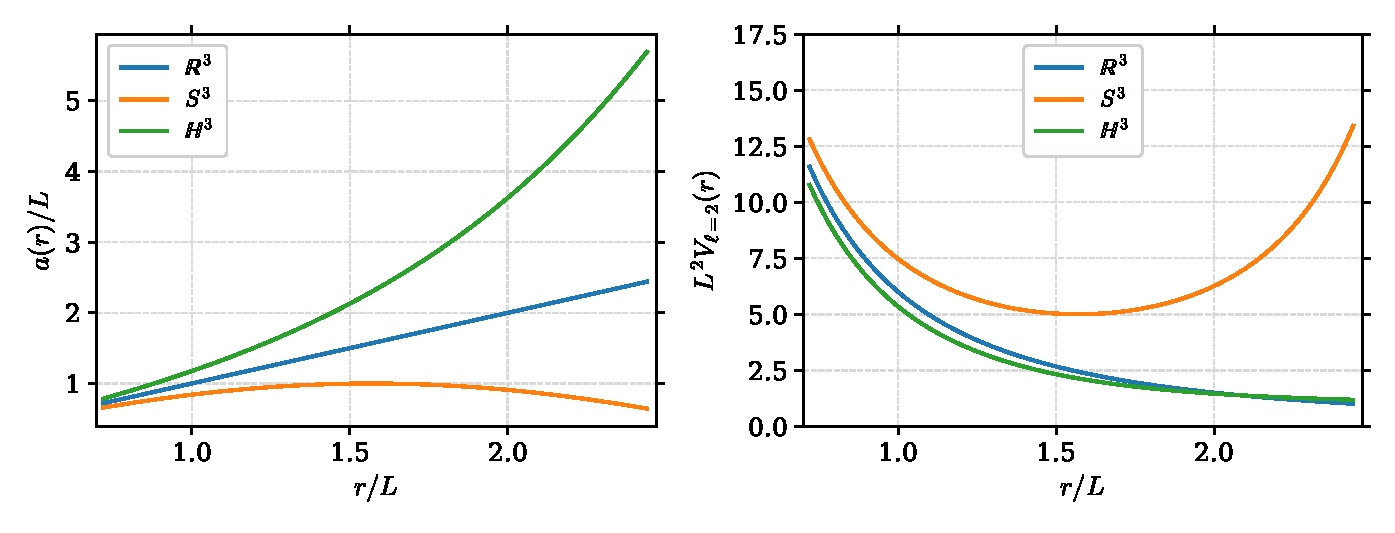
\includegraphics[width=.86\linewidth]{content/AdvancedPhysics/figures/geometry-highspin/warped_radial_potentials.pdf}
\caption{三维常曲率空间的尺度函数与径向势。图中长度以 $L$ 为单位，势以 $\hbar^2/(2\mu L^2)$ 为单位，取 $\ell=2$。靠近原点的主导离心奇性相同；三球第二极点的边界条件仍须另行施加。}
\label{fig:phys-ghs-warped-potential}
\end{figure}

\cref{fig:phys-ghs-warped-potential} 中的曲率位移来源于径向测度的酉变换。回到一般截面，只需替换角向本征值；若曲率势还依赖角坐标，则不同角模态会耦合，不能继续使用独立的一维方程。


\section{自伴扩张与低能散射}
\label{chap:singular-radial-hamiltonian}

分离角变量以后，径向微分表达式仍不能独自决定量子理论。原点附近若有两个平方可积解，边界条件会改变谱、束缚态和低能散射；本章因此把定义域作为哈密顿量的一部分来处理。

\subsection{算子定义域与边界条件}

初等量子力学常把哈密顿量写成一个微分表达式，例如
\(-\hbar^2\dd^2/(2\mu\dd r^2)\)。但算符不仅要说明“怎样作用”，还要说明“允许作用在哪些函数上”。对有界矩阵，这个区别看不见；对微分算符，边界条件正是定义域的一部分。

设 Hilbert 空间为 \(L^2(0,\infty;\dd r)\)，先考虑无量纲微分表达式
\[
\tau u=-u''.
\]
若 \(u,v\) 足够光滑并在无穷远衰减，两次分部积分给出 Green 恒等式
\begin{equation}
\langle u,\tau v\rangle-\langle\tau u,v\rangle
=\left[u'(r)^*v(r)-u(r)^*v'(r)\right]_{0}^{\infty}.
\label{eq:radial-green-boundary-form}
\end{equation}
无穷远项在所用定义域上消失，原点项却未必消失。若不规定
\(u(0)\) 与 \(u'(0)\) 的关系，就不能断言这个“哈密顿量”是对称的。

\begin{definition}[对称算符与自伴算符]
稠密定义算符 \(A\) 若满足
\[
\langle u,Av\rangle=\langle Au,v\rangle
\qquad (u,v\in\Dom A),
\]
就称为对称算符。伴随算符 \(A^\dagger\) 的定义域由所有满足
\(
\langle u,Av\rangle=\langle w,v\rangle
\)
对每个 \(v\in\Dom A\) 成立的 \(u\) 组成，并定义
\(A^\dagger u=w\)。若
\(A=A^\dagger\) 且二者定义域相同，才称 \(A\) 自伴。
\end{definition}

对称只检查定义域内部任意两函数的边界型是否相消；自伴还要求伴随算符没有额外允许的函数。量子时间演化
\(\exp(-\ii At/\hbar)\) 对所有实 \(t\) 都酉，需要的是自伴性，而不只是形式上把积分分部一次后“看起来厄米”。

最简单的一族边界条件是
\begin{equation}
u'(0)=\gamma u(0),
\qquad \gamma\in\mathbb R,
\label{eq:radial-robin-boundary}
\end{equation}
其中 \(\gamma=0\) 是 Neumann 条件，形式极限
\(|\gamma|\to\infty\) 对应 Dirichlet 条件 \(u(0)=0\)。

\begin{proposition}[半直线自由哈密顿量的 Robin 实现]
令
\[
H_\gamma=-\frac{\hbar^2}{2\mu}\frac{\dd^2}{\dd r^2},
\qquad
\Dom H_\gamma
=\{u\in H^2(0,\infty):u'(0)=\gamma u(0)\},
\]
其中 \(\gamma\) 为实数，则 \(H_\gamma\) 自伴。
\end{proposition}

\begin{proof}
先取 \(u,v\in\Dom H_\gamma\)。式
\eqnrefs{eq:radial-green-boundary-form} 的原点边界项为
\[
u'(0)^*v(0)-u(0)^*v'(0)
=\gamma u(0)^*v(0)-\gamma u(0)^*v(0)=0,
\]
所以 \(H_\gamma\) 对称。

再设 \(u\in\Dom H_\gamma^\dagger\)。伴随定义要求
\eqnrefs{eq:radial-green-boundary-form} 对每个满足
\(v'(0)=\gamma v(0)\) 的 \(v\) 都为零。原点处可自由选择
\(v(0)\)，而 \(v'(0)\) 随之等于 \(\gamma v(0)\)，因此
\[
\bigl[u'(0)^*-\gamma u(0)^*\bigr]v(0)=0
\]
对任意 \(v(0)\) 成立，只能有
\(u'(0)=\gamma u(0)\)。所以伴随定义域没有比原定义域更大，
\(\Dom H_\gamma^\dagger=\Dom H_\gamma\)，从而算符自伴。
\end{proof}

这个边界参数会直接改变可观测量。先看负能束缚态，写
\(E=-\hbar^2\kappa^2/(2\mu)\)、\(\kappa>0\)。平方可积解只能取
\(u(r)=Ce^{-\kappa r}\)。代入边界条件得到
\[
-\kappa=\gamma.
\]
因此只有 \(\gamma<0\) 时存在一个束缚态，能量为
\begin{equation}
E_b=-\frac{\hbar^2\gamma^2}{2\mu}.
\label{eq:radial-robin-bound-state}
\end{equation}
微分表达式完全没有改变，仅仅改变定义域，就从“没有束缚态”变成“有一个束缚态”。

正能量 \(E=\hbar^2k^2/(2\mu)\) 时，可把外区解写成
\(u(r)=C\sin(kr+\delta)\)。边界条件给出
\begin{equation}
k\cot\delta(k)=\gamma.
\label{eq:radial-robin-phase-shift}
\end{equation}
若用三维 \(s\) 波的低能约定
\(k\cot\delta=-1/a+O(k^2)\)，便有
\begin{equation}
a=-\frac1\gamma.
\label{eq:radial-robin-scattering-length}
\end{equation}
同一个参数同时决定束缚态和散射长度：当 \(\gamma\to0\) 时，束缚态逼近阈值，散射长度发散；当 \(\gamma<0\) 时，
\eqnrefs{eq:radial-robin-bound-state} 也可写成
\(E_b=-\hbar^2/(2\mu a^2)\)。这就是后文“自伴扩张参数与低能散射数据等价”的最小可算模型。

概率流也给出同一条件。径向流为
\[
j(0)=\frac\hbar\mu\operatorname{Im}[u(0)^*u'(0)].
\]
实 \(\gamma\) 使 \(u'(0)=\gamma u(0)\)，所以 \(j(0)=0\)：概率不会从半直线端点漏走。自伴边界条件的物理含义正是把端点处的概率通量封闭起来。

\begin{example}[有限区间的 Robin 束缚态阈值]
\label{ex:phys-ghs-finite-robin}
半直线的束缚态条件是 $\gamma<0$。现在把粒子限制在 $(0,L)$，保留 $u'(0)=\gamma u(0)$，另一端取 $u(L)=0$。定义域为
\[
\Dom H_\gamma=\{u\in H^2(0,L):u'(0)=\gamma u(0),\ u(L)=0\},
\quad H_\gamma=-\frac{\hbar^2}{2\mu}u''.
\]
求负能束缚态存在的充要条件、能量方程与归一化系数，并与半直线极限比较。

\textbf{解。} Green 边界型在两端消失，伴随定义域的任意端点迹要求同样两条条件，故这一实现自伴。

负能量写作 $E=-\hbar^2\kappa^2/(2\mu)$，$\kappa>0$。满足右端条件的解只能取 $u=C\sinh[\kappa(L-x)]$，左端给出
\begin{equation}
\gamma=-\kappa\coth(\kappa L).
\label{eq:phys-ghs-finite-robin-root}
\end{equation}
令 $t=\kappa L$。函数 $t\coth t$ 从 $1$ 严格增加到无穷，因为
\[
\frac{\dd}{\dd t}(t\coth t)
=\frac{\sinh t\cosh t-t}{\sinh^2t}>0;
\]
分子在零点为零，导数为 $2\sinh^2t>0$。所以恰有一个负能态的充要条件是
\begin{equation}
\gamma<-\frac1L.
\label{eq:phys-ghs-finite-robin-threshold}
\end{equation}
其归一化系数由
\[
|C|^{-2}=\int_0^L\sinh^2[\kappa(L-x)]\dd x
=\frac{\sinh(2\kappa L)}{4\kappa}-\frac L2
\]
确定。阈值 $\gamma=-1/L$ 时，归一化零能态为 $u_0=\sqrt{3/L^3}(L-x)$。

也可从二次型看见这个阈值：
\[
\frac{2\mu}{\hbar^2}\langle u,H_\gamma u\rangle
=\int_0^L|u'|^2\dd x+\gamma|u(0)|^2.
\]
因 $u(L)=0$，Cauchy--Schwarz 不等式给 $|u(0)|^2\le L\int|u'|^2$，故 $-1/L\le\gamma<0$ 时二次型仍非负；$\gamma\ge0$ 时亦然。正能态满足 $\gamma=-k\cot(kL)$，与负能方程在零能阈值连续相接。

取固定负 $\gamma$ 并令 $L\to\infty$，\cref{eq:phys-ghs-finite-robin-root} 给出 $\kappa\to-\gamma$，恢复半直线的能量。有限区间的另一端提高了束缚态形成所需的边界吸引强度，因而不能直接照搬半直线的判据。
\end{example}


\subsection{短程散射、阈值展开与零程相互作用}
\label{sec:phys-hdqm-threshold-scattering}

以下先取 $d\ge2$，并假设 $V(r)$ 在某个 $R_c$ 之外为零或衰减得足够快，使自由分波渐近成立。正能量写成
\[
E=\frac{\hbar^2k^2}{2\mu},\qquad k>0.
\]
外区约化径向解由阶数 $\nu_l$ 的 Bessel 函数组成，等价地
\begin{equation}
R_l(r)=C_l r^{-(d-2)/2}
\left[J_{\nu_l}(kr)\cos\delta_l(k)-Y_{\nu_l}(kr)\sin\delta_l(k)\right].
\label{eq:phys-hdqm-scattering-bessel-combination}
\end{equation}
大 $r$ 时
\begin{equation}
R_l(r)\sim r^{-(d-1)/2}
\sin\left(kr-\frac{\pi\nu_l}{2}+\frac\pi4+\delta_l(k)\right).
\label{eq:phys-hdqm-phase-asymptotic}
\end{equation}
三维时 $\nu_l=l+1/2$，相位常数立即化为 $-l\pi/2$，即熟悉的 $\sin(kr-l\pi/2+\delta_l)$；这一检验固定了把 Bessel 余弦渐近改写成正弦时的 $+\pi/4$，不能任意吸收到 $\delta_l$ 中，否则自由态的 $S_l=1$ 基准会被整体平移。

为了使不同维数中的截面归一化由同一一般结构决定，先固定散射振幅。对 $d>2$，令入射方向为 $\widehat{\mathbf k}$，并定义
\begin{equation}
\psi_{\mathbf k}(\mathbf r)
\sim
\ee^{\ii\mathbf k\cdot\mathbf r}
+\frac{\ee^{\ii kr}}{r^{(d-1)/2}}
 f_d(\widehat{\mathbf r},\widehat{\mathbf k}),
\qquad r\to\infty.
\label{eq:phys-hdqm-d-scattering-amplitude-convention}
\end{equation}
这里短程假设保证渐近波可分解为未畸变的入射平面波与球面出射波。采用前文归一化的超球谐，中心势的弹性 $S$ 矩阵在 $(l,\alpha)$ 基底中对角，$S_l=\ee^{2\ii\delta_l}$，于是
\begin{equation}
 f_d(\widehat{\mathbf r},\widehat{\mathbf k})
 =\left(\frac{2\pi}{k}\right)^{\frac{d-1}{2}}
 \ee^{-\ii\pi(d-1)/4}
 \sum_{l,\alpha}
 \left(S_l-1\right)
 Y_{l\alpha}(\widehat{\mathbf r})Y_{l\alpha}^*(\widehat{\mathbf k}).
\label{eq:phys-hdqm-d-partial-wave-amplitude}
\end{equation}
若只保留散射角 $\theta$，使用 $\xi_d=(d-2)/2$ 与加法定理可写为
\begin{equation}
 f_d(\theta)
 =\left(\frac{2\pi}{k}\right)^{\frac{d-1}{2}}
 \frac{\ee^{-\ii\pi(d-1)/4}}{\xi_d S_{d-1}}
 \sum_{l=0}^{\infty}(l+\xi_d)
 \left(S_l-1\right)C_l^{\xi_d}(\cos\theta),
 \qquad d>2.
\label{eq:phys-hdqm-d-central-partial-amplitude}
\end{equation}
其中 $S_{d-1}=2\pi^{d/2}/\Gamma(d/2)$ 已在本章开头定义。由
\[
\frac{\dd\sigma^{(d)}}{\dd\Omega_{d-1}}=|f_d|^2
\]
和超球谐正交归一性，总截面严格为
\begin{equation}
\begin{aligned}
\sigma_{\rm tot}^{(d)}
&=\frac{4(2\pi)^{d-1}}{S_{d-1}k^{d-1}}
\sum_{l=0}^{\infty}g_l^{(d)}\sin^2\delta_l(k)\\
&=\frac{2^d\pi^{d/2-1}\Gamma(d/2)}{k^{d-1}}
\sum_{l=0}^{\infty}g_l^{(d)}\sin^2\delta_l(k),
\qquad d>2.
\end{aligned}
\label{eq:phys-hdqm-d-cross-section}
\end{equation}
三维时 $g_l^{(3)}=2l+1$，上式立即退化为 $\sigma_{\rm tot}^{(3)}=(4\pi/k^2)\sum_l(2l+1)\sin^2\delta_l$；这个检验同时固定了高维归一化中的全部几何因子。

二维不能通过 $\xi_d=(d-2)/2\to0$ 直接套用 Gegenbauer 表示，但可以在同一个散射渐近约定下独立完成归一化。取入射方向为 $\theta=0$，圆周本征函数为 $Y_m(\theta)=\ee^{\ii m\theta}/\sqrt{2\pi}$，中心势给 $S_m=S_{|m|}=\ee^{2\ii\delta_{|m|}}$。若定义
\[
\psi_k(r,\theta)\sim \ee^{\ii kr\cos\theta}
+\frac{\ee^{\ii kr}}{\sqrt r}\,f_2(\theta),
\]
则二维分波振幅为
\begin{equation}
 f_2(\theta)
 =\frac{\ee^{-\ii\pi/4}}{\sqrt{2\pi k}}
 \sum_{m\in\mathbb Z}(S_m-1)\ee^{\ii m\theta}
 =\frac{\ee^{-\ii\pi/4}}{\sqrt{2\pi k}}
 \left[(S_0-1)+2\sum_{l=1}^{\infty}(S_l-1)\cos(l\theta)\right].
\label{eq:phys-hdqm-2d-partial-wave-amplitude}
\end{equation}
因此 $\dd\sigma^{(2)}/\dd\theta=|f_2(\theta)|^2$，Fourier 正交性给
\begin{equation}
\sigma_{\rm tot}^{(2)}
=\frac4k\sum_{m\in\mathbb Z}\sin^2\delta_{|m|}
=\frac4k\left[\sin^2\delta_0+2\sum_{l=1}^{\infty}\sin^2\delta_l\right].
\label{eq:phys-hdqm-2d-cross-section}
\end{equation}
这正好对应本章开头的二维角向简并度 $g_0^{(2)}=1$、$g_{l\ge1}^{(2)}=2$。二维 ERE 因而与一个完全确定的散射振幅归一化相连，而不是只给出孤立的相移展开。

Gegenbauer 多项式与 Gauss 超几何函数的精确关系为
\begin{equation}
C_l^{(d-2)/2}(\cos\theta)
=\frac{(d-2)_l}{l!}
{}_2F_1\!\left(
-l,l+d-2;\frac{d-1}{2};\sin^2\frac\theta2
\right),
\qquad d>2.
\label{eq:phys-hdqm-gegenbauer-2f1}
\end{equation}
二维角向基底应改用圆周上的 Fourier 模；因此不能把\eqnrefs{eq:phys-hdqm-d-central-partial-amplitude} 中的 $\xi_d\to0$ 当作逐项极限。

\begin{proof}[解]
归一化超球谐下，平面波展开为
\begin{equation}
\ee^{\ii\mathbf k\cdot\mathbf r}
=(2\pi)^{d/2}
\sum_{l,\alpha}\ii^l
\frac{J_{l+d/2-1}(kr)}{(kr)^{d/2-1}}
Y_{l\alpha}(\widehat{\mathbf r})Y_{l\alpha}^*(\widehat{\mathbf k}).
\label{eq:phys-hdqm-plane-wave-d}
\end{equation}
利用
\[
J_\nu(z)\sim\sqrt{\frac{2}{\pi z}}
\cos\!\left(z-\frac{\pi\nu}{2}-\frac\pi4\right),
\]
把每个余弦拆成入射与出射指数。所有出射分波共享系数
\[
\left(\frac{2\pi}{k}\right)^{\frac{d-1}{2}}
\ee^{-\ii\pi(d-1)/4}r^{-(d-1)/2}.
\]
散射把第 $l$ 个出射系数由 $1$ 变为 $S_l$，故新增出射波的系数为 $S_l-1$，得到\eqnrefs{eq:phys-hdqm-d-partial-wave-amplitude}。

中心势下的加法定理是
\[
\sum_\alpha Y_{l\alpha}(\Omega)Y_{l\alpha}^*(\Omega')
=\frac{l+\xi_d}{\xi_d S_{d-1}}C_l^{\xi_d}(\cos\gamma),
\qquad \xi_d=\frac{d-2}{2},
\]
从而得到\eqnrefs{eq:phys-hdqm-d-central-partial-amplitude}。当 $d=3$ 时，$\xi_d=1/2$、$S_2=4\pi$，于是
\[
f_3(\theta)=\frac1{2\ii k}
\sum_{l=0}^{\infty}(2l+1)(S_l-1)P_l(\cos\theta),
\]
与标准三维归一化一致。

最后固定入射方向并积分出射角。由超球谐正交性，
\[
\begin{aligned}
\sigma_{\rm tot}^{(d)}
&=\int_{S^{d-1}}|f_d(\widehat{\mathbf r},\widehat{\mathbf k})|^2\dd\Omega_{d-1}\\
&=\left(\frac{2\pi}{k}\right)^{d-1}
\sum_{l,\alpha}|S_l-1|^2|Y_{l\alpha}(\widehat{\mathbf k})|^2.
\end{aligned}
\]
再令 $\Omega=\Omega'$ 使用加法定理，得到
\[
\sum_\alpha|Y_{l\alpha}(\widehat{\mathbf k})|^2=\frac{g_l^{(d)}}{S_{d-1}},
\qquad
|S_l-1|^2=4\sin^2\delta_l.
\]
因此
\[
\sigma_{\rm tot}^{(d)}
=\frac{4(2\pi)^{d-1}}{S_{d-1}k^{d-1}}
\sum_l g_l^{(d)}\sin^2\delta_l,
\]
再代入 $S_{d-1}=2\pi^{d/2}/\Gamma(d/2)$ 即得\eqnrefs{eq:phys-hdqm-d-cross-section}。

二维时改用 Jacobi--Anger 展开
\[
\ee^{\ii kr\cos\theta}
=\sum_{m\in\mathbb Z}\ii^mJ_m(kr)\ee^{\ii m\theta}.
\]
由
\[
J_m(kr)\sim\frac12\sqrt{\frac{2}{\pi kr}}
\left[
\ee^{\ii(kr-m\pi/2-\pi/4)}
+\ee^{-\ii(kr-m\pi/2-\pi/4)}
\right]
\]
可见第 $m$ 个自由出射分量的公共系数是
$\ee^{-\ii\pi/4}/\sqrt{2\pi k r}$。散射只把它乘成 $S_m$，故新增部分立即给出\eqnrefs{eq:phys-hdqm-2d-partial-wave-amplitude}。最后利用
\[
\int_0^{2\pi}\ee^{\ii(m-m')\theta}\dd\theta
=2\pi\delta_{mm'}
\]
便得到\eqnrefs{eq:phys-hdqm-2d-cross-section}。
\end{proof}

内部势的全部信息可以压缩成 $r=R_c$ 的无量纲对数导数
\[
\mathcal L_l(k)=R_c\frac{R_l'(R_c)}{R_l(R_c)}+\frac{d-2}{2},
\qquad x=kR_c.
\]
连续匹配给出
\begin{equation}
\tan\delta_l(k)=
\frac{xJ_{\nu_l}'(x)-\mathcal L_l(k)J_{\nu_l}(x)}
{xY_{\nu_l}'(x)-\mathcal L_l(k)Y_{\nu_l}(x)}.
\label{eq:phys-hdqm-phase-log-derivative}
\end{equation}
这条式子是后续低能展开的精确母式：势阱、数值积分或任意有限程势只改变 $\mathcal L_l(k)$，自由外区的维数依赖则完全包含在 Bessel 阶数 $\nu_l$ 中。

\begin{proof}[解]
由\eqnrefs{eq:phys-hdqm-scattering-bessel-combination}，
\begin{equation*}
 R_l(r)=C_l r^{-(d-2)/2}
 \left[J_{\nu_l}(kr)\cos\delta_l-Y_{\nu_l}(kr)\sin\delta_l\right].
\end{equation*}
令 $t_l=\tan\delta_l$，并把 $\widetilde C_l=C_l\cos\delta_l$ 吸收到整体归一化中，
\begin{equation*}
 R_l(r)=\widetilde C_l r^{-(d-2)/2}
 \left[J_{\nu_l}(kr)-t_lY_{\nu_l}(kr)\right].
\end{equation*}
对 $r$ 求导，
\begin{align*}
 R_l'(r)
 ={}&\widetilde C_l\!\left[
 -\frac{d-2}{2}r^{-(d-2)/2-1}
 \left(J_{\nu_l}(kr)-t_lY_{\nu_l}(kr)\right)\right.\\
 &\left.+r^{-(d-2)/2}
 \left(kJ_{\nu_l}'(kr)-t_l kY_{\nu_l}'(kr)\right)
 \right],
\end{align*}
其中 Bessel 函数的导数对自变量 $kr$ 取。在 $r=R_c$ 处取对数导数，$r^{-(d-2)/2}$ 前因子相消，
\begin{equation*}
 \frac{R_l'(R_c)}{R_l(R_c)}
 =-\frac{d-2}{2R_c}
 +k\frac{J_{\nu_l}'(x)-t_lY_{\nu_l}'(x)}
 {J_{\nu_l}(x)-t_lY_{\nu_l}(x)},
\end{equation*}
乘以 $R_c$ 并加 $\frac{d-2}{2}$，$-(d-2)/2$ 项与 $+(d-2)/2$ 相消，
\begin{equation*}
 \mathcal L_l
 =x\frac{J_{\nu_l}'(x)-t_lY_{\nu_l}'(x)}
 {J_{\nu_l}(x)-t_lY_{\nu_l}(x)}.
\end{equation*}
交叉相乘，
\begin{equation*}
 \mathcal L_l J_{\nu_l}(x)-\mathcal L_l t_lY_{\nu_l}(x)
 =xJ_{\nu_l}'(x)-x t_lY_{\nu_l}'(x),
\end{equation*}
收集 $t_l$，
\begin{equation*}
 t_l\!\left[xY_{\nu_l}'(x)-\mathcal L_lY_{\nu_l}(x)\right]
 =xJ_{\nu_l}'(x)-\mathcal L_lJ_{\nu_l}(x),
\end{equation*}
即\eqnrefs{eq:phys-hdqm-phase-log-derivative}。
\end{proof}

对有限程势，或衰减足够快且原点不比 $r^{-2}$ 更奇异的短程相互作用，可以在一个使零能正则解 $R_l(R_c,0)\neq0$ 的匹配半径处讨论阈值展开。径向方程只通过 $k^2=2\mu E/\hbar^2$ 依赖能量，因此正则内部解及其对数导数在 $k=0$ 附近具有偶次解析展开
\begin{equation}
\mathcal L_l(k)=\mathcal L_{l,0}+\mathcal L_{l,2}k^2+\mathcal O(k^4).
\label{eq:phys-hdqm-logderivative-threshold}
\end{equation}
零能共振并不自动破坏\eqnrefs{eq:phys-hdqm-logderivative-threshold}；它通常对应下面某个低能散射系数被调到临界值。真正失效的是“散射参数有限”的普通阈值层级，而不是内部常微分方程对 $k^2$ 的局部解析性。

把\eqnrefs{eq:phys-hdqm-logderivative-threshold}代入精确匹配\eqnrefs{eq:phys-hdqm-phase-log-derivative}，并记
\[
2\nu_l=2l+d-2,
\qquad
\epsilon_d=
\begin{cases}
0,&d\text{ 为奇数},\\
1,&d\text{ 为偶数},
\end{cases}
\]
即可把奇、偶维统一写成一般有效力程展开
\begin{equation}
\begin{aligned}
\mathcal K_l^{(d)}(k;\rho_{l,d})
&\equiv
k^{2l+d-2}
\left[
\cot\delta_l(k)
-\epsilon_d\frac2\pi\ln(k\rho_{l,d})
\right]\\
&=-\frac1{a_l^{(d)}}
+\frac12r_l^{(d)}k^2
+\mathcal O(k^4).
\end{aligned}
\label{eq:phys-hdqm-ere-general-d}
\end{equation}
这里 $\rho_{l,d}>0$ 是偶维中把对数写成无量纲量的任意参考长度；改变 $\rho_{l,d}$ 会重新分配同阶的解析常数，但不改变相移。除二维 $s$ 波这一边界情形外，$a_l^{(d)}$ 的量纲为 $\mathrm{length}^{2l+d-2}$；$r_l^{(d)}$ 的量纲统一为 $\mathrm{length}^{4-d-2l}$。三维 $s$ 波的 $\epsilon_3=0$，于是\eqnrefs{eq:phys-hdqm-ere-general-d}立即给出
\begin{equation}
k\cot\delta_0(k)=-\frac1a+\frac12r_e k^2+\mathcal O(k^4).
\label{eq:phys-hdqm-ere-3d}
\end{equation}

二维 $s$ 波满足 $2l+d-2=0$，所以\eqnrefs{eq:phys-hdqm-ere-general-d}中的 $a_0^{(2)}$ 本身是无量纲参数。把它与任意参考尺度 $\rho_{0,2}$ 组合成物理二维散射长度
\[
a_2
=2\rho_{0,2}
\exp\!\left[-\gamma_{\rm E}-\frac{\pi}{2a_0^{(2)}}\right],
\]
则阈值展开可改写成更常用的形式
\begin{equation}
\cot\delta_0^{(2)}(k)
=\frac2\pi\left[\gamma_{\rm E}+\ln\frac{ka_2}{2}\right]
+\frac12r_0^{(2)}k^2
+\mathcal O(k^4).
\label{eq:phys-hdqm-ere-2d}
\end{equation}
这里 $r_0^{(2)}$ 的量纲是长度平方；不同文献常把它改记成一个“有效力程 squared”。因此二维的下一解析修正是 $k^2$ 项，而不是必须带 $k^2\ln k$。偶维的对数已经由\eqnrefs{eq:phys-hdqm-ere-general-d}中显式的运动学项完整分离。

阈值各项的相对重要性还取决于 $2l+d$。逆散射振幅中的幺正性项按 $k^{2l+d-2}$ 缩放，而有效程项按 $k^2$ 缩放；所以 $2l+d=4$ 时二者同阶，$2l+d\ge5$ 时有效程甚至比幺正性项更早进入。高维或高分波的“unitarity 极限”因此不能只靠令 $1/a_l^{(d)}=0$ 就完全刻画。

\begin{proof}[解]
奇维对应半整数 \(\nu\)。Bessel 函数的小宗量展开为
\begin{equation*}
 J_\nu(z)=\frac{(z/2)^\nu}{\Gamma(\nu+1)}[1+\mathcal O(z^2)],
\end{equation*}
\begin{equation*}
 Y_\nu(z)=
 -\frac{\Gamma(\nu)}\pi\left(\frac2z\right)^\nu[1+\mathcal O(z^2)]
 +\cot(\pi\nu)J_\nu(z).
\end{equation*}
其中负幂首项由 \(Y_\nu=(J_\nu\cos\pi\nu-J_{-\nu})/\sin\pi\nu\) 与 \(\Gamma(\nu)\Gamma(1-\nu)=\pi/\sin\pi\nu\) 合并得到。

把上述展开与\eqnrefs{eq:phys-hdqm-logderivative-threshold}代入\eqnrefs{eq:phys-hdqm-phase-log-derivative}，分子从 \(z^\nu\) 起、分母从 \(z^{-\nu}\) 起，故
\begin{equation*}
  k^{2\nu_l}\cot\delta_l(k)
  =c_0+c_2k^2+c_4k^4+\cdots .
\end{equation*}
即左端在阈值附近按 \(k^2\) 解析：常数项编码散射长度，次项编码有效程。

偶维对应整数 \(\nu_l=n\)。第二独立解由 \(\nu\to n\) 极限得到，此时 \(Y_n\) 的展开含对数项：
\begin{equation*}
 Y_n(z)
 =\text{有限个负幂项}
 +\frac2\pi J_n(z)\ln z
 +\text{解析项},
\end{equation*}
对数项来自 \(\cot(\pi\nu)\) 在 \(\nu\to n\) 的极点与 \(J_\nu\) 的 \(\nu\) 导数（含 \(\ln(z/2)\)）相乘。故匹配式中出现
\begin{equation*}
 k^{2n}\frac2\pi\ln(k\rho),
\end{equation*}
该运动学对数完全来自自由 Green 函数，与势无关；显式减去后剩余部分仍按 \(k^2\) 解析，正是\eqnrefs{eq:phys-hdqm-ere-general-d}。

二维 \(s\) 波对应 \(n=0\)，对数直接出现在最低阶，重新吸收常数后得\eqnrefs{eq:phys-hdqm-ere-2d}。
\end{proof}

零能阈值的关键不是让内部对数导数变得不解析，而是把有效力程展开的常数项调到临界值。先看 $d>2$ 的 $s$ 波。势外零能方程为
\[
R_0''+\frac{d-1}{r}R_0'=0,
\]
所以
\begin{equation}
R_0(r)=A+B r^{2-d}.
\label{eq:phys-hdqm-zero-energy-free}
\end{equation}
当 $A\neq0$ 时，定义广义散射参数 $\mathfrak a_d$（量纲 $\mathrm{length}^{d-2}$）为
\begin{equation}
R_0(r)=A\left(1-\frac{\mathfrak a_d}{r^{d-2}}\right),
\qquad
\mathfrak a_d=-\frac BA.
\label{eq:phys-hdqm-generalized-scattering-length}
\end{equation}
三维时 $\mathfrak a_3=a$。对 $d>2$，它与\eqnrefs{eq:phys-hdqm-ere-general-d} 中 $s$ 波的有效力程参数 $a_0^{(d)}$ 只差一个由自由 Bessel 归一化决定的维数因子。利用 $J_{\nu_0}$、$Y_{\nu_0}$ 的小参数主导项，
\[
\frac{\tan\delta_0(k)}{k^{d-2}}
\longrightarrow -a_0^{(d)},
\qquad k\to0,
\]
而零能外区解的常数项与 $r^{2-d}$ 项之比给出
\begin{equation}
\mathfrak a_d
=\frac{2^{d-2}
\Gamma\!\left(\frac{d-2}{2}\right)
\Gamma\!\left(\frac d2\right)}{\pi}
a_0^{(d)},
\qquad d>2.
\label{eq:phys-hdqm-generalized-length-vs-ere}
\end{equation}
当 $d=3$ 时前因子恰为 $1$，故通常三维散射长度不需要区分这两个记号。高维中若不先声明分波归一化，直接把所有量纲为 $\mathrm{length}^{d-2}$ 的阈值参数都记成同一个 $a$，会隐藏这一几何常数。

\begin{proof}[解]
令 $\nu_0=(d-2)/2>0$。由\eqnrefs{eq:phys-hdqm-scattering-bessel-combination}，$s$ 波外区解为
\[
R_0(r)=Cr^{-\nu_0}
\left[J_{\nu_0}(kr)\cos\delta_0-Y_{\nu_0}(kr)\sin\delta_0\right].
\]
对固定 $r>R_c$ 先取 $k\to0$。Bessel 函数的主导项为
\[
J_{\nu_0}(kr)
=\frac{(kr/2)^{\nu_0}}{\Gamma(\nu_0+1)}+o(k^{\nu_0}),
\]
\[
Y_{\nu_0}(kr)
=-\frac{\Gamma(\nu_0)}{\pi}
\left(\frac{2}{kr}\right)^{\nu_0}
+o(k^{-\nu_0}),
\]
其中整数 $\nu_0$ 时附加的对数项比显示出的负幂主导项更高阶，不改变下面的零能系数比。于是
\[
R_0(r)=A(k)+B(k)r^{2-d}+o(1),
\]
且
\[
A(k)=C\cos\delta_0\,
\frac{k^{\nu_0}}{2^{\nu_0}\Gamma(\nu_0+1)},
\]
\[
B(k)=C\sin\delta_0\,
\frac{2^{\nu_0}\Gamma(\nu_0)}{\pi k^{\nu_0}}.
\]
因此
\[
-\frac{B(k)}{A(k)}
=-\frac{2^{2\nu_0}\Gamma(\nu_0)\Gamma(\nu_0+1)}{\pi}
\frac{\tan\delta_0(k)}{k^{2\nu_0}}.
\]
另一方面，\eqnrefs{eq:phys-hdqm-ere-general-d} 在 $k\to0$ 给出
\[
k^{2\nu_0}\cot\delta_0(k)\longrightarrow-\frac1{a_0^{(d)}},
\]
因为偶维的 $k^{2\nu_0}\ln(k\rho_{0,d})$ 在 $d>2$ 时也趋于零。故
\[
\frac{\tan\delta_0(k)}{k^{2\nu_0}}
\longrightarrow-a_0^{(d)}.
\]
再用 $2\nu_0=d-2$、$\Gamma(\nu_0+1)=\Gamma(d/2)$，便得到\eqnrefs{eq:phys-hdqm-generalized-length-vs-ere}。
\end{proof}

这一参数也可以直接由前面的匹配对数导数读出。记 $\nu_0=(d-2)/2$，在 $r=R_c$ 处令 $z=\mathfrak a_d/R_c^{d-2}$，则
\[
R_c\frac{R_0'}{R_0}
=(d-2)\frac{z}{1-z}.
\]
因此
\[
\mathcal L_{0,0}
=\nu_0+(d-2)\frac{z}{1-z},
\]
解出 $z$ 得到精确关系
\begin{equation}
\mathfrak a_d
=R_c^{d-2}
\frac{\mathcal L_{0,0}-\nu_0}
{\mathcal L_{0,0}+\nu_0},
\qquad d>2.
\label{eq:phys-hdqm-scattering-length-logderivative}
\end{equation}
所以 $|\mathfrak a_d|\to\infty$ 的零能临界点是
\begin{equation}
\mathcal L_{0,0}=-\nu_0=-\frac{d-2}{2},
\label{eq:phys-hdqm-zero-resonance-matching}
\end{equation}
而不是\eqnrefs{eq:phys-hdqm-logderivative-threshold}本身失效。此时外区解退化为 $R_0(r)=B r^{2-d}$。

它在无穷远的范数行为为
\[
\int^\infty r^{d-1}|R_0|^2\dd r
\sim\int^\infty r^{3-d}\dd r.
\]
因此 $d=3,4$ 时该阈值解不平方可积，是通常意义的零能共振或半束缚态；$d\ge5$ 时相同尾部已经平方可积，若内部解也正则，则阈值奇异对应真正的零能本征态。二维的外区零能解为 $A+B\ln(r/r_*)$，必须用\eqnrefs{eq:phys-hdqm-ere-2d}的对数散射长度来描述阈值极限；一维则应按偶、奇宇称通道分别分类。维数改变的是阈值谱类型，而不仅是相移公式中的系数。

\label{sec:phys-hdqm-point-interactions}

形式表达式
\begin{equation}
V(\vb r)=\alpha\,\delta^{(d)}(\vb r)
\label{eq:phys-hdqm-delta-potential}
\end{equation}
只有在说明它所代表的算子定义域或重整化条件之后才具有物理意义。原因是自由预解式在原点的短程奇性依赖空间维数；同一个裸常数 $\alpha$ 不能跨维数解释为同一个可观测耦合。点相互作用的维数判据因此应直接从自由 Green 函数的短程结构与去点拉普拉斯算子的自伴扩张性质得到。

束缚能写成
\[
E_B=-\frac{\hbar^2\kappa_B^2}{2\mu},\qquad \kappa_B>0.
\]
定义 $(-\Delta+\kappa^2)^{-1}$ 的 Euclidean Green 函数核
\begin{equation}
(-\Delta+\kappa^2)G_\kappa(\vb r)=\delta^{(d)}(\vb r),
\qquad
G_\kappa(\vb r)=
\int\frac{\dd^d p}{(2\pi)^d}
\frac{\ee^{\ii\vb p\cdot\vb r}}{p^2+\kappa^2}
=
\frac{1}{(2\pi)^{d/2}}
\left(\frac{\kappa}{r}\right)^{d/2-1}
K_{d/2-1}(\kappa r)
\label{eq:phys-hdqm-delta-bound-green}
\end{equation}
给出点源方程在 $r>0$ 的唯一衰减解。其原点渐近行为为
\begin{equation}
G_\kappa(r)\sim
\begin{cases}
\displaystyle \frac{1}{2\kappa}+O(r), & d=1,\\[0.5em]
\displaystyle -\frac{1}{2\pi}\ln\!\left(\frac{\kappa r}{2}\right)+O(1), & d=2,\\[0.5em]
\displaystyle \frac{\Gamma(d/2-1)}{4\pi^{d/2}}\,r^{2-d}\,[1+o(1)], & d\ge3.
\end{cases}
\label{eq:phys-hdqm-point-green-short-distance}
\end{equation}
因此 $d\ge2$ 时直接把\eqnrefs{eq:phys-hdqm-delta-potential} 当作普通乘法势会遇到 $G_\kappa(0)$ 发散；正确对象是自由拉普拉斯算子在去掉原点后的自伴扩张，或与之等价的零程重整化极限。
\begin{proof}[解]
考虑去掉原点后的最小自由哈密顿量
\[
 H_0^{\min}=-\frac{\hbar^2}{2\mu}\Delta,
 \qquad
 \Dom(H_0^{\min})=C_c^\infty(\mathbb R^d\setminus\{0\}).
\]
该算子对称但未必自伴。由 von Neumann 延拓理论，其自伴扩张的存在性与个数由亏指数
\begin{equation*}
 n_\pm=\dim\ker\bigl[(H_0^{\min})^*\mp \ii E_*\bigr]
\end{equation*}
决定，其中 $E_*>0$ 仅为固定能标，$n_\pm$ 与其取值无关。
\begin{equation*}
 (H_0^{\min})^*\psi_\pm=\pm \ii E_*\psi_\pm.
\end{equation*}
在原点附近，方程的主导项即自由拉普拉斯算子的齐次解，故亏量解的主导奇性与 Laplace 基本解一致。对 $d\ge3$，径向 Laplace 方程 $\Delta G=0$ 的解满足
\begin{equation*}
 \frac{1}{r^{d-1}}\frac{\dd}{\dd r}\left(r^{d-1}\frac{\dd G}{\dd r}\right)=0,
\end{equation*}
积分两次得基本解 $G(r)\sim r^{2-d}$，于是 $\psi_\pm(r)\sim r^{2-d}$。其局部平方可积性由
\begin{equation*}
 \int_0^\epsilon r^{d-1}|\psi_\pm(r)|^2\dd r
 \sim
 \int_0^\epsilon r^{d-1}\,r^{2(2-d)}\dd r
 =
 \int_0^\epsilon r^{3-d}\dd r
\end{equation*}
判定。该积分在 $3-d>-1$ 即 $d<4$ 时收敛，故 $d=3$ 收敛而 $d\ge4$ 发散。二维径向方程退化为
\begin{equation*}
 \frac{1}{r}\frac{\dd}{\dd r}\left(r\frac{\dd G}{\dd r}\right)=0,
\end{equation*}
其解为对数 $G(r)\sim\ln(r/L_*)$，于是 $\psi_\pm(r)\sim\ln(r/L_*)$，且
\begin{equation*}
 \int_0^\epsilon r\left|\ln\frac r{L_*}\right|^2\dd r
 =\frac{\epsilon^2}{2}\left[\left(\ln\frac\epsilon{L_*}\right)^2+1\right]<\infty,
\end{equation*}
故二维亏量解亦平方可积。一维去掉一点把直线分成两个半轴，每段端点独立，亏指数为 $(1,1)$。
综上，$d=1,2,3$ 时 $n_+=n_-=1$，去点拉普拉斯算子有单参数族自伴扩张，可经原点边界条件引入一个点相互作用参数；$d\ge4$ 时奇异亏量解不再平方可积，$n_\pm=0$，算子本质自伴，单点不能产生这种零程相互作用。临界维数 $d=4$ 处 $\psi\sim r^{-2}$ 的范数积分 $\int r^{-1}\dd r$ 在对数尺度发散，恰处边界。一维通常的 $\delta(x)$ 势只是这一自伴连接条件的特例。
\end{proof}
扩张参数与散射长度之间的对应可以直接从零能径向解读出。
三维自由 $s$ 波恰处于极限圆型区。由 $d=3,l=0$ 得 $u=rR$，零能原点附近的一般自伴边界条件可写成
\[
u(r)=A+Br+o(r),\qquad B=\Lambda A,
\]
其中 $\Lambda\in\mathbb R\cup\{\infty\}$ 是\eqnrefs{eq:phys-hdqm-extension-boundary} 在 $\chi=1/2$ 时的参数。另一方面 Bethe--Peierls 形式
\[
\psi(r)=\frac{u(r)}r
=A\left(\frac1r-\frac1a\right)+o(1)
\]
要求
\begin{equation}
\Lambda=-\frac1a.
\label{eq:phys-hdqm-extension-scattering-length-3d}
\end{equation}
因此三维散射长度不是附加在哈密顿量之外的经验常数，而就是去点拉普拉斯算子自伴扩张参数的倒长度表示。若 $a>0$，束缚态写成 $u(r)=A_B\ee^{-\kappa_Br}$，则在原点有 $B/A=-\kappa_B$，与上式比较即得 $\kappa_B=1/a$。
二维 $s$ 波位于临界 $g=-1/4$。写 $u=\sqrt r\,\psi$，则
\[
u(r)=\sqrt r\left[A+B\ln\frac r{L_0}\right]+o(\sqrt r).
\]
自伴定义域固定实比值 $A/B$。把它重写为
\[
\psi(r)=B\ln\frac r{a_2}+o(1)
\]
给出
\begin{equation}
\frac AB=-\ln\frac{a_2}{L_0}.
\label{eq:phys-hdqm-extension-scattering-length-2d}
\end{equation}
所以二维扩张参数天然以对数方式对应一个长度尺度 $a_2$；这正是后面维数 transmutation 的算子论来源。
在一维，普通 $\delta$ 势已经给出非平凡的点相互作用。
一维中可直接定义
\[
V(x)=-g\,\delta(x),\qquad g>0.
\]
把 Schrödinger 方程在 $(-\epsilon,\epsilon)$ 上积分并令 $\epsilon\to0$，波函数连续而导数满足跳跃条件
\begin{equation}
\psi'(0^+)-\psi'(0^-)
=-\frac{2\mu g}{\hbar^2}\psi(0).
\label{eq:phys-hdqm-delta-1d-jump}
\end{equation}
束缚态在两侧只能取 $\psi_B(x)=\mathcal N_B\ee^{-\kappa_B|x|}$。代入\eqnrefs{eq:phys-hdqm-delta-1d-jump} 得
\[
2\kappa_B=\frac{2\mu g}{\hbar^2},
\qquad
\kappa_B=\frac{\mu g}{\hbar^2},
\]
从而
\begin{equation}
E_B=-\frac{\mu g^2}{2\hbar^2}.
\label{eq:phys-hdqm-delta-1d-bound-energy}
\end{equation}
零能偶宇称解在 $x\ne0$ 处为线性函数。若把一维偶通道散射长度定义为
\[
\psi_0(x)=A\left(1-\frac{|x|}{a_1}\right),
\]
则跳跃条件给
\begin{equation}
\frac1{a_1}=\frac{\mu g}{\hbar^2},
\qquad
\kappa_B=\frac1{a_1}.
\label{eq:phys-hdqm-extension-scattering-length-1d}
\end{equation}
这是一维普通 $\delta$ 势的偶通道结果；一般一维点相互作用具有更大的自伴扩张族，不能全部压缩为一个散射长度。一维自由 Green 函数在原点有限，因此这个特例不需要二维、三维那样的紫外重整化。
在二维，零能 Green 函数的对数结构使边界条件出现尺度生成。
二维 Green 函数在原点按 $-\ln(r/L_*)$ 发散，因此点相互作用不能由一个有限的裸 $\alpha$ 直接定义。一个等价的自伴边界条件是规定 $s$ 波在 $r\to0$ 时具有
\begin{equation}
\psi(r)=A\ln\frac{r}{a_2}+o(1),
\label{eq:phys-hdqm-point-2d-boundary}
\end{equation}
其中 $a_2>0$ 是二维散射长度。束缚态由 $K_0(\kappa_B r)$ 给出，而
\[
K_0(z)=-\ln\frac z2-\gamma_{\rm E}+O(z^2\ln z).
\]
比较\eqnrefs{eq:phys-hdqm-point-2d-boundary} 可得
\begin{equation}
\kappa_B=\frac{2\ee^{-\gamma_{\rm E}}}{a_2}.
\label{eq:phys-hdqm-point-2d-kappa}
\end{equation}
这说明二维零程相互作用把无量纲的形式耦合转化成了一个有量纲尺度，即维数 transmutation。
若用束缚尺度 $\kappa_B$ 作为重整化条件，Lippmann--Schwinger 方程中的发散积分只以差值出现：
\[
I_2(-\ii k)-I_2(\kappa_B)
=-\frac{1}{4\pi}
\left[\ln\frac{k^2}{\kappa_B^2}-\ii\pi\right].
\]
在以下采用的 $T$ 矩阵归一化下，
\begin{equation}
T_2(k)=
-\frac{2\pi\hbar^2/\mu}
{\ln(k^2/\kappa_B^2)-\ii\pi}.
\label{eq:phys-hdqm-delta-t-2d}
\end{equation}
发散已经完全被物理尺度 $\kappa_B$ 吸收。
在三维，散射长度本身就是点相互作用最自然的自伴扩张参数。
三维点相互作用最方便用 Bethe--Peierls 边界条件定义：
\begin{equation}
\psi(r)=A\left(\frac1r-\frac1a\right)+O(r),
\qquad r\to0,
\label{eq:phys-hdqm-bethe-peierls}
\end{equation}
其中 $a$ 是三维 $s$ 波散射长度。对正能量 $E=\hbar^2k^2/(2\mu)$，这直接给出零程 $s$ 波振幅
\begin{equation}
f_0(k)=\frac{1}{-a^{-1}-\ii k}.
\label{eq:phys-hdqm-contact-3d-amplitude}
\end{equation}
若 $a>0$，振幅在 $k=\ii/a$ 处有束缚态极点，因此
\begin{equation}
E_B=-\frac{\hbar^2}{2\mu a^2}.
\label{eq:phys-hdqm-contact-3d-bound-energy}
\end{equation}
若使用与前文一致的 $T$ 矩阵约定 $f_0=-\mu T/(2\pi\hbar^2)$，则
\begin{equation}
T_3(k)=\frac{2\pi\hbar^2/\mu}{a^{-1}+\ii k}.
\label{eq:phys-hdqm-contact-3d-t}
\end{equation}
这里的 $a$，而不是形式上的裸 $\alpha$，才是可测的低能耦合。
在四维及更高维，单点零程相互作用的紫外结构发生质变，朴素的一参数点相互作用不再成立。
由前面的亏量分析，$d\ge4$ 时 $-\Delta$ 在 $\mathbb R^d\setminus\{0\}$ 上本质自伴。因而不能通过给原点增加一个自伴扩张参数来得到与二维、三维同类的非平凡点相互作用。把 coincident Euclidean Green 积分形式记为
\[
I_d(\kappa)
\equiv\int\frac{\dd^dp}{(2\pi)^d}\frac1{p^2+\kappa^2}
=\frac{\Gamma(1-d/2)}{(4\pi)^{d/2}}\kappa^{d-2},
\]
其中最后一个等号按维数正规化作解析延拓。这样的解析延拓仍然可以作为正规化计算工具，但它本身并不能证明任意整数 $d$ 都存在一个由单一参数定义的量子 $\delta^{(d)}$ 势。若在 $d\ge4$ 需要描述短程相互作用，应从有限作用程势或包含更高阶接触算符的有效理论出发，并明确其截止依赖与所需反项。
这一区分也解释了为什么“先写任意 $d$ 维裸 $\delta$ 势，再把 $d$ 代成整数”会掩盖真正的数学问题：维数改变的不只是积分数值，还改变了自由哈密顿量的自伴扩张结构。
\subsection{不同维数中的中心势}
\label{sec:phys-hdqm-maxwell-poisson}
高维“氢原子”的物理母问题不是把三维的 $1/r$ 势机械搬到任意维数，而是先求 $d$ 维 Poisson 方程的 Green 函数。设点电荷 $q$ 位于原点，静电势满足
\begin{equation}\label{eq:phys-hdqm-poisson-d}
 \nabla_d^2\Phi(\vb r)=-\frac{q}{\varepsilon_d}\,\delta^{(d)}(\vb r).
\end{equation}
记单位 $(d-1)$ 维球面面积为
\[
 S_{d-1}=\frac{2\pi^{d/2}}{\Gamma(d/2)}.
\]
对 $r>0$，球对称性给出 $\partial_r(r^{d-1}\partial_r\Phi)=0$。在半径 $r$ 的球面上积分\eqnrefs{eq:phys-hdqm-poisson-d}，由 Gauss 定律
\begin{equation}\label{eq:phys-hdqm-gauss-d}
 S_{d-1}r^{d-1}\Phi'(r)=-\frac{q}{\varepsilon_d}.
\end{equation}
因此不同维数的 Green 函数具有本质不同的标度。对 $d\ge3$，取无穷远势能为零得到
\begin{equation}\label{eq:phys-hdqm-potential-d-ge3}
 \Phi_d(r)=\frac{q}{(d-2)S_{d-1}\varepsilon_d}\,r^{2-d}.
\end{equation}
二维中积分产生对数，只有势差有物理意义：
\begin{equation}\label{eq:phys-hdqm-potential-d2}
 \Phi_2(r)=-\frac{q}{2\pi\varepsilon_2}\ln\frac{r}{r_0},
\end{equation}
其中 $r_0$ 是任意参考尺度；一维则有
\begin{equation}\label{eq:phys-hdqm-potential-d1}
 \Phi_1(x)=-\frac{q}{2\varepsilon_1}|x|+\mathrm{const}.
\end{equation}
对于异号电荷 $+e$ 与 $-e$ 的相对运动，势能因此为
\begin{equation}\label{eq:phys-hdqm-coulomb-potential-all-d}
 V_d(r)=
 \begin{cases}
 \displaystyle \frac{e^2}{2\varepsilon_1}|x|, & d=1,\\[0.8em]
 \displaystyle \frac{e^2}{2\pi\varepsilon_2}\ln\frac{r}{r_0}, & d=2,\\[0.8em]
 \displaystyle -\frac{e^2}{(d-2)S_{d-1}\varepsilon_d}\,r^{2-d}, & d\ge3.
 \end{cases}
\end{equation}
这才是 Maxwell--Poisson 理论在不同空间维数中的真实静电相互作用。$d=3$ 恰好退化为 $-e^2/(4\pi\varepsilon_3r)$；$d=4$ 则是逆平方势；二维对数势虽然没有三维氢原子那样的简单主量子数闭式谱，却不能从一般理论中删去。
真实 Maxwell--Poisson 势的短程奇性随维数从 $r^{-1}$、$r^{-2}$ 一直增强。对 $d>4$，吸引势为 $-C_dr^{-(d-2)}$，其幂次 $d-2>2$ 比动能的缩放 $r^{-2}$ 更奇异。取任意光滑归一化试探函数 $\varphi$，并定义
\[
\psi_\ell(\vb x)=\ell^{-d/2}\varphi(\vb x/\ell).
\]
则
\[
\langle T\rangle_{\ell}=\ell^{-2}\langle T\rangle_1,
\qquad
\langle V\rangle_{\ell}=-C_d\ell^{-(d-2)}
\int\frac{|\varphi(\vb y)|^2}{|\vb y|^{d-2}}\dd^dy.
\]
因此
\begin{equation}
\langle H\rangle_\ell
=A\ell^{-2}-B\ell^{-(d-2)}\longrightarrow-\infty
\qquad(d>4,\ \ell\to0),
\label{eq:phys-hdqm-maxwell-collapse-dgt4}
\end{equation}
其中 $A,B>0$。这证明任意强度的吸引点电荷 Maxwell 势在 $d>4$ 都没有下界；必须给电荷有限尺寸、短程截断或其他紫外完成。$d=4$ 是两个缩放同阶的临界维数，稳定性转化为逆平方耦合的临界问题；$d=3$ 则势能只按 $\ell^{-1}$ 增长，短程处由动能压制。
一维势 $V_1(x)=F|x|$，其中 $F=e^2/(2\varepsilon_1)$。令
\[
 \ell=\left(\frac{\hbar^2}{2\mu F}\right)^{1/3},\qquad
 z=\frac{|x|}{\ell}-\frac{E}{F\ell},
\]
Schrödinger 方程化为 Airy 方程。无穷远可归一化要求舍去 $\operatorname{Bi}$ 分支；$x=0$ 的奇偶边界条件分别给出 $\operatorname{Ai}(-E/F\ell)=0$ 与 $\operatorname{Ai}'(-E/F\ell)=0$。
二维势 $V_2(r)=\gamma_2\ln(r/r_0)$，$\gamma_2=e^2/(2\pi\varepsilon_2)$。径向方程为
\begin{equation}\label{eq:phys-hdqm-d2-log-radial}
 -\frac{\hbar^2}{2\mu}\left(R_l''+\frac1rR_l'-\frac{l^2}{r^2}R_l\right)
 +\gamma_2\ln\frac r{r_0}R_l=ER_l.
\end{equation}
它定义了良好的束缚态谱，但一般不化为初等特殊函数的有限参数闭式解。一般理论在这里给出的是算子、边界条件和尺度结构；具体能级可用 shooting、变分或谱方法计算。不能因为缺少漂亮闭式表达式就用固定 $1/r$ 势替代真实二维 Coulomb 问题。
$d=3$ 时\eqnrefs{eq:phys-hdqm-coulomb-potential-all-d} 成为
\begin{equation}\label{eq:phys-hdqm-coulomb-3d}
 V_3(r)=-\frac{\gamma_3}{r},\qquad \gamma_3=\frac{e^2}{4\pi\varepsilon_3}.
\end{equation}
这时真实 Maxwell 势与通常的 $1/r$ 模型完全一致。束缚态和散射态都由合流超几何函数给出，能谱为
\begin{equation}\label{eq:phys-hdqm-hydrogen-spectrum-3d}
 E_n=-\frac{\mu\gamma_3^2}{2\hbar^2n^2},\qquad n=n_r+l+1,
\end{equation}
而散射截面退化为 Rutherford 形式
\begin{equation}\label{eq:phys-hdqm-rutherford-3d}
 \frac{\dd\sigma}{\dd\Omega}=\frac{\eta_3^2}{4k^2\sin^4(\theta/2)},
 \qquad \eta_3=\frac{\mu\gamma_3}{\hbar^2k}>0.
\end{equation}
$d=4$ 时
\begin{equation}\label{eq:phys-hdqm-coulomb-4d}
 V_4(r)=-\frac{\gamma_4}{r^2},\qquad
 \gamma_4=\frac{e^2}{2S_3\varepsilon_4}.
\end{equation}
约化径向函数 $u_l=r^{3/2}R_l$ 满足
\begin{equation}\label{eq:phys-hdqm-inverse-square-reduced}
 -u_l''+\frac{g_l}{r^2}u_l=k^2u_l,
 \qquad
 g_l=\left(l+1\right)^2-\frac14-\frac{2\mu\gamma_4}{\hbar^2}.
\end{equation}
因此“耦合强弱”首先是一个算子定义域问题。对半直线上的算子 $-\dd^2/\dd r^2+g_l/r^2$，若 $g_l\ge3/4$，原点为极限点型，最小算子在原点本质自伴；若 $-1/4\le g_l<3/4$，原点为极限圆型，需要选择自伴边界条件；若 $g_l<-1/4$，则进入超临界 fall-to-the-中心区域，裸哈密顿量没有下界，必须引入短程物理或重整化尺度。只有在最后一种情形中，离散尺度不变性和几何能级塔才作为受控的自伴扩张/重整化结果出现。
\begin{note}[四维逆平方势的临界参数]
定义 $s_l^2=(l+1)^2-2\mu\gamma_4/\hbar^2$，则 $g_l=s_l^2-1/4$。$s_l^2\ge1$ 对应本质自伴；$0\le s_l^2<1$ 需要边界条件；$s_l^2<0$ 为超临界区域。把所有实 $s_l$ 都简单称为“普通散射解”会漏掉 $0\le s_l^2<1$ 的自伴扩张自由度。
\end{note}
作为对照，还可以研究一个纯数学延拓：在任意维数中人为固定 $1/r$ 势，而不把它误认作高维 Maxwell--Poisson 点电荷势。
真实 Maxwell 势建立以后，可以把固定 $1/r$ 形状的中心势作为独立数学模型延拓到任意 $d$。除 $d=3$ 外，它不再是 $d$ 维 Maxwell--Poisson 方程的 Green 函数，因此以下结果描述的是“改变 Hilbert 空间维数但固定势函数形状”的模型，而不是高维电磁学本身。具体取
\begin{equation}
	V(r)=-\frac{\gamma}{r},
	\label{eq:phys-hdqm-formal-coulomb}
\end{equation}
其中 \(\gamma>0\)。束缚态中令
\begin{equation}
	\kappa=\frac{\sqrt{-2\mu E}}{\hbar},\qquad
	\eta_{\rm B}=\frac{\mu\gamma}{\hbar^2\kappa}>0,\qquad
	\rho=2\kappa r.
\end{equation}
径向解为
\begin{equation}
	R_l(r)=A_l\,\rho^l\ee^{-\rho/2}
	{}_1F_1\left(l+\frac{d-1}{2}-\eta_{\rm B};\,2l+d-1;\,\rho\right).
\end{equation}
原点正则性选出 \({}_1F_1\) 分支；无穷远可归一化要求级数截断：
\begin{equation}
	l+\frac{d-1}{2}-\eta_{\rm B}=-n_r,\qquad
	E_{n_rl}=-\frac{\mu\gamma^2}{2\hbar^2
	\left(n_r+l+\frac{d-1}{2}\right)^2}.
	\label{eq:phys-hdqm-formal-coulomb-energy}
\end{equation}
归一化径向波函数可取
\begin{equation}
	R_{n_rl}(r)=
	(2\kappa)^{d/2}
	\left[
	\frac{n_r!}{(2n_r+2l+d-1)\Gamma(n_r+2l+d-1)}
	\right]^{1/2}
	(2\kappa r)^l\ee^{-\kappa r}
	L_{n_r}^{2l+d-2}(2\kappa r).
	\label{eq:phys-hdqm-formal-coulomb-bound}
\end{equation}
由于
\begin{equation}
	L_n^\alpha(z)=\frac{(\alpha+1)_n}{n!}\,
	{}_1F_1(-n;\alpha+1;z),
\end{equation}
\eqnrefs{eq:phys-hdqm-formal-coulomb-bound} 也就是合流超几何解。
散射态 \(E>0\) 中令
\begin{equation}
	k=\frac{\sqrt{2\mu E}}{\hbar},\qquad
	\eta_{\rm C}=-\frac{\mu\gamma}{\hbar^2k}<0.
\end{equation}
这里使用带符号的 Coulomb--Sommerfeld 参数 $\eta_{\rm C}$：吸引势 \(V=-\gamma/r\) 对应负值。正则径向解为
\begin{equation}
	R_{kl}(r)=C_{kl}\,(2kr)^l\ee^{-\ii kr}
	{}_1F_1\left(l+\frac{d-1}{2}-\ii\eta_{\rm C};\,2l+d-1;\,2\ii kr\right).
	\label{eq:phys-hdqm-formal-coulomb-scattering-solution}
\end{equation}
其长程 Coulomb 相位为
\begin{equation}
	R_{kl}(r)\sim r^{-(d-1)/2}
	\sin\left(kr-\eta_{\rm C}\ln(2kr)-\frac{\pi\nu_l}{2}
	+\frac{\pi}{4}+\sigma_l^{(d)}\right),
\end{equation}
\begin{equation}
	\sigma_l^{(d)}=\operatorname{Arg}\Gamma\left(l+\frac{d-1}{2}+\ii\eta_{\rm C}\right).
	\label{eq:phys-hdqm-formal-coulomb-phase}
\end{equation}
因为 $\eta_{\rm C}<0$，吸引势的对数相实际为 $+|\eta_{\rm C}|\ln(2kr)$。同一符号也可由束缚态公式作解析延拓检验：取 $\kappa\to\ii k$，则 $\eta_{\rm B}\to-\ii\mu\gamma/(\hbar^2k)$，从而合流超几何参数连续变为上式的 $-\ii\eta_{\rm C}$。
固定 $1/r$ 势是长程势，因此它不满足\secref{sec:phys-hdqm-threshold-scattering}用于\eqnrefs{eq:phys-hdqm-d-scattering-amplitude-convention} 的短程假设：渐近波含有上式的 $-\eta_{\rm C}\ln(2kr)$ 相位，不能把自由平面波加自由球面波的分解逐项照搬。严格定义 Coulomb 振幅时，应采用 Coulomb--distorted 入射/出射态，或先引入屏蔽势、在计算可观测量后取去屏蔽极限。形式上把
\[
S_l^{\rm C}=\ee^{2\ii\sigma_l^{(d)}}
\]
代入一般分波级数可以组织角向结构，但该级数必须按长程散射的意义求和，不能把它当作短程级数的普通逐项收敛。三维情形经过标准 Coulomb 求和后给出熟知的 Rutherford 振幅与截面；这里保留这一点作为固定 $1/r$ 数学模型与真实 Maxwell--Poisson 势之间的又一项重要差别。
\subsection{可解中心势与特殊函数的共同结构}
考虑
\begin{equation}
	V(r)=
	\begin{cases}
		0,&0<r<a,\\
		V_0,&r>a,
	\end{cases}
	\qquad V_0>0.
	\label{eq:phys-hdqm-finite-well-potential}
\end{equation}
这是 ``阱内零势、阱外抬高 \(V_0\)'' 的球形势阱。令
\begin{equation}
	\nu=\nu_l=l+\frac{d-2}{2}.
\end{equation}
常势区的正则径向解统一写成
\begin{equation}
	R_l(r)=r^{-\beta}Z_{\nu}(qr),\qquad
	\beta=\frac{d-2}{2},
\end{equation}
其中 \(Z_\nu\) 是 \(J_\nu,Y_\nu,I_\nu,K_\nu\) 中相应的 Bessel 函数。Bessel 函数也可写成
\begin{equation}
	J_\nu(z)=\frac{(z/2)^\nu}{\Gamma(\nu+1)}
	{}_0F_1\left(;\nu+1;-\frac{z^2}{4}\right).
	\label{eq:phys-hdqm-bessel-0f1}
\end{equation}
对束缚态 $0<E<V_0$，内外径向解分别由振荡型与衰减型 Bessel 函数组成。
令
\begin{equation}
	k=\frac{\sqrt{2\mu E}}{\hbar},\qquad
	\kappa=\frac{\sqrt{2\mu(V_0-E)}}{\hbar}.
\end{equation}
原点正则、无穷远衰减的解为
\begin{equation}
	R_{\mathrm{in}}(r)=A\,r^{-\beta}J_\nu(kr),\qquad
	R_{\mathrm{out}}(r)=B\,r^{-\beta}K_\nu(\kappa r).
	\label{eq:phys-hdqm-finite-well-bound-wave}
\end{equation}
在 \(r=a\) 连续 \(R\) 与 \(R'\) 得到能级方程
\begin{equation}
	k\frac{J_\nu'(ka)}{J_\nu(ka)}
	=
	\kappa\frac{K_\nu'(\kappa a)}{K_\nu(\kappa a)}.
	\label{eq:phys-hdqm-finite-well-bound-condition}
\end{equation}
系数比例为
\begin{equation}
	\frac{B}{A}=\frac{J_\nu(ka)}{K_\nu(\kappa a)}.
\end{equation}
归一化条件为
\begin{equation}
	1=\int_0^\infty |R_l(r)|^2r^{d-1}\dd r
	=A^2\int_0^a rJ_\nu^2(kr)\dd r
	+B^2\int_a^\infty rK_\nu^2(\kappa r)\dd r.
\end{equation}
注意 \(r^{d-1}r^{-2\beta}=r\)，因此归一化积分的维度依赖只通过阶数 \(\nu\) 进入。
对散射态 $E>V_0$，外区解改为振荡型组合，并由边界匹配读出相移。
令
\begin{equation}
	k=\frac{\sqrt{2\mu E}}{\hbar},\qquad
	q=\frac{\sqrt{2\mu(E-V_0)}}{\hbar}.
\end{equation}
内区正则解为
\begin{equation}
	R_{\mathrm{in}}(r)=A\,r^{-\beta}J_\nu(kr),
\end{equation}
外区取相移形式
\begin{equation}
	R_{\mathrm{out}}(r)=C\,r^{-\beta}
	\left[\cos\delta_l\,J_\nu(qr)-\sin\delta_l\,Y_\nu(qr)\right].
\end{equation}
匹配 \(r=a\) 处的对数导数，得到
\begin{equation}
	\tan\delta_l(q)
	=
	\frac{
		kJ_\nu'(ka)J_\nu(qa)-qJ_\nu(ka)J_\nu'(qa)
	}{
		kJ_\nu'(ka)Y_\nu(qa)-qJ_\nu(ka)Y_\nu'(qa)
	}.
	\label{eq:phys-hdqm-finite-well-phase-shift}
\end{equation}
代入\eqnrefs{eq:phys-hdqm-d-cross-section}，并把 \(k\) 换成外区波数 \(q\)，即可得到总截面。
在 $V_0\to\infty$ 的极限，边界条件退化为硬壁零点条件。
若保持\eqnrefs{eq:phys-hdqm-finite-well-potential} 的定义并令 \(V_0\to\infty\)，粒子被限制在半径 \(a\) 的 \(d\) 维球内。边界条件为
\begin{equation}
	R_l(a)=0.
\end{equation}
因此
\begin{equation}
	J_\nu(k_{nl}a)=0,\qquad
	k_{nl}=\frac{j_{\nu,n}}{a},
\end{equation}
\begin{equation}
	E_{nl}=\frac{\hbar^2j_{\nu,n}^2}{2\mu a^2},\qquad
	R_{nl}(r)=N_{nl}\,r^{-\beta}J_\nu\left(\frac{j_{\nu,n}r}{a}\right).
	\label{eq:phys-hdqm-infinite-ball}
\end{equation}
这里 \(j_{\nu,n}\) 是 \(J_\nu\) 的第 \(n\) 个正零点。利用
\begin{equation}
	\int_0^a rJ_\nu^2\left(\frac{j_{\nu,n}r}{a}\right)\dd r
	=\frac{a^2}{2}J_{\nu+1}^2(j_{\nu,n}),
\end{equation}
归一化常数为
\begin{equation}
	N_{nl}=\frac{\sqrt{2}}{a|J_{\nu+1}(j_{\nu,n})|}.
\end{equation}
\begin{note}
	上式是 ``外区势垒无穷高'' 的球盒。若另一个问题取
	\(V(r)=+\infty\)（\(r<a\)）与 \(V(r)=0\)（\(r>a\)），则是硬球散射，
	相移为
	\begin{equation}
		\tan\delta_l^{\mathrm{hard}}(k)=\frac{J_\nu(ka)}{Y_\nu(ka)}.
	\end{equation}
	这不是\eqnrefs{eq:phys-hdqm-finite-well-potential} 的 \(V_0\to\infty\) 极限，而是互补的势垒问题。
\end{note}
对各向同性谐振子的束缚态，径向方程可化为合流超几何方程。
取
\begin{equation}
	V(r)=\frac12\mu\omega^2r^2,\qquad
	b=\sqrt{\frac{\hbar}{\mu\omega}},\qquad
	\rho=\frac{r^2}{b^2}.
\end{equation}
径向方程 \eqnrefs{eq:phys-hdqm-radial-r} 的一般解可写为
\begin{equation}
	R_l(r)=\rho^{l/2}\ee^{-\rho/2}
	\left[
		A\,{}_1F_1(a;c;\rho)+B\,U(a,c,\rho)
	\right],
	\label{eq:phys-hdqm-osc-general-solution}
\end{equation}
其中
\begin{equation}
	c=l+\frac{d}{2},\qquad
	a=\frac12\left(l+\frac{d}{2}\right)-\frac{E}{2\hbar\omega}.
\end{equation}
原点正则要求 \(B=0\)。无穷远处可归一化要求
\({}_1F_1\) 截断为多项式：
\begin{equation}
	a=-n_r,\qquad n_r=0,1,2,\ldots.
\end{equation}
因此能级为
\begin{equation}
	E_{n_rl}=\hbar\omega\left(2n_r+l+\frac{d}{2}\right).
	\label{eq:phys-hdqm-osc-energy}
\end{equation}
归一化径向波函数为
\begin{equation}
	R_{n_rl}(r)=
	\left[\frac{2n_r!}{b^d\Gamma(n_r+l+d/2)}\right]^{1/2}
	\rho^{l/2}\ee^{-\rho/2}L_{n_r}^{l+d/2-1}(\rho).
	\label{eq:phys-hdqm-osc-bound}
\end{equation}
完整波函数为
\begin{equation}
	\psi_{n_rl\alpha}(\vb r)=R_{n_rl}(r)Y_{l\alpha}(\Omega).
\end{equation}
若用笛卡尔量子数 \(n_1,\ldots,n_d\) 表示，则
\begin{equation}
	E_N=\hbar\omega\left(N+\frac{d}{2}\right),\qquad
	N=\sum_{i=1}^d n_i=2n_r+l.
\end{equation}
第 \(N\) 层总简并度为
\begin{equation}
	G_N^{(d)}=\binom{N+d-1}{d-1}.
\end{equation}
若暂不施加可归一化条件，任意能量都存在形式解；谱离散性来自无穷远处的可积性条件。
由于
\begin{equation}
	V(r)\to+\infty,\qquad r\to\infty,
\end{equation}
各向同性谐振子的谱纯离散，不存在通常意义下的入射平面波散射态。若只把径向方程当作微分方程，则任意能量的两个独立解就是\eqnrefs{eq:phys-hdqm-osc-general-solution} 中的
\({}_1F_1(a;c;\rho)\) 与 \(U(a,c,\rho)\)。其中 \(U(a,c,\rho)\) 在无穷远处衰减但在原点奇异；\({}_1F_1(a;c;\rho)\) 在原点正则但通常在无穷远处发散。只有 \(a=-n_r\) 时二者要求相容，得到\eqnrefs{eq:phys-hdqm-osc-energy} 的束缚态谱。
\begin{exbox}
	基态 \(n_r=l=0\) 为
	\begin{equation}
		\psi_0(\vb r)=\frac{1}{\pi^{d/4}b^{d/2}}\exp\left(-\frac{r^2}{2b^2}\right),
		\qquad
		E_0=\frac{d}{2}\hbar\omega.
	\end{equation}
	这里使用 \(Y_{00}=1/\sqrt{S_{d-1}}\) 以及\eqnrefs{eq:phys-hdqm-osc-bound} 的径向归一化。
\end{exbox}
径向微分方程的奇点结构把这些特殊函数组织成若干标准解析族。有限程常势区只有 $r=0$ 与 $r=\infty$ 的 Bessel 型结构，因此传播支使用 $J_\nu,Y_\nu$，倏逝支使用 $I_\nu,K_\nu$；固定 $1/r$ 势和各向同性谐振子把径向方程化为 Kummer 方程，因此由 ${}_1F_1$ 与 $U$ 给出两个独立分支；二维、三维零程相互作用则直接继承自由 Green 核中的 $K_0,H_0^{(1)}$ 或 $\ee^{\ii kr}/r$ 型短程结构。
角向 Gegenbauer 多项式与 Gauss 超几何函数的关系已经在\eqnrefs{eq:phys-hdqm-gegenbauer-2f1} 中给出。径向函数之间还存在两个常用的合流关系，
\begin{equation}
{}_1F_1(a;c;z)
=\lim_{b\to\infty}{}_2F_1\!\left(a,b;c;\frac{z}{b}\right),
\qquad
J_\nu(z)=\frac{(z/2)^\nu}{\Gamma(\nu+1)}
{}_0F_1\!\left(;\nu+1;-\frac{z^2}{4}\right).
\label{eq:phys-hdqm-hypergeometric-confluence}
\end{equation}
因此固定 $1/r$ 势与谐振子的 Kummer 解可以看成 Gauss 超几何方程的合流极限，而球阱中的 Bessel 解又可写成进一步的 ${}_0F_1$ 极限。这些合流关系只描述微分方程的解析族；量子物理解仍由算子定义域、端点条件与无穷远边界条件共同选定。
真实 Maxwell--Poisson 势也不存在跨维数的单一特殊函数模板：$d=1$ 的线性势对应 Airy 方程，$d=3$ 的 $1/r$ 势对应 Kummer 方程，$d=4$ 的 $1/r^2$ 势受逆平方结构控制，而 $d=2$ 的对数势一般没有与三维 Coulomb 谱同构的超几何闭式。
\subsection{径向矩与 Coulomb 隐对称性}

径向方程除了给出波函数，还能直接约束其矩。
以下先处理三维归一化约化径向函数 $u(r)$，其测度为 $\dd r$，
而非原波函数 $R(r)$ 的 $r^2\dd r$。这一区别决定积分分部中的系数。

\begin{proposition}[径向超位力恒等式]
令 $a=\hbar^2/(2m)$，$H_r=-a\partial_r^2+W(r)$，
$W=V+a\ell(\ell+1)/r^2$。设 $u$ 是能量为 $E$ 的归一化束缚态，
且以下各积分收敛、积分分部的端点项为零。对实函数 $f$，有
\[
2E\langle f'\rangle
=\left\langle 2f'W+fW'-\frac a2 f'''\right\rangle,
\qquad \langle F\rangle=\int_0^\infty |u(r)|^2F(r)\,\dd r.
\]
取 $f=r^{s+1}$，得到
\begin{equation}\label{eq:phys-hdqm-hypervirial-recurrence}
\begin{aligned}
2(s+1)E\langle r^s\rangle
&=\left\langle 2(s+1)r^sV+r^{s+1}V'\right\rangle\\
&\quad+\frac{\hbar^2s}{4m}
\bigl[4\ell(\ell+1)-s^2+1\bigr]\langle r^{s-2}\rangle.
\end{aligned}
\end{equation}
对于正则 Coulomb 束缚态，非负整数 $s$ 满足上述端点要求。
当系数为零时，应在求导阶段删去相应项，不把它写成零乘一个发散积分。
\end{proposition}
\begin{proof}
取一阶微分表达式 $G=f\partial_r+f'/2$。用乘法算符与微分算符的交换关系，
\begin{align*}
[f\partial_r,\partial_r^2]&=-2f'\partial_r^2-f''\partial_r,\\
[f'/2,\partial_r^2]&=-f''\partial_r-f'''/2,\\
[G,W]&=fW'.
\end{align*}
因此
\[
[G,H_r]=a\bigl(2f'\partial_r^2+2f''\partial_r+f'''/2\bigr)+fW'.
\]
由 $a u''=(W-E)u$ 消去二阶导数。
实系数一维束缚态可取 $u$ 为实函数，于是端点项为零时
\[
\int_0^\infty u f''u'\,\dd r
=\frac12[f''u^2]_0^\infty-\frac12\langle f'''\rangle
=-\frac12\langle f'''\rangle.
\]
将其代入 $\langle[G,H_r]\rangle=0$，得到
\[
0=\left\langle 2f'(W-E)+fW'-\frac a2 f'''\right\rangle.
\]
最后代入 $W$。离心势的两个贡献分别为
$2(s+1)a\ell(\ell+1)r^{s-2}$ 与 $-2a\ell(\ell+1)r^{s-2}$，
合为 $2sa\ell(\ell+1)r^{s-2}$；再结合
$f'''=(s+1)s(s-1)r^{s-2}$，即得所述递推式。
若端点项不消失，就必须保留它，不能仅凭形式对易子断言期望值为零。
\end{proof}

\begin{example}[氢样原子的前三个径向矩]
取 $V=-\kappa/r$，$\kappa=Ze^2/(4\pi\varepsilon_0)$，
$a_\kappa=\hbar^2/(m\kappa)$，$E_n=-\kappa/(2a_\kappa n^2)$。
记 $R_s=\langle r^s\rangle$。上面的结果化为 Kramers--Pasternack 递推
\[
2(s+1)E_nR_s
=-(2s+1)\kappa R_{s-1}
+\frac{\hbar^2s}{4m}[4\ell(\ell+1)-s^2+1]R_{s-2}.
\]
对幂律势 $V=\lambda r^q$，相应势项为
$(2s+2+q)\lambda R_{s+q}$；Coulomb 势对应 $q=-1$。

从 $R_0=1$ 开始，分别取 $s=0,1,2$：
\begin{align*}
2E_n&=-\kappa R_{-1},\\
4E_nR_1&=-3\kappa+\frac{\hbar^2}{m}\ell(\ell+1)R_{-1},\\
6E_nR_2&=-5\kappa R_1
+\frac{\hbar^2}{2m}[4\ell(\ell+1)-3].
\end{align*}
逐项代入，得到
\begin{align*}
R_{-1}&=\frac1{a_\kappa n^2},\\
R_1&=\frac{a_\kappa}{2}[3n^2-\ell(\ell+1)],\\
R_2&=\frac{a_\kappa^2n^2}{2}[5n^2+1-3\ell(\ell+1)].
\end{align*}
$n=1,\ell=0$ 时为 $3a_\kappa/2$ 与 $3a_\kappa^2$，
也可用 $u_{10}=2r a_\kappa^{-3/2}\ee^{-r/a_\kappa}$ 直接积分复核。
这些是同一态的径向矩；不同态之间的跃迁矩阵元还需波函数或其他递推关系，
Stark 和 Zeeman 修正也需相应的角向矩阵元。
负次矩另有原点收敛条件，不能从 $R_0$ 不加条件地递推出全部负次矩。
\end{example}

\begin{theorem}[固定 $1/r$ 势的束缚谱与隐对称性]
对 $d\ge2$ 的 Hamilton 算符 $H=\vb p^2/(2m)-\kappa/r$，$\kappa>0$，
取原点处的正则实现。负能量子空间上的角动量与 Runge--Lenz 算符
生成 $so(d+1)$，束缚能级为
\[
E_N=-\frac{m\kappa^2}{2\hbar^2(N+(d-1)/2)^2},\qquad N=0,1,2,\ldots .
\]
第 $N$ 层是 $SO(d+1)$ 的次数为 $N$ 的对称无迹张量表示。
在三维，它给出主量子数 $n=N+1$ 与简并度 $n^2$。
此结论针对固定 $1/r$ 势；改变原点处的自伴边界条件可能破坏该对称性。
\end{theorem}
\begin{proof}[Runge--Lenz 代数与 Casimir]
Coulomb 问题还具有推广 Runge--Lenz 向量生成的 \(SO(d+1)\) 隐对称性。下面先在经典泊松括号层面把一般 \(d\) 的代数写清楚，再对 \(d=3\) 完成完整的量子能级推导，最后说明推广到一般 $d$ 时，保留反对称张量 $L_{ij}$。



先在经典能面上确定代数，再处理量子排序。
取固定 \(1/r\) 势的哈密顿量
\[
H=\frac{\vb p^2}{2m}-\frac{\kappa}{r},\qquad \kappa>0
\]
（\(d=3\) 氢样原子取 $\kappa=Ze^2/(4\pi\varepsilon_0)$，即\eqnrefs{eq:phys-hdqm-formal-coulomb} 中的 \(\gamma\)）。角动量张量 \(L_{ij}=x_ip_j-x_jp_i\) 满足
\begin{equation}
\{L_{ij},L_{kl}\}
=\delta_{ik}L_{jl}-\delta_{il}L_{jk}-\delta_{jk}L_{il}+\delta_{jl}L_{ik},
\label{eq:phys-hdqm-sod-bracket}
\end{equation}
即 \(so(d)\) 的李代数（\(\{x_i,p_j\}=\delta_{ij}\)，重复指标求和）。定义未归一化的 Runge--Lenz 向量
\begin{equation}
A_i=\frac{1}{2m}\left(p_jL_{ij}+L_{ij}p_j\right)-\kappa\frac{x_i}{r},
\label{eq:phys-hdqm-runge-lenz-d}
\end{equation}
其中对 \(j\) 从 \(1\) 到 \(d\) 求和。\(d=3\) 时 \(p_jL_{ij}=(\vb p\times\vb L)_i\)，上式退化为熟知的
\(\vb A=(\vb p\times\vb L-\vb L\times\vb p)/(2m)-\kappa\widehat{\vb r}\)。只用\eqnrefs{eq:phys-hdqm-sod-bracket} 与 \(\{x_i,f(r)\}=0\) 逐次展开（计算冗长但每步都是正则括号的 Leibniz 律），得到封闭代数
\begin{equation}
\{A_i,H\}=0,\qquad
\{L_{ij},A_k\}=\delta_{ik}A_j-\delta_{jk}A_i,\qquad
\{A_i,A_j\}=-\frac{2H}{m}L_{ij}.
\label{eq:phys-hdqm-runge-lenz-brackets}
\end{equation}
关键在第三式：右端只含 \(H\) 与 \(L_{ij}\)，没有跑出 \(\{L_{ij},A_k\}\) 张成空间之外的量。在束缚态能面 \(H=E<0\) 上，把 \(H\) 当常数吸收到归一化中：定义
\begin{equation}
D_i=\sqrt{-\frac{m}{2H}}\,A_i,
\qquad
J_{ij}=L_{ij},\qquad
J_{i,d+1}=-J_{d+1,i}=D_i\quad (i,j=1,\ldots,d).
\label{eq:phys-hdqm-sod1-generators}
\end{equation}
由 \(\{A_i,H\}=0\)，在能面上取括号时 \(H\) 可按常数处理，于是
\[
\{D_i,D_j\}
=-\frac{m}{2H}\left(-\frac{2H}{m}\right)L_{ij}=L_{ij},
\qquad
\{L_{ij},D_k\}=\delta_{ik}D_j-\delta_{jk}D_i.
\]
合并写成
\begin{equation}
\{J_{MN},J_{PQ}\}
=\delta_{MP}J_{NQ}-\delta_{MQ}J_{NP}-\delta_{NP}J_{MQ}+\delta_{NQ}J_{MP},
\qquad M,N,P,Q=1,\ldots,d+1,
\label{eq:phys-hdqm-sod1-algebra}
\end{equation}
与\eqnrefs{eq:phys-hdqm-sod-bracket} 对照，这正是 \(so(d+1)\) 的李代数：一般 \(d\) 的闭合性由此完全确立，而非只对 \(d=3\) 成立。散射能面 \(E>0\) 时归一化因子换成 \(\sqrt{m/(2H)}\)，\(\{D_i,D_j\}=-L_{ij}\)，代数变为 \(so(d,1)\)。

接着在三维量子问题中计算两个 Casimir。

量子化规则 \(\{\cdot,\cdot\}\to\frac{1}{\ii\hbar}[\cdot,\cdot]\) 下，\eqnrefs{eq:phys-hdqm-runge-lenz-d} 的对称排序保证 \(A_i\) 厄米。算符序唯一需要小心的地方是
\begin{equation}
p_jL_{ij}-L_{ij}p_j=[p_j,L_{ij}]=\ii\hbar(d-1)p_i,
\label{eq:phys-hdqm-runge-lenz-ordering}
\end{equation}
即“先 \(p\) 后 \(L\)”与对称序相差一个确定的 \(\hbar\) 项；以下全部计算固定使用对称序。取 \(d=3\)，只用 \([x_i,p_j]=\ii\hbar\delta_{ij}\) 与角动量代数逐次展开，得
\begin{equation}
[A_i,H]=0,\qquad
[L_i,A_j]=\ii\hbar\epsilon_{ijk}A_k,\qquad
[A_i,A_j]=-\frac{2H}{m}\ii\hbar\,\epsilon_{ijk}L_k.
\label{eq:phys-hdqm-runge-lenz-quantum-3d}
\end{equation}
由 \([A_i,H]=0\)，\(\vb A\) 把每个能量本征子空间映到自身。在 \(H=E<0\) 的束缚本征子空间上令
\[
M_i=\sqrt{-\frac{m}{2E}}\,A_i,
\qquad
[M_i,M_j]=\ii\hbar\epsilon_{ijk}L_k,
\qquad
[L_i,M_j]=\ii\hbar\epsilon_{ijk}M_k.
\]
再令
\[
\vb J=\frac{\vb L+\vb M}{2},
\qquad
\vb K=\frac{\vb L-\vb M}{2},
\]
直接代入对易关系得 \([J_i,K_j]=0\)，且 \(\vb J,\vb K\) 各自满足 \(su(2)\) 代数：这是 \(so(4)\cong su(2)\oplus su(2)\) 的显式实现。由 \(\vb L\) 与 \(\vb A\) 的定义可验证 \(\vb L\cdot\vb A=0\)（\(\vb L\) 只含切向微分，\(\vb A\) 的两项分别与之点积为零），故两个 Casimir 不独立：
\[
\vb J^2-\vb K^2=\vb L\cdot\vb M=0
\quad\Longrightarrow\quad
\vb J^2=\vb K^2=\hbar^2j(j+1),\qquad j=0,\tfrac12,1,\ldots .
\]
第二个 Casimir 由量子 Runge--Lenz 恒等式给出：
\begin{equation}
\vb A^2=\kappa^2+\frac{2H}{m}\left(\vb L^2+\hbar^2\right).
\label{eq:phys-hdqm-runge-lenz-casimir-3d}
\end{equation}
验证只含两类代数操作。其一，
\[
(\vb p\times\vb L-\vb L\times\vb p)^2
=4\left(\vb p^2\vb L^2+\hbar^2\vb p^2\right),
\]
由 \(\vb L\times\vb p=-\vb p\times\vb L+2\ii\hbar\vb p\)（展开 \([L_i,p_j]=\ii\hbar\epsilon_{ijk}p_k\) 即得）、\((\vb p\times\vb L)^2=\vb p^2\vb L^2\)（用 \(\vb p\cdot\vb L=\vb L\cdot\vb p=0\)）以及 \((\vb p\times\vb L)\cdot\vb p=2\ii\hbar\vb p^2\) 逐项展开得到；其二，
\[
\frac12\left\{\vb p\times\vb L-\vb L\times\vb p,\,\frac{\vb r}{r}\right\}
=\frac{2}{r}\left(\vb L^2+\hbar^2\right),
\]
同样只用 \([L_i,x_j]=\ii\hbar\epsilon_{ijk}x_k\) 展开。两式合并，并把 \(\vb p^2/(2m)=H+\kappa/r\) 代入，即得\eqnrefs{eq:phys-hdqm-runge-lenz-casimir-3d}。


\par

\par
在 \(H=E\) 的本征态上 \(\vb M^2=-\frac{m}{2E}\vb A^2\)，于是\eqnrefs{eq:phys-hdqm-runge-lenz-casimir-3d} 给出
\[
\vb L^2+\vb M^2
=-\hbar^2-\frac{m\kappa^2}{2E}.
\]
左端等于 \(2(\vb J^2+\vb K^2)=4\hbar^2j(j+1)\)，解出
\begin{equation}
E=-\frac{m\kappa^2}{2\hbar^2(2j+1)^2}.
\label{eq:phys-hdqm-so4-energy}
\end{equation}
允许值为 \(n\equiv 2j+1=1,2,3,\ldots\)，每个 \(n\) 出现一次，简并度 \((2j+1)^2=n^2\)：这就是氢原子谱 \(E_n=-m\kappa^2/(2\hbar^2n^2)\) 与 \(n^2\) 简并的纯代数推导，全程没有解径向微分方程。给定 \(n\) 后 \(\vb L^2\) 的允许值由 \(\vb J+\vb K\) 的角动量耦合三角定则给出 \(l=0,1,\ldots,n-1\)，与径向解一致。

推广到一般 $d$ 时，保留反对称张量 $L_{ij}$。

对易关系中只有第三式变形：
\[
[A_i,A_j]=-\frac{2H}{m}\ii\hbar L_{ij},
\qquad
[L_{ij},A_k]=\ii\hbar(\delta_{ik}A_j-\delta_{jk}A_i),
\qquad
[A_i,H]=0.
\]
束缚壳上 \(M_i=\sqrt{-m/(2E)}A_i\) 与 \(L_{ij}\) 满足\eqnrefs{eq:phys-hdqm-sod1-algebra} 的量子版，即 \(so(d+1)\) 对易代数。Runge--Lenz 恒等式的一般 \(d\) 形式为
\begin{equation}
\vb A^2=\kappa^2+\frac{2H}{m}\left(\vb L^2+\frac{(d-1)^2}{4}\hbar^2\right),
\qquad
\vb L^2\equiv\frac12L_{ij}L_{ij},
\label{eq:phys-hdqm-runge-lenz-casimir-d}
\end{equation}
其中 \(\hbar^2\) 修正项的系数来自排序恒等式\eqnrefs{eq:phys-hdqm-runge-lenz-ordering}；\(d=3\) 时 \((d-1)^2/4=1\)，回到\eqnrefs{eq:phys-hdqm-runge-lenz-casimir-3d}。注意 \(\vb L^2\) 的本征值为 \(\hbar^2l(l+d-2)\)，与本章前半部分的超球谐分析一致。束缚态占据 \(SO(d+1)\) 的对称无迹张量表示 \((N,0,\ldots,0)\)（\(N=0,1,2,\ldots\)），其二次 Casimir 为 \(\hbar^2N(N+d-1)\)，表示维数
\begin{equation}
g_N^{(d+1)}=\frac{(2N+d-1)(N+d-2)!}{N!\,(d-1)!}.
\label{eq:phys-hdqm-sod1-dimension}
\end{equation}
由 Casimir 匹配
\[
\vb L^2+\vb M^2
=-\frac{(d-1)^2}{4}\hbar^2-\frac{m\kappa^2}{2E}
=\hbar^2N(N+d-1)
\]
直接解出
\begin{equation}
E_N=-\frac{m\kappa^2}{2\hbar^2\left(N+\frac{d-1}{2}\right)^2},
\qquad N=0,1,2,\ldots .
\label{eq:phys-hdqm-coulomb-energy-sod1}
\end{equation}
写主量子数 \(n=N+1\)，即 \(E_n=-m\kappa^2\left[2\hbar^2\left(n+\frac{d-3}{2}\right)^2\right]^{-1}\)，与直接求解固定 \(1/r\) 势的\eqnrefs{eq:phys-hdqm-formal-coulomb-energy}（令 \(n_r+l=N\)）完全一致；简并度\eqnrefs{eq:phys-hdqm-sod1-dimension} 在 \(d=3\) 给 \((N+1)^2=n^2\)，在 \(d=2\) 给 \(2N+1=2n-1\)。最后强调边界：这里的 \(SO(d+1)\) 是“固定 \(1/r\) 势”这一数学模型的隐对称性；真实 \(d\) 维 Maxwell--Poisson 势\eqnrefs{eq:phys-hdqm-coulomb-potential-all-d} 只在 \(d=3\) 取 \(1/r\) 形，故该隐对称性不是高维静电学的对称性。


\par

\par

\end{proof}

\begin{workedexample}
在 \(d=3\) 中验证排序恒等式 \(p_jL_{ij}-L_{ij}p_j=2\ii\hbar p_i\)，并由此把 Runge--Lenz 向量写成 \(\vb A=(\vb p\times\vb L-\ii\hbar\vb p)/m-\kappa\widehat{\vb r}\) 的形式。

\textbf{解.} 由 \([p_j,L_{ij}]=[p_j,x_ip_j-x_jp_i]=[p_j,x_i]p_j-[p_j,x_j]p_i=-\ii\hbar p_i+3\ii\hbar p_i=2\ii\hbar p_i\)，即一般 \(d\) 公式\eqnrefs{eq:phys-hdqm-runge-lenz-ordering} 的 \(d=3\) 特例。于是 \(\frac{1}{2m}(p_jL_{ij}+L_{ij}p_j)=\frac1m(p_jL_{ij}-\ii\hbar p_i)=(\vb p\times\vb L-\ii\hbar\vb p)_i/m\)。
\end{workedexample}

\begin{workedexample}
用\eqnrefs{eq:phys-hdqm-coulomb-energy-sod1} 计算 \(d=5\) 固定 \(1/r\) 势的基态与前两个激发态能量（以 \(m\kappa^2/\hbar^2\) 为单位），并给出各层简并度。

\textbf{解.} \(d=5\) 时 \(E_N=-\frac{m\kappa^2}{2\hbar^2(N+2)^2}\)：\(E_0=-\frac18\)、\(E_1=-\frac1{18}\)、\(E_2=-\frac1{32}\)（单位 \(m\kappa^2/\hbar^2\)）。简并度由\eqnrefs{eq:phys-hdqm-sod1-dimension} 给出 \(g_N^{(6)}=\frac{(2N+4)(N+3)!}{N!\,24}\)：\(g_0=1\)、\(g_1=6\)、\(g_2=21\)。
\end{workedexample}

\begin{exbox}[\(d=2\) 氢模型：\(SO(3)\) Casimir 的显式计算]
二维固定 \(1/r\) 势中，\(so(3)\) 生成元为 \(L\equiv L_{12}\) 与 \(M_1,M_2\)，对易关系为
\[
[M_1,M_2]=\ii\hbar L,\qquad
[L,M_1]=\ii\hbar M_2,\qquad
[L,M_2]=-\ii\hbar M_1,
\]
与角动量代数同构。Casimir \(C_2=L^2+M_1^2+M_2^2\) 在表示 \(N\) 上取 \(\hbar^2N(N+1)\)（对称表示只含整数 \(N=0,1,2,\ldots\)），磁量子数 \(m_l=-N,\ldots,N\) 给出维数 \(2N+1\)。取\eqnrefs{eq:phys-hdqm-runge-lenz-casimir-d} 的 \(d=2\) 情形，Casimir 匹配为
\[
L^2+M_1^2+M_2^2=-\frac{\hbar^2}{4}-\frac{m\kappa^2}{2E},
\]
解出
\[
E_N=-\frac{m\kappa^2}{2\hbar^2\left(N+\frac12\right)^2}
=-\frac{2m\kappa^2}{\hbar^2(2N+1)^2}.
\]
取 \(\kappa=e^2/(4\pi\varepsilon_0)\)，基态 \(N=0\) 为 \(E_0=-4\,\mathrm{Ry}\approx-54.4\,\mathrm{eV}\)，是三维氢基态的四倍；第一激发态 \(N=1\) 三重简并（\(m_l=0,\pm1\)），\(E_1=-\frac49\,\mathrm{Ry}\)。对照径向解\eqnrefs{eq:phys-hdqm-formal-coulomb-energy}：\(d=2\) 时 \(n_r+l+\frac12=N+\frac12\)，逐项一致。二维“氢”因此是一个能级与简并度完全由 \(SO(3)\) 表示论决定的显式例子。
\end{exbox}

\begin{note}[Stark 分裂与闭合轨道]
外电场 \(F\) 下取抛物线量子数 \((n_1,n_2,m)\)，线性 Stark 分裂为
\[
 E_{n,k}=E_n+\frac32\,e a_0\,n\,k\,F,\qquad k=n_1-n_2,\quad |k|\le n-1-|m|.
\]
Bertrand 定理进一步指出，在满足其光滑性和稳定圆轨道假设的中心势中，使所有束缚轨道闭合的只有 Coulomb 势与各向同性谐振子：闭合轨道恰由隐对称性保证，二者因而精确可解。
\end{note}





\chapter{开放量子系统}
\label{chap:phys-oqs-open-quantum-systems}

封闭复合系统的总态始终幺正演化，纯态不会凭空变成混态。实验却常常只读取其中一部分自由度：探测原子而不记录逸出的光子，或读取量子比特而不测量它所耦合的振子。丢掉未观测结果以后，系统的相干性可以下降，即使总态仍然完全纯。

这个现象不需要弱耦合，也不需要马尔可夫环境。两个二能级已经足以看清全部逻辑：联合纯态的密度算符取偏迹后，环境标签相互正交的交叉项消失，系统态便可能变混。把同一计算写在任意环境基中，就得到 Kraus 算符及其完备关系；而一旦初态含有系统--环境关联，“给任意系统态规定同一个环境态”的制备假设便不再成立。

要定量描述未观测自由度对系统的影响，先从测量概率定义密度算符，再由复合系统的张量积空间定义偏迹。这样一来，纯态整体与混态约化态之间的区别便直接来自可观测量的期望值。

\section{从态矢量到密度算符}

量子力学中，归一化态矢量 \(\lvert\psi\rangle\) 对应的测量平均值是
\[
\langle A\rangle_\psi
=\langle\psi\rvert A\lvert\psi\rangle.
\]
利用迹的循环性，可以把它写成
\[
\langle A\rangle_\psi
=\Tr\!\left(\lvert\psi\rangle\langle\psi\rvert A\right).
\]
这提示我们把
\(\rho_\psi=\lvert\psi\rangle\langle\psi\rvert\)
作为纯态的另一种写法。它看似只是记号变化，却能描述实验制备中常见的经典不确定性：若制备装置以概率 \(p_k\) 输出态
\(\lvert\psi_k\rangle\)，所有测量平均值都由
\begin{equation}
\rho=\sum_k p_k\lvert\psi_k\rangle\langle\psi_k\rvert,
\qquad p_k\geq0,\qquad \sum_k p_k=1
\label{eq:oqs-density-mixture}
\end{equation}
给出，因为
\[
\sum_kp_k\langle\psi_k\rvert A\lvert\psi_k\rangle
=\Tr(\rho A).
\]

\begin{definition}[密度算符]
Hilbert 空间上的算符 \(\rho\) 若满足
\[
\rho=\rho^\dagger,
\qquad \langle\phi\rvert\rho\lvert\phi\rangle\geq0,
\qquad \Tr\rho=1,
\]
就称为密度算符。三个条件分别保证概率为实数、非负并且总和为一。
\end{definition}

正算符的本征值都非负。有限维谱定理于是给出
\[
\rho=\sum_j\lambda_j\lvert j\rangle\langle j\rvert,
\qquad \lambda_j\geq0,\qquad \sum_j\lambda_j=1.
\]
所以每个密度算符都能解释成某个正交态系综。这个分解一般不唯一；真正可观测的是 \(\rho\)，不是制备者选择的某一份系综清单。

\begin{proposition}[纯度判据]
若 Hilbert 空间维数为 \(d\)，则
\[
\frac1d\leq\Tr\rho^2\leq1.
\]
等号 \(\Tr\rho^2=1\) 当且仅当 \(\rho\) 是秩一投影；此时状态为纯态。
\end{proposition}

\begin{proof}
在 \(\rho\) 的本征基中，
\(\Tr\rho^2=\sum_j\lambda_j^2\)。由于
\(0\leq\lambda_j\leq1\)，有
\(\sum_j\lambda_j^2\leq\sum_j\lambda_j=1\)。等号要求每个
\(\lambda_j^2=\lambda_j\)，再结合本征值之和为一，只能有一个本征值为一，其余为零。下界由 Cauchy--Schwarz 不等式
\[
1=\left(\sum_j\lambda_j\right)^2
\leq d\sum_j\lambda_j^2
\]
得到；所有本征值都等于 \(1/d\) 时取等号。
\end{proof}

复合系统 \(S+B\) 的 Hilbert 空间是张量积
\(\mathcal H_S\otimes\mathcal H_B\)。乘积态
\(\lvert s\rangle\otimes\lvert b\rangle\)
常简写成 \(\lvert s,b\rangle\)。并非每个联合态都能写成一个乘积。例如
\[
\lvert\Phi^+\rangle
=\frac{\lvert0,0\rangle+\lvert1,1\rangle}{\sqrt2}
\]
若能写成
\((a\lvert0\rangle+b\lvert1\rangle)\otimes
(c\lvert0\rangle+d\lvert1\rangle)\)，
则 \(ac=bd=1/\sqrt2\) 而 \(ad=bc=0\)，这四个条件互相矛盾。因此它是纠缠态。

实验只测系统 \(S\) 时，需要一个系统算符 \(\rho_S\)，使每个只作用在 \(S\) 上的可观测量 \(A\) 都满足
\begin{equation}
\Tr_{SB}\!\left[\rho_{SB}(A\otimes I_B)\right]
=\Tr_S(\rho_S A).
\label{eq:oqs-partial-trace-operational}
\end{equation}
这条对所有 \(A\) 成立的要求定义了偏迹，而不是先凭形式删掉环境指标。

\begin{definition}[偏迹]
取 \(\mathcal H_B\) 的任意正交归一基
\(\{\lvert\alpha\rangle\}\)。对联合算符 \(X\)，定义
\begin{equation}
\Tr_B X
=\sum_\alpha
(I_S\otimes\langle\alpha\rvert)X
(I_S\otimes\lvert\alpha\rangle).
\label{eq:oqs-partial-trace-definition}
\end{equation}
结果是只作用在 \(\mathcal H_S\) 上的算符。
\end{definition}

\begin{proposition}[偏迹与所选环境基无关]
式 \eqnrefs{eq:oqs-partial-trace-definition} 在任何环境正交归一基中给出同一个算符，并且满足操作定义
\eqnrefs{eq:oqs-partial-trace-operational}。
\end{proposition}

\begin{proof}
设另一组基为
\(\lvert\mu\rangle=\sum_\alpha U_{\alpha\mu}\lvert\alpha\rangle\)，
其中 \(U\) 酉。用新基求和得到
\[
\begin{aligned}
\sum_\mu(I\otimes\langle\mu\rvert)X(I\otimes\lvert\mu\rangle)
&=\sum_{\mu,\alpha,\beta}
U_{\alpha\mu}^*U_{\beta\mu}
(I\otimes\langle\alpha\rvert)X(I\otimes\lvert\beta\rangle)\\
&=\sum_\alpha
(I\otimes\langle\alpha\rvert)X(I\otimes\lvert\alpha\rangle),
\end{aligned}
\]
第二行使用
\(\sum_\mu U_{\alpha\mu}^*U_{\beta\mu}=\delta_{\alpha\beta}\)。
再在 \(S\) 的一组基 \(\{\lvert i\rangle\}\) 中展开迹，便有
\[
\begin{aligned}
\Tr_S[(\Tr_BX)A]
&=\sum_{i,\alpha}
\langle i,\alpha\rvert X(A\otimes I)\lvert i,\alpha\rangle\\
&=\Tr_{SB}[X(A\otimes I)].
\end{aligned}
\]
因此偏迹恰好保留所有系统局域测量的统计，而且不依赖计算时使用的环境基。
\end{proof}

三个简单例子可以把不同来源的混合区分开。乘积态
\(\rho_S\otimes\rho_B\) 满足
\(\Tr_B(\rho_S\otimes\rho_B)=\rho_S\)。经典相关态
\[
\rho_{SB}^{\rm cl}
=\tfrac12\lvert00\rangle\langle00\rvert
+\tfrac12\lvert11\rangle\langle11\rvert
\]
与纠缠纯态
\(\lvert\Phi^+\rangle\langle\Phi^+\rvert\)
具有同一个约化态 \(I/2\)，但前者的联合纯度为 \(1/2\)，后者为 \(1\)。只看 \(S\) 无法区分二者；必须测量系统--环境关联。这也说明约化态变混并不等于联合态发生了随机坍缩。

\section{偏迹与约化态}

设系统 $S$ 与环境 $B$ 都是二能级。相互作用把初始乘积态演化为
\begin{equation}
|\Psi\rangle=a|0\rangle_S|0\rangle_B+b|1\rangle_S|1\rangle_B,
\qquad |a|^2+|b|^2=1.
\label{eq:oqs-two-qubit-entangled}
\end{equation}
联合密度算符含有四项，
\begin{align*}
|\Psi\rangle\langle\Psi|
={}&|a|^2|00\rangle\langle00|+|b|^2|11\rangle\langle11|\\
&+ab^*|00\rangle\langle11|+a^*b|11\rangle\langle00|.
\end{align*}
对环境取偏迹就是在一组完备环境基上夹取并求和。交叉项含有
$\langle1|0\rangle_B$ 或 $\langle0|1\rangle_B$，因此消失，留下
\begin{equation}
\rho_S=\Tr_B|\Psi\rangle\langle\Psi|
=|a|^2|0\rangle\langle0|+|b|^2|1\rangle\langle1|.
\label{eq:oqs-two-qubit-reduced}
\end{equation}
系统纯度为 $\Tr\rho_S^2=|a|^4+|b|^4$。只要 $ab\neq0$，它就小于一；当 $|a|=|b|=1/\sqrt2$ 时纯度降到 $1/2$。相干项并没有在联合态中消失，而是储存在系统与环境的关联里；只看系统时，环境基态的正交性把这些项从可观测统计中删掉。

\section{精确约化动力学}
\label{sec:phys-oqs-exact}

把所有未直接观测的自由度统称为环境 $B$。下面的总演化始终保持精确，近似只会在下一章为了得到时间局域方程时出现。

环境的自由哈密顿量记为 $H_B$。系统--环境相互作用写成一般双线性形式
\begin{equation}
H_{SB}=\lambda H_I,
\qquad
H_I=\sum_\mu S_\mu\otimes B_\mu,
\label{eq:phys-oqs-general-system-bath}
\end{equation}
其中 $S_\mu$ 与 $B_\mu$ 分别只作用于系统和环境 Hilbert 空间，$\lambda$ 取为无量纲的记账参数，只标记系统--环境耦合的微扰阶数；$H_I$ 本身保留能量量纲。总哈密顿量为
\begin{equation}
H_{\rm tot}=H_S+H_B+\lambda H_I.
\label{eq:phys-oqs-total-h}
\end{equation}
对任意给定初始总态 $\rho_{\rm tot}(0)$，严格总演化为
\[
\rho_{\rm tot}(t)
=U_{\rm tot}(t,0)\rho_{\rm tot}(0)U_{\rm tot}^\dagger(t,0),
\]
因此系统约化态定义为
\begin{equation}
\rho(t)=\Tr_B\!\left[
U_{\rm tot}(t,0)\rho_{\rm tot}(0)U_{\rm tot}^\dagger(t,0)
\right].
\label{eq:phys-oqs-exact-reduced-state}
\end{equation}
\eqnrefs{eq:phys-oqs-exact-reduced-state} 是开放系统理论的严格起点，不要求弱耦合、马尔可夫、久期或热平衡。

若进一步固定环境初态 $\rho_B$ 并采用无初始相关的制备
\begin{equation}
\rho_{\rm tot}(0)=\rho(0)\otimes\rho_B,
\label{eq:phys-oqs-factorized-initial-state}
\end{equation}
则可把约化演化定义为对任意系统初态都适用的映射
\begin{equation}
\Phi_t[\rho(0)]
=\Tr_B\!\left[
U_{\rm tot}(t,0)(\rho(0)\otimes\rho_B)U_{\rm tot}^\dagger(t,0)
\right].
\label{eq:phys-oqs-exact-reduced-map}
\end{equation}
该映射自动保持迹、厄米性和完全正性。为看见完全正性从哪里来，把环境初态谱分解为 $\rho_B=\sum_r p_r|r\rangle\langle r|$，并在末态环境基 $\{|\alpha\rangle\}$ 上取偏迹。定义
\begin{equation}
K_{\alpha r}(t)=\sqrt{p_r}\,{}_B\!\langle\alpha|U_{\rm tot}(t,0)|r\rangle_B,
\label{eq:oqs-kraus-operators}
\end{equation}
便得到 Kraus 表示
\begin{equation}
\Phi_t[\rho]=\sum_{\alpha,r}K_{\alpha r}(t)\rho K_{\alpha r}^\dagger(t).
\label{eq:oqs-kraus-map}
\end{equation}
总演化的幺正性给出
\[
\sum_{\alpha,r}K_{\alpha r}^\dagger K_{\alpha r}
=\sum_r p_r,{}_B\!\langle r|U_{\rm tot}^\dagger U_{\rm tot}|r\rangle_B=I_S,
\]
所以式 \eqnrefs{eq:oqs-kraus-map} 保持迹。若再给系统附加一个不参与演化的旁观参考系，映射仍保持联合正性；这正是“完全正”比“正”多出的要求。

Kraus 表示还可以直接变成一次完整计算。考虑二能级原子的振幅阻尼：原子激发态把一个量子放进初始真空环境，幺正演化在相关二维子空间中取为
\[
\begin{aligned}
U\lvert0\rangle_S\lvert0\rangle_B
&=\lvert0\rangle_S\lvert0\rangle_B,\\
U\lvert1\rangle_S\lvert0\rangle_B
&=\sqrt{1-p}\,\lvert1\rangle_S\lvert0\rangle_B
+\sqrt p\,\lvert0\rangle_S\lvert1\rangle_B,
\end{aligned}
\]
其中 \(0\leq p\leq1\) 是在所考察时间内发射量子的概率。环境初态只有
\(\lvert0\rangle_B\)，所以只需对末态环境基
\(\lvert0\rangle_B,\lvert1\rangle_B\) 取矩阵元：
\begin{equation}
K_0=\begin{pmatrix}1&0\\0&\sqrt{1-p}\end{pmatrix},
\qquad
K_1=\begin{pmatrix}0&\sqrt p\\0&0\end{pmatrix}.
\label{eq:oqs-amplitude-damping-kraus}
\end{equation}
逐项相乘可见
\(K_0^\dagger K_0+K_1^\dagger K_1=I\)。若
\[
\rho(0)=\begin{pmatrix}
\rho_{00}&\rho_{01}\\
\rho_{10}&\rho_{11}
\end{pmatrix},
\]
则
\begin{equation}
\rho(t)=
\begin{pmatrix}
\rho_{00}+p\rho_{11}&\sqrt{1-p}\,\rho_{01}\\
\sqrt{1-p}\,\rho_{10}&(1-p)\rho_{11}
\end{pmatrix}.
\label{eq:oqs-amplitude-damping-map}
\end{equation}
激发态人口以因子 \(1-p\) 减少，失去的人口全部流入基态；相干项则只乘 \(\sqrt{1-p}\)。迹保持条件负责人口守恒，而相干项与人口使用不同幂次，说明“衰减”不能用一个非幺正态矢量演化完整代替。取短时间
\(p=\gamma\,\Delta t+O(\Delta t^2)\)，把
\eqnrefs{eq:oqs-amplitude-damping-map}
减去初态再除以 \(\Delta t\)，就得到下一章会反复出现的自发辐射 Lindblad 耗散子。

固定同一个 $\rho_B$ 对所有系统初态使用，是上述 Kraus 形式的制备前提。若制备过程只允许系统初态落在集合 $\mathfrak D_{\mathcal A}$ 中，可以引入赋值映射
\begin{equation}
\mathcal A:\mathfrak D_{\mathcal A}\to\mathcal S(\Hil_S\otimes\Hil_B),
\qquad
\Tr_B\mathcal A[\rho]=\rho,
\label{eq:phys-oqs-assignment-map}
\end{equation}
并定义
\begin{equation}
\Phi_{t,0}^{\mathcal A}[\rho]
=\Tr_B\!\left[U_{\rm tot}(t,0)\mathcal A[\rho]U_{\rm tot}^\dagger(t,0)\right],
\qquad \rho\in\mathfrak D_{\mathcal A}.
\label{eq:phys-oqs-assignment-reduced-map}
\end{equation}
乘积赋值 $\mathcal A_0[\rho]=\rho\otimes\rho_B$ 定义在整个系统态空间上，并直接给出\eqnrefs{eq:phys-oqs-exact-reduced-map} 的完全正迹保持映射。若初始总态含系统--环境相关，\eqnrefs{eq:phys-oqs-exact-reduced-state} 对该给定初态仍然精确，但“只给系统初态 \(\rho(0)\) 就唯一决定总初态”的赋值通常只在一个兼容子集上定义。此时可以在这个兼容定义域上讨论约化映射，却一般不能把它延拓成定义在整个系统态空间上的同一个完全正迹保持映射。因而是否采用因子化初态首先是制备与定义域问题，不是 Born 弱耦合截断本身。

精确约化映射通常依赖系统的整个历史，不能仅由当前的 $\rho(t)$ 闭合。要得到可计算的时间局域方程，须从相互作用绘景的精确积分方程出发，比较环境相关时间、系统驰豫时间与不同 Bohr 频率间距；只有这些尺度满足相应条件，Born、马尔可夫与久期近似才导出 GKSL 生成元，详见\secref{sec:phys-oqs-gksl}。

\section{弱耦合主方程}
\label{chap:born-markov-gksl}

精确约化态一般依赖整个历史，因此还不能用一个局域微分方程推进。只有把环境相关时间、系统驰豫时间和 Bohr 频率间隔逐一比较，Born、马尔可夫与久期近似才有明确含义。

\subsection{量子比特的退相干}

系统和环境整体可以保持纯态，系统的约化态却会因纠缠而失去相干。若要用只依赖当前时刻的微分方程描述这种演化，就必须找出环境记忆可以忽略的条件。在处理一般投影算符和环境谱以前，先从二能级系统看清布居衰减与相位衰减分别改变密度矩阵的哪些元素。

设量子比特的能量本征态为 \(\lvert0\rangle,\lvert1\rangle\)，自由哈密顿量为
\[
 H_S=-\frac{\hbar\omega_0}{2}\sigma_z,
 \qquad
 \sigma_z=\begin{pmatrix}1&0\\0&-1\end{pmatrix}.
\]
任意密度矩阵都可写成
\[
 \rho=
 \begin{pmatrix}
 \rho_{00}&\rho_{01}\\
 \rho_{10}&\rho_{11}
 \end{pmatrix},
 \qquad
 \rho_{00}+\rho_{11}=1,
 \qquad
 \rho_{10}=\rho_{01}^*.
\]
对角元是能级布居，非对角元则记录两个能级之间的相对相位。若只有自由演化，von Neumann 方程
\[
 \dot\rho=-\frac{\ii}{\hbar}[H_S,\rho]
\]
给出 \(\dot\rho_{00}=\dot\rho_{11}=0\) 和 \(\dot\rho_{01}=+\ii\omega_0\rho_{01}\)。这里采用 \(\lvert0\rangle\) 为基态、\(\lvert1\rangle\) 为激发态；布居不变，而相干元只旋转、不衰减。

先看相位翻转怎样改变相干元。

现在假设在很短的时间 \(\Delta t\) 内，系统以概率 \(p=\gamma\Delta t/2+O(\Delta t^2)\) 发生一次相位翻转 \(\sigma_z\)，以概率 \(1-p\) 什么也不发生。暂时忽略自由旋转，这一步演化是
\[
 \rho(t+\Delta t)
 =(1-p)\rho(t)+p\sigma_z\rho(t)\sigma_z.
\]
移项、除以 \(\Delta t\)，再令 \(\Delta t\to0\)，得到
\begin{equation}
 \dot\rho
 =\frac{\gamma}{2}\bigl(\sigma_z\rho\sigma_z-\rho\bigr).
 \label{eq:phys-oqs-elementary-dephasing-generator}
\end{equation}
由于
\[
 \sigma_z\rho\sigma_z
 =\begin{pmatrix}
 \rho_{00}&-\rho_{01}\\
 -\rho_{10}&\rho_{11}
 \end{pmatrix},
\]
\eqnrefs{eq:phys-oqs-elementary-dephasing-generator}逐项等价于
\[
 \dot\rho_{00}=\dot\rho_{11}=0,
 \qquad
 \dot\rho_{01}=-\gamma\rho_{01},
 \qquad
 \dot\rho_{10}=-\gamma\rho_{10}.
\]
把自由哈密顿量加回来，完整解为
\begin{equation}
 \rho(t)=
 \begin{pmatrix}
 \rho_{00}(0)&
 \rho_{01}(0)\ee^{-(\gamma-\ii\omega_0)t}\\
 \rho_{10}(0)\ee^{-(\gamma+\ii\omega_0)t}&
 \rho_{11}(0)
 \end{pmatrix}.
 \label{eq:phys-oqs-elementary-dephasing-solution}
\end{equation}
这就是纯退相干：环境不交换系统能量，布居保持不变，但相干性以时间尺度 \(T_\varphi=1/\gamma\) 消失。

\eqnrefs{eq:phys-oqs-elementary-dephasing-solution}在任意有限时间都可写成 Kraus 形式
\begin{equation}
 \rho(t)=U_t
 \left[K_0(t)\rho(0)K_0^\dagger(t)
 +K_1(t)\rho(0)K_1^\dagger(t)\right]U_t^\dagger,
 \label{eq:phys-oqs-dephasing-kraus-solution}
\end{equation}
其中
\[
 U_t=\ee^{+\ii\omega_0t\sigma_z/2},
 \qquad
 K_0=\sqrt{\frac{1+\ee^{-\gamma t}}{2}}I,
 \qquad
 K_1=\sqrt{\frac{1-\ee^{-\gamma t}}{2}}\sigma_z.
\]
直接相加可得
\[
 K_0^\dagger K_0+K_1^\dagger K_1=I,
\]
所以迹保持；两个系数又都非负，因此映射在所有 \(t\geq0\) 上完全正。这个检查很重要：一个微分方程即使保持 \(\Tr\rho=1\)，也未必保证它与任意辅助系统合并后仍把正算符映成正算符。GKSL 结构正是为同时保证这两件事而出现的。

环境交换能量时，相干元还会随布居一起衰减。

若环境可以接收激发，最简单的跳跃算符是
\[
 L=\sqrt{\kappa}\,\sigma_- ,
 \qquad
 \sigma_-=\lvert0\rangle\langle1\rvert.
\]
相应耗散项为
\begin{equation}
 \mathcal D[L]\rho
 =L\rho L^\dagger-\frac12\{L^\dagger L,\rho\}.
 \label{eq:phys-oqs-elementary-amplitude-damping-dissipator}
\end{equation}
将矩阵逐项代入
\[
 \dot\rho=-\frac{\ii}{\hbar}[H_S,\rho]+\mathcal D[L]\rho
\]
可得
\[
 \dot\rho_{11}=-\kappa\rho_{11},
 \qquad
 \dot\rho_{00}=+\kappa\rho_{11},
 \qquad
 \dot\rho_{01}=-\left(\frac\kappa2-\ii\omega_0\right)\rho_{01}.
\]
逐个求解就是
\begin{equation}
 \begin{aligned}
 \rho_{11}(t)&=\ee^{-\kappa t}\rho_{11}(0),\\
 \rho_{00}(t)&=\rho_{00}(0)+\bigl(1-\ee^{-\kappa t}\bigr)\rho_{11}(0),\\
 \rho_{01}(t)&=\ee^{-(\kappa/2-\ii\omega_0)t}\rho_{01}(0).
 \end{aligned}
 \label{eq:phys-oqs-elementary-amplitude-damping-solution}
\end{equation}
若只存在这种能量弛豫，则纵向弛豫时间 \(T_1=1/\kappa\)，相干时间 \(T_2=2/\kappa=2T_1\)。再叠加纯退相干后，两个相干衰减率相加：
\begin{equation}
 \frac1{T_2}=\frac1{2T_1}+\frac1{T_\varphi}.
 \label{eq:phys-oqs-t1-t2-relation}
\end{equation}
因此“能量没有明显变化”不能推出“量子态没有受环境影响”；相位往往比布居更早丢失。

常数衰减率只有在环境记忆可以忽略时才成立。

上面的常数速率 \(\gamma\) 隐含了一个强假设：连续两个短时间步所见到的相位噪声在统计上没有可分辨的记忆。为了看出这个假设，考虑一个更原始的随机哈密顿量
\[
 H(t)=-\frac{\hbar}{2}\bigl[\omega_0+\xi(t)\bigr]\sigma_z,
\]
其中 \(\xi(t)\) 是均值为零的平稳随机过程。因为任意时刻的哈密顿量都与 \(\sigma_z\) 对易，一条给定噪声轨迹上的相干元可精确写为
\[
 \rho_{01}(t;\xi)
 =\rho_{01}(0)\ee^{+\ii\omega_0t}
 \exp\!\left[+\ii\int_0^t\xi(s)\dd s\right].
\]
对噪声取平均后，定义相干因子
\begin{equation}
 \chi(t)=\left\langle
 \exp\!\left[+\ii\int_0^t\xi(s)\dd s\right]
 \right\rangle,
 \qquad
 \overline{\rho_{01}(t)}
 =\rho_{01}(0)\ee^{+\ii\omega_0t}\chi(t).
 \label{eq:phys-oqs-classical-noise-coherence}
\end{equation}
若噪声是零均值高斯过程，则高斯变量的特征函数给出
\begin{equation}
 \chi(t)=\exp\!\left[
 -\frac12\int_0^t\dd s\int_0^t\dd s'\,
 C(s-s')
 \right],
 \qquad
 C(\tau)=\langle\xi(\tau)\xi(0)\rangle.
\label{eq:phys-oqs-gaussian-noise-coherence}
\end{equation}
把时间区间分成小段，并记
\[
 X_j=\xi(t_j)\Delta t,
 \]
则 \(X=(X_1,\ldots,X_N)\) 是均值为零的联合高斯向量。它的特征函数满足
\[
 \left\langle\ee^{\ii\sum_j X_j}\right\rangle
 =\exp\!\left[-\frac12\sum_{jk}\langle X_jX_k\rangle\right].
\]
令 \(\Delta t\to0\)，双重求和就成为\eqnrefs{eq:phys-oqs-gaussian-noise-coherence}中的二重积分。因此该式对任意平稳高斯噪声都是精确的；近似只会在随后把具体相关函数换成长时或短时极限时出现。
这个结果把“记忆”直接摆在了二重积分中。若 \(t\) 远短于相关时间，\(C(s-s')\approx C(0)\)，于是
\[
 \chi(t)\approx\exp[-C(0)t^2/2],
\]
初始衰减是高斯型而不是指数型。只有在相关函数极窄、可近似为
\[
 C(\tau)=2\gamma\delta(\tau)
\]
时，\eqnrefs{eq:phys-oqs-gaussian-noise-coherence}才变为 \(\chi(t)=\ee^{-\gamma t}\)，并返回常速率主方程\eqnrefs{eq:phys-oqs-elementary-dephasing-generator}。

这个算例已经展示了本章后面所有抽象步骤的物理原型：环境相关函数决定系统是否记得过去；相关时间足够短时，历史积分可以压缩成当前时刻的常数速率；环境频谱则决定哪些系统跃迁能够发生。下面从一般系统--环境哈密顿量出发，把这些直觉逐步写成可检验的近似。

\subsection{系统谱与 Bohr 频率}


后续所有频率分解都相对于实际采用的系统哈密顿量 $H_S$ 进行。为建立离散 Bohr 频率的微观 GKSL 公式，以下先假设相关系统能区具有纯点谱；有限维系统自动满足这一条件。若系统含连续谱或阈值连续部分，应把下面的谱投影求和改写成投影值测度积分，并另行控制长时间极限与连续频率共振，不能直接把离散久期求和逐项照搬。设
\begin{equation}
H_S=\sum_{\epsilon}\epsilon\,\Pi(\epsilon),
\qquad
\Pi(\epsilon)\Pi(\epsilon')=\delta_{\epsilon\epsilon'}\Pi(\epsilon),
\label{eq:phys-oqs-system-spectral-resolution}
\end{equation}
其中 $\Pi(\epsilon)$ 是能量 $\epsilon$ 的谱投影。任意两能量块之间的带符号 Bohr 频率定义为
\[
\omega_{\epsilon'\epsilon}=\frac{\epsilon'-\epsilon}{\hbar}.
\]
若系统谱非简并并以 $|i\rangle$ 表示本征态，则记
\begin{equation}
\omega_{ij}=\frac{E_i-E_j}{\hbar},
\qquad
\omega_{ji}=-\omega_{ij}.
\label{eq:phys-oqs-bohr-signed}
\end{equation}
向下跃迁 $i\to j$ 满足 $E_i>E_j$，所以 $\omega_{ij}>0$。这一定义只固定频率符号，不要求系统是二能级或多能级原子；真正的 Bohr 算符分解将在微观生成元需要时再引入。

普通 $\otimes$ 始终表示物理 Hilbert 空间的张量积；密度算符向量化以后使用的 $\mathbin{\otimes_{\rm K}}$ 表示矩阵 Kronecker 积，两者不混用。

\subsection{从精确记忆核到 GKSL 生成元}
\label{sec:phys-oqs-gksl}

本节继续把系统哈密顿量保持为一般的 $H_S$。只有在最后的具体模型中，才会把它替换为经过明确近似得到的有效哈密顿量。系统--环境总哈密顿量统一写为
\[
H_{\rm tot}=H_S+H_B+\lambda H_I,
\qquad
H_I=\sum_\mu S_\mu\otimes B_\mu,
\]
其中 $\lambda$ 只用于标记系统--环境耦合的微扰阶数。定义自由部分
\[
H_0=H_S+H_B
\]
以及相互作用绘景
\[
\widetilde X(t)
=\ee^{+\ii H_0t/\hbar}X\ee^{-\ii H_0t/\hbar}.
\]
对总态，
\[
\widetilde\rho_{\rm tot}(t)
=\ee^{+\ii H_0t/\hbar}
\rho_{\rm tot}(t)
\ee^{-\ii H_0t/\hbar}.
\]
设
\[
U_S(t)=\ee^{-\ii H_St/\hbar},
\qquad
U_B(t)=\ee^{-\ii H_Bt/\hbar}.
\]
利用偏迹对环境幺正变换的不变性，
\[
\begin{aligned}
\widetilde\rho(t)
&=\Tr_B\widetilde\rho_{\rm tot}(t)\\
&=U_S^\dagger(t)
\Tr_B\!\left[U_B^\dagger(t)\rho_{\rm tot}(t)U_B(t)\right]
U_S(t)\\
&=U_S^\dagger(t)\rho(t)U_S(t).
\end{aligned}
\]
因此两种绘景下的约化态满足
\begin{equation}
\widetilde\rho(t)
=\ee^{+\ii H_St/\hbar}\rho(t)
 \ee^{-\ii H_St/\hbar},
\qquad
\rho(t)
=\ee^{-\ii H_St/\hbar}\widetilde\rho(t)
 \ee^{+\ii H_St/\hbar}.
\label{eq:phys-oqs-picture-dictionary}
\end{equation}
这个关系将在本节末端逐项用于把相互作用绘景生成元变回 Schr\"odinger 绘景。

相互作用绘景下总态严格满足
\begin{equation}
\dot{\widetilde\rho}_{\rm tot}(t)
=-\frac{\ii\lambda}{\hbar}
[\widetilde H_I(t),\widetilde\rho_{\rm tot}(t)].
\label{eq:phys-oqs-interaction-vn}
\end{equation}
在施加任何弱耦合近似之前，先把\eqnrefs{eq:phys-oqs-interaction-vn}写成精确的投影算符记忆方程。固定一个平稳参考环境态
\[
[H_B,\rho_B]=0
\]
并定义 Nakajima--Zwanzig 投影
\begin{equation}\label{eq:phys-oqs-nz-projectors}
\mathcal P X
=
\Tr_B(X)\otimes\rho_B,
\qquad
\mathcal Q=1-\mathcal P .
\end{equation}
同时把相互作用绘景 Liouville 生成元定义为
\begin{equation}\label{eq:phys-oqs-interaction-liouvillian}
\mathcal L(t)X
=
-\frac{\ii\lambda}{\hbar}
[\widetilde H_I(t),X].
\end{equation}
于是精确总态方程就是
\[
\dot{\widetilde\rho}_{\rm tot}(t)
=
\mathcal L(t)\widetilde\rho_{\rm tot}(t).
\]

\begin{proof}
分别左乘 \(\mathcal P\) 和 \(\mathcal Q\)，得到两个耦合方程
\[
\frac{\dd}{\dd t}\mathcal P\widetilde\rho_{\rm tot}
=
\mathcal P\mathcal L(t)\mathcal P\widetilde\rho_{\rm tot}
+
\mathcal P\mathcal L(t)\mathcal Q\widetilde\rho_{\rm tot},
\]
\[
\frac{\dd}{\dd t}\mathcal Q\widetilde\rho_{\rm tot}
=
\mathcal Q\mathcal L(t)\mathcal P\widetilde\rho_{\rm tot}
+
\mathcal Q\mathcal L(t)\mathcal Q\widetilde\rho_{\rm tot}.
\]
定义 \(\mathcal Q\) 子空间上的传播子
\begin{equation}\label{eq:phys-oqs-q-propagator}
\mathcal G_Q(t,s)
=
\mathcal T
\exp\!\left[
\int_s^t
\mathcal Q\mathcal L(u)\mathcal Q\,\dd u
\right].
\end{equation}
第二个方程由常数变易法精确积分为
\[
\begin{aligned}
\mathcal Q\widetilde\rho_{\rm tot}(t)
={}&
\mathcal G_Q(t,0)
\mathcal Q\widetilde\rho_{\rm tot}(0)
\\
&+
\int_0^t\dd s\,
\mathcal G_Q(t,s)
\mathcal Q\mathcal L(s)\mathcal P
\widetilde\rho_{\rm tot}(s).
\end{aligned}
\]
代回 \(\mathcal P\) 方程，得到
\begin{align}
\frac{\dd}{\dd t}\mathcal P\widetilde\rho_{\rm tot}(t)
={}&
\mathcal P\mathcal L(t)\mathcal P
\widetilde\rho_{\rm tot}(t)
\nonumber\\
&+
\mathcal P\mathcal L(t)\mathcal G_Q(t,0)
\mathcal Q\widetilde\rho_{\rm tot}(0)
\nonumber\\
&+
\int_0^t\dd s\,
\mathcal K(t,s)
\mathcal P\widetilde\rho_{\rm tot}(s),
\label{eq:phys-oqs-exact-nz}
\end{align}
其中精确记忆核为
\begin{equation}\label{eq:phys-oqs-exact-memory-kernel}
\mathcal K(t,s)
=
\mathcal P\mathcal L(t)
\mathcal G_Q(t,s)
\mathcal Q\mathcal L(s)\mathcal P.
\end{equation}
\eqnrefs{eq:phys-oqs-exact-nz}没有做 Born 或马尔可夫近似。第二行是初始系统--环境相关产生的非齐次项；第三行则明确显示约化动力学一般依赖全部历史状态。
\end{proof}

若采用因子化制备
\[
\rho_{\rm tot}(0)
=
\rho(0)\otimes\rho_B,
\]
则
\[
\mathcal Q\rho_{\rm tot}(0)=0
\]
使初始相关项消失。再把环境算符中心化，使
\[
\Tr_B(B_\mu\rho_B)=0,
\]
便有
\[
\mathcal P\mathcal L(t)\mathcal P=0.
\]
此时\eqnrefs{eq:phys-oqs-exact-nz}只剩记忆积分。

由于\eqnrefs{eq:phys-oqs-interaction-liouvillian}中
\(\mathcal L=\mathcal O(\lambda)\)，
\[
\mathcal G_Q(t,s)
=
1+\mathcal O(\lambda).
\]
所以在只保留 \(\lambda^2\) 的 Born 阶数时，
\[
\mathcal K(t,s)
=
\mathcal P\mathcal L(t)
\mathcal Q\mathcal L(s)\mathcal P
+
\mathcal O(\lambda^3).
\]
在已经中心化的情况下
\(\mathcal P\mathcal L(s)\mathcal P=0\)，于是
\(\mathcal Q\mathcal L(s)\mathcal P
=\mathcal L(s)\mathcal P\)，最终得到
\begin{equation}\label{eq:phys-oqs-born-memory-from-nz}
\dot{\widetilde\rho}(t)
=
-\frac{\lambda^2}{\hbar^2}
\int_0^t\dd s\,
\Tr_B
\left[
\widetilde H_I(t),
\left[
\widetilde H_I(s),
\widetilde\rho(s)\otimes\rho_B
\right]
\right]
+
\mathcal O(\lambda^3).
\end{equation}
因此 Born 近似在这一语言中不是把精确历史依赖直接删掉，而是先把精确
\(\mathcal Q\)-子空间传播子按耦合常数展开到所需阶数；马尔可夫近似则是之后对
\eqnrefs{eq:phys-oqs-born-memory-from-nz}中的历史状态和积分上限作时间尺度近似。

同一精确约化动力学也可以重排为时间局域的无时间卷积展开；它与 Nakajima--Zwanzig 记忆核是两种不同的组织方式，而不是两个不同的物理模型。

在进入马尔可夫极限之前，还可以从同一个二阶展开得到无时间卷积形式。中心化条件使约化动力学的一阶项消失，因此
\[
\dot{\widetilde\rho}(t)=O(\lambda^2),
\qquad
\widetilde\rho(s)-\widetilde\rho(t)=O(\lambda^2)
\]
在固定有限时间区间上成立。把这个差异放回已经带 \(\lambda^2\) 的 Born 核，只改变 \(O(\lambda^4)\) 项，所以二阶精度下可把历史态换成当前态，但仍保留有限上限 \(t\)：
\begin{equation}\label{eq:phys-oqs-tcl2}
\dot{\widetilde\rho}(t)
=\mathcal K_{\rm TCL}^{(2)}(t)\widetilde\rho(t)+O(\lambda^3),
\end{equation}
其中
\begin{equation}\label{eq:phys-oqs-tcl2-generator}
\mathcal K_{\rm TCL}^{(2)}(t)\rho
=-\frac{\lambda^2}{\hbar^2}
\int_0^t\dd s\,
\Tr_B
\left[
\widetilde H_I(t),
\left[
\widetilde H_I(s),
\rho\otimes\rho_B
\right]
\right].
\end{equation}

\begin{proof}
由\eqnrefs{eq:phys-oqs-born-memory-from-nz}，Born 记忆方程形如
\begin{equation*}
 \dot{\widetilde\rho}(t)
 =-\int_0^t\dd s\,\mathcal K_{\rm NZ}(t,s)\,\widetilde\rho(s),
\end{equation*}
其中 Born 核 \(\mathcal K_{\rm NZ}\) 在耦合 \(\lambda\) 的微扰展开中首阶为 \(\lambda^2\)。把历史态 \(\widetilde\rho(s)\) 在当前时刻 \(t\) 展开：
\begin{equation*}
 \widetilde\rho(s)
 =\widetilde\rho(t)-\int_s^t\dot{\widetilde\rho}(u)\dd u.
\end{equation*}
代回记忆方程，
\begin{equation*}
 \dot{\widetilde\rho}(t)
 =-\int_0^t\dd s\,\mathcal K_{\rm NZ}(t,s)\,\widetilde\rho(t)
 +\int_0^t\dd s\,\mathcal K_{\rm NZ}(t,s)\int_s^t\dd u\,\dot{\widetilde\rho}(u).
\end{equation*}
由中心化环境下一阶生成元为零，约化动力学首阶为 \(\lambda^2\)，故
\begin{equation*}
 \dot{\widetilde\rho}(u)=O(\lambda^2).
\end{equation*}
于是上式右端第二项的被积函数阶为 \(\lambda^2\cdot O(\lambda^2)=O(\lambda^4)\)，整体
\begin{equation*}
 \int_0^t\dd s\,\mathcal K_{\rm NZ}(t,s)\int_s^t\dd u\,\dot{\widetilde\rho}(u)
 =O(\lambda^4).
\end{equation*}
因此历史态可替换为
\begin{equation*}
 \widetilde\rho(s)
 =\widetilde\rho(t)+O(\lambda^2),
\end{equation*}
且 Born 核前已有显式 \(\lambda^2\)，故历史态替换产生的修正为
\begin{equation*}
 \lambda^2\,[\widetilde\rho(s)-\widetilde\rho(t)]
 =\lambda^2\cdot O(\lambda^2)=O(\lambda^4).
\end{equation*}
于是截断到二阶时，记忆方程化为
\begin{equation*}
 \dot{\widetilde\rho}(t)
 =-\int_0^t\dd s\,\mathcal K_{\rm NZ}(t,s)\,\widetilde\rho(t)+O(\lambda^4),
\end{equation*}
与\eqnrefs{eq:phys-oqs-tcl2-generator} 的 TCL2 生成元 \(\mathcal K_{\rm TCL}^{(2)}(t)=-\int_0^t\dd s\,\mathcal K_{\rm NZ}(t,s)\) 给出相同的约化动力学。积分上限仍为 \(t\)，因此 \(\mathcal K_{\rm TCL}^{(2)}(t)\) 一般显含初始时刻，环境相关函数的有限记忆仍保留在系数中。时间局域只是把历史依赖重新组织进时间依赖生成元，并没有自动完成马尔可夫极限。
\end{proof}

二阶等价并不意味着无时间卷积与 NZ 在高阶逐项相同。设因子化制备下的精确约化传播映射在有限时间内可逆，并写成
\begin{equation}
\widetilde\Phi_t
=\id()+\lambda\Phi_1(t)+\lambda^2\Phi_2(t)
+\lambda^3\Phi_3(t)+\lambda^4\Phi_4(t)+\cdots .
\label{eq:phys-oqs-map-perturbative-expansion}
\end{equation}
精确时间局域生成元定义为
\begin{equation}
\mathcal K_{\rm TCL}(t)=\dot{\widetilde\Phi}_t\widetilde\Phi_t^{-1},
\label{eq:phys-oqs-exact-tcl-generator}
\end{equation}
它只要求当前时刻的传播映射可逆，不要求动力学马尔可夫。中心化条件给 $\Phi_1=0$，于是逐阶相乘得到
\begin{equation}
\begin{aligned}
\mathcal K_{\rm TCL}(t)
={}&\lambda^2\dot\Phi_2(t)
+\lambda^3\dot\Phi_3(t)\\
&+\lambda^4\left[\dot\Phi_4(t)-\dot\Phi_2(t)\Phi_2(t)\right]
+\mathcal O(\lambda^5).
\end{aligned}
\label{eq:phys-oqs-tcl-through-fourth-order}
\end{equation}
若环境是高斯态且耦合对环境变量为线性，奇数阶累积量消失，从而 $\Phi_3=0$；此时 TCL2 的下一项确实是 TCL4。一般非高斯环境即使已经中心化，也不能自动删去 $O(\lambda^3)$。这里的阶数是固定有限时间上的微扰阶数：截断到 $\lambda^n$ 后，局部余项为 $O(\lambda^{n+1})$，但这一估计通常不对 $t\sim O(\lambda^{-2})$ 的弛豫时间一致。若要在这样的长时间尺度上使用低阶无时间卷积，必须再结合弱耦合/van Hove 极限或相应重求和。另一个独立失效机制是 $\widetilde\Phi_t$ 失去可逆性；此时精确约化映射仍可良好定义，而\eqnrefs{eq:phys-oqs-exact-tcl-generator} 的时间局域生成元可能出现奇点。

\begin{proof}
由 $\Phi_1=0$（中心化条件使一阶累积量消失），传播映射的逆到四阶为
\[
\widetilde\Phi_t^{-1}
=\id()-\lambda^2\Phi_2-\lambda^3\Phi_3
+\lambda^4(\Phi_2^2-\Phi_4)+\mathcal O(\lambda^5).
\]
这里 \(\Phi_n\) 是 \(n\) 阶累积量传播映射。该展开即 Neumann 级数 \((\id()+X)^{-1}=\id()-X+X^2-\cdots\)（\(X=\lambda^2\Phi_2+\lambda^3\Phi_3+\lambda^4\Phi_4+\cdots\)）到 \(\lambda^4\) 阶。再乘上
\[
\dot{\widetilde\Phi}_t
=\lambda^2\dot\Phi_2+\lambda^3\dot\Phi_3
+\lambda^4\dot\Phi_4+\mathcal O(\lambda^5),
\]
得到\eqnrefs{eq:phys-oqs-tcl-through-fourth-order}。展开逐阶写出：
\[
 \dot{\widetilde\Phi}_t\widetilde\Phi_t^{-1}
 =\lambda^2\dot\Phi_2
 +\lambda^3\dot\Phi_3
 +\lambda^4(\dot\Phi_4-\dot\Phi_2\Phi_2-\Phi_2\dot\Phi_2+\Phi_2^2\Phi_2)
 +\mathcal O(\lambda^5),
\]
其中 \(\lambda^2\) 阶给出 TCL2，\(\lambda^4\) 阶给出 TCL4 修正（后三项为可逆性修正）。另一方面，把 NZ 方程写成传播映射形式
\[
\dot{\widetilde\Phi}_t
=\int_0^t\dd s\,\Sigma(t,s)\widetilde\Phi_s,
\qquad
\Sigma=\lambda^2\Sigma_2+\lambda^3\Sigma_3+\lambda^4\Sigma_4+\cdots,
\]
则二阶满足
\[
\dot\Phi_2(t)=\int_0^t\Sigma_2(t,s)\dd s,
\]
四阶满足
\[
\dot\Phi_4(t)
=\int_0^t\Sigma_4(t,s)\dd s
+\int_0^t\Sigma_2(t,s)\Phi_2(s)\dd s.
\]
第二项 \(\int_0^t\Sigma_2(t,s)\Phi_2(s)\dd s\) 含可约部分 \(\dot\Phi_2(t)\Phi_2(t)\)（两个二阶过程独立串联），代入 TCL4 后被可逆性修正项减去，剩余不可约四阶贡献。故 NZ 与无时间卷积在同一截断阶给出相同传播映射：NZ 把高阶信息组织成两时刻记忆核 \(\Sigma_n(t,s)\)，无时间卷积则组织成当前时刻生成元，但核与生成元本身不能逐项等同。
\end{proof}

若原始环境算符尚未中心化，可作
\[
B_\mu\longrightarrow
B_\mu-\Tr_B(B_\mu\rho_B)\id(B),
\]
并把产生的系统平均场项吸收到 \(H_S\) 中。因此后文统一采用
\begin{equation}
\Tr_B(B_\mu\rho_B)=0.
\label{eq:phys-oqs-bath-centered}
\end{equation}
在二阶 Born 展开中，\eqnrefs{eq:phys-oqs-born-memory-from-nz}等价于先把精确 $\mathcal Q$-子空间传播子按耦合常数展开，并在所保留阶数内用参考环境态
\(\rho_B\) 闭合环境相关函数；它并不声称环境在精确动力学中“永远不变”。因此 Born 的控制首先是\emph{耦合阶数控制}，而不是时间尺度近似。对中心化耦合，固定有限时间上的二阶截断写成
\[
\dot{\widetilde\rho}=\lambda^2\mathcal K_2[\widetilde\rho]
+\mathcal O(\lambda^3),
\]
若环境为高斯态且环境耦合算符线性，奇阶累积量消失，下一项才提升为 $\mathcal O(\lambda^4)$。这一固定时间的微扰余项并不自动对弛豫时间 $t\sim\tau_R=O(\lambda^{-2})$ 一致；长时间一致性需要后面的弱耦合/van Hove 极限或其他重求和。

Born 二阶闭合还要求系统对参考环境态 $\rho_B$ 的反作用在所保留阶数内可以忽略：由系统诱导的环境耗尽、相干位移或更高阶相关必须进入被截去的高阶项，而不能与二阶项同阶。有限小环境、单个窄带振子或明显回波往往不满足这一条件；这类慢自由度应并入扩大的系统，而不是继续用固定参考态 $\rho_B$ 闭合。只有在进入马尔可夫步骤时，环境相关时间 $\tau_B$ 与系统弛豫时间 $\tau_R$ 的分离才成为新的独立小参数：
\begin{equation}
\epsilon_{\rm M}\equiv\frac{\tau_B}{\tau_R}\ll1.
\label{eq:phys-oqs-markov-memory-parameter}
\end{equation}

把\eqnrefs{eq:phys-oqs-born-memory-from-nz}中的高阶余项暂时省略，并令
\(\tau=t-s\)，则
\[
\dot{\widetilde\rho}(t)
=-\frac{\lambda^2}{\hbar^2}
\int_0^t\dd\tau\,
\Tr_B
[\widetilde H_I(t),
[\widetilde H_I(t-\tau),
\widetilde\rho(t-\tau)\otimes\rho_B]].
\]
若环境相关时间为 $\tau_B$，而系统约化态在这段时间内变化很小，即系统弛豫时间 $\tau_R$ 满足 $\tau_B\ll\tau_R$，就可以选择一个粗粒化时间 $\Delta t$ 使
\begin{equation}
\tau_B\ll\Delta t\ll\tau_R.
\label{eq:phys-oqs-markov-coarse-graining}
\end{equation}
在这样的时间窗口上，马尔可夫近似取
\[
\widetilde\rho(t-\tau)\simeq\widetilde\rho(t)
\quad(\tau\lesssim\tau_B),
\qquad
\int_0^t\dd\tau\longrightarrow\int_0^\infty\dd\tau.
\]
第一步丢弃系统在环境记忆时间内的变化，第二步丢弃有限初始时刻造成的边界记忆；二者都由\eqnrefs{eq:phys-oqs-markov-coarse-graining}控制，而不是独立的经验假设。
由此得到二阶 Born--马尔可夫核
\begin{equation}
\dot{\widetilde\rho}(t)
=-\frac{\lambda^2}{\hbar^2}
\int_0^\infty\dd\tau\,
\Tr_B
[\widetilde H_I(t),
[\widetilde H_I(t-\tau),
\widetilde\rho(t)\otimes\rho_B]].
\label{eq:phys-oqs-born-markov-kernel}
\end{equation}
若用相关函数包络 $c(\tau)$ 定义
\[
\tau_B=\frac{\int_0^\infty \tau c(\tau)\dd\tau}{\int_0^\infty c(\tau)\dd\tau},
\qquad
\epsilon_{\rm tail}(t)=
\frac{\int_t^\infty c(\tau)\dd\tau}{\int_0^\infty c(\tau)\dd\tau},
\]
则历史态替换的相对误差量级为 $O(\tau_B/\tau_R)$，把上限延长到无穷的边界误差由 $\epsilon_{\rm tail}(t)$ 控制。弱耦合下 $\tau_R^{-1}=O(\lambda^2)$，所以在固定 $\tau_B$ 的 van Hove 标度中，历史态替换对二阶生成元的首个反馈是 $O(\lambda^4)$；但 Born 截断本身在一般非高斯环境中仍可能有 $O(\lambda^3)$ 修正。环境长尾、有限模回波或 $t\lesssim\tau_B$ 时，$\epsilon_{\rm tail}$ 不小，不能使用这一马尔可夫极限。

在进入马尔可夫极限以后，环境相关函数最自然地由其频谱表述。

把
\[
\widetilde H_I(t)
=\sum_\mu\widetilde S_\mu(t)\otimes\widetilde B_\mu(t)
\]
代入\eqnrefs{eq:phys-oqs-born-markov-kernel}，并定义平稳环境二时相关函数
\begin{equation}
C_{\mu\nu}(\tau)
=\Tr_B[\widetilde B_\mu(\tau)B_\nu\rho_B].
\label{eq:phys-oqs-bath-correlation}
\end{equation}
由 $[H_B,\rho_B]=0$，相关函数只依赖时间差。将
\[
[A,[B,R]]=ABR-ARB-BRA+RBA
\]
逐项代入。例如第一项为
\[
\begin{aligned}
&\Tr_B\!\left[
\widetilde H_I(t)\widetilde H_I(t-\tau)
\widetilde\rho(t)\otimes\rho_B
\right]\\
&=\sum_{\mu\nu}
\widetilde S_\mu(t)\widetilde S_\nu(t-\tau)
\widetilde\rho(t)\,
C_{\mu\nu}(\tau).
\end{aligned}
\]
对另外三项作相同展开并使用偏迹循环性，得到
\begin{equation}
\begin{aligned}
\dot{\widetilde\rho}
=\frac{\lambda^2}{\hbar^2}
\sum_{\mu\nu}\int_0^\infty\dd\tau\Big\{&
C_{\mu\nu}(\tau)
[\widetilde S_\nu(t-\tau)\widetilde\rho\widetilde S_\mu(t)
-\widetilde S_\mu(t)\widetilde S_\nu(t-\tau)\widetilde\rho]\\
+&C_{\nu\mu}(-\tau)
[\widetilde S_\mu(t)\widetilde\rho\widetilde S_\nu(t-\tau)
-\widetilde\rho\widetilde S_\nu(t-\tau)\widetilde S_\mu(t)]
\Big\}.
\end{aligned}
\label{eq:phys-oqs-bm-correlation-form}
\end{equation}
这一步把系统算符结构与环境统计完全分离。

定义双边谱矩阵
\begin{equation}
\widetilde C_{\mu\nu}(\omega)
=\int_{-\infty}^{+\infty}\dd\tau\,
\ee^{+\ii\omega\tau}C_{\mu\nu}(\tau),
\label{eq:phys-oqs-two-sided-spectrum}
\end{equation}
以及对应的耗散谱矩阵
\begin{equation}
\Gamma_{\mu\nu}(\omega)
=\frac{\lambda^2}{\hbar^2}
\widetilde C_{\mu\nu}(\omega).
\label{eq:phys-oqs-gamma-from-spectrum}
\end{equation}
这里 $\mu,\nu$ 是系统--环境耦合通道指标，而不是能级指标。$\Gamma(\omega)$ 可以先作为连续频率的环境响应定义；系统最终只在自己的 Bohr 频率处读取它。

下面证明\eqnrefs{eq:phys-oqs-gamma-from-spectrum} 的半正定性。对厄米的 $H_I$，总可以把耦合通道重新组合成厄米的 $S_\mu$ 与 $B_\mu$。在这一基底中，取同时对角化 $H_B$ 与平稳态 $\rho_B$ 的基底
\[
H_B|n\rangle=E_n|n\rangle,
\qquad
\rho_B=\sum_np_n|n\rangle\langle n|,
\qquad
p_n\ge0,
\]
并定义
\[
\omega_{mn}=\frac{E_m-E_n}{\hbar}.
\]
在\eqnrefs{eq:phys-oqs-bath-correlation} 中插入完备关系，得到
\[
C_{\mu\nu}(\tau)
=\sum_{nm}p_n
\ee^{-\ii\omega_{mn}\tau}
(B_\mu)_{nm}(B_\nu)_{nm}^*.
\]
Fourier 变换后
\begin{equation}
\Gamma_{\mu\nu}(\omega)
=\frac{2\pi\lambda^2}{\hbar^2}
\sum_{nm}p_n
(B_\mu)_{nm}(B_\nu)_{nm}^*
\delta(\omega-\omega_{mn}).
\label{eq:phys-oqs-gamma-spectral-representation}
\end{equation}
因此 $\Gamma_{\nu\mu}^*=\Gamma_{\mu\nu}$。再对任意复向量 $\vb{c}$ 计算
\[
\begin{aligned}
\vb{c}^\dagger\Gamma(\omega)\vb{c}
&=\frac{2\pi\lambda^2}{\hbar^2}
\sum_{nm}p_n\delta(\omega-\omega_{mn})
\left|\sum_\mu c_\mu^*(B_\mu)_{nm}\right|^2\\
&\ge0.
\end{aligned}
\]
故
\begin{equation}
\Gamma(\omega)=\Gamma^\dagger(\omega),
\qquad
\Gamma(\omega)\succeq0.
\label{eq:phys-oqs-gamma-psd}
\end{equation}
这保证后面每一个频率块都可以化为非负速率的标准 GKSL 通道。

同时把系统耦合算符按 Bohr 频率分解，才能把环境频谱与具体跃迁通道一一对应。

对当前采用的系统哈密顿量作谱分解
\[
H_S=\sum_\epsilon\epsilon\Pi(\epsilon).
\]
任意系统耦合算符按 Bohr 频率分解为
\begin{equation}
S_\mu(\omega)
=\sum_{\epsilon'-\epsilon=\hbar\omega}
\Pi(\epsilon)S_\mu\Pi(\epsilon').
\label{eq:phys-oqs-bohr-component}
\end{equation}
由 $H_S\Pi(\epsilon)=\epsilon\Pi(\epsilon)$，逐项计算
\[
\begin{aligned}
[H_S,S_\mu(\omega)]
&=\sum_{\epsilon'-\epsilon=\hbar\omega}
(\epsilon-\epsilon')
\Pi(\epsilon)S_\mu\Pi(\epsilon')\\
&=-\hbar\omega S_\mu(\omega).
\end{aligned}
\]
于是
\begin{equation}
\widetilde S_\mu(t)
=\sum_\omega
\ee^{-\ii\omega t}S_\mu(\omega).
\label{eq:phys-oqs-s-interaction-bohr}
\end{equation}
在这里固定的频率约定下，$\omega>0$ 的 $S_\mu(\omega)$ 把系统从能量 $\epsilon'$ 降到较低能量 $\epsilon$；相应的 $S_\mu^\dagger(\omega)$ 描述反向跃迁。

$\omega=0$ 是 Bohr 分解的一部分，而不是另加的噪声模型。它连接等能量子空间：若存在简并，$S_\mu(0)$ 可以在简并子空间内混合状态；只有当相应零频算符在所选能量基中对角时，零频通道才表现为通常意义的纯退相干。具体地，若
\[
[Q,H_S]=0,
\qquad
Q=\sum_iq_i|i\rangle\langle i|,
\]
且该通道的零频速率记为 $\gamma_Q(0)$，则
\[
\Diss{\sqrt{\gamma_Q(0)}Q}\rho
=\gamma_Q(0)\left(Q\rho Q-\frac12\{Q^2,\rho\}\right).
\]
投影到 $|i\rangle\langle j|$，
\[
\langle i|Q\rho Q|j\rangle=q_iq_j\rho_{ij},
\qquad
\frac12\langle i|\{Q^2,\rho\}|j\rangle
=\frac{q_i^2+q_j^2}{2}\rho_{ij},
\]
所以
\begin{equation}
\dot\rho_{ij}\big|_\varphi
=-\frac{\gamma_Q(0)}2(q_i-q_j)^2\rho_{ij},
\qquad
\dot\rho_{ii}\big|_\varphi=0.
\label{eq:phys-oqs-zero-frequency-dephasing}
\end{equation}
\eqnrefs{eq:phys-oqs-zero-frequency-dephasing} 说明：对角零频噪声不改变布居，而是随机化不同能级之间的相对相位；后文的 $\gamma_{ij}^{\varphi}$ 正是这类零频通道在给定相干元上的总贡献。

把\eqnrefs{eq:phys-oqs-s-interaction-bohr} 代入\eqnrefs{eq:phys-oqs-bm-correlation-form}。例如其中一项变为
\[
\begin{aligned}
&\int_0^\infty\dd\tau\,
C_{\mu\nu}(\tau)
\widetilde S_\nu(t-\tau)\widetilde\rho\widetilde S_\mu(t)\\
&=\sum_{\omega,\omega'}
\ee^{\ii(\omega'-\omega)t}
\left[
\int_0^\infty\dd\tau\,
\ee^{+\ii\omega\tau}C_{\mu\nu}(\tau)
\right]
S_\nu(\omega)\widetilde\rho S_\mu^\dagger(\omega').
\end{aligned}
\]
因此所有记忆积分都归结为单边 Fourier 变换
\begin{equation}
G_{\mu\nu}(\omega)
=\int_0^\infty\dd\tau\,
\ee^{+\ii\omega\tau}C_{\mu\nu}(\tau).
\label{eq:phys-oqs-one-sided-response}
\end{equation}
利用分布恒等式
\[
\int_0^\infty\dd\tau\,\ee^{\ii x\tau}
=\pi\delta(x)+\ii\,\mathcal P\frac1x,
\]
得到逐矩阵元的 Plemelj 关系
\begin{equation}
G_{\mu\nu}(\omega)
=\frac12\widetilde C_{\mu\nu}(\omega)
+\frac{\ii}{2\pi}\mathcal P
\int_{-\infty}^{+\infty}\dd\omega'\,
\frac{\widetilde C_{\mu\nu}(\omega')}{\omega-\omega'}.
\label{eq:phys-oqs-plemelj}
\end{equation}
因此耗散与 Lamb 位移来自同一个复响应。一般地定义
\begin{equation}
\Gamma_{\mu\nu}(\omega)
=\frac{\lambda^2}{\hbar^2}
\left[G_{\mu\nu}(\omega)+G_{\nu\mu}^*(\omega)\right],
\label{eq:phys-oqs-gamma-from-g}
\end{equation}
和
\begin{equation}
\Delta_{\mu\nu}^{\rm LS}(\omega)
=\frac{\lambda^2}{2\ii\hbar}
\left[G_{\mu\nu}(\omega)-G_{\nu\mu}^*(\omega)\right].
\label{eq:phys-oqs-delta-ls}
\end{equation}
在前面采用的厄米环境算符基底中，
\[
C_{\nu\mu}(-\tau)=C_{\mu\nu}^*(\tau),
\]
于是\eqnrefs{eq:phys-oqs-gamma-from-g} 与\eqnrefs{eq:phys-oqs-gamma-from-spectrum} 完全一致，而
\begin{equation}
\Delta_{\mu\nu}^{\rm LS}(\omega)
=\frac{\lambda^2}{2\pi\hbar}
\mathcal P\int_{-\infty}^{+\infty}\dd\omega'\,
\frac{\widetilde C_{\mu\nu}(\omega')}{\omega-\omega'}.
\label{eq:phys-oqs-delta-hilbert}
\end{equation}
$\Gamma$ 的量纲为频率，$\Delta^{\rm LS}$ 的量纲为能量。前者只读取环境谱在系统 Bohr 频率处的在壳值；后者是整个频谱的 Hilbert 变换。

把 Bohr 分解代入\eqnrefs{eq:phys-oqs-bm-correlation-form} 并保留所有 $\omega,\omega'$ 交叉项，就得到通常所称的二阶 Redfield 生成元。它已经是时间局域且在马尔可夫时间尺度上系数近似常数，但一般不具有 GKSL 形式；特别是交叉频率块对应的系数矩阵不必整体半正定，所以 Redfield 演化不能仅凭“二阶、时间局域”就宣称完全正。完全正性要么来自受控的有限粗粒化构造，要么来自进一步的久期极限。

Bohr 分解代入 Born--马尔可夫核后，尚未久期化的项都带有
\[
\ee^{\ii(\omega'-\omega)t}
\]
这样的相对相位。粗粒化时间还必须足以平均掉不同 Bohr 频率之间的相对相位。若希望删除一对 $\omega\neq\omega'$ 的交叉项，需要同时存在
\[
\tau_B\ll\Delta t\ll\tau_R,
\qquad
|\omega-\omega'|\Delta t\gg1.
\]
这样的 $\Delta t$ 存在的充分尺度条件是
\begin{equation}
|\omega-\omega'|\,\tau_R\gg1.
\label{eq:phys-oqs-secular-condition}
\end{equation}
因此久期并不是 Born--马尔可夫的自动结果，而是对同一粗粒化窗口追加的频率分辨条件。完全久期近似于是保留 $\omega=\omega'$。若两条跃迁严格简并，或其频率差小到不满足\eqnrefs{eq:phys-oqs-secular-condition}，则它们必须保留在同一频率块内；此时 $\Gamma_{\mu\nu}(\omega)$ 的非对角元描述环境不能分辨这些跃迁所产生的干涉耗散。

这个条件还可以从有限粗粒化平均直接看出。令
\(\Delta\omega=\omega'-\omega\)，则
\begin{align}
\frac1{\Delta t}
\int_{t-\Delta t/2}^{t+\Delta t/2}
\ee^{\ii\Delta\omega s}\dd s
&=
\ee^{\ii\Delta\omega t}
\frac{
\sin(\Delta\omega\Delta t/2)
}{
\Delta\omega\Delta t/2
}
\nonumber\\
&=
\ee^{\ii\Delta\omega t}
\operatorname{sinc}
\!\left(
\frac{\Delta\omega\Delta t}{2}
\right).
\label{eq:phys-oqs-finite-coarse-grain-sinc}
\end{align}
因此完全久期是
\(|\Delta\omega|\Delta t\gg1\) 的极限；当一组近简并频率满足
\[
|\omega-\omega'|\Delta t\lesssim1,
\]
它们应作为同一个粗粒化频率块保留，这就是部分-久期的自然来源。

为在保留近简并交叉项的同时保证完全正性，不能从 Redfield 方程中任意删项，而应直接在有限窗口 $\Delta t$ 上构造二阶粗粒化 Kossakowski 矩阵。在前面采用的厄米环境算符基底中，把复合指标记为 $a=(\mu,\omega)$，定义
\begin{equation}
\Gamma_{\mu\omega,\nu\omega'}^{(\Delta t)}
=\frac{\lambda^2}{\hbar^2\Delta t}
\int_0^{\Delta t}\dd s\int_0^{\Delta t}\dd u\,
\ee^{+\ii\omega s-\ii\omega'u}
C_{\mu\nu}(s-u).
\label{eq:phys-oqs-coarse-grained-kossakowski}
\end{equation}
对任意复系数 $z_{\mu\omega}$，令
\[
X_z=\sum_{\nu,\omega'}z_{\nu\omega'}
\int_0^{\Delta t}\ee^{-\ii\omega'u}\widetilde B_\nu(u)\dd u.
\]
平稳性给
\begin{align}
\sum_{\mu\omega,\nu\omega'}
 z_{\mu\omega}^*
\Gamma_{\mu\omega,\nu\omega'}^{(\Delta t)}
 z_{\nu\omega'}
&=\frac{\lambda^2}{\hbar^2\Delta t}
\Tr_B(X_z^\dagger X_z\rho_B)\nonumber\\
&\ge0.
\label{eq:phys-oqs-coarse-grained-gram}
\end{align}
所以
\begin{equation}
\Gamma^{(\Delta t)}\succeq0
\label{eq:phys-oqs-coarse-grained-psd}
\end{equation}
是一个直接的 Gram 结论，而不是额外假设。令复合指标 $a=(\mu,\omega)$ 并记 $S_a=S_\mu(\omega)$，则有限粗粒化生成元的耗散部分可直接写为
\begin{equation}
\mathcal D_{\Delta t}[\rho]
=\sum_{a,b}\Gamma_{ab}^{(\Delta t)}
\left(
S_b\rho S_a^\dagger
-\frac12\{S_a^\dagger S_b,\rho\}
\right).
\label{eq:phys-oqs-coarse-grained-dissipator}
\end{equation}
与双时间积分的反厄米部分产生的 $H_{\rm LS}^{(\Delta t)}$ 合并后，
\[
\mathcal L_{\Delta t}\rho
=-\frac{\ii}{\hbar}[H_S+H_{\rm LS}^{(\Delta t)},\rho]
+\mathcal D_{\Delta t}[\rho]
\]
已经是 GKSL 形式；因此这里的完全正性来自\eqnrefs{eq:phys-oqs-coarse-grained-psd}，而不是来自随后再做完全久期。等价地，引入归一化有限时间滤波器
\[
F_{\Delta t}(x)=\frac1{\sqrt{\Delta t}}
\int_0^{\Delta t}\ee^{\ii xs}\dd s
=\sqrt{\Delta t}\,\ee^{\ii x\Delta t/2}
\operatorname{sinc}\!\left(\frac{x\Delta t}{2}\right),
\]
可把\eqnrefs{eq:phys-oqs-coarse-grained-kossakowski}写成
\begin{equation}
\Gamma_{\mu\omega,\nu\omega'}^{(\Delta t)}
=\frac{\lambda^2}{\hbar^2}
\int_{-\infty}^{+\infty}\frac{\dd\varpi}{2\pi}
\widetilde C_{\mu\nu}(\varpi)
F_{\Delta t}(\omega-\varpi)
F_{\Delta t}^*(\omega'-\varpi).
\label{eq:phys-oqs-coarse-grained-spectral-filter}
\end{equation}
因此部分久期的含义是：只要 $|\omega-\omega'|\Delta t\lesssim1$，两个滤波窗口仍有显著重叠，交叉项就应作为同一正半定 Kossakowski 块保留；当 $|\omega-\omega'|\Delta t\gg1$ 时，其重叠按 sinc 尾部衰减，才进入完全久期极限。一个保持完全正性的离散化办法，是把近简并复合指标分成若干频率簇，完整保留每个簇对应的主块，只把不同簇之间的整块耦合置零；所得块对角矩阵仍为半正定。反之，任意“凭频率看起来接近就删掉若干单独矩阵元”的做法都可能破坏\eqnrefs{eq:phys-oqs-coarse-grained-psd}。

方程写成 $\dot\rho(t)=\mathcal K(t)\rho(t)$ 只说明它是时间局域的；若 $\mathcal K(t)$ 仍依赖初始时刻或环境记忆，动力学仍不是马尔可夫的。Redfield 方程由 Born--马尔可夫二阶近似得到，但其 Kossakowski 矩阵未必半正定，因而不一定是 GKSL 形式。有限粗粒化保留满足 $|\omega-\omega'|\Delta t\lesssim1$ 的近简并频率块；当所有不同频率都满足 $|\omega-\omega'|\Delta t\gg1$ 时，交叉项才进入完全久期极限。要在部分久期处理中保持完全正性，应将有限时间 Gram 矩阵整体分块，而不能逐项任意删除交叉矩阵元；参见\eqnrefs{eq:phys-oqs-coarse-grained-kossakowski}。

在 $\tau_B\ll\Delta t\ll\tau_R$ 内，马尔可夫历史态替换的相对误差为 $O(\epsilon_{\rm M})=O(\tau_B/\tau_R)$；有限频率平均留下的交叉项由 $\operatorname{sinc}[(\omega-\omega')\Delta t/2]$ 控制。当 $|\omega-\omega'|\Delta t\gg1$ 时，其包络至多为 $O((|\omega-\omega'|\Delta t)^{-1})$。这一频率平均误差与 Born/无时间卷积近似的耦合阶数误差来源不同。

若不同 Bohr 频率之间的拍频在粗粒化时间内完全平均掉，就进一步得到完全久期的 GKSL 极限。

把\eqnrefs{eq:phys-oqs-one-sided-response} 的厄米与反厄米部分分别代回同一频率块。由\eqnrefs{eq:phys-oqs-gamma-from-g}--\eqnrefs{eq:phys-oqs-delta-ls}，可写成
\[
G(\omega)
=\frac{\hbar^2}{2\lambda^2}\Gamma(\omega)
+\frac{\ii\hbar}{\lambda^2}\Delta^{\rm LS}(\omega).
\]
其中厄米部分组合为耗散子，反厄米部分组合为对易子。定义
\begin{equation}
H_{\rm LS}
=\sum_\omega\sum_{\mu\nu}
\Delta_{\mu\nu}^{\rm LS}(\omega)
S_\mu^\dagger(\omega)S_\nu(\omega).
\label{eq:phys-oqs-hls-general}
\end{equation}
由
\[
[H_S,S_\nu(\omega)]=-\hbar\omega S_\nu(\omega),
\qquad
[H_S,S_\mu^\dagger(\omega)]=+\hbar\omega S_\mu^\dagger(\omega),
\]
逐项得到
\[
\begin{aligned}
[H_S,S_\mu^\dagger(\omega)S_\nu(\omega)]
={}&[H_S,S_\mu^\dagger(\omega)]S_\nu(\omega)\\
&+S_\mu^\dagger(\omega)[H_S,S_\nu(\omega)]\\
={}&0.
\end{aligned}
\]
故
\begin{equation}
[H_S,H_{\rm LS}]=0.
\label{eq:phys-oqs-hls-commutes}
\end{equation}
久期后相互作用绘景中的生成元为
\begin{equation}
\begin{aligned}
\dot{\widetilde\rho}
={}&-\frac{\ii}{\hbar}[H_{\rm LS},\widetilde\rho]\\
&+\sum_\omega\sum_{\mu\nu}
\Gamma_{\mu\nu}(\omega)
\left[
S_\nu(\omega)\widetilde\rho S_\mu^\dagger(\omega)
-\frac12\{S_\mu^\dagger(\omega)S_\nu(\omega),\widetilde\rho\}
\right].
\end{aligned}
\label{eq:phys-oqs-gksl-interaction-picture}
\end{equation}

现在使用\eqnrefs{eq:phys-oqs-picture-dictionary} 返回 Schr\"odinger 绘景。由
\[
\rho=U_S\widetilde\rho U_S^\dagger
\]
对时间求导，
\[
\begin{aligned}
\dot\rho
&=\dot U_S\widetilde\rho U_S^\dagger
+U_S\dot{\widetilde\rho}U_S^\dagger
+U_S\widetilde\rho\dot U_S^\dagger\\
&=-\frac{\ii}{\hbar}[H_S,\rho]
+U_S\dot{\widetilde\rho}U_S^\dagger.
\end{aligned}
\]
另一方面，由\eqnrefs{eq:phys-oqs-s-interaction-bohr} 等价地得到
\[
U_SS_\nu(\omega)U_S^\dagger
=\ee^{+\ii\omega t}S_\nu(\omega),
\qquad
U_SS_\mu^\dagger(\omega)U_S^\dagger
=\ee^{-\ii\omega t}S_\mu^\dagger(\omega).
\]
因此回收结构中的相位逐项抵消：
\[
\begin{aligned}
&U_S
[S_\nu(\omega)\widetilde\rho S_\mu^\dagger(\omega)]
U_S^\dagger\\
&=\ee^{+\ii\omega t}S_\nu(\omega)
\rho
\ee^{-\ii\omega t}S_\mu^\dagger(\omega)\\
&=S_\nu(\omega)\rho S_\mu^\dagger(\omega).
\end{aligned}
\]
同样，$S_\mu^\dagger S_\nu$ 中的相位也抵消；再由\eqnrefs{eq:phys-oqs-hls-commutes}，
\[
U_SH_{\rm LS} U_S^\dagger=H_{\rm LS}.
\]
于是得到 Schr\"odinger 绘景中的微观 GKSL 方程
\begin{equation}
\begin{aligned}
\dot\rho
={}&-\frac{\ii}{\hbar}[H_S+H_{\rm LS},\rho]\\
&+\sum_\omega\sum_{\mu\nu}
\Gamma_{\mu\nu}(\omega)
\left[
S_\nu(\omega)\rho S_\mu^\dagger(\omega)
-\frac12\{S_\mu^\dagger(\omega)S_\nu(\omega),\rho\}
\right].
\end{aligned}
\label{eq:phys-oqs-gksl-microscopic}
\end{equation}

由\eqnrefs{eq:phys-oqs-gamma-psd}，每个 $\omega$ 块都可以酉对角化：
\[
\Gamma(\omega)
=U^\dagger(\omega)
\operatorname{diag}[\gamma_1(\omega),\gamma_2(\omega),\ldots]
U(\omega),
\qquad
\gamma_q(\omega)\ge0.
\]
定义含速率的坍缩算符
\begin{equation}
C_q(\omega)
=\sqrt{\gamma_q(\omega)}
\sum_\mu U_{q\mu}(\omega)S_\mu(\omega).
\label{eq:phys-oqs-collapse-from-gamma}
\end{equation}
于是\eqnrefs{eq:phys-oqs-gksl-microscopic} 化为标准形式
\begin{equation}
\dot\rho
=-\frac{\ii}{\hbar}[H,\rho]
+\sum_{\omega,q}\Diss{C_q(\omega)}\rho,
\qquad
H\equiv H_S+H_{\rm LS},
\label{eq:phys-oqs-gksl-standard}
\end{equation}
其中
\begin{equation}
\Diss{C}\rho
=C\rho C^\dagger-\frac12\{C^\dagger C,\rho\}.
\label{eq:phys-oqs-dissipator}
\end{equation}
正半定性\eqnrefs{eq:phys-oqs-gamma-psd} 保证所有 $\gamma_q(\omega)$ 非负，因此耗散部分可以写成一组具有真实非负速率的 Lindblad 通道。反对易项使 $\Tr\rho$ 的一阶变化精确抵消回收项，非负速率则使生成元满足 GKSL 定理的完全正性条件。式 \eqnrefs{eq:phys-oqs-infinitesimal-completeness} 还会把同一结论写成显式的无穷小 Kraus 完备关系。这样，完全正性是平稳环境相关函数的正定性经过 Fourier 变换后的结果，不是另加的假设。

若环境不是任意平稳态，而是温度 $T=(k_B\beta)^{-1}$ 的 Gibbs 态
\begin{equation}
\rho_B^{(\beta)}=\frac{\ee^{-\beta H_B}}{Z_B},
\qquad
Z_B=\Tr_B\ee^{-\beta H_B},
\label{eq:phys-oqs-bath-gibbs-state}
\end{equation}
则平稳性之外还多出 Kubo--Martin--Schwinger（KMS）约束。沿用\eqnrefs{eq:phys-oqs-gamma-spectral-representation}的厄米耦合基底，在能量本征态上有
\[
p_n=\frac{\ee^{-\beta E_n}}{Z_B}.
\]
把 $n,m$ 互换，并利用 $\delta(\omega-\omega_{mn})$ 强制 $E_m-E_n=\hbar\omega$，可得谱矩阵的精确详细平衡关系
\begin{equation}
\Gamma_{\mu\nu}(-\omega)
=\ee^{-\beta\hbar\omega}\,
\Gamma_{\nu\mu}(\omega).
\label{eq:phys-oqs-kms-detailed-balance}
\end{equation}
因此正频率的向下跃迁与负频率的向上跃迁不是两组独立速率；热因子 $\ee^{-\beta\hbar\omega}$ 精确固定了它们的比值。

系统自身的 Gibbs 态记为
\begin{equation}
\rho_{S,\beta}=\frac{\ee^{-\beta H_S}}{Z_S}.
\label{eq:phys-oqs-system-gibbs-state}
\end{equation}
由 $[H_S,S_\mu(\omega)]=-\hbar\omega S_\mu(\omega)$，对指数函数作级数展开，逐项交换 $H_S$ 与 $S_\mu(\omega)$，得到
\begin{equation}
S_\mu(\omega)\rho_{S,\beta}
=\ee^{-\beta\hbar\omega}
\rho_{S,\beta}S_\mu(\omega).
\label{eq:phys-oqs-gibbs-intertwining}
\end{equation}
在厄米耦合基底中 $S_\mu(-\omega)=S_\mu^\dagger(\omega)$。于是完全-久期 GKSL 耗散子中 $+\omega$ 与 $-\omega$ 的贡献可成对相消；零频块则由\eqnrefs{eq:phys-oqs-kms-detailed-balance}在 $\omega=0$ 处给出的对称性相消。再结合 $[H_S,H_{\rm LS}]=0$，得到
\begin{equation}
\mathcal L_{\rm sec}[\rho_{S,\beta}]=0.
\label{eq:phys-oqs-gibbs-stationary}
\end{equation}
因此在当前弱耦合、马尔可夫、完全-久期的微观极限中，裸系统哈密顿量 $H_S$ 的 Gibbs 态由 KMS 关系与 Bohr 频率分解严格推出为一个平衡稳态，而不是额外指定的唯象假设。这里得到的是驻定性而非自动得到全局热化：只有当 Liouville 生成元在相关态空间上具有唯一零模并且其余谱的实部严格为负（例如满足适当的不可约性或本原性条件）时，任意初态才收敛到该 Gibbs 态；若存在暗子空间、额外守恒量或多个不变扇区，热详细平衡仍可成立而稳态并不唯一。

\begin{proof}
由\eqnrefs{eq:phys-oqs-gamma-spectral-representation}，
\[
\Gamma_{\nu\mu}(-\omega)
=\frac{2\pi\lambda^2}{\hbar^2}
\sum_{nm}p_n
(B_\nu)_{nm}(B_\mu)_{nm}^*
\delta(-\omega-\omega_{mn}).
\]
交换 $n\leftrightarrow m$ 后，厄米性给出
\[
(B_\nu)_{mn}(B_\mu)_{mn}^*
=(B_\mu)_{nm}(B_\nu)_{nm}^*,
\]
而在 \(\delta\) 函数的支撑上
\[
\frac{p_m}{p_n}
=\ee^{-\beta(E_m-E_n)}
=\ee^{-\beta\hbar\omega}.
\]
因此
\[
\Gamma_{\nu\mu}(-\omega)
=\ee^{-\beta\hbar\omega}\Gamma_{\mu\nu}(\omega),
\]
交换指标即得\eqnrefs{eq:phys-oqs-kms-detailed-balance}。

接着从
\[
[H_S,S_\mu(\omega)]=-\hbar\omega S_\mu(\omega)
\]
出发。对伴随作用的指数展开有
\[
\ee^{-\beta H_S}S_\mu(\omega)\ee^{+\beta H_S}
=\sum_{n=0}^{\infty}
\frac{(-\beta)^n}{n!}\operatorname{ad}_{H_S}^nS_\mu(\omega)
=\ee^{+\beta\hbar\omega}S_\mu(\omega).
\]
右乘 $\ee^{-\beta H_S}$ 并重新排列，得到
\[
S_\mu(\omega)\ee^{-\beta H_S}
=\ee^{-\beta\hbar\omega}
\ee^{-\beta H_S}S_\mu(\omega),
\]
除以 $Z_S$ 即为\eqnrefs{eq:phys-oqs-gibbs-intertwining}。

再取任意 $\omega>0$。因为 $S_\mu^\dagger(\omega)S_\nu(\omega)$ 与 $H_S$ 对易，$+\omega$ 块作用于 $\rho_{S,\beta}$ 时可写成
\[
\mathcal D_{+\omega}[\rho_{S,\beta}]
=\rho_{S,\beta}
\sum_{\mu\nu}\Gamma_{\mu\nu}(\omega)
\left[
\ee^{-\beta\hbar\omega}S_\nu S_\mu^\dagger
-S_\mu^\dagger S_\nu
\right].
\]
另一方面，用 $S_\mu(-\omega)=S_\mu^\dagger(\omega)$ 与\eqnrefs{eq:phys-oqs-kms-detailed-balance}，负频率块为
\[
\begin{aligned}
\mathcal D_{-\omega}[\rho_{S,\beta}]
={}&\rho_{S,\beta}
\sum_{\mu\nu}\Gamma_{\mu\nu}(-\omega)
\left[
\ee^{+\beta\hbar\omega}S_\nu^\dagger S_\mu
-S_\mu S_\nu^\dagger
\right]\\
={}&-\mathcal D_{+\omega}[\rho_{S,\beta}],
\end{aligned}
\]
其中第二步只需交换哑指标 $\mu\leftrightarrow\nu$。$\omega=0$ 时，$S_\mu(0)$ 与 $\rho_{S,\beta}$ 对易，且 KMS 与厄米性共同使 $\Gamma_{\mu\nu}(0)$ 为实对称矩阵，所以零频块也湮灭 $\rho_{S,\beta}$。哈密顿量部分则因
\[
[H_S,\rho_{S,\beta}]=0,
\qquad
[H_{\rm LS},\rho_{S,\beta}]=0
\]
而为零，故得到\eqnrefs{eq:phys-oqs-gibbs-stationary}。
\end{proof}

\begin{note}[完全正性不等于热详细平衡]
有限粗粒化构造\eqnrefs{eq:phys-oqs-coarse-grained-kossakowski}保证的是 Kossakowski 矩阵半正定，因此部分-久期动力学可以保持完全正；但若一个频率簇同时保留 $\omega\neq\omega'$ 的交叉项，\eqnrefs{eq:phys-oqs-kms-detailed-balance}一般不足以让裸 Gibbs 态成为\emph{精确}稳态。只有在完整 Davies/完全-久期极限，或所保留簇结构额外满足相应量子详细平衡对称性时，\eqnrefs{eq:phys-oqs-gibbs-stationary}才严格成立。另一方面，有限耦合下总体系的精确平衡约化态是
\[
\rho_{S,\beta}^{\rm exact}
=\frac{\Tr_B\ee^{-\beta H_{\rm tot}}}
{\Tr_{SB}\ee^{-\beta H_{\rm tot}}},
\]
一般可由平均力哈密顿量描述，并不等于裸 $\ee^{-\beta H_S}/Z_S$。因此“GKSL”“CP”“马尔可夫”“热详细平衡”是四个不同层次的性质，不能相互替代。
\end{note}

\section{Liouvillian 与量子跳跃}
\label{chap:liouvillian-trajectories}

得到 GKSL 方程以后，问题从推导生成元转为读出它的动力学：哪个模决定稳态，哪个谱隙控制驰豫，单次实验记录中的随机跳跃怎样平均成密度算符演化，以及环境记忆何时使这一图像失效。

\subsection{一般生成元的 Liouvillian、跳跃与对称性}
\label{sec:phys-oqs-unified}

标准 GKSL 方程\eqnrefs{eq:phys-oqs-gksl-standard} 把微观环境信息压缩为哈密顿量 $H=H_S+H_{\rm LS}$ 与一组坍缩算符 $C_q$。它的跳跃、Liouvillian 与对称分级结构与具体能级数无关，可以直接在一般算符层面建立。

这一生成元还可以按跳跃、回收与无跳跃传播三部分重排。

令
\begin{equation}
K=\sum_q C_q^\dagger C_q,
\qquad
H_{\rm eff}=H-\frac{\ii\hbar}{2}K.
\label{eq:phys-oqs-heff-general}
\end{equation}
对一个无穷小时间步 $\dd t$，定义
\begin{equation}
M_0=\id()-\frac{\ii}{\hbar}H_{\rm eff}\dd t,
\qquad
M_q=\sqrt{\dd t}\,C_q\quad(q\ge1).
\label{eq:phys-oqs-infinitesimal-kraus}
\end{equation}
先检查概率守恒。由
\[
H_{\rm eff}^\dagger-H_{\rm eff}=\ii\hbar K
\]
可得
\begin{align}
M_0^\dagger M_0
&=\id()+\frac{\ii\dd t}{\hbar}
(H_{\rm eff}^\dagger-H_{\rm eff})+O(\dd t^2)\nonumber\\
&=\id()-K\dd t+O(\dd t^2),
\end{align}
而
\[
\sum_{q\ge1}M_q^\dagger M_q
=K\dd t.
\]
因此
\begin{equation}
\sum_{\alpha\ge0}M_\alpha^\dagger M_\alpha
=\id()+O(\dd t^2).
\label{eq:phys-oqs-infinitesimal-completeness}
\end{equation}
也就是说，GKSL 动力学在每个无穷小时间步都具有精确到 $O(\dd t^2)$ 的 Kraus 表示；精确有限时间映射则由完全正迹保持半群 $\ee^{\mathbb L t}$ 给出。

把
\[
\rho(t+\dd t)=M_0\rho(t)M_0^\dagger
+\sum_{q\ge1}M_q\rho(t)M_q^\dagger+O(\dd t^2)
\]
展开到一阶：
\begin{align}
M_0\rho M_0^\dagger
&=\rho-\frac{\ii\dd t}{\hbar}
(H_{\rm eff}\rho-\rho H_{\rm eff}^\dagger)+O(\dd t^2),\\
\sum_{q\ge1}M_q\rho M_q^\dagger
&=\dd t\sum_q C_q\rho C_q^\dagger.
\end{align}
除以 $\dd t$ 并令 $\dd t\to0$，就得到与 GKSL 完全等价的分解
\begin{equation}
\dot\rho
=-\frac{\ii}{\hbar}
(H_{\rm eff}\rho-\rho H_{\rm eff}^\dagger)
+\mathcal R[\rho],
\qquad
\mathcal R[\rho]=\sum_q\mathcal J_q[\rho],
\label{eq:phys-oqs-heff-recycle}
\end{equation}
其中
\begin{equation}
\mathcal J_q[\rho]=C_q\rho C_q^\dagger
\label{eq:phys-oqs-jump-superoperator}
\end{equation}
称为第 $q$ 个跳跃超算符，而 $\mathcal R$ 称为回收超算符。在给定分解后，前者给“发生第 $q$ 个跳跃后”的未归一化状态，后者把所有跳跃分支的概率全部回注到无条件密度矩阵。

若当前归一化条件态为 $\rho_c$，则\eqnrefs{eq:phys-oqs-infinitesimal-kraus} 立即给出第 $q$ 个跳跃的概率
\begin{equation}
\dd p_q
=\Tr(M_q\rho_cM_q^\dagger)
=\dd t\,\Tr(C_q^\dagger C_q\rho_c),
\label{eq:phys-oqs-jump-probability}
\end{equation}
以及跳跃后的归一化条件态
\begin{equation}
\rho_c\longrightarrow
\frac{C_q\rho_cC_q^\dagger}
{\Tr(C_q^\dagger C_q\rho_c)}.
\label{eq:phys-oqs-jump-update}
\end{equation}
这里的 ``跳跃通道'' 依赖所选的分解，而不是无条件 GKSL 生成元唯一指定的经典事件。若 $U$ 是作用在跳跃指标上的酉矩阵，并定义
\[
C'_a=\sum_qU_{aq}C_q,
\]
则
\[
\begin{aligned}
\sum_aC'_a\rho C_a'^\dagger
&=\sum_{q,q'}(U^\dagger U)_{q'q}C_q\rho C_{q'}^\dagger
=\sum_qC_q\rho C_q^\dagger,\\
\sum_aC_a'^\dagger C'_a
&=\sum_qC_q^\dagger C_q.
\end{aligned}
\]
因此这种酉混合不改变 $\mathbb L$、$H_{\rm eff}$ 或无条件态 $\rho(t)$，却会改变单条随机轨迹中“哪一种跳跃发生”的标签。只有在环境测量方案、输出模基底或其他监测协议同时给定以后，\eqnrefs{eq:phys-oqs-jump-probability}--\eqnrefs{eq:phys-oqs-jump-update} 才对应一个具体的实验分解。

无跳跃时，未归一化条件态为 $M_0\rho_cM_0^\dagger$，其迹
\[
1-\dd t\sum_q\Tr(C_q^\dagger C_q\rho_c)+O(\dd t^2)
\]
正好是“没有任何环境事件”的概率。因此 $H_{\rm eff}$ 的非厄密部分不是额外引入的耗散，而是条件在“尚未探测到跳跃”这一信息下的概率权重。

对纯态无-跳跃分支，
\begin{equation}
\ii\hbar\frac{\dd}{\dd t}|\psi_{\rm nj}(t)\rangle
=H_{\rm eff}|\psi_{\rm nj}(t)\rangle.
\label{eq:phys-oqs-nojump-schrodinger}
\end{equation}
若 $H_{\rm eff}$ 与时间无关，
\[
|\psi_{\rm nj}(t)\rangle
=\ee^{-\ii H_{\rm eff}t/\hbar}|\psi_0\rangle.
\]
若其某个右本征值写成 $E_r-\ii\hbar\kappa_r/2$，则相应条件振幅包含 $\ee^{-\ii E_rt/\hbar}\ee^{-\kappa_rt/2}$。

对有限维系统，主方程可以转化成普通线性常微分方程。采用按列堆叠约定
\[
|X\!\rangle\!\rangle\equiv\operatorname{vec}(X),
\qquad
\operatorname{vec}(X)_{i+(j-1)d}=X_{ij}.
\]
需要的核心恒等式是
\begin{equation}
\operatorname{vec}(AXB)
=(B^{\mathsf T}\mathbin{\otimes_{\rm K}} A)\operatorname{vec}(X).
\label{eq:phys-oqs-vec-axb}
\end{equation}
这个式子可以直接从指标证明。左边第 $(i,j)$ 个矩阵元为
\[
(AXB)_{ij}=\sum_{k,l}A_{ik}X_{kl}B_{lj}.
\]
右边对应向量分量则是
\begin{align}
[(B^{\mathsf T}\mathbin{\otimes_{\rm K}} A)\operatorname{vec}(X)]_{i+(j-1)d}
&=\sum_{k,l}(B^{\mathsf T})_{jl}A_{ik}X_{kl}\nonumber\\
&=\sum_{k,l}A_{ik}X_{kl}B_{lj},
\end{align}
与左边逐项相同。

将\eqnrefs{eq:phys-oqs-vec-axb} 分别用于哈密顿量、跳跃与损失项：
\[
\operatorname{vec}(H\rho)=(\id()\mathbin{\otimes_{\rm K}} H)|\rho\!\rangle\!\rangle,
\qquad
\operatorname{vec}(\rho H)=(H^{\mathsf T}\mathbin{\otimes_{\rm K}}\id())|\rho\!\rangle\!\rangle,
\]
\[
\operatorname{vec}(C_q\rho C_q^\dagger)
=(C_q^*\mathbin{\otimes_{\rm K}} C_q)|\rho\!\rangle\!\rangle.
\]
于是任意 $d$ 维 GKSL 方程统一成为
\begin{equation}
\frac{\dd}{\dd t}|\rho\!\rangle\!\rangle
=\mathbb L|\rho\!\rangle\!\rangle.
\label{eq:phys-oqs-liouville-evolution}
\end{equation}
其中
\begin{equation}
\begin{aligned}
\mathbb L={}&-\frac{\ii}{\hbar}
(\id()\mathbin{\otimes_{\rm K}} H-H^{\mathsf T}\mathbin{\otimes_{\rm K}}\id())\\
&+\sum_q\left[
C_q^*\mathbin{\otimes_{\rm K}} C_q
-\frac12\id()\mathbin{\otimes_{\rm K}} C_q^\dagger C_q
-\frac12(C_q^\dagger C_q)^{\mathsf T}\mathbin{\otimes_{\rm K}}\id()
\right].
\end{aligned}
\label{eq:phys-oqs-liouvillian-general}
\end{equation}
利用\eqnrefs{eq:phys-oqs-heff-general} 也可写成
\begin{equation}
\mathbb L
=-\frac{\ii}{\hbar}
(\id()\mathbin{\otimes_{\rm K}} H_{\rm eff}-H_{\rm eff}^*\mathbin{\otimes_{\rm K}}\id())
+\sum_qC_q^*\mathbin{\otimes_{\rm K}} C_q.
\label{eq:phys-oqs-liouvillian-heff}
\end{equation}

时间无关时，严格线性解为
\begin{equation}
|\rho(t)\!\rangle\!\rangle
=\ee^{\mathbb L t}|\rho(0)\!\rangle\!\rangle.
\label{eq:phys-oqs-liouvillian-exponential}
\end{equation}
若 $\mathbb L(t)$ 随时间变化，则应使用
\begin{equation}
|\rho(t)\!\rangle\!\rangle
=\mathcal T\exp\!\left[\int_0^t\mathbb L(s)\,\dd s\right]
|\rho(0)\!\rangle\!\rangle.
\label{eq:phys-oqs-time-dependent-liouvillian}
\end{equation}

迹守恒在 Liouville 空间中表现为一个左零模。定义
\[
\langle\!\langle\id()|X\!\rangle\!\rangle=\Tr X.
\]
因为 $\dd\Tr\rho/\dd t=0$ 对任意 $\rho$ 都成立，所以
\begin{equation}
\langle\!\langle\id()|\mathbb L=0.
\label{eq:phys-oqs-left-zero-mode}
\end{equation}
稳态则是右零模
\begin{equation}
\mathbb L|\rho_{\rm ss}\!\rangle\!\rangle=0,
\qquad \Tr\rho_{\rm ss}=1.
\label{eq:phys-oqs-steady-state-liouvillian}
\end{equation}
若 $\mathbb L$ 可对角化，其他右本征模满足
\[
\mathbb L|R_\alpha\!\rangle\!\rangle
=\lambda_\alpha|R_\alpha\!\rangle\!\rangle.
\]
有限维完全正迹保持半群的生成元满足 $\operatorname{Re}\lambda_\alpha\le0$；$-\operatorname{Re}\lambda_\alpha$ 给相应无条件模的衰减率，$\operatorname{Im}\lambda_\alpha$ 给其振荡频率。最靠近零的非零实部决定长时间弛豫尺度，这与后面 $H_{\rm eff}$ 的条件极点是不同的谱对象。

流形方法的本质不是“二能级技巧”，而是 Liouvillian 对某个荷算符诱导的伴随作用具有协变性。这里必须区分“对称分级”与“荷本身守恒”：跳跃可以按确定步长改变荷，却仍保持算符空间的荷差分块。

取任意厄米算符 $Q$，其离散谱投影为
\begin{equation}
Q=\sum_n q_nP_n,
\qquad
P_nP_m=\delta_{nm}P_n,
\qquad
\sum_nP_n=\id().
\label{eq:phys-oqs-general-charge-projectors}
\end{equation}
若相干部分满足
\begin{equation}
[Q,H]=0,
\label{eq:phys-oqs-charge-conserving-h}
\end{equation}
并且每个坍缩算符都是 $Q$ 的伴随本征算符，即存在实数 $s_q$ 使
\begin{equation}
[Q,C_q]=-s_qC_q,
\label{eq:phys-oqs-charge-jump}
\end{equation}
则 $C_q$ 把荷为 $q_n$ 的子空间送到荷为 $q_n-s_q$ 的子空间。由
\[
[Q,C_q^\dagger]=+s_qC_q^\dagger
\]
以及 Leibniz 规则，
\[
[Q,C_q^\dagger C_q]
=[Q,C_q^\dagger]C_q+C_q^\dagger[Q,C_q]=0,
\]
所以 $H_{\rm eff}$ 与 $Q$ 对易。

定义作用在算符空间上的荷超算符
\begin{equation}
\mathcal C_Q[X]\equiv[Q,X].
\label{eq:phys-oqs-charge-superoperator}
\end{equation}
哈密顿量部分满足
\[
[Q,[H,X]]=[H,[Q,X]],
\]
而对任一跳跃，先计算回收项
\[
\begin{aligned}
[Q,C_qXC_q^\dagger]
={}&[Q,C_q]XC_q^\dagger
+C_q[Q,X]C_q^\dagger
+C_qX[Q,C_q^\dagger]\\
={}&C_q[Q,X]C_q^\dagger,
\end{aligned}
\]
其中首尾两个 $s_q$ 项精确抵消。又因 $[Q,C_q^\dagger C_q]=0$，
\[
\left[Q,\{C_q^\dagger C_q,X\}\right]
=\{C_q^\dagger C_q,[Q,X]\}.
\]
故整个 GKSL 生成元满足
\begin{equation}
[\mathcal C_Q,\mathbb L]=0.
\label{eq:phys-oqs-liouvillian-charge-covariance}
\end{equation}
这才是后续分块传播真正需要的对称性：若 $X$ 满足 $[Q,X]=\Delta q\,X$，则 $\mathbb L X$ 仍处在同一个荷差 $\Delta q$ 扇区。

与此同时，$Q$ 本身通常\emph{不守恒}。伴随生成元作用于 $Q$ 时，哈密顿量部分为零，而
\[
\begin{aligned}
\mathcal D^\dagger[C_q]Q
&=C_q^\dagger Q C_q
-\frac12\{C_q^\dagger C_q,Q\}\\
&=C_q^\dagger C_q(Q-s_q)-C_q^\dagger C_qQ\\
&=-s_qC_q^\dagger C_q.
\end{aligned}
\]
因此
\begin{equation}
\frac{\dd}{\dd t}\langle Q\rangle
=-\sum_qs_q\,\langle C_q^\dagger C_q\rangle.
\label{eq:phys-oqs-charge-expectation-flow}
\end{equation}
只有当所有有效跳跃都满足 $s_q=0$，或更一般地右边因额外结构恒等为零时，$Q$ 才是完整开放动力学的守恒量。特别地，$s_q=0$ 对所有 $q$ 时，$[Q,H]=[Q,C_q]=0$ 给出通常所称的强对称；此时每个荷本征子空间都由完整动力学保持。

为了写出具有固定步长的分级结构，以下假设相关荷本征值可以等距编号为整数 $N$，并把每个跳跃的荷变化 $s_q$ 用同一基本间隔计为整数，相应投影记为 $P_N$；若谱并非等距，只需保留实际的 $q_n$ 标签与真实荷差，下面的投影论证不变。定义
\begin{equation}
R_{NM}=P_N\rho P_M,
\label{eq:phys-oqs-density-block-general}
\end{equation}
以及
\begin{equation}
M_N=P_NH_{\rm eff}P_N,
\qquad
J_q^{(N)}=P_{N-s_q}C_qP_N.
\label{eq:phys-oqs-general-block-operators}
\end{equation}
相干部分逐项投影为
\[
P_NH_{\rm eff}\rho P_M=M_NR_{NM},
\qquad
P_N\rho H_{\rm eff}^\dagger P_M=R_{NM}M_M^\dagger.
\]
对回收项，在 $\rho=\sum_{KL}P_K\rho P_L$ 中插入完备分解：
\begin{align}
P_NC_q\rho C_q^\dagger P_M
&=\sum_{K,L}P_NC_qP_K\,R_{KL}\,P_LC_q^\dagger P_M.
\end{align}
\eqnrefs{eq:phys-oqs-charge-jump} 要求只有
\[
K=N+s_q,
\qquad
L=M+s_q
\]
能留下非零贡献，因此
\[
P_NC_q\rho C_q^\dagger P_M
=J_q^{(N+s_q)}R_{N+s_q,M+s_q}J_q^{(M+s_q)\dagger}.
\]
最终得到一般分级主方程
\begin{equation}
\begin{aligned}
\dot R_{NM}
={}&-\frac{\ii}{\hbar}
(M_NR_{NM}-R_{NM}M_M^\dagger)\\
&+\sum_q
J_q^{(N+s_q)}R_{N+s_q,M+s_q}
J_q^{(M+s_q)\dagger}.
\end{aligned}
\label{eq:phys-oqs-general-block-master}
\end{equation}
因为回收同时把左右荷标签各降低同一个 $s_q$，荷差 $N-M$ 在\eqnrefs{eq:phys-oqs-general-block-master}中保持不变，这正是\eqnrefs{eq:phys-oqs-liouvillian-charge-covariance}的投影表示。若 $s_q>0$，布居可以沿 $N$ 方向逐级流向低荷扇区，但不同荷差的相干扇区仍不会混合。

对一般分级只需定义
\[
\mathcal H_N=\operatorname{Ran}P_N,
\qquad
d_N=\operatorname{rank}P_N.
\]
低荷扇区的维数可以与高荷扇区不同；任何矩阵传播都必须从实际的 $P_N$ 与 $d_N$ 构造，而不能从某个具体腔模型的高激发矩阵反推边界扇区。单模旋转波近似中如何由原子跃迁图求出整数激发等级 $\nu_i$，将在最后的腔 QED 应用中再具体化。

选定某个 $N$ 流形的有序基
\[
\mathcal B_N=
\{|\chi_1^{(N)}\rangle,\ldots,|\chi_{d_N}^{(N)}\rangle\}.
\]
对无-跳跃纯态写
\[
|\psi_N(t)\rangle
=\sum_{r=1}^{d_N}c_r(t)|\chi_r^{(N)}\rangle,
\qquad
\mathbf c_N=(c_1,\ldots,c_{d_N})^{\mathsf T}.
\]
将\eqnrefs{eq:phys-oqs-nojump-schrodinger} 左乘 $P_N$，并用 $P_NH_{\rm eff}=P_NH_{\rm eff}P_N$，得到
\[
\ii\hbar P_N\frac{\dd}{\dd t}|\psi_N\rangle
=M_N|\psi_N\rangle.
\]
再左乘每个 $\langle\chi_r^{(N)}|$，就得到有限维矩阵方程
\begin{equation}
\ii\hbar\dot{\mathbf c}_N=M_N\mathbf c_N,
\qquad
\mathbf c_N(t)=\ee^{-\ii M_Nt/\hbar}\mathbf c_N(0).
\label{eq:phys-oqs-manifold-propagator}
\end{equation}

下面只证明一次任意维矩阵指数的谱形式。定义
\[
p_N(z)=\det(z\id(d_N)-M_N).
\]
若 $M_N$ 有 $d_N$ 个互异本征值 $z_{r,N}$，定义 Lagrange 谱投影多项式
\begin{equation}
\Pi_{r,N}
=\prod_{s\ne r}
\frac{M_N-z_{s,N}\id()}{z_{r,N}-z_{s,N}}.
\label{eq:phys-oqs-lagrange-projector}
\end{equation}
对任一本征向量 $|v_{k,N}\rangle$，有
\[
\Pi_{r,N}|v_{k,N}\rangle
=\prod_{s\ne r}
\frac{z_{k,N}-z_{s,N}}{z_{r,N}-z_{s,N}}
|v_{k,N}\rangle
=\delta_{rk}|v_{k,N}\rangle.
\]
因此
\[
\Pi_{r,N}\Pi_{s,N}=\delta_{rs}\Pi_{r,N},
\qquad
\sum_r\Pi_{r,N}=\id(),
\qquad
M_N=\sum_r z_{r,N}\Pi_{r,N}.
\]
对任意解析函数 $f$，幂级数逐项作用后便有
\[
f(M_N)=\sum_r f(z_{r,N})\Pi_{r,N}.
\]
取 $f(z)=\ee^{-\ii zt/\hbar}$，得到
\begin{equation}
\ee^{-\ii M_Nt/\hbar}
=\sum_{r=1}^{d_N}
\ee^{-\ii z_{r,N}t/\hbar}
\prod_{s\ne r}
\frac{M_N-z_{s,N}\id(d_N)}{z_{r,N}-z_{s,N}}.
\label{eq:phys-oqs-spectral-propagator}
\end{equation}
若本征值简并但矩阵仍可对角化，只需把同一简并本征值对应的投影合并。若矩阵在例外点处不可对角化，设某个 Jordan 块为
\[
J_r=z_r\id()+N_r,
\qquad N_r^{m_r}=0,
\]
则
\begin{equation}
\ee^{-\ii J_rt/\hbar}
=\ee^{-\ii z_rt/\hbar}
\sum_{k=0}^{m_r-1}\frac1{k!}
\left(-\frac{\ii t}{\hbar}N_r\right)^k,
\label{eq:phys-oqs-jordan-propagator}
\end{equation}
所以矩阵指数在简并点仍然完全有定义，只是会多出多项式乘指数的时间因子。

无条件块方程\eqnrefs{eq:phys-oqs-general-block-master} 具有相同的齐次传播子。定义
\[
U_N(t)=\ee^{-\ii M_Nt/\hbar},
\]
以及回收源
\begin{equation}
S_{NM}(t)=\sum_q
J_q^{(N+s_q)}R_{N+s_q,M+s_q}(t)
J_q^{(M+s_q)\dagger}.
\label{eq:phys-oqs-block-source}
\end{equation}
由 $\dot U_N=-(\ii/\hbar)M_NU_N$ 可得
\[
\frac{\dd}{\dd t}U_N^{-1}(t)
=+\frac{\ii}{\hbar}U_N^{-1}(t)M_N.
\]
因此对乘积逐项求导：
\begin{align}
\frac{\dd}{\dd t}
[U_N^{-1}R_{NM}U_M^{-\dagger}]
={}&\frac{\ii}{\hbar}U_N^{-1}M_NR_{NM}U_M^{-\dagger}
+U_N^{-1}\dot R_{NM}U_M^{-\dagger}\nonumber\\
&-\frac{\ii}{\hbar}U_N^{-1}R_{NM}M_M^\dagger U_M^{-\dagger}.
\end{align}
代入\eqnrefs{eq:phys-oqs-general-block-master} 后，两个齐次项精确抵消，只剩
\[
\frac{\dd}{\dd t}
[U_N^{-1}R_{NM}U_M^{-\dagger}]
=U_N^{-1}S_{NM}U_M^{-\dagger}.
\]
从 $0$ 到 $t$ 积分并恢复左右传播子，得到
\begin{equation}
\begin{aligned}
R_{NM}(t)
={}&U_N(t)R_{NM}(0)U_M^\dagger(t)\\
&+\int_0^t\dd\tau\,
U_N(t-\tau)S_{NM}(\tau)U_M^\dagger(t-\tau).
\end{aligned}
\label{eq:phys-oqs-duhamel-block}
\end{equation}
第一项是当前块的无-跳跃齐次传播，第二项是所有其他流形经跳跃后在过去各时刻注入该块的历史总和。

若 $M_N(t)$ 随时间变化，结论仍成立，只需把 $U_N(t-\tau)$ 换成满足
\[
\ii\hbar\partial_tU_N(t,\tau)=M_N(t)U_N(t,\tau),
\qquad U_N(\tau,\tau)=\id()
\]
的两时传播子。也就是说，谱分解是求时间无关矩阵指数的一种计算工具，而“齐次传播 + Duhamel 源项”这一结构本身并不依赖时间无关假设。

由精确约化映射到 Liouvillian 的一般链条至此闭合。Born 截断控制耦合阶数，无时间卷积重组记忆为时间局域生成元，马尔可夫控制环境记忆时间，有限粗粒化与久期决定频率分辨率；这些条件彼此独立。具体环境谱、腔模与有限能级结构只改变一般公式中的谱矩阵、哈密顿量和坍缩算符。

\subsection{环境谱与腔 QED}
\label{sec:phys-oqs-bath-examples}

将具体环境相关函数代入生成元，便得到可比较的速率矩阵与 Lamb 位移。有限带宽环境、热玻色浴和自由空间电磁真空给出三种有代表性的例子。参数 $\lambda$ 记录系统--环境耦合的微扰阶数；具体耦合已包含在 $g_{\alpha q}$ 与偶极矩阵元中，完成阶数核对后取 $\lambda=1$。

\begin{exbox}[Lorentz 环境]
取与前文马尔可夫分析一致的相关时间 $\tau_B>0$，并令
\[
C(\tau)
=A\,\ee^{-|\tau|/\tau_B}
\ee^{-\ii\omega_B\tau},
\qquad A>0.
\]
其中 $\omega_B$ 是谱峰中心，$\tau_B$ 正是环境记忆衰减的时间尺度。双边谱为
\[
\begin{aligned}
\widetilde C(\omega)
&=A\int_{-\infty}^{+\infty}\dd\tau\,
\ee^{-|\tau|/\tau_B}
\ee^{\ii(\omega-\omega_B)\tau}\\
&=\frac{2A\tau_B}
{1+(\omega-\omega_B)^2\tau_B^2},
\end{aligned}
\]
而单边响应为
\[
G(\omega)
=\frac{A}{\tau_B^{-1}-\ii(\omega-\omega_B)}
=A\tau_B\frac{1+\ii(\omega-\omega_B)\tau_B}
{1+(\omega-\omega_B)^2\tau_B^2}.
\]
代入\eqnrefs{eq:phys-oqs-gamma-from-g} 与\eqnrefs{eq:phys-oqs-delta-ls}，
\[
\Gamma(\omega)
=\frac{2\lambda^2A\tau_B/\hbar^2}
{1+(\omega-\omega_B)^2\tau_B^2},
\qquad
\Delta^{\rm LS}(\omega)
=\frac{\lambda^2A\tau_B^2}{\hbar}
\frac{\omega-\omega_B}
{1+(\omega-\omega_B)^2\tau_B^2}.
\]
若某个频率块只有一条下降跃迁 $S(\omega_0)=|j\rangle\langle i|$，则
\[
S^\dagger(\omega_0)S(\omega_0)=|i\rangle\langle i|,
\]
从而
\begin{equation}
H_{\rm LS}^{(\omega_0)}
=\Delta^{\rm LS}(\omega_0)|i\rangle\langle i|.
\label{eq:phys-oqs-lorentzian-lamb-shift}
\end{equation}
若同一频率块包含多条不可分辨跃迁，则应保留完整的 $\Delta_{\mu\nu}^{\rm LS}(\omega_0)$ 矩阵，并按\eqnrefs{eq:phys-oqs-hls-general} 形成跃迁之间的环境诱导相干耦合。
\end{exbox}

\begin{exbox}[热玻色环境]
考虑一组系统下降算符 $A_\alpha$ 与玻色环境交换能量，
\begin{equation}
H_B=\sum_q\hbar\nu_qb_q^\dagger b_q,
\qquad
H_I^{\rm ex}
=\hbar\sum_{\alpha q}
\left(
 g_{\alpha q}A_\alpha b_q^\dagger
+g_{\alpha q}^*A_\alpha^\dagger b_q
\right).
\label{eq:phys-oqs-boson-exchange}
\end{equation}
沿用\eqnrefs{eq:phys-oqs-bath-gibbs-state} 的热平衡记号，环境状态为
\[
\rho_B=\frac{\ee^{-\beta H_B}}{Z_B},
\qquad
\beta=\frac1{k_BT}.
\]
单模平均占据数为
\begin{equation}
\bar n_T(\nu)=\frac1{\exp[\hbar\nu/(k_BT)]-1}.
\label{eq:phys-oqs-bose-occupation}
\end{equation}
从热态的 Fock 权重 $p_{n_q}$ 直接有
\[
\sum_{n_q}p_{n_q}n_q=\bar n_T(\nu_q),
\qquad
\sum_{n_q}p_{n_q}(n_q+1)=\bar n_T(\nu_q)+1.
\]
因此环境相关函数满足
\[
\langle b_q(\tau)b_{q'}^\dagger(0)\rangle
=\delta_{qq'}[\bar n_T(\nu_q)+1]\ee^{-\ii\nu_q\tau},
\]
\[
\langle b_q^\dagger(\tau)b_{q'}(0)\rangle
=\delta_{qq'}\bar n_T(\nu_q)\ee^{+\ii\nu_q\tau}.
\]
定义正频谱密度矩阵
\begin{equation}
J_{\alpha\beta}(\nu)
=\sum_qg_{\alpha q}g_{\beta q}^*\delta(\nu-\nu_q),
\qquad \nu>0.
\label{eq:phys-oqs-boson-j}
\end{equation}
对一个正 Bohr 频率 $\omega>0$，若 $\alpha,\beta$ 标记该频率块内的所有下降跃迁，则在壳的 $\delta$ 项给出
\begin{equation}
\Gamma_{\alpha\beta}^{\downarrow}(\omega,T)
=2\pi\lambda^2J_{\alpha\beta}(\omega)
[\bar n_T(\omega)+1],
\label{eq:phys-oqs-thermal-down-matrix}
\end{equation}
而反向吸收块为
\begin{equation}
\Gamma_{\alpha\beta}^{\uparrow}(\omega,T)
=2\pi\lambda^2J_{\beta\alpha}(\omega)
\bar n_T(\omega).
\label{eq:phys-oqs-thermal-up-matrix}
\end{equation}
这两式是任意多能级系统的矩阵形式。若该频率块只有一条独立跃迁 $i\to j$，$E_i>E_j$，定义
\[
\Gamma_{i\to j}^{(0)}
=2\pi\lambda^2J_{i\to j}(\omega_{ij}),
\]
则矩阵公式退化为
\begin{equation}
\Gamma_{i\to j}(T)
=\Gamma_{i\to j}^{(0)}[\bar n_T(\omega_{ij})+1],
\qquad
\Gamma_{j\to i}(T)
=\Gamma_{i\to j}^{(0)}\bar n_T(\omega_{ij}).
\label{eq:phys-oqs-thermal-transition-rates}
\end{equation}
并满足
\[
\frac{\Gamma_{j\to i}(T)}{\Gamma_{i\to j}(T)}
=\ee^{-\hbar\omega_{ij}/(k_BT)}.
\]
所以二能级热跃迁率只是\eqnrefs{eq:phys-oqs-thermal-down-matrix}--\eqnrefs{eq:phys-oqs-thermal-up-matrix} 在只有一条跃迁通道时的标量特例。
\end{exbox}

\begin{exbox}[自由空间多能级电磁场]
设物质哈密顿量为
\[
H_A=\sum_iE_i|i\rangle\langle i|,
\]
并通过 $H_I=-\mathbf d\cdot\mathbf E(\mathbf r_0)$ 与三维自由空间电磁场耦合。对任意允许下降跃迁
\[
\alpha=(i\to j),
\qquad
E_i>E_j,
\qquad
\omega_\alpha=\omega_{ij},
\]
定义
\begin{equation}
A_\alpha=|j\rangle\langle i|,
\qquad
\mathbf d_\alpha
=\langle j|\mathbf d|i\rangle.
\label{eq:phys-oqs-transition-alpha}
\end{equation}
在交换型旋转波近似中，一个模式 $(\mathbf k,\lambda)$ 的耦合常数可以写成
\[
g_{\alpha,\mathbf k\lambda}
=\ii
\sqrt{\frac{\omega_k}{2\hbar\epsilon_0V_{\rm q}}}
\,\mathbf d_\alpha\cdot\mathbf e_{\mathbf k\lambda}^*
\ee^{-\ii\mathbf k\cdot\mathbf r_0}.
\]
固定一个正 Bohr 频率 $\omega$，把所有满足 $\omega_\alpha=\omega$ 的跃迁组成集合 $\mathcal T_\omega$。由\eqnrefs{eq:phys-oqs-thermal-down-matrix} 的零温极限，
\[
\Gamma_{\alpha\beta}^{(0)}(\omega)
=2\pi\lambda^2
\sum_{\mathbf k,\lambda}
 g_{\alpha,\mathbf k\lambda}
 g_{\beta,\mathbf k\lambda}^*
\delta(\omega-\omega_k),
\qquad
\alpha,\beta\in\mathcal T_\omega.
\]
采用连续极限
\[
\sum_{\mathbf k}
\longrightarrow
\frac{V_{\rm q}}{(2\pi)^3}
\int_0^\infty k^2\dd k\int\dd\Omega,
\]
横向偏振完备关系
\[
\sum_\lambda e_{\mathbf k\lambda,a}e_{\mathbf k\lambda,b}^*
=\delta_{ab}-\hat k_a\hat k_b,
\]
以及角积分
\[
\int\dd\Omega\,
(\delta_{ab}-\hat k_a\hat k_b)
=\frac{8\pi}{3}\delta_{ab},
\]
可得
\[
\int\dd\Omega\sum_\lambda
(\mathbf d_\alpha\cdot\mathbf e_{\mathbf k\lambda}^*)
(\mathbf d_\beta^*\cdot\mathbf e_{\mathbf k\lambda})
=\frac{8\pi}{3}\mathbf d_\alpha\cdot\mathbf d_\beta^*.
\]
径向积分为
\[
\int_0^\infty k^2\dd k\,(ck)\delta(\omega-ck)
=\frac{\omega^3}{c^3}.
\]
代回模式和，得到任意同频跃迁的自由空间零温速率矩阵
\begin{equation}
\Gamma_{\alpha\beta}^{(0)}(\omega)
=\lambda^2
\frac{\omega^3}{3\pi\epsilon_0\hbar c^3}
\,\mathbf d_\alpha\cdot\mathbf d_\beta^*,
\qquad
\alpha,\beta\in\mathcal T_\omega.
\label{eq:phys-oqs-free-space-gamma-matrix-zerot}
\end{equation}
它是跃迁偶极向量的 Gram 矩阵乘以非负因子。对任意系数 $c_\alpha$，
\[
\sum_{\alpha\beta}c_\alpha^*
\Gamma_{\alpha\beta}^{(0)}c_\beta
=\lambda^2\frac{\omega^3}{3\pi\epsilon_0\hbar c^3}
\left|\sum_\alpha c_\alpha^*\mathbf d_\alpha\right|^2\ge0,
\]
这与一般的半正定性\eqnrefs{eq:phys-oqs-gamma-psd} 一致。若同一频率块中两条跃迁的偶极矩阵元不正交，\eqnrefs{eq:phys-oqs-free-space-gamma-matrix-zerot} 的非对角元就是共同真空产生的交叉阻尼；若偶极正交，该交叉项消失。

在温度 $T$ 的自由空间热光子场中，直接乘上\eqnrefs{eq:phys-oqs-thermal-down-matrix}--\eqnrefs{eq:phys-oqs-thermal-up-matrix} 的 Bose 因子：
\begin{equation}
\Gamma_{\alpha\beta}^{\downarrow}(\omega,T)
=\Gamma_{\alpha\beta}^{(0)}(\omega)
[\bar n_T(\omega)+1],
\qquad
\Gamma_{\alpha\beta}^{\uparrow}(\omega,T)
=\Gamma_{\beta\alpha}^{(0)}(\omega)
\bar n_T(\omega).
\label{eq:phys-oqs-free-space-thermal-matrix}
\end{equation}
若某个 Bohr 频率只有一条跃迁 $i\to j$，则
\begin{equation}
\Gamma_{i\to j}^{(0)}
=\lambda^2
\frac{\omega_{ij}^3|\mathbf d_{ji}|^2}
{3\pi\epsilon_0\hbar c^3},
\label{eq:phys-oqs-free-space-single-rate}
\end{equation}
并与\eqnrefs{eq:phys-oqs-thermal-transition-rates} 直接组合得到有限温度的上下跃迁率。

同一自由空间谱的主值部分产生 Lamb 位移。对交换型耦合的正频块，定义
\[
J_{\alpha\beta}^{\rm fs}(\nu)
=\frac{\nu^3}{6\pi^2\epsilon_0\hbar c^3}
\mathbf d_\alpha\cdot\mathbf d_\beta^*,
\]
使 $\Gamma_{\alpha\beta}^{(0)}(\omega)=2\pi\lambda^2J_{\alpha\beta}^{\rm fs}(\omega)$。则带高频截断 $\varpi_{\rm UV}$ 的正频主值贡献为
\begin{equation}
\Delta_{\alpha\beta}^{\rm LS,+}(\omega;\varpi_{\rm UV})
=\hbar\lambda^2\,\mathcal P
\int_0^{\varpi_{\rm UV}}\dd\varpi\,
\frac{J_{\alpha\beta}^{\rm fs}(\varpi)}{\omega-\varpi}.
\label{eq:phys-oqs-free-space-ls-general}
\end{equation}
由上式 $J_{\alpha\beta}^{\rm fs}(\varpi)=A_{\alpha\beta}\varpi^3$，其中 $A_{\alpha\beta}=\mathbf d_\alpha\cdot\mathbf d_\beta^*/(6\pi^2\epsilon_0\hbar c^3)$，故主值积分的频率部分为
\[
\frac{\varpi^3}{\omega-\varpi}
=-(\varpi^2+\omega\varpi+\omega^2)
+\frac{\omega^3}{\omega-\varpi},
\]
故
\[
\begin{aligned}
\mathcal P\int_0^{\varpi_{\rm UV}}\dd\varpi\,
\frac{\varpi^3}{\omega-\varpi}
={}&-\frac{\varpi_{\rm UV}^3}{3}
-\frac{\omega\varpi_{\rm UV}^2}{2}
-\omega^2\varpi_{\rm UV}\\
&-\omega^3
\ln\!\left|\frac{\varpi_{\rm UV}-\omega}{\omega}\right|.
\end{aligned}
\]
因此点偶极连续谱的绝对能级位移具有紫外敏感性。若从完整偶极哈密顿量而不是交换型旋转波近似出发，负频/反旋虚过程还会给出额外主值项，但高频重整化问题仍然存在。可观测量应取完整原子结构与重整化后得到的能级差或跃迁频移，而\eqnrefs{eq:phys-oqs-hls-general} 仍是把这些主值系数组装成多能级 $H_{\rm LS}$ 的统一公式。
\end{exbox}

\label{sec:phys-oqs-manifoldmodels}
这一节开始才把一般生成元代入腔 QED。物质哈密顿量与跃迁算符定义为
\begin{equation}
H_A=\sum_iE_i\sigma_{ii},
\qquad
\sigma_{ij}=|i\rangle\langle j|.
\label{eq:phys-oqs-atomic-h-general}
\end{equation}
它们满足
\[
\sigma_{ij}\sigma_{kl}=\delta_{jk}\sigma_{il},
\qquad
[\sigma_{ij},\sigma_{kl}]
=\delta_{jk}\sigma_{il}-\delta_{li}\sigma_{kj}.
\]

单一量子模式的自由哈密顿量为
\begin{equation}
H_c=\hbar\omega_c\left(a^\dagger a+\frac12\right),
\qquad [a,a^\dagger]=1.
\label{eq:phys-oqs-cavity-h}
\end{equation}
物质偶极算符写成
\[
\mathbf d=\sum_{ij}\mathbf d_{ij}\sigma_{ij},
\qquad
\mathbf d_{ij}=\langle i|\mathbf d|j\rangle,
\qquad
\mathbf d_{ji}=\mathbf d_{ij}^*.
\]
为了使物质与场使用同一套频率符号，先按自由物质哈密顿量 $H_A$ 的 Heisenberg 时间依赖定义偶极的正、负频率部分。对 $E_i>E_j$，算符 $\sigma_{ji}$ 随 $\ee^{-\ii\omega_{ij}t}$ 演化，因此正频率部分必须是降能算符，而负频率部分是它的厄密共轭：
\begin{equation}
\mathbf d^{(+)}=\sum_{E_i>E_j}\mathbf d_{ji}\sigma_{ji},
\qquad
\mathbf d^{(-)}=(\mathbf d^{(+)})^\dagger
=\sum_{E_i>E_j}\mathbf d_{ij}\sigma_{ij}.
\label{eq:phys-oqs-dipole-positive-negative}
\end{equation}
这里上标 $(\pm)$ 表示 Fourier 正、负频率，而不是“升能/降能”的符号；按上述约定，$\mathbf d^{(+)}$ 恰好降低物质能量。若体系具有永久偶极矩，
\[
\mathbf d^{(0)}=\sum_i\mathbf d_{ii}\sigma_{ii}
\]
是额外的零频部分。它与腔场耦合时产生 $-\mathbf d^{(0)}\cdot(\mathbf E^{(+)}+\mathbf E^{(-)})$ 的纵向/位移型耦合，并不会自动化成下面的激发交换项。对具有反演或适当宇称对称性的原子常有 $\mathbf d_{ii}=0$；若永久偶极不为零，则必须显式保留该纵向项，或在给出独立小参数后再消去，不能把它无条件并入 exchange 旋转波近似。若 $\mathbf d^{(0)}$ 耦合的是外部零频噪声，它还会产生纯退相干或静态位移通道。

在物质位置 $\mathbf r_0$，令 $\mathbf e_c$ 为腔模的单位偏振向量，$f_c(\mathbf r)$ 为无量纲复模函数，$V_{\rm eff}$ 为与该模函数归一化配套的有效模体积；模函数的整体归一化约定只允许在 $f_c$ 与 $V_{\rm eff}$ 之间重新分配，不能重复计入。单模电场正频率部分写为
\begin{equation}
\mathbf E^{(+)}(\mathbf r_0)
=\ii\sqrt{\frac{\hbar\omega_c}{2\epsilon_0V_{\rm eff}}}
\,\mathbf e_c f_c(\mathbf r_0)a,
\qquad
\mathbf E^{(-)}=(\mathbf E^{(+)})^\dagger.
\label{eq:phys-oqs-cavity-field}
\end{equation}
其中 $\mathbf E^{(+)}$ 随自由演化携带 $\ee^{-\ii\omega_ct}$，所以与\eqnrefs{eq:phys-oqs-dipole-positive-negative} 的正频率约定一致。相应地，\eqnrefs{eq:phys-oqs-gij-def} 中的 $g_{ij}$ 具有角频率量纲。
电偶极相互作用为
\begin{equation}
H_{Ac}=-\mathbf d\cdot(\mathbf E^{(+)}+\mathbf E^{(-)}).
\label{eq:phys-oqs-dipole-interaction}
\end{equation}
尚未施加系统内部旋转波近似时，
\begin{equation}
H_S^{\rm full}=H_A+H_c+H_{Ac}.
\label{eq:phys-oqs-hs-full}
\end{equation}

以
\[
H_{0,S}=H_A+H_c
\]
定义系统内部相互作用绘景。对每条 $E_i>E_j$ 的跃迁，$\mathbf d^{(-)}\mathbf E^{(+)}$ 与 $\mathbf d^{(+)}\mathbf E^{(-)}$ 携带慢相位 $\ee^{\pm\ii(\omega_{ij}-\omega_c)t}$，描述吸收一个腔光子与发射一个腔光子；$\mathbf d^{(-)}\mathbf E^{(-)}$ 与 $\mathbf d^{(+)}\mathbf E^{(+)}$ 则携带 $\ee^{\pm\ii(\omega_{ij}+\omega_c)t}$ 的反旋相位。对一般复偏振或行波模，共旋与反旋项读取的是不同的复偶极投影，因此分别定义
\begin{equation}
\begin{aligned}
 g_{ij}
 &=-\ii\sqrt{\frac{\omega_c}{2\hbar\epsilon_0V_{\rm eff}}}
 \,\mathbf d_{ij}\!\cdot\!\mathbf e_c f_c(\mathbf r_0),\\
 g_{ij}^{\rm cr}
 &=+\ii\sqrt{\frac{\omega_c}{2\hbar\epsilon_0V_{\rm eff}}}
 \,\mathbf d_{ij}\!\cdot\!\mathbf e_c^* f_c^*(\mathbf r_0),
 \qquad E_i>E_j.
\end{aligned}
\label{eq:phys-oqs-gij-def}
\end{equation}
忽略永久偶极项后，跃迁部分的完整偶极耦合可写成
\begin{equation}
H_{Ac}^{\rm tr}
=\hbar\sum_{E_i>E_j}
\left(
 g_{ij}a\sigma_{ij}+g_{ij}^*a^\dagger\sigma_{ji}
 +g_{ij}^{\rm cr}a^\dagger\sigma_{ij}
 +g_{ij}^{{\rm cr}*}a\sigma_{ji}
\right).
\label{eq:phys-oqs-cavity-rot-counter-coupling}
\end{equation}
若偏振与模函数可同时取实（差一个整体相位也可吸收入 $a$），则 $|g_{ij}^{\rm cr}|=|g_{ij}|$；一般复模中不能预先假定这一等式。在系统内部旋波近似可控时，保留交换激发的慢相位对，得到
\begin{equation}
H_S^{\rm RWA}
=\sum_iE_i\sigma_{ii}
+\hbar\omega_c\left(a^\dagger a+\frac12\right)
+\hbar\sum_{E_i>E_j}
\left(g_{ij}a\sigma_{ij}+g_{ij}^*a^\dagger\sigma_{ji}\right).
\label{eq:phys-oqs-hs-rwa}
\end{equation}
这里仍是一般多能级单模哈密顿量；具体构形只通过哪些 $g_{ij}$ 非零来指定。旋转波近似的控制量不是“小失谐”本身。若所研究态的相关光子数不超过 $n$，反旋项的最大一阶混合振幅由
\begin{equation}
\epsilon_{\rm RWA}^{(ij,n)}
=\frac{|g_{ij}^{\rm cr}|\sqrt{n+1}}{\omega_{ij}+\omega_c}
\ll1
\label{eq:phys-oqs-rwa-small-parameter}
\end{equation}
控制。此时反旋项产生的态矢修正为 $O(\epsilon_{\rm RWA})$，而 Bloch--Siegert 型频率修正的量级为
\[
\delta\omega_{\rm BS}
=O\!\left(\frac{|g_{ij}^{\rm cr}|^2(n+1)}{\omega_{ij}+\omega_c}\right).
\]
因此旋转波近似与近共振是两个不同条件：即使 $|\omega_{ij}-\omega_c|$ 很大，只要\eqnrefs{eq:phys-oqs-rwa-small-parameter} 足够小，反旋项仍可受控消去，而交换项进入色散区；反之在 ultrastrong-耦合区，即使共振也不能直接删除反旋项。

\begin{proof}
由对易关系 $[H_A,\sigma_{ij}]=(E_i-E_j)\sigma_{ij}$（\(\sigma_{ij}=|i\rangle\langle j|\) 为跃迁算符），对 $E_i>E_j$ 有
\[
\ee^{+\ii H_At/\hbar}\sigma_{ij}\ee^{-\ii H_At/\hbar}
=\ee^{+\ii\omega_{ij}t}\sigma_{ij},
\qquad
\ee^{+\ii H_At/\hbar}\sigma_{ji}\ee^{-\ii H_At/\hbar}
=\ee^{-\ii\omega_{ij}t}\sigma_{ji}.
\]
另一方面，腔场在自由哈密顿量 \(H_c=\hbar\omega_c a^\dagger a\) 下的 Heisenberg 演化为
\[
a(t)=\ee^{-\ii\omega_ct}a,
\qquad
a^\dagger(t)=\ee^{+\ii\omega_ct}a^\dagger.
\]
于是四类非零频乘积分别为
\begin{align*}
\sigma_{ij}(t)a(t)
&=\ee^{+\ii(\omega_{ij}-\omega_c)t}\sigma_{ij}a,
&
\sigma_{ji}(t)a^\dagger(t)
&=\ee^{-\ii(\omega_{ij}-\omega_c)t}\sigma_{ji}a^\dagger,\\
\sigma_{ij}(t)a^\dagger(t)
&=\ee^{+\ii(\omega_{ij}+\omega_c)t}\sigma_{ij}a^\dagger,
&
\sigma_{ji}(t)a(t)
&=\ee^{-\ii(\omega_{ij}+\omega_c)t}\sigma_{ji}a.
\end{align*}
前一行相位 \(\omega_{ij}-\omega_c\) 在共振时为零，保持裸激发数；后一行相位 \(\omega_{ij}+\omega_c\) 始终为正，一次改变两个裸激发（反旋项）。把\eqnrefs{eq:phys-oqs-cavity-field} 代入 $-\mathbf d\cdot\mathbf E$，四项系数组织成\eqnrefs{eq:phys-oqs-cavity-rot-counter-coupling}。其中交换项系数为
\[
-\ii\sqrt{\frac{\hbar\omega_c}{2\epsilon_0V_{\rm eff}}}
\,\mathbf d_{ij}\!\cdot\!\mathbf e_c f_c(\mathbf r_0)
=\hbar g_{ij},
\]
其厄密共轭系数为 $\hbar g_{ij}^*$，删除 $g_{ij}^{\rm cr}$ 两个反旋项后即得\eqnrefs{eq:phys-oqs-hs-rwa}。反旋项相位 \(\ee^{\pm\ii(\omega_{ij}+\omega_c)t}\) 的时间积分
\[
 \int_0^T\ee^{\pm\ii(\omega_{ij}+\omega_c)t}\dd t
 \sim O\!\left(\frac{1}{\omega_{ij}+\omega_c}\right)
\]
在 \(T\gg1/(\omega_{ij}+\omega_c)\) 时趋于零，故旋转波近似成立。若用 Schrieffer--Wolff 消元，虚跃迁能量分母为 $\hbar(\omega_{ij}+\omega_c)$，频率修正量级为 $|g_{ij}^{\rm cr}|^2(n+1)/(\omega_{ij}+\omega_c)$，即\eqnrefs{eq:phys-oqs-rwa-small-parameter} 控制一阶态混合而频率修正从二阶开始。
\end{proof}

对这里的单模旋转波近似哈密顿量\eqnrefs{eq:phys-oqs-hs-rwa}，最常用的选择是
\begin{equation}
\mathcal N=a^\dagger a+\sum_i\nu_i\sigma_{ii}.
\label{eq:phys-oqs-excitation-number-general}
\end{equation}
由
\[
[a^\dagger a,a]=-a,
\qquad
\left[\sum_k\nu_k\sigma_{kk},\sigma_{ij}\right]
=(\nu_i-\nu_j)\sigma_{ij}
\]
可得
\[
[\mathcal N,a\sigma_{ij}]
=(-1+\nu_i-\nu_j)a\sigma_{ij}.
\]
因此每条被保留的单光子边都必须满足
\begin{equation}
\nu_i-\nu_j=1\qquad(g_{ij}\ne0).
\label{eq:phys-oqs-grading-edge-condition}
\end{equation}
若这组线性约束存在解，就有 $[\mathcal N,H_S^{\rm RWA}]=0$。若不存在解，则不能强行使用固定激发流形。例如三条单光子边 $1\leftrightarrow2$、$2\leftrightarrow3$、$1\leftrightarrow3$ 同时保留时，会要求
\[
\nu_2-\nu_1=1,
\qquad
\nu_3-\nu_2=1,
\qquad
\nu_3-\nu_1=1,
\]
前两式相加却给 $\nu_3-\nu_1=2$，与第三式矛盾；这类闭环模型应直接使用完整 Liouvillian 或引入更合适的多模守恒荷。

当\eqnrefs{eq:phys-oqs-grading-edge-condition} 成立时，$\mathcal N$ 的 $N$ 本征子空间为
\begin{equation}
\mathcal H_N
=\operatorname{span}
\{|i,N-\nu_i\rangle:\;N-\nu_i\in\mathbb N_0\}.
\label{eq:phys-oqs-manifold-span}
\end{equation}
其维数为
\begin{equation}
d_N=\#\{i:N-\nu_i\ge0\}.
\label{eq:phys-oqs-manifold-dimension}
\end{equation}
低激发区不能默认具有与高激发区相同的维数。若 $\min_i\nu_i=0$，则
\[
\mathcal H_0
=\operatorname{span}\{|i,0\rangle:\nu_i=0\}.
\]
二能级模型通常只有 $|g,0\rangle$；$\Lambda$ 型可有两个零等级下能级；V 型与 $\Xi$ 型通常只有最低态。随着 $N$ 增大，只有满足 $N\ge\nu_i$ 的原子态才进入该流形。

单模旋转波近似哈密顿量与激发流形确定以后，条件传播由\eqnrefs{eq:phys-oqs-manifold-propagator} 给出，无条件传播由\eqnrefs{eq:phys-oqs-duhamel-block} 给出。若经典驱动使生成元显含时间，则传播子必须相应采用时间有序形式；静态 Liouvillian 的普通矩阵指数只适用于时间无关生成元。

取
\[
|g\rangle,\ |e\rangle,
\qquad
\nu_g=0,\quad \nu_e=1,
\qquad
g_{eg}=g.
\]
由\eqnrefs{eq:phys-oqs-hs-rwa} 取 $\nu_g=0,\nu_e=1$，并记 $g_{eg}=g$。零激发扇区为
\[
\mathcal H_0^{(2)}=\operatorname{span}\{|g,0\rangle\},
\qquad
P_0=|g,0\rangle\langle g,0|,
\]
它没有可由旋转波近似相互作用继续降低的伙伴态。对 $N\ge1$，
\[
\mathcal H_N^{(2)}
=\operatorname{span}\{|e,N-1\rangle,|g,N\rangle\},
\]
并且
\begin{equation}
P_N=|e,N-1\rangle\langle e,N-1|
+|g,N\rangle\langle g,N|.
\label{eq:phys-oqs-pn-two}
\end{equation}
在基底 $\mathcal B_N^{(2)}=\{|e,N-1\rangle,|g,N\rangle\}$ 中，逐个矩阵元做投影。对角元为
\[
\begin{aligned}
\langle e,N-1|H_S^{\rm RWA}|e,N-1\rangle
&=E_e+\hbar\omega_c\left(N-\frac12\right),\\
\langle g,N|H_S^{\rm RWA}|g,N\rangle
&=E_g+\hbar\omega_c\left(N+\frac12\right).
\end{aligned}
\]
非对角元使用 $a|N\rangle=\sqrt N|N-1\rangle$ 与 $\sigma_+|g\rangle=|e\rangle$：
\[
\begin{aligned}
\langle e,N-1|\hbar g a\sigma_+|g,N\rangle
&=\hbar g\sqrt N,\\
\langle g,N|\hbar g^*a^\dagger\sigma_-|e,N-1\rangle
&=\hbar g^*\sqrt N.
\end{aligned}
\]
其余交叉矩阵元为零。因此
\begin{equation}
H_{S,N}^{(2)}
=P_NH_S^{\rm RWA}P_N
=\begin{pmatrix}
E_e+\hbar\omega_c(N-\frac12)&\hbar g\sqrt N\\
\hbar g^*\sqrt N&E_g+\hbar\omega_c(N+\frac12)
\end{pmatrix}.
\label{eq:phys-oqs-hn2-bare}
\end{equation}
\eqnrefs{eq:phys-oqs-hn2-bare} 还可以把“无关的共同能量”和真正控制两态混合的部分分开。定义
\begin{equation}
E_{0,N}=\frac{E_e+E_g}{2}+\hbar\omega_cN,
\qquad
\Delta=\omega_{eg}-\omega_c,
\label{eq:phys-oqs-two-detuning}
\end{equation}
则
\begin{equation}
H_{S,N}^{(2)}
=E_{0,N}\id(2)
+\frac{\hbar}{2}
\begin{pmatrix}
\Delta&2g\sqrt N\\
2g^*\sqrt N&-\Delta
\end{pmatrix}.
\label{eq:phys-oqs-hn2-detuning-form}
\end{equation}
第一项只给整个流形共同相位；第二项才决定穿衣-态混合、Rabi 频率和能级劈裂。因此后面出现的 $\sqrt N$ 增强并不是额外假设，而是投影 $a|N\rangle=\sqrt N|N-1\rangle$ 的直接结果。

加入\secref{sec:phys-oqs-gksl}得到的 Lamb 位移后，相干块统一为
\begin{equation}
H_N^{(2)}
=P_N(H_S^{\rm RWA}+H_{\rm LS})P_N
=H_{S,N}^{(2)}+P_NH_{\rm LS}P_N.
\label{eq:phys-oqs-hn2-full}
\end{equation}
例如若 $H_{\rm LS}=\Delta_e^{\rm LS}|e\rangle\langle e|+\Delta_g^{\rm LS}|g\rangle\langle g|$，则只需在\eqnrefs{eq:phys-oqs-hn2-bare} 的两个对角元上分别加 $\Delta_e^{\rm LS}$ 与 $\Delta_g^{\rm LS}$；可观测的跃迁频率位移为 $(\Delta_e^{\rm LS}-\Delta_g^{\rm LS})/\hbar$。

下面把一般 GKSL 生成元特殊化为常用的“裸原子 + 裸腔模”耗散表示。若这些耗散通道来自对外部环境的微观消元，它们并不由\eqnrefs{eq:phys-oqs-hs-rwa} 自动推出。严格做法是以实际采用的耦合系统哈密顿量求 Bohr 算符 $S_\mu(\omega)$，其跳跃一般作用在穿衣态之间。只有当一组穿衣转移的最大频率分裂 $\delta\omega_{\rm dress}$ 同时满足
\begin{equation}
\delta\omega_{\rm dress}\,\tau_B\ll1,
\qquad
\delta\omega_{\rm dress}\,\Delta t\lesssim1,
\qquad
\tau_B\ll\Delta t\ll\tau_R,
\label{eq:phys-oqs-local-dissipator-condition}
\end{equation}
并且环境谱与耦合矩阵在该频率簇内近似常数时，有限粗粒化才既看不见谱函数的局部变化，也不把该簇内部频率完全久期分开；此时保留完整交叉块后，簇内穿衣 Bohr 算符之和可重新组合成 $a$、$\sigma_-$ 等裸算符。若任一条件失效，就应回到穿衣 $S_\mu(\omega)$ 与相应 Kossakowski 块，而不能把“裸耗散”当作与哈密顿量无关的普适形式。

在满足上述局域耗散条件，或把下列通道直接作为现象学 GKSL 模型定义时，考虑原子上下跃迁、原子纯退相干、腔的损失与热激发以及腔频率噪声：
\[
C_{e\to g}=\sqrt{\Gamma_{e\to g}}\,\sigma_-,
\qquad
C_{g\to e}=\sqrt{\Gamma_{g\to e}}\,\sigma_+,
\]
\[
C_A^\varphi=\sqrt{\frac{\gamma_\varphi}{2}}\,\sigma_z,
\qquad
C_c^-=\sqrt{\kappa_\downarrow}\,a,
\qquad
C_c^+=\sqrt{\kappa_\uparrow}\,a^\dagger,
\qquad
C_c^\varphi=\sqrt{\kappa_\varphi}\,a^\dagger a.
\]
这里的 $\Gamma_{e\to g}$ 与 $\Gamma_{g\to e}$ 是\secref{sec:phys-oqs-gksl}一般频率块在“只有一条 $e\leftrightarrow g$ 跃迁”时的标量极限；热环境中可直接使用\eqnrefs{eq:phys-oqs-thermal-transition-rates}，而不是重新定义另一套速率符号。

这些坍缩算符对流形的作用也可以在构造风险之前直接写出。对 $N\ge1$，
\begin{align}
J_{e\to g}^{(N)}
&=\sqrt{\Gamma_{e\to g}}\,
|g,N-1\rangle\langle e,N-1|,
& s_{e\to g}&=1,\\
J_{g\to e}^{(N)}
&=\sqrt{\Gamma_{g\to e}}\,
|e,N\rangle\langle g,N|,
& s_{g\to e}&=-1,
\end{align}
而腔跳跃为
\begin{align}
J_{c,-}^{(N)}
={}&\sqrt{\kappa_\downarrow}\big[
\sqrt{N-1}|e,N-2\rangle\langle e,N-1|
+\sqrt N|g,N-1\rangle\langle g,N|\big],\\
J_{c,+}^{(N)}
={}&\sqrt{\kappa_\uparrow}\big[
\sqrt N|e,N\rangle\langle e,N-1|
+\sqrt{N+1}|g,N+1\rangle\langle g,N|\big].
\end{align}
纯退相干不改变 $N$：
\begin{align}
J_{A,\varphi}^{(N)}
&=\sqrt{\frac{\gamma_\varphi}{2}}
\big(|e,N-1\rangle\langle e,N-1|-|g,N\rangle\langle g,N|\big),\\
J_{c,\varphi}^{(N)}
&=\sqrt{\kappa_\varphi}
\big[(N-1)|e,N-1\rangle\langle e,N-1|
+N|g,N\rangle\langle g,N|\big].
\end{align}
这些右矢-bra 形式在低激发边界的含义是：仅保留光子数指标非负的项；任何含负 Fock 指标的项都从算符和中省略，而不是把不存在的右矢形式上乘以零。这样 $N=0,1$ 的实际流形维数始终由投影 $P_N$ 决定，不需要人为补成固定维方阵。

构造风险矩阵时先计算
\[
\begin{aligned}
C_{e\to g}^\dagger C_{e\to g}&=\Gamma_{e\to g}|e\rangle\langle e|,\\
C_{g\to e}^\dagger C_{g\to e}&=\Gamma_{g\to e}|g\rangle\langle g|,\\
(C_A^\varphi)^\dagger C_A^\varphi&=\frac{\gamma_\varphi}{2}\id(),\\
(C_c^-)^\dagger C_c^-&=\kappa_\downarrow a^\dagger a,\\
(C_c^+)^\dagger C_c^+&=\kappa_\uparrow(a^\dagger a+1),\\
(C_c^\varphi)^\dagger C_c^\varphi&=\kappa_\varphi(a^\dagger a)^2.
\end{aligned}
\]
定义
\[
\ell_{e,N}=\langle e,N-1|K_N|e,N-1\rangle,
\qquad
\ell_{g,N}=\langle g,N|K_N|g,N\rangle,
\]
其中
\[
K_N=P_N\left(\sum_qC_q^\dagger C_q\right)P_N.
\]
由于 $a^\dagger a|e,N-1\rangle=(N-1)|e,N-1\rangle$，逐项取期望值得
\[
\ell_{e,N}
=\Gamma_{e\to g}+\frac{\gamma_\varphi}{2}
+(N-1)\kappa_\downarrow+N\kappa_\uparrow
+(N-1)^2\kappa_\varphi.
\]
同理，$a^\dagger a|g,N\rangle=N|g,N\rangle$，因此
\[
\ell_{g,N}
=\Gamma_{g\to e}+\frac{\gamma_\varphi}{2}
+N\kappa_\downarrow+(N+1)\kappa_\uparrow
+N^2\kappa_\varphi.
\]
两者分别是基矢 $|e,N-1\rangle$ 与 $|g,N\rangle$ 在单位时间内离开无-跳跃分支的总风险。于是
\begin{equation}
K_N^{(2)}=\begin{pmatrix}\ell_{e,N}&0\\0&\ell_{g,N}\end{pmatrix},
\qquad
M_N^{(2)}=H_N^{(2)}-\frac{\ii\hbar}{2}K_N^{(2)}.
\label{eq:phys-oqs-mn2}
\end{equation}

写
\[
M_N^{(2)}=
\begin{pmatrix}
m_{ee,N}&m_{eg,N}\\
m_{ge,N}&m_{gg,N}
\end{pmatrix}.
\]
其两个复极点由二次特征方程
\[
(z-m_{ee,N})(z-m_{gg,N})-m_{eg,N}m_{ge,N}=0
\]
得到。令
\[
\bar m_N=\frac{m_{ee,N}+m_{gg,N}}2,
\qquad
\chi_N=\sqrt{\left(\frac{m_{ee,N}-m_{gg,N}}2\right)^2+m_{eg,N}m_{ge,N}},
\]
则
\[
z_{\pm,N}=\bar m_N\pm\chi_N.
\]
把 $z_{\pm,N}$ 代入普适谱公\eqnrefs{eq:phys-oqs-spectral-propagator} 即得条件传播子。对非简并情形，可写成
\[
U_N(t)=\ee^{-\ii z_{+,N}t/\hbar}
\frac{M_N^{(2)}-z_{-,N}\id(2)}{z_{+,N}-z_{-,N}}
+\ee^{-\ii z_{-,N}t/\hbar}
\frac{M_N^{(2)}-z_{+,N}\id(2)}{z_{-,N}-z_{+,N}}.
\]
闭合极限 $C_q=0$、$H_{\rm LS}=0$ 下，\eqnrefs{eq:phys-oqs-hn2-detuning-form} 直接给出
\begin{equation}
\Omega_N=\sqrt{\Delta^2+4|g|^2N}.
\label{eq:phys-oqs-jc-generalized-rabi}
\end{equation}
把\eqnrefs{eq:phys-oqs-hn2-detuning-form} 的两条谱投影代入普适传播子\eqnrefs{eq:phys-oqs-spectral-propagator}，分别乘上相位因子后得到
\begin{equation}
U_N^{\rm JC}(t)
=\ee^{-\ii E_{0,N}t/\hbar}
\left[
\cos\frac{\Omega_Nt}{2}\,\id(2)
-\frac{\ii\sin(\Omega_Nt/2)}{\Omega_N}
\begin{pmatrix}
\Delta&2g\sqrt N\\
2g^*\sqrt N&-\Delta
\end{pmatrix}
\right].
\label{eq:phys-oqs-jc-propagator}
\end{equation}
例如初态为 $|e,N-1\rangle$ 时，
\begin{align}
c_e(t)
&=\ee^{-\ii E_{0,N}t/\hbar}
\left[\cos\frac{\Omega_Nt}{2}
-\ii\frac{\Delta}{\Omega_N}\sin\frac{\Omega_Nt}{2}\right],\\
c_g(t)
&=-\ii\,\ee^{-\ii E_{0,N}t/\hbar}
\frac{2g^*\sqrt N}{\Omega_N}
\sin\frac{\Omega_Nt}{2}.
\end{align}
因此共振 $\Delta=0$ 时的布居交换频率就是 $2|g|\sqrt N$；失谐只改变同一普适二维传播子的极点和混合角。

密度矩阵块的物理内容可直接写成 Fock 矩阵元：
\[
R_{NM}^{(2)}=
\begin{pmatrix}
\rho_{N-1,M-1}^{ee}&\rho_{N-1,M}^{eg}\\
\rho_{N,M-1}^{ge}&\rho_{N,M}^{gg}
\end{pmatrix},
\qquad
\rho_{nm}^{\alpha\beta}=\langle\alpha,n|\rho|\beta,m\rangle.
\]
记回收源矩阵为
\[
\mathcal S_{NM}^{(2)}=
\sum_qJ_q^{(N+s_q)}R_{N+s_q,M+s_q}^{(2)}J_q^{(M+s_q)\dagger}
\equiv
\begin{pmatrix}s_{ee}&s_{eg}\\s_{ge}&s_{gg}\end{pmatrix}_{NM}.
\]
把 $M_N^{(2)}R_{NM}^{(2)}-R_{NM}^{(2)}M_M^{(2)\dagger}$ 逐项相乘，得到四个直接可计算的方程：
\[
\begin{aligned}
\dot\rho_{N-1,M-1}^{ee}
={}&-\frac{\ii}{\hbar}
\left[(m_{ee,N}-m_{ee,M}^*)\rho_{N-1,M-1}^{ee}
+m_{eg,N}\rho_{N,M-1}^{ge}
-m_{eg,M}^*\rho_{N-1,M}^{eg}\right]+s_{ee}^{NM},\\
\dot\rho_{N-1,M}^{eg}
={}&-\frac{\ii}{\hbar}
\left[(m_{ee,N}-m_{gg,M}^*)\rho_{N-1,M}^{eg}
+m_{eg,N}\rho_{N,M}^{gg}
-m_{ge,M}^*\rho_{N-1,M-1}^{ee}\right]+s_{eg}^{NM},\\
\dot\rho_{N,M-1}^{ge}
={}&-\frac{\ii}{\hbar}
\left[(m_{gg,N}-m_{ee,M}^*)\rho_{N,M-1}^{ge}
+m_{ge,N}\rho_{N-1,M-1}^{ee}
-m_{eg,M}^*\rho_{N,M}^{gg}\right]+s_{ge}^{NM},\\
\dot\rho_{N,M}^{gg}
={}&-\frac{\ii}{\hbar}
\left[(m_{gg,N}-m_{gg,M}^*)\rho_{N,M}^{gg}
+m_{ge,N}\rho_{N-1,M}^{eg}
-m_{ge,M}^*\rho_{N,M-1}^{ge}\right]+s_{gg}^{NM}.
\end{aligned}
\]

各跳跃对回收源的作用可以直接从投影矩阵读出。对原子跃迁，
\[
\mathcal S_{NM}^{e\to g}
=\Gamma_{e\to g}
\begin{pmatrix}0&0\\0&\rho_{N,M}^{ee}\end{pmatrix},
\qquad
\mathcal S_{NM}^{g\to e}
=\Gamma_{g\to e}
\begin{pmatrix}\rho_{N-1,M-1}^{gg}&0\\0&0\end{pmatrix}.
\]
对腔损失，
\[
\mathcal S_{NM}^{c-}=\kappa_\downarrow
\begin{pmatrix}
\sqrt{NM}\,\rho_{N,M}^{ee}&\sqrt{N(M+1)}\,\rho_{N,M+1}^{eg}\\
\sqrt{(N+1)M}\,\rho_{N+1,M}^{ge}&\sqrt{(N+1)(M+1)}\,\rho_{N+1,M+1}^{gg}
\end{pmatrix},
\]
而腔热激发给
\[
\mathcal S_{NM}^{c+}=\kappa_\uparrow
\begin{pmatrix}
\sqrt{(N-1)(M-1)}\,\rho_{N-2,M-2}^{ee}&\sqrt{(N-1)M}\,\rho_{N-2,M-1}^{eg}\\
\sqrt{N(M-1)}\,\rho_{N-1,M-2}^{ge}&\sqrt{NM}\,\rho_{N-1,M-1}^{gg}
\end{pmatrix}.
\]
纯退相干是 $s_q=0$ 的同流形回收：
\[
\mathcal S_{NM}^{A\varphi}=\frac{\gamma_\varphi}{2}
\begin{pmatrix}
\rho_{N-1,M-1}^{ee}&-\rho_{N-1,M}^{eg}\\
-\rho_{N,M-1}^{ge}&\rho_{N,M}^{gg}
\end{pmatrix},
\]
\[
\mathcal S_{NM}^{c\varphi}=\kappa_\varphi
\begin{pmatrix}
(N-1)(M-1)\rho_{N-1,M-1}^{ee}&(N-1)M\rho_{N-1,M}^{eg}\\
N(M-1)\rho_{N,M-1}^{ge}&NM\rho_{N,M}^{gg}
\end{pmatrix}.
\]
这些矩阵公式只对相应 Fock 指标非负的投影子空间成立；越过低激发边界的项由流形投影 $P_N$ 或 $P_M$ 直接缺席，而不是额外规定不存在的矩阵元等于零。这组方程把无-跳跃漂移与回收注入分别保留，因此可以逐项追踪布居与相干的来源。

取三个物质能级 $|1\rangle,|2\rangle,|3\rangle$。三能级动力学先由一般能级指标、一般耦合矩阵元和一般耗散通道建立；$\Lambda$、V、$\Xi$ 三种构形随后由允许跃迁的参数约束直接生成。

把一般结构特殊化到量子单模耦合的三能级系统，可以得到以下块矩阵。

给每个能级分配整数激发等级 $\nu_i$，并沿用\eqnrefs{eq:phys-oqs-manifold-span} 的总激发算符。固定流形中的基矢写为
\[
|i;N\rangle=|i,N-\nu_i\rangle,
\qquad N-\nu_i\ge0,
\]
并定义 $I_N=\{i:N-\nu_i\ge0\}$。投影算符与固定流形为
\begin{equation}
P_N=\sum_{i\in I_N}|i;N\rangle\langle i;N|,
\qquad
\mathcal H_N^{(3)}=\operatorname{span}\{|i;N\rangle:i\in I_N\}.
\label{eq:phys-oqs-pn-three}
\end{equation}
因此低激发区的维数是 $d_N=|I_N|$；只有当三个基矢都存在时才有 $d_N=3$。

把\eqnrefs{eq:phys-oqs-hs-rwa} 投影到 $\mathcal H_N^{(3)}$。先算对角元。由于 $H_A$ 与 $H_c$ 都不改变原子态和光子数，
\begin{align}
\langle i;N|P_N(H_A+H_c)P_N|i;N\rangle
&=\langle i,N-\nu_i|H_A+H_c|i,N-\nu_i\rangle\\
&=E_i+\hbar\omega_c\left(N-\nu_i+\frac12\right).
\end{align}
再算非对角元。若 $\nu_i=\nu_j+1$，\eqnrefs{eq:phys-oqs-hs-rwa} 中连接 $|j;N\rangle$ 与 $|i;N\rangle$ 的项是 $\hbar g_{ij}a\sigma_{ij}$，于是
\begin{align}
\langle i;N|\hbar g_{ij}a\sigma_{ij}|j;N\rangle
&=\hbar g_{ij}
\langle i|\sigma_{ij}|j\rangle
\langle N-\nu_i|a|N-\nu_j\rangle\\
&=\hbar g_{ij}
\sqrt{N-\nu_j}\,
\delta_{N-\nu_i,N-\nu_j-1}\\
&=\hbar g_{ij}\sqrt{N-\nu_j}.
\end{align}
若 $\nu_j=\nu_i+1$，则由厄米共轭项得到反向矩阵元。故
\begin{equation}
(H_{S,N}^{(3)})_{ij}=
\begin{cases}
E_i+\hbar\omega_c(N-\nu_i+\frac12),&i=j,\\
\hbar g_{ij}\sqrt{N-\nu_j},&\nu_i=\nu_j+1,\\
\hbar g_{ji}^*\sqrt{N-\nu_i},&\nu_j=\nu_i+1,\\
0,&\text{其余情形}.
\end{cases}
\label{eq:phys-oqs-hn3-elements}
\end{equation}
这一步给出的不是某一种三能级构形，而是任意激发等级 $\nu_i$ 和任意允许单光子边 $g_{ij}$ 的统一投影结果。

开放系统还需要把坍缩算符投影成跳跃块。对任意原子跃迁 $i\to j$，取
\[
C_{i\to j}=\sqrt{\Gamma_{i\to j}}\,\sigma_{ji},
\qquad
s_{i\to j}=\nu_i-\nu_j.
\]
由\eqnrefs{eq:phys-oqs-pn-three} 逐项作用，
\begin{align}
P_{N-s_{i\to j}}C_{i\to j}P_N|k;N\rangle
&=\sqrt{\Gamma_{i\to j}}\,\delta_{ik}
P_{N-s_{i\to j}}|j,N-\nu_i\rangle\\
&=\sqrt{\Gamma_{i\to j}}\,\delta_{ik}|j;N-s_{i\to j}\rangle.
\end{align}
因此
\begin{equation}
J_{i\to j}^{(N)}
=\sqrt{\Gamma_{i\to j}}\,
|j;N-s_{i\to j}\rangle\langle i;N|.
\label{eq:phys-oqs-three-atomic-jump}
\end{equation}
这说明原子跳跃在固定流形语言中只是把原子指标 $i$ 改成 $j$，同时把总激发标签从 $N$ 改成 $N-s_{i\to j}$。

对腔损失 $C_{c,-}=\sqrt{\kappa_\downarrow}\,a$，有 $s_{c,-}=1$。因为
\[
a|i;N\rangle
=\sqrt{N-\nu_i}\,|i;N-1\rangle,
\]
故
\begin{equation}
J_{c,-}^{(N)}
=\sqrt{\kappa_\downarrow}
\sum_{i\in I_N\cap I_{N-1}}
\sqrt{N-\nu_i}\,
|i;N-1\rangle\langle i;N|.
\label{eq:phys-oqs-three-cavity-jump-down}
\end{equation}
同理，对热激发 $C_{c,+}=\sqrt{\kappa_\uparrow}\,a^\dagger$，$s_{c,+}=-1$，
\begin{equation}
J_{c,+}^{(N)}
=\sqrt{\kappa_\uparrow}
\sum_{i\in I_N\cap I_{N+1}}
\sqrt{N-\nu_i+1}\,
|i;N+1\rangle\langle i;N|.
\label{eq:phys-oqs-three-cavity-jump-up}
\end{equation}
对零频纯退相干，取厄米对角坍缩算符
\begin{equation}
C_{\varphi,\alpha}
=\sqrt{\kappa_\alpha}\sum_iq_{\alpha i}\sigma_{ii},
\qquad q_{\alpha i}\in\mathbb R.
\label{eq:phys-oqs-three-dephasing-collapse}
\end{equation}
它满足 $s_{\varphi,\alpha}=0$，所以不改变流形。直接取任意原子相干的矩阵元：
\begin{align}
\langle i|\mathcal D[C_{\varphi,\alpha}]\rho|j\rangle
={}&\kappa_\alpha q_{\alpha i}q_{\alpha j}\rho_{ij}
-\frac{\kappa_\alpha}{2}
(q_{\alpha i}^2+q_{\alpha j}^2)\rho_{ij}\nonumber\\
={}&-\frac{\kappa_\alpha}{2}
(q_{\alpha i}-q_{\alpha j})^2\rho_{ij}.
\end{align}
因此一般多通道纯退相干率为
\begin{equation}
\gamma_{ij}^{\varphi}
=\frac12\sum_\alpha\kappa_\alpha
(q_{\alpha i}-q_{\alpha j})^2.
\label{eq:phys-oqs-general-pure-dephasing-rate}
\end{equation}
这就是\secref{sec:phys-oqs-gksl}零频谱结论在三能级矩阵元语言中的直接实现：只有不同能级感受到不同的零频噪声位移时，相对相位才会衰减。

由这些跳跃可直接计算 $K_N=P_N\sum_qC_q^\dagger C_qP_N$。例如相互独立的原子跃迁给
\[
P_N\sum_{i\ne j}C_{i\to j}^\dagger C_{i\to j}P_N
=\sum_{i\in I_N}\Gamma_i^{\rm out}|i;N\rangle\langle i;N|,
\qquad
\Gamma_i^{\rm out}=\sum_{j\ne i}\Gamma_{i\to j},
\]
腔损失与热激发分别给
\[
\kappa_\downarrow\sum_{i\in I_N}(N-\nu_i)|i;N\rangle\langle i;N|,
\qquad
\kappa_\uparrow\sum_{i\in I_N}(N-\nu_i+1)|i;N\rangle\langle i;N|.
\]
上式只对应“各原子跃迁已经彼此可分辨”的对角耗散情形。若同一 Bohr 频率块内有多条不可分辨跃迁，应保留完整 Kossakowski 矩阵。用跃迁标签
\[
\alpha=(i_\alpha\to j_\alpha),
\qquad
F_\alpha=\sigma_{j_\alpha i_\alpha}
\]
表示该频率块中的系统算符，则耗散部分为
\begin{equation}
\mathcal D_{\Gamma^{(\omega)}}[\rho]
=\sum_{\alpha,\beta\in\omega}
\Gamma_{\alpha\beta}^{(\omega)}
\left(F_\beta\rho F_\alpha^\dagger
-\frac12\{F_\alpha^\dagger F_\beta,\rho\}\right).
\label{eq:phys-oqs-general-transition-kossakowski}
\end{equation}
相应风险算符不是简单的标量速率之和，而是
\begin{equation}
K^{(\omega)}
=\sum_{\alpha,\beta\in\omega}
\Gamma_{\alpha\beta}^{(\omega)}F_\alpha^\dagger F_\beta.
\label{eq:phys-oqs-kossakowski-hazard}
\end{equation}
由于
\[
F_\alpha^\dagger F_\beta
=\delta_{j_\alpha j_\beta}
\sigma_{i_\alpha i_\beta},
\]
如果两条近简并跃迁具有同一个末态，$K^{(\omega)}$ 会在它们的初态之间产生非对角风险；如果它们具有同一个初态，则回收项
$F_\beta\rho F_\alpha^\dagger$ 可以在不同末态之间直接生成相干。二者都来自同一个 $\Gamma_{\alpha\beta}^{(\omega)}$，并不是 V 型或 $\Lambda$ 型才额外定义的特殊机制。

把交叉耗散继续投影到固定激发流形之前，还必须检查它是否保留前面使用的荷分级。若
\[
[\mathcal N,F_\alpha]=-s_\alpha F_\alpha,
\]
则交叉回收项 $F_\beta\rho F_\alpha^\dagger$ 会把左右荷标签分别改变 $s_\beta$ 与 $s_\alpha$。因此只有在每个非零 Kossakowski 元都满足
\begin{equation}
\Gamma_{\alpha\beta}^{(\omega)}\ne0
\quad\Longrightarrow\quad
s_\alpha=s_\beta
\label{eq:phys-oqs-kossakowski-grading-compatibility}
\end{equation}
时，$N-M$ 才保持不变，并且该频率块可在固定的 $s$ 子块内酉对角化成具有确定荷步长的坍缩算符。此时只需计算
\[
K_N^{(\omega)}=P_NK^{(\omega)}P_N,
\qquad
P_{N-s}F_\alpha P_N,
\]
再代入一般块方程\eqnrefs{eq:phys-oqs-general-block-master}。若\eqnrefs{eq:phys-oqs-kossakowski-grading-compatibility} 不成立，物理 GKSL 方程本身没有问题，但当前 $\mathcal N$ 不再给出 Liouvillian 对称分级，必须在完整 Liouville 空间传播或寻找与耗散共同兼容的另一守恒荷。只有当 $\Gamma_{\alpha\beta}^{(\omega)}$ 进一步在所选跃迁基底中对角时，才可把它简化成彼此独立的标量 $\Gamma_{i\to j}$。

于是三能级固定流形中的三个核心矩阵统一为
\begin{equation}
H_N^{(3)}=P_N(H_S^{\rm RWA}+H_{\rm LS})P_N,
\qquad
K_N^{(3)}=P_N\left(\sum_qC_q^\dagger C_q\right)P_N,
\qquad
M_N^{(3)}=H_N^{(3)}-\frac{\ii\hbar}{2}K_N^{(3)}.
\label{eq:phys-oqs-three-m}
\end{equation}
当 $d_N=3$ 时写 $M_N^{(3)}=(m_{ij}^{(N)})$。三个条件极点由
\begin{equation}
p_N(z)=\det(z\id(3)-M_N^{(3)})
=z^3-\tau_{1,N}z^2+\tau_{2,N}z-\tau_{3,N}=0,
\label{eq:phys-oqs-three-cubic}
\end{equation}
其中
\[
\tau_{1,N}=\Tr M_N^{(3)},\qquad
\tau_{2,N}=\frac12\left[(\Tr M_N^{(3)})^2-\Tr((M_N^{(3)})^2)\right],\qquad
\tau_{3,N}=\det M_N^{(3)}.
\]
求出三个根以后直接使用\eqnrefs{eq:phys-oqs-spectral-propagator}；矩阵指数的证明已经在\secref{sec:phys-oqs-unified}完成，此处只负责把具体 $M_N^{(3)}$ 代入。

无条件动力学同样不需要新方法。令
\[
R_{NM}^{(3)}=(r_{ij}^{NM}),
\qquad
\mathcal S_{NM}^{(3)}=(s_{ij}^{NM}),
\]
把\eqnrefs{eq:phys-oqs-duhamel-block} 对应的微分方程逐矩阵元展开，先有
\[
(M_NR_{NM})_{ij}=\sum_{k=1}^{3}m_{ik}^{(N)}r_{kj}^{NM},
\qquad
(R_{NM}M_M^\dagger)_{ij}
=\sum_{k=1}^{3}r_{ik}^{NM}m_{jk}^{(M)*},
\]
而回收源项是
\[
s_{ij}^{NM}
=\left[
\sum_qJ_q^{(N+s_q)}R_{N+s_q,M+s_q}^{(3)}J_q^{(M+s_q)\dagger}
\right]_{ij}.
\]
因此九个矩阵元共享同一个母式
\begin{equation}
\dot r_{ij}^{NM}
=-\frac{\ii}{\hbar}
\left[
\sum_{k=1}^3m_{ik}^{(N)}r_{kj}^{NM}
-\sum_{k=1}^3r_{ik}^{NM}m_{jk}^{(M)*}
\right]
+s_{ij}^{NM},
\qquad i,j=1,2,3.
\label{eq:phys-oqs-three-block-elements}
\end{equation}
\eqnrefs{eq:phys-oqs-three-block-elements} 与\eqnrefs{eq:phys-oqs-three-atomic-jump}--\eqnrefs{eq:phys-oqs-three-cavity-jump-up} 已经构成量子单模三能级系统的完整无条件计算规则。

若耦合来自经典驱动，则先把显式时间相位吸收到合适的旋转框架中。

经典激光驱动同样从电偶极相互作用得到。更一般地，设外场含有若干频率分量
\begin{equation}
\mathbf E^{(+)}(t)
=\frac12\sum_r\boldsymbol{\mathcal E}_r
\ee^{-\ii\omega_rt},
\qquad
\mathbf E^{(-)}=(\mathbf E^{(+)})^\dagger,
\label{eq:phys-oqs-multitone-classical-field}
\end{equation}
并对每个场分量与每条跃迁分别定义共旋与反旋偶极投影
\begin{equation}
\Omega_{ij}^{(r)}
=\frac{\mathbf d_{ij}\cdot\boldsymbol{\mathcal E}_r}{\hbar},
\qquad
\Omega_{ij,{\rm cr}}^{(r)}
=\frac{\mathbf d_{ij}\cdot\boldsymbol{\mathcal E}_r^*}{\hbar}.
\label{eq:phys-oqs-general-rabi-frequency}
\end{equation}
两者都是角频率。对线偏振并选择实偶极基时二者模长相同；对一般复偏振或有角动量选择规则的跃迁，不能把它们预先等同。把单个场分量 $r$ 与单条跃迁 $i\leftrightarrow j$ 单独取出，在相互作用绘景中，共旋项与反旋项分别带有频率
\[
\Delta_{ij}^{(r)}=\omega_{ij}-\omega_r,
\qquad
\Sigma_{ij}^{(r)}=\omega_{ij}+\omega_r.
\]
因此丢弃反旋转项的光学旋转波近似由
\begin{equation}
\epsilon_{\rm optRWA}^{(ij,r)}
=\frac{|\Omega_{ij,{\rm cr}}^{(r)}|}{2|\Sigma_{ij}^{(r)}|}
\ll1
\label{eq:phys-oqs-classical-optical-rwa-control}
\end{equation}
控制：反旋转分量给态矢造成 $O(\epsilon_{\rm optRWA}^{(ij,r)})$ 的快速微运动，并在二阶产生
\[
\delta\omega_{\rm BS}^{(ij,r)}
=O\!\left(\frac{|\Omega_{ij,{\rm cr}}^{(r)}|^2}{|\Sigma_{ij}^{(r)}|}\right)
\]
的 Bloch--Siegert 型频移。这个条件只允许删除反旋转项；它并不自动允许把一个仍然旋转、但远失谐的场分量从哈密顿量中删除。若某个 $r$ 不收入后面的 $\mathcal R_{ij}$，还必须另行满足
\begin{equation}
\epsilon_{\rm off}^{(ij,r)}
=\frac{|\Omega_{ij}^{(r)}|}{2|\Delta_{ij}^{(r)}|}
\ll1,
\qquad \Delta_{ij}^{(r)}\ne0,
\label{eq:phys-oqs-classical-offresonant-control}
\end{equation}
此时被消去的旋转项仍会留下
$O(|\Omega_{ij}^{(r)}|^2/|\Delta_{ij}^{(r)}|)$ 的交流 Stark 位移；若这一二阶位移达到所需精度，就必须把它保留在有效哈密顿量中。接近多光子共振、强驱动或 $|\Delta_{ij}^{(r)}|$ 与 $|\Omega_{ij}^{(r)}|$ 同阶时，\eqnrefs{eq:phys-oqs-classical-offresonant-control} 失效，不能通过“没有直接共振”删除该频率分量。

把 $-\mathbf d\cdot\mathbf E(t)$ 按照\eqnrefs{eq:phys-oqs-dipole-positive-negative} 所固定的正负频率约定分解；在\eqnrefs{eq:phys-oqs-classical-optical-rwa-control} 控制下先删除反旋转项，再按\eqnrefs{eq:phys-oqs-classical-offresonant-control} 删除确实可微扰消去的远失谐旋转项，便得到
\[
H_d^{\rm RWA}(t)
=-\frac{\hbar}{2}
\sum_{E_i>E_j}\sum_{r\in\mathcal R_{ij}}
\left[
\Omega_{ij}^{(r)}\ee^{-\ii\omega_rt}\sigma_{ij}
+\Omega_{ij}^{(r)*}\ee^{+\ii\omega_rt}\sigma_{ji}
\right],
\]
其中 $\mathcal R_{ij}$ 表示在所取光学旋转波近似中保留、能够驱动该跃迁的频率分量集合。若每条允许边只保留一个主导激光，记该频率为 $\omega_{ij}^{d}$，并简写 $\Omega_{ij}^{(r)}\to\Omega_{ij}$。于是实验室系哈密顿量才退化为后面三个例子使用的形式
\begin{equation}
H_{\rm lab}(t)
=\sum_iE_i\sigma_{ii}
-\frac{\hbar}{2}\sum_{E_i>E_j}
\left(
\Omega_{ij}\ee^{-\ii\omega_{ij}^{d}t}\sigma_{ij}
+\Omega_{ij}^*\ee^{+\ii\omega_{ij}^{d}t}\sigma_{ji}
\right).
\label{eq:phys-oqs-three-drive-lab}
\end{equation}
因此\eqnrefs{eq:phys-oqs-three-drive-lab} 不是三能级专用假设，而是多频经典场在“每条边只保留一个近共振分量”后的记号简化。开放系统的相干部分实际是
\(H_{\rm lab}(t)+H_{\rm LS}\)。先变换 \(H_{\rm lab}\)，再对
\(H_{\rm LS}\) 与耗散子施加同一表象变换。

现在选择三个旋转频率 $\chi_i$，定义
\[
U_R(t)=\exp\!\left[-\ii t\sum_i\chi_i\sigma_{ii}\right],
\qquad
\rho_R=U_R^\dagger\rho U_R.
\]
由 $U_R^\dagger\sigma_{ij}U_R=
\ee^{\ii(\chi_i-\chi_j)t}\sigma_{ij}$ 以及
$-\ii\hbar U_R^\dagger\dot U_R=-\hbar\sum_i\chi_i\sigma_{ii}$，旋转框架哈密顿量逐项变为
\begin{align}
H_R(t)
&=U_R^\dagger H_{\rm lab}(t)U_R
-\ii\hbar U_R^\dagger\dot U_R\\
&=\sum_i(E_i-\hbar\chi_i)\sigma_{ii}
-\frac{\hbar}{2}\sum_{E_i>E_j}
\left[
\Omega_{ij}
\ee^{-\ii[\omega_{ij}^{d}-(\chi_i-\chi_j)]t}\sigma_{ij}
+\mathrm{h.c.}
\right].
\label{eq:phys-oqs-three-drive-transform}
\end{align}
对一组可以同时静止化的驱动边，选择
\[
\chi_i-\chi_j=\omega_{ij}^{d}.
\]
再定义裸旋转框架失谐
\[
\delta_i^{(0)}=\frac{E_i}{\hbar}-\chi_i,
\qquad
\Delta_{ij}^{(0)}=\delta_i^{(0)}-\delta_j^{(0)}.
\]
给所有 $\delta_i^{(0)}$ 同时加同一个常数只给哈密顿量增加单位阵倍数，不影响密度矩阵动力学，因此可以任取一个能级作为零点。在暂不计 Lamb 位移时，相干哈密顿量为
\[
H_{\rm rot}^{(0)}
=\hbar\sum_i\delta_i^{(0)}\sigma_{ii}
-\frac{\hbar}{2}\sum_{E_i>E_j}
\left(\Omega_{ij}\sigma_{ij}+\Omega_{ij}^*\sigma_{ji}\right).
\]
若 $i\leftrightarrow j$ 本身被频率 $\omega_{ij}^{d}$ 的激光直接驱动，则
\[
\Delta_{ij}^{(0)}
=\frac{E_i-E_j}{\hbar}-\omega_{ij}^{d}
=\omega_{ij}-\omega_{ij}^{d},
\]
即通常的裸单光子失谐。若三条边都被独立驱动，则三个条件 $\chi_i-\chi_j=\omega_{ij}^{d}$ 只有在闭环频率满足
\[
\omega_{31}^{d}=\omega_{32}^{d}+\omega_{21}^{d}
\]
时才能同时成立；否则必有一条边保留多光子失谐对应的显式时间相位。这一闭环条件只由驱动相位决定，与后面是否加入 Lamb 位移无关。

旋转框架必须作用在整个主方程上，而不仅是哈密顿量。若实验室系写成
\[
\dot\rho
=-\frac{\ii}{\hbar}[H_{\rm lab}(t)+H_{\rm LS},\rho]
+\sum_q\mathcal D[C_q]\rho,
\]
由 $\rho_R=U_R^\dagger\rho U_R$ 对时间求导可得
\begin{equation}
\dot\rho_R
=-\frac{\ii}{\hbar}
[H_R(t)+U_R^\dagger H_{\rm LS}U_R,\rho_R]
+\sum_q\mathcal D[C_q^{R}(t)]\rho_R,
\qquad
C_q^{R}(t)=U_R^\dagger C_qU_R.
\label{eq:phys-oqs-rotating-frame-master}
\end{equation}
若独立跃迁跳跃写成 $C_q=\sqrt{\gamma_q}\,\sigma_{ji}$，则
\[
C_q^{R}(t)
=\ee^{\ii(\chi_j-\chi_i)t}C_q.
\]
由于 $\mathcal D[\ee^{\ii\phi(t)}C_q]=\mathcal D[C_q]$，单个独立跃迁耗散子在这种对角旋转框架下形式不变；对角纯退相干算符甚至本身不变。

但对\eqnrefs{eq:phys-oqs-general-transition-kossakowski} 的交叉耗散，不能逐项丢掉相位。若
\[
F_\alpha^R(t)=\ee^{\ii\theta_\alpha(t)}F_\alpha,
\qquad
\theta_\alpha(t)=(\chi_{j_\alpha}-\chi_{i_\alpha})t,
\]
则交叉项的系数变为
\[
\Gamma_{\alpha\beta}^{(\omega)}
\ee^{\ii[\theta_\beta(t)-\theta_\alpha(t)]}.
\]
只有当同一耗散块内各跃迁在所选旋转框架中具有相同相位速度时，该 Kossakowski 矩阵仍保持时间无关。这一点在近简并 V 型和 $\Lambda$ 型的干涉耗散中尤其重要。

若 $H_{\rm LS}$ 在所选能量基中对角，记
\[
\Delta_i^{\rm LS}=\langle i|H_{\rm LS}|i\rangle,
\qquad
\delta_i=\delta_i^{(0)}+\frac{\Delta_i^{\rm LS}}{\hbar}.
\]
从这里开始，$\delta_i$ 专指已经包含对角 Lamb 位移的有效旋转框架频率，并定义
\begin{equation}
\Delta_{ij}=\delta_i-\delta_j.
\label{eq:phys-oqs-three-detuning}
\end{equation}
于是直接受驱跃迁的有效失谐为
\[
\Delta_{ij}
=\omega_{ij}-\omega_{ij}^{d}
+\frac{\Delta_i^{\rm LS}-\Delta_j^{\rm LS}}{\hbar}.
\]
为使后面的光学 Bloch 方程只出现这一组有效参数，定义
\begin{equation}
H_{\rm rot}
=\hbar\sum_i\delta_i\sigma_{ii}
-\frac{\hbar}{2}\sum_{E_i>E_j}
\left(\Omega_{ij}\sigma_{ij}+\Omega_{ij}^*\sigma_{ji}\right).
\label{eq:phys-oqs-three-hrot}
\end{equation}
并把 Rabi 频率延拓到所有有序指标：$\Omega_{ji}\equiv\Omega_{ij}^*$、$\Omega_{ii}=0$。若 $H_{\rm LS}$ 在简并或近简并子空间内含非对角元，则不能把它压缩进三个标量 $\delta_i$；这些矩阵元必须显式保留在旋转框架哈密顿量中，此时下面的对易子母式仍成立，但需把 $H_{ij}$ 的相应非对角贡献一并加入。

对一般三能级密度矩阵，把哈密顿量与耗散项逐个投影到矩阵元即可得到闭合方程。

先考虑独立的布居-转移通道
\[
C_{i\to j}=\sqrt{\Gamma_{i\to j}}\,\sigma_{ji},
\qquad i\ne j.
\]
对单个 $k\to l$ 通道，耗散子的布居矩阵元是
\begin{align}
\langle i|\Diss[C_{k\to l}]\rho|i\rangle
&=\Gamma_{k\to l}\delta_{il}\rho_{kk}
-\frac{\Gamma_{k\to l}}2
\langle i|\{\sigma_{kk},\rho\}|i\rangle\\
&=\Gamma_{k\to l}\delta_{il}\rho_{kk}
-\Gamma_{k\to l}\delta_{ik}\rho_{ii}.
\end{align}
对所有通道求和，得到
\begin{equation}
\dot\rho_{ii}\big|_{\rm tr}
=\sum_{k\ne i}\Gamma_{k\to i}\rho_{kk}
-\Gamma_i^{\rm out}\rho_{ii},
\qquad
\Gamma_i^{\rm out}=\sum_{l\ne i}\Gamma_{i\to l}.
\label{eq:phys-oqs-three-transfer-pop}
\end{equation}
对 $i\ne j$，同一个耗散子的非对角矩阵元为
\begin{align}
\langle i|\Diss[C_{k\to l}]\rho|j\rangle
&=-\frac{\Gamma_{k\to l}}2
\left(\delta_{ik}+\delta_{jk}\right)\rho_{ij}.
\end{align}
所以布居转移对 $\rho_{ij}$ 的总衰减是
\[
-\frac12(\Gamma_i^{\rm out}+\Gamma_j^{\rm out})\rho_{ij}.
\]
把\eqnrefs{eq:phys-oqs-general-pure-dephasing-rate} 的零频纯退相干与布居转移的寿命展宽相加，定义总相干衰减率
\begin{equation}
\gamma_{ij}
=\frac12(\Gamma_i^{\rm out}+\Gamma_j^{\rm out})
+\gamma_{ij}^{\varphi}.
\label{eq:phys-oqs-three-gamma}
\end{equation}

再计算相干项。由\eqnrefs{eq:phys-oqs-three-hrot}，对布居有
\begin{align}
-\frac{\ii}{\hbar}\langle i|[H_{\rm rot},\rho]|i\rangle
&=-\frac{\ii}{\hbar}
\sum_{k\ne i}(H_{ik}\rho_{ki}-\rho_{ik}H_{ki})\\
&=\frac{\ii}{2}\sum_{k\ne i}
\left(\Omega_{ik}\rho_{ki}-\rho_{ik}\Omega_{ki}\right),
\end{align}
其中已经用 $H_{ik}=-\hbar\Omega_{ik}/2$。与\eqnrefs{eq:phys-oqs-three-transfer-pop} 相加得到一般布居方程
\begin{equation}
\dot\rho_{ii}
=\frac{\ii}{2}\sum_{k\ne i}
\left(\Omega_{ik}\rho_{ki}-\rho_{ik}\Omega_{ki}\right)
+\sum_{k\ne i}\Gamma_{k\to i}\rho_{kk}
-\Gamma_i^{\rm out}\rho_{ii}.
\label{eq:phys-oqs-three-obe-pop}
\end{equation}

对相干 $\rho_{ij}$，设 $k$ 是除 $i,j$ 外的第三个能级。把对易子的三个中间态逐项写开，
\begin{align}
\langle i|[H_{\rm rot},\rho]|j\rangle
={}&\hbar(\delta_i-\delta_j)\rho_{ij}
-\frac{\hbar}{2}\Omega_{ij}\rho_{jj}
-\frac{\hbar}{2}\Omega_{ik}\rho_{kj}\\
&+\frac{\hbar}{2}\rho_{ii}\Omega_{ij}
+\frac{\hbar}{2}\rho_{ik}\Omega_{kj}.
\end{align}
乘以 $-\ii/\hbar$，再加入\eqnrefs{eq:phys-oqs-three-gamma} 的耗散，得到
\begin{equation}
\begin{aligned}
\dot\rho_{ij}
={}&-(\gamma_{ij}+\ii\Delta_{ij})\rho_{ij}
+\frac{\ii\Omega_{ij}}{2}(\rho_{jj}-\rho_{ii})\\
&+\frac{\ii\Omega_{ik}}{2}\rho_{kj}
-\frac{\ii}{2}\rho_{ik}\Omega_{kj},
\qquad i\ne j,\quad k\ne i,j.
\end{aligned}
\label{eq:phys-oqs-three-obe-coh}
\end{equation}
\eqnrefs{eq:phys-oqs-three-obe-pop} 与\eqnrefs{eq:phys-oqs-three-obe-coh} 是经典驱动三能级系统在独立跃迁耗散下的普适光学 Bloch 方程。下面把六个独立方程完整写出。利用 $\Omega_{ji}=\Omega_{ij}^*$ 与 $\rho_{ji}=\rho_{ij}^*$，三个布居为
\begin{subequations}\label{eq:phys-oqs-three-obe-explicit}
\begin{align}
\dot\rho_{11}
={}&\sum_{k\ne1}\Gamma_{k\to1}\rho_{kk}-\Gamma_1^{\rm out}\rho_{11}
+\frac{\ii}{2}
(\Omega_{12}\rho_{21}-\rho_{12}\Omega_{21}
+\Omega_{13}\rho_{31}-\rho_{13}\Omega_{31}),\label{eq:phys-oqs-three-obe-explicit-pop1}\\
\dot\rho_{22}
={}&\sum_{k\ne2}\Gamma_{k\to2}\rho_{kk}-\Gamma_2^{\rm out}\rho_{22}
+\frac{\ii}{2}
(\Omega_{21}\rho_{12}-\rho_{21}\Omega_{12}
+\Omega_{23}\rho_{32}-\rho_{23}\Omega_{32}),\label{eq:phys-oqs-three-obe-explicit-pop2}\\
\dot\rho_{33}
={}&\sum_{k\ne3}\Gamma_{k\to3}\rho_{kk}-\Gamma_3^{\rm out}\rho_{33}
+\frac{\ii}{2}
(\Omega_{31}\rho_{13}-\rho_{31}\Omega_{13}
+\Omega_{32}\rho_{23}-\rho_{32}\Omega_{23}),\label{eq:phys-oqs-three-obe-explicit-pop3}
\end{align}
三个独立相干为
\begin{align}
\dot\rho_{21}
={}&-(\gamma_{21}+\ii\Delta_{21})\rho_{21}
+\frac{\ii\Omega_{21}}2(\rho_{11}-\rho_{22})
+\frac{\ii\Omega_{23}}2\rho_{31}
-\frac{\ii}{2}\rho_{23}\Omega_{31},\label{eq:phys-oqs-three-obe-explicit-coh21}\\
\dot\rho_{31}
={}&-(\gamma_{31}+\ii\Delta_{31})\rho_{31}
+\frac{\ii\Omega_{31}}2(\rho_{11}-\rho_{33})
+\frac{\ii\Omega_{32}}2\rho_{21}
-\frac{\ii}{2}\rho_{32}\Omega_{21},\label{eq:phys-oqs-three-obe-explicit-coh31}\\
\dot\rho_{32}
={}&-(\gamma_{32}+\ii\Delta_{32})\rho_{32}
+\frac{\ii\Omega_{32}}2(\rho_{22}-\rho_{33})
+\frac{\ii\Omega_{31}}2\rho_{12}
-\frac{\ii}{2}\rho_{31}\Omega_{12}.\label{eq:phys-oqs-three-obe-explicit-coh32}
\end{align}
\end{subequations}
把前三式相加，所有哈密顿量项按每一条边成对抵消；转移项也因每个 $k\to i$ 对一个方程是流出、对另一个方程是流入而抵消，因此
\[
\frac{\dd}{\dd t}(\rho_{11}+\rho_{22}+\rho_{33})=0.
\]
这给出了对显式方程的迹守恒检查。三种常见构形的差别现在只需在\eqnrefs{eq:phys-oqs-three-obe-explicit} 中置零不存在的 $\Omega_{ij}$、$\Gamma_{i\to j}$，再根据具体稳态决定零阶布居。

若某些近简并跃迁属于同一个 Bohr 频率块，独立跃迁形式要替换成\secref{sec:phys-oqs-gksl}的一般正半定矩阵 $\boldsymbol\Gamma=(\Gamma_{\mu\nu})$：
\begin{equation}
\mathcal D_{\Gamma}[\rho]
=\sum_{\mu\nu}\Gamma_{\mu\nu}
\left(F_\nu\rho F_\mu^\dagger
-\frac12\{F_\mu^\dagger F_\nu,\rho\}\right).
\label{eq:phys-oqs-three-cross-damping}
\end{equation}
此时应直接从\eqnrefs{eq:phys-oqs-three-cross-damping} 取矩阵元；V 型的交叉阻尼例子将在下面显式计算。

最后给出统一的弱探针展开。用无量纲参数 $\eta$ 乘在所有弱探针 Rabi 频率上，写
\[
\mathbb L(\eta)=\mathbb L_0+\eta\mathbb L_p+O(\eta^2),
\qquad
\rho_{\rm ss}=\rho^{(0)}+\eta\rho^{(1)}+O(\eta^2).
\]
代入 $\mathbb L(\eta)|\rho_{\rm ss}\!\rangle\!\rangle=0$，零阶与一阶分别满足
\[
\mathbb L_0|\rho^{(0)}\!\rangle\!\rangle=0,
\]
\begin{equation}
\mathbb L_0|\rho^{(1)}\!\rangle\!\rangle
=-\mathbb L_p|\rho^{(0)}\!\rangle\!\rangle,
\qquad
\Tr\rho^{(1)}=0.
\label{eq:phys-oqs-three-linear-response}
\end{equation}
由于 $\mathbb L_0$ 必然有稳态零模，它在整个 Liouville 空间上不可逆。若零阶稳态唯一，则在迹为零的子空间上可以使用约化逆或 Drazin 逆 $\mathbb L_0^+$，写成
\begin{equation}
|\rho^{(1)}\!\rangle\!\rangle
=-\mathbb L_0^+\mathbb L_p|\rho^{(0)}\!\rangle\!\rangle.
\label{eq:phys-oqs-linear-response-pseudoinverse}
\end{equation}
\eqnrefs{eq:phys-oqs-linear-response-pseudoinverse} 是弱探针线性响应的真正普适解；后面把两个相干联立消元，只是这个 Liouville 空间方程在特定构形中的低维实现。线性响应的控制量也应在这里给出。对任意与所选算符范数相容的诱导范数，可以用
\begin{equation}
\epsilon_p
=|\eta|\,\|\mathbb L_0^+\mathbb L_p\|
\ll1
\label{eq:phys-oqs-probe-small-parameter}
\end{equation}
作为充分的小参数诊断；它直接控制一阶修正相对于零阶态的尺度。若 $\mathbb L_0$ 出现额外近零模，$\|\mathbb L_0^+\|$ 会变大，即使探针 Rabi 频率本身很小也可能破坏线性响应。此时必须保留更高阶项或直接求完整非线性稳态。

下面三个例子都只是在\eqnrefs{eq:phys-oqs-three-obe-explicit}、\eqnrefs{eq:phys-oqs-general-transition-kossakowski} 与\eqnrefs{eq:phys-oqs-three-linear-response} 中代入不同的非零参数。

\begin{exbox}[$\Lambda$ 型]
$\Lambda$ 型有两个下能级 $|1\rangle,|2\rangle$ 与一个上能级 $|3\rangle$。单模量子场中可取
\[
(\nu_1,\nu_2,\nu_3)=(0,0,1),
\qquad
g_{31},g_{32}\ne0,
\qquad
g_{21}=0.
\]
由\eqnrefs{eq:phys-oqs-hn3-elements}，完整三维流形 $N\ge1$ 中只有 $1\leftrightarrow3$ 与 $2\leftrightarrow3$ 的非对角元：
\[
\left.H_{S,N}^{(3)}\right|_{\Lambda}=
\begin{pmatrix}
E_1+\hbar\omega_c(N+\tfrac12)&0&\hbar g_{31}^*\sqrt N\\
0&E_2+\hbar\omega_c(N+\tfrac12)&\hbar g_{32}^*\sqrt N\\
\hbar g_{31}\sqrt N&\hbar g_{32}\sqrt N&E_3+\hbar\omega_c(N-\tfrac12)
\end{pmatrix}.
\]
该矩阵由\eqnrefs{eq:phys-oqs-hn3-elements} 在上述 $\nu_i,g_{ij}$ 下逐项代入得到。若只考虑零温自发辐射，则非零原子跳跃为
\[
C_{3\to1}=\sqrt{\Gamma_{3\to1}}\sigma_{13},
\qquad
C_{3\to2}=\sqrt{\Gamma_{3\to2}}\sigma_{23},
\]
所以
\[
\Gamma_1^{\rm out}=\Gamma_2^{\rm out}=0,
\qquad
\Gamma_3^{\rm out}=\Gamma_{3\to1}+\Gamma_{3\to2},
\]
并由\eqnrefs{eq:phys-oqs-three-gamma}
\[
\gamma_{31}=\frac{\Gamma_{3\to1}+\Gamma_{3\to2}}2+\gamma_{31}^{\varphi},
\quad
\gamma_{32}=\frac{\Gamma_{3\to1}+\Gamma_{3\to2}}2+\gamma_{32}^{\varphi},
\quad
\gamma_{21}=\gamma_{21}^{\varphi}.
\]
特别地，在上述“两个自发辐射通道可由环境分辨、$\Gamma_{\alpha\beta}$ 已对角”的条件下，两个下能级的相干不因上能级寿命直接衰减；这正是 $\Lambda$ 型能形成长寿命 Raman 相干的原因。

若 $3\to1$ 与 $3\to2$ 近简并且跃迁偶极不正交，则必须回到\eqnrefs{eq:phys-oqs-general-transition-kossakowski}。取
\[
F_1=\sigma_{13},\qquad F_2=\sigma_{23},
\qquad \Gamma_{12}\ne0,
\]
由于 $F_1^\dagger F_2=F_2^\dagger F_1=0$，交叉项不增加上能级的额外损失；但回收项直接给
\begin{equation}
\dot\rho_{21}\big|_{\rm cross}
=\Gamma_{12}\rho_{33},
\qquad
\dot\rho_{12}\big|_{\rm cross}
=\Gamma_{12}^*\rho_{33}.
\label{eq:phys-oqs-lambda-spontaneous-coherence}
\end{equation}
所以“长寿命下能级相干”与“自发产生下能级相干”是两个不同效应：前者来自 $\Gamma_1^{\rm out}=\Gamma_2^{\rm out}=0$，后者来自不可分辨跃迁的非对角 Kossakowski 元。下面的标准 $\Lambda$ 型光学 Bloch 方程先采用独立通道，即 $\Gamma_{12}=0$。

现在考虑经典场，令
\[
\Omega_{31},\Omega_{32}\ne0,
\qquad
\Omega_{21}=0.
\]
把这些条件代入\eqnrefs{eq:phys-oqs-three-obe-pop}，三个布居方程为
\begin{align}
\dot\rho_{33}
={}&-\Gamma_3^{\rm out}\rho_{33}
+\frac{\ii}{2}
(\Omega_{31}\rho_{13}-\rho_{31}\Omega_{13}
+\Omega_{32}\rho_{23}-\rho_{32}\Omega_{23}),\\
\dot\rho_{11}
={}&\Gamma_{3\to1}\rho_{33}
+\frac{\ii}{2}(\Omega_{13}\rho_{31}-\rho_{13}\Omega_{31}),\\
\dot\rho_{22}
={}&\Gamma_{3\to2}\rho_{33}
+\frac{\ii}{2}(\Omega_{23}\rho_{32}-\rho_{23}\Omega_{32}).
\end{align}
再从\eqnrefs{eq:phys-oqs-three-obe-coh} 分别取 $(i,j)=(3,1),(3,2),(2,1)$，得到
\begin{align}
\dot\rho_{31}
={}&-(\gamma_{31}+\ii\Delta_{31})\rho_{31}
+\frac{\ii\Omega_{31}}2(\rho_{11}-\rho_{33})
+\frac{\ii\Omega_{32}}2\rho_{21},\\
\dot\rho_{32}
={}&-(\gamma_{32}+\ii\Delta_{32})\rho_{32}
+\frac{\ii\Omega_{32}}2(\rho_{22}-\rho_{33})
+\frac{\ii\Omega_{31}}2\rho_{12},\\
\dot\rho_{21}
={}&-(\gamma_{21}+\ii\Delta_{21})\rho_{21}
+\frac{\ii\Omega_{32}^*}{2}\rho_{31}
-\frac{\ii}{2}\rho_{23}\Omega_{31}.
\end{align}
这里
\[
\Delta_{21}=\delta_2-\delta_1=\Delta_{31}-\Delta_{32},
\]
所以两光子共振就是 $\Delta_{31}=\Delta_{32}$。

若 $\Omega_{31}$ 是弱探针、$\Omega_{32}$ 是有限控制场，而且在探针加入前稳态主要为 $\rho_{11}^{(0)}=1$，其余布居与相干为零，则 $\rho_{31}^{(1)},\rho_{21}^{(1)}=O(\Omega_{31})$，而 $\rho_{23}^{(1)}\Omega_{31}=O(\Omega_{31}^2)$ 可在一阶忽略。上面两条相干方程化为
\[
0=-(\gamma_{31}+\ii\Delta_{31})\rho_{31}^{(1)}
+\frac{\ii\Omega_{31}}2
+\frac{\ii\Omega_{32}}2\rho_{21}^{(1)},
\]
\[
0=-(\gamma_{21}+\ii\Delta_{21})\rho_{21}^{(1)}
+\frac{\ii\Omega_{32}^*}{2}\rho_{31}^{(1)}.
\]
第二式给
\[
\rho_{21}^{(1)}
=\frac{\ii\Omega_{32}^*/2}{\gamma_{21}+\ii\Delta_{21}}\rho_{31}^{(1)},
\]
代回第一式得到
\begin{equation}
\rho_{31}^{(1)}
=\frac{(\ii\Omega_{31}/2)(\gamma_{21}+\ii\Delta_{21})}
{(\gamma_{31}+\ii\Delta_{31})(\gamma_{21}+\ii\Delta_{21})
+|\Omega_{32}|^2/4}.
\label{eq:phys-oqs-lambda-response}
\end{equation}
因此吸收谱不是从某个额外公式得到，而是一般相干方程的二元线性方程组直接求解。

在两光子共振且下能级近简并时，去掉共同对角能量后相干耦合部分为
\[
H_{\rm int}^{(\Lambda)}
=-\frac{\hbar}{2}
(\Omega_{31}\sigma_{31}+\Omega_{32}\sigma_{32}+\mathrm{h.c.}).
\]
作用在
\[
|D\rangle
=\frac{\Omega_{32}|1\rangle-\Omega_{31}|2\rangle}
{\sqrt{|\Omega_{31}|^2+|\Omega_{32}|^2}}
\]
上时，$|3\rangle$ 的系数正比于
$\Omega_{31}\Omega_{32}-\Omega_{32}\Omega_{31}=0$，故 $H_{\rm int}^{(\Lambda)}|D\rangle$ 不含激发态分量。这就是暗态；\eqnrefs{eq:phys-oqs-lambda-response} 中两光子共振处的吸收抑制是同一干涉结构在密度矩阵线性响应中的表现。
\end{exbox}

\clearpage
\begin{exbox}[V 型]
V 型有一个下能级 $|1\rangle$ 与两个上能级 $|2\rangle,|3\rangle$。单模量子场中取
\[
(\nu_1,\nu_2,\nu_3)=(0,1,1),
\qquad
g_{21},g_{31}\ne0,
\qquad
g_{32}=0.
\]
代入\eqnrefs{eq:phys-oqs-hn3-elements}，$N\ge1$ 时
\[
\left.H_{S,N}^{(3)}\right|_{V}=
\begin{pmatrix}
E_1+\hbar\omega_c(N+\tfrac12)&\hbar g_{21}^*\sqrt N&\hbar g_{31}^*\sqrt N\\
\hbar g_{21}\sqrt N&E_2+\hbar\omega_c(N-\tfrac12)&0\\
\hbar g_{31}\sqrt N&0&E_3+\hbar\omega_c(N-\tfrac12)
\end{pmatrix}.
\]
若两个下降通道 $2\to1$ 与 $3\to1$ 在环境看来可分辨，则只需在\eqnrefs{eq:phys-oqs-three-obe-pop}--\eqnrefs{eq:phys-oqs-three-obe-coh} 中取
\[
\Gamma_{2\to1},\Gamma_{3\to1}\ne0,
\qquad
\Omega_{21},\Omega_{31}\ne0,
\qquad
\Omega_{32}=0.
\]
于是
\[
\Gamma_2^{\rm out}=\Gamma_{2\to1},
\qquad
\Gamma_3^{\rm out}=\Gamma_{3\to1},
\qquad
\Gamma_1^{\rm out}=0,
\]
并且上能级相干的自然寿命贡献是
\[
\gamma_{23}\big|_{\rm tr}
=\frac12(\Gamma_{2\to1}+\Gamma_{3\to1}).
\]
把 $\Omega_{32}=0$ 和上述跃迁率代入\eqnrefs{eq:phys-oqs-three-obe-pop}，得到
\begin{align}
\dot\rho_{11}
={}&\Gamma_{2\to1}\rho_{22}+\Gamma_{3\to1}\rho_{33}
+\frac{\ii}{2}
(\Omega_{12}\rho_{21}-\rho_{12}\Omega_{21}
+\Omega_{13}\rho_{31}-\rho_{13}\Omega_{31}),\\
\dot\rho_{22}
={}&-\Gamma_{2\to1}\rho_{22}
+\frac{\ii}{2}(\Omega_{21}\rho_{12}-\rho_{21}\Omega_{12}),\\
\dot\rho_{33}
={}&-\Gamma_{3\to1}\rho_{33}
+\frac{\ii}{2}(\Omega_{31}\rho_{13}-\rho_{31}\Omega_{13}).
\end{align}
相应地，由\eqnrefs{eq:phys-oqs-three-obe-coh}
\begin{align}
\dot\rho_{21}
={}&-(\gamma_{21}+\ii\Delta_{21})\rho_{21}
+\frac{\ii\Omega_{21}}2(\rho_{11}-\rho_{22})
-\frac{\ii}{2}\rho_{23}\Omega_{31},\\
\dot\rho_{31}
={}&-(\gamma_{31}+\ii\Delta_{31})\rho_{31}
+\frac{\ii\Omega_{31}}2(\rho_{11}-\rho_{33})
-\frac{\ii}{2}\rho_{32}\Omega_{21},\\
\dot\rho_{23}
={}&-(\gamma_{23}+\ii\Delta_{23})\rho_{23}
+\frac{\ii\Omega_{21}}2\rho_{13}
-\frac{\ii}{2}\rho_{21}\Omega_{13}.
\end{align}
因此 V 型中两条光学相干 $\rho_{21},\rho_{31}$ 通过上能级相干 $\rho_{23}$ 相互联系。若其中一条驱动作为强场，弱探针展开的零阶态应先由保留该强场的 $\mathbb L_0\rho^{(0)}=0$ 求出；一般不能预先把 $\rho_{11}^{(0)}$ 固定为 1，因为强场本身会重新分配 $|1\rangle$ 与相应上能级的布居。

V 型的另一重要情形是两个上能级近简并、两条偶极矩共享同一环境模式。此时不能使用相互独立的两个标量耗散子，而应从\eqnrefs{eq:phys-oqs-three-cross-damping} 出发，取
\[
F_2=\sigma_{12},\qquad F_3=\sigma_{13},
\qquad
\boldsymbol\Gamma=
\begin{pmatrix}
\Gamma_{2\to1}&\Gamma_{23}\\
\Gamma_{23}^*&\Gamma_{3\to1}
\end{pmatrix}\succeq0.
\]
现在直接取矩阵元。跳跃项只回注到 $|1\rangle$，所以
\begin{align}
\dot\rho_{11}\big|_{\Gamma}
={}&\Gamma_{2\to1}\rho_{22}+\Gamma_{3\to1}\rho_{33}
+\Gamma_{23}\rho_{32}+\Gamma_{23}^*\rho_{23}.
\end{align}
反对易子作用在上能级子空间，给
\begin{align}
\dot\rho_{22}\big|_{\Gamma}
={}&-\Gamma_{2\to1}\rho_{22}
-\frac12(\Gamma_{23}\rho_{32}+\Gamma_{23}^*\rho_{23}),\\
\dot\rho_{33}\big|_{\Gamma}
={}&-\Gamma_{3\to1}\rho_{33}
-\frac12(\Gamma_{23}\rho_{32}+\Gamma_{23}^*\rho_{23}),\\
\dot\rho_{23}\big|_{\Gamma}
={}&-\frac12(\Gamma_{2\to1}+\Gamma_{3\to1})\rho_{23}
-\frac{\Gamma_{23}}2(\rho_{22}+\rho_{33}),\\
\dot\rho_{21}\big|_{\Gamma}
={}&-\frac{\Gamma_{2\to1}}2\rho_{21}
-\frac{\Gamma_{23}}2\rho_{31},\\
\dot\rho_{31}\big|_{\Gamma}
={}&-\frac{\Gamma_{3\to1}}2\rho_{31}
-\frac{\Gamma_{23}^*}{2}\rho_{21}.
\end{align}
这些交叉项均由同一个 $\Gamma_{\mu\nu}$ 矩阵的非对角元逐矩阵元展开得到。正半定性给出
\[
|\Gamma_{23}|^2\le
\Gamma_{2\to1}\Gamma_{3\to1}.
\]
耗散矩阵的两个本征值为
\[
\gamma_{\pm}
=\frac12\left[
\Gamma_{2\to1}+\Gamma_{3\to1}
\pm
\sqrt{(\Gamma_{2\to1}-\Gamma_{3\to1})^2+4|\Gamma_{23}|^2}
\right].
\]
当等号 $|\Gamma_{23}|^2=\Gamma_{2\to1}\Gamma_{3\to1}$ 成立时，$\gamma_-=0$。若写
$\Gamma_{23}=\ee^{\ii\phi}\sqrt{\Gamma_{2\to1}\Gamma_{3\to1}}$，并假设
$\Gamma_{2\to1}+\Gamma_{3\to1}>0$，则归一化的零衰减方向为
\[
|D_{\Gamma}\rangle
=\frac{
\sqrt{\Gamma_{3\to1}}|2\rangle
-\ee^{-\ii\phi}\sqrt{\Gamma_{2\to1}}|3\rangle}
{\sqrt{\Gamma_{2\to1}+\Gamma_{3\to1}}}.
\]
它是否同时成为完整动力学的暗态，还要继续把它代入\eqnrefs{eq:phys-oqs-three-hrot} 检查相干驱动是否把它耦合到 $|1\rangle$；因此“耗散暗态”和“哈密顿量暗态”是两个需要同时验证的条件。
\end{exbox}

\clearpage
\begin{exbox}[$\Xi$ 型]
$\Xi$ 型是级联结构 $|1\rangle\leftrightarrow|2\rangle\leftrightarrow|3\rangle$。单模量子场中取
\[
(\nu_1,\nu_2,\nu_3)=(0,1,2),
\qquad
g_{21},g_{32}\ne0,
\qquad
g_{31}=0.
\]
代入\eqnrefs{eq:phys-oqs-hn3-elements}，对 $N\ge2$ 的完整三维流形有
\[
\left.H_{S,N}^{(3)}\right|_{\Xi}=
\begin{pmatrix}
E_1+\hbar\omega_c(N+\tfrac12)&\hbar g_{21}^*\sqrt N&0\\
\hbar g_{21}\sqrt N&E_2+\hbar\omega_c(N-\tfrac12)&\hbar g_{32}^*\sqrt{N-1}\\
0&\hbar g_{32}\sqrt{N-1}&E_3+\hbar\omega_c(N-\tfrac32)
\end{pmatrix}.
\]
这里第二条边的系数是 $\sqrt{N-1}$，直接来自\eqnrefs{eq:phys-oqs-hn3-elements} 中 $\sqrt{N-\nu_2}$；这也是为什么级联结构不能简单照抄二能级的 $\sqrt N$。

在零温级联衰减中取
\[
C_{3\to2}=\sqrt{\Gamma_{3\to2}}\sigma_{23},
\qquad
C_{2\to1}=\sqrt{\Gamma_{2\to1}}\sigma_{12}.
\]
于是
\[
\Gamma_3^{\rm out}=\Gamma_{3\to2},
\qquad
\Gamma_2^{\rm out}=\Gamma_{2\to1},
\qquad
\Gamma_1^{\rm out}=0,
\]
从\eqnrefs{eq:phys-oqs-three-gamma} 得
\[
\gamma_{21}=\frac{\Gamma_{2\to1}}2+\gamma_{21}^{\varphi},
\quad
\gamma_{32}=\frac{\Gamma_{3\to2}+\Gamma_{2\to1}}2+\gamma_{32}^{\varphi},
\quad
\gamma_{31}=\frac{\Gamma_{3\to2}}2+\gamma_{31}^{\varphi}.
\]
注意 $\rho_{31}$ 虽然对应一个没有直接偶极驱动的两光子相干，但它的寿命仍由 $|3\rangle$ 与 $|1\rangle$ 的总出射率按\eqnrefs{eq:phys-oqs-three-gamma} 决定。

经典驱动时取
\[
\Omega_{21},\Omega_{32}\ne0,
\qquad
\Omega_{31}=0.
\]
由\eqnrefs{eq:phys-oqs-three-obe-pop} 得
\begin{align}
\dot\rho_{11}
={}&\Gamma_{2\to1}\rho_{22}
+\frac{\ii}{2}(\Omega_{12}\rho_{21}-\rho_{12}\Omega_{21}),\\
\dot\rho_{22}
={}&\Gamma_{3\to2}\rho_{33}-\Gamma_{2\to1}\rho_{22}
+\frac{\ii}{2}
(\Omega_{21}\rho_{12}-\rho_{21}\Omega_{12}
+\Omega_{23}\rho_{32}-\rho_{23}\Omega_{32}),\\
\dot\rho_{33}
={}&-\Gamma_{3\to2}\rho_{33}
+\frac{\ii}{2}(\Omega_{32}\rho_{23}-\rho_{32}\Omega_{23}).
\end{align}
三个独立相干方程由\eqnrefs{eq:phys-oqs-three-obe-coh} 直接得到
\begin{align}
\dot\rho_{21}
={}&-(\gamma_{21}+\ii\Delta_{21})\rho_{21}
+\frac{\ii\Omega_{21}}2(\rho_{11}-\rho_{22})
+\frac{\ii\Omega_{32}^*}{2}\rho_{31},\\
\dot\rho_{32}
={}&-(\gamma_{32}+\ii\Delta_{32})\rho_{32}
+\frac{\ii\Omega_{32}}2(\rho_{22}-\rho_{33})
-\frac{\ii}{2}\rho_{31}\Omega_{21}^*,\\
\dot\rho_{31}
={}&-(\gamma_{31}+\ii\Delta_{31})\rho_{31}
+\frac{\ii\Omega_{32}}2\rho_{21}
-\frac{\ii}{2}\rho_{32}\Omega_{21}.
\end{align}
由\eqnrefs{eq:phys-oqs-three-detuning} 自动有
\[
\Delta_{31}=\delta_3-\delta_1
=(\delta_3-\delta_2)+(\delta_2-\delta_1)
=\Delta_{32}+\Delta_{21},
\]
所以这里的两光子失谐不需要再引入新的符号。

令 $\Omega_{21}$ 为弱探针，$\Omega_{32}$ 为有限控制场，并取无探针稳态 $\rho_{11}^{(0)}=1$。一阶中 $\rho_{21}^{(1)},\rho_{31}^{(1)}=O(\Omega_{21})$，而 $\rho_{32}^{(1)}\Omega_{21}=O(\Omega_{21}^2)$，故
\[
0=-(\gamma_{21}+\ii\Delta_{21})\rho_{21}^{(1)}
+\frac{\ii\Omega_{21}}2
+\frac{\ii\Omega_{32}^*}{2}\rho_{31}^{(1)},
\]
\[
0=-(\gamma_{31}+\ii\Delta_{31})\rho_{31}^{(1)}
+\frac{\ii\Omega_{32}}2\rho_{21}^{(1)}.
\]
第二式给
\[
\rho_{31}^{(1)}
=\frac{\ii\Omega_{32}/2}{\gamma_{31}+\ii\Delta_{31}}\rho_{21}^{(1)},
\]
代回第一式，得到
\begin{equation}
\rho_{21}^{(1)}
=\frac{(\ii\Omega_{21}/2)(\gamma_{31}+\ii\Delta_{31})}
{(\gamma_{21}+\ii\Delta_{21})(\gamma_{31}+\ii\Delta_{31})
+|\Omega_{32}|^2/4}.
\label{eq:phys-oqs-xi-response}
\end{equation}
控制场通过两光子相干 $\rho_{31}$ 改写探针极化 $\rho_{21}$ 的分母。响应表现为干涉透明还是可分辨的穿衣-态双峰，由 $|\Omega_{32}|$ 与 $\gamma_{21},\gamma_{31}$ 的相对尺度决定，不能仅凭极点分裂的代数形式将两种机制等同。
\end{exbox}

具体腔与多能级模型还引入系统旋转波近似、经典场光学旋转波近似、远失谐频率筛选、裸/缀饰耗散、弱探针和 Fock 截断；它们彼此独立，也独立于系统--环境 Born、马尔可夫与久期近似。系统旋转波近似由\eqnrefs{eq:phys-oqs-rwa-small-parameter} 控制，失效时回到 $H_S^{\rm full}$ 并保留 Bloch--Siegert 位移、虚光子成分与激发数不守恒；经典场的反旋项与远失谐旋转项分别由\eqnrefs{eq:phys-oqs-classical-optical-rwa-control}、\eqnrefs{eq:phys-oqs-classical-offresonant-control} 控制，前者失效时需保留反旋动力学，后者失效时需保留对应驱动及其交流 Stark 修正。裸耗散只有在\eqnrefs{eq:phys-oqs-local-dissipator-condition} 的环境谱不可分辨与粗粒化不可完全分辨条件同时成立时才受控，否则必须用实际耦合哈密顿量的穿衣 Bohr 算符重建耗散块。

多频驱动还要求旋转框架一致：只有沿任意闭环的驱动相位和为零，才存在一个对角 $U_R(t)$ 同时消去全部显式相位；否则剩余拍频使 Liouvillian 成为周期或准周期时间依赖，周期情形可用 Floquet--Liouville 方法。弱探针则由\eqnrefs{eq:phys-oqs-probe-small-parameter} 中的 $\|\mathbb L_0^+\|$ 直接控制；靠近额外慢模或耗散临界点时必须检查实际的一阶态修正，而不能只比较 Rabi 频率与某个裸衰减率。

Fock 截断只是数值截断。定义顶层占据
\begin{equation}
P_{\rm edge}
=\sum_i\sum_{n\in\text{最高若干层}}
\langle i,n|\rho|i,n\rangle,
\label{eq:phys-oqs-fock-edge-population}
\end{equation}
应令 $P_{\rm edge}$ 远小于目标数值精度，并递增 $n_{\max}$ 检查目标可观测量收敛；高温、强驱动或接近激光阈值时尤其需要这一检查。自由空间有限能级偶极模型的 Lamb-位移主值积分还可能具有高频敏感性；绝对 Lamb 位移应由足以描述高频结构的原子/QED 模型给出，并把可测跃迁频率理解为重整化后的参数。

\begin{center}
\small
\begin{tabularx}{0.96\textwidth}{>{\raggedright\arraybackslash\bfseries}p{2.6cm} X X}
\toprule
条件 & 接近失效时的信号 & 更完整描述\\
\midrule
系统旋转波近似 & Bloch--Siegert 位移、激发数不守恒 & $H_S^{\rm full}$、Rabi/Floquet 模型\\
经典场光学旋转波近似 & 反旋微运动、Bloch--Siegert 位移 & 保留反旋驱动项\\
远失谐频率筛选 & 交流 Stark 位移或远失谐激发不可忽略 & 保留对应旋转驱动项\\
Born 截断 & 高阶累积量、bath back-作用量不可忽略 & 高阶 NZ/无时间卷积、扩大系统\\
马尔可夫 & 回波、长尾相关、非指数记忆 & 有限记忆 NZ/无时间卷积、扩大系统\\
Complete 久期 & 近简并跃迁干涉 & 有限 coarse graining / 部分久期\\
裸耗散 & bath 可分辨穿衣 splitting & 穿衣 $S_\mu(\omega)$\\
弱探针 & 饱和、布居大幅改变 & 完整非线性 Liouvillian\\
Fock 截断 & 顶层布居不可忽略 & 增大 $n_{\max}$ 并做收敛检查\\
\bottomrule
\end{tabularx}
\end{center}

\subsection{频繁投影测量：量子 Zeno 效应与反 Zeno 效应}
\label{sec:phys-oqs-zeno}

连续测量可以看成开放系统动力学的一种极限：每次理想投影测量把条件态重置到测量结果对应的子空间，测量之间的自由演化是酉的。直觉上“看得越勤，系统越来不及演化”，本节把这句话变成带误差控制的定理，并给出测量反而加速衰变（反 Zeno）的定量条件。

设定与记号。封闭系统哈密顿量为 \(H\)，初态为归一化纯态 \(|\psi_0\rangle\)，记 \(P=|\psi_0\rangle\langle\psi_0|\)。在总时长 \(T\) 内做 \(N\) 次等间隔理想投影测量，测量间隔 \(\tau=T/N\)，测量频率 \(\nu=1/\tau=N/T\)。每次测量只询问“系统是否仍处于 \(|\psi_0\rangle\)”。定义存活概率 \(P_{\rm surv}(T,N)\) 为全部 \(N\) 次都回答“是”的概率。

\begin{theorem}[量子 Zeno 效应]
设初态的能量不确定度有限，
\[
\Delta H^2=\langle\psi_0|H^2|\psi_0\rangle-\langle\psi_0|H|\psi_0\rangle^2<\infty .
\]
则
\begin{equation}
P_{\rm surv}(T,N)
=\left|\langle\psi_0|\ee^{-\ii H\tau/\hbar}|\psi_0\rangle\right|^{2N}
=\exp\!\left[-\frac{T^2\Delta H^2}{N\hbar^2}+O(N^{-2})\right],
\label{eq:phys-oqs-zeno-survival}
\end{equation}
从而在 \(T\) 固定、\(N\to\infty\)（即测量频率 \(\nu\to\infty\)）时 \(P_{\rm surv}\to1\)：无穷频繁的投影测量完全冻结演化。定量地，\(\nu\gg T\Delta H^2/\hbar^2\) 时存活概率接近一。
\end{theorem}


\par
\begin{workedexample}
对二能级系统 \(H=\frac{\hbar\Omega}{2}\sigma_x\)、初态 \(|0\rangle\)，精确计算 \(P_{\rm surv}(T,N)\) 并验证\eqnrefs{eq:phys-oqs-zeno-survival}。

\textbf{解。} \(|a(\tau)|^2=\cos^2(\Omega\tau/2)\)，故 \(P_{\rm surv}=\cos^{2N}(\Omega T/2N)\)。又 \(\Delta H=\hbar\Omega/2\)，\(\cos^2x=1-x^2+O(x^4)\)，所以 \(\ln P_{\rm surv}=2N\ln\cos(\Omega T/2N)=-\Omega^2T^2/(4N)+O(N^{-3})=-T^2\Delta H^2/(N\hbar^2)+O(N^{-2})\)，与定理一致；\(N\to\infty\) 时 \(P_{\rm surv}\to1\)。
\end{workedexample}
\par
\begin{proof}
第一步，单间隔存活振幅。每次测量回答“是”后，条件态重置为 \(|\psi_0\rangle\)，各间隔相互独立，故
\[
P_{\rm surv}(T,N)
=\left|\langle\psi_0|\left(P\ee^{-\ii H\tau/\hbar}P\right)^N|\psi_0\rangle\right|^2
=\left|\langle\psi_0|\ee^{-\ii H\tau/\hbar}|\psi_0\rangle\right|^{2N}.
\]

第二步，短时展开。记 \(\langle H^k\rangle=\langle\psi_0|H^k|\psi_0\rangle\)。\(\langle H^2\rangle<\infty\) 保证指数在 \(|\psi_0\rangle\) 上可展开到二阶：
\[
a(\tau)\equiv\langle\psi_0|\ee^{-\ii H\tau/\hbar}|\psi_0\rangle
=1-\frac{\ii\tau}{\hbar}\langle H\rangle-\frac{\tau^2}{2\hbar^2}\langle H^2\rangle+O(\tau^3).
\]
取模方，一阶项为纯虚数而相消：
\[
|a(\tau)|^2
=1-\frac{\tau^2}{\hbar^2}\left(\langle H^2\rangle-\langle H\rangle^2\right)+O(\tau^3)
=1-\frac{\tau^2\Delta H^2}{\hbar^2}+O(\tau^3).
\]
单次测量的存活概率偏离一是 \(\tau^2\) 阶而非 \(\tau\) 阶，这是全部 Zeno 物理的源头：酉演化的短时概率流失是二次的，而测量把时钟反复归零。定义 Zeno 时间 \(\tau_Z=\hbar/\Delta H\)，则 \(|a(\tau)|^2=1-(\tau/\tau_Z)^2+O(\tau^3)\)。

第三步，对 \(N\) 个小间隙求积。取对数把乘积化为求和，
\[
\ln P_{\rm surv}(T,N)
=N\ln\!\left(1-\frac{T^2\Delta H^2}{N^2\hbar^2}+O(N^{-3})\right)
=-\frac{T^2\Delta H^2}{N\hbar^2}+O(N^{-2}),
\]
其中用到 \(\ln(1+x)=x+O(x^2)\)。指数化即\eqnrefs{eq:phys-oqs-zeno-survival}；\(N\to\infty\) 时指数趋于零，\(P_{\rm surv}\to1\)。
\end{proof}

若把 \(P\) 推广到多维子空间，同一极限给出禁闭在子空间内的酉演化。由
\[
\left(P\ee^{-\ii H\tau/\hbar}P\right)^N
=\left(P-\frac{\ii\tau}{\hbar}PHP+O(\tau^2)\right)^N
\longrightarrow P\,\ee^{-\ii H_ZT/\hbar},
\qquad H_Z=PHP,
\]
（每步误差 \(O(\tau^2)\)，\(N\) 步累积 \(O(T\tau)\to0\)），极限动力学由 Zeno 哈密顿量 \(H_Z=PHP\) 生成：频繁测量不只是冻结，还可以把动力学禁闭在选定子空间中并按 \(PHP\) 重新设计它。

有限频率与反 Zeno 效应。测量不无限频繁时，定义单次间隔的有效衰变率
\begin{equation}
\Gamma(\tau)=\frac{1-|a(\tau)|^2}{\tau},
\qquad
P_{\rm surv}(T,N)=\ee^{-\Gamma(\tau)T}.
\label{eq:phys-oqs-zeno-effective-rate}
\end{equation}
由短时展开 \(\Gamma(\tau)=\tau\Delta H^2/\hbar^2+O(\tau^2)\to0\)（\(\tau\to0\)），这是 Zeno 端。要判断有限频率下测量加速还是减速衰变，需要初态所耦合连续谱的谱结构。设 \(H=H_0+V\)，\(|\psi_0\rangle\) 为 \(H_0\) 的本征态（能量 \(E_0\)），连续态 \(|E\rangle\) 的态密度为 \(\rho(E)\)，耦合矩阵元 \(g(E)=\langle E|V|\psi_0\rangle\)。一阶含时微扰给出到连续态 \(E\) 的振幅 \(g(E)\bigl(1-\ee^{\ii(E-E_0)\tau/\hbar}\bigr)/(E-E_0)\)，故单间隔概率流失为
\[
1-|a(\tau)|^2
\simeq\int\dd E\,\rho(E)|g(E)|^2\,
\frac{4\sin^2\!\bigl((E-E_0)\tau/(2\hbar)\bigr)}{(E-E_0)^2},
\]
从而
\begin{equation}
\Gamma(\tau)
=\int\dd E\,\rho(E)|g(E)|^2\,
\frac{4\sin^2\!\bigl((E-E_0)\tau/(2\hbar)\bigr)}{(E-E_0)^2\,\tau}.
\label{eq:phys-oqs-zeno-filter}
\end{equation}
滤波函数 \(K_\tau(x)=4\sin^2(x\tau/2\hbar)/(x^2\tau)\) 以 \(x=0\) 为中心、宽度 \(\sim\hbar/\tau\)，并归一化为 \(\int K_\tau(x)\dd x=2\pi/\hbar\)（由 Dirichlet 积分 \(\int\sin^2(ax)x^{-2}\dd x=\pi a\)）。两个极限：\(\tau\to0\) 时 \(K_\tau(x)\to\tau/\hbar^2\)，得 \(\Gamma(\tau)\to\tau\Delta H^2/\hbar^2\)（Zeno 区）；\(\tau\to\infty\) 时 \(K_\tau(x)\to\frac{2\pi}{\hbar}\delta(x)\)，得
\[
\Gamma\longrightarrow\frac{2\pi}{\hbar}\rho(E_0)|g(E_0)|^2\equiv\Gamma_{\rm GR},
\]
即 Fermi 黄金规则的自然衰变率，此时测量不再改变动力学。若 \(\rho(E)|g(E)|^2\) 在 \(E_0\) 处随能量上升（例如 \(E_0\) 靠近带边），把滤波函数加宽（减小 \(\tau\)）会采样到更大的谱权重，使 \(\Gamma(\tau)>\Gamma_{\rm GR}\)：测量加速衰变，即反 Zeno 效应。转变间隔由谱权重显著变化的能量尺度 \(\sigma_E\) 决定：\(\tau^*\sim\hbar/\sigma_E\)，\(\tau\ll\tau^*\) 进入 Zeno 区，\(\tau\sim\tau^*\) 附近可出现反 Zeno 窗口。

数值量级。普通光学自发辐射中 \(\Delta H\) 由原子跃迁所耦合的连续谱带宽决定，\(\tau_Z\) 典型为 \(10^{-16}\,\mathrm{s}\) 或更短，远快于任何可实现的测量序列，故自由空间自发辐射观测不到 Zeno 效应；可在受驱系统中观测，例如囚禁离子中把测量频率做到与驱动 Rabi 频率 \(\Omega/2\pi\sim1\,\mathrm{MHz}\) 可比，此时 \(\tau_Z\sim\hbar/(\hbar\Omega)\sim10^{-6}\,\mathrm{s}\)，Zeno 抑制直接可见。

保迹 CP 映射的生成元由 GKS 定理给出：
\begin{equation}
  \frac{\dd\rho}{\dd t}=-\ii[H,\rho]+\sum_{\alpha,\beta}c_{\alpha\beta}\left(F_\alpha\rho F_\beta^\dagger-\frac{1}{2}\{F_\beta^\dagger F_\alpha,\rho\}\right),
  \label{eq:phys-oqs-gkls}
\end{equation}
其中 \(H=H^\dagger\) 为有效哈密顿量，\(C=(c_{\alpha\beta})\ge0\) 为 Kossakowski 矩阵，其半正定性即 CP 性的代数判据。作 Cholesky 分解 \(C=WW^\dagger\)、定义 \(L_k=\sum_\alpha W_{k\alpha}F_\alpha\)，即得标准 Lindblad 形式。方程自动保迹 \(\operatorname{tr}\dot\rho=0\)，并满足相对熵单调性 \(D(\Phi_t\rho\|\Phi_t\sigma)\le D(\rho\|\sigma)\)。稳态由 \(\{H,L_k\}\) 的代数决定：\(\{L_k\}\) 遍历整个算符代数时稳态唯一。





\part{原子结构、光场操控与强场动力学}
\chapter{原子结构}
\label{ch:angular-momentum}

原子结构中的角动量规则并不是一组需要背诵的 Clebsch--Gordan 表格。单电子轨道和自旋都承载旋转群表示；把两个自由度组合起来，就是分解一个张量积。

两个角动量同时存在时，直积基 \(|j_1m_1\rangle|j_2m_2\rangle\) 便不再是总角动量的本征基。Clebsch--Gordan 系数只是这两组正交基之间的换基矩阵。更进一步，算符本身也能按旋转群分解成不可约张量；Wigner--Eckart 定理于是把每个矩阵元拆成纯粹的几何系数与一个约化矩阵元。选择定则不是附加口诀，而是表示张量积中哪些不可约分量根本不存在。
\section{旋转群表示与角动量耦合}

三维空间的有限转动组成 \(SO(3)\)。量子态允许在转过 \(2\pi\) 后多一个不可观测的负号，因此真正作用在态矢量上的群是它的双覆盖 \(SU(2)\)。两者有相同的无穷小交换关系，但全局性质不同；半整数自旋是 \(SU(2)\) 的表示，不是 \(SO(3)\) 的普通单值表示。

\begin{definition}[表示、不可约性与张量积]
群 \(G\) 在 Hilbert 空间 \(\mathcal H\) 上的酉表示，是满足
\(U(g_1g_2)=U(g_1)U(g_2)\) 的酉算符族。若除了
\(\{0\}\) 与 \(\mathcal H\) 以外，没有对全部群作用保持不变的闭子空间，则表示不可约。

若 \(U_1,U_2\) 分别作用在 \(\mathcal H_1,\mathcal H_2\) 上，它们的张量积表示定义为
\[
(U_1\otimes U_2)(g)(\psi_1\otimes\psi_2)
=U_1(g)\psi_1\otimes U_2(g)\psi_2,
\]
再按线性延拓到整个 \(\mathcal H_1\otimes\mathcal H_2\)。
\end{definition}

表示的定义仍然有些抽象。对普通无自旋波函数，它可以从熟悉的空间转动直接算出来。若把物理系统主动转过 \(R\in SO(3)\)，转动后的波函数在位置 \(\mathbf r\) 处等于转动前波函数在 \(R^{-1}\mathbf r\) 处的值：
\begin{equation}
[U(R)\psi](\mathbf r)=\psi(R^{-1}\mathbf r).
\label{eq:am-orbital-rotation-representation}
\end{equation}
逆矩阵的出现保证两次主动转动的次序正确。事实上，
\[
[U(R_1)U(R_2)\psi](\mathbf r)
=\psi(R_2^{-1}R_1^{-1}\mathbf r)
=\psi((R_1R_2)^{-1}\mathbf r),
\]
所以 \(U(R_1)U(R_2)=U(R_1R_2)\)。变量替换
\(\mathbf r'=R^{-1}\mathbf r\) 的 Jacobian 为一，因此
\[
\int\!\dd^3r\,|U(R)\psi(\mathbf r)|^2
=\int\!\dd^3r'\,|\psi(\mathbf r')|^2;
\]
这就证明了 \(U(R)\) 是酉算符，而不是额外假设。

现在只转一个很小的角度。绕单位向量 \(\mathbf n\) 转过
\(\delta\theta\) 时，
\[
R^{-1}\mathbf r
=\mathbf r-\delta\theta\,\mathbf n\times\mathbf r
+O(\delta\theta^2).
\]
对波函数作一阶 Taylor 展开，
\[
\begin{aligned}
[U(R)\psi](\mathbf r)
&=\psi(\mathbf r)
-\delta\theta(\mathbf n\times\mathbf r)\cdot\nabla\psi(\mathbf r)
+O(\delta\theta^2)\\
&=\left[I-\frac{\ii}{\hbar}\delta\theta\,
\mathbf n\cdot\mathbf L\right]\psi(\mathbf r)
+O(\delta\theta^2),
\end{aligned}
\]
其中
\begin{equation}
\mathbf L=\mathbf r\times\mathbf p
=-\ii\hbar\,\mathbf r\times\nabla.
\label{eq:am-orbital-generator}
\end{equation}
所以轨道角动量不是根据经典公式猜出的量子算符；它正是空间转动在波函数空间中的生成元。有限转动由许多无穷小转动相乘得到，因而
\begin{equation}
U(R_{\mathbf n}(\theta))
=\exp\!\left(-\frac{\ii}{\hbar}\theta\,\mathbf n\cdot\mathbf L\right).
\label{eq:am-finite-rotation}
\end{equation}

坐标和动量的正则对易关系足以推出角动量代数。以第一项为例，
\[
L_x=y p_z-zp_y,
\qquad
L_y=z p_x-xp_z.
\]
展开交换子，只保留同一坐标与同一方向动量的非零对易项，得到
\[
\begin{aligned}
[L_x,L_y]
&=[yp_z,zp_x]+[-zp_y,-xp_z]\\
&=-\ii\hbar\,y p_x+\ii\hbar\,x p_y
=\ii\hbar L_z.
\end{aligned}
\]
循环置换便得到
\([L_i,L_j]=\ii\hbar\epsilon_{ijk}L_k\)。这个不对易性有清楚的几何来源：绕 \(x\) 轴再绕 \(y\) 轴，与反过来做，差一个二阶小量的 \(z\) 轴转动。

轨道波函数在转过 \(2\pi\) 后必须回到自身，所以只给出整数角动量。实验还显示电子具有半整数自旋，这要求在态空间上使用 \(SO(3)\) 的双覆盖 \(SU(2)\)。任意 \(SU(2)\) 矩阵可写成
\begin{equation}
U(\mathbf n,\theta)
=\exp\!\left(-\frac{\ii\theta}{2}\mathbf n\cdot\boldsymbol\sigma\right)
=\cos\frac\theta2\,I
-\ii\sin\frac\theta2\,\mathbf n\cdot\boldsymbol\sigma.
\label{eq:am-su2-axis-angle}
\end{equation}
这里使用了
\((\mathbf n\cdot\boldsymbol\sigma)^2=I\)，因而指数级数的偶次项与奇次项分别求和为余弦和正弦。代入
\(\theta=2\pi\) 得到 \(U=-I\)，代入 \(4\pi\) 才得到 \(I\)。态矢量整体负号不改变射线和任何期望值，所以 \(SU(2)\) 的这两个元素对应同一个三维空间转动；这就是“双覆盖”的具体含义。

Pauli 矩阵满足
\([\sigma_i,\sigma_j]=2\ii\epsilon_{ijk}\sigma_k\)。因此
\(J_i=\hbar\sigma_i/2\) 给出最小的非平凡 \(SU(2)\) 表示。一般表示的生成元仍满足同一交换关系；不同表示只改变矩阵维数和 Casimir \(J^2\) 的本征值。

量子角动量生成元满足
\begin{equation}
[J_i,J_j]=\ii\hbar\epsilon_{ijk}J_k,
\qquad
[J^2,J_i]=0.
\label{eq:am-su2-algebra}
\end{equation}
不可约表示以 $j=0,\tfrac12,1,\ldots$ 标记，标准基满足
\[
J^2|jm\rangle=\hbar^2j(j+1)|jm\rangle,
\qquad
J_z|jm\rangle=\hbar m|jm\rangle.
\]
升降算符 $J_\pm=J_x\pm\ii J_y$ 的作用为
\begin{equation}
J_\pm|jm\rangle
=\hbar\sqrt{j(j+1)-m(m\pm1)}\,|j,m\pm1\rangle.
\label{eq:am-ladder-action}
\end{equation}

\begin{theorem}[\(SU(2)\) 有限维不可约表示]
每个有限维不可约酉表示由一个
\(j\in\{0,\tfrac12,1,\ldots\}\) 唯一标记，维数为 \(2j+1\)。其中
\(J^2=\hbar^2j(j+1)I\)，而 \(J_z\) 的本征值依次为
\(\hbar j,\hbar(j-1),\ldots,-\hbar j\)。
\end{theorem}

\begin{proof}
因为 \(J^2\) 与三个 \(J_i\) 都对易，Schur 引理说明它在不可约空间上等于某个常数。取 \(J_z\) 的最大本征值 \(\hbar j\) 及归一化本征态 \(|j,j\rangle\)。最大性迫使 \(J_+|j,j\rangle=0\)。由
\[
J_-J_+=J^2-J_z^2-\hbar J_z
\]
取期望值，得到 \(J^2=\hbar^2j(j+1)\)。

反复作用 \(J_-\) 使磁量子数每次减一。有限维性要求下降链在某个最低态 \(|j,m_{\min}\rangle\) 停止，即
\(J_-|j,m_{\min}\rangle=0\)。再由
\[
J_+J_-=J^2-J_z^2+\hbar J_z
\]
取期望值，得到
\((j+m_{\min})(j-m_{\min}+1)=0\)。最低态不可能满足
\(m_{\min}=j+1\)，故 \(m_{\min}=-j\)。从 \(j\) 逐次减一能够到达 \(-j\)，所以 \(2j\) 必为非负整数，共有 \(2j+1\) 个态。升降系数由上述两个恒等式的期望值开平方得到
\eqnrefs{eq:am-ladder-action}。
\end{proof}

若 Hilbert 空间含两个独立角动量 $\mathbf J_1$、$\mathbf J_2$，总生成元 $\mathbf J=\mathbf J_1+\mathbf J_2$ 在张量积表示 $\mathcal H_{j_1}\otimes\mathcal H_{j_2}$ 上作用。其不可约分解为
\begin{equation}
\mathcal H_{j_1}\otimes\mathcal H_{j_2}
=\bigoplus_{j=|j_1-j_2|}^{j_1+j_2}\mathcal H_j,
\label{eq:am-cg-decomposition}
\end{equation}
每个 $j$ 恰出现一次。直积基与耦合基之间的酉变换定义 Clebsch--Gordan 系数：
\begin{equation}
|jm\rangle
=\sum_{m_1,m_2}
C^{jm}_{j_1m_1,j_2m_2}
|j_1m_1\rangle|j_2m_2\rangle,
\qquad m=m_1+m_2.
\label{eq:am-cg-definition}
\end{equation}

\begin{proof}[证明（分解公式）]
直积态的最大磁量子数是 \(j_1+j_2\)，且只有
\(|j_1,j_1\rangle|j_2,j_2\rangle\) 一个态，因此它必是一个
\(j=j_1+j_2\) 不可约分量的最高权态。用总降算符
\(J_-=J_{1-}+J_{2-}\) 生成这一分量的全部状态。

在总磁量子数 \(m=j_1+j_2-1\) 的子空间中，与刚生成的态正交的方向若存在，便是下一分量 \(j=j_1+j_2-1\) 的最高权态。继续“取正交补、再用 \(J_-\) 下降”，依次得到
\(j_1+j_2,j_1+j_2-1,\ldots,|j_1-j_2|\)。最后核对维数：
\[
\sum_{j=|j_1-j_2|}^{j_1+j_2}(2j+1)
=(2j_1+1)(2j_2+1)
=\dim(\mathcal H_{j_1}\otimes\mathcal H_{j_2}).
\]
这些彼此正交的不可约分量已经占满张量积空间，因此没有遗漏，也没有重数。
\end{proof}

\begin{proof}[证明（最高支的第一次下降）]
最大总角动量 \(j=j_1+j_2\) 的最高权态只能是
\[
|j,j\rangle=|j_1,j_1\rangle|j_2,j_2\rangle.
\]
作用一次总降算符 \(J_-=J_{1-}+J_{2-}\)。左边为
\(\hbar\sqrt{2(j_1+j_2)}\,|j,j-1\rangle\)，右边为
\[
\hbar\sqrt{2j_1}\,
|j_1,j_1-1\rangle|j_2,j_2\rangle
+\hbar\sqrt{2j_2}\,
|j_1,j_1\rangle|j_2,j_2-1\rangle .
\]
两边相除得到
\[
|j,j-1\rangle
=\sqrt{\frac{j_1}{j_1+j_2}}\,
|j_1,j_1-1\rangle|j_2,j_2\rangle
+\sqrt{\frac{j_2}{j_1+j_2}}\,
|j_1,j_1\rangle|j_2,j_2-1\rangle .
\]
这就是最高支最靠上的两个 Clebsch--Gordan 系数。其余系数由同一降算符递推，并在每个固定 \(m\) 子空间中与已经得到的支正交化。
\end{proof}

\begin{proof}
对任意已知的 $|j,m\rangle$，再作用一次降算符给出 $|j,m-1\rangle$。把 $J_-=J_{1-}+J_{2-}$ 分别作用到展开式 \eqnrefs{eq:am-cg-definition} 的两端，
\begin{align*}
 \hbar\sqrt{j(j+1)-m(m-1)}\,|j,m-1\rangle
 &=\sum_{m_1,m_2}C^{jm}_{j_1m_1,j_2m_2}
 \Bigl[
 \hbar\sqrt{j_1(j_1+1)-m_1(m_1-1)}
 \times|j_1,m_1-1\rangle|j_2m_2\rangle
 \\
 &\qquad+\hbar\sqrt{j_2(j_2+1)-m_2(m_2-1)}
 \times|j_1m_1\rangle|j_2,m_2-1\rangle
 \Bigr].
\end{align*}
在右端作换元 $m_1\to m_1+1$（第一项）和 $m_2\to m_2+1$（第二项），合并 $|j_1m_1\rangle|j_2m_2\rangle$ 的系数，得到一般递推关系
\begin{align*}
 &\sqrt{j(j+1)-m(m-1)}\,
 C^{j,m-1}_{j_1m_1,j_2m_2}
 \\
 &\quad=\sqrt{j_1(j_1+1)-m_1(m_1+1)}\,
 C^{jm}_{j_1,m_1+1;\,j_2m_2}
 \\
 &\qquad{}+\sqrt{j_2(j_2+1)-m_2(m_2+1)}\,
 C^{jm}_{j_1m_1;\,j_2,m_2+1}.
\end{align*}
给定最高权态 $C^{jj}_{j_1m_1,j_2m_2}$，沿 $m$ 递降即可确定该 $j$ 支的全部系数。

递归降 $j$。对每个新最高权态重复"降算符 + 正交化"：降算符生成当前 $j$ 支的 $|j,m-1\rangle$，正交化从剩余维度提取下一支 $j-1$ 的最高权态。如此递归降 $j$ 直到 $|j_1-j_2|$（最低支）。因此 CG 表不是额外输入，而是 SU(2) 代数与内积归一化的结果。

以两个自旋 $1/2$ 为例，$|1,1\rangle=|\tfrac12,\tfrac12\rangle|\tfrac12,\tfrac12\rangle$，降算符给出
\begin{equation*}
 |1,0\rangle=\frac1{\sqrt2}\Bigl|\tfrac12,\tfrac12\Bigr\rangle\Bigl|\tfrac12,-\tfrac12\Bigr\rangle
 +\frac1{\sqrt2}\Bigl|\tfrac12,-\tfrac12\Bigr\rangle\Bigl|\tfrac12,\tfrac12\Bigr\rangle,
\end{equation*}
再降一次得 $|1,-1\rangle=|\tfrac12,-\tfrac12\rangle|\tfrac12,-\tfrac12\rangle$。第三步给出单重态
\begin{equation*}
 |0,0\rangle=\frac1{\sqrt2}\Bigl|\tfrac12,\tfrac12\Bigr\rangle\Bigl|\tfrac12,-\tfrac12\Bigr\rangle
 -\frac1{\sqrt2}\Bigl|\tfrac12,-\tfrac12\Bigr\rangle\Bigl|\tfrac12,\tfrac12\Bigr\rangle.
\end{equation*}
三重态（$j=1$）在粒子交换下对称、单重态（$j=0$）反对称，正对应于 $\mathcal H_{1/2}\otimes\mathcal H_{1/2}=\mathcal H_1\oplus\mathcal H_0$ 的对称/反对称分解。

CG 系数也可重新归一化为 Wigner 3-j 符号：
\begin{equation*}
  \begin{pmatrix}j_1&j_2&j\\m_1&m_2&-m\end{pmatrix}
  =\frac{(-1)^{j_1-j_2+m}}{\sqrt{2j+1}}\,C^{jm}_{j_1m_1,j_2m_2},
\end{equation*}
3-j 符号在三列任意置换下满足简单的对称/反对称律（偶置换不变，奇置换乘以 $(-1)^{j_1+j_2+j}$），并把三角选择定则和 $m_1+m_2+m=0$ 直接编码进其非零条件。三个不可约表示的逐次耦合 $(j_1\otimes j_2)\otimes j_3$ 与 $j_1\otimes(j_2\otimes j_3)$ 之间的重耦变换由 6-j 符号给出，其正交关系来自重耦变换的酉性。
\end{proof}

\section{不可约张量与 Wigner--Eckart 定理}

秩-$k$ 球张量 $T_q^{(k)}$ 的定义是它在旋转下按 $j=k$ 不可约表示变换。等价的无穷小条件为
\begin{equation}
[J_z,T_q^{(k)}]=\hbar qT_q^{(k)},
\qquad
[J_\pm,T_q^{(k)}]
=\hbar\sqrt{k(k+1)-q(q\pm1)}\,T_{q\pm1}^{(k)}.
\label{eq:am-tensor-commutators}
\end{equation}
对任意两个角动量不可约子空间 $\mathcal H_j$、$\mathcal H_{j'}$，Wigner--Eckart 定理把全部磁量子数依赖分离：
\begin{equation}
\langle \alpha'j'm'|T_q^{(k)}|\alpha jm\rangle
=(-1)^{j'-m'}
\begin{pmatrix}
 j'&k&j\\
 -m'&q&m
\end{pmatrix}
\langle \alpha'j'||T^{(k)}||\alpha j\rangle .
\label{eq:wigner-eckart}
\end{equation}
额外量子数统一收进 $\alpha,\alpha'$；约化矩阵元不依赖 $m,m',q$。

\begin{proof}
把张量算符包装成交织子。固定初态不可约表示 $\mathcal H_j$ 与末态 $\mathcal H_{j'}$。把秩-$k$ 张量算符 $T_q^{(k)}$ 视为线性映射
\begin{equation*}
 \mathcal T:\mathcal H_j\longrightarrow
 \mathcal H_{j'}\otimes\mathcal H_k^*,
\end{equation*}
其分量定义为
\begin{equation*}
 |jm\rangle\mapsto
 \sum_{m',q}\langle j'm'|T_q^{(k)}|jm\rangle
 |j'm'\rangle\otimes|kq\rangle^*.
\end{equation*}
由\eqnrefs{eq:am-tensor-commutators} 给出的张量算符与角动量对易关系 $[J_\pm,T_q^{(k)}]=\hbar\sqrt{k(k+1)-q(q\pm1)}\,T_{q\pm1}^{(k)}$ 与 $[J_z,T_q^{(k)}]=\hbar q\,T_q^{(k)}$，正好保证 $\mathcal T$ 与旋转作用可交换。具体地，对无穷小旋转，由对易关系
\begin{equation*}
 J_\pm\mathcal T|jm\rangle=\mathcal T J_\pm|jm\rangle,
 \qquad
 J_z\mathcal T|jm\rangle=\mathcal T J_z|jm\rangle,
\end{equation*}
积分到有限旋转，即对任意 $g\in\mathrm{SU}(2)$，
\begin{equation*}
 \mathcal T\,D^{(j)}(g)=\bigl[D^{(j')}(g)\otimes D^{(k)*}(g)\bigr]\,\mathcal T,
\end{equation*}
所以 $\mathcal T$ 是交织子。

用 CG 分解与 Schur 引理定维数。另一方面，由 Clebsch--Gordan 分解
\begin{equation*}
 \mathcal H_{j'}\otimes\mathcal H_k^*
 \cong\bigoplus_{J=|j'-k|}^{j'+k}\mathcal H_J.
\end{equation*}
若 $\mathcal H_j$ 不在右侧直和出现，即 $j\notin\{|j'-k|,\ldots,j'+k\}$，由 Schur 引理：不同不可约表示之间的交织子恒为零，故 $\mathcal T=0$，这就是三角选择定则。若出现，由于 SU(2) 二重张量积分解无重数，每个 $\mathcal H_J$ 在直和中只出现一次。由 Schur 引理的另一形式：同一不可约表示到自身的交织子空间为一维（仅由恒等算子的标量倍组成），$\mathcal H_j$ 到该同构分量的交织子空间是一维的，故 $\mathcal T$ 只差一个标量倍数。因此
\begin{equation*}
 \langle j'm'|T_q^{(k)}|jm\rangle
 =\mathcal N_{j'jk}\,C^{j'm'}_{jm,kq},
\end{equation*}
其中 $\mathcal N_{j'jk}$ 与 $m,m',q$ 无关，$C^{j'm'}_{jm,kq}$ 为 CG 系数。

约定 3-j 形式与约化矩阵元。把 CG 系数改写为 3-j 符号
\begin{equation*}
 C^{j'm'}_{jm,kq}
 =(-1)^{j-k+m'}\sqrt{2j+1}
 \begin{pmatrix} j&k&j'\\ m&q&-m'\end{pmatrix},
\end{equation*}
并把唯一的比例常数定义为约化矩阵元 $\langle j'||T^{(k)}||j\rangle$，即得\eqnrefs{eq:wigner-eckart}。定理的核心是不可约表示之间交织子的唯一性，而不是逐个积分矩阵元。
\end{proof}

例：秩-$2$ 电四极算符满足三角条件 $|j-2|\le j'\le j+2$，并在特定磁量子数组合下受到 3-j 符号的附加奇偶约束。同一分离也适用于超精细结构：磁偶极与电四极常数包含动力学信息，全部 $F,m_F$ 依赖由角动量耦合系数承担。

电偶极算符 $\mathbf d=\sum_aq_a\mathbf r_a$ 是奇宇称秩-$1$ 张量；电四极矩是偶宇称秩-$2$ 张量；磁偶极矩也是秩-$1$，但空间反演宇称与电偶极不同。因而光谱选择定则首先由张量秩和宇称给出，具体径向积分只决定允许跃迁的强度。下一章以后所有光学跃迁都沿用这一分离方式。

\section{多电子原子}
\label{chap:many-electron-atoms}

旋转对称性已经把单电子矩阵元压缩成约化矩阵元。多电子原子还多出一个不能忽略的条件：交换两个电子不能产生新的可区分状态，费米统计迫使总态反对称，并由此产生交换能和不同的耦合方案。

\subsection{反对称多电子空间与 Hartree--Fock 一般结构}

对 $N$ 个相同电子，物理 Hilbert 空间不是普通张量积，而是含自旋的一电子空间 $\mathfrak h$ 的反对称外幂
\begin{equation}
\mathcal H_N=\bigwedge^N\mathfrak h,
\qquad
\mathfrak h=L^2(\mathbb R^3)\otimes\mathbb C^2.
\label{eq:am-fermion-hilbert}
\end{equation}
反对称投影算符为
\[
\mathcal A_N
=\frac{1}{N!}\sum_{\pi\in S_N}\operatorname{sgn}(\pi)P_\pi.
\]
\begin{proposition}[反对称化算符确为正交投影]
$\mathcal A_N$ 满足
\[
\mathcal A_N^\dagger=\mathcal A_N,\qquad
\mathcal A_N^2=\mathcal A_N,
\]
而且任意换位 $\tau\in S_N$ 都满足
$P_\tau\mathcal A_N=-\mathcal A_N$。
\end{proposition}

\begin{proof}
置换算符是酉算符，$P_\pi^\dagger=P_{\pi^{-1}}$，同时
$\operatorname{sgn}(\pi^{-1})=\operatorname{sgn}(\pi)$。把求和指标
$\pi$ 换成 $\pi^{-1}$，便得到
$\mathcal A_N^\dagger=\mathcal A_N$。再计算平方：
\[
\mathcal A_N^2
=\frac1{(N!)^2}
\sum_{\pi,\sigma}
\operatorname{sgn}(\pi\sigma)P_{\pi\sigma}.
\]
对每个固定的 $\rho=\pi\sigma$，共有 $N!$ 对 $(\pi,\sigma)$ 产生
同一个 $\rho$，所以
\[
\mathcal A_N^2
=\frac1{N!}\sum_\rho\operatorname{sgn}(\rho)P_\rho
=\mathcal A_N.
\]
若 $\tau$ 是换位，令 $\rho=\tau\pi$，则
\[
P_\tau\mathcal A_N
=\frac1{N!}\sum_\rho
\operatorname{sgn}(\tau^{-1}\rho)P_\rho
=-\mathcal A_N.
\]
所以 $\mathcal A_N$ 的像只含完全反对称态。反过来，若
$\Psi$ 已完全反对称，则
$P_\pi\Psi=\operatorname{sgn}(\pi)\Psi$，代回定义便有
$\mathcal A_N\Psi=\Psi$。因此它的像恰是完全反对称子空间。
\end{proof}

给定正交自旋轨道 $\{\varphi_a(x)\}$，$x=(\mathbf r,\sigma)$，归一化 Slater 行列式为
\begin{equation}
\Phi(x_1,\ldots,x_N)
=\frac{1}{\sqrt{N!}}\det[\varphi_a(x_i)]_{i,a=1}^{N}.
\label{eq:am-slater-determinant}
\end{equation}
行列式前的 $1/\sqrt{N!}$ 可由正交性直接检查。展开两个行列式后，
积分中出现
\[
\prod_{i=1}^N
\langle\varphi_{\pi(i)}|\varphi_{\sigma(i)}\rangle.
\]
轨道正交使它只在 $\pi=\sigma$ 时非零；共有 $N!$ 个这样的项，
恰好抵消归一化因子的平方。

在无限重核近似下，非相对论 Coulomb 哈密顿量为
\begin{equation}
H
=\sum_{i=1}^{N}
\left[
\frac{\mathbf p_i^2}{2m_e}
-\frac{Ze^2}{4\pi\epsilon_0r_i}
\right]
+\sum_{i<j}\frac{e^2}{4\pi\epsilon_0|\mathbf r_i-\mathbf r_j|}.
\label{eq:am-nelectron-hamiltonian}
\end{equation}
这一定义先于“独立电子”或“屏蔽势”近似。限制变分流形为单个 Slater 行列式后，能量泛函为
\begin{equation}
E_{\rm HF}
=\sum_i\langle i|h|i\rangle
+\frac12\sum_{i,j}(J_{ij}-K_{ij}),
\label{eq:am-hf-energy}
\end{equation}
其中
\[
J_{ij}
=\iint\dd x\,\dd x'\,
|\varphi_i(x)|^2
\frac{e^2}{4\pi\epsilon_0|\mathbf r-\mathbf r'|}
|\varphi_j(x')|^2,
\]
\[
K_{ij}
=\iint\dd x\,\dd x'\,
\varphi_i^*(x)\varphi_j^*(x')
\frac{e^2}{4\pi\epsilon_0|\mathbf r-\mathbf r'|}
\varphi_j(x)\varphi_i(x').
\]
$J$ 是直接 Coulomb 项，$K$ 则完全来自费米子反对称性。

\begin{proof}[证明（Hartree--Fock 方程的变分）]
把能量泛函\eqnrefs{eq:am-hf-energy} 在轨道正交归一约束下做变分，逐项算出单体、直接、交换三类贡献，再对角化 Lagrange 乘子矩阵得本征形式的 Fock 方程。

在约束 $\langle\varphi_i|\varphi_j\rangle=\delta_{ij}$ 下极小化
\[
\mathcal L
=E_{\rm HF}
-\sum_{i,j}\Lambda_{ij}
(\langle\varphi_i|\varphi_j\rangle-\delta_{ij}).
\]
对 $\varphi_i^*(x)$ 作独立变分即可（对 $\varphi_i$ 变分给出共轭方程，等价）。

单体项 $\langle i|h|i\rangle=\int\varphi_i^*(x)\,h\varphi_i(x)\dd x$ 对 $\varphi_i^*(x)$ 变分直接给出
\begin{equation*}
 \frac{\delta}{\delta\varphi_i^*}\sum_i\langle i|h|i\rangle
 =h\varphi_i.
\end{equation*}

直接能 $\frac12\sum_{i,j}J_{ij}$ 中，$J_{ij}=\iint|\varphi_i(x)|^2V|\varphi_j(x')|^2$，对 $\varphi_i^*(x)$ 求导得
\[
\frac{\delta J_{ij}}{\delta\varphi_i^*(x)}
=\varphi_i(x)\int\dd x'\,V(x,x')\,|\varphi_j(x')|^2,
\]
因 $J_{ij}=J_{ji}$，求和 $\frac12\sum_{i,j}$ 使 $(i,j)$ 每对被数两次，系数 $\frac12\times2=1$，故直接项总贡献为
\[
\hat J_j\varphi_i(x)
=\left[
\int\dd x'\,
\frac{e^2|\varphi_j(x')|^2}
{4\pi\epsilon_0|\mathbf r-\mathbf r'|}
\right]\varphi_i(x).
\]

交换能 $-\frac12\sum_{i,j}K_{ij}$ 中，$K_{ij}$ 含 $\varphi_i^*(x)$ 与 $\varphi_i(x')$ 两处共轭。对 $x$ 处的 $\varphi_i^*(x)$ 变分（另一半经指标对称 $K_{ij}=K_{ji}$ 与系数 $\frac12$ 合并）给出非局域算符
\[
\hat K_j\varphi_i(x)
=\int\dd x'\,
\frac{e^2\varphi_j^*(x')\varphi_i(x')}
{4\pi\epsilon_0|\mathbf r-\mathbf r'|}
\varphi_j(x),
\]
符号为负，且因 $\hat K_j\varphi_j=\hat J_j\varphi_j$（$i=j$ 时直接项与交换项相消），自相互作用被排除。

约束项变分为 $\sum_{j}\Lambda_{ij}\varphi_j$。合并三类贡献，
\[
\left[h+\sum_{j=1}^{N}(\hat J_j-\hat K_j)\right]\varphi_i
=\sum_j\Lambda_{ji}\varphi_j.
\]

$\Lambda$ 为厄米（约束与泛函皆实），故可用酉矩阵 $U$ 对角化 $\Lambda U=U\,\text{diag}(\varepsilon_i)$。令新轨道 $\widetilde\varphi_i=\sum_j\varphi_j U_{ji}$；酉变换不改变 Slater 行列式（$\det[\widetilde\varphi]=\det[\varphi]\det U$，而 $|\det U|=1$），故总波函数不变。在新基下右端化为对角形式，得到正则 Hartree--Fock 方程
\begin{equation}
\hat f\varphi_i=\varepsilon_i\varphi_i,
\qquad
\hat f=h+\sum_j(\hat J_j-\hat K_j).
\label{eq:am-hf-equation}
\end{equation}
其中 Fock 算符 $\hat f$ 通过 $\hat J_j,\hat K_j$ 依赖全部占据轨道，故本征值问题必须自洽迭代求解。

“独立电子轨道”并非先验假设，而是把完整多电子变分限制在单行列式流形后的自洽场方程；遗漏的行列式之外部分即电子关联能，需由更高阶方法补充。
\end{proof}

\subsection{氦原子的变分计算}

Hartree--Fock 方程通常需要数值迭代，但两电子氦原子允许先做一个
完全解析的变分计算。它不会给出高精度结果，却能清楚显示屏蔽、
直接 Coulomb 能和关联能各自从哪里出现。

采用原子单位 $\hbar=m_e=e^2/(4\pi\epsilon_0)=1$。让两个电子占据
同一个空间轨道并组成自旋单重态，试探轨道取
\[
\phi_\zeta(\mathbf r)
=\left(\frac{\zeta^3}{\pi}\right)^{1/2}
\ee^{-\zeta r},
\]
其中 $\zeta>0$ 是待定的有效核电荷。归一化来自
$4\pi\int_0^\infty r^2|\phi_\zeta(r)|^2\dd r=1$。

单个电子的动能与核吸引能分别为
\[
\left\langle-\frac12\nabla^2\right\rangle
=\frac{\zeta^2}{2},
\qquad
\left\langle-\frac Zr\right\rangle=-Z\zeta.
\]
两个电子贡献 $\zeta^2-2Z\zeta$。由于它们自旋相反，交换积分为零，
还需计算直接 Coulomb 积分
\[
J(\zeta)=
\iint\frac{
|\phi_\zeta(\mathbf r_1)|^2
|\phi_\zeta(\mathbf r_2)|^2
}{r_{12}}\dd^3r_1\dd^3r_2.
\]
球对称密度只保留 $1/r_{12}$ 多极展开的 $\ell=0$ 项。角积分给出
\[
\int\dd\Omega_1\dd\Omega_2\frac1{r_{12}}
=\frac{(4\pi)^2}{r_>},
\qquad r_>=\max(r_1,r_2).
\]
把径向区域分成 $r_1>r_2$ 与 $r_2>r_1$ 两个相等部分，
\[
J(\zeta)
=32\zeta^6\int_0^\infty\dd r_1\,r_1\ee^{-2\zeta r_1}
\int_0^{r_1}\dd r_2\,r_2^2\ee^{-2\zeta r_2}
=\frac{5\zeta}{8}.
\]
因此总变分能为
\begin{equation}
E(\zeta)=\zeta^2-2Z\zeta+\frac{5\zeta}{8}.
\label{eq:helium-one-parameter-energy}
\end{equation}
驻值条件
\[
\frac{\dd E}{\dd\zeta}
=2\zeta-2Z+\frac58=0
\]
给出
\[
\zeta_*=Z-\frac5{16},\qquad
E_{\min}=-\left(Z-\frac5{16}\right)^2.
\]
对氦原子 $Z=2$，
\[
\zeta_*=\frac{27}{16},\qquad
E_{\min}=-2.84765625\ {\rm Hartree}.
\]
若忽略电子排斥，两电子都会感受完整核电荷 $Z=2$；变分后得到
$\zeta_*<2$，说明另一个电子屏蔽了部分核电荷。这个单参数结果高于
精确非相对论基态能，因为变分原理给出上界。剩余误差不能仅靠重新
选择一个共同轨道消除：真实波函数会让两个电子的瞬时距离相关，
而单个 Slater 行列式只包含交换关联。

\subsection{两电子、LS/jj 耦合与 Rydberg 极限}

对两个电子，空间轨道 $a,b$ 的对称/反对称组合为
\[
\Psi_\pm(1,2)
=\frac{\phi_a(1)\phi_b(2)\pm\phi_b(1)\phi_a(2)}
{\sqrt{2(1\pm|S_{ab}|^2)}}.
\]
若轨道正交，$S_{ab}=0$。总费米子波函数必须反对称，所以空间对称态与自旋单重态 $S=0$ 配对，空间反对称态与三重态 $S=1$ 配对。对电子间 Coulomb 相互作用取期望，得到
\begin{equation}
\langle V_{12}\rangle_\pm=J_{ab}\pm K_{ab}.
\label{eq:helium-coulomb-integral}
\end{equation}
这就是 He 类原子单重态--三重态分裂最基本的非相对论来源；更高精度还需叠加自旋轨道、自旋--自旋等 Breit--Pauli 修正。

对多电子原子，当自旋轨道耦合相对电子间静电分裂较弱时，先形成 $\mathbf L=\sum_i\mathbf l_i$ 和 $\mathbf S=\sum_i\mathbf s_i$，再令 $\mathbf J=\mathbf L+\mathbf S$，得到 LS 耦合。重原子强自旋轨道区更自然先形成 $\mathbf j_i=\mathbf l_i+\mathbf s_i$，再把各 $\mathbf j_i$ 耦合成总 $J$。中间耦合不是第三种基本代数，而是同一固定 $J$ 子空间中由真实哈密顿量对不同耦合基的混合。

高激发 Rydberg 电子大部分时间位于离子实之外，长程势趋于 Coulomb 形式。短程核区的多电子效应可压缩进分波相移，因此能级可参数化为
\begin{equation}
E_{nl}
=E_{\rm ion}
-\frac{R_Mhc}{(n-\delta_l)^2},
\label{eq:am-quantum-defect}
\end{equation}
其中 $R_M$ 是含约化质量修正的 Rydberg 常数，$\delta_l$ 是量子缺欠。高 $l$ 轨道受离心势屏蔽而较少进入核区，故 $\delta_l\to0$；低 $l$ 对穿透、交换和离子实极化更敏感。量子缺欠因而是短程多电子散射信息在 Coulomb 长程边界条件中的相移参数化。

\subsection{原子光谱}
\label{sec:am-spectroscopy-experiment}

角动量耦合给出项符号和选择定则，Hartree--Fock 方程给出平均场轨道，量子缺欠则把短程芯区的影响压缩进 Rydberg 级数。把这些结果用于具体原子后，理论标签便能与实测谱线和能级间隔逐一对应。

氢原子是最简单的单电子系统，能级由 Bohr 公式给出
\[
 E_n=-\frac{R_\infty hc}{n^2},
 \qquad
 R_\infty=\frac{m_e e^4}{8\varepsilon_0^2 h^3 c}=1.0973731568\times10^7\,\mathrm{m}^{-1}.
\]
含约化质量修正 $R_M=R_\infty\mu/m_e$ 后，跃迁波长
\[
 \frac1\lambda=R_M\left(\frac1{n_1^2}-\frac1{n_2^2}\right).
\]
Balmer 系（$n_1=2$）的前几条谱线为：
\begin{itemize}
 \item $n_2=3$：H$\alpha$ $\lambda=656.28\,\mathrm{nm}$（红色，可见）
 \item $n_2=4$：H$\beta$ $\lambda=486.13\,\mathrm{nm}$（蓝绿）
 \item $n_2=5$：H$\gamma$ $\lambda=434.05\,\mathrm{nm}$（紫色）
 \item $n_2=6$：H$\delta$ $\lambda=410.17\,\mathrm{nm}$（紫色）
\end{itemize}
Lyman 系（$n_1=1$）在紫外，首线 $\lambda=121.57\,\mathrm{nm}$。Rydberg 常数的实验精度达 $10^{-12}$，是基本常数测定中精度最高的之一。

碱金属的最外层电子在离子实 $(Z-1)e$ 的屏蔽 Coulomb 势中运动，能级由量子缺欠公\eqnrefs{eq:am-quantum-defect} 给出。钠的典型量子缺欠值：
\begin{center}
\begin{tabular}{cccc}
\hline
$l$ & 0 (s) & 1 (p) & 2 (d) \\
\hline
$\delta_l$ & 1.347 & 0.854 & 0.015 \\
\hline
\end{tabular}
\end{center}
由此算出 Na $3s\to3p$ 跃迁（D 线）波长：
\[
 \lambda_D=\frac{1}{R_{\rm Na}\left[\frac1{(3-1.347)^2}-\frac1{(3-0.854)^2}\right]}\approx589.0\,\mathrm{nm},
\]
与实验值 $589.0/589.6\,\mathrm{nm}$ 双线（精细结构分裂 $\Delta\lambda=0.6\,\mathrm{nm}$）一致。高 $l$ 的 $\delta_l\approx0$ 说明 d 轨道几乎不穿入核区，接近纯 Coulomb。

氦原子的两电子组态 $1s2s$ 产生单重态 $^1S_0$ 和三重态 $^3S_1$ 两个态，能量差由\eqnrefs{eq:helium-coulomb-integral} 给出：
\[
 \Delta E=E(^1S_0)-E(^3S_1)=2K_{1s,2s}\approx0.80\,\mathrm{eV}.
\]
交换积分 $K_{1s,2s}$ 的非零值来自两个轨道的空间重叠。实验值：$1s2s\,^3S_1$ 在 $19.820\,\mathrm{eV}$，$1s2s\,^1S_0$ 在 $20.616\,\mathrm{eV}$，差 $0.796\,\mathrm{eV}$。三重态态能量更低（Hund 第一规则）：空间反对称使电子概率密度在接近时减小，Coulomb 排斥降低。

氦基态 $1s^2\,^1S_0$ 的 Hartree--Fock 能量为 $-2.8617\,\mathrm{Hartree}$，实验值为 $-2.9037\,\mathrm{Hartree}$，差 $0.042\,\mathrm{Hartree}\approx1.14\,\mathrm{eV}$ 即电子关联能。此关联能虽仅占总能的 $1.4\%$，但在化学键能尺度（$\sim1\,\mathrm{eV}$）上不可忽略——这正是量子化学需要超越 Hartree--Fock（组态相互作用、耦合簇 CCSD(T) 等）的物理原因。

对若干小原子，Hartree--Fock 基态能量与实验值的对比：
\begin{center}
\begin{tabular}{ccccc}
\hline
原子 & $Z$ & $E_{\rm HF}$ (Hartree) & $E_{\rm exp}$ (Hartree) & 关联能 (Hartree) \\
\hline
He & 2 & $-2.8617$ & $-2.9037$ & $0.0420$ \\
Li & 3 & $-7.4327$ & $-7.4780$ & $0.0453$ \\
Be & 4 & $-14.5730$ & $-14.6674$ & $0.0944$ \\
Ne & 10 & $-128.547$ & $-128.862$ & $0.315$ \\
Ar & 18 & $-526.817$ & $-527.499$ & $0.682$ \\
\hline
\end{tabular}
\end{center}
关联能随电子数增长但占比始终在 $1\%$ 以下。Koopmans 定理给出的 HF 轨道能 $\varepsilon_i$ 近似等于电离能：Ne 的 $2p$ 轨道能 $\varepsilon_{2p}=-0.850\,\mathrm{Hartree}$，实验电离能 $I_p=0.792\,\mathrm{Hartree}$，偏差来自关联和弛豫效应。

电偶极跃迁的选择定则 $\Delta l=\pm1$、$\Delta j=0,\pm1$（$0\not\to0$）、$\Delta m=0,\pm1$ 来自 Wigner--Eckart 定理对 $T^{(1)}_q$（一阶不可约张量）的限制。实验验证：
\begin{itemize}
 \item Na D 线 $3s\to3p$：$\Delta l=+1$，允许；$3s\to4s$：$\Delta l=0$，禁戒（实验中极弱，需磁偶极/电四极机制）。
 \item 氢 Lyman $\alpha$ $1s\to2p$：$\Delta l=+1$，允许，$\lambda=121.6\,\mathrm{nm}$；$1s\to2s$：$\Delta l=0$，电偶极禁戒（双光子跃迁 $1s\to2s$ 需吸收两个光子，速率 $\sim10^{-8}\,\mathrm{s}^{-1}$）。
 \item Ca $4s^2\,^1S_0\to4s4p\,^1P_1$：$\Delta L=1$、$\Delta S=0$、$\Delta J=1$，允许，$\lambda=422.7\,\mathrm{nm}$。
\end{itemize}

Land\'e g 因子\eqnrefs{eq:lande-g-factor} 给出原子在弱磁场中能级分裂 $\Delta E=\mu_B g_J M B$。典型实验值：
\begin{center}
\begin{tabular}{cccccc}
\hline
态 & $L$ & $S$ & $J$ & $g_J$ (理论) & $g_J$ (实验) \\
\hline
$^2S_{1/2}$ & 0 & 1/2 & 1/2 & 2 & $2.0023$ \\
$^2P_{1/2}$ & 1 & 1/2 & 1/2 & 2/3 & $0.666$ \\
$^2P_{3/2}$ & 1 & 1/2 & 3/2 & 4/3 & $1.333$ \\
$^1D_2$ & 2 & 0 & 2 & 1 & $1.000$ \\
$^3P_1$ & 1 & 1 & 1 & 3/2 & $1.501$ \\
\hline
\end{tabular}
\end{center}
理论与实验的微小偏差来自电子 $g_s=2.0023$（QED 修正）和原子核效应。Na D 线在 $B=1\,\mathrm{T}$ 磁场中分裂为 6 条（$D_1$ 线 $^2P_{1/2}\to^2S_{1/2}$ 给出 4 条，$D_2$ 线 $^2P_{3/2}\to^2S_{1/2}$ 给出 6 条），间距 $\mu_B B/h\approx14\,\mathrm{GHz}$，可由 Fabry--Perot 干涉仪直接分辨。

轻原子（$Z\lesssim20$）中电子间静电排斥 $\gg$ 自旋轨道耦合，LS 耦合适用。重原子（$Z\gtrsim80$）中自旋轨道耦合 $\sim$ 静电排斥，趋向 jj 耦合。中间区域需对角化混合矩阵。典型例子：
\begin{itemize}
 \item C $2p^2$：LS 耦合，项 $^3P$, $^1D$, $^1S$，能量间距由 Racah 参数 $B,C$ 决定。
 \item Pb $6p^2$：接近 jj 耦合，$6p_{1/2}^2$, $6p_{1/2}6p_{3/2}$, $6p_{3/2}^2$ 间距由自旋轨道分裂主导。
 \item Xe $5p^5$：中间耦合，需对角化 $9\times9$ 矩阵，LS 和 jj 基都不是好基。
\end{itemize}
这一过渡是原子物理中对称性破缺的典型实例：自旋轨道耦合作为微扰从零增长到与静电排斥同阶，不可约表示的标记从 $(L,S)$ 连续过渡到 $(j_1,j_2)$。

\begin{proof}[证明（三个角动量的重耦合）]
三个角动量 \(j_1\otimes j_2\otimes j_3\) 有两种自然耦合方案，由 Racah 6j 符号联系。两种基分别为
\begin{align*}
  |((j_1j_2)J_{12},j_3)JM\rangle&=\sum_{m_1m_2m_3}C^{JM}_{J_{12}M_{12},j_3m_3}C^{J_{12}M_{12}}_{j_1m_1,j_2m_2}|j_1m_1j_2m_2j_3m_3\rangle,\\
  |(j_1,(j_2j_3)J_{23})JM\rangle&=\sum_{m_1m_2m_3}C^{JM}_{j_1m_1,J_{23}M_{23}}C^{J_{23}M_{23}}_{j_2m_2,j_3m_3}|j_1m_1j_2m_2j_3m_3\rangle.
\end{align*}
重耦合系数 \(\langle((j_1j_2)J_{12},j_3)J|(j_1,(j_2j_3)J_{23})J\rangle\) 由 Wigner--Eckart 定理不依赖 \(M\)，定义为 Racah 系数
\begin{equation*}
  W(j_1j_2j_3J;J_{12}J_{23})=\frac{\langle((j_1j_2)J_{12},j_3)J|(j_1,(j_2j_3)J_{23})J\rangle}{\sqrt{(2J_{12}+1)(2J_{23}+1)}}.
\end{equation*}

Racah--Wigner 6j 符号
\begin{equation*}
  \begin{Bmatrix}j_1&j_2&J_{12}\\j_3&J&J_{23}\end{Bmatrix}=(-1)^{j_1+j_2+j_3+J}W(j_1j_2j_3J;J_{12}J_{23}).
\end{equation*}
6j 符号在四角行列式的列置换和上下行交换下不变（共 24 个对称性）；非零条件是四组三角形不等式，对应四面体边长条件。

Racah 1942 给出 6j 符号的有限和闭式：
\begin{equation*}
  \begin{Bmatrix}j_1&j_2&j_3\\j_4&j_5&j_6\end{Bmatrix}=\Delta(j_1j_2j_3)\Delta(j_1j_5j_6)\Delta(j_4j_2j_6)\Delta(j_4j_5j_3)\sum_t\frac{(-1)^t(t+1)!}{\prod_k(t-a_k)!\prod_k(a_k-b_k)!},
\end{equation*}
其中 \(\Delta(abc)=\sqrt{\frac{(a+b-c)!(a-b+c)!(-a+b+c)!}{(a+b+c+1)!}}\) 为三角形系数，求和遍历使所有阶乘非负的整数 \(t\)。对等效电子组态 \(l^n\)，谱项能量由 Racah 参数给出，后者是 Slater--Condon 径向积分 \(F^k\) 经 6j 符号的组合（如 \(d^2\) 的 \(E(^3F)=A-8B\) 等）。四个角动量的两种耦合次序由 9j 符号联系；6j 与 9j 符号把多角动量基底变换写成有限维酉变换。

\(k\) 阶不可约张量算符 \(T^{(k)}_q\) 满足 \([J_z,T^{(k)}_q]=qT^{(k)}_q\)、\([J_\pm,T^{(k)}_q]=\sqrt{k(k+1)-q(q\pm1)}T^{(k)}_{q\pm1}\)。Wigner--Eckart 定理将其矩阵元分离为 CG 几何因子与约化矩阵元：
\begin{equation}
  \langle j'm'|T^{(k)}_q|jm\rangle=\langle j\,m\,k\,q|j'm'\rangle\frac{\langle j'||T^{(k)}||j\rangle}{\sqrt{2j'+1}},
  \label{eq:phys-am-wigner-eckart}
\end{equation}
其中 \(\langle j\,m\,k\,q|j'm'\rangle\) 为纯几何 CG 系数，约化矩阵元 \(\langle j'||T^{(k)}||j\rangle\) 含全部物理信息。非零条件即选择定则：\(m'=m+q\) 来自 \(J_z\) 守恒，三角条件 \(|j-k|\le j'\le j+k\) 来自 \(D^{(k)}\otimes D^{(j)}\) 的分解。
\end{proof}

\section{Dirac 原子与精细结构}
\label{ch:spin-orbit-thomas}

原子精细结构若从“电子静止系中的磁场”开始，容易把一个相对论量子问题倒置成半经典猜测。Dirac 方程已经把 Lorentz 对称、电子自旋和电磁最小耦合放在同一个算符中；对正负能量块作 Foldy--Wouthuysen 低能展开时，Pauli 磁矩、相对论动能、Darwin 项和自旋轨道耦合会一起出现。Thomas--Wigner 进动解释其中的几何来源，却不替代决定系数的量子推导。
\subsection{Lorentz 表示、Clifford 代数与 Dirac 最小耦合}\label{sec:dirac-lorentz}

狭义相对论把时间和空间坐标合成四维向量
\(x^\mu=(ct,x,y,z)\)。这里的上标 \(\mu=0,1,2,3\) 是分量编号。重复出现的一上一下指标按 Einstein 约定求和。

取 Minkowski 度规
\[
\eta_{\mu\nu}=\operatorname{diag}(1,-1,-1,-1),
\qquad
x^\mu=(ct,\mathbf r),
\qquad
A_\mu=(\Phi/c,-\mathbf A).
\]

\begin{definition}[Lorentz 变换]
实 \(4\times4\) 矩阵 \(\Lambda\) 若满足
\[
\Lambda^{\mathsf T}\eta\Lambda=\eta,
\]
就称为 Lorentz 变换。它保持时空间隔
\[
x^\mu\eta_{\mu\nu}x^\nu=c^2t^2-|\mathbf r|^2
\]
不变。与单位矩阵连续相连并保持时间方向的分支称为正规正时 Lorentz 群。
\end{definition}

\begin{proof}[证明（间隔不变）]
令 \(x'=\Lambda x\)。则
\[
x'^{\mathsf T}\eta x'
=x^{\mathsf T}\Lambda^{\mathsf T}\eta\Lambda x
=x^{\mathsf T}\eta x.
\]
反过来，若此等式对每个 \(x\) 成立，极化恒等式说明相应双线性型也处处相等，从而
\(\Lambda^{\mathsf T}\eta\Lambda=\eta\)。
\end{proof}

无穷小变换写成
\(\Lambda=I+\omega+O(\omega^2)\)。代入 Lorentz 条件并保留一阶项，得到
\[
\omega^{\mathsf T}\eta+\eta\omega=0.
\]
把指标降下去，\(\omega_{\mu\nu}=\eta_{\mu\rho}\omega^\rho{}_\nu\)，上式就是
\(\omega_{\mu\nu}=-\omega_{\nu\mu}\)。四维反对称矩阵有六个独立分量，对应三个空间转动和三个推动。

Lorentz 代数生成元 $M^{\mu\nu}=-M^{\nu\mu}$ 满足
\begin{equation}
[M^{\mu\nu},M^{\rho\sigma}]
=\ii\hbar
\left(
\eta^{\nu\rho}M^{\mu\sigma}
-\eta^{\mu\rho}M^{\nu\sigma}
-\eta^{\nu\sigma}M^{\mu\rho}
+\eta^{\mu\sigma}M^{\nu\rho}
\right).
\label{eq:rel-lorentz-algebra}
\end{equation}

\begin{definition}[Clifford 代数与旋量表示]
给定度规 \(\eta\)，Clifford 代数由生成元
\(\gamma^\mu\) 及关系
\[
\gamma^\mu\gamma^\nu+\gamma^\nu\gamma^\mu
=2\eta^{\mu\nu}I
\]
定义。选取满足这些关系的复矩阵，就是 Clifford 代数的一个矩阵表示。由这些矩阵构造的
\(S^{\mu\nu}\) 若满足 Lorentz 代数并作用在四分量复向量上，这个四分量向量便称为 Dirac 旋量。
\end{definition}

旋量表示由 Clifford 代数
\begin{equation}
\{\gamma^\mu,\gamma^\nu\}=2\eta^{\mu\nu}\mathbb I,
\qquad
\sigma^{\mu\nu}\equiv\frac{\ii}{2}[\gamma^\mu,\gamma^\nu]
\label{eq:clifford-algebra}
\end{equation}
实现，其 Lorentz 生成元为
\begin{equation}
S^{\mu\nu}=\frac{\hbar}{2}\sigma^{\mu\nu}
=\frac{\ii\hbar}{4}[\gamma^\mu,\gamma^\nu].
\label{eq:spinor-lorentz-generator}
\end{equation}

对质量 $m$、电荷 $Q$ 的自旋 $1/2$ 粒子，采用四维规范约定
\[
A_\mu' = A_\mu-\partial_\mu\chi,
\qquad
\psi'=\exp\!\left(\frac{\ii Q\chi}{\hbar}\right)\psi,
\]
并定义
\[
D_\mu=\partial_\mu+\frac{\ii Q}{\hbar}A_\mu.
\]
则 $D_\mu'\psi'=\exp(\ii Q\chi/\hbar)D_\mu\psi$，Dirac 方程写成
\begin{equation}
\left(\ii\hbar c\gamma^\mu D_\mu-mc^2\right)\psi=0.
\label{eq:dirac}
\end{equation}
Schr\"odinger 形式为
\begin{equation}
\ii\hbar\partial_t\psi
=H_D\psi,
\qquad
H_D=c\boldsymbol\alpha\cdot\boldsymbol\pi
+\beta mc^2+Q\Phi,
\qquad
\boldsymbol\pi=\mathbf p-Q\mathbf A,
\label{eq:dirac-hamiltonian-em}
\end{equation}
其中 $\alpha^i=\gamma^0\gamma^i$、$\beta=\gamma^0$。守恒流
\begin{equation}
j^\mu=c\bar\psi\gamma^\mu\psi,
\qquad
\partial_\mu j^\mu=0,
\qquad
\bar\psi=\psi^\dagger\gamma^0
\label{eq:dirac-current}
\end{equation}
给出正定密度 $j^0=c\psi^\dagger\psi$。

\begin{proof}
无穷小 Lorentz 变换写成
\[
\Lambda^\rho{}_{\sigma}
=\delta^\rho{}_{\sigma}+\omega^\rho{}_{\sigma}+O(\omega^2),
\qquad
\omega_{\mu\nu}=-\omega_{\nu\mu}.
\]
旋量变换取
\[
\mathcal S(\Lambda)
=\mathbb I-\frac{\ii}{2\hbar}\omega_{\mu\nu}S^{\mu\nu}+O(\omega^2).
\]
由 Clifford 代数直接计算
\[
[S^{\mu\nu},\gamma^\rho]
=\ii\hbar
\left(\eta^{\nu\rho}\gamma^\mu-\eta^{\mu\rho}\gamma^\nu\right).
\]
于是
\[
\begin{aligned}
\mathcal S^{-1}\gamma^\rho\mathcal S
&=\gamma^\rho
+\frac{\ii}{2\hbar}\omega_{\mu\nu}
[S^{\mu\nu},\gamma^\rho]+O(\omega^2)\\
&=\gamma^\rho+\omega^\rho{}_{\sigma}\gamma^\sigma+O(\omega^2),
\end{aligned}
\]
恰好得到四矢量变换律。再用 Jacobi 恒等式可得
\[
[S^{\mu\nu},S^{\rho\sigma}]
=\ii\hbar
\left(
\eta^{\nu\rho}S^{\mu\sigma}
-\eta^{\mu\rho}S^{\nu\sigma}
-\eta^{\nu\sigma}S^{\mu\rho}
+\eta^{\mu\sigma}S^{\nu\rho}
\right),
\]
与\eqnrefs{eq:rel-lorentz-algebra}同构。因此 $\gamma^\mu$ 与 $S^{\mu\nu}$ 是 Lorentz 旋量表示的结构，而不是仅为“线性化能量色散”临时引入的矩阵。
\end{proof}

\subsection{Foldy--Wouthuysen 块对角化与 Breit--Pauli 结构}

原子束缚态满足 $|E-m_ec^2|\ll m_ec^2$。需要的是 Dirac 正能量子空间上的系统低能展开，而不是直接“删除小分量”。把静态 Dirac 哈密顿量写成
\[
H_D=\beta mc^2+\mathcal E+\mathcal O,
\qquad
[\beta,\mathcal E]=0,
\qquad
\{\beta,\mathcal O\}=0,
\]
其中 $\mathcal E=Q\Phi$、$\mathcal O=c\boldsymbol\alpha\cdot\boldsymbol\pi$。对原子精细结构采用静电主导计数
\[
\frac{p}{mc}=O(v/c)\ll1,
\qquad
\frac{|Q\Phi|}{mc^2}=O(v^2/c^2),
\]
并只保留外磁场的领先 Pauli 耦合。FW 变换给出正能量块
\begin{equation}
\begin{aligned}
H_{\rm FW}^{(+)}
={}&mc^2+Q\Phi
+\frac{\boldsymbol\pi^2}{2m}
-\frac{\boldsymbol\pi^4}{8m^3c^2}
-\frac{Q\hbar}{2m}\boldsymbol\sigma\cdot\mathbf B\\
&-\frac{Q\hbar^2}{8m^2c^2}\nabla\cdot\mathbf E
-\frac{Q\hbar}{8m^2c^2}
\boldsymbol\sigma\cdot
\left(\mathbf E\times\boldsymbol\pi-\boldsymbol\pi\times\mathbf E\right)
+O(c^{-4}).
\end{aligned}
\label{eq:fw-general-order-c2}
\end{equation}
这些项分别是非相对论动能、相对论动能修正、Pauli 磁矩、Darwin 项和自旋轨道项。对任意强静磁场，$\mathcal O^4$ 中还存在同阶相对论磁修正；\eqnrefs{eq:fw-general-order-c2}针对的是原子 Coulomb 场主导的精细结构计数。

\begin{proof}
第一步取生成元
\[
S_1=-\frac{\ii}{2mc^2}\beta\mathcal O.
\]
Baker--Campbell--Hausdorff 展开
\[
H'=
\ee^{\ii S_1}H_D\ee^{-\ii S_1}
=H_D+\ii[S_1,H_D]-\frac12[S_1,[S_1,H_D]]+\cdots
\]
中，$\ii[S_1,\beta mc^2]$ 恰好消去最低阶奇块。重复消元并保留目标阶，偶部分为
\begin{equation}
H_{\rm FW}
=\beta mc^2+\mathcal E
+\frac{\beta\mathcal O^2}{2mc^2}
-\frac{\beta\mathcal O^4}{8m^3c^6}
-\frac{[\mathcal O,[\mathcal O,\mathcal E]]}{8m^2c^4}
+O(c^{-4}).
\label{eq:fw-even-odd-master}
\end{equation}
利用
\[
[\pi_i,\pi_j]=\ii Q\hbar\epsilon_{ijk}B_k,
\qquad
\alpha_i\alpha_j=\delta_{ij}+\ii\epsilon_{ijk}\Sigma_k,
\]
得到
\[
\mathcal O^2
=c^2(\boldsymbol\pi^2-Q\hbar\boldsymbol\Sigma\cdot\mathbf B).
\]
对静电标势，$[\pi_i,Q\Phi]=\ii\hbar Q E_i$，进一步计算
\[
[\mathcal O,[\mathcal O,Q\Phi]]
=Q\hbar^2c^2\nabla\cdot\mathbf E
+Q\hbar c^2\boldsymbol\Sigma\cdot
(\mathbf E\times\boldsymbol\pi-\boldsymbol\pi\times\mathbf E).
\]
在正能量块取 $\boldsymbol\Sigma\to\boldsymbol\sigma$。静电主导计数下，$\mathcal O^4$ 在本阶只需保留 $c^4\boldsymbol\pi^4$；若磁场不属于弱修正，则 $\{\pi^2,\boldsymbol\sigma\cdot\mathbf B\}$ 等项也必须同时保留。代回\eqnrefs{eq:fw-even-odd-master}即得\eqnrefs{eq:fw-general-order-c2}。
\end{proof}

对纯静电中心势 $U(r)=Q\Phi(r)$，$\mathbf B=0$ 且 $\mathbf E=-\nabla\Phi$。于是
\begin{equation}
H_{\rm so}
=\frac{1}{2m^2c^2r}\frac{\dd U}{\dd r}\,\mathbf L\cdot\mathbf S,
\qquad
H_{\rm Darwin}
=\frac{\hbar^2}{8m^2c^2}\nabla^2U.
\label{eq:pauli-from-dirac}
\end{equation}

\begin{proof}
FW 展开给出的自旋-轨道耦合 \(H_{\rm so}=\frac{e\hbar}{4m^2c^2}\boldsymbol\sigma\cdot(\mathbf E\times\mathbf p)\) 中电场 \(\mathbf E\) 是一般矢量。对中心势 \(U(r)\)，电场沿径向，叉乘 \(\mathbf E\times\mathbf p\) 自然给出轨道角动量 \(\mathbf L=\mathbf r\times\mathbf p\)。

对中心势 \(U(r)=Q\Phi(r)\)，电场为 \(\mathbf E=-\nabla\Phi=-\frac{1}{Qr}\frac{dU}{dr}\mathbf r\)。

代入叉乘：
\begin{equation*}
\mathbf E\times\mathbf p=-\frac{1}{Qr}\frac{dU}{dr}\,\mathbf r\times\mathbf p=-\frac{1}{Qr}\frac{dU}{dr}\,\mathbf L,
\end{equation*}
其中 \(\mathbf L=\mathbf r\times\mathbf p\) 为轨道角动量。

代入 \(H_{\rm so}\) 并利用 \(\mathbf S=\frac{\hbar}{2}\boldsymbol\sigma\)：
\begin{equation*}
H_{\rm so}=\frac{e\hbar}{4m^2c^2}\boldsymbol\sigma\cdot\left(-\frac{1}{Qr}\frac{dU}{dr}\mathbf L\right)
=-\frac{e}{2m^2c^2Qr}\frac{dU}{dr}\,\mathbf S\cdot\mathbf L.
\end{equation*}
对电子 \(Q=-e\)，负号消去，得
\begin{equation*}
H_{\rm so}=\frac{1}{2m^2c^2r}\frac{dU}{dr}\,\mathbf L\cdot\mathbf S,
\end{equation*}
即\eqnrefs{eq:pauli-from-dirac}的第一式。系数中的 \(\frac{1}{2}\) 即 Thomas 因子，由 FW 结构自动给出。

Darwin 项 \(H_{\rm Darwin}=\frac{\hbar^2}{8m^2c^2}\nabla^2 U\) 来自 FW 展开中 \(\nabla\cdot\mathbf E\) 的接触项。对 Coulomb 势 \(U=-Ze^2/(4\pi\epsilon_0 r)\)，利用 \(\nabla^2(1/r)=-4\pi\delta^{(3)}(\mathbf r)\)：
\begin{equation*}
\nabla^2 U=\frac{Ze^2}{\epsilon_0}\delta^{(3)}(\mathbf r),
\end{equation*}
故 \(H_{\rm Darwin}\propto\delta^{(3)}(\mathbf r)\)，只对 \(s\) 波（\(L=0\)）有贡献。

对氢原子 \(dU/dr=Ze^2/(4\pi\epsilon_0 r^2)\)，故 \(H_{\rm so}=\frac{Ze^2}{8\pi\epsilon_0 m^2c^2 r^3}\mathbf L\cdot\mathbf S\)。由 \(\mathbf J=\mathbf L+\mathbf S\) 得 \(\langle\mathbf L\cdot\mathbf S\rangle=\frac{\hbar^2}{2}[J(J+1)-L(L+1)-S(S+1)]\)，精细结构分裂为
\begin{equation*}
 \Delta E_{n,j}=\frac{(Z\alpha)^4 mc^2}{2n^3}\left(\frac{1}{j+\frac12}-\frac{3}{4n}\right).
\end{equation*}

\end{proof}

对氢样电子 $Q=-e$、$U(r)=-Ze^2/(4\pi\epsilon_0r)$，
\[
H_{\rm so}
=\frac{Ze^2}{8\pi\epsilon_0m_e^2c^2r^3}\,\mathbf L\cdot\mathbf S.
\]
Darwin 项只对在原点非零的 $s$ 波径向分量有贡献。自旋轨道项中的 $1/2$ 已由 Dirac/FW 结构固定，无需再手工插入 Thomas 因子。

\subsection{LS、jj 与中间耦合}

\chapref{ch:angular-momentum}已经建立一般角动量耦合。对给定 $L,S,J$，
\begin{equation}
\langle\mathbf L\cdot\mathbf S\rangle
=\frac{\hbar^2}{2}
[J(J+1)-L(L+1)-S(S+1)].
\label{eq:ls-expectation}
\end{equation}
若同一 $LS$ 项中精细结构可以写成
\[
H_{\rm fs}=A_{LS}\,\mathbf L\cdot\mathbf S/\hbar^2,
\]
则
\[
E_J
=E_{LS}+\frac{A_{LS}}{2}
[J(J+1)-L(L+1)-S(S+1)],
\]
从而
\begin{equation}
E_J-E_{J-1}=A_{LS}J.
\label{eq:lande-interval-energy}
\end{equation}
这就是 Land\'e interval 规则。它要求 LS 耦合是良好近似；若自旋轨道与电子间静电分裂同阶，必须在固定 $J$ 子空间内整体对角化，即 intermediate 耦合。

弱磁场 $\mathbf B=B\mathbf e_z$ 中，
\[
H_Z=\frac{\mu_B}{\hbar}(\mathbf L+g_s\mathbf S)\cdot\mathbf B,
\qquad
\mu_B=\frac{e\hbar}{2m_e}.
\]
在 $|LSJM\rangle$ 中作矢量投影，得到
\begin{equation}
\Delta E_Z=\mu_Bg_JMB,
\qquad
g_J
=1+\frac{J(J+1)+S(S+1)-L(L+1)}{2J(J+1)}(g_s-1).
\label{eq:lande-g-factor}
\end{equation}
取 Dirac 树级 $g_s=2$ 得常用 Land\'e 因子。若 Zeeman 能量超过自旋轨道耦合，$J$ 不再是好量子数，系统趋向 $m_L,m_S$ 近似独立的 Paschen--Back 极限。

\begin{proof}
在固定 $J$ 不可约子空间内，由 Wigner--Eckart 定理，任意矢量算符的一阶对角矩阵元都必须平行于 $\mathbf J$，故可写
\begin{equation*}
\langle\mathbf L\rangle = a_L\,\langle\mathbf J\rangle,
\qquad
\langle\mathbf S\rangle = a_S\,\langle\mathbf J\rangle,
\end{equation*}
其中 $a_L,a_S$ 为待定标量。由 $\mathbf J=\mathbf L+\mathbf S$，于是
\begin{equation*}
\langle\mathbf J\rangle
= \langle\mathbf L\rangle+\langle\mathbf S\rangle
= (a_L+a_S)\,\langle\mathbf J\rangle,
\end{equation*}
因此 $a_L+a_S=1$。为求 $a_L$，将上式两边点乘 $\mathbf J$ 并取对角元，
\begin{equation*}
\langle\mathbf L\cdot\mathbf J\rangle
= a_L\,\langle J^2\rangle.
\end{equation*}
由 $\mathbf J=\mathbf L+\mathbf S$ 平方得
\begin{equation*}
\mathbf L\cdot\mathbf J
= \frac12\bigl(J^2+L^2-S^2\bigr),
\qquad
\mathbf S\cdot\mathbf J
= \frac12\bigl(J^2+S^2-L^2\bigr),
\end{equation*}
代回并取 $|LSJM\rangle$ 对角元，
\begin{equation*}
\frac12\bigl[J(J+1)+L(L+1)-S(S+1)\bigr]\hbar^2
= a_L\,J(J+1)\hbar^2,
\end{equation*}
于是
\begin{equation*}
a_L
= \frac{J(J+1)+L(L+1)-S(S+1)}{2J(J+1)}.
\end{equation*}
同理对 $\mathbf S$ 重复点乘 $\mathbf J$ 的步骤，
\begin{equation*}
\langle\mathbf S\cdot\mathbf J\rangle
= a_S\,\langle J^2\rangle,
\end{equation*}
代入第二个恒等式并取对角元，
\begin{equation*}
a_S
= \frac{J(J+1)+S(S+1)-L(L+1)}{2J(J+1)}.
\end{equation*}
因此
\begin{equation*}
\langle\mathbf L\rangle
= \frac{J(J+1)+L(L+1)-S(S+1)}{2J(J+1)}\,\langle\mathbf J\rangle,
\qquad
\langle\mathbf S\rangle
= \frac{J(J+1)+S(S+1)-L(L+1)}{2J(J+1)}\,\langle\mathbf J\rangle.
\end{equation*}
由磁矩 $\boldsymbol\mu=-(\mu_B/\hbar)(\mathbf L+g_s\mathbf S)$ 与 Zeeman 微扰 $H_Z=-\boldsymbol\mu\cdot\mathbf B$，代回投影式，
\begin{equation*}
\langle H_Z\rangle
= \frac{\mu_B}{\hbar}\,\bigl(a_L+g_s a_S\bigr)\,\langle J_z\rangle B.
\end{equation*}
取 $\langle J_z\rangle=\hbar M$，整理得
\begin{equation*}
\Delta E_Z = \mu_B g_J M B,
\qquad
g_J = a_L+g_s a_S
= 1+\frac{J(J+1)+S(S+1)-L(L+1)}{2J(J+1)}\,(g_s-1),
\end{equation*}
即\eqnrefs{eq:lande-g-factor}。
\end{proof}

\subsection{Thomas--Wigner 进动与 Dirac 低能极限}

两个不共线 Lorentz 推进的乘积并不是纯推进，而会附带空间旋转。对速度 $\mathbf v(t)$ 的粒子，相邻瞬时共动系之间的 Thomas--Wigner 角速度为
\begin{equation}
\boldsymbol\Omega_T
=\frac{\gamma^2}{\gamma+1}
\frac{\mathbf a\times\mathbf v}{c^2}.
\label{eq:thomas-exact}
\end{equation}
在 $v\ll c$ 时
\begin{equation}
\boldsymbol\Omega_T
=\frac{1}{2c^2}\mathbf a\times\mathbf v
+O(v^4/c^4).
\label{eq:thomas-nonrel}
\end{equation}
电子在中心电场中的瞬时静止系会看到运动诱导磁场；若只计算该磁场引起的 Larmor 进动，会得到两倍于\eqnrefs{eq:pauli-from-dirac}的自旋轨道系数。共动坐标系自身还按\eqnrefs{eq:thomas-nonrel}旋转，恰好把多出的因子减半。因此 Thomas 因子是推进非交换性的经典几何表现，与 Dirac/FW 的量子结果一致。

自由 Dirac 哈密顿量还给出速度算符 $\dot{\mathbf x}=c\boldsymbol\alpha$。Heisenberg 方程可解为
\begin{equation}
\boldsymbol\alpha(t)
=c\mathbf pH_D^{-1}
+\left[\boldsymbol\alpha(0)-c\mathbf pH_D^{-1}\right]
\ee^{-2\ii H_Dt/\hbar},
\label{eq:alpha-zitter}
\end{equation}
从而位置包含频率约 $2mc^2/\hbar$ 的正负能量干涉项，即颤动。FW 表象把正负能量子空间在给定阶数上解耦后，这一快速干涉不再作为低能正能量波包的独立运动项。Pauli 理论因此应理解为 Dirac 谱子空间的受控块对角化，而不是“删去两个分量”。

\subsection{精细结构、兰姆移位与实验数值}
\label{sec:rel-fine-structure-experiment}

前几节从 Dirac 方程经 FW 变换导出了自旋轨道耦合、Darwin 项和相对论修正。本节把这些修正代入氢原子和碱金属，给出可与光谱实验直接对比的数值。

Dirac 方程对氢原子的精确能级为
\[
 E_{n,j}=mc^2\left[1+\frac{(Z\alpha)^2}{\left(n-j-\frac12+\sqrt{(j+\frac12)^2-(Z\alpha)^2}\right)^2}\right]^{-1/2},
\]
展开到 $(Z\alpha)^4$ 阶（减去静能 $mc^2$）得精细结构公式
\[
 E_{n,j}^{(0)}+E_{\rm FS}
 =-\frac{R_\infty hc}{n^2}\left[1+\frac{(Z\alpha)^2}{n}\left(\frac1{j+\frac12}-\frac{3}{4n}\right)\right].
\]
对氢原子 $Z=1$、$\alpha\approx1/137$，典型精细结构分裂数值：
\begin{itemize}
 \item $2p_{3/2}-2p_{1/2}$：$\Delta E=4.53\times10^{-5}\,\mathrm{eV}$，对应频率 $10.97\,\mathrm{GHz}$，波长差 $\Delta\lambda\approx0.006\,\mathrm{nm}$。
 \item $2s_{1/2}-2p_{1/2}$：Dirac 理论给出 $\Delta E=0$（简并），但 QED 修正（兰姆移位）破缺此简并。
 \item $3p_{3/2}-3p_{1/2}$：$\Delta E=1.34\times10^{-5}\,\mathrm{eV}$，对应 $3.24\,\mathrm{GHz}$。
\end{itemize}
精细结构常数 $\alpha=e^2/(4\pi\varepsilon_0\hbar c)\approx1/137.036$ 是这些分裂的无量纲控制参数：$\Delta E_{\rm FS}/E_{\rm Bohr}\sim(Z\alpha)^2\sim5\times10^{-5}$。

1947 年 Lamb 和 Retherford 用微波共振实验测得氢 $2s_{1/2}$ 比 $2p_{1/2}$ 高
\[
 \Delta E_{\rm Lamb}=E(2s_{1/2})-E(2p_{1/2})=1057.8\,\mathrm{MHz}\times h=4.37\,\mathrm{\mu eV}.
\]
这一分裂在 Dirac 理论中严格为零，其物理来源是真空涨落（电子与真空电磁场零点涨落耦合）和电子自能修正。Bethe 的初步估算给出 $\Delta E_{\rm Lamb}\approx\frac{4\alpha^5mc^2}{3\pi}\ln(1/\alpha)\approx1040\,\mathrm{MHz}$，与现代 QED 精确值 $1057.833(1)\,\mathrm{MHz}$ 高度一致。兰姆移位的测量是 QED 发展的决定性实验之一。

碱金属的精细结构来自量子亏损对 $j$ 的依赖。钠 D 线分裂：
\[
 \Delta E_{\rm FS}(\mathrm{Na}\,3p)=E(3p_{3/2})-E(3p_{1/2})=17.2\,\mathrm{cm^{-1}}\times hc=2.13\times10^{-3}\,\mathrm{eV},
\]
对应 $\Delta\lambda=0.6\,\mathrm{nm}$（$D_1=589.6\,\mathrm{nm}$, $D_2=589.0\,\mathrm{nm}$）。此分裂远大于氢原子同 $n$ 的精细结构，因为碱金属的有效 $Z_{\rm eff}$ 在核区更大。铯 $6p$ 分裂 $\Delta E=554\,\mathrm{cm^{-1}}$，已接近 $jj$ 耦合区。

对氢原子 $1s$ 电子，轨道速度 $v\sim\alpha c\sim2.2\times10^6\,\mathrm{m/s}$，轨道频率 $\omega_{\rm orb}\sim4.1\times10^{16}\,\mathrm{rad/s}$。Thomas 进动频率
\[
 \omega_T\sim\frac{v^2}{2c^2}\omega_{\rm orb}\sim\frac{\alpha^2}{2}\omega_{\rm orb}\sim1.1\times10^{12}\,\mathrm{rad/s},
\]
正好是精细结构频率尺度。Thomas 因子 $1/2$ 把「naive 自旋轨道耦合」从 $2\times$ 修正到 $1\times$，是精细结构系数正确的关键。

自由 Dirac 电子的位置算符含快速振荡项\eqnrefs{eq:alpha-zitter}，频率 $\omega_Z=2mc^2/\hbar\approx1.55\times10^{21}\,\mathrm{rad/s}$，振幅 $\lambda_C=\hbar/(mc)\approx3.86\times10^{-13}\,\mathrm{m}$（电子 Compton 波长）。这一「颤动运动」来自正负能态的干涉，在 FW 表象中被精确消去——低能电子不表现颤动。但在石墨烯（Dirac 锥有效理论）中，$\omega_Z$ 被压低到可实验观测的尺度（$\sim10^{13}\,\mathrm{rad/s}$），已在输运实验中间接探测。

\begin{proof}
Bethe 估算的核心是质量重整化与对数截断。氢原子中电子的自能修正
\begin{equation*}
  \Delta E_{\rm self}=\langle n|\delta H|n\rangle,\qquad\delta H=\frac{e^2}{2}\int\frac{\dd^3k}{(2\pi)^3}\frac{1}{\omega_k}\left[\frac{1}{H-\omega_k-E_n}-\frac{1}{H_0-\omega_k-mc^2}\right],
\end{equation*}
第一项为束缚态自能，第二项减去自由电子自能实现质量重整化；\(\omega_k=|\vb k|c\) 为光子能量。

对低能态（\(E_n\ll mc^2\)）取非相对论中间态 \(H_0=\vb p^2/(2m)+V\)。Bethe 观察到高能中间态贡献被重整化减项消去，剩余积分在 \(\omega_k\in[0,mc^2]\) 上对数发散，取截断 \(\Lambda=mc^2\)，
\begin{equation*}
  \Delta E_{\rm Lamb}(n,l)\approx\frac{4\alpha^3}{3\pi}\frac{(mc^2)^2}{\hbar^2}\ln\frac{1}{\alpha}\cdot|\psi_{nl}(0)|^2\cdot\delta_{l0}.
\end{equation*}
只有 \(s\) 态（\(\psi_{ns}(0)\ne0\)）有非零移位，与 \(2s_{1/2}-2p_{1/2}\) 分裂一致。对氢 \(2s\)，\(|\psi_{20}(0)|^2=1/(8\pi a_0^3)\) 给出 \(\approx1040\,\mathrm{MHz}\)，与实验 \(1057.8\,\mathrm{MHz}\) 在 \(\sim2\%\) 内一致。

完整 QED 处理（精确自能、真空极化、反常磁矩）给出
\begin{equation*}
  \Delta E_{\rm Lamb}(n,l,j)=\frac{\alpha^3}{\pi n^3}F(n,l,j)\,Z^4\alpha^2 mc^2,
\end{equation*}
其中 \(F=A_{40}+A_{41}\ln\alpha+A_{50}\alpha+\cdots\)，\(A_{40}\ln\alpha\) 即 Bethe 对数项。

质子有限尺寸修正 \(\Delta E_{\rm proton}=\frac{2\pi\alpha}{3}|\psi_{ns}(0)|^2 r_p^2\)（\(r_p\) 为质子电荷半径）；\(\mu\)氢 Lamb 移位测量给出 \(r_p=0.842\,\mathrm{fm}\)，与电子散射值 \(0.877\,\mathrm{fm}\) 的差异即"质子半径疑难"。

对数因子 \(\ln(1/\alpha)\) 来自原子尺度 \(a_0\) 与 Compton 尺度 \(\lambda_C\) 之间的尺度分离，是 QED 微扰展开的标志性结构。

\end{proof}

\chapter{量子光学}
\label{ch:quantum-optics}

半经典原子--光耦合把电磁场当作给定函数，因此能描述受驱吸收和 Rabi 振荡；可是一旦外场关闭，这个哈密顿量不能让激发原子向真空自发放出光子。缺少的自由度正是电磁场自身的量子涨落。

腔中的每个 Maxwell 正常模都具有谐振子的能量形式，因此可以逐模量子化。升降算符定义后立即进入电偶极矩阵元；对连续末态求和便得到自发辐射率，Green 并矢再把自由空间结果推广到非均匀环境。同一组光子模式还可以处于数态、相干态和压缩态，它们的统计性质在后续各节展开。这里保留原子电偶极与横向光场的自由度；相对论场论中的规范量子化与量子电动力学则进一步讨论电子、正电子和辐射通道。
\section{自伴 Maxwell 正常模与场的 Hilbert 空间}

量子化的首要对象不是“平面波光子”，而是经典 Maxwell 方程的正交正常模。先考虑无耗散、非磁性但允许空间非均匀的介质，$\epsilon_r(\vb{r})>0$，$\mu=\mu_0$。在无自由电荷的广义 Coulomb 条件下，横向正常模满足
\begin{equation}
\nabla\times\nabla\times\vb{f}_\lambda(\vb{r})
=\frac{\omega_\lambda^2}{c^2}\epsilon_r(\vb{r})\vb{f}_\lambda(\vb{r}),
\qquad
\nabla\cdot[\epsilon_r\vb{f}_\lambda]=0.
\label{eq:maxwell-normal-mode-eigenproblem}
\end{equation}
自然内积是
\begin{equation}
\langle\vb{f}_\lambda,\vb{f}_{\lambda'}\rangle_\epsilon
=\int\dd^3r\,\epsilon_r(\vb{r})
\vb{f}_\lambda^*(\vb{r})\cdot\vb{f}_{\lambda'}(\vb{r})
=\delta_{\lambda\lambda'}.
\label{eq:maxwell-weighted-inner-product}
\end{equation}
对周期盒或理想导体腔，可由闭的非负旋度能量型定义 $\epsilon_r^{-1}\nabla\times\nabla\times$ 的自伴实现。相应边界条件使分部积分的通量项消失，不同 $\omega_\lambda^2$ 的模式于是正交，场能可以分解为独立谐振子。真空平面波、腔模、光子晶体 Bloch 模和波导横模对应这一问题的不同材料与边界条件。

\begin{proof}
先求旋度算子的边界配对，再说明自伴实现与模态正交的关系。取两个满足相同边界条件的光滑横向场 \(\vb{f},\mathbf g\)。由矢量恒等式
\begin{equation*}
 \nabla\cdot(\vb{A}\times\vb{B})
 =\vb{B}\cdot(\nabla\times\vb{A})
 -\vb{A}\cdot(\nabla\times\vb{B}),
\end{equation*}
分别取 \(\vb{A}=\vb{f}^*\)、\(\vb{B}=\nabla\times\mathbf g\) 与 \(\vb{A}=(\nabla\times\vb{f})^*\)、\(\vb{B}=\mathbf g\)，将两条恒等式相加后消去旋度的内积，得到
\begin{align*}
 \vb{f}^*\cdot(\nabla\times\nabla\times\mathbf g)
 &-(\nabla\times\nabla\times\vb{f})^*\cdot\mathbf g\\
 &=-\nabla\cdot\left[\vb{f}^*\times(\nabla\times\mathbf g)
 +(\nabla\times\vb{f})^*\times\mathbf g\right]\\
 &=\nabla\cdot\vb{J}_{fg},
\end{align*}
对体积积分并由散度定理，
\begin{equation*}
 \int\dd^3r\,\vb{f}^*\cdot(\nabla\times\nabla\times\mathbf g)
 -\int\dd^3r\,(\nabla\times\nabla\times\vb{f})^*\cdot\mathbf g
 =\oint\dd\vb{S}\cdot\vb{J}_{fg},
\end{equation*}
其中 \(\vb{J}_{fg}=-\vb{f}^*\times(\nabla\times\mathbf g)-(\nabla\times\vb{f})^*\times\mathbf g\)。周期边界使相对面的通量相消；理想导体边界给出 $\vb{n}\times\vb{f}=\vb{n}\times\mathbf g=0$，两项通量分别为零。无穷区域中，足够快的衰减也可使面积分趋于零。

令 \(\mathcal M=\epsilon_r^{-1}\nabla\times\nabla\times\)，加权内积\eqnrefs{eq:maxwell-weighted-inner-product}给出
\begin{align*}
 \langle\vb{f},\mathcal M\mathbf g\rangle_\epsilon
 &=\int\dd^3r\,\epsilon_r\vb{f}^*\cdot
 \left(\epsilon_r^{-1}\nabla\times\nabla\times\mathbf g\right)\\
 &=\int\dd^3r\,\vb{f}^*\cdot(\nabla\times\nabla\times\mathbf g)\\
 &=\int\dd^3r\,(\nabla\times\nabla\times\vb{f})^*\cdot\mathbf g\\
 &=\int\dd^3r\,\epsilon_r
 \left(\epsilon_r^{-1}\nabla\times\nabla\times\vb{f}\right)^*\cdot\mathbf g\\
 &=\langle\mathcal M\vb{f},\mathbf g\rangle_\epsilon,
\end{align*}
第一步中材料权重与 $\epsilon_r^{-1}$ 相消，第三步使用了零边界通量。因此微分算子在这一域上对称。自伴性还要固定完整定义域：以 $q(\vb{f},\mathbf g)=\int(\nabla\times\vb{f})^*\cdot(\nabla\times\mathbf g)\,\dd^3r$ 为能量型，取满足所选边界条件的横向场空间，并按能量范数闭化。数学预备中的闭二次型表示定理给出非负自伴算子，其内部微分表达式就是 $\mathcal M$。

由自伴性，\eqnrefs{eq:maxwell-normal-mode-eigenproblem}的本征值 \(\omega_\lambda^2/c^2\) 为实谱：对 \(\mathcal M\vb{f}_\lambda=\frac{\omega_\lambda^2}{c^2}\vb{f}_\lambda\) 取复共轭并利用 \(\mathcal M^\dagger=\mathcal M\) 即得 \((\omega_\lambda^2)^*=\omega_\lambda^2\)。对不同本征值 \(\omega_\lambda^2\ne\omega_{\lambda'}^2\)，
\begin{align*}
 \left(\frac{\omega_\lambda^2}{c^2}-\frac{\omega_{\lambda'}^2}{c^2}\right)
 \langle\vb{f}_\lambda,\vb{f}_{\lambda'}\rangle_\epsilon
 &=\langle\mathcal M\vb{f}_\lambda,\vb{f}_{\lambda'}\rangle_\epsilon
 -\langle\vb{f}_\lambda,\mathcal M\vb{f}_{\lambda'}\rangle_\epsilon\\
 &=\langle\vb{f}_\lambda,\mathcal M\vb{f}_{\lambda'}\rangle_\epsilon
 -\langle\vb{f}_\lambda,\mathcal M\vb{f}_{\lambda'}\rangle_\epsilon\\
 &=0,
\end{align*}
第二步用了自伴性 \(\langle\mathcal M\vb{f}_\lambda,\vb{f}_{\lambda'}\rangle_\epsilon=\langle\vb{f}_\lambda,\mathcal M\vb{f}_{\lambda'}\rangle_\epsilon\)。故 \(\langle\vb{f}_\lambda,\vb{f}_{\lambda'}\rangle_\epsilon=0\)，即模式在\eqnrefs{eq:maxwell-weighted-inner-product}下正交。这就是把 Maxwell 场化为独立正则模式所需的谱论基础。
\end{proof}

以上谱论适用于已选定的自伴边界实现。真空周期盒的模式可以取为平面波，正交归一化给出离散 $\delta$；将相反波矢的模式组合成实驻波，就能直接用实正则坐标分解场能。

先把场限制在体积 \(V\) 的周期边界盒中。横向模式可以取为

\[
\vb{u}_{\vb{k}\lambda}(\vb{r})
=\frac{\vb{e}_{\vb{k}\lambda}}{\sqrt V}
 \ee^{\ii\vb{k}\cdot\vb{r}},
\qquad
\vb{k}\cdot\vb{e}_{\vb{k}\lambda}=0,
\]

且

\[
\int_V\!\dd^3 r\,
\vb{u}_{\vb{k}\lambda}^*\cdot
\vb{u}_{\vb{k}'\lambda'}
=\delta_{\vb{k}\vb{k}'}\delta_{\lambda\lambda'}.
\]

把 \(\vb{A}\) 在这组模式上展开并代入经典场能
\[
H_{\rm EM}
=\frac12\int_V\!\dd^3 r\,
\left(\varepsilon_0\vb{E}^2+\frac{\vb{B}^2}{\mu_0}\right),
\]

先取实正交横模 $\vb{v}_s$，其中 $s$ 枚举独立驻波；以 $\vb{A}=\varepsilon_0^{-1/2}\sum_sQ_s\vb{v}_s$ 定义正则坐标 $Q_s$。对应共轭动量为 $P_s=\dot Q_s$，场能写成

\[
H_{\rm EM}
=\sum_s
\left[
\frac{P_s^2}{2}
+\frac{\omega_s^2Q_s^2}{2}
\right],
\qquad \omega_s=c|\vb{k}_s|.
\]

因此``光场由谐振子组成''不是类比，而是 Maxwell 场在正交正常模上的正则分解。

\begin{proof}
实场要求复平面波系数满足相反波矢之间的共轭约束。因此在正则计算中，选用同频平面波的实、虚部组成实正交驻波 $\vb{v}_s$，并将 SI 能量中的 $\varepsilon_0$ 吸收到坐标归一化：
\begin{equation*}
\vb{A}(\vb{r},t)
=\frac1{\sqrt{\varepsilon_0}}\sum_s
Q_s(t)\,\vb{v}_s(\vb{r}),
\end{equation*}
其中 $Q_s$ 为独立实坐标，$\int_V\vb{v}_s\cdot\vb{v}_{s'}\,\dd^3r=\delta_{ss'}$。电场和磁场由
\begin{equation*}
\vb{E}=-\frac{\partial\vb{A}}{\partial t}
=-\frac1{\sqrt{\varepsilon_0}}\sum_s\dot Q_s\,\vb{v}_s,
\qquad
\vb{B}=\nabla\times\vb{A}
=\frac1{\sqrt{\varepsilon_0}}\sum_sQ_s\,(\nabla\times\vb{v}_s)
\end{equation*}
给出。代入场能后，电场部分为
\begin{equation*}
\frac{\varepsilon_0}{2}\int_V\dd^3 r\,\vb{E}^2
=\frac12\sum_{s,s'}\dot Q_s\dot Q_{s'}
\int_V\dd^3r\,\vb{v}_s\cdot\vb{v}_{s'}
=\frac12\sum_s\dot Q_s^2,
\end{equation*}
最后一步使用驻波正交性。对磁场部分，先利用周期边界消去分部积分的面积分，再代入模方程 $\nabla\times\nabla\times\vb{v}_{s'}=(\omega_{s'}^2/c^2)\vb{v}_{s'}$，得到
\begin{equation*}
\int_V\dd^3r\,(\nabla\times\vb{v}_s)\cdot(\nabla\times\vb{v}_{s'})
=\int_V\dd^3r\,\vb{v}_s\cdot(\nabla\times\nabla\times\vb{v}_{s'})
=\frac{\omega_{s'}^2}{c^2}\delta_{ss'},
\end{equation*}
因此磁场能为
\begin{equation*}
\frac{1}{2\mu_0}\int_V\dd^3r\,\vb{B}^2
=\frac1{2\mu_0\varepsilon_0c^2}\sum_s\omega_s^2Q_s^2
=\frac12\sum_s\omega_s^2Q_s^2,
\end{equation*}
最后一步使用 $c^2=1/(\varepsilon_0\mu_0)$。由对应的拉格朗日量 $L=\tfrac12\sum_s(\dot Q_s^2-\omega_s^2Q_s^2)$，共轭动量为 $P_s=\partial L/\partial\dot Q_s=\dot Q_s$，所以
\begin{equation*}
H_{\rm EM}=\sum_s\left[\frac{P_s^2}{2}+\frac{\omega_s^2Q_s^2}{2}\right].
\end{equation*}
每个独立实横模贡献一个谐振子，交叉项由正交性消失；全部电磁常数保留在场与正则坐标的换算中。
\end{proof}

经典场分解成独立正常模以后，对每个谐振子施加量子对易关系，就得到场算符；自发辐射率和一般环境中的 Green 并矢表示随后都从这个场算符推出。

\section{正则量子化、Green 张量与自发辐射}
对上述每个实模施加正则对易关系，并在同频的余弦、正弦模式之间作酉线性组合，可以重新使用行波标签 $(\vb{k},\lambda)$。以下 $\hat Q_{\vb{k}\lambda},\hat P_{\vb{k}\lambda}$ 表示这组振子算符的正交分量，满足
\[
[\hat Q_{\vb{k}\lambda},\hat P_{\vb{k}'\lambda'}]
=\ii\hbar\delta_{\vb{k}\vb{k}'}\delta_{\lambda\lambda'},
\]
并定义升降算符
\begin{equation}
\hat a_{\vb{k}\lambda}
=\sqrt{\frac{\omega_k}{2\hbar}}\left(\hat Q_{\vb{k}\lambda}
+\frac{\ii\hat P_{\vb{k}\lambda}}{\omega_k}\right),
\qquad
\hat a_{\vb{k}\lambda}^\dagger
=\sqrt{\frac{\omega_k}{2\hbar}}\left(\hat Q_{\vb{k}\lambda}
-\frac{\ii\hat P_{\vb{k}\lambda}}{\omega_k}\right),
\label{eq:ladder-operator-definition}
\end{equation}
其逆变换为 $\hat Q=\sqrt{\hbar/(2\omega)}\,(\hat a+\hat a^\dagger)$，$\hat P=-\ii\sqrt{\hbar\omega/2}\,(\hat a-\hat a^\dagger)$。由 $[\hat Q,\hat P]=\ii\hbar$ 直接验证 $[\hat a,\hat a^\dagger]=1$。将逆变换代入 $H=P^2/2+\omega^2 Q^2/2$：
\begin{align*}
\hat H
&=\frac12\left(-\frac{\hbar\omega}{2}\right)(\hat a-\hat a^\dagger)^2
+\frac{\omega^2}{2}\cdot\frac{\hbar}{2\omega}(\hat a+\hat a^\dagger)^2\\
&=\frac{\hbar\omega}{4}\left[-(\hat a^2-\hat a\hat a^\dagger-\hat a^\dagger\hat a+\hat a^{\dagger2})
+(\hat a^2+\hat a\hat a^\dagger+\hat a^\dagger\hat a+\hat a^{\dagger2})\right]\\
&=\frac{\hbar\omega}{4}\cdot 2(\hat a\hat a^\dagger+\hat a^\dagger\hat a)
=\frac{\hbar\omega}{2}(\hat a^\dagger\hat a+\hat a\hat a^\dagger)
=\hbar\omega\left(\hat a^\dagger\hat a+\frac12\right),
\end{align*}
其中最后一步用了 $[\hat a,\hat a^\dagger]=1$ 即 $\hat a\hat a^\dagger=\hat a^\dagger\hat a+1$。对每个模式独立执行此代换，得到
\[
\hat H_{\rm EM}
=\sum_{\vb{k}\lambda}
\hbar\omega_k
\left(
\hat a_{\vb{k}\lambda}^\dagger
\hat a_{\vb{k}\lambda}+\frac12
\right).
\]
其中 $\hat a_{\vb{k}\lambda}^\dagger\hat a_{\vb{k}\lambda}$ 是第 $(\vb{k},\lambda)$ 模的光子数算符，$\frac12\hbar\omega_k$ 是真空零点能——对所有模式求和后形式上发散，但可观测的物理量只涉及差值（如 Lamb 移位、Casimir 力），发散部分在正常序 $\hat H=\sum\hbar\omega\,\hat a^\dagger\hat a$ 中自动消除。

将实模的逆变换代入 $\hat{\vb{A}}=\varepsilon_0^{-1/2}\sum_s\hat Q_s\vb{v}_s$，再将同频驻波组合为行波。利用 $\vb{u}_{\vb{k}\lambda}=\vb{e}_{\vb{k}\lambda}\ee^{\ii\vb{k}\cdot\vb{r}}/\sqrt V$，得到
\[
\hat{\vb{A}}(\vb{r},t)
=\sum_{\vb{k}\lambda}
\sqrt{\frac{\hbar}{2\varepsilon_0\omega_kV}}
\left[
\vb{e}_{\vb{k}\lambda}
\hat a_{\vb{k}\lambda}
 \ee^{\ii(\vb{k}\cdot\vb{r}-\omega_kt)}
+\text{H.c.}
\right].
\]
前因子 $\sqrt{\hbar/(2\varepsilon_0\omega_kV)}$ 由振子的 $\sqrt{\hbar/(2\omega_k)}$、模式的 $V^{-1/2}$ 和正则坐标定义中的 $\varepsilon_0^{-1/2}$ 相乘得到。

于是正频电场为

\begin{equation}
\hat{\vb{E}}^{(+)}(\vb{r},t)
=\ii\sum_{\vb{k}\lambda}
\sqrt{\frac{\hbar\omega_k}{2\varepsilon_0V}}
\vb{e}_{\vb{k}\lambda}
\hat a_{\vb{k}\lambda}
 \ee^{\ii(\vb{k}\cdot\vb{r}-\omega_kt)},
\label{eq:field-expansion}
\end{equation}

而 \(\hat{\vb{E}}^{(-)}=[\hat{\vb{E}}^{(+)}]^\dagger\)。连续自由空间极限通过 \(V^{-1}\sum_{\vb{k}}\to(2\pi)^{-3}\int\dd^3 k\) 得到。

场算符一旦建立，自发辐射便不再是唯象引入的 Einstein $A$ 系数，而是原子偶极与真空涨落耦合的直接结果。以下从 Fermi 黄金法则出发，将 $A_{eg}$ 完全用偶极矩阵元和频率表达。

Einstein \(A\) 系数在\chapref{ch:time-dependent-perturbation}中是通过热平衡关系引入的。量子化电磁场使之可直接写成偶极矩阵元。考虑初态

\[
|i\rangle=|e;0\rangle
\]

和末态

\[
|f\rangle=|g;1_{\vb{k}\lambda}\rangle.
\]

在电偶极近似中

\[
H_I=-\hat{\vb{d}}\cdot\hat{\vb{E}}.
\]

只有负频部分 \(\hat{\vb{E}}^{(-)}\propto a^\dagger\) 能从真空产生一个光子，因此

\[
M_{\vb{k}\lambda}
\equiv
\langle g;1_{\vb{k}\lambda}|H_I|e;0\rangle
=\ii
\sqrt{\frac{\hbar\omega_k}{2\varepsilon_0V}}
\,\vb{d}_{ge}\cdot\vb{e}_{\vb{k}\lambda}^*
 \ee^{-\ii\vb{k}\cdot\vb{r}_0}.
\]

Fermi 黄金法则给出

\[
\Gamma_{e\to g}
=\frac{2\pi}{\hbar}
\sum_{\vb{k}\lambda}
|M_{\vb{k}\lambda}|^2
\delta(E_g+\hbar\omega_k-E_e).
\]

\begin{proof}
计算辐射率时，先求单模跃迁矩阵元，再对未观测的光子模式求和。由 $\hat{\vb{E}}^{(-)}=-\ii\sum_{\vb{k}'\lambda'}\sqrt{\hbar\omega_{k'}/(2\varepsilon_0 V)}\,\vb{e}_{\vb{k}'\lambda'}^*\hat a_{\vb{k}'\lambda'}^\dagger\ee^{-\ii(\vb{k}'\cdot\vb{r}-\omega_{k'}t)}$，在 $t=0$ 处的矩阵元为
\begin{equation*}
M_{\vb{k}\lambda}
=-\langle g;1_{\vb{k}\lambda}|\hat{\vb{d}}\cdot\hat{\vb{E}}^{(-)}|e;0\rangle
=\ii\sum_{\vb{k}'\lambda'}\sqrt{\frac{\hbar\omega_{k'}}{2\varepsilon_0 V}}\,\vb{d}_{ge}\cdot\vb{e}_{\vb{k}'\lambda'}^*\ee^{-\ii\vb{k}'\cdot\vb{r}_0}\,\langle 1_{\vb{k}\lambda}|\hat a_{\vb{k}'\lambda'}^\dagger|0\rangle,
\end{equation*}
其中 $\vb{d}_{ge}=\langle g|\hat{\vb{d}}|e\rangle$ 是原子偶极矩阵元，时间因子在共振频率 $\omega_0=(E_e-E_g)/\hbar$ 处取值。由 $\hat a_{\vb{k}'\lambda'}^\dagger|0\rangle=|1_{\vb{k}'\lambda'}\rangle$ 和正交性 $\langle 1_{\vb{k}\lambda}|1_{\vb{k}'\lambda'}\rangle=\delta_{\vb{k}\vb{k}'}\delta_{\lambda\lambda'}$，求和坍缩为单一项，即 $M_{\vb{k}\lambda}$ 的表达式。

取模平方时，位置相位 $\ee^{-\ii\vb{k}\cdot\vb{r}_0}$ 的模为一，因此
\begin{equation*}
|M_{\vb{k}\lambda}|^2
=\frac{\hbar\omega_k}{2\varepsilon_0 V}
|\vb{d}_{ge}\cdot\vb{e}_{\vb{k}\lambda}^*|^2.
\end{equation*}

将连续模式密度 $\sum_{\vb{k}}\to V/(2\pi)^3\int\dd^3k$ 代入 Fermi 黄金法则，归一化体积 $V$ 相消：
\begin{equation*}
\Gamma=\frac{2\pi}{\hbar}\sum_\lambda\frac{V}{(2\pi)^3}\int\dd^3 k\,\frac{\hbar\omega_k}{2\varepsilon_0 V}|\vb{d}\cdot\vb{e}_{\vb{k}\lambda}|^2\delta(E_g+\hbar\omega_k-E_e).
\end{equation*}
利用 $\delta(E_g+\hbar\omega-E_e)=\delta(\omega-\omega_0)/\hbar$，对 $\vb{k}$ 用球坐标 $\dd^3 k=k^2\dd k\dd\Omega$，先做偏振求和
\begin{equation*}
\sum_{\lambda=1,2}|\vb{d}\cdot\vb{e}_{\vb{k}\lambda}|^2
=|\vb{d}|^2-|\vb{d}\cdot\hat{\vb{k}}|^2,
\end{equation*}
这是横向偏振完备关系：两个偏振矢量 $\vb{e}_{\vb{k}1},\vb{e}_{\vb{k}2}$ 与 $\hat{\vb{k}}$ 构成三维正交基，$\sum_\lambda|\vb{d}\cdot\vb{e}_{\vb{k}\lambda}|^2=\vb{d}^\dagger(\mathbf I-\hat{\vb{k}}\hat{\vb{k}}^T)\vb{d}$。

自由空间没有优先方向，所以 $\int\hat k_a\hat k_b\,\dd\Omega=(4\pi/3)\delta_{ab}$。将这一关系代入偏振求和，对实或复偶极向量均得到
\begin{equation*}
\int\dd\Omega\,(|\vb{d}|^2-|\vb{d}\cdot\hat{\vb{k}}|^2)
=4\pi|\vb{d}|^2-\frac{4\pi}{3}|\vb{d}|^2
=\frac{8\pi}{3}|\vb{d}|^2.
\end{equation*}

再用 $k=\omega/c$ 替换径向积分变量，测度变为 $k^2\dd k=\omega^2\dd\omega/c^3$。$\delta(\omega-\omega_0)$ 将频率固定在 $\omega_0$，所以
\begin{equation}
\label{eq:spontaneous-emission-rate}
\Gamma=\frac{2\pi}{\hbar}\cdot\frac{1}{(2\pi)^3}\cdot\frac{\hbar}{2\varepsilon_0}\cdot\frac{8\pi}{3}|\vb{d}|^2\cdot\frac{\omega_0^2}{c^3}\cdot\omega_0\cdot\frac{1}{\hbar}
=\frac{\omega_0^3|\vb{d}|^2}{3\pi\varepsilon_0\hbar c^3},
\end{equation}
即\eqnrefs{eq:spontaneous-emission-rate}。其中 $\omega_0^3$ 的物理来源：一个 $\omega_0$ 来自单光子电场振幅 $\sqrt{\omega}$ 的模平方，两个 $\omega_0^2$ 来自三维态密度 $k^2\dd k=\omega^2\dd\omega/c^3$。
\end{proof}

自发辐射率由原子偶极与真空电磁场连续模的耦合给出。\(\omega_0^3\) 中一个频率因子来自单光子场振幅的模平方，另两个来自三维光子态密度。将\eqnrefs{eq:spontaneous-emission-rate}与 Planck 谱结合，即可恢复 Einstein \(A\)-\(B\) 关系。

\eqnrefs{eq:spontaneous-emission-rate} 对氢原子 \(2p\to1s\) 跃迁（Lyman-\(\alpha\)，\(\lambda=121.6\,\mathrm{nm}\)，\(\omega_0=1.55\times10^{16}\,\mathrm{rad/s}\)，\(|\vb{d}_{ge}|=ea_0/\sqrt{2}\approx6.0\times10^{-30}\,\mathrm{C\,m}\)）：
\[
A_{2p\to1s}
=\frac{\omega_0^3|\vb{d}|^2}{3\pi\epsilon_0\hbar c^3}
\approx6.27\times10^8\,\mathrm{s^{-1}}
\]
对应寿命 \(\tau=1/A\approx1.6\,\mathrm{ns}\)，与实验值 \(1.60\,\mathrm{ns}\) 精确吻合。对比钠原子 \(3p\to3s\) 跃迁（D 线，\(\lambda=589\,\mathrm{nm}\)，\(|\vb{d}|\approx2.5\times10^{-29}\,\mathrm{C\,m}\)）：\(A_{3p\to3s}\approx6.1\times10^7\,\mathrm{s^{-1}}\)，\(\tau\approx16\,\mathrm{ns}\)，与实验值 \(16.3\,\mathrm{ns}\) 吻合。\(\omega^3\) 依赖使紫外跃迁的辐射率远大于可见光跃迁。

自由空间的结果\eqnrefs{eq:spontaneous-emission-rate}依赖逐模求和，但在腔、界面或光子晶体等非均匀环境中，直接求模并不方便。Green 并矢提供了一个统一框架：其虚部编码局域光子态密度，自发辐射率只需在 $\vb{r}_0$ 处求值即可。

取实、正的无色散介电率，并保持前文选定的自伴边界实现；开放空间使用其出射极限。完整电磁 Green 并矢定义为
\begin{equation}
\left[\nabla\times\nabla\times
-\frac{\omega^2}{c^2}\epsilon_r(\vb{r})\right]
\mathbf G(\vb{r},\vb{r}';\omega)
=\mathbf I\,\delta^{(3)}(\vb{r}-\vb{r}').
\label{eq:maxwell-green-dyadic}
\end{equation}
这一逆核包含横向传播和由 Gauss 约束固定的纵向响应；正频辐射模式只能直接展开它的横向部分。在无耗散、无色散的上述环境中，纵向约束项及零频模式项在 $\omega>0$ 处为实，所以完整核与横向核具有相同的正频虚部。这个虚部给出偶极可以耦合的辐射模谱。位于 $\vb{r}_0$ 的电偶极跃迁在弱耦合、马尔可夫极限下具有一般自发辐射率
\begin{equation}
\Gamma(\vb{r}_0)
=\frac{2\omega_0^2}{\hbar\epsilon_0c^2}
\vb{d}_{ge}^*\cdot
\operatorname{Im}\mathbf G(\vb{r}_0,\vb{r}_0;\omega_0)
\cdot\vb{d}_{ge}.
\label{eq:spontaneous-green-dyadic}
\end{equation}
自由空间有
\[
\operatorname{Im}\mathbf G_0(\vb{r}_0,\vb{r}_0;\omega)
=\frac{\omega}{6\pi c}\mathbf I,
\]
故\eqnrefs{eq:spontaneous-green-dyadic}立即退化为\eqnrefs{eq:spontaneous-emission-rate}。腔中的 Purcell 增强、界面附近的抑制或增强和光子晶体带隙效应，都由 $\operatorname{Im}\mathbf G$ 的改变决定。若介质有吸收或色散，场与材料储库必须一起量子化；量子电动力学中的宏观储库表示将给出这种环境下的涨落与 Green 张量关系。

\begin{proof}
先取封闭系统的正频横向本征模 $\{\vb{f}_\lambda\}$，满足\eqnrefs{eq:maxwell-normal-mode-eigenproblem}及 $\int\dd^3r\,\epsilon_r(\vb{r})\,\vb{f}_\lambda\cdot\vb{f}_{\lambda'}^*=\delta_{\lambda\lambda'}$。其完备关系给出加权横向投影，而不是完整的三维单位算符。谱演算因此给出横向核
\begin{equation*}
\mathbf G_T(\vb{r},\vb{r}';\omega)
= c^2\sum_\lambda
 \frac{\vb{f}_\lambda(\vb{r})\,\vb{f}_\lambda^*(\vb{r}')}
 {\omega_\lambda^2-(\omega+\ii0^+)^2}.
\end{equation*}
完整核写成 $\mathbf G=\mathbf G_T+\mathbf G_{\rm constr}$；$\mathbf G_{\rm constr}$ 补足横向子空间之外的约束以及可能的零空间响应，在当前无耗散条件下对正频率为实。开放空间的相应谱测度包含连续模式，求和须解释为谱积分；在同一出射边界值中，其正频虚部仍由传播模给出。

取 $\vb{r}=\vb{r}'=\vb{r}_0$ 并对分母因式分解，
\begin{equation*}
\omega_\lambda^2-(\omega+\ii0^+)^2
= (\omega_\lambda-\omega-\ii0^+)(\omega_\lambda+\omega+\ii0^+).
\end{equation*}
对 $\omega_\lambda>0$，还可以精确地作部分分式分解：
\begin{equation*}
\frac1{\omega_\lambda^2-(\omega+\ii0^+)^2}
=\frac1{2\omega_\lambda}
\left[\frac1{\omega_\lambda-\omega-\ii0^+}
+\frac1{\omega_\lambda+\omega+\ii0^+}\right].
\end{equation*}
利用 Sokhotski--Plemelj 公式
\begin{equation*}
\operatorname{Im}\frac{1}{x-\ii0^+}=\pi\,\delta(x),
\end{equation*}
在 $\omega_0>0$ 处，第二个分式的 $\delta(\omega_\lambda+\omega_0)$ 没有支撑；第一个分式给出 $\delta(\omega_\lambda-\omega_0)$，其系数 $1/(2\omega_\lambda)$ 可在分布支撑上取为 $1/(2\omega_0)$。约束项没有正频虚部，故
\begin{equation*}
\operatorname{Im}\mathbf G(\vb{r}_0,\vb{r}_0;\omega_0)
= \frac{\pi c^2}{2\omega_0}\sum_\lambda
 \vb{f}_\lambda(\vb{r}_0)\,\vb{f}_\lambda^*(\vb{r}_0)\,
 \delta(\omega_0-\omega_\lambda).
\end{equation*}
另一方面，量子化后单光子电场矩阵元为
\begin{equation*}
\langle 0|\hat{\vb{E}}(\vb{r}_0)|1_\lambda\rangle
= \ii\sqrt{\frac{\hbar\omega_\lambda}{2\epsilon_0}}\,
 \vb{f}_\lambda(\vb{r}_0),
\end{equation*}
代入 Fermi 黄金法则
\begin{equation*}
\Gamma = \frac{2\pi}{\hbar}\sum_\lambda
 |\vb{d}_{ge}\cdot\langle 0|\hat{\vb{E}}(\vb{r}_0)|1_\lambda\rangle|^2
 \delta(\hbar\omega_0-\hbar\omega_\lambda),
\end{equation*}
展开模平方并把 $\delta(\hbar\omega_0-\hbar\omega_\lambda)=\delta(\omega_0-\omega_\lambda)/\hbar$ 代入，模式求和的结构与 $\operatorname{Im}\mathbf G$ 完全一致，因此
\begin{equation*}
\Gamma(\vb{r}_0)
= \frac{2\omega_0^2}{\hbar\epsilon_0 c^2}\,
 \vb{d}_{ge}^*\cdot
 \operatorname{Im}\mathbf G(\vb{r}_0,\vb{r}_0;\omega_0)\cdot
 \vb{d}_{ge},
\end{equation*}
即\eqnrefs{eq:spontaneous-green-dyadic}。Green 并矢是"模式密度乘局域场强"的连续谱压缩表示。
\end{proof}

\section{量子光场}
\label{chap:quantum-light-states}

把 Maxwell 正常模量子化以后，每个模式都成为一个量子谐振子。接下来要区分的不是不同的场方程，而是同一组模式可以处于哪些量子态，以及光子数涨落和相位噪声怎样在实验中显现。

\subsection{Fock、相干态与一般线性驱动}
对任一固定模式，记 \(a\equiv a_{\mathbf k\lambda}\)。其对易关系

\[
[a,a^\dagger]=1
\]

定义数算符 \(N=a^\dagger a\)。真空满足 \(a|0\rangle=0\)，归一化数态为

\[
|n\rangle
=\frac{(a^\dagger)^n}{\sqrt{n!}}|0\rangle,
\]

并满足

\[
a|n\rangle=\sqrt n|n-1\rangle,
\qquad
a^\dagger|n\rangle=\sqrt{n+1}|n+1\rangle.
\]

Glauber 光探测理论中的一阶关联函数

\[
G^{(1)}(1,2)
=\langle\hat E^{(-)}(1)\hat E^{(+)}(2)\rangle
\]

之所以采用正规 ordering，正是因为理想吸收型探测器先由 \(E^{(+)}\) 湮灭一个光量子，再由共轭振幅组成概率。

Fock 态有确定光子数但无确定相位，是最"量子"的光场。实验上更常见的是激光一类具有确定相位和近经典振幅的光场，其量子态由相干态描述。相干态由湮灭算符本征方程定义：

\[
a|\alpha\rangle=\alpha|\alpha\rangle.
\]

令 \(|\alpha\rangle=\sum_nc_n|n\rangle\)，递推关系

\[
c_{n+1}\sqrt{n+1}=\alpha c_n
\]

给出

\[
c_n=\frac{\alpha^n}{\sqrt{n!}}c_0.
\]

归一化后

\[
|\alpha\rangle
=\ee^{-|\alpha|^2/2}
\sum_{n=0}^{\infty}
\frac{\alpha^n}{\sqrt{n!}}|n\rangle.
\]

光子数服从 Poisson 分布

\[
P_n=\ee^{-|\alpha|^2}\frac{|\alpha|^{2n}}{n!},
\qquad
\langle N\rangle=|\alpha|^2.
\]

\begin{proof}[证明（Wigner 函数与压缩特征函数）]
递推关系。由 $a|\alpha\rangle=\alpha|\alpha\rangle$ 和 $|\alpha\rangle=\sum_n c_n|n\rangle$，左乘 $\langle n|$：
\begin{equation*}
\sum_m c_m\langle n|a|m\rangle=\alpha c_n.
\end{equation*}
由 $a|m\rangle=\sqrt{m}|m-1\rangle$，只有 $m=n+1$ 项贡献：$c_{n+1}\sqrt{n+1}=\alpha c_n$。递推解 $c_n=\alpha^n c_0/\sqrt{n!}$。

归一化。由 $\langle\alpha|\alpha\rangle=1$：
\begin{equation*}
1=\sum_n|c_n|^2=|c_0|^2\sum_n\frac{|\alpha|^{2n}}{n!}=|c_0|^2\ee^{|\alpha|^2},
\end{equation*}
故 $c_0=\ee^{-|\alpha|^2/2}$（取相位为零），得 $|\alpha\rangle=\ee^{-|\alpha|^2/2}\sum_n\frac{\alpha^n}{\sqrt{n!}}|n\rangle$。

光子数分布 $P_n=|\langle n|\alpha\rangle|^2=\ee^{-|\alpha|^2}|\alpha|^{2n}/n!$ 是参数为 $\lambda=|\alpha|^2$ 的 Poisson 分布，其平均光子数为
\begin{equation*}
\langle N\rangle=\langle\alpha|a^\dagger a|\alpha\rangle=|\alpha|^2\langle\alpha|\alpha\rangle=|\alpha|^2,
\end{equation*}
方差 $\langle N^2\rangle-\langle N\rangle^2=|\alpha|^2$（Poisson 分布的特征：方差等于均值）。

正交分量统计。由 $a|\alpha\rangle=\alpha|\alpha\rangle$ 和 $Q=(a+a^\dagger)/\sqrt{2}$，
\begin{equation*}
\langle Q\rangle=\frac{\langle\alpha|a+a^\dagger|\alpha\rangle}{\sqrt2}
=\frac{\alpha+\alpha^*}{\sqrt2}
=\sqrt2\,\operatorname{Re}\alpha,
\end{equation*}
同理 $\langle P\rangle=\sqrt2\,\operatorname{Im}\alpha$。方差由 $(\Delta Q)^2=\langle Q^2\rangle-\langle Q\rangle^2$：
\begin{equation*}
Q^2=\frac{a^2+a^{\dagger2}+aa^\dagger+a^\dagger a}{2}
=\frac{a^2+a^{\dagger2}+2a^\dagger a+1}{2},
\end{equation*}
故 $\langle Q^2\rangle=(\alpha^2+\alpha^{*2}+2|\alpha|^2+1)/2$，而 $\langle Q\rangle^2=(\alpha+\alpha^*)^2/2=(\alpha^2+\alpha^{*2}+2|\alpha|^2)/2$，相减得 $(\Delta Q)^2=1/2$。同理 $(\Delta P)^2=1/2$。不确定乘积 $\Delta Q\cdot\Delta P=1/2$ 恰为 Heisenberg 下界——相干态是最小不确定态。
\end{proof}

定义无量纲正交分量

\[
Q=\frac{a+a^\dagger}{\sqrt2},
\qquad
P=\frac{a-a^\dagger}{\ii\sqrt2},
\]

则

\[
\langle Q\rangle=\sqrt2\operatorname{Re}\alpha,
\qquad
\langle P\rangle=\sqrt2\operatorname{Im}\alpha,
\]

并有 \((\Delta Q)^2=(\Delta P)^2=1/2\)。相干态因此在相空间中保持真空噪声宽度，只让波包中心按经典轨道运动。

相干态不仅是谐振子基态的平移，还可以由经典源驱动谐振子从真空动态产生。以下用 Magnus 展开证明：任意线性驱动（不必恒定或共振）的初态为真空时，末态必为相干态。

考虑单模受经典源驱动：

\[
\hat H
=\hbar\omega(a^\dagger a+1/2)
+\ii\hbar[f(t)a^\dagger-f^*(t)a].
\]

进入自由相互作用表象以后，记相应驱动系数为 \(f_I(t)\)。不同时间的相互作用满足

\[
[\hat H_I(t),\hat H_I(t')]
=\text{c-number}.
\]

因此 Magnus 展开在二阶以后终止。令

\[
G(t)
\equiv-\frac{\ii}{\hbar}H_I(t)
=f_I(t)a^\dagger-f_I^*(t)a.
\]

第一阶 Magnus 项为

\[
\Omega_1
=\int_{t_0}^{t}G(t_1)\dd t_1
=\alpha a^\dagger-\alpha^*a,
\qquad
\alpha(t)=\int_{t_0}^{t}f_I(t_1)\dd t_1.
\]

交换子

\[
[G(t_1),G(t_2)]
=f_I(t_1)f_I^*(t_2)-f_I^*(t_1)f_I(t_2)
\]

是纯虚 c 数，因此所有三重及更高嵌套交换子严格为零。第二阶 Magnus 项只是整体相位：

\[
\Omega_2
=\frac12\int_{t_0}^{t}\dd t_1
\int_{t_0}^{t_1}\dd t_2\,[G(t_1),G(t_2)]
\equiv\ii\varphi(t),
\]

其中

\[
\varphi(t)
=\operatorname{Im}
\int_{t_0}^{t}\dd t_1
\int_{t_0}^{t_1}\dd t_2\,
 f_I(t_1)f_I^*(t_2).
\]

于是时间序指数精确写成

\begin{equation}
U_I(t,t_0)
=\ee^{\ii\varphi(t)}D[\alpha(t)].
\label{eq:driven-oscillator-exact}
\end{equation}

这里的几何-like 相来自不同时刻位移在相空间中的非交换性；虽然它不影响单个相干态的光子数，但在多路径干涉中可以产生可观测相位。由真空出发立刻得到

\[
|\psi_I(t)\rangle
=\ee^{\ii\varphi(t)}|\alpha(t)\rangle.
\]

因此``经典相干源产生相干态''并不依赖恒定驱动或严格共振；那只是上式的特殊情形。

线性驱动保持相干态空间不变，但许多物理过程（参量下转换、频率突变、Bogoliubov 凝聚）的哈密顿量含 $a^{\dagger2}$ 或 $a^2$ 项，属于二次型。这类哈密顿量产生压缩态——另一类从真空出发可动态生成的高斯态。

\subsection{二次哈密顿量、Bogoliubov 变换与高斯态}
一般单模二次哈密顿量可写为

\[
\hat H
=\hbar\omega a^\dagger a
+\frac{\hbar}{2}
\left(\kappa_{\rm sq} a^{\dagger2}+\kappa_{\rm sq}^*a^2\right)
+\text{linear terms}.
\]

其中 \(\kappa_{\rm sq}\in\mathbb C\) 是具有角频率量纲的二光子（parametric）耦合系数；下标 ``sq'' 用来与强场隧穿尺度和 Ray 不对称参数区分。

Heisenberg 方程对 \((a,a^\dagger)^T\) 是线性的，因此任意演化都具有 Bogoliubov 形式

\[
a' = ua+va^\dagger,
\qquad
|u|^2-|v|^2=1.
\]

这个约束正是保持 \([a',a'^\dagger]=1\) 的条件。

\begin{proof}
含参量下转换哈密顿量 \(\hat H=\hbar\omega a^\dagger a+\frac{\hbar}{2}(\kappa a^{\dagger2}+\kappa^*a^2)+\cdots\) 中，\(a^{\dagger2}\) 项成对产生光子。Heisenberg 方程
\begin{equation*}
\frac{\dd a}{\dd t}=\frac{1}{\ii\hbar}[a,\hat H]
=-\ii\omega a-\ii\kappa^* a^\dagger+\cdots
\end{equation*}
解为线性变换 \(a(t)=u(t)a(0)+v(t)a^\dagger(0)+\text{c-number}\)。

正则对易关系保持要求 \([a(t),a^\dagger(t)]=1\)：
\begin{equation*}
[a(t),a^\dagger(t)]=[ua+va^\dagger,u^*a^\dagger+v^*a].
\end{equation*}
展开利用 \([a,a^\dagger]=1\)、\([a,a]=[a^\dagger,a^\dagger]=0\)：
\begin{equation*}
[a(t),a^\dagger(t)]=u v^*[a,a^\dagger]+v u^*[a^\dagger,a]=(uv^*-vu^*)[a,a^\dagger]=|u|^2-|v|^2,
\end{equation*}
最后一步利用 \(uv^*-vu^*=|u|^2-|v|^2\)（对复数 \(u,v\)）。故约束为
\begin{equation*}
|u|^2-|v|^2=1.
\end{equation*}
在压缩相位 \(\phi=0\) 时，Bogoliubov 变换为 \(S^\dagger a S=a\cosh r-a^\dagger\sinh r\)（由\eqnrefs{eq:squeezing-bogoliubov-transform}，\(u=\cosh r\)，\(v=-\sinh r\)，满足 \(|u|^2-|v|^2=\cosh^2 r-\sinh^2 r=1\)）。由 \(Q=(a+a^\dagger)/\sqrt{2}\)：
\begin{align*}
S^\dagger Q S
&=\frac{S^\dagger a S+S^\dagger a^\dagger S}{\sqrt2}
\\
&=\frac{a\cosh r-a^\dagger\sinh r}{\sqrt2}
  +\frac{a^\dagger\cosh r-a\sinh r}{\sqrt2}
\\
&=\frac{(a+a^\dagger)(\cosh r-\sinh r)}{\sqrt2}
\\
&=Q\,e^{-r},
\end{align*}
其中用了 \(\cosh r-\sinh r=e^{-r}\)。同理 \(S^\dagger P S=P\,e^{r}\)。对压缩真空 \(|0;\zeta\rangle=S(\zeta)|0\rangle\)，\(Q\) 方差为
\begin{equation*}
(\Delta Q)^2=\langle 0;\zeta|Q^2|0;\zeta\rangle=\langle 0|S^\dagger Q^2 S|0\rangle=\langle 0|e^{-2r}Q^2|0\rangle=\frac{1}{2}e^{-2r},
\end{equation*}
因为真空 \(\langle 0|Q^2|0\rangle=1/2\)。同理 \((\Delta P)^2=\frac{1}{2}e^{2r}\)。不确定乘积 \(\Delta Q\cdot\Delta P=1/2\) 保持 Heisenberg 下界。

\end{proof}

把

\[
u=\ee^{-\ii\theta}\cosh r,
\qquad
v=-\ee^{-\ii(\theta-\phi)}\sinh r
\]

参数化，就得到相位旋转与压缩。

压缩算符取

\[
S(\zeta)
=\exp\!\left[
\frac12(\zeta^*a^2-\zeta a^{\dagger2})
\right],
\qquad \zeta=re^{\ii\phi}.
\]

在 \(\phi=0\) 时

\[
S^\dagger QS=\ee^{-r}Q,
\qquad
S^\dagger PS=\ee^{+r}P,
\]

所以

\[
(\Delta Q)^2=\frac12\ee^{-2r},
\qquad
(\Delta P)^2=\frac12\ee^{2r}.
\]

\begin{proof}
定义一参数算符
\[
S_s=\exp\left[\frac{s}{2}(\zeta^*a^2-\zeta a^{\dagger2})\right],
\qquad 0\le s\le1,
\]
并记
\[
A(s)=S_s^\dagger aS_s,
\qquad
B(s)=S_s^\dagger a^\dagger S_s.
\]
令
\[
G=\frac12(\zeta^*a^2-\zeta a^{\dagger2}),
\]
则
\[
[a,G]=-\zeta a^\dagger,
\qquad
[a^\dagger,G]=-\zeta^*a.
\]
因此
\[
\frac{\dd A}{\dd s}=-\zeta B,
\qquad
\frac{\dd B}{\dd s}=-\zeta^*A.
\]
写 \(\zeta=r\ee^{\ii\phi}\)，可得
\[
\frac{\dd^2A}{\dd s^2}=r^2A,
\qquad
A(0)=a,
\qquad
A'(0)=-r\ee^{\ii\phi}a^\dagger.
\]
故在 \(s=1\) 时
\begin{equation}
S^\dagger(\zeta)aS(\zeta)
=a\cosh r-\ee^{\ii\phi}a^\dagger\sinh r.
\label{eq:squeezing-bogoliubov-transform}
\end{equation}
这一步同时证明了压缩是保持正则对易子的双曲旋转，而不是对 \(a\) 的普通酉相位旋转。
\end{proof}

\begin{example}[单模压缩的偶数粒子分布]
\label{ex:phys-ghs-squeezed-number}
对压缩真空 $|0;\zeta\rangle=S(\zeta)|0\rangle$，$\zeta=r\ee^{\ii\phi}$、$r\ge0$。求数态展开、奇偶光子数概率、平均数、方差和二阶符合。

\textbf{解。} 反向变换给出
\[
S aS^\dagger=a\cosh r+\ee^{\ii\phi}a^\dagger\sinh r.
\]
因此 $(a\cosh r+\ee^{\ii\phi}a^\dagger\sinh r)|0;\zeta\rangle=0$。写 $|0;\zeta\rangle=\sum_{m\ge0}c_m|m\rangle$，逐个比较 $|m\rangle$ 的系数，
\[
c_{m+1}\sqrt{m+1}\cosh r
+\ee^{\ii\phi}c_{m-1}\sqrt m\sinh r=0,\qquad c_{-1}=0.
\]
从 $m=0$ 起，所有奇数系数为零；对偶数系数递推则得到
\[
c_{2n}=c_0(-\ee^{\ii\phi}\tanh r)^n\frac{\sqrt{(2n)!}}{2^nn!}.
\]
用 $\sum_{n\ge0}\binom{2n}{n}z^n/4^n=(1-z)^{-1/2}$ 归一化，$|c_0|^2=1/\cosh r$，故
\begin{equation}
\begin{aligned}
|0;\zeta\rangle=\frac1{\sqrt{\cosh r}}
\sum_{n=0}^\infty\frac{\sqrt{(2n)!}}{2^nn!}
(-\ee^{\ii\phi}\tanh r)^n|2n\rangle,&\\
P_{2n}=\frac{(2n)!\tanh^{2n}r}{2^{2n}(n!)^2\cosh r},\qquad P_{2n+1}=0.&
\end{aligned}
\label{eq:phys-ghs-squeezed-even-distribution}
\end{equation}
概率母函数为
\[
F(z)=\sum_{m\ge0}P_mz^m
=\frac1{\cosh r\sqrt{1-z^2\tanh^2r}}.
\]
令 $t=\tanh^2r$，在 $z=1$ 处微分，
\begin{align*}
\bar n=F'(1)&=\frac{t}{1-t}=\sinh^2r,\\
\langle N(N-1)\rangle=F''(1)
&=\frac{t}{1-t}+\frac{3t^2}{(1-t)^2}
=\bar n+3\bar n^2.
\end{align*}
于是 $\Var N=2\bar n(\bar n+1)$，$g^{(2)}(0)=3+1/\bar n$（$\bar n>0$）。这些涨落来自成对产生算符 $a^{\dagger2}$；双模压缩纯态的单模约化态却占据所有非负整数数态，不能用此偶数分布代替热谱。
\end{example}

\begin{figure}[htbp]
\centering
\includegraphics[width=.76\linewidth]{content/AdvancedPhysics/figures/geometry-highspin/squeezed_even_statistics.pdf}
\caption{单模压缩真空的偶数粒子数分布。概率由 \cref{eq:phys-ghs-squeezed-even-distribution} 确定，所有奇数数态的概率严格为零。}
\label{fig:phys-ghs-squeezed-even}
\end{figure}

\cref{fig:phys-ghs-squeezed-even} 中增大的压缩参数拓宽了数态分布。正交分量的噪声降低和粒子数涨落增强，描述的是同一个量子态的不同可观测量。

\begin{example}[频率突变后的激发能与粒子数]
\label{ex:phys-ghs-frequency-quench}
取固定的质量参数 $M$ 和物理正则变量 $q,p$。频率从 $\omega_0>0$ 在时间 $\tau_q$ 内改变为 $\omega_1>0$，若 $\tau_q\omega_0,\tau_q\omega_1\ll1$，可在突变近似中保持 $q,p$ 及波函数连续。两套无量纲正交分量依赖频率，不能把它们同时当成连续不变的量。

设调制前处于旧基态，求新粒子数、相对于新基态的激发能及新数态中的概率结构。

\textbf{解。} 定义 $a_\nu=\sqrt{M\omega_\nu/(2\hbar)}q+\ii p/\sqrt{2M\hbar\omega_\nu}$，$\nu=0,1$。将 $q=\sqrt{\hbar/(2M\omega_0)}(a_0+a_0^\dagger)$ 和 $p=-\ii\sqrt{M\hbar\omega_0/2}(a_0-a_0^\dagger)$ 代回，得到
\begin{align*}
a_1&=u a_0+v a_0^\dagger,\\
u&=\frac12\left(\sqrt{\frac{\omega_1}{\omega_0}}+\sqrt{\frac{\omega_0}{\omega_1}}\right),\quad
v=\frac12\left(\sqrt{\frac{\omega_1}{\omega_0}}-\sqrt{\frac{\omega_0}{\omega_1}}\right).
\end{align*}
故 $u^2-v^2=1$。若用有符号实数 $s=(1/2)\log(\omega_1/\omega_0)$，则 $u=\cosh s$、$v=\sinh s$；用非负压缩强度时取 $r=|s|$，符号由压缩相位吸收。

旧真空满足 $a_0|0_0\rangle=0$，所以
\begin{equation}
\langle N_1\rangle=\langle0_0|a_1^\dagger a_1|0_0\rangle
=v^2=\frac{(\omega_1-\omega_0)^2}{4\omega_0\omega_1}.
\label{eq:phys-ghs-quench-number}
\end{equation}
新哈密顿量的期望与新基态能量之差为
\[
\langle H_1\rangle-\frac{\hbar\omega_1}{2}
=\hbar\omega_1v^2
=\frac{\hbar(\omega_1-\omega_0)^2}{4\omega_0}.
\]
直接用旧真空的 $\langle q^2\rangle=\hbar/(2M\omega_0)$、$\langle p^2\rangle=M\hbar\omega_0/2$，也得 $\langle H_1\rangle=(\hbar/4)(\omega_0+\omega_1^2/\omega_0)$，与上式相同。

新数态中的旧真空只含偶数激发，数分布由 \cref{eq:phys-ghs-squeezed-even-distribution} 在 $r=|s|$ 处给出。调制装置对振子做功，故这里的激发不违反能量守恒。慢变化则需另用绝热条件和瞬时本征态演化，不能把突变式延用到任意调制时间。
\end{example}

\begin{figure}[htbp]
\centering
\includegraphics[width=.76\linewidth]{content/AdvancedPhysics/figures/geometry-highspin/quench_particles.pdf}
\caption{频率突变后旧真空中的新粒子数。横轴为频率比 $\omega_1/\omega_0$ 的对数刻度，曲线体现 \cref{eq:phys-ghs-quench-number} 在频率比取倒数时的不变性。}
\label{fig:phys-ghs-frequency-quench}
\end{figure}

\subsection{无限模态的压缩与高频尾}
\label{sec:phys-ghs-infinite-mode-squeezing}

\cref{fig:phys-ghs-frequency-quench} 描述一个模态。对许多模态，正则对易关系仍逐模成立，但它不足以保证两种真空都属于同一 Fock 空间。高频混合必须快到足以补偿模态数的增长。

\begin{proposition}[对角压缩真空的范数极限]
\label{prop:phys-ghs-diagonal-vacuum-limit}
取独立玻色模态 $[a_j,a_k^\dagger]=\delta_{jk}$，$b_j=a_j\cosh r_j+a_j^\dagger\sinh r_j$，$r_j\ge0$。在原真空 Fock 空间中，仅将前 $N$ 个模态改为归一化 $b_j$ 真空，记为 $|\Omega^{(N)}\rangle$。这一态列有范数极限，当且仅当
\begin{equation}
\sum_j|\beta_j|^2<\infty,\qquad\beta_j=\sinh r_j.
\label{eq:phys-ghs-diagonal-square-sum}
\end{equation}
\end{proposition}
\begin{proof}
单模递推已给出 $\langle0_j|\Omega_j\rangle=(\cosh r_j)^{-1/2}=(1+|\beta_j|^2)^{-1/4}$，相位取正。若 $N>M$，模态独立性给
\[
\langle\Omega^{(M)}|\Omega^{(N)}\rangle
=\prod_{j=M+1}^N(1+|\beta_j|^2)^{-1/4},
\]
于是
\[
\|\Omega^{(N)}-\Omega^{(M)}\|^2
=2\left[1-\exp\left(-\frac14\sum_{j=M+1}^N\log(1+|\beta_j|^2)\right)\right].
\]
该列为 Cauchy 列恰当且仅当对数级数收敛。若平方和收敛，利用 $\log(1+t)\le t$ 即得对数级数收敛；反之对数级数收敛使 $|\beta_j|^2\to0$，最终 $|\beta_j|^2\le1$，在这个尾部有 $\log(1+t)\ge t/2$，从而平方和也收敛。原 Fock 空间的完整性给出结论。
\end{proof}

\begin{example}[模态简并度参与收敛判据]
考虑幂律衰减的 Bogoliubov 混合系数，分别取非简并序列及具有幂律壳简并度的模态族。求平方和收敛对衰减指数的要求，并检查临界指数。

\textbf{解。} 若非简并模态满足 $|\beta_j|\sim Cj^{-p}$，上述判据为 $p>1/2$。若频率壳的简并度为 $g_n\sim C_1n^{q-1}$，每个模态的混合为 $|\beta_n|\sim C_2n^{-p}$，则需
\[
\sum_n g_n|\beta_n|^2\sim C_1C_2^2\sum_n n^{q-1-2p}<\infty,
\qquad 2p>q.
\]
临界 $2p=q$ 为调和级数发散。故逐模混合趋零仍不能保证无限模态真空存在于原表示中。
\end{example}

\begin{figure}[htbp]
\centering
\includegraphics[width=.78\linewidth]{content/AdvancedPhysics/figures/geometry-highspin/fock_implementability.pdf}
\caption{对角混合 $|\beta_j|=(j+1)^{-p}$ 的平方和截断。$p>1/2$ 收敛，$p=1/2$ 对数增长，$p<1/2$ 幂律增长；这些是离散模态的精确求和。}
\label{fig:phys-ghs-fock-tail}
\end{figure}

\cref{fig:phys-ghs-fock-tail} 的尾部决定真空态列是否收敛。一般非对角变换 $b_i=\sum_j(\alpha_{ij}a_j+\beta_{ij}a_j^\dagger)$ 的酉实现条件是 $\beta$ 为 Hilbert--Schmidt 算子，还须满足 $\alpha\alpha^\dagger-\beta\beta^\dagger=I$ 和 $\alpha\beta^{\mathsf T}=\beta\alpha^{\mathsf T}$。这一无限维表示定理及曲空间正频的构造见《自由电子量子光学》的几何量子态章；前面的乘积证明只建立了对角真空的范数判据。


\subsection{量子光场的实验表征与典型参数}\label{sec:quantum-optics-experiments}

不同量子态的区别最终要由光子计数和场正交分量的统计量来辨认。二阶关联、Fano 因子和压缩噪声分别测量聚束、数涨落与低于真空的正交分量噪声，并对应不同的实验制备方法。

Glauber \(n\) 阶关联函数中，二阶零时延关联
\[
g^{(2)}(0)=\frac{\langle a^\dagger a^\dagger aa\rangle}{\langle a^\dagger a\rangle^2}
=\frac{\langle N(N-1)\rangle}{\langle N\rangle^2}
\]
是区分光场类型的核心可观测量。HBT (Hanbury Brown--Twiss) 实验用 50/50 分束器后两路探测器符合计数直接测量 \(g^{(2)}(0)\)。

\begin{center}
\begin{tabular}{lccc}
\hline
光场类型 & \(g^{(2)}(0)\) & \(\Delta N^2/\langle N\rangle\) & 实验方案 \\
\hline
Fock 态 \(|n\rangle\) & \(1-\frac{1}{n}\) & \(0\) & 单分子、量子点 \\
相干态 \(|\alpha\rangle\) & \(1\) & \(1\) (Poisson) & 理想激光 \\
热光场 & \(2\) & \(1+\langle N\rangle\) (Bose--Einstein) & 混沌光 \\
压缩真空 & \(3+\frac{1}{\langle N\rangle}\) & \(2\langle N\rangle+1\) & 光学参量振荡器低于阈值 \\
\hline
\end{tabular}
\end{center}

推导要点。对 Fock 态 \(|n\rangle\)，\(\langle N(N-1)\rangle=n(n-1)\)，故 \(g^{(2)}(0)=1-1/n\)；单光子 \(n=1\) 给出 \(g^{(2)}(0)=0\)，这是单光子源的判据。对相干态，Poisson 分布使 \(\langle N(N-1)\rangle=\langle N\rangle^2\)，故 \(g^{(2)}(0)=1\)。对热光场，Bose--Einstein 分布 \(P_n=\bar n^n/(1+\bar n)^{n+1}\) 给出 \(\langle N(N-1)\rangle=2\bar n^2\)，故 \(g^{(2)}(0)=2\)（光子 bunching）。对压缩真空，\cref{ex:phys-ghs-squeezed-number} 已给出 \(\langle N(N-1)\rangle=3\bar n^2+\bar n\)，故 \(g^{(2)}(0)=3+1/\bar n>3\)，其中 \(\bar n=\sinh^2r>0\)。

\begin{exbox}[单光子源的 \(g^{(2)}(0)\) 测量]
量子点单光子源在 4\,K、920\,nm 发射，HBT 测得 \(g^{(2)}(0)=0.02\)（接近理想值 0）。残余非零来自多激基态再激发。对比：衰减激光 \(\langle N\rangle=0.01\) 给出 \(g^{(2)}(0)=1\)，无法用于量子密钥分发（BB84 协议要求 \(g^{(2)}(0)<0.5\) 以保证安全性）。
\end{exbox}

理想激光器输出近似相干态。He--Ne 激光器（632.8\,nm，1\,mW）的参数：
\[
\langle N\rangle=\frac{P}{\hbar\omega}\cdot\tau_{\rm det}
\]
对 \(\tau_{\rm det}=1\,\mathrm{ms}\) 探测窗口，\(\langle N\rangle\approx3.2\times10^{12}\)，光子数的相对涨落 \(\Delta N/\langle N\rangle=1/\sqrt{\langle N\rangle}\approx5.6\times10^{-7}\)。

实际激光的 \(g^{(2)}(0)\) 略大于 1（excess noise），取决于工作区间：远高于阈值时 \(g^{(2)}(0)\to1\)（相干态极限），阈值附近 \(g^{(2)}(0)\approx2\)（类热光场）。

\begin{exbox}[相干态的 Poisson 统计验证]
用 HBT 测量衰减脉冲激光（\(\langle N\rangle=5\)），符合计数分布拟合 Poisson \(P_n=e^{-5}5^n/n!\)：\(P_0=0.0067\)，\(P_5=0.1755\)，\(P_{10}=0.0181\)。与热光场的 Bose--Einstein 分布 \(P_n=5^n/6^{n+1}\)（\(P_0=0.167\)，长尾）形成鲜明对比。
\end{exbox}

相干态的实验产生依赖激光器工作于远高于阈值区间。压缩态则需非线性光学过程，主要方案是参量下转换（自发参量下转换），探测则依赖 balanced 零差技术。

\begin{example}[参量放大中的压缩量与光子数]
二阶非线性晶体在经典、未耗尽泵浦的近似下，把泵浦能量转移给信号场。
简并过程的单模有效相互作用可写为
\[
H_{\rm int}=\frac{\ii\hbar}{2}
\bigl(\kappa_p^*a^2-\kappa_p a^{\dagger2}\bigr),
\qquad S(\zeta)=\exp\!\left[\frac12(\zeta^*a^2-\zeta a^{\dagger2})\right].
\]
这里 $\kappa_p$ 是由非线性系数、泵浦场和模式重叠决定的耦合率，单位为
$\mathrm{s^{-1}}$。恒定泵浦作用时间 $t$ 给出 $\zeta=\kappa_p t$，
故 $r=|\kappa_p|t$。行波中可以用相互作用时间 $L/v_g$；腔中则必须同时
处理衰减和输出耦合，不能直接把晶体长度代入无损单模公式。
例如 $532\,\mathrm{nm}$ 泵浦可在简并配置中产生 $1064\,\mathrm{nm}$ 信号，
实际相位匹配和耦合率还取决于晶体及腔的参数。

理想压缩真空的最小方差与平均光子数分别为
\[
\frac{\operatorname{Var}X_{\min}}{1/2}=\ee^{-2r},\qquad
\langle N\rangle=\sinh^2r.
\]
定义压缩量 $s_{\rm dB}=-10\log_{10}(\ee^{-2r})$
得 $r=s_{\rm dB}\ln10/20$。代入后得到以下理想态的换算，
表中数字不代表某台探测器的实测性能：
\begin{center}
\begin{tabular}{rrrr}
\hline
$s_{\rm dB}$ & $r$ & 方差与真空之比 & $\langle N\rangle$ \\
\hline
3 & 0.345 & 0.501 & 0.124 \\
6 & 0.691 & 0.251 & 0.558 \\
15 & 1.727 & 0.0316 & 7.414 \\
20 & 2.303 & 0.0100 & 24.503 \\
\hline
\end{tabular}
\end{center}
15\,dB 对应方差降低约 $31.6$ 倍，但损耗会把真空重新混入。
若总检测效率为 $\eta_d$，实际测得的方差比为
\[
R_{\rm det}=1-\eta_d+\eta_d\ee^{-2r}.
\]
例如理想 15\,dB 压缩在 $\eta_d=0.90$ 时仅得到
$R_{\rm det}\simeq0.1285$，即约 $8.91$\,dB。
直接测得 15\,dB 压缩的实验可参见 Vahlbruch 等的工作。\footnote{H. Vahlbruch 等，
Phys. Rev. Lett. \textbf{117}, 110801 (2016)，
\url{https://doi.org/10.1103/PhysRevLett.117.110801}。}
\end{example}

\begin{example}[平衡零差探测的正交分量]
压缩真空的光子数分布只含偶数项，却不能由光子数分布直接读出压缩角。
平衡零差探测测量正交分量
\(X_\theta=(a\ee^{-\ii\theta}+a^\dagger\ee^{\ii\theta})/\sqrt{2}\)。
强本地振荡光与信号在 50/50 分束器上混合，两路光电流差
\[
\hat i_-\propto|\alpha_{\rm LO}|\,\hat X_\theta
\]
在强本地振荡光近似下给出正交分量的概率分布。
对压缩真空 \(S(\zeta)|0\rangle\)（\(\zeta=r\)，\(\phi=0\)），
\(X_0\) 的方差为 \(\frac12\ee^{-2r}\)，
\(X_{\pi/2}\) 的方差为 \(\frac12\ee^{2r}\)。
扫描本地振荡光的相位便能测出压缩椭圆的方向。
\end{example}

\begin{example}[压缩光在干涉仪中的噪声分配]
以注入端理想 6\,dB 压缩为例，$r=0.691$，被压缩正交分量的标准差变成
原来的 $\ee^{-r}=0.501$，共轭分量则增大到 $\ee^r=1.995$。
若相位分量主要决定高频散粒噪声，而振幅分量驱动低频辐射压力噪声，
固定压缩角便不能同时压低二者。实际探测还受光学损耗、经典噪声和
干涉仪频率响应限制，注入端的压缩量并不等于总应变灵敏度的提升倍数。

滤波腔使压缩椭圆随频率旋转，从而在不同频段选择合适的低噪声分量。
LIGO 在 O3 使用压缩光，频率依赖压缩则于 2023 年投入观测使用；
具体增益应结合相应观测运行的噪声谱报告读取。\footnote{LIGO Laboratory，
\emph{LIGO Surpasses the Quantum Limit} (2023)，
\url{https://www.ligo.caltech.edu/news/ligo20231023}。}
\end{example}

Green 并矢\eqnrefs{eq:spontaneous-green-dyadic}不仅适用于自由空间，在腔中其虚部在共振频率处急剧增强，给出 Purcell 效应——自发辐射率被腔共振放大。

在弱耦合、单个腔模主导且发射体处于场强最大位置时，
Green 并矢的共振贡献可化为常用的 Purcell 因子
\[
F_P=\frac{\Gamma_{\rm cavity}}{\Gamma_0}
=\frac{3}{4\pi^2}\frac{Q}{V_{\rm mode}/(\lambda_0/n)^3},
\qquad Q=\frac{\omega_c}{\kappa},\qquad
\lambda_0=\frac{2\pi c}{\omega_c}.
\]
这里 $n$ 是背景折射率，$\kappa$ 是腔能量衰减率；偶极方向不匹配、
偏离场强最大位置和失谐都会降低增强。该式中的波长是普通波长，
不能用 $c/\omega_c$ 代替，也不能把弱耦合的单指数衰减模型直接外推到强耦合。

\begin{example}[腔品质因子与模式体积的数量级]
令 $v=V_{\rm mode}/(\lambda_0/n)^3$，在上述理想条件下逐项代入
$F_P=(3/4\pi^2)Q/v$，得到
\begin{center}
\begin{tabular}{rrr}
\hline
$Q$ & $v$ & $F_P$ \\
\hline
$10^5$ & $10^3$ & $7.60$ \\
$10^4$ & $0.5$ & $1.52\times10^3$ \\
$10^5$ & $0.3$ & $2.53\times10^4$ \\
\hline
\end{tabular}
\end{center}
这些是参数代入值。要把它们当作具体器件的辐射率增强，还必须检验
模式隔离、材料损耗、偶极耦合和弱耦合条件。
\end{example}

\begin{example}[电路 QED 的强耦合与失谐衰减]
取腔频率 $\omega_c/2\pi=7.0\,\mathrm{GHz}$，比特频率
$\omega_q/2\pi=6.8\,\mathrm{GHz}$，耦合强度 $g/2\pi=100\,\mathrm{MHz}$，
腔衰减率 $\kappa/2\pi=1\,\mathrm{MHz}$，比特弛豫率
$\gamma/2\pi=2\,\mathrm{MHz}$。协同参数
\[
C=\frac{4g^2}{\kappa\gamma}=2.0\times10^4
\]
很大，且 $g\gg\kappa,\gamma$。在忽略这些小衰减的单激发子空间中，
Jaynes--Cummings 矩阵给出两个混合模频率
\[
\omega_\pm=\frac{\omega_c+\omega_q}{2}
\pm\frac12\sqrt{\Delta^2+4g^2},\qquad \Delta=\omega_q-\omega_c.
\]
代入 $\Delta/2\pi=-200\,\mathrm{MHz}$ 得
$\omega_+/2\pi=7.0414\,\mathrm{GHz}$、
$\omega_-/2\pi=6.7586\,\mathrm{GHz}$，分裂约 $282.8\,\mathrm{MHz}$。
在共振上分裂为 $2g$，此时应讨论混合模和相干交换。

只有在坏腔弱耦合极限 $g\ll\kappa$、比特衰减足够慢时，
消去腔模才给出共振附加衰减率 $\Gamma_P\simeq4g^2/\kappa$。
它与自由衰减的比为 $4g^2/(\kappa\gamma)$，不是 $4g^2/\kappa^2$，
且本题强耦合参数不满足这种消元条件。
若把失谐增大至 $|\Delta|/2\pi=1\,\mathrm{GHz}$，则 $g/|\Delta|=0.1$，
可作最低阶色散估计：
\[
\Gamma_P\simeq\frac{g^2}{\Delta^2}\kappa,
\qquad \Gamma_P/2\pi\simeq10\,\mathrm{kHz}.
\]
同一消元还产生频率位移 $g^2/\Delta$；它使腔响应依赖比特状态，
是色散读出的依据。读出位移和 Purcell 弛豫来自同一耦合，
但对应不同观测量。
\end{example}

前述压缩态均为单模压缩。非简并参量下转换产生的是双模压缩态，信号与闲置模式光子数完全关联，构成连续变量量子纠缠的 EPR 态实现。

非简并自发参量下转换产生双模压缩态
\[
|\mathrm{TMSV}\rangle=S_2(\zeta)|0,0\rangle
=\frac{1}{\cosh r}\sum_{n=0}^\infty(-\ee^{\ii\phi}\tanh r)^n|n\rangle_s|n\rangle_i
\]
信号 (signal) 和闲置 (idler) 模式光子数完全关联：\(\langle N_s\rangle=\langle N_i\rangle=\sinh^2 r\)，\(\Delta(N_s-N_i)^2=0\)。这正是连续变量量子纠缠的 EPR 态实现。

\begin{example}[双模压缩的纠缠与 EPR 导引]
取 $[X_j,P_j]=\ii$，单模真空方差为 $1/2$。
选择局域相位使 $X_s-X_i$ 与 $P_s+P_i$ 被压缩
（上面的展开可取 $\phi=\pi$），其协方差满足
\[
\operatorname{Var}X_s=\operatorname{Var}X_i=\frac12\cosh2r,
\qquad \operatorname{Cov}(X_s,X_i)=\frac12\sinh2r,
\]
$P$ 分量具有相同方差、相反协方差。因此
\[
\operatorname{Var}(X_s-X_i)=\operatorname{Var}(P_s+P_i)=\ee^{-2r}.
\]
任意可分态满足这两个方差之和不小于 $2$；双模压缩态给出
$2\ee^{-2r}<2$，所以任意 $r>0$ 都产生纠缠。
这是方差和的不可分判据，不能直接称为 Reid 推断判据。

Reid 判据使用从一侧测量推断另一侧的最小误差。
线性估计 $X_s\simeq aX_i$ 的误差为
\[
V_X(a)=\operatorname{Var}X_s-2a\operatorname{Cov}(X_s,X_i)
+a^2\operatorname{Var}X_i.
\]
求极小值得 $a_{\rm opt}=\tanh2r$，以及
\[
V_{X,\rm inf}=\frac1{2\cosh2r},\qquad
V_{P,\rm inf}=\frac1{2\cosh2r},\qquad
\Delta X_{\rm inf}\Delta P_{\rm inf}=\frac1{2\cosh2r}<\frac12.
\]
最后一个不等式才是在此约定下的 EPR 导引判据。
例如 $r=0.6$ 时，差与和的方差各为 $0.3010$，
相对其未压缩值对应 $5.21$\,dB；最优推断标准差之积为 $0.2761$。
损耗及额外噪声必须重新代入协方差，不能由源端的 $r$ 独自判断导引。
\footnote{M. D. Reid 等，Rev. Mod. Phys. \textbf{81}, 1727 (2009)，
\url{https://arxiv.org/abs/0806.0270}。}
\end{example}

\begin{proof}[证明（Wigner 特征函数与高斯态）]

Wigner 函数与特征函数。单模 Wigner 函数定义为
\begin{equation}
W(\alpha)=\frac{2}{\pi}\Tr\!\bigl[D^\dagger(\alpha)\,\rho\,D(\alpha)\,(-1)^{\hat n}\bigr],
\qquad
\alpha=\frac{x_1+\ii x_2}{\sqrt2},
\label{eq:wigner-definition}
\end{equation}
其中 \(D(\alpha)=\exp(\alpha a^\dagger-\alpha^*a)\) 为位移算符，\((-1)^{\hat n}\) 为宇称算符。等价地通过特征函数
\begin{equation}
\chi(\xi)=\Tr\!\bigl[\rho\,D(\xi)\bigr],
\qquad
W(\alpha)=\frac{1}{\pi^2}\int\!\dd^2\xi\;\ee^{\alpha\xi^*-\alpha^*\xi}\,\chi(\xi).
\label{eq:wigner-characteristic}
\end{equation}
真空态 \(\rho_0=|0\rangle\langle0|\) 的特征函数 \(\chi_0(\xi)=\langle0|D(\xi)|0\rangle=\ee^{-|\xi|^2/2}\)，代入\eqnrefs{eq:wigner-characteristic} 完成高斯积分得
\begin{equation}
W_0(\alpha)=\frac{2}{\pi}\,\ee^{-2|\alpha|^2}
=\frac{2}{\pi}\,\ee^{-(x_1^2+x_2^2)}.
\label{eq:vacuum-wigner}
\end{equation}

压缩态特征函数。其次考虑单模压缩态 \(\rho_{\rm sq}=S(\zeta)|0\rangle\langle0|S^\dagger(\zeta)\)，\(\zeta=r\ee^{\ii\phi}\)。特征函数
\begin{equation*}
\chi_{\rm sq}(\xi)=\Tr\!\bigl[S(\zeta)|0\rangle\langle0|S^\dagger(\zeta)\,D(\xi)\bigr]
=\langle0|S^\dagger(\zeta)D(\xi)S(\zeta)|0\rangle.
\end{equation*}
利用 Bogoliubov 变换（即\eqnrefs{eq:displacement-normal-order} 的算符形式）
\begin{equation}
S^\dagger(\zeta)\,D(\xi)\,S(\zeta)
=D\!\bigl(\xi\cosh r+\xi^*\ee^{\ii\phi}\sinh r\bigr),
\label{eq:displacement-bogoliubov}
\end{equation}
此式由本章约定 \(S^\dagger a S=a\cosh r-a^\dagger\ee^{\ii\phi}\sinh r\) 代入 \(D(\xi)=\exp(\xi a^\dagger-\xi^*a)\) 得到；位移参数中的正号来自同时变换 \(a\) 与 \(a^\dagger\)。故
\begin{equation*}
\chi_{\rm sq}(\xi)=\chi_0\!\bigl(\xi\cosh r+\xi^*\ee^{\ii\phi}\sinh r\bigr)
=\exp\!\Bigl[-\frac12\bigl|\xi\cosh r+\xi^*\ee^{\ii\phi}\sinh r\bigr|^2\Bigr].
\end{equation*}

\end{proof}

\begin{proof}[证明（压缩态的边缘分布与不确定乘积）]
取 \(\phi=0\)，此时 \(\xi=\xi_1+\ii\xi_2\)，
\begin{equation*}
\bigl|\xi\cosh r+\xi^*\sinh r\bigr|^2
=(\xi_1\ee^r)^2+(\xi_2\ee^{-r})^2
=\ee^{2r}\xi_1^2+\ee^{-2r}\xi_2^2.
\end{equation*}
代入\eqnrefs{eq:wigner-characteristic}，Fourier 逆变换为两个独立高斯积分：
\begin{equation}
W_{\rm sq}(\alpha)
=\frac{2}{\pi}\,\exp\!\Bigl[-x_1^2\ee^{2r}-x_2^2\ee^{-2r}\Bigr],
\label{eq:squeezed-wigner-function}
\end{equation}
即\eqnrefs{eq:squeezed-wigner-function}。相空间中 Wigner 函数是椭圆高斯：沿 \(x_1\) 方向压缩、沿 \(x_2\) 方向展宽，而协方差行列式保持不变。

注意 \(\dd^2\alpha=\dd x_1\dd x_2/2\)。因此归一化边缘分布为
\begin{equation*}
P(x_1)=\frac12\int_{-\infty}^{+\infty}\!\dd x_2\;W_{\rm sq}(\alpha)
=\frac{\ee^r}{\sqrt\pi}\,\ee^{-x_1^2\ee^{2r}},
\end{equation*}
\begin{equation*}
P(x_2)=\frac12\int_{-\infty}^{+\infty}\!\dd x_1\;W_{\rm sq}(\alpha)
=\frac{\ee^{-r}}{\sqrt\pi}\,\ee^{-x_2^2\ee^{-2r}}.
\end{equation*}
标准差
\begin{equation}
\Delta X_1=\frac{\ee^{-r}}{\sqrt2},
\qquad
\Delta X_2=\frac{\ee^r}{\sqrt2},
\label{eq:squeezed-quadrature-variance}
\end{equation}
即\eqnrefs{eq:squeezed-quadrature-variance}。\(r>0\) 时 \(X_1\) 压缩、\(X_2\) 反压缩，与 Wigner 椭圆的轴长一致。

不确定性原理饱和。最后计算乘积
\begin{equation*}
\Delta X_1\,\Delta X_2
=\frac{\ee^{-r}}{\sqrt2}\cdot\frac{\ee^r}{\sqrt2}
=\frac12,
\end{equation*}
恰为 Heisenberg 下界 \(\Delta X_1\,\Delta X_2\ge1/2\) 的等号。真空态 \(r=0\) 给出对称噪声；\(r>0\) 只是在两个共轭分量之间重新分配噪声。

\end{proof}

\subsection{热振子的坐标密度核}
\label{sec:phys-ghs-thermal-mehler}

光子数基底能直接给出热占据；正交分量探测却读取连续的坐标分布。要把这两种描述接起来，需要热密度算符的坐标核及其完整归一化。

先考虑一个正则模态，物理坐标为 $q$，$[q,p]=\ii\hbar$，哈密顿量为
\[
H=\frac{p^2}{2M}+\frac{M\omega^2q^2}{2},\qquad M>0,\ \omega>0.
\]
若 $q$ 是长度，$M$ 是质量；对光场的模态坐标，$M$ 由坐标归一化确定，不能另赋光子的静止质量。相应无量纲正交分量为 $Q=\sqrt{M\omega/\hbar}\,q$、$P=p/\sqrt{M\hbar\omega}$，满足 $[Q,P]=\ii$。

\begin{proposition}[欧氏核及热态]
\label{prop:phys-ghs-mehler-thermal}
定义欧氏时间 $\tau_E>0$ 及 $K_{\tau_E}(q_f,q_i)=\langle q_f|\ee^{-\tau_E H/\hbar}|q_i\rangle$，则
\begin{equation}
\begin{split}
K_{\tau_E}(q_f,q_i)
&=\sqrt{\frac{M\omega}{2\pi\hbar\sinh(\omega\tau_E)}}\\
&\quad\times\exp\left[-\frac{M\omega}{2\hbar\sinh(\omega\tau_E)}
\bigl((q_i^2+q_f^2)\cosh(\omega\tau_E)-2q_iq_f\bigr)\right].
\end{split}
\label{eq:phys-ghs-mehler-kernel}
\end{equation}
对温度 $T>0$，令 $\beta=1/(k_{\mathrm B}T)$、$a=\beta\hbar\omega$，热态坐标核为
\begin{equation}
\rho_\beta(q_f,q_i)=\frac{K_{\beta\hbar}(q_f,q_i)}{Z(\beta)},
\qquad Z(\beta)=\frac1{2\sinh(a/2)}.
\label{eq:phys-ghs-thermal-density-kernel}
\end{equation}
\end{proposition}
\begin{proof}
欧氏作用量为 $I_E=(M/2)\int_0^{\tau_E}(\dot q^2+\omega^2q^2)\dd\tau$。其驻定路径及端点作用量是
\begin{align*}
q_{\mathrm{cl}}(\tau)&=
\frac{\sinh[\omega(\tau_E-\tau)]}{\sinh(\omega\tau_E)}q_i
+\frac{\sinh(\omega\tau)}{\sinh(\omega\tau_E)}q_f,\\
I_E[q_{\mathrm{cl}}]&=\frac M2[q_{\mathrm{cl}}\dot q_{\mathrm{cl}}]_0^{\tau_E}
=\frac{M\omega[(q_i^2+q_f^2)\cosh(\omega\tau_E)-2q_iq_f]}
{2\sinh(\omega\tau_E)}.
\end{align*}
置 $K=C(\tau_E)\ee^{-I_E[q_{\mathrm{cl}}]/\hbar}$，代入热方程
\[
\partial_{\tau_E}K=\frac{\hbar}{2M}\partial_{q_f}^2K
-\frac{M\omega^2q_f^2}{2\hbar}K
\]
并比较常数项，得到 $\partial_{\tau_E}\log C=-(\omega/2)\coth(\omega\tau_E)$。小时间核必须趋于 $\sqrt{M/(2\pi\hbar\tau_E)}\exp[-M(q_f-q_i)^2/(2\hbar\tau_E)]$，唯一确定 \cref{eq:phys-ghs-mehler-kernel} 的前因子。

取对角坐标 $q_f=q_i=q$ 和 $\tau_E=\beta\hbar$，指数化为 $-(M\omega/\hbar)\tanh(a/2)q^2$。普通高斯积分给出
\[
Z=\sqrt{\frac{M\omega}{2\pi\hbar\sinh a}}
\sqrt{\frac{\pi\hbar}{M\omega\tanh(a/2)}}
=\frac1{2\sinh(a/2)}.
\]
所以 $\int\rho_\beta(q,q)\dd q=1$。这一迹包括零点能；删去零点能会改变 $Z$，但在分子分母同步删去时归一化密度算符不变。
\end{proof}

\begin{example}[正交分量涨落与热纯度]
对频率为 $\omega>0$、质量为 $M$ 的谐振子热态，记 $a=\beta\hbar\omega$、$\beta=(k_{\mathrm B}T)^{-1}$。求位置与动量涨落、纯度和熵，并检查低温与高温极限。

\textbf{解。} \label{ex:phys-ghs-thermal-fluctuations}
归一化对角核为
\[
\rho_\beta(q,q)=\sqrt{\frac{M\omega}{\pi\hbar}\tanh(a/2)}
\exp[-(M\omega/\hbar)\tanh(a/2)q^2].
\]
由高斯二阶矩及 $q,p$ 的相空间旋转对称性，
\[
\langle q^2\rangle=\frac{\hbar}{2M\omega}\coth(a/2),\qquad
\langle p^2\rangle=\frac{M\hbar\omega}{2}\coth(a/2).
\]
因此 $\langle Q^2\rangle=\langle P^2\rangle=\bar n+1/2$，$\bar n=(\ee^a-1)^{-1}$；也有 $-\partial_\beta\log Z=(\hbar\omega/2)\coth(a/2)$。低温极限给出基态涨落。高温 $a\ll1$ 时，展开 $\coth(a/2)=2/a+a/6+O(a^3)$，得到
\[
\langle q^2\rangle=\frac{k_{\mathrm B}T}{M\omega^2}
\left[1+\frac{a^2}{12}+O(a^4)\right].
\]

用热半群的拼接性计算纯度，
\[
\Tr\rho_\beta^2=\frac{Z(2\beta)}{Z(\beta)^2}
=\tanh(a/2)=\frac1{2\bar n+1}.
\]
数态概率 $p_n=(1-\ee^{-a})\ee^{-an}$ 则给出
\[
S(\rho_\beta)=-\sum_n p_n\log_2p_n
=(\bar n+1)\log_2(\bar n+1)-\bar n\log_2\bar n.
\]
这与后文从辛本征值算出的高斯态熵相同。这里 $\tau_E=\beta\hbar$ 是热密度核的欧氏时间，不能作为实验中的实时传播时间代入幺正演化。
\end{example}

核的拼接也可以在坐标中直接计算。两段核相乘后，中间坐标 $q$ 的二次系数是 $M\omega[\coth(\omega\tau_1)+\coth(\omega\tau_2)]$；对它完成平方，积分前因子为
\[
\sqrt{\frac{2\pi\hbar}
{M\omega[\coth(\omega\tau_1)+\coth(\omega\tau_2)]}}.
\]
利用 $\coth u+\coth v=\sinh(u+v)/(\sinh u\sinh v)$，指数和前因子共同还原总时间 $\tau_1+\tau_2$ 的核。有限模态可逐模使用这一恒等式；无限模态的行列式乘积还需要收敛或正则化条件。


\subsection{高斯态的熵与量子通信}

压缩降低某个正交分量的噪声，同时增加共轭分量的噪声。
对固定正交分量的测量，相干态标准差 $1/\sqrt2$ 可作为真空噪声基准。
具体测量的标准量子极限还包含响应函数、资源约束及测量反作用，
不能把一项方差低于真空等同于任意测量都超越其标准量子极限。
计算信息量时，需要使用整个输出态的熵，而非只读取被压缩的那一项。

\begin{definition}[高斯态的协方差与熵]
取 $R=(X_1,P_1,\dots,X_m,P_m)^T$，$[X_j,P_k]=\ii\delta_{jk}$，
均值 $d_j=\langle R_j\rangle$，协方差
\[
V_{jk}=\frac12\langle\{R_j-d_j,R_k-d_k\}\rangle.
\]
在此约定下真空协方差为 $I/2$。令 $\nu_j\ge1/2$ 为 $V$ 的辛本征值，
定义以 bit 为单位的热态熵函数
\[
g(N)=(N+1)\log_2(N+1)-N\log_2N,\qquad g(0)=0.
\]
Williamson 变换把高斯态化为平均光子数 $N_j=\nu_j-1/2$ 的热态之积，
而该变换的幺正实现不改变熵，所以
\[
S(\rho)=\sum_{j=1}^m g(\nu_j-1/2).
\]
辛本征值与平均光子数相差 $1/2$，不能混用。
\end{definition}

\begin{example}[双模压缩的约化热态与纠缠熵]
双模压缩的 Schmidt 系数为 $|\lambda_n|=(\tanh r)^n/\cosh r$。
迹掉闲置模式后，信号模式的本征概率为
\[
p_n=(1-t)t^n,\qquad t=\tanh^2r,
\qquad N=\sum_{n=0}^{\infty}np_n=\frac{t}{1-t}=\sinh^2r.
\]
利用几何级数，直接计算
\[
-\sum_n p_n\log_2p_n
=-\log_2(1-t)-N\log_2t=g(N).
\]
因此纯双模态的纠缠熵为 $g(\sinh^2r)$。
每个局域态虽然是热态，联合态仍然是纯态；局域熵衡量两模的纠缠，
不是联合态受到环境热化的程度。
\end{example}

\begin{definition}[Holevo 信息与纠缠辅助容量]
发送者用概率 $p_x$ 编码输出态 $\rho_x$，平均态为
$\overline\rho=\sum_xp_x\rho_x$。任意接收测量得到的经典互信息满足
\[
I(X;Y)\le\chi=S(\overline\rho)-\sum_xp_xS(\rho_x).
\]
连续编码时把和换成积分。一般信道的经典容量还要优化编码及多次使用，
不能把一个选定编码的 $\chi$ 直接等同于容量。

若双方预先共享可消耗的纠缠，记信道为 $\mathcal N$，
输入 $\rho_A$ 的纯化为 $|\psi\rangle_{RA}$，则纠缠辅助经典容量由
\[
C_E=\sup_{\rho_A}I(R;B),\qquad
I(R;B)=S(R)+S(B)-S(RB),
\]
给出，输出联合态为 $(\operatorname{id}_R\otimes\mathcal N)
(|\psi\rangle\langle\psi|)$。优化必须包含给定的输入能量约束。
\footnote{C. H. Bennett、P. W. Shor、J. A. Smolin、A. V. Thapliyal，
\url{https://arxiv.org/abs/quant-ph/0106052}。}
共享纠缠改变了可用资源，$C_E\ge C$；这种辅助增益与
同一资源条件下多次使用信道的超加性是不同问题。
\end{definition}

\begin{example}[纯损耗信道的两种容量]
单模纯损耗信道由真空环境的分束器实现：
\[
b=\sqrt\eta\,a+\sqrt{1-\eta}\,e,\qquad
0\le\eta\le1,\qquad \langle a^\dagger a\rangle\le N_S.
\]
相干态 $|\alpha\rangle$ 输出为纯相干态 $|\sqrt\eta\alpha\rangle$。
以圆对称高斯分布调制 $\alpha$，使 $\mathbb E|\alpha|^2=N_S$，
平均输出成为光子数为 $\eta N_S$ 的热态，条件输出熵为零，因而
$\chi=g(\eta N_S)$。此信道的可加性定理保证它确实达到经典容量：
\[
C=g(\eta N_S)\quad\text{bit/模}.
\]
因此，纯损耗信道的最优经典编码可用相干态实现，
不能宣称所有高斯信道都必须以压缩态编码才达到容量。
\footnote{V. Giovannetti 等，Phys. Rev. Lett. \textbf{92}, 027902 (2004)，
\url{https://arxiv.org/abs/quant-ph/0308012}。}

纠缠辅助时，以热态输入的双模压缩纯化达到优化值。
参考模熵为 $g(N_S)$，接收模熵为 $g(\eta N_S)$；
联合参考--接收系统与损耗环境构成纯态，故其熵等于
环境熵 $g((1-\eta)N_S)$。代入互信息得
\[
C_E=g(N_S)+g(\eta N_S)-g((1-\eta)N_S).
\]
例如 $N_S=1$、$\eta=1/2$ 时，$C=g(1/2)=1.3774$ bit/模，
而 $C_E=2$ bit/模。$\eta=1$ 时分别为 $g(N_S)$ 与 $2g(N_S)$；
$\eta=0$ 时二者都为零。这些极限也检验了环境熵项的符号。
\end{example}

\begin{note}[容量与密钥率的条件]
有热噪声、相敏放大或多模相关的高斯信道需要重新计算输出协方差和
优化输入；上面的纯损耗公式不能直接沿用。
连续变量密钥分发还取决于测量协议、损耗、超额噪声和安全假设。
在渐近、集体攻击分析中，反向协调的一种密钥率下界为
\[
K\ge\beta I(A;B)-\chi(E;B),\qquad 0<\beta\le1,
\]
其中 $\beta$ 是纠错协调效率，$\chi(E;B)$ 为窃听者关于接收者
经典数据的 Holevo 信息，量纲均为 bit/次信道使用。
若右端非正，该分析不能保证正密钥率；有限数据还需要额外统计修正。
源端压缩参数 $r$ 影响相关性，但不足以独自决定安全性或密钥率。
\end{note}

\section{原子与光场的相互作用}
\label{ch:time-dependent-perturbation}

原子能级告诉我们哪些定态可以存在，光谱实验却测量态怎样在含时电磁场中改变。精确传播子包含所有时间排序；弱场只保留最低阶跃迁振幅，长观测时间把有限宽度的频率窗压成黄金法则，近共振窄带驱动则留下可相干往返的两个能级。再把辐射衰减和退相干加入，才得到光学 Bloch 方程。黄金法则、Rabi 振荡与 Bloch 动力学描述的是同一含时问题在不同时间尺度上的极限。
\subsection{形式精确传播、Magnus 展开与投影动力学}

设 Hilbert 空间上的自伴哈密顿量写成
\begin{equation}
H(t)=H_0+V(t),
\label{eq:tdpt-hamiltonian-split}
\end{equation}
其中 $H_0$ 为可解的参考哈密顿量，$V(t)$ 为含时相互作用。相互作用表象定义
\[
|\psi_I(t)\rangle=\ee^{\ii H_0(t-t_0)/\hbar}|\psi(t)\rangle,
\qquad
V_I(t)=\ee^{\ii H_0(t-t_0)/\hbar}V(t)\ee^{-\ii H_0(t-t_0)/\hbar}.
\]
传播子满足 Volterra 方程
\[
U_I(t,t_0)=I-\frac{\ii}{\hbar}\int_{t_0}^{t}V_I(t_1)U_I(t_1,t_0)\,\dd t_1,
\]
其形式精确解是时间序指数
\begin{equation}
U_I(t,t_0)=\mathcal T\exp\!\left[-\frac{\ii}{\hbar}\int_{t_0}^{t}V_I(t')\,\dd t'\right].
\label{eq:interaction-propagator}
\end{equation}
把 $U_I$ 迭代代回右端得到 Dyson 级数；若希望有限阶近似仍保持幺正性，则更适合写成 Magnus 形式 $U_I=\exp\Omega$。

在 $H_0|n\rangle=E_n|n\rangle$ 的本征基中，令
\[
|\psi(t)\rangle=\sum_n c_n(t)\ee^{-\ii E_n(t-t_0)/\hbar}|n\rangle,
\]
则没有任何微扰近似的系数方程为
\begin{equation}
\ii\hbar\dot c_m(t)
=\sum_n V_{mn}(t)\ee^{\ii\omega_{mn}(t-t_0)}c_n(t),
\qquad
\omega_{mn}=\frac{E_m-E_n}{\hbar}.
\label{eq:tdpt-exact-coefficient}
\end{equation}
后面的“一级微扰”“两能级截断”都必须说明是怎样从这组精确耦合方程中舍弃通道。

更一般地，若只关心一个有限维相关子空间，取正交投影 $P$ 与 $Q=I-P$。对 Schr\"odinger 方程作 $P/Q$ 分块并形式消去 $Q|\psi\rangle$，得到带记忆核的精确方程
\begin{equation}
\begin{aligned}
\ii\hbar\partial_t P|\psi(t)\rangle
={}&PHP\,P|\psi(t)\rangle
+PHQ\,U_Q(t,t_0)Q|\psi(t_0)\rangle\\
&-\frac{\ii}{\hbar}\int_{t_0}^{t}
PHQ\,U_Q(t,t')QHP\,P|\psi(t')\rangle\,\dd t',
\end{aligned}
\label{eq:two-level-memory-kernel}
\end{equation}
其中 $U_Q$ 是 $QHQ$ 在 $Q$ 子空间中的传播子。通常的两能级模型实质上是在能隙、失谐与耦合尺度允许时，把这类记忆和虚跃迁修正系统地压缩进有限维有效哈密顿量。

\begin{proof}[解]
Dyson 级数。将 Volterra 方程 $U_I=I-\frac{\ii}{\hbar}\int V_I U_I$ 迭代，得到 Dyson 级数写到二阶：
\[
U_I=I+U_1+U_2+O(V^3),
\]
\[
U_1=-\frac{\ii}{\hbar}\int_{t_0}^{t}V_I(t_1)\,\dd t_1,
\qquad
U_2=-\frac{1}{\hbar^2}\int_{t_0}^{t}\dd t_1\int_{t_0}^{t_1}\dd t_2\,
V_I(t_1)V_I(t_2).
\]
$U_2$ 的时序积分区域是三角形 $t_0\le t_2\le t_1\le t$，这正是时间序算符 $\mathcal T$ 的几何含义。

Magnus 指数展开。令 $U_I=\exp\Omega$，$\Omega=\Omega_1+\Omega_2+\cdots$ 按相互作用阶数展开。用 Baker--Campbell--Hausdorff 公式展开指数：
\[
U_I=I+\Omega_1+\Omega_2+\frac12\Omega_1^2+O(V^3).
\]
逐阶比较得到 $\Omega_1=U_1$ 以及
\[
\Omega_2=U_2-\frac12U_1^2.
\]

对称化方形积分。把 $U_1^2$ 的积分区域从方形 $[t_0,t]^2$ 拆成两个三角形 $t_1>t_2$ 与 $t_2>t_1$：
\[
\frac12U_1^2
=-\frac{1}{2\hbar^2}\int_{t_0}^{t}\dd t_1\int_{t_0}^{t_1}\dd t_2
\bigl[V_I(t_1)V_I(t_2)+V_I(t_2)V_I(t_1)\bigr].
\]
代入 $\Omega_2=U_2-\frac12U_1^2$，对称的 anticommutator 部分与 $U_2$ 抵消，只剩下对易子：
\begin{equation}
\Omega_2(t)
=-\frac{1}{2\hbar^2}\int_{t_0}^{t}\dd t_1\int_{t_0}^{t_1}\dd t_2\,
[V_I(t_1),V_I(t_2)].
\label{eq:magnus-second-order}
\end{equation}


\par
\begin{workedexample}[Magnus 展开与 Bloch--Siegert 移位]
对实验室表象二能级哈密顿量 $H(t)=\frac{\hbar\omega_0}{2}\sigma_z+\hbar g\cos(\omega_Lt)\,\sigma_x$，在相互作用表象中用二阶 Magnus 公式\eqnrefs{eq:magnus-second-order}计算 $\Omega_2$，证明反旋项产生的慢变修正正比于 $\sigma_z$，从而给出 Bloch--Siegert 型的等效共振移位；定出系数并与 $\Omega^2/[4(\omega_L+\omega_0)]$ 的形式比较。

\textbf{解.} 相互作用表象把驱动分成频率 \(\omega_L-\omega_0\) 的共旋项和 \(\omega_L+\omega_0\) 的反旋项。将两项代入二阶 Magnus 对易子并对一个周期平均，快振荡项消失，留下沿 \(\sigma_z\) 的有效项；按题设的 Rabi 频率约定，其等效失谐为
\[
\delta_{\mathrm{BS}}=\frac{\Omega^2}{4(\omega_L+\omega_0)}.
\]
它是反旋通道的二阶能量分母修正；在近共振且 \(\omega_L\simeq\omega_0\) 时即常用的 \(\Omega^2/(8\omega_0)\)。
\end{workedexample}
\par
高阶结构与幺正性。三阶项 $\Omega_3$ 涉及嵌套对易子 $\bigl[[V_I(t_1),V_I(t_2)],V_I(t_3)\bigr]$ 与 $\bigl[V_I(t_1),[V_I(t_2),V_I(t_3)]\bigr]$ 的组合。Magnus 展开的关键性质是：截断到任意有限阶，$\Omega$ 仍是反厄米的（当 $V_I$ 厄米），故 $U_I=\exp\Omega$ 自动幺正。这正是 Magnus 形式优于 Dyson 级数之处——Dyson 截断到 $O(V^2)$ 给出 $I+U_1+U_2$，一般不幺正；而 $\exp(\Omega_1+\Omega_2)$ 在二阶精度内保持概率守恒。

若不同时刻的相互作用彼此对易，$[V_I(t_1),V_I(t_2)]=0$，所有高阶 Magnus 对易子同时消失，时间序指数退化为普通指数
\[
U_I(t,t_0)=\exp\!\left[-\frac{\ii}{\hbar}\int_{t_0}^{t}V_I(t')\,\dd t'\right].
\]
这也给出脉冲面积定理的代数条件：若共振二能级系统的 $V_I(t)$ 始终正比于同一个 Pauli 矩阵，则跃迁概率只依赖 $\Theta=\int\Omega(t)\dd t$。若驱动方向随时间改变，二阶对易子会产生额外旋转。一个常用的充分收敛条件是 $\hbar^{-1}\int_0^t\|V_I(t')\|\,\dd t'<\pi$；长时间演化可分段应用 Magnus 展开。
\end{proof}

\subsection{弱场极限}

当跃迁概率在观测时间内远小于一，可在\eqnrefs{eq:tdpt-exact-coefficient}中把初态振幅取 $c_i\simeq1$、其余振幅取零阶值。于是从 $|i\rangle$ 到 $|f\rangle$ 的一级振幅为
\begin{equation}
c_f^{(1)}(t)
=-\frac{\ii}{\hbar}\int_{t_0}^{t}
V_{fi}(t')\ee^{\ii\omega_{fi}(t'-t_0)}\,\dd t'.
\label{eq:first-order-transition-amplitude}
\end{equation}
它首先是外场在 Bohr 频率处的有限时间 Fourier 分量，而不是一个“能量守恒 \(\delta\) 函数”。只有连续谱、长观测时间并且矩阵元在共振窗口内足够平滑时，才出现 Fermi 黄金法则
\begin{equation}
\Gamma_{i\to f}
=\frac{2\pi}{\hbar}|V_{fi}|^2\rho(E_f),
\label{eq:fermi-golden-rule}
\end{equation}
其中 $\rho(E_f)$ 是按能量计的末态态密度。黄金法则的控制条件包括弱跃迁、连续或准连续末态、关联时间远短于总体衰减时间；在离散强耦合体系中它会被相干 Rabi 交换取代。

\begin{proof}[解]
一阶微扰振幅。取在 $0<t<T$ 内近似恒定的矩阵元 $V_{fi}$。由\eqnrefs{eq:first-order-transition-amplitude}，对初态 $|i\rangle$ 的一阶跃迁振幅
\begin{equation*}
 c_f^{(1)}(T)
 =-\frac{\ii V_{fi}}{\hbar}\int_0^T\ee^{\ii\omega_{fi}t}\,\dd t
 =-\frac{\ii V_{fi}}{\hbar}
 \ee^{\ii\omega_{fi}T/2}
 \frac{2\sin(\omega_{fi}T/2)}{\omega_{fi}},
\end{equation*}
其中 $\omega_{fi}=(E_f-E_i)/\hbar$ 是 Bohr 频率。

跃迁概率。取模平方，
\begin{equation*}
 P_{i\to f}(T)
 =|c_f^{(1)}(T)|^2
 =\frac{|V_{fi}|^2}{\hbar^2}
 \frac{4\sin^2(\omega_{fi}T/2)}{\omega_{fi}^2}.
\end{equation*}
被积函数是 sinc 平方型共振峰，中心在 $\omega_{fi}=0$（能量守恒），宽度 $\sim1/T$。

连续末态求和。对连续末态求和，用 $E_f-E_i=\hbar\omega_{fi}$ 换元：
\begin{equation*}
 \frac{P(T)}{T}
 =\int\dd E_f\,\rho(E_f)
 \frac{|V_{fi}|^2}{\hbar^2}
 \frac{4\sin^2[(E_f-E_i)T/(2\hbar)]}{(E_f-E_i)^2T/\hbar^2}.
\end{equation*}

分布极限。关键恒等式是 sinc 平方函数的分布极限：
\begin{equation*}
 \lim_{T\to\infty}
 \frac{4\sin^2(\omega T/2)}{\omega^2T}
 =2\pi\delta(\omega).
\end{equation*}
验证：对测试函数 $\varphi(\omega)$，$\int\frac{4\sin^2(\omega T/2)}{\omega^2T}\varphi(\omega)\dd\omega\to2\pi\varphi(0)$（换元 $u=\omega T/2$ 后 Riemann--Lebesgue）。代入第三步，
\begin{equation*}
 \Gamma_{i\to f}
 =\lim_{T\to\infty}\frac{P(T)}{T}
 =\int\dd E_f\,\rho(E_f)|V_{fi}|^2\frac{2\pi}{\hbar}\delta(E_f-E_i)
 =\frac{2\pi}{\hbar}|V_{fi}|^2\rho(E_i),
\end{equation*}
即\eqnrefs{eq:fermi-golden-rule}。

有限 $T$ 时，共振峰宽度量级为 $1/T$，所以真正被近似为常数的是这一窄频窗内的 $V_{fi}$ 与 $\rho$。黄金法则要求弱跃迁和连续或准连续末态；离散强耦合体系中，它被相干 Rabi 交换取代。


\end{proof}

对与黑体辐射场弱耦合的两能级原子，若 $u_\nu$ 是“每单位普通频率”的谱能量密度，受激吸收、受激辐射和自发辐射率分别写为 $B_{12}u_\nu$、$B_{21}u_\nu$、$A_{21}$。热平衡与 Planck 分布给出
\begin{equation}
 g_1B_{12}=g_2B_{21},
\qquad
A_{21}=\frac{8\pi h\nu^3}{c^3}B_{21}.
\label{eq:einstein-relations}
\end{equation}
若改用每单位角频率的谱密度 $u_\omega$，由于 $u_\omega\dd\omega=u_\nu\dd\nu$，相应 $B$ 系数的数值定义随谱密度约定改变；物理跃迁率保持不变。

在长波电偶极近似中
\[
V_{E1}(t)=-\mathbf d\cdot\mathbf E(t),
\qquad
\mathbf d=\sum_a q_a\mathbf r_a.
\]
球分量 $d_q$ 是奇宇称秩-$1$ 张量，因此\eqnrefs{eq:wigner-eckart}立即给出
\begin{equation}
\Delta M=q=0,\pm1,
\qquad
\Delta J=0,\pm1,
\qquad
J=0\not\leftrightarrow J'=0,
\label{eq:e1-angular-selection}
\end{equation}
并要求初末态宇称相反。对单电子中心势本征态还可进一步写成 $\Delta l=\pm1$；在良好的 LS 耦合且电偶极算符不作用于自旋时有 $\Delta S=0$。这些是额外结构下的特例，不应与一般总角动量选择定则混为一谈。

\begin{proof}[解]
由 Wigner--Eckart 定理，秩-1 张量 $d_q$ 的矩阵元
\begin{equation*}
 \langle \alpha'J'M'|d_q|\alpha JM\rangle
 =(-1)^{J'-M'}
 \begin{pmatrix}J'&1&J\\-M'&q&M\end{pmatrix}
 \langle\alpha'J'||d||\alpha J\rangle.
\end{equation*}
3-j 符号非零有两个必要条件。其一为磁量子数守恒：三行第二列之和为零，
\begin{equation*}
 -M'+q+M=0
 \quad\Longrightarrow\quad
 M'=M+q,
 \qquad q=0,\pm1,
\end{equation*}
即 $\Delta M=0,\pm1$。其二为三角条件：$(J',1,J)$ 可构成三角形，
\begin{equation*}
 |J-1|\le J'\le J+1,
 \qquad
 J'\in\{J-1,J,J+1\},
\end{equation*}
即 $\Delta J=0,\pm1$。若 $J=J'=0$，三角条件要求 $|0-1|\le0\le0+1$，左端 $1\le0$ 失败，因此 $0\leftrightarrow0$ 被排除。

另一方面空间反演算符 $\Pi$ 满足 $\Pi^2=I$ 且 $\Pi\mathbf d\Pi^{-1}=-\mathbf d$，因为电偶极矩是极矢量。若初末态是宇称本征态，
\begin{equation*}
 \Pi|i\rangle=\pi_i|i\rangle,
 \qquad
 \Pi|f\rangle=\pi_f|f\rangle,
 \qquad
 \pi_i,\pi_f\in\{+1,-1\},
\end{equation*}
则
\begin{align*}
 \langle f|\mathbf d|i\rangle
 &=\pi_f\pi_i\,\langle f|\Pi^{-1}\mathbf d\Pi|i\rangle\\
 &=\pi_f\pi_i\,\langle f|(-\mathbf d)|i\rangle\\
 &=-\pi_f\pi_i\,\langle f|\mathbf d|i\rangle.
\end{align*}
移项得
\begin{equation*}
 (1+\pi_f\pi_i)\langle f|\mathbf d|i\rangle=0,
\end{equation*}
非零矩阵元要求 $1+\pi_f\pi_i=0$，即 $\pi_f\pi_i=-1$，初末态宇称相反。角动量约束来自旋转对称性，宇称约束来自空间反演对称性，两者是独立的对称性操作，必须同时满足；仅满足其一的跃迁仍被禁戒。
\end{proof}

例：氢原子 $1s\to2p$ 初末态宇称相反，电偶极跃迁允许；$1s\to2s$ 宇称相同，电偶极跃迁禁戒。钠 $D$ 线 $3s\to3p$ 同时满足角动量与宇称选择定则。

\subsection{近共振截断、旋波近似与 Rabi 动力学}

设一个孤立近共振双态子空间由基 $\{|e\rangle,|g\rangle\}$ 张成，裸跃迁频率为 $\omega_0=(E_e-E_g)/\hbar$。所谓“两能级近似”要求外场带宽和 Rabi 频率远小于到其他能级的失谐，并且消去的能级只产生可控的虚跃迁修正。取实电场的复包络约定
\begin{equation}
\mathbf E(t)
=\frac12\left[\boldsymbol{\mathcal E}(t)\ee^{-\ii\omega_L t}
+\boldsymbol{\mathcal E}^{*}(t)\ee^{\ii\omega_L t}\right],
\qquad
\Omega(t)=-\frac{\mathbf d_{eg}\cdot\boldsymbol{\mathcal E}(t)}{\hbar},
\label{eq:rabi-frequency-convention}
\end{equation}
并定义失谐 $\Delta=\omega_L-\omega_0$。在旋转表象中，保留缓慢项而舍弃频率约为 $\omega_L+\omega_0$ 的反旋项，需要
\begin{equation}
|\Omega|,|\Delta|,\tau_{\rm env}^{-1}\ll \omega_L+\omega_0,
\label{eq:rwa-condition}
\end{equation}
其中 $\tau_{\rm env}$ 是包络变化时间尺度。到该阶的旋转波近似哈密顿量可写为
\begin{equation}
H_{\rm RWA}
=\frac{\hbar}{2}
\begin{pmatrix}
-\Delta&\Omega\\
\Omega^*&\Delta
\end{pmatrix},
\label{eq:rwa-hamiltonian}
\end{equation}
忽略与单位阵成正比的公共能量。

当 $\Omega$ 和 $\Delta$ 为常数时，广义 Rabi 频率
\[
\Omega_R=\sqrt{|\Omega|^2+\Delta^2}
\]
给出从 $|g\rangle$ 出发的激发概率
\begin{equation}
P_e(t)
=\frac{|\Omega|^2}{\Omega_R^2}
\sin^2\!\left(\frac{\Omega_Rt}{2}\right).
\label{eq:rabi-probability}
\end{equation}
共振且驱动相位固定时，若不同时刻哈密顿量彼此对易，则动力学只依赖 pulse area $\Theta=\int|\Omega(t)|\dd t$；一般失谐或时变相位下不能把“脉冲面积”当成普适定理。

\figref{fig:rabi-dynamics}把\eqnrefs{eq:rabi-probability}画成曲线，可以直接读出两件事。第一，失谐存在时振荡幅度按 $|\Omega|^2/\Omega_R^2$ 压低，振幅永远到不了 1；这正是“只靠共振脉冲面积翻转”在 $\Delta\ne0$ 时失效的原因。第二，振荡周期由广义 Rabi 频率 $\Omega_R$ 而非 $|\Omega|$ 决定，$\Delta/\Omega$ 越大条纹越密，说明失谐既削弱耦合又加快相位积累，两个效应方向相反、必须同时保留。

\begin{figure}[htbp]
\centering
\includegraphics[width=.86\linewidth]{rabi_dynamics.pdf}
\caption{恒定驱动下从 $|g\rangle$ 出发的激发概率 $P_e$ 随脉冲时间 $\Omega t$ 的演化。曲线按 $\Delta/\Omega$ 取值区分：$\Delta=0$ 时在 $0$ 与 $1$ 之间满幅振荡，失谐越大振幅上限越低、振荡越快。}
\label{fig:rabi-dynamics}
\end{figure}

远失谐 $|\Delta|\gg|\Omega|$ 时，可对\eqnrefs{eq:rwa-hamiltonian}作二阶非简并微扰，得到 AC Stark 位移
\begin{equation}
\delta E_g=+\frac{\hbar|\Omega|^2}{4\Delta},
\qquad
\delta E_e=-\frac{\hbar|\Omega|^2}{4\Delta},
\label{eq:ac-stark-shift}
\end{equation}
这里的正负号与\eqnrefs{eq:rabi-frequency-convention}和 $\Delta=\omega_L-\omega_0$ 的约定绑定；改用相反失谐定义时必须整体同步改变。

\begin{proof}[解]
实验室表象哈密顿量。在两能级子空间取 $\sigma_z=|e\rangle\langle e|-|g\rangle\langle g|$、$\sigma_+=|e\rangle\langle g|$、$\sigma_-=|g\rangle\langle e|$。去掉公共能量 $(E_e+E_g)/2$ 后，实验室表象哈密顿量为
\begin{equation*}
 H=\frac{\hbar\omega_0}{2}\sigma_z
 +\frac{\hbar}{2}
 \left[\Omega\ee^{-\ii\omega_L t}+\Omega^*\ee^{\ii\omega_L t}\right]
 \frac{\sigma_++\sigma_-}{2}.
\end{equation*}
展开得共振项 $\Omega\sigma_\pm\ee^{\mp\ii\omega_Lt}/2$ 与反旋项 $\Omega\sigma_\mp\ee^{\mp\ii\omega_Lt}/2$。

用 $R(t)=\exp(+\ii\omega_Lt\sigma_z/2)$ 变到以激光频率旋转的表象，
\begin{equation*}
 H_{\rm rot}=RHR^\dagger+\ii\hbar\dot R R^\dagger.
\end{equation*}
$R(t)$ 把 $\sigma_\pm$ 旋转为 $\sigma_\pm\ee^{\mp\ii\omega_Lt}$。于是耦合项中，共振部分（$\Omega\ee^{-\ii\omega_Lt}\cdot\sigma_+\ee^{+\ii\omega_Lt}=\Omega\sigma_+$）变为常数，反旋部分携带 $\ee^{\pm2\ii\omega_Lt}$ 的快振荡。$\ii\hbar\dot RR^\dagger=-\hbar\omega_L\sigma_z/2$ 项将裸能隙 $\omega_0$ 替换为失谐 $\Delta=\omega_0-\omega_L$。在\eqnrefs{eq:rwa-condition}（$\omega_L\gg\Omega$）下丢弃快振荡项，得到\eqnrefs{eq:rwa-hamiltonian}；修正量级为 $(\Omega/\omega_L)^2$，对应 Bloch--Siegert 移位 $\delta_{\rm BS}=\Omega^2/[4(\omega_L+\omega_0)]$。

对常系数旋转波近似哈密顿量
\begin{equation*}
 H_{\rm RWA}=\frac{\hbar}{2}\bigl(\Delta\,\sigma_z+\Omega\,\sigma_++\Omega^*\,\sigma_-\bigr)
\end{equation*}
满足
\begin{equation*}
 H_{\rm RWA}^2=\frac{\hbar^2\Omega_R^2}{4}I,
 \qquad
 \Omega_R=\sqrt{|\Omega|^2+\Delta^2},
\end{equation*}
（Pauli 矩阵的 Clifford 代数关系 $\sigma_i\sigma_j=\delta_{ij}I+\ii\epsilon_{ijk}\sigma_k$）。因此指数截断为有限和：
\begin{equation*}
 U(t)=\exp\!\left(-\frac{\ii t}{\hbar}H_{\rm RWA}\right)
 =\cos\frac{\Omega_Rt}{2}\,I
 -\frac{2\ii}{\hbar\Omega_R}
 \sin\frac{\Omega_Rt}{2}\,H_{\rm RWA}.
\end{equation*}

令初态为 $|g\rangle$，取 $\langle e|U(t)|g\rangle$ 的模平方。由 $\langle e|\sigma_+|g\rangle=1$、$\langle e|\sigma_z|g\rangle=0$，
\begin{equation*}
 P_e(t)=|\langle e|U(t)|g\rangle|^2
 =\frac{|\Omega|^2}{\Omega_R^2}\sin^2\frac{\Omega_R t}{2},
\end{equation*}
即\eqnrefs{eq:rabi-probability}。共振时 $\Delta=0$ 布居数完全翻转，远失谐时翻转幅度 $\sim|\Omega/\Delta|^2$，主要效应为 AC Stark 移位。
\end{proof}

\subsection{开放驱动两能级系统}

真实原子与真空电磁场、碰撞环境和激光相位噪声耦合。若环境关联时间远短于系统弛豫时间，并采用适当 Born--马尔可夫与久期近似，约化态满足 GKSL 方程。对自发辐射率 $\Gamma_1$ 和纯退相干率 $\gamma_\phi$，
\begin{equation}
\dot\rho
=-\frac{\ii}{\hbar}[H_{\rm RWA},\rho]
+\Gamma_1\mathcal D[\sigma_-]\rho
+\frac{\gamma_\phi}{2}(\sigma_z\rho\sigma_z-\rho),
\label{eq:optical-bloch-master}
\end{equation}
其中 $\mathcal D[L]\rho=L\rho L^\dagger-\tfrac12\{L^\dagger L,\rho\}$，横向退相干率为
\[
\Gamma_2=\frac{\Gamma_1}{2}+\gamma_\phi.
\]
写 $u=2\Re\rho_{eg}$、$v=2\Im\rho_{eg}$、$w=\rho_{ee}-\rho_{gg}$，并通过重定义基态相位把常数 $\Omega$ 取为实数，可得光学 Bloch 方程
\begin{equation}
\dot u=-\Gamma_2u+\Delta v,
\qquad
\dot v=-\Gamma_2v-\Delta u-\Omega w,
\qquad
\dot w=-\Gamma_1(w+1)+\Omega v.
\label{eq:optical-bloch-equations}
\end{equation}
稳态激发占据为
\begin{equation}
\rho_{ee}^{\rm ss}
=\frac{|\Omega|^2\Gamma_2}
{2\left[\Gamma_1(\Gamma_2^2+\Delta^2)+|\Omega|^2\Gamma_2\right]}.
\label{eq:bloch-steady-excited}
\end{equation}
若只有自发辐射，$\Gamma_2=\Gamma_1/2\equiv\Gamma/2$，则
\begin{equation}
\rho_{ee}^{\rm ss}
=\frac{|\Omega|^2}{\Gamma^2+4\Delta^2+2|\Omega|^2}
=\frac{s_0/2}{1+s_0+(2\Delta/\Gamma)^2},
\qquad
s_0=\frac{2|\Omega|^2}{\Gamma^2}.
\label{eq:two-level-saturation}
\end{equation}
下一章以后用到的散射力、Doppler 冷却和精密操控都以这一稳态响应作为内部态输入；若饱和很强、环境非马尔可夫或存在多重简并暗态，则必须回到更完整的主方程。

\begin{proof}[解]
令\eqnrefs{eq:optical-bloch-equations} 左端为零，稳态满足
\begin{align*}
 0&=\Delta v-\Gamma_2 u,\\
 0&=-\Delta u-\Gamma_2 v-\Omega w,\\
 0&=-\Gamma_1(w+1)+\Omega v.
\end{align*}
由第一式解出
\begin{equation*}
 u=\frac{\Delta}{\Gamma_2}v.
\end{equation*}
代回第二式，
\begin{equation*}
 0=-\Delta\cdot\frac{\Delta}{\Gamma_2}v-\Gamma_2 v-\Omega w
 =-\left(\frac{\Delta^2}{\Gamma_2}+\Gamma_2\right)v-\Omega w,
\end{equation*}
整理得
\begin{equation*}
 0=-\frac{\Gamma_2^2+\Delta^2}{\Gamma_2}v-\Omega w,
\end{equation*}
于是
\begin{equation*}
 v=-\frac{\Omega\Gamma_2}{\Gamma_2^2+\Delta^2}w.
\end{equation*}
再代入第三式，
\begin{equation*}
 \Gamma_1(w+1)
 =\Omega v
 =-\frac{\Omega^2\Gamma_2}{\Gamma_2^2+\Delta^2}w.
\end{equation*}
把含 $w$ 的项合并到一端，
\begin{equation*}
 \Gamma_1 w+\frac{\Omega^2\Gamma_2}{\Gamma_2^2+\Delta^2}w
 =-\Gamma_1,
\end{equation*}
解得
\begin{equation*}
 w=-\frac{\Gamma_1}{\Gamma_1+\dfrac{\Omega^2\Gamma_2}{\Gamma_2^2+\Delta^2}}
 =-\frac{\Gamma_1(\Gamma_2^2+\Delta^2)}
 {\Gamma_1(\Gamma_2^2+\Delta^2)+\Omega^2\Gamma_2}.
\end{equation*}
由 $\rho_{ee}=(1+w)/2$，代入并化简即得\eqnrefs{eq:bloch-steady-excited}。当 $|\Omega|\to\infty$ 时，分母中 $\Omega^2\Gamma_2$ 主导，故 $w\to0$，从而 $\rho_{ee}\to1/2$，这不是"激发失败"，而是受驱二能级系统在强饱和下上下能级占据趋于相等。
\end{proof}

\subsection{Landau--Zener 跃迁的严格理论}
\label{sec:lz-theory}

前面各节讨论弱场极限或近共振稳态驱动。实验中还常遇到另一类情形：两个裸能级随某个外参数线性扫过彼此——原子与分子碰撞中核间距扫描使两条势能曲线交叉，加速光学晶格中 Bloch 准动量扫过能带避免交叉，超导量子比特中通量偏置扫过简并点。交叉点附近能隙最小、非绝热耦合最强，绝热定理必然失效，微扰论也不可靠；Landau--Zener 模型给出的正是这一情形的极少数严格解之一，它也是\chapref{ch:resonance-lz}中 Stokes 现象一般理论的物理原型。

取透热（diabatic）基 $\{|1\rangle,|2\rangle\}$，模型哈密顿量为
\begin{equation}
H(t)=\frac12\begin{pmatrix}\alpha t&\Delta\\\Delta&-\alpha t\end{pmatrix},
\label{eq:tdpt-lz-hamiltonian}
\end{equation}
其中各符号的物理意义如下。裸（透热）能量 $E_1(t)=\alpha t/2$ 与 $E_2(t)=-\alpha t/2$ 在 $t=0$ 处线性交叉；$\alpha=\dd(E_1-E_2)/\dd t$ 为扫描速率（量纲：能量/时间，以下取 $\alpha>0$）。非对角元 $V=\Delta/2$ 是两透热态之间的恒定耦合，由导致避免交叉的相互作用（偶极耦合、隧穿矩阵元等）决定。任一时刻对角化给出绝热能量
\begin{equation}
E_\pm(t)=\pm\frac12\sqrt{\alpha^2t^2+\Delta^2},
\label{eq:tdpt-lz-adiabatic}
\end{equation}
两条绝热曲线在 $t=0$ 处保持最小能隙 $\Delta$，故称避免交叉。控制物理的无量纲组合只有一个：
\begin{equation}
\Gamma\equiv\frac{V^{2}}{\hbar\left|\dfrac{\dd(E_1-E_2)}{\dd t}\right|}
=\frac{\Delta^{2}}{4\hbar|\alpha|}.
\label{eq:tdpt-lz-gamma}
\end{equation}
量纲检验：分子是能量平方，分母 $\hbar$（能量$\cdot$时间）乘扫描速率（能量/时间）同样是能量平方。$\Gamma$ 比较两个时间尺度：耦合相干转移布居所需的 Rabi 时间 $\hbar/V$，与系统穿过宽度为 $V$ 的相互作用区所用的扫描时间 $V/|\alpha|$。前者远小于后者（$\Gamma\gg1$）时绝热跟随，反之（$\Gamma\ll1$）为突然极限。


\par
\begin{workedexample}[Landau--Zener 公式的突然极限]
当 $\Gamma\ll1$ 时，把\eqnrefs{eq:tdpt-lz-hamiltonian}中的耦合 $\Delta$ 作为一阶含时微扰，直接计算从 $|2\rangle$ 到 $|1\rangle$ 的跃迁概率，验证它与严格结果\eqnrefs{eq:tdpt-landau-zener}展开到首阶一致。

\textbf{解.} 一阶振幅为
\[
c_1^{(1)}=-\frac{\ii\Delta}{2\hbar}\int_{-\infty}^{\infty}\exp\!\left(-\frac{\ii\alpha t^2}{2\hbar}\right)\dd t.
\]
Fresnel 积分的模平方为 \(2\pi\hbar/|\alpha|\)，因此
\[
P_{2\to1}^{(1)}=|c_1^{(1)}|^2=\frac{\pi\Delta^2}{2\hbar|\alpha|}=2\pi\Gamma.
\]
严格结果 \(1-\ee^{-2\pi\Gamma}=2\pi\Gamma+O(\Gamma^2)\)，两者首阶一致。
\end{workedexample}
\par
Landau（1932）与 Zener（1932）的定理说：设 $t\to-\infty$ 时系统处于透热态 $|2\rangle$（此极限下它就是上支绝热态 $E_+$），则 $t\to+\infty$ 时仍留在原透热态——即跳到另一支绝热曲线、发生非绝热跃迁——的概率为
\begin{equation}
P_{\mathrm{LZ}}=\ee^{-2\pi\Gamma}
=\exp\!\left(-\frac{\pi\Delta^{2}}{2\hbar|\alpha|}\right).
\label{eq:tdpt-landau-zener}
\end{equation}
绝热极限 $|\alpha|\to0$ 给出 $P_{\mathrm{LZ}}\to0$（始终跟随同一绝热曲线），突然极限 $|\alpha|\to\infty$ 给出 $P_{\mathrm{LZ}}\to1$（状态来不及改变），与上述时间尺度诠释一致。

\begin{proof}[证明（Zener 的抛物柱函数匹配）]
证明分四步：把 Schr\"odinger 方程化为单分量二阶方程，标度变换到 Weber 方程，引用抛物柱函数的扇区渐近，最后在 $t\to\pm\infty$ 匹配边界条件并读出概率。

第一步：消元得一元二阶方程。写 $|\psi(t)\rangle=c_1(t)|1\rangle+c_2(t)|2\rangle$，Schr\"odinger 方程 $\ii\hbar\partial_t|\psi\rangle=H|\psi\rangle$ 给出
\begin{equation*}
\ii\hbar\dot c_1=\frac{\alpha t}{2}c_1+\frac{\Delta}{2}c_2,
\qquad
\ii\hbar\dot c_2=-\frac{\alpha t}{2}c_2+\frac{\Delta}{2}c_1.
\end{equation*}
由第一式解出 $c_1=(2/\Delta)\bigl(\ii\hbar\dot c_2+\tfrac{\alpha t}{2}c_2\bigr)$，代入第二式并消去含 $\dot c_2$ 的项，得到
\begin{equation}
\ddot c_2+\left(\frac{\alpha^2t^2}{4\hbar^2}
+\frac{\Delta^2}{4\hbar^2}-\frac{\ii\alpha}{2\hbar}\right)c_2=0.
\label{eq:tdpt-lz-second-order}
\end{equation}

第二步：标度变换到 Weber 方程。引入无量纲参数与复标度变量
\[
\delta\equiv\frac{\Delta^2}{4\hbar\alpha}=\Gamma,
\qquad
z\equiv\ee^{-\ii\pi/4}\sqrt{\frac{\alpha}{\hbar}}\,t,
\]
则 $z^2=-\ii\alpha t^2/\hbar$，直接代入可验证\eqnrefs{eq:tdpt-lz-second-order}化为 Weber 方程的标准形
\begin{equation}
\frac{\dd^2 c_2}{\dd z^2}+\left(\ii\delta+\frac12-\frac{z^2}{4}\right)c_2=0.
\label{eq:tdpt-lz-weber}
\end{equation}
Weber 方程 $y''+(\nu+\tfrac12-\tfrac{z^2}{4})y=0$ 的标准解是抛物柱函数 $D_\nu(z)$，按在正实轴上衰减且 $D_\nu(z)\sim z^{\nu}\ee^{-z^2/4}$（$z\to+\infty$）归一；此处指标为纯虚数 $\nu=\ii\delta$。

第三步：扇区渐近（Stokes 结构）。数学物理方法中由积分表示的鞍点分析给出 $D_\nu$ 的大宗量渐近（参见 Whittaker--Watson 第 16 章或 DLMF 12.9）：当 $|z|\to\infty$，
\begin{align}
D_\nu(z)&\sim z^{\nu}\ee^{-z^2/4},
&|\arg z|&<\frac{3\pi}{4},
\label{eq:tdpt-lz-dnu-sector1}\\
D_\nu(z)&\sim z^{\nu}\ee^{-z^2/4}
-\frac{\sqrt{2\pi}}{\Gamma(-\nu)}\,\ee^{\ii\pi\nu}z^{-\nu-1}\ee^{z^2/4},
&\frac{\pi}{4}&<\arg z<\frac{5\pi}{4}.
\label{eq:tdpt-lz-dnu-sector2}
\end{align}
两式中的 $\Gamma$ 是 Euler Gamma 函数（与本节无量纲参数 $\Gamma$ 同名不同物，依上下文可辨）。两式在重叠区 $\pi/4<|\arg z|<3\pi/4$ 给出不同的次主导项系数，这一"系数跳变"正是 Stokes 现象；\chapref{ch:resonance-lz}将给出其一般理论与同一公式的复平面推导。此处只需注意：$t$ 沿实轴从 $-\infty$ 到 $+\infty$ 时，$z=\ee^{-\ii\pi/4}\sqrt{\alpha/\hbar}\,t$ 的辐角从 $3\pi/4$ 连续变到 $-\pi/4$，途中穿过扇区分界。

第四步：边界条件匹配。取
\begin{equation*}
c_2(t)=N\,D_{\ii\delta}(-z),
\qquad
N=\ee^{-\pi\delta/4}\ee^{\ii\chi},
\end{equation*}
$\chi$ 为任意实相位。当 $t\to-\infty$：$-z=\sqrt{\alpha/\hbar}\,|t|\,\ee^{-\ii\pi/4}$ 落在扇区\eqnrefs{eq:tdpt-lz-dnu-sector1}内，故
\[
c_2\sim N(-z)^{\ii\delta}\ee^{-z^2/4},
\qquad
|c_2|\to|N|\,\ee^{-\delta\arg(-z)}=\ee^{-\pi\delta/4}\ee^{\pi\delta/4}=1,
\]
且相位 $\ee^{-z^2/4}=\ee^{\ii\alpha t^2/(4\hbar)}$ 正是透热态 $|2\rangle$ 的自由相位 $\exp\bigl[-\frac{\ii}{\hbar}\int_0^t E_2(t')\dd t'\bigr]$（相差无关紧要的常数相位）；即 $t\to-\infty$ 时解是纯 $|2\rangle$、$c_1\to0$，入射边界条件满足。

当 $t\to+\infty$：$-z=\sqrt{\alpha/\hbar}\,t\,\ee^{\ii3\pi/4}$ 落在扇区\eqnrefs{eq:tdpt-lz-dnu-sector2}内，
\[
c_2\sim N(-z)^{\ii\delta}\ee^{-z^2/4}
-N\,\frac{\sqrt{2\pi}}{\Gamma(-\ii\delta)}\,\ee^{-\pi\delta}(-z)^{-\ii\delta-1}\ee^{z^2/4}.
\]
第一项携带 $\ee^{-z^2/4}=\ee^{\ii\alpha t^2/(4\hbar)}$，即透热态 $|2\rangle$ 的自由相位；其系数模为
\[
|N|\,|(-z)^{\ii\delta}|=\ee^{-\pi\delta/4}\,\ee^{-3\pi\delta/4}=\ee^{-\pi\delta}.
\]
因此留在透热态 $|2\rangle$（发生非绝热跃迁）的概率
\[
P_{\mathrm{LZ}}=|c_2(+\infty)|^2=\ee^{-2\pi\delta}
=\exp\!\left(-\frac{\pi\Delta^2}{2\hbar\alpha}\right),
\]
即\eqnrefs{eq:tdpt-landau-zener}。作为幺正性检验：第二项携带 $\ee^{z^2/4}=\ee^{-\ii\alpha t^2/(4\hbar)}$（透热态 $|1\rangle$ 的自由相位），由第一步的关系 $c_1=(2/\Delta)\bigl(\ii\hbar\dot c_2+\tfrac{\alpha t}{2}c_2\bigr)\simeq(2\alpha t/\Delta)c_2$ 与 Gamma 函数恒等式 $|\Gamma(1+\ii\delta)|^2=\pi\delta/\sinh(\pi\delta)$（从而 $|\Gamma(-\ii\delta)|^{-2}=\delta\sinh(\pi\delta)/\pi$），可算出其概率为 $2\sinh(\pi\delta)\ee^{-\pi\delta}=1-\ee^{-2\pi\delta}$，两概率之和恰为 1。
\end{proof}

例（扫频驱动的数值估计）。将激光频率以恒定速率扫过两能级共振时，旋转波近似后的哈密顿量恰为\eqnrefs{eq:tdpt-lz-hamiltonian}，其中 $\Delta=\hbar\Omega$（$\Omega$ 为共振 Rabi 频率），$\alpha=\hbar\,\dd\Delta_L/\dd t$ 由角频率失谐 $\Delta_L(t)$ 的扫描速率决定，于是 $\Gamma=\Omega^2\big/\bigl(4\,\dd\Delta_L/\dd t\bigr)$。取 $\Omega=2\pi\times10\,\mathrm{MHz}$，在 $\tau=10\,\mathrm{ns}$ 内扫过共振（$\dd\Delta_L/\dd t\approx\Omega/\tau=2\pi\times10^{15}\,\mathrm{s^{-2}}$），则
\[
\Gamma=\frac{\Omega\tau}{4}=0.157,
\qquad
P_{\mathrm{LZ}}=\ee^{-2\pi\Gamma}\approx0.37,
\]
即绝热转移效率约 $63\%$；若扫描慢一百倍（$\tau=1\,\mathrm{\mu s}$），$\Gamma=15.7$，$P_{\mathrm{LZ}}\approx\ee^{-99}\approx0$，布居几乎完全绝热跟随。这一"扫速--耦合"竞争是啁啾脉冲绝热快速通过（ARP）技术的设计依据。若外参数多次来回穿越共振，各次跃迁的振幅连同积累的动力学相位相干叠加，形成 St\"uckelberg 干涉（详见\chapref{ch:resonance-lz}）。

\subsection{周期驱动：Floquet 定理与准能}
\label{sec:floquet}

若哈密顿量以 $T=2\pi/\omega$ 为周期，$H(t+T)=H(t)$（单频激光、周期调制的晶格或偏置都是此类），即使不能显式解出演化，周期性本身已强约束传播子的结构：演化可分解为"周期微振"与"长期漂移"之积。这与固体物理中的 Bloch 定理完全平行——空间周期势给出准动量，时间周期驱动给出准能。

\textbf{Floquet 定理} 设 $U(t,t_0)$ 是周期哈密顿量 $H(t+T)=H(t)$ 的传播子。则存在周期算符 $P(t+T)=P(t)$（$P(0)=I$）与不含时的厄米算符 $H_F$（Floquet 哈密顿量），使
\begin{equation}
U(t,0)=P(t)\,\ee^{-\ii H_F t/\hbar}.
\label{eq:tdpt-floquet}
\end{equation}
$H_F$ 的本征值 $\varepsilon_a$ 称为准能，只确定到模 $\hbar\omega$ 的整数倍。

\begin{proof}[证明]
第一步：单值矩阵。由周期性，$U(t+T,T)$ 与 $U(t,0)$ 满足同一个微分方程 $\ii\hbar\partial_t U=H(t)U$ 与同一个初值，故 $U(t+T,T)=U(t,0)$。再由传播子的复合性质，
\[
U(t+T,0)=U(t+T,T)\,U(T,0)=U(t,0)\,M,
\qquad
M\equiv U(T,0).
\]
$M$ 称为单值（monodromy）矩阵，记录演化一个完整周期的净效果。

第二步：取对数定义 $H_F$。概率守恒保证 $M$ 幺正，其谱在单位圆上。由谱定理可对角化 $M=\sum_a\ee^{-\ii\varepsilon_a T/\hbar}|a\rangle\langle a|$，其中 $\varepsilon_a$ 为实数（本征相位写成 $-\varepsilon_aT/\hbar$ 使 $\varepsilon_a$ 有能量量纲）。定义厄米算符
\[
H_F\equiv\sum_a\varepsilon_a\,|a\rangle\langle a|,
\qquad\text{则}\qquad
M=\ee^{-\ii H_F T/\hbar}.
\]
由于对数的多值性，$\varepsilon_a$ 与 $\varepsilon_a+n\hbar\omega$（$n\in\mathbb Z$）给出同一个 $M$，故准能只模 $\hbar\omega$ 确定；取定分支即取定对数。

第三步：验证 $P(t)$ 的周期性。定义 $P(t)\equiv U(t,0)\,\ee^{\ii H_F t/\hbar}$，则
\[
P(t+T)=U(t+T,0)\,\ee^{\ii H_F(t+T)/\hbar}
=U(t,0)\,M\ee^{\ii H_FT/\hbar}\ee^{\ii H_Ft/\hbar}
=U(t,0)\,\ee^{\ii H_Ft/\hbar}=P(t),
\]
其中用到 $M\ee^{\ii H_FT/\hbar}=I$（在共同本征基上逐分量成立）。又 $P(0)=I$，故\eqnrefs{eq:tdpt-floquet}成立。
\end{proof}

若 $M|a\rangle=\ee^{-\ii\varepsilon_aT/\hbar}|a\rangle$，则 $|\psi_a(t)\rangle\equiv U(t,0)|a\rangle$ 可写成 Floquet 模的形式
\begin{equation}
|\psi_a(t)\rangle=\ee^{-\ii\varepsilon_a t/\hbar}|\phi_a(t)\rangle,
\qquad
|\phi_a(t+T)\rangle=|\phi_a(t)\rangle.
\label{eq:tdpt-floquet-mode}
\end{equation}
代回 Schr\"odinger 方程，周期部分满足
\begin{equation}
\Bigl(H(t)-\ii\hbar\partial_t\Bigr)|\phi_a(t)\rangle=\varepsilon_a|\phi_a(t)\rangle.
\label{eq:tdpt-floquet-eigen}
\end{equation}
这把含时问题化成了"定态"本征值问题，代价是把 $\phi_a$ 视为扩展 Hilbert 空间（Sambe 空间）$\mathcal H\otimes L^2(\mathbb T)$ 中的矢量：对原态再附加一个周期为 $T$ 的"时间坐标"，内积取 $\langle\!\langle\phi|\chi\rangle\!\rangle=\frac1T\int_0^T\langle\phi(t)|\chi(t)\rangle\dd t$，算符 $\mathcal K=H(t)-\ii\hbar\partial_t$ 在该内积下自伴。$L^2(\mathbb T)$ 的 Fourier 基 $\ee^{\ii n\omega t}$ 给出准能的梯子结构：若 $\varepsilon_a$ 是本征值，则 $\varepsilon_a+n\hbar\omega$ 也是（对应 $\ee^{\ii n\omega t}\phi_a$），与上述分支不确定性自洽。强场物理中的 Floquet--Sambe 理论（\chapref{ch:gauge-volkov-sfa}）正是沿这一框架展开。


\par
\begin{workedexample}[准能的分支不确定性]
证明：若 $(\varepsilon_a,\,|\phi_a(t)\rangle)$ 满足 Floquet 本征方程\eqnrefs{eq:tdpt-floquet-eigen}，则对任意整数 $n$，$(\varepsilon_a+n\hbar\omega,\ \ee^{\ii n\omega t}|\phi_a(t)\rangle)$ 也是解，且二者对应同一个物理态\eqnrefs{eq:tdpt-floquet-mode}。

\textbf{解.} 令 \(\phi_n(t)=\ee^{\ii n\omega t}\phi_a(t)\)。代入 Floquet 算符，
\[
(H-\ii\hbar\partial_t)\phi_n=\ee^{\ii n\omega t}\bigl[(H-\ii\hbar\partial_t)\phi_a+n\hbar\omega\phi_a\bigr]=(\varepsilon_a+n\hbar\omega)\phi_n.
\]
物理态 \(\ee^{-\ii\varepsilon t/\hbar}\phi(t)\) 不变，因为新增的相位因子恰好抵消，所以准能只在模 \(\hbar\omega\) 意义下确定。
\end{workedexample}
\par
例（与 Rabi 问题的联系）。近共振二能级在旋转波近似后的哈密顿量\eqnrefs{eq:rwa-hamiltonian}本身就是旋转表象中的 Floquet 哈密顿量：实验室系中 $H(t)$ 以 $2\pi/\omega_L$ 为周期，旋转表象把演化写成 $R(t)\ee^{-\ii H_{\rm RWA}t/\hbar}$，其中 $R(t)=\ee^{\ii\omega_Lt\sigma_z/2}$ 把周期微振取走，常数矩阵 $H_{\rm RWA}$ 的本征值 $\pm\hbar\Omega_R/2$ 给出一对准能。严格地说 $R(t+T)=-R(t)$ 只反周期，这正对应准能再平移 $\hbar\omega_L/2$ 的分支选择，在模 $\hbar\omega_L$ 意义下结论不变。当失谐扫描使两条准能相互靠近时出现的避免交叉，正是 Landau--Zener 物理在周期驱动系统中的对应（Floquet--Landau--Zener 干涉）。

\subsection{典型原子--光系统}
\label{sec:rabi-bloch-experiment}

黄金法则、Rabi 频率和 Bloch 方程中的速率只有代入具体原子的线宽、偶极矩和激光强度后才可比较。下面用几类常见原子--光系统估计这些量，并指出弱场、近共振和稳态条件各自覆盖的实验范围。

二能级系统的关键参数为 Rabi 频率 $\Omega=\vb d\cdot\vb E/\hbar$、自发辐射率 $\Gamma$ 和失谐 $\Delta$。对常见原子：
\begin{center}
\begin{tabular}{cccccc}
\hline
原子 & 跃迁 & $\lambda$ (nm) & $\Gamma/2\pi$ (MHz) & $d$ (ea$_0$) & $\tau$ (ns) \\
\hline
H & $1s\to2p$ & 121.6 & 99.6 & 0.74 & 1.60 \\
Na & $3s\to3p$ & 589.0 & 6.06 & 0.71 & 26.2 \\
Rb & $5s\to5p$ & 780.2 & 6.07 & 0.68 & 26.2 \\
Cs & $6s\to6p$ & 852.3 & 5.22 & 0.69 & 30.5 \\
Ca & $4s^2\to4s4p$ & 422.7 & 37.4 & 1.49 & 4.25 \\
\hline
\end{tabular}
\end{center}
其中 $a_0=0.529\times10^{-10}\,\mathrm{m}$ 为 Bohr 半径。氢 $2p\to1s$ 的 Einstein $A$ 系数 $A_{21}=\Gamma=6.27\times10^8\,\mathrm{s}^{-1}$，对应寿命 $\tau=1.60\,\mathrm{ns}$。

共振驱动 ($\Delta=0$) 下二能级系统的激发态布居
\[
 P_e(t)=\sin^2\frac{\Omega t}{2}
\]
在 $\Gamma=0$ 时为完美振荡。有阻尼时 ($\Gamma>0$)，振荡以速率 $\Gamma/2$ 衰减，稳态趋于饱和值。典型实验参数：
\begin{itemize}
 \item Rb 原子在 $I=1\,\mathrm{mW/cm^2}$ 激光下：$\Omega/2\pi\approx5\,\mathrm{MHz}$，$\Omega/\Gamma\approx0.8$（中等饱和）。
 \item 强场 $I=10\,\mathrm{W/cm^2}$：$\Omega/2\pi\approx500\,\mathrm{MHz}\gg\Gamma$，$\pi$ 脉冲时间 $t_\pi=\pi/\Omega\approx1\,\mathrm{ns}$。
 \item 冷原子实验中已观测到上千次相干 Rabi 振荡（退相干时间 $T_2\sim100\,\mathrm{\mu s}$）。
\end{itemize}

弱驱动 ($\Omega\ll\Gamma$) 下 Fermi 黄金法则给出跃迁率 $W=\Omega^2\Gamma/(\Gamma^2+\Delta^2)$，激发态布居 $P_e\approx Wt\propto t$ 线性增长。强驱动 ($\Omega\gtrsim\Gamma$) 时 Rabi 振荡显著，黄金法则失效——需用完整 Bloch 方程。判据：黄金法则要求 $\Omega^2/(\Gamma^2+\Delta^2)\ll1$（饱和参数 $s\ll1$）。

原子蒸气在连续激光扫描下，强驱动使 $\rho_{ee}\to1/2$，吸收系数 $\alpha\propto(1-2\rho_{ee})$ 下降。在共振频率处饱和最强、吸收最弱，形成饱和吸收峰的「反兰姆凹陷」。钠 D 线饱和吸收光谱的典型线宽 $\sim50\,\mathrm{MHz}$（功率加宽），用于激光频率锁定至原子跃迁——这是原子钟和激光冷却的标准技术。

Bloch 矢量 $\vb R=(u,v,w)$（$u=\rho_{ge}+\rho_{eg}$, $v=-i(\rho_{ge}-\rho_{eg})$, $w=\rho_{ee}-\rho_{gg}$）在 Bloch 球上运动。无阻尼时绕有效场 $\vb\Omega_{\rm eff}=(\Omega,0,\Delta)$ 做刚体旋转；有阻尼时 Bloch 矢量收缩至稳态。几何图像使量子态演化可视化：$\pi$ 脉冲把 $\vb R$ 从北极翻到南极（完全激发），$\pi/2$ 脉冲移至赤道（叠加态），自由演化绕 $z$ 轴以频率 $\Delta$ 进动。这一图像是 NMR 和量子比特操控的标准语言。

扫频与周期调制在上述典型系统中同样常见，其理论工具已分别由 \ref{sec:lz-theory} 与 \ref{sec:floquet} 建立：线性扫过共振时的布居转移由 Landau--Zener 公式\eqnrefs{eq:tdpt-landau-zener}描述，实验中固定耦合 $\Delta$ 而改变扫描速率 $\alpha$，测得的跃迁概率对 $1/\alpha$ 在半对数坐标下呈直线，这是提取透热耦合强度的标准方法（超导量子比特的 Landau--Zener--St\"uckelberg 干涉谱学即基于此）；周期驱动系统的长时间行为由 Floquet 准能谱刻画，准能差决定可观测量中的拍频。


提示：$V_I(t)=\hbar g\cos(\omega_Lt)\bigl(\sigma_+\ee^{\ii\omega_0t}+\sigma_-\ee^{-\ii\omega_0t}\bigr)$；对易子 $[V_I(t_1),V_I(t_2)]$ 中，$\sin[(\omega_L+\omega_0)(t_1-t_2)]$ 项随 $\tau=t_1-t_2$ 缓变（在 $\omega_L+\omega_0$ 尺度上振荡，粗粒化平均后留下有限贡献），$\sin[(\omega_L-\omega_0)\tau]$ 项对应近共振旋转分量。保留反旋通道的慢变部分即得沿 $\sigma_z$ 的有效哈密顿量修正。


提示（含关键步骤）：一阶振幅 $c_1^{(1)}(\infty)=-\dfrac{\ii\Delta}{2\hbar}\displaystyle\int_{-\infty}^{\infty}\ee^{\ii\alpha t^2/(2\hbar)}\dd t$；用 Fresnel 积分 $\int_{-\infty}^{\infty}\ee^{\ii a u^2}\dd u=\sqrt{\ii\pi/a}$（$a>0$）得 $|c_1^{(1)}|^2=\pi\Delta^2/(2\hbar\alpha)=2\pi\Gamma$，而 $\ee^{-2\pi\Gamma}=1-2\pi\Gamma+\cdots$，故留在原透热态的概率 $1-|c_1^{(1)}|^2$ 与严格式的首阶展开一致。


提示：直接代入\eqnrefs{eq:tdpt-floquet-eigen}，注意 $-\ii\hbar\partial_t$ 作用在 $\ee^{\ii n\omega t}$ 上贡献 $+n\hbar\omega$；物理态 $|\psi_a\rangle=\ee^{-\ii\varepsilon_a t/\hbar}|\phi_a\rangle$ 的两个因子各差 $\ee^{\mp\ii n\omega t}$，乘积不变。

\chapter{强场与冷原子动力学}
\label{ch:strong-field-classical}

上一章的含时量子理论适用于任意场强，但在强场电离之后，连续态电子的首要能标常由经典轨道控制。这里不从“三步模型”的经验图像起步，而从带电粒子的最小耦合动力学开始，再依次施加非相对论、偶极、自由连续态和慢包络近似。这样 $U_p$、$3.17U_p$、$2U_p$ 与 $10U_p$ 都能被识别为同一基本方程在不同控制条件下的结果。
\section{最小耦合动力学与强场控制参数}

对质量 $m$、电荷 $Q$ 的相对论性点粒子，在给定外电磁场 $(\Phi,\vb{A})$ 和额外标量势 $V(\vb{r})$ 中，正则哈密顿量为
\begin{equation}
H(\vb{r},\vb{p},t)
=\sqrt{m^2c^4+c^2[\vb{p}-Q\vb{A}(\vb{r},t)]^2}
+Q\Phi(\vb{r},t)+V(\vb{r}).
\label{eq:strong-relativistic-hamiltonian}
\end{equation}
机械动量 $\vb{\pi}=\vb{p}-Q\vb{A}=\gamma m\vb{v}$ 是可直接进入 Lorentz 力的量。Hamilton 方程等价于
\begin{equation}
\frac{\dd}{\dd t}(\gamma m\vb{v})
=Q(\vb{E}+\vb{v}\times\vb{B})-\nabla V.
\label{eq:strong-lorentz-equation}
\end{equation}
对电子取 $Q=-e$、$m=m_e$。

若场近似单色，频率为 $\omega$、峰值电场为 $E_0$，最重要的相对论控制参数是
\begin{equation}
a_0=\frac{eE_0}{m_ec\omega}.
\label{eq:strong-a0}
\end{equation}
$a_0\ll1$ 时抖动速度远小于 $c$，可把\eqnrefs{eq:strong-relativistic-hamiltonian}展开到非相对论阶。若原子尺度或电子轨道尺度 $\ell$ 还满足
\begin{equation}
\epsilon_{\rm dip}=k\ell=\frac{\omega\ell}{c}\ll1,
\label{eq:strong-dipole-parameter}
\end{equation}
则在体系范围内可忽略场的空间相位变化，进入电偶极近似区。

在这两个控制参数都小时，且电离后的传播阶段暂时忽略母离子势，线偏振场 $\vb{E}(t)=E_0\cos\omega t\,\hat{\vb{x}}$ 给出
\begin{equation}
v(t)
=-\frac{eE_0}{m_e\omega}
[\sin\omega t-\sin\omega t_0],
\label{eq:strong-simpleman-velocity}
\end{equation}
这里额外采用“出生时沿偏振方向机械速度近似为零”的简单人初始条件 $v(t_0)=0$。这一条件不是 Maxwell--Lorentz 动力学的一部分，而是把束缚态隧穿出口与连续态轨道连接起来的模型假设。

\begin{proof}
相对论最小耦合哈密顿量为
\begin{equation*}
H=\sqrt{m^2c^4+c^2\vb{\pi}^2}+Q\Phi+V,
\qquad
\vb{\pi}=\vb{p}-Q\vb{A}.
\end{equation*}
由 Hamilton 方程，对位置变量
\begin{equation*}
\dot r_i=\frac{\partial H}{\partial p_i}
=\frac{c^2\pi_i}{\sqrt{m^2c^4+c^2\vb{\pi}^2}}
= v_i,
\end{equation*}
即 $\vb{v}=c^2\vb{\pi}/H_{\rm kin}$，其中 $H_{\rm kin}=\sqrt{m^2c^4+c^2\vb{\pi}^2}$。对正则动量，
\begin{equation*}
\dot p_i=-\frac{\partial H}{\partial r_i}
= -\frac{c^2\pi_j}{H_{\rm kin}}\frac{\partial\pi_j}{\partial r_i}
 -Q\partial_i\Phi-\partial_iV.
\end{equation*}
由 $\partial\pi_j/\partial r_i=-Q\partial_iA_j$ 并代入 $v_j=c^2\pi_j/H_{\rm kin}$，因此
\begin{equation*}
\dot p_i = Qv_j\partial_iA_j - Q\partial_i\Phi - \partial_iV.
\end{equation*}
而机械动量的时间导数为
\begin{equation*}
\dot\pi_i
= \dot p_i - Q\partial_tA_i - Qv_j\partial_jA_i,
\end{equation*}
把 $\dot p_i$ 代回，合并含 $A$ 的两项，
\begin{equation*}
\dot\pi_i
= Q\bigl[-\partial_i\Phi-\partial_tA_i\bigr]
 + Qv_j\bigl(\partial_iA_j-\partial_jA_i\bigr)
 -\partial_iV.
\end{equation*}
由 $\vb{E}=-\nabla\Phi-\partial_t\vb{A}$ 与 $B_i=\epsilon_{ijk}\partial_jA_k$，于是
\begin{equation*}
\dot{\vb{\pi}}
= Q\bigl(\vb{E}+\vb{v}\times\vb{B}\bigr)-\nabla V,
\end{equation*}
即\eqnrefs{eq:strong-lorentz-equation}。在非相对论极限 $|\vb{\pi}|/(m_ec)=O(a_0)\ll1$ 下，
\begin{equation*}
\gamma = \frac{H_{\rm kin}}{mc^2} = 1+O(a_0^2),
\qquad
\vb{v} = \frac{\vb{\pi}}{m}+O(a_0^3 c),
\end{equation*}
故 $\dot{\vb{\pi}}=m\dot{\vb{v}}+O(a_0^2)$。再令偶极参数 $k\ell\ll1$，磁场力 $Q\vb{v}\times\vb{B}$ 为 $O(v/c)$ 量级，可忽略。于是
\begin{equation*}
m_e\dot{\vb{v}} = -e\vb{E}(t) - \nabla V.
\end{equation*}
在连续态忽略母离子势 $V$，对线偏振场 $\vb{E}(t)=E_0\cos\omega t\,\hat{\vb{x}}$ 积分，
\begin{equation*}
v_x(t) = -\frac{eE_0}{m_e\omega}\sin\omega t + C.
\end{equation*}
施加简单人初始条件 $v(t_0)=0$，定出 $C=(eE_0/m_e\omega)\sin\omega t_0$，因此
\begin{equation*}
v_x(t) = -\frac{eE_0}{m_e\omega}\bigl[\sin\omega t-\sin\omega t_0\bigr],
\end{equation*}
即\eqnrefs{eq:strong-simpleman-velocity}。
\end{proof}

\section{质动力势与慢--快变量分离}

完全自由、无漂移电子的抖动速度幅值为 $eE_0/(m_e\omega)$，周期平均动能定义为有质动力能量
\begin{equation}
U_p=\left\langle\frac12m_ev_q^2\right\rangle
=\frac{e^2E_0^2}{4m_e\omega^2}.
\label{eq:ponderomotive-energy}
\end{equation}
相应抖动位移幅值
\begin{equation}
\alpha_0=\frac{eE_0}{m_e\omega^2}
\label{eq:quiver-amplitude}
\end{equation}
给出另一个空间控制参数。若包络在长度 $L$ 上变化并满足 $\alpha_0/L\ll1$，可把轨道写成慢漂移 $\vb{R}(t)$ 与快振荡 $\vb{\xi}(t)$ 的和。

\begin{proof}
将运动分解为快振荡与慢漂移，对快运动求精确解后周期平均，残余项给出慢运动有效势。以一维场 $E(x,t)=E(X)\cos\omega t$ 为例，令 $x=X+\xi$（$X$ 慢、$\xi$ 快），控制参数 $\alpha_0/L\ll1$ 保证场在抖动幅值内可线性化。

在 $X$ 固定下快运动满足
\begin{equation*}
 m_e\ddot\xi=-eE(X)\cos\omega t,
\end{equation*}
积分两次得到
\begin{equation*}
 \xi=\frac{eE(X)}{m_e\omega^2}\cos\omega t,
\end{equation*}
即抖动幅值 $\alpha_0=eE(X)/(m_e\omega^2)$，抖动速度幅值 $v_q=c\,a_0$；$a_0\ll1$ 保证非相对论近似自洽。

将场在 $X$ 附近 Taylor 展开到一阶：
\begin{equation*}
 E(X+\xi,t)
 =\left[E(X)+\xi E'(X)+O((\xi/L)^2)\right]\cos\omega t.
\end{equation*}
运动方程分解为快慢两部分，快部分已解，慢部分取周期平均。

零阶项周期平均为零，一阶项
\begin{equation*}
 \langle m_e\ddot X\rangle
 =-eE'(X)\langle\xi\cos\omega t\rangle
 =-eE'(X)\frac{eE(X)}{m_e\omega^2}\langle\cos^2\omega t\rangle
 =-\frac{e^2E(X)E'(X)}{2m_e\omega^2}
 =-\frac{e^2}{4m_e\omega^2}\frac{\dd E^2}{\dd X}.
\end{equation*}
（用 $\langle\cos^2\omega t\rangle=1/2$。）

因此到 $O(\alpha_0/L)$，
\begin{equation}\label{eq:ponderomotive-force}
 \vb{F}_p=-\nabla U_p(\vb{R}),
 \qquad
 U_p(\vb{R})=\frac{e^2E_0^2(\vb{R})}{4m_e\omega^2}.
\end{equation}
电子平均被推向场强弱处。质动力能 $U_p$ 也是 Keldysh 参数 $\gamma_K=\sqrt{I_p/(2U_p)}$ 的能标。
\end{proof}

\section{回碰约束与 HHG/ATI 截止}

在偶极、非相对论和自由连续态近似下，把电离相位和第一次回碰相位写成
\[
\phi_0=\omega t_0,
\qquad
\phi_r=\omega t_r.
\]
由\eqnrefs{eq:strong-simpleman-velocity}再积分一次，回到母离子位置的几何条件为
\begin{equation}
F(\phi_0,\phi_r)
=\cos\phi_r-\cos\phi_0
+(\phi_r-\phi_0)\sin\phi_0=0.
\label{eq:strong-return-constraint}
\end{equation}
回碰动能用 $U_p$ 无量纲化后为
\begin{equation}
\frac{K_r}{U_p}
=2(\sin\phi_r-\sin\phi_0)^2.
\label{eq:strong-return-energy}
\end{equation}
在第一次返回支上对\eqnrefs{eq:strong-return-energy}作约束极值，得到
\begin{equation}
K_r^{\max}\simeq3.17U_p,
\qquad
\hbar\omega_{\rm HHG}^{\max}=I_p+3.17U_p.
\label{eq:hhg-cutoff}
\end{equation}

若电子不回碰而直接离开，脉冲前后 $\vb{A}\to0$ 时最终漂移动能满足 $K_{\rm direct}\le2U_p$。若第一次回碰近似为弹性后向散射，则末态边界条件改变为速度反号，得到
\begin{equation}
\frac{K_{\rm rescatt}}{U_p}
=2[2\sin\phi_r-\sin\phi_0]^2,
\qquad
K_{\rm rescatt}^{\max}\simeq10U_p.
\label{eq:ati-cutoffs}
\end{equation}
三个著名截止因此不是独立经验律，而是同一回碰约束配合三种末态条件的极值。

\begin{figure}[tbp]
\centering
\includegraphics[width=.83\textwidth]{strong_field_return.pdf}
\caption{第一返回支上的经典强场截止。$3.17U_p$ 对应回碰动能极值，$10U_p$ 对应回碰后近似反向弹性散射的末态动能极值。}
\label{fig:strong-field-return-energy}
\end{figure}

\begin{proof}
由\eqnrefs{eq:strong-simpleman-velocity}再积分，电子从 $t_0$ 出生、$t_r$ 回到母离子的几何条件为\eqnrefs{eq:strong-return-constraint}：
\[
F(\phi_0,\phi_r)
=\cos\phi_r-\cos\phi_0+(\phi_r-\phi_0)\sin\phi_0=0.
\]
两项分别为抖动与漂移位移，抵消方能回原点。无量纲回碰动能为
\[
\mathcal K_r(\phi_0,\phi_r)
=2(\sin\phi_r-\sin\phi_0)^2.
\]
第一返回支由 $F=0$ 且 $t_r-t_0$ 最小的支选定。

约束极值满足 Lagrange 条件
\[
\nabla\mathcal K_r+\Lambda\nabla F=0,
\qquad F=0.
\]
数值解给出第一返回支的最优相位约为
\[
\phi_0\simeq0.31,
\qquad
\phi_r\simeq4.40,
\]
代入得 $\mathcal K_r\simeq3.17$。复合到基态时光子能量需加回束缚能 $I_p$，得到\eqnrefs{eq:hhg-cutoff}：$\hbar\omega_{\rm HHG}^{\max}=I_p+3.17U_p$。

约束极值条件 $\nabla\mathcal K_r+\Lambda\nabla F=0$ 展开为
\begin{equation*}
 \frac{\partial\mathcal K_r}{\partial\phi_0}+\Lambda\frac{\partial F}{\partial\phi_0}=0,
 \qquad
 \frac{\partial\mathcal K_r}{\partial\phi_r}+\Lambda\frac{\partial F}{\partial\phi_r}=0,
\end{equation*}
加上 $F=0$ 共三方程解三未知数；第一返回支极大主导 HHG 谱截止。

对不回碰而直接离开的电子，正则动量守恒给出 $p_f=-eA(t_0)$（脉冲消失后正则动量等于机械动量），而 $|A|\le E_0/\omega$，故
\[
K_f\le\frac{e^2E_0^2}{2m_e\omega^2}=2U_p.
\]
极值在场峰时刻（$\phi_0=\pi/2$ 或 $3\pi/2$）达到。

若回碰时机械速度反向（弹性后向散射），传播到场消失时
\[
p_f=-e[2A(t_r)-A(t_0)],
\]
得无量纲能量 $\mathcal K_{\rm rescatt}=2[2\sin\phi_r-\sin\phi_0]^2$，在第一返回支上极大化约 $10U_p$。

三个截止 $3.17U_p$、$2U_p$、$10U_p$ 来自同一回碰约束配合不同末态条件；在 SFA 中表现为复时间鞍点。
\end{proof}

\section{适用域与通向量子强场理论}

经典简化模型同时依赖若干条件：$a_0\ll1$ 保证非相对论运动，$k\ell\ll1$ 保证偶极近似，连续态中激光力须强于 Coulomb 力，脉冲包络在一个回碰周期内也须变化缓慢。母离子势会造成 Coulomb 聚焦、轨道相位修正和低能结构；有限横向隧穿动量会降低回碰概率；当 $a_0$ 接近 $1$ 时，磁漂移与相对论质量修正都不可忽略。

强场参数常用 Keldysh 参数
\begin{equation}
\gamma_K=\sqrt{\frac{I_p}{2U_p}}
=\frac{\omega\sqrt{2m_eI_p}}{eE_0}
\label{eq:keldysh-parameter-classical}
\end{equation}
比较束缚态隧穿时间尺度与外场周期。$\gamma_K\gg1$ 对应多光子区，$\gamma_K\ll1$ 对应准静态隧穿区；这一参数不替代 $a_0\ll1$、$k\ell\ll1$ 等独立条件。量子振幅还需沿电子路径累积作用量，并对复时间鞍点求和；在这个计算中，经典回碰截止作为鞍点极限重新出现。

\begin{proof}
ADK 公式是 Keldysh 理论在 \(\gamma_K\ll1\) 极限下的半经典结果。准静态隧穿图像下，电子在瞬时电场 \(E\) 中穿越 Coulomb 势与外场势形成的势垒。势能 \(V(r)=-\frac{Z_{\rm eff}e^2}{r}-eEr\)（沿场方向），势垒高度 \(V_{\rm max}=-2\sqrt{Z_{\rm eff}e^3E}\)（Sommerfeld 参数），势垒宽度 \(r_{\rm tun}=I_p/(eE)\)。WKB 隧穿指数
\begin{equation*}
  \Gamma\sim\exp\!\left[-2\int_0^{r_{\rm tun}}\sqrt{2m_e(I_p-V(r))}\,\dd r\right]\sim\exp\!\left[-\frac{2(2m_e)^{1/2}I_p^{3/2}}{3\hbar eE}\right].
\end{equation*}
定义场参数 \(F_0=I_p^2/(4Z_{\rm eff}e^3\hbar)\)，隧穿指数化为 \(-\frac{2F_0}{3E}\)。

对量子数 \((l,m)\) 的态，ADK 电离率
\begin{equation}
  \Gamma_{\rm ADK}=\frac{C_{n^*l}^2}{2\pi n^*}f(l,m)I_p\left(\frac{2F_0}{E}\right)^{2n^*-|m|-1}\exp\!\left[-\frac{2F_0}{3E}\right],
  \label{eq:strong-field-adk}
\end{equation}
其中 \(n^*=Z_{\rm eff}/\sqrt{2I_p}\)，\(C_{n^*l}\) 为渐近归一化常数，\(f(l,m)\) 为角向投影因子。

Keldysh 给出任意 \(\gamma_K\) 的电离率
\begin{equation*}
  \Gamma_{\rm Keldysh}\sim\exp\!\left[-\frac{2F_0}{3E}g(\gamma_K)\right],
\end{equation*}
其中 \(g(\gamma)=\frac{3\gamma-\gamma^3}{2}\arcsin\frac{1}{\gamma}-\frac{3}{2}\sqrt{\gamma^2-1}\)（\(\gamma>1\)，多光子区）和 \(g(\gamma)=1-\frac{\gamma^2}{6}\)（\(\gamma<1\)，隧穿区）。极限：\(\gamma\to0\) 时 \(g\to1\)，恢复 ADK 指数 \(-2F_0/(3E)\)；\(\gamma\to\infty\) 时 \(g\sim\frac{3\gamma}{2}\arcsin(1/\gamma)\to\frac{3}{2}\)，指数化为多光子幂律 \(\Gamma\sim E^{2n}\)（\(n=\lceil I_p/\hbar\omega\rceil\)，最低阶多光子过程）。

有限频率非绝热修正为 \(\Gamma=\Gamma_{\rm ADK}[1+O(\gamma_K^2)]\)，Coulomb 相位修正由 PPT 理论给出。在过渡区 \(\gamma_K\sim1\) 应保留完整 Keldysh/PPT 作用量。

Corkum 三步模型将电离、连续传播与复合连接：隧穿电离后电子在激光场中经典运动，返回母离子时复合发射光子。对电离相位最大化回碰动能得
\begin{equation}
  \hbar\omega_{\rm cut}=I_p+3.17\,U_p
  \label{eq:phys-sf-hhg-cutoff}
\end{equation}
Lewenstein 量子理论的半经典极限精确复现此模型，量子修正（WKB 前因子、Coulomb 回收）系统可计算。
\end{proof}

\section{强场量子动力学}
\label{ch:gauge-volkov-sfa}

\chapref{ch:strong-field-classical}给出了强场中的经典连续态轨道。量子理论仍从精确最小耦合与规范协变出发；舍弃母离子势后才得到 Volkov 态，再用 Volkov 传播替代精确连续态传播才得到 SFA。非周期电离振幅的渐近结构由 Keldysh 复时间处理，严格周期驱动则由 Floquet--Sambe 准能谱处理。
\subsection{最小耦合、规范协变与精确传播}

设质量为 \(m\)、电荷为 \(Q\) 的非相对论粒子处在外电磁势 \((\Phi,\mathbf A)\) 中。经典 Lagrangian 为

\[
L=\frac12m\dot{\mathbf r}^{\,2}
+Q\dot{\mathbf r}\cdot\mathbf A(\mathbf r,t)
-Q\Phi(\mathbf r,t)-V(\mathbf r).
\]

正则动量与机械动量不同：

\[
\mathbf p_{\rm can}
\equiv\frac{\partial L}{\partial\dot{\mathbf r}}
=m\dot{\mathbf r}+Q\mathbf A,
\qquad
\boldsymbol\pi\equiv m\dot{\mathbf r}
=\mathbf p_{\rm can}-Q\mathbf A.
\]

Legendre 变换给出

\[
H
=\frac{[\mathbf p_{\rm can}-Q\mathbf A(\mathbf r,t)]^2}{2m}
+Q\Phi(\mathbf r,t)+V(\mathbf r).
\]

正则量子化 \(\mathbf p_{\rm can}\mapsto\hat{\mathbf p}=-\ii\hbar\nabla\) 后得到最小耦合哈密顿量

\begin{equation}
\hat H(t)
=\frac{1}{2m}
[\hat{\mathbf p}-Q\mathbf A(\mathbf r,t)]^2
+Q\Phi(\mathbf r,t)+V(\mathbf r).
\label{eq:minimal-coupling}
\end{equation}

\eqnrefs{eq:minimal-coupling}是后续所有规范选择的共同起点。对电子 \(Q=Q_e=-e\)、质量为 \(m_e\)。只有在这一一般形式建立以后，我们才进入强场常用的偶极近似 \(k a\ll1\)，把原子尺度内的矢势写成 \(\mathbf A(\mathbf r,t)\simeq\mathbf A(t)\)。在速度规范且取 \(\Phi=0\) 时，电子哈密顿量为

\[
\hat H_V(t)
=\frac{[\hat{\mathbf p}+e\mathbf A(t)]^2}{2m_e}+V(\mathbf r).
\]

这里 \(\mathbf A\) 始终是 SI 矢势，量纲为动量/电荷；因此 \(e\mathbf A\) 与 \(\hat{\mathbf p}\) 具有相同的动量量纲。本章后续所有作用量均保留 \(\hbar\)，不切换单位制。

采用全书四维约定 $x^\mu=(ct,\mathbf r)$、$A_\mu=(\Phi/c,-\mathbf A)$。规范变换写成
\begin{equation}
A'_\mu=A_\mu-\partial_\mu\chi,
\qquad
\psi'=\exp\!\left(\frac{\ii Q\chi}{\hbar}\right)\psi,
\label{eq:strong-gauge-covariant-transform}
\end{equation}
其三维分量正是
\[
\mathbf A'=\mathbf A+\nabla\chi,
\qquad
\Phi'=\Phi-\partial_t\chi.
\]
因此四维式中的负号与三维矢势前的正号并不矛盾，而是 $A_i=-\mathbf A_i$ 的直接结果。

为了使协变动量 \(\hat{\mathbf p}-Q\mathbf A\) 的作用保持等价，波函数必须同时作

\begin{equation}
\psi'(\mathbf r,t)
=
\exp\!\left(\frac{\ii Q}{\hbar}\chi(\mathbf r,t)\right)
\psi(\mathbf r,t).
\label{eq:gauge-wavefunction}
\end{equation}

这是一个位置和时间依赖的幺正变换 \(U_\chi\)。时间依赖幺正变换下哈密顿量不是简单的 \(U\hat H U^\dagger\)，而是

\[
\hat H'
=U_\chi\hat H U_\chi^\dagger
+\ii\hbar(\partial_tU_\chi)U_\chi^\dagger.
\]

第二项正好产生标势的 \(-\partial_t\chi\) 修正。由此可直接验证 Schrödinger 方程的形式不变，而概率密度、概率流和其他规范不变量给出相同可观测结果。

在偶极近似下选择

\[
\chi(\mathbf r,t)=-\mathbf A(t)\cdot\mathbf r.
\]

对电子 \(Q=-e\)，利用 \(\mathbf E(t)=-\partial_t\mathbf A(t)\)，得到长度规范

\[
\hat H_L(t)
=\frac{\hat{\mathbf p}^{\,2}}{2m_e}
+V(\mathbf r)
+e\,\mathbf r\cdot\mathbf E(t).
\]

两种规范下的波函数关系为

\[
\psi_L
=\exp\!\left(\frac{\ii e}{\hbar}\mathbf A(t)\cdot\mathbf r\right)\psi_V,
\qquad
\psi_V
=\exp\!\left(-\frac{\ii e}{\hbar}\mathbf A(t)\cdot\mathbf r\right)\psi_L.
\]

后文若在有限基组或近似传播子中比较两个规范，需要记住：精确理论规范等价，并不保证任意截断近似在数值上严格规范不变。

\begin{note}[Gauge truncation]
精确理论中，由规范变换联系的哈密顿量彼此幺正等价。有限基组截断或不一致的 SFA 分割可能破坏这种等价性；因此，近似计算中的规范 dependence 应被视为近似误差的诊断，而不是新的可观测量。
\end{note}

精确规范协变不仅约束瞬时哈密顿量，也约束有限时间传播子。若 $U_\chi(t)=\exp[\ii Q\chi(\mathbf r,t)/\hbar]$，则
\begin{equation}
U'(t,t_0)=U_\chi(t)U(t,t_0)U_\chi^\dagger(t_0).
\label{eq:gauge-covariant-propagator}
\end{equation}
因此位置表象传播核满足
\begin{equation}
K_{A-\partial\chi}(x_f,x_i)
=\exp\!\left[\frac{\ii Q}{\hbar}(\chi_f-\chi_i)\right]K_A(x_f,x_i),
\label{eq:gauge-propagator-endpoint-phase}
\end{equation}
其中 $A-\partial\chi$ 使用四维记号。任何有限基或 SFA 截断若不同时变换态、算符与边界相位，就可能人为产生规范 dependence。

\begin{proof}[解]
从传播子定义直接计算。

态的规范变换。规范变换 \(U_\chi(t)=\exp[\ii Q\chi(\mathbf r,t)/\hbar]\) 把 Schrödinger 方程
\[
 \ii\hbar\partial_t|\psi(t)\rangle=\hat H_A(t)|\psi(t)\rangle
\]
变为
\[
 \ii\hbar\partial_t|\psi'(t)\rangle=\hat H_{A-\partial\chi}(t)|\psi'(t)\rangle,
 \qquad |\psi'(t)\rangle=U_\chi(t)|\psi(t)\rangle.
\]

传播子的协变变换。由 \(|\psi(t)\rangle=U(t,t_0)|\psi(t_0)\rangle\) 和 \(U_\chi\) 的幺正性，
\[
 \begin{aligned}
 |\psi'(t)\rangle
 &=U_\chi(t)|\psi(t)\rangle
 =U_\chi(t)U(t,t_0)|\psi(t_0)\rangle\\
 &=U_\chi(t)U(t,t_0)U_\chi^\dagger(t_0)U_\chi(t_0)|\psi(t_0)\rangle\\
 &=U_\chi(t)U(t,t_0)U_\chi^\dagger(t_0)|\psi'(t_0)\rangle.
 \end{aligned}
\]
该关系对任意初态 \(|\psi'(t_0)\rangle\) 成立，故传播子必须满足
\[
 U'(t,t_0)=U_\chi(t)U(t,t_0)U_\chi^\dagger(t_0),
\]
即\eqnrefs{eq:gauge-covariant-propagator}。验证：将上式代入变换后的 Schrödinger 方程，
\[
 \ii\hbar\partial_tU_\chi UU_\chi^\dagger
 =(\ii\hbar\dot U_\chi U_\chi^\dagger)U_\chi UU_\chi^\dagger
 +U_\chi(\hat H_A)U_\chi^\dagger\cdot U_\chi UU_\chi^\dagger
 =\hat H_{A-\partial\chi}\,U',
\]
其中 \(\ii\hbar\dot U_\chi U_\chi^\dagger=-Q\partial_t\chi\) 恰好把标势从 \(A_0\) 移到 \(A_0-\partial_t\chi\)。

位置表象的端点相位。夹上位置本征态 \(|\mathbf r_f\rangle\)、\(|\mathbf r_i\rangle\)，利用
\[
 \langle\mathbf r|U_\chi(t)
 =\ee^{\ii Q\chi(\mathbf r,t)/\hbar}\langle\mathbf r|,
 \qquad
 U_\chi^\dagger(t_0)|\mathbf r\rangle
 =\ee^{-\ii Q\chi(\mathbf r,t_0)/\hbar}|\mathbf r\rangle,
\]
得到
\[
 K_{A-\partial\chi}(\mathbf r_f,t_f;\mathbf r_i,t_i)
 =\ee^{\ii Q\chi_f/\hbar}\,K_A(\mathbf r_f,t_f;\mathbf r_i,t_i)\,\ee^{-\ii Q\chi_i/\hbar}
 =\exp\!\left[\frac{\ii Q}{\hbar}(\chi_f-\chi_i)\right]K_A(\mathbf r_f,t_f;\mathbf r_i,t_i),
\]
即\eqnrefs{eq:gauge-propagator-endpoint-phase}。端点相位不是额外动力学，而是同一物理传播在不同局域相位基中的坐标变换。
\end{proof}

规范协变传播子是精确的，但实际计算需要具体参考态。在强场中，自由电子在激光场下的精确解——Volkov 态——提供了分析电离和再碰撞的出发点。强场近似 (SFA) 用 Volkov 传播子替代精确传播子，将电离振幅化为鞍点积分。

\subsection{Volkov 连续态、SFA 与量子轨道}

忽略原子势 \(V(\mathbf r)\)，自由电子在激光场中的哈密顿量为

\[
\hat H_V(t)=\frac{[\hat{\mathbf p}+e\mathbf A(t)]^2}{2m_e}.
\]

由于偶极近似下 \(\mathbf A(t)\) 与 \(\hat{\mathbf p}\) 对易，可以取以最终漂移动量 \(\mathbf p\) 标记的平面波形式

\begin{equation}
\psi_{\mathbf p}^{V}(\mathbf r,t)
=(2\pi\hbar)^{-3/2}
\exp\!\left(\frac{\ii}{\hbar}\mathbf p\cdot\mathbf r\right)
\exp\!\left[-\frac{\ii}{\hbar}\mathcal S_V(\mathbf p,t)\right],
\label{eq:volkov-action}
\end{equation}


\par
\begin{workedexample}[圆偏振场中的 Volkov 准能]
取圆偏振矢势 $\vb A(t)=\dfrac{E_0}{\omega}\bigl(\cos\omega t\,\hat{\vb x}+\sin\omega t\,\hat{\vb y}\bigr)$，证明 Volkov 作用量\eqnrefs{eq:volkov-action}中的被积函数为常数，从而圆偏振场中电子准能恰为 $\varepsilon_p=p^2/(2m_e)+2U_p$；说明一般横向动量下 \(\\vb{p}\\cdot\\vb{A}(t)\) 仍产生周期微动。

\textbf{解.} 对圆偏振 \(\mathbf A=A_0(\cos\omega t,\sin\omega t)\)，有 \(A^2=A_0^2\) 恒定。展开为 \([\vb p+e\vb A(t)]^2=p^2+2e\vb p\cdot\vb A(t)+e^2A_0^2\)；但 \(\mathbf p\cdot\mathbf A(t)\) 对一般横向 \(\mathbf p\) 仍随时间振荡。因此作用量由平均项和周期项组成；周期项只改变 Volkov 态的周期微动，不改准能。平均动能为
\[
\overline{\frac{[\mathbf p+e\mathbf A(t)]^2}{2m_e}}=\frac{p^2}{2m_e}+\frac{e^2A_0^2}{2m_e}=\frac{p^2}{2m_e}+2U_p,
\]
其中 \(U_p=e^2E_0^2/(4m_e\omega^2)\)。故题设的准能结论成立，但“被积函数恒定、无时间振荡项”仅在 \(\mathbf p\) 沿偏振平面法向时成立；一般情形须保留周期微动项。
\end{workedexample}
\par
其中

\[
\mathcal S_V(\mathbf p,t)
=
\int^t\dd\tau\,
\frac{[\mathbf p+e\mathbf A(\tau)]^2}{2m_e}
\]

称为 Volkov 作用量（Volkov 作用量），量纲为作用量。

验证时保留 \(\hbar\)：

\[
\ii\hbar\frac{\partial\psi}{\partial t}
=\dot{\mathcal S}_V\psi
=\frac{[\mathbf p+e\mathbf A(t)]^2}{2m_e}\psi.
\]

设

\[
\mathbf A(t)=-\frac{\mathbf E_0}{\omega}\sin\omega t.
\]

则

\[
\frac{[\mathbf p+e\mathbf A(t)]^2}{2m_e}
=\frac{p^2}{2m_e}
-\frac{e\,\mathbf p\cdot\mathbf E_0}{m_e\omega}\sin\omega t
+\frac{e^2E_0^2}{2m_e\omega^2}\sin^2\omega t.
\]

利用

\[
\sin^2\omega t=\frac12(1-\cos2\omega t),
\]

周期平均项为

\[
\frac{p^2}{2m_e}+\frac{e^2E_0^2}{4m_e\omega^2}
=\frac{p^2}{2m_e}+U_p.
\]

因此 Volkov 态带有平均准能量

\[
\varepsilon_p=\frac{p^2}{2m_e}+U_p.
\]

其中
\begin{equation}
U_p=\frac{e^2E_0^2}{4m_e\omega^2}
\label{eq:ponderomotive-energy-restated}
\end{equation}
是有质动力能——电子在激光场中抖动运动的周期平均动能。

\begin{proof}[解]
经典电子在平面波场 \(\mathbf E(t)=\mathbf E_0\cos\omega t\) 中的运动方程为 \(m_e\ddot{\mathbf x}=-e\mathbf E_0\cos\omega t\)。对时间积分两次（设初速度为零、初位置为零）：
\begin{equation*}
\dot{\mathbf x}(t)=-\frac{e\mathbf E_0}{m_e\omega}\sin\omega t,\qquad
\mathbf x(t)=\frac{e\mathbf E_0}{m_e\omega^2}\sin\omega t\equiv\boldsymbol\alpha_0\sin\omega t,
\end{equation*}
其中 \(\alpha_0=eE_0/(m_e\omega^2)\) 为抖动振幅。

抖动动能为 \(\frac{1}{2}m_e\dot{\mathbf x}^2=\frac{1}{2}m_e\alpha_0^2\omega^2\cos^2\omega t\)。周期平均利用 \(\langle\cos^2\omega t\rangle=\frac{1}{2}\)：
\begin{equation*}
\frac12 m_e\langle\dot{\mathbf x}^2\rangle
=\frac12 m_e\alpha_0^2\omega^2\cdot\frac12
=\frac{m_e\alpha_0^2\omega^2}{4}
=\frac{m_e}{4}\cdot\frac{e^2E_0^2}{m_e^2\omega^4}\cdot\omega^2
=\frac{e^2E_0^2}{4m_e\omega^2}
=U_p.
\end{equation*}
即有质动力能\eqnrefs{eq:ponderomotive-energy-restated}。

电离后连续态总能量为 \(\varepsilon_p=p^2/(2m_e)+U_p\)——抖动动能 \(U_p\) 作为有效势能出现在连续态中。能量守恒要求 \(n\hbar\omega=I_p+p^2/(2m_e)+U_p\)（吸收 \(n\) 个光子，克服电离能 \(I_p\)，剩余为光电子动能加抖动能）。因此光电子动能
\begin{equation*}
\frac{p^2}{2m_e}=n\hbar\omega-I_p-U_p.
\end{equation*}
与无场情形相比阈值移动 \(-U_p\)，最小吸收光子数增至 \(n_{\min}=\lceil(I_p+U_p)/\hbar\omega\rceil\)。

Keldysh 参数 \(\gamma_K=\sqrt{I_p/(2U_p)}\) 划分两区：\(\gamma_K\gg1\) 为多光子区（微扰论适用），\(\gamma_K\ll1\) 为隧穿区（ADK 适用）。

抖动能的空间梯度给出 \(\mathbf F_p=-\nabla U_p\)，电子被推出高光强区域。

\end{proof}

这解释了 ATI 光电子峰中为什么出现 \(-U_p\) 的阈值移动。

Volkov 态给出了自由电子在激光场中的精确解。将精确传播子分解为 Volkov 传播子加 Coulomb 修正，在核外区域忽略 Coulomb 势即得强场近似 (SFA)。

完整哈密顿量仍写成

\[
H(t)=H_0+H_I(t),
\qquad
H_0=\frac{\hat{\mathbf p}^{\,2}}{2m_e}+V(\mathbf r).
\]

相互作用表象的传播子具有形式精确的 Dyson 表达，这一点已在\chapref{ch:time-dependent-perturbation}中建立。强场问题的困难在于：电离前原子势不能忽略，而电子进入连续谱以后激光场又不能作为小微扰处理。因此 SFA 不是简单的“对场做低阶展开”，而是重新选择零阶传播：束缚阶段保留原子本征态，连续阶段改用 Volkov 传播子。

设初态在脉冲到来前为

\[
|\psi_0(t)\rangle=\ee^{+\ii I_p t/\hbar}|\psi_0\rangle,
\qquad H_0|\psi_0\rangle=-I_p|\psi_0\rangle.
\]

在长度规范中，直接电离的 SFA 振幅写成

\begin{equation}
M_{\rm SFA}(\mathbf p)
=-\frac{\ii}{\hbar}\int_{t_0}^{T}\dd t'
\,\langle\chi_{\mathbf p}^{V}(t')|
H_I(t')|\psi_0(t')\rangle,
\label{eq:sfa-direct-amplitude}
\end{equation}

其中 \(|\chi_{\mathbf p}^{V}\rangle\) 是与最终漂移动量 \(\mathbf p\) 对应的 Volkov 态。\eqnrefs{eq:sfa-direct-amplitude}包含三项物理近似：初态 depletion 被忽略；电子离开束缚区后用 Volkov 态代替真实 Coulomb 连续态；电子在连续传播期间不再被母离子势显著偏转。最后一项正是普通 SFA 在低能电子和长程 Coulomb 聚焦问题上产生系统误差的来源。

把初态相位和 Volkov 相位合并，振幅可整理为

\[
M_{\rm SFA}(\mathbf p)
=\int_{t_0}^{T}\dd t'\,
D(\mathbf p,t')
\exp\!\left[\frac{\ii}{\hbar}\mathcal S(\mathbf p,t';T)\right],
\]

其中

\begin{equation}
\mathcal S(\mathbf p,t';T)
=-\int_{t'}^{T}\dd\tau
\left[
\frac{[\mathbf p+e\mathbf A(\tau)]^2}{2m_e}+I_p
\right]
\label{eq:sfa-action}
\end{equation}

而 \(D(\mathbf p,t')\) 包含偶极矩阵元、场包络以及可能的角动量因子。对有限脉冲，\(T\) 取在脉冲结束以后；对严格无限长周期场，则应转到 Floquet 准能量语言，而不能把一个线性随时间发散的 Volkov 相位直接解释为普通散射相位。

SFA 没有一个在所有强场参数区间都普适的小参数。它通常在电子离核后抖动动能远大于 Coulomb 势修正、且目标可观测量不强烈依赖低能长程散射时最可靠。若需要系统恢复 Coulomb 效应，可以进一步使用 Coulomb--Volkov、eikonal-Volkov 或 Coulomb-corrected SFA 等方法。

当作用量在一个光学周期内改变很多个弧度时，\eqnrefs{eq:sfa-direct-amplitude}的主要贡献来自复时间平面中的驻相点。由

\[
\frac{\partial \mathcal S}{\partial t_s}=0
\]

得到

\begin{equation}
\frac{[\mathbf p+e\mathbf A(t_s)]^2}{2m_e}+I_p=0.
\label{eq:sfa-saddle}
\end{equation}

若 \(t_s\) 为实数，则第一项非负，而 \(I_p>0\)，因此左边不可能为零。故束缚态电离的主鞍点必然满足

\[
t_s\in\mathbb C.
\]

这给出了复时间的直接动力学来源：电子从束缚态到达经典允许连续谱之前，必须经过一个没有实经典轨道对应的禁阻段。

仅求出鞍点位置还不够。把作用量在每一个非简并鞍点附近展开，

\[
\mathcal S(t)
=\mathcal S(t_s)
+\frac12\mathcal S''(t_s)(t-t_s)^2+\cdots,
\]

其中

\[
\mathcal S''(t_s)
=\frac{e}{m_e}[\mathbf p+e\mathbf A(t_s)]\cdot\dot{\mathbf A}(t_s)
=-\frac{e}{m_e}[\mathbf p+e\mathbf A(t_s)]\cdot\mathbf E(t_s).
\]

沿最陡下降路径作高斯积分，单个鞍点的贡献具有结构

\begin{equation}
M_s(\mathbf p)
\simeq
D(\mathbf p,t_s)
\left[
\frac{2\pi\ii\hbar}{\mathcal S''(t_s)}
\right]^{1/2}
 \ee^{\ii\mathcal S(\mathbf p,t_s)/\hbar}.
\label{eq:sfa-saddle-prefactor}
\end{equation}

平方根的相位由实际最陡下降轮廓决定。一个激光周期通常存在多个相关鞍点，因此完整振幅是

\[
M(\mathbf p)\simeq\sum_s M_s(\mathbf p).
\]

不同复鞍点之间的相位差会产生 ATI 峰内结构、半周期干涉以及所谓 intracycle/intercycle interference。所谓“量子轨道”并不是电子具有一条可直接观测的经典路径，而是每一个复鞍点及其对应的半经典作用量对积分作出的驻相贡献。

若讨论 HHG 或 rescattering ATI，还必须在直接电离振幅之外加入电子从电离时刻 \(t'\) 传播到回碰时刻 \(t\) 的连续态传播。中间漂移动量 \(\mathbf p\) 也要积分。典型半经典作用量为

\[
\mathcal S(\mathbf p,t,t')
=
-\int_{t'}^{t}\dd\tau
\left[
\frac{[\mathbf p+e\mathbf A(\tau)]^2}{2m_e}+I_p
\right]
+\hbar\Omega t,
\]

其中 \(\hbar\Omega\) 是最终发射光子的能量。对 \(t'\)、\(\mathbf p\) 与 \(t\) 同时驻相，分别得到

\begin{align*}
\frac{[\mathbf p_s+e\mathbf A(t_s')]^2}{2m_e}+I_p&=0,
\\
\int_{t_s'}^{t_s}\dd\tau\,\frac{\mathbf p_s+e\mathbf A(\tau)}{m_e}&=0,
\\
\hbar\Omega&=I_p+\frac{[\mathbf p_s+e\mathbf A(t_s)]^2}{2m_e}.
\end{align*}

第一式是复时间电离条件；第二式是电子位移回到母离子位置的条件；第三式是复合时的能量守恒。把 \(I_p\to0\) 并把时间取成实数，就退化为\chapref{ch:strong-field-classical}的经典三步模型。因此经典的 \(3.17U_p\) 截止并不是与 SFA 无关的额外规则，而是这一组量子鞍点方程的实轨道极限。

\begin{note}[复时间与“隧穿时间”]
鞍点的虚部控制指数抑制，但不能在没有额外测量定义时直接等同于唯一的可观测“隧穿时间”。不同操作性定义可能对应 Wigner time、Larmor time、attoclock offset 等不同量。SFA 的复时间首先是解析延拓后的驻相坐标。
\end{note}

SFA 的鞍点方程已经给出复电离时间，但不同渐近区间的物理图像差异需要通过 Keldysh 参数 $\gamma_K$ 统一描述。以下从鞍点方程出发，导出有限 $\gamma_K$ 的复时间作用量，再分别取隧穿和多光子极限。

\subsection{Keldysh 复时间渐近}\label{sec:keldysh-complex-time}

本章前文的 SFA 鞍点方程已经表明，束缚态电子的电离时刻一般不是实数。Keldysh 理论的核心不是简单地把强场电离分成“隧穿”和“多光子”两类，而是把这两种极限放在同一个复时间作用量中，并找出控制两种极限之间连续过渡的无量纲参数。把有限 \(\gamma_K\) 的作用量积分出来以后，\(\gamma_K\ll1\) 与 \(\gamma_K\gg1\) 才分别显出隧穿和多光子的渐近形式。

本章继续使用 SI 制。下面所有鞍点方程、作用量与渐近展开都显式保留 \(m_e,e,\hbar\)。

取线偏振单色场

\[
E(t)=E_0\cos\omega t,
\qquad
A(t)=-\frac{E_0}{\omega}\sin\omega t,
\]

并考虑最简单的纵向最终漂移动量 \(p=0\)。SFA 鞍点方程为

\[
\frac{e^2A^2(t_s)}{2m_e}+I_p=0,
\]

因此

\[
eA(t_s)=\pm \ii\sqrt{2m_eI_p}.
\]

场峰取在 \(t=0\)。主导鞍点位于上半复平面，可写成

\[
t_s=\ii\tau_0,
\qquad \tau_0>0.
\]

利用

\[
\sin(\ii\omega\tau_0)
=\ii\sinh(\omega\tau_0),
\]

得到

\[
\frac{eE_0}{\omega}\sinh(\omega\tau_0)
=\sqrt{2m_eI_p}.
\]

于是自然定义

\begin{equation}
\gamma_K
\equiv
\frac{\omega\sqrt{2m_eI_p}}{eE_0}
=\sqrt{\frac{I_p}{2U_p}},
\qquad
U_p=\frac{e^2E_0^2}{4m_e\omega^2}.
\label{eq:keldysh}
\end{equation}

鞍点的虚部因此不是独立参数，而是

\begin{equation}
\omega\tau_0=\operatorname{arsinh}\gamma_K.
\label{eq:keldysh-imag-time}
\end{equation}

当 \(\gamma_K\ll1\) 时，\(\omega\tau_0\simeq\gamma_K\ll1\)，电子穿越禁阻区的复时间短于一个光学周期，外场在这一阶段近似静止；当 \(\gamma_K\gg1\) 时，\(\tau_0\) 不再对应准静态穿隧过程，周期驱动的多光子结构变得本质。

Keldysh 参数可以直接由复鞍点的虚时间尺度理解。定义束缚能对应的隧穿动量尺度

\[
p_I\equiv\sqrt{2m_eI_p},
\]

其量纲为动量。对准静态场，主鞍点满足 \(\omega\tau_0\ll1\)，于是 \(\sinh(\omega\tau_0)\simeq\omega\tau_0\)，从前一节的精确鞍点方程得到

\[
\tau_T\equiv\tau_0\simeq\frac{p_I}{eE_0}.
\]

这个时间尺度不能简单地取成``势垒宽度除以一个固定速度''：三角势垒中的虚速度沿禁阻区变化，直接使用 \(I_p/(eE_0)\) 除以 \(p_I/m_e\) 会少一个因子 2。复时间鞍点给出的 \(p_I/(eE_0)\) 才与 WKB 作用量一致。

激光场变化时间为 \(\tau_L=\omega^{-1}\)，因此

\[
\frac{\tau_T}{\tau_L}
=\frac{\omega p_I}{eE_0}
=\gamma_K.
\]

同一个参数也可写成能量尺度之比：

\[
\gamma_K^2=\frac{I_p}{2U_p}.
\]

因此 \(\gamma_K\) 同时编码束缚能、抖动动能和驱动时间尺度。提高场强 \(E_0\) 会减小 \(\gamma_K\)，提高角频率 \(\omega\) 会增大 \(\gamma_K\)，不同原子的 \(I_p\) 也直接改变动力学区间。

仅知道 \(\gamma_K\) 的定义还不能给出电离率。真正决定指数抑制的是从复鞍点 \(t_s=\ii\tau_0\) 到实时间出口 \(t=0\) 的作用量虚部。对 \(p=0\)，把 SFA 指数中的动力学部分写成

\[
\mathcal S(t_s,0)
=\int_{t_s}^{0}
\left[
\frac{e^2A^2(t)}{2m_e}+I_p
\right]\dd t.
\]

令 \(t=\ii\tau\)，则 \(\dd t=\ii\dd\tau\)，并且

\[
A(\ii\tau)
=-\ii\frac{E_0}{\omega}\sinh\omega\tau.
\]

因此禁阻段的正实 Euclidean 作用量可以定义为

\begin{equation}
S_I
\equiv
\int_{0}^{\tau_0}
\left[
I_p-
\frac{e^2E_0^2}{2m_e\omega^2}
\sinh^2(\omega\tau)
\right]\dd\tau.
\label{eq:keldysh-euclidean-action}
\end{equation}

积分并不需要近似。利用

\[
\int\sinh^2(\omega\tau)\dd\tau
=
\frac{\sinh(2\omega\tau)}{4\omega}-\frac{\tau}{2},
\]

以及

\[
\omega\tau_0=\operatorname{arsinh}\gamma_K,
\qquad
\sinh(2\omega\tau_0)
=2\gamma_K\sqrt{1+\gamma_K^2},
\]

再代入 \(U_p=e^2E_0^2/(4m_e\omega^2)=I_p/(2\gamma_K^2)\)，得到

\begin{equation}
S_I
=
\frac{I_p}{\omega}
\left[
\left(1+\frac{1}{2\gamma_K^2}\right)
\operatorname{arsinh}\gamma_K
-
\frac{\sqrt{1+\gamma_K^2}}{2\gamma_K}
\right].
\label{eq:keldysh-action-finite-gamma}
\end{equation}

在鞍点近似中，电离振幅的指数部分为 \(\exp(-S_I/\hbar)\)，因此概率或速率的主指数为

\begin{equation}
W_{\rm exp}
\propto
\exp\left\{
-\frac{2I_p}{\hbar\omega}
 f(\gamma_K)
\right\},
\quad
f(\gamma_K)
=
\left(1+\frac{1}{2\gamma_K^2}\right)
\operatorname{arsinh}\gamma_K
-
\frac{\sqrt{1+\gamma_K^2}}{2\gamma_K}.
\label{eq:keldysh-exponent}
\end{equation}

这里写的是指数精度。真实电离率还包含由束缚态结构、角动量、Coulomb 尾以及鞍点二阶涨落决定的预因子。Keldysh 原始理论、PPT 理论与 ADK 理论之间的重要差异，主要就体现在如何处理这些预因子以及 Coulomb 修正。

\begin{proof}[解]
换元到无量纲变量。从 \eqnrefs{eq:keldysh-euclidean-action} 出发，令 \(u=\omega\tau\)、\(u_0=\operatorname{arsinh}\gamma_K\)（由\eqnrefs{eq:keldysh-imag-time}给出）。则
\[
S_I
=\frac{I_p}{\omega}u_0
-
\frac{e^2E_0^2}{2m_e\omega^3}
\int_0^{u_0}\sinh^2u\,\dd u.
\]
双曲积分。利用恒等式 $\sinh^2u=(\cosh 2u-1)/2$，
\[
\int_0^{u_0}\sinh^2u\,\dd u
=\frac14\sinh 2u_0-\frac12u_0.
\]
再用 $\sinh 2u_0=2\sinh u_0\cosh u_0=2\gamma_K\sqrt{1+\gamma_K^2}$，代入得
\[
S_I
=\frac1\omega
\left[
I_pu_0+U_pu_0-\frac{U_p}{2}\sinh 2u_0
\right],
\]
用 \(\gamma_K\) 表达。代入
\[
U_p=\frac{I_p}{2\gamma_K^2},
\qquad
\sinh u_0=\gamma_K,
\qquad
\cosh u_0=\sqrt{1+\gamma_K^2},
\]
把 $u_0=\operatorname{arsinh}\gamma_K$ 和 $\sinh 2u_0=2\gamma_K\sqrt{1+\gamma_K^2}$ 代入，整理得
\[
S_I
=\frac{I_p}{\omega}
\left[
\left(1+\frac{1}{2\gamma_K^2}\right)\operatorname{arsinh}\gamma_K
-\frac{\sqrt{1+\gamma_K^2}}{2\gamma_K}
\right],
\]
即 \eqnrefs{eq:keldysh-action-finite-gamma}。

两个极限的渐近核对。当 $\gamma_K\ll1$，$\operatorname{arsinh}\gamma_K\approx\gamma_K-\gamma_K^3/6$，$\sqrt{1+\gamma_K^2}\approx1+\gamma_K^2/2$，代入得 $f(\gamma_K)\approx 2\gamma_K/3$，于是 $S_I\approx \frac{2I_p\gamma_K}{3\omega}=\frac{2(2m_eI_p)^{3/2}}{3m_e e E_0}$，正是静态隧穿 WKB 作用量。当 $\gamma_K\gg1$，$\operatorname{arsinh}\gamma_K\approx\ln(2\gamma_K)$，$f(\gamma_K)\approx\ln(2\gamma_K)-1/2$，$S_I\approx \frac{I_p}{\omega}(\ln(2\gamma_K)-1/2)$，电离率 $\propto\exp(-2S_I/\hbar)$ 呈幂律 $\gamma_K^{-2I_p/(\hbar\omega)}$，对应多光子区 $n=I_p/(\hbar\omega)$ 光子吸收。


\end{proof}

有了有限 $\gamma_K$ 的统一作用量，隧穿极限 $\gamma_K\ll1$ 和多光子极限 $\gamma_K\gg1$ 分别来自对 $f(\gamma_K)$ 的渐近展开。

对 \(f(\gamma_K)\) 在 \(\gamma_K=0\) 附近展开：

\[
\operatorname{arsinh}\gamma_K
=\gamma_K-\frac{\gamma_K^3}{6}+\frac{3\gamma_K^5}{40}+\cdots,
\]

\[
\sqrt{1+\gamma_K^2}
=1+\frac{\gamma_K^2}{2}-\frac{\gamma_K^4}{8}+\cdots.
\]

代回后

\[
f(\gamma_K)
=\frac{2\gamma_K}{3}
-\frac{\gamma_K^3}{15}
+\frac{3\gamma_K^5}{140}
+O(\gamma_K^7).
\]

保留最低阶并使用 \(\gamma_K=\omega p_I/(eE_0)\)、\(p_I=\sqrt{2m_eI_p}\)，得到

\begin{equation}
W_{\rm exp}
\propto
\exp\!\left[-\frac{2p_I^3}{3m_e e\hbar E_0}\right]
=
\exp\!\left[-\frac{2(2m_eI_p)^{3/2}}{3m_e e\hbar E_0}\right].
\label{eq:static-tunnel-exponent}
\end{equation}

这正是准静态三角势垒的 WKB 概率指数。换言之，静态隧穿公式不是与 Keldysh 理论并列的经验规律，而是有限频率复时间作用量在 \(\gamma_K\to0\) 的渐近极限。

\begin{exbox}[$f(\gamma_K)$ 两极限的数值检查]
以\ref{sec:strong-field-experiments}表中参数为例，直接代入\eqnrefs{eq:keldysh-exponent}。H 在 800\,nm、\(10^{15}\,\mathrm{W/cm^2}\)（\(\gamma_K=0.34\)）：精确值 \(f(0.34)=0.224\)，隧穿渐近 \(2\gamma_K/3=0.227\)，偏差仅 \(1\%\)；同一原子在 \(10^{14}\,\mathrm{W/cm^2}\)（\(\gamma_K=1.07\)）：\(f(1.07)=0.651\)，而 \(2\gamma_K/3=0.713\) 偏差已达 \(9\%\)，多光子渐近 \(\ln(2\gamma_K)-1/2=0.26\) 则完全失效。反向地，Xe 在 800\,nm、\(10^{12}\,\mathrm{W/cm^2}\)（\(\gamma_K\approx10\)）：\(f(10)=2.51\) 与 \(\ln(2\gamma_K)-1/2=2.50\) 吻合到 \(0.6\%\)。可见隧穿渐近在 \(\gamma_K\lesssim0.5\) 才定量可靠，多光子渐近则要求 \(\gamma_K\gtrsim5\)；中间区域（多数实验恰在其中）必须直接使用完整的\eqnrefs{eq:keldysh-exponent}。
\end{exbox}

为了直接核对，可在静态场近似中写

\[
|p(x)|=\sqrt{2m_e(I_p-eE_0x)},
\qquad
0<x<\frac{I_p}{eE_0},
\]

于是

\[
\frac{2}{\hbar}\int_0^{I_p/(eE_0)}|p(x)|\,\dd x
=
\frac{2(2m_eI_p)^{3/2}}{3m_e e\hbar E_0},
\]

与 \eqnrefs{eq:static-tunnel-exponent} 完全一致。前面的因子 2 来自概率为振幅模平方，因此不能把振幅指数和概率指数混在一起。

\begin{example}[多光子渐近与离散阈值]

大 \(\gamma_K\) 时

\[
\operatorname{arsinh}\gamma_K
=\ln(2\gamma_K)+O(\gamma_K^{-2}),
\]

\[
\frac{\sqrt{1+\gamma_K^2}}{2\gamma_K}
=\frac12+O(\gamma_K^{-2}),
\]

因此

\[
f(\gamma_K)
=\ln(2\gamma_K)-\frac12
+O\!\left(\frac{\ln\gamma_K}{\gamma_K^2}\right).
\]

于是指数部分

\[
W_{\rm exp}
\sim
\exp\left[
-\frac{2I_p}{\hbar\omega}
\left(\ln2\gamma_K-\frac12\right)
\right].
\]

在固定 \(\omega,I_p\) 时，\(\gamma_K\propto E_0^{-1}\)。因此若把与 \(E_0\) 无关的场强尺度记为 \(E_*\)，主场强依赖可写成

\[
W_{\rm exp}\propto
\left(\frac{E_0}{E_*}\right)^{2I_p/(\hbar\omega)},
\]

其中 \(E_*\) 被吸收到指数精度之外的常数和预因子中。

如果最少需要吸收

\[
N_0=\left\lceil\frac{I_p+U_p}{\hbar\omega}\right\rceil
\]

个光子才能越过 dressing 后的阈值，那么微扰论给出更离散、更物理的通道标度

\[
M_{N_0}\propto E_0^{N_0},
\qquad
W_{N_0}\propto E_0^{2N_0}\propto\mathcal I^{N_0}.
\]

连续的 Keldysh 渐近指数中的 \(2I_p/(\hbar\omega)\) 因而应理解为与离散多光子阶数相接的半经典极限，而不是说实际光子数可以取任意实数。

\end{example}

\begin{note}[强场近似的适用条件]

\(\gamma_K\) 是最重要的第一控制参数，但不是完整相图。至少还要同时检查：

\[
\frac{U_p}{I_p},
\qquad
\frac{E_0}{E_{\rm BSI}},
\qquad
\frac{\hbar\omega}{I_p},
\qquad
ka_0,
\]

其中 \(E_{\rm BSI}\) 表示 势垒压低电离的特征场强。当外场已经把 Coulomb 势垒压到束缚能以下时，单纯谈“隧穿”就失去原来的禁阻区含义；当 \(ka_0\) 不再很小，偶极近似也必须修正；对短脉冲还需要把包络变化时间加入控制参数。因此 \(\gamma_K\ll1\) 并不自动保证所有准静态近似都成立。

\end{note}

\begin{example}[Coulomb 势垒的压低场强]
在静态、单电子 Coulomb 尾势模型中，沿电场降低势垒的方向取 $x>0$，写
\[
V(x)=-\frac{C_Z}{x}-eE_0x,
\qquad C_Z=\frac{Ze^2}{4\pi\epsilon_0},
\]
其中 $Z$ 为剩余离子的有效电荷数，束缚能为 $-I_p$。
势垒顶满足 $V'(x_s)=C_Z/x_s^2-eE_0=0$，所以
\[
x_s=\sqrt{\frac{C_Z}{eE_0}},\qquad
V(x_s)=-2\sqrt{C_ZeE_0}.
\]
当势垒顶降到束缚能时，静态禁阻区闭合，得到
\[
E_{\rm BSI}=\frac{I_p^2}{4C_Ze}
=\frac{\pi\epsilon_0 I_p^2}{Ze^3}.
\]
以氢基态 $Z=1$、$I_p=13.6\,\mathrm{eV}$ 代入，
$E_{\rm BSI}\simeq3.21\times10^{10}\,\mathrm{V/m}$。
若把 $E_0$ 视为正弦光场的峰值，则对应的周期平均强度为
\[
\mathcal I_{\rm BSI}=\frac12 c\epsilon_0 E_{\rm BSI}^2
\simeq1.37\times10^{14}\,\mathrm{W/cm^2}.
\]
这给出了 $E_0/E_{\rm BSI}$ 的实际尺度。多电子屏蔽、动态 Stark 位移和短脉冲
会改变阈值；该估计用于判断静态 Coulomb 模型中是否仍存在隧穿势垒，
不能替代含时电离率的计算。
\end{example}

\subsection{周期驱动的 Floquet--Sambe 结构}

若哈密顿量严格周期，

\[
\hat H(t+T)=\hat H(t),
\qquad T=\frac{2\pi}{\omega},
\]

则含时 Schr\"odinger 方程的形式精确结构由 Floquet 定理给出：

\begin{equation}
|\psi_\alpha(t)\rangle
=\ee^{-\ii\varepsilon_\alpha t/\hbar}
|u_\alpha(t)\rangle,
\qquad
|u_\alpha(t+T)\rangle=|u_\alpha(t)\rangle.
\label{eq:floquet-form}
\end{equation}

代回动力学方程得到扩展 Hilbert 空间中的本征方程

\begin{equation}
[\hat H(t)-\ii\hbar\partial_t]
|u_\alpha(t)\rangle
=\varepsilon_\alpha|u_\alpha(t)\rangle.
\label{eq:floquet-eigenproblem}
\end{equation}

准能量只在模 \(\hbar\omega\) 的意义下定义，因为

\[
|u_\alpha(t)\rangle
\longrightarrow
 \ee^{\ii n\omega t}|u_\alpha(t)\rangle
\]

会把

\[
\varepsilon_\alpha
\longrightarrow
\varepsilon_\alpha+n\hbar\omega
\]

而不改变物理态 \(|\psi_\alpha(t)\rangle\)。如果把周期函数进一步作 Fourier 展开

\[
|u_\alpha(t)\rangle
=\sum_{n\in\mathbb Z}
 \ee^{\ii n\omega t}|u_{\alpha n}\rangle,
\]

则 \eqnrefs{eq:floquet-eigenproblem} 变成“物理 Hilbert 空间 \(\otimes\) Fourier 格点”的无限维定态本征问题。这才是穿衣态与光子 sideband 的一般数学结构。

在强场相位中常遇到

\[
\exp[\ii z\sin\omega t].
\]

Jacobi--Anger 恒等式

\[
\exp(\ii z\sin\theta)
=
\sum_{n=-\infty}^{\infty}
J_n(z)\ee^{\ii n\theta}
\]

把它分解为整数倍频率通道。于是一个裸能级在 Floquet 表示中出现 \(E_0+n\hbar\omega\) 的重复副本。ATI 峰列可由这种准能量通道结构理解；近共振的 Autler--Townes 劈裂则对应在相关 Floquet 子空间中保留耦合并进行简并或近简并对角化。

\subsection{强场电离的实验参数与 Keldysh 区域}\label{sec:strong-field-experiments}

Keldysh 参数 \(\gamma_K=\sqrt{I_p/(2U_p)}\) 区分多光子（\(\gamma_K\gg1\)）与隧穿（\(\gamma_K\ll1\)）区域，其中 \(I_p\) 是电离势，\(U_p=e^2E_0^2/(4m\omega^2)\) 是有质动力能。

\begin{center}
\begin{tabular}{lcccc}
\hline
原子/分子 & \(I_p\) (eV) & 激光 & \(I\) (W/cm\(^2\)) & \(\gamma_K\) \\
\hline
H (1s) & 13.6 & 800\,nm & \(10^{14}\) & 1.07 \\
H (1s) & 13.6 & 800\,nm & \(10^{15}\) & 0.34 \\
He (1s\(^2\)) & 24.6 & 800\,nm & \(10^{15}\) & 0.45 \\
Ar (3p) & 15.8 & 800\,nm & \(10^{14}\) & 1.15 \\
Xe (5p) & 12.1 & 800\,nm & \(10^{14}\) & 1.01 \\
Xe (5p) & 12.1 & 800\,nm & \(10^{15}\) & 0.32 \\
H\(_2\) & 15.4 & 800\,nm & \(10^{14}\) & 1.14 \\
\hline
\end{tabular}
\end{center}

\begin{exbox}[Xe 的 ATI 谱]
Xe 在 800\,nm、\(1.4\times10^{14}\,\mathrm{W/cm^2}\)（\(\gamma_K\approx0.85\)）的典型 ATI 谱：光子能量 \(\hbar\omega=1.55\,\mathrm{eV}\)，有质动力能 \(U_p\approx8.4\,\mathrm{eV}\)。ATI 峰出现在 \(E_n=n\hbar\omega-I_p-U_p\)（阈上条件 \(n\hbar\omega>I_p+U_p\)，最小吸收光子数 \(n_{\min}=\lceil(I_p+U_p)/\hbar\omega\rceil=14\)），阈上第一峰 \(E_{14}\approx1.2\,\mathrm{eV}\)，随后 \(E_{15}\approx2.8\,\mathrm{eV}\)、\(E_{16}\approx4.3\,\mathrm{eV}\)。峰间距 \(\hbar\omega=1.55\,\mathrm{eV}\) 直接测量激光频率。高阶峰的强度受通道 closing 影响：当 \(U_p\) 增大到使 \(n\hbar\omega<I_p+U_p\) 时，该通道关闭，ATI 谱截断。
\end{exbox}

Keldysh 理论给出电离率的指数部分，隧穿区 $\gamma_K\ll1$ 的完整电离率由 ADK 公式给出，包含预因子和角分布。下面先把指数因子整理成标准形式并完整定义每个量，再说明预因子需要哪些额外输入。

定义三个基本量：电离势 $I_p>0$（把电子从基态移到连续阈所需的最小能量）、隧穿波数
\begin{equation}
\kappa\equiv\frac{\sqrt{2m_eI_p}}{\hbar},
\label{eq:adk-kappa}
\end{equation}
（量纲为 $1/$长度，是类氢束缚态尾部 $\psi_0(r)\sim r^{n^*-1}\ee^{-\kappa r}$ 的衰减常数），以及由束缚能设定的特征场强
\begin{equation}
E_c\equiv\frac{\hbar^2\kappa^3}{m_e e}.
\label{eq:adk-critical-field}
\end{equation}
量纲检验：$\hbar^2/m_e$ 是能量$\cdot$长度$^2$，乘 $\kappa^3$（长度$^{-3}$）得力，除以 $e$ 得场强。对氢 $1s$（$I_p=13.6\,\mathrm{eV}$），$\kappa=1/a_0$，$E_c=5.14\times10^{11}\,\mathrm{V/m}$，恰为原子单位场强。静场 WKB 指数\eqnrefs{eq:static-tunnel-exponent}——即禁阻区内 $\frac{2}{\hbar}\int_0^{I_p/(eE_0)}|p(x)|\dd x$，$|p(x)|=\sqrt{2m_e(I_p-eE_0x)}$——用这两个量可紧凑地写成
\[
\frac{2(2m_eI_p)^{3/2}}{3m_e e\hbar E_0}=\frac{2E_c}{3E_0}.
\]

在 \(\gamma_K\ll1\) 的隧穿区域，Ammosov--Delone--Krainov (ADK) 公式给出总电离率
\begin{equation}
W_{\rm ADK}=|C_{n^*l^*}|^2\,f(l,m)\,\frac{I_p}{\hbar}
\left(\frac{2E_c}{E_0}\right)^{2n^*-|m|-1}
\exp\!\left(-\frac{2E_c}{3E_0}\right),
\label{eq:adk-rate}
\end{equation}
其中各量的显式定义为
\[
n^*=\frac{Z}{\kappa a_0},
\qquad
l^*=n^*-1,
\qquad
|C_{n^*l^*}|^2=\frac{2^{2n^*}}{n^*\,\Gamma(n^*+l^*+1)\,\Gamma(n^*-l^*)},
\]
\[
f(l,m)=\frac{(2l+1)(l+|m|)!}{2^{|m|}\,|m|!\,(l-|m|)!}.
\]
这里 $Z$ 是电离后母离子的电荷数，$a_0$ 是 Bohr 半径，$n^*$ 是有效主量子数（$n^*=Z/\sqrt{2I_p}$ 取原子单位时的等价写法），$l,m$ 是初态轨道与磁量子数，$\Gamma$ 为 Euler Gamma 函数。$|C_{n^*l^*}|^2$ 是束缚态径向波函数渐近尾部 $R(r)\to C_{n^*l^*}\kappa^{3/2}(2\kappa r)^{n^*-1}\ee^{-\kappa r}$ 的归一化系数；$f(l,m)$ 来自角向波函数穿过势垒出口点时的权重。对氢 $1s$：$n^*=1$、$l=m=0$、$|C_{10}|^2=4$、$f(0,0)=1$，\eqnrefs{eq:adk-rate}退化为教科书中的氢原子静态隧穿率。

关于严格性的说明：指数因子 $\exp(-2E_c/3E_0)$ 只依赖禁阻区作用量，已由本章的 WKB/复时间鞍点分析完整导出。预因子则要求更多输入——必须把束缚态在核外的渐近形式与禁阻区内的 WKB 波函数在两者的交叠区匹配（这给出 $|C_{n^*l^*}|^2$ 与 $(2E_c/E_0)^{2n^*-|m|-1}$），并计算鞍点周围的二次涨落（这给出角分布因子 $f(l,m)$ 与速率量纲 $I_p/\hbar$）。这一渐近匹配由 Perelomov--Popov--Terent'ev (PPT) 理论完成、由 Ammosov--Delone--Krainov 化为上述显式形式；本书把它作为已证定理引用（推导见 Popov 的综述 Phys. Usp. \textbf{47}, 855 (2004)），但强调：指数部分是普遍且精确的，预因子依赖初态结构，两者必须分开检验。

\begin{exbox}[Ar 和 Xe 的隧穿电离率]
Ar (\(I_p=15.8\,\mathrm{eV}\)，\(n^*=\sqrt{13.6/15.8}=0.93\)) 在 \(10^{14}\,\mathrm{W/cm^2}\)、800\,nm：\(W_{\rm ADK}\approx3.1\times10^{13}\,\mathrm{s^{-1}}\)，对应寿命 \(\tau\approx32\,\mathrm{fs}\)。Xe (\(I_p=12.1\,\mathrm{eV}\)，\(n^*=\sqrt{13.6/12.1}=1.06\)) 在同场强：\(W_{\rm ADK}\approx8.5\times10^{14}\,\mathrm{s^{-1}}\)，\(\tau\approx1.2\,\mathrm{fs}\)。Xe 电离率远高于 Ar，解释了为什么 Xe 是高次谐波产生 (HHG) 的首选气体——足够快的电离提供足够的连续态电子，但又不至于在脉冲上升沿完全电离。
\end{exbox}

电离电子在激光场中返回核附近时可复合并发射高次谐波。三步模型（电离-加速-复合）给出截止频率的简单估计。

HHG 截止频率由三步模型的经典最大动能给出：
\[
\hbar\omega_{\rm cut}=I_p+3.17\,U_p
\]

\begin{center}
\begin{tabular}{lcccc}
\hline
气体 & \(I_p\) (eV) & \(\lambda\) (nm) & \(I\) (W/cm\(^2\)) & \(\hbar\omega_{\rm cut}\) (eV) \\
\hline
He & 24.6 & 800 & \(5\times10^{14}\) & 119.3 \\
Ne & 21.6 & 800 & \(5\times10^{14}\) & 116.3 \\
Ar & 15.8 & 800 & \(2\times10^{14}\) & 53.7 \\
Xe & 12.1 & 800 & \(1\times10^{14}\) & 31.0 \\
He & 24.6 & 1600 & \(2\times10^{14}\) & 176.1 \\
\hline
\end{tabular}
\end{center}

\begin{exbox}[He 在 1600\,nm 的水窗 HHG]
He 在 1600\,nm、\(2\times10^{14}\,\mathrm{W/cm^2}\) 的截止能量 \(\hbar\omega_{\rm cut}\approx176\,\mathrm{eV}\)，对应波长 \(\lambda\approx1240/176\approx7.0\,\mathrm{nm}\)，已接近水窗（280--540\,eV，即 2.3--4.4\,nm）的长波端。使用更短波长（如 2000\,nm 中红外）可进一步推高 \(U_p\propto\lambda^2\)，使截止进入水窗区域——这是中红外 HHG 用于生物成像的物理基础。
\end{exbox}

\begin{proof}[解]
第一步：从 SFA 波函数到含时偶极矩。取未耗尽近似下的 SFA 态
\begin{equation*}
|\psi(t)\rangle=\ee^{\ii I_pt/\hbar}|\psi_0\rangle
+\int\dd^3\vb p\;b_{\vb p}(t)\,|\chi_{\vb p}^V(t)\rangle,
\end{equation*}
其中第二项是电离产生的 Volkov 波包，$b_{\vb p}(t)$ 由直接电离振幅\eqnrefs{eq:sfa-direct-amplitude}的时间积分给出。偶极矩 $\vb d(t)=\langle\psi(t)|(-e\vb r)|\psi(t)\rangle$ 含三类项：基态静态偶极（不振荡，与谐波无关）、Volkov--Volkov 项（没有与基态的共振相位，只贡献缓变背景）、基态--连续态交叉项——只有它在基态能量与连续态能量的拍频上振荡，是 HHG 辐射的来源：
\begin{equation*}
\vb d(t)\simeq\int\dd^3\vb p\;\vb d_{\rm rec}^{*}(\vb p)\,b_{\vb p}(t)\,\ee^{-\ii I_pt/\hbar}+\mathrm{c.c.},
\qquad
\vb d_{\rm rec}(\vb p)\equiv\langle\chi_{\vb p}^V|(-e\vb r)|\psi_0\rangle.
\end{equation*}
代入 $b_{\vb p}$ 的积分表达式，把复合时刻记为 $t''$、电离时刻记为 $t'$，并作 Fourier 变换 $\vb d(\omega)=\int\vb d(t)\ee^{\ii\omega t}\dd t$，即得 Lewenstein 积分
\begin{equation*}
\vb d(\omega)=-\ii\int_0^t\dd t'\int_{t'}^t\dd t''\int\dd^3\vb p\;\vb d_{\rm rec}^*(\vb p+e\vb A(t''))\vb d_{\rm ion}(\vb p+e\vb A(t'))\ee^{-\ii S(\vb p,t',t'')/\hbar},
\end{equation*}
其中 $\vb d_{\rm ion}$ 是含场因子的电离矩阵元，半经典作用量
\begin{equation*}
S(\vb p,t',t'')=\int_{t'}^{t''}\left[\frac{(\vb p+e\vb A(\tau))^2}{2m_e}+I_p\right]\dd\tau-\hbar\omega t''
\end{equation*}
正是"电子在 $t'$ 进入连续态、在场中传播到 $t''$、复合时把能量差交给频率 $\omega$ 的光子"这条路径的相位。三个物理步骤各自对应积分的一个因子：$t'$ 处的电离矩阵元、$t'$ 到 $t''$ 的 Volkov 传播相位、$t''$ 处的复合矩阵元——这就是三步模型在量子理论中的精确含义，而不是外加的经典假设。

第二步：鞍点方程。谐波阶数高时相位 $S/\hbar$ 快速振荡，三重积分由驻相点主导。$\partial S/\partial\vb p=0$、$\partial S/\partial t'=0$、$\partial S/\partial t''=0$ 分别给出
\begin{align*}
\int_{t'_s}^{t''_s}\frac{\vb p_s+e\vb A(\tau)}{m_e}\,\dd\tau&=0
&&\text{(返回条件)},\\
\frac{[\vb p_s+e\vb A(t'_s)]^2}{2m_e}+I_p&=0
&&\text{(电离条件)},\\
\frac{[\vb p_s+e\vb A(t''_s)]^2}{2m_e}+I_p&=\hbar\omega
&&\text{(复合能量守恒)}.
\end{align*}
第一式要求电子在 $t''_s$ 时刻净位移为零、回到母离子；它同时固定中间正则动量 $\vb p_s=-\dfrac{e}{t''_s-t'_s}\displaystyle\int_{t'_s}^{t''_s}\vb A(\tau)\dd\tau$。第二式左端在实 $t'$ 上恒正，故 $t'_s$ 必为复数且 $\operatorname{Im}t'_s>0$，即隧穿电离的复时间，与单时间鞍点\eqnrefs{eq:sfa-saddle}同源。第三式是复合时刻把"动能$+$电离势"交给单个光子的能量守恒。

第三步：量子轨道与截止。在每个鞍点作二次展开并完成高斯积分，三重积分化为离散求和
\begin{equation*}
\vb d(\omega)\approx\sum_k C_k(\omega)\exp[-\ii S_k(\omega)/\hbar],
\end{equation*}
每组 $(t'_{s,k},t''_{s,k},\vb p_{s,k})$ 称为一条量子轨道：复时间隧穿、实轨道返回、单光子复合。把 $I_p\to0$ 并把鞍点取到实轴上，返回条件与能量守恒退化为\chapref{ch:strong-field-classical}的经典再碰撞方程；对单色场 $E_0\cos\omega t$ 在返回约束下最大化返回动能给出 $K_{\max}=3.17\,U_p$（电离相位 $\omega t'_s\approx17^\circ$、返回相位 $\omega t''_s\approx255^\circ$），于是量子理论给出同一条截止律
\begin{equation*}
\hbar\omega_{\rm cut}=I_p+3.17\,U_p.
\end{equation*}
多轨道相位差 $\Delta S=S_k-S_{k'}$ 产生谱内干涉（长、短轨道），可由双色场等脉冲整形控制。SFA 忽略的母态耗尽、Coulomb 传播与宏观相位匹配不改变鞍点结构，但定量预言强度时须另行加入。

例（HHG 截止的数值估计）。Ar 在 800\,nm、$10^{14}\,\mathrm{W/cm^2}$：用换算式 $U_p[\mathrm{eV}]=9.33\times10^{-14}\,I[\mathrm{W/cm^2}]\,\lambda^2[\mu\mathrm m^2]$ 得 $U_p=9.33\times10^{-14}\times10^{14}\times0.64=5.97\,\mathrm{eV}$，于是
\begin{equation*}
\hbar\omega_{\rm cut}=15.8+3.17\times5.97=34.7\,\mathrm{eV},
\qquad
N_{\rm cut}=\frac{34.7\,\mathrm{eV}}{1.55\,\mathrm{eV}}\approx22,
\end{equation*}
即约第 22 次谐波，与前表一致。光强提高到 $2\times10^{14}\,\mathrm{W/cm^2}$ 时 $U_p$ 加倍，截止升至 $53.7\,\mathrm{eV}$（第 35 次谐波）——截止随光强与 $\lambda^2$ 线性增长，是三步模型最直接的实验检验。

外场连续态基底由 Volkov 解给出。平面波场除 $\vb E$ 外还携带磁场 $\vb B=\hat{\vb e}_z(E_0/c)\sin\omega t$；电子的完整非相对论描述是 Pauli 哈密顿量，它在最小耦合之外还含自旋--磁场耦合 $-\vb\mu\cdot\vb B$（电子磁矩 $\vb\mu=-g\mu_B\vb S/\hbar$，$\mu_B=e\hbar/2m_e$ 为 Bohr 磁子，$g\approx2$），展开后即 $(e\hbar/2m_e)\vb\sigma\cdot\vb B$。保留该项时，平面波场中的非相对论 Volkov 解（原子单位）为
\begin{equation}
  \psi_{\boldsymbol p}(t,\boldsymbol x)=\exp\!\left[\ii\boldsymbol p\cdot\boldsymbol x-\ii\int_0^t\left(\frac{(\boldsymbol p+e\boldsymbol A(t'))^2}{2m}+\frac{e\,\boldsymbol\sigma\cdot\boldsymbol B(t')}{2m}\right)\dd t'\right].
  \label{eq:phys-sf-volkov-nonrel}
\end{equation}
自旋项的量级可由它与机械能项之比估计：$\dfrac{eB}{m}\Big/\dfrac{eAp}{m}\sim\dfrac{\omega}{pc}$，对光频场与非相对论光电子远小于 1；因此本章后续鞍点分析一律略去它，只在讨论自旋分辨电离（如 spin-polarized HHG）时才需恢复。SFA 即将波函数展开为束缚态加 Volkov 连续态。Coulomb 对连续态的修正在低能区显著，主要影响谱形而不改截止能 \(3.17U_p\)。
\end{proof}







\par
\begin{workedexample}[经典返回条件与 $3.17\,U_p$]
电子在 $t_i$ 时刻以零速度进入单色场 $\vb E(t)=\vb E_0\cos\omega t$。（i）积分 Newton 方程，证明返回母离子（$x(t_r)=0$）的条件是
\begin{equation*}
\cos\varphi_r-\cos\varphi_i+(\varphi_r-\varphi_i)\sin\varphi_i=0,
\qquad \varphi\equiv\omega t;
\end{equation*}
（ii）证明返回动能为 $K=2U_p(\sin\varphi_r-\sin\varphi_i)^2$；（iii）数值求解约束最大值，验证 $K_{\max}=3.17\,U_p$。

\textbf{解.} 积分 \(\ddot x=-(eE_0/m_e)\cos\omega t\)，并取 \(x(t_i)=\dot x(t_i)=0\)，得
\[
\dot x(t)=\frac{eE_0}{m_e\omega}(\sin\varphi_i-\sin\varphi),\quad
x(t)=\frac{eE_0}{m_e\omega^2}[\cos\varphi-\cos\varphi_i+(\varphi-\varphi_i)\sin\varphi_i].
\]
令 \(x(t_r)=0\) 即得题设返回条件。返回动能 \(m_e\dot x(t_r)^2/2=2U_p(\sin\varphi_r-\sin\varphi_i)^2\)。对返回条件隐式求导后令 \(\dd K/\dd\varphi_i=0\)，数值解为 \(\varphi_i\simeq0.31\)、\(\varphi_r\simeq4.40\)，代回得 \(K_{\max}\simeq3.17U_p\)。
\end{workedexample}
\par

\par
\begin{workedexample}[ADK 指数的场强敏感性]
对氢原子（$E_c=5.14\times10^{11}\,\mathrm{V/m}$），计算外场 $E_0=0.05E_c$ 与 $E_0=0.10E_c$ 时的 ADK 指数因子 $\exp(-2E_c/3E_0)$，并由此说明为什么强场电离率对光强的依赖几乎是"开关式"的。

\textbf{解.} 两个指数分别为
\[
\exp\!\left(-\frac{2E_c}{3(0.05E_c)}\right)=\ee^{-13.333}\simeq1.62\times10^{-6},\qquad
\exp\!\left(-\frac{2E_c}{3(0.10E_c)}\right)=\ee^{-6.667}\simeq1.27\times10^{-3}.
\]
场强加倍使指数因子增大约 \(7.8\times10^2\) 倍，尚未计入前置幂律因子；这就是电离率对场强呈强烈非线性响应的原因。
\end{workedexample}
\par

\section{激光冷却与原子钟}
\label{ch:laser-cooling-clock}

\subsection{散射力、摩擦与反冲扩散}

冷却操纵的是原子质心自由度。下文用 $M$ 表示\emph{整颗原子}的质量；电子质量 $m_e$ 不出现在质心 Fokker--Planck 方程中。内部两能级稳态则直接继承\eqnrefs{eq:two-level-saturation}。

原子吸收一个沿 \(\vb{k}\) 方向的光子，动量改变

\[
\Delta\vb{p}=\hbar\vb{k}.
\]

自发辐射方向随机，长时间平均动量接近零。因此平均散射力

\[
\vb{F}_{sc}=\hbar\vb{k}\,R_{sc}
\]

其中散射率

\[
R_{sc}=\Gamma_{\rm sp}\rho_{ee}^{(\rm ss)}.
\]

于是

\[
\vb{F}_{sc}
=\hbar\vb{k}\frac{\Gamma_{\rm sp}}2
\frac{s_0}{1+s_0+[2(\Delta-\vb{k}\cdot\vb{v})/\Gamma_{\rm sp}]^2}
.
\]

Doppler 位移通过

\[
\Delta\rightarrow\Delta-\vb{k}\cdot\vb{v}
\]

进入。

取两束等强、相向传播的红失谐激光。对低饱和 \(s_0\ll1\)，两束光的饱和效应可以在首阶分别处理。沿 \(x\) 方向的总力为

\begin{proof}
记 Lorentz 线型
\begin{equation*}
f(\delta)=\frac{1}{1+(2\delta/\Gamma_{\rm sp})^2}.
\end{equation*}
沿 $+x$ 与 $-x$ 两束等强红失谐光，原子所受单束散射力分别为
\begin{equation*}
F_\pm(v)=\frac{\hbar k\Gamma_{\rm sp}s_0}{2}\,f(\Delta\mp kv),
\end{equation*}
其中 $\mp kv$ 来自 Doppler 失谐 $\Delta\mp kv$。总力为
\begin{equation*}
F(v)=F_+(v)-F_-(v)
=\frac{\hbar k\Gamma_{\rm sp}s_0}{2}\bigl[f(\Delta-kv)-f(\Delta+kv)\bigr].
\end{equation*}
在 $kv\ll\Gamma_{\rm sp}$ 的低速区对 $kv$ 作一阶 Taylor 展开，
\begin{equation*}
f(\Delta\mp kv)=f(\Delta)\mp kv\,f'(\Delta)+\frac{(kv)^2}{2}\,f''(\Delta)+O(v^3).
\end{equation*}
代入总力，偶次项相消而奇次项相加，
\begin{equation*}
F(v)=\frac{\hbar k\Gamma_{\rm sp}s_0}{2}\bigl[-2kv\,f'(\Delta)+O(v^3)\bigr]
=-\hbar k^2\Gamma_{\rm sp}s_0\,f'(\Delta)\,v+O(v^3).
\end{equation*}
为求 $f'(\Delta)$，把 $f$ 写成 $f(\delta)=[1+u(\delta)]^{-1}$，$u(\delta)=(2\delta/\Gamma_{\rm sp})^2$，于是
\begin{equation*}
f'(\delta)=-\frac{u'(\delta)}{[1+u(\delta)]^2},
\qquad
u'(\delta)=\frac{8\delta}{\Gamma_{\rm sp}^2},
\end{equation*}
因此
\begin{equation*}
f'(\Delta)
=-\frac{8\Delta/\Gamma_{\rm sp}^2}{\bigl[1+(2\Delta/\Gamma_{\rm sp})^2\bigr]^2}.
\end{equation*}
代回 $F(v)$ 并整理，
\begin{equation*}
F(v)=-\eta\,v+O(v^3),
\qquad
\eta=-\frac{8\hbar k^2 s_0\,(\Delta/\Gamma_{\rm sp})}{\bigl[1+(2\Delta/\Gamma_{\rm sp})^2\bigr]^2}.
\end{equation*}
故阻尼系数 $\eta$ 的符号由谱线斜率 $f'(\Delta)$ 决定：红失谐 $\Delta<0$ 给出 $f'(\Delta)>0$，于是 $\eta>0$，恢复性摩擦；蓝失谐反向。即正文的 $F=-\eta v$。
\end{proof}

\[
F(v)=\frac{\hbar k\Gamma_{\rm sp}}{2}s_0
\left[
\frac{1}{1+[2(\Delta-kv)/\Gamma_{\rm sp}]^2}
-\frac{1}{1+[2(\Delta+kv)/\Gamma_{\rm sp}]^2}
\right].
\]

若

\[
|kv|\ll\Gamma_{\rm sp},|\Delta|,
\]

对速度展开到一阶，常数项因两束光对称而相消，得到

\[
F(v)=-\eta v+O(v^3)
\]

其中

\[
\eta
=-\frac{8\hbar k^2s_0(\Delta/\Gamma_{\rm sp})}
{[1+(2\Delta/\Gamma_{\rm sp})^2]^2}.
\]

红失谐 \(\Delta<0\) 时 \(\eta>0\)，所以速度受到线性阻尼。蓝失谐会改变符号并导致反阻尼。

散射力虽然提供阻尼，每次自发辐射却带来随机反冲。低饱和近似下，可以把速度分布的慢演化写成 Fokker--Planck 方程

\[
\partial_t W(p,t)
=\frac{\eta}{M}\partial_p[pW]
+D_p\partial_p^2W,
\]

其中 \(D_p\) 是动量扩散系数。稳态为高斯，满足 Einstein 型关系

\[
k_BT=\frac{D_p}{\eta}.
\]

本讲义采用 Fokker--Planck 形式

\[
\partial_tW=-\partial_p(AW)+D_p\partial_p^2W,
\]

所以随机过程满足

\[
\frac{\dd}{\dd t}\langle(\Delta p)^2\rangle=2D_p.
\]

在最简单的一维反冲模型中，每次散射事件包含一次定向吸收和一次随机自发辐射。两束光在 \(v=0\) 附近的总散射率为

\[
R_{\rm tot}
=\frac{\Gamma_{\rm sp}s_0}
{1+(2\Delta/\Gamma_{\rm sp})^2}
+O(s_0^2).
\]

若把自发辐射也简化成沿 \(\pm x\) 等概率反冲，则单次完整散射循环对 \(p_x\) 方差的平均贡献是 \(2(\hbar k)^2\)。Poisson 统计给出

\[
\frac{\dd}{\dd t}\langle(\Delta p_x)^2\rangle
=2(\hbar k)^2R_{\rm tot},
\]

因此

\begin{equation}
D_p
=(\hbar k)^2
\frac{\Gamma_{\rm sp}s_0}
{1+(2\Delta/\Gamma_{\rm sp})^2}
\label{eq:doppler-diffusion}
\end{equation}

在三维真实偶极辐射中，自发发射的角分布会改变数值系数，但不会改变 \(D_p\propto(\hbar k)^2R_{\rm sc}\) 的结构，也不改变 Doppler 极限来自“摩擦与反冲扩散平衡”的物理机制。

把吸收与自发辐射的反冲扩散和上一节的摩擦系数代入，在一维、低饱和二能级模型中得到

\[
k_BT(\Delta)
=\frac{\hbar\Gamma_{\rm sp}}{4}
\frac{1+(2\Delta/\Gamma_{\rm sp})^2}
{|2\Delta|/\Gamma_{\rm sp}}.
\]

确实，把 \eqnrefs{eq:doppler-diffusion} 与上一节

\[
\eta
=-\frac{8\hbar k^2s_0(\Delta/\Gamma_{\rm sp})}
{[1+(2\Delta/\Gamma_{\rm sp})^2]^2}
\]

代入 \(k_BT=D_p/\eta\)，所有 \(k^2\) 和低饱和强度因子 \(s_0\) 消去，便得到上式。温度在低饱和极限与激光强度无关，正是因为增大强度会同比增大阻尼和反冲噪声。

令 \(x=|2\Delta|/\Gamma_{\rm sp}\)，右端正比于 \(x+x^{-1}\)，所以极小值在 \(x=1\)，即

\[
\Delta=-\frac{\Gamma_{\rm sp}}{2}.
\]

由此得到 Doppler 极限

\[
T_D=\frac{\hbar\Gamma_{\rm sp}}{2k_B}.
\]

温度关于失谐的无量纲曲线以及最优红失谐位置见\figref{fig:doppler-limit}。

\begin{proof}
在时间 $\dd t$ 内发生一次散射的概率为 $R_{\rm tot}\dd t+O(\dd t^2)$，散射事件近似 Poisson 过程。记 $W(p,t)$ 为纵向动量分布，单步跳变 $p\to p+\delta p$ 的主方程为
\begin{equation*}
\partial_t W(p,t)
= R_{\rm tot}\!\int\! \dd(\delta p)\,
 \bigl[W(p-\delta p,t)-W(p,t)\bigr]\,P(\delta p),
\end{equation*}
其中 $P(\delta p)$ 为单次反冲分布。对 $W(p-\delta p,t)$ 在 $p$ 处 Taylor 展开，
\begin{equation*}
W(p-\delta p,t)
= W - \delta p\,\partial_p W
 + \frac{(\delta p)^2}{2}\,\partial_p^2 W + O\bigl((\delta p)^3\bigr).
\end{equation*}
代回主方程并按矩 $\langle\delta p\rangle=0$、$\langle(\delta p)^2\rangle=2(\hbar k)^2$ 截断到二阶（Kramers--Moyal），因此
\begin{equation*}
\partial_t W
= -\partial_p(AW)+\frac12\,\partial_p^2(BW),
\qquad
A=\langle\delta p\rangle R_{\rm tot}=0,
\quad
B=\langle(\delta p)^2\rangle R_{\rm tot}=2(\hbar k)^2 R_{\rm tot}.
\end{equation*}
扩散系数 $D_p=B/2=(\hbar k)^2 R_{\rm tot}$，即\eqnrefs{eq:doppler-diffusion}。低速摩擦 $F=-\eta v=-\eta p/M$ 给出漂移 $A(p)=-\eta p/M$，于是 Fokker--Planck 方程化为
\begin{equation*}
\partial_t W
= \frac{\eta}{M}\,\partial_p(pW)+D_p\,\partial_p^2 W.
\end{equation*}
稳态零概率流 $J=(\eta/M)pW+D_p\,\partial_p W=0$，分离变量，
\begin{equation*}
\frac{\partial_p W}{W}
= -\frac{\eta}{M D_p}\,p,
\end{equation*}
积分得
\begin{equation*}
W_{\rm ss}(p)\propto
\exp\!\left[-\frac{\eta\,p^2}{2 M D_p}\right]
=\exp\!\left[-\frac{p^2}{2 M k_B T}\right],
\qquad
k_B T=\frac{D_p}{\eta}.
\end{equation*}
代入 $D_p=(\hbar k)^2 R_{\rm tot}$ 与 $\eta=-8\hbar k^2 s_0(\Delta/\Gamma_{\rm sp})/[1+(2\Delta/\Gamma_{\rm sp})^2]^2$，$k^2$ 与 $s_0$ 消去，记 $x=|2\Delta|/\Gamma_{\rm sp}$，整理得
\begin{equation*}
k_B T
= \frac{\hbar\Gamma_{\rm sp}}{4}\left(x+\frac1x\right).
\end{equation*}
由 AM--GM 不等式 $x+x^{-1}\ge2$，等号在 $x=1$ 取得，因此最优失谐 $\Delta=-\Gamma_{\rm sp}/2$（红失谐侧），于是
\begin{equation*}
k_B T_D=\frac{\hbar\Gamma_{\rm sp}}{2},
\qquad
T_D=\frac{\hbar\Gamma_{\rm sp}}{2 k_B}.
\end{equation*}
\end{proof}

\begin{figure}[tbp]
\centering
\includegraphics[width=.83\textwidth]{doppler_limit.pdf}
\caption{低饱和二能级 Doppler 模型中的平衡温度随失谐的变化。极小值出现在\(\Delta=-\Gamma_{\rm sp}/2\)。}
\label{fig:doppler-limit}
\end{figure}

这个极限依赖``二能级、低饱和、仅 Doppler 摩擦与单光子反冲扩散''的模型。存在 Zeeman 简并和偏振梯度时，额外的亚 Doppler 机制可以把温度继续降到 \(T_D\) 以下。

\subsection{内部简并与亚 Doppler 冷却}
Doppler 极限并不是绝对下限。具有简并 Zeeman 子能级的原子在偏振梯度场中会发生位置依赖的光致位移。

例如两束正交线偏振光反向传播：

\[
\vb{E}^{(+)}(z)
=\frac{E_0}{2}
(\hat x \ee^{\ii kz}+\hat y \ee^{-\ii kz}).
\]

重新选取正交线偏振基，可看出偏振随 \(z\) 周期变化：

\[
\text{linear}\rightarrow \sigma^-\rightarrow\text{linear}\rightarrow\sigma^+\rightarrow\cdots
\]

不同 \(m_F\) 子态由于 CG 系数不同，得到不同的 AC Stark 势 \(U_{m_F}(z)\)。

以最简单的 \(J_g=1/2\to J_e=3/2\) 模型为例。对基态 \(m_g=+1/2\)，\(\sigma^+\) 跃迁到 \(m_e=+3/2\) 的 CG 强度为 1，而 \(\sigma^-\) 到 \(m_e=-1/2\) 的强度为 \(1/3\)；对 \(m_g=-1/2\) 两者交换。因此在远失谐、低饱和条件下，若局域圆偏振分量强度为 \(I_\pm(z)\)，两条基态光致位移具有结构

\[
U_+(z)=C\left[I_+(z)+\frac13 I_-(z)\right],
\qquad
U_-(z)=C\left[I_-(z)+\frac13 I_+(z)\right],
\]

其中 \(C\propto1/\Delta\) 包含共同的偶极矩和失谐因子。lin\(\perp\)lin 场中 \(I_+\) 与 \(I_-\) 在空间上错相振荡，因此 \(U_+\) 与 \(U_-\) 也是相互错位的周期势。光抽运率又在局域圆偏振最强处最大，恰好使原子更容易在“爬到某一势能山顶”附近跳到另一条较低势曲线。Sisyphus 图像由此从“偏振变化”定量落到“CG 加权的两条位置依赖光移”。

原子沿势坡上爬，动能转化为势能；在接近势顶时被光学抽运到另一个更低的子态，再次开始爬坡。重复这一过程就像希腊神话中的 Sisyphus 不断推石上山，因此称 Sisyphus 冷却。

原子电子总角动量

\[
\vb{J}=\vb{L}+\vb{S},
\]

与核自旋 \(\mathbf I\) 耦合形成

\[
\vb{F}=\mathbf I+\vb{J}.
\]

磁偶极超精细哈密顿量

\[
H_{hf}=A_{\rm hf}\mathbf I\cdot\vb{J}.
\]

利用

\[
\mathbf I\cdot\vb{J}
=\frac12(\vb{F}^2-\mathbf I^2-\vb{J}^2),
\]

得到

\[
E_F
=\frac{A_{\rm hf}}2
[F(F+1)-I(I+1)-J(J+1)]
.
\]

例如 \(^{133}\mathrm{Cs}\) 基态 \(6S_{1/2}\)：

\[
I=\frac72,\qquad J=\frac12,
\]

所以

\[
F=3,4.
\]

这两个超精细态之间的跃迁频率定义了 SI 秒的基础。

\subsection{Ramsey 干涉、频率基准与相对论修正}
Ramsey 方法把``连续长时间驱动''改写为两个短 \(\pi/2\) 脉冲，中间留出自由相位积累时间 \(T\)。在理想瞬时脉冲近似下，取第一脉冲相位为零，\(\pi/2\) 操作可写为

\[
U_{\pi/2}=\frac1{\sqrt2}
\begin{pmatrix}
1&-\ii\\
-\ii&1
\end{pmatrix}.
\]

旋转表象中自由演化传播子为

\[
U_0(T)=
\begin{pmatrix}
 \ee^{+\ii\Delta T/2}&0\\
0&\ee^{-\ii\Delta T/2}
\end{pmatrix}.
\]

从基态 \((1,0)^T\) 出发，完整序列

\[
|\psi_f\rangle
=U_{\pi/2}U_0(T)U_{\pi/2}|g\rangle
\]

给出

\[
P_e(T)=\frac12[1+\cos(\Delta T)]
\]

（改变第二脉冲相位只会平移条纹）。因此中央条纹的频率尺度由 \(1/T\) 决定，而不是由短脉冲宽度决定。

\begin{proof}
记基态与激发态列向量 $|g\rangle=(1,0)^T$、$|e\rangle=(0,1)^T$。第一束同相位 $\pi/2$ 脉冲的 SU(2) 作用为
\begin{equation*}
U_{\pi/2}=\frac1{\sqrt2}
\begin{pmatrix}1&-\ii\\-\ii&1\end{pmatrix},
\end{equation*}
作用在 $|g\rangle$ 上，
\begin{equation*}
U_{\pi/2}|g\rangle
=\frac1{\sqrt2}
\begin{pmatrix}1&-\ii\\-\ii&1\end{pmatrix}
\begin{pmatrix}1\\0\end{pmatrix}
=\frac1{\sqrt2}\begin{pmatrix}1\\-\ii\end{pmatrix}.
\end{equation*}
在旋转表象中，自由演化对角传播子为
\begin{equation*}
U_0(T)=
\begin{pmatrix}\ee^{+\ii\Delta T/2}&0\\0&\ee^{-\ii\Delta T/2}\end{pmatrix},
\end{equation*}
作用后
\begin{equation*}
U_0(T)U_{\pi/2}|g\rangle
=\frac1{\sqrt2}
\begin{pmatrix}\ee^{+\ii\Delta T/2}&0\\0&\ee^{-\ii\Delta T/2}\end{pmatrix}
\begin{pmatrix}1\\-\ii\end{pmatrix}
=\frac1{\sqrt2}
\begin{pmatrix}\ee^{+\ii\Delta T/2}\\-\ii\ee^{-\ii\Delta T/2}\end{pmatrix}.
\end{equation*}
再作用第二束同相位 $\pi/2$ 脉冲，
\begin{align*}
|\psi_f\rangle
&=U_{\pi/2}\,U_0(T)\,U_{\pi/2}|g\rangle \\
&=\frac1{\sqrt2}
\begin{pmatrix}1&-\ii\\-\ii&1\end{pmatrix}
\cdot\frac1{\sqrt2}
\begin{pmatrix}\ee^{+\ii\Delta T/2}\\-\ii\ee^{-\ii\Delta T/2}\end{pmatrix} \\
&=\frac12
\begin{pmatrix}
\ee^{+\ii\Delta T/2}-\ee^{-\ii\Delta T/2}\\
-\ii\bigl(\ee^{+\ii\Delta T/2}+\ee^{-\ii\Delta T/2}\bigr)
\end{pmatrix}.
\end{align*}
由 Euler 公式 $\ee^{\ii x}+\ee^{-\ii x}=2\cos x$、$\ee^{\ii x}-\ee^{-\ii x}=2\ii\sin x$，于是
\begin{equation*}
|\psi_f\rangle
=\begin{pmatrix}
\ii\sin(\Delta T/2)\\
-\ii\cos(\Delta T/2)
\end{pmatrix},
\end{equation*}
激发态振幅
\begin{equation*}
c_e=-\ii\cos\frac{\Delta T}{2}.
\end{equation*}
取模平方，
\begin{equation*}
P_e=|c_e|^2=\cos^2\frac{\Delta T}{2}
=\frac12\bigl[1+\cos(\Delta T)\bigr].
\end{equation*}
自由演化时间 $T$ 把微小失谐放大为相位 $\Delta T$，这正是 Ramsey 光谱的分辨率由 $1/T$ 而非脉冲宽度决定的来源。
\end{proof}

若一次测量包含 \(N\) 个互不纠缠原子，在最敏感工作点上二项分布投影噪声给出 \(\Delta P\sim1/(2\sqrt N)\)，而 \(|\partial P/\partial\phi|=1/2\)，所以

\[
\Delta\phi\sim\frac1{\sqrt N},
\qquad
\Delta\omega\sim\frac1{T\sqrt N}.
\]

这就是标准量子极限的尺度。有限脉冲时间、局域振荡器噪声、原子数涨落和退相干会改变实际 Allan 偏差，但不会改变这里展示的基本干涉机制。

频率基准一旦稳定到足够精度，钟差本身就成为可测距离。

GPS 接收机要解四个未知量：

\[
(x,y,z,\delta t).
\]

每颗卫星给出一个伪距方程

\[
\rho_i
=c(t_{rec}-t_i)
=\sqrt{(x-x_i)^2+(y-y_i)^2+(z-z_i)^2}+c\delta t.
\]

因此至少需要四颗卫星。

时间误差 \(\delta t\) 会直接转化为空间误差

\[
\delta r\sim c\delta t.
\]

例如

\[
1\,\text{ns}\Rightarrow 0.30\,\text{m}.
\]

所以卫星导航本质上是一项高精度时间测量技术。

弱场极限中，不同重力势 \(\Phi\) 下时钟频率满足

\[
\frac{\Delta\nu}{\nu}
\approx\frac{\Delta\Phi}{c^2}.
\]

在均匀重力场中，高度差 \(H\)：

\[
\Delta\Phi=gH,
\]

所以

\[
\frac{\Delta\nu}{\nu}\approx\frac{gH}{c^2}
.
\]

这既可从广义相对论理解，也可借助等效原理在加速电梯中用 Doppler 位移得到。

\subsection{磁俘获、绝热内部态与合成规范场}
Zeeman 相互作用

\[
H_Z=-\boldsymbol\mu\cdot\vb{B}.
\]

绝热情况下，某个内部态的能量近似为

\[
U(\vb{r})=\mu_{eff}|\vb{B}(\vb{r})|.
\]

若 \(\mu_{eff}>0\)，能量在弱磁场处更低，称弱场趋向态，可被 \(|B|\) 的极小值束缚。

在无电流区域

\[
\nabla\cdot\vb{B}=0,
\qquad
\nabla\times\vb{B}=0,
\]

因此各分量满足 Laplace 方程。静态自由空间磁场不能产生稳定的 \(|B|\) 局域极大值，因此强场趋向态不能通过普通静态磁场极大值稳定俘获。

这个结论可以直接从 \(|\vb{B}|\) 的拉普拉斯算子算出来。记 \(B=|\vb{B}|\)，则

\[
\partial_iB=\frac{B_j\partial_iB_j}{B},
\]

进一步

\[
\partial_i^2B
=\frac{(\partial_iB_j)^2+B_j\partial_i^2B_j}{B}
-\frac{(B_j\partial_iB_j)^2}{B^3}.
\]

对空间指标 \(i\) 求和，并在无源区使用 \(\nabla^2B_j=0\)：

\[
\nabla^2B
=\frac{\sum_{ij}(\partial_iB_j)^2}{B}
-\frac{\sum_i(B_j\partial_iB_j)^2}{B^3}.
\]

Cauchy--Schwarz 不等式给出

\[
(B_j\partial_iB_j)^2
\le B^2\sum_j(\partial_iB_j)^2,
\]

因此

\begin{equation}
\nabla^2|\vb{B}|\ge0
\label{eq:magnetic-field-subharmonic}
\end{equation}

只要 \(B\neq0\)，\(|\vb{B}|\) 是次调和函数，因而不能在无源区有严格局域极大值。这就是静态磁阱版的 Earnshaw 限制。极小值则不被禁止，所以弱场趋向态可以被 Ioffe--Pritchard 等非零极小值磁阱稳定束缚；保持非零偏置场还能避免零场处的 Majorana 自旋翻转损失。

这不是说``超精细态不能被磁阱束缚''，相反，磁阱实验中正是选择合适的低场趋向超精细态。

若内部哈密顿量随位置变化：

\[
H_{int}(\vb{r})|\chi_n(\vb{r})\rangle
=\varepsilon_n(\vb{r})|\chi_n(\vb{r})\rangle,
\]

展开总波函数

\[
|\Psi\rangle
=\sum_n\psi_n(\vb{r})|\chi_n(\vb{r})\rangle.
\]

动量作用时会打到位置依赖的内部基，产生 Berry 联络：

\[
\vb{A}_{mn}
=\ii\hbar\langle\chi_m|\nabla\chi_n\rangle
.
\]

绝热投影到单个能带后

\[
H_{eff}
=\frac1{2M}[\vb{p}-\vb{A}_n(\vb{r})]^2
+\varepsilon_n(\vb{r})+\Phi_n(\vb{r}).
\]

其中单带几何标量势来自被绝热消去的其他内部态：

\[
\Phi_n(\vb{r})
=\frac{\hbar^2}{2M}
\sum_{m\neq n}
|\langle\chi_m|\nabla\chi_n\rangle|^2.
\]

Berry 曲率则为

\[
\vb{B}_{\rm syn}=\nabla\times\vb{A}_n.
\]

因此“合成磁场”并不是把真实磁场直接替换成另一个实验旋钮，而是原子质心在位置依赖内部本征基中绝热运动时积累的几何相位所产生的有效 Lorentz 结构。这与\chapref{ch:born-huang}中的分子核几何规范势是同一个数学机制。

这就是冷原子中合成规范场的基本来源。

\begin{proof}
以 \(J_g=1/2\to J_e=3/2\) 的 lin\(\perp\)lin 简化模型为例（\(U_0\) 为最大光位移深度，\(\Omega\) 为共振 Rabi 频率，\(\Gamma=\Gamma_{\rm sp}\) 为自然自发辐射线宽，\(\Delta\) 为光失谐），两条绝热光位移势和代表性抽运率写成
\begin{align}
 U_\pm(z)&=\frac{U_0}{2}[1\pm\cos(2kz)],
 \label{eq:sisyphus-light-shift}\\
 \Gamma_{\rm pump}(z)&=\Gamma'\sin^2(2kz),\qquad
 \Gamma'\simeq\frac{\Gamma\Omega^2}{4\Delta^2}
 \quad(|\Delta|\gg\Gamma).
 \label{eq:sisyphus-pump-rate}
\end{align}
式 \eqnrefs{eq:sisyphus-light-shift} 与式 \eqnrefs{eq:sisyphus-pump-rate} 中，具体 Clebsch--Gordan 系数会改变数值前因子，但不改变下面的尺度关系。

令 \(p_\pm(z)\) 为原子沿 \(z=vt\) 运动时的局域内态布居。它们满足速率方程
\[
 v\partial_z
 \begin{pmatrix}p_+\\p_-\end{pmatrix}
 =\mathsf W(z)
 \begin{pmatrix}p_+\\p_-\end{pmatrix},
 \qquad p_++p_-=1,
\]
其中 \(\mathsf W\) 由局域 \(\sigma^\pm\) 分量的抽运率决定。在
\(kv\ll\Gamma'\) 时作绝热响应展开
\[
 \vb p(z)=\vb p^{(0)}(z)+v\,\vb p^{(1)}(z)+O(v^2),\qquad
 \mathsf W\vb p^{(1)}=\partial_z\vb p^{(0)} .
\]
周期平均偶极力
\[
 \overline F=-\frac{k}{\pi}\int_0^{\pi/k}
 \sum_{\sigma=\pm}p_\sigma(z)\,\partial_zU_\sigma(z)\dd z
\]
的零阶项为零，一阶项给出 \(\overline F=-\alpha_{\rm Sis}v+O(v^2)\)，其中
\begin{equation}
 \alpha_{\rm Sis}
 =\frac{k}{\pi}\int_0^{\pi/k}
 \sum_{\sigma=\pm}p_\sigma^{(1)}(z)\,\partial_zU_\sigma(z)\dd z
 =C_\alpha\,\frac{k^2|U_0|}{\Gamma'} .
 \label{eq:sisyphus-friction}
\end{equation}
\(C_\alpha>0\) 是由跃迁角动量和偏振几何决定的无量纲常数。这个结果来自布居对移动光势的滞后；不能用“每个周期固定损失 \(U_0\)”的常功率估计替代线性响应。

动量扩散同时来自自发发射反冲和随机切换光势造成的偶极力涨落：
\[
 D_p=C_{\rm sp}(\hbar k)^2\Gamma'
 +C_{\rm dip}\frac{k^2U_0^2}{\Gamma'}.
\]
这些无量纲系数由发射角分布和内态结构决定。在典型偏振梯度冷却区
\(|U_0|\gg\hbar\Gamma'\)，偶极力涨落项主导。Fokker--Planck 稳态的
\(k_BT=D_p/\alpha_{\rm Sis}\) 此时给出
\begin{equation}
 k_BT_{\rm Sis}=C_T|U_0|,\qquad
 C_T=\frac{C_{\rm dip}}{C_\alpha}=O(1).
 \label{eq:sisyphus-temperature}
\end{equation}
所以亚 Doppler 标度由可调光位移而不是自然线宽控制；数值系数必须由完整多能级光学 Bloch 方程或实验几何确定。继续降低 \(|U_0|\) 最终会触及反冲能、非绝热跃迁和俘获效率等限制，不能由上式推出任意低温。

作为对照，二能级 Doppler 模型在弱饱和、最优失谐
\(\Delta=-\Gamma_{\rm sp}/2\) 下给出
\begin{equation}
 k_BT_D=\frac{\hbar\Gamma_{\rm sp}}{2}.
 \label{eq:phys-lc-doppler-limit}
\end{equation}
偏振梯度冷却能够低于这一数值，正因为其摩擦来自内态相关的光位移，而扩散仍由随机反冲决定。
\end{proof}


\part{分子结构与非绝热动力学}
\chapter{分子结构与光谱}
\label{ch:born-huang}


分子光谱中最熟悉的图像，是电子几乎瞬间适应缓慢移动的原子核，于是原子核仿佛在一张电子势能面上运动。这个图像很有用，却悄悄掩盖了一个问题：不同核构型处的电子波函数属于不同本征空间，怎样比较它们的相位，甚至怎样判断“同一个电子态”已经沿核坐标移动了一小步？

要回答这个问题，先要分清核构型、它的坐标，以及固定核构型时的电子态。我们从球面这个可以直接计算的例子认识坐标和切向量，再回到电子--核 Schr\"odinger 方程。几何中的联络和曲率将从该方程的导数耦合中出现，而不是作为额外的假设加入。

\section{构型空间的微分几何}

在分析力学里，我们已经会用广义坐标 \(q^1,\ldots,q^n\) 描述约束系统。微分几何首先只是把这件熟悉的事说严谨：坐标是给点贴上的数字，点本身并不等于这组数字；换坐标以后，真正的几何对象必须按照确定规则变换。

\begin{definition}[坐标图与光滑流形]
一个 \(n\) 维光滑流形 \(\mathcal M\) 是 Hausdorff、第二可数的拓扑空间，并带有覆盖它的坐标图 \((\mathcal U_\alpha,R_\alpha)\)。每张图是从开集 \(\mathcal U_\alpha\subseteq\mathcal M\) 到 \(\mathbb R^n\) 中开集的同胚；两图重叠时，\(R_\beta\circ R_\alpha^{-1}\) 及其逆映射都须光滑。局部坐标只能在自己的图内使用。
\end{definition}

以二维球面为例。球面上的点 \(p\) 是三维空间中满足
\(x^2+y^2+z^2=a^2\) 的点。除去两极后，可以用
\((\theta,\varphi)\) 标记它：
\[
\mathbf r(\theta,\varphi)
=a(\sin\theta\cos\varphi,
\sin\theta\sin\varphi,
\cos\theta).
\]
经纬度不是球面本身，因为同一个点可以换用别的坐标，极点处的
\(\varphi\) 甚至没有定义。流形的坐标图正是把“每一小块可用若干实数描述，但未必存在一套全局坐标”抽象出来。

要把这个例子做成覆盖整张球面的坐标系，可以从球面上、下两极分别向赤道平面作立体投影。记
$N=(0,0,a)$、$S=(0,0,-a)$，在去掉北极的区域定义
\[
U_N(x,y,z)=\left(\frac{ax}{a-z},\frac{ay}{a-z}\right),
\]
在去掉南极的区域定义
\[
U_S(x,y,z)=\left(\frac{ax}{a+z},\frac{ay}{a+z}\right).
\]
每个映射都把自己的定义域一一映到整个 $\mathbb R^2$。例如，若
$(X,Y)=U_N(x,y,z)$，其逆映射为
\[
x=\frac{2a^2X}{X^2+Y^2+a^2},\qquad
y=\frac{2a^2Y}{X^2+Y^2+a^2},\qquad
z=\frac{a(X^2+Y^2-a^2)}{X^2+Y^2+a^2}.
\]
分母恒正，所以逆映射处处光滑；$U_S$ 的逆映射只有 $z$ 分量改为
$a(a^2-X^2-Y^2)/(X^2+Y^2+a^2)$，也同样光滑。两张图的交叠区域不含两极，过渡映射为
\[
(X_S,Y_S)=\frac{a^2}{X_N^2+Y_N^2}(X_N,Y_N),
\]
其分母在交叠区域不为零，反过来仍是同一形式，故过渡映射及其逆都光滑。
球面继承自 $\mathbb R^3$ 的拓扑；不同点可由不相交小球分开，而有理中心、
有理半径的球与球面的交构成可数基。这样，球面满足 Hausdorff 与第二可数条件，
两张立体投影图又覆盖全体并具有光滑过渡函数，因而确实是一张光滑二维流形。
经纬度在极点和经线接缝处失效，只说明那套坐标不合适；立体投影把这两个坐标缺陷明确地避开了。

若两套坐标 \(R^\mu\) 与 \(R'^{\alpha}\) 描述同一片区域，链式法则给出
\begin{equation}
\frac{\partial}{\partial R'^\alpha}
=\frac{\partial R^\mu}{\partial R'^\alpha}
\frac{\partial}{\partial R^\mu}.
\label{eq:bh-tangent-basis-transform}
\end{equation}
所以切向量
\(X=X^\mu\partial_\mu=X'^\alpha\partial'_\alpha\)
的分量必须满足
\begin{equation}
X'^\alpha
=\frac{\partial R'^\alpha}{\partial R^\mu}X^\mu.
\label{eq:bh-vector-component-transform}
\end{equation}
基向量与分量使用互逆 Jacobian，二者相乘以后 \(X\) 才不依赖坐标。

\begin{definition}[切向量与余切向量]
过点 \(p\) 的曲线
\(\gamma(t)\) 对每个光滑函数 \(f\) 给出方向导数
\[
X_\gamma[f]
=\left.\frac{\dd}{\dd t}f(\gamma(t))\right|_{t=0}.
\]
若两条曲线对所有 \(f\) 给出同一个导数，就把它们看作同一个切向量。全体切向量组成实向量空间 \(T_p\mathcal M\)。它的对偶空间 \(T_p^*\mathcal M=\operatorname{Hom}_{\mathbb R}(T_p\mathcal M,\mathbb R)\) 称为余切空间，其中的元素称为余切向量。
\end{definition}

这一定义不要求预先把流形放进更高维欧氏空间。坐标图给出 \(T_p\mathcal M\) 的基 \(\partial_\mu\)，所以每个切向量都能唯一写成 \(X=X^\mu\partial_\mu\)。

与切向量配对得到数的线性对象叫余切向量。坐标函数的微分
\(\dd R^\mu\) 由
\begin{equation}
\dd R^\mu(\partial_\nu)=\delta^\mu_{\ \nu}
\label{eq:bh-dual-basis}
\end{equation}
定义。对标量函数 \(f\)，
\(
\dd f=(\partial_\mu f)\dd R^\mu
\)，并且
\(\dd f(X)=X[f]\)。由
\(\dd R'^\alpha=(\partial R'^\alpha/\partial R^\mu)\dd R^\mu\)
可见，余切基与切基的变换方向相反。上标和下标的区分由此产生，不是排版习惯。

\begin{definition}[张量]
在点 \(p\) 处，一个 \((r,s)\) 型张量是以 \(r\) 个余切向量和
\(s\) 个切向量为输入、对每个输入都线性的多重线性映射。等价地，它属于
\[
(T_p\mathcal M)^{\otimes r}\otimes
(T_p^*\mathcal M)^{\otimes s}.
\]
张量的坐标分量按每个上指标乘一个 Jacobian、每个下指标乘一个逆 Jacobian 变换。
\end{definition}

最常用的 \((0,2)\) 型张量是度量。它给两个切向量指定内积，局部写成
\begin{equation}
\dd s^2=g_{\mu\nu}\dd R^\mu\dd R^\nu.
\label{eq:bh-metric-line-element}
\end{equation}
同一条无穷小位移的长度不能依赖坐标，所以
\begin{equation}
g'_{\alpha\beta}
=\frac{\partial R^\mu}{\partial R'^\alpha}
\frac{\partial R^\nu}{\partial R'^\beta}
g_{\mu\nu}.
\label{eq:bh-metric-transform}
\end{equation}
球面嵌入给出
\(
\partial_\theta\mathbf r\cdot\partial_\theta\mathbf r=a^2
\)、
\(
\partial_\varphi\mathbf r\cdot\partial_\varphi\mathbf r
=a^2\sin^2\theta
\)
以及交叉项为零，因此
\begin{equation}
\dd s^2=a^2\dd\theta^2+a^2\sin^2\theta\dd\varphi^2.
\label{eq:bh-sphere-metric}
\end{equation}
因子 \(\sin\theta\) 说明同样的经度差在赤道对应较长距离，在极点附近对应较短距离。

普通偏导数可以作用在标量上，却不能直接把不同点的向量相减。原因可以从坐标展开看出：
\[
\partial_\mu(X^\nu\partial_\nu)
=(\partial_\mu X^\nu)\partial_\nu
+X^\nu\partial_\mu\partial_\nu.
\]
第二项记录基向量随位置变化。只保留
\(\partial_\mu X^\nu\) 会漏掉它，而且所得结果不按张量变换。于是定义协变导数
\begin{equation}
\nabla_\mu X^\rho
=\partial_\mu X^\rho
+\Gamma^\rho_{\mu\nu}X^\nu,
\label{eq:bh-covariant-derivative-vector}
\end{equation}
其中联络系数 \(\Gamma^\rho_{\mu\nu}\) 正好补偿基向量变化。它本身不是张量；若它像张量那样齐次变换，就无法抵消坐标变换的二阶导数。

仅有度量时，还需要说明选哪一条联络。要求它保持内积
\(\nabla_\lambda g_{\mu\nu}=0\)，并且没有挠率
\(\Gamma^\rho_{\mu\nu}=\Gamma^\rho_{\nu\mu}\)，便唯一确定 Levi--Civita 联络。

\begin{theorem}[Levi--Civita 联络的坐标公式]
满足度量相容和无挠条件的联络系数为
\begin{equation}
\Gamma^\rho_{\mu\nu}
=\frac12g^{\rho\sigma}
\left(
\partial_\mu g_{\sigma\nu}
+\partial_\nu g_{\sigma\mu}
-\partial_\sigma g_{\mu\nu}
\right).
\label{eq:bh-christoffel-formula}
\end{equation}
\end{theorem}

\begin{proof}
把度量相容条件分别写成
\[
\begin{aligned}
\partial_\mu g_{\nu\sigma}
&=\Gamma^\lambda_{\mu\nu}g_{\lambda\sigma}
+\Gamma^\lambda_{\mu\sigma}g_{\nu\lambda},\\
\partial_\nu g_{\mu\sigma}
&=\Gamma^\lambda_{\nu\mu}g_{\lambda\sigma}
+\Gamma^\lambda_{\nu\sigma}g_{\mu\lambda},\\
\partial_\sigma g_{\mu\nu}
&=\Gamma^\lambda_{\sigma\mu}g_{\lambda\nu}
+\Gamma^\lambda_{\sigma\nu}g_{\mu\lambda}.
\end{aligned}
\]
前两式相加再减第三式。利用下标 \(\mu,\nu\) 对称，后四项两两抵消，只剩
\[
\partial_\mu g_{\nu\sigma}
+\partial_\nu g_{\mu\sigma}
-\partial_\sigma g_{\mu\nu}
=2\Gamma^\lambda_{\mu\nu}g_{\lambda\sigma}.
\]
再乘逆度量 \(g^{\rho\sigma}\) 即得
\eqnrefs{eq:bh-christoffel-formula}。推导同时说明了唯一性。
\end{proof}

联络不仅对切向量求导。为使标量配对 \(\omega(X)\) 仍满足通常的乘积法则，规定
\[
\partial_\mu[\omega(X)]
=(\nabla_\mu\omega)(X)+\omega(\nabla_\mu X).
\]
代入 \eqnrefs{eq:bh-covariant-derivative-vector}，比较 \(X^\nu\) 的系数，得到余切向量的公式
\begin{equation}
\nabla_\mu\omega_\nu
=\partial_\mu\omega_\nu-\Gamma^\rho_{\mu\nu}\omega_\rho.
\label{eq:bh-covariant-derivative-covector}
\end{equation}
因此上指标的联络项取加号，下指标取减号；一般张量逐个指标按 Leibniz 法则求导。特别地，\(\nabla_\lambda g_{\mu\nu}=0\) 现在可以逐项核对，而不只是“保持内积”的口头描述。

联络系数非零并不自动意味着空间弯曲。把欧氏平面改写成极坐标 \((r,\varphi)\)，由 \(x=r\cos\varphi\)、\(y=r\sin\varphi\) 可算出
\[
\dd s^2=\dd r^2+r^2\dd\varphi^2,
\qquad
\Gamma^r_{\varphi\varphi}=-r,
\qquad
\Gamma^\varphi_{r\varphi}=\Gamma^\varphi_{\varphi r}=\frac1r.
\]
这些系数只是极坐标基随位置转动的代价。稍后代入曲率公式，它们的导数项与乘积项会恰好抵消；所以不能只看 \(\Gamma\) 是否为零来判断曲率。

把球面度量 \eqnrefs{eq:bh-sphere-metric} 代入，非零联络系数只有
\begin{equation}
\Gamma^\theta_{\varphi\varphi}
=-\sin\theta\cos\theta,
\qquad
\Gamma^\varphi_{\theta\varphi}
=\Gamma^\varphi_{\varphi\theta}
=\cot\theta.
\label{eq:bh-sphere-christoffel}
\end{equation}
测地线方程并非另加的一条运动定律。对固定端点的曲线 \(R(t)\)，取能量泛函
\[
\mathcal S[R]=\frac12\int g_{\mu\nu}(R)\dot R^\mu\dot R^\nu\,\dd t.
\]
Euler--Lagrange 方程为
\[
\frac{\dd}{\dd t}(g_{\rho\nu}\dot R^\nu)
-\frac12\partial_\rho g_{\mu\nu}\dot R^\mu\dot R^\nu=0.
\]
展开时间导数，利用 \(\dot R^\mu\dot R^\nu\) 对指标对称，再乘 \(g^{\lambda\rho}\)，就得到
\begin{equation}
 \ddot R^\rho
 +\Gamma^\rho_{\mu\nu}\dot R^\mu\dot R^\nu=0,
 \label{eq:bh-geodesic-equation}
\end{equation}
其中参数 \(t\) 是仿射参数。现在取赤道曲线 \(\theta=\pi/2\)、\(\varphi=vt\)：由 \eqnrefs{eq:bh-sphere-christoffel}，\(\Gamma^\theta_{\varphi\varphi}=0\)，其余项也为零，因此它满足测地线方程。固定在其他纬度的圆一般不满足该方程。

沿两个方向先后平行移动，次序一般不能交换。对向量场直接展开两个协变导数可得
\begin{equation}
[\nabla_\mu,\nabla_\nu]X^\rho
=R^\rho_{\ \sigma\mu\nu}X^\sigma,
\label{eq:bh-riemann-commutator}
\end{equation}
其中
\begin{equation}
R^\rho_{\ \sigma\mu\nu}
=\partial_\mu\Gamma^\rho_{\nu\sigma}
-\partial_\nu\Gamma^\rho_{\mu\sigma}
+\Gamma^\rho_{\mu\lambda}\Gamma^\lambda_{\nu\sigma}
-\Gamma^\rho_{\nu\lambda}\Gamma^\lambda_{\mu\sigma}.
\label{eq:bh-riemann-components}
\end{equation}
这就是曲率张量。以平面极坐标为例，可能非零的分量满足
\[
R^r_{\ \varphi r\varphi}
=\partial_r(-r)
-\Gamma^r_{\varphi\varphi}\Gamma^\varphi_{r\varphi}
=-1-(-r)(1/r)=0.
\]
球面则不同。把 \eqnrefs{eq:bh-sphere-christoffel} 代入同一公式，得到
\[
R^\theta_{\ \varphi\theta\varphi}
=\partial_\theta(-\sin\theta\cos\theta)
-\Gamma^\theta_{\varphi\varphi}\Gamma^\varphi_{\theta\varphi}
=\sin^2\theta.
\]
由 \(R_{\theta\varphi\theta\varphi}=g_{\theta\theta}R^\theta_{\ \varphi\theta\varphi}=a^2\sin^2\theta\) 和 \(\det g=a^4\sin^2\theta\)，球面的 Gauss 曲率为 \(K=R_{\theta\varphi\theta\varphi}/\det g=1/a^2\)。同样是非零联络，平面曲率为零，球面曲率不为零；区别在于绕小闭路平行移动以后，向量是否回到原方向。沿曲线 \(R(t)\) 的平行移动精确定义为 \(\dot R^\mu\nabla_\mu X=0\)。

分子中的电子态并不是构型空间的切向量，因此稍后使用的 Berry 联络不是上面的 Levi--Civita 联络。不过两者的逻辑完全相同：都先规定怎样比较相邻基点上方的向量，再用协变导数的交换子测量曲率。区别只在纤维是什么，以及允许怎样换局部基。

\section{核构型空间与电子态向量丛}

分子的核坐标最初是
\((\mathbf R_1,\ldots,\mathbf R_{N_N})\in\mathbb R^{3N_N}\)。去掉整体平移、整体转动、核碰撞点，并辨认全同核置换以后，剩下的空间一般不再是一整个欧氏空间。前一节的流形定义说明了怎样在这个空间上使用局部坐标；不过精确的电子--核方程先在实验室笛卡尔坐标中写出，消去整体运动时还须相应变换动能算符。

这里需要的流形、切空间及余切空间已经在上一节定义。现在还要在每个核构型上方放置一个电子态空间；这不是切空间，因为电子态并非核构型的速度。

\begin{definition}[向量丛、截面与局部标架]
若每个 \(R\in\mathcal M\) 上方放置一个 \(r\) 维复向量空间
\(\mathcal E_R\)，并且在每个足够小的
\(\mathcal U_\alpha\) 上都能光滑地选出一组基
\((e_{\alpha1},\ldots,e_{\alpha r})\)，这些空间合在一起称为秩
\(r\) 的复向量丛 \(\mathcal E\to\mathcal M\)。给每个 \(R\) 选一个
\(s(R)\in\mathcal E_R\) 的光滑规则称为截面；上述逐点基称为局部标架。
\end{definition}

两组局部标架在重叠区表示同一个纤维，因此必由可逆矩阵连接；若每个纤维带有内积并且标架正交归一，连接矩阵就是酉矩阵。不能在全空间选出单值光滑标架，并不意味着向量丛不存在，只意味着这张丛不是全局直积
\(\mathcal M\times\mathbb C^r\)。

设分子含有 \(N_N\) 个原子核。去掉整体质心以后，核坐标局部地落在 \(\mathbb R^{3N_N-3}\) 中；再删去核碰撞点以及电子哈密顿量失去定义的构型，得到核构型空间 \(\mathcal M\)。若还要消去整体转动或辨认全同核，\(\mathcal M\) 可能需要再取商。商空间在高对称构型处未必是一张普通欧氏坐标图，因此以下论证只使用局部坐标 \(R^\mu\)，不假定整个构型空间能由一套坐标覆盖。

每个 \(R\in\mathcal M\) 决定电子 Hilbert 空间上的一个自伴算符 \(H_e(R)\)。假设一簇 \(r\) 个电子能级与其余谱之间始终隔着非零能隙，并令 \(\Gamma\) 是复能量平面中只包围这簇谱的闭曲线。相应谱投影为
\begin{equation}
P(R)=\frac{1}{2\pi\ii}\oint_\Gamma
[z-H_e(R)]^{-1}\,\dd z .
\label{eq:riesz-electronic-projector}
\end{equation}
只要能隙不闭合，预解式随 \(R\) 光滑变化，\(P(R)\) 的秩保持为 \(r\)。于是
\begin{equation}
\mathcal E
=\{(R,\psi)\mid R\in\mathcal M,
\ \psi\in\operatorname{Ran}P(R)\}
\longrightarrow\mathcal M
\label{eq:electronic-vector-bundle}
\end{equation}
构成一个秩为 \(r\) 的厄米向量丛。这里“丛”只表达一件事：每个核构型上方都有一个 \(r\) 维电子空间；这些空间局部可以平滑地排成 \(\mathcal U\times\mathbb C^r\)，却未必能在整个 \(\mathcal M\) 上同时选出一组单值光滑基。

在坐标邻域 \(\mathcal U_\alpha\) 中选正交标架
\[
\Phi_\alpha(R)
=\bigl(|\phi_{\alpha1}(R)\rangle,\ldots,
|\phi_{\alpha r}(R)\rangle\bigr),
\qquad
\Phi_\alpha^\dagger\Phi_\alpha=I_r .
\]
若两个邻域重叠，同一个子空间的两组标架必由幺正矩阵联系：
\begin{equation}
\Phi_\beta=\Phi_\alpha U_{\alpha\beta},
\qquad U_{\alpha\beta}(R)\in U(r).
\label{eq:electronic-transition-function}
\end{equation}
三重重叠区上的一致性要求
\(U_{\alpha\beta}U_{\beta\gamma}=U_{\alpha\gamma}\)。这些过渡函数而不是某一组本征矢，才是电子态丛的全局资料。若 \(r=1\)，它们只是相位；锥形交叉周围无法选取全局单值实本征态，正是非平凡过渡函数的物理表现。

总分子态在局部标架中写作
\[
|\Psi(R)\rangle=\Phi_\alpha(R)\boldsymbol\chi_\alpha(R).
\]
在重叠区保持 \(|\Psi\rangle\) 不变，便有
\begin{equation}
\boldsymbol\chi_\beta
=U_{\alpha\beta}^\dagger\boldsymbol\chi_\alpha .
\label{eq:nuclear-amplitude-transition}
\end{equation}
因此核通道振幅不是一组彼此无关的普通函数，而是按照过渡函数 \eqnrefs{eq:nuclear-amplitude-transition} 拼接的局部坐标。普通导数不尊重这种拼接规律；联络正是为比较相邻纤维而引入的修正。

\section{精确 Born--Huang 多通道展开}

设电子坐标集合为 \(\mathbf r\equiv\{\mathbf r_i\}\)，核坐标集合为 \(\mathbf R\equiv\{\mathbf R_A\}\)。在实验室笛卡尔坐标中，暂不剔除整体质心运动，非相对论分子哈密顿量可以写为

\[
\hat H
=\hat T_N+\hat H_e(\mathbf r;\mathbf R),
\]

\[
\hat T_N
=-\sum_A\frac{\hbar^2}{2M_A}\nabla_A^2.
\]

固定核构型 \(\mathbf R\) 时，定义 clamped-nuclei 电子本征问题

\begin{equation}
\hat H_e(\mathbf R)|\phi_n(\mathbf R)\rangle
=E_n(\mathbf R)|\phi_n(\mathbf R)\rangle,
\qquad
\langle\phi_m(\mathbf R)|\phi_n(\mathbf R)\rangle=\delta_{mn}.
\label{eq:clamped-electronic-problem}
\end{equation}

注意 \(\mathbf R\) 在这里是电子问题的参数，而在完整分子问题中仍然是量子坐标。若对每个 \(\mathbf R\) 取电子 Hilbert 空间的一组完备正交基，总波函数就可以形式精确地展开为

\begin{equation}
|\Psi\rangle
=\sum_n\chi_n(\mathbf R)|\phi_n(\mathbf R)\rangle.
\label{eq:born-huang-expansion}
\end{equation}

这个式子本身不是 BO 近似；它只是一个随 \(\mathbf R\) 移动的基底展开。

让 \(\hat T_N\) 作用到 \eqnrefs{eq:born-huang-expansion}。对任意一个核坐标 \(\mathbf R_A\)，

\[
\nabla_A^2(\chi_n\phi_n)
=(\nabla_A^2\chi_n)\phi_n
+2(\nabla_A\chi_n)\cdot(\nabla_A\phi_n)
+\chi_n\nabla_A^2\phi_n.
\]

定义一阶和二阶导数耦合

\begin{equation}
\mathbf d_{mn}^{(A)}
\equiv\langle\phi_m|\nabla_A\phi_n\rangle,
\qquad
D_{mn}^{(A)}
\equiv\langle\phi_m|\nabla_A^2\phi_n\rangle.
\label{eq:derivative-couplings}
\end{equation}

把完整 Schr\"odinger 方程左乘 \(\langle\phi_m|\)，得到精确耦合通道方程

\begin{equation}
\begin{aligned}
E\chi_m
=&\left[-\sum_A\frac{\hbar^2}{2M_A}\nabla_A^2+E_m(\mathbf R)\right]\chi_m
\\
&-\sum_{A,n}\frac{\hbar^2}{2M_A}
\left[
2\mathbf d_{mn}^{(A)}\cdot\nabla_A
+D_{mn}^{(A)}
\right]\chi_n.
\end{aligned}
\label{eq:born-huang-coupled}
\end{equation}

\eqnrefs{eq:born-huang-coupled} 只需一次投影即可核对。把上面的 Leibniz 公式代入 \((\hat T_N+\hat H_e)|\Psi\rangle=E|\Psi\rangle\)，对电子坐标取 \(\langle\phi_m|\) 内积，便得到
\[
E\chi_m=E_m\chi_m-\sum_A\frac{\hbar^2}{2M_A}
\sum_n\left[\delta_{mn}\nabla_A^2\chi_n
+2\mathbf d_{mn}^{(A)}\cdot\nabla_A\chi_n
+D_{mn}^{(A)}\chi_n\right].
\]
用 \(\sum_n\delta_{mn}\nabla_A^2\chi_n=\nabla_A^2\chi_m\) 整理，即得所求方程。该式对完整电子通道基严格成立；截断电子基时才引入绝热近似，并需估计被舍去通道的影响。能级接近时，逐个本征态的导数耦合可能变大，核质量较大本身不足以保证截断有效。

在完备电子基中，\eqnrefs{eq:born-huang-coupled} 与原始分子 Schrödinger 方程严格等价；通道截断和大质量展开属于后续彼此独立的近似。

对正交归一关系求导：

\[
\nabla_A\delta_{mn}
=\langle\nabla_A\phi_m|\phi_n\rangle
+\langle\phi_m|\nabla_A\phi_n\rangle=0,
\]

所以

\begin{equation}
\mathbf d_{nm}^{(A)*}
=-\mathbf d_{mn}^{(A)}.
\label{eq:d-antihermitian}
\end{equation}

也就是说 \(\mathbf d^{(A)}\) 是反厄米矩阵。再对 \(\mathbf d_{mn}^{(A)}\) 求散度：

\[
\nabla_A\cdot\mathbf d_{mn}^{(A)}
=\langle\nabla_A\phi_m|\nabla_A\phi_n\rangle
+\langle\phi_m|\nabla_A^2\phi_n\rangle.
\]

在第一项中插入完备关系

\[
\sum_l|\phi_l\rangle\langle\phi_l|=\mathbb I,
\]

并使用 \eqnrefs{eq:d-antihermitian}：

\[
\langle\nabla_A\phi_m|\nabla_A\phi_n\rangle
=-\sum_l
\mathbf d_{ml}^{(A)}\cdot\mathbf d_{ln}^{(A)}.
\]

因此

\begin{equation}
D_{mn}^{(A)}
=\nabla_A\cdot\mathbf d_{mn}^{(A)}
+\sum_l\mathbf d_{ml}^{(A)}\cdot\mathbf d_{ln}^{(A)}.
\label{eq:d-from-d}
\end{equation}

所以在完备基中，二阶导数耦合可以完全由一阶联络构造；把 \(D_{mn}\) 当成与 \(d_{mn}\) 无关的经验项会隐藏真正的几何结构。

完备基下的展开是精确的，但实际计算必须截断到有限电子子空间。截断引入的遗漏通道会产生几何标量势（Born--Huang 势），其结构由协变导数和有限子空间投影决定。

\section{协变核动力学与有限子空间几何}


\begin{definition}[联络]
向量丛上的联络是一条求导规则：它把切向量 \(X\) 和截面 \(s\) 送到新截面 \(\nabla_Xs\)，并满足
\[
\nabla_{fX+gY}s=f\nabla_Xs+g\nabla_Ys,\qquad
\nabla_X(fs)=X[f]s+f\nabla_Xs.
\]
第二式说明，联络与普通导数一样满足 Leibniz 法则；区别是它还能比较不同基点上方、原本属于不同纤维的向量。
\end{definition}

若 \(s(R)\) 是电子态丛的局部截面，\(X=X^\mu\partial_\mu\) 是构型空间上的切向量，电子 Hilbert 空间中的普通导数 \(X[s]\) 未必仍落在保留子空间。把它投影回来便得到
\begin{equation}
\nabla_X^{\mathcal E}s=P(R)\,X[s].
\label{eq:projected-bundle-connection}
\end{equation}
由 \(P(fs)=fPs\) 可直接验证 Leibniz 法则；由 \(P=P^\dagger\) 可验证它保持电子内积。选定局部标架后，这条抽象求导规则才变成矩阵。

定义矩阵值联络

\begin{equation}
\mathbf A_{mn}^{(A)}
\equiv\ii\hbar\mathbf d_{mn}^{(A)}.
\label{eq:nonabelian-connection}
\end{equation}

由于 \(\mathbf d\) 反厄米，\(\mathbf A\) 是厄米。把 \eqnrefs{eq:d-from-d} 代回 \eqnrefs{eq:born-huang-coupled}，核动能恰好可以重组为

\begin{equation}
\hat T_N^{\rm ch}
=\sum_A\frac1{2M_A}
\left[-\ii\hbar\nabla_A\,\mathbb I-\mathbf A^{(A)}\right]^2.
\label{eq:covariant-nuclear-kinetic}
\end{equation}

这个等式可以直接展开核对：

\begin{align*}
[-\ii\hbar\nabla-\mathbf A]^2
=&-\hbar^2\nabla^2
+\ii\hbar(\nabla\cdot\mathbf A)
+2\ii\hbar\mathbf A\cdot\nabla
+\mathbf A^2
\\
=&-\hbar^2
\left[
\nabla^2
+2\mathbf d\cdot\nabla
+\nabla\cdot\mathbf d
+\mathbf d^2
\right],
\end{align*}

正好恢复 \(\nabla^2+2\mathbf d\cdot\nabla+D\)。

电子基并不唯一。令

\[
|\phi_n'\rangle
=\sum_m|\phi_m\rangle U_{mn}(\mathbf R),
\qquad U(\mathbf R)\in U(N).
\]

为了保持总波函数不变，核通道振幅必须变换为

\[
\boldsymbol\chi'=U^\dagger\boldsymbol\chi.
\]

由定义直接计算得到

\begin{equation}
\mathbf A_A'
=U^\dagger\mathbf A_AU
+\ii\hbar U^\dagger(\nabla_AU).
\label{eq:berry-gauge-transform}
\end{equation}

因此

\[
[-\ii\hbar\nabla_A-\mathbf A_A']\boldsymbol\chi'
=U^\dagger
[-\ii\hbar\nabla_A-\mathbf A_A]\boldsymbol\chi.
\]

这就是标准的非 Abelian 规范协变变换。导数耦合不是某个坐标选择造成的“多余项”，而是随核坐标移动的电子标架必然带来的联络。

联络能否在一个邻域内通过选基完全消去，由曲率决定。把 \(\mathbf A=A_\mu\dd R^\mu\) 看作矩阵值一形式，定义
\begin{equation}
\mathbf F
=\dd\mathbf A-\frac{\ii}{\hbar}\mathbf A\wedge\mathbf A,
\qquad
F_{\mu\nu}
=\partial_\mu A_\nu-\partial_\nu A_\mu
-\frac{\ii}{\hbar}[A_\mu,A_\nu].
\label{eq:nonabelian-berry-curvature}
\end{equation}
在标架变换 \eqnrefs{eq:berry-gauge-transform} 下，曲率没有非齐次项，而是按
\begin{equation}
\mathbf F'=U^\dagger\mathbf F U
\label{eq:curvature-covariance}
\end{equation}
共轭变换。令协变动量
\(\Pi_\mu=-\ii\hbar\partial_\mu-A_\mu\)，直接展开交换子得到
\begin{equation}
[\Pi_\mu,\Pi_\nu]=\ii\hbar F_{\mu\nu}.
\label{eq:covariant-momentum-curvature}
\end{equation}
因此曲率测量的是沿两个坐标方向作无穷小平行移动时，交换次序所留下的差异。这与 Lie 括号测量无穷小群变换的次序差完全相同，只是现在比较的是不同基点上方的电子空间。

曲率也可以完全摆脱局部标架，用谱投影写成
\begin{equation}
F_{\mu\nu}
=\ii\hbar\,P[\partial_\mu P,\partial_\nu P]P
\big|_{\operatorname{Ran}P}.
\label{eq:projector-berry-curvature}
\end{equation}
\eqnrefs{eq:projector-berry-curvature} 显示，只要孤立谱子空间 \(P(R)\) 光滑，Berry 曲率就有定义；某一组本征矢是否在坐标图边缘变得奇异并不影响它。反过来，若能隙闭合，Riesz 投影 \eqnrefs{eq:riesz-electronic-projector} 不能继续保持固定秩，原来的向量丛本身便在那里失效。

给定构型空间中的路径 \(C:t\mapsto R(t)\)，平行截面满足
\begin{equation}
\frac{\dd\mathbf v}{\dd t}
-\frac{\ii}{\hbar}
\dot R^\mu A_\mu(R(t))\mathbf v=0.
\label{eq:berry-parallel-transport}
\end{equation}
从起点到终点的平行移动算符为路径有序指数
\begin{equation}
W[C]=\mathcal P\exp\!\left[
\frac{\ii}{\hbar}\int_C\mathbf A
\right].
\label{eq:berry-wilson-line}
\end{equation}
闭路时 \(W[C]\) 称为整体回转。它在基变换下只在基点处被共轭，所以其本征值和迹与标架无关。秩一时路径排序消失，\(W[C]=\ee^{\ii\gamma(C)}\) 就是 Berry 相位；秩大于一时，不同闭路可以得到不对易的矩阵，这才是非 Abelian 几何相位的确切含义。

同一投影还给出比曲率更丰富的局部几何。对非简并态定义量子几何张量
\begin{equation}
Q_{\mu\nu}
=\langle\partial_\mu\phi|
(I-|\phi\rangle\langle\phi|)
|\partial_\nu\phi\rangle .
\label{eq:quantum-geometric-tensor}
\end{equation}
它的实部
\(g_{\mu\nu}=\operatorname{Re}Q_{\mu\nu}\)
是量子度量，描述相邻电子射线的 Fubini--Study 距离；虚部给出曲率，按本章约定
\begin{equation}
F_{\mu\nu}=-2\hbar\operatorname{Im}Q_{\mu\nu}.
\label{eq:qgt-curvature-relation}
\end{equation}
稍后出现的 Born--Huang 标量势正是量子度量沿核动能度量的加权迹。曲率控制平行移动的转动，度量控制子空间离开自身的快慢；二者是同一个量子几何张量的反对称与对称部分。

\begin{proof}
把局部电子标架写成列矩阵 \(\Phi=(|\phi_1\rangle,\ldots,|\phi_N\rangle)\)，则
\[
\Phi^\dagger\Phi=I,\qquad
\mathbf d_A=\Phi^\dagger\nabla_A\Phi .
\]
换标架 \(\Phi'=\Phi U\) 后，
\begin{align*}
\mathbf d_A'
&=(\Phi U)^\dagger\nabla_A(\Phi U)\\
&=U^\dagger\Phi^\dagger(\nabla_A\Phi)U
+U^\dagger(\Phi^\dagger\Phi)(\nabla_AU)\\
&=U^\dagger\mathbf d_AU+U^\dagger\nabla_AU .
\end{align*}
乘以 \(\ii\hbar\) 就得到 \eqnrefs{eq:berry-gauge-transform}。此式中左、右矩阵因子分别作用于电子态标架的行指标与列指标，电子 Hilbert 空间中的微分算符则始终作用在基矢上。

核振幅的逆变换。总波函数不变要求
\[
 \sum_n\chi_n'\phi_n'=\sum_m\chi_m\phi_m,
\]
代入 \(\phi_n'=\sum_m\phi_mU_{mn}\) 并利用 \(\{\phi_m\}\) 线性无关，
\[
 \chi_m=\sum_nU_{mn}\chi_n',
 \qquad\text{即}\quad
 \boldsymbol\chi=U\boldsymbol\chi',
 \qquad \boldsymbol\chi'=U^\dagger\boldsymbol\chi.
\]

协变导数的规范不变性。将 \(\mathbf A_A'=\ii\hbar\mathbf d_A'\) 与 \(\boldsymbol\chi'=U^\dagger\boldsymbol\chi\) 代入，
\[
 \begin{aligned}
 (-\ii\hbar\nabla_A-\mathbf A_A')\boldsymbol\chi'
 &=(-\ii\hbar\nabla_A-\ii\hbar U^\dagger\mathbf d_AU-\ii\hbar U^\dagger\nabla_AU)\,U^\dagger\boldsymbol\chi\\
 &=(-\ii\hbar U^\dagger\nabla_A-\ii\hbar U^\dagger\mathbf d_A)\boldsymbol\chi\\
 &\quad +\ii\hbar U^\dagger(\nabla_AU)U^\dagger\boldsymbol\chi-\ii\hbar U^\dagger(\nabla_AU)U^\dagger\boldsymbol\chi\\
 &=U^\dagger(-\ii\hbar\nabla_A-\ii\hbar\mathbf d_A)\boldsymbol\chi\\
 &=U^\dagger(-\ii\hbar\nabla_A-\mathbf A_A)\boldsymbol\chi.
 \end{aligned}
\]
这里使用了 \(U^\dagger U=\mathbb I\) 求导得到的
\((\nabla_AU^\dagger)U=-U^\dagger(\nabla_AU)\)。因此
\(\nabla_AU\) 产生的非齐次项严格相消，协变导数按
\(U^\dagger\) 左乘变换。平方后矩阵核哈密顿量满足
\(H^{\rm nuc}\to U^\dagger H^{\rm nuc}U\)，其谱和总波函数都不依赖局部电子基的相位或简并子空间中的幺正混合。
\end{proof}

\eqnrefs{eq:d-from-d} 把 \(D\) 完全写成 \(\mathbf d\) 的关系依赖\emph{完整电子完备关系}。实际计算常只保留有限个电子态。设
\[
P_e(\mathbf R)=\sum_{a=1}^{N}|\phi_a(\mathbf R)\rangle\langle\phi_a(\mathbf R)|,
\qquad
Q_e=I-P_e.
\]
在保留子空间内部，矩阵联络仍由局部标架给出
\(\mathbf A_A=\ii\hbar\Phi^\dagger\nabla_A\Phi\)。不能把它误写成
\(\ii\hbar P_e(\nabla_AP_e)P_e\)，因为投影恒等式求导后有
\(P_e(\nabla_AP_e)P_e=0\)。被删去的 \(Q_e\) 通道不会凭空消失，而留下正半定的量子几何标量矩阵
\begin{equation}
[\boldsymbol\Phi_A]_{mn}
=\frac{\hbar^2}{2M_A}
\langle\nabla_A\phi_m|Q_e|\nabla_A\phi_n\rangle,
\qquad m,n\in P_e.
\label{eq:born-huang-finite-subspace-scalar}
\end{equation}
因此有限电子子空间中的有效核哈密顿量应写成
\begin{equation}
H_{P_e}^{\rm nuc}
=\sum_A\frac{[-\ii\hbar\nabla_A I-\mathbf A_A]^2}{2M_A}
+\mathbf E(\mathbf R)+\sum_A\boldsymbol\Phi_A,
\label{eq:born-huang-finite-subspace-hamiltonian}
\end{equation}
其中 $\mathbf E$ 是保留电子态的势能矩阵。只有当 $P_e$ 扩展到完整电子空间时 $Q_e\to0$，\eqnrefs{eq:born-huang-finite-subspace-scalar}才消失并恢复纯协变平方\eqnrefs{eq:covariant-nuclear-kinetic}。这一区分对于有限态非绝热动力学非常重要：不能把完整基中的 $D=\nabla\!\cdot d+d^2$ 机械套到截断基后便宣称所有二阶几何修正已经包含。

\begin{proof}
设保留电子子空间投影 \(P_e=\sum_{a=1}^N|\phi_a\rangle\langle\phi_a|\)，正交补 \(Q_e=I-P_e\)。对任一保留态的导数插入完备关系 \(I=P_e+Q_e\)，
\begin{equation*}
 \langle\nabla_A\phi_m|\nabla_A\phi_n\rangle
 =\langle\nabla_A\phi_m|P_e|\nabla_A\phi_n\rangle
 +\langle\nabla_A\phi_m|Q_e|\nabla_A\phi_n\rangle.
\end{equation*}
把 \(P_e\) 的定义代入第一项，
\begin{align*}
 \langle\nabla_A\phi_m|P_e|\nabla_A\phi_n\rangle
 &=\sum_{a=1}^N
 \langle\nabla_A\phi_m|\phi_a\rangle
 \langle\phi_a|\nabla_A\phi_n\rangle\\
 &=-\sum_{a=1}^N
 \mathbf d_{ma}^{(A)}\cdot\mathbf d_{an}^{(A)},
\end{align*}
其中第二步用了\eqnrefs{eq:d-antihermitian}：对正交关系 \(\langle\phi_m|\phi_a\rangle=\delta_{ma}\) 求导得
\begin{equation*}
 \langle\nabla_A\phi_m|\phi_a\rangle
 +\langle\phi_m|\nabla_A\phi_a\rangle=0
 \quad\Longrightarrow\quad
 \langle\nabla_A\phi_m|\phi_a\rangle=-\mathbf d_{ma}^{(A)}.
\end{equation*}
由\eqnrefs{eq:d-from-d}，
\begin{equation*}
 D_{mn}^{(A)}
 =\nabla_A\cdot\mathbf d_{mn}^{(A)}
 +\sum_{a=1}^N\mathbf d_{ma}^{(A)}\cdot\mathbf d_{an}^{(A)},
\end{equation*}
故 \(\nabla_A\cdot\mathbf d+\mathbf d^2\) 恰重组为协变动能平方\eqnrefs{eq:covariant-nuclear-kinetic}。第二项
\begin{equation*}
 \langle\nabla_A\phi_m|Q_e|\nabla_A\phi_n\rangle
\end{equation*}
无法由有限维内部联络重建，乘以 \(\hbar^2/(2M_A)\) 后正好给出\eqnrefs{eq:born-huang-finite-subspace-scalar}。

为证正定性，对任意保留子空间列向量 \(\mathbf c\)，由\eqnrefs{eq:born-huang-finite-subspace-scalar}展开，
\begin{align*}
 \mathbf c^\dagger\boldsymbol\Phi_A\mathbf c
 &=\frac{\hbar^2}{2M_A}\sum_{m,n}c_m^*c_n
 \langle\nabla_A\phi_m|Q_e|\nabla_A\phi_n\rangle\\
 &=\frac{\hbar^2}{2M_A}
 \left\langle \sum_m c_m\nabla_A\phi_m\middle|Q_e\middle|\sum_n c_n\nabla_A\phi_n\right\rangle\\
 &=\frac{\hbar^2}{2M_A}
 \left\langle Q_e\nabla_A\sum_n c_n\phi_n\middle|
 Q_e\nabla_A\sum_m c_m\phi_m\right\rangle\\
 &=\frac{\hbar^2}{2M_A}
 \left\|Q_e\nabla_A\sum_n c_n\phi_n\right\|^2\ge0,
\end{align*}
第二步交换求和与内积，第三步用了 \(Q_e^\dagger=Q_e\)，第四步用了 \(Q_e^2=Q_e\)。等号成立当且仅当 \(\nabla_A\sum_n c_n\phi_n\) 完全落在 \(P_e\) 子空间内。当 \(P_e\) 扩展到完整电子空间时 \(Q_e\to0\)，\eqnrefs{eq:born-huang-finite-subspace-scalar}消失并恢复纯协变平方\eqnrefs{eq:covariant-nuclear-kinetic}。因此 \(\boldsymbol\Phi_A\) 测量的是保留电子子空间随核坐标移动时向其正交补空间弯曲的程度。
\end{proof}

对 clamped-nuclei 本征方程关于 \(\mathbf R_A\) 求导：

\[
(\nabla_AH_e)|\phi_n\rangle
+H_e|\nabla_A\phi_n\rangle
=(\nabla_AE_n)|\phi_n\rangle
+E_n|\nabla_A\phi_n\rangle.
\]

左乘 \(\langle\phi_m|\)。当 \(m\neq n\) 时，正交性消去 \(\nabla_AE_n\) 项，得到

\begin{equation}
\mathbf d_{mn}^{(A)}
=\frac{\langle\phi_m|\nabla_AH_e|\phi_n\rangle}
{E_n-E_m},
\qquad m\neq n.
\label{eq:hellmann-feynman-offdiagonal}
\end{equation}

这条式子说明导数耦合会在小能隙处增强。对于真正简并点，绝热单态基甚至会变得奇异，必须保留整个简并子空间并使用矩阵值联络。

能隙分母给出了非绝热耦合的定量判据。核运动足够慢且能隙足够大时，通道间跃迁才会受抑制；这才是 Born--Oppenheimer 近似中“电子跟得上原子核”的定量内容。

\section{绝热极限与单势能面有效理论}

若核波包中心沿一条经典轨道 \(\mathbf R(t)\) 缓慢运动，电子瞬时本征态之间的非绝热混合频率尺度为

\[
\left|
\sum_A\dot{\mathbf R}_A\cdot\mathbf d_{mn}^{(A)}
\right|.
\]

与 Bohr 频率 \(|E_m-E_n|/\hbar\) 比较，得到局部绝热参数

\begin{equation}
\epsilon_{mn}
\equiv
\frac{\hbar\left|
\sum_A\dot{\mathbf R}_A\cdot\mathbf d_{mn}^{(A)}
\right|}
{|E_m-E_n|}.
\label{eq:bo-adiabatic-parameter}
\end{equation}

当所有相关 \(m\neq n\) 都满足 \(\epsilon_{mn}\ll1\)，通道间人口转移才被压低。利用 \eqnrefs{eq:hellmann-feynman-offdiagonal} 可进一步看到

\[
\epsilon_{mn}
\sim
\frac{\hbar|\dot R|\,|\langle m|\partial_RH_e|n\rangle|}
{|E_m-E_n|^2},
\]

这就是绝热定理常见的“矩阵元除以能隙平方”结构。

“核很重”为什么通常有利？在相似势能曲率下，振动频率 \(\omega_{vib}\sim\sqrt{k/M}\) 随 \(M^{-1/2}\) 下降，典型核速度也随质量增大而减小；与此同时电子能隙仍保持电子伏量级。因此质量比为绝热性提供了基础尺度分离。但在避免交叉、锥形交叉或高速碰撞中，能隙可以变小到足以抵消这一质量优势，BO 近似随即失效。

假设目标电子态 \(n\) 非简并且与其他态保持有限能隙，只保留该通道。有效核哈密顿量为

\begin{equation}
\hat H_n^{\rm eff}
=\sum_A\frac{1}{2M_A}
[-\ii\hbar\nabla_A-\mathbf A_n^{(A)}]^2
+E_n(\mathbf R)+\Phi_n(\mathbf R).
\label{eq:berry-scalar}
\end{equation}

其中

\[
\mathbf A_n^{(A)}
=\ii\hbar\langle\phi_n|\nabla_A\phi_n\rangle
\]

是 Abelian Berry 联络。标量 Born--Huang 修正为

\begin{equation}
\Phi_n
=\sum_A\frac{\hbar^2}{2M_A}
\left[
\langle\nabla_A\phi_n|\nabla_A\phi_n\rangle
-|\langle\phi_n|\nabla_A\phi_n\rangle|^2
\right].
\label{eq:born-huang-scalar}
\end{equation}

若把核坐标指标展开为 \(R^{Aa}\)，\eqnrefs{eq:born-huang-scalar} 正是量子度量的质量加权迹：
\begin{equation}
\Phi_n
=\sum_{A,a}\frac{\hbar^2}{2M_A}\,
g^{(n)}_{Aa,Aa}.
\label{eq:born-huang-qgt-trace}
\end{equation}

插入电子完备关系后

\[
\Phi_n
=\sum_A\sum_{m\neq n}
\frac{\hbar^2}{2M_A}
|\mathbf d_{mn}^{(A)}|^2\ge0.
\]

\begin{proof}
由\eqnrefs{eq:born-huang-scalar}，标量势含 \(\langle\nabla_A\phi_n|\nabla_A\phi_n\rangle\) 项。利用电子本征态完备性 \(\sum_m|\phi_m\rangle\langle\phi_m|=\mathbb I\) 插入：
\begin{equation*}
\langle\nabla_A\phi_n|\nabla_A\phi_n\rangle
=\langle\nabla_A\phi_n|\mathbb I|\nabla_A\phi_n\rangle
=\sum_m\langle\nabla_A\phi_n|\phi_m\rangle\langle\phi_m|\nabla_A\phi_n\rangle
=\sum_m|\mathbf d_{mn}^{(A)}|^2,
\end{equation*}


求和中 \(m=n\) 项恰为 \(|\langle\phi_n|\nabla_A\phi_n\rangle|^2=|\mathbf d_{nn}^{(A)}|^2\)，与\eqnrefs{eq:born-huang-scalar}中被减去的项抵消。因此
\begin{equation*}
\Phi_n=\sum_A\frac{\hbar^2}{2M_A}\sum_{m\neq n}|\mathbf d_{mn}^{(A)}|^2.
\end{equation*}
故 \(\Phi_n\ge0\)。

在局部相位 \(|\phi_n\rangle\to\ee^{\ii\theta_n(\mathbf R)}|\phi_n\rangle\) 下，非对角耦合变换为
\begin{equation*}
\mathbf d_{mn}^{(A)}=\langle\phi_m|\nabla_A\phi_n\rangle
\to\langle\phi_m|\ee^{-\ii\theta_m}\nabla_A(\ee^{\ii\theta_n}|\phi_n\rangle)
=\ee^{\ii(\theta_n-\theta_m)}\mathbf d_{mn}^{(A)},
\end{equation*}
模 \(|\mathbf d_{mn}^{(A)}|\) 不变（相位因子模为 1）。因此 \(\Phi_n=\sum_A\frac{\hbar^2}{2M_A}\sum_{m\neq n}|\mathbf d_{mn}^{(A)}|^2\) 不依赖电子态的相位约定，并且 \(\Phi_n\ge0\)。在单面描述逼近锥形交叉时，能隙闭合使 \(\mathbf d_{mn}\) 增大，标量势也暴露出单通道截断的失效。

\end{proof}

\(\mathbf A_n\) 会随局部相位

\[
|\phi_n\rangle\to \ee^{\ii\theta_n(\mathbf R)}|\phi_n\rangle
\]

变为

\[
\mathbf A_n\to\mathbf A_n-\hbar\nabla\theta_n,
\]

而 \(\Phi_n\) 不变。相应 Berry 曲率

\begin{equation}
\mathbf F_{AB}^{(n)}
=\partial_A\mathbf A_B^{(n)}
-\partial_B\mathbf A_A^{(n)}
\label{eq:berry-curvature}
\end{equation}

是局部规范不变量。若围绕锥形交叉的闭合核路径使电子态获得非平庸几何相位，核波函数必须相应补偿，从而改变振转能级与干涉图样。

同一个锥形交叉在绝热表示中表现为很大的导数耦合，在非绝热表示中则化为光滑的非对角势能矩阵。两种写法描述同一个多通道动力学。

\section{绝热表示、diabatic 表示与局部两态模型}

绝热基把电子哈密顿量对角化，却通常产生很大的导数耦合；非绝热基试图通过位置依赖幺正变换减小导数耦合，代价是电子势能矩阵出现显式非对角耦合。两者是同一多通道理论的不同规范表示，并不存在一个对所有核构型都唯一的“严格非绝热基”。

当只有两个电子态在局部小能隙区域显著耦合时，可以把 \eqnrefs{eq:born-huang-coupled} 投影到二维子空间。若核波包足够窄，可以进一步把主反应坐标近似成经典轨道 \(R(t)\)。在交叉附近对非绝热能差线性化

\[
E_1(R)-E_2(R)
\simeq \left.\frac{\dd(E_1-E_2)}{\dd R}\right|_{R_c}
\dot R_c(t-t_c),
\]

并把局部耦合近似为常数，就得到\chapref{ch:resonance-lz}的 Landau--Zener 哈密顿量。由此可见，Landau--Zener 不是与 BO 理论分离的经验公式，而是精确 Born--Huang 多通道动力学在局部二态、经典核轨道和线性交叉三个近似之后得到的可解极限。

\begin{proof}
对正文定义的有量纲 Berry 联络
\(\vb A_n=\ii\hbar\langle\phi_n|\nabla_{\vb R}\phi_n\rangle\)，闭路几何相位为
\begin{equation}
 \gamma_n(C)=\frac1\hbar\oint_C\vb A_n\cdot\dd\vb R .
 \label{eq:berry-phase-circuit}
\end{equation}
若 \(C=\partial S\) 且曲面上能带非简并，Stokes 定理给出
\begin{equation}
 \gamma_n(C)=\frac1\hbar\int_S\vb F_n\cdot\dd\vb S,
 \qquad \vb F_n=\nabla_{\vb R}\times\vb A_n .
 \label{eq:berry-stokes}
\end{equation}
在闭合二维参数流形 \(\mathcal M\) 上，
\begin{equation}
 \mathcal C_n=\frac1{2\pi\hbar}\int_{\mathcal M}F_n
 \label{eq:chern-number-definition}
\end{equation}
与局部相位选择无关。

以 \(H(\vb R)=\vb R\cdot\boldsymbol\sigma\) 的下能带为例。取北极规范后直接计算
\[
 A_\theta=0,\qquad A_\varphi=-\frac{\hbar}{2}(1+\cos\theta),
\]
因此
\begin{equation}
 F_{\theta\varphi}=\partial_\theta A_\varphi
 =\frac{\hbar}{2}\sin\theta .
 \label{eq:two-level-berry-curvature}
\end{equation}
由\eqnrefs{eq:two-level-berry-curvature}，包围简并点的球面通量为
\begin{equation}
 \mathcal C_-=\frac1{2\pi\hbar}
 \int_0^{2\pi}\!\dd\varphi\int_0^\pi
 \frac{\hbar}{2}\sin\theta\,\dd\theta=1 .
 \label{eq:chern-number-quantization}
\end{equation}
\eqnrefs{eq:chern-number-quantization} 的整数性不是某个规范中的偶然积分：球面需要南、北两个局部本征矢，二者在赤道重叠区的过渡函数
\(g_{NS}:S^1\to U(1)\) 具有整数绕数；由 Stokes 定理，曲率总通量正等于
\(2\pi\hbar\) 乘以该绕数。锥形交叉的两态线性化正是这一局部模型；在只包围交叉点的平面回路上，它表现为 \(\pi\) 几何相位。
\end{proof}

把 Born--Huang 方程投影到单个非简并电子带后，核的有效哈密顿量为
\begin{equation}
 H_{\rm eff}^{(n)}
 =\sum_A\frac{[-\ii\hbar\nabla_A-\vb A_n^{(A)}]^2}{2M_A}
 +E_n(\vb R)+\Phi_n(\vb R).
 \label{eq:phys-bh-bo-effective}
\end{equation}
\eqnrefs{eq:phys-bh-bo-effective} 的这一定义同时保留 Berry 联络与非负 Born--Huang 标量势；忽略带间耦合的误差只有在电子能隙相对于核动能尺度保持非零时才受控，靠近锥形交叉时必须回到多通道方程。

\section{分子对称性}
\label{ch:molecular-symmetry}

正规振动最终来自质量加权 Hessian 的本征矢量，但在真正对角化一个 \(3N\times3N\) 矩阵之前，对称性已经能够回答大量问题：有多少种不同频率、哪些模式简并、哪些模式能够被红外或 Raman 光谱看见，以及 Hessian 可以分成哪些彼此不耦合的块。这些结论来自有限群表示的特征标理论，不必从若干分子的已知模式表反推一般规律。
\subsection{有限群作用、投影算符与对称分块}

\begin{definition}[有限群、表示与特征标]
有限群 \(G\) 是有限多个可复合、可逆的操作组成的集合。单位元记为 \(e\)，每个 \(g\) 的逆元记为 \(g^{-1}\)。群在复向量空间 \(V\) 上的表示，是满足
\[
D(e)=I,\qquad D(g_1g_2)=D(g_1)D(g_2)
\]
的可逆线性算符族。函数
\(\chi(g)=\operatorname{Tr}D(g)\) 称为这个表示的特征标。
\end{definition}

若 \(h=k g k^{-1}\)，则 \(g,h\) 共轭。表示矩阵满足
\(D(h)=D(k)D(g)D(k)^{-1}\)，相似矩阵的迹相等，所以
\(\chi(h)=\chi(g)\)。特征标在每个共轭类上为常数，计算群平均时才可以把逐元素求和改成逐共轭类求和。

\begin{definition}[不可约表示]
若子空间 \(W\subseteq V\) 满足 \(D(g)W\subseteq W\) 对所有
\(g\in G\) 成立，就称 \(W\) 为不变子空间。只有 \(0\) 与 \(V\) 两个不变子空间的非零表示称为不可约表示。
\end{definition}

在证明一般定理以前，先让这些定义在一个真实分子上工作。取水分子的平衡构型，把氧原子放在原点，分子平面取为 \(yz\) 平面，\(z\) 轴沿键角平分线。保持这一构型不变的操作有
\[
E,\qquad C_2(z),\qquad \sigma_{xz},\qquad \sigma_{yz}.
\]
其中 \(C_2(z)\) 把空间绕 \(z\) 轴转过 \(\pi\)，
\(\sigma_{xz}\) 与 \(\sigma_{yz}\) 分别关于两个平面反射。每个非单位操作做两次都回到 \(E\)，而任意两个不同的非单位操作相乘得到第三个。例如
\(C_2\sigma_{xz}=\sigma_{yz}\)。这四个操作组成点群 \(C_{2v}\)。

这些操作先作用在普通坐标向量
\((x,y,z)^{\mathsf T}\) 上。按上述坐标约定，表示矩阵为
\[
\begin{aligned}
R(E)&=\operatorname{diag}(1,1,1),\\
R(C_2)&=\operatorname{diag}(-1,-1,1),\\
R(\sigma_{xz})&=\operatorname{diag}(1,-1,1),\\
R(\sigma_{yz})&=\operatorname{diag}(-1,1,1).
\end{aligned}
\]
直接相乘便能核对
\(R(g_1g_2)=R(g_1)R(g_2)\)。这一步展示了“群”和“表示”的差别：群元是几何操作，矩阵是这些操作在所选向量空间和基底中的写法。若改用分子轨道或原子位移作为基，群没有改变，表示矩阵却会改变维数和具体形式。

由于 \(C_{2v}\) 是交换群，它的复不可约表示都是一维的。一维表示把每个群元送到数 \(\pm1\)，并且仍要保持乘法。以四个群元按
\((E,C_2,\sigma_{xz},\sigma_{yz})\) 排列，四个可能的特征标行是
\begin{equation}
\begin{array}{c|rrrr|l}
 &E&C_2&\sigma_{xz}&\sigma_{yz}&\text{常用基函数}\\ \hline
A_1&1& 1& 1& 1&z,\ x^2,y^2,z^2\\
A_2&1& 1&-1&-1&R_z,\ xy\\
B_1&1&-1& 1&-1&x,\ R_y,\ xz\\
B_2&1&-1&-1& 1&y,\ R_x,\ yz
\end{array}
\label{eq:water-c2v-character-table}
\end{equation}
例如 \(y\) 在 \(C_2\) 与 \(\sigma_{xz}\) 下变号，在
\(\sigma_{yz}\) 下不变，所以它属于 \(B_2\)。表中转动
\(\vb{R}\) 是轴矢量；反射下它比普通坐标多乘一个行列式
\(-1\)，因此不能照抄 \(x,y,z\) 的行。

现在计算水分子的九维微位移表示。一个群元若把某原子换到另一原子，该原子对应的三维位移块落在总矩阵的非对角位置，对迹没有贡献。只有原地不动的原子才贡献相应三维矩阵的迹。

单位元固定三个原子，每个贡献 \(3\)，所以
\(\chi_{3N}(E)=9\)。\(C_2\) 交换两个氢，只固定氧，而
\(\Tr R(C_2)=-1\)，故
\(\chi_{3N}(C_2)=-1\)。反射
\(\sigma_{xz}\) 也交换两个氢，只固定氧，三维反射矩阵的迹为
\(1\)，故特征标为 \(1\)。整个分子位于 \(yz\) 平面内，所以
\(\sigma_{yz}\) 固定全部三个原子，每个贡献 \(1\)，故特征标为
\(3\)。因此
\begin{equation}
\chi_{3N}=(9,-1,1,3).
\label{eq:water-3n-character}
\end{equation}

九个自由度中还包含整体平移和整体转动。平移与普通向量
\((x,y,z)\) 同变换，所以
\[
\chi_{\rm trans}=(3,-1,1,1).
\]
转动按轴矢量变换。真旋转下与普通向量相同，反射下多一个
\(\det R=-1\)，因此
\[
\chi_{\rm rot}=(3,-1,-1,-1).
\]
从九维位移空间中去掉这六个刚体方向，振动表示的特征标为
\begin{equation}
\chi_{\rm vib}
=\chi_{3N}-\chi_{\rm trans}-\chi_{\rm rot}
=(3,1,1,3).
\label{eq:water-vibrational-character}
\end{equation}

对四元素群，某个不可约表示出现次数就是对应两行逐项相乘后除以四。于是
\[
\begin{aligned}
n_{A_1}&=\tfrac14(3+1+1+3)=2,\\
n_{A_2}&=\tfrac14(3+1-1-3)=0,\\
n_{B_1}&=\tfrac14(3-1+1-3)=0,\\
n_{B_2}&=\tfrac14(3-1-1+3)=1.
\end{aligned}
\]
水分子的三个振动模式因此分解为
\begin{equation}
\Gamma_{\rm vib}=2A_1\oplus B_2.
\label{eq:water-mode-decomposition}
\end{equation}
两个 \(A_1\) 模是对称伸缩与弯曲，\(B_2\) 模是不对称伸缩。这个计算没有先求 Hessian 的本征矢，却已经得到模式数目、简并度和对称性。后面的一般特征标正交定理，正是把这里“逐行相乘再平均”的算法证明为任意有限群都成立。

\begin{theorem}[有限群特征标正交关系]
设 \(\chi_\alpha,\chi_\beta\) 是任意两个复不可约表示的特征标，则
\[
\frac1{|G|}\sum_{g\in G}\chi_\alpha(g)^*\chi_\beta(g)
=\delta_{\alpha\beta}.
\]
\end{theorem}

\begin{proof}
先把有限群表示酉化：从任意内积出发定义
\[
\langle u,v\rangle_G
=\frac1{|G|}\sum_{g\in G}\langle D(g)u,D(g)v\rangle.
\]
变量替换 \(g\mapsto gh\) 表明这个内积在群作用下不变，因此可在正交归一基中把所有 \(D(g)\) 写成酉矩阵。

对任意线性映射 \(A:V_\alpha\to V_\beta\)，作群平均
\[
\overline A=\frac1{|G|}\sum_{g\in G}
D_\beta(g)A D_\alpha(g)^{-1}.
\]
换元可验证
\(D_\beta(h)\overline A=\overline A D_\alpha(h)\)，所以
\(\overline A\) 是交织算符。这里所需的 Schur 引理可以直接证明：交织算符的核与像都是不变子空间，故不等价的不可约表示之间只能有零映射；在同一个复不可约空间上，取算符的一个本征值 \(\lambda\)，则 \(\overline A-\lambda I\) 的核非零，必为全空间。因此 \(\overline A=(\operatorname{Tr}A/d_\alpha)I\)。

取两边的迹。若 \(\alpha=\beta\)，迹的循环性给出 \(\operatorname{Tr}\overline A=\operatorname{Tr}A\)；若 \(\alpha\ne\beta\)，则 \(\overline A=0\)。再令 \(A\) 依次为矩阵单位，便得到矩阵元关系
\[
\frac1{|G|}\sum_{g\in G}
D_\beta(g)_{ji}D_\alpha(g)_{lk}^{*}
=\delta_{\alpha\beta}\frac{\delta_{ik}\delta_{jl}}{d_\alpha}.
\]
令 \(j=i\)、\(l=k\)，对 \(i,k\) 求和，左边就是 \(\langle\chi_\alpha,\chi_\beta\rangle_G\)，右边为 \(\delta_{\alpha\beta}\)。
\end{proof}

因此，若可约表示的特征标为 \(\chi\)，并有
\(\chi=\sum_\alpha n_\alpha\chi_\alpha\)，两边与
\(\chi_\beta\) 作群平均内积，立刻得到
\[
n_\beta=\frac1{|G|}\sum_{g\in G}\chi_\beta(g)^*\chi(g).
\]
这就是稍后使用的约化公式；\(n_\beta\) 必为非负整数，因为它数的是不可约子空间的拷贝数。

一个含 \(N\) 个原子的分子，在平衡构型附近有 \(3N\) 个笛卡尔微位移自由度。把第 \(a\) 个原子的位移写成

\[
\delta\vb{r}_a\in E_a\cong\mathbb R^3,
\]

则总位移空间是直和

\begin{equation}
\mathcal V_{3N}
=\bigoplus_{a=1}^{N}E_a.
\label{eq:molecular-displacement-representation}
\end{equation}

设分子的点群为有限群 \(G\)。任一 \(g\in G\) 同时做两件事：它把某个原子位置 \(a\) 置换到 \(g a\)，并用三维正交矩阵 \(R(g)\) 旋转或反射该原子的位移向量。因此

\[
D_{3N}(g):\mathcal V_{3N}\to\mathcal V_{3N}
\]

是一个线性表示，而且群乘法满足

\[
D_{3N}(g_1g_2)=D_{3N}(g_1)D_{3N}(g_2).
\]

所以分子振动中的“群论”不是额外贴在 Hessian 上的分类标签，而是平衡构型的几何对称性本来就在位移 Hilbert 空间上诱导了一个表示。

把 \(D_{3N}(g)\) 看成按原子分块的 \(N\times N\) 块矩阵，每个块是 \(3\times3\)。若 \(g\) 把原子 \(a\) 移到另一个原子 \(b\neq a\)，则相应的 \(3\times3\) 线性映射位于非对角块 \((b,a)\)，对总矩阵迹没有贡献。只有满足 \(ga=a\) 的不动原子会留下对角块 \(R_a(g)\)。因此

\begin{equation}
\chi_{3N}(g)
=\operatorname{Tr}D_{3N}(g)
=\sum_{a\in\mathrm{Fix}(g)}
\operatorname{Tr}R_a(g).
\label{eq:fixed-atom-character}
\end{equation}

这就是课堂笔记中“只数不动原子”的严格来源。对三维真旋转 \(C_n^m\)，转角 \(\theta=2\pi m/n\)，其三个本征值为 \(1,\ee^{\ii\theta},\ee^{-\ii\theta}\)，所以每个不动原子贡献

\[
\operatorname{Tr}R(C_n^m)
=1+2\cos\theta.
\]

对镜面反射，三个本征值是 \(1,1,-1\)，因此每个不动原子贡献 \(1\)。反演的三个本征值全为 \(-1\)，每个不动原子贡献 \(-3\)。这些常用“计数公式”都只是 \eqnrefs{eq:fixed-atom-character} 的特例。

设 \(\Gamma\) 是 \(G\) 的一个可约表示，特征标为 \(\chi(g)\)。若它分解为

\[
\Gamma\cong\bigoplus_\alpha n_\alpha\Gamma^{(\alpha)},
\]

则

\[
\chi(g)=\sum_\alpha n_\alpha\chi_\alpha(g).
\]

利用有限群不可约特征标的正交关系

\[
\frac1{|G|}
\sum_{g\in G}
\chi_\alpha^*(g)\chi_\beta(g)
=\delta_{\alpha\beta},
\]

两边乘 \(\chi_\beta^*(g)\) 后对群求和，得到不可约表示 \(\Gamma^{(\beta)}\) 的重数

\begin{equation}
n_\beta
=\frac1{|G|}
\sum_{g\in G}
\chi_\beta^*(g)\chi(g)
=\frac1{|G|}
\sum_{C}|C|\,\chi_\beta^*(C)\chi(C).
\label{eq:character-reduction-formula}
\end{equation}

第二个等号把求和改写为共轭类之和。这个公式是后面所有“把 \(3N\) 位移表示分解成正常模式”的计算核心。

更强的对象是不可约投影算符。若 $d_\alpha$ 是不可约表示 $\alpha$ 的维数，则
\begin{equation}
P_\alpha
=\frac{d_\alpha}{|G|}
\sum_{g\in G}\chi_\alpha^*(g)D_{3N}(g).
\label{eq:molecular-irrep-projector}
\end{equation}
它把任意笛卡尔位移直接投影到 $\alpha$-等型子空间。若质量加权 Hessian $F$ 与平衡构型的全部对称操作相容，则
\begin{equation}
[F,D_{3N}(g)]=0\quad(\forall g\in G)
\quad\Longrightarrow\quad
[F,P_\alpha]=0.
\label{eq:hessian-symmetry-commutator}
\end{equation}
因此 Hessian 在不同不可约表示之间没有矩阵元，正规模问题可以先按对称性分块再数值对角化。

这里的对易条件也有物理来源，而非额外假设。设 \(Q=D_{3N}(g)\) 是作用在微位移上的正交矩阵；对称操作保持势能，故在平衡点附近 \(U(\vb{R}+Q\vb{u})=U(\vb{R}+\vb{u})\)。两边对 \(\vb{u}\) 求两次导数得到 \(Q^{\mathsf T}KQ=K\)，即 \(KQ=QK\)。点群只能交换同种原子，故质量矩阵 \(M\) 也与 \(Q\) 对易。于是 \(F=M^{-1/2}KM^{-1/2}\) 与 \(Q\) 对易。只有外场、同位素替换等破坏所选点群对称性时，才须改用剩余的对称群。

\eqnrefs{eq:molecular-irrep-projector} 确实是投影，而不只是一个形式上的群平均。因为特征标在共轭类上不变，\(P_\alpha\) 与每个 \(D(h)\) 可交换；把它限制在任一不可约子空间 \(V_\beta\) 上，Schur 引理给出 \(P_\alpha|_{V_\beta}=c_\beta I\)。取迹并用正交关系，得到
\[
d_\beta c_\beta
=\frac{d_\alpha}{|G|}\sum_g\chi_\alpha(g)^*\chi_\beta(g)
=d_\alpha\delta_{\alpha\beta}.
\]
故 \(c_\beta=\delta_{\alpha\beta}\)：它在所有 \(\alpha\) 型子空间上为恒等，在其余子空间上为零。于是 \(P_\alpha P_\beta=\delta_{\alpha\beta}P_\alpha\) 且 \(\sum_\alpha P_\alpha=I\)。若 \([F,D(g)]=0\)，由线性性 \([F,P_\alpha]=0\)，从而
\[
P_\alpha F P_\beta=P_\alpha P_\beta F=0\quad(\alpha\ne\beta),
\qquad F=\sum_\alpha P_\alpha F P_\alpha.
\]
这说明不同对称型不混合。同一不可约表示若出现多次，仍须在其等型子空间内继续对角化。

\subsection{Hessian 的对称分块与正规振动}
对非线性分子，整体平移给出 3 个自由度，整体转动再给出 3 个自由度。于是

\begin{equation}
\Gamma_{\rm vib}
=\Gamma_{3N}
-\Gamma_{\rm trans}
-\Gamma_{\rm rot},
\label{eq:vibrational-representation-subtraction}
\end{equation}

总维数为 \(3N-6\)。线性分子绕分子轴的“转动”不改变核构型，因此只有两个独立整体转动，自由度为 \(3N-5\)。

这里的减法是表示环中的形式差；实际含义是从 \(\mathcal V_{3N}\) 中取出与整体质心平移和刚体转动对应的不变子空间，剩余正交补空间才由内部振动占据。

更精确地，正规模问题应在质量加权坐标中完成。令平衡位置相对于质心为 \(\vb{R}_a\)，质量为 \(m_a\)，并定义
\[
\vb{q}_a=\sqrt{m_a}\,\delta\vb{r}_a.
\]
三个整体平移方向可由
\[
(\vb{t}_\mu)_a=\sqrt{m_a}\,\vb{e}_\mu,
\qquad \mu=x,y,z,
\]
张成；三个刚体转动方向可由
\[
(\vb{r}_\mu)_a=\sqrt{m_a}\,(\vb{e}_\mu\times\vb{R}_a)
\]
张成。对非线性分子，这六个向量在去除线性相关后给出平移--转动子空间 \(\mathcal V_{\rm ext}\)，其质量度量正交补
\[
\mathcal V_{\rm vib}=\mathcal V_{3N}\ominus\mathcal V_{\rm ext}
\]
才是内部振动空间。在线性分子中，绕分子轴的 \(\vb{r}_\mu\) 恒为零，因此只需扣除两个转动方向。

这些刚体方向为何是零模，可以在平衡点 \(\vb{R}\) 直接验算。记笛卡尔 Hessian 为 \(K=\nabla^2U(\vb{R})\)，且 \(\nabla U(\vb{R})=0\)。平移不变性对任意构型成立：\(U(\vb{r}_a+\vb{\epsilon})=U(\vb{r}_a)\)。对 \(\epsilon_\mu\) 求导，再对 \(r_{b\nu}\) 求导，便有
\[
\sum_a K_{b\nu,a\mu}=0.
\]
旋转不变性同样给出 \(\sum_a\nabla_a U(\vb{r})\cdot(\vb{e}_\mu\times\vb{r}_a)=0\)。对 \(r_{b\nu}\) 求导并置 \(\vb{r}=\vb{R}\)；含一阶梯度的项因平衡条件消失，剩下
\[
\sum_{a,\lambda}K_{b\nu,a\lambda}
(\vb{e}_\mu\times\vb{R}_a)_\lambda=0.
\]
因此，若 \(F_{b\nu,a\lambda}=K_{b\nu,a\lambda}/\sqrt{m_bm_a}\)，上两式分别意味着 \(F\vb{t}_\mu=0\) 和 \(F\vb{r}_\mu=0\)。这些是对称性造成的零方向；对稳定分子，内部振动频率由 \(F\) 在 \(\mathcal V_{\rm vib}\) 上的正本征值开平方得到。以水分子为例，九个坐标扣除六个刚体方向，留下三个振动模式；线性四原子分子则留下 \(12-5=7\) 个。

CH\(_4\) 的平衡构型属于 \(T_d\) 点群，群阶为 \(|T_d|=24\)，共轭类按

\[
E,
\quad 8C_3,
\quad 3C_2,
\quad 6S_4,
\quad 6\sigma_d
\]

排列。分子有一个中心 C 和四个 H，因此 \(3N=15\)。用 \eqnrefs{eq:fixed-atom-character} 逐类计算总位移表示的特征标：

\begin{itemize}
\item \(E\)：5 个原子全部不动，每个三维向量迹为 3，所以 \(\chi_{3N}=15\)；
\item \(C_3\)：转轴穿过 C 和一个 H，这两个原子不动，但 \(1+2\cos(2\pi/3)=0\)，所以 \(\chi_{3N}=0\)；
\item \(C_2\)：只有中心 C 不动，三维 \(\pi\) 旋转迹为 \(1+2\cos\pi=-1\)，所以 \(\chi_{3N}=-1\)；
\item \(S_4\)：只有中心 C 不动，\(S_4\) 在三维矢量表示中的迹为 \(-1\)，所以 \(\chi_{3N}=-1\)；
\item \(\sigma_d\)：镜面包含 C 和两个 H，共 3 个不动原子，每个反射矩阵迹为 1，所以 \(\chi_{3N}=3\)。
\end{itemize}

因此

\begin{equation}
\chi_{3N}
=(15,0,-1,-1,3).
\label{eq:methane-3n-character}
\end{equation}

\(T_d\) 中与本题有关的不可约特征标为

\begin{center}
\begin{tabular}{c|rrrrr}
\toprule
 & \(E\) & \(8C_3\) & \(3C_2\) & \(6S_4\) & \(6\sigma_d\)\\
\midrule
\(A_1\) & 1 & 1 & 1 & 1 & 1\\
\(E\)   & 2 & -1 & 2 & 0 & 0\\
\(T_1\) & 3 & 0 & -1 & 1 & -1\\
\(T_2\) & 3 & 0 & -1 & -1 & 1\\
\bottomrule
\end{tabular}
\end{center}

把 \eqnrefs{eq:methane-3n-character} 代入 \eqnrefs{eq:character-reduction-formula}。例如 \(A_1\) 的重数为

\[
n_{A_1}
=\frac1{24}
[1\cdot15+8\cdot1\cdot0+3\cdot1\cdot(-1)
+6\cdot1\cdot(-1)+6\cdot1\cdot3]
=1.
\]

同理

\[
n_E=1,
\qquad
n_{T_1}=1,
\qquad
n_{T_2}=3,
\]

所以

\begin{equation}
\Gamma_{3N}
=A_1\oplus E\oplus T_1\oplus3T_2.
\label{eq:methane-3n-decomposition}
\end{equation}

三维平移矢量 \((x,y,z)\) 按 \(T_2\) 变换，轴矢量转动 \((R_x,R_y,R_z)\) 按 \(T_1\) 变换，于是

\begin{equation}
\Gamma_{\rm vib}
=A_1\oplus E\oplus2T_2.
\label{eq:methane-vibrational-decomposition}
\end{equation}

维数检查给出 \(1+2+2\times3=9=3N-6\)。这里的“9 个振动自由度”和“4 组基本频率”并不矛盾：\(E\) 是二重简并，两个 \(T_2\) 各自三重简并。

\subsection{光谱选择定则}

选择定则首先是一个一般的群不变量问题。设初态、末态分别按表示 \(\Gamma_i,\Gamma_f\) 变换，跃迁算符 \(O\) 的各分量按 \(\Gamma_O\) 变换。矩阵元
\[
\langle f|O|i\rangle
\]
只有在张量积
\begin{equation}
\Gamma_f^*\otimes\Gamma_O\otimes\Gamma_i
\supset A_1
\label{eq:molecular-general-selection-rule}
\end{equation}
包含全对称表示时才可能非零。等价地，\(\Gamma_f\) 必须出现在 \(\Gamma_O\otimes\Gamma_i\) 的不可约分解中。这一判据同时覆盖红外、Raman、电子跃迁和更高多极跃迁；具体“某一模式是否活性”只是把对应算符表示代入后的特例。

\begin{proof}
设初态、末态、算符分别按表示 $\Gamma_i,\Gamma_f,\Gamma_O$ 变换，基矢记为 $|i,b\rangle$、$|f,a\rangle$，算符独立分量为 $O_\lambda$。全部矩阵元
\begin{equation*}
M_{a\lambda b}=\langle f,a|O_\lambda|i,b\rangle
\end{equation*}
作为指标 $(a,\lambda,b)$ 的集合构成张量
\begin{equation*}
M\in V_f^*\otimes V_O\otimes V_i.
\end{equation*}
若完整哈密顿量在群 $G$ 下不变，跃迁振幅必须在所有对称操作下保持不变。对 $g\in G$，态与算符的变换为
\begin{equation*}
|i,b\rangle\to\sum_{b'}D_i(g)_{b'b}|i,b'\rangle,
\quad
|f,a\rangle\to\sum_{a'}D_f(g)_{a'a}|f,a'\rangle,
\quad
O_\lambda\to\sum_{\lambda'}D_O(g)_{\lambda'\lambda}O_{\lambda'}.
\end{equation*}
由 $\langle f,a|O_\lambda|i,b\rangle$ 的变换规律，$M$ 在群作用下按 $D_f(g)^*\otimes D_O(g)\otimes D_i(g)$ 变换。物理可观测的 $M$ 必须是群不变量，因此对群平均
\begin{equation*}
M = P_{\rm inv}\,M,
\qquad
P_{\rm inv}
= \frac1{|G|}\sum_{g\in G}
 D_f(g)^*\otimes D_O(g)\otimes D_i(g).
\end{equation*}
验证 $P_{\rm inv}$ 为投影：由群乘法性质 $D(gh)=D(g)D(h)$，于是
\begin{equation*}
P_{\rm inv}^2
= \frac1{|G|^2}\sum_{g,h\in G}
 \bigl[D_f(gh)^*\otimes D_O(gh)\otimes D_i(gh)\bigr].
\end{equation*}
固定 $g$ 并对 $h$ 求和，令 $g'=gh$，则 $h$ 遍历 $G$ 时 $g'$ 亦遍历 $G$，因此
\begin{equation*}
P_{\rm inv}^2
= \frac1{|G|^2}\sum_{g\in G}\sum_{g'\in G}
 D_f(g')^*\otimes D_O(g')\otimes D_i(g')
= \frac1{|G|}\sum_{g'\in G}D_f(g')^*\otimes D_O(g')\otimes D_i(g')
= P_{\rm inv},
\end{equation*}
其中用了 $\sum_g=|G|$。因此 $P_{\rm inv}$ 正是张量积表示到全对称子空间 $A_1$ 的投影。由表示论，$P_{\rm inv}\ne0$ 当且仅当
\begin{equation*}
\Gamma_f^*\otimes\Gamma_O\otimes\Gamma_i\supset A_1.
\end{equation*}
若不含 $A_1$，则 $P_{\rm inv}=0$，从而 $M=P_{\rm inv}M=0$，所有相应矩阵元恒为零；若含 $A_1$，群论只说明跃迁允许非零，实际强度仍由约化矩阵元和动力学决定。这便得到\eqnrefs{eq:molecular-general-selection-rule}。
\end{proof}

对振动基态通常有 \(\Gamma_i=A_1\)。电偶极红外跃迁要求振动正常坐标 \(Q_\nu\) 能够使偶极矩的一阶导数

\[
\left(\frac{\partial\boldsymbol\mu}{\partial Q_\nu}\right)_0
\]

非零。因此模式的不可约表示必须出现在矢量表示 \((x,y,z)\) 中。对 \(T_d\)，矢量表示是 \(T_2\)，所以 CH\(_4\) 的两组 \(T_2\) 正规振动为 IR 主动，而 \(A_1,E\) 不由纯电偶极红外一阶激发。

Raman 强度则由极化率张量对正常坐标的一阶导数决定。对称二阶笛卡尔张量的基函数属于

\[
(x^2+y^2+z^2),
\quad
(2z^2-x^2-y^2,x^2-y^2),
\quad
(xy,yz,zx),
\]

在 \(T_d\) 中分别按 \(A_1\oplus E\oplus T_2\) 变换，因此 CH\(_4\) 的 \(A_1,E,T_2\) 模式都可以 Raman 主动。这个选择定则不需要先求出每个正常模式的具体笛卡尔分量。


\subsection{一般多原子分子的质量加权正常模}

Born--Oppenheimer 势能面 $E_n(\vb{R})$ 建立以后，振动理论首先是一个一般的多自由度二次型问题，而双原子分子只是只有一个内部振动坐标的特例。设平衡构型为 $\vb{R}^{(0)}$，笛卡尔位移记为 $\delta R_{A\alpha}$。在平衡点附近
\[
E_n(\vb{R})=E_n(\vb{R}^{(0)})
+\frac12\sum_{A\alpha,B\beta}
K_{A\alpha,B\beta}\delta R_{A\alpha}\delta R_{B\beta}+O(\delta R^3),
\]
其中 Hessian $K$ 的元素量纲为力常数。定义质量加权坐标 $q_{A\alpha}=\sqrt{M_A}\,\delta R_{A\alpha}$ 与质量加权 Hessian
\begin{equation}
F_{A\alpha,B\beta}
=\frac{K_{A\alpha,B\beta}}{\sqrt{M_AM_B}},
\qquad
\sum_{B\beta}F_{A\alpha,B\beta}L_{B\beta,s}=\omega_s^2L_{A\alpha,s}.
\label{eq:mass-weighted-hessian}
\end{equation}
去除整体平移与转动零模以后，剩余正本征值给出分子正常模频率 $\omega_s$。非线性 $N$ 原子分子有 $3N-6$ 个振动模，线性分子有 $3N-5$ 个。

\begin{proof}
孤立分子势能对整体平移不变。将恒等式
\(V(\{\vb{R}_A+\vb{a}\})=V(\{\vb{R}_A\})\)
先对 \(R_{A\alpha}\) 求导，再对 \(a_\beta\) 求导，并令
\(\vb{a}=0\)，便有
\begin{equation}
 \sum_B K_{A\alpha,B\beta}=0 .
\label{eq:hessian-translation-zero}
\end{equation}
所以三个向量
\(t^{(\beta)}_{A\alpha}=\delta_{\alpha\beta}\)
满足 \(Kt^{(\beta)}=0\)。对旋转恒等式
\(V(\{R\vb{R}_A\})=V(\{\vb{R}_A\})\)
作同样微分，在平衡构型处得到
\begin{equation*}
 \sum_{B\beta}K_{A\alpha,B\beta}
 (\vb{\theta}\times\vb{R}_B^{(0)})_\beta=0 .
\end{equation*}
非线性构型给出三个独立转动向量；线性构型绕分子轴的向量恒为零，故只有两个。又因为
\(F=M^{-1/2}KM^{-1/2}\)，若 \(Kt=0\)，则
\(F(M^{1/2}t)=0\)。因此质量加权零模应取
\begin{equation*}
 \widetilde t_{A\alpha}^{(\beta)}
 =\sqrt{M_A}\,\delta_{\alpha\beta},\qquad
 \widetilde r_{A\alpha}^{(\beta)}
 =\sqrt{M_A}\,(\vb{e}_\beta\times\vb{R}_A^{(0)})_\alpha .
\end{equation*}
将这些向量正交归一化为列矩阵 \(Z\)，振动子空间的投影算符便是
\(P_{\rm vib}=I-ZZ^{\mathsf T}\)，所需频率由
\(P_{\rm vib}FP_{\rm vib}\) 的正本征值给出。于是
\begin{equation*}
3N-3-3=3N-6\;(\text{非线性}),\qquad
3N-3-2=3N-5\;(\text{线性}).
\end{equation*}
\end{proof}

零模是连续平移与转动对称性的结果，不应与真正的软振动或过渡态的负曲率混淆。分子点群进一步把振动子空间分解为不可约表示；其特征标满足
\(\chi_{\rm vib}=\chi_{3N}-\chi_{\rm trans}-\chi_{\rm rot}\)，从而可在求解 Hessian 之前预言简并度以及红外、拉曼选择定则。若改用键长、键角等内坐标，Wilson \(GF\) 方法会在坐标选择中直接消去刚体运动，与上述投影后的质量加权本征值问题等价。


\subsection{\texorpdfstring{\(N\)}{N} 元环与苯的 H\"uckel 模型}

考虑 \(N\) 个等价局域轨道 \(|n\rangle\)，只保留最近邻耦合。把在位能量记为 \(\varepsilon_p\)，跳跃积分记为 \(t_\pi\)：

\begin{equation}
H|n\rangle
=\varepsilon_p|n\rangle
+t_\pi(|n+1\rangle+|n-1\rangle),
\qquad n\;\mathrm{mod}\;N.
\label{eq:ring-huckel-hamiltonian}
\end{equation}

定义离散平移 \(T|n\rangle=|n+1\rangle\)。因为 \([H,T]=0\) 且 \(T^N=1\)，\(T\) 的本征值必须满足 \(z^N=1\)，即

\[
z_k=\ee^{-\ii2\pi k/N},
\qquad k=0,\ldots,N-1.
\]

相应归一化 Fourier 态为

\begin{equation}
|k\rangle
=\frac1{\sqrt N}
\sum_{n=0}^{N-1}
 \ee^{\ii2\pi kn/N}|n\rangle.
\label{eq:ring-fourier-state}
\end{equation}

把 \eqnrefs{eq:ring-fourier-state} 代入 \eqnrefs{eq:ring-huckel-hamiltonian}：

\begin{align*}
H|k\rangle
&=\frac1{\sqrt N}\sum_n \ee^{\ii2\pi kn/N}
[\varepsilon_p|n\rangle+t_\pi|n+1\rangle+t_\pi|n-1\rangle]\\
&=\left[\varepsilon_p+t_\pi \ee^{\ii2\pi k/N}
+t_\pi \ee^{-\ii2\pi k/N}\right]|k\rangle,
\end{align*}

因此

\begin{equation}
E_k=\varepsilon_p+2t_\pi\cos\frac{2\pi k}{N}.
\label{eq:ring-huckel-spectrum}
\end{equation}

苯取 \(N=6\)。若 \(t_\pi<0\)，\(k=0\) 为最低成键轨道，\(k=3\) 为最高反键轨道，\(k=\pm1\) 与 \(k=\pm2\) 分别形成两组二重简并。这个例子展示了表示论最实用的一面：先用对称性找到同时对角化群作用的基底，哈密顿量的对角化往往随之变得近乎自动。

\section{双原子分子}
\label{ch:diatomic-vib-rot}

前面的 Born--Oppenheimer 思想表明：在选定一条电子势能面之后，双原子分子的低能内部运动首先是两个原子核在该势能曲线上的量子运动。两核哈密顿量先精确分离质心，剩下的相对坐标同时包含核间距和分子轴取向；“振动”与“转动”并不是起初就彼此独立的两个模型。谐振子、刚性转子和离心畸变都要从这个相对运动方程中按尺度逐次近似出来。

\subsection{双原子分子的精确两体约化}
设两个原子核质量分别为 \(m_A,m_B\)，实验室坐标为 \(\vb{R}_A,\vb{R}_B\)。在一条给定的绝热势能曲线 \(U(R)\) 上，核哈密顿量为

\begin{equation}
H_N
=-\frac{\hbar^2}{2m_A}\nabla_A^2
-\frac{\hbar^2}{2m_B}\nabla_B^2
+U(R),
\qquad
R=|\vb{R}_A-\vb{R}_B|.
\label{eq:diatomic-nuclear-hamiltonian}
\end{equation}

定义总质量、质心坐标和相对坐标

\[
M=m_A+m_B,
\qquad
\vb{R}_{\rm cm}
=\frac{m_A\vb{R}_A+m_B\vb{R}_B}{M},
\qquad
\vb{R}=\vb{R}_A-\vb{R}_B.
\]

由链式法则，梯度变换为

\[
\nabla_A
=\frac{m_A}{M}\nabla_{\rm cm}+\nabla_R,
\qquad
\nabla_B
=\frac{m_B}{M}\nabla_{\rm cm}-\nabla_R.
\]

代入动能项，交叉项严格抵消：

\begin{align*}
\frac{\nabla_A^2}{m_A}+\frac{\nabla_B^2}{m_B}
&=\left(\frac{m_A}{M^2}+\frac{m_B}{M^2}\right)\nabla_{\rm cm}^2
+\left(\frac1{m_A}+\frac1{m_B}\right)\nabla_R^2\\
&\quad
+\frac{2}{M}\nabla_{\rm cm}\!\cdot\!\nabla_R
-\frac{2}{M}\nabla_{\rm cm}\!\cdot\!\nabla_R\\
&=\frac1M\nabla_{\rm cm}^2+\frac1\mu\nabla_R^2,
\end{align*}

其中

\begin{equation}
\mu=\frac{m_Am_B}{m_A+m_B}
\label{eq:diatomic-reduced-mass}
\end{equation}

是约化质量。因此 \eqnrefs{eq:diatomic-nuclear-hamiltonian} 精确分裂成

\begin{equation}
H_N
=-\frac{\hbar^2}{2M}\nabla_{\rm cm}^2
+H_{\rm int},
\qquad
H_{\rm int}
=-\frac{\hbar^2}{2\mu}\nabla_R^2+U(R).
\label{eq:diatomic-internal-hamiltonian}
\end{equation}

质心自由平移与内部光谱完全解耦，所以后文只研究 \(H_{\rm int}\)。

相对坐标 \(\vb{R}\) 同时包含键长 \(R\) 和分子轴取向 \((\theta,\phi)\)。球坐标中的 Laplace 算符可以写成

\begin{equation}
\nabla_R^2
=\frac1{R^2}\frac{\dd}{\dd R}
\left(R^2\frac{\dd}{\dd R}\right)
-\frac{\hat{\vb{J}}^{\,2}}{\hbar^2R^2},
\label{eq:radial-laplacian-angular}
\end{equation}

这里 \(\hat{\vb{J}}\) 是核相对运动的轨道角动量算符。因为 \(U(R)\) 是中心势，\([H_{\rm int},\vb{J}^2]=[H_{\rm int},J_Z]=0\)，可以取

\[
\Psi_{JM}(R,\theta,\phi)
=F_J(R)Y_{JM}(\theta,\phi),
\qquad
\vb{J}^2Y_{JM}=\hbar^2J(J+1)Y_{JM}.
\]

把它代回 Schr\"odinger 方程得到

\[
-\frac{\hbar^2}{2\mu}
\left[
\frac1{R^2}\frac{\dd}{\dd R}
\left(R^2\frac{\dd F_J}{\dd R}\right)
-\frac{J(J+1)}{R^2}F_J
\right]
+U(R)F_J
=EF_J.
\]

为了去掉径向一阶导数，定义约化径向波函数

\[
u_J(R)=R F_J(R).
\]

直接计算

\[
\frac1{R^2}\frac{\dd}{\dd R}
\left(R^2\frac{\dd}{\dd R}\frac{u}{R}\right)
=\frac1R\frac{\dd^2u}{\dd R^2},
\]

于是得到一维形式的精确径向方程

\begin{equation}
-\frac{\hbar^2}{2\mu}\frac{\dd^2u_J}{\dd R^2}
+
\left[
U(R)+\frac{\hbar^2J(J+1)}{2\mu R^2}
\right]u_J
=E u_J.
\label{eq:diatomic-radial-equation}
\end{equation}

因此所谓“振动--转动耦合”并不是后加的一项：它从一开始就包含在离心势

\[
U_{\rm cent}(R)=\frac{\hbar^2J(J+1)}{2\mu R^2}
\]

中。把振动和转动完全分开，只是 \eqnrefs{eq:diatomic-radial-equation} 的某个尺度极限。

\subsection{从一般势能曲线到 Dunham 展开}
设 \(R_e\) 是电子势能曲线的稳定极小值，满足

\[
U'(R_e)=0,
\qquad
k\equiv U''(R_e)>0.
\]

令 \(q=R-R_e\)，Taylor 展开为

\begin{equation}
U(R_e+q)
=U_e+\frac12kq^2
+\frac1{3!}k_3q^3
+\frac1{4!}k_4q^4+\cdots,
\label{eq:diatomic-potential-expansion}
\end{equation}

其中 \(k_n=U^{(n)}(R_e)\)。最低非零项给出角频率

\begin{equation}
\omega_e=\sqrt{\frac{k}{\mu}},
\qquad
\ell_v\equiv\sqrt{\frac{\hbar}{\mu\omega_e}}.
\label{eq:diatomic-vibrational-scale}
\end{equation}

\(\ell_v\) 是振动波函数的典型空间宽度。谐近似的控制条件不是抽象的“\(q\) 很小”，而是低振动态主要取样的区域 \(|q|\sim\ell_v\) 内高阶项相对于二次项足够小，例如

\[
\epsilon_3
\sim\frac{|k_3|\ell_v}{k}\ll1,
\qquad
\epsilon_4
\sim\frac{|k_4|\ell_v^2}{k}\ll1.
\]

忽略 \(k_3,k_4,\ldots\) 后得到标准谐振子

\[
H_{\rm vib}^{(0)}
=-\frac{\hbar^2}{2\mu}\frac{\dd^2}{\dd q^2}
+\frac12\mu\omega_e^2q^2.
\]

其本征能量与归一化本征函数为

\begin{equation}
E_v^{\rm vib}
=\hbar\omega_e\left(v+\frac12\right),
\qquad
v=0,1,2,\ldots
\label{eq:diatomic-harmonic-levels}
\end{equation}

和

\[
\psi_v(q)
=\left(\frac{\alpha_v}{\pi}\right)^{1/4}
\frac{H_v(\sqrt{\alpha_v}q)}{\sqrt{2^vv!}}
\exp\!\left(-\frac12\alpha_vq^2\right),
\qquad
\alpha_v=\frac{\mu\omega_e}{\hbar}.
\]

这里的 \(v\) 是振动量子数。随着 \(v\) 增大，波函数向更远离 \(R_e\) 的区域延伸，高阶势能项必然变得重要，因此谐近似的失效首先发生在高振动态，而不是在所有能级上同时发生。

若振动宽度满足

\[
\epsilon_R\equiv\frac{\ell_v}{R_e}\ll1,
\]

并且研究的 \(J\) 不大到足以显著拉长键长，就可以在离心项中先取 \(R\simeq R_e\)。定义转动惯量

\[
I_e=\mu R_e^2
\]

以及能量量纲的转动常数

\begin{equation}
B_e\equiv\frac{\hbar^2}{2I_e}
=\frac{\hbar^2}{2\mu R_e^2},
\label{eq:diatomic-rotational-constant}
\end{equation}

则刚性转子能级为

\begin{equation}
E_J^{\rm rot}=B_eJ(J+1),
\qquad
J=0,1,2,\ldots
\label{eq:diatomic-rigid-rotor}
\end{equation}

每个 \(J\) 在无外场时具有 \(2J+1\) 个 \(M\) 简并态。若谱学采用波数 \(\tilde\nu\) 表示能量，常定义

\[
\widetilde B_e=\frac{B_e}{hc}
=\frac{\hbar}{4\pi c I_e}.
\]

这里要区分两个不同的近似：\eqnrefs{eq:diatomic-harmonic-levels} 来自势能面的局部二次展开，而 \eqnrefs{eq:diatomic-rigid-rotor} 来自把离心项中的径向自由度冻结在 \(R_e\)。二者都从同一个精确径向方程出发，但控制它们的尺度并不完全相同。

真正的分子转动越快，离心势就越倾向于增大平均键长。这个效应可以直接从 \eqnrefs{eq:diatomic-radial-equation} 的有效势中计算，而不必把离心畸变常数 \(D\) 当成经验参数。

令

\[
L_J^2\equiv\hbar^2J(J+1).
\]

在低振动量子数和中等 \(J\) 下，对 \(q/R_e\) 展开

\[
\frac1{(R_e+q)^2}
=\frac1{R_e^2}
\left(1-\frac{2q}{R_e}+\frac{3q^2}{R_e^2}+\cdots\right).
\]

只保留产生最低阶 \(J^4\) 能量修正所需的线性项，得到

\begin{align*}
U_{\rm eff}(q)
&\simeq
U_e+\frac12kq^2
+\frac{L_J^2}{2\mu R_e^2}
-\frac{L_J^2}{\mu R_e^3}q.
\end{align*}

把关于 \(q\) 的两项配方：

\begin{align*}
\frac12kq^2-\frac{L_J^2}{\mu R_e^3}q
&=\frac12k(q-q_J)^2
-\frac12kq_J^2,\\
q_J&=\frac{L_J^2}{\mu kR_e^3}.
\end{align*}

所以转动使势阱最低点向更大键长移动 \(q_J>0\)，同时把能量降低

\[
\Delta E_{\rm cd}
=-\frac{(L_J^2)^2}{2\mu^2kR_e^6}.
\]

因此最低阶转振能谱为

\begin{equation}
E_{vJ}
\simeq
U_e+\hbar\omega_e\left(v+\frac12\right)
+B_eJ(J+1)
-D_J[J(J+1)]^2,
\label{eq:rovib-centrifugal-spectrum}
\end{equation}

其中离心畸变常数

\begin{equation}
D_J
=\frac{\hbar^4}{2\mu^2kR_e^6}
=\frac{4B_e^3}{\hbar^2\omega_e^2}.
\label{eq:centrifugal-distortion-constant}
\end{equation}

\begin{proof}
把 \(1/(R_e+q)^2\) 按 \(q/R_e\) 展开，
\begin{align*}
 \frac1{(R_e+q)^2}
 &=\frac1{R_e^2}\left(1+\frac q{R_e}\right)^{-2}\\
 &=\frac1{R_e^2}
 \left(1-\frac{2q}{R_e}
 +\frac{3q^2}{R_e^2}
 -\frac{4q^3}{R_e^3}+\cdots\right),
\end{align*}
因此有效势中来自转动的三项分别为
\begin{equation*}
 \frac{L_J^2}{2\mu R_e^2}
 -\frac{L_J^2}{\mu R_e^3}q
 +\frac{3L_J^2}{2\mu R_e^4}q^2+\cdots.
\end{equation*}
第一项是常数，正比于 \(L_J^2\sim J(J+1)\)，给出刚性转子能量 \(B_eJ(J+1)\)。第二项线性于 \(q\)，系数正比于 \(L_J^2\)；把它与谐振子势 \(kq^2/2\) 合并并配方，
\begin{equation*}
 \frac12kq^2-\frac{L_J^2}{\mu R_e^3}q
 =\frac12k\left(q-\frac{L_J^2}{\mu kR_e^3}\right)^2
 -\frac12k\left(\frac{L_J^2}{\mu kR_e^3}\right)^2
 =\frac12k(q-q_J)^2
 -\frac{(L_J^2)^2}{2\mu^2kR_e^6},
\end{equation*}
于是新平衡位置
\begin{equation*}
 q_J=\frac{L_J^2}{\mu kR_e^3}\propto L_J^2,
\end{equation*}
最低点相对 \(q=0\) 下降
\begin{equation*}
 \frac12kq_J^2
 =\frac12k\frac{(L_J^2)^2}{\mu^2k^2R_e^6}
 =\frac{(L_J^2)^2}{2\mu^2kR_e^6}\propto (L_J^2)^2\sim [J(J+1)]^2,
\end{equation*}
正好是 \(J^4\) 阶的离心畸变修正 \(-D_J[J(J+1)]^2\)。

二次项 \(3L_J^2q^2/(2\mu R_e^4)\) 在新平衡点 \(q=q_J+\xi\) 附近展开，
\begin{align*}
 \frac{3L_J^2}{2\mu R_e^4}(q_J+\xi)^2
 &=\frac{3L_J^2}{2\mu R_e^4}q_J^2
 +\frac{3L_J^2}{\mu R_e^4}q_J\,\xi
 +\frac{3L_J^2}{2\mu R_e^4}\xi^2.
\end{align*}
其中 \(\xi^2\) 项把振动频率改为 \(\frac12k_{\rm eff}\xi^2\)，\(k_{\rm eff}=k+3L_J^2/(\mu R_e^4)\)，使 \(\omega\) 依赖 \(J\)；\(\xi\) 项进一步微调 \(q_J\)；常数项 \(3L_J^2q_J^2/(2\mu R_e^4)\) 虽然也是 \(J^4\) 阶，但其系数进入 \(v\) 依赖的振转耦合 \(B_v=B_e-\alpha_e(v+1/2)+\cdots\)，而非纯粹的离心畸变常数 \(D_e\)。因此仅用线性项配方已足以得到 \eqnrefs{eq:centrifugal-distortion-constant} 的最低阶 \([J(J+1)]^2\) 修正，二次项属于下一阶的振转精细结构。
\end{proof}

这一步展开有两个独立的小参数：振动本身要求 \(\ell_v/R_e\ll1\)，转动造成的静态位移还要求

\begin{equation}
\frac{q_J}{R_e}
=\frac{\hbar^2J(J+1)}{\mu kR_e^4}\ll1.
\label{eq:centrifugal-control-parameter}
\end{equation}

当 \(J\) 足够大使 \(q_J/R_e\) 不再很小时，简单的 \(B_e-D_JJ^2(J+1)^2\) 截断必须被更高阶 Dunham 展开或直接数值求解 \eqnrefs{eq:diatomic-radial-equation} 取代。

\subsection{从正常模到振转光谱与振电跃迁}

本章得到的振动本征态不仅决定红外或拉曼振转谱，也会在电子跃迁中作为核波函数出现。当电子态改变时，势能曲线的平衡位置、曲率乃至正规模式都可能变化，于是两个电子势能面上的核波函数不再彼此正交。它们的重叠正是后文 Franck--Condon 因子的来源。换句话说，Franck--Condon 理论并不是另外引入的一套经验规则，而是本章核哈密顿量在不同电子势能面上的本征态之间的投影问题。

\subsection{振转光谱的实验数值与典型分子参数}\label{sec:rovib-experiments}

本节给出双原子分子振转光谱的典型实验参数，与\eqnrefs{eq:rovib-centrifugal-spectrum}的理论公式直接对接。

\begin{center}
\begin{tabular}{lcccccc}
\hline
分子 & \(\tilde\omega_e\) (cm\(^{-1}\)) & \(\tilde B_e\) (cm\(^{-1}\)) & \(\tilde D_J\) (cm\(^{-1}\)) & \(\tilde\alpha_e\) (cm\(^{-1}\)) & \(R_e\) (\AA) & \(\mu\) (amu) \\
\hline
H\(_2\) & 4401.2 & 60.853 & 0.0471 & 3.062 & 0.741 & 0.504 \\
HCl & 2990.9 & 10.593 & 0.00053 & 0.307 & 1.275 & 0.981 \\
N\(_2\) & 2358.6 & 1.998 & 5.8\(\times10^{-6}\) & 0.017 & 1.098 & 7.004 \\
O\(_2\) & 1580.2 & 1.446 & 4.8\(\times10^{-6}\) & 0.016 & 1.208 & 8.000 \\
CO & 2170.0 & 1.931 & 6.5\(\times10^{-6}\) & 0.017 & 1.128 & 6.861 \\
NO & 1904.2 & 1.702 & 5.5\(\times10^{-6}\) & 0.018 & 1.151 & 7.466 \\
I\(_2\) & 214.5 & 0.0374 & 4.2\(\times10^{-9}\) & 0.0004 & 2.667 & 63.45 \\
\hline
\end{tabular}
\end{center}

其中 \(\tilde\omega_e=\omega_e/(2\pi c)\)，\(\tilde B_e=B_e/(hc)\)，\(\tilde D_J=D_J/(hc)\)，\(\tilde\alpha_e\) 是振转耦合常数。约化质量 \(\mu=m_Am_B/(m_A+m_B)\) 以原子质量单位 (amu) 给出。

HCl 是振转光谱教学的典型分子。其红外吸收谱在 \(\tilde\nu\approx2900\,\mathrm{cm}^{-1}\) 附近展现 P 支（\(\Delta J=-1\)）和 R 支（\(\Delta J=+1\)）：

\[
\tilde\nu_R(J)=\tilde\omega_0+2\tilde B_e(J+1)-4\tilde D_J(J+1)^3,\qquad J=0,1,2,\ldots
\]
\[
\tilde\nu_P(J)=\tilde\omega_0-2\tilde B_e J+4\tilde D_J J^3,\qquad J=1,2,3,\ldots
\]

\begin{exbox}[HCl R 支前几条线]
取 \(\tilde\omega_0=2885.9\,\mathrm{cm}^{-1}\)（本例采用的带中心输入），\(\tilde B_e=10.593\,\mathrm{cm}^{-1}\)：
在忽略振转耦合和离心畸变的近似中，计算前三条 R 支和前两条 P 支谱线，比较线间距及中心缺口。

\textbf{解。} \[
\tilde\nu_R(0)=2907.1,\quad\tilde\nu_R(1)=2928.3,\quad\tilde\nu_R(2)=2949.5\,\mathrm{cm}^{-1}
\]
间距 \(\Delta\tilde\nu_R\approx2\tilde B_e=21.19\,\mathrm{cm}^{-1}\)；这是忽略上下振动态转动常数差与离心畸变的近似结果。P 支：\(\tilde\nu_P(1)=2864.7\)，\(\tilde\nu_P(2)=2843.5\,\mathrm{cm}^{-1}\)，间距相同但向低频移动。P 和 R 支之间的缺口（隙）\(\approx4\tilde B_e\approx42.4\,\mathrm{cm}^{-1}\) 是振转光谱的标志性特征。
\end{exbox}

谐振子近似预测等间距能级 \(\Delta E=\hbar\omega_e\)，但实际分子的振动能级间距随 \(v\) 增大而递减。Morse 势
\[
V_M(R)=D_e^{(\mathrm{diss})}\left(1-\ee^{-a(R-R_e)}\right)^2
\]
给出非谐能级
\[
E_v=\hbar\omega_e\left(v+\frac12\right)-\hbar\omega_ex_e\left(v+\frac12\right)^2
\]
其中非谐常数 \(x_e=\hbar\omega_e/(4D_e^{(\mathrm{diss})})\)，离解能 \(D_e^{(\mathrm{diss})}=\hbar^2a^2/(2\mu)\)。

\begin{center}
\begin{tabular}{lccc}
\hline
分子 & \(\tilde\omega_ex_e\) (cm\(^{-1}\)) & \(D_e^{(\mathrm{diss})}\) (eV) & \(D_0\) (eV) \\
\hline
H\(_2\) & 121.3 & 4.75 & 4.48 \\
HCl & 52.8 & 4.43 & 4.28 \\
N\(_2\) & 14.2 & 9.77 & 9.45 \\
O\(_2\) & 12.1 & 5.12 & 5.02 \\
CO & 13.3 & 11.09 & 10.85 \\
I\(_2\) & 0.6 & 1.54 & 1.51 \\
\hline
\end{tabular}
\end{center}

\begin{exbox}[HCl 的离解能与非谐常数]
HCl 的 \(\tilde\omega_ex_e=52.8\,\mathrm{cm}^{-1}\)，\(\tilde\omega_e=2990.9\,\mathrm{cm}^{-1}\)，在 Morse 模型中估计从势阱底量起的离解能，并区分基态零点能与从振动基态量起的离解阈值。

\textbf{解。} 将两个谱常数代入 Morse 模型，得到
\[
D_e^{(\mathrm{diss})}=\frac{\hbar\omega_e}{4x_e}=\frac{\tilde\omega_e^2}{4\tilde\omega_ex_e}\cdot hc
=\frac{2990.9^2}{4\times52.8}\times1.2398\times10^{-4}\approx5.25\,\mathrm{eV}
\]
这里的 $D_e^{(\mathrm{diss})}$ 从势阱最低点量起。保留同一 Morse 截断，基态零点能和从振动基态量起的离解阈值为
\[
 E_0=hc\left(\frac{\tilde\omega_e}{2}-\frac{\tilde\omega_ex_e}{4}\right)
 \simeq0.184\,\mathrm{eV},\qquad
 D_0=D_e^{(\mathrm{diss})}-E_0\simeq5.07\,\mathrm{eV}.
\]
常列的 HCl 解离能约 $4.43\,\mathrm{eV}$ 是从振动基态量起的 $D_0$；加上零点能后，势阱深度约为 $4.61\,\mathrm{eV}$。因此应分别比较同一起点的 $D_0$ 或 $D_e^{(\mathrm{diss})}$。Morse 势由低振动态常数外推到离解区时有明显偏差，其指数尾部也不等于真实长程的 $-C_6/R^6$ 色散尾部；本例不能把全部偏差归于单一修正。\footnote{HCl 解离能数据参见 NASA 技术资料，\url{https://ntrs.nasa.gov/api/citations/19790014809/downloads/19790014809.pdf}；低振动态常数参见 NIST，\url{https://webbook.nist.gov/cgi/cbook.cgi?ID=C7647010&Mask=1000}。}

同一二阶非谐模型还给出基频 $\tilde\omega_e-2\tilde\omega_ex_e=2885.3\,\mathrm{cm}^{-1}$。前例采用的带中心 $2885.9\,\mathrm{cm}^{-1}$ 不能与这一二阶截断值画等号；NIST 所列三阶非谐常数 $\tilde\omega_ey_e\simeq0.2243\,\mathrm{cm}^{-1}$ 会对基频再贡献 $(13/4)\tilde\omega_ey_e$，说明更高阶谱常数在这个精度上已经可见。
\end{exbox}

振动长度 \(\ell_v=\sqrt{\hbar/(\mu\omega_e)}\) 和零点能 \(E_0=\frac12\hbar\omega_e\) 的数值：

\begin{center}
\begin{tabular}{lccc}
\hline
分子 & \(\ell_v\) (\AA) & \(\ell_v/R_e\) & \(E_0\) (eV) \\
\hline
H\(_2\) & 0.168 & 0.227 & 0.273 \\
HCl & 0.113 & 0.089 & 0.185 \\
N\(_2\) & 0.050 & 0.046 & 0.146 \\
O\(_2\) & 0.055 & 0.046 & 0.098 \\
I\(_2\) & 0.077 & 0.029 & 0.013 \\
\hline
\end{tabular}
\end{center}

\(\ell_v/R_e\) 是谐振子近似的控制参数。H\(_2\) 的 \(\ell_v/R_e\approx0.23\) 较大，非谐效应显著；I\(_2\) 的 \(\ell_v/R_e\approx0.03\) 很小，谐振子近似在高振动态仍有效。

\begin{proof}
取
\begin{equation}
 V(r)=D_e[1-\ee^{-a(r-r_e)}]^2,
 \label{eq:morse-potential}
\end{equation}
并定义
\begin{equation}
 y=2\lambda\ee^{-a(r-r_e)},\qquad
 \lambda=\frac{\sqrt{2\mu D_e}}{\hbar a}.
 \label{eq:morse-variable-change}
\end{equation}
由代换 \eqnrefs{eq:morse-variable-change}，束缚态 \(E<D_e\) 还可用
\(\varepsilon=\sqrt{2\mu(D_e-E)}/(\hbar a)>0\) 参数化。径向方程化为
\[
 y^2\chi''+y\chi'
 +\left(-\frac{y^2}{4}+\lambda y-\varepsilon^2\right)\chi=0.
\]
令 \(\chi=y^\varepsilon \ee^{-y/2}w(y)\)，得到
\begin{equation}
 y w''+(2\varepsilon+1-y)w'
 +(\lambda-\varepsilon-\tfrac12)w=0 .
 \label{eq:morse-kummer}
\end{equation}
当 \(y\to\infty\) 时，一般的合流超几何解含 \(\ee^y\) 增长支。平方可积要求级数终止为 Laguerre 多项式，因此
\begin{equation}
 \lambda-\varepsilon-\frac12=n_v,\qquad
 n_v=0,1,\ldots,\quad n_v<\lambda-\frac12 .
 \label{eq:morse-quantization}
\end{equation}
这里最后一个不等式来自 \(\varepsilon>0\)，也说明 Morse 势只有有限个束缚态。由
\(\varepsilon=\lambda-n_v-\tfrac12\) 反解能量即得
\eqnrefs{eq:morse-exact-levels}。
\end{proof}

Morse 势的精确能级为
\begin{equation}
 E_{n_v}=D_e-\frac{\hbar^2a^2}{2\mu}
 \left(\lambda-n_v-\frac12\right)^2 .
 \label{eq:morse-exact-levels}
\end{equation}
用 \(\lambda^2=2\mu D_e/(\hbar^2a^2)\) 展开后，
\begin{equation}
 E_{n_v}
 =\hbar a\sqrt{\frac{2D_e}{\mu}}\left(n_v+\frac12\right)
 -\frac{\hbar^2a^2}{2\mu}\left(n_v+\frac12\right)^2 .
 \label{eq:morse-exact-levels-expanded}
\end{equation}
因此
\begin{equation}
 \omega_e=a\sqrt{\frac{2D_e}{\mu}},\qquad
 \omega_ex_e=\frac{\hbar a^2}{2\mu},\qquad
 x_e=\frac1{2\lambda}.
 \label{eq:morse-anharmonic-constants}
\end{equation}
第一项给出井底谐振频率，第二项使相邻能级间距随 \(n_v\) 线性减小，并使最高束缚态逼近离解阈。谐振极限是在保持 \(\omega_e\) 固定时令
\(D_e\to\infty\)，此时 \(x_e\to0\)。

更一般的振转光谱可按两个作用量量子数组织为 Dunham 展开
\begin{equation}
 E_{v,J}=\sum_{k,l}Y_{kl}
 (v+\tfrac12)^k[J(J+1)]^l .
 \label{eq:phys-dv-dunham}
\end{equation}
其中 \(Y_{10},Y_{20},Y_{01},Y_{11},Y_{02}\) 依次包含谐振、非谐、刚性转动、振转耦合和离心畸变；Morse 结果只固定这一一般展开的振动前两阶。

\section{Franck--Condon 原理}
\label{ch:franck-condon}

前两章先从精确 Born--Huang 多通道理论降到单一绝热势能面，再把这一单势能面核哈密顿量特殊化为双原子分子的振动--转动问题。本章转而讨论两个不同电子势能面之间的光学跃迁。关键问题是：电子跃迁虽然很快，但核波函数并不会凭空消失；它在两个势能面上的投影决定了振动态谱线强度。单模位移谐振子只是最简单的可解模型，真实多原子分子还会出现频率改变和正规-模转动。
\subsection{从电子跃迁矩阵元到 Condon 近似}

在 BO 表示中，把初末态写成

\[
|g,\nu\rangle
=|\phi_g(\mathbf r;\mathbf Q)\rangle
|\chi_{g\nu}(\mathbf Q)\rangle,
\]

\[
|e,\nu'\rangle
=|\phi_e(\mathbf r;\mathbf Q)\rangle
|\chi_{e\nu'}(\mathbf Q)\rangle,
\]

其中 \(\mathbf Q\) 是质量加权正规坐标。电偶极矩阵元为

\[
M_{\nu'\nu}
=\int\dd\mathbf Q\,
\chi_{e\nu'}^*(\mathbf Q)
\mu_{eg}(\mathbf Q)
\chi_{g\nu}(\mathbf Q),
\]

电子跃迁偶极

\[
\mu_{eg}(\mathbf Q)
\equiv
\langle\phi_e(\mathbf Q)|\hat\mu|\phi_g(\mathbf Q)\rangle_{\mathbf r}.
\]

在参考构型 \(\mathbf Q=0\) 附近作 Taylor 展开：

\begin{equation}
\mu_{eg}(\mathbf Q)
=\mu_{eg}(0)
+\sum_\alpha
\left(\frac{\partial\mu_{eg}}{\partial Q_\alpha}\right)_0Q_\alpha
+O(Q^2).
\label{eq:herzberg-teller-expansion}
\end{equation}

Condon 近似是保留第一项：

\[
\mu_{eg}(\mathbf Q)\simeq\mu_{eg}(0).
\]

于是

\begin{equation}
M_{\nu'\nu}
\simeq
\mu_{eg}(0)
\langle\chi_{e\nu'}|\chi_{g\nu}\rangle,
\qquad
I_{\nu'\nu}\propto
|\langle\chi_{e\nu'}|\chi_{g\nu}\rangle|^2.
\label{eq:franck-condon-factor}
\end{equation}

若 \(\mu_{eg}(0)=0\) 是由对称性强制的，线性 Herzberg--Teller 项反而成为最低非零阶，此时“谱线强度只等于振动重叠平方”不再成立。因此 Franck--Condon 规则本身也有明确的截断条件。

Condon 近似把跃迁矩元简化为振动重叠问题，但重叠积分的计算仍需知道两个势能面的几何关系。最简单的情形是单模、等频率位移——此时 Franck--Condon 因子完全由 Huang--Rhys 因子 $S_{HR}$ 决定，且激发态振动真空在基态基底中恰为相干态。

\subsection{Huang--Rhys 因子}
先看一维、两条势能面曲率相同的模型。此小节的 $Q$ 是有长度量纲的物理坐标，故动能为 $P^2/(2M)$；多模计算时再统一作质量加权：

\[
V_g(Q)=\frac12M\omega^2Q^2,
\]

\[
V_e(Q)=E_{eg}+\frac12M\omega^2(Q-\Delta Q)^2.
\]

定义零点涨落

\[
Q_{\rm zpf}=\sqrt{\frac{\hbar}{2M\omega}},
\]

以及无量纲位移

\begin{equation}
\lambda_{\rm FC}
\equiv\frac{\Delta Q}{2Q_{\rm zpf}}
=\sqrt{\frac{M\omega}{2\hbar}}\Delta Q,
\qquad
S_{\rm HR}\equiv\lambda_{\rm FC}^2.
\label{eq:huang-rhys}
\end{equation}

\(S_{\rm HR}\) 即 Huang--Rhys 因子。它可以理解为两个势阱平衡位置间位移相对于零点涨落宽度的平方，也等于经典重组能

\[
E_{\rm reorg}=\frac12M\omega^2(\Delta Q)^2
\]

与一个振动量子 \(\hbar\omega\) 的比值：

\[
S_{\rm HR}=\frac{E_{\rm reorg}}{\hbar\omega}.
\]

Huang--Rhys 因子给出了位移的标度，但 FC 因子的完整结构需用位移算符语言才能看清。以下将激发态振动真空写成基态位移算符作用于基态真空，揭示其相干态本质。

谐振子坐标写成

\[
Q=Q_{\rm zpf}(a+a^\dagger),
\qquad
P=-\ii\sqrt{\frac{M\hbar\omega}{2}}(a-a^\dagger).
\]

平移 \(Q\to Q-\Delta Q\) 的算符为

\[
\exp\left(-\frac{\ii}{\hbar}\Delta Q\,P\right)
=\exp[\lambda_{\rm FC}(a^\dagger-a)].
\]

因此定义位移算符

\begin{equation}
D(\lambda_{\rm FC})
=\exp[\lambda_{\rm FC}(a^\dagger-a)]
\label{eq:displacement-operator-fc}
\end{equation}

（这里 \(\lambda_{\rm FC}\) 取实数）。Baker--Campbell--Hausdorff 公式因为

\[
[\lambda_{\rm FC} a^\dagger,-\lambda_{\rm FC} a]=\lambda_{\rm FC}^2
\]

是 c 数，可精确写成

\begin{equation}
D(\lambda_{\rm FC})
=\ee^{-\lambda_{\rm FC}^2/2}
 \ee^{\lambda_{\rm FC} a^\dagger}
 \ee^{-\lambda_{\rm FC} a}.
\label{eq:displacement-normal-order}
\end{equation}

同时

\[
D^\dagger(\lambda_{\rm FC})aD(\lambda_{\rm FC})=a+\lambda_{\rm FC}.
\]

因此激发态振动真空相对于基态振动基底就是 displaced vacuum，也就是量子光学意义下的相干态。

\begin{proof}
位移算符 \(D(\lambda)=\exp[\lambda(a^\dagger-a)]\)。坐标平移 \(Q\to Q-\Delta Q\) 由生成元 \(P\)（与 \(Q\) 共轭，\([Q,P]=\ii\hbar\)）的指数实现：\(T(\Delta Q)=\exp(-\ii\Delta Q\,P/\hbar)\)。由 BCH 公式 \(\ee^A B\ee^{-A}=B+[A,B]+\cdots\)，取 \(A=\ii\Delta Q\,P/\hbar\)：
\begin{equation*}
T^\dagger Q T=\ee^{\ii\Delta Q\,P/\hbar}\,Q\,\ee^{-\ii\Delta Q\,P/\hbar}=Q+[\tfrac{\ii\Delta Q\,P}{\hbar},Q]+\cdots
\end{equation*}
计算交换子：\([A,Q]=\frac{\ii\Delta Q}{\hbar}[P,Q]=\frac{\ii\Delta Q}{\hbar}(-\ii\hbar)=\Delta Q\)。高阶交换子 \([A,[A,Q]]=[A,\Delta Q]=0\) 截断。因此 \(T^\dagger Q T=Q+\Delta Q\)。代入 \(P=-\ii\sqrt{M\hbar\omega/2}(a-a^\dagger)\)：
\begin{equation*}
T=\exp\!\left(-\frac{\ii\Delta Q}{\hbar}\cdot(-\ii)\sqrt{\frac{M\hbar\omega}{2}}(a-a^\dagger)\right)
=\exp\!\left(-\frac{\Delta Q}{\hbar}\sqrt{\frac{M\hbar\omega}{2}}(a-a^\dagger)\right)
=\exp[\lambda_{\rm FC}(a^\dagger-a)],
\end{equation*}
其中 \(\lambda_{\rm FC}=\Delta Q\sqrt{M\omega/(2\hbar)}=\Delta Q/(2Q_{\rm zpf})\)，即\eqnrefs{eq:huang-rhys}的定义。

令 \(A=\lambda a^\dagger\)，\(B=-\lambda a\)，\([A,B]=\lambda^2\) 为 c 数，BCH 公式 \(\ee^{A+B}=\ee^A\ee^B\ee^{-[A,B]/2}\) 给出
\begin{equation*}
D(\lambda)=\ee^{\lambda(a^\dagger-a)}=\ee^{\lambda a^\dagger}\ee^{-\lambda a}\ee^{-\lambda^2/2},
\end{equation*}
即\eqnrefs{eq:displacement-normal-order}。

由 \([a,a^\dagger]=1\)，\([a,\lambda a^\dagger]=\lambda\)，\([a,-\lambda a]=0\)。BCH 公式：
\begin{equation*}
D^\dagger(\lambda)aD(\lambda)=\ee^{-\lambda(a^\dagger-a)}\,a\,\ee^{\lambda(a^\dagger-a)}
=a+[-\lambda(a^\dagger-a),a]+\frac{1}{2}[-\lambda(a^\dagger-a),[-\lambda(a^\dagger-a),a]]+\cdots
\end{equation*}
指数左侧的生成元为 $-\lambda(a^\dagger-a)$，其与 $a$ 的交换子为 $+\lambda$；这个数再取交换子为零，所以展开在一阶截断。因此
\begin{equation*}
D^\dagger a D=a+\lambda.
\end{equation*}
即 \(a(D|0\rangle)=\lambda(D|0\rangle)\)。位移算符 \(D(\lambda_{\rm FC})\) 把基态振动真空平移到激发态振动真空，\(\lambda_{\rm FC}=\Delta Q/(2Q_{\rm zpf})\) 即两势阱平衡位置之差以零点宽度为单位，FC 因子由 Huang--Rhys 因子 \(S_{\rm HR}=\lambda_{\rm FC}^2\) 决定。综合以上，位移算符的关键代数性质为
\begin{equation*}
D^\dagger(\lambda)\,a\,D(\lambda)=a+\lambda,\qquad D^\dagger(\lambda)\,a^\dagger\,D(\lambda)=a^\dagger+\lambda^*.
\end{equation*}

\end{proof}

有了真空-真空重叠，一般 $m\to n$ 跃迁的 FC 因子只需在位移算符两侧插入升降算符。以下用生成函数方法一次性获得全部 FC 因子的封闭表达式。

设初态为基态势阱的振动真空。由于

\[
\ee^{-\lambda_{\rm FC} a}|0\rangle=|0\rangle,
\]

有

\[
D(\lambda_{\rm FC})|0\rangle
=\ee^{-\lambda_{\rm FC}^2/2}
\sum_{n=0}^{\infty}
\frac{\lambda_{\rm FC}^n}{n!}(a^\dagger)^n|0\rangle.
\]

利用

\[
(a^\dagger)^n|0\rangle=\sqrt{n!}|n\rangle,
\]

得到

\begin{equation}
\langle n|D(\lambda_{\rm FC})|0\rangle
=\ee^{-\lambda_{\rm FC}^2/2}\frac{\lambda_{\rm FC}^n}{\sqrt{n!}}.
\label{eq:fc-amplitude-ground}
\end{equation}

因此

\begin{equation}
|\langle n_e|0_g\rangle|^2
=\ee^{-S_{\rm HR}}
\frac{S_{\rm HR}^n}{n!}.
\label{eq:fc-poisson}
\end{equation}

不同 Huang--Rhys 因子下的分布见\figref{fig:franck-condon}。

\begin{figure}[tbp]
\centering
\includegraphics[width=.83\textwidth]{franck_condon.pdf}
\caption{等频率位移谐振子模型中的 Franck--Condon 因子。Huang--Rhys 因子 \(S_{\rm HR}\) 同时决定 Poisson 分布的均值和方差。}
\label{fig:franck-condon}
\end{figure}

\eqnrefs{eq:fc-poisson} 的均值和方差都是 \(S_{\rm HR}\)。因此 \(S_{\rm HR}\ll1\) 时零声子线占主导；\(S_{\rm HR}\gg1\) 时强度分布中心移向 \(n\sim S_{\rm HR}\)，出现明显振动 progression。

\begin{proposition}[任意振动态之间的位移重叠]
在等频率位移谐振子模型中，实位移参数 $\lambda_{\rm FC}$ 给出
\[
\langle m|D(\lambda_{\rm FC})|n\rangle
=\ee^{-\lambda_{\rm FC}^2/2}
\begin{cases}
\sqrt{n!/m!}\,\lambda_{\rm FC}^{m-n}
L_n^{(m-n)}(\lambda_{\rm FC}^2),&m\ge n,\\
\sqrt{m!/n!}\,(-\lambda_{\rm FC})^{n-m}
L_m^{(n-m)}(\lambda_{\rm FC}^2),&n\ge m.
\end{cases}
\]
两种写法在 $m=n$ 时一致。Franck--Condon 因子是该振幅的模平方；
位移的符号虽不改变单个跃迁概率，却影响振幅的相对相位。
\end{proposition}
\begin{proof}[证明（有限求和与 Laguerre 多项式）]
先取 $m\ge n$。对任意数态，使用 \eqnrefs{eq:displacement-normal-order}：
\begin{equation*}
\langle m|D(\lambda_{\rm FC})|n\rangle
=\ee^{-\lambda_{\rm FC}^2/2}
\langle m|\ee^{\lambda_{\rm FC} a^\dagger}\ee^{-\lambda_{\rm FC} a}|n\rangle.
\end{equation*}
先展开右侧的 \(\ee^{-\lambda_{\rm FC} a}\)，利用 \(a^j|n\rangle=\sqrt{n!/(n-j)!}\,|n-j\rangle\) 且 \(a^j|n\rangle=0\) 对 \(j>n\)，级数自动截断：
\begin{equation*}
\ee^{-\lambda_{\rm FC} a}|n\rangle
=\sum_{j=0}^{\infty}\frac{(-\lambda_{\rm FC})^j}{j!}a^j|n\rangle
=\sum_{j=0}^{n}\frac{(-\lambda_{\rm FC})^j}{j!}
\sqrt{\frac{n!}{(n-j)!}}\,|n-j\rangle.
\end{equation*}
再展开左侧的 \(\ee^{\lambda_{\rm FC} a^\dagger}\) 并利用数态正交性 \(\langle m|a^{\dagger i}|n-j\rangle=\sqrt{m!/(m-i)!}\,\delta_{m-i,n-j}\)，得到
\begin{align*}
\langle m|D(\lambda_{\rm FC})|n\rangle
&=\ee^{-\lambda_{\rm FC}^2/2}
\sum_{j=0}^{n}\frac{(-\lambda_{\rm FC})^j}{j!}
\sqrt{\frac{n!}{(n-j)!}}
\sum_{i=0}^{m}\frac{\lambda_{\rm FC}^i}{i!}
\sqrt{\frac{m!}{(m-i)!}}\,\delta_{m-i,n-j}\\
&=\ee^{-\lambda_{\rm FC}^2/2}\sqrt{n!\,m!}
\sum_{j=0}^{n}\frac{(-1)^j\lambda_{\rm FC}^{m-n+2j}}{(m-n+j)!\,j!\,(n-j)!},
\end{align*}
其中 Kronecker 记号固定 \(i=m-n+j\)，故求和指标仍为 \(j\)，且要求 \(m\ge n\)。把 \(\lambda_{\rm FC}^{m-n+2j}=\lambda_{\rm FC}^{m-n}\lambda_{\rm FC}^{2j}\) 拆开并提出求和号外，引入关联 Laguerre 多项式
\begin{equation*}
L_n^{(\alpha)}(x)
=\sum_{j=0}^{n}\frac{(-x)^j}{j!}\,
\frac{\Gamma(n+\alpha+1)}{\Gamma(\alpha+j+1)\,(n-j)!},
\end{equation*}
取 \(\alpha=m-n\) 时 \(\Gamma(m+1)=m!\)、\(\Gamma(m-n+j+1)=(m-n+j)!\)，于是求和正好满足
\begin{equation*}
\sum_{j=0}^{n}\frac{(-1)^j\lambda_{\rm FC}^{m-n+2j}}{(m-n+j)!\,j!\,(n-j)!}
=\frac{\lambda_{\rm FC}^{m-n}}{m!}
L_n^{(m-n)}(\lambda_{\rm FC}^2),
\end{equation*}
代回前式并约去 \(m!\)，
\begin{align*}
\langle m|D(\lambda_{\rm FC})|n\rangle
&=\ee^{-\lambda_{\rm FC}^2/2}\sqrt{n!\,m!}\,
\frac{\lambda_{\rm FC}^{m-n}}{m!}
L_n^{(m-n)}(\lambda_{\rm FC}^2)\\
&=\ee^{-\lambda_{\rm FC}^2/2}
\sqrt{\frac{n!}{m!}}\,\lambda_{\rm FC}^{m-n}
L_n^{(m-n)}(\lambda_{\rm FC}^2).
\end{align*}
因此对于 \(m\ge n\)，
\begin{equation*}
\langle m|D(\lambda_{\rm FC})|n\rangle
=\ee^{-\lambda_{\rm FC}^2/2}
\sqrt{\frac{n!}{m!}}
\lambda_{\rm FC}^{m-n}
L_n^{(m-n)}(\lambda_{\rm FC}^2),
\end{equation*}
对于 $n\ge m$，不能简单交换 $m,n$ 而不改变位移符号。
由 $D(\lambda)^\dagger=D(-\lambda)$，
\[
\langle m|D(\lambda)|n\rangle
=\langle n|D(-\lambda)|m\rangle^*,
\]
代入已证明的第一种情形，得到含 $(-\lambda)^{n-m}$ 的第二种公式。
$n=0$ 时 $L_0^{(m)}=1$，恢复\eqnrefs{eq:fc-amplitude-ground}。
\end{proof}

\begin{example}[激发振动态的节点与强度和]
若初态为 $\ket1$，令 $S=\lambda_{\rm FC}^2$，则
\[
|\langle0|D|1\rangle|^2=\ee^{-S}S,\qquad
|\langle1|D|1\rangle|^2=\ee^{-S}(1-S)^2.
\]
第二条跃迁在 $S=1$ 处消失，是 Laguerre 多项式的零点；
激发态的强度分布因此不再是基态的 Poisson 分布。
完整振动态基与 $D$ 的酉性给出强度和
\[
\sum_{m=0}^\infty |\langle m|D|n\rangle|^2
=\langle n|D^\dagger D|n\rangle=1.
\]
若截断高振动态，这个和小于一，差额表示截断掉的跃迁权重。
\end{example}


等频率位移只涉及位移算符 $D(\alpha)$。但实际分子的两个电子态势能面通常频率不同、正规模方向也不一致，分别引入压缩和 Duschinsky 旋转。本节处理这一一般情形。

\subsection{Duschinsky--Doktorov 变换}
如果两电子态的振动频率不同，

\[
\omega_g\neq\omega_e,
\]

即使平衡位置相同，两组升降算符也不同。用同一组物理 \(Q,P\) 写

\[
a_g
=\sqrt{\frac{M\omega_g}{2\hbar}}Q
+\frac{\ii}{\sqrt{2M\hbar\omega_g}}P,
\]

\[
a_e
=\sqrt{\frac{M\omega_e}{2\hbar}}Q
+\frac{\ii}{\sqrt{2M\hbar\omega_e}}P.
\]

消去 \(Q,P\)，得到 Bogoliubov 变换

\[
a_e
=u a_g+v a_g^\dagger,
\]

\[
u=\frac12\left(
\sqrt{\frac{\omega_e}{\omega_g}}
+\sqrt{\frac{\omega_g}{\omega_e}}
\right),
\qquad
v=\frac12\left(
\sqrt{\frac{\omega_e}{\omega_g}}
-\sqrt{\frac{\omega_g}{\omega_e}}
\right),
\]

满足 \(u^2-v^2=1\)。令

\[
r=\frac12\ln\frac{\omega_e}{\omega_g},
\]

则 \(u=\cosh r,v=\sinh r\)。所以“频率改变对应压缩”不是类比，而是两套谐振子正则坐标之间的精确 Bogoliubov 关系。

频率改变只引入对角压缩。多原子分子中两个电子态的正规坐标方向一般不同，还需一个正交旋转——Duschinsky 变换——来描述模式混合。

多原子分子的两个电子态一般具有不同 Hessian，因此正规模方向会旋转。采用质量加权正规坐标，最常见的线性关系写成

\begin{equation}
\mathbf Q_e
=\mathbf J\mathbf Q_g+\mathbf K,
\label{eq:duschinsky}
\end{equation}

其中 \(\mathbf J\) 是 Duschinsky 转动，\(\mathbf K\) 是平衡构型位移。若两组质量加权坐标都正交归一，则 \(\mathbf J\) 为正交矩阵，并且为保持正则结构

\[
\mathbf P_e=\mathbf J\mathbf P_g.
\]

令 \(\boldsymbol\Omega_g\)、\(\boldsymbol\Omega_e\) 分别是由各振动频率组成的对角矩阵，定义多模升降算符

\[
\mathbf a_s
=\frac1{\sqrt{2\hbar}}
\left(
\boldsymbol\Omega_s^{1/2}\mathbf Q_s
+\ii\boldsymbol\Omega_s^{-1/2}\mathbf P_s
\right),
\qquad s=g,e.
\]

把 \eqnrefs{eq:duschinsky} 代入后得到一般高斯仿射变换

\begin{equation}
\mathbf a_e
=\mathbf X\mathbf a_g
+\mathbf Y\mathbf a_g^\dagger
+\mathbf z,
\label{eq:doktorov-bogoliubov}
\end{equation}

其中

\[
\mathbf X
=\frac12
\left(
\boldsymbol\Omega_e^{1/2}\mathbf J\boldsymbol\Omega_g^{-1/2}
+
\boldsymbol\Omega_e^{-1/2}\mathbf J\boldsymbol\Omega_g^{1/2}
\right),
\]

\[
\mathbf Y
=\frac12
\left(
\boldsymbol\Omega_e^{1/2}\mathbf J\boldsymbol\Omega_g^{-1/2}
-
\boldsymbol\Omega_e^{-1/2}\mathbf J\boldsymbol\Omega_g^{1/2}
\right),
\]

\[
\mathbf z
=\frac1{\sqrt{2\hbar}}
\boldsymbol\Omega_e^{1/2}\mathbf K.
\]

多模 Franck--Condon 变换因而保持玻色对易关系：\(\mathbf J\) 负责模式混合，\(\mathbf X,\mathbf Y\) 中的频率比负责压缩，\(\mathbf z\) 负责位移。它们合起来称为 Doktorov 变换。

实际大分子的 Franck--Condon 因子因而是多维高斯波函数之间的重叠问题；模式旋转和压缩会让不同简正模之间的量子数不再逐模独立守恒。

以上均在零温（初态为振动基态）下讨论。有限温度下初态为热态，FC 因子需对热平均求和，用时间关联函数可以给出紧凑的表达。

\subsection{有限温度谱与时间关联函数}

在有限温度下，初始振动态不再是单个 $|0_g\rangle$，而是热态
\[
\rho_g^{\rm th}=\frac{\ee^{-\beta H_g}}{Z_g},
\qquad \beta=(k_BT)^{-1}.
\]
Condon 近似下，吸收谱可以避免逐个枚举所有初末振动态，而写成偶极关联函数的 Fourier 变换
\begin{equation}
I(\omega)\propto
\int_{-\infty}^{\infty}\dd t\,
\ee^{\ii\omega t}
C_{eg}(t),
\qquad
C_{eg}(t)=\operatorname{Tr}\!\left[
ho_g^{\rm th}
\ee^{\ii H_gt/\hbar}\ee^{-\ii H_et/\hbar}\right].
\label{eq:franck-condon-thermal-correlation}
\end{equation}
对一般二次 $H_g,H_e$，\eqnrefs{eq:doktorov-bogoliubov}保证这个迹仍是高斯迹，因此可以由协方差矩阵和位移向量闭合计算。零温、等频率、单模位移模型只是在该一般生成函数中取 $T\to0$、$\mathbf J=I$、$\mathbf Y=0$ 后得到的 Poisson 特例。

\begin{proof}
离散振动态的吸收强度由 Fermi 黄金法则给出
\begin{equation*}
I(\omega)\propto
\sum_{m,n} p_n\,
|\langle e,m|\hat\mu|g,n\rangle|^2\,
\delta\!\left(\omega-\frac{E_m^e-E_n^g}{\hbar}\right),
\end{equation*}
其中 $p_n=\ee^{-\beta E_n^g}/Z_g$ 为初态 Boltzmann 权重，$|g,n\rangle$、$|e,m\rangle$ 分别为电子基态与激发态势能面上的振动态。记 $\omega_{mn}=(E_m^e-E_n^g)/\hbar$，将矩阵元模平方展开，
\begin{equation*}
|\langle e,m|\hat\mu|g,n\rangle|^2
= \langle e,m|\hat\mu|g,n\rangle\,
 \langle g,n|\hat\mu^\dagger|e,m\rangle.
\end{equation*}
利用 $\delta$ 函数的 Fourier 表示
\begin{equation*}
\delta(\omega-\omega_{mn})
= \frac1{2\pi}\int_{-\infty}^{\infty}\dd t\,
 \ee^{\ii(\omega-\omega_{mn})t},
\end{equation*}
代回强度公式并交换求和与积分，
\begin{equation*}
I(\omega)\propto
\frac1{2\pi}\int_{-\infty}^{\infty}\dd t\,
\ee^{\ii\omega t}
\sum_{m,n} p_n\,
\langle e,m|\hat\mu|g,n\rangle
\langle g,n|\hat\mu^\dagger|e,m\rangle
\ee^{-\ii\omega_{mn}t}.
\end{equation*}
由 $H_g|g,n\rangle=E_n^g|g,n\rangle$、$H_e|e,m\rangle=E_m^e|e,m\rangle$，于是
\begin{equation*}
\ee^{-\ii\omega_{mn}t}
= \langle e,m|\ee^{-\ii H_e t/\hbar}|e,m\rangle\,
 \langle g,n|\ee^{+\ii H_g t/\hbar}|g,n\rangle.
\end{equation*}
在 Condon 近似下电子偶极与核坐标无关，$\hat\mu=\boldsymbol\mu_{eg}\otimes\hat{\mathbf 1}_{\rm vib}$，可提出电子因子。对 $m$ 与 $n$ 分别插入完备关系 $\sum_m|e,m\rangle\langle e,m|=\mathbf 1$、$\sum_n|g,n\rangle\langle g,n|=\mathbf 1$，双重求和坍缩为
\begin{equation*}
\sum_n p_n\,
\langle g,n|\ee^{+\ii H_g t/\hbar}\ee^{-\ii H_e t/\hbar}|g,n\rangle
= \operatorname{Tr}\!\left[
 \rho_g^{\rm th}\,
 \ee^{+\ii H_g t/\hbar}\ee^{-\ii H_e t/\hbar}\right],
\end{equation*}
其中 $\rho_g^{\rm th}=\sum_n p_n|g,n\rangle\langle g,n|=\ee^{-\beta H_g}/Z_g$。因此
\begin{equation*}
I(\omega)\propto
\int_{-\infty}^{\infty}\dd t\,
\ee^{\ii\omega t}\,
C_{eg}(t),
\qquad
C_{eg}(t)=\operatorname{Tr}\!\left[
\rho_g^{\rm th}\,
\ee^{+\ii H_g t/\hbar}\ee^{-\ii H_e t/\hbar}\right],
\end{equation*}
即\eqnrefs{eq:franck-condon-thermal-correlation}。大分子振动谱更自然的母对象是高斯关联函数，而非数量指数增长的逐态 Franck--Condon 表。
\end{proof}

\subsection{Franck--Condon 因子的实验数值与典型体系}\label{sec:fc-experiments}

Huang--Rhys 因子、Duschinsky 旋转和有限温度关联函数分别控制位移、模式混合与热布居。代入具体分子的振动频率和平衡构型差以后，它们直接给出谱带包络和各振动支线的相对强度。

单模位移谐振子的 Huang--Rhys 因子 \(S_{\rm HR}=(\Delta Q)^2/(2\ell_v^2)\) 决定振动电子谱线强度分布：\(I_n=e^{-S_{\rm HR}}S_{\rm HR}^{\,n}/n!\)（Poisson 分布）。\(S_{\rm HR}\) 的物理意义是基态到末态振动波包中心的位移（以零点宽度为单位）。

\begin{center}
\begin{tabular}{lcccc}
\hline
体系 & 跃迁 & \(S\) & Stokes 位移 (cm\(^{-1}\)) & \(\lambda_{\rm FC}^2\) \\
\hline
H\(_2\) (\(B\,{}^1\Sigma\leftarrow X\,{}^1\Sigma\)) & Lyman & 0.09 & 1700 & 0.18 \\
I\(_2\) (\(B\,{}^3\Pi\leftarrow X\,{}^1\Sigma\)) & 可见 & 1.5 & 240 & 3.0 \\
F-center (NaCl) & \(1s\to2p\) & 3.0 & 1800 & 6.0 \\
聚芴 (有机半导体) & \(S_1\to S_0\) & 2.0 & 2400 & 4.0 \\
CdSe 量子点 & 带边 & 0.5 & 200 & 1.0 \\
\hline
\end{tabular}
\end{center}

\begin{exbox}[\(I_2\) 的振动电子进展]
I\(_2\) 的 \(B\leftarrow X\) 跃迁 \(S\approx1.5\)，振动电子峰强分布 \(I_n=e^{-1.5}1.5^n/n!\)：\(I_0=0.22\)，\(I_1=0.34\)，\(I_2=0.25\)，\(I_3=0.13\)，\(I_4=0.05\)。最强峰在 \(n\approx S=1.5\) 附近，进展宽度 \(\Delta n\approx\sqrt{S}\approx1.2\)。对比 H\(_2\) 的 \(S=0.09\)：\(I_0=0.91\)，\(I_1=0.08\)——几乎只有 0-0 带，因为 H\(_2\) 两个电子态的平衡键长几乎相同。
\end{exbox}

Huang--Rhys 因子决定振动电子包络的形状，但光谱中哪些跃迁实际出现还受选择定则约束。大 $S$ 时反射原理将 FC 因子与连续谱阈联系起来。

\begin{exbox}[反射原理：\(I_2\) 吸收谱的连续阈]
当 \(S\gg1\) 且末态势能面显著位移时，FC 因子在 \(v'\approx S\) 处达到峰值，对应经典转折点。\(I_2\) 的 \(B\) 态势能在 \(R\approx3.0\,\text{\AA}\) 处有势阱，而基态 \(R_e=2.67\,\text{\AA}\)。当激发光能量超过 \(B\) 态离解限时，FC 因子给出连续吸收谱——反射原理：核波函数在转折点反射，吸收谱形 \(\sigma(\nu)\propto|\chi_g(R_t)|^2/|V_e'(R_t)-V_g'(R_t)|\)，其中 \(R_t\) 满足 \(V_e(R_t)-V_g(R_t)=h\nu\)。
\end{exbox}

以上实验体系均为单模或频率一致情形。一般多原子分子中 Duschinsky 旋转使模式混合，FC 因子成为多维重叠积分。

当两个电子态的正规模方向不同时，Duschinsky 变换 \(Q'=UQ+\Delta Q\) 引入模式混合。同一对称构型下的模式混合还受点群表示约束：属于不同不可约表示的模式不会仅因改变频率而相互转化。实际构型改变或对称性降低时，才须在共同坐标空间中重新计算允许的混合矩阵。下面用明确给定的谐振子模型计算重叠，避免将模型参数当作未注明测量条件的分子常数。

\subsection{多模重叠与高斯积分的完整计算}

电子跃迁涉及两套谐振子，但核坐标仍是同一个空间中的变量。以下统一使用质量加权坐标 $\mathbf Q\in\mathbb R^N$，动能为 $\mathbf P^{\mathsf T}\mathbf P/2$；若使用有长度量纲的单模坐标，先作 $Q=\sqrt M\,q$。设两套频率矩阵 $\boldsymbol\Omega_g,\boldsymbol\Omega_e$ 均为严格正的实对角矩阵，并取
\begin{equation}
 \mathbf Q_e=U\mathbf Q+\mathbf d,\qquad
 \mathbf P_e=U\mathbf P,\qquad U^{\mathsf T}U=I.
 \label{eq:duschinsky-general}
\end{equation}
这与\eqnrefs{eq:duschinsky}中的 $U=\mathbf J$、$\mathbf d=\mathbf K$ 为同一约定。两个核哈密顿量写成
\[
 H_g=\tfrac12\mathbf P^{\mathsf T}\mathbf P
       +\tfrac12\mathbf Q^{\mathsf T}\boldsymbol\Omega_g^2\mathbf Q,
 \qquad
 H_e=E_{eg}+\tfrac12\mathbf P_e^{\mathsf T}\mathbf P_e
       +\tfrac12\mathbf Q_e^{\mathsf T}\boldsymbol\Omega_e^2\mathbf Q_e.
\]
这里 $E_{eg}$ 是两个势阱最低点的电子能量差。末态平衡位置在初态坐标中为 $-U^{\mathsf T}\mathbf d$。全部模频率为正，使核热态有有限配分函数；平动、转动零模须在建立这套振动模型之前分离。

\begin{proposition}[模式旋转的正则条件]
上述坐标变换保持 $[Q_i,P_j]=\ii\hbar\delta_{ij}$。相应升降算符的系数满足
\begin{equation}
 XX^{\mathsf T}-YY^{\mathsf T}=I,\qquad
 XY^{\mathsf T}-YX^{\mathsf T}=0.
 \label{eq:duschinsky-symplectic}
\end{equation}
这里 $X,Y$ 是\eqnrefs{eq:doktorov-bogoliubov}中给出的实矩阵；频率比本身无需保持一个频率加权内积。
\end{proposition}
\begin{proof}
坐标的交换子为 $[Q_{e,i},P_{e,j}]=\ii\hbar(UU^{\mathsf T})_{ij}=\ii\hbar\delta_{ij}$。为了核对升降算符中的排序，记
\[
 R=\boldsymbol\Omega_e^{1/2}U\boldsymbol\Omega_g^{-1/2},
 \qquad S=\boldsymbol\Omega_e^{-1/2}U\boldsymbol\Omega_g^{1/2},
 \qquad X=(R+S)/2,\quad Y=(R-S)/2.
\]
正交性给出 $RS^{\mathsf T}=SR^{\mathsf T}=I$，因而
\[
 XX^{\mathsf T}-YY^{\mathsf T}
 =\tfrac12(RS^{\mathsf T}+SR^{\mathsf T})=I,
 \qquad
 XY^{\mathsf T}-YX^{\mathsf T}
 =\tfrac12(SR^{\mathsf T}-RS^{\mathsf T})=0.
\]
把 $a_e=Xa_g+Ya_g^\dagger+z$ 代入交换子，就分别得到 $[a_{e,i},a_{e,j}^\dagger]=\delta_{ij}$ 与 $[a_{e,i},a_{e,j}]=0$；位移 $z$ 是数，不改变交换子。
\end{proof}

先计算振幅，而不是直接平方。实振动本征函数的重叠为
\begin{equation}
 F_{\mathbf m,\mathbf n}
 =\int_{\mathbb R^N}\dd^NQ\,
 \chi_{e,\mathbf m}(U\mathbf Q+\mathbf d)^*
 \chi_{g,\mathbf n}(\mathbf Q).
 \label{eq:multimode-fc-integral}
\end{equation}
保留振幅的符号，才能在有多条光学路径时继续计算干涉。令 $\mathbf z,\mathbf z'$ 为独立的形式变量，定义
\begin{equation}
 G(\mathbf z,\mathbf z')
 =\sum_{\mathbf n,\mathbf m}F_{\mathbf m,\mathbf n}
   \prod_i\frac{z_i^{n_i}}{\sqrt{n_i!}}
   \prod_j\frac{{z'_j}^{m_j}}{\sqrt{m_j!}}.
 \label{eq:multimode-fc-amplitude-generator}
\end{equation}

\begin{proposition}[带归一化的振幅生成函数]
记
\[
 L=\boldsymbol\Omega_g+U^{\mathsf T}\boldsymbol\Omega_eU,
 \qquad h=U^{\mathsf T}\boldsymbol\Omega_e\mathbf d.
\]
则
\begin{equation}
 G=F_{\mathbf0,\mathbf0}
 \exp\!\left[
 \tfrac12\mathbf z^{\mathsf T}A\mathbf z
 +\tfrac12{\mathbf z'}^{\mathsf T}B\mathbf z'
 +\mathbf z^{\mathsf T}C\mathbf z'
 +l^{\mathsf T}\mathbf z+{l'}^{\mathsf T}\mathbf z'
 \right],
 \label{eq:doktorov-gaussian-generator}
\end{equation}
其中真空重叠和全部系数为
\begin{align*}
 F_{\mathbf0,\mathbf0}
 &=\frac{2^{N/2}\det(\boldsymbol\Omega_g\boldsymbol\Omega_e)^{1/4}}
         {\sqrt{\det L}}
   \exp\!\left[-\frac{\mathbf d^{\mathsf T}\boldsymbol\Omega_e\mathbf d
                      -h^{\mathsf T}L^{-1}h}{2\hbar}\right],\\
 A&=2\boldsymbol\Omega_g^{1/2}L^{-1}\boldsymbol\Omega_g^{1/2}-I,\\
 B&=2\boldsymbol\Omega_e^{1/2}UL^{-1}U^{\mathsf T}\boldsymbol\Omega_e^{1/2}-I,\\
 C&=2\boldsymbol\Omega_g^{1/2}L^{-1}U^{\mathsf T}\boldsymbol\Omega_e^{1/2},\\
 l&=-\sqrt{2/\hbar}\,\boldsymbol\Omega_g^{1/2}L^{-1}h,\\
 l'&=\sqrt{2/\hbar}\,\boldsymbol\Omega_e^{1/2}(\mathbf d-UL^{-1}h).
\end{align*}
正定的 $L$ 使平方根在实正支上唯一确定。
\end{proposition}
\begin{proof}
对质量加权谐振子，Hermite 多项式的生成函数给出
\[
 \sum_{\mathbf n}\chi_{g,\mathbf n}(\mathbf Q)
 \prod_i\frac{z_i^{n_i}}{\sqrt{n_i!}}
 =\chi_{g,\mathbf0}(\mathbf Q)
 \exp\!\left[\sqrt{2/\hbar}\,
 \mathbf z^{\mathsf T}\boldsymbol\Omega_g^{1/2}\mathbf Q
 -\tfrac12\mathbf z^{\mathsf T}\mathbf z\right],
\]
其中 $\chi_{g,\mathbf0}=\det(\boldsymbol\Omega_g/(\pi\hbar))^{1/4}
\exp[-\mathbf Q^{\mathsf T}\boldsymbol\Omega_g\mathbf Q/(2\hbar)]$。
末态使用同一公式，将 $\mathbf Q$ 换成 $U\mathbf Q+\mathbf d$、$\mathbf z$ 换成 $\mathbf z'$。

把两个生成函数乘入重叠积分。令
$v=\boldsymbol\Omega_g^{1/2}\mathbf z+U^{\mathsf T}\boldsymbol\Omega_e^{1/2}\mathbf z'$，关于 $\mathbf Q$ 的指数为
\[
 -\frac1{2\hbar}\mathbf Q^{\mathsf T}L\mathbf Q
 +\frac1\hbar(\sqrt{2\hbar}\,v-h)^{\mathsf T}\mathbf Q.
\]
完成平方后，积分贡献 $(2\pi\hbar)^{N/2}/\sqrt{\det L}$，以及
$(\sqrt{2\hbar}\,v-h)^{\mathsf T}L^{-1}(\sqrt{2\hbar}\,v-h)/(2\hbar)$。
常数项给出 $F_{\mathbf0,\mathbf0}$，二次项与一次项分别给出 $A,B,C,l,l'$。因此归一化因子与位移指数都由同一个高斯积分确定。
\end{proof}

对\eqnrefs{eq:doktorov-gaussian-generator}求 $z_i$ 导数，并逐项比较幂级数系数，得到可直接使用的递推：
\begin{equation}
\begin{aligned}
 \sqrt{n_i+1}\,F_{\mathbf m,\mathbf n+\mathbf e_i}
 ={}&\sum_j A_{ij}\sqrt{n_j}\,F_{\mathbf m,\mathbf n-\mathbf e_j}\\
 &+\sum_j C_{ij}\sqrt{m_j}\,F_{\mathbf m-\mathbf e_j,\mathbf n}
 +l_iF_{\mathbf m,\mathbf n}.
\end{aligned}
\label{eq:doktorov-fc-recurrence}
\end{equation}
负量子数项取零。对 $z'_i$ 求导可得交换初末态的另一递推；从已知的 $F_{\mathbf0,\mathbf0}$ 出发，先生成 $\mathbf n=0$ 的末态振幅，再使用上式增加初态量子数。

\begin{workedexample}[位移与频率改变怎样共同改变真空重叠]
取单模 $U=1$。求任意正频率 $\omega_g,\omega_e$ 与质量加权位移 $d$ 下的真空重叠，并计算等频率时的 $0\to0$、$0\to1$ 振幅。

\textbf{解。}代入 $L=\omega_g+\omega_e$、$h=\omega_ed$，得到
\[
 F_{0,0}
 =\left(\frac{2\sqrt{\omega_g\omega_e}}{\omega_g+\omega_e}\right)^{1/2}
 \exp\!\left[-\frac{\omega_g\omega_ed^2}
 {2\hbar(\omega_g+\omega_e)}\right].
\]
无位移而 $\omega_e=4\omega_g$ 时，$|F_{0,0}|^2=4/5$；频率改变本身已把其余权重分配到激发态。等频率 $\omega_g=\omega_e=\omega$ 时，$A=B=0$、$C=1$、$l=-\lambda$、$l'=\lambda$，其中 $\lambda=\sqrt{\omega/(2\hbar)}d$，于是
\[
 G=\ee^{-\lambda^2/2}\exp(zz'-\lambda z+\lambda z'),
 \qquad F_{0,0}=\ee^{-\lambda^2/2},\quad
 F_{1,0}=\lambda\ee^{-\lambda^2/2}.
\]
这同时核对了生成函数的常数、位移符号和\eqnrefs{eq:fc-poisson}的概率。更一般的单模重叠即前面已证明的 Laguerre 公式，可保留同一标签写为
\begin{equation}
 F_{m,n}=\langle m|D(\lambda)|n\rangle,
 \qquad \lambda=\sqrt{\omega/(2\hbar)}d.
 \label{eq:huang-rhys-laguerre-overlap}
\end{equation}
交换 $m,n$ 时还须按 $D^\dagger(\lambda)=D(-\lambda)$ 改变位移符号。
\end{workedexample}

\subsection{有限温度关联的可计算高斯形式}

振幅生成函数解决逐态重叠。若只求整个有限温度谱，\eqnrefs{eq:franck-condon-thermal-correlation}中的迹可以一次算出。这里沿用吸收谱的正号 Fourier 约定，令
\begin{equation}
 C(t)=Z_g^{-1}\Tr\!\left[\ee^{-(\beta-\ii t/\hbar)H_g}
                              \ee^{-\ii H_et/\hbar}\right],
 \qquad Z_g=\prod_j[2\sinh(\beta\hbar\omega_{g,j}/2)]^{-1}.
 \label{eq:thermal-correlation}
\end{equation}
因此 $C(0)=1$，谱的全部振动强度之和也为一。有限温度会同时保留升振动量子数与降振动量子数的跃迁。

\begin{proposition}[一般双谐振势能面的热关联]
取 $0<\eta<\beta$，令 $s_g=\beta-\eta-\ii t/\hbar$、$s_e=\eta+\ii t/\hbar$。对 $a=g,e$ 定义
\begin{equation}
 A_a=\boldsymbol\Omega_a\coth(\hbar s_a\boldsymbol\Omega_a),
 \qquad B_a=\boldsymbol\Omega_a\operatorname{csch}(\hbar s_a\boldsymbol\Omega_a).
 \label{eq:coherent-state-propagator}
\end{equation}
这些是频率对角矩阵的函数。再记
\[
 D_t=A_g+U^{\mathsf T}A_eU,\qquad
 F_t=B_g+U^{\mathsf T}B_eU,\qquad
 M_t=\begin{pmatrix}D_t&-F_t\\-F_t&D_t\end{pmatrix},
\]
\[
 h_t=\begin{pmatrix}U^{\mathsf T}(A_e-B_e)\mathbf d\\
                     U^{\mathsf T}(A_e-B_e)\mathbf d\end{pmatrix},
 \qquad c_t=2\mathbf d^{\mathsf T}(A_e-B_e)\mathbf d.
\]
则\eqnrefs{eq:thermal-correlation}等于
\begin{equation}
 C(t)=\lim_{\eta\downarrow0}
 \frac{\ee^{-s_eE_{eg}}}{Z_g}
 \left[\frac{\det B_g\det B_e}{\det M_t}\right]^{1/2}
 \exp\!\left[\frac{h_t^{\mathsf T}M_t^{-1}h_t-c_t}{2\hbar}\right].
 \label{eq:multimode-fc-generating-function}
\end{equation}
对每个固定的 $0<\eta<\beta$，平方根从 $t=0$ 的正热核沿实 $t$ 连续延拓，再取 $\eta\downarrow0$。不能在各个时刻分别选取复数的主平方根，否则经过相位绕转后会改变关联函数的符号。单独 Mehler 因子在实时间极限中的焦散，由整个表达的连续极限处理。
\end{proposition}
\begin{proof}
数学输入是已证明的 Mehler 核\eqnrefs{eq:phys-ghs-mehler-kernel}。对 $\Re s>0$，它在质量加权坐标中的多模乘积为
\[
 K_a(q,q';s)=\frac{\det(B_a)^{1/2}}{(2\pi\hbar)^{N/2}}
 \exp\!\left[-\frac{q^{\mathsf T}A_aq+{q'}^{\mathsf T}A_aq'
                         -2q^{\mathsf T}B_aq'}{2\hbar}\right].
\]
取迹时插入两次坐标完备关系，得到
\[
 C_\eta(t)=\frac{\ee^{-s_eE_{eg}}}{Z_g}
 \int\dd^Nq\dd^Nq'\,
 K_g(q,q';s_g)K_e(Uq'+\mathbf d,Uq+\mathbf d;s_e).
\]
因为 $U$ 正交，坐标变换的 Jacobian 绝对值为一。将两个指数相加，令 $x=(q,q')^{\mathsf T}$，得到
\[
 -\frac1{2\hbar}(x^{\mathsf T}M_tx+2h_t^{\mathsf T}x+c_t).
\]
完成平方后，$2N$ 维积分贡献 $(2\pi\hbar)^N\det(M_t)^{-1/2}$；它与两个核的前因子约去，给出所述行列式与位移指数。$\eta>0$ 使两个核都是有收敛因子的热核，随后取 $\eta\downarrow0$ 才恢复实时间演化。

正频率使两个哈密顿量下有界。对 $0<\eta<\beta/2$，在初态数态基中，迹的第 $\mathbf n$ 项的模可用常数倍的 $\exp(-\beta E_{g,\mathbf n}/2)$ 控制，因为 $\|\exp(-\eta H_e)\|$ 在这段区间内有共同上界。这个可求和的控制允许将 $\eta\downarrow0$ 与求迹交换；$\exp(-\eta H_e)$ 的强极限为恒等算符，遂恢复\eqnrefs{eq:thermal-correlation}。

若 $H_e=H_g$，热核复合律使积分直接等于 $Z_g$，故 $C(t)=1$。一般 $H_e$ 在 $t=0$ 时其核趋于恒等算符，仍给 $C(0)=1$；固定 $\eta>0$ 时的两个实热核和积分均为正，这就确定了连续平方根的起始支。
\end{proof}

\begin{proposition}[等频率位移模的有限温度边带]
取单模 $H_e=E_{eg}+D(\lambda)H_gD^\dagger(\lambda)$，$S=\lambda^2$，$\bar n=(\ee^{\beta\hbar\omega}-1)^{-1}$，则
\[
 C(t)=\ee^{-\ii E_{eg}t/\hbar}
 \exp\!\left[-S\{(\bar n+1)(1-\ee^{-\ii\omega t})
                     +\bar n(1-\ee^{\ii\omega t})\}\right].
\]
在 $\bar n>0$ 时，$C(t)=\ee^{-\ii E_{eg}t/\hbar}\sum_{k\in\mathbb Z}w_k\ee^{-\ii k\omega t}$，其中
\[
 w_k=\ee^{-S(2\bar n+1)}
 \left(\frac{\bar n+1}{\bar n}\right)^{k/2}
 I_{|k|}\!\left(2S\sqrt{\bar n(\bar n+1)}\right).
\]
$I_k$ 为第一类修正 Bessel 函数。权重满足 $\sum_kw_k=1$ 与 $w_{-k}=\ee^{-\beta\hbar\omega k}w_k$。只有 $\bar n\to0$ 时才退化为 $k\ge0$ 的 Poisson 分布。
\end{proposition}
\begin{proof}
利用 $\ee^{\ii H_gt/\hbar}D(\lambda)\ee^{-\ii H_gt/\hbar}=D(\lambda\ee^{\ii\omega t})$，把热关联中的两个演化合成两个位移算符。位移乘法关系
$D(\alpha)D(\gamma)=\exp[(\alpha\gamma^*-\alpha^*\gamma)/2]D(\alpha+\gamma)$
给出相位 $-\ii S\sin\omega t$。热态特征函数
$\Tr[\rho_gD(\alpha)]=\exp[-(\bar n+1/2)|\alpha|^2]$
则给出实部 $-S(2\bar n+1)(1-\cos\omega t)$，合并后得到 $C(t)$。

再将两个指数 $\exp[S(\bar n+1)\ee^{-\ii\omega t}]$ 和 $\exp[S\bar n\ee^{\ii\omega t}]$ 展开。保留净振动量子数 $k=p-q$ 的项，得到正项和
\[
 w_k=\ee^{-S(2\bar n+1)}
 \sum_{\substack{p,q\ge0\\p-q=k}}
 \frac{[S(\bar n+1)]^p(S\bar n)^q}{p!q!}.
\]
将此和与 $I_k$ 的幂级数比较，便得到 Bessel 形式。交换 $p,q$ 给出正负边带的权重比；令 $t=0$ 给出归一化。$\bar n\to0$ 时只剩 $q=0$，恢复\eqnrefs{eq:fc-poisson}。
\end{proof}

\begin{workedexample}[同一位移模的热边带与零温边带]
取 $S=1$、$\bar n=1$，求中心线及相邻两条边带的权重，并与零温结果比较。

\textbf{解。}此时 $\beta\hbar\omega=\log2$，Bessel 自变量为 $2\sqrt2$。代入上式得
\[
 w_0=\ee^{-3}I_0(2\sqrt2)\simeq0.2117,\qquad
 w_1=\ee^{-3}\sqrt2 I_1(2\sqrt2)\simeq0.2385,
 \qquad w_{-1}=w_1/2\simeq0.1192.
\]
其余权重分配给 $|k|\ge2$ 的边带；负边带来自热态中已有的振动量子。零温时 $w_0=w_1=\ee^{-1}\simeq0.3679$，所有 $k<0$ 权重为零。因此位移相同而温度不同，既改变包络宽度，也改变允许出现的频率方向。
\end{workedexample}

\section{分子转动}
\label{ch:molecular-rotation}

双原子分子的轴只需两个角定位，一般刚性多原子分子还必须说明绕自身轴转了多少，因此构型空间是整个 \(SO(3)\)。三个主转动惯量把刚体分成球陀螺、对称陀螺和非对称陀螺；对称陀螺保留体轴投影 \(K\)，非对称性则把相差二的 \(K\) 分量混合。空间固定与体固定角动量分别来自旋转群的左右作用，它们看似相反的对易号正是左右作用的几何结果。分子极化率再作为秩二球张量与激光相连，选择定则和脉冲后的转动回生便从同一表示结构中产生。
\subsection{SO(3) 上的量子转子与 Wigner 基}

刚体的“位置”不是质点坐标，而是它相对于实验室坐标系的取向。选定一个参考取向以后，任意新取向由唯一的三维适当旋转给出，因此构型空间是
\[
SO(3)=\{R\in M_3(\mathbb R):R^{\mathsf T}R=I,\ \det R=1\}.
\]
矩阵 \(R\) 的三列是分子三根体轴在实验室坐标中的分量。条件
\(R^{\mathsf T}R=I\) 保证三根轴仍正交归一，\(\det R=1\) 保证取向没有被镜面反射。

\begin{definition}[群上的波函数与左右作用]
量子转子的波函数是平方可积函数
\(\psi:SO(3)\to\mathbb C\)。对 \(S\in SO(3)\)，定义
\[
(L_S\psi)(R)=\psi(S^{-1}R),\qquad
(R_S\psi)(R)=\psi(RS).
\]
\(L_S\) 改变实验室参考系中的取向，\(R_S\) 改变分子本体参考系中的取向。两种作用满足
\(L_{S_1}R_{S_2}=R_{S_2}L_{S_1}\)。
\end{definition}

最后一个等式直接来自矩阵乘法结合律：
\[
(L_{S_1}R_{S_2}\psi)(R)
=\psi(S_1^{-1}RS_2)
=(R_{S_2}L_{S_1}\psi)(R).
\]
因此空间固定角动量与体固定角动量可以同时对角化。

\begin{definition}[Haar 测度]
若群上的积分测度 \(\dd R\) 满足
\[
\int f(SR)\,\dd R=\int f(R)\,\dd R
=\int f(RS)\,\dd R
\]
对所有 \(S\in SO(3)\) 成立，就称为 Haar 测度。紧群上的 Haar 测度在整体常数因子之外唯一。采用 Euler 角
\(R=R_z(\alpha)R_y(\beta)R_z(\gamma)\) 时，可取
\[
\dd R=\dd\alpha\,\sin\beta\,\dd\beta\,\dd\gamma,
\qquad
\int_{SO(3)}\dd R=8\pi^2.
\]
\end{definition}

因子 \(\sin\beta\) 不是人为插入的权重。它与球坐标面积元中的
\(\sin\theta\) 来源相同：在 Euler 角坐标变换下，群流形的体积元必须乘以相应 Jacobian。左乘或右乘只重新参数化同一群流形，所以这个体积元保持不变。

\begin{definition}[Wigner 矩阵元]
\(SO(3)\) 的角动量 \(J\) 不可约表示记为 \(D^J(R)\)。在
\(J_z\) 本征基中，它的矩阵元
\[
D^J_{MK}(R)=\langle JM|D^J(R)|JK\rangle
\]
称为 Wigner \(D\) 函数。指标 \(M\) 属于空间固定基，指标
\(K\) 属于体固定基。
\end{definition}

在分子主惯量轴 \(a,b,c\) 中，惯量张量已经对角化：

\[
\mathbf I
=\operatorname{diag}(I_a,I_b,I_c).
\]

经典角速度在体固定坐标中的分量记为 \(\boldsymbol\Omega=(\Omega_a,\Omega_b,\Omega_c)\)。转动动能和角动量分别为

\[
T_{\rm rot}
=\frac12\boldsymbol\Omega^T\mathbf I\boldsymbol\Omega,
\qquad
J_i=I_i\Omega_i.
\]

消去 \(\Omega_i\) 后得到

\[
T_{\rm rot}
=\frac{J_a^2}{2I_a}
+\frac{J_b^2}{2I_b}
+\frac{J_c^2}{2I_c}.
\]

正则量子化后，刚性多原子转子的哈密顿量为

\begin{equation}
H_{\rm rot}
=\frac{\hat J_a^2}{2I_a}
+\frac{\hat J_b^2}{2I_b}
+\frac{\hat J_c^2}{2I_c}.
\label{eq:asymmetric-top-hamiltonian}
\end{equation}

定义能量量纲的主轴转动常数

\[
A_{\rm rot}=\frac{\hbar^2}{2I_a},
\qquad
B_{\rm rot}=\frac{\hbar^2}{2I_b},
\qquad
C_{\rm rot}=\frac{\hbar^2}{2I_c},
\]

并用无量纲角动量 \(\vb{j}=\vb{J}/\hbar\)，则

\begin{equation}
H_{\rm rot}
=A_{\rm rot}j_a^2+B_{\rm rot}j_b^2+C_{\rm rot}j_c^2.
\label{eq:asymmetric-top-energy-form}
\end{equation}

球形陀螺满足 \(I_a=I_b=I_c\)；长球对称陀螺满足 \(I_a<I_b=I_c\)，即 \(A_{\rm rot}>B_{\rm rot}=C_{\rm rot}\)；扁球对称陀螺满足 \(I_a=I_b<I_c\)，即 \(A_{\rm rot}=B_{\rm rot}>C_{\rm rot}\)。三者都不相等时才是真正的不对称陀螺。

刚体取向由三个 Euler 角 \((\alpha,\beta,\gamma)\) 描述。旋转群 \(SO(3)\) 上的一组自然正交基是 Wigner 矩阵元

\[
D^J_{MK}(\alpha,\beta,\gamma),
\]

其中 \(J\) 是总角动量量子数，\(M\) 是角动量在空间固定 \(Z\) 轴上的投影，\(K\) 是在体固定对称轴上的投影。规范化转动态可记为

\[
\langle\alpha,\beta,\gamma|JKM\rangle
=\sqrt{\frac{2J+1}{8\pi^2}}\,D^{J*}_{MK}(\alpha,\beta,\gamma),
\]

其中归一化采用 Euler 角测度 \(\dd\alpha\,\sin\beta\,\dd\beta\,\dd\gamma\)，且 \(0\le\alpha,\gamma<2\pi\)、\(0\le\beta\le\pi\)。

并满足

\begin{align*}
\vb{j}^2|JKM\rangle&=J(J+1)|JKM\rangle,\\
j_Z|JKM\rangle&=M|JKM\rangle,\\
j_a|JKM\rangle&=K|JKM\rangle
\end{align*}

（最后一式以长球对称轴 \(a\) 为例）。

对于长球对称陀螺，\eqnrefs{eq:asymmetric-top-energy-form} 化为

\[
H
=B_{\rm rot}\vb{j}^2
+(A_{\rm rot}-B_{\rm rot})j_a^2,
\]

所以 \(|JKM\rangle\) 已经是能量本征态，

\begin{equation}
E_{JK}^{\rm pro}
=B_{\rm rot}J(J+1)
+(A_{\rm rot}-B_{\rm rot})K^2.
\label{eq:prolate-symmetric-top-spectrum}
\end{equation}

类似地，扁球对称陀螺取对称轴 \(c\)，得到

\begin{equation}
E_{JK}^{\rm obl}
=B_{\rm rot}J(J+1)
+(C_{\rm rot}-B_{\rm rot})K^2.
\label{eq:oblate-symmetric-top-spectrum}
\end{equation}

无外场时哈密顿量不依赖空间固定投影 \(M\)，因此保持 \(2J+1\) 重简并；对于 \(K\neq0\)，能量又只依赖 \(K^2\)，于是 \(\pm K\) 成对简并。

\begin{proof}
令 \(D^J(R)\) 是 \(SO(3)\) 的 \(2J+1\) 维不可约酉表示，并采用
\[
 \dd R=\dd\alpha\,\sin\beta\,\dd\beta\,\dd\gamma,
 \qquad \int_{SO(3)}\dd R=8\pi^2 .
\]
对固定的 \(K,K'\) 构造从 \(J'\) 表示空间到 \(J\) 表示空间的算符
\begin{equation*}
 X
 =\int\dd R\,
 D^J(R)\,|K\rangle\langle K'|\,D^{J'}(R)^\dagger.
\end{equation*}
Haar 测度的左不变性给出
\begin{equation*}
 D^J(R_0)X
 =\int\dd R\,D^J(R_0R)|K\rangle\langle K'|D^{J'}(R)^\dagger
 =XD^{J'}(R_0),
\end{equation*}
所以 \(X\) 是交织算符。Schur 引理要求 \(J\ne J'\) 时
\(X=0\)，而 \(J=J'\) 时 \(X=cI\)。取迹可得
\[
 (2J+1)c
 =\int\dd R\,\operatorname{tr}(|K\rangle\langle K'|)
 =8\pi^2\delta_{KK'} .
\]
最后取 \(M,M'\) 矩阵元，得到
\begin{equation}\label{eq:wigner-d-haar-orthogonality}
 \int\dd R\,
 D^{J*}_{MK}(R)\,D^{J'}_{M'K'}(R)
 =\frac{8\pi^2}{2J+1}
 \delta_{JJ'}\delta_{MM'}\delta_{KK'},
\end{equation}
\end{proof}

因此
\(\sqrt{(2J+1)/(8\pi^2)}\,D^{J*}_{MK}\)
是一组正交归一基；Peter--Weyl 定理保证它在
\(L^2(SO(3))\) 中完备。左、右正则作用彼此对易，使实验室系投影
\(M\) 与分子本体系投影 \(K\) 可以同时标记基矢。对称陀螺的
哈密顿量还与相应的体固定生成元对易，所以 \(K\) 守恒；
不对称项则只保留 \(K\) 的奇偶性。

\subsection{左右生成元与不对称陀螺}
选择体固定 \(c\) 轴作为量子化轴，定义无量纲升降算符

\[
j_\pm=j_a\pm\ii j_b.
\]

利用

\[
j_a=\frac{j_++j_-}{2},
\qquad
j_b=\frac{j_+-j_-}{2\ii},
\]

有

\begin{align*}
A_{\rm rot}j_a^2+B_{\rm rot}j_b^2
&=\frac{A_{\rm rot}+B_{\rm rot}}{4}
(j_+j_-+j_-j_+)\\
&\quad+\frac{A_{\rm rot}-B_{\rm rot}}{4}
(j_+^2+j_-^2).
\end{align*}

再用

\[
\frac12(j_+j_-+j_-j_+)=\vb{j}^2-j_c^2,
\]

可将一般不对称陀螺写成

\begin{equation}
H_{\rm rot}
=\frac{A_{\rm rot}+B_{\rm rot}}{2}\vb{j}^2
+\left(C_{\rm rot}-\frac{A_{\rm rot}+B_{\rm rot}}2\right)j_c^2
+\frac{A_{\rm rot}-B_{\rm rot}}4(j_+^2+j_-^2).
\label{eq:asymmetric-top-k-mixing}
\end{equation}

在 \(|JKM\rangle\) 基中，对角矩阵元为

\begin{equation}
\langle JKM|H_{\rm rot}|JKM\rangle
=\frac{A_{\rm rot}+B_{\rm rot}}2J(J+1)
+\left(C_{\rm rot}-\frac{A_{\rm rot}+B_{\rm rot}}2\right)K^2.
\label{eq:asymmetric-top-diagonal-element}
\end{equation}

而

\[
j_+|JKM\rangle
=\sqrt{J(J+1)-K(K+1)}\,|J,K+1,M\rangle,
\]

连续作用两次得到

\begin{align*}
j_+^2|JKM\rangle
&=C^+_{JK}|J,K+2,M\rangle,\\
C^+_{JK}
&=\sqrt{[J(J+1)-K(K+1)]
[J(J+1)-(K+1)(K+2)]}.
\end{align*}

因此唯一的非零带外矩阵元是

\begin{equation}
\langle J,K+2,M|H_{\rm rot}|JKM\rangle
=\frac{A_{\rm rot}-B_{\rm rot}}4 C^+_{JK},
\label{eq:asymmetric-top-offdiagonal-element}
\end{equation}

以及其厄米共轭 \(K\to K-2\)。所以非对称性不是任意混合所有 \(K\)，而是把固定 \(J,M\) 子空间分裂成若干只通过 \(\Delta K=\pm2\) 相连的块。\(K\) 不再是好量子数，但 \(K\) 的奇偶性等离散对称信息仍然约束矩阵结构。

常用 Ray 不对称参数记为

\begin{equation}
\kappa_{\rm R}
=\frac{2B_{\rm rot}-A_{\rm rot}-C_{\rm rot}}
{A_{\rm rot}-C_{\rm rot}},
\qquad -1\le\kappa_{\rm R}\le1.
\label{eq:ray-asymmetry-parameter}
\end{equation}

其中 \(\kappa_{\rm R}=-1\) 是长球极限，\(\kappa_{\rm R}=+1\) 是扁球极限。一般 \(\kappa_{\rm R}\) 下没有单个闭式 \(E_{JK}\)，应在每个固定 \(J,M\) 的有限矩阵中对角化 \eqnrefs{eq:asymmetric-top-k-mixing}。

同一个转子同时允许两种群作用。空间固定转动改变分子在实验室中的整体取向，可以看成从左侧作用于旋转矩阵；体固定转动则改变分子坐标架的内部标记，对应右侧作用。设 \(L_i\) 与 \(R_i\) 分别是 \(SO(3)\) 上的左不变和右不变向量场。Lie 群上的一般结果是

\begin{equation}
[L_i,L_j]=\varepsilon_{ijk}L_k,
\qquad
[R_i,R_j]=-\varepsilon_{ijk}R_k,
\qquad
[L_i,R_j]=0.
\label{eq:left-right-invariant-algebra}
\end{equation}

负号来自右不变场的群交换子顺序与 Lie 代数元素乘法顺序相反。量子角动量由 \(-\ii\hbar\) 乘相应微分生成元得到，因此

\begin{equation}
[J_X,J_Y]=+\ii\hbar J_Z,
\qquad
[J_a,J_b]=-\ii\hbar J_c,
\label{eq:body-fixed-anomalous-commutator}
\end{equation}

以及循环置换。

\begin{proof}
取 Lie 代数元素 \(X,Y\)。Baker--Campbell--Hausdorff 公式给出左作用的无穷小群回路
\[
 \ee^{\epsilon X}\ee^{\eta Y}
 \ee^{-\epsilon X}\ee^{-\eta Y}
 =\exp\!\left(\epsilon\eta[X,Y]
 +O(\epsilon^2\eta,\epsilon\eta^2)\right).
\]
因此 \([L_X,L_Y]=L_{[X,Y]}\)。对右作用，同样的微分算符组合使群元按反序累积，对应回路为
\[
 \ee^{-\eta Y}\ee^{-\epsilon X}\ee^{\eta Y}\ee^{\epsilon X}
 =\exp\!\left(-\epsilon\eta[X,Y]+O(\epsilon^2\eta,\epsilon\eta^2)\right).
\]
因此 \([R_X,R_Y]=-R_{[X,Y]}\)。

量子角动量分别定义为
\(J_i=-\ii\hbar L_i\) 与 \(J_a=-\ii\hbar R_a\)。于是
\begin{equation*}
 [J_X,J_Y]=+\ii\hbar J_Z,\qquad
 [J_a,J_b]=-\ii\hbar J_c ,
\end{equation*}
即\eqnrefs{eq:body-fixed-anomalous-commutator}。
\end{proof}

这个负号只记录体固定坐标架采用右作用，并不表示物理旋转代数失效。实验室系与分子本体系生成元彼此对易，所以 \(M\) 和 \(K\) 可同时作为对称陀螺的量子数。不对称项含 \(j_+^2+j_-^2\)，只连接 \(K\) 与 \(K\pm2\)；因此 \(K\) 本身不再守恒，而 \(K\) 的奇偶性仍然守恒。

\subsection{不可约极化率张量与排列选择定则}
对远离真实电子共振、且电场频率足够高到可以对光学周期平均的非极性分子，主要相互作用来自诱导偶极

\[
\vb{p}(t)=\boldsymbol\alpha\vb{E}(t),
\]

其中 \(\boldsymbol\alpha\) 是分子极化率二阶张量。若实电场写成 \(\vb{E}(t)=\vb{E}_0\cos\omega t\)，周期平均相互作用为

\begin{equation}
\overline V_{\rm int}
=-\frac14\vb{E}_0^T\boldsymbol\alpha\vb{E}_0.
\label{eq:polarizability-cycle-averaged}
\end{equation}

对线性分子

\[
\boldsymbol\alpha
=\alpha_\perp\mathbf 1
+\Delta\alpha\,\hat{\vb{n}}\hat{\vb{n}},
\qquad
\Delta\alpha=\alpha_\parallel-\alpha_\perp.
\]

若线偏振沿实验室 \(Z\) 轴，\(\theta\) 是分子轴和 \(Z\) 的夹角，则

\begin{equation}
V(\theta)
=-\frac14E_0^2
[\alpha_\perp+\Delta\alpha\cos^2\theta].
\label{eq:linear-molecule-alignment-potential}
\end{equation}

利用

\[
\cos^2\theta
=\frac13+\frac23P_2(\cos\theta),
\]

可把 \eqnrefs{eq:linear-molecule-alignment-potential} 分成

\begin{align*}
V(\theta)
&=-\frac14E_0^2
\left(\alpha_\perp+\frac{\Delta\alpha}{3}\right)
-\frac{E_0^2\Delta\alpha}{6}P_2(\cos\theta).
\end{align*}

第一项是秩-0 标量，只给所有转动态共同的 AC Stark 位移；真正改变转动态组成的是第二个秩-2 项。这就是为什么取向的角动量选择定则由二阶球张量而不是一阶偶极张量决定。

一般地，两个秩-1 场张量的耦合写成

\[
[E^{(1)*}\otimes E^{(1)}]^{(K)}_Q,
\qquad K=0,1,2.
\]

对非磁、无手性且极化率对称的普通分子，反对称秩-1 部分消失，保留 \(K=0,2\)。两个同阶不可约张量的旋转标量积定义为

\[
T^{(K)}\!\cdot U^{(K)}
=\sum_{Q=-K}^{K}(-1)^Q T^{(K)}_QU^{(K)}_{-Q},
\]

于是相互作用可以统一写成

\begin{equation}
H_{\rm int}
=-\frac12\sum_{KQ}(-1)^Q
[E^{(1)*}\otimes E^{(1)}]^{(K)}_Q
\alpha^{(K)}_{-Q},
\qquad K=0,2,
\label{eq:polarizability-tensor-coupling}
\end{equation}

其中整体数值因子随复振幅定义改变，但张量结构与选择定则不变。

对线性刚性转子，场沿 \(Z\) 时只有 \(P_2(\cos\theta)\) 需要计算。利用

\[
P_2(\cos\theta)=\sqrt{\frac{4\pi}{5}}Y_{20}(\theta,\phi)
\]

和三个球谐函数的 Gaunt 积分，可以得到

\begin{equation}
\begin{aligned}
&\langle J'M'|P_2(\cos\theta)|JM\rangle\\
&\quad=(-1)^{M'}
\sqrt{(2J'+1)(2J+1)}
\begin{pmatrix}
J'&2&J\\0&0&0
\end{pmatrix}
\begin{pmatrix}
J'&2&J\\-M'&0&M
\end{pmatrix}.
\end{aligned}
\label{eq:alignment-p2-matrix-element}
\end{equation}

第二个 3-j 符号要求

\[
M'=M,
\]

三角条件要求 \(|J-J'|\le2\le J+J'\)，而第一个 3-j 符号还要求 \(J+J'+2\) 为偶数。因此线偏振取向的主要选择定则是

\begin{equation}
\Delta M=0,
\qquad
\Delta J=0,\pm2.
\label{eq:alignment-selection-rule}
\end{equation}

这与电偶极跃迁常见的 \(\Delta J=\pm1\) 根本不同，因为这里驱动系统的是秩-2 极化率各向异性。

\subsection{绝热驱动、脉冲激发与转动回生}

同一个势 \eqnrefs{eq:linear-molecule-alignment-potential} 在不同脉冲时间尺度下产生两种很不相同的物理。对线性转子，场自由能谱为

\[
E_J=B_eJ(J+1),
\]

因此典型转动时间尺度为 \(\hbar/B_e\)，完整量子回生时间为

\begin{equation}
T_{\rm rev}=\frac{\pi\hbar}{B_e}.
\label{eq:rotational-revival-time}
\end{equation}

若脉冲包络变化时间 \(\tau_p\) 满足

\[
\tau_p\gg\frac{\hbar}{|E_n-E_m|}
\]

并且更严格的绝热条件

\begin{equation}
\epsilon_{nm}^{\rm ad}
\equiv
\frac{\hbar|\langle n(t)|\dot H(t)|m(t)\rangle|}
{|E_n(t)-E_m(t)|^2}
\ll1
\label{eq:rotational-adiabatic-parameter}
\end{equation}

对所有重要耦合态成立，分子会跟随瞬时受限摆动本征态，称绝热取向。若场也绝热关闭，系统大致回到原来的无场转动态，强取向不会长期保留。

相反，当

\[
\tau_p\ll\frac{\hbar}{B_e},
\]

脉冲期间自由转动来不及显著演化，可以把激光看成一个瞬时“冲击”。忽略脉冲内的 \(H_{\rm rot}\) 后，演化算符近似为

\begin{equation}
U_{\rm kick}
\simeq
\exp\!\left[
\ii P\cos^2\theta
\right],
\qquad
P=\frac{\Delta\alpha}{4\hbar}
\int_{-\infty}^{\infty}E_0^2(t)\,\dd t.
\label{eq:alignment-kick-strength}
\end{equation}

\(P\) 是脉冲激发的无量纲强度。脉冲结束后，多个 \(J\) 态按照 \(E_J\) 自由积累相位；正是这些由 \eqnrefs{eq:alignment-selection-rule} 逐级建立的 \(\Delta J=\pm2\) 相干在 \(T_{\rm rev}\) 的整数或分数倍附近重新相位匹配，产生无场取向回生。

\begin{proof}
脉冲期间的精确传播子为
\[
U(t_+,t_-)
=\mathcal T\exp\left[-\frac{\ii}{\hbar}
\int_{t_-}^{t_+}\bigl(H_{\rm rot}+V(t)\bigr)\,\dd t\right].
\]
若脉冲只显著占据一组有限的转动态，并且该子空间内满足
\[
\epsilon_{\rm imp}
\equiv
\frac{\tau_p\,\Delta E_{\rm rot}^{(\rm acc)}}{\hbar}\ll1,
\]
则在脉冲宽度内自由转动造成的相对相位可以作为受控小量。Magnus 展开的首项给出
\[
U(t_+,t_-)
=\exp\left[-\frac{\ii}{\hbar}\int V(t)\,\dd t\right]
+O(\epsilon_{\rm imp}),
\]
而 \(J\)-无关的标量 AC Stark 项只贡献整体相位。代入\eqnrefs{eq:linear-molecule-alignment-potential}便得到
\[
U_{\rm kick}
=\exp\!\left(\ii P\cos^2\theta\right)
+O(\epsilon_{\rm imp}).
\]

脉冲后线性刚性转子自由演化。对任意整数 \(J\)，
\[
U_0(T_{\rm rev})|JM\rangle
=\exp\!\left[-\frac{\ii B_eJ(J+1)}{\hbar}
\frac{\pi\hbar}{B_e}\right]|JM\rangle.
\]
由于相邻整数的乘积 \(J(J+1)\) 必为偶数，
\[
\exp[-\ii\pi J(J+1)]=1,
\]
所以所有被脉冲激发的 \(J\) 分量在
\[
T_{\rm rev}=\frac{\pi\hbar}{B_e}
\]
处同时恢复相位，得到完整回生。分数回生则来自同一二次谱相位在 \(T_{\rm rev}/q\) 处按同余类重新组织，而不是额外引入的新动力学机制。
\end{proof}

\begin{note}[Alignment versus orientation]
\eqnrefs{eq:linear-molecule-alignment-potential} 只含 \(\cos^2\theta\)，在 \(\hat{\vb{n}}\to-\hat{\vb{n}}\) 下不变，所以它只能使分子轴取向而不能区分"头"和"尾"。真正区分分子头尾的定向需要奇宇称耦合，例如永久偶极与静电场的 \(-\boldsymbol\mu\cdot\vb{E}\) 或合适双色场产生的奇阶有效相互作用。
\end{note}

\subsection{转动光谱实验与分子结构测定}\label{sec:rotation-experiments}

本节给出转动光谱的典型实验参数、不对称陀螺的数值实例，以及激光取向的实验参数。

纯转动光谱（微波区）由 \(\Delta J=1\) 电偶极跃迁给出，频率
\[
\tilde\nu(J\to J+1)=2\tilde B_e(J+1)-4\tilde D_e(J+1)^3
\]
永久偶极矩 \(\mu\ne0\) 是纯转动光谱活性的必要条件：同核双原子（H\(_2\)、N\(_2\)、O\(_2\)）无纯转动红外/微波谱。

\begin{center}
\begin{tabular}{lcccc}
\hline
分子 & \(\tilde B_e\) (cm\(^{-1}\)) & \(\mu\) (D) & \(T_{\rm rev}=\pi/(2\tilde B_ec)\) (ps) & 跃迁频率 \(J=0\to1\) (GHz) \\
\hline
HCl & 10.593 & 1.08 & 0.79 & 634.8 \\
CO & 1.931 & 0.112 & 4.33 & 115.8 \\
NO & 1.702 & 0.153 & 4.91 & 102.2 \\
OCS & 0.203 & 0.715 & 41.2 & 12.2 \\
HCN & 1.478 & 3.00 & 5.65 & 88.7 \\
\hline
\end{tabular}
\end{center}

\begin{exbox}[CO 的纯转动光谱]
取 $^{12}\mathrm C^{16}\mathrm O$ 的振动基态，转动常数以频率表示为
$B_{0,f}=57635.9687\,\mathrm{MHz}$，离心畸变常数为
$D_{0,f}=0.183567\,\mathrm{MHz}$。求前三条相邻转动跃迁及首条线的波长，并比较高 $J$ 时的线间距与刚性转子极限。\footnote{NIST 收录的微波谱常数与前三条谱线见 F. J. Lovas 与 P. H. Krupenie 的数据汇编，\url{https://srd.nist.gov/jpcrdreprint/1.3253140.pdf}，表 1--2。}

\textbf{解。} 能量写为 $E_J/h=B_{0,f}J(J+1)-D_{0,f}J^2(J+1)^2$，两能级相减得到
\[
 \nu_{J\to J+1}=2B_{0,f}(J+1)-4D_{0,f}(J+1)^3.
\]
逐项代入得
\[
 \nu_{0\to1}=115.2712\,\mathrm{GHz},\qquad
 \nu_{1\to2}=230.5380\,\mathrm{GHz},\qquad
 \nu_{2\to3}=345.7960\,\mathrm{GHz}.
\]
首条线波长为 $c/\nu_{0\to1}\simeq2.6008\,\mathrm{mm}$，可用于星际 CO 的识别。忽略畸变时，相邻谱线的间距为 $2B_{0,f}$；保留畸变时，第 $J$ 条与前一条的间距为
\[
 \nu_{J\to J+1}-\nu_{J-1\to J}
 =2B_{0,f}-4D_{0,f}(3J^2+3J+1).
\]
例如 $J=10$ 时为 $115.0289\,\mathrm{GHz}$，比刚性转子间距约低 $0.21\%$。这里必须使用振动基态常数 $B_{0,f}$，不能把平衡键长处的常数 $B_e$ 直接当成该态的谱常数。
\end{exbox}

水分子的主轴转动常数 \(A_{\rm rot}/(hc)=27.877\,\mathrm{cm}^{-1}\)，\(B_{\rm rot}/(hc)=14.512\,\mathrm{cm}^{-1}\)，\(C_{\rm rot}/(hc)=9.285\,\mathrm{cm}^{-1}\)，Ray 参数
\[
\kappa_{\rm R}=\frac{2B_{\rm rot}-A_{\rm rot}-C_{\rm rot}}{A_{\rm rot}-C_{\rm rot}}
=\frac{29.024-27.877-9.285}{27.877-9.285}\approx-0.437
\]
中等不对称，\(K\) 混合显著。

\begin{exbox}[\(J=1\) 水分子能级]
将水分子近似为转动常数 $A_{\rm rot},B_{\rm rot},C_{\rm rot}$ 已给定的刚性不对称陀螺。求 $J=1$ 子空间中的三个能级，并解释 $K=\pm1$ 两态为何耦合。

\textbf{解。} 不对称陀螺 \(J=1\) 有 3 个能级（\(M\) 简并不计）。取 \(K\) 绕 c 轴（最小转动常数 \(C_{\rm rot}\) 的方向）投影，\(K=0\) 为偶块、\(K=\pm1\) 为奇块。\(K\) 偶块：\(\langle J_c^2\rangle=0\)、\(\langle J_a^2+J_b^2\rangle=J(J+1)=2\)，故 \(E_{1,0}=A_{\rm rot}+B_{\rm rot}=42.389\,\mathrm{cm}^{-1}\)。\(K=\pm1\) 奇块是 \(2\times2\) 矩阵：对角元 \(d=\frac{A_{\rm rot}+B_{\rm rot}}{2}+C_{\rm rot}=30.480\,\mathrm{cm}^{-1}\)，非对角元 \(\Delta=\frac{A_{\rm rot}-B_{\rm rot}}{2}=6.683\,\mathrm{cm}^{-1}\)——来自 \(J_a^2-J_b^2=\frac12(J_+^2+J_-^2)\) 把 \(K=+1\) 与 \(K=-1\) 耦起来（\(\langle 1,-1|J_a^2-J_b^2|1,1\rangle=1\)）。本征值为 \(d\pm\Delta=37.162\) 和 \(23.797\,\mathrm{cm}^{-1}\)。三个 \(J=1\) 刚性转子能级为 23.797、37.162、42.389\,\(\mathrm{cm}^{-1}\)；实际分子另有很小的离心畸变修正。
\end{exbox}

\eqnrefs{eq:alignment-kick-strength} 的脉冲强度 \(P\) 取决于极化率各向异性 \(\Delta\alpha\) 和脉冲能量。典型参数：

\begin{center}
\begin{tabular}{lcccc}
\hline
分子 & \(\Delta\alpha\) (\AA\(^3\)) & \(B_e/h\) (GHz) & \(T_{\rm rev}\) (ps) & 典型 \(P\) \\
\hline
N\(_2\) & 0.69 & 59.9 & 8.4 & 5--10 \\
O\(_2\) & 0.60 & 43.4 & 11.5 & 4--8 \\
CO\(_2\) & 1.85 & 11.7 & 42.8 & 10--20 \\
I\(_2\) & 6.0 & 1.12 & 448 & 50--100 \\
\hline
\end{tabular}
\end{center}


I\(_2\) 的 \(T_{\rm rev}\approx448\,\mathrm{ps}\) 是实验上最容易观测的回生之一。Stapelfeldt 实验用 800\,nm、100\,fs 脉冲（\(\tau_p\ll\hbar/B_e\approx140\,\mathrm{ps}\)）激发，脉冲强度 \(P\approx60\)。在 \(T_{\rm rev}/4\approx112\,\mathrm{ps}\) 观测到 4 束波包（四分之一回生），在 \(T_{\rm rev}/2\approx224\,\mathrm{ps}\) 观测到 2 束（半回生），在 \(T_{\rm rev}\approx448\,\mathrm{ps}\) 完全复原。分数回生的存在直接验证了 \(E_J\propto J(J+1)\) 的二次依赖——若能级是线性的，回生不会出现分数结构。


\begin{proof}[证明（Wang 对称分块）]
\eqnrefs{eq:asymmetric-top-k-mixing} 只含对角项以及
\(K\to K\pm2\) 的矩阵元，所以 \(K\) 的奇偶性守恒。再利用
哈密顿量在 \(K\leftrightarrow-K\) 下不变，对 \(K>0\) 定义
\begin{equation}
|J,K,\sigma\rangle=\frac{1}{\sqrt2}\bigl(|J,K\rangle+\sigma\,|J,-K\rangle\bigr),
\qquad
K>0,\ \sigma=\pm1,
\label{eq:wang-transform}
\end{equation}
取 \(K=0\) 态归入 \(\sigma=+1\) 子空间。定义 Wang 宇称算符 \(\mathsf P|J,K\rangle=|J,-K\rangle\)，则 \(|J,K,\sigma\rangle\) 正是 \(\mathsf P\) 的本征态（本征值 \(\sigma\)）。哈密顿量在 \(K\leftrightarrow-K\) 下不变意味着 \([H,\mathsf P]=0\)，于是
\[
 \langle J,K,\sigma|H|J,K',\sigma'\rangle
 =\sigma\sigma'\langle J,K,\sigma|H|J,K',\sigma'\rangle,
\]
即 \((1-\sigma\sigma')\langle\cdots\rangle=0\)：除非 \(\sigma=\sigma'\)，矩阵元严格为零（不只是正比），故
\[
 \langle J,K,\sigma|H|J,K',\sigma'\rangle\propto\delta_{\sigma\sigma'}.
\]
而 \(K-K'\) 必为偶数。因此固定 \(J,M\) 后，
\begin{equation}
H=H_{E^+}\oplus H_{E^-}\oplus H_{O^+}\oplus H_{O^-},
\label{eq:wang-block-diagonalization}
\end{equation}
式 \eqnrefs{eq:wang-block-diagonalization} 中，\(E/O\) 表示偶/奇 \(K\)，上标表示 Wang 宇称。该分块来自精确离散对称性，不依赖不对称性大小。
\end{proof}

数值对角化时只需分别处理这四个子块。这个结论比低 \(J\) 的逐个显式解更有用：它同时给出能级的离散对称标签，并阻止不同 Wang 对称类之间产生避免交叉。

\chapter{共振与非绝热跃迁}
\label{ch:resonance-lz}

离散态若与连续谱耦合，原来的能级会获得位移和有限寿命；两个随时间靠近的能级若彼此耦合，系统又可能在避免交叉处改变绝热分支。前者是定态散射问题，后者是含时演化问题，却都需要区分被直接观测的态和其余状态。投影消元把 Hilbert 空间分成保留子空间 \(P\) 与其余子空间 \(Q\)，解出 \(Q\) 分量，再将它反馈到 \(P\) 中；定态反馈形成能量依赖的自能，含时反馈一般带有记忆。Fano--Feshbach 模型用于计算离散态与连续谱的共振，Landau--Zener 模型则在给定封闭二能级哈密顿量下求避免交叉的含时跃迁。
\section{Feshbach 投影}

设正交投影算符

\[
P^2=P,
\qquad
Q^2=Q,
\qquad
PQ=0,
\qquad
P+Q=\mathbb I.
\]

对复谱参数 $z$，先取 $z\in\rho(H)\cap\rho(H_{QQ})$。有限维情形可直接使用分块矩阵；无界算符还要求所选子空间与共同定义域相容，以下连续谱模型的非对角耦合为有界有限秩算符。完整预解式 $G(z)=(z-H)^{-1}$ 的 $P$ 块满足 Schur 补恒等式
\begin{equation}
PG(z)P
=\left[z-H_{PP}-H_{PQ}(z-H_{QQ})^{-1}H_{QP}\right]^{-1}_{P}.
\label{eq:feshbach-schur-resolvent}
\end{equation}
这里右端逆只在 $P$ 子空间中取。定态有效哈密顿量、共振极点、能级位移和寿命都只是这一预解式恒等式在不同解析区域与边界条件下的读法。

\begin{proof}
设 Hilbert 空间分解 \(\mathcal H=\mathcal H_P\oplus\mathcal H_Q\)，正交投影 \(P+Q=I\)。对 \(z\in\rho(H)\)，预解式 \(G(z)=(z-H)^{-1}\) 满足
\[
 (z-H)|\Psi\rangle=|\eta_P\rangle,
 \qquad Q|\eta_P\rangle=0.
\]
把 \(|\Psi\rangle\) 分块为 \(|\Psi\rangle=|\psi_P\rangle+|\psi_Q\rangle\)，其中 \(|\psi_P\rangle=P|\Psi\rangle\)、\(|\psi_Q\rangle=Q|\Psi\rangle\)。将方程分别左乘 \(P\) 和 \(Q\)，利用 \(PHP=H_{PP}\)、\(PHQ=H_{PQ}\) 等分块记号，得到耦合方程组
\begin{align*}
 (z-H_{PP})|\psi_P\rangle-H_{PQ}|\psi_Q\rangle
 &=|\eta_P\rangle,\\
 -H_{QP}|\psi_P\rangle+(z-H_{QQ})|\psi_Q\rangle
 &=0.
\end{align*}
第一式是 \(P\) 空间分量，第二式是 \(Q\) 空间分量，两式通过非对角块 \(H_{PQ}\)、\(H_{QP}\) 耦合。

只要 \(z\) 位于 \(H_{QQ}\) 的预解集，\((z-H_{QQ})\) 可逆，第二式精确解为
\[
 |\psi_Q\rangle
 =(z-H_{QQ})^{-1}H_{QP}|\psi_P\rangle.
\]


将 \(|\psi_Q\rangle\) 代回第一式，
\[
 (z-H_{PP})|\psi_P\rangle
 -H_{PQ}(z-H_{QQ})^{-1}H_{QP}|\psi_P\rangle
 =|\eta_P\rangle,
\]
整理为
\[
 \left[z-H_{PP}
 -H_{PQ}(z-H_{QQ})^{-1}H_{QP}\right]|\psi_P\rangle
 =|\eta_P\rangle.
\]
方括号为 $z-H_{\rm eff}(z)$，其中
\[
 H_{\rm eff}(z)=H_{PP}+H_{PQ}(z-H_{QQ})^{-1}H_{QP},
\]
因此 \(|\psi_P\rangle=(z-H_{\rm eff}(z))^{-1}|\eta_P\rangle\)。另一方面，由 \(|\eta_P\rangle\in\mathcal H_P\) 和 \(G(z)=(z-H)^{-1}\)，
\[
 |\psi_P\rangle=P|\Psi\rangle=PG(z)|\eta_P\rangle=PG(z)P|\eta_P\rangle.
\]
两个表达式对任意 \(|\eta_P\rangle\in\mathcal H_P\) 成立，故算子恒等
\[
 PG(z)P=(z-H_{\rm eff}(z))^{-1}
 =\left[z-H_{PP}-H_{PQ}(z-H_{QQ})^{-1}H_{QP}\right]^{-1},
\]
即\eqnrefs{eq:feshbach-schur-resolvent}。修正项 \(H_{PQ}(z-H_{QQ})^{-1}H_{QP}\) 描述从 \(P\) 跳到 \(Q\)、传播再跳回 \(P\) 的二阶虚过程。

边界条件：出射波 \(z\to E+\ii0^+\)、入射波 \(z\to E-\ii0^+\)。由 Sokhotski--Plemelj 公式，
\[
 (E\pm\ii0^+-H_{QQ})^{-1}
 =\operatorname{p.v.}\frac1{E-H_{QQ}}
 \mp\ii\pi\delta(E-H_{QQ}),
\]
取出射支，对归一化的保留态 $|\psi_P\rangle$，自能的虚部给出能量宽度
\[
 \Gamma_\psi(E)=-2\operatorname{Im}\langle\psi_P|\Sigma(E)|\psi_P\rangle
 =2\pi\langle\psi_P|H_{PQ}\delta(E-H_{QQ})H_{QP}|\psi_P\rangle\ge0.
\]
这里的边界值及 $\delta(E-H_{QQ})$ 先按谱测度分布理解：对能量作非负测试函数积分后，所得二次型非负。若耦合向量的谱测度在所讨论的区间有绝对连续密度，$\Gamma_\psi(E)$ 才是几乎处处定义的非负宽度函数；不能将式中的 $\delta$ 解释成在每个实能量处都有界的算符。只有在自能随能量变化缓慢、单个极点主导的条件下，才以 $E_R-\ii\Gamma/2$ 近似共振极点。其时间振幅为 $\ee^{-\ii E_Rt/\hbar}\ee^{-\Gamma t/(2\hbar)}$，概率衰变率为 $\Gamma/\hbar$；$\Gamma$ 本身具有能量量纲。
\end{proof}

定态 Schr\"odinger 方程

\[
(E-H)|\Psi\rangle=0
\]

分块为

\begin{align*}
(E-H_{PP})P|\Psi\rangle
&=H_{PQ}Q|\Psi\rangle,
\\
(E-H_{QQ})Q|\Psi\rangle
&=H_{QP}P|\Psi\rangle.
\end{align*}

散射问题要求出射边界条件，因此预解式应取

\[
G_Q^{(+)}(E)
\equiv(E+\ii0^+-H_{QQ})^{-1}.
\]

散射态还含入射的齐次解。设 $|\chi_E\rangle\in\mathcal H_Q$ 是给定入射通道的广义态，满足 $(E-H_{QQ})|\chi_E\rangle=0$。在它之上叠加出射响应，第二式解为

\[
Q|\Psi\rangle
=|\chi_E\rangle+G_Q^{(+)}(E)H_{QP}P|\Psi\rangle.
\]

代回 $P$ 空间，得到带入射源的方程
\[
 [E-H_{\rm eff}^{(+)}(E)]P|\Psi\rangle=H_{PQ}|\chi_E\rangle,
\]
其中

\begin{equation}
H_{\rm eff}^{(+)}(E)
=H_{PP}
+H_{PQ}G_Q^{(+)}(E)H_{QP}.
\label{eq:feshbach-effective}
\end{equation}

第二项

\[
\Sigma(E)
\equiv H_{PQ}G_Q^{(+)}(E)H_{QP}
\]

就是能量依赖自能。它的实部移动共振位置，连续谱耦合产生的虚部决定有限寿命。$H_{\rm eff}^{(+)}$ 的非厄米部分来自出射边界条件；完整哈密顿量仍自伴。寻找束缚态或经解析延拓后的共振极点时取零入射源；计算被连续波激发的散射态时，则须保留 $|\chi_E\rangle$。

\section{Fano 共振}
取

\[
P=|\phi\rangle\langle\phi|,
\qquad
H_0|\phi\rangle=E_\phi|\phi\rangle,
\]

并令连续态满足能量归一化

\[
\langle E|E'\rangle=\delta(E-E').
\]

定义耦合

\[
V_E\equiv\langle E|V|\phi\rangle.
\]

则标量自能为

\[
\Sigma(E)
=\int\dd E'\,
\frac{|V_{E'}|^2}{E-E'+\ii0^+}.
\]

Sokhotski--Plemelj 公式

\[
\frac1{x+\ii0^+}
=\mathcal P\frac1x-\ii\pi\delta(x)
\]

给出

\begin{equation}
\Sigma(E)
=\Delta(E)-\frac{\ii}{2}\Gamma(E),
\label{eq:self-energy-split}
\end{equation}

其中

\begin{equation}
\Delta(E)
=\mathcal P\int\dd E'\,
\frac{|V_{E'}|^2}{E-E'},
\qquad
\Gamma(E)=2\pi|V_E|^2.
\label{eq:shift-width}
\end{equation}

\(\Gamma\) 的具体前因子依赖连续态归一化；如果改用动量归一化，态密度 Jacobian 必须显式出现。

共振极点由

\[
E-E_\phi-\Sigma(E)=0
\]

决定。若 \(\Delta(E),\Gamma(E)\) 在共振附近缓慢变化，定义

\[
E_R=E_\phi+\Delta(E_R),
\]

就得到近似极点

\[
E_{\rm pole}\simeq E_R-\ii\Gamma(E_R)/2.
\]

对应时间振幅 \(\exp(-\ii E_{\rm pole}t/\hbar)\) 的概率按 \(\exp(-\Gamma t/\hbar)\) 衰减，所以寿命

\[
\tau\simeq\frac{\hbar}{\Gamma}.
\]

若自能的能量依赖不能忽略，极点附近传播子不是简单的单位留数。设 $z_p-E_\phi-\Sigma(z_p)=0$，则
\begin{equation}
G_P(z)\simeq\frac{Z_p}{z-z_p},
\qquad
Z_p=\frac{1}{1-\Sigma'(z_p)}.
\label{eq:resonance-pole-residue}
\end{equation}
$Z_p$ 衡量裸离散态在穿衣共振中的极点权重；宽共振或阈值附近 $\Sigma'(z)$ 较大时，把 $Z_p$ 近似为 1 会丢失重要谱权重信息。

复极点确定寿命，但探针同时可以直接激发连续态与间接激发离散态，两条路径的干涉还会改变线型。为分别计算态与探针振幅，先把模型的定义域和归一化固定下来。取
$\mathcal H=\mathbb C|\phi\rangle\oplus L^2(\mathcal I,\dd E)$，$\langle\phi|\phi\rangle=1$，连续态按 $\langle E|E'\rangle=\delta(E-E')$ 归一化。设 $V_E\in L^2(\mathcal I)$，则
\[
 V=\int_{\mathcal I}\dd E\,[V_E|E\rangle\langle\phi|+V_E^*|\phi\rangle\langle E|]
\]
是有界的厄米有限秩扰动，$H=H_0+V$ 在 $\Dom H_0$ 上自伴。连续态相位可逐能量选定，使 $V_E\ge0$ 在 $\mathcal I$ 上几乎处处成立；零耦合处的相位任意。这种可测相位变换保持能量归一化。以下讨论的能量位于连续谱内部，且 $V_E$ 在附近光滑、严格为正，所用主值边界值存在；因而主值积分中的 $V_{E'}$ 也使用同一个实耦合约定。

\begin{proposition}[单离散态与连续谱的散射态]
定义
\[
 x(E)=E-E_\phi-\Delta(E),\qquad
 \gamma(E)=\pi V_E^2=\Gamma(E)/2,\qquad
 \epsilon_E=x(E)/\gamma(E).
\]
具有单位入射连续振幅的散射态展开为
\begin{equation}
 |\Psi_E^{(\pm)}\rangle
 =a_E^{(\pm)}|\phi\rangle
 +\int_{\mathcal I}\dd E'\,b_E^{(\pm)}(E')|E'\rangle,
 \qquad a_E^{(\pm)}=\frac{V_E}{x(E)\pm\ii\gamma(E)},
 \label{eq:fano-state-expansion}
\end{equation}
其中
\begin{equation}
 b_E^{(\pm)}(E')
 =\delta(E-E')+
 \frac{a_E^{(\pm)}V_{E'}}{E-E'\pm\ii0}.
 \label{eq:fano-distribution-solution}
\end{equation}
将主值尾项合成
\[
 |\Phi_E\rangle=|\phi\rangle+
 \mathcal P\int_{\mathcal I}\dd E'\,\frac{V_{E'}}{E-E'}|E'\rangle,
\]
便得到同一散射态的表达
\begin{equation}
 |\Psi_E^{(\pm)}\rangle
 =\frac{\epsilon_E|E\rangle+(\pi V_E)^{-1}|\Phi_E\rangle}
        {\epsilon_E\pm\ii}.
 \label{eq:fano-normalized-state}
\end{equation}
这些是能量 $\delta$ 归一化的广义本征态，既不是两个可归一化态的有限线性组合，也不含探针参数。
\end{proposition}
\begin{proof}
把 $H$ 代入 $(E-H)|\Psi_E^{(\pm)}\rangle=0$，分别投影到离散态和连续态，得到
\[
 (E-E_\phi)a_E=\int\dd E'\,V_{E'}b_E(E'),
 \qquad (E-E')b_E(E')=V_{E'}a_E.
\]
后一个方程在分布意义下允许 $\delta(E-E')$ 齐次项。单位入射振幅将其系数固定为一，出射或入射边界则固定 $\pm\ii0$，给出\eqnrefs{eq:fano-distribution-solution}。代入离散方程，使用
$\Sigma(E\pm\ii0)=\Delta(E)\mp\ii\pi V_E^2$，求得 $a_E^{(\pm)}$。

为得到\eqnrefs{eq:fano-normalized-state}，用 Plemelj 公式拆开连续分量：$|E\rangle$ 的系数变成
\[
 1\mp\ii\pi V_Ea_E^{(\pm)}
 =\frac{x(E)}{x(E)\pm\ii\gamma(E)},
\]
而主值尾项与离散分量共同组成 $a_E^{(\pm)}|\Phi_E\rangle$。同时除以 $\gamma(E)$ 即得结果。

归一化使用有限秩散射的波算符结论：自伴有限秩扰动的波算符在 $H_0$ 的绝对连续子空间上存在并保持内积；作用于 $|E\rangle$ 因而保留 $\delta(E-E')$ 归一化。这是所引用的散射定理输入，上面的计算证明其在本模型中的显式形式。\footnote{有限秩波算符与绝对连续谱等价的定理陈述见 C. Liaw，\href{https://www.math.stonybrook.edu/~dimitriosnt/caft2018/slides/Liaw.pdf}{Finite Rank Perturbations}，第 12 页。}
离散分量还可由预解式独立核对：
\[
 -\frac1\pi\operatorname{Im}\frac1{x(E)+\ii\gamma(E)}
 =\frac{V_E^2}{x(E)^2+\gamma(E)^2}
 =|a_E^{(+)}|^2.
\]
这给出裸离散态在连续谱中的谱密度；若还存在真正束缚态，其离散权重须另外加入谱和。
\end{proof}

对于单通道弹性散射，由 $S=1-2\pi\ii V_Ea_E^{(+)}$ 得
\[
 S_{\rm res}(E)=\frac{x(E)-\ii\gamma(E)}{x(E)+\ii\gamma(E)}
 =\frac{\epsilon_E-\ii}{\epsilon_E+\ii}.
\]
实能量上 $|S_{\rm res}|=1$。设 $S_{\rm res}=\ee^{2\ii\delta_E}$，则
\begin{equation}
 \tan\delta_E=-1/\epsilon_E,
 \label{eq:fano-phase-shift}
\end{equation}
分支按跨过共振时连续增加的相移选定。

\begin{proposition}[探针振幅与 Fano 线型]
设 $T$ 为跃迁算符，$|i\rangle$ 为初态，$M_{\rm bg}(E)=\langle E|T|i\rangle\ne0$。定义
\[
 \widetilde M_\phi(E)=\langle\Phi_E|T|i\rangle,
 \qquad q(E)=\frac{\widetilde M_\phi(E)}{\pi V_EM_{\rm bg}(E)}.
\]
则以入射归一化的最终散射态计算跃迁，得到
\[
 \frac{\langle\Psi_E^{(-)}|T|i\rangle}{M_{\rm bg}(E)}
 =\frac{\epsilon_E+q(E)}{\epsilon_E+\ii}.
\]
在单通道且 $q$ 为实数的条件下，截面为
\begin{equation}
 \sigma(E)=\sigma_{\rm bg}(E)
 \frac{[q(E)+\epsilon_E]^2}{1+\epsilon_E^2}.
 \label{eq:fano-profile}
\end{equation}
复数 $q$ 时，保留振幅的模平方：
\begin{equation}
\sigma(E)=\sigma_{\rm bg}(E)\frac{|q(E)+\epsilon_E|^2}{1+\epsilon_E^2}.
\label{eq:phys-rl-fano-profile}
\end{equation}
\end{proposition}
\begin{proof}
对\eqnrefs{eq:fano-normalized-state}的负号支取伴随，得到
\[
 \langle\Psi_E^{(-)}|T|i\rangle
 =\frac{\epsilon_EM_{\rm bg}+(\pi V_E)^{-1}\widetilde M_\phi}
 {\epsilon_E+\ii}.
\]
提出 $M_{\rm bg}$ 后即得振幅比。若改用实驻波归一化，两个分量同时乘一个相位，截面仍相同。$q$ 由探针的两个矩阵元之比决定，所以改变探针可以改变线型，却不改变 $H$ 的散射态和共振极点。若 $M_{\rm bg}=0$，应直接使用上面的未约化振幅，$q$ 的比值定义不再适用。
\end{proof}

实验中常用常数 $q,\Gamma,E_R$ 拟合窄共振。这个近似要求 $V_E$、背景振幅和 $\Delta(E)$ 在一个宽度内变化很小。由
$x(E)=E-E_R-[\Delta(E)-\Delta(E_R)]$
可见，$|\Delta'(E_R)|\ll1$ 时才有 $\epsilon_E\simeq(E-E_R)/(\Gamma(E_R)/2)$；阈值附近应保留能量依赖。单通道时间反演对称、探针矩阵元可同时取实的条件给出实 $q$，存在不可消去的相位时则保留复 $q$。

\begin{workedexample}[相同共振极点下的两种探针线型]
取缓变背景与 $\Gamma>0$，分别令 $q=0$、$q=1$。求截面零点、共振中心值及 $q=1$ 的峰值位置。

\textbf{解。}$q=0$ 时 $\sigma/\sigma_{\rm bg}=\epsilon^2/(1+\epsilon^2)$，在 $E=E_R$ 完全相消。$q=1$ 时零点为 $\epsilon=-1$，即 $E=E_R-\Gamma/2$；中心 $\epsilon=0$ 的截面比为一。对线型求导，
\[
 \frac{\dd}{\dd\epsilon}\frac{(1+\epsilon)^2}{1+\epsilon^2}
 =\frac{2(1+\epsilon)(1-\epsilon)}{(1+\epsilon^2)^2},
\]
所以另一极值在 $\epsilon=1$，峰值为二。两种探针的极点都为 $E_R-\ii\Gamma/2$，寿命都为 $\hbar/\Gamma$；变化的是干涉零点及峰值，而不是系统的衰变宽度。
\end{workedexample}

不同 \(q\) 的线型见\figref{fig:fano-lineshape}。

\begin{figure}[tbp]
\centering
\includegraphics[width=.83\textwidth]{fano_lineshape.pdf}
\caption{不同 Fano 参数 \(q\) 对归一化线型的影响。\(|q|\gg1\) 时共振趋向 Lorentz 峰，\(q=0\) 时共振中心成为反共振零点。}
\label{fig:fano-lineshape}
\end{figure}

冷原子 Feshbach 共振使用的是同一投影结构，只是空间含义对调：\(P\) 是开放散射通道，\(Q\) 包含闭通道束缚态。若闭通道中只有一个束缚态 \(|\phi_c\rangle\) 靠近开放通道阈值，则开通道的有效相互作用包含

\[
V_{\rm eff}(E,B)
\supset
\frac{W|\phi_c\rangle\langle\phi_c|W^\dagger}
{E-E_c(B)-\Sigma_c(E)}.
\]

在超低能 s 波区，散射振幅满足有效程展开

\[
k\cot\delta_0(k)
=-\frac1a+\frac12r_ek^2+\cdots.
\]

若闭通道束缚态相对于阈值的失谐在窄磁场区间近似线性，

\[
E_c(B)-E_{\rm th}
\simeq\delta\mu(B-B_c),
\]

并把实自能产生的阈值位移吸收到新的共振位置 \(B_0\)，则零能 \(T\)-矩阵中的共振项必然产生一个 \((B-B_0)^{-1}\) 极点。因此散射长度可以参数化为

\begin{equation}
a(B)
=a_{\rm bg}
\left(1-\frac{\Delta B}{B-B_0}\right).
\label{eq:feshbach-scattering-length}
\end{equation}

\(a_{\rm bg}\) 吸收所有缓慢变化的开放通道背景，\(\Delta B\) 把耦合强度和磁矩差压缩成实验可测的磁场宽度。\eqnrefs{eq:feshbach-scattering-length} 是“单闭通道束缚态 + 低能 s 波 + 背景缓慢变化”的阈值近似，而不是一般 Feshbach 理论的定义。

\begin{proof}
磁场通过磁矩差 $\delta\mu=\mu_{\rm closed}-\mu_{\rm open}$ 移动闭通道束缚态，$E_c(B)\approx\delta\mu(B-B_c)$。零能附近单闭通道消元后，共振部分为
\begin{equation*}
 f_{\rm res}(0,B)
 =\frac{C_f}
 {-\delta\mu(B-B_c)-\Delta_c(0)},
\end{equation*}
其中 $C_f$ 汇总耦合常数，$\Delta_c(0)$ 为实自能位移。极点处
\begin{equation*}
 B_0
 =B_c-\frac{\Delta_c(0)}{\delta\mu},
\end{equation*}
于是散射振幅分解为背景加共振极点：
\begin{equation*}
 f(0,B)
 =f_{\rm bg}(0)-\frac{C_f/\delta\mu}{B-B_0}.
\end{equation*}


三维 s 波阈值 $f_0(k\to0)=-a$，于是
\begin{equation}
 a(B)=a_{\rm bg}-\frac{C_a}{B-B_0},
 \qquad
 C_a\equiv-\frac{C_f}{\delta\mu}.
 \label{eq:feshbach-scattering-length-additive}
\end{equation}


只要 $a_{\rm bg}\neq0$，定义 $\Delta B=C_a/a_{\rm bg}$，则
\begin{equation*}
 a(B)=a_{\rm bg}\left(1-\frac{\Delta B}{B-B_0}\right),
\end{equation*}
即\eqnrefs{eq:feshbach-scattering-length}。$a(B)$ 在 $B=B_0$ 处发散、在 $B=B_0+\Delta B$ 处过零。

\end{proof}

\section{Landau--Zener 跃迁}

\begin{equation}
H(t)
=\begin{pmatrix}
s_{\rm LZ} t/2&V\\
V^*&-s_{\rm LZ} t/2
\end{pmatrix},
\label{eq:lz-hamiltonian}
\end{equation}

其中 \(s_{\rm LZ}\) 的量纲是能量/时间，\(2|V|\) 是避免交叉的最小绝热能隙。瞬时绝热能量

\[
E_\pm(t)
=\pm\sqrt{(s_{\rm LZ} t/2)^2+|V|^2}.
\]

\figref{fig:landau-zener} 展示了非绝热交叉被恒定耦合打开的过程。

\begin{figure}[tbp]
\centering
\includegraphics[width=.83\textwidth]{landau_zener.pdf}
\caption{Landau--Zener 模型的 diabatic 与 adiabatic 能级。常数耦合 \(V\) 把线性交叉打开为最小间隙 \(2|V|\)。}
\label{fig:landau-zener}
\end{figure}

通过常数相位变换可令 \(V>0\) 为实数。两分量方程为

\begin{align*}
\ii\hbar\dot c_1
&=\frac{s_{\rm LZ} t}{2}c_1+Vc_2,
\\
\ii\hbar\dot c_2
&=Vc_1-\frac{s_{\rm LZ} t}{2}c_2.
\end{align*}

消去 \(c_2\)。从第一式

\[
c_2
=\frac{\ii\hbar\dot c_1-(s_{\rm LZ} t/2)c_1}{V}.
\]

对第一式再求导并代入第二式，\(\dot c_1\) 项恰好相消，得到

\begin{equation}
\ddot c_1
+\left[
\frac{s_{\rm LZ}^2t^2}{4\hbar^2}
+\frac{V^2}{\hbar^2}
+\frac{\ii\,s_{\rm LZ}}{2\hbar}
\right]c_1=0.
\label{eq:lz-second-order}
\end{equation}

对 \(s_{\rm LZ}>0\) 定义

\[
z=\ee^{-\ii\pi/4}
\sqrt{\frac{s_{\rm LZ}}{\hbar}}t,
\qquad
\delta\equiv\frac{V^2}{\hbar s_{\rm LZ}}.
\]

由于

\[
\frac{\dd^2}{\dd t^2}
=-\ii\frac{s_{\rm LZ}}{\hbar}
\frac{\dd^2}{\dd z^2},
\qquad
 t^2=\ii\frac{\hbar}{s_{\rm LZ}}z^2,
\]

\eqnrefs{eq:lz-second-order} 变成

\begin{equation}
\frac{\dd^2c_1}{\dd z^2}
+\left(
\nu+\frac12-\frac{z^2}{4}
\right)c_1=0,
\qquad
\nu=-1+\ii\delta.
\label{eq:lz-weber}
\end{equation}

这就是抛物柱 (Weber) 方程，其独立解可写为 \(D_\nu(z)\) 与适当旋转后的 \(D_\nu(-z)\)。

\section{Stokes 连接、跃迁指数与 Stückelberg 相位}

Landau--Zener 概率的非平凡之处不在“解是特殊函数”，而在如何把 \(t\to-\infty\) 的入射边界条件穿过复平面的 Stokes 扇区连接到 \(t\to+\infty\)。利用抛物柱函数的标准连接公式，保持非绝热特征标的概率为

\begin{equation}
P_{\rm LZ}
=\ee^{-2\pi\delta}
=\exp\left[-\frac{2\pi|V|^2}{\hbar|s_{\rm LZ}|}\right].
\label{eq:landau-zener}
\end{equation}

\begin{proof}
\eqnrefs{eq:lz-weber} 的解 $D_\nu(z)$（$\nu=-1+\ii\delta$）在不同复 $z$ 扇区有不同的渐近行为。Stokes 现象是指：同一解在不同扇区的渐近展开系数不同，连接公式描述跨扇区时这些系数如何跳变。在前面固定的 $z=\ee^{-\ii\pi/4}\sqrt{s_{\rm LZ}/\hbar}\,t$ 约定下，$t\to-\infty$ 位于 $\arg z=3\pi/4$，$t\to+\infty$ 位于 $\arg z=-\pi/4$。两端位于不同扇区，须使用相应的抛物柱函数连接公式。

入射/出射解按单位概率流归一化后，连接矩阵对角振幅模为
\[
 |S_{11}|=\ee^{-\pi\delta},
\]
$\ee^{-\pi\delta}$ 的指数结构来自抛物柱函数 $D_\nu$ 在跨扇区时的次主导指数项系数，是 Stokes 现象的精确体现。

Stokes 乘子可写成
\[
 C_\delta
 =\frac{\sqrt{2\pi}\,\ee^{-\pi\delta/2}}
 {\sqrt{\delta}\,\Gamma(-\ii\delta)}
 \times \ee^{\ii\varphi_\delta},
\]
其中 \(\varphi_\delta\) 只影响相位。$\Gamma$ 函数 $|\Gamma(-\ii\delta)|^2$ 的模由两个恒等式决定：递推 $\Gamma(1-\ii\delta)=(-\ii\delta)\Gamma(-\ii\delta)$ 和反射公式给出的
\[
 \Gamma(1-\ii\delta)=(-\ii\delta)\Gamma(-\ii\delta),
 \qquad
 |\Gamma(1-\ii\delta)|^2
 =\frac{\pi\delta}{\sinh(\pi\delta)},
\]
后者可由反射公式直接核对：
\[
 \Gamma(\ii\delta)\Gamma(1-\ii\delta)
 =\frac{\pi}{\sin(\pi\ii\delta)}
 =-\frac{\ii\pi}{\sinh(\pi\delta)}.
\]
再用 $\Gamma(1-\ii\delta)=-\ii\delta\Gamma(-\ii\delta)$ 和共轭关系，得到
$|\Gamma(-\ii\delta)|^2=\pi/[\delta\sinh(\pi\delta)]$，乘上 $\delta^2$ 即得所用的 $|\Gamma(1-\ii\delta)|^2$。

代入 $|C_\delta|^2$，
\begin{align*}
 |C_\delta|^2
 &=\frac{2\pi\ee^{-\pi\delta}}
 {\delta|\Gamma(-\ii\delta)|^2}\\
 &=2\ee^{-\pi\delta}\sinh(\pi\delta)\\
 &=1-\ee^{-2\pi\delta}.
\end{align*}
最后一步用 $\sinh(\pi\delta)=(\ee^{\pi\delta}-\ee^{-\pi\delta})/2$。因此单位流守恒给出
\[
 |S_{11}|^2=\ee^{-2\pi\delta},
 \qquad
 |S_{21}|^2=1-\ee^{-2\pi\delta}.
\]
前者即 \eqnrefs{eq:landau-zener}。$|S_{11}|^2+|S_{21}|^2=1$ 验证幺正性。连接系数的相位整理后得 Stokes 相位 \(\phi_S\)（\eqnrefs{eq:lz-stokes-phase}），在 Stückelberg 干涉中与动力学相位叠加。$\delta=V^2/(\hbar s_{\rm LZ})$ 使 $s_{\rm LZ}\to0$ 时 $P_{\rm LZ}\to0$、$s_{\rm LZ}\to\infty$ 时 $P_{\rm LZ}\to1$。
\end{proof}

控制参数

\[
\delta=\frac{|V|^2}{\hbar|s_{\rm LZ}|}
\]

比较“能隙平方”与“扫过速率”。\(\delta\gg1\) 时交叉被缓慢穿过，系统绝热跟随；\(\delta\ll1\) 时扫过太快，状态来不及混合，几乎保持原非绝热特征标。

如果不仅关心单次跃迁概率，还关心多次交叉的 Stückelberg 干涉，就必须保留振幅相位。单次 Landau--Zener 散射矩阵除了 \(P_{\rm LZ}\) 外还包含 Stokes 相

\begin{equation}
\phi_S
=\frac\pi4
+\arg\Gamma(1-\ii\delta)
+\delta(\ln\delta-1).
\label{eq:lz-stokes-phase}
\end{equation}

在一种常见相位约定下可写

\[
S_{\rm LZ}
=\begin{pmatrix}
\sqrt{P_{\rm LZ}}\ee^{-\ii\phi_S}&-\sqrt{1-P_{\rm LZ}}\\
\sqrt{1-P_{\rm LZ}}&\sqrt{P_{\rm LZ}}\ee^{+\ii\phi_S}
\end{pmatrix}.
\]

两次避免交叉之间积累的动力学相位与 \(\phi_S\) 干涉，就形成 St\"uckelberg 干涉条纹。

\begin{note}[Landau--Zener 公式何时不能直接用]
\eqnrefs{eq:landau-zener} 要求：非绝热能差在相关时间窗内可线性化、耦合 \(V\) 近似常数、演化从远离交叉的 \(t\to-\infty\) 延伸到 \(t\to+\infty\)，并且系统在这段时间内可视为封闭二能级系统。有限脉冲、非线性扫频、多个近邻能级或显著耗散都会改变连接问题，应回到一般含时传播子或多能级模型。
\end{note}

\section{Feshbach 共振与 Landau--Zener 跃迁的实验数值}\label{sec:resonance-experiments}

Feshbach 共振在超冷原子物理中用于精确调控散射长度 \(a(B)\)：
\[
a(B)=a_{\rm bg}\left(1-\frac{\Delta B}{B-B_0}\right)
\]
其中 \(a_{\rm bg}\) 是背景散射长度，\(B_0\) 是共振磁场，\(\Delta B\) 是带符号的宽度参数；其正负由这一公式的约定决定。表中的长度以 Bohr 半径 \(a_0\) 为单位。锂的参数取 2005 年标定的近似值，适于比较共振两侧和数量级；精密实验需使用相应碰撞通道的更新标定。\footnote{M.~Bartenstein 等，\href{https://arxiv.org/abs/cond-mat/0408673}{射频谱测定的锂冷碰撞参数}；原文使用 \(1+\Delta/(B-B_0)\)，其正宽度 \(300\,\mathrm G\) 对应此处的 \(\Delta B=-300\,\mathrm G\)。}

\begin{center}
\begin{tabular}{lcccc}
\hline
体系 & \(B_0\) (G) & \(\Delta B\) (G) & \(a_{\rm bg}/a_0\) & 实验组 \\
\hline
\(^6\)Li \(|1\rangle+|2\rangle\) & 834.1 & \(-300\) & \(-1405\) & Innsbruck (2005) \\
\(^{40}\)K \(|9/2,-9/2\rangle\) & 202.1 & 7.8 & 174 & JILA (2004) \\
\(^{87}\)Rb \(|1,1\rangle+|1,0\rangle\) & 1007.4 & 0.21 & 99 & MIT (2004) \\
\(^{23}\)Na \(|1,1\rangle\) & 907.0 & 1.0 & 52 & MIT (2003) \\
\hline
\end{tabular}
\end{center}

\begin{exbox}[\(^6\)Li 的宽共振与 BEC--BCS 渡越]
取上表的 $B_0=834.1\,\mathrm G$、$\Delta B=-300\,\mathrm G$、$a_{\rm bg}=-1405a_0$。求共振附近 $B=B_0\mp10\,\mathrm G$ 的散射长度，判断哪一侧支持浅束缚分子。
\textbf{解。} 直接代入得
\[
 a(B_0-10\,\mathrm G)=(-1405a_0)(1-30)=40745a_0>0,
\]
\[
 a(B_0+10\,\mathrm G)=(-1405a_0)(1+30)=-43555a_0<0.
\]
因而共振附近的低场侧 $B<B_0$ 对应 $a>0$，支持浅束缚 Feshbach 分子，并可进入分子凝聚的一侧；高场侧 $B>B_0$ 对应 $a<0$，是 Cooper 配对的 BCS 一侧。靠近阈值的分子结合能为 $E_b\simeq\hbar^2/(ma^2)$，这些分子是弱束缚的，并非深结合分子。
当 $B\to B_0$ 时，$|a|\to\infty$，低能二体 $s$ 波截面趋于 $4\pi/k^2$。在有效程和相互作用范围可忽略的稀薄、宽共振极限中，散射长度不再引入有限长度尺度；多体问题仍具有密度确定的 $k_F^{-1}$ 和热波长等尺度，热力学量可写为费米能乘以 $T/T_F$ 的无量纲函数。这个标度结论不能解释成密度和温度本身消失。
\end{exbox}

\begin{center}
\begin{tabular}{lccc}
\hline
体系 & \(\delta_{\rm LZ}=V^2/(\hbar|\dot\Delta|)\) & 跃迁概率 & 实验 \\
\hline
超导量子比特 (Rabi) & 0.1--10 & 0--1 可调 & Nakamura (2003) \\
Rydberg 原子 Stark & 0.5--5 & 0.1--0.9 & Gallagher (1980s) \\
分子束共振 & \(\sim1\) & 0.5 附近 & 分子物理 \\
\hline
\end{tabular}
\end{center}

\begin{exbox}[给定量子比特能隙与扫速的跃迁概率]
取二能级最小能隙 $2V/h=100\,\mathrm{MHz}$，透热能差扫描速率 $|\dot\Delta|/h=1\,\mathrm{GHz/ns}$。计算留在原透热态的概率，并判断该扫速接近哪一极限。

\textbf{解。}先统一频率与时间单位：$V/h=5.0\times10^7\,\mathrm{s^{-1}}$，$|\dot\Delta|/h=10^{18}\,\mathrm{s^{-2}}$。使用 $h/\hbar=2\pi$，得到
\[
 \delta_{\rm LZ}=2\pi\frac{(V/h)^2}{|\dot\Delta|/h}
 =0.01571,\qquad P_{\rm LZ}=\ee^{-2\pi\delta_{\rm LZ}}\simeq0.9060.
\]
因而约 $90.6\%$ 留在原透热态，约 $9.4\%$ 沿绝热分支转移，这组参数靠近快扫极限。将扫速再提高一百倍，$\delta_{\rm LZ}=1.571\times10^{-4}$、$P_{\rm LZ}\simeq0.9990$。要得到强绝热跟随，需降低扫速，使 $V^2/(\hbar|\dot\Delta|)\gg1$。
\end{exbox}

Fano 共振的散射截面
\[
\sigma(\epsilon)=\sigma_0\frac{(q+\epsilon)^2}{1+\epsilon^2},\qquad\epsilon=\frac{E-E_r}{\Gamma/2}
\]
其中 \(q\) 是 Fano 不对称参数，\(\Gamma\) 是共振宽度。

\begin{center}
\begin{tabular}{lcc}
\hline
体系 & \(q\) & \(\Gamma\) \\
\hline
He 原子 \(2s2p\,{}^1P\) 自电离 & \(-2.8\) & 0.012 eV \\
量子点 Kondo & 0.5 & \(k_BT_K\) \\
等离子体 Fano & 1--10 & 0.1--1 eV \\
\hline
\end{tabular}
\end{center}

\begin{exbox}[He 自电离共振的 Fano 谱]
取负 $q$ 共振的线型模型 $q=-2.8$、$\Gamma=0.012\,\mathrm{eV}$，背景在共振附近为常数。求谱零点、峰值相对 $E_r$ 的位置、峰值与背景的比值，以及该宽度对应的寿命。

\textbf{解。}令 $F(\epsilon)=(q+\epsilon)^2/(1+\epsilon^2)$，则
\[
 F'(\epsilon)=\frac{2(q+\epsilon)(1-q\epsilon)}{(1+\epsilon^2)^2}.
\]
零点为 $\epsilon_0=-q=2.8$，其能量在共振中心上方：
\[
 E_0-E_r=\frac\Gamma2\epsilon_0=0.0168\,\mathrm{eV}.
\]
另一驻点为 $\epsilon_{\rm peak}=1/q=-0.3571$，所以
\[
 E_{\rm peak}-E_r=\frac\Gamma{2q}\simeq-0.00214\,\mathrm{eV},
 \qquad F(\epsilon_{\rm peak})=1+q^2=8.84.
\]
由于 $F\to1$ 在远离共振时恢复背景，这个非零驻点是峰值。最后由极点 $E_r-\ii\Gamma/2$ 得
\[
 \tau=\hbar/\Gamma
 =\frac{6.5821\times10^{-16}\,\mathrm{eV\,s}}{0.012\,\mathrm{eV}}
 \simeq54.9\,\mathrm{fs}.
\]
峰位、零点和极点的实部分别描述线型最大值、干涉相消和共振中心；同一宽度决定寿命，但峰位与零点还随探针参数 $q$ 改变。
\end{exbox}

\begin{proposition}[冻结宽度下的共振相位与延迟]
在单通道弹性散射中，若一个共振宽度内可冻结 $V_E$ 和实自能，令 $\epsilon=(E-E_r)/(\Gamma/2)$，则
\[
 S(E)=\ee^{2\ii\delta_{\rm bg}(E)}\frac{\epsilon-\ii}{\epsilon+\ii},
 \qquad
 \tau_{\rm res}(E)=\frac{4\hbar}{\Gamma(1+\epsilon^2)}.
\]
这里 $\tau_{\rm res}$ 为共振对 Wigner--Smith 延迟的贡献，总延迟另加背景项 $2\hbar\delta_{\rm bg}'(E)$。两者均须由系统的散射矩阵计算，探针参数 $q$ 不进入共振因子。
\end{proposition}

\begin{proof}[证明（共振相移与时间延迟）]

先由能量归一化散射态求出 $S$ 矩阵，再对相移求导得到延迟。在共振宽度内冻结 $V_E$ 与实自能，将\eqnrefs{eq:fano-normalized-state}的出射支写为
\begin{equation}
|\Psi_E^{(+)}\rangle
=\frac{\epsilon|E\rangle+(\pi V_E)^{-1}|\Phi_E\rangle}{\epsilon+\ii},
\qquad
\epsilon=\frac{E-E_r}{\Gamma/2},
\label{eq:fano-state-s-matrix}
\end{equation}
此处 $|\Phi_E\rangle$ 包含完整主值连续谱尾项。由 $S_{\rm res}=1-2\pi\ii V_Ea_E^{(+)}$，并乘上缓变的背景相位，得到
\begin{equation}
S(\epsilon)=\ee^{2\ii\delta_{\rm bg}}\,\frac{\epsilon-\ii}{\epsilon+\ii},
\label{eq:fano-s-matrix}
\end{equation}
式 \eqnrefs{eq:fano-s-matrix} 的极点位于 \(\epsilon=-\ii\)，即 \(E=E_r-\ii\Gamma/2\)。\(q\) 进入具体跃迁算符的 Fano 线型，而不是这一极点位置。

由 \(S=\ee^{2\ii\delta}\) 提取 \(\delta=\delta_{\rm bg}+\delta_{\rm res}\)，共振部分满足
\begin{equation}
\delta_{\rm res}(\epsilon)=-\arctan\!\frac{1}{\epsilon},
\label{eq:fano-resonance-phase-shift}
\end{equation}
其中反正切的分支取成跨过 \(\epsilon=0\) 时相移连续增加 \(\pi\)。因此相移中心由 \(E_r\) 决定，与 Fano 零点 \(\epsilon=-q\) 一般不重合。

Wigner--Smith 时间延迟为
\begin{equation}
\tau_{\rm res}(\epsilon)=2\hbar\,\frac{\dd\delta_{\rm res}}{\dd E}
=\frac{4\hbar}{\Gamma}\,\frac{\dd\delta_{\rm res}}{\dd\epsilon},
\label{eq:wigner-smith-definition}
\end{equation}
因子 \(4\hbar/\Gamma\) 来自 \(\dd E=(\Gamma/2)\dd\epsilon\)。由\eqnrefs{eq:fano-resonance-phase-shift}，
\begin{equation}
\frac{\dd\delta_{\rm res}}{\dd\epsilon}
=\frac{1}{1+\epsilon^2},
\end{equation}
故
\begin{equation}
\tau_{\rm res}(\epsilon)=\frac{4\hbar}{\Gamma}\,\frac{1}{1+\epsilon^2}.
\label{eq:fano-wigner-smith-delay}
\end{equation}
共振贡献在 $\epsilon=0$ 取最大值 $4\hbar/\Gamma$；总延迟还须加上 $2\hbar\,\dd\delta_{\rm bg}/\dd E$。探针的 Fano 零点由 $q$ 决定，两者仅在 $q=0$ 时重合。背景导数为负时，总延迟可含负修正；阈值或宽度随能量显著变化时还须对完整 $S(E)$ 求导。

\end{proof}

\subsection{多离散态的宽度矩阵与暗态}

单态模型的宽度是一个非负数。若保留多个离散态 $|\phi_n\rangle$，同一个连续通道可能同时耦合它们，衰变就由矩阵控制。设连续态按
$\langle E,\alpha|E',\beta\rangle=\delta_{\alpha\beta}\delta(E-E')$
归一化，并记 $W_{\alpha n}(E)=\langle E,\alpha|V|\phi_n\rangle$。分块消元给出
\[
 \Sigma_{nm}(E+\ii0)
 =\sum_\alpha\int\dd E'\,
 \frac{W_{\alpha n}(E')^*W_{\alpha m}(E')}{E-E'+\ii0}
 =\Delta_{nm}(E)-\frac\ii2\Gamma_{nm}(E).
\]

\begin{proposition}[连续谱产生的宽度矩阵]
在上述能量归一化下，
\[
 \Gamma(E)=2\pi W(E)^\dagger W(E)\succeq0.
\]
散射极点由 $\det[z-H_{PP}-\Sigma(z)]=0$ 决定；$\Gamma$ 的零空间只给出零直接衰变方向。若 $v\in\ker W(E)$ 同时受实有效哈密顿量 $H_{PP}+\Delta(E)$ 保持，才可能构成该能量处的稳定暗态。
\end{proposition}
\begin{proof}
对每个矩阵元使用 Plemelj 公式，虚部为 $-\pi\sum_\alpha W_{\alpha n}^*W_{\alpha m}$，故得到 $\Gamma$。对任意系数向量 $v$，
\[
 v^\dagger\Gamma v=2\pi\sum_\alpha
 \left|\sum_nW_{\alpha n}v_n\right|^2\ge0.
\]
若 $Wv=0$，该线性组合的直接连续谱耦合相消；若实有效哈密顿量再将它混到亮态中，它仍可间接衰变。因此零宽度方向与真正稳定的本征态须同时检查。多通道探针跃迁还需各通道背景与离散路径的振幅；不可只给每条通道一条互不干涉的标量 Fano 曲线。
\end{proof}

\begin{workedexample}[两条简并离散态耦合到同一连续通道]
取 $H_{PP}=E_\phi I_2$，并令两态对所有连续谱能量都有相同实耦合 $W(E)=(v_E,v_E)$。求亮态、暗态与它们的衰变宽度。

\textbf{解。}宽度和实自能都正比于全一矩阵：
\[
 \Gamma(E)=2\pi v_E^2\begin{pmatrix}1&1\\1&1\end{pmatrix},\qquad
 \Delta(E)=\mathcal P\int\frac{v_{E'}^2}{E-E'}\dd E'
                  \begin{pmatrix}1&1\\1&1\end{pmatrix}.
\]
共同本征向量为 $|B\rangle=(|\phi_1\rangle+|\phi_2\rangle)/\sqrt2$ 与
$|D\rangle=(|\phi_1\rangle-|\phi_2\rangle)/\sqrt2$。前者耦合为 $\sqrt2v_E$，宽度为 $\Gamma_B=4\pi v_E^2$；后者对所有连续能量的耦合均为零，故 $\Gamma_D=0$、$\Delta_D=0$。

$H_{PP}$ 也保持这两条方向，所以 $H|D\rangle=E_\phi|D\rangle$：即使 $E_\phi$ 位于连续谱中，它仍是可归一化的暗本征态。单条离散态的宽度为 $2\pi v_E^2$，亮态宽度正好加倍。若两个裸能量失去简并，$H_{PP}$ 在 $B,D$ 基中产生非对角元，暗态通常获得间接衰变通道。
\end{workedexample}


\part{相对论量子场与基本相互作用}
\chapter{相对论场论的数学工具与约定}\label{chap:math-foundations}

普通量子力学已经提供三件会反复使用的工具：动量表象、Hilbert 空间和 Green 函数。进入相对论场论以后，这些工具仍然有效，但必须同时服从四维度规、连续谱归一化和统一的 Fourier 约定。Fourier 变换的正负号、Minkowski 度规、Green 函数的边界条件与连续态测度会进入同一条计算；只要其中一项前后不一致，$2\pi$、$\hbar$ 或整体符号就会随之出错。

数学预备中的 Hilbert 空间、算子与联络仍是这些计算的基本对象；这里进一步固定连续外态的积分测度及场论所需的四维归一化。有限维高斯积分使函数积分可以先在有限模上操作，反交换变量使费米积分与玻色积分明确分开。只有在相应对象和测度已经定义以后，参数积分与长时间极限才用于传播和散射。

\section{单位、Fourier 变换与分布}

Fourier 变换把微分方程化成代数方程，也把时空局域性转化成能量—动量守恒；因此传播子、谱密度和散射振幅都会反复依赖同一套号规。先固定单位、度规和 Fourier 变换，Dirac $\delta$、极点边界值与连续动量测度便随之唯一确定。

全文固定使用 SI 制并显式保留 $c,\hbar,\varepsilon_0,\mu_0,k_B$。Minkowski 度规取
\begin{equation}
\eta_{\mu\nu}=\operatorname{diag}(1,-1,-1,-1),
\qquad x^\mu=(ct,\mathbf r),
\qquad p^\mu=(E/c,\mathbf p).
\label{eq:global-metric-convention}
\end{equation}
希腊指标 $\mu,\nu=0,1,2,3$，拉丁空间指标 $i,j=1,2,3$；重复 Lorentz 指标求和。Fourier 四波矢记作 $\kappa^\mu=(\omega/c,\boldsymbol\kappa)$，真实四动量则是 $p^\mu$；特别地，对光子 $k^\mu=\hbar\kappa^\mu$。这个区分避免把“波矢”和“动量”混为同一个量纲。

时间 Fourier 对固定为
\begin{equation}
\widetilde f(\omega)=\int_{-\infty}^{\infty}\dd t\,f(t)\ee^{+\ii\omega t},
\qquad
f(t)=\int_{-\infty}^{\infty}\frac{\dd\omega}{2\pi}\,\widetilde f(\omega)\ee^{-\ii\omega t}.
\label{eq:global-time-fourier}
\end{equation}
空间波矢与物理动量两种表示分别使用 $\dd^3 \kappa/(2\pi)^3$ 和 $\dd^3 p/(2\pi\hbar)^3$。Fourier 反演也固定 $\delta$ 分布、$\Theta$ 函数、$\ii0^+$ 处方和积分轮廓边界值之间的关系。

% -----------------------------------------------------------------------------
% Fourier, distribution and contour-analysis foundations before propagators
% -----------------------------------------------------------------------------

传播子的定义反复依赖 Fourier 变换、分布与复分析中的边界值，因此这些数学约定必须先由定义固定。这些工具按依赖关系自然出现：测试函数先给出 Dirac $\delta$ 的定义，主值与 $\ii0^+$ 边界值随后规定奇点怎样取极限，复能量积分的闭合方向最后把这些边界值转化为不同传播条件。后续“推迟”“超前”或“Feynman”传播子只是在这些数学对象上加入不同物理边界条件。

Dirac $\delta$ 不是普通函数，而是作用在测试函数上的线性泛函。对连续测试函数 $f$，其平移形式的定义是
\begin{equation}
 {
 \int\dd y\,\delta(x-y)f(y)=f(x).}
 \label{eq:delta-def-action-r13}
\end{equation}
与全书 Fourier 号规相容的常用表示为
\begin{equation}
 {
 \delta(t-t')
 =\int\frac{\dd\omega}{2\pi}\ee^{-\ii\omega(t-t')},
 \qquad
 \delta^{(3)}(\vb{r}-\vb{r}')
 =\int\frac{\dd^3 p}{(2\pi\hbar)^3}
 \ee^{+\ii\vb{p}\cdot(\vb{r}-\vb{r}')/\hbar}.}
 \label{eq:delta-fourier-representation-dp68}
\end{equation}
质量壳 $\delta$ 函数和长时间 $\delta$ 极限都应通过测试函数作用或变量替换理解，而不能把 $\delta$ 当成在一点取无穷大的普通函数。

Heaviside 分布的导数由分布导数定义固定：
\begin{equation}
 {\frac{\dd\Theta(x)}{\dd x}=\delta(x).}
 \label{eq:heaviside-delta-dp68}
\end{equation}
因此时间排序对象求导时会产生等时接触项。若 $F(t)$ 在 $t=t'$ 连续可微，则
\begin{equation}
 {
 \partial_t[\Theta(t-t')F(t)]
 =\delta(t-t')F(t')
 +\Theta(t-t')\partial_tF(t).}
 \label{eq:theta-product-derivative-dp68}
\end{equation}

复平面边界值从有限 $\epsilon>0$ 开始。对实变量 $x$，
\begin{equation}
 {
 \frac1{x\pm\ii\epsilon}
 =\frac{x}{x^2+\epsilon^2}
 \mp\ii\frac{\epsilon}{x^2+\epsilon^2}.}
 \label{eq:plemelj-split-r13}
\end{equation}
这里 $\epsilon$ 与 $x$ 具有相同量纲。主值分布定义为
\begin{equation}
 {
 \left\langle\operatorname{PV}\frac1x,f\right\rangle
 \equiv\lim_{\epsilon\to0^+}
 \left(\int_{-\infty}^{-\epsilon}+\int_{\epsilon}^{\infty}\right)
 \frac{f(x)}x\,\dd x.}
 \label{eq:principal-value-definition-dp68}
\end{equation}
在分布意义下取 $\epsilon\to0^+$，正文\eqnrefs{eq:plemelj-split-r13} 变成
\begin{equation}
 {
 \frac1{x\pm\ii0^+}
 =\operatorname{PV}\frac1x\mp\ii\pi\delta(x).}
 \label{eq:sokhotski-plemelj-dp68}
\end{equation}
这条边界值恒等式直接控制传播子的虚部与在壳 $\delta$ 项。

轮廓闭合方向由 Fourier 指数在大半圆上的衰减决定。令 $z=\operatorname{Re}z+\ii\operatorname{Im}z$，取实时间差 $\tau$，则
\begin{equation}
 {
 \left|\ee^{-\ii z\tau/\hbar}\right|
 =\exp\!\left(\frac{\tau\,\operatorname{Im}z}{\hbar}\right).}
 \label{eq:jordan-exponential-r13}
\end{equation}
因此 $\tau>0$ 时向下闭合、$\tau<0$ 时向上闭合。若
$I(\tau)=\int_{-\infty}^{\infty}\dd z\,F(z)\ee^{-\ii z\tau/\hbar}/(2\pi)$
且半圆积分消失，则取向进一步给出
\begin{equation}
 {
 \begin{aligned}
 \tau>0:&\quad
 I(\tau)=-\ii\sum_{z_j\in\mathbb C_-}
 \operatorname{Res}_{z_j}[F(z)\ee^{-\ii z\tau/\hbar}],\\
 \tau<0:&\quad
 I(\tau)=+\ii\sum_{z_j\in\mathbb C_+}
 \operatorname{Res}_{z_j}[F(z)\ee^{-\ii z\tau/\hbar}].
 \end{aligned}}
 \label{eq:contour-orientation-residue-dp68}
\end{equation}
下半圆是顺时针，因此第一行多一个负号；这与“选哪些极点”是两个不同的问题。

若 $z_0$ 是 $m$ 阶极点，可局部写成
\begin{equation}
 {F(z)=\frac{g(z)}{(z-z_0)^m},\qquad g(z)\ \text{在 }z_0\text{ 解析}.}
 \label{eq:higher-pole-local-form-dp68}
\end{equation}
其留数为
\begin{equation}
 {
 \operatorname{Res}_{z=z_0}F(z)
 =\frac1{(m-1)!}
 \left.\frac{\dd^{m-1}}{\dd z^{m-1}}
 [(z-z_0)^mF(z)]\right|_{z=z_0}.}
 \label{eq:higher-pole-residue-dp68}
\end{equation}

% DeepPass21: detailed Fourier/distribution derivations.

\begin{equation}
{
\widetilde{\partial_t f}(\omega)=-\ii\omega\widetilde f(\omega),
\qquad
\widetilde{f*g}(\omega)=\widetilde f(\omega)\widetilde g(\omega).}
\label{eq:fourier-derivative-convolution-dp21}
\end{equation}

\begin{equation}
{
\int_{-\infty}^{\infty}\dd t\,f^*(t)g(t)
=\int_{-\infty}^{\infty}\frac{\dd\omega}{2\pi}\,
\widetilde f^{\,*}(\omega)\widetilde g(\omega).}
\label{eq:parseval-time-dp21}
\end{equation}






\section{Hilbert 空间与投影}

Fourier 约定解决了“同一个对象怎样换表示”，却没有解决“哪些量子态属于我们要保留的系统”。因此下一步从表示空间转到状态空间，并用投影算符把保留自由度与被消去自由度严格区分。

\subsection{Hilbert 空间与连续态}
离散能级问题里，读者习惯把态写成一列可平方求和的系数；自由粒子却以连续动量标记本征态，归一化中必然出现 Dirac $\delta$ 函数。进入散射理论以前，必须先把“普通 Hilbert 空间向量”和“连续谱广义本征态”区分清楚，否则完备关系、态密度和相空间测度会混入彼此不兼容的归一化因子。

量子态属于 Hilbert 空间 $\mathcal H$；可观测量由定义域适当的自伴算符表示。若复合系统由 $A$ 与 $B$ 构成，则状态空间是张量积 $\mathcal H_A\otimes\mathcal H_B$，局域算符写成 $A\otimes I_B$ 与 $I_A\otimes B$。对两个算符定义
\begin{equation*}
[A,B]\equiv AB-BA,
\qquad
\{A,B\}\equiv AB+BA.
\end{equation*}
幺正算符满足 $U^\dagger U=I$；由自伴生成元 $G$ 产生的一参数连续变换写为 $U(s)=\ee^{-\ii sG/\hbar}$。Poincar\'e 群、时间演化和量子散射均采用这一约定。

连续本征态不是普通 Hilbert 空间向量，而是装备 Hilbert 空间意义下的广义态。连续谱常用两种等价但不能混写的归一化。这里分别定义它们。Fourier 归一化平面波基记作 $|\mathbf p,s\rangle_F$：
\begin{align}
{}_F\!\langle\mathbf p,s|\mathbf p',s'\rangle_F
&=(2\pi\hbar)^3\delta_{ss'}\delta^{(3)}(\mathbf p-\mathbf p'),\\
I&=\sum_s\int\frac{\dd^3 p}{(2\pi\hbar)^3}
|\mathbf p,s\rangle_F{}_F\!\langle\mathbf p,s|.
\label{eq:global-continuum-normalization-fourier}
\end{align}
自由电子光学的连续积分核更适合使用纯 Dirac-$\delta$ 归一化，定义
\begin{equation}
|\mathbf p,s\rangle_\delta
\equiv(2\pi\hbar)^{-3/2}|\mathbf p,s\rangle_F.
\label{eq:delta-normalized-state-definition}
\end{equation}
逐项代入上式便得到
\begin{align}
{}_{\delta}\!\langle\mathbf p,s|\mathbf p',s'\rangle_{\delta}
&=\delta_{ss'}\delta^{(3)}(\mathbf p-\mathbf p'),\\
I&=\sum_s\int \dd^3 p\,
|\mathbf p,s\rangle_\delta{}_{\delta}\!\langle\mathbf p,s|.
\label{eq:global-continuum-normalization-delta}
\end{align}
若省略下标而直接写 $|\mathbf p,s\rangle$，在自由电子连续核章节默认指第二套 $\delta$ 归一化；相对论散射中使用的协变量子态归一化还会另外引入 $2E_{\mathbf p}$ 因子，并在相应章节从 Lorentz 不变测度推出。三套归一化的换算必须显式进行，不能通过“吸收常数”混用。

% DeepPass21: continuum normalization from a finite box.

把无限空间暂时放进边长为 $L$ 的周期立方盒，可以把连续动量谱变成离散格点。周期边界条件要求
\begin{equation}
 {
 p_i=\frac{2\pi\hbar}{L}n_i,
 \qquad n_i\in\mathbb Z,
 \qquad
 \Delta p_i=\frac{2\pi\hbar}{L}.}
 \label{eq:periodic-box-momenta-dp68}
\end{equation}
因此每个允许动量点在三维动量空间中占据体积 $(2\pi\hbar/L)^3$。当 $L\to\infty$ 时，离散 Riemann 和与位置完备核分别趋于
\begin{equation}
{
\sum_{\vb{n}}\longrightarrow
\frac{L^3}{(2\pi\hbar)^3}\int\dd^3 p,
\qquad
\frac1{L^3}\sum_{\vb{n}}\ee^{\ii\vb{p}_{\vb{n}}\cdot(\vb{r}-\vb{r}')/\hbar}
\longrightarrow\delta^{(3)}(\vb{r}-\vb{r}').}
\label{eq:box-to-continuum-dp21}
\end{equation}
这里第二个极限按分布意义理解；它不是逐点函数极限。



\subsection{投影与有效哈密顿量}
“保留哪些自由度”可以由投影算符精确定义。令 $P=P^2=P^\dagger$ 投影到目标子空间，$Q=I-P$；任意哈密顿量都可按 $P\oplus Q$ 分块。有效哈密顿量应由完整预解式的 Schur 补得到，而不是预先删去 $Q$ 空间，因为被消去自由度仍通过能量依赖的自能反馈到目标子空间。

% General projection/resolvent mathematics

许多有效理论都从同一个线性代数问题开始：完整 Hilbert 空间可分成希望显式保留的目标子空间 $P\mathcal H$ 与被消去的互补子空间 $Q\mathcal H$。定义正交投影
\begin{equation*}
 P^2=P=P^\dagger,
 \qquad
 Q\equiv I-P,
 \qquad
 PQ=QP=0.
\end{equation*}
完整 Hamilton 算符记为 $H$，单位为 J；复能量参数 $z$ 也以 J 为单位，并取在 $QHQ$ 的预解集中，使 $(z-QHQ)^{-1}$ 存在。

把 $z-H$ 按 $P\oplus Q$ 分块，先写成
\begin{equation}
 {
 z-H=
 \begin{pmatrix}
 z-PHP & -PHQ\\
 -QHP & z-QHQ
 \end{pmatrix}.}
 \label{eq:feshbach-block-matrix-dp68}
\end{equation}
对右下块作 Schur 补，目标子空间中的精确预解式为
\begin{equation}
 {
 P(z-H)^{-1}P=
 \left[z-PHP-PHQ(z-QHQ)^{-1}QHP\right]^{-1}.}
 \label{eq:feshbach-schur-proof-r10}
\end{equation}
这条式子没有假设 $P$--$Q$ 耦合很弱；它只是分块逆矩阵恒等式。由右端自然定义能量依赖的投影自能和精确有效 Hamilton 算符
\begin{equation}
 {
 H_{\rm eff}(z)
 \equiv PHP+\Sigma_P(z),
 \qquad
 \Sigma_P(z)
 \equiv PHQ(z-QHQ)^{-1}QHP.}
 \label{eq:feshbach_schur_exact_positive_projection}
\end{equation}
$H_{\rm eff}$ 与 $\Sigma_P$ 的单位均为 J。$\Sigma_P(z)$ 记录从 $P$ 子空间跃迁到 $Q$、在 $Q$ 中传播、再返回 $P$ 的全部线性虚过程；其能量依赖来自被消去子空间的预解式，不能在没有额外尺度条件时删去。

若目标能窗与 $QHQ$ 的谱之间存在有限能隙，能量依赖的精确预解式可在该谱隔离控制下展开为静态分块对角化。把
\begin{equation*}
 H=H_{\rm d}+H_{\rm od},
 \qquad
 H_{\rm d}=PHP+QHQ,
 \qquad
 H_{\rm od}=PHQ+QHP
\end{equation*}
分成分块对角与分块非对角部分，并取反厄米、纯非对角生成元 $S$，使 $\widetilde H=\ee^SHe^{-S}$。条件 $S^\dagger=-S$ 保证 $\ee^S$ 幺正，因此这一分块对角化不会改变内积或 Hamilton 算符的厄米性。为消去一阶非对角块，$S$ 必须满足 Sylvester 方程
\begin{equation}
 {H_{\rm od}+[S,H_{\rm d}]=0.}
 \label{eq:sw-sylvester-r15}
\end{equation}
Sylvester 方程固定 $S$ 的一阶非对角部分；同一个 $S$ 再通过 BCH 的二阶对易子产生目标子空间内的能级位移与诱导耦合。把 Baker--Campbell--Hausdorff 级数保留到 $S^2$，并使用\eqnrefs{eq:sw-sylvester-r15} 消去一阶非对角项后，得到
\begin{equation}
 {
 \widetilde H
 =H_{\rm d}+\frac12[S,H_{\rm od}]
 +\mathcal O(S^3H).}
 \label{eq:sw-bch-second-r15}
\end{equation}
$1/2$ 来自一阶对易子 $[S,H_{\rm od}]$ 与二阶嵌套对易子 $[S,[S,H_{\rm d}]]/2$ 在使用 Sylvester 方程后的系数组合。

进一步令 $|p\rangle$、$|p'\rangle$ 是 $P$ 子空间中的 $H_{\rm d}$ 本征态，$|q\rangle$ 是 $Q$ 子空间本征态，分别满足能量 $E_p,E_{p'},E_q$。二阶静态 Schrieffer--Wolff 有效 Hamilton 算符的矩阵元为
\begin{equation}
 {
 \begin{aligned}
 \langle p|H_{\rm eff}^{\rm SW}|p'\rangle
 ={}&E_p\delta_{pp'}\\
 &+\frac12\sum_{q\in Q}H_{pq}H_{qp'}
 \left[
 \frac1{E_p-E_q}
 +\frac1{E_{p'}-E_q}
 \right]
 +\mathcal O(\epsilon_{\rm SW}^3\Delta_Q).
 \end{aligned}}
 \label{eq:sw_arbitrary_target_subspace_matrix_elements}
\end{equation}
其中 $H_{pq}=\langle p|H|q\rangle$，$\Delta_Q$ 是目标能窗到 $QHQ$ 谱的最小能隙，
$\epsilon_{\rm SW}\equiv\|PHQ\|/\Delta_Q$ 是无量纲混合参数。只有 $\epsilon_{\rm SW}\ll1$ 时，上式的二阶截断才受控；否则应回到\eqnrefs{eq:feshbach_schur_exact_positive_projection} 的精确能量依赖形式。

% DeepPass21: detailed projection/resolvent identities.

对自伴算符 $A=QHQ$，谱定理给出
\begin{equation}
 {
 A=\int_{\sigma(A)}\lambda\,\dd E_A(\lambda),
 \qquad
 (z-A)^{-1}=\int_{\sigma(A)}\frac{\dd E_A(\lambda)}{z-\lambda}.}
 \label{eq:resolvent-spectral-resolution-dp68}
\end{equation}
由此可把预解式的算符范数直接写成到谱的距离：
\begin{equation}
{
\|(z-QHQ)^{-1}\|
=\frac1{\operatorname{dist}[z,\sigma(QHQ)]}}
\qquad
(z\notin\sigma(QHQ),\ QHQ=QHQ^\dagger).
\label{eq:resolvent-norm-spectral-dp21}
\end{equation}

若 $A$ 可逆，则
\begin{equation}
 {A-B=(I-BA^{-1})A.}
 \label{eq:neumann-factorization-dp68}
\end{equation}
当 $\|BA^{-1}\|<1$ 时，几何级数在算符范数下收敛，得到
\begin{equation}
{
(A-B)^{-1}=A^{-1}\sum_{n=0}^{\infty}(BA^{-1})^n}
\qquad
\text{if }\|BA^{-1}\|<1.
\label{eq:operator-neumann-resolvent-dp21}
\end{equation}

若 $P$ 中只保留一个非简并裸态 $|p\rangle$，且 $P$--$Q$ 混合足够弱，精确 Feshbach 自能的最低非零静态极限为
\begin{equation}
 {
 \Delta E_p^{(2)}
 =\sum_{q\in Q}
 \frac{|H_{pq}|^2}{E_p-E_q}.}
 \label{eq:feshbach-second-order-static-dp68}
\end{equation}
这就是普通非简并二阶微扰论在投影预解式中的来源。





\section{函数积分与规范结构}

Hilbert 空间中的投影把自由度分成保留部分与消去部分；场论还需要处理自由度数目趋于无穷的极限。最稳妥的入口仍是有限维积分：先研究普通交换变量和反交换 Grassmann 变量的二次型积分，再把格点或模截断后的场看成一个高维向量。这样函数积分中的逆核、行列式和费米负号都先由有限维代数获得，再在连续极限中继承。连续对称与规范结构随后使用同样的“局部线性化”思想建立。

\subsection{高斯积分与反交换变量}
场论中的自由理论之所以特别重要，是因为它的作用量对场变量是二次的；二次型的逆给传播核，而带源二次积分又是后面 Wick 配对和微扰展开的母计算。玻色自由度使用普通交换变量即可；费米自由度若仍用普通数积分，就无法产生反交换统计和费米行列式，因此需要 Grassmann 代数与 Berezin 积分。先在有限维里把这两类二次积分算清楚，连续场函数积分只是在调节后把矩阵指标扩展为时空或模指标。

在有限维哈密顿系统中，正则对 $(q_a,p_a)$ 的量子化约定是
\begin{equation}
[\hat q_a,\hat p_b]=\ii\hbar\delta_{ab}.
\label{eq:global-canonical-quantization}
\end{equation}
场的正则结构不由“把离散指标换成连续坐标”推出。对玻色场，经典场论的辛形式直接给出等时 Poisson 括号
\[
 \{\phi_a(\mathbf x,t),\pi_b(\mathbf y,t)\}_{\rm PB}
 =\delta_{ab}\delta^{(3)}(\mathbf x-\mathbf y),
\]
正则量子化才把它变成 $[\hat\phi_a(\mathbf x,t),\hat\pi_b(\mathbf y,t)]=\ii\hbar\delta_{ab}\delta^{(3)}(\mathbf x-\mathbf y)$。费米场的作用量对时间导数是一阶的，约束正则结构与正能 Hamiltonian 要求使用反对易代数；费米场的反对易代数必须由其一阶正则结构和正能谱要求建立，不能由玻色对易子作形式替换得到。

先固定二次积分最常用的有限维恒等式。所谓 Grassmann 变量不是普通数，而是满足 $\theta_i\theta_j=-\theta_j\theta_i$、因而 $\theta_i^2=0$ 的代数变量；与它配套的 Berezin 积分本质上抽取变量的最高次系数。这些定义随后固定行列式与反交换符号规则。这里的有限维公式不能仅靠“把矩阵指标换成连续坐标”就自动成为无限维结论。对场函数作积分时，先用格点、模截断或其它有限自由度调节，使二次核成为有限维矩阵，再在调节极限中定义函数空间测度。有限维公式的作用，是展示调节后必然出现的代数结构：普通变量的二次核由逆矩阵控制二点响应，Grassmann 变量则额外产生行列式和反交换符号。量子场论的带源函数积分则把这一有限维结构应用到经过调节的物理作用量。

% Finite-dimensional 高斯 identities used before the path integral.

高斯积分是二次作用量与自由传播核的有限维原型。对普通实变量 $x$ 和 $a>0$，定义
\begin{equation}
 I(a)\equiv\int_{-\infty}^{\infty}\dd x\,\ee^{-ax^2}.
 \label{eq:real-gaussian-definition-dp68}
\end{equation}
这个积分的精确归一化为
\begin{equation}
 {I(a)=\sqrt{\frac{\pi}{a}}.}
 \label{eq:real-gaussian-r15}
\end{equation}
量子传播与 Fourier 型积分还会遇到纯振荡的二次相位。其积分值由加入正收敛因子后的绝对收敛积分连续延拓定义。在这一规定下，$A>0$ 时
\begin{equation}
 {
 \int\frac{\dd p}{2\pi\hbar}\,
 \ee^{-\ii A p^2/(2\hbar)}
 =\frac{1}{\sqrt{2\pi\ii\hbar A}}.}
 \label{eq:fresnel-normalized-r15}
\end{equation}
平方根的支由同一个收敛处方固定；传播核中的相位与归一化必须继承这一支选择。

% DeepPass68: finite-dimensional 高斯 and Grassmann identities.

多变量高斯公式直接由实对称正定二次型定义；一维积分只是其最简单的分量检验。对实对称正定矩阵 $A$，定义带源积分
\begin{equation}
\mathcal I_A[J]\equiv
\int_{\mathbb R^n}\dd^nq\,
\exp\!\left[-\frac12q^TAq+J^Tq\right].
\label{eq:euclidean-gaussian-definition-dp68}
\end{equation}
完成平方后得到
\begin{equation}
{
\mathcal I_A[J]
=(2\pi)^{n/2}(\det A)^{-1/2}
\exp\!\left[\frac12J^TA^{-1}J\right]}
\label{eq:euclidean-gaussian-source-dp21}
\end{equation}
以及归一化二点平均
\begin{equation}
{
\langle q_iq_j\rangle_A=(A^{-1})_{ij}.}
\label{eq:gaussian-covariance-dp21}
\end{equation}
这里 $\langle\cdots\rangle_A$ 表示以 $\ee^{-q^TAq/2}$ 为权重并除以零源积分后的平均。\eqnrefs{eq:gaussian-covariance-dp21} 体现了二次理论的基本结构：二次核 $A$ 控制作用，而二点响应由它的逆矩阵 $A^{-1}$ 控制。

费米自由度需要另一种积分。Grassmann 变量满足 $\theta_i\theta_j=-\theta_j\theta_i$，所以特别有 $\theta_i^2=0$。Berezin 积分不是面积积分，而是抽取最高次 Grassmann 系数的线性运算；一维约定固定为
\begin{equation}
\int\dd\theta\,1=0,
\qquad
\int\dd\theta\,\theta=1.
\label{eq:berezin-definition-dp68}
\end{equation}
对 $n$ 对独立变量 $\theta_i,\bar\theta_i$，固定测度次序后定义
\begin{equation}
\mathcal Z_G[\xi,\bar\xi]\equiv
\int\prod_{i=1}^{n}\dd\bar\theta_i\dd\theta_i\,
\exp\!\left[-\bar\theta M\theta+\bar\xi\theta+\bar\theta\xi\right],
\label{eq:grassmann-source-definition-dp68}
\end{equation}
其中 $M$ 可逆，而 $\xi,\bar\xi$ 也是 Grassmann 源。采用与\eqnrefs{eq:grassmann-source-definition-dp68} 一致的固定测度约定，零源积分为
\begin{equation}
{
\mathcal Z_G[0,0]=\det M.}
\label{eq:grassmann-gaussian-determinant-dp68}
\end{equation}
加入源以后，平移变量给出
\begin{equation}
{
\frac{\mathcal Z_G[\xi,\bar\xi]}{\mathcal Z_G[0,0]}
=\exp\!\left(\bar\xi M^{-1}\xi\right).}
\label{eq:grassmann-source-gaussian-dp68}
\end{equation}
因此，若对 $\bar\xi_i$ 取左导数、对 $\xi_j$ 取右导数，则零源二点收缩为
\begin{equation}
{
\left.
\frac{1}{\mathcal Z_G[0,0]}
\frac{\overrightarrow\partial\mathcal Z_G}{\partial\bar\xi_i}
\frac{\overleftarrow\partial}{\partial\xi_j}
\right|_{\xi=\bar\xi=0}
=(M^{-1})_{ij}.}
\label{eq:grassmann-inverse-kernel-dp68}
\end{equation}
这正是费米子自由理论中“二次算符的逆成为传播核”的有限维原型；闭合费米子圈的额外负号则来自 Wick 收缩中的费米置换宇称，与高斯积分行列式是不同的代数来源。

最后还需要知道 Grassmann 测度怎样随线性变量变换改变。对
\begin{equation}
\theta_i'=A_{ij}\theta_j,
\label{eq:berezin-linear-transform-dp68}
\end{equation}
固定同一测度次序后有
\begin{equation}
{
\dd\theta_n'\cdots\dd\theta_1'
=(\det A)^{-1}\,
\dd\theta_n\cdots\dd\theta_1.}
\label{eq:berezin-jacobian-dp21}
\end{equation}
它与普通变量的 Jacobian 方向相反，来源就是\eqnrefs{eq:berezin-definition-dp68} 的系数抽取规则。





\subsection{连续对称与规范几何}
高斯与反交换变量积分解决“怎样对许多自由度积分”，但它还没有回答另一类问题：若某个物理系统在一整族连续变换下保持不变，怎样系统记录这些变换的组合规律，以及同一个变换怎样作用在普通数值场、时空向量或内部多分量场上？先从“群”这一最基本的变换集合开始定义，再逐步引入连续群的无穷小生成方向、表示以及局域规范场所需的联络与曲率。所有术语第一次出现时都按普通线性代数和多元微积分可以理解的方式建立；$U(1)$、$SU(2)$、$SU(3)$ 和 Lorentz 对称随后只是这套一般语言的具体实例。

空间转动改变坐标分量却保持欧氏距离，量子态的整体相位变换改变复相位却保持全部概率；这两件熟悉的事实都具有同一结构：允许的变换可以连续复合，而且复合后物理不变量保持不变。群论把这种“变换怎样复合”抽象出来。Lorentz 群、$U(1)$、$SU(2)$ 和 $SU(3)$ 的差别在于各自保持什么对象不变，但它们都服从同一组群运算规则。

先设 $G$ 是一组可以依次执行的变换，并把“先做 $g_2$、再做 $g_1$”记成乘积 $g_1g_2$。若这组变换满足
\begin{equation}
 g_1g_2\in G,\qquad
 (g_1g_2)g_3=g_1(g_2g_3),\qquad
 eg=ge=g,\qquad
 gg^{-1}=g^{-1}g=e,
 \label{eq:group-axioms-math-dp76}
\end{equation}
就称 $G$ 为一个\emph{群}。四个条件依次表示：两个允许变换连续做仍是允许变换；连续做三次时括号位置不影响结果；存在“什么也不做”的单位变换 $e$；每个变换都存在可以把它撤销的逆变换。群不要求乘法可交换，所以一般可以有 $g_1g_2\neq g_2g_1$。例如三维空间绕不同轴的有限转动通常不交换，这已经是非交换群最直观的例子。

当群元素可以由若干连续实参数平滑标记时，离散的复合规则还能进一步被微分。严格地说，若群元素构成光滑流形，而且群乘法与取逆都是光滑映射，就称为\emph{Lie 群}。这里“流形”只需理解成：每个群元素附近都能选取若干实数作为局部坐标，并对穿过该点的群曲线像普通多元函数那样求导。$SO(1,3)$、$U(1)$ 和 $SU(N)$ 都可表示为满足光滑矩阵约束的有限维矩阵集合，因此其无穷小变换可以直接用矩阵微分处理。

Lie 群最重要的简化发生在单位元附近。取一条通过单位元的光滑群曲线 $g(t)$，满足 $g(0)=e$。它在 $t=0$ 的速度
\begin{equation*}
 X\equiv\left.\frac{\dd g(t)}{\dd t}\right|_{t=0}
\end{equation*}
描述“沿某个方向做无穷小变换”。所有这类速度组成一个实向量空间，称为单位元处的\emph{切空间}：
\begin{equation}
 {\mathfrak g\equiv T_eG.}
 \label{eq:lie-algebra-tangent-general-dp68}
\end{equation}
这个向量空间连同其 Lie 括号称为群 $G$ 的\emph{Lie 代数}。它不是另一套独立对称性，而是有限群变换在单位元附近的一阶微分结构。选择一组基 $\{X_a\}_{a=1}^{d_G}$，就等于选择 $d_G$ 个独立的无穷小变换方向，其中
\begin{equation}
 d_G\equiv\dim_{\mathbb R}\mathfrak g
 \label{eq:lie-algebra-dimension-dp68}
\end{equation}
是这些独立方向的数目。于是单位元附近的一般变换可写成
\begin{equation}
 g(\vb{\theta})
 =I+\theta^aX_a+\order(\theta^2).
 \label{eq:lie-infinitesimal-dp11}
\end{equation}
这里的 $X_a$ 是群流形单位元处的切向量；当群进一步表示为量子 Hilbert 空间上的幺正算符时，相应切向表示才给出熟悉的厄米量子生成元。

若只沿一个固定方向 $X$ 连续变换，就得到单参数子群 $g(t)$，它满足
\begin{equation}
 g(t_1)g(t_2)=g(t_1+t_2),
 \qquad g(0)=I.
 \label{eq:one-param-group-dp11}
\end{equation}
对矩阵 Lie 群，这个函数由初始速度 $X=\dot g(0)$ 唯一确定为
\begin{equation}
 {g(t)=\exp(tX),}
 \label{eq:one-param-exp-dp11}
\end{equation}
其中矩阵指数就是普通幂级数
\begin{equation}
 \ee^X\equiv\sum_{n=0}^{\infty}\frac{X^n}{n!}.
 \label{eq:matrix-exponential-series-dp68}
\end{equation}
因此“生成元”这个词的含义很具体：知道单位元处的无穷小方向 $X$，指数映射就沿这个方向生成有限连续变换。

连续群还必须记录不同无穷小方向的先后次序是否重要。对所用的矩阵 Lie 群，群的共轭映射会把单位元切空间映回自身，因此两个生成方向的矩阵对易子仍是合法的无穷小生成方向。矩阵 Lie 群的 Lie 括号于是为
\begin{equation}
 {[X,Y]_{\mathfrak g}=XY-YX,\qquad X,Y\in\mathfrak g.}
 \label{eq:matrix-lie-bracket-math-dp76}
\end{equation}
它测量两个无穷小变换方向的非交换部分；若该括号恒为零，相应 Lie 代数就是阿贝尔的。

在基 $X_a$ 上展开后，必存在一组实数 $f_{ab}{}^c$ 使
\begin{equation}
 {[X_a,X_b]_{\mathfrak g}=f_{ab}{}^cX_c.}
 \label{eq:lie-algebra-general-dp11}
\end{equation}
这些数称为\emph{结构常数}：它们记录“先沿第 $a$ 个无穷小方向、再沿第 $b$ 个方向”所产生的非交换效应如何重新分解到原来的生成方向上。矩阵乘法的结合律使对易子满足 Jacobi 恒等式
\begin{equation}
 [A,[B,C]]+[B,[C,A]]+[C,[A,B]]=0,
 \label{eq:commutator-jacobi-dp68}
\end{equation}
因而
\begin{equation}
 {
 f_{bc}{}^{d}f_{ad}{}^{e}
 +f_{ca}{}^{d}f_{bd}{}^{e}
 +f_{ab}{}^{d}f_{cd}{}^{e}=0.}
 \label{eq:jacobi-structure-dp11}
\end{equation}
Baker--Campbell--Hausdorff 公式只是把同一件事提升到有限但仍靠近单位元的变换：
\begin{equation}
 \ee^Xe^Y
 =\exp\!\left[
 X+Y+\frac12[X,Y]
 +\frac1{12}[X,[X,Y]]+\frac1{12}[Y,[Y,X]]+\cdots
 \right].
 \label{eq:bch-lie-dp11}
\end{equation}
它说明有限变换的非交换修正由同一个 Lie 括号逐级组织。

抽象群只规定变换怎样彼此复合；物理计算还需要知道同一个变换怎样作用在具体对象上。例如空间转动既可以作用在三维位置向量上，也可以作用在某个具有多个复分量的量子态向量上；两者使用的矩阵维数可以不同，却描述同一个抽象转动。\emph{表示}就是把这种“同一抽象变换在某个向量空间上的具体作用”数学化。令 $V_R$ 是一组物理分量所在的复向量空间，$GL(V_R)$ 表示 $V_R$ 上所有可逆线性变换组成的群。一个群表示是映射
\begin{equation*}
 D_R:G\longrightarrow GL(V_R)
\end{equation*}
并满足
\begin{equation*}
 D_R(g_1g_2)=D_R(g_1)D_R(g_2),
 \qquad D_R(e)=I_R.
\end{equation*}
第一条条件保证“先后做两个抽象对称变换”与“把对应矩阵先后作用在物理分量上”完全一致。数学上，把乘法关系保持不变的映射称为\emph{群同态}；因此群表示就是一个取值在可逆线性变换群中的群同态。表示空间的复维数记为
\begin{equation*}
 d_R\equiv\dim_{\mathbb C}V_R.
\end{equation*}
如果存在一个既非零也非整个 $V_R$ 的子空间，并且所有 $D_R(g)$ 都把它映回自身，那么表示还能继续分块；若不存在这样的真不变子空间，就称该表示为\emph{不可约表示}。不可约表示是对称性能够区分的最小独立块，所以后面“粒子按质量、自旋分类”最终会落到寻找 Poincar\'e 群的不可约表示。

量子内部对称通常要求保持态的内积，因此采用酉表示。此时表示在单位元附近的导数 $dD_R(X_a)$ 是反厄米算符。为了使用量子力学熟悉的厄米可观测量约定，定义
\begin{equation}
 {T_R^a\equiv \ii\,dD_R(X_a),}
 \qquad
 D_R(\ee^{\theta^aX_a})
 =\exp(-\ii\theta^aT_R^a).
 \label{eq:unitary-representation-generators-dp68}
\end{equation}
因为表示保持群乘法，它的微分也保持 Lie 括号：
\begin{equation*}
 dD_R([X_a,X_b])
 =[dD_R(X_a),dD_R(X_b)].
\end{equation*}
于是具体表示中的厄米生成元满足
\begin{equation}
 {[T_R^a,T_R^b]=\ii f_{ab}{}^{c}T_R^c.}
 \label{eq:rep-lie-algebra-dp11}
\end{equation}
这里要区分三个层级：$X_a$ 是抽象群的无穷小方向，$f_{ab}{}^c$ 描述群本身的局部乘法结构，而 $T_R^a$ 是这些方向在特定表示空间 $V_R$ 上的矩阵实现。改变表示会改变矩阵 $T_R^a$，但不会改变抽象群是哪一个群。



生成元的对易关系描述群的局部乘法结构，但不能单独区分不同表示的尺度与二次不变量。为此需要基底无关的表示不变量。群若作为参数空间是紧致的，直观上表示其连续参数不会沿某个方向无限逃逸；$U(N)$ 与 $SU(N)$ 是典型紧致矩阵群。Lie 代数若除了 $\{0\}$ 和整个代数外，不存在对所有外部生成元作 Lie 括号后仍封闭的非零真子空间，就称为简单 Lie 代数；这样的封闭子空间称为理想。$SU(2)$ 与 $SU(3)$ 的 Lie 代数都是紧致简单 Lie 代数，因此其不可约表示可以用一组标准二次不变量比较。

在紧致简单 Lie 代数上，可以选择一个被全部群变换保持的不变内积，并把基归一化到该内积的分量为 $\delta^{ab}$。这相当于为“生成元方向之间怎样取长度和夹角”固定统一标尺。在不可约酉表示 $R$ 中，生成元的二次迹只能与这个不变内积成正比：
\begin{equation}
 {
 \Tr_R(T_R^aT_R^b)=T(R)\delta^{ab}.}
 \label{eq:dynkin-index-dp11}
\end{equation}
比例系数 $T(R)$ 衡量表示中生成元的整体迹归一化；它通常称为表示 $R$ 的 Dynkin 指标。它不是脱离生成元归一化的绝对数值：若所有生成元整体重标度，$T(R)$ 与二次 Casimir $C_2(R)$ 会同步改变。

同一组生成元还定义算符
\begin{equation}
 \mathcal C_R\equiv\sum_{a=1}^{d_G}T_R^aT_R^a.
 \label{eq:quadratic-invariant-operator-dp68}
\end{equation}
利用结构常数对生成元指标的反对称性可得 $[\mathcal C_R,T_R^b]=0$。这里使用一个基本线性代数事实：若一个复不可约表示中的线性算符与所有表示矩阵都对易，那么它不能在表示空间内再挑出新的不变方向，只能是恒等算符的常数倍。这就是 Schur 引理。因此
\begin{equation}
 {
 \mathcal C_R=C_2(R)I_{d_R}.}
 \label{eq:casimir-general-rep-dp11}
\end{equation}
这个与全部生成元对易的二次算符通常称为二次 Casimir 算符，$C_2(R)$ 是它在表示 $R$ 上的本征值。对可约表示，应在每个不可约块上分别使用这一式。

现在对\eqnrefs{eq:casimir-general-rep-dp11} 取整个表示空间的迹，并用\eqnrefs{eq:dynkin-index-dp11}：
\begin{align}
 d_RC_2(R)
 &=\sum_{a=1}^{d_G}\Tr_R(T_R^aT_R^a),\\
 &=T(R)\sum_{a=1}^{d_G}\delta^{aa}
 =d_GT(R).
\end{align}
于是得到一般恒等式
\begin{equation}
 {d_RC_2(R)=d_GT(R).}
 \label{eq:casimir-dynkin-relation-dp11}
\end{equation}
这里三个对象必须区分：$d_G=\dim_{\mathbb R}\mathfrak g$ 是该简单 Lie 代数的生成元数目，$d_R=\dim_{\mathbb C}V_R$ 是表示空间维数，而 $T(R)$ 与 $C_2(R)$ 是在既定生成元归一化下定义的表示不变量。\eqnrefs{eq:casimir-dynkin-relation-dp11} 是后面所有 $C_F,C_A,T_F$ 数值的母关系，而不是由这些特殊数值反推的一般化。

最简单的紧 Lie 群 $U(1)$ 只有一个生成方向，因此 Lie 代数是阿贝尔的。由于阿贝尔生成元可以与耦合常数作相反的整体重标度，$U(1)$ 本身没有由非阿贝尔结构固定的唯一归一化。在一维不可约酉表示中，生成元只是实数 $y$，可写成
\begin{equation}
 \psi\longmapsto \ee^{-\ii y\theta}\psi.
 \label{eq:u1-charge-rep-dp11}
\end{equation}
所以阿贝尔“荷”在数学上就是选定生成元归一化后的一维表示标签。具体理论可以把这个实数解释成不同的守恒荷；它究竟对应哪种物理电荷，必须等作用量和相互作用建立后再由理论本身确定。

现在把抽象结构代入最常见的矩阵群。$U(N)$ 是所有 $N\times N$ 酉矩阵组成的群，即 $U^\dagger U=I_N$；其中再要求行列式为 $1$ 的子群称为 $SU(N)$，字母 $S$ 表示 ``special''。最小的非阿贝尔例子是 $SU(2)$：

$SU(2)$ 定义为
\begin{equation*}
 SU(2)=\{U\in\mathbb C^{2\times2}\mid U^\dagger U=I_2,\ \det U=1\}.
\end{equation*}
所谓\emph{基本表示}，就是让群矩阵直接作用在定义它的列向量空间 $\mathbb C^2$ 上；它的维数为 $2$。在这一本征的二维表示中，可取厄米生成元 $T^a=\sigma^a/2$。Pauli 矩阵满足
\begin{equation}
 \sigma^a\sigma^b
 =\delta^{ab}I_2+\ii\epsilon^{abc}\sigma^c,
 \label{eq:pauli-product-lie-dp68}
\end{equation}
因此
\begin{equation}
 {[T^a,T^b]=\ii\epsilon^{abc}T^c.}
 \label{eq:su2-algebra-dp11}
\end{equation}
定义 $T^\pm=T^1\pm\ii T^2$ 后，
\begin{equation}
 [T^3,T^\pm]=\pm T^\pm,
 \qquad [T^+,T^-]=2T^3.
 \label{eq:su2-ladder-algebra-dp11}
\end{equation}
一般不可约表示可由半整数 $j$ 标记，其二次 Casimir 与 $T^3$ 本征值为
\begin{equation}
 {
 C_2(j)=j(j+1),
 \qquad m=-j,-j+1,\ldots,j.}
 \label{eq:su2-casimir-dp11}
\end{equation}
$j=1/2$ 给二维基本表示，$j=1$ 给三维表示。这里的 $j$ 只标记抽象 $SU(2)$ 表示；两个具有同构 Lie 代数的 $SU(2)$ 对称完全可以作用在不同的向量空间上，因此表示标签本身还不指定具体物理含义。

同理，对一般 $SU(N)$，基本表示就是矩阵 $U$ 直接作用在 $\mathbb C^N$ 上，所以表示空间维数为 $d_F=N$。群还可以作用在自己的无穷小生成方向上：给定一个 Lie 代数元素 $X$，有限群元素 $U$ 通过共轭变换 $X\mapsto UXU^{-1}$ 把它线性混合成其它生成方向。因为被变换的向量空间就是 Lie 代数本身，这个表示称为\emph{伴随表示}。对 $SU(2)$，上面的 $j=1$ 三维表示正是这一伴随表示。一般 $SU(N)$ 的 Lie 代数有 $d_G$ 个独立生成方向，因此伴随表示的维数也是
\begin{equation*}
 d_G=N^2-1.
\end{equation*}
粒子物理通常把基本表示生成元的归一化约定固定为
\begin{equation}
 \Tr_F(T^aT^b)=T_F\delta^{ab},
 \qquad {T_F\equiv T(F)=\frac12.}
 \label{eq:generator-trace-normalization-dp11}
\end{equation}
这里 $T_F=1/2$ 是生成元归一化的选择，而不是先于一般表示理论的独立动力学结论。代入一般恒等\eqnrefs{eq:casimir-dynkin-relation-dp11} 立即得到基本表示的二次 Casimir
\begin{equation}
 {C_F\equiv C_2(F)=\frac{N^2-1}{2N}.}
 \label{eq:cf-general-math-dp11}
\end{equation}
同一归一化下，伴随表示生成元可写成 $(F^a)_{bc}=-\ii f^{abc}$；$SU(N)$ 的伴随二次 Casimir 为
\begin{equation}
 {C_A\equiv C_2(\mathrm{Adj})=N.}
 \label{eq:ca-general-math-dp11}
\end{equation}
基本生成元还满足完备关系
\begin{equation}
 {
 \sum_{a=1}^{N^2-1}(T^a)_{ij}(T^a)_{kl}
 =T_F\left(\delta_{il}\delta_{jk}-\frac1N\delta_{ij}\delta_{kl}\right).}
 \label{eq:suN-fierz-math-dp68}
\end{equation}
它只属于 $SU(N)$ 基本表示这一特例，用于把基本表示生成元的求和化为 Kronecker 张量。作为一个常用的 $N=3$ 特例，有
\begin{equation*}
 T_F=\frac12,\qquad C_F=\frac43,\qquad C_A=3.
\end{equation*}
因此这些数值只是一般 $SU(N)$ 表示结构在 $N=3$ 的基本表示与伴随表示上的末端代入。

相互作用项同时含多个场，因此还需要张量积表示。若 $v\in V_R$、$w\in V_S$，则
\begin{equation}
 D_{R\otimes S}(g)=D_R(g)\otimes D_S(g),
 \label{eq:tensor-product-rep-dp11}
\end{equation}
其无穷小生成元为
\begin{equation}
 {
 T_{R\otimes S}^a
 =T_R^a\otimes I+I\otimes T_S^a.}
 \label{eq:tensor-product-generator-dp11}
\end{equation}
若张量积包含一维平凡表示，就存在不变张量把各表示指标收缩成群不变量。局域多场乘积能够进入对称作用量的条件，正是其表示指标能够借助这类不变张量收缩成单态。

对任意 $2\times2$ 矩阵 $U$，完全反对称张量
\begin{equation*}
 \epsilon=\begin{pmatrix}0&1\\-1&0\end{pmatrix}=\ii\sigma^2
\end{equation*}
满足
\begin{equation}
 U^T\epsilon U=(\det U)\epsilon.
 \label{eq:2x2-epsilon-det-dp68}
\end{equation}
因此对 $U\in SU(2)$，
\begin{equation}
 {U^T\epsilon U=\epsilon.}
 \label{eq:su2-epsilon-invariance-dp11}
\end{equation}
这意味着 $u^T\epsilon v$ 是 $SU(2)$ 单态。共轭二重态定义为
\begin{equation}
 {\widetilde\Phi\equiv\ii\sigma^2\Phi^*,}
 \label{eq:tilde-higgs-math-dp11}
\end{equation}
并仍按基本二重态变换。这个构造只依赖 $SU(2)$ 的不变反对称张量，后面遇到需要把共轭场重新组织成二重态的物理模型时可以直接使用。

对 $SU(N)$ 的基本表示与反基本表示，$\delta_i{}^j$ 是不变张量。三维完全反对称张量与行列式满足
\begin{equation}
 U_i{}^{i'}U_j{}^{j'}U_k{}^{k'}\epsilon_{i'j'k'}
 =(\det U)\epsilon_{ijk}.
 \label{eq:determinant-epsilon-identity-dp68}
\end{equation}
因此对 $SU(3)$，
\begin{equation}
 {
 U_i{}^{i'}U_j{}^{j'}U_k{}^{k'}\epsilon_{i'j'k'}
 =\epsilon_{ijk}.}
 \label{eq:su3-epsilon-invariant-dp11}
\end{equation}
三个基本三维表示因而可以通过 $\epsilon_{ijk}$ 收缩成群单态。

除二次迹外，还可以从三个生成元构造完全对称的表示不变量
\begin{equation}
 d_R^{abc}
 \equiv2\Tr_R\!\left[T_R^a\{T_R^b,T_R^c\}\right].
 \label{eq:anomaly-symmetric-trace-dp11}
\end{equation}
它只由表示 $R$ 和生成元归一化决定。先把它作为群表示的三阶对称张量保存下来；它在量子理论中的具体用途等相应圈图与量子对称性问题建立后再解释。

Lie 群本身的局部结构由单位元切空间与 Lie 括号决定；表示把同一抽象 Lie 代数映到具体内部向量空间；$T(R)$ 与 $C_2(R)$ 是在既定生成元归一化下定义的二次表示不变量，并先满足 $d_RC_2(R)=d_GT(R)$，随后才有 $SU(N)$ 基本表示中的 $T_F,C_F,C_A$。张量积与不变张量决定多场局域项能否组成群单态。

Lie 群告诉我们在同一个时空点上允许怎样旋转内部向量，但局域规范变换允许这个内部基底随位置改变。于是还缺一个新的规则：怎样比较 $x$ 点与 $x+\dd x$ 点的内部向量。规范联络正是这条比较规则；曲率则回答“沿不同路径比较以后，结果是否一致”。在进入联络之前，先用微分形式把反对称指标和边界积分写成一种不依赖坐标排列的语言。

对 $p$ 阶微分形式
\begin{equation*}
 \omega^{(p)}
 =\frac1{p!}\omega_{\mu_1\cdots\mu_p}(x)
 \dd x^{\mu_1}\wedge\cdots\wedge\dd x^{\mu_p},
\end{equation*}
楔积满足 $\dd x^\mu\wedge\dd x^\nu=-\dd x^\nu\wedge\dd x^\mu$。外微分定义为
\begin{equation}
 \dd\omega^{(p)}
 =\frac1{p!}\partial_\nu\omega_{\mu_1\cdots\mu_p}
 \dd x^\nu\wedge\dd x^{\mu_1}\wedge\cdots\wedge\dd x^{\mu_p}.
 \label{eq:exterior-derivative-definition-dp68}
\end{equation}
由偏导交换与楔积反对称性得到两条基本规则：
\begin{equation}
 {
 \dd^2=0,
 \qquad
 \dd(\alpha^{(p)}\wedge\beta)
 =(\dd\alpha^{(p)})\wedge\beta
 +(-1)^p\alpha^{(p)}\wedge\dd\beta.}
 \label{eq:exterior-calculus-identities-dp68}
\end{equation}
与局域恒等式 $\dd^2=0$ 配套的全局积分关系是 Stokes 定理
\begin{equation}
 {\displaystyle \int_M\dd\omega=\int_{\partial M}\omega.}
 \label{eq:stokes-forms-dp11}
\end{equation}
它把“体积分变边界项”的计算统一为同一条数学定理。

现在回到局域内部空间。令 $T^a$ 为厄米生成元，矩阵值联络一形式与协变导数定义为
\begin{equation}
 {
 \mathscr C=\mathscr C_\mu^aT^a\dd x^\mu,
 \qquad
 D=\dd+\ii g_{\rm G}\mathscr C.}
 \label{eq:connection-oneform-dp11}
\end{equation}
$\mathscr C$ 的作用是规定相邻点的内部向量怎样比较。连续作用两次 $D$ 后，路径依赖的最低阶部分定义曲率：
\begin{equation}
 {
 \mathcal F\equiv\dd\mathscr C+\ii g_{\rm G}\mathscr C\wedge\mathscr C,
 \qquad
 D^2=\ii g_{\rm G}\mathcal F.}
 \label{eq:curvature-form-dp11}
\end{equation}
把二形式展开成分量，
\begin{equation}
 {
 \mathcal F_{\mu\nu}
 =\partial_\mu\mathscr C_\nu-\partial_\nu\mathscr C_\mu
 +\ii g_{\rm G}[\mathscr C_\mu,\mathscr C_\nu].}
 \label{eq:curvature-components-dp68}
\end{equation}
阿贝尔理论中最后的对易子消失；非阿贝尔场强的额外项直接来自矩阵不交换。

局域基变换 $\Psi'=U\Psi$ 不能改变“平行”的物理含义，因此要求
\begin{equation}
 D'\Psi'=U(D\Psi).
 \label{eq:covariant-derivative-covariance-dp68}
\end{equation}
这唯一固定联络的有限变换律
\begin{equation}
 {
 \mathscr C'
 =U\mathscr C U^{-1}
 +\frac{\ii}{g_{\rm G}}(\dd U)U^{-1}.}
 \label{eq:finite-gauge-connection-dp11}
\end{equation}
并进一步给出曲率的协变变换
\begin{equation}
 {\mathcal F'=U\mathcal F U^{-1}.}
 \label{eq:curvature-gauge-covariance-dp68}
\end{equation}
所以 $\Tr(\mathcal F_{\mu\nu}\mathcal F^{\mu\nu})$ 在局域基变换下保持不变。

曲率也可以直接由协变导数的对易子读出：
\begin{equation}
 [D_\mu,D_\nu]=\ii g_{\rm G}\mathcal F_{\mu\nu}.
 \label{eq:covariant-commutator-curvature-dp68}
\end{equation}
把它代入三个协变导数的 Jacobi 恒等式，就得到
\begin{equation}
 {
 D_\lambda\mathcal F_{\mu\nu}
 +D_\mu\mathcal F_{\nu\lambda}
 +D_\nu\mathcal F_{\lambda\mu}=0.}
 \label{eq:nonabelian-bianchi-dp11}
\end{equation}
这就是非阿贝尔 Bianchi 恒等式。

联络的几何意义最直接地体现在沿曲线输运。对曲线 $C:x^\mu(s)$，平行输运方程为
\begin{equation}
 \frac{\dd\Psi}{\dd s}
 +\ii g_{\rm G}\dot x^\mu(s)\mathscr C_\mu[x(s)]\Psi(s)=0.
 \label{eq:parallel-transport-ode-dp68}
\end{equation}
不同参数点上的矩阵一般不交换，所以有限解必须保留乘法次序：
\begin{equation}
 {
 U_C(s_f,s_i)
 =\mathcal P\exp\!\left[-\ii g_{\rm G}\int_C\mathscr C\right].}
 \label{eq:wilson-line-general-dp11}
\end{equation}
这个对象称为 Wilson 线。规范变换只旋转它的两个端点，
\begin{equation}
 {
 U_C' =U(x_f)U_CU^{-1}(x_i).}
 \label{eq:wilson-endpoint-covariance-dp68}
\end{equation}
因此对闭合曲线 $x_f=x_i$ 取迹后，端点旋转在迹中相消，得到规范不变的 Wilson 圈
\begin{equation}
 {
 W_R(C)=\frac1{d_R}\Tr_R\,
 \mathcal P\exp\!\left[-\ii g_{\rm G}\oint_C\mathscr C\right].}
 \label{eq:wilson-loop-general-dp11}
\end{equation}

曲率为什么可以理解成“局部的不闭合量”，可以直接看一个无穷小矩形。以 $a^\mu$、$b^\nu$ 表示从同一顶点出发的两条有向边，沿 $a,b,-a,-b$ 依次做平行输运并保留面积阶，
\begin{equation}
 {
 U_\square
 =I-\ii g_{\rm G}\mathcal F_{\mu\nu}(x)
 a^\mu b^\nu
 +\order(|a|^2|b|+|a||b|^2).}
 \label{eq:small-loop-curvature-dp11}
\end{equation}
所以 $\mathcal F_{\mu\nu}$ 正是闭合小回路输运偏离单位矩阵的面积密度。

前面的讨论都是局域的。还需要一个与非 Abel 规范场全局结构直接相关的结果：在四维欧氏时空中，对作用量有限并在无穷远趋于纯规范的 $SU(N)$ 场，可以定义
\begin{equation}
 Q_{\rm top}
 \equiv\frac{g_{\rm G}^2}{8\pi^2}\int\Tr(\mathcal F\wedge\mathcal F).
 \label{eq:pontryagin-form-definition-dp68}
\end{equation}
用 $\Tr(T^aT^b)=\delta^{ab}/2$ 展开分量后，
\begin{equation}
 {
 Q_{\rm top}
 =\frac{g_{\rm G}^2}{32\pi^2}\int\dd^4 x\,
 \mathcal F_{\mu\nu}^a{}^\star\!\mathcal F^{a\mu\nu}
 \in\mathbb Z.}
 \label{eq:pontryagin-number-dp11}
\end{equation}
这里从微分形式到分量公式只是代数换写；$Q_{\rm top}$ 为整数则还需要无穷远边界条件与整体拓扑定理。也就是说，“归一化系数是多少”可以逐行推导，而“为什么只能取整数”不是局域代数能够单独证明的结论。

Lie 群告诉我们在单个点上允许怎样改变内部基底；联络规定从一个点走到相邻点时怎样比较两个基底；曲率则测量沿两个不同方向依次比较所产生的差异。阿贝尔电磁理论的内部空间是一维相位，矩阵自动交换；非阿贝尔规范理论的内部空间是多维的，比较顺序因此进入场强本身。





% DeepPass21: detailed Lie-algebra derivations gathered at the end of the owner subsection.


% DeepPass68: detailed differential-geometry derivations.



\section{散射积分与长时间极限}

连续积分核、带源二次积分和函数积分的有限维代数确定以后，散射计算还需要把多个分母、能量守恒和有限作用时间转化为可积表达式。参数积分与长时间分布极限正是从形式积分走向有限截面与跃迁率的一组通用数学工具。

\subsection{参数积分与多维动量积分}
多维动量积分反复需要三种操作：用参数积分合并多个二次分母，把平移后的动量积分化成标准高斯型，以及在含 $\delta$ 函数的变量替换中保留正确的 Jacobian。标准高斯积分、Gamma 函数恒等式和 $\delta[f]$ 根公式可直接调用；真正需要逐步追踪的是参数化怎样改变分母、$\ii0^+$ 怎样固定解析边界，以及调节器是否保持平移与 Lorentz 对称性。有限作用时间造成的能量选择则由时间 Fourier 核单独控制。

% -----------------------------------------------------------------------------
% Common mathematical tools for generic QFT, proved before first use
% -----------------------------------------------------------------------------

散射积分反复遇到三个具体困难：能量守恒的 $\delta$ 函数需要在变量变换后给出正确 Jacobian；多个传播子分母需要合并成一个可平移动量的分母；圈动量的张量分子需要利用对称性化成标量积分。这三类工具共同固定散射积分中的 Jacobian、分母组合以及张量约化，并同时给出收敛域与解析延拓条件。

若光滑函数 $f(x)$ 的零点 $x_i$ 都是单根，即 $f(x_i)=0$ 且 $f'(x_i)\neq0$，则复合 $\delta$ 分布满足
\begin{equation}
{
\delta[f(x)]
=\sum_i\frac{\delta(x-x_i)}{|f'(x_i)|}.}
\label{eq:delta-composition-r68}
\end{equation}
这个 Jacobian 因子由变量变换唯一确定，并直接进入质量壳积分与末态相空间测度。

圈积分最常见的问题是多个传播子分母相乘。母公式从每个分母的 Schwinger 参数表示开始。若 $\operatorname{Re}A_i>0$、$\operatorname{Re}\nu_i>0$，则
\begin{equation}
 {
 \frac1{A_i^{\nu_i}}
 =\frac1{\Gamma(\nu_i)}
 \int_0^\infty\dd\tau_i\,\tau_i^{\nu_i-1}\ee^{-A_i\tau_i}.}
 \label{eq:schwinger-parameter-r9}
\end{equation}
令 $\nu\equiv\sum_{i=1}^N\nu_i$，并作变量分解 $\tau_i=sx_i$、$x_i\ge0$、$\sum_i x_i=1$。对公共尺度 $s$ 的积分给出 $\Gamma(\nu)$，于是任意 $N$ 个分母满足
\begin{equation}
{
 \frac1{\prod_{i=1}^N A_i^{\nu_i}}
 =\frac{\Gamma(\nu)}{\prod_{i=1}^N\Gamma(\nu_i)}
 \int_{x_i\ge0}\!\left[\prod_{i=1}^N\dd x_i\,x_i^{\nu_i-1}\right]
 \delta\!\left(1-\sum_{i=1}^N x_i\right)
 \frac1{\left(\sum_{i=1}^N x_iA_i\right)^{\nu}}.}
\label{eq:feynman-n-general-dp74}
\end{equation}
这就是后续圈图使用的母参数化；参数 $x_i$ 无量纲，Minkowski 传播子的 $\ii0^+$ 处方随线性组合一起保留。对 $N=2$，\eqnrefs{eq:feynman-n-general-dp74} 化为
\begin{proposition}[两个分母的 Feynman 参数公式]
先设分母具有正实部，参数实部保证 Schwinger 积分绝对收敛；其余区域按共同的边界值解析延拓。有下列恒等式。
\begin{equation}
{
\frac1{A^{\nu_A}B^{\nu_B}}
=\frac{\Gamma(\nu_A+\nu_B)}{\Gamma(\nu_A)\Gamma(\nu_B)}
\int_0^1\dd x\,
\frac{x^{\nu_A-1}(1-x)^{\nu_B-1}}
{[xA+(1-x)B]^{\nu_A+\nu_B}}.}
\label{eq:feynman-two-general-r68}
\end{equation}
\end{proposition}
\begin{proof}
两个分母的 Feynman 参数并不是独立记忆公式，它直接来自两个 Schwinger 参数的重新参数化。分别对 $A^{\nu_A}$ 和 $B^{\nu_B}$ 使用\eqnrefs{eq:schwinger-parameter-r9}，得到
\begin{align*}
 \frac1{A^{\nu_A}B^{\nu_B}}
 &=\frac1{\Gamma(\nu_A)\Gamma(\nu_B)}
 \int_0^\infty\dd\tau_1\dd\tau_2\,
 \tau_1^{\nu_A-1}\tau_2^{\nu_B-1}
 \ee^{-A\tau_1-B\tau_2}.
\end{align*}
令
\begin{equation*}
 T=\tau_1+\tau_2,
 \qquad x=\frac{\tau_1}{T},
 \qquad
 \tau_1=xT,
 \quad \tau_2=(1-x)T.
\end{equation*}
Jacobian 为 $T$，于是
\begin{align*}
 \frac1{A^{\nu_A}B^{\nu_B}}
 &=\frac1{\Gamma(\nu_A)\Gamma(\nu_B)}
 \int_0^1\dd x\,x^{\nu_A-1}(1-x)^{\nu_B-1}\\
 &\quad\times\int_0^\infty\dd T\,
 T^{\nu_A+\nu_B-1}
 \ee^{-T[xA+(1-x)B]}.
\end{align*}
最后一个积分再次是 $\Gamma$ 函数，直接给出正文\eqnrefs{eq:feynman-two-general-r68}。取 $\nu_A=\nu_B=1$ 即恢复\eqnrefs{eq:feynman-parameter-proof-r9}。
\end{proof}
再取 $\nu_A=\nu_B=1$ 才得到常用特例
\begin{equation}
 {
 \frac1{AB}
 =\int_0^1\dd x\,
 \frac1{[xA+(1-x)B]^2}.}
 \label{eq:feynman-parameter-proof-r9}
\end{equation}
对三个一次分母同样只是 $N=3$、$\nu_i=1$ 的特例：
\begin{proposition}[三个分母的单纯形参数公式]
先设各分母为正实数，指数为正；共用 $\ii0$ 处方的复分母由解析延拓定义。有下列恒等式。
\begin{equation}
 {
 \frac1{ABC}
 =2\int_0^1\dd x\dd y\dd z\,
 \delta(x+y+z-1)
 \frac1{(xA+yB+zC)^3}.}
 \label{eq:feynman-three-denominator-r14}
\end{equation}
\end{proposition}
\begin{proof}
三个分母只比上一个推导多一个比例变量。对 $A,B,C$ 各使用一次幂的 Schwinger 表示，
\begin{equation*}
 \frac1{ABC}
 =\int_0^\infty\dd\tau_1\dd\tau_2\dd\tau_3\,
 \ee^{-A\tau_1-B\tau_2-C\tau_3}.
\end{equation*}
定义
\begin{equation*}
 T=\tau_1+\tau_2+\tau_3,
 \qquad x=\frac{\tau_1}{T},
 \quad y=\frac{\tau_2}{T},
 \quad z=1-x-y,
\end{equation*}
则 $x,y,z\ge0$、$x+y+z=1$，而 Jacobian 为 $T^2$。因此
\begin{align*}
 \frac1{ABC}
 &=\int_0^1\dd x\int_0^{1-x}\dd y
 \int_0^\infty\dd T\,T^2
 \ee^{-T[xA+yB+(1-x-y)C]}\\
 &=2\int_0^1\dd x\int_0^{1-x}\dd y\,
 \frac1{[xA+yB+(1-x-y)C]^3},
\end{align*}
其中用了 $\int_0^\infty T^2\ee^{-DT}\dd T=\Gamma(3)/D^3=2/D^3$。把三角区域写成带 $\delta(x+y+z-1)$ 的对称单纯形测度，就得到正文\eqnrefs{eq:feynman-three-denominator-r14}。
\end{proof}
前因子 $2=\Gamma(3)$ 来自母公式中的公共尺度积分，而不是某张三角圈图的组合因子。

完成多个二次分母的合并和平移积分变量后，许多 $d$ 维欧氏动量积分都会归结为高斯矩。对 $a>0$，$d$ 维欧氏向量 $\ell_E$ 满足
\begin{equation}
 {
 \int\dd^d \ell_E\,\ee^{-a\ell_E^2}
 =\left(\frac\pi a\right)^{d/2}.}
 \label{eq:d-dimensional-gaussian-r9}
\end{equation}
这里的 $d$ 暂时不要求等于物理时空的整数维数。某些量子场论动量积分在 $d=4$ 时发散，却在一段 $\operatorname{Re}d$ 范围内收敛。\emph{维数正规化}把收敛维数范围内得到的解析表达式作为关于 $d$ 的函数，并将它解析延拓到复维数；物理四维由
\begin{equation*}
 d=4-2\epsilon,
 \qquad \epsilon\to0.
\end{equation*}
这样，当积分变量的模 $|\ell|\to\infty$ 时产生的高动量发散会表现为 $1/\epsilon$ 等极点；在量子场论中，这类来自任意大内部动量的发散称为\emph{紫外发散}。有限部分仍由同一个解析函数给出。这里的“非整数维”是给发散积分定义解析延拓的调节参数，并不是说物理时空真的具有分数维数。维数正规化之所以特别适合相对论场论，是因为它可以在计算过程中保持 Lorentz 协变的张量结构；真正的四维物理量要在完成参数重定义和取 $\epsilon\to0$ 极限后得到。

若调节方案保持 $d$ 维 Lorentz 对称性，对只依赖 $\ell^2$ 的标量函数 $f$，二阶张量积分只能与度规成正比：
\begin{equation}
\int\dd^d \ell\,\ell^\mu\ell^\nu f(\ell^2)
=C_f\eta^{\mu\nu}.
\label{eq:rank2-isotropic-ansatz-dp68}
\end{equation}
与 $\eta_{\mu\nu}$ 收缩固定 $C_f$ 后得到
\begin{equation}
 {
 \int\dd^d \ell\,\ell^\mu\ell^\nu f(\ell^2)
 =\frac{\eta^{\mu\nu}}d
 \int\dd^d \ell\,\ell^2 f(\ell^2).}
 \label{eq:tensor-reduction-proof-r9}
\end{equation}
这一步依赖调节器保持平移和 Lorentz 对称性；对尚未调节的发散积分不能先做形式上的“对称平均”。

% DeepPass68: general d-dimensional integral identities for loop calculations.

$d$ 维径向积分需要单位球面的面积。由定义
\begin{equation}
\Omega_d\equiv\int\dd\Omega_{d-1},
\label{eq:d-sphere-solid-angle-definition-dp68}
\end{equation}
可得
\begin{equation}
{
\Omega_d=\frac{2\pi^{d/2}}{\Gamma(d/2)}.}
\label{eq:d-sphere-solid-angle-dp21}
\end{equation}

把 Schwinger 参数式用于欧氏分母，先写成
\begin{equation}
\frac1{(\ell_E^2+\Delta)^\nu}
=\frac1{\Gamma(\nu)}
\int_0^\infty\dd s\,s^{\nu-1}\ee^{-s(\ell_E^2+\Delta)}.
\label{eq:euclidean-master-schwinger-dp68}
\end{equation}
在 $\Re\Delta>0$、$\Re\nu>d/2$ 的收敛域内先完成 $\ell_E$ 与 $s$ 积分，得到
\begin{proposition}[欧氏径向积分的 $\Gamma$ 表示]
先在质量平方为正、积分收敛的维数与指数区域成立；维数正则化将右侧亚纯延拓。有下列恒等式。
\begin{equation}
{
\int\frac{\dd^d \ell_E}{(2\pi)^d}
\frac1{(\ell_E^2+\Delta)^\nu}
=\frac1{(4\pi)^{d/2}}
\frac{\Gamma(\nu-d/2)}{\Gamma(\nu)}
\Delta^{d/2-\nu}.}
\label{eq:euclidean-master-integral-dp21}
\end{equation}
\end{proposition}
\begin{proof}
在正文给出的绝对收敛域内，可以交换 Schwinger 参数与圈动量积分。将\eqnrefs{eq:euclidean-master-schwinger-dp68} 代入，
\begin{align*}
 I_{d,\nu}(\Delta)
 &=\frac1{\Gamma(\nu)}
 \int_0^\infty\dd s\,s^{\nu-1}\ee^{-s\Delta}
 \int\frac{\dd^d \ell_E}{(2\pi)^d}\ee^{-s\ell_E^2}.
\end{align*}
用\eqnrefs{eq:d-dimensional-gaussian-r9} 完成圈动量积分，
\begin{align*}
 I_{d,\nu}(\Delta)
 &=\frac1{(4\pi)^{d/2}\Gamma(\nu)}
 \int_0^\infty\dd s\,
 s^{\nu-d/2-1}\ee^{-s\Delta}.
\end{align*}
再令 $u=s\Delta$，得到
\begin{equation*}
 \int_0^\infty\dd s\,s^{\nu-d/2-1}\ee^{-s\Delta}
 =\Delta^{d/2-\nu}\Gamma(\nu-d/2),
\end{equation*}
从而得到正文\eqnrefs{eq:euclidean-master-integral-dp21}。
\end{proof}
右端随后定义对 $d$、$\nu$ 与 $\Delta$ 的解析延拓。

四阶张量分子需要比\eqnrefs{eq:tensor-reduction-proof-r9} 多一个对称结构。完全对称且各向同性的秩四张量只能写成
\begin{equation}
\int\dd^d \ell\,\ell^\mu\ell^\nu\ell^\rho\ell^\sigma f(\ell^2)
=C_4\bigl(
\eta^{\mu\nu}\eta^{\rho\sigma}
+\eta^{\mu\rho}\eta^{\nu\sigma}
+\eta^{\mu\sigma}\eta^{\nu\rho}\bigr).
\label{eq:rank4-isotropic-ansatz-dp68}
\end{equation}
双重收缩固定系数后得到
\begin{equation}
{
\int\dd^d \ell\,
\ell^\mu\ell^\nu\ell^\rho\ell^\sigma f(\ell^2)
=\frac{\eta^{\mu\nu}\eta^{\rho\sigma}
+\eta^{\mu\rho}\eta^{\nu\sigma}
+\eta^{\mu\sigma}\eta^{\nu\rho}}
{d(d+2)}
\int\dd^d \ell\,(\ell^2)^2f(\ell^2).}
\label{eq:rank4-tensor-reduction-dp21}
\end{equation}

在 $d=4-2\epsilon$ 附近，圈积分中经常出现同一个无量纲组合
\begin{equation}
\mathcal U_\epsilon(\Delta)
\equiv\Gamma(\epsilon)(4\pi)^\epsilon
\left(\frac{\Delta}{\mu^2}\right)^{-\epsilon},
\label{eq:dimreg-universal-factor-dp68}
\end{equation}
其中 $\mu$ 是保持重整化参数具有固定工程量纲所引入的尺度。小 $\epsilon$ 展开为
\begin{proposition}[维数正则化因子的 Laurent 展开]
在正文的重整化尺度与 $\overline{\mathrm{MS}}$ 约定下，取维数偏移趋于零并固定其余量。有下列恒等式。
\begin{equation}
{
\mathcal U_\epsilon(\Delta)
=\frac1\epsilon-\gamma_E+\ln4\pi
-\ln\frac{\Delta}{\mu^2}+\order(\epsilon).}
\label{eq:dimreg-universal-expansion-dp68}
\end{equation}
\end{proposition}
\begin{proof}
维数正规化中的方案常数来自三个普通小参数展开。首先由 $\Gamma(1+\epsilon)=\epsilon\Gamma(\epsilon)$ 和
\begin{equation*}
 \Gamma(1+\epsilon)=1-\gamma_E\epsilon+\order(\epsilon^2)
\end{equation*}
得到
\begin{equation*}
 \Gamma(\epsilon)=\frac1\epsilon-\gamma_E+\order(\epsilon).
\end{equation*}
另外
\begin{align*}
 (4\pi)^\epsilon
 &=1+\epsilon\ln4\pi+\order(\epsilon^2),\\
 \left(\frac{\Delta}{\mu^2}\right)^{-\epsilon}
 &=1-\epsilon\ln\frac{\Delta}{\mu^2}+\order(\epsilon^2).
\end{align*}
三者相乘并保留有限阶，得到
\begin{equation*}
 \mathcal U_\epsilon(\Delta)
 =\frac1\epsilon-\gamma_E+\ln4\pi
 -\ln\frac{\Delta}{\mu^2}+\order(\epsilon),
\end{equation*}
即正文\eqnrefs{eq:dimreg-universal-expansion-dp68}。$\overline{\rm MS}$ 方案定义为在这个通用展开中一并减去 $1/\epsilon-\gamma_E+\ln4\pi$；这一步定义了 $\overline{\rm MS}$ 的减除方案；母积分本身仍由前面的维数正则化恒等式给出。
\end{proof}
因此 $\overline{\rm MS}$ 中反复出现的 $1/\epsilon-\gamma_E+\ln4\pi$ 只是这个通用展开的方案常数部分。


\subsection{长时间分布极限}
有限作用时间首先给出宽度约为 $1/T$ 的谱选择函数，而不是严格的能量 $\delta$ 函数。只有在对平滑末态谱密度积分并取 $T\to\infty$ 后，$\mathrm{sinc}^2$ 核才以分布的意义趋于能量守恒条件；这一分布极限正是散射率和 Fermi 黄金律中能量守恒的数学来源。

% Long-time distribution targets; detailed proof follows at the end of this structure.

有限观测时间不会产生严格的能量守恒 $\delta$ 函数，而产生宽度约为 $\hbar/T$ 的有限时间谱核。令 $\delta E$ 为实能量失配，单位 J；令 $T>0$ 为相互作用或观测时间，单位 s。定义
\begin{equation*}
 F_T(\delta E)
 \equiv T\,\operatorname{sinc}^2\!\left(\frac{\delta E\,T}{2\hbar}\right),
 \qquad
 \operatorname{sinc}x\equiv\frac{\sin x}{x}.
\end{equation*}
因为 $F_T$ 的峰高随 $T$ 增长而峰宽随 $1/T$ 缩小，它不能按普通逐点函数极限理解；正确极限必须用分布作用在测试函数上的方式定义。

对任意光滑、足够快衰减的测试函数 $g(\delta E)$，定义
\begin{equation*}
 I_T[g]\equiv
 \int_{-\infty}^{\infty}\dd(\delta E)\,
 F_T(\delta E)g(\delta E).
\end{equation*}
作无量纲变量替换
$x=\delta E\,T/(2\hbar)$，于是
\begin{equation}
 {
 I_T[g]
 =2\hbar\int_{-\infty}^{\infty}\dd x\,
 \left(\frac{\sin x}{x}\right)^2
 g\!\left(\frac{2\hbar x}{T}\right).}
 \label{eq:sinc-test-substitution-r15}
\end{equation}
因此长时间极限只剩两个问题：$g(2\hbar x/T)\to g(0)$，以及核 $\operatorname{sinc}^2x$ 的总面积是多少。

为不把 Dirichlet 积分作为未证公式，引入指数调节器 $\epsilon>0$，定义
\begin{equation*}
 D_\epsilon(b)
 \equiv\int_0^\infty\dd x\,\ee^{-\epsilon x}\frac{\sin bx}{x}.
\end{equation*}
对 $b$ 求导后积分变成初等 Laplace 变换，最终得到
\begin{equation}
 {
 D_\epsilon(b)=\arctan\frac{b}{\epsilon}
 \xrightarrow[\epsilon\to0^+]{}
 \frac{\pi}{2}\operatorname{sgn}b.}
 \label{eq:dirichlet-integral-derived-r15}
\end{equation}
由此进一步得到
$\int_{-\infty}^{\infty}(\sin x/x)^2\dd x=\pi$。代回\eqnrefs{eq:sinc-test-substitution-r15} 后，有限时间谱核的分布极限为
\begin{equation}
 {
 \lim_{T\to\infty}
 T\,\operatorname{sinc}^2\!\left(\frac{\delta E\,T}{2\hbar}\right)
 =2\pi\hbar\,\delta(\delta E).}
 \label{eq:sinc-delta-proved-r15}
\end{equation}
\eqnrefs{eq:sinc-delta-proved-r15} 的等号仅表示对测试函数积分后的分布收敛；任何有限 $T$ 的实际过程仍必须保留宽度有限的 $\operatorname{sinc}^2$ 线形，不能把它提前替换成严格 $\delta$ 函数。


傅里叶变换、$\delta/\Theta$ 分布、$\ii0^+$ 处方、连续态测度、算符伴随、投影/预解式、高斯/Grassmann 积分以及有限时间谱核共同固定了全书的数学底座。群论、电动力学与场量子化只在这些对象上增加新的物理结构，因而不同章节中的前因子、测度和边界处方可以直接比较。


% Detailed derivations gathered at the end of the owning structure.


\begin{lemma}[分块预解式的 Schur 补]
设 $H$ 为有界算符，$P,Q=I-P$ 为互补正交投影。若 $z-QHQ$ 与 $z-H$ 可逆，则 $P(z-H)^{-1}P=[z-PHP-PHQ(z-QHQ)^{-1}QHP]^{-1}$，其中右端作用在 $P\Hil$ 上。有限维矩阵是此结论的特例。无界算符需另外保证所用分块及乘积的共同定义域。
\end{lemma}
\begin{proof}
要计算目标空间上的预解式，先在\eqnrefs{eq:feshbach-block-matrix-dp68} 的分块方程中消去补空间分量，再求剩余目标块的逆。这里使用补块的可逆性，所得 Schur 补关系适用于任意满足上述假设的耦合强度。

记
\begin{equation*}
 z-H=
 \begin{pmatrix}A&B\\C&D\end{pmatrix},
 \quad
 A=z-PHP,
 \quad B=-PHQ,
 \quad C=-QHP,
 \quad D=z-QHQ.
\end{equation*}
设其逆矩阵为
\begin{equation*}
 \begin{pmatrix}X&Y\\Z&W\end{pmatrix}.
\end{equation*}
由下左块方程
\begin{equation*}
 CX+DZ=0
\end{equation*}
得到
\begin{equation*}
 Z=-D^{-1}CX.
\end{equation*}
代入上左块 $AX+BZ=I_P$，
\begin{align*}
 (A-BD^{-1}C)X&=I_P,\\
 X&=(A-BD^{-1}C)^{-1}.
\end{align*}
而 $X=P(z-H)^{-1}P$。恢复四个分块以后即得正文\eqnrefs{eq:feshbach-schur-proof-r10}。
\end{proof}

\begin{proposition}[Schrieffer--Wolff 二阶矩阵元]
在有限维模型中设 $H=H_{\rm d}+H_{\rm od}$，目标块与补块的未扰动谱相隔正谱隙，$S$ 取反 Hermitian 的非对角解 $[S,H_{\rm d}]=-H_{\rm od}$。则目标块的二阶修正为 $\frac12\sum_{q\in Q}H_{pq}H_{qp^\prime}[(E_p-E_q)^{-1}+(E_{p^\prime}-E_q)^{-1}]$，余项按弱混合参数取三阶。
\end{proposition}
\begin{proof}
Baker--Campbell--Hausdorff 展开给出

\begin{align*}
 e^SHe^{-S}
 &=H+[S,H]+\frac12[S,[S,H]]+\order(S^3H)\\
 &=H_{\rm d}+H_{\rm od}+[S,H_{\rm d}]+[S,H_{\rm od}]
 +\frac12[S,[S,H_{\rm d}]]+\order(S^3H).
\end{align*}
由正文\eqnrefs{eq:sw-sylvester-r15}，$[S,H_{\rm d}]=-H_{\rm od}$，因此
\begin{align*}
 e^SHe^{-S}
 &=H_{\rm d}+[S,H_{\rm od}]
 -\frac12[S,H_{\rm od}]+\order(S^3H)\\
 &=H_{\rm d}+\frac12[S,H_{\rm od}]+\order(S^3H),
\end{align*}
即正文\eqnrefs{eq:sw-bch-second-r15}。

令
\begin{equation*}
 H_{\rm d}|p\rangle=E_p|p\rangle,
 \qquad
 H_{\rm d}|q\rangle=E_q|q\rangle,
\end{equation*}
其中 $p,p'\in P$、$q\in Q$。在 $\langle q|\cdots|p\rangle$ 上取正文\eqnrefs{eq:sw-sylvester-r15} 的矩阵元，
\begin{align*}
 0&=H_{qp}+(E_p-E_q)S_{qp},\\
 S_{qp}&=\frac{H_{qp}}{E_q-E_p},
 \qquad
 S_{pq}=\frac{H_{pq}}{E_p-E_q}.
\end{align*}
于是
\begin{align*}
 \langle p|[S,H_{\rm od}]|p'\rangle
 &=\sum_{q\in Q}
 \left(S_{pq}H_{qp'}-H_{pq}S_{qp'}\right)\\
 &=\sum_{q\in Q}H_{pq}H_{qp'}
 \left[
 \frac1{E_p-E_q}
 +\frac1{E_{p'}-E_q}
 \right].
\end{align*}
乘上正文\eqnrefs{eq:sw-bch-second-r15} 中的 $1/2$，并加回 $P H_{\rm d}P$，得到正文\eqnrefs{eq:sw_arbitrary_target_subspace_matrix_elements}。
\end{proof}

\begin{theorem}[自伴预解式的精确范数]
若 $A$ 为自伴算符且 $z\notin\sigma(A)$，则 $\|(z-A)^{-1}\|=\operatorname{dist}(z,\sigma(A))^{-1}$。该结论同时适用于离散谱与连续谱。
\end{theorem}
\begin{proof}
正文\eqnrefs{eq:resolvent-spectral-resolution-dp68} 把自伴算符的预解式写成谱测度积分。对任意归一化态取范数平方，可以把算符范数问题化成正概率测度下的标量函数 $|z-\lambda|^{-2}$ 的上确界，从而得到正文\eqnrefs{eq:resolvent-norm-spectral-dp21}。

对归一化 $|\psi\rangle$ 定义
\begin{equation*}
 \dd\mu_\psi(\lambda)
 =\langle\psi|\dd E_A(\lambda)|\psi\rangle,
 \qquad
 \int\dd\mu_\psi=1.
\end{equation*}
于是
\begin{align*}
 \|(z-A)^{-1}|\psi\rangle\|^2
 &=\int_{\sigma(A)}
 \frac{\dd\mu_\psi(\lambda)}{|z-\lambda|^2}\\
 &\le
 \sup_{\lambda\in\sigma(A)}\frac1{|z-\lambda|^2}.
\end{align*}
对所有归一化态取上确界，得到
\begin{equation*}
 \|(z-A)^{-1}\|
 \le\frac1{\operatorname{dist}[z,\sigma(A)]}.
\end{equation*}
为得到反向不等式，记 $d=\operatorname{dist}(z,\sigma(A))$。任给 $\epsilon>0$，可选谱点 $\lambda_0$ 使 $|z-\lambda_0|<d+\epsilon/2$，再选其足够小的邻域 $U$，使 $|z-\lambda|<d+\epsilon$ 对 $\lambda\in U$ 成立。由于 $\lambda_0$ 在谱测度的支撑上，$E_A(U)\ne0$。从其像中取归一化态，便有
\[
 \|(z-A)^{-1}\psi\|^2
 =\int_U\frac{\dd\mu_\psi(\lambda)}{|z-\lambda|^2}
 \ge\frac1{(d+\epsilon)^2}.
\]
令 $\epsilon\downarrow0$ 即得反向界，与上界合并后得到等号。这一论证不要求存在最近本征态，因而也覆盖连续谱。令 $A=QHQ$ 即得\eqnrefs{eq:resolvent-norm-spectral-dp21}。
\end{proof}

\begin{proposition}[有谱隙的静态有效算符展开]
设补块 $QHQ$ 自伴，$E_*\in\RR$ 与补块谱的距离为 $\Delta_Q>0$，$|z-E_*|<\Delta_Q$，且分块耦合有界。则补块预解式可在 $E_*$ 处作算符范数收敛的 Neumann 展开；静态首项为
\[
H_{\rm eff}^{(0)}=PHP+PHQ(E_*-QHQ)^{-1}QHP.
\]
精确有效算符为 $H_{\rm eff}(z)=H_{\rm eff}^{(0)}+R(z)$，其中
\[
\|R(z)\|\le
\frac{\|PHQ\|\,\|QHP\|\,|z-E_*|}
{\Delta_Q(\Delta_Q-|z-E_*|)}.
\]
当 $PHP=E_*P$ 或目标块自身的谱展宽为 $O(\epsilon_{\rm mix}^2\Delta_Q)$ 时，靠近该目标块的极点才给出下述四阶冻结误差。
\end{proposition}
\begin{proof}
精确 Feshbach--Schur 有效算符为
\[
H_{\rm eff}(z)
=
PHP+\Sigma_P(z),
\qquad
\Sigma_P(z)
=
PHQ\,(z-QHQ)^{-1}QHP.
\]
这里 \(P\) 可以是任意有限维目标子空间，并不要求只保留一个本征态。设目标能窗以参考能量 \(E_*\) 为中心，并与 \(QHQ\) 的谱保持最小距离
\[
\Delta_Q
\equiv
\operatorname{dist}\!\left(E_*,\sigma(QHQ)\right)>0.
\]
若实际极点满足 \(|z-E_*|<\Delta_Q\)，则
\[
z-QHQ
=
(E_*-QHQ)
\left[
I+(z-E_*)(E_*-QHQ)^{-1}
\right].
\]
定义
\[
X\equiv
(z-E_*)(E_*-QHQ)^{-1}.
\]
由预解式范数
\[
\|(E_*-QHQ)^{-1}\|
\le\frac1{\Delta_Q}
\]
可知
\[
\|X\|
\le\frac{|z-E_*|}{\Delta_Q}<1,
\]
所以在目标能窗内可以作算符 Neumann 展开：
\begin{align*}
(z-QHQ)^{-1}
&=
\left(I+X\right)^{-1}(E_*-QHQ)^{-1}\\
&=
\left(I-X+X^2-\cdots\right)
(E_*-QHQ)^{-1}\\
&=
(E_*-QHQ)^{-1}
-(z-E_*)(E_*-QHQ)^{-2}
+\mathcal O\!\left(
\frac{|z-E_*|^2}{\Delta_Q^3}
\right).
\end{align*}
因此
\begin{align*}
\Sigma_P(z)
&=
PHQ(E_*-QHQ)^{-1}QHP\\
&\quad
-(z-E_*)
PHQ(E_*-QHQ)^{-2}QHP
+\cdots .
\end{align*}

若 \(V\equiv PHQ+QHP\) 是弱混合，并定义
\[
\epsilon_{\rm mix}
\equiv
\frac{\|PHQ\|}{\Delta_Q}\ll1,
\]
则第一项满足
\[
\|\Sigma_P(E_*)\|
\le
\frac{\|PHQ\|^2}{\Delta_Q}
=
\epsilon_{\rm mix}^2\Delta_Q.
\]
一般目标块不能仅由弱混合推出 $|z-E_*|$ 为二阶，因为 $PHP$ 可以自带有限谱展宽。预解恒等式首先给出对任意允许 $z$ 都成立的估计
\[
\|\Sigma_P(z)-\Sigma_P(E_*)\|
\le\frac{\|PHQ\|\,\|QHP\|\,|z-E_*|}
{\Delta_Q(\Delta_Q-|z-E_*|)}.
\]
这里用到了自伴补块的预解式范数界。再假设全算符自伴且 $PHP=E_*P$，或更一般地
\[
\|PHP-E_*P\|=O(\epsilon_{\rm mix}^2\Delta_Q).
\]
若实极点 $z$ 位于 $|z-E_*|\le\Delta_Q/2$ 的目标能窗，取归一化有效本征向量便得
\[
|z-E_*|\le\|PHP-E_*P\|+\|\Sigma_P(z)\|
\le\|PHP-E_*P\|+2\epsilon_{\rm mix}^2\Delta_Q.
\]
所以在这一附加条件下，精确极点相对参考能量的移动是二阶，
\[
|z-E_*|
=
\mathcal O(\epsilon_{\rm mix}^2\Delta_Q).
\]
代回第二项可得
\[
\left\|
(z-E_*)
PHQ(E_*-QHQ)^{-2}QHP
\right\|
=
\mathcal O(\epsilon_{\rm mix}^4\Delta_Q),
\]
所以在二阶精度下，自能中的能量依赖可以冻结在 \(E_*\)：
\[
H_{\rm eff}^{(2)}
=
PHP
+
PHQ(E_*-QHQ)^{-1}QHP
+
\mathcal O(\epsilon_{\rm mix}^4\Delta_Q).
\]

正文\eqnrefs{eq:feshbach-second-order-static-dp68} 是一维目标子空间的特例。取
\[
P=|p\rangle\langle p|,
\qquad
PHP=E_pP,
\qquad
E_*=E_p,
\]
并对 \(QHQ\) 插入本征态完备关系
\[
Q
=
\sum_{q\in Q}|q\rangle\langle q|,
\qquad
QHQ|q\rangle=E_q|q\rangle,
\]
得到
\begin{align*}
\langle p|\Sigma_P(E_p)|p\rangle
&=
\sum_{q\in Q}
\frac{
\langle p|H|q\rangle
\langle q|H|p\rangle
}{E_p-E_q}\\
&=
\sum_{q\in Q}
\frac{|H_{pq}|^2}{E_p-E_q}.
\end{align*}
于是
\[
z
=
E_p
+
\sum_{q\in Q}
\frac{|H_{pq}|^2}{E_p-E_q}
+
\mathcal O(\epsilon_{\rm mix}^4\Delta_Q),
\]
即正文\eqnrefs{eq:feshbach-second-order-static-dp68}。因此“二阶能量修正”不是从非简并微扰论类比得到，而是精确 Schur 补在谱隙与弱混合控制下的静态展开；若目标子空间简并或近简并，应保留整个 \(P\) 块而不能先选单个 \(|p\rangle\)。
\end{proof}

\begin{proposition}[盒归一化的连续谱极限]
周期立方盒的动量为 $\mathbf p_{\mathbf n}=2\pi\hbar\mathbf n/L$。对足够快衰减的连续函数 $f$，$L^{-3}\sum_{\mathbf n}f(\mathbf p_{\mathbf n})\to\int f(\mathbf p)\,\dd^3p/(2\pi\hbar)^3$；相应完备性核在缓增分布意义下趋于 $\delta^{(3)}$。
\end{proposition}
\begin{proof}
对随动量变化足够平滑的测试函数 $F(\mathbf p)$，

\begin{align*}
 \sum_{\mathbf n}F(\mathbf p_{\mathbf n})
 &=\sum_{\mathbf n}
 \left(\frac{2\pi\hbar}{L}\right)^3
 \frac{F(\mathbf p_{\mathbf n})}{(2\pi\hbar/L)^3}\\
 &\longrightarrow
 \frac{L^3}{(2\pi\hbar)^3}
 \int\dd^3 p\,F(\mathbf p).
\end{align*}
这给出第一条极限。

盒归一化平面波为
\begin{equation*}
 \langle\mathbf r|\mathbf n\rangle
 =L^{-3/2}\ee^{\ii\mathbf p_{\mathbf n}\cdot\mathbf r/\hbar},
\end{equation*}
离散完备性
$\sum_{\mathbf n}|\mathbf n\rangle\langle\mathbf n|=I$
在位置表象中变成
\begin{equation*}
 \frac1{L^3}\sum_{\mathbf n}
 \ee^{\ii\mathbf p_{\mathbf n}\cdot(\mathbf r-\mathbf r')/\hbar}
 =\langle\mathbf r|I|\mathbf r'\rangle.
\end{equation*}
将刚得到的求和--积分极限用于左端，
\begin{equation*}
 \frac1{L^3}\sum_{\mathbf n}
 \ee^{\ii\mathbf p_{\mathbf n}\cdot\Delta\mathbf r/\hbar}
 \longrightarrow
 \int\frac{\dd^3 p}{(2\pi\hbar)^3}
 \ee^{\ii\mathbf p\cdot\Delta\mathbf r/\hbar}
 =\delta^{(3)}(\Delta\mathbf r),
\end{equation*}
即正文\eqnrefs{eq:box-to-continuum-dp21} 的第二条关系。
\end{proof}

\begin{lemma}[Grassmann 高斯行列式]
采用本章固定的 Berezin 测度顺序，有限个独立 Grassmann 变量的高斯积分满足 $\mathcal Z_G[0,0]=\int\prod_i\dd\bar\theta_i\dd\theta_i\,\exp(-\bar\theta M\theta)=\det M$。此式不要求 $M$ 可逆。
\end{lemma}
\begin{proof}
Grassmann 高斯积分产生行列式的原因可以直接从“积分抽取最高次系数”看出。因为每个 $\theta_i$ 和 $\bar\theta_i$ 都平方为零，指数
\begin{equation*}
 \ee^{-\bar\theta M\theta}
 =\sum_{r=0}^{n}\frac{(-1)^r}{r!}(\bar\theta M\theta)^r
\end{equation*}
是有限多项式。测度含全部 $2n$ 个变量，所以积分后只有 $r=n$ 项可能留下。

展开 $(\bar\theta M\theta)^n$ 时，只要两个行指标或两个列指标重复，相应单项式就含某个 Grassmann 变量的平方而消失。因此非零项恰由 $1,\ldots,n$ 的排列标记。把变量重排回正文固定的测度次序会产生排列符号，而第一组指标的 $n!$ 种排列抵消展开中的 $1/n!$。于是
\begin{align*}
 \mathcal Z_G[0,0]
 &=\sum_{\sigma\in S_n}\operatorname{sgn}(\sigma)
 \prod_{i=1}^{n}M_{i\sigma(i)}\\
 &=\det M,
\end{align*}
最后一行正是行列式的 Leibniz 定义，从而得到正文\eqnrefs{eq:grassmann-gaussian-determinant-dp68}。
\end{proof}

\begin{lemma}[含 Grassmann 源的高斯积分]
若矩阵 $M$ 可逆，且源与测度次序如本章定义，则 $\mathcal Z_G[\xi,\bar\xi]=\det M\exp(\bar\xi M^{-1}\xi)$。
\end{lemma}
\begin{proof}
加入源以后，Grassmann 高斯积分与普通高斯一样可以完成平方，只是变量和源的次序必须保持固定。令
\begin{equation*}
 \theta'=\theta-M^{-1}\xi,
 \qquad
 \bar\theta'=\bar\theta-\bar\xi M^{-1},
\end{equation*}
也就是 $\theta=\theta'+M^{-1}\xi$、$\bar\theta=\bar\theta'+\bar\xi M^{-1}$。代回指数并保持因子次序，有
\begin{align*}
 &-\bar\theta M\theta+\bar\xi\theta+\bar\theta\xi\\
 &=-\bar\theta'M\theta'
 -\bar\theta'\xi-\bar\xi\theta'-\bar\xi M^{-1}\xi
 +\bar\xi\theta'+\bar\xi M^{-1}\xi
 +\bar\theta'\xi+\bar\xi M^{-1}\xi\\
 &=-\bar\theta'M\theta'+\bar\xi M^{-1}\xi.
\end{align*}
Berezin 积分对这种常数 Grassmann 平移保持不变，因此
\begin{align*}
 \mathcal Z_G[\xi,\bar\xi]
 &=\ee^{\bar\xi M^{-1}\xi}
 \int\prod_i\dd\bar\theta_i'\dd\theta_i'\,
 \ee^{-\bar\theta'M\theta'}\\
 &=\mathcal Z_G[0,0]\ee^{\bar\xi M^{-1}\xi},
\end{align*}
即正文\eqnrefs{eq:grassmann-source-gaussian-dp68}。
\end{proof}

\begin{corollary}[Grassmann 二点收缩]
在同一左右导数及源顺序约定下，归一化高斯生成函数的二阶源导数在零源处给 $(M^{-1})_{ij}$，具体次序为\eqnrefs{eq:grassmann-inverse-kernel-dp68}。
\end{corollary}
\begin{proof}
正文已经固定了源的次序，因此二点收缩只需按同一约定求两次 Grassmann 导数。先对 $\bar\xi_i$ 取左导数，
\begin{equation*}
 \frac{\overrightarrow\partial\mathcal Z_G}{\partial\bar\xi_i}
 =\mathcal Z_G(M^{-1})_{ik}\xi_k.
\end{equation*}
再从右边对 $\xi_j$ 求导，并令源为零，指数因子回到 $1$，从而
\begin{equation*}
 \left.
 \frac{1}{\mathcal Z_G[0,0]}
 \frac{\overrightarrow\partial\mathcal Z_G}{\partial\bar\xi_i}
 \frac{\overleftarrow\partial}{\partial\xi_j}
 \right|_{0}
 =(M^{-1})_{ij}.
\end{equation*}
这就是正文\eqnrefs{eq:grassmann-inverse-kernel-dp68}。若交换源或导数的次序，会因 Grassmann 奇偶性出现额外负号，所以以后把这种带 Grassmann 源的高斯积分用于费米场时，必须同时固定源、导数和测度的次序。
\end{proof}

\begin{lemma}[Berezin 测度的逆行列式律]
对可逆线性变换 $\theta^\prime=A\theta$，有 $\dd^n\theta^\prime=(\det A)^{-1}\dd^n\theta$，其中两边使用同一变量排列顺序。
\end{lemma}
\begin{proof}
普通变量的 Jacobian 来自体积元，而 Berezin 测度由最高次系数的归一化决定，所以变换方向恰好相反。先看一维 $\theta'=a\theta$。若写 $\dd\theta'=C\dd\theta$，则\eqnrefs{eq:berezin-definition-dp68} 要求
\begin{equation*}
 1=\int\dd\theta'\,\theta'
 =Ca\int\dd\theta\,\theta=Ca,
\end{equation*}
故 $C=a^{-1}$。

多维时由\eqnrefs{eq:berezin-linear-transform-dp68} 有
\begin{equation*}
 \theta_1'\cdots\theta_n'
 =A_{1i_1}\cdots A_{ni_n}\theta_{i_1}\cdots\theta_{i_n}.
\end{equation*}
只有 $(i_1,\ldots,i_n)$ 为一个排列时该项非零；重排到固定次序所产生的符号正好组成行列式，因此
\begin{equation*}
 \theta_1'\cdots\theta_n'=(\det A)\theta_1\cdots\theta_n.
\end{equation*}
若 $\dd^n\theta'=C\dd^n\theta$，最高次系数的 Berezin 归一化给出 $C\det A=1$，于是得到正文\eqnrefs{eq:berezin-jacobian-dp21}。
\end{proof}

\begin{proposition}[外微分的幂零性与 Leibniz 规则]
光滑 $p$-形式 $\omega$ 与任意形式 $\eta$ 满足 $\dd^2\omega=0$ 和 $\dd(\omega\wedge\eta)=\dd\omega\wedge\eta+(-1)^p\omega\wedge\dd\eta$。
\end{proposition}
\begin{proof}
外微分的两个基本性质都来自同一件事：普通偏导对光滑函数可以交换，而基一形式的楔积在交换次序时变号。对 $p$ 阶形式 $\omega$ 再作用一次外微分，
\begin{equation*}
 \dd^2 \omega
 =\frac1{p!}\partial_\rho\partial_\nu\omega_{\mu_1\cdots\mu_p}
 \dd x^\rho\wedge\dd x^\nu\wedge
 \dd x^{\mu_1}\wedge\cdots .
\end{equation*}
只保留 $(\rho,\nu)$ 的反对称部分即可，因为楔积会消去对称部分：
\begin{equation*}
 \partial_\rho\partial_\nu\omega\,
 \dd x^\rho\wedge\dd x^\nu
 =\frac12(\partial_\rho\partial_\nu-\partial_\nu\partial_\rho)\omega\,
 \dd x^\rho\wedge\dd x^\nu=0.
\end{equation*}
所以 $\dd^2=0$。

再令 $\alpha^{(p)}$ 为 $p$ 阶形式。对 $\alpha^{(p)}\wedge\beta$ 的系数求导时，导数落在 $\beta$ 上所产生的新基一形式必须穿过 $p$ 个属于 $\alpha$ 的基一形式，因此得到 $(-1)^p$：
\begin{equation*}
 \dd(\alpha^{(p)}\wedge\beta)
 =(\dd\alpha^{(p)})\wedge\beta
 +(-1)^p\alpha^{(p)}\wedge\dd\beta.
\end{equation*}
两条结果合在一起即为正文\eqnrefs{eq:exterior-calculus-identities-dp68}。
\end{proof}

\begin{proposition}[曲率二形式的分量]
若 $D=\dd+A$ 且 $A=A_\mu\dd x^\mu$，则 $D^2=F\wedge$，$F=\dd A+A\wedge A=\frac12(\partial_\mu A_\nu-\partial_\nu A_\mu+[A_\mu,A_\nu])\dd x^\mu\wedge\dd x^\nu$。
\end{proposition}
\begin{proof}
对表示空间取值的零形式 $\Psi$ 连续作用两次协变微分，
\begin{align*}
 D^2\Psi
 &=\dd(\dd\Psi+\ii g_{\rm G}\mathscr C\Psi)
 +\ii g_{\rm G}\mathscr C\wedge(\dd\Psi+\ii g_{\rm G}\mathscr C\Psi).
\end{align*}
用正文\eqnrefs{eq:exterior-calculus-identities-dp68} 中的 $\dd^2=0$ 和一形式的分次 Leibniz 规则，
\begin{equation*}
 \dd(\mathscr C\Psi)=(\dd\mathscr C)\Psi-\mathscr C\wedge\dd\Psi,
\end{equation*}
于是两个含 $\mathscr C\wedge\dd\Psi$ 的交叉项相消，得到
\begin{align*}
 D^2\Psi
 &=\ii g_{\rm G}(\dd\mathscr C)\Psi
 -g_{\rm G}^2\mathscr C\wedge\mathscr C\,\Psi\\
 &=\ii g_{\rm G}
 \left(\dd\mathscr C+\ii g_{\rm G}\mathscr C\wedge\mathscr C\right)\Psi.
\end{align*}
这就给出正文\eqnrefs{eq:curvature-form-dp11}。

再分别展开 $\dd\mathscr C$ 与 $\mathscr C\wedge\mathscr C$。首先
\begin{align*}
 \dd\mathscr C
 &=(\partial_\mu\mathscr C_\nu)\dd x^\mu\wedge\dd x^\nu\\
 &=\frac12(\partial_\mu\mathscr C_\nu-\partial_\nu\mathscr C_\mu)
 \dd x^\mu\wedge\dd x^\nu.
\end{align*}
其次，矩阵系数不能交换，
\begin{align*}
 \mathscr C\wedge\mathscr C
 &=\mathscr C_\mu\mathscr C_\nu\dd x^\mu\wedge\dd x^\nu\\
 &=\frac12[\mathscr C_\mu,\mathscr C_\nu]\dd x^\mu\wedge\dd x^\nu.
\end{align*}
与 $\mathcal F=\tfrac12\mathcal F_{\mu\nu}\dd x^\mu\wedge\dd x^\nu$ 比较系数，得到正文\eqnrefs{eq:curvature-components-dp68}。
\end{proof}

\begin{proposition}[曲率的规范协变性]
固定本章 $\psi^\prime=U\psi$ 的约定，若 $D^\prime=UDU^{-1}$，则 $F^\prime=UFU^{-1}$。所有矩阵迹型不变多项式因此规范不变。
\end{proposition}
\begin{proof}
把 $\Psi'=U\Psi$ 代入正文\eqnrefs{eq:covariant-derivative-covariance-dp68}，左边为
\begin{align*}
 D'\Psi'
 &=\dd(U\Psi)+\ii g_{\rm G}\mathscr C'U\Psi\\
 &=(\dd U)\Psi+U\dd\Psi+\ii g_{\rm G}\mathscr C'U\Psi,
\end{align*}
而右边为
\begin{equation*}
 U(D\Psi)=U\dd\Psi+\ii g_{\rm G}U\mathscr C\Psi.
\end{equation*}
消去共同的 $U\dd\Psi$，并利用关系对任意 $\Psi$ 成立，
\begin{equation*}
 \dd U+\ii g_{\rm G}\mathscr C'U=\ii g_{\rm G}U\mathscr C.
\end{equation*}
右乘 $U^{-1}$ 后立即得到正文\eqnrefs{eq:finite-gauge-connection-dp11}。

由刚得到的联络变换式，协变导数满足
\[
D'=UDU^{-1}.
\]
为避免把算符乘法与普通矩阵乘法混淆，让两边作用在任意试探场 $\Psi'$ 上，并写 $\Psi'=U\Psi$。连续作用两次协变导数得到
\begin{align*}
D'^2\Psi'
&=D'\!\left(U D\Psi\right)\\
&=U D(D\Psi)\\
&=U D^2\Psi.
\end{align*}
正文对曲率的定义给出
\[
D^2\Psi=\ii g_{\rm G}\mathcal F\Psi,
\qquad
D'^2\Psi'=\ii g_{\rm G}\mathcal F'\Psi'.
\]
代入 $\Psi'=U\Psi$ 后，两种写法分别为
\begin{align*}
D'^2\Psi'
&=\ii g_{\rm G}\mathcal F' U\Psi,\\
D'^2\Psi'
&=\ii g_{\rm G}U\mathcal F\Psi.
\end{align*}
因为等式对任意 $\Psi$ 成立，且 $U$ 可逆，所以
\[
\mathcal F'U=U\mathcal F,
\qquad
\mathcal F'=U\mathcal F U^{-1},
\]
即正文\eqnrefs{eq:curvature-gauge-covariance-dp68}。
\end{proof}

\begin{theorem}[非 Abel Bianchi 恒等式]
由联络 $A$ 构造的曲率 $F=\dd A+A\wedge A$ 满足 $D_AF=\dd F+A\wedge F-F\wedge A=0$。
\end{theorem}
\begin{proof}
Bianchi 恒等式由协变导数对易子的 Jacobi 恒等式直接推出。写出
\begin{equation*}
 [D_\lambda,[D_\mu,D_\nu]]
 +[D_\mu,[D_\nu,D_\lambda]]
 +[D_\nu,[D_\lambda,D_\mu]]=0.
\end{equation*}
由正文\eqnrefs{eq:covariant-commutator-curvature-dp68}，第一项作用在任意 $\Psi$ 上为
\begin{align*}
 [D_\lambda,[D_\mu,D_\nu]]\Psi
 &=\ii g_{\rm G}[D_\lambda,\mathcal F_{\mu\nu}]\Psi\\
 &=\ii g_{\rm G}(D_\lambda\mathcal F_{\mu\nu})\Psi,
\end{align*}
其中
\begin{equation*}
 D_\lambda\mathcal F_{\mu\nu}
 =\partial_\lambda\mathcal F_{\mu\nu}
 +\ii g_{\rm G}[\mathscr C_\lambda,\mathcal F_{\mu\nu}].
\end{equation*}
对另外两项循环置换指标，Jacobi 恒等式便化为
\begin{equation*}
 \ii g_{\rm G}
 (D_\lambda\mathcal F_{\mu\nu}
 +D_\mu\mathcal F_{\nu\lambda}
 +D_\nu\mathcal F_{\lambda\mu})\Psi=0.
\end{equation*}
因为对任意 $\Psi$ 都成立，括号必须为零，即正文\eqnrefs{eq:nonabelian-bianchi-dp11}。
\end{proof}

\begin{proposition}[Wilson 线的端点协变性]
沿固定光滑路径定义的平行输运矩阵，在 $\psi^\prime=U\psi$ 的约定下满足 $W^\prime(y,x)=U(y)W(y,x)U^{-1}(x)$。闭路径输运的迹因此不变。
\end{proposition}
\begin{proof}
记沿路径的矩阵值系数为
\begin{equation*}
 A(s)=\dot x^\mu(s)\mathscr C_\mu[x(s)].
\end{equation*}
把正文\eqnrefs{eq:parallel-transport-ode-dp68} 从 $s_i$ 积到 $s$，得到 Volterra 型积分方程
\begin{equation*}
 \Psi(s)=\Psi(s_i)-\ii g_{\rm G}\int_{s_i}^{s}\dd s_1\,A(s_1)\Psi(s_1).
\end{equation*}
把右边的 $\Psi(s_1)$ 反复代回同一方程，前几阶为
\begin{align*}
 \Psi(s)=\Bigg[I
 &-\ii g_{\rm G}\int_{s_i}^{s}\dd s_1A(s_1)\\
 &+(-\ii g_{\rm G})^2
 \int_{s_i}^{s}\dd s_1\int_{s_i}^{s_1}\dd s_2\,
 A(s_1)A(s_2)\\
 &+(-\ii g_{\rm G})^3
 \int_{s_i}^{s}\dd s_1\int_{s_i}^{s_1}\dd s_2
 \int_{s_i}^{s_2}\dd s_3\,
 A(s_1)A(s_2)A(s_3)+\cdots\Bigg]\Psi(s_i).
\end{align*}
第 $n$ 阶积分域满足 $s_1\ge s_2\ge\cdots\ge s_n$；由于不同 $s$ 处的矩阵一般不交换，较大的路径参数必须排在乘积左侧。用 $\mathcal P$ 记这种顺序，级数重求和为
\begin{equation*}
 \Psi(x_f)=U_C\Psi(x_i),\qquad
 U_C=\mathcal P\exp\!\left[-\ii g_{\rm G}\int_C\mathscr C_\mu\dd x^\mu\right],
\end{equation*}
即正文\eqnrefs{eq:wilson-line-general-dp11}。

现在改变内部空间的局域基底，令 $\Psi'(x)=U(x)\Psi(x)$。同一个输运关系在新基底中满足
\begin{align*}
 \Psi'(x_f)
 &=U(x_f)\Psi(x_f)\\
 &=U(x_f)U_C\Psi(x_i)\\
 &=U(x_f)U_CU^{-1}(x_i)\Psi'(x_i).
\end{align*}
另一方面，新基底中的 Wilson 线 $U_C'$ 按正文定义满足
\begin{equation*}
 \Psi'(x_f)=U_C'\Psi'(x_i).
\end{equation*}
因为该等式对任意初始内部向量 $\Psi'(x_i)$ 都成立，比较线性算符的系数得到
\begin{equation*}
 U_C'=U(x_f)U_CU^{-1}(x_i),
\end{equation*}
即正文\eqnrefs{eq:wilson-endpoint-covariance-dp68}。
\end{proof}

\begin{proposition}[小回路与曲率]
光滑联络沿小坐标矩形的输运，相对于单位矩阵的最低非平凡项由曲率乘有向面积给出，具体符号按\eqnrefs{eq:parallel-transport-ode-dp68}与\eqnrefs{eq:small-loop-curvature-dp11}的路径次序固定；其余项至少为边长三阶。
\end{proposition}
\begin{proof}
取左下角为 $x$、两条边向量分别为 $a^\mu$ 与 $b^\nu$ 的小矩形，只保留面积阶 $ab$。四条边的短程 Wilson 线依次为
\begin{align*}
 U_1&=I-\ii g_{\rm G}\mathscr C_\mu(x)a^\mu+\order(a^2),\\
 U_2&=I-\ii g_{\rm G}[\mathscr C_\nu(x)+a^\mu\partial_\mu\mathscr C_\nu(x)]b^\nu
 +\order(b^2,a^2b),\\
 U_3&=I+\ii g_{\rm G}[\mathscr C_\mu(x)+b^\nu\partial_\nu\mathscr C_\mu(x)]a^\mu
 +\order(a^2,ab^2),\\
 U_4&=I+\ii g_{\rm G}\mathscr C_\nu(x)b^\nu+\order(b^2).
\end{align*}
闭合输运为 $U_\square=U_4U_3U_2U_1$。所有一阶项相消；Taylor 项留下
\begin{equation*}
 -\ii g_{\rm G}(\partial_\mu\mathscr C_\nu-\partial_\nu\mathscr C_\mu)a^\mu b^\nu,
\end{equation*}
矩阵乘法的二阶交叉项留下
\begin{equation*}
  +g_{\rm G}^2[\mathscr C_\mu,\mathscr C_\nu]a^\mu b^\nu.
\end{equation*}
合并并使用正文\eqnrefs{eq:curvature-components-dp68}，便得到正文\eqnrefs{eq:small-loop-curvature-dp11}。上述显示的是混合面积项；完整二阶 Taylor 展开中的纯 $a^2$、$b^2$ 项由同一路径的正反输运相消。故光滑联络下总余项为 $O(|a|^2|b|+|a||b|^2)$。
\end{proof}

\begin{proposition}[Pontryagin 形式的闭合与联络无关性]
在固定丛上，$\operatorname{tr}(F\wedge F)$ 为闭四形式，改变联络只使其增加恰当形式。在闭定向四维底空间上，按本章规范群、迹及归一化约定构造的拓扑荷不随联络连续变形变化。整数性还要求相应丛及整系数特征类归一化。
\end{proposition}
\begin{proof}
先用联络一形式 $\mathcal A$ 写曲率 $F=\dd\mathcal A+\mathcal A\wedge\mathcal A$；本章的规范势约定对应 $\mathcal A=\ii g_{\rm G}\mathscr C$，故 $F=\ii g_{\rm G}\mathcal F$。Bianchi 恒等式及迹的分次循环性给出
\[
\dd\Tr(F\wedge F)=\Tr(D_{\mathcal A}(F\wedge F))=0.
\]
对同一丛上的联络路径 $\mathcal A_t$，差及其导数为全局伴随丛值一形式。由 $\dot F_t=D_{\mathcal A_t}\dot{\mathcal A}_t$ 得
\begin{align*}
\frac{\dd}{\dd t}\Tr(F_t\wedge F_t)
&=2\Tr(D_{\mathcal A_t}\dot{\mathcal A}_t\wedge F_t)\\
&=2\dd\Tr(\dot{\mathcal A}_t\wedge F_t).
\end{align*}
积分得两种联络的四形式之差为恰当形式；闭定向底空间上的积分由 Stokes 定理不变。以下再核对分量归一化；整数性仍来自整体特征类条件。写
\begin{equation*}
 \mathcal F=\frac12\mathcal F_{\mu\nu}^aT^a
 \dd x^\mu\wedge\dd x^\nu,
 \qquad
 \Tr(T^aT^b)=\frac12\delta^{ab}.
\end{equation*}
于是
\begin{align*}
 \Tr(\mathcal F\wedge\mathcal F)
 &=\frac18\mathcal F_{\mu\nu}^a\mathcal F_{\rho\sigma}^a
 \epsilon^{\mu\nu\rho\sigma}\dd^4 x.
\end{align*}
再用对偶场强定义
\begin{equation*}
 {}^\star\!\mathcal F^{a\mu\nu}
 =\frac12\epsilon^{\mu\nu\rho\sigma}\mathcal F_{\rho\sigma}^a,
\end{equation*}
可写成
\begin{equation*}
 \Tr(\mathcal F\wedge\mathcal F)
 =\frac14\mathcal F_{\mu\nu}^a
 {}^\star\!\mathcal F^{a\mu\nu}\dd^4 x.
\end{equation*}
代回正文\eqnrefs{eq:pontryagin-form-definition-dp68}，得到\eqnrefs{eq:pontryagin-number-dp11} 中的分量归一化 $g_{\rm G}^2/(32\pi^2)$。其中 $Q_{\rm top}\in\mathbb Z$ 的部分依赖正文已经说明的边界条件与整体拓扑定理，不属于这个代数推导的结论。
\end{proof}

\begin{proposition}[矩阵群的 Lie 括号]
矩阵 Lie 群的切空间在矩阵交换子下封闭。对 $X,Y\in\mathfrak g$，$e^{tX}e^{sY}e^{-tX}e^{-sY}=I+ts[X,Y]+O(|t|^2|s|+|t||s|^2)$。
\end{proposition}
\begin{proof}
先沿固定切向方向 $X=\dot g(0)$ 考察单参数子群。由群关系 $g(t+s)=g(t)g(s)$ 对 $s$ 求导并令 $s=0$，得到
\begin{align*}
 \dot g(t)
 &=g(t)\left.\frac{\dd g(s)}{\dd s}\right|_{s=0}\\
 &=g(t)X.
\end{align*}
交换 $t,s$ 的角色，同理由 $g(t+s)=g(s)g(t)$ 得 $\dot g(t)=Xg(t)$，所以 $X$ 与该单参数子群上的 $g(t)$ 对易。设
\begin{equation*}
 g(t)=\sum_{n=0}^{\infty}t^nG_n,
\end{equation*}
代入 $\dot g=Xg$ 并比较 $t^n$ 的系数，得到
\begin{equation*}
 (n+1)G_{n+1}=XG_n,\qquad G_0=I.
\end{equation*}
递推给出 $G_n=X^n/n!$，于是
\begin{equation*}
 g(t)=I+tX+\frac{t^2X^2}{2!}+\cdots=\ee^{tX},
\end{equation*}
即正文\eqnrefs{eq:one-param-exp-dp11}。

接着取另一个切向量 $Y\in\mathfrak g=T_eG$，并选一条群曲线 $h(t)$ 满足 $h(0)=I$、$\dot h(0)=Y$。由刚得到的 $\ee^{sX}\in G$ 以及群乘法和取逆的封闭性，
\begin{equation*}
 h_s(t)=\ee^{sX}h(t)\ee^{-sX}\in G.
\end{equation*}
因此它在 $t=0$ 的切向量仍属于单位元切空间：
\begin{equation*}
 Y(s)=\left.\frac{\dd h_s(t)}{\dd t}\right|_{t=0}
 =\ee^{sX}Ye^{-sX}\in\mathfrak g.
\end{equation*}
对 $s$ 再求导，
\begin{align*}
 \frac{\dd Y(s)}{\dd s}
 &=Xe^{sX}Ye^{-sX}-\ee^{sX}Ye^{-sX}X,\\
 \left.\frac{\dd Y(s)}{\dd s}\right|_{s=0}
 &=XY-YX.
\end{align*}
因为 $Y(s)$ 是向量空间 $\mathfrak g$ 内的光滑曲线，其导数仍属于 $\mathfrak g$，所以
\begin{equation*}
 XY-YX\in\mathfrak g,
\end{equation*}
从而得到正文\eqnrefs{eq:matrix-lie-bracket-math-dp76}。
\end{proof}

\begin{proposition}[表示的微分保持括号]
若 $\rho:G\to GL(V)$ 为光滑群表示，则其微分满足 $\rho_*([X,Y])=[\rho_*(X),\rho_*(Y)]$，从而给出 Lie 代数表示。
\end{proposition}
\begin{proof}
需要验证的关键点是：群表示在单位元处求导以后，仍然保持 Lie 括号。取两个抽象生成方向 $X,Y\in\mathfrak g$。群中的共轭变换满足
\[
\operatorname{Ad}_{\ee^{sX}}Y=\ee^{sX}Ye^{-sX}.
\]
表示保持群乘法，因此
\begin{align*}
D_R(\ee^{sX})D_R(\ee^{tY})D_R(\ee^{-sX})
&=D_R\!\left(\ee^{sX}\ee^{tY}\ee^{-sX}\right).
\end{align*}
先对 $t$ 在 $t=0$ 求导，得到
\begin{align*}
D_R(\ee^{sX})\,dD_R(Y)\,D_R(\ee^{-sX})
&=dD_R\!\left(\operatorname{Ad}_{\ee^{sX}}Y\right).
\end{align*}
再对 $s$ 在 $s=0$ 求导。左边给矩阵对易子，右边给抽象伴随作用的导数：
\begin{align*}
[dD_R(X),dD_R(Y)]
&=dD_R([X,Y]_{\mathfrak g}).
\end{align*}
现在令 $X=X_a$、$Y=X_b$，并代入正文\eqnrefs{eq:lie-algebra-general-dp11}：
\begin{align*}
[dD_R(X_a),dD_R(X_b)]
&=f_{ab}{}^c\,dD_R(X_c).
\end{align*}
对酉表示，正文已定义 $dD_R(X_a)=-\ii T_R^a$，于是
\begin{align*}
[-\ii T_R^a,-\ii T_R^b]
&=f_{ab}{}^c(-\ii T_R^c),\\
-[T_R^a,T_R^b]
&=-\ii f_{ab}{}^cT_R^c.
\end{align*}
两边乘以 $-1$，得到正文\eqnrefs{eq:rep-lie-algebra-dp11}：
\[
[T_R^a,T_R^b]=\ii f_{ab}{}^cT_R^c.
\]
\end{proof}

\begin{lemma}[基本表示的完整性恒等式]
设 $SU(N)$ 的 Hermitian 无迹生成元满足 $\operatorname{tr}(T^aT^b)=T_F\delta^{ab}$。则 $\sum_a(T^a)_{ij}(T^a)_{kl}=T_F(\delta_{il}\delta_{jk}-N^{-1}\delta_{ij}\delta_{kl})$。
\end{lemma}
\begin{proof}
正文已经固定基本表示生成元的无迹性和迹归一化。四指标生成元和只能由两个 Kronecker 张量构成；用两种收缩固定它们的系数，就得到正文\eqnrefs{eq:suN-fierz-math-dp68}。设 $SU(N)$ 生成元满足
\begin{equation*}
 \Tr(T^aT^b)=T_F\delta^{ab},
 \qquad \Tr T^a=0.
\end{equation*}
把所有无迹厄米生成元与单位矩阵一起看成 $N\times N$ 矩阵空间的一组正交基。定义
\begin{equation*}
 X_{ij;kl}\equiv\sum_{a=1}^{N^2-1}(T^a)_{ij}(T^a)_{kl}.
\end{equation*}
由于 $i,l$ 与 $j,k$ 分别形成基本表示--反基本表示指标对，$SU(N)$ 不变量只能由
\begin{equation*}
 \delta_{il}\delta_{jk},
 \qquad
 \delta_{ij}\delta_{kl}
\end{equation*}
组成，所以写
\begin{equation*}
 X_{ij;kl}=A\delta_{il}\delta_{jk}+B\delta_{ij}\delta_{kl}.
\end{equation*}

第一组收缩取 $i=j$ 并求和：
\begin{align*}
 \sum_iX_{ii;kl}
 &=\sum_a\Tr(T^a)(T^a)_{kl}=0,\\
 &=A\sum_i\delta_{il}\delta_{ik}
 +B\sum_i\delta_{ii}\delta_{kl},\\
 &=(A+NB)\delta_{kl}.
\end{align*}
所以
\begin{equation*}
 B=-\frac AN.
\end{equation*}
第二组收缩取 $i=l$、$j=k$ 并对 $i,j$ 求和：
\begin{align*}
 \sum_{ij}X_{ij;ji}
 &=\sum_a\Tr(T^aT^a),\\
 &=T_F(N^2-1).
\end{align*}
而拟设右边给
\begin{align*}
 \sum_{ij}
 \left(A\delta_{ii}\delta_{jj}+B\delta_{ij}\delta_{ji}\right)
 &=AN^2+BN,\\
 &=A(N^2-1).
\end{align*}
故 $A=T_F$，从而
\begin{equation*}
 {
 \sum_a(T^a)_{ij}(T^a)_{kl}
 =T_F\left(
 \delta_{il}\delta_{jk}
 -\frac1N\delta_{ij}\delta_{kl}
 \right).}
\end{equation*}

检查：令 $k=j$ 并求和 $j$，左边是 $(\sum_aT^aT^a)_{il}=C_F\delta_{il}$；右边给
\begin{equation*}
 T_F\left(N-\frac1N\right)\delta_{il}
 =T_F\frac{N^2-1}{N}\delta_{il},
\end{equation*}
所以 $C_F=T_F(N^2-1)/N$，对 $T_F=1/2$ 恢复 $C_F=(N^2-1)/(2N)$。
\end{proof}

\begin{corollary}[基本与伴随 Casimir]
采用 $T_F=1/2$ 的生成元归一化，$SU(N)$ 基本表示满足 $\sum_aT^aT^a=C_FI$，$C_F=(N^2-1)/(2N)$；伴随表示满足 $f^{acd}f^{bcd}=C_A\delta^{ab}$，$C_A=N$。
\end{corollary}
\begin{proof}
伴随 Casimir 可以不写任何显式 $SU(N)$ 矩阵，而由刚得到的完备关系求出。比较同一个对易子迹的两种计算即可固定 $C_A$。从基本对易子
\begin{equation*}
 [T^a,T^b]=\ii f^{abc}T^c
\end{equation*}
出发。考虑
\begin{equation*}
 \Tr([T^a,T^c][T^b,T^c]),
\end{equation*}
并对重复的 $c$ 求和。一方面直接代入结构常数：
\begin{align*}
 \sum_c\Tr([T^a,T^c][T^b,T^c])
 &=\sum_c\Tr(\ii f^{acd}T^d\,\ii f^{bce}T^e),\\
 &=-T_F f^{acd}f^{bcd},\\
 &=-T_F C_A\delta^{ab}.
\end{align*}
另一方面展开对易子：
\begin{align*}
 \sum_c\Tr([T^a,T^c][T^b,T^c])
 ={}&\sum_c\operatorname{Tr}\!\left[
 T^aT^cT^bT^c-T^aT^cT^cT^b\right.\\
 &\left.\hspace{2.5cm}-T^cT^aT^bT^c+T^cT^aT^cT^b
 \right].
\end{align*}
逐项用 Fierz/完备关系。对任意矩阵 $X$，由 Fierz 恒等式可得
\begin{equation*}
 \sum_c T^cXT^c
 =T_F\left[(\Tr X)I-\frac1N X\right].
\end{equation*}
因此
\begin{align*}
 \sum_c\Tr(T^aT^cT^bT^c)
 &=-\frac{T_F}{N}\Tr(T^aT^b),\\
 \sum_c\Tr(T^cT^aT^cT^b)
 &=-\frac{T_F}{N}\Tr(T^aT^b).
\end{align*}
另外 $\sum_cT^cT^c=C_FI$，故中间两项各为
\begin{equation*}
 -C_F\Tr(T^aT^b).
\end{equation*}
合并：
\begin{align*}
 \sum_c\Tr([T^a,T^c][T^b,T^c])
 &=-2\left(C_F+\frac{T_F}{N}\right)
 \Tr(T^aT^b),\\
 &=-2T_F\left(C_F+\frac{T_F}{N}\right)\delta^{ab}.
\end{align*}
取 $T_F=1/2$、$C_F=(N^2-1)/(2N)$：
\begin{equation*}
 2\left(C_F+\frac{T_F}{N}\right)
 =2\left(\frac{N^2-1}{2N}+\frac1{2N}\right)=N.
\end{equation*}
与第一种计算比较即得
\begin{equation*}
 C_A=N.
\end{equation*}
这条推导清楚展示了伴随 Casimir 与基本完备关系之间的关系。
\end{proof}

\begin{theorem}[Sokhotski--Plemelj 分布公式]
在实直线上的缓增分布意义下，$\lim_{\epsilon\downarrow0}(x\pm\ii\epsilon)^{-1}=\operatorname{PV}(1/x)\mp\ii\pi\delta(x)$。
\end{theorem}
\begin{proof}
正文\eqnrefs{eq:plemelj-split-r13} 已把复分母分成实部和虚部两个普通函数。$\epsilon\to0^+$ 时，实部按正文\eqnrefs{eq:principal-value-definition-dp68} 趋于 Cauchy 主值，虚部则形成单位面积、宽度趋零的 Lorentz 峰；分别取这两个分布极限即可得到正文\eqnrefs{eq:sokhotski-plemelj-dp68}。

先令
\begin{equation*}
 \delta_\epsilon(x)
 =\frac1\pi\frac{\epsilon}{x^2+\epsilon^2}.
\end{equation*}
变量代换 $x=\epsilon u$ 给
\begin{equation*}
 \int\dd x\,\delta_\epsilon(x)=1,
\end{equation*}
且对任意光滑测试函数 $f$，
\begin{equation*}
 \int\dd x\,\delta_\epsilon(x)f(x)
 =\frac1\pi\int\frac{\dd u}{1+u^2}f(\epsilon u)
 \longrightarrow f(0).
\end{equation*}
所以 $\delta_\epsilon\to\delta$。另一方面，把
$x/(x^2+\epsilon^2)$ 的正负半轴配对后，极限正是正文\eqnrefs{eq:principal-value-definition-dp68}。代回正文\eqnrefs{eq:plemelj-split-r13} 即得正文\eqnrefs{eq:sokhotski-plemelj-dp68}。
\end{proof}

\begin{proposition}[指数核围道的方向与留数]
对频率指数 $e^{-\ii\omega t}$，$t>0$ 时应在下半平面闭合，闭合围道顺时针给 $-2\pi\ii$ 倍留数和；$t<0$ 时在上半平面闭合给 $+2\pi\ii$ 倍留数和。弧积分消失要求被积函数满足对应的 Jordan 衰减条件。
\end{proposition}
\begin{proof}
正文\eqnrefs{eq:jordan-exponential-r13} 已告诉我们指数在复平面的哪一侧衰减。还需要再检查大半圆积分确实消失以及闭合曲线的取向：$\tau>0$ 时下半圆顺时针，$\tau<0$ 时上半圆逆时针。两点合起来便得到正文\eqnrefs{eq:contour-orientation-residue-dp68} 的正负号。

设大 $|z|$ 时 $|F(z)|\le C/|z|^{1+\delta}$，$\delta>0$。对 $\tau>0$ 取下半圆 $z=Re^{-\ii\theta}$，则
\begin{equation*}
 |\ee^{-\ii z\tau/\hbar}|=\ee^{-R\tau\sin\theta/\hbar}\le1,
\end{equation*}
从而
\begin{equation*}
 \left|\int_{C_R^-}\dd z\,F(z)\ee^{-\ii z\tau/\hbar}\right|
 \le\frac{\pi C}{R^\delta}\to0.
\end{equation*}
下半圆从 $+R$ 绕回 $-R$，闭合曲线顺时针，因此留数定理给实轴积分
$-2\pi\ii$ 乘下半平面留数；除以正文 Fourier 约定 中的 $2\pi$ 即得\eqnrefs{eq:contour-orientation-residue-dp68} 第一行。$\tau<0$ 时同理向上闭合，曲线逆时针，得到第二行。
\end{proof}


\chapter{时空对称与相对论旋量}\label{chap:classical-fields}

普通力学中，空间平移对应动量守恒，空间转动对应角动量守恒；相对论延续的是同一思路，只是需要保持不变的几何量变成 Minkowski 间隔。由此先问两个具体问题：哪些线性坐标变换保持这个间隔？连续变换在恒等元附近由哪些无穷小生成元产生？

第一个问题定义 Lorentz 群，第二个问题给出 Lorentz Lie 代数；再加入时空平移便得到 Poincaré 群与 Poincaré 代数。电子的自旋、Dirac 场的变换律以及粒子的质量--自旋分类，都从这些生成元及其表示中产生。旋量表示因此要与空间矢量表示区分：二者受同一个时空群控制，却属于不同的表示空间。

表示决定场怎样变换，但尚未决定它与其他场怎样相互作用。带电场的内部相位可以独立于时空坐标变换；把这种相位选择局域化时，普通导数必须改成协变导数。\cref{chap:classical-gauge-response}将由这一要求建立 Maxwell--Dirac 耦合及其因果响应。

\section{Lorentz 与 Poincar\'e 对称}

在线性代数中，保持一个二次型不变的矩阵形成一个群。狭义相对论的二次型就是 Minkowski 间隔，因此保持它不变的齐次线性变换构成 Lorentz 群。惯性系的时空原点还可以任意平移，所以完整的自由时空对称性还要把四维平移加入其中；二者的组合称为 Poincar\'e 变换。

从\eqnrefs{eq:lorentz-metric} 所定义的有限变换出发，恒等变换附近的无穷小参数给出六个 Lorentz 生成元；再加入四个平移生成元，就得到 Poincar'e 代数。代数建立后，其 Casimir 算符给出质量与自旋分类；半整数自旋局域场所需的有限维表示则由同一 Lorentz 代数继续导出。

\subsection{Lorentz 生成元}

有限 Lorentz 变换描述惯性系之间的有限映射，但连续群的动力学信息集中在恒等元附近。把有限变换线性化以后得到生成元；它们的对易关系决定有限旋转与推动怎样组合，这组生成元正构成 Poincar\'e 代数的齐次部分。

\cref{chap:math-foundations}已经把群、Lie 群、Lie 代数、表示与不可约表示作为一般数学对象建立起来。把这些对象用于时空对称时，需要始终区分两个物理层次：一方面，Lorentz/Poincar\'e 群本身规定“允许做哪些时空变换以及这些变换怎样复合”；另一方面，一个具体的表示规定同一时空变换怎样作用在坐标四矢量、局域场分量或量子态上。后面出现的矩阵维数不同，并不意味着存在不同的 Lorentz 变换，而只是同一抽象对称作用在不同对象上的实现不同。

对粒子态还需要再强调一次“不可约”的物理意义。若 Hilbert 空间中某个子空间在全部 Poincar\'e 变换下都保持封闭，那么对称性不会把它与其它子空间混合；继续分解直到不能再分，就得到不可约表示。质量、自旋或螺旋度之所以能够成为单粒子种类的标签，正因为它们在这样的最小不变子空间内取固定值。Poincar\'e 代数的 Casimir 不变量在不可约表示上取定值，从而直接给出质量以及自旋或螺旋度标签。


连续群的关键不只是“可以取无穷小参数”，还在于两个无穷小变换的复合必须仍落在同一个群里。取 Hilbert 空间中的厄米生成元 $T_a,T_b$，分别定义
\begin{equation*}
 U_a(\epsilon)=\ee^{-\ii\epsilon T_a/\hbar},
 \qquad
 U_b(\delta)=\ee^{-\ii\delta T_b/\hbar}.
\end{equation*}
若依次沿 $a$ 方向前进、沿 $b$ 方向前进，再沿两条方向逆向返回，得到群交换子
\begin{equation}
{
 U_a(\epsilon)U_b(\delta)U_a(-\epsilon)U_b(-\delta)
 =\id()-\frac{\epsilon\delta}{\hbar^2}[T_a,T_b]
 +\order(\epsilon^2\delta,\epsilon\delta^2).}
\label{eq:group-commutator-bch-dp8}
\end{equation}
这个乘积在 $\epsilon,\delta\to0$ 时仍趋近单位元，因此它的最低阶偏离必须仍属于单位元处的切空间，也就是生成元所张成的 Lie 代数。于是存在与参数无关的结构常数 $f_{ab}{}^c$，使
\begin{equation}
{
 [T_a,T_b]=\ii\hbar f_{ab}{}^cT_c.}
\label{eq:lie-algebra-closure-dp68}
\end{equation}
这条闭合关系把有限群乘法在恒等元附近的局部结构压缩成生成元的对易代数；Lorentz、Poincar\'e、$SU(2)$ 与 $SU(3)$ 的生成元关系都属于这一共同结构。BCH 展开会把这种闭合性逐阶落实到群乘法系数。

\begin{note}[两种表示中的“酉”]
物理量子态的内积必须在时空对称下保持，因此 Poincar\'e 群在物理 Hilbert 空间上由酉算符表示。局域场分量承担的任务不同：它们必须使场方程在 Lorentz 变换后保持同样的张量形式，所以只要求分量按有限维 Lorentz 表示线性混合。Lorentz 群是非紧群，其非平凡有限维表示一般不能同时保持普通欧几里得分量内积；因此有限维多分量局域场的 Lorentz 变换矩阵通常不是普通意义下的酉矩阵；二分量自旋 $1/2$ 表示中的场分量称为旋量。这与物理态空间上的时间演化和 Poincar\'e 对称必须酉实现并不矛盾。
\end{note}


四维坐标写为
\begin{equation*}
 x^\mu=(ct,\mathbf r),\qquad x_\mu=\eta_{\mu\nu}x^\nu,
\end{equation*}
并定义 Minkowski 间隔
\begin{equation*}
 s^2=x_\mu x^\mu=c^2t^2-\mathbf r^2.
\end{equation*}
齐次 Lorentz 变换是保持此二次型不变的线性变换
\begin{equation}
 x'^\mu=\Lambda^\mu{}_{\nu}x^\nu,
 \qquad
 \Lambda^{\mathsf T}\eta\Lambda=\eta.
 \label{eq:lorentz-metric}
\end{equation}
\begin{exbox}[沿 $x$ 轴的有限推动]
一般 Lorentz 变换已经由\eqnrefs{eq:lorentz-metric} 定义。现在取一个最简单但仍然完全有限的特例：惯性系 $S'$ 相对 $S$ 沿 $+x$ 方向以速度 $v$ 匀速运动。定义
\begin{equation*}
 \beta_{\rm rel}\equiv\frac{v}{c},
 \qquad
 \gamma_{\rm L}(\beta_{\rm rel})\equiv\frac1{\sqrt{1-\beta_{\rm rel}^2}},
 \qquad |\beta_{\rm rel}|<1.
\end{equation*}
相应矢量表示矩阵为
\begin{equation}
 \Lambda_x(\beta_{\rm rel})=
 \begin{pmatrix}
 \gamma_{\rm L} &-\gamma_{\rm L}\beta_{\rm rel}&0&0\\
 -\gamma_{\rm L}\beta_{\rm rel}&\gamma_{\rm L}&0&0\\
 0&0&1&0\\
 0&0&0&1
 \end{pmatrix},
 \label{eq:x-boost-matrix-dp61}
\end{equation}
即
\begin{equation*}
 ct'=\gamma_{\rm L}(ct-\beta_{\rm rel}x),
 \qquad
 x'=\gamma_{\rm L}(x-\beta_{\rm rel}ct),
 \qquad y'=y,\ z'=z.
\end{equation*}
直接代入间隔：
\begin{align*}
 c^2t'^2-x'^2
 &=\gamma_{\rm L}^2\!
 \left[(ct-\beta_{\rm rel}x)^2
 -(x-\beta_{\rm rel}ct)^2\right],\\
 &=\gamma_{\rm L}^2(1-\beta_{\rm rel}^2)(c^2t^2-x^2),\\
 &=c^2t^2-x^2.
\end{align*}
再加上不变的 $y,z$ 分量，就有 $x'_\mu x'^\mu=x_\mu x^\mu$。因此\eqnrefs{eq:x-boost-matrix-dp61} 确实是一般保度规条件的一个具体元素，而不是另一套独立公设。

有限推动由无穷小生成元连续累积。用快度 $\zeta$ 参数化这种累积：
\begin{equation}
 \beta_{\rm rel}=\tanh\zeta,
 \qquad
 \gamma_{\rm L}=\cosh\zeta,
 \qquad
 \gamma_{\rm L}\beta_{\rm rel}=\sinh\zeta.
 \label{eq:rapidity-definition-dp61}
\end{equation}
于是 $(ct,x)$ 子块变成
\begin{equation*}
 \begin{pmatrix}\cosh\zeta&-\sinh\zeta\\-\sinh\zeta&\cosh\zeta\end{pmatrix}.
\end{equation*}
连续两次同方向推动只需相乘这两个 $2\times2$ 矩阵；双曲函数加法公式给
\begin{equation*}
 \Lambda_x(\zeta_2)\Lambda_x(\zeta_1)
 =\Lambda_x(\zeta_1+\zeta_2).
\end{equation*}
因此快度线性相加，而速度满足
\begin{equation}
 \boxed{
 \beta_{12}
 =\tanh(\zeta_1+\zeta_2)
 =\frac{\beta_1+\beta_2}{1+\beta_1\beta_2}.}
 \label{eq:velocity-addition-dp61}
\end{equation}
这说明“生成元”最直观的含义就是有限连续变换在恒等元处的切向方向；快度之所以比速度更适合做 Lorentz 群参数，正因为同轴群乘法在 $\zeta$ 上变成普通加法。
\end{exbox}

考虑无穷小变换
\begin{equation*}
 \Lambda^\mu{}_{\nu}=\delta^\mu{}_{\nu}+\omega^\mu{}_{\nu}+\order(\omega^2).
\end{equation*}
把它代入 \eqnrefs{eq:lorentz-metric}，保留 $\omega$ 的一次项：
\begin{align*}
 (\id()+\omega)^{\mathsf T}\eta(\id()+\omega)
 &=\eta+\omega^{\mathsf T}\eta+\eta\omega+\order(\omega^2),\\
 &=\eta.
\end{align*}
因此
\begin{equation*}
 \omega^{\mathsf T}\eta+\eta\omega=0.
\end{equation*}
把一个指标降下，$\omega_{\mu\nu}\equiv\eta_{\mu\rho}\omega^\rho{}_{\nu}$，得到
\begin{equation}
 \omega_{\mu\nu}=-\omega_{\nu\mu}.
 \label{eq:omega-antisym}
\end{equation}
四维反对称张量只有 $4\times3/2=6$ 个独立分量：三个 $\omega_{ij}$ 生成空间转动，三个 $\omega_{0i}$ 生成推动。这六个自由度不是经验上“选出的六个变换”，而是度规不变条件 \eqnrefs{eq:omega-antisym} 的直接结果。

作为矩阵 Lie 群，$SO^+(1,3)$ 在单位元处的切空间本身就是 Lorentz 李代数
\begin{equation}
\boxed{
\mathfrak{so}(1,3)
=T_{\id()}SO^+(1,3)
=\{X\in M_4(\mathbb R)\mid X^{\mathsf T}\eta+\eta X=0\}.}
\label{eq:lorentz-lie-algebra-tangent}
\end{equation}
选取六个实基矩阵 $\ell^{\mu\nu}=-\ell^{\nu\mu}$，定义
\begin{equation}
\boxed{
(\ell^{\mu\nu})^\rho{}_{\sigma}
=\eta^{\mu\rho}\delta^\nu{}_{\sigma}
-\eta^{\nu\rho}\delta^\mu{}_{\sigma}.}
\label{eq:lorentz-matrix-basis}
\end{equation}
则任意切向量可写成 $X=\omega_{\mu\nu}\ell^{\mu\nu}/2$。由前文矩阵 Lie 群的一般结论~\eqnrefs{eq:matrix-lie-bracket-math-dp76}，$\mathfrak{so}(1,3)$ 的抽象 Lie 括号在这个定义表示中就是矩阵对易子。因而 $[\ell^{\mu\nu},\ell^{\rho\sigma}]$ 的系数由保持 Minkowski 度规的矩阵群结构唯一确定。

量子态还带来一个有限四矢量矩阵看不见的可能性：半整数自旋态做 $2\pi$ 空间转动后可以多出负号，而所有四矢量已经回到原值。因此，作用在这类量子态上的连续群必须允许“两个不同群元素对应同一个 Lorentz 四矢量变换”。这种保持群乘法的二对一映射称为 Lorentz 群的\emph{双覆盖}；这一双覆盖可由 $2\times2$ 复矩阵群 $SL(2,\mathbb C)$ 显式实现。二对一只改变全局群结构，单位元附近的 Lie 代数仍是同一个 $\mathfrak{so}(1,3)$。记 Lorentz 的厄米生成元为 $M^{\mu\nu}=-M^{\nu\mu}$，则 Hilbert 空间中的无穷小变换写为
\begin{equation}
 U(\Lambda)
 =\id()-\frac{\ii}{2\hbar}\omega_{\mu\nu}M^{\mu\nu}+\order(\omega^2).
 \label{eq:lorentz-unitary}
\end{equation}
\subsection{Poincar\'e 代数}

Lorentz 变换只改变惯性系之间的线性坐标关系，并保持时空原点不动；自由相对论理论还必须允许任意时空平移。因此完整的时空对称变换由 Lorentz 变换 $\Lambda$ 与四维平移 $a^\mu$ 共同给出：
\begin{equation}
 x'^\mu=\Lambda^\mu{}_{\nu}x^\nu+a^\mu,
 \qquad [a^\mu]=\mathrm m.
 \label{eq:poincare-affine-action-r15}
\end{equation}
连续施加两次这类变换时，第一次平移产生的四矢量还会被第二次 Lorentz 变换旋转或推动，所以 Lorentz 部分与平移部分不能彼此独立相乘。复合律为
\begin{equation}
 \boxed{
 (\Lambda_2,a_2)(\Lambda_1,a_1)
 =(\Lambda_2\Lambda_1,\,a_2+\Lambda_2a_1).}
 \label{eq:poincare-group-law-r15}
\end{equation}
这个复合律有一个值得单独命名的结构：平移本身形成一个交换子群，但 Lorentz 变换会把一个平移四矢量变成另一个平移四矢量，因此两个子群不是彼此完全独立的直积。群论中把“一个子群保持封闭，另一个子群通过共轭作用在它上面”的这种组合称为\emph{半直积}。Poincar\'e 群因此写成
\begin{equation*}
 ISO^+(1,3)=SO^+(1,3)\ltimes\mathbb R^{1,3}.
\end{equation*}
这里符号 $\ltimes$ 正是用来提醒：Lorentz 群会作用在平移四矢量空间上，而平移本身仍构成交换群。

半直积的 Lie 括号可以从 Poincar\'e 群的仿射矩阵表示直接读出
\begin{equation}
 \boxed{
 g(\Lambda,a)=
 \begin{pmatrix}
 \Lambda & a\\
 0&1
 \end{pmatrix}.}
 \label{eq:poincare-affine-matrix-dp75}
\end{equation}
单位元处的 Lie 代数元素因而是一对 $(X,u)\in\mathfrak{so}(1,3)\oplus\mathbb R^{1,3}$，
\begin{equation*}
 \mathsf x(X,u)=
 \begin{pmatrix}
 X&u\\
 0&0
 \end{pmatrix}.
\end{equation*}
使用矩阵 Lie 括号直接相减两个乘积，得到半直积的母公式
\begin{equation}
 \boxed{
 [(X,u),(Y,v)]
 =\bigl([X,Y],\,Xv-Yu\bigr).}
 \label{eq:poincare-semidir-lie-bracket-dp75}
\end{equation}
因此 Poincar\'e 代数的三类括号并不是三个彼此独立的经验事实：$[P,P]$ 来自平移理想本身的零括号，$[M,P]$ 来自 $Xv$ 这一 Lorentz 对四矢量的作用，而 $[M,M]$ 就是 $\mathfrak{so}(1,3)$ 的 Lie 括号。

连续对称在量子 Hilbert 空间中由幺正算符表示。四维平移的厄米生成元记为 $P^\mu$，其 SI 量纲为动量，
\begin{equation}
 U(a)=\exp\!\left(-\frac{\ii}{\hbar}a_\mu P^\mu\right),
 \qquad P^0=\frac{H}{c}.
 \label{eq:translation-unitary-r15}
\end{equation}
在单粒子四动量本征态上
\begin{equation}
 P^\mu|p,r\rangle=p^\mu|p,r\rangle,
 \qquad
 p^\mu=\left(\frac{E}{c},\mathbf p\right),
 \label{eq:P-eigenvalue-r15}
\end{equation}
其中 $r$ 表示除四动量外的内部量子数。Lorentz 变换的厄米生成元记为 $M^{\mu\nu}=-M^{\nu\mu}$，量纲为角动量。令 $m^{\mu\nu}=(\ell^{\mu\nu},0)$、$\tau^\rho=(0,e^\rho)$ 表示抽象 Poincar\'e Lie 代数中的 Lorentz 与平移基。\eqnrefs{eq:poincare-semidir-lie-bracket-dp75} 给出它们的结构常数；再由表示微分同态
\begin{equation*}
 dU(m^{\mu\nu})=-\frac{\ii}{\hbar}M^{\mu\nu},
 \qquad
 dU(\tau^\rho)=-\frac{\ii}{\hbar}P^\rho
\end{equation*}
送到量子 Hilbert 空间，得到三组对易关系：
\begin{align}
 [P^\mu,P^\nu]&=0,
 \label{eq:poincare-pp}\\
 [M^{\mu\nu},P^\rho]
 &=\ii\hbar\left(
 \eta^{\nu\rho}P^\mu-\eta^{\mu\rho}P^\nu
 \right),
 \label{eq:poincare-mp}\\
 [M^{\mu\nu},M^{\rho\sigma}]
 &=\ii\hbar\left(
 \eta^{\nu\rho}M^{\mu\sigma}
 -\eta^{\mu\rho}M^{\nu\sigma}
 -\eta^{\nu\sigma}M^{\mu\rho}
 +\eta^{\mu\sigma}M^{\nu\rho}
 \right).
 \label{eq:poincare-mm}
\end{align}
第一式表达平移群的交换性；第二式说明 $P^\mu$ 在 Lorentz 变换下确实按四矢量混合；第三式则是保持 Minkowski 度规的六个 Lorentz 生成元之间的闭合关系。对带内部自由度的场，总 Lorentz 生成元可分成
\begin{equation}
 M^{\mu\nu}=L^{\mu\nu}+S^{\mu\nu},
 \qquad
 L^{\mu\nu}=x^\mu P^\nu-x^\nu P^\mu,
 \label{eq:orbital-plus-spin}
\end{equation}
其中 $L^{\mu\nu}$ 作用在时空坐标依赖上，$S^{\mu\nu}$ 只混合场的内部分量；二者必须实现相同的 Lorentz 李代数结构常数。

为了与普通三维角动量语言连接，定义三个转动生成元和三个推动生成元
\begin{equation}
 J_i\equiv\frac12\epsilon_{ijk}M^{jk},
 \qquad
 K_i\equiv M^{0i},
 \qquad i=1,2,3.
 \label{eq:rotation-boost-generators-dp34}
\end{equation}
协变 Lorentz 代数随即等价于
\begin{align}
 [J_i,J_j]&=\ii\hbar\epsilon_{ijk}J_k,\\
 [J_i,K_j]&=\ii\hbar\epsilon_{ijk}K_k,\\
 [K_i,K_j]&=-\ii\hbar\epsilon_{ijk}J_k.
 \label{eq:JK-algebra}
\end{align}
前两式分别表示转动生成元自身闭合、推动在转动下按三矢量变换；第三式中的负号来自 Minkowski 度规，并说明两个不同方向的有限推动一般不再是纯推动，而会同时产生转动。这一非交换性是 Thomas--Wigner 转动的群论根源。

\subsection{Pauli--Lubanski 矢量}

非相对论自旋可看成三维角动量的内部部分，但相对论推动会把空间转动与时空推动相互混合，因此任何固定的三维分量都会依赖参考系。已经建立的四动量与反对称时空生成元允许构造一个与四动量正交的协变量，它把真正的内部角动量从参考系依赖的轨道分量中分离出来。

\begin{definition}[Pauli--Lubanski 算符]
这个协变量称为 Pauli--Lubanski 赝四矢量，定义为
\begin{equation}
 \boxed{
 W^\mu\equiv-\frac12\epsilon^{\mu\nu\rho\sigma}
 P_\nu M_{\rho\sigma}.}
 \label{eq:pauli-lubanski}
\end{equation}
这里采用 $\epsilon^{0123}=+1$。反对称性立即限制它只能描述与四动量方向无关的内部角动量自由度：
\begin{equation}
 W^\mu P_\mu=0.
 \label{eq:W-orthogonality-dp34}
\end{equation}

\end{definition}

\begin{proposition}[平移不变性与 Lorentz 变换律]
以下等式在 Poincar\'e 表示的共同不变定义域上成立；章末计算给出指标缩并的完整过程。
\begin{align}
 [W^\mu,P^\lambda]&=0,
 \label{eq:w-p}\\
 [M^{\alpha\beta},W^\mu]
 &=\ii\hbar\left(
 \eta^{\beta\mu}W^\alpha-
 \eta^{\alpha\mu}W^\beta\right),
 \label{eq:m-w}\\
 [W^\mu,W^\nu]
 &=\ii\hbar\epsilon^{\mu\nu\rho\sigma}W_\rho P_\sigma.
 \label{eq:w-w-dp34}
\end{align}
第一式说明 $W^\mu$ 不改变四动量本征值；第二式说明它按 Lorentz 四矢量变换；第三式则是由前两式与 Poincar\'e 代数直接推出的内部闭合关系，并不依赖先选择有质量粒子的静止系。

\end{proposition}

\begin{proposition}[有质量粒子的 Casimir 分类]
对质量 $m>0$ 的不可约表示，可以进入静止系
$P^\mu=(mc,\mathbf0)$。此时正交条件给 $W^0=0$，空间分量退化为静止系内部转动生成元：
\begin{equation}
 \boxed{
 W^\mu\big|_{\rm rest}
 =\left(0,\,mc\,\mathbf J_{\rm int}\right).}
 \label{eq:W-rest-r13}
\end{equation}
因此 Poincar\'e 群的两个独立二次 Casimir 算符可取 $P^2$ 与 $W^2$。在质量为 $m$、自旋为 $s$ 的不可约表示上，
\begin{equation}
 \boxed{
 P^2=m^2c^2,
 \qquad
 W^2=-m^2c^2\hbar^2s(s+1).}
 \label{eq:poincare-casimirs}
\end{equation}
这里 $s=0,\frac12,1,\ldots$ 是相对论意义下的粒子自旋。电子对应 $s=1/2$。因此寻找电子的局域波动方程，可以表述为：寻找一个局域场表示，使其一粒子激发落在 $P^2=m_{\mathrm e}^2c^2$ 且 $W^2=-3m_{\mathrm e}^2c^2\hbar^2/4$ 的 Poincar\'e 不可约表示中。

\end{proposition}

时空对称性先把质量与自旋固定为不可约表示的标签，具体 Hamiltonian 再决定这些自由度怎样传播和相互作用。Pauli--Lubanski 矢量 $W^\mu$ 由 Poincar\'e 生成元协变构造；对有质量表示，在静止参考动量 $p^\mu=(mc,\mathbf0)$ 上，它的空间分量化为 $mc$ 乘内部转动生成元。熟悉的 $SU(2)$ 自旋代数因此是这个协变结构在标准动量上的稳定子表示。

前面的 Pauli--Lubanski 算符已经告诉我们，质量和自旋可以作为单粒子态的 Lorentz 不变量标签。但还缺少一个更具体的问题：把粒子从一个惯性系变到另一个惯性系时，四动量会改变，内部自旋指标究竟怎样跟着变？

固定一条质量壳后，任意四动量 $p$ 都可由某个标准 Lorentz 变换从参考四动量 $\bar p$ 得到。若再施加一般 Lorentz 变换 $\Lambda$，把 $\Lambda p$ 重新拉回 $\bar p$ 所留下的复合变换会保持 $\bar p$ 不变，因此它不能改变参考动量，只能作用在内部指标上。所有保持 $\bar p$ 不变的 Lorentz 变换组成\emph{小群}。有质量粒子的自旋和无质量粒子的螺旋度，正是这个剩余对称群的不可约表示标签。

为使 Lorentz 变换与单粒子完备关系兼容，单粒子动量本征态采用协变归一化。对内部量子数 $r$，取
\begin{equation}
 \boxed{
 \langle \mathbf p',r'|\mathbf p,r\rangle_{\rm cov}
 =2p^0(2\pi\hbar)^3\delta_{r'r}
 \delta^{(3)}(\mathbf p'-\mathbf p),
 \qquad p^0=\frac{E_{\mathbf p}}{c},}
 \label{eq:rel-state-normalization-si-r9}
\end{equation}
并配套使用
\begin{equation}
 \boxed{
 \id(1)=\sum_r\int
 \frac{\dd^3 p}{(2\pi\hbar)^3\,2p^0}
 |\mathbf p,r\rangle_{\rm cov}
 {}_{\rm cov}\langle\mathbf p,r|.}
 \label{eq:rel-completeness-si-r9}
\end{equation}
这组归一化使测度 $\dd^3 p/(2p^0)$ 保持 Lorentz 不变，因此 Wigner 旋转的内部矩阵可以与动量测度分离，不会额外出现由非协变三维 $\delta$ 归一化产生的 Jacobian 平方根。

固定一条给定质量壳，并在这条轨道上选取标准动量 $\bar p^\mu$。对每个同轨道四动量 $p^\mu$，选一个标准 Lorentz 变换 $L(p)$ 满足
\begin{equation}
 L(p)\bar p=p.
 \label{eq:wigner-standard-boost-dp9}
\end{equation}
以 $|\bar p,\sigma\rangle$ 表示标准动量上的的内部基，定义
\begin{equation}
 |p,\sigma\rangle
 \equiv U[L(p)]|\bar p,\sigma\rangle.
 \label{eq:wigner-state-definition-dp9}
\end{equation}
$\sigma$ 标记固定标准动量时仍可变化的内部自由度，不增加时空坐标。对任意 Lorentz 变换 $\Lambda$，定义
\begin{equation}
 \boxed{
 W(\Lambda,p)
 \equiv L^{-1}(\Lambda p)\,\Lambda\,L(p),
 \qquad
 W(\Lambda,p)\bar p=\bar p.}
 \label{eq:wigner-little-group-element-dp68}
\end{equation}
因此 $W(\Lambda,p)$ 不再改变四动量，只能作用在内部指标上。若内部空间采用小群不可约表示 $D$，单粒子态的完整 Lorentz 变换为
\begin{equation}
 \boxed{
 U(\Lambda)|p,\sigma\rangle
 =\sum_{\sigma'}
 D_{\sigma'\sigma}[W(\Lambda,p)]
 |\Lambda p,\sigma'\rangle.}
 \label{eq:wigner-state-transform-dp68}
\end{equation}

\begin{figure}[htbp]
 \centering
 \begin{tikzfig}[x=1cm,y=1cm,>=Stealth]
\node[lecturebox] (k) at (-4.5,0) {standard momentum\\$\bar p$};
\node[lecturebox] (p) at (-1.2,2.0) {$p=L(p)\bar p$};
\node[lecturebox] (lp) at (3.1,2.0) {$\Lambda p$};
\node[lecturebox] (kb) at (3.1,-1.0) {$\bar p$\\same orbit reference};

\draw[lecturearrow,wfA] (k)--node[line-label,above left] {$L(p)$}(p);
\draw[lecturearrow,wfA] (p)--node[line-label,above] {$\Lambda$}(lp);
\draw[lecturearrow,wfA] (lp)--node[line-label,right] {$L^{-1}(\Lambda p)$}(kb);
\draw[lecturearrow,wfA,dashed] (k)--node[line-label,below] {$W(\Lambda,p)$}(kb);

\node[lecturebox,align=center,font=\normalsize] (stab) at (-0.7,-2.65)
  {$G_{\bar p}=\{\Lambda\mid \Lambda\bar p=\bar p\}$\\stabilizer of the reference momentum};
\node[lecturebox] (massive) at (-3.2,-4.65) {$\bar p^2=m^2c^2>0$\\$G_{\bar p}\simeq SO(3)$\\double cover $SU(2)$\\spin $s$};
\node[lecturebox] (massless) at (3.4,-4.65) {$\bar k^2=0$\\$G_{\bar k}\simeq ISO(2)$\\discrete-helicity sector\\helicity $\lambda$};
\draw[lecturearrow,wfA] (stab.south west) --node[line-label,left,font=\normalsize]{timelike orbit}(massive.north);
\draw[lecturearrow,wfA] (stab.south east) --node[line-label,right,font=\normalsize]{null orbit}(massless.north);
\end{tikzfig}

 \caption{Wigner 小群构造。$L(p)$ 把标准动量推到 $p$，而 $W(\Lambda,p)=L^{-1}(\Lambda p)\Lambda L(p)$ 把复合变换拉回同一个标准动量，因此只作用在内部自旋/螺旋度空间。}
 \label{fig:wigner-little-group-dp9}
\end{figure}

对 $m>0$，最方便的标准动量就是静止四动量 $\bar p_m^\mu=(mc,\mathbf0)$。保持它不变的 Lorentz 变换不能混合时间与空间分量，只能在三维空间做转动，因此
\begin{equation}
 \boxed{
 G_{\bar p_m}\simeq SO(3),
 \qquad
 \widetilde G_{\bar p_m}\simeq SU(2).}
 \label{eq:wigner-massive-little-group-dp68}
\end{equation}
量子态使用双覆盖 $SU(2)$，所以其不可约表示由 $s=0,\tfrac12,1,\ldots$ 标记，并具有 $2s+1$ 个自旋态。这与前文 $W^2=-m^2c^2\hbar^2s(s+1)$ 的 Casimir 分类是同一件事的两种表述。

无质量轨道没有静止系，因此不能把有质量构造简单令 $m\to0$。选沿 $+z$ 传播的标准零质量动量
\begin{equation}
 \bar k^\mu=(\kappa_\star,0,0,\kappa_\star),
 \qquad \kappa_\star>0,
 \qquad \bar k^2=0,
 \label{eq:wigner-massless-standard-momentum-dp9}
\end{equation}
其中 $\kappa_\star$ 具有物理动量量纲，其数值只是在零质量轨道上选参考点。全部稳定子方向由满足 $X\bar k=0$ 的 Lorentz Lie 代数元给出。写一般元
\begin{equation*}
 X=\sum_{i=1}^3(a_iJ_i+b_iK_i)
\end{equation*}
出发，并要求它在 $P^\mu=\bar k^\mu$ 上满足 $[X,P^\mu]=0$。四个分量的线性条件化为
\begin{equation*}
 b_3=0,
 \qquad
 b_1=-a_2,
 \qquad
 b_2=a_1,
\end{equation*}
所以稳定子 Lie 代数恰为三维。取一组方便的基为
\begin{equation}
 \mathsf N_1\equiv K_1-J_2,
 \qquad
 \mathsf N_2\equiv K_2+J_1,
 \qquad
 J_3.
 \label{eq:wigner-massless-little-group-generators-dp68}
\end{equation}
它们满足
\begin{equation}
 \boxed{
 [J_3,\mathsf N_1]=\ii\hbar\mathsf N_2,
 \qquad
 [J_3,\mathsf N_2]=-\ii\hbar\mathsf N_1,
 \qquad
 [\mathsf N_1,\mathsf N_2]=0,}
 \label{eq:wigner-massless-little-group-algebra-dp68}
\end{equation}
这正是二维平面转动加平移的代数，因此在 $SO^+(1,3)$ 中零质量标准动量的小群同构于 $ISO(2)$。这里的“平移”作用在内部表示空间，不是把粒子的时空位置平移。量子态若由 Lorentz 群的双覆盖 $SL(2,\mathbb C)$ 实现，则实际作用的是 $ISO(2)$ 的相应双覆盖；这一区分对半整数螺旋度是必要的。

这个小群的量子不可约表示有两类。若 $\mathsf N_{1,2}$ 非平凡作用，会得到连续自旋表示；若这两个“平移型”生成元在物理态上平凡作用，则只剩绕运动方向的转动生成元 $J_3$。这种第二类表示由一个离散或半整数的螺旋度标签 $\lambda$ 区分，并满足
\begin{equation}
 \mathsf N_1|\bar k,\lambda\rangle=0,
 \qquad
 \mathsf N_2|\bar k,\lambda\rangle=0,
 \qquad
 J_3|\bar k,\lambda\rangle=\hbar\lambda|\bar k,\lambda\rangle.
 \label{eq:massless-helicity-irrep-dp9}
\end{equation}
此时 Pauli--Lubanski 矢量与四动量平行：
\begin{equation}
 \boxed{W^\mu|k,\lambda\rangle
 =\hbar\lambda\,P^\mu|k,\lambda\rangle.}
 \label{eq:massless-pauli-lubanski-helicity-dp9}
\end{equation}
因此无质量表示的 $W^2=0$ 对所有离散螺旋度都相同；真正区分内部态的是小群转动生成元本征值 $\lambda$。光子的物理 Hilbert 空间取 $\lambda=\pm1$，无质量自旋 $1/2$ 场取 $\lambda=\pm\tfrac12$。光子的 $\lambda=0$ 不属于物理横向单光子空间；后面 Maxwell 约束与规范商空间会从场变量层面再次得到同一结论。

三个常被混写的对象属于不同的表示层级：$(j_L,j_R)$ 是\emph{局域场}在有限维 Lorentz 复表示中的变换类型；$s$ 是有质量单粒子小群双覆盖 $SU(2)$ 的不可约标签；$\lambda$ 是无质量离散表示中稳定子转动方向的本征值。对整数自旋可直接把它看成 $SO(2)$ 角色标签；对半整数自旋必须在 Lorentz 双覆盖中的小群上理解它。一个四矢量场属于 $(\tfrac12,\tfrac12)$ 并不意味着物理光子有四个自旋态；规范约束最终只留下 $\lambda=\pm1$ 两个单粒子螺旋度态。



\subsection{二分量与四分量 Lorentz 表示}\label{sec:feqo-dirac-from-dispersion}

质量和自旋已经分类了单粒子态，但局域波动方程还需要回答另一个问题：场在每个时空点应有多少个分量，以及这些分量在换惯性系时怎样混合。这个问题属于 Lorentz 群的有限维表示，而不是单粒子 Hilbert 空间的不可约表示。局域场的内部分量必须按某个有限维矩阵表示线性变换，并保持群复合律；由此才能构造协变的一阶或二阶微分方程。

Lorentz 代数可重新组合成两套彼此独立的角动量代数，由此产生两种互不等价的二分量表示，即左手和右手 Weyl 表示。对有质量自旋 $1/2$ 粒子，质量项必须把这两种表示相互耦合，它们的直和构成四分量 Dirac 表示。于是 Weyl 旋量描述两个不可约手征表示，Dirac 旋量则把有质量理论所需的左右手分量组合在同一场中。

% Pauli/Weyl algebra targets. Detailed matrix multiplication is in the owner proof zone.
后面描述自旋 $1/2$ 场时会遇到一种具有两个复分量、并按 Lorentz 群二维复表示变换的对象；这种二分量对象称为 Weyl 旋量。Weyl 旋量所属的分量空间就是二维复线性空间。任意 $2\times2$ 复矩阵都可由单位矩阵与三个无迹厄米矩阵张成；要求这三个生成元闭合成 $SU(2)$ 转动代数后，自然选取 Pauli 矩阵
\begin{equation}
 \sigma_1=\begin{pmatrix}0&1\\1&0\end{pmatrix},\qquad
 \sigma_2=\begin{pmatrix}0&-\ii\\ \ii&0\end{pmatrix},\qquad
 \sigma_3=\begin{pmatrix}1&0\\0&-1\end{pmatrix}.
 \label{eq:pauli-explicit-r10}
\end{equation}
它们的乘法闭合为
\begin{equation}
 {
 \sigma_i\sigma_j
 =\delta_{ij}\id(2)+\ii\epsilon_{ijk}\sigma_k,}
 \label{eq:pauli-product-proof-r10}
\end{equation}
因而对称与反对称部分分别满足
\begin{equation}
 {
 \{\sigma_i,\sigma_j\}=2\delta_{ij}\id(2),
 \qquad
 [\sigma_i,\sigma_j]=2\ii\epsilon_{ijk}\sigma_k.}
 \label{eq:pauli-comm-anticomm-r10}
\end{equation}

对单位向量 $\hat{\vb{n}}$，\eqnrefs{eq:pauli-product-proof-r10} 立即给出
$(\hat{\vb{n}}\cdot\boldsymbol\sigma)^2=\id(2)$。因此有限转动的矩阵指数能够按奇偶幂精确求和：
\begin{equation}
 {
 \ee^{-\ii\theta\hat{\vb{n}}\cdot\boldsymbol\sigma/2}
 =\id(2)\cos\frac{\theta}{2}
 -\ii\hat{\vb{n}}\cdot\boldsymbol\sigma\sin\frac{\theta}{2}.}
 \label{eq:pauli-exponential-r68}
\end{equation}
把纯虚系数 $-\ii\theta$ 换成实快度 $\pm\zeta$，同一代数同时给出 Weyl 推动中的双曲函数形式。

三维反对称张量的缩并恒等式取为
\begin{equation}
 {
 \epsilon_{ijk}\epsilon_{ilm}
 =\delta_{jl}\delta_{km}-\delta_{jm}\delta_{kl},
 \qquad
 \epsilon_{ijk}\epsilon_{ijm}=2\delta_{km}.}
 \label{eq:epsilon-contractions-r10}
\end{equation}
这些关系随后把三维自旋代数嵌入四维 Lorentz 结构。定义
\begin{equation}
 \sigma^\mu=(\id(2),\boldsymbol\sigma),
 \qquad
 \bar\sigma^\mu=(\id(2),-\boldsymbol\sigma),
 \label{eq:sigma-barsigma-foundation-r10}
\end{equation}
则 Pauli 乘法定律等价于四维交织恒等式
\begin{equation}
 {
 \sigma^\mu\bar\sigma^\nu+\sigma^\nu\bar\sigma^\mu
 =2\eta^{\mu\nu}\id(2),}
 \label{eq:sigmabar-proof-r10}
\end{equation}
交换 $\sigma$ 与 $\bar\sigma$ 的次序也成立。\eqnrefs{eq:sigmabar-proof-r10} 说明这组矩阵的对称反对易部分恰好重现 Minkowski 度规。这里出现这种关系并不是为了再引入一个新的对称群，而是为了完成一个具体的代数任务：相对论自由粒子的质量壳条件 $p^2=m^2c^2$ 对四动量是二次的；若希望以后把运动方程写成对四动量的一阶形式，就需要一组常矩阵 $\Gamma^\mu$，使一阶算符 $\Gamma^\mu p_\mu$ 的平方只留下 Lorentz 标量 $p^2$。这要求矩阵的对称乘积满足
\begin{equation*}
 \{\Gamma^\mu,\Gamma^\nu\}=2\eta^{\mu\nu}I.
\end{equation*}
由满足这组反对易关系的生成元及其有限乘积构成的结合代数，称为 Minkowski 度规对应的 \emph{Clifford 代数}。因此 Clifford 代数是一种把二次 Lorentz 不变量“线性化”的结合矩阵代数；时空对称变换仍由 Lorentz 群及其自旋表示描述。\eqnrefs{eq:sigmabar-proof-r10} 已经在两个二分量空间之间实现了同一种代数结构，后面把左右两个二分量空间合并后，就会得到作用在四分量空间上的 $\gamma^\mu$。


Lorentz 李代数的六个实生成元可以重新组合成两组彼此对易的三生成元代数。定义
\begin{equation}
 \mathsf J_i^{(+)}\equiv\frac12(J_i+\ii K_i),
 \qquad
 \mathsf J_i^{(-)}\equiv\frac12(J_i-\ii K_i),
 \label{eq:lorentz-su2-generators-r15}
\end{equation}
则
\begin{equation}
 [\mathsf J_i^{(\pm)},\mathsf J_j^{(\pm)}]
 =\ii\hbar\epsilon_{ijk}\mathsf J_k^{(\pm)},
 \qquad
 [\mathsf J_i^{(+)},\mathsf J_j^{(-)}]=0.
 \label{eq:lorentz-su2-algebra-dp34}
\end{equation}
\eqnrefs{eq:lorentz-su2-algebra-dp34} 中已经出现系数 $\ii$，所以现在允许用复数而不只是实数来线性组合原来的六个 Lorentz 生成方向。这个操作称为实 Lie 代数的\emph{复化}：若原代数是实向量空间 $\mathfrak g$，复化就是把标量域从 $\mathbb R$ 扩充到 $\mathbb C$，记作 $\mathfrak g_{\mathbb C}=\mathfrak g\otimes_{\mathbb R}\mathbb C$。它只是为了分类复矩阵表示而扩充线性组合系数，并没有增加新的物理 Lorentz 变换。于是这里分解的是复化后的代数，而不是 $\mathfrak{so}(1,3)$ 作为实 Lie 代数的直和。更准确地，
\begin{equation}
 \boxed{
 \mathfrak{so}(1,3)_\mathbb C
 \simeq
 \mathfrak{sl}(2,\mathbb C)\oplus\mathfrak{sl}(2,\mathbb C).}
 \label{eq:lorentz-complexified-decomposition-dp75}
\end{equation}
两套 $\mathsf J_i^{(\pm)}$ 具有角动量型括号，所以有限维\emph{复}不可约表示可以用 $(j_L,j_R)$ 标记。实 Lorentz 代数仍是非紧致的实简单代数；$(j_L,j_R)$ 分类来自它的复表示论。

四矢量表示给出时空坐标在 Lorentz 变换下的线性混合规律；自旋 $1/2$ 粒子的量子态还必须容纳一种四矢量表示看不见的性质：空间转动 $2\pi$ 后，所有四矢量已经回到原值，但量子态仍可以多出一个负号。因此仅用 $4\times4$ Lorentz 矩阵作用在四矢量上，还不足以描述旋量怎样随转动和推动变化。因此需要构造一组 $2\times2$ 复矩阵，使每个保向、正时向 Lorentz 变换对应其中两个相差整体负号的矩阵。这种“两个矩阵对应同一个 Lorentz 变换”的二对一关系称为\emph{双覆盖}，相应矩阵群就是 $SL(2,\mathbb C)$。


把实四矢量 $x^\mu=(x^0,\vb{x})$ 与厄米 $2\times2$ 矩阵一一对应：
\begin{equation}
 X(x)\equiv x^0\id(2)+\vb{x}\cdot\boldsymbol\sigma_{\rm P}
 =\begin{pmatrix}
 x^0+x^3 & x^1-\ii x^2\\
 x^1+\ii x^2 & x^0-x^3
 \end{pmatrix}.
 \label{eq:sl2c-hermitian-map-dp8}
\end{equation}
这个对应之所以有用，是因为矩阵行列式恰好等于 Minkowski 范数：
\begin{equation}
 {\det X(x)=x_\mu x^\mu.}
 \label{eq:sl2c-det-minkowski-dp8}
\end{equation}
因此，只要找到保持 $\det X$ 的矩阵变换，就自动得到保持时空间隔的变换。

对任意 $A\in SL(2,\mathbb C)$，定义
\begin{equation}
 X' = A X A^\dagger.
 \label{eq:sl2c-action-X-dp8}
\end{equation}
$X'$ 仍为厄米矩阵，因而唯一对应某个实四矢量 $x'^\mu$；同时 $\det A=1$ 保证 $\det X'=\det X$。所以每个 $A$ 都诱导一个保向、正时向 Lorentz 变换。另一方面，$A$ 与 $-A$ 对 $X$ 的作用完全相同，于是得到二对一群同态
\begin{equation}
 {SL(2,\mathbb C)\longrightarrow SO^+(1,3),\qquad A\sim -A.}
 \label{eq:sl2c-double-cover-dp8}
\end{equation}
这就是所谓“双覆盖”：同一个 Lorentz 变换对应 $SL(2,\mathbb C)$ 中相差负号的两个元素。

这里必须区分实 Lie 代数与其复化。实 Lorentz 代数 $\mathfrak{so}(1,3)$ 本身是实简单 Lie 代数，并不等于两份 $\mathfrak{su}(2)$ 的实直和。为了分类有限维复表示，把生成元允许作复线性组合；此时
\begin{equation*}
 \mathfrak{so}(1,3)_\mathbb C
 \simeq \mathfrak{sl}(2,\mathbb C)\oplus\mathfrak{sl}(2,\mathbb C),
\end{equation*}
等价地可用 $\mathsf J_i^{(\pm)}=(J_i\pm\ii K_i)/2$ 得到两套彼此对易、具有 $\mathfrak{su}(2)$ 型结构常数的复子代数。有限维复不可约表示因此由两个角动量型标签 $(j_L,j_R)$ 标记，其复维数为
\begin{equation}
 {\dim(j_L,j_R)=(2j_L+1)(2j_R+1).}
 \label{eq:lorentz-irrep-dimension-dp8}
\end{equation}
最常用的表示由此统一写成
\begin{equation}
 \begin{array}{ccl}
 (0,0) &:& \text{标量},\\[2pt]
 (\tfrac12,0) &:& \text{左手 Weyl 旋量},\\[2pt]
 (0,\tfrac12) &:& \text{右手 Weyl 旋量},\\[2pt]
 (\tfrac12,\tfrac12) &:& \text{四矢量},\\[2pt]
 (1,0)\oplus(0,1) &:& \text{反对称二阶张量},\\[2pt]
 (\tfrac12,0)\oplus(0,\tfrac12) &:& \text{Dirac 旋量}.
 \end{array}
 \label{eq:lorentz-irrep-dictionary-dp8}
\end{equation}
这里的 $(j_L,j_R)$ 描述的是\emph{局域场怎样变换}；它与后面由 Poincar\'e 不可约表示得到的单粒子自旋标签相关，但不是同一个概念。


表示的张量积描述复合 Lorentz 指标怎样重新组合，而不是把两个粒子的自旋数简单相加。左右 Weyl 指标各取一次时，维数 $2\times2=4$，并且
\begin{equation}
 {
 \left(\frac12,0\right)\otimes\left(0,\frac12\right)
 =\left(\frac12,\frac12\right),
 \qquad
 V_{\alpha\dot\beta}=V_\mu(\sigma^\mu)_{\alpha\dot\beta}.}
 \label{eq:weyl-vector-product-r68}
\end{equation}
所以一个带左右各一个 Weyl 指标的 $2\times2$ 厄米对象正好按四矢量表示变换。若两个指标具有相同手征性，则
\begin{equation}
 {
 \left(\frac12,0\right)\otimes\left(\frac12,0\right)
 =(0,0)\oplus(1,0),
 \qquad
 \left(0,\frac12\right)\otimes\left(0,\frac12\right)
 =(0,0)\oplus(0,1).}
 \label{eq:weyl-same-chirality-product-r68}
\end{equation}
四维反对称二阶张量的六个分量因此分成两个三维手征部分，写成
\begin{equation}
 {F^{\mu\nu}\in(1,0)\oplus(0,1).}
 \label{eq:twoform-chiral-decomposition-r68}
\end{equation}
这就是电磁场强可以进一步组织成自对偶与反自对偶组合的表示论来源。

\phantomsection\label{fig:lorentz-representation-map-dp8}
$SL(2,\CC)$ 是 $SO^+(1,3)$ 的二重覆盖。左右手 Weyl 表示分别为 $L=(\tfrac12,0)$ 与 $R=(0,\tfrac12)$；直和 $L\oplus R$ 给出 Dirac 旋量，张量积 $L\otimes R$ 给出四矢量，而 $\operatorname{Sym}^2L\oplus\operatorname{Sym}^2R$ 给出反对称二阶张量。这些运算构造的是场的 Lorentz 表示，并不描述粒子转化。


\begin{definition}[$SL(2,\mathbb C)$ 元素与手征变换的对应]
以 $X(x)=x^0I_2+\mathbf x\cdot\boldsymbol\sigma_{\rm P}$ 和 $X'=AXA^\dagger$ 定义 $\Lambda(A)$。与\eqnrefs{eq:weyl-generators} 和\eqnrefs{eq:weyl-gamma} 配套的手征旋量变换是
\begin{equation}
 \psi_L'(x')=(A^\dagger)^{-1}\psi_L(x),\qquad
 \psi_R'(x')=A\psi_R(x),\qquad
 S(\Lambda)=\operatorname{diag}((A^\dagger)^{-1},A).
 \label{eq:feqo-sl2c-chiral-dictionary}
\end{equation}
对转动 $A=\exp(-\ii\theta\hat{\mathbf n}\cdot\boldsymbol\sigma_{\rm P}/2)$，两块相同；对把静止动量送向 $+\hat{\mathbf n}$ 的推动 $A=\exp(\zeta\hat{\mathbf n}\cdot\boldsymbol\sigma_{\rm P}/2)$，两块互为逆。左手标签由 $\mathsf J^{(+)}$ 承载，右手标签由 $\mathsf J^{(-)}$ 承载。
\end{definition}

最小的非标量有限维复 Lorentz 表示是 $(\tfrac12,0)$ 与 $(0,\tfrac12)$，分别由二分量左手和右手 Weyl 旋量承载。空间反演交换这两个表示。更重要的是，Lorentz 四矢量与 Weyl 旋量之间的交织结构允许四动量把一种手征表示映到另一种；非零 Lorentz 标量质量正是通过这种左右手耦合进入一阶局域方程。因此描述有质量自旋 $1/2$ 粒子的局域场取直和
\begin{equation}
 \boxed{
 \psi=\begin{pmatrix}\psi_L\\ \psi_R\end{pmatrix}
 \in \left(\frac12,0\right)\oplus\left(0,\frac12\right).}
 \label{eq:dirac-rep}
\end{equation}
Lorentz 变换至此规定了场的表示性质，但尚未给出动力学。动力学必须再回答：四动量如何把左、右手分量相互映射，以及为什么质量项会把两者耦合。

为此定义两组把四矢量写成 $2\times2$ 矩阵的 Weyl 交织矩阵
\begin{equation*}
 \sigma^\mu=(\id(2),\boldsymbol\sigma_{\rm P}),
 \qquad
 \bar\sigma^\mu=(\id(2),-\boldsymbol\sigma_{\rm P}),
\end{equation*}
它们满足
\begin{equation}
 \sigma^\mu\bar\sigma^\nu+\sigma^\nu\bar\sigma^\mu
 =2\eta^{\mu\nu}\id(2),
 \qquad
 \bar\sigma^\mu\sigma^\nu+\bar\sigma^\nu\sigma^\mu
 =2\eta^{\mu\nu}\id(2).
 \label{eq:sigmabar-identity}
\end{equation}
对两个手征表示，转动生成元相同而推动生成元符号相反：
\begin{equation}
 \mathbf J_L=\frac{\hbar}{2}\boldsymbol\sigma_{\rm P},
 \quad
 \mathbf K_L=-\frac{\ii\hbar}{2}\boldsymbol\sigma_{\rm P},
 \qquad
 \mathbf J_R=\frac{\hbar}{2}\boldsymbol\sigma_{\rm P},
 \quad
 \mathbf K_R=+\frac{\ii\hbar}{2}\boldsymbol\sigma_{\rm P}.
 \label{eq:weyl-generators}
\end{equation}
以下推动把静止四动量主动送到 $\mathbf p=m_{\mathrm e}c\,\hat{\mathbf n}\sinh\zeta$，即取 $\omega_{0i}=\zeta n_i$。它是\eqnrefs{eq:x-boost-matrix-dp61} 中同快度被动坐标变换的逆，左右手旋量分别作用为
\begin{equation}
 S_L(\zeta)=\exp\!\left[-\frac{\zeta}{2}
 \hat{\mathbf n}\!\cdot\!\boldsymbol\sigma_{\rm P}\right],
 \qquad
 S_R(\zeta)=\exp\!\left[+\frac{\zeta}{2}
 \hat{\mathbf n}\!\cdot\!\boldsymbol\sigma_{\rm P}\right].
 \label{eq:weyl-boost-r7}
\end{equation}
四动量进入局域一阶方程时，$p_\mu\sigma^\mu$ 与 $p_\mu\bar\sigma^\mu$ 分别提供右手到左手、左手到右手的 Lorentz 协变交织映射。在不引入额外内部指标、系数只取 Lorentz 标量的自由局域线性一阶系统中，左右手耦合因而可写成
\begin{equation*}
 (p_\mu\sigma^\mu)\psi_R=\mu_L\psi_L,
 \qquad
 (p_\mu\bar\sigma^\mu)\psi_L=\mu_R\psi_R,
\end{equation*}
其中 $\mu_L,\mu_R$ 是 Lorentz 标量，量纲均为动量。连续作用两次交织矩阵，并使用\eqnrefs{eq:sigmabar-identity}，非零解要求
\begin{equation*}
 p^2=\mu_L\mu_R.
\end{equation*}
对质量为 $m_{\mathrm e}$ 的粒子，质量壳是 $p^2=m_{\mathrm e}^2c^2$。要求自由二次作用量厄米给出 $\mu_R=\mu_L^*$；再用左右手场之间的相对常数相位重定义，可把共同质量参数取成正实数 $m_{\mathrm e} c$。于是得到
\begin{equation}
 \boxed{
 (p_\mu\sigma^\mu)\psi_R=m_{\mathrm e} c\,\psi_L,
 \qquad
 (p_\mu\bar\sigma^\mu)\psi_L=m_{\mathrm e} c\,\psi_R.}
 \label{eq:massive-weyl-coupled-r7}
\end{equation}
这里一般协变耦合先于任何静止系选择。若随后把质量壳参数化为
\begin{equation}
 p^0=m_{\mathrm e} c\cosh\zeta,
 \qquad
 \mathbf p=m_{\mathrm e} c\,\hat{\mathbf n}\sinh\zeta,
 \label{eq:rapidity-momentum-r7}
\end{equation}
\eqnrefs{eq:weyl-boost-r7} 可作为这两条方程的显式一致性检验，而不是一般动力学的来源。$m_{\mathrm e}\neq0$ 时左右手 Weyl 表示由质量项耦合；$m_{\mathrm e}=0$ 时两式解耦。把两式合并得到四分量动量空间方程
\begin{equation}
 \begin{pmatrix}
 -m_{\mathrm e} c\,\id(2) & p_\mu\sigma^\mu\\
 p_\mu\bar\sigma^\mu & -m_{\mathrm e} c\,\id(2)
 \end{pmatrix}
 \begin{pmatrix}\psi_L\\\psi_R\end{pmatrix}=0.
 \label{eq:weyl-block-first-order-r7}
\end{equation}

这个块矩阵给出有质量自旋 $1/2$ 粒子的一阶结构。基底无关的写法需要四个作用在四分量旋量空间上的常矩阵 $\gamma^\mu$；同一个一阶算符平方后必须恢复相对论质量壳
\begin{equation}
 p_\mu p^\mu=m_{\mathrm e}^2c^2.
 \label{eq:mass-shell}
\end{equation}
这要求矩阵满足 Clifford 代数
\begin{equation}
 \boxed{\{\gamma^\mu,\gamma^\nu\}=2\eta^{\mu\nu}\id(4).}
 \label{eq:clifford-general}\end{equation}
于是自由 Dirac 方程写为
\begin{equation}
 \boxed{
 \left(\ii\hbar\gamma^\mu\partial_\mu-m_{\mathrm e} c\right)\psi(x)=0.}
 \label{eq:general-first-order}
\end{equation}
在 Weyl 基底中，$2\times2$ 交织矩阵直接给出
\begin{equation}
 \boxed{
 \gamma^\mu_{\rm W}=
 \begin{pmatrix}
 0&\sigma^\mu\\
 \bar\sigma^\mu&0
 \end{pmatrix},}
 \label{eq:weyl-gamma}
\end{equation}
这个表示的 Clifford 关系不需要再引入另一条“质量壳开平方”路线；它就是前面 Weyl 交织恒等式的四分量写法。直接相乘有
\begin{align*}
 \gamma^\mu_{\rm W}\gamma^\nu_{\rm W}
 &=\begin{pmatrix}
 \sigma^\mu\bar\sigma^\nu&0\\
 0&\bar\sigma^\mu\sigma^\nu
 \end{pmatrix},\\
 \{\gamma^\mu_{\rm W},\gamma^\nu_{\rm W}\}
 &=\begin{pmatrix}
 \sigma^\mu\bar\sigma^\nu+\sigma^\nu\bar\sigma^\mu&0\\
 0&\bar\sigma^\mu\sigma^\nu+\bar\sigma^\nu\sigma^\mu
 \end{pmatrix}
 =2\eta^{\mu\nu}\id(4),
\end{align*}
因此\eqnrefs{eq:clifford-general} 是已经建立的两分量 Lorentz 交织结构在四分量空间中的统一记号。四分量并非任意增加的分量数。在 $3+1$ 维复 Clifford 代数中，$2\times2$ 矩阵无法同时容纳一个平方为 $+1$、三个平方为 $-1$ 且彼此反对易的非零生成元；另一方面，\eqnrefs{eq:weyl-gamma} 已显式给出四维表示。因此最小复旋量空间满足
\begin{equation}
 \boxed{\dim_{\mathbb C}\mathcal S_{\rm Dirac}=4.}
 \label{eq:dirac-minimal-spinor-dimension-dp68}
\end{equation}

Clifford 代数还必须正确实现旋量上的 Lorentz 变换。定义无量纲反对称矩阵
\begin{equation}
 \sigma^{\mu\nu}\equiv\frac{\ii}{2}[\gamma^\mu,\gamma^\nu],
 \qquad
 \Sigma^{\mu\nu}\equiv\frac12\sigma^{\mu\nu}
 =\frac{\ii}{4}[\gamma^\mu,\gamma^\nu].
 \label{eq:sigma-definition}
\end{equation}
$\hbar\Sigma^{\mu\nu}$ 就是总生成元 $M^{\mu\nu}=L^{\mu\nu}+S^{\mu\nu}$ 中作用在旋量内部指标上的 $S^{\mu\nu}$。Clifford 代数给出
\begin{align}
 [\Sigma^{\mu\nu},\gamma^\rho]
 &=\ii\left(\eta^{\nu\rho}\gamma^\mu
 -\eta^{\mu\rho}\gamma^\nu\right),
 \label{eq:sigma-gamma-comm}\\
 [\Sigma^{\mu\nu},\Sigma^{\rho\sigma}]
 &=\ii\left(
 \eta^{\nu\rho}\Sigma^{\mu\sigma}
 -\eta^{\mu\rho}\Sigma^{\nu\sigma}
 -\eta^{\nu\sigma}\Sigma^{\mu\rho}
 +\eta^{\mu\sigma}\Sigma^{\nu\rho}
 \right),
 \label{eq:spinor-lorentz-algebra}
\end{align}
所以 $\Sigma^{\mu\nu}$ 确实实现 Lorentz 李代数。有限旋量变换为
\begin{equation}
 S(\Lambda)=
 \exp\!\left[-\frac{\ii}{2}\omega_{\mu\nu}\Sigma^{\mu\nu}\right]
 =\exp\!\left[-\frac{\ii}{4}\omega_{\mu\nu}\sigma^{\mu\nu}\right],
 \label{eq:spinor-lorentz-transform}
\end{equation}
并满足
\begin{equation}
 \boxed{
 S^{-1}(\Lambda)\gamma^\rho S(\Lambda)
 =\Lambda^\rho{}_{\sigma}\gamma^\sigma.}
 \label{eq:gamma-covariance}
\end{equation}
因此 $\gamma^\mu\partial_\mu\psi$ 与 $\psi$ 具有相同的 Lorentz 变换类型，自由 Dirac 方程的协变性来自同一个表示结构。

普通的 $\psi^\dagger\psi$ 不是 Lorentz 标量，因为推动的有限维旋量矩阵并不对普通欧几里得内积幺正。定义 Dirac 共轭
\begin{equation}
 \boxed{\bar\psi\equiv\psi^\dagger\gamma^0,}
 \label{eq:dirac-adjoint}
\end{equation}
则 Dirac 共轭的变换律为
\begin{equation}
 \boxed{\bar\psi'(x')=\bar\psi(x)S^{-1}(\Lambda),}
 \label{eq:dirac-adjoint-covariance-dp68}
\end{equation}
从而 $\bar\psi\psi$ 是 Lorentz 标量、$\bar\psi\gamma^\mu\psi$ 是四矢量。

为了区分左右手分量以及构造赝标量、轴矢量双线性，定义
\begin{equation}
 \boxed{\gamma^5\equiv \ii\gamma^0\gamma^1\gamma^2\gamma^3,}
 \label{eq:gamma5-def}
\end{equation}
它满足
\begin{equation}
 \{\gamma^5,\gamma^\mu\}=0,
 \qquad
 (\gamma^5)^2=\id(4).
 \label{eq:gamma5-anticomm}
\end{equation}
因此左右手投影子为
\begin{equation}
 \boxed{
 P_R\equiv\frac{1+\gamma^5}{2},
 \qquad
 P_L\equiv\frac{1-\gamma^5}{2},}
 \label{eq:chiral-projectors}
\end{equation}
并定义 $\psi_{R,L}=P_{R,L}\psi$。由\eqnrefs{eq:gamma5-anticomm} 逐项反对易可得
\begin{equation}
 \boxed{
 P_R^2=P_R,\quad P_L^2=P_L,\quad P_RP_L=0,\quad P_R+P_L=\id(4),
 \qquad
 P_R\gamma^\mu=\gamma^\mu P_L,\quad
 P_L\gamma^\mu=\gamma^\mu P_R.}
 \label{eq:chiral-projector-algebra-dp68}
\end{equation}
前四个关系说明 $P_{R,L}$ 确实是互补投影，后两个关系说明 Dirac 动能项在左右手子空间之间交换手征性。当 $m_{\mathrm e}=0$ 时，Dirac 方程分别在两个手征子空间内闭合；非零质量项把两者重新耦合，这与
\eqnrefs{eq:massive-weyl-coupled-r7} 的表示论结论一致。

Clifford 代数生成整个 $4\times4$ 复矩阵空间。一组按 Lorentz 变换类型组织的基为
\begin{equation}
 \left\{
 \id(4),\ \gamma^\mu,\ \sigma^{\mu\nu},\
 \gamma^\mu\gamma^5,\ \gamma^5
 \right\},
 \qquad 1+4+6+4+1=16,
 \label{eq:dirac-bilinear-basis}
\end{equation}
相应双线性
\begin{equation}
 \bar\psi\psi,\qquad
 \bar\psi\gamma^\mu\psi,\qquad
 \bar\psi\sigma^{\mu\nu}\psi,\qquad
 \bar\psi\gamma^\mu\gamma^5\psi,\qquad
 \bar\psi\ii\gamma^5\psi
 \label{eq:dirac-bilinears}
\end{equation}
依次按标量、矢量、反对称张量、轴矢量与赝标量变换。这套基统一组织 QED 顶角、手征弱流和 Yukawa 相互作用中的 Dirac 双线性。

对任意四矢量或四维协变微分算符 $a_\mu$，定义
\begin{equation*}
 \boxed{\slashed a\equiv\gamma^\mu a_\mu.}
\end{equation*}
特别地，
\begin{equation*}
 \slashed\partial\equiv\gamma^\mu\partial_\mu,
 \qquad
 \slashed A\equiv\gamma^\mu A_\mu,
 \qquad
 \slashed D\equiv\gamma^\mu D_\mu,
 \qquad
 \slashed p\equiv\gamma^\mu p_\mu.
\end{equation*}
斜杠把 Lorentz 指标收缩与旋量矩阵结构写在同一个符号中，例如自由 Dirac 算符就是 $\ii\hbar\slashed\partial-m_{\mathrm e} c$。

时空表示至此确定了自由电子场的一阶动力学结构。带电电子还具有局域 $U(1)$ 相位自由度；Dirac 动能项若要在逐点相位变化下保持协变，普通导数 $\partial_\mu$ 必须由含规范联络的 $D_\mu$ 取代；这个联络就是电磁四势。

\begin{note}[一个常用显式表示]
需要写出分量时可以选择 Dirac 基底
\begin{equation*}
 \gamma^0=
 \begin{pmatrix}\id(2)&0\\0&-\id(2)\end{pmatrix},
 \qquad
 \gamma^i=
 \begin{pmatrix}0&\sigma_i\\-\sigma_i&0\end{pmatrix},
\end{equation*}
其中右端 $\sigma_i$ 是 Pauli 矩阵。三维 Pauli 矩阵 $\sigma_i$ 与反对称 Lorentz 张量 $\sigma^{\mu\nu}$ 是不同对象。
\end{note}

% -----------------------------------------------------------------------------
% Dirac/Clifford identities, proved after gamma matrices are constructed
% -----------------------------------------------------------------------------

Poincar\'e 表示与 Clifford 代数确定 $\gamma^\mu$ 以后，后续散射与圈图所需的 Dirac 矩阵代数不再是独立公式表，而都来自
$\{\gamma^\mu,\gamma^\nu\}=2\eta^{\mu\nu}\id(4)$、矩阵迹的循环性以及 $\gamma^5$ 的定义。本段只在正文列出会被反复引用的目标恒等式；逐次反对易和指标缩并统一放在本结构末尾的推导区。

最简单的 Lorentz 二阶张量迹只能正比于 $\eta^{\mu\nu}$。取 $\mu=\nu=0$ 并使用 $(\gamma^0)^2=\id(4)$ 固定系数后，得到
\begin{equation}
 {\Tr(\gamma^\mu\gamma^\nu)=4\eta^{\mu\nu}.}
 \label{eq:trace-two-gamma-r9}
\end{equation}
四个伽马矩阵的迹可把最左因子依次反对易到最右端，再利用\eqnrefs{eq:trace-two-gamma-r9} 关闭递推，结果为
\begin{equation}
 {
 \Tr(\gamma^\mu\gamma^\nu\gamma^\rho\gamma^\sigma)
 =4(\eta^{\mu\nu}\eta^{\rho\sigma}
 -\eta^{\mu\rho}\eta^{\nu\sigma}
 +\eta^{\mu\sigma}\eta^{\nu\rho}).}
 \label{eq:trace-four-gamma-r9}
\end{equation}
这两条迹恒等式是未偏振费米子散射把自旋求和转成 Lorentz 标量的基本工具。


当费米子链继续增长时，不需要为六个、八个乃至更多 $\gamma$ 矩阵分别记忆新公式。把最左端矩阵逐次反对易到最右端，再用迹的循环性关闭链条，可得到统一递推
\begin{equation}
 {
 T_{2n}^{\mu_1\cdots\mu_{2n}}
 =\sum_{j=2}^{2n}(-1)^j\eta^{\mu_1\mu_j}
 \Tr\!\left(\gamma^{\mu_2}\cdots\widehat{\gamma^{\mu_j}}\cdots\gamma^{\mu_{2n}}\right),}
 \qquad
 T_{2n}^{\mu_1\cdots\mu_{2n}}
 \equiv\Tr(\gamma^{\mu_1}\cdots\gamma^{\mu_{2n}}).
 \label{eq:trace-even-recursion-r68}
\end{equation}
这里帽号表示删除相应因子。另一方面，在严格四维且迹中不含额外 $\gamma^5$ 时，$\gamma^5$ 与每个普通 $\gamma^\mu$ 反对易，因此任意奇数长度的普通 Dirac 链满足
\begin{equation}
 {\Tr(\gamma^{\mu_1}\cdots\gamma^{\mu_{2n+1}})=0.}
 \label{eq:trace-odd-zero-r68}
\end{equation}
这两条式子分别负责把长偶数链递归缩短，以及在自旋求和中立即消去奇数链。涉及维数正规化中的真正手征迹时，$\gamma^5$ 的处理需按所采用的正规化方案另行定义。

对任意四矢量 $a^\mu,b^\mu,c^\mu$，定义斜线记号 $\slashed a\equiv\gamma^\mu a_\mu$。把外侧的 $\gamma^\mu$ 逐次穿过内部矩阵串，可得到长度为一、二、三的三条常用夹乘恒等式：
\begin{align}
 {\gamma^\mu\slashed a\gamma_\mu=-2\slashed a,}
 \label{eq:gamma-one-sandwich-r10}\\[2pt]
 {\gamma^\mu\slashed a\slashed b\gamma_\mu
 =4a\!\cdot b\,\id(4),}
 \label{eq:gamma-two-sandwich-r10}\\[2pt]
 {\gamma^\mu\slashed a\slashed b\slashed c\gamma_\mu
 =-2\slashed c\slashed b\slashed a.}
 \label{eq:gamma-three-sandwich-r10}
\end{align}
这些式子的输入只有四维 Clifford 代数；其中的数值系数 $-2,4,-2$ 会在维数正规化推广到 $d$ 维时发生相应改变，所以圈图计算若尚未取 $d\to4$，不能无条件使用四维版本。


在维数正规化中应保留 $d$ 维 Clifford 代数本身。由 $g^\mu{}_{\mu}=d$ 逐项收缩可得最常用的一阶夹乘
\begin{equation}
 {\gamma^\mu\gamma^\alpha\gamma_\mu=(2-d)\gamma^\alpha,}
 \label{eq:gamma-d-sandwich-r68}
\end{equation}
它在 $d=4$ 时才退化为 $-2\gamma^\alpha$。因此圈积分分子中的 $O(\epsilon)$ 代数不能在积分完成前被四维恒等式提前抹掉。

严格四维中，含一个 $\gamma^5$ 的最低阶非零迹由当前取向约定唯一固定为
\begin{equation}
 {\Tr(\gamma^5\gamma^\mu\gamma^\nu\gamma^\rho\gamma^\sigma)
 =-4\ii\epsilon^{\mu\nu\rho\sigma}.}
 \label{eq:gamma5-four-trace-r68}
\end{equation}
它把手征 Dirac 代数与 Levi--Civita 张量连接起来，后续轴矢量流与异常计算都从这一约定出发。

最后，复 $4\times4$ 矩阵空间有 $16$ 个复维度。由
$\{\id(4),\gamma^\mu,\sigma^{\mu\nu},\gamma^\mu\gamma^5,\gamma^5\}$
构造一组迹正交基 $\Gamma_A$，并以 $\Gamma^A$ 表示其对偶基，则矩阵指标的完备关系为
\begin{equation}
 {
 \frac14\sum_A
 (\Gamma_A)_{ij}(\Gamma^A)_{kl}
 =\delta_{il}\delta_{kj}.}
 \label{eq:dirac-matrix-completeness-r10}
\end{equation}
Fierz 重排只是把这条 $16$ 维矩阵完备关系插入两组旋量指标之间，再改变指标配对；因此 Fierz 重排完全由有限维 Dirac 矩阵空间的完备性与指标重配得到。


例如，对普通复数值外线旋量，标量双线性的一种常用重排为
\begin{align}
 (\bar u_1u_2)(\bar u_3u_4)
 =\frac14\Big[&
 (\bar u_1u_4)(\bar u_3u_2)
 +(\bar u_1\gamma^\mu u_4)(\bar u_3\gamma_\mu u_2)
 \nonumber\\
 &+\frac12(\bar u_1\sigma^{\mu\nu}u_4)(\bar u_3\sigma_{\mu\nu}u_2)
 -(\bar u_1\gamma^\mu\gamma^5u_4)(\bar u_3\gamma_\mu\gamma^5u_2)
 \nonumber\\
 &+(\bar u_1\gamma^5u_4)(\bar u_3\gamma^5u_2)\Big].
 \label{eq:fierz-scalar-r68}
\end{align}
若 $u_i$ 换成 Grassmann 场，还必须另外计入为改变场次序而产生的统计负号；矩阵完备系数与费米统计符号是两件不同的事。

同一组迹恒等式还给出 Lorentz 生成元矩阵的两个常用收缩：
\begin{equation}
 {\Tr(\sigma^{\mu\nu}\sigma^{\rho\sigma})
 =4(\eta^{\mu\rho}\eta^{\nu\sigma}-\eta^{\mu\sigma}\eta^{\nu\rho}),
 \qquad
 \sigma^{\mu\nu}\sigma_{\mu\nu}=12\id(4).}
 \label{eq:sigma-sigma-trace-r68}
\end{equation}
在当前 $\eta=\mathrm{diag}(1,-1,-1,-1)$、$\epsilon^{0123}=+1$ 约定下，$\gamma^5$ 把反对称张量映射到其 Hodge 对偶：
\begin{equation}
 {\sigma^{\mu\nu}\gamma^5
 =\frac{\ii}{2}\epsilon^{\mu\nu\rho\sigma}\sigma_{\rho\sigma}.}
 \label{eq:sigma-gamma5-dual-r68}
\end{equation}
这些结果分别用于四费米子算符换基、Pauli 形状因子以及手征张量结构。

% DeepPass21: detailed Pauli/Weyl identities at the end of the owner subsection.

\begin{equation}
{
\det(p_\mu\sigma^\mu)=p_\mu p^\mu,
\qquad
\det(p_\mu\bar\sigma^\mu)=p_\mu p^\mu.}
\label{eq:weyl-determinant-mass-shell-dp21}
\end{equation}















\begin{proposition}[异手征旋量的向量表示]
四维复化 Lorentz 代数的表示满足 $(\tfrac12,0)\otimes(0,\tfrac12)=(\tfrac12,\tfrac12)$。通过 $x^\mu\sigma_\mu$ 的二乘二矩阵实现，此四维空间就是向量表示。
\end{proposition}

\begin{proof}
\eqnrefs{eq:feqo-sl2c-chiral-dictionary} 固定左手作用矩阵 $B=(A^\dagger)^{-1}$。取两条左手旋量 $\xi,\chi$，它们的外积满足
\begin{equation*}
 Y=\xi\chi^\dagger,\qquad Y'=BYB^\dagger.
\end{equation*}
右侧共轭指标属于右手等价表示；单个外积通常只有秩一，一般双旋量应取这类外积的线性组合。任意复 $2\times2$ 矩阵都可唯一展开为
\begin{equation*}
 Y=V_\mu\sigma^\mu=V^0I_2-\mathbf V\cdot\boldsymbol\sigma_{\rm P},
 \qquad V^\mu=\frac12\Tr(\bar\sigma^\mu Y).
\end{equation*}
定义与它对应的矩阵 $X=V^0I_2+\mathbf V\cdot\boldsymbol\sigma_{\rm P}$。对二阶矩阵，伴随矩阵是线性映射
\begin{equation*}
 \operatorname{adj}X=(\Tr X)I_2-X=Y.
\end{equation*}
又因 $\det A=1$，
\begin{align*}
 \operatorname{adj}(AXA^\dagger)
 &=(A^\dagger)^{-1}(\operatorname{adj}X)A^{-1}\\
 &=BYB^\dagger.
\end{align*}
所以 $Y$ 的手征双旋量变换与 $X'=AXA^\dagger$ 诱导的是同一个四矢量变换，不能把左手矩阵 $B$ 与右手矩阵 $A$ 混写。其分量为
\begin{equation*}
 V'^\mu=\frac12\Tr(\bar\sigma^\mu B\sigma_\nu B^\dagger)V^\nu
 =\Lambda^\mu{}_{\nu}(A)V^\nu.
\end{equation*}
厄米矩阵对应实四矢量，一般复矩阵对应复化的四矢量。维数为四且上式是显式交织映射，因此
\begin{equation*}
 (\tfrac12,0)\otimes(0,\tfrac12)=(\tfrac12,\tfrac12).
\end{equation*}
行列式 $\det Y=(V^0)^2-\mathbf V^2$ 也被保持，提供独立的 Minkowski 范数核验。
\end{proof}

\begin{proposition}[同手征旋量与二形式分解]
有 $(\tfrac12,0)^{\otimes2}=(1,0)\oplus(0,0)$ 及其右手征对应式。复化反对称二阶张量为 $(1,0)\oplus(0,1)$，分别对应 Lorentz Hodge 星的两个 $\pm\ii$ 本征空间。
\end{proposition}

\begin{proof}
对两个左手 Weyl 指标，任意二阶对象 $T_{\alpha\beta}$ 都有唯一的对称--反对称分解
\begin{equation*}
 T_{\alpha\beta}=T_{(\alpha\beta)}+T_{[\alpha\beta]}.
\end{equation*}
二维旋量空间中反对称二阶张量只有一个独立分量，因此必可写成
\begin{equation*}
 T_{[\alpha\beta]}=\phi\,\epsilon_{\alpha\beta}.
\end{equation*}
为什么这个系数 $\phi$ 是 Lorentz 标量？因为 $A\in SL(2,\mathbb C)$ 满足
\begin{equation*}
 A_\alpha{}^\gamma A_\beta{}^\delta
 \epsilon_{\gamma\delta}
 =(\det A)\epsilon_{\alpha\beta}
 =\epsilon_{\alpha\beta}.
\end{equation*}
所以反对称的一维子空间保持不变，正是 $(0,0)$。剩下的对称矩阵满足
$T_{(11)},T_{(12)},T_{(22)}$ 三个独立复分量，并在
\begin{equation*}
 T_{(\alpha\beta)}\longmapsto
 A_\alpha{}^\gamma A_\beta{}^\delta
 T_{(\gamma\delta)}
\end{equation*}
下封闭，因此构成三维不可约表示 $(1,0)$。于是从实际指标分解得到
\begin{equation*}
 (\tfrac12,0)\otimes(\tfrac12,0)
 =(0,0)\oplus(1,0).
\end{equation*}
右手带点指标完全平行，给出
\begin{equation*}
 (0,\tfrac12)\otimes(0,\tfrac12)
 =(0,0)\oplus(0,1).
\end{equation*}

现在转向四维反对称张量 $F_{\mu\nu}=-F_{\nu\mu}$。它有
$\binom42=6$ 个独立分量。复化以后定义 Hodge 算符
\begin{equation*}
 (\star F)^{\mu\nu}
 =\frac12\epsilon^{\mu\nu\rho\sigma}F_{\rho\sigma}.
\end{equation*}
在当前 Lorentz 度规和 $\epsilon^{0123}=+1$ 约定下，二形式满足
$\star^2=-I$，所以其本征值是 $\pm\ii$。相应投影算符为
\begin{equation*}
 \mathcal P_\pm=\frac12(I\mp\ii\star),
 \qquad
 F_\pm\equiv\mathcal P_\pm F,
 \qquad
 \star F_\pm=\pm\ii F_\pm.
\end{equation*}
因为
$\mathcal P_+\mathcal P_-=0$、
$\mathcal P_++\mathcal P_-=I$，六维复二形式空间严格分成两个互补的三维子空间：
\begin{equation*}
 \Lambda^2_\mathbb C
 =\Lambda^2_+\oplus\Lambda^2_-.
\end{equation*}
Lorentz 变换与 Hodge 算符对易，所以两个三维子空间各自保持不变。与上面同手征双旋量的两个三维不可约表示比较，分别对应 $(1,0)$ 与 $(0,1)$；因此
\begin{equation*}
 F^{\mu\nu}\in(1,0)\oplus(0,1),
\end{equation*}
即正文\eqnrefs{eq:twoform-chiral-decomposition-r68}。对电磁场，$F_\pm$ 的三个独立复分量可等价组织成 $\mathbf E\pm\ii c\mathbf B$；这不是另外引入的场，而是同一个六分量 $F_{\mu\nu}$ 在 Hodge 本征子空间中的两种手征投影。
\end{proof}

\begin{lemma}[四个 Dirac 矩阵的迹]
若 $\{\gamma^\mu,\gamma^\nu\}=2\eta^{\mu\nu}I$ 且 $\operatorname{tr}I=N_s$，则 $\operatorname{tr}(\gamma^\mu\gamma^\nu\gamma^\rho\gamma^\sigma)=N_s(\eta^{\mu\nu}\eta^{\rho\sigma}-\eta^{\mu\rho}\eta^{\nu\sigma}+\eta^{\mu\sigma}\eta^{\nu\rho})$。四维 Dirac 表示取 $N_s=4$。
\end{lemma}

\begin{proof}
未偏振费米子振幅在完成自旋求和后会变成 Dirac 矩阵迹。正文已经把 Clifford 代数固定为\eqnrefs{eq:clifford-general}；这里仅用反对易关系与迹循环性，把它化成正文\eqnrefs{eq:trace-two-gamma-r9,eq:trace-four-gamma-r9}，从而得到后续树级截面最常用的两个迹公式。



由已经建立的关系
\begin{equation*}
 \{\gamma^\mu,\gamma^\nu\}=2\eta^{\mu\nu}\id(),
 \qquad
 \Tr\id()=4.
\end{equation*}
对 Clifford 关系取迹：
\begin{align*}
 \Tr(\gamma^\mu\gamma^\nu)
 +\Tr(\gamma^\nu\gamma^\mu)
 &=2\eta^{\mu\nu}\Tr\id(),\\
 2\Tr(\gamma^\mu\gamma^\nu)
 &=8\eta^{\mu\nu},
\end{align*}
其中第二行使用迹的循环性。故
\begin{equation*}
 {\Tr(\gamma^\mu\gamma^\nu)=4\eta^{\mu\nu}.}
 \end{equation*}
对四个 gamma，先把最左边 $\gamma^\mu$ 逐次移过后面的矩阵：
\begin{align*}
 T^{\mu\nu\rho\sigma}
 &\equiv\Tr(\gamma^\mu\gamma^\nu\gamma^\rho\gamma^\sigma),\\
 &=\Tr[(2\eta^{\mu\nu}-\gamma^\nu\gamma^\mu)
 \gamma^\rho\gamma^\sigma],\\
 &=2\eta^{\mu\nu}\Tr(\gamma^\rho\gamma^\sigma)
 -\Tr(\gamma^\nu\gamma^\mu\gamma^\rho\gamma^\sigma).
\end{align*}
再在第二项中把 $\gamma^\mu$ 移过 $\gamma^\rho$，
\begin{align*}
 T^{\mu\nu\rho\sigma}
 &=8\eta^{\mu\nu}\eta^{\rho\sigma}
 -2\eta^{\mu\rho}\Tr(\gamma^\nu\gamma^\sigma)
 +\Tr(\gamma^\nu\gamma^\rho\gamma^\mu\gamma^\sigma).
\end{align*}
最后用迹的循环性
\begin{equation*}
 \Tr(\gamma^\nu\gamma^\rho\gamma^\mu\gamma^\sigma)
 =\Tr(\gamma^\mu\gamma^\sigma\gamma^\nu\gamma^\rho)
\end{equation*}
并重复一次反对易，得到
\begin{equation*}
 {
 \Tr(\gamma^\mu\gamma^\nu\gamma^\rho\gamma^\sigma)
 =4(\eta^{\mu\nu}\eta^{\rho\sigma}
 -\eta^{\mu\rho}\eta^{\nu\sigma}
 +\eta^{\mu\sigma}\eta^{\nu\rho}).}
 \end{equation*}
这条式子是后面所有未偏振树级费米子截面的核心；后续未偏振费米子散射的自旋求和将直接使用这一由 Clifford 代数固定的结果。
\end{proof}

\begin{lemma}[偶数 Dirac 迹的递归]
Clifford 关系及迹循环性把 $2n$ 个 gamma 的迹化为 $2n-2$ 个的迹与两两度量缩并之和，其交替符号由移过的 gamma 个数决定，递归式为\eqnrefs{eq:trace-even-recursion-r68}。
\end{lemma}

\begin{proof}
正文\eqnrefs{eq:trace-even-recursion-r68} 已经把 $T_{2n}^{\mu_1\cdots\mu_{2n}}$ 记为长度 $2n$ 的 Dirac 迹。把最左端 $\gamma^{\mu_1}$ 逐次移到右端。第一次交换给

\begin{equation*}
 \gamma^{\mu_1}\gamma^{\mu_2}
 =2\eta^{\mu_1\mu_2}-\gamma^{\mu_2}\gamma^{\mu_1},
\end{equation*}
第二次再对残余的 $\gamma^{\mu_1}\gamma^{\mu_3}$ 使用同一关系。一直进行到第 $2n$ 个矩阵，得到
\begin{align*}
 \gamma^{\mu_1}\cdots\gamma^{\mu_{2n}}
 =&\sum_{j=2}^{2n}(-1)^j 2\eta^{\mu_1\mu_j}
 \gamma^{\mu_2}\cdots\widehat{\gamma^{\mu_j}}\cdots\gamma^{\mu_{2n}}
 \nonumber\\
 &-\gamma^{\mu_2}\cdots\gamma^{\mu_{2n}}\gamma^{\mu_1},
 \end{align*}
其中帽号表示删除该因子；最后一项前的负号来自一共经过 $2n-1$ 次交换。取迹并用迹的循环性，最后一项等于 $-T_{2n}$，因此移到左边得到 $2T_{2n}$。两边除以 $2$：
\begin{equation*}
 {
 T_{2n}^{\mu_1\cdots\mu_{2n}}
 =\sum_{j=2}^{2n}(-1)^j
 \eta^{\mu_1\mu_j}
 \Tr\!\left(
 \gamma^{\mu_2}\cdots\widehat{\gamma^{\mu_j}}\cdots\gamma^{\mu_{2n}}
 \right).}
 \end{equation*}
$n=2$ 时立刻恢复四伽马矩阵迹；$n=3$ 时得到六个 $\gamma$ 矩阵的迹的十五个度规配对。Compton、M\o ller、Bhabha 与圈积分分子中的长矩阵链都可按这一递推逐级缩短。
\end{proof}

\begin{lemma}[单 gamma 的夹心缩并]
在 $d$ 维 Clifford 代数中，$\gamma_\mu\gamma_\alpha\gamma^\mu=(2-d)\gamma_\alpha$。
\end{lemma}

\begin{proof}
第一章的维数正规化已经采用对复维数 $d$ 作解析延拓的约定。若后续积分采用这一调节方法，矩阵代数也必须先保持在同一个 $d$ 维参数下；这里从正文 Clifford 关系直接缩并一个指标，得到正文\eqnrefs{eq:gamma-d-sandwich-r68}。



由 Clifford 代数
\begin{align*}
 \gamma^\mu\gamma^\alpha\gamma_\mu
 &=(2\eta^{\mu\alpha}-\gamma^\alpha\gamma^\mu)\gamma_\mu,\\
 &=2\gamma^\alpha-\gamma^\alpha(\gamma^\mu\gamma_\mu).
\end{align*}
在 $d$ 维中
\begin{equation*}
 \gamma^\mu\gamma_\mu=d\id(),
\end{equation*}
因此
\begin{equation*}
 {
 \gamma^\mu\gamma^\alpha\gamma_\mu=(2-d)\gamma^\alpha.}
 \end{equation*}
四维时就是 $-2\gamma^\alpha$。自能分子的约化直接使用这一恒等式。
\end{proof}

\begin{lemma}[三个 gamma 的夹心缩并]
在同一 $d$ 维约定中，$\gamma_\mu\gamma_\alpha\gamma_\beta\gamma_\gamma\gamma^\mu=-2\gamma_\gamma\gamma_\beta\gamma_\alpha+(4-d)\gamma_\alpha\gamma_\beta\gamma_\gamma$。
\end{lemma}

\begin{proof}
M\o ller、Bhabha、Compton 与圈分子中经常出现把一串 $\gamma$ 矩阵夹在 $\gamma^\mu$ 与 $\gamma_\mu$ 之间的结构。它们都可逐次用

\begin{equation*}
 \gamma^\mu\gamma^\nu=2\eta^{\mu\nu}-\gamma^\nu\gamma^\mu
 \end{equation*}
把左端的 $\gamma^\mu$ 向右移动得到。四维中首先有
\begin{align*}
 \gamma^\mu\slashed a\gamma_\mu
 &=a_\alpha\gamma^\mu\gamma^\alpha\gamma_\mu,\\
 &=a_\alpha(2\gamma^\alpha-\gamma^\alpha\gamma^\mu\gamma_\mu),\\
 &=(2-4)\slashed a=-2\slashed a.
 \end{align*}
对两个斜线记号，
\begin{align*}
 \gamma^\mu\slashed a\slashed b\gamma_\mu
 &=\gamma^\mu\slashed a(2b_\mu-\gamma_\mu\slashed b),\\
 &=2\slashed b\slashed a-
 (\gamma^\mu\slashed a\gamma_\mu)\slashed b,\\
 &=2\slashed b\slashed a+2\slashed a\slashed b,\\
 &=2\{\slashed a,\slashed b\}=4a\!\cdot b\,\id(4).
 \end{align*}
对三个斜线记号，先把最右的 $\slashed c$ 留在外面：
\begin{align*}
 \gamma^\mu\slashed a\slashed b\slashed c\gamma_\mu
 &=2\slashed c\slashed a\slashed b
 -\gamma^\mu\slashed a\slashed b\gamma_\mu\slashed c,\\
 &=2\slashed c\slashed a\slashed b-4(a\!\cdot b)\slashed c.
\end{align*}
再把第一项中的斜线记号重新排序，得到等价形式
\begin{equation*}
 {
 \gamma^\mu\slashed a\slashed b\slashed c\gamma_\mu
 =-2\slashed c\slashed b\slashed a.}
 \end{equation*}
上述四维式是一般 $d$ 维恒等式的特例。由上一引理，在一般维度有
\begin{align*}
\gamma^\mu\slashed a\slashed b\gamma_\mu
&=2\slashed b\slashed a-(2-d)\slashed a\slashed b\\
&=4(a\!\cdot b)I+(d-4)\slashed a\slashed b.
\end{align*}
代入三矩阵夹心，再用
$\slashed c\slashed a\slashed b+\slashed c\slashed b\slashed a=2(a\!\cdot b)\slashed c$，得
\[
\gamma^\mu\slashed a\slashed b\slashed c\gamma_\mu
=-2\slashed c\slashed b\slashed a+(4-d)\slashed a\slashed b\slashed c.
\]
取三个向量分别为坐标基向量即得所述指标形式；四维外腿动量则恢复上面的短矩阵链。
\end{proof}

\begin{lemma}[含手征矩阵的四 gamma 迹]
在四维 Minkowski 度规及本章 $\gamma^5$、$\epsilon^{\mu\nu\rho\sigma}$ 约定下，$\operatorname{tr}(\gamma^5\gamma^\mu\gamma^\nu\gamma^\rho\gamma^\sigma)$ 为完全反对称张量，系数由 $(\mu,\nu,\rho,\sigma)=(0,1,2,3)$ 决定，结果见\eqnrefs{eq:gamma5-four-trace-r68}。此式不能直接作为一般 $d$ 维手征定义。
\end{lemma}

\begin{proof}
轴矢量流和手征结构需要一个与普通四伽马迹不同的对象。正文\eqnrefs{eq:gamma5-def} 已固定 $\gamma^5$ 与取向约定；先证明相应秩四迹完全反对称，再用 $0123$ 分量固定系数，从而得到正文\eqnrefs{eq:gamma5-four-trace-r68}。



固定
\begin{equation*}
 \gamma^5=\ii\gamma^0\gamma^1\gamma^2\gamma^3,
 \qquad \epsilon^{0123}=+1.
\end{equation*}
张量
\begin{equation*}
 T^{\mu\nu\rho\sigma}
 \equiv\Tr(\gamma^5\gamma^\mu\gamma^\nu\gamma^\rho\gamma^\sigma)
\end{equation*}
先证明 $T^{\mu\nu\rho\sigma}$ 的完全反对称性。交换相邻的 $\mu,\nu$ 两个指标时，Clifford 代数给出
\begin{align*}
T^{\nu\mu\rho\sigma}
&=\Tr\!\left(\gamma^5\gamma^\nu\gamma^\mu\gamma^\rho\gamma^\sigma\right),\\
&=-\Tr\!\left(\gamma^5\gamma^\mu\gamma^\nu\gamma^\rho\gamma^\sigma\right)
+2\eta^{\mu\nu}\Tr\!\left(\gamma^5\gamma^\rho\gamma^\sigma\right).
\end{align*}
第二项为零。在当前对角度规的坐标基中，选取不同于 $\rho,\sigma$ 的指标 $\kappa$（不求和）；四维总能作此选择。可逆矩阵 $\gamma^\kappa$ 与 $\gamma^\rho\gamma^\sigma$ 对易，而与 $\gamma^5$ 反对易。因此相似变换给
\begin{align*}
\Tr(\gamma^5\gamma^\rho\gamma^\sigma)
&=\Tr\!\left[\gamma^\kappa(\gamma^5\gamma^\rho\gamma^\sigma)(\gamma^\kappa)^{-1}\right]\\
&=-\Tr(\gamma^5\gamma^\rho\gamma^\sigma)=0.
\end{align*}
于是
$T^{\nu\mu\rho\sigma}=-T^{\mu\nu\rho\sigma}$。对其余任意相邻指标交换重复同一计算，得到 $T$ 对四个 Lorentz 指标完全反对称。四维中任何秩四完全反对称张量都与 $\epsilon^{\mu\nu\rho\sigma}$ 成正比，因此写成
\begin{equation*}
T^{\mu\nu\rho\sigma}=C_5\epsilon^{\mu\nu\rho\sigma}.
\end{equation*}
比例常数 $C_5$ 由 $0123$ 分量确定：
\begin{align*}
 T^{0123}
 &=\Tr(\gamma^5\gamma^0\gamma^1\gamma^2\gamma^3),\\
 &=\Tr\left[
 \ii(\gamma^0\gamma^1\gamma^2\gamma^3)^2
 \right].
\end{align*}
把第二组 $\gamma$ 矩阵逐次穿过第一组并使用
$(\gamma^0)^2=+1$、$(\gamma^i)^2=-1$，得到
\begin{equation*}
 (\gamma^0\gamma^1\gamma^2\gamma^3)^2=-\id(4),
\end{equation*}
所以
\begin{equation*}
 T^{0123}=-4\ii.
\end{equation*}
因此在上述度规与 $\epsilon^{0123}$ 约定下
\begin{equation*}
 {
 \Tr(\gamma^5\gamma^\mu\gamma^\nu\gamma^\rho\gamma^\sigma)
 =-4\ii\epsilon^{\mu\nu\rho\sigma}.}
 \end{equation*}
若改变度规或 $\epsilon^{0123}$ 的符号，右端也必须同步改变；这就是为何约定必须在全书开头冻结。
\end{proof}

\begin{proposition}[Dirac 矩阵的完备基]
四维复 Dirac 矩阵空间由 $I,\gamma^\mu,\sigma^{\mu\nu},\gamma^\mu\gamma^5,\gamma^5$ 的 $1+4+6+4+1=16$ 个独立元素张成。按迹配对取对偶基后，任意四乘四矩阵都有唯一展开\eqnrefs{eq:dirac-matrix-completeness-r10}。
\end{proposition}

\begin{proof}
任意复 $4\times4$ 矩阵形成 $16$ 维线性空间。由 Clifford 代数构造

\begin{equation*}
 \mathcal B=
 \{\id(),\gamma^\mu,\sigma^{\mu\nu},\gamma^\mu\gamma^5,\gamma^5\},
 \end{equation*}
其独立分量数为
$1+4+6+4+1=16$。迹恒等式说明不同 Lorentz 类型之间在迹内积
\begin{equation*}
 (A,B)\equiv\frac14\Tr(AB)
\end{equation*}
下彼此正交；例如 $\Tr\gamma^\mu=0$、$\Tr(\gamma^\mu\gamma^5)=0$、$\Tr\sigma^{\mu\nu}=0$。因此任意矩阵 $M$ 都可唯一展开为
\begin{equation*}
 M=\frac14\sum_A \Gamma_A\Tr(\Gamma^A M),
 \end{equation*}
其中 $A$ 遍历上述 16 个基元素，$\Gamma^A$ 表示按迹度规取对偶基。把 $M$ 取成只有一个元素非零的矩阵单位 $(E_{lk})_{ij}=\delta_{il}\delta_{jk}$，有
\begin{align*}
 \delta_{il}\delta_{jk}
 &=\frac14\sum_A(\Gamma_A)_{ij}
 \Tr(\Gamma^A E_{lk}),\\
 &=\frac14\sum_A(\Gamma_A)_{ij}(\Gamma^A)_{kl}.
\end{align*}
所以得到矩阵指标层面的完备恒等式
\begin{equation*}
 {
 \frac14\sum_A
 (\Gamma_A)_{ij}(\Gamma^A)_{kl}
 =\delta_{il}\delta_{kj}.}
 \end{equation*}
Fierz 重排来自完备矩阵基上的分量展开；它把
\eqnrefs{eq:dirac-matrix-completeness-r10}
插到两个旋量双线性型之间并重新配对旋量指标。若需要某一个具体 Fierz 关系，将从这条母完备关系逐项投影，而不直接引用公式表。
\end{proof}

\begin{proposition}[Weyl 矩阵的行列式]
采用本章 $(+---)$ 度规与 $\sigma$ 矩阵约定，$\det(p_\mu\sigma^\mu)=p_\mu p^\mu$。因此非零二分量旋量满足无质量 Weyl 方程时，其动量位于光锥。
\end{proposition}

\begin{proof}
由正文\eqnrefs{eq:sigma-barsigma-foundation-r10}，四动量被写成 $p\cdot\sigma$ 与 $p\cdot\bar\sigma$ 两个厄米矩阵。这里求它们的两个本征值并相乘，证明行列式正是 Lorentz 不变量 $p^2$，从而得到正文\eqnrefs{eq:weyl-determinant-mass-shell-dp21} 的质量壳条件。



写
\begin{equation*}
 p_\mu\sigma^\mu=p^0I-\mathbf p\cdot\boldsymbol\sigma.
\end{equation*}
对任意 $2\times2$ 矩阵 $M=aI+\mathbf b\cdot\boldsymbol\sigma$，Pauli 代数给
\begin{equation*}
 (\mathbf b\cdot\boldsymbol\sigma)^2=\mathbf b^2I.
\end{equation*}
因此 $\mathbf b\cdot\boldsymbol\sigma$ 的两个本征值是 $\pm|\mathbf b|$，而 $M$ 的本征值是 $a\pm|\mathbf b|$。行列式是本征值乘积：
\begin{equation*}
 \det M=(a+|\mathbf b|)(a-|\mathbf b|)=a^2-\mathbf b^2.
\end{equation*}
取 $a=p^0$、$\mathbf b=-\mathbf p$，得到
\begin{equation*}
 \det(p_\mu\sigma^\mu)
 =(p^0)^2-\mathbf p^2=p_\mu p^\mu.
\end{equation*}
对 $p_\mu\bar\sigma^\mu=p^0I+\mathbf p\cdot\boldsymbol\sigma$ 只把 $\mathbf b$ 改号，行列式不变。

质量壳 $p^2=m^2c^2$ 因而等价于
\begin{equation*}
 \det(p\cdot\sigma)=m^2c^2.
\end{equation*}
这解释了为何有质量 Weyl 方程中 $p\cdot\sigma$ 与 $p\cdot\bar\sigma$ 的乘积恢复二阶质量壳算符 $p^2-m^2c^2$；对电子而言，一阶 Dirac 方程仍是基础动力学方程。
\end{proof}

\begin{proposition}[标量通道的 Fierz 重排]
使用上述 Dirac 基及其迹对偶基，交换两个旋量指标所得恒等式为\eqnrefs{eq:fierz-scalar-r68}。对 Grassmann 奇场重排场算符还需保留交换次序产生的负号。
\end{proposition}

\begin{proof}
正文\eqnrefs{eq:dirac-matrix-completeness-r10} 是 $4\times4$ 矩阵空间的恒等分解。把它插入四个外线旋量的指标之间并改变配对顺序，就能把 $(1,2)(3,4)$ 的标量双线性改写为 $(1,4)(3,2)$ 的五类 Dirac 双线性，得到正文\eqnrefs{eq:fierz-scalar-r68}。



从矩阵完备关系
\begin{equation*}
\delta_{il}\delta_{kj}
=\frac14\sum_A(\Gamma_A)_{ij}(\Gamma^A)_{kl}
\end{equation*}
出发。对四个普通复数值 Dirac 旋量 $u_1,u_2,u_3,u_4$，标量双线性乘积写成显式矩阵指标
\begin{equation*}
(\bar u_1u_2)(\bar u_3u_4)
=(\bar u_1)_i(u_2)_j(\bar u_3)_k(u_4)_l\,
\delta_{ij}\delta_{kl}.
\end{equation*}
配对从 $(1,2)(3,4)$ 交换为 $(1,4)(3,2)$ 时， $\delta_{ij}\delta_{kl}$ 写成 $i$ 与 $l$、$k$ 与 $j$ 相连的基展开。由完备式交换哑指标得
\begin{equation*}
\delta_{ij}\delta_{kl}
=\frac14\sum_A(\Gamma_A)_{il}(\Gamma^A)_{kj}.
\end{equation*}
代入后
\begin{align*}
(\bar u_1u_2)(\bar u_3u_4)
&=\frac14\sum_A
[(\bar u_1)_i(\Gamma_A)_{il}(u_4)_l]
[(\bar u_3)_k(\Gamma^A)_{kj}(u_2)_j]\\
&=\frac14\sum_A
(\bar u_1\Gamma_Au_4)(\bar u_3\Gamma^Au_2).
\end{align*}
现在把 16 维基分成标量、矢量、张量、轴矢量、赝标量五类。按
\begin{equation*}
\sigma^{\mu\nu}=\frac{i}{2}[\gamma^\mu,\gamma^\nu]
\end{equation*}
的归一化，对偶基在张量扇区带因子 $1/2$；轴矢量扇区的迹度规带负号。于是
\begin{align*}
(\bar u_1u_2)(\bar u_3u_4)
=\frac14\Big[&
(\bar u_1u_4)(\bar u_3u_2)
+(\bar u_1\gamma^\mu u_4)(\bar u_3\gamma_\mu u_2)\\
&+\frac12(\bar u_1\sigma^{\mu\nu}u_4)
(\bar u_3\sigma_{\mu\nu}u_2)\\
&-(\bar u_1\gamma^\mu\gamma^5u_4)
(\bar u_3\gamma_\mu\gamma^5u_2)\\
&+(\bar u_1\gamma^5u_4)(\bar u_3\gamma^5u_2)
\Big].
\end{align*}
若四个对象是 Grassmann 量子场，重排 $\psi_2$ 与 $\bar\psi_3$ 到新配对顺序还会产生反对易负号。Fierz 系数由矩阵完备性决定，统计符号则由场算符次序决定。
\end{proof}

\begin{lemma}[两个 Lorentz 自旋生成元的迹]
固定 $\sigma^{\mu\nu}=\frac{\ii}{2}[\gamma^\mu,\gamma^\nu]$，则 $\operatorname{tr}(\sigma^{\mu\nu}\sigma^{\rho\sigma})=4(\eta^{\mu\rho}\eta^{\nu\sigma}-\eta^{\mu\sigma}\eta^{\nu\rho})$。
\end{lemma}

\begin{proof}
正文\eqnrefs{eq:sigma-definition} 已给出 $\sigma^{\mu\nu}$ 与两个 $\gamma$ 矩阵对易子的关系。将两个这样的对象相乘并展开成四伽马迹后，所有张量结构都能由已知迹公式缩并，最终得到正文\eqnrefs{eq:sigma-sigma-trace-r68}。



定义
\begin{equation*}
\sigma^{\mu\nu}=\frac{i}{2}(\gamma^\mu\gamma^\nu-\gamma^\nu\gamma^\mu).
\end{equation*}
所以
\begin{align*}
\Tr(\sigma^{\mu\nu}\sigma^{\rho\sigma})
=-\frac14\Tr\Big[&
\gamma^\mu\gamma^\nu\gamma^\rho\gamma^\sigma
-\gamma^\mu\gamma^\nu\gamma^\sigma\gamma^\rho\\
&-\gamma^\nu\gamma^\mu\gamma^\rho\gamma^\sigma
+\gamma^\nu\gamma^\mu\gamma^\sigma\gamma^\rho
\Big].
\end{align*}
对四项分别代入
\(
\Tr(\gamma^a\gamma^b\gamma^c\gamma^d)
=4(\eta^{ab}\eta^{cd}-\eta^{ac}\eta^{bd}+\eta^{ad}\eta^{bc})
\)。四个迹依次为
\begin{align*}
T_1&=4(\eta^{\mu\nu}\eta^{\rho\sigma}
-\eta^{\mu\rho}\eta^{\nu\sigma}
+\eta^{\mu\sigma}\eta^{\nu\rho}),\\
T_2&=4(\eta^{\mu\nu}\eta^{\rho\sigma}
-\eta^{\mu\sigma}\eta^{\nu\rho}
+\eta^{\mu\rho}\eta^{\nu\sigma}),\\
T_3&=4(\eta^{\mu\nu}\eta^{\rho\sigma}
-\eta^{\nu\rho}\eta^{\mu\sigma}
+\eta^{\nu\sigma}\eta^{\mu\rho}),\\
T_4&=4(\eta^{\mu\nu}\eta^{\rho\sigma}
-\eta^{\nu\sigma}\eta^{\mu\rho}
+\eta^{\nu\rho}\eta^{\mu\sigma}).
\end{align*}
原组合是 $-(T_1-T_2-T_3+T_4)/4$。代入后，四个
$\eta^{\mu\nu}\eta^{\rho\sigma}$ 项的系数为 $1-1-1+1=0$；其余两种张量结构分别收集为
\begin{align*}
-\frac14(T_1-T_2-T_3+T_4)
&=4\eta^{\mu\rho}\eta^{\nu\sigma}
-4\eta^{\mu\sigma}\eta^{\nu\rho}.
\end{align*}
因此
\begin{equation*}
{
\Tr(\sigma^{\mu\nu}\sigma^{\rho\sigma})
=4(\eta^{\mu\rho}\eta^{\nu\sigma}
-\eta^{\mu\sigma}\eta^{\nu\rho}).}
\end{equation*}
进一步令 $\rho=\mu$、$\sigma=\nu$ 并求和，得到
\begin{align*}
\Tr(\sigma^{\mu\nu}\sigma_{\mu\nu})
&=4(\delta^\mu_\mu\delta^\nu_\nu-\delta^\mu_\nu\delta^\nu_\mu)\\
&=4(16-4)=48.
\end{align*}
由于 $\sigma^{\mu\nu}\sigma_{\mu\nu}$ 是 Lorentz 标量并在不可约 Dirac 矩阵空间中与恒等式成正比，而 $\Tr I_4=4$，因此
\begin{equation*}
\sigma^{\mu\nu}\sigma_{\mu\nu}=12I_4.
\end{equation*}
这两个式子是磁矩、Pauli 形状因子和张量算符中最常用的 Clifford 收缩。
\end{proof}

\begin{lemma}[自旋生成元的 Hodge 对偶]
在四维及本章 Levi--Civita 约定下，$\sigma^{\mu\nu}\gamma^5$ 等于 $\sigma_{\rho\sigma}$ 的 Hodge 对偶乘固定虚系数，具体为\eqnrefs{eq:sigma-gamma5-dual-r68}。系数与指标升降必须同时使用同一度规约定。
\end{lemma}

\begin{proof}
在四维和当前约定 $\epsilon^{0123}=+1$ 下，考虑两个秩二反对称张量

\begin{equation*}
\sigma^{\mu\nu}\gamma^5,
\qquad
\epsilon^{\mu\nu\rho\sigma}\sigma_{\rho\sigma}.
\end{equation*}
同一变换类型本身不足以证明成比例，因为复二形式分解为两个手征部分。这里直接由 Clifford 乘法核对六个独立分量。先写待验证关系
\begin{equation*}
\sigma^{\mu\nu}\gamma^5
=C_D\epsilon^{\mu\nu\rho\sigma}\sigma_{\rho\sigma}.
\end{equation*}
取 $(\mu,\nu)=(0,1)$ 来求 $C_D$。由于
$\gamma^1\gamma^0=-\gamma^0\gamma^1$，有
\begin{align*}
\sigma^{01}
&=\frac{i}{2}(\gamma^0\gamma^1-\gamma^1\gamma^0),\\
&=i\gamma^0\gamma^1.
\end{align*}
所以
\begin{align*}
\sigma^{01}\gamma^5
&=(i\gamma^0\gamma^1)
(i\gamma^0\gamma^1\gamma^2\gamma^3),\\
&=-\gamma^0\gamma^1\gamma^0\gamma^1\gamma^2\gamma^3,\\
&=+(\gamma^0)^2(\gamma^1)^2\gamma^2\gamma^3,\\
&=-\gamma^2\gamma^3.
\end{align*}
另一方面，$\epsilon^{01\rho\sigma}$ 只有 $(\rho,\sigma)=(2,3)$ 和 $(3,2)$ 两项：
\begin{align*}
\epsilon^{01\rho\sigma}\sigma_{\rho\sigma}
&=\epsilon^{0123}\sigma_{23}+\epsilon^{0132}\sigma_{32},\\
&=\sigma_{23}+(-1)(-\sigma_{23}),\\
&=2\sigma_{23}.
\end{align*}
对空间指标降指标不改变 $\sigma_{23}$ 的符号，而
\begin{align*}
\sigma_{23}=\sigma^{23}
&=\frac{i}{2}(\gamma^2\gamma^3-\gamma^3\gamma^2),\\
&=i\gamma^2\gamma^3.
\end{align*}
因此右边等于 $2i\gamma^2\gamma^3$。比较
$-\gamma^2\gamma^3=C_D(2i\gamma^2\gamma^3)$ 得到
$C_D=i/2$。其余独立分量逐次反对易约化为
\begin{align*}
\sigma^{02}\gamma^5&=+\gamma^1\gamma^3,&
\sigma^{03}\gamma^5&=-\gamma^1\gamma^2,\\
\sigma^{12}\gamma^5&=+\gamma^0\gamma^3,&
\sigma^{13}\gamma^5&=-\gamma^0\gamma^2,\\
\sigma^{23}\gamma^5&=+\gamma^0\gamma^1.
\end{align*}
对每个右端，$\frac{i}{2}\epsilon^{\mu\nu\rho\sigma}\sigma_{\rho\sigma}$ 给出相同矩阵；这里 $\sigma_{0i}=-\sigma^{0i}$、$\sigma_{ij}=\sigma^{ij}$。反对称性再覆盖反序分量及零对角分量，于是
\begin{equation*}
{
\sigma^{\mu\nu}\gamma^5
=\frac{i}{2}\epsilon^{\mu\nu\rho\sigma}\sigma_{\rho\sigma}.}
\end{equation*}
若翻转度规或 $\epsilon^{0123}$ 约定，右端符号必须同步改变。因此该对偶恒等式的符号由度规与 $\epsilon^{0123}$ 的取向约定共同固定。
\end{proof}

\begin{theorem}[Poincaré Lie 代数]
对平直时空的仿射等距群取单位元处微分，平移生成元彼此交换，Lorentz 生成元按二阶反对称张量的括号闭合，并使平移生成元按向量表示变换；完整关系为\eqnrefs{eq:poincare-mm}及其相邻两式。
\end{theorem}

\begin{proof}
正文已经把 Poincar\'e 群写成仿射矩阵。这里仅完成从矩阵乘法到三组结构常数的代数，并用表示微分同态把抽象基送到厄米量子生成元。

取
\begin{equation*}
 \mathsf x(X,u)=
 \begin{pmatrix}X&u\\0&0\end{pmatrix},
 \qquad
 \mathsf x(Y,v)=
 \begin{pmatrix}Y&v\\0&0\end{pmatrix}.
\end{equation*}
直接相乘得到
\begin{align*}
 \mathsf x(X,u)\mathsf x(Y,v)
 &=\begin{pmatrix}XY&Xv\\0&0\end{pmatrix},\\
 \mathsf x(Y,v)\mathsf x(X,u)
 &=\begin{pmatrix}YX&Yu\\0&0\end{pmatrix},
\end{align*}
故
\begin{equation*}
 [\mathsf x(X,u),\mathsf x(Y,v)]
 =\mathsf x([X,Y],Xv-Yu),
\end{equation*}
即正文\eqnrefs{eq:poincare-semidir-lie-bracket-dp75}。

现在取 Lorentz 基 $m^{\mu\nu}=(\ell^{\mu\nu},0)$ 与平移基 $\tau^\rho=(0,e^\rho)$。两个纯平移元素的矩阵乘积在 Lie 括号中没有非零线性块，所以
\begin{equation*}
 [\tau^\mu,\tau^\nu]=0.
\end{equation*}
Lorentz 基对平移四矢量的作用由正文\eqnrefs{eq:lorentz-matrix-basis} 给出，
\begin{equation*}
 [m^{\mu\nu},\tau^\rho]
 =\eta^{\nu\rho}\tau^\mu-\eta^{\mu\rho}\tau^\nu.
\end{equation*}
而两个 Lorentz 基的矩阵对易子为
\begin{equation*}
[m^{\mu\nu},m^{\rho\sigma}]
=\eta^{\nu\rho}m^{\mu\sigma}
-\eta^{\mu\rho}m^{\nu\sigma}
-\eta^{\nu\sigma}m^{\mu\rho}
+\eta^{\mu\sigma}m^{\nu\rho}.
\end{equation*}
最后使用
\begin{equation*}
 dU(m^{\mu\nu})=-\frac{\ii}{\hbar}M^{\mu\nu},
 \qquad
 dU(\tau^\rho)=-\frac{\ii}{\hbar}P^\rho,
 \qquad
 dU([A,B])=[dU(A),dU(B)],
\end{equation*}
三条抽象 Lie 括号分别变成
\begin{align*}
 [P^\mu,P^\nu]&=0,\\
 [M^{\mu\nu},P^\rho]
 &=\ii\hbar(\eta^{\nu\rho}P^\mu-\eta^{\mu\rho}P^\nu),\\
 [M^{\mu\nu},M^{\rho\sigma}]
 &=\ii\hbar\left(
 \eta^{\nu\rho}M^{\mu\sigma}
 -\eta^{\mu\rho}M^{\nu\sigma}
 -\eta^{\nu\sigma}M^{\mu\rho}
 +\eta^{\mu\sigma}M^{\nu\rho}\right).
\end{align*}
这就是正文\eqnrange{eq:poincare-pp}{eq:poincare-mm}。轨道表达式 $L^{\mu\nu}=x^\mu P^\nu-x^\nu P^\mu$ 只是随后的一种具体表示，不参与一般 Poincar\'e 代数的建立。
\end{proof}

\begin{corollary}[旋转与 boost 的 Lie 括号]
按本章 $J_i,K_i$ 的定义，$[J_i,J_j]=\ii\hbar\epsilon_{ijk}J_k$、$[J_i,K_j]=\ii\hbar\epsilon_{ijk}K_k$、$[K_i,K_j]=-\ii\hbar\epsilon_{ijk}J_k$。
\end{corollary}

\begin{proof}
正文\eqnrefs{eq:poincare-mm} 已给出 $M^{\mu\nu}$ 的协变 Lorentz 代数。把六个独立分量按 $J_i=\epsilon_{ijk}M^{jk}/2$ 与 $K_i=M^{0i}$ 重新组织，并逐项代入协变指标关系，就得到正文\eqnrefs{eq:JK-algebra} 的三组 $J$--$K$ 对易子。


由定义
\begin{equation*}
 J_i=\frac12\epsilon_{ijk}M^{jk},
 \qquad K_i=M^{0i},
\end{equation*}
且反解为 $M^{ij}=\epsilon_{ijk}J_k$。

先取 $(\mu,\nu,\rho,\sigma)=(0,i,0,j)$：
\begin{align*}
 [K_i,K_j]
 &=[M^{0i},M^{0j}],\\
 &=\ii\hbar\left(
 \eta^{i0}M^{0j}-\eta^{00}M^{ij}
 -\eta^{ij}M^{00}+\eta^{0j}M^{i0}\right),\\
 &=-\ii\hbar M^{ij}
 =-\ii\hbar\epsilon_{ijk}J_k.
\end{align*}
这里使用 $\eta^{00}=1$、$\eta^{i0}=0$ 与 $M^{00}=0$。

转动与推动的对易子为
\begin{align*}
 [J_i,K_j]
 &=\frac12\epsilon_{iab}[M^{ab},M^{0j}],\\
 &=\frac{\ii\hbar}{2}\epsilon_{iab}
 (\delta_{bj}M^{a0}-\delta_{aj}M^{b0}),\\
 &=\ii\hbar\epsilon_{ijk}K_k.
\end{align*}

最后对纯空间指标，
\begin{equation*}
 [M^{ab},M^{cd}]
 =\ii\hbar(-\delta_{bc}M^{ad}+\delta_{ac}M^{bd}
 +\delta_{bd}M^{ac}-\delta_{ad}M^{bc}).
\end{equation*}
代入两个 $J$ 并使用
\begin{equation*}
 \epsilon_{iab}\epsilon_{jcb}
 =\delta_{ij}\delta_{ac}-\delta_{ic}\delta_{aj}
\end{equation*}
及其指标置换，可得
\begin{align*}
 [J_i,J_j]
 &=\frac14\epsilon_{iab}\epsilon_{jcd}[M^{ab},M^{cd}],\\
 &=\ii\hbar M^{ij}
 =\ii\hbar\epsilon_{ijk}J_k.
\end{align*}
三组分量关系因此完全由同一个协变 Lorentz 代数得到。
\end{proof}

\begin{proposition}[Pauli--Lubanski 向量的 Lorentz 变换]
由本章定义 $W^\mu$ 构造的 Pauli--Lubanski 算符在 Lorentz 变换下按向量变换，其交换关系为\eqnrefs{eq:m-w}，并满足 $W\cdot P=0$。
\end{proposition}

\begin{proof}
正文把 $W^\mu$ 称为赝四矢量，因此必须验证其四个分量确实按 Lorentz 四矢量混合。对连通保向 Lorentz 变换，$\det\Lambda=1$，完全反对称张量满足
\begin{equation*}
 \epsilon^{\mu\nu\rho\sigma}
 \Lambda_\nu{}^{\alpha}\Lambda_\rho{}^{\beta}\Lambda_\sigma{}^{\gamma}
 =\Lambda^\mu{}_{\delta}\epsilon^{\delta\alpha\beta\gamma}.
\end{equation*}
四动量与 Lorentz 生成元的有限伴随变换分别为
\begin{equation*}
 U^{-1}P_\nu U=\Lambda_\nu{}^{\alpha}P_\alpha,
 \qquad
 U^{-1}M_{\rho\sigma}U
 =\Lambda_\rho{}^{\beta}\Lambda_\sigma{}^{\gamma}M_{\beta\gamma}.
\end{equation*}
于是
\begin{align*}
 U^{-1}W^\mu U
 &=-\frac12\epsilon^{\mu\nu\rho\sigma}
 \bigl(U^{-1}P_\nu U\bigr)
 \bigl(U^{-1}M_{\rho\sigma}U\bigr),\\
 &=-\frac12\epsilon^{\mu\nu\rho\sigma}
 \Lambda_\nu{}^{\alpha}\Lambda_\rho{}^{\beta}\Lambda_\sigma{}^{\gamma}
 P_\alpha M_{\beta\gamma},\\
 &=\Lambda^\mu{}_{\delta}W^\delta.
\end{align*}
再令 $\Lambda^\mu{}_{\nu}=\delta^\mu{}_{\nu}+\omega^\mu{}_{\nu}+\order(\omega^2)$，并展开
\begin{equation*}
 U=\id()-\frac{\ii}{2\hbar}\omega_{\alpha\beta}M^{\alpha\beta}
 +\order(\omega^2),
\end{equation*}
比较任意反对称参数 $\omega_{\alpha\beta}$ 的一阶系数，得到
\begin{equation*}
 [M^{\alpha\beta},W^\mu]
 =\ii\hbar\left(\eta^{\beta\mu}W^\alpha-
 \eta^{\alpha\mu}W^\beta\right),
\end{equation*}
即正文\eqnrefs{eq:m-w}。若把宇称也包括进不连通的 Lorentz 群，\eqnrefs{eq:pauli-lubanski} 中的 $\epsilon^{\mu\nu\rho\sigma}$ 使 $W^\mu$ 具有赝矢量的额外宇称符号。
\end{proof}

\begin{proposition}[Pauli--Lubanski 算符的闭合关系]
同一 Poincaré 表示中，$[W^\mu,P^\nu]=0$，两个 $W$ 的交换子由 Levi--Civita 张量、$W$ 与 $P$ 的乘积给出，符号按\eqnrefs{eq:w-w-dp34}。
\end{proposition}

\begin{proof}
直接从 $W^\mu$ 的定义出发，并使用 $[P_\alpha,W^\nu]=0$：
\begin{align*}
[W^\mu,W^\nu]
&=-\frac12\epsilon^{\mu\alpha\rho\sigma}
[P_\alpha M_{\rho\sigma},W^\nu]\\
&=-\frac12\epsilon^{\mu\alpha\rho\sigma}
P_\alpha[M_{\rho\sigma},W^\nu].
\end{align*}
由\eqnrefs{eq:m-w} 降低生成元指标，
\begin{equation*}
[M_{\rho\sigma},W^\nu]
=\ii\hbar(\delta_\sigma^\nu W_\rho-\delta_\rho^\nu W_\sigma).
\end{equation*}
代回并合并两个反对称项：
\begin{align*}
[W^\mu,W^\nu]
&=\ii\hbar\,\epsilon^{\mu\alpha\nu\rho}P_\alpha W_\rho\\
&=\ii\hbar\,\epsilon^{\mu\nu\rho\sigma}W_\rho P_\sigma,
\end{align*}
其中最后一步只重排 Levi--Civita 指标并使用 $[W_\rho,P_\sigma]=0$。这就是正文\eqnrefs{eq:w-w-dp34}，整个推导没有选择静止系或特定质量轨道。
\end{proof}

\begin{theorem}[Poincaré 二次 Casimir]
$P^2$ 与 $W^2$ 均与所有 Poincaré 生成元交换。有质量不可约幺正表示的静止系中，$W^2=-m^2c^2\hbar^2s(s+1)$，并据此确定自旋 $s$。
\end{theorem}

\begin{proof}
Casimir 算符的定义不是“在某个参考系里数值不变”，而是它与整个 Lie 代数的所有生成元对易。先证明
\[
C_1\equiv P_\mu P^\mu
\]
满足这一要求。平移生成元彼此对易，所以
\[
[P^\lambda,C_1]=0.
\]
再用 Poincar\'e 代数
\[
[M^{\alpha\beta},P^\mu]
=\ii\hbar
\left(
\eta^{\beta\mu}P^\alpha
-\eta^{\alpha\mu}P^\beta
\right)
\]
计算
\begin{align*}
[M^{\alpha\beta},P_\mu P^\mu]
&=[M^{\alpha\beta},P_\mu]P^\mu
+P_\mu[M^{\alpha\beta},P^\mu]\\
&=\ii\hbar
\left(
P^\alpha P^\beta-P^\beta P^\alpha
\right)
+\ii\hbar
\left(
P^\beta P^\alpha-P^\alpha P^\beta
\right)\\
&=0.
\end{align*}
因此 \(P^2\) 与全部平移、Lorentz 生成元对易，是第一个 Casimir。

第二个 Casimir 从 Pauli--Lubanski 四矢量
\[
W^\mu
\equiv
-\frac12\epsilon^{\mu\nu\rho\sigma}
P_\nu M_{\rho\sigma}
\]
构造。先看它与平移的对易子：
\begin{align*}
[P^\lambda,W^\mu]
&=-\frac12\epsilon^{\mu\nu\rho\sigma}
P_\nu[P^\lambda,M_{\rho\sigma}]\\
&=+\frac{\ii\hbar}{2}
\epsilon^{\mu\nu\rho\sigma}
P_\nu
\left(
\delta^\lambda_{\ \sigma}P_\rho
-\delta^\lambda_{\ \rho}P_\sigma
\right).
\end{align*}
每一项都含对称乘积 \(P_\nu P_\rho\) 与完全反对称的
\(\epsilon^{\mu\nu\rho\sigma}\) 收缩，因此
\[
[P^\lambda,W^\mu]=0.
\]
同样，从 \([M,M]\) 与 \([M,P]\) 两部分逐项展开可得
\[
[M^{\alpha\beta},W^\mu]
=\ii\hbar
\left(
\eta^{\beta\mu}W^\alpha
-\eta^{\alpha\mu}W^\beta
\right),
\]
即 \(W^\mu\) 确实按 Lorentz 四矢量变换。于是
\begin{align*}
[M^{\alpha\beta},W_\mu W^\mu]
&=[M^{\alpha\beta},W_\mu]W^\mu
+W_\mu[M^{\alpha\beta},W^\mu]\\
&=0,
\end{align*}
而 \([P^\lambda,W^2]=0\) 已由 \([P,W]=0\) 立即得到。因此
\[
C_2\equiv W_\mu W^\mu
\]
也是 Poincar\'e 代数的 Casimir。

还可直接验证
\[
W^\mu P_\mu
=
-\frac12
\epsilon^{\mu\nu\rho\sigma}
P_\mu P_\nu M_{\rho\sigma}
=0,
\]
因为 \(P_\mu P_\nu\) 对 \(\mu,\nu\) 对称。对有质量不可约表示 \(m>0\)，选择静止系
\[
P^\mu=(mc,\mathbf0).
\]
正文\eqnrefs{eq:W-rest-r13} 给出
\[
W^0=0,
\qquad
\mathbf W=mc\,\mathbf J_{\rm int},
\]
其中 \(\mathbf J_{\rm int}\) 是静止小群 \(SO(3)\) 的内部角动量生成元。于是
\[
W^2
=(W^0)^2-\mathbf W^2
=-m^2c^2\,\mathbf J_{\rm int}^2.
\]
不可约自旋 \(s\) 表示满足
\[
\mathbf J_{\rm int}^2
=\hbar^2s(s+1),
\]
所以
\[
\boxed{
P^2=m^2c^2,
\qquad
W^2=-m^2c^2\hbar^2s(s+1).
}
\]
这就是正文\eqnrefs{eq:poincare-casimirs}。质量与自旋之所以能标记 Poincar\'e 不可约表示，不是由静止系经验“读出来”的，而是因为对应算符先由代数证明为 Casimir，再在静止系评价其本征值。
\end{proof}

\begin{lemma}[Pauli 乘积与 Levi--Civita 缩并]
Pauli 矩阵满足 $\sigma_i\sigma_j=\delta_{ij}I+\ii\epsilon_{ijk}\sigma_k$。对应三维完全反对称符号满足 $\epsilon_{ijk}\epsilon_{imn}=\delta_{jm}\delta_{kn}-\delta_{jn}\delta_{km}$，其他缩并由重标指标得到。
\end{lemma}

\begin{proof}
Pauli 乘法\eqnrefs{eq:pauli-product-proof-r10} 的反对称部分由 $\epsilon_{ijk}$ 编码；两个这样的结构相乘时，需要把 Levi--Civita 的双重缩并化成 Kronecker $\delta$。这里从三维叉积的分量定义出发，补出正文\eqnrefs{eq:epsilon-contractions-r10} 的指标恒等式。



取标准正交基 $\mathbf e_i$，由
\begin{equation*}
 \epsilon_{ijk}=\mathbf e_i\cdot(\mathbf e_j\times\mathbf e_k)
\end{equation*}
以及完备关系 $\sum_i(\mathbf e_i\cdot\mathbf a)(\mathbf e_i\cdot\mathbf b)=\mathbf a\cdot\mathbf b$，有
\begin{align*}
 \epsilon_{ijk}\epsilon_{ilm}
 &= (\mathbf e_j\times\mathbf e_k)\cdot(\mathbf e_l\times\mathbf e_m)\\
 &= (\mathbf e_j\cdot\mathbf e_l)(\mathbf e_k\cdot\mathbf e_m)
 -(\mathbf e_j\cdot\mathbf e_m)(\mathbf e_k\cdot\mathbf e_l)\\
 &=\delta_{jl}\delta_{km}-\delta_{jm}\delta_{kl}.
\end{align*}
再令 $l=j$ 并对 $j$ 求和，
\begin{align*}
 \epsilon_{ijk}\epsilon_{ijm}
 &=\delta_{jj}\delta_{km}-\delta_{jm}\delta_{kj}\\
 &=3\delta_{km}-\delta_{km}=2\delta_{km},
\end{align*}
得到\eqnrefs{eq:epsilon-contractions-r10}。
\end{proof}

\begin{lemma}[两种 Weyl 矩阵的 Clifford 恒等式]
在 $(+---)$ 度规中，$\sigma^\mu=(I,\boldsymbol\sigma)$、$\bar\sigma^\mu=(I,-\boldsymbol\sigma)$ 满足 $\sigma^\mu\bar\sigma^\nu+\sigma^\nu\bar\sigma^\mu=2\eta^{\mu\nu}I$，其对换版本也成立。
\end{lemma}

\begin{proof}
正文\eqnrefs{eq:sigma-barsigma-foundation-r10} 把四矢量嵌入两组 $2\times2$ Weyl 矩阵。为了使左右手一阶算符的乘积恢复 Minkowski 度规，逐分量检查时间--时间、时间--空间和空间--空间三类组合，便得到正文\eqnrefs{eq:sigmabar-proof-r10}。



由\eqnrefs{eq:sigma-barsigma-foundation-r10} 分三类指标检查。若 $\mu=\nu=0$，
\begin{equation*}
 \sigma^0\bar\sigma^0+\sigma^0\bar\sigma^0=2\id(2).
\end{equation*}
若一个指标为时间、另一个为空间，
\begin{equation*}
 \sigma^0\bar\sigma^i+\sigma^i\bar\sigma^0
 =-\sigma_i+\sigma_i=0.
\end{equation*}
若两个指标都为空间，\eqnrefs{eq:pauli-comm-anticomm-r10} 给
\begin{align*}
 \sigma^i\bar\sigma^j+\sigma^j\bar\sigma^i
 &=-(\sigma_i\sigma_j+\sigma_j\sigma_i)\\
 &=-2\delta_{ij}\id(2).
\end{align*}
三种情况分别对应 $\eta^{00}=1$、$\eta^{0i}=0$、$\eta^{ij}=-\delta_{ij}$，故合并为\eqnrefs{eq:sigmabar-proof-r10}。
\end{proof}

\begin{theorem}[SL(2,C) 对保向保时 Lorentz 群的双覆盖]
作用 $X=x^0I_2+\mathbf x\cdot\boldsymbol\sigma_{\rm P}\mapsto AXA^\dagger$，$A\in SL(2,\CC)$，诱导到 $SO^+(1,3)$ 的满同态，核为 $\{I,-I\}$。因而 $SO^+(1,3)\simeq SL(2,\CC)/\{\pm I\}$。沿本章已固定的 $\bar\sigma^\mu=(I,-\boldsymbol\sigma_{\rm P})$，这里也可写 $X=x_\mu\bar\sigma^\mu$。
\end{theorem}

\begin{proof}
先计算

\begin{align*}
 \det X
 &=(x^0+x^3)(x^0-x^3)
 -(x^1-\ii x^2)(x^1+\ii x^2)\\
 &=(x^0)^2-(x^1)^2-(x^2)^2-(x^3)^2\\
 &=x_\mu x^\mu.
\end{align*}
对 $A\in SL(2,\mathbb C)$，$X'=AXA^\dagger$ 仍为厄米，且
\begin{align*}
 \det X'
 &=\det A\,\det X\,\det A^\dagger\\
 &=|\det A|^2\det X\\
 &=\det X.
\end{align*}
因此存在唯一实线性变换 $\Phi(A)$ 使 $X(x')=AX(x)A^\dagger$，并且 $\Phi(A)$ 保持 Minkowski 度规。矩阵乘法还给出
\begin{equation*}
 \Phi(A_2A_1)X
 =A_2A_1X A_1^\dagger A_2^\dagger
 =\Phi(A_2)\Phi(A_1)X,
\end{equation*}
所以 $\Phi$ 是群同态。由于 $SL(2,\mathbb C)$ 连通且 $\Phi(\id(2))=\id(4)$，其像落在 Lorentz 群的 proper orthochronous 连通分支 $SO^+(1,3)$。

严格求核。若 $A\in\ker\Phi$，则对任意厄米 $X$ 都有
\begin{equation*}
 AXA^\dagger=X.
\end{equation*}
先取 $X=\id(2)$，得到 $AA^\dagger=\id(2)$，所以 $A$ 是幺正矩阵，$A^\dagger=A^{-1}$。于是上式改写成
\begin{equation*}
 AXA^{-1}=X
 \qquad\text{对任意厄米 }X.
\end{equation*}
厄米矩阵张成整个 $M_2(\mathbb C)$ 复矩阵空间，因此 $A$ 与所有 $2\times2$ 复矩阵对易，只能是标量矩阵 $A=\lambda\id(2)$。再用 $\det A=\lambda^2=1$，得到
\begin{equation*}
 \ker\Phi=\{+\id(2),-\id(2)\}.
\end{equation*}

最后证明满射，而不是只验证若干特殊变换。把 $\mathfrak{sl}(2,\mathbb C)$ 看成六维实 Lie 代数，其一组实基可取
\begin{equation*}
 -\frac{\ii}{2}\sigma_i,
 \qquad
 +\frac12\sigma_i,
 \qquad i=1,2,3.
\end{equation*}
对转动型无穷小元
\begin{equation*}
 A=\id(2)-\frac{\ii}{2}\boldsymbol\theta\cdot\boldsymbol\sigma_{\rm P}
 +O(\theta^2),
\end{equation*}
有
\begin{align*}
 \delta X
 &=-\frac{\ii}{2}
 [\boldsymbol\theta\cdot\boldsymbol\sigma_{\rm P},
   \mathbf x\cdot\boldsymbol\sigma_{\rm P}]\\
 &=(\boldsymbol\theta\times\mathbf x)\cdot\boldsymbol\sigma_{\rm P},
\end{align*}
即 $\delta x^0=0$、$\delta\mathbf x=\boldsymbol\theta\times\mathbf x$，给出三个独立空间转动方向。对推动型无穷小元
\begin{equation*}
 A=\id(2)+\frac12\boldsymbol\xi\cdot\boldsymbol\sigma_{\rm P}
 +O(\xi^2),
\end{equation*}
则
\begin{align*}
 \delta X
 &=\frac12\{\boldsymbol\xi\cdot\boldsymbol\sigma_{\rm P},X\}\\
 &=(\boldsymbol\xi\cdot\mathbf x)\id(2)
 +x^0\boldsymbol\xi\cdot\boldsymbol\sigma_{\rm P},
\end{align*}
因此 $\delta x^0=\boldsymbol\xi\cdot\mathbf x$、$\delta\mathbf x=x^0\boldsymbol\xi$，给出三个独立 Lorentz 推动方向。故微分
\begin{equation*}
 \dd\Phi_e:\mathfrak{sl}(2,\mathbb C)_{\mathbb R}
 \longrightarrow\mathfrak{so}(1,3)
\end{equation*}
在六个实维度上满秩，因而是 Lie 代数同构。于是 $\Phi(SL(2,\mathbb C))$ 是 $SO^+(1,3)$ 的开子群；而 $SO^+(1,3)$ 连通，开子群的不同陪集若多于一个会把群分成互不相交的非空开集，所以只能有一个陪集。于是 $\Phi$ 满射。

综上，$\Phi$ 是满射群同态，核为 $\{\pm\id(2)\}$，由第一同构定理得到
\begin{equation*}
 SL(2,\mathbb C)/\{\pm\id(2)\}
 \cong SO^+(1,3),
\end{equation*}
即正文\eqnrefs{eq:sl2c-double-cover-dp8}。这里的“双覆盖”因此同时包含“恰有二元核”和“确实覆盖整个 $SO^+(1,3)$”两层结论。
\end{proof}

\begin{proposition}[Wigner 态的 Lorentz 变换]
固定标准动量、把它送到 $p$ 的标准变换以及本章动量态测度归一化。诱导表示中的态在 Lorentz 变换下由小群元 $L^{-1}(\Lambda p)\Lambda L(p)$ 作用于内部指标，并带有\eqnrefs{eq:wigner-state-transform-dp68}中的测度补偿因子。
\end{proposition}

\begin{proof}
对任意保向正时向 Lorentz 变换 $\Lambda$，定义

\begin{equation*}
 {
 W(\Lambda,p)
 \equiv L^{-1}(\Lambda p)\,\Lambda\,L(p).}
 \end{equation*}
直接作用在标准动量上：
\begin{align*}
 W(\Lambda,p)\bar p
 &=L^{-1}(\Lambda p)\Lambda L(p)\bar p,\\
 &=L^{-1}(\Lambda p)\Lambda p,\\
 &=\bar p.
 \end{align*}
因此 $W(\Lambda,p)$ 确实属于稳定 $\bar p$ 的小群
\begin{equation*}
 G_{\bar p}\equiv\{W\in SO^+(1,3)\mid W\bar p=\bar p\}.
 \end{equation*}
再把 \eqnrefs{eq:wigner-state-definition-dp9} 代入态变换：
\begin{align*}
 U(\Lambda)|p,\sigma\rangle
 &=U(\Lambda)U[L(p)]|\bar p,\sigma\rangle,\\
 &=U[L(\Lambda p)]U[W(\Lambda,p)]|\bar p,\sigma\rangle.
\end{align*}
因为 $W$ 不改变 $\bar p$，它只能在固定动量的内部空间中作用。若该内部空间取小群不可约表示 $D$，
\begin{equation*}
 U(W)|\bar p,\sigma\rangle
 =\sum_{\sigma'}D_{\sigma'\sigma}(W)|\bar p,\sigma'\rangle,
\end{equation*}
于是
\begin{equation*}
 {
 U(\Lambda)|p,\sigma\rangle
 =\sum_{\sigma'}
 D_{\sigma'\sigma}[W(\Lambda,p)]
 |\Lambda p,\sigma'\rangle.}
 \end{equation*}
这条式子把四动量的 Lorentz 变换与内部自旋/螺旋度变换严格分离。若改用非协变三维 $\delta$ 归一化，右端还会出现由雅可比行列式产生的 $\sqrt{(\Lambda p)^0/p^0}$ 因子；后续场量子化采用协变归一化，因此不再引入这一额外因子。
\end{proof}

\begin{theorem}[有质量小群]
对于标准类时动量 $k=(mc,\mathbf0)$，$SO^+(1,3)$ 中保持 $k$ 的子群同构于 $SO(3)$，在旋量覆盖群中的原像为 $SU(2)$。
\end{theorem}

\begin{proof}
有质量粒子可选静止标准四动量
\begin{equation*}
 \bar p_m^\mu=(mc,0,0,0).
\end{equation*}
小群元素 $W$ 的定义是 $W\bar p_m=\bar p_m$。逐分量写出
\begin{equation*}
 W^\mu{}_{\nu}\bar p_m^\nu
 =mc\,W^\mu{}_0
 =mc\,\delta^\mu{}_0,
\end{equation*}
所以第一列被完全固定：
\begin{equation*}
 W^0{}_0=1,
 \qquad
 W^i{}_0=0.
\end{equation*}
还需要证明第一行也没有 boost 分量。Lorentz 条件
$W^{\mathsf T}\eta W=\eta$ 的 $(0,i)$ 分量给
\begin{equation*}
 \eta_{\alpha\beta}W^\alpha{}_0W^\beta{}_i=0.
\end{equation*}
代入 $W^\alpha{}_0=\delta^\alpha{}_0$ 后得到
$W^0{}_i=0$。因此 $W$ 必须具有块形式
\begin{equation*}
 W=
 \begin{pmatrix}
 1&\mathbf0^{\mathsf T}\\
 \mathbf0&R
 \end{pmatrix}.
\end{equation*}
再把这个块矩阵代回 Lorentz 条件，空间块满足
\begin{equation*}
 R^{\mathsf T}R=I_3.
\end{equation*}
若只考虑与恒等变换连续相连的 proper orthochronous Lorentz 群，还要求
$\det W=+1$，因此 $\det R=+1$。所以有质量标准动量的连续稳定子正是
$SO(3)$。

量子态的自旋不是用 $SO(3)$ 的普通表示分类，而是用其双覆盖 $SU(2)$ 的幺正不可约表示分类，因为 $2\pi$ 空间转动可以在态矢量上产生负号而不改变物理射线。$SU(2)$ 不可约表示由
$s=0,\tfrac12,1,\ldots$ 标记，维数为 $2s+1$；这正是正文\eqnrefs{eq:wigner-massive-little-group-dp68} 中出现的自旋量子数，也与 Pauli--Lubanski Casimir 的标签一致。
\end{proof}

\begin{theorem}[无质量小群的 Lie 代数]
对于非零未来光状标准动量，其稳定子的 Lie 代数同构于二维 Euclidean 运动代数 $\mathfrak{iso}(2)$。两个平移型生成元彼此交换，绕传播轴的转动旋转这两个生成元，关系为\eqnrefs{eq:wigner-massless-little-group-algebra-dp68}。
\end{theorem}

\begin{proof}
稳定子代数的完备性由一般 Lorentz 代数元的线性稳定条件决定。先解出全部稳定方向，再计算所得三维解空间的 Lie 括号。

写
\begin{equation*}
 X=a_1J_1+a_2J_2+a_3J_3
 +b_1K_1+b_2K_2+b_3K_3.
\end{equation*}
由正文\eqnrefs{eq:poincare-mp}，
\begin{equation*}
 [J_i,P^0]=0,
 \qquad
 [J_i,P^j]=\ii\hbar\epsilon_{ijk}P^k,
\end{equation*}
以及
\begin{equation*}
 [K_i,P^0]=-\ii\hbar P^i,
 \qquad
 [K_i,P^j]=-\ii\hbar\delta_{ij}P^0.
\end{equation*}
在
\begin{equation*}
 \bar k^\mu=(\kappa_\star,0,0,\kappa_\star)
\end{equation*}
上逐分量要求 $[X,P^\mu]_{P=\bar k}=0$。时间分量给
\begin{equation*}
 -\ii\hbar\kappa_\star b_3=0
 \quad\Longrightarrow\quad b_3=0.
\end{equation*}
第一空间分量给
\begin{equation*}
 -\ii\hbar\kappa_\star(a_2+b_1)=0
 \quad\Longrightarrow\quad b_1=-a_2,
\end{equation*}
第二空间分量给
\begin{equation*}
 \ii\hbar\kappa_\star(a_1-b_2)=0
 \quad\Longrightarrow\quad b_2=a_1.
\end{equation*}
第三空间分量在这些条件下自动为零。因此任意稳定子元都唯一写成
\begin{equation*}
 X=a_3J_3+a_1(K_2+J_1)-a_2(K_1-J_2),
\end{equation*}
证明稳定子空间恰为
\begin{equation*}
 \operatorname{span}\{J_3,\mathsf N_1,\mathsf N_2\}.
\end{equation*}

再用正文\eqnrefs{eq:JK-algebra}：
\begin{align*}
 [J_3,\mathsf N_1]
 &=[J_3,K_1]-[J_3,J_2]
 =\ii\hbar(K_2+J_1)
 =\ii\hbar\mathsf N_2,\\
 [J_3,\mathsf N_2]
 &=[J_3,K_2]+[J_3,J_1]
 =-\ii\hbar(K_1-J_2)
 =-\ii\hbar\mathsf N_1,\\
 [\mathsf N_1,\mathsf N_2]
 &=[K_1,K_2]+[K_1,J_1]-[J_2,K_2]-[J_2,J_1]\\
 &=-\ii\hbar J_3+\ii\hbar J_3\\
 &=0.
\end{align*}
这就是正文\eqnrefs{eq:wigner-massless-little-group-algebra-dp68}。由于三维解空间已经由一般稳定条件完整求出，所得 $\mathfrak{iso}(2)$ 不再只是三个候选生成元的子代数，而是零质量标准动量的全部连续稳定子 Lie 代数。
\end{proof}

\begin{theorem}[复化 Lorentz 代数的手征分解]
按本章含 $\hbar$ 的 $J,K$ 约定，令 $A_i=(J_i+\ii K_i)/2$、$B_i=(J_i-\ii K_i)/2$。则 $[A_i,A_j]=\ii\hbar\epsilon_{ijk}A_k$、$[B_i,B_j]=\ii\hbar\epsilon_{ijk}B_k$、$[A_i,B_j]=0$。此分解针对复化代数，实 Lorentz 代数并非两个紧实代数的直和。
\end{theorem}

\begin{proof}
正文\eqnrefs{eq:JK-algebra} 已把六个 Lorentz 生成元写成三维转动 $J_i$ 与推动 $K_i$。将它们组合成 $\mathsf J_i^{(\pm)}=(J_i\pm\ii K_i)/2$ 后，逐项代入三组 $J$--$K$ 对易关系即可证明两组生成元各自闭合且彼此对易，从而得到正文\eqnrefs{eq:lorentz-su2-algebra-dp34}。



由
\begin{equation*}
 \mathsf J_i^{(+)}=\frac12(J_i+\ii K_i),
 \qquad
 \mathsf J_i^{(-)}=\frac12(J_i-\ii K_i)
\end{equation*}
与
\begin{equation*}
 [J_i,J_j]=\ii\hbar\epsilon_{ijk}J_k,
 \qquad
 [J_i,K_j]=\ii\hbar\epsilon_{ijk}K_k,
 \qquad
 [K_i,K_j]=-\ii\hbar\epsilon_{ijk}J_k,
\end{equation*}
先计算第一组：
\begin{align*}
 [\mathsf J_i^{(+)},\mathsf J_j^{(+)}]
 &=\frac14\Bigl(
 [J_i,J_j]+\ii[J_i,K_j]
 +\ii[K_i,J_j]-[K_i,K_j]\Bigr).
\end{align*}
利用
\begin{equation*}
 [K_i,J_j]=-[J_j,K_i]
 =\ii\hbar\epsilon_{ijk}K_k,
\end{equation*}
得到
\begin{align*}
 [\mathsf J_i^{(+)},\mathsf J_j^{(+)}]
 &=\frac14\left(
 2\ii\hbar\epsilon_{ijk}J_k
 -2\hbar\epsilon_{ijk}K_k\right),\\
 &=\ii\hbar\epsilon_{ijk}
 \frac{J_k+\ii K_k}{2},\\
 &=\ii\hbar\epsilon_{ijk}\mathsf J_k^{(+)}.
\end{align*}
第二组从定义 $\mathsf J_i^{(-)}=(J_i-\ii K_i)/2$ 独立计算：
\begin{align*}
 [\mathsf J_i^{(-)},\mathsf J_j^{(-)}]
 &=\frac14\Bigl(
 [J_i,J_j]-\ii[J_i,K_j]
 -\ii[K_i,J_j]-[K_i,K_j]\Bigr),\\
 &=\frac14\Bigl(
 \ii\hbar\epsilon_{ijk}J_k
 +\hbar\epsilon_{ijk}K_k
 +\hbar\epsilon_{ijk}K_k
 +\ii\hbar\epsilon_{ijk}J_k\Bigr),\\
 &=\frac12\Bigl(
 \ii\hbar\epsilon_{ijk}J_k
 +\hbar\epsilon_{ijk}K_k\Bigr),\\
 &=\ii\hbar\epsilon_{ijk}\frac{J_k-\ii K_k}{2},\\
 &=\ii\hbar\epsilon_{ijk}\mathsf J_k^{(-)}.
\end{align*}
交叉对易子为
\begin{align*}
 [\mathsf J_i^{(+)},\mathsf J_j^{(-)}]
 &=\frac14\Bigl(
 [J_i,J_j]-\ii[J_i,K_j]
 +\ii[K_i,J_j]+[K_i,K_j]\Bigr),\\
 &=0.
\end{align*}
因此复化 Lorentz 李代数分解为两份彼此对易的 $\mathfrak{sl}(2,\mathbb C)$；这里只是采用了角动量型的复基，并未把非紧致实 Lorentz 代数写成紧致实代数的直和。
\end{proof}

\begin{proposition}[有质量 Weyl 分量的耦合]
在本章 Weyl 基中，四分量 Dirac 方程等价于左右两个 Weyl 分量的耦合方程\eqnrefs{eq:massive-weyl-coupled-r7}。质量非零时单个手征分量不闭合；质量为零时两方程解耦。
\end{proposition}

\begin{proof}
正文已指出 $p_\mu\sigma^\mu$ 与 $p_\mu\bar\sigma^\mu$ 是两个手征表示之间的一阶 Lorentz 交织映射。这里只需确定允许的标量系数，并由质量壳固定它们的乘积；静止系不参与一般式的建立。

先写最一般线性耦合
\begin{equation*}
 (p_\mu\sigma^\mu)\psi_R=\mu_L\psi_L,
 \qquad
 (p_\mu\bar\sigma^\mu)\psi_L=\mu_R\psi_R.
\end{equation*}
由正文\eqnrefs{eq:sigmabar-identity}，
\begin{align*}
 (p_\mu\bar\sigma^\mu)(p_\nu\sigma^\nu)
 &=\frac12p_\mu p_\nu
 \left(\bar\sigma^\mu\sigma^\nu+\bar\sigma^\nu\sigma^\mu\right)\\
 &=p_\mu p^\mu\,\id(2).
\end{align*}
把第一式左乘 $p_\mu\bar\sigma^\mu$，再代入第二式：
\begin{align*}
 p^2\psi_R
 &=(p\!\cdot\!\bar\sigma)(p\!\cdot\!\sigma)\psi_R\\
 &=\mu_L(p\!\cdot\!\bar\sigma)\psi_L\\
 &=\mu_L\mu_R\psi_R.
\end{align*}
对非零态得到
\begin{equation*}
 p^2=\mu_L\mu_R.
\end{equation*}
同样作用在 $\psi_L$ 上得到相同条件。对质量壳 $p^2=m_{\mathrm e}^2c^2$，
\begin{equation*}
 \mu_L\mu_R=m_{\mathrm e}^2c^2.
\end{equation*}

若自由二次作用量厄米，左右两条方程中的质量系数互为复共轭，
\begin{equation*}
 \mu_R=\mu_L^*.
\end{equation*}
于是 $|\mu_L|=|\mu_R|=m_{\mathrm e} c$。对两个手征场作相反的常数重相位可消去这一个共同复相位，因此可选
\begin{equation*}
 \mu_L=\mu_R=m_{\mathrm e} c>0.
\end{equation*}
这就得到正文\eqnrefs{eq:massive-weyl-coupled-r7}。

作为随后才做的检查，把质量壳写成正文\eqnrefs{eq:rapidity-momentum-r7}。由 Pauli 代数，
\begin{align*}
 p_\mu\sigma^\mu
 &=m_{\mathrm e} c\left(\cosh\zeta\,\id(2)
 -\sinh\zeta\,\hat{\mathbf n}\cdot\boldsymbol\sigma_{\rm P}\right)\\
 &=m_{\mathrm e} c\,\ee^{-\zeta\hat{\mathbf n}\cdot\boldsymbol\sigma_{\rm P}},\\
 p_\mu\bar\sigma^\mu
 &=m_{\mathrm e} c\,\ee^{+\zeta\hat{\mathbf n}\cdot\boldsymbol\sigma_{\rm P}}.
\end{align*}
与正文\eqnrefs{eq:weyl-boost-r7} 的左右手有限推动一致。快度表示在这里提供一般耦合式的一种显式质量壳参数化检验；一般方程本身已经由 Lorentz 交织映射与质量壳条件确定。
\end{proof}

\begin{theorem}[四维复 Clifford 模的最小维数]
四维非退化复 Clifford 代数同构于 $M_4(\CC)$，其非零不可约模维数为四。一个二分量 Weyl 模仅是偶子代数的不可约模，不能单独承载全部四个 gamma。
\end{theorem}

\begin{proof}
设 $A,B$ 是任意两个不同的 Clifford 生成元，因此

\begin{equation*}
 AB=-BA,
 \qquad
 \det A\neq0,
 \qquad
 \det B\neq0.
\end{equation*}
若表示维数为奇数 $n$，则
\begin{align*}
 \det(AB)
 &=\det(-BA)\\
 &=(-1)^n\det(BA)\\
 &=-\det(AB),
\end{align*}
与 $\det(AB)\neq0$ 矛盾。因此任何有限维复 Clifford 表示的维数在这里都不能为奇数；特别地，三维表示已经被排除。

还需排除唯一更小的偶数候选 $n=2$。任意 $2\times2$ 复矩阵可唯一写成
\begin{equation*}
 X=a\id(2)+\mathbf b\cdot\boldsymbol\sigma_{\rm P}.
\end{equation*}
若三个空间 Clifford 生成元存在于二维空间，经相似变换与非零常数重标度后可取为三条 Pauli 方向。与三者都反对易的时间生成元 $X$ 必须满足
\begin{equation*}
 0=\{X,\sigma_i\}
 =2a\sigma_i+2b_i\id(2)
 \qquad(i=1,2,3).
\end{equation*}
取迹给 $b_i=0$；再乘任意 $\sigma_j$ 后取迹给 $a=0$。所以唯一同时与三个 Pauli 方向反对易的二维矩阵是零矩阵，这与 $(\gamma^0)^2=\id(2)$ 矛盾。

因此非零复表示的维数既不能为奇数，也不能为二，最小可能值至少为四。正文\eqnrefs{eq:weyl-gamma} 又给出显式 $4\times4$ 矩阵并满足\eqnrefs{eq:clifford-general}，所以
\begin{equation*}
 \dim_{\mathbb C}S_{\rm Dirac}^{\rm min}=4.
\end{equation*}
这完成“最小维数为四”的存在性与不可更小性两部分证明。进一步，抽象 Clifford 关系可将任意单项式约化为四个不同生成元按序出现的乘积，故其维数至多为 $2^4=16$。上述四维表示中，这些乘积等价于已经证明完备的 Dirac 基
\[
I,\quad\gamma^\mu,\quad\sigma^{\mu\nu}\ (\mu<\nu),\quad\gamma^\mu\gamma^5,\quad\gamma^5.
\]
它们的迹配对非退化，因而是 $M_4(\CC)$ 的 $16$ 个线性无关矩阵。表示映射于是既满又单射，给出 $\mathrm{Cl}_4(\CC)\simeq M_4(\CC)$。最后，矩阵单位 $E_{ij}$ 将任一不可约模中非零的 $E_{jj}$ 分量生成一份标准模；不可约性使其覆盖整个模，故维数恰为四。偶子代数分解为 $M_2(\CC)\oplus M_2(\CC)$，对应两个 Weyl 模。
\end{proof}

\begin{proposition}[旋量 Lorentz 生成元的代数]
由 $\Sigma^{\mu\nu}=\ii[\gamma^\mu,\gamma^\nu]/4$ 定义的矩阵满足\eqnrefs{eq:spinor-lorentz-algebra}，并通过与 gamma 的交换子实现向量表示。
\end{proposition}

\begin{proof}
先计算
\begin{align*}
 [\gamma^\mu\gamma^\nu,\gamma^\rho]
 &=\gamma^\mu\gamma^\nu\gamma^\rho
 -\gamma^\rho\gamma^\mu\gamma^\nu\\
 &=\gamma^\mu(2\eta^{\nu\rho}-\gamma^\rho\gamma^\nu)
 -(2\eta^{\mu\rho}-\gamma^\mu\gamma^\rho)\gamma^\nu\\
 &=2\eta^{\nu\rho}\gamma^\mu-2\eta^{\mu\rho}\gamma^\nu.
\end{align*}
交换 $\mu\leftrightarrow\nu$ 后相减，再乘正文\eqnrefs{eq:sigma-definition} 中的 $\ii/4$，便得到
\begin{equation*}
 [\Sigma^{\mu\nu},\gamma^\rho]
 =\ii(\eta^{\nu\rho}\gamma^\mu-\eta^{\mu\rho}\gamma^\nu),
\end{equation*}
即正文\eqnrefs{eq:sigma-gamma-comm}。

由 $\Sigma^{\rho\sigma}=\frac{\ii}{4}[\gamma^\rho,\gamma^\sigma]$，有
\begin{align*}
 [\Sigma^{\mu\nu},\Sigma^{\rho\sigma}]
 &=\frac{\ii}{4}\Bigl(
 [\Sigma^{\mu\nu},\gamma^\rho]\gamma^\sigma
 +\gamma^\rho[\Sigma^{\mu\nu},\gamma^\sigma]\\
 &\qquad-[\Sigma^{\mu\nu},\gamma^\sigma]\gamma^\rho
 -\gamma^\sigma[\Sigma^{\mu\nu},\gamma^\rho]\Bigr).
\end{align*}
代入正文\eqnrefs{eq:sigma-gamma-comm}，再把出现的 $\gamma^\alpha\gamma^\beta-\gamma^\beta\gamma^\alpha$ 重新写回 $\Sigma^{\alpha\beta}$，得到
\begin{equation*}
 [\Sigma^{\mu\nu},\Sigma^{\rho\sigma}]
 =\ii\left(
 \eta^{\nu\rho}\Sigma^{\mu\sigma}
 -\eta^{\mu\rho}\Sigma^{\nu\sigma}
 -\eta^{\nu\sigma}\Sigma^{\mu\rho}
 +\eta^{\mu\sigma}\Sigma^{\nu\rho}
 \right),
\end{equation*}
即正文\eqnrefs{eq:spinor-lorentz-algebra}。
\end{proof}

\begin{proposition}[gamma 矩阵的有限协变律]
若 $S$ 是连通保向保时 Lorentz 变换 $\Lambda$ 的旋量提升，则 $S^{-1}\gamma^\rho S=\Lambda^\rho{}_\sigma\gamma^\sigma$。两个提升相差整体负号，均给相同相似变换。
\end{proposition}

\begin{proof}
正文\eqnrefs{eq:spinor-lorentz-transform} 给出有限旋量变换的指数形式。其无穷小相似变换由 $[\Sigma^{\mu\nu},\gamma^\rho]$ 完全决定；正文\eqnrefs{eq:sigma-gamma-comm} 恰好把这一对易子写成四矢量表示的生成元作用，因此两种表示具有同一 Lie 代数微分，指数化后得到 $\gamma^\rho$ 的有限协变变换律。

写成一阶参数展开，
\begin{equation*}
 S=\id()-\frac{\ii}{2}\omega_{\mu\nu}\Sigma^{\mu\nu}+O(\omega^2),
 \qquad
 S^{-1}=\id()+\frac{\ii}{2}\omega_{\mu\nu}\Sigma^{\mu\nu}+O(\omega^2).
\end{equation*}
于是
\begin{align*}
 S^{-1}\gamma^\rho S
 &=\gamma^\rho+\frac{\ii}{2}\omega_{\mu\nu}
 [\Sigma^{\mu\nu},\gamma^\rho]+O(\omega^2)\\
 &=\gamma^\rho+\omega^\rho{}_{\sigma}\gamma^\sigma+O(\omega^2).
\end{align*}
四矢量表示同样满足
\begin{equation*}
 \Lambda^\rho{}_{\sigma}
 =\delta^\rho{}_{\sigma}+\omega^\rho{}_{\sigma}+O(\omega^2).
\end{equation*}
两种表示由同一 Lie 代数参数生成，因此沿群参数连续积分后得到
\begin{equation*}
 S^{-1}(\Lambda)\gamma^\rho S(\Lambda)
 =\Lambda^\rho{}_{\sigma}\gamma^\sigma,
\end{equation*}
即正文\eqnrefs{eq:gamma-covariance}。
\end{proof}

\begin{proposition}[Dirac 共轭的协变律]
采用 $(\gamma^\mu)^\dagger=\gamma^0\gamma^\mu\gamma^0$，旋量提升满足 $S^\dagger\gamma^0=\gamma^0S^{-1}$。因此 $\bar\psi=\psi^\dagger\gamma^0$ 在 $\psi^\prime=S\psi$ 下变为 $\bar\psi^\prime=\bar\psi S^{-1}$。
\end{proposition}

\begin{proof}
普通内积 $\psi^\dagger\psi$ 在推动下并不保持不变，因此正文\eqnrefs{eq:dirac-adjoint} 引入 $\gamma^0$ 来构造适合 Lorentz 群的双线性。要验证这个定义确实有效，只需证明 $S^\dagger\gamma^0=\gamma^0S^{-1}$。

在所采用的度规约定下，
\begin{equation*}
 (\gamma^0)^\dagger=\gamma^0,
 \qquad
 (\gamma^i)^\dagger=-\gamma^i,
\end{equation*}
等价于
\begin{equation*}
 (\gamma^\mu)^\dagger=\gamma^0\gamma^\mu\gamma^0.
\end{equation*}
因此
\begin{equation*}
 (\Sigma^{\mu\nu})^\dagger=\gamma^0\Sigma^{\mu\nu}\gamma^0.
\end{equation*}
对正文\eqnrefs{eq:spinor-lorentz-transform} 取厄米共轭便有
\begin{align*}
 S^\dagger
 &=\exp\!\left[+\frac{\ii}{2}\omega_{\mu\nu}(\Sigma^{\mu\nu})^\dagger\right]\\
 &=\gamma^0\exp\!\left[+\frac{\ii}{2}\omega_{\mu\nu}\Sigma^{\mu\nu}\right]\gamma^0
 =\gamma^0S^{-1}\gamma^0.
\end{align*}
于是
\begin{align*}
 \bar\psi'
 &=(S\psi)^\dagger\gamma^0
 =\psi^\dagger S^\dagger\gamma^0
 =\psi^\dagger\gamma^0S^{-1}
 =\bar\psi S^{-1},
\end{align*}
这就是正文\eqnrefs{eq:dirac-adjoint-covariance-dp68}。
\end{proof}

\begin{lemma}[手征投影的代数]
四维中定义 $\gamma^5=\ii\gamma^0\gamma^1\gamma^2\gamma^3$，则 $(\gamma^5)^2=I$、$\{\gamma^5,\gamma^\mu\}=0$。$P_{R,L}=(I\pm\gamma^5)/2$ 为互补投影，且 $P_R\gamma^\mu=\gamma^\mu P_L$。
\end{lemma}

\begin{proof}
以 $\mu=0$ 为例，
\begin{align*}
 \gamma^5\gamma^0
 &=\ii\gamma^0\gamma^1\gamma^2\gamma^3\gamma^0\\
 &=-\ii\gamma^0\gamma^0\gamma^1\gamma^2\gamma^3
 =-\gamma^0\gamma^5.
\end{align*}
同理对任意 $\mu$ 都有 $\{\gamma^5,\gamma^\mu\}=0$。平方时，右半组四个 $\gamma$ 移到左半组同名矩阵旁共需 $3+2+1=6$ 次交换：
\begin{align*}
 (\gamma^5)^2
 &=-\gamma^0\gamma^1\gamma^2\gamma^3
 \gamma^0\gamma^1\gamma^2\gamma^3\\
 &=-(-1)^6(\gamma^0)^2(\gamma^1)^2(\gamma^2)^2(\gamma^3)^2
 =\id(4).
\end{align*}
两条关系合起来就是正文\eqnrefs{eq:gamma5-anticomm}。

先计算
\begin{align*}
 P_R^2&=\frac14(1+2\gamma^5+(\gamma^5)^2)=P_R,\\
 P_L^2&=\frac14(1-2\gamma^5+(\gamma^5)^2)=P_L,\\
 P_RP_L&=\frac14(1-(\gamma^5)^2)=0,\\
 P_R+P_L&=\id(4).
\end{align*}
再用 $\gamma^5\gamma^\mu=-\gamma^\mu\gamma^5$，
\begin{align*}
 P_R\gamma^\mu
 &=\frac12(1+\gamma^5)\gamma^\mu
 =\frac12\gamma^\mu(1-\gamma^5)
 =\gamma^\mu P_L,\\
 P_L\gamma^\mu&=\gamma^\mu P_R.
\end{align*}
这就得到正文\eqnrefs{eq:chiral-projector-algebra-dp68}。
\end{proof}

\begin{proposition}[幺正表示的 Hermitian 生成元闭合]
在光滑幺正群表示的共同不变光滑向量域上，按 $U(\theta)=I-\ii\theta^aT_a/\hbar+O(\theta^2)$ 取生成元，则 $[T_a,T_b]=\ii\hbar f_{ab}{}^cT_c$。有限维时 $T_a$ 为 Hermitian 矩阵；无界情形需以 Stone 定理定义自伴生成元，不能仅由形式伴随断言。
\end{proposition}

\begin{proof}
在量子态 Hilbert 空间中，把单位元附近的连续变换写成

\begin{equation*}
 U(\boldsymbol\theta)
 =\id()-\frac{\ii}{\hbar}\theta^aT_a+
 \order(\theta^2).
\end{equation*}
若 $U$ 对实参数保持内积，$U^\dagger U=\id()$ 的一阶项给
\begin{equation*}
 T_a^\dagger=T_a,
\end{equation*}
所以这里采用厄米生成元约定。

再取
\begin{equation*}
 U_a(\epsilon)=\ee^{-\ii\epsilon T_a/\hbar},
 \qquad
 U_b(\delta)=\ee^{-\ii\delta T_b/\hbar}.
\end{equation*}
正文\eqnrefs{eq:group-commutator-bch-dp8} 已由 BCH 公式给出
\begin{equation*}
 U_a(\epsilon)U_b(\delta)U_a(-\epsilon)U_b(-\delta)
 =\id()-\frac{\epsilon\delta}{\hbar^2}[T_a,T_b]+
 \order(\epsilon^2\delta,\epsilon\delta^2).
\end{equation*}
另一方面，这个乘积仍是群元素，而且在 $\epsilon,\delta\to0$ 时趋近单位元，所以必可写成某个新的无穷小参数 $\delta\theta^c=\order(\epsilon\delta)$：
\begin{equation*}
 U(\delta\boldsymbol\theta)
 =\id()-\frac{\ii}{\hbar}\delta\theta^cT_c+
 \order\!\left(\|\delta\boldsymbol\theta\|^2\right).
\end{equation*}
局部光滑性允许把最低阶参数写成
\begin{equation*}
 \delta\theta^c=\epsilon\delta\,f_{ab}{}^c,
\end{equation*}
其中 $f_{ab}{}^c$ 与 $\epsilon,\delta$ 无关。比较两个 $\epsilon\delta$ 阶系数便有
\begin{equation*}
 [T_a,T_b]=\ii\hbar f_{ab}{}^cT_c,
\end{equation*}
即正文\eqnrefs{eq:lie-algebra-closure-dp68}。结构常数的反对称性来自对易子的反对称性；Jacobi 恒等式则直接继承自算符对易子的 Jacobi 恒等式。
\end{proof}


\chapter{经典规范场与因果电磁响应}\label{chap:classical-gauge-response}

旋量表示给出了电子场怎样随时空变换，但尚未决定它在外场中怎样演化。作用量将变换规律与动力学联系起来：整体相位对称产生守恒电流，逐点改变相位基准则要求引入电磁规范势。

由同一作用量变分，电子电流成为 Maxwell 方程的源，规范势又进入 Dirac 方程。给定材料和边界以后，因果 Green 张量把局域方程变成源到场的响应。这一步先建立经典场的耦合与传播；场自身的量子涨落随后还需要扩大状态空间。

% between spacetime representation theory and local gauge symmetry.

\section{作用量、场方程与 Noether 守恒律}\label{sec:action-noether-dp61}

表示论告诉我们场可以怎样变换，却还没有规定哪一种运动由自然界实现。作用量把“允许的场表示”与“实际的动力学”连接起来，而 Noether 定理进一步把连续对称性转化为守恒量，为随后把整体相位对称局域化做好准备。

\subsection{从局域拉氏量到场方程}

质点力学里，Euler--Lagrange 方程来自“真实轨迹使作用量驻值”。场论没有改变这个原则，只是把有限个坐标 \(q_a(t)\) 换成每个时空点都有取值的场 \(\Phi_A(x)\)。因此这里首先要回答的不是“场方程长什么样”，而是怎样把普通变分法推广到局域场，并看清边界项为何决定运动方程与守恒流。

令 $\Phi_A(x)$ 表示一组经典场，$A$ 只用于枚举不同场分量。全文取 $x^0=ct$，因此 $\dd^4 x=c\,\dd t\,\dd^3 r$。若拉氏量密度只依赖同一点的场及其一阶导数，作用量定义为
\begin{equation}
 {
 S[\Phi]=\frac1c\int_{\Omega}\dd^4 x\,
 \Lag\!\left(\Phi_A,\partial_\mu\Phi_A\right).}
 \label{eq:field-action-general-dp61}
\end{equation}
这里 $\Omega$ 是所考察的时空区域；$[\Lag]=\mathrm{J\,m^{-3}}$，所以 $[S]=\mathrm{J\,s}$。作用量 $S$ 是把整段时空历史映射到一个具有作用量量纲标量的泛函；其驻值条件决定经典运动方程。

对场作任意小变分 $\Phi_A\to\Phi_A+\delta\Phi_A$。只要在边界 $\partial\Omega$ 上固定场，即 $\delta\Phi_A|_{\partial\Omega}=0$，驻值条件 $\delta S=0$ 就要求
\begin{equation}
 {
 \partial_\mu\frac{\partial\Lag}{\partial(\partial_\mu\Phi_A)}
 -\frac{\partial\Lag}{\partial\Phi_A}=0.}
 \label{eq:field-euler-lagrange-dp61}
\end{equation}
这是场的 Euler--Lagrange 方程。它与质点力学中的 Euler--Lagrange 方程完全同源；差别只在于离散自由度指标被时空点和场分量共同替代。

\subsection{连续对称怎样变成守恒流}

场方程告诉我们给定初态以后怎样演化，但还没有解释为什么某些组合在整个演化中保持不变。连续对称性的作用正是把“变换后物理不变”转化成一个局域连续性方程。与只记住“对称性对应守恒量”相比，Noether 定理更强：它直接给出守恒流的表达式，并说明守恒荷只能通过边界流动而不能在体内凭空产生。

先考虑不移动时空坐标的连续内部变换。令 $\epsilon$ 是一个与 $x$ 无关的无穷小常数，并写
\begin{equation*}
 \delta\Phi_A=\epsilon\,\Delta_A(\Phi).
\end{equation*}
若拉氏量的变化最多是一个四维散度，
\begin{equation}
 \delta\Lag=\epsilon\,\partial_\mu K^\mu,
 \label{eq:noether-total-derivative-dp61}
\end{equation}
则作用量在固定边界条件下不变。利用 Euler--Lagrange 方程把体项消去以后，剩余变化必须写成局域连续性方程
\begin{equation}
 {
 \partial_\mu j^\mu=0,
 \qquad
 j^\mu
 =\sum_A
 \frac{\partial\Lag}{\partial(\partial_\mu\Phi_A)}\,\Delta_A
 -K^\mu.}
 \label{eq:noether-current-general-dp61}
\end{equation}
这就是固定坐标内部连续对称性的 Noether 定理。\eqnrefs{eq:noether-current-general-dp61} 比“对称性对应守恒量”更具体：它告诉我们守恒流怎样从拉氏量逐项计算出来。

若把该流写成 $j^\mu=(c\rho_j,\vb{j})$，则
\begin{equation*}
 \partial_\mu j^\mu=0
 \quad\Longleftrightarrow\quad
 \partial_t\rho_j+\vb{\nabla}\!\cdot\vb{j}=0.
\end{equation*}
对任意固定空间体积 $V$ 积分并用 Gauss 定理，得到
\begin{equation}
 {
 \frac{\dd}{\dd t}\int_V\dd^3 r\,\rho_j
 =-\oint_{\partial V}\vb{j}\cdot\dd\vb{S}.}
 \label{eq:noether-flux-balance-dp61}
\end{equation}
左边是区域内守恒荷的变化率，右边是穿过边界的净流出。若取全空间且场在无穷远处衰减得足够快，边界通量消失，于是总荷
\begin{equation*}
 Q_j=\int\dd^3 r\,\rho_j
\end{equation*}
不随时间变化。局域连续性方程因此比“总量守恒”更强：它还规定守恒量只能通过边界输运，不能在体内凭空产生或消失。

\begin{exbox}[自由 Dirac 场的整体 $U(1)$]
自由 Dirac 拉氏量为
\begin{equation*}
 \Lag_D
 =\bar\psi\left(\ii\hbar c\gamma^\mu\partial_\mu-m_{\mathrm e} c^2\right)\psi.
\end{equation*}
它在常数相位变换 $\psi\to \ee^{\ii\theta}\psi$、$\bar\psi\to\bar\psi \ee^{-\ii\theta}$ 下不变。求粒子数流、电流及其守恒荷，核对时间分量与概率密度的关系。
\textbf{解。} Noether 流的整体倍数取决于生成元的归一化；选择粒子数流的常用归一化后，
\begin{equation}
 {n^\mu=c\,\bar\psi\gamma^\mu\psi,
 \qquad \partial_\mu n^\mu=0.}
 \label{eq:dirac-number-current-dp61}
\end{equation}
于是
\begin{equation*}
 n^0=c\psi^\dagger\psi,
 \qquad
 N=\int\dd^3 r\,\psi^\dagger\psi.
\end{equation*}
若该 Dirac 场携带电荷 $q_{\mathrm e}$，物理电流就是
\begin{equation}
 {j^\mu=q_{\mathrm e} n^\mu=q_{\mathrm e} c\,\bar\psi\gamma^\mu\psi.}
 \label{eq:dirac-electric-current-from-noether-dp61}
\end{equation}
整体 $U(1)$ 对称取 $\theta$ 为时空常数，因此普通导数不产生额外项。令相位依赖时空位置 $\theta=\theta(x)$ 后，$\partial_\mu\psi$ 会额外产生与 $\partial_\mu\theta$ 成正比的项。抵消该项需要引入电磁四势，并用协变导数取代普通导数。对应关系为
\[
 \text{整体相位对称性}
 \longrightarrow \text{Noether 守恒流}
 \longrightarrow \text{局域化相位}
 \longrightarrow \text{规范联络 }A_\mu.
\]

\medskip

一般 Noether 流~\eqnrefs{eq:noether-current-general-dp61} 已经建立。对自由 Dirac 拉氏量，只需把整体相位变换 $\delta\psi=\ii\epsilon\psi$、$\delta\bar\psi=-\ii\epsilon\bar\psi$ 代入该公式。质量项与动能项的相位变化彼此抵消，所以 $K^\mu=0$；再按“每个粒子携带单位数荷”的约定重标度生成元，就得到\eqnrefs{eq:dirac-number-current-dp61}。

取无穷小整体变换
\begin{equation*}
 \delta\psi=\ii\epsilon\psi,
 \qquad
 \delta\bar\psi=-\ii\epsilon\bar\psi,
 \qquad \partial_\mu\epsilon=0.
\end{equation*}
质量项的变化为
\begin{equation*}
 \delta(\bar\psi\psi)
 =(-\ii\epsilon\bar\psi)\psi
 +\bar\psi(\ii\epsilon\psi)=0.
\end{equation*}
动能项中
\begin{align*}
 \delta\!\left(\bar\psi\gamma^\mu\partial_\mu\psi\right)
 &=(-\ii\epsilon\bar\psi)\gamma^\mu\partial_\mu\psi
 +\bar\psi\gamma^\mu\partial_\mu(\ii\epsilon\psi),\\
 &=-\ii\epsilon\bar\psi\gamma^\mu\partial_\mu\psi
 +\ii\epsilon\bar\psi\gamma^\mu\partial_\mu\psi=0,
\end{align*}
所以 $K^\mu=0$。又因为
\begin{equation*}
 \frac{\partial\Lag_D}{\partial(\partial_\mu\psi)}
 =\ii\hbar c\,\bar\psi\gamma^\mu,
 \qquad
 \frac{\partial\Lag_D}{\partial(\partial_\mu\bar\psi)}=0,
\end{equation*}
Noether 公式给出的原始流为
\begin{equation*}
 j_{\rm raw}^\mu
 =(\ii\hbar c\bar\psi\gamma^\mu)(\ii\psi)
 =-\hbar c\bar\psi\gamma^\mu\psi.
\end{equation*}
连续群生成元可以整体重标度；相应 Noether 流也按同一常数重标度。把生成元归一化成“每个粒子携带单位数荷”，定义
\begin{equation*}
 n^\mu\equiv-\frac1\hbar j_{\rm raw}^\mu
 =c\bar\psi\gamma^\mu\psi.
\end{equation*}
于是 $\partial_\mu n^\mu=0$。时间分量使用 $\bar\psi=\psi^\dagger\gamma^0$：
\begin{equation*}
 n^0=c\bar\psi\gamma^0\psi
 =c\psi^\dagger\psi.
\end{equation*}
故数荷为 $N=c^{-1}\int\dd^3 r\,n^0=\int\dd^3 r\,\psi^\dagger\psi$。
\end{exbox}


\begin{theorem}[一阶局部作用量的 Euler--Lagrange 方程]
对 $S[\phi]=\int\mathcal L(\phi,\partial_\mu\phi,x)\,\dd^dx$，若变分在边界消失，则驻值条件等价于 $\partial\mathcal L/\partial\phi_a-\partial_\mu(\partial\mathcal L/\partial(\partial_\mu\phi_a))=0$。复场的共轭分量按独立实自由度处理。
\end{theorem}

\begin{proof}
正文\eqnrefs{eq:field-action-general-dp61} 把场的整段时空历史映射成作用量。对场做任意小变分时，唯一需要处理的是含 $\partial_\mu\delta\Phi_A$ 的项；把它分部积分后，边界条件 $\delta\Phi_A|_{\partial\Omega}=0$ 消去表面项，而区域内部的 $\delta\Phi_A(x)$ 又可以独立任取，因此体积分系数必须逐点为零。这正给出正文\eqnrefs{eq:field-euler-lagrange-dp61}。

从定义出发，
\begin{align*}
 \delta S
 &=\frac1c\int_\Omega\dd^4 x\,
 \left[
 \frac{\partial\Lag}{\partial\Phi_A}\delta\Phi_A
 +\frac{\partial\Lag}{\partial(\partial_\mu\Phi_A)}
 \delta(\partial_\mu\Phi_A)
 \right],\\
 &=\frac1c\int_\Omega\dd^4 x\,
 \left[
 \frac{\partial\Lag}{\partial\Phi_A}\delta\Phi_A
 +\frac{\partial\Lag}{\partial(\partial_\mu\Phi_A)}
 \partial_\mu\delta\Phi_A
 \right].
\end{align*}
第二项使用乘积求导反解：
\begin{align*}
 \frac{\partial\Lag}{\partial(\partial_\mu\Phi_A)}
 \partial_\mu\delta\Phi_A
 &=\partial_\mu\!\left[
 \frac{\partial\Lag}{\partial(\partial_\mu\Phi_A)}
 \delta\Phi_A\right]
 -\partial_\mu\!\left[
 \frac{\partial\Lag}{\partial(\partial_\mu\Phi_A)}\right]
 \delta\Phi_A.
\end{align*}
代回以后，
\begin{align*}
 \delta S
 &=\frac1c\int_\Omega\dd^4 x\,
 \left[
 \frac{\partial\Lag}{\partial\Phi_A}
 -\partial_\mu\frac{\partial\Lag}{\partial(\partial_\mu\Phi_A)}
 \right]\delta\Phi_A\\
 &\quad+\frac1c\int_\Omega\dd^4 x\,
 \partial_\mu\!\left[
 \frac{\partial\Lag}{\partial(\partial_\mu\Phi_A)}
 \delta\Phi_A\right].
\end{align*}
四维 Gauss 定理把最后一项变成 $\partial\Omega$ 上的面积分；由于边界上 $\delta\Phi_A=0$，该项消失。于是
\begin{equation*}
 \delta S
 =\frac1c\int_\Omega\dd^4 x\,
 \mathfrak E_A(x)\,\delta\Phi_A(x),
\end{equation*}
其中
\begin{equation*}
 \mathfrak E_A
 \equiv
 \frac{\partial\Lag}{\partial\Phi_A}
 -\partial_\mu\frac{\partial\Lag}{\partial(\partial_\mu\Phi_A)}.
\end{equation*}
区域内部的 $\delta\Phi_A(x)$ 可以独立任取；要使 $\delta S=0$ 对所有变分都成立，只能有 $\mathfrak E_A(x)=0$。移项即得到\eqnrefs{eq:field-euler-lagrange-dp61}。
\end{proof}

\begin{theorem}[Noether 流的在壳守恒]
若无穷小场变换使拉氏量密度变化为全导数 $\delta\mathcal L=\partial_\mu K^\mu$，则 $j^\mu=\frac{\partial\mathcal L}{\partial(\partial_\mu\phi_a)}\delta\phi_a-K^\mu$ 在 Euler--Lagrange 方程成立时满足 $\partial_\mu j^\mu=0$；坐标变换需使用本章的固定坐标总变分。
\end{theorem}

\begin{proof}
链式法则给

\begin{align*}
 \delta\Lag
 &=\frac{\partial\Lag}{\partial\Phi_A}\delta\Phi_A
 +\frac{\partial\Lag}{\partial(\partial_\mu\Phi_A)}
 \partial_\mu\delta\Phi_A.
\end{align*}
对第二项做同样的乘积拆分，
\begin{align*}
 \delta\Lag
 &=\left[
 \frac{\partial\Lag}{\partial\Phi_A}
 -\partial_\mu\frac{\partial\Lag}{\partial(\partial_\mu\Phi_A)}
 \right]\delta\Phi_A\\
 &\quad+\partial_\mu\!\left[
 \frac{\partial\Lag}{\partial(\partial_\mu\Phi_A)}
 \delta\Phi_A\right].
\end{align*}
在满足 Euler--Lagrange 方程的经典解上，第一行的方括号为零。再代入 $\delta\Phi_A=\epsilon\Delta_A$：
\begin{equation*}
 \delta\Lag
 =\epsilon\,\partial_\mu\!\left[
 \sum_A\frac{\partial\Lag}{\partial(\partial_\mu\Phi_A)}
 \Delta_A\right].
\end{equation*}
另一方面，对称性假设给 $\delta\Lag=\epsilon\partial_\mu K^\mu$。两式相减，并利用常数 $\epsilon$ 可约去，得到
\begin{equation*}
 \partial_\mu\!\left[
 \sum_A\frac{\partial\Lag}{\partial(\partial_\mu\Phi_A)}
 \Delta_A-K^\mu\right]=0,
\end{equation*}
即\eqnrefs{eq:noether-current-general-dp61}。
\end{proof}


\section{局域 $U(1)$ 与 Maxwell--Dirac 理论}

时空表示已经确定场怎样随坐标变换；带电场还具有独立的内部相位自由度。Noether 分析说明整体 $U(1)$ 对称对应守恒电荷，但若相位基准允许随时空位置变化，普通导数会额外作用在局域相位上而失去协变性。补偿这一项所需的规范联络就是电磁四势。把协变导数写入作用量以后，Maxwell 方程与带电 Dirac 方程从同一个局域 $U(1)$ 原则得到；哈密顿量形式随后自然区分正则动量与动力学动量。

\subsection{协变导数}

自由 Dirac 场具有全局 $U(1)$ 相位对称性。若希望相位选择可以逐点改变，普通导数就会感受到局域相位的梯度，因此必须引入一个能够补偿这项变化的联络。采用全书约定，带电场在局域变换下满足
\begin{equation*}
\psi'(x)=\exp\!\left(\frac{i q_{\mathrm e}}{\hbar}\chi(x)\right)\psi(x),
\qquad q_{\mathrm e}=-e,
\end{equation*}
其中 $\chi$ 是任意实函数。要求导数项与 $\psi$ 具有相同的局域相位变换律，就必须定义
\begin{equation}
\boxed{D_\mu\equiv\partial_\mu+\frac{i q_{\mathrm e}}{\hbar}A_\mu,}
\label{eq:covariant-derivative}
\end{equation}
并要求规范势变换为
\begin{equation}
A'_\mu=A_\mu-\partial_\mu\chi.
\label{eq:gauge-A-lower}
\end{equation}
于是 $D'_\mu\psi'=\ee^{\ii q_{\mathrm e}\chi/\hbar}D_\mu\psi$。这就是“协变”二字的具体含义：$D_\mu\psi$ 与 $\psi$ 属于同一个局域表示，因此可以把自由 Dirac 项中的 $\partial_\mu$ 替换为 $D_\mu$ 而不破坏局域 $U(1)$ 对称性。

在三维记号中
\begin{equation*}
A^\mu=(\phi/c,\mathbf A),
\qquad
A_\mu=(\phi/c,-\mathbf A),
\end{equation*}
\eqnrefs{eq:gauge-A-lower} 等价于 $\mathbf A' =\mathbf A+\nabla\chi$、$\phi'=\phi-\partial_t\chi$。因此标势和矢势不是两个独立的“物理场”，而是同一个四维联络的分量。

联络的局域曲率由协变导数的对易子测量：
\begin{equation}
\boxed{
[D_\mu,D_\nu]=\frac{i q_{\mathrm e}}{\hbar}F_{\mu\nu},
\qquad
F_{\mu\nu}=\partial_\mu A_\nu-\partial_\nu A_\mu.}
\label{eq:covariant-commutator}
\end{equation}
$F_{\mu\nu}$ 在\eqnrefs{eq:gauge-A-lower} 下不变，其时空分量分别给电场与磁场。局域 $U(1)$ 因而把“为什么需要电磁势”和“为什么物理场强是势的反对称导数”连接成同一个几何结构。

\subsection{Maxwell--Dirac 方程}

局域 $U(1)$ 已经确定带电 Dirac 场必须通过 $D_\mu=\partial_\mu+\ii q_{\mathrm e} A_\mu/\hbar$ 与四势耦合。由同一作用量变分，可以同时得到物质方程、规范场方程和守恒流；再给波动算符指定因果边界条件，就得到 Green 张量与 QED 传播子共同使用的逆算符结构。

在平直时空中，由 $F_{\mu\nu}=\partial_\mu A_\nu-\partial_\nu A_\mu$ 构造的一阶导数、Lorentz 与局域 $U(1)$ 不变的最低阶规范动能是 $F_{\mu\nu}F^{\mu\nu}$。另一个二次标量 $F_{\mu\nu}{}^\star\!F^{\mu\nu}$ 是全导数，因此不改变这里讨论的局域 Euler--Lagrange 方程。电子与电磁场的最小耦合作用量于是写成
\begin{equation}
 \boxed{
 S[\psi,\bar\psi,A]
 =\frac1c\int\dd^4 x\,
 \left[
 \bar\psi\left(\ii\hbar c\gamma^\mu D_\mu-m_{\mathrm e} c^2\right)\psi
 -\frac{1}{4\mu_0}F_{\mu\nu}F^{\mu\nu}
 \right].}
 \label{eq:maxwell-dirac-action}
\end{equation}
展开协变导数，物质与规范场之间唯一的最小三点耦合为
\begin{equation}
 \boxed{
 \Lag_{\rm int}
 =-q_{\mathrm e} c\,\bar\psi\gamma^\mu\psi A_\mu.}
 \label{eq:qed-interaction-lagrangian}
\end{equation}
这个顶角随后既生成 QED 的微扰图，也生成自由电子--经典光场和自由电子--量子光场的低能约化。

把第一章已经建立的场论 Euler--Lagrange 方程分别用于 $\bar\psi$ 和 $A_\nu$，得到
\begin{equation}
 \boxed{
 \left(\ii\hbar c\slashed D-m_{\mathrm e} c^2\right)\psi=0,}
 \label{eq:dirac-em}
\end{equation}
以及
\begin{equation}
 \boxed{
 \partial_\mu F^{\mu\nu}=\mu_0 j^\nu,
 \qquad
 j^\nu\equiv q_{\mathrm e} c\,\bar\psi\gamma^\nu\psi.}
 \label{eq:maxwell-source}
\end{equation}
这里 $j^\mu$ 是物质场的电磁 Noether 流。全局相位对称性，等价地 Dirac 方程和伴随方程，给出
\begin{equation}
 \boxed{\partial_\mu j^\mu=0.}
 \label{eq:current-conservation}
\end{equation}
因此 Maxwell 源方程与物质动力学并不是两套独立输入：反对称性使 $\partial_\nu\partial_\mu F^{\mu\nu}=0$，而物质方程恰好保证相同的连续性条件。

后续介质和开放几何真正需要的是“给定源以后怎样选择因果解”。在 Lorenz 规范 $\partial_\mu A^\mu=0$ 下，熟悉的 Maxwell 方程压缩为
\begin{equation*}
 \Box A^\mu=\mu_0j^\mu,
 \qquad
 \Box\equiv\partial_\mu\partial^\mu.
\end{equation*}
给波动算符指定推迟边界条件，就定义其推迟逆核 $G_R^{(0)}$；真空中该逆核把源卷积成标准推迟势。对电子--场问题真正需要继续保留的是同一个波动算符、源项与因果逆核之间的关系：
\begin{equation*}
 A^\mu(x)=\mu_0\int\dd^4 x'\,G_R^{(0)}(x-x')j^\mu(x'),
 \qquad
 G_R^{(0)}(x-x')=0\quad(t<t').
\end{equation*}
Maxwell Green 张量把同一“带因果边界条件的逆算符”推广到色散介质、边界与开放几何；QED 传播子则把这一逆核思想提升到量子相关函数。

\subsection{正则动量与动力学动量}\label{sec:feqo-minimal-coupling}

从 \eqnrefs{eq:dirac-em} 出发，把时间导数单独提出。定义
\begin{equation*}
 \beta_D\equiv\gamma^0,
 \qquad
 \alpha^i\equiv\gamma^0\gamma^i,
 \qquad
 \hat{\mathbf p}\equiv-\ii\hbar\nabla.
\end{equation*}
逐项展开
\begin{align*}
 \ii\hbar c\gamma^\mu D_\mu
 &=\ii\hbar\gamma^0\partial_t
 +\ii\hbar c\gamma^i\partial_i
 -q_{\mathrm e}\gamma^0\phi
 +q_{\mathrm e} c\gamma^i A_i,
\end{align*}
将空间项与质量项移到右侧并左乘 $\gamma^0$，得到
\begin{equation}
 \boxed{
 \ii\hbar\partial_t\psi
 =\hat H_D\psi,
 \qquad
 \hat H_D
 =c\vb{\alpha}\cdot\hat{\vb{\Pi}}
 +\beta_D m_{\mathrm e} c^2+q_{\mathrm e}\phi,
 }
 \label{eq:field-dirac-hamiltonian-em}\end{equation}
其中
\begin{equation}
 \hat{\vb{\Pi}}\equiv\hat{\mathbf p}-q_{\mathrm e}\mathbf A
 \label{eq:kinetic-momentum}
\end{equation}
是动力学动量。$\hat{\mathbf p}$ 是与坐标正则共轭的正则动量；在有矢势时二者不能混同。

若外场依赖时间，$\hat H_D(t)$ 在不同时刻一般不对易。定义演化算符
\begin{equation*}
 \ii\hbar\partial_t\hat U_D(t,t_0)=\hat H_D(t)\hat U_D(t,t_0),
 \qquad \hat U_D(t_0,t_0)=\id().
\end{equation*}
逐次积分得到
\begin{equation}
 \hat U_D(t,t_0)=
 \Tord\exp\!\left[-\frac{\ii}{\hbar}
 \int_{t_0}^{t}\dd t'\,\hat H_D(t')\right].
 \label{eq:dirac-time-evolution}
\end{equation}
因此在进入自由极限之前，单电子外场问题已经由 $\hat H_D[A_\mu]$ 与 \eqnrefs{eq:dirac-time-evolution} 完整定义。相互作用绘景、程函相位和 PINEM 相位调制都可看成这个演化问题在不同表示、投影和尺度极限下的约化。

\begin{proposition}[跃迁电流的连续性与规范端点项]
设 $\Psi_i,\Psi_f$ 都满足同一实外势下的 Dirac 方程。定义复数值跃迁源
\begin{equation*}
 \rho_{fi}^{\rm ch}=q_{\mathrm e}\Psi_f^\dagger\Psi_i,
 \qquad \vb{J}_{fi}^{\rm ch}=q_{\mathrm e}c\Psi_f^\dagger\boldsymbol\alpha\Psi_i.
\end{equation*}
它们满足
\begin{equation}
 \partial_t\rho_{fi}^{\rm ch}+\nabla\cdot\vb{J}_{fi}^{\rm ch}=0.
 \label{eq:feqo-transition-current-continuity}
\end{equation}
若空间边界项消失，则线性耦合矩阵元
$V_{fi}=\int(\rho_{fi}^{\rm ch}\phi-\vb{J}_{fi}^{\rm ch}\cdot\vb{A})\dd^3r$
在 $\vb{A}' =\vb{A}+\nabla\chi$、$\phi'=\phi-\partial_t\chi$ 下满足
\begin{equation}
 \delta V_{fi}(t)=-\frac{\dd}{\dd t}\int\dd^3r\,\rho_{fi}^{\rm ch}(\vb{r},t)\chi(\vb{r},t).
 \label{eq:feqo-transition-gauge-endpoint}
\end{equation}
完整跃迁概率保持规范不变；有限时间散射必须连同初末态的规范相位处理。
\end{proposition}

\begin{proof}
分别将 $\Psi_i$ 的哈密顿量方程左乘 $\Psi_f^\dagger$，以及 $\Psi_f$ 方程的厄米共轭右乘 $\Psi_i$。相加得到
\begin{align*}
 \partial_t(\Psi_f^\dagger\Psi_i)
 &=-c\big[(\partial_j\Psi_f^\dagger)\alpha_j\Psi_i
 +\Psi_f^\dagger\alpha_j\partial_j\Psi_i\big]\\
 &=-\nabla\cdot(c\Psi_f^\dagger\boldsymbol\alpha\Psi_i),
\end{align*}
因为质量矩阵和同一外势的两个局域乘法项逐项抵消。再对规范变化的矩阵元作空间分部积分：
\begin{align*}
 \delta V_{fi}
 &=-\int\dd^3r\,[\rho_{fi}^{\rm ch}\partial_t\chi
 +\vb{J}_{fi}^{\rm ch}\cdot\nabla\chi]\\
 &=-\int\dd^3r\,[\rho_{fi}^{\rm ch}\partial_t\chi
 +(\partial_t\rho_{fi}^{\rm ch})\chi].
\end{align*}
这正是总时间导数。自由定态的时间因子为 $\ee^{-\ii\omega_{if}t}$，$\omega_{if}=(E_i-E_f)/\hbar$，故频率分量上 $\nabla\cdot\vb{J}_{fi}^{\rm ch}=\ii\omega_{if}\rho_{fi}^{\rm ch}$。纵向跃迁电流与电荷密度必须满足这一约束。
\end{proof}

\begin{exbox}[正负能隙与有限脉冲的混合振幅]
只考察一个已指定的正负能通道，令自由能量差 $\Delta=E_f-E_i$，$|\Delta|\ge2m_{\mathrm e}c^2$，外势矩阵元为 $v_{fi}(t)$。在有限脉冲和一阶微扰条件下，求正负能通道混合振幅的界，并判断大能隙是否足以压低混合。
\textbf{解。} 在 $\eta=\hbar^{-1}\int\|V(t)\|\dd t\ll1$ 的有限时间微扰区间，一阶混合振幅为
\begin{equation*}
 c_{fi}^{(1)}=-\frac{\ii}{\hbar}\int_{t_i}^{t_f}\dd t\,
 v_{fi}(t)\ee^{\ii\Delta t/\hbar},
 \qquad c_{fi}=c_{fi}^{(1)}+O(\eta^2).
\end{equation*}
假定 $v_{fi}$ 绝对连续，分部积分给
\begin{equation*}
 |c_{fi}^{(1)}|\le
 \frac{|v_{fi}(t_i)|+|v_{fi}(t_f)|
 +\int_{t_i}^{t_f}|\dot v_{fi}(t)|\dd t}{|\Delta|}.
\end{equation*}
对于端点关闭、$v_{fi}(t)=v_*w(t/T)$ 的光滑脉冲，分子变为 $|v_*|\int|w'(s)|\dd s$。如果谱在能隙附近共振，$\dot v_{fi}$ 则包含该快速振荡，单纯比较峰值 $|v_*|$ 与能隙不再够用。低光子能量、外场在 Compton 尺度上缓变、有限脉冲混合小，是不同的控制条件；强场多光子与隧穿对产生不能仅由 $\hbar\omega<2m_{\mathrm e}c^2$ 排除。
\end{exbox}


动力学动量包含位置依赖的矢势，因此不同方向的动力学平移一般不再对易。它们的对易子由磁场唯一确定：
\begin{equation}
 \boxed{
 [\hat\Pi_i,\hat\Pi_j]
 =\ii q_{\mathrm e}\hbar\epsilon_{ijk}B_k.}
 \label{eq:pi-commutator}
\end{equation}
这里 $i,j,k\in\{1,2,3\}$，$\epsilon_{ijk}$ 是三维 Levi--Civita 符号。\eqnrefs{eq:pi-commutator} 是协变导数曲率关系在空间分量上的单粒子形式：磁场同时控制经典 Lorentz 力与量子动力学平移的非对易性。

同一个曲率还出现在 Dirac 算符的平方中。将一阶方程 \eqnrefs{eq:dirac-em} 与共轭的一阶因子组合后，二阶方程为
\begin{equation}
 \boxed{
 \left[
 \hbar^2D_\mu D^\mu+m_{\mathrm e}^2c^2
 +\frac{q_{\mathrm e}\hbar}{2}\sigma^{\mu\nu}F_{\mu\nu}
 \right]\psi=0.
 }
 \label{eq:dirac-squared}
\end{equation}
前三个对象的来源彼此独立而在这一式中汇合：$D_\mu D^\mu$ 是规范协变的二阶平移，$m_{\mathrm e}^2c^2$ 来自相对论质量壳，$\sigma^{\mu\nu}F_{\mu\nu}$ 则把旋量 Lorentz 生成元与电磁曲率收缩。其低能展开将产生 Pauli 磁矩、Darwin 项和自旋--轨道耦合。

四分量 Dirac 理论的低能正能约化首先写成\cref{chap:math-foundations}建立的 $P/Q$ 消元问题；级数展开只在谱隙和算符范数给出控制参数之后进行。定义
\begin{equation}
 P_+\equiv\frac{\id()+\beta_D}{2},
 \qquad
 Q_-\equiv\frac{\id()-\beta_D}{2},
 \qquad
 P_++Q_-=\id(),
 \label{eq:dirac-positive-negative-projectors-r16}
\end{equation}
其中 $P_+$ 与 $Q_-$ 分别投影到 $\beta_D=+1$ 与 $\beta_D=-1$ 的静止能量二分量块。除 $\mathbf p=0$ 外，它们并不是自由 Dirac 哈密顿量的精确正、负能谱投影，因为 $c\boldsymbol\alpha\cdot\mathbf p$ 会混合两个块；低能正能电子支是在消去 $Q_-$ 块之后得到的有效谱支。对静态外场写
\begin{equation}
 \hat H_D=\beta_Dm_{\mathrm e} c^2+\hat{\mathcal V}+\hat{\mathcal O},
 \qquad
 \hat{\mathcal V}\equiv q_{\mathrm e}\phi,
 \qquad
 \hat{\mathcal O}\equiv c\boldsymbol\alpha\cdot\hat{\boldsymbol\Pi},
 \label{eq:dirac-even-odd-decomposition-r16}
\end{equation}
其中 $[\beta_D,\hat{\mathcal V}]=0$、$\{\beta_D,\hat{\mathcal O}\}=0$，所以 $\hat{\mathcal V}$ 保持 $P_+/Q_-$ 两个块，而 $\hat{\mathcal O}$ 只连接两个块。若研究的正能能窗满足
\begin{equation*}
 |z-m_{\mathrm e} c^2|\le\delta_\star,
 \qquad
 \|\hat{\mathcal V}\|\le V_\star,
\end{equation*}
其中 $\delta_\star$ 与 $V_\star$ 都具有能量单位 $\mathrm J$，则 $\beta_D=-1$ 块的谱与该能窗之间至少相隔
\begin{equation*}
 \Delta_-
 \equiv2m_{\mathrm e} c^2-\delta_\star-V_\star.
\end{equation*}
只要 $\Delta_->0$，谱定理对预解式给出
\begin{align}
 R_-(z)
 &\equiv\left[z-Q_-\hat H_DQ_-\right]^{-1},\\
 \|R_-(z)\|
 &=\frac{1}{\operatorname{dist}\!\left(z,\sigma(Q_-\hat H_DQ_-)\right)},\\
 &\le\frac1{\Delta_-}.
 \label{eq:dirac-negative-resolvent-bound-r16}
\end{align}
这里 $\|\cdot\|$ 是算符范数，$\sigma(\cdot)$ 表示算符谱。因此两个静止能量块之间混合的直接无量纲控制量可以取为
\begin{equation}
 \boxed{
 \epsilon_{\rm NR}
 \equiv
 \frac{\|P_+\hat{\mathcal O}Q_-\|}{\Delta_-}\ll1.}
 \label{eq:dirac-pauli-control-r16}
\end{equation}
在弱外场且典型动量为 $p_\star$ 时，$\|\hat{\mathcal O}\|\sim cp_\star$、$\Delta_-\simeq2m_{\mathrm e} c^2$，所以 $\epsilon_{\rm NR}\sim p_\star/(2m_{\mathrm e} c)$。该比值把正能投影与真实的正负能谱隙联系起来，从而给出消去负能子空间的定量条件。

受控低能分支的静态电磁哈密顿量可由 Foldy--Wouthuysen 变换逐阶分块对角化。时变外场还会从幺正变换的 $-\ii\hbar U\partial_tU^\dagger$ 项产生含 $\partial_t\mathbf E$ 的附加项，因此静态展开只适用于外场时间变化满足相应低频条件的情形。

Foldy--Wouthuysen 变换用幺正变换逐阶消去关于 $\beta_D$ 的奇算符。对静态外场展开到 $1/(m_{\mathrm e} c^2)$ 的相对论低能修正阶，分块对角的偶算符结构为
\begin{equation}
 \boxed{
 H_{\rm FW}
 =\beta_Dm_{\mathrm e} c^2+\hat{\mathcal V}
 +\frac{\beta_D\hat{\mathcal O}^2}{2m_{\mathrm e} c^2}
 -\frac{\beta_D\hat{\mathcal O}^4}{8m_{\mathrm e}^3c^6}
 -\frac{1}{8m_{\mathrm e}^2c^4}[\hat{\mathcal O},[\hat{\mathcal O},\hat{\mathcal V}]]
 +\cdots.}
 \label{eq:fw-even-operator-form-r16}
\end{equation}
这条式子先保持抽象的奇、偶算符，因此与具体电磁场分量无关；电磁结构只进入 $\hat{\mathcal O}^2$ 与双重对易子。定义无量纲四分量自旋矩阵
\begin{equation*}
 \boldsymbol\Sigma
 \equiv
 \begin{pmatrix}
 \boldsymbol\sigma_{\rm P}&0\\
 0&\boldsymbol\sigma_{\rm P}
 \end{pmatrix},
 \qquad
 \mathbf S=\frac{\hbar}{2}\boldsymbol\Sigma,
\end{equation*}
其中 $\boldsymbol\sigma_{\rm P}$ 是 Pauli 矩阵向量。利用动力学动量曲率，奇算符平方化为
\begin{equation}
 \boxed{
 \hat{\mathcal O}^2
 =c^2\left(
 \boldsymbol\Pi^2-q_{\mathrm e}\hbar\boldsymbol\Sigma\cdot\mathbf B
 \right).}
 \label{eq:fw-O2-r16}
\end{equation}
第一项给出动能，第二项已经包含自旋--磁场耦合。对静态标势 $\hat{\mathcal V}=q_{\mathrm e}\phi$，双重对易子进一步给出
\begin{equation}
 \boxed{
 \begin{aligned}
 [\hat{\mathcal O},[\hat{\mathcal O},\hat{\mathcal V}]]
 ={}&q_{\mathrm e}\hbar^2c^2\,\boldsymbol\nabla\cdot\mathbf E\\
 &+q_{\mathrm e}\hbar c^2\,
 \boldsymbol\Sigma\cdot
 \left(
 \mathbf E\times\boldsymbol\Pi
 -\boldsymbol\Pi\times\mathbf E
 \right).
 \end{aligned}}
 \label{eq:fw-double-commutator-r16}
\end{equation}
其中散度项来自 $[\Pi_i,E_i]$，叉乘项来自 Pauli 矩阵乘法中的反对称部分。把这两个电磁恒等式代回 \eqnrefs{eq:fw-even-operator-form-r16} 并投影到低能正能块，得到
\begin{equation}
 \boxed{
 \begin{aligned}
 \hat H_{+}
 ={}&m_{\mathrm e} c^2+q_{\mathrm e}\phi
 +\frac{\hat{\boldsymbol\Pi}^2}{2m_{\mathrm e}}
 -\frac{q_{\mathrm e}\hbar}{2m_{\mathrm e}}\boldsymbol\sigma_{\rm P}\cdot\mathbf B
 -\frac{\left(\hat{\boldsymbol\Pi}^2-q_{\mathrm e}\hbar\boldsymbol\sigma_{\rm P}\cdot\mathbf B\right)^2}{8m_{\mathrm e}^3c^2}\\
 &-\frac{q_{\mathrm e}\hbar^2}{8m_{\mathrm e}^2c^2}\boldsymbol\nabla\cdot\mathbf E
 -\frac{q_{\mathrm e}\hbar}{8m_{\mathrm e}^2c^2}
 \boldsymbol\sigma_{\rm P}\cdot
 \left(\mathbf E\times\hat{\boldsymbol\Pi}
 -\hat{\boldsymbol\Pi}\times\mathbf E\right)+\cdots.
 \end{aligned}}
 \label{eq:fw-pauli}
\end{equation}
依次可辨认出静质量、标势、非相对论动能、磁矩、相对论动能与弱场联合修正、Darwin 项和自旋--轨道项。这里四次奇算符项保留为完整算符平方；由于 $\hat{\boldsymbol\Pi}^2$ 与位置依赖的 $\mathbf B$ 一般不对易，不能在没有额外弱场计数时把它无条件替换成 $\hat{\boldsymbol\Pi}^4$。若进一步满足 $|q_{\mathrm e}|\hbar B_\star\ll p_\star^2$，才可在这一项内舍去磁场交叉项并恢复常见的 $-\hat{\boldsymbol\Pi}^4/(8m_{\mathrm e}^3c^2)$ 形式。所有这些项仍来自同一个 Dirac Hamiltonian 的分块对角化。
为把上述低能展开写成定量适用条件，令 $p_\star$ 是电子典型动力学动量，$\phi_\star,E_\star,B_\star$ 是外场在作用区的典型幅值，$L_\star$ 与 $\omega_\star$ 分别是其最短空间变化尺度和最高相关角频率，并定义 $\lambda_C\equiv\hbar/(m_{\mathrm e} c)$。一组足够的无量纲控制量是
\begin{equation}
 \max\!\left\{
 \frac{p_\star}{m_{\mathrm e} c},
 \frac{|q_{\mathrm e}|\,|\phi_\star|}{m_{\mathrm e} c^2},
 \frac{\hbar\omega_\star}{m_{\mathrm e} c^2},
 \frac{\lambda_C}{L_\star},
 \frac{|q_{\mathrm e}|\hbar B_\star}{m_{\mathrm e}^2c^2},
 \frac{|q_{\mathrm e}|E_\star\lambda_C}{m_{\mathrm e} c^2}
 \right\}\ll1.
 \label{eq:fw-control-set-r16}
\end{equation}
其中各项分别控制动量、标势、时间变化、空间梯度、磁场能标与电场在 Compton 长度上的势降。对数十至数百 keV 电子，第一项通常并不小，因此自由电子动力学必须保留完整相对论色散；\eqnrefs{eq:fw-pauli} 只在满足 \eqnrefs{eq:dirac-pauli-control-r16,eq:fw-control-set-r16} 时作为低能特例。

\subsection{自由场与相对论运动学}\label{sec:feqo-positive-spinor}

把电磁联络置零以后，Maxwell--Dirac 理论的电子部分退化为自由 Dirac 方程
\begin{equation}
 (\ii\hbar\slashed\partial-m_{\mathrm e} c)\psi=0.
 \label{eq:free-dirac}\end{equation}
令 $A_\mu=0$ 得到含场方程的自由极限；它同时是自由传播、散射外线态与反冲运动学的共同母方程。对正频平面波
\begin{equation*}
 \psi(x)=u_s(p)\ee^{-\ii p\cdot x/\hbar},
 \qquad p^0=E_{\mathbf p}/c>0,
\end{equation*}
\eqnrefs{eq:free-dirac} 给出
\begin{equation}
 (\slashed p-m_{\mathrm e} c)u_s(p)=0,
 \label{eq:u-dirac}
\end{equation}
而负频分支写成 $v_s(p)\ee^{+\ii p\cdot x/\hbar}$，满足
\begin{equation}
 (\slashed p+m_{\mathrm e} c)v_s(p)=0.
 \label{eq:v-dirac}
\end{equation}
两类旋量都用未来指向的 $p^0>0$ 参数化；量子化后，$u$ 与 $v$ 分支分别乘电子湮灭算符与正电子产生算符。

Clifford 代数使一阶 Dirac 算符成为相对论质量壳的因式分解，因此非零自由解必须满足
\begin{equation}
 \boxed{
 p^2=m_{\mathrm e}^2c^2,
 \qquad
 E_{\mathbf p}=\sqrt{m_{\mathrm e}^2c^4+c^2\mathbf p^2}.}
 \label{eq:rel-dispersion}\end{equation}
这条精确色散关系是传播与反冲近似的共同母式；任何近轴、低反冲或二阶色散公式都必须从它展开，而不能另行假设抛物线能谱。

为固定外线旋量归一化，取两组二分量正交基 $\xi_s^{(+)}$ 与 $\xi_s^{(-)}$，分别对应正能与负能支，并满足
\[
(\xi_s^{(+)})^\dagger\xi_{s'}^{(+)}=(\xi_s^{(-)})^\dagger\xi_{s'}^{(-)}=\delta_{ss'}.
\]
在 Dirac 表示中可选
\begin{equation}
 u_s(p)=
 \sqrt{\frac{E}{c}+m_{\mathrm e} c}
 \begin{pmatrix}
 \xi_s^{(+)}\\[2mm]
 \dfrac{\boldsymbol\sigma_{\rm P}\cdot\mathbf p}{E/c+m_{\mathrm e} c}\,\xi_s^{(+)}
 \end{pmatrix},
 \label{eq:explicit-u}
\end{equation}
负能支由同一分块方程得到，只是大、小分量的位置互换：
\begin{equation}
 v_s(p)=
 \sqrt{\frac{E}{c}+m_{\mathrm e} c}
 \begin{pmatrix}
 \dfrac{\boldsymbol\sigma_{\rm P}\cdot\mathbf p}{E/c+m_{\mathrm e} c}\,\xi_s^{(-)}\\[2mm]
 \xi_s^{(-)}
 \end{pmatrix},
 \label{eq:explicit-v}
\end{equation}
并采用
$\bar u_su_{s'}=2m_{\mathrm e} c\,\delta_{ss'}$、
$\bar v_sv_{s'}=-2m_{\mathrm e} c\,\delta_{ss'}$。
散射的自旋求和使用协变旋量空间中的代数投影。由 $\slashed p^{\,2}=m_{\mathrm e}^2c^2$ 定义
\begin{equation*}
\Lambda_+(p)\equiv\frac{\slashed p+m_{\mathrm e} c}{2m_{\mathrm e} c},
\qquad
\Lambda_-(p)\equiv\frac{m_{\mathrm e} c-\slashed p}{2m_{\mathrm e} c}.
\end{equation*}
它们满足 $\Lambda_\pm^2=\Lambda_\pm$、$\Lambda_+\Lambda_-=0$ 且迹均为 $2$；$\Lambda_+$ 的像空间正是 $(\slashed p-m_{\mathrm e} c)u=0$ 的二维正能解空间，$\Lambda_-$ 的像空间正是 $(\slashed p+m_{\mathrm e} c)v=0$ 的二维负频解空间。它们满足 $\Lambda_\pm^\dagger=\gamma^0\Lambda_\pm\gamma^0$，一般不对普通正定内积自伴，因此与下面用于单电子概率的 Hamiltonian 正交投影不同。结合上面的 Dirac 归一化，得到协变完备关系
\begin{align}
 \boxed{\sum_su_s(p)\bar u_s(p)=\slashed p+m_{\mathrm e} c,}
 &\qquad \label{eq:u-complete}\\
 \boxed{\sum_sv_s(p)\bar v_s(p)=\slashed p-m_{\mathrm e} c.}
 &\qquad \label{eq:v-complete}
\end{align}
它们由任意在壳 $p$ 上的 Dirac 投影算符直接给出；在散射振幅里，外部自旋求和因此可以化成伽马矩阵迹，同时固定 Dirac 传播子的分子结构。

协变旋量用于散射外线，而实际束流由普通概率归一化的正能波包制备。两种归一化必须在进入跃迁核之前换算，因为概率投影、自旋求和与相空间使用的内积不同。

\begin{definition}[自由哈密顿量与概率归一化旋量]
令 $\beta=\gamma^0$、$\alpha_i=\gamma^0\gamma^i$，则
\begin{align}
 \{\alpha_i,\alpha_j\}&=2\delta_{ij}I_4,\qquad
 \{\alpha_i,\beta\}=0,\qquad \beta^2=I_4,
 \label{eq:feqo-dirac-anticommutators}\\
 H_0(\vb{p})&=c\boldsymbol\alpha\cdot\vb{p}+\beta m_{\mathrm e}c^2,
 \qquad H_0^2=E_{\vb{p}}^2I_4.
 \label{eq:feqo-dirac-free}
\end{align}
这里 $\alpha_i$ 与 $\beta$ 都厄米，$E_{\vb{p}}>0$。协变式和哈密顿量式之间的词典是
\begin{equation}
 \gamma^0=\beta,\qquad \gamma^i=\beta\alpha_i.
 \label{eq:feqo-gamma-dictionary}
\end{equation}
将\eqnrefs{eq:explicit-u} 的旋量缩放为 $U_s(\vb{p})=\sqrt{c/(2E_{\vb{p}})}\,u_s(p)$，便有
\begin{equation}
 U_s(\vb{p})=N_{\vb{p}}
 \begin{pmatrix}\xi_s\\ C_{\vb{p}}\xi_s\end{pmatrix},
 \qquad
 N_{\vb{p}}=\sqrt{\frac{E_{\vb{p}}+m_{\mathrm e}c^2}{2E_{\vb{p}}}},
 \qquad
 C_{\vb{p}}=\frac{c\boldsymbol\sigma_{\rm P}\cdot\vb{p}}
 {E_{\vb{p}}+m_{\mathrm e}c^2}.
 \label{eq:feqo-positive-spinor}
\end{equation}
大写 $U_s$ 在本段表示单位概率范数旋量；小写 $u_s(p)$ 始终保留\eqnrefs{eq:explicit-u} 的协变归一化。
\end{definition}

\begin{proposition}[同一动量上的正交能量分解]
在固定 $\vb{p}$ 上，定义
\begin{equation}
 \Pi_\pm(\vb{p})=\frac12\left(I_4\pm\frac{H_0(\vb{p})}{E_{\vb{p}}}\right).
 \label{eq:feqo-hamiltonian-energy-projectors}
\end{equation}
则 $\Pi_\pm^2=\Pi_\pm=\Pi_\pm^\dagger$、$\Pi_+\Pi_-=0$、$\Pi_++\Pi_-=I_4$，且 $\Tr\Pi_\pm=2$、$H_0\Pi_\pm=\pm E_{\vb{p}}\Pi_\pm$。同一三动量上的负能本征旋量可取
\begin{equation}
 W_s(\vb{p})=N_{\vb{p}}
 \begin{pmatrix}-C_{\vb{p}}\eta_s\\\eta_s\end{pmatrix},
 \qquad H_0(\vb{p})W_s(\vb{p})=-E_{\vb{p}}W_s(\vb{p}),
 \label{eq:feqo-negative-hamiltonian-spinor}
\end{equation}
其中 $\eta_s$ 是二分量单位正交基。$\{U_1,U_2,W_1,W_2\}$ 是普通内积下的完整正交基。
\end{proposition}

\begin{proof}
Dirac 本征方程的上下两块为
\begin{equation*}
 (E-m_{\mathrm e}c^2)\phi=c\boldsymbol\sigma_{\rm P}\cdot\vb{p}\,\chi,
 \qquad
 (E+m_{\mathrm e}c^2)\chi=c\boldsymbol\sigma_{\rm P}\cdot\vb{p}\,\phi.
\end{equation*}
正能根给 $\chi=C_{\vb{p}}\phi$；负能根给 $\phi=-C_{\vb{p}}\chi$。因为 $C_{\vb{p}}$ 厄米且
\begin{equation*}
 C_{\vb{p}}^2=
 \frac{E_{\vb{p}}-m_{\mathrm e}c^2}{E_{\vb{p}}+m_{\mathrm e}c^2}I_2,
 \qquad N_{\vb{p}}^2(I_2+C_{\vb{p}}^2)=I_2,
\end{equation*}
有 $U_s^\dagger U_{s'}=W_s^\dagger W_{s'}=\delta_{ss'}$。不同能量支的正交性也直接给出
\begin{equation*}
 U_s^\dagger W_{s'}=N_{\vb{p}}^2\xi_s^\dagger(-C_{\vb{p}}+C_{\vb{p}})\eta_{s'}=0.
\end{equation*}
令 $h=H_0/E_{\vb{p}}$，则 $h=h^\dagger$、$h^2=I_4$，从而 $(I_4\pm h)^2=2(I_4\pm h)$ 和 $(I_4+h)(I_4-h)=0$ 给出所有投影恒等式。$\Tr H_0=0$ 又给 $\Tr\Pi_\pm=2$。因此
\begin{equation*}
 \Pi_+=\sum_sU_sU_s^\dagger,
 \qquad \Pi_-=\sum_sW_sW_s^\dagger.
\end{equation*}
对于\eqnrefs{eq:explicit-v}，$H_0(-\vb{p})v_s(p)=-E_{\vb{p}}v_s(p)$，故 $W_s(\vb{p})=\sqrt{c/(2E_{\vb{p}})}\,v_s(p^0,-\vb{p})$。负频反粒子旋量与同一三动量的负能哈密顿量旋量不能使用同一个动量实参。
\end{proof}

\begin{proposition}[协变自旋和与概率投影的换算]
未来指向在壳动量 $p$ 对应
\begin{align}
 \sum_sU_s(\vb{p})\bar U_s(\vb{p})
 &=\Pi_+(\vb{p})\gamma^0
 =\frac{c(\slashed p+m_{\mathrm e}c)}{2E_{\vb{p}}},
 \label{eq:feqo-probability-spin-sum}\\
 \sum_sW_s(\vb{p})\bar W_s(\vb{p})
 &=\Pi_-(\vb{p})\gamma^0
 =\frac{c(\slashed{\tilde p}-m_{\mathrm e}c)}{2E_{\vb{p}}},
 \qquad \tilde p=(E_{\vb{p}}/c,-\vb{p}).
 \label{eq:feqo-negative-probability-spin-sum}
\end{align}
普通内积的正交投影为 $\Pi_\pm$；含 Dirac 共轭的自旋和并非普通正交投影。
\end{proposition}

\begin{proof}
右乘 $\gamma^0$ 时，$\alpha_i\gamma^0=-\gamma^i$，所以
\begin{equation*}
 \Pi_+\gamma^0=\frac{E_{\vb{p}}\gamma^0-c\gamma^ip_i+m_{\mathrm e}c^2I_4}{2E_{\vb{p}}},
 \qquad
 \Pi_-\gamma^0=\frac{E_{\vb{p}}\gamma^0+c\gamma^ip_i-m_{\mathrm e}c^2I_4}{2E_{\vb{p}}}.
\end{equation*}
两式分别是 $c(\slashed p+m_{\mathrm e}c)/(2E_{\vb{p}})$ 和 $c(\slashed{\tilde p}-m_{\mathrm e}c)/(2E_{\vb{p}})$。同时
\begin{equation*}
 \bar U_sU_{s'}=\frac{m_{\mathrm e}c^2}{E_{\vb{p}}}\delta_{ss'},
 \qquad
 \bar W_sW_{s'}=-\frac{m_{\mathrm e}c^2}{E_{\vb{p}}}\delta_{ss'}.
\end{equation*}
协变归一化只需乘回 $\sqrt{2E_{\vb{p}}/c}$，得到\eqnrefs{eq:u-complete,eq:v-complete}。
\end{proof}

\begin{exbox}[$200\,\mathrm{keV}$ 电子的上下分量与投影]
取动能为 $200\,\mathrm{keV}$ 的电子，$\vb{p}=p\vb{e}_z$、$m_{\mathrm e}c^2=511\,\mathrm{keV}$。求该电子正能旋量的上下分量比、基矢的正能投影概率与流速。
\textbf{解。} 总能量是 $E=711\,\mathrm{keV}$，
\begin{equation*}
 pc=\sqrt{711^2-511^2}\,\mathrm{keV}=494.4\,\mathrm{keV},
 \qquad r=\frac{pc}{E+m_{\mathrm e}c^2}=0.4046,
 \qquad N^2=\frac{1222}{1422}=0.85935.
\end{equation*}
自旋向上时 $U_\uparrow=N(1,0,r,0)^{\mathsf T}$，因此上下两块的概率分别为 $N^2=0.85935$ 和 $N^2r^2=0.14065$；下分量已占约 $14\%$。对坐标基向量 $e_1=(1,0,0,0)^{\mathsf T}$，
\begin{equation*}
 \Pi_+e_1=N^2(1,0,r,0)^{\mathsf T},
 \qquad \|\Pi_+e_1\|^2=N^2.
\end{equation*}
所以 $e_1$ 并非纯正能电子；归一化其正能部分才得到 $U_\uparrow$。同一旋量的流速为 $c^2p/E=0.6953c$，与精确色散的群速度相同。
\end{exbox}

把正能旋量叠加成波包以后，概率流由同一个 Dirac 方程确定。
\label{sec:feqo-current-and-packet}
\begin{definition}[正能单电子波包与概率流]
以普通三维 $\delta$ 归一化动量基写入射电子，
\begin{equation}
 \Psi(\vb{r},t)=\sum_s\int\frac{\dd^3p}{(2\pi\hbar)^{3/2}}
 a_s(\vb{p})U_s(\vb{p})
 \ee^{\ii(\vb{p}\cdot\vb{r}-E_{\vb{p}}t)/\hbar},
 \qquad \sum_s\int\dd^3p\,|a_s(\vb{p})|^2=1.
 \label{eq:feqo-positive-wavepacket}
\end{equation}
概率密度、概率流和电荷四流依次为
\begin{equation}
 \rho=\Psi^\dagger\Psi,\qquad
 \vb{j}_{\rm prob}=c\Psi^\dagger\boldsymbol\alpha\Psi,\qquad
 j_{\rm ch}^\mu=q_{\mathrm e}c\bar\Psi\gamma^\mu\Psi
 =(q_{\mathrm e}c\rho,q_{\mathrm e}\vb{j}_{\rm prob}).
 \label{eq:feqo-dirac-current}
\end{equation}
$[\rho]=\mathrm{m^{-3}}$、$[\vb{j}_{\rm prob}]=\mathrm{m^{-2}s^{-1}}$；进入 Maxwell 方程的是电荷流。
\end{definition}

\begin{proof}[证明（归一化、连续性与群速度）]
对位置内积先积分平面波，得到 $(2\pi\hbar)^3\delta^{(3)}(\vb{p}-\vb{q})$。在分布支撑上 $U_s^\dagger(\vb{p})U_{s'}(\vb{p})=\delta_{ss'}$，因此
\begin{equation*}
 \int\dd^3r\,\Psi^\dagger\Psi
 =\sum_s\int\dd^3p\,|a_s(\vb{p})|^2=1.
\end{equation*}
将 Dirac 哈密顿量方程与其厄米共轭相加，质量项和实标势相消，微分动能给
\begin{equation*}
 \partial_t(\Psi^\dagger\Psi)
 =-c\big[(\partial_i\Psi^\dagger)\alpha_i\Psi
 +\Psi^\dagger\alpha_i\partial_i\Psi\big]
 =-\nabla\cdot\vb{j}_{\rm prob}.
\end{equation*}
波包衰减使无穷远通量消失，所以总概率守恒。对固定动量的正能旋量，Pauli 反对易关系直接给
\begin{align*}
 U_s^\dagger\alpha_iU_s
 &=N_{\vb{p}}^2\xi_s^\dagger(\sigma_iC_{\vb{p}}+C_{\vb{p}}\sigma_i)\xi_s\\
 &=N_{\vb{p}}^2\frac{2cp_i}{E_{\vb{p}}+m_{\mathrm e}c^2}
 =\frac{cp_i}{E_{\vb{p}}}.
\end{align*}
故 $\vb{j}_{\rm prob}/\rho=c^2\vb{p}/E_{\vb{p}}=\nabla_{\vb{p}}E$。波包中不同动量还存在干涉流，不能把该单平面波比值逐点代替完整电流。
\end{proof}


\begin{exbox}[沿 $z$ 方向运动的电子]
取 $\mathbf p=p\,\mathbf e_z$、$p\ge0$，并在 $z$ 轴自旋基中选
\begin{equation*}
 \xi_\uparrow=\begin{pmatrix}1\\0\end{pmatrix},
 \qquad
 \xi_\downarrow=\begin{pmatrix}0\\1\end{pmatrix}.
\end{equation*}
记
\begin{equation*}
 A\equiv\sqrt{\frac{E}{c}+m_{\mathrm e} c},
 \qquad
 \kappa\equiv\frac{p}{E/c+m_{\mathrm e} c},
 \qquad
 E=\sqrt{m_{\mathrm e}^2c^4+c^2p^2}.
\end{equation*}
由\eqnrefs{eq:explicit-u}，两个正能旋量就是
\begin{equation}
 u_\uparrow(p)=A
 \begin{pmatrix}1\\0\\\kappa\\0\end{pmatrix},
 \qquad
 u_\downarrow(p)=A
 \begin{pmatrix}0\\1\\0\\-\kappa\end{pmatrix}.
 \label{eq:explicit-z-spinors-dp62}
\end{equation}
这里小分量与大分量之比恰为 $\kappa$。低速时 $p\ll m_{\mathrm e} c$，有 $\kappa\simeq p/(2m_{\mathrm e} c)\ll1$；超相对论时 $E\gg m_{\mathrm e} c^2$，则 $\kappa\to1$。因此所谓 Dirac 旋量的“大、小分量”不是绝对分类，而由动量尺度控制。

以 $u_\uparrow$ 为例验证归一化。Dirac 表示中 $\gamma^0=\operatorname{diag}(1,1,-1,-1)$，所以
\begin{align*}
 \bar u_\uparrow u_\uparrow
 &=A^2(1-\kappa^2)\\
 &=\left(\frac Ec+m_{\mathrm e} c\right)
 \left[1-\frac{p^2}{(E/c+m_{\mathrm e} c)^2}\right]\\
 &=\frac{(E/c+m_{\mathrm e} c)^2-p^2}{E/c+m_{\mathrm e} c}\\
 &=2m_{\mathrm e} c,
\end{align*}
最后一步使用 $E^2/c^2-p^2=m_{\mathrm e}^2c^2$。类似地
\begin{align*}
 u_\uparrow^\dagger u_\uparrow
 &=A^2(1+\kappa^2)
 =\frac{2E}{c}.
\end{align*}
因此时间分量的 Dirac 流为
\begin{equation*}
 \bar u_\uparrow\gamma^0u_\uparrow
 =u_\uparrow^\dagger u_\uparrow
 =\frac{2E}{c}.
\end{equation*}
空间 $z$ 分量用 $\alpha^3\equiv\gamma^0\gamma^3$ 计算：
\begin{align*}
 \bar u_\uparrow\gamma^3u_\uparrow
 &=u_\uparrow^\dagger\alpha^3u_\uparrow\\
 &=2A^2\kappa\\
 &=2p.
\end{align*}
$x,y$ 分量为零，故
\begin{equation}
 \boxed{\bar u_s(p)\gamma^\mu u_s(p)=2p^\mu}
 \qquad(\mathbf p=p\mathbf e_z),
 \label{eq:explicit-dirac-current-z-dp62}
\end{equation}
且结果与选取 $\uparrow$ 或 $\downarrow$ 无关。这个算例把三个彼此相关的抽象公式连在一起：旋量归一化 $\bar uu=2m_{\mathrm e} c$、概率/粒子数密度 $u^\dagger u=2E/c$，以及协变四流与四动量同向。散射迹中的 $\bar u\gamma^\mu u$ 使用已经建立的一般协变恒等式；这里的显式分量计算提供对旋量归一化、号规和四流方向的独立核验。
\end{exbox}

自由电子的群速度和波包二阶色散由同一个 $E(\mathbf p)$ 的一阶、二阶导数决定。定义 Hessian（二阶导数）矩阵
\begin{equation}
 \boxed{
 H_{ij}(\mathbf p)
 \equiv\frac{\partial^2E}{\partial p_i\partial p_j}
 =\frac{c^2}{E}
 \left(\delta_{ij}-\frac{c^2p_ip_j}{E^2}\right),}
 \label{eq:exact_dispersion_hessian}
\end{equation}
其 SI 单位为 $\mathrm{kg^{-1}}$。若中心动量沿 $z$ 轴，先由精确色散定义中心能量和群速度，
\begin{equation*}
 \mathbf p_0=p_0\mathbf e_z,
 \qquad
 E_0=\sqrt{m_{\mathrm e}^2c^4+p_0^2c^2},
 \qquad
 v_0=\frac{c^2p_0}{E_0}.
\end{equation*}
再定义中心速度比与其 Lorentz 因子
\begin{equation*}
 \beta_0\equiv\frac{v_0}{c},
 \qquad
 \gamma_0\equiv\gamma_{\rm L}(\beta_0)
 =\frac1{\sqrt{1-\beta_0^2}}
 =\frac{E_0}{m_{\mathrm e} c^2},
 \qquad
 p_0=\gamma_0m_{\mathrm e} v_0.
\end{equation*}
则 Hessian 矩阵的两个主曲率对应两个曲率质量
\begin{equation}
 \boxed{
 m_\perp\equiv\gamma_0m_{\mathrm e},
 \qquad
 m_\parallel\equiv\gamma_0^3m_{\mathrm e},}
 \qquad
 H_{xx}=H_{yy}=\frac1{m_\perp},
 \quad
 H_{zz}=\frac1{m_\parallel}.
 \label{eq:dispersion-hessian-principal-r15}
\end{equation}
$m_\perp,m_\parallel$ 定义为色散在横向与纵向方向的曲率质量；静质量仍记为 $m_{\mathrm e}$。其中纵向关系也可写成
\begin{equation}
 \left.\frac{\dd^2 E}{\dd p^2}\right|_{p_0}
 =\frac1{\gamma_0^3m_{\mathrm e}}
 =\frac1{m_\parallel}.
 \label{eq:longitudinal-mass}
\end{equation}

任意自由纵向波包仍由精确 Fourier 积分传播
\begin{equation}
 \psi(z,t)=\frac{1}{\sqrt{2\pi\hbar}}
 \int_{-\infty}^{\infty}\dd p\,
 \widetilde\psi(p,0)
 \exp\!\left[\frac{\ii}{\hbar}\bigl(pz-E(p)t\bigr)\right].
 \label{eq:exact-wavepacket}
\end{equation}
只有当动量支持集中在 $p_0$ 附近时，才令 $\delta p=p-p_0$ 并展开
\begin{equation}
 E(p)=E_0+v_0\delta p+\frac{(\delta p)^2}{2m_\parallel}
 +\frac{E^{(3)}(p_0)}{3!}(\delta p)^3+\cdots.
 \label{eq:dispersion-taylor}
\end{equation}
若波包典型宽度为 $\sigma_p$，二阶近似可由无量纲比
\begin{equation}
 \boxed{
 \epsilon_{\rm curv}\equiv
 \frac{|E^{(3)}(p_0)|\sigma_p^3/6}
 {|E''(p_0)|\sigma_p^2/2}
 =\beta_0^2\frac{\sigma_p}{p_0}\ll1},
 \label{eq:third-order-control}
\end{equation}
直接控制；这比只写 $\sigma_p\ll p_0$ 更接近真正被忽略的三阶色散误差。

\begin{figure}[htbp]
 \centering
 \includegraphics[width=.78\linewidth]{dispersion_control.png}
 \caption{动能 $K_0=200\,\mathrm{keV}$ 时的精确相对论色散与在 $p_0$ 处的一、二阶展开。横轴为 $\delta p/p_0$，纵轴为 $(E-E_0)/(m_{\mathrm e} c^2)$；二阶曲线偏离精确曲线的位置直接显示高阶色散开始重要的区域。}
 \label{fig:dispersion-control}
\end{figure}

传播之外，\eqnrefs{eq:rel-dispersion} 还固定自由电子交换能量--动量时允许的运动学区域。为把吸收与发射放在同一个母式中，先把环境中一个\emph{正频模式}的四波矢定义为
\begin{equation}
 K^\mu=\left(\frac{\omega}{c},\mathbf k\right),
 \qquad \omega>0,
\end{equation}
并用符号 $\sigma=+1$ 表示电子吸收该模式量子、$\sigma=-1$ 表示电子发射该模式量子。电子四动量的有限交换统一写成
\begin{equation}
 \boxed{P_f^\mu=P_i^\mu+\sigma\hbar K^\mu.}
 \label{eq:four-transfer}
\end{equation}
这里 $K^\mu$ 固定描述正频模式本身，$\sigma$ 单独记录能量--动量流向，因此吸收与发射共享同一组 $\omega>0$、$\mathbf k$ 模式参数。初末电子都在同一质量壳 $P_i^2=P_f^2=m_{\mathrm e}^2c^2$，因此
\begin{equation}
 \boxed{2\sigma P_i\cdot K+\hbar K^2=0.}
 \label{eq:exact-recoil-four}
\end{equation}
这是一切单量子吸收/发射运动学的母恒等式。真空实光子满足 $K^2=0$；对孤立自由电子，未来指向的类时 $P_i$ 与非零未来指向类光 $K$ 有 $P_i\!\cdot K>0$，故无论 $\sigma=+1$ 还是 $-1$ 都不能满足上式。近场、周期结构、介质或散射体能够提供额外空间动量，或者使参与交换的模式具有 $K^2\neq0$，从而解除这一运动学禁阻。

对一维纵向几何，模式波数记为 $\kappa_z$。同一母条件等价于
\begin{equation}
 \boxed{E(p_0+\sigma\hbar \kappa_z)-E(p_0)=\sigma\hbar\omega.}
 \label{eq:exact-longitudinal-match}
\end{equation}
只有在 $|\hbar\kappa_z|$ 落入正文已经建立的局部 Taylor 控制窗以后，才把精确色散展开。为使截断误差本身也是一个定义明确的量，记二阶 Taylor 余项为
\begin{equation*}
 \mathcal R_3^{(\sigma)}(\kappa_z)
 \equiv
 \frac{(\sigma\hbar\kappa_z)^3}{2}
 \int_0^1\dd s\,(1-s)^2
 E^{(3)}\!\left(p_0+s\sigma\hbar\kappa_z\right).
\end{equation*}
于是精确关系可写成
\begin{equation}
 \boxed{
 \omega
 =v_0\kappa_z+\sigma\frac{\hbar \kappa_z^2}{2m_\parallel}
 +\frac{\mathcal R_3^{(\sigma)}(\kappa_z)}{\sigma\hbar}.}
 \label{eq:recoil-phase-match}
\end{equation}
余项满足
\begin{equation*}
 \left|
 \frac{\mathcal R_3^{(\sigma)}(\kappa_z)}{\hbar}
 \right|
 \le
 \frac{\hbar^2|\kappa_z|^3}{6}
 \sup_{|p-p_0|\le\hbar|\kappa_z|}|E^{(3)}(p)|.
\end{equation*}
二阶反冲项的符号随吸收/发射改变，而最低阶同步项 $v_0\kappa_z$ 与流向无关。定义曲率项相对线性项的控制量
\begin{equation*}
 \chi_r^{(1)}\equiv
 \left|\frac{\hbar \kappa_z}{2m_\parallel v_0}\right|,
\end{equation*}
只有在 $\chi_r^{(1)}\ll1$ 时才可进一步写成常用同步条件
\begin{equation}
 \omega\simeq v_0\kappa_z.
 \label{eq:linear-sync}
\end{equation}
若连续吸收同一正频模式量子，取 $\sigma=+1$；此时已占据能量梯上相邻跃迁的精确失谐必须逐级计算：
\begin{equation}
 \boxed{
 \Delta_\ell\equiv
 \frac{E(p_0+(\ell+1)\hbar \kappa_z)-E(p_0+\ell\hbar \kappa_z)}{\hbar}-\omega.}
 \label{eq:exact-ladder-detuning}
\end{equation}
从宽能量梯约化到少能级反冲模型时，真正需要比较的是被占据区间内的 $\Delta_\ell$ 变化，而不是只检查单次交换的一个失谐。

自由 Dirac 方程同时固定三种共同结构：在壳旋量与完备关系固定 QED 外态；精确相对论色散及其 Hessian 固定自由传播；同一质量壳条件固定反冲与相位匹配。低反冲、近轴和同步近似都由这些精确母式在显式小参数下约化。

\section{Maxwell Green 张量与散射}\label{sec:feqo-green}

Maxwell--Dirac 作用量给出的是局域微分方程，但真实实验通常指定的是电流源、材料和边界条件。与其为每一种几何重新解偏微分方程，更有用的做法是先问一个一般问题：在给定线性环境中，位于 $\mathbf r'$ 的单位源会在 $\mathbf r$ 产生怎样的场？这个“源到场”的线性响应核就是推迟 Green 张量。

把频域 Maxwell 方程写成线性算符以后，Green 张量就是该算符带因果边界条件的逆。由这个逆核可以统一建立三类对象：任意给定源的场响应；材料扰动引起的散射；以及由算符对称性和能量守恒导出的互易与光学恒等式。这样，几何、材料色散和边界条件都进入同一个响应核，而不必在主理论中提前列举具体实验名称。

这些结构首先属于经典线性响应。自由电子能量交换、辐射和量子化介质都使用同一个 Green 张量接口，只是源、材料本构和量子态不同；环境量子化属于另一个独立层级。

Maxwell--Dirac 场方程已经固定局域源项与真空中的因果传播。介质、边界和开放几何并不改变 Maxwell 方程的局域来源，但会改变“给定电流以后场如何传播”的逆问题。在线性时不变环境中，这个逆问题由频域 Maxwell 算符及其推迟 Green 张量统一描述；散射、耗散和后续宏观 QED 都从同一个逆核出发。

先考虑空间局域但允许各向异性和色散的线性介质。相对介电率与相对磁导率张量分别记为 $\boldsymbol\varepsilon_r(\vb{r},\omega)$、$\boldsymbol\mu_r(\vb{r},\omega)$，二者均无量纲；$\omega$ 是角频率，单位为 $\mathrm{s^{-1}}$。采用全文时间 Fourier 约定 $\ee^{-\ii\omega t}$。消去磁场以后，电场满足的二阶微分算符定义为
\begin{equation}
 {
 \mathsf L_{\rm EM}(\omega)
 \equiv
 \nabla\times\boldsymbol\mu_r^{-1}(\vb{r},\omega)\nabla\times
 -\frac{\omega^2}{c^2}\boldsymbol\varepsilon_r(\vb{r},\omega).}
 \label{eq:Maxwell-operator-SI-r12}\end{equation}
$\mathsf L_{\rm EM}$ 的量纲为长度的负二次方。材料本构、几何和边界条件都进入这个算符；若材料响应具有空间非局域性，$\boldsymbol\varepsilon_r$ 与 $\boldsymbol\mu_r$ 应相应提升为积分核，而同一算符结构仍然成立。

\begin{definition}[推迟 Maxwell Green 张量]
给定辐射出射条件，推迟并矢 Green 张量 $\mathbf G^R(\vb{r},\vb{r}';\omega)$ 定义为 $\mathsf L_{\rm EM}$ 的逆核：
\begin{equation}
 {
 \mathsf L_{\rm EM}(\omega)
 \mathbf G^R(\vb{r},\vb{r}';\omega)
 =\mathbf I\,\delta^{(3)}(\vb{r}-\vb{r}').}
 \label{eq:GR-Maxwell-SI-r12}\end{equation}
其中 $\mathbf I$ 是三维单位并矢，$[\mathbf G^R]=\mathrm{m^{-1}}$。上标 $R$ 表示推迟边界条件：源在给定频率产生的场必须满足向外辐射而不是从无穷远流入的条件。因而 Green 张量不仅包含材料参数，还包含开放系统的物理边界条件。

\end{definition}

\begin{proof}[证明（推迟边界的时间支撑）]
被动因果材料的本构响应在复频率上半平面解析；稳定系统的推迟逆核由上半平面边界值定义。对任意空间测试源与测试场先取矩阵元，定义
\begin{equation*}
 g_R(t)=\int\frac{\dd\omega}{2\pi}\,g_R(\omega)\ee^{-\ii\omega t}.
\end{equation*}
当 $t<0$，指数在上半平面衰减。若高频增长需要处理，先取足够次频率除法或对时间测试函数涂抹；由无上半平面极点的轮廓闭合，得到 $g_R(t)=0$。所有测试矩阵元均如此，因此 Green 分布先于源的响应为零。出射条件与 $\omega+\ii0^+$ 是同一推迟逆的空间和频率表述；有不稳定增益极点时不能继续调用这一被动稳定系统论证。
\end{proof}

\begin{proposition}[电流到电场的推迟响应]
若时域外加电流密度为 $\vb{J}(\vb{r},t)$，则按全文 Fourier 约定定义的频谱电流 $\widetilde{\vb{J}}(\vb{r},\omega)$ 的单位为 $\mathrm{A\,s\,m^{-2}}$。频域 Maxwell 方程可压缩成
\begin{equation}
{
\mathsf L_{\rm EM}(\omega)\widetilde{\vb{E}}(\vb{r},\omega)
=\ii\mu_0\omega\widetilde{\vb{J}}(\vb{r},\omega).}
\label{eq:maxwell-source-operator-dp68}
\end{equation}
两条旋度方程合并后得到与具体几何无关的线性源方程。利用\eqnrefs{eq:GR-Maxwell-SI-r12} 的推迟逆核，得到电流到电场的线性响应母式
\begin{equation}
 {
 \widetilde{\vb{E}}(\vb{r},\omega)
 =\ii\mu_0\omega
 \int\dd^3 r'\,
 \mathbf G^R(\vb{r},\vb{r}';\omega)
 \cdot\widetilde{\vb{J}}(\vb{r}',\omega).}
 \label{eq:E-from-GJ-SI-r12}\end{equation}
量纲检查给 $[\mu_0\omega G^R\widetilde J\,\dd^3 r']=\mathrm{V\,s\,m^{-1}}$，与时间 Fourier 电场 $\widetilde{\vb{E}}$ 的单位一致。这个公式是后续 EELS、辐射和环境诱导自能的经典响应起点；具体电子轨迹只会改变源 $\widetilde{\vb{J}}$，不会改变环境核 $\mathbf G^R$。

\end{proposition}

入射场与结构散射可由参考算符分解。选取参考算符 $\mathsf L_0$ 及其推迟 Green 张量 $\mathbf G_0^R=\mathsf L_0^{-1}$，并定义散射势算符
\begin{equation*}
 \mathsf V_{\rm EM}\equiv\mathsf L_0-\mathsf L_{\rm EM}.
\end{equation*}
同一源在真实环境中的场满足
\begin{equation}
{
\widetilde{\vb{E}}
=\widetilde{\vb{E}}_{\rm inc}+\mathbf G_0^R\mathsf V_{\rm EM}\widetilde{\vb{E}}.}
\label{eq:maxwell-lippmann-schwinger-dp68}
\end{equation}
右边第二项表示场先由结构散射一次，再由参考环境传播；把其中的总场再次用同一方程代回，就自动产生二次、三次直到任意次数的散射。只要相应预解式存在，这个级数可重求和为电磁 $T$ 算符
\begin{equation}
 {
 \mathsf T_{\rm EM}
 =\mathsf V_{\rm EM}
 (\mathbf I-\mathbf G_0^R\mathsf V_{\rm EM})^{-1}.}
 \label{eq:maxwell-t-operator-def-r16}
\end{equation}
于是频域总场 $\widetilde{\vb{E}}=\widetilde{\vb{E}}_{\rm inc}+\widetilde{\vb{E}}_{\rm sc}$ 的散射部分为
\begin{equation}
 {
 \widetilde{\vb{E}}_{\rm sc}
 =\mathbf G_0^R\mathsf T_{\rm EM}\widetilde{\vb{E}}_{\rm inc}.}
 \label{eq:maxwell_scattered_field_t_operator}
\end{equation}
这里 $\widetilde{\vb{E}}_{\rm inc}$ 是同一外部源在参考环境 $\mathsf L_0$ 中产生的 Fourier 电场。球、圆柱、平面界面和数值离散结构的差别，只在于如何表示并求解同一个 $\mathsf T_{\rm EM}$。

若局域介质满足互易本构条件
$\boldsymbol\varepsilon_r^T=\boldsymbol\varepsilon_r$ 与
$\boldsymbol\mu_r^T=\boldsymbol\mu_r$，并对两组场采用同一辐射边界条件，则分部积分后 Maxwell 算符满足
\begin{equation}
{
\int\dd^3 r\,\vb{u}\!\cdot\!\mathsf L_{\rm EM}\vb{v}
=\int\dd^3 r\,\vb{v}\!\cdot\!\mathsf L_{\rm EM}\vb{u}.}
\label{eq:maxwell-bilinear-reciprocity-dp68}
\end{equation}
这条式子只是说：在互易介质中，交换“源场”和“测试场”不会改变这一双线性响应。把两组测试场选成点源产生的 Green 场，就得到 Lorentz 互易关系
\begin{equation}
 {
 \mathbf G^R(\vb{r},\vb{r}';\omega)
 =(\mathbf G^R)^T(\vb{r}',\vb{r};\omega).}
 \label{eq:maxwell-green-reciprocity-r16}\end{equation}
互易性约束交换源点与观测点时的张量转置；它与“无损”是不同条件，因此有吸收的互易介质仍可满足此式。

Green 张量的虚部同时记录材料吸收和出射辐射。若两个逆算符在同一完整定义域上存在，预解式代数给
\begin{equation}
 {
 \mathbf G^R-(\mathbf G^R)^\dagger
 =(\mathbf G^R)^\dagger
 (\mathsf L_{\rm EM}^\dagger-\mathsf L_{\rm EM})
 \mathbf G^R.}
 \label{eq:resolvent-imag-identity-r12}
\end{equation}
这里的伴随包含边界定义域，不能只对微分表达式取复共轭。真空外部的出射边界与入射伴随边界不同，差值含辐射表面项；其显式功率形式见\eqnrefs{eq:feqo-open-green-optical-identity}。

若 $\boldsymbol\mu_r$ 为实厄米张量，先用趋于零的被动吸收完成整个外部空间，使积分无穷远的表面项消失，再在空间积分之后取弱吸收极限，便得到体积分形式
\begin{equation}
 {
 \frac{\omega^2}{c^2}
 \int\dd^3 s\,
 \mathbf G^R(\vb{r},\vb{s};\omega)
 \cdot\operatorname{Im}\boldsymbol\varepsilon_r(\vb{s},\omega)
 \cdot[\mathbf G^R(\vb{r}',\vb{s};\omega)]^\dagger
 =\operatorname{Im}\mathbf G^R(\vb{r},\vb{r}';\omega).}
 \label{eq:green-optical-identity-SI-r12}
\end{equation}
\eqnrefs{eq:green-optical-identity-SI-r12} 中的空间积分包括弱吸收的外部完成，并以 $\operatorname{Im}_{H}G=(G-G^\dagger)/(2\ii)$ 解释算符虚部。不能先令真空外部吸收为零再只积分有限材料区域；这种顺序会漏掉辐射谱。在明确保留真空外部的表述中，应使用\eqnrefs{eq:feqo-open-green-optical-identity} 的吸收与辐射两项。存在磁损耗时，还需加入相应的磁场吸收二次型。

\subsection{真空响应与辐射通道}
\label{sec:feqo-vacuum-dyadic}
\begin{proposition}[真空并矢与纵横分解]
对 $\omega>0$ 取 $k=(\omega+\ii0^+)/c$，$R=|\vb{r}-\vb{r}'|$。真空推迟核是
\begin{equation}
 \mathbf G_0^R(\vb{r},\vb{r}';\omega)
 =\left(\mathbf I+\frac{\nabla\nabla}{k^2}\right)
 \frac{\ee^{\ii kR}}{4\pi R}.
 \label{eq:feqo-vacuum-green}
\end{equation}
其中二阶导数按分布定义。若空间 Fourier 变量为 $\vb{q}$，定义 $P_L=\vb{q}\vb{q}^{\mathsf T}/q^2$、$P_T=\mathbf I-P_L$，则
\begin{equation}
 \mathbf G_0^R(\vb{q},\omega)
 =\frac{P_T}{q^2-k^2}-\frac{P_L}{k^2}.
 \label{eq:feqo-vacuum-transverse-longitudinal}
\end{equation}
完整 Green 张量包含纵向静电响应；只有源点外的自由传播辐射满足横向条件。
\end{proposition}

\begin{proof}
标量核 $g_0=\ee^{\ii kR}/(4\pi R)$ 满足 $(\nabla^2+k^2)g_0=-\delta^{(3)}(\vb{r}-\vb{r}')$，其 $1/(4\pi)$ 系数由包围源点的小球通量固定。令 $\mathsf L_0=\nabla\times\nabla\times-k^2\mathbf I$，逐项作用于并矢：
\begin{align*}
 \mathsf L_0(\mathbf I g_0)&=\nabla\nabla g_0-\mathbf I(\nabla^2+k^2)g_0,\\
 \mathsf L_0(k^{-2}\nabla\nabla g_0)&=-\nabla\nabla g_0.
\end{align*}
相加得到 $\mathsf L_0\mathbf G_0^R=\mathbf I\delta^{(3)}$。在空间 Fourier 表象，$\mathsf L_0=(q^2-k^2)P_T-k^2P_L$，两个正交子空间分别求逆便得到\eqnrefs{eq:feqo-vacuum-transverse-longitudinal}。取散度也显示接触项的作用：
\begin{equation*}
 \nabla\cdot\mathbf G_0^R
 =\nabla(g_0+k^{-2}\nabla^2g_0)
 =-k^{-2}\nabla\delta^{(3)}(\vb{r}-\vb{r}').
\end{equation*}
因此“完整并矢在分布意义下处处无散度”并不成立。
\end{proof}

\begin{exbox}[点电偶极与真空辐射功率]
采用单频实场约定 $\vb{E}_{\rm real}=\operatorname{Re}[\vb{\mathcal E}\ee^{-\ii\omega t}]$。位于 $\vb{r}_0$ 的电偶极幅度 $\vb{d}$（单位 $\mathrm{C\,m}$）产生
\begin{equation*}
 \vb{J}=-\ii\omega\vb{d}\,\delta^{(3)}(\vb{r}-\vb{r}_0),
 \qquad \rho=-\vb{d}\cdot\nabla\delta^{(3)}(\vb{r}-\vb{r}_0),
 \qquad -\ii\omega\rho+\nabla\cdot\vb{J}=0.
\end{equation*}
求远场辐射的角分布与总功率，并用局域谱权重核对结果。
\textbf{解。} 将这个守恒源代入\eqnrefs{eq:E-from-GJ-SI-r12}，得 $\vb{\mathcal E}=\mu_0\omega^2\mathbf G_0^R\vb{d}$。在 $kR\gg1$ 的远场，
\begin{equation*}
 \mathbf G_0^R=\frac{\ee^{\ii kR}}{4\pi R}
 (\mathbf I-\hat{\vb{R}}\hat{\vb{R}}^{\mathsf T})+O(R^{-2}).
\end{equation*}
故 $\vb{d}_\perp=\vb{d}-\hat{\vb{R}}(\hat{\vb{R}}\cdot\vb{d})$ 决定辐射方向，时间平均 Poynting 通量给
\begin{equation}
 \frac{\dd P_{\rm rad}}{\dd\Omega}
 =\frac{\omega^4}{32\pi^2\varepsilon_0c^3}|\vb{d}_\perp|^2,
 \qquad
 P_{\rm rad}=\frac{\omega^4|\vb{d}|^2}{12\pi\varepsilon_0c^3}.
 \label{eq:feqo-vacuum-dipole-radiation}
\end{equation}
最后一步用了 $\int\dd\Omega\,\hat R_i\hat R_j=4\pi\delta_{ij}/3$。实场幅度中的 $1/2$ 时间平均因子必须保留；若把正频分量的幅度直接当成 $\vb{\mathcal E}$，功率会错四倍。

同一个功率还能从局域谱权重获得。真空动量核的横向部分满足
\begin{equation*}
 \operatorname{Im}\mathbf G_0^R(\vb{r}_0,\vb{r}_0;\omega)
 =\pi\int\frac{\dd^3q}{(2\pi)^3}P_T(\vb{q})\delta(q^2-k^2)
 =\frac{k}{6\pi}\mathbf I.
\end{equation*}
这里径向积分为 $k/2$，横向投影的角积分为 $8\pi\mathbf I/3$。于是
\begin{equation*}
 \frac{\mu_0\omega^3}{2}\vb{d}^*\cdot
 \operatorname{Im}\mathbf G_0^R(\vb{r}_0,\vb{r}_0;\omega)\vb{d}
 =\frac{\omega^4|\vb{d}|^2}{12\pi\varepsilon_0c^3}.
\end{equation*}
材料完全无损时这个谱权重仍非零：它记录光子流向无穷远的辐射通道。
\end{exbox}

\begin{proposition}[源功率、吸收与辐射边界]
对频率 $\omega>0$ 的紧支撑电流幅度 $\vb{J}$，记内积为 $\langle\vb{u},\vb{v}\rangle=\int\dd^3r\,\vb{u}^*\cdot\vb{v}$，并定义算符虚部 $\operatorname{Im}_{H}G=(G-G^\dagger)/(2\ii)$。源交给电磁系统的时间平均功率是
\begin{equation}
 P_{\rm src}=-\frac12\operatorname{Re}\langle\vb{J},\vb{\mathcal E}\rangle
 =\frac{\mu_0\omega}{2}\langle\vb{J},\operatorname{Im}_{H}\mathbf G^R\vb{J}\rangle
 =P_{\rm abs}+P_{\rm rad}.
 \label{eq:feqo-maxwell-power-balance}
\end{equation}
其中 $P_{\rm abs}$ 是材料内的吸收，$P_{\rm rad}$ 是流向无穷远的功率。在被动材料及出射边界下，两者均非负；有限探测孔径只收集 $P_{\rm rad}$ 的一部分。
\end{proposition}

\begin{proof}
将 $\vb{\mathcal E}=\ii\mu_0\omega\mathbf G^R\vb{J}$ 代入第一项就得到 Green 二次型。对场占据的体积 $V$ 使用
\begin{equation*}
 \nabla\cdot(\vb{\mathcal E}\times\vb{\mathcal H}^*)
 =\vb{\mathcal H}^*\cdot\nabla\times\vb{\mathcal E}
 -\vb{\mathcal E}\cdot\nabla\times\vb{\mathcal H}^*,
\end{equation*}
代入频域 Maxwell 方程并取实部，得
\begin{align*}
 P_{\rm src}
 &=\frac12\operatorname{Re}\int_{\partial V}
 (\vb{\mathcal E}\times\vb{\mathcal H}^*)\cdot\vb{n}\,\dd A\\
 &\quad+\frac{\omega\varepsilon_0}{2}\int_V\dd^3r\,
 \vb{\mathcal E}^*\cdot\operatorname{Im}_{H}\boldsymbol\varepsilon_r\vb{\mathcal E}
 +\frac{\omega\mu_0}{2}\int_V\dd^3r\,
 \vb{\mathcal H}^*\cdot\operatorname{Im}_{H}\boldsymbol\mu_r\vb{\mathcal H}.
\end{align*}
被动性使两个体积分非负。令边界扩到所有材料外的远场，出射条件使表面积分非负。有限体积中的通量则可有任意符号，不能直接解释为吸收。
\end{proof}

\begin{definition}[开放 Maxwell 逆核的辐射谱项]
在无磁损耗且外部为真空时，定义 $\mathsf R_{\rm rad}(\omega)$ 为辐射边界通道对 Green 算符虚部的贡献。其二次型由\eqnrefs{eq:feqo-maxwell-power-balance} 唯一固定为
\begin{equation}
 \langle\vb{J},\mathsf R_{\rm rad}\vb{J}\rangle
 =\frac{2P_{\rm rad}[\vb{J}]}{\mu_0\omega}\ge0.
 \label{eq:feqo-radiative-spectral-operator}
\end{equation}
因而完整光学恒等式为
\begin{equation}
 \operatorname{Im}_{H}\mathbf G^R
 =\frac{\omega^2}{c^2}(\mathbf G^R)^\dagger
 \operatorname{Im}_{H}\boldsymbol\varepsilon_r\mathbf G^R
 +\mathsf R_{\rm rad}.
 \label{eq:feqo-open-green-optical-identity}
\end{equation}
在封闭无辐射边界下，或先让整个外部空间带上趋于零的吸收并在积分后取极限时，辐射项才可合并到体吸收表达式中。
\end{definition}

\begin{proof}
材料吸收满足
\begin{equation*}
 P_{\rm abs}=\frac{\omega\varepsilon_0}{2}\|\boldsymbol\varepsilon_{r,I}^{1/2}
 \vb{\mathcal E}\|^2
 =\frac{\mu_0\omega}{2}\left\langle\vb{J},
 \frac{\omega^2}{c^2}(\mathbf G^R)^\dagger
 \boldsymbol\varepsilon_{r,I}\mathbf G^R\vb{J}\right\rangle.
\end{equation*}
这里 $\boldsymbol\varepsilon_{r,I}=\operatorname{Im}_{H}\boldsymbol\varepsilon_r$，且用了 $\mu_0\varepsilon_0c^2=1$。由功率守恒对任意紧支撑源成立，再以极化恒等式恢复双线性矩阵元，便得到算符恒等式。真空中体吸收为零，\eqnrefs{eq:feqo-vacuum-dipole-radiation} 的非零辐射功率完全来自 $\mathsf R_{\rm rad}$。
\end{proof}





\begin{lemma}[协变导数的交换子]
对光滑规范势及光滑截面，规范协变导数的交换子为曲率在截面上的作用，带电场的具体系数按\eqnrefs{eq:covariant-derivative}固定，结果为\eqnrefs{eq:covariant-commutator}。
\end{lemma}

\begin{proof}
先把协变性要求写成对任意测试旋量都成立的算符等式
\[
D'_\mu\,U_\chi=U_\chi D_\mu,
\qquad
U_\chi(x)=\ee^{\ii q_{\mathrm e}\chi(x)/\hbar}.
\]
若局域联络仍取一阶形式
\[
D'_\mu=\partial_\mu+\frac{\ii q_{\mathrm e}}{\hbar}A'_\mu,
\]
则作用在任意 $\psi$ 上给
\begin{align*}
D'_\mu(U_\chi\psi)
={}&U_\chi\partial_\mu\psi
+\frac{\ii q_{\mathrm e}}{\hbar}U_\chi(\partial_\mu\chi)\psi
+\frac{\ii q_{\mathrm e}}{\hbar}A'_\mu U_\chi\psi,\\
U_\chi D_\mu\psi
={}&U_\chi\partial_\mu\psi
+\frac{\ii q_{\mathrm e}}{\hbar}U_\chi A_\mu\psi.
\end{align*}
由于这两式必须对任意 $\psi$ 相等，乘法算符的系数必须逐点相等：
\[
A'_\mu+\partial_\mu\chi=A_\mu,
\]
即正文\eqnrefs{eq:gauge-A-lower}。因此在给定电荷约定和一阶局域导数结构后，$A_\mu$ 的变换律不是额外选择，而是协变性唯一固定的。

再计算曲率时，不能只把 $D_\mu$ 当成普通数相乘；应让对易子作用在任意测试场上：
\begin{align*}
[D_\mu,D_\nu]\psi
={}&\frac{\ii q_{\mathrm e}}{\hbar}
\bigl[(\partial_\mu A_\nu)-(\partial_\nu A_\mu)\bigr]\psi\\
&+\left(\frac{\ii q_{\mathrm e}}{\hbar}\right)^2
(A_\mu A_\nu-A_\nu A_\mu)\psi.
\end{align*}
所有 $A\,\partial\psi$ 交叉项成对消失。对阿贝尔 $U(1)$，$A_\mu$ 是普通乘法函数，所以第二行也消失，留下
\[
[D_\mu,D_\nu]\psi
=\frac{\ii q_{\mathrm e}}{\hbar}F_{\mu\nu}\psi,
\qquad
F_{\mu\nu}=\partial_\mu A_\nu-\partial_\nu A_\mu.
\]
最后代入 $A'_\mu=A_\mu-\partial_\mu\chi$，有
\[
F'_{\mu\nu}-F_{\mu\nu}
=-\partial_\mu\partial_\nu\chi
+\partial_\nu\partial_\mu\chi=0,
\]
其中只用了光滑标量函数的混合偏导可交换。这同时解释了为什么阿贝尔场强是联络的一阶反对称导数，以及为什么非阿贝尔推广中会多出联络自身的对易子项。
\end{proof}

\begin{lemma}[动力学动量的交换子]
在本章 SI 制最小耦合约定下，$\pi_i=-\ii\hbar\partial_i-qA_i$ 满足 $[\pi_i,\pi_j]=\ii q\hbar\epsilon_{ijk}B_k$，其中 $\vb{B}=\nabla\times\vb{A}$。
\end{lemma}

\begin{proof}
正文\eqnrefs{eq:kinetic-momentum} 已写出动力学动量与正则动量、矢势之间的关系。不同空间分量的非对易性因此完全来自 $[\hat p_i,A_j]$；把位置表象的基本对易关系逐项展开，再用 $\vb{B}=\vb{\nabla}\times\vb{A}$ 收集反对称导数，就得到正文\eqnrefs{eq:pi-commutator}。


由 $\hat\Pi_i=\hat p_i-q_{\mathrm e} A_i(\vb{r},t)$ 与 $[\hat p_i,f(\vb{r},t)]=-\ii\hbar\partial_i f$，逐项展开
\begin{align*}
 [\hat\Pi_i,\hat\Pi_j]
 &=[\hat p_i-q_{\mathrm e} A_i,\hat p_j-q_{\mathrm e} A_j]\\
 &=[\hat p_i,\hat p_j]
 -q_{\mathrm e}[\hat p_i,A_j]
 -q_{\mathrm e}[A_i,\hat p_j]
 +q_{\mathrm e}^2[A_i,A_j].
\end{align*}
坐标表象中的普通阿贝尔势是乘法算符，因此 $[A_i,A_j]=0$，而正则动量满足 $[\hat p_i,\hat p_j]=0$。剩余两项为
\begin{align*}
 [\hat\Pi_i,\hat\Pi_j]
 &=-q_{\mathrm e}(-\ii\hbar\partial_iA_j)
 -q_{\mathrm e}(+\ii\hbar\partial_jA_i)\\
 &=\ii q_{\mathrm e}\hbar(\partial_iA_j-\partial_jA_i).
\end{align*}
利用 $B_k=\epsilon_{k\ell m}\partial_\ell A_m$ 以及
\begin{align*}
 \epsilon_{ijk}B_k
 &=\epsilon_{ijk}\epsilon_{k\ell m}\partial_\ell A_m\\
 &=(\delta_{i\ell}\delta_{jm}-\delta_{im}\delta_{j\ell})
 \partial_\ell A_m\\
 &=\partial_iA_j-\partial_jA_i,
\end{align*}
得到主文公式。
\end{proof}

\begin{proposition}[最小耦合 Dirac 算子的平方]
在光滑电磁背景下，利用 Clifford 关系平方 Dirac 算子，得到二阶协变波动算子及由 $\sigma^{\mu\nu}F_{\mu\nu}$ 给出的自旋项，完整系数见\eqnrefs{eq:dirac-squared}。此式为微分表达式恒等式，闭算子定义域另行指定。
\end{proposition}

\begin{proof}
正文\eqnrefs{eq:dirac-em} 是含任意时空依赖电磁场的一阶 Dirac 方程。左乘符号相反的一阶因子后，协变导数乘积的对称部分给出 $D_\mu D^\mu$，反对称部分则通过 $[D_\mu,D_\nu]$ 化成场强并与 $\sigma^{\mu\nu}$ 收缩，从而得到正文\eqnrefs{eq:dirac-squared}。


将 \eqnrefs{eq:dirac-em} 除以 $c$，
\begin{equation*}
 (\ii\hbar\slashed D-m_{\mathrm e} c)\psi=0.
\end{equation*}
左乘共轭的一阶因子 $\ii\hbar\slashed D+m_{\mathrm e} c$：
\begin{align*}
 0
 &=(\ii\hbar\slashed D+m_{\mathrm e} c)(\ii\hbar\slashed D-m_{\mathrm e} c)\psi\\
 &=\left[(\ii\hbar)^2\gamma^\mu\gamma^\nu D_\mu D_\nu-m_{\mathrm e}^2c^2\right]\psi\\
 &=\left[-\hbar^2\gamma^\mu\gamma^\nu D_\mu D_\nu-m_{\mathrm e}^2c^2\right]\psi.
\end{align*}
由 $\sigma^{\mu\nu}=\ii[\gamma^\mu,\gamma^\nu]/2$ 与 Clifford 代数，
\begin{align*}
 \gamma^\mu\gamma^\nu
 &=\frac12\{\gamma^\mu,\gamma^\nu\}
 +\frac12[\gamma^\mu,\gamma^\nu]\\
 &=\eta^{\mu\nu}\id()-\ii\sigma^{\mu\nu}.
\end{align*}
因此
\begin{align*}
 \gamma^\mu\gamma^\nu D_\mu D_\nu
 &=D_\mu D^\mu-\ii\sigma^{\mu\nu}D_\mu D_\nu.
\end{align*}
由于 $\sigma^{\mu\nu}$ 对 $\mu,\nu$ 反对称，$D_\mu D_\nu$ 的对称部分与它收缩为零：
\begin{align*}
 \sigma^{\mu\nu}D_\mu D_\nu
 &=\frac12\sigma^{\mu\nu}
 (D_\mu D_\nu-D_\nu D_\mu)\\
 &=\frac12\sigma^{\mu\nu}[D_\mu,D_\nu]\\
 &=\frac{\ii q_{\mathrm e}}{2\hbar}\sigma^{\mu\nu}F_{\mu\nu}.
\end{align*}
于是
\begin{align*}
 \gamma^\mu\gamma^\nu D_\mu D_\nu
 &=D_\mu D^\mu
 +\frac{q_{\mathrm e}}{2\hbar}\sigma^{\mu\nu}F_{\mu\nu}.
\end{align*}
代回二阶方程并整体乘以 $-1$：
\begin{align*}
 0
 &=\left[
 \hbar^2D_\mu D^\mu+m_{\mathrm e}^2c^2
 +\frac{q_{\mathrm e}\hbar}{2}\sigma^{\mu\nu}F_{\mu\nu}
 \right]\psi,
\end{align*}
即\eqnrefs{eq:dirac-squared}。
\end{proof}

\begin{proposition}[偶奇算符的二阶块对角化]
设 $H=\beta mc^2+\mathcal E+\mathcal O$，$[\beta,\mathcal E]=0$、$\{\beta,\mathcal O\}=0$。在本节静态背景及低能弱混合展开条件下，逐阶消去奇部得到\eqnrefs{eq:fw-even-operator-form-r16}；其适用阶数由所保留的嵌套交换子决定。
\end{proposition}

\begin{proof}
取第一步反厄米生成元

\begin{equation*}
 A_1\equiv\ii S_1=\frac{\beta_D\hat{\mathcal O}}{2m_{\mathrm e} c^2},
 \qquad U_1=\ee^{A_1}.
\end{equation*}
由于 $\{\beta_D,\hat{\mathcal O}\}=0$，有 $(\beta_D\hat{\mathcal O})^\dagger=-\beta_D\hat{\mathcal O}$，所以 $U_1$ 幺正。Baker--Campbell--Hausdorff 展开为
\begin{equation*}
 H^{(1)}=H_D+[A_1,H_D]
 +\frac12[A_1,[A_1,H_D]]
 +\frac1{3!}[A_1,[A_1,[A_1,H_D]]]+\cdots .
\end{equation*}
对静质量与奇算符的嵌套对易子逐阶计算，
\begin{align*}
 [A_1,\beta_Dm_{\mathrm e} c^2]&=-\hat{\mathcal O},\\
 [A_1,\hat{\mathcal O}]&=\frac{\beta_D\hat{\mathcal O}^2}{m_{\mathrm e} c^2},\\
 [A_1,[A_1,\beta_Dm_{\mathrm e} c^2]]&=-\frac{\beta_D\hat{\mathcal O}^2}{m_{\mathrm e} c^2},\\
 [A_1,[A_1,\hat{\mathcal O}]]&=-\frac{\hat{\mathcal O}^3}{m_{\mathrm e}^2c^4}.
\end{align*}
继续到四阶并按 BCH 系数收集，原来的 $+\hat{\mathcal O}$ 被一阶项抵消，偶部分分别留下
\begin{equation*}
 \frac{\beta_D\hat{\mathcal O}^2}{2m_{\mathrm e} c^2},
 \qquad
 -\frac{\beta_D\hat{\mathcal O}^4}{8m_{\mathrm e}^3c^6}.
\end{equation*}
偶势满足 $[\beta_D,\hat{\mathcal V}]=0$。第一层对易子为奇算符，第二层对易子为
\begin{equation*}
 [A_1,[A_1,\hat{\mathcal V}]]
 =-\frac{1}{4m_{\mathrm e}^2c^4}[\hat{\mathcal O},[\hat{\mathcal O},\hat{\mathcal V}]],
\end{equation*}
乘上 BCH 的 $1/2!$ 后得到
\begin{equation*}
 -\frac{1}{8m_{\mathrm e}^2c^4}[\hat{\mathcal O},[\hat{\mathcal O},\hat{\mathcal V}]].
\end{equation*}
第一次变换仍留下三阶奇算符
\begin{equation*}
 \hat{\mathcal O}_1
 =\frac{\beta_D[\hat{\mathcal O},\hat{\mathcal V}]}{2m_{\mathrm e} c^2}
 -\frac{\hat{\mathcal O}^3}{3m_{\mathrm e}^2c^4}+\cdots .
\end{equation*}
再取 $A_2=\beta_D\hat{\mathcal O}_1/(2m_{\mathrm e} c^2)$，其与静质量的对易子正好给 $-\hat{\mathcal O}_1$，因此这一奇块被下一步变换消去。按 $\|\hat{\mathcal O}\|/(m_{\mathrm e} c^2)=O(\epsilon)$、$\|\hat{\mathcal V}\|/(m_{\mathrm e} c^2)=O(\epsilon^2)$ 计数，第二步对偶部分的首个新修正高于当前保留阶数。于是得到正文\eqnrefs{eq:fw-even-operator-form-r16}。
\end{proof}

\begin{lemma}[Dirac 奇部的平方]
若 $\mathcal O=c\boldsymbol\alpha\cdot\vb{\pi}$，则 $\mathcal O^2=c^2(\vb{\pi}^2-q\hbar\boldsymbol\Sigma\cdot\vb{B})$，其中 $\boldsymbol\Sigma$ 是本章四分量自旋矩阵。
\end{lemma}

\begin{proof}
正文\eqnrefs{eq:pi-commutator} 已说明动力学动量的反对称部分由磁场控制。对最小耦合奇算符 $\hat{\mathcal O}=c\boldsymbol\alpha\cdot\vb{\Pi}$ 求平方时，Pauli 代数的对称部分给普通动能，反对称部分恰好读取这个动量对易子，因此磁矩项由最小耦合动量的非对易部分与 Dirac--Pauli 代数共同生成。

利用
\begin{equation*}
 \alpha_i\alpha_j
 =\delta_{ij}\id()+\ii\epsilon_{ijk}\Sigma_k,
\end{equation*}
有
\begin{align*}
 \hat{\mathcal O}^2
 &=c^2\alpha_i\alpha_j\Pi_i\Pi_j,\\
 &=c^2\left[
 \vb{\Pi}^2
 +\frac{\ii}{2}\epsilon_{ijk}\Sigma_k[\Pi_i,\Pi_j]
 \right].
\end{align*}
代入正文\eqnrefs{eq:pi-commutator}，
\begin{equation*}
 \frac{\ii}{2}\epsilon_{ijk}\Sigma_k[\Pi_i,\Pi_j]
 =-q_{\mathrm e}\hbar\boldsymbol\Sigma\cdot\vb{B},
\end{equation*}
从而得到正文\eqnrefs{eq:fw-O2-r16}。
\end{proof}

\begin{lemma}[静电势的双重交换子]
在静态光滑电磁势下，$[\mathcal O,[\mathcal O,q\phi]]$ 分解为势的 Laplace 算子项与自旋轨道项，精确微分表达式为\eqnrefs{eq:fw-double-commutator-r16}。反对易对称化保证算符在本章实势条件下形式自伴。
\end{lemma}

\begin{proof}
正文\eqnrefs{eq:dirac-even-odd-decomposition-r16} 中 $\hat{\mathcal V}=q_{\mathrm e}\phi$、$\hat{\mathcal O}=c\boldsymbol\alpha\cdot\vb{\Pi}$。对静态标势，第一层对易子只依赖 $[\Pi_i,\phi]$；再与 $\hat{\mathcal O}$ 对易一次后，Pauli 代数的对称部分产生 $\nabla\cdot\vb{E}$，反对称部分产生自旋与 $\vb{E}\times\vb{\Pi}$ 的耦合。

因为 $\vb{E}=-\vb{\nabla}\phi$，
\begin{align*}
 [\hat{\mathcal O},\hat{\mathcal V}]
 &=q_{\mathrm e} c\alpha_i[\Pi_i,\phi],\\
 &=\ii q_{\mathrm e}\hbar c\,\boldsymbol\alpha\cdot\vb{E}.
\end{align*}
于是
\begin{align*}
 [\hat{\mathcal O},[\hat{\mathcal O},\hat{\mathcal V}]]
 &=\ii q_{\mathrm e}\hbar c^2[\alpha_i\Pi_i,\alpha_jE_j],\\
 &=\ii q_{\mathrm e}\hbar c^2
 \left
 \{[\Pi_i,E_i]
 +\ii\epsilon_{ijk}\Sigma_k(\Pi_iE_j+E_j\Pi_i)
 \right\}.
\end{align*}
再用 $[\Pi_i,E_i]=-\ii\hbar\partial_iE_i$ 并整理 Levi--Civita 收缩，得到
\begin{equation*}
 [\hat{\mathcal O},[\hat{\mathcal O},\hat{\mathcal V}]]
 =q_{\mathrm e}\hbar^2c^2\vb{\nabla}\cdot\vb{E}
 +q_{\mathrm e}\hbar c^2\boldsymbol\Sigma\cdot
 \left(\vb{E}\times\vb{\Pi}-\vb{\Pi}\times\vb{E}\right),
\end{equation*}
即正文\eqnrefs{eq:fw-double-commutator-r16}。
\end{proof}

\begin{proposition}[Dirac 模型的 Pauli 极限]
在低动量、静态缓变电磁背景及本节 Foldy--Wouthuysen 截断条件下，正能块的有效哈密顿量为\eqnrefs{eq:fw-pauli}，同时包含动力学能、Zeeman、自旋轨道和 Darwin 项。它是带明确截断阶的模型结论。
\end{proposition}

\begin{proof}
令
\[
P_+\equiv\frac{\id()+\beta_D}{2}.
\]
因为 $P_+\beta_D P_+=P_+$，而 $\boldsymbol\Sigma$ 在正、负能静止块内分别退化成同一组 Pauli 矩阵，所以
\[
P_+\boldsymbol\Sigma P_+
=\boldsymbol\sigma_{\rm P}P_+.
\]
对任意只作用在正能块内的态，正文\eqnrefs{eq:fw-O2-r16} 因而给出
\[
P_+\hat{\mathcal O}^2P_+
=c^2\Bigl(
\hat{\vb{\Pi}}^2
-q_{\mathrm e}\hbar\boldsymbol\sigma_{\rm P}\cdot\vb{B}
\Bigr)P_+.
\]
四次奇算符不能再单独把磁场项丢掉。由 $\hat{\mathcal O}^4=(\hat{\mathcal O}^2)^2$，有严格的算符恒等式
\begin{align*}
P_+\hat{\mathcal O}^4P_+
={}&c^4
\Bigl(
\hat{\vb{\Pi}}^2
-q_{\mathrm e}\hbar\boldsymbol\sigma_{\rm P}\cdot\vb{B}
\Bigr)^2P_+\\
={}&c^4\Bigl[
\hat{\vb{\Pi}}^4
-q_{\mathrm e}\hbar\bigl\{
\hat{\vb{\Pi}}^2,
\boldsymbol\sigma_{\rm P}\cdot\vb{B}
\bigr\}
+q_{\mathrm e}^2\hbar^2
(\boldsymbol\sigma_{\rm P}\cdot\vb{B})^2
\Bigr]P_+,
\end{align*}
其中反对易子保留了 $\hat{\vb{\Pi}}$ 与非均匀磁场不对易的信息。把这两式以及正文\eqnrefs{eq:fw-double-commutator-r16} 代入\eqnrefs{eq:fw-even-operator-form-r16}，得到
\begin{align*}
P_+H_{\rm FW}P_+
={}&\Biggl[
m_{\mathrm e} c^2+q_{\mathrm e}\phi
+\frac{\hat{\vb{\Pi}}^2-q_{\mathrm e}\hbar\boldsymbol\sigma_{\rm P}\cdot\vb{B}}{2m_{\mathrm e}}\\
&-\frac{\left(\hat{\vb{\Pi}}^2-q_{\mathrm e}\hbar\boldsymbol\sigma_{\rm P}\cdot\vb{B}\right)^2}{8m_{\mathrm e}^3c^2}
-\frac{q_{\mathrm e}\hbar^2}{8m_{\mathrm e}^2c^2}\vb{\nabla}\cdot\vb{E}\\
&-\frac{q_{\mathrm e}\hbar}{8m_{\mathrm e}^2c^2}
\boldsymbol\sigma_{\rm P}\cdot
\left(
\vb{E}\times\hat{\vb{\Pi}}
-\hat{\vb{\Pi}}\times\vb{E}
\right)
\Biggr]P_+ + P_+R_{\rm FW}P_+ .
\end{align*}
$R_{\rm FW}$ 收集前一推导中没有保留的更高阶 Foldy--Wouthuysen 项。去掉末尾的投影算符，就是正文\eqnrefs{eq:fw-pauli}。若还要使用更常见的纯 $\Pi^4$ 相对论动能修正，则必须另外控制
\[
\epsilon_{B/p}
\equiv
\frac{|q_{\mathrm e}|\hbar B_\star}{p_\star^2}\ll1;
\]
这时四次项中的反对易子与 $B^2$ 项才相对于 $\Pi^4$ 受控变小。这个附加条件与正负能块解耦条件\eqnrefs{eq:dirac-pauli-control-r16} 是不同的近似。
\end{proof}

\begin{proposition}[自由 Dirac 方程的质量壳]
设 $u\ne0$ 满足 $(c\boldsymbol\alpha\cdot\vb{p}+\beta mc^2)u=Eu$。Clifford 关系给出 $E^2=c^2\vb{p}^2+m^2c^4$，两支能量为 $\pm\sqrt{c^2\vb{p}^2+m^2c^4}$。
\end{proposition}

\begin{proof}
对正频旋量左乘 $\slashed p+m_{\mathrm e} c$：

\begin{align*}
 (\slashed p+m_{\mathrm e} c)(\slashed p-m_{\mathrm e} c)u_s
 &=\left(\gamma^\mu\gamma^\nu p_\mu p_\nu-m_{\mathrm e}^2c^2\right)u_s.
\end{align*}
把矩阵乘积分成对称与反对称两部分，
\begin{align*}
 \gamma^\mu\gamma^\nu p_\mu p_\nu
 &=\frac12\{\gamma^\mu,\gamma^\nu\}p_\mu p_\nu
 +\frac12[\gamma^\mu,\gamma^\nu]p_\mu p_\nu\\
 &=\eta^{\mu\nu}p_\mu p_\nu\,\id(4)
 =p^2\id(4),
\end{align*}
因为 $p_\mu p_\nu$ 对称，而 $[\gamma^\mu,\gamma^\nu]$ 反对称。于是
\begin{align*}
 (p^2-m_{\mathrm e}^2c^2)u_s&=0.
\end{align*}
非零旋量要求
\begin{align*}
 p^2&=m_{\mathrm e}^2c^2,\\
 \frac{E_{\vb{p}}^2}{c^2}-\vb{p}^2&=m_{\mathrm e}^2c^2,\\
 E_{\vb{p}}&=\sqrt{m_{\mathrm e}^2c^4+c^2\vb{p}^2},
\end{align*}
其中最后选择正能分支。对正文\eqnrefs{eq:v-dirac} 左乘 $\slashed p-m_{\mathrm e} c$ 得到同一二阶条件，因此电子与正电子外线共享同一正能质量壳参数化。
\end{proof}

\begin{proposition}[自由负能旋量的构造]
对 $m_{\mathrm e}>0$，固定动量的自由 Dirac 哈密顿量的负能本征空间维数为二。按本章的二分量自旋基与归一化构造旋量，可得\eqnrefs{eq:explicit-v}。本章 $v_s(p)$ 的负频参数使用正能四动量 $p$，故它属于 $H(-\vb{p})$ 的负能空间；普通厄米内积的正交关系为 $u_s(p)^\dagger v_{s'}(E_{\vb{p}}/c,-\vb{p})=0$。
\end{proposition}

\begin{proof}
在 Dirac 表示中把四分量旋量写成两个二分量块。对正频支令
\[
u_s(p)=\begin{pmatrix}\phi_s\\ \chi_s\end{pmatrix}.
\]
正文\eqnrefs{eq:u-dirac} 给出
\begin{align*}
(E-m_{\mathrm e} c^2)\phi_s
-c\boldsymbol\sigma_{\rm P}\!\cdot\!\vb{p}\,\chi_s&=0,\\
c\boldsymbol\sigma_{\rm P}\!\cdot\!\vb{p}\,\phi_s
-(E+m_{\mathrm e} c^2)\chi_s&=0.
\end{align*}
第二式先确定下分量：
\[
\chi_s
=\frac{c\boldsymbol\sigma_{\rm P}\cdot\vb{p}}{E+m_{\mathrm e} c^2}\phi_s
=\frac{\boldsymbol\sigma_{\rm P}\cdot\vb{p}}{E/c+m_{\mathrm e} c}\phi_s.
\]
取
$\phi_s=\sqrt{E/c+m_{\mathrm e} c}\,\xi_s^{(+)}$，便得到正文\eqnrefs{eq:explicit-u}。用质量壳 $E^2=m_{\mathrm e}^2c^4+c^2\vb{p}^2$ 检查归一化：
\begin{align*}
\bar u_su_{s'}
&=\left(\frac Ec+m_{\mathrm e} c\right)
\left[
1-\frac{\vb{p}^2}{(E/c+m_{\mathrm e} c)^2}
\right]\delta_{ss'}\\
&=2m_{\mathrm e} c\,\delta_{ss'}.
\end{align*}

对负频支令
\[
v_s(p)=\begin{pmatrix}\phi'_s\\ \chi'_s\end{pmatrix}.
\]
正文\eqnrefs{eq:v-dirac} 的两个分量方程为
\begin{align*}
(E+m_{\mathrm e} c^2)\phi'_s
-c\boldsymbol\sigma_{\rm P}\!\cdot\!\vb{p}\,\chi'_s&=0,\\
c\boldsymbol\sigma_{\rm P}\!\cdot\!\vb{p}\,\phi'_s
-(E-m_{\mathrm e} c^2)\chi'_s&=0.
\end{align*}
第一式给
\[
\phi'_s
=\frac{\boldsymbol\sigma_{\rm P}\cdot\vb{p}}{E/c+m_{\mathrm e} c}\chi'_s.
\]
取
$\chi'_s=\sqrt{E/c+m_{\mathrm e} c}\,\xi_s^{(-)}$，即得到正文\eqnrefs{eq:explicit-v}。同样利用质量壳，
\begin{align*}
\bar v_sv_{s'}
&=\left(\frac Ec+m_{\mathrm e} c\right)
\left[
\frac{\vb{p}^2}{(E/c+m_{\mathrm e} c)^2}-1
\right]\delta_{ss'}\\
&=-2m_{\mathrm e} c\,\delta_{ss'}.
\end{align*}
最后将 $v$ 的空间动量反向，记 $K=\boldsymbol\sigma_{\rm P}\cdot\vb{p}/(E/c+m_{\mathrm e}c)$，则 $K^\dagger=K$。两旋量的分块正比于 $(\xi,K\xi)$ 与 $(-K\eta,\eta)$，因此
\[
u_s(p)^\dagger v_{s'}(E/c,-\vb{p})
=\left(E/c+m_{\mathrm e}c\right)(-\xi_s^\dagger K\eta_{s'}+\xi_s^\dagger K\eta_{s'})=0.
\]
\end{proof}

\begin{proposition}[自由旋量的完备关系]
设 $p^2=m_{\mathrm e}^2c^2$、$p^0>0$，采用本章 $u,v$ 的归一化，则
\begin{align*}
\Lambda_+(p)&=\frac{\sum_su_s(p)\bar u_s(p)}{2m_{\mathrm e}c}
=\frac{\slashed p+m_{\mathrm e}c}{2m_{\mathrm e}c},\\
\Lambda_-(p)&=-\frac{\sum_sv_s(p)\bar v_s(p)}{2m_{\mathrm e}c}
=\frac{m_{\mathrm e}c-\slashed p}{2m_{\mathrm e}c}.
\end{align*}
它们是 $\slashed p$ 的两个协变代数投影，满足 $\Lambda_\pm^2=\Lambda_\pm$、$\Lambda_+\Lambda_-=0$、$\Lambda_++\Lambda_-=I_4$。它们在普通厄米内积下通常是斜投影；同一动量的哈密顿量的能量正交投影须另行定义。未归一化的自旋求和公式即\eqnrefs{eq:u-complete}与\eqnrefs{eq:v-complete}。
\end{proposition}

\begin{proof}
质量壳给 $\slashed p^{\,2}=m_{\mathrm e}^2c^2$，因此
\begin{align*}
\Lambda_+^2
&=\frac{(\slashed p+m_{\mathrm e} c)^2}{4m_{\mathrm e}^2c^2}
=\frac{\slashed p+m_{\mathrm e} c}{2m_{\mathrm e} c}=\Lambda_+,\\
\Lambda_-^2
&=\frac{(m_{\mathrm e} c-\slashed p)^2}{4m_{\mathrm e}^2c^2}
=\Lambda_-.
\end{align*}
并且
\begin{equation*}
(\slashed p-m_{\mathrm e} c)\Lambda_+=0,
\qquad
(\slashed p+m_{\mathrm e} c)\Lambda_-=0.
\end{equation*}
由于 $\operatorname{tr}\slashed p=0$，两投影的迹均为 $2$，所以其像空间分别与正能、负频 Dirac 解空间完全相同。再由伴随 Dirac 方程 $\bar u_s\slashed p=m_{\mathrm e}c\bar u_s$ 及 $\slashed p v_{s'}=-m_{\mathrm e}cv_{s'}$ 得 $\bar u_sv_{s'}=0$；同理 $\bar v_su_{s'}=0$。因此归一化基求和在一个特征空间上恒等，在另一个特征空间上为零，与相应 $\Lambda_\pm$ 的作用完全相同。由 $\bar u_su_{s'}=2m_{\mathrm e} c\,\delta_{ss'}$，正能解空间上的恒等投影为
\begin{equation*}
\Lambda_+=\frac1{2m_{\mathrm e} c}\sum_su_s\bar u_s,
\end{equation*}
故得到\eqnrefs{eq:u-complete}。负频基满足 $\bar v_sv_{s'}=-2m_{\mathrm e} c\,\delta_{ss'}$，于是
\begin{equation*}
\Lambda_-=-\frac1{2m_{\mathrm e} c}\sum_sv_s\bar v_s,
\end{equation*}
等价于\eqnrefs{eq:v-complete}。
\end{proof}

\begin{proposition}[电子色散 Taylor 截断的控制]
在固定中心动量的有限邻域内，精确自由色散 $E(p)=\sqrt{m^2c^4+c^2p^2}$ 的二阶近似误差由三阶导数的上确界乘 $|\Delta p|^3/6$ 控制；传播时还须使该能量误差乘作用时间除以 $\hbar$ 足够小。该判据为\eqnrefs{eq:third-order-control}。
\end{proposition}

\begin{proof}
为得到以动量宽度 $\sigma_p$ 表示的局部截断判据，取工作窗边界 $|\delta p|=\sigma_p$；正文\eqnrefs{eq:dispersion-taylor} 的最后保留项和第一个舍弃项分别为
\[
\Delta E_2=\frac12E''(p_0)\sigma_p^2,
\qquad
\Delta E_3=\frac16E^{(3)}(p_0)\sigma_p^3.
\]
先从精确色散 $E(p)=\sqrt{m_{\mathrm e}^2c^4+p^2c^2}$ 计算所需导数：
\begin{align*}
E'(p)&=\frac{pc^2}{E(p)},\\
E''(p)&=\frac{m_{\mathrm e}^2c^6}{E(p)^3},\\
E^{(3)}(p)
&=-\frac{3m_{\mathrm e}^2c^8p}{E(p)^5}.
\end{align*}
在 $p=p_0$ 处用 $E_0=\gamma_0m_{\mathrm e} c^2$ 与 $p_0c/E_0=\beta_0$，两项之比为
\begin{align*}
\epsilon_{\rm curv}
&=\left|\frac{\Delta E_3}{\Delta E_2}\right|\\
&=\frac{|E^{(3)}(p_0)|\sigma_p}{3|E''(p_0)|}\\
&=\frac{p_0c^2}{E_0^2}\sigma_p\\
&=\frac{p_0^2c^2}{E_0^2}\frac{\sigma_p}{p_0}\\
&=\beta_0^2\frac{\sigma_p}{p_0}.
\end{align*}
这就是正文\eqnrefs{eq:third-order-control}。
\end{proof}

\begin{proposition}[质量壳上的反冲相位匹配]
若入射和出射电子满足同一质量壳，且按\eqnrefs{eq:four-transfer}定义传递四动量，则两条质量壳相减给出\eqnrefs{eq:recoil-phase-match}。该恒等式未预先忽略二次反冲项。
\end{proposition}

\begin{proof}
正文\eqnrefs{eq:four-transfer} 把正频模式与能量流向分开写成
\[
P_f=P_i+\sigma\hbar K,
\qquad \sigma^2=1.
\]
初态和末态都是同一静质量的真实电子，所以
\[
P_i^2=P_f^2=m_{\mathrm e}^2c^2.
\]
两式相减时静质量项完全消去，而 $\sigma^2=1$ 保留二阶反冲项：
\begin{align*}
0
&=P_f^2-P_i^2\\
&=(P_i+\sigma\hbar K)^2-P_i^2\\
&=2\sigma\hbar P_i\!\cdot K+\hbar^2K^2.
\end{align*}
除以 $\hbar$ 得到正文\eqnrefs{eq:exact-recoil-four}。因此吸收与发射的差别只出现在与 $P_i\!\cdot K$ 相乘的一阶流向符号中；模式本身仍始终取 $\omega>0$。

在一维纵向通道中，$P_f=P_i+\sigma\hbar K$ 给出
\begin{align*}
p_f&=p_0+\sigma\hbar\kappa_z,\\
E_f-E_i&=\sigma\hbar\omega,
\end{align*}
故正文\eqnrefs{eq:exact-longitudinal-match} 是四维母恒等式的能量表示。若 $|\hbar\kappa_z|$ 落在正文已经给出的 Taylor 控制窗内，对
$\delta p=\sigma\hbar\kappa_z$ 使用带积分余项的 Taylor 定理：
\begin{align*}
E(p_0+\delta p)-E(p_0)
&=E'(p_0)\delta p
+\frac{E''(p_0)}{2}\delta p^2
+\frac{\delta p^3}{2}
\int_0^1\dd s\,(1-s)^2E^{(3)}(p_0+s\delta p)\\
&=\sigma v_0\hbar\kappa_z
+\frac{\hbar^2\kappa_z^2}{2m_\parallel}
+\mathcal R_3^{(\sigma)}(\kappa_z).
\end{align*}
与 $\sigma\hbar\omega$ 比较，并利用 $1/\sigma=\sigma$，得到正文\eqnrefs{eq:recoil-phase-match}。积分余项还立刻给出
\begin{align*}
\left|\mathcal R_3^{(\sigma)}(\kappa_z)\right|
&\le
\frac{|\hbar\kappa_z|^3}{2}
\sup_{|p-p_0|\le\hbar|\kappa_z|}|E^{(3)}(p)|
\int_0^1(1-s)^2\dd s\\
&=\frac{\hbar^3|\kappa_z|^3}{6}
\sup_{|p-p_0|\le\hbar|\kappa_z|}|E^{(3)}(p)|.
\end{align*}
这里可以直接看出：线性同步项不区分吸收和发射，第一项真正区分两种流向的反冲修正出现在偶次色散项；舍弃高阶项时也有明确的误差上界，而不是只靠一个形式上的省略号。
\end{proof}

\begin{proposition}[Maxwell 散射的 T 算符]
若背景 Green 算符 $G_0$ 已固定，扰动算符为 $V$ 且 $I-G_0V$ 可逆，则 Lippmann--Schwinger 方程有唯一解，散射部分可写为 $G_0T$ 作用于入射场，其中 $T=V(I-G_0V)^{-1}$。表达式不要求 Born 展开收敛。
\end{proposition}

\begin{proof}
把背景 Maxwell Green 算符记为 $\mathbf G_0^R$，介质相对于背景的散射势记为 $\mathsf V_{\rm EM}$。正文的 Lippmann--Schwinger 方程是
\[
\widetilde{\vb{E}}
=\widetilde{\vb{E}}_{\rm inc}
+\mathbf G_0^R\mathsf V_{\rm EM}\widetilde{\vb{E}}.
\]
先不要展开级数，而把未知总场的项移到左边：
\[
(\mathbf I-\mathbf G_0^R\mathsf V_{\rm EM})\widetilde{\vb{E}}
=\widetilde{\vb{E}}_{\rm inc}.
\]
只要所考察复频率不位于该算符的谱上，就存在逆算符，故
\[
\widetilde{\vb{E}}
=(\mathbf I-\mathbf G_0^R\mathsf V_{\rm EM})^{-1}
\widetilde{\vb{E}}_{\rm inc}.
\]
散射场因此为
\begin{align*}
\widetilde{\vb{E}}_{\rm sc}
&\equiv\widetilde{\vb{E}}-\widetilde{\vb{E}}_{\rm inc}\\
&=(\mathbf I-\mathbf G_0^R\mathsf V_{\rm EM})^{-1}
\mathbf G_0^R\mathsf V_{\rm EM}\widetilde{\vb{E}}_{\rm inc}.
\end{align*}
现在用可直接验证的算符恒等式
\[
(\mathbf I-AB)^{-1}A=A(\mathbf I-BA)^{-1}.
\]
令 $A=\mathbf G_0^R$、$B=\mathsf V_{\rm EM}$，便有
\[
\widetilde{\vb{E}}_{\rm sc}
=\mathbf G_0^R
\mathsf V_{\rm EM}
(\mathbf I-\mathbf G_0^R\mathsf V_{\rm EM})^{-1}
\widetilde{\vb{E}}_{\rm inc}.
\]
因此定义
\[
{
\mathsf T_{\rm EM}
\equiv\mathsf V_{\rm EM}
(\mathbf I-\mathbf G_0^R\mathsf V_{\rm EM})^{-1}}
\]
后立即得到
\[
{
\widetilde{\vb{E}}_{\rm sc}
=\mathbf G_0^R\mathsf T_{\rm EM}\widetilde{\vb{E}}_{\rm inc}},
\]
即正文\eqnrefs{eq:maxwell_scattered_field_t_operator}。

多次散射级数只是这个精确逆算符在收敛区域内的 Neumann 展开。若某个算符范数满足 $\lVert\mathbf G_0^R\mathsf V_{\rm EM}\rVert<1$，则
\begin{align*}
(\mathbf I-\mathbf G_0^R\mathsf V_{\rm EM})^{-1}
&=\sum_{n=0}^{\infty}(\mathbf G_0^R\mathsf V_{\rm EM})^n,\\
\mathsf T_{\rm EM}
&=\mathsf V_{\rm EM}
+\mathsf V_{\rm EM}\mathbf G_0^R\mathsf V_{\rm EM}
+\mathsf V_{\rm EM}\mathbf G_0^R\mathsf V_{\rm EM}\mathbf G_0^R\mathsf V_{\rm EM}+\cdots.
\end{align*}
第 $n$ 个额外因子 $\mathbf G_0^R\mathsf V_{\rm EM}$ 对应“再传播一次、再散射一次”。即使 Neumann 级数本身不收敛，$\mathsf T_{\rm EM}$ 仍由前面的算符逆定义；其极点对应齐次方程
\[
(\mathbf I-\mathbf G_0^R\mathsf V_{\rm EM})\vb{E}=0
\]
出现非零解，也就是
$\ker(\mathbf I-\mathbf G_0^R\mathsf V_{\rm EM})\neq\{0\}$；在有限维离散化后，这才等价于相应行列式为零。它对应无外源条件下仍可存在的本征模或共振。这样 $T$ 算符同时统一了弱散射 Born 级数与强多重散射的谱结构。
\end{proof}

\begin{theorem}[互易介质的 Green 对称性]
对满足本章双线性互易条件的线性介质，在相同边界条件及辐射条件下，电磁 Green 张量满足\eqnrefs{eq:maxwell-green-reciprocity-r16}的源观察点交换与转置关系。一般磁光非互易介质不满足此前提。
\end{theorem}

\begin{proof}
正文\eqnrefs{eq:maxwell-bilinear-reciprocity-dp68} 已经把介质互易性写成 Maxwell 算符的双线性对称关系。要把它变成 Green 张量的源点交换关系，只需让两组测试场分别由两个点源产生。

取任意常矢量 \(\vb{a},\vb{b}\)，令
\begin{equation*}
\vb{u}(\vb{s})=\mathbf G^R(\vb{s},\vb{r};\omega)\cdot\vb{a},
\qquad
\vb{v}(\vb{s})=\mathbf G^R(\vb{s},\vb{r}';\omega)\cdot\vb{b}.
\end{equation*}
由 Green 方程，
\begin{equation*}
\mathsf L_{\rm EM}\vb{u}
=\vb{a}\,\delta^{(3)}(\vb{s}-\vb{r}),
\qquad
\mathsf L_{\rm EM}\vb{v}
=\vb{b}\,\delta^{(3)}(\vb{s}-\vb{r}').
\end{equation*}
代入正文\eqnrefs{eq:maxwell-bilinear-reciprocity-dp68} 后，两个空间积分分别被 \(\delta\) 函数取样：
\begin{equation*}
\vb{a}\cdot\mathbf G^R(\vb{r},\vb{r}';\omega)\cdot\vb{b}
=\vb{b}\cdot\mathbf G^R(\vb{r}',\vb{r};\omega)\cdot\vb{a}.
\end{equation*}
因为 \(\vb{a},\vb{b}\) 任意，所以
\begin{equation*}
\mathbf G^R(\vb{r},\vb{r}';\omega)
=[\mathbf G^R(\vb{r}',\vb{r};\omega)]^T,
\end{equation*}
即正文\eqnrefs{eq:maxwell-green-reciprocity-r16}。
\end{proof}

\begin{proposition}[电磁 Green 算符的光学恒等式]
对本章因果 Maxwell 算符，在共同定义域及一致辐射边界条件下，$G-G^\dagger=G(L^\dagger-L)G^\dagger$。其含耗散介质和边界通道的电磁表达为\eqnrefs{eq:green-optical-identity-SI-r12}。
\end{proposition}

\begin{proof}
先在整个外部空间加入正的被动吸收。对固定实频 $\omega>0$，场在无穷远衰减，因此旋度算符的分部积分表面项消失，$\mathsf L_{\rm EM}$ 与其伴随可按同一完整空间处理。以下代数在该正则化下完成；弱吸收极限必须放在空间积分之后。定义
\[
\mathbf G^R=\mathsf L_{\rm EM}^{-1},
\qquad
\mathbf G^{R\dagger}=(\mathsf L_{\rm EM}^{\dagger})^{-1}.
\]
对任意两个可逆算符 $A,B$，有两种等价的预解式恒等式
\[
A^{-1}-B^{-1}
=A^{-1}(B-A)B^{-1}
=B^{-1}(B-A)A^{-1}.
\]
第一式例如由
$A^{-1}BB^{-1}-A^{-1}AB^{-1}=A^{-1}-B^{-1}$ 逐项得到。取
$A=\mathsf L_{\rm EM}$、$B=\mathsf L_{\rm EM}^{\dagger}$，先用第一种次序得到
\begin{align*}
\mathbf G^R-\mathbf G^{R\dagger}
&=\mathbf G^R
(\mathsf L_{\rm EM}^{\dagger}-\mathsf L_{\rm EM})
\mathbf G^{R\dagger}.
\end{align*}
在上述外部完成下，材料和外部吸收信息集中在算符差 $\mathsf L_{\rm EM}^{\dagger}-\mathsf L_{\rm EM}$ 中。对局域电介质且磁响应无损的情形，
\[
\mathsf L_{\rm EM}
=\nabla\times\nabla\times
-\frac{\omega^2}{c^2}\boldsymbol\varepsilon_r,
\]
故
\[
\mathsf L_{\rm EM}^{\dagger}-\mathsf L_{\rm EM}
=\frac{\omega^2}{c^2}
(\boldsymbol\varepsilon_r-\boldsymbol\varepsilon_r^{\dagger})
=2\ii\frac{\omega^2}{c^2}
\operatorname{Im}\boldsymbol\varepsilon_r.
\]
代回并除以 $2\ii$：
\[
\operatorname{Im}\mathbf G^R
=\frac{\omega^2}{c^2}
\mathbf G^R
(\operatorname{Im}\boldsymbol\varepsilon_r)
\mathbf G^{R\dagger}.
\]
把算符乘积写成坐标核。若介电张量局域，
$\operatorname{Im}\boldsymbol\varepsilon_r$ 的核为
$\operatorname{Im}\boldsymbol\varepsilon_r(\vb{s},\omega)
\delta^{(3)}(\vb{s}-\vb{s}')$，于是
\[
{
\operatorname{Im}\mathbf G^R(\vb{r},\vb{r}';\omega)
=\frac{\omega^2}{c^2}\int\dd^3s\,
\mathbf G^R(\vb{r},\vb{s};\omega)
\cdot\operatorname{Im}\boldsymbol\varepsilon_r(\vb{s},\omega)
\cdot[\mathbf G^R(\vb{r}',\vb{s};\omega)]^\dagger}.
\]
这就是正文\eqnrefs{eq:green-optical-identity-SI-r12}。

该恒等式还解释了为什么 $\operatorname{Im}\mathbf G^R$ 能作为损失谱权重。为把正定性写成最直观的场能量形式，改用上面第二种等价次序，亦有
\[
\operatorname{Im}\mathbf G^R
=\frac{\omega^2}{c^2}
\mathbf G^{R\dagger}
(\operatorname{Im}\boldsymbol\varepsilon_r)
\mathbf G^R.
\]
对任意测试电流 $\vb{J}$，定义由它激发的场
\[
\vb{E}_J(\vb{s})
\equiv\int\dd^3r'\,\mathbf G^R(\vb{s},\vb{r}';\omega)\cdot\vb{J}(\vb{r}').
\]
于是左右与 $\vb{J}^*,\vb{J}$ 收缩得到
\[
\iint\dd^3r\dd^3r'\,
\vb{J}^*(\vb{r})\cdot\operatorname{Im}\mathbf G^R(\vb{r},\vb{r}')\cdot\vb{J}(\vb{r}')
=\frac{\omega^2}{c^2}\int\dd^3s\,
\vb{E}_J^*(\vb{s})\cdot
\operatorname{Im}\boldsymbol\varepsilon_r(\vb{s})\cdot\vb{E}_J(\vb{s}).
\]
对被动介质，$\operatorname{Im}\boldsymbol\varepsilon_r\succeq0$，所以右边非负。因而 Green 张量的反厄米部分不是一个形式上的“取虚部”规则，而是由材料局域耗散经过两次传播映射回源空间后得到的正半定谱核；这正是后文 EELS、LDOS 与涨落--耗散关系共同使用的数学结构。


若外部保持严格真空，入射与出射定义域不相同，应另计边界通量；该通量正是正文\eqnrefs{eq:feqo-radiative-spectral-operator} 的 $\mathsf R_{\rm rad}$。真空点偶极的 $\operatorname{Im}G_0=kI/(6\pi)$ 说明该项即使没有任何体吸收也不会消失。
\end{proof}


\chapter{自由场与多粒子态}\label{chap:qft-foundations}

\cref{chap:classical-gauge-response}已经确定经典场的耦合、守恒电流与因果响应；场本身仍是给定的动力学变量。量子理论还必须容纳相对论相互作用中的粒子产生与湮灭。若预先只选一个一电子 Hilbert 空间，那么一旦过程允许出现电子--正电子对或真实光子，这个空间就不再对时间演化封闭。量子场论首先要解决的正是这个状态空间问题。

经典场可以分解成许多正常模，每个模在自由极限下都像一个谐振子；量子化这些模以后，产生、湮灭算符改变模的占据数，把零粒子、一粒子和多粒子状态统一放进 Fock 空间。连续谱归一化必须与场的对易关系和能量同时相容，局域场还必须满足类空分离处的微观因果性。自由状态空间建立以后，\cref{chap:interacting-field-propagation}才能在其中定义传播与相互作用。

实标量场在这里承担最小模型的角色：没有旋量指标，也没有规范冗余，因此模式、占据数和局域对易关系可以先单独显现出来。它描述自旋 $0$ 场；自旋 $1/2$ 电子仍由 Dirac 算符描述，光子仍由具有规范冗余的 Maxwell 场描述。相应场的量子化会在这些一般对象建立以后分别展开。

\section{自由场量子化与多粒子状态空间}

经典场的正常模已经像一组彼此独立的谐振子。把这些模式量子化后，每个模的占据数成为离散量子数；对带电场，正、负频分支进一步对应粒子和反粒子。这样得到的 Fock 空间同时容纳不同粒子数，传播子和散射外态才可以在同一 Hilbert 空间中定义。

连续动量极限要求场算符、单粒子态与 Lorentz 不变相空间采用彼此兼容的归一化；否则二点传播核、从相关函数提取的单粒子外态以及散射相空间中的能量因子将失去共同来源。实标量场给出这套归一化的最小模型，复标量场则在相同归一化下进一步区分粒子与反粒子的两套独立产生、湮灭算符。

\subsection{量子场的必要性}

非相对论单粒子量子力学预先选定一个一粒子 Hilbert 空间，随后研究这个空间内的波函数演化。相对论把能量与质量联系起来，因此足够集中的能量可以转化为新的粒子自由度。设质量为 $m$ 的波包被局域在尺度 $L$ 内，Heisenberg 关系给出典型动量不确定度
\begin{equation*}
 \Delta p\sim \frac{\hbar}{L}.
\end{equation*}
当 $L$ 缩短到使相对论动能尺度 $c\Delta p$ 与静能 $mc^2$ 同阶时，固定粒子数描述失去封闭性：
\begin{equation}
 L\sim \lambda_C,
 \qquad
 \lambda_C\equiv\frac{\hbar}{mc}.
 \label{eq:qft-compton-scale}
\end{equation}
若过程允许提供约 $2mc^2$ 的能量，则粒子--反粒子对可以进入动力学。阈值的精确数值取决于具体过程，而 $\lambda_C$ 给出单粒子局域化概念开始失效的基本长度尺度。

电子的相对论动力学应直接从 Dirac 方程理解。它的一阶时间演化具有正定密度 $\psi^\dagger\psi$，但自由解仍同时包含正、负频率分支；量子化以后这两支分别组织成电子湮灭算符和正电子产生算符。更重要的是，局域相互作用能够连接不同粒子数扇区，所以固定粒子数 Hilbert 空间仍不是相对论相互作用理论的封闭状态空间。Fock 空间因此来自粒子产生与湮灭的动力学需要，而不是由某一种二阶波动方程的缺陷“补救”出来。

场论同时实现了另一个要求：局域性。粒子间的“远距势能”可改写成局域场与源的耦合；扰动先改变附近的场，再按场方程传播。经典场论已经用局域场把相互作用的传播写成微分方程。量子场论保留这一局域结构，但把场本身提升为算符；不同场在既定时空对称性下属于不同表示，其稳定单量子谱由此表现为不同粒子种类。

经典场 $\varphi(\vb{x},t)$ 中的 $\vb{x}$ 是自由度的标签，而不是某个粒子的坐标。量子化后，$\hat\varphi(\vb{x},t)$ 对每个空间点都给出一个算符，但这种“逐点算符”在连续极限中通常含有 $\delta$ 函数型奇性；严格可作用在态上的对象是把它与光滑、有限支撑的测试函数积分后的涂抹场。因此量子场严格说是\emph{算符值分布}：它像数学物理方法中的 $\delta$ 分布一样，通过积分作用定义，而不是要求每个点上的算符都单独有界。对场作正常模展开后，相应的产生算符会构造具有确定能量和动量的单量子态。于是“场”是动力学变量，“粒子”是场的谱结构。因此场的运动方程与对称性先确定允许的谱结构，粒子种类再由该谱中的稳定或共振激发识别。

\subsection{标量场作为最小高斯模型}

电子最终要量子化的是 Dirac 场，但正则量子化、Fock 空间、二点函数、Dyson 展开和 Wick 配对的共同数学结构与自旋无关。为了先把这些结构算清楚，这里暂时取一个自旋 $0$ 的实标量场；它只承担最小高斯模型的角色，后续电子结果由 Dirac 场重新建立。其自由拉氏量取
\begin{equation}
 \Lag_0
 =\frac12\left[
 \frac{1}{c^2}(\partial_t\varphi)^2
 -(\vb{\nabla}\varphi)^2
 -\frac{m^2c^2}{\hbar^2}\varphi^2
 \right],
 \label{eq:kg-lagrangian-r2}
\end{equation}
则 Euler--Lagrange 方程为
\begin{equation}
 \left(\Box+\frac{m^2c^2}{\hbar^2}\right)\varphi=0,
 \qquad
 \Box\equiv\partial_\mu\partial^\mu
 =\frac1{c^2}\partial_t^2-\nabla^2.
 \label{eq:kg-eom-r2}
\end{equation}
共轭动量与哈密顿量密度分别为
\begin{align}
 \pi(\vb{x},t)
 &=\frac{\partial\Lag_0}{\partial(\partial_t\varphi)}
 =\frac1{c^2}\partial_t\varphi,
 \label{eq:kg-pi-r2}\\
 \Ham_0
 &=\pi\partial_t\varphi-\Lag_0
 =\frac{c^2}{2}\pi^2
 +\frac12(\nabla\varphi)^2
 +\frac{m^2c^2}{2\hbar^2}\varphi^2.
 \label{eq:kg-H-density-r2}
\end{align}
这已经是一个具有连续无穷多个自由度的哈密顿系统。

\subsection{正则量子化}

经典自由场已经被分解为彼此独立的正常模；量子化所要做的，是把每个正常模的经典正则变量提升为算符，并要求它们满足与经典 Poisson 括号对应的正则对易关系。先把系统放在体积 $V=L^3$ 的周期盒中，允许动量离散取值
\begin{equation*}
 \vb{p}=\frac{2\pi\hbar}{L}\vb{n},
 \qquad \vb{n}\in\mathbb Z^3.
\end{equation*}
实标量场可写成
\begin{equation*}
 \varphi(\vb{x},t)
 =\frac1{\sqrt V}\sum_{\vb{p}}q_{\vb{p}}(t)
 \ee^{\ii\vb{p}\cdot\vb{x}/\hbar},
 \qquad q_{-\vb{p}}=q_{\vb{p}}^*.
\end{equation*}
代入 Klein--Gordon 方程 \eqnrefs{eq:kg-eom-r2} 后，各动量模彼此解耦，并分别满足
\begin{equation}
 \ddot q_{\vb{p}}+\omega_{\vb{p}}^2q_{\vb{p}}=0,
 \qquad
 \omega_{\vb{p}}\equiv\frac{E_{\vb{p}}}{\hbar},
 \qquad
 E_{\vb{p}}=\sqrt{m^2c^4+c^2\vb{p}^2}.
 \label{eq:kg-mode-frequency-r2}
\end{equation}
因此，自由场不是一种全新的力学系统，而是无限多个频率不同的谐振子在连续极限下的集合；量子化以后，每个正常模自然对应一组产生与湮灭算符。

对经过正则缩放的单个谐振子，取
\begin{equation*}
 H_{\rm osc}=\frac{P^2}{2}+\frac{\omega^2Q^2}{2},
 \qquad [Q,P]=\ii\hbar,
\end{equation*}
并定义
\begin{equation}
 a=\sqrt{\frac{\omega}{2\hbar}}Q
 +\frac{\ii}{\sqrt{2\hbar\omega}}P,
 \qquad
 a^\dagger=\sqrt{\frac{\omega}{2\hbar}}Q
 -\frac{\ii}{\sqrt{2\hbar\omega}}P.
 \label{eq:sho-ladder-r3}
\end{equation}
这一定义把正则对易关系等价地写成
\begin{equation}
 [a,a^\dagger]=1,
 \qquad
 H_{\rm osc}=\hbar\omega\left(a^\dagger a+\frac12\right).
 \label{eq:sho-H-r3}
\end{equation}
于是 $a^\dagger$ 与 $a$ 分别使能量增加或减少一个 $\hbar\omega$；若能谱有下界，真空满足 $a|0\rangle=0$，全部激发可由 $(a^\dagger)^n|0\rangle$ 构造。场论只是在每个连续动量标签 $\vb{p}$ 上复制这套结构。


\begin{exbox}[把一个场模真的当作谐振子来算]
为使“一个场模就是一个量子谐振子”成为可数的离散问题，把质量 $m>0$ 的实标量场先放在边长为 $L$ 的周期盒中。最低的零动量模满足 $\vb{p}=\mathbf0$，因此
\begin{equation*}
 E_{\mathbf0}=mc^2,
 \qquad
 \omega_{\mathbf0}=\frac{mc^2}{\hbar}.
\end{equation*}
计算零动量模的零点能和前两个激发能，并与第一个非零动量模比较。
\textbf{解。} 量子化以后，这个模的哈密顿量就是
\begin{equation*}
 H_{\mathbf0}=mc^2\left(a_{\mathbf0}^\dagger a_{\mathbf0}+\frac12\right).
\end{equation*}
这一模的 $mc^2/2$ 是所有占据数态共有的零点常数。为了只比较相对于真空的激发能，先在这个例题中取
\begin{equation*}
 H_{\mathbf0}^{\rm exc}
 \equiv H_{\mathbf0}-\langle0|H_{\mathbf0}|0\rangle
 =mc^2a_{\mathbf0}^\dagger a_{\mathbf0}.
\end{equation*}
于是，真空、一个零动量量子和两个零动量量子依次满足
\begin{align*}
 H_{\mathbf0}^{\rm exc}|0\rangle&=0,\\
 H_{\mathbf0}^{\rm exc}a_{\mathbf0}^\dagger|0\rangle
 &=mc^2a_{\mathbf0}^\dagger|0\rangle,\\
 H_{\mathbf0}^{\rm exc}\frac{(a_{\mathbf0}^\dagger)^2}{\sqrt{2!}}|0\rangle
 &=2mc^2\frac{(a_{\mathbf0}^\dagger)^2}{\sqrt{2!}}|0\rangle.
\end{align*}
这就是“静止质量”在场量子化中的最直接出现方式：$mc^2$ 不是另外塞进粒子模型的能量，而是零动量正常模的单量子激发能。

再看最小的非零动量，例如 $\vb{p}=(2\pi\hbar/L)\vb{e}_x$。它的一次激发能变为
\begin{equation*}
 E_{1x}=\sqrt{m^2c^4+c^2\left(\frac{2\pi\hbar}{L}\right)^2}.
\end{equation*}
于是同一套升降算符代数自动同时生成不同动量、不同粒子数的态。取 $L\to\infty$ 后，离散标签 $\vb{p}$ 变成连续变量，这给出连续 Fock 空间的极限来源，而不是一次新的物理假设。
\end{exbox}

\begin{exbox}[两个动量模的 Fock 态]
“一个量子”与“两个量子”在场论里不是不同种类的波函数，而是同一组产生算符在 Fock 空间中作用不同次数。为把这句话算成一个可以直接检查的结果，仍在有限周期盒中取两个不同动量模 $\vb{p}\neq\vb{q}$，并定义归一化占据数态
\begin{equation*}
 |n_{\vb{p}},n_{\vb{q}}\rangle
 =\frac{(a_{\vb{p}}^\dagger)^{n_{\vb{p}}}}{\sqrt{n_{\vb{p}}!}}
  \frac{(a_{\vb{q}}^\dagger)^{n_{\vb{q}}}}{\sqrt{n_{\vb{q}}!}}|0\rangle .
\end{equation*}
求这些态的总能量、总动量，以及吸收和发射一个量子的阶梯系数。
\textbf{解。} 两个不同模彼此对易。把自由哈密顿量的共同真空常数减去，并记所得激发哈密顿量为 $H_0^{\rm exc}$，则
\begin{align*}
 H_0^{\rm exc}|n_{\vb{p}},n_{\vb{q}}\rangle
 &=\bigl(n_{\vb{p}}E_{\vb{p}}+n_{\vb{q}}E_{\vb{q}}\bigr)
 |n_{\vb{p}},n_{\vb{q}}\rangle,\\
 \vb{P}\,|n_{\vb{p}},n_{\vb{q}}\rangle
 &=\bigl(n_{\vb{p}}\vb{p}+n_{\vb{q}}\vb{q}\bigr)
 |n_{\vb{p}},n_{\vb{q}}\rangle.
\end{align*}
例如 $|2_{\vb{p}},1_{\vb{q}}\rangle$ 的能量和总动量分别是
\begin{equation*}
 2E_{\vb{p}}+E_{\vb{q}},
 \qquad
 2\vb{p}+\vb{q}.
\end{equation*}
这说明 Fock 态中的“粒子数”就是各正常模的占据数，而能量和动量是各量子的逐个相加。

再看同一个模上的产生、湮灭算符。由 $[a_{\vb{p}},a_{\vb{p}}^\dagger]=1$，逐次把 $a_{\vb{p}}$ 移过 $(a_{\vb{p}}^\dagger)^n$，得到
\begin{align*}
 a_{\vb{p}}(a_{\vb{p}}^\dagger)^n|0\rangle
 &=n(a_{\vb{p}}^\dagger)^{n-1}|0\rangle,\\
 a_{\vb{p}}|n_{\vb{p}}\rangle
 &=\sqrt{n_{\vb{p}}}\,|n_{\vb{p}}-1\rangle,\\
 a_{\vb{p}}^\dagger|n_{\vb{p}}\rangle
 &=\sqrt{n_{\vb{p}}+1}\,|n_{\vb{p}}+1\rangle.
\end{align*}
所以相互作用哈密顿量中若出现一个 $a_{\vb{p}}$ 或 $a_{\vb{p}}^\dagger$，吸收与发射振幅分别带 $\sqrt n$ 与 $\sqrt{n+1}$。自由电子与量子光场相互作用中的玻色增强因子也来自同一个 Fock 阶梯代数。
\end{exbox}

回到场变量，正则量子化要求等时算符满足
\begin{align}
 [\hat\varphi(\vb{x},t),\hat\varphi(\vb{y},t)]&=0,\\
 [\hat\pi(\vb{x},t),\hat\pi(\vb{y},t)]&=0,\\
 [\hat\varphi(\vb{x},t),\hat\pi(\vb{y},t)]
 &=\ii\hbar\delta^{(3)}(\vb{x}-\vb{y}).
 \label{eq:kg-canonical-r2}
\end{align}
连续动量表象中取产生、湮灭算符的归一化
\begin{equation}
 [\hat a(\vb{p}),\hat a^\dagger(\vb{q})]
 =(2\pi\hbar)^3\delta^{(3)}(\vb{p}-\vb{q}).
 \label{eq:scalar-aa-r2}
\end{equation}

\begin{proposition}[正则场的模式 CCR]
设自由实标量场采用本节的 Fourier 测度及实正模式系数 $A_{\vb{p}}=\hbar c/\sqrt{2E_{\vb{p}}}$，满足等时正则对易关系。则在算符值分布意义下
\[
[a(\vb{p}),a^\dagger(\vb{q})]=(2\pi\hbar)^3\delta^{(3)}(\vb{p}-\vb{q}),
\qquad [a(\vb{p}),a(\vb{q})]=0.
\]
\end{proposition}
\begin{proof}
在 $t=0$ 的等时面，令 $B_{\vb{p}}=\sqrt{E_{\vb{p}}/(2c^2)}$。模式展开的 Fourier 反演给出
\[
a(\vb{p})=\frac12\int\dd^3x\,\ee^{-\ii\vb{p}\cdot\vb{x}/\hbar}
\left(\frac{\varphi(\vb{x})}{A_{\vb{p}}}+\frac{\ii\pi(\vb{x})}{B_{\vb{p}}}\right).
\]
将此式及其伴随代入对易子，场--场与动量--动量项为零，而 $[\varphi(\vb{x}),\pi(\vb{y})]=\ii\hbar\delta^{(3)}(\vb{x}-\vb{y})$ 给
\begin{align*}
[a(\vb{p}),a^\dagger(\vb{q})]
&=\frac\hbar4\left(\frac1{A_{\vb{p}}B_{\vb{q}}}+
\frac1{B_{\vb{p}}A_{\vb{q}}}\right)
\int\dd^3x\,\ee^{\ii(\vb{q}-\vb{p})\cdot\vb{x}/\hbar}\\
&=(2\pi\hbar)^3\delta^{(3)}(\vb{p}-\vb{q}),
\end{align*}
其中在 $\vb{p}=\vb{q}$ 上用了 $A_{\vb{p}}B_{\vb{p}}=\hbar/2$。
两个湮灭算符的对易子则含 $\delta^{(3)}(\vb{p}+\vb{q})$，其系数为
$\hbar(-1/(A_{\vb{p}}B_{\vb{q}})+1/(B_{\vb{p}}A_{\vb{q}}))/4$，由 $E_{-\vb{p}}=E_{\vb{p}}$ 为零；产生--产生关系由伴随得到。
\end{proof}

此时平移不变性、实场的厄米条件以及正频率质量壳已经把场展开的形式限制为一对正、负频率平面波；唯一尚未确定的是每个动量模前的归一化系数。这个系数不能任意选择，因为它必须使场的等时对易关系恰好恢复 \eqnrefs{eq:kg-canonical-r2}。比较 Fourier 核后得到


\begin{proposition}[模式系数的正则归一化]
设自由标量场的模式完备，采用正文的 Fourier 测度和等时 CCR，系数取所声明的实正相位约定。则有
\begin{equation}
 C_{\vb{p}}=\frac{\hbar c}{\sqrt{2E_{\vb{p}}}}.
\label{eq:scalar-C-normalization-r16}
\end{equation}
\end{proposition}
\begin{proof}
满足平移不变性和实场厄米条件的一般质量壳展开可写成

\begin{equation*}
 \hat\varphi(x)=
 \int\frac{\dd^3 p}{(2\pi\hbar)^3}C_{\vb{p}}
 \left[
 \hat a(\vb{p})\ee^{-\ii p\cdot x/\hbar}
 +\hat a^\dagger(\vb{p})\ee^{+\ii p\cdot x/\hbar}
 \right],
 \qquad C_{\vb{p}}=C_{-\vb{p}}>0.
\end{equation*}
由 $\hat\pi=c^{-2}\partial_t\hat\varphi$，
\begin{equation*}
 \hat\pi(x)=
 -\ii\int\frac{\dd^3 p}{(2\pi\hbar)^3}
 \frac{E_{\vb{p}}C_{\vb{p}}}{\hbar c^2}
 \left[
 \hat a(\vb{p})\ee^{-\ii p\cdot x/\hbar}
 -\hat a^\dagger(\vb{p})\ee^{+\ii p\cdot x/\hbar}
 \right].
\end{equation*}
在等时面 $x^0=y^0$ 上，把这两式与 \eqnrefs{eq:scalar-aa-r2} 代入对易子。$aa$ 与 $a^\dagger a^\dagger$ 项为零，只剩
\begin{align*}
 [\hat\varphi(\vb{x},t),\hat\pi(\vb{y},t)]
 &=\ii\int\frac{\dd^3 p}{(2\pi\hbar)^3}
 \frac{E_{\vb{p}}C_{\vb{p}}^{2}}{\hbar c^2}
 \left[
 \ee^{+\ii\vb{p}\cdot(\vb{x}-\vb{y})/\hbar}
 +\ee^{-\ii\vb{p}\cdot(\vb{x}-\vb{y})/\hbar}
 \right]\\
 &=2\ii\int\frac{\dd^3 p}{(2\pi\hbar)^3}
 \frac{E_{\vb{p}}C_{\vb{p}}^{2}}{\hbar c^2}
 \ee^{+\ii\vb{p}\cdot(\vb{x}-\vb{y})/\hbar}.
\end{align*}
第二行在第二个积分中作 $\vb{p}\mapsto-\vb{p}$，并使用 $E_{-\vb{p}}=E_{\vb{p}}$ 与 $C_{-\vb{p}}=C_{\vb{p}}$。另一方面，
\begin{equation*}
 \delta^{(3)}(\vb{x}-\vb{y})
 =\int\frac{\dd^3 p}{(2\pi\hbar)^3}
 \ee^{+\ii\vb{p}\cdot(\vb{x}-\vb{y})/\hbar}.
\end{equation*}
与 \eqnrefs{eq:kg-canonical-r2} 比较同一 Fourier 核的系数，得到
\begin{equation*}
 \frac{2E_{\vb{p}}C_{\vb{p}}^{2}}{\hbar c^2}=\hbar
 \quad\Longrightarrow\quad
 C_{\vb{p}}=\frac{\hbar c}{\sqrt{2E_{\vb{p}}}},
\end{equation*}
即\eqnrefs{eq:scalar-C-normalization-r16}。
\end{proof}

因此自由实标量场的连续模展开为
\begin{equation}
 {
 \hat\varphi(x)=
 \int\frac{\dd^3 p}{(2\pi\hbar)^3}
 \frac{\hbar c}{\sqrt{2E_{\vb{p}}}}
 \left[
 \hat a(\vb{p})\ee^{-\ii p\cdot x/\hbar}
 +\hat a^\dagger(\vb{p})\ee^{+\ii p\cdot x/\hbar}
 \right].}
 \label{eq:scalar-mode-r2}
\end{equation}
其中 $p^\mu=(E_{\vb{p}}/c,\vb{p})$ 位于质量壳 $p^2=m^2c^2$。对\eqnrefs{eq:scalar-mode-r2} 的两个频率分支分别作时间导数，并使用共轭动量定义~\eqnrefs{eq:kg-pi-r2}，得到
\begin{equation*}
 \hat\pi(x)=
 -\ii\int\frac{\dd^3 p}{(2\pi\hbar)^3}
 \sqrt{\frac{E_{\vb{p}}}{2c^2}}
 \left[
 \hat a(\vb{p})\ee^{-\ii p\cdot x/\hbar}
 -\hat a^\dagger(\vb{p})\ee^{+\ii p\cdot x/\hbar}
 \right].
\end{equation*}

产生、湮灭算符的物理意义由时空平移生成元确定，而不只是来自谐振子的类比。把上述模展开代入自由场哈密顿量，质量壳关系使 $aa$ 与 $a^\dagger a^\dagger$ 项相消，留下
\begin{align}
 \hat H_0
 &=\frac12\int_{\vb{p}}E_{\vb{p}}
 \left(
 \hat a_{\vb{p}}\hat a_{\vb{p}}^\dagger
 +\hat a_{\vb{p}}^\dagger\hat a_{\vb{p}}
 \right),\\
 &=\int_{\vb{p}}E_{\vb{p}}
 \left[
 \hat a_{\vb{p}}^\dagger\hat a_{\vb{p}}
 +\frac12(2\pi\hbar)^3\delta^{(3)}(0)
 \right],
 \label{eq:scalar-H-vac-r2}
\end{align}

\begin{proposition}[自由实标量哈密顿量的模式对角化]
采用上述模式展开与 CCR，自由场的二次哈密顿量在有限盒及紫外截断下满足
\[
H_0=\frac12\int_{\vb{p}}E_{\vb{p}}(a_{\vb{p}}a_{\vb{p}}^\dagger+a_{\vb{p}}^\dagger a_{\vb{p}}).
\]
质量壳使 $aa$ 与 $a^\dagger a^\dagger$ 项精确抵消。减去真空常数后，$H_0^{\rm exc}=\int_{\vb{p}}E_{\vb{p}}a_{\vb{p}}^\dagger a_{\vb{p}}$；连续极限按算符值分布与正规序的既定约定理解。
\end{proposition}
\begin{proof}
把

\begin{equation*}
 \hat H_0=\frac12\int\dd^3 x\left[
 c^2\hat\pi^2+(\nabla\hat\varphi)^2
 +\frac{m^2c^2}{\hbar^2}\hat\varphi^2
 \right]
 \end{equation*}
分成时间导数项、空间梯度项与质量项三部分。为缩短中间式，记
\begin{equation*}
 A_{\vb{p}}\equiv\frac{\hbar c}{\sqrt{2E_{\vb{p}}}},
 \qquad \int_{\vb{p}}\equiv\int\frac{\dd^3 p}{(2\pi\hbar)^3}.
\end{equation*}
在固定时间上，\eqnrefs{eq:scalar-mode-r2} 可写成
\begin{align*}
 \hat\varphi(\vb{x})
 &=\int_{\vb{p}}A_{\vb{p}}
 \left(\hat a_{\vb{p}}\ee^{+\ii\vb{p}\cdot\vb{x}/\hbar-\ii E_{\vb{p}}t/\hbar}
 +\hat a_{\vb{p}}^\dagger \ee^{-\ii\vb{p}\cdot\vb{x}/\hbar+\ii E_{\vb{p}}t/\hbar}\right),\\
 \hat\pi(\vb{x})
 &=-\ii\int_{\vb{p}}\sqrt{\frac{E_{\vb{p}}}{2c^2}}
 \left(\hat a_{\vb{p}}\ee^{+\ii\vb{p}\cdot\vb{x}/\hbar-\ii E_{\vb{p}}t/\hbar}
 -\hat a_{\vb{p}}^\dagger \ee^{-\ii\vb{p}\cdot\vb{x}/\hbar+\ii E_{\vb{p}}t/\hbar}\right).
 \end{align*}
先看两个湮灭算符相乘的项。空间积分
\begin{equation*}
 \int\dd^3 x\,
 \ee^{\ii(\vb{p}+\vb{q})\cdot\vb{x}/\hbar}
 =(2\pi\hbar)^3\delta^{(3)}(\vb{p}+\vb{q})
 \end{equation*}
强制 $\vb{q}=-\vb{p}$，从而 $E_{\vb{q}}=E_{\vb{p}}$。三部分分别给出
\begin{align*}
 H_{\pi}^{(aa)}
 &=-\int_{\vb{p}}\frac{E_{\vb{p}}}{4}\,
 \hat a_{\vb{p}}\hat a_{-\vb{p}}
 \ee^{-2\ii E_{\vb{p}}t/\hbar},\\
 H_{\nabla}^{(aa)}
 &=+\int_{\vb{p}}\frac{c^2\vb{p}^2}{4E_{\vb{p}}}\,
 \hat a_{\vb{p}}\hat a_{-\vb{p}}
 \ee^{-2\ii E_{\vb{p}}t/\hbar},\\
 H_{m}^{(aa)}
 &=+\int_{\vb{p}}\frac{m^2c^4}{4E_{\vb{p}}}\,
 \hat a_{\vb{p}}\hat a_{-\vb{p}}
 \ee^{-2\ii E_{\vb{p}}t/\hbar}.
 \end{align*}
所以总系数只需一行：
\begin{equation*}
 -\frac{E_{\vb{p}}}4+\frac{c^2\vb{p}^2+m^2c^4}{4E_{\vb{p}}}
 =\frac{-E_{\vb{p}}^2+c^2\vb{p}^2+m^2c^4}{4E_{\vb{p}}}=0.
\end{equation*}
这里仅使用自由质量壳 $E_{\vb{p}}^2=c^2\vb{p}^2+m^2c^4$。$a^\dagger a^\dagger$ 项是其厄米共轭，因此同样消失。这些项的消失源于自由标量二次作用量与其质量壳频率的精确匹配；不存在额外的粒子数守恒删项。

再看一个产生算符与一个湮灭算符相乘的交叉项。空间积分给 $\delta^{(3)}(\vb{p}-\vb{q})$，三部分系数直接合并为
\begin{equation*}
 \frac{E_{\vb{p}}}4+\frac{c^2\vb{p}^2+m^2c^4}{4E_{\vb{p}}}
 =\frac{E_{\vb{p}}^2+c^2\vb{p}^2+m^2c^4}{4E_{\vb{p}}}
 =\frac{E_{\vb{p}}}2.
\end{equation*}
因此
\begin{align*}
 \hat H_0
 &=\frac12\int_{\vb{p}}E_{\vb{p}}
 \left(
 \hat a_{\vb{p}}\hat a_{\vb{p}}^\dagger
 +\hat a_{\vb{p}}^\dagger\hat a_{\vb{p}}
 \right),\\
 &=\int_{\vb{p}}E_{\vb{p}}
 \left[
 \hat a_{\vb{p}}^\dagger\hat a_{\vb{p}}
 +\frac12(2\pi\hbar)^3\delta^{(3)}(0)
 \right],
 \end{align*}
其中第二行用了 \eqnrefs{eq:scalar-aa-r2}。这样单个谐振子的 $\hbar\omega(a^\dagger a+1/2)$ 与连续场的结果逐项对应，因为 $\hbar\omega_{\vb{p}}=E_{\vb{p}}$。
\end{proof}
其中
\begin{equation*}
 \int_{\vb{p}}\equiv\int\frac{\dd^3 p}{(2\pi\hbar)^3}.
\end{equation*}
第二项是所有正常模零点能的连续和。若当前只研究相对于这个真空的粒子激发，可以先把共同的真空常数从能量零点中分离出来，并在普通正文中定义激发哈密顿量
\begin{equation}
 {
 \hat H_0^{\rm exc}
 \equiv \hat H_0-\langle0|\hat H_0|0\rangle
 =\int_{\vb{p}}E_{\vb{p}}
 \hat a_{\vb{p}}^\dagger\hat a_{\vb{p}}.}
 \label{eq:scalar-H-excitation-dp76}
\end{equation}
在固定几何下，正规序把共同的真空常数与粒子激发能分开：将湮灭算符移到产生算符右侧后，自由标量哈密顿量的激发部分正是\eqnrefs{eq:scalar-H-excitation-dp76}。改变边界、几何或引力耦合时，真空能差需要重新作为物理量处理。

空间平移的 Noether 荷量子化后，动量算符为
\begin{equation}
 \hat{\vb{P}}
 =\int\frac{\dd^3 p}{(2\pi\hbar)^3}
 \vb{p}\,\hat a^\dagger(\vb{p})\hat a(\vb{p}).
 \label{eq:scalar-P-r3}
\end{equation}
于是
\begin{equation*}
 |\vb{p}\rangle\equiv\hat a^\dagger(\vb{p})|0\rangle
\end{equation*}
同时是能量与动量的单量子本征态，并满足
\begin{equation*}
 \hat H_0^{\rm exc}|\vb{p}\rangle=E_{\vb{p}}|\vb{p}\rangle,
 \qquad
 \hat{\vb{P}}|\vb{p}\rangle=\vb{p}|\vb{p}\rangle.
\end{equation*}
因此“粒子”不是量子化以前额外加入的对象，而是自由场时空平移生成元的共同本征激发。对标量场，静止单量子态的内禀角动量为零，所以这些激发具有自旋 $0$。

\subsection{Fock 空间与态归一化}

场量子化把每个正常模变成谐振子，但散射理论真正使用的是由这些模式构成的多粒子 Hilbert 空间（希尔伯特空间）。定义真空 $a(\vb{p})|0\rangle=0$，一粒子态由 $a^\dagger(\vb{p})|0\rangle$ 产生。实标量场的产生算符彼此对易，因此 $n$ 粒子扇区是单粒子 Hilbert 空间的对称张量幂：
\begin{equation*}
\mathscr F_B
=\mathbb C|0\rangle\oplus\mathcal H_1
\oplus\operatorname{Sym}\mathcal H_1^{\otimes2}\oplus\cdots .
\end{equation*}
自由理论中
\begin{equation*}
N=\int\frac{\dd^3 p}{(2\pi\hbar)^3}a^\dagger(\vb{p})a(\vb{p})
\end{equation*}
与 $H_0$ 对易；相互作用则一般混合不同粒子数扇区，因此 Fock 空间而不是固定 $N$ 的 Hilbert 空间才是相对论场论的自然状态空间。

自由哈密顿量含有每个模式的零点能。场论计算中经常需要一种统一的算符排列规则：把所有产生算符移动到所有湮灭算符左侧；若交换的是费米算符，每交换一次还要带上反对易产生的负号。这种排列称为\emph{正规序}，并用一对冒号 $:\!\cdots\!:$ 表示。对当前自由标量哈密顿量，正规序恰好把由 $aa^\dagger=a^\dagger a+1$ 产生的真空 $c$ 数常数与激发部分分开，因此它与正文已经定义的激发哈密顿量完全相同：
\begin{equation}
{
:\!H_0\!:
=\int\frac{\dd^3 p}{(2\pi\hbar)^3}
E_{\vb{p}}\,a^\dagger(\vb{p})a(\vb{p}),
\qquad \langle0|:\!H_0\!:|0\rangle=0.}
\label{eq:normal-H-r2}
\end{equation}
正规序选定了算符排列与参考能量零点；它并不消除真空能在所有物理问题中的作用。改变边界条件会改变模谱，两个真空能之间的有限差仍可产生 Casimir 力；进入有引力或重整化问题时，真空能本身也需要作为理论参数处理。

连续动量态是广义本征态，而不是单位范数 Hilbert 空间向量。Lorentz 对称性要求散射完备关系使用正能质量壳上的不变测度
\begin{equation}
{
\frac{\dd^3 p}{(2\pi\hbar)^3}\frac{c}{2E_{\vb{p}}}.}
\label{eq:lorentz-measure-r2}
\end{equation}
相应一粒子归一化与完备关系为
\begin{equation*}
\langle p|q\rangle
=(2\pi\hbar)^3\frac{2E_{\vb{p}}}{c}
\delta^{(3)}(\vb{p}-\vb{q}),
\end{equation*}
以及


\begin{proposition}[连续一粒子态的完备测度]
设连续动量态按正文的 Lorentz 不变内积归一化；完备关系在一粒子 Hilbert 空间及其稠密检验域上理解。则有
\begin{equation}
{
\id(1)
=\int\frac{\dd^3 p}{(2\pi\hbar)^3}\frac{c}{2E_{\vb{p}}}
|p\rangle\langle p|.}
\label{eq:one-particle-completeness-r2}
\end{equation}
\end{proposition}
\begin{proof}
正文\eqnrefs{eq:lorentz-measure-r2} 可以从四维 Lorentz 不变量
\[
\dd^4 p\,\delta(p^2-m^2c^2)\Theta(p^0)
\]
直接读出。固定 $\vb{p}$ 后，质量壳方程在 $p^0$ 上有两个根
\[
p^0=\pm\frac{E_{\vb{p}}}{c},
\qquad
E_{\vb{p}}=\sqrt{m^2c^4+c^2\vb{p}^2}.
\]
利用
\[
\delta[f(x)]=\sum_i\frac{\delta(x-x_i)}{|f'(x_i)|}
\]
以及 $f(p^0)=(p^0)^2-E_{\vb{p}}^2/c^2$，有
\begin{align*}
\delta\!\left((p^0)^2-\frac{E_{\vb{p}}^2}{c^2}\right)
&=\frac{c}{2E_{\vb{p}}}
\left[
\delta\!\left(p^0-\frac{E_{\vb{p}}}c\right)
+\delta\!\left(p^0+\frac{E_{\vb{p}}}c\right)
\right].
\end{align*}
$\Theta(p^0)$ 只保留正能根，因此 $p^0$ 积分给出正文测度中的 $c/(2E_{\vb{p}})$。

现在考虑正文已经给出的协变归一化
\[
\langle p|q\rangle
=(2\pi\hbar)^3\frac{2E_{\vb{p}}}{c}
\delta^{(3)}(\vb{p}-\vb{q}).
\]
令
\[
\mathcal I_1
\equiv
\int\frac{\dd^3 p}{(2\pi\hbar)^3}
\frac{c}{2E_{\vb{p}}}|p\rangle\langle p|.
\]
让它作用在任意基矢 $|q\rangle$ 上：
\begin{align*}
\mathcal I_1|q\rangle
&=\int\frac{\dd^3 p}{(2\pi\hbar)^3}
\frac{c}{2E_{\vb{p}}}|p\rangle
(2\pi\hbar)^3\frac{2E_{\vb{p}}}c
\delta^{(3)}(\vb{p}-\vb{q})\\
&=\int\dd^3 p\,|p\rangle
\delta^{(3)}(\vb{p}-\vb{q})\\
&=|q\rangle.
\end{align*}
由于这些正能质量壳基矢张成一粒子扇区，$\mathcal I_1$ 就是一粒子恒等算符，从而得到正文\eqnrefs{eq:one-particle-completeness-r2}。
\end{proof}

把场的相关函数转换成散射振幅时，外部单粒子从渐近区传播到相互作用区的自由极点因子必须被约去。这个操作称为外腿约化，并且必须与 Lorentz 不变相空间和截面使用同一套一粒子态归一化。因此态归一化不是记号细节，而是所有 $2E$ 与 $(2\pi\hbar)^3$ 因子的共同来源。

最后，局域场 $\varphi(x)$ 严格说是算符值分布。物理探测器具有有限时空分辨率，因此真正良定义的对象是经测试函数涂抹的场
\begin{equation*}
\varphi[f]=\int \dd^4 x\,f(x)\varphi(x),
\end{equation*}
这也解释了为什么固定点的 $\langle\varphi(x)^2\rangle$ 发散并不直接等同于可测量发散。

\begin{exbox}[一维 Casimir 模型]
零点能为何不能简单“全部删除”可由一维 Dirichlet 标量模型看出。间距为 $d$ 的两边界允许 $k_n=n\pi/d$，形式零点能为
\begin{equation*}
E_0(d)=\frac{\pi\hbar c}{2d}\sum_{n=1}^\infty n.
\end{equation*}
求两边界之间的真空力，并区分调节器相关的真空能与有限的边界力。
\textbf{解。} 引入长度调节器 $a>0$，
\begin{equation*}
E_0(d;a)=\frac{\pi\hbar c}{2d}
\sum_{n=1}^\infty n \ee^{-a\pi n/d}
=\frac{\pi\hbar c}{2d}
\frac{\ee^{-a\pi/d}}{(1-\ee^{-a\pi/d})^2}.
\end{equation*}
小 $a$ 展开给
\begin{equation*}
E_0(d;a)=\frac{\hbar c\,d}{2\pi a^2}-\frac{\pi\hbar c}{24d}+O(a^2/d^3).
\end{equation*}
把系统嵌入总长 $L$ 的大盒后，$d$ 与 $L-d$ 两区的 $1/a^2$ 项只合成与 $d$ 无关的常数；对 $d$ 求导并取 $L\to\infty,a\to0$，得到
\begin{equation*}
F(d)=-\frac{\partial E}{\partial d}=-\frac{\pi\hbar c}{24d^2}.
\end{equation*}
因此，依赖调节器的绝对真空能量与不依赖调节器的边界力可以被明确区分。
\end{exbox}

实标量 Fock 空间还留下一个自然问题：怎样在同一套量子化语言里表示带守恒电荷的粒子与反粒子？答案不是另造一套状态空间，而是把两个实自由度组合成一个复场。

实标量场只有一个实自由度，不能在保持实条件的同时承受非平凡的连续相位旋转；因此它没有像电荷那样的 $U(1)$ Noether 荷。若希望最简单的自旋零场也能携带守恒内部荷，就必须把两个实场组合成一个复场。这样正、负频系数不再互为同一个算符的厄米共轭，而会形成两套独立的粒子与反粒子算符。

实标量场满足 $\varphi^\dagger=\varphi$，正负频系数因此互为厄米共轭。复标量场 $\varphi_{\rm ch}$ 不受这个条件约束。把它的静质量记为 $m_{\rm ch}$，其中 $[m_{\rm ch}]=\mathrm{kg}$；这个记号随后也用于复标量玩具模型。取
\begin{equation*}
 \Lag_{\rm ch}
 =\partial_\mu\varphi_{\rm ch}^*\partial^\mu\varphi_{\rm ch}
 -\frac{m_{\rm ch}^2c^2}{\hbar^2}\varphi_{\rm ch}^*\varphi_{\rm ch},
\end{equation*}
其量子场展开需要两套独立算符：
\begin{equation}
 \hat\varphi_{\rm ch}(x)=
 \int\frac{\dd^3 p}{(2\pi\hbar)^3}
 \frac{\hbar c}{\sqrt{2E_{\vb{p}}}}
 \left[
 \hat b(\vb{p})\ee^{-\ii p\cdot x/\hbar}
 +\hat d^\dagger(\vb{p})\ee^{+\ii p\cdot x/\hbar}
 \right].
 \label{eq:complex-scalar-exp-r2}
\end{equation}
$\hat b^\dagger$ 与 $\hat d^\dagger$ 分别产生粒子和反粒子。全局 $U(1)$ 变换 $\varphi_{\rm ch}\to \ee^{\ii\alpha}\varphi_{\rm ch}$ 的 Noether 电荷量子化后具有形式
\begin{equation}
 \hat Q=q\int\frac{\dd^3 p}{(2\pi\hbar)^3}
 \left[
 \hat b^\dagger\hat b-\hat d^\dagger\hat d
 \right].
 \label{eq:complex-scalar-charge-r2}
\end{equation}
因此粒子数 $N_b$ 和反粒子数 $N_d$ 在有相互作用时可以分别改变，而净 $U(1)$ 电荷仍可守恒。反粒子并不是 Dirac 海或 Fermi 统计独有的现象；它已经出现在最简单的相对论复标量场中。

\begin{exbox}[粒子与反粒子的 $U(1)$ 荷]
单看\eqnrefs{eq:complex-scalar-charge-r2} 中的减号还不够；真正可测的是荷算符作用在激发态上的本征值。定义
\begin{equation*}
 |\vb{p};b\rangle
 =\hat b^\dagger(\vb{p})|0\rangle,
 \qquad
 |\vb{p};d\rangle
 =\hat d^\dagger(\vb{p})|0\rangle,
 \qquad \hat Q|0\rangle=0.
\end{equation*}
求两种单粒子激发的荷本征值，说明反粒子的电荷符号与能量符号怎样区别。
\textbf{解。} 由玻色对易关系，数算符满足
\begin{align*}
 [\hat b^\dagger\hat b,\hat b^\dagger]&=+\hat b^\dagger,\\
 [\hat d^\dagger\hat d,\hat d^\dagger]&=+\hat d^\dagger.
\end{align*}
因此荷算符与两种产生算符的对易子分别为
\begin{equation*}
 [\hat Q,\hat b^\dagger(\vb{p})]
 =+q\,\hat b^\dagger(\vb{p}),
 \qquad
 [\hat Q,\hat d^\dagger(\vb{p})]
 =-q\,\hat d^\dagger(\vb{p}).
\end{equation*}
把 $\hat Q$ 移过产生算符作用到真空上，便得到
\begin{equation*}
 \hat Q|\vb{p};b\rangle=+q|\vb{p};b\rangle,
 \qquad
 \hat Q|\vb{p};d\rangle=-q|\vb{p};d\rangle.
\end{equation*}
这个结果把负频率分支与反粒子携带相反内部荷区分开：反粒子的能量仍由 $E_{\vb{p}}>0$ 给出，改变符号的是守恒荷本征值。Dirac 场中的正电子遵循同一粒子--反粒子逻辑，只是算符代数改为费米反对易关系。
\end{exbox}

平面波量子化已经固定了等时对易关系与能量归一化。截面改变时，这些条件仍须保持；改变的是空间算子的谱及定义域。以下采用与原标量场相容的规范化 $\varphi=\phi_{\rm phys}/\sqrt{\hbar c}$，先在有限模态中建立一般截面的振子，再按谱测度处理连续谱。

\subsection{由正自伴空间算子量子化一般截面}
\label{subsec:ghs-mode-quantization}


先取一个静态的 $(n+1)$ 维洛伦兹时空 $\RR\times\Sigma$，其中时间坐标是具有长度量纲的 $x^0=ct$，$\Sigma$ 是一个紧致、无边界的 $n$ 维黎曼空间，度规为 $h_{ab}$。这里 $n$ 是空间维数，后文讨论欧氏共形场论时则以 $d$ 表示整个欧氏空间维数；在两个问题之间转换时，不应提前把 $n$ 和 $d$ 混用。为使谱从正数开始，先考虑严格正的空间算子
\begin{equation}\label{eq:ghs-bridge-spatial-A}
 A=-\Delta_h+\mu^2,\qquad \mu>0,
\end{equation}
其中 $\mu$ 具有逆长度量纲；若场的物理质量为 $m$，则 $\mu=mc/\hbar$。$\Delta_h=\operatorname{div}_h\nabla_h$ 的本征值取非正的号。对应的无量纲作用量（在合适的场归一化后）为
\begin{equation}\label{eq:ghs-bridge-lorentz-action}
 \mathscr S[\varphi]=\frac12\int\dd x^0\,\dd\mu_h
 \bigl[(\partial_0\varphi)^2-h^{ab}(\partial_a\varphi)(\partial_b\varphi)-\mu^2\varphi^2\bigr].
\end{equation}
物理作用量为 $S=\hbar\mathscr S$；规范化场 $[\varphi]=L^{(1-n)/2}$，因而 $[q_j]=L^{1/2}$、$[p_j]=L^{-1/2}$，$[q_j,p_k]=\ii\delta_{jk}$ 的两边均无量纲。这里 $\dd\mu_h=\sqrt{\det h}\,\dd^ny$。本节选择规范化振子变量；恢复物理量时每个振子的能量是 $\hbar c\omega$，其中 $\omega$ 是逆长度本征频率。以 $x^0$ 作为演化变量使 $c$ 与 $\hbar$ 不会在谱的定义中被暗中设为一。

在无边界紧空间上，$-\Delta_h$ 的非负本征值是离散的。记 $u_j\in L^2(\Sigma,\dd\mu_h)$ 为一组实正交归一的本征函数，重数计入指标 $j$，满足
\begin{equation}\label{eq:ghs-bridge-eigenbasis}
 Au_j=\omega_j^2u_j,\quad \omega_j>0,\qquad
 \int_\Sigma u_j u_k\,\dd\mu_h=\delta_{jk},\qquad
 \sum_j u_j(y)u_j(y')=\delta_h(y,y').
\end{equation}
最后一条是分布意义的完备性关系：$\int\delta_h(y,y')f(y')\dd\mu_h(y')=f(y)$。$u_j$ 是空间函数，$\omega_j$ 是频率而非能量；二者已经足以代替平直空间的 Fourier 波矢。

将场展开为 $\varphi(x^0,y)=\sum_jq_j(x^0)u_j(y)$。同一展开给出
\begin{align*}
 \int_\Sigma(\partial_0\varphi)^2\dd\mu_h
 &=\sum_{j,k}\dot q_j\dot q_k\int_\Sigma u_ju_k\dd\mu_h
 =\sum_j\dot q_j^{\,2},\\
 \int_\Sigma\bigl(|\nabla\varphi|_h^2+\mu^2\varphi^2\bigr)\dd\mu_h
 &=\int_\Sigma\varphi A\varphi\dd\mu_h\\
 &=\sum_{j,k}q_jq_k\omega_k^2\int_\Sigma u_ju_k\dd\mu_h
 =\sum_j\omega_j^2q_j^2.
\end{align*}
第二行的积分分部在无边界紧空间上没有边界项；当 $\Sigma$ 有边界时，必须先选择使 $A$ 自伴的条件，不能直接使用这一等式。于是场作用量完全化成
\begin{equation}\label{eq:ghs-bridge-oscillator-action}
 \mathscr S=\frac12\int\dd x^0\sum_j(\dot q_j^2-\omega_j^2q_j^2).
\end{equation}
这就是“自由场是无限多个振子”的一般数学含义：真正重要的条件是空间算子存在合适的谱分解，而非平面波是否存在。



为避免把无限维问题直接塞进未经定义的乘积，先只保留前 $N$ 个模。共轭动量为 $p_j=\dot q_j$，以逆长度计的哈密顿量为 $H_N=\frac12\sum_{j=1}^{N}(p_j^2+\omega_j^2q_j^2)$。施加 $[q_j,p_k]=\ii\delta_{jk}$，定义
\begin{align*}
 a_j&=\sqrt{\frac{\omega_j}{2}}q_j+\frac{\ii}{\sqrt{2\omega_j}}p_j,\\
 a_j^\dagger&=\sqrt{\frac{\omega_j}{2}}q_j-\frac{\ii}{\sqrt{2\omega_j}}p_j.
\end{align*}
逐项计算交叉对易子得
\begin{align*}
 [a_j,a_k^\dagger]
 &=-\frac{\ii}{2}\sqrt{\frac{\omega_j}{\omega_k}}[q_j,p_k]
 +\frac{\ii}{2}\sqrt{\frac{\omega_k}{\omega_j}}[p_j,q_k]
 =\delta_{jk}.
\end{align*}
反解为 $q_j=(a_j+a_j^\dagger)/\sqrt{2\omega_j}$ 和
$p_j=-\ii\sqrt{\omega_j/2}(a_j-a_j^\dagger)$，代回 $H_N$ 可得
\[
 H_N=\sum_{j=1}^{N}\omega_j\left(a_j^\dagger a_j+\frac12\right).
\]
物理哈密顿量为 $\hbar cH_N$。零点项 $\frac12\sum_j\omega_j$ 在 $N\to\infty$ 时通常发散；后文讨论的正规序哈密顿量只计算相对真空的激发能量，不等于已经解决了一般背景上的真空能量重整化。



有限模真空 $|0_N\rangle$ 由 $a_j|0_N\rangle=0$ 定义。由此制备的任意有限粒子态可以通过产生算符作用于真空得到。无限模极限不再只是形式上的 $N\to\infty$：要得到真正的 Fock 表示，还必须讨论哪些序列有有限范数、不同正频分解之间能否由酉算子联系。这正是后文复结构与 Bogoliubov 理论要回答的问题。


要理解欧氏径向量子化，先看一个振子的真空在坐标表象中是什么。令 $p_j=-\ii\partial_{q_j}$。条件 $a_j\psi_0(q)=0$ 就是
\[
 \left(\sqrt{\frac{\omega_j}{2}}q_j+\frac1{\sqrt{2\omega_j}}\partial_{q_j}\right)\psi_0(q_j)=0,
 \qquad \partial_{q_j}\log\psi_0=-\omega_jq_j.
\]
积分后，利用 $\int_\RR\ee^{-\omega q^2}\dd q=\sqrt{\pi/\omega}$ 归一化，得到
\begin{equation}\label{eq:ghs-bridge-vacuum-one-mode}
 \psi_{0,j}(q_j)=\left(\frac{\omega_j}{\pi}\right)^{1/4}\ee^{-\omega_jq_j^2/2}.
\end{equation}
$N$ 个独立模的真空波函数是这些高斯函数的乘积，其指数为 $-\frac12\sum_{j=1}^{N}\omega_jq_j^2$。将 $q_j=\langle u_j,f\rangle_{L^2}$ 视为边界场 $f(y)$ 的谱系数，就得到形式表达
\begin{equation}\label{eq:ghs-bridge-vacuum-functional}
 \Psi_0[f]\ \propto\
 \exp\left[-\frac12\langle f,A^{1/2}f\rangle_{L^2(\Sigma)}\right].
\end{equation}
这里的 $A^{1/2}$ 定义为 $A^{1/2}u_j=\omega_ju_j$。它一般不是局域微分算子：$A$ 是二阶算子，而其正平方根通常在一点上的取值依赖整个截面上的 $f$。因此真空波泛函的高斯核已经含有整个空间的几何信息。



式 \cref{eq:ghs-bridge-vacuum-functional} 首先是有限模正则化下的高斯泛函。无限维空间没有平移不变的 Lebesgue 测度 $\mathcal Df$；严谨构造应通过圆柱高斯测度或相应的算子代数完成。若 $A^{-1/2}$ 不是迹类算子，典型的真空场不能视为普通 $L^2$ 函数，而是分布。后文的谱核在分离点可按分布方式解释。



波泛函的指数为什么恰好出现平方根，而不是 $A$ 本身？因为 $A$ 给出振子的\emph{频率平方}，但高斯真空由一阶方程 $a_j\psi_0=0$ 决定。取平方根正是把二阶场方程分成正频与负频两部分的一次运算。稍后在一般曲时空上，若不存在一个全局不变的正频划分，真空也就不再有这个唯一的形式。


在初等场论中，我们常在动量空间写传播子 $(p^2+m^2)^{-1}$。如果空间没有平移对称性，动量就不是好量子数；然而“传播子是微分算子的逆”仍然成立。先作 Wick 转动，将 $x^0$ 换为欧氏时间 $\tau$，二次作用量是
\begin{equation}\label{eq:ghs-bridge-Euclidean-action}
 \mathscr I_E=\frac12\int_{\RR}\dd\tau\int_\Sigma\dd\mu_h
 \left[(\partial_\tau\varphi)^2+\varphi A\varphi\right].
\end{equation}
对应欧氏算子为 $L=-\partial_\tau^2+A$。我们要找的两点函数 $G$ 应满足
\begin{equation}\label{eq:ghs-bridge-green-equation}
 L_{(\tau,y)}G(\tau,y;\tau',y')
 =\delta(\tau-\tau')\,\delta_h(y,y').
\end{equation}
这条定义明确了逆算子，也说明传播子依赖边界条件：在整条欧氏时间轴上取两端衰减的解，与有限柱体上固定边界场的解并不相同。

将 $G$ 沿空间本征基展开为 $G=\sum_jg_j(\tau,\tau')u_j(y)u_j(y')$，代入 \cref{eq:ghs-bridge-green-equation} 并使用正交性，可逐模得到
\[
 (-\partial_\tau^2+\omega_j^2)g_j(\tau,\tau')=\delta(\tau-\tau').
\]
当 $\tau\ne\tau'$ 时，齐次方程只允许 $\ee^{\pm\omega_j\tau}$。要求 $|\tau|\to\infty$ 衰减，则解应与 $\ee^{-\omega_j|\tau-\tau'|}$ 成正比。记系数为 $c_j$，将方程跨越 $\tau'$ 的一个小区间积分，得到导数跳跃条件
\[
 -\left[\partial_\tau g_j\right]_{\tau'^-}^{\tau'^+}=1,
 \qquad 2\omega_jc_j=1.
\]
因此任意严格正自伴空间算子的欧氏圆柱传播核为
\begin{equation}\label{eq:ghs-bridge-spectral-G}
 G(\tau,y;\tau',y')
 =\sum_j\frac{\ee^{-\omega_j|\tau-\tau'|}}{2\omega_j}
 u_j(y)u_j(y').
\end{equation}
这就是熟悉的动量积分在一般紧致空间上的替代物。若空间非紧，谱可能包含连续部分，此时必须将求和替换为投影谱测度的积分，不能人为把连续谱离散化。


这一离散本征函数展开还可改写为不依赖球面坐标的谱积分。
对正自伴算子 $A$，谱定理给出投影值测度 $E_A(\lambda)$，并定义 $F(A)=\int_{(0,\infty)}F(\lambda)\,\dd E_A(\lambda)$。取 $F(\lambda)=\ee^{-|t|\sqrt\lambda}/(2\sqrt\lambda)$，便得到
\[
 G(t)=\frac12A^{-1/2}\ee^{-|t|A^{1/2}}
 =\int_{(0,\infty)}\frac{\ee^{-|t|\sqrt\lambda}}{2\sqrt\lambda}\,\dd E_A(\lambda).
\]
当 $A\ge\mu^2I>0$ 时，$A^{-1/2}$ 有界。对 $t\ne0$，函数演算允许逐谱求导：
\[
 (\partial_t^2-A)G(t)=0.
\]
而一侧导数为 $G'(0^+)=-\frac12I$、$G'(0^-)={+}\frac12I$，故分布二阶导数含 $-\delta(t)I$，从而 $(-\partial_t^2+A)G=\delta(t)I$。


这一计算展示了谱理论在场论中的真正用途：当不能求出所有本征函数时，依然可以用函数演算定义传播子；当可以显式求出谱时，又能够立即得到可计算的级数或积分。谱定理所涉及的定义域、自伴性和连续谱可参照《数学技巧》中自伴算子与谱测度的完整论证。




电子的非相对论动力学已经由 Dirac 哈密顿量的 Foldy--Wouthuysen 分块对角化得到，最低阶即为正能 Pauli--Schr\"odinger 哈密顿量。此处要连接的是态空间：普通的一粒子波函数如何作为 Fock 空间固定粒子数扇区的坐标表示出现。守粒子数的非相对论场给出这个对应。

% -----------------------------------------------------------------------------
% Beginner bridge: how ordinary one-particle quantum mechanics emerges
% -----------------------------------------------------------------------------

量子场算符可以改变粒子数，而普通量子力学的波函数只是复数值函数；两种语言之间的联系最好先在一个守粒子数的非相对论 Schr\"odinger 场中看清。这个低能模型把 Fock 空间按粒子数分解，并使普通单粒子量子力学直接作为其中的固定一粒子扇区出现。

等时正则关系为
\begin{equation}
 [\hat\Psi(\vb{r}),\hat\Psi^\dagger(\vb{r}')]
 =\delta^{(3)}(\vb{r}-\vb{r}'),
 \qquad
 [\hat\Psi,\hat\Psi]=0.
 \label{eq:sch-field-comm-r6}
\end{equation}
若真空满足 $\hat\Psi(\vb{r})|0\rangle=0$，则 $\hat\Psi^\dagger(\vb{r})|0\rangle$ 是在位置标签 $\vb{r}$ 上产生一个粒子的广义态。任意一粒子态因此可展开为
\begin{equation}
 {
 |\Psi_1(t)\rangle
 =\int\dd^3 r\,
 \psi_{\rm 1p}(\vb{r},t)
 \hat\Psi^\dagger(\vb{r})|0\rangle .}
 \label{eq:fock-oneparticle-expansion-dp68}
\end{equation}
这里的 $\psi_{\rm 1p}$ 才是普通第一量子化中的复数值波函数；$\hat\Psi$ 本身仍是作用在 Fock 空间上的算符值分布。

对自由哈密顿量
\begin{equation*}
 \hat H
 =\int\dd^3 r\,
 \hat\Psi^\dagger(\vb{r})
 \left(-\frac{\hbar^2\nabla^2}{2m}\right)
 \hat\Psi(\vb{r}),
\end{equation*}
Schr\"odinger 绘景的态方程在一粒子扇区中约化为


\begin{proposition}[二次量子化在一粒子空间上的限制]
设一粒子算子为自由非相对论哈密顿量 $h=-\hbar^2\nabla^2/(2m)$，取本节指定边界条件下的自伴定义域，并令 $\hat H=\dd\Gamma(h)$。一粒子态及其作用均属于相应定义域，下式成立；一般自伴 $h$ 的对应一粒子方程为 $\ii\hbar\partial_t\psi=h\psi$：
\begin{equation}
 {
 \ii\hbar\partial_t\psi_{\rm 1p}(\vb{r},t)
 =-\frac{\hbar^2}{2m}\nabla^2\psi_{\rm 1p}(\vb{r},t).}
\label{eq:fock-oneparticle-schrodinger-dp68}
\end{equation}
\end{proposition}
\begin{proof}
一粒子波函数不是额外附加到场论上的对象，而是 Fock 态在局域一粒子基底上的坐标。先从正文的态展开
\begin{equation*}
|\Psi_1(t)\rangle
=\int\dd^3r\,\psi_{\rm 1p}(\vb{r},t)
\hat\Psi^\dagger(\vb{r})|0\rangle
\end{equation*}
出发。自由 Schr\"odinger 场哈密顿量为
\begin{equation*}
\hat H
=\int\dd^3x\,
\hat\Psi^\dagger(\vb{x})
\left(-\frac{\hbar^2\nabla_{\vb{x}}^2}{2m}\right)
\hat\Psi(\vb{x}).
\end{equation*}
利用等时对易关系，先求产生一个局域粒子时能量算符怎样作用：
\begin{align*}
[\hat H,\hat\Psi^\dagger(\vb{r})]
&=\int\dd^3x\,
\hat\Psi^\dagger(\vb{x})
\left(-\frac{\hbar^2\nabla_{\vb{x}}^2}{2m}\right)
[\hat\Psi(\vb{x}),\hat\Psi^\dagger(\vb{r})]\\
&=\int\dd^3x\,
\hat\Psi^\dagger(\vb{x})
\left(-\frac{\hbar^2\nabla_{\vb{x}}^2}{2m}\right)
\delta^{(3)}(\vb{x}-\vb{r})\\
&=-\frac{\hbar^2}{2m}\nabla_{\vb{r}}^2
\hat\Psi^\dagger(\vb{r}).
\end{align*}
因为真空满足 \(\hat H|0\rangle=0\)，于是
\begin{align*}
\hat H|\Psi_1\rangle
&=\int\dd^3r\,\psi_{\rm 1p}(\vb{r})
[\hat H,\hat\Psi^\dagger(\vb{r})]|0\rangle\\
&=\int\dd^3r\,
\left[-\frac{\hbar^2}{2m}\nabla^2\psi_{\rm 1p}(\vb{r})\right]
\hat\Psi^\dagger(\vb{r})|0\rangle,
\end{align*}
其中第二行对空间变量分部积分两次，并假设波函数在边界处足够快衰减。

连续基底中的系数比较由场算符投影严格实现。对任意 \(\vb{x}\)，左乘 \(\langle0|\hat\Psi(\vb{x})\)，由
\begin{equation*}
\langle0|\hat\Psi(\vb{x})
\hat\Psi^\dagger(\vb{r})|0\rangle
=\delta^{(3)}(\vb{x}-\vb{r})
\end{equation*}
可得
\begin{align*}
\langle0|\hat\Psi(\vb{x})
\ii\hbar\partial_t|\Psi_1\rangle
&=\ii\hbar\partial_t\psi_{\rm 1p}(\vb{x},t),\\
\langle0|\hat\Psi(\vb{x})
\hat H|\Psi_1\rangle
&=-\frac{\hbar^2}{2m}\nabla_{\vb{x}}^2
\psi_{\rm 1p}(\vb{x},t).
\end{align*}
因此 Fock 空间 Schr\"odinger 方程 \(\ii\hbar\partial_t|\Psi_1\rangle=\hat H|\Psi_1\rangle\) 在每个 \(\vb{x}\) 上严格投影成
\begin{equation*}
\ii\hbar\partial_t\psi_{\rm 1p}(\vb{x},t)
=-\frac{\hbar^2}{2m}\nabla_{\vb{x}}^2\psi_{\rm 1p}(\vb{x},t),
\end{equation*}
即正文\eqnrefs{eq:fock-oneparticle-schrodinger-dp68}。这里真正建立的是“固定粒子数 Fock 扇区”与普通单粒子波函数之间的坐标同构，而不是重新假设一条量子力学方程。
\end{proof}

\eqnrefs{eq:fock-oneparticle-schrodinger-dp68} 不是另加的一条动力学假设，而是把场论哈密顿量限制到\eqnrefs{eq:fock-oneparticle-expansion-dp68} 所定义的一粒子扇区后的结果。

$\hat\Psi^\dagger$ 用来构造粒子态，$\psi_{\rm 1p}$ 用来描述固定一粒子态在位置基中的展开系数。进入两粒子及更高扇区后，态由多个产生算符构造，玻色对易关系或费米反对易关系自动决定交换对称性，因此不需要再把场算符误解成一条“多粒子波函数”。


固定粒子数扇区解释了普通波函数从哪里来。下一步回到相对论场论：此时粒子数不再必须守恒，真正需要保留的是局域场及其二点函数；类空分离处的场对易关系将给出微观因果性。


Fourier 变换、分布、$\ii0^+$ 与围道规定由数学母定义固定；自由场传播子由这些数学边界条件作用于相应逆算符而得到。

传播子属于时空二点函数，所以先转到 Heisenberg 绘景。Schr\"odinger 绘景的场算符在固定时刻定义，而 Heisenberg 场定义为
\begin{equation*}
 \hat\varphi_H(\vb{x},t)
 =\ee^{+\ii\hat H_0t/\hbar}\hat\varphi_S(\vb{x})
 \ee^{-\ii\hat H_0t/\hbar}.
\end{equation*}
由 $[\hat H_0,\hat a(\vb{p})]=-E_{\vb{p}}\hat a(\vb{p})$ 得
\begin{equation*}
 \ee^{+\ii\hat H_0t/\hbar}\hat a(\vb{p})\ee^{-\ii\hat H_0t/\hbar}
 =\ee^{-\ii E_{\vb{p}}t/\hbar}\hat a(\vb{p}),
\end{equation*}
于是恢复了 \eqnrefs{eq:scalar-mode-r2} 的完整时空平面波。进一步计算任意两点的场对易子
\begin{align}
 [\hat\varphi(x),\hat\varphi(y)]
 &=\hbar^2c^2\int\frac{\dd^3 p}{(2\pi\hbar)^3}
 \frac{1}{2E_{\vb{p}}}
 \left[\ee^{-\ii p\cdot(x-y)/\hbar}-\ee^{+\ii p\cdot(x-y)/\hbar}\right]\\
 &\equiv \ii\hbar c\,\Delta(x-y).
 \label{eq:pauli-jordan-r3}
\end{align}
积分测度 $\dd^3 p/(2E_{\vb{p}})$ 是 Lorentz 不变，而在等时、空间分离情况下，把第二项作 $\vb{p}\to-\vb{p}$ 变换便与第一项抵消，所以
\begin{equation}
 [\hat\varphi(x),\hat\varphi(y)]=0,
 \qquad (x-y)^2<0.
 \label{eq:microcausality-scalar-r3}
\end{equation}
任何类空分离都能通过 Lorentz 变换化到等时分离，因此上式对全部类空点成立。这是局域量子场论的微观因果性条件：类空分离处的局域玻色可观测量可以同时测量而不彼此影响。

现在定义不带时间排序的真空二点函数
\begin{equation}
 D^+(x-y)\equiv
 \langle0|\hat\varphi(x)\hat\varphi(y)|0\rangle
 =\hbar^2c^2\int\frac{\dd^3 p}{(2\pi\hbar)^3}
 \frac{\ee^{-\ii p\cdot(x-y)/\hbar}}{2E_{\vb{p}}}.
 \label{eq:wightman-plus-r3}
\end{equation}
它常称为正频 Wightman 函数。它可以在类空分离时非零，因此不能被解释成“粒子以超光速从 $y$ 跑到 $x$ 的概率幅”。真正控制因果性的对象是两种顺序之差
\begin{equation*}
 D^+(x-y)-D^+(y-x)
 =\langle0|[\hat\varphi(x),\hat\varphi(y)]|0\rangle,
\end{equation*}
其类空值由 \eqnrefs{eq:microcausality-scalar-r3} 为零。Feynman 传播子把两个 Wightman 函数按时间先后拼接，从而同时编码传播边界条件和时序乘积。

% Detailed derivation gathered at the end of the owning structure.



\chapter{相互作用传播与相关函数}\label{chap:interacting-field-propagation}

自由场已经给出多粒子空间、正频谱与局域对易关系。现在让这些自由度发生相互作用，就需要回答局域激发怎样传播，以及不同场插入之间怎样形成相关。运动算子的逆还不足以回答这个问题，必须同时指定真空、时间排序和边界条件。

二点传播子建立后，时间有序演化将局域相互作用送入同一个多粒子空间；Wick 配对把自由场乘积化成可计算的二点函数。对具有稳定外部单粒子极点的过程，外腿约化再从完整相关函数中提取散射振幅。振幅怎样变成探测计数、截面或衰变率，还要结合\cref{chap:relativistic-scattering}的相空间与通量。

\section{传播子与相互作用展开}

Fock 空间给出了自由粒子的态，但一次局域激发怎样从 $x$ 传播到 $y$ 仍由运动方程的逆核决定。逆核还必须带有边界条件，否则同一微分算符有不止一种 Green 函数。选定自由传播以后，相互作用只需在其上作 Dyson 展开；自由场的高阶时序乘积再由 Wick 配对化成二点函数。实验散射态位于遥远的入射区和出射区，因而最后还要从这些相关函数中剥离外腿的自由极点，留下真正的散射振幅。

\subsection{传播子的边界条件}

自由场的二点时序关联函数与运动算符的 Feynman 逆核是同一对象的两种刻画。时序定义先固定真空关联的物理边界条件，随后作用运动算符才显示其 Green 函数性质。先记
\(D^+(x-y)\equiv\langle0|\varphi(x)\varphi(y)|0\rangle\)，它是只含正频质量壳分量的真空二点函数，通常称为 Wightman 函数。对自由实标量场，时间排序只是按两个时刻的先后次序选取 \(D^+(x-y)\) 或 \(D^+(y-x)\)：
\begin{equation}
{
\Delta_F(x-y)
\equiv\langle0|\Tord\{\varphi(x)\varphi(y)\}|0\rangle
=\Theta(x^0-y^0)D^+(x-y)+\Theta(y^0-x^0)D^+(y-x).}
\label{eq:feynman-from-wightman-r3}
\end{equation}
两支 Wightman 函数分别承载正、负频谱分量，阶跃函数按照时间先后选择相应分量。

同一个自由标量二次核可以有不同的 Green 逆算符，因为极点处必须补充边界条件。推迟逆算符在 $x^0<y^0$ 时为零，适合经典初值响应；超前逆算符选择相反因果方向；Feynman 逆算符则编码真空时间排序。对有源方程
\begin{equation*}
\left(\Box+\frac{m^2c^2}{\hbar^2}\right)\varphi(x)=J(x),
\end{equation*}
推迟解为
\begin{equation*}
\varphi(x)=\varphi_{\rm hom}(x)+\int\dd^4 y\,G_R(x-y)J(y),
\end{equation*}
因此 $G_R$ 与 $\Delta_F$ 的物理用途不同，即使它们反演的是同一个微分算符。

Feynman 边界条件在动量空间中由 $\ii0^+$ 规定指定：正能极点位于实轴下方，负能极点位于实轴上方。沿用在 SI 场归一化下，最终得到
\begin{equation}
{
\Delta_F(x-y)
=\int\frac{\dd^4 p}{(2\pi\hbar)^4}
\frac{\ii\hbar^3c}{p^2-m^2c^2+\ii0^+}
 \ee^{-ip\cdot(x-y)/\hbar}.}
\label{eq:scalar-Fourier-r2}
\end{equation}
其极点选择恰好重现\eqnrefs{eq:feynman-from-wightman-r3}：$x^0>y^0$ 时围道只包围正能极点，$x^0<y^0$ 时只包围负能极点。

传播子之所以也是 Green 函数，可以直接由正则对易子看出。作用自由标量逆算符后，非等时区域的 Wightman 函数都满足齐次方程，唯一剩下的项来自时间排序阶跃函数在 $x^0=y^0$ 处的导数。因此


\begin{proposition}[自由标量 Green 核的算符方程]
设质量与 Fourier 约定固定，采用 Feynman 边界值处方；等式在缓增分布意义成立。则有
\begin{equation}
{
\left(\Box_x+\frac{m^2c^2}{\hbar^2}\right)\Delta_F(x-y)
=-\ii\hbar c\,\delta^{(4)}(x-y).}
\label{eq:scalar-green-exact-r2}
\end{equation}
\end{proposition}
\begin{proof}
记 $\tau=x^0-y^0$、$\Omega_{\vb{p}}=E_{\vb{p}}/c$。\eqnrefs{eq:scalar-Fourier-r2} 中的 $p^0$ 积分为

\begin{equation*}
I(\tau)=\int\frac{\dd p^0}{2\pi\hbar}
\frac{\ii\hbar^3c\,\ee^{-ip^0\tau/\hbar}}
{(p^0-\Omega_{\vb{p}}+\ii0^+)(p^0+\Omega_{\vb{p}}-\ii0^+)}.
\end{equation*}
当 $\tau>0$ 时指数要求在下半平面闭合，顺时针积分轮廓给
\begin{equation*}
I(\tau>0)=\frac{\hbar^2c^2}{2E_{\vb{p}}}
 \ee^{-iE_{\vb{p}}\tau/(\hbar c)}.
\end{equation*}
当 $\tau<0$ 时在上半平面闭合，得到
\begin{equation*}
I(\tau<0)=\frac{\hbar^2c^2}{2E_{\vb{p}}}
 \ee^{+iE_{\vb{p}}\tau/(\hbar c)}.
\end{equation*}
恢复空间 Fourier 相位，并在第二支作 $\vb{p}\to-\vb{p}$，就得到\eqnrefs{eq:feynman-from-wightman-r3}。

再从时间序形式直接作用微分算符。第一次对 $x^0$ 求导时会出现
\begin{equation*}
\delta(\tau)[D^+(x-y)-D^+(y-x)],
\end{equation*}
但等时场对易子为零，所以该项消失。第二次求导产生等时 $[\dot\varphi(\vb{x},t),\varphi(\vb{y},t)]$。由正则动量 $\pi=\dot\varphi/c^2$ 与
\begin{equation*}
[\varphi(\vb{x},t),\pi(\vb{y},t)]=\ii\hbar\delta^{(3)}(\vb{x}-\vb{y})
\end{equation*}
得到接触项 $-\ii\hbar c\delta(x^0-y^0)\delta^{(3)}(\vb{x}-\vb{y})$；而 $x\ne y$ 时两支 Wightman 函数的齐次自由标量方程项彼此为零。于是得到\eqnrefs{eq:scalar-green-exact-r2}。
\end{proof}

定义 $G_F=\ii\Delta_F/(\hbar c)$ 后便有 $(\Box+m^2c^2/\hbar^2)G_F=\delta^{(4)}$。因此真空时序关联与 Feynman Green 逆核由同一等时正则代数和同一极点边界条件固定。

\begin{figure}[htbp]
\centering
\begin{tikzfig}[>=Latex]
\draw[lecturearrow] (-4,0)--(4,0) node[right] {$\operatorname{Re}p^0$};
\draw[lecturearrow] (0,-2)--(0,2) node[above] {$\operatorname{Im}p^0$};
\fill (2.2,-0.45) circle (2pt) node[below right] {$+E_{\vb{p}}/c-\ii0^+$};
\fill (-2.2,0.45) circle (2pt) node[above left] {$-E_{\vb{p}}/c+\ii0^+$};
\draw[dashed] (2.2,0)--(2.2,-0.45);
\draw[dashed] (-2.2,0)--(-2.2,0.45);
\end{tikzfig}

\caption{Feynman $\ii0^+$ 规定：正能极点位于下半平面，负能极点位于上半平面；围道的闭合方向由 $x^0-y^0$ 的符号决定。}
\label{fig:feynman-poles-r2}
\end{figure}

\subsection{对量子历史求和与相关函数的源方法}

算符量子力学还有一种完全等价的演化语言：固定初态与末态后，把所有可能的中间历史都作为积分变量，每条历史按 $\ee^{\ii S/\hbar}$ 的相位权重贡献振幅。这种“对历史求和”的表示称为\emph{路径积分}。演化算符的乘法性质、完备关系和受控的时间切片极限直接构造出这一“对历史求和”的表示。场论中的函数积分同样先用格点、模截断或其它调节定义为有限自由度积分，再取连续极限；连续 Green 核由调节后的二次算符逆在该极限中定义。

正则量子化使用 Hilbert 空间和算符代数描述动力学；路径积分则从同一个演化算符出发，把有限时间传播分解成许多短时间传播。取一维原型位置坐标 $\xi$，哈密顿量为
\begin{equation*}
 \hat H=\frac{\hat p^2}{2m_{\rm qm}}+V(\hat\xi),
\end{equation*}
其中 $m_{\rm qm}$ 是原型粒子的质量，SI 单位为 $\mathrm{kg}$；$\hat\xi$ 是位置算符，SI 单位为 $\mathrm m$；与它正则共轭的 $\hat p$ 是一维物理动量算符，满足 $[\hat\xi,\hat p]=\ii\hbar$。把总时间 $T=t_f-t_i$ 分成 $N$ 个小区间
\begin{equation*}
 \Delta t\equiv\frac{T}{N},
 \qquad [\Delta t]=\mathrm s,
\end{equation*}
并在每一小步之间插入位置完备关系
\begin{equation*}
 \id()=\int\dd \xi_n\,|\xi_n\rangle\langle \xi_n|.
\end{equation*}
连续插入 $N-1$ 次后，有限时间核严格分解为
\begin{align}
 \langle \xi_f|\ee^{-\ii \hat H T/\hbar}|\xi_i\rangle
 &=\int\prod_{n=1}^{N-1}\dd \xi_n
 \prod_{n=0}^{N-1}
 \langle \xi_{n+1}|\ee^{-\ii \hat H\Delta t/\hbar}|\xi_n\rangle.
 \label{eq:path-slicing-r15}
\end{align}
这一分解由演化算符的群性质与位置本征态的完备关系给出；单个短时核的构造还需要显式处理动能算符与势能算符的非对易性。

为了计算单个短时核，记
\[
\hat T=\frac{\hat p^2}{2m_{\rm qm}},\qquad \hat V=V(\hat\xi).
\]
在有限格点或有限能量截断 $\Pi_\Lambda$ 下，Lie--Trotter 分裂给
\begin{equation}
 \ee^{-\ii\Delta t(\hat T+\hat V)/\hbar}
 =\ee^{-\ii\Delta t\hat T/\hbar}
  \ee^{-\ii\Delta t\hat V/\hbar}
 +\order((\Delta t)^2),
 \label{eq:trotter-short-r15}
\end{equation}
而单片首个误差算符正比于 $[\hat T,\hat V]$。固定总时间 $T=N\Delta t$ 时，一个有意义的受控量例如
\begin{equation}
 \epsilon_{\rm split}(\Lambda)
 \sim\frac{T\Delta t}{\hbar^2}
 \bigl\|\Pi_\Lambda[\hat T,\hat V]\Pi_\Lambda\bigr\|\ll1.
 \label{eq:trotter-control-regulated-dp73}
\end{equation}
因此“$\Delta t$ 很小”必须相对于实际的不对易能标理解。对未截断的无界算符，一般不能用全空间算符范数写同一估计；若 $\hat T$ 与 $\hat V$ 满足相应的自伴与半有界条件，应使用 Trotter 乘积公式的强极限
\[
 \ee^{-\ii T(\hat T+\hat V)/\hbar}
 =\operatorname*{s-lim}_{N\to\infty}
 \left(\ee^{-\ii T\hat T/(N\hbar)}\ee^{-\ii T\hat V/(N\hbar)}\right)^N.
\]

在动能与势能因子之间插入动量完备关系，短时核为
\begin{align}
 K_{\Delta t}(\xi_{n+1},\xi_n)
 &=\int\frac{\dd p_n}{2\pi\hbar}
 \exp\left\{\frac{\ii}{\hbar}
 \left[p_n(\xi_{n+1}-\xi_n)
 -\Delta t\frac{p_n^2}{2m_{\rm qm}}
 -\Delta t\,V(\xi_n)\right]\right\}
 +\order((\Delta t)^2),
 \label{eq:short-kernel-momentum-r15}\\
 &=\sqrt{\frac{m_{\rm qm}}{2\pi\ii\hbar\Delta t}}
 \exp\left\{\frac{\ii\Delta t}{\hbar}
 \left[
 \frac{m_{\rm qm}}{2}
 \left(\frac{\xi_{n+1}-\xi_n}{\Delta t}\right)^2
 -V(\xi_n)
 \right]\right\}
 +\order((\Delta t)^2).
 \label{eq:short-kernel-config-r15}
\end{align}
第一行显示短时相位是 $p\Delta\xi-H\Delta t$；第二行只是对标准 Fresnel 二次积分的计算结果。

把 $N$ 个短时核相乘，指数中的黎曼和满足
\begin{align}
 &\sum_{n=0}^{N-1}\Delta t
 \left[
 \frac{m_{\rm qm}}{2}
 \left(\frac{\xi_{n+1}-\xi_n}{\Delta t}\right)^2
 -V(\xi_n)
 \right]\\
 &\qquad\xrightarrow[N\to\infty]{}
 \int_{t_i}^{t_f}\dd t\,
 \left[\frac{m_{\rm qm}}{2}\dot\xi^2-V(\xi)\right]
 \equiv S[\xi].
 \label{eq:lattice-action-limit-r15}
\end{align}
同时所有 Fresnel 前因子与中间位置积分共同定义泛函测度
\begin{equation*}
 \mathcal D\xi\equiv
 \lim_{N\to\infty}
 \left(\frac{m_{\rm qm}}{2\pi\ii\hbar\Delta t}\right)^{N/2}
 \prod_{n=1}^{N-1}\dd \xi_n.
\end{equation*}
因此
\begin{equation}
 {
 \langle \xi_f|\ee^{-\ii\hat H T/\hbar}|\xi_i\rangle
 =\int_{\xi(t_i)=\xi_i}^{\xi(t_f)=\xi_f}\mathcal D\xi\,
 \exp\left[\frac{\ii}{\hbar}S[\xi]\right].}
 \label{eq:qm-path-integral-r15}
\end{equation}
\eqnrefs{eq:qm-path-integral-r15} 因而是有限维时间演化在连续插入完备关系并取 Trotter 极限后的连续表示。泛函测度由离散时间切片上的普通多重积分定义；场论中同样先以有限格点或其它调节化离散化定义测度，再取连续极限。

\begin{exbox}[自由粒子传播核]
\eqnrefs{eq:qm-path-integral-r15} 给出任意势能下的路径积分定义，但“对所有路径求和”仍然比较抽象。取 $V(\xi)=0$ 和 $T=t_f-t_i>0$，求传播核并检验短时极限与两段传播的拼接关系。
\textbf{解。} 自由粒子的传播核为
\begin{equation}
 {
 K_0(\xi_f,t_f;\xi_i,t_i)
 =\sqrt{\frac{m_{\rm qm}}{2\pi\ii\hbar T}}
 \exp\!\left[
 \frac{\ii m_{\rm qm}(\xi_f-\xi_i)^2}{2\hbar T}
 \right],
 \qquad T\equiv t_f-t_i>0.}
 \label{eq:free-particle-kernel-dp61}
\end{equation}
这个结果把路径积分里的三个对象同时具体化。指数恰好是连接两个端点的经典直线路径作用量
\begin{equation*}
 S_{\rm cl}
 =\frac{m_{\rm qm}(\xi_f-\xi_i)^2}{2T},
\end{equation*}
前因子则不是可随意省略的“归一化常数”：它负责在 $T\to0^+$ 时恢复 $\delta(\xi_f-\xi_i)$，并保证连续两段传播满足
\begin{equation}
 {
 \int_{-\infty}^{\infty}\dd\xi\,
 K_0(\xi_f,t_f;\xi,t)
 K_0(\xi,t;\xi_i,t_i)
 =K_0(\xi_f,t_f;\xi_i,t_i).}
 \label{eq:free-kernel-composition-dp61}
\end{equation}
因此“路径积分测度”“经典作用量”和“量子演化的群性质”不是三个互不相干的约定；自由粒子已经把它们锁定在同一个可直接检验的闭式中。
\end{exbox}

% -----------------------------------------------------------------------------
% -----------------------------------------------------------------------------

\begin{exbox}[谐振子传播核]
自由粒子核只含动能；真正检验“二次作用量可以精确高斯积分”的下一步，是一维谐振子。它的拉格朗日量为
\begin{equation}
 {L=\frac{m_{\rm qm}}2\dot\xi^2
 -\frac{m_{\rm qm}\omega_0^2}{2}\xi^2,}
 \label{eq:harmonic-lagrangian-dp68}
\end{equation}
其中 $m_{\rm qm}>0$ 是粒子质量，$\omega_0>0$ 是谐振角频率。固定两个端点和传播时间，求经典轨道、经典作用量与量子传播核，并确定前因子和焦散相位。
\textbf{解。} 对 $T=t_f-t_i>0$，固定端点 $\xi(0)=\xi_i$、$\xi(T)=\xi_f$ 的经典轨道为
\begin{equation}
 {
 \xi_{\rm cl}(t)
 =\frac{\xi_i\sin[\omega_0(T-t)]
 +\xi_f\sin(\omega_0t)}{\sin(\omega_0T)}.}
 \label{eq:harmonic-classical-path-dp64}
\end{equation}
先取 $0<T<\pi/\omega_0$ 避开第一焦散点。沿这条经典轨道的作用量是
\begin{equation}
 {
 S_{\rm cl}
 =\frac{m_{\rm qm}\omega_0}{2\sin(\omega_0T)}
 \left[
 (\xi_f^2+\xi_i^2)\cos(\omega_0T)-2\xi_f\xi_i
 \right].}
 \label{eq:harmonic-classical-action-dp64}
\end{equation}
由于作用量对路径是二次泛函，任意路径都可写成经典轨道加零端点涨落，而且两部分在作用量中精确解耦。最终传播核为
\begin{equation}
 {
 K_{\rm ho}(\xi_f,T;\xi_i,0)
 =\sqrt{\frac{m_{\rm qm}\omega_0}
 {2\pi\ii\hbar\sin(\omega_0T)}}
 \exp\!\left[\frac{\ii}{\hbar}S_{\rm cl}(\xi_f,\xi_i;T)\right].}
 \label{eq:harmonic-kernel-dp64}
\end{equation}
这个结果比自由粒子多出的不是某个经验相位，而是两个可以分别追溯的结构：指数来自满足端点条件的\emph{经典}谐振轨道作用量，前因子来自端点固定的量子涨落高斯积分。

先检查 $\omega_0T\ll1$。展开
\begin{equation*}
 \sin(\omega_0T)=\omega_0T+O((\omega_0T)^3),
 \qquad
 \cos(\omega_0T)=1-\frac{\omega_0^2T^2}{2}+\cdots,
\end{equation*}
得到
\begin{equation*}
 S_{\rm cl}
 =\frac{m_{\rm qm}(\xi_f-\xi_i)^2}{2T}
 +O(T),
\end{equation*}
而前因子趋于
\begin{equation*}
 \sqrt{\frac{m_{\rm qm}}{2\pi\ii\hbar T}}.
\end{equation*}
所以\eqnrefs{eq:harmonic-kernel-dp64} 连续回到自由粒子核~\eqnrefs{eq:free-particle-kernel-dp61}。这说明短时间内势能尚未来得及改变主导的局域扩散尺度。

另一个有用的特殊时刻是四分之一周期。取四分之一周期
\begin{equation*}
 T=\frac{\pi}{2\omega_0},
\end{equation*}
则 $\sin(\omega_0T)=1$、$\cos(\omega_0T)=0$，于是
\begin{equation*}
 K_{\rm ho}
 =\sqrt{\frac{m_{\rm qm}\omega_0}{2\pi\ii\hbar}}
 \exp\!\left(-\frac{\ii m_{\rm qm}\omega_0}{\hbar}\xi_f\xi_i\right).
\end{equation*}
这个核除了尺度因子外正是 Fourier 核：谐振子演化四分之一周期把初始坐标分布旋转到共轭动量分布。用相空间语言说，谐振子把 $(\xi,p)$ 作角度 $\omega_0T$ 的刚性旋转；时间透镜、相空间剪切与电子波包聚焦都具有同一种“传播即相空间线性变换”的结构。

再看 $T\to\pi/\omega_0$。此时 $\sin(\omega_0T)\to0$，坐标表示的前因子发散；这不是演化算符失去幺正性，而是所有经典轨道在半周期后把 $\xi_i$ 聚焦到 $-\xi_i$，坐标核趋向带相位的 $\delta(\xi_f+\xi_i)$。跨过这些焦散点以后，平方根分支会积累 Maslov 相位。因此闭\eqnrefs{eq:harmonic-kernel-dp64} 的局部分支由 $T\to0^+$ 的自由核归一化固定，较长时间则通过核的组合律连续延拓。


\medskip

\eqnrefs{eq:harmonic-lagrangian-dp68} 给出二次势中的经典动力学。这个推导只解决一个问题：在给定初末位置后，哪一条经典轨道满足 Euler--Lagrange 方程。端点条件决定两个积分常数，因此不需要任何量子假设。

Euler--Lagrange 方程为
\begin{equation*}
 \ddot\xi_{\rm cl}+\omega_0^2\xi_{\rm cl}=0.
\end{equation*}
一般解写成
\begin{equation*}
 \xi_{\rm cl}(t)=A\cos(\omega_0t)+B\sin(\omega_0t).
\end{equation*}
由 $\xi_{\rm cl}(0)=\xi_i$ 得 $A=\xi_i$；再用 $\xi_{\rm cl}(T)=\xi_f$，
\begin{equation*}
 B=\frac{\xi_f-\xi_i\cos(\omega_0T)}{\sin(\omega_0T)}.
\end{equation*}
代回一般解并利用
\begin{equation*}
 \sin[\omega_0(T-t)]
 =\sin(\omega_0T)\cos(\omega_0t)
 -\cos(\omega_0T)\sin(\omega_0t),
\end{equation*}
即可整理成\eqnrefs{eq:harmonic-classical-path-dp64}。


\medskip

\eqnrefs{eq:harmonic-classical-path-dp64} 已经固定了满足两端边界条件的经典轨道。沿满足运动方程的轨道，谐振子拉格朗日量化成全导数，因此经典作用量由两个端点的 $\xi_{\rm cl}\dot\xi_{\rm cl}$ 直接确定。

利用运动方程，
\begin{align*}
 \frac{\dd}{\dd t}(\xi_{\rm cl}\dot\xi_{\rm cl})
 &=\dot\xi_{\rm cl}^2+\xi_{\rm cl}\ddot\xi_{\rm cl}\\
 &=\dot\xi_{\rm cl}^2-\omega_0^2\xi_{\rm cl}^2.
\end{align*}
所以
\begin{align*}
 S_{\rm cl}
 &=\frac{m_{\rm qm}}2\int_0^T\dd t
 (\dot\xi_{\rm cl}^2-\omega_0^2\xi_{\rm cl}^2)\\
 &=\frac{m_{\rm qm}}2[\xi_{\rm cl}\dot\xi_{\rm cl}]_0^T.
\end{align*}
由\eqnrefs{eq:harmonic-classical-path-dp64}，
\begin{align*}
 \dot\xi_{\rm cl}(0)
 &=\frac{\omega_0}{\sin(\omega_0T)}
 [\xi_f-\xi_i\cos(\omega_0T)],\\
 \dot\xi_{\rm cl}(T)
 &=\frac{\omega_0}{\sin(\omega_0T)}
 [\xi_f\cos(\omega_0T)-\xi_i].
\end{align*}
将 $\xi_{\rm cl}(0)=\xi_i$、$\xi_{\rm cl}(T)=\xi_f$ 与这两个端点速度代入上式，合并同类项后得到\eqnrefs{eq:harmonic-classical-action-dp64}。


\medskip

经典作用量只决定传播核的端点相位；还需要确定所有零端点量子涨落给出的归一化前因子。因为\eqnrefs{eq:harmonic-lagrangian-dp68} 对路径是二次的，将路径写成经典轨道与零端点涨落之和后，交叉项由经典运动方程精确消失，剩余涨落积分只依赖传播时间而不依赖两个端点。

写
\begin{equation*}
 \xi(t)=\xi_{\rm cl}(t)+\delta\xi(t),
 \qquad \delta\xi(0)=\delta\xi(T)=0.
\end{equation*}
作用量展开为
\begin{align*}
 S[\xi]
 =&\,S_{\rm cl}
 +m_{\rm qm}\int_0^T\dd t
 [\dot\xi_{\rm cl}\,\delta\dot\xi-\omega_0^2\xi_{\rm cl}\,\delta\xi]\\
 &+\frac{m_{\rm qm}}2\int_0^T\dd t
 ((\delta\dot\xi)^2-\omega_0^2(\delta\xi)^2).
\end{align*}
中间的线性项分部积分后为
\begin{equation*}
 -m_{\rm qm}\int_0^T\dd t
 (\ddot\xi_{\rm cl}+\omega_0^2\xi_{\rm cl})\,\delta\xi=0,
\end{equation*}
故
\begin{equation*}
 K_{\rm ho}=N(T)\exp\!\left(\frac{\ii}{\hbar}S_{\rm cl}\right).
\end{equation*}
把这一形式代入传播核满足的 Schr\"odinger 方程，端点相关的 $O(\hbar^0)$ 项自动满足 Hamilton--Jacobi 方程，剩余项给
\begin{equation*}
 \frac{\dot N}{N}
 =-\frac{1}{2m_{\rm qm}}
 \frac{\partial^2S_{\rm cl}}{\partial\xi_f^2}
 =-\frac{\omega_0}{2}\cot(\omega_0T).
\end{equation*}
积分得到
\begin{equation*}
 N(T)=\frac{C}{\sqrt{\sin(\omega_0T)}}.
\end{equation*}
短时间极限必须恢复自由粒子核，而 $\sin(\omega_0T)\sim\omega_0T$，因此
\begin{equation*}
 C=\sqrt{\frac{m_{\rm qm}\omega_0}{2\pi\ii\hbar}}.
\end{equation*}
代回 $K_{\rm ho}=N\exp(\ii S_{\rm cl}/\hbar)$ 就得到\eqnrefs{eq:harmonic-kernel-dp64}。
\end{exbox}








场论先把场 $\varphi(x)$ 在格点或有限模基上调节成有限组积分变量，并以调节极限定义连续函数积分。为了用同一个对象一次生成任意阶时间有序相关函数，在作用量中加入一个任意的普通数值函数 $\mathcal J(x)$，让它只以线性形式与场相乘。对这个外加函数求一次泛函导数会插入一个 $\varphi(x)$，求 $n$ 次就会插入 $n$ 个场，因此把“每个给定 $\mathcal J$ 对应的真空函数积分”整体看成 $\mathcal J$ 的泛函最方便。这个用于生成相关函数的对象称为\emph{生成泛函}，定义为
\begin{equation}
 Z[\mathcal J]
 =\int\mathcal D\varphi\,
 \exp\left\{\frac{\ii}{\hbar}
 \left[S[\varphi]+\frac1c\int\dd^4 x\,\mathcal J(x)\varphi(x)\right]\right\}.
 \label{eq:scalar-ZJ-r3}
\end{equation}
源 $\mathcal J(x)$ 的作用只是给每个时空点的场插入一个线性探针。对 $\mathcal J$ 求泛函导数会把一个场算符拉下来：
\begin{equation*}
 \frac{\hbar c}{\ii}\frac{\delta Z[\mathcal J]}{\delta \mathcal J(x)}
 =\int\mathcal D\varphi\,\varphi(x)
 \ee^{\frac{\ii}{\hbar}(S+S_\mathcal J)}.
\end{equation*}
因此归一化后
\begin{equation}
 \left.\left(\frac{\hbar c}{\ii}\right)^n
 \frac{1}{Z[0]}
 \frac{\delta^n Z[\mathcal J]}{\delta \mathcal J(x_1)\cdots\delta \mathcal J(x_n)}
 \right|_{\mathcal J=0}
 =\langle0|\Tord\{\hat\varphi(x_1)\cdots\hat\varphi(x_n)\}|0\rangle.
 \label{eq:ZJ-correlators-r3}
\end{equation}
因此 $Z[\mathcal J]$ 的各阶源泛函导数同时生成全部时序 $n$ 点 Green 函数。

自由场的作用量是二次型，因此生成泛函由高斯积分完全确定。令有限维积分变量为 $\vb{z}\in\mathbb R^n$，二次核为可逆矩阵 $\mathcal K$，源为 $\mathcal J$。在 Feynman $+\ii0^+$ 规定固定平方根支以后，定义
\begin{equation*}
 \mathcal N_{\mathcal K}
 \equiv
 \int\dd^nz\,
 \exp\!\left(\frac{\ii}{2\hbar}\vb{z}^{\mathsf T}\mathcal K\vb{z}\right),
\end{equation*}
则配方给出严格高斯恒等式
\begin{equation}
 \int\dd^nz\,
 \exp\left[\frac{\ii}{2\hbar}\vb{z}^{\mathsf T}\mathcal K\vb{z}+\frac{\ii}{\hbar}\mathcal J^{\mathsf T}\vb{z}\right]
 =
 \mathcal N_{\mathcal K}
 \exp\left[-\frac{\ii}{2\hbar}\mathcal J^{\mathsf T}\mathcal K^{-1}\mathcal J\right],
 \qquad
 \mathcal N_{\mathcal K}=(2\pi\ii\hbar)^{n/2}(\det\mathcal K)^{-1/2}.
 \label{eq:gaussian-finite-r2}
\end{equation}
对自由场，调节后的二次核可直接求逆；连续极限中的逆算符就是带所选边界条件的 Green 核。由于取 $x^0=ct$，$\dd^4 x=c\,\dd t\,\dd^3 x$。实自由标量场作分部积分后写成
\begin{equation*}
 S_0[\varphi]
 =-\frac1{2c}\int\dd^4 x\,\dd^4 y\,
 \varphi(x)\mathcal K(x,y)\varphi(y),
\end{equation*}
其中
\begin{equation*}
 \mathcal K(x,y)
 =\left(\Box_x+\frac{m^2c^2}{\hbar^2}\right)
 \delta^{(4)}(x-y).
\end{equation*}
Feynman 真空边界条件选择 $\mathcal K_F^{-1}$。若源项写成
$S_\mathcal J=(1/c)\int\dd^4 x\,\mathcal J\varphi$，完成平方后所有 $\mathcal J$-依赖都由 $\mathcal K_F^{-1}$ 控制。与 \eqnrefs{eq:scalar-green-exact-r2} 对比，二者的精确关系为
\begin{equation}
 {
 \Delta_F(x,y)=-\ii\hbar c\,\mathcal K_F^{-1}(x,y).}
 \label{eq:scalar-kernel-inverse-r2}
\end{equation}
完成平方可把自由生成泛函写成
\begin{equation}
 {
 \frac{Z_0[\mathcal J]}{Z_0[0]}
 =\exp\left[
 -\frac{1}{2\hbar^2c^2}
 \int\dd^4 x\,\dd^4 y\,
 \mathcal J(x)\Delta_F(x-y)\mathcal J(y)
 \right],}
 \label{eq:free-generating-functional-r3}
\end{equation}
指数中的二次型由自由 Feynman 传播子控制。两次源导数给出一个二点函数，四次源导数给出三种两两配对；Wick 定理的组合结构由此已经包含在高斯生成泛函中。

若作用量写成 $S=S_0+S_{\rm int}$，则
\begin{align}
 Z[\mathcal J]
 &=\int\mathcal D\varphi\,
 \ee^{\frac{\ii}{\hbar}S_0}
 \ee^{\frac{\ii}{\hbar}S_{\rm int}[\varphi]}
 \ee^{\frac{\ii}{\hbar c}\int \mathcal J\varphi},\\
 &=\exp\left[
 \frac{\ii}{\hbar}S_{\rm int}\!\left[
 \frac{\hbar c}{\ii}\frac{\delta}{\delta \mathcal J}
 \right]\right] Z_0[\mathcal J].
 \label{eq:interacting-Z-from-free-r3}
\end{align}
第二行用源泛函导数代替相互作用作用量中的场。展开相互作用指数产生耦合常数的微扰级数，而自由生成泛函的每一对源导数产生一个 $\Delta_F$。因此路径积分中的内部线与算符方法中的 Wick 收缩都来自自由二次核的逆；相互作用顶角则来自 $S_{\rm int}$ 对场的多项式结构。

% -----------------------------------------------------------------------------
% -----------------------------------------------------------------------------

\begin{align}
 \frac{\delta^2\mathcal Z_0}
 {\delta\mathcal J(x_1)\delta\mathcal J(x_2)}
 =&\;\mathcal Z_0
 \frac{\delta\mathscr Q}{\delta\mathcal J(x_1)}
 \frac{\delta\mathscr Q}{\delta\mathcal J(x_2)}
 +\mathcal Z_0
 \frac{\delta^2\mathscr Q}
 {\delta\mathcal J(x_1)\delta\mathcal J(x_2)},\\
 \frac{\delta^2\mathscr Q}
 {\delta\mathcal J(x_1)\delta\mathcal J(x_2)}
 =&-\frac{1}{\hbar^2c^2}\Delta_F(x_1-x_2).
 \label{eq:qft-QJ-second-derivative-dp6}
\end{align}

\begin{proposition}[二次高斯源指数的二阶微分]
设源泛函为正文所定义的对称二次型，核的分布配对有意义；在有限模正则化下取普通导数，再按分布极限理解连续源微分。则有以下结论（原式 \eqnrefs{eq:qft-QJ-second-derivative-dp6}）：
\begin{align*}
 \frac{\delta^2\mathcal Z_0}
 {\delta\mathcal J(x_1)\delta\mathcal J(x_2)}
 =&\;\mathcal Z_0
 \frac{\delta\mathscr Q}{\delta\mathcal J(x_1)}
 \frac{\delta\mathscr Q}{\delta\mathcal J(x_2)}
 +\mathcal Z_0
 \frac{\delta^2\mathscr Q}
 {\delta\mathcal J(x_1)\delta\mathcal J(x_2)},\\
 \frac{\delta^2\mathscr Q}
 {\delta\mathcal J(x_1)\delta\mathcal J(x_2)}
 =&-\frac{1}{\hbar^2c^2}\Delta_F(x_1-x_2).
\end{align*}
\end{proposition}
\begin{proof}
正文\eqnrefs{eq:free-generating-functional-r3} 把自由理论的全部源依赖写成一个二次指数。二次高斯源指数的两次源微分恰好产生一个 Feynman 传播子。这里计算这一二阶导数；四点及更高点则由同一高斯指数的高阶微分产生，并由 Wick 配对统一组织。

记
\begin{equation*}
 \mathscr Q[\mathcal J]
 \equiv
 -\frac{1}{2\hbar^2c^2}
 \int\dd^4 x\,\dd^4 y\,
 \mathcal J(x)\Delta_F(x-y)\mathcal J(y),
 \qquad
 \mathcal Z_0[\mathcal J]=\ee^{\mathscr Q[\mathcal J]}.
\end{equation*}
由于实标量场的 Feynman 核满足
$\Delta_F(x-y)=\Delta_F(y-x)$，第一次泛函导数为
\begin{align*}
 \frac{\delta\mathscr Q}{\delta\mathcal J(x_1)}
 &=-\frac{1}{2\hbar^2c^2}
 \int\dd^4 y\,\Delta_F(x_1-y)\mathcal J(y)
 -\frac{1}{2\hbar^2c^2}
 \int\dd^4 x\,\mathcal J(x)\Delta_F(x-x_1)\\
 &=-\frac{1}{\hbar^2c^2}
 \int\dd^4 y\,\Delta_F(x_1-y)\mathcal J(y).
\end{align*}
于是
\begin{equation*}
 \frac{\delta\mathcal Z_0}{\delta\mathcal J(x_1)}
 =\mathcal Z_0
 \frac{\delta\mathscr Q}{\delta\mathcal J(x_1)}.
\end{equation*}
再对 $\mathcal J(x_2)$ 求导，乘积法则给出
\begin{align*}
 \frac{\delta^2\mathcal Z_0}
 {\delta\mathcal J(x_1)\delta\mathcal J(x_2)}
 =&\;\mathcal Z_0
 \frac{\delta\mathscr Q}{\delta\mathcal J(x_1)}
 \frac{\delta\mathscr Q}{\delta\mathcal J(x_2)}
 +\mathcal Z_0
 \frac{\delta^2\mathscr Q}
 {\delta\mathcal J(x_1)\delta\mathcal J(x_2)},\\
 \frac{\delta^2\mathscr Q}
 {\delta\mathcal J(x_1)\delta\mathcal J(x_2)}
 =&-\frac{1}{\hbar^2c^2}\Delta_F(x_1-x_2),
\end{align*}
这就是正文\eqnrefs{eq:qft-QJ-second-derivative-dp6}。在零源处，两个一阶导数都含显式 $\mathcal J$ 而消失，所以剩下的二阶核直接给出自由二点函数；更高点的配对结构同样来自这一高斯性质，并可整理成 Wick 配对。
\end{proof}




散射与量子修正还需要把相关函数按“能否分成彼此独立的部分”继续分类。先考虑若干外部时空点上的场插入。如果一个贡献能够分解成两个互不相连的因子的乘积，那么其中一组外部点与另一组之间没有任何传播链把它们连接起来；这种贡献称为\emph{非连通}。反之，只要所有外部插入都属于同一个连接网络，就称为\emph{连通}。这个区分由相关函数能否分解为互不连通因子的乘积来定义。$Z[J]$ 同时生成连通和非连通贡献；对真空归一化后的生成泛函取对数，正好把乘积型非连通部分消去，只留下连通累积量。因此写成
\begin{equation}
\mathcal Z[J]\equiv\frac{Z[J]}{Z[0]},
\qquad
W[J]\equiv-\ii\hbar\ln\mathcal Z[J].
\label{eq:connected_generating_functional_definition}
\end{equation}
$W$ 的 SI 量纲为作用量。由于源项采用
$S_J=c^{-1}\int\dd^4 x\,J(x)\varphi(x)$，逐项求导有
\begin{align*}
\frac{\delta W}{\delta J(x)}
&=-\ii\hbar\frac1{\mathcal Z}
\frac{\delta\mathcal Z}{\delta J(x)}
=\frac1c\langle\hat\varphi(x)\rangle_J.
\end{align*}
因此定义含源经典场
\begin{equation}
{
\varphi_c(x)\equiv c\frac{\delta W[J]}{\delta J(x)}.}
\label{eq:qft_classical_field_from_W}
\end{equation}
第二次导数已经显示“取对数”怎样消去非连通乘积。由
\(
W=-\ii\hbar\ln\mathcal Z
\)
先求一次导数，得到
\begin{equation*}
\frac{\delta W}{\delta J_1}
=-\ii\hbar\frac{1}{\mathcal Z}
\frac{\delta\mathcal Z}{\delta J_1}.
\end{equation*}
再求第二次导数：
\begin{align*}
\frac{\delta^2W}{\delta J_1\delta J_2}
=-\ii\hbar\left[
\frac1{\mathcal Z}
\frac{\delta^2\mathcal Z}{\delta J_1\delta J_2}
-\frac1{\mathcal Z^2}
\frac{\delta\mathcal Z}{\delta J_1}
\frac{\delta\mathcal Z}{\delta J_2}
\right].
\end{align*}
方括号的第二项正好减去二点矩中的一阶矩乘积，因此留下二阶连通累积量。第三次求导会进一步产生“完整三点矩减去三个一阶乘二阶乘积，再加两个一阶矩三重乘积”的三阶累积量。继续求导时，每一阶都按乘积法则生成外部点的所有分组方式，而对数产生的交替组合系数恰好逐层减去能够分解成较低阶乘积的部分。因此 $W$ 的任意高阶源导数只保留不能再分解为独立乘积的连通关联函数。

连通相关函数仍然可以包含“由一条内部传播子串联起来的两个较小块”。为了找出不能再由这种单条内部线拼接得到的基本块，再定义\emph{单粒子不可约}（简称 1PI）：一个连通图若切断任意一条内部传播线后仍不会分成两个互不相连的部分，就称为 1PI。一般连通图可以由若干 1PI 顶角块和完整传播子重新拼接，因此 1PI 对象适合作为量子修正后的基本动力学核。

数学上，从“外源 $J$ 是自变量”改到“外源诱导的平均场 $\varphi_c$ 是自变量”需要一次 Legendre 变换。这与经典力学中在不同共轭变量之间变换势函数的做法相同：不是增加新的物理自由度，而是换一种更适合写运动方程的变量。由此定义\emph{1PI 有效作用量}
\begin{equation}
{
\Gamma_{\rm eff}[\varphi_c]
\equiv W[J]
-\frac1c\int\dd^4 x\,J(x)\varphi_c(x),}
\label{eq:onepi_effective_action_definition}
\end{equation}
其中右端的 $J$ 要理解为由\eqnrefs{eq:qft_classical_field_from_W} 反解成 $\varphi_c$ 的泛函。$\Gamma_{\rm eff}$ 的 $n$ 次泛函导数生成 1PI 的 $n$ 点顶角核；特别地，二阶导数是完整二点传播子的逆核。变分时
\begin{align*}
\delta\Gamma_{\rm eff}
&=\frac1c\int\dd^4 x\,\varphi_c(x)\delta J(x)
-\frac1c\int\dd^4 x\,[\delta J(x)\varphi_c(x)+J(x)\delta\varphi_c(x)]\\
&=-\frac1c\int\dd^4 x\,J(x)\delta\varphi_c(x),
\end{align*}
故
\begin{equation}
{
\frac{\delta\Gamma_{\rm eff}}{\delta\varphi_c(x)}=-\frac{J(x)}{c}.}
\label{eq:effective_action_eom}
\end{equation}
物理真空或平均场对应 $J=0$，所以精确量子运动方程是
$\delta\Gamma_{\rm eff}/\delta\varphi_c=0$。这条式子说明“量子修正后的运动方程”不是把若干圈图能量修正手工加回经典方程，而是由同一个 $\Gamma_{\rm eff}$ 的驻值条件统一生成。

二点层级还给出一个关键逆关系。由
$\delta\varphi_c(x)/\delta J(y)=c\,\delta^2W/\delta J(x)\delta J(y)$，以及
$\delta J(y)/\delta\varphi_c(z)=-c\,\delta^2\Gamma_{\rm eff}/\delta\varphi_c(y)\delta\varphi_c(z)$，链式法则
\[
\int\dd^4 y\,
\frac{\delta\varphi_c(x)}{\delta J(y)}
\frac{\delta J(y)}{\delta\varphi_c(z)}
=\delta^{(4)}(x-z)
\]
给
\begin{equation}
\int\dd^4 y\,
W^{(2)}(x,y)\,\Gamma_{\rm eff}^{(2)}(y,z)
=-\frac1{c^2}\delta^{(4)}(x-z).
\label{eq:connected_onepi_inverse_relation}
\end{equation}
所以精确连通传播子与精确 1PI 二点核互为逆算符。把完整逆传播子与自由逆传播子之差组织成一个二点 1PI 核，这个核称为\emph{自能}：它汇总粒子在传播途中发生并最终回到同一粒子通道的全部不可约虚过程。把自由逆传播子与自能重新组合就得到 Dyson 关系 $G^{-1}=G_0^{-1}-\Sigma$；QED 的电子自能和光子真空极化都是这一二点结构的具体实现。

在任意背景 $\varphi_c$ 附近把场分解为
$\varphi=\varphi_c+\delta\varphi$。作用量 Taylor 展开为
\begin{align*}
S[\varphi_c+\delta\varphi]
&=S[\varphi_c]
+\int\dd^4 x\,S^{(1)}(x)\,\delta\varphi(x)\\
&\quad+\frac12\iint\dd^4 x\dd^4 y\,
\delta\varphi(x)S^{(2)}(x,y)\delta\varphi(y)+O((\delta\varphi)^3).
\end{align*}
在背景满足相应源方程后线性项被抵消，高斯涨落积分产生行列式。于是圈图展开的前两阶具有普适结构
\begin{equation}
{
\Gamma_{\rm eff}[\varphi_c]
=S[\varphi_c]
+\frac{\ii\hbar}{2}\Tr\ln S^{(2)}[\varphi_c]
+O(\hbar^2),}
\label{eq:one_loop_effective_action_general}
\end{equation}
其中 $\Tr$ 同时包含时空积分和内部指标。费米型高斯因 Grassmann 行列式位于分子而多一个负号。\eqnrefs{eq:one_loop_effective_action_general} 说明第一阶量子涨落修正完全由经典背景周围二次涨落算符的泛函行列式决定。这个 $O(\hbar)$ 泛函行列式就是图形展开中的一圈贡献：它表示经典背景周围高斯二次涨落对经典作用量的第一阶量子修正。

Grassmann 高斯积分与源平移恒等式给出费米型生成泛函的代数基础。对具体 Dirac 场，有限维矩阵 $\mathsf M$ 被连续时空与自旋指标上的 Dirac 二次核替代，Grassmann 外源记为 $\mathcal J_\psi(x)$ 与 $\overline{\mathcal J}_\psi(x)$；它们是反对易的外部探针，行列式结构和二次源项仍保持同一代数形式。

费米型场的路径积分需要反对易 Grassmann 变量。有限维 Grassmann 高斯恒等式给出其行列式结构，因此其原型不是 $(\det\mathcal K)^{-1/2}$，而是
\begin{equation}
 \int\prod_i\dd\bar\theta_i\,\dd\theta_i\,
 \ee^{-\bar\theta\,\mathsf M\,\theta}
 =\det\mathsf M,
 \label{eq:grassmann-det-r2}
\end{equation}
带 Grassmann 源时完成平方产生 $\mathsf M^{-1}$。因此对易场与反对易场的二次核都通过逆算符控制二点函数；差别在于普通高斯积分给出行列式的负半次幂，而 Grassmann 高斯积分给出行列式的一次幂。在选择具体粒子表示以前，这一有限维恒等式只规定“反对易变量的二次核由逆矩阵产生二点函数”；具体矩阵核必须由该场的时空表示与作用量另行确定。

% Detailed derivation gathered at the end of the owning structure.



\subsection{时间有序相互作用展开}

相互作用理论的困难可以说得很具体：自由哈密顿量 $\hat H_0$ 已经能够精确求解，而完整哈密顿量 $\hat H=\hat H_0+\hat H_{\rm int}$ 一般不能。若完全改用 Schr\"odinger 绘景，所有时间依赖都压在态上，自由演化与相互作用演化混在一起；若完全改用 Heisenberg 绘景，算符又按照完整 $\hat H$ 演化，同样难以求解。相互作用绘景的目的，就是把这两部分有意拆开：算符只承担已知的自由运动，态只承担待展开的相互作用。这样，微扰参数真正只出现在 $\hat H_{\rm int}$ 中。

把哈密顿量分为
\begin{equation*}
 \hat H=\hat H_0+\hat H_{\rm int}.
\end{equation*}
Schr\"odinger 绘景中态满足
\begin{equation*}
 \ii\hbar\partial_t|\Psi(t)\rangle_S
 =\hat H|\Psi(t)\rangle_S.
\end{equation*}
定义相互作用表象
\begin{equation}
 |\Psi(t)\rangle_I
 =\ee^{+\ii\hat H_0t/\hbar}|\Psi(t)\rangle_S,
 \qquad
 \hat O_I(t)=\ee^{+\ii\hat H_0t/\hbar}\hat O_S \ee^{-\ii\hat H_0t/\hbar}.
 \label{eq:interaction-picture-def-r3}
\end{equation}
由这一分工得到相互作用绘景哈密顿量
\begin{equation}
 \hat H_I(t)
 =\ee^{+\ii\hat H_0t/\hbar}
 \hat H_{\rm int}
 \ee^{-\ii\hat H_0t/\hbar},
 \label{eq:HI-interaction-r3}
\end{equation}
而态只满足
\begin{equation}
 {
 \ii\hbar\frac{\dd}{\dd t}|\Psi(t)\rangle_I
 =\hat H_I(t)|\Psi(t)\rangle_I.}
 \label{eq:interaction-sch-r2}
\end{equation}
因此自由场的平面波展开、产生湮灭代数和传播规律都可以继续使用；微扰真正需要处理的只有 $\hat H_I(t)$。

相互作用为什么会改变自由粒子数，可以先在算符层直接看见。对实标量场的四次相互作用，
\begin{equation*}
 \hat\varphi^4\sim(\hat a+\hat a^\dagger)^4,
\end{equation*}
其中同时含有 $a^{\dagger4}$、$a^{\dagger3}a$、$a^{\dagger2}a^2$、$a^\dagger a^3$ 和 $a^4$ 等结构，所以 $\hat H_{\rm int}$ 会连接不同的自由 Fock 扇区。某一项能否成为真实散射或衰变过程，还要再满足四动量守恒和外腿质量壳条件；“算符允许改变粒子数”与“运动学允许该过程发生”是两个不同条件。

定义相互作用绘景演化算符
\begin{equation*}
 |\Psi(t)\rangle_I
 =\hat U_I(t,t_0)|\Psi(t_0)\rangle_I,
\end{equation*}
则
\begin{equation}
 \ii\hbar\partial_t\hat U_I(t,t_0)
 =\hat H_I(t)\hat U_I(t,t_0),
 \qquad
 \hat U_I(t_0,t_0)=\id().
 \label{eq:UI-diff-r3}
\end{equation}
不同时间的 $\hat H_I$ 一般不对易，因此演化算符由微分方程~\eqnrefs{eq:UI-diff-r3} 的 Volterra 积分形式及其逐次迭代定义；第 $n$ 阶系数具有一般形式
\begin{equation}
 \hat U_I^{(n)}(t,t_0)
 =\left(-\frac{\ii}{\hbar}\right)^n
 \int_{t_0}^{t}\dd t_1
 \int_{t_0}^{t_1}\dd t_2\cdots
 \int_{t_0}^{t_{n-1}}\dd t_n\,
 \hat H_I(t_1)\cdots\hat H_I(t_n).
 \label{eq:dyson-general-simplex-dp73}
\end{equation}
积分域已经对任意 $n$ 强制 $t_1>t_2>\cdots>t_n$。把超立方体的 $n!$ 个时间排序区域合并，得到精确的形式解


\begin{proposition}[有序指数的 Volterra 展开]
设相互作用图景中的生成元有界且时间可积，或已在有限维正则化中定义；迭代 Volterra 方程得到收敛 Dyson 级数，未正则化场论按形式级数使用。则有
\begin{equation}
 {
 \hat U_I(t,t_0)
 =\Tord\exp\left[-\frac{\ii}{\hbar}
 \int_{t_0}^{t}\dd t'\,\hat H_I(t')\right].}
 \label{eq:dyson-r2}
\end{equation}
\end{proposition}
\begin{proof}
由\eqnrefs{eq:UI-diff-r3} 积分得到
\begin{equation*}
 \hat U_I(t,t_0)=\id()-\frac{\ii}{\hbar}
 \int_{t_0}^{t}\dd t_1\,\hat H_I(t_1)\hat U_I(t_1,t_0).
\end{equation*}
从 $\hat U_I^{[0]}=\id()$ 开始，把右端的 $\hat U_I$ 反复代回同一个 Volterra 积分。第 $N+1$ 次代回写成
\begin{equation*}
 \hat U_I^{[N+1]}(t,t_0)
 =\id()-\frac{\ii}{\hbar}\int_{t_0}^{t}\dd t_1\,
 \hat H_I(t_1)\hat U_I^{[N]}(t_1,t_0).
\end{equation*}
对 $N$ 作归纳：若第 $n$ 阶齐次项具有正文\eqnrefs{eq:dyson-general-simplex-dp73} 的有序单纯形形式，则再代回一次 Volterra 核只是在最外层增加 $t_0<t_{n+1}<t_n$ 的积分，因此对任意 $n\ge1$
\begin{equation*}
 \hat U_I^{(n)}(t,t_0)
 =\left(-\frac{\ii}{\hbar}\right)^n
 \int_{t_0<t_n<\cdots<t_1<t}\dd t_1\cdots\dd t_n\,
 \hat H_I(t_1)\cdots\hat H_I(t_n).
\end{equation*}
除去等时零测集，超立方体 $[t_0,t]^n$ 被 $n!$ 个时间排列单纯形分割；时间排序算符在每个单纯形上恢复同一有序乘积，所以
\begin{equation*}
 \hat U_I^{(n)}
 =\frac1{n!}\left(-\frac{\ii}{\hbar}\right)^n
 \int_{t_0}^{t}\dd t_1\cdots\dd t_n\,
 \Tord\{\hat H_I(t_1)\cdots\hat H_I(t_n)\}.
\end{equation*}
从 $n=0$ 起求和即得\eqnrefs{eq:dyson-r2}。若任意两时刻的 $H_I$ 彼此对易，时间排序可去掉，结果退化为普通指数；否则普通指数并不满足\eqnrefs{eq:UI-diff-r3}。
\end{proof}

这种由非交换时间演化产生的有序展开通常称为 Dyson 级数。时间排序由\eqnrefs{eq:UI-diff-r3} 的一般解唯一确定，并在图展开中固定各相互作用算符的次序。二阶只是\eqnrefs{eq:dyson-general-simplex-dp73} 的第一个非平凡检验：
\begin{align}
 \hat U_I(t,t_0)
 =&\;\id()-\frac{\ii}{\hbar}\int_{t_0}^{t}\dd t_1\,\hat H_I(t_1)\nonumber\\
 &+\left(-\frac{\ii}{\hbar}\right)^2
 \int_{t_0}^{t}\dd t_1\int_{t_0}^{t_1}\dd t_2\,
 \hat H_I(t_1)\hat H_I(t_2)+\cdots .
 \label{eq:dyson-ordered-domain-r2}
\end{align}

有限 $t_i,t_f$ 的演化由 \eqnrefs{eq:dyson-r2} 定义。散射实验比较的是“相互作用发生前已经彼此远离的自由入射态”和“相互作用结束后再次彼此远离的自由出射态”。把每个自由入射态映射成相应自由出射态的线性算符称为\emph{散射算符}，通常记为 $\hat S$，也称 $S$ 矩阵。要从有限时间演化得到它，必须规定相互作用怎样在遥远过去和未来关闭；先用缓慢开关
\begin{equation*}
 \hat H_I(t)\longrightarrow \ee^{-\epsilon|t|}\hat H_I(t),
 \qquad \epsilon>0,
\end{equation*}
定义
\begin{equation}
 \hat S
 =\lim_{\epsilon\to0^+}
 \Tord\exp\left[-\frac{\ii}{\hbar}
 \int_{-\infty}^{+\infty}\dd t\,
 \ee^{-\epsilon|t|}\hat H_I(t)\right].
 \label{eq:S-adiabatic-r3}
\end{equation}
于是
\begin{equation}
 S_{fi}=\langle f|\hat S|i\rangle,
 \qquad
 \hat S=\id()+\ii\hat T_S.
 \label{eq:S-T-def-r3}
\end{equation}
$\id()$ 对应没有发生散射，$\hat T_S$ 是无量纲的散射跃迁算符。对时间无关散射，还可以抽出能量守恒 $\delta$ 函数，并定义具有能量量纲的定态 $\hat T(E)$。Lippmann--Schwinger 预解式把这一能量分辨的 $\hat T(E)$ 与同一精确散射映射联系起来；Born 级数、Fermi 黄金律和 Feynman 展开只是针对不同条件的下游展开。


% -----------------------------------------------------------------------------
% Exact scattering foundations before perturbative Feynman rules
% -----------------------------------------------------------------------------

有限时间演化算符描述任意给定时间窗内的动力学；散射算符则进一步要求入射波包在遥远过去、出射波包在遥远未来都已经离开相互作用区。这个渐近条件把“器件内发生了什么”压缩成自由通道之间的映射，也使 Born 近似、Dyson 截断和 Feynman 图都能追溯到同一个精确散射对象。

设
\begin{equation}
 \hat H=\hat H_0+\hat V,
 \label{eq:H-scattering-r5}
\end{equation}
其中 $\hat H_0$ 的绝对连续谱描述远离相互作用区的自由通道。M{\o}ller 波算符定义为
\begin{align}
 \hat\Omega_+
 &\equiv
 \operatorname*{s-lim}_{t\to-\infty}
 \ee^{+\ii\hat Ht/\hbar}
 \ee^{-\ii\hat H_0t/\hbar}
 \hat P_{\rm ac}(\hat H_0),\\
 \hat\Omega_-
 &\equiv
 \operatorname*{s-lim}_{t\to+\infty}
 \ee^{+\ii\hat Ht/\hbar}
 \ee^{-\ii\hat H_0t/\hbar}
 \hat P_{\rm ac}(\hat H_0).
 \label{eq:moller-wave-operators-r5}
\end{align}
若这些强极限存在，则
\begin{equation*}
 |\psi^{(+)}\rangle=\hat\Omega_+|\psi_{\rm in}\rangle,
 \qquad
 |\psi^{(-)}\rangle=\hat\Omega_-|\psi_{\rm out}\rangle,
\end{equation*}
而散射算符定义为
\begin{equation}
 \boxed{\hat S=\hat\Omega_-^\dagger\hat\Omega_+.}
 \label{eq:exact-S-waveop-r5}
\end{equation}
它把遥远过去的自由入射通道映射到遥远未来的自由出射通道。Born 级数、Dyson 展开和 Feynman 图都是求这个精确散射映射的具体展开方法。

定态散射把同一问题改写到固定能量 $E$ 上。设 $|\phi_E\rangle$ 是自由 Hamilton 量 $\hat H_0$ 的广义本征态。由于 $E$ 位于连续谱上，$E-\hat H_0$ 不能作普通有界逆；入射边界条件由预解式边界值
\begin{equation}
 \hat G_0^{(+)}(E)
 \equiv\lim_{\epsilon\downarrow0}
 \frac{1}{E-\hat H_0+\ii\epsilon}
 \label{eq:G0-plus-r5}
\end{equation}
选定。完整入射散射态满足
\begin{equation}
 \boxed{
 |\psi_E^{(+)}\rangle
 =
 |\phi_E\rangle
 +\hat G_0^{(+)}(E)\hat V
 |\psi_E^{(+)}\rangle.}
 \label{eq:LS-state-r5}
\end{equation}

\begin{proposition}[预解式构造的散射边界值方程]
设 $H=H_0+V$，相关预解式满足极限吸收原则；广义本征态方程在选定加权检验空间中成立。则有以下结论（原式 \eqnrefs{eq:LS-state-r5}）：
\begin{equation*}
 \boxed{
 |\psi_E^{(+)}\rangle
 =
 |\phi_E\rangle
 +\hat G_0^{(+)}(E)\hat V
 |\psi_E^{(+)}\rangle.}
\end{equation*}
\end{proposition}
\begin{proof}
连续谱能量 $E$ 上不能把 $E-H_0$ 当作普通有界算符直接求逆，因此正文\eqnrefs{eq:G0-plus-r5} 先用 $+\ii0$ 选定出射预解式边界值。把定态 Schrödinger 方程移项后作用这一边界值，并保留自由齐次解，就得到正文\eqnrefs{eq:LS-state-r5}。



令
\begin{equation*}
 (\hat H_0+\hat V)|\psi_E^{(+)}\rangle
 =E|\psi_E^{(+)}\rangle.
\end{equation*}
移项得到
\begin{equation*}
 (E-\hat H_0)|\psi_E^{(+)}\rangle
 =\hat V|\psi_E^{(+)}\rangle.
\end{equation*}
因为 $E$ 位于 $\hat H_0$ 的连续谱上，$E-\hat H_0$ 不能作为普通有界算符直接求逆；入射边界条件由预解式的边界值
\begin{equation*}
 \hat G_0^{(+)}(E)
 \equiv
 \lim_{\epsilon\downarrow0}
 \frac{1}{E-\hat H_0+\ii\epsilon}
 \end{equation*}
选定。于是
\begin{equation*}
 {
 |\psi_E^{(+)}\rangle
 =
 |\phi_E\rangle
 +\hat G_0^{(+)}(E)\hat V
 |\psi_E^{(+)}\rangle,}
 \end{equation*}
其中 $(E-\hat H_0)|\phi_E\rangle=0$。若要求出射边界条件，则改用
\begin{equation*}
 \hat G_0^{(-)}(E)
 =
 \lim_{\epsilon\downarrow0}
 \frac{1}{E-\hat H_0-\ii\epsilon}.
\end{equation*}
所以散射边界条件与 Green 函数在连续谱两侧的解析边界值是同一结构。
\end{proof}

第一项保留指定的自由入射波，第二项是相互作用产生并按出射边界传播的散射波。

把相互作用真正产生的源项定义为
\begin{equation}
 \hat T(E)|\phi_E\rangle
 \equiv
 \hat V|\psi_E^{(+)}\rangle.
 \label{eq:T-def-r5}
\end{equation}
则精确跃迁算符满足
\begin{equation}
 \boxed{
 \hat T(E)
 =
 \hat V+\hat V\hat G_0^{(+)}(E)\hat T(E).}
 \label{eq:T-exact-r5}
\end{equation}
$\hat T(E)$ 因而是把完整散射态压缩到自由通道上的能量分辨算符；Born 级数由这一精确方程对 $\hat V$ 逐次迭代得到。

波算符把自由通道与完整散射态联系起来，同时保持能量生成元的作用：
\begin{equation}
 \boxed{\hat H\hat\Omega_\pm=\hat\Omega_\pm\hat H_0.}
 \label{eq:moller-intertwining-r68}
\end{equation}

\begin{proposition}[波算符的时间演化交织]
设 $H,H_0$ 自伴，正文的强波算符极限存在；生成元恒等式只在自由生成元的定义域上陈述。则有以下结论（原式 \eqnrefs{eq:moller-intertwining-r68}）：
\begin{equation*}
 \boxed{\hat H\hat\Omega_\pm=\hat\Omega_\pm\hat H_0.}
\end{equation*}
\end{proposition}
\begin{proof}
正文\eqnrefs{eq:moller-wave-operators-r5} 用遥远过去和未来的强极限定义 Møller 波算符。把完整时间演化移过这一极限并重命名极限变量，可以证明波算符把 $H_0$ 的时间平移交织成 $H$ 的时间平移；在零时间处求导便得到正文\eqnrefs{eq:moller-intertwining-r68}。



由定义考虑
\begin{align*}
 \ee^{-\ii\hat H\tau/\hbar}\hat\Omega_+
 &=
 \lim_{t\to-\infty}
 \ee^{-\ii\hat H\tau/\hbar}
 \ee^{+\ii\hat Ht/\hbar}
 \ee^{-\ii\hat H_0t/\hbar},\\
 &=
 \lim_{t\to-\infty}
 \ee^{+\ii\hat H(t-\tau)/\hbar}
 \ee^{-\ii\hat H_0(t-\tau)/\hbar}
 \ee^{-\ii\hat H_0\tau/\hbar},\\
 &=\hat\Omega_+\ee^{-\ii\hat H_0\tau/\hbar}.
\end{align*}
在 $\tau=0$ 对两边求导，
\begin{equation*}
 {
 \hat H\hat\Omega_+
 =\hat\Omega_+\hat H_0.}
 \end{equation*}
对 $\hat\Omega_-$ 需要把极限改为 $t\to+\infty$。对任意有限 $\tau$，
\begin{align*}
 \ee^{-\ii\hat H\tau/\hbar}\hat\Omega_-
 &=\lim_{t\to+\infty}
 \ee^{-\ii\hat H\tau/\hbar}
 \ee^{+\ii\hat Ht/\hbar}
 \ee^{-\ii\hat H_0t/\hbar},\\
 &=\lim_{t\to+\infty}
 \ee^{+\ii\hat H(t-\tau)/\hbar}
 \ee^{-\ii\hat H_0(t-\tau)/\hbar}
 \ee^{-\ii\hat H_0\tau/\hbar},\\
 &=\hat\Omega_-\ee^{-\ii\hat H_0\tau/\hbar}.
\end{align*}
在 $\tau=0$ 处分别对两侧求导得到
\[
 -\frac{\ii}{\hbar}\hat H\hat\Omega_-
 =-\frac{\ii}{\hbar}\hat\Omega_-\hat H_0,
\]
因此
\[
 \hat H\hat\Omega_-=\hat\Omega_-\hat H_0.
\]
于是若 $|\phi_E\rangle$ 是 $\hat H_0$ 的广义能量本征态，
\[
 \hat H\,\hat\Omega_\pm|\phi_E\rangle
 =\hat\Omega_\pm\hat H_0|\phi_E\rangle
 =E\,\hat\Omega_\pm|\phi_E\rangle,
\]
所以 $\hat\Omega_\pm|\phi_E\rangle$ 是完整哈密顿量在同一连续能量上的入、出散射态。

上述微分应作用于 $\phi\in\Dom(H_0)$：有界 $\Omega_\pm$ 将自由强差商极限送到完整演化的强差商极限。由 Stone 生成元域判据，$\Omega_\pm\phi\in\Dom(H)$ 且 $H\Omega_\pm\phi=\Omega_\pm H_0\phi$，从而避免对任意 Hilbert 向量形式求无界导数。
\end{proof}

因此 $\hat\Omega_\pm|\phi_E\rangle$ 与 $|\phi_E\rangle$ 具有相同连续谱能量。对精确 $T$ 方程逐次迭代，在余项于所研究子空间趋零时得到 Born 展开
\begin{equation}
 \boxed{
 \hat T(E)=\hat V+\hat V\hat G_0^{(+)}\hat V
 +\hat V\hat G_0^{(+)}\hat V\hat G_0^{(+)}\hat V+\cdots.}
 \label{eq:born-series-r68}
\end{equation}

\begin{proposition}[预解式的 Neumann 级数]
在所论 Banach 空间中，假设 $G_0(z)V$ 有界且 $\|G_0(z)V\|<1$；实能轴上须另具相应极限吸收控制。则有以下结论（原式 \eqnrefs{eq:born-series-r68}）：
\begin{equation*}
 \boxed{
 \hat T(E)=\hat V+\hat V\hat G_0^{(+)}\hat V
 +\hat V\hat G_0^{(+)}\hat V\hat G_0^{(+)}\hat V+\cdots.}
\end{equation*}
\end{proposition}
\begin{proof}
正文\eqnrefs{eq:T-exact-r5} 已经是完整散射的精确算符方程。将右端的 $T$ 连续代回自身，可把一次、两次、三次散射按 $V G_0^{(+)}$ 的次数排列；只有当剩余项在所研究子空间上可忽略时，有限恒等式才变成正文\eqnrefs{eq:born-series-r68} 的 Born 展开。


从精确方程
\begin{equation*}
T=V+VG_0^{(+)}T
\end{equation*}
出发。第一次把右端的 $T$ 再代回：
\begin{align*}
T
&=V+VG_0^{(+)}\big(V+VG_0^{(+)}T\big)\\
&=V+VG_0^{(+)}V+VG_0^{(+)}VG_0^{(+)}T.
\end{align*}
再迭代一次最后的 $T$：
\begin{align*}
T
={}&V+VG_0^{(+)}V+VG_0^{(+)}VG_0^{(+)}V\\
&+VG_0^{(+)}VG_0^{(+)}VG_0^{(+)}T.
\end{align*}
重复这一过程 $N$ 次得到有限阶恒等式
\begin{equation*}
T=\sum_{n=0}^{N}(VG_0^{(+)})^nV+(VG_0^{(+)})^{N+1}T.
\end{equation*}
若余项在所研究初末态或工作子空间上趋零，才可写成 Born 级数
\begin{equation*}
T=V+VG_0^{(+)}V+VG_0^{(+)}VG_0^{(+)}V+\cdots.
\end{equation*}
因此把一阶、二阶 Born 截断分别定义为
\begin{equation*}
T^{[1]}\equiv V,
\qquad
T^{[2]}\equiv V+VG_0^{(+)}V.
\end{equation*}
上面的有限阶恒等式给出相应精确余项
\begin{equation*}
T-T^{[1]}=VG_0^{(+)}T,
\qquad
T-T^{[2]}=(VG_0^{(+)})^2T.
\end{equation*}
只有这些余项在所研究矩阵元或工作子空间范数中足够小时，$T^{[1]}$ 或 $T^{[2]}$ 才是受控近似。无量纲控制对象因此是“自由传播一次以后再散射”的组合，例如投影到工作子空间后的 $\|G_0^{(+)}V\|$ 或相应矩阵元。

在命题的有界算子条件下，令 $B=G_0(z)V$、$r=\|B\|<1$，有 $\|(I-B)^{-1}-\sum_{n=0}^N B^n\|\le r^{N+1}/(1-r)$。因此该展开具有严格收敛与截断余项；边界值处的形式微扰不能自动继承此范数条件。
\end{proof}

$\hat T$ 的定义由精确 Lippmann--Schwinger 方程给出；Born 近似只发生在级数截断时，其控制量是自由预解式与势的组合，而不是孤立的 $\hat V$。

对时间无关散射，时间平移不变性把散射算符限制在同一能量壳上。采用前文固定的连续谱归一化，$S$ 与能量分辨 $T$ 有如下精确关系。
\begin{proposition}[定态散射的能量壳关系]
设 $H=H_0+V$ 自伴且时间无关，入、出波算符在所论散射空间存在，定态出射预解式边界值与入射散射态存在。假设相互作用图景的绝热极限与下述波包矩阵元积分相容；按前文的连续谱态及 $T(E)$ 归一化，以下关系在能量分布意义下成立：
\begin{equation}
 \boxed{
 \langle f|\hat S|i\rangle
 =\langle f|i\rangle
 -2\pi\ii\,\delta(E_f-E_i)\,
 \langle f|\hat T(E_i)|i\rangle.}
 \label{eq:S-T-energy-r68}
\end{equation}
\end{proposition}
\begin{proof}
这里要分清两件事：\(\delta(E_f-E_i)\) 来自无限时间平移对称，而 \(T(E_i)\) 包含的是作用期间所有重复散射。二者可以从精确相互作用绘景积分方程中直接分离。

设
\begin{equation*}
\hat H_0|i\rangle=E_i|i\rangle,
\qquad
\hat H_0|f\rangle=E_f|f\rangle,
\end{equation*}
并令入射定态散射态
\begin{equation*}
|\psi_i^{(+)}\rangle
\equiv\hat\Omega_+|i\rangle.
\end{equation*}
由前面已证明的波算符交织关系
\(\hat H\hat\Omega_+=\hat\Omega_+\hat H_0\)，有
\begin{equation*}
\hat H|\psi_i^{(+)}\rangle
=E_i|\psi_i^{(+)}\rangle.
\end{equation*}
因此该态在 Schr\"odinger 绘景只积累定态相位，而其相互作用绘景表示为
\begin{align*}
|\psi_{i,I}^{(+)}(t)\rangle
&=\ee^{+\ii\hat H_0t/\hbar}
\ee^{-\ii\hat Ht/\hbar}|\psi_i^{(+)}\rangle\\
&=\ee^{+\ii\hat H_0t/\hbar}
\ee^{-\ii E_it/\hbar}|\psi_i^{(+)}\rangle.
\end{align*}

精确相互作用绘景传播子满足 Volterra 方程
\begin{equation*}
\hat U_I(+\infty,-\infty)
=\id()-\frac{\ii}{\hbar}
\int_{-\infty}^{+\infty}\dd t\,
\hat V_I(t)\hat U_I(t,-\infty).
\end{equation*}
对入射态 \(|i\rangle\)，绝热极限下
\(\hat U_I(t,-\infty)|i\rangle=|\psi_{i,I}^{(+)}(t)\rangle\)。因此
\begin{align*}
\langle f|\hat S|i\rangle
={}&\langle f|i\rangle
-\frac{\ii}{\hbar}
\int_{-\infty}^{+\infty}\dd t\,
\langle f|\hat V_I(t)|\psi_{i,I}^{(+)}(t)\rangle.
\end{align*}
把
\(\hat V_I(t)=\ee^{+\ii\hat H_0t/\hbar}\hat V\ee^{-\ii\hat H_0t/\hbar}\)
和上面的定态形式代入，\(\hat H_0\) 在 bra 上给出 \(E_f\)，于是时间依赖完全提出：
\begin{align*}
\langle f|\hat V_I(t)|\psi_{i,I}^{(+)}(t)\rangle
&=\ee^{+\ii(E_f-E_i)t/\hbar}
\langle f|\hat V|\psi_i^{(+)}\rangle.
\end{align*}

再由 Lippmann--Schwinger 方程
\begin{equation*}
|\psi_i^{(+)}\rangle
=|i\rangle+\hat G_0^{(+)}(E_i)\hat V|\psi_i^{(+)}\rangle
\end{equation*}
以及正文对 \(\hat T(E)\) 的定义，可得
\begin{equation*}
\hat V|\psi_i^{(+)}\rangle
=\hat T(E_i)|i\rangle.
\end{equation*}
这一等式把任意次数的
\(V G_0^{(+)}V G_0^{(+)}\cdots V\)
全部收进了 \(T(E_i)\)，剩余时间积分于是给出整体能量守恒：
\begin{equation*}
\int_{-\infty}^{+\infty}\dd t\,
\ee^{+\ii(E_f-E_i)t/\hbar}
=2\pi\hbar\,\delta(E_f-E_i).
\end{equation*}
于是
\begin{equation*}
\langle f|\hat S|i\rangle
=\langle f|i\rangle
-2\pi\ii\,\delta(E_f-E_i)
\langle f|\hat T(E_i)|i\rangle,
\end{equation*}
即正文\eqnrefs{eq:S-T-energy-r68}。

这个推导同时说明了两个常被混淆的对象：\(\delta(E_f-E_i)\) 只反映时间平移不变性；\(T(E_i)\) 才承载相互作用区内全部多次散射动力学。相对论局域场论再把空间平移对称性并入同一逻辑，得到四维动量守恒 \(\delta^{(4)}\)。
\end{proof}
若散射波算符在所讨论子空间渐近完备，则 $\hat S$ 幺正。写 $\hat S=\id()+\ii\hat T_S$ 后可等价改写为
\begin{equation}
 \boxed{
 -\ii(\hat T_S-\hat T_S^\dagger)
 =\hat T_S^\dagger\hat T_S,
 \qquad
 2\Im\langle i|\hat T_S|i\rangle
 =\sum_X|\langle X|\hat T_S|i\rangle|^2.}
 \label{eq:optical-unitarity-r68}
\end{equation}

\begin{proposition}[散射矩阵的光学恒等式]
设入出波算符渐近完备于同一个散射子空间，使 $S$ 幺正，并取正文 $S,T$ 归一化。则有以下结论（原式 \eqnrefs{eq:optical-unitarity-r68}）：
\begin{equation*}
 \boxed{
 -\ii(\hat T_S-\hat T_S^\dagger)
 =\hat T_S^\dagger\hat T_S,
 \qquad
 2\Im\langle i|\hat T_S|i\rangle
 =\sum_X|\langle X|\hat T_S|i\rangle|^2.}
\end{equation*}
\end{proposition}
\begin{proof}
正文\eqnrefs{eq:exact-S-waveop-r5} 在渐近完备的散射子空间上由两个波算符组成，因此保持总概率。把 $S$ 写成单位算符与跃迁部分之和，展开 $S^\dagger S=\id()$，再在前向入射态之间插入完整出射通道，就得到正文\eqnrefs{eq:optical-unitarity-r68}。



若波算符渐近完备，则散射子空间上
\begin{equation*}
 \hat S^\dagger\hat S=\id().
\end{equation*}
写
\begin{equation*}
 \hat S=\id()+\ii\hat T_S,
\end{equation*}
其中 $\hat T_S$ 是无量纲跃迁算符。代入得
\begin{align*}
 (\id()-\ii\hat T_S^\dagger)
 (\id()+\ii\hat T_S)
 &=\id(),\\
 \ii(\hat T_S-\hat T_S^\dagger)
 +\hat T_S^\dagger\hat T_S
 &=0.
\end{align*}
所以
\begin{equation*}
 {
 -\ii(
 \hat T_S-\hat T_S^\dagger)
 =
 \hat T_S^\dagger\hat T_S.}
 \end{equation*}
在两侧夹入同一入射态并插入完整的在壳出射通道：
\begin{equation*}
 2\,\operatorname{Im}
 \langle i|\hat T_S|i\rangle
 =
 \sum_X
 |\langle X|\hat T_S|i\rangle|^2.
 \end{equation*}
右端是所有开放通道的正概率之和。对二体入射，将连续态求和写成 Lorentz 不变相空间后，便得到光学定理：前向振幅的虚部与总截面成正比。
\end{proof}

第二式是在完整在壳出射通道上插入单位算符后的前向矩阵元形式；加入连续相空间测度后即成为通常的光学定理。

外部粒子由 $t\to\pm\infty$ 的渐近条件选成自由哈密顿量的质量壳本征态，因此外部动量满足各自在壳条件。内部传播来自预解式或时间序二点函数，只受各顶角四动量守恒约束，并没有独立的渐近自由边界条件。因此内部四动量一般满足
\begin{equation*}
 q^2\neq m^2c^2.
\end{equation*}
“虚粒子”只是对这类未被外部质量壳条件固定的内部传播变量的简称；它不是一颗在短时间内“违反能量守恒”的真实粒子。

\begin{note}[$S$ 矩阵与有限时间传播]
无限时间散射可用
\begin{equation*}
 \hat V(t)\longrightarrow
 \ee^{-\epsilon|t|}\hat V,
 \qquad
 \epsilon\downarrow0,
\end{equation*}
选择相互作用的真空和边界条件。对有限长度、有限脉冲的自由电子量子光学器件，更基本的对象仍是有限 $t_i,t_f$ 的传播子 $\hat U(t_f,t_i)$；只有当入、出波包在器件外已经形成清楚的自由通道时，再把有限时间传播压缩成 $S$-矩阵才有意义。
\end{note}



\subsection{自由高斯场的配对结构与外腿约化}

Dyson 展开已经把相互作用问题化成自由场的时序乘积。自由理论是高斯的，因此高阶时序乘积不含新的独立统计信息：它们都可由二点函数的配对组合得到。引入一个紧支撑经典源 $\mathcal J(x)$，可把任意场数的配对一次编码进生成恒等式
\begin{equation}
{
 \Tord\exp\!\left[\frac{\ii}{\hbar c}\int\dd^4 x\,\mathcal J(x)\varphi(x)\right]
 =:\!\exp\!\left[\frac{\ii}{\hbar c}\int\dd^4 x\,\mathcal J(x)\varphi(x)\right]\!:
 \exp\!\left[-\frac{1}{2\hbar^2c^2}\int\dd^4 x\,\dd^4 y\,
 \mathcal J(x)\Delta_F(x-y)\mathcal J(y)\right].}
\label{eq:wick-generating-identity-dp74}
\end{equation}
这里第一个指数保留未配对的正规序场，第二个纯 $c$ 数指数一次产生一个二点收缩。对源作任意阶泛函导数后再令 $\mathcal J=0$，便一次性得到所有场数的配对组合。记
\[
\Delta_{rs}\equiv
\langle0|\Tord\{\varphi_r\varphi_s\}|0\rangle,
\]
并令 $\mathfrak M_n$ 为指标集合 $\{1,\ldots,n\}$ 的全部互不重叠部分配对。若 $V(P)$ 是配对 $P$ 中已经出现的指标集合，则一般恒等式为


\begin{proposition}[自由高斯真空的 Wick 配对]
设态为自由场的零均值高斯真空，$:\ :$ 为相对于该真空的正规序，两点收缩为对应的真空时序核，场乘积按同一时序处方及正则化定义。下式成立；热态或压缩高斯态须改用相应状态的 Wick 正规序与收缩：
\begin{equation}
{
\Tord\!\left\{\prod_{r=1}^{n}\varphi_r\right\}
=\sum_{P\in\mathfrak M_n}
\left[\prod_{(r,s)\in P}\Delta_{rs}\right]
:\!\prod_{k\notin V(P)}\varphi_k\!: .}
\label{eq:wick-general-r3}
\end{equation}
\end{proposition}
\begin{proof}
把生成恒等式写成“正规序线性源”与“收缩二次源”的乘积：
\begin{equation*}
 \mathcal T\exp\!\left[
 \frac{\ii}{\hbar c}\int\dd^4x\,\mathcal J(x)\varphi(x)
 \right]
 =:\exp\!\left[
 \frac{\ii}{\hbar c}\int\dd^4x\,\mathcal J(x)\varphi(x)
 \right]:
 \exp\!\left[-\frac{1}{2\hbar^2c^2}
 \int\dd^4x\dd^4y\,\mathcal J(x)\Delta_F(x-y)\mathcal J(y)
 \right].
\end{equation*}
要得到 $n$ 个指定场 $\varphi_r\equiv\varphi(x_r)$ 的时间序乘积，对两边作 $n$ 次源泛函微分后令 $\mathcal J=0$。非零项中，每一个微分只有两种去处：命中正规序指数的一次源，留下一个未收缩场；或者与另一个微分共同命中二次源指数中的同一个 $\mathcal J(x)\mathcal J(y)$，产生一条二点收缩 $\Delta_F(x_r-x_s)$。

固定恰有 $k$ 条收缩。需要从 $n$ 个标签中选择 $2k$ 个参与收缩，再把它们配成 $k$ 对。带标签配对数为
\begin{equation*}
 \binom{n}{2k}\frac{(2k)!}{2^k k!}
 =\frac{n!}{(n-2k)!2^k k!}.
\end{equation*}
这个组合因子可以直接从二次指数的展开系数看出。其第 $k$ 阶是
\begin{equation*}
 \frac{1}{k!}
 \left[-\frac{1}{2\hbar^2c^2}
 \int\dd^4x\dd^4y\,
 \mathcal J(x)\Delta_F(x-y)\mathcal J(y)
 \right]^k.
\end{equation*}
$n$ 次微分中命中这 $2k$ 个源的排列产生 $(2k)!$；每条二次因子内部交换两个端点产生 $2^k$ 重数，而 $k$ 条二次因子之间交换又产生 $k!$ 重数。原系数中的 $1/(2^kk!)$ 恰好把这些“同一无序配对的重复计数”除掉，所以每一个具体部分配对只留下系数 1。

因此若 $P$ 表示标签集合 $\{1,\ldots,n\}$ 的任意部分配对，$V(P)$ 表示所有已参与配对的标签，则
\begin{equation*}
 \mathcal T\!\left\{\prod_{r=1}^n\varphi_r\right\}
 =\sum_{P}
 \left[\prod_{(r,s)\in P}\Delta_F(x_r-x_s)\right]
 :\!\prod_{j\notin V(P)}\varphi_j\!:,
\end{equation*}
即正文\eqnrefs{eq:wick-general-r3}。

例如 $n=4$ 时，$k=2$ 的完全收缩数为
$4!/(2^2 2!)=3$，正是
$\Delta_{12}\Delta_{34}$、$\Delta_{13}\Delta_{24}$、$\Delta_{14}\Delta_{23}$ 三项。这个低阶检查同时说明 Wick 定理的组合系数来自源导数，而不是费曼图规则额外规定的权重。
\end{proof}

这里空配对给出完整正规序项，完全配对给出纯传播子乘积，其余项包含尚未收缩的正规序场。这个“任意自由高斯时序乘积等于所有互不重叠二点配对之和”的结构通常称为玻色 Wick 定理。Feynman 图中的内部线只是二点缩并的图形化记账，不是经典粒子轨迹。

两场恒等式只是 $n=2$ 的特例：
\begin{equation}
 {
 \Tord\{\varphi(x)\varphi(y)\}
 =:\!\varphi(x)\varphi(y)\!:+\Delta_F(x-y).}
 \label{eq:wick-two-field-r68}
\end{equation}

对四点真空关联，只有完全配对在真空期望值中存活。\eqnrefs{eq:wick-general-r3} 的三个完全配对直接给出
\begin{equation}
 {
 \langle0|\Tord\{\varphi_1\varphi_2\varphi_3\varphi_4\}|0\rangle
 =\Delta_{12}\Delta_{34}
 +\Delta_{13}\Delta_{24}
 +\Delta_{14}\Delta_{23}.}
 \label{eq:wick-four-scalar-example-dp48}
\end{equation}
这个四点公式是一般配对定理的最低非平凡实例；更高点函数由同一配对规则递归生成。

费米场也按所有允许的配对展开，但交换两个 Grassmann 奇算符会产生负号。定义一般自由收缩
\begin{equation*}
 S_{ij}\equiv\langle0|\Tord\{\psi_i\bar\psi_j\}|0\rangle,
\end{equation*}
则完全收缩是带置换奇偶性的配对和；闭合费米子闭合圈因而额外带一个 $-1$。这一负号来自反对易代数本身，而不是 QED 顶角的特殊规定。
% Generic fermionic Gaussian pairing combinatorics before QED specialization.
自由高斯理论的高阶关联函数由二点函数决定。玻色场交换两个算符不会改变符号；费米场每交换两个 Grassmann 奇算符都会产生一个负号。因此一般高阶费米关联函数的每一种完全配对都必须带上把原有算符顺序重排到该配对顺序所需的置换宇称。后面的全同费米子交换号与闭合费米子圈负号都来自这一同一代数结构。


设按原始时间序列排列的 $2n$ 个自由费米型场算符统一记为
\[
\Psi_1,\Psi_2,\ldots,\Psi_{2n},
\]
其中每个 $\Psi_r$ 可以是 $\psi$ 或 $\bar\psi$，并把二点缩并记为
\begin{equation}
 C_{rs}\equiv
 \langle0|\Tord\{\Psi_r\Psi_s\}|0\rangle_{\rm contraction}.
 \label{eq:generic-fermion-contraction-dp8}
\end{equation}
只有场类型与量子数允许的二点缩并才非零。令 $\mathfrak P_{2n}$ 表示集合 $\{1,\ldots,2n\}$ 的全部完全配对；对每个配对 $P$，$(-1)^{\pi(P)}$ 定义为把原始算符序列重排成各配对相邻时所产生的费米置换符号。自由高斯费米场的一般 $2n$ 点函数于是为
\begin{equation}
 \boxed{
 \langle0|\Tord\{\Psi_1\Psi_2\cdots\Psi_{2n}\}|0\rangle
 =\sum_{P\in\mathfrak P_{2n}}
 (-1)^{\pi(P)}
 \prod_{(r,s)\in P} C_{rs}.}
 \label{eq:fermion-wick-general-dp73}
\end{equation}
这一“任意高阶高斯关联函数等于所有二点配对之和，并由费米置换宇称定号”的结果通常称为费米 Wick 定理。其母结构是\eqnrefs{eq:fermion-wick-general-dp73}，低阶公式只是代入后的检验。

例如取 $n=2$ 且算符次序为 $\psi_1\bar\psi_2\psi_3\bar\psi_4$，两个允许的完全收缩具有相反宇称，因此
\begin{equation}
 \boxed{
 \langle0|\Tord\{\psi_1\bar\psi_2\psi_3\bar\psi_4\}|0\rangle
 =S_{12}S_{34}-S_{14}S_{32},}
 \label{eq:fermion-wick-four-r68}
\end{equation}

\begin{proposition}[费米 Gaussian 态的四点配对]
设奇场满足 CAR，态为零均值准自由态；乘积顺序固定，配对符号由奇置换决定。则有以下结论（原式 \eqnrefs{eq:fermion-wick-four-r68}）：
\begin{equation*}
 \boxed{
 \langle0|\Tord\{\psi_1\bar\psi_2\psi_3\bar\psi_4\}|0\rangle
 =S_{12}S_{34}-S_{14}S_{32},}
\end{equation*}
\end{proposition}
\begin{proof}
正文\eqnrefs{eq:generic-fermion-contraction-dp8} 定义了自由费米场的一次收缩。对两对费米场只有直接配对和交叉配对两种完全收缩，而后者相对前者多一次 Grassmann 奇置换；把两项相加便得到正文\eqnrefs{eq:fermion-wick-four-r68}。



考虑固定初始顺序
\begin{equation*}
 \mathscr W_4
 =\langle0|T\{\psi_1\bar\psi_2\psi_3\bar\psi_4\}|0\rangle.
\end{equation*}
自由真空期望值必须把每个 $\psi$ 与一个 $\bar\psi$ 配对。第一种配对是 $(1,2)(3,4)$；两对在原顺序中已经相邻，因此不需要额外奇置换，贡献
\begin{equation*}
 +S_{12}S_{34}.
\end{equation*}
第二种配对是 $(1,4)(3,2)$。$\bar\psi_4$ 与 $\psi_1$ 收缩时必须越过中间的费米算符；等价地说，从配对 $(1,2)(3,4)$ 变到交叉配对改变了一次配对排列的宇称，因此贡献带负号。于是
\begin{equation*}
 {
 \mathscr W_4=S_{12}S_{34}-S_{14}S_{32}.}
 \end{equation*}
这个负号不是某个 QED 顶角的性质；即使没有电磁相互作用，自由费米高斯也已经具有它。

一般地，考虑 $n$ 个 $\psi_i$ 与 $n$ 个 $\bar\psi_j$。每个完全收缩等价于一个置换 $\pi\in S_n$，把第 $i$ 个 $\psi_i$ 配到 $\bar\psi_{\pi(i)}$。每次交换 Grassmann-odd 算符都产生 $-1$，故
\begin{equation*}
 \langle0|T\{\psi_1\bar\psi_1\cdots\psi_n\bar\psi_n\}|0\rangle
 =\sum_{\pi\in S_n}
 \operatorname{sgn}(\pi)
 \prod_{i=1}^{n}S_{i,\pi(i)}.
 \end{equation*}
右边正是矩阵 $S_{ij}$ 的行列式：
\begin{equation*}
 {
 \langle T\,\psi_1\bar\psi_1\cdots\psi_n\bar\psi_n\rangle_0
 =\det[S_{ij}].}
 \end{equation*}
与此相对，玻色高斯的完全收缩是不含 $\operatorname{sgn}(\pi)$ 的积和式配对和。Grassmann 高斯积分产生行列式，普通高斯积分产生行列式的负幂；它们与这里的 Wick 组合计数是同一反对易结构的不同表现。
\end{proof}

其中 $S_{ij}\equiv\langle0|\Tord\{\psi_i\bar\psi_j\}|0\rangle$。

在微扰展开中，若一组费米缩并首尾相接形成内部闭环，把该闭环上的 Grassmann 场重排为一个有序矩阵迹时会比对应的玻色配对多一次奇置换，因此每个独立闭合费米子圈带有
\begin{equation}
 \boxed{\text{each closed fermion loop contributes an overall factor }-1.}
 \label{eq:generic-closed-fermion-loop-r68}
\end{equation}

\begin{proposition}[闭费米收缩环的符号]
在 CAR 和固定时序的 Wick 展开中，比较具有同一外线顺序的完整闭合费米收缩链。则有以下结论（原式 \eqnrefs{eq:generic-closed-fermion-loop-r68}）：
\begin{equation*}
 \boxed{\text{each closed fermion loop contributes an overall factor }-1.}
\end{equation*}
\end{proposition}
\begin{proof}
在相互作用展开中，若若干费米收缩连成闭环，例如取如下示意性的双线性乘积

\begin{equation*}
 (\bar\psi_1\Gamma_1\psi_1)
 (\bar\psi_2\Gamma_2\psi_2)\cdots
 (\bar\psi_n\Gamma_n\psi_n),
\end{equation*}
并取循环收缩
\begin{equation*}
 \psi_1\leftrightarrow\bar\psi_2,
 \quad
 \psi_2\leftrightarrow\bar\psi_3,
 \quad\ldots\quad
 \psi_n\leftrightarrow\bar\psi_1,
\end{equation*}
则配对置换是一个长度为 $n$ 的循环。长度为 $n$ 的循环可分解成 $n-1$ 次对换，所以其宇称为 $(-1)^{n-1}$。另一方面，把每个双线性型中的 $\bar\psi_i$ 移到用于写矩阵迹的统一位置还产生 $(-1)^n$。两者相乘为
\begin{equation*}
 (-1)^{n-1}(-1)^n=-1.
\end{equation*}
因此一个闭合费米子圈相对于同样连接结构的对易的场多出
\begin{equation*}
 {-1.}
 \end{equation*}
\chapref{chap:electromagnetic-scattering}的 QED 真空极化的迹
$-\operatorname{Tr}[\gamma^\mu S_F\gamma^\nu S_F]$
就是这个一般结论的具体实例。
\end{proof}

具体相互作用顶角只决定环中的矩阵、内部量子数与传播子；这个整体负号在进入 QED、QCD 等具体理论之前已经由费米反对易代数固定。


为把 Wick 定理的组合计数连接到图规则，取无量纲耦合 $g_4$ 的标量相互作用
\begin{equation*}
 \Lag_{\rm int}=-\frac{g_4}{4!\,\hbar c}\varphi^4.
\end{equation*}
在 Dyson 展开的一阶，四点函数中与一个局域 $\varphi^4$ 插入对应的项是
\begin{equation}
 G^{(4,1)}(x_1,x_2,x_3,x_4)
 =-\frac{\ii g_4}{4!\,\hbar^2c^2}
 \int\dd^4 z\,
 \langle0|\Tord\{\varphi_1\varphi_2\varphi_3\varphi_4\varphi^4(z)\}|0\rangle .
 \label{eq:phi4-first-dyson-r68}
\end{equation}
只取把四个外场各自连接到 $z$ 点一个场的连通树级收缩，才得到 $g_4$ 的最低非平凡四点 Green 函数
\begin{equation}
 {
 G_c^{(4)}(x_1,x_2,x_3,x_4)
 =-\frac{\ii g_4}{\hbar^2c^2}
 \int\dd^4 z\,\prod_{a=1}^{4}\Delta_F(x_a-z).}
 \label{eq:phi4-tree-green-r3}
\end{equation}
$1/4!$ 与四条外部场插入同顶角上四个场的 $4!$ 种收缩正好抵消。Fourier 变换后，每个顶角的位置积分给出四动量守恒；未被这些 $\delta$ 函数固定的内部动量就是圈动量积分变量。

\begin{figure}[htbp]
 \centering
 \begin{tikzfig}[wfA]
  \coordinate (v) at (0,0);
  \draw (v)--(-2,1.5) node[left]{$x_1$};
  \draw (v)--(-2,-1.5) node[left]{$x_2$};
  \draw (v)--(2,1.5) node[right]{$x_3$};
  \draw (v)--(2,-1.5) node[right]{$x_4$};
  \fill (v) circle (2pt) node[above=5pt]{$z$};
 \end{tikzfig}
 \caption{$\varphi^4$ 理论四点 Green 函数的最低阶连通图。图只是\eqnrefs{eq:phi4-tree-green-r3} 中四个传播子与一次相互作用插入的图形缩写。}
 \label{fig:phi4-first-diagram-r3}
\end{figure}

同一 Dyson 展开在有限作用时间下还给出 Fermi 黄金律的来源。对时间无关微扰 $V$ 在时间窗 $T$ 内的一阶跃迁，定义能量失谐 $\Delta E\equiv E_f-E_i$，则有限时间概率核为
\begin{equation}
 {
 |c_f^{(1)}(T)|^2
 =\frac{|V_{fi}|^2T^2}{\hbar^2}
 \operatorname{sinc}^2\!\left(\frac{\Delta E\,T}{2\hbar}\right).}
 \label{eq:golden-sinc-r3}
\end{equation}
只有对平滑连续态密度 $\nu_f(E)$ 积分并取长时间极限，才可使用 $\sinc^2\to\delta$ 的分布极限，得到
\begin{equation}
 {
 w_{i\to f}
 =\frac{2\pi}{\hbar}|V_{fi}|^2\nu_f(E_i).}
 \label{eq:fermi-golden-r3}
\end{equation}
因此有限时间振幅先产生宽度约为 $1/T$ 的 sinc 谱核；在对平滑末态谱求和并取 $T\to\infty$ 后，该核才以分布极限收缩为能量守恒 $\delta$ 函数。

前面的自由场配对定理和图规则仍然使用自由场的产生、湮灭算符，但真实散射实验中的“入射电子”和“出射电子”属于相互作用理论。要把相关函数连接到实验散射振幅，必须先说明相互作用理论为什么在遥远过去和未来仍能定义自由的入射、出射粒子。

设相互作用理论存在稳定的单粒子态，物理质量为 $m_{\rm phys}$。把完整 Heisenberg 场记为 $\varphi_H(x)$。在遥远过去和遥远未来，彼此分离的稳定粒子已经离开有限的散射区，因此可分别引入自由的入场和出场
\begin{equation}
 \left(\Box+\frac{m_{\rm phys}^2c^2}{\hbar^2}\right)
 \varphi_{\rm in/out}(x)=0.
 \label{eq:asymptotic-free-field-dp48}
\end{equation}
它们各自具有与自由场相同形式的模展开，只是产生、湮灭算符分别记为 $a_{\rm in/out}(\vb{p})$。于是
\begin{equation*}
 |\vb{p};{\rm in}\rangle
 =a_{\rm in}^\dagger(\vb{p})|\Omega\rangle,
 \qquad
 |\vb{p};{\rm out}\rangle
 =a_{\rm out}^\dagger(\vb{p})|\Omega\rangle,
\end{equation*}
其中 $|\Omega\rangle$ 是相互作用理论的真空。多粒子入态、出态由相应产生算符继续构造，而实验散射振幅的起点正是
\begin{equation}
 {S_{fi}=\langle f,{\rm out}|i,{\rm in}\rangle.}
 \label{eq:in-out-smatrix-dp48}
\end{equation}
这一定义把“远处可以识别的粒子”与“相互作用区内复杂的量子场”明确分开。

对无导数标量相互作用，$\pi_H=c^{-2}\partial_t\varphi_H$。自由场模展开~\eqnrefs{eq:scalar-mode-r2} 可以逐模反演，因此对完整 Heisenberg 场定义有限时刻的单粒子投影算符
\begin{equation}
 \hat a_t(\vb{p})
 \equiv\int\dd^3 x\,\ee^{+\ii p\cdot x/\hbar}
 \left[
 \frac{1}{\hbar c}\sqrt{\frac{E_{\vb{p}}}{2}}\,\varphi_H(x)
 +\frac{\ii c}{\sqrt{2E_{\vb{p}}}}\,\pi_H(x)
 \right],
 \label{eq:lsz-finite-time-mode-projection-dp52}
\end{equation}
其中指数中的 $p^0=E_{\vb{p}}/c$ 取物理质量壳值。若 $\varphi_H$ 本身就是自由场，\eqnrefs{eq:lsz-finite-time-mode-projection-dp52} 精确返回 $\hat a(\vb{p})$；存在相互作用时，它会随 $t$ 改变，因为局域场在散射区内不断与多粒子扇区混合。

稳定单粒子极点意味着在足够早和足够晚的时刻，完整场在单粒子方向上的投影趋于自由入、出模。用极点留数 $Z$ 修正局域场与归一化粒子态之间的重叠，定义
\begin{equation}
 {
 \hat a_{\rm in/out}(\vb{p})
 =Z^{-1/2}\lim_{t\to\mp\infty}\hat a_t(\vb{p}).}
 \label{eq:asymptotic-annihilator-projection-dp52}
\end{equation}
对\eqnrefs{eq:lsz-finite-time-mode-projection-dp52} 求时间导数，再把空间 Laplace 项分部积分到平面波上，得到以下单腿恒等式。
\begin{proposition}[稳定标量单腿的约化恒等式]
设标量场具有物理质量 $m_{\rm phys}$、正极点留数 $Z>0$，并假设经波包涂抹的入、出单粒子模投影极限存在。场在所论矩阵元上可作相应时间微分，空间分部积分无边界通量，时间积分取与渐近极限一致的分布处方。则正文的有限时刻模投影满足
\begin{equation}
 {
 \hat a_{\rm out}(\vb{p})-\hat a_{\rm in}(\vb{p})
 =\frac{\ii Z^{-1/2}}{\sqrt{2E_{\vb{p}}}}
 \int\dd^4 x\,
 \ee^{+\ii p\cdot x/\hbar}
 \left(\Box+\frac{m_{\rm phys}^2c^2}{\hbar^2}\right)
 \varphi_H(x).}
 \label{eq:lsz-one-leg-position-dp52}
\end{equation}
\end{proposition}
\begin{proof}
先验证有限时刻投影式的归一化。把自由场展开~\eqnrefs{eq:scalar-mode-r2} 与

\begin{equation*}
 \pi(x)=\frac{1}{c^2}\partial_t\varphi(x)
 =-\ii\int\frac{\dd^3 q}{(2\pi\hbar)^3}
 \sqrt{\frac{E_{\vb{q}}}{2c^2}}
 \left[
 a(\vb{q})\ee^{-\ii q\cdot x/\hbar}
 -a^\dagger(\vb{q})\ee^{+\ii q\cdot x/\hbar}
 \right]
\end{equation*}
代入\eqnrefs{eq:lsz-finite-time-mode-projection-dp52}。对 $a(\vb{q})$ 分支，方括号中的两个系数分别给
\begin{align*}
 \frac{1}{\hbar c}\sqrt{\frac{E_{\vb{p}}}{2}}
 \frac{\hbar c}{\sqrt{2E_{\vb{q}}}}
 &\xrightarrow{\vb{q}=\vb{p}}\frac12,\\
 \frac{\ii c}{\sqrt{2E_{\vb{p}}}}
 \left(-\ii\sqrt{\frac{E_{\vb{q}}}{2c^2}}\right)
 &\xrightarrow{\vb{q}=\vb{p}}\frac12.
\end{align*}
空间积分给
\begin{equation*}
 \int\dd^3 x\,
 \ee^{-\ii(\vb{p}-\vb{q})\cdot\vb{x}/\hbar}
 =(2\pi\hbar)^3\delta^{(3)}(\vb{p}-\vb{q}),
\end{equation*}
因此两个 $1/2$ 相加后恰好得到 $a(\vb{p})$。对 $a^\dagger(\vb{q})$ 分支，空间积分要求 $\vb{q}=-\vb{p}$，而两个系数变成 $+1/2$ 与 $-1/2$，所以完全抵消。由此，\eqnrefs{eq:lsz-finite-time-mode-projection-dp52} 对自由场确实是模展开的精确逆变换。

现在把场换成完整 Heisenberg 场，并记
\begin{equation*}
 f_p(x)\equiv \ee^{+\ii p\cdot x/\hbar},
 \qquad p^0=E_{\vb{p}}/c.
\end{equation*}
用 $\pi_H=c^{-2}\partial_t\varphi_H$，\eqnrefs{eq:lsz-finite-time-mode-projection-dp52} 可写成
\begin{equation*}
 a_t(\vb{p})
 =\int\dd^3 x\,f_p(x)
 \left[
 A_p\varphi_H(x)+B_p\partial_t\varphi_H(x)
 \right],
\end{equation*}
其中
\begin{equation*}
 A_p=\frac{1}{\hbar c}\sqrt{\frac{E_{\vb{p}}}{2}},
 \qquad
 B_p=\frac{\ii}{c\sqrt{2E_{\vb{p}}}}.
\end{equation*}
对时间求导时，$\partial_t f_p=(\ii E_{\vb{p}}/\hbar)f_p$，所以
\begin{align*}
 \frac{\dd a_t}{\dd t}
 =\int\dd^3 x\,f_p
 \Bigl[&\frac{\ii E_{\vb{p}}}{\hbar}A_p\varphi_H
 +\left(A_p+\frac{\ii E_{\vb{p}}}{\hbar}B_p\right)
 \partial_t\varphi_H
 +B_p\partial_t^2\varphi_H\Bigr].
\end{align*}
中间的一阶时间导数系数为
\begin{align*}
 A_p+\frac{\ii E_{\vb{p}}}{\hbar}B_p
 &=\frac{1}{\hbar c}\sqrt{\frac{E_{\vb{p}}}{2}}
 -\frac{E_{\vb{p}}}{\hbar c\sqrt{2E_{\vb{p}}}}=0.
\end{align*}
余下两项可提出 $B_p$：
\begin{equation*}
 \frac{\dd a_t}{\dd t}
 =\frac{\ii}{c\sqrt{2E_{\vb{p}}}}
 \int\dd^3 x\,f_p
 \left[
 \partial_t^2+\frac{E_{\vb{p}}^2}{\hbar^2}
 \right]\varphi_H.
\end{equation*}
质量壳关系
\begin{equation*}
 E_{\vb{p}}^2=m_{\rm phys}^2c^4+c^2\vb{p}^2
\end{equation*}
把第二项分成质量项与空间动量项。空间部分做两次分部积分；若矩阵元中的波包在空间无穷远衰减，边界项消失，并有
\begin{equation*}
 \int\dd^3 x\,f_p\,(-c^2\nabla^2\varphi_H)
 =\int\dd^3 x\,(-c^2\nabla^2 f_p)\varphi_H
 =\frac{c^2\vb{p}^2}{\hbar^2}
 \int\dd^3 x\,f_p\varphi_H.
\end{equation*}
因此
\begin{equation*}
 \frac{\dd a_t}{\dd t}
 =\frac{\ii c}{\sqrt{2E_{\vb{p}}}}
 \int\dd^3 x\,f_p(x)
 \left(\Box+\frac{m_{\rm phys}^2c^2}{\hbar^2}\right)
 \varphi_H(x).
\end{equation*}
对 $t$ 从 $-\infty$ 积到 $+\infty$，并使用 $\dd^4 x=c\,\dd t\,\dd^3 x$，得到
\begin{equation*}
 \lim_{t\to+\infty}a_t(\vb{p})
 -\lim_{t\to-\infty}a_t(\vb{p})
 =\frac{\ii}{\sqrt{2E_{\vb{p}}}}
 \int\dd^4 x\,f_p(x)
 \left(\Box+\frac{m_{\rm phys}^2c^2}{\hbar^2}\right)
 \varphi_H(x).
\end{equation*}
最后用渐近定义~\eqnrefs{eq:asymptotic-annihilator-projection-dp52} 给两端同时乘 $Z^{-1/2}$，即得到\eqnrefs{eq:lsz-one-leg-position-dp52}。

该计算适用于自旋 $0$ 外腿：稳定极点固定单粒子留数，而 $t\to\pm\infty$ 的波包投影存在性已列为命题假设，空间分部积分要求波包或矩阵元在无穷远没有边界通量，而标量质量壳把 $E_{\vb{p}}^2$ 化成自由标量二次核 $\Box+m_{\rm phys}^2c^2/\hbar^2$。电子外腿对应一阶 Dirac 逆算符，必须使用费米场的 LSZ 约化。
\end{proof}
这里 $x^0=ct$，所以 $\dd^4 x=c\,\dd t\,\dd^3 x$。\eqnrefs{eq:lsz-one-leg-position-dp52} 已经建立了外腿约化的核心桥梁：每把一个标量渐近粒子从外态移入时序关联函数，就会在相应外部坐标上作用一次自由标量逆核 $\Box+m_{\rm phys}^2c^2/\hbar^2$。电子外腿不能沿用这一二阶算符；对自旋 $1/2$ 电子，截肢由一阶 Dirac 逆算符 $\ii\hbar\slashed\partial-m_{\mathrm e} c$ 完成。第 4 章将从 Dirac 二点函数本身建立其极点分子与外腿结构。对所有外腿分别作用与其 Lorentz 表示相匹配的自由逆算符，再 Fourier 变换，才得到相应的动量空间截肢公式。这整套由单粒子极点把时序相关函数转换成渐近散射振幅的步骤称为\emph{Lehmann--Symanzik--Zimmermann 约化}，简称 LSZ 约化。

完整场并不等于入场或出场。稳定单粒子态在精确二点函数中表现为与连续谱分支切割分离的孤立极点：
\begin{equation}
 {
 \widetilde G_2(p)
 =\frac{\ii\hbar^3c\,Z}{p^2-m_{\rm phys}^2c^2+\ii0^+}
 +\widetilde G_{2,\rm cont}(p).}
 \label{eq:lsz-pole-plus-cont-r7}
\end{equation}
$Z$ 是所选局域场与物理单粒子态的无量纲交叠留数；等价地说，$Z^{1/2}$ 衡量 $\varphi_H$ 在稳定单粒子极点附近与相应渐近自由场的重叠。因此 LSZ 中出现的 $Z^{-1/2}$ 不是人为补上的归一化常数，而是把“局域场插入”换成“归一化渐近粒子”的必要因子。

LSZ 外腿要求与连续谱分开的稳定单粒子极点。具有有限寿命的共振对应复能量平面上的极点，不能作为 $t\to\pm\infty$ 的自由渐近粒子；它只能通过内部共振传播或连续谱进入散射振幅。

对连通 $n$ 点函数，最清楚的写法不是用一个模糊的“近似于”符号，而是在每个外部质量壳附近作多变量 Laurent 分解。定义
\[
 \zeta_i\equiv p_i^2-m_i^2c^2,
\]
并先把 $\zeta_i$ 视为复变量；Feynman 的 $+\ii0^+$ 只规定最后从哪一侧取实轴边界值。则在稳定单粒子极点的邻域内可以写成精确分解
\begin{equation}
 {
 \widetilde G_{n,c}
 =
 (2\pi\hbar)^4\delta^{(4)}\!\left(\sum_i\sigma_i^{\rm io}p_i\right)
 \left[\prod_i
 \frac{\ii\hbar^3c\,Z_i^{1/2}}
 {\zeta_i+\ii0^+}\right]
 \ii\mathfrak A_{fi}(\{p_i\})
 +\widetilde R_n(\{p_i\}),}
 \label{eq:LSZ-factorization-r7}
\end{equation}
其中入射/出射外线分别取 $\sigma_i^{\rm io}=+1,-1$；$\mathfrak A_{fi}(\{p_i\})$ 在所有 $\zeta_i=0$ 的联合邻域内正则，而余项 $\widetilde R_n$ 的定义性质是它至少缺少一条外部单粒子极点，因此
\[
 \lim_{\zeta_1,\ldots,\zeta_n\to0}
 \left(\prod_i\zeta_i\right)\widetilde R_n=0.
\]
这一定义把“外腿极点”和“真正的相互作用核”严格分开。于是 LSZ 约化的核心就是先用逆极点因子截去外线传播子，再取在壳极限：
\begin{equation}
 {
 \lim_{p_i^2\to m_i^2c^2}
 \left[\prod_i
 Z_i^{-1/2}\frac{p_i^2-m_i^2c^2}{\ii\hbar^3c}\right]
 \widetilde G_{n,c}
 =(2\pi\hbar)^4\delta^{(4)}(P_f-P_i)\,\ii\mathfrak A_{fi}.}
 \label{eq:lsz-momentum-reduction-r7}
\end{equation}
对上面的 $\varphi^4$ 树图，四条外线传播子全部被这一操作消去，只留下
\begin{equation}
 {
 (2\pi\hbar)^4\delta^{(4)}(p_1+p_2-p_3-p_4)
 \left(-\frac{\ii g_4}{\hbar^2c^2}\right).}
 \label{eq:phi4-lsz-result-r7}
\end{equation}
因此外线传播子的截除来自精确单粒子极点的因子化。旋量与光子外线分别由相应的矩阵值逆动能算符完成截肢。

Dyson 级数产生自由场的时序乘积，Wick 定理把它们化为传播子与顶角，有限时间谱核说明能量守恒如何从长时间极限进入跃迁率，而精确单粒子极点再经 LSZ 约化把 Green 函数连接到渐近 $S$ 矩阵元。这四层共同构成微扰散射的算符基础。

% -----------------------------------------------------------------------------
% -----------------------------------------------------------------------------

\begin{exbox}[四点 Green 函数到截面]
取稳定的实标量粒子，使用树级留数 $Z=1$，相互作用为
\begin{equation*}
 \Lag_{\rm int}=-\frac{g_4}{4!\,\hbar c}\varphi^4,
 \qquad [g_4]=1,
\end{equation*}
物理外态的四动量满足 $p_i^2=m^2c^2$。从四点连通函数出发，用 LSZ 约化求在壳振幅，再计算二体散射的角分布与总截面。

\textbf{解。} 在动量空间中，四点连通函数的最低阶奇异部分为
\begin{equation}
 \begin{aligned}
 \widetilde G_{4,c}^{(1)}
 =&\,(2\pi\hbar)^4\delta^{(4)}(p_1+p_2-p_3-p_4)
 \left(-\frac{\ii g_4}{\hbar^2c^2}\right)\\
 &\times\prod_{a=1}^{4}
 \frac{\ii\hbar^3c}{p_a^2-m^2c^2+\ii0^+}.
 \end{aligned}
 \label{eq:phi4-fourpoint-poles-dp64}
\end{equation}
四维 $\delta$ 函数来自顶角位置积分，中间常数来自局域四价顶角，四个简单极点来自相互作用点到外部场插入点的传播。LSZ 约化把这些场插入转换成渐近单粒子外态，因此需要消去外腿极点。

对第 $a$ 条外腿定义逆极点因子
\begin{equation*}
 R_a(p_a)=\frac{p_a^2-m^2c^2}{\ii\hbar^3c}.
\end{equation*}
它与相应传播子在在壳留数极限下相消：
\[
 \lim_{p_a^2\to m^2c^2}
 R_a(p_a)\frac{\ii\hbar^3c}{p_a^2-m^2c^2+\ii0^+}=1.
\]
对四条外腿分别实施这一约化后，保留的顶角与总动量守恒因子为
\begin{equation*}
 (2\pi\hbar)^4\delta^{(4)}(P_f-P_i)
 \left(-\frac{\ii g_4}{\hbar^2c^2}\right).
\end{equation*}
按前文的国际单位制归一化约定，提出公共场归一化因子 $1/(\hbar^2c^2)$，余下系数满足 $\ii\mathcal M=-\ii g_4$，所以在壳约化振幅为
\begin{equation}
 \mathcal M_{\varphi\varphi\to\varphi\varphi}=-g_4.
 \label{eq:phi4-reduced-amplitude-dp64}
\end{equation}
外腿传播子已从振幅中消去，四个外粒子则由在壳动量标签标识。

将\eqnrefs{eq:phi4-reduced-amplitude-dp64} 代入\eqnrefs{eq:2to2-cross-section-master-si-r9}。等质量弹性散射满足 $|\vb{p}_f|=|\vb{p}_i|$，末态两个标量完全相同，因此全立体角计数需要除以 $2!$，得到
\begin{equation*}
 \frac{\dd\sigma}{\dd\Omega}
 =\frac12\frac{\hbar^2}{64\pi^2s}g_4^2
 =\frac{\hbar^2g_4^2}{128\pi^2s},
\end{equation*}
接触顶角没有 $t$ 或 $u$ 依赖，所以角分布各向同性。用 $\int\dd\Omega=4\pi$ 积分整个立体角，得到
\begin{equation}
 \sigma_{\rm tot}
 =\frac{\hbar^2g_4^2}{32\pi s}.
 \label{eq:phi4-total-cross-dp64}
\end{equation}
若用质心能量 $E_{\rm CM}=c\sqrt{s}$ 表示，便有
\begin{equation*}
 \sigma_{\rm tot}
 =\frac{g_4^2}{32\pi}
 \left(\frac{\hbar c}{E_{\rm CM}}\right)^2.
\end{equation*}
这里 $\hbar c/E_{\rm CM}$ 具有长度量纲，其平方给出截面的量纲。在这一树级接触模型中，固定 $g_4$ 时截面按 $E_{\rm CM}^{-2}$ 衰减。作为数量级估算，取 $g_4=0.50$、$E_{\rm CM}=1.00\,\mathrm{GeV}$，用 $\hbar c=0.19732698\,\mathrm{GeV\,fm}$ 得
\begin{align*}
 \sigma_{\rm tot}
 &=\frac{0.50^2}{32\pi}
 \left(\frac{0.19732698\,\mathrm{GeV\,fm}}{1.00\,\mathrm{GeV}}\right)^2,\\
 &\simeq9.68\times10^{-5}\,\mathrm{fm^2}
 =9.68\times10^{-35}\,\mathrm{m^2}
 \simeq0.968\,\mu\mathrm b.
\end{align*}
此数值来自同一振幅与相空间，不增加模型假设。全同末态因子、国际单位制归一化和树级截断都保留在计算中；加入圈修正后，振幅及其能量依赖还会改变。
\end{exbox}







% Detailed derivations gathered at the end of the owning structure.



\begin{derivation}[四点树级函数的收缩与组合因子]

正文\eqnrefs{eq:phi4-first-dyson-r68} 是 $\varphi^4$ 理论四点函数的一阶 Dyson 插入。连通树级项要求每个外场都与顶点 $z$ 上四个场中的一个且仅一个收缩，因此共有 $4!$ 种相同配对；它们与作用量中的 $1/4!$ 抵消后得到正文\eqnrefs{eq:phi4-tree-green-r3}。



四点函数的一阶 Dyson 项为
\begin{equation*}
 G^{(4,1)}(x_1,x_2,x_3,x_4)
 =-\frac{\ii g_4}{4!\,\hbar^2c^2}
 \int\dd^4 z\,
 \langle0|\Tord\{\varphi_1\varphi_2\varphi_3\varphi_4\varphi^4(z)\}|0\rangle .
\end{equation*}
要得到“一个顶点连接四个外点”的连通树图，每个外部场必须与 $z$ 点四个场中的一个且仅一个收缩。先给 $\varphi_1$ 选 $z$ 点场有 $4$ 种；再给 $\varphi_2$ 选剩余场有 $3$ 种；之后分别有 $2$ 种和 $1$ 种，所以
\begin{equation*}
 N_{\rm contr}=4\times3\times2\times1=4!.
\end{equation*}
每一种收缩都给出同一个核乘积
\begin{equation*}
 \Delta_F(x_1-z)\Delta_F(x_2-z)\Delta_F(x_3-z)\Delta_F(x_4-z).
\end{equation*}
因此 $4!$ 个相同项与相互作用中的 $1/4!$ 抵消，得到
\begin{equation*}
 G_c^{(4)}
 =-\frac{\ii g_4}{\hbar^2c^2}
 \int\dd^4 z\,\prod_{a=1}^4\Delta_F(x_a-z),
\end{equation*}
即正文\eqnrefs{eq:phi4-tree-green-r3}。

再把四条外线分别 Fourier 展开。四个传播子的指数中所有 $z$ 依赖合成
\begin{equation*}
 \exp\!\left[-\frac{\ii}{\hbar}
 (p_1+p_2-p_3-p_4)\cdot z\right].
\end{equation*}
于是顶角位置积分给
\begin{equation*}
 \int\dd^4 z\,
 \ee^{-\ii(p_1+p_2-p_3-p_4)\cdot z/\hbar}
 =(2\pi\hbar)^4\delta^{(4)}(p_1+p_2-p_3-p_4).
\end{equation*}
所以顶角四动量守恒正是局域相互作用对顶角位置积分后的 Fourier $\delta$ 函数。
\end{derivation}

\begin{derivation}[有限时间跃迁概率与黄金法则]
记 $\Delta E=E_f-E_i$。一阶振幅为

\begin{align*}
 c_f^{(1)}(T)
 &=-\frac{\ii}{\hbar}V_{fi}
 \int_{-T/2}^{T/2}\dd t\,\ee^{\ii\Delta E t/\hbar}\\
 &=-\frac{\ii}{\hbar}V_{fi}
 \left[\frac{\hbar}{\ii\Delta E}
 \ee^{\ii\Delta E t/\hbar}\right]_{-T/2}^{T/2}\\
 &=-\frac{2\ii V_{fi}}{\Delta E}
 \sin\!\left(\frac{\Delta E T}{2\hbar}\right).
\end{align*}
把 $\sinc x\equiv\sin x/x$ 提出，得到
\begin{equation*}
 |c_f^{(1)}(T)|^2
 =\frac{|V_{fi}|^2T^2}{\hbar^2}
 \sinc^2\!\left(\frac{\Delta E T}{2\hbar}\right),
\end{equation*}
即\eqnrefs{eq:golden-sinc-r3}。它在有限 $T$ 时不是 $\delta$ 函数；主峰宽度量级是 $\hbar/T$。

对连续末态求和，概率为
\begin{equation*}
 P_{i\to f}(T)
 =\int\dd E\,\nu_f(E)
 \frac{|V_{fi}(E)|^2T^2}{\hbar^2}
 \sinc^2\!\left[\frac{(E-E_i)T}{2\hbar}\right].
\end{equation*}
这里 $\nu_f(E)$ 是末态每单位能量的态密度，SI 量纲为 $\mathrm{J^{-1}}$。有限时间谱核与 Dirac $\delta$ 分布的对应由下列核固定：
\begin{equation*}
 K_T(\Delta E)
 \equiv
 \frac{T}{2\pi\hbar}
 \sinc^2\!\left(\frac{\Delta E\,T}{2\hbar}\right).
\end{equation*}
它具有能量倒数量纲。作变量代换 $x=\Delta E T/(2\hbar)$ 后，
\begin{align*}
 \int_{-\infty}^{+\infty}\dd(\Delta E)\,K_T(\Delta E)
 &=\frac{T}{2\pi\hbar}
 \frac{2\hbar}{T}
 \int_{-\infty}^{+\infty}\dd x\,\sinc^2x\\
 &=\frac1\pi\int_{-\infty}^{+\infty}\dd x\,\sinc^2x=1.
\end{align*}
因此 $K_T$ 是面积固定为一、宽度随 $T^{-1}$ 收缩的归一化谱核；对任意在 $E_i$ 附近平滑的测试函数 $F(E)$，$T\to\infty$ 时满足
\begin{equation*}
 \int\dd E\,F(E)K_T(E-E_i)\longrightarrow F(E_i),
\end{equation*}
也就是 $K_T(\Delta E)\to\delta(\Delta E)$ 的分布极限。
令
\begin{equation*}
F(E)\equiv |V_{fi}(E)|^2\nu_f(E).
\end{equation*}
由 $K_T$ 的定义，有限时间概率可以严格改写为
\begin{equation*}
P_{i\to f}(T)
=\frac{2\pi T}{\hbar}
\int\dd E\,F(E)K_T(E-E_i).
\end{equation*}
再定义有限时间余项
\begin{equation*}
\delta F_T
\equiv
\int\dd E\,[F(E)-F(E_i)]K_T(E-E_i),
\end{equation*}
利用 $\int K_T\dd E=1$ 得到精确等式
\begin{equation*}
P_{i\to f}(T)
=\frac{2\pi T}{\hbar}[F(E_i)+\delta F_T].
\end{equation*}
前面已经证明 $K_T\to\delta$ 的分布极限，所以对满足该近似恒等核收敛条件的连续 $F$，有 $\lim_{T\to\infty}\delta F_T=0$。因此长时间跃迁率严格由极限定义
\begin{equation*}
\lim_{T\to\infty}\frac{P_{i\to f}(T)}{T}
=\frac{2\pi}{\hbar}F(E_i).
\end{equation*}
也就是
\begin{equation*}
 w_{i\to f}=\frac{2\pi}{\hbar}|V_{fi}|^2\nu_f(E_i),
\end{equation*}
即 Fermi 黄金律~\eqnrefs{eq:fermi-golden-r3}。能量 $\delta$ 分布由有限时间谱核与连续谱卷积的长时间极限产生；有限 $T$ 时应保留具有有限宽度的 $\sinc^2$ 核。
\end{derivation}

\begin{derivation}[外腿极点怎样给出散射振幅]
先只处理一条外腿，因为多腿公式只是把同一个极点提取操作重复 $n$ 次。设 $\zeta=p^2-m_{\rm phys}^2c^2$，并把 $\zeta$ 暂时视为复变量。对时序关联函数中与坐标 $x$ 对应的那一个场插入完整态，稳定单粒子态给出
\begin{equation*}
 \langle\Omega|\varphi_H(0)|p,\lambda\rangle
 =Z^{1/2}\,\mathcal N_p,
\end{equation*}
其中 $\mathcal N_p$ 是由全书协变态归一化固定的运动学因子。把该单粒子贡献与其余所有中间态分开，Fourier 变换后必然具有形式
\begin{equation*}
 \widetilde G_{n,c}(p,\ldots)
 =\frac{\ii\hbar^3c\,Z^{1/2}}
 {\zeta}\,
 \widetilde F_{n-1}(p;\ldots)
 +\widetilde R^{(1)}_n(p,\ldots),
\end{equation*}
这里 $\widetilde F_{n-1}$ 是已经把这一条外腿换成归一化单粒子态后的矩阵元；$\widetilde R^{(1)}_n$ 包含连续谱和在这一外部通道中正则的项。稳定粒子极点与多粒子阈值分离，所以在 $\zeta=0$ 的一个小邻域内
\begin{equation*}
 \lim_{\zeta\to0}\zeta\,\widetilde R^{(1)}_n=0.
\end{equation*}
因此极点留数不是一句“外腿传播子可以删掉”，而是如下复分析极限：
\begin{align*}
 \lim_{\zeta\to0}
 Z^{-1/2}\frac{\zeta}{\ii\hbar^3c}
 \widetilde G_{n,c}
 &=\lim_{\zeta\to0}
 \left[
 \widetilde F_{n-1}
 +Z^{-1/2}\frac{\zeta}{\ii\hbar^3c}
 \widetilde R^{(1)}_n
 \right]\\
 &=\widetilde F_{n-1}(p_{\rm on};\ldots).
\end{align*}
Feynman 的 $+\ii0^+$ 是实动量边界值的处方；截肢本身应理解为先在复 $\zeta$ 平面取极点留数，再回到质量壳，因此不会出现把 $\zeta/(\zeta+\ii0^+)$ 当作普通数值比值的歧义。

对第二、第三直到第 $n$ 条外腿重复同一操作。若定义 $\zeta_i=p_i^2-m_i^2c^2$，则联合极点邻域中的多变量 Laurent 展开可写成
\begin{align*}
 \widetilde G_{n,c}
 ={}&(2\pi\hbar)^4\delta^{(4)}\!\left(\sum_i\sigma_i^{\rm io}p_i\right)
 \left[\prod_i
 \frac{\ii\hbar^3c\,Z_i^{1/2}}{\zeta_i}\right]
 \ii\mathfrak A_{fi}(\{p_i\})
 +\widetilde R_n,\\
 &\lim_{\zeta_1,\ldots,\zeta_n\to0}
 \left(\prod_i\zeta_i\right)\widetilde R_n=0.
\end{align*}
第二行正是“余项至少缺少一条完整外腿极点”的数学含义。于是
\begin{align*}
 &\lim_{\zeta_1,\ldots,\zeta_n\to0}
 \left[\prod_iZ_i^{-1/2}
 \frac{\zeta_i}{\ii\hbar^3c}\right]
 \widetilde G_{n,c}\\
 &\qquad=(2\pi\hbar)^4\delta^{(4)}\!\left(\sum_i\sigma_i^{\rm io}p_i\right)
 \ii\mathfrak A_{fi}(\{p_{i,\rm on}\}),
\end{align*}
这就得到正文的动量空间 LSZ 公式。注意截肢和在壳极限的顺序来自极点留数的定义：先乘 $\zeta_i$ 提取留数，再令 $\zeta_i\to0$；若反过来，原 Green 函数正好落在极点上。

现在把这一抽象结构用于树级 $\varphi^4$。一次 Dyson 插入给
\begin{equation*}
 -\frac{\ii}{\hbar c}
 \int\dd^4x\,
 \frac{g_4}{4!\,\hbar c}\,
 \varphi_I(x)^4.
\end{equation*}
把四个外部场分别与顶角处四个场收缩有 $4!$ 种双射，恰好消掉相互作用中的 $1/4!$。每条收缩给一个自由 Feynman 传播子，所以 Fourier 变换后的连通四点函数为
\begin{equation*}
 \widetilde G^{(1)}_{4,c}
 =-\frac{\ii g_4}{\hbar^2c^2}
 (2\pi\hbar)^4\delta^{(4)}(p_1+p_2-p_3-p_4)
 \prod_{a=1}^{4}
 \frac{\ii\hbar^3c}{p_a^2-m^2c^2+\ii0^+}.
\end{equation*}
在树级 $Z=1$。令 $\zeta_a=p_a^2-m^2c^2$，逐腿乘逆极点因子后，乘积中的四条外腿逐一消去：
\begin{align*}
 &\left[\prod_{a=1}^{4}
 \frac{\zeta_a}{\ii\hbar^3c}\right]
 \widetilde G^{(1)}_{4,c}\\
 &\quad=-\frac{\ii g_4}{\hbar^2c^2}
 (2\pi\hbar)^4\delta^{(4)}(p_1+p_2-p_3-p_4)
 \prod_{a=1}^{4}
 \frac{\zeta_a}{\zeta_a+\ii0^+}.
\end{align*}
按上面说明的极点留数顺序取极限，四个因子都贡献单位留数，于是得到正文\eqnrefs{eq:phi4-lsz-result-r7}。因此树级顶角规则不是另记的一条口诀：$4!$ 来自 Wick 收缩计数，四条传播子来自外部收缩，而 LSZ 的四个逆极点恰好把这些外腿传播子截去，只留下局域顶角系数。
\end{derivation}


\chapter{散射振幅与可观测量}\label{chap:relativistic-scattering}

外腿约化已经把具有稳定单粒子外态的相关函数转成散射振幅，实验却还要数出单位入射通量产生了多少末态。相同振幅若配上不同的连续态测度，会给出不同的量纲与数值，因此质量壳归一化、末态相空间和入射通量必须一起计算。

先用 Lorentz 不变量固定运动学，再将标量相互作用代入完整过程，能分别检验通量、全同粒子因子和单位换算。精确相关函数的谱表示随后区分稳定单粒子极点、连续阈值和传播子中的非在壳部分；圈修正的幺正性与尺度依赖由\cref{chap:quantum-radiative-structure}继续处理。

\section{散射振幅与可观测量}

有了传播子和顶角，我们仍然只有计算振幅的语言；实验并不直接测量 Green 函数。LSZ、质量壳相空间和入射通量把相关函数依次变成约化振幅、截面与衰变率，从而第一次闭合“场算符—散射振幅—实验数字”的链条。

散射振幅只有与协变态归一化、质量壳测度、Mandelstam 不变量、末态相空间和不变入射流量结合后才成为衰变率或截面。以下公式统一使用物理四动量并显式保留 $c,\hbar$，使振幅归一化与实验单位之间的关系保持可追踪。

散射积分使用 $\delta[f]$、Feynman/Schwinger 参数以及相应积分恒等式。

\subsection{相空间与 Lorentz 不变量}
从振幅到实验量的第一步由运动学决定：协变态归一化固定外态的 $\delta$ 归一化，Mandelstam 变量编码 Lorentz 不变量，两体相空间给出末态态密度，不变通量给出单位入射流的归一化。具体相互作用进入这些通用因子的唯一位置是约化矩阵元 $\mathcal M$。
% -----------------------------------------------------------------------------
% Scattering foundations in strict SI units
% -----------------------------------------------------------------------------

场论计算首先给出约化振幅 $\mathcal M$，而实验记录的是事件率和截面。两者之间的桥梁完全由运动学与归一化决定：连续末态贡献质量壳相空间，总平移不变性给出四动量守恒的 $\delta$ 分布，最后除以入射通量才得到截面。因此一旦这套 SI 制相空间公式固定，QED、QCD 与标准模型的区别只体现在代入的 $\mathcal M$。以下四动量始终采用全书统一的 SI 物理四动量
\begin{equation}
 p^\mu=\left(\frac{E_{\vb{p}}}{c},\vb{p}\right),
 \qquad
 p^2=m^2c^2,
 \qquad
 [p^\mu]=\mathrm{kg\,m\,s^{-1}}.
 \label{eq:si-scattering-fourmomentum-r9}
\end{equation}
因此 Mandelstam 变量具有动量平方量纲；截面中的面积量纲由显式的 \(\hbar^2\) 提供。四维积分限制到正能质量壳以后使用的基本测度是


\begin{proposition}[正能质量壳测度的积分化简]
设四动量为时间向量且采用正能支，$\delta$ 函数与坐标单位均按正文 SI 约定。则有
\begin{equation}
 {
 \dd^4 p\,\delta(p^2-m^2c^2)\,\theta(p^0)
 =\frac{c\,\dd^3 p}{2E_{\vb{p}}}.}
\label{eq:positive-energy-mass-shell-measure-r68}
\end{equation}
\end{proposition}
\begin{proof}
先从四维积分开始，并逐项检查其 Lorentz 变换性质：

\begin{equation*}
 I[F]\equiv
 \int\dd^4 p\,
 \delta(p^2-m^2c^2)\,\theta(p^0)F(p),
 \end{equation*}
其中 $\dd^4 p$ 的雅可比行列式在保向正时 Lorentz 变换下为 $1$，$p^2$ 是 Lorentz 标量，而这类变换保持 $p^0>0$。因此 $I[F]$ 对标量 $F$ 是 Lorentz 不变量。固定三动量后，把 $\delta$ 函数的自变量写成
\begin{equation*}
 f(p^0)=(p^0)^2-\vb{p}^2-m^2c^2.
\end{equation*}
两个根为 $p^0_\pm=\pm E_{\vb{p}}/c$，且
\begin{equation*}
 \left|\frac{\dd f}{\dd p^0}\right|_{p^0=p^0_\pm}
 =2\left|p^0_\pm\right|
 =\frac{2E_{\vb{p}}}{c}.
\end{equation*}
由一维恒等式
\begin{equation*}
 \delta[f(x)]
 =\sum_i\frac{\delta(x-x_i)}{|f'(x_i)|}
\end{equation*}
得到
\begin{equation*}
 \delta(p^2-m^2c^2)\theta(p^0)
 =\frac{c}{2E_{\vb{p}}}
 \delta\!\left(p^0-\frac{E_{\vb{p}}}{c}\right).
\end{equation*}
对 $p^0$ 积分以后，
\begin{equation*}
 I[F]
 =\int\frac{\dd^3 p}{2p^0}F(p)
 =\int\frac{c\,\dd^3 p}{2E_{\vb{p}}}F(p).
 \end{equation*}
左端是 Lorentz 不变量，因此右端就是正能质量壳上的不变量测度；完备关系~\eqnrefs{eq:rel-completeness-si-r9} 再按 Fourier 约定除以 $(2\pi\hbar)^3$。
\end{proof}

它说明连续末态的“态数”并不是普通的 \(\dd^3 p\)；因子 \(1/(2E_{\vb{p}})\) 正是 Lorentz 协变计数所要求的质量壳 Jacobian。

连续态统一采用 Wigner 单粒子表示的协变态归一化与完备关系 \eqnrefs{eq:rel-state-normalization-si-r9,eq:rel-completeness-si-r9}。Feynman 图经 LSZ 截肢后得到的约化不变量振幅记为 \(\mathcal M\)：外线 Dirac 旋量满足 \(\bar uu=2mc\)，而 \(2\to2\) 过程的 \(\mathcal M\) 取为无量纲。这个约定一旦与外腿留数一起固定，\(\hbar\) 与 \(c\) 的因子就不能再在振幅和截面之间任意移动。

对
\begin{equation*}
 p_1+p_2\longrightarrow p_3+p_4
\end{equation*}
定义
\begin{equation}
 {
 s=(p_1+p_2)^2,
 \qquad
 t=(p_1-p_3)^2,
 \qquad
 u=(p_1-p_4)^2.}
 \label{eq:mandelstam-def-si-r9}
\end{equation}
把三个定义相加并先只用四动量守恒 $p_1+p_2=p_3+p_4$，有
\begin{align*}
s+t+u
&=(p_1+p_2)^2+(p_1-p_3)^2+(p_1-p_4)^2\\
&=p_1^2+p_2^2+p_3^2+p_4^2,
\end{align*}
其中交叉项用 $p_2-p_3-p_4=-p_1$ 合并。再对四条外腿使用 $p_i^2=m_i^2c^2$，得到
\begin{equation}
 {
 s+t+u=(m_1^2+m_2^2+m_3^2+m_4^2)c^2.}
 \label{eq:stu-sum-si-r9}
\end{equation}
因此三个 Mandelstam 变量中只有两个独立；这是纯运动学约束，不依赖相互作用类型。
且质心总能量为
\begin{equation}
 E_{\rm cm}=c\sqrt{s}.
 \label{eq:Ecm-s-si-r9}
\end{equation}
因此 \(c\sqrt s\) 而非 \(\sqrt s\) 才具有能量量纲。


两体质心动量由 Källén 函数
\begin{equation*}
 \Lambda_K(a,b,c)\equiv a^2+b^2+c^2-2ab-2ac-2bc
\end{equation*}
统一给出：


\begin{proposition}[二体质量壳的 Kallen 恒等式]
设质心能量高于二体阈值，各外态在正能质量壳上，并采用正文对 Mandelstam 变量的定义。则有
\begin{equation}
 {
 |\vb{p}_i|
 =\frac{\sqrt{\Lambda_K(s,m_1^2c^2,m_2^2c^2)}}{2\sqrt s},
 \qquad
 |\vb{p}_f|
 =\frac{\sqrt{\Lambda_K(s,m_3^2c^2,m_4^2c^2)}}{2\sqrt s}.}
\label{eq:cm-momenta-kallen-si-r9}
\end{equation}
\end{proposition}
\begin{proof}
正文\eqnrefs{eq:Ecm-s-si-r9} 把质心总能量写成 $c\sqrt s$。在两体质心系中，两条粒子的三动量必定大小相同、方向相反，因此只剩一个未知的动量模。把两条质量壳条件与总能量守恒联立即可消去单粒子能量，得到正文\eqnrefs{eq:cm-momenta-kallen-si-r9}；根号何时变为实数同时给出二体阈值。

定义
\begin{equation*}
 \Lambda_K(a,b,c)=a^2+b^2+c^2-2ab-2ac-2bc.
 \end{equation*}
在初态质心系写
\begin{equation*}
 p_1^\mu=\left(\frac{E_1}{c},\vb{p}\right),
 \qquad
 p_2^\mu=\left(\frac{E_2}{c},-\vb{p}\right),
 \qquad
 c\sqrt s=E_1+E_2.
\end{equation*}
由
\begin{equation*}
 s=(p_1+p_2)^2=m_1^2c^2+m_2^2c^2+2p_1\!\cdot p_2
\end{equation*}
先得到
\begin{equation*}
 p_1\!\cdot p_2
 =\frac{s-(m_1^2+m_2^2)c^2}{2}.
\end{equation*}
另一方面
\begin{equation*}
 p_1\!\cdot p_2=\frac{E_1E_2}{c^2}+\vb{p}^2.
\end{equation*}
更直接的做法是先由 $P=p_1+p_2$ 与 $P^2=s$ 计算
\begin{align*}
 P\!\cdot p_1
 &=p_1^2+p_1\!\cdot p_2
 =\frac{s+(m_1^2-m_2^2)c^2}{2},\\
 P\!\cdot p_1
 &=\sqrt s\,\frac{E_1}{c},
\end{align*}
所以
\begin{equation*}
 E_1
 =\frac{c}{2\sqrt s}
 \left[s+(m_1^2-m_2^2)c^2\right].
\end{equation*}
再用 $E_1^2=m_1^2c^4+c^2p^2$，
\begin{align*}
 p^2
 &=\frac{1}{4s}
 \left[s+(m_1^2-m_2^2)c^2\right]^2-m_1^2c^2,\\
 &=\frac{\Lambda_K(s,m_1^2c^2,m_2^2c^2)}{4s}.
\end{align*}
因此
\begin{equation*}
 {
 |\vb{p}_i|
 =\frac{\sqrt{\Lambda_K(s,m_1^2c^2,m_2^2c^2)}}{2\sqrt s},
 \qquad
 |\vb{p}_f|
 =\frac{\sqrt{\Lambda_K(s,m_3^2c^2,m_4^2c^2)}}{2\sqrt s}.}
 \end{equation*}
末态阈值条件由根号非负给出 $c\sqrt s\ge(m_3+m_4)c^2$。
\end{proof}

根号非负同时给出末态阈值 \(c\sqrt s\ge(m_3+m_4)c^2\)。

为避免在四维 \(\delta\) 函数中混合动量与能量单位，定义能量四矢量
\begin{equation*}
 \mathcal P^\mu\equiv cp^\mu=(E,c\vb{p}).
\end{equation*}
二体 Lorentz 不变相空间于是定义为
\begin{equation}
 \dd\mathfrak P_2
 =(2\pi)^4\delta^{(4)}(\mathcal P_1+\mathcal P_2-\mathcal P_3-\mathcal P_4)
 \prod_{a=3,4}\frac{c^3\dd^3 p_a}{(2\pi)^3\,2E_a},
 \label{eq:phase2-si-start-r9}
\end{equation}
在质心系化为
\begin{equation}
 {
 \dd\mathfrak P_2
 =\frac1{16\pi^2}\frac{|\vb{p}_f|}{\sqrt s}\,\dd\Omega.}
 \label{eq:phase2-final-si-r9}
\end{equation}
这里 \(|\vb{p}_f|/\sqrt s\) 无量纲。

截面还需要一个“单位入射束流”的定义。非相对论情况下常用两束粒子的相对速度，但普通三速度差不是 Lorentz 标量。由两条入射四动量可以构造
\begin{equation}
 \mathcal I_{12}
 \equiv\sqrt{(p_1\!\cdot p_2)^2-m_1^2m_2^2c^4}
 \label{eq:invariant-flux-scalar-r9}
\end{equation}
它在任意惯性系给出同一个入射通量因子。把它换算成速度量纲后定义
\begin{equation}
 v_{\rm M}
 \equiv
 \frac{c^3\mathcal I_{12}}{E_1E_2}.
 \label{eq:moller-velocity-si-r9}
\end{equation}
这个量传统上称为 M\o ller 相对速度；名称本身并不增加新的物理假设。它在质心系满足 \(\mathcal I_{12}=|\vb{p}_i|\sqrt s\)，并恰好退化成两条轨迹的相对相遇速度。

连续态的平方 \(\delta\) 函数必须由有限空间盒和有限观测时间定义。若初态与末态的总能量分别为 $E_i$ 与 $E_f$，先定义能量失配
\begin{equation*}
 \delta E\equiv E_f-E_i,\qquad [\delta E]=\mathrm J.
\end{equation*}
能量守恒就是 $\delta E=0$。取体积 \(V\) 与观测时间 \(T\)，则
\begin{equation}
 (2\pi\hbar)^3\delta^{(3)}(\mathbf0)=V,
 \qquad
 \sum_{\vb{p}}\longrightarrow
 V\int\frac{\dd^3 p}{(2\pi\hbar)^3},
 \label{eq:box-delta-density-r15}
\end{equation}
以及
\begin{equation}
 \lim_{T\to\infty}\frac1T
 \left|\int_{-T/2}^{T/2}\dd t\,\ee^{\ii\delta E t/\hbar}\right|^2
 =2\pi\hbar\delta(\delta E).
 \label{eq:delta-square-time-r15}
\end{equation}
有限时空调节先把 $S$ 矩阵元的平方变成“单位时间、单位盒中一对入射粒子”的跃迁率；这还不是截面，因为其中仍含任意盒体积。只有再除以同一归一化下的入射通量密度，$V$ 才会消失并留下可与实验比较的面积。由此先得到二体末态跃迁率
\begin{equation}
 {
 \dd\Gamma_{1+2\to2}
 =\frac{\hbar^2c^3}{4VE_1E_2}
 \overline{|\mathcal M|^2}\,\dd\mathfrak P_2.}
 \label{eq:box-transition-rate-r15}
\end{equation}
除以入射通量密度 \(v_{\rm M}/V\)，便得到后续所有 \(2\to2\) 过程共用的截面母式
\begin{equation}
 {
 \frac{\dd\sigma}{\dd\Omega}
 =\frac{\hbar^2}{64\pi^2s}
 \frac{|\vb{p}_f|}{|\vb{p}_i|}
 \overline{|\mathcal M|^2}.}
 \label{eq:2to2-cross-section-master-si-r9}
\end{equation}
固定 \(s\) 时，\(t=(p_1-p_3)^2\) 对散射角的依赖完全由二体运动学决定。把角变量换成 \(t\)，同一截面母式可以写成
\begin{equation}
 {
 \frac{\dd\sigma}{\dd t}
 =\frac{\hbar^2\overline{|\mathcal M|^2}}
 {16\pi\Lambda_K(s,m_1^2c^2,m_2^2c^2)}.}
 \label{eq:2to2-dsigma-dt-si-r68}
\end{equation}
这个形式在比较不同交换道或直接以 Mandelstam 变量积分时更方便；它没有引入新的动力学假设，只是把\eqnrefs{eq:2to2-cross-section-master-si-r9} 的角变量重新参数化。末态若含 \(N\) 个完全相同、而相空间又以有序标签积分的粒子，还需除以 \(N!\) 消除重复计数。

对等质量弹性散射 \(m_1=m_2=m_3=m_4=m\)，在质心系取
\begin{equation*}
p_1=(E/c,\vb{p}),\quad p_2=(E/c,-\vb{p}),\quad
p_3=(E/c,\vb{p}'),\quad p_4=(E/c,-\vb{p}'),
\end{equation*}
其中 $|\vb{p}'|=|\vb{p}|\equiv p$、$\vb{p}\cdot\vb{p}'=p^2\cos\theta$。于是
\begin{equation*}
(p_1-p_3)^2=-|\vb{p}-\vb{p}'|^2,
\qquad
(p_1-p_4)^2=-|\vb{p}+\vb{p}'|^2,
\end{equation*}
再用 $E^2=m^2c^4+p^2c^2$ 代入并整理，得到
\begin{equation}
 {
 t=-2p^2(1-\cos\theta),
 \qquad
 u=-2p^2(1+\cos\theta),
 \qquad
 s=4(m^2c^2+p^2).}
 \label{eq:t-u-cm-equalmass-si-r9}
\end{equation}
具体相互作用只通过 \(\mathcal M(s,t,u)\) 进入，不改变这些运动学关系。

同一有限时间归一化给出质量为 \(M\) 的一体初态衰变母式
\begin{equation}
 {
 \dd\Gamma_{1\to n}
 =\frac{1}{2M\hbar}
 \overline{|\mathcal M|^2}\,\dd\mathfrak P_n.}
 \label{eq:master-decay-rate-si-r9}
\end{equation}
散射截面与衰变率因此共享同一套连续态归一化、质量壳测度和 LSZ 振幅约定，而不是两套互不相干的记忆公式。


三体末态第一次引入一个两体末态没有的新自由度：即使总四动量已经固定，三个末态粒子之间仍可连续重新分配内部不变质量。为把这个自由度显式化，定义
\begin{equation}
 \mathcal S_{ij}
 \equiv \bigl[c(p_i+p_j)\bigr]^2
 =c^2(p_i+p_j)^2,
 \qquad [\mathcal S_{ij}]=\mathrm{J^2}.
 \label{eq:threebody-invariant-mass-energy2-dp52}
\end{equation}
设质量为 $M$ 的母粒子衰变为 $1+2+3$，并令
$q_{12}\equiv p_1+p_2$、$\mathcal Q_{12}\equiv c q_{12}$。三体 Lorentz 不变相空间本身仍由三条单粒子质量壳测度和一个总四动量 $\delta$ 函数组成：
\begin{equation}
 {
 \dd\mathfrak P_3
 =(2\pi)^4\delta^{(4)}
 (\mathcal P-\mathcal P_1-\mathcal P_2-\mathcal P_3)
 \prod_{i=1}^{3}
 \frac{\dd^3 \vb{\mathcal P}_i}{(2\pi)^3 2E_i}.}
 \label{eq:phase3-definition-dp68}
\end{equation}
要把内部不变质量 $\mathcal S_{12}$ 显式取作积分变量，只需在\eqnrefs{eq:phase3-definition-dp68} 中插入恒等分解
\begin{equation*}
 1=\int\frac{\dd\mathcal S_{12}}{2\pi}
 \int\frac{\dd^4 \mathcal Q_{12}}{(2\pi)^4}
 (2\pi)^4\delta^{(4)}(\mathcal Q_{12}-c p_1-c p_2)
 (2\pi)\delta(\mathcal Q_{12}^2-\mathcal S_{12})\theta(\mathcal Q_{12}^0),
\end{equation*}
便可把三体问题递归拆成两个二体问题：


\begin{proposition}[多体相空间的递归分解]
设各末态为正能在壳态，在总四动量 $\delta$ 中插入中间动量恒等分解；相同粒子的组合因子单独处理。则有
\begin{equation}
 {
 \dd\mathfrak P_3(P;1,2,3)
 =\frac{\dd\mathcal S_{12}}{2\pi}\,
 \dd\mathfrak P_2(P;q_{12},3)\,
 \dd\mathfrak P_2(q_{12};1,2).}
\label{eq:phase3-recursive-dp52}
\end{equation}
\end{proposition}
\begin{proof}
正文\eqnrefs{eq:phase3-definition-dp68} 是三体末态的原始 Lorentz 不变测度。内部不变质量 $\mathcal S_{12}$ 可以作为显式积分变量。引入 $\mathcal Q_{12}=\mathcal P_1+\mathcal P_2$，并插入

\begin{align*}
1
={}&\int\dd^4 \mathcal Q_{12}\,
\delta^{(4)}(\mathcal Q_{12}-\mathcal P_1-\mathcal P_2)\\
&\times\int\dd\mathcal S_{12}\,
\delta(\mathcal Q_{12}^2-\mathcal S_{12})\theta(\mathcal Q_{12}^0).
\end{align*}
正能质量壳恒等式
\begin{equation*}
\delta(\mathcal Q_{12}^2-\mathcal S_{12})\theta(\mathcal Q_{12}^0)
=\frac{1}{2E_{12}}\delta(\mathcal Q_{12}^0-E_{12})
\end{equation*}
把 $\mathcal Q_{12}$ 的四维积分化成标准单粒子质量壳测度。重新组合总四动量 $\delta$ 函数与三条末态测度后得到
\begin{align*}
\dd\mathfrak P_3
={}&\frac{\dd\mathcal S_{12}}{2\pi}
\left[\dd\mathfrak P_2(P;q_{12},3)\right]
\left[\dd\mathfrak P_2(q_{12};1,2)\right],
\end{align*}
这就是正文\eqnrefs{eq:phase3-recursive-dp52}。中间四动量 $q_{12}=p_1+p_2$ 仅用于把同一组三体末态按 $(12)+3$ 分组；其不变量 $q_{12}^2=\mathcal S_{12}$ 是三体相空间积分变量。
\end{proof}

这个分解的物理含义很直接：先把母粒子看成衰变为“质量为 $\sqrt{\mathcal S_{12}}/c^2$ 的复合中间系统 $q_{12}$”和粒子 3，再在 $q_{12}$ 的静止系中让它衰变为粒子 1 与 2。$q_{12}=p_1+p_2$ 是对同一三体运动学作 $(12)+3$ 分组时引入的复合四动量坐标。

若母粒子无自旋，或已对其自旋取平均，则整体空间方向没有物理信息。积分掉整体转动自由度后，可直接用两项独立的不变质量平方作为 Dalitz 坐标：
\begin{equation}
 {
 \dd\mathfrak P_3
 =\frac{\dd\mathcal S_{12}\,\dd\mathcal S_{23}}
 {128\pi^3 M^2c^4}.}
 \label{eq:phase3-dalitz-dp52}
\end{equation}
因此三体相空间的非平凡内容全部进入 Dalitz 区域的边界，而不是测度中的复杂权重；若实验 Dalitz 图内部出现非均匀事件密度，它来自振幅的动力学权重而不是这一 Jacobian。要得到边界，只需在 $q_{12}$ 的静止系中观察粒子 2 与粒子 3 的夹角 $\theta^*$。此时
\begin{equation}
 {
 \mathcal S_{23}
 =m_2^2c^4+m_3^2c^4
 +2\left(E_2^*E_3^*
 -c^2|\vb{p}_2^*||\vb{p}_3^*|\cos\theta^*\right).}
 \label{eq:dalitz-angular-map-dp68}
\end{equation}
星号只表示在 $q_{12}$ 静止系取值。物理角满足 $-1\le\cos\theta^*\le1$，因此固定 $\mathcal S_{12}$ 时，$\mathcal S_{23}$ 的上下界为


\begin{proposition}[Dalitz 变量的运动学边界]
设三体末态在壳且能量为正，所取不变量与正文一致；边界由允许角度 $-1\le\cos\theta\le1$ 决定。则有
\begin{align}
 \mathcal S_{23}^{\pm}(\mathcal S_{12})
 ={}&m_2^2c^4+m_3^2c^4
 +\frac{1}{2\mathcal S_{12}}
 \Bigl[
 (\mathcal S_{12}+m_2^2c^4-m_1^2c^4)
 (M^2c^4-\mathcal S_{12}-m_3^2c^4)
 \nonumber\\
 &\qquad\qquad
 \pm
 \sqrt{\Lambda_K(\mathcal S_{12},m_1^2c^4,m_2^2c^4)}
 \sqrt{\Lambda_K(M^2c^4,\mathcal S_{12},m_3^2c^4)}
 \Bigr].
\label{eq:dalitz-boundary-dp52}
\end{align}
\end{proposition}
\begin{proof}
在 $q_{12}$ 静止系中，两次二体运动学分别给

\begin{align*}
E_2^*
&=\frac{\mathcal S_{12}+m_2^2c^4-m_1^2c^4}{2\sqrt{\mathcal S_{12}}},\\
E_3^*
&=\frac{M^2c^4-\mathcal S_{12}-m_3^2c^4}{2\sqrt{\mathcal S_{12}}},\\
c|\vb{p}_2^*|
&=\frac{\sqrt{\Lambda_K(\mathcal S_{12},m_1^2c^4,m_2^2c^4)}}{2\sqrt{\mathcal S_{12}}},\\
c|\vb{p}_3^*|
&=\frac{\sqrt{\Lambda_K(M^2c^4,\mathcal S_{12},m_3^2c^4)}}{2\sqrt{\mathcal S_{12}}}.
\end{align*}
把这些量代入正文\eqnrefs{eq:dalitz-angular-map-dp68}。由于 $\mathcal S_{23}$ 对 $\cos\theta^*$ 是线性的，固定 $\mathcal S_{12}$ 时的最大值与最小值必定出现在 $\cos\theta^*=\mp1$。逐项代入便得到正文\eqnrefs{eq:dalitz-boundary-dp52}。

两个 Källén 根号还必须同时为实数，因此
\begin{equation*}
(m_1+m_2)^2c^4
\le\mathcal S_{12}
\le(M-m_3)^2c^4.
\end{equation*}
这给出 Dalitz 区域在 $\mathcal S_{12}$ 方向上的完整阈值范围。
\end{proof}

这里同一个 K\"all\'en 函数同时控制“$1+2$ 子系统能否形成”以及“该子系统能否与粒子 3 共同来自母粒子”两个阈值。

\begin{exbox}[无质量三体末态的 Dalitz 三角形]
取 $m_1=m_2=m_3=0$。求 Dalitz 平面上的物理区域；若截肢振幅为常数，求归一化事件密度。
\textbf{解。} 三项不变质量满足
\begin{equation*}
 \mathcal S_{12}+\mathcal S_{23}+\mathcal S_{13}=M^2c^4,
 \qquad
 \mathcal S_{ij}\ge0.
\end{equation*}
因此物理区域就是
\begin{equation*}
 \mathcal S_{12}\ge0,
 \qquad
 \mathcal S_{23}\ge0,
 \qquad
 \mathcal S_{12}+\mathcal S_{23}\le M^2c^4
\end{equation*}
围成的直角三角形。除去母粒子质量尺度后，定义无量纲坐标
\begin{equation*}
 x\equiv\frac{\mathcal S_{12}}{M^2c^4},
 \qquad
 y\equiv\frac{\mathcal S_{23}}{M^2c^4}.
\end{equation*}
于是三个顶点依次为 $(0,0)$、$(1,0)$、$(0,1)$，物理区域满足 $x\ge0$、$y\ge0$、$x+y\le1$，无量纲面积恰为 $1/2$：
\begin{equation*}
 \int_0^1\dd x\int_0^{1-x}\dd y=\frac12.
\end{equation*}
\begin{center}
\begin{tikzfig}[x=4.3cm,y=4.3cm]
  \draw[lecturearrow] (0,0)--(1.12,0) node[right] {$x$};
  \draw[lecturearrow] (0,0)--(0,1.12) node[above] {$y$};
  \draw[thick] (0,0)--(1,0)--(0,1)--cycle;
  \node[below left] at (0,0) {$0$};
  \node[below] at (1,0) {$1$};
  \node[left] at (0,1) {$1$};
  \node[rotate=-45,fill=white,inner sep=1pt] at (0.55,0.55) {$x+y=1$};
  \node at (0.28,0.27) {physical region};
\end{tikzfig}
\end{center}
若截肢振幅在这个区域内近似为常数，三体相空间在 $(x,y)$ 平面上的事件密度就是常数，所以归一化后的二维密度为 $2$。任何明显的条带、边缘增强或局域峰都必须来自振幅本身的传播子、共振或角动量结构，而不是来自这个无质量三体测度的运动学边界。
\end{exbox}





\subsection{交叉与色散}
同一个截肢核在不同外态指派下产生交叉过程；解析性又把不同能区的实部、虚部和阈值连接起来。因而交叉不是“换符号口诀”，色散关系也不是独立技巧，而是同一复解析振幅的两种读取方式。
LSZ 约化把时序关联函数转化为实验散射振幅以后，同一个解析振幅还包含比单一反应道更多的信息。改变某条外腿的入射/出射解释会把散射、湮灭和对产生联系起来；真实中间态打开后出现的虚部，则通过复解析性约束阈值以下的实部。前者由交叉关系描述，后者由色散关系描述。

第一个问题的答案来自外腿的解析延拓。LSZ 振幅取自同一个截肢关联函数，只是不同物理过程把不同外腿解释为入射粒子、出射粒子或相应反粒子。改变这种解释时，四动量的符号和外线波函数必须一起改变。这一关系称为\emph{交叉}。

第二个问题来自复变量解析性。虚中间态尚不能处在真实质量壳上时，振幅可以平滑地随运动学变量变化；一旦某个真实多粒子通道打开，振幅在相应阈值处出现分支点，实轴两侧的边界值不再相同。这个差值就是割线不连续度，它的虚部由真实在壳中间态决定。若振幅在割线之外解析，Cauchy 公式便把这些边界值与其它运动学区域联系起来；为了控制高能端的积分，必要时要做有限次减法。这就是色散关系的来源。

交叉关系最清楚的记号是把四点截肢连通核统一写成“所有四动量均流入顶角”的形式
\begin{equation}
 \mathcal A(p_1,p_2,p_3,p_4),
 \qquad
 p_1+p_2+p_3+p_4=0.
 \label{eq:all-incoming-amplitude-dp9}
\end{equation}
对物理过程 $1+2\to3+4$，$p_1,p_2,p_3,p_4$ 都取正能物理四动量；出射外腿在全入射核中必须反向，因此
\begin{equation}
 \boxed{
 \mathcal M_{12\to34}
 =\mathcal A(p_1,p_2,-p_3,-p_4).}
 \label{eq:physical-from-all-incoming-dp9}
\end{equation}
若把某条外腿改解释为交叉过程中的反粒子，不能只机械地把 Mandelstam 变量换名；必须同时解析延拓该外腿四动量，并把 Dirac 外线的 $u$、$v$ 或矢量场的偏振波函数换成新物理态对应的外线因子。这个联合替换才保持同一截肢核与不同物理外态之间的对应。

\begin{note}[交叉关系的使用范围]
在逐阶微扰展开中，外腿延拓可直接作用于 Feynman 图的解析表达式。完全非微扰的交叉定理还依赖局域性、谱条件和解析延拓的全局性质。\eqnrange{eq:all-incoming-amplitude-dp9}{eq:physical-from-all-incoming-dp9} 所用的是标准局域量子场论中的外腿交叉规则，而不是对任意非局域模型的无条件恒等式。
\end{note}

转向第二个问题。固定其它运动学变量，把待研究的振幅或形状因子记作复变量 $z$ 的函数 $F(z)$。这里 $z$ 可取某个 Mandelstam 不变量，因而具有动量平方量纲。真实中间态通常从某个右手阈值 $s_R$ 开始产生割线；交叉道可以在负实轴方向产生左手割线，其最高端点记为 $s_L$。在两条割线之间选一个解析点 $z_0$ 作为减法点。

减法的目的很具体：如果 $F(z)$ 在无穷远衰减得不够快，就不能直接丢掉 Cauchy 大圆。取整数 $N\ge1$，用 $F$ 在 $z_0$ 的前 $N$ 阶 Taylor 数据构造
\begin{equation}
 \boxed{
 H_N(\zeta;z)
 \equiv
 \frac{
 F(\zeta)-\displaystyle\sum_{r=0}^{N-1}
 \frac{F^{(r)}(z_0)}{r!}(\zeta-z_0)^r
 }
 {(\zeta-z_0)^N(\zeta-z)}.}
 \label{eq:subtracted-cauchy-kernel-dp68}
\end{equation}
只要 $N$ 取得足够大，使 $H_N$ 在无穷远大圆上的积分消失，就可以把闭合轮廓收缩到实轴割线和孤立极点。于是得到 $N$ 次减法色散关系
\begin{equation}
 \boxed{
 \begin{aligned}
 F(z)
 &=\sum_{r=0}^{N-1}
 \frac{F^{(r)}(z_0)}{r!}(z-z_0)^r
 +\frac{(z-z_0)^N}{\pi}
 \int_{s_R}^{\infty}\!\dd s'\,
 \frac{\operatorname{Im}F(s'+\ii0^+)}{(s'-z_0)^N(s'-z)}
 \\
 &\quad
 +\frac{(z-z_0)^N}{\pi}
 \int_{-\infty}^{s_L}\!\dd s'\,
 \frac{\operatorname{Im}F(s'+\ii0^+)}{(s'-z_0)^N(s'-z)}
 +\text{孤立极点项}.
 \end{aligned}}
 \label{eq:general-subtracted-dispersion-dp9}
\end{equation}

\begin{proposition}[带减除的 Cauchy 表示]
设函数在切割平面解析，满足 Schwarz 实解析条件 $F(z^*)=F(z)^*$，减除点 $z_0$ 位于避开切割的实轴上，减除次数使无穷远大圆积分消失，并保证所写谱积分收敛。则有以下结论（原式 \eqnrefs{eq:general-subtracted-dispersion-dp9}）：
\begin{equation*}
 \boxed{
 \begin{aligned}
 F(z)
 &=\sum_{r=0}^{N-1}
 \frac{F^{(r)}(z_0)}{r!}(z-z_0)^r
 +\frac{(z-z_0)^N}{\pi}
 \int_{s_R}^{\infty}\!\dd s'\,
 \frac{\operatorname{Im}F(s'+\ii0^+)}{(s'-z_0)^N(s'-z)}
 \\
 &\quad
 +\frac{(z-z_0)^N}{\pi}
 \int_{-\infty}^{s_L}\!\dd s'\,
 \frac{\operatorname{Im}F(s'+\ii0^+)}{(s'-z_0)^N(s'-z)}
 +\text{孤立极点项}.
 \end{aligned}}
\end{equation*}
\end{proposition}
\begin{proof}
把轮廓收缩到两条实轴割线。实解析性给出

\begin{equation*}
 F(s'-\ii0^+)=F(s'+\ii0^+)^*,
\end{equation*}
所以割线两侧的差为
\begin{equation*}
 \operatorname{Disc}F(s')
 \equiv F(s'+\ii0^+)-F(s'-\ii0^+)
 =2\ii\operatorname{Im}F(s'+\ii0^+).
\end{equation*}
右手割线因此贡献
\begin{equation*}
 \frac{(z-z_0)^N}{\pi}
 \int_{s_R}^{\infty}\!\dd s'\,
 \frac{\operatorname{Im}F(s'+\ii0^+)}
 {(s'-z_0)^N(s'-z)},
\end{equation*}
左手割线同理给出从 $-\infty$ 到 $s_L$ 的积分。最后把预先减去的 Taylor 多项式加回，并把轮廓内未并入割线的孤立极点留作显式留数项，就得到正文\eqnrefs{eq:general-subtracted-dispersion-dp9}。

若 $z$ 逼近割线，分母 $1/(s'-z)$ 按 $z\to z+\ii0^+$ 理解。其主值部分给出实部，跨越极点产生的 $\ii\pi$ 项恢复原来的虚部，因此色散式同时编码了割线两侧的完整边界值。
\end{proof}

这里的减法多项式由 $F(z_0),F'(z_0),\ldots$ 这样的低能输入或重整化条件确定；割线积分则来自真实中间态。二者的物理来源不同，不能把减法常数误认为由幺正性自动决定。

若只有从 $s_0$ 开始的右手割线，并取一次减法 $N=1$、$z_0=0$ 且 $F(0)=0$，\eqnrefs{eq:general-subtracted-dispersion-dp9} 退化为
\begin{equation}
 \boxed{
 F(z)
 =\frac{z}{\pi}
 \int_{s_0}^{\infty}\dd s'\,
 \frac{\operatorname{Im}F(s'+\ii0^+)}{s'(s'-z)}.}
 \label{eq:once-subtracted-single-cut-dp9}
\end{equation}
例如在真空极化中，时间样区域的真实 $e^-e^+$ 产生决定 $\operatorname{Im}F$，同一色散积分据此重建类空区域的实部。

对某些由光学定理保证谱权重 $\rho(s)\equiv\operatorname{Im}F(s+\ii0^+)\ge0$ 的标量投影，\eqnrefs{eq:once-subtracted-single-cut-dp9} 还给出一个直接的符号检查。令 $z=-Q^2<0$，只要相应谱矩收敛，就有
\begin{equation}
 \boxed{
 (-1)^n\frac{\dd^n}{\dd(Q^2)^n}F(-Q^2)\ge0,
 \qquad n\ge1.}
 \label{eq:spacelike-spectral-positivity-dp68}
\end{equation}

\begin{proposition}[正谱测度的类空响应符号]
假设谱密度非负，减除处方与正文一致，并且类空积分收敛。则有以下结论（原式 \eqnrefs{eq:spacelike-spectral-positivity-dp68}）：
\begin{equation*}
 \boxed{
 (-1)^n\frac{\dd^n}{\dd(Q^2)^n}F(-Q^2)\ge0,
 \qquad n\ge1.}
\end{equation*}
\end{proposition}
\begin{proof}
这一结论只讨论谱密度 $\rho(s)\equiv\operatorname{Im}F(s+\ii0^+)\ge0$ 的投影。令 $z=-Q^2$、$Q^2>0$，正文\eqnrefs{eq:once-subtracted-single-cut-dp9} 变为
\begin{equation*}
F(-Q^2)
=-\frac{Q^2}{\pi}
\int_{s_0}^{\infty}\dd s'\,
\frac{\rho(s')}{s'(s'+Q^2)}.
\end{equation*}
利用恒等式
\begin{equation*}
\frac{Q^2}{s'(s'+Q^2)}
=\frac1{s'}-\frac1{s'+Q^2},
\end{equation*}
可以把所有 $Q^2$ 依赖集中到第二项：
\begin{equation*}
F(-Q^2)
=-\frac1\pi\int_{s_0}^{\infty}\frac{\rho(s')}{s'}\dd s'
+\frac1\pi\int_{s_0}^{\infty}\frac{\rho(s')}{s'+Q^2}\dd s'.
\end{equation*}
若相应谱矩收敛，可以逐次把 $Q^2$ 导数移入积分号。一次和二次导数分别为
\begin{align*}
\frac{\dd}{\dd Q^2}F(-Q^2)
&=-\frac1\pi\int_{s_0}^{\infty}\dd s'\,
\frac{\rho(s')}{(s'+Q^2)^2}\le0,\\
\frac{\dd^2}{\dd(Q^2)^2}F(-Q^2)
&=\frac{2}{\pi}\int_{s_0}^{\infty}\dd s'\,
\frac{\rho(s')}{(s'+Q^2)^3}\ge0.
\end{align*}
继续求导时，每次只会再产生一个负号和一个正的整数系数，因此归纳得到正文\eqnrefs{eq:spacelike-spectral-positivity-dp68}。它给出了一个很实用的自洽检查：若显式圈积分声称对应同一非负谱投影，却违反这一导数符号层级，就说明符号、减法或解析延拓中至少有一处不一致。
\end{proof}

这不是任意振幅都满足的额外公理；它只适用于当前投影的谱密度确实非负的情形。

交叉关系与色散关系连接散射振幅的两个不同层面：前者把不同外态过程识别为同一截肢关联函数在不同质量壳边界上的取值，后者用割线虚部和必要的减法常数重建解析域中的其余部分。具体理论只需要把相应粒子质量、耦合与传播子代入这些一般结构。






\subsection{标量散射实验室}
最简单的标量相互作用已经足以同时产生图、振幅、衰变率、截面与静态势，并且不引入自旋和规范自由度。它因此隔离出散射论本身的运动学、相空间与解析结构；自旋和规范代数只在更复杂的费米子与光子模型中加入。
% -----------------------------------------------------------------------------
% Scalar-only reduced momentum-space rules in strict SI units
% -----------------------------------------------------------------------------

LSZ 给出的物理场 Green 函数在标量散射中可整理为一组约化图因子。“约化”表示把每张图中重复出现的 SI 场归一化常数统一提出；四动量采用物理动量量纲，SI 归一化常数显式保留在 Green 函数与外线因子中。

质量为 $m$ 的实标量场，其动量-空间 Feynman 二点函数已由正则量子化得到
\begin{equation}
 \widetilde\Delta_F(p)
 =\frac{\ii\hbar^3c}{p^2-m^2c^2+\ii0^+}.
 \label{eq:scalar-physical-propagator-common-r15}
\end{equation}
分子 $\hbar^3c$ 来自采用的 SI 场归一化与 Fourier 约定；极点的位置 $p^2=m^2c^2$ 和 $+\ii0^+$ 边界条件与这个共同常数无关。因此定义标量约化内部线
\begin{equation}
 {
 \Delta_{\rm red}(p)
 \equiv\frac{\ii}{p^2-m^2c^2+\ii0^+}.}
 \label{eq:scalar-reduced-propagator-common-r15}
\end{equation}
它的 SI 量纲是物理动量的负二次方。这个定义不会把质量 $m$ 当成动量；分母中必须写 $m^2c^2$。


对实标量场 $\varphi$，把四次相互作用写成
\begin{equation}
 {
 \Lag_{\varphi^4}^{\rm int}
 =-\frac{g_4}{4!\,\hbar c}\varphi^4,}
 \qquad [g_4]=1.
 \label{eq:phi4-si-coupling-common-r15}
\end{equation}
由于 $[\varphi]=\sqrt{\mathrm{J/m}}$，有 $[\varphi^4]=\mathrm{J^2/m^2}$，而 $[\hbar c]=\mathrm{J\,m}$，所以右端确实具有拉格朗日密度的 SI 单位 $\mathrm{J/m^3}$。Dyson 插入与 LSZ 外腿截肢合并后，一个约化 $\varphi^4$ 顶角留下 $-\ii g_4$；这与 \eqnrefs{eq:phi4-lsz-result-r7} 的 SI 归一化完全一致。


% -----------------------------------------------------------------------------
% Full scalar-interaction laboratory in strict SI units
% -----------------------------------------------------------------------------

复标量物质场与实标量媒介场提供了不含自旋指标的最小散射模型。在这个体系中，作用量、Dyson 展开、Wick 收缩、LSZ 截肢、散射振幅、相空间和截面可以在同一套归一化下完整闭合。四动量继续采用全书的 SI 约定
\begin{equation*}
 p^\mu=(E_{\vb{p}}/c,\vb{p}),\qquad p^2=m_{\rm ch}^2c^2,
\end{equation*}
质量通过质壳条件进入能量--动量关系。复标量的质量记为 $m_{\rm ch}$，实媒介粒子的静质量记为 $m_\chi$；$m_\chi$ 的 SI 单位为 $\mathrm{kg}$。

由标量场作用量的 SI 归一化有 $[\varphi_{\rm ch}]=[\chi]=\sqrt{\mathrm{J/m}}$。因此三次单项式 $\varphi_{\rm ch}^\dagger\varphi_{\rm ch}\chi$ 的系数不能写成一个无量纲常数。定义具有\emph{动量量纲}的约化三次耦合 $g_3$，并写
\begin{equation}
 {
 \Lag_{3}
 =-\frac{g_3}{\hbar\sqrt{\hbar c}}\,\varphi_{\rm ch}^\dagger\varphi_{\rm ch}\chi,}
 \qquad [g_3]=\mathrm{kg\,m\,s^{-1}}.
 \label{eq:scalar-cubic-si-r10}
\end{equation}
量纲可逐项检查：$[\hbar\sqrt{\hbar c}]=\mathrm{kg^{3/2}m^{7/2}s^{-2}}$，所以 $[g_3/(\hbar\sqrt{\hbar c})]=\mathrm{J^{-1/2}m^{-3/2}}$；再乘 $[\varphi_{\rm ch}^\dagger\varphi_{\rm ch}\chi]=\mathrm{J^{3/2}m^{-3/2}}$，正好得到 $\mathrm{J/m^3}$。

\begin{exbox}[$\chi\to\varphi_{\rm ch}+\varphi_{\rm ch}^{\ast}$ 的两体衰变]
取母媒介粒子的四动量为 $p_\chi$，末态四动量为 $p_1,p_2$：
\begin{equation*}
 p_\chi=p_1+p_2,\qquad p_\chi^2=m_\chi^2c^2,\qquad p_1^2=p_2^2=m_{\rm ch}^2c^2.
\end{equation*}
求树级约化振幅与母粒子静止系的两体衰变率，并核对其阈值条件。
\textbf{解。} 只有一个顶角，所以约化振幅为
\begin{equation}
 \ii\mathcal M=-\ii g_3,
 \qquad |\mathcal M|^2=g_3^2.
 \label{eq:scalar-cubic-decay-mphi-r15}
\end{equation}
在母粒子静止系，
\begin{equation*}
 p_\chi^\mu=(m_\chi c,\mathbf0),\qquad
 p_1^\mu=(E/c,\vb{p}),\qquad
 p_2^\mu=(E/c,-\vb{p}).
\end{equation*}
能量守恒给 $2E=m_\chi c^2$。再用 $E^2=m_{\rm ch}^2c^4+c^2p^2$，
\begin{align*}
 p^2
 &=\frac{E^2}{c^2}-m_{\rm ch}^2c^2,\\
 &=\frac{m_\chi^2c^2}{4}-m_{\rm ch}^2c^2,
\end{align*}
所以
\begin{equation}
 {
 |\vb{p}|
 =\frac{c}{2}\sqrt{m_\chi^2-4m_{\rm ch}^2},
 \qquad m_\chi\ge 2m_{\rm ch}.}
 \label{eq:scalar-cubic-decay-p-r10}
\end{equation}
使用由 Lorentz 不变量二体相空间得到的一体衰变公式 \eqnrefs{eq:master-decay-rate-si-r9}，并代入
\begin{equation*}
 \int\dd\mathfrak P_2
 =\frac{|\vb{p}|}{4\pi m_\chi c},
\end{equation*}
得到
\begin{align}
 \Gamma_{\chi\to\varphi_{\rm ch}\varphi_{\rm ch}^{\ast}}
 &=\frac{1}{2m_\chi\hbar}g_3^2
 \frac{|\vb{p}|}{4\pi m_\chi c},\\
 &={
 \frac{g_3^2}{16\pi m_\chi\hbar}
 \sqrt{1-\frac{4m_{\rm ch}^2}{m_\chi^2}}.}
 \label{eq:scalar-cubic-decay-width-r10}
\end{align}
量纲检查为 $[g_3^2/(m_\chi\hbar)]=\mathrm{s^{-1}}$。末态粒子与反粒子可区分，所以没有 $1/2!$；若两个末态是同种实标量，相空间必须再除以 $2!$。

\medskip

\eqnrefs{eq:scalar-cubic-si-r10} 已固定三次相互作用的 SI 归一化。取 Dyson 展开的最低非零阶，把三条外腿接到同一个局域插入点，并按 LSZ 约定截去外腿传播子，就得到\eqnrefs{eq:scalar-cubic-decay-mphi-r15} 中的约化顶角振幅。这里三种场在顶角上彼此可区分，因此不存在额外的 $3!$ 组合因子。

相互作用绘景散射算符的一阶项为
\begin{align*}
\hat S_3^{(1)}
&=\frac{\ii}{\hbar c}\int\dd^4 x\,\Lag_3(x)\\
&=-\frac{\ii g_3}{\hbar^2c\sqrt{\hbar c}}
\int\dd^4 x\,
\varphi_{\rm ch}^\dagger(x)\varphi_{\rm ch}(x)\chi(x).
\end{align*}
把一条 $\varphi_{\rm ch}$、一条 $\varphi_{\rm ch}^\ast$ 和一条 $\chi$ 外腿接到该插入点，树级连通三点函数的极点部分为
\begin{align*}
\widetilde G_{3,c}^{(1)}
={}&(2\pi\hbar)^4\delta^{(4)}(p_\chi-p_1-p_2)
\left(-\frac{\ii g_3}{\hbar^2c\sqrt{\hbar c}}\right)\\
&\times
\widetilde\Delta_{\rm ch}(p_1)
\widetilde\Delta_{\rm ch}(p_2)
\widetilde\Delta_\chi(p_\chi),
\end{align*}
其中
\begin{equation*}
\widetilde\Delta_a(p)
=\frac{\ii\hbar^3c}{p^2-m_a^2c^2+\ii0^+}.
\end{equation*}
树级留数为 $Z_a=1$。对三条外腿分别乘相应逆极点因子并取质量壳极限，三个传播子全部消去，留下
\begin{equation*}
\ii\mathfrak A_3
=-\frac{\ii g_3}{\hbar^2c\sqrt{\hbar c}}.
\end{equation*}
按照约化标量振幅的定义
$\mathcal M_3\equiv\hbar^2c\sqrt{\hbar c}\,\mathfrak A_3$，于是
\begin{equation*}
\ii\mathcal M_3=-\ii g_3,
\end{equation*}
即\eqnrefs{eq:scalar-cubic-decay-mphi-r15} 的第一式。
\end{exbox}

在同一三次耦合理论中，若两种可区分物质场 $\varphi_{{\rm ch},A}$、$\varphi_{{\rm ch},B}$ 分别以 $g_{3A}$、$g_{3B}$ 耦合到同一中性媒介场 $\chi$，最低阶弹性过程
\[
A(p_1)+B(p_2)\to A(p_3)+B(p_4)
\]
由一条 $t$ 道媒介传播线连接两个三点顶角。令交换四动量 $q=p_1-p_3$、$t=q^2$，则树级约化振幅为
\begin{equation}
{
\mathcal M_t
=\frac{g_{3A}g_{3B}}{m_\chi^2c^2-t}.}
\label{eq:scalar-exchange-mphi-r15}
\end{equation}
分母直接记录媒介传播子的极点位置；$g_{3A}g_{3B}$ 与分母具有相同的动量平方量纲，因此 $\mathcal M_t$ 无量纲。它同时决定相对论散射截面和低速极限中的有效势，两者只是同一交换核在不同运动学区域的读出。

\begin{exbox}[单媒介粒子交换的角分布]
取 $m_A,m_B$ 为两种物质粒子的质量。求单媒介交换的微分截面，写出等质量质心系中的显式角分布。
\textbf{解。} 由正文\eqnrefs{eq:scalar-exchange-mphi-r15}，标量外腿没有自旋求和，故
\begin{equation}
 {
 \overline{|\mathcal M_t|^2}
 =\frac{g_{3A}^2g_{3B}^2}{(m_\chi^2c^2-t)^2}.}
 \label{eq:scalar-exchange-M2-r10}
\end{equation}
对等质量弹性散射 $m_A=m_B=m_{\rm ch}$，质心系
\begin{equation*}
 s=4(m_{\rm ch}^2c^2+p^2),\qquad
 t=-2p^2(1-\cos\theta),
\end{equation*}
而 $p_f=p_i$。代入 SI 截面主式，
\begin{equation}
 {
 \frac{\dd\sigma}{\dd\Omega}
 =\frac{\hbar^2}{64\pi^2s}
 \frac{g_{3A}^2g_{3B}^2}
 {[m_\chi^2c^2+2p^2(1-\cos\theta)]^2}.}
 \label{eq:scalar-exchange-angular-r10}
\end{equation}
这里 $\hbar^2/s$ 提供面积量纲，因此该因子必须保留在 SI 截面中。
\end{exbox}

交换振幅还可以回答一个与截面不同的问题：当两粒子运动足够慢、能量转移远小于空间动量转移时，这个相对论交换过程能否被一个定态势能描述？这个问题不能只看传播子分母的形状，因为相对论外态与 Schr\"odinger 两体态采用不同归一化。需要先把同一个低速散射截面在两种描述中匹配，再把动量空间核 Fourier 变换到坐标空间。

令
\begin{equation*}
 m_{\rm red}\equiv\frac{m_A m_B}{m_A+m_B},
 \qquad
 \kappa\equiv\frac{p}{\hbar},
\end{equation*}
分别表示两体相对运动的约化质量与波数。定态 Schr\"odinger 方程可写成 Helmholtz 形式
\begin{equation}
 (\nabla^2+\kappa^2)\psi(\vb{r})
 =\frac{2m_{\rm red}}{\hbar^2}V(\vb{r})\psi(\vb{r}),
 \label{eq:sch-helmholtz-r13}
\end{equation}
其出射 Green 核 $G_0^{(+)}$ 给出 Lippmann--Schwinger 方程
\begin{equation}
 \psi(\vb{r})=\ee^{\ii\vb{\kappa}_i\cdot\vb{r}}
 -\frac{2m_{\rm red}}{\hbar^2}\int\dd^3 r'\,
 G_0^{(+)}(\vb{r}-\vb{r}')V(\vb{r}')\psi(\vb{r}').
 \label{eq:sch-lippmann-r13}
\end{equation}
在 $|q^0|/|\vb{q}|\ll1$ 与 $|\vb{p}|/(m_{A,B}c)\ll1$ 的静态低速区间，相对论外态与 Schr\"odinger 两体态的归一化必须先统一。对可区分的弹性二体通道，在前文固定的 $S$ 矩阵、相空间与空间 Fourier 约定下，若 $\mathcal M_{\rm rel}^{\rm NR}(\vb{q})$ 表示相对论约化振幅的低速矩阵元，则通用匹配关系为
\begin{equation}
{
\widetilde V_{\rm NR}(\vb{q})
=-\frac{\hbar^3}{4m_A m_Bc}\,
\mathcal M_{\rm rel}^{\rm NR}(\vb{q}).}
\label{eq:relativistic-to-nr-potential-matching-dp75}
\end{equation}
这里 $\widetilde V_{\rm NR}$ 是对空间坐标作 Fourier 变换得到的势核，量纲为 $\mathrm{J\,m^3}$；若振幅仍含自旋指标，\eqnrefs{eq:relativistic-to-nr-potential-matching-dp75} 按固定自旋通道理解为势算符的矩阵元。这个关系只属于低速、近静态、弹性的一体势描述，不适用于显著能量转移、实粒子产生或不可忽略迟滞的区域。

对当前标量交换，\eqnrefs{eq:scalar-exchange-mphi-r15} 在该极限变成
$\mathcal M_{\rm rel}^{\rm NR}=g_{3A}g_{3B}/(\vb{q}^2+m_\chi^2c^2)$，故\eqnrefs{eq:relativistic-to-nr-potential-matching-dp75} 立即给出
\begin{equation}
 {
 \widetilde V_{\rm NR}(\vb{q})
 =-\frac{\hbar^3g_{3A}g_{3B}}{4m_A m_Bc}
 \frac{1}{\vb{q}^2+m_\chi^2c^2}.}
 \label{eq:scalar-yukawa-momentum-kernel-dp68}
\end{equation}
再按全书空间 Fourier 约定变回坐标空间，得到
\begin{equation}
 {
 V_Y(r)=-\alpha_{AB}^{(s)}\frac{\hbar c}{r}\ee^{-r/\lambda_\chi},
 \qquad
 \alpha_{AB}^{(s)}\equiv\frac{g_{3A}g_{3B}}{16\pi m_A m_Bc^2},
 \qquad
 \lambda_\chi\equiv\frac{\hbar}{m_\chi c}.}
 \label{eq:scalar-yukawa-potential-dp49}
\end{equation}
无量纲 $\alpha_{AB}^{(s)}$ 控制势强度，$\lambda_\chi$ 是媒介粒子的 Compton 长度并控制作用程。$m_\chi\to0$ 时 $\lambda_\chi\to\infty$，屏蔽因子消失；因此有质量传播子的极点位置经三维 Fourier 变换直接生成指数屏蔽与有限作用程。
同一三次顶角允许
\begin{equation*}
 \chi(p_\chi)+\varphi_{\rm ch}(p)\to\chi(p_\chi')+\varphi_{\rm ch}(p').
\end{equation*}
两条外部 $\chi$ 沿物质线有两种次序，因此内部物质线四动量分别为 $p+p_\chi$ 与 $p-p_\chi'$。约化振幅是
\begin{equation}
 {
 \mathcal M
 =g_3^2\left[
 \frac1{(p+p_\chi)^2-m_{\rm ch}^2c^2+\ii0^+}
 +\frac1{(p-p_\chi')^2-m_{\rm ch}^2c^2+\ii0^+}
 \right].}
 \label{eq:scalar-compton-analogue-si-r10}
\end{equation}
由 $p^2=p'^2=m_{\rm ch}^2c^2$、$p_\chi^2=p_\chi'^2=m_\chi^2c^2$，
\begin{align*}
 (p+p_\chi)^2-m_{\rm ch}^2c^2&=m_\chi^2c^2+2p\cdot p_\chi,\\
 (p-p_\chi')^2-m_{\rm ch}^2c^2&=m_\chi^2c^2-2p\cdot p_\chi'.
\end{align*}
这组公式的目的不是建立一个新的命名模型，而是提前看清后来 Compton 散射会反复出现的拓扑结构：两个外部玻色量子沿同一条物质线连接时，存在两种不同的时间排序或线连接顺序。两项必须先在振幅层相加，再对总振幅取模平方。真正的光子 Compton 散射还会额外包含偏振矢量、Dirac 分子和规范约束；这些结构在 QED 建立后再逐项加入。

树级图的内部动量通常被外部动量守恒完全固定；一旦内部线形成闭合回路，情况就不同了。以 $\varphi^4$ 理论四点函数的 $g_4^2$ 阶 $s$ 道泡形结构为例，两条内部线只要求总四动量为 $P=p_1+p_2$。若第一条内部线取四动量 $\ell$，第二条就是 $P-\ell$，而 $\ell$ 本身仍可连续变化，因此必须对它积分：
\begin{equation}
 \ii\mathcal M_{\rm 1L}^{(s)}
 =
 \frac{(-\ii g_4)^2}{2}
 \int_{\ell}^{(d)}
 \frac{\ii}{\ell^2-m^2c^2+\ii0^+}
 \frac{\ii}{(P-\ell)^2-m^2c^2+\ii0^+}.
 \label{eq:phi4-bubble-toy-r12}
\end{equation}
这种没有被外部动量固定、必须连续积分的内部四动量称为\emph{环动量}，相应闭合内部线结构称为\emph{环图}。这里的 $1/2$ 来自前文 Wick 收缩的组合计数。对 $d=4$，当 $|\ell|\to\infty$ 时，积分核按 $\dd^4 \ell/\ell^4$ 缩放，径向部分表现为 $\int^{\Lambda}\dd\ell/\ell$；因此高动量端出现对数发散。后面所谓正规化与重整化，正是为了先给这类高动量积分一个明确数学定义，再把可测低能参数与调节器依赖分开。



\subsection{精确关联函数与谱表示}\label{subsec:exact-correlators-spectral}

树级展开给出了相互作用振幅的最低阶近似，但完整理论的传播子并不等于有限阶图的和。更基础的问题是：不截断微扰级数时，完整二点函数必须具有怎样的方程和谱结构？稳定粒子之所以能作为散射外态，正是因为完整传播子存在孤立单粒子极点；多粒子产生则对应连续谱。因而需要直接从路径积分恒等式和完整哈密顿量的谱分解约束二点函数，而不是把极点结构当成额外假设。

路径积分首先给出相关函数之间的动力学约束。积分变量的平移不改变积分值，因此生成泛函满足一个泛函微分恒等式；继续对外源求导，就得到把不同阶相关函数连接起来的 Schwinger--Dyson 层级。

谱分解回答另一个问题：一个完整传播子究竟由哪些物理激发组成。把完整哈密顿量的完备本征态插入二点函数，稳定单粒子产生孤立极点，多粒子态产生连续谱。把这些谱权重整理成 Lorentz 不变形式，就得到 Källén--Lehmann 表示。

实标量 $\varphi^4$ 模型已经包含相互作用、完整二点函数和非平凡谱结构，同时不需要额外携带自旋或规范指标，因此足以承载这两条一般结论：积分变量不变性约束相关函数，完整态分解决定传播子的谱结构。
% Generic exact correlators and spectral representation in SI units

沿用上一小节的实标量场 $\varphi(x)$ 和四次自相互作用。这样做的好处是，传播子、顶角和 LSZ 的记号都已经出现过；现在只改变问题本身：不再把相互作用截断在某个微扰阶，而是问完整相关函数必须满足哪些恒等式。$\varphi$ 的 SI 单位仍为 $[\varphi]=\sqrt{\mathrm{J/m}}$，静质量 $m_\varphi$ 的单位为 kg，无量纲耦合仍记为 $g_4$。相应拉格朗日密度是
\begin{equation}
 \boxed{
 \Lag[\varphi]
 =\frac12\partial_\mu\varphi\,\partial^\mu\varphi
 -\frac12\frac{m_\varphi^2c^2}{\hbar^2}\varphi^2
 -\frac{g_4}{4!\,\hbar c}\varphi^4.}
 \label{eq:SD-scalar-L-SI-r12}
\end{equation}
$\Lag$ 的单位为 $\mathrm{J\,m^{-3}}$。不同阶相关函数可以统一由外源泛函微分产生。定义带源作用量
\begin{equation*}
 S[\varphi]=\frac1c\int\dd^4 x\,\Lag[\varphi].
\end{equation*}
再加入一个复数值函数 $\mathcal J(x)$，只把它当作产生场插入的数学记账变量，而不把它解释成实验电流。源作用量和归一化生成泛函分别定义为
\begin{align}
 S_{\rm src}[\varphi,\mathcal J]
 &=\frac1c\int\dd^4 x\,\mathcal J(x)\varphi(x),
 \label{eq:SD-source-action-dp76}\\
 Z[\mathcal J]
 &=\frac1{\mathcal N}\int\mathcal D\varphi\,
 \exp\!\left\{\frac{\ii}{\hbar}
 [S[\varphi]+S_{\rm src}[\varphi,\mathcal J]]\right\},
 \qquad Z[0]=1.
 \label{eq:SD-generating-functional-dp76}
\end{align}
源的量纲由 $\mathcal J\varphi$ 必须具有能量密度量纲固定为
\begin{equation*}
 [\mathcal J]=\mathrm{J^{1/2}m^{-5/2}}.
\end{equation*}
对 $Z[\mathcal J]$ 作一次泛函微分会在积分中带下一次 $\varphi(x)$ 插入，因此 $n$ 点时间有序相关函数可统一记为
\begin{equation}
 G_n(x_1,\ldots,x_n)
 \equiv
 \left.
 \left(\frac{\hbar c}{\ii}\right)^n
 \frac{\delta^nZ}
 {\delta\mathcal J(x_1)\cdots\delta\mathcal J(x_n)}
 \right|_{\mathcal J=0}.
 \label{eq:SD-correlator-source-definition-dp76}
\end{equation}
这里的 $G_n$ 是同一个量子理论在不同插入点数下的相关函数，不是彼此独立定义的动力学对象。

把经典 Euler--Lagrange 算符定义为
\begin{equation}
 \boxed{
 \mathfrak E[\varphi](x)
 \equiv c\frac{\delta S}{\delta\varphi(x)}
 =-\left(\Box+\frac{m_\varphi^2c^2}{\hbar^2}\right)\varphi(x)
 -\frac{g_4}{3!\,\hbar c}\varphi^3(x).}
 \label{eq:SD-euler-operator-SI-r16}
\end{equation}
归一化生成泛函记为 $Z[\mathcal J]$，并取 $Z[0]=1$。场空间测度在平移下不变这一条件，把“经典运动方程”提升为作用在整个生成泛函上的精确函数微分方程：
\begin{equation}
 \boxed{
 \left[
 \mathfrak E\!\left[
 \frac{\hbar c}{\ii}\frac{\delta}{\delta\mathcal J}
 \right](x)
 +\mathcal J(x)
 \right]Z[\mathcal J]=0.}
 \label{eq:SD-master-SI-r12}
\end{equation}

\begin{proposition}[泛函分部积分的主恒等式]
在保证测度与边界项可控的正则化中，源泛函可微且场变量平移的 Jacobian 为一；连续场论使用相应分布与形式积分约定。则有以下结论（原式 \eqnrefs{eq:SD-master-SI-r12}）：
\begin{equation*}
 \boxed{
 \left[
 \mathfrak E\!\left[
 \frac{\hbar c}{\ii}\frac{\delta}{\delta\mathcal J}
 \right](x)
 +\mathcal J(x)
 \right]Z[\mathcal J]=0.}
\end{equation*}
\end{proposition}
\begin{proof}
由正文\eqnrefs{eq:SD-generating-functional-dp76}，在泛函积分中作无穷小平移 $\varphi\to\varphi+\delta\varphi$。测度平移不变且场空间边界项消失时，
\begin{equation*}
 0=
 \int\mathcal D\varphi\,
 \frac{\delta}{\delta\varphi(x)}
 \exp\!\left\{
 \frac{\ii}{\hbar}(S+S_{\rm src})
 \right\}.
\end{equation*}
把导数作用到指数，
\begin{equation*}
 0=
 \int\mathcal D\varphi\,
 \frac{\ii}{\hbar}
 \left[
 \frac{\delta S}{\delta\varphi(x)}
 +\frac1c\mathcal J(x)
 \right]
 \ee^{\ii(S+S_{\rm src})/\hbar}.
\end{equation*}
正文\eqnrefs{eq:SD-euler-operator-SI-r16} 给出
\begin{equation*}
 c\frac{\delta S}{\delta\varphi(x)}
 =\mathfrak E[\varphi](x).
\end{equation*}
另一方面，由正文的源生成泛函直接求导，
\begin{equation*}
 \frac{\delta Z}{\delta\mathcal J(x)}
 =\frac{\ii}{\hbar c}
 \langle\varphi(x)\rangle_{\mathcal J}Z,
\end{equation*}
所以积分中的一次场插入可由
\begin{equation*}
 \varphi(x)\longrightarrow
 \frac{\hbar c}{\ii}\frac{\delta}{\delta\mathcal J(x)}
\end{equation*}
替换。将同一替换用于 $\mathfrak E[\varphi]$ 中的各次幂，便有
\begin{equation*}
 \left[
 \mathfrak E\!\left[
 \frac{\hbar c}{\ii}\frac{\delta}{\delta\mathcal J}
 \right](x)
 +\mathcal J(x)
 \right]Z[\mathcal J]=0,
\end{equation*}
即正文\eqnrefs{eq:SD-master-SI-r12}。
\end{proof}

这就是 Schwinger--Dyson 母方程。它的物理内容是：经典场方程中的每个 $\varphi$ 因子，在量子理论里都变成对外源的泛函微分，所以一个固定点数的相关函数会与更高点数相关函数耦合。对母方程再作一次源微分并令 $\mathcal J=0$，第一层方程如下。
\begin{proposition}[四次标量相互作用的相关函数层级]
设正则化后的源泛函满足 Schwinger--Dyson 母方程、$Z[0]=1$，且源微分可交换。取正文的四次相互作用与源归一化；$G_n$ 表示完整时序相关函数，重合点插入按同一正则化定义。则一次源微分给出
\begin{equation}
 \boxed{
 \left(\Box_x+\frac{m_\varphi^2c^2}{\hbar^2}\right)G_2(x,y)
 +\frac{g_4}{3!\,\hbar c}G_4(x,x,x,y)
 =-\ii\hbar c\,\delta^{(4)}(x-y).}
 \label{eq:SD-two-four-hierarchy-dp76}
\end{equation}
\end{proposition}
\begin{proof}
母方程中“把场换成源导数”很紧凑，但第一次接触 Schwinger--Dyson 层级时，最容易混淆的是三件事：每次源微分带来什么 $\hbar,c,\ii$ 因子，$\varphi^3(x)$ 为什么产生四点函数，以及右端的 $\delta^{(4)}(x-y)$ 从哪里出现。为把这三件事分开，定义场插入算符
\begin{equation*}
\widehat\Phi_x
\equiv\frac{\hbar c}{\ii}\frac{\delta}{\delta\mathcal J(x)}.
\end{equation*}
正文\eqnrefs{eq:SD-correlator-source-definition-dp76} 因而等价于
\begin{equation*}
G_n(x_1,\ldots,x_n)
=\left.
\widehat\Phi_{x_1}\cdots\widehat\Phi_{x_n}Z[\mathcal J]
\right|_{\mathcal J=0}.
\end{equation*}
特别地，$Z[0]=1$ 给
\begin{equation*}
\left.\widehat\Phi_x\widehat\Phi_yZ\right|_0=G_2(x,y),
\qquad
\left.\widehat\Phi_x^3\widehat\Phi_yZ\right|_0=G_4(x,x,x,y).
\end{equation*}
第二式没有额外的 $3!$：正文 Euler--Lagrange 算符里的 $1/3!$ 已经来自对 $\varphi^4/4!$ 求一次场导数；这里的三次 $\widehat\Phi_x$ 只是把三个位于同一点 $x$ 的场插入逐个生成出来。

把正文\eqnrefs{eq:SD-euler-operator-SI-r16} 代入母方程，先把算符写开：
\begin{equation*}
\left[
-\left(\Box_x+\frac{m_\varphi^2c^2}{\hbar^2}\right)\widehat\Phi_x
-\frac{g_4}{3!\,\hbar c}\widehat\Phi_x^3
+\mathcal J(x)
\right]Z[\mathcal J]=0.
\end{equation*}
现在从左边再作用一次 $\widehat\Phi_y$。前两个项中的源导数彼此可交换，所以
\begin{align*}
&-\left(\Box_x+\frac{m_\varphi^2c^2}{\hbar^2}\right)
\widehat\Phi_x\widehat\Phi_yZ
-\frac{g_4}{3!\,\hbar c}
\widehat\Phi_x^3\widehat\Phi_yZ\\
&\qquad
+\widehat\Phi_y\!\left[\mathcal J(x)Z\right]=0.
\end{align*}
真正产生接触项的是最后一个显式源因子。乘积法则给
\begin{align*}
\widehat\Phi_y\!\left[\mathcal J(x)Z\right]
&=\frac{\hbar c}{\ii}
\frac{\delta\mathcal J(x)}{\delta\mathcal J(y)}Z
+\mathcal J(x)\widehat\Phi_yZ\\
&=\frac{\hbar c}{\ii}\delta^{(4)}(x-y)Z
+\mathcal J(x)\widehat\Phi_yZ.
\end{align*}
令 $\mathcal J=0$ 后第二项消失，而 $Z[0]=1$，因此
\begin{equation*}
\left.\widehat\Phi_y[\mathcal J(x)Z]\right|_0
=-\ii\hbar c\,\delta^{(4)}(x-y).
\end{equation*}
同时利用上面的相关函数定义，母方程的一次源微分成为
\begin{equation*}
-\left(\Box_x+\frac{m_\varphi^2c^2}{\hbar^2}\right)G_2(x,y)
-\frac{g_4}{3!\,\hbar c}G_4(x,x,x,y)
-\ii\hbar c\,\delta^{(4)}(x-y)=0.
\end{equation*}
整体乘以 $-1$ 就得到正文\eqnrefs{eq:SD-two-four-hierarchy-dp76}：
\begin{equation*}
\left(\Box_x+\frac{m_\varphi^2c^2}{\hbar^2}\right)G_2(x,y)
+\frac{g_4}{3!\,\hbar c}G_4(x,x,x,y)
=-\ii\hbar c\,\delta^{(4)}(x-y).
\end{equation*}
因此层级不闭合的来源也已经显式可见：四次相互作用的经典运动方程含 $\varphi^3$，对二点函数方程而言它必然生成三个 $x$ 插入加一个 $y$ 插入的 $G_4$；接触 $\delta$ 则来自对外源本身的泛函微分，而不是相互作用顶角。
\end{proof}
因此相互作用理论的二点函数通常不能独立闭合；继续微分会依次得到 $G_4$、$G_6$ 等更高相关函数的方程，形成无限层级。

对二点函数本身，另一种精确组织方式是把所有单粒子不可约二点插入重求和。记自由约化传播子为 $G_0(p)$、完整约化传播子为 $G(p)$。定义标量自能 $\Sigma_\varphi(p)$ 为所有不能通过切断一条内部标量线而分离的二点单粒子不可约插入之和。由于 $[G_0]=[p]^{-2}$，有 $[\Sigma_\varphi]=[p]^2$。按 1PI 自能插入次数组织完整二点函数，先得到形式级数
\begin{equation}
 \boxed{
 G
 =G_0+G_0\Sigma_\varphi G_0
 +G_0\Sigma_\varphi G_0\Sigma_\varphi G_0+\cdots .}
 \label{eq:exact-dyson-series-scalar-r68}
\end{equation}
把这一级数重求和后，等价的逆传播子形式为
\begin{equation}
 \boxed{G^{-1}(p)=G_0^{-1}(p)-\Sigma_\varphi(p).}
 \label{eq:exact-dyson-scalar-SI-r15}
\end{equation}

\begin{proposition}[自能插入的预解式重求和]
假设算子乘积及逆在共同定义域上有意义；级数求和先在收敛区域完成，再按相同解析处方延拓。则有以下结论（原式 \eqnrefs{eq:exact-dyson-scalar-SI-r15}）：
\begin{equation*}
 \boxed{G^{-1}(p)=G_0^{-1}(p)-\Sigma_\varphi(p).}
\end{equation*}
\end{proposition}
\begin{proof}
按自能插入次数排列完整标量二点函数。每个 $\Sigma_\varphi$ 两侧都由自由传播子连接，因此

\begin{align*}
 G
 &=G_0+G_0\Sigma_\varphi G_0
 +G_0\Sigma_\varphi G_0\Sigma_\varphi G_0+\cdots,\\
 &=G_0\left[
 1+\Sigma_\varphi G_0+(\Sigma_\varphi G_0)^2+\cdots
 \right].
\end{align*}
在几何级数作为形式微扰级数或相应逆算符存在的范围内，括号内可写成
\begin{equation*}
 \left(1-\Sigma_\varphi G_0\right)^{-1},
\end{equation*}
所以
\begin{equation*}
 G=G_0(1-\Sigma_\varphi G_0)^{-1}.
\end{equation*}
对标量动量空间核，$G_0(p)$ 与 $\Sigma_\varphi(p)$ 是同一固定四动量处的复数函数，因而彼此可交换。先取逆：
\begin{align*}
 G^{-1}
 &=\left[G_0(1-\Sigma_\varphi G_0)^{-1}\right]^{-1},\\
 &=(1-\Sigma_\varphi G_0)G_0^{-1},\\
 &=G_0^{-1}-\Sigma_\varphi G_0G_0^{-1},\\
 &=G_0^{-1}-\Sigma_\varphi.
\end{align*}
这就是\eqnrefs{eq:exact-dyson-scalar-SI-r15}。矩阵值或张量值传播子仍满足同一算符恒等式，但必须保留因子次序，不能使用标量交换性简化中间步骤。
\end{proof}

Dirac 场和规范场的对应关系分别提升为自旋矩阵和 Lorentz 张量逆核；标量情形给出这一逆核结构的最小代数原型。

Dyson 方程告诉我们“相互作用怎样改写逆传播子”，但还没有说明完整传播子允许包含哪些谱成分。为此取精确真空 $|\Omega\rangle$，并令 $|n\rangle$ 是完整 Hamilton 算符和四动量算符的共同谱态。对厄米标量场定义 Wightman 二点函数
\begin{equation*}
 W(x)\equiv\langle\Omega|\hat\varphi(x)\hat\varphi(0)|\Omega\rangle.
\end{equation*}
在两个场之间插入完整态的单位分解，并使用平移协变性，得到离散记号下的精确谱和
\begin{equation}
 \boxed{
 W(x)
 =\sum_n \ee^{-\ii p_n\cdot x/\hbar}
 |\langle\Omega|\hat\varphi(0)|n\rangle|^2.}
 \label{eq:W-spectral-sum-SI-r12}
\end{equation}
连续谱时求和符号同时代表相应 Lorentz 不变积分。矩阵元以模方出现，所以谱权重非负。把具有同一不变量
\begin{equation*}
 \zeta\equiv p_n^2,\qquad [\zeta]=[p]^2,
\end{equation*}
的态合并，定义 Källén--Lehmann 谱密度 $\rho_{\rm KL}(\zeta)$。采用全书的物理四动量归一化，Wightman 函数可写成
\begin{equation}
 \boxed{
 W(x)=\int_0^\infty\dd\zeta\,\rho_{\rm KL}(\zeta)
 \int\frac{\dd^3 p}{(2\pi\hbar)^3}\frac{\hbar^2 c}{2p^0}
 \ee^{-\ii p\cdot x/\hbar},
 \qquad p^0=\sqrt{\mathbf p^2+\zeta}.}
 \label{eq:KL-Wightman-mass-shell-r15}
\end{equation}
这里 $p^0$ 具有动量量纲，而不是能量量纲。谱密度满足
\begin{equation}
 \boxed{
 \rho_{\rm KL}(\zeta)\ge0,
 \qquad
 \int_0^\infty\dd\zeta\,\rho_{\rm KL}(\zeta)=1,
 \qquad [\rho_{\rm KL}]=[p]^{-2}.}
 \label{eq:KL-positive-normalization-r16}
\end{equation}

\begin{proposition}[谱测度的正性与归一化]
设 Hilbert 内积正定，场厄米，真空平移不变且满足谱条件；归一化使用正文规定的正则场假设。则有以下结论（原式 \eqnrefs{eq:KL-positive-normalization-r16}）：
\begin{equation*}
 \boxed{
 \rho_{\rm KL}(\zeta)\ge0,
 \qquad
 \int_0^\infty\dd\zeta\,\rho_{\rm KL}(\zeta)=1,
 \qquad [\rho_{\rm KL}]=[p]^{-2}.}
\end{equation*}
\end{proposition}
\begin{proof}
令 $r\equiv\mathbf x-\mathbf y$、
$\tau\equiv x^0-y^0$。对固定 $\zeta$，正文质量壳核为
\begin{equation*}
 W_\zeta(\tau,\mathbf r)
 =\int\frac{\dd^3p}{(2\pi\hbar)^3}
 \frac{\hbar^2c}{2p^0}
 \exp\!\left[-\frac{\ii}{\hbar}
 (p^0\tau-\mathbf p\cdot\mathbf r)\right],
 \qquad p^0=\sqrt{\mathbf p^2+\zeta}.
\end{equation*}
场对易函数中这一质量壳的贡献是
\[
 C_\zeta(\tau,\mathbf r)
 =W_\zeta(\tau,\mathbf r)-W_\zeta(-\tau,-\mathbf r).
\]
现在对 $x^0$ 求导；因为 $\partial_{x^0}\tau=1$，第一项给
\begin{align*}
 \left.\partial_{x^0}W_\zeta(\tau,\mathbf r)\right|_{\tau=0}
 &=-\frac{\ii\hbar c}{2}
 \int\frac{\dd^3p}{(2\pi\hbar)^3}
 \ee^{+\ii\mathbf p\cdot\mathbf r/\hbar}.
\end{align*}
第二项要同时注意前面的减号和 $-\tau$ 的链式法则：
\begin{align*}
 \left.\partial_{x^0}[-W_\zeta(-\tau,-\mathbf r)]\right|_{\tau=0}
 &=-\frac{\ii\hbar c}{2}
 \int\frac{\dd^3p}{(2\pi\hbar)^3}
 \ee^{-\ii\mathbf p\cdot\mathbf r/\hbar}.
\end{align*}
在第二个积分中令 $\mathbf p\mapsto-\mathbf p$，两项相同，因此
\begin{align*}
 \left.\partial_{x^0}C_\zeta(\tau,\mathbf r)\right|_{\tau=0}
 &=-\ii\hbar c
 \int\frac{\dd^3p}{(2\pi\hbar)^3}
 \ee^{+\ii\mathbf p\cdot\mathbf r/\hbar}\\
 &=-\ii\hbar c\,\delta^{(3)}(\mathbf r).
\end{align*}
注意 $p^0$ 已在求导时与核中的 $1/(2p^0)$ 精确约掉，所以这个等时结果与 $\zeta$ 无关。把所有质量壳按谱密度叠加：
\begin{align*}
 \left.\partial_{x^0}C(x-y)\right|_{x^0=y^0}
 =-\ii\hbar c\,
 \left[\int_0^\infty\dd\zeta\,\rho_{\rm KL}(\zeta)\right]
 \delta^{(3)}(\mathbf x-\mathbf y).
\end{align*}
另一方面，$\hat\pi=c^{-1}\partial_{x^0}\hat\varphi$，所以等时正则关系
$[\hat\varphi(\mathbf x),\hat\pi(\mathbf y)]=\ii\hbar\delta^{(3)}(\mathbf x-\mathbf y)$
给出同一个导数
\[
 \left.\partial_{x^0}C(x-y)\right|_{x^0=y^0}
 =-\ii\hbar c\,\delta^{(3)}(\mathbf x-\mathbf y).
\]
比较 $\delta^{(3)}$ 的系数得到
\[
 \int_0^\infty\dd\zeta\,\rho_{\rm KL}(\zeta)=1.
\]
再结合完整态插入中
$|\langle\Omega|\hat\varphi(0)|n\rangle|^2\ge0$，便得到正文
\eqnrefs{eq:KL-positive-normalization-r16} 的非负性与总权重归一化。
\end{proof}

第一条来自完整态矩阵元的模方，第二条由等时正则对易关系固定。为清楚展示归一化来源，正文先记录两种计算同一等时导数的目标式：谱表示给
\begin{align}
 \left.\partial_{x^0}C(x-y)\right|_{x^0=y^0}
 &=-\ii\hbar c
 \left[\int_0^\infty\dd\zeta\,\rho_{\rm KL}(\zeta)\right]
 \delta^{(3)}(\mathbf x-\mathbf y),
 \label{eq:KL-commutator-spectral-derivative-r15}
\end{align}
而 $C(x-y)\equiv\langle\Omega|[\hat\varphi(x),\hat\varphi(y)]|\Omega\rangle$ 与正则对易关系给
\begin{equation}
 \left.\partial_{x^0}C(x-y)\right|_{x^0=y^0}
 =-\ii\hbar c\,\delta^{(3)}(\mathbf x-\mathbf y).
 \label{eq:KL-commutator-canonical-r15}
\end{equation}
比较两式即固定\eqnrefs{eq:KL-positive-normalization-r16} 的总谱权重；详细质量壳代数放在节末推导区。

时间排序把正、负时间的 Wightman 函数拼成 Feynman 二点函数。其约化动量空间形式是
\begin{equation}
 \boxed{
 G_{F,\rm red}(p)
 =\int_0^\infty\dd\zeta\,
 \rho_{\rm KL}(\zeta)
 \frac{\ii}{p^2-\zeta+\ii0^+}.}
 \label{eq:KL-SI-r12}
\end{equation}

\begin{proposition}[二点函数的正谱表示]
设标量场的两点函数满足正性、平移不变性与正能谱条件，时间序列与质量壳测度按正文定义。则有以下结论（原式 \eqnrefs{eq:KL-SI-r12}）：
\begin{equation*}
 \boxed{
 G_{F,\rm red}(p)
 =\int_0^\infty\dd\zeta\,
 \rho_{\rm KL}(\zeta)
 \frac{\ii}{p^2-\zeta+\ii0^+}.}
\end{equation*}
\end{proposition}
\begin{proof}
固定谱参数 $\zeta$，定义
\[
 \varepsilon_{\mathbf p,\zeta}
 \equiv\sqrt{\mathbf p^2+\zeta}>0.
\]
正文\eqnrefs{eq:KL-Wightman-mass-shell-r15} 中对应这一 $\zeta$ 的正频质量壳核含时间因子
$\exp[-\ii\varepsilon_{\mathbf p,\zeta}x^0/\hbar]$。时间排序要求
\begin{align*}
 \Delta_F^{(\zeta)}(x)
 ={}&\Theta(x^0)\Delta_+^{(\zeta)}(x)
 +\Theta(-x^0)\Delta_+^{(\zeta)}(-x).
\end{align*}
关键问题是：什么四维动量分母的逆 Fourier 变换恰好产生这两个时间支路？对固定 $\mathbf p$ 考察
\begin{equation*}
 \frac{\ii}{(p^0)^2-\varepsilon_{\mathbf p,\zeta}^2+\ii0^+}.
\end{equation*}
其分布意义下的部分分式为
\begin{equation*}
 \frac{\ii}{(p^0)^2-\varepsilon^2+\ii0^+}
 =\frac{\ii}{2\varepsilon}
 \left[
 \frac1{p^0-\varepsilon+\ii0^+}
 -\frac1{p^0+\varepsilon-\ii0^+}
 \right].
\end{equation*}
因此正能极点位于 $p^0=+\varepsilon-\ii0^+$，负能极点位于
$p^0=-\varepsilon+\ii0^+$。逆 Fourier 因子是
$\exp[-\ii p^0x^0/\hbar]$：
当 $x^0>0$ 时，为使大半圆上的指数衰减，轮廓闭合到下半平面，只包围正能极点；当 $x^0<0$ 时闭合到上半平面，只包围负能极点。两次留数分别产生
\begin{align*}
 x^0>0:&\quad
 \frac{1}{2\varepsilon}
 \ee^{-\ii\varepsilon x^0/\hbar},\\
 x^0<0:&\quad
 \frac{1}{2\varepsilon}
 \ee^{+\ii\varepsilon x^0/\hbar},
\end{align*}
正好是 $\Delta_+^{(\zeta)}(x)$ 与
$\Delta_+^{(\zeta)}(-x)$ 的时间部分。把空间 Fourier 因子恢复后，固定 $\zeta$ 的时间排序核因此具有约化动量表示
\[
 \Delta_{F,\rm red}^{(\zeta)}(p)
 =\frac{\ii}{p^2-\zeta+\ii0^+}.
\]

K\"all\'en--Lehmann 表示只是把所有允许的不变量 $\zeta$ 按正谱权重线性叠加，所以
\begin{align*}
 G_{F,\rm red}(p)
 &=\int_0^\infty\dd\zeta\,
 \rho_{\rm KL}(\zeta)\Delta_{F,\rm red}^{(\zeta)}(p)\\
 &=\int_0^\infty\dd\zeta\,
 \rho_{\rm KL}(\zeta)
 \frac{\ii}{p^2-\zeta+\ii0^+},
\end{align*}
即正文\eqnrefs{eq:KL-SI-r12}。这里 $+\ii0^+$ 的作用已经由轮廓选择明确：它把正能极点放到实轴下方、负能极点放到实轴上方，从而编码“正频向未来传播、负频向过去传播”的时间排序边界条件。
\end{proof}

因此每一个精确中间态质量都对应一个自由型 Feynman 分母，而相互作用的信息全部进入正谱密度。若场与稳定单粒子态有非零重叠，谱密度包含孤立 $\delta$ 峰：
\begin{equation}
 \boxed{
 \rho_{\rm KL}(\zeta)
 =Z\,\delta(\zeta-m_{\rm phys}^2c^2)
 +\rho_{\rm KL,cont}(\zeta).}
 \label{eq:rho-pole-cont-SI-r12}
\end{equation}
其中 $Z\ge0$ 是场对该稳定单粒子态的谱权重，$m_{\rm phys}$ 是物理极点质量，$\rho_{\rm KL,cont}$ 是从最低多粒子阈值开始的连续谱。代回谱表示得到
\begin{equation}
 \boxed{
 G_{F,\rm red}(p)
 =\frac{\ii Z}{p^2-m_{\rm phys}^2c^2+\ii0^+}
 +\int_{\zeta_{\rm th}}^\infty\dd\zeta\,
 \rho_{\rm KL,cont}(\zeta)
 \frac{\ii}{p^2-\zeta+\ii0^+}.}
 \label{eq:KL-pole-plus-cont-SI-r12}
\end{equation}
若最轻连续谱通道由两个质量为 $m$ 的粒子组成，则 $\zeta_{\rm th}=4m^2c^2$。这个阈值并非只是一条抽象的“支割起点”：四维二体相空间本身已经带有无量纲开阈因子
\begin{equation}
 \boxed{
 \beta_2(\zeta)
 =\sqrt{1-\frac{4m^2c^2}{\zeta}}\,
 \Theta(\zeta-4m^2c^2).}
 \label{eq:two-particle-threshold-factor-dp68}
\end{equation}
具体的 $\rho_{\rm KL,cont}$ 还要乘上真空到该多粒子态的矩阵元模方和相应态密度，但无论相互作用细节怎样，二粒子通道都不能在 $\zeta<4m^2c^2$ 出现。\figref{fig:qft-two-particle-threshold-dp68} 直接画出\eqnrefs{eq:two-particle-threshold-factor-dp68} 的开阈行为：连续谱不是在阈值处突然获得有限常数权重，而是先由相空间从零开启。

\begin{figure}[htbp]
 \centering
 \includegraphics[width=0.72\textwidth]{qft_two_particle_threshold_dp68.pdf}
 \caption{两个等质量粒子连续谱的普适相空间开阈因子。横轴 $x=\zeta/(m^2c^2)$；虚线 $x=4$ 是二体阈值。实际 Källén--Lehmann 连续谱还包含相互作用矩阵元权重，因此本图只展示由运动学固定的阈值部分。}
 \label{fig:qft-two-particle-threshold-dp68}
\end{figure}

孤立极点与支割线因此不是两个额外模型，而是同一个精确二点函数的离散谱和连续谱贡献；LSZ 正是利用孤立极点把场插入约化为渐近单粒子态。

同一解析思想也控制线性响应。对任意厄米玻色可观测量 $\hat A$，推迟响应函数定义为
\begin{equation}
 \boxed{
 \chi_R(t)
 =-\frac{\ii}{\hbar}\Theta(t)
 \langle[\hat A(t),\hat A(0)]\rangle.}
 \label{eq:retarded-susceptibility-def-r68}
\end{equation}
因果支撑 $\chi_R(t<0)=0$ 使其 Fourier 变换在复频率上半平面解析。只要高频衰减足以使闭合轮廓积分成立，实轴边界值便满足
\begin{equation}
 \boxed{
 \begin{aligned}
 \operatorname{Re}\chi_R(\omega)
 &=\frac1\pi\mathcal P\int_{-\infty}^{\infty}\dd\omega'
 \frac{\operatorname{Im}\chi_R(\omega')}{\omega'-\omega},\\
 \operatorname{Im}\chi_R(\omega)
 &=-\frac1\pi\mathcal P\int_{-\infty}^{\infty}\dd\omega'
 \frac{\operatorname{Re}\chi_R(\omega')}{\omega'-\omega}.
 \end{aligned}}
 \label{eq:kramers-kronig-r68}
\end{equation}

\begin{proposition}[因果响应的 Hilbert 变换关系]
设响应因果且其 Fourier--Laplace 变换在上半平面解析，大圆贡献消失；若高频增长则先作足够减除。则有以下结论（原式 \eqnrefs{eq:kramers-kronig-r68}）：
\begin{equation*}
 \boxed{
 \begin{aligned}
 \operatorname{Re}\chi_R(\omega)
 &=\frac1\pi\mathcal P\int_{-\infty}^{\infty}\dd\omega'
 \frac{\operatorname{Im}\chi_R(\omega')}{\omega'-\omega},\\
 \operatorname{Im}\chi_R(\omega)
 &=-\frac1\pi\mathcal P\int_{-\infty}^{\infty}\dd\omega'
 \frac{\operatorname{Re}\chi_R(\omega')}{\omega'-\omega}.
 \end{aligned}}
\end{equation*}
\end{proposition}
\begin{proof}
由正文\eqnrefs{eq:retarded-susceptibility-def-r68} 的因果支撑 $\chi_R(t)=0$（$t<0$），其 Fourier 变换

\begin{equation*}
 \chi_R(\omega)=\int_{-\infty}^{\infty}\dd t\,\ee^{+\ii\omega t}\chi_R(t)
\end{equation*}
在复频率上半平面解析：若 $\operatorname{Im}\omega>0$，因子 $\ee^{\ii\omega t}=\ee^{\ii\operatorname{Re}\omega t}\ee^{-\operatorname{Im}\omega t}$ 保证 $t>0$ 积分收敛。对上半平面闭合积分轮廓应用 Cauchy formula，取实轴边界值后得到
\begin{equation*}
 \chi_R(\omega)
 =\frac1{\pi\ii}
 \mathcal P\int_{-\infty}^{\infty}\dd\omega'
 \frac{\chi_R(\omega')}{\omega'-\omega}.
\end{equation*}
分别取实部与虚部：
\begin{align*}
 {
 \operatorname{Re}\chi_R(\omega)
 =\frac1\pi\mathcal P\int_{-\infty}^{\infty}\dd\omega'
 \frac{\operatorname{Im}\chi_R(\omega')}{\omega'-\omega}},\\
 {
 \operatorname{Im}\chi_R(\omega)
 =-\frac1\pi\mathcal P\int_{-\infty}^{\infty}\dd\omega'
 \frac{\operatorname{Re}\chi_R(\omega')}{\omega'-\omega}}.
 \end{align*}
两式正是正文\eqnrefs{eq:kramers-kronig-r68}。
\end{proof}

这就是 Kramers--Kronig 关系：吸收与色散并不是两个独立经验函数，而是同一个因果响应的虚部和实部。

稳定粒子的极点位于物理支的实质量壳。可衰变激发与连续谱混合后，以能量 $E$ 为变量的推迟预解式在共振附近可先写成精确的局部分解
\begin{equation*}
 G_R(E)
 =\frac{Z_R}{E-E_R+\ii\Gamma_E/2}+G_{\rm reg}(E),
\end{equation*}
其中 $G_{\rm reg}$ 在所考察共振邻域解析。令 $\Delta_R$ 表示从 $E_R$ 到最近其他极点、阈值支点或背景显著变化尺度的能量距离，并定义
\begin{equation*}
 \epsilon_R
 =\frac{\max(|E-E_R|,\Gamma_E)}{\Delta_R},
 \qquad
 \epsilon_{\rm bg}
 =\frac{|E-E_R+\ii\Gamma_E/2|\,|G_{\rm reg}(E_R)|}{|Z_R|}.
\end{equation*}
当 $\epsilon_R\ll1$ 且 $\epsilon_{\rm bg}\ll1$ 时，解析背景的变化与幅度均可作为次阶修正，于是得到单极点近似
\begin{equation}
 \boxed{
 G_R(E)
 =\frac{Z_R}{E-E_R+\ii\Gamma_E/2}
 \left[1+O(\epsilon_R,\epsilon_{\rm bg})\right].}
 \label{eq:resonance-pole-SI-r12}
\end{equation}
$E_R$ 与 $\Gamma_E$ 均以 J 为单位；极点项在时域给出振幅 $\exp[-\Gamma_E t/(2\hbar)]$，因此概率衰减寿命为 $\tau=\hbar/\Gamma_E$。在相应黎曼支上解析延拓后，共振极点位于非物理支。纳米光子学准正常模、极化激元共振以及电子自能引起的能移与线宽都可用这一受控极点展开描述；当共振接近另一极点或连续谱阈值、使 $\epsilon_R$ 不再小，单极点形式必须恢复为多极点或极点--支割线的完整谱表示。

\begin{exbox}[由共振极点直接读出线宽与寿命]
在 $\epsilon_R,\epsilon_{\rm bg}\ll1$ 的单极点区间内，若探测链在线性区把响应强度乘以能量无关增益 $C_{\mathcal I}>0$，定义 $\mathcal I(E)\equiv C_{\mathcal I}|G_R(E)|^2$，则
\begin{equation}
 \mathcal I(E)
 =C_{\mathcal I}|G_R(E)|^2
 \simeq
 \frac{C_{\mathcal I}|Z_R|^2}{(E-E_R)^2+(\Gamma_E/2)^2}.
 \label{eq:resonance-lorentzian-example-dp48}
\end{equation}
峰值位于 $E=E_R$。要求信号降到峰值的一半，有
\begin{align*}
 (E-E_R)^2+(\Gamma_E/2)^2
 &=2(\Gamma_E/2)^2,\\
 |E-E_R|&=\Gamma_E/2.
\end{align*}
因此两个半高点相距
\begin{equation*}
 \Delta E_{\rm FWHM}=\Gamma_E.
\end{equation*}
另一方面，同一极点在时域给出归一化概率
$P(t)=P(0)\ee^{-\Gamma_E t/\hbar}$，故寿命
\begin{equation*}
 \tau=\frac{\hbar}{\Gamma_E}.
\end{equation*}
这说明频域线宽与时域寿命不是两个独立经验量，而是同一个复极点的实频与时间表示。对窄带光学或电子--光子共振，还可定义无量纲品质因子 $Q_R\equiv E_R/\Gamma_E$；只有在单极点条件成立时，$Q_R$ 才能由这一 Lorentz 型线宽直接解释。
\end{exbox}

% -----------------------------------------------------------------------------
% -----------------------------------------------------------------------------

\begin{exbox}[Dyson 自能与寿命]
精确二点函数的谱表示告诉我们，稳定单粒子对应实轴上的孤立极点；一旦该激发能向其它在壳通道衰变，自能获得虚部，极点离开实轴。相应的可计算对象是能量变量 $E$ 下的推迟 Green 函数
\begin{equation*}
 G^R(E)=\frac{1}{E-E_0-\Sigma^R(E)}.
\end{equation*}
在一个窄共振附近，把自能在 $E=E_r$ 邻域展开成
\begin{equation*}
 \Sigma^R(E)
 \simeq \Delta E
 +(1-Z^{-1})(E-E_r)
 -\frac{\ii\Gamma}{2Z},
\end{equation*}
其中 $\Gamma>0$ 具有能量量纲，$Z$ 是极点留数。把实部吸收到重整化共振能量 $E_r=E_0+\Delta E$ 后，Green 函数约化为
\begin{equation}
 \boxed{
 G^R(E)\simeq
 \frac{Z}{E-E_r+\ii\Gamma/2}.}
 \label{eq:dyson-pole-breit-wigner-dp65}
\end{equation}
相应谱函数定义为 $A(E)=-2\operatorname{Im}G^R(E)$，因此
\begin{equation}
 \boxed{
 A(E)=
 \frac{Z\Gamma}{(E-E_r)^2+(\Gamma/2)^2}.}
 \label{eq:dyson-lorentzian-spectral-dp65}
\end{equation}
若该窄共振几乎耗尽单粒子谱权重，则 $Z\simeq1$，并且
\begin{equation*}
 \int_{-\infty}^{\infty}\frac{\dd E}{2\pi}A(E)=Z.
\end{equation*}
所以 $\Gamma$ 不是随意画在谱线上的“展宽参数”，而是由同一个复极点的虚部固定：$\Gamma=-2\,\operatorname{Im}E_\star$，同时也是该 Lorentzian 的半峰全宽。

再把\eqnrefs{eq:dyson-pole-breit-wigner-dp65} Fourier 变回时间。对 $t>0$ 闭合下半平面，只拾取
\begin{equation*}
 E_\star=E_r-\frac{\ii\Gamma}{2}
\end{equation*}
这个极点，得到
\begin{equation*}
 G^R(t)\simeq
 -\frac{\ii Z}{\hbar}\,\theta(t)
 \exp\!\left(-\frac{\ii E_rt}{\hbar}\right)
 \exp\!\left(-\frac{\Gamma t}{2\hbar}\right),
\end{equation*}
因此振幅寿命尺度是 $2\hbar/\Gamma$，而概率或能量按
\begin{equation*}
 \ee^{-\Gamma t/\hbar}
\end{equation*}
衰减，对应通常定义的寿命
\begin{equation}
 \boxed{\tau=\frac{\hbar}{\Gamma}.}
 \label{eq:width-lifetime-si-dp65}
\end{equation}

作为数量级估算，若一个光学共振位于 $E_r=1.55\,\mathrm{eV}$，品质因子 $Q=100$，并按 $Q=E_r/\Gamma$ 定义能量线宽，则
\begin{align*}
 \Gamma&=15.5\,\mathrm{meV},\\
 \tau&=\frac{\hbar}{\Gamma}
 \simeq42.5\,\mathrm{fs}.
\end{align*}
“复极点 $\leftrightarrow$ Lorentzian 频谱 $\leftrightarrow$ 指数时间衰减”是推迟预解式的一般解析结构；有损光学正常模、QNM Green 张量和电子能量损失谱都由相应自能的复极点实现同一结构。


\medskip

稳定粒子对应实轴上的孤立极点；当该态能够衰变时，推迟 Green 函数的极点移入下半复能量平面。\eqnrefs{eq:dyson-pole-breit-wigner-dp65} 已把窄共振附近的分母写成 Breit--Wigner 形式。对能量变量作 Fourier 变换时，下半平面的极点直接产生时间域指数衰减，并给出\eqnrefs{eq:width-lifetime-si-dp65} 的 $\tau=\hbar/\Gamma$。这一近似要求共振孤立、$\Gamma\ll E_r$，且自能在宽度 $\Gamma$ 的能量范围内变化缓慢。


从 Dyson 分母
\begin{equation*}
 D(E)=E-E_0-\Sigma^R(E)
\end{equation*}
开始。把自能实部在 $E_r$ 附近展开：
\begin{equation*}
 \operatorname{Re}\Sigma^R(E)
 \simeq \operatorname{Re}\Sigma^R(E_r)
 +(E-E_r)\,\partial_E\operatorname{Re}\Sigma^R(E_r).
\end{equation*}
令
\begin{equation*}
 E_r-E_0-\operatorname{Re}\Sigma^R(E_r)=0,
 \qquad
 Z^{-1}=1-\partial_E\operatorname{Re}\Sigma^R(E_r),
\end{equation*}
并定义
\begin{equation*}
 \Gamma=-2Z\operatorname{Im}\Sigma^R(E_r)>0.
\end{equation*}
于是
\begin{align*}
 D(E)
 &\simeq Z^{-1}(E-E_r)+\ii\frac{\Gamma}{2Z},\\
 G^R(E)=\frac1{D(E)}
 &\simeq\frac{Z}{E-E_r+\ii\Gamma/2},
\end{align*}
即\eqnrefs{eq:dyson-pole-breit-wigner-dp65}。

取虚部：
\begin{align*}
 \operatorname{Im}\frac{1}{x+\ii a}
 &=-\frac{a}{x^2+a^2},\\
 A(E)=-2\operatorname{Im}G^R(E)
 &=\frac{Z\Gamma}{(E-E_r)^2+(\Gamma/2)^2},
\end{align*}
得到\eqnrefs{eq:dyson-lorentzian-spectral-dp65}。再计算时间核
\begin{equation*}
 G^R(t)=\int_{-\infty}^{\infty}\frac{\dd E}{2\pi\hbar}
 \ee^{-\ii Et/\hbar}G^R(E).
\end{equation*}
对 $t>0$，因 $\ee^{-\ii Et/\hbar}$ 在下半平面衰减，闭合下半圆；唯一极点是 $E_\star=E_r-\ii\Gamma/2$。留数定理给
\begin{equation*}
 G^R(t)\simeq
 -\frac{\ii Z}{\hbar}\,
 \ee^{-\ii E_rt/\hbar}\ee^{-\Gamma t/(2\hbar)}.
\end{equation*}
振幅模方因而为
\begin{equation*}
 |G^R(t)|^2\simeq
 \frac{|Z|^2}{\hbar^2}\ee^{-\Gamma t/\hbar}.
\end{equation*}
若把寿命定义为概率下降到 $\ee^{-1}$ 的时间，便得到\eqnrefs{eq:width-lifetime-si-dp65}。
\end{exbox}






\begin{derivation}[全入射振幅与物理散射通道]
全入射约定把每一条外腿的四动量都定义成指向相互作用区。设全入射核的四个参数为 $k_i$，则正文\eqnrefs{eq:all-incoming-amplitude-dp9} 要求
\[
k_1+k_2+k_3+k_4=0.
\]
对物理过程 $1+2\to3+4$，实验四动量满足
\[
p_1+p_2=p_3+p_4.
\]
前两条腿本来就流入，所以
\[
k_1=p_1,\qquad k_2=p_2.
\]
末态 3、4 的物理箭头流出相互作用区；若仍要求 $k_i$ 全部向内，必须反号：
\[
k_3=-p_3,\qquad k_4=-p_4.
\]
于是全入射的动量守恒自动变成
\begin{align*}
k_1+k_2+k_3+k_4
&=p_1+p_2-p_3-p_4\\
&=0,
\end{align*}
与物理守恒完全一致。将四个 $k_i$ 代回同一个截肢四点核，便得到正文\eqnrefs{eq:physical-from-all-incoming-dp9}：
\[
\mathcal M_{12\to34}
=\mathcal A(p_1,p_2,-p_3,-p_4).
\]
\end{derivation}

\begin{derivation}[低速散射振幅与势能的匹配]
低速弹性区有 $|\vb{p}_f|=|\vb{p}_i|$。定义非相对论振幅为阈值极限
\begin{equation*}
\mathcal M_{\rm rel}^{\rm NR}(\vb{q})
\equiv\lim_{|\vb{p}_i|/(m_{A,B}c)\to0}\mathcal M_{\rm rel},
\qquad
\lim_{|\vb{p}_i|\to0}\sqrt{s}=(m_A+m_B)c.
\end{equation*}
因此对截面主式取同一极限得到
\begin{equation*}
 \frac{\dd\sigma}{\dd\Omega}
 =\frac{\hbar^2}{64\pi^2(m_A+m_B)^2c^2}
 |\mathcal M_{\rm rel}^{\rm NR}(\vb{q})|^2.
\end{equation*}
另一方面，对\eqnrefs{eq:sch-lippmann-r13} 作一次 Born 迭代，采用同一出射波相位约定可写
\begin{equation*}
 f_B(\vb{q})
 =-\frac{m_{\rm red}}{2\pi\hbar^2}
 \widetilde V_{\rm NR}(\vb{q}),
 \qquad
 \frac{\dd\sigma}{\dd\Omega}=|f_B|^2,
\end{equation*}
其中 $m_{\rm red}=m_Am_B/(m_A+m_B)$。与相对论截面对应的散射振幅归一化为
\begin{equation*}
 f_{\rm rel}(\vb{q})
 =\frac{\hbar}{8\pi(m_A+m_B)c}
 \mathcal M_{\rm rel}^{\rm NR}(\vb{q}),
\end{equation*}
其相位由前面固定的 $S$ 矩阵约定与出射 Green 核共同确定。令 $f_B=f_{\rm rel}$，得到
\begin{align*}
 \widetilde V_{\rm NR}(\vb{q})
 &=-\frac{\hbar^3}{4m_{\rm red}(m_A+m_B)c}
 \mathcal M_{\rm rel}^{\rm NR}(\vb{q})\\
 &=-\frac{\hbar^3}{4m_Am_Bc}
 \mathcal M_{\rm rel}^{\rm NR}(\vb{q}),
\end{align*}
即\eqnrefs{eq:relativistic-to-nr-potential-matching-dp75}。
\end{derivation}

\begin{derivation}[质心系中的二体相空间]
正文\eqnrefs{eq:phase2-si-start-r9} 仍含两个末态三动量积分和一个四维守恒 $\delta$ 函数。在质心系中，三维 $\delta$ 函数先固定 $\vb{p}_4=-\vb{p}_3$，剩下的能量 $\delta$ 函数再固定径向动量模；最后只留下末态方向 $\dd\Omega$，从而得到正文\eqnrefs{eq:phase2-final-si-r9}。

采用能量四矢量
\begin{equation*}
 \mathcal P^\mu\equiv cp^\mu=(E,c\vb{p}),
 \end{equation*}
它只是物理四动量乘以常数 $c$。定义标准二体相空间因子
\begin{equation*}
 \dd\mathfrak P_2
 =(2\pi)^4\delta^{(4)}(\mathcal P_1+\mathcal P_2-\mathcal P_3-\mathcal P_4)
 \prod_{a=3,4}\frac{c^3\dd^3 p_a}{(2\pi)^3\,2E_a}.
 \end{equation*}
每个 $c^3\dd^3 p$ 都是 $\dd^3(c\vb{p})$，所以 \eqnrefs{eq:phase2-si-start-r9} 完全由能量量纲的四动量组成。在质心系 $\mathcal P_1+\mathcal P_2=(c\sqrt s,\mathbf0)$。三维 $\delta$ 先令 $\vb{p}_4=-\vb{p}_3$，于是
\begin{equation*}
 \dd\mathfrak P_2
 =\frac{c^4p^2\dd p\,\dd\Omega}{(2\pi)^2 4E_3E_4}
 \delta(c\sqrt s-E_3-E_4).
\end{equation*}
令
\begin{equation*}
 f(p)=c\sqrt s-E_3(p)-E_4(p).
\end{equation*}
由 $\dd E_a/\dd p=c^2p/E_a$，
\begin{equation*}
 \left|f'(p)\right|
 =c^2p\left(\frac1{E_3}+\frac1{E_4}\right)
 =\frac{c^3p\sqrt s}{E_3E_4}.
\end{equation*}
所以
\begin{equation*}
 \delta[f(p)]
 =\frac{E_3E_4}{c^3p_f\sqrt s}\delta(p-p_f).
\end{equation*}
代回并积分 $p$，得到
\begin{equation*}
 {
 \dd\mathfrak P_2
 =\frac1{16\pi^2}\frac{|\vb{p}_f|}{\sqrt s}\,\dd\Omega.}
 \end{equation*}
右端无量纲，因为 $|\vb{p}_f|$ 与 $\sqrt s$ 都具有动量量纲。
\end{derivation}

\begin{derivation}[不变入射通量与相遇速率]
对两条入射轨迹，普通同一参考系中的相对相遇速率不能简单写成任意参考系都适用的 $|\vb{v}_1-\vb{v}_2|$。由四动量构造 Lorentz 标量

\begin{equation*}
 \mathcal I_{12}
 \equiv\sqrt{(p_1\!\cdot p_2)^2-m_1^2m_2^2c^4}.
 \end{equation*}
它具有动量平方量纲。定义 M\o ller 相对速率
\begin{equation*}
 v_{\rm M}
 \equiv
 \frac{c^3\mathcal I_{12}}{E_1E_2}.
 \end{equation*}
检查质心系时不跳过中间平方。写
\begin{equation*}
 p_1^\mu=\left(\frac{E_1}{c},\vb{p}_i\right),
 \qquad
 p_2^\mu=\left(\frac{E_2}{c},-\vb{p}_i\right),
\end{equation*}
于是
\begin{equation*}
 p_1\!\cdot p_2=\frac{E_1E_2}{c^2}+|\vb{p}_i|^2.
\end{equation*}
两条质量壳又分别给
\begin{equation*}
 m_a^2c^2=\frac{E_a^2}{c^2}-|\vb{p}_i|^2,
 \qquad a=1,2.
\end{equation*}
因此 \eqnrefs{eq:invariant-flux-scalar-r9} 根号中的量逐项化为
\begin{align*}
 \mathcal I_{12}^2
 &=\left(\frac{E_1E_2}{c^2}+p_i^2\right)^2
 -\left(\frac{E_1^2}{c^2}-p_i^2\right)
  \left(\frac{E_2^2}{c^2}-p_i^2\right),\\
 &=\frac{E_1^2E_2^2}{c^4}
 +\frac{2E_1E_2p_i^2}{c^2}+p_i^4
 -\frac{E_1^2E_2^2}{c^4}
 +\frac{(E_1^2+E_2^2)p_i^2}{c^2}-p_i^4,\\
 &=\frac{p_i^2}{c^2}(E_1+E_2)^2,
\end{align*}
其中 $p_i\equiv|\vb{p}_i|\ge0$。取正根得到
\begin{equation*}
 {
 \mathcal I_{12}
 =\frac{|\vb{p}_i|(E_1+E_2)}{c}
 =|\vb{p}_i|\sqrt s.}
 \end{equation*}
最后一步用了 $E_1+E_2=c\sqrt s$。于是
\begin{align*}
 v_{\rm M}
 &=|\vb{p}_i|c^2
 \left(\frac1{E_1}+\frac1{E_2}\right),\\
 &=|\vb{v}_1-\vb{v}_2|,
\end{align*}
因为 $\vb{v}_a=c^2\vb{p}_a/E_a$。所以 \eqnrefs{eq:moller-velocity-si-r9} 的协变表达确实回到熟悉的相对速度。
\end{derivation}

\begin{derivation}[盒归一化怎样给出二体散射截面]

取空间周期盒体积 $V$ 与观测时间 $T$。空间连续态满足
\begin{equation*}
 (2\pi\hbar)^3\delta^{(3)}(\mathbf0)=V,
 \qquad
 \sum_{\vb{p}}\longrightarrow
 V\int\frac{\dd^3 p}{(2\pi\hbar)^3}.
\end{equation*}
时间方向令 $\delta E\equiv E_f-E_i$，则
\begin{equation*}
 \int_{-T/2}^{T/2}\dd t\,\ee^{\ii\delta E t/\hbar}
 =T\,\operatorname{sinc}\!\left(\frac{\delta E T}{2\hbar}\right),
\end{equation*}
并由正文\eqnrefs{eq:delta-square-time-r15} 有
\begin{equation*}
 \lim_{T\to\infty}\frac1T
 \left|\int_{-T/2}^{T/2}\dd t\,\ee^{\ii\delta E t/\hbar}\right|^2
 =2\pi\hbar\delta(\delta E).
\end{equation*}
因此四维动量守恒 $\delta$ 函数平方在概率除以 $T$ 后留下一个能量守恒 $\delta$，其空间零点因子给出一个 $V$。结合两条初态的协变归一化，单位盒中单对入射粒子的二体末态跃迁率为正文\eqnrefs{eq:box-transition-rate-r15}，即
\begin{equation*}
 \dd\Gamma_{1+2\to2}
 =\frac{\hbar^2c^3}{4VE_1E_2}
 \overline{|\mathcal M|^2}\,\dd\mathfrak P_2.
\end{equation*}

单个归一化入射粒子在盒中的数密度是 $1/V$。正文\eqnrefs{eq:moller-velocity-si-r9} 给出相对速率，所以入射通量密度为
\begin{equation*}
 j_{12}=\frac{v_{\rm M}}{V}
 =\frac{c^3\mathcal I_{12}}{VE_1E_2}.
\end{equation*}
按正文中“跃迁率除以入射通量密度”的截面关系：
\begin{align*}
 \dd\sigma
 &=\frac{\dd\Gamma_{1+2\to2}}{j_{12}}\\
 &=\frac{\hbar^2}{4\mathcal I_{12}}
 \overline{|\mathcal M|^2}\,\dd\mathfrak P_2.
\end{align*}
$V$、$T$ 与参考系依赖的 $E_1E_2$ 在这一步全部消去。对 $2\to2$ 过程代入正文\eqnrefs{eq:phase2-final-si-r9}，并在质心系使用
$\mathcal I_{12}=|\vb{p}_i|\sqrt s$，得到
\begin{align*}
 \frac{\dd\sigma}{\dd\Omega}
 &=\frac{\hbar^2}{4|\vb{p}_i|\sqrt s}
 \overline{|\mathcal M|^2}
 \frac1{16\pi^2}\frac{|\vb{p}_f|}{\sqrt s}\\
 &=\frac{\hbar^2}{64\pi^2s}
 \frac{|\vb{p}_f|}{|\vb{p}_i|}
 \overline{|\mathcal M|^2},
\end{align*}
即正文\eqnrefs{eq:2to2-cross-section-master-si-r9}。
\end{derivation}

\begin{derivation}[单粒子衰变率的归一化]
协变态归一化的单粒子初态在盒归一化后带因子 $(2P^0V)^{-1/2}$； 末态每条外腿给对应的质量壳测度。 LSZ 矩阵元中的四维 $\delta$ 在平方后，空间部分利用

\begin{equation*}
 (2\pi\hbar)^3\delta^{(3)}(\mathbf0)=V
\end{equation*}
消去母粒子的盒体积，而时间部分利用 \eqnrefs{eq:delta-square-time-r15} 把 $|\delta(E_f-E_i)|^2/T$ 化为单个能量 $\delta$。于是概率除以 $T$ 后只剩一个母粒子归一化因子 $1/(2P^0)$ 与 $n$ 体末态相空间。

为避免混淆能量量纲和动量量纲，先定义能量归一化截肢振幅
\begin{equation*}
 \mathcal A_E\equiv c\,\mathcal M.
\end{equation*}
若 $\mathcal M$ 在某个过程具有一个动量量纲，则 $\mathcal A_E$ 具有能量量纲。有限盒推导给
\begin{equation*}
 \dd\Gamma_{1\to n}
 =\frac{1}{2E_P\hbar}\,
 \overline{|\mathcal A_E|^2}\,\dd\mathfrak P_n,
 \qquad E_P=Mc^2.
 \end{equation*}
把 $\mathcal A_E=c\mathcal M$ 与 $E_P=Mc^2$ 代入，两个 $c^2$ 消去：
\begin{align*}
 \dd\Gamma_{1\to n}
 &=\frac{c^2}{2Mc^2\hbar}
 \overline{|\mathcal M|^2}\,\dd\mathfrak P_n,\\
 &={
 \frac{1}{2M\hbar}
 \overline{|\mathcal M|^2}\,\dd\mathfrak P_n.}
 \end{align*}
这里 $\dd\mathfrak P_n$ 使用能量四矢量 $\mathcal P^\mu=cp^\mu$ 的定义。以无量纲 Yukawa 耦合的费米子对衰变为例，振幅含有双线性因子 $\bar u v$；在上述外腿归一化下该双线性具有动量量纲，因此
\begin{equation*}
 \left[\frac{|\mathcal M|^2}{M\hbar}\right]
 =\mathrm{s^{-1}},
\end{equation*}
与衰变率的 SI 单位一致。这样 \eqnrefs{eq:master-decay-rate-si-r9} 与散射截面主式共享同一套有限盒、有限时间和外腿归一化，而不是独立记忆的另一条规则。
\end{derivation}

\begin{derivation}[三体相空间与 Dalitz 变量]
在母粒子静止系中，对正文\eqnrefs{eq:phase3-recursive-dp52} 的两个二体因子分别使用\eqnrefs{eq:phase2-final-si-r9}：

\begin{equation*}
\dd\mathfrak P_3
=\frac{\dd\mathcal S_{12}}{2\pi}
\frac{1}{16\pi^2}\frac{|\vb{p}_3|}{Mc}\dd\Omega_3
\frac{1}{16\pi^2}\frac{|\vb{p}_2^*|}{\sqrt{\mathcal S_{12}}/c}\dd\Omega_2^*.
\end{equation*}
若母粒子无自旋或已做自旋平均，整体方向积分给 $\int\dd\Omega_3=4\pi$。在 $q_{12}$ 静止系中以粒子 3 为极轴，方位角再给 $2\pi$，于是
\begin{equation*}
\dd\mathfrak P_3
=\frac{\dd\mathcal S_{12}\,\dd\cos\theta^*}{64\pi^3}
\frac{|\vb{p}_3|}{Mc}
\frac{|\vb{p}_2^*|}{\sqrt{\mathcal S_{12}}/c}.
\end{equation*}
正文\eqnrefs{eq:dalitz-angular-map-dp68} 给出
\begin{equation*}
\left|\frac{\partial\mathcal S_{23}}{\partial\cos\theta^*}\right|
=2c^2|\vb{p}_2^*||\vb{p}_3^*|.
\end{equation*}
因此把 $\cos\theta^*$ 换成 $\mathcal S_{23}$ 时，两个动量模恰好与 Jacobian 相消；再用 $\sqrt{\mathcal S_{12}}$ 和母粒子质量整理剩余因子，得到
\begin{equation*}
\dd\mathfrak P_3
=\frac{\dd\mathcal S_{12}\,\dd\mathcal S_{23}}{128\pi^3M^2c^4},
\end{equation*}
即正文\eqnrefs{eq:phase3-dalitz-dp52}。
\end{derivation}

\begin{derivation}[二体阈值附近的相空间因子]

正文\eqnrefs{eq:bubble-imag-phase-space-dp8} 表明虚部只有在两个内部粒子同时满足正能质量壳和能量守恒时才存在。对等质量情形进入质心系，能量 $\delta$ 函数固定唯一的径向动量 $k_*$；解出这个根并把它写成相对论速度因子，就得到正文\eqnrefs{eq:two-body-threshold-beta-dp8}。

在质心系 $\vb{P}=0$ 且 $m_1=m_2=m$ 时，
\begin{equation*}
 E_1=E_2=E_k=\sqrt{m^2c^4+c^2k^2},
 \qquad
 \sqrt{s}\,c=2E_k.
\end{equation*}
平方后有
\begin{align*}
 sc^2
 &=4m^2c^4+4c^2k_*^2,\\
 k_*^2
 &=\frac{s-4m^2c^2}{4}.
\end{align*}
因此只有 $s\ge4m^2c^2$ 时 $k_*$ 才为实数。再用 $E_{\rm cm}=\sqrt{s}\,c$，
\begin{align*}
 \beta_*(s)
 &=\frac{ck_*}{E_{\rm cm}/2}
 =\frac{2ck_*}{\sqrt{s}\,c}\\
 &=\sqrt{1-\frac{4m^2c^2}{s}},
\end{align*}
即正文\eqnrefs{eq:two-body-threshold-beta-dp8}。为把阈值因子的整体归一化也固定下来，定义正文\eqnrefs{eq:bubble-imag-phase-space-dp8} 中的径向相空间核
\begin{equation*}
 \rho_2(s)
 \equiv
 \int\frac{\dd^3\vb{k}}{(2\pi\hbar)^3}
 \frac{c^2}{4E_k^2}
 \delta\!\left(\sqrt{s}\,c-2E_k\right).
\end{equation*}
利用
\begin{equation*}
 \left.\frac{\dd(2E_k)}{\dd k}\right|_{k_*}
 =\frac{2c^2k_*}{E_*},
 \qquad E_*\equiv E_{k_*}=\frac{\sqrt{s}\,c}{2},
\end{equation*}
径向 $\delta$ 积分严格给出
\begin{align*}
 \rho_2(s)
 &=\frac{4\pi k_*^2}{(2\pi\hbar)^3}
 \frac{c^2}{4E_*^2}
 \frac{E_*}{2c^2k_*}\\
 &=\frac{k_*}{16\pi^2\hbar^3E_*}
 =\frac{\beta_*(s)}{16\pi^2\hbar^3c}.
\end{align*}
因此连续谱在阈值处按确定的线性因子 $\beta_*(s)$ 从零打开。
\end{derivation}


\chapter{量子修正与规范结构}\label{chap:quantum-radiative-structure}

树级振幅只使用有限条内部传播线；闭合圈则要求积分所有允许的内部动量。高动量部分可能发散，中间态达到质量壳又会产生虚部。前者关乎参数怎样由实验定义，后者关乎散射概率怎样守恒，两种问题必须从同一个振幅中分别辨认。

幺正性把虚部与真实中间态联系起来，局域重整化把短距离发散吸收到允许的参数与算符中。规范场的冗余还限制哪些传播和顶角修正能够共同出现；若真空具有简并结构，其附近的涨落则决定新的低能自由度。具体规范理论将在这些条件下计算，而不是先给圈图指定一个孤立的有限答案。

\section{量子修正与规范结构}

树级振幅只包含有限条内部传播线；闭合圈出现以后，内部四动量必须在所有可能取值上积分，于是首先要回答两个具体问题：这些积分的高动量部分怎样定义，以及中间态真正达到质量壳时为什么会给振幅带来虚部。规范场还包含并非独立物理自由度的冗余分量；具有简并最低能态的理论则在选定真空后出现新的低能自由度。

$S$ 矩阵的幺正性首先把振幅虚部与真实中间态联系起来，这使圈积分的解析结构具有直接的概率解释。圈积分的紫外部分又迫使裸参数改写成由实验条件定义的有限参数。规范场还多出一个结构性问题：规范冗余使二次核不可逆，必须先选定规范截面才能定义传播子。若势能最低点不是孤立点，真空附近的二次涨落还会沿简并方向出现新的低能结构。

\subsection{幺正性与割线}
散射概率不能在时间演化中凭空增加或减少，因此 $S$ 矩阵必须满足幺正性。把这一条件展开到给定初态和末态之间，会发现振幅的虚部并不是独立信息：它由所有允许的真实在壳中间态共同决定。等到这个算符关系写成具体圈图积分时，才得到通常所称的 Cutkosky 割线规则。
% 幺正性、支割线与 Cutkosky 关系
圈图中的内部传播子通常不在质量壳上，因此它们只是积分变量，并不对应可直接探测的中间粒子。随着外部总能量升高，某些内部线可能第一次同时满足正能质量壳条件；从这一阈值开始，积分中出现与真实中间态相同的相空间。Feynman 分母中的 $+\ii0^+$ 规定决定这个新贡献以怎样的虚部进入振幅。把“哪些内部线同时在壳”画成切开图以后，才得到通常所说的 Cutkosky 规则；所谓极点夹逼（pinch）只是这一阈值在复积分平面上的解析表现。


二体阈值的解析结构已经包含在两个标量传播子的共同分母中，与具体顶角分子无关。取完成 $k^0$ 轮廓积分后的标量泡图核
\begin{equation}
 \mathcal B(P^0)
 \equiv
 \int\frac{\dd^3 \mathbf k}{(2\pi\hbar)^3}
 \frac{c^2}{4E_1E_2}
 \left[
 \frac{1}{P^0c-E_1-E_2+\ii0^+}
 -\frac{1}{P^0c+E_1+E_2-\ii0^+}
 \right],
 \label{eq:qft-bubble-after-k0-dp8}
\end{equation}
其中
\begin{equation*}
 E_1=\sqrt{m_1^2c^4+c^2\mathbf k^2},
 \qquad
 E_2=\sqrt{m_2^2c^4+c^2(\mathbf P-\mathbf k)^2}.
\end{equation*}
对正的 $P^0$，只有第一项的分母能够在实积分域取零，因此其虚部为
\begin{align}
 \operatorname{Im}\mathcal B(P^0)
 &=-\pi
 \int\frac{\dd^3 \mathbf k}{(2\pi\hbar)^3}
 \frac{c^2}{4E_1E_2}
 \delta(P^0c-E_1-E_2).
 \label{eq:bubble-imag-phase-space-dp8}
\end{align}
这个 $\delta$ 函数正是“两个内部粒子同时成为真实正能粒子”的能量守恒条件。对等质量情形 $m_1=m_2=m$，质心系中的在壳动量和速度因子为
\begin{align}
 k_*^2
 &=\frac{s-4m^2c^2}{4},\\
 \beta_*(s)
 &\equiv\frac{ck_*}{E_{\rm cm}/2}
 =\sqrt{1-\frac{4m^2c^2}{s}}.
 \label{eq:two-body-threshold-beta-dp8}
\end{align}
因此二粒子连续谱只能在 $s\ge4m^2c^2$ 后打开，并在阈值附近按 $\beta_*(s)$ 从零增长。

传播子割线的局部规则来自同一个分布恒等式。先写单个 Feynman 分母跨过实轴的差：
\begin{equation}
 \operatorname{Disc}\frac1{q^2-m^2c^2+\ii0^+}
 =-2\pi\ii\,\delta(q^2-m^2c^2).
 \label{eq:feynman-denominator-discontinuity-dp68}
\end{equation}
物理中间态还必须选取正能支撑，于是图中被切开的标量传播子采用
\begin{equation}
 \boxed{
 \frac1{q^2-m^2c^2+\ii0^+}
 \quad\longrightarrow\quad
 -2\pi\ii\,\delta_+(q^2-m^2c^2)}
 \label{eq:cutkosky-propagator-rule-dp8}
\end{equation}
其中 $\delta_+(q^2-m^2c^2)\equiv\Theta(q^0)\delta(q^2-m^2c^2)$。若采用带显式 $\ii$ 的传播子定义，相应整体 $\ii$ 因子也必须按同一约定保留。

另一方面，前文散射幺正性正文\eqnrefs{eq:optical-unitarity-r68} 可以按耦合阶数逐阶展开。最低非平凡阶给出
\begin{equation}
 \boxed{
 2\operatorname{Im}\langle i|\hat T^{(2)}|i\rangle
 =\sum_X
 \langle i|\hat T^{(1)\dagger}|X\rangle
 \langle X|\hat T^{(1)}|i\rangle,}
 \label{eq:perturbative-optical-theorem-dp68}
\end{equation}

\begin{proposition}[幺正性的逐阶恒等式]
设 $S=I+\ii T$ 幺正，并按同一个实微扰参数展开；逐阶相等按形式幂级数理解。则有以下结论（原式 \eqnrefs{eq:perturbative-optical-theorem-dp68}）：
\begin{equation*}
 \boxed{
 2\operatorname{Im}\langle i|\hat T^{(2)}|i\rangle
 =\sum_X
 \langle i|\hat T^{(1)\dagger}|X\rangle
 \langle X|\hat T^{(1)}|i\rangle,}
\end{equation*}
\end{proposition}
\begin{proof}
正文\eqnrefs{eq:optical-unitarity-r68} 是精确散射算符的幺正性关系。把跃迁算符按耦合阶数展开，并只比较最低出现虚部的二阶项，就能把圈振幅的虚部写成一阶真实跃迁振幅的模平方之和，从而得到正文\eqnrefs{eq:perturbative-optical-theorem-dp68}。

写
\begin{equation*}
 \hat T_S=\hat T^{(1)}+\hat T^{(2)}+\hat T^{(3)}+\cdots .
\end{equation*}
代入
$-\ii(\hat T_S-\hat T_S^\dagger)=\hat T_S^\dagger\hat T_S$，二阶部分为
\begin{equation*}
 -\ii\bigl(\hat T^{(2)}-\hat T^{(2)\dagger}\bigr)
 =\hat T^{(1)\dagger}\hat T^{(1)}.
\end{equation*}
在同一初态 $|i\rangle$ 两侧取矩阵元，并在右端插入在壳中间态完备关系 $\sum_X|X\rangle\langle X|=\mathbb I$，得到
\begin{align*}
 -\ii\left[
 \langle i|\hat T^{(2)}|i\rangle
 -\langle i|\hat T^{(2)}|i\rangle^*
 \right]
 &=\sum_X
 \langle i|\hat T^{(1)\dagger}|X\rangle
 \langle X|\hat T^{(1)}|i\rangle\\
 &=2\operatorname{Im}\langle i|\hat T^{(2)}|i\rangle,
\end{align*}
这就是正文\eqnrefs{eq:perturbative-optical-theorem-dp68}。图形语言中的割线规则只是把右端的在壳中间态完备和翻译成内部传播子的 $\delta_+$ 替换。
\end{proof}

其中 $|X\rangle$ 是完整的真实在壳中间态。\eqnrefs{eq:cutkosky-propagator-rule-dp8} 正是把这一算符关系翻译成圈积分的逐图计算规则。

\begin{figure}[htbp]
 \centering
 \includegraphics[width=0.78\textwidth]{two_body_cut_threshold.png}
 \caption{等质量二粒子割线的无量纲阈值因子 $\beta_*(s)$，由\eqnrefs{eq:two-body-threshold-beta-dp8} 直接计算。横轴 $x=\sqrt{s}/(2mc)$；$x=1$ 是二粒子阈值。该图只展示相空间开启因子，具体圈图的整体前因子和分子结构由相互作用决定。}
 \label{fig:two-body-cut-threshold-dp8}
\end{figure}

\begin{figure}[htbp]
 \centering
 \begin{tikzfig}[x=1cm,y=1cm]
 \coordinate (L) at (-2.2,0); \coordinate (R) at (2.2,0);
 \coordinate (a) at (-0.9,0); \coordinate (b) at (0.9,0);
 \draw[wfA] (L)--(a);
 \draw[wfA] (b)--(R);
 \draw[wfA] (a) .. controls (-0.25,1.25) and (0.25,1.25) .. (b);
 \draw[wfA] (a) .. controls (-0.25,-1.25) and (0.25,-1.25) .. (b);
 \fill (a) circle (1.7pt); \fill (b) circle (1.7pt);
 \draw[dashed,wfA] (0,-1.55)--(0,1.55);
 \node at (-1.65,.3) {$P$};
 \node[anchor=south east,fill=white,inner sep=1pt] at (-.12,1.42) {$k$};
 \node[anchor=north west,fill=white,inner sep=1pt] at (.12,-1.42) {$P-k$};
 \node[align=center,right] at (2.7,0) {$k^2=m_1^2c^2$\\$(P-k)^2=m_2^2c^2$};
\end{tikzfig}

 \caption{二体泡图的幺正性割线。虚线表示把两条内部传播子同时置于正能质量壳；割线积分使用的测度就是相应真实二体 Lorentz 不变相空间。}
 \label{fig:qft-bubble-cut-dp8}
\end{figure}





\subsection{紫外发散、尺度依赖与短距离展开}
圈积分会探测任意大的内部动量，因此中间表达式可能依赖一个人为引入的紫外调节尺度。物理预测不能依赖这个人为选择：需要先把发散写成局域参数的重新定义，再研究当参考尺度改变时这些有限参数怎样随之变化。这种有限参数随重整化尺度的演化就是重整化群。

当计算推广到多圈或局域复合算符时，同一个“短距离效应应由局域结构吸收”的原则仍然成立，只是需要更系统的递归组织。等真正比较两个相近时空点上的算符乘积时，再引入算符乘积展开；热核则只在需要计算一般二次算符的一圈紫外项时出现。

分母合并、欧氏径向积分和维数极点的展开已分别由\eqnrefs{eq:feynman-two-general-r68,eq:feynman-three-denominator-r14,eq:euclidean-master-integral-dp21,eq:dimreg-universal-expansion-dp68}给出。现在要把其中的紫外极点与可由实验确定的有限参数联系起来。
\phantomsection\label{sec:qft-renormalization-rg-dp10}

前面的微扰规则已经把散射振幅写成顶角、传播子和内部动量积分的组合。新的困难出现在圈积分的高动量端：某些积分若一直延伸到任意大的内部动量，会发散，因而“直接代入裸质量和裸耦合再积分”并不是一个完整的计算定义。解决它需要先把发散积分改写成带有临时控制参数的有限表达式，再用实验可定义的质量、耦合和场归一化重新参数化作用量，使最终可观测量不依赖这个临时参数。前一步称为正则化，后一步称为重整化。

重整化以后，同一个物理过程仍可在不同外部能标下被探测，因此有限参数必须随分辨尺度变化而保持可观测量不变；描述这种尺度依赖的微分方程就是重整化群。当实验能量远低于某些重自由度的质量尺度时，这些自由度不能成为真实外态，却仍通过虚过程留下低能效应；有效场论把这些高能效应编码成局域算符及其 Wilson 系数。

圈动量定义为顶角守恒约束后仍未固定的独立内部 Fourier 积分变量；一般内部传播线处于离壳状态。紫外发散说明“裸参数直接等于实验参数”的写法没有把短程贡献与测量条件分开。正则化引入临时数学参数；反项与重整化条件再把这种临时依赖吸收到有限个参数定义中。最终可观测量只依赖物理输入与外部运动学尺度，而不依赖正则化器本身。


共同放大所有独立圈物理四动量，\(\ell_r^\mu\mapsto\Lambda\ell_r^\mu\) 且 \(\Lambda\to\infty\)，即可诊断图的表面紫外次数。四维圈测度贡献四次幂，玻色传播子贡献负二次幂，Dirac 传播子在大动量下贡献负一次幂；若顶角分子还含 \(N_\partial\) 个圈动量因子，则连通图满足
\begin{equation}
 {
 \omega_{\rm UV}=4L-2I_B-I_F+N_\partial,}
 \label{eq:superficial-degree-general-dp10}
\end{equation}
其中 \(L\) 是独立圈数，\(I_B\) 与 \(I_F\) 分别为内部玻色子线与费米子线数。\(\omega_{\rm UV}<0\) 只说明所有圈动量共同放大时表面收敛，仍须检查发散子图；\(\omega_{\rm UV}\ge0\) 也只是最坏幂次上界，对称性还可以排除相应局域结构。

对四维 \(\varphi^4\) 理论，每个四次顶角提供四个线端。若连通图含 $V$ 个顶角、$I$ 条内部线和 $E$ 条外线，则线端计数与独立圈数满足
\begin{equation}
 {
 4V=2I+E,
 \qquad
 L=I-V+1.}
 \label{eq:phi4-topology-r68}
\end{equation}
把这两条纯拓扑关系代入\eqnrefs{eq:superficial-degree-general-dp10}，便得到
\begin{equation}
 {\omega_{\varphi^4}=4-E,}
 \label{eq:phi4-superficial-degree-dp10}
\end{equation}
所以除真空图外，只有二点与四点函数需要原理论已有的质量、场强和四次耦合局域结构作为反项。QED 的每个最小耦合顶角连接一个光子腿和两个费米子腿。相应的光子线端、费米子线端和独立圈数同时满足
\begin{equation}
 {
 V=2I_\gamma+E_\gamma,
 \qquad
 2V=2I_\psi+E_\psi,
 \qquad
 L=I_\gamma+I_\psi-V+1.}
 \label{eq:qed-topology-r68}
\end{equation}
把这些拓扑恒等式代入 $\omega=4L-2I_\gamma-I_\psi$，即可消去内部线数并得到
\begin{equation}
 {
 \omega_{\rm QED}=4-E_\gamma-\frac32E_\psi.}
 \label{eq:qed-superficial-degree-dp10}
\end{equation}
例如光子二点函数表面计数给二次发散，但 Ward 恒等式要求 \(q_\mu\Pi^{\mu\nu}=0\)，把允许张量限制到横向结构，实际只剩对数发散。幂次计数决定潜在紫外阶数，规范对称性再决定哪些局域项真正允许出现。

发散积分必须先被数学地定义。维数正则化取
\begin{equation*}
 d=4-2\epsilon,
 \qquad \epsilon>0,
\end{equation*}
并引入具有\emph{物理四动量量纲}的尺度 \(\mu_{\rm DR}\)。四维无量纲耦合的一般圈积分写成
\begin{equation}
 {
 \mu_{\rm DR}^{2\epsilon}
 \int\frac{\dd^d \ell}{(2\pi)^d}(\cdots),}
 \label{eq:dim-reg-measure-general-dp10}
\end{equation}
其中 $\ell^\mu$ 始终是物理四动量。若改用逆长度变量 $\kappa^\mu=\ell^\mu/\hbar$，则测度提供 $\hbar^{-d}$，两个二次传播子分母提供 $\hbar^4$，而维数正则化尺度 $\mu_\kappa^{2\epsilon}=(\mu_{\rm DR}/\hbar)^{2\epsilon}$ 再提供 $\hbar^{-2\epsilon}$。因为 $d=4-2\epsilon$，总幂次
\[
 -d+4-2\epsilon=0
\]
恰好为零，因此物理动量形式中的显式 $\hbar$ 由变量换元严格抵消。典型积分在 $\epsilon\to0$ 时产生局域极点与外部尺度对数；前者由反项吸收，后者保留为可测尺度依赖。

有外部四动量时，一圈分子通常还含 $\ell^\mu$、$\ell^\mu\ell^\nu$ 等张量。Lorentz 协变性保证它们只能展开在 $\eta^{\mu\nu}$ 与外部四动量张量基上，因此张量积分可以先约化为少数标量母积分；这一步称为 Passarino--Veltman 约化。沿用\eqnrefs{eq:reduced-loop-measure-si-r10} 的物理四动量测度，对任意具有动量量纲的质量参数 $M_i$ 定义
\begin{equation}
{
\begin{aligned}
 A_0(M^2)
 &\equiv \frac{16\pi^2}{\ii}\int_\ell^{(d)}
 \frac{1}{\ell^2-M^2+\ii0},\\
 B_0(p^2;M_1^2,M_2^2)
 &\equiv \frac{16\pi^2}{\ii}\int_\ell^{(d)}
 \frac{1}{(\ell^2-M_1^2+\ii0)[(\ell+p)^2-M_2^2+\ii0]},\\
 C_0(p_1^2,p_2^2,(p_1+p_2)^2;M_1^2,M_2^2,M_3^2)
 &\equiv \frac{16\pi^2}{\ii}\int_\ell^{(d)}
 \frac{1}{D_1D_2D_3},
\end{aligned}}
\label{eq:pv-scalar-masters-dp90}
\end{equation}
其中
\[
D_1=\ell^2-M_1^2+\ii0,\quad
D_2=(\ell+p_1)^2-M_2^2+\ii0,\quad
D_3=(\ell+p_1+p_2)^2-M_3^2+\ii0.
\]
按这一定义，$A_0$、$B_0$、$C_0$ 的动量量纲依次为 $2,0,-2$。例如秩二三点积分不需要引入新的非标量函数作为物理输入，因为必可写成
\begin{equation}
\frac{16\pi^2}{\ii}\int_\ell^{(d)}\frac{\ell^\mu\ell^\nu}{D_1D_2D_3}
=C_{00}\eta^{\mu\nu}+\sum_{i,j=1}^{2}C_{ij}p_i^\mu p_j^\nu .
\label{eq:pv-rank2-decomposition-dp90}
\end{equation}
分别用 $\eta_{\mu\nu}$、$p_{1\mu}p_{1\nu}$、$p_{1\mu}p_{2\nu}$、$p_{2\mu}p_{2\nu}$ 收缩即可得到 $C_{00},C_{ij}$ 的线性方程；再利用 $2\ell\!\cdot p_i$ 与相邻传播子分母之差，把右端化为\eqnrefs{eq:pv-scalar-masters-dp90}。因此 QED、QCD 与标准模型的一圈张量约化都归结为同一件事：先在 Lorentz 张量基上展开，再用传播子恒等式把张量积分精确消元为标量主积分。

重整化把同一裸作用量精确拆成“用有限参数写成的原型拉氏量 + 局域反项”。以实标量场为例，写成
\begin{equation*}
 \varphi_B=Z_\varphi^{1/2}\varphi_R,
 \qquad
 m_B^2=m_R^2+\delta m^2+\cdots,
 \qquad
 g_{4,B}=\mu_{\rm DR}^{2\epsilon}(g_4+\delta g_4),
\end{equation*}
即可得到
\begin{equation*}
 \Lag_B=\Lag_{\rm R}+\Lag_{\rm ct}.
\end{equation*}
反项系数由重整化条件以及裸理论对临时正则化参数的独立性确定。

\begin{note}[常用重整化方案]
壳上方案以传播子物理极点、留数和指定运动学点的电荷作为输入；最小减除只减去 \(1/\epsilon\) 极点；\(\overline{\rm MS}\) 方案同时减去 \(1/\epsilon-\gamma_E+\ln4\pi\)。有限阶计算会保留方案依赖，但同一可观测量在相同完整微扰阶上的方案差异属于更高阶截断误差。
\end{note}


\begin{exbox}[$\varphi^4$ 理论的三类重整化]
单靠“圈积分发散”还看不出应该重定义哪个参数。最清楚的办法是分别看二点函数与四点函数。

以四维 $\varphi^4$ 模型为对象，比较二点与四点圈图需要的反项，确定质量、场强和耦合的重整化条件。
\textbf{解。} 一圈二点 1PI 图只有一个四次顶角。两条外腿占用顶角的两个场，剩余两个场彼此收缩成蝌蚪圈，因此
\begin{equation}
 {
 -\ii\Sigma_{\rm tad}^{(1)}
 =\frac{-\ii g_4}{2}
 \mu_{\rm DR}^{2\epsilon}
 \int\frac{\dd^d \ell}{(2\pi)^d}
 \frac{\ii}{\ell^2-m_R^2c^2+\ii0^+}.}
 \label{eq:phi4-tadpole-selfenergy-dp52}
\end{equation}
$1/2$ 是同一顶角上两条内部腿互换的对称性因子。这个积分不含外部四动量 $p$，所以它只能平移传播子极点的位置，而不能改变极点附近对 $p^2$ 的斜率。于是四维 $\varphi^4$ 理论在一圈阶满足
\begin{equation}
 {
 \delta m^2=O(g_4),
 \qquad
 Z_\varphi=1+O(g_4^2).}
 \label{eq:phi4-one-loop-mass-vs-Z-dp52}
\end{equation}
也就是说，质量反项在一圈就需要，场强反项要到二圈才第一次被二点函数要求。

四点函数的情况不同。$g_4^2$ 阶出现 $s,t,u$ 三个泡图，每个都依赖外部不变量，并具有同一个局域对数紫外极点。它们不能由质量反项消去，而必须重定义四次耦合。于是“哪一种反项出现”并不是预先背下来的规则，而是由 1PI 函数的外腿数和外部动量结构决定：二点函数的常数部分固定质量，二点函数的 $p^2$ 斜率固定场强，四点函数在指定运动学点的值固定耦合。

把重整化后二点函数写成
\begin{equation}
 \widetilde G_R(p)
 =\frac{\ii}
 {p^2-m_R^2c^2-\Sigma_R(p^2)+\ii0^+},
 \label{eq:phi4-ren-propagator-dp52}
\end{equation}
壳上方案直接把“物理质量”和“单位极点留数”翻译成
\begin{equation}
 {
 \Sigma_R(m_R^2c^2)=0,
 \qquad
 \left.\frac{\dd\Sigma_R}{\dd p^2}\right|_{p^2=m_R^2c^2}=0.}
 \label{eq:phi4-onshell-ren-conditions-dp52}
\end{equation}
第一式固定极点位置，第二式固定极点斜率。$\overline{\rm MS}$ 不直接采用这两个物理条件，而只减去维数正则化极点；两种方案得到的中间参数不同，但把参数都换成同一组实验输入后，可观测量只在被截掉的更高微扰阶上不同。


\medskip

\eqnrefs{eq:phi4-tadpole-selfenergy-dp52} 是 $\varphi^4$ 二点 1PI 函数的一圈蝌蚪贡献。由于积分与外部四动量无关，它在这一阶只移动传播子的极点位置，而不产生随 $p^2$ 变化的紫外斜率项。顶角收缩计数给出 $1/2$ 对称因子；维数正规化把紫外极点显式分离，质量与场强反项分别控制逆传播子的常数项和 $p^2$ 斜率。把重整化逆传播子在物理极点附近展开并固定极点位置与留数，便得到\eqnrefs{eq:phi4-onshell-ren-conditions-dp52}。



从相互作用
\begin{equation*}
 \Lag_{\rm int}
 =-\frac{g_4}{4!\,\hbar c}\varphi^4
\end{equation*}
的一阶 Dyson 插入开始。为形成二点 1PI 函数，两个外部场必须分别与顶角上的两个场收缩；选择有序外腿的方式数为
\begin{equation*}
 4\times3=12.
\end{equation*}
剩余两个顶角场彼此收缩只有一种方式。作用量中的 $1/4!=1/24$ 因而留下
\begin{equation*}
 \frac{12}{24}=\frac12,
\end{equation*}
这就是\eqnrefs{eq:phi4-tadpole-selfenergy-dp52} 的对称性因子。内部线从顶角出发又回到同一顶角，没有任何外部四动量流经圈，因此积分只依赖 $m_R$ 与正则化尺度，而不依赖 $p$。

令
\begin{equation*}
 T(m_R^2)
 \equiv
 \mu_{\rm DR}^{2\epsilon}
 \int\frac{\dd^d \ell}{(2\pi)^d}
 \frac{\ii}{\ell^2-m_R^2c^2+\ii0^+}.
\end{equation*}
用 Schwinger 参数
\begin{equation*}
 \frac{\ii}{\ell^2-m_R^2c^2+\ii0^+}
 =\int_0^\infty\dd\tau\,
 \ee^{\ii\tau(\ell^2-m_R^2c^2+\ii0^+)},
\end{equation*}
把动量积分化成 $d$ 维高斯积分，再对 $\tau$ 积分，得到解析延拓形式
\begin{equation*}
 T(m_R^2)
 =\frac{\mu_{\rm DR}^{2\epsilon}}
 {(4\pi)^{d/2}}
 \Gamma\!\left(1-\frac d2\right)
 (m_R^2c^2)^{d/2-1}.
\end{equation*}
取 $d=4-2\epsilon$，并展开
\begin{align*}
 \Gamma(-1+\epsilon)
 &=-\frac1\epsilon+\gamma_E-1+O(\epsilon),\\
 (4\pi)^\epsilon
 \left(\frac{\mu_{\rm DR}^2}{m_R^2c^2}\right)^\epsilon
 &=1+\epsilon
 \left[
 \ln4\pi+\ln\frac{\mu_{\rm DR}^2}{m_R^2c^2}
 \right]+O(\epsilon^2),
\end{align*}
所以
\begin{equation*}
 T(m_R^2)
 =-\frac{m_R^2c^2}{16\pi^2}
 \left[
 \frac1{\bar\epsilon}
 +1-\ln\frac{m_R^2c^2}{\mu_{\rm DR}^2}
 \right]
 +O(\epsilon),
\end{equation*}
其中 $1/\bar\epsilon=1/\epsilon-\gamma_E+\ln4\pi$。这个结果的关键结构是“局域、与 $p$ 无关、正比于 $m_R^2c^2$”；其有限常数部分会随减除方案改变，而这三个结构不会改变。

把裸二次部分写成重整化场与反项：
\begin{equation*}
 \frac12 Z_\varphi(\partial\varphi_R)^2
 -\frac12 Z_\varphi m_B^2c^2\frac{\varphi_R^2}{\hbar^2}
 =\frac12(\partial\varphi_R)^2
 -\frac12m_R^2c^2\frac{\varphi_R^2}{\hbar^2}
 +\Lag_{\rm ct}^{(2)}.
\end{equation*}
在动量空间，二点反项只能产生
\begin{equation*}
 \Sigma_{\rm ct}(p^2)
 =A_{\rm ct}+B_{\rm ct}(p^2-m_R^2c^2),
\end{equation*}
其中常数 $A_{\rm ct}$ 由质量反项控制，斜率 $B_{\rm ct}$ 由 $\delta Z_\varphi$ 控制。由于一圈蝌蚪满足
\begin{equation*}
 \frac{\dd\Sigma_{\rm tad}^{(1)}}{\dd p^2}=0,
\end{equation*}
一圈阶没有任何紫外斜率需要 $\delta Z_\varphi$ 抵消，因此
\begin{equation*}
 \delta Z_\varphi^{(1)}=0,
 \qquad
 Z_\varphi=1+O(g_4^2),
\end{equation*}
而常数紫外极点必须由 $\delta m^2=O(g_4)$ 吸收。这得到\eqnrefs{eq:phi4-one-loop-mass-vs-Z-dp52}。

最后检查壳上条件。精确重整化传播子定义为
\begin{equation*}
 \widetilde G_R(p)
 =\frac{\ii}
 {p^2-m_R^2c^2-\Sigma_R(p^2)+\ii0^+}.
\end{equation*}
要求物理极点仍位于 $p^2=m_R^2c^2$，分母在该点必须为零，因此
\begin{equation*}
 \Sigma_R(m_R^2c^2)=0.
\end{equation*}
在极点附近令 $p^2=m_R^2c^2+\delta$，Taylor 展开
\begin{align*}
 p^2-m_R^2c^2-\Sigma_R(p^2)
 &=\delta
 -\Sigma_R(m_R^2c^2)
 -\delta\,\Sigma_R'(m_R^2c^2)
 +O(\delta^2),\\
 &=\delta\,[1-\Sigma_R'(m_R^2c^2)]
 +O(\delta^2).
\end{align*}
若把重整化场定义成极点留数为 1，就必须再要求
\begin{equation*}
 \Sigma_R'(m_R^2c^2)=0.
\end{equation*}
这正是\eqnrefs{eq:phi4-onshell-ren-conditions-dp52}。因此质量反项与场强反项分别控制“极点位置”和“极点留数”；它们不是两个形式相似但物理意义不明的常数。
\end{exbox}

四维 \(\varphi^4\) 理论把“正则化—反项—尺度流”三步直接连在一起。一圈四点函数的三个通道都归结为同一个标量泡图。以 \(s\) 通道为例，先把需要计算的标量泡图明确写成
\begin{equation}
 {
 I(s)=\mu_{\rm DR}^{2\epsilon}
 \int\frac{\dd^d \ell}{(2\pi)^d}
 \frac{\ii}
 {\bigl(\ell^2-m_R^2c^2+\ii0^+\bigr)
  \bigl((\ell+p)^2-m_R^2c^2+\ii0^+\bigr)},
 \qquad p^2=s.}
 \label{eq:phi4-bubble-integral-r68}
\end{equation}
对\eqnrefs{eq:phi4-bubble-integral-r68} 做 Feynman 参数化和维数正则化后得到
\begin{equation}
 {
 I(s)
 =-\frac1{16\pi^2}
 \left[
 \frac1{\bar\epsilon}
 -\int_0^1\dd x\,
 \ln\frac{m_R^2c^2-x(1-x)s-\ii0^+}{\mu_{\rm DR}^2}
 \right]
 +\order(\epsilon),}
 \label{eq:phi4-bubble-result-dp10}
\end{equation}
其中 \(1/\bar\epsilon\equiv1/\epsilon-\gamma_E+\ln4\pi\)。三个通道具有相同的局域紫外极点，因此在 $d=4-2\epsilon$ 中，$\overline{\rm MS}$ 的一圈裸耦合可以写为
\begin{equation}
 {
 g_{4,B}
 =\mu^{2\epsilon}
 \left[
 g_4(\mu)
 +\frac{3}{32\pi^2}\frac{g_4^2(\mu)}{\bar\epsilon}
 +\order(g_4^3)
 \right].}
 \label{eq:phi4-bare-coupling-r68}
\end{equation}
裸参数不能依赖人为引入的减除尺度。对\eqnrefs{eq:phi4-bare-coupling-r68} 在固定 $g_{4,B}$ 下求尺度导数，得到
\begin{equation}
 {
 \beta_{g_4}(g_4)
 \equiv
 \mu\frac{\dd g_4}{\dd\mu}\Big|_{g_{4,B}}
 =\frac{3g_4^2}{16\pi^2}+\order(g_4^3).}
 \label{eq:phi4-beta-one-loop-dp10}
\end{equation}
一圈积分解为
\begin{equation}
 {
 \frac1{g_4(\mu)}
 =\frac1{g_4(\mu_0)}
 -\frac{3}{16\pi^2}\ln\frac\mu{\mu_0}.}
 \label{eq:phi4-running-one-loop-dp10}
\end{equation}

\begin{exbox}[一圈运行的数值尺度]
设某个参考尺度 $\mu_0$ 上测得 $g_4(\mu_0)=1$。先把分辨尺度提高三个数量级，考察一个仍然温和的尺度比
\begin{equation*}
 \frac\mu{\mu_0}=10^3,
 \qquad
 \ln\frac\mu{\mu_0}=6.9078.
\end{equation*}
求新尺度的耦合及大对数控制量，再计算同一一圈方程形式上的 Landau 极点。
\textbf{解。} 一圈解给
\begin{align*}
 \frac1{g_4(\mu)}
 &=1-\frac{3}{16\pi^2}(6.9078)\\
 &\simeq0.8688,
\end{align*}
所以
\begin{equation*}
 g_4(10^3\mu_0)\simeq1.151.
\end{equation*}
耦合本身只增加约 $15\%$，但固定阶展开中真正控制大对数的是
\begin{equation*}
 \epsilon_{\log}
 \equiv\frac{g_4}{16\pi^2}\left|\ln\frac\mu{\mu_0}\right|
 \simeq4.37\times10^{-2},
\end{equation*}
仍明显小于 1，因此一圈结果在这个例子里仍是受控的。

继续把一圈解的分母外推到零，可得到形式上的 Landau 极点
\begin{equation*}
 \frac{\mu_L}{\mu_0}
 =\exp\!\left(\frac{16\pi^2}{3g_4(\mu_0)}\right)
 \simeq7.3\times10^{22}
 \qquad[g_4(\mu_0)=1].
\end{equation*}
这个巨大数字不应被误读成“一圈理论精确预言了一个真实新粒子能标”。它只说明正的一圈 $\beta$ 函数会让耦合随紫外尺度增大，并且若坚持把同一低阶方程外推足够远，最终一定离开微扰控制区。重整化群的价值正是把这种尺度积累显式量化出来。
\end{exbox}

普通固定阶一圈截断要求 \(g_4/(16\pi^2)\ll1\)；跨越很大的尺度比时还需 \(|g_4\ln(\mu/\mu_0)|/(16\pi^2)\ll1\)，否则应使用重整化群方程重求和大对数，而不是继续展开\eqnrefs{eq:phi4-bubble-result-dp10} 的有限阶对数。

任意重整化 $n$ 点函数的尺度依赖应从整个重整化参数空间一次建立。若裸场与重整化场满足 $\varphi_B=Z_\varphi^{1/2}\varphi_R$，同一组外点的裸与重整化关联函数满足
\begin{equation}
 {
 G_B^{(n)}=Z_\varphi^{n/2}G_R^{(n)}.}
 \label{eq:bare-ren-green-relation-r68}
\end{equation}
设理论含一组无量纲耦合 $\{g_a(\mu)\}$ 和一组质量参数 $\{m_b(\mu)\}$。耦合和质量对尺度的对数导数分别描述参数怎样随分辨尺度流动；场归一化因子 $Z_\varphi$ 的尺度导数则描述量子涨落使场偏离经典工程尺度律的程度。后一个量通常称为场的\emph{反常维数}；“反常”在这里只表示额外的量子尺度修正，并不表示理论发生了量子对称性反常。具体定义为
\begin{equation}
{
 \beta_{g_a}\equiv\mu\frac{\dd g_a}{\dd\mu}\bigg|_{\rm bare},
 \qquad
 \beta_{m_b}\equiv\mu\frac{\dd m_b}{\dd\mu}\bigg|_{\rm bare},
 \qquad
 \gamma_\varphi\equiv\frac12\mu\frac{\dd\ln Z_\varphi}{\dd\mu}\bigg|_{\rm bare}.}
\label{eq:rg-general-flow-definitions-dp74}
\end{equation}
固定所有裸参数时，$G_B^{(n)}$ 不依赖人为减除尺度，因此得到一般尺度方程


\begin{proposition}[尺度不变裸量的微分方程]
设裸量与重整化量的关系可微，尺度微分保持裸参数固定，异常维数与 $\beta$ 函数采用正文定义。则有
\begin{equation}
 {
 \left[
 \mu\frac{\partial}{\partial\mu}
 +\sum_a\beta_{g_a}\frac{\partial}{\partial g_a}
 +\sum_b\beta_{m_b}\frac{\partial}{\partial m_b}
 +n\gamma_\varphi
 \right]G_R^{(n)}=0.}
\label{eq:callan-symanzik-general-dp10}
\end{equation}
\end{proposition}
\begin{proof}
固定所有裸参数，对正文\eqnrefs{eq:bare-ren-green-relation-r68} 求 $\mu$ 的全导数：
\begin{equation*}
 0=\mu\frac{\dd}{\dd\mu}
 \left[Z_\varphi^{n/2}G_R^{(n)}(\mu,\{g_a\},\{m_b\})\right].
\end{equation*}
除以 $Z_\varphi^{n/2}$ 后，场强因子给出
\begin{equation*}
 \mu\frac{\dd}{\dd\mu}\ln Z_\varphi^{n/2}
 =n\gamma_\varphi.
\end{equation*}
而 Green 函数的全导数沿全部重整化参数方向展开为
\begin{equation*}
 \mu\frac{\dd G_R^{(n)}}{\dd\mu}
 =\left(
 \mu\partial_\mu
 +\sum_a\mu\frac{\dd g_a}{\dd\mu}\partial_{g_a}
 +\sum_b\mu\frac{\dd m_b}{\dd\mu}\partial_{m_b}
 \right)G_R^{(n)}.
\end{equation*}
代入正文\eqnrefs{eq:rg-general-flow-definitions-dp74} 的 $\beta$ 函数定义便得到正文\eqnrefs{eq:callan-symanzik-general-dp10}。单耦合、单质量理论只是把上述求和各保留一项后的特例。
\end{proof}

这条方程描述重整化参数空间上的全尺度流。若只保留一个耦合 $g_{\rm R}$ 和一个质量 $m$，上式退化为
\[
 \left(
 \mu\partial_\mu+\beta_{g_{\rm R}}\partial_{g_{\rm R}}
 +\beta_m\partial_m+n\gamma_\varphi
 \right)G_R^{(n)}=0,
\]
这正是前面 $\varphi^4$ 一圈运行的参数特例。

局域复合算符具有另一种尺度结构。多个具有相同守恒量子数的算符在改变量子分辨尺度时可以彼此混合，因此它们的尺度修正不再由一个数描述，而由算符空间中的矩阵描述。这个矩阵就是复合算符的反常维数矩阵。若一组算符满足
\begin{equation}
{
 \mathcal O_i^B=Z_{ij}^{(\mathcal O)}\mathcal O_j^R,
 \qquad
 \gamma^{(\mathcal O)}
 =(Z^{(\mathcal O)})^{-1}\mu\frac{\dd Z^{(\mathcal O)}}{\dd\mu},}
\label{eq:operator-mixing-general-dp74}
\end{equation}
那么 $\gamma^{(\mathcal O)}$ 从一开始就是算符空间上的线性算符；其非对角元表示尺度流把一个基算符混入另一个基算符。只有在该空间恰为一维时，它才退化成单个反常维数。

\phantomsection\label{sec:qft-eft-unitarity-dp10}
重整化控制给定理论内部的紫外敏感性，却不要求低能实验显式解析所有高能自由度。若某些自由度的特征能量远高于实验能量，它们不能作为真实外态产生，但仍会通过虚过程改变低能振幅。

有效场论（EFT）只保留当前分辨率能够直接激发的轻自由度，并把重自由度的虚效应编码为由轻场构成的局域高维算符。若实验特征动量远小于重尺度，局域展开就按“实验动量/重尺度”的幂次有序；算符维数越高，通常受到越高次幂的抑制。EFT 的适用范围因此首先由这一无量纲展开参数控制，并还需满足散射矩阵幺正性等一致性界限。

采用 \(x^0=ct\)，定义几何拉氏量密度 \(\widehat\Lag=\Lag/(\hbar c)\)。同一个重尺度可等价写成逆长度、物理动量或能量：
\begin{equation}
 {
 \Lambda_*\ [\mathrm{m^{-1}}],
 \qquad
 p_*\equiv\hbar\Lambda_*,
 \qquad
 \Lambda_E\equiv cp_*=\hbar c\Lambda_*.}
 \label{eq:qft-eft-three-scales-dp42}
\end{equation}
若局域算符 \(\widehat{\mathcal O}_i\) 的逆长度工程维数为 \(\Delta_i>4\)，一般低能有效拉氏量为
\begin{equation}
 {
 \widehat\Lag_{\rm EFT}
 =\widehat\Lag_{\Delta\le4}
 +\sum_{\Delta_i>4}
 \frac{c_i}{\Lambda_*^{\Delta_i-4}}
 \widehat{\mathcal O}_i,}
 \label{eq:eft-operator-suppression-dp10}
\end{equation}
其中 \(c_i\) 无量纲。它们记录被消去高能自由度的短距离信息，而低能算符 \(\widehat{\mathcal O}_i\) 描述仍可分辨的自由度；乘在局域有效算符前的这些短距离系数称为\emph{Wilson 系数}。

Wilson 系数不能仅凭低能理论自身决定：应选择一组低能外态或 Green 函数，在包含重自由度的完整理论与有效理论中分别计算，并要求两种描述在共同适用的低能区域逐阶给出相同结果。用这种“比较同一低能物理并据此固定 Wilson 系数”的步骤称为\emph{匹配}。匹配解决的是高能信息怎样进入低能系数，而随后随重整化尺度改变这些系数则是另一个独立的重整化群问题。特征外部物理动量为 \(Q\) 时，维数 \(\Delta_i\) 的算符典型贡献按
\begin{equation}
 {
 \epsilon_{\rm EFT}^{(i)}
 \sim
 \left(\frac{Q}{p_*}\right)^{\Delta_i-4}
 \ll1}
 \label{eq:eft-power-counting-dp10}
\end{equation}
排序。若 \(Q\sim p_*\)，局域高维展开失去层级，必须恢复被消去的高能自由度或改用非局域描述。

有效场论把未解析的高能自由度编码为高维局域算符，并以 \(Q/p_*\) 排序；Feshbach--Schur、Schrieffer--Wolff 与 Green 张量投影则利用谱隙或预解式消去远失谐或连续自由度，控制参数通常是耦合与能隙之比以及预解式的能量依赖。二者都只保留给定能窗内可分辨的自由度，但展开参数不同。


有效场论截断还必须满足散射矩阵幺正性。对无自旋、单通道弹性 \(2\to2\) 散射，在质心系定义
\begin{equation}
 {
 \mathcal M(s,\theta)
 =16\pi\sum_{\ell=0}^{\infty}(2\ell+1)
 a_\ell(s)P_\ell(\cos\theta).}
 \label{eq:partial-wave-expansion-dp10}
\end{equation}
单弹性通道中 \(S_\ell=1+2\ii a_\ell\)，由 \(|S_\ell|=1\) 得到 Argand 圆，因此


\begin{proposition}[分波幺正约束]
设散射算符在完整开放通道空间幺正，分波归一化固定；单个弹性通道允许通过非弹性通道发生泄漏。则有
\begin{equation}
 {
 |a_\ell|\le1,
 \qquad
 |\Re a_\ell|\le\frac12.}
\label{eq:partial-wave-unitarity-bound-dp10}
\end{equation}
\end{proposition}
\begin{proof}
完整通道的幺正性给出弹性矩阵元 $|S_{\ell,\mathrm{el},\mathrm{el}}|\le1$。取 $S_{\ell,\mathrm{el},\mathrm{el}}=1+2\ii a_\ell$，则
\[
|1+2\ii a_\ell|^2\le1
\quad\Longleftrightarrow\quad
\left|a_\ell-\frac{\ii}{2}\right|\le\frac12.
\]
这个圆盘直接给出 $|a_\ell|\le1$、$|\Re a_\ell|\le1/2$，包含非弹性泄漏。没有泄漏的单通道弹性区间对应边界圆，下面计算其相移表示。

\begin{equation*}
 S_\ell=1+2\ii a_\ell,
 \qquad
 S_\ell S_\ell^*=1.
\end{equation*}
展开得到
\begin{align*}
 (1+2\ii a_\ell)(1-2\ii a_\ell^*)
 &=1+2\ii(a_\ell-a_\ell^*)+4|a_\ell|^2,\\
 &=1-4\Im a_\ell+4|a_\ell|^2.
\end{align*}
与 1 比较即有
\begin{equation*}
 \Im a_\ell=|a_\ell|^2.
\end{equation*}
写 \(a_\ell=x_\ell+\ii y_\ell\)，则
\begin{equation*}
 y_\ell=x_\ell^2+y_\ell^2,
\end{equation*}
配方得到
\begin{equation*}
 x_\ell^2+\left(y_\ell-\frac12\right)^2=\frac14.
\end{equation*}
因此精确弹性振幅位于以 \(\ii/2\) 为圆心、半径为 \(1/2\) 的 Argand 圆上。等价地，令
\begin{equation*}
 S_\ell=\ee^{2\ii\delta_\ell},
\end{equation*}
则
\begin{equation*}
 a_\ell
 =\frac{\ee^{2\ii\delta_\ell}-1}{2\ii}
 =\ee^{\ii\delta_\ell}\sin\delta_\ell,
\end{equation*}
从而
\begin{equation*}
 |a_\ell|\le1,
 \qquad
 |\Re a_\ell|\le\frac12.
\end{equation*}
树级振幅通常为实数，而精确弹性振幅必须位于上述 Argand 圆上。因此可采用保守的树级微扰一致性判据
\begin{equation*}
|\Re a_\ell^{\rm tree}|\le\frac12.
\end{equation*}
若树级结果越过该界，说明固定阶低能展开已经不能近似满足精确部分波幺正性，需要加入更高阶或新的有效自由度。
\end{proof}

存在非弹性通道时允许区域收缩到圆盘内部。若树级有效场论振幅已经增长到 \(|\Re a_\ell|\gtrsim1/2\)，失效的是固定阶低能截断；此时必须加入圈修正、重求和或新的高能自由度，而不能把精确理论解释为“不幺正”。

幂次计数判断潜在紫外行为；正则化定义发散积分；重整化用有限输入定义参数；重整化群组织减除尺度变化；有效场论按 \(Q/p_*\) 排列未解析高能结构；分波幺正性给出振幅的非微扰边界。QED、QCD 与电弱理论的规范群和场内容不同，但共享这套紫外组织原则。


这些结构可与 \cite{PeskinSchroeder1995,Schwartz2014QFT} 对照；全部尺度均按物理四动量与 SI 约定解释，并显式保留 \(c\) 与 \(\hbar\)。

% 多圈重整化、复合算符混合、算符乘积展开与有限温度边界条件
单圈原始发散图通常只有一个整体紫外发散，需要相应的局域反项吸收。进入多圈以后，同一图内部还会出现嵌套或重叠的发散真子图。若等整张图积分完成后再一次性减去极点，子图发散会被带入更高阶图中，无法由局域参数重定义逐阶吸收。局域性因此要求一种递归减除：先对所有真子图完成重整化，再处理缩约图剩余的整体发散。

对一张单粒子不可约图 $\Gamma$，记维数正则化后的裸振幅为 $I_\Gamma$。令线性算符 $K$ 只抽取所选减除方案中的局域紫外发散部分；例如在修正的最小减除方案（$\overline{\rm MS}$）中，$K$ 抽取所有 $1/\bar\epsilon^n$ 极点。对没有发散真子图的原始发散图，反项定义为
\begin{equation*}
 C(\Gamma)=-K I_\Gamma.
\end{equation*}
存在发散真子图时，先把所有真子图的局域反项插回原图，定义不完全 $R$ 运算
\begin{equation}
 \boxed{
 \bar R I_\Gamma
 =I_\Gamma
 +\sum_{\{\gamma_i\}}
 \left[\prod_i C(\gamma_i)\right]
 I_{\Gamma/\{\gamma_i\}}.}
 \label{eq:rbar-operation-dp68}
\end{equation}
其中求和遍历两两不重叠的紫外发散真子图集合，$\Gamma/\{\gamma_i\}$ 表示把每个 $\gamma_i$ 缩成一个局域顶角。完整减除的递归结构可表述如下。
\begin{proposition}[局域反项的递归减除]
固定正则化与线性紫外减除投影 $K$，并假设真子图递归减除后剩余的整体发散是 $K$ 所抽取的局域部分；红外奇异性已被另行调节。以两两不重叠的发散真子图集合定义 $\bar R$，其中各 $C(\gamma)$ 按较小子图递归定义。则整体反项和剩余振幅满足
\begin{equation}
 \boxed{
 C(\Gamma)=-K\bar RI_\Gamma,
 \qquad
 RI_\Gamma=(1-K)\bar RI_\Gamma}
 \label{eq:r-operation-dp11}
\end{equation}
\end{proposition}
\begin{proof}
先说明递归的代数结构。对没有发散真子图的图，$\bar RI_\gamma=I_\gamma$，于是 $C(\gamma)=-KI_\gamma$。假设所有较小真子图的反项已经定义，$\bar RI_\Gamma$ 是原图加上所有两两不重叠真子图集合的反项插入；把剩余整体反项定义为 $-K\bar RI_\Gamma$，立即有
\[
RI_\Gamma=\bar RI_\Gamma+C(\Gamma)=(1-K)\bar RI_\Gamma.
\]
图的真子图严格较小，所以归纳在有限步内结束。局域性与红外调节是假设；该代数恒等式本身不会证明这些分析条件。

逐层展开 $C(\gamma)=-K\bar RI_\gamma$ 时，顶层只选互不重叠的子图，下一层只选其内部的真子图。所得子图集合因而两两不重叠或互相包含；反过来，任一这样的森林由其最大真子图及各自的内部森林唯一确定。这给出递归项与兼容森林的一一对应，嵌套减除必须从内到外执行。重叠而互不包含的两个子图不能同时出现，分别属于不同森林。完整 $R$ 的最后一次整体减除还允许森林包含 $\Gamma$ 本身；只取真子图的森林描述的是 $\bar R$。

对只有一个发散真子图的两圈图，上述归纳的第一步可显式计算如下。

设两圈振幅为 $I_\Gamma$，其中 $\gamma$ 是一个对数发散的单圈真子图。对子图定义

\begin{equation*}
 C(\gamma)=-K I_\gamma.
\end{equation*}
在只有这一个发散真子图的情形，正文\eqnrefs{eq:rbar-operation-dp68} 化为
\begin{align*}
 \bar R I_\Gamma
 &=I_\Gamma+C(\gamma)I_{\Gamma/\gamma}\\
 &=I_\Gamma-(K I_\gamma)I_{\Gamma/\gamma}.
\end{align*}
第二项在每一个外层动量处抵消子图的大动量局域极点，因此 $\bar R I_\Gamma$ 只可能还保留整张图共同放大时的整体局域发散。正文\eqnrefs{eq:r-operation-dp11} 已把这一剩余整体发散的局域反项写成 $C(\Gamma)=-K\bar R I_\Gamma$。将该反项插回后便有
\begin{align*}
 R I_\Gamma
 &=\bar R I_\Gamma+C(\Gamma)\\
 &=(1-K)\bar R I_\Gamma,
\end{align*}
即正文\eqnrefs{eq:r-operation-dp11}。多个互不重叠或彼此嵌套的真子图只是在\eqnrefs{eq:rbar-operation-dp68} 中增加允许的子图集合，随后同样只对剩余整体发散作最后一次局域减除。
\end{proof}
第一式只抽取已经消除子图发散后剩余的整体局域极点；在上述分析假设下，第二式留下有限的重整化图。

嵌套与重叠子图可以用 Zimmermann 森林公式统一组织。用于完整 $R$ 的森林 $F$ 是一组彼此不重叠或互相包含的发散子图；若 $\Gamma$ 整体发散，也允许 $\Gamma$ 本身属于森林。以下明确取 BPHZ 的局域 Taylor 减除算符 $T_\gamma$，其取值阶数为相应表面发散度；它与前面最小减除中的极点投影 $K$ 是不同的方案实现。
\begin{corollary}[递归局域减除的森林组织]
假设 BPHZ 子图减除满足前述局域性条件，且所论外动量及红外调节允许相应 Taylor 减除。森林中的嵌套算符按从内到外的顺序作用，两两不重叠的减除可独立执行。则有限递归展开为
\begin{equation}
 \boxed{
 RI_\Gamma
 =\sum_{F\in\operatorname{Forests}(\Gamma)}
 \left(\prod_{\gamma\in F}(-T_\gamma)\right)I_\Gamma.}
 \label{eq:zimmermann-forest-dp11}
\end{equation}
\end{corollary}
\begin{proof}
对无发散真子图的图，森林仅含空集以及整体发散时的 $\{\Gamma\}$，求和给 $I_\Gamma-T_\Gamma I_\Gamma$。归纳到一般图：任一真子图森林的最大元素两两不重叠；每个最大元素内的子森林由较小图的归纳式给出。因此递归地选择最大元素、再选择其内部森林，恰好列举所有兼容的真子图森林，每项出现一次。最后整体减除把每个真森林项分别乘以 $I-T_\Gamma$，产生不含及包含 $\Gamma$ 的两项，得到所述完整森林和。互相重叠而不包含的子图不可能属于同一最大元素集合，因此不会被重复同时减除。此证明建立有限减除式的组合组织；紫外局域性与积分收敛仍依赖陈述中列明的分析假设。
\end{proof}
空森林给出原图；含一个子图的森林给一次减除；嵌套森林按从内到外的顺序作用；含整体 $\Gamma$ 的项完成最后的整体减除。定理的关键假设是紫外发散部分在外动量和轻质量上可作局域 Taylor 展开，因此 $T_\gamma$ 抽取的是有限阶局域多项式。这一局域性正是多圈反项仍能写回原拉格朗日量允许算符的原因。

重整化局域算符还需要处理重合点奇异性，因此场与耦合的重整化之后必须进一步引入复合算符混合。

分离时空点的 Green 函数完成重整化后，局域复合算符仍会产生额外的重合点奇异性。若一组算符 $\mathcal O_i$ 具有相同守恒量子数，重整化一般不是逐个乘一个常数，而是矩阵混合：
\begin{equation}
 \boxed{\mathcal O_{i,B}=Z_{ij}^{\mathcal O}\mathcal O_{j,R}.}
 \label{eq:composite-operator-mixing-dp11}
\end{equation}
定义反常维数矩阵
\begin{equation*}
 \gamma^{\mathcal O}
 \equiv (Z^{\mathcal O})^{-1}\mu\frac{\dd Z^{\mathcal O}}{\dd\mu},
\end{equation*}
即可得到
\begin{equation*}
 \mu\frac{\dd}{\dd\mu}\mathcal O_{i,R}
 =-\gamma_{ij}^{\mathcal O}\mathcal O_{j,R}.
\end{equation*}
若有效拉格朗日量含 $C_i(\mu)\mathcal O_i(\mu)$，物理作用量不能依赖任意重整化尺度，因此 Wilson 系数沿相反方向演化：
\begin{equation}
 \boxed{
 \mu\frac{\dd C_i}{\dd\mu}
 =C_j\gamma_{ji}^{\mathcal O}.}
 \label{eq:wilson-rg-dp11}
\end{equation}

\begin{proposition}[算符混合的对偶系数演化]
设重整化算符基封闭于线性混合，系数与算符的收缩表示同一个尺度不变的相互作用。则有以下结论（原式 \eqnrefs{eq:wilson-rg-dp11}）：
\begin{equation*}
 \boxed{
 \mu\frac{\dd C_i}{\dd\mu}
 =C_j\gamma_{ji}^{\mathcal O}.}
\end{equation*}
\end{proposition}
\begin{proof}
由

\begin{equation*}
 \mathcal O_B=Z^{\mathcal O}\mathcal O_R
\end{equation*}
并固定裸理论参数，
\begin{equation*}
 0=\mu\frac{\dd Z^{\mathcal O}}{\dd\mu}\mathcal O_R
 +Z^{\mathcal O}\mu\frac{\dd\mathcal O_R}{\dd\mu}.
\end{equation*}
左乘 $(Z^{\mathcal O})^{-1}$，并定义
\begin{equation*}
 \gamma^{\mathcal O}
 =(Z^{\mathcal O})^{-1}\mu\frac{\dd Z^{\mathcal O}}{\dd\mu},
\end{equation*}
得到
\begin{equation*}
 \mu\frac{\dd\mathcal O_{i,R}}{\dd\mu}
 =-\gamma_{ij}^{\mathcal O}\mathcal O_{j,R}.
\end{equation*}
有效作用量中的同一局域项写成 $C_i\mathcal O_i$。物理量不依赖任意重整化尺度，所以
\begin{align*}
 0
 &=\mu\frac{\dd}{\dd\mu}(C_i\mathcal O_i)\\
 &=\left(\mu\frac{\dd C_i}{\dd\mu}\right)\mathcal O_i
 -C_i\gamma_{ij}^{\mathcal O}\mathcal O_j.
\end{align*}
把第二项的哑指标交换到与第一项相同的算符基，逐个比较 $\mathcal O_i$ 的系数即得正文\eqnrefs{eq:wilson-rg-dp11}。
\end{proof}

多个局域算符之间的尺度演化都具有这一矩阵结构；具体物理系统只改变算符基与反常维数矩阵。

复合算符的尺度演化确定以后，短距离乘积可以继续按同一局域算符基展开，从而把短程系数与长程矩阵元分离。

当两个重整化局域算符的类空间隔 $x$ 远小于强子、介质或外态的长程尺度时，局域性允许把短距离乘积按局域算符基作渐近展开。算符乘积展开（OPE）的结构为
\begin{equation}
 \boxed{
 \mathcal O_A(x)\mathcal O_B(0)
 \sim\sum_i C_{AB}^{\ \ i}(x,\mu)\mathcal O_i(0,\mu),
 \qquad x\to0.}
 \label{eq:ope-general-dp11}
\end{equation}
Wilson 系数 $C_{AB}^{\ i}$ 编码距离尺度 $|x|$ 附近的短程物理，在硬尺度足够高时可用微扰理论计算。外态矩阵元 $\langle H|\mathcal O_i|H\rangle$ 则承载长程动力学。

OPE 按算符维数与对称性排序。截断误差由下一批被省略算符相对于保留项的幂次决定，而不能只看某一个 Wilson 系数是否数值很小。

\eqnrefs{eq:ope-general-dp11} 的两边必须具有相同的重整化尺度依赖。复合算符的混合因此强制 Wilson 系数满足耦合的矩阵重整化群方程；选择 $\mu$ 接近短距离硬尺度可以把大对数从固定阶系数中转移到尺度演化中。具体的短程--长程分离问题只需把相应算符基和外态代入这一一般结构。

自由场给出一个最直接的检查。Wick 定理给
\begin{equation*}
 \varphi(x)\varphi(0)
 =\mathcal C(x)+:\!\varphi(x)\varphi(0)\!:.
\end{equation*}
对正规序部分在 $x=0$ 附近作 Taylor 展开，
\begin{equation*}
 :\!\varphi(x)\varphi(0)\!:
 =:\!\varphi^2(0)\!:
 +x^\mu:\!(\partial_\mu\varphi)\varphi\!:(0)+\cdots.
\end{equation*}
单位算符的 Wilson 系数就是短距离奇异的传播子 $\mathcal C(x)$，而 $:\!\varphi^2\!:$ 等局域算符承载较软的场信息。相互作用理论中的 OPE 保留这一职责分离，但系数和算符都必须经过重整化并允许混合。

零温连续频率积分在热平衡态中还会因虚时间边界条件离散化。热密度算符由
\begin{equation*}
 \hat\rho_{\beta_T}=\frac{\ee^{-\beta_T\hat H}}{Z(\beta_T)},
 \qquad Z(\beta_T)=\Tr \ee^{-\beta_T\hat H},
 \qquad \beta_T=(k_BT)^{-1}
\end{equation*}
定义。把实时间解析延拓到虚时间 $t=-\ii\tau$ 后，迹的循环性给出 Kubo--Martin--Schwinger 边界条件：玻色场在 $\tau\to\tau+\beta_T\hbar$ 下周期，费米场反周期，
\begin{align}
 \phi(\tau+\beta_T\hbar)&=+\phi(\tau),\\
 \psi(\tau+\beta_T\hbar)&=-\psi(\tau).
 \label{eq:matsubara-boundary-dp11}
\end{align}
因此虚时 Fourier 模式只能取离散的 Matsubara 频率
\begin{equation}
 \boxed{
 \begin{aligned}
 \omega_n^{(B)}&=\frac{2\pi n}{\beta_T\hbar},\\
 \omega_n^{(F)}&=\frac{(2n+1)\pi}{\beta_T\hbar}.
 \end{aligned}}
 \label{eq:matsubara-frequencies-dp11}
\end{equation}

\begin{proposition}[周期与反周期 Fourier 频率]
在欧氏时间长度为 $\beta\hbar$ 的区间上，函数满足相应周期或反周期边界条件。则有以下结论（原式 \eqnrefs{eq:matsubara-frequencies-dp11}）：
\begin{equation*}
 \boxed{
 \begin{aligned}
 \omega_n^{(B)}&=\frac{2\pi n}{\beta_T\hbar},\\
 \omega_n^{(F)}&=\frac{(2n+1)\pi}{\beta_T\hbar}.
 \end{aligned}}
\end{equation*}
\end{proposition}
\begin{proof}
玻色 Fourier 模写成 $\ee^{-\ii\omega_n\tau}$。周期条件给

\begin{equation*}
 \ee^{-\ii\omega_n\beta_T\hbar}=1,
\end{equation*}
因此
\begin{equation*}
 \omega_n^{(B)}=\frac{2\pi n}{\beta_T\hbar},
 \qquad n\in\mathbb Z.
\end{equation*}
费米场满足反周期条件，于是
\begin{equation*}
 \ee^{-\ii\omega_n\beta_T\hbar}=-1,
\end{equation*}
从而
\begin{equation*}
 \omega_n^{(F)}=\frac{(2n+1)\pi}{\beta_T\hbar}.
\end{equation*}
两者合起来就是正文\eqnrefs{eq:matsubara-frequencies-dp11}。在区间 $0\le\tau<\beta_T\hbar$ 上，这些模式满足
\begin{equation*}
 \frac1{\beta_T\hbar}\int_0^{\beta_T\hbar}\dd\tau\,
 \ee^{\ii(\omega_n-\omega_m)\tau}=\delta_{nm},
\end{equation*}
因此零温连续 Fourier 测度相应变为正文\eqnrefs{eq:matsubara-loop-replacement-dp11} 的离散求和。
\end{proof}

零温圈积分中的连续频率测度相应替换为
\begin{equation}
 \boxed{
 \int\frac{\dd\omega}{2\pi}
 \longrightarrow
 \frac1{\beta_T\hbar}\sum_n.}
 \label{eq:matsubara-loop-replacement-dp11}
\end{equation}
例如自由玻色子的虚时传播子分母为 $(\omega_n^{(B)})^2+\omega_{\mathbf k}^2$。完成频率求和后出现 Bose--Einstein 分布；统计因子由热边界条件与传播子谱极点共同决定。



多圈 $R$ 运算要求紫外反项保持局域；复合算符重整化把重合点奇异性组织成混合矩阵；算符乘积展开再把短距离奇异性编码进 Wilson 系数。三者描述的是同一局域量子场论在不同尺度组织方式下的同一个紫外结构。


泛函行列式的固有时表示把一圈紫外问题转化为短固有时的局域渐近展开。对欧氏正谱二次算符 \(\Delta\)，先选取逆长度减除尺度 \(\mu_\kappa\,[\mathrm{m^{-1}}]\)。谱定理把标量恒等式 \(\ln(\lambda/\mu_\kappa^2)\) 提升为


\begin{proposition}[正算子行列式的固有时表示]
设欧氏二次算子为正自伴，先以有限模或热核截断定义相对行列式，再按正文做紫外减除；非正谱需另选解析延拓。则有
\begin{equation}
 {
 \Tr\ln\frac{\Delta}{\mu_\kappa^2}
 =-\int_0^\infty\frac{\dd s}{s}
 \Tr\!\left(\ee^{-s\Delta}-\ee^{-s\mu_\kappa^2}\right).}
\label{eq:proper-time-functional-dp11}
\end{equation}
\end{proposition}
\begin{proof}
正文\eqnrefs{eq:one_loop_effective_action_general} 表明一圈修正由二次涨落算符的 $\Tr\ln$ 决定。为把紫外问题改写成可按短距离展开的积分，先 Wick 转动到正谱欧氏算符 $\Delta$，再把标量对数恒等式逐个作用在 $\Delta$ 的本征值上。

对正数 $\lambda>0$ 定义
\begin{equation*}
 F(\lambda)
 =-\int_0^\infty\frac{\dd s}{s}
 \left(\ee^{-s\lambda}-\ee^{-s\mu_\kappa^2}\right).
\end{equation*}
对 $\lambda$ 求导，
\begin{equation*}
 \frac{\dd F}{\dd\lambda}
 =\int_0^\infty\dd s\,\ee^{-s\lambda}
 =\frac1\lambda,
\end{equation*}
并且 $F(\mu_\kappa^2)=0$，所以
\begin{equation*}
 F(\lambda)=\ln\frac{\lambda}{\mu_\kappa^2}.
\end{equation*}
若 $\Delta|n\rangle=\lambda_n|n\rangle$，谱定理给出
\begin{align*}
 \Tr\ln\frac{\Delta}{\mu_\kappa^2}
 &=\sum_n\ln\frac{\lambda_n}{\mu_\kappa^2}\\
 &=-\sum_n\int_0^\infty\frac{\dd s}{s}
 \left(\ee^{-s\lambda_n}-\ee^{-s\mu_\kappa^2}\right)\\
 &=-\int_0^\infty\frac{\dd s}{s}
 \Tr\!\left(\ee^{-s\Delta}-\ee^{-s\mu_\kappa^2}\right),
\end{align*}
这就是正文\eqnrefs{eq:proper-time-functional-dp11}。
\end{proof}

因为 \(\Delta\) 的本征值具有 \(\mathrm{m^{-2}}\) 量纲，固有时 \(s\) 具有 \(\mathrm{m^2}\) 量纲；大本征值对应 \(s\to0^+\)，所以紫外发散完全由热核的短时系数决定。若改用物理动量尺度，则 \(\mu_p=\hbar\mu_\kappa\)，不能把二者直接混入同一个无量纲比值。

在平直欧氏空间中，对 Laplace 型算符定义
\begin{equation}
 {
 \Delta=-\left(\nabla^2+E\right),
 \qquad
 \nabla_\mu=\partial_\mu+\omega_\mu,
 \qquad
 \Omega_{\mu\nu}=[\nabla_\mu,\nabla_\nu].}
 \label{eq:laplace-type-operator-dp11}
\end{equation}
其中 \(E\) 是纤维内部空间上的局域端同态，\(\omega_\mu\) 是联络，\(\Omega_{\mu\nu}\) 是其曲率。对角热核的短时展开为


\begin{proposition}[Laplace 型算子的局部热核系数]
设底空间为平直欧氏空间，算子为光滑 Laplace 型算子，采用正文的联络曲率与势项符号；在远离边界的内点，局部展开在 $s\downarrow0$ 时按渐近意义理解。下式成立；一般曲底空间还须加入 Riemann 曲率项：
\begin{equation}
 {
 K(x,x;s)
 =\frac1{(4\pi s)^{d/2}}
 \left[
 I+sE+s^2\left(
 \frac12E^2+\frac1{12}\Omega_{\mu\nu}\Omega^{\mu\nu}
 +\frac16\nabla^2E
 \right)+\order(s^3)
 \right].}
\label{eq:heat-kernel-a4-flat-dp11}
\end{equation}
\end{proposition}
\begin{proof}
在基点 $x$ 选择 Fock--Schwinger 规范

\begin{equation*}
 (y-x)^\mu\omega_\mu(y)=0,
\end{equation*}
则联络在 $x$ 附近为
\begin{equation*}
 \omega_\mu(y)
 =\frac12(y-x)^\nu\Omega_{\nu\mu}(x)
 +O((y-x)^2).
\end{equation*}
自由热核是
\begin{equation*}
 K_0(x,y;s)=\frac1{(4\pi s)^{d/2}}
 \exp\!\left[-\frac{(x-y)^2}{4s}\right].
\end{equation*}
令 $\xi=y-x$，其高斯矩为
\begin{align*}
 \langle\xi^\mu\xi^\nu\rangle_s
 &=2s\,\delta^{\mu\nu},\\
 \langle\xi^\mu\xi^\nu\xi^\rho\xi^\sigma\rangle_s
 &=4s^2(\delta^{\mu\nu}\delta^{\rho\sigma}
 +\delta^{\mu\rho}\delta^{\nu\sigma}
 +\delta^{\mu\sigma}\delta^{\nu\rho}).
\end{align*}
把 $E$ 与联络项作为固有时有序展开中的插入：一次 $E$ 插入给 $sE$，两次 $E$ 插入给 $s^2E^2/2$；两个线性联络插入结合四阶高斯矩给
\begin{equation*}
 \frac{s^2}{12}\Omega_{\mu\nu}\Omega^{\mu\nu},
\end{equation*}
而 $E(y)$ 的二阶协变 Taylor 项结合二阶高斯矩给
\begin{equation*}
 \frac{s^2}{6}\nabla^2E.
\end{equation*}
将这些项与自由热核前因子合并，就得到正文\eqnrefs{eq:heat-kernel-a4-flat-dp11}。
\end{proof}

无边界体积分中 \(\nabla^2E\) 是全导数，因此四维对数紫外极点真正依赖的局域不变量是 \(E^2\) 与 \(\Omega_{\mu\nu}\Omega^{\mu\nu}\)。

在 \(d=4-2\epsilon\) 中，\eqnrefs{eq:heat-kernel-a4-flat-dp11} 的 \(s^2\) 项与 \(\dd s/s\) 组合成 \(\dd s\,s^{-1+\epsilon}\)，从而直接产生 \(1/\epsilon\) 极点。对实玻色场的一圈高斯行列式，发散部分为
\begin{equation}
 {
 \left.\frac12\Tr\ln\Delta\right|_{\rm div}
 =-\frac1{2(4\pi)^2\bar\epsilon}
 \int\dd^4 x\,
 \tr\!\left[
 \frac12E^2+\frac1{12}\Omega_{\mu\nu}\Omega^{\mu\nu}
 \right].}
 \label{eq:heat-kernel-divergence-master-dp11}
\end{equation}
反交换标量变量和 Dirac 费米变量会因统计性质改变泛函行列式的整体符号与简并度，但允许出现的局域算符基仍由同一短时系数决定。对非阿贝尔规范场，规范场本身与规范固定 Jacobian 产生的 Grassmann 辅助场分别贡献各自的有限维指标迹；这些辅助变量的出现来自规范轨道换元的 Jacobian，而不是额外的物理渐近自由度。


% 多圈重整化、算符混合与虚时边界条件的集中推导。









\subsection{规范固定与量子规范冗余}
普通高斯场的传播子来自可逆二次核；规范势却含有不改变场强的冗余方向，所以其二次核有零模，不能直接求逆。必须在每条规范轨道上只计数一个代表，这就是规范固定。非阿贝尔情况下，这个变量约束产生依赖规范场的泛函 Jacobian；用一对反交换辅助场表示该 Jacobian 后，扩大场空间具有一个幂零对称变换。这个幂零结构把规范冗余转化为代数约束，并使物理态能够由相应上同调类选出。
% 一般规范场路径积分、Faddeev--Popov 规范固定与 BRST 结构
局域规范对称性的出发点可以先用一个简单事实理解：同一个物理内部状态，可以在每个时空点选择不同的内部基底来描述。若这个基底变化依赖于位置，普通导数会额外微分到基底本身，于是两个相邻点上的内部向量不能直接比较。为补偿这种“局域基底变化”而引入的规范势称为\emph{规范联络}；协变导数就是利用它规定相邻时空点之间怎样比较内部状态。电磁势 $A_\mu$ 对应阿贝尔 $U(1)$ 联络；当内部变换不再彼此交换时，同一局域比较原则给出非阿贝尔联络。

量子理论还遇到第二个问题：不同的联络函数可以只相差一次局域规范变换，却表示完全相同的物理状态。把“所有可能的场函数”整体看成一个巨大空间，称为\emph{场空间}；其中一个“点”不是普通坐标，而是一整套函数 $\mathscr C_\mu^a(x)$。从某个场构形出发施加所有可能的局域规范变换，会在场空间中扫出一族彼此物理等价的点，这一族称为\emph{规范轨道}。若路径积分把轨道上的每一点都积分一次，就会把同一个物理状态无限重复计数。

因此规范固定不是增加新的动力学，而是在每条规范轨道上选择一个代表。几何上，这相当于在场空间中选一张横截轨道的“切片”。换变量时还必须乘上 Jacobian；这里的\emph{泛函 Jacobian}只是普通多变量积分 Jacobian 行列式在无限多个场自由度上的对应物。它衡量规范参数发生微小变化时，规范条件函数改变多少。这个 Jacobian 可写成明确的泛函行列式；其标准名称是 Faddeev--Popov 行列式。

令紧致李群 $G$ 表示内部规范变换群，生成元与结构常数沿用第一章的 Lie 代数定义。所有联络构成的场空间记为 $\mathscr A$，一条规范轨道记为 $[\mathscr C]=\{\mathscr C^U\}$。作用量沿轨道不变，因此二次变分在轨道切向上有零模；未经规范固定时，传播子需要反演的二次核便不可逆。采用几何联络归一化
\begin{equation}
 \mathscr C_\mu=\mathscr C_\mu^aT^a,
 \qquad
 D_\mu=\partial_\mu+\ii g_{\rm G}\mathscr C_\mu,
 \label{eq:generic-gauge-cov-derivative-dp11}
\end{equation}
其中 $g_{\rm G}$ 是与一般规范群 $G$ 对应的无量纲规范耦合，$[\mathscr C_\mu]=\mathrm{m^{-1}}$。场强由协变导数的对易子定义，
\begin{align}
 [D_\mu,D_\nu]&=\ii g_{\rm G}\mathcal F_{\mu\nu},\\
 \mathcal F_{\mu\nu}^a
 &=\partial_\mu\mathscr C_\nu^a-\partial_\nu\mathscr C_\mu^a
 -g_{\rm G} f^{abc}\mathscr C_\mu^b\mathscr C_\nu^c,
 \label{eq:generic-field-strength-dp11}
\end{align}
对应的纯规范场拉格朗日密度为
\begin{equation}
 \Lag_{\rm YM}
 =-\frac{\hbar c}{4}\mathcal F_{\mu\nu}^a\mathcal F^{a\mu\nu}.
 \label{eq:generic-ym-lagrangian-dp11}
\end{equation}

一般局域规范变换首先作用在联络本身。与上面的协变导数约定相容的有限变换为
\begin{equation}
\boxed{
 \mathscr C_\mu'
 =U\mathscr C_\mu U^{-1}
 +\frac{\ii}{g_{\rm G}}(\partial_\mu U)U^{-1}.}
\label{eq:generic-finite-gauge-transform-dp68}
\end{equation}
现在才取无穷小形式 $U=I+\ii\vartheta^aT^a+\order(\vartheta^2)$。它给出规范轨道在场空间中的切向量
\begin{equation}
 \boxed{
 \delta\mathscr C_\mu^a
 =-\frac1{g_{\rm G}}(\mathcal D_\mu^{\rm adj})^{ab}\vartheta^b,
 \qquad
 (\mathcal D_\mu^{\rm adj})^{ab}
 =\delta^{ab}\partial_\mu-g_{\rm G}f^{acb}\mathscr C_\mu^c.}
 \label{eq:generic-infinitesimal-gauge-dp11}
\end{equation}

\begin{proposition}[有限规范变换的无穷小形式]
设群作用与联络随参数可微，取单位元附近的规范变换并保留参数一次项。则有以下结论（原式 \eqnrefs{eq:generic-infinitesimal-gauge-dp11}）：
\begin{equation*}
 \boxed{
 \delta\mathscr C_\mu^a
 =-\frac1{g_{\rm G}}(\mathcal D_\mu^{\rm adj})^{ab}\vartheta^b,
 \qquad
 (\mathcal D_\mu^{\rm adj})^{ab}
 =\delta^{ab}\partial_\mu-g_{\rm G}f^{acb}\mathscr C_\mu^c.}
\end{equation*}
\end{proposition}
\begin{proof}
正文\eqnrefs{eq:generic-finite-gauge-transform-dp68} 给出了联络在有限局域变换下的变化。把 $U$ 展开到规范参数 $\vartheta^a$ 的一阶，并使用 Lie 代数对易关系，就得到沿规范轨道的无穷小切向量~\eqnrefs{eq:generic-infinitesimal-gauge-dp11}。这一步只是在场空间中线性化有限变换。

从有限规范变换
\begin{equation*}
 \mathscr C_\mu'
 =U\mathscr C_\mu U^{-1}
 +\frac{\ii}{g_{\rm G}}(\partial_\mu U)U^{-1}
\end{equation*}
出发。令 $U=I+\ii\vartheta+\order(\vartheta^2)$、$U^{-1}=I-\ii\vartheta+\order(\vartheta^2)$，则
\begin{align*}
 U\mathscr C_\mu U^{-1}
 &=\mathscr C_\mu+\ii[\vartheta,\mathscr C_\mu]+\order(\vartheta^2),\\
 \frac{\ii}{g_{\rm G}}(\partial_\mu U)U^{-1}
 &=-\frac1{g_{\rm G}}\partial_\mu\vartheta+\order(\vartheta^2).
\end{align*}
因此
\begin{equation*}
 \delta\mathscr C_\mu
 =-\frac1{g_{\rm G}}\partial_\mu\vartheta+\ii[\vartheta,\mathscr C_\mu].
\end{equation*}
写成分量并使用 $[T^a,T^b]=\ii f^{abc}T^c$，得到
\begin{equation*}
 \delta\mathscr C_\mu^a
 =-\frac1{g_{\rm G}}\left(\partial_\mu\vartheta^a-g_{\rm G}f^{acb}\mathscr C_\mu^c\vartheta^b\right)
 =-\frac1{g_{\rm G}}(\mathcal D_\mu^{\rm adj})^{ab}\vartheta^b.
\end{equation*}
\end{proof}

同一规范轨道上的场构形给出相同物理状态，因此沿\eqnrefs{eq:generic-infinitesimal-gauge-dp11} 的切向方向积分只是在重复计算同一个物理点。

选取规范条件 $F^a[\mathscr C]=\omega^a$。它的作用只是从同一条规范轨道上选取一个代表。要把这一步放进路径积分，需要知道规范参数变化会把 $F$ 改变多少。把规范条件对无穷小规范参数的函数导数看成一个线性算符，它就是规范轨道坐标到规范条件坐标之间的 Jacobian 核；其泛函行列式给出积分测度的修正：
\begin{equation}
\boxed{
 \mathcal M_{\rm FP}^{ab}(x,y)
 =\left.\frac{\delta F^a[\mathscr C^\vartheta](x)}{\delta\vartheta^b(y)}\right|_{\vartheta=0},
 \qquad
 \Delta_{\rm FP}[\mathscr C]=\det\mathcal M_{\rm FP}.}
\label{eq:fp-jacobian-definition-dp68}
\end{equation}
算符 $\mathcal M_{\rm FP}$ 称为\emph{Faddeev--Popov 算符}，$\Delta_{\rm FP}$ 称为 Faddeev--Popov 行列式。若这个规范条件在所讨论的局部场空间区域内与每条规范轨道横截一次，函数空间的换元公式便给出
\begin{equation}
 \boxed{
 1=\Delta_{\rm FP}[\mathscr C]
 \int\mathcal D\vartheta\,
 \delta\!\left[F(\mathscr C^\vartheta)-\omega\right].}
 \label{eq:fp-identity-general-dp11}
\end{equation}

\begin{proposition}[局部 Faddeev--Popov 换元恒等式]
在有限维正则化且局部规范截面与每条轨道唯一相交的区域内，假设 FP 微分可逆；该结论不主张跨 Gribov 零点的全局有效性。则有以下结论（原式 \eqnrefs{eq:fp-identity-general-dp11}）：
\begin{equation*}
 \boxed{
 1=\Delta_{\rm FP}[\mathscr C]
 \int\mathcal D\vartheta\,
 \delta\!\left[F(\mathscr C^\vartheta)-\omega\right].}
\end{equation*}
\end{proposition}
\begin{proof}
规范固定的数学结构与普通多元积分中的换元完全相同，只是“坐标”变成了函数。先把规范场记为 \(\mathscr C_\mu^a(x)\)，无穷小规范参数记为 \(\vartheta^a(x)\)。沿规范轨道作变换
\[
\mathscr C_\mu
\longmapsto
\mathscr C_\mu^\vartheta .
\]
选定规范条件
\[
F^a[\mathscr C](x)=\omega^a(x).
\]
在一条给定规范轨道上，真正需要积分的是参数 \(\vartheta\)；因此定义映射
\[
\mathcal F_{\mathscr C}:
\vartheta
\longmapsto
F[\mathscr C^\vartheta]-\omega .
\]
若在所研究区域内每条规范轨道与切片 \(F=\omega\) 只有一个局部交点，则
\(\mathcal F_{\mathscr C}\) 在交点附近可逆。它的 Fr\'echet 导数为
\[
\left(
\mathcal M_{\rm FP}[\mathscr C]
\right)^{ab}(x,y)
\equiv
\left.
\frac{\delta F^a[\mathscr C^\vartheta](x)}
{\delta\vartheta^b(y)}
\right|_{\vartheta=0},
\]
即正文\eqnrefs{eq:fp-jacobian-definition-dp68}。

先回忆有限维公式。若 \(y=f(x)\) 且根 \(x_*\) 孤立，
\[
\delta^{(n)}[f(x)]
=
\frac{\delta^{(n)}(x-x_*)}
{|\det(\partial f/\partial x)_{x_*}|}.
\]
对 \(x\) 积分得到
\[
1
=
|\det J_f(x_*)|
\int\dd^n x\,\delta^{(n)}[f(x)].
\]
函数空间的局部换元完全平行：
\[
\mathcal D\!\left(F[\mathscr C^\vartheta]-\omega\right)
=
\det\mathcal M_{\rm FP}[\mathscr C^\vartheta]\,
\mathcal D\vartheta .
\]
于是只要切片在局部唯一，
\begin{align*}
\int\mathcal D\vartheta\,
\delta\!\left[F(\mathscr C^\vartheta)-\omega\right]
&=
\left[
\det\mathcal M_{\rm FP}[\mathscr C]
\right]^{-1},
\end{align*}
从而
\[
\boxed{
1
=
\Delta_{\rm FP}[\mathscr C]
\int\mathcal D\vartheta\,
\delta\!\left[
F(\mathscr C^\vartheta)-\omega
\right],
\qquad
\Delta_{\rm FP}[\mathscr C]
\equiv
\det\mathcal M_{\rm FP}[\mathscr C].
}
\]
这就是正文\eqnrefs{eq:fp-identity-general-dp11}。

为了看清这个抽象 Jacobian 的具体内容，取 Yang--Mills 场的无穷小规范变换
\[
\delta_\vartheta \mathscr C_\mu^a
=
(D_\mu\vartheta)^a
=
\partial_\mu\vartheta^a
+g_s f^{acb}\mathscr C_\mu^c\vartheta^b,
\]
并选 Lorenz 型规范条件
\[
F^a[\mathscr C]
=
\partial^\mu\mathscr C_\mu^a.
\]
则
\begin{align*}
\delta_\vartheta F^a(x)
&=
\partial^\mu
(D_\mu\vartheta)^a(x)\\
&=
\int\dd^4 y\,
\left[
\partial^\mu D_\mu^{ab}(x)
\delta^{(4)}(x-y)
\right]
\vartheta^b(y),
\end{align*}
所以
\[
\mathcal M_{\rm FP}^{ab}(x,y)
=
\partial^\mu D_\mu^{ab}(x)
\delta^{(4)}(x-y)
\]
到所选整体号规。Abelian \(U(1)\) 中 \(f^{abc}=0\)，于是
\[
\mathcal M_{\rm FP}
=
\partial^2
\]
与电磁场本身无关；其行列式只给一个可吸收的常数。非 Abelian 理论中 \(D_\mu\) 含规范场，因此
\(\det\mathcal M_{\rm FP}\) 是场依赖的，这正是后续 Faddeev--Popov ghost 与规范场耦合的来源。

若规范切片与同一轨道出现多个交点，上述“一个根对应一个 Jacobian”的局部换元不再全局成立；这就是 Gribov 问题出现的数学位置。Faddeev--Popov 恒等式因此是局部规范轨道坐标公式，而不是无条件的全局几何恒等式。
\end{proof}

这里 $\Delta_{\rm FP}$ 是从规范参数 $\vartheta$ 到规范条件 $F$ 的泛函雅可比，它只修正规范轨道上的积分测度。对协变规范 $F^a=\partial^\mu\mathscr C_\mu^a$，相应算符为
\begin{equation*}
 \mathcal M_{\rm FP}^{ab}
 =-\partial^\mu(\mathcal D_\mu^{\rm adj})^{ab}
\end{equation*}
（略去与场无关的整体常数）。对辅助函数 $\omega^a$ 作高斯平均后得到
\begin{equation}
 \boxed{
 \Lag_{\rm gf}
 =-\frac{\hbar c}{2\xi}
 (\partial^\mu\mathscr C_\mu^a)^2,}
 \label{eq:general-covariant-gf-dp11}
\end{equation}
其中 $\xi$ 是无量纲规范参数。

Faddeev--Popov 行列式仍是一个非局域的泛函行列式。前面已经见过 Grassmann 高斯积分会产生普通矩阵的行列式；把同一个代数恒等式应用到这里，可以用两组 Grassmann 奇的标量场 $c^a,\bar c^a$ 把该行列式写成局域作用量。它们称为\emph{鬼场}（ghost fields）。鬼场是表示规范轨道 Jacobian 的辅助 Grassmann 变量；BRST 物理态条件把它们排除在可探测的渐近态之外。由此得到鬼场拉格朗日量
\begin{equation}
 \boxed{
 \Lag_{\rm gh}
 =\hbar c\,\bar c^a
 \left[-\partial^\mu(\mathcal D_\mu^{\rm adj})^{ab}\right]c^b.}
 \label{eq:general-ghost-lagrangian-dp11}
\end{equation}
阿贝尔理论中 $f^{abc}=0$，$\mathcal M_{\rm FP}$ 与规范场无关，鬼场行列式可并入归一化；非阿贝尔理论中 $\mathcal M_{\rm FP}$ 含 $\mathscr C_\mu$，鬼场因而与规范场相互作用。鬼场不是物理渐近粒子，它们是规范轨道雅可比的局域场表示。

\begin{exbox}[自由 $U(1)$ 场中的规范零模]
一般规范轨道结构在自由电磁场中退化为线性零模。把 Fourier 波矢记为 $\kappa^\mu$，Maxwell 二次核为
\begin{equation}
 \boxed{
 \mathcal K_0^{\mu\nu}(\kappa)
 =-\kappa^2\eta^{\mu\nu}+\kappa^\mu\kappa^\nu,
 \qquad
 \mathcal K_0^{\mu\nu}\kappa_\nu=0.}
 \label{eq:u1-gauge-zero-mode-dp50}
\end{equation}
因此任意 $\mathscr C_\mu=\lambda\kappa_\mu$（$\lambda$ 为任意标量 Fourier 系数）都满足 $\mathcal K_0^{\mu\nu}\mathscr C_\nu=0$，它们正是规范轨道切向的零模。加入协变规范固定项 $-(\hbar c/2\xi)(\partial\!\cdot\!\mathscr C)^2$ 后，核变为
\begin{equation}
 \boxed{
 \mathcal K_\xi^{\mu\nu}
 =-\kappa^2\eta^{\mu\nu}
 +\left(1-\frac1\xi\right)\kappa^\mu\kappa^\nu,}
 \label{eq:u1-gauge-fixed-kernel-dp50}
\end{equation}
其横向与纵向本征值分别为 $-\kappa^2$ 与 $-\kappa^2/\xi$。这个线性阿贝尔例子展示一般规范轨道切片的最简单实现；Faddeev--Popov Jacobian 则由一般规范变换在规范条件上的泛函导数定义。

\medskip

\eqnrefs{eq:u1-gauge-zero-mode-dp50} 已经把问题具体化为“二次核沿 $\kappa^\mu$ 方向有零本征值”。这里加入协变规范固定项，并在横向、纵向投影上重新求二次核的本征值，从而得到可逆的\eqnrefs{eq:u1-gauge-fixed-kernel-dp50}。这一计算只涉及自由 $U(1)$ 场，还不需要鬼场或 BRST。

取 Fourier 约定 $\partial_\mu\to-\ii\kappa_\mu$。自由场强为
\begin{equation*}
 \mathcal F_{\mu\nu}
 =-\ii(\kappa_\mu\mathscr C_\nu-\kappa_\nu\mathscr C_\mu).
\end{equation*}
把它代入 $-\hbar c\,\mathcal F_{\mu\nu}\mathcal F^{\mu\nu}/4$，并把二次型写成
\begin{equation*}
 \frac{\hbar c}{2}\,
 \mathscr C_\mu(-\kappa)\mathcal K_0^{\mu\nu}(\kappa)\mathscr C_\nu(\kappa),
\end{equation*}
得到
\begin{equation*}
 \mathcal K_0^{\mu\nu}
 =-\kappa^2\eta^{\mu\nu}+\kappa^\mu\kappa^\nu.
\end{equation*}
右乘 $\kappa_\nu$ 后两项逐项抵消：
\begin{equation*}
 \mathcal K_0^{\mu\nu}\kappa_\nu
 =-\kappa^2\kappa^\mu+\kappa^\mu(\kappa^\nu\kappa_\nu)=0.
\end{equation*}
这就是规范变换 $\mathscr C_\mu\mapsto\mathscr C_\mu+\partial_\mu\chi$ 在 Fourier 空间中的切向方向。

协变规范固定项为
\begin{equation*}
 \Lag_{\rm gf}
 =-\frac{\hbar c}{2\xi}(\partial_\mu\mathscr C^\mu)^2.
\end{equation*}
它只修改纵向二次型，因此总核成为\eqnrefs{eq:u1-gauge-fixed-kernel-dp50}。定义横向、纵向投影
\begin{equation*}
 P_T^{\mu\nu}=\eta^{\mu\nu}-\frac{\kappa^\mu\kappa^\nu}{\kappa^2},
 \qquad
 P_L^{\mu\nu}=\frac{\kappa^\mu\kappa^\nu}{\kappa^2},
\end{equation*}
它们满足 $P_TP_L=0$、$P_T^2=P_T$、$P_L^2=P_L$。于是
\begin{equation*}
 \mathcal K_\xi
 =-\kappa^2 P_T-\frac{\kappa^2}{\xi}P_L.
\end{equation*}
因此除去 $\kappa^2=0$ 的物理传播极点以后，横向和纵向方向都已有非零本征值；规范固定正是通过给纯规范方向指定可逆的二次核来定义传播子。
\end{exbox}

规范固定除去路径积分中的重复计数以后，还需要保证不同规范参数给出相同的物理振幅。为此引入一种同时作用于规范场和鬼场的 Grassmann 奇变换；“Grassmann 奇”表示它会改变变量的玻色/费米奇偶性，并遵守带符号的 Leibniz 法则。这个变换称为 Becchi--Rouet--Stora--Tyutin（BRST）变换。其核心代数性质是幂零性 $s^2=0$：连续作用两次返回零。正是这一性质允许把规范冗余写成同调中的“恰当方向”，从而在量子态空间中识别物理等价类。

规范固定项可以写成一次 BRST 变换；为此引入 Nakanishi--Lautrup 辅助场 $B^a$。所谓\emph{辅助场}是指它没有独立传播的动能项，Euler--Lagrange 方程只是代数方程，因此可以在最后直接消去而不增加物理自由度。为与\eqnrefs{eq:generic-infinitesimal-gauge-dp11} 的规范变换约定一致，固定鬼场归一化为 $c^a=-\vartheta^a/g_{\rm G}$；BRST 微分 $s$ 定义为
\begin{align}
 s\mathscr C_\mu^a
 &=(\mathcal D_\mu^{\rm adj})^{ab}c^b,\\
 sc^a
 &=+\frac {g_{\rm G}}2 f^{abc}c^bc^c,\\
 s\bar c^a
 &=B^a,\\
 sB^a&=0.
 \label{eq:brst-transform-general-dp11}
\end{align}
连续作用两次时，真正需要检查的非平凡对象是鬼场和规范场；这不是两个彼此独立的结论，而是同一算符恒等式 $s^2=0$ 在两类非平凡场上的分量检验。分别有
\begin{align}
 s^2c^a&=0,
 \label{eq:brst-ghost-nilpotent-dp68}\\
 s^2\mathscr C_\mu^a&=0.
 \label{eq:brst-gauge-nilpotent-dp68}
\end{align}
第一式由结构常数的 Jacobi 恒等式与三个鬼场的反对称性给出；第二式还需要把 $\partial_\mu(sc)$ 与 $s\mathscr C_\mu$ 中的导数项逐项相消。再结合 $s\bar c^a=B^a$、$sB^a=0$，可汇总为
\begin{equation}
 \boxed{s^2=0}
 \label{eq:brst-nilpotent-dp11}
\end{equation}

\begin{proposition}[BRST 微分的幂零性]
设 Lie 代数结构常数满足 Jacobi 恒等式，ghost 为奇变量，$s$ 按分次 Leibniz 法则作用。则有以下结论（原式 \eqnrefs{eq:brst-nilpotent-dp11}）：
\begin{equation*}
 \boxed{s^2=0}
\end{equation*}
\end{proposition}
\begin{proof}
先检验鬼场。由
\begin{equation*}
 sc^a=\frac{g_{\rm G}}2f^{abc}c^bc^c
\end{equation*}
以及分次 Leibniz 法则
\begin{equation*}
 s(c^bc^c)=(sc^b)c^c-c^b(sc^c),
\end{equation*}
得到
\begin{align*}
 s^2c^a
 &=\frac{g_{\rm G}^2}{4}f^{abc}f^{bde}c^dc^ec^c
 -\frac{g_{\rm G}^2}{4}f^{abc}f^{cde}c^bc^dc^e.
\end{align*}
利用鬼场反对易性把三个鬼场统一排序，并对 $(b,d,e)$ 完全反对称化，
\begin{equation*}
 s^2c^a
 =\frac{g_{\rm G}^2}{12}
 \left(
 f^{abm}f^{mde}
 +f^{adm}f^{meb}
 +f^{aem}f^{mbd}
 \right)c^bc^dc^e=0,
\end{equation*}
其中最后一个等号使用 Lie 代数 Jacobi 恒等式。这就是正文\eqnrefs{eq:brst-ghost-nilpotent-dp68}。

再检验规范场。由
\begin{equation*}
 s\mathscr C_\mu^a
 =\partial_\mu c^a-g_{\rm G}f^{abc}\mathscr C_\mu^bc^c
\end{equation*}
再作用一次 $s$，
\begin{equation*}
 s^2\mathscr C_\mu^a
 =\partial_\mu(sc^a)
 -g_{\rm G}f^{abc}(s\mathscr C_\mu^b)c^c
 -g_{\rm G}f^{abc}\mathscr C_\mu^b(sc^c).
\end{equation*}
第一项化为
\begin{align*}
 \partial_\mu(sc^a)
 &=\frac{g_{\rm G}}2f^{ade}
 [ (\partial_\mu c^d)c^e+c^d\partial_\mu c^e]\\
 &=g_{\rm G}f^{ade}(\partial_\mu c^d)c^e,
\end{align*}
恰好抵消第二项中
$-g_{\rm G}f^{abc}(\partial_\mu c^b)c^c$ 的导数部分。剩余项先保持由 Leibniz 法则产生的系数，得到
\begin{align*}
 s^2\mathscr C_\mu^a
 &=g_{\rm G}^2f^{abc}f^{bde}\mathscr C_\mu^d c^e c^c
 -\frac{g_{\rm G}^2}{2}f^{abc}f^{cde}\mathscr C_\mu^b c^dc^e\\
 &=-\frac{g_{\rm G}^2}{2}\mathscr C_\mu^b
 \left(
 f^{abm}f^{mde}
 +f^{adm}f^{meb}
 +f^{aem}f^{mbd}
 \right)c^dc^e\\
 &=0,
\end{align*}
所以得到正文\eqnrefs{eq:brst-gauge-nilpotent-dp68}。此外
\begin{equation*}
 s^2\bar c^a=sB^a=0,
 \qquad
 s^2B^a=0,
\end{equation*}
故正文\eqnrefs{eq:brst-nilpotent-dp11} 对这组场变量全部成立。
\end{proof}

对上述全部场成立。幂零性不是记号便利，而是物理态上同调能够定义的必要条件。

规范固定项与鬼场项可以合并成一个 BRST 恰当项：
\begin{equation}
 \boxed{
 \Lag_{\rm gf+gh}
 =\hbar c\,s\left[
 \bar c^a\left(\partial^\mu\mathscr C_\mu^a+\frac\xi2B^a\right)
 \right].}
 \label{eq:brst-exact-gf-dp11}
\end{equation}
展开后为
\begin{equation}
 \frac{\Lag_{\rm gf+gh}}{\hbar c}
 =B^a\partial^\mu\mathscr C_\mu^a
 +\frac\xi2B^aB^a
 -\bar c^a\partial^\mu(\mathcal D_\mu^{\rm adj})^{ab}c^b,
 \label{eq:brst-gf-expanded-dp11}
\end{equation}

\begin{proposition}[BRST 恰当规范固定的展开]
设反 ghost 与辅助场的 BRST 变换采用正文约定，$s$ 为奇导子；按分次乘法展开规范固定费米子。则有以下结论（原式 \eqnrefs{eq:brst-gf-expanded-dp11}）：
\begin{equation*}
 \frac{\Lag_{\rm gf+gh}}{\hbar c}
 =B^a\partial^\mu\mathscr C_\mu^a
 +\frac\xi2B^aB^a
 -\bar c^a\partial^\mu(\mathcal D_\mu^{\rm adj})^{ab}c^b,
\end{equation*}
\end{proposition}
\begin{proof}
正文\eqnrefs{eq:brst-exact-gf-dp11} 把规范固定与鬼场项写成一个 BRST 恰当量。这里仅展开一次 BRST 微分，检查 $B$ 场、规范固定条件和 Faddeev--Popov 鬼算符的相对符号，从而得到正文\eqnrefs{eq:brst-gf-expanded-dp11}；随后消去代数辅助场 $B^a$ 的一步留在正文中完成。

令
\begin{equation*}
 \Psi_{\rm gf}
 =\bar c^a\left(\partial^\mu\mathscr C_\mu^a+\frac\xi2B^a\right).
\end{equation*}
因为 $\bar c$ 是 Grassmann 奇对象，分次 Leibniz 法则给
\begin{align*}
 s\Psi_{\rm gf}
 ={}&(s\bar c^a)
 \left(\partial\!\cdot\!\mathscr C^a+\frac\xi2B^a\right)
 -\bar c^a\left[
 \partial^\mu(s\mathscr C_\mu^a)+\frac\xi2sB^a
 \right].
\end{align*}
代入正文\eqnrefs{eq:brst-transform-general-dp11} 中的
$s\bar c^a=B^a$、$sB^a=0$ 与
$s\mathscr C_\mu^a=(\mathcal D_\mu^{\rm adj})^{ab}c^b$，得到
\begin{equation*}
 s\Psi_{\rm gf}
 =B^a\partial^\mu\mathscr C_\mu^a
 +\frac\xi2B^aB^a
 -\bar c^a\partial^\mu(\mathcal D_\mu^{\rm adj})^{ab}c^b.
\end{equation*}
乘回正文\eqnrefs{eq:brst-exact-gf-dp11} 中的整体因子 $\hbar c$，就是正文\eqnrefs{eq:brst-gf-expanded-dp11}。
\end{proof}

消去没有动力学导数的 $B^a$ 就恢复\eqnrefs{eq:general-covariant-gf-dp11,eq:general-ghost-lagrangian-dp11}。因此协变规范固定不是与规范理论并列的另一套动力学，而是同一规范轨道空间的一种坐标选择。

协变量子化为了保持 Lorentz 协变性，会暂时把横向、纵向、类时规范激发和鬼场都放进计算用的 Fock 空间。因此这个空间包含冗余方向，不能直接等同于物理 Hilbert 空间。

BRST 荷 $Q_B$ 在态空间上实现幂零关系 $Q_B^2=0$。物理态取为 BRST 闭合态，而相差一个 BRST 恰当态的两个闭合态代表同一物理状态：
\begin{equation*}
 Q_B|\mathrm{phys}\rangle=0,
 \qquad
 |\mathrm{phys}\rangle\sim|\mathrm{phys}\rangle+Q_B|\chi\rangle.
\end{equation*}
其中 $Q_B|\chi\rangle$ 只改变规范代表而不改变物理矩阵元。于是物理态空间是核与像之商 $\ker Q_B/\operatorname{im}Q_B$；这正是 BRST 上同调的定义。

对生成泛函作无穷小 BRST 换元时，积分测度与规范固定后的作用量保持不变。对单粒子不可约有效作用量 $\Gamma_{\rm eff}$，这一事实写成 Slavnov--Taylor 泛函恒等式
\begin{equation}
 \boxed{\mathcal S(\Gamma_{\rm eff})=0.}
 \label{eq:st-functional-general-dp11}
\end{equation}
对它作不同阶泛函微分可得到各个顶角函数之间的 Slavnov--Taylor 恒等式。阿贝尔 $U(1)$ 中鬼场脱耦，它退化为 Ward--Takahashi 恒等式；非阿贝尔理论中则同时约束物质场、规范场和鬼场顶角，以及波函数与耦合的重整化常数。

量子化还可能暴露另一类更根本的问题。一个连续变换即使保持经典作用量不变，调节后的函数积分测度或量子有效作用量也未必能同时保持同一对称性。若这种破坏不能通过允许的局域反项消去，就说这个经典对称性在量子理论中具有\emph{量子反常}（quantum anomaly）。对整体对称性，反常可以成为真实的量子效应；对必须用来消除非物理自由度的局域规范对称性，未抵消的规范反常会破坏物理态空间的一致性，因此可接受的基本规范理论必须使所有规范反常相互抵消。轴流反常与手征规范反常的差别，正来自这一一般量子测度效应作用在整体对称性或局域规范对称性上的不同物理角色。

Faddeev--Popov 行列式解决“规范轨道重复积分”的测度问题；鬼场把这个泛函行列式局域化；BRST 幂零性进一步保证规范固定后的扩大场空间能够通过上同调投影回物理态空间。三者属于同一规范冗余问题的不同层次，而不是彼此独立的附加规则。






\subsection{自发对称破缺}
一个对称势能可以拥有一整族等能最低点。理论方程仍保持对称，但一旦选择其中一个最低点作为真空，沿最低点族切向移动就可能没有恢复力。对真正作用在物理态上的整体连续对称性，这种平坦方向对应低能无隙激发；对局域规范冗余，同样的场方向会与规范场的纵向分量重新组合。为了区分这两种机制，先用势能 Hessian 判断真空切向方向是否具有恢复力，再用规范质量矩阵判断哪些方向被重新组织进有质量规范场。
对称的运动方程并不保证最低能量态本身也具有同样的对称性。最简单的情形是势能最低点不是一个点，而是一整圈等能真空：理论允许沿这条圆周变换而不改变能量，但一旦实际选定其中一个真空，围绕该真空的“径向”与“沿圆周”涨落就不再等价。沿圆周移动没有恢复力，因此会出现一个无能隙的低能模。连续整体对称性自发破缺时出现这种无隙模的结论通常称为 Goldstone 定理；只从真空几何和守恒荷把这一结论推出来。

这里还必须区分两种性质不同的变换。若同一个变换参数在整个时空中取同一常数，它连接不同的物理态，是整体对称性；若参数可以逐点任意改变而只是在描述同一物理配置，它属于规范冗余。前一种情形的无能隙模是真实激发，后一种情形则会在规范场存在时与纵向规范自由度重新组合。整体 \(U(1)\) 复标量场已经足以显示“简并真空为何产生无能隙方向”；把同一对称性局域化以后，角向涨落才与纵向规范自由度重新组合。

采用的 SI 场归一化
\begin{equation*}
 [\varphi_{\rm ssb}]=\sqrt{\mathrm{J/m}},
\end{equation*}
使 \((\partial_\mu\varphi_{\rm ssb})^*(\partial^\mu\varphi_{\rm ssb})\) 具有 \(\mathrm{J/m^3}\) 量纲。取
\begin{equation}
 \Lag
 =(\partial_\mu\varphi_{\rm ssb})^*(\partial^\mu\varphi_{\rm ssb})-V(\varphi_{\rm ssb}),
 \qquad
 V(\varphi_{\rm ssb})
 =-\mu_{\rm ssb}^2\varphi_{\rm ssb}^*\varphi_{\rm ssb}
 +\frac{\lambda}{\hbar c}(\varphi_{\rm ssb}^*\varphi_{\rm ssb})^2,
 \label{eq:ssb-complex-scalar-lag-dp11}
\end{equation}
其中 \(\mu_{\rm ssb}\,[\mathrm{m^{-1}}]\)、\(\lambda>0\) 无量纲。势能只依赖 \(\varphi_{\rm ssb}^*\varphi_{\rm ssb}\)，故在 \(\varphi_{\rm ssb}\to \ee^{\ii\alpha}\varphi_{\rm ssb}\) 下不变。

非平凡真空由势能极小条件确定。定义实真空尺度 \(v\) 使
\begin{equation}
 \boxed{
 \langle\varphi_{\rm ssb}\rangle=\frac{v}{\sqrt2},
 \qquad
 v^2=\frac{\mu_{\rm ssb}^2\hbar c}{\lambda}.}
 \label{eq:ssb-vev-general-dp11}
\end{equation}
所有 \((v/\sqrt2)\ee^{\ii\theta}\) 具有相同能量；选择其中一个真空破坏整体 \(U(1)\)，但作用量仍保持该对称性。

在所选真空附近写成 Cartesian 涨落
\begin{equation}
 \varphi_{\rm ssb}(x)=\frac1{\sqrt2}\left[v+h(x)+\ii\pi(x)\right].
 \label{eq:ssb-cartesian-fields-dp11}
\end{equation}
势能 Hessian 的二次项为
\begin{equation}
 V^{(2)}=\mu_{\rm ssb}^2h^2+0\times\pi^2,
 \label{eq:ssb-quadratic-potential-dp11}
\end{equation}
与实标量质量项 \(\tfrac12(m^2c^2/\hbar^2)\phi^2\) 比较可得
\begin{equation}
 \boxed{
 m_h^2=\frac{2\hbar^2\mu_{\rm ssb}^2}{c^2},
 \qquad
 m_\pi=0.}
 \label{eq:ssb-higgs-goldstone-masses-dp11}
\end{equation}
\(h\) 沿真空流形的径向振动，\(\pi\) 沿连续简并真空的切向振动。质量为零不是参数偶合，而是势能沿对称轨道恒定所强制的 Hessian 零本征值。

上面的 Hessian 计算依赖具体的四次势，但“沿被破缺对称方向没有能隙”并不依赖这个势的特殊形式。对任意连续整体对称性，Noether 流 \(j_a^\mu\) 定义守恒荷；若这个荷作用在某个局域场上能把真空推向一个不同真空，就有
\begin{equation}
\boxed{
 Q_a=\int\dd^3 x\,j_a^0(x),
 \qquad
 \frac{\dd Q_a}{\dd t}=0,
 \qquad
 \langle\Omega|[Q_a,\phi_i(0)]|\Omega\rangle\neq0.}
\label{eq:goldstone-broken-charge-dp68}
\end{equation}
最后一个非零对易子就是“真空没有保持该生成元”的可计算判据。无限体积中应把荷理解为局域对易子的空间截断极限；其谱结论与单粒子解释需要区分。
\begin{theorem}[守恒局域荷的无能隙判据]
设物理 Hilbert 空间的联合能量--动量谱位于正向光锥，真空平移不变且在所选纯真空扇区内是唯一的零能平移不变态。守恒局域流的空间截断荷 $Q_{a,R}$ 与局域场的真空对易子存在弱分布极限；流的局域性及空间边界通量条件保证该极限为不随时间变化的非零常数。假设完整态谱分解与这些涂抹及极限相容，则流与场共同耦合的非真空谱不能在零能、零动量附近有严格正能隙。若该谱支撑进一步由稳定单粒子分支实现，才可记作
\begin{equation}
\boxed{
 \exists\,|G_a(\mathbf p)\rangle:
 \qquad
 \lim_{\mathbf p\to0}E_{G_a}(\mathbf p)=0.}
\label{eq:goldstone-gapless-spectrum-dp68}
\end{equation}
\end{theorem}
\begin{proof}
在无限体积的破缺真空中，不能预先断言 $Q_a$ 是作用于真空的良定义全局算符。以下 $Q_a$ 及空间积分统一指 $Q_{a,R}$ 的局域对易子弱极限；不先对未涂抹的平面波交换无限体积极限。谱分解计算写为

设连续整体对称性有守恒流 \(j_a^\mu\) 与荷

\begin{equation*}
 Q_a=\int\dd^3 x\,j_a^0(x),
 \qquad
 \frac{\dd Q_a}{\dd t}=0.
\end{equation*}
若某个局域场满足
\begin{equation*}
 \langle\Omega|[Q_a,\phi_i(0)]|\Omega\rangle\neq0,
\end{equation*}
则把 \(Q_a\) 写成空间积分并在对易子中插入完整能量--动量本征态，得到
\begin{align*}
 \langle[Q_a,\phi_i(0)]\rangle
 =\int\dd^3 x\sum_n
 \bigl[&\langle\Omega|j_a^0(x)|n\rangle
 \langle n|\phi_i(0)|\Omega\rangle\\
 &-\langle\Omega|\phi_i(0)|n\rangle
 \langle n|j_a^0(x)|\Omega\rangle\bigr].
\end{align*}
平移不变性给
\begin{equation*}
 \langle\Omega|j_a^0(x)|n\rangle
 =\ee^{-\ii p_n\cdot x/\hbar}
 \langle\Omega|j_a^0(0)|n\rangle.
\end{equation*}
空间积分产生 \((2\pi\hbar)^3\delta^{(3)}(\mathbf p_n)\)，故只有零三动量态贡献。左边又因 \(Q_a\) 守恒与真空定态性而与时间无关；若所有零三动量中间态都有严格正的能隙，则右边只能含非零频率相位，不能维持非零常数。因此谱必须在 \(\mathbf p\to0\) 时具有 \(E\to0\) 的支撑，这给出 Goldstone 无隙谱判据；稳定单粒子解释仍需陈述中的附加条件。

这个谱论证还需排除把非零常数归因于真空或额外零能真空的可能性：真空中间态在两项对易子中相消，而所选纯真空扇区不含额外零能平移不变向量。更精确地，若存在统一正谱隙 $\Delta>0$，则两个非真空谱项的时间 Fourier 支撑分别落在 $\omega\ge\Delta/\hbar$ 和 $\omega\le-\Delta/\hbar$。弱极限相容性使它们的和仍在零频邻域为零；非零常数的 Fourier 变换却是非零的 $\delta(\omega)$，矛盾。空间荷截断的 Fourier 核集中到零三动量，所以这一障碍来自低动量的低能谱。于是结论首先是无隙谱支撑；只有再假设稳定单粒子分支，才得到陈述框中的 $|G_a(\mathbf p)\rangle$ 表示。

\end{proof}
Goldstone 判据所需的关键输入是物理局域场代数中的整体对称流、守恒局域荷的弱对易子极限及非零破缺序参量。局域规范变换属于描述冗余，不满足这一前提，必须另行分析其约束与物理自由度。

局域规范对称性的质量结构直接由一般群表示和标量真空的稳定子确定。设紧致规范群的一个简单因子为 $G$，标量多重态 $\varphi_{\rm ssb}$ 属于酉表示 $R$，其厄米生成元为 $T_R^a$，并定义
\begin{equation}
 D_\mu\varphi_{\rm ssb}
 =\left(\partial_\mu+\ii g_{\rm G}\mathscr C_\mu^aT_R^a\right)\varphi_{\rm ssb}.
 \label{eq:general-ssb-covariant-derivative-dp73}
\end{equation}
若势能的平稳真空为 $\langle\varphi_{\rm ssb}\rangle=v_R$，则在真空上
\begin{equation*}
 D_\mu v_R=\ii g_{\rm G}\mathscr C_\mu^aT_R^av_R.
\end{equation*}
因此标量动能的规范场二次项为
\begin{align*}
 (D_\mu v_R)^\dagger(D^\mu v_R)
 &=g_{\rm G}^2\mathscr C_\mu^a\mathscr C^{b\mu}
 v_R^\dagger T_R^aT_R^bv_R,\\
 &=\frac{g_{\rm G}^2}{2}\mathscr C_\mu^a\mathscr C^{b\mu}
 v_R^\dagger\{T_R^a,T_R^b\}v_R,
\end{align*}
其中第二行只用了 $\mathscr C_\mu^a\mathscr C^{b\mu}$ 对 $a,b$ 的对称性。与几何规范场归一化下的质量项
\[
\frac{\hbar c}{2}\mathscr C_\mu^a(M_g^2)_{ab}\mathscr C^{b\mu}
\]
比较，得到一般规范玻色子几何质量平方矩阵
\begin{equation}
 \boxed{
 (M_g^2)_{ab}
 =\frac{g_{\rm G}^2}{\hbar c}
 v_R^\dagger\{T_R^a,T_R^b\}v_R.}
 \label{eq:general-gauge-boson-mass-matrix-dp11}
\end{equation}
其本征值满足 $\lambda_r(M_g^2)=(m_rc/\hbar)^2$。更直接地，对任意实伴随向量 $x_a$，
\begin{equation}
 \boxed{
 x_a(M_g^2)_{ab}x_b
 =\frac{2g_{\rm G}^2}{\hbar c}
 \bigl\|x_aT_R^av_R\bigr\|^2\ge0.}
 \label{eq:gauge-mass-positive-quadratic-form-dp68}
\end{equation}

\begin{proposition}[规范质量矩阵的 Gram 正性]
设标量内积正定，质量矩阵由真空上的生成元作用与其厄米共轭构造。则有以下结论（原式 \eqnrefs{eq:gauge-mass-positive-quadratic-form-dp68}）：
\begin{equation*}
 \boxed{
 x_a(M_g^2)_{ab}x_b
 =\frac{2g_{\rm G}^2}{\hbar c}
 \bigl\|x_aT_R^av_R\bigr\|^2\ge0.}
\end{equation*}
\end{proposition}
\begin{proof}
正文\eqnrefs{eq:general-gauge-boson-mass-matrix-dp11} 给出生成元空间中的质量矩阵。要判断它是否可能产生负质量平方，不需要先对角化；只需把它与任意实向量 \(x_a\) 收缩，并把结果改写成真空向量的范数平方。


定义
\begin{equation*}
 (M_g^2)_{ab}
 =\frac{g_{\rm G}^2}{\hbar c}
 v_R^\dagger\{T^a,T^b\}v_R.
\end{equation*}
对任意实伴随空间向量 $x_a$，令
\begin{equation*}
 X\equiv x_aT^a.
\end{equation*}
若采用厄米生成元 $T^{a\dagger}=T^a$，则 $X^\dagger=X$。质量矩阵对应的二次型逐步化为
\begin{align*}
 x_a(M_g^2)_{ab}x_b
 &=\frac{g_{\rm G}^2}{\hbar c}
 v_R^\dagger x_ax_b\{T^a,T^b\}v_R,\\
 &=\frac{g_{\rm G}^2}{\hbar c}
 v_R^\dagger\{X,X\}v_R,\\
 &=\frac{2g_{\rm G}^2}{\hbar c}v_R^\dagger X^2v_R,\\
 &=\frac{2g_{\rm G}^2}{\hbar c}(Xv_R)^\dagger(Xv_R),\\
 &=\frac{2g_{\rm G}^2}{\hbar c}\|Xv_R\|^2\ge0.
\end{align*}
因此 $M_g^2$ 是实对称正半定矩阵，树级谱不会从这一机制产生负质量平方的矢量模。

等号成立当且仅当
\begin{equation*}
 Xv_R=0.
\end{equation*}
于是质量矩阵的零空间恰由所有湮灭真空的 Lie 代数方向组成，也就是未破缺子代数。反之，若 $Xv_R\neq0$，对应二次型严格为正，该生成元方向属于破缺子空间，并为相应规范玻色子提供非零质量。破缺方向上的 Goldstone 切向自由度与规范场纵向偏振重组为有质量矢量表示；这一线性代数结论不依赖某个具体规范群的显式矩阵对角化。
\end{proof}

因此 $M_g^2$ 正半定，而零空间恰好由满足 $x_aT_R^av_R=0$ 的 Lie 代数组合组成；这些方向保持真空不变，构成未破缺子代数。非零本征方向对应被真空选择破缺的生成元，并产生有质量规范玻色子。这个结论完全由一般表示和真空决定。

现在才取单生成元的 $U(1)$ 特例，以显式看清自由度如何重组。令标量的所选 $U(1)$ 生成元本征值吸收到 $g_{\rm G}$ 中，采用几何规范联络 $\mathscr C_\mu\,[\mathrm{m^{-1}}]$，
\begin{equation*}
 D_\mu=\partial_\mu+\ii g_{\rm G}\mathscr C_\mu,
 \qquad
 \mathcal F_{\mu\nu}
 =\partial_\mu\mathscr C_\nu-\partial_\nu\mathscr C_\mu.
\end{equation*}
带有前述自发破缺复标量的这个阿贝尔规范模型通常称为 Abelian Higgs 模型，其拉格朗日量为
\begin{equation}
 \Lag_{\rm AH}
 =(D_\mu\varphi_{\rm ssb})^*(D^\mu\varphi_{\rm ssb})-V(\varphi_{\rm ssb})
 -\frac{\hbar c}{4}\mathcal F_{\mu\nu}\mathcal F^{\mu\nu}.
 \label{eq:abelian-higgs-lag-dp11}
\end{equation}
用极坐标参数化
\begin{equation}
 \varphi_{\rm ssb}(x)=\frac{v+h(x)}{\sqrt2}
 \exp\!\left[\frac{\ii\pi(x)}{v}\right].
 \label{eq:abelian-higgs-polar-dp11}
\end{equation}
局域变换 $\varphi_{\rm ssb}\to \ee^{\ii\alpha(x)}\varphi_{\rm ssb}$ 对应
\begin{equation*}
 \pi\to\pi+v\alpha,
 \qquad
 \mathscr C_\mu\to\mathscr C_\mu-\frac1{g_{\rm G}}\partial_\mu\alpha,
\end{equation*}
所以组合
\begin{equation}
 \boxed{
 \mathcal B_\mu
 \equiv\mathscr C_\mu+\frac1{g_{\rm G}v}\partial_\mu\pi}
 \label{eq:gauge-invariant-massive-vector-dp11}
\end{equation}
在局域变换下不变。标量动能变为
\begin{equation}
 (D_\mu\varphi_{\rm ssb})^*(D^\mu\varphi_{\rm ssb})
 =\frac12(\partial h)^2
 +\frac{g_{\rm G}^2}{2}(v+h)^2\mathcal B_\mu\mathcal B^\mu.
 \label{eq:abelian-higgs-kinetic-expanded-dp11}
\end{equation}
其中二次项正是一般质量矩阵~\eqnrefs{eq:general-gauge-boson-mass-matrix-dp11} 在一维表示、$v_R=v/\sqrt2$ 时的特例。与
\[
 \frac{\hbar c}{2}
 \left(\frac{m_Ac}{\hbar}\right)^2
 \mathcal B_\mu\mathcal B^\mu
\]
比较得到
\begin{equation}
 \boxed{m_Ac^2=g_{\rm G}\sqrt{\hbar c}\,v.}
 \label{eq:abelian-higgs-vector-mass-dp11}
\end{equation}
若定义能量形式真空尺度 $v_E\equiv\sqrt{\hbar c}\,v$，则 $m_Ac^2=g_{\rm G}v_E$。破缺前的两个实标量自由度与两个无质量规范横向偏振总数为 4；破缺后重组为一个径向标量和三个有质量矢量偏振，自由度总数不变。

微扰计算若保留 $\mathscr C_\mu$ 与 $\pi$ 为独立场，需要选择能消去二次混合的规范固定。Cartesian 参数化产生
\begin{equation}
 \Lag^{(2)}\supset g_{\rm G}v\,\mathscr C^\mu\partial_\mu\pi.
 \label{eq:gauge-goldstone-mixing-dp11}
\end{equation}
定义
\begin{equation}
 \boxed{
 F=\partial^\mu\mathscr C_\mu
 -\xi\frac{g_{\rm G}v}{\hbar c}\,\pi,}
 \label{eq:rxi-gauge-functional-abelian-dp42}
\end{equation}
并加入
\begin{equation}
 \Lag_{\rm gf}
 =-\frac{\hbar c}{2\xi}F^2.
 \label{eq:rxi-abelian-gf-dp11}
\end{equation}
这种一参数规范选择通常称为 $R_\xi$ 规范。其交叉项经分部积分后抵消\eqnrefs{eq:gauge-goldstone-mixing-dp11}，剩余 $\pi^2$ 项给出
\begin{equation}
 \boxed{m_\pi^2=\xi m_A^2.}
 \label{eq:rxi-goldstone-mass-abelian-dp42}
\end{equation}
因此 $\pi$ 在固定规范中的质量依赖 $\xi$，不能把它解释成独立可观测粒子的质量；可观测散射矩阵中的规范参数依赖必须在完整规范恒等式中相消。

对外部有质量规范玻色子的物理四动量 \(k^\mu\)，若 \(E\gg m_Vc^2\)，纵向偏振满足
\begin{equation*}
 \epsilon_L^\mu(k)
 =\frac{k^\mu}{m_Vc}
 +\order\!\left(\frac{m_Vc^2}{E}\right).
\end{equation*}
Slavnov--Taylor 恒等式把 \(k_\mu\mathcal M^\mu\) 与对应 Goldstone 振幅联系起来，因此
\begin{equation}
 \mathcal M(\cdots V_L\cdots)
 =C\,\mathcal M(\cdots\pi\cdots)
 +\order\!\left(\frac{m_Vc^2}{E}\right),
 \label{eq:goldstone-equivalence-general-dp11}
\end{equation}
其中常用壳上树级约定给 \(C=1\)。控制量为 \(\epsilon_{\rm GE}=m_Vc^2/E\)。当 \(\epsilon_{\rm GE}\not\ll1\)（尤其接近产生阈值）时，高能展开失效，必须使用完整纵向偏振矢量与规范一致的原振幅；高阶修正还会改变有限的匹配因子 \(C\)。

整体破缺生成元通过守恒荷要求真实无质量 Goldstone 模；局域规范冗余经规范固定与 BRST 量子化后，把真空切向自由度与纵向规范偏振重组为有质量矢量表示。一般质量矩阵\eqnrefs{eq:general-gauge-boson-mass-matrix-dp11} 的零空间给出未破缺子代数，非零本征值给出规范玻色子质量。

对于一般多分量标量场，前面的圆形真空可以写成一个不依赖具体表示的代数结论。若势在生成元 \(T^a\) 下不变，则
\begin{equation}
\boxed{
\frac{\partial V}{\partial\phi_i}(T^a)_{ij}\phi_j=0.}
\label{eq:ssb-general-potential-invariance-dp68}
\end{equation}
在平稳真空 \(v\) 处再对场求导，定义 Hessian \(H_{ki}(v)=\partial_k\partial_iV|_v\)，得到
\begin{equation}
\boxed{
H_{ki}(v)(T^av)_i=0.}
\label{eq:ssb-general-hessian-zero-mode-dp68}
\end{equation}

\begin{proposition}[不变势在平稳点的 Hessian 零方向]
设实势函数二阶可微并在连续群作用下不变，$v$ 为平稳点，$T_Av$ 为群轨道的非零切向量。则有以下结论（原式 \eqnrefs{eq:ssb-general-hessian-zero-mode-dp68}）：
\begin{equation*}
\boxed{
H_{ki}(v)(T^av)_i=0.}
\end{equation*}
\end{proposition}
\begin{proof}
把一组实标量场坐标记为 $\phi_i$。连续整体对称性的无穷小作用写成

\begin{equation*}
 \delta\phi_i=\epsilon^a(T^a)_{ij}\phi_j,
\end{equation*}
其中 $\epsilon^a$ 是无穷小实参数，$T^a$ 是该实场表示中的生成元。势能在整个场空间上保持不变，因此对任意场构型都有
\begin{align*}
 0=\delta V
 &=\frac{\partial V}{\partial\phi_i}\,\delta\phi_i,\\
 &=\epsilon^a\frac{\partial V}{\partial\phi_i}(T^a)_{ij}\phi_j.
\end{align*}
由于各 $\epsilon^a$ 相互独立，每个生成元分别满足函数恒等式
\begin{equation*}
 \frac{\partial V}{\partial\phi_i}(T^a)_{ij}\phi_j=0.
\end{equation*}
对 $\phi_k$ 再求一次偏导，乘积法则给
\begin{equation*}
 0=
 \frac{\partial^2V}{\partial\phi_k\partial\phi_i}
 (T^a)_{ij}\phi_j
 +\frac{\partial V}{\partial\phi_i}(T^a)_{ik}.
\end{equation*}
令 $v_i$ 为平稳真空，即
\begin{equation*}
 \left.\frac{\partial V}{\partial\phi_i}\right|_{\phi=v}=0.
\end{equation*}
第二项在真空处消失，于是
\begin{align*}
 0
 &=\left.\frac{\partial^2V}{\partial\phi_k\partial\phi_i}
 \right|_{v}(T^av)_i,\\
 &=H_{ki}(v)(T^av)_i,
\end{align*}
其中
\begin{equation*}
 H_{ki}(v)\equiv
 \left.\frac{\partial^2V}{\partial\phi_k\partial\phi_i}\right|_v
\end{equation*}
是势能在真空处的 Hessian 矩阵。若生成元 $T^a$ 被真空自发破缺，则 $T^av\neq0$；上式说明非零向量 $T^av$ 属于 $H(v)$ 的零空间。对具有标准正定动能项的实标量场，二次拉氏量中的质量平方矩阵正比于该 Hessian 矩阵，所以这个真空轨道切向方向对应零质量模。Goldstone 零模因此来自“势能沿连续对称轨道保持常数”这一一般几何事实，而不依赖墨西哥帽势的具体形状。
\end{proof}

因此只有当 \(T^av\neq0\) 时，这个生成元才给出一个非平凡 Hessian 零方向。







\begin{derivation}[对称破缺后的径向与角向质量]

正文\eqnrefs{eq:ssb-complex-scalar-lag-dp11} 给出了只依赖 \(|\varphi_{\rm ssb}|\) 的对称势。先由驻点条件确定真空半径，再在所选真空附近展开到二次阶；径向与切向二次系数的差别最终给出正文\eqnrefs{eq:ssb-higgs-goldstone-masses-dp11} 的有质量径向模和无质量切向模。


令 \(r^2\equiv\varphi_{\rm ssb}^*\varphi_{\rm ssb}\)，则
\begin{equation*}
 V(r)=-\mu_{\rm ssb}^2r^2+\frac\lambda{\hbar c}r^4.
\end{equation*}
极值条件为
\begin{align*}
 \frac{\dd V}{\dd r}
 &=-2\mu_{\rm ssb}^2r+\frac{4\lambda}{\hbar c}r^3,\\
 &=2r\left(-\mu_{\rm ssb}^2+\frac{2\lambda}{\hbar c}r^2\right)=0.
\end{align*}
除去不稳定的 \(r=0\)，稳定极小值满足
\begin{equation*}
 r^2=\frac{\mu_{\rm ssb}^2\hbar c}{2\lambda}.
\end{equation*}
定义 \(r=v/\sqrt2\) 即得到
\begin{equation*}
 v^2=\frac{\mu_{\rm ssb}^2\hbar c}{\lambda}.
\end{equation*}

将真空附近参数化代入
\begin{equation*}
 \varphi_{\rm ssb}=\frac1{\sqrt2}(v+h+\ii\pi),
 \qquad
 \varphi_{\rm ssb}^*\varphi_{\rm ssb}=\frac12[(v+h)^2+\pi^2].
\end{equation*}
保留到二次阶：
\begin{align*}
 V
 ={}&-\frac{\mu_{\rm ssb}^2}{2}
 (v^2+2vh+h^2+\pi^2)\\
 &+\frac\lambda{4\hbar c}
 (v^2+2vh+h^2+\pi^2)^2.
\end{align*}
线性 \(h\) 项系数为
\begin{equation*}
 -\mu_{\rm ssb}^2v+\frac{\lambda v^3}{\hbar c}=0,
\end{equation*}
二次项为
\begin{equation*}
 V^{(2)}=\mu_{\rm ssb}^2h^2+0\times\pi^2.
\end{equation*}
与 \(\tfrac12(m^2c^2/\hbar^2)\phi^2\) 比较即得\eqnrefs{eq:ssb-higgs-goldstone-masses-dp11}。
\end{derivation}

\begin{derivation}[规范固定怎样消去 Goldstone 混合项]
直角坐标展开给出
\[
\Lag_{\rm mix}=g_{\rm G}v\,\mathscr C^\mu\partial_\mu\pi,
\qquad
F=\partial\!\cdot\!\mathscr C-\xi\frac{g_{\rm G}v}{\hbar c}\pi .
\]
规范固定项展开为
\[
\Lag_{\rm gf}
=-\frac{\hbar c}{2\xi}(\partial\!\cdot\!\mathscr C)^2
+g_{\rm G}v\,\pi\,\partial\!\cdot\!\mathscr C
-\frac{\xi g_{\rm G}^2v^2}{2\hbar c}\pi^2 .
\]
对中间项分部积分，
\[
g_{\rm G}v\,\pi\,\partial_\mu\mathscr C^\mu
=-g_{\rm G}v\,\mathscr C^\mu\partial_\mu\pi+\text{边界项},
\]
故它与 $\Lag_{\rm mix}$ 相消。剩余 $\pi^2$ 项与标准质量项比较：
\[
-\frac{\xi g_{\rm G}^2v^2}{2\hbar c}\pi^2
=-\frac12\left(\frac{m_\pi c}{\hbar}\right)^2\pi^2,
\qquad
\left(\frac{m_Ac}{\hbar}\right)^2=\frac{g_{\rm G}^2v^2}{\hbar c},
\]
于是
\[
\boxed{m_\pi^2=\xi m_A^2}.
\]
$\pi$ 的质量依赖规范参数 $\xi$，而物理规范玻色子质量 $m_A$ 不随 $\xi$ 改变。
\end{derivation}

\begin{derivation}[标量四次相互作用的一圈泡积分]
\eqnrefs{eq:dim-reg-measure-general-dp10} 中显式 \(\hbar\) 的消去可由变量替换直接看出。若从逆长度圈变量 \(\kappa^\mu\) 开始，定义物理动量

\begin{equation*}
 \ell^\mu=\hbar\kappa^\mu,
 \qquad
 \mu_{\rm DR}=\hbar\mu_\kappa,
\end{equation*}
则
\begin{equation*}
 \dd^d \kappa=\frac{\dd^d \ell}{\hbar^d},
 \qquad
 (\kappa^2-M^2)^{-2}
 =\frac{\hbar^4}{(\ell^2-m_R^2c^2)^2},
\end{equation*}
其中 \(M=m_Rc/\hbar\)。维数正则化尺度给
\begin{equation*}
 \mu_\kappa^{2\epsilon}
 =\frac{\mu_{\rm DR}^{2\epsilon}}{\hbar^{2\epsilon}}.
\end{equation*}
由于 \(d=4-2\epsilon\)，总的 \(\hbar\) 次数为
\begin{equation*}
 4-d-2\epsilon=0.
\end{equation*}
因此变量换元后的物理四动量形式为
\begin{equation*}
 \mu_{\rm DR}^{2\epsilon}
 \int\frac{\dd^d \ell}{(2\pi)^d}
 \frac{\ii}{(\ell^2-m_R^2c^2+\ii0^+)
 ((\ell+p)^2-m_R^2c^2+\ii0^+)},
\end{equation*}
其中显式 $\hbar$ 已由测度、分母和正则化尺度的幂次精确抵消。

用 Feynman 参数
\begin{equation*}
 \frac1{AB}=\int_0^1\frac{\dd x}{[xA+(1-x)B]^2}
\end{equation*}
并令 \(L=\ell+xp\)，分母化为
\begin{equation*}
 L^2-\Delta_s(x)+\ii0^+,
 \qquad
 \Delta_s(x)=m_R^2c^2-x(1-x)s.
\end{equation*}
于是
\begin{equation*}
 I(s)=\int_0^1\dd x\,
 \mu_{\rm DR}^{2\epsilon}
 \int\frac{\dd^d L}{(2\pi)^d}
 \frac{\ii}{(L^2-\Delta_s+\ii0^+)^2}.
\end{equation*}
做 Wick 转动 \(L^0=\ii L_E^0\)：
\begin{equation*}
 \dd^d L=\ii\dd^d L_E,
 \qquad
 L^2-\Delta+\ii0^+=-(L_E^2+\Delta-\ii0^+),
\end{equation*}
故
\begin{equation*}
 I(s)=-\int_0^1\dd x\,
 \mu_{\rm DR}^{2\epsilon}
 \int\frac{\dd^d L_E}{(2\pi)^d}
 \frac1{(L_E^2+\Delta_s-\ii0^+)^2}.
\end{equation*}
利用欧氏母积分
\begin{equation*}
 \int\frac{\dd^d L_E}{(2\pi)^d}
 \frac1{(L_E^2+\Delta)^2}
 =\frac1{(4\pi)^{d/2}}
 \Gamma\!\left(2-\frac d2\right)
 \Delta^{d/2-2},
\end{equation*}
代入 \(d=4-2\epsilon\)：
\begin{equation*}
 I(s)=-\int_0^1\dd x\,
 \frac1{(4\pi)^2}
 \Gamma(\epsilon)(4\pi)^\epsilon
 \left(\frac{\mu_{\rm DR}^2}{\Delta_s-\ii0^+}\right)^\epsilon.
\end{equation*}
逐项展开
\begin{align*}
 \Gamma(\epsilon)&=\frac1\epsilon-\gamma_E+\order(\epsilon),\\
 (4\pi)^\epsilon&=1+\epsilon\ln4\pi+\order(\epsilon^2),\\
 \left(\frac{\mu_{\rm DR}^2}{\Delta_s-\ii0^+}\right)^\epsilon
 &=1+\epsilon\ln\frac{\mu_{\rm DR}^2}{\Delta_s-\ii0^+}
 +\order(\epsilon^2).
\end{align*}
相乘到有限阶并执行参数积分，得到
\begin{equation*}
 I(s)=-\frac1{16\pi^2}
 \left[
 \frac1{\bar\epsilon}
 -\int_0^1\dd x\,
 \ln\frac{\Delta_s(x)-\ii0^+}{\mu_{\rm DR}^2}
 \right]+
 \order(\epsilon),
\end{equation*}
即\eqnrefs{eq:phi4-bubble-result-dp10}。当 \(\Delta_s(x)\) 穿过零时，\(-\ii0^+\) 决定对数的虚部，并与在壳中间态的 Cutkosky 不连续度一致。
\end{derivation}

\begin{derivation}[标量四次耦合的一圈演化]
记

\begin{equation*}
 a_1\equiv\frac{3}{32\pi^2},
 \qquad
 P_\epsilon\equiv\frac1{\bar\epsilon}.
\end{equation*}
一圈阶裸耦合为
\begin{equation*}
 g_{4,B}
 =\mu^{2\epsilon}
 \left[g_4(\mu)+a_1P_\epsilon g_4^2(\mu)
 +\order(g_4^3)\right].
\end{equation*}
按正文\eqnrefs{eq:phi4-beta-one-loop-dp10} 中 $\beta_{g_4}$ 的定义，$d=4-2\epsilon$ 时固定裸耦合的总尺度导数写成
\begin{equation*}
 \mu\frac{\dd g_4}{\dd\mu}\Big|_{g_{4,B}}
 =-2\epsilon g_4+\beta_{g_4}(g_4).
\end{equation*}
对裸表达式求导时，反项同样通过 \(g_4(\mu)\) 依赖于 \(\mu\)：
\begin{align*}
 0={}&2\epsilon
 \left(g_4+a_1P_\epsilon g_4^2\right)\\
 &+\left(1+2a_1P_\epsilon g_4\right)
 \left(-2\epsilon g_4+\beta_{g_4}\right)
 +\order(g_4^3).
\end{align*}
保留到 \(g_4^2\) 后，\(2\epsilon g_4\) 项相消，并得到
\begin{equation*}
 0=\beta_{g_4}
 -2a_1\epsilon P_\epsilon g_4^2
 +\order(g_4^3,\epsilon g_4^2).
\end{equation*}
因为
\begin{equation*}
 \epsilon P_\epsilon
 =\epsilon\left(\frac1\epsilon-\gamma_E+\ln4\pi\right)
 \longrightarrow1,
\end{equation*}
四维极限给出
\begin{equation*}
 \beta_{g_4}=2a_1g_4^2+
\order(g_4^3)
 =\frac{3g_4^2}{16\pi^2}+
\order(g_4^3).
\end{equation*}
这里关键的因子 2 来自 \(d=4-2\epsilon\) 下的 \(\mu^{2\epsilon}\)；若把反项对 \(g_4(\mu)\) 的隐含尺度依赖漏掉，就会错误地得到相反符号。
\end{derivation}

\begin{derivation}[固有时积分中的一圈紫外发散]

对正定欧几里得二次算符 $\Delta$，一圈实玻色 高斯行列式可用正文已经建立的固有时表示写成
\[
\frac12\Tr\ln\Delta
=-\frac12\mu_{\rm DR}^{2\epsilon}
\int_0^\infty\frac{\dd s}{s}\,
\Tr \ee^{-s\Delta},
\]
其中与场无关的加法常数不影响局域反项。把正文\eqnrefs{eq:heat-kernel-a4-flat-dp11} 代入，并只保留含 $s^2$ 的四维局域系数，得到
\begin{align*}
\left.\frac12\Tr\ln\Delta\right|_{a_4}
={}&-\frac12\mu_{\rm DR}^{2\epsilon}
\int\dd^d x\,
\tr a_4(x)\\
&\times\int_0^\infty\frac{\dd s}{s}
\frac{s^2}{(4\pi s)^{d/2}}.
\end{align*}
取 $d=4-2\epsilon$ 后，短固有时端的幂次变为
\[
\frac1s\frac{s^2}{s^{2-\epsilon}}
=s^{-1+\epsilon}.
\]
因此紫外极点只需从 $s\to0^+$ 端读取。任取固定分界尺度 $s_0$，
\begin{align*}
\mu_{\rm DR}^{2\epsilon}
\int_0^{s_0}\dd s\,s^{-1+\epsilon}
&=\mu_{\rm DR}^{2\epsilon}
\frac{s_0^\epsilon}{\epsilon}\\
&=\frac1\epsilon
+\ln(\mu_{\rm DR}^2s_0)+O(\epsilon).
\end{align*}
所以极点系数与任意分界 $s_0$ 无关，而长固有时部分只改变有限项。代入
\[
 a_4(x)
 =\frac12E^2
 +\frac1{12}\Omega_{\mu\nu}\Omega^{\mu\nu}
 +\frac16\nabla^2E
\]
并使用无边界体积分
\(
\int\dd^4 x\,\nabla^2E=0
\)，得到
\[
\left.\frac12\Tr\ln\Delta\right|_{\rm pole}
=-\frac1{2(4\pi)^2}\frac1\epsilon
\int\dd^4 x\,
\tr\left[
\frac12E^2+\frac1{12}\Omega_{\mu\nu}\Omega^{\mu\nu}
\right].
\]
最后使用正文已经固定的 $1/\bar\epsilon$ 记号整理 $1/\epsilon-\gamma_E+\ln4\pi$，即得到\eqnrefs{eq:heat-kernel-divergence-master-dp11}。
\end{derivation}

\begin{derivation}[Abel Higgs 模型中的矢量质量]
从
\[
\varphi_{\rm ssb}(x)
=\frac{v+h(x)}{\sqrt2}\ee^{\ii\pi(x)/v},
\qquad
D_\mu=\partial_\mu+\ii g_{\rm G}\mathscr C_\mu
\]
出发。局域 $U(1)$ 变换
\[
\varphi_{\rm ssb}\to \ee^{\ii\alpha(x)}\varphi_{\rm ssb},
\qquad
\mathscr C_\mu\to
\mathscr C_\mu-\frac1{g_{\rm G}}\partial_\mu\alpha
\]
要求极坐标变量变成
\[
h\to h,
\qquad
\pi\to\pi+v\alpha.
\]
因此组合
\[
\mathcal B_\mu
\equiv
\mathscr C_\mu+\frac1{g_{\rm G}v}\partial_\mu\pi
\]
满足 $\mathcal B_\mu\to\mathcal B_\mu$，它才是破缺相位中的规范不变矢量变量。

显式求协变导数：
\begin{align*}
D_\mu\varphi_{\rm ssb}
&=\frac{\ee^{\ii\pi/v}}{\sqrt2}
\left[
\partial_\mu h
+\ii(v+h)
\left(\frac{\partial_\mu\pi}{v}+g_{\rm G}\mathscr C_\mu\right)
\right]\\
&=\frac{\ee^{\ii\pi/v}}{\sqrt2}
\left[
\partial_\mu h
+\ii g_{\rm G}(v+h)\mathcal B_\mu
\right].
\end{align*}
取模平方时，实的径向项与纯虚的相位项交叉项严格相消：
\[
(D_\mu\varphi)^*(D^\mu\varphi)
=\frac12(\partial h)^2
+\frac{g_{\rm G}^2}{2}(v+h)^2\mathcal B_\mu\mathcal B^\mu.
\]
展开 $(v+h)^2=v^2+2vh+h^2$。与矢量二次型有关的纯二次项是
\[
\frac{g_{\rm G}^2v^2}{2}\mathcal B_\mu\mathcal B^\mu.
\]
在上述国际单位制归一化下，Proca 质量项写成
\[
\frac{\hbar c}{2}
\left(\frac{m_Ac}{\hbar}\right)^2
\mathcal B_\mu\mathcal B^\mu.
\]
两者是同一个二次算符，所以系数必须相等：
\[
g_{\rm G}^2v^2
=\hbar c\left(\frac{m_Ac}{\hbar}\right)^2,
\]
从而
\[
\boxed{m_Ac^2=g_{\rm G}\sqrt{\hbar c}\,v.}
\]
Goldstone 场 $\pi$ 通过 $\mathcal B_\mu$ 重组为有质量矢量场的纵向偏振。破缺前自由度计数为“复标量的两个实自由度 + 无质量矢量的两个横向偏振”共四个；破缺后为“径向标量 $h$ 一个 + 有质量矢量 $\mathcal B_\mu$ 三个偏振”仍共四个。这个计数是上述变量重组没有丢失物理自由度的独立检查。
\end{derivation}


\chapter{Dirac 与电磁场的量子化}\label{chap:qed}

量子场论的通用结构现在落实到电子与电磁场：电子由 Dirac 场描述，电磁场由 Maxwell 四势描述，局域 $U(1)$ 对称性通过最小耦合把二者连接。Dirac 场的正、负频分支分别组织电子和正电子自由度；Maxwell 四势的四个分量则受到规范约束，只有两个横向偏振成为独立的物理光子。

量子光学已经在 Coulomb 规范的横向模式上算出原子偶极辐射。这里进一步保留相对论费米子与规范约束，使自由传播子、协变规范和外态归一化可以用于电子、正电子与光子的散射。\cref{chap:electromagnetic-scattering}将从同一电流顶角计算过程和辐射修正；\cref{chap:quantum-electromagnetic-media}再把材料、边界和损耗加入电磁响应。

\section{Dirac 与 Maxwell 场量子化}

一般量子场论已经说明怎样从自由模得到 Fock 空间、传播子和散射振幅。电磁相互作用只需指定两种具体场：带电 Dirac 场承载电子与正电子，Maxwell 四势承载光子；两者由最小耦合连接。Maxwell 四势还含规范冗余，因此量子化时必须同时保留约束结构，最终只让两个横向偏振进入物理光子空间。

\subsection{Dirac 场量子化}

\begin{definition}[自由 Dirac 场的模展开与费米代数]
自由 Dirac 方程具有正频和负频两支质量壳解。量子理论需要同时满足正定内积、能谱下界和局域等时反对易关系；这三项条件把正频系数解释为电子湮灭算符 $b_s$，把负频系数解释为正能正电子的产生算符 $d_s^\dagger$。采用普通三维 Dirac--$\delta$ 的振子归一化时，场展开系数还必须补偿自旋子的协变归一化，因此
\begin{equation}
\boxed{
\hat\psi(x)
=\sum_s\int\frac{\dd^3 p}{(2\pi\hbar)^3}\sqrt{\frac{c}{2E_{\mathbf p}}}
\left[
\hat b_s(\mathbf p)u_s(\mathbf p)\ee^{-ip\cdot x/\hbar}
+\hat d_s^\dagger(\mathbf p)v_s(\mathbf p)\ee^{+ip\cdot x/\hbar}
\right].}
\label{eq:dirac-field-exp-r2}
\end{equation}
其中 $p^0=E_{\mathbf p}/c>0$，并采用 $u_s^\dagger u_{s'}=v_s^\dagger v_{s'}=(2E_{\mathbf p}/c)\delta_{ss'}$ 的自旋子归一化。系数 $\sqrt{c/(2E_{\mathbf p})}$ 与普通 $\delta^{(3)}$ 振子代数配合，保证等时场反对易关系具有单位系数。

费米统计由正则反对易代数实现：
\begin{equation}
\boxed{
\{b_r(\mathbf p),b_s^\dagger(\mathbf q)\}
=\{d_r(\mathbf p),d_s^\dagger(\mathbf q)\}
=(2\pi\hbar)^3\delta_{rs}\delta^{(3)}(\mathbf p-\mathbf q),}
\label{eq:fermion-anticomm-normalization-r2}
\end{equation}
其余反对易子为零。连续场与振子都是算符分布，算符等式须以测试函数涂抹后理解。
\end{definition}

\begin{proposition}[Dirac 场的模式 CAR 归一化]
假设正文的连续旋量完备关系与等时场 CAR；系数由相同动量测度固定。则有以下结论（原式 \eqnrefs{eq:fermion-anticomm-normalization-r2}）：
\begin{equation*}
\boxed{
\{b_r(\mathbf p),b_s^\dagger(\mathbf q)\}
=\{d_r(\mathbf p),d_s^\dagger(\mathbf q)\}
=(2\pi\hbar)^3\delta_{rs}\delta^{(3)}(\mathbf p-\mathbf q),}
\end{equation*}
\end{proposition}
\begin{proof}
先由等时场 CAR 提取模式算符。记固定时刻的空间 Fourier 变换为
\[
\widetilde\psi(t,\mathbf p)
=\int\dd^3x\,\ee^{-\ii\mathbf p\cdot\mathbf x/\hbar}\psi(t,\mathbf x).
\]
自由模式展开及 $E_{-\mathbf p}=E_{\mathbf p}$ 给出
\[
\widetilde\psi(t,\mathbf p)
=\sqrt{\frac{c}{2E_{\mathbf p}}}
\sum_s\left[
b_s(\mathbf p)u_s(\mathbf p)\ee^{-\ii E_{\mathbf p}t/\hbar}
+d_s^\dagger(-\mathbf p)v_s(-\mathbf p)\ee^{+\ii E_{\mathbf p}t/\hbar}
\right].
\]
同一 Hamiltonian 动量的正负能基满足
\[
u_r^\dagger(\mathbf p)u_s(\mathbf p)
=v_r^\dagger(\mathbf p)v_s(\mathbf p)
=\frac{2E_{\mathbf p}}c\delta_{rs},
\qquad
u_r^\dagger(\mathbf p)v_s(-\mathbf p)=0.
\]
因此模式展开有精确逆变换
\begin{align*}
b_s(\mathbf p)
&=\sqrt{\frac{c}{2E_{\mathbf p}}}\,
\ee^{+\ii E_{\mathbf p}t/\hbar}
u_s^\dagger(\mathbf p)\widetilde\psi(t,\mathbf p),\\
d_s^\dagger(\mathbf p)
&=\sqrt{\frac{c}{2E_{\mathbf p}}}\,
\ee^{-\ii E_{\mathbf p}t/\hbar}
v_s^\dagger(\mathbf p)\widetilde\psi(t,-\mathbf p).
\end{align*}
等时场 CAR 的 Fourier 变换为
\begin{align*}
\{\widetilde\psi_\alpha(t,\mathbf p),
\widetilde\psi_\beta^\dagger(t,\mathbf q)\}
&=(2\pi\hbar)^3\delta^{(3)}(\mathbf p-\mathbf q)\delta_{\alpha\beta},\\
\{\widetilde\psi_\alpha(t,\mathbf p),
\widetilde\psi_\beta(t,\mathbf q)\}&=0.
\end{align*}
把逆变换代入，先保留两个独立动量，得到
\begin{align*}
\{b_r(\mathbf p),b_s^\dagger(\mathbf q)\}
&=\frac{c\,\ee^{\ii(E_{\mathbf p}-E_{\mathbf q})t/\hbar}}
{2\sqrt{E_{\mathbf p}E_{\mathbf q}}}
u_r^\dagger(\mathbf p)u_s(\mathbf q)
(2\pi\hbar)^3\delta^{(3)}(\mathbf p-\mathbf q)\\
&=(2\pi\hbar)^3\delta_{rs}\delta^{(3)}(\mathbf p-\mathbf q),\\
\{d_r^\dagger(\mathbf p),d_s(\mathbf q)\}
&=\frac{c\,\ee^{-\ii(E_{\mathbf p}-E_{\mathbf q})t/\hbar}}
{2\sqrt{E_{\mathbf p}E_{\mathbf q}}}
v_r^\dagger(\mathbf p)v_s(\mathbf q)
(2\pi\hbar)^3\delta^{(3)}(\mathbf p-\mathbf q)\\
&=(2\pi\hbar)^3\delta_{rs}\delta^{(3)}(\mathbf p-\mathbf q).
\end{align*}
第二式利用反对易子的对称性及交换哑指标，即为所述 $\{d_r,d_s^\dagger\}$。
$\{b,d^\dagger\}$、$\{b,b\}$、$\{d^\dagger,d^\dagger\}$ 由第二条 Fourier CAR 消失；
$\{b_r(\mathbf p),d_s(\mathbf q)\}$ 则含
$\delta^{(3)}(\mathbf p+\mathbf q)u_r^\dagger(\mathbf p)v_s(\mathbf q)$，
由反向动量的正交关系为零。取伴随覆盖其余组合。
这直接从场 CAR 证明了\eqnrefs{eq:fermion-anticomm-normalization-r2}。

下面完整核对反向关系：由模式 CAR 恢复等时场 CAR，并检查模式测度与旋量归一化的一致性。
把正文的自由场展开写成

\begin{align*}
\psi_\alpha(t,\mathbf x)
&=\sum_s\int\frac{\dd^3 p}{(2\pi\hbar)^3}
\sqrt{\frac{c}{2E_{\mathbf p}}}
\left[
 b_s(\mathbf p)u_{s,\alpha}(\mathbf p)\ee^{-\ii p\cdot x/\hbar}
 +d_s^\dagger(\mathbf p)v_{s,\alpha}(\mathbf p)\ee^{+\ii p\cdot x/\hbar}
\right],\\
\psi_\beta^\dagger(t,\mathbf y)
&=\sum_{s'}\int\frac{\dd^3 p'}{(2\pi\hbar)^3}
\sqrt{\frac{c}{2E_{\mathbf p'}}}
\left[
 b_{s'}^\dagger(\mathbf p')u_{s',\beta}^\dagger(\mathbf p')\ee^{+\ii p'\cdot y/\hbar}
 +d_{s'}(\mathbf p')v_{s',\beta}^\dagger(\mathbf p')\ee^{-\ii p'\cdot y/\hbar}
\right].
\end{align*}
只有 $\{b,b^\dagger\}$ 与 $\{d,d^\dagger\}$ 两类项保留。用模算符反对易关系先完成 $\mathbf p'$ 积分，在等时 $x^0=y^0$ 得
\begin{align*}
\{\psi_\alpha(t,\mathbf x),\psi_\beta^\dagger(t,\mathbf y)\}
&=\int\frac{\dd^3 p}{(2\pi\hbar)^3}\frac{c}{2E_{\mathbf p}}
\sum_s\Bigl[
 u_{s,\alpha}(\mathbf p)u_{s,\beta}^\dagger(\mathbf p)\ee^{+\ii\mathbf p\cdot(\mathbf x-\mathbf y)/\hbar}\\
&\hspace{7em}+v_{s,\alpha}(\mathbf p)v_{s,\beta}^\dagger(\mathbf p)\ee^{-\ii\mathbf p\cdot(\mathbf x-\mathbf y)/\hbar}
\Bigr].
\end{align*}
第二项作变量替换 $\mathbf p\mapsto-\mathbf p$，于是两项具有同一 Fourier 相位：
\begin{align*}
\{\psi_\alpha(t,\mathbf x),\psi_\beta^\dagger(t,\mathbf y)\}
&=\int\frac{\dd^3 p}{(2\pi\hbar)^3}\frac{c}{2E_{\mathbf p}}
\left[
\sum_su_s(\mathbf p)u_s^\dagger(\mathbf p)
+\sum_sv_s(-\mathbf p)v_s^\dagger(-\mathbf p)
\right]_{\alpha\beta}
 \ee^{+\ii\mathbf p\cdot(\mathbf x-\mathbf y)/\hbar}.
\end{align*}
正、负能旋量完备关系分别为
\begin{equation*}
\sum_su_s(\mathbf p)u_s^\dagger(\mathbf p)=(\slashed p+m_{\mathrm e} c)\gamma^0,
\qquad
\sum_sv_s(-\mathbf p)v_s^\dagger(-\mathbf p)=(\slashed p'-m_{\mathrm e} c)\gamma^0,
\end{equation*}
其中 $p=(E_{\mathbf p}/c,\mathbf p)$、$p'=(E_{\mathbf p}/c,-\mathbf p)$。两式相加时空间动量项与质量项分别抵消，只剩
\begin{align*}
(\slashed p+m_{\mathrm e} c)\gamma^0+(\slashed p'-m_{\mathrm e} c)\gamma^0
&=(\slashed p+\slashed p')\gamma^0\\
&=\frac{2E_{\mathbf p}}{c}\,\gamma^0\gamma^0
=\frac{2E_{\mathbf p}}{c}\,\id(4).
\end{align*}
因此展开中的 $c/(2E_{\mathbf p})$ 恰好相消，最后用 Fourier 表示
\begin{equation*}
\int\frac{\dd^3 p}{(2\pi\hbar)^3}\ee^{+\ii\mathbf p\cdot(\mathbf x-\mathbf y)/\hbar}
=\delta^{(3)}(\mathbf x-\mathbf y)
\end{equation*}
得到
\begin{equation*}
\{\psi_\alpha(t,\mathbf x),\psi_\beta^\dagger(t,\mathbf y)\}
=\delta_{\alpha\beta}\delta^{(3)}(\mathbf x-\mathbf y),
\end{equation*}
这恢复了等时场 CAR；与前面的逆变换计算合并，得到场与模式两组正则关系的等价性。
\end{proof}


\begin{proposition}[正则归一化与正能粒子谱]
上述模展开和反对易关系给出等时正则关系
\begin{equation*}
\{\psi_\alpha(\mathbf x,t),\psi_\beta^\dagger(\mathbf y,t)\}
=\delta_{\alpha\beta}\delta^{(3)}(\mathbf x-\mathbf y).
\end{equation*}

正规序后的自由哈密顿量因而为
\begin{equation}
\boxed{
:\!H_D\!:
=\sum_s\int\frac{\dd^3 p}{(2\pi\hbar)^3}E_{\mathbf p}
\left[b_s^\dagger(\mathbf p)b_s(\mathbf p)
+d_s^\dagger(\mathbf p)d_s(\mathbf p)\right].}
\label{eq:dirac-H-positive-r2}
\end{equation}
在有限盒的单模记号中，同一反对易代数给 $(b_a^\dagger)^2=(d_a^\dagger)^2=0$；连续表象对应任意同一归一化波包产生算符的平方为零。因此费米 Fock 空间由反对称张量幂构成，Pauli 不相容性与正能谱由同一代数结构共同决定。
\end{proposition}

\begin{proposition}[自由 Dirac 二次算子的正规序谱]
采用自由 Dirac 模式完备关系和 CAR，并将真空常数按同一正规序处方消去；结论为自由模式上的算子恒等式。则有以下结论（原式 \eqnrefs{eq:dirac-H-positive-r2}）：
\begin{equation*}
\boxed{
:\!H_D\!:
=\sum_s\int\frac{\dd^3 p}{(2\pi\hbar)^3}E_{\mathbf p}
\left[b_s^\dagger(\mathbf p)b_s(\mathbf p)
+d_s^\dagger(\mathbf p)d_s(\mathbf p)\right].}
\end{equation*}
\end{proposition}
\begin{proof}
自由 Dirac 单粒子 Hamiltonian 为
\[
 \hat h_D=-\ii\hbar c\,\boldsymbol\alpha\cdot\boldsymbol\nabla
 +\beta_Dm_{\mathrm e} c^2.
\]
先看场展开中两类空间--时间模本身。正频模
\[
 \Phi^{(+)}_{\mathbf p s}(x)
 =u_s(\mathbf p)\ee^{-\ii p\cdot x/\hbar}
\]
满足 $\ii\hbar\partial_t\Phi^{(+)}=+E_{\mathbf p}\Phi^{(+)}$；由自由 Dirac 方程
$\ii\hbar\partial_t\Phi^{(+)}=\hat h_D\Phi^{(+)}$，所以它是 $\hat h_D$ 的 $+E_{\mathbf p}$ 本征模。负频模
\[
 \Phi^{(-)}_{\mathbf p s}(x)
 =v_s(\mathbf p)\ee^{+\ii p\cdot x/\hbar}
\]
则满足
\[
 \ii\hbar\partial_t\Phi^{(-)}_{\mathbf p s}
 =-E_{\mathbf p}\Phi^{(-)}_{\mathbf p s}
 =\hat h_D\Phi^{(-)}_{\mathbf p s}.
\]
因此正文场展开中的 $b_s$ 乘在 $+E$ 单粒子本征模上，而 $d_s^\dagger$ 乘在 $-E$ 单粒子本征模上；后一个负号正是未正规序 Hamiltonian 中
$-d_sd_s^\dagger$ 的来源。

为避免连续归一化中的 $\delta^{(3)}(\mathbf0)$ 干扰计数，先把体系放在有限盒中。用正交归一的单粒子模记号写
\[
 \hat\psi
 =\sum_a\left(
 \hat b_a\Phi_a^{(+)}+\hat d_a^\dagger\Phi_a^{(-)}
 \right),
\]
其中 $a=(\mathbf p,s)$。自由 Hamiltonian 是一体算符的二次量子化：
\begin{align*}
 \hat H_D
 &=\int\dd^3x\,\hat\psi^\dagger\hat h_D\hat\psi\\
 &=\sum_{a,b}\Bigl[
 b_a^\dagger b_b\langle\Phi_a^{(+)}|\hat h_D|\Phi_b^{(+)}\rangle
 +b_a^\dagger d_b^\dagger\langle\Phi_a^{(+)}|\hat h_D|\Phi_b^{(-)}\rangle\\
 &\hspace{30mm}
 +d_a b_b\langle\Phi_a^{(-)}|\hat h_D|\Phi_b^{(+)}\rangle
 +d_a d_b^\dagger\langle\Phi_a^{(-)}|\hat h_D|\Phi_b^{(-)}\rangle
 \Bigr].
\end{align*}
由于 $\hat h_D$ 厄米，不同本征值的模正交；同一动量处 $+E_{\mathbf p}$ 与 $-E_{\mathbf p}$ 不同，所以两个交叉矩阵元都为零。其余两个矩阵元为
\begin{align*}
 \langle\Phi_a^{(+)}|\hat h_D|\Phi_b^{(+)}\rangle
 &=+E_a\delta_{ab},\\
 \langle\Phi_a^{(-)}|\hat h_D|\Phi_b^{(-)}\rangle
 &=-E_a\delta_{ab}.
\end{align*}
于是有限盒中严格得到
\begin{equation*}
 \hat H_D=\sum_a E_a
 \left(b_a^\dagger b_a-d_a d_a^\dagger\right).
\end{equation*}
正文的因子 $\sqrt{c/(2E_{\mathbf p})}$ 与
$u_s^\dagger u_{s'}=v_s^\dagger v_{s'}=(2E_{\mathbf p}/c)\delta_{ss'}$
恰好把上述模内积化成 Kronecker--$\delta$；取无限体积极限后
$\sum_{\mathbf p}/V$ 恢复为 $\int\dd^3p/(2\pi\hbar)^3$。

现在才使用费米反对易关系。有限盒中
$\{d_a,d_b^\dagger\}=\delta_{ab}$，故逐模有
\[
 -d_ad_a^\dagger=d_a^\dagger d_a-1.
\]
因此
\begin{align*}
 \hat H_D
 &=\sum_aE_a\left(b_a^\dagger b_a+d_a^\dagger d_a\right)
 -\sum_aE_a.
\end{align*}
最后一项与占据态无关，是自由场真空零点常数；正规序把它减去。恢复连续动量归一化后便得到正文
\eqnrefs{eq:dirac-H-positive-r2}。所以“正电子具有正能量”并不是把经典负能解手工改号：负频模先给出 $-d d^\dagger$，再由费米反对易代数把它重排为 $+d^\dagger d$ 加真空常数。
\end{proof}


正文结果的两个归一化核验都在章末展开：等时反对易子中负频项必须先作 $\mathbf p\mapsto-\mathbf p$，再与正频项合并；Hamiltonian 则先保留 $-d d^\dagger$，再用费米重排得到 $+d^\dagger d$ 与真空常数。\eqnrefs{eq:feqo-hamiltonian-energy-projectors} 的 $\Pi_++\Pi_-=I_4$ 正是第一步计算的有限维内容。

\begin{exbox}[Dirac 场的错误统计]
量子化规则可以由理论必须同时具有能谱下界与正定态范数来检验。把模展开代入尚未正规序的自由哈密顿量时，电子和正电子部分具有结构
\begin{equation*}
 H_D\supset
 \sum_s\int\frac{\dd^3 p}{(2\pi\hbar)^3}E_{\mathbf p}
 \bigl(b_s^\dagger b_s-d_s d_s^\dagger\bigr).
\end{equation*}
如果错误地令正电子算符满足玻色关系 $[d,d^\dagger]=+1$，重排第二项得到
\begin{equation*}
 -d d^\dagger=-d^\dagger d-1,
\end{equation*}
于是每增加一个正电子，正规序后的能量反而减少 $E_{\mathbf p}$；不断增加占据数便使能谱没有下界。若改取 $[d,d^\dagger]=-1$ 试图修复能量符号，则一正电子态 $d^\dagger|0\rangle$ 的范数变为负值。两条路都不可接受。

反对易关系则给
\begin{equation*}
 \{d,d^\dagger\}=1
 \quad\Longrightarrow\quad
 -d d^\dagger=d^\dagger d-1,
\end{equation*}
所以电子和正电子都以 $+E_{\mathbf p}$ 计入激发能，同时 $(d^\dagger)^2=0$。正能谱、正定 Hilbert 空间和 Pauli 不相容性因此是同一反对易代数的三个后果；再结合 Noether 电荷便能同时确定 $d^\dagger$ 所产生激发的电荷符号。
\end{exbox}

全局 $U(1)$ Noether 电荷在正规序后成为
\begin{equation}
\boxed{
Q=q_{\mathrm e}\sum_s\int\frac{\dd^3 p}{(2\pi\hbar)^3}
\left[b_s^\dagger b_s-d_s^\dagger d_s\right].}
\label{eq:dirac-charge-r2}
\end{equation}

\begin{proposition}[自由 Dirac 电荷在 Fock 基上的作用]
采用正文电荷定义、模式归一化和正规序；共用稠密有限粒子检验域。则有以下结论（原式 \eqnrefs{eq:dirac-charge-r2}）：
\begin{equation*}
\boxed{
Q=q_{\mathrm e}\sum_s\int\frac{\dd^3 p}{(2\pi\hbar)^3}
\left[b_s^\dagger b_s-d_s^\dagger d_s\right].}
\end{equation*}
\end{proposition}
\begin{proof}
从

\begin{equation*}
Q=q_{\mathrm e}\int\dd^3 x\,\psi^\dagger(t,\mathbf x)\psi(t,\mathbf x)
\end{equation*}
出发，把正、负频模展开逐项相乘。空间积分给
\begin{equation*}
\int\dd^3 x\,\ee^{\ii(\mathbf p-\mathbf p')\cdot\mathbf x/\hbar}
=(2\pi\hbar)^3\delta^{(3)}(\mathbf p-\mathbf p'),
\end{equation*}
因此同频项先化为
\begin{align*}
Q_{bb}
&=q_{\mathrm e}\sum_{ss'}\int\frac{\dd^3 p}{(2\pi\hbar)^3}
\frac{c}{2E_{\mathbf p}}
 b_s^\dagger(\mathbf p)b_{s'}(\mathbf p)
 u_s^\dagger(\mathbf p)u_{s'}(\mathbf p),\\
Q_{dd}
&=q_{\mathrm e}\sum_{ss'}\int\frac{\dd^3 p}{(2\pi\hbar)^3}
\frac{c}{2E_{\mathbf p}}
 d_s(\mathbf p)d_{s'}^\dagger(\mathbf p)
 v_s^\dagger(\mathbf p)v_{s'}(\mathbf p).
\end{align*}
用旋量归一化
\begin{equation*}
u_s^\dagger u_{s'}=v_s^\dagger v_{s'}=\frac{2E_{\mathbf p}}{c}\delta_{ss'}
\end{equation*}
后，$c/(2E_{\mathbf p})$ 与旋量范数相消。正负频交叉项的空间积分给 $\delta^{(3)}(\mathbf p+\mathbf p')$，因此实际内积是 $u^\dagger(\mathbf p)v(-\mathbf p)$ 及其共轭。它们分别属于同一 $H_0(\mathbf p)$ 的 $+E$ 和 $-E$ 本征空间，由\eqnrefs{eq:feqo-negative-hamiltonian-spinor} 的正交性为零；不能把 $u^\dagger(\mathbf p)v(\mathbf p)$ 无条件设为零。于是
\begin{equation*}
Q=q_{\mathrm e}\sum_s\int\frac{\dd^3 p}{(2\pi\hbar)^3}
\left[b_s^\dagger(\mathbf p)b_s(\mathbf p)+d_s(\mathbf p)d_s^\dagger(\mathbf p)\right].
\end{equation*}
再使用反对易关系
\begin{align*}
d_s(\mathbf p)d_s^\dagger(\mathbf p)
&=\{d_s(\mathbf p),d_s^\dagger(\mathbf p)\}-d_s^\dagger(\mathbf p)d_s(\mathbf p)\\
&=\text{真空常数}-d_s^\dagger(\mathbf p)d_s(\mathbf p).
\end{align*}
按正文采用的正规序约定减去真空常数项后，得到
\begin{equation*}
:Q:=q_{\mathrm e}\sum_s\int\frac{\dd^3 p}{(2\pi\hbar)^3}
\left[b_s^\dagger(\mathbf p)b_s(\mathbf p)-d_s^\dagger(\mathbf p)d_s(\mathbf p)\right],
\end{equation*}
即\eqnrefs{eq:dirac-charge-r2}。作用在一粒子态上可直接检验
\begin{equation*}
:Q:\,b_s^\dagger|0\rangle=q_{\mathrm e}\,b_s^\dagger|0\rangle,
\qquad
:Q:\,d_s^\dagger|0\rangle=-q_{\mathrm e}\,d_s^\dagger|0\rangle.
\end{equation*}
由于 $q_{\mathrm e}<0$，$d_s^\dagger$ 产生的反粒子携带正电荷 $-q_{\mathrm e}$。
\end{proof}

因此 $d^\dagger$ 激发携带与电子相反的电荷。负频经典解在量子化后对应正能反粒子产生算符；Dirac 海是这一场论结构的历史单粒子表述。

\subsection{Dirac 传播子与因果性}

\begin{proposition}[Dirac 反对易核的因果支撑]
自由 Dirac 场的局域性由同一质量壳上的正、负频分支共同保证。为把这一事实与标量场的因果结构直接联系起来，定义标量 Pauli--Jordan 核
\begin{equation*}
 \Delta(x-y)
 \equiv
 \int\frac{\dd^3 p}{(2\pi\hbar)^3}\frac{c}{2E_{\mathbf p}}
 \left[
 \ee^{-\ii p\cdot(x-y)/\hbar}
 -\ee^{+\ii p\cdot(x-y)/\hbar}
 \right].
\end{equation*}
利用 Dirac 自旋子的完备关系，场反对易子可写成
\begin{equation}
 \boxed{
 \{\hat\psi_\alpha(x),\bar{\hat\psi}_\beta(y)\}
 =\left(\ii\hbar\slashed\partial_x+m_{\mathrm e} c\right)_{\alpha\beta}
 \Delta(x-y).}
 \label{eq:dirac-PJ-factor-r8}
\end{equation}
标量场的 Pauli--Jordan 核满足：当 $(x-y)^2<0$ 时，$\Delta(x-y)=0$。有限阶局域微分算符不会扩大分布的支撑，因此\eqnrefs{eq:dirac-PJ-factor-r8} 在类空间隔同样为零。费米场本身不是玻色型可观测量；由偶数个费米场构成的局域可观测量，例如 $\bar\psi\psi$ 与 $j^\mu=q_{\mathrm e} c\bar\psi\gamma^\mu\psi$，由这一反对易结构得到类空间隔处的对易性，从而满足微观因果性。

\end{proposition}

\begin{proposition}[Dirac 对易核的标量因式分解]
设自由 Dirac 算子与标量质量壳核采用相同 Fourier 和 CAR 约定；恒等式按算符值分布理解。则有以下结论（原式 \eqnrefs{eq:dirac-PJ-factor-r8}）：
\begin{equation*}
 \boxed{
 \{\hat\psi_\alpha(x),\bar{\hat\psi}_\beta(y)\}
 =\left(\ii\hbar\slashed\partial_x+m_{\mathrm e} c\right)_{\alpha\beta}
 \Delta(x-y).}
\end{equation*}
\end{proposition}
\begin{proof}
由\eqnrefs{eq:dirac-field-exp-r2}，$\hat\psi$ 含 $bu$ 与 $d^\dagger v$ 两类项，而 $\bar{\hat\psi}$ 含 $b^\dagger\bar u$ 与 $d\bar v$。四种交叉组合中只有

\begin{equation*}
 \{b_s(\mathbf p),b_{s'}^\dagger(\mathbf q)\},
 \qquad
 \{d_s^\dagger(\mathbf p),d_{s'}(\mathbf q)\}
\end{equation*}
非零。完成 $\mathbf q$ 积分并使用自旋完备关系后，得到
\begin{align*}
 \{\hat\psi_\alpha(x),\bar{\hat\psi}_\beta(y)\}
 &=\int\frac{\dd^3 p}{(2\pi\hbar)^3}\frac{c}{2E_{\mathbf p}}
 \bigg[
 (\slashed p+m_{\mathrm e} c)_{\alpha\beta}\ee^{-\ii p\cdot(x-y)/\hbar}\\
 &\hspace{42mm}
 +(\slashed p-m_{\mathrm e} c)_{\alpha\beta}\ee^{+\ii p\cdot(x-y)/\hbar}
 \bigg].
\end{align*}
另一方面，逐项作用 $\ii\hbar\slashed\partial_x+m_{\mathrm e} c$ 有
\begin{align*}
 (\ii\hbar\slashed\partial_x+m_{\mathrm e} c)\ee^{-\ii p\cdot(x-y)/\hbar}
 &=(\slashed p+m_{\mathrm e} c)\ee^{-\ii p\cdot(x-y)/\hbar},\\
 (\ii\hbar\slashed\partial_x+m_{\mathrm e} c)
 \bigl[-\ee^{+\ii p\cdot(x-y)/\hbar}\bigr]
 &=(\slashed p-m_{\mathrm e} c)\ee^{+\ii p\cdot(x-y)/\hbar}.
\end{align*}
把两式与 Pauli--Jordan 核的定义比较，即得到\eqnrefs{eq:dirac-PJ-factor-r8}。
\end{proof}


费米场的时序积在交换两个费米算符时必须带负号：
\begin{equation}
 \Tord\hat\psi(x)\bar{\hat\psi}(y)
 =\Theta(x^0-y^0)\hat\psi(x)\bar{\hat\psi}(y)
 -\Theta(y^0-x^0)\bar{\hat\psi}(y)\hat\psi(x).
 \label{eq:fermion-time-order-r2}
\end{equation}
由此定义 Dirac 的 Feynman 二点函数
\begin{equation*}
 S_F(x-y)
 \equiv\langle0|\Tord\hat\psi(x)\bar{\hat\psi}(y)|0\rangle.
\end{equation*}
对两个时间排序区域分别使用正、负频模，再由 $p^0$ 复平面上的 Feynman 边界条件合并，可得统一的四动量表示
\begin{equation}
 \boxed{
 S_F(x-y)
 =\int\frac{\dd^4 p}{(2\pi\hbar)^4}
 \frac{\ii\hbar(\slashed p+m_{\mathrm e} c)}{p^2-m_{\mathrm e}^2c^2+\ii0^+}
 \ee^{-\ii p\cdot(x-y)/\hbar}.}
 \label{eq:dirac-prop-struct-r2}
\end{equation}
其分子来自 Clifford 代数恒等式
\begin{equation*}
 (\slashed p-m_{\mathrm e} c)(\slashed p+m_{\mathrm e} c)=p^2-m_{\mathrm e}^2c^2,
\end{equation*}
所以传播子是自由一阶 Dirac 算符在 Feynman 边界条件下的 Green 核：
\begin{equation}
 \boxed{
 (\ii\hbar\slashed\partial_x-m_{\mathrm e} c)S_F(x-y)
 =\ii\hbar\,\delta^{(4)}(x-y)\id(4).}
 \label{eq:dirac-green-exact-r2}
\end{equation}

\begin{proposition}[Dirac Green 核的算符逆]
采用正文 Feynman 边界值处方与 Clifford 关系；时序微分的等时接触项由 CAR 固定。则有以下结论（原式 \eqnrefs{eq:dirac-green-exact-r2}）：
\begin{equation*}
 \boxed{
 (\ii\hbar\slashed\partial_x-m_{\mathrm e} c)S_F(x-y)
 =\ii\hbar\,\delta^{(4)}(x-y)\id(4).}
\end{equation*}
\end{proposition}
\begin{proof}
再计算时序二点函数的两个时间分支。真空条件 $b|0\rangle=d|0\rangle=0$ 使非零的 Wightman 核仅剩

\begin{align*}
 \langle0|\hat\psi(x)\bar{\hat\psi}(y)|0\rangle
 &=\int\frac{\dd^3 p}{(2\pi\hbar)^3}\frac{c}{2E_{\mathbf p}}
 (\slashed p+m_{\mathrm e} c)\ee^{-\ii p\cdot(x-y)/\hbar},\\
 \langle0|\bar{\hat\psi}(y)\hat\psi(x)|0\rangle
 &=\int\frac{\dd^3 p}{(2\pi\hbar)^3}\frac{c}{2E_{\mathbf p}}
 (\slashed p-m_{\mathrm e} c)\ee^{+\ii p\cdot(x-y)/\hbar}.
\end{align*}
时序乘积的第二项因为交换两个费米算符多出负号。把第一项解释为 $p^0=+E_{\mathbf p}/c$ 极点的留数，把第二项解释为 $p^0=-E_{\mathbf p}/c$ 极点的留数，并采用 Feynman 处方
\begin{equation*}
 p^2-m_{\mathrm e}^2c^2\longrightarrow p^2-m_{\mathrm e}^2c^2+\ii0^+,
\end{equation*}
两个三维质量壳积分合并为
\begin{equation*}
 S_F(x-y)
 =\int\frac{\dd^4 p}{(2\pi\hbar)^4}
 \frac{\ii\hbar(\slashed p+m_{\mathrm e} c)}{p^2-m_{\mathrm e}^2c^2+\ii0^+}
 \ee^{-\ii p\cdot(x-y)/\hbar},
\end{equation*}
即\eqnrefs{eq:dirac-prop-struct-r2}。

最后作用自由 Dirac 算符：
\begin{align*}
 (\ii\hbar\slashed\partial_x-m_{\mathrm e} c)S_F(x-y)
 &=\int\frac{\dd^4 p}{(2\pi\hbar)^4}\ii\hbar\,
 \frac{(\slashed p-m_{\mathrm e} c)(\slashed p+m_{\mathrm e} c)}{p^2-m_{\mathrm e}^2c^2+\ii0^+}
 \ee^{-\ii p\cdot(x-y)/\hbar}\\
 &=\ii\hbar\int\frac{\dd^4 p}{(2\pi\hbar)^4}
 \ee^{-\ii p\cdot(x-y)/\hbar}\\
 &=\ii\hbar\,\delta^{(4)}(x-y)\id(4),
\end{align*}
从而得到\eqnrefs{eq:dirac-green-exact-r2}。
\end{proof}

这说明传播子分子并非独立的记忆规则：同一个 $\slashed p+m_{\mathrm e} c$ 既由一阶矩阵算符的代数逆产生，也由自旋完备关系产生。

同一二点函数还可以从费米型高斯积分得到。由于采用 $x^0=ct$，作用量写成 $S=c^{-1}\int\dd^4 x\,\mathcal L$。定义具有能量量纲的自由 Dirac 算符
\begin{equation}
 \mathsf D_{0,x}\equiv\ii\hbar c\slashed\partial_x-m_{\mathrm e} c^2,
 \label{eq:dirac-energy-kernel-dp42}
\end{equation}
并以 Feynman 边界条件定义其右逆核
\begin{equation}
 \mathsf D_{0,x}\mathsf D_0^{-1}(x,y)
 =\delta^{(4)}(x-y)\id(4).
 \label{eq:dirac-energy-kernel-inverse-def-dp42}
\end{equation}
这两个 Green 核只差自由 Dirac 算符采用“动量量纲”还是“能量量纲”的归一化。二者的对应关系为
\begin{equation}
 \boxed{
 \mathsf D_0^{-1}(x,y)
 =\frac{S_F(x-y)}{\ii\hbar c}.}
 \label{eq:dirac-kernel-propagator-relation-dp42}
\end{equation}
这个归一化因子可直接由
$\mathsf D_{0,x}=c(\ii\hbar\slashed\partial_x-m_{\mathrm e} c)$ 与
\eqnrefs{eq:dirac-green-exact-r2}，
\begin{equation*}
 \mathsf D_{0,x}\!\left[\frac{S_F(x-y)}{\ii\hbar c}\right]
 =\delta^{(4)}(x-y)\id(4),
\end{equation*}
与右逆定义\eqnrefs{eq:dirac-energy-kernel-inverse-def-dp42} 比较即得到
\eqnrefs{eq:dirac-kernel-propagator-relation-dp42}。
场量纲满足 $[\psi]=[\bar\psi]=\mathrm{m^{-3/2}}$，而 $[\mathsf D_0^{-1}]=\mathrm{J^{-1}m^{-4}}$。若 Grassmann 外源 $\mathcal J_\psi$ 与 $\overline{\mathcal J}_\psi$ 满足 $[\mathcal J_\psi]=[\overline{\mathcal J}_\psi]=\mathrm{J\,m^{-3/2}}$，则自由生成泛函为
\begin{equation}
 \boxed{
 \frac{Z_0[\mathcal J_\psi,\overline{\mathcal J}_\psi]}{Z_0[0,0]}
 =\exp\!\left[
 -\frac{\ii}{\hbar c}
 \int\dd^4 x\,\dd^4 y\,
 \overline{\mathcal J}_\psi(x)\mathsf D_0^{-1}(x,y)\mathcal J_\psi(y)
 \right].}
 \label{eq:dirac-free-generating-functional-dp42}
\end{equation}

\begin{proposition}[Grassmann 高斯源的生成泛函]
设有限模 Grassmann 二次核可逆，采用正文源次序与左右微分约定；连续极限保持同一核和正则化。则有以下结论（原式 \eqnrefs{eq:dirac-free-generating-functional-dp42}）：
\begin{equation*}
 \boxed{
 \frac{Z_0[\mathcal J_\psi,\overline{\mathcal J}_\psi]}{Z_0[0,0]}
 =\exp\!\left[
 -\frac{\ii}{\hbar c}
 \int\dd^4 x\,\dd^4 y\,
 \overline{\mathcal J}_\psi(x)\mathsf D_0^{-1}(x,y)\mathcal J_\psi(y)
 \right].}
\end{equation*}
\end{proposition}
\begin{proof}
含 Grassmann 外源的自由作用量为

\begin{equation*}
 S_0[\psi,\bar\psi;\mathcal J_\psi,\overline{\mathcal J}_\psi]
 =\frac1c\int\dd^4 x\,
 \left[
 \bar\psi\mathsf D_0\psi+\overline{\mathcal J}_\psi\psi+\bar\psi\mathcal J_\psi
 \right].
\end{equation*}
相应泛函积分是
\begin{equation*}
 Z_0[\mathcal J_\psi,\overline{\mathcal J}_\psi]
 =\int\mathcal D\bar\psi\,\mathcal D\psi\,
 \exp\!\left\{\frac{\ii}{\hbar c}
 \int\dd^4 x\,
 [\bar\psi\mathsf D_0\psi+\overline{\mathcal J}_\psi\psi+\bar\psi\mathcal J_\psi]\right\}.
\end{equation*}
连续时空指标下的 Grassmann 高斯积分仍可作平移，取
\begin{equation*}
 \psi=\psi'-\mathsf D_0^{-1}\mathcal J_\psi,
 \qquad
 \bar\psi=\bar\psi'-\overline{\mathcal J}_\psi\mathsf D_0^{-1}.
\end{equation*}
逐项展开二次型：
\begin{align*}
 \bar\psi\mathsf D_0\psi
 +\overline{\mathcal J}_\psi\psi+\bar\psi\mathcal J_\psi
 ={}&
 (\bar\psi'-\overline{\mathcal J}_\psi\mathsf D_0^{-1})
 \mathsf D_0(\psi'-\mathsf D_0^{-1}\mathcal J_\psi)\\
 &+\overline{\mathcal J}_\psi(\psi'-\mathsf D_0^{-1}\mathcal J_\psi)
 +(\bar\psi'-\overline{\mathcal J}_\psi\mathsf D_0^{-1})\mathcal J_\psi\\
 ={}&\bar\psi'\mathsf D_0\psi'
 -\overline{\mathcal J}_\psi\mathsf D_0^{-1}\mathcal J_\psi.
\end{align*}
第二步使用 $\mathsf D_0\mathsf D_0^{-1}=1$，两个线性项分别相消。Grassmann 平移的雅可比行列式为 $1$，所以与外源无关的高斯积分等于 $Z_0[0,0]$，余下外源项给出\eqnrefs{eq:dirac-free-generating-functional-dp42}。

量纲检查为
\begin{equation*}
 [\mathcal J_\psi][\overline{\mathcal J}_\psi][\mathsf D_0^{-1}]\,\mathrm{m^8}
 =(\mathrm{J^2m^{-3}})(\mathrm{J^{-1}m^{-4}})\mathrm{m^8}
 =\mathrm{J\,m}
 =[\hbar c].
\end{equation*}
因此生成泛函指数无量纲；这也排除了把 $\mathsf D_0^{-1}$ 写成 $S_F/(\ii\hbar)$ 的可能性。
\end{proof}

因此正则量子化得到的时序二点函数、Grassmann 源泛函的二阶导数，以及自由 Dirac 二次核的 Feynman 逆，都是同一个 Green 核的不同表示。

\subsection{Coulomb 规范}

经典 Maxwell 方程只含两个传播偏振，但四势 \(A^\mu\) 却有四个分量；多出来的自由度不是新粒子，而是同一电磁场的规范冗余。量子化时如果把四个分量都当作独立谐振子，会同时破坏约束和物理态计数。Coulomb 规范的价值在于先把瞬时约束与两个横向传播自由度分开，使物理光子 Hilbert 空间可以直接看见。

Maxwell 场不能像三个独立标量场那样直接量子化，因为四势含有规范冗余。三维势满足
\begin{equation*}
\mathbf E=-\nabla\phi-\partial_t\mathbf A,
\qquad
\mathbf B=\nabla\times\mathbf A,
\end{equation*}
而 Maxwell 拉氏量对 $\dot\phi$ 完全不依赖，所以 $\Pi_\phi=0$ 是初级约束。对 $\phi$ 变分又给出 Gauss 定律；无源区因此只剩横向电磁自由度。Coulomb 规范
\begin{equation*}
\nabla\cdot\mathbf A=0
\end{equation*}
直接把这一物理相空间显式化。

约束意味着正则括号也必须投影到横向子空间。定义
\begin{equation*}
(P_T)_{ij}=\delta_{ij}-\frac{\partial_i\partial_j}{\nabla^2},
\end{equation*}
其中 $\nabla^{-2}$ 按给定边界条件定义。物理变量 $A^T=P_TA$、$\Pi^T=P_T\Pi$ 满足
\begin{equation}
\boxed{
[A_i(\mathbf x),\Pi_j(\mathbf y)]
=\ii\hbar\,\delta^T_{ij}(\mathbf x-\mathbf y),}
\label{eq:transverse-comm-r2}
\end{equation}
其中
\begin{equation*}
\delta^T_{ij}(\mathbf r)
=\int\frac{\dd^3 \kappa}{(2\pi)^3}
\left(\delta_{ij}-\hat\kappa_i\hat\kappa_j\right)\ee^{i\boldsymbol\kappa\cdot\mathbf r}.
\end{equation*}
因此光子的两个偏振并不是从 $A^\mu$ 中“手工删掉”两个分量，而是规范约束后横向物理相空间的两个独立方向。

对每个自由波矢 $\boldsymbol\kappa$ 选两个横向单位矢量 $\boldsymbol\epsilon_\lambda$，$\lambda=1,2$，满足 $\boldsymbol\kappa\cdot\boldsymbol\epsilon_\lambda=0$ 与 $\boldsymbol\epsilon_\lambda^*\cdot\boldsymbol\epsilon_{\lambda'}=\delta_{\lambda\lambda'}$。它们在横向平面上的完备关系为
\begin{equation*}
\sum_{\lambda=1}^2\epsilon_{\lambda i}\epsilon_{\lambda j}^*
=\delta_{ij}-\hat\kappa_i\hat\kappa_j.
\end{equation*}
于是矢势的正常模展开为
\begin{equation}
\boxed{
\hat{\mathbf A}(\mathbf r,t)
=\sum_{\lambda=1}^2\int\frac{\dd^3 \kappa}{(2\pi)^3}
\sqrt{\frac{\hbar}{2\varepsilon_0\omega_{\boldsymbol\kappa}}}
\left[
\boldsymbol\epsilon_\lambda(\boldsymbol\kappa)a_\lambda(\boldsymbol\kappa)
 \ee^{i\boldsymbol\kappa\cdot\mathbf r-\ii\omega_{\boldsymbol\kappa}t}
+\mathrm{h.c.}\right],}
\label{eq:maxwell-mode-r2}
\end{equation}
其中 $\omega_{\boldsymbol\kappa}=c|\boldsymbol\kappa|$，且
\begin{equation*}
[a_\lambda(\boldsymbol\kappa),a_{\lambda'}^\dagger(\boldsymbol\kappa')]
=(2\pi)^3\delta_{\lambda\lambda'}\delta^{(3)}(\boldsymbol\kappa-\boldsymbol\kappa').
\end{equation*}
哈密顿量因而是两个横向谐振子分支的直和：
\begin{equation*}
H_{\rm EM}
=\sum_{\lambda=1}^2\int\frac{\dd^3 \kappa}{(2\pi)^3}
\hbar\omega_{\boldsymbol\kappa}
\left(a_\lambda^\dagger a_\lambda+\frac12\right).
\end{equation*}
单模相干态 $a|\alpha\rangle=\alpha|\alpha\rangle$ 的 $\langle\mathbf A\rangle$ 满足经典 Maxwell 方程；当相对量子涨落随平均光子数增大而受控减小时，量子辐射场连续过渡到半经典外场描述。

连续平面波展开已经固定真空光子的两个偏振。在腔和纳米结构中还要回答两个实际问题：一个光子的场幅度如何由能量归一化决定，以及具有同一平均能量的光态为何产生不同交换统计。

\subsubsection{无损正常模的光子归一化}
\label{sec:feqo-quantized-field}
\begin{proposition}[无损正常模的每光子归一化]
在无损、无色散、封闭的非磁性腔中，设实对称正定介电张量为 $\boldsymbol\varepsilon_r(\mathbf r)$。取频率 $\omega_\lambda>0$ 的实驻波模 $\mathbf f_\lambda$ 满足
\begin{align}
 \nabla\times\nabla\times\mathbf f_\lambda
 &=\frac{\omega_\lambda^2}{c^2}\boldsymbol\varepsilon_r\mathbf f_\lambda,
 \qquad \nabla\cdot(\boldsymbol\varepsilon_r\mathbf f_\lambda)=0,\nonumber\\
 \int\dd^3r\,\mathbf f_\lambda\cdot\boldsymbol\varepsilon_r\mathbf f_{\lambda'}
 &=\delta_{\lambda\lambda'}.
 \label{eq:feqo-normal-mode-energy-normalization}
\end{align}
边界取理想导体条件或其他使旋度分部积分表面项为零的自伴条件。单模坐标 $\mathbf A=Q_\lambda\mathbf f_\lambda/\sqrt{\varepsilon_0}$ 给
\begin{equation}
 H_\lambda=\tfrac12(P_\lambda^2+\omega_\lambda^2Q_\lambda^2)
 =\hbar\omega_\lambda(a_\lambda^\dagger a_\lambda+\tfrac12),
 \label{eq:feqo-single-mode-hamiltonian}
\end{equation}
并且该模的正频电场是
\begin{equation}
 \hat{\mathbf E}^{(+)}_\lambda(\mathbf r,t)
 =\ii\sqrt{\frac{\hbar\omega_\lambda}{2\varepsilon_0}}\,
 \mathbf f_\lambda(\mathbf r)a_\lambda\ee^{-\ii\omega_\lambda t}.
 \label{eq:feqo-single-mode-field}
\end{equation}
这些表达式只在上述能量与自伴条件下适用；有色散时需加入材料能量，有损时需保留连续环境。
\end{proposition}

\begin{proof}
令 $\mathbf E=-\dot Q_\lambda\mathbf f_\lambda/\sqrt{\varepsilon_0}$、$\mathbf B=Q_\lambda\nabla\times\mathbf f_\lambda/\sqrt{\varepsilon_0}$。模方程乘 $\mathbf f_\lambda$ 并积分，边界项为零，得到
\begin{equation*}
 \int\dd^3r\,|\nabla\times\mathbf f_\lambda|^2
 =\frac{\omega_\lambda^2}{c^2}
 \int\dd^3r\,\mathbf f_\lambda\cdot\boldsymbol\varepsilon_r\mathbf f_\lambda
 =\frac{\omega_\lambda^2}{c^2}.
\end{equation*}
电磁能 $\frac12\int(\varepsilon_0\mathbf E\cdot\boldsymbol\varepsilon_r\mathbf E+\mu_0^{-1}|\mathbf B|^2)\dd^3r$ 因而为 $(\dot Q_\lambda^2+\omega_\lambda^2Q_\lambda^2)/2$，正则动量为 $P_\lambda=\dot Q_\lambda$。使用\eqnrefs{eq:sho-ladder-r3} 的反解
\begin{equation*}
 Q_\lambda=\sqrt{\frac{\hbar}{2\omega_\lambda}}(a_\lambda+a_\lambda^\dagger),
 \qquad P_\lambda=-\ii\sqrt{\frac{\hbar\omega_\lambda}{2}}(a_\lambda-a_\lambda^\dagger)
\end{equation*}
得到 Hamiltonian；$a_\lambda(t)=a_\lambda\ee^{-\ii\omega_\lambda t}$ 再给电场。由于 $[\mathbf f_\lambda]=\mathrm{m^{-3/2}}$，\eqnrefs{eq:feqo-single-mode-field} 的单位为 $\mathrm{V\,m^{-1}}$。
\end{proof}

\subsubsection{正常模与横向 Green 谱}
\label{sec:feqo-green-spectral}
\begin{proposition}[正常模与横向 Green 谱的对应]
对上述封闭系统，传播子空间中的 Green 核为
\begin{equation}
 \mathbf G_T^R(\mathbf r,\mathbf r';\omega)
 =c^2\sum_\lambda
 \frac{\mathbf f_\lambda(\mathbf r)\otimes\mathbf f_\lambda^*(\mathbf r')}
 {\omega_\lambda^2-(\omega+\ii0^+)^2}.
 \label{eq:feqo-green-mode-expansion}
\end{equation}
在 $\omega>0$，
\begin{equation}
 \operatorname{Im}_{H}\mathbf G_T^R
 =\frac{\pi c^2}{2}\sum_\lambda
 \frac{\mathbf f_\lambda\otimes\mathbf f_\lambda^*}{\omega_\lambda}
 \delta(\omega-\omega_\lambda).
 \label{eq:feqo-green-mode-positive-spectrum}
\end{equation}
量子场与经典 Green 张量使用同一组模式及能量归一化；完整 Green 张量还包含由 Gauss 约束确定的纵向部分。
\end{proposition}

\begin{proof}
在加权内积 $\langle\mathbf u,\mathbf v\rangle_\varepsilon=\int\mathbf u^*\cdot\boldsymbol\varepsilon_r\mathbf v\,\dd^3r$ 下展开任意物理横向场。Maxwell 算符作用于单个模给
\begin{equation*}
 \mathsf L_{\rm EM}(\omega)\mathbf f_\lambda
 =\frac{\omega_\lambda^2-\omega^2}{c^2}\boldsymbol\varepsilon_r\mathbf f_\lambda.
\end{equation*}
逐模求逆并用完备关系得到谱和。$\operatorname{Im}(x-\ii0^+)^{-1}=\pi\delta(x)$ 和正频根的 Jacobian $1/(2\omega_\lambda)$ 给第二式。

把电场模展开中的真空收缩 $\langle0|a_\lambda a_{\lambda'}^\dagger|0\rangle=\delta_{\lambda\lambda'}$ 与谱和比较，可得正频谱分量的真空相关
\begin{equation*}
 \langle0|\hat{\mathbf E}^{(+)}(\mathbf r,\omega)
 \hat{\mathbf E}^{(-)}(\mathbf r',\omega')|0\rangle
 =\frac{\hbar\mu_0\omega^2}{\pi}
 \operatorname{Im}_{H}\mathbf G_T^R(\mathbf r,\mathbf r';\omega)
 \delta(\omega-\omega').
\end{equation*}
离散腔中该式在频率分布意义下读取；它也是后面连续储库涨落公式的无损正常模极限。
\end{proof}

\begin{exbox}[周期盒、连续归一化与每体积的光子态密度]
在边长 $L$、体积 $V=L^3$ 的真空周期盒中，$\boldsymbol\kappa=2\pi\mathbf n/L$，每个非零波矢有两个横向偏振。离散模满足 $[a_{\boldsymbol\kappa\lambda},a_{\boldsymbol\kappa'\lambda'}^\dagger]=\delta_{\boldsymbol\kappa\boldsymbol\kappa'}\delta_{\lambda\lambda'}$。每个格点占据波矢体积 $(2\pi)^3/V$，因此
\begin{equation*}
 \sum_{\boldsymbol\kappa}\longrightarrow\frac{V}{(2\pi)^3}\int\dd^3\kappa,
 \qquad \delta_{\boldsymbol\kappa\boldsymbol\kappa'}
 \longrightarrow\frac{(2\pi)^3}{V}\delta^{(3)}(\boldsymbol\kappa-\boldsymbol\kappa').
\end{equation*}
与\eqnrefs{eq:maxwell-mode-r2} 相同的连续算符是 $a_\lambda(\boldsymbol\kappa)=\sqrt V\,a_{\boldsymbol\kappa\lambda}$，故其对易子为 $(2\pi)^3\delta^{(3)}$，离散场前的 $V^{-1/2}$ 正好转成连续积分系数。若改用没有 $(2\pi)^3$ 的 delta 对易子，必须同时缩放算符和场系数，不能只改积分测度。

真实单光子态由归一化波包构造：
\begin{equation}
 |1_F\rangle=\sum_{\lambda=1}^2\int\frac{\dd^3\kappa}{(2\pi)^3}
 F_\lambda(\boldsymbol\kappa)a_\lambda^\dagger(\boldsymbol\kappa)|0\rangle,
 \qquad \sum_\lambda\int\frac{\dd^3\kappa}{(2\pi)^3}|F_\lambda|^2=1.
 \label{eq:feqo-normalized-photon-wavepacket}
\end{equation}
对易关系给 $\langle1_F|1_F\rangle=1$，平均激发能为
$\sum_\lambda\int\hbar c|\boldsymbol\kappa|\,|F_\lambda|^2\dd^3\kappa/(2\pi)^3$；单个确定波矢的态则是不可归一化的广义本征态。

在频率区间 $[\omega,\omega+\dd\omega]$ 计数两个偏振的格点，得到每单位体积的态密度
\begin{equation}
 \rho_\gamma(\omega)\dd\omega
 =\frac{2}{(2\pi)^3}4\pi\kappa^2\dd\kappa
 =\frac{\omega^2}{\pi^2c^3}\dd\omega.
 \label{eq:feqo-vacuum-photon-density}
\end{equation}
真空 Green 张量的独立核验是
\begin{equation*}
 \frac{2\omega}{\pi c^2}\Tr\operatorname{Im}\mathbf G_0^R(\mathbf r,\mathbf r;\omega)
 =\frac{2\omega}{\pi c^2}\frac{3\omega}{6\pi c}
 =\rho_\gamma(\omega).
\end{equation*}
这里用了\eqnrefs{eq:feqo-vacuum-dipole-radiation} 附近得到的真空局域谱；它把模式计数、每光子能量和 Green 响应的归一化连在一起。
\end{exbox}

\subsubsection{相干态与单模热态的涨落}
\label{sec:feqo-coherent-thermal}
\begin{definition}[相干态与单模热态]
相干态是单位范数的湮灭算符本征态 $a|\alpha\rangle=\alpha|\alpha\rangle$，$\alpha\in\mathbb C$。单模热态是温度 $T>0$ 下的 Gibbs 密度算符 $\rho_{\rm th}=\ee^{-H_\lambda/(k_BT)}/\Tr\ee^{-H_\lambda/(k_BT)}$。二者在数态基中分别为
\begin{align}
 |\alpha\rangle&=\ee^{-|\alpha|^2/2}\sum_{n=0}^\infty\frac{\alpha^n}{\sqrt{n!}}|n\rangle,
 \label{eq:feqo-coherent-state}\\
 \rho_{\rm th}&=(1-x)\sum_{n=0}^\infty x^n|n\rangle\langle n|,
 \qquad x=\ee^{-\hbar\omega_\lambda/(k_BT)},\quad
 \bar n=\frac{x}{1-x}.
 \label{eq:feqo-thermal-state}
\end{align}
相干态的平均振幅非零，热态则 $\langle a\rangle=0$，即使二者有相同 $\bar n$。
\end{definition}

对单模相干态，\eqnrefs{eq:feqo-single-mode-field} 给平均正频场幅度
$\mathbf e_+=\ii\sqrt{\hbar\omega_\lambda/(2\varepsilon_0)}\,\mathbf f_\lambda\alpha$。
完整实场是 $\mathbf e_+\ee^{-\ii\omega_\lambda t}+\mathbf e_+^*\ee^{\ii\omega_\lambda t}$。
若写成 $\operatorname{Re}[\boldsymbol{\mathcal E}\ee^{-\ii\omega_\lambda t}]$，则 $\boldsymbol{\mathcal E}=2\mathbf e_+$；正频幅度与实场复幅度之间的这个二倍关系同时影响电子耦合和时间平均功率。

\begin{proposition}[数涨落、正交分量与二阶相关]
令 $N=a^\dagger a$、$X=(a+a^\dagger)/\sqrt2$、$Y=(a-a^\dagger)/(\ii\sqrt2)$，则 $[X,Y]=\ii$。相干态满足
\begin{equation}
 \langle N\rangle=|\alpha|^2,\qquad
 \operatorname{Var}N=|\alpha|^2,\qquad
 \operatorname{Var}X=\operatorname{Var}Y=\tfrac12.
 \label{eq:feqo-coherent-variances}
\end{equation}
热态满足
\begin{equation}
 \operatorname{Var}N=\bar n(1+\bar n),\qquad
 \operatorname{Var}X=\operatorname{Var}Y=\bar n+\tfrac12.
 \label{eq:feqo-thermal-variances}
\end{equation}
对 $\bar n>0$，零延迟正规序相关 $g^{(2)}(0)=\langle N(N-1)\rangle/\bar n^2$ 依次是相干态的 $1$、热态的 $2$ 和数态 $|n\rangle$ 的 $1-1/n$。
\end{proposition}

\begin{proof}
相干态递推 $c_{n+1}\sqrt{n+1}=\alpha c_n$ 与范数固定 $c_0=\ee^{-|\alpha|^2/2}$，因此数概率是 Poisson 权重。对其产生函数
\begin{equation*}
 F_\alpha(z)=\langle z^N\rangle=\ee^{|\alpha|^2(z-1)}
\end{equation*}
在 $z=1$ 求一、二次导数，得 $\langle N\rangle=|\alpha|^2$ 和 $\langle N(N-1)\rangle=|\alpha|^4$。

热态中零点能在配分函数归一化时相消，故几何权重的产生函数为 $F_T(z)=(1-x)/(1-xz)$。其导数给 $\langle N\rangle=x/(1-x)$、$\langle N(N-1)\rangle=2x^2/(1-x)^2$。由 $N^2=N(N-1)+N$ 得两种方差。

相干态中 $\langle a\rangle=\alpha$、$\langle a^2\rangle=\alpha^2$、$\langle aa^\dagger\rangle=|\alpha|^2+1$。逐项展开 $X^2,Y^2$ 并减去均值平方，剩下各自 $1/2$。因此 $\Delta X\Delta Y=1/2$，或 $\Delta Q\Delta P=\hbar/2$。热态的数态对角性使 $\langle a\rangle=\langle a^2\rangle=0$，而 $\langle aa^\dagger\rangle=\bar n+1$，于是两个正交分量方差均为 $\bar n+1/2$。
\end{proof}

\begin{exbox}[同为四个光子的平均能量，交换统计仍不同]
比较 $|4\rangle$、$\alpha=2\ee^{\ii\theta}$ 的相干态，以及 $x=4/5$ 的热态。它们均有 $\langle N\rangle=4$，但数方差依次为 $0,4,20$，$\langle N(N-1)\rangle$ 依次为 $12,16,32$。

若在受控微扰区间内一光子吸收振幅正比于 $a$，两光子吸收振幅正比于 $a^2$，且其他电子核和失谐相同，那么一光子概率采样 $\langle a^\dagger a\rangle=4$，两光子概率则采样 $\langle a^{\dagger2}a^2\rangle=12,16,32$。所以仅匹配平均光子数无法匹配所有电子边带概率；进入强耦合时必须保留完整联合幺正演化。
\end{exbox}

\begin{definition}[电子电流与量子辐射场的耦合]
在 Coulomb 规范中，横向辐射的线性耦合为
\begin{equation}
 H_{I,T}(t)=-\int\dd^3r\,
 \hat{\mathbf j}_{\rm ch,T}(\mathbf r,t)\cdot\hat{\mathbf A}_T(\mathbf r,t).
 \label{eq:feqo-current-field-coupling}
\end{equation}
Gauss 约束同时产生纵向 Coulomb 能量，不能在具有纵向电荷响应的过程中舍去。单电子电荷流矩阵元是 $q_{\mathrm e}c\Psi_f^\dagger\boldsymbol\alpha\Psi_i$，与\eqnrefs{eq:qed-interaction-lagrangian} 的 QED 顶角使用相同的 Dirac 双线性。
\end{definition}


\subsection{协变规范量子化}

Coulomb 规范的优点是物理自由度一眼可见：只量子化两个横向模式。它的代价是 Lorentz 协变性不显式。协变散射论反过来选择“先保留四势的四个分量，再从扩大后的状态空间中筛出物理态”。因此这一小节真正需要回答两个问题：为什么扩大后的空间会出现负范数方向，以及规范条件怎样把这些方向从可观测物理中消掉。答案分别由不定 Minkowski 度规和 Gupta--Bleuler 条件给出。

协变散射论改用规范固定后的 Maxwell 拉氏量
\begin{equation}
 \mathcal L_{\rm EM,\xi_{\rm gf}}
 =-\frac1{4\mu_0}F_{\mu\nu}F^{\mu\nu}
 -\frac1{2\xi_{\rm gf}\mu_0}(\partial_\mu A^\mu)^2,
 \label{eq:cov-gauge-lagrangian-r2}
\end{equation}
其中无量纲参数 $\xi_{\rm gf}$ 只标记规范固定方式；$\xi_{\rm gf}=1$ 为 Feynman 规范。协变形式先把四势的四个分量都放入扩大后的状态空间，再用约束和零范数等价关系提取两个物理光子自由度。

在 Feynman 规范中，自由方程为 $\Box A^\mu=0$。对四波矢 $\kappa^\mu=(\omega_{\boldsymbol\kappa}/c,\boldsymbol\kappa)$ 选一组 Minkowski 正交基 $\epsilon_\lambda^\mu$，$\lambda=0,1,2,3$，并取
\begin{equation}
 \epsilon_\lambda\cdot\epsilon_{\lambda'}^*=\eta_{\lambda\lambda'}.
 \label{eq:fourpol-orthonormal-r13}
\end{equation}
四势可展开为
\begin{equation}
 A^\mu(x)=
 \sum_{\lambda=0}^{3}
 \int\frac{\dd^3 \kappa}{(2\pi)^3}
 \sqrt{\frac{\hbar}{2\varepsilon_0\omega_{\boldsymbol\kappa}}}
 \left[
 \epsilon_\lambda^\mu a_\lambda \ee^{-\ii\kappa\cdot x}
 +\epsilon_\lambda^{\mu *}a_\lambda^\dagger \ee^{+\ii\kappa\cdot x}
 \right].
 \label{eq:covariant-photon-fourpol-r7}
\end{equation}
省略的算符自变量均为 $\boldsymbol\kappa$。基的完备性给
\begin{equation}
 \boxed{
 \sum_{\lambda,\lambda'}
 \eta^{\lambda\lambda'}
 \epsilon_\lambda^\mu\epsilon_{\lambda'}^{\nu *}
 =\eta^{\mu\nu}.}
 \label{eq:fourpol-completeness-r7}
\end{equation}
正则量子化相应要求
\begin{equation}
 \boxed{
 [a_\lambda(\boldsymbol\kappa),a_{\lambda'}^\dagger(\boldsymbol\kappa')]
 =-\eta_{\lambda\lambda'}(2\pi)^3
 \delta^{(3)}(\boldsymbol\kappa-\boldsymbol\kappa').}
 \label{eq:covariant-photon-mode-comm-r7}
\end{equation}
时间样模因而具有负范数，
\begin{equation}
 \langle0|a_0(\boldsymbol\kappa)a_0^\dagger(\boldsymbol\kappa')|0\rangle
 =-(2\pi)^3\delta^{(3)}(\boldsymbol\kappa-\boldsymbol\kappa'),
 \label{eq:timelike-negative-norm-r7}
\end{equation}
说明扩大后的协变态空间本身不是物理 Hilbert 空间。

把 $A^\mu=A^{\mu(+)}+A^{\mu(-)}$ 分成正、负频部分后，Gupta--Bleuler 条件选择物理态：
\begin{equation}
 \boxed{
 \partial_\mu A^{\mu(+)}(x)|\Psi_{\rm phys}\rangle=0.}
 \label{eq:gupta-bleuler-r2}
\end{equation}
若光子沿 $z$ 方向传播，并取 $\epsilon_{(0)}^\mu=(1,0,0,0)$、$\epsilon_{(3)}^\mu=(0,0,0,1)$，该条件化为
\begin{equation}
 \boxed{(a_3-a_0)|\Psi_{\rm phys}\rangle=0.}
 \label{eq:GB-mode-condition-r7}
\end{equation}
相应组合
\begin{equation*}
 |N\rangle=(a_3^\dagger-a_0^\dagger)|0\rangle
\end{equation*}
具有
\begin{equation}
 \boxed{\langle N|N\rangle=0,}
 \label{eq:GB-null-state-r7}
\end{equation}
所以时间样与纵向激发只产生零范数规范方向。对这些方向取商以后，物理 Hilbert 空间只留下两个横向光子偏振。

规范固定同时使 Maxwell 二次核可逆。对\eqnrefs{eq:cov-gauge-lagrangian-r2} 分部积分可写成
\begin{equation}
 S_{\rm EM,\xi_{\rm gf}}^{(2)}
 =\frac1{2c}\int\dd^4 x\,
 A_\mu\frac1{\mu_0}
 \left[
 \eta^{\mu\nu}\Box
 -\left(1-\frac1{\xi_{\rm gf}}\right)
 \partial^\mu\partial^\nu
 \right]A_\nu.
 \label{eq:maxwell-gf-quadratic-r6}
\end{equation}
在四波矢空间定义纵向和横向投影算符
\begin{equation*}
 P_L^{\mu\nu}(\kappa)=\frac{\kappa^\mu\kappa^\nu}{\kappa^2},
 \qquad
 P_T^{\mu\nu}(\kappa)=\eta^{\mu\nu}-P_L^{\mu\nu}(\kappa),
\end{equation*}
则二次核为
\begin{equation}
 \boxed{
 \mathcal K_{\xi_{\rm gf}}^{\mu\nu}(\kappa)
 =-\frac{\kappa^2}{\mu_0}
 \left(P_T^{\mu\nu}+\frac1{\xi_{\rm gf}}P_L^{\mu\nu}\right).}
 \label{eq:maxwell-kernel-projectors-r6}
\end{equation}
投影代数
\begin{equation}
 P_T^2=P_T,
 \qquad
 P_L^2=P_L,
 \qquad
 P_TP_L=P_LP_T=0,
 \qquad
 P_T+P_L=I
 \label{eq:maxwell-projector-algebra-r13}
\end{equation}
把四维矢量空间分成两个互补本征子空间，因此核的逆为
\begin{equation}
 \boxed{
 (\mathcal K_{\xi_{\rm gf}}^{-1})^{\mu\nu}(\kappa)
 =-\frac{\mu_0}{\kappa^2}
 \left(P_T^{\mu\nu}+\xi_{\rm gf}P_L^{\mu\nu}\right).}
 \label{eq:maxwell-kernel-inverse-r6}
\end{equation}
施加 Feynman 边界值后，真空时序二点函数为
\begin{equation}
 \boxed{
 \widetilde D_F^{\mu\nu}(\kappa)
 =\frac{-\ii\mu_0\hbar}{\kappa^2+\ii0^+}
 \left[
 \eta^{\mu\nu}-(1-\xi_{\rm gf})
 \frac{\kappa^\mu\kappa^\nu}{\kappa^2+\ii0^+}
 \right].}
 \label{eq:photon-prop-xi-r2}
\end{equation}
Feynman 规范把它化为
\begin{equation}
 \boxed{
 \widetilde D_F^{\mu\nu}(\kappa)
 =\frac{-\ii\mu_0\hbar\eta^{\mu\nu}}
 {\kappa^2+\ii0^+}.}
 \label{eq:photon-prop-feynman-r2}
\end{equation}
物理四动量 $q^\mu=\hbar\kappa^\mu$ 与四波矢表示之间满足
\begin{equation}
 \boxed{
 \begin{aligned}
 D_F^{\mu\nu}(x-y)
 &=\int\frac{\dd^4 \kappa}{(2\pi)^4}
 \frac{-\ii\mu_0\hbar\eta^{\mu\nu}}
 {\kappa^2+\ii0^+}\ee^{-\ii\kappa\cdot(x-y)},\\
 &=\int\frac{\dd^4 q}{(2\pi\hbar)^4}
 \frac{-\ii\mu_0\hbar^3\eta^{\mu\nu}}
 {q^2+\ii0^+}\ee^{-\ii q\cdot(x-y)/\hbar}.
 \end{aligned}}
 \label{eq:photon-prop-kappa-to-q-r13}
\end{equation}
因此以物理四动量表示内部光子线时，传播子分子携带 $\hbar^3$。守恒流满足 $q_\mu j^\mu=0$，所以规范依赖的纵向项在规范不变矩阵元中消失。

协变路径积分还必须处理同一规范轨道被重复积分的问题。前一章已经在一般规范群上由规范轨道方向的泛函 Jacobian 建立了 Faddeev--Popov 恒等式；QED 这里只代入阿贝尔 $U(1)$ 的规范变换。取
\begin{equation*}
 G[A]=\partial_\mu A^\mu,
 \qquad
 A_\mu^\alpha=A_\mu-\partial_\mu\alpha,
\end{equation*}
则规范条件沿轨道的线性响应为
\begin{equation*}
 \frac{\delta G[A^\alpha](x)}{\delta\alpha(y)}
 =-\Box_x\delta^{(4)}(x-y).
\end{equation*}
因此
\begin{equation}
 \boxed{
 \Delta_{\rm FP}[A]=\det(-\Box),}
 \label{eq:FP-QED-det-r8}
\end{equation}
并且这个行列式与 $A_\mu$ 无关。于是阿贝尔鬼场只给出可吸收入归一化的自由二次行列式，不存在鬼场--光子顶角；非阿贝尔理论中轨道 Jacobian 含规范联络，鬼场相互作用才会出现。

把规范切片值写成 $G[A]=f$，再以宽度 $\xi_{\rm gf}$ 的 Gaussian 权重对辅助函数 $f(x)$ 积分，就得到同一规范轨道上的协变规范族：
若把与 $A_\mu$ 无关的泛函测度归一化常数记为 $\mathcal N_{\rm gf}$，则
\begin{equation}
 \boxed{
 \begin{aligned}
 &\int\mathcal Df\,
 \exp\!\left[-\frac{\ii}{2\hbar c\,\mu_0\xi_{\rm gf}}
 \int\dd^4 x\,f^2(x)\right]
 \delta\!\left(\partial_\mu A^\mu-f\right)\\
 &\qquad=
 \mathcal N_{\rm gf}
 \exp\!\left[-\frac{\ii}{2\hbar c\,\mu_0\xi_{\rm gf}}
 \int\dd^4 x\,(\partial_\mu A^\mu)^2\right].
 \end{aligned}}
 \label{eq:FP-gaussian-average-r8}
\end{equation}
\eqnrefs{eq:FP-gaussian-average-r8} 正好产生\eqnrefs{eq:cov-gauge-lagrangian-r2} 的规范固定项。$\xi_{\rm gf}$ 因而是规范切片族的参数；规范不变可观测量对它的依赖由 Ward/BRST 恒等式消去。

% -----------------------------------------------------------------------------
% Physical photon polarization projector after Maxwell quantization
% -----------------------------------------------------------------------------

Maxwell 约束把实光子的物理自由度限制为两个横向偏振。散射振幅中还需要把这两个偏振的求和写成协变张量。设实光子的物理四动量为 $k^\mu$，满足 $k^2=0$；再选一个满足 $k\!\cdot n\neq0$ 的辅助四矢量 $n^\mu$ 来固定偏振代表元。取
\begin{equation}
 k\!\cdot\epsilon_\lambda=0,
 \qquad
 n\!\cdot\epsilon_\lambda=0,
 \qquad
 \epsilon_\lambda\!\cdot\epsilon_{\lambda'}^*=-\delta_{\lambda\lambda'},
 \qquad \lambda=1,2.
 \label{eq:physical-photon-polarization-constraints-r68}
\end{equation}
两个物理偏振的完备张量为


\begin{proposition}[物理极化空间的协变完备投影]
设零四动量与所选辅助矢量满足正文条件，两个物理极化向量正交归一；相等在横向空间或规范等价类中理解。则有
\begin{equation}
 {
 \sum_{\lambda=1}^{2}
 \epsilon_\lambda^\mu(k)\epsilon_\lambda^{\nu *}(k)
 =-\eta^{\mu\nu}
 +\frac{k^\mu n^\nu+n^\mu k^\nu}{k\!\cdot n}
 -\frac{n^2k^\mu k^\nu}{(k\!\cdot n)^2}.}
\label{eq:physical-photon-polarization-projector-dp42}
\end{equation}
\end{proposition}
\begin{proof}
取实光子的物理四动量 $k^\mu$，满足 $k^2=0$，并选一个不与 $k$ 正交的辅助四矢量 $n^\mu$。物理偏振 $\epsilon_\lambda^\mu$ 满足

\begin{equation*}
 k\!\cdot\epsilon_\lambda=0,
 \qquad
 n\!\cdot\epsilon_\lambda=0,
 \qquad
 \epsilon_\lambda\!\cdot\epsilon_{\lambda'}^*=-\delta_{\lambda\lambda'},
 \qquad \lambda=1,2.
\end{equation*}
偏振和
\begin{equation*}
 P^{\mu\nu}(k,n)
 \equiv\sum_{\lambda=1,2}
 \epsilon_\lambda^\mu\epsilon_\lambda^{\nu*}
\end{equation*}
必须由 $\eta^{\mu\nu},k^\mu,n^\mu$ 构成，并满足
\begin{equation*}
 P^{\mu\nu}k_\nu=0,
 \qquad
 P^{\mu\nu}n_\nu=0.
\end{equation*}
从一般张量设式
\begin{equation*}
 P^{\mu\nu}
 =-\eta^{\mu\nu}
 +A(k^\mu n^\nu+n^\mu k^\nu)
 +B k^\mu k^\nu
 +C n^\mu n^\nu
\end{equation*}
出发。与 $k_\nu$ 收缩并用 $k^2=0$：
\begin{equation*}
 0=-k^\mu+A(k\!\cdot n)k^\mu+C(k\!\cdot n)n^\mu.
\end{equation*}
由于 $k^\mu,n^\mu$ 独立，
\begin{equation*}
 A=\frac1{k\!\cdot n},
 \qquad C=0.
\end{equation*}
再与 $n_\nu$ 收缩：
\begin{equation*}
 0=-n^\mu+\frac{k^\mu n^2+n^\mu(k\!\cdot n)}{k\!\cdot n}
 +B(k\!\cdot n)k^\mu,
\end{equation*}
从 $k^\mu$ 系数得到
\begin{equation*}
 B=-\frac{n^2}{(k\!\cdot n)^2}.
\end{equation*}
因此
\begin{equation*}
 {
 P^{\mu\nu}(k,n)
 =-\eta^{\mu\nu}
 +\frac{k^\mu n^\nu+n^\mu k^\nu}{k\!\cdot n}
 -\frac{n^2k^\mu k^\nu}{(k\!\cdot n)^2}.}
 \end{equation*}
若振幅的光子指标与守恒流 $J_\mu$ 收缩，并满足 $k^\mu J_\mu=0$，则
\begin{equation*}
 {
 J_\mu P^{\mu\nu}(k,n)J_\nu^*
 =-J_\mu J^{\mu*}.}
 \end{equation*}
所有依赖辅助矢量 $n^\mu$ 的项都消失。因此在规范不变可观测量中，物理偏振求和常可在与守恒振幅收缩之后简写为 $-\eta^{\mu\nu}$；这不是偏振空间本身的恒等式。
\end{proof}

辅助矢量 $n^\mu$ 只选择规范代表元，不进入规范不变的可观测量。若光子指标与守恒流 $J_\mu$ 收缩，$k^\mu J_\mu=0$ 使所有含 $k^\mu$ 的项消失，因此
\begin{equation}
 {
 J_\mu
 \left(\sum_{\lambda=1}^{2}
 \epsilon_\lambda^\mu\epsilon_\lambda^{\nu *}\right)
 J_\nu^*
 =-J_\mu J^{\mu *}.}
 \label{eq:physical-photon-polarization-conserved-current-dp42}
\end{equation}
所以常用的 $-\eta^{\mu\nu}$ 替换只在与守恒振幅收缩以后成立；它不是两个物理偏振子空间在完整四维 Minkowski 空间中的恒等算符。

\begin{exbox}[$z$ 方向光子的偏振与螺旋度]
取
\begin{equation*}
 k^\mu=\left(\frac{\hbar\omega}{c},0,0,\frac{\hbar\omega}{c}\right),
 \qquad k^2=0,
\end{equation*}
并在辐射规范代表元中取两个线偏振
\begin{equation*}
 \epsilon_x^\mu=(0,1,0,0),
 \qquad
 \epsilon_y^\mu=(0,0,1,0).
\end{equation*}
检验偏振的横向性与完备关系，再构造圆偏振基并求绕传播轴转动的本征值。
\textbf{解。} 逐项可检验
\begin{equation*}
 k\!\cdot\epsilon_x=k\!\cdot\epsilon_y=0,
 \qquad
 \epsilon_x^2=\epsilon_y^2=-1,
 \qquad
 \epsilon_x\!\cdot\epsilon_y=0.
\end{equation*}
因此这两个四矢量确实张成与传播方向垂直的二维物理偏振空间。它们的显式完备和为
\begin{equation*}
 \epsilon_x^\mu\epsilon_x^\nu
 +\epsilon_y^\mu\epsilon_y^\nu
 =\operatorname{diag}(0,1,1,0),
\end{equation*}
这正是\eqnrefs{eq:physical-photon-polarization-projector-dp42} 在 $n^\mu=(1,0,0,0)$ 下的结果。

对角化绕传播轴的转动，更自然的基是圆偏振
\begin{equation}
 \epsilon_\lambda^\mu
 =\frac1{\sqrt2}
 \left(0,1,\ii\lambda,0\right),
 \qquad \lambda=\pm1.
 \label{eq:photon-circular-polarizations-dp62}
\end{equation}
三维矢量表示的 $z$ 轴转动生成元满足
\begin{equation*}
 (S_z)_{ij}=-\ii\epsilon_{3ij},
 \qquad
 S_z\,\vb{\epsilon}_\lambda
 =\lambda\vb{\epsilon}_\lambda.
\end{equation*}
所以有限转动给出
\begin{equation*}
 \ee^{-\ii\phi S_z}\vb{\epsilon}_\lambda
 =\ee^{-\ii\lambda\phi}\vb{\epsilon}_\lambda.
\end{equation*}
这说明 $\lambda=\pm1$ 正是沿 $\vb{k}$ 的两个光子螺旋度。线偏振与圆偏振并不是两类不同光子，而只是同一个二维物理偏振空间的两组基：
\begin{equation*}
 \epsilon_x=\frac{\epsilon_++\epsilon_-}{\sqrt2},
 \qquad
 \epsilon_y=\frac{\epsilon_+-\epsilon_-}{\ii\sqrt2}.
\end{equation*}
散射实验若不分辨光子偏振，求和的是这个二维空间的一组完备基，因此用线偏振基或螺旋度基计算必须给出相同的未偏振截面。
\end{exbox}


\begin{exbox}[有质量矢量场为什么多一个纵向偏振]
为了和光子比较，考虑质量为 $M>0$ 的自由 Proca 模，取四动量
\begin{equation*}
 k^\mu=\left(\frac Ec,0,0,p\right),
 \qquad
 k^2=M^2c^2,
 \qquad
 E^2=M^2c^4+c^2p^2.
\end{equation*}
求第三个物理偏振及三态完备和，检验固定非零动量下的无质量极限。
\textbf{解。} 两个横向偏振仍可取 $\epsilon_x^\mu$、$\epsilon_y^\mu$。但此时还存在第三个满足 $k\cdot\epsilon_L=0$ 的归一化纵向偏振：
\begin{equation}
 {
 \epsilon_L^\mu(k)
 =\left(\frac{p}{Mc},0,0,\frac{E}{Mc^2}\right).}
 \label{eq:massive-vector-longitudinal-polarization-dp62}
\end{equation}
逐项检查得到
\begin{align*}
 k\cdot\epsilon_L
 &=\frac Ec\frac{p}{Mc}-p\frac{E}{Mc^2}=0,\\
 \epsilon_L^2
 &=\frac{p^2}{M^2c^2}-\frac{E^2}{M^2c^4}=-1.
\end{align*}
因此有质量自旋 $1$ 粒子具有三个物理偏振。三者的完备和为
\begin{equation}
 {
 \sum_{\lambda=1,2,L}
 \epsilon_\lambda^\mu(k)\epsilon_\lambda^{\nu *}(k)
 =-\eta^{\mu\nu}+\frac{k^\mu k^\nu}{M^2c^2}.}
 \label{eq:massive-vector-polarization-sum-dp62}
\end{equation}
由上式的显式分量 $\epsilon_L^0=p/(Mc)$ 与 $\vb{\epsilon}_L=(E/Mc^2)\hat{\vb{p}}$ 可见，在固定非零三动量 $p$ 下取 $M\to0$ 时，各分量均为 $O(M^{-1})$，因而有质量矢量场的纵向偏振不存在逐分量平滑的无质量极限。无质量规范场出现规范冗余；规范约束把纵向和时间样自由度从物理 Hilbert 空间中移除，只留下前一个算例中的两个螺旋度。标准模型的 $W^\pm,Z$ 因 Higgs 机制有质量，纵向偏振成为真实自由度；它与 Higgs 场中沿真空对称轨道的切向标量涨落之间的关系由破缺规范理论的质量矩阵和约束结构确定。
\end{exbox}

% LSZ 条件、约化公式和独立证明在正文中相邻排列。
实验真正制备和探测的是进入相互作用区之前、离开相互作用区之后能够独立传播的粒子；而场论计算首先给出的却是若干时空点上的场关联函数。两者之间因此还缺少一步：必须从相关函数中取出与一个真实外部粒子对应的传播部分，只留下相互作用本身的振幅。

对稳定粒子，这一步可以从精确二点函数的质量壳结构看清楚。当四动量接近真实粒子的质量壳时，二点函数出现一个单粒子极点；极点的位置给出物理质量，极点的留数给出场算符与规范化单粒子态之间的重叠。LSZ 约化所做的就是用自由逆运动算符消去这段外部传播，再按极点留数归一化，并把结果投影到真实电子自旋态或真实光子的横向偏振态。得到的剩余部分才是散射振幅。

因此，“截肢外腿”不是在图上把最外面的一条线擦掉，而是对质量壳极点执行一个明确的代数留数运算。内部传播线并不代表渐近探测到的单粒子态，所以不进行同样的质量壳投影。


光子外腿使用物理四动量 $k^\mu=\hbar\kappa^\mu$。把\eqnrefs{eq:maxwell-kernel-projectors-r6} 的四波矢核改写成物理四动量核，定义
\begin{equation}
 \mathscr K_{\xi_{\rm gf}}^{\mu\nu}(k)
 \equiv
 \mathcal K_{\xi_{\rm gf}}^{\mu\nu}(\kappa=k/\hbar)
 =-\frac{k^2}{\mu_0\hbar^2}
 \left(P_T^{\mu\nu}+\frac1{\xi_{\rm gf}}P_L^{\mu\nu}\right).
 \label{eq:photon-physical-momentum-inverse-kernel-dp42}
\end{equation}
由\eqnrefs{eq:photon-prop-kappa-to-q-r13}，自由核与物理四动量表示的二点函数满足 $\mathscr K_{\mu\rho}\widetilde D_F^{\rho\nu}=\ii\hbar\,\delta_\mu{}^\nu$。电子传播子同样满足自由 Dirac 逆核乘传播子等于 $\ii\hbar$。因此两类外腿的截肢算符都必须含 $(\ii\hbar)^{-1}$：
\begin{equation}
 \boxed{
 \begin{aligned}
 \text{电子外腿:}&\quad
 \widetilde S(p)\ \xrightarrow{\;[Z_{\rm pole}^{(e)}]^{-1/2}(\slashed p-mc)/(\ii\hbar)\;}\
 u,\bar u,v,\bar v,\\
 \text{光子外腿:}&\quad
 \widetilde D_{\mu\nu}(k)\
 \xrightarrow{\;[Z_{\rm pole}^{(\gamma)}]^{-1/2}\mathscr K^{\mu\rho}(k)/(\ii\hbar)\;}\
 \varepsilon_\rho^{(\lambda)}(k),
 \qquad k\cdot\varepsilon^{(\lambda)}=0.
 \end{aligned}}
 \label{eq:lsz-dirac-photon-mainline-dp8}
\end{equation}
这里用 $Z_{\rm pole}^{(e)}$ 与 $Z_{\rm pole}^{(\gamma)}$ 专门表示当前所用场变量的电子与横向光子单粒子极点权重。它们是二点函数的谱数据，负责把局域场算符产生的状态归一化成单位范数渐近粒子。重整化中常用的 $Z_2,Z_3$ 则表示“裸场与重整化场之间的场强重整化常数”；在一般方案中，它们与单粒子极点权重是不同对象。若采用在壳方案，$Z_2,Z_3$ 被选择来使重整化传播子的相应物理极点留数等于 $1$。

\begin{figure}[htbp]
 \centering
 \begin{tikzfig}[x=1cm,y=1cm,>=Stealth]
 \node[font=\bfseries] at (-3.5,1.55) {(a) full Green function};
 \node[font=\bfseries] at (3.55,1.55) {(b) amputated pole};

 % electron row
 \draw[fermion] (-5.3,.55)--(-2.7,.55);
 \node[above] at (-4.0,.55) {$S(p)$};
 \node[draw,rounded corners=3pt,minimum width=1.45cm,minimum height=.9cm] at (-1.95,.55) {$\Gamma$};
 \node at (0,.55) {$\xrightarrow{\quad Z_2^{-1/2}(\slashed p-mc)\quad}$};
 \node at (2.15,.55) {$\bar u_s(p)$};
 \draw[fermion] (2.75,.55)--(3.35,.55);
 \node[draw,rounded corners=3pt,minimum width=1.45cm,minimum height=.9cm] at (4.1,.55) {$\Gamma$};

 % photon row
 \draw[photon] (-5.3,-1.0)--(-2.7,-1.0);
 \node[above] at (-4.0,-1.0) {$D_{\mu\nu}(k)$};
 \node[draw,rounded corners=3pt,minimum width=1.45cm,minimum height=.9cm] at (-1.95,-1.0) {$\Gamma^\nu$};
 \node at (0,-1.0) {$\xrightarrow{\quad Z_3^{-1/2}\mathcal K^{\rho\mu}_\xi\quad}$};
 \node at (2.05,-1.0) {$\varepsilon_\rho^{(\lambda)*}$};
 \draw[photon] (2.85,-1.0)--(3.35,-1.0);
 \node[draw,rounded corners=3pt,minimum width=1.45cm,minimum height=.9cm] at (4.1,-1.0) {$\Gamma^\rho$};
\end{tikzfig}

 \caption{LSZ 约化的图形表示。完整 Green 函数含外腿单粒子极点；自由逆运动核除以 $\ii\hbar$ 后消去该传播极点，再投影到壳上电子自旋子或横向光子偏振。$\Gamma$ 表示其余连通截肢核。}
 \label{fig:qed-lsz-amputation-dp8}
\end{figure}

\begin{proposition}[稳定 Dirac 单粒子极点的 LSZ 约化]
设精确二点函数有稳定、孤立的单粒子极点，$Z_{\rm pole}^{(e)}>0$。
连通 Green 函数满足 $\widetilde G=\widetilde S\widetilde\Gamma+\widetilde G_{\rm reg}$，原始截肢核与余项在极点邻域解析。
以下 $m=m_{\rm phys}$；限式先提取极点，再与对应质量壳动量的旋量收缩，
$u_s(p)$ 的记号表示壳上投影，并不假设离壳 $p$ 也有自由 Dirac 零模。严格无质量 QED 的带电红外粒子不自动满足孤立极点假设，必须另指定调节或适用的渐近态方案。
电子场与物理单电子态的重叠定义电子极点留数：
\begin{equation}
 \boxed{
 \langle\Omega|\psi(0)|p,s\rangle
 =\sqrt{Z_{\rm pole}^{(e)}}\,u_s(p),}
 \qquad
 (\slashed p-m_{\rm phys}c)u_s(p)=0.
 \label{eq:dirac-field-pole-overlap-dp8}
\end{equation}
于是精确电子二点函数在质量壳附近具有
\begin{equation}
 \boxed{
 \widetilde S(p)
 \xrightarrow[p^2\to m_{\rm phys}^2c^2]{}
 \frac{\ii\hbar Z_{\rm pole}^{(e)}(\slashed p+m_{\rm phys}c)}
 {p^2-m_{\rm phys}^2c^2+\ii0^+}
 +\widetilde S_{\rm reg}(p).}
 \label{eq:dirac-exact-pole-lsz-dp8}
\end{equation}
$\widetilde S_{\rm reg}$ 在该单粒子极点邻域解析，并包含多粒子连续谱贡献。若连通 Green 函数的一条出射电子外腿在该极点附近写成 $\widetilde G(p;\{q\})=\widetilde S(p)\widetilde\Gamma(p;\{q\})+\text{非极点项}$，则电子外腿的留数操作为
\begin{equation}
 \boxed{
 \lim_{p^2\to m_{\rm phys}^2c^2}
 \bar u_s(p)[Z_{\rm pole}^{(e)}]^{-1/2}
 \frac{\slashed p-m_{\rm phys}c}{\ii\hbar}
 \widetilde G(p;\{q\})
 =\sqrt{Z_{\rm pole}^{(e)}}\,\bar u_s(p)\widetilde\Gamma(p;\{q\}).}
 \label{eq:dirac-lsz-amputation-r68}
\end{equation}
\end{proposition}
\begin{proof}
设任意连通 Green 函数含一条出射 Dirac 外腿，写成
\begin{equation*}
 \widetilde G_\alpha(p;\{q\})
 =\int\dd^4 x\,\ee^{+\ii p\cdot x/\hbar}
 \langle\Omega|T\{\psi_\alpha(x)\mathcal O(\{q\})\}|\Omega\rangle_c.
\end{equation*}
若完整谱在 $p^2=m_{\rm phys}^2c^2$ 处含稳定单粒子极点，则极点邻域必可因子化为
\begin{equation*}
 \widetilde G(p;\{q\})
 =\widetilde S(p)\,\widetilde\Gamma(p;\{q\})
 +\widetilde G_{\rm reg}(p;\{q\}),
\end{equation*}
其中 $\widetilde\Gamma$ 与 $\widetilde G_{\rm reg}$ 在该极点解析。正文\eqnrefs{eq:dirac-field-pole-overlap-dp8} 给出场--粒子重叠
\begin{equation*}
 \langle\Omega|\psi(0)|p,s\rangle=\sqrt{Z_{\rm pole}^{(e)}}\,u_s(p),
\end{equation*}
所以精确二点函数的单粒子极点部分为
\begin{equation*}
 \widetilde S(p)
 \xrightarrow[p^2\to m_{\rm phys}^2c^2]{}
 \frac{\ii\hbar Z_{\rm pole}^{(e)}(\slashed p+m_{\rm phys}c)}
 {p^2-m_{\rm phys}^2c^2+\ii0^+}
 +\widetilde S_{\rm reg}(p).
\end{equation*}
左乘自由逆 Dirac 核并使用
\begin{equation*}
 (\slashed p-mc)(\slashed p+mc)=p^2-m^2c^2
\end{equation*}
可知
\begin{equation*}
 [Z_{\rm pole}^{(e)}]^{-1/2}\frac{\slashed p-mc}{\ii\hbar}\,\widetilde S(p)
 \xrightarrow[p^2\to m^2c^2]{}\sqrt{Z_{\rm pole}^{(e)}}
\end{equation*}
在取单粒子极点留数的意义下成立。于是
\begin{equation*}
 \lim_{p^2\to m^2c^2}
 \bar u_s(p)\,
 [Z_{\rm pole}^{(e)}]^{-1/2}\frac{\slashed p-mc}{\ii\hbar}
 \widetilde G(p;\{q\})
 =\sqrt{Z_{\rm pole}^{(e)}}\,\bar u_s(p)\widetilde\Gamma(p;\{q\}),
\end{equation*}
即正文\eqnrefs{eq:dirac-lsz-amputation-r68}。连续谱和其它在该点解析的部分没有相同极点，因此在取留数时消失；严格无质量 QED 的红外粒子结构需按正文给出的调节/包容方案另行处理。
原始截肢核因此还要乘 $\sqrt{Z_{\rm pole}^{(e)}}$，才对应规范化渐近态；其来源是 $Z\cdot Z^{-1/2}=\sqrt Z$。
这里的未投影逆核乘积只是在提取单粒子极点部分的意义下取极限，不能忽略完整矩阵的解析项。
最终与壳上 $\bar u$ 收缩时，逆 Dirac 核的壳上零模消去解析的非极点部分。

\end{proof}


这条式子把“二点函数具有单粒子极点”转换成“外腿可以被截肢并投影到壳上自旋子”。电子与正电子的四种渐近外态只是同一极点投影在交叉变换下的不同取向：
\begin{equation}
 \begin{array}{c|c}
 \text{渐近外态} & \text{壳上波函数}\\
 \hline
 \text{入射 }e^- & u_s(p)\\
 \text{出射 }e^- & \bar u_s(p)\\
 \text{入射 }e^+ & \bar v_s(p)\\
 \text{出射 }e^+ & v_s(p)
 \end{array}
 \label{eq:external-dirac-spinor-table-dp8}
\end{equation}

\begin{proposition}[横向光子单粒子极点的 LSZ 约化]
设物理横向二点函数有单粒子简单极点，$Z_{\rm pole}^{(\gamma)}>0$，原始外腿截肢核在该极点光滑，其余部分不含同阶奇异性。
假定 Ward 恒等式及横向偏振条件成立，先在非零 $k^2$ 计算规范固定逆核，再对物理态取留数。
纵向规范等价类不构成额外渐近粒子。
光子外态满足同样的极点逻辑，但只在两个横向物理偏振上取留数。定义物理光子极点权重
\begin{equation}
 \langle\Omega|A_\mu(0)|k,\lambda\rangle
 =\sqrt{Z_{\rm pole}^{(\gamma)}}\,\varepsilon_\mu^{(\lambda)}(k),
 \qquad
 k^2=0,
 \qquad
 k\cdot\varepsilon^{(\lambda)}=0.
 \label{eq:photon-field-pole-overlap-r68}
\end{equation}
若一条光子外腿的连通 Green 函数写成 $\widetilde G_\nu(k;\{q\})=\widetilde D_{\nu\rho}(k)\widetilde\Gamma^\rho(k;\{q\})+\text{非极点项}$，则相应的留数操作为
\begin{equation}
 \boxed{
 \lim_{k^2\to0}
 \varepsilon_\mu^{(\lambda)*}(k)[Z_{\rm pole}^{(\gamma)}]^{-1/2}
 \frac{\mathscr K_{\xi_{\rm gf}}^{\mu\nu}(k)}{\ii\hbar}
 \widetilde G_\nu(k;\{q\})
 =\sqrt{Z_{\rm pole}^{(\gamma)}}\,\varepsilon_\rho^{(\lambda)*}(k)\widetilde\Gamma^\rho(k;\{q\}).}
 \label{eq:photon-lsz-amputation-r68}
\end{equation}
\end{proposition}
\begin{proof}
物理单光子态 $|k,\lambda\rangle$ 只含两个横向偏振，$\lambda=1,2$。其场--粒子重叠可写成

\begin{equation*}
 \langle\Omega|A_\mu(0)|k,\lambda\rangle
 =\sqrt{Z_{\rm pole}^{(\gamma)}}\,\varepsilon_\mu^{(\lambda)}(k),
 \qquad
 k^2=0,
 \qquad
 k\cdot\varepsilon^{(\lambda)}=0.
\end{equation*}
因此精确光子二点函数在横向单光子极点附近具有
\begin{equation*}
 \widetilde D_{\mu\nu}(k)
 =Z_{\rm pole}^{(\gamma)}\,\widetilde D^{(0)}_{\mu\nu}(k)
 +\widetilde D^{\rm reg}_{\mu\nu}(k),
\end{equation*}
其中 $\widetilde D^{\rm reg}_{\mu\nu}$ 在该极点邻域解析或属于连续谱部分。物理四动量表示的自由逆 Maxwell 核由\eqnrefs{eq:photon-physical-momentum-inverse-kernel-dp42} 定义。结合\eqnrefs{eq:photon-prop-kappa-to-q-r13}，可直接相乘得到
\begin{align*}
 \mathscr K_{\xi_{\rm gf}}^{\mu\rho}(k)
 \widetilde D^{(0)}_{\rho\nu}(k)
 &=\left[-\frac{k^2}{\mu_0\hbar^2}
 \left(P_T^{\mu\rho}+\frac1{\xi_{\rm gf}}P_L^{\mu\rho}\right)\right]\\
 &\quad\times
 \left[-\frac{\ii\mu_0\hbar^3}{k^2+\ii0^+}
 \left(P_{T,\rho\nu}+\xi_{\rm gf}P_{L,\rho\nu}\right)\right],\\
 &\xrightarrow[k^2\to0]{}\ii\hbar\,
 (P_T+P_L)^\mu{}_{\nu},\\
 &=\ii\hbar\,\delta^\mu{}_{\nu}.
\end{align*}
第二行使用 $P_T^2=P_T$、$P_L^2=P_L$ 与 $P_TP_L=0$。于是精确传播子的极点部分满足
\begin{equation*}
 [Z_{\rm pole}^{(\gamma)}]^{-1/2}\frac{\mathscr K_{\xi_{\rm gf}}^{\mu\rho}(k)}{\ii\hbar}
 \widetilde D_{\rho\nu}(k)
 \xrightarrow[k^2\to0]{}
 [Z_{\rm pole}^{(\gamma)}]^{1/2}\delta^\mu{}_{\nu}.
\end{equation*}
再与 $\varepsilon_\mu^{(\lambda)*}$ 或 $\varepsilon_\mu^{(\lambda)}$ 收缩，便得到物理光子外态。因而 $(\ii\hbar)^{-1}$ 不是可省略的约定因子，而是由二点函数的归一化由前述约定固定。

不同协变规范只改变含 $k_\mu$ 或 $k_\nu$ 的纵向部分。物理偏振满足
\begin{equation*}
 k_\mu\varepsilon^{\mu(\lambda)}=0,
\end{equation*}
而与守恒物质流连接时 Ward 恒等式给出
\begin{equation*}
 k_\mu\mathcal M^\mu=0.
\end{equation*}
因此 $\varepsilon^\mu\mapsto\varepsilon^\mu+\alpha k^\mu$ 不改变散射矩阵元；光子外腿表示规范等价类中的横向物理态，而不是四势的四个分量各自对应一个粒子。
故对于 $\widetilde G_\nu=\widetilde D_{\nu\rho}\widetilde\Gamma^\rho+\text{非极点项}$，
物理偏振收缩的留数操作留下 $\sqrt{Z_{\rm pole}^{(\gamma)}}\,\varepsilon_\rho^*\widetilde\Gamma^\rho$。
此平方根需计入 LSZ 归一化核，不能在一般方案中从原始截肢核的定义中省去。

\end{proof}


\begin{proposition}[多外腿的逐极点 LSZ 约化]
设各外部不变量具有以上单粒子极点，抽去总四动量守恒分布后，最高阶多重极点可因子化为完整外腿二点函数乘原始核 $\widetilde\Gamma_{\rm raw}$。
其余项至少缺少一个外腿极点，原始核在相应邻域解析。
令 $\widetilde\Gamma_{\rm amp}$ 为原始核乘所有外腿的 $\sqrt{Z_{\rm pole}}$，逐腿留数及壳上投影给出以下振幅。
规范固定核的纵向部分可以出现在中间传播子中；与物理偏振或守恒流收缩后，它不进入散射矩阵元。对每一条外腿重复同一留数操作，连通 Green 函数的最高阶多重极点便分解为外腿极点与一个共同的截肢核，最终得到
\begin{equation}
 \boxed{
 \mathcal M_{fi}
 =\left[\prod_{\rm ext\;fermions}u,\bar u,v,\bar v\right]
 \left[\prod_{\rm ext\;photons}\varepsilon^{(\lambda)}\right]
 \widetilde\Gamma_{\rm amp}.}
 \label{eq:multi-leg-lsz-r68}
\end{equation}
\end{proposition}
\begin{proof}
考虑含 $N_f$ 条费米子外腿和 $N_\gamma$ 条光子外腿的连通精确 Green 函数。若每一个外部不变量都分别接近一个孤立单粒子极点，多变量 Laurent 展开的最高阶极点部分必可分解为

\begin{equation*}
 \widetilde G_{\rm conn}
 =\left(\prod_{a=1}^{N_f}\widetilde S_a\right)
 \left(\prod_{b=1}^{N_\gamma}\widetilde D_b\right)
 \widetilde\Gamma_{\rm raw}
 +\text{至少缺少一个外腿极点的项}.
\end{equation*}
不同外部坐标具有独立 Fourier 共轭动量，因此逐个外部不变量取留数等价于逐条外腿提取局部 Laurent 系数。对每条费米子外腿乘
\begin{equation*}
 [Z_{\rm pole}^{(e)}]^{-1/2}\frac{\slashed p-mc}{\ii\hbar},
\end{equation*}
对每条光子外腿乘
\begin{equation*}
 [Z_{\rm pole}^{(\gamma)}]^{-1/2}\frac{\mathscr K(k)}{\ii\hbar},
\end{equation*}
再投影到相应壳上自旋子和横向偏振后，外腿传播极点被除去，但每条腿留下极点权重的平方根。定义
\[
 \widetilde\Gamma_{\rm amp}
 =\left(\prod_{a=1}^{N_f}\sqrt{Z_{{\rm pole},a}^{(e)}}\right)
  \left(\prod_{b=1}^{N_\gamma}\sqrt{Z_{{\rm pole},b}^{(\gamma)}}\right)
  \widetilde\Gamma_{\rm raw},
\]
并保持 Grassmann 外腿次序以固定费米交换符号，即得到
\begin{equation*}
 \mathcal M_{fi}
 =\left[\prod_{\text{外部费米子}}\text{壳上 }u,\bar u,v,\bar v\right]
 \left[\prod_{\text{外部光子}}\varepsilon^{(\lambda)}\right]
 \widetilde\Gamma_{\rm amp}.
\end{equation*}
所有相互作用顶点的平移不变性共同产生整体
$(2\pi\hbar)^4\delta^{(4)}(P_f-P_i)$；抽去这一总四动量守恒因子后，$\mathcal M_{fi}$ 才进入截面和衰变率公式。
\end{proof}


因此电子与光子的 LSZ 约化共同实现“精确单粒子极点 $\rightarrow$ 渐近物理态 $\rightarrow$ 连通截肢振幅”的映射。





\begin{derivation}[协变光子模式的对易关系]
在 Feynman 规范 $\xi_{\rm gf}=1$ 中，先把
\[
\mathcal L_{\rm EM,1}
=-\frac1{4\mu_0}F_{\mu\nu}F^{\mu\nu}
-\frac1{2\mu_0}(\partial_\mu A^\mu)^2
\]
展开。利用
\[
F_{\mu\nu}F^{\mu\nu}
=2\bigl[(\partial_\mu A_\nu)(\partial^\mu A^\nu)
-(\partial_\mu A_\nu)(\partial^\nu A^\mu)\bigr]
\]
并对第二项分部积分，交叉项与规范固定项相消；忽略不影响 Euler--Lagrange 方程的全微分后，二次拉氏量变成
\[
\mathcal L_{\rm EM,1}
=-\frac1{2\mu_0}(\partial_\mu A_\nu)(\partial^\mu A^\nu).
\]
因此以 $A^\nu$ 为正则坐标时
\[
\Pi_\nu
\equiv\frac{\partial\mathcal L_{\rm EM,1}}
{\partial(\partial_t A^\nu)}
=-\frac1{\mu_0c^2}\partial_tA_\nu
=-\varepsilon_0\partial_tA_\nu.
\]
这里的下指标十分重要：Minkowski 度规已经进入 $A_\nu=\eta_{\nu\rho}A^\rho$，所以四个分量不会得到同号的正定振子度量。

令
\[
N_{\vb{\kappa}}
\equiv\sqrt{\frac{\hbar}{2\varepsilon_0\omega_{\vb{\kappa}}}}
\]
并把正文\eqnrefs{eq:covariant-photon-fourpol-r7} 写成
\[
A^\mu(x)=\sum_\lambda\int\frac{\dd^3\kappa}{(2\pi)^3}N_{\vb{\kappa}}
\left(\epsilon_\lambda^\mu a_\lambda \ee^{-\ii\kappa\cdot x}
+\epsilon_\lambda^{\mu *}a_\lambda^\dagger \ee^{+\ii\kappa\cdot x}\right).
\]
时间微分给出 $\mp\ii\omega_{\vb{\kappa}}$，所以
\[
\Pi_\nu(x)=\ii\varepsilon_0\sum_\lambda\int\frac{\dd^3\kappa}{(2\pi)^3}
\omega_{\vb{\kappa}}N_{\vb{\kappa}}
\left(\epsilon_{\lambda\nu}a_\lambda \ee^{-\ii\kappa\cdot x}
-\epsilon_{\lambda\nu}^*a_\lambda^\dagger \ee^{+\ii\kappa\cdot x}\right).
\]
暂不预设模代数，而写
\[
[a_\lambda(\vb{\kappa}),a_{\lambda'}^\dagger(\vb{\kappa}')]
=C_{\lambda\lambda'}(\vb{\kappa})
(2\pi)^3\delta^{(3)}(\vb{\kappa}-\vb{\kappa}').
\]
在等时 $x^0=y^0$ 计算 $[A^\mu(\vb{x}),\Pi_\nu(\vb{y})]$。只有 $a$--$a^\dagger$ 与 $a^\dagger$--$a$ 两类收缩；用 $N_{\vb{\kappa}}^2\varepsilon_0\omega_{\vb{\kappa}}=\hbar/2$ 后，两类正负频贡献恰好合成
\begin{align*}
[A^\mu(\vb{x}),\Pi_\nu(\vb{y})]
&=-\ii\hbar\int\frac{\dd^3\kappa}{(2\pi)^3}
 \ee^{\ii\vb{\kappa}\cdot(\vb{x}-\vb{y})}
 \sum_{\lambda\lambda'}C_{\lambda\lambda'}
 \epsilon_\lambda^\mu\epsilon_{\lambda'\nu}^*.
\end{align*}
正则量子化要求这等于
\[
\ii\hbar\delta^\mu{}_{\nu}\delta^{(3)}(\vb{x}-\vb{y})
=\ii\hbar\int\frac{\dd^3\kappa}{(2\pi)^3}
 \ee^{\ii\vb{\kappa}\cdot(\vb{x}-\vb{y})}\delta^\mu{}_{\nu}.
\]
由于四偏振基满足正文\eqnrefs{eq:fourpol-completeness-r7}，即
\[
\sum_{\lambda\lambda'}\eta^{\lambda\lambda'}
\epsilon_\lambda^\mu\epsilon_{\lambda'\nu}^*=\delta^\mu{}_{\nu},
\]
逐个 Fourier 模比较得到唯一解
\[
{C_{\lambda\lambda'}=-\eta_{\lambda\lambda'}}.
\]
于是
\[
[a_\lambda(\vb{\kappa}),a_{\lambda'}^\dagger(\vb{\kappa}')]
=-\eta_{\lambda\lambda'}(2\pi)^3\delta^{(3)}(\vb{\kappa}-\vb{\kappa}'),
\]
即正文\eqnrefs{eq:covariant-photon-mode-comm-r7}。特别地，在这个不定内积空间中，单个时间样激发的自内积为
\[
\langle0|a_0a_0^\dagger|0\rangle<0,
\]
所以负范数并非另加的假设，而是“显式 Lorentz 协变 + 四分量正则量子化 + Minkowski 度规”三者共同固定的代数结果。Gupta--Bleuler 条件随后才负责从这个不定内积空间中选出物理商空间。
\end{derivation}

\begin{derivation}[横向场的正则量子化与模式归一化]
Maxwell 拉氏量

\begin{equation*}
L_{\rm EM}=\frac{\varepsilon_0}{2}\int \dd^3 x\,(\vb{E}^2-c^2\vb{B}^2)
\end{equation*}
给 $\Pi_\phi=0$ 与 $\vb{\Pi}=-\varepsilon_0\vb{E}$。Legendre 变换并对 $\varepsilon_0\vb{E}\cdot\nabla\phi$ 分部积分后
\begin{equation*}
H_{\rm EM}=\int \dd^3 x\left[
\frac{\varepsilon_0}{2}(\vb{E}^2+c^2\vb{B}^2)
+\phi\,\nabla\cdot\vb{\Pi}\right].
\end{equation*}
所以 $\phi$ 是 Lagrange 乘子，变分给 $\nabla\cdot\vb{\Pi}=0$。结合 Coulomb 规范，$A$ 与 $\Pi$ 都只能取横向分量。

写 $P_L=\nabla\nabla/\nabla^2$，则 $P_L^2=P_L$，所以 $P_T=I-P_L$ 满足 $P_T^2=P_T$ 与 $\nabla\cdot P_T=0$。把未施加约束的正则括号 $[A_i,\Pi_j]=\ii\hbar\delta_{ij}\delta^{(3)}$ 两侧各投影一次：
\begin{align*}
[A_i^T(\vb{x}),\Pi_j^T(\vb{y})]
&=(P_T)_{ik}^{(x)}(P_T)_{j\ell}^{(y)}
[A_k(\vb{x}),\Pi_\ell(\vb{y})]\\
&=\ii\hbar(P_T)_{ij}^{(x)}\delta^{(3)}(\vb{x}-\vb{y}),
\end{align*}
这就是\eqnrefs{eq:transverse-comm-r2}。

对固定 $\vb{\kappa}$，$\{\vb{\epsilon}_1,\vb{\epsilon}_2,\hat{\vb{\kappa}}\}$ 构成三维正交归一基，因此单位算符的完备分解给出
\begin{equation*}
\sum_{\lambda=1}^2\epsilon_{\lambda i}\epsilon_{\lambda j}^*
=\delta_{ij}-\hat\kappa_i\hat\kappa_j.
\end{equation*}
再把每个横向 Fourier 系数视为谐振子，以 $[a,a^\dagger]=(2\pi)^3\delta^{(3)}$ 归一化，并要求谐振子哈密顿量为 $\hbar\omega(a^\dagger a+1/2)$，就固定了\eqnrefs{eq:maxwell-mode-r2} 中的 $\sqrt{\hbar/(2\varepsilon_0\omega)}$ 系数。
\end{derivation}


\chapter{电磁散射与辐射修正}\label{chap:electromagnetic-scattering}

量子化已经确定电子、正电子与光子的状态空间，规范固定也给出了可用于计算的自由传播子。局域电流顶角把这些态联系起来，同一顶角的不同连接方式产生散射、湮灭、吸收和发射。

将这些连接逐项写成振幅，交换符号、自旋偏振和圈积分便有共同来源。Yukawa 交换提供没有规范冗余的对照；带电费米子与含光子过程随后检验 QED 的 Ward 恒等式。紫外重整化和软辐射必须最终组合到有限的实验可观测量中。

\section{QED Feynman 规则}\label{sec:feqo-light-coupling}

场量子化给出了自由传播子和相互作用哈密顿量，但逐项展开 Dyson 级数仍然不适合实际计算。把 Wick 收缩的结果压缩成 QED 图规则后，每张图只需记录外态、内部传播子、顶角和动量积分，规范不变性则通过 Ward 恒等式检查。

自由传播子固定了内部线，局域 $j^\mu A_\mu$ 相互作用固定了唯一基本顶角。传播、交换、湮灭和圈图由同一顶角的不同连接方式产生；作用量同时决定约化费曼规则、费米子符号以及自旋与偏振求和，从而可按外态、通道和微扰阶数系统分类散射过程。

\subsection{局域顶角的物理图像}

QED 的微扰图规则全部来自同一个局域 $U(1)$ 作用量。局域 $U(1)$ 给出
\begin{equation}
 \Lag_I=-q_{\mathrm e} c\,\bar\psi\gamma^\mu\psi A_\mu .
 \label{eq:qed-one-vertex-mainline-dp7}
\end{equation}
这意味着最小 QED 没有彼此独立的 ``Compton 顶角''、``Coulomb 顶角'' 或 ``对产生顶角''。所有过程都使用同一个电子--光子顶角；过程之间的差别仅来自外态种类、顶角连接方式以及内部四动量。

外腿表示制备或探测到的渐近粒子，由 LSZ 约化投影到真实质量壳；内部线则表示 Green 函数的逆核因子，一般不在质量壳上。若内部费米子的物理四动量为 $r^\mu$，约化传播子为
\begin{equation*}
 S_{\rm red}(r)
 =\frac{\ii(\slashed r+m_{\mathrm e} c)}{r^2-m_{\mathrm e}^2c^2+\ii0^+},
\end{equation*}
所以真正控制其离壳程度的是分母 $r^2-m_{\mathrm e}^2c^2$，而不是所谓“短时间违反能量守恒”的经典图像。每个顶角的四动量守恒始终严格成立。

两顶角树级过程覆盖自由电子 QED 最常见的几类运动学：$t$ 通道交换、$s$ 通道湮灭、同一费米子线上两个光子顶角的两种次序，以及交叉变换后得到的对产生。\figref{fig:qed-tree-atlas-dp7} 把这些结构放在同一张图中；它们的差别来自外态指定，而不是基本相互作用律发生改变。

\begin{figure}[htbp]
 \centering
 \begin{tikzfig}[x=1cm,y=1cm]
% panel 1: exchange
\begin{scope}[shift={(0,0)}]
 \node[font=\bfseries] at (0,1.55) {(a) $t$ channel exchange};
 \coordinate (v1) at (0,0.55); \coordinate (v2) at (0,-0.55);
 \draw[fermion] (-1.7,0.9)--(v1)--(1.7,0.9);
 \draw[fermion] (-1.7,-0.9)--(v2)--(1.7,-0.9);
 \draw[photon] (v1)--(v2);
 \fill[fvertex] (v1); \fill[fvertex] (v2);
\end{scope}
% panel 2: annihilation
\begin{scope}[shift={(5.6,0)}]
 \node[font=\bfseries] at (0,1.55) {(b) $s$ channel annihilation};
 \coordinate (v1) at (-0.55,0); \coordinate (v2) at (0.55,0);
 \draw[fermion] (-1.8,0.9)--(v1);
 \draw[antifermion] (-1.8,-0.9)--(v1);
 \draw[photon] (v1)--(v2);
 \draw[fermion] (v2)--(1.8,0.9);
 \draw[antifermion] (v2)--(1.8,-0.9);
 \fill[fvertex] (v1); \fill[fvertex] (v2);
\end{scope}
% panel 3: Compton, both orderings
\begin{scope}[shift={(0,-3.5)}]
 \node[font=\small\bfseries] at (0,1.55) {(c) Compton: $s,u$ orderings};
 \begin{scope}[shift={(-0.95,0)}]
  \coordinate (v1) at (-0.30,0); \coordinate (v2) at (0.30,0);
  \draw[fermion] (-0.85,0)--(v1)--(v2)--(0.85,0);
  \draw[photon] (-0.62,1.10)--(v1);
  \draw[photon] (v2)--(0.62,1.10);
  \fill[fvertex] (v1); \fill[fvertex] (v2);
  \node at (0,-0.72) {$s$};
 \end{scope}
 \node[font=\large] at (0,0.05) {$+$};
 \begin{scope}[shift={(0.95,0)}]
  \coordinate (v1) at (-0.30,0); \coordinate (v2) at (0.30,0);
  \draw[fermion] (-0.85,0)--(v1)--(v2)--(0.85,0);
  \draw[photon] (v1)--(-0.62,1.10);
  \draw[photon] (0.62,1.10)--(v2);
  \fill[fvertex] (v1); \fill[fvertex] (v2);
  \node at (0,-0.72) {$u$};
 \end{scope}
\end{scope}
% panel 4: pair production / crossing
\begin{scope}[shift={(5.6,-3.5)}]
 \node[font=\small\bfseries] at (0,1.55) {(d) Breit--Wheeler};
 \coordinate (v1) at (-0.55,0); \coordinate (v2) at (0.55,0);
 \draw[photon] (-1.8,0.9)--(v1);
 \draw[photon] (-1.8,-0.9)--(v2);
 \draw[fermion] (v1)--(v2);
 \draw[fermion] (v1)--(1.8,0.9);
 \draw[antifermion] (v2)--(1.8,-0.9);
 \fill[fvertex] (v1); \fill[fvertex] (v2);
\end{scope}
% panel 5: two photon annihilation
\begin{scope}[shift={(0,-7.0)}]
 \node[font=\bfseries] at (0,1.55) {(e) $e^-e^+\to\gamma\gamma$};
 \coordinate (v1) at (-0.55,0); \coordinate (v2) at (0.55,0);
 \draw[fermion] (-1.8,0.9)--(v1)--(v2);
 \draw[antifermion] (-1.8,-0.9)--(v2);
 \draw[photon] (v1)--(1.8,0.9);
 \draw[photon] (v2)--(1.8,-0.9);
 \fill[fvertex] (v1); \fill[fvertex] (v2);
\end{scope}
% panel 6: Moller exchange topology.  External-label exchange, rather than
% crossed ink strokes, distinguishes the u-channel contraction.
\begin{scope}[shift={(5.6,-7.0)}]
 \node[font=\small\bfseries] at (0,1.55) {(f) M{\o}ller: exchanged final labels};
 \coordinate (v1) at (0,0.55); \coordinate (v2) at (0,-0.55);
 \draw[fermion] (-1.8,0.9)--(v1)--(1.8,0.9);
 \draw[fermion] (-1.8,-0.9)--(v2)--(1.8,-0.9);
 \draw[photon] (v1)--(v2);
 \fill[fvertex] (v1); \fill[fvertex] (v2);
 \node[font=\footnotesize] at (0,-1.35) {$p_3\leftrightarrow p_4$};
\end{scope}
\end{tikzfig}

 \caption{最低阶 QED 树图的共同谱系。所有黑点都代表同一个 $\bar\psi\gamma^\mu\psi A_\mu$ 顶角；不同过程只改变外腿、内部动量流向与相同费米子交换的相对符号。}
 \label{fig:qed-tree-atlas-dp7}
\end{figure}

加入圈图以后仍没有新的基本顶角。\figref{fig:qed-loop-atlas-dp7} 中的电子自能、真空极化、顶角修正和光子--光子盒图，只是增加了不能由外部四动量唯一确定的内部四动量积分。前三者是 QED 的基本一圈单粒子不可约结构；第四个说明阿贝尔 QED 中 $\gamma\gamma\to\gamma\gamma$ 为什么必须从电子圈图才开始。

\begin{figure}[htbp]
 \centering
 \begin{tikzfig}[x=1cm,y=1cm]
% self energy
\begin{scope}[shift={(0,0)}]
 \node[font=\bfseries] at (0,1.55) {(a) electron self-energy};
 \coordinate (v1) at (-0.65,0); \coordinate (v2) at (0.65,0);
 \draw[fermion] (-1.8,0)--(v1)--(v2)--(1.8,0);
 \draw[photon] (v1) .. controls (-0.2,1.1) and (0.2,1.1) .. (v2);
 \fill[fvertex] (v1); \fill[fvertex] (v2);
\end{scope}
% vacuum polarization
\begin{scope}[shift={(5.0,0)}]
 \node[font=\bfseries] at (0,1.55) {(b) vacuum polarization};
 \coordinate (v1) at (-0.65,0); \coordinate (v2) at (0.65,0);
 \draw[photon] (-1.8,0)--(v1);
 \draw[photon] (v2)--(1.8,0);
 \draw[fermion] (v1) .. controls (-0.2,1.0) and (0.2,1.0) .. (v2);
 \draw[fermion] (v2) .. controls (0.2,-1.0) and (-0.2,-1.0) .. (v1);
 \fill[fvertex] (v1); \fill[fvertex] (v2);
\end{scope}
% vertex correction
\begin{scope}[shift={(0,-3.6)}]
 \node[font=\bfseries] at (0,1.55) {(c) vertex correction};
 \coordinate (a) at (-0.75,0); \coordinate (b) at (0,0); \coordinate (c) at (0.75,0);
 \draw[fermion] (-1.8,0)--(a)--(b)--(c)--(1.8,0);
 \draw[photon] (b)--(0,1.35);
 \draw[photon] (a) .. controls (-0.25,-1.0) and (0.25,-1.0) .. (c);
 \fill[fvertex] (a); \fill[fvertex] (b); \fill[fvertex] (c);
\end{scope}
% electron box
\begin{scope}[shift={(5.0,-3.6)}]
 \node[font=\bfseries] at (0,1.55) {(d) light--light box};
 \coordinate (a) at (-0.65,0.65); \coordinate (b) at (0.65,0.65);
 \coordinate (c) at (0.65,-0.65); \coordinate (d) at (-0.65,-0.65);
 \draw[fermion] (a)--(b)--(c)--(d)--cycle;
 \draw[photon] (-1.8,1.2)--(a);
 \draw[photon] (b)--(1.8,1.2);
 \draw[photon] (-1.8,-1.2)--(d);
 \draw[photon] (c)--(1.8,-1.2);
 \fill[fvertex] (a); \fill[fvertex] (b); \fill[fvertex] (c); \fill[fvertex] (d);
\end{scope}
\end{tikzfig}

 \caption{常见一圈 QED 图。相互作用顶角仍由 $\bar\psi\gamma^\mu\psi A_\mu$ 固定；回路只增加未被外部四动量唯一确定的内部四动量积分。}
 \label{fig:qed-loop-atlas-dp7}
\end{figure}

\subsection{从作用量到图规则}

\cref{chap:interacting-field-propagation}已经建立了从作用量到散射振幅的一般方法。将该结构代入 Maxwell--Dirac 理论，首先把规范固定后的作用量分为可精确反演的自由二次部分和电子--光子相互作用部分，
\begin{equation}
 S=S_0+S_I,
 \qquad
 S_I=-q_{\mathrm e}\int\dd^4 x\,\bar\psi\gamma^\mu\psi A_\mu.
 \label{eq:qed-action-to-diagram-mainline-dp7}
\end{equation}
\eqnrefs{eq:qed-action-to-diagram-mainline-dp7} 已经把计算所需的信息分开了。$S_0$ 中的两个二次核反演后分别给出费米子传播子 $S_F$ 与光子传播子 $D_F^{\mu\nu}$；$S_I$ 每插入一次，就在同一时空点连接一条光子线和两条费米子线，因此产生电子--光子三点顶角。随后调用\cref{chap:interacting-field-propagation}的相互作用展开：高斯自由场的 Wick 配对负责连接传播子，费米 Grassmann 变量的交换次序固定闭合费米子圈的负号，而顶角位置的积分把平移不变性转化成四动量守恒的 $\delta$ 函数。最后再按 LSZ 的单粒子极点规则剥离外腿，才得到截肢振幅 $\mathcal M$。因此传播子、顶角、费米圈符号、四动量守恒与 LSZ 外腿剥离都沿同一作用量的微扰展开依次得到。

因此从基本作用量到实验概率的顺序是
\begin{equation}
 {
 S[A,\psi]
 \longrightarrow
 (D_F,S_F,\text{顶角})
 \longrightarrow
 \mathcal M
 \longrightarrow
 \overline{|\mathcal M|^2}
 \longrightarrow
 \dd\mathfrak P_n
 \longrightarrow
 \Gamma\ \text{或}\ \sigma .}
 \label{eq:qed-calculation-chain-dp7}
\end{equation}
自旋与偏振求和把振幅平方变成未分辨内部自由度的概率权重；Lorentz 不变相空间与入射通量再把 $|\mathcal M|^2$ 转换成衰变率或截面。因此顶角、振幅和可观测量属于三个不同层次，不能在同一个公式中混用。

严格国际单位制的场归一化在每条内部线和顶角上带有共同常数。把这些共同因子统一抽出后，可定义约化传播子、约化顶角和圈积分测度；图的组合因子以及自旋、偏振代数仍由原作用量和外态归一化固定：
% -----------------------------------------------------------------------------
% Strict-SI reduced momentum-space rules used by all scattering examples
% -----------------------------------------------------------------------------

进入具体散射例子以前，把由 SI 作用量、SI 二点函数和 LSZ 外腿归一化共同产生的常数统一提出，定义一套\emph{约化图因子}。约化后的内部线与顶角仍以物理四动量表示
\begin{equation}
 p^\mu=(E_{\mathbf p}/c,\mathbf p),
 \qquad p^2=m^2c^2,
 \qquad [p^\mu]=\mathrm{kg\,m\,s^{-1}},
 \label{eq:reduced-si-physical-p-r10}
\end{equation}
质量从不写成 ``$m$ 具有动量量纲''；凡是与 $p^\mu$ 相加的质量项一律写成 $mc$。

对电荷 $q_a$ 定义
\begin{equation}
 g_a\equiv\frac{q_a}{\sqrt{\varepsilon_0\hbar c}},
 \qquad
 [g_a]=1.
 \label{eq:si-reduced-charge-coupling-r10}
\end{equation}
特别地，电子满足
\begin{equation}
 q_{\mathrm e}=-e,
 \qquad
 g_e=-g_{\rm em},
 \qquad
 g_{\rm em}\equiv\frac{e}{\sqrt{\varepsilon_0\hbar c}}
 =\sqrt{4\pi\alpha},
 \qquad
 \alpha=\frac{e^2}{4\pi\varepsilon_0\hbar c}.
 \label{eq:gem-alpha-si-r10}
\end{equation}
因此 $e$ 始终是以 C 为单位的基本电荷，而 $g_{\rm em}$ 才是图计算中出现的无量纲 QED 耦合。后续计算绝不再用同一个符号 $e$ 同时表示 ``库仑'' 和 ``无量纲顶角常数''。


对 Yukawa 理论，前面使用的 SI 标量场归一化给 $[\varphi]=\sqrt{\mathrm{J/m}}$、$[\psi]=\mathrm{m^{-3/2}}$。于是 $\varphi\bar\psi\psi$ 前的系数必须具有 $\sqrt{\mathrm{J\,m}}=\sqrt{\hbar c}$ 的量纲。把无量纲 Yukawa 耦合统一记作 $y$，则相互作用写成
\begin{equation}
 \boxed{
 \Lag_Y^{\rm int}=-y\sqrt{\hbar c}\,\varphi\bar\psi\psi,}
 \qquad [y]=1.
 \label{eq:yukawa-si-coupling-r10}
\end{equation}
若有不同费米子种类，则分别使用 $y_A,y_B$。对于实标量四次项，$[\varphi^4]=\mathrm{J^2m^{-2}}$，要恢复拉氏密度单位 $\mathrm{Jm^{-3}}$，系数必须带 $1/(\hbar c)$。因此把剩余无量纲系数定义为 $g_4$，相互作用写成
\begin{equation}
 \boxed{
 \Lag_{\varphi^4}^{\rm int}
 =-\frac{g_4}{4!\,\hbar c}\,\varphi^4,}
 \qquad [g_4]=1,
 \label{eq:phi4-si-coupling-r10}
\end{equation}
因为 $[\varphi^4]=\mathrm{J^2/m^2}$，乘 $1/(\hbar c)$ 后正好恢复能量密度量纲 $\mathrm{J/m^3}$。

前面的物理二点函数都带有由场归一化固定的 $\hbar,c,\mu_0$ 因子。为把这些公共 SI 归一化因子从散射图的拓扑计算中分离出来，定义一组与无量纲截肢振幅 $\mathcal M$ 配套的\emph{约化内部线}。它们只是计算核的记号定义；与约化顶角、LSZ 外腿和相空间重新组合后，必须恢复原来的 SI $S$ 矩阵与可观测截面。完整一光子交换、Yukawa 交换和 $\varphi^4$ 例子将直接检验这一组合。三类约化内部线定义为：
\begin{align}
 \Delta_{\rm red}(p)
 &\equiv\frac{\ii}{p^2-m^2c^2+\ii0^+},\\
 S_{\rm red}(p)
 &\equiv\frac{\ii(\slashed p+mc)}
 {p^2-m^2c^2+\ii0^+},
 \\
 D_{{\rm red},F}^{\mu\nu}(q)
 &\equiv\frac{-\ii\eta^{\mu\nu}}
 {q^2+\ii0^+}.
 \label{eq:si-reduced-propagators-r10}
\end{align}
标量与光子约化传播子的量纲均为动量的负二次方，Dirac 约化传播子由于分子含一个动量因子而具有动量的负一次方。三者的极点位置和 Feynman $+\ii0^+$ 边界条件与物理二点函数完全相同。

同样地，下列“约化顶角”也是与这套 $\mathcal M$ 定义配套的计算核，而不是另一套相互作用 Hamiltonian。它们把物理作用量中的 SI 常数与内部线、外腿归一化成组提出后，只留下无量纲耦合和真正决定自旋/内部指标结构的矩阵：
\begin{equation}
 \boxed{
 \varphi^4:\ -\ii g_4,
 \qquad
 \varphi\bar\psi\psi:\ -\ii y,
 \qquad
 A_\mu\bar\psi\psi:\ -\ii g_a\gamma^\mu.}
 \label{eq:si-reduced-vertices-r10}
\end{equation}
约化以后得到的截肢 $2\to2$ 振幅 $\mathcal M$ 无量纲，截面中的面积量纲由 Lorentz 不变相空间与入射通量组合中的 $\hbar^2/s$ 提供。

Wick 收缩还固定三条图计算的组合学规则。对四点 $\varphi^4$ 泡图，两条相同内部线的交换不产生新图，因此该拓扑带
\begin{equation}
 S_{\rm bubble}=\frac12.
 \label{eq:phi4-bubble-symmetry-factor-dp68}
\end{equation}
对两个全同外部费米子，交换末态标签需要一次费米算符奇置换，所以相干振幅按
\begin{equation}
 \mathcal M_{ff}=\mathcal M_t-\mathcal M_u
 \label{eq:identical-fermion-exchange-sign-dp68}
\end{equation}

\begin{proposition}[相同费米外态的反对称符号]
假设 CAR、固定外态创建次序以及相同顶角归一化；置换相同费米外态必须保持该次序约定。则有以下结论（原式 \eqnrefs{eq:identical-fermion-exchange-sign-dp68}）：
\begin{equation*}
 \mathcal M_{ff}=\mathcal M_t-\mathcal M_u
\end{equation*}
\end{proposition}
\begin{proof}
取 SI Yukawa 相互作用

\begin{equation*}
 \Lag_I=-y\sqrt{\hbar c}\,\varphi\bar\psi\psi,
\end{equation*}
考虑
\begin{equation*}
 f(p_1,s_1)+f(p_2,s_2)
 \to
 f(p_3,s_3)+f(p_4,s_4).
\end{equation*}
固定两电子初末态的算符次序：
\begin{align*}
 |i\rangle
 &=b_{s_1}^\dagger(p_1)b_{s_2}^\dagger(p_2)|0\rangle,\\
 \langle f|
 &=\langle0|b_{s_4}(p_4)b_{s_3}(p_3).
\end{align*}
二阶 Dyson 项中两个媒介粒子场收缩成内部标量线，每个 $\bar\psi\psi$ 顶角各提供一只电子湮灭算符和一只产生算符。第一种配对保持 $1\to3$、$2\to4$，产生
\begin{equation*}
 [\bar u_3u_1][\bar u_4u_2]
 \Delta_{\rm red}(p_1-p_3).
\end{equation*}
第二种配对交换末态标签：$1\to4$、$2\to3$。要把同一外部-态次序重排成两条标准旋量 chains，必须额外交换一次费米算符；由
\begin{equation*}
 b_a b_b^\dagger
 =-b_b^\dagger b_a+\{b_a,b_b^\dagger\}
\end{equation*}
得到额外负号，故第二项为
\begin{equation*}
 -[\bar u_4u_1][\bar u_3u_2]
 \Delta_{\rm red}(p_1-p_4).
\end{equation*}
于是
\begin{equation*}
 {\mathcal M=\mathcal M_t-\mathcal M_u.}
\end{equation*}
这个负号完全来自 Fock 空间反对易关系，与是否使用 SI 或约化图因子无关。
\end{proof}

组合。若 Wick 收缩形成一条闭合费米环，同一个 Grassmann 奇偶性给出
\begin{equation}
 s_{\rm loop}=-1,\qquad \text{closed fermion loop: }-\operatorname{Tr}(\cdots),
 \label{eq:closed-fermion-loop-sign-dp68}
\end{equation}
即每条独立闭合费米环额外贡献一个负号；这正是通用费米 Wick 结果~\eqnrefs{eq:generic-closed-fermion-loop-r68} 在 QED 收缩中的专门化。泡图的 $1/2$ 与全同外腿交换负号都直接来自同一 Dyson--Wick 收缩计数。

在圈图中还需要固定一个不会偷偷改变单位的积分记号。若 $\ell^\mu$ 是物理四动量，定义
\begin{equation}
 \boxed{
 \int_{\ell}^{(d)}F(\ell)
 \equiv
 \mu_{\rm DR}^{4-d}
 \int\frac{\dd^d \ell}{(2\pi)^d}F(\ell),}
 \label{eq:reduced-loop-measure-si-r10}
\end{equation}
其中 $\mu_{\rm DR}$ 本身具有\emph{动量}量纲。这里的 $(2\pi)^{-d}$ 来自把物理 Fourier 测度 $(2\pi\hbar)^{-d}\dd^d \ell$ 中与约化传播子/顶角归一化成对出现的 $\hbar^d$ 一并提出；所以 $\ell$ 始终以 $\mathrm{kg\,m\,s^{-1}}$ 为单位。在 $d=4$ 时 $\int_\ell^{(4)}$ 具有动量四次方量纲。

% -----------------------------------------------------------------------------
% Feynman-diagram combinatorics for beginners, strict SI conventions
% -----------------------------------------------------------------------------

Wick 定理把时序乘积变成所有可能的缩并，而图的数值系数还取决于相同缩并的计数、费米算符重排的奇偶性和图的自同构。几个最小例子的算符重排可以把这些组合因子的来源逐项看清。场的物理作用量仍采用 SI 单位；截去外腿以后，图上使用
\eqnrefs{eq:si-reduced-propagators-r10,eq:si-reduced-vertices-r10}
定义的约化因子。

给定已经由 Wick 定理生成的图，沿费米子-数 arrow 连续读取：入射电子给 $u$，出射电子给 $\bar u$；入射正电子给 $\bar v$，出射正电子给 $v$；每经过一个相互作用顶角写相应 Dirac 矩阵，每经过一条内部费米子线写
\eqnrefs{eq:si-reduced-propagators-r10} 的约化传播子。若有多条不等价的费米收缩，先按固定外部算符次序分别写振幅，再由置换宇称决定相对号。


Feynman 规则可还原为算符代数：顶角系数来自相互作用作用量与等价收缩的组合数；内部线来自收缩；对称性因子来自保持外部标签不变的图自同构；全同外部费米子与闭合费米子圈的负号都来自反对易关系。图规则只是这些算符记账步骤的压缩表示。


% 自旋求和、偏振密度矩阵与外部实光子偏振代数

树级费米子过程反复需要把未分辨外部自旋转成 Dirac 矩阵迹。物理四动量统一取
\begin{equation*}
 p^\mu=(E_{\mathbf p}/c,\mathbf p),
 \qquad p^2=m^2c^2,
\end{equation*}
并使用精细结构常数
\begin{equation*}
 \alpha\equiv\frac{e^2}{4\pi\varepsilon_0\hbar c},
 \qquad e>0,
 \qquad q_{\mathrm e}=-e.
\end{equation*}
因此所有自旋子完备关系中的质量项都必须写成动量量纲的 \(mc\)。

正、负能自由旋量的协变完备关系为
\begin{equation}
 \boxed{
 \sum_su_s(p)\bar u_s(p)=\slashed p+mc,
 \qquad
 \sum_sv_s(p)\bar v_s(p)=\slashed p-mc.}
 \label{eq:spin-sum-si-r9}
\end{equation}
结合 Clifford 迹恒等式，矢量流中最常复用的秩二张量直接化为
\begin{equation}
 \boxed{
 L^{\mu\nu}(a,b;m)
 \equiv
 \Tr[(\slashed a+mc)\gamma^\mu(\slashed b+mc)\gamma^\nu]
 =4\!
 \left[a^\mu b^\nu+a^\nu b^\mu
 -(a\!\cdot b-m^2c^2)\eta^{\mu\nu}\right].}
 \label{eq:qed-basic-tensor-si-r9}
\end{equation}

\begin{proposition}[Dirac 自旋求和的迹恒等式]
设外态在壳，gamma 矩阵满足正文 Minkowski Clifford 关系，采用正文自旋态归一化。则有以下结论（原式 \eqnrefs{eq:qed-basic-tensor-si-r9}）：
\begin{equation*}
 \boxed{
 L^{\mu\nu}(a,b;m)
 \equiv
 \Tr[(\slashed a+mc)\gamma^\mu(\slashed b+mc)\gamma^\nu]
 =4\!
 \left[a^\mu b^\nu+a^\nu b^\mu
 -(a\!\cdot b-m^2c^2)\eta^{\mu\nu}\right].}
\end{equation*}
\end{proposition}
\begin{proof}
未偏振截面需要对末态自旋求和、对初态自旋平均。正文\eqnrefs{eq:spin-sum-si-r9} 把这些离散自旋指标变成 $\slashed p+mc$，随后利用迹循环性可把两条外部自旋链合并成单个 Dirac 迹；对矢量流执行这一步便得到正文\eqnrefs{eq:qed-basic-tensor-si-r9}。



取
\begin{equation*}
 B_{rs}=\bar u_r(p')\mathcal O u_s(p),
\end{equation*}
其中 $\mathcal O$ 是任意 $4\times4$ 旋量空间矩阵；这里的花体 $\mathcal O$ 只表示插在两个外线自旋子之间的算符，不与 1PI 顶角 $\Gamma^\mu$ 或衰变率记号混用。先求复共轭：
\begin{align*}
 B_{rs}^*
 &=[u_r^\dagger(p')\gamma^0\mathcal O u_s(p)]^*,\\
 &=u_s^\dagger(p)\mathcal O^\dagger\gamma^0u_r(p'),\\
 &=\bar u_s(p)\gamma^0\mathcal O^\dagger\gamma^0u_r(p').
\end{align*}
定义
\begin{equation*}
 \overline{\mathcal O}\equiv\gamma^0\mathcal O^\dagger\gamma^0.
\end{equation*}
于是
\begin{align*}
 \sum_{r,s}|B_{rs}|^2
 &=\sum_{r,s}
 \bar u_r(p')\mathcal O u_s(p)
 \bar u_s(p)\overline{\mathcal O} u_r(p'),\\
 &=\sum_r\bar u_r(p')\mathcal O
 \left[\sum_su_s(p)\bar u_s(p)\right]
 \overline{\mathcal O} u_r(p'),\\
 &=\sum_r\bar u_r(p')\mathcal O(\slashed p+mc)
 \overline{\mathcal O} u_r(p').
\end{align*}
把最后一个标量写成迹：
\begin{equation*}
 \bar u_r X u_r=\Tr[Xu_r\bar u_r],
\end{equation*}
再对 $r$ 求和，
\begin{align*}
 \sum_{r,s}|B_{rs}|^2
 &=\Tr\!\left[
 \mathcal O(\slashed p+mc)\overline{\mathcal O}
 \sum_ru_r(p')\bar u_r(p')
 \right],\\
 &={
 \Tr\!\left[(\slashed p'+mc)\mathcal O
 (\slashed p+mc)\overline{\mathcal O}\right].}
 \end{align*}
未偏振入射态由自旋密度矩阵 $\mathbb I_2/2$ 表示，末态自旋求和由完备关系实现；两者把有限个外线自旋指标精确收缩成矩阵迹。

对矢量流取 $\mathcal O=\gamma^\mu$，并使用
\begin{equation*}
 \Tr(\gamma^\alpha\gamma^\beta)=4\eta^{\alpha\beta},
 \qquad
 \Tr(\gamma^\alpha\gamma^\mu\gamma^\beta\gamma^\nu)
 =4(\eta^{\alpha\mu}\eta^{\beta\nu}
 -\eta^{\alpha\beta}\eta^{\mu\nu}
 +\eta^{\alpha\nu}\eta^{\mu\beta}),
\end{equation*}
奇数个 $\gamma$ 矩阵的迹为零，于是
\begin{align*}
 \Tr[(\slashed a+mc)\gamma^\mu(\slashed b+mc)\gamma^\nu]
 &=\Tr(\slashed a\gamma^\mu\slashed b\gamma^\nu)
 +m^2c^2\Tr(\gamma^\mu\gamma^\nu),\\
 &=4[a^\mu b^\nu+a^\nu b^\mu-(a\!\cdot b-m^2c^2)\eta^{\mu\nu}],
\end{align*}
即\eqnrefs{eq:qed-basic-tensor-si-r9}。
\end{proof}

未偏振入射态由自旋密度矩阵 $\rho_s=\mathbb I_2/2$ 定义，末态自旋不分辨则由完备求和实现。将这两个统计操作与\eqnrefs{eq:spin-sum-si-r9} 结合后，矩阵元平方化为相应的 Dirac 迹张量。

若实验准备了确定自旋方向，令 \(\boldsymbol\zeta\) 为粒子静止系中的单位自旋方向，\(|\boldsymbol\zeta|=1\)。把 \((0,\boldsymbol\zeta)\) 与粒子四动量用同一个 Lorentz 推动到实验参考系，得到自旋四矢量
\begin{equation}
 \boxed{
 s^0=\gamma\frac{\mathbf v\!\cdot\boldsymbol\zeta}{c},
 \qquad
 \mathbf s
 =\boldsymbol\zeta
 +\frac{\gamma^2}{\gamma+1}
 \frac{\mathbf v(\mathbf v\!\cdot\boldsymbol\zeta)}{c^2},}
 \label{eq:spin-fourvector-r9}
\end{equation}
满足 \(s^2=-1\) 与 \(s\!\cdot p=0\)。对应的固定自旋密度矩阵为
\begin{equation}
 \boxed{
 u(p,s)\bar u(p,s)
 =\frac12(\slashed p+mc)(1+\gamma^5\slashed s).}
 \label{eq:polarized-spinor-projector-r9}
\end{equation}

\begin{proposition}[极化 Dirac 态的投影矩阵]
设正能四动量与自旋四矢量满足 $p^2=m^2c^2$、$s^2=-1$、$p\cdot s=0$，并固定旋量归一化。则有以下结论（原式 \eqnrefs{eq:polarized-spinor-projector-r9}）：
\begin{equation*}
 \boxed{
 u(p,s)\bar u(p,s)
 =\frac12(\slashed p+mc)(1+\gamma^5\slashed s).}
\end{equation*}
\end{proposition}
\begin{proof}
Landau--Lifshitz 型的偏振散射计算经常不先做自旋求和，而是保留一个指定的极化 four-矢量。先在粒子静止系取单位三矢量 $\boldsymbol\zeta$ 指定自旋方向，定义

\begin{equation*}
 s_{\rm rest}^\mu=(0,\boldsymbol\zeta),
 \qquad
 s_{\rm rest}^2=-1,
 \qquad
 s_{\rm rest}\!\cdot p_{\rm rest}=0.
\end{equation*}
把 $p_{\rm rest}^\mu=(mc,\mathbf0)$ 与 $s_{\rm rest}^\mu$ 用同一个 Lorentz 推动变换到一般参考系。若 $\mathbf v$ 是粒子速度、$\gamma=E/(mc^2)$，推动给
\begin{equation*}
 {
 s^0=\gamma\frac{\mathbf v\!\cdot\boldsymbol\zeta}{c},
 \qquad
 \mathbf s
 =\boldsymbol\zeta
 +\frac{\gamma^2}{\gamma+1}
 \frac{\mathbf v(\mathbf v\!\cdot\boldsymbol\zeta)}{c^2}.}
 \end{equation*}
直接代入可检查
\begin{equation*}
 s^2=-1,
 \qquad
 s\!\cdot p=0.
\end{equation*}
在静止系，正能旋量的自旋投影算符是
\begin{equation*}
 \frac12(1+\boldsymbol\Sigma\!\cdot\boldsymbol\zeta).
\end{equation*}
利用
\begin{equation*}
 \gamma^5\slashed s_{\rm rest}
 =\boldsymbol\Sigma\!\cdot\boldsymbol\zeta
\end{equation*}
和正能投影算符 $\slashed p_{\rm rest}+mc=mc(\gamma^0+1)$，单一自旋态满足
\begin{equation*}
 u(p_{\rm rest},s)\bar u(p_{\rm rest},s)
 =\frac12(\slashed p_{\rm rest}+mc)
 (1+\gamma^5\slashed s_{\rm rest}).
\end{equation*}
两边在 Lorentz 变换下都按 $S(\Lambda)(\cdots)S^{-1}(\Lambda)$ 变换，所以一般参考系中
\begin{equation*}
 {
 u(p,s)\bar u(p,s)
 =\frac12(\slashed p+mc)(1+\gamma^5\slashed s).}
 \end{equation*}
把相反偏振 $s^\mu\to-s^\mu$ 的两式相加，$\gamma^5\slashed s$ 项消失，所得和等于正文的未偏振完备关系。
\end{proof}

对相反的两个自旋方向求和即恢复\eqnrefs{eq:spin-sum-si-r9}。

外部实光子的两个物理自由度已经由\eqnrefs{eq:physical-photon-polarization-projector-dp42} 的横向完备张量定义。若振幅写成 \(\mathcal M=\varepsilon_\mu\mathcal M^\mu\)，并满足 Ward 条件 \(k_\mu\mathcal M^\mu=0\)，则辅助参考矢量相关项全部消失，\eqnrefs{eq:physical-photon-polarization-conserved-current-dp42} 允许在\emph{与守恒振幅完成收缩以后}使用
\begin{equation*}
 \sum_{\lambda=1,2}
 \varepsilon_\lambda^\mu\varepsilon_\lambda^{\nu *}
 \rightsquigarrow-\eta^{\mu\nu}.
\end{equation*}
这个箭头不是完整四维张量恒等式，只表示物理横向偏振求和在守恒矩阵元中的等效替换。

作用量与顶角先确定量子振幅；未分辨的自旋或光子偏振只在振幅构造完成后通过密度矩阵和物理偏振投影进入 $\overline{|\mathcal M|^2}$，再与相空间和入射通量组成实验截面。因而自旋平均、固定自旋和偏振求和属于外态制备与读取规则，不改变相互作用 Hamiltonian。


Wigner 小群已经说明：有质量粒子的内部自由度表现为自旋，而无质量粒子的物理内部自由度表现为螺旋度。散射振幅要使用这些量子数，还需要把它们写成能够直接与 Dirac 链或偏振张量缩并的投影算符。

对有质量电子，螺旋度由协变自旋四矢量沿 $\mathbf p$ 平行或反平行的两种取向给出。对真实光子，它对应二维横向偏振平面上的圆偏振本征基。改变外态偏振只改变 LSZ 外腿的投影，不改变 QED 相互作用顶角本身。


\begin{equation}
 \boxed{
 u_h(p)\bar u_h(p)
 =\frac12(\slashed p+m_{\mathrm e} c)
 \left(1+\gamma^5\slashed s_h\right).}
 \label{eq:electron-helicity-projector-dp9}
\end{equation}

\begin{proposition}[螺旋度旋量的秩一投影]
设三动量非零，外态在正能壳上，螺旋度算符与自旋四矢量采用正文约定。则有以下结论（原式 \eqnrefs{eq:electron-helicity-projector-dp9}）：
\begin{equation*}
 \boxed{
 u_h(p)\bar u_h(p)
 =\frac12(\slashed p+m_{\mathrm e} c)
 \left(1+\gamma^5\slashed s_h\right).}
\end{equation*}
\end{proposition}
\begin{proof}
螺旋度把自旋量子化轴选在动量方向，因此仍属于同一自旋自由度的动量适配基。将正文\eqnrefs{eq:spin-fourvector-r9} 中的静止系自旋方向取为 $\boldsymbol\zeta=\sigma_h\widehat{\mathbf p}$，先得到对应的协变自旋四矢量，再代入固定自旋密度矩阵，就得到正文\eqnrefs{eq:electron-helicity-projector-dp9}。



令 $\sigma_h=\pm1$ 表示两倍螺旋度符号，即电子螺旋度本征值为
\begin{equation*}
 h=\frac{\sigma_h}{2}\hbar.
\end{equation*}
对 $\mathbf p\neq0$ 定义 $\widehat{\mathbf p}=\mathbf p/|\mathbf p|$。把静止系自旋方向取为 $\boldsymbol\zeta=\sigma_h\widehat{\mathbf p}$，代入\eqnrefs{eq:spin-fourvector-r9} 的推动公式 \eqnrefs{eq:spin-fourvector-r9}。因为推动与自旋方向共线，得到
\begin{equation*}
 {
 s_h^\mu
 =\sigma_h\left(
 \frac{|\mathbf p|}{m_{\mathrm e} c},
 \frac{E_{\mathbf p}}{m_{\mathrm e} c^2}\widehat{\mathbf p}
 \right).}
 \end{equation*}
逐项检查：
\begin{align*}
 p\!\cdot s_h
 &=\frac{E_{\mathbf p}}{c}\frac{\sigma_h|\mathbf p|}{m_{\mathrm e} c}
 -\mathbf p\cdot
 \frac{\sigma_hE_{\mathbf p}}{m_{\mathrm e} c^2}\widehat{\mathbf p}
 =0,\\
 s_h^2
 &=\frac{|\mathbf p|^2}{m_{\mathrm e}^2c^2}
 -\frac{E_{\mathbf p}^2}{m_{\mathrm e}^2c^4}
 =-1,
\end{align*}
其中最后一步用了 $E_{\mathbf p}^2=m_{\mathrm e}^2c^4+c^2|\mathbf p|^2$。所以它确实是 \eqnrefs{eq:polarized-spinor-projector-r9} 所要求的单位类空自旋四矢量。

直接代入偏振密度矩阵，得到螺旋度可分辨的外部电子投影算符
\begin{equation*}
 {
 u_h(p)\bar u_h(p)
 =\frac12(\slashed p+m_{\mathrm e} c)
 \left(1+\gamma^5\slashed s_h\right).}
 \end{equation*}
把 $\sigma_h=+1$ 与 $-1$ 相加，$\slashed s_h$ 项相消，恢复
$\sum_hu_h\bar u_h=\slashed p+m_{\mathrm e} c$。因此未偏振自旋求和就是两个螺旋度投影算符的完备和。

在 $\mathbf p\to0$ 时 $\widehat{\mathbf p}$ 无定义，这不是公式缺陷：有质量粒子的静止系没有优选传播方向，螺旋度本来就不是静止系量子数。此时应回到任意静止系自旋轴的 $SU(2)$ 基。
\end{proof}


对极端相对论过程，有时还需要区分螺旋度与手征性。手征投影算符已在 \eqnrefs{eq:chiral-projectors} 定义为
\begin{equation*}
 P_{R,L}=\frac12(1\pm\gamma^5).
\end{equation*}
对 $m_{\mathrm e}\neq0$，$P_{R,L}$ 不等于螺旋度投影算符；只有在严格无质量 Dirac 方程或受控 $m_{\mathrm e} c^2/E\to0$ 极限中，两者才沿 positive-能量粒子分支对齐。

\begin{equation}
 \boxed{
 \mathsf P_\lambda^{\mu\nu}(k;n)
 \equiv
 \varepsilon_\lambda^\mu\varepsilon_\lambda^{\nu *}
 =\frac12\left[
 \mathsf P_\perp^{\mu\nu}(k;n)
 -\ii\lambda\mathsf C^{\mu\nu}(k;n)
 \right].}
 \label{eq:photon-helicity-projector-covariant-dp9}
\end{equation}

\begin{proposition}[横向二维空间的螺旋度投影]
设光子四动量为非零零矢量，辅助矢量与其内积非零；极化空间模去纵向规范方向。则有以下结论（原式 \eqnrefs{eq:photon-helicity-projector-covariant-dp9}）：
\begin{equation*}
 \boxed{
 \mathsf P_\lambda^{\mu\nu}(k;n)
 \equiv
 \varepsilon_\lambda^\mu\varepsilon_\lambda^{\nu *}
 =\frac12\left[
 \mathsf P_\perp^{\mu\nu}(k;n)
 -\ii\lambda\mathsf C^{\mu\nu}(k;n)
 \right].}
\end{equation*}
\end{proposition}
\begin{proof}
取零质量光子动量 $k^\mu$，并选任意满足 $k\!\cdot n\neq0$ 的辅助四矢量 $n^\mu$。由\eqnrefs{eq:physical-photon-polarization-projector-dp42} 得到物理横向偏振求和

\begin{equation*}
 \mathsf P_\perp^{\mu\nu}(k;n)
 \equiv
 -\eta^{\mu\nu}
 +\frac{k^\mu n^\nu+n^\mu k^\nu}{k\!\cdot n}
 -\frac{n^2k^\mu k^\nu}{(k\!\cdot n)^2}.
 \tag{\ref{eq:physical-photon-polarization-projector-dp42}}
\end{equation*}
在该二维物理子空间选两个实正交偏振矢量 $e_1^\mu,e_2^\mu$，使
\begin{equation*}
 e_a\!\cdot k=e_a\!\cdot n=0,
 \qquad
 e_a\!\cdot e_b=-\delta_{ab},
 \qquad
 \mathsf P_\perp^{\mu\nu}=e_1^\mu e_1^\nu+e_2^\mu e_2^\nu.
\end{equation*}
定义圆偏振（螺旋度）基
\begin{equation*}
 \varepsilon_\lambda^\mu(k;n)
 \equiv\frac1{\sqrt2}
 \left(e_1^\mu+\ii\lambda e_2^\mu\right),
 \qquad \lambda=\pm1.
 \end{equation*}
于是
\begin{align*}
 \varepsilon_\lambda^\mu\varepsilon_\lambda^{\nu *}
 &=\frac12\Bigl[
 e_1^\mu e_1^\nu+e_2^\mu e_2^\nu
 -\ii\lambda(e_1^\mu e_2^\nu-e_2^\mu e_1^\nu)
 \Bigr].
 \end{align*}
取空间取向与 $\epsilon^{0123}=+1$ 一致，二维面积形式可协变化为
\begin{equation*}
 \mathsf C^{\mu\nu}(k;n)
 \equiv
 \frac{\epsilon^{\mu\nu\rho\sigma}k_\rho n_\sigma}
 {k\!\cdot n}.
 \end{equation*}
因此每个光子螺旋度的秩一投影算符是
\begin{equation*}
 {
 \mathsf P_\lambda^{\mu\nu}(k;n)
 \equiv
 \varepsilon_\lambda^\mu\varepsilon_\lambda^{\nu *}
 =\frac12\left[
 \mathsf P_\perp^{\mu\nu}(k;n)
 -\ii\lambda\mathsf C^{\mu\nu}(k;n)
 \right].}
 \end{equation*}
立刻有
\begin{equation*}
 \mathsf P_{+}^{\mu\nu}+\mathsf P_{-}^{\mu\nu}
 =\mathsf P_\perp^{\mu\nu}.
 \end{equation*}
因此未偏振光子求和正是两个 Wigner 螺旋度扇区的完备和。
\end{proof}


若振幅写成 $\mathcal M_\lambda=\varepsilon_{\lambda\mu}\mathcal M^\mu$ 且 Ward 条件 $k_\mu\mathcal M^\mu=0$ 已满足，则固定螺旋度的概率核为
\begin{equation}
 |\mathcal M_\lambda|^2
 =\mathcal M_\mu
 \mathsf P_\lambda^{\mu\nu}
 \mathcal M_\nu^*.
 \label{eq:helicity-resolved-photon-amplitude-dp9}
\end{equation}
这里 $n^\mu$ 的改变只改变极化代表元的规范部分；对守恒的振幅，物理结果与 $n^\mu$ 无关。若这一独立性在计算中失败，应先检查 Ward 恒等式，而不能把参考矢量依赖当成可观测偏振效应。

这些投影式已经把常见极化制备统一到同一套密度矩阵语言中：费米子由 \eqnrefs{eq:polarized-spinor-projector-r9,eq:electron-helicity-projector-dp9} 描述，光子由 \eqnrefs{eq:photon-helicity-projector-covariant-dp9} 描述；自旋平均、固定自旋、圆极化或螺旋度不对称只对应不同的实验制备、求和与取差方式，并不需要额外的经验规则。



% -----------------------------------------------------------------------------
% -----------------------------------------------------------------------------

最小耦合 QED 的局域相互作用只有
\[
\bar\psi\gamma^\mu\psi A_\mu .
\]
所以图上最基本的事件也只有一个：一条费米子线在某个时空点与一条光子线相连。所谓 Coulomb 交换、Compton 散射、湮灭、对产生、自能、真空极化与顶角修正，并不是分别添加的新机制；它们只是同一个局域顶角被插入不同次数、连接不同外腿以后形成的不同 Green 函数项。树图描述最低阶量子振幅，圈图则表示在顶角动量守恒之后仍然没有被外部动量唯一确定的内部四动量积分。


从 Maxwell--Dirac 作用量~\eqnrefs{eq:maxwell-dirac-action} 出发，并加入协变规范固定项；为提取相互作用顶角，把作用量分成
\begin{equation}
 S=S_0+S_I,
 \qquad
 S_I=-q_{\mathrm e}\int\dd^4 x\,
 \bar\psi(x)\gamma^\mu\psi(x)A_\mu(x).
 \label{eq:qed-S0-SI-dp7}
\end{equation}
这里 $q_{\mathrm e}=-e$ 是以 C 为单位的电子电荷；$S_I$ 的量纲仍为作用量。\eqnrefs{eq:qed-S0-SI-dp7} 之所以没有额外的 $c$，是因为
$S=c^{-1}\int\dd^4 x\,\Lag$ 而
$\Lag_I=-q_{\mathrm e} c\bar\psi\gamma^\mu\psi A_\mu$，两个 $c$ 恰好相消。因此任意 QED 基本顶角都必须能追溯到这一局域相互作用项。

把一条入射电子四动量 $p$、一条流入光子四动量 $q$ 与一条出射电子四动量 $p'$ 代入这一局域顶角，时空积分给出 $(2\pi\hbar)^4\delta^{(4)}(p'-p-q)$，因此每个基本顶角满足
\begin{equation}
 p+q=p'.
 \label{eq:qed-vertex-momentum-conservation-dp68}
\end{equation}
内部线可以离壳，但顶角四动量守恒从未被放宽；这一结论直接来自顶角位置的 Fourier 积分。

\begin{figure}[htbp]
 \centering
 \begin{tikzfig}[x=1cm,y=1cm]
 \coordinate (v) at (0,0);
 \draw[fermion] (-2.2,-0.9)--(v);
 \draw[fermion] (v)--(2.2,-0.9);
 \draw[photon] (0,2.0)--(v);
 \node[font=\small,fill=white,inner sep=.8pt] at (-1.25,-0.98) {$p,s$};
 \node[font=\small,fill=white,inner sep=.8pt] at (1.25,-0.98) {$p',s'$};
 \node[font=\small,fill=white,inner sep=.8pt,anchor=west] at (0.25,1.18) {$q,\lambda$};
 \fill[fvertex] (v);
 \node[anchor=north,font=\small,fill=white,inner sep=1.2pt] at (0,-1.16) {$p+q=p'$};
\end{tikzfig}

 \caption{QED 基本顶角的动量标记。$p,p',q$ 均为物理四动量；图中的守恒关系来自局域相互作用的时空 Fourier 积分，而不是另外添加的图规则。}
 \label{fig:qed-elementary-vertex-dp7}
\end{figure}

相互作用图规则的生成对象不是单张图，而是归一化的时序关联函数。对任意由 Heisenberg 场组成的局域或多点算符乘积 $\mathcal O$，记 $\langle\cdots\rangle_0$ 为自由真空期望值，则相互作用绘景给出 Gell--Mann--Low 关系
\begin{equation}
 {
 \langle\Tord\mathcal O\rangle
 =\frac{
 \left\langle\Tord\left\{\mathcal O
 \exp\!\left(\ii S_I/\hbar\right)\right\}\right\rangle_0}
 {\left\langle\Tord\exp\!\left(\ii S_I/\hbar\right)\right\rangle_0}.}
 \label{eq:qed-gell-mann-low-dp7}
\end{equation}
分子中的 $\exp(\ii S_I/\hbar)$ 按顶角数展开，Wick 收缩把自由场成对连接成传播子；分母则消去与 $\mathcal O$ 完全不连接的真空泡图。因此 Feynman 图是这一关联函数微扰展开的图形化记账：传播子、顶角和组合因子均由作用量展开与 Wick 收缩确定。

对一个连通 QED 图，记 $V$ 为电子--光子基本顶角数，$I_f$ 与 $I_\gamma$ 分别为内部费米子线和内部光子线数，$L$ 为积分以后仍不能由顶角四动量守恒唯一固定的独立圈四动量数。连通图的 Euler 计数关系为
\begin{equation}
 {
 L=I_f+I_\gamma-V+1.}
 \label{eq:qed-loop-euler-dp7}
\end{equation}
树图满足 $L=0$；每增加一个独立闭合回路，通常增加一个未被外部运动学固定的四动量积分。结合每个 QED 顶角恰含两条费米子半边和一条光子半边，还可在计算任何 Dirac 迹以前判断给定外态的最低微扰阶数。若 $E_f$ 与 $E_\gamma$ 分别表示外部费米子腿和光子腿数，则半边计数与\eqnrefs{eq:qed-loop-euler-dp7} 联立给出


\begin{proposition}[Feynman 图的半边与 Euler 计数]
设图连通，顶角种类与外腿数固定；内部线连接两个半边，独立圈数按图论定义。则有
\begin{equation}
{
V=2L+E_f+E_\gamma-2,
\qquad
\mathcal M\sim g_{\rm em}^{V}
\sim\alpha^{L+(E_f+E_\gamma)/2-1}.}
\label{eq:qed-vertex-count-order-dp76}
\end{equation}
\end{proposition}
\begin{proof}
只含 $\bar\psi\psi A$ 基本顶角的连通 QED 图中，每个顶角提供两个费米子半边和一个光子半边。若内部费米子线、内部光子线分别有 $I_f,I_\gamma$ 条，而外部费米子腿、光子腿分别有 $E_f,E_\gamma$ 条，则半边计数给
\begin{align*}
2V&=2I_f+E_f,\\
V&=2I_\gamma+E_\gamma.
\end{align*}
因此
\begin{equation*}
I_f=V-\frac{E_f}{2},
\qquad
I_\gamma=\frac{V-E_\gamma}{2}.
\end{equation*}
代入正文的连通图圈数关系~\eqnrefs{eq:qed-loop-euler-dp7}，
\begin{align*}
L
&=I_f+I_\gamma-V+1,\\
&=V-\frac{E_f}{2}+\frac{V-E_\gamma}{2}-V+1,\\
&=\frac{V-E_f-E_\gamma}{2}+1.
\end{align*}
解出
\begin{equation*}
V=2L+E_f+E_\gamma-2.
\end{equation*}
每个基本顶角带一个 $g_{\rm em}$，并采用前文固定的耦合约定
\begin{equation*}
 g_{\rm em}^2=4\pi\alpha.
\end{equation*}
把给定连通图中除显式耦合因子外的自旋、动量与圈积分部分定义为约化系数 $\widetilde{\mathcal M}_{L,E_f,E_\gamma}$，则
\begin{align*}
 \mathcal M_{L,E_f,E_\gamma}
 &=g_{\rm em}^{V}\widetilde{\mathcal M}_{L,E_f,E_\gamma}\\
 &=(4\pi\alpha)^{L+(E_f+E_\gamma)/2-1}
 \widetilde{\mathcal M}_{L,E_f,E_\gamma}.
\end{align*}
因此该图的显式耦合阶正是正文\eqnrefs{eq:qed-vertex-count-order-dp76}。
\end{proof}

这里第一式给满足给定外腿和圈数所需的基本顶角数，第二式给相应振幅的最低耦合阶。作为直接代入，Compton 散射有 $E_f=2,E_\gamma=2,L=0$，所以 $V=2$；纯四光子外态在 $L=0$ 时与 QED 顶角半边计数不相容，最低连通贡献出现在 $L=1,V=4$。

给内部粒子四动量 $r^\mu$，质量为 $m$，定义
\begin{equation}
 {
 \mathcal V_r\equiv r^2-m^2c^2.}
 \label{eq:qed-virtuality-definition-dp7}
\end{equation}
$\mathcal V_r$ 的 SI 单位是动量平方。外部稳定粒子由 LSZ 放在质量壳上，故 $\mathcal V_r=0$；内部线一般 $\mathcal V_r\neq0$。传播子分母正是
$(\mathcal V_r+\ii0^+)^{-1}$。因此 ``虚粒子'' 的精确数学含义是内部 Green 函数线的四动量不必满足外部渐近态的在壳条件；它不是一个可以被探测器直接捕获、但暂时 ``违反能量守恒'' 的粒子。每个顶角的四动量仍严格守恒。


Maxwell--Dirac 作用量给出唯一基本顶角，自由二次核给出电子与光子传播子，Grassmann 奇偶性给出闭合费米环负号，顶角时空积分给出四动量守恒，LSZ 固定外部在壳态，而图的关联关系决定微扰阶数。M{\o}ller、Bhabha、Compton、对产生与一圈修正只是把这些共同规则应用于不同的外态和运动学。







\subsection{过程分类与微扰阶数}

给定外态以后，最低阶图由三项数据决定：各外腿的物理四动量和质量壳、允许的连通拓扑，以及相同费米子的交换统计。所有允许图必须先在振幅层相干相加，再平方得到概率。常见过程的最低阶结构为
\begin{center}
\begin{tabular}{lll}
\toprule
过程 & 最低阶图 & 首要结构 \\
\midrule
$e^-\mu^-\to e^-\mu^-$ & $t$ 通道光子 & 单一电流--电流交换 \\
$e^-e^+\to\mu^-\mu^+$ & $s$ 通道光子 & 湮灭与阈值 \\
$e^-e^-\to e^-e^-$ & $t,u$ 两图 & 相同费米子反对称性 \\
$e^-e^+\to e^-e^+$ & $s,t$ 两图 & 湮灭--交换干涉 \\
$e^-\gamma\to e^-\gamma$ & $s,u$ 两图 & 两种光子顶角排序 \\
$e^-e^+\leftrightarrow\gamma\gamma$ & 两张电子交换图 & 交叉变换与对产生阈值 \\
$\gamma\gamma\to\gamma\gamma$ & 一圈电子盒图 & 无 QED 树级顶角 \\
\bottomrule
\end{tabular}
\end{center}
这张表只汇总最低阶拓扑。判定一张树图是否允许，只需依次固定外态、列出由 QED 顶角允许的连通方式，并对不可区分费米子实施交换反对称化；过程名称不参与这一判定。

最小耦合作用量、自由传播子、费米统计、四动量守恒和外腿归一化已经唯一固定低阶 QED 图规则。散射、辐射与一圈修正只是这些规则在不同外态和微扰阶数下的不同组合，而不是彼此独立的相互作用模型。

\section{树级与辐射过程}

只有一条内部线的树级交换直接暴露“外腿—顶角—传播子”的基本拼接结构。标量媒介不含规范冗余，适合先隔离这一本质；换成光子后，Dirac 电流和 Ward 约束进入；真实外线光子再引入物理偏振；闭合内部线则产生独立圈动量积分。不同过程由新增的外态或拓扑结构区分，但都服从同一 QED 作用量。
\subsection{Yukawa 交换作为对照}

在引入光子规范结构之前，可以先隔离费米子散射最基本的拼接方式：两个外部费米子流通过一条标量传播线相连。标量与 $\bar\psi\psi$ 的局域耦合不含规范冗余，因此最低阶振幅只有“外部双线性--传播子--外部双线性”。全同粒子交换、粒子--反粒子交叉和不同双线性结构都可在这个最小骨架上逐项增加。

% -----------------------------------------------------------------------------
% 标量/赝标量 Yukawa 散射：主文件保留目标式与物理主线
% -----------------------------------------------------------------------------

局域接触相互作用提供一个没有传播子角结构的参照。对
\begin{equation*}
 \Lag_{\rm int}=-\frac{g_4}{4!\hbar c}\varphi^4,
 \qquad [g_4]=1,
\end{equation*}
Wick 收缩给出树级约化顶角 $-\ii g_4$，因此
\begin{equation}
 \ii\mathcal M=-\ii g_4,
 \qquad
 \overline{|\mathcal M|^2}=g_4^2.
 \label{eq:phi4-M-tree-si-r10}
\end{equation}
四个外粒子质量相同且末态两个标量全同，质心系微分截面为
\begin{equation}
 {
 \frac{\dd\sigma}{\dd\Omega}
 =\frac{\hbar^2g_4^2}{128\pi^2s}.}
 \label{eq:phi4-isotropic-cross-si-r10}
\end{equation}
局域、无导数的接触顶角不携带方向信息，所以该角分布各向同性。非平凡角结构必须来自传播子分母或自旋、极化分子。

接触 $\varphi^4$ 理论只作为“无传播子角结构”的比较基准；有限质量媒介交换必须从自己的局域场论独立建立。现在引入一个 Dirac 场与实标量场的局域耦合，采用全书统一的 SI 场归一化，
\begin{equation}
 {
 \Lag_Y
 =\bar\psi(\ii\hbar c\slashed\partial-mc^2)\psi
 +\frac12(\partial_\mu\phi)(\partial^\mu\phi)
 -\frac12\frac{m_Y^2c^2}{\hbar^2}\phi^2
 -y\sqrt{\hbar c}\,\phi\bar\psi\psi.}
 \label{eq:yukawa-full-si-r10}
\end{equation}
其中 $m$ 是费米子质量，$m_Y$ 是标量媒介粒子的静质量，$y$ 是无量纲的标量--费米子三线性耦合常数；这种局域三线性耦合通常称为 Yukawa 耦合。由自由二次核和相互作用项分别得到约化传播子与顶角
\begin{equation}
 S_{\rm red}(p)=\frac{\ii(\slashed p+mc)}{p^2-m^2c^2+\ii0^+},
 \qquad
 \Delta_{\rm red}(q)=\frac{\ii}{q^2-m_Y^2c^2+\ii0^+},
 \qquad
 V_Y=-\ii y.
 \label{eq:yukawa-propagators-si-r10}
\end{equation}
这里四动量采用 $p^\mu=(E/c,\vb{p})$，因而 $p^2$ 与 $m^2c^2$ 都具有动量平方量纲。

对可区分的两种费米子 $A,B$，种类守恒使最低阶只有 $t$ 通道。令 $t=(p_1-p_3)^2$，树级约化振幅为
\begin{equation}
 {
 \mathcal M_t
 =\frac{y_Ay_B}{t-m_Y^2c^2}
 [\bar u_A(p_3)u_A(p_1)]
 [\bar u_B(p_4)u_B(p_2)].}
 \label{eq:yukawa-distinguishable-M-si-r10}
\end{equation}
两个双线性型各具有一阶动量量纲，与传播子分母的二阶动量量纲相消，所以 $\mathcal M_t$ 无量纲。

\begin{figure}[htbp]
 \centering
 \begin{tikzfig}[x=1cm,y=1cm,>=Latex,baseline]
  \coordinate (L1) at (-2.8,1.25);
  \coordinate (L2) at (-2.8,-1.25);
  \coordinate (V1) at (-0.75,0.45);
  \coordinate (V2) at (0.75,-0.45);
  \coordinate (R1) at (2.8,1.25);
  \coordinate (R2) at (2.8,-1.25);
  \draw[thick,->] (L1) -- (V1) node[line-label,midway,above left=5pt] {$p_1$};
  \draw[thick,->] (V1) -- (R1) node[line-label,midway,above right=5pt] {$p_1'$};
  \draw[thick,->] (L2) -- (V2) node[line-label,midway,below left=5pt] {$p_2$};
  \draw[thick,->] (V2) -- (R2) node[line-label,midway,below right=5pt] {$p_2'$};
  \draw[thick,dashed] (V1) -- (V2) node[line-label,midway,above right=5pt] {$q$};
  \fill (V1) circle (1.4pt);
  \fill (V2) circle (1.4pt);
  \node at (0,-1.9) {$\displaystyle \frac{\ii}{q^2-m_Y^2+\ii0^+}$};
\end{tikzfig}

 \caption{可区分 Dirac 费米子的树级标量交换。两个 Yukawa 顶角分别保持 $A$、$B$ 的费米子种类，中间标量传播子携带 $q=p_1-p_3$。}
 \label{fig:yukawa-exchange-r13}
\end{figure}

取等质量、等耦合 $m_A=m_B=m$、$y_A=y_B=y$。对两个初态自旋平均并对末态求和，得到
\begin{equation}
 {
 \overline{|\mathcal M_t|^2}
 =y^4\frac{(4m^2c^2-t)^2}{(t-m_Y^2c^2)^2}.}
 \label{eq:yukawa-distinguishable-M2-si-r10}
\end{equation}
质心系中若三动量大小为 $p$，则
\begin{equation*}
 s=4(m^2c^2+p^2),
 \qquad
 t=-2p^2(1-\cos\theta),
\end{equation*}
于是散射角分布为
\begin{equation}
 {
 \frac{\dd\sigma_Y}{\dd\Omega}
 =\frac{\hbar^2y^4}{64\pi^2s}
 \frac{[4m^2c^2+2p^2(1-\cos\theta)]^2}
 {[m_Y^2c^2+2p^2(1-\cos\theta)]^2}.}
 \label{eq:yukawa-distinguishable-angular-si-r10}
\end{equation}
当 $m_Yc\gg p$ 时，传播子在可访问动量转移范围内变化缓慢，角分布接近短程接触极限；当 $m_Yc\ll p$ 时，$t\simeq0$ 的前向区域增强。控制这两个极限的无量纲比值分别是 $p/(m_Yc)\ll1$ 与 $m_Yc/p\ll1$。

\begin{figure}[htbp]
 \centering
 \includegraphics[width=.78\linewidth]{yukawa_angular_distribution.png}
 \caption{可区分 Dirac 费米子经标量 Yukawa 媒介粒子弹性散射的归一化角分布。取 $mc/p=0.20$，比较 $m_Yc/p=0.30,1.0,3.0$；媒介粒子越轻，$t\simeq0$ 的前向增强越明显。}
 \label{fig:yukawa-angular-distribution}
\end{figure}

若四条外线属于同一种费米场，末态交换对应同一物理末态。费米子反对易关系给出 $t$、$u$ 两种收缩的相对负号，故
\begin{equation}
 {
 \mathcal M_{\rm id}
 =y^2\left[
 \frac{(\bar u_3u_1)(\bar u_4u_2)}{t-m_Y^2c^2}
 -
 \frac{(\bar u_4u_1)(\bar u_3u_2)}{u-m_Y^2c^2}
 \right].}
 \label{eq:yukawa-identical-M-si-r10}
\end{equation}
两种通道的干涉由无量纲平方振幅中的标量函数
\begin{equation}
 {
 \mathcal I_{tu}
 =\frac12\left(4m^2c^2s-4m^2c^2t+st+t^2\right)}
 \label{eq:yukawa-interference-invariants-si-r10}
\end{equation}
控制。未偏振平方因此为
\begin{align}
 \overline{|\mathcal M_{\rm id}|^2}
 =&\frac{y^4(4m^2c^2-t)^2}{(t-m_Y^2c^2)^2}
 +\frac{y^4(4m^2c^2-u)^2}{(u-m_Y^2c^2)^2}\notag\\
 &-\frac{2y^4\mathcal I_{tu}}
 {(t-m_Y^2c^2)(u-m_Y^2c^2)}.
 \label{eq:yukawa-identical-M2-general-si-r10}
\end{align}
若在全 $4\pi$ 上对有序末态变量积分，还需乘全同粒子的 $1/2!$ 对称因子。

低速极限把相对论交换振幅连接到熟悉的 Yukawa 势。控制条件为
\begin{equation*}
 \frac{|\vb{p}|}{mc}\ll1,
 \qquad
 \frac{|\vb{p}'|}{mc}\ll1,
 \qquad
 \frac{|q^0|}{|\vb{q}|}\ll1,
\end{equation*}
此时 $t\simeq-\vb{q}^2$，可区分费米子的主导振幅为
\begin{equation}
 \mathcal M_t
 \simeq-\frac{4m^2c^2y^2}{\vb{q}^2+m_Y^2c^2}.
 \label{eq:yukawa-NR-M-si-r10}
\end{equation}
把\eqnrefs{eq:yukawa-NR-M-si-r10} 代入相对论--非相对论匹配\eqnrefs{eq:relativistic-to-nr-potential-matching-dp75}，沿用其中已经定义的统一归一化。对两条外线质量均为 $m$ 的当前通道，立即得到
\begin{equation}
 \widetilde V_Y(\vb{q})
 =-\frac{4\pi\alpha_Y\hbar^3c}
 {\vb{q}^2+m_Y^2c^2},
 \qquad
 \alpha_Y\equiv\frac{y^2}{4\pi},
 \label{eq:yukawa-Vq-si-r10}
\end{equation}
其三维 Fourier 变换给出
\begin{equation}
 {
 V_Y(r)
 =-\alpha_Y\hbar c\,\frac{\ee^{-r/\lambda_Y}}{r},
 \qquad
 \lambda_Y=\frac{\hbar}{m_Yc}.}
 \label{eq:yukawa-potential-SI-r10}
\end{equation}

\begin{exbox}[媒介质量怎样直接变成作用程]
把上面的精确结果用于一个具体尺度。若媒介粒子的静能为
\begin{equation*}
 m_Yc^2=80\,\mathrm{GeV},
\end{equation*}
求相互作用程，并计算一个和五个作用程处相对于无质量核的势强度比例。
\textbf{解。}
\begin{equation*}
 \lambda_Y
 =\frac{\hbar c}{m_Yc^2}
 \simeq\frac{0.19732698\,\mathrm{GeV\,fm}}{80\,\mathrm{GeV}}
 \simeq2.47\times10^{-3}\,\mathrm{fm}
 =2.47\times10^{-18}\,\mathrm m.
\end{equation*}
因此在 $r=\lambda_Y$ 处，势相对于同耦合的无质量 $1/r$ 核只剩 $\ee^{-1}\simeq0.368$；在 $r=5\lambda_Y$ 时只剩
\begin{equation*}
 \ee^{-5}\simeq6.74\times10^{-3}.
\end{equation*}
反过来，若媒介无质量，$\lambda_Y\to\infty$，任何有限 $r$ 都不会得到指数压低。这一数值算例把“重媒介对应短程、无质量媒介对应长程”从一句定性描述变成了可以直接比较的长度尺度。
\end{exbox}

这个势是树级低能匹配得到的有效相互作用。若进一步只用 Schr\"odinger 第一 Born 项计算散射，还需在实际入射能量与部分波工作空间 $\mathcal W$ 上满足
\begin{equation*}
 \epsilon_{\rm Born,Y}
 \equiv
 \|G_0^{(+)}(E)V_Y\|_{\mathcal W}\ll1,
\end{equation*}
此时多重势插入从 $O(\epsilon_{\rm Born,Y}^2)$ 开始修正一次插入结果。传播子极点、有限作用程和前向增强都由同一个分母 $q^2-m_Y^2c^2$ 控制；当 $\epsilon_{\rm Born,Y}$ 不再小，应保留该势但求解完整 Lippmann--Schwinger 方程，而不是继续截断 Born 级数。



对过程 $\psi(p_1)+\bar\psi(p_2)\to\phi(k_1)+\phi(k_2)$，两个全同末态标量允许两种连接次序。树级约化振幅为
\begin{align}
 \mathcal M
 =y^2\bar v(p_2)\Bigg[
 &\frac{\slashed p_1-\slashed k_1+mc}
 {(p_1-k_1)^2-m^2c^2+\ii0^+}
 +\frac{\slashed p_1-\slashed k_2+mc}
 {(p_1-k_2)^2-m^2c^2+\ii0^+}
 \Bigg]u(p_1).
 \label{eq:yukawa-annihilation-two-scalar-si-r10}
\end{align}
阈值条件是 $s\ge4m_Y^2c^2$，且二者必须在振幅层先相加再平方。该拓扑与 Compton 散射共享“同一内部费米线的两种玻色子连接次序”这一结构。


若媒介粒子是赝标量，采用厄米相互作用
\begin{equation}
 \Lag_P=-y_P\sqrt{\hbar c}\,\phi_P\bar\psi\ii\gamma^5\psi.
 \label{eq:pseudoscalar-yukawa-si-r10}
\end{equation}
在 $|\vb{p}|/(mc),|\vb{p}'|/(mc)\ll1$ 下，赝标量双线性型的首项是
\begin{equation}
 {
 \bar u(p')\ii\gamma^5u(p)
 =-\ii\,\xi'^\dagger
 \boldsymbol\sigma\cdot(\vb{p}'-\vb{p})\xi
 +\order\!\left(\frac{p^3}{m^2c^2}\right).}
 \label{eq:pseudoscalar-NR-bilinear-si-r10}
\end{equation}
因此两个赝标量顶角产生 $[\boldsymbol\sigma_1\cdot\vb{q}][\boldsymbol\sigma_2\cdot\vb{q}]$ 的分子，坐标空间势分解为自旋--自旋项与张量项。媒介粒子质量决定作用程，而顶角的 Lorentz 结构决定低能自旋依赖。


\medskip

赝标量耦合与标量耦合的低能行为不同，原因直接来自在壳旋量之间的 $\bar u\ii\gamma^5u$。从正文 Yukawa 相互作用~\eqnrefs{eq:yukawa-full-si-r10} 选出赝标量顶角，把正能 Dirac 旋量按 $|\vb{p}|/(mc)\ll1$ 展开到首个非零阶，可以看到常数项相消、结果与动量转移成正比；这正是\eqnrefs{eq:pseudoscalar-NR-bilinear-si-r10}。

在 Dirac 表象中
\begin{equation*}
 \gamma^5=
 \begin{pmatrix}0&I\\ I&0\end{pmatrix},
 \qquad
 \bar u=u^\dagger\gamma^0.
\end{equation*}
代入协变归一化旋量，先保持精确能量：
\begin{align*}
 \bar u(p')\ii\gamma^5u(p)
 &=\ii\sqrt{\frac{(E'+mc^2)(E+mc^2)}{c^2}}\,
 \xi'^\dagger\\
 &\quad\times\left[
 \frac{c\boldsymbol\sigma\cdot\vb{p}}{E+mc^2}
 -\frac{c\boldsymbol\sigma\cdot\vb{p}'}{E'+mc^2}
 \right]\xi.
\end{align*}
低速展开给
\begin{equation*}
 \sqrt{\frac{(E'+mc^2)(E+mc^2)}{c^2}}
 =2mc+\order\!\left(\frac{p^2}{mc}\right),
\end{equation*}
而
\begin{equation*}
 \frac{c}{E+mc^2}
 =\frac{1}{2mc}\left[1+\order\!\left(\frac{p^2}{m^2c^2}\right)\right].
\end{equation*}
两者相乘后主项为
\begin{equation*}
 \bar u(p')\ii\gamma^5u(p)
 =-\ii\,\xi'^\dagger\boldsymbol\sigma\cdot(\vb{p}'-\vb{p})\xi
 +\order\!\left(\frac{p^3}{m^2c^2}\right),
\end{equation*}
即目标式。与标量双线性型的常数主项相比，赝标量顶角在低能处多出一个动量转移，因此产生自旋依赖而不是纯中心势。

% -----------------------------------------------------------------------------
% Yukawa 衰变与阈值定律：主文件保留目标式，计算统一进入证明区
% -----------------------------------------------------------------------------

同一个 Yukawa 顶角既能作为散射中的内部交换，也允许足够重的标量媒介粒子衰变为费米子--反费米子对。继续采用\eqnrefs{eq:yukawa-full-si-r10} 的无量纲耦合 $y$、物理四动量 $p^\mu=(E/c,\vb{p})$ 和协变旋量归一化 $\bar uu=2mc$。

\begin{exbox}[标量 Yukawa 衰变]
设标量质量为 $m_Y$、费米子质量为 $m$。过程
\begin{equation*}
 \phi(P)\to f(p_1,s_1)+\bar f(p_2,s_2),
 \qquad P=p_1+p_2,
\end{equation*}
要求 $m_Y\ge2m$。求树级自旋求和振幅和总衰变率，说明阈值速度的三次幂来自哪些因子。
\textbf{解。} 树级约化振幅为
\begin{equation}
 {\mathcal M_S=-y\,\bar u(p_1)v(p_2).}
 \label{eq:yukawa-scalar-decay-M-si-r10}
\end{equation}
末态自旋求和得到
\begin{equation}
 {
 \sum_{s_1,s_2}|\mathcal M_S|^2
 =2y^2(m_Y^2-4m^2)c^2.}
 \label{eq:yukawa-scalar-decay-M2-si-r10}
\end{equation}
定义阈值速度参数
\begin{equation}
 \beta_S\equiv\sqrt{1-\frac{4m^2}{m_Y^2}},
 \qquad
 |\vb{p}_*|=\frac{m_Yc}{2}\beta_S,
 \label{eq:yukawa-decay-beta-si-r10}
\end{equation}
则静止系总衰变率为
\begin{equation}
 {
 \Gamma_{{\rm d},S}
 =\frac{y^2m_Y c^2}{8\pi\hbar}\,\beta_S^3.}
 \label{eq:yukawa-scalar-decay-width-si-r10}
\end{equation}
阈值附近的三个 $\beta_S$ 中，一个来自二体相空间，另外两个来自标量双线性型在阈值处的零点。


\medskip

\eqnrefs{eq:yukawa-scalar-decay-M2-si-r10} 表明标量衰变到费米子对的自旋求和振幅在阈值处已经含两个速度因子。二体相空间再提供一个 $\beta_{\rm rel}^{(S)}$；在母粒子静止系中显式完成能量 $\delta$ 函数的 Jacobi 化简后，三个因子相乘便给出\eqnrefs{eq:yukawa-scalar-decay-width-si-r10} 的 $\beta^3$ 阈值律。

由已给出的自旋求和，
\begin{equation*}
\sum|\mathcal M_S|^2
=2y^2(m_Y^2-4m^2)c^2
=2y^2m_Y^2c^2\bigl(\beta_{\rm rel}^{(S)}\bigr)^2,
\end{equation*}
其中
\begin{equation*}
\beta_{\rm rel}^{(S)}=\sqrt{1-\frac{4m^2}{m_Y^2}}.
\end{equation*}
剩下的一个 $\beta_{\rm rel}^{(S)}$ 来自二体相空间。母粒子静止系中
\begin{equation*}
P^\mu=(m_Yc,\mathbf0),
\qquad
p_1^\mu=(E_*/c,\vb{p}),
\qquad
p_2^\mu=(E_*/c,-\vb{p}),
\end{equation*}
能量 \(\delta\) 函数要求 $m_Yc^2=2E_*$。从
\begin{equation*}
E_*^2=m^2c^4+p^2c^2
\end{equation*}
解得
\begin{equation*}
p_*=\frac{m_Yc}{2}\beta_{\rm rel}^{(S)}.
\end{equation*}
使用全书二体衰变主式
\begin{equation*}
\Gamma
=\frac{1}{2m_Yc^2}\frac{1}{\hbar}
\int\dd\mathfrak P_2\,\sum|\mathcal M|^2,
\end{equation*}
以及已经由 $\delta$-雅可比行列式推出的
\begin{equation*}
\int\dd\mathfrak P_2
=\frac{p_*}{4\pi m_Yc}
=\frac{\beta_{\rm rel}^{(S)}}{8\pi},
\end{equation*}
逐项代入：
\begin{align*}
\Gamma_{{\rm d},S}
&=\frac{1}{2m_Yc^2}\frac1\hbar
\frac{\beta_{\rm rel}^{(S)}}{8\pi}
\left(2y^2m_Y^2c^2\bigl(\beta_{\rm rel}^{(S)}\bigr)^2\right)\\
&=\frac{y^2m_Yc^2}{8\pi\hbar}\bigl(\beta_{\rm rel}^{(S)}\bigr)^3.
\end{align*}
因此三次幂不是经验阈值指数：一个 $\beta_{\rm rel}^{(S)}$ 是可用相空间，另外两个来自标量双线性型在阈值处的零点。
\end{exbox}

\begin{exbox}[赝标量 Yukawa 阈值]
令赝标量质量为 $m_P$、无量纲耦合为 $y_P$，相互作用采用\eqnrefs{eq:pseudoscalar-yukawa-si-r10}。求 $\phi_P\to f\bar f$ 的自旋求和与衰变率，并与标量模型的阈值律比较。
\textbf{解。} 末态自旋求和为
\begin{equation}
 {
 \sum|\mathcal M_P|^2=2y_P^2m_P^2c^2.}
 \label{eq:yukawa-pseudo-decay-M2-si-r10}
\end{equation}
定义
\begin{equation}
 \beta_P\equiv\sqrt{1-\frac{4m^2}{m_P^2}},
 \qquad
 |\vb{p}_*|=\frac{m_Pc}{2}\beta_P,
 \label{eq:yukawa-pseudo-beta-si-r15}
\end{equation}
可得
\begin{equation}
 {
 \Gamma_{{\rm d},P}
 =\frac{y_P^2m_P c^2}{8\pi\hbar}\,\beta_P.}
 \label{eq:yukawa-pseudo-decay-width-si-r10}
\end{equation}
标量与赝标量共享同一二体相空间，因此阈值指数 $\beta_S^3$ 与 $\beta_P$ 的差异来自 Clifford 顶角结构，而不是相空间公式。


\medskip

赝标量顶角中的 $\gamma^5$ 改变了阈值处的自旋结构。\eqnrefs{eq:yukawa-pseudo-decay-M2-si-r10} 在阈值处不再额外消失，因此衰变宽度的唯一速度因子来自二体相空间；把同一相空间 Jacobi 因子代入后，就得到\eqnrefs{eq:yukawa-pseudo-decay-width-si-r10} 的线性阈值律。

令 $\mathcal O_P=\ii\gamma^5$。Dirac 伴随为
\begin{align*}
\overline{\mathcal O}_P
&=\gamma^0\mathcal O_P^\dagger\gamma^0
=\gamma^0(-\ii\gamma^5)\gamma^0\\
&=-\ii\gamma^0\gamma^5\gamma^0
=\ii\gamma^5,
\end{align*}
其中最后一步用了 $\{\gamma^5,\gamma^0\}=0$ 与 $(\gamma^0)^2=1$。自旋求和因而为
\begin{align*}
\sum|\mathcal M_P|^2
&=y_P^2\Tr[(\slashed p_1+mc)\ii\gamma^5
(\slashed p_2-mc)\ii\gamma^5]\\
&=-y_P^2\Tr[(\slashed p_1+mc)\gamma^5
(\slashed p_2-mc)\gamma^5].
\end{align*}
再逐项使用
\begin{equation*}
\gamma^5\slashed p_2\gamma^5=-\slashed p_2,
\qquad
\gamma^5(-mc)\gamma^5=-mc,
\end{equation*}
所以括号变成 $-\slashed p_2-mc$，外部负号抵消：
\begin{align*}
\sum|\mathcal M_P|^2
&=y_P^2\Tr[(\slashed p_1+mc)(\slashed p_2+mc)]\\
&=4y_P^2(p_1\!\cdot p_2+m^2c^2).
\end{align*}
由 $P=p_1+p_2$ 与 $P^2=m_P^2c^2$，
\begin{equation*}
p_1\!\cdot p_2=\frac{m_P^2-2m^2}{2}c^2,
\end{equation*}
于是
\begin{equation*}
\sum|\mathcal M_P|^2=2y_P^2m_P^2c^2.
\end{equation*}
它在阈值 $m_P\to2m$ 时并不再额外消失，因此唯一的速度因子来自二体相空间：
\begin{equation*}
\int\dd\mathfrak P_2=\frac{\beta_{\rm rel}^{(P)}}{8\pi},
\qquad
\beta_{\rm rel}^{(P)}=\sqrt{1-\frac{4m^2}{m_P^2}}.
\end{equation*}
代入衰变率主式，
\begin{equation*}
\Gamma_{{\rm d},P}
=\frac{y_P^2m_Pc^2}{8\pi\hbar}\beta_{\rm rel}^{(P)}.
\end{equation*}
因此标量的 $[\beta_{\rm rel}^{(S)}]^3$ 与赝标量的 $\beta_{\rm rel}^{(P)}$ 阈值幂次差别完全来自 Clifford 结构对阈值矩阵元的不同约束，而非相空间公式不同。
\end{exbox}

\begin{figure}[htbp]
 \centering
 \includegraphics[width=.72\linewidth]{yukawa_decay_threshold.png}
 \caption{Yukawa 媒介粒子的阈值线型。纵轴为 $8\pi\hbar\Gamma_{\rm d}/(y_X^2m_Xc^2)$，其中 $X=S,P$；标量耦合给出 $\beta_S^3$，赝标量耦合给出 $\beta_P$。}
 \label{fig:yukawa-decay-threshold-r6}
\end{figure}

开放衰变通道 $\phi\to f\bar f$ 同时使标量二点函数产生自能虚部。把一般共振展开~\eqnrefs{eq:resonance-pole-SI-r12} 专门化到这一通道时，能量宽度为
\begin{equation*}
 \Gamma_E=\hbar\Gamma_{\rm d},
\end{equation*}
其中 $\Gamma_{\rm d}$ 的 SI 单位为 $\mathrm{s^{-1}}$。在\eqnrefs{eq:resonance-pole-SI-r12} 的极点隔离与背景抑制条件同时成立时，极点项的虚能量位移为 $\hbar\Gamma_{\rm d}/2$。相空间计算得到的衰变率与光学定理给出的在壳自能虚部，是同一开放通道的两种表示。



Yukawa 散射与 QED 角分布采用同一套国际单位制运动学约定；耦合常数可以无量纲化，但四动量、质量壳、相空间和截面仍显式保留 $\hbar$ 与 $c$。





\subsection{带电费米子散射}

带电费米子散射的最低阶物理图像是两个守恒的 Dirac 电流通过一条虚光子传播子相连。若两条费米子线属于不同粒子种类，只有一种连接；若末态含相同费米子，还必须交换末态标签，并在振幅层按 Fermi 统计取相对负号；若初态包含粒子--反粒子，同一个 QED 顶角还允许湮灭通道。因此 M{\o}ller 与 Bhabha 过程的复杂性并不来自新的相互作用，而来自“相同顶角 + 不同外态统计 + 多个允许通道”的相干干涉。

一光子交换在静态低速极限必须恢复经典 Coulomb 相互作用，因而提供 QED 归一化的首要检验：
\[
 V_C(r)=\frac{q_1q_2}{4\pi\varepsilon_0r},
\]
相对论角分布则必须在取低速极限之前保留完整 Dirac 电流、Mandelstam 不变量以及自旋求和。一般交换振幅同时包含这两个极限：其近静态部分给出势，而完整在壳结构给出 $e\mu$、湮灭、M{\o}ller 与 Bhabha 散射。

局域 $U(1)$ 协变性给出的最小耦合项~\eqnrefs{eq:qed-interaction-lagrangian} 可写为
\begin{equation}
 \Lag_{\rm int}=-q_ac\,\bar\psi\gamma^\mu\psi A_\mu,
 \qquad
 g_a\equiv\frac{q_a}{\sqrt{\varepsilon_0\hbar c}}.
 \label{eq:qed-Lint-r13}
\end{equation}
$q_a$ 是第 $a$ 种费米子的 SI 电荷，$g_a$ 是由该电荷定义的无量纲约化耦合。对两种可区分费米子，最低阶只有一条内部光子线。若物理四动量转移
\begin{equation}
 q^\mu=p_3^\mu-p_1^\mu=p_2^\mu-p_4^\mu,
 \qquad [q^\mu]=\mathrm{kg\,m\,s^{-1}},
 \label{eq:qed-transfer-q-r13}
\end{equation}
则 Feynman 规范下的约化传播子和顶角给出
\begin{equation}
 {
 \mathcal M_\gamma
 =\frac{g_1g_2}{q^2}
 [\bar u_3\gamma^\mu u_1]
 [\bar u_4\gamma_\mu u_2].}
 \label{eq:qed-reduced-exchange-r13}
\end{equation}
每个 Dirac 电流双线性都具有动量量纲，两个双线性因子正好抵消 $q^2$，所以 $\mathcal M_\gamma$ 无量纲。

一般协变规范中的光子传播子还含正比于 $q_\mu q_\nu$ 的纵向项。它是否影响实验振幅，可以直接由外腿 Dirac 方程检验。两条在壳费米子电流分别满足
\begin{equation}
 {
 q_\mu\bar u_3\gamma^\mu u_1=0,
 \qquad
 q_\nu\bar u_4\gamma^\nu u_2=0.}
 \label{eq:current-conservation-on-shell-r13}
\end{equation}
因此任何纵向传播子贡献都含 $(q_\mu J_1^\mu)(q_\nu J_2^\nu)$ 并在物理矩阵元中消失。这个结果把规范参数无关性直接落实到可观测振幅上：在壳外腿的守恒电流自动投影掉传播子的纵向规范方向。

Coulomb 相互作用只在完整交换振幅之后作为静态低速极限出现。对 $|\vb{p}|/(mc)\ll1$，
\begin{equation}
 \bar u(p')\gamma^0u(p)=2mc+\order\!\left(\frac{|\vb{p}|^2}{mc}\right),
 \qquad
 \bar u(p')\gamma^iu(p)=\order(|\vb{p}|),
 \label{eq:qed-current-nr-r13}
\end{equation}
而近静态交换满足 $|q^0|/|\vb{q}|\ll1$，故 $q^2=-\vb{q}^2+\order((q^0)^2)$。把这个低速矩阵元代入一般匹配\eqnrefs{eq:relativistic-to-nr-potential-matching-dp75}，得到动量空间势
\begin{equation}
 {
 \widetilde V_C(\vb{q})
 =\frac{q_1q_2\hbar^2}{\varepsilon_0\vb{q}^2}.}
 \label{eq:coulomb-Vq-r13}
\end{equation}
采用上述物理动量 Fourier 约定作三维逆变换，最终得到
\begin{equation}
 {V_C(r)=\frac{q_1q_2}{4\pi\varepsilon_0r}.}
 \label{eq:coulomb-from-qed-r13}
\end{equation}
所以 Coulomb 势由完整单光子交换在 $|q^0|/|\vb{q}|\ll1$ 与 $|\vb{p}|/(m_{\mathrm e} c)\ll1$ 的静态非相对论极限中匹配得到；其 $1/r$ 形式继承自质量为零的光子传播子。

\begin{figure}[htbp]
 \centering
 \begin{tikzfig}[x=1cm,y=1cm,>=Latex,baseline]
  \coordinate (L1) at (-2.8,1.25);
  \coordinate (L2) at (-2.8,-1.25);
  \coordinate (V1) at (-0.75,0.45);
  \coordinate (V2) at (0.75,-0.45);
  \coordinate (R1) at (2.8,1.25);
  \coordinate (R2) at (2.8,-1.25);
  \draw[thick,->] (L1) -- (V1) node[line-label,midway,above left=5pt] {$p$};
  \draw[thick,->] (V1) -- (R1) node[line-label,midway,above right=5pt] {$p'$};
  \draw[thick,->] (L2) -- (V2) node[line-label,midway,below left=5pt] {$k$};
  \draw[thick,->] (V2) -- (R2) node[line-label,midway,below right=5pt] {$k'$};
  \draw[thick,decorate,decoration={snake,amplitude=1.2pt,segment length=6pt}] (V1) -- (V2)
    node[line-label,midway,above right=5pt] {$q$};
  \fill (V1) circle (1.4pt);
  \fill (V2) circle (1.4pt);
  \node at (0,-1.9) {$\displaystyle \frac{-\ii\eta_{\mu\nu}}{q^2+\ii0^+}$};
\end{tikzfig}

 \caption{一光子交换树图。内部线携带物理四动量转移 $q^\mu$；只有在最后施加 $q^0\ll|\vb{q}|$ 的静态极限后，$1/q^2$ 才退化成三维 $1/\vb{q}^2$ Coulomb 核。}
 \label{fig:qed-exchange-r13}
\end{figure}

\begin{exbox}[1 keV 电子 Rutherford 散射]
取非相对论电子被单个质子散射，电子动能 $E_K=1\,\mathrm{keV}$，散射角取 $\theta=30^\circ$。此时 $v/c\simeq\sqrt{2E_K/(m_{\mathrm e} c^2)}\simeq0.063$，低速近似是受控的；又因 $m_p\gg m_{\mathrm e}$，重靶近似也很好。定义
\begin{equation*}
 \kappa=\frac{e^2}{4\pi\varepsilon_0}=\alpha\hbar c
 \simeq2.307\times10^{-28}\ \mathrm{J\,m}.
\end{equation*}
求对应的碰撞参数、微分截面，以及接受角 $\theta\ge30^\circ$ 内的总截面。
\textbf{解。} 对 Coulomb 势的经典双曲轨道，碰撞参数与散射角满足
\begin{align*}
 b
 &=\frac{\kappa}{2E_K}\cot\frac\theta2\\
 &\simeq2.69\times10^{-12}\ \mathrm m
 =2.69\ \mathrm{pm}.
\end{align*}
相应微分截面为
\begin{align*}
 \frac{\dd\sigma}{\dd\Omega}
 &=\left(\frac{\kappa}{4E_K}\right)^2
 \csc^4\frac\theta2\\
 &\simeq2.89\times10^{-23}\ \mathrm{m^2\,sr^{-1}}.
\end{align*}
前向奇点还可以通过一个有限角接受度直接量化。若探测器只统计 $\theta\ge\theta_{\min}$ 的事件，则
\begin{align*}
 \sigma(\theta\ge\theta_{\min})
 &=2\pi\int_{\theta_{\min}}^\pi
   \dd\theta\,\sin\theta\,
   \frac{\dd\sigma}{\dd\Omega}\\
 &=4\pi\left(\frac{\kappa}{4E_K}\right)^2
   \cot^2\frac{\theta_{\min}}2.
\end{align*}
取同样的 $\theta_{\min}=30^\circ$，得到
\[
 \sigma(\theta\ge30^\circ)
 \simeq2.27\times10^{-23}\ \mathrm m^2.
\]
这个例子同时给出三个直观尺度：第一，几十度的 Coulomb 偏转对应皮米量级的近掠碰撞；第二，由 $b=(\kappa/2E_K)\cot(\theta/2)$，$\theta\to0$ 时碰撞参数无界增大；第三，由 $\sigma(\theta\ge\theta_{\min})=4\pi(\kappa/4E_K)^2\cot^2(\theta_{\min}/2)$，角截止趋于零时总截面发散。实际实验中的原子屏蔽、有限束斑或探测器角接受度给出相应物理截止，因此 $\theta^{-4}$ 前向奇点表示长程相互作用持续采样更大的碰撞参数。
\end{exbox}

相同电子要求加入末态交换拓扑并施加费米反对称性；粒子--反粒子外态还允许湮灭拓扑。各通道必须在振幅层相干相加，因此 M{\o}ller 和 Bhabha 过程的干涉项由外态不可区分性直接产生。


% -----------------------------------------------------------------------------
% Detailed charged-fermion QED scattering examples
% -----------------------------------------------------------------------------

一光子交换得到 Coulomb 势以后，还必须继续计算相对论可观测量。严格使用
\eqnrefs{eq:reduced-si-physical-p-r10,eq:gem-alpha-si-r10,eq:si-reduced-propagators-r10}
已经定义的 SI 约化图规则。四动量始终是物理动量，质量壳始终写成 $p^2=m^2c^2$；无量纲电磁耦合使用
\begin{equation}
 g_{\rm em}=\frac{e}{\sqrt{\varepsilon_0\hbar c}}=\sqrt{4\pi\alpha},
 \qquad
 \alpha=\frac{e^2}{4\pi\varepsilon_0\hbar c},
 \label{eq:alpha-si-qed-r10}
\end{equation}
其中 $e>0$ 的 SI 单位是 C，而电子实际电荷固定为 $q_{\mathrm e}=-e$。图中使用的 $g_{\rm em}$ 是从 SI 电荷抽出的无量纲耦合；质量壳、传播子和截面则继续显式保留 $\hbar$ 与 $c$，因此每一步都可以直接核对量纲。

树级散射从已知的入射、出射粒子开始。它们的量子数决定哪些局域顶角允许出现，四动量流向则确定内部传播子的动量。由此写出 $\mathcal M$ 后，未观测自旋或极化必须在振幅平方层面平均与求和；只有得到 Lorentz 不变量 $\overline{|\mathcal M|^2}$，选择质心系或实验室系才只是运动学化简。最后与质量壳相空间和入射通量组合，才得到可以直接与实验比较的截面。

先取最简单的可区分费米子过程
$e^-(p_1)+\mu^-(p_2)\to e^-(p_3)+\mu^-(p_4)$。最低阶只有 $t$ 通道单光子交换，其中 $t=(p_1-p_3)^2$。对未偏振束流，初态电子和 $\mu$ 子各平均两种自旋，末态自旋求和再用 Dirac 完备关系闭合成两条迹，因此振幅平方的通用起点是
\begin{align}
 \overline{|\mathcal M_t|^2}
 =&\frac{g_{\rm em}^4}{t^2}\frac14
 \Tr[(\slashed p_3+m_{\mathrm e} c)\gamma^\mu(\slashed p_1+m_{\mathrm e} c)\gamma^\nu]\nonumber\\
 &\hspace{2.4cm}\times
 \Tr[(\slashed p_4+m_\mu c)\gamma_\mu(\slashed p_2+m_\mu c)\gamma_\nu].
 \label{eq:emu-M2-trace}
\end{align}
把两条 Dirac 迹缩并并用 Mandelstam 变量消去标量积，可先得到完整质量依赖的 Lorentz 不变量结果
\begin{equation}
 {
 \overline{|\mathcal M_t|^2}
 =\frac{2g_{\rm em}^4}{t^2}
 \left\{
 \left[s-(m_{\mathrm e}^2+m_\mu^2)c^2\right]^2
 +\left[u-(m_{\mathrm e}^2+m_\mu^2)c^2\right]^2
 +2t(m_{\mathrm e}^2+m_\mu^2)c^2
 \right\}.}
 \label{eq:emu-M2-massive-invariants-dp49}
\end{equation}
这个式子仍未选择参考系，也没有忽略电子或 $\mu$ 子质量。它把长程传播子产生的 $1/t^2$ 与外部费米子质量、自旋结构明确分开。

只有在
\begin{equation*}
 s\gg m_{\mathrm e}^2c^2,\qquad s\gg m_\mu^2c^2
\end{equation*}
的超相对论质心系中，才可把外腿质量相对于 $s$ 忽略，并使用
$t=-s(1-\cos\theta)/2$、$u=-s(1+\cos\theta)/2$。二体相空间母式随即给出
\begin{equation}
 {
 \frac{\dd\sigma(e\mu)}{\dd\Omega}
 =\frac{\hbar^2\alpha^2}{2s}
 \frac{4+(1+\cos\theta)^2}{(1-\cos\theta)^2}.}
 \label{eq:emu-angular-massless}
\end{equation}
分母中的 $(1-\cos\theta)^2$ 直接来自 $t^{-2}$，所以 $\theta\to0$ 的前向增强是无质量光子长程传播的运动学表现；有限束流角接受度、屏蔽或有限波包宽度会在实际测量中提供前向调节尺度。

\begin{figure}[htbp]
 \centering
 \begin{tikzfig}[ baseline=(current bounding box.center)]
\coordinate (a) at (-3,1.5); \coordinate (b) at (-1,0.4); \coordinate (c) at (-3,-1.5); \coordinate (d) at (-1,-0.4);
\coordinate (e) at (1,0.4); \coordinate (f) at (3,1.5); \coordinate (g) at (1,-0.4); \coordinate (h) at (3,-1.5);
\draw[fermion] (a)--(b); \draw[fermion] (b)--(f);
\draw[fermion] (c)--(d); \draw[fermion] (d)--(h);
\draw[photon] (b)--(d);
\node[left] at (a) {$e^-(p_1)$}; \node[left] at (c) {$\mu^-(p_2)$};
\node[right] at (f) {$e^-(p_3)$}; \node[right] at (h) {$\mu^-(p_4)$};
\node[right=2pt] at (-1,-0.0) {$q^2=t$};
\end{tikzfig}

 \caption{$e^-\mu^-\to e^-\mu^-$ 的最低阶只有 $t$ 通道光子交换。可区分外腿使它成为学习电流缩并、自旋平均与 $1/t^2$ 前向峰最直接的 QED 例子。}
 \label{fig:emu-scattering}
\end{figure}

\begin{figure}[htbp]
 \centering
 \includegraphics[width=.76\linewidth]{emu_angular_distribution.png}
 \caption{超相对论 $e^-\mu^-$ 树级角分布，使用 \eqnrefs{eq:emu-angular-massless} 计算并以 $\theta=90^\circ$ 归一化。小角的强增长来自 $t$ 通道无质量光子极点。}
 \label{fig:emu-angular}
\end{figure}

接着把初态改为粒子--反粒子，考虑
$e^-(p_1)+e^+(p_2)\to\mu^-(p_3)+\mu^+(p_4)$。此时最低阶允许 $s$ 通道湮灭，内部光子携带总四动量 $p_1+p_2$，故分母为 $s=(p_1+p_2)^2$。沿费米子数箭头读取外部旋量，约化振幅为
\begin{equation}
 {
 \mathcal M_s
 =\frac{g_{\rm em}^2}{s}
 [\bar v(p_2)\gamma^\mu u(p_1)]
 [\bar u(p_3)\gamma_\mu v(p_4)].}
 \label{eq:ee-mumu-M}
\end{equation}

这个过程把振幅、自旋动力学、相空间和角积分四个层次清楚地串在一起。真实 $\mu^+\mu^-$ 末态要求 $s\ge4m_\mu^2c^2$；在整个阈值区域都有 $s\gg m_{\mathrm e}^2c^2$，因此可先忽略初态电子质量，但完整保留末态 $\mu$ 子质量。先用一个无量纲速度参数记录末态相空间的开启程度，定义
\begin{equation}
 \beta_{\rm rel}^{(\mu)}
 \equiv\sqrt{1-\frac{4m_\mu^2c^2}{s}},
 \qquad
 |\vb{p}_f|=\frac{\sqrt s}{2}\beta_{\rm rel}^{(\mu)},
 \qquad
 |\vb{p}_i|=\frac{\sqrt s}{2},
 \label{eq:mumu-beta-si-r10}
\end{equation}
则 $c\beta_{\rm rel}^{(\mu)}$ 是质心系末态 $\mu$ 子速率。初态自旋平均和末态自旋求和只处理两条 Dirac 电流的内部自由度，因此先得到与相空间无关的 $\overline{|\mathcal M|^2}$：
\begin{equation}
 {
 \overline{|\mathcal M|^2}
 =g_{\rm em}^4\left[
 1+\cos^2\theta
 +(1-(\beta_{\rm rel}^{(\mu)})^2)\sin^2\theta
 \right].}
 \label{eq:mumu-M2-massive-angle-si-r10}
\end{equation}
再乘二体相空间与初末态质心动量之比，才得到微分截面：
\begin{equation}
 {
 \frac{\dd\sigma}{\dd\Omega}
 =\frac{\hbar^2\alpha^2\beta_{\rm rel}^{(\mu)}}{4s}
 \left[
 1+\cos^2\theta
 +(1-(\beta_{\rm rel}^{(\mu)})^2)\sin^2\theta
 \right],}
 \label{eq:mumu-dsigma-massive-si-r10}
\end{equation}
以及
\begin{equation}
 {
 \sigma
 =\frac{4\pi\hbar^2\alpha^2}{3s}
 \beta_{\rm rel}^{(\mu)}\left(1+\frac{2m_\mu^2c^2}{s}\right).}
 \label{eq:mumu-total-massive-si-r10}
\end{equation}
阈值 $\beta_{\rm rel}^{(\mu)}\to0$ 时，总截面由末态相空间线性关闭，而角分布趋于各向同性；阈值形状因而首先反映可用二体相空间。再取 $m_\mu^2c^2/s\to0$ 才得到超相对论极限
\begin{equation}
 {
 \sigma(e^+e^-\to\mu^+\mu^-)
 =\frac{4\pi\hbar^2\alpha^2}{3s},}
 \label{eq:ee-mumu-total}
\end{equation}
且微分角分布正比于 $1+\cos^2\theta$。与 $t$ 通道散射不同，该 $s$ 通道振幅没有前向极点；固定束流能量时，$s$ 不随散射角变化，角结构来自两条矢量流的自旋代数。

\begin{figure}[htbp]
 \centering
 \begin{tikzfig}[ baseline=(current bounding box.center)]
\coordinate (L) at (-1.2,0); \coordinate (R) at (1.2,0);
\draw[fermion] (-3,1.5)--(L); \draw[antifermion] (-3,-1.5)--(L);
\draw[photon] (L)--(R);
\draw[fermion] (R)--(3,1.5); \draw[antifermion] (R)--(3,-1.5);
\node[left] at (-3,1.5) {$e^-$}; \node[left] at (-3,-1.5) {$e^+$};
\node[right] at (3,1.5) {$\mu^-$}; \node[right] at (3,-1.5) {$\mu^+$};
\node[above] at (0,0.15) {$q^2=s$};
\end{tikzfig}

 \caption{$e^-e^+\to\mu^-\mu^+$ 的 $s$ 通道光子湮灭。阈值由真实 $\mu^+\mu^-$ 二体相空间决定。}
 \label{fig:ee-mumu}
\end{figure}

\begin{figure}[htbp]
 \centering
 \includegraphics[width=.72\linewidth]{ee_mumu_angular_distribution.png}
 \caption{$e^-e^+\to\mu^-\mu^+$ 在 $s\gg m_\mu^2c^2$ 下的归一化角分布 $1+\cos^2\theta$。有限质量时，\eqnrefs{eq:mumu-dsigma-massive-si-r10} 还包含阈值附近的各向同性分量。}
 \label{fig:ee-mumu-angular}
\end{figure}
\begin{exbox}[$10\,\mathrm{GeV}$ 的 $e^+e^-\to\mu^+\mu^-$]
取质心能量 $10\,\mathrm{GeV}$，使用下列精细结构常数和 $\hbar c$，求单光子树级总截面并换算为 nb 和 pb。
\textbf{解。} 高能极限\eqnrefs{eq:ee-mumu-total} 用上述物理四动量变量写成
\begin{equation*}
 \sigma=\frac{4\pi\hbar^2\alpha^2}{3s},
 \qquad
 s=\left(\frac{E_{\rm CM}}{c}\right)^2,
\end{equation*}
所以也可以直接改写为能量单位更方便的形式
\begin{equation}
 {
 \sigma=\frac{4\pi\alpha^2(\hbar c)^2}{3E_{\rm CM}^2}.}
 \label{eq:ee-mumu-total-energy-form-dp61}
\end{equation}
取 $E_{\rm CM}=10\,\mathrm{GeV}$、$\alpha^{-1}=137.036$ 与
$\hbar c=0.19732698\,\mathrm{GeV\,fm}$，逐项代入：
\begin{align*}
 \sigma
 &=\frac{4\pi}{3}
 \left(\frac1{137.036}\right)^2
 \frac{(0.19732698\,\mathrm{GeV\,fm})^2}
 {(10\,\mathrm{GeV})^2},\\
 &=8.69\times10^{-8}\,\mathrm{fm^2},\\
 &=0.869\,\mathrm{nb}
 =8.69\times10^2\,\mathrm{pb}.
\end{align*}
这个数量级可以直接用来检查程序中的相空间归一化：若结果少了 $(\hbar c)^2$，截面甚至不会具有面积量纲；若误把 $E_{\rm CM}$ 而不是 $E_{\rm CM}^2$ 放入分母，高能标度也会立即错误。

\figref{fig:ee-mumu-total-energy-dp61} 把有限 $m_\mu$ 的树级结果与 $m_\mu\to0$ 的 $1/E_{\rm CM}^2$ 极限放在同一图中。这里使用低能精细结构常数并只保留单光子树图；真空极化造成的运行耦合和电弱 $Z$ 交换属于后续更高精度修正。
\end{exbox}

\begin{figure}[htbp]
 \centering
 \includegraphics[width=.78\linewidth]{ee_mumu_total_cross_section_dp61.png}
 \caption{$e^+e^-\to\mu^+\mu^-$ 的树级总截面。红线保留 $m_\mu$，因此在 $E_{\rm CM}=2m_\mu c^2$ 阈值处由二体相空间关闭；虚线为 $m_\mu\to0$ 后的 $1/E_{\rm CM}^2$ 渐近式。图只显示纯 QED 树级结构。}
 \label{fig:ee-mumu-total-energy-dp61}
\end{figure}



若初末态都是电子，末态标签不可区分。最低阶同时存在 $t$、$u$ 两种外腿连接，并且交换两个外部费米子带来相对负号，所以必须先在振幅层计算 $\mathcal M_t-\mathcal M_u$，再平方得到干涉项。在 $s\gg m_{\mathrm e}^2c^2$ 的超相对论极限，并对不可区分末态采用单次计数的角域约定，得到
\begin{equation}
 {
 \frac{\dd\sigma_{\mathrm{Moller}}}{\dd\Omega}
 =\frac{\hbar^2\alpha^2}{2s}
 \frac{(3+\cos^2\theta)^2}{\sin^4\theta}.}
 \label{eq:moller-angular}
\end{equation}
$\theta\to0$ 与 $\theta\to\pi$ 的两端增强分别继承自 $t$、$u$ 通道；分子中的 $(3+\cos^2\theta)^2$ 则包含两条不可区分路径的费米交换干涉。

\begin{figure}[htbp]
 \centering
 \begin{tikzfig}[ baseline=(current bounding box.center)]
% t channel
\begin{scope}[xshift=-4.0cm]
\draw[fermion] (-2,1.5)--(-.6,.5)--(2,1.5);
\draw[fermion] (-2,-1.5)--(-.6,-.5)--(2,-1.5);
\draw[photon] (-.6,.5)--(-.6,-.5);
\node[above] at (-.6,.65) {$t$};
\end{scope}
\node at (0,0) {$-$};
% u channel: identical topology with exchanged external labels.  Keeping the
% fermion strokes non-crossing makes the graph topology explicit; the exchange
% is carried by the external-state assignment in the accompanying amplitude.
\begin{scope}[xshift=4.0cm]
\draw[fermion] (-2,1.5)--(-.6,.5)--(2,1.5);
\draw[fermion] (-2,-1.5)--(-.6,-.5)--(2,-1.5);
\draw[photon] (-.6,.5)--(-.6,-.5);
\node[above] at (-.6,.65) {$u$};
\end{scope}
\end{tikzfig}

 \caption{M{\o}ller 散射的 $t$ 与 $u$ 两张树图。相对负号来自相同费米子交换，而不是光子传播子。}
 \label{fig:moller-two}
\end{figure}

\begin{figure}[htbp]
 \centering
 \includegraphics[width=.74\linewidth]{moller_angular_distribution.png}
 \caption{超相对论 M{\o}ller 散射的角分布，由 \eqnrefs{eq:moller-angular} 计算并以 $90^\circ$ 归一化。$\theta\to0$ 与 $\theta\to\pi$ 的双侧增强分别对应 $t$、$u$ 两个无质量光子交换极点。}
 \label{fig:moller-angular}
\end{figure}

Bhabha 散射 $e^-(p_1)e^+(p_2)\to e^-(p_3)e^+(p_4)$ 与 M{\o}ller 散射的关键区别是末态电子和正电子可区分。最低阶仍有两张图，但现在分别是 $s$ 通道湮灭和 $t$ 通道交换。按照同一套外腿与费米子流约定，两条图必须先在振幅层相加：
\begin{equation}
 {
 \mathcal M_{\rm Bhabha}
 =\frac{g_{\rm em}^2}{s}
 [\bar v_2\gamma^\mu u_1][\bar u_3\gamma_\mu v_4]
 -\frac{g_{\rm em}^2}{t}
 [\bar u_3\gamma^\mu u_1][\bar v_2\gamma_\mu v_4].}
 \label{eq:bhabha-tree-amplitude-r68}
\end{equation}
在 $s\gg m_{\mathrm e}^2c^2$ 的超相对论极限，对初态自旋平均、末态自旋求和并保留 $s$--$t$ 干涉后得到
\begin{equation}
 {
 \frac{\dd\sigma_{\rm Bhabha}}{\dd\Omega}
 =\frac{\hbar^2\alpha^2}{4s}
 \frac{(3+\cos^2\theta)^2}{(1-\cos\theta)^2}.}
 \label{eq:bhabha-angular-r68}
\end{equation}
因此前向峰来自 $t\to0$ 的无质量光子交换，而较大角度处的形状同时包含湮灭通道及其与 $t$ 通道的干涉。与 M{\o}ller 情形不同，这里不存在全同末态的 $1/2!$ 重复计数因子。

\begin{figure}[htbp]
 \centering
 \begin{tikzfig}[ baseline=(current bounding box.center)]
% s
\begin{scope}[xshift=-4.0cm]
\coordinate (L) at (-.7,0);\coordinate (R) at (.7,0);
\draw[fermion] (-2,1.4)--(L);\draw[antifermion] (-2,-1.4)--(L);\draw[photon] (L)--(R);\draw[fermion] (R)--(2,1.4);\draw[antifermion] (R)--(2,-1.4);\node[above] at (0,.15){$s$};
\end{scope}
\node at (0,0) {$+$};
% t
\begin{scope}[xshift=4.0cm]
\draw[fermion] (-2,1.4)--(-.6,.45)--(2,1.4);\draw[antifermion] (-2,-1.4)--(-.6,-.45)--(2,-1.4);\draw[photon] (-.6,.45)--(-.6,-.45);\node[above] at (-.6,.6){$t$};
\end{scope}
\end{tikzfig}

 \caption{Bhabha 散射的 $s$ 通道湮灭与 $t$ 通道交换。}
 \label{fig:bhabha-two}
\end{figure}

\begin{figure}[htbp]
 \centering
 \includegraphics[width=.74\linewidth]{bhabha_angular_distribution.png}
 \caption{超相对论 Bhabha 树级角分布，以 $90^\circ$ 为归一化基准。前向峰来自 $t$ 通道光子交换；与 M{\o}ller 散射的前后向对称增强不同，末态 $e^-$ 与 $e^+$ 可区分。}
 \label{fig:bhabha-angular}
\end{figure}

这些例子已经说明为什么只背一张“QED 顶角 $-\ii e\gamma^\mu$”远远不够：同一个顶角在 $e\mu$、湮灭、M{\o}ller、Bhabha 四个过程中分别遇到单一交换、单一湮灭、费米子交换反对称性、以及 $s$--$t$ 干涉。Feynman 图真正的计算能力来自“图拓扑 + 外态统计 + 自旋/偏振代数 + 相空间”四者同时使用。


% -----------------------------------------------------------------------------
% Additional QED observables in strict SI units
% -----------------------------------------------------------------------------

轻费米子过程已经展示了交换、湮灭、阈值和相同粒子统计。现在换一个问题检验同一套 QED 振幅：如果散射的一端越来越重、越来越接近静态外源，相对论性单光子交换应怎样连续回到熟悉的 Coulomb 散射？这个极限同时检验外态归一化、重源展开和 Dirac 自旋修正，而不再引入新的相互作用。

以下仍从\eqnrefs{eq:2to2-cross-section-master-si-r9} 的二体相空间主式出发，并始终把 Mandelstam 变量视为物理四动量的平方；因此 $s,t,u$ 的量纲均为动量平方，截面的面积量纲由显式的 $\hbar^2$ 提供。

\begin{exbox}[Mott 与 Rutherford 极限]
考虑质量 $M_N$、电荷 $Ze$ 的重核，并在完整电子--原子核单光子交换之后取 $M_Nc\gg |\vb{p}|$。约化树级振幅为
\begin{equation}
 \mathcal M
 =\frac{Zg_{\rm em}^2}{t}
 [\bar u(p')\gamma^\mu u(p)]
 [\bar U(P')\gamma_\mu U(P)].
 \label{eq:mott-reduced-amplitude-si-r10}
\end{equation}
由该振幅求忽略核反冲的 Mott 截面，再取电子低速极限，检验 Rutherford 公式及 SI 面积系数。
\textbf{解。} 重核电流的主导项为
\begin{equation}
 \bar U(P')\gamma^\mu U(P)
 =2M_Nc\,\delta_0^\mu
 +\order\!\left(\frac{|\vb{p}|}{M_Nc}\right),
 \label{eq:heavy-nucleus-current-si-r10}
\end{equation}
因此核端只提供近静态时间分量，而电子端仍保留完整 Dirac 自旋结构。定义
\begin{equation*}
 \beta_{\rm rel}\equiv\frac{|\vb{p}|c}{E},
\end{equation*}
并在重核反冲的一阶修正可忽略时，得到 Mott 截面
\begin{equation}
 {
 \frac{\dd\sigma_{\rm Mott}}{\dd\Omega}
 =\frac{Z^2\hbar^2\alpha^2}
 {4|\vb{p}|^2\beta_{\rm rel}^2\sin^4(\theta/2)}
 \left[1-\beta_{\rm rel}^2\sin^2\frac\theta2\right].}
 \label{eq:mott-cross-section-si-r10}
\end{equation}
其中 $\hbar^2/|\vb{p}|^2$ 显式给出面积量纲。再取非相对论极限 $|\vb{p}|\simeq m_{\mathrm e} v$、$\beta_{\rm rel}\simeq v/c$，便得到 Rutherford 公式
\begin{equation}
 {
 \frac{\dd\sigma_{\rm Ruth}}{\dd\Omega}
 =\left[
 \frac{Ze^2}{16\pi\varepsilon_0E_{\rm kin}}
 \right]^2
 \frac1{\sin^4(\theta/2)}.}
 \label{eq:rutherford-SI-r10}
\end{equation}
因此 $\sin^{-4}(\theta/2)$ 的前向增强来自无质量光子的 $1/t$ 极点，而 Mott 因子 $1-\beta_{\rm rel}^2\sin^2(\theta/2)$ 来自电子 Dirac 电流的自旋与相对论结构。


\medskip

\eqnrefs{eq:mott-reduced-amplitude-si-r10} 已把电子--重核的一光子交换写成两条电流的乘积。先利用 $M_Nc\gg|\vb{p}|$ 把核电流约化为时间分量，可得到保留电子相对论自旋效应的 Mott 截面；随后再施加 $v/c\ll1$，这一结果必须连续退化为\eqnrefs{eq:rutherford-SI-r10}。这里补出这两个受控极限之间的自旋迹、重核展开和 SI 系数化简。



由\eqnrefs{eq:mott-reduced-amplitude-si-r10}，在 $M_Nc\gg|\vb{p}|$ 时使用
\begin{equation*}
 \bar U(P')\gamma^\mu U(P)
 =2M_Nc\,\delta_0^\mu
 +\order\!\left(\frac{|\vb{p}|}{M_Nc}\right).
\end{equation*}
电子端的未偏振时间分量为
\begin{align*}
 N_e
 &\equiv\frac12\sum_{s,s'}
 |\bar u_{s'}(p')\gamma^0u_s(p)|^2\\
 &=\frac12\Tr[(\slashed p'+m_{\mathrm e} c)\gamma^0
 (\slashed p+m_{\mathrm e} c)\gamma^0]\\
 &=2\left[2p'^0p^0-(p'\!\cdot p-m_{\mathrm e}^2c^2)\right].
\end{align*}
弹性条件 $p'^0=p^0=E/c$ 以及
\begin{equation*}
 p'\!\cdot p=\frac{E^2}{c^2}-|\vb{p}|^2\cos\theta,
 \qquad
 \frac{E^2}{c^2}=|\vb{p}|^2+m_{\mathrm e}^2c^2
\end{equation*}
给出
\begin{equation*}
 N_e
 =\frac{4E^2}{c^2}
 \left[1-\beta_{\rm rel}^2\sin^2\frac\theta2\right].
\end{equation*}
因此
\begin{equation*}
 \overline{|\mathcal M|^2}
 =\frac{16Z^2g_{\rm em}^4M_N^2E^2}{t^2}
 \left[1-\beta_{\rm rel}^2\sin^2\frac\theta2\right]
 +\order\!\left(\frac{|\vb{p}|}{M_Nc}\right).
\end{equation*}
重核极限还有
\begin{equation*}
 s=M_N^2c^2\left[1+\order\!\left(\frac{E}{M_Nc^2}\right)\right],
 \qquad
 \frac{|\vb{p}_f|}{|\vb{p}_i|}=1+\order\!\left(\frac{E}{M_Nc^2}\right),
\end{equation*}
故二体截面主式化为
\begin{equation*}
 \frac{\dd\sigma}{\dd\Omega}
 =\frac{Z^2\hbar^2g_{\rm em}^4E^2}
 {4\pi^2c^2t^2}
 \left[1-\beta_{\rm rel}^2\sin^2\frac\theta2\right].
\end{equation*}
弹性运动学给 $t=-4|\vb{p}|^2\sin^2(\theta/2)$；再代入 $g_{\rm em}^2=4\pi\alpha$ 与 $\beta_{\rm rel}=|\vb{p}|c/E$，即得\eqnrefs{eq:mott-cross-section-si-r10}。

最后取 $|\vb{p}|\simeq m_{\mathrm e} v$、$\beta_{\rm rel}\simeq v/c$：
\begin{equation*}
 \frac{\dd\sigma}{\dd\Omega}
 \longrightarrow
 \frac{Z^2\alpha^2\hbar^2c^2}
 {4m_{\mathrm e}^2v^4\sin^4(\theta/2)}.
\end{equation*}
由
\begin{equation*}
 \alpha=\frac{e^2}{4\pi\varepsilon_0\hbar c},
 \qquad
 E_{\rm kin}=\frac12m_{\mathrm e} v^2,
\end{equation*}
其系数逐步化为
\begin{align*}
 \frac{Z^2\alpha^2\hbar^2c^2}{4m_{\mathrm e}^2v^4}
 &=\frac{Z^2}{4m_{\mathrm e}^2v^4}
 \left(\frac{e^2}{4\pi\varepsilon_0}\right)^2\\
 &=\left[
 \frac{Ze^2}{16\pi\varepsilon_0E_{\rm kin}}
 \right]^2,
\end{align*}
从而得到\eqnrefs{eq:rutherford-SI-r10}。
\end{exbox}

\begin{figure}[htbp]
 \centering
 \includegraphics[width=.74\linewidth]{mott_rutherford_angular.png}
 \caption{Mott/Rutherford 角分布的相对论修正。各曲线在 $\theta=30^\circ$ 处归一化；$\beta_{\rm rel}$ 增大时，Dirac 电流因子 $1-\beta_{\rm rel}^2\sin^2(\theta/2)$ 对大角散射的抑制逐渐明显，而小角增强仍由 $\sin^{-4}(\theta/2)$ 主导。}
 \label{fig:mott-rutherford-angular-r6}
\end{figure}

\begin{note}[前向奇异性的物理截断]
\eqnrefs{eq:mott-cross-section-si-r10,eq:rutherford-SI-r10} 假定无限程、未屏蔽的 Coulomb 势，平面波渐近态以及理想角分辨。真实原子核受到原子电子屏蔽；有限束斑和有限相互作用时间给出最小可分辨动量转移；有限探测器接受角也会把前向锥积分成有限值。对晶体、二维材料或纳米结构，更一般的处理不是人为给 $q$ 加截断，而是使用结构化介电响应或推迟 Green 张量，使屏蔽和边界条件进入传播核本身。
\end{note}

同一个国际单位制约化 QED 顶角 $-\ii g_{\rm em}\gamma^\mu$ 在不同外态指定下产生不同通道。$s$ 通道的虚四动量是入射总四动量，$t$ 通道是四动量转移，$u$ 通道则对应交换一个末态标签后的四动量转移。交叉对称性的实质，是同一个解析 Green 函数在不同外部四动量上作入射/出射解析延拓；不能把图形的几何旋转替代自旋子、统计符号和物理区域运动学的解析延拓。






\subsection{含光子过程与圈修正}

先看最简单的含实光子过程。Compton 散射只有一条电子线和两个光子顶角，但两个顶角沿电子线可以有两种时间次序，所以树级振幅必须把两张图相加。这个例子首先训练的是一个很具体的判断：给定外态以后，怎样列全同一微扰阶的连通图，并在振幅层相干求和。电子静止系中的能量--动量守恒给出
\[
 \frac{\omega'}{\omega}
 =\frac{1}{1+\frac{\hbar\omega}{m_{\mathrm e} c^2}(1-\cos\theta)},
\]
随后才需要做自旋和偏振求和来得到角分布。当 $\hbar\omega/(m_{\mathrm e} c^2)\ll1$ 时，完整 Compton 公式受控地退化为低能 Thomson 结果。

树级过程掌握以后，再问一个自然问题：如果把某条外腿从末态改解释为初态反粒子，是否需要重新建立一套相互作用？上一节的交叉关系说明不需要；同一个截肢核经过外腿解析延拓即可描述湮灭或对产生。交叉后的具体过程由新的外态质量壳决定，其阈值直接来自四动量守恒。

最后才进入圈修正。树图中所有内部动量都由外部动量和顶角守恒固定；一旦内部线闭合成圈，就会留下一个不能由外部运动学消去的独立四动量，需要对它积分。这个新积分会修正电子传播、光子传播和电子--光子顶角。三类基本一圈 1PI 结构分别修正电子传播子、光子传播子和电子--光子顶角；它们必须在同一重整化与 Ward--Takahashi 约束下组合。

% -----------------------------------------------------------------------------
% Electron-photon scattering and loop structures in strict SI units
% -----------------------------------------------------------------------------

真实光子出现在外腿以后，除电子自旋外还必须处理物理偏振、同一电子线上的不同顶角次序以及规范不变性。以下过程都使用\eqnrefs{eq:gem-alpha-si-r10,eq:si-reduced-propagators-r10,eq:si-reduced-vertices-r10} 的 SI 约化规则：\(g_{\rm em}=\sqrt{4\pi\alpha}\) 是无量纲图耦合，四动量保持物理动量量纲。

对电子静止系中的 Compton 散射
\begin{equation*}
 e^-(p)+\gamma(k)\to e^-(p')+\gamma(k'),
\end{equation*}
两个光子顶角在同一电子线上的两种次序必须在振幅层相干相加：
\begin{equation}
 {
 \mathcal M_C
 =-g_{\rm em}^2\bar u(p')\left[
 \slashed\varepsilon'^{*}
 \frac{\slashed p+\slashed k+m_{\mathrm e} c}{2p\cdot k}
 \slashed\varepsilon
 -
 \slashed\varepsilon
 \frac{\slashed p-\slashed k'+m_{\mathrm e} c}{2p\cdot k'}
 \slashed\varepsilon'^{*}
 \right]u(p).}
 \label{eq:compton-M}
\end{equation}
两图之和满足外部光子的 Ward 条件；单独任一图都不具有这一性质。对未偏振散射，定义两个不变量
\begin{equation*}
 a\equiv p\cdot k,\qquad b\equiv p\cdot k'.
\end{equation*}
完成初态电子自旋和光子偏振平均、末态求和以后，树级振幅给出
\begin{equation}
 {
 \overline{|\mathcal M_C|^2}
 =2g_{\rm em}^4\left[
 \frac ab+\frac ba
 +2m_{\mathrm e}^2c^2\left(\frac1a-\frac1b\right)
 +m_{\mathrm e}^4c^4\left(\frac1a-\frac1b\right)^2
 \right].}
 \label{eq:compton-M2-unpolarized-dp73}
\end{equation}
这个式子把所有 Dirac 迹和偏振求和压缩成 Lorentz 不变量；于是只需代入具体参考系的运动学与二体相空间。

四动量守恒与电子质量壳给出精确反冲关系
\begin{equation}
 {
 \frac{\omega'}{\omega}
 =\frac{1}{1+x(1-\cos\theta)},
 \qquad
 x\equiv\frac{\hbar\omega}{m_{\mathrm e} c^2}.}
 \label{eq:compton-energy-ratio}
\end{equation}
等价地
\begin{equation}
 {
 \frac1{\omega'}-\frac1\omega
 =\frac{\hbar}{m_{\mathrm e} c^2}(1-\cos\theta).}
 \label{eq:compton-shift-SI}
\end{equation}
唯一的反冲控制量是 \(x\)。当 \(x\ll1\) 时回到低能 Thomson 极限；\(x\gtrsim1\) 时必须保留完整反冲运动学。


\begin{exbox}[$17\,\mathrm{keV}$ X 射线 Compton 反冲]
取电子初态静止，入射光子能量 $E_\gamma=\hbar\omega=17\,\mathrm{keV}$。求 $90^\circ$ 与 $180^\circ$ 散射后的光子能量和波长移动，并判断反冲展开的控制量。
\textbf{解。} 首先计算唯一的反冲控制量
\begin{equation*}
 x=\frac{E_\gamma}{m_{\mathrm e} c^2}
 =\frac{17\,\mathrm{keV}}{510.999\,\mathrm{keV}}
 \simeq 3.33\times10^{-2}.
\end{equation*}
所以这是低能但已经可以分辨反冲的区域。若散射角为 $\theta=90^\circ$，\eqnrefs{eq:compton-energy-ratio} 给
\begin{align*}
 E_\gamma'
 &=\frac{17\,\mathrm{keV}}{1+x}
 \simeq16.45\,\mathrm{keV}.
\end{align*}
用 $\lambda=2\pi c/\omega=h c/E_\gamma$ 把\eqnrefs{eq:compton-shift-SI} 改写成波长形式，得到
\begin{equation}
 {
 \Delta\lambda
 =\lambda'-\lambda
 =\frac{h}{m_{\mathrm e} c}(1-\cos\theta).}
 \label{eq:compton-wavelength-shift-dp61}
\end{equation}
因此 $90^\circ$ 时
\begin{equation*}
 \Delta\lambda=\frac{h}{m_{\mathrm e} c}=2.426\,\mathrm{pm},
\end{equation*}
而完全后向散射 $\theta=180^\circ$ 时波长移动加倍为 $4.853\,\mathrm{pm}$，光子能量降到约 $15.94\,\mathrm{keV}$。这个例子把“反冲参数 $x$”变成了直接可测的谱线位移：$x\ll1$ 并不意味着位移严格为零，只意味着 Klein--Nishina 角分布可以围绕 Thomson 极限作受控展开。
\end{exbox}

电子静止系的入射通量标量为
\begin{equation}
 \mathcal I_{e\gamma}
 =\sqrt{(p\!\cdot k)^2-m_{\mathrm e}^2c^2k^2}
 =p\!\cdot k
 =m_{\mathrm e}\hbar\omega.
 \label{eq:compton-invariant-flux-r14}
\end{equation}
把振幅、自旋--偏振求和与二体相空间组合，得到 Klein--Nishina 公式
\begin{equation}
 {
 \frac{\dd\sigma_C}{\dd\Omega}
 =\frac{r_e^2}{2}
 \left(\frac{\omega'}{\omega}\right)^2
 \left(
 \frac\omega{\omega'}+\frac{\omega'}\omega-\sin^2\theta
 \right).}
 \label{eq:klein-nishina-SI}
\end{equation}
其中 \(r_e=\alpha\hbar/(m_{\mathrm e} c)\) 是经典电子半径。详细的相空间雅可比行列式与 Dirac 迹统一放在证明区。

\begin{figure}[htbp]
 \centering
 \begin{tikzfig}[ baseline=(current bounding box.center)]
\begin{scope}[xshift=-4cm]
\coordinate (v1) at (-.7,0);\coordinate (v2) at (.7,0);
\draw[fermion] (-2.2,-1.2)--(v1)--(v2)--(2.2,1.2);
\draw[photon] (-2.2,1.2)--(v1);\draw[photon] (v2)--(2.2,-1.2);
\node[above=3pt,fill=white,inner sep=1pt] at (0,0){$p+k$};
\end{scope}
\node at (0,0){$+$};
\begin{scope}[xshift=4cm]
\coordinate (v1) at (-.7,0);\coordinate (v2) at (.7,0);
\draw[fermion] (-2.2,-1.2)--(v1)--(v2)--(2.2,1.2);
\draw[photon] (-2.2,1.2)--(v2);\draw[photon] (v1)--(2.2,-1.2);
\node[above=3pt,fill=white,inner sep=1pt] at (0,0){$p-k'$};
\end{scope}
\end{tikzfig}

 \caption{Compton 散射的两张树图。两个光子顶角在同一电子线上有两种次序；只有两图相干相加后才满足 Ward 条件。}
 \label{fig:compton-two}
\end{figure}

\begin{figure}[htbp]
 \centering
 \includegraphics[width=.78\linewidth]{compton_klein_nishina.png}
 \caption{Klein--Nishina 角分布。取 \(x=\hbar\omega/(m_{\mathrm e} c^2)=0.01,0.5,2.0\)；随着 \(x\) 增大，相对论反冲逐渐抑制后向散射。}
 \label{fig:klein-nishina-plot}
\end{figure}

交叉变换把同一局域顶角结构连接到 \(e^-e^+\to\gamma\gamma\)。把 Compton 振幅的一条出射电子外线解析延拓为入射正电子，同时把相应外部四动量反向，得到
\begin{equation}
 {
 \mathcal M_{\gamma\gamma}
 =-g_{\rm em}^2\bar v(p_2)\left[
 \slashed\varepsilon_2^*
 \frac{\slashed p_1-\slashed k_1+m_{\mathrm e} c}{(p_1-k_1)^2-m_{\mathrm e}^2c^2}
 \slashed\varepsilon_1^*
 +\slashed\varepsilon_1^*
 \frac{\slashed p_1-\slashed k_2+m_{\mathrm e} c}{(p_1-k_2)^2-m_{\mathrm e}^2c^2}
 \slashed\varepsilon_2^*
 \right]u(p_1).}
 \label{eq:ee-gammagamma-M-r68}
\end{equation}
这个式子给出\eqnrefs{eq:compton-M} 所代表的同一解析四点函数在另一组物理质量壳边界值上的表示。
\begin{figure}[htbp]
 \centering
 \begin{tikzfig}[ baseline=(current bounding box.center)]
\begin{scope}[xshift=-4cm]
\coordinate (v1) at (-.7,0);\coordinate (v2) at (.7,0);
\draw[fermion] (-2.2,1.2)--(v1);\draw[antifermion] (-2.2,-1.2)--(v1);\draw[fermion] (v1)--(v2);\draw[photon] (v2)--(2.2,1.2);\draw[photon] (v1)--(2.2,-1.2);
\end{scope}
\node at (0,0){$+$};
\begin{scope}[xshift=4cm]
\coordinate (v1) at (-.7,0);\coordinate (v2) at (.7,0);
\draw[fermion] (-2.2,1.2)--(v1);\draw[antifermion] (-2.2,-1.2)--(v1);\draw[fermion] (v1)--(v2);\draw[photon] (v1)--(2.2,1.2);\draw[photon] (v2)--(2.2,-1.2);
\end{scope}
\end{tikzfig}

 \caption{\(e^-e^+\to\gamma\gamma\) 的两张电子交换树图。它们与 Compton 两图属于同一解析振幅的不同交叉道。}
 \label{fig:ee-gammagamma}
\end{figure}

树级图中的内部四动量由顶角守恒关系完全固定；圈图则留下不能由外部动量唯一确定的独立圈四动量，需要积分并进行紫外重整化。QED 的三个基本一圈单粒子不可约核是电子自能、光子真空极化与电磁顶角修正；四外光子过程则从电子盒图开始。它们的具体积分、Ward 约束、重整化与形状因子在紧接着的一圈计算中统一建立。



阿贝尔 Maxwell 拉格朗日量没有基本 \(A^3\) 或 \(A^4\) 顶角，因此 \(\gamma\gamma\to\gamma\gamma\) 的最低阶连通振幅来自闭合电子盒图，阶数为 \(g_{\rm em}^4\sim\alpha^2\)。当 \(\hbar\omega/(m_{\mathrm e} c^2)\ll1\) 时，电子圈可以匹配为局域四场强算符；规范不变性要求每条外部光子通过场强张量进入，所以振幅至少含四次外部频率。精确系数由电子盒图的圈积分确定。


\begin{figure}[htbp]
 \centering
 \begin{tikzfig}[ baseline=(current bounding box.center)]
% self-energy
\begin{scope}[xshift=-6.2cm]
\draw[fermion] (-1.8,0)--(1.8,0);
\draw[photon] (-.7,0) .. controls (-.7,1.4) and (.7,1.4) .. (.7,0);
\node[below] at (0,-.45){self-energy};
\end{scope}
% vacuum polarization
\begin{scope}[xshift=-2.0cm]
\draw[photon] (-1.8,0)--(-.8,0);\draw[photon] (.8,0)--(1.8,0);
\draw[fermion] (-.8,0) arc (180:0:.8 and .8);\draw[fermion] (.8,0) arc (0:-180:.8 and .8);
\node[below] at (0,-1.1){vacuum polarization};
\end{scope}
% vertex
\begin{scope}[xshift=2.5cm]
\draw[fermion] (-1.7,-.7)--(0,0)--(1.7,-.7);\draw[photon] (0,0)--(0,1.8);
\draw[photon] (-.55,-.23) .. controls (0,.8) and (.55,.8) .. (.55,-.23);
\node[below] at (0,-1.1){vertex correction};
\end{scope}
% box
\begin{scope}[xshift=6.8cm]
\draw[fermion] (-.7,.7)--(.7,.7)--(.7,-.7)--(-.7,-.7)--cycle;
\draw[photon] (-1.8,1.5)--(-.7,.7);\draw[photon] (1.8,1.5)--(.7,.7);\draw[photon] (-1.8,-1.5)--(-.7,-.7);\draw[photon] (1.8,-1.5)--(.7,-.7);
\node[below] at (0,-1.9){light--light scattering};
\end{scope}
\end{tikzfig}

 \caption{QED 的基本一圈结构：电子自能、真空极化、顶角修正，以及首次产生光子--光子散射的电子盒图。}
 \label{fig:qed-loops}
\end{figure}

% -----------------------------------------------------------------------------
% -----------------------------------------------------------------------------

\begin{exbox}[Compton Ward 恒等式]
Compton 振幅~\eqnrefs{eq:compton-M} 含两张树图。规范不变性的直接检验不是“每张图都横向”，而是把某一条外光子的偏振矢量替换为它自己的四动量，检查\emph{两图之和}是否为零。以入射光子为例，令
\begin{equation*}
 \slashed\varepsilon\longrightarrow\slashed k.
\end{equation*}
求两张图分别在上述替换下的贡献，检验完整振幅满足 Ward 恒等式。
\textbf{解。} 第一张图的电子传播子动量为 $r_s=p+k$。利用
\begin{equation*}
 \slashed k
 =(\slashed r_s-m_{\mathrm e} c)-(\slashed p-m_{\mathrm e} c),
 \qquad
 (\slashed p-m_{\mathrm e} c)u(p)=0,
\end{equation*}
可把分子与逆传播子配成
\begin{align*}
 (\slashed r_s+m_{\mathrm e} c)\slashed k\,u(p)
 &=(\slashed r_s+m_{\mathrm e} c)(\slashed r_s-m_{\mathrm e} c)u(p),\\
 &=(r_s^2-m_{\mathrm e}^2c^2)u(p),\\
 &=2p\cdot k\,u(p).
\end{align*}
所以第一张图在 Ward 替换后只剩
\begin{equation*}
 \bar u(p')\slashed\varepsilon'^{*}u(p).
\end{equation*}

第二张图令 $r_u=p-k'=p'-k$。从左侧使用出射电子 Dirac 方程，
\begin{align*}
 \bar u(p')\slashed k(\slashed r_u+m_{\mathrm e} c)
 &=\bar u(p')(\slashed p'-\slashed r_u)(\slashed r_u+m_{\mathrm e} c),\\
 &=\bar u(p')(m_{\mathrm e} c-\slashed r_u)(\slashed r_u+m_{\mathrm e} c),\\
 &=\bar u(p')(m_{\mathrm e}^2c^2-r_u^2),\\
 &=2p\cdot k'\,\bar u(p').
\end{align*}
因此第二张图在\eqnrefs{eq:compton-M} 自带的相对负号作用下给
\begin{equation*}
 -\bar u(p')\slashed\varepsilon'^{*}u(p).
\end{equation*}
两项精确相消：
\begin{equation}
 {
 \mathcal M_C(\varepsilon\to k)=0.}
 \label{eq:compton-ward-incoming-dp64}
\end{equation}
对出射光子作 $\varepsilon'^{*\mu}\to k'^{\mu}$ 的同样计算也得到零。因此若把振幅写成
\begin{equation*}
 \mathcal M_C
 =\varepsilon'^{*}_{\mu}\varepsilon_\nu\,
 \mathcal T^{\mu\nu},
\end{equation*}
就有
\begin{equation}
 {
 k_\nu\mathcal T^{\mu\nu}=0,
 \qquad
 k'_\mu\mathcal T^{\mu\nu}=0.}
 \label{eq:compton-double-ward-dp64}
\end{equation}

这也把“规范变换不影响散射振幅”变成一个一行可检验的结论。因为真实光子的规范代表元可改变为
\begin{equation*}
 \varepsilon^\mu\to\varepsilon^\mu+\lambda k^\mu,
\end{equation*}
振幅变化量正比于 $k_\nu\mathcal T^{\mu\nu}$，所以为零。辅助参考矢量 $n^\mu$ 出现在物理偏振完备张量中时，所有含 $k^\mu$ 或 $k'^\mu$ 的项也会被\eqnrefs{eq:compton-double-ward-dp64} 消掉。于是未分辨光子偏振时，可以在\emph{与完整守恒振幅收缩以后}安全使用
\begin{equation*}
 \sum_\lambda\varepsilon_\lambda^\mu\varepsilon_\lambda^{\nu *}
 \rightsquigarrow-\eta^{\mu\nu}.
\end{equation*}
偏振求和必须作用在满足 Ward 条件的完整树级振幅上；单独一张 Compton 图不满足该横向性条件。


\medskip

\eqnrefs{eq:compton-M} 是同一电子线上两个光子顶角的两种时间次序之和。单独一张图并不满足外光子的横向性；需要把偏振矢量替换成相应光子四动量，并利用外电子的在壳 Dirac 方程，才能看到两张图的非横向部分恰好相消。先得到入射光子的 Ward 条件~\eqnrefs{eq:compton-ward-incoming-dp64}，再对出射光子重复同一代数，最终得到双横向条件~\eqnrefs{eq:compton-double-ward-dp64}。


把\eqnrefs{eq:compton-M} 写成
\begin{equation*}
 \mathcal M_C=-g_{\rm em}^2\bar u(p')
 \left[A_s-A_u\right]u(p),
\end{equation*}
其中
\begin{align*}
 A_s&=\slashed\varepsilon'^{*}
 \frac{\slashed p+\slashed k+m_{\mathrm e} c}{2p\cdot k}
 \slashed\varepsilon,\\
 A_u&=\slashed\varepsilon
 \frac{\slashed p-\slashed k'+m_{\mathrm e} c}{2p\cdot k'}
 \slashed\varepsilon'^{*}.
\end{align*}
先检验入射 Ward 条件。令 $r_s=p+k$，则
\begin{equation*}
 r_s^2-m_{\mathrm e}^2c^2
 =p^2+2p\cdot k+k^2-m_{\mathrm e}^2c^2
 =2p\cdot k.
\end{equation*}
在 $\slashed\varepsilon\to\slashed k$ 后，
\begin{align*}
 A_su(p)
 &=\slashed\varepsilon'^{*}
 \frac{\slashed r_s+m_{\mathrm e} c}{2p\cdot k}
 \left[(\slashed r_s-m_{\mathrm e} c)-(\slashed p-m_{\mathrm e} c)\right]u(p),\\
 &=\slashed\varepsilon'^{*}
 \frac{(\slashed r_s+m_{\mathrm e} c)(\slashed r_s-m_{\mathrm e} c)}{2p\cdot k}u(p),\\
 &=\slashed\varepsilon'^{*}u(p).
\end{align*}
再令 $r_u=p-k'=p'-k$。由 $\bar u(p')(\slashed p'-m_{\mathrm e} c)=0$，
\begin{align*}
 \bar u(p')\slashed k(\slashed r_u+m_{\mathrm e} c)
 &=\bar u(p')(\slashed p'-\slashed r_u)(\slashed r_u+m_{\mathrm e} c),\\
 &=\bar u(p')(m_{\mathrm e} c-\slashed r_u)(\slashed r_u+m_{\mathrm e} c),\\
 &=\bar u(p')(m_{\mathrm e}^2c^2-r_u^2).
\end{align*}
另一方面
\begin{equation*}
 r_u^2-m_{\mathrm e}^2c^2
 =(p-k')^2-m_{\mathrm e}^2c^2
 =-2p\cdot k',
\end{equation*}
所以 $m_{\mathrm e}^2c^2-r_u^2=2p\cdot k'$，从而
\begin{equation*}
 \bar u(p')A_u u(p)
 \xrightarrow{\varepsilon\to k}
 \bar u(p')\slashed\varepsilon'^{*}u(p).
\end{equation*}
由于完整振幅中是 $A_s-A_u$，两项相消，得到\eqnrefs{eq:compton-ward-incoming-dp64}。

出射 Ward 条件的代数完全平行。把 $\slashed\varepsilon'^{*}\to\slashed k'$，第一项从左侧利用
\begin{equation*}
 k'=r_s-p',
 \qquad
 \bar u(p')(\slashed p'-m_{\mathrm e} c)=0,
\end{equation*}
第二项从右侧利用
\begin{equation*}
 k'=p-r_u,
 \qquad
 (\slashed p-m_{\mathrm e} c)u(p)=0.
\end{equation*}
两张图分别化为同一个 $\bar u(p')\slashed\varepsilon u(p)$，再由相对负号相消，因此
\begin{equation*}
 \mathcal M_C(\varepsilon'^{*}\to k')=0.
\end{equation*}
把两条结果从任意外部偏振因子中剥离，就得到\eqnrefs{eq:compton-double-ward-dp64}。

最后取一般规范代表元
\begin{equation*}
 \varepsilon^\nu\to\varepsilon^\nu+\lambda k^\nu,
 \qquad
 \varepsilon'^{*\mu}\to\varepsilon'^{*\mu}+\lambda' k'^{\mu}.
\end{equation*}
振幅的线性变化为
\begin{equation*}
 \delta\mathcal M_C
 =\lambda\varepsilon'^{*}_{\mu}k_\nu\mathcal T^{\mu\nu}
 +\lambda'k'_\mu\varepsilon_\nu\mathcal T^{\mu\nu}
 +\lambda\lambda'k'_\mu k_\nu\mathcal T^{\mu\nu}=0.
\end{equation*}
所以 Ward 恒等式既解释了规范变换不改变振幅，也解释了为什么物理偏振投影中的参考矢量依赖在可观测量中消失。
\end{exbox}



% -----------------------------------------------------------------------------
% Photon observables beyond the differential Compton formula: strict SI
% -----------------------------------------------------------------------------

Klein--Nishina 角分布已经回答了“光子被散射到哪个方向”的问题；实验中还常需要总散射概率，因此下一步是把角分布对全部末态方向积分。这个积分并不引入新的 QED 动力学，它只检验前面振幅、反冲运动学和二体相空间是否能够在两个极限中同时闭合：低能时恢复 Thomson 截面，高能时则出现明显的反冲抑制。

沿用电子静止系的无量纲入射能量
\begin{equation*}
 x\equiv\frac{\hbar\omega}{m_{\mathrm e} c^2},
 \qquad
 r_e\equiv\frac{\alpha\hbar}{m_{\mathrm e} c},
\end{equation*}
其中 $r_e$ 是经典电子半径。对\eqnrefs{eq:klein-nishina-SI} 作完整立体角积分，得到
\begin{equation}
 \boxed{
 \begin{aligned}
 \sigma_{\rm KN}(x)=2\pi r_e^2\bigg[&
 \frac{1+x}{x^3}
 \left(
 \frac{2x(1+x)}{1+2x}-\ln(1+2x)
 \right)\\
 &+\frac{\ln(1+2x)}{2x}
 -\frac{1+3x}{(1+2x)^2}
 \bigg].
 \end{aligned}}
 \label{eq:KN-total-r6}
\end{equation}
这个闭式把两个物理尺度直接放在一起。$x\ll1$ 时，电子反冲能量远小于静能，
\begin{equation}
 \sigma_{\rm KN}
 =\frac{8\pi}{3}r_e^2
 \left[1-2x+\order(x^2)\right],
 \label{eq:KN-low-energy-dp49}
\end{equation}
首项正是 Thomson 总截面；$x\gg1$ 时，
\begin{equation}
 \sigma_{\rm KN}
 \simeq
 \frac{\pi r_e^2}{x}
 \left[\ln(2x)+\frac12\right],
 \label{eq:KN-high-energy-dp49}
\end{equation}
说明高能光子虽然仍可发生 Compton 散射，但总截面因相对论反冲按 $\ln x/x$ 下降。低能与高能表达式分别是同一个 Klein--Nishina 结果在 $x\ll1$ 与 $x\gg1$ 两个尺度区间中的渐近展开。

把 Compton 振幅的一条外部光子和电子线作交叉延拓，会得到更强的检验：两个真实光子能否把能量转化成一对真实电子和正电子。考虑
\begin{equation*}
 \gamma(k_1,\lambda_1)+\gamma(k_2,\lambda_2)
 \longrightarrow e^-(p_1,s_1)+e^+(p_2,s_2),
\end{equation*}
并继续把 $k_i^\mu$、$p_i^\mu$ 作为物理四动量。两个入射光子满足 $k_1^2=k_2^2=0$，末态满足 $p_1^2=p_2^2=m_{\mathrm e}^2c^2$。定义
\begin{equation}
 s\equiv(k_1+k_2)^2,
 \qquad
 \beta_{\rm pair}\equiv
 \sqrt{1-\frac{4m_{\mathrm e}^2c^2}{s}},
 \label{eq:BW-beta-pair-dp49}
\end{equation}
另外定义两种内部电子连接对应的四动量不变量
\begin{equation}
 t\equiv(k_1-p_1)^2,
 \qquad
 u\equiv(k_1-p_2)^2,
 \qquad
 s+t+u=2m_{\mathrm e}^2c^2.
 \label{eq:BW-stu-si-r12}
\end{equation}
最后一个关系只使用四动量守恒和四条外腿的质量壳条件；它使两张树图的两个电子传播子分母可以统一写成 $t-m_{\mathrm e}^2c^2$ 与 $u-m_{\mathrm e}^2c^2$。其中 $c\beta_{\rm pair}$ 是质心系末态电子和正电子的速率。真实二体末态要求
\begin{equation*}
 s\ge 4m_{\mathrm e}^2c^2,
\end{equation*}
所以 $\beta_{\rm pair}=0$ 正好是对产生阈值。

最低阶仍只有两个 QED 顶角，但沿内部电子线有两种连接次序。两图必须在振幅层相加。按\eqnrefs{eq:si-reduced-propagators-r10,eq:si-reduced-vertices-r10} 的约化 SI 图规则，树级振幅为
\begin{equation}
 \boxed{
 \mathcal M_{\rm BW}
 =-g_{\rm em}^2\bar u(p_1)\left[
 \slashed\varepsilon_1
 \frac{\slashed p_1-\slashed k_1+m_{\mathrm e} c}{t-m_{\mathrm e}^2c^2}
 \slashed\varepsilon_2
 +\slashed\varepsilon_2
 \frac{\slashed p_1-\slashed k_2+m_{\mathrm e} c}{u-m_{\mathrm e}^2c^2}
 \slashed\varepsilon_1
 \right]v(p_2).}
 \label{eq:BW-amplitude-r68}
\end{equation}
它与 Compton 振幅属于同一解析四点函数的不同交叉道。自旋--偏振求和和二体相空间随后给出质心系角分布
\begin{equation}
 \boxed{
 \frac{\dd\sigma_{\rm BW}}{\dd\Omega}
 =\frac{r_e^2}{4}\,\beta_{\rm pair}(1-\beta_{\rm pair}^2)
 \frac{
 1-\beta_{\rm pair}^4\cos^4\theta
 +2\beta_{\rm pair}^2(1-\beta_{\rm pair}^2)\sin^2\theta
 }{(1-\beta_{\rm pair}^2\cos^2\theta)^2}.}
 \label{eq:BW-dsigma-si-dp49}
\end{equation}
这里 $\theta$ 是入射光子 $\mathbf k_1$ 与末态电子 $\mathbf p_1$ 的夹角。再对立体角积分，得到 Breit--Wheeler 总截面
\begin{equation}
 \boxed{
 \sigma_{\rm BW}
 =\frac{\pi r_e^2}{2}(1-\beta_{\rm pair}^2)
 \left[
 (3-\beta_{\rm pair}^4)
 \ln\frac{1+\beta_{\rm pair}}{1-\beta_{\rm pair}}
 -2\beta_{\rm pair}(2-\beta_{\rm pair}^2)
 \right].}
 \label{eq:BW-total-si-dp49}
\end{equation}
阈值附近
\begin{equation}
 \sigma_{\rm BW}
 =\pi r_e^2\beta_{\rm pair}
 +\order(\beta_{\rm pair}^3),
 \label{eq:BW-threshold-dp49}
\end{equation}
线性开启来自二体末态相空间；在超相对论极限 $\beta_{\rm pair}\to1$，前因子 $1-\beta_{\rm pair}^2$ 又压低总截面。因此总截面必在阈值与超相对论区之间出现有限峰值。这个模型把“传播子中的虚电子”与“末态中的真实电子”严格区分开：前者只受顶角四动量守恒约束，后者还必须满足 LSZ 选出的真实质量壳。

\begin{figure}[htbp]
 \centering
 \begin{tikzfig}[ baseline=(current bounding box.center)]
\begin{scope}[xshift=-4cm]
\coordinate (v1) at (-.7,0);\coordinate (v2) at (.7,0);
\draw[photon] (-2.2,1.2)--(v1);\draw[photon] (-2.2,-1.2)--(v2);
\draw[fermion] (v1)--(v2);
\draw[fermion] (v1)--(2.2,1.2);\draw[fermion] (2.2,-1.2)--(v2);
\node[above=2pt,fill=white,inner sep=1pt] at (0,0.62){$p_1-k_1$};
\end{scope}
\node at (0,0){$+$};
\begin{scope}[xshift=4cm]
\coordinate (v1) at (-.7,0);\coordinate (v2) at (.7,0);
\draw[photon] (-2.2,1.2)--(v2);\draw[photon] (-2.2,-1.2)--(v1);
\draw[fermion] (v1)--(v2);
\draw[fermion] (v2)--(2.2,1.2);\draw[fermion] (2.2,-1.2)--(v1);
\node[above=2pt,fill=white,inner sep=1pt] at (0,0.62){$p_1-k_2$};
\end{scope}
\end{tikzfig}

 \caption{Breit--Wheeler 对产生的两张电子交换树图。两张图对应内部电子线上的两种顶角次序，必须先相干相加；四条外腿均由渐近单粒子极点固定在真实质量壳。}
 \label{fig:breit-wheeler-two-r12}
\end{figure}

\begin{figure}[htbp]
 \centering
 \includegraphics[width=.72\linewidth]{breit_wheeler_total.png}
 \caption{Breit--Wheeler 总截面的无量纲形状，纵轴为 $\sigma_{\rm BW}/(\pi r_e^2)$。阈值处二体相空间关闭，高能区又受反冲与传播子结构抑制，因此中间能区出现有限最大值。}
 \label{fig:breit-wheeler-total-r6}
\end{figure}

\begin{note}[外腿质量壳与内部传播变量]
真实外部光子由 LSZ 的单粒子极点选定，因此满足 $k^2=0$ 并只保留两个横向偏振。内部光子或电子的四动量则由相邻顶角的四动量守恒确定，是时序 Green 函数的 Fourier 积分变量，一般不满足对应自由粒子的质量壳。对有质量媒介场同样如此：外部真实量子满足自身质量壳，静态交换所取的内部四动量却通常是类空的。真实外态与内部传播变量的差别来自是否施加渐近单粒子极点条件，而不是来自能量守恒是否成立。
\end{note}

% -----------------------------------------------------------------------------
% One-loop calculation mechanics in strict SI conventions
% -----------------------------------------------------------------------------

电子自能、光子真空极化和顶角修正构成 QED 的三个一圈单粒子不可约基本块。它们共享同一套计算结构：合并分母、平移圈动量、约化张量积分、维数正则化、施加重整化条件，再分析外部动量的解析结构。全段继续使用物理四动量
\begin{equation*}
 p^\mu=(E/c,\mathbf p),
 \qquad p^2=m^2c^2,
\end{equation*}
以及\eqnrefs{eq:reduced-loop-measure-si-r10} 的 SI 圈积分测度。

光子真空极化由闭合电子圈给出。约化单粒子不可约张量的起点为
\begin{equation}
 \boxed{
 \ii\Pi^{\mu\nu}(q)
 =-(-\ii g_{\rm em})^2
 \int_{\ell}^{(d)}
 \Tr\!\left[
 \gamma^\mu\frac{\ii(\slashed\ell+m_{\mathrm e} c)}{\ell^2-m_{\mathrm e}^2c^2+\ii0^+}
 \gamma^\nu\frac{\ii(\slashed\ell+\slashed q+m_{\mathrm e} c)}{(\ell+q)^2-m_{\mathrm e}^2c^2+\ii0^+}
 \right].}
 \label{eq:vacuum-polarization-loop}
\end{equation}
闭合费米子圈的整体负号来自 Grassmann 反对易组合学。

对一圈真空极化，Feynman 参数化后反复出现的质量--动量组合定义为
\begin{equation}
 \boxed{
 \Delta_\Pi(x,q^2)
 \equiv m_{\mathrm e}^2c^2-x(1-x)q^2.}
 \label{eq:Pi-Delta-r12}
\end{equation}
Ward--Takahashi 恒等式要求光子二点单粒子不可约核横向，因此
\begin{equation}
 \boxed{
 \Pi^{\mu\nu}(q)
 =(q^\mu q^\nu-q^2\eta^{\mu\nu})\Pi(q^2).}
 \label{eq:Pi-transverse-r12}
\end{equation}
所有紫外发散和有限尺度依赖都只能进入无量纲标量函数 \(\Pi(q^2)\)。

维数正则化中的基本二分母母积分为
\begin{equation}
 I_2(\Delta)
 =\frac{\ii}{(4\pi)^2}
 \left[
 \frac1\epsilon-\gamma_E+\ln4\pi
 +\ln\frac{\mu_{\rm DR}^2}{\Delta-\ii0^+}
 +\order(\epsilon)
 \right].
 \label{eq:I2-expanded-r12}
\end{equation}
在壳电荷重整化条件 \(\Pi_R(0)=0\) 下，与 \(q^2\) 无关的紫外极点和方案常数被 \(\Pi(q^2)-\Pi(0)\) 消去，得到有限结果
\begin{equation}
 \boxed{
 \Pi_R(q^2)
 =\frac{2\alpha}{\pi}
 \int_0^1\dd x\,x(1-x)
 \ln\frac{m_{\mathrm e}^2c^2}
 {m_{\mathrm e}^2c^2-q^2x(1-x)-\ii0^+}.}
 \label{eq:Pi-renormalized-r12}
\end{equation}

对类空动量 \(q^2=-Q^2<0\)，其中 \(Q\) 仍是物理动量，
\begin{equation}
 \Pi_R(-Q^2)
 =\frac{2\alpha}{\pi}
 \int_0^1\dd x\,x(1-x)
 \ln\frac{m_{\mathrm e}^2c^2}{m_{\mathrm e}^2c^2+Q^2x(1-x)}<0.
 \label{eq:Pi-spacelike-r12}
\end{equation}
在短距离极限 \(Q/(m_{\mathrm e} c)\gg1\) 中，渐近展开为
\begin{equation}
 \boxed{
 \Pi_R(-Q^2)
 =-\frac{\alpha}{3\pi}
 \ln\frac{Q^2}{m_{\mathrm e}^2c^2}
 +\frac{5\alpha}{9\pi}
 +\order\!\left(\frac{m_{\mathrm e}^2c^2}{Q^2}\right).}
 \label{eq:Pi-spacelike-asymptotic-r12}
\end{equation}
控制参数是 \(\epsilon_{\rm UV}=m_{\mathrm e}^2c^2/Q^2\ll1\)。在 \(D^{-1}=D_0^{-1}-\Pi\) 的符号约定下，横向逆核含 \(1+\Pi_R\)；因此探测动量越大，真空屏蔽越弱。

光子传播过程中可以插入一次、两次乃至任意多次电子--正电子真空极化核。实验不能把这些内部过程逐个区分，观测的是它们的相干和。短距离对应较大的类空动量传递 \(Q\)，探针分辨到更靠近裸电荷的区域，因此有效电磁耦合随 \(Q\) 缓慢增强。


\begin{figure}[htbp]
 \centering
 \begin{tikzfig}[x=1cm,y=1cm]
 \node at (-4.5,0) {$D$};
 \node at (-3.9,0) {$=$};
 \draw[photon] (-3.3,0)--(-1.8,0);
 \node at (-1.35,0) {$+$};
 \draw[photon] (-0.9,0)--(0.0,0);
 \coordinate (v1) at (0.0,0); \coordinate (v2) at (1.0,0);
 \draw[fermion] (v1) .. controls (0.25,0.7) and (0.75,0.7) .. (v2);
 \draw[fermion] (v2) .. controls (0.75,-0.7) and (0.25,-0.7) .. (v1);
 \fill[fvertex] (v1); \fill[fvertex] (v2);
 \draw[photon] (v2)--(1.9,0);
 \node at (2.35,0) {$+$};
 \draw[photon] (2.8,0)--(3.45,0);
 \coordinate (a1) at (3.45,0); \coordinate (a2) at (4.3,0);
 \draw[fermion] (a1) .. controls (3.65,0.6) and (4.1,0.6) .. (a2);
 \draw[fermion] (a2) .. controls (4.1,-0.6) and (3.65,-0.6) .. (a1);
 \fill[fvertex] (a1); \fill[fvertex] (a2);
 \draw[photon] (a2)--(4.9,0);
 \coordinate (b1) at (4.9,0); \coordinate (b2) at (5.75,0);
 \draw[fermion] (b1) .. controls (5.1,0.6) and (5.55,0.6) .. (b2);
 \draw[fermion] (b2) .. controls (5.55,-0.6) and (5.1,-0.6) .. (b1);
 \fill[fvertex] (b1); \fill[fvertex] (b2);
 \draw[photon] (b2)--(6.4,0);
 \node at (6.85,0) {$+\cdots$};
 \node[below=8pt of v1] {$\Pi$};
 \node[below=8pt of a1] {$\Pi$};
 \node[below=8pt of b1] {$\Pi$};
\end{tikzfig}

 \caption{光子传播子上的真空极化单粒子不可约插入。重复插入构成 Dyson 几何级数，并把固定低能电荷重组为尺度依赖的有效耦合。}
 \label{fig:qed-vacpol-dyson-dp7}
\end{figure}

守恒外部电流只耦合横向光子传播子。把已重整化真空极化作为单粒子不可约插入时，横向传播子满足 Dyson 方程
\begin{equation}
 \boxed{D_T(q)=D_{0,T}(q)+D_{0,T}(q)\,\Pi_T(q)\,D_T(q).}
 \label{eq:qed-dyson-transverse-r68}
\end{equation}
反复插入同一一圈核形成几何级数。在只重求和这一类一圈单粒子不可约插入的精度下，定义
\begin{equation}
 \boxed{
 \alpha_{\rm eff}(Q)
 \equiv
 \frac{\alpha}{1+\Pi_R(-Q^2)}.}
 \label{eq:qed-alpha-effective-dp7}
\end{equation}
低动量 \(Q/(m_{\mathrm e} c)\ll1\) 时，精确参数积分给
\begin{equation}
 \boxed{
 \Pi_R(-Q^2)
 =-\frac{\alpha}{15\pi}
 \frac{Q^2}{m_{\mathrm e}^2c^2}
 +\order\!\left(\frac{Q^4}{m_{\mathrm e}^4c^4}\right).}
 \label{eq:qed-pi-smallQ-dp7}
\end{equation}
这里的控制参数是 \(\epsilon_{\rm IR}=Q^2/(m_{\mathrm e}^2c^2)\ll1\)。若 \(\alpha/\pi\) 虽小但 \((\alpha/\pi)|\ln(Q^2/m_{\mathrm e}^2c^2)|\) 不再小，则固定一圈表达式需要由重整化群重求和大对数。

\begin{figure}[htbp]
 \centering
 \includegraphics[width=0.83\textwidth]{qed_running_alpha.png}
 \caption{一圈真空极化导致的尺度依赖电磁耦合。实线由\eqnrefs{eq:Pi-spacelike-r12,eq:qed-alpha-effective-dp7} 的 Feynman 参数积分直接计算；虚线使用\eqnrefs{eq:Pi-spacelike-asymptotic-r12}。横轴为无量纲动量 \(Q/(m_{\mathrm e} c)\)，纵轴给出相对于低能 \(\alpha\) 的百分比变化。}
 \label{fig:qed-running-alpha-dp7}
\end{figure}

时间样动量 \(q^2=s>4m_{\mathrm e}^2c^2\) 打开真实 \(e^-e^+\) 中间态，真空极化出现支割。定义
\begin{equation*}
 \beta_{\rm pair}
 \equiv\sqrt{1-\frac{4m_{\mathrm e}^2c^2}{s}},
\end{equation*}
其虚部为
\begin{equation}
 \boxed{
 \operatorname{Im}\Pi_R(s)
 =\frac{\alpha}{3}\,
 \beta_{\rm pair}\left(1+\frac{2m_{\mathrm e}^2c^2}{s}\right).}
 \label{eq:ImPi-r12}
\end{equation}
阈值因子 \(\beta_{\rm pair}\) 同时是二体在壳相空间打开的控制量，把圈图支割与真实对产生通道直接连接起来。

电子二点单粒子不可约核在 Feynman 规范中的一圈起点为
\begin{equation}
 \Sigma(\slashed p)
 =-\ii g_{\rm em}^2
 \int_{\ell}^{(d)}
 \frac{\gamma^\mu(\slashed p-\slashed\ell+m_{\mathrm e} c)\gamma_\mu}
 {[\ell^2+\ii0^+][(p-\ell)^2-m_{\mathrm e}^2c^2+\ii0^+]}.
 \label{eq:selfenergy-start-r12}
\end{equation}
Lorentz 协变性把它限制为 \(A(p^2)\slashed p+B(p^2)m_{\mathrm e} c\) 两个标量函数。维数正则化的一圈紫外部分为
\begin{equation}
 \boxed{
 \Sigma_{\rm UV}(\slashed p)
 =\frac{\alpha}{4\pi}\frac1\epsilon
 \left(-\slashed p+4m_{\mathrm e} c\right),}
 \label{eq:selfenergy-uv-r68}
\end{equation}
所以电子场强反项与质量反项分别吸收 \(\slashed p\) 与 \(m_{\mathrm e} c\) 两个独立结构；在壳方案再分别用物理质量条件与“重整化传播子的物理极点留数等于 $1$”来固定相应有限部分。自能中的电子--光子二体切割在无质量光子极限与电子质量壳相接，但自由在壳电子仍不能辐射有限能量的真实光子。若同时要求
\[
 p=p'+k,\qquad p^2=p'^2=m_{\mathrm e}^2c^2,\qquad k^2=0,
\]
则由四动量守恒得到
\begin{equation}
 \boxed{p'\!\cdot k=0\quad\Longrightarrow\quad k^\mu=0.}
 \label{eq:selfenergy-onshell-no-decay-r68}
\end{equation}
因此一圈自能改变未施加在壳归一化前的电子二点函数极点位置与极点权重，却不会给稳定电子产生通常不稳定粒子意义下的有限衰变宽度。实施在壳重整化后，$Z_2$ 是把重整化电子传播子重新归一化到单位极点留数所需的场强重整化常数；与顶角修正结合时，Ward--Takahashi 恒等式进一步要求 \(Z_1=Z_2\)，所以电荷重整化的独立信息只剩光子场强重整化常数 \(Z_3\)。



一圈结果的基本微扰参数是 \(\alpha/\pi\)。当外部尺度产生大对数时，还必须同时要求 \((\alpha/\pi)|\ln(Q^2/m_{\mathrm e}^2c^2)|\ll1\) 才能把普通一圈截断视为均匀近似。若后一个条件失效，应保留同一精确 Ward 结构并重求和大对数，而不是改变规范恒等式本身。


真空极化的 Feynman 参数积分在真实 $e^-e^+$ 产生阈值处形成支割，Cutkosky 不连续度把该支割的虚部写成真实中间态相空间，而一次减法色散关系再由虚部重建类空区域的实部。电子自能具有同样的阈值解析结构：它改变 LSZ 单粒子极点的位置与留数，但真空中的在壳电子因能量--动量守恒不能获得有限辐射宽度。幺正性、解析性与单粒子极点结构因此共同约束一圈修正。


\begin{equation}
 \operatorname{Im}\Pi_R(s)
 =\frac{\alpha}{3}
 \beta_{\rm pair}(s)\left(1+\frac{2m_{\mathrm e}^2c^2}{s}\right),
 \qquad
 \beta_{\rm pair}(s)\equiv\sqrt{1-\frac{4m_{\mathrm e}^2c^2}{s}},
 \label{eq:qed-vacpol-spectral-weight-dp9}
\end{equation}
\begin{equation}
 \boxed{
 \Pi_R(q^2)
 =\frac{q^2}{\pi}
 \int_{4m_{\mathrm e}^2c^2}^{\infty}\dd s\,
 \frac{\operatorname{Im}\Pi_R(s)}
 {s\,[s-q^2-\ii0^+]}.}
 \label{eq:qed-vacpol-dispersion-dp9}
\end{equation}
\begin{equation}
 \Pi_R(-Q^2)
 =-\frac{Q^2}{\pi}
 \int_{4m_{\mathrm e}^2c^2}^{\infty}\dd s\,
 \frac{\operatorname{Im}\Pi_R(s)}{s(s+Q^2)}<0,
 \label{eq:qed-vacpol-spacelike-dispersion-dp9}
\end{equation}

\begin{figure}[htbp]
 \centering
 \begin{tikzfig}[x=1cm,y=1cm]
 \coordinate (L) at (-3.2,0); \coordinate (a) at (-1.35,0);
 \coordinate (b) at (1.35,0); \coordinate (R) at (3.2,0);
 \draw[decorate,decoration={snake,amplitude=1.0pt,segment length=6pt},wfA] (L)--(a);
 \draw[decorate,decoration={snake,amplitude=1.0pt,segment length=6pt},wfA] (b)--(R);
 \draw[lecturearrow,wfA] (a) .. controls (-.55,1.35) and (.55,1.35) .. (b);
 \draw[lecturearrow,wfA] (b) .. controls (.55,-1.35) and (-.55,-1.35) .. (a);
 \fill (a) circle (1.7pt); \fill (b) circle (1.7pt);
 \draw[dashed,wfA] (0,-1.75)--(0,1.75);
 \node at (-2.35,.35) {$q$};
 \node[anchor=south east,fill=white,inner sep=1pt] at (-.12,1.50) {$p_-$};
 \node[anchor=north west,fill=white,inner sep=1pt] at (.12,-1.50) {$p_+$};
 \node[align=left,right] at (3.65,.05) {$p_-^2=p_+^2=m_{\mathrm e}^2c^2$\\$p_-^0,p_+^0>0$};
\end{tikzfig}

 \caption{QED 真空极化的 $e^-e^+$ 幺正性割线。虚线割线把费米子圈的两条内部线同时置于正能质量壳；其相空间阈值 $s=4m_{\mathrm e}^2c^2$ 产生 $\Pi_R(s)$ 的分支点。}
 \label{fig:qed-vacpol-cut-dp9}
\end{figure}

\begin{figure}[htbp]
 \centering
 \includegraphics[width=0.82\textwidth]{qed_vacpol_dispersion_dp9.png}
 \caption{同一个重整化后的真空-极化函数的两种独立计算。实线直接数值积分 \eqnrefs{eq:Pi-spacelike-r12}；虚线只使用类时 $e^-e^+$ 谱权重 \eqnrefs{eq:qed-vacpol-spectral-weight-dp9} 代入色散关系 \eqnrefs{eq:qed-vacpol-dispersion-dp9}。两者重合验证了割线 $\to$ 色散的闭合链。}
 \label{fig:qed-vacpol-dispersion-dp9}
\end{figure}

这同时解释了自能与 LSZ 的关系，但需要区分三个容易混在一起的量：裸场与重整化场之间的场重整化常数 $Z_2$、某一给定场变量的精确二点函数极点留数，以及在壳方案中人为选成单位值的重整化传播子留数。它们彼此相关，却不是同一个定义。

先保留红外调节参数，使带电粒子的极点与连续谱割线暂时分离。对任意固定未来指向单位类时方向 $u^\mu$，沿 $p^\mu=\lambda u^\mu$ 定义正能投影后的标量逆传播子
\begin{equation*}
 d_+(\lambda)
 =\lambda-m_{\mathrm e} c-\sigma(\lambda),
\end{equation*}
其中 $\sigma(\lambda)$ 是上一节已经定义的正能投影自能本征值。若物理极点位于 $\lambda=\lambda_*$，则
\begin{equation*}
 d_+(\lambda_*)=0.
\end{equation*}
在简单极点条件 $d_+'(\lambda_*)\neq0$ 下，Laurent 展开给
\begin{equation}
 \boxed{
 Z_{\rm pole}
 =\frac{1}{d_+'(\lambda_*)}
 =\frac{1}{1-\sigma'(\lambda_*)}.}
 \label{eq:qed-pole-residue-selfenergy-dp9}
\end{equation}
这里 $Z_{\rm pole}$ 是“当前所用场变量的精确二点函数留数”，它才是谱表示中单粒子极点的权重。若采用一般重整化方案，LSZ 外腿因子由这个物理极点留数补偿；若采用在壳方案，则通过场强反项选择重整化场，使
\begin{equation*}
 Z_{\rm pole}^{(R)}=1.
\end{equation*}
这并不意味着裸场与重整化场之间的 $Z_2$ 等于 1。相反，$Z_2$ 正是反项参数的一部分，它被调节来使重整化后的传播子满足单位留数条件。因而“$Z_2$”“LSZ 极点留数”和“在壳归一化后的单位留数”必须在叙述中分开。

从谱论角度看，自能首先移动并重塑精确二点函数的单粒子极点；LSZ 随后取这个极点的留数并截去外腿传播子。圈自能对散射振幅的外腿影响因此通过极点位置与极点留数进入，而不是通过一个未定义的“$\partial/\partial\slashed p$”直接进入。

\begin{note}[无质量 QED 与 LSZ]
严格的无质量 QED 中，带电粒子总伴随任意软光子云；在非微扰谱意义上，由局域带电场产生的带电扇区具有红外粒子（infraparticle）结构，因此教科书式的孤立单粒子极点与 LSZ 约化需要红外调节参数、Bloch--Nordsieck/KLN 包容可观测量，或经过软光子缀饰的渐近态才能严格闭合。树级与固定阶在壳 QED 公式按受控的红外调节程序理解：先用调节器把单粒子极点与连续谱分开，从而分别定义受调节的极点权重 $Z_{\rm pole}^{(e)}$、场重整化常数 $Z_2$ 与散射振幅；随后在包容可观测量或缀饰态振幅中消去调节器依赖。这个红外问题不改变有质量电子的 Wigner 自旋分类，但会改变“局域带电场与精确渐近单粒子极点”之间最朴素的一一对应。
\end{note}

QED 一圈层与一般 QFT 的谱结构逐项对应：真空极化的 $e^-e^+$ 割线给出谱密度，色散关系由它重建类空区的实部；电子自能的割线决定连续谱阈值，而极点邻域导数首先决定当前场变量的 $Z_{\rm pole}^{(e)}$；在壳条件再据此固定场重整化常数 $Z_2$，LSZ 则用相应极点权重完成外腿归一化；交叉关系则把同一个截肢核连接到 Compton 散射、湮灭与对产生的不同物理区。新的圈图形状因子均应沿“极点与割线位置 $\to$ 不连续度 $\to$ 减法与重整化 $\to$ 物理投影”的顺序组织。


% -----------------------------------------------------------------------------
% Exact Ward--Takahashi identity from local U(1) covariance
% -----------------------------------------------------------------------------

局域 $U(1)$ 对称性不仅固定最小耦合顶角，也约束完整电子二点核与光子二点核。把精确一粒子不可约有效作用量记为 $\Gamma_{\rm 1PI}$，在经典背景四势 $A_\mu$ 中定义电子逆传播子
\begin{equation}
\boxed{
S_A^{-1}(x,y)
\equiv
\left.
\frac{\delta^2\Gamma_{\rm 1PI}}
{\delta\bar\psi(x)\,\delta\psi(y)}
\right|_{\psi=\bar\psi=0}.}
\label{eq:qed_background_inverse_propagator_definition}
\end{equation}
它是完整电子二点函数的逆核，并允许外部经典电磁背景任意强。采用
\[
A_\mu' = A_\mu-\partial_\mu\chi,
\qquad
U_\chi(x)=\exp\!\left(\frac{\ii q_{\mathrm e}\chi(x)}{\hbar}\right),
\]
局域协变性要求
\begin{equation}
\boxed{
S_{A-\partial\chi}^{-1}(x,y)
=U_\chi(x)S_A^{-1}(x,y)U_\chi^{-1}(y).}
\label{eq:qed_inverse_propagator_gauge_covariance}
\end{equation}
这个关系不依赖微扰展开。规范固定只使光子二次核可逆，不改变费米子端点的局域相位变换律。

剥去电荷因子后，精确一粒子不可约电磁顶角定义为
\begin{equation}
\boxed{
\Gamma^\mu(x,y;z)
\equiv
-\frac{1}{q_{\mathrm e}}
\left.
\frac{\delta S_A^{-1}(x,y)}{\delta A_\mu(z)}
\right|_{A=0}.}
\label{eq:qed_exact_vertex_functional_definition}
\end{equation}
树级时它退化为 $\Gamma^\mu=\gamma^\mu$。对\eqnrefs{eq:qed_inverse_propagator_gauge_covariance} 作无穷小规范变换，得到坐标空间 Ward--Takahashi 恒等式
\begin{equation}
\boxed{
\partial_\mu^z\Gamma^\mu(x,y;z)
=-\frac{\ii}{\hbar}
\bigl[\delta^{(4)}(z-x)-\delta^{(4)}(z-y)\bigr]
S^{-1}(x,y).}
\label{eq:qed_ward_takahashi_coordinate}
\end{equation}

\begin{proposition}[规范协变逆核的坐标 Ward 恒等式]
假设 1PI 逆传播核对背景规范变换协变，泛函微分存在，且正则化不产生矢量规范反常。则有以下结论（原式 \eqnrefs{eq:qed_ward_takahashi_coordinate}）：
\begin{equation*}
\boxed{
\partial_\mu^z\Gamma^\mu(x,y;z)
=-\frac{\ii}{\hbar}
\bigl[\delta^{(4)}(z-x)-\delta^{(4)}(z-y)\bigr]
S^{-1}(x,y).}
\end{equation*}
\end{proposition}
\begin{proof}
正文\eqnrefs{eq:qed_inverse_propagator_gauge_covariance} 给出背景场变化时精确电子逆传播子的端点协变性。对任意无穷小规范函数 $\chi$ 比较等式两侧的一阶变化，便能把这种端点相位约束转写成顶角的坐标空间散度关系。

左端对背景场作泛函展开，
\begin{align*}
 S_{-\partial\chi}^{-1}(x,y)
 &=S_0^{-1}(x,y)
 -\int\dd^4 z\,
 \left.\frac{\delta S_A^{-1}(x,y)}{\delta A_\mu(z)}\right|_0
 \partial_\mu\chi(z)+O(\chi^2)\\
 &=S_0^{-1}(x,y)
 +q_{\mathrm e}\int\dd^4 z\,\Gamma^\mu(x,y;z)\partial_\mu\chi(z)+O(\chi^2)\\
 &=S_0^{-1}(x,y)
 -q_{\mathrm e}\int\dd^4 z\,[\partial_\mu^z\Gamma^\mu(x,y;z)]\chi(z)+O(\chi^2).
\end{align*}
右端的两个端点相位展开为
\begin{align*}
 U_\chi(x)S_0^{-1}(x,y)U_\chi^{-1}(y)
 &=S_0^{-1}(x,y)
 +\frac{\ii q_{\mathrm e}}{\hbar}[\chi(x)-\chi(y)]S_0^{-1}(x,y)+O(\chi^2).
\end{align*}
两个端点值分别可写成
\begin{equation*}
 \chi(x)=\int\dd^4z\,\delta^{(4)}(z-x)\chi(z),
 \qquad
 \chi(y)=\int\dd^4z\,\delta^{(4)}(z-y)\chi(z).
\end{equation*}
所以右端一阶变化等于
\begin{equation*}
 \frac{\ii q_{\mathrm e}}{\hbar}\int\dd^4z\,
 \bigl[\delta^{(4)}(z-x)-\delta^{(4)}(z-y)\bigr]
 S_0^{-1}(x,y)\chi(z).
\end{equation*}
与左端
\begin{equation*}
 -q_{\mathrm e}\int\dd^4z\,
 [\partial_\mu^z\Gamma^\mu(x,y;z)]\chi(z)
\end{equation*}
相等。由于 $\chi(z)$ 是任意光滑测试函数，两个分布作用在任意测试函数上的积分都相等，只能有
\begin{equation*}
 \partial_\mu^z\Gamma^\mu(x,y;z)
 =-\frac{\ii}{\hbar}
 \bigl[\delta^{(4)}(z-x)-\delta^{(4)}(z-y)\bigr]
 S_0^{-1}(x,y),
\end{equation*}
即正文\eqnrefs{eq:qed_ward_takahashi_coordinate}。这里的两个 $\delta$ 接触项正是端点相位 $\chi(x)-\chi(y)$ 的分布表示：一个支撑在电子线的入射端点，另一个支撑在出射端点，二者符号相反。
\end{proof}

两个接触项分别对应光子插入点与入射、出射费米子端点重合；相对负号来自两端相反的规范相位。

令入射电子动量为 $p^\mu$、出射电子动量为 $p^\mu+q^\mu$，按全文 $\exp(-\ii p\cdot x/\hbar)$ 的 Fourier 约定，\eqnrefs{eq:qed_ward_takahashi_coordinate} 等价于
\begin{equation}
\boxed{
q_\mu\Gamma^\mu(p+q,p)
=S^{-1}(p+q)-S^{-1}(p).}
\label{eq:qed_ward_takahashi_momentum}
\end{equation}
这里两边都是精确一粒子不可约核。任何固定圈阶都必须把 $S^{-1}$ 与 $\Gamma^\mu$ 按同一阶截断，才能保持这一约束。

在 $q\to0$ 且 $S^{-1}(p)$ 对外动量可微的区域，\eqnrefs{eq:qed_ward_takahashi_momentum} 给出
\begin{equation}
\boxed{
\Gamma^\mu(p,p)
=\frac{\partial S^{-1}(p)}{\partial p_\mu}.}
\label{eq:qed_ward_zero_momentum_vertex_derivative}
\end{equation}

\begin{proposition}[零动量顶角与逆传播核导数]
设 Ward 恒等式成立，逆传播核在所论动量可微，零转移动量极限存在；奇异点需要保留分布边界值。则有以下结论（原式 \eqnrefs{eq:qed_ward_zero_momentum_vertex_derivative}）：
\begin{equation*}
\boxed{
\Gamma^\mu(p,p)
=\frac{\partial S^{-1}(p)}{\partial p_\mu}.}
\end{equation*}
\end{proposition}
\begin{proof}
按正文固定的 $\exp(-\ii p\cdot x/\hbar)$ 约定，把平移不变的逆传播子和三点顶角展开为
\begin{align*}
S^{-1}(x,y)
&=\int_p
 \ee^{-\ii p\cdot x/\hbar}
 \ee^{+\ii p\cdot y/\hbar}S^{-1}(p),\\
\Gamma^\mu(x,y;z)
&=\int_p\!\int_q
 \ee^{-\ii(p+q)\cdot x/\hbar}
 \ee^{+\ii p\cdot y/\hbar}
 \ee^{+\ii q\cdot z/\hbar}
 \Gamma^\mu(p+q,p),
\end{align*}
其中 $\int_p\equiv\int \dd^4 p/(2\pi\hbar)^4$。正文\eqnrefs{eq:qed_ward_takahashi_coordinate} 左边的 $z$ 导数只作用在最后一个 Fourier 相位上，因此
\begin{align*}
\partial_\mu^z\Gamma^\mu(x,y;z)
&=\int_p\!\int_q
 \ee^{-\ii(p+q)\cdot x/\hbar}
 \ee^{+\ii p\cdot y/\hbar}
 \ee^{+\ii q\cdot z/\hbar}
 \frac{\ii q_\mu}{\hbar}
 \Gamma^\mu(p+q,p).
\end{align*}
两个接触项分别使用
\begin{equation*}
\delta^{(4)}(z-x)=\int_q\ee^{+\ii q\cdot(z-x)/\hbar},
\qquad
\delta^{(4)}(z-y)=\int_q\ee^{+\ii q\cdot(z-y)/\hbar}.
\end{equation*}
第一项给
\begin{align*}
\delta^{(4)}(z-x)S^{-1}(x,y)
=\int_p\!\int_q
 \ee^{-\ii(p+q)\cdot x/\hbar}
 \ee^{+\ii p\cdot y/\hbar}
 \ee^{+\ii q\cdot z/\hbar}S^{-1}(p),
\end{align*}
而第二项把逆传播子的积分变量改写成 $p+q$ 后成为
\begin{align*}
\delta^{(4)}(z-y)S^{-1}(x,y)
=\int_p\!\int_q
 \ee^{-\ii(p+q)\cdot x/\hbar}
 \ee^{+\ii p\cdot y/\hbar}
 \ee^{+\ii q\cdot z/\hbar}S^{-1}(p+q).
\end{align*}
于是坐标空间恒等式两侧具有同一个 Fourier 核。比较系数，
\begin{equation*}
\frac{\ii}{\hbar}q_\mu\Gamma^\mu(p+q,p)
=-\frac{\ii}{\hbar}\left[S^{-1}(p)-S^{-1}(p+q)\right],
\end{equation*}
约去共同的 $\ii/\hbar$，得到正文\eqnrefs{eq:qed_ward_takahashi_momentum}：
\begin{equation*}
 q_\mu\Gamma^\mu(p+q,p)
 =S^{-1}(p+q)-S^{-1}(p).
\end{equation*}

再取 $q\to0$，并使用正文已经说明的可微条件。右边作 Taylor 展开：
\begin{equation*}
 S^{-1}(p+q)-S^{-1}(p)
 =q_\mu\frac{\partial S^{-1}(p)}{\partial p_\mu}+O(q^2).
\end{equation*}
左边的精确顶角在同一点展开为
\begin{equation*}
 q_\mu\Gamma^\mu(p+q,p)
 =q_\mu\Gamma^\mu(p,p)+O(q^2).
\end{equation*}
两边对任意足够小的四矢量 $q_\mu$ 都相等，因此比较每个独立的一阶系数得到
\begin{equation*}
 \Gamma^\mu(p,p)=\frac{\partial S^{-1}(p)}{\partial p_\mu},
\end{equation*}
即正文\eqnrefs{eq:qed_ward_zero_momentum_vertex_derivative}。
\end{proof}

因此电子波函数重整化与最小耦合顶角具有同一紫外乘法因子，
\begin{equation}
\boxed{Z_1=Z_2.}
\label{eq:qed_ward_z1_equals_z2}
\end{equation}

\begin{proposition}[零动量 Ward 恒等式的反项约束]
设顶角与波函数采用相同重整化条件，且所论矢量 Ward 恒等式无反常。则有以下结论（原式 \eqnrefs{eq:qed_ward_z1_equals_z2}）：
\begin{equation*}
\boxed{Z_1=Z_2.}
\end{equation*}
\end{proposition}
\begin{proof}
完整 1PI 顶角与完整电子逆传播子满足
\[
q_\mu\Gamma_B^\mu(p+q,p)
=
S_B^{-1}(p+q)-S_B^{-1}(p).
\]
令 \(q\to0\)，对 \(q_\mu\) 作一阶展开即得正文
\eqnrefs{eq:qed_ward_zero_momentum_vertex_derivative}：
\[
\Gamma_B^\mu(p,p)
=
\frac{\partial S_B^{-1}(p)}{\partial p_\mu}.
\]
这个关系作用在完整裸量上，因此任何紫外发散都必须在等式两边以相同方式出现。

要从这个恒等式抽取重整化常数，最干净的做法是只投影它的局域紫外发散部分，而不把方案依赖的有限项混进来。由表面发散度和 Lorentz 协变性，电子二点 1PI 核的局域紫外发散最多具有
\begin{equation*}
 \bigl[S_B^{-1}(p)\bigr]_{\rm UV,loc}
 =A_{\rm UV}\,\slashed p
 +B_{\rm UV}\,m_Rc,
\end{equation*}
其中 $A_{\rm UV},B_{\rm UV}$ 可以含 $1/\epsilon$ 极点，但不再依赖外动量；更高次的 $p$ 幂会对应不可重整化的局域算符。对 $p_\mu$ 求导后，质量型发散自动消失：
\begin{equation*}
 \frac{\partial}{\partial p_\mu}
 \bigl[S_B^{-1}(p)\bigr]_{\rm UV,loc}
 =A_{\rm UV}\gamma^\mu.
\end{equation*}

另一方面，零光子动量处的三点 1PI 顶角在 QED 中只有同维数的局域 Dirac 结构
\begin{equation*}
 \bigl[\Gamma_B^\mu(p,p)\bigr]_{\rm UV,loc}
 =C_{\rm UV}\gamma^\mu.
\end{equation*}
把这两个局域发散部分代入精确零动量 Ward--Takahashi 恒等式
\begin{equation*}
 \Gamma_B^\mu(p,p)
 =\frac{\partial S_B^{-1}(p)}{\partial p_\mu},
\end{equation*}
于是恒等式在唯一允许的局域基矢 $\gamma^\mu$ 上给出：
\begin{equation*}
 C_{\rm UV}\gamma^\mu=A_{\rm UV}\gamma^\mu
 \quad\Longrightarrow\quad
 C_{\rm UV}=A_{\rm UV}.
\end{equation*}

现在把反项写成
\begin{equation*}
 \delta_2\,\bar\psi_R\,\ii\hbar c\slashed\partial\psi_R,
 \qquad
 -\delta_1 q_Rc\,\bar\psi_R\gamma^\mu\psi_R A_{\mu,R},
 \qquad
 \delta_i\equiv Z_i-1.
\end{equation*}
重整化条件要求反项逐个抵消上述局域紫外系数，因此在同一符号约定下
\begin{equation*}
 \delta_2=-A_{\rm UV},
 \qquad
 \delta_1=-C_{\rm UV}.
\end{equation*}
由 $C_{\rm UV}=A_{\rm UV}$ 立即有
\begin{equation*}
 \delta_1=\delta_2,
 \qquad
 \boxed{Z_1=Z_2.}
\end{equation*}
质量反项不参与这一投影，因为 $\partial(m_Rc)/\partial p_\mu=0$；有限顶角与有限自能导数则继续由同一个 Ward--Takahashi 恒等式彼此约束。

因此，在保持局域 $U(1)$ Ward 恒等式的调节与重整化方案中，$Z_1=Z_2$ 是全阶约束。结合裸电荷与重整化电荷的关系，独立的电荷重整化信息只剩光子场因子 $Z_3$。
\end{proof}

物理电荷归一化进一步固定在壳 Dirac 形状因子 $F_1(0)=1$；Pauli 形状因子 $F_2(0)$ 不由纵向 Ward 恒等式决定，必须由顶角的横向有限部分计算。

同一个局域对称性也约束光子二点的一粒子不可约量子修正。把真空极化张量定义为有效作用量中的二次核
\begin{equation}
\boxed{
\Gamma_{\Pi}^{(2)}[A]
=-\frac12\int\frac{\dd^4 q}{(2\pi\hbar)^4}\,
A_\mu(-q)\Pi^{\mu\nu}(q)A_\nu(q).}
\label{eq:qed-vacpol-quadratic-kernel-dp68}
\end{equation}
这里自由光子核和规范固定项不包含在 \(\Pi^{\mu\nu}\) 中。量子修正本身必须对 \(A_\mu\to A_\mu-\partial_\mu\chi\) 不变，因此
\begin{equation}
\boxed{q_\mu\Pi^{\mu\nu}(q)=0.}
\label{eq:qed_vacuum_polarization_transversality_from_1pi}
\end{equation}

\begin{proposition}[规范不变二次核的横向性]
设规范不变的 1PI 有效作用量二阶可微，背景为平移不变真空，且边界项可消去。则有以下结论（原式 \eqnrefs{eq:qed_vacuum_polarization_transversality_from_1pi}）：
\begin{equation*}
\boxed{q_\mu\Pi^{\mu\nu}(q)=0.}
\end{equation*}
\end{proposition}
\begin{proof}
正文\eqnrefs{eq:qed-vacpol-quadratic-kernel-dp68} 把真空极化定义成光子有效作用量中的量子二次核。对它施加无穷小规范变换后，任意规范函数 \(\chi(q)\) 前的系数必须消失；这会直接限制 \(\Pi^{\mu\nu}\) 的纵向分量。

Fourier 空间的无穷小变换为
\begin{equation*}
\delta A_\mu(q)=-\frac{\ii}{\hbar}q_\mu\chi(q).
\end{equation*}
对正文\eqnrefs{eq:qed-vacpol-quadratic-kernel-dp68} 作一阶变分。二次核满足 $\Pi^{\mu\nu}(q)=\Pi^{\nu\mu}(-q)$；第二项作 $q\mapsto-q$ 后可与第一项合并，严格得到
\begin{equation*}
\delta\Gamma_{\Pi}^{(2)}
=-\frac{\ii}{\hbar}
\int\frac{\dd^4 q}{(2\pi\hbar)^4}\,
\chi(-q)q_\mu\Pi^{\mu\nu}(q)A_\nu(q).
\end{equation*}
规范函数 \(\chi\) 与测试场 \(A_\nu\) 可以独立选择，而量子有效作用量必须对任意 \(\chi\) 保持不变，因此只有
\begin{equation*}
q_\mu\Pi^{\mu\nu}(q)=0
\end{equation*}
才能使变分恒为零，这就是正文\eqnrefs{eq:qed_vacuum_polarization_transversality_from_1pi}。
\end{proof}

在 Lorentz 不变真空中，横向性把它唯一约化为
\begin{equation}
\boxed{
\Pi^{\mu\nu}(q)
=\left(q^2\eta^{\mu\nu}-q^\mu q^\nu\right)\Pi(q^2).}
\label{eq:qed_vacuum_polarization_transverse_decomposition}
\end{equation}
因此真空极化的张量结构、$Z_1=Z_2$ 与外光子纵向极化解耦都是同一局域 $U(1)$ 约束的不同投影；具体圈积分只计算对称性未固定的标量函数和有限横向结构。

% -----------------------------------------------------------------------------
% One-loop QED: pole, charge and vertex renormalization as one physical chain
% -----------------------------------------------------------------------------

树级 QED 只有一个电子--光子局域顶角，但一圈以后出现三个彼此不同的一粒子不可约基本核：电子自能 \(\Sigma\)、光子真空极化 \(\Pi^{\mu\nu}\) 与电磁顶角修正 \(\Lambda^\mu\)。它们分别对应三类可测信息：电子传播子的单粒子极点确定物理质量与外腿归一化；长波长电磁交换确定低能电荷；在壳电磁顶角的额外张量结构确定磁矩等自旋响应。紫外发散出现在裸参数与这些可测定义之间的微扰关系中，质量、电荷和场强反项由相应的极点、留数与低能归一化条件固定。

对以特征物理动量 \(Q\) 探测、且没有大对数重求和的过程，固定一圈截断的两个控制量为
\begin{equation*}
\epsilon_{\rm 1L}\equiv\frac{\alpha(\mu)}{\pi},
\qquad
\epsilon_{\log}\equiv
\frac{\alpha(\mu)}{\pi}
\left|\ln\frac{Q^2}{m_{\mathrm e}^2c^2}\right|.
\end{equation*}
当 \(\epsilon_{\rm 1L}\ll1\) 且 \(\epsilon_{\log}\ll1\) 时，一圈截断把普通微扰误差控制在下一圈阶；若 \(\epsilon_{\log}\gtrsim1\)，固定圈阶中的大对数必须用重整化群或相应因子化结构重求和。Ward--Takahashi 恒等式本身不依赖这一截断。

电子二点函数先给出质量与外腿归一化。把重整化后的约化逆传播子写成
\begin{equation}
{
S_R^{-1}(p)
=\slashed p-m_{\mathrm e} c-\Sigma_R(p).}
\label{eq:qed-renormalized-electron-inverse-dp53}
\end{equation}
一般 Lorentz 协变自能同时含 $\slashed p$ 与标量两种 Dirac 结构，因此记为 $\Sigma_R(p)$。为定义单粒子极点沿质量壳法向的斜率，固定任意未来指向单位类时四矢量 $u^\mu$，满足 $u^2=1$，并沿同一方向写
\begin{equation*}
 p^\mu=\lambda u^\mu,
 \qquad [\lambda]={\rm kg\,m\,s^{-1}}.
\end{equation*}
正能投影算符为
\begin{equation*}
 P_+(u)\equiv\frac{\id(4)+\slashed u}{2},
 \qquad P_+^2=P_+.
\end{equation*}
Lorentz 协变性保证自能在这个二维正能子空间内只留下一个标量本征值；定义
\begin{equation*}
 \sigma_R(\lambda)
 \equiv\frac12\Tr\!\left[P_+(u)\Sigma_R(\lambda u)\right],
 \qquad
 P_+\Sigma_R(\lambda u)P_+=\sigma_R(\lambda)P_+.
\end{equation*}
在壳点 $\lambda=m_{\mathrm e} c$，物理质量要求投影逆传播子在那里有零点，而单位留数要求这个零点对标量极点坐标 $\lambda$ 的一阶斜率等于自由值。两条条件严格写成
\begin{equation}
{
\sigma_R(m_{\mathrm e} c)=0,
\qquad
\left.\frac{\dd\sigma_R(\lambda)}{\dd\lambda}\right|_{\lambda=m_{\mathrm e} c}=0.}
\label{eq:qed-onshell-selfenergy-conditions-dp53}
\end{equation}
第一式固定质量反项，使极点仍在 $p^2=m_{\mathrm e}^2c^2$；第二式固定电子场强反项，使 LSZ 外腿抽出的正能单粒子极点具有单位留数。传统写法
$\Sigma_R(\slashed p)|_{\slashed p=m_{\mathrm e} c}=0$ 与
$\partial\Sigma_R/\partial\slashed p|_{m_{\mathrm e} c}=0$
就是这两个投影标量条件的简写；所谓“对 $\slashed p$ 求导”因此始终指这两个 Lorentz 标量系数的普通导数，而不是未定义的矩阵微分。

光子二点函数则固定电荷的低能归一化。真空极化的横向分解为
\begin{equation*}
\Pi^{\mu\nu}(q)
=(q^2\eta^{\mu\nu}-q^\mu q^\nu)\Pi(q^2),
\end{equation*}
在壳电荷方案中取
\begin{equation}
{\Pi_R(0)=0.}
\label{eq:qed-onshell-vacpol-condition-dp53}
\end{equation}
于是 \(q^2\to0\) 的长程 Coulomb/Thomson 极限直接使用实验测得的低能电荷；非零 \(q^2\) 时剩余的 \(\Pi_R(q^2)\) 才描述真空屏蔽随分辨尺度改变的物理效应。

电磁顶角把前两个问题连接起来。对在壳电子外腿，完整顶角由两个无量纲形状因子参数化：
\begin{equation*}
\bar u(p')\Gamma_R^\mu(p',p)u(p)
=\bar u(p')\left[
F_1(q^2)\gamma^\mu
+\frac{\ii\sigma^{\mu\nu}q_\nu}{2m_{\mathrm e} c}F_2(q^2)
\right]u(p).
\end{equation*}
低能电荷的定义要求
\begin{equation}
{F_1(0)=1,}
\label{eq:qed-F1-charge-normalization-dp53}
\end{equation}
而 \(F_2(0)\) 是 Ward--Takahashi 恒等式没有固定的有限横向结构；它给出反常磁矩
\begin{equation*}
a_e=\frac{g_{\rm mag}-2}{2}=F_2(0).
\end{equation*}
因此质量、低能电荷和反常磁矩分别由电子极点、零动量光子交换和横向顶角结构定义，对应传播子和顶角的三个独立可测信息。

精确 Ward--Takahashi 恒等\eqnrefs{eq:qed_ward_takahashi_momentum} 在一圈阶把电子自能与零动量转移顶角核直接联系起来。两者写为
\begin{equation}
{
\begin{aligned}
\Sigma_{\rm 1L}(p)
&=-\ii g_{\rm em}^2
\int_{\ell}^{(d)}
\frac{\gamma^\alpha\mathsf S_0(p-\ell)\gamma_\alpha}
{\ell^2+\ii0^+},\\
\Lambda_{\rm 1L}^{\mu}(p,p)
&=-\ii g_{\rm em}^2
\int_{\ell}^{(d)}
\frac{\gamma^\alpha\mathsf S_0(p-\ell)\gamma^\mu
\mathsf S_0(p-\ell)\gamma_\alpha}
{\ell^2+\ii0^+},
\end{aligned}}
\label{eq:qed-one-loop-selfenergy-vertex-kernels-dp68}
\end{equation}
其中 \(\mathsf S_0(k)\) 采用自由电子约化传播核及其既定极点处方。两式的区别只有内部电子线上是否插入一个零动量光子顶角。对同一内部传播核关于外动量求导，正好产生这个插入，因此


\begin{proposition}[保持平移的正则化下的 Ward 核恒等式]
设正则化允许同一圈动量平移并保持矢量规范对称，自能与顶角使用同一积分与反项处方。则有
\begin{equation}
{
\Lambda_{\rm 1L}^{\mu}(p,p)
=-\frac{\partial\Sigma_{\rm 1L}(p)}{\partial p_\mu}.}
\label{eq:qed-one-loop-ward-kernel-dp53}
\end{equation}
\end{proposition}
\begin{proof}
正文\eqnrefs{eq:qed-one-loop-selfenergy-vertex-kernels-dp68} 已把零动量转移处的自能图和顶角图写成同一内部电子传播核的两个积分。关键步骤是证明：对自能图的内部电子传播核关于外动量求导，恰好等价于在该电子线上插入一个 \(\gamma^\mu\) 顶角。

自由约化传播核满足
\begin{equation*}
(\slashed k-m_{\mathrm e} c)\mathsf S_0(k)=\id(4).
\end{equation*}
对一般矩阵恒等式 \(M M^{-1}=I\) 求导并左乘 \(M^{-1}\)，得到
\begin{equation*}
\partial_xM^{-1}
=-M^{-1}(\partial_xM)M^{-1}.
\end{equation*}
取 \(M(p)=\slashed p-\slashed\ell-m_{\mathrm e} c\)，则
\begin{equation*}
\frac{\partial\mathsf S_0(p-\ell)}{\partial p_\mu}
=-\mathsf S_0(p-\ell)\gamma^\mu\mathsf S_0(p-\ell).
\end{equation*}
因此对正文自能核逐项求导可得
\begin{align*}
\frac{\partial\Sigma_{\rm 1L}(p)}{\partial p_\mu}
&=-\ii g_{\rm em}^2
\int_{\ell}^{(d)}
\frac{\gamma^\alpha
[\partial\mathsf S_0(p-\ell)/\partial p_\mu]
\gamma_\alpha}
{\ell^2+\ii0^+}\\
&=+\ii g_{\rm em}^2
\int_{\ell}^{(d)}
\frac{\gamma^\alpha\mathsf S_0(p-\ell)
\gamma^\mu\mathsf S_0(p-\ell)\gamma_\alpha}
{\ell^2+\ii0^+}.
\end{align*}
第二行与正文\eqnrefs{eq:qed-one-loop-selfenergy-vertex-kernels-dp68} 中的顶角积分逐因子相同，只差整体负号，所以
\begin{equation*}
\Lambda_{\rm 1L}^{\mu}(p,p)
=-\frac{\partial\Sigma_{\rm 1L}(p)}{\partial p_\mu},
\end{equation*}
即正文\eqnrefs{eq:qed-one-loop-ward-kernel-dp53}。
\end{proof}

这是一圈 Ward--Takahashi 恒等式的图级形式：电子自能对外动量的变化与零动量电磁顶角不是两个独立的紫外结构。

自能中乘在 \(\slashed p\) 前的紫外发散因此必须与最小耦合顶角的纵向紫外发散具有同一系数。若 \(Z_2\) 与 \(Z_1\) 分别表示电子场和顶角的重整化常数，则


\begin{proposition}[Ward 恒等式约束重整化常数]
采用保持矢量规范对称的正则化与统一重整化方案，电子二点与顶角反项按正文定义。则有
\begin{equation}
{Z_1=Z_2.}
\label{eq:qed-Z1-Z2-dp53}
\end{equation}
\end{proposition}
\begin{proof}
\eqnrefs{eq:qed-one-loop-ward-kernel-dp53} 已经说明一圈电子自能的动量依赖与零动量顶角修正并非独立。把同一关系施加到重整化后的二点函数和顶角后，剩余的局域反项也必须满足相同的系数关系。

把电子二点与电磁顶角的反项分别写成
\begin{align*}
S_R^{-1}(p)
&=\slashed p-m_{\mathrm e} c-\Sigma_{\rm 1L}(p)
+\delta_2\slashed p-\delta_m c,\\
\Gamma_R^\mu(p,p)
&=\gamma^\mu+\Lambda_{\rm 1L}^\mu(p,p)
+\delta_1\gamma^\mu.
\end{align*}
对第一式关于 \(p_\mu\) 求导，质量反项不贡献：
\begin{equation*}
\frac{\partial S_R^{-1}}{\partial p_\mu}
=\gamma^\mu
-\frac{\partial\Sigma_{\rm 1L}}{\partial p_\mu}
+\delta_2\gamma^\mu.
\end{equation*}
零动量 Ward 恒等式给出
\begin{equation*}
\Gamma_R^\mu(p,p)
=\frac{\partial S_R^{-1}(p)}{\partial p_\mu}.
\end{equation*}
再用正文\eqnrefs{eq:qed-one-loop-ward-kernel-dp53} 比较两边，树级项和一圈图项已经逐项相同，因此只能有
\begin{equation*}
\delta_1\gamma^\mu=\delta_2\gamma^\mu.
\end{equation*}
于是 \(\delta_1=\delta_2\)，等价地
\begin{equation*}
Z_1=Z_2,
\end{equation*}
得到正文\eqnrefs{eq:qed-Z1-Z2-dp53}。
\end{proof}


电荷关系还需要比较同一个裸相互作用在裸场与重整化场中的两种写法。由
\(\psi_0=Z_2^{1/2}\psi_R\)、\(A_{0\mu}=Z_3^{1/2}A_{R\mu}\)，裸最小耦合项与以 \(Z_1\) 参数化的重整化顶角具有相同系数，当且仅当
\begin{equation}
{
q_0 Z_2 Z_3^{1/2}=q_R Z_1.}
\label{eq:qed-bare-renormalized-charge-match-dp68}
\end{equation}
代入\eqnrefs{eq:qed-Z1-Z2-dp53} 后，电子场因子约去，得到


\begin{proposition}[规范协变的电荷重整化关系]
设裸与重整化场按正文线性缩放，并使用同一 Ward 恒等式与电荷顶角约定。则有
\begin{equation}
{q_0=q_RZ_3^{-1/2}.}
\label{eq:qed-charge-Z3-dp53}
\end{equation}
\end{proposition}
\begin{proof}
关键步骤不是把 \(Z_1=Z_2\) 代进一个已经写好的等式，而是先说明该等式本身从哪里来。裸 QED 的电子--光子相互作用写成
\begin{equation*}
\mathcal L_{\rm int}^{(0)}
=-q_0\,\bar\psi_0\gamma^\mu A_{0\mu}\psi_0.
\end{equation*}
定义重整化场
\begin{equation*}
\psi_0=Z_2^{1/2}\psi_R,
\qquad
\bar\psi_0=Z_2^{1/2}\bar\psi_R,
\qquad
A_{0\mu}=Z_3^{1/2}A_{R\mu},
\end{equation*}
则同一个裸相互作用在重整化场变量中成为
\begin{align*}
\mathcal L_{\rm int}^{(0)}
&=-q_0
\bigl(Z_2^{1/2}\bar\psi_R\bigr)
\gamma^\mu
\bigl(Z_3^{1/2}A_{R\mu}\bigr)
\bigl(Z_2^{1/2}\psi_R\bigr)\\
&=-q_0Z_2Z_3^{1/2}
\bar\psi_R\gamma^\mu A_{R\mu}\psi_R.
\end{align*}
另一方面，重整化拉氏量把同一个局域 Dirac 顶角写成“重整化耦合 + 顶角反项”，即
\begin{equation*}
\mathcal L_{\rm int}^{R+\rm ct}
=-q_R Z_1\,
\bar\psi_R\gamma^\mu A_{R\mu}\psi_R.
\end{equation*}
两式描述的是同一个裸理论，只是变量不同；因为
\(\bar\psi_R\gamma^\mu A_{R\mu}\psi_R\)
是同一个局域算符，其系数必须逐项相等，所以
\begin{equation*}
q_0Z_2Z_3^{1/2}=q_RZ_1,
\end{equation*}
这才得到正文\eqnrefs{eq:qed-bare-renormalized-charge-match-dp68}。

上一推导由 Ward--Takahashi 恒等式得到 \(Z_1=Z_2\)。因此
\begin{equation*}
q_0Z_2Z_3^{1/2}=q_RZ_2.
\end{equation*}
场重整化必须是可逆变量重定义，所以 \(Z_2\neq0\)，约去以后得到
\begin{equation*}
q_0Z_3^{1/2}=q_R,
\qquad
q_0=q_RZ_3^{-1/2},
\end{equation*}
即正文\eqnrefs{eq:qed-charge-Z3-dp53}。

这一步的结构意义现在是可见的：电子外腿的两个 \(Z_2^{1/2}\) 本来确实进入裸顶角，但局域 \(U(1)\) 对称性又强迫顶角反项满足 \(Z_1=Z_2\)，两者严格抵消；因而独立的电荷紫外重整化只能由光子二点函数中的 \(Z_3\) 承担。
\end{proof}

所以阿贝尔电荷重整化的独立紫外信息只剩光子场因子 \(Z_3\)：电子外腿与纵向顶角的紫外重整化已经被局域 \(U(1)\) 对称性锁定为同一个量。

若把一圈 QED 看成对树级理论的第一次形变，可以用三个低能实验量给每个基本核定位。电子静止能确定精确传播子的极点位置 \(E=m_{\mathrm e} c^2\)，因此电子自能的常数部分不能独立成为新参数，而被质量反项重新吸收到物理质量定义中。低动量 Coulomb 或 Thomson 散射确定 \(q_R\)，因此真空极化在 \(q^2=0\) 的常数部分被条件 \(\Pi_R(0)=0\) 吸收；有限 \(Q\) 的偏离才表现为运行耦合。电子自旋在弱磁场中的进动则测量 \(g_{\rm mag}\)，其树级值 \(2\) 由 Dirac 方程给出，而一圈顶角的有限 Pauli 部分给出
\[
F_2(0)=\frac{\alpha}{2\pi}+O(\alpha^2).
\]
这三个观测量分别钉住极点、低能电荷和横向磁矩结构，因此一圈重整化的物理输入与三个一粒子不可约基本核的职责一一对应。

% -----------------------------------------------------------------------------
% One-loop QED vertex and Schwinger anomalous magnetic moment in strict SI
% -----------------------------------------------------------------------------

真空极化决定电荷随尺度的运行，电子自能决定极点质量与留数；在壳电磁顶角还包含一个不能由 Ward--Takahashi 恒等式单独固定的有限结构——Pauli 形状因子。它在零动量转移处直接给出电子反常磁矩。

\begin{figure}[htbp]
 \centering
 \begin{tikzfig}[ baseline=(current bounding box.center)]
\coordinate (L) at (-2.2,0);
\coordinate (V1) at (-.8,0);
\coordinate (V2) at (0,0);
\coordinate (V3) at (.8,0);
\coordinate (R) at (2.2,0);
\draw[fermion] (L)--(V1)--(V2)--(V3)--(R);
\draw[photon] (V1) .. controls (-.55,1.55) and (.55,1.55) .. (V3);
\draw[photon] (V2)--(0,-1.8);
\node[above left] at (L) {$p$};
\node[above right] at (R) {$p'$};
\node[right] at (.08,-1.45) {$q=p'-p$};
\node[above] at (0,1.65) {$\ell$};
\end{tikzfig}

 \caption{一圈 QED 顶角修正。外部电子四动量为 \(p^\mu,p'^\mu\)，外部光子注入 \(q^\mu=p'^\mu-p^\mu\)，内部光子圈动量为 \(\ell^\mu\)。所有四动量均采用 SI 物理四动量。}
 \label{fig:vertex-correction-r14}
\end{figure}

对在壳外腿，Gordon 恒等式把 Dirac 电流分成动量流与自旋磁矩两部分：
\begin{equation}
 {
 \bar u(p')\gamma^\mu u(p)
 =\frac1{2m_{\mathrm e} c}\bar u(p')
 \left[(p'+p)^\mu+\ii\sigma^{\mu\nu}q_\nu\right]u(p).}
 \label{eq:gordon-identity-r14}
\end{equation}
因此满足 Lorentz 协变性与电流守恒的在壳顶角可写成


\begin{proposition}[在壳矢量顶角的独立张量基]
设同质量外态满足 Dirac 方程，矢量顶角满足 Lorentz 协变、宇称与电流守恒，并采用正文 Gordon 恒等式。则有
\begin{equation}
 {
 \bar u(p')\Gamma^\mu(p',p)u(p)
 =\bar u(p')\left[
 F_1(q^2)\gamma^\mu
 +\frac{\ii\sigma^{\mu\nu}q_\nu}{2m_{\mathrm e} c}F_2(q^2)
 \right]u(p).}
\label{eq:form-factor-definition-r14}
\end{equation}
\end{proposition}
\begin{proof}
Gordon 分解把在壳电流中的动量和结构换成 Dirac 与 Pauli 两类张量。设两条外部电子均在质量壳上，

\begin{equation*}
 p^2=p'^2=m_{\mathrm e}^2c^2,
 \qquad
 (\slashed p-m_{\mathrm e} c)u(p)=0,
 \qquad
 \bar u(p')(\slashed p'-m_{\mathrm e} c)=0,
\end{equation*}
并定义四动量转移
\begin{equation*}
 q^\mu\equiv p'^\mu-p^\mu.
\end{equation*}
左、右 Dirac 方程分别乘在 $\gamma^\mu$ 两侧：
\begin{align*}
 2m_{\mathrm e} c\,\bar u(p')\gamma^\mu u(p)
 &=\bar u(p')\left(\slashed p'\gamma^\mu+\gamma^\mu\slashed p\right)u(p).
\end{align*}
由
\begin{equation*}
 \gamma^\rho\gamma^\mu
 =\eta^{\rho\mu}+\ii\sigma^{\mu\rho},
 \qquad
 \gamma^\mu\gamma^\rho
 =\eta^{\mu\rho}-\ii\sigma^{\mu\rho},
\end{equation*}
逐项得到
\begin{align*}
 \slashed p'\gamma^\mu
 &=p'^\mu+\ii\sigma^{\mu\nu}p'_\nu,\\
 \gamma^\mu\slashed p
 &=p^\mu-\ii\sigma^{\mu\nu}p_\nu.
\end{align*}
因此
\begin{equation*}
 {
 \bar u(p')\gamma^\mu u(p)
 =\frac1{2m_{\mathrm e} c}\bar u(p')
 \left[(p'+p)^\mu+\ii\sigma^{\mu\nu}q_\nu\right]u(p).}
 \end{equation*}
这给出 Gordon 恒等式；由于 $p^\mu$ 与 $q^\mu$ 都具有动量量纲，分母必须为 $2m_{\mathrm e} c$。

对宇称偶、Lorentz 协变的电磁流，在壳旋量之间任何含 $(p'+p)^\mu$ 的结构都可用 \eqnrefs{eq:gordon-identity-r14} 改写成 $\gamma^\mu$ 与 $\sigma^{\mu\nu}q_\nu$；含 $q^\mu$ 的纵向项在守恒外部电流中由 Ward 恒等式消去。因此定义两个无量纲形状因子
\begin{equation*}
 {
 \bar u(p')\Gamma^\mu(p',p)u(p)
 =\bar u(p')\left[
 F_1(q^2)\gamma^\mu
 +\frac{\ii\sigma^{\mu\nu}q_\nu}{2m_{\mathrm e} c}F_2(q^2)
 \right]u(p).}
 \end{equation*}
$F_1$ 称 Dirac 形状因子，控制电荷/电流结构；$F_2$ 称 Pauli 形状因子，控制相对于最小耦合 Dirac 电流新增的自旋磁张量结构。二者都是无量纲函数。
\end{proof}

其中 \(F_1(0)=1\) 由物理电荷归一化固定，\(F_2(0)\) 给出反常磁矩。

Feynman 规范中的一圈约化顶角修正从
\begin{equation}
 \Lambda_{\rm 1L}^\mu(p',p)
 =-\ii g_{\rm em}^2
 \int_{\ell}^{(d)}
 \frac{N^\mu(\ell)}{D_\gamma D'_eD_e}
 \label{eq:vertex-loop-start-r14}
\end{equation}
开始，其中三个传播子分母和自旋子分子分别为
\begin{equation}
{
\begin{aligned}
D_\gamma&=\ell^2+\ii0^+,\\
D'_e&=(p'-\ell)^2-m_{\mathrm e}^2c^2+\ii0^+,\\
D_e&=(p-\ell)^2-m_{\mathrm e}^2c^2+\ii0^+.
\end{aligned}}
\label{eq:vertex-propagator-denominators-dp75}
\end{equation}
\begin{equation}
{
N^\mu(\ell)=\gamma^\alpha
(\slashed p'-\slashed\ell+m_{\mathrm e} c)\gamma^\mu
(\slashed p-\slashed\ell+m_{\mathrm e} c)\gamma_\alpha.}
\label{eq:vertex-loop-numerator-dp75}
\end{equation}
三个分母依次对应内部光子以及外部光子顶角两侧的电子传播子；$N^\mu$ 是内部电子传播子的 Dirac 分子与三个 QED 顶角收缩后留下的自旋子空间矩阵。对\eqnrefs{eq:feynman-three-denominator-r14} 取
$A=D'_e$、$B=D_e$、$C=D_\gamma$，并利用在壳条件
$p^2=p'^2=m_{\mathrm e}^2c^2$。定义平移后的圈动量与参数化质量函数
\begin{equation}
{
L^\mu=\ell^\mu-xp'^\mu-yp^\mu,\qquad
\Delta_V(x,y,z;q^2)=(1-z)^2m_{\mathrm e}^2c^2-xyq^2,\qquad x+y+z=1,}
\label{eq:vertex-shift-delta-dp75}
\end{equation}
便有
\begin{equation}
{
\Lambda_{\rm 1L}^\mu
=-2\ii g_{\rm em}^2
\int_0^1\dd x\dd y\dd z\,
\delta(x+y+z-1)
\int_L^{(d)}
\frac{N^\mu(L;x,y,z)}{(L^2-\Delta_V+\ii0^+)^3}.}
\label{eq:vertex-parameterized-mother-dp75}
\end{equation}
\eqnrefs{eq:vertex-parameterized-mother-dp75} 是后续顶角计算的母积分；$\Delta_V$ 具有动量平方量纲，并把全部外部运动学集中在 Feynman 参数上。进一步的 Clifford 代数把该积分投影到\eqnrefs{eq:form-factor-definition-r14} 的两个独立 Lorentz 结构。对 Pauli 结构而言，参数化后的分子最终只留下
\begin{equation}
 {N_2(x,y,z)=4z(1-z)m_{\mathrm e}^2c^2,\qquad x+y+z=1.}
 \label{eq:vertex-pauli-numerator-r68}
\end{equation}


取零动量转移后，一圈 Pauli 形状因子得到 Schwinger 结果
\begin{equation}
 {
 F_2^{\rm 1L}(0)=\frac{\alpha}{2\pi}.}
 \label{eq:schwinger-F2-r14}
\end{equation}
Pauli 形状因子通过旋磁因子与实验磁矩相连。旋磁因子的物理定义为：对自旋 $1/2$ 粒子，$\vb{S}_{1/2}=\hbar\boldsymbol\sigma_{\rm P}/2$；把均匀弱磁场中的自旋能量写成
\begin{equation*}
 H_B=-\frac{g_{\rm mag}q_{\mathrm e}}{2m_{\mathrm e}}\,\vb{S}_{1/2}\cdot\vb{B},
\end{equation*}
其中无量纲数 $g_{\rm mag}$ 称为旋磁因子。树级 Dirac 方程给 $g_{\rm mag}=2$，而量子顶角修正会改变这个系数。这个 $g_{\rm mag}$ 与电磁顶角耦合常数 $g_e=q_{\mathrm e}/\sqrt{\varepsilon_0\hbar c}$ 是不同物理量。

物理电荷归一化给出 \(F_1(0)=1\)。把偏离 Dirac 值 $2$ 的部分写成无量纲反常磁矩系数，则
\begin{equation}
 {
 a_e^{\rm anom}
 \equiv\frac{g_{\rm mag}-2}{2}
 =F_2(0),
 \qquad
 g_{\rm mag}=2[1+F_2(0)].}
 \label{eq:ae-form-factor-r68}
\end{equation}
结合\eqnrefs{eq:schwinger-F2-r14}，一圈阶有 \(a_e^{\rm anom}=\alpha/(2\pi)\)。普通一圈截断由 \(\alpha/\pi\ll1\) 控制；更高精度需要系统加入二圈及以上顶角、自能和真空极化贡献。

保留类空动量转移 \(Q^2\equiv-q^2>0\) 时，一圈结果可化为
\begin{equation}
 {
 \frac{F_2^{\rm 1L}(-Q^2)}{F_2^{\rm 1L}(0)}
 =\int_0^1\dd u_F\,
 \frac1{1+[Q/(m_{\mathrm e} c)]^2u_F(1-u_F)}.}
 \label{eq:F2-spacelike-ratio-r14}
\end{equation}
唯一的运动学比值是 \(Q/(m_{\mathrm e} c)\)：低动量极限恢复静态磁矩，高动量时电子有限 Compton 尺度使 Pauli 形状因子逐渐受抑。

\begin{figure}[htbp]
 \centering
 \includegraphics[width=.76\linewidth]{qed_pauli_form_factor_r14.png}
 \caption{一圈 QED Pauli 形状因子的类空动量依赖。横轴为 \(Q/(m_{\mathrm e} c)\)，纵轴以 \(F_2(0)=\alpha/(2\pi)\) 归一化；曲线由\eqnrefs{eq:F2-spacelike-ratio-r14} 数值积分得到。}
 \label{fig:qed-pauli-form-factor-r14}
\end{figure}

% 高级 QED：真空极化势、软辐射与强平面波中的精确 Dirac 解

同一 QED 母理论在三个不同极限中呈现出三种可复用结构：真空极化修正静态光子传播子，软定理控制低能真实光子辐射，经典平面波背景则可以非微扰地吸收到 Dirac 方程的零阶解中。三者都沿用物理四动量、$q_{\mathrm e}=-e$ 和统一 Fourier 约定。

前面的圈图计算说明，虚粒子会修正传播子本身。要看这种修正在可观测空间势中留下什么痕迹，最直接的做法是先取静态极限：此时真空极化只改变 Coulomb 光子核的动量依赖，再通过三维 Fourier 变换回到位置空间。静态 Coulomb 核的一圈真空极化修正可写成
\begin{equation}
 \delta\widetilde V_U(\mathbf q)
 =\widetilde V_C(\mathbf q)\widehat\Pi(Q^2),
 \label{eq:Uehling-momentum-correction-r12}
\end{equation}
其中类空动量满足 $Q^2\equiv\mathbf q^2>0$。重整化真空极化的谱表示为
\begin{equation}
 \frac{\widehat\Pi(Q^2)}{Q^2}
 =\frac{\alpha}{3\pi}
 \int_{4m_{\mathrm e}^2c^2}^{\infty}\frac{\dd s}{s(s+Q^2)}
 \sqrt{1-\frac{4m_{\mathrm e}^2c^2}{s}}
 \left(1+\frac{2m_{\mathrm e}^2c^2}{s}\right).
 \label{eq:Pi-dispersion-explicit-r12}
\end{equation}
对三维动量作 Fourier 变换后得到
\begin{equation}
 \boxed{
 \delta V_U(r)
 =V_C(r)\frac{2\alpha}{3\pi}
 \int_1^\infty\dd t\,
 \ee^{-2rt/\lambda_C}
 \left(1+\frac1{2t^2}\right)
 \frac{\sqrt{t^2-1}}{t^2},
 \qquad
 \lambda_C\equiv\frac{\hbar}{m_{\mathrm e} c}.}
 \label{eq:Uehling-potential-SI-r12}
\end{equation}
积分核为正；对电子与正核的吸引 Coulomb 势 $V_C<0$，因此 $\delta V_U<0$。修正只在 $r\lesssim\lambda_C$ 的短距离显著，并以一圈参数 $\alpha/\pi$ 控制；更高圈从相对 $O(\alpha/\pi)$ 继续修正该一圈结果。

\begin{figure}[htbp]
 \centering
 \begin{tikzfig}[ baseline=(current bounding box.center)]
\node[draw,circle,inner sep=2pt] (N) at (-3,0) {$Ze$};
\node[draw,circle,inner sep=2pt] (e) at (3,0) {$e^-$};
\draw[photon] (N)--(-1.0,0);
\draw[photon] (1.0,0)--(e);
\draw[fermion] (-1.0,0) arc (180:0:1.0 and .85);
\draw[fermion] (1.0,0) arc (0:-180:1.0 and .85);
\node[above] at (0,1.15){vacuum polarization};
\node[below] at (0,-1.15){$q^0=0$};
\end{tikzfig}

 \caption{静态 Coulomb 交换中插入一次电子--正电子真空极化圈。重整化自能改变光子传播子的谱权重，三维 Fourier 变换后得到\eqnrefs{eq:Uehling-potential-SI-r12} 的 Uehling 势。}
 \label{fig:uehling-loop-r12}
\end{figure}

\begin{figure}[htbp]
 \centering
 \includegraphics[width=.73\linewidth]{uehling_relative.png}
 \caption{点核 Uehling 修正的相对大小 $\delta V_U/V_C$ 随 $r/\lambda_C$ 的变化。曲线由\eqnrefs{eq:Uehling-potential-SI-r12} 数值积分得到。}
 \label{fig:uehling-relative-r12}
\end{figure}

真空极化处理的是虚光子圈对传播的修正；真实光子辐射则引入另一种尺度分离。当额外辐射光子的能量远小于硬散射的特征能量时，完整含光子振幅的领先项不再依赖硬子图的细节，而只由外部带电粒子的运动学决定。设电子在一个硬散射过程中从速度 $\boldsymbol\beta_{{\rm rel},i}$ 变到 $\boldsymbol\beta_{{\rm rel},f}$，并额外辐射方向为 $\mathbf n$、角频率为 $\omega$ 的软光子。若 $E_h$ 表示硬过程的最小特征能量，则
\begin{equation*}
 \epsilon_{\rm soft}^{(\gamma)}\equiv\frac{\hbar\omega}{E_h}\ll1
\end{equation*}
控制软展开。保留 $1/\omega$ 的领先外腿因子后，单光子辐射概率为
\begin{equation}
 \boxed{
 \dd P_{\rm soft}
 =\frac{\alpha}{4\pi^2}
 \frac{\dd\omega}{\omega}\,\dd\Omega
 \left|
 \frac{\boldsymbol\beta_{{\rm rel},f}^\perp}{1-\mathbf n\cdot\boldsymbol\beta_{{\rm rel},f}}
 -\frac{\boldsymbol\beta_{{\rm rel},i}^\perp}{1-\mathbf n\cdot\boldsymbol\beta_{{\rm rel},i}}
 \right|^2.}
 \label{eq:soft-photon-probability-r12}
\end{equation}
相对于领先软项，有限光子能量修正由 $\epsilon_{\rm soft}^{(\gamma)}$ 控制；当它不再远小于一时，必须恢复完整含光子过程的矩阵元。多软光子与虚软修正的包容处理由一般红外母式给出，不能把\eqnrefs{eq:soft-photon-probability-r12} 单独积分到 $\omega=0$。

\begin{figure}[htbp]
 \centering
 \begin{tikzfig}[ baseline=(current bounding box.center)]
\begin{scope}[xshift=-4cm]
\node[lecturebox,minimum width=1cm,minimum height=.9cm] (H) at (0,0) {$\mathcal H$};
\draw[fermion] (-2.2,0)--(-.6,0);\draw[fermion] (.6,0)--(2.2,0);
\coordinate (v) at (1.25,0);
\draw[photon] (v)--(2.1,1.35);
\node[below] at (1.45,-.4){outgoing};
\end{scope}
\node at (0,0){$+$};
\begin{scope}[xshift=4cm]
\node[lecturebox,minimum width=1cm,minimum height=.9cm] (H) at (0,0) {$\mathcal H$};
\draw[fermion] (-2.2,0)--(-.6,0);\draw[fermion] (.6,0)--(2.2,0);
\coordinate (v) at (-1.25,0);
\draw[photon] (v)--(-2.1,1.35);
\node[below] at (-1.45,-.4){incoming};
\end{scope}
\end{tikzfig}

 \caption{软光子附着在同一条外部电子线的出射与入射两种位置。领先 $1/\omega$ 奇异性只依赖外腿四动量，因此从任意硬子图因子化。}
 \label{fig:soft-brems-r12}
\end{figure}

\begin{figure}[htbp]
 \centering
 \includegraphics[width=.76\linewidth]{soft_brems_angular.png}
 \caption{软光子辐射的角向几何因子。取入射与出射电子速率均为 $\beta_{\rm rel}=0.8$，电子偏转角为 $25^\circ$；曲线只计算\eqnrefs{eq:soft-photon-probability-r12} 方括号中的几何因子，因此不对应特定实验装置。}
 \label{fig:soft-brems-angular-r12}
\end{figure}

软展开仍把电磁场作为量子辐射处理；若外加光场具有很高占据数，而且其经典波形已知，更自然的组织方式是把这部分场直接并入零阶 Dirac 方程，而不是把它逐光子展开。平面波背景是少数能够把这一步精确完成的时空依赖场。令经典四势只依赖无量纲相位
\begin{equation*}
 \phi\equiv\kappa\cdot x,
 \qquad
 \kappa^2=0,
 \qquad
 \kappa\cdot A(\phi)=0,
\end{equation*}
其中 $\kappa^\mu$ 是逆长度量纲的平面波四波矢。背景中的 Dirac 方程为
\begin{equation}
 [\ii\hbar\slashed\partial-q_{\mathrm e}\slashed A(\phi)-m_{\mathrm e} c]\psi(x)=0.
 \label{eq:Volkov-Dirac-r12}
\end{equation}
取自由在壳四动量 $p^\mu$ 和自旋子 $u_s(p)$，并定义
\begin{align*}
 R_p(\phi)
 &\equiv
 1+\frac{q_{\mathrm e}}{2p\cdot\kappa}
 \slashed\kappa\slashed A(\phi),\\
 F_p(\phi)
 &\equiv
 \frac{q_{\mathrm e} p\cdot A(\phi)}{p\cdot\kappa}
 -\frac{q_{\mathrm e}^2A^2(\phi)}{2p\cdot\kappa},\\
 S_p(x)
 &\equiv p\cdot x+\int^{\phi}\dd\varphi\,F_p(\varphi).
\end{align*}
$R_p$ 无量纲，而 $F_p$ 与 $S_p$ 具有作用量量纲，因此 $S_p/\hbar$ 无量纲。任意强度平面波中的精确 Volkov 解为
\begin{equation}
 \boxed{
 \psi_{p,s}^{\rm V}(x)
 =R_p(\phi)u_s(p)
 \exp\left[-\frac{\ii}{\hbar}S_p(x)\right].}
 \label{eq:Volkov-solution-r12}
\end{equation}
它不是弱场展开；背景强度全部保留在 $R_p$ 与 $S_p$ 中。

若背景对 $\phi$ 周期，并选取 $\langle A\rangle_\phi=0$ 的规范，周期平均相位定义准动量
\begin{equation}
 \boxed{
 \bar p^\mu
 =p^\mu
 -\frac{q_{\mathrm e}^2\langle A^2\rangle_\phi}{2p\cdot\kappa}\kappa^\mu,
 \qquad
 \bar p^2=m_{\mathrm e}^2c^2-q_{\mathrm e}^2\langle A^2\rangle_\phi.}
 \label{eq:volkov-quasimomentum-dp43}
\end{equation}
以峰值矢势定义无量纲强度
\begin{equation*}
 a_0\equiv\frac{|q_{\mathrm e}|A_0}{m_{\mathrm e} c}.
\end{equation*}
圆偏振与线偏振分别满足
\begin{equation}
 \boxed{
 m_*^{\rm circ}=m_{\mathrm e}\sqrt{1+a_0^2},
 \qquad
 m_*^{\rm lin}=m_{\mathrm e}\sqrt{1+\frac{a_0^2}{2}}.}
 \label{eq:volkov-effective-mass-dp43}
\end{equation}
只有进一步取 $a_0\ll1$ 时，才可把这些精确平面波结果重新展开成普通弱场多光子微扰级数。

\begin{figure}[htbp]
 \centering
 \begin{tikzfig}[ baseline=(current bounding box.center)]
\draw[fermion] (-3.2,-.8) .. controls (-1.2,-.2) and (1.2,.2) .. (3.2,.8);
\foreach \y in {-1.2,-.6,0,.6,1.2}{\draw[photon] (-2.8,\y+1.0)--(2.8,\y-1.0);}
% Labels are intentionally outside the dense wave bundle.
\node[anchor=east,fill=white,inner sep=1.2pt] at (-3.0,-.92){$p^\mu$};
\node[anchor=west,fill=white,inner sep=1.2pt] at (3.0,.92){$\bar p^\mu$};
\node[anchor=south,fill=white,inner sep=2pt] at (0,2.12){classical background $A^\mu(\kappa\!\cdot\! x)$};
\end{tikzfig}

 \caption{Volkov 问题的物理结构：电子在任意强度经典平面波背景中传播。波线表示外加经典背景，不是内部光子传播子。}
 \label{fig:volkov-plane-wave-r12}
\end{figure}

\begin{figure}[htbp]
 \centering
 \includegraphics[width=.72\linewidth]{volkov_effective_mass.png}
 \caption{Volkov 有效质量随归一化矢势 $a_0$ 的变化。线偏振与圆偏振的差异来自周期平均 $\langle A^2\rangle_\phi$ 不同；曲线直接使用\eqnrefs{eq:volkov-effective-mass-dp43}。}
 \label{fig:volkov-effective-mass-r12}
\end{figure}

Uehling 势、软制动辐射与 Volkov 解分别对应 QED 的三个受控读取：一圈传播子谱修正、低能真实光子的外腿因子化，以及强经典平面波被精确吸收到零阶 Dirac 算符。它们共享同一作用量和 SI 约定，差异只在所选择的尺度层级与外场处理方式。


带电粒子散射会改变其长程 Coulomb 场，因此任意低频电磁辐射与硬散射态不可完全分离。探测器只能以有限能量分辨率区分辐射：若未分辨光子的总能量低于阈值 $\Delta E_{\rm det}$，实验可观测量必须把这些末态与无辐射硬末态共同计入。红外有限性因此是包容测量定义与 QED 幺正性的共同结果，而不是单张图的性质。

带电粒子的速度发生改变时，其长程电磁场必须重新调整，这一调整包含频率可以任意低的辐射。严格要求末态“没有任何光子”会把实验上不可分辨的低频辐射排除在外，从而产生红外发散。有限的 $\Delta E_{\rm det}$ 把所有不可分辨软光子态组成同一个实验结果。


设硬过程的约化振幅为 $\mathcal M_0$，外部带电腿编号 $i=1,\ldots,N$。第 $i$ 条腿的电荷写成 $Q_i e$，其中 $Q_i$ 是带符号的无量纲电荷数；出射腿取 $\sigma_i^{\rm io}=+1$，入射腿取 $\sigma_i^{\rm io}=-1$。再发射一条物理四动量为
$k^\mu=(\hbar\omega/c,\hbar\vb{k})$、横向偏振为 $\varepsilon_\lambda^\mu(k)$ 的软光子。令 $p_{\rm hard}$ 表示硬过程的典型物理动量尺度。当
\[
 \epsilon_{\rm soft}\equiv
 \max_i\frac{|p_i\!\cdot k|}{p_{\rm hard}^2}\ll1
\]
时，内部离壳传播子对 $k\to0$ 保持有限，只有外部在壳带电腿产生 $1/(p_i\!\cdot k)$ 极点。以一条出射费米子腿为例，软光子附着在该腿上的精确外线因子可写成
\begin{equation}
 {
 \mathcal L_{i,\lambda}^{\rm out}(k)
 =g_{\rm em}Q_i\,
 \bar u(p_i)\slashed\varepsilon_\lambda^*(k)
 \frac{\slashed p_i+\slashed k+m_ic}
 {(p_i+k)^2-m_i^2c^2+\ii0^+}.}
 \label{eq:soft-external-leg-kernel-dp68}
\end{equation}
它仍保留完整的 $k$ 依赖；软近似只在下一步展开这个因子。\begin{theorem}[带电 Dirac 外腿的领先软光子定理]
考虑树级硬散射，所有带电 Dirac 外腿均有非零质量，硬振幅光滑且电荷守恒，内部线不处于额外在壳或阈值奇点。
取 $k=\tau q$、$\tau\to0^+$，$q$ 为固定正能非零零模四动量，偏振有光滑横向极限；硬动量按守恒约束平滑延拓。
则以下领先软因子化成立。回路修正及严格红外极限须重新核查解析性和余项，本证明不自动给出它们的 $\order(\omega^0)$ 估计。
领先软振幅因此因子化为
\begin{equation}
 {
 \mathcal M_{1\gamma}^{\rm soft}(k,\lambda)
 =S_\lambda(k)\,\mathcal M_0+\order(\omega^0),
 \qquad
 S_\lambda(k)
 =g_{\rm em}\sum_{i=1}^{N}
 \sigma_i^{\rm io}Q_i
 \frac{p_i\!\cdot\varepsilon_\lambda^*(k)}{p_i\!\cdot k}.}
 \label{eq:weinberg-soft-photon-factor-dp10}
\end{equation}
这里 $g_{\rm em}=\sqrt{4\pi\alpha}$ 无量纲。由于增加一条外部光子会改变约化振幅的质量维数，$S_\lambda$ 本身带相应的逆动量量纲；与光子相空间组合后的辐射概率才是无量纲量。硬过程的全部内部动力学只保留在 $\mathcal M_0$ 中。电荷守恒
$\sum_i\sigma_i^{\rm io}Q_i=0$ 使 $\varepsilon^\mu\to\varepsilon^\mu+\zeta k^\mu$ 不改变\eqnrefs{eq:weinberg-soft-photon-factor-dp10}，因此领先软因子自身满足规范不变性。
\end{theorem}
\begin{proof}
令 $k=\tau q$，正能有质量外腿满足 $p_i\cdot q>0$。
硬子振幅的平滑延拓为 $\mathcal M_0+\order(\tau)$，所设内部非奇异传播只贡献 $\order(1)$。
因此领先奇异性仅需从以下外腿计算提取。
由 $p_i^2=m_i^2c^2$ 与 $k^2=0$，分母为

\begin{equation*}
 (p_i+k)^2-m_i^2c^2=2p_i\!\cdot k.
\end{equation*}
分子中的质量壳奇异部分由 Clifford 代数换序分离：
\begin{align*}
 \bar u_i\slashed\varepsilon^*(\slashed p_i+\slashed k+m_ic)
 &=\bar u_i\slashed\varepsilon^*\slashed p_i
   +\bar u_i\slashed\varepsilon^*\slashed k
   +m_ic\,\bar u_i\slashed\varepsilon^*,\\
 \bar u_i\slashed\varepsilon^*\slashed p_i
 &=2p_i\!\cdot\varepsilon^*\,\bar u_i
   -\bar u_i\slashed p_i\slashed\varepsilon^*.
\end{align*}
再用在壳 Dirac 方程 $\bar u_i\slashed p_i=m_ic\,\bar u_i$，质量项相消，留下
\begin{equation*}
 \bar u_i\slashed\varepsilon^*(\slashed p_i+\slashed k+m_ic)
 =2p_i\!\cdot\varepsilon^*\,\bar u_i
 +\bar u_i\slashed\varepsilon^*\slashed k.
\end{equation*}
最后一项为 $\order(\omega)$，除以 $p_i\!\cdot k=\order(\omega)$ 后只贡献 $\order(\omega^0)$；领先项因此为
\begin{equation*}
 g_{\rm em}Q_i
 \frac{p_i\!\cdot\varepsilon_\lambda^*}{p_i\!\cdot k}\,\bar u_i.
\end{equation*}
入射外腿的相邻传播子动量为 $p_i-k$，故
\begin{equation*}
 (p_i-k)^2-m_i^2c^2=-2p_i\!\cdot k,
\end{equation*}
从而相对多一个负号。对反费米子外腿，顶角的物理电荷本身已经带有与相应费米子相反的符号；其外线旋量满足
\[
 (\slashed p_i+m_ic)v(p_i)=0,
 \qquad
 \bar v(p_i)(\slashed p_i+m_ic)=0.
\]
将这两个在壳关系代入与上面相同的分子换序，质量项仍然抵消，领先分子仍化为 $2p_i\!\cdot\varepsilon^*$。因此外腿方向只通过传播子分母的符号进入，粒子种类的电荷符号则由 $Q_i$ 本身进入。定义 $\sigma_i^{\rm io}=+1$ 表示出射外腿、$\sigma_i^{\rm io}=-1$ 表示入射外腿后，每条带电外腿统一贡献
\[
 g_{\rm em}\,\sigma_i^{\rm io}Q_i
 \frac{p_i\!\cdot\varepsilon_\lambda^*}{p_i\!\cdot k}.
\]
对全部外腿求和即得\eqnrefs{eq:weinberg-soft-photon-factor-dp10}。

规范位移 $\varepsilon_\lambda^\mu\mapsto\varepsilon_\lambda^\mu+\zeta k^\mu$ 使软因子改变
\begin{equation*}
 \delta S=g_{\rm em}\zeta^*\sum_i\sigma_i^{\rm io}Q_i.
\end{equation*}
硬过程的电荷守恒给 $\sum_i\sigma_i^{\rm io}Q_i=0$，所以 $\delta S=0$。这同时检验了领先软因子的规范不变性。
\end{proof}

实软辐射的概率由\eqnrefs{eq:weinberg-soft-photon-factor-dp10} 与一光子 Lorentz 不变相空间共同决定。记 $\vb{n}$ 为光子传播方向，$\boldsymbol\beta_i=c\vb{p}_i/E_i$，并定义相对于 $\vb{n}$ 的横向速度
$\boldsymbol\beta_i^\perp=\boldsymbol\beta_i-\vb{n}(\vb{n}\!\cdot\boldsymbol\beta_i)$。用红外能量调节参数 $\lambda_{\rm IR}>0$ 暂时截断 $\hbar\omega\to0$ 区域，单光子未分辨窗口的无量纲权重积分为
\begin{equation}
 {
 \mathcal R(\lambda_{\rm IR},\Delta E_{\rm det})
 =\frac{\alpha}{4\pi^2}
 \int_{\lambda_{\rm IR}/\hbar}^{\Delta E_{\rm det}/\hbar}
 \frac{\dd\omega}{\omega}
 \int\dd\Omega\,
 \left|
 \sum_i\sigma_i^{\rm io}Q_i
 \frac{\boldsymbol\beta_i^\perp}
 {1-\vb{n}\!\cdot\boldsymbol\beta_i}
 \right|^2.}
 \label{eq:soft-radiator-definition-dp10}
\end{equation}
频率积分显式含 $\ln(\Delta E_{\rm det}/\lambda_{\rm IR})$，因此“硬过程加一条真实软光子”的概率单独并没有 $\lambda_{\rm IR}\to0$ 极限。

同一微扰阶的虚软光子修正具有完全相同的外腿软因子核。把虚光子割到质量壳上会产生与\eqnrefs{eq:soft-radiator-definition-dp10} 相同的一光子相空间，而幺正性固定其概率流方向为相反号。红外奇异部分满足
\begin{equation}
 {
 2\Re\frac{\delta_{\rm virt}^{\rm soft}\mathcal M_0}{\mathcal M_0}
 =-\mathcal R(\lambda_{\rm IR},\Delta E_{\rm det})
 +C_{\rm IR\,finite},}
 \label{eq:virtual-real-ir-relation-dp10}
\end{equation}
其中 $C_{\rm IR\,finite}$ 在 $\lambda_{\rm IR}\to0$ 时有限。于是包含未分辨真实软辐射的包容概率满足
\begin{equation}
 {
 \lim_{\lambda_{\rm IR}\to0}
 P_{\rm incl}(\Delta E_{\rm det})<\infty.}
 \label{eq:bloch-nordsieck-cancellation-dp10}
\end{equation}
调节参数从物理预测中消失，但 $\Delta E_{\rm det}$ 保留下来，因为它属于实验测量定义。

\begin{proposition}[独立软发射权重的指数归一化]
固定一个硬散射事件，设红外截止下的单光子权重 $0\le\mathcal R<\infty$。
每个光子分别位于同一指定软窗口，积分区域为单光子区域的笛卡尔积，不施加总软能量切选。
假定软发射独立，$P_n^{\rm soft}$ 是该硬事件条件下归一化的光子数概率，则不可分辨光子的组合权重与归一化给出以下 Poisson 分布。
领先软独立发射模型的 $n$ 光子权重满足
\begin{equation}
 {
 P_n^{\rm soft}=\frac{\mathcal R^n}{n!}P_0^{\rm soft}.}
 \label{eq:soft-independent-n-emission-dp68}
\end{equation}
幺正性再固定零光子概率与全部 $n$ 光子概率的共同归一化：
\begin{equation}
 {
 P_0^{\rm soft}=\ee^{-\mathcal R},
 \qquad
 P_n^{\rm soft}
 =\ee^{-\mathcal R}\frac{\mathcal R^n}{n!}.}
 \label{eq:bloch-nordsieck-exponentiation-dp10}
\end{equation}
这就是 Bloch--Nordsieck 指数化：虚软修正降低严格无辐射通道的概率，真实软发射把同一概率重新分配到实验上退化的多光子扇区。
\end{proposition}
\begin{proof}
领先软极限中，不同软光子从同一个经典化外腿电流独立发射。若单个软窗口的积分为 $\mathcal R$，则 $n$ 个不可分辨光子的组合因子为 $1/n!$，所以

\begin{equation*}
 P_n^{\rm soft}=\frac{\mathcal R^n}{n!}P_0^{\rm soft}.
\end{equation*}
幺正性要求所有不可分辨光子数的概率和为一：
\begin{align*}
 1
 &=\sum_{n=0}^{\infty}P_n^{\rm soft}
 =P_0^{\rm soft}\sum_{n=0}^{\infty}\frac{\mathcal R^n}{n!},\\
 &=P_0^{\rm soft}\ee^{\mathcal R}.
\end{align*}
因此
\begin{equation*}
 P_0^{\rm soft}=\ee^{-\mathcal R},
 \qquad
 P_n^{\rm soft}=\ee^{-\mathcal R}\frac{\mathcal R^n}{n!},
\end{equation*}
即\eqnrefs{eq:bloch-nordsieck-exponentiation-dp10}。
该幂级数求和在给定独立软模型内严格成立，不等同于含任意探测器切选的完整 QED 包容概率。
\end{proof}

\begin{remark}[总软能量切选与独立性]
若实验要求 $\sum_{a=1}^n\hbar\omega_a<\Delta E_{\rm det}$，积分区域不再是单光子区域的笛卡尔积。
即使发射振幅仍取领先软因子，也须在多光子相空间内加入该共同切选，不能直接采用 $\mathcal R^n/n!$。
因此总能量切选本身的效应并非必然属于次领先软修正；逐光子窗口 Poisson 模型应与实际包容测量规则区分。
\end{remark}

有质量 QED 中，电子质量切断严格共线发散；当 $m_{\mathrm e} c^2$ 远小于硬能标时，共线区仍产生大的质量对数。若电子能量为 $E$、光子与电子夹角为 $\theta$，则
\begin{equation}
 {
 p\!\cdot k
 =\frac{E\hbar\omega}{c^2}
 \left(1-\beta_{\rm rel}\cos\theta\right).}
 \label{eq:soft-collinear-dot-exact-dp68}
\end{equation}
在 $\theta\ll1$ 且 $m_{\mathrm e} c^2/E\ll1$ 时，才进一步展开为
\begin{equation}
 {
 p\!\cdot k
 \simeq
 \frac{E\hbar\omega}{2c^2}
 \left(\theta^2+\frac{m_{\mathrm e}^2c^4}{E^2}\right).}
 \label{eq:soft-collinear-denominator-dp10}
\end{equation}
从而软极限与共线极限可以重叠。Kinoshita--Lee--Nauenberg 定理要求对给定实验分辨率下所有退化的初态和末态作适当求和或平均；Bloch--Nordsieck 对未分辨末态软光子的求和只是其中一个特例。

\begin{note}[带电渐近态与 LSZ]
严格无质量光子 QED 中，带电渐近态携带无限软光子云，局域裸电子场与孤立单粒子极点之间的朴素对应会被红外粒子结构改变。固定阶散射计算可先引入红外调节参数或使用适当缀饰态，在形成包容可观测量以后再取去调节极限。由此，LSZ 的孤立极点假设与严格红外极限的带电渐近态不发生逻辑冲突。
\end{note}

外部在壳极点产生普适软因子，光子相空间把 $1/\omega$ 振幅转化为红外对数，虚软程函核由幺正性给出相反的红外对数，包容求和消去调节参数，多软光子概率再由同一幺正性结构指数化。QCD 中对应的软与共线因子化保留这条动力学链，但电荷数被不对易的颜色生成元取代。


% Detailed proofs for 04qed-ward-takahashi


% Detailed proofs for 04qed-one-loop-ward-renormalization









\begin{derivation}[局域标量顶角的配对计数]

正文\eqnrefs{eq:phi4-si-coupling-r10} 中显式写出的 $1/4!$ 不是图规则的附加约定，而是为了抵消同一个局域顶角上四个相同标量场的等价 Wick 配对数。逐个计数这 $4!$ 种收缩并截去外腿后，就得到正文\eqnrefs{eq:si-reduced-vertices-r10} 中的 $-\ii g_4$。



SI 相互作用密度已经固定为
\begin{equation*}
 \Lag_I(z)=-\frac{g_4}{4!\,\hbar c}\varphi^4(z).
\end{equation*}
因此 Dyson 一阶对四点 Green 函数的贡献与
\begin{equation*}
 \frac{1}{4!}
 \int\dd^4 z\,
 \langle0|\Tord\{
 \varphi(x_1)\varphi(x_2)\varphi(x_3)\varphi(x_4)
 \varphi^4(z)
 \}|0\rangle
 \end{equation*}
成正比；所有 $\hbar,c$ 的共同归一化已在
\eqnrefs{eq:si-reduced-vertices-r10}
的约化过程中统一提出。要得到连通树图，每个外部场必须与 $z$ 点四个场中的一个收缩。第一条外部场有 4 个选择，第二条剩 3 个，第三条剩 2 个，最后剩 1 个，所以同一个收缩乘积
\begin{equation*}
 \Delta_{1z}\Delta_{2z}\Delta_{3z}\Delta_{4z}
\end{equation*}
出现
\begin{equation*}
 4\times3\times2\times1=4!
\end{equation*}
次，恰好抵消拉氏量中的 $1/4!$。因此截肢外腿并提出统一国际单位制归一化后，约化顶角只剩
\begin{equation*}
 {-\ii g_4.}
\end{equation*}
$4!$ 不是被经验地“删掉”，而是被等价 Wick 收缩精确抵消。
\end{derivation}

\begin{derivation}[四点泡图的对称因子]
考虑 $\varphi^4$ 理论四点函数的二阶 Dyson 项
\begin{equation*}
 \frac{1}{2!}
 \left(-\frac{\ii g_4}{4!\,\hbar^2c^2}\right)^2
 \int\dd^4z\dd^4w\,
 \langle0|\mathcal T\{
 \varphi_1\varphi_2\varphi_3\varphi_4
 \varphi^4(z)\varphi^4(w)\}|0\rangle .
\end{equation*}
固定一个 $s$ 道拓扑：$x_1,x_2$ 接到一个顶角，$x_3,x_4$ 接到另一个顶角，两个顶角之间有两条内部线。计算其系数时，外腿分配和内部配对的数目要与 Dyson 展开的 $2!$、每个顶角的 $4!$ 一起核对。

先决定哪一个带积分标签的顶角接 $(x_1,x_2)$：有 $2$ 种选择。固定以后，在该顶角的四个同点场中，为有标签的 $x_1$ 选收缩对象有 $4$ 种，为 $x_2$ 再选有 $3$ 种，所以有 $4\times3=12$ 种。另一顶角给 $(x_3,x_4)$ 同样有 $12$ 种。每个顶角此时都剩两个场，两条跨顶角内部线的配对还有 $2!$ 种。因此产生同一个带标签 $s$ 道图的 Wick 收缩总数为
\begin{equation*}
 N_s=2\times12\times12\times2=576.
\end{equation*}
而 Dyson 与两个相互作用顶角的组合分母是
\begin{equation*}
 2!(4!)^2=2\times24^2=1152.
\end{equation*}
所以净组合系数严格为
\begin{equation*}
 \frac{N_s}{2!(4!)^2}=\frac{576}{1152}=\frac12.
\end{equation*}
这就是所谓泡图对称因子。它不是在画完图以后经验性补上的数，而是完整 Dyson--Wick 展开中“产生同一带标签图的收缩数”除以“指数展开和拉氏量中的排列分母”所得的商。

截肢四条外腿后，$s$ 道一圈振幅因而为
\begin{equation*}
 \ii\mathcal M_s^{(1)}
 =\frac12(-\ii g_4)^2
 \int_k^{(4)}
 \frac{\ii}{k^2-m^2c^2+\ii0^+}
 \frac{\ii}{(P-k)^2-m^2c^2+\ii0^+},
 \qquad P=p_1+p_2,
\end{equation*}
即正文\eqnrefs{eq:phi4-bubble-symmetry-factor-dp68}。$t$、$u$ 道来自外部标签的另外两种不等价分组，而不是这个 $1/2$ 内部对称因子的额外来源。
\end{derivation}

\begin{derivation}[局域电磁顶角中的动量守恒]
只看一次相互作用插入，并从三个自由场各取一个确定的平面波 Fourier 分量。把与 $x$ 无关的展开系数分别记为 $C_p,C_{p'},C_q$，则可严格写成
\begin{align*}
 \psi_p(x)&=C_pu(p)\ee^{-\ii p\cdot x/\hbar},\\
 \bar\psi_{p'}(x)&=C_{p'}^*\bar u(p')\ee^{+\ii p'\cdot x/\hbar},\\
 A_{q\mu}(x)&=C_q\varepsilon_\mu(q)\ee^{-\ii q\cdot x/\hbar},
\end{align*}
其中光子四动量 $q$ 取为流入顶角。三者代入\eqnrefs{eq:qed-S0-SI-dp7} 后，与 $x$ 有关的因子唯一合并成

\begin{equation*}
 \exp\!\left[
 \frac{\ii}{\hbar}(p'-p-q)\cdot x
 \right].
\end{equation*}
因此顶角时空积分是
\begin{align*}
 \int\dd^4 x\,
 \ee^{\frac{\ii}{\hbar}(p'-p-q)\cdot x}
 &=(2\pi\hbar)^4
 \delta^{(4)}(p'-p-q),\\
 &\Longrightarrow\qquad p+q=p'.
 \end{align*}
第一行只是全书 Fourier 约定下的 $\delta$-函数恒等式；第二行是它的支撑条件。也就是说，四动量守恒直接来自相互作用在时空中的平移不变性与局域积分。

内部线的四动量可以不满足 $q^2=m^2c^2$，因为它不是 LSZ 外态；但它连接的每个顶角仍各自携带一个这样的 \(\delta\) 函数。所以 ``虚粒子可以暂时违反能量守恒'' 并不是 QED 的数学陈述。真正被放宽的是内部动量的在壳约束，而不是顶角守恒律。
\end{derivation}

\begin{derivation}[高斯平均中的传播子与顶角规则]
先定义由自由 Dirac 与规范固定 Maxwell 二次作用量产生的归一化高斯平均

\begin{equation*}
 \langle\mathcal O\rangle_0
 \equiv
 \frac{\displaystyle
 \int\mathcal D\bar\psi\,\mathcal D\psi\,\mathcal DA\,
 \mathcal O\,\ee^{\ii S_0/\hbar}}
 {\displaystyle
 \int\mathcal D\bar\psi\,\mathcal D\psi\,\mathcal DA\,
 \ee^{\ii S_0/\hbar}}.
 \end{equation*}
自由高斯已在前面分别给出 Dirac 传播子 $S_F$ 与光子传播子 $D_F^{\mu\nu}$。相互作用理论的时序关联函数可以写成
\begin{equation*}
 {
 \langle\Tord\mathcal O\rangle
 =\frac{
 \left\langle\Tord\left\{\mathcal O
 \exp\!\left(\ii S_I/\hbar\right)\right\}\right\rangle_0}
 {\left\langle\Tord\exp\!\left(\ii S_I/\hbar\right)\right\rangle_0}.}
 \end{equation*}
分母的作用是消去与外部插入完全不连接的真空 bubbles；这正是连通 correlation 函数与真空归一化的关系。

为了看见基本顶角，不直接背诵 ``$-\ii e\gamma^\mu$''，而计算一个带两条费米子外插入和一条光子外插入的三点函数：
\begin{equation*}
 G_3^\mu(x,z;y)
 \equiv
 \left\langle
 \Tord\{\psi(x)A^\mu(z)\bar\psi(y)\}
 \right\rangle .
 \end{equation*}
把\eqnrefs{eq:qed-gell-mann-low-dp7} 的分子展开到 $q_{\mathrm e}$ 一阶，连通部分为
\begin{align*}
 G_{3,c}^{\mu,(1)}(x,z;y)
 ={}&-\frac{\ii q_{\mathrm e}}{\hbar}
 \int\dd^4 w\,
 \Big\langle\Tord\big\{
 \psi(x)A^\mu(z)\bar\psi(y)
 \bar\psi(w)\gamma^\nu\psi(w)A_\nu(w)
 \big\}\Big\rangle_{0,c}.
 \end{align*}
自由高斯中要让全部外部插入与相互作用点 $w$ 连通，只有一类收缩：
\begin{align*}
 \bigl[\psi(x)\,\bar\psi(w)\bigr]_{\rm contr}&\longrightarrow S_F(x-w),\\
 \bigl[\psi(w)\,\bar\psi(y)\bigr]_{\rm contr}&\longrightarrow S_F(w-y),\\
 \bigl[A^\mu(z)A_\nu(w)\bigr]_{\rm contr}&\longrightarrow D_F^{\mu}{}_{\nu}(z-w),
\end{align*}
下标 $\rm contr$ 表示选取这两个自由场的 Wick 收缩。
因此
\begin{equation*}
 {
 G_{3,c}^{\mu,(1)}(x,z;y)
 =-\frac{\ii q_{\mathrm e}}{\hbar}
 \int\dd^4 w\,
 S_F(x-w)\gamma^\nu S_F(w-y)
 D_F^{\mu}{}_{\nu}(z-w).}
 \end{equation*}
这条式子已经把图的三个组成部分全部暴露出来：$w$ 是顶角时空积分；三条自由收缩是三条传播子；唯一不属于自由传播的矩阵结构是 $\gamma^\nu$，它来自相互作用密度中的 Dirac 流。

Fourier 变换后，$w$ 积分产生四动量守恒 \(\delta\) 函数。再由 LSZ 去掉三条外部传播子极点，物理 SI 顶角因子就是
\begin{equation*}
 -\frac{\ii q_{\mathrm e}}{\hbar}\gamma^\nu,
 \end{equation*}
而把统一的 SI 场归一化常数提出后，约化规则变成前面定义的
\begin{equation*}
 {-\ii g_e\gamma^\nu,\qquad
 g_e=\frac{q_{\mathrm e}}{\sqrt{\varepsilon_0\hbar c}}.}
 \end{equation*}
所以 QED 顶角不是图论公设，而是 Maxwell--Dirac 作用量的一次微扰插入经过 Wick 收缩与 LSZ 后留下的截肢局域核。
\end{derivation}

\begin{derivation}[软光子因子的角分布]
先把\eqnrefs{eq:weinberg-soft-photon-factor-dp10} 写成速度形式。对第 $i$ 条外腿，

\begin{equation*}
 p_i^\mu=\frac{E_i}{c}(1,\boldsymbol\beta_i),
 \qquad
 k^\mu=\frac{\hbar\omega}{c}(1,\mathbf n),
 \qquad
 |\mathbf n|=1,
\end{equation*}
所以
\begin{equation*}
 p_i\!\cdot k
 =\frac{E_\ii\hbar\omega}{c^2}
 (1-\mathbf n\!\cdot\boldsymbol\beta_i).
\end{equation*}
对物理横向偏振求和时，只有速度相对于 $\mathbf n$ 的横向分量
\begin{equation*}
 \boldsymbol\beta_i^\perp
 =\boldsymbol\beta_i-\mathbf n(\mathbf n\!\cdot\boldsymbol\beta_i)
\end{equation*}
保留下来。使用采用上述协变态外线归一化的一光子相空间因子，并代入 $g_{\rm em}^2=4\pi\alpha$，真实软辐射相对于硬过程的领先概率为
\begin{equation*}
 \dd\mathcal R
 =\frac{\alpha}{4\pi^2}
 \frac{\dd\omega}{\omega}\,\dd\Omega
 \left|
 \sum_i\sigma_i^{\rm io}Q_i
 \frac{\boldsymbol\beta_i^\perp}
 {1-\mathbf n\!\cdot\boldsymbol\beta_i}
 \right|^2.
\end{equation*}
该式的量纲检查是直接的：$\alpha$、$\dd\omega/\omega$、$\dd\Omega$ 与速度比均无量纲。对
$\lambda_{\rm IR}/\hbar<\omega<\Delta E_{\rm det}/\hbar$ 积分即得\eqnrefs{eq:soft-radiator-definition-dp10}，其中径向积分为
\begin{equation*}
 \int_{\lambda_{\rm IR}/\hbar}^{\Delta E_{\rm det}/\hbar}
 \frac{\dd\omega}{\omega}
 =\ln\frac{\Delta E_{\rm det}}{\lambda_{\rm IR}}.
\end{equation*}
\end{derivation}

\begin{derivation}[虚软光子修正与实辐射的关系]
虚软光子连接外腿 $i,j$ 时，相邻费米子传播子的软极限为

\begin{equation*}
 \frac{\slashed p_i+\sigma_i^{\rm io}\slashed k+m_ic}
 {(p_i+\sigma_i^{\rm io} k)^2-m_i^2c^2+\ii0^+}
 =
 \frac{\slashed p_i+m_ic+\order(k)}
 {2\sigma_i^{\rm io} p_i\!\cdot k+\ii0^+}.
\end{equation*}
利用外腿 Dirac 方程把顶角两侧的分子约化为 $2p_i^\mu$，虚软修正的红外部分写成
\begin{equation*}
 \delta_{\rm virt}^{\rm soft}\mathcal M_0
 =-\frac12\mathcal M_0
 \sum_{ij}g_{\rm em}^2\sigma_i^{\rm io}\sigma_j^{\rm io}Q_iQ_j
 \int_{\rm soft}\frac{\dd^4 k}{(2\pi)^4}
 \frac{p_i\!\cdot p_j}
 {(k^2+\ii0^+)(p_i\!\cdot k+\ii0_i)(-p_j\!\cdot k+\ii0_j)}
 +\text{红外有限项}.
\end{equation*}
这里 $\ii0_i$ 记录外腿属于入射还是出射，决定相应的轮廓边界值。

对虚光子传播子取不连续度，
\begin{equation*}
 \frac1{k^2+\ii0^+}
 -\frac1{k^2-\ii0^+}
 =-2\pi\ii\,\delta(k^2).
\end{equation*}
正能割线进一步取 $\delta_+(k^2)=\Theta(k^0)\delta(k^2)$，于是四维圈积分中的虚光子线变成真实一光子相空间，并保留与 $\dd\mathcal R$ 相同的 $p_i,p_j,Q_iQ_j$ 成对核。光学定理把这部分解释为从无真实软光子通道流向真实软光子通道的概率，因此无辐射概率获得相反号。由此得到\eqnrefs{eq:virtual-real-ir-relation-dp10}。
\end{derivation}

\begin{derivation}[软光子实虚抵消与有限分辨率]
先把正文软辐射积分中的角变量完全积分掉，定义只依赖硬外腿运动学的非负系数
\begin{equation*}
 \mathcal B
 \equiv\frac{\alpha}{4\pi^2}
 \int\dd\Omega\,
 \left|
 \sum_i\sigma_i^{\rm io}Q_i
 \frac{\boldsymbol\beta_i^\perp}
 {1-\mathbf n\cdot\boldsymbol\beta_i}
 \right|^2\ge0.
\end{equation*}
于是未分辨真实光子在
$\lambda_{\rm IR}<\hbar\omega<\Delta E_{\rm det}$ 内的概率权重为
\begin{equation*}
 \mathcal R(\lambda_{\rm IR},\Delta E_{\rm det})
 =\mathcal B\int_{\lambda_{\rm IR}/\hbar}^{\Delta E_{\rm det}/\hbar}
 \frac{\dd\omega}{\omega}
 =\mathcal B\ln\frac{\Delta E_{\rm det}}{\lambda_{\rm IR}}.
\end{equation*}
这里 $\lambda_{\rm IR}$ 是计算用调节量，而 $\Delta E_{\rm det}$ 是实验把“有光子”和“无可分辨光子”划开的真实分辨率，两者物理地位不同。

为了把虚圈中的同一对数看清，引入任意软--硬分隔能量 $E_s$，满足所用软展开在
$\hbar\omega<E_s$ 内成立。由前一推导中的割线关系，虚软圈的红外部分具有同一 $\mathcal B\,\dd\omega/\omega$ 核而符号相反，因此可写成
\begin{equation*}
 2\Re\frac{\delta_{\rm virt}^{\rm soft}\mathcal M_0}{\mathcal M_0}
 =-\mathcal B\ln\frac{E_s}{\lambda_{\rm IR}}
 +C_{\rm virt}(E_s),
\end{equation*}
其中 $C_{\rm virt}(E_s)$ 在 $\lambda_{\rm IR}\to0$ 时有限。把对数拆成
\begin{align*}
 -\mathcal B\ln\frac{E_s}{\lambda_{\rm IR}}
 &=-\mathcal B\ln\frac{\Delta E_{\rm det}}{\lambda_{\rm IR}}
   -\mathcal B\ln\frac{E_s}{\Delta E_{\rm det}},
\end{align*}
就得到正文\eqnrefs{eq:virtual-real-ir-relation-dp10}，其中
\[
 C_{\rm IR\,finite}
 =C_{\rm virt}(E_s)-\mathcal B\ln\frac{E_s}{\Delta E_{\rm det}}.
\]

现在展开到 $O(\alpha)$。无真实可分辨光子的虚修正概率为
\begin{align*}
 |\mathcal M_0+\delta_{\rm virt}\mathcal M_0|^2
 &=|\mathcal M_0|^2
 \left[1+2\Re\frac{\delta_{\rm virt}\mathcal M_0}{\mathcal M_0}\right]
 +O(\alpha^2),
\end{align*}
而一个未分辨真实软光子的概率为
$|\mathcal M_0|^2\mathcal R+O(\alpha^2)$。两类末态在 Fock 空间正交，所以包容概率相加而不是振幅相加：
\begin{align*}
 P_{\rm incl}
 &=|\mathcal M_0|^2
 \left[
 1-\mathcal R+C_{\rm IR\,finite}+\mathcal R
 \right]+O(\alpha^2)\\
 &=|\mathcal M_0|^2
 \left[1+C_{\rm IR\,finite}\right]+O(\alpha^2).
\end{align*}
因此所有 $\ln\lambda_{\rm IR}$ 严格抵消，取
$\lambda_{\rm IR}\to0$ 得到正文\eqnrefs{eq:bloch-nordsieck-cancellation-dp10}。留下的
$\Delta E_{\rm det}$ 依赖并不应消失：改变探测能量分辨率就改变了“哪些软光子被计入同一个包容事件”的测量定义。
\end{derivation}

\begin{derivation}[软共线分母中的质量与角度尺度]
取电子四动量和光子四动量

\begin{equation*}
 p^\mu=(E/c,\mathbf p),
 \qquad
 k^\mu=(\hbar\omega/c,\hbar\omega\mathbf n/c),
\end{equation*}
其中 $|\mathbf n|=1$，$\mathbf p\cdot\mathbf n=p\cos\theta$。于是
\begin{equation*}
 p\!\cdot k
 =\frac{E\hbar\omega}{c^2}
 -\frac{p\hbar\omega}{c}\cos\theta
 =\frac{E\hbar\omega}{c^2}(1-\beta_{\rm rel}\cos\theta),
\end{equation*}
其中 $\beta_{\rm rel}=pc/E$。小角时
\begin{equation*}
 \cos\theta=1-\frac{\theta^2}{2}+\order(\theta^4).
\end{equation*}
质量壳关系给
\begin{equation*}
 \beta_{\rm rel}^2=1-\frac{m_{\mathrm e}^2c^4}{E^2},
\end{equation*}
令 $x\equiv m_{\mathrm e}^2c^4/E^2$。质量壳关系给 $\beta_{\rm rel}=\sqrt{1-x}$，所以
\begin{align*}
1-\beta_{\rm rel}
&=\frac{x}{1+\sqrt{1-x}}\\
&=\frac{x}{2}+O(x^2)
=\frac{m_{\mathrm e}^2c^4}{2E^2}
+O\!\left(\frac{m_{\mathrm e}^4c^8}{E^4}\right).
\end{align*}
保留 $\theta^2$ 和 $m_{\mathrm e}^2c^4/E^2$ 的最低非零阶，得到\eqnrefs{eq:soft-collinear-denominator-dp10}。这也显示电子质量如何把严格共线分母从零抬升为有限值。
\end{derivation}

\begin{derivation}[可区分费米子的 Yukawa 交换振幅]
从相互作用

\begin{equation*}
\mathcal L_{\rm int}
=-\sqrt{\hbar c}\,\phi
\left(y_A\bar\psi_A\psi_A+y_B\bar\psi_B\psi_B\right)
\end{equation*}
出发。二阶 Dyson 项含两个 Yukawa 顶角。每个顶角内的费米子双线性型都保持种类，因此外线收缩必须把入射 $A$ 与出射 $A$ 相连、入射 $B$ 与出射 $B$ 相连。于是两顶角之间的标量收缩携带
\begin{equation*}
q=p_1-p_3=p_4-p_2,
\qquad q^2=t.
\end{equation*}
若交换 $p_3\leftrightarrow p_4$，则末态种类也被交换，得到的是不同的外态标签而非同一物理末态的第二种 Wick 收缩，所以可区分粒子没有 $u$-道干涉。

逐个写约化因子，
\begin{align*}
\ii\mathcal M_t
&=\bigl[\bar u_A(p_3)(-\ii y_A)u_A(p_1)\bigr]
\frac{\ii}{t-m_Y^2c^2+\ii0^+}
\bigl[\bar u_B(p_4)(-\ii y_B)u_B(p_2)\bigr],\\
\mathcal M_t
&=\frac{y_Ay_B}{t-m_Y^2c^2}
[\bar u_A(p_3)u_A(p_1)]
[\bar u_B(p_4)u_B(p_2)].
\end{align*}
两个双线性型各有一阶动量量纲，正好抵消传播子的二阶动量量纲，因此约化振幅无量纲，与全书散射归一化一致。
\end{derivation}

\begin{derivation}[相同费米子交换通道的干涉]
干涉项来自 $t$、$u$ 两种振幅的交叉乘积。对初态两自旋平均并对末态求和后，利用完备关系

\begin{equation*}
\sum_su(p,s)\bar u(p,s)=\slashed p+mc,
\end{equation*}
可把四个双线性型首尾连接成
\begin{equation*}
\mathcal I_{tu}
=\frac14\Tr\!\left[
(\slashed p_3+mc)(\slashed p_1+mc)
(\slashed p_4+mc)(\slashed p_2+mc)
\right].
\end{equation*}
先按斜线记号的个数展开。含一个或三个 gamma 的迹为零，只剩零、二、四个斜线记号：
\begin{align*}
4\mathcal I_{tu}
={}&\Tr(\slashed p_3\slashed p_1\slashed p_4\slashed p_2)\\
&+m^2c^2\Bigl[
\Tr(\slashed p_3\slashed p_1)
+\Tr(\slashed p_3\slashed p_4)
+\Tr(\slashed p_3\slashed p_2)\\
&\hspace{3.2cm}
+\Tr(\slashed p_1\slashed p_4)
+\Tr(\slashed p_1\slashed p_2)
+\Tr(\slashed p_4\slashed p_2)
\Bigr]
+4m^4c^4.
\end{align*}
使用
\begin{align*}
\Tr(\slashed a\slashed b)&=4a\!\cdot b,\\
\Tr(\slashed a\slashed b\slashed c\slashed d)
&=4\bigl[(a\!\cdot b)(c\!\cdot d)
-(a\!\cdot c)(b\!\cdot d)
+(a\!\cdot d)(b\!\cdot c)\bigr],
\end{align*}
得到所需点积形式。下一步不能直接写“用 Mandelstam 变量整理”，而逐个代入等质量关系
\begin{align*}
p_1\!\cdot p_2&=p_3\!\cdot p_4=\frac{s-2m^2c^2}{2},\\
p_1\!\cdot p_3&=p_2\!\cdot p_4=m^2c^2-\frac t2,\\
p_1\!\cdot p_4&=p_2\!\cdot p_3=m^2c^2-\frac u2,
\end{align*}
并用
\begin{equation*}
s+t+u=4m^2c^2
\quad\Longrightarrow\quad
u=4m^2c^2-s-t.
\end{equation*}
四-gamma 部分先化为
\begin{align*}
&(p_3\!\cdot p_1)(p_4\!\cdot p_2)
-(p_3\!\cdot p_4)(p_1\!\cdot p_2)
+(p_3\!\cdot p_2)(p_1\!\cdot p_4)\\
&=\left(m^2c^2-\frac t2\right)^2
-\left(\frac{s-2m^2c^2}{2}\right)^2
+\left(m^2c^2-\frac u2\right)^2.
\end{align*}
六个二-gamma 项的点积和为
\begin{equation*}
\sum_{i<j}p_i\!\cdot p_j
=s+2m^2c^2,
\end{equation*}
其中最后一步由上述三个 Mandelstam 配对逐项相加得到。把 $u=4m^2c^2-s-t$ 代回并展开平方，所有 $u$ 依赖消去，最终得到
\begin{equation*}
\mathcal I_{tu}
=\frac12\left(4m^2c^2s-4m^2c^2t+st+t^2\right),
\end{equation*}
即目标式。质量维数检查给 $[\mathcal I_{tu}]=({\rm momentum})^4$，与两个传播子分母的总四阶量纲相消。
\end{derivation}

\begin{derivation}[Yukawa 散射的自旋平均]
取 $m_A=m_B=m$、$y_A=y_B=y$。由\eqnrefs{eq:yukawa-distinguishable-M-si-r10}，对两个初态自旋各平均 $1/2$，并利用完备关系

\begin{equation*}
 \sum_su(p,s)\bar u(p,s)=\slashed p+mc,
\end{equation*}
得到
\begin{equation*}
 \overline{|\mathcal M_t|^2}
 =\frac{y^4}{(t-m_Y^2c^2)^2}\frac14
 \Tr[(\slashed p_3+mc)(\slashed p_1+mc)]
 \Tr[(\slashed p_4+mc)(\slashed p_2+mc)].
\end{equation*}
第一条迹逐项展开为
\begin{align*}
 \Tr[(\slashed p_3+mc)(\slashed p_1+mc)]
 &=\Tr(\slashed p_3\slashed p_1)+m^2c^2\Tr\id(4)\\
 &=4(p_3\!\cdot p_1+m^2c^2),
\end{align*}
其中单个 $\gamma$ 矩阵的迹为零。等质量质量壳条件给
\begin{equation*}
 t=(p_1-p_3)^2=2m^2c^2-2p_1\!\cdot p_3,
\end{equation*}
因此
\begin{equation*}
 p_1\!\cdot p_3=m^2c^2-\frac t2,
\end{equation*}
从而
\begin{equation*}
 \Tr[(\slashed p_3+mc)(\slashed p_1+mc)]
 =2(4m^2c^2-t).
\end{equation*}
第二条费米线对应
\begin{align*}
 \Tr[(\slashed p_4+mc)(\slashed p_2+mc)]
 &=4(p_4\!\cdot p_2+m^2c^2).
\end{align*}
由同一个动量转移
\[
 t=(p_2-p_4)^2=2m^2c^2-2p_2\!\cdot p_4
\]
得到
\[
 p_2\!\cdot p_4=m^2c^2-\frac t2,
\]
因此第二条迹也等于 $2(4m^2c^2-t)$。两条迹相乘并乘初态自旋平均因子 $1/4$ 后，
\begin{align*}
 \overline{|\mathcal M_t|^2}
 &=\frac14\,
 \frac{y^4}{(t-m_Y^2c^2)^2}
 [2(4m^2c^2-t)]^2,\\
 &=y^4\frac{(4m^2c^2-t)^2}{(t-m_Y^2c^2)^2}.
\end{align*}
$t$ 与 $m_Y^2c^2$ 都是动量平方，所以结果无量纲；这与约化散射振幅的归一化一致。
\end{derivation}

\begin{derivation}[Yukawa 散射的质心系角分布]

正文\eqnrefs{eq:yukawa-distinguishable-M2-si-r10} 已经给出 Lorentz 不变的自旋平均振幅平方。转到质心系后，用 $t=-2p_*^2(1-\cos\theta)$ 和二体相空间通式消去 Mandelstam 变量，即可把不变结果改写成直接可测的角分布~\eqnrefs{eq:yukawa-distinguishable-angular-si-r10}；这一阶段不再引入新的动力学近似。

质心系取
\begin{equation*}
 p_1^\mu=(E/c,\mathbf p),\qquad
 p_2^\mu=(E/c,-\mathbf p),
\end{equation*}
且弹性散射满足 $|\mathbf p_3|=|\mathbf p_1|=p$。于是
\begin{equation*}
 s=(p_1+p_2)^2=\frac{4E^2}{c^2}=4(m^2c^2+p^2).
\end{equation*}
令 $\theta$ 为 $\mathbf p_1$ 与 $\mathbf p_3$ 的夹角，则
\begin{align*}
 t&=(p_1-p_3)^2\\
  &=-|\mathbf p_1-\mathbf p_3|^2\\
  &=-2p^2(1-\cos\theta).
\end{align*}
可区分二体弹性散射的 SI 主式为
\begin{equation*}
 \frac{\dd\sigma}{\dd\Omega}
 =\frac{\hbar^2}{64\pi^2s}
 \frac{|\mathbf p_f|}{|\mathbf p_i|}
 \overline{|\mathcal M|^2}.
\end{equation*}
这里动量比为一。把\eqnrefs{eq:yukawa-distinguishable-M2-si-r10} 与上述 $t$ 代入，即得目标角分布。截面量纲来自 $\hbar^2/s$，因为 $[s]=({\rm kg\,m\,s^{-1}})^2$，故 $[\hbar^2/s]={\rm m^2}$。
\end{derivation}

\begin{derivation}[费米子交换为何产生相对负号]
费米场的 Wick 收缩在交换两条外部费米算符时产生一次奇置换。用外态定义

\begin{equation*}
 |p_1s_1,p_2s_2\rangle
 =b_{s_1}^\dagger(p_1)b_{s_2}^\dagger(p_2)|0\rangle
\end{equation*}
和
\begin{equation*}
 \{b_r(\mathbf p),b_s^\dagger(\mathbf p')\}
 =(2\pi\hbar)^3\delta_{rs}\delta^{(3)}(\mathbf p-\mathbf p')
\end{equation*}
交换末态两个产生算符需要一次反对易，因而第二种收缩相对第一种带负号。分别代入两个标量传播子
\begin{equation*}
 \frac{\ii}{t-m_Y^2c^2+\ii0^+},
 \qquad
 \frac{\ii}{u-m_Y^2c^2+\ii0^+},
\end{equation*}
并使用相同的两个 Yukawa 顶角 $-\ii y$，便得到\eqnrefs{eq:yukawa-identical-M-si-r10}。
\end{derivation}

\begin{derivation}[Yukawa 交换的低速势能]
协变归一化的正能 Dirac 旋量可写成

\begin{equation*}
 u(p)=\sqrt{\frac{E+mc^2}{c}}
 \begin{pmatrix}
 \xi\\[1mm]
 \dfrac{c\boldsymbol\sigma\cdot\mathbf p}{E+mc^2}\xi
 \end{pmatrix}.
\end{equation*}
当 $|\mathbf p|/(mc)\ll1$ 时，
\begin{equation*}
 E=mc^2+\frac{p^2}{2m}+\order\!\left(\frac{p^4}{m^3c^2}\right),
\end{equation*}
因此大分量给
\begin{equation*}
 \bar u(p')u(p)
 =2mc\,\xi'^\dagger\xi
 +\order\!\left(\frac{p^2}{mc}\right).
\end{equation*}
Mandelstam 变量始终满足严格恒等式
\begin{equation*}
 t=-\mathbf q^2+(q^0)^2.
\end{equation*}
定义静态非相对论振幅为同时取 $|\mathbf p|/(mc)\to0$ 与 $q^0/|\mathbf q|\to0$ 的极限。利用上面的旋量展开，便有
\begin{align*}
 \mathcal M_t^{\rm NR}(\mathbf q)
 &\equiv
 \lim_{\substack{|\mathbf p|/(mc)\to0\\ q^0/|\mathbf q|\to0}}
 \mathcal M_t\\
 &=-\frac{4m^2c^2y^2}{\mathbf q^2+m_Y^2c^2}.
\end{align*}
有限速度与有限能量转移的修正由前式中 $O(p^2/m^2c^2)$ 的旋量余项以及精确分母中的 $(q^0)^2$ 项逐项恢复。

Schr\"odinger 第一 Born 近似与上述约化振幅的归一化关系给出
\begin{equation*}
 \widetilde V_Y(\mathbf q)
 =-\frac{4\pi\alpha_Y\hbar^3c}
 {\mathbf q^2+m_Y^2c^2},
 \qquad \alpha_Y=\frac{y^2}{4\pi}.
\end{equation*}
再使用后续推导中得到的三维 Fourier 积分
\begin{equation*}
 \int\frac{\dd^3 q}{(2\pi\hbar)^3}
 \frac{\ee^{\ii\mathbf q\cdot\mathbf r/\hbar}}
 {\mathbf q^2+m_Y^2c^2}
 =\frac{\ee^{-m_Ycr/\hbar}}{4\pi\hbar^2r},
\end{equation*}
得到
\begin{equation*}
 V_Y(r)=-\alpha_Y\hbar c\frac{\ee^{-m_Ycr/\hbar}}{r}.
\end{equation*}
指数中的无量纲组合是 $m_Ycr/\hbar=r/\lambda_Y$，因此 $\lambda_Y=\hbar/(m_Yc)$ 是媒介粒子的 Compton 作用程。$m_Y\to0$ 恢复 $1/r$ 长程极限，$r\gg\lambda_Y$ 时相互作用指数抑制。
\end{derivation}

\begin{derivation}[低速电磁电流与 Coulomb 势]
低速势能由电磁交换振幅决定，因而需要先计算电流的低速展开。使用前文归一化的正能 Dirac 旋量，对质量为 $m$ 的外线记
\begin{equation*}
 D_{\mathbf p}\equiv \frac{E(\mathbf p)}{c}+mc,
 \qquad
 N_{\mathbf p}\equiv\sqrt{D_{\mathbf p}},
\end{equation*}
则正文\eqnrefs{eq:explicit-u} 可写成
\begin{equation*}
 u_s(p)=N_{\mathbf p}
 \begin{pmatrix}
 \xi_s\\[1mm]
 \dfrac{\boldsymbol\sigma_{\rm P}\cdot\mathbf p}{D_{\mathbf p}}\xi_s
 \end{pmatrix},
 \qquad
 \xi_{s'}^\dagger\xi_s=\delta_{s's}.
\end{equation*}
由精确色散
$E(\mathbf p)=\sqrt{m^2c^4+c^2\mathbf p^2}$，在
$|\mathbf p|/(mc)\ll1$ 时
\begin{align*}
 \frac{E(\mathbf p)}{c}
 &=mc+\frac{\mathbf p^2}{2mc}
 +O\!\left(\frac{|\mathbf p|^4}{m^3c^3}\right),\\
 D_{\mathbf p}
 &=2mc+\frac{\mathbf p^2}{2mc}
 +O\!\left(\frac{|\mathbf p|^4}{m^3c^3}\right),\\
 N_{\mathbf p}
 &=\sqrt{2mc}\left[
 1+\frac{\mathbf p^2}{8m^2c^2}
 +O\!\left(\frac{|\mathbf p|^4}{m^4c^4}\right)
 \right].
\end{align*}

时间分量的 Dirac 电流为
\begin{align*}
 \bar u_{s'}(p')\gamma^0u_s(p)
 &=u_{s'}^\dagger(p')u_s(p)\\
 &=N_{\mathbf p'}N_{\mathbf p}\,
 \xi_{s'}^\dagger\left[
 I_2+
 \frac{(\boldsymbol\sigma_{\rm P}\cdot\mathbf p')
       (\boldsymbol\sigma_{\rm P}\cdot\mathbf p)}
 {D_{\mathbf p'}D_{\mathbf p}}
 \right]\xi_s.
\end{align*}
第二项已经含两个小动量；同时
$N_{\mathbf p'}N_{\mathbf p}=2mc+O(|\mathbf p|^2/(mc),|\mathbf p'|^2/(mc))$，故
\begin{equation*}
 \boxed{
 \bar u_{s'}(p')\gamma^0u_s(p)
 =2mc\,\delta_{s's}
 +O\!\left(\frac{|\mathbf p|^2+|\mathbf p'|^2}{mc}\right).}
\end{equation*}

空间分量不能仅靠量纲判断。由
$\bar u\gamma^iu=u^\dagger\alpha^iu$ 与
$\alpha^i=\begin{psmallmatrix}0&\sigma_{\rm P}^i\\
\sigma_{\rm P}^i&0\end{psmallmatrix}$，有
\begin{align*}
 \bar u_{s'}(p')\gamma^iu_s(p)
 ={}&N_{\mathbf p'}N_{\mathbf p}\,
 \xi_{s'}^\dagger\left[
 \frac{\sigma_{\rm P}^i(\boldsymbol\sigma_{\rm P}\cdot\mathbf p)}{D_{\mathbf p}}
 +\frac{(\boldsymbol\sigma_{\rm P}\cdot\mathbf p')\sigma_{\rm P}^i}{D_{\mathbf p'}}
 \right]\xi_s.
\end{align*}
利用
$\sigma_{\rm P}^i\sigma_{\rm P}^j
=\delta^{ij}I_2+\ii\epsilon^{ijk}\sigma_{\rm P}^k$，领先阶成为
\begin{equation*}
 \boxed{
 \bar u_{s'}(p')\gamma^iu_s(p)
 =\xi_{s'}^\dagger\left[
 (p+p')^i I_2
 +\ii\epsilon^{ijk}(p-p')^j\sigma_{\rm P}^k
 \right]\xi_s
 +O\!\left(\frac{|\mathbf p|^3+|\mathbf p'|^3}{m^2c^2}\right).}
\end{equation*}
所以时间分量为 $O(mc)$，空间分量为 $O(|\mathbf p|)$；这才是静态极限中电荷密度压倒三维电流的数学原因。

对两条外费米子线分别应用这一结果，并取不翻转自旋通道，正文\eqnrefs{eq:qed-reduced-exchange-r13} 给出
\begin{align*}
 \mathcal M_\gamma
 &=\frac{g_1g_2}{q^2}
 J_1^\mu J_{2\mu}\\
 &=\frac{g_1g_2}{q^2}
 \left[J_1^0J_2^0-\mathbf J_1\cdot\mathbf J_2\right]\\
 &=\frac{4m_1m_2c^2g_1g_2}{q^2}
 +O\!\left(\frac{|\mathbf p|^2}{m_1m_2c^2}\right).
\end{align*}
近静态交换再给
\begin{equation*}
 q^2=(q^0)^2-\mathbf q^2
 =-\mathbf q^2\left[
 1-\frac{(q^0)^2}{\mathbf q^2}
 \right],
\end{equation*}
故
\begin{equation*}
 \mathcal M_\gamma^{\rm NR}(\mathbf q)
 =-\frac{4m_1m_2c^2g_1g_2}{\mathbf q^2}
 +O\!\left(
 \frac{|\mathbf p|^2}{\mathbf q^2},
 \frac{m_1m_2c^2g_1g_2(q^0)^2}{|\mathbf q|^4}
 \right).
\end{equation*}
把领先项代入前文已经从相对论与 Schrödinger 截面归一化推得的匹配式
\eqnrefs{eq:relativistic-to-nr-potential-matching-dp75}：
\begin{align*}
 \widetilde V_C(\mathbf q)
 &=-\frac{\hbar^3}{4m_1m_2c}
 \mathcal M_\gamma^{\rm NR}(\mathbf q)\\
 &=\frac{\hbar^3c}{\mathbf q^2}
 \frac{q_1q_2}{\varepsilon_0\hbar c}\\
 &=\boxed{\frac{q_1q_2\hbar^2}
 {\varepsilon_0\mathbf q^2}},
\end{align*}
即正文\eqnrefs{eq:coulomb-Vq-r13}。随后只剩三维 Fourier 变换
\begin{equation*}
 \int\frac{\dd^3q}{(2\pi\hbar)^3}
 \frac{\ee^{\ii\mathbf q\cdot\mathbf r/\hbar}}{\mathbf q^2}
 =\frac{1}{4\pi\hbar^2r},
\end{equation*}
因此
$V_C(r)=q_1q_2/(4\pi\varepsilon_0r)$。这最后一步是标准 Fourier 积分；真正的物理内容在前面的三步：Dirac 电流低速展开、近静态传播子极限以及相对论振幅到势核的归一化匹配。
\end{derivation}

\begin{derivation}[电子与缪子的散射振幅平方]
取外态

\begin{equation*}
 e^-(p_1,s_1)+\mu^-(p_2,s_2)
 \to e^-(p_3,s_3)+\mu^-(p_4,s_4),
\end{equation*}
则 $q=p_1-p_3$、$q^2=t$，振幅为
\begin{align*}
 \ii\mathcal M_t
 &=(-\ii g_{\rm em})\bar u_e(p_3)\gamma^\mu u_e(p_1)
 \frac{-\ii\eta_{\mu\nu}}{t}
 (-\ii g_{\rm em})\bar u_\mu(p_4)\gamma^\nu u_\mu(p_2),\\
 \mathcal M_t
 &=\frac{g_{\rm em}^2}{t}
 [\bar u_3\gamma^\mu u_1]
 [\bar u_4\gamma_\mu u_2].
 \end{align*}
未偏振实验对电子和 $\mu$ 子初态各平均两种自旋，所以
\begin{align*}
 \overline{|\mathcal M_t|^2}
 =&\frac{g_{\rm em}^4}{t^2}\frac14
 \Tr[(\slashed p_3+m_{\mathrm e} c)\gamma^\mu(\slashed p_1+m_{\mathrm e} c)\gamma^\nu]\nonumber\\
 &\hspace{2.4cm}\times
 \Tr[(\slashed p_4+m_\mu c)\gamma_\mu(\slashed p_2+m_\mu c)\gamma_\nu].
 \end{align*}
使用 \eqnrefs{eq:qed-basic-tensor-si-r9}，先把两条费米子线的迹分别写成秩二张量：
\begin{align*}
 L_\ee^{\mu\nu}
 &=4\left[
 p_3^\mu p_1^\nu+p_3^\nu p_1^\mu
 -(p_3\!\cdot p_1-m_{\mathrm e}^2c^2)\eta^{\mu\nu}
 \right],\\
 L_\mu^{\mu\nu}
 &=4\left[
 p_4^\mu p_2^\nu+p_4^\nu p_2^\mu
 -(p_4\!\cdot p_2-m_\mu^2c^2)\eta^{\mu\nu}
 \right].
 \end{align*}
于是 \eqnrefs{eq:emu-M2-trace} 变成
\begin{align*}
 \overline{|\mathcal M_t|^2}
 &=\frac{g_{\rm em}^4}{4t^2}L_\ee^{\mu\nu}L_{\mu,\mu\nu},\\
 &=\frac{g_{\rm em}^4}{t^2}\left\{
 8\left[(p_1\!\cdot p_2)(p_3\!\cdot p_4)
 +(p_1\!\cdot p_4)(p_2\!\cdot p_3)\right]
 +4t(m_{\mathrm e}^2+m_\mu^2)c^2
 \right\}.
 \end{align*}
这里第二行只做了 Lorentz 指标收缩。再由
\begin{align*}
 2p_1\!\cdot p_2=2p_3\!\cdot p_4
 &=s-(m_{\mathrm e}^2+m_\mu^2)c^2\equiv S_0,\\
 -2p_1\!\cdot p_4=-2p_2\!\cdot p_3
 &=u-(m_{\mathrm e}^2+m_\mu^2)c^2\equiv U_0,
\end{align*}
得到
\begin{align*}
 \overline{|\mathcal M_t|^2}
 =\frac{2g_{\rm em}^4}{t^2}
 \left[
 S_0^2+U_0^2+2t(m_{\mathrm e}^2+m_\mu^2)c^2
 \right],
\end{align*}
即正文\eqnrefs{eq:emu-M2-massive-invariants-dp49}。


\end{derivation}

\begin{derivation}[Møller 散射的交换干涉与角分布]
取入射动量为 $p_1,p_2$，出射动量为 $p_3,p_4$。由于两条末态电子不可区分，有两种 Wick 收缩：

\begin{align*}
 \mathcal M_t
 &=\frac{g_{\rm em}^2}{t}
 [\bar u_3\gamma^\mu u_1]
 [\bar u_4\gamma_\mu u_2],\\
 \mathcal M_u
 &=\frac{g_{\rm em}^2}{u}
 [\bar u_4\gamma^\mu u_1]
 [\bar u_3\gamma_\mu u_2].
\end{align*}
交换两个外部费米子算符需要一次奇置换，因此
\begin{equation*}
 {
 \mathcal M_{\mathrm{Moller}}=\mathcal M_t-\mathcal M_u.}
 \end{equation*}
平方以后
\begin{equation*}
 |\mathcal M_t-\mathcal M_u|^2
 =|\mathcal M_t|^2+|\mathcal M_u|^2
 -2\Re(\mathcal M_t\mathcal M_u^*).
\end{equation*}
在 $s\gg m_{\mathrm e}^2c^2$ 极限，两个平方项就是前面单一交换迹的两种外部标签分配：
\begin{align*}
 \overline{|\mathcal M_t|^2}
 &=2g_{\rm em}^4\frac{s^2+u^2}{t^2},\\
 \overline{|\mathcal M_u|^2}
 &=2g_{\rm em}^4\frac{s^2+t^2}{u^2}.
\end{align*}
干涉项需要单独计算。把四条自旋求和首尾闭合成一个迹，得到
\begin{align*}
 \overline{-2\Re(\mathcal M_t\mathcal M_u^*)}
 &=-\frac{g_{\rm em}^4}{2tu}
 \Tr\!\left[
 \slashed p_3\gamma^\mu\slashed p_1\gamma^\nu
 \slashed p_4\gamma_\mu\slashed p_2\gamma_\nu
 \right].
 \end{align*}
使用前面由 Clifford 代数建立的
\eqnrefs{eq:gamma-two-sandwich-r10,eq:gamma-three-sandwich-r10}，迹依次化为
\begin{align*}
 \mathcal I_{tu}
 &\equiv
 \Tr[\slashed p_3\gamma^\mu\slashed p_1\gamma^\nu
 \slashed p_4\gamma_\mu\slashed p_2\gamma_\nu],\\
 &=-2\Tr[\slashed p_3\gamma^\mu\slashed p_1\slashed p_2
 \gamma_\mu\slashed p_4],\\
 &=-32(p_1\!\cdot p_2)(p_3\!\cdot p_4)
 =-8s^2.
\end{align*}
因此
\begin{equation*}
 \overline{-2\Re(\mathcal M_t\mathcal M_u^*)}
 =4g_{\rm em}^4\frac{s^2}{tu}.
 \end{equation*}
因此
\begin{equation*}
 {
 \overline{|\mathcal M_{\mathrm{Moller}}|^2}
 =2g_{\rm em}^4\left[
 \frac{s^2+u^2}{t^2}
 +\frac{s^2+t^2}{u^2}
 +\frac{2s^2}{tu}
 \right].}
 \end{equation*}
若 $\theta$ 在全 $0\le\theta\le\pi$ 上标记“第 3 条电子”的方向，则 $(p_3,p_4)$ 与 $(p_4,p_3)$ 被重复计数，需要 $1/2!$。使用
\begin{equation*}
 t=-\frac s2(1-\cos\theta),
 \qquad
 u=-\frac s2(1+\cos\theta)
\end{equation*}
可化为
\begin{equation*}
 {
 \frac{\dd\sigma_{\mathrm{Moller}}}{\dd\Omega}
 =\frac{\hbar^2\alpha^2}{2s}
 \frac{(3+\cos^2\theta)^2}{\sin^4\theta}.}
 \end{equation*}
若只在一个不重复的半球区域定义末态，则不再额外除 $2!$，两种约定必须二选一。
\end{derivation}

\begin{derivation}[Bhabha 散射的通道干涉与角分布]
Bhabha 散射同时有湮灭的 $s$ 通道与散射的 $t$ 通道：

\begin{align*}
 \mathcal M_s
 &=\frac{g_{\rm em}^2}{s}
 [\bar v_2\gamma^\mu u_1]
 [\bar u_3\gamma_\mu v_4],\\
 \mathcal M_t
 &=-\frac{g_{\rm em}^2}{t}
 [\bar u_3\gamma^\mu u_1]
 [\bar v_2\gamma_\mu v_4].
 \end{align*}
相对号由把同一个 Wick 收缩次序写成标准外部旋量次序时确定。对无偏振、$s\gg m_{\mathrm e}^2c^2$，两个平方项分别复用湮灭与交换的迹：
\begin{align*}
 \overline{|\mathcal M_s|^2}
 &=2g_{\rm em}^4\frac{u^2+t^2}{s^2},\\
 \overline{|\mathcal M_t|^2}
 &=2g_{\rm em}^4\frac{u^2+s^2}{t^2}.
\end{align*}
交叉项把四条外部自旋求和s 连成
\begin{align*}
 2\Re\,\overline{\mathcal M_s\mathcal M_t^*}
 &=-\frac{g_{\rm em}^4}{2st}
 \Tr\!\left[
 \slashed p_2\gamma^\mu\slashed p_1\gamma^\nu
 \slashed p_3\gamma_\mu\slashed p_4\gamma_\nu
 \right].
 \end{align*}
使用 \eqnrefs{eq:gamma-two-sandwich-r10,eq:gamma-three-sandwich-r10} 的 $\gamma$ 矩阵夹心恒等式，
\begin{align*}
 \mathcal I_{st}
 &=-32(p_1\!\cdot p_4)(p_2\!\cdot p_3),\\
 &=-8u^2,
\end{align*}
所以
\begin{equation*}
 2\Re\,\overline{\mathcal M_s\mathcal M_t^*}
 =4g_{\rm em}^4\frac{u^2}{st}.
\end{equation*}
三项相加为
\begin{equation*}
 {
 \overline{|\mathcal M_{\rm Bhabha}|^2}
 =2g_{\rm em}^4\left[
 \frac{u^2+t^2}{s^2}
 +\frac{u^2+s^2}{t^2}
 +\frac{2u^2}{st}
 \right].}
 \end{equation*}
代入质心系的 $t,u$ 后
\begin{equation*}
 {
 \frac{\dd\sigma_{\rm Bhabha}}{\dd\Omega}
 =\frac{\hbar^2\alpha^2}{4s}
 \frac{(3+\cos^2\theta)^2}{(1-\cos\theta)^2}.}
 \end{equation*}
\end{derivation}

\begin{derivation}[散射角与动量转移的变量变换]
在质心系写

\begin{equation*}
 p_1^\mu=(E_1/c,\mathbf p_i),
 \qquad
 p_3^\mu=(E_3/c,\mathbf p_f),
\end{equation*}
并令 $\theta$ 为 $\mathbf p_i$ 与 $\mathbf p_f$ 的夹角。由 $t=(p_1-p_3)^2$，
\begin{align*}
 t
 &=p_1^2+p_3^2-2p_1\!\cdot p_3,\\
 &=(m_1^2+m_3^2)c^2
 -\frac{2E_1E_3}{c^2}
 +2|\mathbf p_i||\mathbf p_f|\cos\theta.
 \end{align*}
固定 $s$ 时，$E_1,E_3,|\mathbf p_i|,|\mathbf p_f|$ 都不随 $\theta$ 改变，因此
\begin{equation*}
 \frac{\dd t}{\dd\cos\theta}
 =2|\mathbf p_i||\mathbf p_f|.
\end{equation*}
轴对称两体散射有
\begin{equation*}
 \dd\Omega=2\pi\,\dd(\cos\theta),
 \qquad
 \frac{\dd\Omega}{\dd t}
 =\frac{\pi}{|\mathbf p_i||\mathbf p_f|}.
\end{equation*}
代入二体截面主式，
\begin{align*}
 \frac{\dd\sigma}{\dd t}
 &=\frac{\dd\sigma}{\dd\Omega}
 \frac{\dd\Omega}{\dd t},\\
 &=\frac{\hbar^2}{64\pi^2s}
 \frac{|\mathbf p_f|}{|\mathbf p_i|}
 \overline{|\mathcal M|^2}
 \frac{\pi}{|\mathbf p_i||\mathbf p_f|},\\
 &=\frac{\hbar^2\overline{|\mathcal M|^2}}
 {64\pi s|\mathbf p_i|^2}.
\end{align*}
再由 \eqnrefs{eq:cm-momenta-kallen-si-r9}
\begin{equation*}
 |\mathbf p_i|^2
 =\frac{\Lambda_K(s,m_1^2c^2,m_2^2c^2)}{4s},
\end{equation*}
得到
\begin{equation*}
 {
 \frac{\dd\sigma}{\dd t}
 =\frac{\hbar^2\overline{|\mathcal M|^2}}
 {16\pi\Lambda_K(s,m_1^2c^2,m_2^2c^2)}.}
 \end{equation*}
由于 $\Lambda_K$ 具有动量四次方量纲，右端的量纲是面积除以动量平方，与 $\dd\sigma/\dd t$ 一致。
\end{derivation}

\begin{derivation}[电子湮灭产生缪子对的总截面]

正文\eqnrefs{eq:ee-mumu-M} 的非极化平方振幅由初、末态 Dirac 张量的缩并给出；二体相空间把它转成角分布，角积分再给总截面。考虑 $s\gg m_{\mathrm e}^2c^2$ 而允许 $s$ 接近 $4m_\mu^2c^2$，因此忽略初态电子质量而保留末态 $m_\mu$。

末态与初态的 Dirac 张量分别为
\begin{align*}
 L_{\mu}^{\rho\sigma}
 &=\Tr[(\slashed p_3+m_\mu c)\gamma^\rho
 (\slashed p_4-m_\mu c)\gamma^\sigma]\\
 &=4\left[
 p_3^\rho p_4^\sigma+p_3^\sigma p_4^\rho
 -(p_3\!\cdot p_4+m_\mu^2c^2)\eta^{\rho\sigma}
 \right],\\
 L_\ee^{\rho\sigma}
 &=4\left(
 p_2^\rho p_1^\sigma+p_2^\sigma p_1^\rho
 -p_1\!\cdot p_2\,\eta^{\rho\sigma}
 \right).
\end{align*}
因此
\begin{align*}
 \overline{|\mathcal M|^2}
 &=\frac{g_{\rm em}^4}{4s^2}L_{e,\rho\sigma}L_\mu^{\rho\sigma}\\
 &=\frac{8g_{\rm em}^4}{s^2}
 \left[
 (p_2\!\cdot p_3)(p_1\!\cdot p_4)
 +(p_2\!\cdot p_4)(p_1\!\cdot p_3)
 +(p_1\!\cdot p_2)m_\mu^2c^2
 \right].
\end{align*}
在质心系中，正文\eqnrefs{eq:mumu-beta-si-r10} 给出
\begin{align*}
 p_1\!\cdot p_2&=\frac{s}{2},\\
 p_1\!\cdot p_3&=\frac{s}{4}
 (1-\beta_{\rm rel}^{(\mu)}\cos\theta),\\
 p_1\!\cdot p_4&=\frac{s}{4}
 (1+\beta_{\rm rel}^{(\mu)}\cos\theta),
\end{align*}
其余两项由 $1\leftrightarrow2$ 对称性得到。再用
$4m_\mu^2c^2/s=1-(\beta_{\rm rel}^{(\mu)})^2$，整理为正文\eqnrefs{eq:mumu-M2-massive-angle-si-r10}。

二体截面公式给
\begin{equation*}
 \frac{\dd\sigma}{\dd\Omega}
 =\frac{\hbar^2}{64\pi^2s}
 \frac{|\mathbf p_f|}{|\mathbf p_i|}
 \overline{|\mathcal M|^2}.
\end{equation*}
由 $|\mathbf p_f|/|\mathbf p_i|=\beta_{\rm rel}^{(\mu)}$ 与
$g_{\rm em}^2=4\pi\alpha$，得到正文\eqnrefs{eq:mumu-dsigma-massive-si-r10}。

最后令 $x=\cos\theta$，$\dd\Omega=2\pi\dd x$，则
\begin{align*}
 \sigma
 &=\frac{\hbar^2\alpha^2\beta_{\rm rel}^{(\mu)}}{4s}
 2\pi\int_{-1}^{1}\dd x\,
 \left[2-(\beta_{\rm rel}^{(\mu)})^2
 +(\beta_{\rm rel}^{(\mu)})^2x^2\right]\\
 &=\frac{\pi\hbar^2\alpha^2\beta_{\rm rel}^{(\mu)}}{s}
 \left(2-\frac{2}{3}(\beta_{\rm rel}^{(\mu)})^2\right).
\end{align*}
代入
$(\beta_{\rm rel}^{(\mu)})^2=1-4m_\mu^2c^2/s$，得到正文\eqnrefs{eq:mumu-total-massive-si-r10}。
\end{derivation}

\begin{derivation}[电子极点的在壳重整化条件]
正文把极点问题化成一个真正的一维标量问题。固定未来指向单位类时四矢量 $u^\mu$，令
\begin{equation*}
 p^\mu=\lambda u^\mu,
 \qquad
 P_+(u)=\frac{\id(4)+\slashed u}{2}.
\end{equation*}
因为 $u^2=1$，Clifford 关系给
\begin{equation*}
 (\slashed u)^2=\id(4),
 \qquad
 P_+\slashed u=\slashed uP_+=P_+.
\end{equation*}
因此自由逆传播子投影到正能子空间后只有一个标量因子：
\begin{align*}
 P_+(\slashed p-m_{\mathrm e} c)P_+
 &=P_+(\lambda\slashed u-m_{\mathrm e} c)P_+\\
 &=(\lambda-m_{\mathrm e} c)P_+.
\end{align*}

一般 Lorentz 协变、宇称偶的电子自能可写成
\begin{equation*}
 \Sigma_R(p)=A_R(p^2)\slashed p+B_R(p^2)m_{\mathrm e} c,
\end{equation*}
其中 $A_R,B_R$ 是标量函数。沿 $p=\lambda u$ 投影：
\begin{align*}
 P_+\Sigma_R(\lambda u)P_+
 &=\left[\lambda A_R(\lambda^2)+m_{\mathrm e} c\,B_R(\lambda^2)\right]P_+.
\end{align*}
这说明正文定义的
\begin{equation*}
 \sigma_R(\lambda)
 =\frac12\Tr\!\left[P_+\Sigma_R(\lambda u)\right]
\end{equation*}
确实就是正能二维子空间上的自能本征值，因为 $\Tr P_+=2$。于是完整逆传播子满足
\begin{equation*}
 P_+S_R^{-1}(\lambda u)P_+
 =d_+(\lambda)P_+,
\end{equation*}
其中
\begin{equation*}
 d_+(\lambda)
 \equiv\lambda-m_{\mathrm e} c-\sigma_R(\lambda).
\end{equation*}

物理单电子极点位于 $\lambda=m_{\mathrm e} c$ 的意思是正能投影逆传播子在那里有零本征值：
\begin{equation*}
 d_+(m_{\mathrm e} c)=0.
\end{equation*}
代入定义即得
\begin{equation*}
 \sigma_R(m_{\mathrm e} c)=0.
\end{equation*}
这一步只固定零点位置，也就是物理质量；还没有固定极点留数。

再把 $d_+$ 在零点附近作普通一元 Taylor 展开。令
\begin{equation*}
 \delta\lambda\equiv\lambda-m_{\mathrm e} c,
\end{equation*}
则
\begin{align*}
 d_+(m_{\mathrm e} c+\delta\lambda)
 &=d_+(m_{\mathrm e} c)
 +d_+'(m_{\mathrm e} c)\delta\lambda
 +\frac12d_+''(m_{\mathrm e} c)(\delta\lambda)^2+\cdots\\
 &=\left[1-\sigma_R'(m_{\mathrm e} c)\right]\delta\lambda
 +O((\delta\lambda)^2).
\end{align*}
因此正能极点部分的传播子为
\begin{equation*}
 S_R(\lambda u)P_+
 =\frac{\ii Z_{\rm pole}P_+}{\delta\lambda+\ii0^+}
 +S_{R,\mathrm{reg}}(\lambda;u)P_+,
\end{equation*}
其中正则项在 $\delta\lambda=0$ 处有限，而留数由
\begin{equation*}
 Z_{\rm pole}
 =\frac{1}{d_+'(m_{\mathrm e} c)}
 =\frac{1}{1-\sigma_R'(m_{\mathrm e} c)}
\end{equation*}
唯一确定。在壳方案把重整化电子场定义成单位极点留数，即
\begin{equation*}
 Z_{\rm pole}=1,
\end{equation*}
于是
\begin{equation*}
 \sigma_R'(m_{\mathrm e} c)=0.
\end{equation*}
与质量条件合起来正是正文\eqnrefs{eq:qed-onshell-selfenergy-conditions-dp53}。

这个推导同时说明了两条反项条件为什么独立：质量反项调节 $d_+$ 的零点位置，场强反项调节同一零点的一阶导数；它们分别控制 Laurent 展开的极点位置和留数。
\end{derivation}

\begin{derivation}[Compton 散射的自旋与偏振求和]
从\eqnrefs{eq:compton-M} 的两个电子交换通道出发，计算非极化振幅平方，再用电子静止系的二体运动学得到角分布。记入射电子、入射光子和出射光子的四动量分别为 $p,k,k'$，并定义
\begin{equation*}
 a\equiv p\cdot k,\qquad b\equiv p\cdot k',
\end{equation*}
并写
\begin{equation*}
 \mathcal K_{\rm BW}^{\mu\nu}
 =\gamma^\mu\frac{\slashed p+\slashed k+m_{\mathrm e} c}{2a}\gamma^\nu
 -\gamma^\nu\frac{\slashed p-\slashed k'+m_{\mathrm e} c}{2b}\gamma^\mu .
\end{equation*}
初态电子自旋和光子偏振各平均一次，末态求和。由于完整振幅已经满足 Ward 条件，偏振和中的规范项不贡献，因此
\begin{equation*}
 \overline{|\mathcal M_C|^2}
 =\frac{g_{\rm em}^4}{4}
 \Tr\!\left[(\slashed p'+m_{\mathrm e} c)\mathcal K_{\rm BW}^{\mu\nu}
 (\slashed p+m_{\mathrm e} c)\overline{\mathcal K}_{{\rm BW},\mu\nu}\right].
\end{equation*}
质量壳与动量守恒给出
\begin{equation*}
 k\cdot k'=a-b,\qquad
 p\cdot p'=m_{\mathrm e}^2c^2+a-b,
\end{equation*}
以及内部电子动量
\begin{equation*}
 r_s=p+k,\quad r_u=p-k',\quad
 r_s^2=m_{\mathrm e}^2c^2+2a,\quad r_u^2=m_{\mathrm e}^2c^2-2b.
\end{equation*}
把迹分成 $ss$、$uu$ 与两图干涉三部分。对 $ss$ 项，先用
\begin{equation*}
 \gamma^\nu(\slashed p+m_{\mathrm e} c)\gamma_\nu=-2\slashed p+4m_{\mathrm e} c
\end{equation*}
和
\begin{equation*}
 \slashed r\slashed p\slashed r=2(r\cdot p)\slashed r-r^2\slashed p
\end{equation*}
化简内部夹心，得到
\begin{align*}
 T_{ss}
 &=\Tr\!\left[(\slashed p'+m_{\mathrm e} c)\gamma^\mu(\slashed r_s+m_{\mathrm e} c)
 \gamma^\nu(\slashed p+m_{\mathrm e} c)\gamma_\nu(\slashed r_s+m_{\mathrm e} c)\gamma_\mu\right]\\
 &=32\left(m_{\mathrm e}^4c^4+m_{\mathrm e}^2c^2a+ab\right).
\end{align*}
连同平均因子和 $(2a)^{-2}$ 的传播子分母，
\begin{equation*}
 \overline{|\mathcal M_s|^2}
 =2g_{\rm em}^4\left(\frac ba+\frac{m_{\mathrm e}^2c^2}{a}+\frac{m_{\mathrm e}^4c^4}{a^2}\right).
\end{equation*}
$uu$ 项同样给出
\begin{equation*}
 \overline{|\mathcal M_u|^2}
 =2g_{\rm em}^4\left(\frac ab-\frac{m_{\mathrm e}^2c^2}{b}+\frac{m_{\mathrm e}^4c^4}{b^2}\right).
\end{equation*}
交叉迹在两种次序下相同，
\begin{equation*}
 T_{su}=T_{us}=16m_{\mathrm e}^2c^2(2m_{\mathrm e}^2c^2+a-b),
\end{equation*}
而正文振幅中的相对负号使干涉贡献成为
\begin{equation*}
 \overline{2\Re(\mathcal M_s\mathcal M_u^*)}
 =2g_{\rm em}^4\left[
 m_{\mathrm e}^2c^2\left(\frac1a-\frac1b\right)
 -\frac{2m_{\mathrm e}^4c^4}{ab}\right].
\end{equation*}
三部分相加并整理同次幂的 $1/a,1/b$，得到正文\eqnrefs{eq:compton-M2-unpolarized-dp73}。

电子静止系中
\begin{equation*}
 p^\mu=(m_{\mathrm e} c,\mathbf0),\qquad
 a=m_{\mathrm e}\hbar\omega,\qquad b=m_{\mathrm e}\hbar\omega'.
\end{equation*}
利用正文反冲关系~\eqnrefs{eq:compton-energy-ratio}，\eqnrefs{eq:compton-M2-unpolarized-dp73} 化为
\begin{equation*}
 \overline{|\mathcal M_C|^2}
 =2g_{\rm em}^4\left(
 \frac\omega{\omega'}+\frac{\omega'}\omega-\sin^2\theta\right).
\end{equation*}

相空间从 Lorentz 不变二体测度开始。末态电子能量记为
\begin{equation*}
 E_e'=\sqrt{m_{\mathrm e}^2c^4+c^2|\mathbf p'|^2}.
\end{equation*}
用空间 $\delta$ 函数消去 $\mathbf p'$ 后，
\begin{equation*}
 \dd\mathfrak P_2
 =\frac{\hbar^2\omega'}{16\pi^2E_e'}
 \dd\omega'\dd\Omega\,
 \delta\!\left(m_{\mathrm e} c^2+\hbar\omega-E_e'-\hbar\omega'\right).
\end{equation*}
令括号内的能量守恒函数为 $f(\omega')$。由
\begin{equation*}
 \mathbf p'=\frac{\hbar}{c}
 (\omega\hat{\mathbf k}-\omega'\hat{\mathbf k}')
\end{equation*}
可得物理解处
\begin{align*}
 |f'(\omega')|
 &=\frac{\hbar}{E_e'}
 \left[m_{\mathrm e} c^2+\hbar\omega(1-\cos\theta)\right]\\
 &=\frac{\hbar m_{\mathrm e} c^2}{E_e'}\frac\omega{\omega'}.
\end{align*}
因此用 $\delta[f]=\delta(\omega'-\omega'_*)/|f'(\omega'_*)|$ 完成能量积分后，
\begin{equation*}
 \frac{\dd\mathfrak P_2}{\dd\Omega}
 =\frac{\hbar}{16\pi^2m_{\mathrm e} c^2}\frac{\omega'^2}{\omega}.
\end{equation*}
正文\eqnrefs{eq:compton-invariant-flux-r14} 给出入射通量
$\mathcal I_{e\gamma}=m_{\mathrm e}\hbar\omega$。代入国际单位制下的约化振幅的截面公式
\begin{equation*}
 \dd\sigma
 =\frac{\hbar^2\overline{|\mathcal M|^2}}{4\mathcal I_{12}}
 \dd\mathfrak P_2
\end{equation*}
得到
\begin{equation*}
 \frac{\dd\sigma_C}{\dd\Omega}
 =\frac{\hbar^2}{64\pi^2m_{\mathrm e}^2c^2}
 \left(\frac{\omega'}\omega\right)^2
 \overline{|\mathcal M_C|^2}.
\end{equation*}
最后使用 $g_{\rm em}^2=4\pi\alpha$ 与
$r_e=\alpha\hbar/(m_{\mathrm e} c)$，便得到正文\eqnrefs{eq:klein-nishina-SI}。
\end{derivation}

\begin{derivation}[从 Compton 通道到双光子湮灭]
Dirac 场展开含

\begin{equation*}
 \hat\psi(x)\supset b_s(\mathbf p)u_s(p)\ee^{-\ii p\cdot x/\hbar}
 +d_s^\dagger(\mathbf p)v_s(p)\ee^{+\ii p\cdot x/\hbar}.
\end{equation*}
入射电子外腿从正频项取得 $u(p)\ee^{-\ii p\cdot x/\hbar}$；同一条费米子线改解释为出射正电子时，收缩从负频项取得 $v(p)\ee^{+\ii p\cdot x/\hbar}$。顶角的 Fourier 积分因此对应四动量解析延拓 $p\mapsto-p$，同时把 $u$ 外线替换为相应 $v$ 外线。交叉对称性正是同一时序 Green 函数在不同质量壳边界值之间的解析延拓。

对
\begin{equation*}
 e^-(p_1)+e^+(p_2)\to\gamma(k_1)+\gamma(k_2),
\end{equation*}
两个光子顶角的两种次序给出
\begin{equation*}
 {
 \mathcal M_{\gamma\gamma}
 =-g_{\rm em}^2\bar v(p_2)\left[
 \slashed\varepsilon_2^*
 \frac{\slashed p_1-\slashed k_1+m_{\mathrm e} c}{(p_1-k_1)^2-m_{\mathrm e}^2c^2}
 \slashed\varepsilon_1^*
 +\slashed\varepsilon_1^*
 \frac{\slashed p_1-\slashed k_2+m_{\mathrm e} c}{(p_1-k_2)^2-m_{\mathrm e}^2c^2}
 \slashed\varepsilon_2^*
 \right]u(p_1).}
 \end{equation*}
\end{derivation}

\begin{derivation}[双光子产生电子对的角分布]
正文\eqnrefs{eq:BW-amplitude-r68} 给出两张电子交换图的相干和。先完成自旋--偏振求和和二体相空间，只推到正文角分布；总截面的立体角积分留给下一条推导。

定义
\begin{equation*}
 s=(k_1+k_2)^2,\qquad
 t=(k_1-p_1)^2,\qquad
 u=(k_2-p_1)^2,
\end{equation*}
并使用正文\eqnrefs{eq:BW-stu-si-r12} 的 $s+t+u=2m_{\mathrm e}^2c^2$。质心系末态速率参数为
\begin{equation*}
 \beta_{\rm pair}=\sqrt{1-\frac{4m_{\mathrm e}^2c^2}{s}},
\end{equation*}
因此
\begin{equation*}
 |\mathbf k_1|=\frac{\sqrt s}{2},\qquad
 |\mathbf p_1|=\frac{\sqrt s}{2}\beta_{\rm pair}.
\end{equation*}
若 $\theta$ 是 $\mathbf k_1$ 与 $\mathbf p_1$ 的夹角，则
\begin{align*}
 t-m_{\mathrm e}^2c^2&=-\frac{s}{2}(1-\beta_{\rm pair}\cos\theta),\\
 u-m_{\mathrm e}^2c^2&=-\frac{s}{2}(1+\beta_{\rm pair}\cos\theta).
\end{align*}

Breit--Wheeler 与 Compton 属于同一个截肢四点函数的交叉道，因此八伽马迹的 Lorentz 不变量结构已经包含在\eqnrefs{eq:compton-M2-unpolarized-dp73} 中。对该结果作交叉解析延拓后，只需重新确定交叉后的 Mandelstam 不变量以及费米子自旋和所带的额外负号。

把 Compton 过程
\begin{equation*}
 e^-(p)+\gamma(k)\to e^-(p')+\gamma(k')
\end{equation*}
交叉成
\begin{equation*}
 \gamma(k_1)+\gamma(k_2)\to e^-(p_1)+e^+(p_2)
\end{equation*}
时取
\begin{equation*}
 p\to-p_2,
 \qquad
 k\to k_1,
 \qquad
 p'\to p_1,
 \qquad
 k'\to-k_2.
\end{equation*}
令
\begin{equation*}
 T\equiv t-m_{\mathrm e}^2c^2,
 \qquad
 U\equiv u-m_{\mathrm e}^2c^2.
\end{equation*}
则 Compton 中的两个不变量
\begin{equation*}
 a=p\cdot k,
 \qquad
 b=p\cdot k'
\end{equation*}
分别变成
\begin{align*}
 a&\to-p_2\cdot k_1
 =\frac{u-m_{\mathrm e}^2c^2}{2}=\frac U2,\\
 b&\to p_2\cdot k_2
 =-\frac{t-m_{\mathrm e}^2c^2}{2}=-\frac T2.
\end{align*}
第二行使用了四动量守恒 $k_2-p_2=p_1-k_1$。

平方振幅的交叉还必须处理费米子完备关系。Compton 初态电子自旋和含
\begin{equation*}
 \sum_su_s(p)\bar u_s(p)=\slashed p+m_{\mathrm e} c.
\end{equation*}
解析延拓 $p\to-p_2$ 后，
\begin{equation*}
 \slashed p+m_{\mathrm e} c
 \longrightarrow
 -\slashed p_2+m_{\mathrm e} c
 =-\bigl(\slashed p_2-m_{\mathrm e} c\bigr),
\end{equation*}
而括号内正是末态正电子的完备关系
\begin{equation*}
 \sum_sv_s(p_2)\bar v_s(p_2)=\slashed p_2-m_{\mathrm e} c.
\end{equation*}
因此交叉后的未偏振迹相对于对 Compton 不变量函数的直接代入多出一个整体负号：
\begin{equation*}
 \overline{|\mathcal M_{\rm BW}|^2}
 =-\,\overline{|\mathcal M_C|^2}
 \bigg|_{a=U/2,\,b=-T/2}.
\end{equation*}
把\eqnrefs{eq:compton-M2-unpolarized-dp73} 逐项代入：
\begin{align*}
 \overline{|\mathcal M_{\rm BW}|^2}
 =2g_{\rm em}^4\Bigg[
 &\frac UT+\frac TU
 -4m_{\mathrm e}^2c^2\left(\frac1U+\frac1T\right)\\
 &-4m_{\mathrm e}^4c^4\left(\frac1U+\frac1T\right)^2
 \Bigg].
\end{align*}
由
\begin{equation*}
 s+t+u=2m_{\mathrm e}^2c^2
 \quad\Longrightarrow\quad
 T+U=-s,
\end{equation*}
可把它等价写成
\begin{equation*}
 \overline{|\mathcal M_{\rm BW}|^2}
 =2g_{\rm em}^4\left[
 \frac UT+\frac TU
 +\frac{4m_{\mathrm e}^2c^2s}{TU}
 -\frac{4m_{\mathrm e}^4c^4s^2}{T^2U^2}
 \right].
\end{equation*}
这已经是完全 Lorentz 不变的 Breit--Wheeler 树级平方振幅。

在质心系中
\begin{equation*}
 T=-\frac s2(1-\beta_{\rm pair}\cos\theta),
 \qquad
 U=-\frac s2(1+\beta_{\rm pair}\cos\theta),
\end{equation*}
并且
\begin{equation*}
 m_{\mathrm e}^2c^2=\frac s4(1-\beta_{\rm pair}^2).
\end{equation*}
因此
\begin{align*}
 TU
 &=\frac{s^2}{4}(1-\beta_{\rm pair}^2\cos^2\theta),\\
 T^2+U^2
 &=\frac{s^2}{2}(1+\beta_{\rm pair}^2\cos^2\theta).
\end{align*}
把这些量代入上一式并通分，分子逐项为
\begin{align*}
 &2(1+\beta_{\rm pair}^2\cos^2\theta)
 (1-\beta_{\rm pair}^2\cos^2\theta)\\
 &\quad+4(1-\beta_{\rm pair}^2)
 (1-\beta_{\rm pair}^2\cos^2\theta)
 -4(1-\beta_{\rm pair}^2)^2.
\end{align*}
展开并合并同次幂后得到
\begin{equation*}
 2\left[
 1-\beta_{\rm pair}^4\cos^4\theta
 +2\beta_{\rm pair}^2(1-\beta_{\rm pair}^2)\sin^2\theta
 \right].
\end{equation*}
所以
\begin{equation*}
 \boxed{
 \overline{|\mathcal M_{\rm BW}|^2}
 =4g_{\rm em}^4
 \frac{
 1-\beta_{\rm pair}^4\cos^4\theta
 +2\beta_{\rm pair}^2(1-\beta_{\rm pair}^2)\sin^2\theta
 }{(1-\beta_{\rm pair}^2\cos^2\theta)^2}.}
\end{equation*}
这样新出现的数学内容只有交叉映射及其符号，而重复的 Dirac 迹由已经完成的 Compton 推导承担。
二体截面母\eqnrefs{eq:2to2-cross-section-master-si-r9} 给出
\begin{equation*}
 \frac{\dd\sigma_{\rm BW}}{\dd\Omega}
 =\frac{\hbar^2\beta_{\rm pair}}{64\pi^2s}
 \overline{|\mathcal M_{\rm BW}|^2}.
\end{equation*}
最后代入
\begin{equation*}
 s=\frac{4m_{\mathrm e}^2c^2}{1-\beta_{\rm pair}^2},\qquad
 g_{\rm em}^4=(4\pi\alpha)^2,\qquad
 r_e=\frac{\alpha\hbar}{m_{\mathrm e} c},
\end{equation*}
便得到正文\eqnrefs{eq:BW-dsigma-si-dp49}。
\end{derivation}

\begin{derivation}[真空极化张量的横向性]
记约化自由电子传播子为
\begin{equation*}
 S_0(\ell)=\frac{\slashed\ell+m_{\mathrm e} c}{\ell^2-m_{\mathrm e}^2c^2+\ii0^+},
 \qquad
 S_{0}^{-1}(\ell)=\slashed\ell-m_{\mathrm e} c .
\end{equation*}
由
\begin{equation*}
 \slashed q=S_0^{-1}(\ell+q)-S_0^{-1}(\ell)
\end{equation*}
收缩正文\eqnrefs{eq:vacuum-polarization-loop} 的外部动量，并把两个传播子的显式 $\ii$ 因子保留到底。利用迹的循环性得
\begin{align*}
 \ii q_\mu\Pi^{\mu\nu}(q)
 &=-g_{\rm em}^2
 \int_\ell^{(d)}
 \Tr\!\left[
 S_0(\ell+q)\slashed q\,S_0(\ell)\gamma^\nu
 \right]\\
 &=-g_{\rm em}^2
 \int_\ell^{(d)}
 \Tr\!\left[
 \bigl(S_0(\ell)-S_0(\ell+q)\bigr)\gamma^\nu
 \right].
\end{align*}
维数正则化保持圈动量平移不变；第二项作 \(\ell\mapsto\ell-q\) 后与第一项相消，因此
\begin{equation*}
 q_\mu\Pi^{\mu\nu}(q)=0.
\end{equation*}
真空 Lorentz 协变性只允许
\begin{equation*}
 \Pi^{\mu\nu}(q)=A(q^2)\eta^{\mu\nu}+B(q^2)q^\mu q^\nu .
\end{equation*}
与横向条件联立给 \(A=-q^2B\)，故得到正文\eqnrefs{eq:Pi-transverse-r12}。
\end{derivation}

\begin{derivation}[一圈真空极化的迹、积分与减法]
要从一圈张量积分得到重整化后的标量响应，先计算 Dirac 迹，再在同一维数正则化下用分部积分整理横向结构，最后施加 $\Pi_R(0)=0$ 的电荷重整化条件。保持这一步骤顺序，才能同时追踪横向性与减法常数。

记
\[
 A=\ell^2-m_{\mathrm e}^2c^2+\ii0^+,
 \qquad
 B=(\ell+q)^2-m_{\mathrm e}^2c^2+\ii0^+ .
\]
两分母参数化为
\[
 \frac1{AB}=\int_0^1\dd x\,
 \frac1{[xA+(1-x)B]^2}.
\]
令
\[
 L\equiv \ell+(1-x)q,
 \qquad
 \Delta_\Pi\equiv m_{\mathrm e}^2c^2-x(1-x)q^2,
\]
则
\[
 xA+(1-x)B=L^2-\Delta_\Pi+\ii0^+.
\]

闭合电子圈分子中的 Dirac 迹先按四伽马迹恒等式计算：
\begin{align*}
N^{\mu\nu}
&\equiv
\Tr\!\left[
\gamma^\mu(\slashed\ell+m_{\mathrm e} c)
\gamma^\nu(\slashed\ell+\slashed q+m_{\mathrm e} c)
\right]\\
&=4\left[
\ell^\mu(\ell+q)^\nu
+\ell^\nu(\ell+q)^\mu
-\eta^{\mu\nu}
\bigl(\ell\!\cdot(\ell+q)-m_{\mathrm e}^2c^2\bigr)
\right].
\end{align*}
代入
$\ell=L-(1-x)q$、$\ell+q=L+xq$。关于 $L$ 的奇次项在平移不变的维数正则化积分中为零，因此有效偶次分子为
\begin{align*}
N_{\rm even}^{\mu\nu}
=4\Bigl[
&2L^\mu L^\nu-\eta^{\mu\nu}L^2
+\eta^{\mu\nu}m_{\mathrm e}^2c^2\\
&+x(1-x)
\bigl(q^2\eta^{\mu\nu}-2q^\mu q^\nu\bigr)
\Bigr].
\end{align*}

对称积分将 $L^\mu L^\nu$ 化成与 $\eta^{\mu\nu}$ 成比例的项；要使这些项与分子中的质量项组合成横向张量，还需使用同一调节下的分部积分恒等式
\begin{align*}
0
&=\int_L^{(d)}
\frac{\partial}{\partial L_\mu}
\left[
\frac{L^\nu}{L^2-\Delta_\Pi+\ii0^+}
\right]\\
&=\eta^{\mu\nu}
\int_L^{(d)}\frac1{L^2-\Delta_\Pi+\ii0^+}
-2\int_L^{(d)}
\frac{L^\mu L^\nu}
{(L^2-\Delta_\Pi+\ii0^+)^2}.
\end{align*}
所以
\[
2\int_L^{(d)}
\frac{L^\mu L^\nu}{(L^2-\Delta_\Pi+\ii0^+)^2}
=\eta^{\mu\nu}
\int_L^{(d)}\frac1{L^2-\Delta_\Pi+\ii0^+}.
\]
另一方面
\[
\frac{L^2}{(L^2-\Delta_\Pi)^2}
=\frac1{L^2-\Delta_\Pi}
+\frac{\Delta_\Pi}{(L^2-\Delta_\Pi)^2}.
\]
因此前三项的积分恰好化成
\begin{align*}
&\int_L^{(d)}
\frac{2L^\mu L^\nu-\eta^{\mu\nu}L^2
+\eta^{\mu\nu}m_{\mathrm e}^2c^2}
{(L^2-\Delta_\Pi+\ii0^+)^2}\\
&\qquad
=\eta^{\mu\nu}
(m_{\mathrm e}^2c^2-\Delta_\Pi)
I_2(\Delta_\Pi)\\
&\qquad
=x(1-x)q^2\eta^{\mu\nu}I_2(\Delta_\Pi),
\end{align*}
其中
\[
I_2(\Delta)
\equiv
\int_L^{(d)}\frac1{(L^2-\Delta+\ii0^+)^2}.
\]
再与显式的 $q^\mu q^\nu$ 项合并，整个分子积分成为
\begin{align*}
\int_L^{(d)}
\frac{N_{\rm even}^{\mu\nu}}
{(L^2-\Delta_\Pi+\ii0^+)^2}
&=-8x(1-x)
(q^\mu q^\nu-q^2\eta^{\mu\nu})
I_2(\Delta_\Pi).
\end{align*}
横向张量因此不是事后猜出的结构，而是在同一个维数正则化积分中由分部积分恒等式直接产生。

把正文\eqnrefs{eq:vacuum-polarization-loop} 的整体因子恢复，并使用 $g_{\rm em}^2=4\pi\alpha$ 与正文\eqnrefs{eq:I2-expanded-r12}，即可从
\[
\Pi^{\mu\nu}(q)
=(q^\mu q^\nu-q^2\eta^{\mu\nu})\Pi(q^2)
\]
读出
\begin{align*}
\Pi(q^2)
=\frac{2\alpha}{\pi}
\int_0^1\dd x\,x(1-x)
\left[
\frac1\epsilon-\gamma_E+\ln4\pi
+\ln\frac{\mu_{\rm DR}^2}
{\Delta_\Pi(x,q^2)-\ii0^+}
\right]
+\order(\epsilon).
\end{align*}
在 $q^2=0$ 时，$\Delta_\Pi(x,0)=m_{\mathrm e}^2c^2$，所以同一表达式给
\begin{align*}
\Pi(0)
=\frac{2\alpha}{\pi}
\int_0^1\dd x\,x(1-x)
\left[
\frac1\epsilon-\gamma_E+\ln4\pi
+\ln\frac{\mu_{\rm DR}^2}{m_{\mathrm e}^2c^2}
\right].
\end{align*}
两式相减时，紫外极点、$\overline{\rm MS}$ 方案常数和任意重整化尺度同时消失：
\begin{align*}
\Pi_R(q^2)
&\equiv\Pi(q^2)-\Pi(0)\\
&=\frac{2\alpha}{\pi}
\int_0^1\dd x\,x(1-x)
\ln\frac{m_{\mathrm e}^2c^2}
{m_{\mathrm e}^2c^2-q^2x(1-x)-\ii0^+},
\end{align*}
这正是正文\eqnrefs{eq:Pi-renormalized-r12}。这里 $\Pi_R(0)=0$ 不是额外代数技巧，而是在壳电荷定义：零动量传递处测得的电荷被定义为 $e$，所有真空极化修正从有限的动量依赖部分开始。
\end{derivation}

\begin{derivation}[真空极化插入与有效电荷]
守恒外部电流只耦合光子传播子的横向部分。提出共同的 Lorentz 投影算符与裸分母后，一次已重整化真空极化插入给传播核乘上无量纲因子。Dyson 方程写成

\begin{equation*}
 D_T(q)=D_{0,T}(q)+D_{0,T}(q)\,\Pi_T(q)\,D_T(q).
 \end{equation*}
把第二项移到左边并提取 $D_T$：
\begin{align*}
 \left[D_{0,T}^{-1}(q)-\Pi_T(q)\right]D_T(q)&=1,\\
 D_T(q)&=\left[D_{0,T}^{-1}(q)-\Pi_T(q)\right]^{-1}.
\end{align*}
用前面定义的无量纲已重整化标量 $\Pi_R$ 参数化以后，空间样 $q^2=-Q^2$ 的横向传播子相对于裸传播子多出
\begin{equation*}
 {
 D_T(-Q^2)=\frac{D_{0,T}(-Q^2)}{1+\Pi_R(-Q^2)}.}
 \end{equation*}
因为树级电流--电流振幅只含 ``两个 QED 顶角乘一条光子传播子''，可以把同一个修正等效地吸收到耦合中，定义一圈-improved 有效 fine-结构常数
\begin{equation*}
 {
 \alpha_{\rm eff}(Q)
 \equiv
 \frac{\alpha}{1+\Pi_R(-Q^2)}.}
 \end{equation*}
\eqnrefs{eq:qed-alpha-effective-dp7} 只重求和反复出现的一圈单粒子不可约真空极化核；更高圈单粒子不可约图会继续修正 $\beta$ 函数，因此该表达式是一圈精度下的运行耦合。
\end{derivation}

\begin{derivation}[真空极化虚部与电子对阈值]
当时间样 $q^2=s>4m_{\mathrm e}^2c^2$ 时，\eqnrefs{eq:Pi-Delta-r12} 在一段 Feynman-参数区间内变负。方程

\begin{equation*}
 m_{\mathrm e}^2c^2-sx(1-x)=0
\end{equation*}
等价于
\begin{equation*}
 x^2-x+\frac{m_{\mathrm e}^2c^2}{s}=0,
\end{equation*}
根为
\begin{equation*}
 x_\pm=\frac12(1\pm\beta_{\rm pair}),
 \qquad
 \beta_{\rm pair}\equiv\sqrt{1-\frac{4m_{\mathrm e}^2c^2}{s}}.
\end{equation*}
对 $x_-<x<x_+$，分母的实部为负。由主支对数
\begin{equation*}
 \ln(-A-\ii0^+)=\ln A-\ii\pi,
 \qquad A>0,
\end{equation*}
而 \eqnrefs{eq:Pi-renormalized-r12} 中的对数是分子除以该负数，所以
\begin{equation*}
 \ln\frac{m_{\mathrm e}^2c^2}{-A-\ii0^+}
 =\ln\frac{m_{\mathrm e}^2c^2}{A}+\ii\pi.
\end{equation*}
于是
\begin{align*}
 \operatorname{Im}\Pi_R(s)
 &=2\alpha\int_{x_-}^{x_+}\dd x\,x(1-x),\\
 &=2\alpha\left[
 \frac{x^2}{2}-\frac{x^3}{3}
 \right]_{x_-}^{x_+}.
\end{align*}
利用 $x_++x_-=1$、$x_+-x_-=\beta_{\rm pair}$ 与 $x_+x_-=m_{\mathrm e}^2c^2/s$，可化为
\begin{equation*}
 {
 \operatorname{Im}\Pi_R(s)
 =\frac{\alpha}{3}\,
 \beta_{\rm pair}\left(1+\frac{2m_{\mathrm e}^2c^2}{s}\right).}
 \end{equation*}
\end{derivation}

\begin{derivation}[电子自能的结构与紫外项]
真空中除 $p^\mu$ 外没有其他优先四矢量。QED 保持宇称，自能是自旋空间中的 $4\times4$ 矩阵；Lorentz 协变性与宇称因此排除独立的 $\gamma^5$、$\gamma^\mu\gamma^5$ 与 $\sigma^{\mu\nu}$ 项，一般形式只能是

\begin{equation*}
 {
 \Sigma(\slashed p)
 =A(p^2)\slashed p+B(p^2)m_{\mathrm e} c.}
 \end{equation*}
Lorentz 协变性与 Ward 恒等式先限制顶角的允许结构，一圈积分再显式给出相应形状因子。Feynman 规范中，约化图规则给
\begin{equation*}
 \Sigma(\slashed p)
 =-\ii g_{\rm em}^2
 \int_{\ell}^{(d)}
 \frac{\gamma^\mu(\slashed p-\slashed\ell+m_{\mathrm e} c)\gamma_\mu}
 {[\ell^2+\ii0^+][(p-\ell)^2-m_{\mathrm e}^2c^2+\ii0^+]}.
 \end{equation*}
用相应的 $d$ 维 Clifford 恒等式
\begin{equation*}
 \gamma^\mu\gamma^\alpha\gamma_\mu=(2-d)\gamma^\alpha,
 \qquad
 \gamma^\mu\gamma_\mu=d\id(),
\end{equation*}
得到
\begin{equation*}
 \gamma^\mu(\slashed p-\slashed\ell+m_{\mathrm e} c)\gamma_\mu
 =(2-d)(\slashed p-\slashed\ell)+dm_{\mathrm e} c.
 \end{equation*}
用 \eqnrefs{eq:feynman-parameter-proof-r9} 合并两个分母：
\begin{align*}
 &x[(p-\ell)^2-m_{\mathrm e}^2c^2]+(1-x)\ell^2\\
 &\qquad=(\ell-xp)^2-\Delta_\Sigma(x,p^2),
\end{align*}
其中
\begin{equation*}
 {
 \Delta_\Sigma(x,p^2)
 =xm_{\mathrm e}^2c^2-x(1-x)p^2.}
 \end{equation*}
令 $L=\ell-xp$，则
\begin{equation*}
 \slashed p-\slashed\ell=(1-x)\slashed p-\slashed L.
\end{equation*}
关于 $L$ 为奇函数的 $\slashed L$ 项在对称积分中为零，因此
\begin{align*}
 \Sigma(\slashed p)
 =-\ii g_{\rm em}^2
 \int_0^1\dd x\,
 \bigl[(2-d)(1-x)\slashed p+dm_{\mathrm e} c\bigr]
 I_2(\Delta_\Sigma).
 \end{align*}
取 $d=4-2\epsilon$，只保留 \eqnrefs{eq:I2-expanded-r12} 的紫外极点：
\begin{align*}
 \Sigma_{\rm UV}(\slashed p)
 &=\frac{g_{\rm em}^2}{(4\pi)^2}\frac1\epsilon
 \int_0^1\dd x
 \left[-2(1-x)\slashed p+4m_{\mathrm e} c\right],\\
 &=\frac{\alpha}{4\pi}\frac1\epsilon
 \left(-\slashed p+4m_{\mathrm e} c\right).
 \end{align*}
因此电子场强反项与质量反项必须分别吸收 $\slashed p$ 和 $m_{\mathrm e} c$ 两种独立结构；Lorentz 协变的二点函数中没有第三个独立反项结构可供调节。
\end{derivation}

\begin{derivation}[由产生谱重建空间样真空极化]
已经由 Feynman-参数积分得到

\begin{equation*}
 \operatorname{Im}\Pi_R(s)
 =\frac{\alpha}{3}
 \beta_{\rm pair}(s)\left(1+\frac{2m_{\mathrm e}^2c^2}{s}\right),
 \qquad
 \beta_{\rm pair}(s)\equiv\sqrt{1-\frac{4m_{\mathrm e}^2c^2}{s}},
 \end{equation*}
其支撑从 $s_0=4m_{\mathrm e}^2c^2$ 开始。该阈值由光子单粒子不可约二点函数的 Cutkosky 切割决定：费米子与反费米子两条内部线同时满足
\begin{equation*}
 p_-^2=p_+^2=m_{\mathrm e}^2c^2,
 \qquad
 p_-^0>0,\quad p_+^0>0,
 \qquad
 q=p_-+p_+,
\end{equation*}
因此只有虚光子的 Lorentz 不变质量达到 $2m_{\mathrm e} c$ 后，真实 $e^-e^+$ 在壳相空间才打开。

在壳电荷重整化已固定 $\Pi_R(0)=0$。因此直接使用通用一次减法公式 \eqnrefs{eq:once-subtracted-single-cut-dp9}：
\begin{equation*}
 {
 \Pi_R(q^2)
 =\frac{q^2}{\pi}
 \int_{4m_{\mathrm e}^2c^2}^{\infty}\dd s\,
 \frac{\operatorname{Im}\Pi_R(s)}
 {s\,[s-q^2-\ii0^+]}.}
 \end{equation*}
这里减法常数已由物理重整化条件固定；割线上的谱权重则由幺正性决定，两者承担不同信息。

对空间样 $q^2=-Q^2$，$Q^2>0$，
\begin{equation*}
 \Pi_R(-Q^2)
 =-\frac{Q^2}{\pi}
 \int_{4m_{\mathrm e}^2c^2}^{\infty}\dd s\,
 \frac{\operatorname{Im}\Pi_R(s)}{s(s+Q^2)}<0,
 \end{equation*}
这与直接由 Feynman 参数得到的 \eqnrefs{eq:Pi-spacelike-r12} 符号一致。
\end{derivation}

\begin{derivation}[低动量真空极化的谱积分]
令 $a\equiv m_{\mathrm e}^2c^2$ 只在本段积分中作紧凑记号。由 \eqnrefs{eq:qed-vacpol-spacelike-dispersion-dp9}，当 $Q^2\ll a$，

\begin{align*}
 \Pi_R(-Q^2)
 &=-\frac{Q^2}{\pi}
 \int_{4a}^{\infty}\dd s\,
 \frac{\operatorname{Im}\Pi_R(s)}{s^2}
 +\order\!\left(\frac{Q^4}{a^2}\right).
 \end{align*}
把 \eqnrefs{eq:qed-vacpol-spectral-weight-dp9} 代入，并作变量
\begin{equation*}
 y\equiv\sqrt{1-\frac{4a}{s}},
 \qquad
 s=\frac{4a}{1-y^2},
 \qquad
 \dd s=\frac{8ay}{(1-y^2)^2}\dd y,
\end{equation*}
其中 $s:4a\to\infty$ 对应 $y:0\to1$。于是
\begin{align*}
 \int_{4a}^{\infty}\dd s\,
 \frac{\operatorname{Im}\Pi_R(s)}{s^2}
 &=\frac{\alpha}{3}
 \int_0^1\dd y\,
 \frac{y^2(3-y^2)}{4a},\\
 &=\frac{\alpha}{12a}
 \left[y^3-\frac{y^5}{5}\right]_0^1,\\
 &=\frac{\alpha}{15a}.
\end{align*}
因此
\begin{equation*}
 {
 \Pi_R(-Q^2)
 =-\frac{\alpha}{15\pi}
 \frac{Q^2}{m_{\mathrm e}^2c^2}
 +\order\!\left(\frac{Q^4}{m_{\mathrm e}^4c^4}\right),}
 \end{equation*}
精确恢复直接圈积分的 \eqnrefs{eq:qed-pi-smallQ-dp7}。这是一项非平凡交叉检查：一个系数由欧几里得/空间样 Feynman 参数展开得到，另一个只由时间样在壳对-产生谱权重得到。
\end{derivation}

\begin{derivation}[在壳电子为何没有真空衰变宽度]
一圈电子自能 \eqnrefs{eq:selfenergy-start-r12} 的两个内部分母对应一条光子线与一条电子线。若先以 $m_\gamma>0$ 作为光子质量的红外调节参数，两体切割的运动学阈值为

\begin{equation*}
 p^2\ge (m_{\mathrm e}+m_\gamma)^2c^2.
 \end{equation*}
因此调节参数存在时，物理电子极点 $p^2=m_{\mathrm e}^2c^2$ 与连续谱阈值分离，精确传播子具有通常的孤立极点；对当前场变量，其 LSZ 极点权重记为 $Z_{\rm pole}^{(e)}$，可由极点邻域的逆传播子导数求出。若随后采用在壳重整化，则场强反项中的 $Z_2$ 被选择来把重整化传播子的这一物理极点权重归一化为 $1$。

现在令 $m_\gamma\to0$。阈值向 $p^2=m_{\mathrm e}^2c^2$ 靠近，但这不意味着自由电子可以发出一个有限能量实光子。若假设
\begin{equation*}
 p\to p'+k,
 \qquad
 p^2=p'^2=m_{\mathrm e}^2c^2,
 \qquad
 k^2=0,
\end{equation*}
四动量守恒 $p=p'+k$ 两边平方：
\begin{align*}
 p^2
 &=(p'+k)^2,\\
 m_{\mathrm e}^2c^2
 &=m_{\mathrm e}^2c^2+2p'\!\cdot k,\\
 p'\!\cdot k&=0.
\end{align*}
对未来指向的时间样 $p'$ 与未来指向的类光 $k$，若 $k\neq0$ 则 $p'\!\cdot k>0$；所以唯一解是
\begin{equation*}
 {k^\mu=0.}
 \end{equation*}
也就是说，无质量-光子极限中自能分支点与电子质量壳相接，但没有有限相空间的 $e^-\to e^-\gamma$ 衰变通道。因此物理电子不获得通常 unstable-粒子意义下的有限衰变宽度。
\end{derivation}

\begin{derivation}[一圈顶角的参数化与动量平移]
由\eqnrefs{eq:feynman-three-denominator-r14}，分母线性组合为
\begin{align*}
xD'_e+yD_e+zD_\gamma
&=\ell^2-2\ell\cdot(xp'+yp)
+x(p'^2-m_{\mathrm e}^2c^2)+y(p^2-m_{\mathrm e}^2c^2)+\ii0^+\\
&=\ell^2-2\ell\cdot(xp'+yp)+\ii0^+.
\end{align*}
令 $L=\ell-xp'-yp$，则
\begin{equation*}
xD'_e+yD_e+zD_\gamma
=L^2-(xp'+yp)^2+\ii0^+.
\end{equation*}
由 $q=p'-p$ 与 $p^2=p'^2=m_{\mathrm e}^2c^2$，
\begin{align*}
2p\!\cdot p'&=2m_{\mathrm e}^2c^2-q^2,\\
(xp'+yp)^2
&=(x+y)^2m_{\mathrm e}^2c^2-xyq^2\\
&=(1-z)^2m_{\mathrm e}^2c^2-xyq^2
=\Delta_V(x,y,z;q^2).
\end{align*}
把这一结果代回三分母母公式即得\eqnrefs{eq:vertex-parameterized-mother-dp75}。
\end{derivation}

\begin{derivation}[顶角分子中的 Pauli 结构]

令
\begin{equation*}
 R'^\mu\equiv p'^\mu-\ell^\mu,
 \qquad
 R^\mu\equiv p^\mu-\ell^\mu.
\end{equation*}
用正文\eqnrefs{eq:vertex-shift-delta-dp75} 的 $L^\mu=\ell^\mu-xp'^\mu-yp^\mu$ 与 $x+y+z=1$，有两组等价写法
\begin{align*}
 R'
 &=-L+zp'+yq
 =-L+zp+(1-x)q,\\
 R
 &=-L+zp-xq
 =-L+zp'-(1-y)q.
 \end{align*}
所有关于 $L$ 的奇函数在平移不变的正则化中积分为零。含两个 $L$ 的项经过张量约化
$L^\rho L^\sigma\to\eta^{\rho\sigma}L^2/d$ 后只产生 $\gamma^\mu$ 结构，因此只影响 $F_1$。Pauli 系数本身紫外有限；完成这一投影后不存在可与 $d-4$ 相乘留下有限余项的紫外极点，所以随后 Pauli 分子的 Clifford 化简可在四维进行。Pauli 结构可从 $L$ 无关分子中单独抽出。

令
\begin{equation*}
 A^\mu\equiv zp^\mu+(1-x)q^\mu,
 \qquad
 B^\mu\equiv zp'^\mu-(1-y)q^\mu,
\end{equation*}
则相关矩阵是
\begin{equation*}
 N_0^\mu
 =\gamma^\alpha(\slashed A+m_{\mathrm e} c)
 \gamma^\mu(\slashed B+m_{\mathrm e} c)\gamma_\alpha.
\end{equation*}
由 Clifford 代数得到所需的五伽马矩阵夹心恒等式。由
\begin{align*}
 \gamma^\alpha\slashed A\gamma^\mu\slashed B\gamma_\alpha
 &=2\gamma^\mu\slashed B\slashed A
 -\slashed A(\gamma^\alpha\gamma^\mu\slashed B\gamma_\alpha),
\end{align*}
而
\begin{align*}
 \gamma^\alpha\gamma^\mu\slashed B\gamma_\alpha
 &=2\slashed B\gamma^\mu
 -\gamma^\mu(\gamma^\alpha\slashed B\gamma_\alpha),\\
 &=2\slashed B\gamma^\mu+2\gamma^\mu\slashed B,\\
 &=4B^\mu\id(),
\end{align*}
所以
\begin{align*}
 \gamma^\alpha\slashed A\gamma^\mu\slashed B\gamma_\alpha
 &=2\gamma^\mu\slashed B\slashed A-4B^\mu\slashed A,\\
 &=-2\slashed B\gamma^\mu\slashed A.
 \end{align*}
最后一步使用
$\slashed B\gamma^\mu=2B^\mu-\gamma^\mu\slashed B$。其余三个收缩分别计算为
\begin{align*}
 \gamma^\alpha\gamma^\mu\slashed B\gamma_\alpha
 &=\gamma^\alpha\gamma^\mu\gamma^\beta\gamma_\alpha B_\beta
 =4\eta^{\mu\beta}B_\beta
 =4B^\mu,\\
 \gamma^\alpha\slashed A\gamma^\mu\gamma_\alpha
 &=A_\beta\gamma^\alpha\gamma^\beta\gamma^\mu\gamma_\alpha
 =4A^\mu,\\
 \gamma^\alpha\gamma^\mu\gamma_\alpha
 &=(2\eta^{\alpha\mu}-\gamma^\mu\gamma^\alpha)\gamma_\alpha
 =2\gamma^\mu-4\gamma^\mu
 =-2\gamma^\mu.
\end{align*}
于是
\begin{equation*}
 N_0^\mu
 =-2\slashed B\gamma^\mu\slashed A
 +4m_{\mathrm e} c(A+B)^\mu
 -2m_{\mathrm e}^2c^2\gamma^\mu.
 \end{equation*}

把它夹在 $\bar u(p')$ 与 $u(p)$ 之间，并把可用的在壳 Dirac 方程移到最外侧，使用
\begin{equation*}
 \slashed B=z\slashed p'-(1-y)\slashed q,
 \qquad
 \slashed A=z\slashed p+(1-x)\slashed q.
\end{equation*}
因此
\begin{align*}
 \bar u\slashed B\gamma^\mu\slashed A u
 =&\,\bar u\Bigl[
 z^2m_{\mathrm e}^2c^2\gamma^\mu
 +zm_{\mathrm e} c(1-x)\gamma^\mu\slashed q\\
 &\qquad-zm_{\mathrm e} c(1-y)\slashed q\gamma^\mu
 -(1-x)(1-y)\slashed q\gamma^\mu\slashed q
 \Bigr]u.
\end{align*}
利用
\begin{align*}
 \gamma^\mu\slashed q
 &=q^\mu-\ii\sigma^{\mu\nu}q_\nu,\\
 \slashed q\gamma^\mu
 &=q^\mu+\ii\sigma^{\mu\nu}q_\nu,
\end{align*}
线性 $q$ 的两项给
\begin{equation*}
 zm_{\mathrm e} c\left[(y-x)q^\mu
 -\ii(2-x-y)\sigma^{\mu\nu}q_\nu\right]
 =zm_{\mathrm e} c\left[(y-x)q^\mu
 -\ii(1+z)\sigma^{\mu\nu}q_\nu\right].
\end{equation*}
而
\begin{equation*}
 \slashed q\gamma^\mu\slashed q
 =2q^\mu\slashed q-q^2\gamma^\mu
\end{equation*}
在在壳旋量夹心中满足
\begin{align*}
 \bar u(p')\slashed q\,u(p)
 &=\bar u(p')(\slashed p'-\slashed p)u(p),\\
 &=m_{\mathrm e} c\,\bar uu-m_{\mathrm e} c\,\bar uu=0,
\end{align*}
故该项只进入 $\gamma^\mu$，不贡献 Pauli 结构。

再处理 $N_0^\mu$ 的第二项：
\begin{equation*}
 A+B=z(p'+p)+(y-x)q.
\end{equation*}
其中 $(y-x)q^\mu$ 在对称 simplex 积分 $x\leftrightarrow y$ 下为奇函数，积分为零。对 $(p'+p)^\mu$ 使用 Gordon 恒等\eqnrefs{eq:gordon-identity-r14}，
\begin{equation*}
 (p'+p)^\mu
 \doteq 2m_{\mathrm e} c\gamma^\mu-\ii\sigma^{\mu\nu}q_\nu,
\end{equation*}
其中 $\doteq$ 表示两侧夹在同一对在壳旋量之间时相等。因此，第一项
$-2\slashed B\gamma^\mu\slashed A$ 的 Pauli 部分是
\begin{equation*}
 +2\ii zm_{\mathrm e} c(1+z)\sigma^{\mu\nu}q_\nu,
\end{equation*}
第二项 $4m_{\mathrm e} c(A+B)^\mu$ 的 Pauli 部分是
\begin{equation*}
 -4\ii zm_{\mathrm e} c\sigma^{\mu\nu}q_\nu.
\end{equation*}
相加得到
\begin{equation*}
 N_0^\mu\Big|_{\rm Pauli}
 =-2\ii z(1-z)m_{\mathrm e} c\,\sigma^{\mu\nu}q_\nu.
\end{equation*}
按 \eqnrefs{eq:form-factor-definition-r14} 的标准基底写成
\begin{equation*}
 N_0^\mu\Big|_{\rm Pauli}
 =-N_2\frac{\ii\sigma^{\mu\nu}q_\nu}{2m_{\mathrm e} c},
\end{equation*}
便得到
\begin{equation*}
 {
 N_2(x,y,z)=4z(1-z)m_{\mathrm e}^2c^2.}
 \end{equation*}
该结果不依赖圈动量，因此 $F_2$ 的动量积分比 $F_1$ 更收敛。
\end{derivation}

\begin{derivation}[零动量 Pauli 形状因子的积分]

由参数化后的顶角积分和刚得到的 $N_2=4z(1-z)m_{\mathrm e}^2c^2$，一圈 Pauli 形状因子是
\begin{equation*}
 F_2^{\rm 1L}(q^2)
 =2\ii g_{\rm em}^2
 \int_0^1\dd x\dd y\dd z\,
 \delta(x+y+z-1)
 \int\frac{\dd^4 L}{(2\pi)^4}
 \frac{N_2}{(L^2-\Delta_V+\ii0^+)^3}.
 \end{equation*}
Pauli 投影对应的积分已经紫外有限；完成正则化代数后可以取 $d=4$。

对其中的标量圈积分直接作 Wick 转动 $L^0=\ii L_E^0$。由于 $\dd^4 L=\ii\dd^4 L_E$ 且 $L^2-\Delta=-(L_E^2+\Delta)$，有
\begin{equation*}
 \int\frac{\dd^4 L}{(2\pi)^4}\frac1{(L^2-\Delta+\ii0^+)^3}
 =-\ii\int\frac{\dd^4 L_E}{(2\pi)^4}\frac1{(L_E^2+\Delta)^3}.
\end{equation*}
按正文的 $\Omega_d\equiv\int\dd\Omega_{d-1}$ 记号，四维 Euclid 空间的单位三球面面积为 $\Omega_4=2\pi^2$；写 $R=|L_E|$，
\begin{align*}
 \int\frac{\dd^4 L}{(2\pi)^4}\frac1{(L^2-\Delta+\ii0^+)^3}
 &=-\ii\frac{2\pi^2}{(2\pi)^4}
 \int_0^\infty\dd R\,
 \frac{R^3}{(R^2+\Delta)^3},\\
 &=-\frac{\ii}{8\pi^2}\frac12
 \int_0^\infty\dd u\,
 \frac{u}{(u+\Delta)^3},
 \qquad u\equiv R^2.
\end{align*}
再令 $u=\Delta v$：
\begin{align*}
 \int_0^\infty\dd u\frac{u}{(u+\Delta)^3}
 &=\frac1\Delta
 \int_0^\infty\dd v\frac{v}{(1+v)^3},\\
 &=\frac1\Delta
 \left[\frac12\right],
\end{align*}
其中最后一项可由 $w=1/(1+v)$ 直接积分得到。因此
\begin{equation*}
 {
 \int\frac{\dd^4 L}{(2\pi)^4}\frac1{(L^2-\Delta+\ii0^+)^3}
 =-\frac{\ii}{32\pi^2}\frac1\Delta.}
 \end{equation*}

现在取 $q^2=0$。由参数化分母
\begin{equation*}
 \Delta_V=(1-z)^2m_{\mathrm e}^2c^2,
\end{equation*}
所以
\begin{equation*}
 \frac{N_2}{\Delta_V}
 =\frac{4z(1-z)m_{\mathrm e}^2c^2}{(1-z)^2m_{\mathrm e}^2c^2}
 =\frac{4z}{1-z}.
\end{equation*}
把上面求得的标量圈积分代入 Pauli 形状因子的母积分：
\begin{align*}
 F_2^{\rm 1L}(0)
 &=\frac{g_{\rm em}^2}{16\pi^2}
 \int_0^1\dd x\dd y\dd z\,
 \delta(x+y+z-1)
 \frac{4z}{1-z}.
\end{align*}
固定 $z$ 后，单纯形上 $x+y=1-z$，故
\begin{align*}
 \int_0^1\dd x\dd y\,
 \delta(x+y+z-1)
 &=\int_0^{1-z}\dd x=1-z.
\end{align*}
该几何因子恰好消去被积函数中的 $1-z$：
\begin{align*}
 F_2^{\rm 1L}(0)
 &=\frac{g_{\rm em}^2}{16\pi^2}
 \int_0^1\dd z\,4z,\\
 &=\frac{g_{\rm em}^2}{8\pi^2},\\
 &={\frac{\alpha}{2\pi}},
 \end{align*}
最后一步用了 $g_{\rm em}^2=4\pi\alpha$。整个计算中 $m_{\mathrm e}^2c^2$ 在分子与分母中显式相消，因此 $F_2(0)$ 自然保持无量纲。
\end{derivation}

\begin{derivation}[Pauli 形状因子与反常磁矩]
最小耦合 Dirac Hamilton 量的低能展开给出自旋磁矩项

\begin{equation*}
 H_{B}^{\rm Dirac}
 =-\frac{q_{\mathrm e}\hbar}{2m_{\mathrm e}}\boldsymbol\sigma_{\rm P}\cdot\mathbf B
 =-\frac{q_{\mathrm e}}{m_{\mathrm e}}\mathbf S_{1/2}\cdot\mathbf B,
\end{equation*}
其中 $\mathbf S_{1/2}=\hbar\boldsymbol\sigma_{\rm P}/2$。正文已经用
$H_B=-(g_{\rm mag}q_{\mathrm e}/2m_{\mathrm e})\mathbf S_{1/2}\cdot\mathbf B$ 固定了旋磁因子的物理含义；这里仅比较顶角中两个磁张量的系数。

由 Gordon 恒等式，$F_1\gamma^\mu$ 自身已经含有
$F_1\,\ii\sigma^{\mu\nu}q_\nu/(2m_{\mathrm e} c)$ 磁张量；Pauli 形状因子又增加
$F_2\,\ii\sigma^{\mu\nu}q_\nu/(2m_{\mathrm e} c)$。因此静态极限 $q^2\to0$ 的磁耦合相对于树级 Dirac 结果乘上
$F_1(0)+F_2(0)$：
\begin{equation*}
 {
 g_{\rm mag}=2\,[F_1(0)+F_2(0)].}
 \end{equation*}
物理电荷归一化与 Ward--Takahashi 恒等式共同固定
\begin{equation*}
 F_1(0)=1.
\end{equation*}
正文\eqnrefs{eq:ae-form-factor-r68} 已把相对 Dirac 值的偏移记为 $a_\ee^{\rm anom}=(g_{\rm mag}-2)/2$，因此
\begin{equation*}
 a_\ee^{\rm anom}=F_2(0).
\end{equation*}
结合 \eqnrefs{eq:schwinger-F2-r14} 得到 Schwinger 领头修正
\begin{equation*}
 {
 a_\ee^{\rm anom}
 =\frac{\alpha}{2\pi}+\order(\alpha^2),
 \qquad
 g_{\rm mag}
 =2+\frac{\alpha}{\pi}+\order(\alpha^2).}
 \end{equation*}
\end{derivation}

\begin{derivation}[空间样动量下的 Pauli 形状因子]

同一计算还可以保留 $q^2\neq0$。正文已经取空间样转移动量 $Q^2=-q^2>0$；在国际单位制中 $Q$ 的量纲是动量。代入上面已经直接算出的标量圈积分，得到
\begin{equation*}
 F_2^{\rm 1L}(q^2)
 =\frac{g_{\rm em}^2}{16\pi^2}
 \int_0^1\dd x\dd y\dd z\,
 \delta(x+y+z-1)
 \frac{4z(1-z)m_{\mathrm e}^2c^2}
 {(1-z)^2m_{\mathrm e}^2c^2-xyq^2}.
 \end{equation*}
令
\begin{equation*}
 w\equiv1-z=x+y,
 \qquad
 u_F\equiv\frac{x}{x+y},
 \qquad
 x=w u_F,
 \qquad
 y=w(1-u_F).
\end{equation*}
这里 $w,u_F\in[0,1]$ 都是无量纲变量。雅可比因子是
\begin{equation*}
 \left|\det\frac{\partial(x,y)}{\partial(w,u_F)}\right|=w.
\end{equation*}
于是分母与分子分别变成
\begin{align*}
 (1-z)^2m_{\mathrm e}^2c^2-xyq^2
 &=w^2[m_{\mathrm e}^2c^2-u_F(1-u_F)q^2],\\
 4z(1-z)m_{\mathrm e}^2c^2
 &=4(1-w)w\,m_{\mathrm e}^2c^2.
\end{align*}
连同测度的额外 $w$，所有 $w^2$ 相消：
\begin{align*}
 F_2^{\rm 1L}(q^2)
 &=\frac{g_{\rm em}^2}{16\pi^2}
 \int_0^1\dd u_F
 \frac{m_{\mathrm e}^2c^2}{m_{\mathrm e}^2c^2-u_F(1-u_F)q^2}
 \int_0^1\dd w\,4(1-w),\\
 &={
 \frac{\alpha}{2\pi}
 \int_0^1\dd u_F\,
 \frac{m_{\mathrm e}^2c^2}
 {m_{\mathrm e}^2c^2-u_F(1-u_F)q^2}}.
 \end{align*}
在空间样区域 $q^2=-Q^2$，被积函数没有极点：
\begin{equation*}
 \frac{F_2^{\rm 1L}(-Q^2)}{F_2^{\rm 1L}(0)}
 =\int_0^1\dd u_F\,
 \frac1{1+[Q/(m_{\mathrm e} c)]^2u_F(1-u_F)}.
 \end{equation*}
\end{derivation}

\begin{derivation}[真空极化怎样修正静态势能]
取点状原子核电荷为 $+Ze$、电子电荷为 $q_{\mathrm e}=-e$。静态 Coulomb 势能为

\begin{equation*}
 V_C(r)=-\frac{Ze^2}{4\pi\varepsilon_0r}
 =-\frac{Z\alpha\hbar c}{r}.
 \end{equation*}
空间 Fourier 变换写为
\begin{equation*}
 V(\mathbf r)
 =\int\frac{\dd^3 q}{(2\pi\hbar)^3}
 \ee^{+\ii\mathbf q\cdot\mathbf r/\hbar}
 \widetilde V(\mathbf q).
 \end{equation*}
由
\begin{equation*}
 \int\frac{\dd^3 q}{(2\pi\hbar)^3}
 \ee^{+\ii\mathbf q\cdot\mathbf r/\hbar}
 \frac{\hbar^2}{\mathbf q^2}
 =\frac1{4\pi r},
\end{equation*}
可知
\begin{equation*}
 \widetilde V_C(\mathbf q)
 =-\frac{Ze^2\hbar^2}{\varepsilon_0\mathbf q^2}.
 \end{equation*}

静态交换满足 $q^0=0$，因而 $q^2=-Q^2$，其中 $Q\equiv|\mathbf q|$。按真空极化的符号约定，定义空间样屏蔽函数
\begin{equation*}
 \widehat\Pi(Q^2)
 \equiv-\Pi_R(-Q^2)
 =\frac{2\alpha}{\pi}
 \int_0^1\dd x\,x(1-x)
 \ln\left[1+\frac{Q^2}{m_{\mathrm e}^2c^2}x(1-x)\right].
 \end{equation*}
Dyson-resummed 横向光子分母是 $Q^2[1+\Pi_R(-Q^2)]$。保留一圈的一阶修正，
\begin{equation*}
 \frac1{Q^2[1+\Pi_R(-Q^2)]}
 =\frac1{Q^2}[1+\widehat\Pi(Q^2)]+
 \order(\alpha^2).
\end{equation*}
因此
\begin{equation*}
 \delta\widetilde V_U(\mathbf q)
 =\widetilde V_C(\mathbf q)\widehat\Pi(Q^2).
 \end{equation*}

三维 Fourier 变换可借助一次减除的色散表示。$\Pi_R(z)/z$ 在复 $z$ 平面除 $z\ge4m_{\mathrm e}^2c^2$ 的支割外解析，并且 $\Pi_R(0)=0$。对包围支割的 Cauchy 围道，
\begin{equation*}
 \frac{\Pi_R(z)}{z}
 =\frac1{2\pi\ii}
 \int_{4m_{\mathrm e}^2c^2}^{\infty}\dd s\,
 \frac{\Pi_R(s+\ii0)-\Pi_R(s-\ii0)}{s(s-z)}.
\end{equation*}
由于不连续度为 $2\ii\operatorname{Im}\Pi_R(s)$，取 $z=-Q^2$ 得
\begin{equation*}
 \widehat\Pi(Q^2)
 =\frac{Q^2}{\pi}
 \int_{4m_{\mathrm e}^2c^2}^{\infty}\dd s\,
 \frac{\operatorname{Im}\Pi_R(s)}{s(s+Q^2)}.
 \end{equation*}
再代入 \eqnrefs{eq:ImPi-r12}：
\begin{equation*}
 \frac{\widehat\Pi(Q^2)}{Q^2}
 =\frac{\alpha}{3\pi}
 \int_{4m_{\mathrm e}^2c^2}^{\infty}\frac{\dd s}{s(s+Q^2)}
 \sqrt{1-\frac{4m_{\mathrm e}^2c^2}{s}}
 \left(1+\frac{2m_{\mathrm e}^2c^2}{s}\right).
 \end{equation*}

相应的 Fourier 变换为
\begin{equation*}
 I_s(r)
 \equiv
 \int\frac{\dd^3 q}{(2\pi\hbar)^3}
 \ee^{+\ii\mathbf q\cdot\mathbf r/\hbar}
 \frac{\hbar^2}{\mathbf q^2+s}.
\end{equation*}
取球坐标并把极轴沿 $\mathbf r$，角积分为
\begin{equation*}
 \int\dd\Omega_q\,\ee^{\ii Qr\cos\theta/\hbar}
 =4\pi\frac{\sin(Qr/\hbar)}{Qr/\hbar}.
\end{equation*}
所以
\begin{equation*}
 I_s(r)
 =\frac1{2\pi^2r}
 \int_0^\infty\dd Q\,
 \frac{Q\sin(Qr/\hbar)}{Q^2+s}.
\end{equation*}
将 $\sin$ 写成指数并在上半平面闭合积分轮廓，唯一极点在 $Q=+\ii\sqrt s$；留数定理给
\begin{equation*}
 \int_0^\infty\dd Q\,
 \frac{Q\sin(Qr/\hbar)}{Q^2+s}
 =\frac\pi2\ee^{-\sqrt s\,r/\hbar},
\end{equation*}
因此
\begin{equation*}
 {
 I_s(r)=\frac{\ee^{-\sqrt s\,r/\hbar}}{4\pi r}.}
 \end{equation*}
把 \eqnrefs{eq:Pi-dispersion-explicit-r12} 插入 \eqnrefs{eq:Uehling-momentum-correction-r12}，交换 $s$ 与 $\mathbf q$ 积分，并使用上面得到的三维 Fourier 积分：
\begin{align*}
 \delta V_U(r)
 &=V_C(r)\frac{\alpha}{3\pi}
 \int_{4m_{\mathrm e}^2c^2}^{\infty}\frac{\dd s}{s}
 \ee^{-\sqrt s\,r/\hbar}
 \sqrt{1-\frac{4m_{\mathrm e}^2c^2}{s}}
 \left(1+\frac{2m_{\mathrm e}^2c^2}{s}\right).
\end{align*}
令
\begin{equation*}
 \sqrt s=2m_{\mathrm e} c\,t,
 \qquad t\in[1,\infty),
 \qquad \frac{\dd s}{s}=\frac{2\dd t}{t},
\end{equation*}
并定义约化 Compton 波长 $\lambda_C\equiv\hbar/(m_{\mathrm e} c)$，得到经典 Uehling 修正：
\begin{equation*}
 {
 \delta V_U(r)
 =V_C(r)\frac{2\alpha}{3\pi}
 \int_1^\infty\dd t\,
 \ee^{-2rt/\lambda_C}
 \left(1+\frac1{2t^2}\right)
 \frac{\sqrt{t^2-1}}{t^2}.}
 \end{equation*}
\end{derivation}

\begin{derivation}[平面波背景中的 Volkov 解]
强经典激光背景不应在一开始按光子数截断。令经典四势只依赖平面波相位

\begin{equation*}
 \phi\equiv\kappa\cdot x,
 \qquad
 \kappa^2=0,
 \qquad
 \kappa\cdot A(\phi)=0,
 \end{equation*}
其中 $\kappa^\mu=(\omega_L/c,\mathbf k_L)$ 是四波矢，量纲为 $\mathrm{m^{-1}}$；$p^\mu$ 仍是电子物理四动量。Dirac 方程写成
\begin{equation*}
 [\ii\hbar\slashed\partial-q_{\mathrm e}\slashed A(\phi)-m_{\mathrm e} c]\psi(x)=0.
 \end{equation*}
原式整体除以 $c$ 后，三项都具有动量量纲。

取自由在壳自旋子 $u_s(p)$，满足
\begin{equation*}
 (\slashed p-m_{\mathrm e} c)u_s(p)=0.
\end{equation*}
定义
\begin{align*}
 R_p(\phi)
 &\equiv
 1+\frac{q_{\mathrm e}}{2p\cdot\kappa}
 \slashed\kappa\slashed A(\phi),\\
 F_p(\phi)
 &\equiv
 \frac{q_{\mathrm e} p\cdot A(\phi)}{p\cdot\kappa}
 -\frac{q_{\mathrm e}^2A^2(\phi)}{2p\cdot\kappa},\\
 S_p(x)
 &\equiv p\cdot x+\int^{\phi}\dd\varphi\,F_p(\varphi).
 \end{align*}
量纲检查很直接：$p\cdot\kappa$ 是动量/长度，$q_{\mathrm e} A$ 是动量，因此 $R_p$ 无量纲；$F_p$ 具有作用量量纲，因为相位变量 $\phi$ 无量纲，所以 $S_p/\hbar$ 无量纲。

候选解为
\begin{equation*}
 {
 \psi_{p,s}^{\rm V}(x)
 =R_p(\phi)u_s(p)
 \exp\left[-\frac{\ii}{\hbar}S_p(x)\right].}
 \end{equation*}
将该形式直接代回 Dirac 方程。首先
\begin{equation*}
 \partial_\mu S_p=p_\mu+\kappa_\mu F_p,
 \qquad
 \partial_\mu R_p=\kappa_\mu R_p'(\phi).
\end{equation*}
由于 $\slashed\kappa^2=\kappa^2=0$，
\begin{equation*}
 \slashed\partial R_p
 =\slashed\kappa R_p'
 =\frac{q_{\mathrm e}}{2p\cdot\kappa}
 \slashed\kappa\slashed\kappa\slashed A'(\phi)
 =0.
 \end{equation*}
所以\eqnrefs{eq:Volkov-Dirac-r12} 作用在候选解上只剩
\begin{equation*}
 [\slashed p+\slashed\kappa F_p-q_{\mathrm e}\slashed A-m_{\mathrm e} c]R_pu_s.
 \end{equation*}
需要证明它为零。先计算 $\slashed pR_pu_s$。利用
\begin{equation*}
 \slashed p\slashed\kappa=2p\cdot\kappa-\slashed\kappa\slashed p,
 \qquad
 \slashed p\slashed A=2p\cdot A-\slashed A\slashed p,
\end{equation*}
以及 $\slashed p u_s=m_{\mathrm e} cu_s$：
\begin{align*}
 \slashed pR_pu_s
 &=m_{\mathrm e} cu_s+\frac{q_{\mathrm e}}{2p\cdot\kappa}
 \slashed p\slashed\kappa\slashed A u_s,\\
 &=m_{\mathrm e} cu_s+q_{\mathrm e}\slashed A u_s
 -\frac{q_{\mathrm e}}{2p\cdot\kappa}
 \slashed\kappa\slashed p\slashed A u_s,\\
 &=m_{\mathrm e} cR_pu_s+q_{\mathrm e}\slashed A u_s
 -q_{\mathrm e}\frac{p\cdot A}{p\cdot\kappa}\slashed\kappa u_s.
 \end{align*}
另一方面，$\kappa\cdot A=0$ 给
\begin{equation*}
 \slashed A\slashed\kappa\slashed A
 =-A^2\slashed\kappa,
\end{equation*}
于是
\begin{equation*}
 q_{\mathrm e}\slashed A R_pu_s
 =q_{\mathrm e}\slashed A u_s
 -\frac{q_{\mathrm e}^2A^2}{2p\cdot\kappa}\slashed\kappa u_s.
 \end{equation*}
同时 $\slashed\kappa R_p=\slashed\kappa$，故
\begin{equation*}
 \slashed\kappa F_p R_pu_s
 =\left[
 q_{\mathrm e}\frac{p\cdot A}{p\cdot\kappa}
 -\frac{q_{\mathrm e}^2A^2}{2p\cdot\kappa}
 \right]\slashed\kappa u_s.
 \end{equation*}
$\slashed pR_pu_s$、$q_{\mathrm e}\slashed A R_pu_s$ 与 $\slashed\kappa F_pR_pu_s$ 三个结果相加后，$q_{\mathrm e}\slashed A$、$p\cdot A$ 与 $A^2$ 三类项逐项相消，最后只剩
\begin{equation*}
 m_{\mathrm e} cR_pu_s-m_{\mathrm e} cR_pu_s=0.
\end{equation*}
因此 \eqnrefs{eq:Volkov-solution-r12} 确实解含任意强度经典平面波的 Dirac 方程。

对周期平面波且选规范使 $\langle A\rangle_\phi=0$，长时间平均相位中的线性项消失。定义 Volkov 准动量
\begin{equation*}
 {
 \bar p^\mu
 =p^\mu
 -\frac{q_{\mathrm e}^2\langle A^2\rangle_\phi}{2p\cdot\kappa}\kappa^\mu.}
 \end{equation*}
因为 $\kappa^2=0$，
\begin{align*}
 \bar p^2
 &=p^2-q_{\mathrm e}^2\langle A^2\rangle_\phi,\\
 &=m_{\mathrm e}^2c^2-q_{\mathrm e}^2\langle A^2\rangle_\phi.
\end{align*}
横向平面波有 $A^2<0$，所以准动量对应的有效质量增大。若定义峰值归一化矢势
\begin{equation*}
 a_0\equiv\frac{|q_{\mathrm e}|A_0}{m_{\mathrm e} c},
\end{equation*}
则圆偏振的 $\langle A^2\rangle=-A_0^2$ 给
\begin{equation*}
 {m_*^{\rm circ}=m_{\mathrm e}\sqrt{1+a_0^2},}
\end{equation*}
而线偏振可取 $A^\mu(\phi)=\mathcal A^\mu\cos\phi$，并定义正的峰值幅度 $A_0\equiv\sqrt{-\mathcal A^2}$；于是 $\langle A^2\rangle=\mathcal A^2/2=-A_0^2/2$，故
\begin{equation*}
 {m_*^{\rm lin}=m_{\mathrm e}\sqrt{1+\frac{a_0^2}{2}}.}
 \end{equation*}
这些是完整平面波 Dirac 动力学的结果；只有在随后再取 $a_0\ll1$ 时，才可以把它展开成普通的弱场多光子微扰绘景。
\end{derivation}


\chapter{量子介质中的电磁响应}\label{chap:quantum-electromagnetic-media}

真空散射的平面波外态依赖平移对称性。材料、边界和开放空间改变了传播，而吸收又会把电磁能量送入未观测的自由度。单独量子化一个有损 Maxwell 算子不能给出封闭的幺正动力学，材料储库与辐射通道必须共同进入场的量子描述。

因果 Green 张量决定源产生的响应，储库算符补足耗散所伴随的量子涨落。若只保留一个正能电子工作窗，投影自能还记录被消去通道的虚跃迁；连续电子--模式耦合则须继承原外态测度。这个具体投影把微观电流顶角接到低能电子、原子及电磁环境的模型，而不改变其归一化来源。

\section{从 QED 到低能电磁模型}

完整 QED 的状态空间允许不同粒子数通道；低能实验却可能只制备并测量一个正能电子，同时用线性响应表征材料。把电流--光子耦合投影到这一电子子空间，并用因果 Green 张量承载几何、介质和耗散信息，便能明确写出电子与环境交换激发的有效耦合。

这种约化不能靠直接删除未观测自由度完成：严格消失的单电子项可以从粒子数结构判断，而虚跃迁必须通过投影自能继续保留；材料与边界则进入因果 Green 张量。这样得到的有效电子光学仍与完整 QED 使用同一电流耦合和单位约定。

Coulomb 规范中消去非动力学标势后，纵向相互作用由总电荷密度决定。若把总电荷密度按被显式保留的电子子系统与其余带电环境拆成
\[
\hat\rho_q(\vb{r})=\hat\rho_e(\vb{r})+\hat\rho_B(\vb{r}),
\]
则瞬时纵向项可写成
\begin{equation}
{
\begin{aligned}
\hat H_C={}&\frac12\int\dd^3 r\,\dd^3 r'\,
\hat\rho_e(\vb{r})V_C(\vb{r}-\vb{r}')\hat\rho_e(\vb{r}')\\
&+\frac12\int\dd^3 r\,\dd^3 r'\,
\hat\rho_B(\vb{r})V_C(\vb{r}-\vb{r}')\hat\rho_B(\vb{r}')\\
&+\int\dd^3 r\,\dd^3 r'\,
\hat\rho_e(\vb{r})V_C(\vb{r}-\vb{r}')\hat\rho_B(\vb{r}'),
\qquad
V_C(\vb{r})=\frac{1}{4\pi\varepsilon_0|\vb{r}|}.
\end{aligned}}
\label{eq:coulomb-subsystem-decomposition-dp75}
\end{equation}
前两项分别属于电子子系统和环境自身的纵向能量；量子场论中它们还必须区分正规序二体项与需要重整化的单粒子自能。第三项才是两个不同子系统之间的纵向 Coulomb 耦合，其中总表达式原有的 $1/2$ 已被两项相等的交叉乘积抵消。因而“严格一电子扇区中电子--电子二体项为零”并不意味着单个电子失去 Coulomb 相互作用：它仍可通过最后一项与外部电荷或材料电荷涨落耦合。

利用单光子交换得到的 Coulomb 核 \eqnrefs{eq:coulomb-Vq-r13,eq:coulomb-from-qed-r13}，若只保留电子扇区，正规序后的二体部分在动量表象中具有一般结构
\begin{equation}
 \hat H_C^{(2)}
 =\frac12\sum_{ss'}\int\dd^3 p\,\dd^3 p'\,\dd^3 q\,
 \widetilde V_C(\vb{q})\,
 b_s^\dagger(\vb{p}+\vb{q})
 b_{s'}^\dagger(\vb{p}'-\vb{q})
 b_{s'}(\vb{p}')b_s(\vb{p}),
 \label{eq:coulomb-two-body-momentum-r2}
\end{equation}
其中所有 $(2\pi\hbar)^3$ 归一化因子已吸收到积分测度与 $\widetilde V_C$ 的定义中。这个算符始终含两个电子湮灭算符，因此对任意严格一电子态 $|\Psi_1\rangle$ 都有


\begin{proposition}[正规序二体算子在一粒子空间上为零]
设二体算子正规序且每项包含两个电子湮灭算符，态严格属于一电子 Fock 子空间；不含外部势或完整 QED 自能。则有
\begin{equation}
 {\hat H_C^{(2)}|\Psi_1\rangle=0.}
\label{eq:one-electron-coulomb-zero-r2}
\end{equation}
\end{proposition}
\begin{proof}
任意严格一电子态可写成

\begin{equation*}
 |\Psi_1\rangle
 =\sum_r\int\dd^3 k\,f_r(\vb{k})
 b_r^\dagger(\vb{k})|0\rangle.
\end{equation*}
\eqnrefs{eq:coulomb-two-body-momentum-r2} 中的算符核包含
\begin{equation*}
 b_{s'}(\vb{p}')b_s(\vb{p})b_r^\dagger(\vb{k})|0\rangle.
\end{equation*}
先把最右侧湮灭算符移过产生算符：
\begin{align*}
 b_s(\vb{p})b_r^\dagger(\vb{k})|0\rangle
 &=\{b_s(\vb{p}),b_r^\dagger(\vb{k})\}|0\rangle
 -b_r^\dagger(\vb{k})b_s(\vb{p})|0\rangle\\
 &=(2\pi\hbar)^3\delta_{sr}\delta^{(3)}(\vb{p}-\vb{k})|0\rangle.
\end{align*}
第二个湮灭算符随后直接作用真空，故
\begin{equation*}
 b_{s'}(\vb{p}')b_s(\vb{p})b_r^\dagger(\vb{k})|0\rangle=0.
\end{equation*}
对 $r,\vb{k}$ 的任意线性叠加仍为零，于是 $\hat H_C^{(2)}|\Psi_1\rangle=0$。证明只使用“正规序二体算符含两个电子湮灭算符”和“一电子态只有一个电子产生算符”这两点；它不适用于外部电荷势、材料诱导自能或含虚正电子/光子的完整 QED 修正。
\end{proof}

这只说明正规序电子--电子二体 Coulomb 项在严格一电子扇区为零；单个电子仍可与外部电荷、边界诱导场和材料极化相互作用，完整 QED 中也仍存在电子自能。

\subsection{投影与因果 Green 张量}

完整 QED 的 Hilbert 空间包含电子、正电子、光子以及材料环境等自由度。低能电子光学只保留其中一部分时，采用 Feshbach--Schur 母\eqnrefs{eq:feshbach_schur_exact_positive_projection} 对未保留自由度作精确预解式消元。令 $P$ 投影到显式保留的低能电子--光子通道，$Q=I-P$ 包含正电子、未保留的光子/材料连续谱及其他被消去通道，则
\begin{equation*}
 H_{\rm eff}(z)=PHP+\Sigma_P(z),
 \qquad
 \Sigma_P(z)=PHQ(z-QHQ)^{-1}QHP.
\end{equation*}
复能量参数 $z$ 的国际单位制单位为 J。$\Sigma_P(z)$ 完整保留 $P\to Q\to P$ 的虚跃迁，因此约化不是简单删除 $Q$ 空间：若 $Q$ 含连续谱，边界值 $\Sigma_P(E+\ii0^+)$ 可出现虚部，对应向被消去通道的不可逆损失；若 $Q$ 主要由远失谐离散态组成，实部则产生色散能级移动。

Hilbert 空间的精确消元还需要与相互作用量子场论的 Green 函数联系。对电磁环境而言，被消去的光子和材料自由度最终通过具有正确因果边界条件的推迟 Green 张量重新进入电子动力学；因此“投影自能”与“环境 Green 张量”不是两套无关的有效理论，而是同一预解式在离散子空间与连续电磁自由度上的两种表示。

% 宏观 QED：有损介质的连续储库量子化

Maxwell 方程把线性材料响应压缩到电磁算符 \(\mathsf L_{\rm EM}\)、推迟并矢 Green 张量 \(\mathbf G^R\) 与相应光学恒等式。存在吸收时，电磁子系统本身不是封闭哈密顿系统；量子化必须显式加入环境储库，使场算符既保持正则对易关系，又让真空与热涨落由同一个耗散核 \(\operatorname{Im}\mathbf G^R\) 决定。

对只含局域电损耗的介质，先让整个外部空间具有趋于零的被动吸收，并在所有空间积分完成后取极限。这样连续储库同时涵盖材料吸收与外部辐射通道，\eqnrefs{eq:green-optical-identity-SI-r12} 的体积分形式才完整；若外部始终取严格真空，等价写法须另外加入入射自由场算符。引入连续玻色储库算符
\begin{equation*}
 \hat{\mathbf f}(\mathbf r,\omega),
 \qquad \omega>0,
\end{equation*}
并规定
\begin{equation}
 \boxed{
 [\hat f_i(\mathbf r,\omega),
 \hat f_j^\dagger(\mathbf r',\omega')]
 =\delta_{ij}\delta^{(3)}(\mathbf r-\mathbf r')\delta(\omega-\omega').}
 \label{eq:reservoir-comm-SI-r12}
\end{equation}
介质的吸收谱进入噪声电流
\begin{equation}
 \boxed{
 \hat{\mathbf J}_{N}(\mathbf r,\omega)
 =\omega
 \sqrt{\frac{\hbar\varepsilon_0}{\pi}
 \operatorname{Im}\boldsymbol\varepsilon_r(\mathbf r,\omega)}
 \cdot\hat{\mathbf f}(\mathbf r,\omega),}
 \label{eq:noise-current-SI-r12}
\end{equation}
其中矩阵平方根取半正定分支。\eqnrefs{eq:noise-current-SI-r12} 的归一化由电场正则对易关系与 Green 张量光学恒等式共同固定，而不是独立的唯象噪声强度。


把噪声电流代入 Maxwell 推迟解，得到正频电场算符
\begin{equation}
 \boxed{
 \hat{\mathbf E}^{(+)}(\mathbf r,\omega)
 =\ii\mu_0\omega^2
 \int\dd^3 s\,
 \mathbf G^R(\mathbf r,\mathbf s;\omega)
 \cdot
 \sqrt{\frac{\hbar\varepsilon_0}{\pi}
 \operatorname{Im}\boldsymbol\varepsilon_r(\mathbf s,\omega)}
 \cdot\hat{\mathbf f}(\mathbf s,\omega).}
 \label{eq:macqed-Eplus-SI-r12}
\end{equation}
完整时域场由正、负频部分叠加：
\begin{equation*}
 \hat{\mathbf E}(\mathbf r,t)
 =\int_0^\infty\dd\omega\,
 \hat{\mathbf E}^{(+)}(\mathbf r,\omega)\ee^{-\ii\omega t}
 +\mathrm{H.c.}
\end{equation*}
因此介质的经典吸收谱不仅决定平均响应，也决定量子场涨落能够从哪些空间与频率通道进入。

有限温度 \(T_{\rm th}>0\) 下，定义 Bose--Einstein 占据数
\begin{equation*}
 n_B(\omega;T_{\rm th})
 =\frac1{\exp[\hbar\omega/(k_BT_{\rm th})]-1}.
\end{equation*}
先把热态中每个模式的平均占据写成
\begin{equation}
\boxed{
 \langle\hat f_i^\dagger(\mathbf r,\omega)
 \hat f_j(\mathbf r',\omega')\rangle_{T_{\rm th}}
 =n_B(\omega;T_{\rm th})\,
 \delta_{ij}\delta^{(3)}(\mathbf r-\mathbf r')\delta(\omega-\omega').}
\label{eq:reservoir-thermal-occupation-dp68}
\end{equation}
再结合玻色对易关系，热平衡储库的两种有序相关函数为
\begin{align}
 \langle\hat f_i^\dagger(\mathbf r,\omega)
 \hat f_j(\mathbf r',\omega')\rangle_{T_{\rm th}}
 &=n_B(\omega;T_{\rm th})\,
 \delta_{ij}\delta^{(3)}(\mathbf r-\mathbf r')\delta(\omega-\omega'),\notag\\
 \langle\hat f_i(\mathbf r,\omega)
 \hat f_j^\dagger(\mathbf r',\omega')\rangle_{T_{\rm th}}
 &=[n_B(\omega;T_{\rm th})+1]\,
 \delta_{ij}\delta^{(3)}(\mathbf r-\mathbf r')\delta(\omega-\omega').
 \label{eq:reservoir-thermal-correlators-dp43}
\end{align}

\begin{proposition}[热 Gaussian 库的二点函数]
设库模式满足 CCR，状态为自由模式的 Gibbs 态，模式频率为正；正负频与热占据数均采用正文归一化。则有以下结论（原式 \eqnrefs{eq:reservoir-thermal-correlators-dp43}）：
\begin{align*}
 \langle\hat f_i^\dagger(\mathbf r,\omega)
 \hat f_j(\mathbf r',\omega')\rangle_{T_{\rm th}}
 &=n_B(\omega;T_{\rm th})\,
 \delta_{ij}\delta^{(3)}(\mathbf r-\mathbf r')\delta(\omega-\omega'),\notag\\
 \langle\hat f_i(\mathbf r,\omega)
 \hat f_j^\dagger(\mathbf r',\omega')\rangle_{T_{\rm th}}
 &=[n_B(\omega;T_{\rm th})+1]\,
 \delta_{ij}\delta^{(3)}(\mathbf r-\mathbf r')\delta(\omega-\omega').
\end{align*}
\end{proposition}
\begin{proof}
先看一个频率为 $\omega$ 的离散玻色模式。热平衡密度算符为
\begin{equation*}
 \rho_{\rm th}
 =\frac{\ee^{-\beta\hbar\omega\hat a^\dagger\hat a}}
 {\operatorname{Tr}\ee^{-\beta\hbar\omega\hat a^\dagger\hat a}}
 =(1-q)\sum_{n=0}^{\infty}q^n|n\rangle\langle n|,
 \qquad q=\ee^{-\beta\hbar\omega}.
\end{equation*}
归一化使用几何级数 $\sum_{n\ge0}q^n=(1-q)^{-1}$。因此
\begin{align*}
 \langle\hat a^\dagger\hat a\rangle_{\rm th}
 &=(1-q)\sum_{n=0}^{\infty}nq^n\\
 &=(1-q)q\frac{\dd}{\dd q}\frac{1}{1-q}
 =\frac{q}{1-q}
 =\frac{1}{\ee^{\beta\hbar\omega}-1}
 \equiv n_B(\omega;T_{\rm th}).
\end{align*}
相反次序不能简单把两个算符交换；由
$\hat a\hat a^\dagger=\hat a^\dagger\hat a+I$，
\begin{equation*}
 \langle\hat a\hat a^\dagger\rangle_{\rm th}
 =n_B+1.
\end{equation*}
同一个结果也可直接从数态看出：
$\hat a\hat a^\dagger|n\rangle=(n+1)|n\rangle$。而
$\langle\hat a\hat a\rangle=\langle\hat a^\dagger\hat a^\dagger\rangle=0$，因为热态在数基中对角，而这两个算符把 $|n\rangle$ 移到与其正交的 $|n\mp2\rangle$。

宏观 QED 储库只是把这个单模结果推广到连续标签
$\lambda=(i,\mathbf r,\omega)$。规范化对易关系
\begin{equation*}
 [\hat f_i(\mathbf r,\omega),
 \hat f_j^\dagger(\mathbf r',\omega')]
 =\delta_{ij}\delta^{(3)}(\mathbf r-\mathbf r')
 \delta(\omega-\omega')
\end{equation*}
说明不同连续模式彼此独立，因此离散的 Kronecker $\delta$ 被 Dirac $\delta$ 取代：
\begin{align*}
 \langle\hat f_i^\dagger(\mathbf r,\omega)
 \hat f_j(\mathbf r',\omega')\rangle
 &=n_B(\omega;T_{\rm th})\,
 \delta_{ij}\delta^{(3)}(\mathbf r-\mathbf r')\delta(\omega-\omega'),\\
 \langle\hat f_i(\mathbf r,\omega)
 \hat f_j^\dagger(\mathbf r',\omega')\rangle
 &=[n_B(\omega;T_{\rm th})+1]\,
 \delta_{ij}\delta^{(3)}(\mathbf r-\mathbf r')\delta(\omega-\omega').
\end{align*}
这就是正文\eqnrefs{eq:reservoir-thermal-correlators-dp43}。$T_{\rm th}\to0$ 时 $n_B\to0$，但第二行的单位项保留；它来自玻色对易代数本身，而不是来自热占据，因此对应真空涨落。
\end{proof}

第二行比第一行多出的单位项来自玻色对易关系；它区分环境吸收量子与向系统发射量子的两种有序相关函数。零温时 \(n_B\to0\)，储库仍保留这个单位项。把它代入\eqnrefs{eq:macqed-Eplus-SI-r12}，再用 Green 张量光学恒等式，可得
\begin{equation}
\boxed{
 \langle0|\hat{\mathbf E}^{(+)}(\mathbf r,\omega)
 \hat{\mathbf E}^{(-)}(\mathbf r',\omega')|0\rangle
 =\frac{\hbar\mu_0}{\pi}\omega^2
 \operatorname{Im}\mathbf G^R(\mathbf r,\mathbf r';\omega)
 \delta(\omega-\omega').}
\label{eq:macqed-vacuum-field-correlation-dp68}
\end{equation}
因此同一个 \(\operatorname{Im}\mathbf G^R\) 一方面记录材料吸收和辐射通道，另一方面固定零点电场涨落的谱权重。



若系统无损、封闭，并且 Maxwell 广义本征问题能够化为厄米形式，则推迟 Green 张量退化为离散实频率极点之和：
\begin{equation}
 \mathbf G^R(\mathbf r,\mathbf r';\omega)
 =\sum_\lambda
 \frac{\mathbf E_\lambda(\mathbf r)\otimes\mathbf E_\lambda^*(\mathbf r')}
 {\mathcal N_\lambda[\omega_\lambda^2-(\omega+\ii0^+)^2]}.
 \label{eq:G-mode-expansion-SI-r12}
\end{equation}
这里 \(\mathcal N_\lambda\) 定义为相应极点留数的电磁能量归一化。色散介质中它一般包含
\begin{equation*}
 \frac{\partial[\omega\epsilon(\omega)]}{\partial\omega},
 \qquad
 \frac{\partial[\omega\mu(\omega)]}{\partial\omega},
\end{equation*}
不能直接照搬真空中的 \(\int(\epsilon|\mathbf E|^2+\mu|\mathbf H|^2)\)。一旦存在真实吸收，离散正常模展开不再完备，必须回到连续储库与 Green 张量表示。


有损介质比无损正常模体系多出一个不可缺少的对象：连续储库。它与经典 Maxwell Green 张量并不是两套独立理论；材料吸收先进入 \(\operatorname{Im}\boldsymbol\varepsilon_r\)，随后通过\eqnrefs{eq:green-optical-identity-SI-r12} 决定 \(\operatorname{Im}\mathbf G^R\)，最终由\eqnrefs{eq:macqed-vacuum-field-correlation-dp68} 固定量子场涨落。无损封闭系统的离散正常模只是在耗散消失后的特殊极限。



连续电子与单量子模式的有效耦合必须与完整 QED 的外态归一化一致。把傅里叶归一化电子算符换成普通 Dirac-$\delta$ 归一化后，
\[
 \hat c_{\vb{p} s}
 \equiv\frac{\hat b_s(\vb{p})}{(2\pi\hbar)^{3/2}},
 \qquad
 \{\hat c_{\vb{p} s},\hat c_{\vb{p}'s'}^\dagger\}
 =\delta_{ss'}\delta^{(3)}(\vb{p}-\vb{p}'),
\]
并把模式 $\lambda$ 的一量子矢势矩阵元定义为
\[
 \vb{A}_\lambda(\vb{r})
 \equiv
 \langle0|\hat{\vb{A}}^{(+)}(\vb{r})|1_\lambda\rangle,
 \qquad
 [\vb{A}_\lambda]=\mathrm{V\,s\,m^{-1}}.
\]
模式指标 $\lambda$ 既可标记封闭系统中的离散模式，也可标记开放有损环境中的连续储库通道；不同归一化只改变相应的模式测度，不改变电子自旋子矩阵元的结构。

QED 横向相互作用哈密顿量
\[
 \hat H_{jA}
 =-q_{\mathrm e} c\int\dd^3 r:\!\hat{\bar\psi}(\vb{r})
 \boldsymbol\gamma\cdot\hat{\vb{A}}_T(\vb{r})
 \hat\psi(\vb{r})\!:
\]
在正能单电子扇区中可写成
\[
 \hat H_{jA}
 \supset
 \hbar\sum_{\lambda,ss'}\int\dd^3 p\,\dd^3 p'\,
 \mathcal G^{(\lambda)}_{\vb{p}'s',\vb{p}s}
 \hat c_{\vb{p}'s'}^\dagger\hat c_{\vb{p}s}\hat a_\lambda
 +\mathrm{H.c.},
\]
其中决定低能有效动力学的是连续核
\begin{equation}
 {
 \begin{aligned}
 \hbar\mathcal G^{(\lambda)}_{\vb{p}'s',\vb{p}s}
 ={}&-q_{\mathrm e} c\,
 \sqrt{\frac{c}{2E_{\vb{p}'}}}
 \sqrt{\frac{c}{2E_{\vb{p}}}}\\
 &\times\int\frac{\dd^3 r}{(2\pi\hbar)^3}
 \bar u_{s'}(p')
 \boldsymbol\gamma\cdot\vb{A}_\lambda(\vb{r})
 u_s(p)
 \ee^{\ii(\vb{p}-\vb{p}')\cdot\vb{r}/\hbar}.
 \end{aligned}}
 \label{eq:qed_to_mode_matrix_element_detailed}
\end{equation}
两个平方根来自正能 Dirac 场的协变外线归一化，$(2\pi\hbar)^{-3}$ 来自两次连续 Fourier 展开。因而 $\mathcal G^{(\lambda)}_{\vb{p}'s',\vb{p}s}$ 不是一个脱离测度的普通数，而是与 $\dd^3 p\,\dd^3 p'$ 和 Dirac-$\delta$ 归一化算符成对定义的连续核；只有再做波包、有限盒或离散通道投影后，才得到普通的离散耦合频率。\eqnrefs{eq:qed_to_mode_matrix_element_detailed} 因而把完整 QED 的协变矩阵元投影为一般电子--量子系统哈密顿量中的低能连续耦合核。

低能投影与环境 Green 张量把完整 QED 的电流耦合落实为可用于材料中的连续核。量子光学中的偶极率是这种场涨落在局域原子跃迁上的应用；自由传播电子还要处理波包、有限作用时间、反冲与条件读出，这些具体电子测量问题由《自由电子量子光学》继续展开。这里已经给出其所需的电磁场、储库与归一化来源。转向强相互作用时，变化的则是内部表示和规范群：电磁相位的一维空间将由非阿贝尔颜色空间取代。





\begin{derivation}[储库真空态中的电场关联]
把正频场写成

\begin{equation*}
\hat E_i^{(+)}(\mathbf r,\omega)
=\int\dd^3 s\,K_{ia}(\mathbf r,\mathbf s;\omega)
\hat f_a(\mathbf s,\omega),
\end{equation*}
其中 \(K\) 包含正文\eqnrefs{eq:macqed-Eplus-SI-r12} 中的全部数值核。真空满足
\begin{equation*}
\langle0|\hat f_a(\mathbf s,\omega)
\hat f_b^\dagger(\mathbf s',\omega')|0\rangle
=\delta_{ab}\delta^{(3)}(\mathbf s-\mathbf s')\delta(\omega-\omega').
\end{equation*}
代入两份场算符后，储库的空间 \(\delta\) 函数消去一个积分：
\begin{align*}
&\langle0|\hat{\mathbf E}^{(+)}(\mathbf r,\omega)
\hat{\mathbf E}^{(-)}(\mathbf r',\omega')|0\rangle\\
&=\mu_0^2\omega^4\frac{\hbar\varepsilon_0}{\pi}
\delta(\omega-\omega')
\int\dd^3 s\,
\mathbf G^R(\mathbf r,\mathbf s;\omega)
\cdot\operatorname{Im}\boldsymbol\varepsilon_r(\mathbf s,\omega)
\cdot(\mathbf G^R)^\dagger(\mathbf r',\mathbf s;\omega).
\end{align*}
利用 \(\mu_0\varepsilon_0=1/c^2\) 和正文\eqnrefs{eq:green-optical-identity-SI-r12}，积分等于 \((c^2/\omega^2)\operatorname{Im}\mathbf G^R\)。于是
\begin{equation*}
\langle0|\hat{\mathbf E}^{(+)}(\mathbf r,\omega)
\hat{\mathbf E}^{(-)}(\mathbf r',\omega')|0\rangle
=\frac{\hbar\mu_0}{\pi}\omega^2
\operatorname{Im}\mathbf G^R(\mathbf r,\mathbf r';\omega)
\delta(\omega-\omega'),
\end{equation*}
即正文\eqnrefs{eq:macqed-vacuum-field-correlation-dp68}。
\end{derivation}

\begin{derivation}[电磁顶角在模式基中的矩阵元]
正能电子场与其 Dirac 伴随在固定时刻分别写成
\[
\hat\psi_+(\mathbf r)
=\sum_s\int\frac{\dd^3p}{(2\pi\hbar)^{3/2}}
\sqrt{\frac{c}{2E_{\mathbf p}}}
\,u_s(p)\hat c_{\mathbf ps}
 \ee^{\ii\mathbf p\cdot\mathbf r/\hbar},
\]
\[
\hat{\bar\psi}_+(\mathbf r)
=\sum_{s'}\int\frac{\dd^3p'}{(2\pi\hbar)^{3/2}}
\sqrt{\frac{c}{2E_{\mathbf p'}}}
\,\hat c_{\mathbf p's'}^\dagger\bar u_{s'}(p')
 \ee^{-\ii\mathbf p'\cdot\mathbf r/\hbar}.
\]
取矢势正频部分
\[
\hat{\mathbf A}^{(+)}_T(\mathbf r)
=\sum_\lambda\mathbf A_\lambda(\mathbf r)\hat a_\lambda.
\]
代入
\[
\hat H_{jA}=-q_{\mathrm e} c\int\dd^3r:
\hat{\bar\psi}\,\boldsymbol\gamma\cdot\hat{\mathbf A}_T\hat\psi:
\]
并抽取算符单项
$\hat c_{\mathbf p's'}^\dagger\hat c_{\mathbf ps}\hat a_\lambda$，其系数为
\begin{align*}
K^{(\lambda)}_{\mathbf p's',\mathbf ps}
={}&-q_{\mathrm e} c
\sqrt{\frac{c}{2E_{\mathbf p'}}}
\sqrt{\frac{c}{2E_{\mathbf p}}}\\
&\times\int\frac{\dd^3r}{(2\pi\hbar)^3}
\bar u_{s'}(p')
\boldsymbol\gamma\cdot\mathbf A_\lambda(\mathbf r)
 u_s(p)
 \ee^{\ii(\mathbf p-\mathbf p')\cdot\mathbf r/\hbar}.
\end{align*}
为了证明这确实就是物理通道矩阵元，而不只是“比较系数”，用 Dirac-$\delta$ 归一化一电子态
\[
|\mathbf p,s;1_\lambda\rangle
\equiv
\hat c_{\mathbf ps}^\dagger\hat a_\lambda^\dagger|0\rangle
\]
计算
\begin{align*}
&\langle0|\hat a_{\lambda'}
\hat c_{\mathbf p_f s_f}
\hat H_{jA}^{(+)}
\hat c_{\mathbf p_i s_i}^\dagger
\hat a_\lambda^\dagger|0\rangle\\
&\qquad=
K^{(\lambda)}_{\mathbf p_f s_f,\mathbf p_i s_i}
\,\delta_{\lambda'\lambda}.
\end{align*}
这里电子部分使用
\[
\{\hat c_{\mathbf ps},\hat c_{\mathbf p's'}^\dagger\}
=\delta_{ss'}\delta^{(3)}(\mathbf p-\mathbf p')
\]
两次收缩，光子部分使用
$\langle0|\hat a_{\lambda'}\hat a_\lambda^\dagger|0\rangle=\delta_{\lambda'\lambda}$；所有没有与外态匹配的算符项都湮灭真空。因而有效哈密顿量 写成
\[
\hat H_{jA}^{(+)}
=\hbar\sum_\lambda\int\dd^3p\dd^3p'\,
\mathcal G^{(\lambda)}_{\mathbf p's',\mathbf ps}
\hat c_{\mathbf p's'}^\dagger\hat c_{\mathbf ps}\hat a_\lambda
\]
时，必须有
\[
\hbar\mathcal G^{(\lambda)}_{\mathbf p's',\mathbf ps}
=K^{(\lambda)}_{\mathbf p's',\mathbf ps},
\]
即正文\eqnrefs{eq:qed_to_mode_matrix_element_detailed}。这样 $(2\pi\hbar)^{-3}$、两个 $\sqrt{c/(2E)}$ 与一量子模式归一化都由场展开和外态收缩唯一固定，而不是后来人为补上的归一化因子。
\end{derivation}


\chapter{色荷与非阿贝尔规范场}\label{chap:qcd}

QED 的局域 $U(1)$ 对称只作用在带电场的复相位上。强相互作用需要的内部空间更大。这里\emph{夸克味}指 $u,d,s,c,b,t$ 这类具有相同颜色表示、但质量和弱相互作用量子数参数不同的夸克种类；味指标记为 $f$。对每一种夸克味，Dirac 场还带一个独立的颜色指标
\begin{equation*}
 \psi_f(x)
 =\begin{pmatrix}
 \psi_f^1(x)&\psi_f^2(x)&\cdots&\psi_f^{N_c}(x)
 \end{pmatrix}^{\!T},
 \qquad \psi_f(x)\in V_F\cong\mathbb C^{N_c}.
\end{equation*}
颜色基底本身不可观测，因此物理规律不能依赖在 $V_F$ 中怎样选择一组正交基。保持厄米内积并去除整体相位后的基变换构成 $SU(N_c)$。以下群论和规范论先保持一般 $N_c$；真实 QCD 在一般公式建立后取 $N_c=3$，此时一组方便的颜色基常称为红、绿、蓝。

同一个“夸克”一词在场论计算和实验图像中对应不同层级，先把它们分开会减少后面的概念负担。$\psi_f^i(x)$ 是\emph{量子场算符}的颜色分量；量子化以后，相应产生算符作用在真空上产生夸克或反夸克的一粒子激发。规范联络写成 $\mathscr C_\mu^a(x)$，其中 $a=1,\ldots,N_c^2-1$ 是伴随表示指标；它的单量子激发称为\emph{胶子}。微扰散射图的外线表示用来定义短距离振幅的渐近在壳夸克或胶子态，内部线则是传播子的积分核，一般不满足外部质量壳条件。真正到达探测器的强相互作用末态通常是颜色单态的\emph{强子}（hadron）以及由许多强子形成的\emph{喷注}（jet）。因此短距离计算中把夸克、胶子统称为\emph{部分子}（parton）：它们不是把自由夸克当成可直接探测粒子，而是把硬散射与随后不可微扰的强子化分层描述。

局域化颜色基变换会迫使一个新的数学对象出现。若 $U=U(x)\in SU(N_c)$，普通导数作用于 $U(x)\psi_f(x)$ 时会产生 $\partial_\mu U$，因此必须引入矩阵值协变导数。由于 $SU(N_c)$ 的生成元不对易，协变导数的曲率除了导数项还含 $[\mathscr C_\mu,\mathscr C_\nu]$。这一项在作用量中产生三胶子和四胶子相互作用；量子化后，相互作用作用量的三次、四次场项分别给出相应 Feynman 顶角。Dyson 展开到高阶后，内部场的 Wick 收缩形成闭合传播链；顶角四动量守恒不能固定的独立内部四动量成为圈动量积分，因此相应高阶项表现为圈图。

由此，$SU(N_c)$ 的生成元和群不变量进入协变导数，协变导数的曲率给出 Yang--Mills 场强，作用量的二次项决定传播子而三次、四次项决定胶子自耦合顶角。$N_c=3$ 只在需要真实 QCD 数值时才代入，后续出现的 $C_F,C_A,T_F$ 和三胶子自耦合因而都能追溯到这里的颜色表示。\cref{chap:quark-gluon-scattering}将把这些顶角代入部分子过程；耦合常数的尺度运行、短距离因子化与长距离强子化则由\cref{chap:strong-coupling-and-hadrons}继续处理。

\section{非阿贝尔规范联络与 QCD 的颜色实现}\label{sec:qcd-group-gauge-dp10}

QED 中局域相位变换 $\psi(x)\to \ee^{\ii\alpha(x)}\psi(x)$ 使 $\partial_\mu\psi$ 多出 $\partial_\mu\alpha$，协变导数用一个四势恰好补偿这项。现在唯一改变的是：夸克的内部态不再是一维复相位，而是 $N_c$ 维颜色向量，局域基变换 $U(x)$ 是矩阵。因此在引入规范场之前，必须先把三个对象区分清楚：颜色向量属于哪个表示、无穷小基变换由哪些生成元产生、平方振幅里会出现哪些基底无关的群不变量。

这些对象一旦定义，局域化步骤与 QED 完全平行：先要求 $D_\mu'\psi'=UD_\mu\psi$ 来确定矩阵值联络的变换律，再用 $[D_\mu,D_\nu]$ 定义曲率，最后用曲率平方构造规范场动能。非阿贝尔新物理只出现在一个地方——生成元不对易——但它会连续传递到场强、顶角、颜色因子和一圈运行中。全过程先保持一般 $SU(N_c)$，物理 QCD 的 $N_c=3$ 只在一般结果建立以后代入。

\subsection{颜色表示与 $SU(N_c)$ 群不变量}

把一个夸克的颜色分量记为列向量 $q^i$，$i=1,\ldots,N_c$。颜色空间本身是一个带厄米内积的复向量空间 $V_F\cong\mathbb C^{N_c}$；选择一组基底以后，基变换写成 $q\mapsto Uq$。保持内积要求 $U^\dagger U=I$，再去掉整体行列式相位后得到
\begin{equation}
 {
 SU(N_c)=\{U\in\mathbb C^{N_c\times N_c}\mid U^\dagger U=I_{N_c},\ \det U=1\}.}
 \label{eq:SUN-definition-dp10}
\end{equation}
这个 $N_c$ 维作用空间称为\emph{基本表示} $F$。物理 QCD 的夸克属于 $F$，但群论推导暂时不取 $N_c=3$。

生成元最好直接由群曲线在恒等元处的切向量定义。对第 $a$ 个一参数子群
\begin{equation*}
 U_a(\tau)=\exp(\ii\tau T^a),
 \qquad U_a(0)=I,
 \qquad
 \left.\frac{\dd U_a}{\dd\tau}\right|_{\tau=0}=\ii T^a .
\end{equation*}
对恒等式 $U_a^\dagger U_a=I$ 在 $\tau=0$ 求导，得到
\begin{equation*}
 -\ii T^{a\dagger}+\ii T^a=0,
 \qquad\Longrightarrow\qquad T^{a\dagger}=T^a.
\end{equation*}
再用 Jacobi 行列式公式
\begin{equation*}
 \left.\frac{\dd}{\dd\tau}\det U_a(\tau)\right|_{0}
 =\det U_a(0)\,
 \Tr\!\left[U_a^{-1}(0)\left.\frac{\dd U_a}{\dd\tau}\right|_0\right]
 =\ii\Tr T^a,
\end{equation*}
而 $\det U_a(\tau)=1$ 对所有 $\tau$ 恒成立，所以 $\Tr T^a=0$。厄米 $N_c\times N_c$ 矩阵有 $N_c^2$ 个实参数，去掉迹方向后得到 $N_c^2-1$ 个独立生成方向；物理 $SU(3)$ 因而有八个伴随颜色方向，量子化相应规范联络后得到八个胶子场分量。

平方振幅不会依赖某一套显式生成元矩阵，而只会出现诸如 $\Tr(T^aT^b)$、$\sum_aT^aT^a$ 和 $f^{acd}f^{bcd}$ 这样的基底无关组合。为此先固定生成元归一化，再定义后面颜色求和真正需要的三个群不变量 $T_F,C_F,C_A$。

在基本表示中取厄米无迹生成元 $T^a$，$a=1,\ldots,N_c^2-1$。生成元整体归一化必须先按\eqnrefs{eq:generator-trace-normalization-dp11}作为约定固定；粒子物理采用
\begin{equation}
 {
 \Tr_F(T^aT^b)=T_F\delta^{ab},
 \qquad T_F\equiv T(F)=\frac12.}
 \label{eq:SUN-generator-normalization-dp10}
\end{equation}
在这一约定下，Lie 括号写成
\begin{equation}
 {
 [T^a,T^b]=\ii f^{abc}T^c,}
 \label{eq:SUN-commutator-dp10}
\end{equation}
其中 $f^{abc}$ 为实的完全反对称结构常数。非零 $f^{abc}$ 固定了后面三胶子、四胶子相互作用的代数系数；相应 Feynman 顶角随后由 Yang--Mills 作用量展开得到。

生成元不仅可以作用在夸克的基本表示空间上，也可以作用在 Lie 代数自身。把一个 Lie 代数元素写成 $X=X^bT^b$，无穷小群变换给出
\begin{equation*}
 \delta X=\ii\theta^a[T^a,X]
 =-\theta^af^{abc}X^bT^c.
\end{equation*}
因此 Lie 代数分量 $X^b$ 本身构成一个 $N_c^2-1$ 维表示，其生成元可取
\begin{equation*}
 (T_{\rm Adj}^a)_{cb}=-\ii f^{abc}.
\end{equation*}
这个表示称为\emph{伴随表示}。胶子场 $\mathscr C_\mu^a$ 的颜色指标 $a$ 正是伴随表示指标；所以物理 $SU(3)$ 中有 $3^2-1=8$ 个胶子颜色方向。

在进入 Casimir 以前，还需要固定另一个常见群论系数。对表示 $R$ 的生成元定义迹归一化
\begin{equation*}
 \Tr_R(T_R^aT_R^b)\equiv T(R)\delta^{ab}.
\end{equation*}
这里的 $T(R)$ 称为表示 $R$ 的 Dynkin 指标（更准确地说是生成元的迹归一化指数）：它衡量在该表示中两个生成元做迹以后留下的统一系数。取基本表示归一化 $T(F)=1/2$。它与随后定义的二次 Casimir 是两个相关但不同的数：$T(R)$ 来自“两个生成元的迹”，$C_2(R)$ 来自“全部生成元平方之和”。

这里首次出现的\emph{二次 Casimir} 是表示本身的一个基底无关数字。对任意不可约表示 $R$，把该表示中的全部生成元平方求和，定义
\begin{equation*}
 \mathcal C_2(R)\equiv\sum_a T_R^aT_R^a.
\end{equation*}
由 Lie 代数对易关系可验证 $[\mathcal C_2(R),T_R^b]=0$；Schur 引理于是给出 $\mathcal C_2(R)=C_2(R)I_R$。也就是说，$C_2(R)$ 只取决于“粒子处在哪个群表示”，不取决于我们怎样选颜色基。基本表示上的数记为 $C_F$，伴随表示上的数记为 $C_A$；后者就是胶子颜色求和反复出现的群论系数。

基本表示与伴随表示的 Casimir 要分别从各自的表示数据得到。对基本表示，一般恒等式\eqnrefs{eq:casimir-dynkin-relation-dp11}
\[
 d_R C_2(R)=d_G T(R)
\]
与
\[
 d_F=N_c,\qquad d_G=N_c^2-1,\qquad T(F)=\frac12
\]
直接给出
\begin{equation}
 \sum_aT^aT^a=C_FI_{N_c},
 \qquad
 C_F=\frac{N_c^2-1}{2N_c}.
 \label{eq:CF-definition-dp10}
\end{equation}

胶子处在伴随表示，因而不能把上面的基本表示维数代入再次使用。伴随表示生成元为
\[
 (F^a)_{bc}=-\ii f^{abc},
\]
而\eqnrefs{eq:ca-general-math-dp11}已经由 $SU(N_c)$ 的伴随表示结构给出
$C_2(\mathrm{Adj})=N_c$，即正文\eqnrefs{eq:ca-general-math-dp11}。于是伴随表示的 Casimir 定义
\[
 \sum_c(F^cF^c)_{ab}=C_A\delta_{ab}
\]
左端逐个写开为
\begin{align*}
 \sum_{c,d}(F^c)_{ad}(F^c)_{db}
 &=-\sum_{c,d}f^{cad}f^{cdb}\\
 &=\sum_{c,d}f^{acd}f^{bcd},
\end{align*}
其中第二行只用了结构常数的全反对称性和哑指标重命名。因此
\begin{equation}
 f^{acd}f^{bcd}=C_A\delta^{ab},
 \qquad C_A=N_c.
 \label{eq:CA-definition-dp10}
\end{equation}
因此
\begin{equation}
 {
 C_F=\frac{N_c^2-1}{2N_c},
 \qquad C_A=N_c.}
 \label{eq:SUN-CF-CA-dp32}
\end{equation}
同样，$SU(N_c)$ 基本表示的完备关系\eqnrefs{eq:suN-fierz-math-dp68}在颜色指标上写成
\begin{equation}
 {
 \sum_{a=1}^{N_c^2-1}(T^a)_{ij}(T^a)_{kl}
 =T_F\left(\delta_{il}\delta_{jk}-\frac1{N_c}\delta_{ij}\delta_{kl}\right).}
 \label{eq:SUN-fierz-dp10}
\end{equation}
这些式子构成后面颜色求和的全部基础；QCD 再取 $N_c=3$，最后才得到
\[
T_F=\frac12,\qquad C_F=\frac43,\qquad C_A=3.
\]
$T_F$ 控制基本表示闭合夸克线的迹归一化，$C_F$ 控制单条夸克线的二次颜色荷，而 $C_A$ 控制伴随表示胶子的非阿贝尔颜色荷。

颜色因子还决定两体颜色通道的短程相互作用。对夸克--反夸克系统，
\begin{equation*}
 F\otimes\bar F=\mathbf1\oplus\mathrm{Adj},
\end{equation*}
总生成元 $\mathbf T=\mathbf T_1+\mathbf T_2$ 给出
\begin{equation}
 \mathbf T_1\!\cdot\!\mathbf T_2
 =\frac12\bigl[C_2(R)-2C_F\bigr].
 \label{eq:qcd-two-body-color-casimir-dp73}
\end{equation}
因此单胶子交换的短程静态势可写成
\begin{equation*}
 V_R(r)=\frac{\alpha_s\hbar c}{r}\,
 \mathbf T_1\!\cdot\!\mathbf T_2.
\end{equation*}
取 $SU(3)$ 后，颜色单态有 $\mathbf T_1\!\cdot\!\mathbf T_2=-4/3$，八重态有 $+1/6$。这个 Coulomb 型势只属于 $r\ll\lambda_{\rm QCD}=\hbar/\Lambda_{\rm QCD}$ 的微扰短程区；当运行耦合不再提供小参数时，必须转向 Wilson 环等非微扰规范不变量。

\begin{figure}[htbp]
 \centering
 \includegraphics[width=.76\linewidth]{qcd_color_factors_dp18.png}
 \caption{先保留 $SU(N_c)$ 的一般颜色不变量，再在末端取 $N_c=3$。在固定 $T_F=1/2$ 的归一化下，$C_A=N_c$，而 $C_F=(N_c^2-1)/(2N_c)$。}
 \label{fig:qcd-color-factors-dp18}
\end{figure}

\figref{fig:qcd-color-factors-dp18} 把一般 $SU(N_c)$ 的两个 Casimir 随 $N_c$ 的变化画在同一坐标中。读图时应先看 $C_A=N_c$ 的线性增长，再比较 $C_F=(N_c^2-1)/(2N_c)$；$N_c=3$ 对应两条一般曲线上的物理 QCD 取值点。

\begin{note}[显式 $SU(3)$ 基底]
若需要显式矩阵，可以取 $T^a=\lambda^a/2$，其中 $\lambda^a$ 是 $SU(3)$ 基本表示的一组标准厄米无迹基矩阵，通常称为 Gell--Mann 矩阵。实际散射计算优先使用 \eqnrefs{eq:SUN-generator-normalization-dp10,eq:SUN-fierz-dp10,eq:SUN-CF-CA-dp32} 的基底无关恒等式，而不是逐个矩阵相乘。
\end{note}

\begin{exbox}[三种颜色与 $\Delta^{++}$ 的 Pauli 约束]
在最简单的夸克模型中，$\Delta^{++}$ 的三个价夸克都是 $u$。基态空间波函数对交换对称，自旋 $3/2$ 态的自旋波函数也对称，味部分同样对称。三个相同费米子的总态必须反对称，因此还需要一个反对称内部因子。在 $N_c=3$ 的颜色空间中构造这个内部因子，检验其归一化、交换对称性和颜色单态性质。
\textbf{解。} 颜色空间存在完全反对称单态
\begin{equation*}
 |1\rangle_{\rm color}
 =\frac1{\sqrt{3!}}\epsilon_{ijk}|i\rangle|j\rangle|k\rangle,
 \qquad i,j,k=1,2,3.
\end{equation*}
六个非零的 $\epsilon_{ijk}$ 系数各为 $\pm1$，所以前因子 $1/\sqrt{3!}$ 使态归一；交换任意两个颜色槽位使其变号。对三个槽位作同一个 $U\in SU(3)$ 变换时，$\epsilon$ 只乘 $\det U=1$，因此该态确为颜色单态。它与对称的空间、味和自旋部分相乘后使总费米子态满足 Pauli 原理。这个例子说明为什么三维颜色空间与强子谱相容；真正的 QCD 动力学还需要进一步把颜色基变换提升为局域 $SU(3)$ 对称，从而得到规范联络和胶子。
\end{exbox}

\subsection{局域颜色对称}

取味指标为 $f$ 的 Dirac 夸克场 \(\psi_f(x)\)，它同时携带 Dirac 旋量指标和颜色指标。由于全文已经用 \(q^\mu\) 表示四动量转移，夸克场统一记作 \(\psi_f\)。自由动能项为
\begin{equation}
 \Lag_{f,0}=\bar\psi_f(\ii\hbar c\gamma^\mu\partial_\mu-m_fc^2)\psi_f.
 \label{eq:free-quark-lagrangian-dp10}
\end{equation}
对常数 \(U\in SU(N_c)\)，变换 \(\psi_f\to U\psi_f\) 满足 \(\partial_\mu U=0\)，因而自由动能项保持不变。若颜色旋转依赖时空位置，即 \(U=U(x)\)，则
\begin{equation*}
 \partial_\mu \psi_f'
 =(\partial_\mu U)\psi_f+U\partial_\mu \psi_f,
\end{equation*}
第一项破坏局域协变性。与 QED 相同，需要引入规范联络；这里的联络是颜色矩阵：
\begin{equation*}
 \mathscr C_\mu(x)
 \equiv\mathscr C_\mu^a(x)T^a,
 \qquad
 D_\mu\equiv\partial_\mu+\ii g_s\mathscr C_\mu.
\end{equation*}
其中 \(g_s\) 是无量纲强规范耦合，
\begin{equation}
 \alpha_s\equiv\frac{g_s^2}{4\pi}.
 \label{eq:alpha-s-definition-dp10}
\end{equation}
为保持全文 SI 量纲显式，规范联络采用几何归一化
\begin{equation*}
 [\mathscr C_\mu]=\mathrm{m^{-1}},
 \qquad [D_\mu]=\mathrm{m^{-1}}.
\end{equation*}
这与电磁四势 \(A_\mu\) 的 \(\mathrm{V\,s\,m^{-1}}\) 归一化不同，因此使用花体 \(\mathscr C_\mu^a\) 避免混淆。

要求
\begin{equation}
 D_\mu'\psi_f'=U D_\mu\psi_f
 \label{eq:qcd-covariance-requirement-dp10}
\end{equation}
并代入 \(\psi_f'=U\psi_f\)：
\begin{align*}
 (\partial_\mu+\ii g_s\mathscr C_\mu')U\psi_f
 &=(\partial_\mu U)\psi_f+U\partial_\mu\psi_f
 +\ii g_s\mathscr C_\mu'U\psi_f,\\
 U(\partial_\mu+\ii g_s\mathscr C_\mu)\psi_f
 &=U\partial_\mu\psi_f+\ii g_sU\mathscr C_\mu\psi_f.
\end{align*}
逐项比较并右乘 \(U^{-1}\)，得到


\begin{proposition}[协变导数固定联络变换]
设 $U(x)$ 为光滑局部群变换，要求 $D_\mu^\prime(U\psi)=UD_\mu\psi$ 对所有检验场成立。则有
\begin{equation}
 {
 \mathscr C_\mu'
 =U\mathscr C_\mu U^{-1}
 +\frac{\ii}{g_s}(\partial_\mu U)U^{-1}.}
\label{eq:qcd-gauge-field-transformation-dp10}
\end{equation}
\end{proposition}
\begin{proof}
令夸克颜色矢量作局域变换
\[
\psi'(x)=U(x)\psi(x),
\qquad U(x)\in SU(N_c),
\]
并要求协变导数后的对象按同一基本表示变换：
\[
D'_\mu\psi'=U D_\mu\psi,
\qquad
D_\mu=\partial_\mu+\ii g_s\mathscr C_\mu.
\]
这里 $\mathscr C_\mu=\mathscr C_\mu^aT^a$ 是颜色空间中的矩阵，而不是普通数。对任意 $\psi$ 展开左边：
\begin{align*}
D'_\mu(U\psi)
&=(\partial_\mu U)\psi
+U\partial_\mu\psi
+\ii g_s\mathscr C'_\mu U\psi.
\end{align*}
右边是
\[
UD_\mu\psi
=U\partial_\mu\psi+\ii g_sU\mathscr C_\mu\psi.
\]
消去公共的 $U\partial_\mu\psi$ 后，因为等式对任意颜色矢量都成立，得到矩阵恒等式
\[
\partial_\mu U+\ii g_s\mathscr C'_\mu U
=\ii g_sU\mathscr C_\mu.
\]
右乘 $U^{-1}$：
\[
{
\mathscr C'_\mu
=U\mathscr C_\mu U^{-1}
+\frac{\ii}{g_s}(\partial_\mu U)U^{-1}.}
\]
第一项是同一点颜色基底的共轭旋转；第二项补偿相邻时空点的基底本身也在变化。若缺少第二项，$\partial_\mu(U\psi)$ 中的 $(\partial_\mu U)\psi$ 就无法抵消。

这个有限公式还能直接显示阿贝尔与非阿贝尔的差别。若 $U=\ee^{\ii\alpha}$ 只是一维相位，则 $U\mathscr C_\mu U^{-1}=\mathscr C_\mu$，从而
\[
\mathscr C'_\mu
=\mathscr C_\mu-\frac1{g_s}\partial_\mu\alpha,
\]
退化为 $U(1)$ 型联络变换。对真正的 $SU(N_c)$，共轭项一般不能消去，因为 $[U,\mathscr C_\mu]\neq0$；因此非阿贝尔场强必须含有 $[\mathscr C_\mu,\mathscr C_\nu]$；展开其平方时，三胶子和四胶子自相互作用也随之出现。
\end{proof}

与阿贝尔情形相比，第一项不再等于原来的 $\mathscr C_\mu$，因为一般有 $[U,\mathscr C_\mu]\neq0$。这说明规范联络本身也携带颜色结构。

局域颜色空间在不同的时空点并没有天然的统一基底。比较 $y$ 点与 $x$ 点的颜色方向需要沿一条路径 $C:y\to x$ 做平行移动。一般联络的 Wilson 线由\eqnrefs{eq:wilson-line-general-dp11} 定义；在 QCD 基本表示中取联络 $g_s\mathscr C_\mu^aT^a$，于是端点变换律为
\begin{equation*}
 \mathcal W_C(x,y)\longrightarrow
 U(x)\mathcal W_C(x,y)U^{-1}(y).
\end{equation*}
因此两点夸克算符
\begin{equation*}
 \bar\psi(x)\,\mathcal W_C(x,y)\,\psi(y)
\end{equation*}
可以构成局域规范不变量。规范联络沿有限路径的平行输运定义 Wilson 线；它是局域颜色协变性的积分形式。后面讨论强子的非局域双点算符、软辐射和高能散射时都会再次遇到同一个对象；相应的“部分子分布”等专门名称到实际定义这些可观测结构时再引入。

\subsection{场强与 QCD 作用量}

协变导数解决了“相邻时空点的颜色向量怎样比较”的问题；沿两个无穷小方向依次平行移动时，次序差则测量联络的曲率。QED 的一维内部相位使联络彼此对易，而 $SU(N_c)$ 联络为矩阵，因此同一个曲率定义会多出联络对易子。这个对易子随后进入曲率平方，自动生成胶子自相互作用。

QCD 场强由非阿贝尔协变导数的曲率定义。基本表示中的协变导数写成
\begin{equation}
{
D_\mu=\partial_\mu+i g_s\mathscr C_\mu,
\qquad
\mathscr C_\mu=\mathscr C_\mu^aT^a.}
\label{eq:qcd-covariant-derivative-dp68}
\end{equation}
两次协变微分的次序差定义曲率，约定
\begin{equation}
{
[D_\mu,D_\nu]=i g_s\mathcal F_{\mu\nu}.}
\label{eq:qcd-curvature-definition-dp68}
\end{equation}
把\eqnrefs{eq:qcd-covariant-derivative-dp68} 展开到\eqnrefs{eq:qcd-curvature-definition-dp68}，得到


\begin{proposition}[联络曲率的对易子表达]
设矩阵值联络与群生成元光滑，协变导数以及耦合因子采用正文定义。则有
\begin{equation}
{
\mathcal F_{\mu\nu}
=\partial_\mu\mathscr C_\nu-\partial_\nu\mathscr C_\mu
+i g_s[\mathscr C_\mu,\mathscr C_\nu],}
\label{eq:qcd-field-strength-matrix-dp10}
\end{equation}
\end{proposition}
\begin{proof}
让 $[D_\mu,D_\nu]$ 作用在任意基本表示颜色场 $\chi$ 上。由于 $D_\mu$ 含微分算符，必须先完成对场的作用，再比较两种作用次序：

\begin{align*}
D_\mu D_\nu\chi
={}&\partial_\mu\partial_\nu\chi
+i g_s(\partial_\mu\mathscr C_\nu)\chi
+i g_s\mathscr C_\nu\partial_\mu\chi\\
&+i g_s\mathscr C_\mu\partial_\nu\chi
-g_s^2\mathscr C_\mu\mathscr C_\nu\chi,
\end{align*}
而交换 $\mu\leftrightarrow\nu$ 得
\begin{align*}
D_\nu D_\mu\chi
={}&\partial_\nu\partial_\mu\chi
+i g_s(\partial_\nu\mathscr C_\mu)\chi
+i g_s\mathscr C_\mu\partial_\nu\chi\\
&+i g_s\mathscr C_\nu\partial_\mu\chi
-g_s^2\mathscr C_\nu\mathscr C_\mu\chi.
\end{align*}
普通偏导彼此对易，且两组含 $\partial\chi$ 的交叉项逐项相消，所以
\begin{equation*}
[D_\mu,D_\nu]\chi
=\left\{i g_s(\partial_\mu\mathscr C_\nu-\partial_\nu\mathscr C_\mu)
-g_s^2[\mathscr C_\mu,\mathscr C_\nu]\right\}\chi.
\end{equation*}
提出 $i g_s$ 就得到\eqnrefs{eq:qcd-field-strength-matrix-dp10}。再写
\begin{equation*}
\mathscr C_\mu=\mathscr C_\mu^aT^a,
\qquad
[\mathscr C_\mu,\mathscr C_\nu]
=i f^{abc}\mathscr C_\mu^a\mathscr C_\nu^bT^c,
\end{equation*}
便得到分量形式中的 $-g_sf^{abc}\mathscr C_\mu^b\mathscr C_\nu^c$。
\end{proof}

或分量形式
\begin{equation*}
\mathcal F_{\mu\nu}^a
=\partial_\mu\mathscr C_\nu^a-\partial_\nu\mathscr C_\mu^a
-g_sf^{abc}\mathscr C_\mu^b\mathscr C_\nu^c.
\end{equation*}
最后一项由李代数生成元不对易直接产生；把它代入曲率平方后便得到胶子的三点与四点自相互作用。

在局域规范变换下 $D'_\mu=UD_\mu U^{-1}$，因此曲率按 $\mathcal F'_{\mu\nu}=U\mathcal F_{\mu\nu}U^{-1}$ 协变变换。矩阵值场强本身不是规范不变量，但迹的循环性质保证 $\operatorname{Tr}(\mathcal F_{\mu\nu}\mathcal F^{\mu\nu})$ 不变。对 $n_f$ 个夸克味，满足局域性、Lorentz 不变性与可重整化性的最小 QCD 拉格朗日量在 SI 约定下为
\begin{equation}
{
\mathcal L_{\rm QCD}
=\sum_{f=1}^{n_f}\bar\psi_f(\ii\hbar c\gamma^\mu D_\mu-m_fc^2)\psi_f
-\frac{\hbar c}{4}\mathcal F_{\mu\nu}^a\mathcal F^{a\mu\nu}.}
\label{eq:qcd-lagrangian-si-dp10}
\end{equation}
第一项描述夸克在颜色联络中的传播；第二项是规范曲率构成的最低阶 Lorentz 标量动能项。

展开夸克协变导数得到
\begin{equation}
\mathcal L_{qg}
=-\hbar c\,g_s\bar\psi_f\gamma^\mu T^a\psi_f\,\mathscr C_\mu^a,
\label{eq:qcd-quark-gluon-interaction-dp10}
\end{equation}
所以夸克--胶子顶角等于阿贝尔矢量流顶角乘上颜色生成元。另一方面，\eqnrefs{eq:qcd-field-strength-matrix-dp10} 的非线性部分使纯规范场动能自动包含 $\mathscr C$ 的三次与四次项：
\begin{align}
-\frac{\hbar c}{4}\mathcal F^2
={}&-\frac{\hbar c}{4}\mathcal F_{\mu\nu}^{a(0)}\mathcal F^{a(0)\mu\nu}
+\frac{\hbar c g_s}{2}f^{abc}\mathcal F_{\mu\nu}^{a(0)}\mathscr C^{b\mu}\mathscr C^{c\nu}\notag\\
&-\frac{\hbar c g_s^2}{4}f^{abc}f^{ade}
\mathscr C_\mu^b\mathscr C_\nu^c\mathscr C^{d\mu}\mathscr C^{e\nu},
\label{eq:yang-mills-expanded-3-4-gluon-dp10}
\end{align}
其中 $\mathcal F_{\mu\nu}^{a(0)}=\partial_\mu\mathscr C_\nu^a-\partial_\nu\mathscr C_\mu^a$。三胶子与四胶子顶角因此是局域非阿贝尔对称性的直接后果。





\subsection{鬼场与规范固定}

路径积分若直接遍历所有 $\mathscr C_\mu^a$，会把彼此只差一次局域颜色旋转的场构型重复计数；这些构型代表同一个物理状态。要得到可逆的二次核和正确的微扰展开，必须从每条规范轨道中选一个代表。以协变条件
\begin{equation*}
 G^a[\mathscr C]\equiv\partial^\mu\mathscr C_\mu^a=0
\end{equation*}
为例，关键问题是：一次无穷小规范变换会让 $G^a$ 改变多少？这个变化率决定从“沿规范轨道积分”换成“在规范切片上积分”时的 Jacobian。

把这一 Jacobian 写成
\begin{equation*}
 1=\Delta_{\rm FP}[\mathscr C]
 \int\mathcal D\theta\,
 \delta\!\left(G[\mathscr C^\theta]\right)
\end{equation*}
就是 Faddeev--Popov 恒等式；$\Delta_{\rm FP}$ 是上述规范轨道变量变换的泛函 Jacobian。为直接从无穷小轨道切向读取该 Jacobian，取一参数规范轨道
\begin{equation*}
 U_\tau(x)=\exp[-\ii\tau\theta^a(x)T^a],
 \qquad \mathscr C_\mu(\tau)=\mathscr C_\mu^{U_\tau}.
\end{equation*}
由有限变换律\eqnrefs{eq:qcd-gauge-field-transformation-dp10} 对 $\tau$ 在零点求导，定义轨道切向量
\begin{equation*}
 \left.\frac{\dd\mathscr C_\mu^a(\tau)}{\dd\tau}\right|_0
 =-\frac1{g_s}(D_\mu\theta)^a,
 \qquad
 (D_\mu\theta)^a
 =\partial_\mu\theta^a-g_sf^{abc}\mathscr C_\mu^b\theta^c.
\end{equation*}
于是规范条件沿轨道的 Fr\'echet 导数为
\begin{equation*}
 \left.\frac{\dd G^a[\mathscr C(\tau)](x)}{\dd\tau}\right|_0
 =-\frac1{g_s}\partial^\mu D_\mu^{ab}\theta^b(x).
\end{equation*}
把与规范场无关的常数 $1/g_s$ 从行列式归一化中提出，定义 Faddeev--Popov 算符
\begin{equation}
 {
 \mathcal M_{\rm FP}^{ab}(x,y)
 \equiv
 g_s\frac{\delta G^a(x)}{\delta\theta^b(y)}
 =-\partial_x^\mu D_\mu^{ab}(x)\,\delta^{(4)}(x-y).}
 \label{eq:qcd-fp-operator-dp10}
\end{equation}
在 QED 中，这个 Jacobian 与电磁场本身无关，通常可以并入整体归一化；这里的 $D_\mu^{ab}$ 却含有 $\mathscr C_\mu$，所以行列式会随规范场改变，不能丢掉。这个场依赖行列式可由 Grassmann 高斯积分表示为局域指数。引入一对反对易标量场 $c^a,\bar c^a$。Grassmann 高斯恒等式给出同一算符行列式；为消除与 $\mathscr C$ 无关的泛函测度常数，采用相对于零背景的归一化：
\begin{equation*}
 {
 \frac{\Delta_{\rm FP}[\mathscr C]}{\Delta_{\rm FP}[0]}
 =
 \frac{
 \displaystyle\int\mathcal D\bar c\,\mathcal Dc\,
 \exp\!\left[
 \ii\int\dd^4x\,\bar c^a(-\partial^\mu D_\mu^{ab})c^b
 \right]}
 {
 \displaystyle\int\mathcal D\bar c\,\mathcal Dc\,
 \exp\!\left[
 \ii\int\dd^4x\,\bar c^a(-\partial^2\delta^{ab})c^b
 \right]}.}
\end{equation*}
所以规范固定后的拉格朗日量包含
\begin{equation}
 \Lag_{\rm gf+gh}
 =-\frac{\hbar c}{2\xi}(\partial^\mu\mathscr C_\mu^a)^2
 +\hbar c\,\bar c^a(-\partial^\mu D_\mu^{ab})c^b.
 \label{eq:qcd-gauge-fixing-ghost-lagrangian-dp10}
\end{equation}
把伴随协变导数展开并对相互作用项分部积分，可把鬼场部分写成


\begin{proposition}[规范轨道微分与 FP 算子]
在所选局部规范截面内，线性化协变联络的规范变换，鬼场作用量取同一 FP 算子。则有
\begin{equation}
{
\mathcal L_{\rm gh}
=-\hbar c\,\bar c^a\partial^2c^a
-\hbar c\,g_sf^{abc}(\partial^\mu\bar c^a)\mathscr C_\mu^b c^c.}
\label{eq:qcd-ghost-expanded-dp68}
\end{equation}
\end{proposition}
\begin{proof}
取固定的 Lie 代数值函数 $\theta(x)=\theta^a(x)T^a$，并沿同一条规范轨道定义一参数曲线
\begin{equation*}
 U_\tau(x)=\exp[-\ii\tau\theta(x)],
 \qquad
 \mathscr C_\mu(\tau)
 =U_\tau\mathscr C_\mu U_\tau^{-1}
 +\frac{\ii}{g_s}(\partial_\mu U_\tau)U_\tau^{-1}.
\end{equation*}
在 $\tau=0$ 处有
\begin{equation*}
 \left.\frac{\dd U_\tau}{\dd\tau}\right|_0=-\ii\theta,
 \qquad
 \left.\frac{\dd U_\tau^{-1}}{\dd\tau}\right|_0=+\ii\theta .
\end{equation*}
对有限规范变换律直接求导：
\begin{align*}
 \left.\frac{\dd\mathscr C_\mu(\tau)}{\dd\tau}\right|_0
 &=-\ii[\theta,\mathscr C_\mu]
 +\frac1{g_s}\partial_\mu\theta\\
 &=\frac1{g_s}(D_\mu\theta)^aT^a,
\end{align*}
其中按照当前结构常数约定
\begin{equation*}
 (D_\mu\theta)^a
 =\partial_\mu\theta^a-g_sf^{abc}\mathscr C_\mu^b\theta^c.
\end{equation*}
若规范轨道参数采用反向曲线 $U_{-\tau}$，上式整体变号；以下把正文采用的轨道方向固定为
\begin{equation*}
 \delta_\theta\mathscr C_\mu^a
 \equiv
 \left.\frac{\dd\mathscr C_\mu^a(-\tau)}{\dd\tau}\right|_0
 =-\frac1{g_s}(D_\mu\theta)^a.
\end{equation*}
这只是对规范轨道坐标方向的定义，此后所有 Jacobian 都使用同一方向。

对 Lorenz 型规范函数
\begin{equation*}
 G^a[\mathscr C](x)=\partial^\mu\mathscr C_\mu^a(x),
\end{equation*}
其轨道导数为
\begin{equation*}
 \delta_\theta G^a(x)
 =-\frac1{g_s}\partial_x^\mu D_\mu^{ab}(x)\theta^b(x).
\end{equation*}
因此泛函导数严格等于
\begin{equation*}
 g_s\frac{\delta G^a(x)}{\delta\theta^b(y)}
 =-\partial_x^\mu D_\mu^{ab}(x)\delta^{(4)}(x-y)
 \equiv\mathcal M_{\rm FP}^{ab}(x,y),
\end{equation*}
即正文\eqnrefs{eq:qcd-fp-operator-dp10}。

在每条规范轨道与规范切片只有一个横截点的局部坐标片内，普通多维换元公式推广为
\begin{equation*}
 1=\Delta_{\rm FP}[\mathscr C]
 \int\mathcal D\theta\,\delta[G(\mathscr C^\theta)],
 \qquad
 \Delta_{\rm FP}[\mathscr C]=\det\mathcal M_{\rm FP},
\end{equation*}
其中与 $\mathscr C$ 无关的常数行列式已吸收到路径积分整体归一化。Grassmann 高斯恒等式给
\begin{equation*}
 \int\mathcal D\bar c\,\mathcal Dc\,
 \exp\!\left[
 \ii\int\dd^4x\,\bar c^a\mathcal M_{\rm FP}^{ab}c^b
 \right]
 =\mathcal N_{\rm gh}\det\mathcal M_{\rm FP},
\end{equation*}
其中 $\mathcal N_{\rm gh}$ 与背景规范场无关。把零背景值相除即可消去它：
\begin{equation*}
 \frac{\Delta_{\rm FP}[\mathscr C]}{\Delta_{\rm FP}[0]}
 =
 \frac{\displaystyle\int\mathcal D\bar c\,\mathcal Dc\,
 \ee^{\ii\int\dd^4x\,\bar c\mathcal M_{\rm FP}c}}
 {\displaystyle\int\mathcal D\bar c\,\mathcal Dc\,
 \ee^{\ii\int\dd^4x\,\bar c\mathcal M_{\rm FP}[0]c}}.
\end{equation*}
为了得到一般协变 $R_\xi$ 规范，引入辅助函数 $\omega^a(x)$ 以及归一化常数 $\mathcal N_\xi$，使
\begin{equation*}
 1=\mathcal N_\xi
 \int\mathcal D\omega\,
 \exp\!\left[-\frac{\ii}{2\xi}
 \int\dd^4x\,\omega^a\omega^a\right].
\end{equation*}
把 $\delta[G]$ 替换为 $\delta[G-\omega]$ 并先对 $\omega$ 积分，得到规范固定权重
\begin{equation*}
 \exp\!\left[-\frac{\ii}{2\xi}\int\dd^4x\,
 (\partial^\mu\mathscr C_\mu^a)^2\right],
\end{equation*}
对应
\begin{equation*}
 \mathcal L_{\rm gf}
 =-\frac{\hbar c}{2\xi}(\partial^\mu\mathscr C_\mu^a)^2.
\end{equation*}
与 Grassmann 行列式合并即得
\begin{equation*}
 \mathcal L_{\rm gf+gh}
 =-\frac{\hbar c}{2\xi}(\partial\!\cdot\!\mathscr C^a)^2
 +\hbar c\,\bar c^a(-\partial^\mu D_\mu^{ab})c^b.
\end{equation*}

最后展开伴随协变导数：
\begin{align*}
 \mathcal L_{\rm gh}
 &=\hbar c\,\bar c^a
 \left[-\partial^\mu
 \left(\partial_\mu c^a-g_sf^{abc}\mathscr C_\mu^bc^c\right)\right]\\
 &=-\hbar c\,\bar c^a\partial^2c^a
 +\hbar c g_sf^{abc}\bar c^a\partial^\mu(\mathscr C_\mu^bc^c).
\end{align*}
对第二项分部积分并取边界项为零：
\begin{equation*}
 \int\dd^4x\,\bar c^a\partial^\mu(\mathscr C_\mu^bc^c)
 =-\int\dd^4x\,(\partial^\mu\bar c^a)\mathscr C_\mu^bc^c.
\end{equation*}
于是
\begin{equation*}
 {
 \mathcal L_{\rm gh}
 =-\hbar c\,\bar c^a\partial^2c^a
 -\hbar c g_sf^{abc}(\partial^\mu\bar c^a)\mathscr C_\mu^bc^c,}
\end{equation*}
即正文\eqnrefs{eq:qcd-ghost-expanded-dp68}。第一项的逆核给鬼场传播子，第二项对 $\bar c,\mathscr C,c$ 的三阶泛函导数给鬼--反鬼--胶子顶角。
\end{proof}

这两个场称为 Faddeev--Popov 鬼场。它们在 Lorentz 变换下是标量，却采用 Grassmann 反对易变量；这种“标量但反对易”的组合并不是新增一种可制备粒子，而是为了让 Grassmann 高斯积分精确产生规范轨道 Jacobian 的行列式。因而鬼场没有物理渐近外态，只能作为内部传播自由度进入微扰展开。\eqnrefs{eq:qcd-ghost-expanded-dp68} 的第二项给出鬼--反鬼--胶子耦合；在圈图中，它与协变量子化引入的非物理胶子偏振共同组成满足 Slavnov--Taylor 恒等式的规范不变组合。

\begin{figure}[htbp]
\centering
\begin{tikzfig}[
 x=1cm,y=1cm]
% q q g
\begin{scope}[shift={(0,0)}]
 \node[font=\bfseries] at (0,1.45) {(a) quark--gluon};
 \coordinate (v) at (0,0);
 \draw[fermion] (-1.55,-0.75)--(v)--(1.55,-0.75);
 \draw[wfA,decorate,decoration={coil,aspect=.65,amplitude=1pt,segment length=4.2pt}] (v)--(0,1.0);
 \fill[fvertex] (v);
 \node[font=\small,anchor=west,fill=white,inner sep=1pt] at (0.24,0.58) {$a,\mu$};
\end{scope}
% 3g
\begin{scope}[shift={(4.3,0)}]
 \node[font=\bfseries] at (0,1.45) {(b) three-gluon};
 \coordinate (v) at (0,0);
 \draw[wfA,decorate,decoration={coil,aspect=.65,amplitude=1pt,segment length=4.2pt}] (v)--(-1.25,-0.82);
 \draw[wfA,decorate,decoration={coil,aspect=.65,amplitude=1pt,segment length=4.2pt}] (v)--(1.25,-0.82);
 \draw[wfA,decorate,decoration={coil,aspect=.65,amplitude=1pt,segment length=4.2pt}] (v)--(0,1.0);
 \fill[fvertex] (v);
 \node[font=\small,fill=white,inner sep=.8pt] at (-0.78,-0.12) {$a$};
 \node[font=\small,fill=white,inner sep=.8pt] at (0.78,-0.12) {$b$};
 \node[font=\small,anchor=west,fill=white,inner sep=.8pt] at (0.18,0.67) {$c$};
\end{scope}
% 4g
\begin{scope}[shift={(8.6,0)}]
 \node[font=\bfseries] at (0,1.45) {(c) four-gluon};
 \coordinate (v) at (0,0);
 \draw[wfA,decorate,decoration={coil,aspect=.65,amplitude=1pt,segment length=4.2pt}] (v)--(-1.1,-0.85);
 \draw[wfA,decorate,decoration={coil,aspect=.65,amplitude=1pt,segment length=4.2pt}] (v)--(1.1,-0.85);
 \draw[wfA,decorate,decoration={coil,aspect=.65,amplitude=1pt,segment length=4.2pt}] (v)--(-1.1,0.85);
 \draw[wfA,decorate,decoration={coil,aspect=.65,amplitude=1pt,segment length=4.2pt}] (v)--(1.1,0.85);
 \fill[fvertex] (v);
\end{scope}
% ghost gluon
\begin{scope}[shift={(2.15,-3.25)}]
 \node[font=\bfseries] at (0,1.35) {(d) ghost--gluon};
 \coordinate (v) at (0,0);
 \draw[fermion,dashed] (-1.55,-0.65)--(v)--(1.55,-0.65);
 \draw[wfA,decorate,decoration={coil,aspect=.65,amplitude=1pt,segment length=4.2pt}] (v)--(0,0.95);
 \fill[fvertex] (v);
 \node[font=\small,fill=white,inner sep=.8pt] at (-0.96,-0.72) {$\bar c^a$};
 \node[font=\small,fill=white,inner sep=.8pt] at (0.96,-0.72) {$c^c$};
\end{scope}
% contrast QED
\begin{scope}[shift={(6.55,-3.25)}]
 \node[font=\bfseries] at (0,1.35) {(e) Abelian reference};
 \draw[fermion] (-1.55,-0.65)--(0,-0.65)--(1.55,-0.65);
 \draw[photon] (0,-0.65)--(0,0.95);
 \fill[fvertex] (0,-0.65);
 \node[align=left,font=\small,anchor=west,fill=white,inner sep=1.5pt] at (0.68,0.32) {No QED tree vertices:\\$3\gamma,4\gamma,\bar c c\gamma$};
\end{scope}
\end{tikzfig}

\caption{QCD 的基本微扰顶角。夸克--胶子、三胶子与四胶子顶角来自\eqnrefs{eq:qcd-lagrangian-si-dp10}；鬼场--胶子顶角来自规范固定的 Faddeev--Popov 行列式。}
\label{fig:qcd-elementary-vertices-dp10}
\end{figure}


局域 $SU(N_c)$ 对称性同时固定了三类微扰结构：$T^a$ 使夸克流携带颜色矩阵，$f^{abc}\neq0$ 使场强非线性并产生三胶子与四胶子顶角，而同一个非阿贝尔协变导数使 Faddeev--Popov 行列式依赖规范场并产生相互作用鬼场。由这些结构读出的传播子与顶角规则共同决定后续 QCD 散射振幅。






\begin{derivation}[场强平方中的三胶子与四胶子项]
纯规范场部分的三次与四次相互作用可以从场强平方直接展开。定义

\begin{equation*}
\mathcal F_{\mu\nu}^{a(0)}\equiv
\partial_\mu\mathscr C_\nu^a-\partial_\nu\mathscr C_\mu^a,
\qquad
X_{\mu\nu}^a\equiv f^{abc}\mathscr C_\mu^b\mathscr C_\nu^c,
\end{equation*}
则 $\mathcal F_{\mu\nu}^a=\mathcal F_{\mu\nu}^{a(0)}-g_sX_{\mu\nu}^a$。平方为
\begin{equation*}
\mathcal F_{\mu\nu}^a\mathcal F^{a\mu\nu}
=\mathcal F_{\mu\nu}^{a(0)}\mathcal F^{a(0)\mu\nu}
-2g_s\mathcal F_{\mu\nu}^{a(0)}X^{a\mu\nu}
+g_s^2X_{\mu\nu}^aX^{a\mu\nu}.
\end{equation*}
乘上 $-\hbar c/4$ 后，依次得到自由项、三次项与四次项。三次项的系数还需要利用场强的反对称结构整理：
\begin{align*}
\mathcal F_{\mu\nu}^{a(0)}X^{a\mu\nu}
&=f^{abc}(\partial_\mu\mathscr C_\nu^a-\partial_\nu\mathscr C_\mu^a)
\mathscr C^{b\mu}\mathscr C^{c\nu}.
\end{align*}
第二项交换哑 Lorentz 指标 $\mu\leftrightarrow\nu$ 后变为
\begin{equation*}
-f^{abc}(\partial_\mu\mathscr C_\nu^a)
\mathscr C^{b\nu}\mathscr C^{c\mu}.
\end{equation*}
再交换哑颜色指标 $b\leftrightarrow c$，并利用 $f^{acb}=-f^{abc}$，它变成与第一项相同的
\begin{equation*}
f^{abc}(\partial_\mu\mathscr C_\nu^a)
\mathscr C^{b\mu}\mathscr C^{c\nu}.
\end{equation*}
因此两项相加产生因子 $2$，三次拉氏量可写成
\begin{equation*}
\mathcal L_{3g}
=\hbar c g_s f^{abc}(\partial_\mu\mathscr C_\nu^a)
\mathscr C^{b\mu}\mathscr C^{c\nu},
\end{equation*}
这就是\eqnrefs{eq:yang-mills-expanded-3-4-gluon-dp10} 的交叉项。四次项为
\begin{equation*}
\mathcal L_{4g}
=-\frac{\hbar c g_s^2}{4}
 f^{abc}f^{ade}
 \mathscr C_\mu^b\mathscr C_\nu^c
 \mathscr C^{d\mu}\mathscr C^{e\nu}.
\end{equation*}

\end{derivation}


\chapter{夸克与胶子的散射}\label{chap:quark-gluon-scattering}

色荷的生成元与规范协变性已经确定耦合形式，胶子自耦合又增加了 QED 中不存在的图。现在把外部夸克和胶子态代入同一作用量，颜色指标与自旋、偏振指标必须同时求和。

不同图的颜色因子可以干涉，因此不能在振幅层就把每条颜色线各自换成一个数值。按共同的外态归一化计算振幅，再乘质量壳相空间与入射通量，才得到短距离部分子截面。真实探测器记录的强子和喷注还包含长距离演化；本章的微扰外态用于定义其中的硬散射部分。

\section{微扰 QCD 与树级过程}\label{sec:qcd-tree-processes-dp10}

上一节已经给出 QCD 作用量。对刚接触图规则的读者，最重要的不是先背图，而是知道图中的每个对象怎样由作用量产生。把作用量在真空附近按场的次数展开：二次项定义自由线性方程，其 Fourier 核的逆就是\emph{传播子}；三次、四次项分别含三个、四个场因子，对这些场作泛函微分就得到相应\emph{顶角因子}。再把顶角与外部在壳旋量、偏振矢量相连，并对内部线携带的未定四动量积分，才得到具体散射振幅。

一个 Feynman 图因此只是 Dyson--Wick 展开中某一组收缩的记号：外线指定渐近态，内部线记录传播子的动量核，顶点记录相互作用项。\emph{树级}指没有独立圈动量积分的最低非零微扰阶；\emph{一圈}则恰含一个独立 $\int\dd^4k$。颜色生成元的非交换性会同时进入树图颜色因子和圈图群论系数。不同味夸克散射最适合作为第一个例子，因为它只有一条最低阶交换拓扑，可以先把 Dirac 自旋代数与颜色代数分开计算；湮灭过程和含外部胶子的过程随后只是在这两类代数之上增加新的拓扑与顶角。

\subsection{QCD 图规则}

外态归一化、整体四动量守恒 $\delta$ 函数和 SI 相空间前因子采用统一散射约定；图规则采用无量纲约化不变量振幅 $\mathcal M$，内部线与顶角如下。取 Feynman 规范 $\xi=1$。夸克和胶子的物理四动量分别记为 $p^\mu$ 与 $k^\mu$，均具有 $\mathrm{kg\,m\,s^{-1}}$ 量纲。

夸克二次核的逆给出
\begin{equation}
 {
 S_f(p)
 =\frac{\ii(\slashed p+m_fc)}{p^2-m_f^2c^2+\ii0^+}\,\delta_{ij},}
 \label{eq:qcd-quark-propagator-dp10}
\end{equation}
而 Feynman 规范下胶子二次核的逆为
\begin{equation}
 {
 D_{\mu\nu}^{ab}(k)
 =\frac{-\ii\delta^{ab}\eta_{\mu\nu}}
 {k^2+\ii0^+}.}
 \label{eq:qcd-gluon-propagator-dp10}
\end{equation}
这里 $i,j$ 是基本表示颜色指标，$a,b$ 是伴随表示指标。

夸克--胶子相互作用给出约化顶角
\begin{equation}
 {
 V_{q\bar q g}^{a\mu}=-\ii g_s\gamma^\mu T^a.}
 \label{eq:qcd-quark-gluon-vertex-dp10}
\end{equation}
这个顶角同时作用在两个彼此独立的空间上：$\gamma^\mu$ 作用在 Dirac 旋量指标，$T^a$ 作用在夸克颜色指标。若入射夸克颜色为 $j$、出射夸克颜色为 $i$，则颜色振幅就是 $(T^a)_{ij}$；伴随指标 $a$ 指明与该顶角相连的胶子颜色方向。所谓“胶子把夸克颜色从 $j$ 变到 $i$”正是这个矩阵元的物理含义，而不是额外附加在图上的规则。

整体相位由全书统一的
$S=\Tord\exp[(\ii/\hbar c)\int\dd^4 x\,\Lag_{\rm int}]$
约定固定；所有过程必须在同一约定下相干求和。

三条胶子动量 $p,q,r$ 全部取为流入顶角并满足 $p+q+r=0$ 时，三胶子顶角为
\begin{equation}
 {
 V_{3g}^{abc,\mu\nu\rho}(p,q,r)
 =-g_sf^{abc}\Big[
 \eta^{\mu\nu}(p-q)^\rho
 +\eta^{\nu\rho}(q-r)^\mu
 +\eta^{\rho\mu}(r-p)^\nu
 \Big].}
 \label{eq:qcd-three-gluon-vertex-dp10}
\end{equation}
动量差来自 Yang--Mills 三次项中的导数，而 $f^{abc}$ 保留了非阿贝尔颜色结构。四胶子顶角不含额外动量因子；对全部流入的指标 $(a,\mu),(b,\nu),(c,\rho),(d,\sigma)$，
\begin{align*}
 V_{4g}^{abcd,\mu\nu\rho\sigma}
 =-\ii g_s^2\Big[
 &f^{abe}f^{cde}(\eta^{\mu\rho}\eta^{\nu\sigma}-\eta^{\mu\sigma}\eta^{\nu\rho})\\
 +&f^{ace}f^{bde}(\eta^{\mu\nu}\eta^{\rho\sigma}-\eta^{\mu\sigma}\eta^{\nu\rho})\\
 +&f^{ade}f^{bce}(\eta^{\mu\nu}\eta^{\rho\sigma}-\eta^{\mu\rho}\eta^{\nu\sigma})
 \Big].
\end{align*}
改变“全部流入”的动量方向或结构常数的指标顺序会改变某些中间符号；可观测量要求的是同一作用量约定下全部图的一致组合。

规范固定还产生鬼场传播子
\begin{equation*}
 D_{\rm gh}^{ab}(k)=\frac{\ii\delta^{ab}}{k^2+\ii0^+},
\end{equation*}
以及由 $-\hbar c g_sf^{abc}(\partial^\mu\bar c^a)\mathscr C_\mu^b c^c$ 直接读出的鬼--反鬼--胶子顶角。若反鬼四动量 $k^\mu$ 流入顶角，约化顶角因子为 $-g_sf^{abc}k^\mu$（整体 $\ii$ 相位依全书统一 $S$ 矩阵约定固定）。鬼场只出现在内部线中，不属于物理渐近态；它在圈图中补偿协变量子化引入的非物理规范自由度。




\subsection{不同味的 $qq'\to qq'$}

QCD 树图里同时出现自旋迹与颜色代数。最适合第一次把两者分开的过程，是两个不同味夸克的弹性散射：味不同排除了交换同种费米子的 $u$ 道图，只剩单胶子 $t$ 道。先保留两个夸克质量
\begin{equation*}
 q(p_1,i;m_1)+q'(p_2,j;m_2)
 \longrightarrow
 q(p_3,k;m_1)+q'(p_4,l;m_2),
\end{equation*}
并定义
\begin{equation*}
 s=(p_1+p_2)^2,
 \qquad
 t=(p_1-p_3)^2,
 \qquad
 u=(p_1-p_4)^2.
\end{equation*}
外腿质量壳条件给出严格恒等式
\begin{equation}
 {s+t+u=2(m_1^2+m_2^2)c^2.}
 \label{eq:qqprime-mandelstam-massive-dp115}
\end{equation}
因此无质量关系 $s+t+u=0$ 只在最后取 $m_1,m_2\to0$ 时出现。

\begin{figure}[htbp]
 \centering
 \begin{tikzfig}[
 x=1cm,y=1cm]
% qq' scattering
\begin{scope}[shift={(0,0)}]
 \node[font=\bfseries] at (0,1.7) {(a) $qq'\to qq'$};
 \coordinate (v1) at (0,0.55); \coordinate (v2) at (0,-0.55);
 \draw[fermion] (-1.8,1.0)--(v1)--(1.8,1.0);
 \draw[fermion] (-1.8,-1.0)--(v2)--(1.8,-1.0);
 \draw[wfA,decorate,decoration={coil,aspect=.65,amplitude=1pt,segment length=4.2pt}] (v1)--(v2);
 \fill[fvertex] (v1); \fill[fvertex] (v2);
 \node[font=\small] at (0.45,0) {$g^a$};
\end{scope}
% qqbar -> gg, t u s
\begin{scope}[shift={(5.6,0)}]
 \node[font=\bfseries] at (0,1.7) {(b) $q\bar q\to gg$: $t+u+s$};
 \begin{scope}[shift={(-1.6,0)}]
  \coordinate (v1) at (-0.45,0); \coordinate (v2) at (0.45,0);
  \draw[fermion] (-1.35,0.85)--(v1)--(v2);
  \draw[antifermion] (-1.35,-0.85)--(v2);
  \draw[wfA,decorate,decoration={coil,aspect=.65,amplitude=1pt,segment length=4.2pt}] (v1)--(1.35,0.85);
  \draw[wfA,decorate,decoration={coil,aspect=.65,amplitude=1pt,segment length=4.2pt}] (v2)--(1.35,-0.85);
  \fill[fvertex] (v1);\fill[fvertex] (v2);
  \node at (0,-1.25) {$t$};
 \end{scope}
 \node[font=\large] at (0,0) {$+$};
 \begin{scope}[shift={(1.6,0)}]
  \coordinate (v1) at (-0.45,0); \coordinate (v2) at (0.45,0);
  \draw[fermion] (-1.35,0.85)--(v1)--(v2);
  \draw[antifermion] (-1.35,-0.85)--(v2);
  \draw[wfA,decorate,decoration={coil,aspect=.65,amplitude=1pt,segment length=4.2pt}] (v2)--(1.35,0.85);
  \draw[wfA,decorate,decoration={coil,aspect=.65,amplitude=1pt,segment length=4.2pt}] (v1)--(1.35,-0.85);
  \fill[fvertex] (v1);\fill[fvertex] (v2);
  \node at (0,-1.25) {$u$};
 \end{scope}
 \node[font=\large] at (3.0,0) {$+$};
 \begin{scope}[shift={(4.4,0)}]
  \coordinate (v1) at (-0.45,0); \coordinate (v2) at (0.45,0);
  \draw[fermion] (-1.35,0.85)--(v1);
  \draw[antifermion] (-1.35,-0.85)--(v1);
  \draw[wfA,decorate,decoration={coil,aspect=.65,amplitude=1pt,segment length=4.2pt}] (v1)--(v2);
  \draw[wfA,decorate,decoration={coil,aspect=.65,amplitude=1pt,segment length=4.2pt}] (v2)--(1.35,0.85);
  \draw[wfA,decorate,decoration={coil,aspect=.65,amplitude=1pt,segment length=4.2pt}] (v2)--(1.35,-0.85);
  \fill[fvertex] (v1);\fill[fvertex] (v2);
  \node at (0,-1.25) {$s$};
 \end{scope}
\end{scope}
\end{tikzfig}

 \caption{左：不同味的 $qq'\to qq'$ 只有单胶子 $t$ 道交换。右：$q\bar q\to gg$ 必须把夸克交换的两种排序与非阿贝尔 $s$ 道三胶子图相干相加，Ward 恒等式才成立。}
 \label{fig:qcd-tree-processes-dp10}
\end{figure}

\figref{fig:qcd-tree-processes-dp10} 左图对应本小节唯一的 $t$ 道收缩；右图将在后面的 $q\bar q\to gg$ 中使用，其中两种夸克线排序和三胶子图必须在振幅层相干相加。

沿两条费米子线写振幅，并省去所有图共有的整体相位，得到
\begin{equation}
 {
 \mathcal M_{qq'}
 =\frac{g_s^2}{t}
 \bigl[\bar u(p_3)\gamma^\mu T^a_{ki}u(p_1)\bigr]
 \bigl[\bar u(p_4)\gamma_\mu T^a_{lj}u(p_2)\bigr].}
 \label{eq:qqprime-amplitude-dp10}
\end{equation}
颜色指标和自旋指标作用在不同张量因子上，因此平方振幅可以把两类求和分别完成。记
\begin{equation*}
 \Sigma_{12}\equiv(m_1^2+m_2^2)c^2 .
\end{equation*}
对一般 $SU(N_c)$ 且 $T_F=1/2$，初态颜色平均给 $(N_c^2-1)/(4N_c^2)$；完整有限质量 Dirac 迹给出
\begin{equation}
 {
 \overline{|\mathcal M(qq'\to qq')|^2}
 =g_s^4\frac{N_c^2-1}{2N_c^2}
 \frac{(s-\Sigma_{12})^2+(u-\Sigma_{12})^2+2t\Sigma_{12}}{t^2}.}
 \label{eq:qqprime-M2-massive-dp115}
\end{equation}
连续取 $m_1,m_2\to0$ 后才得到
\begin{equation}
 {
 \overline{|\mathcal M(qq'\to qq')|^2}_{m_1=m_2=0}
 =g_s^4\frac{N_c^2-1}{2N_c^2}
 \frac{s^2+u^2}{t^2}.}
 \label{eq:qqprime-M2-final-dp10}
\end{equation}
物理 QCD 再取 $N_c=3$，颜色系数为 $4/9$。

以下角分布专门讨论无质量子模型。在质心系中
\begin{equation*}
 t=-\frac s2(1-\cos\theta),
 \qquad
 u=-\frac s2(1+\cos\theta).
\end{equation*}
代入统一的二体相空间公式并用 $g_s^2=4\pi\alpha_s$，得到
\begin{equation}
 {
 \frac{\dd\sigma(qq'\to qq')}{\dd\Omega}
 =\frac{\hbar^2\alpha_s^2}{8s}
 \frac{N_c^2-1}{N_c^2}
 \frac{4+(1+\cos\theta)^2}{(1-\cos\theta)^2}.}
 \label{eq:qqprime-angular-cross-section-dp10}
\end{equation}
对 $N_c=3$，前因子化为 $\hbar^2\alpha_s^2/(9s)$。\eqnrefs{eq:qqprime-angular-cross-section-dp10} 可分成运动学形状与整体尺度。定义
\begin{equation}
 K_{qq'}(\theta)
 \equiv
 \frac{4+(1+\cos\theta)^2}{(1-\cos\theta)^2}.
 \label{eq:qcd-qqprime-angular-kernel-dp68}
\end{equation}
\figref{fig:qcd-qqprime-angular-dp68} 画出 $K_{qq'}(\theta)/K_{qq'}(90^\circ)$。对数纵轴把前向增强直接显示为随 $\theta\to0$ 的快速增长；曲线逐点由正文树级截面的角因子计算，没有引入拟合参数。

\begin{figure}[htbp]
 \centering
 \includegraphics[width=0.72\textwidth]{qcd_qqprime_angular_dp68.pdf}
 \caption{由\eqnrefs{eq:qcd-qqprime-angular-kernel-dp68} 直接计算的不同味 $qq'\to qq'$ 树级角分布核，并以 $90^\circ$ 的值归一化。前向增强来自无质量 $t$ 道胶子传播子的 $1/t^2$ 结构。}
 \label{fig:qcd-qqprime-angular-dp68}
\end{figure}

$\theta\to0$ 的前向增强来自无质量 $t$ 道传播子的长程奇异性，与 QED 的 Coulomb 交换具有相同的运动学来源。图中的夸克、胶子外腿与实验直接看到的强子属于不同描述层级。

在足够大的动量转移下，碰撞的短时间、短距离部分可用近似自由的夸克或胶子线描述；参与这种硬子过程的夸克、反夸克和胶子统称为\emph{部分子}。长距离强相互作用又把有色部分子组织成无色强子，所以探测器不能孤立读取单个部分子。

高能末态部分子先发生软--共线 QCD 辐射，随后在强耦合长距离区转化成颜色单态强子；这个从有色部分子描述过渡到实际强子末态的非微扰过程称为\emph{强子化}。实验中不会把某个理论部分子与某个单独强子一一对应，而是用指定的喷注算法把方向接近的一组末态强子聚类成\emph{喷注}。因此“一个 jet”首先是一个红外安全的测量定义，其能量和方向在高能极限下追踪产生它的硬部分子。有限的强子喷注截面必须把短程部分子振幅、强子长程结构、软--共线辐射以及喷注算法定义放在同一因子化计算中。

\subsection{湮灭过程与颜色多重度}

交叉关系把同一个夸克--胶子顶角组织成不同的散射通道。考虑不同味的
$q\bar q\to Q\bar Q$，先保留初态质量 $m_q$ 与末态质量 $m_Q$；树级只有 $s$ 道胶子交换。由两端夸克--胶子顶角和中间胶子传播子组成的树级振幅为
\begin{equation}
{
 \mathcal M(q\bar q\to Q\bar Q)
 =\frac{g_s^2}{s}
 [\bar v(p_2)\gamma^\mu T^a u(p_1)]
 [\bar u(p_3)\gamma_\mu T^a v(p_4)].}
\label{eq:qqbar-to-QQbar-amplitude-dp68}
\end{equation}
对初态自旋和颜色平均、对末态求和后，记
\begin{equation*}
 \Sigma_{qQ}\equiv(m_q^2+m_Q^2)c^2,
\end{equation*}
一般 $SU(N_c)$ 的有限质量结果为
\begin{equation}
 {
 \overline{|\mathcal M(q\bar q\to Q\bar Q)|^2}
 =g_s^4\frac{N_c^2-1}{2N_c^2}
 \frac{
 (t-\Sigma_{qQ})^2+(u-\Sigma_{qQ})^2
 +2s\Sigma_{qQ}
 }{s^2}.}
 \label{eq:qqbar-to-QQbar-M2-dp10}
\end{equation}
外腿质量壳条件给
\[
s+t+u=2(m_q^2+m_Q^2)c^2=2\Sigma_{qQ}.
\]
只有在 $m_q,m_Q\to0$ 的连续极限中才退化为
\[
\overline{|\mathcal M|^2}
\longrightarrow
g_s^4\frac{N_c^2-1}{2N_c^2}
\frac{t^2+u^2}{s^2}.
\]
这样同一个公式同时覆盖轻味产生与重味阈值以上的树级部分子过程；计算有限质量截面时，$m_Q$ 还会通过二体相空间速度
\(\beta_Q=\sqrt{1-4m_Q^2c^2/s}\)
进入末态相空间。

颜色多重度在电磁产生中更直接。电磁流在颜色指标上严格对角，单个光子--夸克顶角的颜色张量是 $\delta_{ij}$。因此末态颜色求和给出
\begin{equation*}
 \sum_{i,j=1}^{N_c}\delta_{ij}\delta_{ij}=N_c.
\end{equation*}
在无质量树级子模型中，$e^+e^-\to\gamma^*\to q_f\bar q_f$ 的 Dirac 迹与 $e^+e^-\to\mu^+\mu^-$ 相同，只多出电荷因子 $Q_f^2$ 与上述颜色迹。于是单个开放夸克味满足
\begin{equation}
{
 \sigma(e^+e^-\to q_f\bar q_f)
 =N_cQ_f^2\,\sigma(e^+e^-\to\mu^+\mu^-).}
\label{eq:R-ratio-single-flavor-dp68}
\end{equation}
定义包容强子产生比
\begin{equation*}
 R(s)
 =\frac{\sigma(e^+e^-\to\text{强子})}
 {\sigma(e^+e^-\to\mu^+\mu^-)},
\end{equation*}
在把活跃夸克味定义为该能量下允许产生、并对这些活跃味采用无质量树级子模型时，得到
\begin{equation}
 {
 R_0(s)=N_c\sum_{f\,\text{开放}}Q_f^2.}
 \label{eq:R-ratio-tree-dp10}
\end{equation}
这条关系把不可直接观测的颜色简并度转化为包容截面的台阶结构：当质心能量跨过新的夸克产生阈值，可参与求和的味数增加。强相互作用的次领阶修正不会改变 $N_cQ_f^2$ 的来源，而是在每个近似无质量的活跃味上加入红外安全的有限校正。

\subsection{$q\bar q\to gg$ 与 Ward 抵消}

QED 的 Compton 散射中，两种费米子线排序相加已经足以满足 Ward 恒等式。QCD 的 $q\bar q\to gg$ 还包含 $s$ 道三胶子图，因为两种夸克交换图的颜色算符分别按 $T^aT^b$ 与 $T^bT^a$ 排列；它们的差不是零，而是
\begin{equation*}
 T^aT^b-T^bT^a
 =[T^a,T^b]
 =\ii f^{abc}T^c.
\end{equation*}
因此仅保留两张夸克交换图时，纵向收缩留下一个系数为 $\ii f^{abc}T^c$ 的费米子流。三胶子顶角含同一个结构常数，其纵向收缩给出大小相同、符号相反的项。把三张树图写成
\begin{equation}
{
 \mathcal M_{ab}^{\mu\nu}
 =\mathcal M_{t,ab}^{\mu\nu}
 +\mathcal M_{u,ab}^{\mu\nu}
 +\mathcal M_{s,ab}^{\mu\nu}.}
\label{eq:qcd-qqbar-gg-amplitude-sum-dp68}
\end{equation}
对任一外胶子作纵向替换后，完整和满足
\begin{equation}
 {
 k_{1\mu}\mathcal M^{\mu\nu}_{ab}=0,
 \qquad
 k_{2\nu}\mathcal M^{\mu\nu}_{ab}=0.}
 \label{eq:qcd-qqbar-gg-ward-dp32}
\end{equation}
这条关系表明胶子自相互作用由非阿贝尔规范不变性固定，并在树级 $S$ 矩阵中保证非物理纵向偏振相消。

不同味夸克散射把一般 $SU(N_c)$ 的颜色平均压缩成 QCD 中熟悉的 $4/9$；交叉关系给出夸克--反夸克湮灭核；电磁产生中的末态颜色求和把 $N_c$ 直接写进包容 $R$ 比。$q\bar q\to gg$ 则进一步表明，非阿贝尔颜色算符的不对易性与三胶子自相互作用是同一规范结构的两个方面。圈图中，正是这些规范场和鬼场自由度共同改变强耦合的尺度运行并产生渐近自由。

相同味夸克散射比不同味过程多出一个不可回避的新结构：末态两个夸克完全相同，因此把两条外费米子线互换后得到的 $u$ 道图与原来的 $t$ 道图必须相干相加，而且 Fermi 统计给出相对负号。于是
\begin{equation}
{
\mathcal M(qq\to qq)=\mathcal M_t-\mathcal M_u,}
\label{eq:qcd-identical-qq-amplitude-dp95}
\end{equation}
其中 $\mathcal M_t$ 就是\eqnrefs{eq:qqprime-amplitude-dp10} 的同味版本，$\mathcal M_u$ 由 $p_3\leftrightarrow p_4$ 即 $t\leftrightarrow u$ 得到。对一般 $SU(N_c)$、无质量夸克，初态自旋和颜色平均后的结果为
\begin{equation}
{
\overline{|\mathcal M(qq\to qq)|^2}
=g_s^4\left\{
\frac{N_c^2-1}{2N_c^2}
\left[\frac{s^2+u^2}{t^2}+\frac{s^2+t^2}{u^2}\right]
-\frac{N_c^2-1}{N_c^3}\frac{s^2}{tu}
\right\}.}
\label{eq:qcd-identical-qq-m2-dp95}
\end{equation}
前两个平方项只是不同味结果及其交换像；第三项才是相同费米子交换的干涉。它同时依赖 Dirac 线的交换和颜色矩阵的非平凡收缩，不能通过把两个 Rutherford 型概率直接相加得到。物理 QCD 取 $N_c=3$ 后
\begin{equation*}
\overline{|\mathcal M|^2}
=g_s^4\left[
\frac49\frac{s^2+u^2}{t^2}
+\frac49\frac{s^2+t^2}{u^2}
-\frac{8}{27}\frac{s^2}{tu}
\right].
\end{equation*}

同一个四费米子解析振幅还把 $qq\to qq$ 与 $q\bar q\to q\bar q$ 连接起来。把一条外夸克从末态交叉到初态，相应四动量反号并把 $u$ 型自旋子换成 $v$ 型自旋子，Mandelstam 不变量随之置换。对相同味无质量 $q\bar q\to q\bar q$，树级同时存在 $s$ 道湮灭与 $t$ 道散射，结果为
\begin{equation}
{
\overline{|\mathcal M(q\bar q\to q\bar q)|^2}
=g_s^4\left\{
\frac{N_c^2-1}{2N_c^2}
\left[\frac{s^2+u^2}{t^2}+\frac{t^2+u^2}{s^2}\right]
-\frac{N_c^2-1}{N_c^3}\frac{u^2}{st}
\right\}.}
\label{eq:qcd-identical-qqbar-m2-dp95}
\end{equation}
这说明“交叉对称”不是把截面公式中的字母机械互换，而是先对解析振幅做外腿交叉，再重新进行物理通道的自旋、颜色平均；相同粒子统计和颜色干涉必须一起保留。

把\eqnrefs{eq:qcd-identical-qq-m2-dp95} 与 DP94 中的 $qg\to qg$、$gg\to gg$ 合在一起，QCD 的树级硬散射已经显出一个统一结构：运动学奇点由传播子通道决定，颜色系数由表示和生成元收缩决定，而完全相同外态还要求加入量子统计的交换干涉。后续的 PDF 因子化和喷注可观测量，就是把这些短程核嵌入强子初态并与软--共线长程结构分离。


前面的 $q\bar q\to gg$ 已经说明：一旦外态含胶子，非阿贝尔三胶子顶角不再是可有可无的修正，而是 Ward 恒等式所要求的树级组成部分。要把强子对撞机中最常见的 Born 硬核补齐，还需要再看两个含初态胶子的通道 $qg\to qg$ 与 $gg\to gg$。它们的意义不只是“再多算两个过程”：前者同时包含基本表示与伴随表示的颜色代数，后者则完全由胶子自相互作用组成，因而把 $C_F$ 与 $C_A$ 在可观测散射核中的不同角色直接显露出来。

先保留夸克质量 $m_q$，取
\begin{equation*}
 q(p_1,i)+g(k_1,a)\to q(p_2,j)+g(k_2,b),
 \qquad
 p_1^2=p_2^2=m_q^2c^2,
 \qquad k_1^2=k_2^2=0,
\end{equation*}
并定义
\begin{equation*}
 s=(p_1+k_1)^2,
 \qquad
 t=(p_1-p_2)^2,
 \qquad
 u=(p_1-k_2)^2,
 \qquad s+t+u=2m_q^2c^2.
\end{equation*}
树级振幅由 $s$、$u$ 道夸克交换以及 $t$ 道胶子交换三部分组成。把外胶子偏振矢量记为 $\varepsilon_\mu(k_1)$ 与 $\varepsilon_\nu^*(k_2)$，则可写成
\begin{equation}
{
\begin{aligned}
\mathcal M_{qg}(m_q)
=g_s^2\,\bar u(p_2)\Bigg[&
 T^bT^a\,\gamma^\nu
 \frac{\slashed p_1+\slashed k_1+m_qc}{s-m_q^2c^2}\gamma^\mu
 +T^aT^b\,\gamma^\mu
 \frac{\slashed p_1-\slashed k_2+m_qc}{u-m_q^2c^2}\gamma^\nu\\
&+\frac{\ii f^{abc}T^c}{t}\,
 \Gamma^{\rho\mu\nu}(p_1-p_2,k_1,-k_2)\gamma_\rho
\Bigg]u(p_1)\,
\varepsilon_\mu(k_1)\varepsilon_\nu^*(k_2).
\end{aligned}}
\label{eq:qcd-qg-amplitude-dp94}
\end{equation}
其中 $\Gamma^{\rho\mu\nu}$ 是前文已经由 $F^a_{\mu\nu}F^{a\mu\nu}$ 推出的三胶子顶角张量。第一条腿属于 $t$ 道内部胶子；因为三胶子规则把三条动量都定义为流入顶角，所以它携带的是 $p_1-p_2=k_2-k_1$，并满足 $(p_1-p_2)+k_1-k_2=0$。这条动量和是使用顶角公式前必须先做的检查。三项的相对系数由同一个协变导数与场强张量固定；若去掉第三项，纵向偏振替换不会相消。

有限 $m_q$ 的振幅由\eqnrefs{eq:qcd-qg-amplitude-dp94} 完整定义。强子对撞机的轻 parton Born 核进一步取严格连续极限 $m_q\to0$；此时 $s+t+u=0$。对初态夸克的 $N_c$ 个颜色和两个自旋、初态胶子的 $N_c^2-1$ 个颜色和两个物理偏振平均，并对末态求和，得到无质量部分子极限的闭式
\begin{equation}
{
\overline{|\mathcal M(qg\to qg)|^2}
=g_s^4(s^2+u^2)
\left[
 \frac1{t^2}-\frac{C_F}{C_A}\frac1{su}
\right],
\qquad
C_F=\frac{N_c^2-1}{2N_c},\quad C_A=N_c.}
\label{eq:qcd-qg-M2-dp94}
\end{equation}
这里第一项是前向 $t$ 道胶子交换产生的强增强，第二项来自夸克交换与非阿贝尔颜色排序之间的相干组合。对 QCD 的 $N_c=3$，$C_F/C_A=4/9$，恢复常用的
\begin{equation*}
 \overline{|\mathcal M|^2}
 =g_s^4(s^2+u^2)
 \left(\frac1{t^2}-\frac{4}{9su}\right).
\end{equation*}
由于物理区 $s>0$、$t<0$、$u<0$，第二项实际上为正；写成 $-1/(su)$ 的形式是为了保持交叉对称的 Mandelstam 结构。

纯胶子散射
\begin{equation*}
 g(k_1,a)+g(k_2,b)\to g(k_3,c)+g(k_4,d)
\end{equation*}
包含 $s,t,u$ 三个三胶子交换图以及一个四胶子接触图。用 Jacobi 恒等式把接触项分配到三个交换道后，完整树级振幅可按伴随表示颜色张量写成
\begin{equation}
{
 \mathcal M^{abcd}
 =g_s^2\left[
 f^{abe}f^{cde}\mathcal K_s
 +f^{ace}f^{bde}\mathcal K_t
 +f^{ade}f^{bce}\mathcal K_u
 \right],}
\label{eq:qcd-gg-color-amplitude-dp94}
\end{equation}
其中 $\mathcal K_s,\mathcal K_t,\mathcal K_u$ 包含相应交换图与四胶子接触项的洛伦兹结构。单独任何一项都依赖规范选择；只有它们的完整和在外腿上满足 Ward 恒等式。对一般 $SU(N_c)$ 完成颜色、偏振求和与初态平均后得到
\begin{equation}
{
\overline{|\mathcal M(gg\to gg)|^2}
=\frac{4g_s^4C_A^2}{N_c^2-1}
\left(
3-\frac{su}{t^2}-\frac{st}{u^2}-\frac{tu}{s^2}
\right).}
\label{eq:qcd-gg-M2-dp94}
\end{equation}
对 $N_c=3$，整体颜色系数成为 $9/2$。与 $qq'$ 或 $qg$ 相比，\eqnrefs{eq:qcd-gg-M2-dp94} 同时在 $t\to0$ 与 $u\to0$ 出现交换增强，反映了两个完全相同的无质量规范玻色子既可沿前向也可沿后向交换。式中的 $C_A^2$ 还直接表明：胶子自相互作用的强度由伴随表示 Casimir 控制，而不是由夸克的 $C_F$ 控制。

对于任意无质量 $2\to2$ Born 过程，统一相空间关系为
\begin{equation}
 \frac{\dd\sigma}{\dd t}
 =\frac{\hbar^2}{16\pi s^2}\overline{|\mathcal M|^2}.
 \label{eq:qcd-partonic-dsdt-master-dp94}
\end{equation}
因此 \eqnrefs{eq:qcd-qg-M2-dp94,eq:qcd-gg-M2-dp94} 已经足以直接生成角分布。\figref{fig:qcd-qg-gg-angular-dp94} 把 $N_c=3$ 时的无量纲 Born 核除以各自在 $90^\circ$ 的值；这样既去掉共同的 $g_s^4$ 与 $1/s$ 尺度，又保留由交换道和颜色结构决定的角形状。

\begin{figure}[htbp]
 \centering
 \includegraphics[width=.74\textwidth]{qcd_qg_gg_angular_dp94.pdf}
 \caption{QCD 中 $qg\to qg$ 与 $gg\to gg$ 的树级无量纲角分布核，均按 $90^\circ$ 归一化。$qg$ 通道主要显示 $t$ 道前向增强；$gg$ 通道还因相同外胶子而出现明显的后向交换增强。曲线由\eqnrefs{eq:qcd-qg-M2-dp94,eq:qcd-gg-M2-dp94} 逐点计算。}
 \label{fig:qcd-qg-gg-angular-dp94}
\end{figure}








\begin{derivation}[结构函数矩与局域算符矩阵元]
深度非弹性极限由 $\mathcal Q^2\gg\Lambda_{\rm had}^2$ 控制；Fourier 积分的主贡献来自 $|z^2|=O(\hbar^2/\mathcal Q^2)$ 的短距离区域。对任意选定的有限 OPE 截断集合 $\mathscr S$，先把余项定义为
\begin{equation*}
 \mathcal R_{\mu\nu}^{(\mathscr S)}(z)
 \equiv
 \mathcal T\{j_\mu(z)j_\nu(0)\}
 -\sum_{(N,i)\in\mathscr S}
 C_{\mu\nu,N}^{(i)}(z,\mu_{\rm F})
 \mathcal O_N^{(i)}(0,\mu_{\rm F}).
\end{equation*}
于是有限阶关系是严格等式
\begin{equation*}
 \mathcal T\{j_\mu(z)j_\nu(0)\}
 =
 \sum_{(N,i)\in\mathscr S}
 C_{\mu\nu,N}^{(i)}(z,\mu_{\rm F})
 \mathcal O_N^{(i)}(0,\mu_{\rm F})
 +\mathcal R_{\mu\nu}^{(\mathscr S)}(z).
\end{equation*}
OPE 的动力学内容是：按扭曲度与算符维数扩大 $\mathscr S$ 时，$\mathcal R_{\mu\nu}^{(\mathscr S)}$ 在上述短距离区域按相应的 $\Lambda_{\rm had}^2/\mathcal Q^2$ 幂次受抑；因此截断误差与所保留的扭曲度层级一一对应。
领先的非极化夸克算符是对称无迹、扭曲度为 $2$ 的张量
\begin{equation*}
 \mathcal O_{f,N}^{\mu_1\cdots\mu_N}
 =\bar\psi_f\gamma^{\{\mu_1}
 (\ii\hbar D^{\mu_2})\cdots
 (\ii\hbar D^{\mu_N\}})\psi_f
 -\text{迹项}.
\end{equation*}
每个 $\ii\hbar D^\mu$ 都具有物理动量量纲。Lorentz 协变性把前向矩阵元压缩为一个约化标量系数
\begin{equation*}
 \langle P|\mathcal O_{f,N}^{\mu_1\cdots\mu_N}|P\rangle
 =2A_{f,N}(\mu_{\rm F})
 P^{\{\mu_1}\cdots P^{\mu_N\}}
 -\text{迹项},
\end{equation*}
按此定义 $A_{f,N}$ 无量纲。

PDF 与这些局域算符之间的联系来自类光算符对 $\tau$ 的规范协变 Taylor 展开。先把 Wilson 线与被平移的场搬到同一端点：
\begin{equation*}
 \mathcal W_n(0,\tau)\psi_f[z(\tau)]
 =\sum_{r=0}^{\infty}
 \frac1{r!}
 \left(\frac{\hbar\tau}{P\cdot n}\right)^r
 (n\cdot D)^r\psi_f(0).
\end{equation*}
对厄米共轭双局域算符同样展开，便逐阶产生带协变导数的局域算符。另一方面
\begin{equation*}
 x^{N-1}\ee^{-\ii x\tau}
 =(\ii\partial_\tau)^{N-1}\ee^{-\ii x\tau}.
\end{equation*}
把 $\partial_\tau$ 通过分部积分移到 $\mathcal B_{f/H}$ 上，每次导数都带出 $\ii\hbar n\cdot D/(P\cdot n)$。因此 Mellin 矩与局域矩阵元一一对应：
\begin{equation*}
 \int_0^1\dd x\,x^{N-1}
 \left[f_{f/H}(x,\mu_{\rm F})+(-1)^Nf_{\bar f/H}(x,\mu_{\rm F})\right]
 =A_{f,N}(\mu_{\rm F}).
\end{equation*}
所以局域 OPE 的算符混合与 DGLAP 的 PDF 演化并不是两套独立理论；它们分别是同一类光算符重整化在 Mellin 空间与 $x$ 空间中的表示。
\end{derivation}

\begin{derivation}[从矩展开到共线卷积]
定义 Mellin 卷积

\begin{equation*}
 [A\otimes B](x)
 \equiv\int_x^1\frac{\dd z}{z}
 A(z)B\!\left(\frac{x}{z}\right).
\end{equation*}
它满足结合律：
\begin{align*}
 [A\otimes(B\otimes C)](x)
 &=\int_x^1\frac{\dd z}{z}A(z)
 \int_{x/z}^1\frac{\dd u}{u}B(u)
 C\!\left(\frac{x}{zu}\right),\\
 &=[(A\otimes B)\otimes C](x),
\end{align*}
第二行只交换积分次序并令乘积变量 $v=zu$。这个代数性质保证因子化反项可以在系数函数与 PDF 之间一致移动。

在 $d=4-2\epsilon$ 维正则化中，裸类光算符发生混合，写成卷积矩阵
\begin{equation*}
 f_i^{\rm bare}
 =\sum_j Z_{ij}^{\rm F}\otimes f_j(\mu_{\rm F}).
\end{equation*}
在 $\overline{\rm MS}$ 方案的领先阶，
\begin{equation*}
 Z_{ij}^{\rm F}(z)
 =\delta_{ij}\delta(1-z)
 +\frac{\alpha_s}{2\pi}
 \frac1{\bar\epsilon}
 P_{ij}^{(0)}(z)
 +\order(\alpha_s^2),
\end{equation*}
其中 $1/\bar\epsilon=1/\epsilon-\gamma_E+\ln4\pi$。部分子级系数函数中的相反共线极点由 $(Z^{\rm F})^{-1}$ 消去，留下有限的短距离系数 $C_{a,i}$。于是领先幂结构函数成为
\begin{equation*}
 \mathfrak F_a(x_B,\mathcal Q^2)
 =\sum_i
 \left[
 C_{a,i}\!\left(
 \frac{\mathcal Q^2}{\mu_{\rm F}^2},
 \frac{\mu_{\rm DR}^2}{\mu_{\rm F}^2},
 \alpha_s(\mu_{\rm DR})
 \right)
 \otimes f_{i/H}(\mu_{\rm F})
 \right](x_B)
 +\order\!\left(\frac{\Lambda_{\rm QCD}^2}{\mathcal Q^2}\right).
\end{equation*}
这就是部分子模型在 QCD 中的受控推广：$C_{a,i}$ 可由微扰理论计算，$f_{i/H}$ 是规范不变的非微扰强子矩阵元，而两者对人为因子化尺度的依赖必须互相抵消。
\end{derivation}

\begin{derivation}[夸克与胶子的相互作用顶角]
把协变导数
\[
D_\mu=\partial_\mu+\ii g_s\mathscr C_\mu^aT^a
\]
代入夸克动能项，先把自由项与相互作用项严格分开：
\begin{align*}
\bar\psi_f\ii\hbar c\gamma^\mu D_\mu\psi_f
&=\bar\psi_f\ii\hbar c\gamma^\mu\partial_\mu\psi_f
+\bar\psi_f\ii\hbar c\gamma^\mu
(\ii g_s\mathscr C_\mu^aT^a)\psi_f\\
&=\bar\psi_f\ii\hbar c\gamma^\mu\partial_\mu\psi_f
-\hbar c g_s\bar\psi_f\gamma^\mu T^a\psi_f\,\mathscr C_\mu^a.
\end{align*}
因此三场相互作用拉氏量就是
\[
\Lag_{q\bar q g}
=-\hbar c g_s\bar\psi_{f,i}\gamma^\mu(T^a)_{ij}\psi_{f,j}\mathscr C_\mu^a.
\]
Dyson 展开的一阶项为
\begin{align*}
S_{q\bar q g}^{(1)}
&=\frac{\ii}{\hbar c}\int\dd^4x\,\Lag_{q\bar q g}(x)\\
&=-\ii g_s\int\dd^4x\,
\bar\psi_{f,i}(x)\gamma^\mu(T^a)_{ij}\psi_{f,j}(x)\mathscr C_\mu^a(x).
\end{align*}
把三条场都作 Fourier 展开，局域乘积中的时空积分产生整体四动量守恒因子
\[
\int\dd^4x\,
\exp\!\left[-\frac{\ii}{\hbar}
(p_1+p_2+k)\cdot x\right]
=(2\pi\hbar)^4\delta^{(4)}(p_1+p_2+k),
\]
这里按图规则约定三条四动量全部流入顶角。剥去所有图共有的动量守恒 $\delta$ 函数以后，剩下的局域矩阵系数恰为
\[
{-\ii g_s\gamma^\mu(T^a)_{ij}}.
\]
因此一个 QCD 顶角的三部分来源可以逐项追溯：$-\ii g_s$ 来自 Dyson 指数与协变导数中的耦合，$\gamma^\mu$ 来自 Dirac 电流，$T^a$ 来自颜色联络在基本表示上的生成元。图规则只是把这三个作用量系数压缩成一个可重复使用的记号。
\end{derivation}

\begin{derivation}[不同味夸克散射的自旋与颜色平均]
从\eqnrefs{eq:qqprime-amplitude-dp10} 出发，初态自旋平均和颜色平均可分开写成
\begin{equation*}
 \overline{|\mathcal M|^2}
 =\frac{g_s^4}{t^2}\,
 \mathcal S_{\mu\nu}^{(1)}\mathcal S_{(2)}^{\mu\nu}\,\mathcal C,
\end{equation*}
其中
\begin{align*}
 \mathcal S_{\mu\nu}^{(1)}
 &=\frac12\Tr[(\slashed p_3+m_1c)\gamma_\mu(\slashed p_1+m_1c)\gamma_\nu],\\
 \mathcal S_{(2)}^{\mu\nu}
 &=\frac12\Tr[(\slashed p_4+m_2c)\gamma^\mu(\slashed p_2+m_2c)\gamma^\nu].
\end{align*}
颜色部分与质量无关：
\begin{align*}
 \mathcal C
 &=\frac1{N_c^2}\sum_{i,j,k,l}\sum_{a,b}
 (T^a)_{ki}(T^a)_{lj}(T^b)_{ik}(T^b)_{jl}\\
 &=\frac1{N_c^2}\sum_{a,b}\Tr(T^aT^b)\Tr(T^aT^b)\\
 &=\frac{T_F^2(N_c^2-1)}{N_c^2}
 =\frac{N_c^2-1}{4N_c^2}.
\end{align*}
Dirac 迹恒等式给
\begin{align*}
 \mathcal S_{\mu\nu}^{(1)}
 &=2\left[p_{3\mu}p_{1\nu}+p_{3\nu}p_{1\mu}
 -\eta_{\mu\nu}(p_1\!\cdot p_3-m_1^2c^2)\right],\\
 \mathcal S_{(2)}^{\mu\nu}
 &=2\left[p_4^{\mu}p_2^{\nu}+p_4^{\nu}p_2^{\mu}
 -\eta^{\mu\nu}(p_2\!\cdot p_4-m_2^2c^2)\right].
\end{align*}
先在四矢量标量积层面完成张量收缩。把两个方括号分别记为 $A_{\mu\nu}$ 与 $B^{\mu\nu}$，则逐项展开 $A_{\mu\nu}B^{\mu\nu}$ 后，所有
$(p_1\!\cdot p_3)(p_2\!\cdot p_4)$ 的纯迹项相消，得到
\begin{align*}
\mathcal S_{\mu\nu}^{(1)}\mathcal S_{(2)}^{\mu\nu}
=8\Big[&
(p_3\!\cdot p_4)(p_1\!\cdot p_2)
+(p_3\!\cdot p_2)(p_1\!\cdot p_4)\\
&-m_2^2c^2(p_1\!\cdot p_3)
-m_1^2c^2(p_2\!\cdot p_4)
+2m_1^2m_2^2c^4\Big].
\end{align*}
现在才把这些内积换成 Mandelstam 变量。除
\begin{align*}
 2p_1\!\cdot p_2&=s-\Sigma_{12},
&2p_1\!\cdot p_4&=\Sigma_{12}-u,\\
 2p_1\!\cdot p_3&=2m_1^2c^2-t,
&2p_2\!\cdot p_4&=2m_2^2c^2-t,
\end{align*}
外，由四动量守恒还可写成
\begin{equation*}
2p_3\!\cdot p_4=s-\Sigma_{12},
\qquad
2p_3\!\cdot p_2=\Sigma_{12}-u.
\end{equation*}
前两项因而给
\begin{equation*}
\frac14\left[(s-\Sigma_{12})^2+(u-\Sigma_{12})^2\right],
\end{equation*}
而三个显式质量项组合为
\begin{align*}
&-m_2^2c^2\left(m_1^2c^2-\frac t2\right)
-m_1^2c^2\left(m_2^2c^2-\frac t2\right)
+2m_1^2m_2^2c^4\\
&\qquad=\frac{t\Sigma_{12}}2.
\end{align*}
乘回最外层因子 $8$，得到
\begin{equation*}
 \mathcal S_{\mu\nu}^{(1)}\mathcal S_{(2)}^{\mu\nu}
 =2\left[(s-\Sigma_{12})^2+(u-\Sigma_{12})^2+2t\Sigma_{12}\right].
\end{equation*}
与颜色因子相乘即得\eqnrefs{eq:qqprime-M2-massive-dp115}。令 $m_1,m_2\to0$ 后，$\Sigma_{12}\to0$ 且 $s+t+u\to0$，从而得到\eqnrefs{eq:qqprime-M2-final-dp10}。
\end{derivation}

\begin{derivation}[夸克对湮灭的振幅平方]
同时保留初态质量 $m_q$ 与末态质量 $m_Q$。颜色与 Dirac 空间彼此独立，因此
\begin{equation*}
 \overline{|\mathcal M|^2}
 =\frac{g_s^4}{s^2}\,\mathcal C\,\mathcal S.
\end{equation*}
颜色平均为
\begin{align*}
\mathcal C
&=\frac1{N_c^2}
\sum_{i,j,k,l}\sum_{a,b}
(T^a)_{ji}(T^a)_{kl}
(T^b)_{ij}(T^b)_{lk}\\
&=\frac1{N_c^2}
\sum_{a,b}\Tr(T^aT^b)\Tr(T^aT^b)\\
&=\frac{T_F^2(N_c^2-1)}{N_c^2}
=\frac{N_c^2-1}{4N_c^2},
\end{align*}
其中基本表示取 $T_F=1/2$。

自旋平均后的两个 Dirac 迹为
\begin{align*}
 L^{\mu\nu}
 &\equiv\Tr[(\slashed p_2-m_qc)\gamma^\mu
 (\slashed p_1+m_qc)\gamma^\nu]\\
 &=4\left[p_2^\mu p_1^\nu+p_2^\nu p_1^\mu
 -\eta^{\mu\nu}(p_1\!\cdot p_2+m_q^2c^2)\right],\\
 H_{\mu\nu}
 &\equiv\Tr[(\slashed p_3+m_Qc)\gamma_\mu
 (\slashed p_4-m_Qc)\gamma_\nu]\\
 &=4\left[p_{3\mu}p_{4\nu}+p_{3\nu}p_{4\mu}
 -\eta_{\mu\nu}(p_3\!\cdot p_4+m_Q^2c^2)\right].
\end{align*}
于是
\begin{equation*}
 \mathcal S=\frac14L^{\mu\nu}H_{\mu\nu}.
\end{equation*}
先不换成 $s,t,u$，直接把两个对称张量逐项收缩。记
$a\equiv p_1\!\cdot p_2$、$b\equiv p_3\!\cdot p_4$，得到
\begin{align*}
\mathcal S
=8\Big[&
(p_1\!\cdot p_3)(p_2\!\cdot p_4)
+(p_1\!\cdot p_4)(p_2\!\cdot p_3)\\
&+m_Q^2c^2 a+m_q^2c^2 b
+2m_q^2m_Q^2c^4\Big].
\end{align*}
质量壳条件给
\begin{equation*}
a=\frac{s-2m_q^2c^2}{2},
\qquad
b=\frac{s-2m_Q^2c^2}{2}.
\end{equation*}
所以后三项不是独立的三种质量修正，而是精确合并成
\begin{align*}
&m_Q^2c^2\frac{s-2m_q^2c^2}{2}
+m_q^2c^2\frac{s-2m_Q^2c^2}{2}
+2m_q^2m_Q^2c^4\\
&\qquad=\frac{s}{2}(m_q^2+m_Q^2)c^2.
\end{align*}
因此
\begin{equation*}
 \mathcal S
 =8\left[
 (p_1\!\cdot p_3)(p_2\!\cdot p_4)
 +(p_1\!\cdot p_4)(p_2\!\cdot p_3)
 +\frac{s}{2}(m_q^2+m_Q^2)c^2
 \right].
\end{equation*}
令
\begin{equation*}
 \Sigma_{qQ}\equiv(m_q^2+m_Q^2)c^2.
\end{equation*}
由有限质量 Mandelstam 恒等式
\begin{align*}
 2p_1\!\cdot p_3&=\Sigma_{qQ}-t,
 &2p_2\!\cdot p_4&=\Sigma_{qQ}-t,\\
 2p_1\!\cdot p_4&=\Sigma_{qQ}-u,
 &2p_2\!\cdot p_3&=\Sigma_{qQ}-u,
\end{align*}
可得
\begin{equation*}
 \mathcal S
 =2\left[(t-\Sigma_{qQ})^2
 +(u-\Sigma_{qQ})^2
 +2s\Sigma_{qQ}\right].
\end{equation*}
乘回颜色因子得到
\begin{equation*}
 {
 \overline{|\mathcal M|^2}
 =g_s^4\frac{N_c^2-1}{2N_c^2}
 \frac{(t-\Sigma_{qQ})^2+(u-\Sigma_{qQ})^2+2s\Sigma_{qQ}}{s^2},}
\end{equation*}
即正文\eqnrefs{eq:qqbar-to-QQbar-M2-dp10}。外腿质量壳同时给
\begin{equation*}
 s+t+u=2\Sigma_{qQ}.
\end{equation*}
最后沿 $m_q,m_Q\to0$ 的连续质量壳极限得到
\begin{equation*}
 \lim_{m_q,m_Q\to0}\overline{|\mathcal M|^2}
 =g_s^4\frac{N_c^2-1}{2N_c^2}\frac{t^2+u^2}{s^2}.
\end{equation*}
无质量 Born 核因此是有限质量树级结果的严格连续极限。
\end{derivation}

\begin{derivation}[双胶子产生振幅的 Ward 核对]
把两条出射胶子动量记为 $k_1,k_2$，颜色指标为 $a,b$。将三张图共同的 $g_s^2$ 因子提出，并定义约化张量
\begin{equation*}
 \widetilde{\mathcal M}_x^{\mu\nu}
 \equiv g_s^{-2}\mathcal M_x^{\mu\nu},
 \qquad x=t,u,s.
\end{equation*}
对两张夸克交换图，费米子线结构严格写成
\begin{align*}
 \widetilde{\mathcal M}_t^{\mu\nu}
 &=\bar v(p_2)\gamma^\nu T^b
 S(p_1-k_1)\gamma^\mu T^a u(p_1),\\
 \widetilde{\mathcal M}_u^{\mu\nu}
 &=\bar v(p_2)\gamma^\mu T^a
 S(p_1-k_2)\gamma^\nu T^b u(p_1),
\end{align*}
其中 $S(q)$ 表示 Dirac 算符 $S^{-1}(q)=\slashed q-mc$ 的 Feynman 逆核。代数运算先在内部费米子分母非零的开运动学区域进行，所得恒等式再按统一的 $+\ii0$ 处方延拓。

把第一条胶子偏振替换为 $k_1^\mu$。由
\begin{equation*}
 \slashed k_1
 =S^{-1}(p_1)-S^{-1}(p_1-k_1)
\end{equation*}
以及在壳方程 $S^{-1}(p_1)u(p_1)=0$，得到
\begin{align*}
 S(p_1-k_1)\slashed k_1u(p_1)
 &=S(p_1-k_1)
 [S^{-1}(p_1)-S^{-1}(p_1-k_1)]u(p_1)\\
 &=-u(p_1).
\end{align*}
因此 $k_{1\mu}\widetilde{\mathcal M}_t^{\mu\nu}$ 留下一个没有内部传播子的费米子流，颜色顺序为 $T^bT^a$。

对另一种排序，利用四动量守恒 $p_1+p_2=k_1+k_2$，把 $k_1$ 写成靠近反费米子端的两个逆传播子之差，并令逆传播子向左作用到 $\bar v(p_2)$。由 $\bar v(p_2)(\slashed p_2+mc)=0$，得到同一个旋量流，颜色顺序为 $T^aT^b$，符号与上一项相反。两张约化夸克图的纵向收缩之和因而含有
\begin{equation*}
 T^aT^b-T^bT^a=[T^a,T^b]=\ii f^{abc}T^c
\end{equation*}
乘同一个费米子流。阿贝尔理论的生成元是普通数，所以这一对易子严格为零；QCD 的非零对易子要求三胶子图参与同一 Ward 恒等式。

$s$ 道图含夸克颜色流
\begin{equation*}
 J_c^\rho=\bar v(p_2)\gamma^\rho T^c u(p_1)
\end{equation*}
以及由 Yang--Mills 三次作用量得到的三胶子张量 $V_{\rho}{}^{\mu\nu}$。按“全部动量流入”的统一约定收缩 $k_{1\mu}V^{\rho\mu\nu}$，再使用 $k_1^2=k_2^2=0$、$k_2\cdot\varepsilon_2=0$ 与 $q=k_1+k_2$，得到
\begin{equation*}
 k_{1\mu}\widetilde{\mathcal M}_s^{\mu\nu}
 =-k_{1\mu}
 \left(\widetilde{\mathcal M}_t^{\mu\nu}
 +\widetilde{\mathcal M}_u^{\mu\nu}\right).
\end{equation*}
恢复共同因子 $g_s^2$ 后，三图满足
\begin{equation*}
 k_{1\mu}
 \left(\mathcal M_t^{\mu\nu}
 +\mathcal M_u^{\mu\nu}
 +\mathcal M_s^{\mu\nu}\right)=0.
\end{equation*}
交换 $1\leftrightarrow2$ 同样得到第二条 Ward 恒等式。三图抵消依次使用 Dirac 逆传播子的望远镜恒等式、颜色生成元的对易关系和由同一 Yang--Mills 作用量固定的三胶子顶角。
\end{derivation}

\begin{derivation}[三胶子顶角的动量与颜色结构]
Feynman 规范 $\xi=1$ 下，把纯规范二次项与规范固定项分部积分后写成
\begin{equation*}
 \mathcal L_2
 =\frac{\hbar c}{2}\,
 \mathscr C_\mu^a\,\eta^{\mu\nu}\partial^2\mathscr C_\nu^a .
\end{equation*}
因此作用在规范场上的二次微分算符是
\begin{equation*}
 (\mathsf K\mathscr C)_\mu^a
 =\delta^{ab}\eta_{\mu\nu}\partial^2\mathscr C^{b\nu}.
\end{equation*}
采用
\begin{equation*}
 \mathscr C_\mu^a(x)
 =\int\frac{\dd^4p}{(2\pi\hbar)^4}
 \widetilde{\mathscr C}_\mu^a(p)
 \ee^{-\ii p\cdot x/\hbar},
\end{equation*}
有 $\partial^2\mapsto-p^2/\hbar^2$，故
\begin{equation*}
 \mathsf K_{\mu\nu}^{ab}(p)
 =-\frac{p^2}{\hbar^2}\delta^{ab}\eta_{\mu\nu}.
\end{equation*}
Feynman 边界条件把 $p^2$ 替换为 $p^2+\ii0^+$。定义逆核 $\mathsf K_F^{-1}$ 使
\begin{equation*}
 \mathsf K_{\mu\rho}^{ac}(p)
 (\mathsf K_F^{-1})^{cb\rho}{}_{\nu}(p)
 =\delta^{ab}\delta_\mu{}^\nu,
\end{equation*}
于是逐指标求逆得到
\begin{equation*}
 (\mathsf K_F^{-1})_{\mu\nu}^{ab}(p)
 =-\hbar^2\frac{\delta^{ab}\eta_{\mu\nu}}{p^2+\ii0^+}.
\end{equation*}
在统一的约化振幅约定中，玻色 Feynman 线等于 $(\ii/\hbar^2)\mathsf K_F^{-1}$，从而
\begin{equation*}
 D_{\mu\nu}^{ab}(p)
 =\frac{\ii}{\hbar^2}(\mathsf K_F^{-1})_{\mu\nu}^{ab}(p)
 =\frac{-\ii\delta^{ab}\eta_{\mu\nu}}{p^2+\ii0^+},
\end{equation*}
即正文\eqnrefs{eq:qcd-gluon-propagator-dp10}。

三胶子规则来自 Yang--Mills 作用量的三次部分
\begin{equation*}
 \mathcal L_{3g}
 =\hbar c g_s f^{abc}
 (\partial_\mu\mathscr C_\nu^a)
 \mathscr C^{b\mu}\mathscr C^{c\nu}.
\end{equation*}
令三条流入场分别为 $(a,\alpha,p)$、$(b,\beta,q)$、$(c,\gamma,r)$，并约定
\begin{equation*}
 p+q+r=0.
\end{equation*}
三次场都是同一个玻色规范场，因此对作用量取三次泛函导数时，导数场可以对应三条外腿中的任意一条。把所有排列写到统一的颜色次序 $f^{abc}$ 后，三个 Lorentz 系数分别为
\begin{align*}
 \mathscr V_1^{\alpha\beta\gamma}
 &=\eta^{\alpha\beta}(p-q)^\gamma,\\
 \mathscr V_2^{\alpha\beta\gamma}
 &=\eta^{\beta\gamma}(q-r)^\alpha,\\
 \mathscr V_3^{\alpha\beta\gamma}
 &=\eta^{\gamma\alpha}(r-p)^\beta.
\end{align*}
这里每一个动量差都来自两种外腿排列的差：交换相邻两个胶子场时，$f^{abc}$ 变号，而 Fourier 导数把相应流入动量带入同一个 Lorentz 缩并。于是三阶作用量系数给出完整约化顶角
\begin{equation*}
 {
 V_{3g}^{abc,\alpha\beta\gamma}(p,q,r)
 =-g_sf^{abc}
 \left[
 \eta^{\alpha\beta}(p-q)^\gamma
 +\eta^{\beta\gamma}(q-r)^\alpha
 +\eta^{\gamma\alpha}(r-p)^\beta
 \right],}
\end{equation*}
即正文\eqnrefs{eq:qcd-three-gluon-vertex-dp10}。交换任意两条完整外腿，例如 $(a,\alpha,p)\leftrightarrow(b,\beta,q)$，$f^{abc}$ 与方括号同时变号，因此完整顶角保持玻色交换对称。
\end{derivation}

\begin{derivation}[夸克与胶子散射的通道求和]
先取轻夸克极限 $m_q\to0$。这一极限下三张图的相对系数仍由规范不变作用量固定。单张图本身具有规范依赖，因此偏振求和先保留两种横向物理偏振；只有完整振幅相加并满足 Ward 恒等式以后，才可以使用相应的协变化简。

先固定质心系，使每个四动量和物理偏振都能逐分量检查。
令 $Q\equiv\sqrt{s}/2$，并取
\begin{align*}
 p_1^\mu&=Q(1,0,0,1),&
 k_1^\mu&=Q(1,0,0,-1),\\
 p_2^\mu&=Q(1,\sin\theta,0,\cos\theta),&
 k_2^\mu&=Q(1,-\sin\theta,0,-\cos\theta).
\end{align*}
于是
\begin{equation*}
 s=4Q^2,
 \qquad
 t=-2Q^2(1-\cos\theta),
 \qquad
 u=-2Q^2(1+\cos\theta),
 \qquad s+t+u=0.
\end{equation*}
记 $c_\theta\equiv\cos\theta$。入射胶子沿 $-z$ 方向，可选两条实的横向偏振
\begin{equation*}
 \varepsilon_{1x}^\mu=(0,1,0,0),
 \qquad
 \varepsilon_{1y}^\mu=(0,0,1,0),
\end{equation*}
而出射胶子沿 $(-\sin\theta,0,-\cos\theta)$，可选
\begin{equation*}
 \varepsilon_{2\parallel}^\mu=(0,-c_\theta,0,\sin\theta),
 \qquad
 \varepsilon_{2y}^\mu=(0,0,1,0).
\end{equation*}
逐项有 $k_i\cdot\varepsilon_{i\lambda}=0$ 与 $\varepsilon_{i\lambda}^2=-1$。因此这四种偏振组合恰好穷尽两条外胶子的物理态，不含时间样或纵向态。

三张图的 Dirac 核分别定义为
\begin{align*}
 \mathscr A_s^{\mu\nu}
 &=\gamma^\nu\frac{\slashed p_1+\slashed k_1}{s}\gamma^\mu,\\
 \mathscr A_u^{\mu\nu}
 &=\gamma^\mu\frac{\slashed p_1-\slashed k_2}{u}\gamma^\nu,\\
 \mathscr A_t^{\mu\nu}
 &=\frac1t\Gamma^{\rho\mu\nu}(p_1-p_2,k_1,-k_2)\gamma_\rho.
\end{align*}
这里第一条三胶子腿的动量必须是 $p_1-p_2=k_2-k_1$，因为前文三胶子顶角约定三条动量全部流入顶角：
\begin{equation*}
 (p_1-p_2)+k_1-k_2=0.
\end{equation*}
这也是正文\eqnrefs{eq:qcd-qg-amplitude-dp94} 中动量方向的直接检查。

接着计算六个独立的 Dirac--偏振收缩。
对 $x,y\in\{s,u,t\}$ 定义
\begin{equation*}
 K_{xy}(\theta)
 \equiv
 \sum_{r_1,r_2}
 \sum_{\lambda_1,\lambda_2}
 \Bigl[
 \bar u_{r_2}(p_2)\mathscr A_x^{\mu\nu}u_{r_1}(p_1)
 \varepsilon_{1\lambda_1,\mu}
 \varepsilon_{2\lambda_2,\nu}
 \Bigr]
 \Bigl[
 \bar u_{r_2}(p_2)\mathscr A_y^{\alpha\beta}u_{r_1}(p_1)
 \varepsilon_{1\lambda_1,\alpha}
 \varepsilon_{2\lambda_2,\beta}
 \Bigr]^* .
\end{equation*}
利用无质量自旋和
\begin{equation*}
 \sum_r u_r(p)\bar u_r(p)=\slashed p
\end{equation*}
后，每个 $K_{xy}$ 都只是 $4\times4$ Dirac 矩阵的有限迹。含三胶子顶角的项还可以先把 Lorentz 三指标降成一个普通 Dirac 矩阵。令 $q=p_1-p_2=k_2-k_1$，则
\begin{align*}
 &\varepsilon_1^\mu\varepsilon_2^\nu
 \Gamma^{\rho}{}_{\mu\nu}(q,k_1,-k_2)\\
 &\qquad={}
 -2(k_1\!\cdot\varepsilon_2)\varepsilon_1^\rho
 +(\varepsilon_1\!\cdot\varepsilon_2)(k_1+k_2)^\rho
 -2(k_2\!\cdot\varepsilon_1)\varepsilon_2^\rho.
\end{align*}
这一步直接来自三胶子顶角的三项，并只用了
$k_1\cdot\varepsilon_1=k_2\cdot\varepsilon_2=0$ 与 $q=k_2-k_1$。对上面选定的四种物理偏振，它进一步化为
\begin{align*}
 \mathscr A_t^{(x,y)}
 &=-\frac{2Q\sin\theta}{t}\slashed\varepsilon_y,
 &
 \mathscr A_t^{(y,\parallel)}
 &=-\frac{2Q\sin\theta}{t}\slashed\varepsilon_y,\\
 \mathscr A_t^{(y,y)}
 &=-\frac{\slashed k_1+\slashed k_2}{t},
 &
 \mathscr A_t^{(x,\parallel)}
 &=\frac{-2Q\sin\theta\slashed\varepsilon_{1x}
 +c_\theta(\slashed k_1+\slashed k_2)
 -2Q\sin\theta\slashed\varepsilon_{2\parallel}}{t}.
\end{align*}
因此 $t$ 道也已被化成普通的有限伽马矩阵链，不再剩下未计算的三胶子张量。作为第一项示范，$s$ 道平方变成
\begin{align*}
 K_{ss}
 ={}&\sum_{\lambda_1,\lambda_2}
 \Tr\!\left[
 \slashed p_2
 \slashed\varepsilon_2
 \frac{\slashed p_1+\slashed k_1}{s}
 \slashed\varepsilon_1
 \slashed p_1
 \slashed\varepsilon_1
 \frac{\slashed p_1+\slashed k_1}{s}
 \slashed\varepsilon_2
 \right].
\end{align*}
把 $p_1+k_1=(2Q,0,0,0)$ 与上面的四条物理偏振逐一代入，并反复使用
\begin{equation*}
 \{\gamma^\mu,\gamma^\nu\}=2\eta^{\mu\nu}I_4,
 \qquad
 \Tr(\slashed a\slashed b\slashed c\slashed d)
 =4\bigl(a\!\cdot b\,c\!\cdot d-a\!\cdot c\,b\!\cdot d+a\!\cdot d\,b\!\cdot c\bigr),
\end{equation*}
四种偏振组合相加给
\begin{equation*}
 K_{ss}=4(1+c_\theta).
\end{equation*}

再显式算一个含三胶子顶角的干涉项 $K_{st}$。定义 Dirac 共轭矩阵
\begin{equation*}
 \overline{\mathscr A}_t
 \equiv\gamma^0\mathscr A_t^\dagger\gamma^0,
\end{equation*}
则固定一组物理偏振 $(\lambda_1,\lambda_2)$ 时的自旋和为
\begin{equation*}
 K_{st}^{(\lambda_1,\lambda_2)}
 =\Tr\!\left[
 \slashed p_2\,
 \mathscr A_s^{(\lambda_1,\lambda_2)}
 \slashed p_1\,
 \overline{\mathscr A}_t^{(\lambda_1,\lambda_2)}
 \right].
\end{equation*}
把上一段已经化简出的四个 $\mathscr A_t$ 与
$\mathscr A_s=\slashed\varepsilon_2(\slashed p_1+\slashed k_1)\slashed\varepsilon_1/s$
逐一代入，四组偏振分别给
\begin{align*}
 K_{st}^{(x,\parallel)}
 &=\frac{4(1+c_\theta)}{1-c_\theta},&
 K_{st}^{(x,y)}
 &=2(1+c_\theta),\\
 K_{st}^{(y,\parallel)}
 &=2(1+c_\theta),&
 K_{st}^{(y,y)}
 &=\frac{4(1+c_\theta)}{1-c_\theta}.
\end{align*}
这里前、后两项中的 $1/(1-c_\theta)$ 来自 $t=-2Q^2(1-c_\theta)$；分子中的 $Q^2$ 则由两条外动量的 Dirac 迹提供，所以能量尺度消掉，只留下无量纲角函数。四项相加便得到
\begin{align*}
 K_{st}
 &=2(1+c_\theta)
 +2(1+c_\theta)
 +\frac{8(1+c_\theta)}{1-c_\theta}\\
 &=\frac{4(1+c_\theta)(3-c_\theta)}{1-c_\theta}.
\end{align*}
夸克传播子图与三胶子交换图的干涉因此归结为普通 Dirac 迹。物理干涉项还要乘颜色 Gram 元素 $G_{st}<0$，所以 $K_{st}$ 的符号本身不能判断最终干涉是增强还是相消。

剩余四个独立收缩使用同一套迹恒等式得到
\begin{align*}
 K_{uu}&=\frac{8(1+c_\theta^2)}{1+c_\theta},&
 K_{tt}&=\frac{8(1+c_\theta)(c_\theta^2-2c_\theta+5)}{(1-c_\theta)^2},\\
 K_{su}&=4(1-c_\theta),&
 K_{st}&=\frac{4(1+c_\theta)(3-c_\theta)}{1-c_\theta},&
 K_{ut}&=\frac{8(c_\theta^2-c_\theta+2)}{1-c_\theta}.
\end{align*}
由于 $K_{yx}=K_{xy}^*$，这六项已经覆盖三张图平方后的全部九个平方与干涉项。单个 $K_{xy}$ 依赖所选物理偏振基；与颜色结构相干组合并对完整物理振幅求和后，最终结果不依赖这一基底选择。

Lorentz--Dirac 收缩确定后，再独立计算颜色 Gram 矩阵。
把三张图的颜色矩阵记为
\begin{equation*}
 \mathcal C_s=T^bT^a,
 \qquad
 \mathcal C_u=T^aT^b,
 \qquad
 \mathcal C_t=\ii f^{abc}T^c=[T^a,T^b].
\end{equation*}
注意 $\mathcal C_t^\dagger=-\mathcal C_t$，因此干涉项的符号不能靠“颜色因子平方”猜测。定义
\begin{equation*}
 G_{xy}\equiv\sum_{a,b}\Tr_F(\mathcal C_x\mathcal C_y^\dagger).
\end{equation*}
由
\begin{equation*}
 \sum_aT^aT^a=C_FI,
 \qquad
 T^aT^bT^a=\left(C_F-\frac{C_A}{2}\right)T^b,
 \qquad
 \Tr(T^aT^b)=T_F\delta^{ab},
\end{equation*}
逐项得到
\begin{align*}
 G_{ss}=G_{uu}&=T_Fd_AC_F,\\
 G_{su}=G_{us}&=T_Fd_A\left(C_F-\frac{C_A}{2}\right),\\
 G_{tt}&=T_Fd_AC_A,\\
 G_{st}=G_{ts}&=-\frac12T_Fd_AC_A,\\
 G_{ut}=G_{tu}&=+\frac12T_Fd_AC_A,
\end{align*}
其中 $d_A=N_c^2-1$、$T_F=1/2$。例如
\begin{align*}
 G_{st}
 &=\sum_{a,b}\Tr\!\left[T^bT^a(T^bT^a-T^aT^b)\right]\\
 &=T_Fd_A\left(C_F-\frac{C_A}{2}\right)-T_Fd_AC_F
 =-\frac12T_Fd_AC_A,
\end{align*}
负的 $G_{st}$ 与正的 $G_{ut}$ 直接显示非阿贝尔交换图与两种夸克排序具有不同的颜色干涉符号。

最后先在振幅层相干求和，再实施初态平均。
未平均的完整平方振幅为
\begin{align*}
 \sum_{\rm spin,pol,color}|\mathcal M|^2
 =g_s^4\Bigl[&
 G_{ss}K_{ss}+G_{uu}K_{uu}+G_{tt}K_{tt}
 +2G_{su}K_{su}+2G_{st}K_{st}+2G_{ut}K_{ut}
 \Bigr].
\end{align*}
把上面六个 $K_{xy}$ 与六个颜色系数代入，并用
\begin{equation*}
 C_F=\frac{N_c^2-1}{2N_c},
 \qquad C_A=N_c,
 \qquad d_A=N_c^2-1,
\end{equation*}
整理成
\begin{equation*}
 \sum_{\rm spin,pol,color}|\mathcal M|^2
 =g_s^4\frac{d_A}{N_c}
 \frac{(c_\theta^2+2c_\theta+5)
 \left[N_c^2(c_\theta^2+2c_\theta+5)-(1-c_\theta)^2\right]}
 {(1-c_\theta)^2(1+c_\theta)}.
\end{equation*}
初态有 $2N_c$ 个夸克自旋--颜色态和 $2d_A$ 个胶子物理偏振--颜色态，所以平均因子是 $1/(4N_cd_A)$。再使用
\begin{align*}
 s^2+u^2&=4Q^4(c_\theta^2+2c_\theta+5),\\
 t^2&=4Q^4(1-c_\theta)^2,\\
 su&=-8Q^4(1+c_\theta),
\end{align*}
就得到
\begin{equation*}
 \overline{|\mathcal M(qg\to qg)|^2}
 =g_s^4(s^2+u^2)
 \left[
 \frac1{t^2}-\frac{C_F}{C_A}\frac1{su}
 \right],
\end{equation*}
即正文\eqnrefs{eq:qcd-qg-M2-dp94}。这里 $1/t^2$ 与 $1/(su)$ 是六类运动学收缩和六类颜色 Gram 元素相干组合后的结果；它们不能分别归属于某一张 Feynman 图的“概率”。
\end{derivation}

\begin{derivation}[胶子散射的颜色与偏振求和]
这一过程若直接用 $-\eta_{\mu\nu}$ 展开四条外腿的偏振求和，会产生很长的 Lorentz 指标收缩，而且容易把“偏振代数”和“颜色代数”混在一起。这里改用物理螺旋度基底：先把每个非零螺旋度振幅算成三个颜色张量的线性组合，再单独完成一般 $SU(N_c)$ 的颜色求和。这样每一步都只处理一种数学结构。

先固定质心系运动学与外胶子的物理偏振。
令 $Q\equiv\sqrt{s}/2$，取度规 $\eta_{\mu\nu}=\operatorname{diag}(1,-1,-1,-1)$，并写
\begin{align*}
 k_1^\mu&=Q(1,0,0,1),&
 k_2^\mu&=Q(1,0,0,-1),\\
 k_3^\mu&=Q(1,\sin\theta,0,\cos\theta),&
 k_4^\mu&=Q(1,-\sin\theta,0,-\cos\theta).
\end{align*}
于是
\begin{equation*}
 t=-\frac{s}{2}(1-\cos\theta),
 \qquad
 u=-\frac{s}{2}(1+\cos\theta),
 \qquad s+t+u=0.
\end{equation*}
四个外胶子都只取横向物理偏振。以右螺旋度为例，可选
\begin{align*}
 \varepsilon_R^\mu(k_1)&=\frac1{\sqrt2}(0,1,\ii,0),&
 \varepsilon_R^\mu(k_2)&=\frac1{\sqrt2}(0,-1,\ii,0),\\
 \varepsilon_R^{*\mu}(k_3)&=\frac1{\sqrt2}(0,-\cos\theta,\ii,\sin\theta),&
 \varepsilon_R^{*\mu}(k_4)&=\frac1{\sqrt2}(0,\cos\theta,\ii,-\sin\theta).
\end{align*}
左螺旋度由上式作复共轭得到。逐一检查可得
\begin{equation*}
 k_i\cdot\varepsilon_{R,L}(k_i)=0,
 \qquad
 \varepsilon_{R,L}^*(k_i)\cdot\varepsilon_{R,L}(k_i)=-1,
\end{equation*}
所以这里从一开始就没有引入纵向或时间样偏振。

为缩短颜色指标，定义
\begin{equation*}
 \mathcal C_s\equiv f^{abe}f^{cde},
 \qquad
 \mathcal C_t\equiv f^{ace}f^{bde},
 \qquad
 \mathcal C_u\equiv f^{ade}f^{bce}.
\end{equation*}
Jacobi 恒等式给出
\begin{equation*}
 \mathcal C_s-\mathcal C_t+\mathcal C_u=0.
\end{equation*}

随后逐图计算独立的螺旋度振幅。
先算 $g_Rg_R\to g_Rg_R$。为避免与整体系数的无关相位纠缠，下表列出费曼规则给出的 $\ii\mathcal M$。三行交换图分别含两个三胶子顶角和一个 $1/s$、$1/t$、$1/u$ 传播子，最后一行为四胶子接触顶角。把上面的四个偏振矢量逐分量代入三胶子顶角
\begin{equation*}
 \Gamma^{\mu\nu\rho}(p,q,r)
 =\eta^{\mu\nu}(p-q)^\rho
 +\eta^{\nu\rho}(q-r)^\mu
 +\eta^{\rho\mu}(r-p)^\nu,
 \qquad p+q+r=0,
\end{equation*}
即可得到
\begin{center}
\begin{tabular}{c|c}
图 & $\ii\mathcal M(g_Rg_R\to g_Rg_R)/(\ii g_s^2)$\\ \hline
$s$ 道 & $-\mathcal C_s\cos\theta$\\[2pt]
$t$ 道 & $\displaystyle
 \mathcal C_t\frac{19+7\cos\theta-11\cos^2\theta+\cos^3\theta}
 {4(1-\cos\theta)}$\\[8pt]
$u$ 道 & $\displaystyle
 \mathcal C_u\frac{19-7\cos\theta-11\cos^2\theta-\cos^3\theta}
 {4(1+\cos\theta)}$\\[8pt]
四胶子接触项 & $\displaystyle
 -\mathcal C_s\cos\theta
 -\frac{\mathcal C_t}{4}(3+2\cos\theta-\cos^2\theta)
 -\frac{\mathcal C_u}{4}(3-2\cos\theta-\cos^2\theta)$
\end{tabular}
\end{center}
这里每一行只是有限个四维分量的乘加。以 $s$ 道为例，传播子分母为 $(k_1+k_2)^2=s$；两个三胶子顶角分别与
$\varepsilon_R(k_1)\varepsilon_R(k_2)$ 和
$\varepsilon_R^*(k_3)\varepsilon_R^*(k_4)$ 收缩。利用
$k_i\cdot\varepsilon_i=0$ 后，分子中的 $Q^2=s/4$ 恰好抵消传播子的 $1/s$，留下表中的 $-\mathcal C_s\cos\theta$。$t$、$u$ 道保留的 $1/(1\mp\cos\theta)$ 正是后来前向、后向交换极点的来源；接触项没有传播子，因此只给角度多项式。

把四行相加，并用 $\mathcal C_s=\mathcal C_t-\mathcal C_u$，分子多项式发生大规模相消：
\begin{align*}
 \frac{\ii\mathcal M_{RR\to RR}}{\ii g_s^2}
 &=4\left(
 \frac{\mathcal C_t}{1-\cos\theta}
 +\frac{\mathcal C_u}{1+\cos\theta}
 \right)\\
 &=-2\left(
 \mathcal C_t\frac{s}{t}
 +\mathcal C_u\frac{s}{u}
 \right).
\end{align*}
这一步显示了四胶子接触项的作用：它本身没有交换极点，却与三个交换图的多项式部分相消，使完整振幅只剩满足 Ward 恒等式与交叉结构的组合。

其余非零螺旋度振幅由同一分量计算或交叉变换得到。取三个独立通道可写成
\begin{align*}
 \mathcal M_{RR\to RR}
 &=-2g_s^2s\left(\frac{\mathcal C_t}{t}+\frac{\mathcal C_u}{u}\right),\\
 \mathcal M_{LR\to LR}
 &=2g_s^2u\left(\frac{\mathcal C_t}{t}+\frac{\mathcal C_s}{s}\right),\\
 \mathcal M_{LR\to RL}
 &=-2g_s^2t\left(\frac{\mathcal C_s}{s}-\frac{\mathcal C_u}{u}\right).
\end{align*}
整体相位不影响平方振幅。宇称变换给出另外三个等模振幅；其余螺旋度组合在树级为零。因此螺旋度求和只需把这三个独立结果平方后乘以 $2$；因子 $2$ 来自宇称相关的另外三个等模通道。

螺旋度核确定后，计算一般 $SU(N_c)$ 的颜色 Gram 矩阵。
记伴随表示维数
\begin{equation*}
 d_A=N_c^2-1.
\end{equation*}
首先，三个颜色张量的平方范数相同。例如
\begin{align*}
 \sum_{a,b,c,d}\mathcal C_s^2
 &=\sum_{e,e'}
 \left(\sum_{a,b}f^{abe}f^{ab e'}\right)
 \left(\sum_{c,d}f^{cde}f^{cd e'}\right)\\
 &=C_A^2\sum_{e,e'}\delta^{ee'}\delta^{ee'}
 =C_A^2d_A.
\end{align*}
令伴随表示生成元为 $(F^a)_{bc}=-\ii f^{abc}$。由
\begin{equation*}
 \Tr(F^aF^b)=C_A\delta^{ab},
 \qquad
 \sum_aF^aF^bF^a=\frac{C_A}{2}F^b,
\end{equation*}
可得一个代表性的交叉颜色积
\begin{align*}
 \sum_{a,b,c,d}\mathcal C_s\mathcal C_t
 &=\sum_{e,e'}\Tr(F^eF^{e'}F^eF^{e'})\\
 &=\frac{C_A}{2}\sum_{e'}\Tr(F^{e'}F^{e'})
 =\frac12C_A^2d_A.
\end{align*}
再结合 Jacobi 关系 $\mathcal C_s-\mathcal C_t+\mathcal C_u=0$ 及外颜色指标的置换对称性，得到完整 Gram 矩阵
\begin{equation*}
 G_{xy}\equiv\sum_{a,b,c,d}\mathcal C_x\mathcal C_y
 =C_A^2d_A
 \begin{pmatrix}
 1&\tfrac12&-\tfrac12\\
 \tfrac12&1&\tfrac12\\
 -\tfrac12&\tfrac12&1
 \end{pmatrix}_{xy},
 \qquad x,y\in\{s,t,u\}.
\end{equation*}
负的 $G_{su}$ 并不表示负概率；它只记录两个颜色张量在颜色向量空间中的夹角，最终概率由完整振幅的 Gram 二次型给出。

最后完成颜色求和、螺旋度求和与初态平均。
利用上面的 Gram 矩阵，第一个独立螺旋度通道给出
\begin{align*}
 \sum_{\rm color}|\mathcal M_{RR\to RR}|^2
 &=4g_s^4C_A^2d_A\,s^2
 \left(
 \frac1{t^2}+\frac1{u^2}+\frac1{tu}
 \right).
\end{align*}
同理
\begin{align*}
 \sum_{\rm color}|\mathcal M_{LR\to LR}|^2
 &=4g_s^4C_A^2d_A\,u^2
 \left(
 \frac1{t^2}+\frac1{s^2}+\frac1{ts}
 \right),\\
 \sum_{\rm color}|\mathcal M_{LR\to RL}|^2
 &=4g_s^4C_A^2d_A\,t^2
 \left(
 \frac1{s^2}+\frac1{u^2}+\frac1{su}
 \right).
\end{align*}
宇称伙伴再给相同贡献，因此全螺旋度、全颜色求和为
\begin{equation*}
 \sum_{\rm hel,color}|\mathcal M|^2
 =8g_s^4C_A^2d_A\,\mathcal S(s,t,u),
\end{equation*}
其中
\begin{align*}
 \mathcal S(s,t,u)={}&
 s^2\left(\frac1{t^2}+\frac1{u^2}+\frac1{tu}\right)
 +t^2\left(\frac1{s^2}+\frac1{u^2}+\frac1{su}\right)\\
 &+u^2\left(\frac1{s^2}+\frac1{t^2}+\frac1{st}\right).
\end{align*}
利用 $s+t+u=0$，例如
\begin{equation*}
 -\frac{2su}{t^2}
 =\frac{s^2+u^2}{t^2}-1,
\end{equation*}
以及循环置换，可把它化成
\begin{equation*}
 \mathcal S(s,t,u)
 =2\left(
 3-\frac{su}{t^2}-\frac{st}{u^2}-\frac{tu}{s^2}
 \right).
\end{equation*}
每个初态胶子有 $d_A$ 个颜色和两个物理螺旋度，所以初态简并度为 $4d_A^2$。最终
\begin{align*}
 \overline{|\mathcal M|^2}
 &=\frac{1}{4d_A^2}
 \sum_{\rm hel,color}|\mathcal M|^2\\
 &=\frac{4g_s^4C_A^2}{d_A}
 \left(
 3-\frac{su}{t^2}-\frac{st}{u^2}-\frac{tu}{s^2}
 \right),
\end{align*}
再代入 $d_A=N_c^2-1$，即得到正文\eqnrefs{eq:qcd-gg-M2-dp94}。
\end{derivation}

\begin{derivation}[相同夸克散射的交换干涉]
把两张图写为
\begin{align*}
\mathcal M_t&=\frac{g_s^2}{t}
[\bar u_3\gamma^\mu T^a u_1]
[\bar u_4\gamma_\mu T^a u_2],\\
\mathcal M_u&=\frac{g_s^2}{u}
[\bar u_4\gamma^\mu T^a u_1]
[\bar u_3\gamma_\mu T^a u_2].
\end{align*}
相同末态费米子交换给 $\mathcal M=\mathcal M_t-\mathcal M_u$，所以
\begin{equation*}
\overline{|\mathcal M|^2}
=\overline{|\mathcal M_t|^2}
+\overline{|\mathcal M_u|^2}
-2\Re\overline{\mathcal M_t\mathcal M_u^*}.
\end{equation*}
前两项直接由不同味结果得到
\begin{equation*}
\overline{|\mathcal M_t|^2}
=g_s^4\frac{N_c^2-1}{2N_c^2}\frac{s^2+u^2}{t^2},
\qquad
\overline{|\mathcal M_u|^2}
=g_s^4\frac{N_c^2-1}{2N_c^2}\frac{s^2+t^2}{u^2}.
\end{equation*}
真正的新信息在交叉项。颜色平均可写成一个单迹：
\begin{align*}
\mathcal C_{tu}
&=\frac1{N_c^2}\sum_{a,b}\Tr(T^aT^bT^aT^b).
\end{align*}
利用
\begin{equation*}
T^aT^bT^a=\left(C_F-\frac{C_A}{2}\right)T^b
=-\frac{1}{2N_c}T^b,
\end{equation*}
以及 $\sum_b\Tr(T^bT^b)=T_F(N_c^2-1)$，得到
\begin{equation*}
\mathcal C_{tu}
=-\frac{N_c^2-1}{4N_c^3}.
\end{equation*}
自旋交叉项不能拆成两个独立迹，而是形成一个八 $\gamma$ 链。先按完备关系把四条外腿的自旋求和，注意复共轭振幅会反转第二条费米子链的矩阵次序，于是
\begin{equation*}
\mathcal S_{tu}
=\frac14\Tr\!\left(
\slashed p_3\gamma^\mu\slashed p_1\gamma^\nu
\slashed p_4\gamma_\mu\slashed p_2\gamma_\nu
\right).
\end{equation*}
这里不能把迹“按视觉上相邻的四个矩阵”拆开。先把中间五个 $\gamma$ 矩阵作为整体收缩。四维 Clifford 代数给出
\begin{equation*}
\gamma^\mu\gamma^\alpha\gamma^\nu\gamma^\beta\gamma_\mu
=-2\gamma^\beta\gamma^\nu\gamma^\alpha,
\end{equation*}
因此
\begin{align*}
\mathcal S_{tu}
&=-\frac12\Tr\!\left(
\slashed p_3\slashed p_4\gamma^\nu
\slashed p_1\slashed p_2\gamma_\nu
\right).
\end{align*}
第二次收缩只剩四个普通四矢量。利用
\begin{equation*}
\gamma^\nu\slashed a\slashed b\gamma_\nu=4a\!\cdot b,
\qquad
\Tr(\slashed a\slashed b)=4a\!\cdot b,
\end{equation*}
逐步得到
\begin{align*}
\mathcal S_{tu}
&=-\frac12\,4(p_1\!\cdot p_2)\Tr(\slashed p_3\slashed p_4)\\
&=-8(p_1\!\cdot p_2)(p_3\!\cdot p_4).
\end{align*}
对无质量 $2\to2$ 运动学，$2p_1\!\cdot p_2=s$ 且 $2p_3\!\cdot p_4=s$，故
\begin{equation*}
{\mathcal S_{tu}=-2s^2.}
\end{equation*}
这一步说明干涉项只留下 $s^2$ 并不是由 $s+t+u=0$ 猜出的，而是八 $\gamma$ 链在 Clifford 代数下真正收缩后的结果。
于是
\begin{equation*}
-2\Re\overline{\mathcal M_t\mathcal M_u^*}
=-2\frac{g_s^4}{tu}\,\mathcal C_{tu}\mathcal S_{tu}
=-g_s^4\frac{N_c^2-1}{N_c^3}\frac{s^2}{tu},
\end{equation*}
与两个平方项相加即得到\eqnrefs{eq:qcd-identical-qq-m2-dp95}。注意颜色迹本身为负，而 Fermi 交换又给振幅相对负号；最终干涉符号必须在这两层结构全部保留后才能确定。
\end{derivation}


\chapter{强相互作用的尺度与强子}\label{chap:strong-coupling-and-hadrons}

夸克和胶子的散射振幅在选定参考尺度上展开，但物理结果不能依赖任意选择的重整化尺度。圈修正使耦合常数随尺度演化；硬散射、软辐射和强子结构又分别涉及不同的动量范围。

在短距离，尺度运行和因子化决定微扰计算怎样与探测量结合。走向低能时，若展开参数不再小，就需要强子有效自由度或其他非微扰描述；拓扑构型、手征结构和格点方法各自保留不同的信息。它们的适用条件必须与高能夸克、胶子外态的计算分开。

\section{重整化与长短程尺度分离}\label{sec:qcd-running-ir-dp10}

树级振幅回答的是“在一个给定尺度上，颜色荷怎样交换”；它还没有回答同一个实验若把动量转移提高十倍，应该继续使用同一个 $g_s$，还是把量子涨落吸收到一个新的有效耦合里。这个问题与 QED 真空极化完全同类，第一次必须在圈图中处理。区别在于 QCD 的胶子自己也带颜色，所以除了夸克环的屏蔽，还存在纯规范场与鬼场共同产生的非阿贝尔贡献。

重整化解决的是\emph{紫外尺度依赖}：圈积分遍历任意大的虚内部动量，正则化以后出现的局域紫外发散被吸收到作用量中已经允许的场与参数定义中。这里要区分三个量。\emph{裸参数} $g_{s,B}$ 是调节后的作用量中尚未按实验尺度定义的参数；\emph{重整化耦合} $g_s(\mu)$ 是在一个人为选定的动量尺度 $\mu$ 上定义的有限参数；\emph{重整化尺度} $\mu$ 则是规定“在哪个动量尺度上给有限参数下定义”的参考动量。改变 $\mu$ 不会改变实验装置，只会重新分配“参数本身”与“显式圈修正”各承担多少尺度依赖。物理可观测量对这个人为参考点不变，因此当 $\mu$ 改变时 $g_s(\mu)$ 必须同步改变来补偿显式对数。这种在保持裸理论不变时比较不同参数定义点的连续变换称为\emph{重整化群}（RG）；对规范耦合而言，它具体表现为耦合参数沿重整化尺度的连续流动。对规范耦合，最终只需知道规范动能 $\mathcal F_{\mu\nu}^2$ 的紫外重整化，就能得到 $g_s(\mu)$ 的尺度方程。这个步骤只依赖短距离量子涨落，因此先在一般规范群和一般物质表示下完成，最后才代入 QCD 的 $SU(N_c)$ 基本表示夸克。

高能强子反应随后还会遇到另一种、逻辑上独立的长距离问题：实或虚胶子可以变得很软，近无质量部分子也可以变得共线。这些红外增强不能用紫外重整化消去。所谓\emph{因子化}，是把同一个可观测量系统地写成“可由短距离微扰计算的硬系数”与“包含长距离强子结构的普适矩阵元”的乘积或卷积。人为引入的\emph{因子化尺度} $\mu_{\rm F}$ 规定两部分在哪个虚度或横动量附近分界；改变 $\mu_{\rm F}$ 会同时改变硬系数与长程矩阵元，但完整可观测量保持不变。\emph{部分子分布函数}（部分子分布函数, PDF）就是最常见的这类长程矩阵元：它用规范不变的非局域场算符描述强子在给定纵向动量分数上的夸克或胶子内容。PDF 随 $\mu_{\rm F}$ 的变化服从一个卷积型重整化群方程；其最常用形式称为 DGLAP 方程，名字来自 Dokshitzer、Gribov--Lipatov、Altarelli--Parisi。DGLAP 的核正是后面由共线分裂计算出的 $P_{ij}(z)$。因此“耦合运行”描述紫外定义点 $\mu$ 改变时 $g_s$ 怎样变，“PDF 演化”描述长短程分界 $\mu_{\rm F}$ 改变时强子矩阵元怎样重排；二者来自不同积分区域，也对应不同的任意尺度。

\subsection{一圈强耦合运行}

真正需要求解的是耦合随尺度变化的微分方程。对任意无量纲耦合 $g_s(\mu)$，其\emph{$\beta$ 函数}定义为在裸理论保持不变时对重整化尺度求对数导数，
\begin{equation*}
 \beta(g_s)\equiv\mu\frac{\dd g_s}{\dd\mu}.
\end{equation*}
因此 $\beta<0$ 表示把实验分辨率推向更高动量时有效耦合减小，$\beta>0$ 则相反。\emph{渐近自由}正是高动量极限中 $g_s(\mu)\to0$：分辨率越高，短距离颜色相互作用越弱。

规范动能系数的圈修正可以用背景场方法隔离。这里的\emph{背景场方法}把同一个规范场写成“外部背景 + 量子涨落”两部分：背景只作为生成有效作用量的外部参数，量子涨落才在路径积分中被积分。最后对背景有效作用量取变分即可读取同一 QCD 规范场的物理顶角与二点函数。只对量子涨落做规范固定以后，背景变量仍保持显式规范协变。它的关键好处是背景场仍按普通非阿贝尔规范变换协变，因此“耦合常数怎样重整化”和“背景胶子场怎样重整化”不能彼此独立，而满足
\begin{equation}
 {Z_g Z_{\mathscr C}^{1/2}=1.}
 \label{eq:qcd-background-field-Zrelation-dp10}
\end{equation}
于是只要求出背景胶子二点函数的紫外系数，就能读出一圈 $\beta$ 函数。背景规范不变性同时要求该二点自能对外部四动量横向；在一般非阿贝尔规范中，这类约束通常统称为 Slavnov--Taylor 恒等式。结合 Lorentz 协变性，自能只能写成
\begin{equation*}
 \Pi_{\mu\nu}^{ab}(q)
 =\delta^{ab}(q^2\eta_{\mu\nu}-q_\mu q_\nu)\Pi_g(q^2),
\end{equation*}
所以紫外发散只能改变同一个局域规范动能算符的系数。

一圈贡献分成两类物理上不同、但都必须以规范不变组合读取的部分。先把横向二点函数的标量系数定义为
\begin{equation*}
 \Pi_{X,\mu\nu}^{ab}(q)
 =\delta^{ab}(q^2\eta_{\mu\nu}-q_\mu q_\nu)\Pi_X(q^2),
 \qquad X\in\{\mathrm{matter},g+\mathrm{gh}\}.
\end{equation*}
若第 $f$ 个活跃 Dirac 费米子属于颜色表示 $R_f$，闭合费米子线的颜色迹给出 $T(R_f)$。采用 $d=4-2\epsilon$ 与 $1/\bar\epsilon\equiv1/\epsilon-\gamma_E+\ln4\pi$，全部物质场的一圈紫外极点满足
\begin{equation}
 {
 \Pi_{\rm matter}(q^2)\Big|_{\rm UV}
 =\frac{g_s^2}{(4\pi)^2}
 \left[-\frac{4}{3}\sum_fT(R_f)\right]
 \frac1{\bar\epsilon}.}
 \label{eq:qcd-quark-loop-uv-coefficient-dp10}
\end{equation}
QCD 的活跃夸克随后才取 $R_f=F$，于是 $\sum_fT(R_f)=n_fT_F$。胶子涨落与 Faddeev--Popov 鬼场必须共同求和；在背景场 Feynman 规范中，它们对同一横向标量系数的总紫外极点为
\begin{equation}
 {
 \Pi_{g+\rm gh}(q^2)\Big|_{\rm UV}
 =\frac{g_s^2}{(4\pi)^2}
 \left(+\frac{11}{3}C_A\right)
 \frac1{\bar\epsilon}.}
 \label{eq:qcd-glue-ghost-uv-coefficient-dp10}
\end{equation}
胶子与鬼场的单图系数依赖规范参数；背景规范不变的总和才对应局域算符 $\mathcal F_{\mu\nu}^a\mathcal F^{a\mu\nu}$ 的重整化系数。

两类贡献首先合并成一般规范群与一般 Dirac 物质表示的一圈系数
\begin{equation}
 {
 \beta_0
 =\frac{11}{3}C_2(G)-\frac{4}{3}\sum_fT(R_f).}
 \label{eq:qcd-beta0-general-dp10}
\end{equation}
这里 $C_2(G)$ 是伴随表示的二次 Casimir。对 $SU(N_c)$ QCD，所有活跃夸克都在基本表示，因此
\begin{equation}
 \beta_0^{\rm QCD}
 =\frac{11}{3}C_A-\frac43T_Fn_f
 =\frac{11}{3}N_c-\frac23n_f.
 \label{eq:qcd-beta0-fundamental-dp73}
\end{equation}
最后取 $N_c=3$，才得到
\begin{equation}
 {\beta_0=11-\frac23n_f.}
 \label{eq:qcd-beta0-su3-dp10}
\end{equation}
这里的“活跃夸克味”指在当前动量尺度上不能被当作远重于过程而积分消去的夸克种类；当尺度跨过重夸克质量阈值时，$n_f$ 才相应改变。物理可达的活跃味数满足 $\beta_0>0$。所谓\emph{屏蔽}是量子真空极化使较远距离看到的有效荷减弱；非阿贝尔胶子自相互作用产生符号相反的\emph{反屏蔽}，而在 QCD 中后者强于夸克圈的屏蔽。\figref{fig:qcd-beta0-flavor-balance-dp72} 直接把\eqnrefs{eq:qcd-beta0-su3-dp10} 分解成两类一圈贡献：规范场与鬼场的总和固定给 $+11$，每增加一个活跃 Dirac 夸克味都会加入 $-2/3$ 的屏蔽。两者的交点在形式上位于 $n_f=16.5$；因此整数 $n_f\le16$ 时一圈系数仍为正，而实际 QCD 的活跃味数更小。
\begin{figure}[htbp]
 \centering
 \includegraphics[width=.76\linewidth]{qcd_beta0_flavor_balance_dp72.png}
 \caption{$SU(3)$ 一圈 $\beta_0$ 的两类量子贡献。规范场与鬼场必须作为规范不变组合共同读取，给出固定的反屏蔽项 $+11$；夸克真空极化给出随活跃味数线性增长的屏蔽项 $-2n_f/3$。实线总和正是\eqnrefs{eq:qcd-beta0-su3-dp10}。}
 \label{fig:qcd-beta0-flavor-balance-dp72}
\end{figure}

在 $d=4-2\epsilon$ 维中，裸耦合与重整化耦合的关系写成
\begin{equation}
 {
 g_{s,B}=\mu^\epsilon Z_g g_s,
 \qquad
 Z_g=1-\frac{\beta_0}{2}
 \frac{g_s^2}{(4\pi)^2}\frac{1}{\bar\epsilon}
 +\order(g_s^4).}
 \label{eq:qcd-bare-coupling-msbar-dp68}
\end{equation}
其中 $g_{s,B}$ 是裸耦合，因而不依赖人为引入的重整化尺度 $\mu$。同一 $\overline{\rm MS}$ 裸参数推导已由\eqnrefs{eq:phi4-bare-coupling-r68,eq:phi4-beta-one-loop-dp10} 建立；把\eqnrefs{eq:qcd-bare-coupling-msbar-dp68} 的 $1/\bar\epsilon$ 残数和已经由规范场、鬼场、夸克圈计算得到的 $\beta_0$ 代入该一般关系，得到
\begin{equation}
 {\begin{aligned}
 \mu\frac{\dd g_s}{\dd\mu}
 &=-\frac{\beta_0}{16\pi^2}g_s^3+\order(g_s^5),\\
 \mu\frac{\dd\alpha_s}{\dd\mu}
 &=-\frac{\beta_0}{2\pi}\alpha_s^2+\order(\alpha_s^3).
 \end{aligned}}
 \label{eq:qcd-beta-alpha-one-loop-dp10}
\end{equation}
其中 $\alpha_s=g_s^2/(4\pi)$。此处采用的重整化尺度 $\mu$、硬尺度 $\mathcal Q$、阈值尺度 $\mu_h$ 与 $\Lambda_{\rm QCD}$ 统一具有\emph{物理动量}量纲，单位均为 ${\rm kg\,m\,s^{-1}}$；对应能量尺度为 $c\mu$，对应 QCD 长度尺度定义为
\begin{equation*}
 \lambda_{\rm QCD}\equiv\frac{\hbar}{\Lambda_{\rm QCD}}.
\end{equation*}
因此 $\mathcal Q^2/\Lambda_{\rm QCD}^2$ 与 $\mu_h/\Lambda_{\rm QCD}$ 都是无量纲比。正的 $\beta_0$ 使 $\alpha_s$ 随硬动量尺度升高而减小，这就是渐近自由。

在固定活跃味数的区间内积分一圈方程，得到
\begin{equation}
 {
 \alpha_s^{(n_f)}(\mathcal Q)
 =\frac{4\pi}
 {\beta_0^{(n_f)}\ln[\mathcal Q^2/(\Lambda_{\rm QCD}^{(n_f)})^2]}.}
 \label{eq:qcd-alpha-lambda-one-loop-dp10}
\end{equation}
$\Lambda_{\rm QCD}^{(n_f)}$ 是该有效理论区间的积分常数，不是可以由一圈微扰直接计算的强子质量。$\mathcal Q\to\infty$ 时 $\alpha_s\to0$；当 $\mathcal Q$ 降到与 $\Lambda_{\rm QCD}$ 同阶时，一圈展开失去控制，但这一失效本身并不构成禁闭的微扰证明。

重夸克阈值把尺度轴分成不同的有效理论区间。设重夸克质量为 $m_h$，在匹配动量 $\mu_h\sim m_hc$ 处，最低非平凡阈值精度下要求两侧耦合连续，
\begin{equation}
 {
 \alpha_s^{(n_f)}(\mu_h)
 =\alpha_s^{(n_f-1)}(\mu_h)
 +\text{高阶阈值修正}.}
 \label{eq:qcd-threshold-matching-alpha-dp32}
\end{equation}
把一圈解代入连续条件，可把相邻区间的积分常数连接为
\begin{equation}
 {
 \Lambda_{\rm QCD}^{(n_f-1)}
 =\mu_h
 \left(
 \frac{\Lambda_{\rm QCD}^{(n_f)}}{\mu_h}
 \right)^{\beta_0^{(n_f)}/\beta_0^{(n_f-1)}}.}
 \label{eq:qcd-threshold-lambda-dp32}
\end{equation}
因此精确的运行耦合不是一条固定 $n_f$ 的曲线，而是“区间内运行 + 阈值处匹配”的分段解；更高精度时还必须同时提高 $\beta$ 函数阶数和阈值退耦系数的阶数。

\begin{figure}[htbp]
 \centering
 \includegraphics[width=.78\linewidth]{qed_qcd_running_dp10.png}
 \caption{一圈重整化群运行的结构示意。阿贝尔曲线由费米子真空极化产生正的 $\beta$ 函数；非阿贝尔曲线采用 $SU(3)$、固定 $n_f=5$，显示胶子扇区反屏蔽导致的负耦合斜率。图中固定 $n_f$，因此只展示符号和趋势；真实跨阈值演化应使用\eqnrefs{eq:qcd-threshold-matching-alpha-dp32} 分段匹配。}
 \label{fig:qed-qcd-running-dp10}
\end{figure}



一个单位电荷 Dirac 费米子在 QED 中给 $\mu\dd\alpha/\dd\mu=+(2/3\pi)\alpha^2+\cdots$，正号来自物质真空极化的屏蔽。QCD 除同类夸克屏蔽外还有与 $C_A$ 成正比的规范场反屏蔽；后一项占优时，一圈 $\beta$ 函数符号翻转并产生渐近自由。






\subsection{软与共线极限}\label{sec:qcd-soft-collinear-dp10}
一圈重整化处理了大圈动量造成的紫外敏感性，但同一张图的积分还可能在相反的动量区域增强。这里把“红外”具体定义为内部或辐射四动量的能量、虚度或横动量趋向零的区域。对有质量外腿，质量本身可以截断一部分共线增强；对近似无质量的夸克和胶子，软区与共线区都必须显式处理。\emph{实辐射}指末态中真正多出可在原则上被探测的粒子，\emph{虚修正}指只出现在内部线中的量子涨落。实验分辨率有限时，一些实辐射末态与较低粒子数末态不可区分，所以可测概率必须按测量定义把这些简并末态共同计数。

高能过程因此同时探测两类长程运动学区域：辐射胶子的能量趋近于零时出现\emph{软极限}，两条近似无质量部分子的夹角趋近于零时出现\emph{共线极限}。设硬过程的代表性物理动量尺度为 $\mathcal Q_h$，可分别用
\begin{equation}
{
 \epsilon_{\rm soft}
 \equiv
 \max_i\frac{|2p_i\!\cdot k|}{\mathcal Q_h^2}\ll1,
 \qquad
 \epsilon_{\rm coll}
 \equiv\frac{k_\perp^2}{\mathcal Q_h^2}\ll1.}
\label{eq:qcd-soft-collinear-controls-dp68}
\end{equation}
控制软展开与共线展开。若参与共线分裂的夸克质量不可忽略，还需同时满足 $m_q^2c^2/\mathcal Q_h^2\ll1$。这两类极限产生的奇异项并不依赖硬过程的全部细节，而是由外腿颜色荷和局域分裂过程控制。因此它们既决定固定阶振幅的奇异结构，也决定实验可观测量必须怎样把不可分辨末态归并在一起。

设一个含 $n$ 条外部有色粒子的硬振幅写成颜色空间中的向量 $|\mathcal M_n\rangle$。当软胶子附着在第 $i$ 条在壳外腿上时，传播子与顶角在 $k\to0$ 的领先项合并为
\begin{equation}
{
 S_i^a(k,\lambda)
 =g_s\sigma_i^{\rm io}\mathbf T_i^a
 \frac{p_i\cdot\varepsilon_\lambda^*(k)}{p_i\cdot k}.}
\label{eq:qcd-soft-leg-factor-dp68}
\end{equation}
对所有外腿求和后，额外辐射一颗四动量 $k^\mu$、偏振 $\varepsilon_\lambda^\mu(k)$ 的软胶子时，领先软行为为
\begin{equation}
 {
 |\mathcal M_{n+1}^{a}(k,\lambda)\rangle
 =g_s\sum_i\sigma_i^{\rm io}
 \mathbf T_i^a
 \frac{p_i\cdot\varepsilon_\lambda^*(k)}{p_i\cdot k}
 |\mathcal M_n\rangle
 +\order(k^0).}
 \label{eq:qcd-soft-gluon-theorem-dp10}
\end{equation}
这里 $\sigma_i^{\rm io}=+1$ 或 $-1$ 区分出射与入射外腿，$\mathbf T_i^a$ 是作用在第 $i$ 条外腿颜色指标上的生成元。\eqnrefs{eq:qcd-soft-gluon-theorem-dp10} 保留随 $k^{-1}$ 增强的首项；相对于该首项，舍去部分由 $\epsilon_{\rm soft}$ 控制。当 $\epsilon_{\rm soft}$ 不再远小于一时，应恢复完整 $(n+1)$ 体振幅，而不能继续使用软因子化。与 QED 的软光子因子不同，$\mathbf T_i^a$ 是颜色空间中的算符；多条外腿上的颜色算符组合后一般不对易，因此多软胶子重求和具有矩阵结构。

把软胶子的偏振矢量替换成其四动量后，规范不变性要求振幅满足颜色荷守恒
\begin{equation}
 {
 \left(\sum_i\sigma_i^{\rm io}\mathbf T_i^a\right)|\mathcal M_n\rangle=0.}
 \label{eq:qcd-color-charge-conservation-amplitude-dp10}
\end{equation}
这条关系是非阿贝尔理论中的电荷守恒条件，也是软胶子因子中依赖规范选择的纵向部分能够消失的原因。虚软修正因此作用为颜色空间矩阵；只有把它与实验上不可分辨的实软辐射共同计入，才能得到有限的包容概率。

共线极限描述一条近乎在壳的母部分子分裂成方向几乎相同的子部分子。以无质量夸克的 $q\to qg$ 分裂为例，取类光母方向 $P^\mu$，再选一条与它不平行的辅助类光方向 $n^\mu$。一个接近 $P^\mu$ 的四动量可以拆成沿 $P^\mu$、沿 $n^\mu$ 和同时垂直于二者的横向分量；这种适合高能近共线运动学的类光纵向--横向分解通常称为 Sudakov 分解。令子夸克携带纵向动量分数 $z$、胶子携带 $1-z$，相对横向动量大小为 $k_\perp$。节末推导只把这种分解当作计算坐标；正文所需的共线虚度满足
\begin{equation}
{
 (p+k)^2\simeq\frac{k_\perp^2}{z(1-z)}.}
\label{eq:qcd-collinear-virtuality-dp68}
\end{equation}
因此中间夸克传播子在 $k_\perp\to0$ 时产生增强。保留 $\epsilon_{\rm coll}$ 的最低非零阶，并在无质量近似下把传播子奇异性、自旋求和和二体共线相空间合并，得到领先共线分裂概率
\begin{equation}
 {
 \dd P_{q\to qg}
 =\frac{\alpha_s}{2\pi}
 C_F\frac{1+z^2}{1-z}
 \frac{\dd k_\perp^2}{k_\perp^2}\,\dd z.}
 \label{eq:q-to-qg-splitting-probability-dp10}
\end{equation}
$k_\perp\to0$ 对应共线奇点，$z\to1$ 则同时进入辐射胶子的软极限。有限 $k_\perp/\mathcal Q_h$ 修正从相对 $O(\epsilon_{\rm coll})$ 进入；若 $k_\perp$ 与硬尺度同阶，必须回到完整矩阵元。一个分裂公式因而同时显示软与共线区域怎样在相空间边界相交。

实辐射核本身不能直接作为概率演化核，因为 $z\to1$ 的奇点必须与虚修正共同定义。为此引入\emph{加号分布}
\begin{equation}
 \int_0^1\dd z\,
 \frac{f(z)}{(1-z)_+}
 \equiv
 \int_0^1\dd z\,
 \frac{f(z)-f(1)}{1-z},
 \label{eq:plus-distribution-definition-dp10}
\end{equation}
并得到夸克到夸克的领先阶分裂核
\begin{equation}
 {
 P_{qq}(z)
 =C_F\left[
 \frac{1+z^2}{(1-z)_+}
 +\frac32\delta(1-z)
 \right].}
 \label{eq:Pqq-leading-dp10}
\end{equation}
其中 $\delta(1-z)$ 项代表虚修正与端点补偿，其系数由夸克数守恒固定。为解释这些核的指标，先明确三个术语。\emph{母部分子}是发生共线分裂以前的那条近在壳硬线，\emph{子部分子}是分裂以后被跟踪的那条线，$z$ 是它继承的纵向动量分数。定义 $P_{ij}(z)$ 为“母部分子 $j$ 分裂后，子部分子 $i$ 携带纵向动量分数 $z$”的领先共线核。$P_{ij}$ 是共线极限下振幅平方的普适奇异系数；DGLAP 方程用这些核描述改变分辨尺度时，PDF 权重怎样在不同部分子种类和纵向动量分数之间重新分配。于是其余三个领先阶分裂核与 $P_{qq}$ 一起构成完整的 LO 共线演化核：
\begin{equation}
{
\begin{aligned}
 P_{gq}(z)
 &=C_F\frac{1+(1-z)^2}{z},\\
 P_{qg}(z)
 &=T_F\bigl[z^2+(1-z)^2\bigr],\\
 P_{gg}(z)
 &=2C_A\left[
 \frac{z}{(1-z)_+}+\frac{1-z}{z}+z(1-z)
 \right]
 +\frac{\beta_0}{2}\delta(1-z).
\end{aligned}}
\label{eq:qcd-lo-splitting-kernels-rest-dp83}
\end{equation}

\begin{proposition}[DGLAP 的夸克数与动量和规则]
假设完整 LO 分裂核采用正文的加号分布约定，矩积分收敛并允许交换积分次序。非单态夸克数和总纵向动量守恒分别等价于
\[
\int_0^1P_{qq}(z)\dd z=0,\qquad
\sum_i\int_0^1zP_{ij}(z)\dd z=0\quad\text{对每个母部分子 }j.
\]
因此虚修正的端点系数固定为 $P_{qq}$ 中的 $3C_F/2$ 和 $P_{gg}$ 中的 $\beta_0/2$；味单态须同时计入夸克与反夸克。
\end{proposition}
\begin{proof}
先从 DGLAP 方程的矩结构说明为什么需要端点项。若 $f_i(x,\mu)$ 是部分子分布，则
\begin{equation*}
 \frac{\partial f_i(x,\mu)}{\partial\ln\mu^2}
 =\frac{\alpha_s}{2\pi}
 \sum_j\int_x^1\frac{\dd z}{z}
 P_{ij}(z)f_j\!\left(\frac{x}{z},\mu\right).
\end{equation*}
对非单态夸克组合积分 $\int_0^1\dd x$，交换 $x,z$ 积分并令 $y=x/z$：
\begin{align*}
 \frac{\dd}{\dd\ln\mu^2}\int_0^1\dd x\,q_{\rm NS}(x)
 &=\frac{\alpha_s}{2\pi}
 \int_0^1\dd z\,P_{qq}(z)
 \int_0^1\dd y\,q_{\rm NS}(y).
\end{align*}
非单态夸克数守恒因此要求
\begin{equation*}
 \int_0^1\dd z\,P_{qq}(z)=0,
\end{equation*}
这正是正文中 $P_{qq}$ 的 $3\delta(1-z)/2$ 项来源。

总纵向动量分数为
\begin{equation*}
 M(\mu)\equiv\sum_i\int_0^1\dd x\,x f_i(x,\mu).
\end{equation*}
同样对 DGLAP 方程乘 $x$ 并积分，令 $x=zy$，得到
\begin{align*}
 \frac{\dd M}{\dd\ln\mu^2}
 &=\frac{\alpha_s}{2\pi}
 \sum_{i,j}\int_0^1\dd z\,zP_{ij}(z)
 \int_0^1\dd y\,y f_j(y,\mu).
\end{align*}
由于不同母部分子 $j$ 的分布彼此独立，要使任意强子态都满足 $\dd M/\dd\ln\mu^2=0$，必须逐个母部分子满足
\begin{equation*}
 \sum_i\int_0^1\dd z\,zP_{ij}(z)=0.
\end{equation*}

对母夸克 $j=q$，先算 $P_{qq}$ 的一阶动量矩。加号分布定义给
\begin{align*}
 \int_0^1\dd z\,
 z\frac{1+z^2}{(1-z)_+}
 &=\int_0^1\dd z\,
 \frac{z(1+z^2)-2}{1-z}\\
 &=\int_0^1\dd z\,
 \frac{z+z^3-2}{1-z}.
\end{align*}
多项式除法
\begin{equation*}
 z+z^3-2=-(1-z)(z^2+z+2)
\end{equation*}
于是
\begin{align*}
 \int_0^1\dd z\,
 z\frac{1+z^2}{(1-z)_+}
 &=-\int_0^1\dd z\,(z^2+z+2)\\
 &=-\frac13-\frac12-2
 =-\frac{17}{6}.
\end{align*}
加上虚修正得到
\begin{align*}
 \int_0^1\dd z\,zP_{qq}(z)
 &=C_F\left(-\frac{17}{6}+\frac32\right)
 =-\frac43C_F.
\end{align*}
另一方面
\begin{align*}
 \int_0^1\dd z\,zP_{gq}(z)
 &=C_F\int_0^1\dd z\,
 \left[1+(1-z)^2\right]\\
 &=C_F\int_0^1\dd z\,(2-2z+z^2)\\
 &=C_F\left(2-1+\frac13\right)
 =\frac43C_F.
\end{align*}
两者相加为零，母夸克的动量和规则成立。

对母胶子 $j=g$，一个给定夸克味贡献
\begin{align*}
 \int_0^1\dd z\,zP_{qg}(z)
 &=T_F\int_0^1\dd z\,
 z\left[z^2+(1-z)^2\right]\\
 &=T_F\int_0^1\dd z\,
 (2z^3-2z^2+z)\\
 &=T_F\left(\frac12-\frac23+\frac12\right)
 =\frac{T_F}{3}.
\end{align*}
夸克和反夸克都要计入，因此 $n_f$ 个活跃味总共给 $2n_fT_F/3$。

把胶子核的虚修正暂写成 $A_g\delta(1-z)$。实辐射的三个动量矩逐项为
\begin{align*}
 I_1
 &\equiv\int_0^1\dd z\,
 z\frac{z}{(1-z)_+}
 =\int_0^1\dd z\,
 \frac{z^2-1}{1-z}\\
 &=-\int_0^1\dd z\,(1+z)
 =-\frac32,\\[2mm]
 I_2
 &\equiv\int_0^1\dd z\,z\frac{1-z}{z}
 =\int_0^1\dd z\,(1-z)
 =\frac12,\\[2mm]
 I_3
 &\equiv\int_0^1\dd z\,z^2(1-z)
 =\frac13-\frac14
 =\frac1{12}.
\end{align*}
因此
\begin{align*}
 \int_0^1\dd z\,zP_{gg}(z)
 &=2C_A(I_1+I_2+I_3)+A_g\\
 &=-\frac{11}{6}C_A+A_g.
\end{align*}
母胶子动量守恒要求
\begin{equation*}
 -\frac{11}{6}C_A+A_g+\frac23T_Fn_f=0,
\end{equation*}
所以
\begin{align*}
 A_g
 &=\frac{11}{6}C_A-\frac23T_Fn_f\\
 &=\frac12\left(\frac{11}{3}C_A-\frac43T_Fn_f\right)
 =\frac{\beta_0}{2}.
\end{align*}
\end{proof}

这些核描述的是未分辨共线辐射的普适短程结构，而不是自由夸克或胶子在实验室中作为孤立粒子的衰变概率。对强子初态，这些共线贡献不能留在短距离系数中，而必须吸收到描述强子长程结构的规范不变矩阵元及其尺度依赖中；对强子化末态，则进入描述长程末态形成的相应矩阵元和喷注测量定义。对强子初态，可用类光分离场与 Wilson 线构造相应的规范不变矩阵元；这类矩阵元的尺度演化正由同一组分裂核控制。深度非弹性散射提供这一结构的典型实现。

\begin{figure}[htbp]
 \centering
 \includegraphics[width=.82\linewidth]{qcd_splitting_kernels_dp18.png}
 \caption{领先阶实辐射母核的端点结构。$z\to1$ 显示软增强，$z\to0$ 或 $1$ 的端点与相应共线区域相联系。图中对发散端点作显示截断，只用于展示\eqnrefs{eq:q-to-qg-splitting-probability-dp10,eq:Pqq-leading-dp10} 的来源；加号分布本身是作用在测试函数上的分布，不能当作普通函数逐点作图。}
 \label{fig:qcd-splitting-kernels-dp18}
\end{figure}


软辐射可以加入一个能量任意小的粒子，共线辐射可以把一条硬部分子线替换成若干方向几乎相同的粒子，而总四动量只发生不可分辨的改变。若一个观测量在这两种极限下发生有限跳变，真实辐射与虚修正的奇点就不能在同一个实验量中抵消。喷注算法的作用是把实验上不可分辨的软、共线构形归入同一个测量结果，从而构造红外--共线安全的观测量。


最简单的三体例子是 $e^+e^-\to q\bar qg$。对一般 $SU(N_c)$ 定义能量分数
\begin{equation*}
 x_i\equiv\frac{2E_i}{E_{\rm cm}},
 \qquad
 x_1+x_2+x_3=2,
 \qquad
 C_F=\frac{N_c^2-1}{2N_c}.
\end{equation*}
树级胶子可从夸克线或反夸克线发射；省去共同的电弱流因子后，强子流为
\begin{equation}
{
 J_g^{\mu,a}
 =g_s\bar u(p_1)T^a\left[
 \gamma^\rho\frac{\slashed p_1+\slashed k}{(p_1+k)^2}\gamma^\mu
 -\gamma^\mu\frac{\slashed p_2+\slashed k}{(p_2+k)^2}\gamma^\rho
 \right]v(p_2)\,\varepsilon_\rho^*(k).}
\label{eq:ee-qqg-current-dp68}
\end{equation}
对每个被视为活跃的夸克味，定义质量控制量
\begin{equation*}
 \epsilon_{m,q}\equiv\frac{m_q^2c^2}{s}\ll1,
 \qquad E_{\rm cm}=c\sqrt{s}.
\end{equation*}
在 $\epsilon_{m,q}$ 小的树级展开中保留零质量首项，并用同一电弱流的 Born 截面 $\sigma_0=\sigma(e^+e^-\to q\bar q)$ 归一化；电弱电荷、入射流量和绝对相空间归一化因而相消，得到
\begin{equation}
 {
 \frac1{\sigma_0}
 \frac{\dd^2 \sigma(e^+e^-\to q\bar qg)}{\dd x_1\dd x_2}
 =\frac{\alpha_s C_F}{2\pi}
 \frac{x_1^2+x_2^2}{(1-x_1)(1-x_2)}.}
 \label{eq:ee-threejet-distribution-dp14}
\end{equation}
只有最后取 $N_c=3$ 才得到 $C_F=4/3$。有限夸克质量修正从 $O(\epsilon_{m,q})$ 开始；当 $s\sim m_q^2c^2$ 时必须恢复完整质量运动学。$x_1\to1$ 与 $x_2\to1$ 分别对应两个共线边界，$x_1,x_2\to1$ 同时逼近软角点；同一个三体分布因此同时暴露软因子、分裂核和喷注分辨率必须共同处理的区域。

\begin{figure}[htbp]
\centering
\begin{tikzfig}[wfA]
\begin{scope}[xshift=-3.2cm]
\coordinate (v) at (0,0);\coordinate (e) at (1.3,.6);
\draw[decorate,decoration={snake,amplitude=1.2pt,segment length=6pt}] (-2,0)--(v) node[line-label,midway,above]{$\gamma^*$};
\draw[fermion] (v)--(e);\draw[fermion] (e)--(2.8,1.2) node[right]{$q$};
\draw[fermion] (2.8,-1.2)--(v) node[line-label,midway,below]{$\bar q$};
\draw[decorate,decoration={coil,aspect=.45,segment length=5pt,amplitude=2.0pt}] (e)--(2.8,0) node[right]{$g$};
\end{scope}
\begin{scope}[xshift=3.6cm]
\coordinate (v) at (0,0);\coordinate (e) at (1.3,-.6);
\draw[decorate,decoration={snake,amplitude=1.2pt,segment length=6pt}] (-2,0)--(v);
\draw[fermion] (v)--(2.8,1.2) node[right]{$q$};
\draw[fermion] (e)--(v);\draw[fermion] (2.8,-1.2)--(e) node[line-label,midway,below]{$\bar q$};
\draw[decorate,decoration={coil,aspect=.45,segment length=5pt,amplitude=2.0pt}] (e)--(2.8,0) node[right]{$g$};
\end{scope}
\end{tikzfig}
\caption{$e^+e^-\to q\bar qg$ 的两张实辐射图。胶子既可从夸克线也可从反夸克线发射；两项之和满足胶子 Ward 恒等式。\eqnrefs{eq:ee-threejet-distribution-dp14} 的软与共线边界决定喷注观测量必须具有红外--共线安全性。}
\label{fig:ee-qqg-threejet-dp11}
\end{figure}

喷注的定义还需要一个实验分辨尺度。以达勒姆（Durham）距离为例，任意两粒子的无量纲距离定义为
\begin{equation}
{
 y_{ij}
 =\frac{2\min(E_i^2,E_j^2)}{E_{\rm cm}^2}
 (1-\cos\theta_{ij}).}
\label{eq:qcd-durham-distance-dp68}
\end{equation}
聚类算法反复寻找最小的 $y_{ij}$；若它小于给定的 $y_{\rm cut}$，就把该对合并为一个赝粒子并继续迭代。对三部分子末态，所有成对距离都大于 $y_{\rm cut}$ 时才计为解析出的三喷注事件。软粒子满足 $E_i\to0$ 时 $y_{ij}\to0$，共线分裂满足 $\theta_{ij}\to0$ 时同样有 $y_{ij}\to0$，因此这两种不可分辨极限都会被重新合并到原喷注，而不会造成观测量的有限跳变。

固定阶三喷注率不仅要求硬尺度足够高，还要求分辨参数不能把大对数放大到与最低阶同量级。最简单的控制层级是
\begin{equation}
{
 \alpha_s(E_{\rm cm}/c)\ll1,
 \qquad
 \alpha_s(E_{\rm cm}/c)\,\ln^2 y_{\rm cut}\ll1.}
\label{eq:qcd-durham-fixed-order-controls-dp68}
\end{equation}
第一条控制普通微扰展开。第二条来自同时积分软区和共线区：两个对数积分叠加会产生 $\alpha_s\ln^2y_{\rm cut}$ 型增强，这类双对数通常称为 Sudakov 双对数。若 $y_{\rm cut}$ 过小，即使 $\alpha_s$ 本身不大，高阶项 $\alpha_s^n\ln^{2n}y_{\rm cut}$ 也会与低阶项同量级，必须把这组对数重新求和，而不能继续把固定阶三喷注率当作均匀有效近似。



当特征硬动量尺度 $\mathcal Q\gg\Lambda_{\rm QCD}$ 时，$\alpha_s(\mathcal Q)\ll1$，固定阶展开、因子化与重整化群改进可以构成受控层级。典型可计算对象包括硬部分子截面、包容事件形状、深度非弹性散射的短程核和高横动量喷注。降低到 $\mathcal Q\sim\Lambda_{\rm QCD}$ 后，微扰展开参数不再小；强子质量、禁闭和手征对称性破缺必须转向格点 QCD、低能有效理论、求和规则或其他非微扰方法。强耦合的一圈运行本身不能推出定量的长程禁闭势。


局域非阿贝尔颜色对称性同时决定胶子自相互作用、鬼场、树级颜色因子和软--共线辐射结构。三体实辐射进一步说明：微扰振幅只有与红外--共线安全的测量定义结合后才能成为有限的实验预测；喷注分辨率与硬尺度因此共同决定固定阶计算的适用范围。


\begin{exbox}[Durham 分辨率的软--共线极限与双对数]
代入正文的 Durham 距离
\begin{equation*}
y_{ij}=\frac{2\min(E_i^2,E_j^2)}{E_{\rm cm}^2}(1-\cos\theta_{ij}).
\end{equation*}
检验该距离在软与共线极限下的行为，再求固定耦合时夸克双硬腿的领先双对数辐射量。
\textbf{解。} 若 $i$ 是软粒子，$E_i/E_{\rm cm}\equiv x/2\to0$ 而夹角有限，则
\begin{equation*}
y_{ij}\le \frac{x^2}{2}(1-\cos\theta_{ij})\longrightarrow0.
\end{equation*}
若两条硬支路共线，$\theta_{ij}\to0$，则
\begin{equation*}
1-\cos\theta_{ij}=\frac{\theta_{ij}^2}{2}+O(\theta_{ij}^4)
\quad\Longrightarrow\quad y_{ij}=O(\theta_{ij}^2)\to0.
\end{equation*}
所以软发射或严格共线分裂都会被重新聚类到原来的硬对象；测量函数在两个奇异极限中连续回到较低部分子数构形，这正是实--虚红外奇点能够在喷注率中抵消的条件。

固定阶为什么在很小的 $y_{\rm cut}$ 下仍会失效，需要从软--共线相空间积分看。以夸克腿发射一个软胶子为例，令
\begin{equation*}
x\equiv\frac{2E_g}{E_{\rm cm}}\ll1,
\qquad \theta\equiv\theta_{qg}\ll1.
\end{equation*}
由 $P_{qq}(z)\simeq2C_F/(1-z)$ 与共线相空间，实辐射概率的主导部分为
\begin{equation*}
\dd P_{q\to qg}^{\rm sc}
\simeq\frac{\alpha_s C_F}{\pi}
\frac{\dd x}{x}\frac{\dd\theta^2}{\theta^2}.
\end{equation*}
软胶子决定 $\min(E_q^2,E_g^2)=E_g^2$，故 Durham 距离在这一极限变成
\begin{equation*}
y_{qg}\simeq\frac{x^2\theta^2}{4}.
\end{equation*}
要求该发射被解析为独立喷注，即 $y_{qg}>y_{\rm cut}$。定义
\begin{equation*}
u=\ln\frac1x,\qquad v=\ln\frac1{\theta^2},\qquad L=\ln\frac1{y_{\rm cut}},
\end{equation*}
忽略只改变次领对数的常数 $\ln4$ 后，解析区域满足 $2u+v<L$。单条夸克腿的双对数积分因此为
\begin{align*}
P_{\rm sc}^{(q)}
&\simeq\frac{\alpha_s C_F}{\pi}
\int_0^{L/2}\dd u\int_0^{L-2u}\dd v\\
&=\frac{\alpha_s C_F}{4\pi}L^2.
\end{align*}
$q$ 与 $\bar q$ 两条硬腿给出相同的主导区域。对这里已经明确选定的 Durham 距离、固定耦合和双对数区域，定义最低阶领先对数辐射量
\begin{equation*}
R_{\rm LL}^{(1)}(L)
\equiv2P_{\rm sc}^{(q)}
=\frac{\alpha_s C_F}{2\pi}L^2.
\end{equation*}
完整辐射量可写成严格分解 $R(L)=R_{\rm LL}^{(1)}(L)+\delta R(L)$；$\delta R$ 收集硬边界、次领对数、耦合运行以及更高阶辐射。若改变喷注定义，相应领先区域也必须重新积分，不能把上式系数直接搬用。不过控制参数仍由双对数项给出：当
\begin{equation*}
\alpha_s\ln^2\frac1{y_{\rm cut}}\not\ll1,
\end{equation*}
任意高阶的 $\alpha_s^nL^{2n}$ 都与低阶项竞争，固定阶级数失去逐阶层级，必须做 Sudakov 重新求和。因此，当 $\alpha_s\ln^2(1/y_{\rm cut})$ 不再远小于 $1$ 时，固定阶展开必须由 Sudakov 重新求和取代。
\end{exbox}






% DP86: complete LO collinear kernels with explicit spin/color contractions.





\subsection{从固定阶失效到 Sudakov 重求和}
\label{sec:qcd-sudakov-thrust-applications}

软、共线极限已说明，降低喷注分辨阈值会产生大对数。仅仅指出固定阶展开失效还不能给出可用预测；下一步必须把各阶重复出现的辐射贡献重新组织。一个适合完整演算的观测量是推力：它测量强子末态的动量沿某条最优轴集中到什么程度。

对质心系中所有测得的末态三动量 $\vb{p}_i$，定义
\begin{equation}
 T_{\rm thr}=\max_{|\vb{n}|=1}
 \frac{\sum_i|\vb{p}_i\cdot\vb{n}|}{\sum_i|\vb{p}_i|},
 \qquad \tau_T=1-T_{\rm thr}.
 \label{eq:qcd-thrust-definition}
\end{equation}
最大化得到的 $\vb{n}$ 称为推力轴。无质量末态有 $1/2\leq T_{\rm thr}\leq1$；两个背对背的窄喷注对应 $\tau_T\to0$。增加一个无限软粒子不改变该比值，共线分裂也不改变投影总和，因此推力是红外--共线安全的。有限质量强子的实验定义仍使用实际三动量，不能在精密比较中不加说明地把能量与动量模长互换。

累积分布的精确定义为
\begin{equation}
 \Sigma_T(\tau)=\frac{1}{\sigma_{\rm had}}
 \sum_X\int\dd\sigma_X\,
 \Theta[\tau-\tau_T(X)].
 \label{eq:qcd-thrust-cumulant}
\end{equation}
$\sigma_{\rm had}$ 是同一初态下的包容强子截面，$\dd\sigma_X$ 已含振幅平方、通量与相空间；$\Theta$ 是阶跃函数。这个定义对多粒子末态直接测量 $\tau_T(X)$，尚未假设只辐射一个胶子。精确分布非负、随 $\tau$ 单调增加，并在覆盖全部物理末态时趋于一。

在 $\tau\ll1$ 的两喷注区域，领先幂动力学分别含硬能标 $E_{\rm cm}$、喷注能标 $E_{\rm cm}\sqrt\tau$ 和软能标 $E_{\rm cm}\tau$。在这些尺度都处于微扰区时，可以用硬函数、喷注函数和软函数作系统因子化；它们的重整化群演化组织完整的对数级数\cite{BecherSchwartz2008Thrust}。下面先保留固定 $\alpha_s$ 的领先双对数，逐项算出这一结构最直接的辐射解释。该精度保留 $\alpha_s^n\ln^{2n}\tau$，不包含完整的运行耦合领先对数或次领先对数。

对于相对某条硬夸克方向的小角软胶子，定义能量分数 $z_g=2E_g/E_{\rm cm}$、角变量 $u_\theta=\theta^2/4$。单次发射对推力亏损的领先贡献为 $v=z_gu_\theta$，单条夸克腿的实辐射测度为
\begin{equation}
 \dd\mathcal P_q=\frac{\alpha_sC_F}{\pi}
 \frac{\dd z_g}{z_g}\frac{\dd u_\theta}{u_\theta}.
 \label{eq:qcd-thrust-emission-measure}
\end{equation}
有限角度与非软分裂项会产生较低次对数。只求双对数时，可以把两个变量的上限设为一；改变这些数量级为一的上限会改变单对数与常数项，不能用于确定更高精度的系数。

两条背对背的夸克腿都能辐射。若要求没有单次发射使 $v>\tau$，排除区域中的总辐射权重为
\begin{equation}
 R_T(\tau)=\frac{2\alpha_sC_F}{\pi}
 \int_\tau^1\frac{\dd z_g}{z_g}
 \int_{\tau/z_g}^1\frac{\dd u_\theta}{u_\theta}
 =\frac{\alpha_sC_F}{\pi}\mathcal L_T^2,
 \qquad \mathcal L_T=\ln\frac1\tau.
 \label{eq:qcd-thrust-radiator}
\end{equation}
虚修正和任意多个允许的未分辨实发射共同产生 Sudakov 因子，固定耦合双对数结果为
\begin{equation}
 \Sigma_T^{\rm DL}(\tau)=\ee^{-R_T(\tau)},\qquad
 \frac{\dd\Sigma_T^{\rm DL}}{\dd\tau}
 =\frac{2\alpha_sC_F}{\pi}\frac{\mathcal L_T}{\tau}
 \ee^{-(\alpha_sC_F/\pi)\mathcal L_T^2}.
 \label{eq:qcd-thrust-sudakov}
\end{equation}
在此精度内可以将包容归一化替换成 Born 归一化，因为两者差异从不含双对数的相对 $\order(\alpha_s)$ 开始。重求和并没有消除胶子发射，而是计算观测窗口中始终没有出现可分辨发射的概率。

固定阶展开只保留 $\Sigma_T=1-R_T+\cdots$；当 $R_T>1$ 时会给负的累计率。指数把整组 $R_T^n/n!$ 保留下来，使固定耦合近似的累计率保持在零与一之间。然而概率非负只是一项必要检查，不能据此认定该近似已达到实验精度。在 $\tau\to0$ 时，真实运行耦合会取样低能区域；当 $E_{\rm cm}\tau$ 接近强子化能标，微扰 Sudakov 公式也需要非微扰输入。

\begin{exbox}[大对数怎样使一阶近似失效]
取固定教学耦合 $\alpha_s=0.120$、$C_F=4/3$。分别在 $\tau=0.10$ 和 $0.01$ 计算一阶累计率与双对数指数结果，估计固定阶失效的分辨率。
\textbf{解。} 在 $\tau=0.10$ 时，$R_T\simeq0.270$，一阶累计率为 $0.730$，双对数指数结果为 $0.763$；在 $\tau=0.01$ 时，$R_T\simeq1.080$，一阶结果变为 $-0.080$，指数结果仍为 $0.340$。

固定阶失效的边界由 $R_T\sim1$ 给出，
\begin{equation*}
 \tau\sim\exp\!\left[-\sqrt{\frac{\pi}{\alpha_sC_F}}\right]\simeq0.0119.
\end{equation*}
这解释了小耦合与固定阶可靠性之间为何还隔着一个分辨率条件。若 $E_{\rm cm}=\SI{100}{\giga\electronvolt}$，$\tau=0.01$ 对应的软能标仅为 $\SI{1}{\giga\electronvolt}$；即使硬尺度上的 $\alpha_s$ 很小，也不能据此忽略软区运行与强子化。
\end{exbox}

\begin{figure}[htbp]
 \centering
 \includegraphics[width=0.73\textwidth]{qcd_thrust_sudakov.pdf}
 \caption{固定耦合双对数近似下的推力累计率。虚线是一阶展开，实线是同一双对数级数的指数求和；负的一阶结果标志其失效。横轴只展示两喷注区域，曲线未包含运行耦合、次领先对数与强子化。}
 \label{fig:qcd-thrust-sudakov}
\end{figure}
\figref{fig:qcd-thrust-sudakov} 比较的是同一对数精度的截断与求和。它适合判断截断何时失去层级，定量拟合推力分布还需要更高阶因子化与匹配。



\subsection{次领阶包容强子产生率}\label{subsec:qcd-nlo-r-dp12}

软--共线公式说明单独的实图或虚图都可能发散；下一步需要在一个真正可测的量中观察这些发散如何相消。最干净的例子是 $e^+e^-$ 湮灭后的包容强子产生率：初态没有强子结构，因而无需先引入 PDF；只要对实验上不可区分的末态共同求和，就能把“紫外重整化”“实--虚红外抵消”和“运行耦合”三件事分开看清。这个计算建立后，再处理带有强子初态的 DIS，才会清楚看见哪些共线长程信息无法由末态包容求和消去，而必须被吸收到强子矩阵元中。

树级三部分子分布在软、共线边界发散，这说明“恰好观测到固定数目的部分子”不是红外安全的实验问题。有限能量阈值与有限角分辨率使一部分实胶子辐射无法与两部分子末态区分，而同一阶虚胶子修正又与这类未分辨实辐射共享完全相同的红外奇异结构。有限的可观测量因此必须把这些实验上简并的末态一起求和。

最简单的包容量是强子产生比
\begin{equation*}
 R(s)\equiv
 \frac{\sigma(e^+e^-\to\text{强子};s)}
 {\sigma(e^+e^-\to\mu^+\mu^-;s)},
 \qquad
 s=(p_{e^-}+p_{e^+})^2,
\end{equation*}
其中 $s$ 是总四动量平方，质心能量为 $E_{\rm cm}=c\sqrt s$。远离重夸克阈值和窄共振时，对每个活跃味定义
\begin{equation*}
 \epsilon_{m,q}=\frac{m_q^2c^2}{s}\ll1.
\end{equation*}
零质量近似保留 $O(\epsilon_{m,q}^0)$ 项。若还采用纯光子交换的简化玻恩权重，则需处在远低于 $Z$ 极点的区域，满足
\begin{equation*}
 \epsilon_Z\equiv\frac{s}{m_Z^2c^2}\ll1;
\end{equation*}
当这一条件不成立时，应把玻恩电流替换为完整 $\gamma/Z$ 电弱电流，而 QCD 实--虚红外抵消结构保持不变。在这两个受控简化下，单个夸克味的玻恩截面为
\begin{equation}
 {
 \sigma_{0,q}(s)
 =N_cQ_q^2\frac{4\pi\alpha^2\hbar^2}{3s}.}
 \label{eq:qcd-r-born-sigma-si-dp12}
\end{equation}
$Q_q$ 是以正基本电荷 $e$ 为单位的夸克电荷。由于 $s$ 具有动量平方量纲，$\hbar^2/s$ 因而具有面积量纲；这一量纲关系与物理四动量的 SI 定义一致。

在 $\order(\alpha_s)$，同一个包容截面包含两部分：两体末态 $e^+e^-\to q\bar q$ 的重整化虚修正，以及三体末态 $e^+e^-\to q\bar qg$ 的实辐射。维数正则化把两者都定义为 $\epsilon$ 的亚纯函数。紫外反项先消去虚振幅中的紫外极点，但虚修正和实辐射仍分别含有红外双极点与单极点；只有把两者按同一实验定义相加，这些红外极点才逐项抵消。

\begin{figure}[htbp]
\centering
\begin{tikzfig}[wfA]
  \begin{scope}[xshift=-4.2cm]
    \draw[fermion] (-2,1) -- (-.8,.3); \draw[fermion] (-.8,-.3) -- (-2,-1);
    \draw[photon] (-.8,.3) -- (.25,0); \draw[fermion] (.25,0) -- (2,1); \draw[fermion] (2,-1) -- (.25,0);
    \draw[decorate,decoration={coil,aspect=.45,segment length=4.8pt,amplitude=1.8pt}] (.85,.55) arc[start angle=130,end angle=-130,radius=.75];
    \node at (0,-1.55){virtual correction};
  \end{scope}
  \begin{scope}[xshift=3.5cm]
    \draw[fermion] (-2,1) -- (-.8,.3); \draw[fermion] (-.8,-.3) -- (-2,-1);
    \draw[photon] (-.8,.3) -- (.15,0); \draw[fermion] (.15,0) -- (2,1); \draw[fermion] (2,-1) -- (.15,0);
    \draw[decorate,decoration={coil,aspect=.45,segment length=4.8pt,amplitude=1.8pt}] (1.0,.55) -- (2.15,0);
    \node at (0,-1.55){real emission};
  \end{scope}
\end{tikzfig}
\caption{次领阶包容强子产生率必须同时包含虚修正和实验上未分辨的实胶子辐射。两部分分别含红外极点，而同一包容测量中的和是有限的。}
\label{fig:qcd-r-nlo-real-virtual-dp12}
\end{figure}

对每个近似无质量的活跃夸克味，实--虚抵消后的结果为
\begin{equation*}
 \sigma_q^{\rm NLO}
 =\sigma_{0,q}
 \left[1+\frac{\alpha_s(\mu_{\rm DR})}{\pi}
 +\order(\alpha_s^2)\right].
\end{equation*}
对所有活跃味求和，得到
\begin{equation}
 {
 R(s)=N_c\sum_{q\,\text{活跃}}Q_q^2
 \left[1+\frac{\alpha_s(\mu_{\rm DR})}{\pi}
 +\order(\alpha_s^2)\right].}
 \label{eq:qcd-r-nlo-final-dp12}
\end{equation}
这条公式把包容性、红外安全性与强耦合测量直接连接起来：最低阶给出颜色重数和电荷平方和，次领阶有限修正则对 $\alpha_s$ 敏感。由于 $R(s)$ 对强子末态做完全包容求和，它也可以通过前向电磁流关联函数的吸收部分来表示；这正是光学定理把“所有强子末态的和”改写成“一个前向关联函数的虚部”的一般机制。

有限结果依赖四个彼此不同的理论步骤。紫外重整化先定义有限的硬振幅；实辐射和虚修正单独仍然红外发散；实验分辨率要求对简并末态作包容求和；幺正性与 Kinoshita--Lee--Nauenberg 抵消最终使正则化参数从可观测量中消失。在这一阶，显式的 $\ln(\mu_{\rm DR}^2/s)$ 项相消；更高阶的尺度依赖通过运行的 $\alpha_s$ 和高阶系数函数重新出现，因此改变 $\mu_{\rm DR}$ 可以用来估计截断微扰级数的剩余尺度敏感性，但不能把它解释成新的物理参数。

适用域由三个相互独立的展开控制：夸克质量要求 $\epsilon_{m,q}\ll1$，固定阶强相互作用要求 $\alpha_s(\sqrt{s})\ll1$，而纯光子玻恩权重另要求 $\epsilon_Z\ll1$。有限质量修正从 $O(\epsilon_{m,q})$ 开始；弱中性流修正从 $O(\epsilon_Z)$ 进入。接近重夸克产生阈值时，速度和质量效应不再是小修正；接近 $Z$ 极点时必须恢复完整电弱传播子；接近窄强子共振时，局域固定阶部分子展开也不能直接描述谱峰。



\subsection{深度非弹性散射与部分子分布的尺度演化}\label{subsec:qcd-dis-factorization-dp13}

包容 $e^+e^-$ 过程已经展示：对末态简并构形求和可以得到红外安全的总率。强子初态增加了新的长程输入，因为入射质子本身就是强相互作用束缚态；沿入射方向的共线涨落会与强子波函数的长距离结构混合。这里因而需要把短距离探针和长距离强子矩阵元分开定义。DIS 选择只测出射轻子并对强子末态作包容求和，使这一分离尤其透明：硬虚光子提供短距离分辨率，PDF 承担初态长程结构，DGLAP 则保证人为改变二者分界尺度时完整结构函数保持不变。

% 深度非弹性散射：规范不变 PDF、因子化、纵向结构函数与 DGLAP。

深度非弹性散射（deep-inelastic scattering，DIS）是“用一个已知点状轻子去扫描复合强子”的高能散射实验。入射轻子通过一个高虚度电弱规范玻色子向强子传递四动量；虚度越大，对应空间分辨率 $\hbar/\mathcal Q$ 越短。实验只分辨出射轻子，而把所有满足总四动量守恒的强子碎裂末态 $X$ 求和，这称为\emph{包容测量}。把所有未分辨强子末态的电流矩阵元按完备性求和得到的二阶张量称为\emph{强子张量} $W^{\mu\nu}$；它是 DIS 截面中承载强子内部结构的对象。另一方面，把两个强子电流作时间排序并夹在同一个入射强子态之间得到\emph{前向 Compton 振幅} $T^{\mu\nu}$。幺正性给出的光学定理把二者连接为“$T^{\mu\nu}$ 的不连续性/虚部 = 所有真实强子末态的完备和”，因此包容截面可以用前向关联函数计算。

当动量转移远大于强相互作用的长程尺度、同时保持适当的无量纲运动学比值固定时，两个电流的时空分离主要取样很短的距离。此时可用\emph{算符乘积展开}（operator product expansion, OPE）：把两个短距离算符的乘积改写成一组局域复合算符 $\mathcal O_i$ 的线性组合。乘在 $\mathcal O_i$ 前、只含短距离信息的数值函数称为\emph{Wilson 系数} $C_i$；强子内部的长距离动力学则全部留在矩阵元 $\langle P|\mathcal O_i|P\rangle$ 中。OPE 是算符层面的短长程分离，而 PDF 因子化是把同一思想组织成适合强子散射的动量分数卷积。这里的短程/长程分离把同一个截面写成短距离系数与长距离强子矩阵元的卷积；人为选取的因子化尺度 $\mu_{\rm F}$ 规定二者的分界，最终结构函数必须与这条人为分界无关。描述“强子中某个部分子携带多少纵向动量”的对象不能取成某一规范下的夸克波函数，而必须是规范不变矩阵元。两个类光分离的夸克场由 Wilson 线连接，再对分离距离作 Fourier 变换，得到部分子分布函数（PDF）。其重整化尺度依赖描述人为长短程分界改变时短程系数与长程矩阵元如何重新分配。

四动量保持统一采用的 SI 动量量纲。定义
\begin{equation}
 \boxed{
 q^\mu=k^\mu-k'^\mu,
 \qquad
 \mathcal Q^2\equiv-q^2>0,
 \qquad
 x_B\equiv\frac{\mathcal Q^2}{2P\cdot q},
 \qquad
 y\equiv\frac{P\cdot q}{P\cdot k}.}
 \label{eq:dis-kinematic-invariants-dp68}
\end{equation}
其中 $\mathcal Q$ 是硬动量尺度，相应能量为 $E_{\mathcal Q}=c\mathcal Q$；$x_B$ 是 Bjorken 变量，$y$ 是非弹性度。维数正则化的重整化动量尺度与因子化动量尺度分别记为 $\mu_{\rm DR}$ 与 $\mu_{\rm F}$，二者承担不同物理职责。

$x_B$ 首先只是由外部四动量构造的精确无量纲变量；在 Bjorken 极限的领先幂部分子图像中，它才进一步获得“被击中部分子的纵向动量分数”这一解释。$y$ 则表示入射轻子向强子系统转移能量的无量纲程度。Bjorken 高分辨极限同时缩短探针空间分辨率 $\hbar/\mathcal Q$ 并保持纵向运动学比例固定，因此取
\begin{equation}
 \boxed{
 \mathcal Q^2\to\infty,
 \qquad P\cdot q\to\infty,
 \qquad x_B=\frac{\mathcal Q^2}{2P\cdot q}\ \text{保持固定}.}
 \label{eq:dis-bjorken-limit-dp76}
\end{equation}
这个高分辨极限称为 Bjorken 极限。它把短程尺度 $\hbar/\mathcal Q$ 与强子的长程关联尺度系统分离；部分子图像和长短程分离公式都建立在这一尺度层级上。

对包容末态 $P_X=P+q$，质量壳条件还给出一个直接限制物理区域的关系：
\begin{equation}
 \boxed{
 M_X^2c^2=M_H^2c^2+\mathcal Q^2\left(\frac1{x_B}-1\right).}
 \label{eq:dis-hadronic-mass-kinematics-dp68}
\end{equation}
在非弹性物理区 $M_X\ge M_H$，因此 $0<x_B\le1$。

\begin{figure}[htbp]
\centering
\begin{tikzpicture}[>=Latex,scale=1.0,line label/.style={fill=white,fill opacity=.96,text opacity=1,inner sep=1.15pt}]
 \coordinate (a) at (-3.6,1.35);
 \coordinate (l) at (-1.45,0.55);
 \coordinate (b) at (-3.45,-0.05);
 \coordinate (c) at (-3.4,-1.35);
 \coordinate (v) at (0,0);
 \coordinate (x1) at (3.2,1.35);
 \coordinate (x2) at (3.4,0.45);
 \coordinate (x3) at (3.1,-0.55);
 \coordinate (x4) at (2.7,-1.35);
 \draw[->,very thick] (a)--(l) node[line label,midway,above]{$k$};
 \draw[->,very thick] (l)--(b) node[line label,midway,below left]{$k'$};
 \draw[->,very thick] (c)--(v) node[line label,midway,below]{$P$};
 \draw[->,decorate,decoration={snake,amplitude=1.1pt,segment length=5pt},thick] (l)--(v)
   node[line label,midway,above,fill=white,inner sep=1pt]{$q$};
 \fill (l) circle (1.6pt);
 \fill (v) circle (1.8pt);
 \draw[->,thick] (v)--(x1);
 \draw[->,thick] (v)--(x2);
 \draw[->,thick] (v)--(x3);
 \draw[->,thick] (v)--(x4);
 \node[align=center] at (3.25,-2.0){inclusive hadronic final state\\$X$};
 \node[align=center] at (-2.95,1.95){lepton probe};
 \node[align=center] at (-3.1,-1.85){hadron};
\end{tikzpicture}
\caption{深度非弹性散射的运动学。实验固定入射强子与轻子并测量出射轻子，对所有未分辨强子末态求和；这种包容求和使光学定理能够把截面连接到前向虚 Compton 振幅。}
\label{fig:dis-kinematics-dp13}
\end{figure}

这里的电磁探针耦合到强子中的夸克电流。把夸克的分数电荷 $Q_f$ 与公共电磁耦合常数分开，定义约化电磁流
\begin{equation*}
 j_{\rm em}^\mu(x)
 \equiv\sum_f Q_f\,\bar\psi_f(x)\gamma^\mu\psi_f(x).
\end{equation*}
对所有未分辨强子末态求和后，可测的强子响应由电流对易子的前向矩阵元描述。定义强子张量
\begin{equation*}
 W_{\mu\nu}(P,q)
 \equiv\frac1{4\pi}
 \int\dd^4 z\,
 \ee^{\ii q\cdot z/\hbar}
 \langle P|[j^{\rm em}_\mu(z),j^{\rm em}_\nu(0)]|P\rangle.
\end{equation*}
它把强子内部所有可能的包容末态响应压缩成一个二阶 Lorentz 张量。为了利用解析性把这一谱对象与时间有序相关函数联系起来，再定义前向虚 Compton 振幅
\begin{equation*}
 T_{\mu\nu}(P,q)
 \equiv\ii\int\dd^4 z\,
 \ee^{\ii q\cdot z/\hbar}
 \langle P|\mathcal T\{j^{\rm em}_\mu(z)j^{\rm em}_\nu(0)\}|P\rangle.
\end{equation*}
在物理支割上，幺正性给出
\begin{equation}
 \boxed{
 \operatorname{Disc}T_{\mu\nu}=4\pi\ii W_{\mu\nu},
 \qquad
 \operatorname{Im}T_{\mu\nu}=2\pi W_{\mu\nu}.}
 \label{eq:dis-optical-theorem-dp13}
\end{equation}
所以 DIS 的强子张量首先是一个精确关联函数的谱对象，部分子图像只是高虚度极限下对它的受控解释。

对非极化靶，Lorentz 协变性与电流守恒把强子张量压缩为两个标量结构函数。定义
\begin{equation}
 \boxed{
 \Pi_{\mu\nu}^{(q)}=-\eta_{\mu\nu}+\frac{q_\mu q_\nu}{q^2},
 \qquad
 \widetilde P_\mu=P_\mu-\frac{P\cdot q}{q^2}q_\mu,}
 \qquad
 q^\mu\Pi_{\mu\nu}^{(q)}=q\cdot\widetilde P=0.
 \label{eq:dis-transverse-tensor-basis-dp68}
\end{equation}
则
\begin{equation}
 \boxed{
 W_{\mu\nu}
 =F_1(x_B,\mathcal Q^2)\Pi_{\mu\nu}^{(q)}
 +\frac{F_2(x_B,\mathcal Q^2)}{P\cdot q}
 \widetilde P_\mu\widetilde P_\nu.}
 \label{eq:dis-W-decomposition-dp13}
\end{equation}
先采用忽略靶质量的领先幂纵向组合，定义
\begin{equation}
 \boxed{F_L(x_B,\mathcal Q^2)\equiv F_2-2x_BF_1.}
 \label{eq:dis-longitudinal-structure-function-dp31}
\end{equation}
在忽略靶质量和纯光子交换的条件下，去掉已知电弱与通量前因子的约化截面可写成
\begin{equation}
 \boxed{
 \sigma_r(x_B,\mathcal Q^2,y)
 =F_2(x_B,\mathcal Q^2)
 -\frac{y^2}{Y_+}F_L(x_B,\mathcal Q^2),
 \qquad
 Y_+=1+(1-y)^2.}
 \label{eq:dis-reduced-cross-section-dp31}
\end{equation}
因此在相同 $x_B,\mathcal Q^2$ 上改变束流能量以扫描 $y$，可以把 $F_L$ 从 $F_2$ 中实验分离。无质量自旋 $1/2$ 部分子的树级领先幂极限满足
\begin{equation}
 \boxed{F_2(x_B)=2x_BF_1(x_B),\qquad F_L(x_B)=0,}
 \label{eq:dis-callan-gross-dp68}
\end{equation}
在同一个领先幂部分子近似中，末态夸克的质量壳条件把被击中部分子的纵向动量分数固定为 $x=x_B$，并给出树级结构函数
\begin{equation}
 \boxed{
 F_2^{\rm LO}(x_B,\mathcal Q^2)
 =x_B\sum_fQ_f^2\left[
 f_{f/H}(x_B,\mu_{\rm F})+f_{\bar f/H}(x_B,\mu_{\rm F})
 \right].}
 \label{eq:dis-tree-parton-f2-dp76}
\end{equation}
因此 $x_B$ 在这一受控高分辨极限中获得“被击中部分子的纵向动量分数”这一动力学解释；它本身仍然首先是正文\eqnrefs{eq:dis-kinematic-invariants-dp68} 定义的精确运动学变量。这就是 Callan--Gross 关系及其树级部分子实现。QCD 辐射从 $\order(\alpha_s)$ 开始产生非零 $F_L$，小 $x_B$ 区域因而对胶子分布尤其敏感。

强子长程结构必须由规范不变算符定义。取无量纲类光向量 $n^\mu$，满足 $n^2=0$、$P\cdot n>0$，并令 $z^\mu(\tau)=\hbar\tau n^\mu/(P\cdot n)$。连接两个类光分离点的基本表示 Wilson 线定义为
\begin{equation}
 \boxed{
 \mathcal W_n(\tau,0)
 =\mathcal P\exp\!\left[
 \ii g_s\int_0^{\hbar\tau/(P\cdot n)}\dd\lambda\,
 n^\mu\mathscr C_\mu^a(\lambda n)T^a
 \right].}
 \label{eq:dis-lightlike-wilson-line-dp68}
\end{equation}
它在端点处按 $U[z(\tau)]\mathcal W_nU^\dagger(0)$ 变换，因此能把两个夸克场连接成颜色单态。由此构造无量纲纵向动量分数分布：
\begin{equation}
 \boxed{
 f_{f/H}(x,\mu_{\rm F})
 =\int_{-\infty}^{+\infty}\frac{\dd\tau}{2\pi}\,
 \ee^{-\ii x\tau}
 \frac{\langle P|\bar\psi_f[z(\tau)]\slashed n\,
 \mathcal W_n(\tau,0)\psi_f(0)|P\rangle_{\mu_{\rm F}}}{2P\cdot n}.}
 \label{eq:pdf-operator-definition-dp14}
\end{equation}
Wilson 线补偿两个时空点之间不同的局域颜色转动，因此\eqnrefs{eq:pdf-operator-definition-dp14} 是规范不变、重整化后的类光非局域算符矩阵元。这个随纵向动量分数 $x$ 变化的函数称为\emph{部分子分布函数}（parton distribution function，PDF）。它描述给定分辨尺度下强子的纵向部分子结构，而不是某个规范下的“夸克波函数模平方”。

该定义满足两个重要守恒和规则。味非单态守恒流给出价夸克数
\begin{equation}
 \boxed{
 \int_0^1\dd x\,
 \left[f_{f/H}(x,\mu_{\rm F})-f_{\bar f/H}(x,\mu_{\rm F})\right]
 =N_f^{\rm valence},}
 \label{eq:pdf-valence-sum-rule-dp13}
\end{equation}
而能动张量的前向矩阵元给出动量和规则
\begin{equation}
 \boxed{
 \sum_{i\in\{g,f,\bar f\}}
 \int_0^1\dd x\,x f_{i/H}(x,\mu_{\rm F})=1.}
 \label{eq:pdf-momentum-sum-rule-dp13}
\end{equation}
尺度演化可以在夸克与胶子之间重新分配动量，但不能改变总动量。

Bjorken 极限 $\mathcal Q^2\gg\Lambda_{\rm QCD}^2$ 使电流乘积受短距离区域支配。\emph{算符乘积展开}（operator product expansion, OPE）的含义是：当两个局域算符的间隔 $z$ 很小时，它们的乘积对低能外态的作用可以按一组同点局域算符展开，短距离奇异性全部放入系数函数。为避免把渐近展开符号当成严格恒等式，对任意选定的有限算符集合 $\mathscr S$ 定义余项 $\mathcal R_{\mu\nu}^{(\mathscr S)}$，写成
\begin{equation}
 \boxed{
 \mathcal T\{j_\mu(z)j_\nu(0)\}
 =\sum_{(N,i)\in\mathscr S}C_{\mu\nu,N}^{(i)}(z,\mu_{\rm F})
 \mathcal O_N^{(i)}(0,\mu_{\rm F})
 +\mathcal R_{\mu\nu}^{(\mathscr S)}(z).}
 \label{eq:dis-current-product-ope-dp68}
\end{equation}
在 $z^2\mathcal Q^2/\hbar^2=O(1)$、$\mathcal Q\gg\Lambda_{\rm QCD}$ 的高分辨极限中，按 twist 排序扩大 $\mathscr S$；余项的矩阵元由更高 twist 的幂抑制和被截断的微扰阶共同控制。
短距离展开还需要判断哪些局域算符在大 $\mathcal Q$ 下最重要。对一个已经取成不可约对称无迹张量、Lorentz 自旋为 $N$、逆长度工程维数为 $\Delta$ 的局域算符，定义它的\emph{扭曲度}（twist）为
\begin{equation*}
 \text{twist}\equiv\Delta-N.
\end{equation*}
扭曲度越高，在固定 $x_B$ 的大 $\mathcal Q$ 展开中通常多带 $\Lambda_{\rm QCD}/\mathcal Q$ 的幂抑制。非极化 DIS 的最低扭曲夸克和胶子算符具有扭曲度 $2$；所谓领先扭曲近似，就是保留这些最低扭曲度算符并把更高扭曲度项作为幂修正。

为了把 $x_B$ 空间中的卷积变成普通乘法，常对分布取 Mellin 矩。对定义在 $0<x<1$ 上的函数 $f(x)$，第 $N$ 个 Mellin 矩就是带权积分 $\int_0^1\dd x\,x^{N-1}f(x)$；较大的 $N$ 给较大的 $x$ 更高权重，因此不同矩分别压缩了分布形状的不同信息。对 $F_2$ 采用习惯权重 $x_B^{N-2}$，这一展开给
\begin{equation}
 \boxed{
 M_N^{(2)}(\mathcal Q^2)
 \equiv\int_0^1\dd x_B\,x_B^{N-2}F_2(x_B,\mathcal Q^2)
 =\sum_i C_{2,N}^{(i)} A_{i,N}
 +\order\!\left(\frac{\Lambda_{\rm QCD}^2}{\mathcal Q^2}\right),}
 \label{eq:dis-ope-moment-factorization-dp13}
\end{equation}
其中系数函数 $C_{2,N}^{(i)}$ 含短距离物理，$A_{i,N}(\mu_{\rm F})$ 是扭曲度为 $2$ 的算符的强子前向矩阵元；最后一项是更高扭曲度产生的幂修正，与微扰级数的截断误差属于不同误差来源。

在 $x$ 空间，先明确卷积所作用的结构函数归一化。定义 $\mathfrak F_1=F_1$、$\mathfrak F_2=F_2/x_B$、$\mathfrak F_L=F_L/x_B$。这里除去的 $x_B$ 是运动学权重；若直接对 $F_2$ 或 $F_L$ 写卷积，必须把这个因子同时移入分布或系数。对上述约化结构函数，领先扭曲共线因子化为
\begin{equation}
 \boxed{
 \mathfrak F_a(x_B,\mathcal Q^2)
 =\sum_i\left[
 C_{a,i}\!\left(
 \frac{\mathcal Q^2}{\mu_{\rm F}^2},
 \frac{\mu_{\rm DR}^2}{\mu_{\rm F}^2},
 \alpha_s(\mu_{\rm DR})\right)
 \otimes f_{i/H}(\mu_{\rm F})\right](x_B)
 +\order\!\left(\frac{\Lambda_{\rm QCD}^2}{\mathcal Q^2}\right).}
 \label{eq:dis-collinear-factorization-dp14}
\end{equation}
树级系数为 $C_{2,f}^{(0)}=Q_f^2\delta(1-z)$、$C_{1,f}^{(0)}=Q_f^2\delta(1-z)/2$ 和 $C_{L,i}^{(0)}=0$，从而恢复 $F_2^{\rm LO}=x_B\sum_fQ_f^2(f_f+f_{\bar f})$。卷积定义为 $[A\otimes B](x)=\int_x^1\dd z\,A(z)B(x/z)/z$。因子化尺度 $\mu_{\rm F}$ 只规定短距离系数与共线矩阵元之间的分界；物理结构函数对这一人为尺度不变，因此 PDF 与系数函数必须以相反方向演化。

裸类光算符本身不依赖人为选取的因子化尺度，因此重整化后的纵向分布必须随 $\mu_{\rm F}$ 改变，以补偿重整化核的尺度依赖。所得卷积型尺度方程称为 Dokshitzer--Gribov--Lipatov--Altarelli--Parisi（DGLAP）演化方程。其中 $P_{ij}(z)$ 称为\emph{分裂核}：在领先共线图像中，它给出父部分子 $j$ 在提高分辨尺度时把纵向动量分数 $z$ 交给可分辨子部分子 $i$ 的微分权重。完整 $P_{ij}$ 同时含实辐射和虚修正，并带有端点分布，因此它是重整化核而不是处处非负的普通经典概率密度。
\begin{equation}
 \boxed{
 \frac{\partial f_i(x,\mu_{\rm F}^2)}{\partial\ln\mu_{\rm F}^2}
 =\frac{\alpha_s(\mu_{\rm F})}{2\pi}
 \sum_j[P_{ij}^{(0)}\otimes f_j](x)
 +\order(\alpha_s^2).}
 \label{eq:dglap-general-evolution-dp68}
\end{equation}
以下 $\mu_{\rm F0}$ 表示演化的参考因子化动量尺度。所谓\emph{味非单态}（flavor non-singlet）是不同夸克味 PDF 的线性组合，其味系数之和为零，例如 $u+\bar u-d-\bar d$。胶子没有味量子数，因此这种组合的演化中不会与胶子 PDF 混合。其 Mellin 矩 $f_N^{\rm NS}$ 在一圈耦合与领先对数精度下满足
\begin{equation}
 \boxed{
 \frac{f_N^{\rm NS}(\mu_{\rm F})}{f_N^{\rm NS}(\mu_{\rm F0})}
 =\left[
 \frac{\alpha_s(\mu_{\rm F})}{\alpha_s(\mu_{\rm F0})}
 \right]^{-2P_{qq,N}^{(0)}/\beta_0}.}
 \label{eq:dglap-mellin-solution-dp13}
\end{equation}

\begin{proposition}[Mellin 卷积的矩阵演化]
设 Mellin 矩及核积分收敛，因子化尺度演化采用正文约定；若用普通矩阵指数，需所论各尺度矩阵可交换，否则使用有序指数。则有以下结论（原式 \eqnrefs{eq:dglap-mellin-solution-dp13}）：
\begin{equation*}
 \boxed{
 \frac{f_N^{\rm NS}(\mu_{\rm F})}{f_N^{\rm NS}(\mu_{\rm F0})}
 =\left[
 \frac{\alpha_s(\mu_{\rm F})}{\alpha_s(\mu_{\rm F0})}
 \right]^{-2P_{qq,N}^{(0)}/\beta_0}.}
\end{equation*}
\end{proposition}
\begin{proof}
定义第 $N$ 个 Mellin 矩

\begin{equation*}
 f_N(\mu_{\rm F})
 \equiv\int_0^1\dd x\,x^{N-1}f(x,\mu_{\rm F}).
\end{equation*}
卷积在 Mellin 空间中化成普通乘法：
\begin{align*}
 [A\otimes B]_N
 &=\int_0^1\dd x\,x^{N-1}
 \int_x^1\frac{\dd z}{z}
 A(z)B\!\left(\frac{x}{z}\right),\\
 &=\int_0^1\dd z\,A(z)
 \int_0^z\frac{\dd x}{z}\,x^{N-1}
 B\!\left(\frac{x}{z}\right).
\end{align*}
令 $u=x/z$，得到
\begin{equation*}
 [A\otimes B]_N=A_NB_N.
\end{equation*}
于是味非单态 DGLAP 方程变成一阶常微分方程
\begin{equation*}
 \frac{\dd f_N^{\rm NS}}{\dd\ln\mu_{\rm F}^2}
 =\frac{\alpha_s}{2\pi}P_{qq,N}^{(0)}f_N^{\rm NS}.
\end{equation*}
由\eqnrefs{eq:Pqq-leading-dp10} 和加号分布定义，
\begin{align*}
 P_{qq,N}^{(0)}
 &=C_F\left[
 \frac32+
 \int_0^1\dd z\,
 \frac{z^{N-1}(1+z^2)-2}{1-z}
 \right],\\
 &=C_F\left[
 \frac32-H_{N-1}-H_{N+1}
 \right],\\
 &=C_F\left[
 \frac32-2H_N+\frac{1}{N(N+1)}
 \right],
\end{align*}
其中 $H_N=\sum_{k=1}^N1/k$。$N=1$ 时
\begin{equation*}
 P_{qq,1}^{(0)}
 =C_F\left(\frac32-2+\frac12\right)=0,
\end{equation*}
正对应价夸克数守恒。

一圈强耦合满足
\begin{equation*}
 \frac{\dd\alpha_s}{\dd\ln\mu_{\rm F}^2}
 =-\frac{\beta_0}{4\pi}\alpha_s^2.
\end{equation*}
把非单态演化方程除以这条 $\beta$ 函数并从 $\mu_{\rm F0}$ 积分到 $\mu_{\rm F}$，得到
\begin{equation*}
 \frac{f_N^{\rm NS}(\mu_{\rm F})}{f_N^{\rm NS}(\mu_{\rm F0})}
 =\left[
 \frac{\alpha_s(\mu_{\rm F})}{\alpha_s(\mu_{\rm F0})}
 \right]^{-2P_{qq,N}^{(0)}/\beta_0}.
\end{equation*}
对 $N>1$，$P_{qq,N}^{(0)}<0$；硬尺度升高时 $\alpha_s$ 下降，因此高阶 Mellin 矩下降。这表示辐射把纵向动量分布从较大 $x$ 输运到较小 $x$，而 $N=1$ 的夸克数矩保持不变。
\end{proof}

$N=1$ 时 $P_{qq,1}^{(0)}=0$，对应价夸克数守恒；更高矩随尺度变化，反映辐射把纵向动量从较大 $x$ 逐渐搬运到较小 $x$。

对味单态组合
\begin{equation*}
 \Sigma(x,\mu^2)
 \equiv\sum_{f=1}^{n_f}\left[q_f(x,\mu^2)+\bar q_f(x,\mu^2)\right],
\end{equation*}
胶子分布不能再被消去。领先阶演化构成二分量矩阵方程
\begin{equation}
 \boxed{
 \frac{\partial}{\partial\ln\mu^2}
 \begin{pmatrix}\Sigma\\ g\end{pmatrix}
 =\frac{\alpha_s(\mu)}{2\pi}
 \begin{pmatrix}
 P_{qq} & 2n_fP_{qg}\\
 P_{gq} & P_{gg}
 \end{pmatrix}
 \otimes
 \begin{pmatrix}\Sigma\\ g\end{pmatrix}.}
 \label{eq:dis-singlet-gluon-dglap-dp31}
\end{equation}
这说明结构函数的标度破坏不是“夸克分布自己跑动”：胶子通过 $g\to q\bar q$ 不断向电磁可见的夸克扇区输运概率，而夸克也通过 $q\to qg$ 向胶子扇区输运动量。小 $x_B$ 上 $\partial F_2/\partial\ln\mathcal Q^2$ 的正标度破坏以及非零 $F_L$ 因而都能对 $g(x,\mu^2)$ 提供直接约束。

把因子化尺度取在硬尺度附近 $\mu_{\rm F}=\mathcal Q$，并定义电荷加权夸克组合
\begin{equation*}
 Q_e(x,\mathcal Q^2)
 \equiv\sum_f Q_f^2\,[q_f(x,\mathcal Q^2)+\bar q_f(x,\mathcal Q^2)],
\end{equation*}
其中 $Q_f$ 是以正电子电荷为单位的夸克分数电荷。树级有 $F_2=x_BQ_e$，所以领先阶标度斜率直接继承 DGLAP 混合：
\begin{equation}
 \boxed{
 \frac{\partial F_2(x_B,\mathcal Q^2)}{\partial\ln\mathcal Q^2}
 =\frac{\alpha_s(\mathcal Q)}{2\pi}\,x_B
 \sum_f Q_f^2\left[
 P_{qq}\otimes(q_f+\bar q_f)
 +2P_{qg}\otimes g
 \right](x_B)
 +\order(\alpha_s^2).}
 \label{eq:dis-f2-scaling-violation-dp32}
\end{equation}
另一方面，纵向结构函数在忽略靶质量的无质量树级极限为零，因此它的首个非零项本身就是 QCD 辐射效应。在固定的因子化方案中可写成
\begin{equation}
 \boxed{
 F_L(x_B,\mathcal Q^2)
 =\frac{\alpha_s(\mathcal Q)}{2\pi}
 \left[
 C_{L,q}^{(1)}\otimes F_q
 +C_{L,g}^{(1)}\otimes xg
 \right](x_B)
 +\order(\alpha_s^2),}
 \label{eq:dis-fl-gluon-interface-dp32}
\end{equation}
其中 $F_q\equiv x\sum_f Q_f^2(q_f+\bar q_f)$。这里的卷积作用于带 $x$ 权重的分布，因此在无质量首个非零阶，$C_{L,q}^{(1)}(z)=2C_Fz^2$、$C_{L,g}^{(1)}(z)=8T_F(\sum_fQ_f^2)z^2(1-z)$。相比作用于普通 PDF 的系数，这两式各多一个 $z$；这是 $x[C\otimes f]=(zC)\otimes(xf)$ 的结果。胶子系数已含味电荷求和，不应再乘一次。\eqnrefs{eq:dis-f2-scaling-violation-dp32} 利用不同 $\mathcal Q^2$ 的数据读取演化方向，\eqnrefs{eq:dis-fl-gluon-interface-dp32} 则利用同一 $x_B,\mathcal Q^2$ 下不同 $y$ 的数据读取纵向响应；二者对胶子分布的依赖不同，因此联合拟合比单独使用一个结构函数更能打破夸克--胶子相关性。

\begin{figure}[htbp]
\centering
\begin{tikzpicture}[>=Latex,
  box/.style={draw,rounded corners,align=center,minimum height=11mm,text width=29mm}]
\node[box] (corr) at (-5.25,1.25) {current product\\$j_\mu(z)j_\nu(0)$};
\node[box] (ope)  at (-1.75,1.25) {short-distance\\operator expansion};
\node[box] (coef) at (1.75,1.25) {hard coefficients\\$C_i(x,\mathcal Q/\mu)$};
\node[box] (op)   at (-1.75,-1.25) {light-ray operators\\$\mathcal O_i$};
\node[box] (pdf)  at (1.75,-1.25) {hadron matrix elements\\PDF $f_i(x,\mu)$};
\node[box,text width=30mm] (obs) at (5.25,0) {structure functions\\$F_2,F_L$};
\draw[->,thick] (corr.east)--(ope.west);
\draw[->,thick] (ope.east)--(coef.west);
\draw[->,thick] (ope.south)--(op.north);
\draw[->,thick] (op.east)--(pdf.west);
\draw[->,thick] (coef.east)-- ++(.45,0) |- (obs.north);
\draw[->,thick] (pdf.east)-- ++(.45,0) |- (obs.south);
\end{tikzpicture}
\caption{深度非弹性散射的因子化依赖图。短距离电流乘积先分解为硬系数与类光算符；算符经过重整化并在强子态中取矩阵元后成为 PDF，硬系数与 PDF 的卷积给出可测的 $F_2$ 与 $F_L$。DGLAP 方程正是同一类光算符重整化对因子化尺度的 RG 演化。}
\label{fig:dis-factorization-chain-dp13}
\end{figure}

\begin{figure}[htbp]
 \centering
 \includegraphics[width=.76\linewidth]{qcd_dglap_mellin_dp13.png}
 \caption{由\eqnrefs{eq:dglap-mellin-solution-dp13} 计算的领先阶非单态 Mellin 矩演化。横轴采用硬能量 $E_{\mathcal Q}=c\mathcal Q$；曲线展示 $N>1$ 的矩随硬尺度升高而降低的趋势，不代替全球 PDF 拟合。}
 \label{fig:qcd-dglap-mellin-dp13}
\end{figure}

领先扭曲近似首先要求
\begin{equation*}
 \epsilon_{\rm HT}=\frac{\Lambda_{\rm QCD}^2}{\mathcal Q^2}\ll1.
\end{equation*}
靶质量修正还要求
\begin{equation}
 \epsilon_M=\frac{M_H^2c^2}{\mathcal Q^2}\ll1,
 \label{eq:dis-target-mass-control-dp13}
\end{equation}
而把活跃重夸克当成无质量部分子需要 $m_h^2c^2/\mathcal Q^2\ll1$。固定阶系数函数要求 $\alpha_s(\mu_{\rm DR})\ll1$；若 $\ln(\mathcal Q^2/\mu_{\rm F}^2)$ 很大，则应通过重整化群与 DGLAP 重新求和。高扭曲度幂修正、微扰截断误差、重夸克方案误差和 PDF 拟合不确定度必须分别评估。


\subsection{从演化核到强子动量份额}
\label{sec:qcd-momentum-evolution-applications}

DIS 测量的是结构函数，而 DGLAP 演化作用在整组部分子分布上。要把矩阵演化同一个可直接解释的物理量联系起来，可以先问：提高分辨率以后，强子的纵向动量在夸克与胶子之间怎样重新分配？这一问题不需要先猜测 PDF 的形状。对已经建立的卷积方程取动量矩，就得到一个闭合的有限维动力学。

沿用 $f_{i/H}(x,\mu_{\rm F})$ 的算符定义，记
\begin{equation}
 \mathcal X_q(\mu_{\rm F})\equiv\int_0^1\dd x\,x\Sigma(x,\mu_{\rm F}),
 \qquad
 \mathcal X_g(\mu_{\rm F})\equiv\int_0^1\dd x\,x f_{g/H}(x,\mu_{\rm F}),
 \label{eq:qcd-momentum-fractions}
\end{equation}
其中 $\Sigma=\sum_{f=1}^{n_f}(f_{f/H}+f_{\bar f/H})$，$n_f$ 是这一尺度区间内的活跃夸克味数。两份额均无量纲；在只含 QCD 部分子的动量和规则中，$\mathcal X_q+\mathcal X_g=1$。若同时演化光子 PDF，总和必须加上光子动量，以下二分量闭合不再适用。

取重整化尺度等于因子化尺度，并在固定 $n_f$、无质量领先阶演化下定义无量纲常数
\begin{equation*}
 A_q\equiv\frac43C_F,\qquad A_g\equiv\frac23n_fT_F.
\end{equation*}
由\eqnrefs{eq:dglap-general-evolution-dp68} 得到
\begin{equation}
 \frac{\dd}{\dd\ln\mu_{\rm F}^2}
 \begin{pmatrix}\mathcal X_q\\\mathcal X_g\end{pmatrix}
 =\frac{\alpha_s}{2\pi}
 \begin{pmatrix}-A_q&A_g\\A_q&-A_g\end{pmatrix}
 \begin{pmatrix}\mathcal X_q\\\mathcal X_g\end{pmatrix}
 +\order(\alpha_s^2).
 \label{eq:qcd-momentum-matrix}
\end{equation}
每一列的和为零，表示从一种部分子流出的动量必定流入另一种。零本征值保证总动量守恒；另一个本征值 $-(A_q+A_g)$ 控制偏离固定比例的衰减。这并不表示微观辐射停止，而是表示两个方向的平均动量输运达到平衡。

以 $\mu_{\rm F0}$ 表示初始因子化动量尺度，避免与真空磁导率 $\mu_0$ 混淆。结合一圈强耦合运行，领先对数解为
\begin{equation}
 \begin{aligned}
 \mathcal X_q(\mu_{\rm F})
 &=\mathcal X_q^*+
 [\mathcal X_q(\mu_{\rm F0})-\mathcal X_q^*]
 \left[\frac{\alpha_s(\mu_{\rm F})}{\alpha_s(\mu_{\rm F0})}\right]^{d_{\rm mom}},\\
 \mathcal X_q^*&=\frac{A_g}{A_q+A_g},\qquad
 \mathcal X_g^*=\frac{A_q}{A_q+A_g},\qquad
 d_{\rm mom}=\frac{2(A_q+A_g)}{\beta_0}.
 \end{aligned}
 \label{eq:qcd-momentum-solution}
\end{equation}

\begin{proposition}[动量矩的闭合与守恒方向]
设完整分裂核的二阶矩收敛，含虚修正及味单态因子 $2n_f$；采用正文的一圈运行，并限制在该运行解有效的尺度区间。则有以下结论（原式 \eqnrefs{eq:qcd-momentum-solution}）：
\begin{equation*}
 \begin{aligned}
 \mathcal X_q(\mu_{\rm F})
 &=\mathcal X_q^*+
 [\mathcal X_q(\mu_{\rm F0})-\mathcal X_q^*]
 \left[\frac{\alpha_s(\mu_{\rm F})}{\alpha_s(\mu_{\rm F0})}\right]^{d_{\rm mom}},\\
 \mathcal X_q^*&=\frac{A_g}{A_q+A_g},\qquad
 \mathcal X_g^*=\frac{A_q}{A_q+A_g},\qquad
 d_{\rm mom}=\frac{2(A_q+A_g)}{\beta_0}.
 \end{aligned}
\end{equation*}
\end{proposition}
\begin{proof}
在矩积分收敛的条件下，交换积分次序并令 $x=zu$，
\begin{align*}
 \int_0^1\dd x\,x[P_{ij}\otimes f_j](x)
 &=\int_0^1\dd z\,P_{ij}(z)\int_0^z\frac{\dd x}{z}\,x f_j(x/z)\\
 &=\left[\int_0^1\dd z\,zP_{ij}(z)\right]
   \left[\int_0^1\dd u\,u f_j(u)\right].
\end{align*}
用前文含虚修正的完整分裂核，四个矩为
\begin{align*}
 P_{qq,2}^{(0)}&=-\frac43C_F=-A_q,&
 P_{gq,2}^{(0)}&=\frac43C_F=A_q,\\
 2n_fP_{qg,2}^{(0)}&=\frac23n_fT_F=A_g,&
 P_{gg,2}^{(0)}&=-\frac23n_fT_F=-A_g.
\end{align*}
这里胶子馈入味单态的 $2n_f$ 来自每个味的夸克和反夸克；漏掉因子 $2$ 会同时破坏动量守恒和固定比例。代入即得\eqnrefs{eq:qcd-momentum-matrix}。

在总动量为一的子空间令 $\delta\mathcal X_q=\mathcal X_q-\mathcal X_q^*$，则
\begin{align*}
 \frac{\dd\delta\mathcal X_q}{\dd\ln\mu_{\rm F}^2}
 &=-\frac{\alpha_s}{2\pi}(A_q+A_g)\delta\mathcal X_q,\\
 \frac{\dd\ln|\delta\mathcal X_q|}{\dd\alpha_s}
 &=\frac{2(A_q+A_g)}{\beta_0\alpha_s}.
\end{align*}
对第二式积分便得\eqnrefs{eq:qcd-momentum-solution}；初始偏差为零时直接使用恒定解，无需求对数。若暂时冻结耦合，则偏差随 $\ln(\mu_{\rm F}^2/\mu_{\rm F0}^2)$ 指数衰减，这也检查了运行解指数的正负号。
\end{proof}

这里 $\beta_0=(11C_A-4T_Fn_f)/3$。对于渐近自由理论，$\beta_0>0$；提高尺度使 $\alpha_s$ 减小，偏离固定比例的分量因而减小。真实 QCD 取 $C_F=4/3,T_F=1/2$ 后，固定比例成为
\begin{equation*}
 \mathcal X_q^*=\frac{3n_f}{16+3n_f},\qquad
 \mathcal X_g^*=\frac{16}{16+3n_f}.
\end{equation*}
这是固定味数的 QCD 渐近结果。穿过重夸克阈值必须分段演化并作匹配；任意有限尺度上的真实份额还取决于 PDF 初值，不能直接用固定比例替代实验输入。

\begin{exbox}[由给定初值计算动量输运]
在不穿过重味阈值的五味教学模型中，取
\begin{equation*}
 c\mu_{\rm F0}=\SI{10}{\giga\electronvolt},\quad
 c\mu_{\rm F}=\SI{100}{\giga\electronvolt},\quad
 \alpha_s(\mu_{\rm F0})=0.180,\quad
 \mathcal X_q(\mu_{\rm F0})=0.600.
\end{equation*}
一圈演化给出
\begin{align*}
 \alpha_s(\mu_{\rm F})
 &=\frac{0.180}{1+(23/3)(0.180)\ln(100)/(4\pi)}\simeq0.1195,\\
 \mathcal X_q^*&=\frac{15}{31}\simeq0.4839,\qquad
 d_{\rm mom}=\frac{62}{69},\\
 \mathcal X_q(\mu_{\rm F})
 &\simeq0.4839+(0.600-0.4839)(0.1195/0.180)^{62/69}
 \simeq0.5643,\\
 \mathcal X_g(\mu_{\rm F})&\simeq0.4357.
\end{align*}
约 $3.57\%$ 的强子总动量从夸克扇区转移到胶子扇区。这组数值来自给定初值的演化算例；要用于质子预测，还需由数据确定 PDF 初值。微扰截断、重味匹配和 PDF 初值的不确定性应分别报告。
\end{exbox}

\begin{figure}[htbp]
 \centering
 \includegraphics[width=0.73\textwidth]{qcd_momentum_evolution.pdf}
 \caption{五味领先阶 QCD 中的夸克与胶子动量份额。曲线由正文给定初值演化得到，虚线为固定味数平衡比例；二者之和始终为一。}
 \label{fig:qcd-momentum-evolution}
\end{figure}
\figref{fig:qcd-momentum-evolution} 中趋近固定比例的速度很慢，因为控制变量是运行耦合的幂，等价于硬尺度对数的幂。仅凭两条份额曲线接近，不能推断它们的完整 $x$ 分布也接近。

\subsection{用束流能量扫描分离纵向结构函数}
\label{sec:dis-longitudinal-extraction}

动量份额属于 PDF 的积分性质，实验首先得到的仍是微分截面。由\eqnrefs{eq:dis-reduced-cross-section-dp31}，固定 $x_B,\mathcal Q^2$ 后，定义已知运动学权重 $w(y)=y^2/[1+(1-y)^2]$，约化截面就是关于 $w$ 的直线：截距为 $F_2$，斜率为 $-F_L$。两个束流能量分别对应 $y_1,y_2$，测得 $r_i=\sigma_r(y_i)$，则
\begin{equation}
 F_L=\frac{r_1-r_2}{w_2-w_1},\qquad
 F_2=\frac{w_2r_1-w_1r_2}{w_2-w_1},\qquad w_i=w(y_i).
 \label{eq:dis-two-energy-inversion}
\end{equation}
在忽略靶质量、纯光子交换的近似内，纵向与横向吸收截面非负要求 $0\leq F_L\leq F_2$。这提供了独立于直线拟合的物理检查。较大 $y$ 增强纵向灵敏度，但单纯提高统计量不能替代不同 $w_i$ 之间的间隔。

\begin{exbox}[纵向响应的数值提取与误差]
取同一 $(x_B,\mathcal Q^2)$ 上的两点 $y_1=0.2,y_2=0.8$，得到
$w_1=0.02439,w_2=0.61538$。若教学数据为 $r_1=0.49756,r_2=0.43846$，则
\begin{equation*}
 F_L\simeq\frac{0.05910}{0.59099}=0.1000,\qquad
 F_2=r_1+w_1F_L\simeq0.5000.
\end{equation*}
若两个截面具有标准差 $s_1,s_2$、协方差 $V_{12}$，线性误差传播给
\begin{equation*}
 \operatorname{Var}(F_L)
 =\frac{s_1^2+s_2^2-2V_{12}}{(w_2-w_1)^2}.
\end{equation*}
取独立误差 $s_1=s_2=0.005$，得到 $s(F_L)\simeq0.0120$。若两点的 $y$ 很接近，分母趋于零，反演便不稳定；共享束流归一化误差则应进入 $V_{12}$，不能按两份独立噪声处理。实际分离还需保持相同的 $(x_B,\mathcal Q^2)$ 分箱，并校正辐射、接收度以及非光子交换贡献。
\end{exbox}


\subsection{Drell--Yan 过程：从颜色平均到强子截面}
\label{sec:qcd-drell-yan-applications}

DIS 用轻子探测一个强子，强子碰撞则同时含有两个未知的长距离初态。Drell--Yan 过程 $H_AH_B\to\ell^-\ell^++X$ 的末态轻子不参与强子化，因此适合检验从 DIS 提取的 PDF 能否描述另一类实验。其一般起点是对未分辨强子末态 $X$ 求和的电流矩阵元平方；在硬尺度远大于强子尺度时，再把这一包容量因子化。因子化的对象是截面，不能把两个强子当作确定的单个夸克态。

令 $P_A,P_B$ 为入射强子四动量，$K=k_-+k_+$ 为轻子对总四动量。沿用物理动量量纲，定义
\begin{equation}
 s=(P_A+P_B)^2,\qquad \mathcal Q^2=K^2>0,\qquad
 Y=\frac12\ln\frac{K^0+K^3}{K^0-K^3},\qquad
 \tau_{\rm DY}=\frac{\mathcal Q^2}{s}.
 \label{eq:dy-observables}
\end{equation}
$Y$ 是强子质心系中沿 $H_A$ 束流方向的轻子对快度；$c\mathcal Q$ 是轻子对不变质量对应的能量。这里的 $\mathcal Q^2$ 为类时正数，DIS 则定义为 $-q^2$，两者都表示正的硬尺度平方。

在远离强子阈值和极端小动量分数、并对强子辐射与轻子对横向动量作包容积分时，领先幂共线因子化写为
\begin{equation}
 \frac{\dd^2\sigma}{\dd\mathcal Q^2\dd Y}
 =\sum_{i,j}\int_0^1\dd x_1\int_0^1\dd x_2\,
 f_{i/H_A}(x_1,\mu_{\rm F})f_{j/H_B}(x_2,\mu_{\rm F})
 \frac{\dd^2\hat\sigma_{ij}}{\dd\mathcal Q^2\dd Y}
 +\Delta_{\rm power}.
 \label{eq:dy-factorization}
\end{equation}
短距离截面 $\hat\sigma_{ij}$ 可逐阶微扰计算；$\Delta_{\rm power}$ 的典型相对量级为 $\Lambda_{\rm had}^2/\mathcal Q^2$，其中 $\Lambda_{\rm had}$ 是强子动量尺度。在运动学端点，这一估计一般不均匀。高阶硬系数含额外辐射卷积，不能继续把 $x_1,x_2$ 当作由 $\mathcal Q,Y$ 唯一固定的数值。

先取纯虚光子交换、无质量外部夸克与轻子，并保留强耦合的最低阶。部分子运动学为 $\hat s=(p_1+p_2)^2$、$\hat t=(p_1-k_-)^2$、$\hat u=(p_1-k_+)^2$，满足 $\hat s+\hat t+\hat u=0$。无量纲电磁耦合 $g_{\rm em}\equiv\sqrt{4\pi\alpha}$ 与 SI 电荷 $e$ 的关系是 $\alpha=e^2/(4\pi\varepsilon_0\hbar c)$。对初态自旋和颜色平均后，
\begin{equation}
 \overline{|\mathcal M_{q_f\bar q_f}|^2}
 =\frac{2g_{\rm em}^4Q_f^2}{N_c}
 \frac{\hat t^2+\hat u^2}{\hat s^2},\qquad
 \hat\sigma_{q_f\bar q_f}
 =\frac{4\pi\alpha^2\hbar^2Q_f^2}{3N_c\hat s}.
 \label{eq:dy-born-partonic}
\end{equation}
$Q_f$ 是以 $e$ 为单位的夸克电荷。这里 $\hbar^2/\hat s$ 的单位是面积；若用能量平方 $c^2\hat s$，同一前因子写成 $(\hbar c)^2/(c^2\hat s)$。

在 Born 共线运动学中，$\hat s=x_1x_2s$，$Y=\frac12\ln(x_1/x_2)$，因此
\begin{equation}
 x_1=\sqrt{\tau_{\rm DY}}\ee^Y,\qquad
 x_2=\sqrt{\tau_{\rm DY}}\ee^{-Y},\qquad
 |Y|\leq\ln\frac{\sqrt s}{\mathcal Q}.
 \label{eq:dy-born-fractions}
\end{equation}
定义这一运动学点的无量纲味权重
\begin{equation*}
 \mathcal W_f^{AB}
 =f_{f/H_A}(x_1)f_{\bar f/H_B}(x_2)
 +f_{\bar f/H_A}(x_1)f_{f/H_B}(x_2),
\end{equation*}
其中同一 $\mu_{\rm F}$ 自变量暂略去。两项对应夸克来自两个不同束流的两种可能性。可测截面为
\begin{equation}
 \frac{\dd^2\sigma_{\rm Born}}{\dd\mathcal Q^2\dd Y}
 =\frac{4\pi\alpha^2\hbar^2}{3N_c s\mathcal Q^2}
 \sum_f Q_f^2\mathcal W_f^{AB}.
 \label{eq:dy-born-hadronic}
\end{equation}
对于相同非极化束流，交换 $A,B$ 等价于 $Y\to-Y$，因而分布必须关于 $Y=0$ 对称。纯光子近似还要求远离 $Z$ 极点；接近电弱尺度时，应将前文的手征 $\gamma$--$Z$ 振幅放入同一因子化公式。相关实验正是通过质量和快度的双微分分布检验 PDF 与高阶硬系数\cite{CMS2015DrellYan}。

\begin{exbox}[质量分箱、快度与事件数]
设强子质心能量为 $E_{\rm cm}=c\sqrt s=\SI{200}{\giga\electronvolt}$，轻子对能量质量为 $M_{\ell\ell}=c\mathcal Q=\SI{10}{\giga\electronvolt}$。在 $Y=1$ 时，
\begin{equation*}
 \tau_{\rm DY}=0.0025,\qquad x_1=0.1359,\qquad x_2=0.01839.
\end{equation*}
这说明同一质量分箱的正快度事件同时取样一个较大 $x$ 和一个较小 $x$。作单位演算时，假设该点给定的 PDF 味和为 $\sum_fQ_f^2\mathcal W_f^{AB}=20$，并取 $\alpha=1/137$。利用 $\dd\mathcal Q^2/\dd M_{\ell\ell}=2M_{\ell\ell}/c^2$，
\begin{align*}
 \frac{\dd^2\sigma}{\dd M_{\ell\ell}\dd Y}
 &=\frac{8\pi\alpha^2(\hbar c)^2}{9E_{\rm cm}^2M_{\ell\ell}}
 \sum_fQ_f^2\mathcal W_f^{AB}\\
 &\simeq\SI{2.90}{\pico\barn\per\giga\electronvolt}.
\end{align*}
这里使用 $(\hbar c)^2=0.38938\,\mathrm{mb\,GeV^2}$。若足够窄的分箱取 $\Delta M_{\ell\ell}=\SI{0.1}{\giga\electronvolt}$、$\Delta Y=0.1$，局部常值估计给 $\Delta\sigma\simeq\SI{0.0290}{\pico\barn}$。积分亮度为 $\mathcal L_{\rm int}=\SI{1000}{\per\pico\barn}$、平均接收效率为 $\mathcal Q^{\rm det}=0.50$ 时，期望事件数约为 $14.5$。

事件数是期望值，可以不是整数。这一计算只演示 Jacobian、单位和亮度换算；给定味和不是实际 PDF 拟合，高阶 QCD 修正、分箱内变化与探测响应也未计入。对宽分箱应积分微分截面与响应函数，不能再用中心点乘分箱宽度。
\end{exbox}

\begin{exbox}[海夸克不对称的近似读取]
在质子束打氢、氘靶的前向区域，若束流 $x_1$ 较大且由 $u$ 价夸克主导，靶端 $x_2$ 较小且由海夸克提供反夸克，则
\begin{equation*}
 \sigma_{pp}\propto\frac49u_p(x_1)\bar u_p(x_2),\qquad
 \sigma_{pn}\propto\frac49u_p(x_1)\bar d_p(x_2).
\end{equation*}
第二式使用同位旋近似 $\bar u_n=\bar d_p$。再把氘核近似成互不作用的质子加中子，得到
\begin{equation}
 \frac{\sigma_{pd}}{2\sigma_{pp}}
 \simeq\frac12\left[1+\frac{\bar d_p(x_2)}{\bar u_p(x_2)}\right].
 \label{eq:dy-sea-asymmetry-ratio}
\end{equation}
若同一分箱的比值为 $1.10$，这个近似对应 $\bar d_p/\bar u_p\simeq1.20$。它解释了轻子对为何能探测海夸克味结构。忽略的束流 $d$ 贡献由电荷权重 $1/4$ 及 $d_p/u_p$ 的乘积控制；束流反夸克、氘核束缚与卷积效应、高阶 QCD 和同位旋破缺也会改变提取结果。因此精确分析应回到完整味和及核 PDF，而不能把这个读数当作无模型测量。
\end{exbox}


至此微扰 QCD 的适用逻辑已经闭合：$\mathcal Q_h\gg\Lambda_{\rm QCD}$ 时，短距离系数可按 $\alpha_s(\mathcal Q_h)$ 展开；强子初态的长距离信息由 PDF 等规范不变矩阵元承载，并通过因子化定理与硬系数组合。当所研究对象本身的特征动量降到 $\mathcal Q=O(\Lambda_{\rm QCD})$，短距离展开失去小参数，下一节便转向直接定义规范不变路径积分与关联函数的非微扰方法。


\section{非微扰 QCD}\label{sec:qcd-nonperturbative-dp15}

前一节的微扰展开以 $g_s(\mathcal Q)$ 为展开参数：每增加一个圈阶，振幅中会多出更高次的耦合。这个组织方式只有在相邻阶通常越来越小时才具有截断意义。当特征物理动量 $\mathcal Q$ 降到 $\Lambda_{\rm QCD}$ 附近时，$\alpha_s(\mathcal Q)$ 达到 $O(1)$，更高圈阶不再天然比低圈阶小；此时继续“多算几圈”不能提供一个由小参数控制的系统逼近。问题不在 QCD 作用量失效，而在以圈数作为近似层级的表示失效。所谓\emph{非微扰 QCD}仍以同一个 QCD 作用量为母定义，但计算方法直接处理完整路径积分、哈密顿量谱或规范不变关联函数，而不把有限个 Feynman 圈阶作为主要截断参数。需要计算的物理对象仍然是强子质量、静态源能量、相关函数、热力学量等可观测量；变化的是求解它们的数学表示。

低能区域还允许对 $g_s^2$ 非解析的贡献，例如 $\exp[-8\pi^2/g_s^2]$。这类项在 $g_s=0$ 处没有普通 Taylor 级数，因此有限圈阶不能产生它们。处理这一强耦合区域需要三个彼此衔接的层级：格点路径积分提供保持局域规范对称的紫外调节；Wilson 环、欧几里得关联函数和 Dirac 谱从中定义静态势、强子谱与凝聚；当外部动量进一步低于强子激发尺度时，低能有效场论只保留轻自由度与对称性。三者共享同一 QCD 对称结构，并通过匹配连接。

\subsection{格点规范变量与连续极限}

格点 QCD 首先是一种在有限紫外分辨率下定义路径积分的方法。把实时间作 Wick 旋转 $t=-\ii\tau$ 后，振荡权重 $\exp(\ii S/\hbar)$ 变成欧几里得权重 $\exp(-S_E/\hbar)$；这里 $\tau$ 称为\emph{欧几里得时间}，它是计算变量，不是实验室中的第二种时间。再把连续欧几里得时空替换为间距 $a$ 的超立方格点，$a$ 充当最短可分辨长度，也就是紫外调节器；连续理论对应保持物理量固定后取 $a\to0$ 的极限。为了在有限 $a$ 上仍精确保存局域规范变换，基本变量不直接取格点上的 $\mathscr C_\mu^a$，而取相邻格点之间的平行移动群元素。

\begin{definition}[链变量与格元]
欧几里得格点规范理论因此把规范联络改写为沿最短格边的平行移动算符。连续 Wilson 线已经在\eqnrefs{eq:wilson-line-general-dp11} 中定义；采用格点规范理论常用的方向约定，最短链变量为
\begin{equation}
 {
 U_\mu(x)
 =U_C(x+a\hat\mu,x)^{-1}
 =\exp\!\left[\ii a g_s\mathscr C_\mu(x)+\order(a^2)\right].}
 \label{eq:lattice-link-dp11}
\end{equation}
这里 $U_\mu(x)\in SU(3)$ 是无量纲群元素，$\mathscr C_\mu=\mathscr C_\mu^aT^a$ 是连续规范联络。在格点点变换 $\Omega(x)\in SU(3)$ 下，链变量按两个端点分别变换，因而闭合路径的迹在有限 $a$ 时已经严格规范不变。

四条相邻格边围成的最小闭合正方形称为\emph{格元}。沿这个小回路平行移动一周，得到的群元素测量有限面积上的曲率；它正是连续场强 $\mathcal F_{\mu\nu}$ 的格点版本。最小闭合路径是格元
\begin{equation}
 U_{\mu\nu}(x)
 =U_\mu(x)U_\nu(x+a\hat\mu)
 U_\mu^\dagger(x+a\hat\nu)U_\nu^\dagger(x).
 \label{eq:plaquette-definition-dp11}
\end{equation}
\end{definition}

\begin{proposition}[Wilson 作用量的连续极限]
对光滑场、周期边界条件或可忽略的边界项，Wilson 规范作用量为
\begin{equation}
 {
 \frac{S_W}{\hbar}
 =\beta_{\rm lat}\sum_{x,\mu<\nu}
 \left[1-\frac1{N_c}\Re\Tr U_{\mu\nu}(x)\right],
 \qquad
 \beta_{\rm lat}=\frac{2N_c}{g_s^2}.}
 \label{eq:wilson-gauge-action-dp11}
\end{equation}
它在 $a\to0$ 时恢复欧几里得 Yang--Mills 作用量
\begin{equation}
 {
 \frac{S_W}{\hbar}
 \longrightarrow
 \int\dd^4 x\,\frac14\mathcal F_{\mu\nu}^a\mathcal F_{\mu\nu}^a.}
 \label{eq:wilson-continuum-limit-dp11}
\end{equation}
\end{proposition}

\begin{proof}
小闭合回路的首个非平凡项是 $\ii g_sa^2\mathcal F_{\mu\nu}$；颜色迹中的一次项为零，二次项给
\begin{align*}
1-\frac1{N_c}\Re\Tr U_{\mu\nu}
&=\frac{g_s^2a^4}{4N_c}\mathcal F_{\mu\nu}^a\mathcal F_{\mu\nu}^a+\cdots,\\
\frac{S_W}{\hbar}
&=\sum_xa^4\sum_{\mu<\nu}\frac12\mathcal F_{\mu\nu}^a\mathcal F_{\mu\nu}^a+\order(a^2).
\end{align*}
反对称性使有序指标求和比 $\mu<\nu$ 求和多一倍；Riemann 和遂给出
\eqnrefs{eq:wilson-continuum-limit-dp11}。局域单个格元若把场强定位在角点，尚含
$a^5$ 的导数项；周期格点求和以后该项作为总导数相消，整体离散误差才从 $a^2$ 开始。
章末给出角点与中心展开的对应关系。
\end{proof}

连续极限不是简单地把 $a$ 取成很小：还必须同时控制物理盒长 $L=Na$、轻夸克质量和统计误差。格距外推 $a\to0$ 与无限体积外推 $L\to\infty$ 是彼此独立的系统误差来源。

\begin{figure}[htbp]
\centering
\begin{tikzfig}[>=Latex]
\foreach \x in {0,1.15,2.3,3.45,4.6}{
  \foreach \y in {0,1.15,2.3,3.45}{\fill (\x,\y) circle (1.15pt);}
}
\foreach \x in {0,1.15,2.3,3.45}{
  \foreach \y in {0,1.15,2.3,3.45}{\draw[thin] (\x,\y)--++(1.15,0);}
}
\foreach \x in {0,1.15,2.3,3.45,4.6}{
  \foreach \y in {0,1.15,2.3}{\draw[thin] (\x,\y)--++(0,1.15);}
}
\draw[wfA,->] (1.15,1.15)--(2.3,1.15);
\draw[wfA,->] (2.3,1.15)--(2.3,2.3);
\draw[wfA,->] (2.3,2.3)--(1.15,2.3);
\draw[wfA,->] (1.15,2.3)--(1.15,1.15);
\node[align=left,right] at (4.9,2.75) {link variable $U_\mu(x)$ defined on links};
\node[align=left,right] at (4.9,2.05) {plaquette $U_{\mu\nu}$ measure curvature};
\node[align=left,right] at (4.9,1.35) {$a\to0$ restored as $\mathcal F_{\mu\nu}$};
\end{tikzfig}
\caption{格点规范理论在调节器层面保持规范不变性。基本自由度是格边上的群元素；闭合格元的完整绕行量在连续极限中给出场强。}
\label{fig:lattice-plaquette-dp11}
\end{figure}

\begin{definition}[格点路径积分与海夸克权重]
Wick 旋转以后，欧几里得路径积分具有统计平均的形式。这里“统计平均”指对所有允许的规范场组态作加权积分；积分变量是场组态本身，不是实验重复测量得到的一组经典随机轨迹。欧几里得作用量决定每个组态在该数学积分中的权重：
\begin{equation*}
 Z=\int[\dd U]\,\ee^{-S_W[U]/\hbar},
 \qquad
 \langle\mathcal O\rangle
 =\frac1Z\int[\dd U]\,\mathcal O[U]\ee^{-S_W[U]/\hbar}.
\end{equation*}
对纯规范理论，权重实且非负；加入费米子后，Grassmann 积分产生行列式，完整平均变成
\begin{equation*}
\langle\mathcal O\rangle_{m_f}
=\frac{\int[\dd U]\,\mathcal O[U]\ee^{-S_W/\hbar}\prod_f\det D_f[U,m_f]}
{\int[\dd U]\,\ee^{-S_W/\hbar}\prod_f\det D_f[U,m_f]}.
\end{equation*}
行列式把海夸克对的涨落计入规范场权重。零化学势下，共轭成对的正质量费米子
可以给出非负测度；有限重子化学势下的行列式一般为复数，因而不能把这一权重
一概当作经典概率分布。下文的 Dirac 谱平均也必须使用相同海夸克权重。
\end{definition}

\subsection{静态势、断弦与有限温度}

\begin{proposition}[Wilson 环的静态能量投影]
Wilson 环是沿闭合路径把规范联络平行移动一周后取颜色迹得到的规范不变量。它可以理解为“一个颜色试探荷绕闭合回路后积累的非阿贝尔相位”。矩形 Wilson 环尤其把这一平行移动与一对静态重颜色源的能量直接联系起来。对空间宽度 $R$、欧几里得时间长度 $T_E$ 的闭合矩形，谱分解为
\begin{equation}
 \langle W(R,T_E)\rangle
 =\sum_n|c_n(R)|^2
 \exp\!\left[-\frac{E_n(R)T_E}{\hbar}\right].
 \label{eq:wilson-loop-spectral-dp11}
\end{equation}
假设 $c_0(R)\ne0$ 且最低态与下一态之间有正谱隙，长欧几里得时间只保留最低静态能量，定义
\begin{equation}
 {
 V(R)
 =-\lim_{T_E\to\infty}
 \frac\hbar{T_E}\ln\langle W(R,T_E)\rangle.}
 \label{eq:static-potential-from-wilson-dp11}
\end{equation}
在纯 Yang--Mills 理论中，若大尺度 Wilson 环满足面积律
\begin{equation}
 \langle W(C)\rangle
 \sim\exp\!\left[-\frac{\sigma A(C)}{\hbar c}\right],
 \label{eq:wilson-area-law-dp11}
\end{equation}
则对矩形环 $A=RcT_E$，长欧几里得时间投影给出
\begin{equation}
 {V(R)=\sigma R+\delta V(R),}
 \label{eq:linear-potential-area-law-dp11}
\end{equation}
其中弦张力 $\sigma$ 的 SI 单位为 J/m。令 $\lambda_{\rm QCD}=\hbar/\Lambda_{\rm QCD}$；
面积律描述的红外区域要求 $R/\lambda_{\rm QCD}\gg1$，而有限 $T_E$ 的激发态污染按
$\exp[-(E_1-E_0)T_E/\hbar]$ 抑制。

$\delta V$ 收集周长自能、有限尺寸及其他次领长程项，因此线性势是大环渐近首项而非
任意 $R$ 上的恒等式。长时间投影与大空间距离是两个独立极限，前者提取静态基态，
后者检验势能的渐近斜率。

完整 QCD 含动力学轻夸克时，足够长的色通量管可以产生轻夸克对并发生断弦；
纯规范面积律因而是最清楚的禁闭判据，而真实 QCD 的低能谱还必须同时考虑动力学物质场。
\end{proposition}

\begin{definition}[Polyakov 线与静态色源自由能]
有限温度把欧几里得时间压缩到 $\beta_T\hbar=\hbar/(k_BT)$。沿整个欧几里得时间圆周的 Polyakov 线
\begin{equation*}
 L(\vb{x})
 =\frac1{N_c}\Tr\,\mathcal P
 \exp\!\left[
 \ii g_s\int_0^{\beta_T\hbar}c\,\dd\tau\,
 \mathscr C_0(\tau,\vb{x})
 \right]
\end{equation*}
测量放入一个静态基本表示色源的自由能。纯 Yang--Mills 理论中，中心对称性使 $\langle L\rangle$ 成为退禁闭相变的序参量；动力学夸克显式破坏中心对称性，因此真实 QCD 中通常讨论有限温度交叉过渡，而不能把 $\langle L\rangle=0$ 当作唯一的禁闭定义。

由于 $x_E^0=c\tau$，指数中的 $c\,\dd\tau$ 才与量纲为 $\mathrm{m^{-1}}$ 的
$\mathscr C_0$ 相配。经静态源自能重整化后，在允许孤立色源的热力学扇区，
\begin{equation*}
\langle L\rangle=\exp[-F_Q/(k_BT)]
\end{equation*}
把单源自由能 $F_Q$ 与线平均联系起来。若中心对称性未破缺，
$\langle L\rangle=0$ 对应孤立基本表示源的无限自由能。
\end{definition}

\subsection{拓扑扇区与瞬子}

\begin{proposition}[拓扑作用量下界]
欧几里得 Yang--Mills 场按整数 Pontryagin 数 $Q_{\rm top}$ 分成彼此不能通过有限作用量小变形连续连接的拓扑扇区。场强与其对偶之间的平方完成给出

等号由自对偶或反自对偶场强达到。$|Q_{\rm top}|=1$ 的半经典鞍点因而带有 $\exp[-8\pi^2/g_s^2]$ 权重，明确显示出非微扰的非解析耦合依赖。拓扑扇区进一步通过轴反常与 $\theta$ 角进入强 CP 问题；这里的作用量下界只说明半经典拓扑鞍点的尺度，并不把瞬子解释成普通渐近粒子。
\end{proposition}

\begin{proposition}[欧氏场强的拓扑下界]
设欧氏 Yang--Mills 场作用量有限，场强内积正定，边界条件使 Pontryagin 数按正文归一化定义。则有
\begin{equation}
 {
 \frac{S_E}{\hbar}
 \ge\frac{8\pi^2}{g_s^2}|Q_{\rm top}|.}
\label{eq:instanton-action-bound-dp11}
\end{equation}
\end{proposition}
\begin{proof}
在四维欧几里得空间定义
\[
({}^\star\!\mathcal F)_{\mu\nu}^a
\equiv\frac12\epsilon_{\mu\nu\rho\sigma}
\mathcal F_{\rho\sigma}^a.
\]
欧几里得号差使 $({}^\star)^2=+1$ 作用在二形式上，并且
\[
({}^\star\!\mathcal F)_{\mu\nu}^a
({}^\star\!\mathcal F)_{\mu\nu}^a
=\mathcal F_{\mu\nu}^a\mathcal F_{\mu\nu}^a.
\]
因此对任一符号都有非负平方
\begin{align*}
0
&\le\frac12\int\dd^4x\,
\bigl(\mathcal F_{\mu\nu}^a
\mp{}^\star\!\mathcal F_{\mu\nu}^a\bigr)^2\\
&=\int\dd^4x\,
\mathcal F_{\mu\nu}^a\mathcal F_{\mu\nu}^a
\mp\int\dd^4x\,
\mathcal F_{\mu\nu}^a{}^\star\!\mathcal F_{\mu\nu}^a.
\end{align*}
选择使第二项与拓扑积分同号的那个符号，便得到
\[
\int\dd^4x\,
\mathcal F_{\mu\nu}^a\mathcal F_{\mu\nu}^a
\ge
\left|
\int\dd^4x\,
\mathcal F_{\mu\nu}^a{}^\star\!\mathcal F_{\mu\nu}^a
\right|.
\]
正文\eqnrefs{eq:pontryagin-number-dp11} 的归一化是
\[
Q_{\rm top}
=\frac{g_s^2}{32\pi^2}
\int\dd^4x\,
\mathcal F_{\mu\nu}^a{}^\star\!\mathcal F_{\mu\nu}^a,
\]
相应的欧几里得 Yang--Mills 作用量为
\[
\frac{S_E}{\hbar}
=\frac14\int\dd^4x\,
\mathcal F_{\mu\nu}^a\mathcal F_{\mu\nu}^a.
\]
两式代入上界，严格得到
\[
{
\frac{S_E}{\hbar}
\ge\frac{8\pi^2}{g_s^2}|Q_{\rm top}|.}
\]

等号何时成立也不是另加条件：非负平方的积分只有在平方逐点为零时才能饱和，因此
\[
\mathcal F_{\mu\nu}^a
=\pm{}^\star\!\mathcal F_{\mu\nu}^a.
\]
这就是自对偶/反自对偶方程。对 $|Q_{\rm top}|=1$，饱和作用量为 $8\pi^2\hbar/g_s^2$，半经典路径积分权重因而含
\[
\exp\!\left(-\frac{S_E}{\hbar}\right)
=\exp\!\left(-\frac{8\pi^2}{g_s^2}\right),
\]
它在 $g_s=0$ 处具有本质奇点，不能由有限阶耦合常数幂级数产生；这就是“瞬子效应是非微扰的”在数学上的具体含义。
\end{proof}


\subsection{Dirac 谱、手征凝聚与低能自由度}

质量趋于零时，$N_f$ 个轻味的经典 QCD 拉格朗日量具有
\begin{equation*}
 SU(N_f)_L\times SU(N_f)_R
\end{equation*}
的非单态手征对称性。若真空形成非零凝聚 $\langle\bar\psi\psi\rangle$，许多彼此由这个连续对称变换连接的真空具有相同能量；沿这些等能真空的切向方向移动没有恢复力。Goldstone 定理表明：每个被真空选择破坏的连续生成元都对应一个低能无隙模。对 $SU(N_f)_L\times SU(N_f)_R\to SU(N_f)_V$，这样的方向共有 $N_f^2-1$ 个。

现实中的轻夸克质量虽小却不为零，它给这些平坦方向一个很弱的恢复力，于是无隙模获得小质量，称为赝 Goldstone 玻色子。两轻味情形恰有三个这样的模，即三种 \(\pi\) 介子。味单态轴变换 $U(1)_A$ 不属于这组低能模：它已经被量子反常显式破坏，所以不会再多产生一个轻粒子。这样，只需回答两个定量问题：凝聚怎样从 QCD 本身读出，以及小夸克质量怎样把这些低能模抬到有限质量。

\begin{definition}[Dirac 全谱密度]
手征凝聚可以直接由欧几里得 Dirac 算符在零本征值附近的谱密度读取。令
\begin{equation}
 \slashed D_E\phi_n=\ii\lambda_n\phi_n,
 \qquad \lambda_n\in\mathbb R,
 \qquad
 \rho_m(\lambda)\equiv\lim_{V_4\to\infty}\frac1{V_4}\left\langle\sum_n\delta(\lambda-\lambda_n)\right\rangle_m.
 \label{eq:qcd-dirac-spectral-density-dp68}
\end{equation}
这是包含正、负本征值的全谱密度，$V_4$ 按四个长度坐标定义，单位为
$\mathrm{m^4}$，故 $[\lambda]=\mathrm{m^{-1}}$、$[\rho_m]=\mathrm{m^{-3}}$。
角括号包含海夸克行列式，因而谱密度一般也依赖所取质量 $m$；以下记
$\rho(\lambda)=\lim_{m\to0^+}\rho_m(\lambda)$，并先取热力学极限。
\end{definition}

\begin{theorem}[Banks--Casher 关系]
在相同紫外调节和重整化约定下，假设 $\rho_m$ 在零点附近向连续函数
$\rho$ 局部一致收敛，严格零模的平均数满足 $\langle N_0\rangle_m/V_4\to0$。
热力学极限先于 $m\to0^+$ 时，单味凝聚满足
\begin{equation}
 {
 -\langle\bar\psi\psi\rangle_{\text{每个轻味}}
 =\pi\rho(0).}
 \label{eq:banks-casher-dp11}
\end{equation}
因此自发手征对称性破缺可以等价地表述为：热力学极限下 Dirac 本征值在零点附近保持有限谱密度。这里两个极限的顺序不可交换；有限体积中的离散谱本身不能产生严格的自发对称性破缺。

\end{theorem}
\begin{proof}
令 $\eta=mc/\hbar$。反对易关系 $\{\slashed D_E,\gamma^5\}=0$
把非零谱配成 $\pm\lambda$；传播子迹中的每一对因而给
\begin{equation*}
\frac1{\ii\lambda+\eta}+\frac1{-\ii\lambda+\eta}
=\frac{2\eta}{\lambda^2+\eta^2}.
\end{equation*}
先让零模的体积密度消失，再对全谱积分：
\begin{equation*}
-\langle\bar\psi\psi\rangle_m
=\int_{-\infty}^{\infty}\dd\lambda\,
\rho_m(\lambda)\frac{\eta}{\lambda^2+\eta^2}
\longrightarrow\pi\rho(0).
\end{equation*}
最后一步使用宽度 $\eta$、总积分 $\pi$ 的近似恒等核；谱密度局部收敛和统一
紫外处理保证可以取这一极限。章末保留零模项及极限顺序的完整计算。
\end{proof}

\begin{example}[近零谱的平台与有限体积]
设已扣除紫外解析项的近零谱在 $|\lambda|<\lambda_*$ 上为常数 $\rho_0$。
\end{example}
\begin{proof}[解]
该谱带对凝聚的贡献可直接积分为
\begin{equation*}
\Sigma_{<}(\eta)=2\rho_0\arctan(\lambda_*/\eta)
=\pi\rho_0-\frac{2\rho_0\eta}{\lambda_*}
+\order\!\left(\rho_0(\eta/\lambda_*)^3\right).
\end{equation*}
谱在宽度 $\eta$ 内的平均本征值数约为 $2V_4\rho_0\eta$。
连续谱逼近要求它远大于 $1$，即平均间距
$\Delta\lambda\simeq1/(V_4\rho_0)$ 远小于 $\eta$，同时又需
$\eta\ll\lambda_*$。固定体积直接把质量降至零会破坏第一个条件，
这正说明手征极限须在体积极限之后。
\end{proof}

凝聚给出了低能有效自由度的对称性来源。

\begin{definition}[两味领先手征有效作用量]
以两轻味为例，把三个 \(\pi\) 介子组织到无量纲矩阵场
\begin{equation*}
 U(x)=\exp\!\left[\frac{\ii\,\pi^a(x)\tau^a}{F_\pi}\right]\in SU(2),
\end{equation*}
其中 $F_\pi$ 采用能量归一化，$\pi^a$ 也具有能量量纲。对外部四动量 $p$ 和 \(\pi\) 介子质量满足
\begin{equation}
 {
 \epsilon_\chi
 =\frac{\max(pc,m_\pi c^2)}{4\pi F_\pi}\ll1}
 \label{eq:qcd-chiral-control-dp33}
\end{equation}
时，最低阶手征有效作用量在不含外部源的情况下只允许两个独立结构：Goldstone 场的两导数动能项，以及由轻夸克质量矩阵 $M_q=\operatorname{diag}(m_uc^2,m_dc^2)$ 引起的显式破缺项。把 $B_0$ 定义为把轻夸克质量能量映射成赝 Goldstone 质量平方的低能常数，领先作用量写成
\begin{equation}
 {
 \frac{S_\chi}{\hbar}
 =\int\dd^4 x\left[
 \frac{F_\pi^2}{4(\hbar c)^2}
 \Tr(\partial_\mu U^\dagger\partial^\mu U)
 +\frac{F_\pi^2B_0}{2(\hbar c)^4}
 \Tr\!\left(M_qU^\dagger+UM_q\right)
 \right]+\cdots .}
 \label{eq:qcd-chiral-lo-action-dp33}
\end{equation}
\end{definition}

省略项至少多含两个导数、一个额外轻夸克质量插入，或一个圈因子。

\begin{proposition}[GMOR 质量关系]
把\eqnrefs{eq:qcd-chiral-lo-action-dp33} 展开到 \(\pi\) 介子场二次阶，得到 Gell--Mann--Oakes--Renner 关系
\begin{equation}
 {
 m_\pi^2c^4F_\pi^2
 =-(m_u+m_d)c^2(\hbar c)^3
 \langle\bar q q\rangle
 +\order(m_q^2).}
 \label{eq:qcd-gmor-dp33}
\end{equation}
这里 $\langle\bar q q\rangle$ 表示两轻味在同位旋极限中的单味凝聚，并采用约定 $B_0=-(\hbar c)^3\langle\bar q q\rangle/F_\pi^2$。因此 Banks--Casher 关系给出的近零模谱密度并不只说明“真空有序”：它还通过 $B_0$ 控制 \(\pi\) 介子质量对显式轻夸克质量的领先响应。

\end{proposition}
\begin{proof}
写 $\pi=\pi^a\tau^a$。由于 $\pi^2=(\pi^a\pi^a)I_2$，不必先令
$m_u=m_d$ 就有
\begin{align*}
\Tr(M_qU^\dagger+UM_q)
&=2\Tr M_q-\frac{\Tr M_q}{F_\pi^2}\pi^a\pi^a+\order(\pi^4),\\
\frac{S_\chi^{(2)}}{\hbar}
&=\int\dd^4x\left[
\frac{\partial_\mu\pi^a\partial^\mu\pi^a}{2(\hbar c)^2}
-\frac{B_0(m_u+m_d)c^2}{2(\hbar c)^4}\pi^a\pi^a\right].
\end{align*}
与实标量的质量二次项比较得 $m_\pi^2c^4=B_0(m_u+m_d)c^2$；
再用凝聚对 $B_0$ 的匹配即得结论。领先阶中强同位旋破缺并不分裂三个质量，
相应效应来自更高阶质量结构；电磁分裂还需另加入电磁相互作用。
\end{proof}

格点计算最终需要从欧几里得关联函数恢复强子能谱。

\begin{proposition}[欧氏关联函数的基态投影]
对具有目标量子数的插值算符 $\mathcal O$，零空间动量两点函数为
\begin{equation}
 {
 C_{\mathcal O}(\tau)
 =\int\dd^3 \vb{x}\,
 \langle\mathcal O(\tau,\vb{x})\mathcal O^\dagger(0)\rangle
 =\sum_n |Z_n|^2\ee^{-E_n\tau/\hbar},
 \qquad \tau>0.}
 \label{eq:qcd-euclidean-correlator-spectrum-dp31}
\end{equation}
其中 $E_n$ 是该量子数扇区的能量，$Z_n$ 是插值算符与第 $n$ 个态的重叠。若最低态与第一激发态之间存在可分辨谱隙，则离散时间步长 $\Delta\tau$ 定义的有效能量
\begin{equation}
 {
 E_{\rm eff}(\tau)
 =-\frac{\hbar}{\Delta\tau}
 \ln\frac{C_{\mathcal O}(\tau+\Delta\tau)}{C_{\mathcal O}(\tau)}
 \longrightarrow E_0}
 \label{eq:qcd-euclidean-effective-energy-dp31}
\end{equation}
在足够大的 $\tau$ 上出现平台。平台过早拟合会受到激发态污染，过晚又会遭受指数恶化的统计信噪比；强子谱提取因此本质上是一个受谱隙、算符重叠和统计噪声共同控制的反问题。
\end{proposition}

\begin{proof}
令 $r_n=|Z_n/Z_0|^2$、$\Delta_n=E_n-E_0>0$，则
\begin{align*}
C(\tau)&=|Z_0|^2\ee^{-E_0\tau/\hbar}[1+r(\tau)],
&r(\tau)&=\sum_{n>0}r_n\ee^{-\Delta_n\tau/\hbar},\\
E_{\rm eff}(\tau)-E_0
&=\frac{\hbar}{\Delta\tau}
\ln\frac{1+r(\tau)}{1+r(\tau+\Delta\tau)}.
\end{align*}
由于 $r$ 单调减小，偏差非负，并且
\begin{equation}
0\le E_{\rm eff}-E_0
\le\frac{\hbar}{\Delta\tau}
\sum_{n>0}r_n\ee^{-\Delta_n\tau/\hbar}
(1-\ee^{-\Delta_n\Delta\tau/\hbar}).
\label{eq:qcd-effective-energy-bias-bound-dp126}
\end{equation}
这里使用 $\ln(1+x)-\ln(1+y)\le x-y$（$x\ge y\ge0$）。
只要谱和收敛、$Z_0\ne0$ 且存在正隙，就得到所述平台极限。
\end{proof}

\begin{example}[两态关联函数所需的投影时间]
设第一激发态相对权重为 $r_1=4$，取时间步长
$\Delta\tau=\hbar/\Delta_1$。求使有效能量偏差小于 $0.01\Delta_1$ 的时间。
\end{example}
\begin{proof}[解]
由\eqnrefs{eq:qcd-effective-energy-bias-bound-dp126}，充分条件为
\begin{equation*}
4(1-\ee^{-1})\ee^{-\Delta_1\tau/\hbar}<0.01,
\qquad \tau>5.54\,\hbar/\Delta_1.
\end{equation*}
该条件用谱隙与重叠给出具体的投影时间；增大算符对基态的重叠可以缩短窗口。
它只控制激发态污染，统计噪声仍需从实际采样单独估计。
\end{proof}

单个插值算符通常只能稳定给出最低态。

\begin{definition}[关联矩阵与广义本征值]
为了同时分辨若干低激发态，取一组具有相同守恒量子数但空间结构不同的插值算符 $\{\mathcal O_i\}$，构造相关矩阵
\begin{equation}
 C_{ij}(\tau)=\langle\mathcal O_i(\tau)\mathcal O_j^\dagger(0)\rangle
 =\sum_n Z_i^{(n)}Z_j^{(n)*}\ee^{-E_n\tau/\hbar}.
 \label{eq:qcd-correlator-matrix-spectrum-dp68}
\end{equation}
在参考时间 $\tau_0$ 上求解广义本征值问题
\begin{equation}
 {
 C(\tau)\,v_n(\tau,\tau_0)
 =\lambda_n(\tau,\tau_0)\,C(\tau_0)\,v_n(\tau,\tau_0),
 \qquad
 \lambda_n\sim
 \exp\!\left[-\frac{E_n(\tau-\tau_0)}{\hbar}\right].}
 \label{eq:qcd-gevp-spectrum-dp32}
\end{equation}
这是格点谱学的变分构造：本征向量按 $C(\tau_0)$ 内积归一化，选择不同的谱投影方向；主关联值的长时间指数斜率给出相应能量。可靠的激发态谱要求算符基足以覆盖目标态、$C(\tau_0)$ 在保留子空间内条件良好，并且拟合窗口同时避开短时间高激发态污染与长时间统计噪声。
\end{definition}

\begin{proposition}[有限谱子空间中的精确对角化]
若 $N$ 个插值算符恰好只与 $N$ 个态耦合，而且重叠矩阵
$Z_{in}=Z_i^{(n)}$ 可逆，则
\begin{equation*}
\lambda_n(\tau,\tau_0)=\ee^{-E_n(\tau-\tau_0)/\hbar},
\qquad v_n=(Z^\dagger)^{-1}e_n
\end{equation*}
（再按 $C(\tau_0)$ 内积归一化）。
\end{proposition}
\begin{proof}
写 $D(\tau)=\operatorname{diag}(\ee^{-E_n\tau/\hbar})$，则
$C(\tau)=ZD(\tau)Z^\dagger$。代入广义本征方程并左乘 $Z^{-1}$，得到
\begin{equation*}
D(\tau)Z^\dagger v
=\lambda D(\tau_0)Z^\dagger v.
\end{equation*}
这已是对角问题。完整谱中被算符基遗漏的态产生额外项，故有限基一般只给渐近值，
并不能仅由矩阵维数保证每个激发态已经正确分离。
\end{proof}

\begin{example}[两个算符如何消除两态污染]
令 $Z=\begin{psmallmatrix}1&1\\1&-1\end{psmallmatrix}$，相关矩阵为
\begin{equation*}
C(\tau)=\begin{pmatrix}
\ee^{-E_0\tau/\hbar}+\ee^{-E_1\tau/\hbar}&
\ee^{-E_0\tau/\hbar}-\ee^{-E_1\tau/\hbar}\\
\ee^{-E_0\tau/\hbar}-\ee^{-E_1\tau/\hbar}&
\ee^{-E_0\tau/\hbar}+\ee^{-E_1\tau/\hbar}
\end{pmatrix}.
\end{equation*}
\end{example}
\begin{proof}[解]
向量 $(1,1)^{\mathsf T}$ 与 $(1,-1)^{\mathsf T}$ 分别消去另一态的重叠，
给出 $\lambda_0=\ee^{-E_0(\tau-\tau_0)/\hbar}$ 和
$\lambda_1=\ee^{-E_1(\tau-\tau_0)/\hbar}$。
与前一例的单个对角元相比，两个独立算符已在这个闭合两态模型中完全消除污染。
若第二个算符近乎重复第一个，$Z$ 将病态，噪声会被求逆放大；
所以增加算符数量还必须同时检查它们是否真正提供独立的重叠方向。
\end{proof}

\begin{figure}[htbp]
 \centering
 \includegraphics[width=.78\linewidth]{qcd_euclidean_effective_energy_dp31.png}
 \caption{两态欧几里得关联函数的有效能量示意。横轴和纵轴均按基态能量 $E_0$ 无量纲化；较小 $\tau$ 区域含明显激发态污染，而 $E_{\rm eff}/E_0\to1$ 的平台给出基态能量。曲线由\eqnrefs{eq:qcd-euclidean-effective-energy-dp31} 直接计算。}
 \label{fig:qcd-euclidean-effective-energy-dp31}
\end{figure}

高能 QCD 用重整化微扰理论、重整化群和因子化组织可计算展开；低能区则回到规范不变的欧几里得路径积分。链变量与格元给出保持规范不变性的调节器，Wilson 环给出静态势，拓扑扇区给出非解析半经典结构，Dirac 谱给出手征凝聚，领先手征有效作用量把凝聚连接到轻介子谱，欧几里得关联函数再把这些母定义连接到实际强子能级。禁闭、手征对称性破缺和拓扑效应彼此相关，但没有任何一个能够由“一圈耦合变大”单独推出。



\begin{derivation}[Drell--Yan 过程的颜色平均与运动学积分]
从夸克对经虚光子产生轻子对的振幅出发，计算部分子截面，再用质量和快度变量求强子截面。虚光子不改变颜色。取夸克和反夸克颜色为 $i,j$，其振幅含 $\delta_{ij}$，故
\begin{equation*}
 \frac1{N_c^2}\sum_{i,j}|\delta_{ij}|^2=\frac1{N_c}.
\end{equation*}
它与 $e^+e^-\to q\bar q$ 的末态颜色求和 $N_c$ 不同；交叉振幅并不会自动把初态平均一起交叉。
定义
\begin{equation*}
 T^{\mu\nu}(a,b)=\Tr(\slashed a\gamma^\mu\slashed b\gamma^\nu)
 =4(a^\mu b^\nu+a^\nu b^\mu-\eta^{\mu\nu}a\cdot b).
\end{equation*}
两迹的指标缩并为
\begin{equation*}
 T^{\mu\nu}(p_2,p_1)T_{\mu\nu}(k_-,k_+)
 =32[(p_2\cdot k_-)(p_1\cdot k_+)+(p_2\cdot k_+)(p_1\cdot k_-)]
 =8(\hat u^2+\hat t^2).
\end{equation*}
再乘初态自旋平均 $1/4$、颜色平均 $1/N_c$ 以及 $g_{\rm em}^4Q_f^2/\hat s^2$，便得振幅平方。用 $z_\theta=\cos\theta$，
\begin{align*}
 \hat t&=-\frac{\hat s}{2}(1-z_\theta),\qquad
 \hat u=-\frac{\hat s}{2}(1+z_\theta),\\
 \frac{\dd\hat\sigma}{\dd z_\theta}
 &=\frac{\hbar^2}{32\pi\hat s}\overline{|\mathcal M|^2}
 =\frac{\pi\alpha^2\hbar^2Q_f^2}{2N_c\hat s}(1+z_\theta^2).
\end{align*}
由于 $\int_{-1}^{1}\dd z_\theta(1+z_\theta^2)=8/3$，角积分给\eqnrefs{eq:dy-born-partonic}。

将 Born 截面乘上两条运动学分布
\begin{equation*}
 \delta(\mathcal Q^2-sx_1x_2)
 \delta\!\left(Y-\frac12\ln\frac{x_1}{x_2}\right).
\end{equation*}
积分时需要的行列式为
\begin{equation*}
 \det\frac{\partial(sx_1x_2,\frac12\ln(x_1/x_2))}{\partial(x_1,x_2)}
 =\det\begin{pmatrix}sx_2&sx_1\\1/(2x_1)&-1/(2x_2)\end{pmatrix}=-s.
\end{equation*}
因此两次 delta 积分产生 $1/s$，而不是 $1/(x_1x_2s)$。部分子截面中的 $1/\hat s$ 则在支撑点变为 $1/\mathcal Q^2$，二者合并给\eqnrefs{eq:dy-born-hadronic}。其量纲为面积除以动量平方，与左边完全一致。
\end{derivation}

\begin{derivation}[深度非弹性散射的树级结构函数]
在领先扭曲、无质量部分子极限中，被击中夸克的入射动量写成
\begin{equation*}
 p^\mu=xP^\mu,
 \qquad p^2=0,
\end{equation*}
而吸收虚光子后的末态夸克满足 $(p+q)^2=0$。因此
\begin{equation*}
 0=(p+q)^2=2p\cdot q-\mathcal Q^2
 \quad\Longrightarrow\quad
 p\cdot q=\frac{\mathcal Q^2}{2}.
\end{equation*}
另一方面 $p=xP$，所以
\begin{equation*}
 x\,P\cdot q=\frac{\mathcal Q^2}{2}
 \quad\Longrightarrow\quad x=x_B.
\end{equation*}
更严格地，相空间中的质量壳分布满足
\begin{equation*}
 \delta\!\bigl((xP+q)^2\bigr)
 =\delta\!\bigl(2P\cdot q\,(x-x_B)\bigr)
 =\frac{x_B}{\mathcal Q^2}\,\delta(x-x_B),
\end{equation*}
其中已忽略 $x^2M_H^2c^2/\mathcal Q^2$ 的靶质量修正。

树级电磁流的自旋平均张量分子为
\begin{align*}
 t_{\mu\nu}(p,q)
 &\equiv \frac12\Tr\!\left[\slashed p\gamma_\mu(\slashed p+\slashed q)\gamma_\nu\right]\\
 &=2\left[p_\mu(p+q)_\nu+p_\nu(p+q)_\mu
 -\eta_{\mu\nu}p\cdot(p+q)\right].
\end{align*}
由 $p^2=0$ 与 $p\cdot q=\mathcal Q^2/2$，有 $p\cdot(p+q)=\mathcal Q^2/2$。定义与 $q^\mu$ 横向的部分子动量
\begin{equation*}
 \widetilde p_\mu
 \equiv p_\mu-\frac{p\cdot q}{q^2}q_\mu
 =p_\mu+\frac12q_\mu,
\end{equation*}
于是 $p_\mu=\widetilde p_\mu-q_\mu/2$、$(p+q)_\mu=\widetilde p_\mu+q_\mu/2$。代入上式逐项整理：
\begin{align*}
 p_\mu(p+q)_\nu+p_\nu(p+q)_\mu
 &=2\widetilde p_\mu\widetilde p_\nu-\frac12q_\mu q_\nu,\\
 t_{\mu\nu}
 &=4\widetilde p_\mu\widetilde p_\nu-q_\mu q_\nu-\mathcal Q^2\eta_{\mu\nu}\\
 &=\mathcal Q^2\Pi_{\mu\nu}^{(q)}+4\widetilde p_\mu\widetilde p_\nu.
\end{align*}
最后一步使用 $q^2=-\mathcal Q^2$ 与正文\eqnrefs{eq:dis-transverse-tensor-basis-dp68}。因为 $p=x_BP$，横向投影也满足 $\widetilde p_\mu=x_B\widetilde P_\mu$，故单个味的张量必为
\begin{equation*}
 w_{\mu\nu}^{(f)}
 =\mathcal C_f(x_B)
 \left[
 \mathcal Q^2\Pi_{\mu\nu}^{(q)}
 +4x_B^2\widetilde P_\mu\widetilde P_\nu
 \right].
\end{equation*}
比较正文\eqnrefs{eq:dis-W-decomposition-dp13} 的两个独立张量系数，立即有
\begin{equation*}
 F_1^{(f)}=\mathcal C_f\mathcal Q^2,
 \qquad
 \frac{F_2^{(f)}}{P\cdot q}=4x_B^2\mathcal C_f.
\end{equation*}
再用 $P\cdot q=\mathcal Q^2/(2x_B)$ 消去 $\mathcal C_f$：
\begin{equation*}
 \boxed{F_2^{(f)}=2x_BF_1^{(f)}}.
\end{equation*}
因此 Callan--Gross 关系由无质量自旋 $1/2$ 电磁流的 Dirac 迹与质量壳条件共同确定。

还需固定整体归一化。按正文\eqnrefs{eq:pdf-operator-definition-dp14} 的 PDF 归一化，树级系数函数对应
\begin{equation*}
 F_1^{(f)}(x_B)=\frac{Q_f^2}{2}
 \left[f_{f/H}(x_B,\mu_{\rm F})+f_{\bar f/H}(x_B,\mu_{\rm F})\right].
\end{equation*}
将它代入刚得到的 Callan--Gross 关系，便有
\begin{equation*}
 F_2^{(f)}(x_B)
 =x_BQ_f^2
 \left[f_{f/H}(x_B,\mu_{\rm F})+f_{\bar f/H}(x_B,\mu_{\rm F})\right].
\end{equation*}
最后对所有活跃味求和，得到正文\eqnrefs{eq:dis-tree-parton-f2-dp76}，同时正文\eqnrefs{eq:dis-longitudinal-structure-function-dp31} 给出 $F_L=F_2-2x_BF_1=0$。非零 $F_L$ 因而必须来自夸克质量、横向 QCD 辐射或更高扭曲度等超出这一极限的效应。
\end{derivation}

\begin{derivation}[双局域部分子算符中的规范连接]
部分子模型中的 $f_{f/H}$ 必须提升为 QCD 中的规范不变算符矩阵元。取一个指向未来的无量纲类光向量 $n^\mu$，满足

\begin{equation*}
 n^2=0,
 \qquad P\cdot n>0.
\end{equation*}
沿 $n^\mu$ 的实际时空间隔写成
\begin{equation*}
 z^\mu(\tau)
 =\frac{\hbar\tau}{P\cdot n}\,n^\mu,
\end{equation*}
其中 $\tau$ 无量纲；$\hbar/(P\cdot n)$ 具有长度量纲，因此 $z^\mu$ 保持 SI 长度。

两个不同点的夸克双线性本身不规范不变。代入正文\eqnrefs{eq:dis-lightlike-wilson-line-dp68} 的基本表示 Wilson 线
\begin{equation*}
 \mathcal W_n(\tau,0)
 \equiv\mathcal P\exp\left[
 \ii g_s\int_0^{\hbar\tau/(P\cdot n)}\dd\lambda\,
 n^\mu\mathscr C_\mu^a(\lambda n)T^a
 \right].
\end{equation*}
因为 $[\mathscr C_\mu^a]=\mathrm{m^{-1}}$、$[\dd\lambda]=\mathrm m$，指数严格无量纲。在局域颜色转动 $U(x)$ 下，规范联络的变换使路径有序指数满足
\begin{equation*}
 \mathcal W_n(\tau,0)
 \longrightarrow
 U[z(\tau)]\mathcal W_n(\tau,0)U^\dagger(0),
\end{equation*}
而夸克场满足
\begin{equation*}
 \psi_f[z(\tau)]\to U[z(\tau)]\psi_f[z(\tau)],
 \qquad
 \bar\psi_f[z(\tau)]\to\bar\psi_f[z(\tau)]U^\dagger[z(\tau)].
\end{equation*}
因此
\begin{equation*}
 \bar\psi_f[z(\tau)]\slashed n\,
 \mathcal W_n(\tau,0)\psi_f(0)
\end{equation*}
是颜色单态。

在协变强子态归一化下，把分子矩阵元与 $2P\cdot n$ 的比值暂时记作
\begin{equation*}
 \mathcal B_{f/H}(\tau,\mu_{\rm F})
 \equiv
 \frac{\langle P|
 \bar\psi_f[z(\tau)]\slashed n\mathcal W_n(\tau,0)\psi_f(0)
 |P\rangle_{\mu_{\rm F}}}
 {2P\cdot n}.
\end{equation*}
其无量纲 Fourier 变换就是夸克部分子分布
\begin{equation*}
 f_{f/H}(x,\mu_{\rm F})
 =\int_{-\infty}^{+\infty}
 \frac{\dd\tau}{2\pi}\,
 \ee^{-\ii x\tau}
 \mathcal B_{f/H}(\tau,\mu_{\rm F}).
\end{equation*}
\end{derivation}

\begin{derivation}[部分子分布的重整化与演化]
PDF 是类光算符的强子矩阵元，因此其紫外/共线重整化不是普通数乘，而是在纵向动量分数上的卷积。写成
\begin{equation*}
 f_i^{\rm bare}=Z^{\rm F}_{ij}\otimes f_j,
 \qquad
 [A\otimes B](x)=\int_x^1\frac{\dd z}{z}A(z)B(x/z).
\end{equation*}
这里矩阵乘法同时包含部分子种类求和与 $x$ 卷积。卷积单位元是
$\delta_{ij}\delta(1-z)$。裸算符不依赖人为选择的因子化尺度，所以
\begin{align*}
 0
 &=\frac{\dd f_i^{\rm bare}}{\dd\ln\mu_{\rm F}^2}\\
 &=\frac{\dd Z^{\rm F}_{ij}}{\dd\ln\mu_{\rm F}^2}\otimes f_j
 +Z^{\rm F}_{ij}\otimes
 \frac{\partial f_j}{\partial\ln\mu_{\rm F}^2}.
\end{align*}
左卷积乘 $(Z^{\rm F})^{-1}$ 后得到精确重整化群形式
\begin{equation*}
 \frac{\partial f_i}{\partial\ln\mu_{\rm F}^2}
 =\gamma^{\rm F}_{ij}\otimes f_j,
 \qquad
 \gamma^{\rm F}
 \equiv-(Z^{\rm F})^{-1}\otimes
 \frac{\dd Z^{\rm F}}{\dd\ln\mu_{\rm F}^2}.
\end{equation*}

关键一步是说明为什么 $Z^{\rm F}$ 中的 $1/\epsilon$ 极点在四维极限后会留下有限导数。维数正则化取 $d=4-2\epsilon$。在最低阶最小减除型方案中可写
\begin{equation*}
 Z^{\rm F}_{ij}(z)
 =\delta_{ij}\delta(1-z)
 +\frac{\alpha_s}{2\pi\epsilon}P_{ij}^{(0)}(z)
 +\order(\alpha_s^2),
\end{equation*}
其中 $P_{ij}^{(0)}$ 就是类光算符一圈共线极点的残数。由于裸耦合含 $(\mu_{\rm F}^2)^\epsilon$，保持裸耦合不变时
\begin{equation*}
 \frac{\dd\alpha_s}{\dd\ln\mu_{\rm F}^2}
 =-\epsilon\alpha_s+\order(\alpha_s^2).
\end{equation*}
因此
\begin{align*}
 \frac{\dd Z^{\rm F}}{\dd\ln\mu_{\rm F}^2}
 &=\frac{1}{2\pi\epsilon}
 \frac{\dd\alpha_s}{\dd\ln\mu_{\rm F}^2}P^{(0)}
 +\order(\alpha_s^2)\\
 &=-\frac{\alpha_s}{2\pi}P^{(0)}
 +\order(\alpha_s^2,\epsilon).
\end{align*}
同时
$(Z^{\rm F})^{-1}=I+\order(\alpha_s/\epsilon)$；在求一圈有限反常维数时，逆矩阵的非平凡部分只贡献更高阶项。于是取 $\epsilon\to0$ 后
\begin{equation*}
 \gamma^{\rm F}_{ij}(z)
 =\frac{\alpha_s(\mu_{\rm F})}{2\pi}P_{ij}^{(0)}(z)
 +\order(\alpha_s^2),
\end{equation*}
从而得到正文 DGLAP 方程
\begin{equation*}
 \frac{\partial f_i(x,\mu_{\rm F}^2)}{\partial\ln\mu_{\rm F}^2}
 =\frac{\alpha_s(\mu_{\rm F})}{2\pi}
 \sum_j[P_{ij}^{(0)}\otimes f_j](x)
 +\order(\alpha_s^2).
\end{equation*}

最后检查人为尺度确实从可观测量中消失。若
$\mathfrak F_a=\sum_i C_{a,i}\otimes f_i$，则
\begin{align*}
 0=\frac{\dd F_a}{\dd\ln\mu_{\rm F}^2}
 =\sum_i\left[
 \frac{\partial C_{a,i}}{\partial\ln\mu_{\rm F}^2}\otimes f_i
 +C_{a,i}\otimes\gamma^{\rm F}_{ij}\otimes f_j
 \right].
\end{align*}
对任意 PDF 都成立要求
\begin{equation*}
 \frac{\partial C_{a,i}}{\partial\ln\mu_{\rm F}^2}
 =-\sum_j C_{a,j}\otimes\gamma^{\rm F}_{ji}.
\end{equation*}
因此 DGLAP 的物理含义不是“PDF 随能量真的被人为改写”，而是当短程/共线的分界尺度移动时，长程 PDF 与短程系数函数以相反方向重分配同一物理内容；可观测结构函数保持不变。
\end{derivation}

\begin{derivation}[结构函数的标度破坏]
对每个活跃夸克味 $f$，领先阶 DGLAP 方程分别为
\begin{align*}
 \frac{\partial q_f}{\partial\ln\mu^2}
 &=\frac{\alpha_s}{2\pi}
 \left(P_{qq}\otimes q_f+P_{qg}\otimes g\right),\\
 \frac{\partial \bar q_f}{\partial\ln\mu^2}
 &=\frac{\alpha_s}{2\pi}
 \left(P_{qq}\otimes \bar q_f+P_{qg}\otimes g\right),
\end{align*}
而胶子分布满足
\begin{equation*}
 \frac{\partial g}{\partial\ln\mu^2}
 =\frac{\alpha_s}{2\pi}
 \left[
 P_{gg}\otimes g
 +P_{gq}\otimes\sum_{f=1}^{n_f}(q_f+\bar q_f)
 \right].
\end{equation*}
定义味单态组合
\begin{equation*}
 \Sigma(x,\mu)\equiv
 \sum_{f=1}^{n_f}[q_f(x,\mu)+\bar q_f(x,\mu)].
\end{equation*}
把前两式逐味相加时，每个味有一个 $q_f$ 和一个 $\bar q_f$ 接收 $g\to q_f\bar q_f$ 的馈入，因此
\begin{align*}
 \frac{\partial\Sigma}{\partial\ln\mu^2}
 &=\sum_f\left(
 \frac{\partial q_f}{\partial\ln\mu^2}
 +\frac{\partial\bar q_f}{\partial\ln\mu^2}
 \right)\\
 &=\frac{\alpha_s}{2\pi}
 \left[P_{qq}\otimes\Sigma
 +2n_fP_{qg}\otimes g\right].
\end{align*}
与胶子方程并排写成
\begin{equation*}
 \frac{\partial}{\partial\ln\mu^2}
 \binom{\Sigma}{g}
 =\frac{\alpha_s}{2\pi}
 \begin{pmatrix}
 P_{qq}&2n_fP_{qg}\\
 P_{gq}&P_{gg}
 \end{pmatrix}\otimes
 \binom{\Sigma}{g},
\end{equation*}
即正文\eqnrefs{eq:dis-singlet-gluon-dglap-dp31}。这个矩阵就是一般 DGLAP 方程变换到味单态--胶子基后的演化核。作为检查，任取非单态差
\begin{equation*}
 q_i+\bar q_i-q_j-\bar q_j,
\end{equation*}
两份相同的 $P_{qg}\otimes g$ 严格相消，所以非单态扇区闭合，而单态必然与胶子混合。

现在把同一演化投影到可测的电磁结构函数。取 $\mu_{\rm F}=\mathcal Q$，树级硬系数给
\begin{equation*}
 F_2(x,\mathcal Q^2)
 =x\sum_f Q_f^2[q_f(x,\mathcal Q)+\bar q_f(x,\mathcal Q)]
 +\order(\alpha_s).
\end{equation*}
对 $\ln\mathcal Q^2$ 求导时，树级系数本身没有显式尺度导数，因此到 $O(\alpha_s)$ 只需作用在 PDF 上：
\begin{align*}
 \frac{\partial F_2}{\partial\ln\mathcal Q^2}
 &=x\sum_fQ_f^2
 \left(
 \frac{\partial q_f}{\partial\ln\mathcal Q^2}
 +\frac{\partial\bar q_f}{\partial\ln\mathcal Q^2}
 \right)+\order(\alpha_s^2)\\
 &=\frac{\alpha_s}{2\pi}x\sum_fQ_f^2
 \left[
 P_{qq}\otimes(q_f+\bar q_f)
 +2P_{qg}\otimes g
 \right]+\order(\alpha_s^2),
\end{align*}
即正文\eqnrefs{eq:dis-f2-scaling-violation-dp32}。这里的胶子项不是因为电磁流直接耦合胶子，而是因为因子化尺度变化会通过 $g\to q\bar q$ 把胶子分布旋转进带电夸克算符；这正是算符混合在实验量中的投影。
\end{derivation}

\begin{derivation}[胶子与鬼场的一圈紫外系数]
纯 Yang--Mills 一圈系数中的 $11/3$ 来自规范矢量涨落与 Faddeev--Popov 鬼场对同一个背景场强平方项的不同热核贡献。其定量来源由规范固定后的二次算符分解给出。把完整规范联络分成经典背景场与量子涨落，

\begin{equation*}
 \mathscr C_\mu=\bar{\mathscr C}_\mu+Q_\mu.
\end{equation*}
背景 Feynman 规范取
\begin{equation*}
 \mathscr C_{\rm bg}^a[Q]=(\bar D^\mu Q_\mu)^a,
 \qquad\xi=1.
\end{equation*}
把 Yang--Mills 作用量与规范固定项展开到 $Q^2$；背景场满足经典运动方程时线性项消失，二次项可写为
\begin{equation*}
 S_E^{(2)}
 =\frac\hbar2\int\dd^4 x\,
 Q_\mu^a(\Delta_1)_{\mu\nu}^{ab}Q_\nu^b
 +\hbar\int\dd^4 x\,
 \bar c^a(\Delta_0)^{ab}c^b,
\end{equation*}
其中欧几里得算符为
\begin{align*}
 (\Delta_1)_{\mu\nu}
 &=-\bar D^2\delta_{\mu\nu}
 -2\ii g_s\bar{\mathcal F}_{\mu\nu}^aT_{\rm adj}^a,\\
 \Delta_0&=-\bar D^2.
\end{align*}
这里 $(T_{\rm adj}^a)_{bc}=-\ii f^{abc}$，所以
\begin{equation*}
 \Tr_{\rm adj}(T_{\rm adj}^aT_{\rm adj}^b)
 =C_A\delta^{ab}.
\end{equation*}
高斯积分给出纯规范扇区的一圈有效作用量
\begin{equation*}
 \Gamma_{g+\rm gh}^{(1)}
 =\frac12\Tr\ln\Delta_1-\Tr\ln\Delta_0.
\end{equation*}
第二项没有 $1/2$，因为 $c,\bar c$ 是彼此独立的复 Grassmann 场。

把这些算符逐项代入 \eqnrefs{eq:heat-kernel-a4-flat-dp11}。对背景伴随表示协变导数，丛曲率为
\begin{equation*}
 \Omega_{\rho\sigma}
 =[\bar D_\rho,\bar D_\sigma]
 =\ii g_s\bar{\mathcal F}_{\rho\sigma}^aT_{\rm adj}^a.
\end{equation*}
先做颜色迹：
\begin{align*}
 \Tr_{\rm adj}(\Omega_{\rho\sigma}\Omega_{\rho\sigma})
 &=(\ii g_s)^2
 \bar{\mathcal F}_{\rho\sigma}^a\bar{\mathcal F}_{\rho\sigma}^b
 \Tr_{\rm adj}(T^aT^b),\\
 &=-g_s^2C_A\bar{\mathcal F}_{\rho\sigma}^a
 \bar{\mathcal F}_{\rho\sigma}^a.
\end{align*}
矢量算符还需对四个 Lorentz 分量取迹，因此
\begin{equation*}
 \tr_{V\otimes\rm adj}\Omega^2
 =-4g_s^2C_A\bar{\mathcal F}^2.
\end{equation*}

与 Laplace 型标准形式 $\Delta=-(\nabla^2+E)$ 比较得到
\begin{equation*}
 (E_1)_{\mu\nu}
 =2\ii g_s\bar{\mathcal F}_{\mu\nu}^aT_{\rm adj}^a.
\end{equation*}
计算 $E_1^2$ 时，Lorentz 反对称性给
\begin{equation*}
 \bar{\mathcal F}_{\mu\nu}\bar{\mathcal F}_{\nu\mu}
 =-\bar{\mathcal F}_{\mu\nu}\bar{\mathcal F}_{\mu\nu}.
\end{equation*}
所以两个负号相消：
\begin{align*}
 \tr E_1^2
 &=(2\ii g_s)^2
 \bar{\mathcal F}_{\mu\nu}^a\bar{\mathcal F}_{\nu\mu}^b
 \Tr_{\rm adj}(T^aT^b),\\
 &=4g_s^2C_A\bar{\mathcal F}^2.
\end{align*}
因此矢量热核的对数局域系数为
\begin{align*}
 a_4(\Delta_1)
 &\supset
 \frac12\tr E_1^2+\frac1{12}\tr\Omega^2,\\
 &=\left(2-\frac13\right)g_s^2C_A\bar{\mathcal F}^2,\\
 &=\frac53g_s^2C_A\bar{\mathcal F}^2.
\end{align*}
对鬼场，$E_0=0$ 且没有矢量分量的重数：
\begin{equation*}
 a_4(\Delta_0)
 \supset-\frac1{12}g_s^2C_A\bar{\mathcal F}^2.
\end{equation*}
再乘上行列式对应的权重：
\begin{align*}
 \frac12a_4(\Delta_1)-a_4(\Delta_0)
 &=\frac12\frac53g_s^2C_A\bar{\mathcal F}^2
 -\left(-\frac1{12}g_s^2C_A\bar{\mathcal F}^2\right),\\
 &=\frac{11}{12}g_s^2C_A\bar{\mathcal F}^2.
\end{align*}
经典动能算符对应的拉格朗日量项为 $\bar{\mathcal F}^2/4$，因此把极点系数改写成相对于 $\frac14\bar{\mathcal F}^2$ 的系数需要乘以 $4$：
\begin{equation*}
 {4\times\frac{11}{12}C_A=\frac{11}{3}C_A.}
\end{equation*}
这就是 \eqnrefs{eq:qcd-glue-ghost-uv-coefficient-dp10} 的 $11C_A/3$。它不是某一张胶子圈图的独立数值，而是矢量涨落与 Faddeev--Popov 行列式在同一背景规范不变算符上的总和。
\end{derivation}

\begin{derivation}[夸克圈对规范耦合的修正]
取质量为 $m_f$、属于颜色表示 $R_f$ 的一个 Dirac 费米子。颜色生成元满足
\begin{equation*}
 \Tr_{R_f}(T^aT^b)=T(R_f)\delta^{ab}.
\end{equation*}
采用统一的约化物理四动量圈积分记号，闭合费米子环的二点函数写成
\begin{equation*}
 \ii\Pi_{f,ab}^{\mu\nu}(q)
 =-g_s^2T(R_f)\delta_{ab}
 \int_\ell^{(d)}
 \frac{N^{\mu\nu}(\ell,q)}
 {D_0D_1},
 \qquad d=4-2\epsilon,
\end{equation*}
其中
\begin{align*}
 D_0&=\ell^2-m_f^2c^2+\ii0,\\
 D_1&=(\ell+q)^2-m_f^2c^2+\ii0,\\
 N^{\mu\nu}(\ell,q)
 &=\Tr\!\left[
 \gamma^\mu(\slashed\ell+m_fc)
 \gamma^\nu(\slashed\ell+\slashed q+m_fc)
 \right].
\end{align*}

先证明横向性，而不是在积分后凭 Lorentz 协变性猜结构。定义去掉整体 $\ii$ 的自由 Dirac 传播核
\begin{equation*}
 \mathsf S(\ell)
 \equiv\frac{\slashed\ell+m_fc}{D_0}
 =(\slashed\ell-m_fc)^{-1},
\end{equation*}
以及
\begin{equation*}
 \mathsf S(\ell+q)
 =\frac{\slashed\ell+\slashed q+m_fc}{D_1}.
\end{equation*}
于是
\begin{equation*}
 \slashed q
 =\mathsf S^{-1}(\ell+q)-\mathsf S^{-1}(\ell).
\end{equation*}
把 $q_\mu\gamma^\mu=\slashed q$ 代入循环迹，并只在迹内部使用循环性：
\begin{align*}
 &\Tr\!\left[
 \slashed q\,\mathsf S(\ell)\gamma^\nu\mathsf S(\ell+q)
 \right]\\
 &\quad=
 \Tr\!\left[
 \mathsf S^{-1}(\ell+q)\mathsf S(\ell)
 \gamma^\nu\mathsf S(\ell+q)
 \right]
 -\Tr\!\left[
 \mathsf S^{-1}(\ell)\mathsf S(\ell)
 \gamma^\nu\mathsf S(\ell+q)
 \right]\\
 &\quad=
 \Tr\!\left[
 \mathsf S(\ell)\gamma^\nu
 \mathsf S(\ell+q)\mathsf S^{-1}(\ell+q)
 \right]
 -\Tr\!\left[
 \gamma^\nu\mathsf S(\ell+q)
 \right]\\
 &\quad=
 \Tr\!\left[\mathsf S(\ell)\gamma^\nu\right]
 -\Tr\!\left[\gamma^\nu\mathsf S(\ell+q)\right].
\end{align*}
因此由起始定义逐项收缩可得
\begin{align*}
 \ii q_\mu\Pi_{f,ab}^{\mu\nu}(q)
 &=-g_s^2T(R_f)\delta_{ab}
 \int_\ell^{(d)}
 \Tr\!\left[
 \slashed q\,\mathsf S(\ell)\gamma^\nu\mathsf S(\ell+q)
 \right]\\
 &=-g_s^2T(R_f)\delta_{ab}
 \int_\ell^{(d)}
 \left\{
 \Tr[\mathsf S(\ell)\gamma^\nu]
 -\Tr[\gamma^\nu\mathsf S(\ell+q)]
 \right\}.
\end{align*}
第二项作 $r=\ell+q$ 平移。维数正规化保持积分测度平移不变，且 $\Tr[\mathsf S(r)\gamma^\nu]=\Tr[\gamma^\nu\mathsf S(r)]$，所以两项积分完全相消：
\begin{equation*}
 q_\mu\Pi_{f,ab}^{\mu\nu}(q)=0.
\end{equation*}
颜色对角性与 Lorentz 协变性先给出 $\Pi_{f,ab}^{\mu\nu}=\delta_{ab}[A_f(q^2)\eta^{\mu\nu}+B_f(q^2)q^\mu q^\nu]$；再与上式联立得到 $A_f=-q^2B_f$，因此存在唯一标量函数 $\Pi_f(q^2)$ 使
\begin{equation*}
 \Pi_{f,ab}^{\mu\nu}(q)
 =\delta_{ab}(q^2\eta^{\mu\nu}-q^\mu q^\nu)\Pi_f(q^2).
\end{equation*}

接着真正计算系数。Dirac 迹展开为
\begin{align*}
 N^{\mu\nu}
 &=\Tr(\gamma^\mu\slashed\ell\gamma^\nu\slashed\ell)
 +\Tr(\gamma^\mu\slashed\ell\gamma^\nu\slashed q)
 +m_f^2c^2\Tr(\gamma^\mu\gamma^\nu)\\
 &=4\left[
 \ell^\mu(\ell+q)^\nu
 +\ell^\nu(\ell+q)^\mu
 -\eta^{\mu\nu}\ell\cdot(\ell+q)
 +m_f^2c^2\eta^{\mu\nu}
 \right].
\end{align*}
奇数个 $\gamma$ 矩阵的两项为零。用 Feynman 参数
\begin{equation*}
 \frac1{D_0D_1}
 =\int_0^1\dd x\,
 \frac1{[xD_0+(1-x)D_1]^2}
\end{equation*}
并定义
\begin{equation*}
 r\equiv\ell+(1-x)q,
 \qquad
 \Delta_f(x)\equiv m_f^2c^2-x(1-x)q^2.
\end{equation*}
则
\begin{equation*}
 xD_0+(1-x)D_1=r^2-\Delta_f(x)+\ii0.
\end{equation*}
把
\begin{equation*}
 \ell=r-(1-x)q,
 \qquad
 \ell+q=r+xq
\end{equation*}
代入分子，保留关于 $r$ 的偶次项：
\begin{align*}
 \frac14N^{\mu\nu}_{\rm even}
 ={}&2r^\mu r^\nu-\eta^{\mu\nu}r^2
 -2x(1-x)q^\mu q^\nu\\
 &+\eta^{\mu\nu}
 \left[m_f^2c^2+x(1-x)q^2\right].
\end{align*}
所有关于 $r$ 的奇次项在对称积分中为零。

关键的张量积分不直接用“对称性可得”跳过。维数正规化下全导数积分为零：
\begin{equation*}
 0=\int_r^{(d)}
 \frac{\partial}{\partial r_\mu}
 \left[
 \frac{r_\nu}{r^2-\Delta_f+\ii0}
 \right].
\end{equation*}
展开导数得到
\begin{equation*}
 \int_r^{(d)}
 \frac{2r^\mu r^\nu}
 {(r^2-\Delta_f+\ii0)^2}
 =\eta^{\mu\nu}
 \int_r^{(d)}
 \frac1{r^2-\Delta_f+\ii0}.
\end{equation*}
另一方面
\begin{align*}
 \frac{r^2}{(r^2-\Delta_f)^2}
 &=\frac1{r^2-\Delta_f}
 +\frac{\Delta_f}{(r^2-\Delta_f)^2}.
\end{align*}
因此 $r^\mu r^\nu$ 与 $r^2$ 两项组合成
\begin{align*}
 &\int_r^{(d)}
 \frac{2r^\mu r^\nu-\eta^{\mu\nu}r^2}
 {(r^2-\Delta_f+\ii0)^2}\\
 &\qquad=-\eta^{\mu\nu}\Delta_f
 \int_r^{(d)}
 \frac1{(r^2-\Delta_f+\ii0)^2}.
\end{align*}
再加上分子中的显式质量与 $q^2$ 项，利用
\begin{equation*}
 -\Delta_f+m_f^2c^2+x(1-x)q^2
 =2x(1-x)q^2,
\end{equation*}
整个偶分子积分化为唯一横向组合
\begin{align*}
 \int_r^{(d)}\frac{N^{\mu\nu}_{\rm even}}
 {(r^2-\Delta_f+\ii0)^2}
 =8x(1-x)
 (q^2\eta^{\mu\nu}-q^\mu q^\nu)
 \int_r^{(d)}\frac1{(r^2-\Delta_f+\ii0)^2}.
\end{align*}

剩下的标量积分也直接算出。定义
\begin{equation*}
 I_2(\Delta)
 \equiv\frac1{\ii}\mu_{\rm DR}^{2\epsilon}
 \int\frac{\dd^d r}{(2\pi)^d}
 \frac1{(r^2-\Delta+\ii0)^2}.
\end{equation*}
Wick 转动或使用标准 Gamma 函数积分给
\begin{align*}
 I_2(\Delta)
 &=\frac{\mu_{\rm DR}^{2\epsilon}}
 {(4\pi)^{d/2}}
 \Gamma\!\left(2-\frac d2\right)
 (\Delta-\ii0)^{d/2-2}\\
 &=\frac1{(4\pi)^2}
 \left[
 \frac1{\bar\epsilon}
 -\ln\frac{\Delta-\ii0}{\mu_{\rm DR}^2}
 +O(\epsilon)
 \right],
\end{align*}
其中
\begin{equation*}
 \frac1{\bar\epsilon}
 \equiv\frac1\epsilon-\gamma_E+\ln4\pi.
\end{equation*}
因此紫外极点与 $m_f$ 和 $q^2$ 无关；这些尺度只进入有限对数。代回并使用
\begin{equation*}
 \int_0^1\dd x\,x(1-x)=\frac16,
\end{equation*}
得到单个 Dirac 表示对正文所采用背景动能紫外系数的贡献
\begin{equation*}
 \Pi_{f,ab}^{\mu\nu}(q)\Big|_{\rm UV}
 =\delta_{ab}(q^2\eta^{\mu\nu}-q^\mu q^\nu)
 \frac{g_s^2}{(4\pi)^2}
 \left[-\frac43T(R_f)\right]
 \frac1{\bar\epsilon}.
\end{equation*}
对所有活跃 Dirac 表示求和即得
\begin{equation*}
 -\frac43\sum_fT(R_f),
\end{equation*}
也就是正文\eqnrefs{eq:qcd-quark-loop-uv-coefficient-dp10} 的一般物质屏蔽项；QCD 基本表示 $R_f=F$ 只在最后一步代入。
\end{derivation}

\begin{derivation}[一圈强耦合演化与尺度参数]
重整化群方程不是额外加入 QCD 的动力学定律，而是同一个裸理论在改变参数定义尺度 \(\mu\) 时必须保持不变的条件。关键点是：在维数正规化的 \(d=4-2\epsilon\) 中，耦合本身先带有工程维数；这个 \(-\epsilon g_s\) 项与 \(Z_g\) 的紫外极点相乘，才留下四维中的有限运行。

从正文
\begin{equation*}
g_{s,B}=\mu^\epsilon Z_g(g_s,\epsilon)g_s,
\qquad
Z_g
=1-\frac{\beta_0}{2}
\frac{g_s^2}{(4\pi)^2}
\frac1{\bar\epsilon}
+\order(g_s^4)
\end{equation*}
出发。裸参数 \(g_{s,B}\) 不依赖人为的重整化尺度，因此
\begin{equation*}
0=\mu\frac{\dd}{\dd\mu}\ln g_{s,B}
=\epsilon
+\frac{\beta_g^{(d)}}{g_s}
+\beta_g^{(d)}\frac{\partial}{\partial g_s}\ln Z_g,
\end{equation*}
其中
\begin{equation*}
\beta_g^{(d)}(g_s)
\equiv\mu\frac{\dd g_s}{\dd\mu}
=-\epsilon g_s+\beta_g^{(4)}(g_s).
\end{equation*}
这里 \(-\epsilon g_s\) 是 \(d\) 维中的工程尺度项，而 \(\beta_g^{(4)}\) 是取四维极限后真正的量子运行。

只保留决定一圈有限项所需的最低阶。把 $\overline{\mathrm{MS}}$ 极点写成
\begin{equation*}
 \frac1{\bar\epsilon}
 \equiv
 \frac1\epsilon-\gamma_E+\ln(4\pi),
\end{equation*}
于是
\begin{align*}
\ln Z_g
&=-\frac{\beta_0}{2}
\frac{g_s^2}{(4\pi)^2}
\left[\frac1\epsilon-\gamma_E+\ln(4\pi)\right]
+\order(g_s^4),\\
\frac{\partial}{\partial g_s}\ln Z_g
&=-\frac{\beta_0 g_s}{(4\pi)^2}
\left[\frac1\epsilon-\gamma_E+\ln(4\pi)\right]
+\order(g_s^3).
\end{align*}
把 $\beta_g^{(d)}=-\epsilon g_s+\beta_g^{(4)}$ 代回裸尺度不变性。显式工程维数先给
\begin{equation*}
 \epsilon+\frac{-\epsilon g_s}{g_s}=0.
\end{equation*}
在剩下的乘积中，$\beta_g^{(4)}=\order(g_s^3)$ 乘上 $\partial_{g_s}\ln Z_g=\order(g_s/\epsilon)$ 只从两圈开始影响一圈方程，因此这一圈只需保留 $-\epsilon g_s$：
\begin{align*}
0
={}&\frac{\beta_g^{(4)}}{g_s}
+(-\epsilon g_s)
\left\{-\frac{\beta_0 g_s}{(4\pi)^2}
\left[\frac1\epsilon-\gamma_E+\ln(4\pi)\right]\right\}
+\order(g_s^4)+\order(\epsilon g_s^2)\\
={}&\frac{\beta_g^{(4)}}{g_s}
+\frac{\beta_0g_s^2}{(4\pi)^2}
\left[1-\epsilon\bigl(\gamma_E-\ln4\pi\bigr)\right]
+\order(g_s^4)+\order(\epsilon g_s^2).
\end{align*}
现在再取四维极限 $\epsilon\to0$，有限常数乘以 $\epsilon$ 的部分消失，而极点残数保留下来：
\begin{equation*}
0=\frac{\beta_g^{(4)}}{g_s}
+\frac{\beta_0g_s^2}{(4\pi)^2}
+\order(g_s^4).
\end{equation*}
因此
\begin{equation*}
\boxed{
\beta_g^{(4)}(g_s)
=-\frac{\beta_0}{16\pi^2}g_s^3
+\order(g_s^5).}
\end{equation*}
极点项 $1/\bar\epsilon$ 不能按普通代数量直接“约去”；有限的一圈运行来自严格极限
\begin{equation*}
 \lim_{\epsilon\to0}
 \epsilon\left(\frac1\epsilon-\gamma_E+\ln4\pi\right)=1.
\end{equation*}
这正是维数正规化中工程尺度项与紫外极点结合后留下有限反常尺度依赖的数学机制。

再用 \(\alpha_s=g_s^2/(4\pi)\)，链式法则给
\begin{align*}
\mu\frac{\dd\alpha_s}{\dd\mu}
&=\frac{g_s}{2\pi}
\mu\frac{\dd g_s}{\dd\mu}\\
&=-\frac{\beta_0}{2\pi}\alpha_s^2
+\order(\alpha_s^3),
\end{align*}
即正文\eqnrefs{eq:qcd-beta-alpha-one-loop-dp10}。

在活跃味数固定、\(\beta_0\) 为常数的尺度区间内，一圈方程可分离变量：
\begin{equation*}
\frac{\dd\alpha_s}{\alpha_s^2}
=-\frac{\beta_0}{2\pi}\dd\ln\mu.
\end{equation*}
从参考尺度 \(\mu_{\rm R0}\) 积到 \(\mathcal Q\)，
\begin{equation*}
\frac1{\alpha_s(\mathcal Q)}
-\frac1{\alpha_s(\mu_{\rm R0})}
=\frac{\beta_0}{2\pi}
\ln\frac{\mathcal Q}{\mu_{\rm R0}}.
\end{equation*}
把积分常数改写成具有动量量纲的 \(\Lambda_{\rm QCD}\)，定义
\begin{equation*}
\frac1{\alpha_s(\mathcal Q)}
\equiv
\frac{\beta_0}{4\pi}
\ln\frac{\mathcal Q^2}{\Lambda_{\rm QCD}^2},
\end{equation*}
便得到
\begin{equation*}
\boxed{
\alpha_s(\mathcal Q)
=\frac{4\pi}{\beta_0
\ln[\mathcal Q^2/\Lambda_{\rm QCD}^2]}.}
\end{equation*}
当 \(\beta_0>0\) 时，\(\mathcal Q\) 增大使分母增大，所以 \(\alpha_s\) 下降；这就是“渐近自由”在一圈阶的定量含义。反过来，\(\mathcal Q\) 接近 \(\Lambda_{\rm QCD}\) 时分母不再大，\(\alpha_s\) 失去小参数，说明微扰展开在红外失控；这一步本身并不等价于禁闭证明。
\end{derivation}

\begin{derivation}[强子产生率中的实虚抵消]
固定一个无质量夸克味并令 $K=p_1+p_2$、$K^2=s$。以玻恩截面 $\sigma_{0,q}$ 归一化后，$O(\alpha_s)$ 只含两体虚修正与三体实辐射。

先算虚修正。重整化矢量流的在壳顶角可以写成树级电流乘标量形状因子。Feynman 规范下的一圈核为
\begin{equation*}
 \delta\Gamma^\mu
 =-\ii g_s^2 C_F\mu_{\rm DR}^{2\epsilon}
 \int\frac{\dd^d\ell}{(2\pi)^d}
 \frac{\gamma_\alpha(\slashed p_1-\slashed\ell)\gamma^\mu
 (-\slashed p_2-\slashed\ell)\gamma^\alpha}
 {[\ell^2+\ii0][(p_1-\ell)^2+\ii0][(p_2+\ell)^2+\ii0]},
 \qquad d=4-2\epsilon .
\end{equation*}
三分母用 $x+y+z=1$ 参数化：
\begin{equation*}
 \frac1{ABC}
 =2\int_0^1\dd x\int_0^{1-x}\dd y\,
 [xA+yB+(1-x-y)C]^{-3}.
\end{equation*}
令 $z=1-x-y$、$L=\ell-yp_1+zp_2$；利用 $p_1^2=p_2^2=0$ 与 $2p_1\!\cdot p_2=s$，分母成为
\begin{equation*}
 [L^2-yzs+\ii0]^3.
\end{equation*}
平移后的分子只需保留偶次 $L$。每出现一对圈动量就用
\begin{equation*}
 \int\dd^dL\,L^\rho L^\sigma F(L^2)
 =\frac{\eta^{\rho\sigma}}d\int\dd^dL\,L^2F(L^2)
\end{equation*}
约化，而剩余的 Dirac 链反复使用 $\gamma_\alpha\gamma_\rho\gamma^\alpha=(2-d)\gamma_\rho$ 与 $\{\gamma^\mu,\gamma^\nu\}=2\eta^{\mu\nu}$ 化简。再在左右分别作用 $\slashed p_1u(p_1)=0$、$\bar v(p_2)\slashed p_2=0$，所有允许的宇称偶矢量结构都退化为 $\bar v(p_2)\gamma^\mu u(p_1)$。所需标量积分只有
\begin{align*}
 I_3(s)
 &\equiv\mu_{\rm DR}^{2\epsilon}
 \int\frac{\dd^dL}{(2\pi)^d}\frac1{[L^2-yzs+\ii0]^3}\\
 &=-\frac{\ii}{(4\pi)^{2-\epsilon}}
 \frac{\Gamma(1+\epsilon)}{2}
 (yzs-\ii0)^{-1-\epsilon},
\end{align*}
以及由 $L^2=[L^2-yzs]+yzs$ 化成的二分母积分。把 $x,y$ 的多项式逐项积分后，空间样形状因子为
\begin{equation*}
 F_{q,\rm SL}^{(1)}
 =C_F\frac{\alpha_s}{4\pi}\,H(\epsilon)
 \left[-\frac2{\epsilon^2}-\frac3\epsilon-8+\order(\epsilon)\right],
 \qquad H(0)=1,
\end{equation*}
其中 $H(\epsilon)$ 收集共同的 $\overline{\rm MS}$ 尺度与 Gamma 函数因子。物理湮灭区是时间样 $s>0$，解析延拓
\begin{equation*}
 (-s-\ii0)^{-\epsilon}=s^{-\epsilon}\ee^{\ii\pi\epsilon},
 \qquad
 \cos(\pi\epsilon)=1-\frac{\pi^2\epsilon^2}{2}+\order(\epsilon^4)
\end{equation*}
使玻恩振幅与一圈振幅的干涉变为
\begin{equation*}
 \frac{\sigma_V}{\sigma_{0,q}}
 =C_F\frac{\alpha_s}{2\pi}H(\epsilon)
 \left[-\frac2{\epsilon^2}-\frac3\epsilon-8+\pi^2+\order(\epsilon)\right].
\end{equation*}
这里的双极点来自软--共线重叠区，单极点来自纯共线区；紫外极点已经包含在重整化定义中而被减去。

再算实辐射。取 $x_i=2k_i\!\cdot K/s$，则 $x_1+x_2+x_3=2$。定义三个非负变量
\begin{equation*}
 u\equiv1-x_1=\frac{2k_2\!\cdot k_3}{s},\qquad
 v\equiv1-x_2=\frac{2k_1\!\cdot k_3}{s},\qquad
 w\equiv1-x_3=\frac{2k_1\!\cdot k_2}{s},
 \qquad u+v+w=1.
\end{equation*}
$d$ 维三体相空间的角积分给出 $(uvw)^{-\epsilon}$；两张实辐射图的自旋--颜色求和则给出
\begin{equation*}
 \frac{x_1^2+x_2^2-\epsilon x_3^2}{(1-x_1)(1-x_2)}
 =\frac{2w+(1-\epsilon)(u^2+v^2)-2\epsilon uv}{uv}.
\end{equation*}
因此除去与虚图相同的公共因子 $C_F\alpha_sH(\epsilon)/(2\pi)$ 后，真正需要计算的是二维单纯形积分
\begin{align*}
 I_R(\epsilon)
 &=\int_0^1\dd u\int_0^{1-u}\dd v\,
 u^{-1-\epsilon}v^{-1-\epsilon}w^{-\epsilon}
 \bigl[2w+(1-\epsilon)(u^2+v^2)-2\epsilon uv\bigr].
\end{align*}
每一项都由 Dirichlet 积分
\begin{equation*}
 \int_{u,v,w\ge0}\dd u\,\dd v\,
 \delta(1-u-v-w)u^{a-1}v^{b-1}w^{c-1}
 =\frac{\Gamma(a)\Gamma(b)\Gamma(c)}{\Gamma(a+b+c)}
\end{equation*}
直接计算。逐项代入得
\begin{align*}
 I_R(\epsilon)
 &=2D(0,0,1)+(1-\epsilon)D(2,0,0)
 +(1-\epsilon)D(0,2,0)-2\epsilon D(1,1,0),
\end{align*}
其中
\begin{equation*}
 D(r,s,t)
 \equiv
 \frac{\Gamma(r-\epsilon)\Gamma(s-\epsilon)\Gamma(t+1-\epsilon)}
 {\Gamma(r+s+t+1-3\epsilon)}.
\end{equation*}
利用 $\Gamma(1-z)=-z\Gamma(-z)$ 与 $\Gamma(z+1)=z\Gamma(z)$，六项可以合并成
\begin{equation*}
 I_R(\epsilon)
 =-2(2\epsilon-1)(\epsilon^2-2\epsilon+2)
 \frac{\Gamma(-\epsilon)^2\Gamma(1-\epsilon)}
 {\Gamma(3-3\epsilon)}.
\end{equation*}
在 $\epsilon=0$ 附近展开 Gamma 函数，得到
\begin{equation*}
 I_R(\epsilon)
 =\frac2{\epsilon^2}+\frac3\epsilon
 +\frac{19}{2}-\pi^2+\order(\epsilon).
\end{equation*}
所以
\begin{equation*}
 \frac{\sigma_R}{\sigma_{0,q}}
 =C_F\frac{\alpha_s}{2\pi}H(\epsilon)
 \left[\frac2{\epsilon^2}+\frac3\epsilon
 +\frac{19}{2}-\pi^2+\order(\epsilon)\right].
\end{equation*}

现在实、虚两项逐阶相加：
\begin{align*}
 \frac{\sigma_R+\sigma_V}{\sigma_{0,q}}
 &=C_F\frac{\alpha_s}{2\pi}H(\epsilon)
 \left[
 \left(\frac2{\epsilon^2}-\frac2{\epsilon^2}\right)
 +\left(\frac3\epsilon-\frac3\epsilon\right)
 +\frac{19}{2}-8\right]\\
 &=C_F\frac{\alpha_s}{2\pi}\frac32+\order(\epsilon,\alpha_s^2).
\end{align*}
取 $C_F=4/3$ 得
\begin{equation*}
 \sigma_q^{\rm NLO}
 =\sigma_{0,q}\left[1+\frac{\alpha_s}{\pi}+\order(\alpha_s^2)\right].
\end{equation*}
最后对所有活跃夸克味求和并除以 $\mu^+\mu^-$ 玻恩截面，即得到正文\eqnrefs{eq:qcd-r-nlo-final-dp12}。
\end{derivation}

\begin{derivation}[格点规范作用量的连续极限]
把格元中心记为 $x_c=x+a(\hat\mu+\hat\nu)/2$。
将中心处场强沿格边平行移回 $x$ 后，闭合路径展开为

\begin{equation*}
 U_{\mu\nu}(x)
 =\exp\!\left[\ii g_sa^2\mathcal F_{\mu\nu}(x_c)+\order(a^4)\right].
\end{equation*}
展开指数并使用 $\Tr T^a=0$ 与 $\Tr(T^aT^b)=\delta^{ab}/2$，有
\begin{align*}
 \Re\Tr U_{\mu\nu}
 &=N_c-
 \frac{g_s^2a^4}{2}
 \Tr\!\left(\mathcal F_{\mu\nu}(x_c)\mathcal F_{\mu\nu}(x_c)\right)
 +\order(a^6),\\
 &=N_c-
 \frac{g_s^2a^4}{4}
 \mathcal F_{\mu\nu}^a(x_c)\mathcal F_{\mu\nu}^a(x_c)
 +\order(a^6).
\end{align*}
若改在角点 $x$ 表示，同一个结果为
\begin{align*}
\Re\Tr U_{\mu\nu}(x)
=N_c-\frac{g_s^2a^4}{4}\Big[
\mathcal F_{\mu\nu}^a(x)\mathcal F_{\mu\nu}^a(x)
+\frac a2(\partial_\mu+\partial_\nu)
(\mathcal F_{\mu\nu}^a\mathcal F_{\mu\nu}^a)(x)\Big]
+\order(a^6).
\end{align*}
因此单个角点展开不能把余项直接写成 $\order(a^6)$；
$a^5$ 项要在周期边界或边界贡献可忽略的整体格点和中消去。
采用中心 Riemann 和再代入\eqnrefs{eq:wilson-gauge-action-dp11}，
并用 $\beta_{\rm lat}=2N_c/g_s^2$，得到
\begin{equation*}
 \frac{S_W}{\hbar}
 =\sum_xa^4\sum_{\mu<\nu}
 \frac12\mathcal F_{\mu\nu}^a\mathcal F_{\mu\nu}^a
 +\order(a^2).
\end{equation*}
反对称性给
\begin{equation*}
 \sum_{\mu<\nu}\mathcal F_{\mu\nu}^2
 =\frac12\sum_{\mu,\nu}\mathcal F_{\mu\nu}^2,
\end{equation*}
而 Riemann 和在 $a\to0$ 时变成四维积分，因此得到相应的欧几里得 Yang--Mills 连续极限。
\end{derivation}

\begin{derivation}[Dirac 谱密度与手征凝聚]
正文采用欧几里得 Dirac 算符的反厄米约定
\begin{equation*}
 \slashed D_E\phi_n=\ii\lambda_n\phi_n,
 \qquad \lambda_n\in\mathbb R,
 \qquad
 \int_{V_4}\dd^4 x\,\phi_m^\dagger\phi_n=\delta_{mn}.
\end{equation*}
无质量算符与 $\gamma^5$ 反对易：
\begin{equation*}
 \{\gamma^5,\slashed D_E\}=0.
\end{equation*}
因此若 $\lambda_n\neq0$，则
\begin{equation*}
 \slashed D_E(\gamma^5\phi_n)
 =-\ii\lambda_n(\gamma^5\phi_n),
\end{equation*}
非零谱严格成 $\pm\lambda$ 对。加入小而正的夸克质量，欧几里得传播子为
\begin{equation*}
 S_E=(\slashed D_E+mc/\hbar)^{-1},
\end{equation*}
因此单味凝聚由同点传播子的迹给出
\begin{equation*}
 -\langle\bar\psi\psi\rangle_m
 =\frac1{V_4}
 \left\langle\Tr\frac1{\slashed D_E+mc/\hbar}\right\rangle.
\end{equation*}
在 $\phi_n$ 本征基中插入完备关系：
\begin{equation*}
 \Tr\frac1{\slashed D_E+mc/\hbar}
 =\sum_n\frac1{\ii\lambda_n+mc/\hbar}.
\end{equation*}
对每一对非零本征值 $\pm\lambda$，
\begin{align*}
 \frac1{\ii\lambda+mc/\hbar}
 +\frac1{-\ii\lambda+mc/\hbar}
 &=\frac{2mc/\hbar}{\lambda^2+(mc/\hbar)^2}.
\end{align*}
于是
\begin{equation*}
 -\langle\bar\psi\psi\rangle_m
 =\frac1{V_4}\left\langle
 \frac{N_0}{mc/\hbar}
 +\sum_{\lambda_n>0}
 \frac{2mc/\hbar}{\lambda_n^2+(mc/\hbar)^2}
 \right\rangle,
\end{equation*}
其中 $N_0$ 是严格零模数。若固定拓扑扇区且不存在体积广延的额外零模，$N_0=O(1)$；更一般地只需 $\langle N_0\rangle_m/V_4\to0$。所以先取 $V_4\to\infty$ 后零模的密度贡献消失；自发凝聚来自零点附近数目随体积成比例增长的近零模，而不是有限个拓扑零模。

按正文\eqnrefs{eq:qcd-dirac-spectral-density-dp68}，热力学极限把全谱离散求和变成
\begin{equation*}
 \lim_{V_4\to\infty}
 \frac1{V_4}\left\langle\sum_n f(\lambda_n)\right\rangle
 =\int_{-\infty}^{+\infty}\dd\lambda\,\rho_m(\lambda)f(\lambda).
\end{equation*}
由于 $\rho_m(-\lambda)=\rho_m(\lambda)$，传播子迹中的奇函数部分积分为零，只剩
\begin{equation*}
 -\langle\bar\psi\psi\rangle_m
 =\int_{-\infty}^{+\infty}\dd\lambda\,
 \rho_m(\lambda)
 \frac{mc/\hbar}{\lambda^2+(mc/\hbar)^2}.
\end{equation*}
令 $\epsilon=mc/\hbar$。先在同一紫外调节器下扣除凝聚的解析紫外项，随后令 $\rho_m$ 在零点附近局部一致趋于连续的 $\rho$。分布极限
\begin{equation*}
 \lim_{\epsilon\to0^+}
 \frac{\epsilon}{\lambda^2+\epsilon^2}
 =\pi\delta(\lambda)
\end{equation*}
在这些假设下给出
\begin{align*}
 -\lim_{m\to0^+}\lim_{V_4\to\infty}
 \langle\bar\psi\psi\rangle_m
 &=\pi\int_{-\infty}^{+\infty}\dd\lambda\,
 \rho(\lambda)\delta(\lambda)\\
 &=\pi\rho(0),
\end{align*}
即正文\eqnrefs{eq:banks-casher-dp11}。若有 $N_f$ 个简并轻味，则每个味都满足同一关系，而味求和的凝聚相应多出因子 $N_f$。若把极限顺序反过来，有限体积谱仍是离散的，除有限个拓扑零模外没有连续的零点谱密度；因此 $V_4\to\infty$ 必须先于 $m\to0^+$，这正是自发对称性破缺所需的热力学极限。
\end{derivation}

\begin{derivation}[手征低能作用量中的介子质量]
取两轻味同位旋极限，并把

\begin{equation*}
 U=\exp\!\left(\frac{\ii\pi}{F_\pi}\right),
 \qquad
 \pi=\pi^a\tau^a,
 \qquad
 \Tr(\tau^a\tau^b)=2\delta^{ab}.
\end{equation*}
展开到二次阶，
\begin{align*}
 U&=1+\frac{\ii\pi}{F_\pi}-\frac{\pi^2}{2F_\pi^2}+\order(\pi^3),\\
 U^\dagger&=1-\frac{\ii\pi}{F_\pi}-\frac{\pi^2}{2F_\pi^2}+\order(\pi^3).
\end{align*}
动能项因而变成
\begin{align*}
 \frac{F_\pi^2}{4(\hbar c)^2}
 \Tr(\partial_\mu U^\dagger\partial^\mu U)
 &=\frac1{4(\hbar c)^2}
 \Tr(\partial_\mu\pi\,\partial^\mu\pi)+\order(\pi^4),\\
 &=\frac1{2(\hbar c)^2}
 \partial_\mu\pi^a\partial^\mu\pi^a+\order(\pi^4),
\end{align*}
得到三个规范归一化的实标量低能模。

质量矩阵在同位旋极限中为 $M_q=\hat m c^2 I_2$，其中 $\hat m=(m_u+m_d)/2$。线性 \(\pi\) 介子项在 $U+U^\dagger$ 中相消，而二次项给
\begin{align*}
 \Tr[M_q(U^\dagger+U)]
 &=4\hat m c^2
 -\frac{\hat m c^2}{F_\pi^2}\Tr(\pi^2)+\order(\pi^4),\\
 &=4\hat m c^2
 -\frac{2\hat m c^2}{F_\pi^2}\pi^a\pi^a+\order(\pi^4).
\end{align*}
代回\eqnrefs{eq:qcd-chiral-lo-action-dp33}，二次质量项为
\begin{equation*}
 -\frac{B_0\hat m c^2}{(\hbar c)^4}\pi^a\pi^a.
\end{equation*}
与标准二次作用量中的
\begin{equation*}
 -\frac{m_\pi^2c^4}{2(\hbar c)^4}\pi^a\pi^a
\end{equation*}
比较，得到
\begin{equation*}
 m_\pi^2c^4=2B_0\hat m c^2=B_0(m_u+m_d)c^2.
\end{equation*}
最后使用已定义的低能常数匹配
\begin{equation*}
 B_0=-\frac{(\hbar c)^3\langle\bar q q\rangle}{F_\pi^2},
\end{equation*}
即可得到\eqnrefs{eq:qcd-gmor-dp33}。该关系的修正由更高阶轻夸克质量插入与手征圈图共同控制，其相对大小按\eqnrefs{eq:qcd-chiral-control-dp33} 的幂次计数组织。
\end{derivation}

\begin{derivation}[三喷注产生的能量分布]
取 $K^2=s$，并定义
\begin{equation*}
s_{12}=2p_1\!\cdot p_2,\qquad
s_{1g}=2p_1\!\cdot k,\qquad
s_{2g}=2p_2\!\cdot k,\qquad
s=s_{12}+s_{1g}+s_{2g}.
\end{equation*}
无质量条件 $p_1^2=p_2^2=k^2=0$ 使两条内部夸克传播子分别为 $s_{1g}^{-1}$ 与 $s_{2g}^{-1}$。把正文的强子流写成
\begin{equation*}
J_g^{\mu\rho,a}
=g_s\,\bar u(p_1)T^a\mathcal A^{\mu\rho}v(p_2),
\end{equation*}
其中
\begin{equation*}
\mathcal A^{\mu\rho}
=\frac{\gamma^\rho(\slashed p_1+\slashed k)\gamma^\mu}{s_{1g}}
-\frac{\gamma^\mu(\slashed p_2+\slashed k)\gamma^\rho}{s_{2g}}.
\end{equation*}
先检验外胶子的 Ward 恒等式。把 $\varepsilon_\rho^*$ 换成 $k_\rho$，第一项用
\begin{equation*}
\slashed k(\slashed p_1+\slashed k)
=2k\!\cdot p_1-\slashed p_1\slashed k
\end{equation*}
并左乘 $\bar u(p_1)$，得到 $+\bar uT^a\gamma^\mu v$；第二项同理给 $-\bar uT^a\gamma^\mu v$，所以
\begin{equation*}
k_\rho J_g^{\mu\rho,a}=0.
\end{equation*}
因此胶子物理极化求和中的规范纵向项不贡献，可以用 $-g_{\rho\sigma}$；电磁流守恒同样允许对虚光子的横向部分使用 $-g_{\mu\nu}$。

把三体结果除以同一虚光子产生 $q\bar q$ 的 Born 张量，颜色部分只留下
\begin{equation*}
\frac1{N_c}\sum_{a,i,j}(T^a)_{ij}(T^a)_{ji}
=\frac1{N_c}\sum_a\Tr(T^aT^a)=C_F.
\end{equation*}
自旋部分可统一写成一个迹：
\begin{equation*}
\mathcal T_3
=-g_{\mu\nu}(-g_{\rho\sigma})
\Tr\!\left[
\slashed p_1\mathcal A^{\mu\rho}
\slashed p_2\,\overline{\mathcal A}^{\nu\sigma}
\right],
\qquad
\overline{\mathcal A}^{\nu\sigma}
\equiv\gamma^0(\mathcal A^{\nu\sigma})^\dagger\gamma^0.
\end{equation*}
展开后共有两个平方项和两个干涉项。每个偶数 $\gamma$ 迹都用递推恒等式
\begin{equation*}
\Tr(\slashed a_1\cdots\slashed a_{2n})
=\sum_{j=2}^{2n}(-1)^j\,2a_1\!\cdot a_j\,
\Tr(\slashed a_2\cdots\widehat{\slashed a_j}\cdots\slashed a_{2n})
\end{equation*}
降到 $\Tr(\slashed a\slashed b)=4a\!\cdot b$。再用
\begin{equation*}
2p_1\!\cdot p_2=s_{12},\qquad
2p_1\!\cdot k=s_{1g},\qquad
2p_2\!\cdot k=s_{2g}
\end{equation*}
消去全部标量积，平方项和干涉项合并为标准的夸克--反夸克 antenna：
\begin{equation*}
\frac{\overline{|\mathcal M_{q\bar qg}|^2}}
{\overline{|\mathcal M_{q\bar q}|^2}}
=2g_s^2C_F
\left[
\frac{s_{1g}}{s\,s_{2g}}
+\frac{s_{2g}}{s\,s_{1g}}
+\frac{2s_{12}}{s_{1g}s_{2g}}
\right].
\end{equation*}
这一行仍保留了三个物理来源：前两项分别在 $p_2\parallel k$ 与 $p_1\parallel k$ 时产生共线极点，最后一项是两条辐射路径的相干干涉。

在质心系定义 $x_i=2E_i/E_{\rm cm}$，$E_{\rm cm}=c\sqrt s$。由
\begin{equation*}
(K-p_1)^2=s_{2g}=s(1-x_1),\qquad
(K-p_2)^2=s_{1g}=s(1-x_2),
\end{equation*}
以及 $x_1+x_2+x_3=2$，有
\begin{equation*}
s_{12}=s(1-x_3)=s(x_1+x_2-1).
\end{equation*}
于是 antenna 括号逐项化为
\begin{align*}
&s\left[
\frac{s_{1g}}{s\,s_{2g}}
+\frac{s_{2g}}{s\,s_{1g}}
+\frac{2s_{12}}{s_{1g}s_{2g}}
\right]\\
&\qquad=
\frac{(1-x_2)^2+(1-x_1)^2+2(x_1+x_2-1)}{(1-x_1)(1-x_2)}
=\frac{x_1^2+x_2^2}{(1-x_1)(1-x_2)}.
\end{align*}

最后计算相空间，而不是把 Jacobian 当作已知常数。对三个无质量末态，在去掉整体空间取向后，Dalitz 变量给出
\begin{equation*}
\dd\Phi_3
=\frac{1}{128\pi^3s}\,\dd s_{1g}\,\dd s_{2g}
=\frac{s}{128\pi^3}\,\dd x_1\,\dd x_2,
\end{equation*}
物理区域由 $s_{ij}>0$ 给出
\begin{equation*}
0<x_1<1,\qquad0<x_2<1,\qquad x_1+x_2>1.
\end{equation*}
同一总不变量质量下的无质量二体相空间积分为 $\Phi_2=1/(8\pi)$，所以
\begin{equation*}
\frac{\dd\Phi_3}{\Phi_2}
=\frac{s}{16\pi^2}\,\dd x_1\,\dd x_2.
\end{equation*}
把它与上面的振幅平方比相乘，并用 $g_s^2=4\pi\alpha_s$，得到
\begin{equation*}
\frac1{\sigma_0}
\frac{\dd^2\sigma}{\dd x_1\dd x_2}
=\frac{\alpha_s}{2\pi}C_F
\frac{x_1^2+x_2^2}{(1-x_1)(1-x_2)},
\end{equation*}
即正文\eqnrefs{eq:ee-threejet-distribution-dp14}。归一化到 $\sigma_0$ 后，Born 电磁流、入射通量与共同的二体归一化因子代数相消，剩余因子正是 QCD 辐射核与三体相空间 Jacobian。
\end{derivation}

\begin{derivation}[最低阶部分子分裂核]
把共线极限中出现的横向四矢量写成 $k_\perp^\mu$，并定义正的欧几里得横向大小
\begin{equation*}
 \kappa_\perp^2\equiv-k_\perp^2>0.
\end{equation*}
取两条类光参考方向 $P^\mu,n^\mu$，满足 $P^2=n^2=0$、$P\cdot n\neq0$。两个无质量子动量统一参数化为
\begin{align*}
 p^\mu
 &=zP^\mu+k_\perp^\mu
 +\frac{\kappa_\perp^2}{2zP\cdot n}\,n^\mu,\\
 k^\mu
 &=(1-z)P^\mu-k_\perp^\mu
 +\frac{\kappa_\perp^2}{2(1-z)P\cdot n}\,n^\mu,
\end{align*}
其中 $P\cdot k_\perp=n\cdot k_\perp=0$。直接平方可得
\begin{align*}
 p^2&=0,\qquad k^2=0,\\
 2p\cdot k
 &=\frac{\kappa_\perp^2}{z(1-z)},\\
 s_{pk}\equiv(p+k)^2
 &=\frac{\kappa_\perp^2}{z(1-z)},
\end{align*}
这与正文\eqnrefs{eq:qcd-collinear-virtuality-dp68} 相同。近在壳母线的传播子奇异因子 $1/s_{pk}$ 可以与子分裂顶角分离，而硬过程只解析到类光母方向 $P$。

先算 $g(P)\to q(p)\bar q(k)$。母胶子的物理偏振投影取轴向规范形式
\begin{equation*}
 d_{\mu\nu}(P,n)
 =-\eta_{\mu\nu}
 +\frac{P_\mu n_\nu+n_\mu P_\nu}{P\cdot n},
 \qquad
 P^\mu d_{\mu\nu}=n^\mu d_{\mu\nu}=0.
\end{equation*}
四维中母胶子有两个物理偏振，因此未极化分裂要乘 $1/2$。颜色平均给
\begin{align*}
 \frac1{N_c^2-1}\sum_{a,i,j}
 (T^a)_{ij}(T^a)_{ji}
 &=\frac1{N_c^2-1}\sum_a\Tr(T^aT^a)\\
 &=T_F.
\end{align*}
末态自旋求和后，分裂顶角的 Lorentz 分子为
\begin{align*}
 \mathcal N_{q\bar q}
 &\equiv\frac{T_F}{2}
 d_{\mu\nu}(P,n)
 \Tr\!\left(\slashed p\gamma^\mu\slashed k\gamma^\nu\right)\\
 &=2T_F\,d_{\mu\nu}(P,n)
 \left[p^\mu k^\nu+p^\nu k^\mu
 -\eta^{\mu\nu}p\cdot k\right],
\end{align*}
其中使用
\begin{equation*}
 \Tr(\gamma^\alpha\gamma^\mu\gamma^\beta\gamma^\nu)
 =4\left(
 \eta^{\alpha\mu}\eta^{\beta\nu}
 -\eta^{\alpha\beta}\eta^{\mu\nu}
 +\eta^{\alpha\nu}\eta^{\mu\beta}
 \right).
\end{equation*}
先收缩 $-\eta_{\mu\nu}$ 部分：
\begin{align*}
 -\eta_{\mu\nu}
 \Tr(\slashed p\gamma^\mu\slashed k\gamma^\nu)
 &=8p\cdot k
 =\frac{4\kappa_\perp^2}{z(1-z)}.
\end{align*}
再收缩轴向规范部分。由 Sudakov 分解，
\begin{equation*}
 P\cdot p=\frac{\kappa_\perp^2}{2z},\qquad
 P\cdot k=\frac{\kappa_\perp^2}{2(1-z)},\qquad
 n\cdot p=zP\cdot n,\qquad
 n\cdot k=(1-z)P\cdot n.
\end{equation*}
因此
\begin{align*}
 &\frac{P_\mu n_\nu+n_\mu P_\nu}{P\cdot n}
 \Tr(\slashed p\gamma^\mu\slashed k\gamma^\nu)\\
 &\quad=\frac{8}{P\cdot n}
 \left[(P\cdot p)(n\cdot k)
 +(P\cdot k)(n\cdot p)
 -(P\cdot n)(p\cdot k)\right]\\
 &\quad=4\kappa_\perp^2
 \left[\frac{1-z}{z}+\frac{z}{1-z}
 -\frac1{z(1-z)}\right]\\
 &\quad=-8\kappa_\perp^2.
\end{align*}
两部分相加并乘母偏振平均 $1/2$ 后，
\begin{align*}
 \mathcal N_{q\bar q}
 &=\frac{T_F}{2}
 \left[
 \frac{4\kappa_\perp^2}{z(1-z)}
 -8\kappa_\perp^2
 \right]\\
 &=2T_F\frac{\kappa_\perp^2}{z(1-z)}
 \left[z^2+(1-z)^2\right].
\end{align*}
近共线母传播子给出 $1/s_{pk}$ 奇点。把完整平方振幅比值严格分解为奇异部分与余项，
\begin{equation*}
 \frac{\overline{|\mathcal M_{g\to q\bar q}|^2}}
 {\overline{|\mathcal M_{g}|^2}}
 \equiv
 \mathcal S_{g\to q\bar q}(z,\kappa_\perp)
 +\mathcal R_{\rm coll}(z,\kappa_\perp),
\end{equation*}
并用近共线极限定义奇异部分
\begin{align*}
 \mathcal S_{g\to q\bar q}
 &\equiv
 g_s^2\frac{\mathcal N_{q\bar q}}{s_{pk}^2}\\
 &=2g_s^2T_F
 \frac{z(1-z)}{\kappa_\perp^2}
 \left[z^2+(1-z)^2\right],
\end{align*}
其中余项满足 $\lim_{\kappa_\perp\to0}\kappa_\perp^2\mathcal R_{\rm coll}=0$。因此分裂核由完整振幅中唯一的 $1/\kappa_\perp^2$ 领先奇点系数确定。
相空间因子也从 Lorentz 不变递推式得到。把两个近共线子粒子先合并成虚母动量 $Q=p+k$，则
\begin{equation*}
 \dd\Phi_{n+1}
 =\dd\Phi_n(\ldots,Q)\,
 \frac{\dd s_{pk}}{2\pi}\,
 \dd\Phi_2(Q;p,k).
\end{equation*}
在 $Q$ 的瞬时静止系中，对两个无质量子粒子有
\begin{equation*}
 \dd\Phi_2
 =\frac1{32\pi^2}\dd\Omega.
\end{equation*}
把方位角积分掉，并用 $z=(1+\cos\theta)/2$，即 $\dd\cos\theta=2\dd z$，得到
\begin{equation*}
 \int\dd\varphi\,\dd\Phi_2
 =\frac1{8\pi}\dd z.
\end{equation*}
因此每个近共线分裂相对于硬 $n$ 体相空间多出
\begin{align*}
 \dd\Phi_{\rm coll}
 &=\frac{\dd s_{pk}}{2\pi}\,
 \frac{\dd z}{8\pi}\\
 &=\frac1{16\pi^2}\dd s_{pk}\,\dd z.
\end{align*}
由
\begin{equation*}
 s_{pk}=\frac{\kappa_\perp^2}{z(1-z)}
\end{equation*}
并在固定 $z$ 的相空间坐标中取微分，
\begin{equation*}
 \dd s_{pk}
 =\frac{\dd\kappa_\perp^2}{z(1-z)},
\end{equation*}
所以
\begin{equation*}
 \dd\Phi_{\rm coll}
 =\frac{1}{16\pi^2}
 \frac{\dd z\,\dd\kappa_\perp^2}{z(1-z)}.
\end{equation*}
于是
\begin{align*}
 \dd P_{g\to q\bar q}
 &=\frac{\overline{|\mathcal M_{g\to q\bar q}|^2}}
 {\overline{|\mathcal M_{g}|^2}}
 \dd\Phi_{\rm coll}\\
 &=\frac{\alpha_s}{2\pi}
 T_F\left[z^2+(1-z)^2\right]
 \frac{\dd\kappa_\perp^2}{\kappa_\perp^2}\,\dd z,
\end{align*}
其中 $g_s^2=4\pi\alpha_s$。因此
\begin{equation*}
 P_{qg}(z)=T_F\left[z^2+(1-z)^2\right].
\end{equation*}

再算 $g(P)\to g(p)g(k)$。选取二维欧几里得横向基 $e_i^\mu$，满足
\begin{equation*}
 e_i\cdot e_j=-\delta_{ij},
 \qquad e_i\cdot P=e_i\cdot n=0,
 \qquad k_\perp^\mu=\kappa_i e_i^\mu.
\end{equation*}
母胶子的物理偏振可取 $\epsilon_0^\mu=e_i^\mu$。两个子胶子的横向基矢必须补上沿 $n^\mu$ 的分量才能同时满足轴向规范条件和各自的质量壳横向条件。逐一解
\begin{equation*}
 n\cdot\epsilon_1=p\cdot\epsilon_1=0,
 \qquad
 n\cdot\epsilon_2=k\cdot\epsilon_2=0
\end{equation*}
得到
\begin{align*}
 \epsilon_1^\mu(a)
 &=e_a^\mu+\frac{\kappa_a}{zP\cdot n}\,n^\mu,\\
 \epsilon_2^\mu(b)
 &=e_b^\mu-\frac{\kappa_b}{(1-z)P\cdot n}\,n^\mu.
\end{align*}
例如
\begin{align*}
 p\cdot\epsilon_1(a)
 &=k_\perp\cdot e_a
 +\frac{\kappa_a}{zP\cdot n}(zP\cdot n)\\
 &=-\kappa_a+\kappa_a=0,
\end{align*}
第二个子胶子同理。

三胶子顶角全部动量取流入。令 $Q=p+k$ 为近在壳母动量，并取
\begin{equation*}
 Q_0=-Q,
 \qquad Q_1=p,
 \qquad Q_2=k,
 \qquad Q_0+Q_1+Q_2=0.
\end{equation*}
去掉共同的 $-g_sf^{abc}$ 后，Lorentz 张量是
\begin{equation*}
 V_{\rho\mu\nu}
 =\eta_{\rho\mu}(Q_0-Q_1)_\nu
 +\eta_{\mu\nu}(Q_1-Q_2)_\rho
 +\eta_{\nu\rho}(Q_2-Q_0)_\mu.
\end{equation*}
定义收缩后的横向分子
\begin{equation*}
 \mathcal V_{iab}
 \equiv
 \epsilon_0^\rho(i)\epsilon_1^\mu(a)\epsilon_2^\nu(b)
 V_{\rho\mu\nu}.
\end{equation*}
三个张量项分别计算。共线领先阶可用 $Q=P+O(\kappa_\perp^2)$。第一项给
\begin{align*}
 (\epsilon_0\cdot\epsilon_1)
 (Q_0-Q_1)\cdot\epsilon_2
 &=-\delta_{ia}
 \left[-(1+z)P-k_\perp\right]\cdot
 \left[e_b-\frac{\kappa_b}{(1-z)P\cdot n}n\right]\\
 &=-\frac{2\delta_{ia}\kappa_b}{1-z}.
\end{align*}
第二项给
\begin{align*}
 (\epsilon_1\cdot\epsilon_2)
 (Q_1-Q_2)\cdot\epsilon_0
 &=(-\delta_{ab})
 \left[(2z-1)P+2k_\perp\right]\cdot e_i\\
 &=2\delta_{ab}\kappa_i.
\end{align*}
第三项给
\begin{align*}
 (\epsilon_2\cdot\epsilon_0)
 (Q_2-Q_0)\cdot\epsilon_1
 &=-\delta_{bi}
 \left[(2-z)P-k_\perp\right]\cdot
 \left[e_a+\frac{\kappa_a}{zP\cdot n}n\right]\\
 &=-\frac{2\delta_{ib}\kappa_a}{z}.
\end{align*}
三项相加，才得到
\begin{equation*}
 \mathcal V_{iab}
 =2\left[
 \delta_{ab}\kappa_i
 -\frac{\delta_{ib}\kappa_a}{z}
 -\frac{\delta_{ia}\kappa_b}{1-z}
 \right]
 +O\!\left(\frac{\kappa_\perp^2}{Q_h}\right).
\end{equation*}

颜色平均为
\begin{align*}
 \frac1{N_c^2-1}\sum_{a,b,c}f^{abc}f^{abc}
 &=\frac{C_A\delta^{aa}}{N_c^2-1}
 =C_A.
\end{align*}
定义
\begin{equation*}
 B_{iab}
 \equiv
 \delta_{ab}\kappa_i
 -\frac{\delta_{ib}\kappa_a}{z}
 -\frac{\delta_{ia}\kappa_b}{1-z},
\end{equation*}
则对两个子偏振求和并对两个母偏振平均需要计算
\begin{equation*}
 \frac12\sum_{i,a,b}\mathcal V_{iab}\mathcal V_{iab}
 =2\sum_{i,a,b}B_{iab}B_{iab}.
\end{equation*}
六类平方与交叉项分别为
\begin{align*}
 \sum_{i,a,b}(\delta_{ab}\kappa_i)^2
 &=2\kappa_\perp^2,\\
 \sum_{i,a,b}\left(\frac{\delta_{ib}\kappa_a}{z}\right)^2
 &=\frac{2\kappa_\perp^2}{z^2},\\
 \sum_{i,a,b}\left(\frac{\delta_{ia}\kappa_b}{1-z}\right)^2
 &=\frac{2\kappa_\perp^2}{(1-z)^2},\\
 -\frac{2}{z}
 \sum_{i,a,b}\delta_{ab}\delta_{ib}\kappa_\ii\kappa_a
 &=-\frac{2\kappa_\perp^2}{z},\\
 -\frac{2}{1-z}
 \sum_{i,a,b}\delta_{ab}\delta_{ia}\kappa_\ii\kappa_b
 &=-\frac{2\kappa_\perp^2}{1-z},\\
 \frac{2}{z(1-z)}
 \sum_{i,a,b}\delta_{ib}\delta_{ia}\kappa_a\kappa_b
 &=\frac{2\kappa_\perp^2}{z(1-z)}.
\end{align*}
因此
\begin{align*}
 \sum_{i,a,b}B_{iab}B_{iab}
 &=2\kappa_\perp^2
 \left[
 1+\frac1{z^2}+\frac1{(1-z)^2}
 -\frac1z-\frac1{1-z}+\frac1{z(1-z)}
 \right]\\
 &=2\kappa_\perp^2
 \frac{(1-z+z^2)^2}{z^2(1-z)^2},
\end{align*}
从而
\begin{equation*}
 \frac12\sum_{i,a,b}\mathcal V_{iab}\mathcal V_{iab}
 =4\kappa_\perp^2
 \frac{(1-z+z^2)^2}{z^2(1-z)^2}.
\end{equation*}
除以母传播子虚度平方 $s_{pk}^2=\kappa_\perp^4/[z^2(1-z)^2]$，再乘同一个共线相空间，得到
\begin{align*}
 \dd P_{g\to gg}
 &=\frac{\alpha_s}{2\pi}
 \left\{2C_A
 \frac{(1-z+z^2)^2}{z(1-z)}\right\}
 \frac{\dd\kappa_\perp^2}{\kappa_\perp^2}\,\dd z.
\end{align*}
最后使用恒等式
\begin{align*}
 \frac{(1-z+z^2)^2}{z(1-z)}
 &=\frac{z}{1-z}+\frac{1-z}{z}+z(1-z)
\end{align*}
得到实辐射核
\begin{equation*}
 P_{gg}^{\rm real}(z)
 =2C_A\left[
 \frac{z}{1-z}+\frac{1-z}{z}+z(1-z)
 \right].
\end{equation*}

最后，$q\to qg$ 的实辐射已经在正文\eqnrefs{eq:q-to-qg-splitting-probability-dp10} 中推得。若现在把被观测子粒子改成胶子，令其携带 $z_g=1-z_q$，则
\begin{align*}
 P_{gq}(z_g)
 &=P_{qq}^{\rm real}(1-z_g)\\
 &=C_F\frac{1+(1-z_g)^2}{z_g}.
\end{align*}
因此三个实辐射核全部从同一共线分解公式得到。$P_{gg}$ 的 $z\to1$ 端点必须与虚修正共同解释为加号分布，而 $\delta(1-z)$ 系数由夸克数与总动量守恒固定；合并这些端点项后得到正文\eqnrefs{eq:qcd-lo-splitting-kernels-rest-dp83}。
\end{derivation}

\begin{derivation}[有限靶质量的纵向投影]
前文 $F_L=F_2-2x_BF_1$ 是领先靶质量约定。若保留靶质量 $M_H$，从\eqnrefs{eq:dis-transverse-tensor-basis-dp68} 得到
\begin{equation*}
 \widetilde P^2=M_H^2c^2+\frac{(P\cdot q)^2}{\mathcal Q^2},\qquad
 \varepsilon_L^\mu=\frac{\widetilde P^\mu}{\sqrt{\widetilde P^2}},\qquad
 \varepsilon_L^2=1,\quad q\cdot\varepsilon_L=0.
\end{equation*}
类空虚光子正交子空间中的这个类时向量不等同于实光子的横向极化。其强子张量投影为
\begin{align*}
 W_L&=\varepsilon_L^\mu W_{\mu\nu}\varepsilon_L^\nu
 =-F_1+\frac{\widetilde P^2}{P\cdot q}F_2,\\
 2x_BW_L&=\left(1+\frac{4x_B^2M_H^2c^2}{\mathcal Q^2}\right)F_2-2x_BF_1.
\end{align*}
所以保留有限靶质量时，物理纵向组合应记为
\begin{equation}
 F_L^{\rm phys}\equiv
 \left(1+\frac{4x_B^2M_H^2c^2}{\mathcal Q^2}\right)F_2-2x_BF_1.
 \label{eq:dis-longitudinal-target-mass}
\end{equation}
当 $4x_B^2M_H^2c^2/\mathcal Q^2\ll1$ 时才恢复前述直线分离的领先幂形式。这个运动学修正与结构函数内部的高扭曲动力学修正不同：只修改纵向定义，并不能把全部有限 $\mathcal Q$ 效应一并纳入。
\end{derivation}

\begin{derivation}[软胶子发射与颜色荷守恒]
先取一条出射无质量夸克外腿。把不含额外软胶子的其余硬过程记为颜色--旋量对象 $\mathcal H_i$，则把四动量 $k$、颜色 $a$、偏振 $\varepsilon_\lambda$ 的胶子接到该外腿后，相关因子为
\begin{equation*}
 \mathcal M_{i}^{a}(k,\lambda)
 =g_s\,\bar u(p_i)\slashed\varepsilon_\lambda^*(k)T_i^a
 \frac{\slashed p_i+\slashed k}{(p_i+k)^2+\ii0}\,\mathcal H_i .
\end{equation*}
外腿与软胶子都在壳，$p_i^2=k^2=0$，所以传播子分母为
\begin{equation*}
 (p_i+k)^2=2p_i\cdot k.
\end{equation*}
分子中先处理不含 $k$ 的部分。由 Clifford 代数
\begin{equation*}
 \slashed\varepsilon^*\slashed p_i
 =2p_i\cdot\varepsilon^*-\slashed p_i\slashed\varepsilon^*
\end{equation*}
以及外腿 Dirac 方程 $\bar u(p_i)\slashed p_i=0$，有
\begin{align*}
 \bar u(p_i)\slashed\varepsilon^*(\slashed p_i+\slashed k)
 &=2p_i\cdot\varepsilon^*\,\bar u(p_i)
   +\bar u(p_i)\slashed\varepsilon^*\slashed k,\\
 \frac{\bar u\slashed\varepsilon^*\slashed k}{2p_i\cdot k}
 &=\order(k^0),
 \qquad
 \frac{2p_i\cdot\varepsilon^*\,\bar u}{2p_i\cdot k}
 =\frac{p_i\cdot\varepsilon^*}{p_i\cdot k}\bar u.
\end{align*}
因此随软能量 $\omega$ 最强的 $\omega^{-1}$ 项为
\begin{equation*}
 \mathcal M_i^{a}(k,\lambda)
 =g_sT_i^a\frac{p_i\cdot\varepsilon_\lambda^*}{p_i\cdot k}\,
 \mathcal M_n+\order(\omega^0).
\end{equation*}
入射外腿通过交叉变换写成全出射约定 时会多出相反的颜色荷方向。统一记
\begin{equation*}
 \sigma_i^{\rm io}=
 \begin{cases}
 +1,&\text{出射外腿},\\
 -1,&\text{入射外腿},
 \end{cases}
\end{equation*}
即可得到正文\eqnrefs{eq:qcd-soft-leg-factor-dp68}。软胶子在领先阶不能分辨硬子图内部的短距离结构，故把所有外腿贡献相加：
\begin{equation*}
 |\mathcal M_{n+1}^{a}(k,\lambda)\rangle
 =g_s\sum_i\sigma_i^{\rm io}\mathbf T_i^a
 \frac{p_i\cdot\varepsilon_\lambda^*}{p_i\cdot k}
 |\mathcal M_n\rangle+\order(\omega^0),
\end{equation*}
即正文\eqnrefs{eq:qcd-soft-gluon-theorem-dp10}。

颜色荷守恒不是附加假设，而由同一振幅的 Ward 恒等式给出。把外胶子偏振替换为纵向方向 $\varepsilon_\lambda^\mu\to k^\mu$，领先软项变成
\begin{align*}
 \left.|\mathcal M_{n+1}^{a}\rangle\right|_{\varepsilon\to k}
 &=g_s\sum_i\sigma_i^{\rm io}\mathbf T_i^a
 \frac{p_i\cdot k}{p_i\cdot k}|\mathcal M_n\rangle+\order(k)\\
 &=g_s\left(\sum_i\sigma_i^{\rm io}\mathbf T_i^a\right)|\mathcal M_n\rangle+\order(k).
\end{align*}
物理外胶子振幅满足 $k_\mu\mathcal M^{a\mu}=0$。取 $k\to0$ 后，$\order(k)$ 项消失，于是
\begin{equation*}
 \left(\sum_i\sigma_i^{\rm io}\mathbf T_i^a\right)|\mathcal M_n\rangle=0,
\end{equation*}
得到正文\eqnrefs{eq:qcd-color-charge-conservation-amplitude-dp10}。因此软定理中的纵向规范依赖与硬振幅的总颜色荷恰好由同一 Ward 恒等式消去。
\end{derivation}

\begin{derivation}[夸克共线发射的分裂概率]
令类光母方向 $P^\mu$ 与辅助类光方向 $n^\mu$ 满足
\begin{equation*}
 P^2=n^2=0,
 \qquad P\cdot n\neq0,
\end{equation*}
并取横向矢量 $k_\perp\cdot P=k_\perp\cdot n=0$。记其欧几里得平方为
\begin{equation*}
 K^2\equiv-k_\perp^2>0.
\end{equation*}
使两个子粒子严格在壳的 Sudakov 参数化为
\begin{align*}
 p^\mu
 &=zP^\mu+k_\perp^\mu
 +\frac{K^2}{z}\frac{n^\mu}{2P\cdot n},\\
 k^\mu
 &=(1-z)P^\mu-k_\perp^\mu
 +\frac{K^2}{1-z}\frac{n^\mu}{2P\cdot n}.
\end{align*}
直接平方可得
\begin{align*}
 p^2
 &=-K^2+2z(P\cdot n)\frac{K^2}{2z(P\cdot n)}=0,\\
 k^2
 &=-K^2+2(1-z)(P\cdot n)
 \frac{K^2}{2(1-z)(P\cdot n)}=0.
\end{align*}
离壳母动量 $\widetilde P=p+k$ 因而为
\begin{equation*}
 \widetilde P^\mu
 =P^\mu+\frac{K^2}{z(1-z)}\frac{n^\mu}{2P\cdot n},
\end{equation*}
所以
\begin{equation*}
 \widetilde P^2=\frac{K^2}{z(1-z)},
\end{equation*}
即正文\eqnrefs{eq:qcd-collinear-virtuality-dp68}。

把分裂顶角连到任意硬子图 $\mathcal H$。共线极限下，与硬子图相连的旋量密度矩阵只需保留母方向 $\slashed P$。对子夸克自旋和胶子的两个物理偏振求和时，先在轴向规范 $n\cdot A=0$ 中选择两个横向基 $e_a^\mu$，满足
\begin{equation*}
 e_a\cdot P=e_a\cdot n=0,
 \qquad e_a\cdot e_b=-\delta_{ab}.
\end{equation*}
写 $k_\perp^\mu=\kappa_a e_a^\mu$。满足 $k\cdot\varepsilon_a=n\cdot\varepsilon_a=0$ 的物理偏振可取
\begin{equation*}
 \varepsilon_a^\mu(k)
 =e_a^\mu-\frac{\kappa_a}{(1-z)P\cdot n}n^\mu.
\end{equation*}
分裂部分的自旋密度矩阵为
\begin{equation*}
 \mathcal S
 =\sum_{a=1}^{2}
 \frac{\slashed{\widetilde P}\slashed\varepsilon_a^*\slashed p
 \slashed\varepsilon_a\slashed{\widetilde P}}
 {(\widetilde P^2)^2}.
\end{equation*}
在领先共线幂次下写 $\mathcal S=A(z,K^2)\slashed P+\text{次领项}$。用 $\slashed n$ 投影即可确定 $A$：
\begin{equation*}
 4(P\cdot n)A
 =\operatorname{tr}(\slashed n\mathcal S).
\end{equation*}
这里的六伽马迹不能作为黑箱略过。两个物理偏振的完备关系为
\begin{equation*}
 \sum_{a=1}^{2}\varepsilon_a^{*\mu}\varepsilon_a^{\nu}
 =-\eta^{\mu\nu}
 +\frac{k^\mu n^\nu+n^\mu k^\nu}{k\cdot n},
 \qquad k\cdot n=(1-z)P\cdot n,
\end{equation*}
其中 $n^2=0$。因此先在两个偏振指标上完成收缩：
\begin{align*}
\sum_a\slashed\varepsilon_a^*\slashed p\slashed\varepsilon_a
={}&-\gamma_\mu\slashed p\gamma^\mu
 +\frac{\slashed k\slashed p\slashed n
 +\slashed n\slashed p\slashed k}{k\cdot n}\\
={}&2\slashed p
 +\frac{\slashed k\slashed p\slashed n
 +\slashed n\slashed p\slashed k}{(1-z)P\cdot n},
\end{align*}
其中用了四维 Clifford 恒等式
$\gamma_\mu\slashed p\gamma^\mu=-2\slashed p$。

于是所需迹分成三个可以逐项复核的标量：
\begin{align*}
\mathcal T_0
&\equiv2\Tr(\slashed n\slashed{\widetilde P}\slashed p\slashed{\widetilde P}),\\
\mathcal T_1
&\equiv\frac{1}{(1-z)P\cdot n}
\Tr(\slashed n\slashed{\widetilde P}\slashed k\slashed p
\slashed n\slashed{\widetilde P}),\\
\mathcal T_2
&\equiv\frac{1}{(1-z)P\cdot n}
\Tr(\slashed n\slashed{\widetilde P}\slashed n\slashed p
\slashed k\slashed{\widetilde P}).
\end{align*}
由 Sudakov 参数化可直接读出
\begin{equation*}
 n\cdot\widetilde P=P\cdot n,
 \quad n\cdot p=zP\cdot n,
 \quad n\cdot k=(1-z)P\cdot n,
 \quad \widetilde P^2\equiv Q^2=\frac{K^2}{z(1-z)},
\end{equation*}
以及
\begin{equation*}
 \widetilde P\cdot p
 =\widetilde P\cdot k
 =p\cdot k=\frac{Q^2}{2}.
\end{equation*}
先用四伽马迹
$\Tr(\slashed a\slashed b\slashed c\slashed d)
=4(a\!\cdot b\,c\!\cdot d-a\!\cdot c\,b\!\cdot d+a\!\cdot d\,b\!\cdot c)$，得到
\begin{align*}
\mathcal T_0
&=2\times4\left[
 (n\cdot\widetilde P)(p\cdot\widetilde P)
 -(n\cdot p)\widetilde P^2
 +(n\cdot\widetilde P)(\widetilde P\cdot p)
 \right]\\
&=8(P\cdot n)Q^2(1-z).
\end{align*}
六伽马迹也逐项展开。由 Clifford 反对易关系与迹循环性，任意六个四矢量满足递推式
\begin{align*}
\Tr(\slashed a\slashed b\slashed c\slashed d\slashed e\slashed f)
={}&(a\cdot b)\Tr(\slashed c\slashed d\slashed e\slashed f)
-(a\cdot c)\Tr(\slashed b\slashed d\slashed e\slashed f)\\
&+(a\cdot d)\Tr(\slashed b\slashed c\slashed e\slashed f)
-(a\cdot e)\Tr(\slashed b\slashed c\slashed d\slashed f)\\
&+(a\cdot f)\Tr(\slashed b\slashed c\slashed d\slashed e).
\end{align*}
对第一项的分子
\(\Tr(\slashed n\slashed{\widetilde P}\slashed k\slashed p
\slashed n\slashed{\widetilde P})\)，因为 $n^2=0$，递推后只剩
\begin{align*}
={}&(n\cdot\widetilde P)\Tr(\slashed k\slashed p\slashed n\slashed{\widetilde P})
-(n\cdot k)\Tr(\slashed{\widetilde P}\slashed p\slashed n\slashed{\widetilde P})\\
&+(n\cdot p)\Tr(\slashed{\widetilde P}\slashed k\slashed n\slashed{\widetilde P})
+(n\cdot\widetilde P)\Tr(\slashed{\widetilde P}\slashed k\slashed p\slashed n).
\end{align*}
四个四伽马迹依次为
\begin{align*}
\Tr(\slashed k\slashed p\slashed n\slashed{\widetilde P})&=4z(P\cdot n)Q^2,\\
\Tr(\slashed{\widetilde P}\slashed p\slashed n\slashed{\widetilde P})&=4z(P\cdot n)Q^2,\\
\Tr(\slashed{\widetilde P}\slashed k\slashed n\slashed{\widetilde P})&=4(1-z)(P\cdot n)Q^2,\\
\Tr(\slashed{\widetilde P}\slashed k\slashed p\slashed n)&=4z(P\cdot n)Q^2.
\end{align*}
把 $n\cdot k=(1-z)P\cdot n$ 与 $n\cdot p=zP\cdot n$ 代回，第二、第三项恰好抵消，故
\begin{equation*}
\Tr(\slashed n\slashed{\widetilde P}\slashed k\slashed p
\slashed n\slashed{\widetilde P})
=8z(P\cdot n)^2Q^2.
\end{equation*}
完全同样地，对
\(\Tr(\slashed n\slashed{\widetilde P}\slashed n\slashed p
\slashed k\slashed{\widetilde P})\) 递推，有
\begin{align*}
={}&(n\cdot\widetilde P)\Tr(\slashed n\slashed p\slashed k\slashed{\widetilde P})
+(n\cdot p)\Tr(\slashed{\widetilde P}\slashed n\slashed k\slashed{\widetilde P})\\
&-(n\cdot k)\Tr(\slashed{\widetilde P}\slashed n\slashed p\slashed{\widetilde P})
+(n\cdot\widetilde P)\Tr(\slashed{\widetilde P}\slashed n\slashed p\slashed k),
\end{align*}
其中四个迹分别为
\begin{equation*}
4z(P\cdot n)Q^2,
\quad4(1-z)(P\cdot n)Q^2,
\quad4z(P\cdot n)Q^2,
\quad4z(P\cdot n)Q^2.
\end{equation*}
中间两项再次抵消，所以该六伽马迹同样等于
\(8z(P\cdot n)^2Q^2\)。除以共同的
$(1-z)P\cdot n$ 后，
\begin{align*}
\mathcal T_1
&=\frac{8(P\cdot n)Q^2z}{1-z},\\
\mathcal T_2
&=\frac{8(P\cdot n)Q^2z}{1-z}.
\end{align*}
所以总迹不是直接引用的“标准结果”，而是
\begin{align*}
\mathcal T_0+\mathcal T_1+\mathcal T_2
&=8(P\cdot n)Q^2
\left[(1-z)+\frac{2z}{1-z}\right]\\
&=\frac{8(P\cdot n)Q^2}{1-z}(1+z^2)\\
&=\frac{8(P\cdot n)K^2}{z(1-z)^2}(1+z^2).
\end{align*}
这一步清楚显示了 $1+z^2$ 的来源：它是两个横向物理偏振与费米子 Clifford 代数共同留下的自旋结构，而 $1/(1-z)$ 的额外增强随后还会与共线相空间结合。

再用
\begin{equation*}
 (\widetilde P^2)^2
 =\frac{K^4}{z^2(1-z)^2},
\end{equation*}
得到
\begin{equation*}
 A(z,K^2)
 =\frac{2z(1+z^2)}{K^2}.
\end{equation*}
颜色平均给 $T^aT^a=C_F\mathbf1$，于是分裂部分对任意硬过程的平方振幅只通过普适因子
\begin{equation*}
 g_s^2C_F\frac{2z(1+z^2)}{K^2}
\end{equation*}
进入。

还需把 $(n+1)$ 体相空间在共线区因子化，而不能把相空间因子当作额外规则引用。对子系统总动量
\begin{equation*}
 Q^\mu\equiv p^\mu+k^\mu=\widetilde P^\mu,
 \qquad Q^2\equiv s_{pk}>0
\end{equation*}
插入恒等分解，Lorentz 不变相空间的递推式为
\begin{equation*}
 \dd\Phi_{n+1}
 =\dd\Phi_n(\ldots,Q)\,
 \frac{\dd s_{pk}}{2\pi}\,
 \dd\Phi_2(Q;p,k).
\end{equation*}
现在只需把二体子空间的角变量换成纵向动量分数 $z$。在 $Q$ 的瞬时静止系中，两条无质量子动量大小相同，
\begin{equation*}
 |\mathbf p_*|=|\mathbf k_*|=\frac{\sqrt{s_{pk}}}{2},
\end{equation*}
所以前文已经从 Lorentz 不变测度推得的二体相空间退化为
\begin{equation*}
 \dd\Phi_2(Q;p,k)
 =\frac{1}{32\pi^2}\,\dd\Omega_*
 =\frac{1}{32\pi^2}\,\dd\varphi_*\,\dd(\cos\theta_*).
\end{equation*}
选择辅助类光方向 $n^\mu$ 定义纵向轴。由于
\begin{equation*}
 z\equiv\frac{p\cdot n}{Q\cdot n},
\end{equation*}
在 $Q$ 静止系可取
\begin{equation*}
 n_*^\mu=\nu(1,0,0,-1),
 \qquad
 p_*^\mu=\frac{\sqrt{s_{pk}}}{2}
 (1,\sin\theta_*\cos\varphi_*,\sin\theta_*\sin\varphi_*,\cos\theta_*),
\end{equation*}
其中任意正比例因子 $\nu$ 会在比值中消去。于是
\begin{align*}
 p_*\cdot n_*
 &=\frac{\nu\sqrt{s_{pk}}}{2}(1+\cos\theta_*),\\
 Q_*\cdot n_*
 &=\nu\sqrt{s_{pk}},
\end{align*}
从而
\begin{equation*}
 z=\frac{1+\cos\theta_*}{2},
 \qquad
 \dd(\cos\theta_*)=2\,\dd z.
\end{equation*}
对未观测方位角积分 $\int_0^{2\pi}\dd\varphi_*$ 后，
\begin{align*}
 \int_0^{2\pi}\dd\varphi_*\,\dd\Phi_2
 &=\frac{1}{32\pi^2}(2\pi)(2\,\dd z)\\
 &=\frac{\dd z}{8\pi}.
\end{align*}
因此母虚度与二体子空间共同给
\begin{align*}
 \frac{\dd s_{pk}}{2\pi}\,\dd\Phi_2
 &\longrightarrow
 \frac{\dd s_{pk}\,\dd z}{16\pi^2}.
\end{align*}
最后使用已经由 Sudakov 参数化严格得到的
\begin{equation*}
 s_{pk}=\frac{K^2}{z(1-z)}.
\end{equation*}
在把 $(z,K^2)$ 选作局部相空间坐标后，固定 $z$ 取微分，
\begin{equation*}
 \left.\dd s_{pk}\right|_z
 =\frac{\dd K^2}{z(1-z)},
\end{equation*}
于是
\begin{equation*}
 \boxed{
 \dd\Phi_{\rm coll}
 =\frac{1}{16\pi^2}
 \frac{\dd z\,\dd K^2}{z(1-z)}.}
\end{equation*}
这一步也说明了 $1/[z(1-z)]$ 的来源：它不是分裂顶角的动力学奇点，而是把二体角变量与母虚度改写成 $(z,K^2)$ 时产生的 Jacobian。

因此分裂概率相对于硬过程为
\begin{align*}
 \dd P_{q\to qg}
 &=g_s^2C_F\frac{2z(1+z^2)}{K^2}
 \frac{1}{16\pi^2}
 \frac{\dd z\,\dd K^2}{z(1-z)}\\
 &=\frac{\alpha_s}{2\pi}
 C_F\frac{1+z^2}{1-z}
 \frac{\dd K^2}{K^2}\,\dd z,
\end{align*}
其中用了 $g_s^2=4\pi\alpha_s$。把 $K^2$ 重新记作正文使用的 $k_\perp^2>0$，即得\eqnrefs{eq:q-to-qg-splitting-probability-dp10}。
\end{derivation}

\begin{derivation}[双对数的三角形积分区域]
对于无质量末态，$\sum_i|\mathbf p_i|=E_{\rm cm}/c$。软胶子相对最近推力轴方向的贡献为
\begin{equation*}
 v=\frac{E_g}{E_{\rm cm}}(1-|\cos\theta|)
 \simeq\frac{E_g\theta^2}{2E_{\rm cm}}=z_gu_\theta.
\end{equation*}
从夸克分裂核的软端点 $P_{qq}\simeq2C_F/(1-z)$ 出发，使用胶子分数 $z_g=1-z$，得到\eqnrefs{eq:qcd-thrust-emission-measure}。对两条腿相加给因子二；宽角软干涉与推力轴反冲对当前双对数的系数没有额外贡献。

令 $r_z=\ln(1/z_g)$、$r_\theta=\ln(1/u_\theta)$。可分辨发射条件 $z_gu_\theta>\tau$ 变成
\begin{equation*}
 r_z\geq0,\qquad r_\theta\geq0,\qquad r_z+r_\theta<\mathcal L_T.
\end{equation*}
该区域面积为 $\mathcal L_T^2/2$。因此
\begin{equation*}
 R_T=\frac{2\alpha_sC_F}{\pi}\frac{\mathcal L_T^2}{2}
 =\frac{\alpha_sC_F}{\pi}\mathcal L_T^2.
\end{equation*}
面积中的 $1/2$ 与两条辐射腿的因子二恰好抵消；二者来源独立，遗漏任意一个都会使指数相差一倍。
\end{derivation}

\begin{derivation}[实虚抵消、指数化与多发射约束]
先引入有限的软、共线分辨下限，使全发射区域 $\Omega$ 的积分 $I_\Omega=\int_\Omega\dd\mathcal P$ 有限。在领先独立发射近似中，虚修正提供 $\ee^{-I_\Omega}$，$n$ 个相同胶子的实发射测度带 $1/n!$。若仅施加逐个发射的 $v_i<\tau$ 约束，累加任意发射数得到
\begin{align*}
 \Sigma_{\max}(\tau)
 &=\ee^{-I_\Omega}\sum_{n=0}^\infty\frac1{n!}
 \left[\int_\Omega\dd\mathcal P\,\Theta(\tau-v)\right]^n\\
 &=\exp\!\left[-\int_\Omega\dd\mathcal P\,\Theta(v-\tau)\right].
\end{align*}
移除辅助红外下限以后，只留下有限的排除区积分 $R_T$。这个实虚相消使结果不依赖“总共发射了多少个无限软胶子”。

实际推力的领先软贡献是 $\tau_T=\sum_i v_i$，不是 $\max_i v_i$。对于强有序的双对数主导区域，最大项决定总和，所以 $\Sigma_{\max}$ 给出\eqnrefs{eq:qcd-thrust-sudakov} 的精度。若要保留多个同量级发射对总和的影响，应使用拉普拉斯变量 $\nu_L$：
\begin{align*}
 \mathcal Z_T(\nu_L)
 &=\ee^{-I_\Omega}\sum_{n=0}^\infty\frac1{n!}
 \prod_{i=1}^n\int_\Omega\dd\mathcal P_i\,
 \ee^{-\nu_L\sum_i v_i}\\
 &=\exp\!\left[\int_\Omega\dd\mathcal P\,(\ee^{-\nu_Lv}-1)\right],\\
 \Sigma_T(\tau)
 &=\int_{a_{\rm inv}-\ii\infty}^{a_{\rm inv}+\ii\infty}
 \frac{\dd\nu_L}{2\pi\ii\nu_L}\,
 \ee^{\nu_L\tau}\mathcal Z_T(\nu_L),\qquad a_{\rm inv}>0.
\end{align*}
这里 $a_{\rm inv}$ 为无量纲拉普拉斯逆变换路径的正实部。$\mathcal Z_T$ 在独立软发射模型内保留了加和约束，但尚不包含 QCD 的全部相关多胶子发射。系统提高对数精度需要同时处理运行耦合、非软分裂、软相关及相应硬、喷注、软函数。
\end{derivation}

\begin{derivation}[固定阶匹配与强子化误差的尺度]
重求和适用于小 $\tau$，完整固定阶结果则保留远离两喷注极限的非奇异项。若 $\Sigma_T^{\rm FO,(n)}$ 已知到 $\alpha_s^n$，一个加性匹配定义是
\begin{equation}
 \Sigma_T^{\rm match}
 =\Sigma_T^{\rm resum}+\Sigma_T^{\rm FO,(n)}
 -\left.\Sigma_T^{\rm resum}\right|_{\alpha_s^0,\ldots,\alpha_s^n}.
 \label{eq:qcd-thrust-matching}
\end{equation}
把重求和结果展开为 $\sum_{k\geq0}\alpha_s^kr_k$，最后一项逐项去掉 $k\leq n$ 的重叠贡献，故
\begin{equation*}
 \left.\Sigma_T^{\rm match}\right|_{k\leq n}
 =\Sigma_T^{\rm FO,(n)},\qquad
 \left.\Sigma_T^{\rm match}\right|_{k>n}
 =\sum_{k>n}\alpha_s^kr_k.
\end{equation*}
这同时说明不能直接把固定阶曲线与重求和曲线相加：共有的软、共线项会被重复计数。匹配时须使用相同的截面归一化、耦合方案和尺度定义。

若非微扰软动量引起的推力位移为 $\delta\tau\sim\Lambda_E/E_{\rm cm}$，其中 $\Lambda_E$ 是强子化能标，则在宽度为 $\tau$ 的两喷注尾区，其相对影响由
\begin{equation}
 \epsilon_{\rm had}\sim\frac{\Lambda_E}{E_{\rm cm}\tau}
 \label{eq:qcd-thrust-hadronization-control}
\end{equation}
控制。即使总截面的幂修正很小，小 $\tau$ 微分分布也会放大低能效应。$\epsilon_{\rm had}\ll1$ 时可以组织矩展开；接近一时必须保留非微扰软函数的形状。这是“硬过程可微扰”与“所选观测量可微扰”之间的具体尺度区别。
\end{derivation}


\chapter{电弱规范场与 Higgs 破缺}\label{chap:standard-model}

QED 与 QCD 已经给出局域规范理论的共同方法：先指定场属于哪个内部表示，再由局域对称性构造协变导数和允许的相互作用。弱相互作用增加了一个新的事实：它区分左手和右手费米子。这个手征结构与粒子质量之间存在直接张力，因为普通 Dirac 质量项会把左右手场相连，而左右手场在电弱规范群下并不属于同一表示。

在写标准模型拉氏量之前先固定几个术语。一个\emph{多重态}是把若干具有共同变换规律的场分量排成列向量；一个\emph{表示}规定群元素怎样作为矩阵作用在这些分量上。\emph{手征性}由 Lorentz 投影
\begin{equation*}
 \psi_L=P_L\psi,\qquad \psi_R=P_R\psi,
 \qquad P_{L,R}=\frac{1\mp\gamma^5}{2}
\end{equation*}
定义，它描述 Lorentz 表示性质；颜色、弱同位旋和超荷则由内部规范群表示另行规定。\emph{世代}则是具有相同规范量子数、但质量和 Yukawa 参数不同的重复费米子集合。规范场对应各局域对称生成元的联络；Higgs 场是一个标量多重态；Yukawa 矩阵是连接左、右手费米子与 Higgs 的规范不变局域耦合。

电弱理论的场表示选择为 $SU(2)_L\times U(1)_Y$：左手上、下型费米子组成 $SU(2)_L$ 二重态，右手带电费米子是 $SU(2)_L$ 单态。于是裸质量项 $\bar\psi_L\psi_R$ 的两端不能直接收缩成电弱规范单态。引入 Higgs 二重态以后，$\bar\psi_L\Phi\psi_R$ 型 Yukawa 算符可以成为规范不变量；当 Higgs 势的最低能真空具有非零模长时，同一个 Yukawa 算符产生费米子质量矩阵。与此同时，Higgs 动能项中的协变导数产生电弱规范玻色子的质量矩阵，并留下一个未破缺的电磁 $U(1)$ 方向。

标准模型的局域规范群因此为
\begin{equation}
 \boxed{G_{\rm SM}=SU(3)_c\times SU(2)_L\times U(1)_Y.}
 \label{eq:sm-gauge-group-dp11}
\end{equation}
这里 $SU(3)_c$ 继承\cref{chap:qcd}建立的颜色规范结构；$SU(2)_L\times U(1)_Y$ 决定手征电弱耦合。Higgs 真空选出的未破缺生成元就是电荷算符 $Q$，它由 $T_3$ 与超荷 $Y$ 的线性组合确定。

协变导数固定规范顶角，Higgs 真空把电弱规范玻色子质量矩阵分解成 $W^\pm$、$Z$ 与无质量光子方向。Yukawa 矩阵在同一真空上变成费米子质量矩阵；它们的味旋转失配以及手征表示的量子反常由\cref{chap:flavor-and-anomalies}展开。过程振幅、圈修正和低能有效算符随后都从同一个标准模型作用量计算，因此每个顶角、质量和混合参数仍可追溯到表示、真空与局域耦合。

\section{场内容与手征规范结构}\label{sec:sm-fields-gauge-dp11}

QED 中一个 Dirac 电子的左、右手分量具有相同电荷；QCD 中同一个夸克又同时携带颜色指标。这已经说明一个场可以同时属于若干彼此独立的内部表示。标准模型只把这个事实再推进一步：弱 $SU(2)_L$ 不再同样作用于两个手征分量，因此在写协变导数以前，必须先明确“每一个 Weyl 场究竟属于哪个内部表示”。

表示数据一旦给定，协变导数便由各群因子的生成元直接相加；裸质量项是否允许，只需检查左右手表示能否收缩成单态，Yukawa 耦合是否存在也由同一个单态条件决定。先完成这些局域表示约束以后，Higgs 真空和质量本征态才有明确的输入对象。

\subsection{费米子的手征表示}

标准模型的基本费米子都是自旋 $1/2$ 场，但弱相互作用对左手与右手分量的作用不同。这里的 Weyl 场可以理解为 Dirac 四分量场被手征投影后得到的一个不可约手征分量；它仍是量子场，而不是“某个电子朝左旋转”的经典图像。采用手征投影算符
\begin{equation*}
 P_L=\frac{1-\gamma^5}{2},
 \qquad
 P_R=\frac{1+\gamma^5}{2},
\end{equation*}
定义 $\psi_L=P_L\psi$、$\psi_R=P_R\psi$。因为 $P_LP_R=0$，一个 Dirac 场可以视为两个 Lorentz 不等价 Weyl 表示的直和；手征规范理论允许这两个手征分量属于不同的内部对称表示。

一个费米子场可以同时带颜色指标、弱同位旋指标和一个 $U(1)$ 荷。数学上，这只是直积群表示的张量积。若
\begin{equation*}
 G=G_1\times\cdots\times G_k\times U(1)_1\times\cdots\times U(1)_r,
\end{equation*}
则一个场由每个非阿贝尔因子的表示 $R_a$ 和每个阿贝尔因子的生成元本征值 $q_\rho$ 唯一指定。局域变换写成
\begin{equation*}
 \Psi(x)\mapsto
 \left[\bigotimes_aR_a(U_a(x))\right]
 \exp\!\left(\ii\sum_\rho q_\rho\theta_\rho(x)\right)\Psi(x).
\end{equation*}
这里的“表示”就是内部矩阵怎样作用在场分量上；不同群因子作用在不同张量因子上，因此彼此交换。

对标准模型，记号
\begin{equation*}
 (R_3,R_2)_Y
\end{equation*}
依次表示颜色 $SU(3)_c$ 表示、弱 $SU(2)_L$ 表示和 $U(1)_Y$ 生成元本征值。$SU(2)_L$ 的三个生成元记为 $T^I$；对二重态它们就是 $\sigma^I/2$，其中 $T^3$ 的两个本征值为 $+1/2$ 与 $-1/2$，这就是“弱同位旋第三分量”的数学含义。$Y$ 称为\emph{弱超荷}，它是 $U(1)_Y$ 变换的生成元本征值。Higgs 真空确定未破缺方向以后，物理电荷生成元才由 $Q=T^3+Y$ 给出。$T^3$、$Y$ 与最终电荷 $Q$ 因而分别对应弱同位旋、超荷与未破缺电磁方向。

对每一代费米子，定义五个 Weyl 多重态
\begin{align}
 Q_L&=\begin{pmatrix}u_L\\ d_L\end{pmatrix},
 &Q_L&:\quad(\mathbf3,\mathbf2,+\tfrac16),\\
 u_R&,&u_R&:\quad(\mathbf3,\mathbf1,+\tfrac23),\\
 d_R&,&d_R&:\quad(\mathbf3,\mathbf1,-\tfrac13),\\
 L_L&=\begin{pmatrix}\nu_L\\ e_L\end{pmatrix},
 &L_L&:\quad(\mathbf1,\mathbf2,-\tfrac12),\\
 e_R&,&e_R&:\quad(\mathbf1,\mathbf1,-1).
 \label{eq:sm-one-generation-reps-dp11}
\end{align}
\eqnrefs{eq:sm-one-generation-reps-dp11} 给出最小标准模型的一组表示数据。为了让场表示与相应规范顶角一一对应，\tabref{tab:sm-one-generation-reps-dp115} 把同一信息按“场、多重态、颜色表示、弱表示、超荷”列开。这里 $u,d,e,\nu$ 先表示一代中的上型夸克、下型夸克、带电轻子和中微子；第二、三代具有相同规范表示，只更换世代标签。

\begin{table}[htbp]
\centering
\caption{一代最小标准模型费米子的手征多重态与规范表示。电荷 $Q=T^3+Y$ 要在 Higgs 真空确定未破缺 $U(1)_{\rm em}$ 后才成为物理电荷。}
\label{tab:sm-one-generation-reps-dp115}
\begin{tabular}{c c c c c}
\toprule
场 & 多重态分量 & $SU(3)_c$ & $SU(2)_L$ & $Y$\\
\midrule
$Q_L$ & $(u_L,d_L)^T$ & $\mathbf3$ & $\mathbf2$ & $+1/6$\\
$u_R$ & $u_R$ & $\mathbf3$ & $\mathbf1$ & $+2/3$\\
$d_R$ & $d_R$ & $\mathbf3$ & $\mathbf1$ & $-1/3$\\
$L_L$ & $(\nu_L,e_L)^T$ & $\mathbf1$ & $\mathbf2$ & $-1/2$\\
$e_R$ & $e_R$ & $\mathbf1$ & $\mathbf1$ & $-1$\\
\bottomrule
\end{tabular}
\end{table}

Yukawa 相互作用要求相应场乘积成为规范单态，量子规范反常的消失又要求各手征表示的超荷满足额外代数关系；固定 $Y_\Phi=1/2$ 的归一化后，这些条件与\eqnrefs{eq:sm-one-generation-reps-dp11} 相容。最小可重整化标准模型不含 $\nu_R$，因而不存在可重整化的中微子 Dirac Yukawa 项；观测到的中微子质量必须来自额外自由度或高维算符。

\subsection{三种规范联络}

直积规范群的每一个因子都有自己的联络，而一个给定物质场只感受到它实际所属表示中的生成元。颜色联络作用在 $SU(3)_c$ 指标，弱联络作用在 $SU(2)_L$ 指标，超荷联络则乘以该场的数值超荷 $Y$；三者作用在不同内部张量因子上，所以协变导数由三项线性相加得到。明确这一点以后，任意费米子或 Higgs 场的规范顶角都可直接从其表示标签读出。

对表示 $(R_3,R_2,Y)$ 中的任意场 $\Psi$，协变导数定义为
\begin{equation}
 {
 D_\mu\Psi
 =\left[
 \partial_\mu
 +\ii g_s\mathscr C_\mu^aT_{R_3}^a
 +\ii g\mathcal W_\mu^I t_{R_2}^I
 +\ii g'Y\mathcal B_\mu
 \right]\Psi.}
 \label{eq:sm-covariant-derivative-dp11}
\end{equation}
其中 $a=1,\ldots,8$，$I=1,2,3$；对 $SU(2)$ 二重态有 $t^I=\sigma^I/2$，单态上 $t^I=0$；对颜色单态有 $T^a=0$。三个规范耦合常数
\begin{equation*}
 g_s,\qquad g,\qquad g'
\end{equation*}
分别属于 $SU(3)_c$、$SU(2)_L$ 与 $U(1)_Y$。


三个场强都由相应协变导数的对易子定义：


\begin{proposition}[直积规范联络的曲率]
设各直积群因子的生成元对易，协变导数与耦合常数按正文定义，联络分量光滑。则有
\begin{align}
 \mathcal F_{\mu\nu}^a
 &=\partial_\mu\mathscr C_\nu^a-\partial_\nu\mathscr C_\mu^a
 -g_sf^{abc}\mathscr C_\mu^b\mathscr C_\nu^c,\\
 \mathcal W_{\mu\nu}^I
 &=\partial_\mu\mathcal W_\nu^I-\partial_\nu\mathcal W_\mu^I
 -g\epsilon^{IJK}\mathcal W_\mu^J\mathcal W_\nu^K,\\
 \mathcal B_{\mu\nu}
 &=\partial_\mu\mathcal B_\nu-\partial_\nu\mathcal B_\mu.
\label{eq:sm-field-strengths-dp11}
\end{align}
\end{proposition}
\begin{proof}
从正文\eqnrefs{eq:sm-covariant-derivative-dp11} 的协变条件出发，先求规范联络的有限变换律，再计算两个协变导数的对易子，并分别代入三个规范群因子。

把三个群因子分别写成
\begin{equation*}
 U_3(x)=\exp[\ii\alpha^a(x)T^a],\qquad
 U_2(x)=\exp[\ii\theta^I(x)t^I],\qquad
 U_Y(x)=\exp[\ii Y\vartheta_Y(x)].
\end{equation*}
对表示 $(R_3,R_2,Y)$ 中的场，局域变换为
\begin{equation*}
 \Psi'(x)=U_3(x)U_2(x)U_Y(x)\Psi(x).
\end{equation*}
三个群因子作用在颜色、弱同位旋和超荷三个不同内部空间，因而彼此交换。规范联络的变换律可先在一个一般非阿贝尔因子上推导，再分别代入 $SU(3)_c$ 与 $SU(2)_L$；阿贝尔 $U(1)_Y$ 是同一结果在对易生成元下的特例。记
\begin{equation*}
 D_\mu=\partial_\mu+\ii g_{\rm G}\mathscr C_\mu,
 \qquad \mathscr C_\mu=\mathscr C_\mu^aT^a,
\end{equation*}
并要求协变导数本身按相应表示协变变换：
\begin{equation*}
 D_\mu'\Psi'=U D_\mu\Psi.
\end{equation*}
左边逐项展开，
\begin{align*}
 D_\mu'\Psi'
 &=(\partial_\mu+\ii g_{\rm G}\mathscr C_\mu')U\Psi,\\
 &=(\partial_\mu U)\Psi+U\partial_\mu\Psi
   +\ii g_{\rm G}\mathscr C_\mu'U\Psi.
\end{align*}
右边为
\begin{equation*}
 U D_\mu\Psi
 =U\partial_\mu\Psi+\ii g_{\rm G}U\mathscr C_\mu\Psi.
\end{equation*}
消去共同的 $U\partial_\mu\Psi$ 后，任意 $\Psi$ 均须满足
\begin{equation*}
 (\partial_\mu U)+\ii g_{\rm G}\mathscr C_\mu'U
 =\ii g_{\rm G}U\mathscr C_\mu.
\end{equation*}
右乘 $U^{-1}$，得到连接的有限局域变换律
\begin{equation*}
 {
 \mathscr C_\mu'
 =U\mathscr C_\mu U^{-1}
 +\frac{\ii}{g_{\rm G}}(\partial_\mu U)U^{-1}.}
\end{equation*}
第二项是非齐次项；它正好抵消普通导数作用在局域群元上产生的 $\partial_\mu U$。若 $U$ 与 $\mathscr C_\mu$ 交换，上式退化为阿贝尔规范联络的平移。

对超荷群，直接取 $U_Y=\exp(\ii Y\vartheta_Y)$。由
\begin{align*}
 D_\mu'\Psi'
 &=\left(\partial_\mu+\ii g'Y\mathcal B_\mu'\right)
   \ee^{\ii Y\vartheta_Y}\Psi,\\
 &=\ee^{\ii Y\vartheta_Y}
 \left[\partial_\mu+\ii Y\partial_\mu\vartheta_Y
 +\ii g'Y\mathcal B_\mu'\right]\Psi
\end{align*}
与 $D_\mu'\Psi'=\ee^{\ii Y\vartheta_Y}D_\mu\Psi$ 比较，得到
\begin{equation*}
 {
 \mathcal B_\mu'=\mathcal B_\mu-\frac1{g'}\partial_\mu\vartheta_Y.}
\end{equation*}

接着由协变导数的对易子推出曲率，也就是规范场强。对任意检验场 $\Psi$，
\begin{align*}
 [D_\mu,D_\nu]\Psi
 =&\left[\partial_\mu+\ii g_{\rm G}\mathscr C_\mu,
 \partial_\nu+\ii g_{\rm G}\mathscr C_\nu\right]\Psi,\\
 =&\ii g_{\rm G}(\partial_\mu \mathscr C_\nu-\partial_\nu \mathscr C_\mu)\Psi
 -(g_{\rm G})^2[\mathscr C_\mu,\mathscr C_\nu]\Psi.
\end{align*}
利用
\begin{equation*}
 [\mathscr C_\mu,\mathscr C_\nu]
 =\mathscr C_\mu^a\mathscr C_\nu^b[T^a,T^b]
 =\ii f^{abc}\mathscr C_\mu^a\mathscr C_\nu^bT^c,
\end{equation*}
可整理为
\begin{equation*}
 [D_\mu,D_\nu]
 =\ii g_{\rm G}\mathcal F_{\mu\nu},
\end{equation*}
其中
\begin{equation*}
 {
 \mathcal F_{\mu\nu}^a
 =\partial_\mu \mathscr C_\nu^a-\partial_\nu \mathscr C_\mu^a
 -g_{\rm G}f^{abc}\mathscr C_\mu^b\mathscr C_\nu^c.}
\end{equation*}
由于上式等价于算符恒等式 $D_\mu'=UD_\mu U^{-1}$，
\begin{align*}
 [D_\mu',D_\nu']
 &=UD_\mu U^{-1}UD_\nu U^{-1}
  -UD_\nu U^{-1}UD_\mu U^{-1},\\
 &=U[D_\mu,D_\nu]U^{-1},
\end{align*}
从而
\begin{equation*}
 {\mathcal F_{\mu\nu}'=U\mathcal F_{\mu\nu}U^{-1}.}
\end{equation*}
规范联络含非齐次项，而场强按伴随表示齐次变换，因此 $\Tr(\mathcal F_{\mu\nu}\mathcal F^{\mu\nu})$ 具有规范不变性。把这一一般结果分别取 $(g_{\rm G},\mathscr C_\mu,T^a,f^{abc})=(g_s,\mathscr C_\mu,T^a,f^{abc})$ 与 $(g,\mathcal W_\mu,t^I,\epsilon^{IJK})$，便得到色规范场与弱规范场的场强；阿贝尔超荷群满足 $f^{abc}=0$，所以场强只保留普通旋度项。
\end{proof}

只有 $U(1)_Y$ 的场强不含规范场二次项；因此超荷规范玻色子在未破缺相中没有自相互作用，而弱规范玻色子与胶子具有三点和四点规范顶角。

费米子动能拉氏量对所有多重态求和：
\begin{equation}
 \Lag_{\rm fermion}
 =\sum_{\Psi=Q_L,u_R,d_R,L_L,e_R}
 \bar\Psi\,\ii\hbar c\gamma^\mu D_\mu\Psi.
 \label{eq:sm-fermion-kinetic-dp11}
\end{equation}
因为 $Q_L,L_L$ 是左手场，也可以完全采用二分量 Weyl 记号；采用四分量记号并保留 $P_L$，可使同一套 Dirac $\gamma$ 矩阵代数直接用于手征投影计算。

纯规范场部分为
\begin{equation}
 {
 \Lag_{\rm gauge}
 =-\frac{\hbar c}{4}\mathcal F_{\mu\nu}^a\mathcal F^{a\mu\nu}
 -\frac{\hbar c}{4}\mathcal W_{\mu\nu}^I\mathcal W^{I\mu\nu}
 -\frac{\hbar c}{4}\mathcal B_{\mu\nu}\mathcal B^{\mu\nu}.}
 \label{eq:sm-gauge-lagrangian-dp11}
\end{equation}
每项都具有 $\mathrm{J/m^3}$：$[\hbar c]=\mathrm{J\,m}$，$[\mathcal F]=\mathrm{m^{-2}}$。





\subsection{电弱表示如何约束质量项与 Yukawa 结构}

质量项是否允许首先是一个表示收缩问题。Lorentz 标量 Dirac 双线性必须连接左、右手 Weyl 分量；若这两个分量在未破缺规范群下属于不同表示，它们的乘积就还携带未收缩的内部指标。Higgs 二重态的作用正是提供这些缺失的 $SU(2)_L$ 与超荷量子数，使三场 Yukawa 算符能够收缩成规范单态。

Dirac 质量项把左右手场直接配对：
\begin{equation}
 \Lag_m=-mc^2(\bar\psi_L\psi_R+\bar\psi_R\psi_L).
 \label{eq:dirac-mass-chiral-mixing-dp11}
\end{equation}
它能够出现在未破缺规范理论中的必要条件，是 $\bar\psi_L\psi_R$ 在全部内部规范因子下都能收缩成单态。标准模型的表示表~\eqnrefs{eq:sm-one-generation-reps-dp11} 不满足这一条件：$Q_L,L_L$ 是 $SU(2)_L$ 二重态，而 $u_R,d_R,e_R$ 是单态，并且相应超荷也不同。因此未破缺的 $SU(2)_L\times U(1)_Y$ 禁止裸夸克和带电轻子 Dirac 质量项。

因此需要一个额外标量表示来补齐 $\bar\psi_L(\cdots)\psi_R$ 缺少的弱同位旋与超荷指标，使整个三场乘积在未破缺电弱群下收缩成单态。满足这一要求的最小选择是复标量二重态
\begin{equation}
 {
 \Phi=\begin{pmatrix}\phi^+\\ \phi^0\end{pmatrix},
 \qquad
 \Phi:(\mathbf1,\mathbf2)_{+1/2}.}
 \label{eq:sm-higgs-rep-dp11}
\end{equation}
它不带颜色，带一个弱二重态指标和超荷 $+1/2$。由\eqnrefs{eq:su2-epsilon-invariance-dp11}给出的 $SU(2)$ 伪实结构，可定义共轭二重态
\begin{equation*}
 \widetilde\Phi\equiv\ii\sigma^2\Phi^*,
 \qquad
 \widetilde\Phi:(\mathbf1,\mathbf2)_{-1/2}.
\end{equation*}
因此 $\Phi$ 与 $\widetilde\Phi$ 分别能够补偿下型和上型费米子所需的超荷差，同时都提供一个弱二重态指标。

逐项检查 $SU(2)_L$ 指标与超荷守恒后，最低维的规范不变费米子--标量组合只能取


\begin{proposition}[Yukawa 单态的表示约束]
设场的左、右表示与超荷按正文给定，局域耦合必须同时为 Lorentz 与内部规范单态。则有
\begin{equation}
 {
 \bar L_L\Phi e_R,
 \qquad
 \bar Q_L\Phi d_R,
 \qquad
 \bar Q_L\widetilde\Phi u_R,}
\label{eq:sm-yukawa-invariant-structures-dp43}
\end{equation}
\end{proposition}
\begin{proof}
以带电轻子为例，$L_L$ 与 $e_R$ 的表示分别为

\begin{equation*}
 L_L:(\mathbf1,\mathbf2,-\tfrac12),
 \qquad
 e_R:(\mathbf1,\mathbf1,-1).
\end{equation*}
共轭场 $\bar L_L$ 属于 $SU(2)$ 共轭二重态，超荷符号反转。因此裸双线性满足
\begin{equation*}
 \bar L_L e_R:
 \qquad
 \bar{\mathbf2}\otimes\mathbf1=\bar{\mathbf2},
 \qquad
 Y=+\frac12-1=-\frac12.
\end{equation*}
它既不是 $SU(2)_L$ 单态，也不是 $U(1)_Y$ 中性量，因而不能出现在未破缺电弱理论的局域拉氏量中。夸克左右手场具有同样的二重态--单态错配，所以裸夸克 Dirac 质量也被排除。

插入 Higgs 二重态后，带电轻子组合的弱同位旋部分为
\begin{equation*}
 \bar{\mathbf2}\otimes\mathbf2
 =\mathbf1\oplus\mathbf3,
\end{equation*}
其中包含单态；取指标收缩 $\bar L_{Li}\Phi_i$ 即选出这一单态。其总超荷为
\begin{equation*}
 -Y(L_L)+Y(\Phi)+Y(e_R)
 =+\frac12+\frac12-1=0,
\end{equation*}
故 $\bar L_L\Phi e_R$ 在全部电弱规范因子下不变。

对下型夸克，弱同位旋指标由 $\bar Q_{Li}\Phi_i$ 收缩成 $SU(2)_L$ 单态。其总超荷为
\begin{align*}
 Y(\bar Q_L\Phi d_R)
 &=-Y(Q_L)+Y(\Phi)+Y(d_R),\\
 &=-\frac16+\frac12-\frac13,\\
 &=0.
\end{align*}
颜色指标则由 $\bar{\mathbf3}\otimes\mathbf3$ 中的单态收缩，因此 $\bar Q_L\Phi d_R$ 在三个规范因子下都为单态。上型夸克若使用 $\Phi$，超荷不能抵消；改用
\begin{equation*}
 \widetilde\Phi:(\mathbf1,\mathbf2,-\tfrac12)
\end{equation*}
后，
\begin{equation*}
 -Y(Q_L)+Y(\widetilde\Phi)+Y(u_R)
 =-\frac16-\frac12+\frac23=0,
\end{equation*}
于是 $\bar Q_L\widetilde\Phi u_R$ 也是规范单态。这三种组合恰好给出\eqnrefs{eq:sm-yukawa-invariant-structures-dp43}。
\end{proof}

以及它们的厄米共轭。\eqnrefs{eq:sm-yukawa-invariant-structures-dp43} 是 Yukawa 拉氏量的表示论来源；Higgs 场取得非零真空期望值后，这些三场相互作用才转化为费米子质量矩阵。最小可重整化场内容没有 $\nu_R$，所以同一机制不能生成中微子 Dirac 质量；中微子质量需要额外场或高维算符。


\phantomsection\label{fig:sm-representation-to-yukawa-dp87}
Higgs 表示的选择由规范单态条件确定。先比较左右手费米子的表示，裸 Dirac 质量项不能收缩为规范单态；Higgs 二重态补齐弱同位旋与超荷指标，三场 Yukawa 算符因而保持规范不变。

为了判断还有哪些局域项能够进入四维基本拉氏量，先把 SI 拉氏量密度换成按逆长度计数的形式，
\begin{equation}
 \widehat{\Lag}\equiv\frac{\Lag}{\hbar c},
 \qquad
 S=\hbar\int\dd^4 x\,\widehat{\Lag},
 \qquad \Delta_\partial=1.
 \label{eq:sm-geometric-lagrangian-dp68}
\end{equation}
由规范化动能项确定的工程维数为
\begin{equation}
 {
 \Delta_\Phi=1,\qquad
 \Delta_\psi=\frac32,\qquad
 \Delta_{\rm conn}=1,\qquad
 \Delta_{\mathfrak F}=2.}
 \label{eq:sm-field-engineering-dimensions-dp68}
\end{equation}
因此四维微扰可重整化局域算符必须同时满足 Lorentz 标量、$G_{\rm SM}$ 单态和 $\Delta_{\mathcal O}\le4$。结合上述场维数，独立的算符类别可概括为
\begin{equation}
 {
 \mathcal O_{\Delta\le4}\in
 \left\{
 \mathfrak F_{\mu\nu}\mathfrak F^{\mu\nu},
 \bar\psi\ii\gamma^\mu D_\mu\psi,
 (D_\mu\Phi)^\dagger D^\mu\Phi,
 \Phi^\dagger\Phi,
 (\Phi^\dagger\Phi)^2,
 \bar\psi_L\Phi\psi_R,
 \bar\psi_L\widetilde\Phi\psi_R
 \right\},}
 \label{eq:sm-renormalizable-operator-classes-dp68}
\end{equation}
这里 $\Delta_{\rm conn}$ 表示任意几何归一化规范联络的工程维数；算符分类中的抽象规范曲率统一记为 $\mathfrak F_{\mu\nu}$，而 QED 章节的物理 SI 电磁场强始终记为 $F_{\mu\nu}$。费米子双线性只有在左右手内部表示能够收缩成规范单态时才允许；标准模型表示恰好排除了裸 Dirac 质量而保留\eqnrefs{eq:sm-yukawa-invariant-structures-dp43} 的 Yukawa 配对。





\section{Higgs 真空与电弱破缺}\label{sec:sm-higgs-ewsb-dp11}

手征规范结构在未破缺真空中给出一个\emph{无质量的规范理论}：规范对称性允许 Yukawa 三场算符，却仍禁止直接写 $m_W^2W_\mu W^\mu$、$m_Z^2Z_\mu Z^\mu$ 和费米子裸 Dirac 质量。这里的\emph{真空}不是“所有场都等于零”的同义词，而是量子场论中最低能量的参考态；若某个场算符在这个最低能态中的期望值非零，就称它具有非零真空期望值。这里在选定规范后围绕 Higgs 势的经典最低能构型展开；未经规范固定的完整平均不会为规范非单态场赋予可观测的方向期望值。Higgs 相的物理内容由规范不变的谱、质量与散射振幅表述。

拉格朗日量仍具有完整 $SU(2)_L\times U(1)_Y$ 规范对称性。选定规范及一个非零经典真空代表元以后，保持该代表元的生成元构成稳定子；在这个代表元附近的微扰展开通常称为电弱自发对称性破缺。局域规范冗余仍保留在量子理论中，物理谱中的质量产生并不取消规范一致性条件。普通力学中可把它类比成一圈等高的连续极小值：方程对绕中心旋转对称，但任选一个极小点作为展开中心后，该点本身只被较小的稳定子保持。对标准模型，先求 Higgs 势的真空流形，再把 $|D_\mu\Phi|^2$ 在真空上展开。势能沿真空流形切向没有恢复力的方向对应 Goldstone 坐标；在规范理论中，这三个坐标与三个有质量规范场的纵向自由度重组，而径向涨落保留下来成为物理 Higgs 场。对角化规范场质量矩阵以后，唯一的零本征方向才被识别为电磁 $U(1)$，此时电荷算符 $Q$ 和弱混合角才有明确物理意义。

\subsection{Higgs 真空与径向模}

Higgs 二重态包含四个实场自由度。势能先决定真空模长；选定一个真空方向以后，沿真空轨道切向的三个方向对应被破缺生成元，径向方向则是具有恢复力的物理标量涨落。随后把同一个真空代入协变动能，三个切向自由度与三个有质量规范场的纵向极化结合，而径向模保留下来成为物理 Higgs 场。

\begin{definition}[Higgs 势与真空径向尺度]
对 \eqnrefs{eq:sm-higgs-rep-dp11} 的复二重态 $\Phi$，洛伦兹不变性、$SU(2)_L\times U(1)_Y$ 规范不变性与可重整化性把标量拉氏量限制为
\begin{equation}
 \boxed{
 \Lag_{\rm Higgs}
 =(D_\mu\Phi)^\dagger(D^\mu\Phi)
 -V(\Phi),
 \qquad
 V(\Phi)=-\mu_H^2\Phi^\dagger\Phi
 +\frac{\lambda_H}{\hbar c}(\Phi^\dagger\Phi)^2.}
 \label{eq:sm-higgs-lagrangian-dp11}
\end{equation}
取 $\mu_H^2>0$、$\lambda_H>0$。由于势能只依赖规范不变量 $r^2\equiv\Phi^\dagger\Phi$，真空首先由这个径向变量的极小值决定。非零极小值满足 $r^2=\mu_H^2\hbar c/(2\lambda_H)$，因此可把真空代表元与能标定义为
\begin{equation}
 \boxed{
 \langle\Phi\rangle
 =\frac1{\sqrt2}\begin{pmatrix}0\\v\end{pmatrix},
 \qquad
 v^2=\frac{\mu_H^2\hbar c}{\lambda_H},
 \qquad
 v_E\equiv\sqrt{\hbar c}\,v.}
 \label{eq:sm-higgs-vev-dp11}
\end{equation}
$v_E$ 具有能量单位，是电弱质量与 Higgs 耦合共同使用的真空能标。
\end{definition}

\begin{definition}[真空轨道坐标与幺正规范]
一般场构型可沿规范轨道与径向方向分解为
\begin{equation*}
 \Phi(x)
 =\frac1{\sqrt2}
 U_\xi(x)
 \begin{pmatrix}0\\v+h(x)\end{pmatrix},
 \qquad
 U_\xi(x)=\exp\!\left[
 \frac{\ii\xi^I(x)\sigma^I}{v}
 \right].
\end{equation*}
$\xi^I$ 描述三个规范轨道切向自由度。所谓\emph{幺正规范}（unitary gauge）是利用局域 $SU(2)_L\times U(1)_Y$ 规范自由度，把这三个沿规范轨道的坐标选为零，即取 $U_\xi=I$。在这种规范下，被破缺方向的 Goldstone 场不再显式出现在标量二重态中，它们对应的自由度已经进入 $W^\pm$ 与 $Z$ 的纵向极化；标量扇区只剩径向场 $h$：
\begin{equation}
 \Phi_U(x)=\frac1{\sqrt2}\begin{pmatrix}0\\v+h(x)\end{pmatrix}.
 \label{eq:sm-higgs-unitary-gauge-dp11}
\end{equation}
\end{definition}

\begin{proposition}[径向 Higgs 质量与自相互作用]
真空附近的质量与自相互作用由势能沿径向方向的展开系数决定：
\begin{equation}
 \boxed{
 V(h)=V_0+\mu_H^2h^2
 +\frac{\lambda_Hv}{\hbar c}h^3
 +\frac{\lambda_H}{4\hbar c}h^4.}
 \label{eq:sm-higgs-potential-expanded-dp11}
\end{equation}
二次项的曲率定义物理 Higgs 质量，得到
\begin{equation}
 \boxed{
 m_hc^2=\sqrt{2\lambda_H}\,v_E.}
 \label{eq:sm-higgs-mass-dp11}
\end{equation}
因此 Higgs 质量固定四次耦合常数：
\begin{equation*}
 \lambda_H=\frac{(m_hc^2)^2}{2v_E^2}.
\end{equation*}
\end{proposition}

\begin{figure}[htbp]
 \centering
 \includegraphics[width=.72\textwidth]{sm_higgs_potential_dp11.png}
 \caption{Higgs 势能的径向截面。$\mu_H^2>0$ 时原点是不稳定驻点，连续极小值满足 $\Phi^\dagger\Phi=v^2/2$。规范固定选定一个真空代表元后，径向曲率给出物理 Higgs 质量；规范轨道上的三个切向自由度与有质量弱规范玻色子的纵向偏振重组。}
 \label{fig:sm-higgs-potential-dp11}
\end{figure}

\subsection{电弱质量矩阵}

规范玻色子的质量可以直接读作“真空沿哪个生成元方向发生变化”。先在一般标量表示中
建立这一事实，再代入 Higgs 二重态，便能看清零质量光子为什么必然存在。
\begin{proposition}[规范质量二次型与真空稳定子]
设复标量真空代表元为 $v_\Phi$，厄米内部生成元为 $T^a$，几何规范场为
$\mathcal A_\mu^a$、无量纲耦合为 $g_a$。由 $D=\partial+\ii g_aT^a\mathcal A^a$，
能量平方质量矩阵是
\begin{equation}
(\mathsf M_E^2)_{ab}
=\hbar c\,g_ag_b\,v_\Phi^\dagger\{T^a,T^b\}v_\Phi.
\label{eq:sm-general-gauge-mass-gram-dp126}
\end{equation}
它实对称且半正定。对实向量 $z$，$\mathsf M_E^2z=0$ 当且仅当
$\sum_a z_ag_aT^av_\Phi=0$。
\end{proposition}
\begin{proof}
均匀真空的协变动能给
\begin{align*}
(D_\mu v_\Phi)^\dagger D^\mu v_\Phi
&=\sum_{a,b}g_ag_b\mathcal A_\mu^a\mathcal A^{b\mu}
v_\Phi^\dagger T^aT^bv_\Phi\\
&=\frac1{2\hbar c}\mathcal A_\mu^a(\mathsf M_E^2)_{ab}\mathcal A^{b\mu},\\
z^{\mathsf T}\mathsf M_E^2z
&=2\hbar c\left\|\sum_a z_ag_aT^av_\Phi\right\|^2\ge0.
\end{align*}
第一行中的两个规范场可交换，所以只有生成元的对称乘积留下。
第二式既证明非负性，也识别零空间；正交对角化后非零本征值就是 $(m_Vc^2)^2$。
由于 $[v_\Phi^\dagger v_\Phi]=\mathrm{J/m}$，乘 $\hbar c$ 后矩阵确有能量平方量纲。
\end{proof}

\begin{proof}[证明（电弱二重态的质量二次型）]
Higgs 场属于颜色表示 $\mathbf1$，所以 $SU(3)_c$ 生成元在该表示上作用为零；协变导数中的颜色联络项因此消失，留下电弱规范场：
\begin{equation*}
 D_\mu\Phi
 =\left[
 \partial_\mu
 +\ii g\frac{\sigma^I}{2}\mathcal W_\mu^I
 +\ii g'\frac12\mathcal B_\mu
 \right]\Phi.
\end{equation*}
把真空\eqnrefs{eq:sm-higgs-vev-dp11} 代入 $|D_\mu\Phi|^2$ 后，规范场的二次型在对角化之前统一写成
\begin{align}
 (D_\mu\langle\Phi\rangle)^\dagger(D^\mu\langle\Phi\rangle)
 =&\frac{v^2g^2}{8}\left[(\mathcal W^1)^2+(\mathcal W^2)^2\right]\\
 &+\frac{v^2}{8}(g\mathcal W^3-g'\mathcal B)^2.
 \label{eq:sm-gauge-mass-before-diagonal-dp11}
\end{align}
这个二次型自然分成两个线性代数问题：$(\mathcal W^1,\mathcal W^2)$ 构成带电扇区，而 $(\mathcal W^3,\mathcal B)$ 构成需要对角化的 $2\times2$ 中性质量矩阵。
\end{proof}

\begin{proposition}[带电规范场的质量]
带电扇区由下列线性组合对角化：
\begin{equation}
 \boxed{
 \mathcal W_\mu^\pm
 =\frac{\mathcal W_\mu^1\mp\ii\mathcal W_\mu^2}{\sqrt2}.}
 \label{eq:wpm-definition-dp11}
\end{equation}
因为 $(\mathcal W^1)^2+(\mathcal W^2)^2=2\mathcal W^+\mathcal W^-$，第一行成为
\begin{equation*}
 \frac{g^2v^2}{4}\mathcal W_\mu^+\mathcal W^{-\mu}.
\end{equation*}
与几何归一化下的有质量矢量场质量项
\begin{equation*}
 \hbar c\left(\frac{m_Wc}{\hbar}\right)^2
 \mathcal W_\mu^+\mathcal W^{-\mu}
\end{equation*}
比较：
\begin{equation}
 \boxed{m_Wc^2=\frac{gv_E}{2}.}
 \label{eq:sm-w-mass-dp11}
\end{equation}
\end{proposition}

\begin{proposition}[中性质量矩阵的正交对角化]
中性扇区写成矩阵形式：
\begin{equation}
 \Lag_{\rm neutral}^{\rm mass}
 =\frac{v^2}{8}
 \begin{pmatrix}\mathcal W_\mu^3&\mathcal B_\mu\end{pmatrix}
 \begin{pmatrix}g^2&-gg'\\-gg'&g'^2\end{pmatrix}
 \begin{pmatrix}\mathcal W^{3\mu}\\\mathcal B^\mu\end{pmatrix}.
 \label{eq:neutral-mass-matrix-dp11}
\end{equation}
这个矩阵的两个本征值是 $0$ 与 $g^2+g'^2$。零本征值对应未破缺的电磁方向，非零本征值对应有质量中性矢量场。为写出归一化本征矢，定义弱混合角
\begin{equation}
 \boxed{
 \sin\theta_W\equiv s_W=\frac{g'}{\sqrt{g^2+g'^2}},
 \qquad
 \cos\theta_W\equiv c_W=\frac{g}{\sqrt{g^2+g'^2}}.}
 \label{eq:weak-angle-dp11}
\end{equation}
正交变换
\begin{equation}
 \boxed{
 \begin{pmatrix}A_\mu^{\rm geo}\\\mathcal Z_\mu\end{pmatrix}
 =\begin{pmatrix}s_W&c_W\\c_W&-s_W\end{pmatrix}
 \begin{pmatrix}\mathcal W_\mu^3\\\mathcal B_\mu\end{pmatrix}}
 \label{eq:az-mixing-dp11}
\end{equation}
给出质量本征态。
\end{proposition}

\begin{definition}[光子几何归一化与 SI 桥]
标准模型质量基中的光子沿用规范场的几何归一化，记为 $A_\mu^{\rm geo}$；前面 Maxwell/QED 章节的 $A_\mu$ 则是 SI 四势。二者满足
\begin{equation}
 \boxed{
 A_\mu^{\rm geo}
 =\sqrt{\frac{\varepsilon_0c}{\hbar}}\,A_\mu,
 \qquad
 F_{\mu\nu}^{\rm geo}
 =\sqrt{\frac{\varepsilon_0c}{\hbar}}\,F_{\mu\nu},
 \qquad
 g_{\rm em}A_\mu^{\rm geo}=\frac{e}{\hbar}A_\mu.}
 \label{eq:sm-photon-geo-si-bridge-dp75}
\end{equation}
其中 $F_{\mu\nu}^{\rm geo}=\partial_\mu A_\nu^{\rm geo}-\partial_\nu A_\mu^{\rm geo}$，$e>0$ 是元电荷，$g_{\rm em}=e/\sqrt{\varepsilon_0\hbar c}$。因此 $[A_\mu^{\rm geo}]={\rm m^{-1}}$，而 $A_\mu$ 保持 SI 四势量纲；\eqnrefs{eq:sm-photon-geo-si-bridge-dp75} 把标准模型无量纲耦合与 QED 的物理电荷归一化接到同一电磁场上。
\end{definition}

\begin{corollary}[光子、$Z$ 与树级 $\rho$ 参数]
代回 \eqnrefs{eq:neutral-mass-matrix-dp11}：
\begin{equation}
 \boxed{
 m_\gamma=0,
 \qquad
 m_Zc^2=\frac{v_E}{2}\sqrt{g^2+g'^2}
 =\frac{m_Wc^2}{c_W}.}
 \label{eq:sm-z-photon-masses-dp11}
\end{equation}
光子无质量来自 Higgs 真空仍保留一个未破缺规范生成元：对应方向正是中性质量矩阵的零本征矢。由同一质量关系还可定义树级电弱参数
\begin{equation}
 \boxed{
 \rho_{\rm tree}
 \equiv\frac{(m_Wc^2)^2}{(m_Zc^2)^2c_W^2}=1.}
 \label{eq:sm-rho-tree-dp85}
\end{equation}
这里的等号只使用 Higgs 二重态给出的质量关系 $m_Zc^2=m_Wc^2/c_W$；圈修正或不同 Higgs 表示会使精密电弱参数偏离这一树级值。
\end{corollary}

\begin{proposition}[正半定中性质量矩阵的分解]
设 Higgs 真空与正动能归一化按正文固定，质量矩阵在实中性规范场空间上对称。则有以下结论（原式 \eqnrefs{eq:sm-z-photon-masses-dp11}）：
\begin{equation*}
 \boxed{
 m_\gamma=0,
 \qquad
 m_Zc^2=\frac{v_E}{2}\sqrt{g^2+g'^2}
 =\frac{m_Wc^2}{c_W}.}
\end{equation*}
\end{proposition}
\begin{proof}
正文\eqnrefs{eq:sm-gauge-mass-before-diagonal-dp11} 已给出 Higgs 真空诱导的带电与中性规范场二次型。带电扇区直接与有质量矢量场的标准质量项比较；中性扇区则对角化 $2\times2$ 质量矩阵。两步合在一起给出正文\eqnrefs{eq:sm-z-photon-masses-dp11} 中的零质量光子以及 $W$、$Z$ 质量。

对 Higgs 真空，
\begin{equation*}
 D_\mu\langle\Phi\rangle
 =\frac{\ii v}{2\sqrt2}
 \left[g\sigma^I\mathcal W_\mu^I+g'\mathcal B_\mu\right]
 \begin{pmatrix}0\\1\end{pmatrix}.
\end{equation*}
Pauli 矩阵作用在下分量上给出
\begin{equation*}
 \sigma^1\binom01=\binom10,
 \qquad
 \sigma^2\binom01=\binom{-\ii}0,
 \qquad
 \sigma^3\binom01=\binom0{-1}.
\end{equation*}
于是
\begin{equation*}
 D_\mu\langle\Phi\rangle
 =\frac{\ii v}{2\sqrt2}
 \begin{pmatrix}
 g(\mathcal W_\mu^1-\ii\mathcal W_\mu^2)\\
 -g\mathcal W_\mu^3+g'\mathcal B_\mu
 \end{pmatrix},
\end{equation*}
取模平方即得到\eqnrefs{eq:sm-gauge-mass-before-diagonal-dp11}。

带电扇区使用 $\mathcal W^\pm=(\mathcal W^1\mp\ii\mathcal W^2)/\sqrt2$，所以
\begin{equation*}
 \frac{v^2g^2}{8}\left[(\mathcal W^1)^2+(\mathcal W^2)^2\right]
 =\frac{g^2v^2}{4}\mathcal W^+_\mu\mathcal W^{-\mu},
\end{equation*}
与有质量矢量场的质量项比较得到 $m_Wc^2=gv_E/2$。

中性扇区的无量纲矩阵为
\begin{equation*}
 M_0^2=\begin{pmatrix}g^2&-gg'\\-gg'&g'^2\end{pmatrix}.
\end{equation*}
其特征多项式为
\begin{align*}
 \det(M_0^2-\lambda I)
 &=(g^2-\lambda)(g'^2-\lambda)-g^2g'^2\\
 &=\lambda\left[\lambda-(g^2+g'^2)\right].
\end{align*}
因此本征值是 $0$ 与 $g^2+g'^2$；相应的归一化本征矢正是\eqnrefs{eq:az-mixing-dp11} 中的光子方向与 $Z$ 方向。把非零本征值乘回 $v^2/4$ 并换成 $v_E$，得到\eqnrefs{eq:sm-z-photon-masses-dp11}。
\end{proof}


\subsection{电弱相互作用与规范量子化}

\begin{proposition}[电荷生成元来自真空稳定子]
零质量规范场对应一个保持真空不变的生成元，因此要求某个线性组合
\begin{equation*}
 Q=aT^3+bY
\end{equation*}
湮灭 Higgs 真空。Higgs 真空的下分量具有
\begin{equation*}
 T^3=-\frac12,
 \qquad Y=+\frac12.
\end{equation*}
因此
\begin{equation*}
 Q\langle\Phi\rangle
 =\left(-\frac a2+\frac b2\right)\langle\Phi\rangle=0
\end{equation*}
要求 $a=b$。选择通常的归一化 $a=b=1$，得到
\begin{equation}
 \boxed{Q=T^3+Y.}
 \label{eq:gm-nishijima-sm-dp11}
\end{equation}
由 $Q=T^3+Y$ 可逐分量求电荷：
\begin{center}
\begin{tabular}{c|c|c|c}
场分量 & $T_3$ & $Y$ & $Q=T_3+Y$\\
\hline
$u_L$ & $+1/2$ & $+1/6$ & $+2/3$\\
$d_L$ & $-1/2$ & $+1/6$ & $-1/3$\\
$u_R$ & $0$ & $+2/3$ & $+2/3$\\
$d_R$ & $0$ & $-1/3$ & $-1/3$\\
$\nu_L$ & $+1/2$ & $-1/2$ & $0$\\
$e_L$ & $-1/2$ & $-1/2$ & $-1$\\
$e_R$ & $0$ & $-1$ & $-1$\\
$\phi^+$ & $+1/2$ & $+1/2$ & $+1$\\
$\phi^0$ & $-1/2$ & $+1/2$ & $0$
\end{tabular}
\end{center}
因此真空稳定子生成元同时确定观测到的电磁电荷结构；同一个 $Q$ 对左、右手分量给出相同电荷，使对称性破缺后的 Dirac 质量项仍保持 $U(1)_{\rm em}$ 不变。

电荷公式因此直接来自“真空保持不变”的群论条件，并统一生成各多重态分量的电荷。
\end{proposition}

\begin{proposition}[真空稳定子的电荷生成元]
设电弱真空方向与超荷归一化已固定；未破缺生成元必须消去该真空。则有以下结论（原式 \eqnrefs{eq:gm-nishijima-sm-dp11}）：
\begin{equation*}
 \boxed{Q=T^3+Y.}
\end{equation*}
\end{proposition}
\begin{proof}
先不代入标准模型 Higgs 二重态的具体量子数。设一个标量多重态在真空方向
\[
|\Omega\rangle
\]
上取得非零期望值，并且该方向同时是 \(T^3\) 与 \(Y\) 的本征态：
\[
T^3|\Omega\rangle
=
m\,|\Omega\rangle,
\qquad
Y|\Omega\rangle
=
y\,|\Omega\rangle.
\]
这里 \(m\) 与 \(y\) 暂时保留一般值。中性电弱协变导数作用在均匀真空上时只留下
\[
D_\mu\langle\Phi\rangle
=
-\ii
\left(
g\,m\,\mathcal W_\mu^3
+
g' y\,\mathcal B_\mu
\right)
\langle\Phi\rangle.
\]
定义真空模长
\[
\Xi_\Omega\equiv
\langle\Phi\rangle^\dagger\langle\Phi\rangle>0.
\]
由
\(
(D_\mu\Phi)^\dagger D^\mu\Phi
\)
得到的中性规范场二次项严格为
\[
\mathcal L_{\rm mass}^{(0)}
=\Xi_\Omega
\left(
gm\,\mathcal W_\mu^3+g'y\,\mathcal B_\mu
\right)
\left(
gm\,\mathcal W^{3\mu}+g'y\,\mathcal B^\mu
\right).
\]
按
\[
\mathcal L_{\rm mass}^{(0)}
=\frac12
\begin{pmatrix}\mathcal W_\mu^3&\mathcal B_\mu\end{pmatrix}
\mathsf M_0^2
\begin{pmatrix}\mathcal W^{3\mu}\\\mathcal B^\mu\end{pmatrix}
\]
定义质量矩阵，得到精确等式
\[
\mathsf M_0^2
=2\Xi_\Omega
\begin{pmatrix}
g^2m^2 & gg'my\\
gg'my & g'^2y^2
\end{pmatrix}
=2\Xi_\Omega
\begin{pmatrix}gm\\ g'y\end{pmatrix}
\begin{pmatrix}gm & g'y\end{pmatrix}.
\]
因此 $\operatorname{rank}\mathsf M_0^2\le1$。当 $(m,y)\neq(0,0)$ 时，一个归一化零本征向量可取
\[
\mathbf v_0
=\frac1{\sqrt{g'^2y^2+g^2m^2}}
\begin{pmatrix}
g'y\\-gm
\end{pmatrix},
\qquad
\mathsf M_0^2\mathbf v_0=0.
\]
因此，只要真空还保留一个连续 \(U(1)\) 方向，中性规范场质量矩阵就必有一个无质量组合；这个结论先于任何弱混合角的具体定义。

同一个结果也可完全在生成元空间中得到。设未破缺生成元为
\[
Q_{\rm unbroken}
=
aT^3+bY.
\]
真空稳定条件要求
\[
Q_{\rm unbroken}|\Omega\rangle=0,
\]
即
\[
am+by=0.
\]
若 \(y\neq0\)，可把整体归一化选成 \(a=1\)，于是
\[
\boxed{
Q_{\rm unbroken}
=
T^3-\frac{m}{y}Y.
}
\]
因此未破缺生成元由真空在两个内部方向上的量子数决定，而不是事先指定一个电荷公式。

现在才代入标准模型 Higgs 真空。采用正文 convention，
\[
\langle\Phi\rangle
=
\frac1{\sqrt2}
\begin{pmatrix}0\\v_E/c^2\end{pmatrix},
\]
其下分量满足
\[
m=-\frac12,
\qquad
y=+\frac12.
\]
因此
\[
Q_{\rm unbroken}
=
T^3+Y.
\]
这就是正文\eqnrefs{eq:gm-nishijima-sm-dp11} 的电荷生成元。

再看规范场零模。代入 $m=-1/2$、$y=+1/2$ 后，归一化零本征向量为
\[
\mathbf v_0
=\frac1{\sqrt{g^2+g'^2}}
\begin{pmatrix}g'\\g\end{pmatrix}.
\]
定义
\[
s_W
=
\frac{g'}{\sqrt{g^2+g'^2}},
\qquad
c_W
=
\frac{g}{\sqrt{g^2+g'^2}},
\]
归一化零模就是
\[
A_\mu
=
s_W\mathcal W_\mu^3
+
c_W\mathcal B_\mu,
\]
与正文\eqnrefs{eq:az-mixing-dp11} 一致。与它正交的组合
\[
Z_\mu
=
c_W\mathcal W_\mu^3
-
s_W\mathcal B_\mu
\]
沿着真空实际被规范协变导数“看见”的方向，因此获得质量。

最后可以直接核对耦合。中性规范相互作用
\[
gT^3\mathcal W_\mu^3
+
g'Y\mathcal B_\mu
\]
代入
\[
\mathcal W_\mu^3=c_WZ_\mu+s_WA_\mu,
\qquad
\mathcal B_\mu=-s_WZ_\mu+c_WA_\mu
\]
后，光子项为
\[
\left(
gs_WT^3+g'c_WY
\right)A_\mu.
\]
由于
\[
gs_W=g'c_W
\equiv e,
\]
得到
\[
e(T^3+Y)A_\mu
=
eQ_{\rm unbroken}A_\mu.
\]
因此“\(Q\) 湮灭 Higgs 真空”“中性质量矩阵存在零本征矢”“该零模以同一个电荷 \(Q\) 耦合到所有场”是同一个未破缺局域 \(U(1)\) 对称性的三种等价表述。
\end{proof}


\begin{proposition}[光子与 $Z$ 中性流生成元]
对任意场，把中性协变导数中的规范部分
\begin{equation*}
 gT^3\mathcal W_\mu^3+g'Y\mathcal B_\mu
\end{equation*}
用 \eqnrefs{eq:az-mixing-dp11} 反解：
\begin{align*}
 \mathcal W^3_\mu&=s_WA_\mu^{\rm geo}+c_W\mathcal Z_\mu,\\
 \mathcal B_\mu&=c_WA_\mu^{\rm geo}-s_W\mathcal Z_\mu.
\end{align*}
于是
\begin{align*}
 gT^3\mathcal W^3+g'Y\mathcal B
 =&\left(gs_WT^3+g'c_WY\right)A\\
 &+\left(gc_WT^3-g's_WY\right)\mathcal Z.
\end{align*}
由 \eqnrefs{eq:weak-angle-dp11} 定义
\begin{equation}
 \boxed{g_{\rm em}\equiv gs_W=g'c_W.}
 \label{eq:gem-definition-dp11}
\end{equation}
第一项变成
\begin{equation*}
 g_{\rm em}(T^3+Y)A
 =g_{\rm em}QA.
\end{equation*}
第二项先用 $Y=Q-T^3$：
\begin{align*}
 gc_WT^3-g's_WY
 &=gc_WT^3-g's_W(Q-T^3),\\
 &=\left(gc_W+g's_W\right)T^3-g's_WQ,\\
 &=\frac g{c_W}T^3-\frac g{c_W}s_W^2Q.
\end{align*}
所以
\begin{equation}
 \boxed{
 gT^3\mathcal W^3+g'Y\mathcal B
 =g_{\rm em}QA
 +\frac g{c_W}\left(T^3-s_W^2Q\right)\mathcal Z.}
 \label{eq:neutral-current-generator-dp11}
\end{equation}

几何归一化的光子场与 SI 制 Maxwell 场归一化之间的耦合常数满足
\begin{equation}
 \boxed{
 g_{\rm em}=\frac{e}{\sqrt{\varepsilon_0\hbar c}},
 \qquad
 \alpha=\frac{g_{\rm em}^2}{4\pi}
 =\frac{e^2}{4\pi\varepsilon_0\hbar c}.}
 \label{eq:gem-si-charge-dp11}
\end{equation}
从而把无量纲电弱耦合 $g_{\rm em}$ 与 SI 制的正基本电荷 $e>0$ 明确区分。
\end{proposition}

\begin{proposition}[阶梯算符、$W$ 电荷与左手带电流]
带电流来自 $T^1\mathcal W^1+T^2\mathcal W^2$。定义 $T^\pm=T^1\pm\ii T^2$ 后，规范基中的横向弱同位旋耦合可改写为
\begin{equation}
\boxed{
 g(T^1\mathcal W^1+T^2\mathcal W^2)
 =\frac g{\sqrt2}
 \left(T^+\mathcal W^++T^-\mathcal W^-\right).}
\label{eq:sm-charged-generator-dp68}
\end{equation}
$\mathcal W^\pm$ 被称为“带电”弱玻色子并不是由实验名称反推得到的。电磁生成元为 $Q=T^3+Y$，而 $SU(2)$ 阶梯算符满足 $[T^3,T^\pm]=\pm T^\pm$，同时超荷生成元与 $SU(2)$ 生成元对易，所以
\begin{equation}
\boxed{[Q,T^\pm]=\pm T^\pm.}
\label{eq:sm-w-charge-commutator-dp122}
\end{equation}
对易关系本身还可以直接变成有限变换。令 $U_Q(\alpha)=\ee^{\ii\alpha Q}$，则 Baker--Hausdorff 级数逐阶重复同一个对易子，因而
\begin{equation*}
U_Q(\alpha)T^\pm U_Q^{-1}(\alpha)
=\ee^{\pm\ii\alpha}T^\pm.
\end{equation*}
因此规范联络中与 $T^\pm$ 相乘的系数 $\mathcal W^\pm$ 在未破缺电磁群下具有相应的相位权重。对二重态 $(f_u,f_d)^T$，$T^+$ 把下分量变成上分量；若二者电荷满足 $Q_u-Q_d=1$，则费米子流按
\begin{equation*}
\bar f_u\gamma^\mu P_L f_d
\longmapsto
\ee^{-\ii\alpha}\bar f_u\gamma^\mu P_L f_d
\end{equation*}
变换，恰由 $\mathcal W^+\mapsto\ee^{+\ii\alpha}\mathcal W^+$ 抵消。于是 $W^+$ 的正电荷不是名称约定，而是带电流局域项保持 $U(1)_{\rm em}$ 不变所要求的量子数；$W^-$ 同理携带 $-e$。

对二重态 $(f_u,f_d)^T$，带电相互作用拉氏量因此包含
\begin{equation}
 \boxed{
 \Lag_{\rm CC}
 =-\frac{\hbar c\,g}{\sqrt2}
 \left[
 \bar f_u\gamma^\mu P_L f_d\,\mathcal W_\mu^+
 +\bar f_d\gamma^\mu P_L f_u\,\mathcal W_\mu^-
 \right].}
 \label{eq:sm-charged-current-preflavor-dp11}
\end{equation}
只有左手投影算符 $P_L$ 出现，这正是弱相互作用宇称不守恒的代数来源。
\end{proposition}

\begin{proposition}[升降生成元的电荷对易关系]
设弱同位旋生成元满足 $\mathfrak{su}(2)$ 关系，超荷与弱同位旋对易，电荷生成元采用正文归一化。则有以下结论（原式 \eqnrefs{eq:sm-w-charge-commutator-dp122}）：
\begin{equation*}
\boxed{[Q,T^\pm]=\pm T^\pm.}
\end{equation*}
\end{proposition}
\begin{proof}
从 $SU(2)$ 代数
\[
[T^I,T^J]=\ii\epsilon^{IJK}T^K
\]
与 $T^\pm=T^1\pm\ii T^2$ 出发，逐项计算
\begin{align*}
[T^3,T^+]
&=[T^3,T^1]+\ii[T^3,T^2]
=\ii T^2+\ii(-\ii T^1)
=T^+,\\
[T^3,T^-]
&=[T^3,T^1]-\ii[T^3,T^2]
=\ii T^2-\ii(-\ii T^1)
=-T^-.
\end{align*}
直积群 $SU(2)_L\times U(1)_Y$ 的两个生成元作用在不同内部因子上，因此
\[
[Y,T^\pm]=0.
\]
代入 $Q=T^3+Y$ 后，
\begin{align*}
[Q,T^\pm]
&=[T^3+Y,T^\pm]\\
&=[T^3,T^\pm]+[Y,T^\pm]\\
&=\pm T^\pm,
\end{align*}
正好得到正文\eqnrefs{eq:sm-w-charge-commutator-dp122}。
\end{proof}


\begin{definition}[$Z$ 流的手征与矢量轴矢耦合]
中性流对 Dirac 费米子可写成矢量--轴矢形式。由\eqnrefs{eq:neutral-current-generator-dp11}，左右手分量的无量纲 $Z$ 耦合分别为
\begin{equation}
\boxed{
 g_L^f=T_3^f-Q_fs_W^2,
 \qquad
 g_{\rm R}^f=-Q_fs_W^2.}
\label{eq:sm-z-chiral-couplings-dp68}
\end{equation}
定义
\begin{equation*}
 g_V^f=g_L^f+g_{\rm R}^f=T_3^f-2Q_fs_W^2,
 \qquad
 g_A^f=g_L^f-g_{\rm R}^f=T_3^f,
\end{equation*}
于是
\begin{equation}
 \boxed{
 \Lag_Z
 =-\frac{\hbar c\,g}{2c_W}
 \sum_f
 \bar f\gamma^\mu\left(g_V^f-g_A^f\gamma^5\right)f\,\mathcal Z_\mu.}
 \label{eq:z-current-lagrangian-dp11}
\end{equation}
\end{definition}

\begin{figure}[htbp]
\centering
\begin{tikzpicture}[>=Latex,
  basis/.style={draw,rounded corners,align=center,minimum width=31mm,minimum height=15mm},
  rot/.style={draw,rounded corners,align=center,minimum width=34mm,minimum height=15mm},
  line label/.style={fill=white,inner sep=1.2pt,font=\small}]
\node[basis] (gauge) at (-4.0,0) {gauge basis\\$\binom{\mathcal W^3_\mu}{\mathcal B_\mu}$};
\node[rot] (rotation) at (0,0) {Weinberg rotation\\$\begin{pmatrix}s_W&c_W\\ c_W&-s_W\end{pmatrix}$};
\node[basis,minimum width=42mm] (mass) at (4.35,0) {mass basis\\$\binom{A_\mu^{\rm geo}}{\mathcal Z_\mu}$};
\draw[->,thick] (gauge.east)--(rotation.west);
\draw[->,thick] (rotation.east)--(mass.west);
\end{tikzpicture}
\caption{中性电弱规范基到质量本征基的正交旋转。光子方向是 Higgs 真空质量矩阵的零本征矢；$Z$ 方向与其正交，并具有非零质量。}
\label{fig:ew-neutral-mixing-dp11}
\end{figure}

一般 Yang--Mills 场强的非线性项固定三、四规范玻色子自相互作用。电弱规范扇区使用 $SU(2)_L$ 的结构常数 $\epsilon^{IJK}$；先在 $\mathcal W^I$ 实基中写出这些自相互作用，再用电弱混合矩阵旋转到 $W^\pm,A,Z$ 质量本征基。$SU(2)_L$ 场强为
\begin{equation}
 \mathcal W^I_{\mu\nu}
 =\partial_\mu\mathcal W^I_\nu-\partial_\nu\mathcal W^I_\mu
 -g\epsilon^{IJK}\mathcal W^J_\mu\mathcal W^K_\nu,
 \label{eq:sm-su2-fieldstrength-massrule-dp11}
\end{equation}
并定义线性旋度
\begin{equation*}
 w^I_{\mu\nu}\equiv\partial_\mu\mathcal W^I_\nu-\partial_\nu\mathcal W^I_\mu.
\end{equation*}
于是规范动能的二、三、四次项可写成
\begin{align}
 \frac{\Lag_W}{\hbar c}
 ={}&-\frac14w^I_{\mu\nu}w^{I\mu\nu}
 +\frac g2\epsilon^{IJK}w^I_{\mu\nu}\mathcal W^{J\mu}\mathcal W^{K\nu}
 \nonumber\\
 &-\frac{g^2}{4}\epsilon^{IJK}\epsilon^{ILM}
 \mathcal W^J_\mu\mathcal W^K_\nu
 \mathcal W^{L\mu}\mathcal W^{M\nu}.
 \label{eq:sm-su2-kinetic-expanded-dp11}
\end{align}
\eqnrefs{eq:qcd-three-gluon-vertex-dp10} 给出一般 Yang--Mills 三点张量；作 $f^{abc}\to\epsilon^{IJK}$、$g_s\to g$ 的群与耦合替换后，三条物理四动量 $p,q,r$ 全部流入并满足 $p+q+r=0$ 时，$SU(2)$ 三点顶角可直接写成
\begin{equation}
 {
 \Gamma^{abc}_{\mu\nu\rho}(p,q,r)
 =-g\epsilon^{abc}
 \left[
 \eta_{\mu\nu}(p-q)_\rho
 +\eta_{\nu\rho}(q-r)_\mu
 +\eta_{\rho\mu}(r-p)_\nu
 \right].}
 \label{eq:sm-yangmills-three-vertex-dp11}
\end{equation}
其中 $p,q,r$ 均采用\eqnrefs{eq:reduced-si-physical-p-r10} 的物理四动量，量纲为动量；约化图规则已经把 Fourier 变换和外腿归一化中成对出现的 $\hbar$ 因子统一提出。

质量本征基由
\begin{equation*}
 \mathcal W^\pm=\frac{\mathcal W^1\mp\ii\mathcal W^2}{\sqrt2},
 \qquad
 \mathcal W^3=s_WA+c_W\mathcal Z
\end{equation*}
给出。只有 $W^+W^-\mathcal W^3$ 组合具有非零 $SU(2)$ 结构常数，因此中性场旋转立即固定两个三点耦合：
\begin{equation}
 {
 g_{WW\gamma}=g_{\rm em},
 \qquad
 g_{WWZ}=gc_W.}
 \label{eq:sm-wwv-couplings-dp11}
\end{equation}
若 $W^+(p_+,\mu),W^-(p_-,\nu),V(k,\rho)$ 全部流入，$p_++p_-+k=0$，则
\begin{equation}
 {
 \Gamma^{WWV}_{\mu\nu\rho}
 =+\ii g_{WWV}
 \left[
 \eta_{\mu\nu}(p_+-p_-)_\rho
 +\eta_{\nu\rho}(p_--k)_\mu
 +\eta_{\rho\mu}(k-p_+)_\nu
 \right].}
 \label{eq:sm-wwv-vertex-dp11}
\end{equation}
它的洛伦兹张量结构由一般 Yang--Mills 三点顶角继承，复因子与耦合则由带电质量本征基变换固定。

电磁规范不变性要求光子纵向分量不能改变物理振幅。为把这一约束写成可直接核验的代数式，定义自由有质量矢量场的横向逆核部分
\begin{equation*}
 \Pi_{\mu\nu}(p)\equiv
 p^2\eta_{\mu\nu}-p_\mu p_\nu-m_W^2c^2\eta_{\mu\nu}.
\end{equation*}
由\eqnrefs{eq:sm-wwv-vertex-dp11} 可得
\begin{equation}
 {
 k^\rho\Gamma^{WW\gamma}_{\mu\nu\rho}
 =+\ii g_{\rm em}
 \left[\Pi_{\mu\nu}(p_-)-\Pi_{\mu\nu}(p_+)\right].}
 \label{eq:sm-wwgamma-ward-dp41}
\end{equation}
对在壳外腿 $p_\pm^2=m_W^2c^2$ 且 $p_\pm\cdot\varepsilon_\pm=0$，右端夹在物理偏振之间为零，因此把外部光子偏振替换为 $k^\rho$ 后振幅消失。

四规范玻色子顶角同样由\eqnrefs{eq:sm-su2-kinetic-expanded-dp11} 的四次项固定，并通过同一基变换产生 $W^+W^-\gamma\gamma$、$W^+W^-\gamma Z$、$W^+W^-ZZ$ 与 $W^+W^-W^+W^-$。树级不存在 $\gamma\gamma\gamma$、$ZZZ$ 或 $\gamma\gamma Z$：三个纯中性外腿都来自同一个 Cartan 方向 $\mathcal W^3$ 与阿贝尔场 $\mathcal B$，相应结构常数为零。

\phantomsection\label{fig:sm-rule-dependency-dp11}
规范玻色子的自相互作用由同一个 Yang--Mills 场强固定。选定 Higgs 真空并对角化质量矩阵后，规范不变作用量给出质量基中的物理顶角；费米子顶角的味结构由 Yukawa 的左右对角化确定。$R_\xi$ 规范固定同时给出 Goldstone 场与 Faddeev--Popov 鬼场的内部传播子和相应顶角，这些扇区必须与物理内部线一同进入完整振幅。



幺正规范把三个 Goldstone 方向完全吸收到有质量规范场中，因此最适合读取树级质量谱；圈图计算则需要同时控制纵向规范场、Goldstone 场与鬼场的紫外行为。$R_\xi$ 规范通过一个连续参数 $\xi_V$ 把这些非物理自由度放在相同的规范依赖极点上，从而使传播子的高动量幂次计数保持透明。

为保持 SI 量纲一致，把具有 $[\Phi]=\sqrt{\mathrm{J/m}}$ 的标量涨落除以 $\sqrt{\hbar c}$，定义几何量纲场
\begin{equation*}
 \widehat\phi^\pm\equiv\frac{\phi^\pm}{\sqrt{\hbar c}},
 \qquad
 \widehat\chi\equiv\frac{\chi}{\sqrt{\hbar c}},
 \qquad
 \widehat h\equiv\frac{h}{\sqrt{\hbar c}},
\end{equation*}
它们的 SI 单位均为 $\mathrm{m^{-1}}$。同时定义 $W,Z,h$ 的 Compton 逆长度
\begin{equation*}
 \kappa_W\equiv\frac{m_Wc}{\hbar},
 \qquad
 \kappa_Z\equiv\frac{m_Zc}{\hbar},
 \qquad
 \kappa_h\equiv\frac{m_hc}{\hbar}.
\end{equation*}
在笛卡尔参数化中，Higgs 二重态写成
\begin{equation}
 \Phi=
 \begin{pmatrix}
 \phi^+\\[2pt]
 \dfrac{v+h+\ii\chi}{\sqrt2}
 \end{pmatrix},
 \qquad \phi^-=(\phi^+)^*.
 \label{eq:sm-higgs-cartesian-rxi-dp11}
\end{equation}
把它代入 $|D_\mu\Phi|^2-V(\Phi)$ 并只保留真空附近的二次项，得到规范场与标量涨落尚未解耦的二次拉氏量
\begin{align}
 \frac{\Lag_{\Phi}^{(2)}}{\hbar c}
 ={}&\partial_\mu\widehat\phi^-\partial^\mu\widehat\phi^+
 +\frac12(\partial_\mu\widehat h)^2
 +\frac12(\partial_\mu\widehat\chi)^2
 -\frac12\kappa_h^2\widehat h^2
 \nonumber\\
 &+\kappa_W^2\mathcal W_\mu^+\mathcal W^{-\mu}
 +\frac12\kappa_Z^2\mathcal Z_\mu\mathcal Z^\mu
 \nonumber\\
 &+\ii\kappa_W
 \left(
 \mathcal W^-_\mu\partial^\mu\widehat\phi^+
 -\mathcal W^+_\mu\partial^\mu\widehat\phi^-
 \right)
 +\kappa_Z\mathcal Z_\mu\partial^\mu\widehat\chi.
 \label{eq:sm-rxi-quadratic-before-gf-dp11}
\end{align}
最后一行说明直接求逆二次核时，$W_\mu^\pm$ 与 $\phi^\pm$、$Z_\mu$ 与 $\chi$ 会发生双线性混合。$R_\xi$ 规范固定函数取为
\begin{align}
 F^+&=\partial^\mu\mathcal W_\mu^+
 -\ii\xi_W\kappa_W\widehat\phi^+,
 &F^-&=\partial^\mu\mathcal W_\mu^-
 +\ii\xi_W\kappa_W\widehat\phi^-,\\
 F^Z&=\partial^\mu\mathcal Z_\mu
 -\xi_Z\kappa_Z\widehat\chi,
 &F^\gamma&=\partial^\mu A_\mu^{\rm geo},
 \label{eq:sm-rxi-gauge-functions-dp11}
\end{align}
并加入
\begin{equation}
 {
 \Lag_{\rm gf}
 =-\frac{\hbar c}{\xi_W}F^+F^-
 -\frac{\hbar c}{2\xi_Z}(F^Z)^2
 -\frac{\hbar c}{2\xi_\gamma}(F^\gamma)^2.}
 \label{eq:sm-rxi-gf-lagrangian-dp11}
\end{equation}
这些函数中的标量项并非任意附加：其系数恰好由\eqnrefs{eq:sm-rxi-quadratic-before-gf-dp11} 的规范场--Goldstone 混合项固定。展开并分部积分后，所有双线性混合精确相消，同时 Goldstone 场获得规范依赖质量
\begin{equation}
 {
 m_{\phi^\pm}^2=\xi_Wm_W^2,
 \qquad
 m_{\chi}^2=\xi_Zm_Z^2.}
 \label{eq:sm-rxi-goldstone-masses-dp11}
\end{equation}
这里的质量只决定规范固定后的内部传播子极点，不代表新的物理粒子谱线。采用物理四动量 $p^\mu$ 后，相应传播子为
\begin{equation*}
 \Delta_{\phi^\pm}(p)
 =\frac{\ii}{p^2-\xi_Wm_W^2c^2+\ii0^+},
 \qquad
 \Delta_{\chi}(p)
 =\frac{\ii}{p^2-\xi_Zm_Z^2c^2+\ii0^+}.
\end{equation*}

规范固定以后还必须修正路径积分中对同一规范轨道的重复计数。设 $\alpha^b(y)$ 是无穷小规范变换参数，$F^a(x)$ 是所选规范条件。把规范条件沿规范轨道改变多少的线性响应写成
\begin{equation*}
 \mathcal M_{\rm FP}^{ab}(x,y)
 \equiv
 \frac{\delta F^a(x)}{\delta\alpha^b(y)}.
\end{equation*}
这个线性算符称为 Faddeev--Popov 算符。它的行列式正是规范轨道与规范固定截面之间的 Jacobian；在量子场论中通常用一对反交换标量场 $c^a,\bar c^a$ 表示这个行列式，这些辅助场称为 Faddeev--Popov 鬼场。鬼场不是外部可探测粒子，它们只在内部传播子和圈图中补偿非物理规范自由度。

在线性化真空附近，破缺生成元使 Goldstone 场沿规范轨道平移，因此 $\mathcal M_{\rm FP}$ 的二次部分与 Goldstone 二次核具有相同的规范依赖质量尺度。由此得到鬼场质量
\begin{equation}
 {
 m_{c^\pm}^2=\xi_Wm_W^2,
 \qquad
 m_{c^Z}^2=\xi_Zm_Z^2,
 \qquad
 m_{c^\gamma}=0.}
 \label{eq:sm-rxi-ghost-masses-dp11}
\end{equation}
与 QED 不同，电弱 Faddeev--Popov 行列式依赖 Higgs 场和非阿贝尔规范场，所以电弱鬼场在圈图中不脱耦。

对任一有质量规范玻色子 $V=W,Z$，$R_{\xi_V}$ 规范下的约化传播子统一为
\begin{equation}
 {
 D^{(V)}_{\mu\nu}(p)
 =\frac{-\ii}{p^2-m_V^2c^2+\ii0^+}
 \left[
 \eta_{\mu\nu}
 -(1-\xi_V)
 \frac{p_\mu p_\nu}{p^2-\xi_Vm_V^2c^2+\ii0^+}
 \right].}
 \label{eq:sm-rxi-massive-vector-propagator-dp41}
\end{equation}
横向物理极点位于 $p^2=m_V^2c^2$，纵向规范极点位于 $p^2=\xi_Vm_V^2c^2$，后者与相应 Goldstone 和鬼场极点重合。$\xi_V=1$ 给出 Feynman--'t Hooft 规范
\begin{equation*}
 D_{\mu\nu}^{(V)}(p)
 =\frac{-\ii\eta_{\mu\nu}}{p^2-m_V^2c^2+\ii0^+},
\end{equation*}
而 $\xi_V\to\infty$ 把非物理极点推向无穷，并得到幺正规范传播子
\begin{equation*}
 D_{\mu\nu}^{(V)}(p)
 \longrightarrow
 \frac{-\ii}{p^2-m_V^2c^2+\ii0^+}
 \left(\eta_{\mu\nu}-\frac{p_\mu p_\nu}{m_V^2c^2}\right).
\end{equation*}
幺正规范的纵向分子在 $|p^2|\gg m_V^2c^2$ 时不随动量衰减，因此逐图紫外幂次计数较差；有限 $\xi_V$ 的 $R_\xi$ 规范把可重整化结构显式保留在传播子中。物理 $S$ 矩阵最终与 $\xi_V$ 无关，这一结论由 BRST 与 Slavnov--Taylor 恒等式保证，而不是要求每一张 Feynman 图分别与 $\xi_V$ 无关。

\phantomsection\label{fig:sm-rxi-pole-structure-dp11}
$R_\xi$ 规范固定消去规范场与 Goldstone 场的二次混合，并同时确定纵向规范场、Goldstone 场与 Faddeev--Popov 鬼场的传播结构。完整振幅必须对这些规范相关的内部扇区求和；BRST 对称性导出的 Slavnov--Taylor 恒等式约束各项，使物理振幅与规范参数 $\xi$ 无关。











\subsection{Higgs 与规范玻色子的耦合由质量固定}

规范玻色子的质量项和一个 Higgs 外腿的三点耦合来自同一个 $|D_\mu\Phi|^2$ 多项式：质量项取真空因子的二次项，$hVV$ 顶角取其中一次把真空因子替换为径向涨落的项。因此一旦 $m_W,m_Z$ 与真空尺度固定，相应树级 Higgs--规范玻色子耦合也随之固定。

\begin{proposition}[质量项决定的 Higgs--矢量耦合]
在幺正规范中，把 $v\to v+h$ 代入 \eqnrefs{eq:sm-gauge-mass-before-diagonal-dp11}。带电扇区给出
\begin{equation*}
 \frac{g^2(v+h)^2}{4}\mathcal W^+\mathcal W^-
 =\frac{g^2v^2}{4}\mathcal W^+\mathcal W^-
 +\frac{g^2v}{2}h\mathcal W^+\mathcal W^-
 +\frac{g^2}{4}h^2\mathcal W^+\mathcal W^-.
\end{equation*}
使用 $m_Wc^2=gv_E/2$ 与 $v_E=\sqrt{\hbar c}v$，线性 Higgs 耦合可写成
\begin{equation}
 \Lag_{hWW}
 =\frac{2(m_Wc^2)^2}{v_E\sqrt{\hbar c}}
 h\,\mathcal W_\mu^+\mathcal W^{-\mu}.
 \label{eq:hww-coupling-si-dp11}
\end{equation}
中性质量项在 $\mathcal Z_\mu$ 基底中为
\[
 \frac{g_Z^2(v+h)^2}{8}\,
 \mathcal Z_\mu\mathcal Z^\mu,
 \qquad g_Z\equiv\sqrt{g^2+g'^2}.
\]
展开 $(v+h)^2=v^2+2vh+h^2$ 后，线性项的系数为 $g_Z^2v/4$。利用
$ m_Zc^2=g_Zv_E/2$ 与 $v_E=\sqrt{\hbar c}v$，有
\[
 \frac{g_Z^2v}{4}
 =\frac{(m_Zc^2)^2}{v_E\sqrt{\hbar c}},
\]
因此
\begin{equation}
 \Lag_{hZZ}
 =\frac{(m_Zc^2)^2}{v_E\sqrt{\hbar c}}
 h\,\mathcal Z_\mu\mathcal Z^\mu.
 \label{eq:hzz-coupling-si-dp11}
\end{equation}
因此 $hVV$ 耦合与矢量玻色子质量平方成正比，不存在独立于质量生成机制的 Higgs--$W$ 耦合常数。
\end{proposition}

\begin{corollary}[由质量参数表示的 Higgs 自耦合]
Higgs 自耦合同样由 $m_h$ 和 $v_E$ 决定。由 \eqnrefs{eq:sm-higgs-potential-expanded-dp11} 与 $\lambda_H=(m_hc^2)^2/(2v_E^2)$，
\begin{equation}
 V(h)
 =\frac12\frac{m_h^2c^2}{\hbar^2}h^2
 +\frac{(m_hc^2)^2}{2v_E(\hbar c)^{3/2}}h^3
 +\frac{(m_hc^2)^2}{8v_E^2\hbar c}h^4+V_0.
 \label{eq:higgs-self-couplings-mass-form-dp11}
\end{equation}
这给出三 Higgs 与四 Higgs 顶角的全部树级系数。
\end{corollary}

\begin{proposition}[能量形式顶角及相同场的阶乘]
散射与衰变振幅需要使用具有统一外线归一化的场。Higgs 场的几何形式 $\widehat h=h/\sqrt{\hbar c}$ 具有逆长度量纲；
用于下列能量形式约化顶角的标量坐标则是 $h_E=\sqrt{\hbar c}\,h$，
与真空能标 $v_E$ 同量纲。以 $h_E$ 表示 $v_E+h_E$ 并采用相同的外线归一化，
对相互作用作泛函微分，得到规范玻色子质量本征基的能量形式顶角
\begin{align}
 hW^+W^-:&\qquad \ii\frac{2(m_Wc^2)^2}{v_E}\eta_{\mu\nu},\\
 hZZ:&\qquad \ii\frac{2(m_Zc^2)^2}{v_E}\eta_{\mu\nu}.
 \label{eq:sm-higgs-vector-rules-dp43}
\end{align}
两式中的质量平方来自同一个 Higgs 质量生成项，不引入新的独立耦合常数。$hZZ$ 对两个相同 $Z$ 场作泛函微分时产生 $2!$，这解释了其顶角系数与拉氏量\eqnrefs{eq:hzz-coupling-si-dp11} 之间的因子二。费米子质量尚未由 Yukawa 矩阵对角化，因此 $hf\bar f$ 顶角在味结构建立后再与这两式合并。
\end{proposition}

同一个 $|D_\mu\Phi|^2$ 同时给出 $m_W$、$m_Z$、零质量光子本征态以及 $hWW$、$hZZ$ 耦合；未破缺生成元满足 $Q\langle\Phi\rangle=0$，从而给出 $Q=T^3+Y$。因此规范玻色子质量与 Higgs--矢量玻色子耦合并不是彼此独立的参数。

% DP90: hWW/hZZ 顶角只需展开 (v+h)^2 并作外场泛函微分；正文已完整给出质量关系与顶角，不再保留低认知增益的独立 Derivation。



\begin{derivation}[电弱三规范玻色子顶角]
一般 Yang--Mills 三点张量由场强的非线性项固定。对 $SU(2)_L$，生成元满足

\[
 [t^a,t^b]=\ii\epsilon^{abc}t^c,
\]
所以结构常数就是 $f^{abc}=\epsilon^{abc}$。由于 $\epsilon^{abc}$ 在任意两个指标相同时为零，含一对 $W^+,W^-$ 的非零三点项必须由原始 $\mathcal W^1,\mathcal W^2$ 分量组成，而第三条原始中性规范场是 $\mathcal W^3$。把带电场定义的逆变换
\begin{equation*}
 \mathcal W^1=\frac{\mathcal W^++\mathcal W^-}{\sqrt2},
 \qquad
 \mathcal W^2=\frac{\ii(\mathcal W^+-\mathcal W^-)}{\sqrt2}
\end{equation*}
代入群因子。固定第一条外腿为 $W^+$、第二条为 $W^-$、第三条为 $\mathcal W^3$ 时，两个非零实基分量给
\begin{align*}
 \sum_{a,b=1}^{2}C_a^+C_b^-\epsilon^{ab3}
 &=\frac1{\sqrt2}\left(-\frac{\ii}{\sqrt2}\right)\epsilon^{123}
 +\frac{\ii}{\sqrt2}\frac1{\sqrt2}\epsilon^{213}\\
 &=-\frac{\ii}{2}-\frac{\ii}{2}\\
 &=-\ii.
\end{align*}
一般实基顶角的群因子是 $-g\epsilon^{ab3}$，所以带电基中 $W^+W^-\mathcal W^3$ 的总体因子变为 $+\ii g$。洛伦兹张量仍保持
\begin{equation*}
 \mathcal V_{\mu\nu\rho}(p,q,r)
 =\eta_{\mu\nu}(p-q)_\rho
 +\eta_{\nu\rho}(q-r)_\mu
 +\eta_{\rho\mu}(r-p)_\nu.
\end{equation*}
再用
\begin{equation*}
 \mathcal W^3=s_WA+c_W\mathcal Z
\end{equation*}
得到
\begin{equation*}
 g\mathcal W^3=gs_WA+gc_W\mathcal Z.
\end{equation*}
由\eqnrefs{eq:gem-definition-dp11} 的 $gs_W=g_{\rm em}$ 代入上式，得到
\begin{equation*}
 g_{WW\gamma}=g_{\rm em},
 \qquad
 g_{WWZ}=gc_W,
\end{equation*}
即\eqnrefs{eq:sm-wwv-couplings-dp11}。把同一 $\mathcal V_{\mu\nu\rho}$ 的三条动量依次指定为 $p_+,p_-,k$，并保持全部流入约定，便得到\eqnrefs{eq:sm-wwv-vertex-dp11}；其中显式的 $+\ii$ 正来自上述实基到带电基的复线性变换。
\end{derivation}

\begin{derivation}[带电矢量顶角的 Ward 恒等式]
正文\eqnrefs{eq:sm-wwv-vertex-dp11} 已固定三矢量顶角的动量结构。取 $V=\gamma$ 并用光子四动量收缩，再借助三条外腿全部流入的动量守恒，就能把结果整理成两条 $W$ 逆传播子之差，即正文\eqnrefs{eq:sm-wwgamma-ward-dp41}。

从\eqnrefs{eq:sm-wwv-vertex-dp11} 取 $V=\gamma$ 并与光子动量 $k^\rho$ 收缩：
\begin{align*}
 \frac{k^\rho\Gamma^{WW\gamma}_{\mu\nu\rho}}{+\ii g_{\rm em}}
 ={}&\eta_{\mu\nu}k\cdot(p_+-p_-)
 +k_\nu(p_--k)_\mu
 +k_\mu(k-p_+)_\nu.
\end{align*}
动量守恒 $k=-p_+-p_-$ 给出第一项
\begin{align*}
 k\cdot(p_+-p_-)
 &=(-p_+-p_-)\cdot(p_+-p_-)\\
 &=-p_+^2+p_-^2.
\end{align*}
后两项分别展开为
\begin{align*}
 k_\nu(p_--k)_\mu
 &=-(p_{+\nu}+p_{-\nu})(p_{+\mu}+2p_{-\mu}),\\
 k_\mu(k-p_+)_\nu
 &=(p_{+\mu}+p_{-\mu})(2p_{+\nu}+p_{-\nu}).
\end{align*}
把乘积逐项展开，$p_{+\mu}p_{-\nu}$ 与 $p_{-\mu}p_{+\nu}$ 的交叉项互相抵消，剩下
\begin{equation*}
 k_\nu(p_--k)_\mu+k_\mu(k-p_+)_\nu
 =p_{+\mu}p_{+\nu}-p_{-\mu}p_{-\nu}.
\end{equation*}
因此
\begin{align*}
 k^\rho\Gamma^{WW\gamma}_{\mu\nu\rho}
 =+\ii g_{\rm em}\Big[
 &(p_-^2\eta_{\mu\nu}-p_{-\mu}p_{-\nu})\\
 &-(p_+^2\eta_{\mu\nu}-p_{+\mu}p_{+\nu})
 \Big].
\end{align*}
在两个括号中同时减去相同的质量项 $m_W^2c^2\eta_{\mu\nu}$ 不改变差值，于是恰好得到
\begin{equation*}
 k^\rho\Gamma^{WW\gamma}_{\mu\nu\rho}
 =+\ii g_{\rm em}
 \left[\Pi_{\mu\nu}(p_-)-\Pi_{\mu\nu}(p_+)\right],
\end{equation*}
即\eqnrefs{eq:sm-wwgamma-ward-dp41}。若两条 $W$ 外腿在壳，则
\begin{equation*}
 p_\pm^2=m_W^2c^2,
 \qquad
 p_\pm\cdot\varepsilon_\pm=0,
\end{equation*}
所以 $\varepsilon_+^\mu\Pi_{\mu\nu}(p_+)=0$ 且 $\Pi_{\mu\nu}(p_-)\varepsilon_-^\nu=0$。这给出外部光子纵向替换后的零振幅，并同时检查了动量号、质量项与偏振条件。
\end{derivation}

\begin{derivation}[电弱真空附近的二次涨落与混合项]
规范固定要消去规范场与 Goldstone 场的二次混合项，因此先把协变导数在真空附近按场次数展开，保留决定自由传播子的二次项。正文采用
\begin{equation*}
\Phi
=\sqrt{\hbar c}
\begin{pmatrix}
\widehat\phi^+\\[2pt]
\bigl(v+\widehat h+\ii\widehat\chi\bigr)/\sqrt2
\end{pmatrix}.
\end{equation*}
只保留 \(D_\mu\Phi\) 中对涨落场至多一次的部分。带电上分量可写成
\begin{equation*}
(D_\mu\Phi)_1^{(1)}
=\sqrt{\hbar c}\left(
\partial_\mu\widehat\phi^+
+\ii\kappa_W\mathcal W_\mu^+
\right),
\end{equation*}
其中 \(\kappa_W=m_Wc/\hbar\) 按正文定义。其模平方给
\begin{align*}
\frac{|(D_\mu\Phi)_1^{(1)}|^2}{\hbar c}
={}&\partial_\mu\widehat\phi^-\partial^\mu\widehat\phi^+
+\kappa_W^2\mathcal W^-_\mu\mathcal W^{+\mu}\\
&+\ii\kappa_W
\left(
\mathcal W^-_\mu\partial^\mu\widehat\phi^+
-\mathcal W^+_\mu\partial^\mu\widehat\phi^-
\right).
\end{align*}
因此带电 Goldstone 的动能、\(W\) 的质量二次型以及 \(W\)--Goldstone 导数混合来自同一个平方，三者并不是三个独立假设。

中性下分量的一阶部分同理为
\begin{equation*}
(D_\mu\Phi)_2^{(1)}
=\sqrt{\frac{\hbar c}{2}}
\left[
\partial_\mu\widehat h
+\ii\partial_\mu\widehat\chi
+\ii\kappa_Z\mathcal Z_\mu
\right],
\end{equation*}
其中真空方向对光子组合的系数为零，因此 \(A_\mu^{\rm geo}\) 不产生质量项。取模平方并只保留二次项，实部与虚部分离后得到
\begin{equation*}
\frac12(\partial\widehat h)^2
+\frac12(\partial\widehat\chi)^2
+\frac12\kappa_Z^2\mathcal Z_\mu\mathcal Z^\mu
+\kappa_Z\mathcal Z_\mu\partial^\mu\widehat\chi.
\end{equation*}
这一步同时说明为什么 \(Z\)--Goldstone 混合只涉及 \(\widehat\chi\)，而径向模 \(\widehat h\) 不与 \(Z_\mu\) 发生双线性导数混合。

最后处理势能。若真空由 \(V'(v)=0\) 固定，则在径向方向 Taylor 展开
\begin{equation*}
V(v+\widehat h)
=V(v)+\frac12V''(v)\widehat h^2
+\mathcal O(\widehat h^3),
\end{equation*}
一次项因驻点条件消失。用正文定义 \(\kappa_h^2\equiv V''(v)/(\hbar c)\) 后，拉氏量中的势能贡献为
\begin{equation*}
-\frac12\kappa_h^2\widehat h^2.
\end{equation*}
把带电、中性与径向三部分相加，就逐项得到正文\eqnrefs{eq:sm-rxi-quadratic-before-gf-dp11}。该二次核明确暴露出随后选择 \(R_\xi\) 规范固定函数所要消去的两类导数混合项。
\end{derivation}

\begin{derivation}[规范固定后的 Goldstone 质量]
先展开带电规范固定项的交叉部分：

\begin{align*}
 -\frac1{\xi_W}F^+F^-
 \supset{}&-\ii\kappa_W\widehat\phi^-\partial\!\cdot\mathcal W^+
 +\ii\kappa_W\widehat\phi^+\partial\!\cdot\mathcal W^-.
\end{align*}
对作用量积分分部，并假设场在积分边界足够快衰减，使表面项为零：
\begin{align*}
 \int\dd^4 x\,
 \widehat\phi^-\partial_\mu\mathcal W^{+\mu}
 &=-\int\dd^4 x\,
 (\partial_\mu\widehat\phi^-)\mathcal W^{+\mu},\\
 \int\dd^4 x\,
 \widehat\phi^+\partial_\mu\mathcal W^{-\mu}
 &=-\int\dd^4 x\,
 (\partial_\mu\widehat\phi^+)\mathcal W^{-\mu}.
\end{align*}
因此规范固定项贡献
\begin{equation*}
 +\ii\kappa_W\mathcal W^+\!\cdot\partial\widehat\phi^-
 -\ii\kappa_W\mathcal W^-\!\cdot\partial\widehat\phi^+,
\end{equation*}
恰与\eqnrefs{eq:sm-rxi-quadratic-before-gf-dp11} 的带电混合项逐项相消。中性部分为
\begin{equation*}
 -\frac1{2\xi_Z}(F^Z)^2
 \supset
 +\kappa_Z\widehat\chi\,\partial\!\cdot\mathcal Z
 \longrightarrow
 -\kappa_Z\mathcal Z\!\cdot\partial\widehat\chi,
\end{equation*}
同样消去 $Z$--$\chi$ 混合。

规范固定函数平方还留下纯标量项
\begin{equation*}
 -\xi_W\kappa_W^2\widehat\phi^+\widehat\phi^-
 -\frac12\xi_Z\kappa_Z^2\widehat\chi^2.
\end{equation*}
与标量传播子的标准二次质量项比较，得到
\begin{equation*}
 m_{\phi^\pm}^2=\xi_Wm_W^2,
 \qquad
 m_\chi^2=\xi_Zm_Z^2,
\end{equation*}
即\eqnrefs{eq:sm-rxi-goldstone-masses-dp11}。
\end{derivation}

\begin{derivation}[规范轨道导数与鬼场质量]
由正文的 $\mathcal M_{\rm FP}^{ab}(x,y)=\delta F^a(x)/\delta\alpha^b(y)$ 出发。在线性化真空附近，破缺规范变换使 Goldstone 场沿规范轨道移动：

\begin{equation*}
 \delta\widehat\phi^\pm
 =\pm\ii\kappa_W\alpha^\pm+\order(\text{场}),
 \qquad
 \delta\widehat\chi
 =\kappa_Z\alpha^Z+\order(\text{场}).
\end{equation*}
同时规范场的线性变换给
\begin{equation*}
 \delta(\partial\!\cdot\mathcal W^\pm)=\partial^2\alpha^\pm+\order(\text{场}),
 \qquad
 \delta(\partial\!\cdot\mathcal Z)=\partial^2\alpha^Z+\order(\text{场}),
\end{equation*}
以及 $\delta(\partial\!\cdot A^{\rm geo})=\partial^2\alpha^\gamma+\order(\text{场})$。代入\eqnrefs{eq:sm-rxi-gauge-functions-dp11}：
\begin{align*}
 \delta F^\pm
 &=\left(\partial^2+\xi_W\kappa_W^2\right)\alpha^\pm
 +\order(\text{场}),\\
 \delta F^Z
 &=\left(\partial^2+\xi_Z\kappa_Z^2\right)\alpha^Z
 +\order(\text{场}),\\
 \delta F^\gamma
 &=\partial^2\alpha^\gamma+\order(\text{场}).
\end{align*}
于是鬼场二次算符分别是
\begin{equation*}
 \partial^2+\xi_W\kappa_W^2,
 \qquad
 \partial^2+\xi_Z\kappa_Z^2,
 \qquad
 \partial^2,
\end{equation*}
与自由标量二次核比较便得到\eqnrefs{eq:sm-rxi-ghost-masses-dp11}。
\end{derivation}

\begin{derivation}[横纵投影给出的有质量矢量传播子]
取物理四动量 $p^\mu$，并记

\begin{equation*}
 P^T_{\mu\nu}=\eta_{\mu\nu}-\frac{p_\mu p_\nu}{p^2},
 \qquad
 P^L_{\mu\nu}=\frac{p_\mu p_\nu}{p^2}.
\end{equation*}
它们满足
\begin{equation*}
 (P^T)^2=P^T,
 \qquad
 (P^L)^2=P^L,
 \qquad
 P^TP^L=0,
 \qquad
 P^T+P^L=I.
\end{equation*}
规范固定后的约化二次核可写成
\begin{equation*}
 K_{\mu\nu}(p)
 =-(p^2-m_V^2c^2)\eta_{\mu\nu}
 +\left(1-\frac1{\xi_V}\right)p_\mu p_\nu.
\end{equation*}
用 $\eta=P^T+P^L$ 与 $p_\mu p_\nu=p^2P^L_{\mu\nu}$ 分解：
\begin{align*}
 K_{\mu\nu}
 ={}&-(p^2-m_V^2c^2)P^T_{\mu\nu}\\
 &-\frac1{\xi_V}(p^2-\xi_Vm_V^2c^2)P^L_{\mu\nu}.
\end{align*}
两个投影子空间互相正交，所以逆核逐块取倒数：
\begin{equation*}
 K^{-1}_{\mu\nu}
 =-\frac{P^T_{\mu\nu}}{p^2-m_V^2c^2}
 -\frac{\xi_VP^L_{\mu\nu}}{p^2-\xi_Vm_V^2c^2}.
\end{equation*}
乘上 Feynman 边界条件对应的 $\ii$ 并重新合并两个投影算符，得到
\begin{equation*}
 D^{(V)}_{\mu\nu}(p)
 =\frac{-\ii}{p^2-m_V^2c^2+\ii0^+}
 \left[
 \eta_{\mu\nu}
 -(1-\xi_V)
 \frac{p_\mu p_\nu}{p^2-\xi_Vm_V^2c^2+\ii0^+}
 \right],
\end{equation*}
即\eqnrefs{eq:sm-rxi-massive-vector-propagator-dp41}。$\xi_V=1$ 时纵向附加项消失；$\xi_V\to\infty$ 时传播子化为幺正规范形式。这两个极限分别检验了纵向极点结构与质量项的归一化。
\end{derivation}

\begin{derivation}[Higgs 势的真空与质量]
把正文 Higgs 势写成单一规范不变量
\begin{equation*}
 x\equiv\Phi^\dagger\Phi\ge0,
 \qquad
 V(x)=-\mu_H^2x+\frac{\lambda_H}{\hbar c}x^2.
\end{equation*}
对复二重态作任意变分时，$\delta x=\delta\Phi^\dagger\Phi+\Phi^\dagger\delta\Phi$，因此驻点满足
\begin{equation*}
 \frac{\partial V}{\partial\Phi^\dagger}
 =\left(-\mu_H^2+\frac{2\lambda_H}{\hbar c}\Phi^\dagger\Phi\right)\Phi=0.
\end{equation*}
除原点 $\Phi=0$ 外，非零驻点组成
\begin{equation*}
 \Phi^\dagger\Phi
 =\frac{\mu_H^2\hbar c}{2\lambda_H}.
\end{equation*}
当 $\mu_H^2>0$、$\lambda_H>0$ 时，原点沿径向的二阶变化为负，而上述非零流形是稳定极小值。利用电弱规范变换可以从这条真空轨道中选取代表元
\begin{equation*}
 \langle\Phi\rangle
 =\frac1{\sqrt2}\binom0v,
\end{equation*}
于是
\begin{equation*}
 \frac{v^2}{2}
 =\frac{\mu_H^2\hbar c}{2\lambda_H},
 \qquad
 v^2=\frac{\mu_H^2\hbar c}{\lambda_H},
 \qquad
 v_E\equiv\sqrt{\hbar c}\,v,
\end{equation*}
即正文\eqnrefs{eq:sm-higgs-vev-dp11}。

真空附近先保留一般规范轨道方向，写成
\begin{equation*}
 \Phi(x)=\frac1{\sqrt2}U_\xi(x)\binom0{v+h(x)}.
\end{equation*}
势能只依赖 $\Phi^\dagger\Phi$，所以 $U_\xi^\dagger U_\xi=I$ 使三个切向场 $\xi^I$ 完全不进入 $V$；势能只约束径向变量 $h$。取幺正规范 $U_\xi=I$ 后，
\begin{equation*}
 \Phi^\dagger\Phi=\frac12(v+h)^2,
\end{equation*}
代回势能：
\begin{align*}
 V(h)
 &=-\frac{\mu_H^2}{2}(v+h)^2
 +\frac{\lambda_H}{4\hbar c}(v+h)^4\\
 &=-\frac{\mu_H^2}{2}
 (v^2+2vh+h^2)
 +\frac{\lambda_H}{4\hbar c}
 (v^4+4v^3h+6v^2h^2+4vh^3+h^4).
\end{align*}
逐阶收集：
\begin{align*}
 V(h)=V_0
 &+v\left(-\mu_H^2+\frac{\lambda_Hv^2}{\hbar c}\right)h\\
 &+\left(-\frac{\mu_H^2}{2}+\frac{3\lambda_Hv^2}{2\hbar c}\right)h^2
 +\frac{\lambda_Hv}{\hbar c}h^3
 +\frac{\lambda_H}{4\hbar c}h^4.
\end{align*}
利用真空条件 $\lambda_Hv^2/(\hbar c)=\mu_H^2$，线性项消失，二次项化为
\begin{equation*}
 V(h)=V_0+\mu_H^2h^2
 +\frac{\lambda_Hv}{\hbar c}h^3
 +\frac{\lambda_H}{4\hbar c}h^4,
\end{equation*}
即正文\eqnrefs{eq:sm-higgs-potential-expanded-dp11}。

最后核对径向场的动能归一化。忽略规范场时，
\begin{equation*}
 (\partial_\mu\Phi_U)^\dagger(\partial^\mu\Phi_U)
 =\frac12\partial_\mu h\,\partial^\mu h,
\end{equation*}
所以 $h$ 已经是标准规范化的实标量。标准质量项为
\begin{equation*}
 -\frac12\left(\frac{m_hc}{\hbar}\right)^2h^2.
\end{equation*}
由于拉格朗日量含 $-V$，比较二次项得到
\begin{equation*}
 \frac12\left(\frac{m_hc}{\hbar}\right)^2=\mu_H^2.
\end{equation*}
再用
\begin{equation*}
 \mu_H^2=\frac{\lambda_Hv^2}{\hbar c}
 =\frac{\lambda_Hv_E^2}{(\hbar c)^2},
\end{equation*}
便有
\begin{equation*}
 (m_hc^2)^2=2\lambda_Hv_E^2,
 \qquad
 \boxed{m_hc^2=\sqrt{2\lambda_H}\,v_E},
\end{equation*}
即正文\eqnrefs{eq:sm-higgs-mass-dp11}。同一展开同时固定 $h^3$ 和 $h^4$ 自耦，因此质量、三点自耦和四点自耦都来自同一个径向势，而不是彼此独立的参数。
\end{derivation}


\chapter{味结构、反常与标准模型参数}\label{chap:flavor-and-anomalies}

Higgs 真空已经把规范场和费米子耦合转成质量项。对质量矩阵作左右手酉变换以后，带电流中的上、下型味基仍可能失配，混合矩阵便作为可测参数留下；中微子质量模型还要另外指定允许的质量结构。

经典作用量的规范不变性并不自动保证量子测度也不变。手征场的三点规范电流必须满足反常相消条件，才能与前面建立的规范自由度一致。将表示、质量、混合和相消条件一起写入标准模型作用量后，\cref{chap:electroweak-processes}才可以把这些参数送入具体过程。

\section{Yukawa、味混合与量子规范一致性}\label{sec:sm-flavor-anomaly-dp11}

Higgs 真空把规范玻色子的质量二次型固定以后，费米子质量还多一个线性代数层次，因为三代具有完全相同的规范量子数。需要区分两套基底：\emph{规范基}让规范表示和多重态结构最直接，\emph{质量基}则把 Higgs 真空产生的费米子质量矩阵对角化。规范对称性不能区分世代，所以 Yukawa 系数可以是一般复矩阵；真空只把这些矩阵乘上共同尺度 $v_E$，并不会自动让规范基同时成为质量基。

从这里开始，最重要的问题不是先记 CKM 矩阵的数值，而是追踪“换到质量本征基以后，哪些相互作用矩阵会跟着对角化，哪些不会”。一个 Yukawa 矩阵用左右两个幺正变换作奇异值分解；同一电荷扇区的中性流在世代空间正比于单位矩阵，所以幺正矩阵在双线性两侧相消；带电流却同时连接上型和下型两个不同的左手质量基，因此只剩两套左奇异矢之间的相对旋转。CKM 和 PMNS 都由这一条一般机制产生。

还有一个与味混合逻辑独立、但对手征规范理论更根本的问题：量子化不能破坏局域规范冗余。手征费米子路径积分的测度可能在三角图层级产生规范反常，因此场表示和超荷不能任意选择；完整左手 Weyl 谱必须使所有局域规范反常精确抵消。先完成质量基和味结构，再检查量子规范一致性，可以避免把“味混合”和“规范反常”这两个不同问题混成一组经验条件。

\subsection{Yukawa 矩阵与费米子质量}

\begin{definition}[Yukawa 耦合及其 SI 归一化]
先保留任意费米子世代数 $N_g$，令 $i,j=1,\ldots,N_g$。规范对称性不作用在世代空间，因此 Yukawa 系数是一般的复 $N_g\times N_g$ 矩阵。由群表示的不变张量收缩条件可知，所有可重整化的费米子--Higgs 规范单态只有
\begin{equation}
 \boxed{
 \begin{aligned}
 \Lag_Y
 =-\sqrt{\hbar c}\Big[&
 \bar Q_{Li}(Y_d)_{ij}\Phi\,d_{Rj}
 +\bar Q_{Li}(Y_u)_{ij}\widetilde\Phi\,u_{Rj}\\
 &+\bar L_{Li}(Y_e)_{ij}\Phi\,e_{Rj}
 +\mathrm{H.c.}\Big].
 \end{aligned}}
 \label{eq:sm-yukawa-general-dp11}
\end{equation}
系数 $\sqrt{\hbar c}$ 保证 SI 量纲：$[\bar\psi\psi]=\mathrm{m^{-3}}$、$[\Phi]=\sqrt{\mathrm{J/m}}$，因此整个项是 $\mathrm{J/m^3}$，而 $Y_f$ 无量纲。

逐项核对超荷：
\begin{align*}
 Y(\bar Q_L\Phi d_R)
 &=-\frac16+\frac12-\frac13=0,\\
 Y(\bar Q_L\widetilde\Phi u_R)
 &=-\frac16-\frac12+\frac23=0,\\
 Y(\bar L_L\Phi e_R)
 &=+\frac12+\frac12-1=0.
\end{align*}
$SU(2)$ 指标由 $\bar Q_L\Phi$ 或 $\bar Q_L\widetilde\Phi$ 收缩；颜色指标在 $\bar{\mathbf3}\otimes\mathbf3$ 中收缩成单态。
\end{definition}

\begin{definition}[真空产生的质量矩阵]
取幺正规范 \eqnrefs{eq:sm-higgs-unitary-gauge-dp11}：
\begin{equation*}
 \Phi=\frac1{\sqrt2}\begin{pmatrix}0\\v+h\end{pmatrix},
 \qquad
 \widetilde\Phi=\frac1{\sqrt2}\begin{pmatrix}v+h\\0\end{pmatrix}.
\end{equation*}
于是
\begin{align*}
 \Lag_Y
 =&-\frac{\sqrt{\hbar c}(v+h)}{\sqrt2}
 \left[
 \bar d_LY_dd_R+\bar u_LY_uu_R+\bar e_LY_ee_R
 \right]+\mathrm{H.c.}
\end{align*}
定义具有能量量纲的质量矩阵
\begin{equation}
 \boxed{
 M_f c^2\equiv\frac{v_E}{\sqrt2}Y_f,
 \qquad f=u,d,e.}
 \label{eq:sm-mass-matrix-yukawa-dp11}
\end{equation}
就得到
\begin{equation}
 \Lag_Y
 =-\bar f_LM_fc^2f_R
 -\frac{\sqrt{\hbar c}\,h}{v_E}
 \bar f_LM_fc^2 f_R+\mathrm{H.c.}
 \label{eq:yukawa-mass-higgs-before-diag-dp11}
\end{equation}
这里直接使用能量标度 $v_E=\sqrt{\hbar c}\,v$，因此 $\sqrt{\hbar c}\,h/v_E=h/v$ 是无量纲径向涨落。这样质量项与 Higgs 顶角共享同一个质量矩阵 $M_f$；对角化一次 $M_f$ 就同时决定质量本征值和树级 Higgs--费米子耦合。
\end{definition}

\begin{proposition}[质量与单 Higgs 耦合的共同对角化]
一般复矩阵不能只用一个幺正变换对角化；需要作奇异值分解：
\begin{equation}
 \boxed{
 U_{fL}^\dagger Y_fU_{fR}
 =Y_f^{\rm diag}
 =\operatorname{diag}(y_{f1},\ldots,y_{fN_g}),
 \qquad y_{fi}\ge0.}
 \label{eq:yukawa-svd-dp11}
\end{equation}
定义质量本征场
\begin{equation}
 f_L'=U_{fL}^\dagger f_L,
 \qquad
 f_R'=U_{fR}^\dagger f_R.
 \label{eq:mass-basis-fields-dp11}
\end{equation}
则
\begin{equation}
 \boxed{m_{fi}c^2=\frac{y_{fi}v_E}{\sqrt2}.}
 \label{eq:fermion-masses-yukawa-dp11}
\end{equation}
同一个对角化同时对角化 Higgs--费米子耦合：
\begin{equation}
 \boxed{
 \Lag_{hff}
 =-\sum_{f,i}
 \frac{m_{fi}c^2}{v_E}
 \sqrt{\hbar c}\,h\,\bar f_i'f_i'.}
 \label{eq:higgs-fermion-coupling-dp11}
\end{equation}
因此最小标准模型在树级不存在 Higgs 引起的味改变中性流；Higgs 耦合与费米子质量成正比。与\eqnrefs{eq:sm-higgs-vector-rules-dp43} 合并后，三类质量本征基 Higgs 顶角统一写成
\begin{align}
 hW^+W^-:&\qquad \ii\frac{2(m_Wc^2)^2}{v_E}\eta_{\mu\nu},\\
 hZZ:&\qquad \ii\frac{2(m_Zc^2)^2}{v_E}\eta_{\mu\nu},\\
 hf\bar f:&\qquad -\ii\frac{m_fc^2}{v_E}.
 \label{eq:sm-higgs-massbasis-rules-dp11}
\end{align}
规范玻色子顶角随质量平方增长，费米子顶角随质量线性增长；两者都由同一个 Higgs 真空尺度归一化。
\end{proposition}

\begin{example}[不能用单个幺正矩阵对角化的 Yukawa 耦合]
取两代模型
\begin{equation*}
Y=\frac1{\sqrt2}\begin{pmatrix}2&-\ii\\-2&-\ii\end{pmatrix},\qquad
U_L=\frac1{\sqrt2}\begin{pmatrix}1&1\\-1&1\end{pmatrix},\qquad
U_R=\operatorname{diag}(1,\ii).
\end{equation*}
求质量本征值并检查 Higgs 顶角是否保留味非对角项。
\end{example}
\begin{proof}[解]
直接相乘得到
\begin{align*}
YY^\dagger&=\begin{pmatrix}5/2&-3/2\\-3/2&5/2\end{pmatrix},
&Y^\dagger Y&=\begin{pmatrix}4&0\\0&1\end{pmatrix},\\
U_L^\dagger YU_R&=\operatorname{diag}(2,1).
\end{align*}
左右两个厄米矩阵不相等，所以 $Y$ 不是正规矩阵，无法作幺正相似对角化。
奇异值分解却给实正质量 $m_1c^2=\sqrt2v_E$、$m_2c^2=v_E/\sqrt2$。
由于质量项与 $h$ 顶角都乘同一个 $Y$，相同的左右旋转给
\begin{equation*}
\Lag_{hff}=-\frac{\sqrt{\hbar c}\,h}{v_E}
\left(m_1c^2\bar f_1'f_1'+m_2c^2\bar f_2'f_2'\right).
\end{equation*}
规范基中的复非对角系数并没有产生树级 Higgs 味改变。
若引入第二个独立标量的 Yukawa 矩阵，这个共同对角化条件一般就不成立。
\end{proof}


\subsection{夸克质量基失配与带电流}

\begin{definition}[CKM 矩阵与质量基带电流]
在规范基中，夸克带电流为
\begin{equation*}
 \Lag_{\rm CC}^{q}
 =-\frac{\hbar c\,g}{\sqrt2}
 \bar u_L\gamma^\mu d_L\,\mathcal W_\mu^+
 +\mathrm{H.c.}
\end{equation*}
代入 $u_L=U_{uL}u_L'$、$d_L=U_{dL}d_L'$：
\begin{align*}
 \bar u_L\gamma^\mu d_L
 &=\bar u_L'U_{uL}^\dagger\gamma^\mu U_{dL}d_L',\\
 &=\bar u_L'\gamma^\mu
 \left(U_{uL}^\dagger U_{dL}\right)d_L',
\end{align*}
因为世代空间旋转与 $\gamma$ 矩阵作用在不同的张量因子上，所以二者对易。这个同时比较上型与下型左手质量本征基的相对幺正变换，称为 Cabibbo--Kobayashi--Maskawa（CKM）矩阵。定义
\begin{equation}
 \boxed{V_{\rm CKM}\equiv U_{uL}^\dagger U_{dL}.}
 \label{eq:ckm-definition-dp11}
\end{equation}
于是
\begin{equation}
 \boxed{
 \Lag_{\rm CC}^{q}
 =-\frac{\hbar c\,g}{\sqrt2}
 \bar u_{Li}'\gamma^\mu(V_{\rm CKM})_{ij}d_{Lj}'
 \mathcal W_\mu^+
 +\mathrm{H.c.}}
 \label{eq:quark-cc-ckm-dp11}
\end{equation}
\end{definition}

质量矩阵与夸克带电流的基失配都已确定后，费米子相互作用可以统一写到质量本征基。对最小可重整化标准模型，电磁流与中性流在味空间对角，而夸克带电流含 $V_{\rm CKM}$：
\begin{align}
 \Lag_{\rm int}^{f}
 ={}&-\hbar c\,g_{\rm em}\sum_fQ_f\bar f\gamma^\mu f\,A_\mu^{\rm geo}
 -\frac{\hbar c\,g}{2c_W}\sum_f
 \bar f\gamma^\mu(g_V^f-g_A^f\gamma^5)f\,\mathcal Z_\mu
 \nonumber\\
 &-\frac{\hbar c\,g}{\sqrt2}
 \left[\bar u_i\gamma^\mu P_L(V_{\rm CKM})_{ij}d_j\,\mathcal W_\mu^+
 +\bar d_j\gamma^\mu P_L(V_{\rm CKM})_{ij}^*u_i\,\mathcal W_\mu^-\right].
 \label{eq:sm-mass-basis-fermion-interactions-dp11}
\end{align}
其中 $f$ 遍历带电费米子与中微子中性流所需的质量本征场；严格最小标准模型中的无质量中微子基可与带电轻子基对齐，因此不产生可观测轻子混合矩阵。对全部外腿采用流入动量约定，相应的约化费米子顶角为
\begin{align}
 \gamma f\bar f:&\qquad -\ii g_{\rm em}Q_f\gamma^\mu,\\
 Zf\bar f:&\qquad -\ii\frac{g}{2c_W}\gamma^\mu(g_V^f-g_A^f\gamma^5),\\
 W^+u_i\bar d_j:&\qquad -\ii\frac{g}{\sqrt2}(V_{\rm CKM})_{ij}\gamma^\mu P_L.
 \label{eq:sm-fermion-feynman-rules-dp11}
\end{align}
电磁与中性流的味对角性来自世代空间中的单位算符；带电流中的 $V_{\rm CKM}$ 则来自两套左手 Yukawa 奇异矢的失配。


\begin{proposition}[世代普适中性流的味对角性]
中性流不出现类似的味混合矩阵。以左手下型夸克的 $Z$ 流为例，它在世代空间中正比于单位矩阵：
\begin{equation*}
 \bar d_L\gamma^\mu d_L.
\end{equation*}
旋转后
\begin{align*}
 \bar d_L\gamma^\mu d_L
 &=\bar d_L'U_{dL}^\dagger\gamma^\mu U_{dL}d_L',\\
 &=\bar d_L'\gamma^\mu
 (U_{dL}^\dagger U_{dL})d_L',\\
 &=\bar d_L'\gamma^\mu d_L'.
\end{align*}
因此树级中性流在味空间对角。这是 Glashow--Iliopoulos--Maiani 机制的线性代数核心：世代普适的中性流使幺正旋转在双线性两侧相消，而带电流同时比较上型与下型两套不同的对角化，留下 CKM 基失配。
\end{proposition}

\begin{proposition}[一般世代数的混合参数]
CKM 参数计数先取上型、下型夸克质量谱分别非简并。此时保持实正对角质量矩阵不变的连续味变换只剩各质量本征 Dirac 场的矢量式 $U(1)$ 重相位；若某个电荷扇区出现 $r$ 重简并，其稳定子会扩大为 $U(r)$，并进一步改变 CKM 子块，因此参数计数也必须随稳定子重新计算。

对任意 $N_g$，在上述非简并条件下，一个 $N_g\times N_g$ 幺正矩阵的 $N_g^2$ 个实参数可先分成
\begin{equation}
\boxed{
 N_{\rm rot}^{(0)}=\frac{N_g(N_g-1)}2,
 \qquad
 N_{\rm phase}^{(0)}=\frac{N_g(N_g+1)}2.}
\label{eq:unitary-matrix-parameter-split-dp68}
\end{equation}
上、下型夸克质量本征场的重相位可去掉 $2N_g-1$ 个相位；唯一不能改变 CKM 矩阵的组合是整体重子数相位。因此物理参数数目为
\begin{equation}
 \boxed{
 N_{\rm angle}=\frac{N_g(N_g-1)}2,
 \qquad
 N_{\rm CP}=\frac{(N_g-1)(N_g-2)}2.}
 \label{eq:ckm-general-parameter-count-dp14}
\end{equation}
这个计数立即给出三个层级：$N_g=1$ 时没有代际混合；$N_g=2$ 时只有一个实混合角而没有不可消去的 $CP$ 相位；$N_g=3$ 才首次允许物理 $CP$ 破坏。现实标准模型取 $N_g=3$，得到
\begin{equation*}
 3\ \text{个混合角}+1\ \text{个物理 $CP$ 相位}.
\end{equation*}
\end{proposition}

\begin{proof}
在一般非零混合的参数点，$V_{ij}\mapsto\ee^{-\ii\alpha_i}V_{ij}\ee^{\ii\beta_j}$
的稳定子要求 $\alpha_i=\beta_j$ 对每个非零矩阵元成立，因此只剩共同相位。
有效重相位轨道维数是 $2N_g-1$，从 $N_g^2$ 中减去后物理维数为 $(N_g-1)^2$。
实正交混合的连续角度数为 $N_g(N_g-1)/2$，余下的维数就是
$(N_g-1)(N_g-2)/2$。零混合角等特殊点有更大的稳定子，某些相位坐标因而不再可观测；
这不改变一般参数空间的维数。
\end{proof}

\begin{definition}[三代标准参数化]
一种常用参数化为
\begin{equation*}
 V_{\rm CKM}=R_{23}\,U_{13}(\delta)\,R_{12},
\end{equation*}
其中
\begin{equation*}
 U_{13}(\delta)=
 \begin{pmatrix}
 c_{13}&0&s_{13}\ee^{-\ii\delta}\\
 0&1&0\\
 -s_{13}\ee^{\ii\delta}&0&c_{13}
 \end{pmatrix}.
\end{equation*}
\end{definition}

\begin{definition}[重相位不变量]
质量本征场仍允许保持对角质量项不变的矢量式重相位；在这一变换下 CKM 元素满足
\begin{equation}
\boxed{
 u_i'\to \ee^{\ii\alpha_i}u_i',\qquad
 d_j'\to \ee^{\ii\beta_j}d_j',\qquad
 V_{ij}\to \ee^{-\ii\alpha_i}V_{ij}\ee^{\ii\beta_j}.}
\label{eq:ckm-rephasing-dp68}
\end{equation}
因此只有在这些相位全部抵消的组合才可能描述可观测的 $CP$ 破坏。取第一、第二行和第一、第二列作为符号约定，定义 Jarlskog 不变量
\begin{equation}
 \boxed{
 J_{\rm CKM}
 =\Im\!\left(V_{ud}V_{cs}V_{us}^*V_{cd}^*\right)
 =c_{12}c_{23}c_{13}^2s_{12}s_{23}s_{13}\sin\delta.}
 \label{eq:jarlskog-dp11}
\end{equation}
三代幺正矩阵的任意异行异列四元积都由同一个量控制：若 $i\neq j$、$\alpha\neq\beta$，并以 $k$、$\gamma$ 表示各自剩余的第三个指标，则
\begin{equation*}
 \Im\!\left(V_{i\alpha}V_{j\beta}V_{i\beta}^*V_{j\alpha}^*\right)
 =J_{\rm CKM}\,\epsilon_{ijk}\epsilon_{\alpha\beta\gamma}.
\end{equation*}
因此所有这类四元积的虚部只差符号。若任一混合角或 $\sin\delta$ 为零，夸克扇区的 $CP$ 破坏消失。

\end{definition}

\begin{proposition}[三阶幺正混合矩阵的重相位不变量]
设 $V$ 为 $3\times3$ 幺正矩阵，允许独立行列重相位；不变量与四元素组合按正文次序定义。则有以下结论（原式 \eqnrefs{eq:jarlskog-dp11}）：
\begin{equation*}
 \boxed{
 J_{\rm CKM}
 =\Im\!\left(V_{ud}V_{cs}V_{us}^*V_{cd}^*\right)
 =c_{12}c_{23}c_{13}^2s_{12}s_{23}s_{13}\sin\delta.}
\end{equation*}
\end{proposition}
\begin{proof}
质量本征场仍允许保持质量项不变的矢量式重相位

\begin{equation*}
 u_i\to \ee^{\ii\alpha_i}u_i,
 \qquad
 d_j\to \ee^{\ii\beta_j}d_j.
\end{equation*}
带电流中的 CKM 元素因此变换为
\begin{equation*}
 V_{ij}\to
 \ee^{-\ii\alpha_i}V_{ij}\ee^{\ii\beta_j}.
\end{equation*}
考虑四元积
\begin{equation*}
 X_{ik;jl}\equiv V_{ij}V_{kl}V_{il}^*V_{kj}^*,
 \qquad i\neq k,
 \quad j\neq l.
\end{equation*}
四个因子分别携带相位
\begin{align*}
 V_{ij}:&\quad \ee^{-\ii\alpha_i}\ee^{+\ii\beta_j},\\
 V_{kl}:&\quad \ee^{-\ii\alpha_k}\ee^{+\ii\beta_l},\\
 V_{il}^*:&\quad \ee^{+\ii\alpha_i}\ee^{-\ii\beta_l},\\
 V_{kj}^*:&\quad \ee^{+\ii\alpha_k}\ee^{-\ii\beta_j}.
\end{align*}
相乘后 $\alpha_i,\alpha_k,\beta_j,\beta_l$ 各出现一次正号和一次负号，总相位严格等于 $1$。因此 $X_{ik;jl}$ 以及它的虚部都不依赖质量本征场的重相位选择；单个 CKM 元素的相位则没有这种性质。

取标准三角参数化 $V=R_{23}U_{13}(\delta)R_{12}$。计算\eqnrefs{eq:jarlskog-dp11} 可选择
\begin{equation*}
 J_{\rm CKM}
 =\Im\left(V_{ud}V_{cs}V_{us}^*V_{cd}^*\right).
\end{equation*}
所需四个矩阵元为
\begin{align*}
 V_{ud}&=c_{12}c_{13},\\
 V_{us}&=s_{12}c_{13},\\
 V_{cd}&=-s_{12}c_{23}-c_{12}s_{23}s_{13}\ee^{\ii\delta},\\
 V_{cs}&=c_{12}c_{23}-s_{12}s_{23}s_{13}\ee^{\ii\delta}.
\end{align*}
前两个矩阵元为实数，因此
\begin{align*}
 J_{\rm CKM}
 =c_{12}s_{12}c_{13}^2\,
 \Im\Big[&
 (c_{12}c_{23}-s_{12}s_{23}s_{13}\ee^{\ii\delta})\\
 &\times(-s_{12}c_{23}-c_{12}s_{23}s_{13}\ee^{-\ii\delta})
 \Big].
\end{align*}
把括号展开：
\begin{align*}
 {}&-c_{12}s_{12}c_{23}^2
 -c_{12}^2c_{23}s_{23}s_{13}\ee^{-\ii\delta}\\
 &\qquad
 +s_{12}^2c_{23}s_{23}s_{13}\ee^{\ii\delta}
 +c_{12}s_{12}s_{23}^2s_{13}^2.
\end{align*}
第一项和最后一项为实数；中间两项的虚部为
\begin{align*}
 &c_{12}^2c_{23}s_{23}s_{13}\sin\delta
 +s_{12}^2c_{23}s_{23}s_{13}\sin\delta\\
 &=(c_{12}^2+s_{12}^2)c_{23}s_{23}s_{13}\sin\delta\\
 &=c_{23}s_{23}s_{13}\sin\delta.
\end{align*}
所以
\begin{equation*}
 J_{\rm CKM}
 =c_{12}c_{23}c_{13}^2s_{12}s_{23}s_{13}\sin\delta,
\end{equation*}
即\eqnrefs{eq:jarlskog-dp11}。

三代幺正性进一步固定所有异行异列四元积的相对符号。定义
\begin{equation*}
 \mathcal J_{ij;\alpha\beta}
 \equiv\Im\!\left(
 V_{i\alpha}V_{j\beta}V_{i\beta}^*V_{j\alpha}^*
 \right),
 \qquad i\neq j,\quad \alpha\neq\beta.
\end{equation*}
交换两行或两列都会把括号内的复数变为其复共轭，因此
\begin{equation*}
 \mathcal J_{ji;\alpha\beta}
 =-\mathcal J_{ij;\alpha\beta},
 \qquad
 \mathcal J_{ij;\beta\alpha}
 =-\mathcal J_{ij;\alpha\beta}.
\end{equation*}
再固定一对不同的行 $i,j$ 与一列 $\alpha$。行正交性给
\begin{equation*}
 \sum_{\lambda=1}^{3}V_{i\lambda}V_{j\lambda}^*=0.
\end{equation*}
乘以 $V_{i\alpha}^*V_{j\alpha}$ 并取虚部，$\lambda=\alpha$ 项为实数，于是其余两列 $\beta,\gamma$ 满足
\begin{equation*}
 \mathcal J_{ij;\beta\alpha}
 +\mathcal J_{ij;\gamma\alpha}=0.
\end{equation*}
结合列交换的反对称性，固定行对时三个不同列对的四元积虚部具有相同绝对值，并按列指标的奇偶排列改变符号。

为了比较不同的行对，固定两列 $\alpha\neq\beta$ 与一行 $i$。列正交性给
\begin{equation*}
 \sum_{r=1}^{3}V_{r\alpha}V_{r\beta}^*=0.
\end{equation*}
乘以 $V_{i\alpha}^*V_{i\beta}$ 并取虚部，$r=i$ 项为
$|V_{i\alpha}|^2|V_{i\beta}|^2$，其虚部为零，因此剩余两行 $j,k$ 满足
\begin{equation*}
 \Im\!\left(
 V_{j\alpha}V_{j\beta}^*
 V_{i\alpha}^*V_{i\beta}
 \right)
 +
 \Im\!\left(
 V_{k\alpha}V_{k\beta}^*
 V_{i\alpha}^*V_{i\beta}
 \right)=0.
\end{equation*}
把每一项重新排列成 $\mathcal J$ 的定义，并使用行交换的反对称性，就得到固定列对时不同的行对具有相同绝对值，并按行指标排列改变符号。以
\begin{equation*}
 \mathcal J_{12;12}
 =\Im(V_{ud}V_{cs}V_{us}^*V_{cd}^*)
 \equiv J_{\rm CKM}
\end{equation*}
固定总体符号，便得到三代幺正矩阵的恒等式
\begin{equation*}
 \mathcal J_{ij;\alpha\beta}
 =J_{\rm CKM}\,\epsilon_{ijk}\epsilon_{\alpha\beta\gamma},
\end{equation*}
其中 $k$ 与 $\gamma$ 分别是剩余的第三个行、列指标。这就是三代幺正矩阵的一般四元积恒等式。
\end{proof}


\begin{theorem}[三代弱味的 $CP$ 判据]
三代时还可把这一结论写成完全不依赖参数化的矩阵恒等式。定义 $H_u\equiv Y_uY_u^\dagger$、$H_d\equiv Y_dY_d^\dagger$，并记
\begin{equation*}
 \Delta_u\equiv\prod_{i<j}(y_{u_i}^2-y_{u_j}^2),
 \qquad
 \Delta_d\equiv\prod_{k<l}(y_{d_k}^2-y_{d_l}^2).
\end{equation*}
则
\begin{equation}
 \boxed{\det[H_u,H_d]=2\ii J_{\rm CKM}\,\Delta_u\Delta_d.}
 \label{eq:jarlskog-determinant-dp11}
\end{equation}
它同时给出 $CP$ 破坏的两个必要条件：不可移去的复混合相位，以及两套同电荷夸克的非简并 Yukawa 谱。任一套谱出现适当简并，右端都会归零。

CKM 幺正性还把同一个不变量赋予直接的复平面几何意义。任取两列的正交关系构成一条闭合三角形，其面积满足
\begin{equation}
 \boxed{\mathscr A_\triangle=\frac12|J_{\rm CKM}|.}
 \label{eq:ckm-unitarity-triangle-area-dp41}
\end{equation}
在三代且两套质量谱均非简并时，三角形面积为零与 $J_{\rm CKM}=0$ 等价，并可作为夸克扇区 $CP$ 守恒的几何判据。若存在质量简并，CKM 矩阵本身还受简并子空间额外幺正旋转影响，此时应使用\eqnrefs{eq:jarlskog-determinant-dp11} 这样的弱基不变量判断物理 $CP$ 破坏，而不能把某一任意质量基中的三角形直接当作完备判据。

\end{theorem}

\begin{proposition}[质量对易子的 CP 行列式恒等式]
设两个质量平方矩阵厄米，幺正混合矩阵和本征值排序固定；交换排序时行列式与差乘积的符号须同时变换。则有以下结论（原式 \eqnrefs{eq:jarlskog-determinant-dp11}）：
\begin{equation*}
 \boxed{\det[H_u,H_d]=2\ii J_{\rm CKM}\,\Delta_u\Delta_d.}
\end{equation*}
\end{proposition}
\begin{proof}
定义两个厄米矩阵

\begin{equation*}
 H_u\equiv Y_uY_u^\dagger,
 \qquad
 H_d\equiv Y_dY_d^\dagger.
\end{equation*}
在共同左手弱基变换 $Q_L\to U_QQ_L$ 下，
\begin{equation*}
 H_u\to U_QH_uU_Q^\dagger,
 \qquad
 H_d\to U_QH_dU_Q^\dagger.
\end{equation*}
因此对易子
\begin{equation*}
 C\equiv[H_u,H_d]
\end{equation*}
只作相似变换 $C\to U_QCU_Q^\dagger$，所以 $\det C$ 与弱基选择无关。又因为 $H_u,H_d$ 厄米，
\begin{equation*}
 C^\dagger=-C,
\end{equation*}
三代时 $\det C$ 必为纯虚数。

选择上型夸克质量基，并简记
\begin{equation*}
 a_i\equiv y_{u_i}^2,
 \qquad
 b_\alpha\equiv y_{d_\alpha}^2.
\end{equation*}
于是
\begin{equation*}
 H_u=\operatorname{diag}(a_1,a_2,a_3),
 \qquad
 H_d=V\operatorname{diag}(b_1,b_2,b_3)V^\dagger,
\end{equation*}
其中 $V=V_{\rm CKM}$。对易子的矩阵元为
\begin{align*}
 C_{ij}
 &=(a_i-a_j)(H_d)_{ij},\\
 (H_d)_{ij}
 &=\sum_{\alpha=1}^{3}V_{i\alpha}b_\alpha V_{j\alpha}^*.
\end{align*}
特别地 $C_{ii}=0$。因此三阶行列式只剩两个三循环项：
\begin{equation*}
 \det C=C_{12}C_{23}C_{31}+C_{13}C_{21}C_{32}.
\end{equation*}
定义
\begin{equation*}
 \Delta_u\equiv
 (a_1-a_2)(a_1-a_3)(a_2-a_3).
\end{equation*}
第一个循环的上型谱因子为
\begin{align*}
 &(a_1-a_2)(a_2-a_3)(a_3-a_1)\\
 &=-\Delta_u,
\end{align*}
第二个循环的上型谱因子为
\begin{align*}
 &(a_1-a_3)(a_2-a_1)(a_3-a_2)\\
 &=+\Delta_u.
\end{align*}
又因为 $H_d$ 厄米，令
\begin{equation*}
 z\equiv(H_d)_{12}(H_d)_{23}(H_d)_{31},
\end{equation*}
则
\begin{equation*}
 (H_d)_{13}(H_d)_{21}(H_d)_{32}=z^*.
\end{equation*}
所以
\begin{align*}
 \det C
 &=\Delta_u(z^*-z)\\
 &=-2\ii\Delta_u\Im z.
\end{align*}
问题于是化为计算 $\Im z$。

由于单位矩阵的非对角元为零，给 $H_d$ 加上任意常数倍单位矩阵都不改变 $z$。因此可以从所有 $b_\alpha$ 中减去 $b_3$，定义
\begin{equation*}
 x\equiv b_1-b_3,
 \qquad
 y\equiv b_2-b_3.
\end{equation*}
对 $i\neq j$，
\begin{equation*}
 (H_d)_{ij}
 =xV_{i1}V_{j1}^*+yV_{i2}V_{j2}^*.
\end{equation*}
于是 $z$ 是 $x,y$ 的三次齐次多项式。纯 $x^3$ 项为
\begin{equation*}
 x^3|V_{11}V_{21}V_{31}|^2,
\end{equation*}
纯 $y^3$ 项为
\begin{equation*}
 y^3|V_{12}V_{22}V_{32}|^2,
\end{equation*}
二者都为实数，不贡献 $\Im z$。

$x^2y$ 的三个交叉项的虚部分别是
\begin{align*}
 \Im\!\big[(V_{11}V_{21}^*)(V_{21}V_{31}^*)(V_{32}V_{12}^*)\big]
 &=-J_{\rm CKM}|V_{21}|^2,\\
 \Im\!\big[(V_{11}V_{21}^*)(V_{22}V_{32}^*)(V_{31}V_{11}^*)\big]
 &=-J_{\rm CKM}|V_{11}|^2,\\
 \Im\!\big[(V_{12}V_{22}^*)(V_{21}V_{31}^*)(V_{31}V_{11}^*)\big]
 &=-J_{\rm CKM}|V_{31}|^2.
\end{align*}
三代幺正矩阵的四元积满足
\begin{equation*}
 \Im(V_{i\alpha}V_{j\beta}V_{i\beta}^*V_{j\alpha}^*)
 =J_{\rm CKM}\,\epsilon_{ijk}\epsilon_{\alpha\beta\gamma},
\end{equation*}
其中未写出的 $k,\gamma$ 是各自剩余的第三个指标。由第一列归一化
\begin{equation*}
 |V_{11}|^2+|V_{21}|^2+|V_{31}|^2=1,
\end{equation*}
故全部 $x^2y$ 项的虚部为
\begin{equation*}
 -J_{\rm CKM}x^2y.
\end{equation*}
对 $xy^2$ 项逐个应用四元积恒等式，三个虚部分别是
\begin{align*}
 \Im(V_{11}V_{22}V_{12}^*V_{21}^*)|V_{32}|^2
 &=+J_{\rm CKM}|V_{32}|^2,\\
 \Im(V_{21}V_{32}V_{22}^*V_{31}^*)|V_{12}|^2
 &=+J_{\rm CKM}|V_{12}|^2,\\
 \Im(V_{31}V_{12}V_{32}^*V_{11}^*)|V_{22}|^2
 &=+J_{\rm CKM}|V_{22}|^2.
\end{align*}
三项相加后利用第二列归一化得到
\begin{equation*}
 +J_{\rm CKM}xy^2.
\end{equation*}
因此
\begin{align*}
 \Im z
 &=J_{\rm CKM}xy(y-x)\\
 &=-J_{\rm CKM}(b_1-b_2)(b_1-b_3)(b_2-b_3)\\
 &=-J_{\rm CKM}\Delta_d.
\end{align*}
代回 $\det C=-2\ii\Delta_u\Im z$：
\begin{equation*}
 \det[H_u,H_d]
 =2\ii J_{\rm CKM}\Delta_u\Delta_d,
\end{equation*}
即\eqnrefs{eq:jarlskog-determinant-dp11}。

这个证明还直接给出两个退化检查：若任意两种上型 Yukawa 本征值相同，则 $\Delta_u=0$；若任意两种下型本征值相同，则 $\Delta_d=0$。任一情形都使三代夸克弱味扇区的 $CP$ 奇不变量消失，因为相应简并子空间内出现额外的味旋转自由度。独立的强 $CP$ 角 $\bar\theta$ 不受这个结论约束。
\end{proof}


\begin{proof}
在上型质量基中令 $a_i=y_{u_i}^2$、$b_\alpha=y_{d_\alpha}^2$，
$B=V\operatorname{diag}(b_\alpha)V^\dagger$。对易子满足
$[H_u,H_d]_{ij}=(a_i-a_j)B_{ij}$，其对角元为零，所以
\begin{equation*}
\det[H_u,H_d]=-2\ii\Delta_u\Im(B_{12}B_{23}B_{31}).
\end{equation*}
把 $B_{ij}$ 展开为三个列投影，再用四元积恒等式，得到
$\Im(B_{12}B_{23}B_{31})=-J_{\rm CKM}\Delta_d$；
章末保留逐项的三次多项式计算。
对列正交关系，三角形两条边的面积为
$\frac12|\Im(V_{i\alpha}V_{i\beta}^*V_{j\alpha}^*V_{j\beta})|
=|J_{\rm CKM}|/2$。弱味 $CP$ 守恒的充分性及质量简并情形将在下面具体证明。
\end{proof}

\begin{figure}[htbp]
\centering
\begin{tikzpicture}[>=Latex,line width=0.8pt,line label/.style={fill=white,fill opacity=.96,text opacity=1,inner sep=1.15pt}]
\node[draw,rounded corners,align=center,font=\small,text width=4.1cm,minimum height=1.25cm] (yu) at (-3.6, 2.6) {$Y_u$\\$U_{uL}^\dagger Y_uU_{uR}=y_u$};
\node[draw,rounded corners,align=center,font=\small,text width=4.1cm,minimum height=1.25cm] (yd) at ( 3.6, 2.6) {$Y_d$\\$U_{dL}^\dagger Y_dU_{dR}=y_d$};
\node[draw,rounded corners,align=center,font=\small,text width=4.1cm,minimum height=1.25cm] (ul) at (-3.6, 0.0) {left rotation $U_{uL}$\\$u_L'=U_{uL}^\dagger u_L$};
\node[draw,rounded corners,align=center,font=\small,text width=4.1cm,minimum height=1.25cm] (dl) at ( 3.6, 0.0) {left rotation $U_{dL}$\\$d_L'=U_{dL}^\dagger d_L$};
\node[draw,rounded corners,align=center,font=\small,text width=4.1cm,minimum height=1.25cm] (v)  at ( 0.0,-3.0) {$V_{\rm CKM}=U_{uL}^\dagger U_{dL}$\\relative left-handed rotation};
\draw[->] (yu.south)--node[line label,midway,left=4pt,font=\scriptsize]{diagonalize}(ul.north);
\draw[->] (yd.south)--node[line label,midway,right=4pt,font=\scriptsize]{diagonalize}(dl.north);
\draw[->] (ul.south east) to[bend right=8] node[line label,pos=.5,below=2pt,font=\scriptsize]{compare bases}(v.north west);
\draw[->] (dl.south west) to[bend left=8]  node[line label,pos=.5,below=2pt,font=\scriptsize]{compare bases}(v.north east);
\end{tikzpicture}
\caption{CKM 矩阵来自同一弱二重态中的上、下型 Yukawa 矩阵需要不同左奇异矢时留下的基失配。中性流在世代空间正比于单位矩阵，因此相同幺正旋转在双线性两侧相消。}
\label{fig:ckm-svd-mismatch-dp11}
\end{figure}

\begin{figure}[htbp]
\centering
\includegraphics[width=.66\linewidth]{sm_ckm_unitarity_triangle_dp18.png}
\caption{CKM 幺正性不只是矩阵元素的抽象约束。以 \;\(V_{ud}V_{ub}^*+V_{cd}V_{cb}^*+V_{td}V_{tb}^*=0\) 为例，可把三项画成复平面中的闭合三角形；其非零面积正比于 Jarlskog 不变量；在上下型夸克质量谱均非简并时，它可直接编码夸克扇区的 $CP$ 破坏。图中的顶点取代表性参数点，只用于说明几何结构。}
\label{fig:sm-ckm-unitarity-triangle-dp18}
\end{figure}



\begin{proposition}[弱味 $CP$ 守恒的实基判据]
只考虑夸克 Yukawa 与带电流扇区。在三代模型中，
存在使 $H_u,H_d$ 同时成为实矩阵的共同左手弱基，当且仅当该扇区的 $CP$ 可以守恒。
两套质量谱均非简并时，这等价于 $J_{\rm CKM}=0$；有质量简并时应使用
\eqnrefs{eq:jarlskog-determinant-dp11} 的弱基形式。
\end{proposition}
\begin{proof}
先把 $H_u$ 对角化。非简并时保持这一对角矩阵的重相位把
$B_{ij}=(H_d)_{ij}$ 变为 $\ee^{-\ii\alpha_i}B_{ij}\ee^{\ii\alpha_j}$。
若三个非对角元均非零，可选两条相位差使 $B_{12},B_{23}$ 实；
第三条能同时实化的充要条件为
\begin{equation*}
\Im(B_{12}B_{23}B_{31})=0.
\end{equation*}
若某条边为零，其余非零边组成无闭环图，沿边依次选相位就能全实化。
再用实正交矩阵对角化实对称的 $H_d$，CKM 即可取为实矩阵。
反向结论由实矩阵的四元积虚部为零立即得到。
章末的行列式计算把这个闭环条件写成 $J_{\rm CKM}\Delta_d=0$。

若 $H_u=\operatorname{diag}(a,a,b)$，允许在前两个分量中额外作 $U(2)$ 旋转。
先用它对角化 $H_d$ 的左上 $2\times2$ 厄米子块，再用两个剩余相位把
$B_{13},B_{23}$ 分别实化；$B_{12}=0$ 已经保持，故 $H_d$ 全实。
下型简并同理。三代任意同电荷简并因此足以消去这个弱味扇区的 $CP$ 相位。
这一结论不涉及独立的强 $CP$ 角 $\bar\theta$。
\end{proof}

\begin{example}[实混合、复混合与质量简并]
比较 $V=R_{12}(\pi/6)$ 与三代标准参数化
$s_{12}=1/2$、$s_{23}=1/3$、$s_{13}=1/4$、$\delta=\pi/2$。
\end{example}
\begin{proof}[解]
第一种模型含非零代际跃迁 $|V_{us}|^2=1/4$，但所有矩阵元实，
$J=0$，所以混合本身并不要求 $CP$ 破坏。
第二种模型中
\begin{equation*}
J=\frac{5\sqrt6}{384}\simeq0.0319,\qquad
\mathscr A_\triangle=\frac{5\sqrt6}{768}.
\end{equation*}
非简并谱时它给出非零弱味 $CP$ 奇量。
若保持此参数化却令 $y_u=y_c$，则 $\Delta_u=0$，
$\det[H_u,H_d]=0$；前一证明中的简并旋转可把混合矩阵重新化实。
此时原参数化中的 $J$ 不再对全部允许的质量基变换不变，因而不能单独作物理判据。
\end{proof}


% 幺正三角形面积由复平面二维行列式一行得到，正文已给出结果；不另设推导框。


最小场内容 \eqnrefs{eq:sm-one-generation-reps-dp11} 不含 $\nu_R$，也不存在维数四的可重整化中微子 Yukawa 项，所以中微子在严格最小可重整化标准模型中无质量，因此也不存在由不同中微子质量本征态相位差产生的真空振荡。现实中的中微子振荡要求扩展场论。只使用标准模型轻场时，最低维的轻子数破坏规范单态是维数五 Weinberg 算符 $(L^T C L)\Phi\Phi/\Lambda$ 的规范收缩；电弱对称性破缺把它转化为 Majorana 中微子质量矩阵，质量基与弱味基的失配由 PMNS 矩阵描述。



\subsection{GIM 抵消与环级味改变中性流}\label{subsec:sm-gim-dp83}

质量本征基中的光子、胶子和 $Z$ 中性流都与味指标成正比于单位矩阵，因此树级中性流不会把一个下型夸克质量本征态变成另一个。两个带电弱顶角却可以在圈内先把外部 $d_j$ 变成上型夸克 $u_i$，再变回 $d_k$；味改变中性流因此第一次在圈级出现。每个单独圈图一般依赖规范和中间参数化，只有把给定过程在该阶所需的规范不变图集合相加以后，才能把内部质量依赖压缩成物理圈函数。

\begin{proposition}[GIM 精确减法与受控小质量展开]
对一般 $d_j\to d_k$（$j\ne k$）的一圈味改变中性流，先选取一组完备、线性无关的外部 Lorentz--Dirac 算符结构 $\mathcal K_a(p_{\rm ext})$。把给定微扰阶所需的顶角图、自能图、Goldstone 与鬼场图按规范不变组合求和后，振幅可唯一分解为
\begin{equation}
 \boxed{
 \mathcal A_{j\to k}^{\rm FCNC}
 =\sum_a \mathcal K_a(p_{\rm ext})\,C_a^{jk},
 \qquad
 C_a^{jk}
 =\sum_iV_{ik}^*V_{ij}F_a(x_i),}
 \label{eq:sm-gim-loop-sum-dp83}
\end{equation}
其中
\begin{equation*}
 x_i\equiv\frac{m_{u_i}^2}{m_W^2},
 \qquad u_i\in\{u,c,t\}.
\end{equation*}
$F_a(x_i)$ 是第 $a$ 个独立算符系数在内部上型夸克质量为 $m_{u_i}$ 时的完整一圈函数；所有与内部味无关的规范耦合、外部运动学与归一化因子都已按同一方式包含在 $\mathcal K_a$ 或 $F_a$ 的定义中。两个带电流顶角分别给出 $V_{ij}$ 与 $V_{ik}^*$，因此内部味只通过 $V_{ik}^*V_{ij}$ 与 $x_i$ 进入。

CKM 幺正性给出非对角关系
\begin{equation}
 \boxed{
 \sum_iV_{ik}^*V_{ij}=(V^\dagger V)_{kj}=0,
 \qquad j\ne k.}
 \label{eq:sm-gim-unitarity-dp83}
\end{equation}
于是对每一个独立算符系数、对任意参考点 $x_*$ 都有恒等式
\begin{equation}
 \boxed{
 C_a^{jk}
 =\sum_iV_{ik}^*V_{ij}\,[F_a(x_i)-F_a(x_*)],
 \qquad j\ne k.}
 \label{eq:sm-gim-subtracted-exact-dp85}
\end{equation}
若所有内部上型夸克质量简并，则所有 $x_i$ 相同，右端逐项差值相同并被\eqnrefs{eq:sm-gim-unitarity-dp83} 消去，因此每个 $C_a^{jk}$ 都为零。这就是 GIM 机制与具体过程无关的代数核心。

只有在所考察的 $F_a(x)$ 在 $x=0$ 邻域至少二次可微、并且参与展开的全部 $x_i\ll1$ 时，才把\eqnrefs{eq:sm-gim-subtracted-exact-dp85} 进一步展开。取 $x_*=0$，Taylor 定理给
\begin{equation}
 \boxed{
 C_a^{jk}
 =F_a'(0)
 \sum_iV_{ik}^*V_{ij}\frac{m_{u_i}^2}{m_W^2}
 +\mathcal R_{a,jk}^{(\ge2)},}
 \label{eq:sm-gim-mass-suppression-dp83}
\end{equation}
其中 $\mathcal R_{a,jk}^{(\ge2)}$ 从 $x_i^2$ 阶开始，章末推导给出显式余项界。若具体圈函数含 $x\ln x$ 等非解析小质量项，或顶夸克满足 $x_t=O(1)$，则直接使用\eqnrefs{eq:sm-gim-subtracted-exact-dp85} 的精确差值，不使用局域 Taylor 形式。
\end{proposition}




\subsection{量子规范一致性、全局流与拓扑}\label{subsec:sm-gauge-anomaly-cancellation-dp32}

经典作用量把同一规范轨道上的场配置识别为同一物理态。量子化后的物理态空间必须保持这种规范等价：若圈修正让规范等价的场配置得到不同的量子振幅，纵向的非物理自由度就不能再从可观测振幅中一致消去，理论本身会失去幺正的物理态解释。手征费米子恰好会带来这种风险，因为定义费米子路径积分测度时所需的紫外正则化可能产生一个非平凡 Jacobian。这个由量子测度破坏经典规范冗余的现象称为规范反常。

\begin{definition}[手征规范反常的群论系数]
是否发生这种破坏，可以直接由三角图中的群表示因子判断。对三个非阿贝尔规范流，其系数由对称迹
\begin{equation*}
 d_R^{abc}=2\Tr_R\!\left[T^a\{T^b,T^c\}\right]
\end{equation*}
控制。若被破坏的是局域规范流，这个系数必须在完整的左手 Weyl 费米子谱上精确相消，而不能把反常解释成可接受的量子修正。

对一般左手 Weyl 场 $f$，若其表示为 $R_{3f}\otimes R_{2f}$、超荷为 $Y_f$，先把三个群论数字定义清楚。$d_a(R)$ 是表示空间维数；Dynkin 指标 $T_a(R)$ 由
\begin{equation*}
 \Tr_R(T^AT^B)=T_a(R)\delta^{AB}
\end{equation*}
定义，因而控制两个非阿贝尔生成元进入三角图时的迹；$SU(3)$ 三次反常指标 $A_3(R)$ 则由对称三生成元迹相对于基本表示的系数定义，共轭表示满足 $A_3(\bar R)=-A_3(R)$。因此，混合反常使用 $T_a(R)$，纯 $SU(3)^3$ 反常使用对三生成元共轭敏感的 $A_3(R)$。四维标准模型相关的局域规范反常系数可统一写成
\begin{equation}
\boxed{
\begin{aligned}
C_{333}&=\sum_f d_2(R_{2f})A_3(R_{3f}),\\
C_{33Y}&=\sum_f d_2(R_{2f})Y_fT_3(R_{3f}),\\
C_{22Y}&=\sum_f d_3(R_{3f})Y_fT_2(R_{2f}),\\
C_{YYY}&=\sum_f d_3(R_{3f})d_2(R_{2f})Y_f^3,\\
C_{{\rm grav}^2Y}&=\sum_f d_3(R_{3f})d_2(R_{2f})Y_f.
\end{aligned}}
\label{eq:general-chiral-anomaly-coefficients-dp75}
\end{equation}
局域量子规范一致性要求这些系数全部为零。$SU(2)$ 的有限维表示为实或伪实，因此没有独立的局域 $SU(2)^3$ 三次反常；但局域三角图并未穷尽全局拓扑障碍。
\end{definition}

\begin{proposition}[一代标准模型的局域规范反常抵消]
统一采用左手 Weyl 场记账最为直接。右手场 $\psi_R$ 改写为左手荷共轭场 $\psi_R^c$ 后，非阿贝尔表示变为共轭表示，$U(1)$ 荷变号。标准模型每一代的左手场谱为
\begin{align}
 Q_L&:(\mathbf3,\mathbf2,+\tfrac16),&
 u_R^c&:(\bar{\mathbf3},\mathbf1,-\tfrac23),\\
 d_R^c&:(\bar{\mathbf3},\mathbf1,+\tfrac13),&
 L_L&:(\mathbf1,\mathbf2,-\tfrac12),\\
 e_R^c&:(\mathbf1,\mathbf1,+1).
 \label{eq:sm-left-weyl-anomaly-set-dp11}
\end{align}
这里三元组依次表示 $SU(3)_c$、$SU(2)_L$ 表示与超荷 $Y$。这一场谱必须同时满足
\begin{equation}
 \boxed{
 C_{333}^{\rm anom}=
 C_{33Y}^{\rm anom}=
 C_{22Y}^{\rm anom}=
 C_{YYY}^{\rm anom}=
 C_{{\rm grav}^2Y}^{\rm anom}=0.}
 \label{eq:sm-gauge-anomaly-cancellation-dp32}
\end{equation}
\end{proposition}

\begin{proof}
采用 $T(\mathbf3)=T(\mathbf2)=1/2$、$A_3(\mathbf3)=1$、
$A_3(\bar{\mathbf3})=-1$，逐项求和为
\begin{align*}
C_{333}&=2-1-1=0,\\
C_{33Y}&=\tfrac12[2(\tfrac16)-\tfrac23+\tfrac13]=0,\\
C_{22Y}&=\tfrac12[3(\tfrac16)-\tfrac12]=0,\\
C_{YYY}&=6(\tfrac16)^3+3(-\tfrac23)^3+3(\tfrac13)^3
+2(-\tfrac12)^3+1=0,\\
C_{{\rm grav}^2Y}&=6(\tfrac16)+3(-\tfrac23)+3(\tfrac13)
+2(-\tfrac12)+1=0.
\end{align*}
右手场已经换成左手共轭场，所以超荷与三次指标都必须相应变号。
遗漏共轭或颜色/弱同位旋多重度，会同时破坏这些精确抵消。
\end{proof}

\begin{theorem}[Witten 的全局 $SU(2)$ 反常与标准模型场谱]
$SU(2)$ 基本表示是伪实表示，因此局部三角图不会产生 $SU(2)^3$ 反常，但局部微扰展开并未检查规范变换空间的全局拓扑。把欧几里得四维时空在无穷远固定后紧化为 $S^4$，一个大规范变换可看成连续映射 $U:S^4\to SU(2)$。记号 $\pi_4(SU(2))$ 表示这类映射在连续变形下的同伦分类；$\pi_4(SU(2))=\mathbb Z_2$ 意味着只有平凡类与一个不能连续缩回恒等变换的非平凡类。Witten 的全局反常定理指出：沿这个非平凡类作规范变换时，单个左手 $SU(2)$ 基本二重态的费米子泛函积分整体变号。因此含 $N_D$ 个基本左手二重态时总符号为 $(-1)^{N_D}$，量子规范不变性要求 $N_D$ 为偶数。标准模型每一代含三个颜色副本的 $Q_L$ 与一个 $L_L$，故 $N_D=4$，模二全局障碍消失。

\end{theorem}

\begin{proposition}[最小场谱的相对超荷]
假设世代超荷相同、不含右手中微子，且一个 Higgs 二重态允许全部三类 Yukawa 耦合。
规范不变的 Yukawa 耦合还把左、右手超荷彼此联系。若暂以
\begin{equation*}
 Y_Q=q,\quad Y_u=u,\quad Y_d=d,\quad
 Y_L=\ell,\quad Y_e=e,\quad Y_\Phi=h
\end{equation*}
表示一代超荷，则三条 Yukawa 单态条件与两个独立的线性反常条件可整理成
\begin{equation}
\boxed{
 u=q+h,\qquad d=q-h,\qquad e=\ell-h,\qquad
 3q+\ell=0,\qquad
 6q-3u-3d+2\ell-e=0.}
\label{eq:sm-hypercharge-constraint-system-dp68}
\end{equation}
这组方程把相对超荷固定到一个整体归一化。取 Higgs 约定 $h=1/2$ 后得到
\begin{equation}
 \boxed{
 Y_Q=\frac16,\quad Y_u=\frac23,\quad Y_d=-\frac13,\quad
 Y_L=-\frac12,\quad Y_e=-1,\quad Y_\Phi=\frac12.}
 \label{eq:sm-hypercharge-solution-dp32}
\end{equation}
因此标准模型超荷并不是只为重现实验电荷而填写的一张表；同一组数还必须允许 Yukawa 质量耦合，并同时满足局域与全局规范一致性条件。任何改变手征费米子场内容的新物理模型，都必须重新检查这些条件。

\end{proposition}

\begin{proposition}[超荷线性与立方约束的解]
假设正文指定的手征场内容、允许的 Yukawa 耦合及规范反常约束；整体超荷尺度按正文归一化固定。则有以下结论（原式 \eqnrefs{eq:sm-hypercharge-solution-dp32}）：
\begin{equation*}
 \boxed{
 Y_Q=\frac16,\quad Y_u=\frac23,\quad Y_d=-\frac13,\quad
 Y_L=-\frac12,\quad Y_e=-1,\quad Y_\Phi=\frac12.}
\end{equation*}
\end{proposition}
\begin{proof}
对一般 Yukawa 耦合与超荷，三种单态的规范不变性要求

\begin{align*}
 -q-h+u&=0,\\
 -q+h+d&=0,\\
 -\ell+h+e&=0,
\end{align*}
因此
\begin{equation*}
 u=q+h,\qquad d=q-h,\qquad e=\ell-h.
\end{equation*}

$[SU(2)_L]^2U(1)_Y$ 反常只由弱双重态贡献，所以
\begin{equation*}
 3q+\ell=0,
\end{equation*}
即 $\ell=-3q$。混合引力--超荷反常给
\begin{equation*}
 6q-3u-3d+2\ell-e=0.
\end{equation*}
代入 Yukawa 关系后，左边逐项化为
\begin{align*}
 6q-3(q+h)-3(q-h)+2\ell-(\ell-h)
 &=\ell+h.
\end{align*}
所以 $\ell=-h$。与 $\ell=-3q$ 联立得到 $h=3q$。

整体超荷归一化可以吸收到 $U(1)_Y$ 耦合 $g'$ 中。采用 Higgs 超荷 $h=1/2$ 的标准约定，得到
\begin{equation*}
 q=\frac16,\qquad \ell=-\frac12.
\end{equation*}
再代回 Yukawa 关系：
\begin{equation*}
 Y_u=\frac23,\qquad
 Y_d=-\frac13,\qquad
 Y_e=-1.
\end{equation*}
这就是\eqnrefs{eq:sm-hypercharge-solution-dp32}。

三次 $U(1)_Y^3$ 条件还必须独立核验。定义
\begin{equation*}
 \mathfrak A_{YYY}(q,h)
 \equiv
 6q^3-3(q+h)^3-3(q-h)^3+2(-h)^3-(-2h)^3.
\end{equation*}
使用 $\ell=-h$、$u=q+h$、$d=q-h$、$e=-2h$ 后直接展开：
\begin{align*}
 \mathfrak A_{YYY}(q,h)
 &=6h^2(h-3q)\\
 &=0,
\end{align*}
最后一步正由已经得到的 $h=3q$ 保证，因此三次阿贝尔反常没有引入新的矛盾。
\end{proof}

\begin{proof}
Yukawa 条件先给 $u=q+h$、$d=q-h$、$e=\ell-h$。
混合 $SU(2)^2Y$ 条件给 $\ell=-3q$；重力混合条件简化为
\begin{equation*}
6q-3(q+h)-3(q-h)+2\ell-(\ell-h)=\ell+h=0.
\end{equation*}
故 $\ell=-h$、$q=h/3$，其余超荷随之固定。
取 $h=1/2$ 后，三次反常与 $SU(3)^2Y$ 条件也逐项满足上述求和。
\end{proof}

\begin{example}[加入右手中微子以后超荷约束怎样变化]
加入每代一个 $\nu_R$，并允许 $\bar L_L\widetilde\Phi\nu_R$。
令其超荷为 $n$，则 $n=\ell+h$。仍取 $h=1/2$，求新的解族。
\end{example}
\begin{proof}[解]
重力混合系数多出 $-n$，于是变为
$2\ell-(\ell-h)-(\ell+h)=0$，不再独立固定 $q$。
保留 $\ell=-3q$ 时，三次系数化为
\begin{align*}
C_{YYY}
&=6q^3-3(q+h)^3-3(q-h)^3
+2\ell^3-(\ell-h)^3-(\ell+h)^3\\
&=-6h^2(3q+\ell)=0.
\end{align*}
因此有一参数族
\begin{equation}
Y_f=Y_f^{\rm SM}+\zeta(B_f-L_f),\qquad Y_{\nu_R}=-\zeta.
\label{eq:sm-hypercharge-with-nur-family-dp126}
\end{equation}
若再要求规范单态裸 Majorana 项 $\nu_R^TC\nu_R$，其超荷 $2n$ 必须为零，
便重新固定 $\zeta=0$。场内容与允许的质量机制因此都是超荷推论的前提。
\end{proof}

\label{subsec:sm-global-axial-anomaly-dp32}
局域规范反常的精确抵消保证量子规范理论可以一致定义；与此不同，物理全局流允许出现由量子测度产生的反常，并留下可观测的拓扑效应。

规范反常必须抵消，但全局流的反常可以成为真实的量子效应。\begin{proposition}[轴流反常与电磁 SI 场强]
对一个 Dirac 费米子，经典轴流
\begin{equation*}
 J_5^\mu=\bar\psi\gamma^\mu\gamma^5\psi
\end{equation*}
在有质量时已经满足 $\partial_\mu J_5^\mu=(2\ii mc/\hbar)\bar\psi\gamma^5\psi$；量子化后，费米子测度还产生规范场的拓扑密度。对单位电荷 QED 费米子，采用对偶场强的定义后，结果为
\begin{equation}
 \boxed{
 \partial_\mu J_5^\mu
 =\frac{2\ii mc}{\hbar}\bar\psi\gamma^5\psi
 +\frac{g_{\rm em}^2}{8\pi^2}
 F_{\mu\nu}^{\rm geo}{}^\star\!F_{\rm geo}^{\mu\nu}
 =\frac{2\ii mc}{\hbar}\bar\psi\gamma^5\psi
 +\frac{e^2}{8\pi^2\hbar^2}
 F_{\mu\nu}{}^\star\!F^{\mu\nu}.}
 \label{eq:abj-anomaly-qed-dp11}
\end{equation}
第二个等号使用 \eqnrefs{eq:sm-photon-geo-si-bridge-dp75}，其中末项的 $F_{\mu\nu}$ 是前面 QED 章节固定的 SI 电磁场强。这里异常的是全局轴对称性，而不是电磁 $U(1)$ 规范对称性；矢量规范流仍必须保持守恒。
\end{proposition}

\begin{definition}[费米子测度与轴向 Jacobian]
在路径积分量子化中，费米子场不是对每个时空点上的普通数值直接积分，而是先在一组完备正交的单粒子函数 $\{\phi_n(x)\}$ 上展开。若
\begin{equation*}
 q(x)=\sum_n a_n\phi_n(x),
 \qquad
 \bar q(x)=\sum_n\bar b_n\phi_n^\dagger(x),
\end{equation*}
则 $a_n,\bar b_n$ 是反交换的 Grassmann 系数。所谓\emph{费米子路径积分测度}，就是对全部这些系数作 Berezin 积分的乘积
\begin{equation*}
 \mathcal Dq\,\mathcal D\bar q
 \equiv\prod_n\dd a_n\,\dd\bar b_n.
\end{equation*}
场的局域线性变换会同时线性变换无穷多个系数，因此测度一般获得一个 Jacobian。Fujikawa 方法的核心就是用保持规范协变性的正则化来计算这个无穷维 Jacobian；若 Jacobian 不等于一，经典作用量的对称性在量子理论中便产生反常。
\end{definition}

\begin{proposition}[QCD 味单态轴流的量子反常]
对 $N_f$ 个 QCD 基本表示夸克，考虑共同的轴向旋转
\begin{equation}
\boxed{
 q_f\to \ee^{\ii\alpha\gamma^5}q_f,
 \qquad
 \bar q_f\to \bar q_f\ee^{\ii\alpha\gamma^5}.}
\label{eq:qcd-singlet-axial-rotation-dp68}
\end{equation}
经典无质量作用量在这一变换下不变，但路径积分测度的 Jacobian 不为一。因此味单态轴流 $J_5^\mu=\sum_f\bar q_f\gamma^\mu\gamma^5q_f$ 满足
\begin{equation}
 \boxed{
 \partial_\mu J_5^\mu
 =\sum_f\frac{2\ii m_fc}{\hbar}\bar q_f\gamma^5q_f
 +\frac{N_f g_s^2}{16\pi^2}
 \mathcal F_{\mu\nu}^a{}^\star\!\mathcal F^{a\mu\nu}.}
 \label{eq:qcd-singlet-axial-anomaly-dp32}
\end{equation}
所以轻夸克极限中的 $U(1)_A$ 不会像非单态 $SU(N_f)_A$ 那样产生额外的轻 Goldstone 模式；非微扰 QCD 的手征凝聚与轴反常分别控制非单态和味单态两个不同的对称性问题。
\end{proposition}

\begin{proposition}[电弱拓扑的 $B+L$ 选择定则]
电弱 $SU(2)_L$ 的拓扑扇区还使经典重整化标准模型中的重子数 $B$ 与轻子数 $L$ 发生全局反常。拓扑荷定义为
\begin{equation}
\boxed{
 \nu=\frac{g^2}{32\pi^2}
 \int\dd^4 x\,
 \mathcal W_{\mu\nu}^I{}^\star\!\mathcal W^{I\mu\nu}
 \in\mathbb Z.}
\label{eq:electroweak-topological-charge-dp68}
\end{equation}
这里的\emph{零模}是欧几里得手征 Dirac 算符满足 $\slashed D_E\psi_0=0$ 的归一化本征函数。Atiyah--Singer 指数定理给出表示 $R$ 中左右手零模数之差
\begin{equation*}
 n_L-n_R=2T(R)\nu.
\end{equation*}
对 $SU(2)$ 基本表示 $T(\mathbf2)=1/2$，所以 $|\nu|=1$ 的拓扑背景为每个左手弱二重态提供一个不可由非零本征值配对消去的手征零模。Grassmann 路径积分只有在外场插入把这些零模全部饱和时才非零；由这些零模诱导的局域多费米子结构称为 't Hooft 顶点。每一代的三个颜色 $Q_L$ 二重态和一个 $L_L$ 二重态因而共同给出一组 $QQQL$ 型插入。对一般世代数 $N_g$，相应选择定则为
\begin{equation}
 \boxed{
 \Delta B=\Delta L=N_g\nu,\qquad
 \Delta(B-L)=0,\qquad
 \Delta(B+L)=2N_g\nu.}
 \label{eq:sm-bplusl-selection-dp32}
\end{equation}
这与规范反常抵消并不矛盾：$B,L$ 是物理全局流，而规范反常决定局域规范冗余能否在量子理论中一致实现。加入维数五轻子数破坏相互作用后，轻子数还会出现独立的显式 $\Delta L=2$ 破缺，因此拓扑反常与高维算符破缺必须分别处理。
\end{proposition}

\begin{definition}[与味基无关的强 $CP$ 角]
QCD 还允许一个不改变局域规范对称性的拓扑项。采用前述场强与对偶张量约定，把它定义为
\begin{equation}
 \boxed{
 \frac{S_{\theta}}{\hbar}
 =\theta_s\frac{g_s^2}{32\pi^2}
 \int\dd^4x\,
 \mathcal F_{\mu\nu}^a{}^\star\!\mathcal F^{a\mu\nu},}
 \label{eq:qcd-theta-action-dp89}
\end{equation}
其中 $\theta_s$ 是无量纲 QCD 拓扑角。味空间的轴向重相位会同时平移 $\theta_s$ 并改变夸克质量矩阵的整体复相位；这两种变化不是两个独立物理效应。真正与夸克场基底选择无关的强 CP 参数是
\begin{equation}
 \boxed{
 \bar\theta=\theta_s+\arg\det(M_uM_d).}
 \label{eq:strong-cp-theta-bar-dp11}
\end{equation}
若存在一个严格无质量的夸克，就可以用其轴向重相位消去 $\bar\theta$；真实夸克质量均非零后，这个自由度消失，而实验又要求 $|\bar\theta|$ 极小，由此形成强 CP 问题。这个参数与 CKM 相位、微扰 QCD 的 $\beta$ 函数和电弱 $B+L$ 选择定则都不是同一个物理量。
\end{definition}

局域规范反常是量子一致性障碍，必须在完整手征物质谱上抵消；Witten 的 $SU(2)$ 全局反常是规范场配置空间的拓扑一致性条件，同样必须消失；轴流、$B$ 和 $L$ 这类物理全局流则可以具有非零反常，并留下 $\pi^0\to\gamma\gamma$、$U(1)_A$ 质量结构、电弱 $B+L$ 选择定则和强 CP 等可观测后果。三者都与量子测度有关，但逻辑地位不同。









费米子质量、味混合与反常条件确定之后，各个局部结构可以重新合并成完整理论。规范场、费米子场、Higgs 势与 Yukawa 矩阵都已经由表示与局域对称性分别确定。把这些唯一允许的维数不超过四的局域项合并，在不加入右手中微子场和高维算符的最小标准模型中，经典拉氏量为
\begin{equation}
 {
 \Lag_{\rm SM}
 =\Lag_{\rm gauge}
 +\Lag_{\rm fermion}
 +\Lag_{\rm Higgs}
 +\Lag_Y
 +\Lag_{\theta}^{\rm QCD}.}
 \label{eq:sm-full-lagrangian-blocks-dp11}
\end{equation}
其中 $\Lag_{\rm gauge}$ 与 $\Lag_{\rm fermion}$ 由 \eqnrefs{eq:sm-gauge-lagrangian-dp11,eq:sm-fermion-kinetic-dp11} 给出，$\Lag_{\rm Higgs}$ 由 \eqnrefs{eq:sm-higgs-lagrangian-dp11} 给出，$\Lag_Y$ 由 \eqnrefs{eq:sm-yukawa-general-dp11} 给出。唯一还未包含在这些动力学项中的可重整化规范不变量是 QCD 的拓扑项
\begin{equation}
 \Lag_{\theta}^{\rm QCD}
 =\frac{\theta_s\hbar c\,g_s^2}{32\pi^2}
 \mathcal F_{\mu\nu}^a{}^\star\!\mathcal F^{a\mu\nu},
 \qquad
 {}^\star\!\mathcal F^{\mu\nu}
 =\frac12\epsilon^{\mu\nu\rho\sigma}\mathcal F_{\rho\sigma}
 \label{eq:qcd-theta-term-sm-dp11}
\end{equation}
在微扰论中是全导数，但非平庸的规范拓扑使其成为物理的强 $CP$ 参数；它与树级电弱质量矩阵相互独立。

\eqnrefs{eq:sm-full-lagrangian-blocks-dp11} 是经典动力学的完整起点，但规范势含有沿规范轨道的冗余方向，因此二次核在这些方向上没有可逆传播子。规范固定从每条规范等价类中选取一个代表，并把变量变换的泛函 Jacobian 写成 Faddeev--Popov 鬼场。\chapref{chap:qft-foundations}定义的 BRST 变换可以理解为“把无穷小规范参数提升为 Grassmann 鬼场后的规范变换”；其生成元 $s$ 满足 $s^2=0$。这个幂零性把规范场、Goldstone 场与鬼场的非物理自由度组织在同一个代数结构中，并导出量子层面的 Slavnov--Taylor 恒等式。标准模型的规范固定结构沿用这一一般框架，统一写在\eqnrefs{eq:brst-exact-gf-dp11} 中。

由此需要同时区分三个数学层级：规范不变的 $\Lag_{\rm SM}$ 决定物理相互作用；规范固定与鬼场使含冗余变量的路径积分和传播子可定义；重整化抵消项则重新参数化圈图的紫外发散。它们会出现在同一个微扰计算中，却分别对应物理动力学、规范冗余处理和紫外参数重定义。


\begin{proposition}[最小可重整化标准模型的参数集合]
在严格最小、且中微子无质量的可重整化标准模型中，独立连续参数可按来源逐项计数：
\begin{equation}
 \underbrace{3}_{g_s,g,g'}
 +\underbrace{2}_{\mu_H^2,\lambda_H}
 +\underbrace{9}_{6\text{ 个夸克质量}+3\text{ 个带电轻子质量}}
 +\underbrace{4}_{3\text{ 个 CKM 混合角}+1\text{ 个相位}}
 +\underbrace{1}_{\bar\theta}
 ={19}.
 \label{eq:minimal-sm-parameter-count-dp11}
\end{equation}
这个计数已经利用味基的幺正变换去除了 Yukawa 矩阵中的非物理参数。若允许中微子具有质量，就必须再加入中微子质量与轻子味混合参数；若把标准模型只视为更高能理论的低能展开，还会出现高维局域算符及其系数。这些都超出了上述最小可重整化模型的参数集合。
\end{proposition}

\begin{proposition}[从一般复 Yukawa 矩阵计数最小标准模型参数]
三代、无右手中微子的最小模型中，三个 Yukawa 矩阵的 $54$ 个实参数
经味基商除后保留 $13$ 个物理参数；连同规范耦合、Higgs 势和 $\bar\theta$
即得\eqnrefs{eq:minimal-sm-parameter-count-dp11} 的 $19$ 个。
\end{proposition}
\begin{proof}
夸克两个复 $3\times3$ 矩阵共有 $36$ 个实参数。
动能允许 $U(3)_Q\times U(3)_u\times U(3)_d$ 共 $27$ 维的味基变换；
一般 Yukawa 对只留下共同重子数 $U(1)$ 稳定子，故保留
\begin{equation*}
36-(27-1)=10=6\ \text{个质量}+3\ \text{个角}+1\ \text{个相位}.
\end{equation*}
带电轻子矩阵有 $18$ 个实参数，$U(3)_L\times U(3)_e$ 同样有 $18$ 维，
非简并质量留下三个独立轻子数稳定子，所以保留 $18-(18-3)=3$ 个质量。
这一计数是味基变换的坐标商除；带反常的夸克轴向重相位同时改变 $\theta_s$。
若把 $\theta_s$ 与 Yukawa 一并计入，原始参数多出 $1$，最终留下的也是
额外一个独立的 $\bar\theta$，不能用轴向旋转同时消除它与质量行列式相位。
\end{proof}

\begin{remark}[质量简并和无质量极限]
上述维数是在一般非简并、非零质量的参数点计算。
若某些质量简并，稳定子增大，混合角与相位的坐标数需要重新计算；
若某个夸克严格无质量，还会多出可消去强 $CP$ 角的轴向自由度。
这些特殊子空间不能用来改变一般最小标准模型的 $19$ 参数计数。
\end{remark}


在 $\langle\Phi\rangle=0$ 的电弱对称相中，$\mathcal W_\mu^I$ 与 $\mathcal B_\mu$ 都没有规范不变的 Proca 质量项，显式费米子 Dirac 质量项也被手征表示禁止。非零 Higgs 真空产生的规范玻色子质量矩阵必须先在 $(\mathcal W^1,\mathcal W^2,\mathcal W^3,\mathcal B)$ 基底中计算，再由其本征矢定义物理场。





\begin{derivation}[轴向变换中的费米子测度与反常]
在欧几里得时空中取规范表示 $R$，并令
\begin{equation*}
 D_\mu=\partial_\mu+\ii g\mathcal A_\mu^aT^a,
 \qquad
 \Tr_R(T^aT^b)=T(R)\delta^{ab}.
\end{equation*}
用厄米算符 $\mathcal H\equiv\ii\slashed D_E$ 的正交本征函数展开 Grassmann 场：
\begin{equation*}
 \mathcal H\phi_n=\lambda_n\phi_n,
 \qquad
 \psi=\sum_na_n\phi_n,
 \qquad
 \bar\psi=\sum_n\bar b_n\phi_n^\dagger.
\end{equation*}
为了定义量子测度沿轴向方向的变化，取一参数局域轴向轨道
\begin{equation*}
 \psi_\tau=\ee^{\ii\tau\alpha(x)\gamma^5}\psi,
 \qquad
 \bar\psi_\tau=\bar\psi\,\ee^{\ii\tau\alpha(x)\gamma^5},
 \qquad \tau\in\mathbb R.
\end{equation*}
在本征函数系数空间中，$\psi$ 的变换矩阵为
\begin{equation*}
 C_{mn}(\tau)
 \equiv\int\dd^4x\,
 \phi_m^\dagger(x)\ee^{\ii\tau\alpha(x)\gamma^5}\phi_n(x),
 \qquad C(0)=I,
\end{equation*}
其在恒等元处的切向量严格为
\begin{equation*}
 \left.\frac{\dd C_{mn}}{\dd\tau}\right|_{\tau=0}
 =\ii\int\dd^4x\,
 \alpha(x)\phi_m^\dagger\gamma^5\phi_n.
\end{equation*}
Grassmann 测度按行列式的逆变换；$\psi$ 与 $\bar\psi$ 两份测度相乘。令 $J(\tau)$ 为总 Jacobian，则
\begin{align*}
 \left.\frac{\dd}{\dd\tau}\ln J(\tau)\right|_{\tau=0}
 &=-2\Tr\!\left[\left.\frac{\dd C}{\dd\tau}\right|_{0}\right]\\
 &=-2\ii\int\dd^4x\,\alpha(x)
 \sum_n\phi_n^\dagger(x)\gamma^5\phi_n(x).
\end{align*}
Ward 恒等式只需要这一沿群轨道的切向变化；随后对迹作规范协变正则化。
模和紫外发散，必须用保持规范协变性的同一算符谱正则化：
\begin{equation*}
 \mathscr D_R(x)
 \equiv\lim_{M\to\infty}
 \tr_{\rm spin,R}\!\left[
 \gamma^5\langle x|\ee^{-\mathcal H^2/M^2}|x\rangle
 \right].
\end{equation*}
把欧氏约定固定到每一个负号。令 $\mu=0,1,2,3$、
$\epsilon_E^{0123}=+1$，采用
\begin{align*}
\{\gamma_E^\mu,\gamma_E^\nu\}&=2\delta^{\mu\nu}I,\qquad
(\gamma_E^\mu)^\dagger=\gamma_E^\mu,\\
\gamma_E^5&=-\gamma_E^0\gamma_E^1\gamma_E^2\gamma_E^3,\qquad
\sigma_E^{\mu\nu}=\frac1{2\ii}[\gamma_E^\mu,\gamma_E^\nu].
\end{align*}
欧氏手征定向按后文的指数 $n_L-n_R$ 选择，即欧氏 $\gamma_E^5$ 的正本征空间
记为 $L$。它的正负标签须随 Wick 旋转一起匹配，不能直接代入闵氏
$P_L=(1-\gamma_M^5)/2$ 的投影符号。
欧氏 $\gamma$ 矩阵厄米，$D_\mu$ 与 $\slashed D_E$ 反厄米；
$M$ 是逆长度量纲的谱截断尺度。协变导数的曲率满足
$[D_\mu,D_\nu]=\ii g\mathcal F_{\mu\nu}^aT^a$，所以
\begin{align*}
\slashed D_E^2
&=D^2+\frac14[\gamma_E^\mu,\gamma_E^\nu][D_\mu,D_\nu]
=D^2-\frac g2\sigma_E^{\mu\nu}\mathcal F_{\mu\nu}^aT^a,\\
\mathcal H^2&=-(D^2+E),\qquad
E=-\frac g2\sigma_E^{\mu\nu}\mathcal F_{\mu\nu}^aT^a.
\end{align*}
Pauli 曲率项由 $\sigma_E^{\mu\nu}$ 的定义固定，手征迹则还依赖 $\gamma_E^5$ 的定向。若把 $\gamma_E^5$ 变号，手征迹及指数的左右手标签随之变号，而 Pauli 项不变。

对光滑规范背景，取无边界紧致调节，或在离边界固定距离的局域区域计算。
令 $t=M^{-2}$、$\Omega_{\mu\nu}=[D_\mu,D_\nu]$。Laplace 型算符的同点热核为
\begin{equation*}
\langle x|\ee^{-t\mathcal H^2}|x\rangle
=\frac1{(4\pi t)^2}\left[
I+tE+t^2\left(\frac12E^2+\frac16D^2E
+\frac1{12}\Omega_{\mu\nu}\Omega_{\mu\nu}\right)+\order(t^3)\right].
\end{equation*}
这里调用光滑背景的局域热核展开；其系数和适用边界条件参见
\href{https://arxiv.org/abs/hep-th/0306138}{Vassilevich 的热核展开综述}第 4、7 节。
该数学输入规定了曲率项、协变导数项与短时余项；以下直接对它们逐项取手征迹。
\begin{align*}
\tr_{\rm spin}(\gamma_E^5 I)&=0,&
\tr_{\rm spin}(\gamma_E^5 E)&=0,\\
\tr_{\rm spin}(\gamma_E^5D^2E)&=0,&
\tr_{\rm spin}(\gamma_E^5\Omega_{\mu\nu}\Omega_{\mu\nu})&=0.
\end{align*}
前两个等式因为不足四个不同的 $\gamma$ 矩阵；导数不会增加 $E$ 的自旋矩阵数；
$\Omega$ 则在自旋空间正比于单位矩阵。只有 $E^2/2$ 的迹留下四个不同指标。

由 $\sigma_E^{\mu\nu}=-\ii\gamma_E^\mu\gamma_E^\nu$（$\mu\ne\nu$）以及
$\gamma_E^5=-\gamma_E^0\gamma_E^1\gamma_E^2\gamma_E^3$，逐项反对易给
\begin{equation*}
\tr_{\rm spin}(\gamma_E^5\sigma_E^{\mu\nu}\sigma_E^{\rho\sigma})
=4\epsilon_E^{\mu\nu\rho\sigma}.
\end{equation*}
指标重复时迹为零；四指标不同时只由排列奇偶性决定符号。于是
\begin{align*}
\mathscr D_R(x)
&=\frac1{16\pi^2}\frac12\frac{g^2}{4}
\left(4\epsilon_E^{\mu\nu\rho\sigma}\right)
\Tr_R(T^aT^b)\mathcal F_{\mu\nu}^a\mathcal F_{\rho\sigma}^b\\
&=\frac{g^2T(R)}{32\pi^2}
\epsilon_E^{\mu\nu\rho\sigma}\mathcal F_{\mu\nu}^a\mathcal F_{\rho\sigma}^a\\
&=\frac{g^2T(R)}{16\pi^2}
\mathcal F_{\mu\nu}^a{}^\star\!\mathcal F_E^{a\mu\nu}.
\end{align*}
在固定光滑背景下，热核中余项乘上 $t^{-2}$ 后为 $\order(t)=\order(M^{-2})$，
所以去除截断的极限只保留上式的有限曲率二次项。
按上述手征与定向约定继续延拓到正文的闵氏指标，局域轴流 Ward 系数为
$g^2T(R)/(16\pi^2)$；场强、电场分量和四维积分测度必须沿同一 Wick 路径一起延拓。
\begin{equation*}
\mathscr D_R(x)
=\frac{g^2T(R)}{16\pi^2}
\mathcal F_{\mu\nu}^a{}^\star\!\mathcal F^{a\mu\nu}.
\end{equation*}
把这个极限代回测度的切向变化
\begin{equation*}
 \left.\frac{\dd}{\dd\tau}\ln J(\tau)\right|_{0}
 =-2\ii\int\dd^4x\,\alpha(x)\mathscr D_R(x),
\end{equation*}
再与质量项沿同一轴向轨道的经典变化相加，Ward 恒等式为
\begin{equation*}
 \partial_\mu J_5^\mu
 =\frac{2\ii mc}{\hbar}\bar\psi\gamma^5\psi
 +\frac{g^2\,2T(R)}{16\pi^2}
 \mathcal F_{\mu\nu}^a{}^\star\!\mathcal F^{a\mu\nu}.
\end{equation*}
QCD 基本表示满足 $T_F=1/2$；对 $N_f$ 个 Dirac 味求和即得到正文
\eqnrefs{eq:qcd-singlet-axial-anomaly-dp32}。两个 Grassmann 测度给出的因子 $2$
与基本表示的 $T_F=1/2$ 恰好相消。
对单位电荷阿贝尔表示则 $T(R)=1$，系数是 $g_{\rm em}^2/(8\pi^2)$。
再以 $F^{\rm geo}=\sqrt{\varepsilon_0c/\hbar}\,F$ 和
$g_{\rm em}=e/\sqrt{\varepsilon_0\hbar c}$ 恢复 SI 单位，
\begin{equation*}
\frac{g_{\rm em}^2}{8\pi^2}F^{\rm geo}{}^\star F^{\rm geo}
=\frac{e^2}{8\pi^2\hbar^2}F{}^\star F,
\end{equation*}
与正文\eqnrefs{eq:abj-anomaly-qed-dp11} 完全一致。反常来自有限的曲率二次热核系数；
光滑背景与规范协变调节是这一计算的假设，不能把它替换成不保持矢量规范对称的截断。
\end{derivation}

\begin{derivation}[电弱拓扑跃迁与重子轻子数选择定则]
先把拓扑信息与费米子路径积分连接起来。对一个处在 $SU(2)$ 表示 $R$ 的左手 Weyl 场，欧几里得 Dirac 算符的指数为
\begin{equation*}
 \operatorname{ind}\slashed D_E
 \equiv n_L-n_R=2T(R)\nu.
\end{equation*}
标准模型弱二重态属于 $R=\mathbf2$，$T(\mathbf2)=1/2$。在自对偶瞬子的半经典背景中，相反手征满足零模消失条件；当 $\nu>0$ 时，每个左手二重态因而有 $\nu$ 个左手零模而没有右手零模。一般光滑拓扑背景的指数只固定两者之差，允许额外的成对零模：
\begin{equation*}
 n_L-n_R=\nu.
\end{equation*}

把一个左手二重态沿 Dirac 本征函数展开，显式分离零模系数，
\begin{equation*}
 \psi_L(x)=\sum_{r=1}^{\nu}a_r\phi_{0r}(x)
 +\sum_{\lambda_n\neq0}a_n\phi_n(x).
\end{equation*}
费米子二次作用量只含非零本征值，因而测度中零模方向留下独立 Grassmann 积分
\begin{equation*}
 \int\mathcal D\psi_L\,\ee^{-S_F}
 =\mathcal N_{\rm nzm}
 \left(\prod_{r=1}^{\nu}\int\dd a_r\right),
 \qquad
 \mathcal N_{\rm nzm}\equiv
 \mathcal N_{\rm meas}\prod_{\lambda_n\neq0}\lambda_n,
\end{equation*}
Grassmann 规则 $\int\dd a_r=0$、$\int\dd a_r\,a_r=1$ 表明：没有外场插入时该拓扑扇区的费米子积分为零；一个非零相关函数必须为每个零模恰好提供一个相应的场因子。对 $\nu=1$，每个左手弱二重态必须出现一次。

一代标准模型含三个颜色副本 $Q_L^a$（$a=1,2,3$）和一个 $L_L$。把颜色收缩成单态、弱同位旋指标用 $\epsilon_{ij}$ 配对，零模饱和产生的局域多费米子结构可示意写成
\begin{equation*}
 \mathfrak O_{\rm tH}^{(g)}
 \equiv
 \epsilon_{abc}
 \bigl(Q_{Lg}^{a}Q_{Lg}^{b}\bigr)
 \bigl(Q_{Lg}^{c}L_{Lg}\bigr),
\end{equation*}
其中括号表示 Lorentz 与 $SU(2)_L$ 指标按不变张量收缩。三个夸克场各带 $B=1/3$，一个轻子场带 $L=1$，所以单代、单位拓扑荷的顶点改变
\begin{equation*}
 \Delta B_{g}=3\times\frac13=1,
 \qquad
 \Delta L_{g}=1.
\end{equation*}

同一结果也可直接从反常 Ward 恒等式积分得到。对重子流和轻子流，零模计数给每代相同的拓扑密度系数，
\begin{equation*}
 \partial_\mu j_B^\mu
 =N_g\frac{g^2}{32\pi^2}
 \mathcal W_{\mu\nu}^I{}^\star\!\mathcal W^{I\mu\nu},
 \qquad
 \partial_\mu j_L^\mu
 =N_g\frac{g^2}{32\pi^2}
 \mathcal W_{\mu\nu}^I{}^\star\!\mathcal W^{I\mu\nu}.
\end{equation*}
在一个连接两个渐近真空的四维区域上积分，并使用正文对 $\nu$ 的定义，
\begin{align*}
 \Delta B
 &=\int\dd^4x\,\partial_\mu j_B^\mu
 =N_g\nu,\\
 \Delta L
 &=\int\dd^4x\,\partial_\mu j_L^\mu
 =N_g\nu.
\end{align*}
对任意整数 $\nu$，$|\nu|$ 个零模副本给出同样的线性倍数；$\nu<0$ 时手征性与粒子数变化同时反向。于是
\begin{equation*}
 \Delta(B-L)=0,
 \qquad
 \Delta(B+L)=2N_g\nu,
\end{equation*}
即正文\eqnrefs{eq:sm-bplusl-selection-dp32}。选择定则来自费米子测度在不同拓扑扇区中的零模结构，而不是规范反常未抵消。
\end{derivation}

\begin{derivation}[轴向重定义与强相互作用的 CP 相位]
把所有有色 Dirac 夸克收成味向量 $q=(u,d,s,\ldots)^T$，质量项写成
\begin{equation*}
 \Lag_m=-\bar q_LMq_R-\bar q_RM^\dagger q_L,
\end{equation*}
其中 $M$ 可以是任意非奇异复矩阵。取对角的实味空间矩阵
\begin{equation*}
 A={\rm diag}(\alpha_1,\ldots,\alpha_{N_f})
\end{equation*}
并作独立轴向重相位
\begin{equation*}
 q_L\longrightarrow \ee^{-\ii A}q_L,
 \qquad
 q_R\longrightarrow \ee^{+\ii A}q_R.
\end{equation*}
因为 $\bar q_L\to\bar q_Le^{+\ii A}$，质量矩阵在新场基底中变成
\begin{equation*}
 M' =\ee^{+\ii A}Me^{+\ii A}.
\end{equation*}
对行列式取相位，利用 $\det(\ee^{\ii A})=\ee^{\ii\Tr A}$：
\begin{align*}
 \det M'
 &=\ee^{\ii\Tr A}\det M\,\ee^{\ii\Tr A}
 =\ee^{2\ii\Tr A}\det M,\\
 \arg\det M'
 &=\arg\det M+2\Tr A
 \pmod{2\pi}.
\end{align*}
因此轴向旋转确实可以移动夸克质量矩阵的整体复相位；矢量型重相位 $q_L,q_R\to \ee^{\ii B}q_{L,R}$ 则不会产生这一相位变化。

另一方面，正文\eqnrefs{eq:qcd-singlet-axial-anomaly-dp32} 表明同一个轴向变换不是量子测度的对称。正文\eqnrefs{eq:qcd-theta-action-dp89} 已固定 $\theta_s$ 的归一化。对第 $i$ 个基本表示 Dirac 味作角度 $\alpha_i$ 的轴向旋转，Fujikawa Jacobian 给
\begin{equation*}
 \ln J_i
 =-\ii\alpha_i\frac{g_s^2}{16\pi^2}
 \int\dd^4x\,
 \mathcal F_{\mu\nu}^a{}^\star\!\mathcal F^{a\mu\nu}.
\end{equation*}
把 $J_i$ 吸收到 $\exp(\ii S/\hbar)$ 中，等价于
\begin{equation*}
 \theta_s\longrightarrow\theta_s-2\alpha_i.
\end{equation*}
全部味同时变换时便有
\begin{equation*}
 \theta_s' =\theta_s-2\Tr A.
\end{equation*}
与质量行列式的变化相加：
\begin{align*}
 \theta_s'+\arg\det M'
 &=(\theta_s-2\Tr A)
 +(\arg\det M+2\Tr A)\\
 &=\theta_s+\arg\det M.
\end{align*}
所以轴向基底选择能分别改变 $\theta_s$ 与质量矩阵的整体相位，却不能改变组合
\begin{equation*}
 {\bar\theta=\theta_s+\arg\det M}.
\end{equation*}
对标准模型六个夸克，把 $M$ 分成上、下型两个块就得到正文\eqnrefs{eq:strong-cp-theta-bar-dp11} 的 $\arg\det(M_uM_d)$。

若某个夸克严格无质量，例如某个质量本征值 $m_j=0$，则相应轴向角 $\alpha_j$ 不会在质量项中产生可观测相位：$\det M=0$ 时整体行列式相位本身不再是物理参数。此时可以选择 $\alpha_j=\theta_s/2$ 把拓扑角完全移入这个无质量场的轴向定义，从而使 $\theta_s$ 不可观测。真实 QCD 中所有夸克质量均非零，因此这一消除机制不存在，$\bar\theta$ 成为独立的强 $CP$ 参数。
\end{derivation}

\begin{derivation}[味求和中的 GIM 抵消与质量抑制]
质量本征基中的夸克带电流为
\begin{equation*}
 \Lag_{\rm CC}^{q}
 =-\frac{\hbar c\,g}{\sqrt2}
 \left[
 \bar u_i\gamma^\mu P_LV_{ij}d_j\,\mathcal W_\mu^+
 +\bar d_j\gamma^\mu P_LV_{ij}^*u_i\,\mathcal W_\mu^-
 \right].
\end{equation*}
考虑 $d_j\to d_k$、$j\neq k$ 的一圈味改变中性流。Dyson 展开中任意包含两个带电流顶角的收缩，都含味因子
\begin{equation*}
 V_{ij}V_{ik}^*=V_{ik}^*V_{ij},
\end{equation*}
因为第一个顶角把外部 $d_j$ 连接到内部 $u_i$，第二个厄米共轭顶角再把同一内部味 $u_i$ 连接到外部 $d_k$。

给定外部粒子与动量后，选一组完备、线性无关的 Lorentz--Dirac 算符基 $\{\mathcal K_a(p_{\rm ext})\}$。同一微扰阶的全部规范完成图求和后，任意内部味 $i$ 的贡献都能按这组基展开：
\begin{equation*}
 \mathcal A_{j\to k}^{(i)}
 =V_{ik}^*V_{ij}
 \sum_a\mathcal K_a(p_{\rm ext})F_a(x_i),
 \qquad
 x_i=\frac{m_{u_i}^2}{m_W^2}.
\end{equation*}
这里 $F_a$ 由实际圈积分定义。例如在维数正规化中，每个 $F_a$ 都来自形如
\begin{equation*}
 \mu_{\rm DR}^{2\epsilon}
 \int\frac{\dd^d\ell}{(2\pi)^d}
 \frac{N_a(\ell,p_{\rm ext};m_{u_i},m_W)}
 {\prod_r D_r(\ell,p_{\rm ext};m_{u_i},m_W)}
\end{equation*}
的积分及同阶规范完成项。对内部味求和并交换有限求和与算符基展开，得到
\begin{align*}
 \mathcal A_{j\to k}^{\rm FCNC}
 &=\sum_i\mathcal A_{j\to k}^{(i)}\\
 &=\sum_a\mathcal K_a(p_{\rm ext})
 \left[\sum_iV_{ik}^*V_{ij}F_a(x_i)\right].
\end{align*}
因此
\begin{equation*}
 C_a^{jk}=\sum_iV_{ik}^*V_{ij}F_a(x_i),
\end{equation*}
即正文\eqnrefs{eq:sm-gim-loop-sum-dp83}。

CKM 幺正性 $V^\dagger V=I$ 的非对角元满足
\begin{equation*}
 \sum_iV_{ik}^*V_{ij}=0,
 \qquad j\neq k.
\end{equation*}
对任意参考点 $x_*$，逐个算符系数加减同一个 $F_a(x_*)$：
\begin{align*}
 C_a^{jk}
 &=\sum_iV_{ik}^*V_{ij}
 \left[F_a(x_i)-F_a(x_*)+F_a(x_*)\right]\\
 &=\sum_iV_{ik}^*V_{ij}[F_a(x_i)-F_a(x_*)]
 +F_a(x_*)\sum_iV_{ik}^*V_{ij}\\
 &=\sum_iV_{ik}^*V_{ij}[F_a(x_i)-F_a(x_*)].
\end{align*}
这就是\eqnrefs{eq:sm-gim-subtracted-exact-dp85}。若 $x_i=x_*$ 对所有内部味都成立，则每个独立算符系数 $C_a^{jk}$ 都等于零，因而完整振幅为零。

若 $F_a$ 在连接 $x_*$ 与 $x_i$ 的区间可微，微积分基本定理还给出精确质量差表示
\begin{align*}
 F_a(x_i)-F_a(x_*)
 &=\int_{x_*}^{x_i}\dd y\,F_a'(y)\\
 &=(x_i-x_*)\int_0^1\dd t\,
 F_a'\!\left[x_*+t(x_i-x_*)\right],
\end{align*}
因此
\begin{equation*}
 C_a^{jk}
 =\sum_iV_{ik}^*V_{ij}(x_i-x_*)
 \int_0^1\dd t\,
 F_a'\!\left[x_*+t(x_i-x_*)\right].
\end{equation*}
这条等式直接表明共同的内部质量部分被消去，剩余量由质量劈裂加权。

对轻内部质量取 $x_*=0$。若 $F_a\in C^3([0,x_{\max}])$，Taylor 定理带积分余项给
\begin{equation*}
 F_a(x_i)
 =F_a(0)+x_iF_a'(0)+\frac{x_i^2}{2}F_a''(0)
 +\frac{x_i^3}{2}\int_0^1\dd t\,(1-t)^2F_a^{(3)}(tx_i).
\end{equation*}
代入并使用 $\sum_iV_{ik}^*V_{ij}=0$：
\begin{equation*}
 C_a^{jk}
 =F_a'(0)\sum_iV_{ik}^*V_{ij}x_i
 +\mathcal R_{a,jk}^{(\ge2)},
\end{equation*}
其中
\begin{align*}
 \mathcal R_{a,jk}^{(\ge2)}
 &\equiv
 \frac{F_a''(0)}2
 \sum_iV_{ik}^*V_{ij}x_i^2+R_{a,jk}^{(3)},\\
 R_{a,jk}^{(3)}
 &\equiv
 \frac12\sum_iV_{ik}^*V_{ij}x_i^3
 \int_0^1\dd t\,(1-t)^2F_a^{(3)}(tx_i).
\end{align*}
于是
\begin{align*}
 |R_{a,jk}^{(3)}|
 &\le\frac16
 \max_{0\le y\le x_{\max}}|F_a^{(3)}(y)|
 \sum_i|V_{ik}^*V_{ij}|x_i^3,\\
 |\mathcal R_{a,jk}^{(\ge2)}|
 &\le\frac{|F_a''(0)|}{2}
 \sum_i|V_{ik}^*V_{ij}|x_i^2
 +|R_{a,jk}^{(3)}|.
\end{align*}
最后用 $x_i=m_{u_i}^2/m_W^2$ 即得到正文\eqnrefs{eq:sm-gim-mass-suppression-dp83} 及其余项控制。若 $F_a$ 在零点附近非解析，或某个 $x_i$ 不小，则保留精确差值\eqnrefs{eq:sm-gim-subtracted-exact-dp85}。
\end{derivation}

\begin{derivation}[场重定义后的独立物理参数]
Yukawa 矩阵的矩阵元依赖味基选择，参数计数必须先除去这种场重定义冗余，因此从夸克扇区开始。三代时，$Y_u$ 与 $Y_d$ 各是一般复 $3\times3$ 矩阵。每个矩阵含

\begin{equation*}
 9\ \text{个复矩阵元}
 =18\ \text{个实参数},
\end{equation*}
所以两者合计有 $36$ 个实参数。

暂时令 Yukawa 耦合为零。夸克动能项在世代空间具有
\begin{equation*}
 U(3)_{Q_L}\times U(3)_{u_R}\times U(3)_{d_R}
\end{equation*}
的味基冗余。每个 $U(3)$ 有 $3^2=9$ 个连续生成元，因此三组基变换一共有 $27$ 个连续参数。不过不能直接用 $36-27$，因为一般非零的 $Y_u,Y_d$ 仍保留共同的矢量式重子数变换
\begin{equation*}
 Q_L\to \ee^{\ii\alpha}Q_L,
 \qquad
 u_R\to \ee^{\ii\alpha}u_R,
 \qquad
 d_R\to \ee^{\ii\alpha}d_R.
\end{equation*}
在 Yukawa 双线性项中，左手场经 Dirac 共轭后产生 $\ee^{-\ii\alpha}$，恰与右手场的 $\ee^{+\ii\alpha}$ 相消。因此 $U(1)_B$ 是打开 Yukawa 耦合后仍未破缺的子群，不能用来改变 $Y_u,Y_d$。真正能够消去坐标冗余的味基参数只有
\begin{equation*}
 27-1=26.
\end{equation*}
所以夸克 Yukawa 扇区留下
\begin{equation*}
 36-26=10
\end{equation*}
个物理参数。为了看清这 $10$ 个参数为什么恰好表现为“六个质量、三个角、一个相位”，还要把上述商空间计数落实到质量本征基。对两个一般复矩阵分别作奇异值分解：
\begin{equation*}
 Y_u=U_{uL}\,y_u\,U_{uR}^\dagger,
 \qquad
 Y_d=U_{dL}\,y_d\,U_{dR}^\dagger,
\end{equation*}
其中
\begin{equation*}
 y_u=\operatorname{diag}(y_u,y_c,y_t),
 \qquad
 y_d=\operatorname{diag}(y_d,y_s,y_b)
\end{equation*}
可取为非负实对角矩阵。右手幺正矩阵 $U_{uR},U_{dR}$ 把两个质量矩阵对角化；带电弱流只含左手双重态，因此两个左手旋转之间的相对矩阵保留下来：
\begin{equation*}
 V_{\rm CKM}=U_{uL}^\dagger U_{dL}.
\end{equation*}
六个奇异值与六个夸克质量一一对应，剩下的问题就是一个一般 $3\times3$ 幺正矩阵究竟含多少可观测参数。

一般 $U(3)$ 有 $9$ 个实参数。可把它们组织成三个实混合角与六个相位。质量项已经对角以后，六个 Dirac 夸克仍可分别作共同左右手重相位
\begin{equation*}
 u_i\to \ee^{\ii\alpha_i}u_i,
 \qquad
 d_j\to \ee^{\ii\beta_j}d_j,
\end{equation*}
而不改变任何质量本征值。带电流
$\bar u_{Li}\gamma^\mu V_{ij}d_{Lj}$ 因而只把 CKM 元素变换为
\begin{equation*}
 V_{ij}\longrightarrow
 \ee^{-\ii\alpha_i}V_{ij}\ee^{+\ii\beta_j}.
\end{equation*}
六个相位 $\{\alpha_i,\beta_j\}$ 中，若全部同时增加同一个 $\omega$，则
\begin{equation*}
 \ee^{-\ii(\alpha_i+\omega)}V_{ij}
 \ee^{+\ii(\beta_j+\omega)}
 =\ee^{-\ii\alpha_i}V_{ij}\ee^{+\ii\beta_j},
\end{equation*}
所以共同的重子数相位并不能改变 $V_{\rm CKM}$。真正可用于消去 CKM 相位的只有 $6-1=5$ 个独立重相位。因此六个原始相位中只剩
\begin{equation*}
 6-5=1
\end{equation*}
个物理 $CP$ 相位，而三个实混合角保留。于是夸克 Yukawa 扇区的 $10$ 个参数被显式分解为
\begin{equation*}
 {6\ \text{个夸克质量}
 +3\ \text{个 CKM 混合角}
 +1\ \text{个 CKM 相位}.}
\end{equation*}

带电轻子扇区只有一个一般复 $3\times3$ 矩阵 $Y_e$，起始共有 $18$ 个实参数。令 Yukawa 耦合为零时，动能项具有
\begin{equation*}
 U(3)_{L_L}\times U(3)_{e_R}
\end{equation*}
的 $18$ 参数味基冗余。严格的最小标准模型中没有右手中微子，中微子保持无质量；把 $Y_e$ 对角化以后，三个轻子家族仍可分别做保持动能项和质量项不变的共同矢量式重相位。因此未破缺子群是 $U(1)^3$，维数为 $3$。可用于消去 $Y_e$ 坐标冗余的基变换参数数目为
\begin{equation*}
 18-3=15,
\end{equation*}
于是只剩
\begin{equation*}
 18-15=3
\end{equation*}
个带电轻子质量；在这个严格最小场内容中没有物理的 PMNS 混合角与相位。

所以全部 Yukawa 与味结构一共贡献
\begin{equation*}
 10+3=13
\end{equation*}
个物理参数。再加入三种规范耦合 $g_s,g,g'$、Higgs 势中的两个参数 $\mu_H^2,\lambda_H$，以及一个基不变的强相互作用 $CP$ 参数 $\bar\theta$，总数为
\begin{equation*}
 13+3+2+1=19.
\end{equation*}
于是得到\eqnrefs{eq:minimal-sm-parameter-count-dp11}。19 个连续参数就是耦合参数空间对场重定义轨道取商后的维数；粒子质量、混合参数和规范耦合只是这个商空间的一组物理坐标。
\end{derivation}

\begin{derivation}[质量基中的 Higgs 费米子耦合]
对任意一种带电费米子 $f=u,d,e$，电弱破缺后正文 Yukawa 项都具有同一矩阵结构
\begin{equation*}
 \Lag_{Y,f}
 =-\frac{v_E}{\sqrt2}
 \left(\bar f_LY_ff_R+\bar f_RY_f^\dagger f_L\right)
 -\frac{\sqrt{\hbar c}\,h}{\sqrt2}
 \left(\bar f_LY_ff_R+\bar f_RY_f^\dagger f_L\right).
\end{equation*}
这里 $Y_f$ 是世代空间中的任意复 $N_g\times N_g$ 矩阵；它一般既不厄米也不正规，因此不能假定存在单个幺正矩阵 $U$ 使 $U^\dagger Y_fU$ 对角。

从两个厄米半正定矩阵
\begin{equation*}
 H_L\equiv Y_fY_f^\dagger,
 \qquad
 H_R\equiv Y_f^\dagger Y_f
\end{equation*}
出发。谱定理保证存在幺正矩阵 $U_{fL}$ 使
\begin{equation*}
 U_{fL}^\dagger H_LU_{fL}
 =\operatorname{diag}(y_1^2,\ldots,y_{N_g}^2),
 \qquad y_i\ge0.
\end{equation*}
设 $u_{Li}$ 是 $U_{fL}$ 的第 $i$ 个列向量，即
\begin{equation*}
 H_Lu_{Li}=y_i^2u_{Li}.
\end{equation*}
对任意 $y_i>0$，定义右奇异向量
\begin{equation*}
 u_{Ri}\equiv\frac1{y_i}Y_f^\dagger u_{Li}.
\end{equation*}
它们的内积为
\begin{align*}
 u_{Ri}^\dagger u_{Rj}
 &=\frac1{y_iy_j}
 u_{Li}^\dagger Y_fY_f^\dagger u_{Lj}\\
 &=\frac{y_j^2}{y_iy_j}u_{Li}^\dagger u_{Lj}
 =\delta_{ij},
\end{align*}
并且
\begin{align*}
 Y_fu_{Ri}
 &=\frac1{y_i}Y_fY_f^\dagger u_{Li}
 =y_i u_{Li},\\
 Y_f^\dagger u_{Li}
 &=y_i u_{Ri}.
\end{align*}
若存在 $y_i=0$，在 $\ker Y_f$ 与 $\ker Y_f^\dagger$ 中分别补齐正交基即可。把全部 $u_{Ri}$ 作为列向量组成幺正矩阵 $U_{fR}$，便有逐矩阵元关系
\begin{align*}
 (U_{fL}^\dagger Y_fU_{fR})_{ij}
 &=u_{Li}^\dagger Y_fu_{Rj}\\
 &=y_j u_{Li}^\dagger u_{Lj}
 =y_j\delta_{ij}.
\end{align*}
因此
\begin{equation*}
 {
 U_{fL}^\dagger Y_fU_{fR}
 =\operatorname{diag}(y_1,\ldots,y_{N_g})}
\end{equation*}
就是正文\eqnrefs{eq:yukawa-svd-dp11}。奇异值按定义非负，因此由 $m_f=v_E y_f/(\sqrt2 c)$ 得到的质量本征值可统一取非负实数。

定义新的左右手场
\begin{equation*}
 f_L'=U_{fL}^\dagger f_L,
 \qquad
 f_R'=U_{fR}^\dagger f_R.
\end{equation*}
因为 $U_{fL},U_{fR}$ 只作用在世代空间而且为常数矩阵，动能保持不变：
\begin{align*}
 \bar f_L\ii\hbar c\gamma^\mu D_\mu f_L
 &=\bar f_L'U_{fL}^\dagger
 \ii\hbar c\gamma^\mu D_\mu U_{fL}f_L'\\
 &=\bar f_L'\ii\hbar c\gamma^\mu D_\mu f_L',
\end{align*}
右手项同理。这里使用的是规范相互作用在同一电荷扇区的世代空间中正比于单位矩阵，因此 $D_\mu$ 与 $U_{fL,R}$ 对易。

质量项变为
\begin{align*}
 -\frac{v_E}{\sqrt2}\bar f_LY_ff_R+\mathrm{H.c.}
 &=-\frac{v_E}{\sqrt2}
 \bar f_L'U_{fL}^\dagger Y_fU_{fR}f_R'
 +\mathrm{H.c.}\\
 &=-\sum_i\frac{y_iv_E}{\sqrt2}
 \left(\bar f_{Li}'f_{Ri}'+\bar f_{Ri}'f_{Li}'\right)\\
 &=-\sum_i m_{fi}c^2\,\bar f_i'f_i',
\end{align*}
其中
\begin{equation*}
 {m_{fi}c^2=\frac{y_iv_E}{\sqrt2}},
\end{equation*}
即正文\eqnrefs{eq:fermion-masses-yukawa-dp11}。

关键点是 Higgs 涨落项含有\emph{完全相同的}矩阵 $Y_f$，因此不需要第二次对角化：
\begin{align*}
 \Lag_{hff}
 &=-\frac{\sqrt{\hbar c}\,h}{\sqrt2}
 \bar f_L'U_{fL}^\dagger Y_fU_{fR}f_R'
 +\mathrm{H.c.}\\
 &=-\sum_i
 \frac{y_i\sqrt{\hbar c}}{\sqrt2}
 h\left(\bar f_{Li}'f_{Ri}'+\bar f_{Ri}'f_{Li}'\right)\\
 &=-\sum_i
 \frac{m_{fi}c^2}{v_E}\sqrt{\hbar c}\,
 h\,\bar f_i'f_i'.
\end{align*}
这就是正文\eqnrefs{eq:higgs-fermion-coupling-dp11}。所以树级 Higgs 中性耦合在质量基中自动对角，且耦合强度与费米子质量线性成正比。

若某组奇异值严格简并，则对应简并子空间内仍允许额外幺正旋转而不改变质量矩阵；因此 CKM/PMNS 的独立参数计数需要单独注明“质量谱非简并”这一条件。质量本征值的定义和 Higgs 中性耦合的对角性本身并不依赖这一假设。
\end{derivation}

\begin{derivation}[一代费米子的规范反常抵消]
规范反常的群因子来自三角费米子圈。对一个左手 Weyl 费米子，三个外部规范玻色子与费米子环相连时，两种相反顶角次序的群因子分别为
\begin{equation*}
 \Tr_R(T^aT^bT^c),
 \qquad
 \Tr_R(T^aT^cT^b).
\end{equation*}
三角图的宇称奇部分在交换后两个外腿时是对称的，因此两种次序相加后只保留
\begin{equation*}
 \Tr_R\!\left[T^a\{T^b,T^c\}\right]
 =\frac12d_R^{abc}.
\end{equation*}
动量积分与正则化决定共同的数值前因子，而一个给定费米子谱是否无规范反常只取决于全部左手 Weyl 场的这些群因子之和是否为零。若其中一个或多个外腿属于 $U(1)_Y$，相应生成元就是超荷乘单位矩阵，于是四类局域反常系数分别化为
\begin{align*}
 [SU(N)]^2U(1)_Y &: \sum_f Y_fT(R_f),\\
 [U(1)_Y]^3 &: \sum_f d(R_f)Y_f^3,\\
 {\rm grav}^2U(1)_Y &: \sum_f d(R_f)Y_f,\\
 [SU(N)]^3 &: \sum_f d_{R_f}^{abc}.
\end{align*}
这里 $d(R_f)$ 表示其余内部指标的多重度。规范理论要求这些群论系数在全部左手 Weyl 场上求和后同时为零。

现在把一代标准模型全部改写成左手 Weyl 场
\begin{equation*}
 Q_L:(\mathbf3,\mathbf2)_{1/6},\quad
 u_R^c:(\bar{\mathbf3},\mathbf1)_{-2/3},\quad
 d_R^c:(\bar{\mathbf3},\mathbf1)_{1/3},\quad
 L_L:(\mathbf1,\mathbf2)_{-1/2},\quad
 e_R^c:(\mathbf1,\mathbf1)_{1}.
\end{equation*}
把共同的三角圈动量积分和规范耦合常数提出以后，定义纯群论反常系数
\begin{align*}
 \mathfrak A_{33Y}
 &\equiv\sum_{\text{左手 Weyl }f}d_2(f)Y_fT_3(R_f),\\
 \mathfrak A_{22Y}
 &\equiv\sum_f d_3(f)Y_fT_2(R_f),\\
 \mathfrak A_{YYY}
 &\equiv\sum_f d_3(f)d_2(f)Y_f^3,\\
 \mathfrak A_{{\rm grav}^2Y}
 &\equiv\sum_f d_3(f)d_2(f)Y_f.
\end{align*}
其中 $d_3,d_2$ 分别是颜色和弱表示维数。利用 $T(\mathbf3)=T(\bar{\mathbf3})=T(\mathbf2)=1/2$，一代标准模型逐项给
\begin{align*}
 \mathfrak A_{33Y}
 &=2\!\left(\frac16\right)\frac12
 +\left(-\frac23\right)\frac12
 +\left(\frac13\right)\frac12=0,\\
 \mathfrak A_{22Y}
 &=3\!\left(\frac16\right)\frac12
 +\left(-\frac12\right)\frac12=0,\\
 \mathfrak A_{YYY}
 &=6\left(\frac16\right)^3
 +3\left(-\frac23\right)^3
 +3\left(\frac13\right)^3
 +2\left(-\frac12\right)^3+1^3=0,\\
 \mathfrak A_{{\rm grav}^2Y}
 &=6\left(\frac16\right)
 +3\left(-\frac23\right)
 +3\left(\frac13\right)
 +2\left(-\frac12\right)+1=0.
\end{align*}
这些等式就是四类反常的群论系数本身为零，而不是只说明它们“与某个零表达式成正比”。
对 $[SU(3)_c]^3$，基本表示与反基本表示的 $d_R^{abc}$ 符号相反，而 $Q_L$ 有两个弱分量，因此
\begin{equation*}
 2d_{\mathbf3}^{abc}+d_{\bar{\mathbf3}}^{abc}+d_{\bar{\mathbf3}}^{abc}
 =(2-1-1)d_{\mathbf3}^{abc}=0.
\end{equation*}
$SU(2)$ 基本表示是伪实表示，局域三次群不变量本身为零。因此一代费米子谱的全部局域规范反常系数均消失，即得到正文\eqnrefs{eq:sm-gauge-anomaly-cancellation-dp32}。正文另行陈述的 Witten 模二条件属于大规范变换的全局拓扑定理，不由这个微扰三角图计算推出。
\end{derivation}


\chapter{电弱过程与有效理论}\label{chap:electroweak-processes}

场表示、质量基、混合矩阵和规范电荷已经确定，实验则记录衰变产物、散射角和随传播改变的味概率。将同一作用量中的顶角送入这些过程，才知道每个质量、手征投影和混合参数怎样影响可观测量。

当外部能量远低于被交换的重粒子质量时，完整传播子可以在受控条件下展开为局域有效算符。保留哪些算符、系数怎样匹配，以及参考尺度改变时怎样运行，都须从完整过程出发；这样的低能理论既保留可测效应，也标明近似何时失效。

\section{低能过程、散射与有效场论（EFT）}\label{sec:sm-processes-rg-eft-dp11}

标准模型的场内容、局域对称性、Higgs 真空和质量本征基一旦确定，过程计算主要比较三个尺度：外部过程的典型物理动量 $Q$、标准模型粒子质量 $m_ic$，以及可能存在的新重尺度 $\Lambda_E/c$。当 $Q$ 与被交换粒子的质量同阶时，要保留完整传播子；当 $Q\ll m_ic$ 时，传播子的短距离虚过程可以按 $Q/(m_ic)$ 展开；当 $Q$ 远低于未知新物理尺度时，同样的局域展开把新自由度压缩为标准模型轻场的高维算符。

这种按分辨率组织动力学、只显式保留相关自由度的系统展开称为\emph{有效场论}（有效场论, EFT）。被消去的重粒子通过局域算符影响低能过程，算符前的\emph{Wilson 系数}由高、低能振幅的\emph{匹配}确定。已知紫外理论时，传播子展开或路径积分消元可以计算这些系数；未知新物理时，则先用对称性列出允许算符，再由实验约束系数。标准模型有效场论（SMEFT）假定新物理尺度远高于电弱尺度，保留完整标准模型场内容和线性实现的电弱规范对称性。这里“低能”是相对新物理尺度而言。若继续降到 $W,Z,H$ 和顶夸克的质量以下，应在各阈值匹配并消去这些重场，得到以 QCD 和 QED 规范对称性组织的低能有效场论（LEFT）。匹配连接不同自由度的理论，重整化群则在相邻阈值之间演化 Wilson 系数。

低能实验的动量传递远小于 $m_Wc$ 时，无法分辨中间 $W/Z$ 的传播距离，重传播子可按 $q^2/(m_V^2c^2)$ 展开为局域算符；能量接近或高于电弱尺度时，必须保留完整传播子和规范图集合，纵向 $W/Z$ 的高能行为还直接检验 Higgs 与规范耦合之间的关系。若理论含有更重的自由度，一般 EFT 的重场消元与匹配公式把它们的低能效应编码进 Wilson 系数。衰变、散射和 SMEFT 因而分别对应低能展开、完整电弱动力学与更高尺度自由度的局域展开。

\subsection{低能弱过程与衰变}

电弱理论的完整传播子在 \(q^2\sim m_W^2c^2\) 时必须保留；但许多实验的动量传递远低于 \(m_Wc\)，探测器无法分辨虚 \(W\) 在短距离上的传播。此时从完整标准模型振幅系统展开重传播子即可得到四费米局域作用，并由 $q^2/(m_W^2c^2)$ 等无量纲比控制被舍弃项。$\mu$ 子衰变没有强子结构，是这一匹配最干净的例子。

$\mu^-$ 子衰变
\begin{equation*}
 \mu^-(p)\to e^-(p')+\bar\nu_e(k')+\nu_\mu(k)
\end{equation*}
在标准模型中由两个带电弱流通过虚 $W^-$ 传播子连接。这里 $p,p',k,k'$ 均为四动量，传递动量取
\begin{equation*}
 q=p-k=p'+k'.
\end{equation*}
当衰变中的典型传递满足
\begin{equation*}
 \epsilon_W\equiv\frac{|q^2|}{m_W^2c^2}\ll1
\end{equation*}
时，传播子无法在低能实验中被空间分辨，完整电弱相互作用可以按 $1/m_W$ 展开成局域四费米子相互作用。轻外腿还使传播子纵向部分的贡献受到 $m_f/m_W$ 抑制，因此树级低能展开由横向部分主导。

由带电流顶角得到完整的树级约化振幅
\begin{equation}
 \ii\mathcal M
 =\left(-\frac{\ii g}{\sqrt2}\right)^2
 \left[\bar u_{\nu_\mu}(k)\gamma^\alpha P_Lu_\mu(p)\right]
 \frac{-\ii}{q^2-m_W^2c^2}
 \left(\eta_{\alpha\beta}-\frac{q_\alpha q_\beta}{m_W^2c^2}\right)
 \left[\bar u_e(p')\gamma^\beta P_Lv_{\bar\nu_e}(k')\right].
 \label{eq:muon-full-w-amplitude-dp11}
\end{equation}
这里 $g$ 是 $SU(2)_L$ 规范耦合，$P_L=(1-\gamma^5)/2$。在 $\epsilon_W\ll1$ 且外腿质量远小于 $m_W$ 的极限，\eqnrefs{eq:muon-full-w-amplitude-dp11} 约化为
\begin{equation}
 \mathcal M_{\rm Fermi}
 =-\frac{g^2}{2m_W^2c^2}
 [\bar u_{\nu_\mu}\gamma^\alpha P_Lu_\mu]
 [\bar u_e\gamma_\alpha P_Lv_{\bar\nu_e}]
 +\mathcal O\!\left(\frac{q^2}{m_W^2c^2},\frac{m_f^2}{m_W^2}\right).
 \label{eq:fermi-amplitude-pl-dp11}
\end{equation}
这个写法保留 $P_L$，所以系数直接对应两个标准模型带电流顶角。若改写成实验文献常用的 $V-A$ 电流，每个 $P_L=(1-\gamma^5)/2$ 都贡献一个 $1/2$；于是
\begin{equation*}
-\frac{g^2}{2m_W^2c^2}
(J_L)_\alpha(J_L)^\alpha
=-\frac{g^2}{8m_W^2c^2}
(J_{V-A})_\alpha(J_{V-A})^\alpha.
\end{equation*}
因此低能理论只保留左手流的局域乘积，而虚 $W$ 的质量和耦合在最低阶只通过一个系数组合出现。定义以能量为基准的 Fermi 常数 $G_F^{(E)}$，其 SI 量纲为 $\mathrm{J^{-2}}$：
\begin{equation}
 {
 \frac{G_F^{(E)}}{\sqrt2}
 \equiv\frac{g^2}{8(m_Wc^2)^2}.}
 \label{eq:gf-matching-dp11}
\end{equation}
相应的局域拉格朗日密度系数可写为
\begin{equation*}
 G_F^{(\rm SI)}\equiv(\hbar c)^3G_F^{(E)},
 \qquad [G_F^{(\rm SI)}]=\mathrm{J\,m^3}.
\end{equation*}
结合 $m_Wc^2=gv_E/2$，低能常数直接确定电弱真空能标
\begin{equation}
 {v_E=\left(\sqrt2G_F^{(E)}\right)^{-1/2}.}
 \label{eq:vev-from-gf-dp11}
\end{equation}
这说明 $\mu$ 子寿命并非只测量一个孤立的低能参数，而是在低能极限中测量电弱对称性破缺的尺度。

在 $m_{\mathrm e},m_\nu\to0$、初态 $\mu$ 子不偏振的树级极限，令
\begin{equation*}
 x\equiv\frac{2E_e}{m_\mu c^2},\qquad 0\le x\le1.
\end{equation*}
三体相空间首先给出未归一化的电子能谱
\begin{equation}
 {
 \frac{\dd\Gamma_\mu^{(0)}}{\dd x}
 =\frac{[G_F^{(E)}]^2(m_\mu c^2)^5}{96\pi^3\hbar}
 x^2(3-2x).}
 \label{eq:muon-differential-tree-dp73}
\end{equation}
对 $x$ 从 $0$ 到 $1$ 积分得到总宽度
\begin{equation}
 {
 \Gamma_\mu^{(0)}
 =\frac{[G_F^{(E)}]^2(m_\mu c^2)^5}{192\pi^3\hbar}.}
 \label{eq:muon-lifetime-tree-dp11}
\end{equation}
用总宽度归一化\eqnrefs{eq:muon-differential-tree-dp73}，得到 Michel 能谱
\begin{equation}
 {
 \frac{1}{\Gamma_\mu^{(0)}}\frac{\dd\Gamma_\mu^{(0)}}{\dd x}
 =2x^2(3-2x).}
 \label{eq:muon-michel-spectrum-dp32}
\end{equation}
因此总寿命测量主要固定 $G_F$，而电子能谱同时检验带电流的手征结构。有限电子质量、量子电动力学辐射修正、有限 $W$ 质量修正以及初态极化会分别改变端点、归一化或角分布；其中有限传播子修正受 $m_\mu^2/m_W^2$ 控制，量子电动力学修正则按 $\alpha/\pi$ 展开。

\begin{figure}[htbp]
\centering
\begin{tikzfig}[wfA,>=Latex]
\coordinate (v1) at (-1,0.7); \coordinate (v2) at (1,-0.7);
\draw[fermion] (-3,1.5)--(v1) node[line-label,midway,above left]{$\mu^-$};
\draw[fermion] (v1)--(-3,-.1) node[line-label,midway,below left]{$\nu_\mu$};
\draw[decorate,decoration={snake,amplitude=1.5pt,segment length=7pt}] (v1)--(v2) node[line-label,midway,above]{$W^-$};
\draw[fermion] (v2)--(3,.1) node[line-label,midway,above right]{$e^-$};
\draw[fermion] (3,-1.5)--(v2) node[line-label,midway,below right]{$\bar\nu_e$};
\end{tikzfig}
\caption{$\mu$ 子衰变的树级 $W$ 交换。低能分辨率不足以解析中间 $W$ 传播时，非局域交换在 $|q^2|\ll m_W^2c^2$ 下约化为局域四费米子算符。}
\label{fig:muon-w-exchange-dp11}
\end{figure}

低能 $\mu$ 子衰变通过虚 $W$ 测量带电弱流；当规范玻色子处于质量壳上时，同一组带电流与中性流顶角转而决定 $W$、$Z$ 的部分宽度，把规范耦合、颜色多重度、CKM 权重和矢量--轴矢量量子数直接连接到寿命测量。

记
\begin{equation*}
M_W\equiv m_Wc^2,\qquad M_Z\equiv m_Zc^2,
\end{equation*}
其中 $M_W$ 与 $M_Z$ 都是能量。$W$ 与 $Z$ 的树级费米子宽度其实是同一个二体衰变母式的两次参数代入。先考虑质量能量为 $M_V$ 的有质量矢量玻色子 $V$ 衰变为两个 Dirac 末态 $f_1,\bar f_2$ 的一般手征顶角
\begin{equation}
 \mathcal M_\lambda
 =\epsilon_\mu^{(\lambda)}(P)\,
 \bar u(p)\gamma^\mu\!
 \left(c_LP_L+c_RP_R\right)v(k),
 \qquad p^2=m_1^2c^2,\quad k^2=m_2^2c^2,
 \label{eq:generic-vector-ff-amplitude-dp91}
\end{equation}
其中 $c_L,c_R$ 是已经吸收规范耦合与内部量子数的无量纲手征系数。允许两个末态质量分别为 $m_1,m_2$ 时，树级宽度在任何质量比下都由精确迹--相空间母式
\begin{equation}
 {
 \Gamma_{V\to12}
 =\frac{N_c^f}{2(M_V/c^2)\hbar}
 \int\dd\Phi_2\,
 \frac13\left(-\eta_{\mu\nu}+\frac{P_\mu P_\nu}{M_V^2/c^2}\right)
 \Tr\!\left[(\slashed p+m_1c)\Gamma^\mu
 (\slashed k-m_2c)\bar\Gamma^\nu\right],}
 \label{eq:generic-vector-ff-exact-width-dp92}
\end{equation}
给出，其中 $\Gamma^\mu=\gamma^\mu(c_LP_L+c_RP_R)$，$\bar\Gamma^\nu=\gamma^0\Gamma^{\nu\dagger}\gamma^0$。这是当前树级理论层级中的一般结果。为把质量依赖显式化，定义
\begin{equation*}
 r_i\equiv\frac{m_i^2c^4}{M_V^2},\qquad
 \lambda_{12}\equiv\lambda(1,r_1,r_2)
 =(1-r_1-r_2)^2-4r_1r_2,
\end{equation*}
其中 $\lambda$ 是二体运动学的 Källén 函数。完成 Dirac 迹和精确二体相空间积分后得到闭式母式
\begin{equation}
 {
 \Gamma_{V\to12}
 =N_c^f\frac{M_V}{48\pi\hbar}\sqrt{\lambda_{12}}
 \left\{
 (|c_L|^2+|c_R|^2)
 \left[2-r_1-r_2-(r_1-r_2)^2\right]
 +12\,\operatorname{Re}(c_Lc_R^*)\sqrt{r_1r_2}
 \right\}.}
 \label{eq:generic-vector-ff-exact-closed-dp92}
\end{equation}
这个表达式在树级、两体末态的理论层级内不要求轻质量近似；阈值由 $\lambda_{12}\ge0$ 自动编码。

对 $W,Z$ 的轻费米子部分宽度，控制量
\begin{equation*}
 \epsilon_m\equiv\frac{\max(m_1,m_2)c^2}{M_V}\ll1
\end{equation*}
允许在\eqnrefs{eq:generic-vector-ff-exact-width-dp92} 中取 $m_1,m_2\to0$。此时无偏振结果化为
\begin{equation}
 {
 \Gamma(V\to f\bar f)
 =N_c^f\frac{M_V}{24\pi\hbar}
 \left(|c_L|^2+|c_R|^2\right)
 +\mathcal O(\epsilon_m^2).}
 \label{eq:generic-vector-ff-width-dp91}
\end{equation}
因此 $W$、$Z$ 的轻费米子宽度只需对同一个一般结果代入不同的手征系数。

对
\begin{equation*}
W^-(P,\lambda)\to\ell^-(p)+\bar\nu_\ell(k),
\end{equation*}
带电流只有左手分量，因此
\begin{equation}
 c_L^{W}=\frac{g}{\sqrt2},\qquad c_R^{W}=0,
 \qquad
 \mathcal M_\lambda
 =\frac{g}{\sqrt2}\epsilon_\mu^{(\lambda)}(P)
 \bar u(p)\gamma^\mu P_Lv(k).
 \label{eq:wlnu-amplitude-dp11}
\end{equation}
将它代入\eqnrefs{eq:generic-vector-ff-width-dp91}，每个轻轻子族得到
\begin{equation}
{
\Gamma(W\to\ell\nu)
=\frac{g^2M_W}{48\pi\hbar}
=\frac{G_F^{(E)}M_W^3}{6\pi\sqrt2\,\hbar}.}
\label{eq:w-leptonic-width-dp11}
\end{equation}
若末态是 $u_i\bar d_j$，只需再代入颜色多重度和 CKM 权重：
\begin{equation*}
\Gamma(W\to u_i\bar d_j)
=3|V_{ij}|^2\Gamma(W\to\ell\nu).
\end{equation*}
在足够远离重夸克阈值的区域，微扰量子色动力学再给出 $1+\alpha_s(M_W)/\pi+\cdots$ 的短程修正。

对中性流
\begin{equation*}
Z(P,\lambda)\to f(p)+\bar f(k),
\end{equation*}
正文的矢量--轴矢量顶角
\begin{equation}
\mathcal M_\lambda
=\frac{g}{2c_W}\epsilon_\mu^{(\lambda)}(P)
\bar u(p)\gamma^\mu(g_V^f-g_A^f\gamma^5)v(k)
\label{eq:zff-amplitude-width-dp11}
\end{equation}
可直接改写成手征形式
\begin{equation*}
 c_L^Z=\frac{g}{2c_W}(g_V^f+g_A^f),\qquad
 c_R^Z=\frac{g}{2c_W}(g_V^f-g_A^f).
\end{equation*}
于是\eqnrefs{eq:generic-vector-ff-width-dp91} 给出
\begin{equation}
{
\Gamma(Z\to f\bar f)
=N_c^f\frac{G_F^{(E)}M_Z^3}{6\pi\sqrt2\,\hbar}
\left[(g_V^f)^2+(g_A^f)^2\right].}
\label{eq:zff-width-tree-dp11}
\end{equation}
这里 $N_c^f=1$ 对轻子，$N_c^f=3$ 对夸克。靠近重费米子阈值时，必须恢复末态质量并重新计算相空间与手征干涉；\eqnrefs{eq:generic-vector-ff-width-dp91} 只对应 $m_f/M_V\to0$ 的受控极限。

\begin{figure}[htbp]
\centering
\begin{tikzfig}[wfA]
\begin{scope}[xshift=-3.2cm]
\draw[decorate,decoration={snake,amplitude=1.4pt,segment length=6pt}] (-2,0)--(0,0) node[line-label,midway,above]{$W^-$};
\draw[fermion] (0,0)--(2,1) node[line-label,midway,above]{$\ell^-$};
\draw[fermion] (2,-1)--(0,0) node[line-label,midway,below]{$\bar\nu_\ell$};
\end{scope}
\begin{scope}[xshift=3.4cm]
\draw[decorate,decoration={snake,amplitude=1.4pt,segment length=6pt}] (-2,0)--(0,0) node[line-label,midway,above]{$Z$};
\draw[fermion] (0,0)--(2,1) node[line-label,midway,above]{$f$};
\draw[fermion] (2,-1)--(0,0) node[line-label,midway,below]{$\bar f$};
\end{scope}
\end{tikzfig}
\caption{$W$ 与 $Z$ 的树级费米子衰变。同一组电弱流顶角在低能虚交换中形成四费米子算符，在质量壳上则决定规范玻色子的部分宽度。}
\label{fig:wz-fermionic-decays-dp11}
\end{figure}


同一带电弱流在轻费米子衰变中表现为低能四费米子作用，在重费米子质量足以产生实 $W$ 时则必须回到完整的 $W$ 传播与偏振结构。顶夸克提供了最干净的例子：由于 $m_t>m_W+m_b$，主导衰变 $t\to bW^+$ 是真正的二体过程，而且 $V-A$ 顶角直接决定末态 $W$ 的螺旋度比例。

质量本征态中的带电流顶角给出
\begin{equation}
{
\mathcal M(t\to bW^+)
=\frac{g}{\sqrt2}V_{tb}\,
\bar u_b(p_b)\gamma^\mu P_Lu_t(p_t)\,
\varepsilon_\mu^*(k).}
\label{eq:sm-top-bw-amplitude-dp94}
\end{equation}
在 $m_b/m_t\to0$ 的受控极限中，令
\begin{equation*}
 x_W=\frac{m_W^2}{m_t^2},
 \qquad
 |\vb{k}|=\frac{m_t c}{2}(1-x_W).
\end{equation*}
对初态顶夸克自旋平均、末态自旋与 $W$ 极化求和后，树级宽度为
\begin{equation}
{
\Gamma(t\to bW^+)
=\frac{G_F^{(E)}(m_tc^2)^3}{8\pi\sqrt2\,\hbar}
|V_{tb}|^2(1-x_W)^2(1+2x_W)
+\order\!\left(\frac{m_b^2}{m_t^2}\right).}
\label{eq:sm-top-width-dp94}
\end{equation}
这里 $(1-x_W)^2$ 包含二体相空间与振幅中的动量因子，而 $1+2x_W$ 来自纵向和横向 $W$ 极化的总和。

更有信息量的是把宽度按 $W$ 的螺旋度分解。以顶夸克静止系中 $W$ 的飞行方向为量子化轴，在 $m_b=0$ 时
\begin{equation}
{
F_0=\frac{1}{1+2x_W},
\qquad
F_-=\frac{2x_W}{1+2x_W},
\qquad
F_+=0.}
\label{eq:sm-top-helicity-fractions-dp94}
\end{equation}
$F_+$ 在无质量 $b$ 极限严格为零，不是相空间巧合，而是左手带电流与角动量守恒共同造成的螺旋度选择定则。有限 $m_b$、QCD 辐射与电弱圈修正会使它变成很小但非零的量。纵向分量 $F_0$ 在 $m_t\gg m_W$ 时趋于 $1$，与 Goldstone 等价定理一致：高能纵向 $W$ 的主导自由度来自 Higgs 双重态中的 Goldstone 模式。

\begin{figure}[htbp]
 \centering
 \includegraphics[width=.72\textwidth]{sm_top_w_helicity_dp94.pdf}
 \caption{树级 $t\to bW$ 中 $m_b=0$ 时的 $W$ 螺旋度分数。横轴取 $m_W/m_t$；当质量层级 $m_t\gg m_W$ 增强时，纵向分量 $F_0$ 按 Goldstone 等价定理趋于主导。曲线由\eqnrefs{eq:sm-top-helicity-fractions-dp94} 直接计算。}
 \label{fig:sm-top-w-helicity-dp94}
\end{figure}








\subsection{赝标量介子轻子衰变：强子矩阵元与手征抑制}
\label{sec:sm-pseudoscalar-decay-applications}

纯轻子过程可以完全由微扰顶角计算，介子衰变则把同一弱作用同非微扰 QCD 接到一起。考虑自旋宇称 $J^P=0^-$ 的带电赝标量介子 $P^-\to\ell^-\bar\nu_\ell$。在介子质量远低于 $W$ 质量时，先由标准模型匹配出弱四费米算符，再对强子电流取介子到真空的矩阵元。这样可以保留全部强束缚效应，而不把介子近似成两条自由在壳夸克。

沿用能量四矢量变量，母介子四矢量记为 $P_E$，末态为 $L_E,N_E$，静止能量为 $M_P=m_Pc^2$、$M_\ell=m_\ell c^2$。为明确 SI 换算，定义能量归一化场 $\psi_E=(\hbar c)^{3/2}\psi$；能量归一化一粒子态满足
\begin{equation*}
 {}_E\langle\mathbf P'_E|\mathbf P_E\rangle_E
 =2P_E^0(2\pi)^3\delta^3(\mathbf P_E-\mathbf P'_E).
\end{equation*}
下文带下标 $E$ 的电流和态均采用这套归一化；它与物理长度坐标下的 SI 场只相差所写明的常数因子。对于按介子味组成选择的带电轴流 $J_{A,E}^\mu=\bar q_{i,E}\gamma^\mu\gamma^5q_{j,E}$，Lorentz 协变性和 QCD 宇称给
\begin{equation}
 {}_E\langle0|J_{A,E}^\mu(0)|P^-(P_E)\rangle_E
 =\ii f_P P_E^\mu,\qquad
 {}_E\langle0|J_{V,E}^\mu(0)|P^-(P_E)\rangle_E=0.
 \label{eq:sm-pseudoscalar-axial-definition}
\end{equation}
$f_P$ 是能量量纲的衰变常数，吸收了纯 QCD 中的全部介子束缚动力学。矢量流不能把宇称偶的真空连到赝标量态；轴流矩阵元则只有母粒子四动量这一可用矢量。对带电 pion，本节采用 $f_\pi\simeq\SI{130}{\mega\electronvolt}$ 的带电流归一化；前文手征拉氏量的 $F_\pi$ 对应生成元 $\tau^a/2$，同位旋极限下 $f_\pi=\sqrt2F_\pi$。这个 $\sqrt2$ 来自电流和带电态的归一化，不能通过修改相空间补偿\cite{Briere2024Pseudoscalar}。

把强子矩阵元代入弱四费米振幅，忽略不影响宽度的公共相位，得到
\begin{equation}
 \mathcal M_{P\ell2}
 =\frac{G_F^{(E)}}{\sqrt2}V_{ij}f_P
 P_E^\mu\bar u(L_E)\gamma_\mu(1-\gamma^5)v(N_E)
 =\frac{G_F^{(E)}}{\sqrt2}V_{ij}f_PM_\ell
 \bar u(L_E)(1-\gamma^5)v(N_E).
 \label{eq:sm-pseudoscalar-amplitude}
\end{equation}
$V_{ij}$ 是相应 CKM 矩阵元；电荷共轭过程使用其复共轭，因此总率相同。这一等式把质量抑制直接放在振幅层面：在无质量中微子近似中，带电轻子质量趋零时振幅趋零。它反映弱流的手征选择与自旋零初态角动量守恒共同施加的限制。

母介子静止系的衰变率为
\begin{equation}
 \Gamma(P^-\to\ell^-\bar\nu_\ell)
 =\frac{[G_F^{(E)}]^2|V_{ij}|^2f_P^2M_\ell^2M_P}{8\pi\hbar}
 \left(1-\frac{M_\ell^2}{M_P^2}\right)^2.
 \label{eq:sm-pseudoscalar-width}
\end{equation}
本书 $\Gamma$ 的单位为 $\mathrm{s^{-1}}$；实验文献若以能量报告宽度，相应量为 $\hbar\Gamma$。式中 $G_F^2f_P^2M_\ell^2M_P$ 具有能量量纲，除以 $\hbar$ 才得到衰变率。$M_\ell\to0$ 的手征零点与 $M_\ell\to M_P$ 的相空间零点来源不同，二者都应成立。

该式是弱作用最低阶、QED 关闭、$m_\nu=0$ 时的结果，强作用并未作夸克自由运动近似。重 $W$ 展开的相对修正由 $M_P^2/M_W^2$ 控制。打开 QED 后，严格排除任意软光子的二体率不是红外安全的实验量，必须用明确的软光子包容约定把虚修正和实辐射合并。

\begin{exbox}[为什么 pion 更常衰变成较重的轻子]
同一母粒子的电子与 $\mu$ 子衰变比消去 $f_P$ 和 CKM 因子，得到
\begin{equation}
 R_{e/\mu}^{P,(0)}
 =\frac{M_e^2}{M_\mu^2}
 \left(\frac{1-M_e^2/M_P^2}{1-M_\mu^2/M_P^2}\right)^2.
 \label{eq:sm-pseudoscalar-universality-ratio}
\end{equation}
取 $M_\pi=\SI{139.570}{\mega\electronvolt}$、$M_\mu=\SI{105.658}{\mega\electronvolt}$、$M_e=\SI{0.510999}{\mega\electronvolt}$。质量平方比约为 $2.34\times10^{-5}$，相空间比约为 $5.49$，所以
\begin{equation*}
 R_{e/\mu}^{\pi,(0)}\simeq1.283\times10^{-4}.
\end{equation*}
电子通道可用相空间更大，但手征抑制更强。若再取教学输入 $f_\pi=\SI{130.2}{\mega\electronvolt}$、$|V_{ud}|=0.974$、$G_F^{(E)}=1.16638\times10^{-5}\,\mathrm{GeV^{-2}}$，得到 $\Gamma_{\pi\mu2}^{(0)}\simeq3.76\times10^7\,\mathrm{s^{-1}}$，相应部分寿命约 $\SI{26.6}{\nano\second}$。该值只含所计算通道的树级贡献，实验总寿命还包含其他通道与辐射修正。

实际轻子普适性检验比较的是具有相同辐射定义的比值
\begin{equation*}
 R_{e/\mu}^{P}=R_{e/\mu}^{P,(0)}(1+\delta R_{e/\mu}^{P}).
\end{equation*}
有限的 $\delta R$ 含电弱及电磁修正，可能受到轻子质量对数增强；“两个通道都带相同电荷”并不保证它完全抵消。另有结构依赖的硬光子辐射，必须按实验是否包含该部分作一致处理。
\end{exbox}

\begin{exbox}[从分支比反推 CKM 与强子参数的乘积]
若给定母粒子总寿命 $\tau_P$ 和匹配辐射定义的分支比 $\mathcal B_{P\ell2}$，则 $\Gamma_{P\ell2}=\mathcal B_{P\ell2}/\tau_P$。写 $\Gamma_{P\ell2}=\Gamma_{P\ell2}^{(0)}(1+\delta_{P\ell})$ 后，反解得到
\begin{equation}
 f_P|V_{ij}|=
 \left[\frac{8\pi\hbar\mathcal B_{P\ell2}}
 {[G_F^{(E)}]^2M_\ell^2M_P\tau_P
 (1-M_\ell^2/M_P^2)^2(1+\delta_{P\ell})}\right]^{1/2}.
 \label{eq:sm-pseudoscalar-ckm-extraction}
\end{equation}
单个衰变率只能确定这一乘积。要独立提取 CKM 元素，需要格点 QCD 或其他独立信息给出 $f_P$；反过来，若用 CKM 幺正性固定 $V_{ij}$，就可检验格点衰变常数。忽略质量误差并假设输入独立时，乘积的相对方差为
\begin{equation*}
 \frac{\operatorname{Var}(f_P|V_{ij}|)}{(f_P|V_{ij}|)^2}
 \simeq\frac14\left[
 \frac{\operatorname{Var}(\mathcal B)}{\mathcal B^2}
 +\frac{\operatorname{Var}(\tau_P)}{\tau_P^2}
 +\frac{\operatorname{Var}(\delta_{P\ell})}{(1+\delta_{P\ell})^2}\right]
 +\frac{\operatorname{Var}(G_F^{(E)})}{[G_F^{(E)}]^2}.
\end{equation*}
若分支比与寿命来自共同拟合，应恢复协方差项。因而实验、格点和辐射修正的精度共同决定这项标准模型检验的能力。
\end{exbox}

\subsection{中微子--电子散射与反冲谱}
\label{sec:sm-neutrino-electron-applications}

$\mu$ 子寿命固定了低能带电流的强度，中微子--电子弹性散射进一步分辨电子的左右手弱耦合。靶粒子是轻子，因而无需引入强子形状因子。实验却常在电子质量不可忽略的能量区间测量反冲电子，所以应保留精确的二体运动学，再判断能否作高能展开。

考虑 $\nu_a(k)e^-(p)\to\nu_a(k')e^-(p')$，味指标 $a=e,\mu,\tau$。实验室系初始电子静止，入射中微子能量为 $E_\nu$，末态电子动能为 $T_e$。定义 $E_{e0}=m_{\mathrm e} c^2$。中微子质量相对 $E_\nu$ 可忽略；电子质量保持有限。完整树级标准模型振幅含 $Z$ 交换，$a=e$ 时还含 $W$ 交换。只有在所有相关传递能量平方远小于 $M_W^2,M_Z^2$ 时，才把传播子展开成局域作用，其中 $M_V=m_Vc^2$ 是规范玻色子的静止能量。

为书写无量纲约化振幅，定义能量四矢量 $K=ck$、$P=cp$、$K'=ck'$、$P'=cp'$。这只是带显式 $c$ 的变量替换，并未设置 $c=1$；相应旋量满足 $\sum_s u(P,s)\bar u(P,s)=\slashed P+E_{e0}$。四费米最低阶振幅可写为
\begin{equation}
 \begin{aligned}
 \mathcal M_{\nu_a e}
 &=2\sqrt2G_F^{(E)}
 [\bar u(K')\gamma^\mu P_Lu(K)]
 [\bar u(P')\gamma_\mu(g_L^{(a)}P_L+g_R^{(a)}P_R)u(P)],\\
 g_L^{(a)}&=-\frac12+s_W^2+\delta_{ae},\qquad
 g_R^{(a)}=s_W^2.
 \end{aligned}
 \label{eq:sm-nue-fermi-amplitude}
\end{equation}
一个公共整体相位不影响下文截面。$s_W=\sin\theta_W$，$g_L^{(a)},g_R^{(a)}$ 是本过程的无量纲电子手征系数；它们不包含公共 Fermi 常数。$\delta_{ae}$ 是 Kronecker 符号，来自电子味的带电流；$W$ 图经左手流 Fierz 重排后与 $Z$ 图具有相同外腿配对，因此应在振幅中相加。最低阶中性流值也可由 $g_L=(g_V^e+g_A^e)/2$、$g_R=(g_V^e-g_A^e)/2$ 检查。精密分析中这些树级系数需要按指定重整化方案加入辐射修正\cite{ErlerFreitas2024EW}。

末态中微子在壳条件给出电子反冲的精确范围
\begin{equation}
 0\leq T_e\leq T_{\max},\qquad
 T_{\max}=\frac{2E_\nu^2}{E_{e0}+2E_\nu}.
 \label{eq:sm-nue-recoil-endpoint}
\end{equation}
在上述四费米近似内，非极化电子靶的微分截面为
\begin{equation}
 \frac{\dd\sigma_{\nu_a e}}{\dd T_e}
 =\frac{2[G_F^{(E)}]^2(\hbar c)^2E_{e0}}{\pi}
 \left[(g_L^{(a)})^2+(g_R^{(a)})^2\left(1-\frac{T_e}{E_\nu}\right)^2
 -g_L^{(a)}g_R^{(a)}\frac{E_{e0}T_e}{E_\nu^2}\right].
 \label{eq:sm-nue-recoil-spectrum}
\end{equation}
反中微子散射由方括号内 $g_L^{(a)}\leftrightarrow g_R^{(a)}$ 得到。只有初始电子的两个自旋需要平均；入射中微子束只有参与弱相互作用的螺旋度，不能再除以二。前因子的单位为 $\mathrm{m^2/J}$，因此反冲能量积分恢复面积。末项是有限电子质量引起的左右手干涉，在低能区与另外两项同样重要。

令 $C_{\nu e}=2[G_F^{(E)}]^2(\hbar c)^2E_{e0}/\pi$，对任意真实系数 $g_L,g_R$ 定义
\begin{equation}
 \mathcal I(T;g_L,g_R)
 =C_{\nu e}\left[g_L^2T+g_R^2\left(T-\frac{T^2}{E_\nu}
 +\frac{T^3}{3E_\nu^2}\right)-g_Lg_R\frac{E_{e0}T^2}{2E_\nu^2}\right].
 \label{eq:sm-nue-integrated-spectrum}
\end{equation}
于是 $\sigma=\mathcal I(T_{\max};g_L,g_R)$；具有理想反冲阈值 $T_{\min}<T_{\max}$ 的截面为 $\mathcal I(T_{\max})-\mathcal I(T_{\min})$。当阈值高于运动学端点时，截面为零。真实探测效率依赖 $T_e$ 时，须在积分内乘 $\mathcal Q^{\rm det}(T_e)$。

只有在 $E_\nu\gg E_{e0}$ 时，才可以令 $T_{\max}\simeq E_\nu$ 并舍弃相对 $E_{e0}/E_\nu$ 修正，得到
\begin{equation}
 \sigma_{\nu_a e}\simeq C_{\nu e}E_\nu
 \left[(g_L^{(a)})^2+\frac13(g_R^{(a)})^2\right].
 \label{eq:sm-nue-high-energy}
\end{equation}
低能极限 $E_\nu\ll E_{e0}$ 则有 $T_{\max}\simeq2E_\nu^2/E_{e0}$，截面随 $E_\nu^2$ 而非 $E_\nu$ 增长。此时积分中的质量干涉项不能省略：最低阶组合为 $g_L^2+g_R^2-g_Lg_R$，它在交换中微子与反中微子后不变。

\begin{exbox}[有限质量与阈值的影响]
取教学参数 $E_\nu=\SI{1}{\mega\electronvolt}$、$E_{e0}=\SI{0.510999}{\mega\electronvolt}$、$s_W^2=0.231$，以及 $G_F^{(E)}=1.16638\times10^{-5}\,\mathrm{GeV^{-2}}$。求电子味中微子的反冲端点、总截面及给定阈值以上的接收截面，并与高能极限比较。
\textbf{解。} 电子味中微子有 $g_L=0.731,g_R=0.231$，反冲端点为
\begin{equation*}
 T_{\max}=\SI{0.79650}{\mega\electronvolt}.
\end{equation*}
将所有能量统一以 GeV 代入\eqnrefs{eq:sm-nue-integrated-spectrum}，再用 $(\hbar c)^2$ 换成面积，得到总截面约 $7.17\times10^{-49}\,\mathrm{m^2}$；高能公式给 $9.52\times10^{-49}\,\mathrm{m^2}$，高估约 $33\%$。若只接收 $T_e>\SI{0.2}{\mega\electronvolt}$，可见截面约为 $5.21\times10^{-49}\,\mathrm{m^2}$，接收比例约 $0.726$。

上述 $s_W^2$ 是用来演示计算的固定树级输入，不是对 MeV 实验有效弱混合角的精密拟合。原子电子可近似为自由静止电子还要求反冲显著高于相关束缚能；接近原子激发或电离阈值时，需要原子响应函数。
\end{exbox}

\begin{figure}[htbp]
 \centering
 \includegraphics[width=0.75\textwidth]{neutrino_electron_recoil.pdf}
 \caption{给定 $E_\nu=\SI{1}{\mega\electronvolt}$ 时电子味和 $\mu$ 味中微子、反中微子的电子反冲谱。纵轴除以共同前因子 $C_{\nu e}$；所有曲线在同一有限质量端点终止。}
 \label{fig:sm-nue-recoil}
\end{figure}
\figref{fig:sm-nue-recoil} 中电子味的额外带电流改变谱的归一化和形状；中微子与反中微子的比较则交换两种手征权重。这是同一局域弱作用在不同束流条件下的可测区别。



\subsection{$e^+e^-\to f\bar f$ 中的 $\gamma$--$Z$ 干涉}

取 $f\neq e$。树级振幅由光子与 $Z$ 的两个 $s$ 道交换共同组成；由于二者连接相同的外态，必须先在振幅层面相加，再取模平方。光子对左右手费米子的耦合相同，而 $Z$ 的中性流耦合具有手征性，因此角分布中的左右不对称直接成为电弱宇称破坏的可观测信号。

在 $m_{\mathrm e},m_f\ll c\sqrt s$ 的高能极限，定义
\begin{equation*}
g_L^f=T_3^f-Q_fs_W^2,
\qquad
g_{\rm R}^f=-Q_fs_W^2,
\end{equation*}
并把光子与 $Z$ 的传播统一吸收到四个手征约化系数中：
\begin{equation}
{
C_{ij}(s)
=\frac{g_{\rm em}^2Q_eQ_f}{s}
+\frac{g^2}{c_W^2}\frac{g_i^eg_j^f}
{s-m_Z^2c^2+i m_Z\Gamma_Z^{(E)}},
\qquad i,j=L,R.}
\label{eq:eeff-chiral-coeff-dp11}
\end{equation}
这里 $\Gamma_Z^{(E)}$ 是 $Z$ 的能量宽度。只有在 $Z$ 极点附近，有限寿命引起的自能重求和才必须通过 Breit--Wigner 形式的分母保留；远离共振时可以在给定精度下忽略宽度。

总振幅写成
\begin{equation*}
\mathcal M
=\sum_{i,j=L,R}C_{ij}
[\bar v_e\gamma_\mu P_i u_e]
[\bar u_f\gamma^\mu P_jv_f].
\end{equation*}
无质量极限中，不同手征块在自旋求和后彼此正交，因此
\begin{equation}
{
\overline{|\mathcal M|^2}
=\frac{s^2}{4}\left[
(|C_{LL}|^2+|C_{RR}|^2)(1+\cos\theta)^2
+(|C_{LR}|^2+|C_{RL}|^2)(1-\cos\theta)^2
\right].}
\label{eq:eeff-spin-summed-dp11}
\end{equation}
相应的二体微分截面为
\begin{equation*}
\frac{\dd\sigma}{\dd\Omega}
=\frac{N_c^f\hbar^2}{64\pi^2s}\overline{|\mathcal M|^2},
\end{equation*}
其中 $N_c^f=1$ 对轻子、$N_c^f=N_c$ 对夸克。光子--$Z$ 干涉已经包含在 $|C_{ij}|^2$ 中；它不是另加在概率上的经验修正。

纯光子极限中四个 $C_{ij}$ 相同，\eqnrefs{eq:eeff-spin-summed-dp11} 恢复量子电动力学结果
\begin{equation}
{
\frac{\dd\sigma_\gamma}{\dd\Omega}
=N_c^f\frac{\hbar^2\alpha^2Q_f^2}{4s}(1+\cos^2\theta).}
\label{eq:eeff-qed-limit-dp11}
\end{equation}
该极限与量子电动力学的散射归一化一致。

$Z$ 的轴矢量耦合使 $(1+\cos\theta)^2$ 与 $(1-\cos\theta)^2$ 的系数不再相等，因此产生前后不对称
\begin{equation*}
A_{\rm FB}=\frac{\sigma_F-\sigma_B}{\sigma_F+\sigma_B}.
\end{equation*}
在纯 $Z$ 极点并忽略光子背景时，角积分给出
\begin{equation}
{
A_{\rm FB}^{0,f}=\frac34A_eA_f,
\qquad
A_f=\frac{2g_V^fg_A^f}{(g_V^f)^2+(g_A^f)^2}.}
\label{eq:afb-zpole-dp11}
\end{equation}
因此弱混合角不仅由 $m_W/m_Z$ 的质量关系决定，还通过左右手中性流耦合在角分布中的不对称得到独立约束。

\begin{figure}[htbp]
\centering
\begin{tikzfig}[wfA]
\begin{scope}[xshift=-3.4cm]
\coordinate (a) at (0,0); \coordinate (b) at (2,0);
\draw[fermion] (-1.8,1)--(a) node[line-label,midway,above left]{$e^-$};
\draw[fermion] (a)--(-1.8,-1) node[line-label,midway,below left]{$e^+$};
\draw[decorate,decoration={snake,amplitude=1.3pt,segment length=6pt}] (a)--(b) node[line-label,midway,above]{$\gamma$};
\draw[fermion] (b)--(3.8,1) node[line-label,midway,above right]{$f$};
\draw[fermion] (3.8,-1)--(b) node[line-label,midway,below right]{$\bar f$};
\end{scope}
\begin{scope}[xshift=3.4cm]
\coordinate (a) at (0,0); \coordinate (b) at (2,0);
\draw[fermion] (-1.8,1)--(a); \draw[fermion] (a)--(-1.8,-1);
\draw[decorate,decoration={snake,amplitude=1.3pt,segment length=6pt}] (a)--(b) node[line-label,midway,above]{$Z$};
\draw[fermion] (b)--(3.8,1); \draw[fermion] (3.8,-1)--(b);
\end{scope}
\end{tikzfig}
\caption{$e^+e^-\to f\bar f$ 的光子与 $Z$ 交换。两个过程具有相同外态，因此其振幅必须先相干相加；干涉项由耦合和传播子的相对相位决定。}
\label{fig:eeff-gamma-z-dp11}
\end{figure}

\begin{figure}[htbp]
\centering
\includegraphics[width=.76\linewidth]{sm_chiral_angular_weights_dp18.png}
\caption{\eqnrefs{eq:eeff-spin-summed-dp11} 的手征角权重。四个手征系数相同时恢复纯矢量耦合的 $1+\cos^2\theta$；左右手耦合不同时，两种 $(1\pm\cos\theta)^2$ 权重失衡并产生前后不对称。}
\label{fig:sm-chiral-angular-weights-dp18}
\end{figure}



% $A_{\rm FB}$ 的 $3/4$ 因子只需两个二次多项式的半区间积分，正文保留结论，不另设推导框。



\subsection{Higgs 衰变与高能规范抵消}

Higgs 场与费米子、弱规范玻色子的耦合都由同一真空期望值 $v_E$ 与相应粒子质量固定，因此部分衰变宽度直接检验“质量来源”与“Higgs 耦合强度”之间的比例关系。对费米子末态，Yukawa 耦合正比于 $m_f/v_E$；对弱规范玻色子末态，耦合正比于 $m_V^2/v_E$。

对 $h\to f\bar f$，树级结果为
\begin{equation}
{
\Gamma(h\to f\bar f)
=\frac{N_c^fG_F^{(E)}(m_hc^2)(m_fc^2)^2}
{4\pi\sqrt2\,\hbar}
\left(1-\frac{4m_f^2}{m_h^2}\right)^{3/2}.}
\label{eq:higgs-to-ff-rate-dp11}
\end{equation}
其中 $N_c^f$ 是颜色多重度。自旋--颜色求和与二体相空间可直接写成
\begin{equation*}
 \sum|\mathcal M|^2=2N_c^f\frac{(m_fc^2)^2}{v_E^2}(m_h^2-4m_f^2)c^2,
 \qquad
 \int\dd\Phi_2=\frac{\beta_f}{8\pi},\quad
 \beta_f=\sqrt{1-\frac{4m_f^2}{m_h^2}},
\end{equation*}
代入一体衰变母式即得到\eqnrefs{eq:higgs-to-ff-rate-dp11}。阈值因子 $\beta_f^3$ 中，一个 $\beta_f$ 来自二体相空间，另外两个来自标量 Yukawa 振幅的手征结构；轻费米子的宽度还受到显式质量平方抑制。

当 $m_h>2m_V$ 时，$h\to VV$ 可以作为真正的二体衰变。令 $x_V=m_V^2/m_h^2$，树级宽度为
\begin{align}
\Gamma(h\to W^+W^-)
&=\frac{G_F^{(E)}(m_hc^2)^3}{8\pi\sqrt2\,\hbar}
(1-4x_W+12x_W^2)\sqrt{1-4x_W},\\
\Gamma(h\to ZZ)
&=\frac{G_F^{(E)}(m_hc^2)^3}{16\pi\sqrt2\,\hbar}
(1-4x_Z+12x_Z^2)\sqrt{1-4x_Z}.
\label{eq:higgs-to-vv-rates-dp11}
\end{align}
$ZZ$ 末态多一个相同粒子因子 $1/2$。多项式 $1-4x_V+12x_V^2$ 来自三个物理极化态的求和；在 $m_h\gg m_V$ 时，纵向极化的贡献占主导。若 $m_h<2m_V$，至少一个规范玻色子必须离壳，此时应计算 $h\to VV^*\to4f$ 的多体相空间，不能把上式解析延拓为物理二体宽度。

光子没有由重整化标准模型直接产生的树级 $h\gamma\gamma$ 顶角，因此 $h\to\gamma\gamma$ 从一圈开始。两个在壳光子的 Ward 恒等式把振幅限制为横向张量
\begin{equation}
\mathcal M^{\mu\nu}
=\mathcal C_{\gamma\gamma}
\left(k_1\cdot k_2\,\eta^{\mu\nu}-k_2^\mu k_1^\nu\right).
\label{eq:hggamma-transverse-tensor-dp11}
\end{equation}
令 $\tau_i=4m_i^2/m_h^2$。为了使衰变宽度可以直接从粒子质量计算，先定义解析延拓后的标量函数
\begin{equation*}
 f(\tau)=
 \begin{cases}
 \arcsin^2(1/\sqrt\tau),&\tau\ge1,\\[4pt]
 -\dfrac14\left[
 \ln\dfrac{1+\sqrt{1-\tau}}{1-\sqrt{1-\tau}}-\ii\pi
 \right]^2,&\tau<1,
 \end{cases}
\end{equation*}
并据此定义自旋 $1/2$ 与自旋 $1$ 带电粒子的一圈函数
\begin{equation}
{
\begin{aligned}
 A_{1/2}(\tau)&=2\tau\bigl[1+(1-\tau)f(\tau)\bigr],\\
 A_1(\tau)&=-\bigl[2+3\tau+3\tau(2-\tau)f(\tau)\bigr].
\end{aligned}}
\label{eq:sm-hgamma-loop-functions-dp41}
\end{equation}
其中 $\tau=1$ 对应两粒子阈值；$\tau<1$ 时的虚部来自中间带电粒子对可以同时在壳。重质量极限给出 $A_{1/2}\to4/3$ 与 $A_1\to-7$，所以两类贡献在标准模型中天然带有相反的相位符号。费米子环归结为一个等质量三点积分；自旋一扇区还需要三规范顶角和 $WW\gamma\gamma$ 接触顶角共同满足电磁 Ward 恒等式。章末推导先使用\eqnrefs{eq:pv-rank2-decomposition-dp90}定义的 Passarino--Veltman 张量约化，再把全部一、二点局域母积分显式相消，最后只留下决定 $A_1$ 的三点函数。由这些环函数得到衰变宽度
\begin{equation}
{
\Gamma(h\to\gamma\gamma)
=\frac{G_F^{(E)}\alpha^2(m_hc^2)^3}
{128\sqrt2\pi^3\hbar}
\left|
A_1(\tau_W)
+\sum_fN_c^fQ_f^2A_{1/2}(\tau_f)
\right|^2.}
\label{eq:h-to-gammagamma-dp11}
\end{equation}
不同带电粒子的贡献在振幅层面相干叠加，因此新的重带电粒子只要其质量或耦合与 Higgs 真空有关，就可能通过环振幅改变该宽度；这也是环诱导过程对高能自由度敏感的典型例子。

\begin{figure}[htbp]
\centering
\begin{tikzfig}[wfA]
\begin{scope}[xshift=-3.1cm]
\coordinate (a) at (0,0); \coordinate (b) at (1.2,.8); \coordinate (c) at (1.2,-.8);
\draw[dashed] (-1.8,0)--(a) node[line-label,midway,above]{$h$};
\draw[fermion] (a)--(b); \draw[fermion] (b)--(c); \draw[fermion] (c)--(a);
\draw[decorate,decoration={snake,amplitude=1.2pt,segment length=6pt}] (b)--(3,1.4) node[right]{$\gamma$};
\draw[decorate,decoration={snake,amplitude=1.2pt,segment length=6pt}] (c)--(3,-1.4) node[right]{$\gamma$};
\node at (.6,-1.45){charged-fermion loop};
\end{scope}
\begin{scope}[xshift=3.6cm]
\coordinate (a) at (0,0); \coordinate (b) at (1.2,.8); \coordinate (c) at (1.2,-.8);
\draw[dashed] (-1.8,0)--(a);
\draw[decorate,decoration={snake,amplitude=1.2pt,segment length=5pt}] (a)--(b);
\draw[decorate,decoration={snake,amplitude=1.2pt,segment length=5pt}] (b)--(c);
\draw[decorate,decoration={snake,amplitude=1.2pt,segment length=5pt}] (c)--(a);
\draw[decorate,decoration={snake,amplitude=1.2pt,segment length=6pt}] (b)--(3,1.4);
\draw[decorate,decoration={snake,amplitude=1.2pt,segment length=6pt}] (c)--(3,-1.4);
\node at (.6,-1.45){$W$ loop};
\end{scope}
\end{tikzfig}
\caption{$h\to\gamma\gamma$ 的一圈来源。Ward 恒等式要求全部图之和具有\eqnrefs{eq:hggamma-transverse-tensor-dp11} 的横向张量结构；费米子环与 $W$ 环随后在同一振幅中发生干涉。}
\label{fig:hgamma-loops-dp11}
\end{figure}


$h\to\gamma\gamma$ 展示了 Higgs 如何通过带电粒子圈耦合到没有树级 Higgs 顶角的无质量规范场。把外部光子换成胶子后，同一个 Yukawa 机制给出 $h\to gg$；但这里多出非阿贝尔颜色迹与强耦合 $\alpha_s$，因而它同时连接 Higgs 扇区、夸克质量和 QCD。标准模型中只有有色费米子进入最低一圈，主导贡献来自顶夸克。

对两个在壳胶子，QCD Ward 恒等式同样把振幅限制为横向张量。沿用\eqnrefs{eq:sm-hgamma-loop-functions-dp41} 的 $A_{1/2}(\tau_q)$，可写成
\begin{equation}
{
\mathcal M^{ab}_{\mu\nu}(h\to gg)
=\delta^{ab}\frac{\alpha_s}{4\pi v_E}
\left[\sum_qA_{1/2}(\tau_q)\right]
\left(k_1\!\cdot k_2\,\eta_{\mu\nu}-k_{2\mu}k_{1\nu}\right),
\qquad
\tau_q=\frac{4m_q^2}{m_h^2}.}
\label{eq:sm-hgg-amplitude-dp94}
\end{equation}
颜色张量只有 $\delta^{ab}$，因为 Higgs 是 $SU(3)_c$ 单态，而单个夸克环的两个胶子顶角产生 $\Tr(T^aT^b)=T_F\delta^{ab}$。对标准 QCD 规范化 $T_F=1/2$，该因子已经吸收到\eqnrefs{eq:sm-hgg-amplitude-dp94} 的整体系数中。

对颜色与物理偏振求和并包含两个相同胶子的 $1/2!$，最低阶部分宽度为
\begin{equation}
{
\Gamma(h\to gg)
=\frac{G_F^{(E)}\alpha_s^2(m_hc^2)^3}
{64\sqrt2\pi^3\hbar}
\left|\sum_qA_{1/2}(\tau_q)\right|^2.}
\label{eq:sm-hgg-width-dp94}
\end{equation}
在 $m_q\gg m_h/2$ 的重夸克极限，$A_{1/2}\to4/3$，单个重夸克的贡献并不按 $1/m_q$ 消失。这种“非退耦”可直接由 Yukawa 质量关系 $m_q=v_Ey_q/(\sqrt2 c)$，即 $y_q=\sqrt2 m_qc/v_E$ 读出：环积分带来的逆质量尺度正好被 Higgs--夸克耦合中的质量因子抵消。

对顶夸克主导的低能极限，可以把重夸克积分出去。要求低能理论重现\eqnrefs{eq:sm-hgg-amplitude-dp94}，得到局域有效相互作用
\begin{equation}
{
\Lag_{hgg}^{\rm eff}
=\frac{\alpha_s}{12\pi}\frac{h}{v_E}
G^a_{\mu\nu}G^{a\mu\nu}
+\order\!\left(\frac{m_h^2}{m_t^2}\right).}
\label{eq:sm-hgg-effective-operator-dp94}
\end{equation}
这条算符也是强子对撞机中胶子融合 $gg\to h$ 的最低维描述。它说明同一个一圈匹配同时控制 Higgs 的胶子衰变和其逆过程；真正的强子截面还必须与胶子 PDF 卷积，并加入显著的高阶 QCD 修正。


Higgs 与规范玻色子的质量关系还有一个比衰变宽度更直接的检验：纵向 $W/Z$ 的极化矢量在 $E\gg m_Wc^2$ 时含有 $k^\mu/(m_Wc)$，所以单张规范图会产生表面的能量幂次增长。前三章的一般 Goldstone 等价定理说明，在控制量 $m_Wc^2/E\ll1$ 下，可以把这一问题转化为真空切向场的散射。为看清径向 Higgs 模怎样参与，采用 Higgs 双重态的极坐标参数化
\begin{equation}
 \Phi(x)=\frac{v+h(x)}{\sqrt2}
 U_\pi(x)\binom01,
 \qquad
 U_\pi(x)=\exp\!\left(\frac{\ii\pi^a(x)\sigma^a}{v}\right).
 \label{eq:sm-higgs-polar-scattering-dp87}
\end{equation}
把规范场暂时设为零只用于计算 Goldstone 的领先高能振幅；此时标量动能变成
\begin{equation}
 (\partial_\mu\Phi)^\dagger(\partial^\mu\Phi)
 =\frac12(\partial h)^2
 +\frac{(v+h)^2}{4}\Tr\!\left(\partial_\mu U_\pi^\dagger\partial^\mu U_\pi\right).
 \label{eq:sm-goldstone-kinetic-polar-dp87}
\end{equation}
\eqnrefs{eq:sm-goldstone-kinetic-polar-dp87} 同时产生四 Goldstone 接触项和 $h\pi\pi$ 顶角，两类图的相对系数由同一个极坐标形式的 Higgs 动能项唯一固定。

若只保留非线性 Goldstone 相互作用而没有径向 Higgs 模式，最低阶振幅随能量增长为
\begin{equation*}
\mathcal M_{\rm no\ h}(w^+w^-\to zz)\simeq\frac{c^2s}{v_E^2}.
\end{equation*}
在线性 Higgs 理论中，接触项与 $s$ 道 Higgs 交换共同给出
\begin{equation}
\mathcal M(w^+w^-\to zz)
=-\frac{(m_hc^2)^2}{v_E^2}\frac{s}{s-m_h^2c^2},
\label{eq:ww-higgs-full-amplitude-dp32}
\end{equation}
从而在 $s\gg m_h^2c^2$ 时趋于常数
\begin{equation}
{
\mathcal M\longrightarrow-\frac{(m_hc^2)^2}{v_E^2}.}
\label{eq:ww-high-energy-constant-dp11}
\end{equation}
Higgs 交换因而消去了原先的高能幂次增长，但常数本身仍受分波幺正性约束。把高能振幅投影到 $J=0$ 分波并使用 $|\Re a_0|\le1/2$，即可得到 Higgs 自耦合或质量的微扰幺正性上界。高能幺正性的控制量是散射振幅的分波系数；Higgs 交换消去由规范结构产生的特定高能幂次增长；剩余常数仍必须满足分波幺正界。

另一项独立检验来自 $e^+e^-\to W^+W^-$：$t$ 道中微子交换与 $s$ 道 $\gamma/Z$ 交换的相对耦合由同一 $SU(2)_L\times U(1)_Y$ 规范结构固定，完整振幅必须消去逐图出现的高能增长。

一般破缺规范理论的纵向等价关系~\eqnrefs{eq:goldstone-equivalence-general-dp11} 比较同一外部运动学下的纵向规范玻色子振幅与真空流形切向标量振幅。对 $W^+W^-$ 末态，定义精确差值
\begin{equation}
{
\mathscr R_{\rm GE}^{WW}(E,\theta)
\equiv
\mathcal M(W_L^-W_L^+;E,\theta)
-\mathcal M(\phi^-\phi^+;E,\theta).}
\label{eq:eeww-equivalence-dp11}
\end{equation}
在固定散射角、远离额外运动学奇点的高能缩放族上，树级等价定理给出
\begin{equation*}
 \lim_{m_Wc^2/E\to0}\mathscr R_{\rm GE}^{WW}(E,\theta)=0.
\end{equation*}
标准模型的 $\nu_e$、$\gamma$ 与 $Z$ 三类树图具有由规范对称性固定的相对系数；把它们在纵向极化高能极限中相加，表面的 $E^2/m_W^2c^4$ 增长严格相消。

取
\begin{equation*}
e^-(p_1)+e^+(p_2)\to W^-(k_-)+W^+(k_+),
\qquad s=(p_1+p_2)^2,
\end{equation*}
为单独检验高能手征相消，以下定义 $m_{\mathrm e}=0$ 的树级子模型。该模型中树级振幅必须同时包含 $t$ 道中微子交换和 $s$ 道光子、$Z$ 交换：
\begin{equation}
\mathcal M=\mathcal M_\nu+\mathcal M_\gamma+\mathcal M_Z.
\label{eq:eeww-three-amplitudes-dp11}
\end{equation}
三项使用同一套费米子电弱流和 $WWV$ Yang--Mills 顶角；它们的相对系数不是可独立调节的参数。

纵向极化在质心系中精确写为
\begin{equation*}
\epsilon_L^\mu(k)
=\frac1{m_Wc}\left(|\vb{k}|,\frac{E_W}{c}\widehat{\vb{k}}\right),
\qquad \epsilon_L\cdot k=0,
\end{equation*}
其中 $k^\mu=(E_W/c,|\vb{k}|\widehat{\vb{k}})$。定义差向量
\begin{equation}
{
 r_L^\mu(k)
 \equiv\epsilon_L^\mu(k)-\frac{k^\mu}{m_Wc}
 =\frac{m_Wc^2}{E_W+|\vb{k}|c}
 \left(-1,\widehat{\vb{k}}\right).}
\label{eq:longitudinal-polarization-highE-dp11}
\end{equation}
这给出精确分解 $\epsilon_L=k/(m_Wc)+r_L$，并有欧氏分量范数界
\begin{equation*}
 \|r_L(k)\|_2
 =\sqrt2\,\frac{m_Wc^2}{E_W+|\vb{k}|c}
 \le\sqrt2\,\frac{m_Wc^2}{E_W}.
\end{equation*}
因此可以先严格提取两个纵向外腿都取 $k/(m_Wc)$ 时的双动量系数，再把至少含一个 $r_L$ 的项保留在余项中。要证明规范相消，必须先证明不同树图的双动量系数落在同一个运动学结构上。定义无质量电子手征流与公共高能结构
\begin{equation}
{
J_\chi^\rho\equiv\bar v(p_2)\gamma^\rho P_\chi u(p_1),
\qquad
\mathcal K_\chi\equiv
\frac{J_\chi\!\cdot k_+}{m_W^2c^2},
\qquad \chi=L,R.}
\label{eq:eeww-common-kinematic-structure-dp75}
\end{equation}
由外腿 Dirac 方程有 $J_\chi\!\cdot(p_1+p_2)=0$，故也可用 $-J_\chi\!\cdot k_-$ 表示同一结构。Yang--Mills 三规范玻色子顶角的双动量收缩把两个 $s$ 道系数都写成某个耦合系数乘以 $\mathcal K_\chi$；左手中微子图的双动量收缩同样给出某个耦合系数乘以 $\mathcal K_L$。因此 $E^2/m_W^2c^4$ 系数的抵消是振幅级等式，而不只是两个耦合常数的数值巧合。

对右手电子，$W e\nu$ 顶角为零，所以中微子图消失。光子与 $Z$ 的主导项满足
\begin{equation}
{
\mathcal M_{\gamma,R}^{(E^2)}+\mathcal M_{Z,R}^{(E^2)}
=\left[-g^2s_W^2+g^2s_W^2\right]\mathcal K_R=0.}
\label{eq:eeww-right-cancellation-dp11}
\end{equation}
右手通道的高能抵消因而完全发生在 $\gamma$ 与 $Z$ 两个 $s$ 道振幅之间。

对左手电子，两个 $s$ 道图与 $t$ 道中微子交换分别给出
\begin{equation*}
\mathcal M_{L,s}^{(E^2)}=-\frac{g^2}{2}\mathcal K_L,
\qquad
\mathcal M_{L,t}^{(E^2)}=+\frac{g^2}{2}\mathcal K_L.
\end{equation*}
于是
\begin{equation}
{
\mathcal M_{L,s}^{(E^2)}+\mathcal M_{L,t}^{(E^2)}=0.}
\label{eq:eeww-left-total-cancellation-dp11}
\end{equation}
左右手通道采用不同图集却都消去表面的 $E^2/(m_W^2c^4)$ 增长，这同时检验了弱手征结构、弱混合角和三规范玻色子耦合之间的关系。

\begin{figure}[htbp]
\centering
\begin{tikzfig}[wfA]
\begin{scope}[xshift=-5.2cm]
\coordinate (a) at (-.8,0);\coordinate (b) at (.8,0);
\draw[fermion] (-2.4,1)--(a) node[line-label,midway,above left]{$e^-$};
\draw[fermion] (a)--(-2.4,-1) node[line-label,midway,below left]{$e^+$};
\draw[fermion] (a)--(b) node[line-label,midway,above]{$\nu_e$};
\draw[decorate,decoration={snake,amplitude=1.2pt,segment length=5pt}] (b)--(2.4,1) node[right]{$W^-$};
\draw[decorate,decoration={snake,amplitude=1.2pt,segment length=5pt}] (b)--(2.4,-1) node[right]{$W^+$};
\node at (0,-1.7){$t$ channel};
\end{scope}
\begin{scope}[xshift=0cm]
\coordinate (a) at (-.8,0);\coordinate (b) at (.8,0);
\draw[fermion] (-2.4,1)--(a);\draw[fermion] (a)--(-2.4,-1);
\draw[decorate,decoration={snake,amplitude=1.2pt,segment length=5pt}] (a)--(b) node[line-label,midway,above]{$\gamma$};
\draw[decorate,decoration={snake,amplitude=1.2pt,segment length=5pt}] (b)--(2.4,1);
\draw[decorate,decoration={snake,amplitude=1.2pt,segment length=5pt}] (b)--(2.4,-1);
\node at (0,-1.7){$s$ channel};
\end{scope}
\begin{scope}[xshift=5.2cm]
\coordinate (a) at (-.8,0);\coordinate (b) at (.8,0);
\draw[fermion] (-2.4,1)--(a);\draw[fermion] (a)--(-2.4,-1);
\draw[decorate,decoration={snake,amplitude=1.2pt,segment length=5pt}] (a)--(b) node[line-label,midway,above]{$Z$};
\draw[decorate,decoration={snake,amplitude=1.2pt,segment length=5pt}] (b)--(2.4,1);
\draw[decorate,decoration={snake,amplitude=1.2pt,segment length=5pt}] (b)--(2.4,-1);
\node at (0,-1.7){$s$ channel};
\end{scope}
\end{tikzfig}
\caption{$e^+e^-\to W^+W^-$ 的三类树图。删去规范对称性要求的任意一类贡献，纵向 $W$ 振幅都会留下非物理的高能幂次增长。}
\label{fig:eeww-gauge-cancellation-dp11}
\end{figure}










\subsection{重整化、运行与有效场论}

衰变和散射把标准模型参数与可观测量联系起来；跨越较大能标以后，同一参数会因圈修正而发生运行，而未知重粒子的低能效应则表现为被高尺度抑制的局域算符。重整化群负责沿能标搬运已知理论参数，EFT 匹配负责把被消去的重自由度压缩成 Wilson 系数，两者共同连接实验尺度与高能动力学。

Higgs 机制改变了质量本征态，却没有改变重整化的逻辑：裸理论仍由规范不变的场与耦合定义，反项在选定真空附近旋转到质量本征基底后，再由实验输入条件固定。以维数正则化 $d=4-2\epsilon$ 为例，可写
\begin{align*}
\mathcal W_{0\mu}^I&=Z_W^{1/2}\mathcal W_\mu^I,
&\mathcal B_{0\mu}&=Z_B^{1/2}\mathcal B_\mu,
&\Phi_0&=Z_\Phi^{1/2}\Phi,\\
g_0&=\mu_{\rm DR}^{\epsilon}(g+\delta g),
&g_0'&=\mu_{\rm DR}^{\epsilon}(g'+\delta g'),
&v_0&=v+\delta v.
\end{align*}
费米子、Yukawa 耦合和 Higgs 自耦合也作同类分解。反项的允许结构受 Slavnov--Taylor 恒等式约束，其系数由选定的重整化条件和裸参数分解确定。

在壳方案把物理质量定义为传播子的实极点，并把极点留数归一为一。对 $V=W,Z$ 的横向自能，这两个条件给出
\begin{equation}
\delta m_V^2c^2
=\Re\Sigma_{VV,T}^{\rm loop}(m_V^2c^2),
\qquad
\delta Z_V
=-\Re\Sigma_{VV,T}^{{\rm loop}\,'}(m_V^2c^2).
\label{eq:ew-onshell-mass-field-ct-dp11}
\end{equation}
因此质量反项由自能在极点处的值固定，场强反项由极点处的斜率固定。光子则由未破缺的 $U(1)_{\rm em}$ 约束：重整化后的横向逆传播子在 $p^2=0$ 保持零本征值，电荷由 Thomson 极限定义；光子--$Z$ 混合反项必须与电荷和场强反项共同满足电弱 Ward/Slavnov--Taylor 关系。

若采用在壳弱混合角
\begin{equation}
s_W^2\equiv1-\frac{m_W^2}{m_Z^2},
\label{eq:onshell-sw-definition-dp11}
\end{equation}
则 $s_W$ 的反项由两个质量反项联动确定：
\begin{equation}
{
\frac{\delta s_W}{s_W}
=-\frac{c_W^2}{2s_W^2}
\left(\frac{\delta m_W^2}{m_W^2}
-\frac{\delta m_Z^2}{m_Z^2}\right).}
\label{eq:sw-counterterm-massrelation-dp11}
\end{equation}
这使弱混合角的量子修正直接连接到 $W/Z$ 两点函数。

树级关系 $g=g_{\rm em}/s_W$ 与\eqnrefs{eq:gf-matching-dp11} 给出
\begin{equation*}
M_W^2s_W^2=\frac{\pi\alpha}{\sqrt2G_F^{(E)}},
\qquad M_W\equiv m_Wc^2.
\end{equation*}
再使用\eqnrefs{eq:onshell-sw-definition-dp11}，得到三个常用输入 $(\alpha,G_F,M_Z)$ 对 $M_W$ 的树级预测
\begin{equation}
{
M_W^2\left(1-\frac{M_W^2}{M_Z^2}\right)
=\frac{\pi\alpha}{\sqrt2G_F^{(E)}}.}
\label{eq:mw-mz-alpha-gf-tree-dp11}
\end{equation}
这条关系说明精密电弱检验的基本思想：选取一组高精度输入后，其余可观测量成为量子修正和新物理的预测量。

一圈 $\mu$ 子衰变同时包含 $W$ 自能、两个重整化带电流顶角、盒图和参数反项。把这些按同一方案组合，可定义规范无关的 $\Delta r$：
\begin{equation}
{
\frac{G_F^{(E)}}{\sqrt2}
=\frac{\pi\alpha}{2s_W^2M_W^2}(1+\Delta r).}
\label{eq:delta-r-definition-dp11}
\end{equation}
单独的自能、顶角和盒图一般依赖规范和重整化方案；只有进入同一个物理输入关系后的组合才具有可观测意义。因而 $\Delta r$ 不是某一张图的“修正因子”，而是给定输入方案下完整的一圈匹配量。

在讨论质量分裂的一圈效应以前，先说明这里要检验的近似对称性。若暂时忽略超荷耦合以及同一弱二重态内部的 Yukawa 质量分裂，Higgs 标量势及其真空期望值具有比显式规范群更大的近似整体旋转对称性；电弱破缺以后，其中一个对角的 $SU(2)$ 仍保持真空不变。这个残余近似对称性把三个弱同位旋方向联系起来，并在树级给出 $m_W^2=m_Z^2c_W^2$，等价地使由中性流与带电流强度构造的参数满足 $\rho=1$。这一保护树级质量关系的近似整体对称性称为\emph{守护对称性}。同一 $SU(2)_L$ 双重态内的质量分裂会破坏这种关系，因此最灵敏的一圈量不是单个 $W$ 或 $Z$ 自能，而是二者的差：
\begin{equation}
\Delta\rho
\equiv
\frac{\widehat\Sigma_{ZZ,T}(0)}{m_Z^2c^2}
-\frac{\widehat\Sigma_{WW,T}(0)}{m_W^2c^2}.
\label{eq:delta-rho-definition-dp11}
\end{equation}
若双重态的两个费米子具有颜色多重度 $N_c$ 和质量能量 $M_i=m_ic^2$，一圈结果为
\begin{equation}
{
\Delta\rho_f
=\frac{N_cG_F^{(E)}}{8\pi^2\sqrt2}
\left[
M_1^2+M_2^2
-\frac{2M_1^2M_2^2}{M_1^2-M_2^2}
\ln\frac{M_1^2}{M_2^2}
\right].}
\label{eq:delta-rho-doublet-dp11}
\end{equation}
这个有限结果来自带电流与中性流自能的守护对称组合：共同的紫外局域部分在组合成 $\Delta\rho$ 时已经相消，留下的函数只测量同一弱二重态内部的质量分裂。简并极限 $M_1=M_2$ 恢复这一守护对称性并使 $\Delta\rho_f\to0$。对 $M_t\gg M_b$，则
\begin{equation}
{
\Delta\rho_{tb}
=\frac{3G_F^{(E)}M_t^2}{8\pi^2\sqrt2}
\left[
1+\mathcal O\!\left(
\frac{M_b^2}{M_t^2}\ln\frac{M_t^2}{M_b^2}
\right)
\right].}
\label{eq:delta-rho-top-dp11}
\end{equation}
重顶夸克项随 $M_t^2$ 增长而不是只含对数，是因为顶夸克质量本身来自 $y_t v_E$；取大 $M_t$ 同时增大了与 Higgs/Goldstone 扇区的 Yukawa 耦合。$\Delta\rho$ 通过\eqnrefs{eq:sw-counterterm-massrelation-dp11} 进入 $\Delta r$，所以精密 $M_W$、$Z$ 极点和低能中性流测量都对守护对称性的破缺非常敏感。

\eqnrefs{eq:delta-r-definition-dp11} 与\eqnrefs{eq:delta-rho-top-dp11} 之间还可以再向可观测量推进一步。把一圈修正按物理来源组织时，$\Delta r$ 的主导结构可写成
\begin{equation}
{
\Delta r
=\Delta\alpha
-\frac{c_W^2}{s_W^2}\Delta\rho
+\Delta r_{\rm rem},}
\label{eq:sm-deltar-decomposition-dp95}
\end{equation}
其中 $\Delta\alpha$ 收集从 Thomson 极限到电弱尺度的光子真空极化，$\Delta\rho$ 收集守护对称性破缺的自能差，$\Delta r_{\rm rem}$ 则包含剩余的自能、顶角、盒图以及有限反项组合。这个分解不是把每张图单独赋予物理意义；它只是把完整、规范无关的 $\Delta r$ 按具有清楚极限行为的有限组合重新整理。

把\eqnrefs{eq:delta-r-definition-dp11} 与在壳关系 $s_W^2=1-M_W^2/M_Z^2$ 联立，可写成
\begin{equation}
{
M_W^2\left(1-\frac{M_W^2}{M_Z^2}\right)
=\frac{\pi\alpha}{\sqrt2G_F^{(E)}}(1+\Delta r).}
\label{eq:sm-mw-deltar-relation-dp95}
\end{equation}
因此固定输入 $(\alpha,G_F^{(E)},M_Z)$ 后，$M_W$ 不再是自由参数，而是对完整电弱圈修正的预测量。在线性阶令 $M_W^2=M_{W,0}^2+\delta M_W^2$，得到
\begin{equation}
{
\frac{\delta M_W}{M_W}
=-\frac{s_W^2}{2(c_W^2-s_W^2)}\Delta r
+\mathcal O(\Delta r^2).}
\label{eq:sm-mw-linear-response-dp95}
\end{equation}
特别地，只抽出守护对称性破缺项，\eqnrefs{eq:sm-deltar-decomposition-dp95} 给出
\begin{equation}
{
\left.\frac{\delta M_W}{M_W}\right|_{\Delta\rho}
=\frac{c_W^2}{2(c_W^2-s_W^2)}\Delta\rho.}
\label{eq:sm-mw-rho-response-dp95}
\end{equation}
于是重顶极限不再只是“$\Delta\rho$ 随 $M_t^2$ 增长”的抽象结论，而是直接转化为
\begin{equation}
\left.\frac{\delta M_W}{M_W}\right|_{t}
=\frac{3c_W^2G_F^{(E)}M_t^2}
{16\pi^2\sqrt2\,(c_W^2-s_W^2)}
+\mathcal O\!\left(\frac{M_b^2}{M_t^2}\ln\frac{M_t^2}{M_b^2}\right).
\label{eq:sm-mw-top-response-dp95}
\end{equation}
这条链把 Yukawa 质量劈裂、规范玻色子自能和实验可测的 $W$ 质量放在同一个定量关系里：$m_t$ 通过 $y_t$ 打破守护对称性，自能差形成 $\Delta\rho$，$\Delta\rho$ 再进入 $\Delta r$ 并移动由 $(\alpha,G_F,M_Z)$ 预测的 $M_W$。


裸参数的辅助尺度独立性给出一般重整化群方程；对标准模型只需把已经确定的场表示代入这一方程。一圈规范耦合的斜率由规范场、Weyl 费米子和复标量的群论指标逐项计数。对非阿贝尔规范群，一圈系数由规范场的反屏蔽、Weyl 费米子的屏蔽和复标量的屏蔽三类贡献组成：
\begin{equation}
{
b=-\frac{11}{3}C_A
+\frac23\sum_{\text{Weyl 费米子}}T(R_f)
+\frac13\sum_{\text{复标量}}T(R_s).}
\label{eq:general-gauge-beta-weyl-scalar-dp11}
\end{equation}
这里每个表示指标都必须乘上其他内部量子数造成的多重度。对 $U(1)_Y$，不存在规范场自相互作用的 $C_A$ 项，表示指标改为超荷平方 $Y^2$ 的多重度加权和。

在 $Q=T_3+Y$ 且 $g'$ 未作大统一归一化的约定下，标准模型三组规范耦合满足
\begin{equation}
{
\mu\frac{\dd g_i}{\dd\mu}
=\frac{b_i}{16\pi^2}g_i^3,
\qquad
(b_Y,b_2,b_3)=\left(\frac{41}{6},-\frac{19}{6},-7\right).}
\label{eq:sm-gauge-beta-one-loop-dp11}
\end{equation}
一圈积分解为
\begin{equation}
{
\frac1{g_i^2(\mu)}
=\frac1{g_i^2(\mu_{\rm R0})}
-\frac{b_i}{8\pi^2}\ln\frac\mu{\mu_{\rm R0}}.}
\label{eq:sm-gauge-running-dp11}
\end{equation}
其中 $\mu_{\rm R0}$ 是重整化群演化的参考动量尺度。
因此 $SU(3)_c$ 与 $SU(2)_L$ 的耦合在高能减小，而超荷耦合随能标增加。三者的不同斜率来自规范场自相互作用、手征费米子谱和 Higgs 双重态共同决定的群论计数。

Higgs 四次耦合并不是只由自身圈图运行；规范场、全部 Yukawa 矩阵以及 Higgs 场的波函数重整化同时进入同一个一圈方程。为避免把“只保留顶夸克”误当成标准模型的一般结果，先定义两个味基不变量
\begin{equation*}
 \mathcal T_Y\equiv
 \Tr\!\left(3Y_uY_u^\dagger+3Y_dY_d^\dagger+Y_eY_e^\dagger\right),
 \qquad
 \mathcal H_Y\equiv
 \Tr\!\left[3(Y_uY_u^\dagger)^2+3(Y_dY_d^\dagger)^2+(Y_eY_e^\dagger)^2\right].
\end{equation*}
在最小标准模型、$Q=T_3+Y$ 且 $g'$ 未作大统一归一化的约定下，$\overline{\rm MS}$ 一圈结果为
\begin{equation}
{
16\pi^2\beta_{\lambda_H}
=24\lambda_H^2
-3\lambda_H(3g^2+g'^2)
+\frac38\!\left[2g^4+(g^2+g'^2)^2\right]
+4\lambda_H\mathcal T_Y-2\mathcal H_Y.}
\label{eq:sm-higgs-quartic-beta-dp93}
\end{equation}
这个式子把不同来源严格分开：$24\lambda_H^2$ 来自标量涨落，纯 $g^4$ 项来自电弱规范涨落，$-2\mathcal H_Y$ 来自费米子行列式，而与 $\lambda_H$ 成正比的规范/Yukawa 项还包含 Higgs 场反常维数。若最后才使用 Yukawa 层级 $y_t\gg y_b,y_\tau,\ldots$，则
\begin{equation*}
 \mathcal T_Y=3y_t^2+\mathcal O(y_b^2,y_\tau^2),
 \qquad
 \mathcal H_Y=3y_t^4+\mathcal O(y_b^4,y_\tau^4),
\end{equation*}
才退化成熟悉的
\begin{equation*}
16\pi^2\beta_{\lambda_H}
=24\lambda_H^2-6y_t^4
+\frac38\left[2g^4+(g^2+g'^2)^2\right]
+\lambda_H(12y_t^2-9g^2-3g'^2)+\cdots.
\end{equation*}
因此真空稳定性是 $g_i$、Yukawa 矩阵与 $\lambda_H$ 的耦合运行问题，而不能把树级 Higgs 势简单外推到任意高能。$g_s$ 在\eqnrefs{eq:sm-higgs-quartic-beta-dp93} 中不显式出现，因为 Higgs 是颜色单态；强耦合会先改变夸克 Yukawa 的运行，再通过耦合的重整化群方程间接反馈到 $\lambda_H$。

\begin{figure}[htbp]
\centering
\includegraphics[width=.72\textwidth]{sm_gauge_running_dp11.png}
\caption{标准模型三组规范耦合的一圈尺度演化示意。$b_Y>0$ 与 $b_{2,3}<0$ 决定了不同的运行方向；高精度分析还必须加入多圈修正和跨质量阈值的匹配。}
\label{fig:sm-gauge-running-dp11}
\end{figure}

Higgs 扇区的长距离真空结构由重整化改进有效势控制；由于有效势本身是离壳的 1PI 对象，它的背景场坐标会依赖规范固定参数，因此只有按规范恒等关系组合后的驻点信息才能承担物理结论。

Higgs 有效势把一圈量子修正组织为常数背景场的 1PI 有效作用量。它适合研究真空位置和大场行为，但属于离壳对象，因此必须同时区分重整化尺度依赖、规范固定依赖和真正的物理极点量。

取中性径向背景
\begin{equation*}
\Phi_{\rm bg}
=\frac1{\sqrt2}\begin{pmatrix}0\\\varphi\end{pmatrix},
\qquad
\varphi_E\equiv\sqrt{\hbar c}\,\varphi,
\qquad [\varphi_E]=\mathrm J,
\end{equation*}
并定义 $\mu_E^2=(\hbar c)^2\mu_H^2$。树级势能密度为
\begin{equation*}
V_0(\varphi_E)
=\frac1{(\hbar c)^3}
\left[-\frac{\mu_E^2\varphi_E^2}{2}
+\frac{\lambda_H\varphi_E^4}{4}\right],
\end{equation*}
其量纲为 $\mathrm{J\,m^{-3}}$。

令背景依赖的静质量能量平方为
\begin{equation*}
\mathcal M_i^2(\varphi_E)\equiv[m_i(\varphi_E)c^2]^2,
\end{equation*}
并把重整化动量尺度 $\mu_{\rm DR}$ 对应到能量尺度
\begin{equation*}
E_{\rm R}\equiv c\mu_{\rm DR}.
\end{equation*}
在 Landau 规范中，保留第三代顶夸克 Yukawa 耦合作为主要费米子贡献时，所需背景质量为
\begin{align*}
\mathcal M_W^2&=\frac{g^2}{4}\varphi_E^2,&n_W&=6,\\
\mathcal M_Z^2&=\frac{g^2+g'^2}{4}\varphi_E^2,&n_Z&=3,\\
\mathcal M_t^2&=\frac{y_t^2}{2}\varphi_E^2,&n_t&=-12,\\
\mathcal M_h^2&=-\mu_E^2+3\lambda_H\varphi_E^2,&n_h&=1,\\
\mathcal M_G^2&=-\mu_E^2+\lambda_H\varphi_E^2,&n_G&=3.
\end{align*}
$n_i$ 已包含自旋、荷态、颜色多重度以及费米子行列式的负号。对常数背景做一圈展开时，真正的计算起点是各涨落场二次算符的高斯行列式。把费米子的负号以及自旋、荷态和颜色多重度统一收入 $n_i$，可以把所有粒子种类写成同一个母式
\begin{equation}
{
V_1(\varphi_E)
=\frac{\hbar c}{2}\sum_i n_i
\left(\frac{\mu_{\rm DR}}{\hbar}\right)^{2\epsilon}
\int\frac{\dd^d k}{(2\pi)^d}
\ln\!\left[k^2+\frac{\mathcal M_i^2(\varphi_E)}{(\hbar c)^2}\right],
\qquad d=4-2\epsilon .}
\label{eq:sm-one-loop-determinant-master-dp68}
\end{equation}
$n_i$ 对费米子取负值，因此\eqnrefs{eq:sm-one-loop-determinant-master-dp68} 已经包含玻色/费米的相对负号。对每个背景质量积分执行维数正则化并作 $\overline{\rm MS}$ 减除后，得到 Coleman--Weinberg 形式：
\begin{equation}
{
V_{\rm eff}(\varphi_E;E_{\rm R})
=V_0(\varphi_E)
+\frac1{64\pi^2(\hbar c)^3}
\sum_i n_i\mathcal M_i^4(\varphi_E)
\left[\ln\frac{\mathcal M_i^2(\varphi_E)}{E_{\rm R}^2}-c_i\right]
+\mathcal O(\hbar^2).}
\label{eq:sm-coleman-weinberg-si-dp12}
\end{equation}
其中标量的 $c_i=3/2$，质量矢量场的横向规范不变贡献在常用协变规范中对应 $c_i=5/6$。当某个背景曲率本征值变成负值时，对数产生虚部；它表示该均匀背景对相应涨落不稳定，而不是一个可直接解释为静态能量密度的复数“势能”。

\eqnrefs{eq:sm-coleman-weinberg-si-dp12} 是\chapref{chap:quantum-radiative-structure} 1PI Callan--Symanzik 方程在常数 Higgs 背景上的特化：
\begin{equation}
{
\left[
E_{\rm R}\frac{\partial}{\partial E_{\rm R}}
+\sum_a\beta_{g_a}\frac{\partial}{\partial g_a}
-\gamma_\Phi\varphi_E\frac{\partial}{\partial\varphi_E}
\right]V_{\rm eff}=0.}
\label{eq:sm-effective-potential-rg-equation-dp12}
\end{equation}
当 $\varphi_E\gg v_E$ 时，固定阶中的 $\ln(\varphi_E^2/E_{\rm R}^2)$ 可能很大。选取 $E_{\rm R}=\kappa\varphi_E$、$\kappa=\mathcal O(1)$ 可以把大对数转移到运行耦合中；忽略质量项后，主导的重整化群改进形式为
\begin{equation*}
V_{\rm eff}(\varphi_E)
\simeq\frac{\lambda_H(E_{\rm R})}{4(\hbar c)^3}
Z_\Phi^4(E_{\rm R})\varphi_E^4,
\qquad
Z_\Phi(E_{\rm R})
=\exp\!\left[-\int^{E_{\rm R}}\gamma_\Phi(E)\dd\ln E\right].
\end{equation*}
因此大场稳定性取决于运行的 $\lambda_H$、匹配修正和场反常维数，而不是树级势中某个固定的 $\lambda_H$ 数值。

有效势的第二个关键限制来自规范依赖。规范固定参数 $\xi$ 改变时，离壳有效势的曲线形状一般会改变；但这种改变不能让同一个物理真空得到不同的可观测预测。BRST 对称性把两种变化联系起来：一方面显式改变 $\xi$，另一方面同时沿背景场坐标 $\varphi_E$ 作一个由函数 $C(\varphi_E,\xi)$ 决定的补偿移动。二者在有效势上的总变化必须相消，因此常数背景满足
\begin{equation}
{
\frac{\partial V_{\rm eff}(\varphi_E,\xi)}{\partial\xi}
+C(\varphi_E,\xi)
\frac{\partial V_{\rm eff}(\varphi_E,\xi)}{\partial\varphi_E}=0.}
\label{eq:sm-nielsen-identity-dp12}
\end{equation}
这个把规范参数变化与背景场重参数化联系起来的关系称为\emph{Nielsen 恒等式}。若 $\varphi_\star(\xi)$ 满足量子驻点条件 $\partial_{\varphi_E}V_{\rm eff}=0$，则链式法则与\eqnrefs{eq:sm-nielsen-identity-dp12} 给出
\begin{align*}
\frac{\dd}{\dd\xi}V_{\rm eff}(\varphi_\star(\xi),\xi)
&=\partial_\xi V_{\rm eff}
+\frac{\dd\varphi_\star}{\dd\xi}\partial_{\varphi_E}V_{\rm eff}\\
&=\left(-C+\frac{\dd\varphi_\star}{\dd\xi}\right)
\partial_{\varphi_E}V_{\rm eff}\\
&=0.
\end{align*}
因此驻点势值满足
\begin{equation}
{
\frac{\dd}{\dd\xi}
V_{\rm eff}(\varphi_\star(\xi),\xi)=0.}
\label{eq:sm-nielsen-stationary-value-dp68}
\end{equation}
驻点处的有效势值因而与 $\xi$ 无关；对驻点条件 $\partial_{\varphi_E}V_{\rm eff}(\varphi_\star,\xi)=0$ 取 $\xi$ 的全导数，再用 Nielsen 恒等式对 $\varphi_E$ 的导数，可在 $\partial_{\varphi_E}^2V_{\rm eff}\neq0$ 时一行得到
\begin{equation*}
\frac{\dd\varphi_\star}{\dd\xi}=C(\varphi_\star,\xi).
\end{equation*}
而具有规范依赖。因此任意规范下的 $\partial_{\varphi_E}^2V_{\rm eff}$ 不能直接认作物理 Higgs 极点质量；极点质量和衰变振幅必须由完整的在壳 1PI 方程定义。

\begin{figure}[htbp]
\centering
\begin{tikzfig}[>=stealth,thick]
\draw[lecturearrow] (-3.3,0) -- (3.5,0) node[right]{$\varphi_E$};
\draw[lecturearrow] (0,-.4) -- (0,3.2) node[above]{$V_{\rm eff}$};
\draw[smooth,domain=-2.7:2.7,samples=120] plot (\x,{0.10*(\x*\x-3)^2+0.35});
\draw[dashed] (-1.73,0)--(-1.73,.35);
\draw[dashed] (1.73,0)--(1.73,.35);
\node[below] at (1.73,0){$\varphi_\star(\xi)$};
\node[align=left,anchor=west,font=\small] at (0.75,2.65){off-shell shape:\\gauge dependent};
\node[align=right,anchor=east,font=\small,fill=white,fill opacity=.95,inner sep=2pt] at (-0.65,2.15){stationary value:\\gauge independent};
\draw[lecturearrow] (-0.85,1.85)--(-1.73,.43);
\end{tikzfig}
\caption{有效势是离壳 1PI 对象，其曲线形状和驻点坐标一般依赖规范固定参数。Nielsen 恒等式保证量子驻点处的有效作用量值不随规范参数改变；物理质量仍需由完整极点条件定义。}
\label{fig:sm-nielsen-effective-potential-dp12}
\end{figure}

真空稳定性的微扰陈述必须同时带有尺度与规范控制。若在给定匹配方案和微扰阶数下，重整化群改进的有效四次耦合在某个能标区域变负，则大场方向可能低于电弱真空；但“$\lambda_{\rm eff}$ 的零点”本身不是严格的规范不变量。真正的可观测结论应通过真空隧穿作用量、寿命或其他规范一致的构造表达，并要求
\begin{equation*}
\epsilon_{\rm loop}
\sim\frac{\max(g_s^2,g^2,g'^2,y_t^2,\lambda_H)}{16\pi^2}\ll1,
\qquad
\left|\ln\frac{\varphi_E}{E_{\rm R}}\right|=\mathcal O(1),
\end{equation*}
否则必须加入更高圈重整化群改进或非微扰信息。


当新的重自由度位于远高于实验动量的尺度时，低能实验不能直接产生这些重态，但它们的虚过程仍会改变只由标准模型轻场构成的局域相互作用。量子场论的一般有效场论框架已经说明：把高能自由度消去以后，应按算符维数排列这些局域修正，并用 Wilson 系数记录被消去的短距离动力学。把这一构造专门限制在标准模型的场内容和 $SU(3)_c\times SU(2)_L\times U(1)_Y$ 规范对称性上，所得低能理论称为\emph{标准模型有效场论}（标准模型有效场论，SMEFT）。

最小可重整化标准模型的场内容和规范对称性已经固定，因此更高能自由度在低能留下的局域效应可以直接专门化量子场论的一般有效场论母\eqnrefs{eq:eft-operator-suppression-dp10}。沿用\eqnrefs{eq:qft-eft-three-scales-dp42} 的逆长度尺度 $\Lambda_*$、物理动量尺度 $p_*=\hbar\Lambda_*$ 与能量尺度 $\Lambda_E=\hbar c\Lambda_*$，其拉氏量写成
\begin{equation}
{
\widehat\Lag_{\rm SMEFT}
=\widehat\Lag_{\rm SM}
+\sum_{d>4}\frac{C_i^{(d)}}{\Lambda_*^{d-4}}
\widehat{\mathcal O}_i^{(d)}.}
\label{eq:smeft-specialization-dp42}
\end{equation}
其中 $[\widehat{\mathcal O}_i^{(d)}]=\mathrm{m^{-d}}$，Wilson 系数 $C_i^{(d)}$ 无量纲。若过程的特征物理四动量为 $Q$，局域展开的控制量是 $Q/p_*=Qc/\Lambda_E$，不能把 $Q$ 直接与逆长度 $\Lambda_*$ 比较。

在标准模型轻场中，若要求保持规范对称性和重子数、但允许轻子数改变，最低维的非重整化局域结构必须同时包含两个左手轻子二重态和两个 Higgs 场。两个轻子场使它改变两单位轻子数，两个 Higgs 场则补足弱同位旋与超荷，使整个乘积成为规范单态。其拉氏量可以写成
\begin{equation}
{
\Delta\Lag_5
=-\frac{\hbar c}{2\Lambda_*}C_{ij}^{(5)}
\left(\overline{L_{Li}^{\,c}}\,\widetilde\Phi^*\right)
\left(\widetilde\Phi^\dagger L_{Lj}\right)
+\mathrm{H.c.}}
\label{eq:weinberg-operator-dp11}
\end{equation}
其中 $C_{ij}^{(5)}$ 是味空间中的对称系数矩阵。\eqnrefs{eq:weinberg-operator-dp11} 是标准模型轻场能够写出的唯一维数五规范不变结构，通常称为\emph{Weinberg 算符}。

Higgs 场取得真空期望值后，两个 Higgs 因子被 $v_E$ 替代，\eqnrefs{eq:weinberg-operator-dp11} 于是直接把左手中微子场与它的电荷共轭场配对。与普通 Dirac 质量不同，这里不需要一个独立的右手中微子场，而且该质量项改变两单位轻子数；对中性费米子，这种“场与自身电荷共轭配对”的质量称为\emph{Majorana 质量}。其味空间质量矩阵为复对称矩阵，并具有量级
\begin{equation}
{
M_\nu c^2\sim C^{(5)}\frac{v_E^2}{\Lambda_E}.}
\label{eq:neutrino-mass-weinberg-dp11}
\end{equation}
因此极小的中微子质量可以对应远高于电弱尺度的 $\Lambda_E$，也可以来自较小的 Wilson 系数；仅凭低能质量本身不能唯一反推出高能机制。

普通厄米矩阵由相似变换对角化，但 Majorana 质量矩阵满足的是复对称条件 $M_\nu^T=M_\nu$，并不要求 $M_\nu^\dagger=M_\nu$。对于任意复对称矩阵，存在一个幺正矩阵 $U_\nu$，使幺正\emph{合同变换}而不是相似变换将其化为非负实对角矩阵：
\begin{equation*}
U_\nu^TM_\nu U_\nu=M_\nu^{\rm diag},
\qquad M_\nu^{\rm diag}=\operatorname{diag}(m_1,m_2,m_3),\quad m_i\ge0.
\end{equation*}
这种复对称矩阵的幺正合同对角化称为\emph{Takagi 分解}。它定义中微子的质量本征基；带电轻子的左手质量基变换记为 $U_{eL}$。带电流同时比较带电轻子的左手质量基与中微子的质量基，因此只留下二者的相对幺正变换。这个矩阵称为 Pontecorvo--Maki--Nakagawa--Sakata（PMNS）矩阵，定义为
\begin{equation}
{U_{\rm PMNS}=U_{eL}^\dagger U_\nu.}
\label{eq:pmns-definition-dp11}
\end{equation}
这与 CKM 矩阵的来源具有相同的“两个质量扇区左手旋转不一致”结构；Majorana 相位则只有在破坏轻子数的可观测量中才可能显现。定义完成以后，轻子带电流在质量本征基中成为
\begin{equation}
{
 \Lag_{\rm CC}^{\ell}
 =-\frac{\hbar c\,g}{\sqrt2}
 \left[\bar\nu_i\gamma^\mu P_L(U_{\rm PMNS})_{\alpha i}^*\ell_\alpha\,\mathcal W_\mu^+
 +\mathrm{H.c.}\right],}
\label{eq:pmns-charged-current-dp43}
\end{equation}
这里 $\alpha=e,\mu,\tau$ 标记带电轻子质量本征态，$i=1,2,3$ 标记中微子质量本征态，重复指标求和。$W^+$ 项的矩阵是 $U_\nu^\dagger U_{eL}=U_{\rm PMNS}^\dagger$，所以相应的约化 $W^+\nu_i\bar\ell_\alpha$ 顶角为 $-\ii g(U_{\rm PMNS})_{\alpha i}^*\gamma^\mu P_L/\sqrt2$；厄米共轭的 $W^-$ 项含 $U_{\alpha i}$。因此 PMNS 只在中微子质量机制已经引入并完成两套左手质量基对角化之后出现。

对相干的超相对论传播，定义
\begin{equation*}
\Delta_{ij}\equiv\frac{\Delta m_{ij}^2c^3L}{4E\hbar},
\qquad
K_{ij}^{\alpha\beta}
\equiv U_{\alpha i}^*U_{\beta i}U_{\alpha j}U_{\beta j}^*,
\end{equation*}
三味真空振荡概率为
\begin{equation}
{
P_{\alpha\to\beta}(L,E)
=\delta_{\alpha\beta}
-4\sum_{i<j}\Re K_{ij}^{\alpha\beta}\sin^2\Delta_{ij}
+2\sum_{i<j}\Im K_{ij}^{\alpha\beta}\sin(2\Delta_{ij}).}
\label{eq:neutrino-oscillation-probability-dp14}
\end{equation}
这里 $L$ 是源到探测器的传播基线，$E$ 是共同的主导能量，$\Delta m_{ij}^2=m_i^2-m_j^2$。第一类项在中微子与反中微子之间不变；第二类在 $U\to U^*$ 时变号，因此承载 CP 奇的干涉信息。该公式要求 $m_i^2c^4/E^2\ll1$，并要求不同质量本征波包在传播距离 $L$ 上仍有显著空间重叠；波包完全分离后，非对角干涉项会退相干。

\begin{figure}[htbp]
\centering
\includegraphics[width=.76\textwidth]{sm_neutrino_oscillation_dp11.png}
\caption{三味真空中微子振荡示意。横轴采用 $\Delta_{31}=\Delta m_{31}^2c^3L/(4E\hbar)$；混合角、CP 相位和 $\Delta m_{21}^2/\Delta m_{31}^2$ 取代表值，只用于显示三个质量本征相位的干涉。虚线 $\sum_\beta P_{\mu\to\beta}=1$ 检验 PMNS 幺正性。}
\label{fig:sm-neutrino-oscillation-dp11}
\end{figure}

有效场论中的 Wilson 系数必须由高能理论的自由度和耦合决定，而不能仅凭低能算符的维数猜测。对任何在给定背景下只以二次型出现的重场，树级匹配首先是一个分块算符消元问题。把轻、重自由度组成列向量，并把二次核写成
\begin{equation*}
 \mathcal K(p)=
 \begin{pmatrix}
  K_{LL}(p)&K_{LH}(p)\\
  K_{HL}(p)&K_{HH}(p)
 \end{pmatrix}.
\end{equation*}
若过程能区内 $K_{HH}(p)$ 可逆，则消去重块以后，轻场的精确二次核为 Schur 补
\begin{equation}
 {
 K_{\rm eff}(p)
 =K_{LL}(p)-K_{LH}(p)K_{HH}^{-1}(p)K_{HL}(p).}
 \label{eq:sm-heavy-block-schur-matching-dp85}
\end{equation}
\eqnrefs{eq:sm-heavy-block-schur-matching-dp85} 保留 $K_{HH}^{-1}(p)$ 的完整动量依赖，是局域 EFT 展开之前的精确二次型母式。

设重块的最小质量能隙为 $M_{H,\min}^{(E)}$，过程特征能量为 $Q_E$。具体重质量模型的常用尺度判据为
\begin{equation}
 {
 \epsilon_H\equiv\frac{Q_E}{M_{H,\min}^{(E)}}\ll1}
 \label{eq:sm-heavy-field-local-control-dp85}
\end{equation}

\begin{proposition}[Schur 补与 Neumann 截断误差]
设 $K_M$ 可逆，$K_{HH}=K_M+\delta K$，$X=K_M^{-1}\delta K$ 在目标能区满足 $\sup\|X\|=\epsilon<1$，混合块范数有界。消去重场所得精确核及其 $N$ 阶截断为
\begin{align*}
K_{\rm eff}&=K_{LL}-K_{LH}K_{HH}^{-1}K_{HL},\\
K_{\rm eff}^{(N)}&=K_{LL}-K_{LH}\sum_{n=0}^N(-X)^nK_M^{-1}K_{HL}.
\end{align*}
两者满足严格误差界
\[
\|K_{\rm eff}-K_{\rm eff}^{(N)}\|
\le\|K_{LH}\|\,\|K_{HL}\|\,\|K_M^{-1}\|
\frac{\epsilon^{N+1}}{1-\epsilon}.
\]
尺度判据\eqnrefs{eq:sm-heavy-field-local-control-dp85}须通过具体模型控制 $\|X\|$，不能取代这一算符条件。
\end{proposition}
\begin{proof}
把轻、重自由度组成列向量
\begin{equation*}
 \Psi\equiv
 \begin{pmatrix}
  \psi_L\\ \Psi_H
 \end{pmatrix},
\end{equation*}
并把二次型作用量写成
\begin{equation*}
 S_2
 =\frac12\int_p
 \Psi^\dagger(-p)
 \begin{pmatrix}
 K_{LL}(p)&K_{LH}(p)\\
 K_{HL}(p)&K_{HH}(p)
 \end{pmatrix}
 \Psi(p).
\end{equation*}
相应的线性运动方程是
\begin{align*}
 K_{LL}\psi_L+K_{LH}\Psi_H&=0,\\
 K_{HL}\psi_L+K_{HH}\Psi_H&=0.
\end{align*}
只要过程能区内 $K_{HH}(p)$ 可逆，第二式可以精确解为
\begin{equation*}
 \Psi_H=-K_{HH}^{-1}K_{HL}\psi_L.
\end{equation*}
代回第一式：
\begin{align*}
 0
 &=K_{LL}\psi_L+K_{LH}\Psi_H\\
 &=K_{LL}\psi_L
 -K_{LH}K_{HH}^{-1}K_{HL}\psi_L\\
 &=\left(K_{LL}-K_{LH}K_{HH}^{-1}K_{HL}\right)\psi_L.
\end{align*}
因此轻场的精确二次核为
\begin{equation*}
 K_{\rm eff}(p)
 =K_{LL}(p)-K_{LH}(p)K_{HH}^{-1}(p)K_{HL}(p),
\end{equation*}
即正文\eqnrefs{eq:sm-heavy-block-schur-matching-dp85}。

同一个结果也可由分块高斯消元直接验证。定义上三角矩阵
\begin{equation*}
 L=
 \begin{pmatrix}
 I&-K_{LH}K_{HH}^{-1}\\
 0&I
 \end{pmatrix}.
\end{equation*}
则
\begin{align*}
 L
 \begin{pmatrix}
 K_{LL}&K_{LH}\\
 K_{HL}&K_{HH}
 \end{pmatrix}
 &=
 \begin{pmatrix}
 K_{LL}-K_{LH}K_{HH}^{-1}K_{HL}&0\\
 K_{HL}&K_{HH}
 \end{pmatrix}.
\end{align*}
所以 Schur 补不是低能近似，而是对重块可逆这一条件下的精确代数恒等式。

要得到局域 EFT，才需要进一步使用重--轻尺度分离。把重块拆成
\begin{equation*}
 K_{HH}(p)=K_M+\delta K(p),
\end{equation*}
其中 $K_M$ 是由重质量主导、在 $p=0$ 已可逆的部分。提出 $K_M$：
\begin{align*}
 K_{HH}(p)
 &=K_M\left[I+K_M^{-1}\delta K(p)\right].
\end{align*}
定义无量纲算符
\begin{equation*}
 X(p)\equiv K_M^{-1}\delta K(p).
\end{equation*}
若在目标能区内
\begin{equation*}
 \epsilon_{\rm Schur}\equiv\sup_{p\in\mathcal D}\|X(p)\|<1,
\end{equation*}
则 Neumann 级数在算符范数下绝对收敛：
\begin{align*}
 K_{HH}^{-1}(p)
 &=[I+X(p)]^{-1}K_M^{-1}\\
 &=\sum_{n=0}^{\infty}[-X(p)]^nK_M^{-1}.
\end{align*}
截断到 $N$ 阶时，利用有限几何级数恒等式
\begin{equation*}
 [I+X]^{-1}
 =\sum_{n=0}^{N}(-X)^n
 +(-X)^{N+1}[I+X]^{-1},
\end{equation*}
得到预解式余项
\begin{equation*}
 R_{N+1}^{(H)}(p)
 =(-X)^{N+1}[I+X]^{-1}K_M^{-1}.
\end{equation*}
由次乘性和
\begin{equation*}
 \|[I+X]^{-1}\|
 \le\sum_{r=0}^{\infty}\|X\|^r
 \le\frac1{1-\epsilon_{\rm Schur}}
\end{equation*}
可得严格范数界
\begin{equation*}
 \|R_{N+1}^{(H)}(p)\|
 \le
 \|K_M^{-1}\|
 \frac{\epsilon_{\rm Schur}^{N+1}}{1-\epsilon_{\rm Schur}}.
\end{equation*}
代回 Schur 补以后，把预解式级数严格截断到 $X^N$，局域 EFT 二次核为
\begin{align*}
 K_{\rm eff}^{(N)}
 &=K_{LL}
 -K_{LH}
 \left[\sum_{n=0}^{N}(-X)^nK_M^{-1}\right]
 K_{HL}\\
 &=K_{LL}
 -K_{LH}K_M^{-1}K_{HL}
 +K_{LH}XK_M^{-1}K_{HL}\\
 &\quad-K_{LH}X^2K_M^{-1}K_{HL}
 +\cdots
 +(-1)^{N+1}K_{LH}X^NK_M^{-1}K_{HL}.
\end{align*}
这里 $X=K_M^{-1}\delta K$，所以每增加一个 $X$ 就增加一个轻尺度相对于重尺度的幂。精确核与该有限和之差完全由上面的 $R_{N+1}^{(H)}$ 给出，并满足
\begin{equation*}
 \|K_{\rm eff}-K_{\rm eff}^{(N)}\|
 \le
 \|K_{LH}\|\,\|K_{HL}\|\,
 \|K_M^{-1}\|
 \frac{\epsilon_{\rm Schur}^{N+1}}{1-\epsilon_{\rm Schur}}.
\end{equation*}

局域展开的控制量不是单独由一个能量比猜测，而是上面已经定义的算符范数
\begin{equation*}
 \epsilon_{\rm Schur}=\sup_{p\in\mathcal D}\|K_M^{-1}\delta K(p)\|.
\end{equation*}
给定允许的二次核绝对误差 $\delta_K^{\rm tol}>0$，$N$ 阶局域 EFT 在目标能区 $\mathcal D$ 内满足精度要求的充分条件为
\begin{equation*}
 \|K_{LH}\|_{\mathcal D}\,\|K_{HL}\|_{\mathcal D}\,
 \|K_M^{-1}\|
 \frac{\epsilon_{\rm Schur}^{N+1}}{1-\epsilon_{\rm Schur}}
 \le \delta_K^{\rm tol},
 \qquad \epsilon_{\rm Schur}<1,
\end{equation*}
其中 $\|K_{LH}\|_{\mathcal D}\equiv\sup_{p\in\mathcal D}\|K_{LH}(p)\|$，$K_{HL}$ 同理。具体模型中外部能量与重质量之比可以用来估计 $\epsilon_{\rm Schur}$，但可接受性最终由这一算符余项界判定。Schur 补本身始终是精确代数恒等式；截断 Neumann 级数才定义局域 EFT 子模型。
\end{proof}

满足上述范数控制时，可以把重传播子按外部动量展开成局域算符级数。最低阶保留 $K_{HH}^{-1}(0)$，更高阶项依次带额外的 $Q_E/M_H^{(E)}$ 幂；这给出从确定 UV 理论求低能 Wilson 系数的树级匹配程序。

\begin{exbox}[重右手中微子与第一类跷跷板机制]
在标准模型轻场之外加入规范单态右手中微子 $N_R$。沿用全书 Higgs--Yukawa 的 SI 归一化，其新增拉氏量为
\begin{equation*}
 \Delta\Lag_N
 =-\sqrt{\hbar c}\,\overline{L_L}Y_\nu\widetilde\Phi N_R
 -\frac{\hbar c}{2}\overline{N_R^{\,c}}\,\widehat M_R N_R
 +\mathrm{H.c.},
\end{equation*}
其中 $Y_\nu$ 是无量纲 Yukawa 矩阵，$\widehat M_R$ 具有逆长度量纲，并定义质量能量矩阵
\begin{equation*}
 M_R^{(E)}\equiv\hbar c\,\widehat M_R.
\end{equation*}
令
\begin{equation*}
 M_{R,\min}^{(E)}\equiv\sigma_{\min}(M_R^{(E)}),
 \qquad
 \epsilon_R\equiv\frac{Q_E}{M_{R,\min}^{(E)}}\ll1.
\end{equation*}
在 $\epsilon_R\ll1$ 下求 Weinberg 算符系数及轻中微子质量矩阵，注明重质量展开的误差。
\textbf{解。} \eqnrefs{eq:sm-heavy-block-schur-matching-dp85} 中重 Majorana 传播子的轻--轻手征翻转部分在最低阶给出 $(M_R^{(E)})^{-1}$。代入两个 Yukawa 顶角，Weinberg 算符的能量归一化系数为
\begin{equation}
 {
 \frac{C^{(5)}}{\Lambda_E}
 =Y_\nu(M_R^{(E)})^{-1}Y_\nu^T+\delta C_5,
 \qquad
 \frac{\|\delta C_5\|}
 {\|Y_\nu\|^2\,\|(M_R^{(E)})^{-1}\|}
 =O(\epsilon_R^2).}
 \label{eq:typeI-weinberg-matching-dp86}
\end{equation}
Higgs 场取得真空期望值以后，$m_Dc^2=v_EY_\nu/\sqrt2$，轻中微子质量矩阵变成
\begin{equation}
 {
 M_\nu c^2
 =-\frac{v_E^2}{2}
 Y_\nu(M_R^{(E)})^{-1}Y_\nu^T
 +O\!\left(\frac{\|m_Dc^2\|^4}{[M_{R,\min}^{(E)}]^3}\right).}
 \label{eq:typeI-seesaw-mass-dp86}
\end{equation}
不同 UV 理论可以匹配到同一个 Weinberg 系数；第一类跷跷板机制对应其中由重 Majorana 单态产生的一组 Wilson 系数。
\end{exbox}


维数升到六以后，满足规范对称性的局域算符迅速增多，其中一些却通过分部积分、经典运动方程或 Fierz 恒等式彼此等价。把这些冗余关系商掉以后，留下的独立局域结构构成\emph{算符基}。

不同算符基只是同一算符空间的不同坐标系；Wilson 系数随基变换而改变，但同一截断精度下的可观测振幅不能依赖这种坐标选择。与 Higgs、电弱精密观测和半轻子过程直接相关的代表性结构为
\begin{align*}
\mathcal O_H&=(\Phi^\dagger\Phi)^3,\\
\mathcal O_{H\Box}&=(\Phi^\dagger\Phi)\Box(\Phi^\dagger\Phi),\\
\mathcal O_{HD}&=(\Phi^\dagger D_\mu\Phi)^*(\Phi^\dagger D^\mu\Phi),\\
\mathcal O_{HB}&=(\Phi^\dagger\Phi)\mathcal B_{\mu\nu}\mathcal B^{\mu\nu},\\
\mathcal O_{HW}&=(\Phi^\dagger\Phi)\mathcal W_{\mu\nu}^I\mathcal W^{I\mu\nu},\\
\mathcal O_{HWB}&=(\Phi^\dagger\sigma^I\Phi)\mathcal W_{\mu\nu}^I\mathcal B^{\mu\nu},\\
\mathcal O_{\ell q}^{(3)}
&=(\bar L\gamma_\mu\sigma^IL)(\bar Q\gamma^\mu\sigma^IQ).
\end{align*}
$\mathcal O_H$ 改变 Higgs 势，$\mathcal O_{H\Box}$ 与 $\mathcal O_{HD}$ 改变 Higgs 动力学及质量--耦合关系，$\mathcal O_{HB},\mathcal O_{HW},\mathcal O_{HWB}$ 改变 Higgs 与规范场以及中性规范场混合，$\mathcal O_{\ell q}^{(3)}$ 则直接修正半轻子带电流和中性流。特别地，$\mathcal O_{HD}$ 对前面定义的守护对称性质量关系敏感，$\mathcal O_{HWB}$ 改变 $W^3$--$B$ 混合；因此把精密电弱数据翻译为这两个 Wilson 系数时，必须同时指定输入参数方案并做规范场的重新归一化，不能只在某一条树级质量公式上“加一个修正项”。

算符基必须利用分部积分、经典运动方程、Fierz 恒等式和厄米共轭关系去除冗余。不同基底之间的 Wilson 系数可以不同，但同一精度下的物理振幅必须一致；因此“列出所有看似规范不变的高维项”并不能定义一个可用于匹配和运行的独立算符基。

截断到六维要求过程中的特征不变量能量满足
\begin{equation*}
\epsilon_{\rm EFT}\equiv\frac{E_{\rm inv}^2}{\Lambda_E^2}\ll1.
\end{equation*}
若计算只保留标准模型振幅与六维振幅的 $1/\Lambda_E^2$ 干涉项，却丢弃六维振幅平方，则还必须检查 $|\mathcal M_{d6}|^2/\Lambda_E^4$ 相对于未知八维干涉确实可忽略。强耦合高能完成、选择定则造成的低阶抑制或异常大的 Wilson 系数都会改变朴素幂次计数，因此有效场论误差必须针对具体可观测量分别报告局域展开、匹配截断和重整化群截断三部分。

低能弱衰变中的局域四费米子算符和中微子质量中的 Weinberg 算符都体现同一机制：不可直接产生的高能自由度被积分掉，其影响留在局域算符的 Wilson 系数中。六维标准模型有效场论把这一机制推广到 Higgs、规范场和费米子过程。独立算符基描述低能自由度，阈值匹配确定 Wilson 系数的高能边界值，重整化群方程把这些系数演化到实验尺度，低能矩阵元再把它们转化为可观测量。局域展开、匹配截断和重整化群截断因此是三种独立误差来源。

量子场论的一般有效场论母式在标准模型场内容上的专门化由\eqnrefs{eq:smeft-specialization-dp42} 给出。六维匹配还需要把同一重尺度写成物理四动量的量纲，因此定义匹配动量尺度
\begin{equation}
\boxed{\mu_{\rm M}\equiv\hbar\Lambda_*=\frac{\Lambda_E}{c}},
\qquad [\mu_{\rm M}]=\mathrm{kg\,m\,s^{-1}}.
\label{eq:smeft-matching-momentum-dp13}
\end{equation}
于是逆长度、动量与能量分别由 $\Lambda_*$、$\mu_{\rm M}$ 与 $\Lambda_E$ 表示，不会在对数或重整化群方程中混用。配合 $\widehat\Phi=\Phi/\sqrt{\hbar c}$、$[\psi]=\mathrm{m^{-3/2}}$ 与 $[\mathscr C_\mu]=\mathrm{m^{-1}}$，\eqnrefs{eq:smeft-specialization-dp42} 在 $d=6$ 时给出

若 $\widehat{\mathcal O}_i^{(6)}$ 的几何量纲为 $\mathrm{m^{-6}}$，则
\begin{align}
\Delta\widehat\Lag_6
&=\sum_i\frac{C_i^{(6)}}{\Lambda_*^2}\widehat{\mathcal O}_i^{(6)},
\label{eq:smeft-geometric-normalization-dp13}\\
\Delta\Lag_6
&=\frac{(\hbar c)^3}{\Lambda_E^2}
\sum_iC_i^{(6)}\widehat{\mathcal O}_i^{(6)}.
\label{eq:smeft-si-normalization-dp13}
\end{align}
因此 $C_i^{(6)}$ 全部无量纲。例如 $\widehat{\mathcal O}_H=(\widehat\Phi^\dagger\widehat\Phi)^3$ 对应
\begin{equation*}
\Delta\Lag_H=\frac{C_H}{\Lambda_E^2}(\Phi^\dagger\Phi)^3,
\end{equation*}
单位为 $\mathrm{J\,m^{-3}}$。该几何归一化仅重排幂次计数，所有系数继续保持上述 SI 量纲。


匹配的精确定义是把重场 $H$ 在保持轻场 $\ell$ 外部背景的条件下积分掉：
\begin{equation}
\boxed{
\exp\!\left[\frac{\ii}{\hbar}\Gamma_{\rm LE}[\ell]\right]
=\int\mathcal D H\,
\exp\!\left[\frac{\ii}{\hbar}S_{\rm UV}[\ell,H]\right].}
\label{eq:smeft-matching-functional-dp32}
\end{equation}
该泛函积分定义精确而一般非局域的低能作用量；只有在外部不变量远小于重质量后，对重传播子作预解式展开，才得到局域算符级数。分块二次核\eqnrefs{eq:sm-heavy-block-schur-matching-dp85} 给出一般 Schur 母式。对线性源耦合的二次重场块
\begin{equation*}
\widehat\Lag_{\rm UV}
=\widehat\Lag_{\rm light}+\frac12H\mathsf K_HH+H\mathcal J[\ell],
\end{equation*}
重场方程 $\mathsf K_HH+\mathcal J=0$ 给出 $H_{\rm cl}=-\mathsf K_H^{-1}\mathcal J$；代回二次型，树级低能项立即成为
\begin{equation}
\boxed{
\Delta\widehat\Lag_{\rm LE}^{\rm tree}
=-\frac12\mathcal J\mathsf K_H^{-1}\mathcal J.}
\label{eq:smeft-tree-resolvent-dp32}
\end{equation}
若 $\mathsf K_H=\Lambda_*^2+\mathsf D$，并且在所考察低能态空间内 $\|\mathsf D\|/\Lambda_*^2\ll1$，则重传播子的逆算符可按无量纲小量 $\mathsf D/\Lambda_*^2$ 展开：
\begin{equation}
\boxed{
\mathsf K_H^{-1}
=\frac1{\Lambda_*^2}
\left[
 I-\frac{\mathsf D}{\Lambda_*^2}
 +O\!\left(\frac{\mathsf D^2}{\Lambda_*^4}\right)
\right],
\qquad
\epsilon_{\rm EFT}
\sim\frac{E_{\rm inv}^2}{\Lambda_E^2}\ll1.}
\label{eq:smeft-heavy-resolvent-expansion-dp76}
\end{equation}
第一项产生六维局域算符，下一项产生多两个导数的八维结构，因此有效场论的局域截断就是重传播子的受控低能展开。这里的 $\epsilon_{\rm EFT}\sim E_{\rm inv}^2/\Lambda_E^2$ 是二阶微分重块的具体幂次计数；它是一般控制量\eqnrefs{eq:sm-heavy-field-local-control-dp85} 在该传播子结构下的特化。

\begin{figure}[htbp]
\centering
\includegraphics[width=.76\linewidth]{smeft_propagator_expansion_dp13.png}
\caption{重传播子的局域展开。六维截断只保留预解式的第一项；加入八维项后恢复首个 $E_{\rm inv}^2/\Lambda_E^2$ 修正。随着 $E_{\rm inv}/\Lambda_E$ 增大，有限阶局域展开逐渐失去精度。}
\label{fig:smeft-propagator-expansion-dp13}
\end{figure}

\begin{exbox}[重单态矢量场的树级匹配]
考虑质量尺度为 $\Lambda_*$ 的实矢量场 $X_\mu$，它只耦合到两个标准模型规范单态流
\begin{equation*}
J_L^\mu\equiv\bar L\gamma^\mu L,
\qquad
J_Q^\mu\equiv\bar Q\gamma^\mu Q,
\end{equation*}
并取
\begin{equation}
\widehat\Lag_X
=-\frac14X_{\mu\nu}X^{\mu\nu}
+\frac12\Lambda_*^2X_\mu X^\mu
-X_\mu(g_LJ_L^\mu+g_QJ_Q^\mu).
\label{eq:heavy-vector-uv-lag-dp13}
\end{equation}
记
\begin{equation*}
J_X^\mu\equiv g_LJ_L^\mu+g_QJ_Q^\mu.
\end{equation*}
对 $X_\mu$ 变分得到经典场方程。对守恒外流，纵向传播部分不贡献最低阶局域匹配；在动量空间只需保留横向块，于是
\begin{equation*}
\left(\Lambda_*^2-\frac{q^2}{\hbar^2}\right)X^\mu(q)=J_X^\mu(q),
\end{equation*}
从而
\begin{equation*}
X^\mu(q)
=\frac{J_X^\mu(q)}{\Lambda_*^2-q^2/\hbar^2}
=\frac{J_X^\mu(q)}{\Lambda_*^2}
\left[1+O\!\left(\frac{E_{\rm inv}^2}{\Lambda_E^2}\right)\right].
\end{equation*}
当 $E_{\rm inv}\ll\Lambda_E$ 时，把最低阶经典解 $X^\mu\simeq J_X^\mu/\Lambda_*^2$ 代回二次项与源项：
\begin{align*}
\frac12\Lambda_*^2X_\mu X^\mu-X_\mu J_X^\mu
&=\frac{1}{2\Lambda_*^2}J_{X\mu}J_X^\mu
-\frac{1}{\Lambda_*^2}J_{X\mu}J_X^\mu\\
&=-\frac{1}{2\Lambda_*^2}J_{X\mu}J_X^\mu.
\end{align*}
再展开流的平方，
\begin{align*}
J_{X\mu}J_X^\mu
&=(g_LJ_{L\mu}+g_QJ_{Q\mu})
  (g_LJ_L^\mu+g_QJ_Q^\mu)\\
&=g_L^2J_{L\mu}J_L^\mu
 +2g_Lg_QJ_{L\mu}J_Q^\mu
 +g_Q^2J_{Q\mu}J_Q^\mu.
\end{align*}
因此六维低能拉氏量中的三个四费米子结构分别得到
\begin{equation*}
\Delta\widehat\Lag_6
=\frac1{\Lambda_*^2}
\left[
-\frac{g_L^2}{2}J_L^2
-g_Lg_QJ_L\!\cdot J_Q
-\frac{g_Q^2}{2}J_Q^2
\right]
+O\!\left(\frac{E_{\rm inv}^2}{\Lambda_E^2}\right),
\end{equation*}
所以匹配尺度上的无量纲 Wilson 系数为
\begin{equation}
\boxed{
C_{\ell\ell}^{(1)}=-\frac{g_L^2}{2},
\qquad
C_{\ell q}^{(1)}=-g_Lg_Q,
\qquad
C_{qq}^{(1)}=-\frac{g_Q^2}{2}.}
\label{eq:heavy-vector-wilson-matching-dp13}
\end{equation}
三个系数不是三个任意参数：一个重矢量只提供 $g_L$、$g_Q$ 两个耦合，因此它们满足
\begin{equation*}
\bigl(C_{\ell q}^{(1)}\bigr)^2
=4C_{\ell\ell}^{(1)}C_{qq}^{(1)}.
\end{equation*}
这个关系给出了可直接用于低能拟合的模型检验；若实验提取的三个 Wilson 系数显著不满足它，就不能由这一单一重矢量在树级独自解释。
\end{exbox}

树级匹配并不是唯一来源。如果重实标量 $S$ 通过 $\kappa S^2(\widehat\Phi^\dagger\widehat\Phi)/2$ 与 Higgs 耦合，而且树级经典解为 $S=0$，那么 $\mathcal O_H=(\Phi^\dagger\Phi)^3$ 的第一项从一圈泛函行列式产生。按\eqnrefs{eq:smeft-geometric-normalization-dp13} 的归一化，匹配尺度上的结果为
\begin{equation}
\boxed{
C_H(\mu_{\rm M})=-\frac{\kappa^3}{192\pi^2}.}
\label{eq:heavy-scalar-ch-loop-dp32}
\end{equation}
这里 $1/(16\pi^2)$ 的环抑制和 $1/\Lambda_E^2$ 的局域展开抑制是两个独立层级；不能用一个“有效场论小参数”同时代表二者。

匹配只固定某一尺度上的 Wilson 系数。先把复合算符的重整化混合定义为
\begin{equation}
 \mu_{\rm DR}\frac{\dd\widehat{\mathbf O}}{\dd\mu_{\rm DR}}
 =-\gamma^{\mathcal O}\widehat{\mathbf O}.
 \label{eq:smeft-operator-rg-dp68}
\end{equation}
物理有效拉格朗日量中的组合 $\mathbf C^T\widehat{\mathbf O}$ 不能依赖辅助尺度，因此系数向量必须按相反的转置矩阵作用运行：
\begin{equation}
\boxed{
\mu_{\rm DR}\frac{\dd\mathbf C}{\dd\mu_{\rm DR}}
=(\gamma^{\mathcal O})^T\mathbf C.}
\label{eq:smeft-wilson-rg-dp32}
\end{equation}
当不同尺度上的反常维数矩阵不彼此对易时，不能把它们当成一个常矩阵直接指数化。令 $t=\ln\mu_{\rm DR}$，从匹配尺度 $\mu_{\rm M}$ 演化到任意低能尺度的形式解为
\begin{equation}
\boxed{
\mathbf C(\mu_{\rm DR})
=\mathcal P\exp\!\left[
\int_{\ln\mu_{\rm M}}^{\ln\mu_{\rm DR}}\dd\ell\,
(\gamma^{\mathcal O}(\ell))^T
\right]\mathbf C(\mu_{\rm M}),}
\label{eq:smeft-wilson-evolution-dp90}
\end{equation}

\begin{proposition}[Wilson 系数的有序矩阵解]
设所选有效算符基在目标阶封闭，异常维数矩阵随尺度可积；不同尺度不对易时必须保留路径序。则有以下结论（原式 \eqnrefs{eq:smeft-wilson-evolution-dp90}）：
\begin{equation*}
\boxed{
\mathbf C(\mu_{\rm DR})
=\mathcal P\exp\!\left[
\int_{\ln\mu_{\rm M}}^{\ln\mu_{\rm DR}}\dd\ell\,
(\gamma^{\mathcal O}(\ell))^T
\right]\mathbf C(\mu_{\rm M}),}
\end{equation*}
\end{proposition}
\begin{proof}
把同一质量维数的一组重整化复合算符写成列向量 $\widehat{\mathbf O}$。正文定义
\begin{equation*}
\frac{\dd\widehat{\mathbf O}}{\dd t}
=-\gamma^{\mathcal O}(t)\widehat{\mathbf O},
\qquad t\equiv\ln\mu_{\rm DR}.
\end{equation*}
有效作用中的这一阶局域项是标量组合 $\mathbf C^T\widehat{\mathbf O}$，裸理论不能依赖辅助尺度，因此
\begin{align*}
0
&=\frac{\dd}{\dd t}(\mathbf C^T\widehat{\mathbf O})
=\left(\frac{\dd\mathbf C}{\dd t}\right)^T\widehat{\mathbf O}
+\mathbf C^T\frac{\dd\widehat{\mathbf O}}{\dd t}\\
&=\left[
\left(\frac{\dd\mathbf C}{\dd t}\right)^T
-\mathbf C^T\gamma^{\mathcal O}(t)
\right]\widehat{\mathbf O}.
\end{align*}
算符基底线性独立，所以方括号逐分量为零：
\begin{equation*}
\frac{\dd\mathbf C}{\dd t}
=(\gamma^{\mathcal O}(t))^T\mathbf C,
\end{equation*}
即正文\eqnrefs{eq:smeft-wilson-rg-dp32}。

令 $\Gamma(t)\equiv(\gamma^{\mathcal O}(t))^T$。积分方程为
\begin{equation*}
\mathbf C(t)=\mathbf C(t_0)+\int_{t_0}^{t}\dd t_1\,\Gamma(t_1)\mathbf C(t_1).
\end{equation*}
把右端的 $\mathbf C(t_1)$ 反复用同一积分方程代回，得到 Picard--Dyson 级数
\begin{align*}
\mathbf C(t)
={}&\left[I+\int_{t_0}^{t}\dd t_1\,\Gamma(t_1)
+\int_{t_0}^{t}\dd t_1\int_{t_0}^{t_1}\dd t_2\,
\Gamma(t_1)\Gamma(t_2)+\cdots\right]\mathbf C(t_0)\\
={}&\mathcal P\exp\!\left[
\int_{t_0}^{t}\dd\ell\,\Gamma(\ell)
\right]\mathbf C(t_0).
\end{align*}
第二行只是第一行嵌套积分的记号：$\mathcal P$ 保证较大的尺度参数排在矩阵乘积左侧。若 $[\Gamma(t_1),\Gamma(t_2)]=0$ 对任意 $t_1,t_2$ 都成立，嵌套积分的 $n!$ 个排序区域给出相同矩阵乘积，于是
\begin{equation*}
\mathcal P\exp\!\left[\int\dd t\,\Gamma(t)\right]
=\exp\!\left[\int\dd t\,\Gamma(t)\right].
\end{equation*}
取 $t_0=\ln\mu_{\rm M}$ 即得到正文\eqnrefs{eq:smeft-wilson-evolution-dp90}。非对角 $\gamma^{\mathcal O}$ 因而会在尺度演化中把匹配时为零的 Wilson 系数生成出来；该算符混合直接由上述矩阵微分方程的非对角演化核产生。
\end{proof}

其中 $\mathcal P$ 按尺度参数 $\ell$ 排序；只有当 $[(\gamma^{\mathcal O}(\ell_1))^T,(\gamma^{\mathcal O}(\ell_2))^T]=0$ 时，路径有序符号才可以去掉。
因此某个系数在匹配尺度上为零，并不意味着它在实验尺度上仍为零；只要反常维数矩阵存在非对角元，运行就会生成与原算符发生混合的其他系数。这也是低能算符子空间必须对重整化闭合的原因。

Weinberg 算符的一圈重整化同时涉及普适缩放和味非普适混合。沿用\eqnrefs{eq:sm-higgs-quartic-beta-dp93} 前已经定义的味普适迹 $\mathcal T_Y$，这里只需再定义作用在左手轻子二重态味空间的矩阵
\begin{equation*}
 \mathcal Y_L\equiv Y_eY_e^\dagger.
\end{equation*}
这个左右次序由 Yukawa 项 $\bar L_LY_e\Phi e_R$ 的指标位置固定；$\mathcal T_Y$ 则继续表示全部标准模型 Yukawa 耦合对 Higgs 波函数重整化产生的味普适迹。取 $d=4-2\epsilon$，由于\eqnrefs{eq:weinberg-operator-dp11} 含两个 $L_L$ 和两个 $\Phi$ 外腿，裸系数与重整化系数的矩阵关系必须写成
\begin{equation}
\boxed{
 C_B^{(5)}
 =\mu_{\rm DR}^{2\epsilon} Z_\Phi^{-1}
 (Z_L^T)^{-1/2}
 \left[C^{(5)}+\delta C^{(5)}\right]
 Z_L^{-1/2}.}
\label{eq:weinberg-bare-renorm-dp91}
\end{equation}
这里 $Z_L$ 是左手轻子二重态的味空间波函数重整化矩阵，$Z_\Phi$ 是 Higgs 二重态的波函数重整化常数，$\delta C^{(5)}$ 是四点 1PI 顶角的局域反项。矩阵因子的左右次序不能交换；它正是 Weinberg 系数保持复对称性的原因。

在 $Q=T_3+Y$ 的超荷约定和\eqnrefs{eq:sm-higgs-lagrangian-dp11} 的 Higgs 势
$V=-\mu_H^2\Phi^\dagger\Phi+\lambda_H(\Phi^\dagger\Phi)^2/(\hbar c)$ 归一化下，一圈标准模型运行最终为
\begin{align}
16\pi^2\mu_{\rm DR}\frac{\dd C^{(5)}}{\dd\mu_{\rm DR}}
={}&\left[4\lambda_H-3g^2+2\mathcal T_Y\right]C^{(5)}\nonumber\\
&-\frac32\left[\mathcal Y_L^T C^{(5)}+C^{(5)}\mathcal Y_L\right].
\label{eq:weinberg-matrix-rg-dp32}
\end{align}
$4\lambda_H-3g^2+2\mathcal T_Y$ 只改变味矩阵的整体缩放；$\mathcal Y_L^TC^{(5)}+C^{(5)}\mathcal Y_L$ 则沿带电轻子 Yukawa 的左手味方向产生非普适形变。因而跨越很大的能标区间时，中微子质量的整体尺度和 PMNS 参数都可能运行。

\begin{figure}[htbp]
\centering
\begin{tikzpicture}[>=Latex,node distance=12mm and 26mm,line label/.style={fill=white,fill opacity=.96,text opacity=1,inner sep=1.15pt}]
\node[draw,rounded corners,align=center] (uv) {UV theory\\light $+$ heavy fields};
\node[draw,rounded corners,align=center,right=of uv] (match) {threshold matching\\$E\sim\Lambda_E$};
\node[draw,rounded corners,align=center,right=of match] (wilson) {$C_i(\Lambda_E)$\\local operators};
\node[draw,rounded corners,align=center,below=of wilson] (rg) {$\gamma_{ij}$\\operator mixing};
\node[draw,rounded corners,align=center,left=of rg] (low) {$C_i(E)$\\experimental scale};
\node[draw,rounded corners,align=center,left=of low] (obs) {observable\\SM $+$ EFT};
\draw[->,thick] (uv)--node[line label,midway,above=2pt,font=\scriptsize,align=center]{integrate out\\heavy modes}(match);
\draw[->,thick] (match)--node[line label,midway,above=2pt,font=\scriptsize]{boundary conditions}(wilson);
\draw[->,thick] (wilson)--node[line label,midway,right=2pt,font=\scriptsize,align=center]{anomalous\\dimensions}(rg);
\draw[->,thick] (rg)--node[line label,midway,below=2pt,font=\scriptsize,align=center]{RG evolution /\\log resummation}(low);
\draw[->,thick] (low)--(obs);
\end{tikzpicture}
\caption{有效场论的单向计算链。高能阈值决定匹配条件，算符反常维数矩阵把 Wilson 系数运行到实验尺度，最后才与低能矩阵元组合成可观测量。}
\label{fig:smeft-matching-running-chain-dp13}
\end{figure}

局域截断由 $\epsilon_{\rm EFT}=E_{\rm inv}^2/\Lambda_E^2\ll1$ 控制；匹配的环截断由 $g_*^2/(16\pi^2)$、$g_s^2/(16\pi^2)$ 等参数控制；重整化群截断则由反常维数的环展开控制。若 $|\ln(\Lambda_E/E)|\gg1$，即使耦合很小，固定阶中的 $g^2\ln(\Lambda_E/E)/(16\pi^2)$ 也可能达到一阶，此时必须在高能阈值先做匹配，再用重整化群重求和到实验尺度。


标准模型有效场论的计算顺序由四个彼此不同的步骤组成：重场泛函积分定义低能作用量；低能展开把非局域传播子转成局域算符；匹配固定高能阈值处的 Wilson 系数；算符混合再把这些系数运行到实验尺度。树级重矢量场展示了系数相关性，一圈重标量展示了独立的环抑制，Weinberg 算符则展示了真实味矩阵的重整化群形变。




















\subsection{中微子的物质传播与 MSW 共振}
\label{sec:sm-neutrino-matter-applications}

真空振荡比较不同质量分量的传播相位；弱相互作用还允许介质在不记录中微子路径的相干前向散射中改变这些相位。因而一次可分辨碰撞的概率很小，并不意味着长距离传播时介质的作用可以忽略。以下在已引入中微子质量的标准模型有效理论中，把前面的低能弱相互作用与味空间演化联系起来。通常的三活性味物质效应与太阳中微子应用可参阅综述\cite{GonzalezGarciaYokoyama2024Neutrino}。

设 $z$ 为沿束流的距离，$\boldsymbol\psi_f(z)=(\psi_e,\psi_\mu,\psi_\tau)^{\mathsf T}$ 为归一化味振幅列向量。对固定主导能量 $E_\nu$，先从质量壳关系展开 $p_ic=E_\nu-m_i^2c^4/(2E_\nu)+\mathcal O(m_i^4c^8/E_\nu^3)$，再在局域前向平均场中传播，得到
\begin{equation}
 \begin{aligned}
 \ii\hbar c\frac{\dd\boldsymbol\psi_f}{\dd z}
 &=H_f(z)\boldsymbol\psi_f(z),\\
 H_f(z)&=U\frac{\operatorname{diag}(m_1^2,m_2^2,m_3^2)c^4}{2E_\nu}U^\dagger
       +\operatorname{diag}(V_{\rm CC}(z),0,0),\\
 V_{\rm CC}(z)&=\sqrt2G_F^{(E)}(\hbar c)^3 n_e(z).
 \end{aligned}
 \label{eq:sm-matter-flavor-hamiltonian}
\end{equation}
这里 $U=U_{\rm PMNS}$；$n_e$ 是无极化、静止普通物质的电子数密度，单位为 $\mathrm{m^{-3}}$；$G_F^{(E)}$ 的量纲是能量的负二次方，故 $V_{\rm CC}$ 是能量。中性流在三个活性味中给出相同的树级势，已作为整体相位扣除。有惰性味、极化介质或中微子自身的显著前向势时，必须重新构造相应矩阵。反中微子在同一普通物质中满足 $U\to U^*$、$V_{\rm CC}\to -V_{\rm CC}$。

这一步保留超相对论色散的首个质量修正与弱相互作用前向振幅的最低阶。它要求 $m_i^2c^4/E_\nu^2\ll1$、局域弱作用的动量不变量远低于 $m_W^2c^2$、介质变化长度远大于 $\hbar c/E_\nu$，并忽略传播段内可分辨碰撞造成的吸收和非相干散射。质量波包还需保持重叠。密度变化慢于德布罗意波长只保证局域传播方程成立，并不自动保证味演化绝热。

对任意密度剖面，这个有效方程的形式解是
\begin{equation}
 \boldsymbol\psi_f(L)=S_f(L,0)\boldsymbol\psi_f(0),\qquad
 S_f(L,0)=\mathcal P\exp\!\left[-\frac{\ii}{\hbar c}
 \int_0^L H_f(z)\,\dd z\right].
 \label{eq:sm-matter-path-ordered}
\end{equation}
$\mathcal P$ 把较大 $z$ 的矩阵置于左边；$P_{\alpha\to\beta}=|(S_f)_{\beta\alpha}|^2$。厄米性保证 $S_f^\dagger S_f=I$。把密度划分为常值层后，传播矩阵是各层指数按实际经过次序相乘；一般不能把势的平均值直接代入一个指数，因为不同位置的 $H_f$ 未必对易。

现在才取孤立的两味子空间 $(\nu_e,\nu_x)$，其中 $\nu_x$ 是与电子味混合的另一活性味组合。忽略第三态要求它的耦合或相关质量尺度修正小到满足所需精度；下面的二味算例不作为三味参数拟合。取实旋转
\begin{equation*}
 U_2=\begin{pmatrix}\cos\theta&\sin\theta\\-\sin\theta&\cos\theta\end{pmatrix},
 \qquad \delta_\nu=\frac{\Delta m^2c^4}{2E_\nu},\qquad
 \Delta m^2=m_2^2-m_1^2,
\end{equation*}
其中 $\delta_\nu$ 是能量差，以下选 $\Delta m^2>0$、$0<\theta<\pi/4$。扣掉迹的一半后，哈密顿量及其本征能量间隔为
\begin{equation}
 \begin{aligned}
 H_2&=\frac12\begin{pmatrix}
 V_{\rm CC}-\delta_\nu\cos2\theta&\delta_\nu\sin2\theta\\
 \delta_\nu\sin2\theta&\delta_\nu\cos2\theta-V_{\rm CC}
 \end{pmatrix},\\
 D_\nu&=\sqrt{(\delta_\nu\cos2\theta-V_{\rm CC})^2
                       +\delta_\nu^2\sin^22\theta},\\
 \cos2\theta_m&=\frac{\delta_\nu\cos2\theta-V_{\rm CC}}{D_\nu},\qquad
 \sin2\theta_m=\frac{\delta_\nu\sin2\theta}{D_\nu}.
 \end{aligned}
 \label{eq:sm-matter-two-flavor}
\end{equation}

\begin{proposition}[二能级矩阵指数与可变酉基的导数]
设 $H_2$ 为正文的无迹厄米二阶矩阵，$H_2^2=D_\nu^2I/4$。则其常系数演化精确为
\[
\ee^{-\ii H_2L/(\hbar c)}
=I\cos\frac{D_\nu L}{2\hbar c}
-\frac{2\ii H_2}{D_\nu}\sin\frac{D_\nu L}{2\hbar c},
\]
$D_\nu=0$ 时取连续极限。若位置依赖的基变换 $R_m$ 可微且酉，则瞬时基的生成元为
\[
H_m=R_m^\dagger H_fR_m-\ii\hbar cR_m^\dagger R_m'.
\]
恒定密度的概率与瞬时本征基的耦合由上述两项直接计算；绝热和相位平均属于另外明确的近似。
\end{proposition}
\begin{proof}
将 $U_2\operatorname{diag}(0,\delta_\nu)U_2^{\mathsf T}+\operatorname{diag}(V_{\rm CC},0)$ 减去 $(\delta_\nu+V_{\rm CC})I/2$，得到\eqnrefs{eq:sm-matter-two-flavor}。用 Pauli 矩阵写成
\begin{equation*}
 H_2=\frac12[\delta_\nu\sin2\theta\,\sigma_x+
 (V_{\rm CC}-\delta_\nu\cos2\theta)\sigma_z],\qquad
 H_2^2=\frac{D_\nu^2}{4}I.
\end{equation*}
将指数级数的偶数项与奇数项分开，
\begin{equation*}
 \ee^{-\ii H_2L/(\hbar c)}
 =I\cos\frac{D_\nu L}{2\hbar c}
 -\frac{2\ii H_2}{D_\nu}\sin\frac{D_\nu L}{2\hbar c}.
\end{equation*}
非对角元为 $-\ii(\delta_\nu\sin2\theta/D_\nu)\sin[D_\nu L/(2\hbar c)]$，取模平方就是\eqnrefs{eq:sm-matter-constant-probability}。

密度变化时把 $\boldsymbol\psi_f=R_m\boldsymbol\psi_m$ 代回运动方程。乘以 $R_m^\dagger$ 并展开乘积导数，得
\begin{equation*}
 R_m^\dagger R_m'=\theta_m'\begin{pmatrix}0&1\\-1&0\end{pmatrix},\qquad
 \theta_m'=\frac{\delta_\nu\sin2\theta}{2D_\nu^2}V_{\rm CC}'.
\end{equation*}
第二式可由 $2\theta_m=\operatorname{atan2}(\delta_\nu\sin2\theta,\delta_\nu\cos2\theta-V_{\rm CC})$ 求导得到。基底导数的非对角耦合大小为 $\hbar c|\theta_m'|$，与能隙比较后得到\eqnrefs{eq:sm-matter-adiabatic-condition}。绝热时两条分支只积累相位，初始权重分别为 $\cos^2\theta_m(0)$ 和 $\sin^2\theta_m(0)$；投影到真空电子味再丢弃已平均为零的交叉项，就得到\eqnrefs{eq:sm-matter-averaged-survival}。
\end{proof}

$D_\nu$ 仍是能量，$\theta_m\in(0,\pi/2)$ 是物质中的瞬时混合角；同时给出正弦和余弦才能固定它在共振两侧的分支。常密度下的转换概率为
\begin{equation}
 P_{e\to x}(L)=\sin^22\theta_m\,
 \sin^2\!\left(\frac{D_\nu L}{2\hbar c}\right),\qquad
 P_{e\to e}(L)=1-P_{e\to x}(L).
 \label{eq:sm-matter-constant-probability}
\end{equation}
共振条件 $V_{\rm CC}=\delta_\nu\cos2\theta$ 使混合振幅达到一；能级仍隔着 $D_\nu=\delta_\nu\sin2\theta$，所以这是避免交叉。在所选质量差与角度分支下，普通物质中的反中微子没有这一共振。$V_{\rm CC}\to0$ 恢复真空相位 $\Delta m^2c^3L/(4E_\nu\hbar)$；$|V_{\rm CC}|\gg\delta_\nu$ 时常密度振幅被抑制。共振处再令 $\theta\to0$，所需振荡长度发散：任何固定有限 $L$ 上的转换仍趋于零，不能只看最大混合振幅就断言完全转换。

\begin{exbox}[由数密度计算共振能量和传播长度]
取教学输入 $\Delta m^2c^4=2.50\times10^{-3}\,\mathrm{eV^2}$、$\theta=8.6^\circ$、$n_e=1.50\times10^{30}\,\mathrm{m^{-3}}$。使用
\begin{equation*}
 G_F^{(E)}=1.16638\times10^{-23}\,\mathrm{eV^{-2}},\qquad
 \hbar c=1.973269804\times10^{-7}\,\mathrm{eV\,m},
\end{equation*}
有 $V_{\rm CC}=1.90\times10^{-13}\,\mathrm{eV}$。直接代入共振条件，
\begin{equation*}
 E_{\rm res}=\frac{\Delta m^2c^4\cos2\theta}{2V_{\rm CC}}
 \simeq\SI{6.28}{\giga\electronvolt},\qquad
 L_{\rm max}=\frac{\pi\hbar c}{D_\nu(E_{\rm res})}
 \simeq1.05\times10^4\,\mathrm{km}.
\end{equation*}
$L_{\rm max}$ 是第一次完全转换的距离，不是完整周期；完整周期为 $2L_{\rm max}$。同样的密度和能量下，反中微子的混合振幅仅约 $0.0234$。这些数值说明长基线中的物质效应为何可观，但实际穿过地球的计算应使用分层密度和三味演化。
\end{exbox}

\figref{fig:sm-neutrino-matter} 将能量依赖的混合振幅与给定能量下的距离依赖分开显示。

\begin{figure}[htbp]
 \centering
 \includegraphics[width=0.92\linewidth]{sm_neutrino_matter.pdf}
 \caption{二味常密度传播的教学计算。左图用同一普通物质的电子数密度比较中微子和反中微子的有效混合振幅；右图固定在中微子的共振能量，比较物质与真空的转换概率。大混合角还需要足够传播距离才能变成大转换概率。参数见正文算例，图中没有加入第三味、密度梯度或实验能量分辨率。}
 \label{fig:sm-neutrino-matter}
\end{figure}

对随位置变化的密度，令 $R_m(z)$ 为与 $U_2$ 同形式、角度为 $\theta_m(z)$ 的实旋转，定义瞬时本征基振幅 $\boldsymbol\psi_m=R_m^\dagger\boldsymbol\psi_f$。运动方程变为
\begin{equation}
 \begin{aligned}
 \ii\hbar c\frac{\dd\boldsymbol\psi_m}{\dd z}
 &=\left[\operatorname{diag}(-D_\nu/2,D_\nu/2)
        -\ii\hbar c R_m^\dagger\frac{\dd R_m}{\dd z}\right]\boldsymbol\psi_m,\\
 \epsilon_{\rm ad}(z)&=\frac{\hbar c|\dd\theta_m/\dd z|}{D_\nu}
 =\frac{\hbar c|\delta_\nu\sin2\theta\,\dd V_{\rm CC}/\dd z|}{2D_\nu^3}.
 \end{aligned}
 \label{eq:sm-matter-adiabatic-condition}
\end{equation}
无能隙闭合、平滑单次密度变化时，$\epsilon_{\rm ad}\ll1$ 是抑制瞬时本征态间跃迁的局域判据。突变界面或很长的周期调制应直接检查传播矩阵，不能仅用某一点的比值判断累计跃迁。在共振处，判据变成 $\hbar c|V_{\rm CC}'|/(2\delta_\nu^2\sin^22\theta)\ll1$。密度越平缓，态越能沿避免交叉的同一条本征分支传播。

若电子味在 $z=0$ 产生，随后绝热传播到真空，且探测的能量或路径平均已洗掉两条分支的相对相位，存活概率为
\begin{equation}
 \overline P_{e\to e}
 =\cos^2\theta_m(0)\cos^2\theta+\sin^2\theta_m(0)\sin^2\theta
 =\frac12[1+\cos2\theta_m(0)\cos2\theta].
 \label{eq:sm-matter-averaged-survival}
\end{equation}
低密度产生时得到真空平均 $1-\tfrac12\sin^22\theta$；高密度产生时 $\theta_m(0)\to\pi/2$，得到 $\sin^2\theta$。这里改变的是本征态随密度的组成，因此高密度出发的绝热转换与一直待在高密度介质中的小振幅振荡并不矛盾。对相干、单能且已知基线的束流，应保留相位干涉项，而不能使用这一平均公式。

\begin{exbox}[指数剖面的绝热性检查]
取 $\Delta m^2c^4=7.50\times10^{-5}\,\mathrm{eV^2}$、$\theta=33.4^\circ$、$E_\nu=\SI{10}{\mega\electronvolt}$，并设理想化密度 $n_e(z)=n_{e0}\ee^{-z/r_n}$，其中 $n_{e0}=6.00\times10^{31}\,\mathrm{m^{-3}}$、$r_n=6.60\times10^7\,\mathrm m$。这只是用于估算的理想化平滑介质，并未包含真实产生区分布。
在起点有 $V_{\rm CC}(0)\simeq7.60\times10^{-12}\,\mathrm{eV}$，$\delta_\nu=3.75\times10^{-12}\,\mathrm{eV}$。共振位置由
\begin{equation*}
 z_{\rm res}=r_n\ln\frac{V_{\rm CC}(0)}{\delta_\nu\cos2\theta}
 \simeq1.08\times10^8\,\mathrm m
\end{equation*}
确定。利用 $|V_{\rm CC}'|_{\rm res}=\delta_\nu\cos2\theta/r_n$ 得
\begin{equation*}
 \epsilon_{\rm ad}(z_{\rm res})
 =\frac{\hbar c\cos2\theta}{2r_n\delta_\nu\sin^22\theta}
 \simeq1.86\times10^{-4}.
\end{equation*}
这一平滑单次剖面允许绝热近似；相位平均后 $\overline P_{e\to e}\simeq0.328$。它尚未达到无限高起始密度的极限 $\sin^2\theta\simeq0.303$，而真空平均约为 $0.578$。使用具体初始混合角，可以避免过早套用高密度极限产生的误差。
\end{exbox}





\begin{derivation}[顶夸克衰变中的矢量螺旋度比例]
在顶夸克静止系取
\begin{equation*}
 p_t^\mu=(m_tc,0,0,0),
 \qquad
 k^\mu=\left(E_W/c,0,0,+|\mathbf k|\right),
 \qquad
 p_b^\mu=\left(E_b/c,0,0,-|\mathbf k|\right),
\end{equation*}
且 $m_b=0$。二体运动学给
\begin{equation*}
 E_W=\frac{m_t^2+m_W^2}{2m_t}c^2,
 \qquad
 E_b=|\mathbf k|c=\frac{m_t^2-m_W^2}{2m_t}c^2.
\end{equation*}
对 $W$ 取极化矢量
\begin{align*}
 \varepsilon_0^\mu
 &=\frac1{m_Wc}\left(|\mathbf k|,0,0,E_W/c\right),\\
 \varepsilon_\pm^\mu
 &=\frac1{\sqrt2}(0,\mp1,-\ii,0),
\end{align*}
满足 $k\cdot\varepsilon_\lambda=0$ 与 $\varepsilon_\lambda^*\cdot\varepsilon_\lambda=-1$。

固定 $W$ 极化后，对末态 $b$ 自旋求和并对初态顶夸克自旋平均。利用
\(\sum_su_s(p)\bar u_s(p)=\slashed p+mc\)，有
\begin{equation*}
 \overline{|\mathcal M_\lambda|^2}
 =\frac{g^2|V_{tb}|^2}{4}
 \varepsilon_{\mu}^{(\lambda)*}\varepsilon_\nu^{(\lambda)}
 L^{\mu\nu},
\qquad
 L^{\mu\nu}\equiv
 \Tr\!\left[
 \slashed p_b\gamma^\mu P_L(\slashed p_t+m_tc)
 \gamma^\nu P_L
 \right].
\end{equation*}
先把这个迹本身算清楚。由于
\(P_L\gamma^\nu=\gamma^\nu P_R\) 且 $P_RP_L=0$，质量项满足
\begin{equation*}
 m_tc\,\Tr(\slashed p_b\gamma^\mu P_L\gamma^\nu P_L)=0.
\end{equation*}
所以只剩四动量项。展开两个手征投影，含单个 $\gamma^5$ 的部分用
\(\Tr(\gamma^\alpha\gamma^\mu\gamma^\beta\gamma^\nu\gamma^5)
=-4\ii\epsilon^{\alpha\mu\beta\nu}\)，不含 $\gamma^5$ 的部分用四伽马迹，得到
\begin{equation*}
\boxed{
L^{\mu\nu}
=2\left[
 p_b^\mu p_t^\nu+p_b^\nu p_t^\mu
 -\eta^{\mu\nu}(p_b\cdot p_t)
 -\ii\epsilon^{\mu\nu\alpha\beta}p_{b\alpha}p_{t\beta}
 \right].}
\end{equation*}
这一步把“$V-A$”的两种数学作用分开了：前三项来自矢量迹，最后的反对称项来自 $\gamma^5$，它正负责区分两个横向螺旋度。

在顶夸克静止系中记
\begin{equation*}
 Q\equiv p_t\cdot p_b
 =\frac{m_t^2c^2}{2}(1-x_W).
\end{equation*}
代入上面的 $p_t,p_b$ 后，$L^{\mu\nu}$ 的非零部分可直接写成
\begin{equation*}
L^{\mu\nu}
=2Q
\begin{pmatrix}
 1&0&0&-1\\
 0&1&\ii&0\\
 0&-\ii&1&0\\
 -1&0&0&1
\end{pmatrix}^{\mu\nu}.
\end{equation*}
现在三个螺旋度无需再借助口头角动量论证，而可以逐个收缩。

对正螺旋度，协变偏振分量为
\begin{equation*}
\varepsilon_{\mu}^{(+)}
=\frac1{\sqrt2}(0,1,\ii,0).
\end{equation*}
横向 $x$--$y$ 子块作用在列向量 $(1,\ii)^{\mathsf T}$ 上恰好为零：
\begin{equation*}
\begin{pmatrix}1&\ii\\-\ii&1\end{pmatrix}
\begin{pmatrix}1\\\ii\end{pmatrix}
=\begin{pmatrix}0\\0\end{pmatrix}.
\end{equation*}
因此
\begin{equation*}
\boxed{\overline{|\mathcal M_+|^2}=0}.
\end{equation*}
这里的零来自手征张量中对称部分与 $\gamma^5$ 反对称部分的精确相消；这就是 $m_b=0$ 时右手 $W$ 被禁止的代数形式。

对负螺旋度，
\(\varepsilon_{\mu}^{(-)}=(0,-1,\ii,0)/\sqrt2\)，于是
\begin{align*}
\varepsilon_{\mu}^{(-)*}L^{\mu\nu}\varepsilon_{\nu}^{(-)}
&=4Q
=2m_t^2c^2(1-x_W).
\end{align*}
按正文采用的约化振幅归一化，这给出
\begin{equation*}
 \boxed{
 \overline{|\mathcal M_-|^2}
 =\frac{g^2|V_{tb}|^2}{2}
 m_t^2(1-x_W)}.
\end{equation*}

纵向偏振只有 $0,z$ 分量。令
\begin{equation*}
 a\equiv\frac{|\mathbf k|}{m_Wc},
 \qquad
 b\equiv\frac{E_W}{m_Wc^2},
 \qquad
 \varepsilon_{\mu}^{(0)}=(a,0,0,-b).
\end{equation*}
$0$--$z$ 子块同样可以直接收缩：
\begin{align*}
\varepsilon_{\mu}^{(0)}L^{\mu\nu}\varepsilon_{\nu}^{(0)}
&=2Q(a+b)^2.
\end{align*}
而二体运动学给
\begin{align*}
 a+b
&=\frac{|\mathbf k|c+E_W}{m_Wc^2}\\
&=\frac{m_tc^2(1-x_W)/2+m_tc^2(1+x_W)/2}{m_Wc^2}\\
&=\frac{m_t}{m_W}.
\end{align*}
因此
\begin{equation*}
\varepsilon_{\mu}^{(0)*}L^{\mu\nu}\varepsilon_{\nu}^{(0)}
=\frac{2Q}{x_W},
\end{equation*}
从而
\begin{equation*}
 \boxed{
 \overline{|\mathcal M_0|^2}
 =\frac{g^2|V_{tb}|^2}{4}
 \frac{m_t^4}{m_W^2}(1-x_W)}.
\end{equation*}
纵向增强的来源现在是显式的：$\varepsilon_0^\mu$ 自身含 $1/m_W$，而 $a+b=m_t/m_W$，所以当 $m_t\gg m_W$ 时纵向通道相对于横向通道增强。
因此
\begin{equation*}
 \frac{\overline{|\mathcal M_-|^2}}
 {\overline{|\mathcal M_0|^2}}
 =2\frac{m_W^2}{m_t^2}=2x_W,
\end{equation*}
而 $\overline{|\mathcal M_+|^2}=0$。用
\begin{equation*}
F_\lambda
=\frac{\overline{|\mathcal M_\lambda|^2}}
{\overline{|\mathcal M_0|^2}+\overline{|\mathcal M_-|^2}+\overline{|\mathcal M_+|^2}}
\end{equation*}
逐项除以 $\overline{|\mathcal M_0|^2}$，得到
\begin{equation*}
 F_0=\frac1{1+2x_W},
 \qquad
 F_-=\frac{2x_W}{1+2x_W},
 \qquad
 F_+=0.
\end{equation*}

总自旋平均振幅平方为
\begin{equation*}
 \overline{|\mathcal M|^2}
 =\frac{g^2|V_{tb}|^2}{4}
 \frac{m_t^4}{m_W^2}(1-x_W)(1+2x_W).
\end{equation*}
二体衰变公式
\begin{equation*}
 \Gamma
 =\frac{|\mathbf k|}{8\pi\hbar m_t^2c}
 \overline{|\mathcal M|^2}
\end{equation*}
与 $|\mathbf k|=m_tc(1-x_W)/2$ 合并，再用
\begin{equation*}
 \frac{G_F^{(E)}}{\sqrt2}=\frac{g^2}{8(m_Wc^2)^2},
\end{equation*}
即得到正文\eqnrefs{eq:sm-top-width-dp94}。
\end{derivation}

\begin{derivation}[赝标量介子轻子衰变的质量抑制]
要计算\eqnrefs{eq:sm-pseudoscalar-width} 的衰变宽度，先求轴流矩阵元中的轻子质量因子，再完成自旋求和与二体相空间积分。使用 $P_E=L_E+N_E$、$\bar u(L_E)\slashed L_E=M_\ell\bar u(L_E)$ 和 $\slashed N_Ev(N_E)=0$，
\begin{align*}
 P_E^\mu\bar u\gamma_\mu(1-\gamma^5)v
 &=\bar u(\slashed L_E+\slashed N_E)(1-\gamma^5)v\\
 &=M_\ell\bar u(1-\gamma^5)v
 +\bar u(1+\gamma^5)\slashed N_Ev\\
 &=M_\ell\bar u(1-\gamma^5)v.
\end{align*}
因此振幅本身正比于 $M_\ell$，质量抑制先于相空间积分出现。对末态自旋求和，初态为自旋零而无自旋平均，
\begin{align*}
 \sum_{\rm spins}|\bar u(1-\gamma^5)v|^2
 &=\Tr[(\slashed L_E+M_\ell)(1-\gamma^5)
 \slashed N_E(1+\gamma^5)]\\
 &=2\Tr[(\slashed L_E+M_\ell)\slashed N_E(1+\gamma^5)]\\
 &=8L_E\cdot N_E=4(M_P^2-M_\ell^2),\\
 \sum|\mathcal M_{P\ell2}|^2
 &=2[G_F^{(E)}]^2|V_{ij}|^2f_P^2M_\ell^2(M_P^2-M_\ell^2).
\end{align*}
能量四矢量归一化下，二体相空间积分为
\begin{equation*}
 \int\dd\Phi_{2,E}=\frac{1}{8\pi}\left(1-\frac{M_\ell^2}{M_P^2}\right).
\end{equation*}
再用 $\Gamma=(2\hbar M_P)^{-1}\int\dd\Phi_{2,E}\sum|\mathcal M|^2$，即得\eqnrefs{eq:sm-pseudoscalar-width}。一个阈值因子来自自旋迹，另一个来自相空间，这解释了最终的平方。
\end{derivation}

\begin{derivation}[Higgs 双光子衰变的费米子圈积分]
由 Yukawa 相互作用，$h f\bar f$ 的约化顶角为 $-\ii m_fc^2/v_E$，光子顶角为 $-\ii g_{\rm em}Q_f\gamma^\mu$。 两种相反的光子排序对应两张三角图，必须同时保留。 提出共同的外腿归一化因子后，定义约化张量

\begin{align*}
 \mathcal M_f^{\mu\nu}
 ={}&-N_c^f(g_{\rm em}Q_f)^2\frac{m_fc^2}{v_E}
 \int_\ell^{(d)}
 \frac{\Tr\!\left[
 (\slashed\ell+m_fc)\gamma^\mu
 (\slashed\ell+\slashed k_1+m_fc)\gamma^\nu
 (\slashed\ell-\slashed k_2+m_fc)
 \right]}
 {D_0D_1D_2}
 \nonumber\\
 &+(\mu,k_1\leftrightarrow\nu,k_2),
\end{align*}
其中
\begin{align*}
 D_0&=\ell^2-m_f^2c^2+\ii0,\\
 D_1&=(\ell+k_1)^2-m_f^2c^2+\ii0,\\
 D_2&=(\ell-k_2)^2-m_f^2c^2+\ii0,
\end{align*}
两个外部光子满足
\begin{equation*}
 k_1^2=k_2^2=0,
 \qquad
 (k_1+k_2)^2=m_h^2c^2,
 \qquad
 2k_1\!\cdot k_2=m_h^2c^2.
\end{equation*}
闭合费米子环给出该振幅的整体负号。

三个分母用单纯形上的 Feynman 参数合并：
\begin{equation*}
 \frac1{D_0D_1D_2}
 =2\int_0^1\dd x\int_0^{1-x}\dd y\,
 \frac1{[xD_1+yD_2+(1-x-y)D_0]^3}.
\end{equation*}
逐项展开括号：
\begin{align*}
 xD_1+yD_2+(1-x-y)D_0
 ={}&\ell^2+2\ell\!\cdot(xk_1-yk_2)
 -m_f^2c^2
 \\
 &-2xy\,k_1\!\cdot k_2+\ii0.
\end{align*}
令
\begin{equation*}
 L\equiv\ell+xk_1-yk_2,
\end{equation*}
并用 $k_1^2=k_2^2=0$，分母化成
\begin{equation*}
 [L^2-\Delta_f(x,y)+\ii0]^3,
 \qquad
 {\Delta_f=m_f^2c^2-xy\,m_h^2c^2.}
\end{equation*}

接着把分子真正展开。为避免在长迹中反复书写，记
\[
a\equiv\ell,\qquad b\equiv\ell+k_1,\qquad c\equiv\ell-k_2,
\qquad M_f\equiv m_fc.
\]
第一种光子排序的迹为
\begin{align*}
N^{\mu\nu}
&\equiv\Tr\!\left[(\slashed a+M_f)\gamma^\mu
(\slashed b+M_f)\gamma^\nu(\slashed c+M_f)\right].
\end{align*}
含零个或两个 $M_f$ 的项分别含奇数个 $\gamma$ 矩阵，迹为零；只剩一个 $M_f$ 和三个 $M_f$ 的项。逐项使用
\[
\Tr(\gamma^\alpha\gamma^\beta)=4\eta^{\alpha\beta},\qquad
\Tr(\gamma^\alpha\gamma^\beta\gamma^\gamma\gamma^\delta)
=4(\eta^{\alpha\beta}\eta^{\gamma\delta}
-\eta^{\alpha\gamma}\eta^{\beta\delta}
+\eta^{\alpha\delta}\eta^{\beta\gamma}),
\]
得到
\begin{align*}
\frac{N^{\mu\nu}}{4M_f}
={}&b^\mu c^\nu+c^\mu b^\nu-\eta^{\mu\nu}b\!\cdot c
+a^\mu c^\nu-a^\nu c^\mu+\eta^{\mu\nu}a\!\cdot c\\
&+a^\mu b^\nu+a^\nu b^\mu-\eta^{\mu\nu}a\!\cdot b
+M_f^2\eta^{\mu\nu}.
\end{align*}
第二张三角图由 $(\mu,k_1)\leftrightarrow(\nu,k_2)$ 得到。于是两张图相加以后，整个问题已经从六个 $\gamma$ 矩阵的迹化成普通 Lorentz 张量代数。

平移到 $L=\ell+xk_1-yk_2$ 后，奇数次 $L$ 的积分为零；秩二项用
\begin{equation*}
\int\dd^dL\,L^\mu L^\nu F(L^2)
=\frac{\eta^{\mu\nu}}{d}\int\dd^dL\,L^2F(L^2)
\end{equation*}
约化。为了不在中间步骤预先假定横向性，定义正文张量
\[
T^{\mu\nu}\equiv k_1\!\cdot k_2\,\eta^{\mu\nu}-k_2^\mu k_1^\nu,
\]
其自收缩满足
\begin{equation*}
T_{\mu\nu}T^{\mu\nu}=(d-2)(k_1\!\cdot k_2)^2.
\end{equation*}
因此横向系数可以在所有张量积分完成后由
\begin{equation*}
\mathcal C_f
=\frac{T_{\mu\nu}\mathcal M_f^{\mu\nu}}
{(d-2)(k_1\!\cdot k_2)^2}
\end{equation*}
直接投影。把上面的显式 $N^{\mu\nu}$ 代入这一投影，所有 $L^2$ 项都通过
\begin{equation*}
\frac{L^2}{(L^2-\Delta_f)^3}
=\frac1{(L^2-\Delta_f)^2}
+\frac{\Delta_f}{(L^2-\Delta_f)^3}
\end{equation*}
化成二点型与三点型标量积分；两种光子排序相加后，二点型局域项彼此抵消。剩余三点项为
\begin{equation*}
 A_{1/2}(\tau)
 =4\tau\int_0^1\dd x\int_0^{1-x}\dd y\,
 \frac{1-4xy}{\tau-4xy-\ii0},
 \qquad
 \tau\equiv\frac{4m_f^2}{m_h^2}.
\end{equation*}
这里的分子 $1-4xy$ 是费米子迹中质量项与动量项共同作用的结果；只保留其中任一部分都会破坏重质量极限。

双积分可用下列组合化为闭式：
\begin{equation*}
 I(\tau)
 \equiv\int_0^1\dd x\int_0^{1-x}\dd y\,
 \frac1{\tau-4xy-\ii0}.
\end{equation*}
先对 $y$ 积分：
\begin{align*}
 I(\tau)
 &=\int_0^1\frac{\dd x}{4x}
 \ln\!\left[
 \frac{\tau}{\tau-4x(1-x)-\ii0}
 \right].
\end{align*}
再令 $x=(1-z)/2$，使 $4x(1-x)=1-z^2$。对 $\tau\ge1$，积分路径不穿过分支割线；完成变量代换并积分后得到
\begin{equation*}
 I(\tau)=\frac12\arcsin^2\!\frac1{\sqrt\tau}.
\end{equation*}
对 $\tau<1$，分母在积分区域内穿过双费米子阈值；按 $-\ii0$ 处方解析延拓后出现对数与虚部。因此统一定义
\begin{equation*}
 {
 f(\tau)=2I(\tau)=
 \begin{cases}
 \arcsin^2(1/\sqrt\tau),&\tau\ge1,\\[4pt]
 -\dfrac14\left[
 \ln\dfrac{1+\sqrt{1-\tau}}{1-\sqrt{1-\tau}}-\ii\pi
 \right]^2,&\tau<1.
 \end{cases}}
\end{equation*}
$\tau=1$ 正是 $m_h=2m_f$ 的粒子对产生分支点。

现在把上式的分子写成
\begin{equation*}
 1-4xy=(\tau-4xy)+(1-\tau).
\end{equation*}
于是
\begin{align*}
 A_{1/2}(\tau)
 &=4\tau\left[
 \int_\triangle\dd x\dd y
 +(1-\tau)I(\tau)
 \right],\\
 &=4\tau\left[\frac12+\frac{1-\tau}{2}f(\tau)\right],\\
 &={2\tau[1+(1-\tau)f(\tau)]}.
\end{align*}
因此 $A_{1/2}(\tau)$ 恰好化为\eqnrefs{eq:sm-hgamma-loop-functions-dp41} 的第一行。

重费米子极限也可以直接从参数积分检验。$\tau\gg1$ 时
\begin{equation*}
 f(\tau)=\frac1\tau+\frac1{3\tau^2}+\order(\tau^{-3}),
\end{equation*}
代回得到
\begin{equation*}
 {A_{1/2}(\tau)=\frac43+\order(\tau^{-1}).}
\end{equation*}
\end{derivation}

\begin{derivation}[Higgs 双光子衰变的带电矢量圈积分]
计算 $W$ 圈对双光子振幅的贡献时，自旋一传播子的纵向分子会提高圈动量的幂次，需要合并三角图与接触图后再整理。采用幺正规范，Goldstone 与鬼场不作为独立内部线出现；最终物理在壳振幅保持规范无关。记
\[
M_W^2\equiv m_W^2c^2,\qquad M_h^2\equiv m_h^2c^2,
\]
则 $W$ 传播子与 $hW^+W^-$ 约化顶角分别为
\begin{equation*}
 D_W^{\alpha\beta}(q)
 =\frac{-\ii}{q^2-M_W^2+\ii0}
 \left(\eta^{\alpha\beta}-\frac{q^\alpha q^\beta}{M_W^2}\right),
 \qquad
 V_{hWW}^{\alpha\beta}=\ii\frac{2(m_Wc^2)^2}{v_E}\eta^{\alpha\beta}.
\end{equation*}
两个 $WW\gamma$ 顶角由正文已建立的 Yang--Mills 顶角给出，另有一个 $WW\gamma\gamma$ 接触顶角。因此幺正规范下需要三角图、交换两个光子的交叉三角图以及接触图，缺少其中任一项都会破坏光子 Ward 恒等式。

令两个光子均出射，$k_1^2=k_2^2=0$，$2k_1\!\cdot k_2=M_h^2$；取三角图的三个分母
\begin{equation*}
D_0=p^2-M_W^2+\ii0,\qquad
D_1=(p-k_1)^2-M_W^2+\ii0,\qquad
D_2=(p-k_1-k_2)^2-M_W^2+\ii0.
\end{equation*}
提出共同因子
\begin{equation*}
\mathcal N_W\equiv\frac{g_{\rm em}^2g}{16\pi^2m_Wc},
\end{equation*}
并暂时不收缩外部偏振。把三张图的 Lorentz 指标全部收缩后，所有含 $k_1^\mu$ 或 $k_2^\nu$ 的项在物理外腿上消失；其余部分可以在五个张量上展开为
\begin{equation*}
\mathcal M_W^{\mu\nu}
=\int_p^{(d)}\!
\left[
\mathscr M_1\eta^{\mu\nu}
+\mathscr M_2p^\mu p^\nu
+\mathscr M_3p^\mu k_1^\nu
+\mathscr M_4k_2^\mu p^\nu
+\mathscr M_5k_2^\mu k_1^\nu
\right].
\end{equation*}
五个系数先分别完成圈积分与张量约化；把同一规范不变图集合求和后，它们自动重组为满足 Ward 恒等式的横向张量。

按正文\eqnrefs{eq:pv-scalar-masters-dp90,eq:pv-rank2-decomposition-dp90} 做 Passarino--Veltman 约化。为缩短公式，以下记
\begin{equation*}
 A_0\equiv A_0(M_W^2),\qquad
 B_h\equiv B_0(M_h^2;M_W^2,M_W^2),\qquad
 B_0\equiv B_0(0;M_W^2,M_W^2),
\end{equation*}
\begin{equation*}
 C_h\equiv C_0(M_h^2,0,0;M_W^2,M_W^2,M_W^2).
\end{equation*}
五类张量积分分别化为
\begin{align*}
\int_p^{(d)}\mathscr M_1\eta^{\mu\nu}
={}&\mathcal N_W
\Bigl[4M_W^2(1-2M_h^2C_h)-(M_h^2+6M_W^2)B_h\Bigr]\eta^{\mu\nu},\\[2mm]
\int_p^{(d)}\mathscr M_2p^\mu p^\nu
={}&\frac{\mathcal N_W}{M_h^2}
\Bigl\{
(M_h^2+6M_W^2)(1+B_h+2M_W^2C_h)
(M_h^2\eta^{\mu\nu}-2k_2^\mu k_1^\nu)\\
&\hspace{18mm}-4M_W^2M_h^2\eta^{\mu\nu}
+2(M_h^2+6M_W^2)(2B_0-B_h)k_2^\mu k_1^\nu
\Bigr\},\\[2mm]
\int_p^{(d)}\mathscr M_3p^\mu k_1^\nu
={}&\frac{\mathcal N_W}{4M_W^2M_h^2}
\Bigl[
16M_W^2(M_h^2+6M_W^2)
-2(7M_h^2+48M_W^2)A_0\\
&\hspace{22mm}+(96M_W^4+2M_W^2M_h^2-M_h^4)B_h
\Bigr]k_2^\mu k_1^\nu,\\[2mm]
\int_p^{(d)}\mathscr M_4k_2^\mu p^\nu
={}&\frac{\mathcal N_W}{4M_W^2}
\Bigl[16M_W^2-18A_0+(M_h^2+14M_W^2)B_h\Bigr]k_2^\mu k_1^\nu,\\[2mm]
\int_p^{(d)}\mathscr M_5k_2^\mu k_1^\nu
={}&\mathcal N_W\Bigl[4B_0+16M_W^2C_h\Bigr]k_2^\mu k_1^\nu.
\end{align*}
这些式子展示了为什么不能在积分前把 $p^\mu p^\nu$ 直接替换为 $\eta^{\mu\nu}p^2/4$：各项分别含紫外发散的 $A_0$ 与 $B_0$，只有维数正规化下完成同一张量约化后，有限常数项才有唯一意义。

现在真正执行求和。相同质量的零动量二点函数满足
\begin{equation*}
 B_0(0;M_W^2,M_W^2)=\frac{A_0(M_W^2)}{M_W^2}-1.
\end{equation*}
把它代入上面五项，先收集 $\eta^{\mu\nu}$ 系数，再收集 $k_2^\mu k_1^\nu$ 系数。$k_2^\mu k_1^\nu$ 前的 $A_0$ 系数为
\begin{align*}
&\frac{4(M_h^2+6M_W^2)}{M_h^2M_W^2}
-\frac{7M_h^2+48M_W^2}{2M_h^2M_W^2}
-\frac{9}{2M_W^2}+\frac{4}{M_W^2}\\
&\qquad
=\frac{8(M_h^2+6M_W^2)-(7M_h^2+48M_W^2)-9M_h^2+8M_h^2}
{2M_h^2M_W^2}=0,
\end{align*}
而 $B_h$ 系数同样逐项给出
\begin{align*}
&-\frac{4(M_h^2+6M_W^2)}{M_h^2}
-\frac{M_h^4-2M_h^2M_W^2-96M_W^4}{4M_h^2M_W^2}
+\frac{M_h^2+14M_W^2}{4M_W^2}\\
&\qquad
=\frac{-16M_W^2(M_h^2+6M_W^2)
-(M_h^4-2M_h^2M_W^2-96M_W^4)
+M_h^2(M_h^2+14M_W^2)}{4M_h^2M_W^2}=0.
\end{align*}
因此所有一、二点母积分和紫外局域项都从物理振幅中消失。剩下的有限张量恰好组合为
\begin{equation*}
\mathcal M_W^{\mu\nu}
=\frac{\mathcal N_W}{M_h^2}
\Bigl[M_h^2+6M_W^2-6M_W^2(M_h^2-2M_W^2)C_h\Bigr]
\left(M_h^2\eta^{\mu\nu}-2k_2^\mu k_1^\nu\right).
\end{equation*}
由于
\begin{equation*}
M_h^2\eta^{\mu\nu}-2k_2^\mu k_1^\nu
=2\left(k_1\!\cdot k_2\,\eta^{\mu\nu}-k_2^\mu k_1^\nu\right),
\end{equation*}
两个光子 Ward 恒等式已经显式满足；横向性是全部图求和后的结果，而不是在单图上强加的投影。

最后只剩三点标量母积分。对三个等质量分母作 Feynman 参数化，正文\eqnrefs{eq:pv-scalar-masters-dp90} 给出
\begin{align*}
 C_h
&=-\int_0^1\dd x\int_0^{1-x}\dd y\,
\frac{1}{M_W^2-xyM_h^2-\ii0}\\
&=-\frac{2}{M_h^2}f(\tau_W),
\qquad
\tau_W\equiv\frac{4M_W^2}{M_h^2}=\frac{4m_W^2}{m_h^2}.
\end{align*}
代回有限系数并除去公共横向张量，得到
\begin{align*}
\frac{2}{M_h^2}
\Bigl[M_h^2+6M_W^2-6M_W^2(M_h^2-2M_W^2)C_h\Bigr]
&=2+3\tau_W+3\tau_W(2-\tau_W)f(\tau_W).
\end{align*}
按照正文对一圈函数的振幅符号约定，因此
\begin{equation*}
\boxed{
A_1(\tau)
=-\left[2+3\tau+3\tau(2-\tau)f(\tau)\right],}
\end{equation*}
即\eqnrefs{eq:sm-hgamma-loop-functions-dp41} 的第二行。用
$f(\tau)=\tau^{-1}+(3\tau^2)^{-1}+\order(\tau^{-3})$
还可立即检验
\begin{equation*}
A_1(\tau)=-7+\order(\tau^{-1}).
\end{equation*}
\end{derivation}

\begin{derivation}[右手电子通道中的高能抵消]
令中性传播子的入射四动量为 $q=p_1+p_2=k_-+k_+$。对三个动量都取向顶角流入的 Yang--Mills 张量，散射图中需要
\begin{equation*}
\Gamma_{\rho\mu\nu}(-q,k_-,k_+)
=(k_--k_+)_\rho g_{\mu\nu}
 +(k_++q)_\mu g_{\nu\rho}
 -(q+k_-)_\nu g_{\rho\mu}.
\end{equation*}
两个末态 $W$ 在壳，$k_-^2=k_+^2=m_W^2c^2$，并且
\begin{equation*}
q^2=s=2m_W^2c^2+2k_-\!\cdot k_+.
\end{equation*}
由精确分解~\eqnrefs{eq:longitudinal-polarization-highE-dp11}，完整双纵向收缩恒等地分成 $kk$、$kr_L$、$r_Lk$ 与 $r_Lr_L$ 四部分。先提取 $kk$ 部分，即在两个外腿上分别取 $k_-^\mu/(m_Wc)$ 与 $k_+^\nu/(m_Wc)$；顶角的三个张量项分别给
\begin{align*}
\Gamma_{\rho\mu\nu}k_-^\mu k_+^\nu
={}&(k_-\!\cdot k_+)(k_--k_+)_\rho\\
&+\bigl[k_-\!\cdot(k_++q)\bigr]k_{+\rho}
-\bigl[k_+\!\cdot(q+k_-)\bigr]k_{-\rho}.
\end{align*}
利用 $q=k_-+k_+$，两方括号都是 $m_W^2c^2+2k_-\!\cdot k_+$，于是
\begin{align*}
\Gamma_{\rho\mu\nu}k_-^\mu k_+^\nu
&=\bigl(m_W^2c^2+k_-\!\cdot k_+\bigr)(k_+-k_-)_\rho\\
&=\frac{s}{2}(k_+-k_-)_\rho .
\end{align*}
无质量电子的手征流满足
\begin{equation*}
q_\rho J_\chi^\rho
=\bar v(p_2)(\slashed p_1+\slashed p_2)P_\chi u(p_1)=0,
\end{equation*}
其中分别用了 $\slashed p_1u(p_1)=0$ 与 $\bar v(p_2)\slashed p_2=0$。因此 $J_\chi\!\cdot k_-=-J_\chi\!\cdot k_+$，从而
\begin{equation*}
\frac{1}{s}J_\chi^\rho
\Gamma_{\rho\mu\nu}k_-^\mu k_+^\nu
=J_\chi\!\cdot k_+.
\end{equation*}
光子图与 $Z$ 图的双 $k/(m_Wc)$ 项具有同一个运动学因子 $\mathcal K_\chi$。所有至少含一个 $r_L$ 的项由~\eqnrefs{eq:longitudinal-polarization-highE-dp11} 的范数界控制，在固定角高能极限中消失。

对右手电子，$P_Lu_R=0$，所以 $t$ 道中微子图严格消失。由
\begin{equation*}
g_{WW\gamma}=gs_W=g_{\rm em},\qquad
 g_{WWZ}=gc_W,\qquad
 g_{\gamma e_R}=-g_{\rm em},\qquad
 g_{Ze_R}=\frac{g}{c_W}s_W^2,
\end{equation*}
两个 $s$ 道主导项之和为
\begin{align*}
\mathcal M_{\gamma,R}^{(E^2)}+\mathcal M_{Z,R}^{(E^2)}
&=\left[g_{WW\gamma}g_{\gamma e_R}+g_{WWZ}g_{Ze_R}\right]\mathcal K_R\\
&=\left[-g^2s_W^2+g^2s_W^2\right]\mathcal K_R=0,
\end{align*}
即正文\eqnrefs{eq:eeww-right-cancellation-dp11}。这里的相消同时使用了 $e=gs_W$、$WWZ$ 的非阿贝尔顶角系数和右手电子的弱同位旋 $T^3=0$；任意改变其中一项都会留下随能量增长的非物理振幅。
\end{derivation}

\begin{derivation}[左手电子通道中的高能抵消]

左手中性流耦合为
\begin{equation*}
g_{Ze_L}=\frac g{c_W}\left(-\frac12+s_W^2\right).
\end{equation*}
由正文\eqnrefs{eq:eeww-common-kinematic-structure-dp75} 前的 Yang--Mills 双纵向收缩，两个 $s$ 道图共享 $\mathcal K_L$，故
\begin{align*}
\mathcal M_{L,s}^{(E^2)}
&=\left[g_{WW\gamma}(-g_{\rm em})+g_{WWZ}g_{Ze_L}\right]\mathcal K_L\\
&=\left[-g^2s_W^2+g^2\left(-\frac12+s_W^2\right)\right]\mathcal K_L\\
&=-\frac{g^2}{2}\mathcal K_L.
\end{align*}

再看中微子图。取 $r=p_1-k_-$，其张量部分为
\begin{equation*}
\mathcal M_\nu^{\mu\nu}
=-\frac{g^2}{2}\bar v(p_2)\gamma^\nu P_L
\frac{\slashed r}{r^2}\gamma^\mu P_Lu(p_1).
\end{equation*}
同样提取中微子图的双 $k/(m_Wc)$ 系数，分别取 $k_-^\mu/(m_Wc)$ 与 $k_+^\nu/(m_Wc)$。由 $\slashed p_1u(p_1)=0$，
\begin{equation*}
\slashed k_-P_Lu=(\slashed p_1-\slashed r)P_Lu
=-\slashed rP_Lu.
\end{equation*}
因此传播子分子与右侧收缩给出的 $\slashed r$ 合并，利用 $\slashed r\slashed r=r^2$ 消去传播子分母：
\begin{align*}
\mathcal M_{L,t}^{(E^2)}
&=\frac{g^2}{2m_W^2c^2}
\bar v(p_2)\slashed k_+P_Lu(p_1)\\
&=\frac{g^2}{2}\mathcal K_L.
\end{align*}
$\mathcal K_L$ 正是两个 $s$ 道已经出现的同一电子流结构。于是双动量系数满足
\begin{equation*}
\mathcal M_{L,s}^{(E^2)}+\mathcal M_{L,t}^{(E^2)}
=\left(-\frac{g^2}{2}+\frac{g^2}{2}\right)\mathcal K_L=0,
\end{equation*}
得到正文\eqnrefs{eq:eeww-left-total-cancellation-dp11}。
\end{derivation}

\begin{derivation}[重夸克圈与 Higgs 胶子有效耦合]
先对单个夸克味 $q$ 计算完整三角圈，而不预先代入重顶极限。Higgs--夸克约化顶角为 $-\ii m_qc^2/v_E$，夸克--胶子顶角为 $-\ii g_s\gamma^\mu T^a$。取两个出射胶子动量为 $k_1,k_2$，满足
\begin{equation*}
k_1^2=k_2^2=0,
\qquad
2k_1\!\cdot k_2=m_h^2c^2.
\end{equation*}
两种外胶子排序都必须保留。提出共同外腿归一化后，第一种排序的圈张量可写成
\begin{align*}
\mathcal M_{q,1}^{ab,\mu\nu}
={}&-g_s^2\frac{m_qc^2}{v_E}
\Tr(T^aT^b)
\int_\ell^{(d)}
\frac{\Tr\!\left[
(\slashed\ell+m_qc)\gamma^\mu
(\slashed\ell+\slashed k_1+m_qc)\gamma^\nu
(\slashed\ell-\slashed k_2+m_qc)
\right]}
{D_0D_1D_2},
\end{align*}
其中
\begin{align*}
D_0&=\ell^2-m_q^2c^2+\ii0,\\
D_1&=(\ell+k_1)^2-m_q^2c^2+\ii0,\\
D_2&=(\ell-k_2)^2-m_q^2c^2+\ii0.
\end{align*}
第二种排序由 $(a,\mu,k_1)\leftrightarrow(b,\nu,k_2)$ 得到。颜色部分立即给
\begin{equation*}
\Tr(T^aT^b)+\Tr(T^bT^a)
=2T_F\delta^{ab}=\delta^{ab},
\end{equation*}
所以一个颜色单态 Higgs 只能产生 $\delta^{ab}$ 颜色结构。

现在真正做圈积分。三个分母用 Feynman 参数合并：
\begin{equation*}
\frac1{D_0D_1D_2}
=2\int_0^1\dd x\int_0^{1-x}\dd y\,
\frac1{[xD_1+yD_2+(1-x-y)D_0]^3}.
\end{equation*}
令
\begin{equation*}
L=\ell+xk_1-yk_2,
\end{equation*}
则
\begin{equation*}
xD_1+yD_2+(1-x-y)D_0
=L^2-\Delta_q(x,y)+\ii0,
\end{equation*}
其中
\begin{equation*}
\Delta_q(x,y)=m_q^2c^2-xy\,m_h^2c^2.
\end{equation*}
因此阈值结构已经显式出现：当参数区域内 $\Delta_q=0$ 时，对应 $m_h=2m_q$ 的实夸克对分支点。

分子不能只保留质量项。记 $M_q=m_qc$ 以及
\begin{equation*}
a=\ell,\qquad b=\ell+k_1,\qquad c=\ell-k_2.
\end{equation*}
第一张图的 Dirac 迹为
\begin{align*}
N^{\mu\nu}
&=\Tr[(\slashed a+M_q)\gamma^\mu
(\slashed b+M_q)\gamma^\nu(\slashed c+M_q)].
\end{align*}
奇数个 $\gamma$ 的项为零，只剩一个 $M_q$ 与三个 $M_q$ 的项。逐项使用四 $\gamma$ 迹公式可得
\begin{align*}
\frac{N^{\mu\nu}}{4M_q}
={}&b^\mu c^\nu+c^\mu b^\nu-\eta^{\mu\nu}b\!\cdot c
+a^\mu c^\nu-a^\nu c^\mu+\eta^{\mu\nu}a\!\cdot c\\
&+a^\mu b^\nu+a^\nu b^\mu-\eta^{\mu\nu}a\!\cdot b
+M_q^2\eta^{\mu\nu}.
\end{align*}
平移到 $L$ 后，奇数次 $L$ 积分消失，秩二积分按
\begin{equation*}
\int\dd^dL\,L^\mu L^\nu F(L^2)
=\frac{\eta^{\mu\nu}}{d}\int\dd^dL\,L^2F(L^2)
\end{equation*}
约化。两张排序图相加时，非横向的局域二点型部分精确相消；剩余张量必满足
\begin{equation*}
k_1^\mu\mathcal M_{\mu\nu}^{ab}=0,
\qquad
k_2^\nu\mathcal M_{\mu\nu}^{ab}=0,
\end{equation*}
所以可以写成
\begin{equation*}
\mathcal M_{q}^{ab,\mu\nu}
=\delta^{ab}C_q
\left(k_1\!\cdot k_2\,\eta^{\mu\nu}-k_2^\mu k_1^\nu\right).
\end{equation*}
把显式分子投影到这个横向张量后，所有圈动量积分化为一个参数积分：
\begin{equation*}
A_{1/2}(\tau_q)
=4\tau_q\int_0^1\dd x\int_0^{1-x}\dd y\,
\frac{1-4xy}{\tau_q-4xy-\ii0},
\qquad
\tau_q\equiv\frac{4m_q^2}{m_h^2}.
\end{equation*}
这一步与前文 $h\to\gamma\gamma$ 的费米子环具有相同 Lorentz 积分，但这里的电荷因子 $N_cQ_q^2g_{\rm em}^2$ 被 QCD 颜色迹与 $g_s^2$ 取代。令
\begin{equation*}
I(\tau)=\int_0^1\dd x\int_0^{1-x}\dd y\,
\frac1{\tau-4xy-\ii0},
\end{equation*}
先积掉 $y$：
\begin{equation*}
I(\tau)=\int_0^1\frac{\dd x}{4x}
\ln\!\left[\frac{\tau}{\tau-4x(1-x)-\ii0}\right].
\end{equation*}
定义
\begin{equation*}
f(\tau)=2I(\tau)
=\begin{cases}
\arcsin^2(1/\sqrt\tau),&\tau\ge1,\\[4pt]
-\dfrac14\left[
\ln\dfrac{1+\sqrt{1-\tau}}{1-\sqrt{1-\tau}}-\ii\pi
\right]^2,&\tau<1,
\end{cases}
\end{equation*}
再把 $1-4xy=(\tau-4xy)+(1-\tau)$ 分开，得到
\begin{align*}
A_{1/2}(\tau)
&=4\tau\left[\frac12+(1-\tau)I(\tau)\right]\\
&=2\tau\left[1+(1-\tau)f(\tau)\right].
\end{align*}
因此单味系数为
\begin{equation*}
C_q=\frac{\alpha_s}{4\pi v_E}A_{1/2}(\tau_q),
\end{equation*}
对所有夸克味求和即得到正文\eqnrefs{eq:sm-hgg-amplitude-dp94}。这里的 $A_{1/2}$ 不是借用的经验函数，而是三角圈参数积分的闭式。

由振幅进入衰变宽度时，记
\begin{equation*}
C_{gg}=\frac{\alpha_s}{4\pi v_E}\sum_qA_{1/2}(\tau_q),
\qquad
T_{\mu\nu}=k_1\!\cdot k_2\,\eta_{\mu\nu}-k_{2\mu}k_{1\nu}.
\end{equation*}
Ward 恒等式允许用 $-\eta_{\mu\nu}$ 完成物理偏振求和。颜色求和与 Lorentz 收缩分别给
\begin{equation*}
\sum_{a,b}\delta^{ab}\delta^{ab}=N_c^2-1=8,
\qquad
T_{\mu\nu}T^{\mu\nu}=2(k_1\!\cdot k_2)^2
=\frac{m_h^4c^4}{2}.
\end{equation*}
故
\begin{equation*}
\sum|\mathcal M|^2=4|C_{gg}|^2m_h^4c^4.
\end{equation*}
两个末态胶子完全相同，二体相空间必须除以 $2!$：
\begin{equation*}
\Gamma
=\frac1{2!}\frac1{2m_hc^2}\frac1\hbar
\int\dd\Phi_2\sum|\mathcal M|^2,
\qquad
\int\dd\Phi_2=\frac1{8\pi}.
\end{equation*}
再用 $G_F^{(E)}/\sqrt2=1/(2v_E^2)$，便得到正文\eqnrefs{eq:sm-hgg-width-dp94}。

最后才取重顶受控极限。$\tau_t\gg1$ 时
\begin{equation*}
f(\tau_t)=\frac1{\tau_t}+\frac1{3\tau_t^2}+\order(\tau_t^{-3}),
\end{equation*}
所以
\begin{equation*}
A_{1/2}(\tau_t)=\frac43+\frac{14}{45\tau_t}+\order(\tau_t^{-2}).
\end{equation*}
若写局域理论
\begin{equation*}
\Lag_{\rm eff}=C_h\frac{h}{v_E}G^a_{\mu\nu}G^{a\mu\nu},
\end{equation*}
其两胶子树级矩阵元为
\begin{equation*}
\mathcal M_{\mu\nu}^{ab}
=4C_h\frac{\delta^{ab}}{v_E}
\left(k_1\!\cdot k_2\,\eta_{\mu\nu}-k_{2\mu}k_{1\nu}\right).
\end{equation*}
与完整一圈结果的首项逐项匹配：
\begin{equation*}
4C_h\frac1{v_E}
=\frac{\alpha_s}{4\pi v_E}\frac43,
\end{equation*}
从而
\begin{equation*}
\boxed{C_h=\frac{\alpha_s}{12\pi}.}
\end{equation*}
下一项相对修正由 $1/\tau_t=m_h^2/(4m_t^2)$ 控制，所以局域算符不是“把顶夸克删掉”的猜测，而是完整三角圈在低外动量下的系统展开。
\end{derivation}

\begin{derivation}[从带电流平均场到物质势]
为跟踪量纲，取规范归一化空间场 $\psi$ 的量纲为 $\mathrm{m^{-3/2}}$。低能带电流经 Fierz 重排后，其哈密顿密度为
\begin{equation*}
 \mathcal H_{\rm CC}^{\rm eff}
 =\frac{G_F^{(E)}(\hbar c)^3}{\sqrt2}
 [\bar\nu_e\gamma^\mu(1-\gamma^5)\nu_e]
 [\bar e\gamma_\mu(1-\gamma^5)e].
\end{equation*}
系数的单位是能量乘体积，两个流的乘积单位是 $\mathrm{m^{-6}}$，所以总量为能量密度。介质静止、无极化且忽略正电子时，
\begin{equation*}
 \langle\bar e\gamma^\mu e\rangle=(n_e,\boldsymbol0),\qquad
 \langle\bar e\gamma^\mu\gamma^5e\rangle=0.
\end{equation*}
对传播的左手中微子，$1-\gamma^5=2P_L$，因而
\begin{equation*}
 \langle\mathcal H_{\rm CC}^{\rm eff}\rangle_e
 =\sqrt2G_F^{(E)}(\hbar c)^3n_e\,\nu_{eL}^\dagger\nu_{eL}.
\end{equation*}
这就确定了\eqnrefs{eq:sm-matter-flavor-hamiltonian}的势及正号。有正电子时树级矢量流数密度改为净密度 $n_{e^-}-n_{e^+}$；反中微子的相对势反号。

味基与质量基的方向也可直接检查。设 $\ell_L^{\rm weak}=U_{eL}\ell_L$、$\nu_L^{\rm weak}=U_\nu\nu_L$，则
\begin{equation*}
 \bar\nu_L^{\rm weak}\gamma^\mu\ell_L^{\rm weak}
 =\bar\nu_{iL}\gamma^\mu(U_\nu^\dagger U_{eL})_{i\alpha}\ell_{\alpha L}
 =\bar\nu_{iL}\gamma^\mu U_{\alpha i}^*\ell_{\alpha L}.
\end{equation*}
故产生味态的质量振幅是 $U_{\alpha i}^*$，探测为 $\beta$ 味的投影是 $U_{\beta i}$；组合成 $U\operatorname{diag}(m_i^2)U^\dagger$ 与真空振幅的顺序一致。
\end{derivation}

\begin{derivation}[标准模型规范耦合的一圈系数]
正文\eqnrefs{eq:general-gauge-beta-weyl-scalar-dp11} 已给出一般规范场、Weyl 费米子和复标量对一圈 $\beta$ 系数的群论权重。把标准模型三代手征场与一个 Higgs 二重态逐项代入，并正确乘上颜色和弱同位旋多重度，就得到正文\eqnrefs{eq:sm-gauge-beta-one-loop-dp11}。

对非阿贝尔规范群，一圈系数采用
\begin{equation*}
b=-\frac{11}{3}C_A
+\frac23\sum_{\text{左手 Weyl 费米子}}T(R_f)
+\frac13\sum_{\text{复标量}}T(R_s).
\end{equation*}
每个求和都必须包含其他内部量子数产生的多重度。

对 $SU(3)_c$，$C_A=3$。每一代中 $Q_L$ 含两个颜色基本表示，$u_R$ 与 $d_R$ 各含一个，因此三代共有 $12$ 个 Weyl 基本表示。用 $T(\mathbf3)=1/2$，
\begin{align*}
\sum_fT_3(R_f)&=12\times\frac12=6,\\
b_3&=-\frac{11}{3}(3)+\frac23(6)\\
&=-7.
\end{align*}
Higgs 是颜色单态，不贡献 $SU(3)_c$ 项。

对 $SU(2)_L$，$C_A=2$。每一代有三个颜色副本的 $Q_L$ 双重态和一个 $L_L$ 双重态，三代共 $12$ 个 Weyl 双重态，因此
\begin{equation*}
\sum_fT_2(R_f)=12\times\frac12=6.
\end{equation*}
Higgs 是一个复双重态，$T_2(\mathbf2)=1/2$。于是
\begin{align*}
b_2
&=-\frac{11}{3}(2)+\frac23(6)+\frac13\left(\frac12\right)\\
&=-\frac{19}{6}.
\end{align*}

对 $U(1)_Y$ 没有规范玻色子自相互作用项；表示指标改为所有内部多重度加权的 $Y^2$。每一代费米子给出
\begin{align*}
\sum_fd_3d_2Y^2
={}&6\left(\frac16\right)^2
+3\left(\frac23\right)^2
+3\left(-\frac13\right)^2\\
&+2\left(-\frac12\right)^2+(-1)^2\\
={}&\frac{10}{3}.
\end{align*}
三代因此给 $10$。Higgs 的两个复分量均有 $Y=1/2$，所以标量和为 $2(1/2)^2=1/2$。于是
\begin{align*}
b_Y
&=\frac23(10)+\frac13\left(\frac12\right)\\
&=\frac{41}{6}.
\end{align*}
三组结果合并即得到\eqnrefs{eq:sm-gauge-beta-one-loop-dp11}。
\end{derivation}

\begin{derivation}[反冲运动学与手征自旋求和]
记中微子散射角为 $\theta_\nu$，其末态能量为 $E'_\nu=E_\nu-T_e$。由 $P'^2=P^2=E_{e0}^2$、$P'=P+K-K'$ 得
\begin{align*}
 (K-K')^2&=-2E_{e0}T_e
 =-2E_\nu E'_\nu(1-\cos\theta_\nu),\\
 T_e&=\frac{E_\nu^2(1-\cos\theta_\nu)}
 {E_{e0}+E_\nu(1-\cos\theta_\nu)}.
\end{align*}
当 $\cos\theta_\nu=-1$ 时反冲最大，给\eqnrefs{eq:sm-nue-recoil-endpoint}。在这些运动学变量下，弱传播子展开的尺度比较为 $E_{e0}E_\nu/M_V^2\ll1$，而不是仅根据 $T_e/E_\nu$ 判断。

把\eqnrefs{eq:sm-nue-fermi-amplitude} 的两个电流分别平方，记
\begin{align*}
 L^{\mu\nu}&=\Tr[\slashed K'\gamma^\mu P_L\slashed K\gamma^\nu P_L],\\
 H_{LL,\mu\nu}&=\frac12\Tr[(\slashed P'+E_{e0})\gamma_\mu P_L
 (\slashed P+E_{e0})\gamma_\nu P_L],\\
 H_{RR,\mu\nu}&=\frac12\Tr[(\slashed P'+E_{e0})\gamma_\mu P_R
 (\slashed P+E_{e0})\gamma_\nu P_R].
\end{align*}
混合项 $H_{LR}+H_{RL}$ 由分别交换第二个投影得到。利用 $P_L\gamma^\mu=\gamma^\mu P_R$、$P_LP_R=0$ 和四个 Dirac 矩阵的迹，缩并结果为
\begin{align*}
 L^{\mu\nu}H_{LL,\mu\nu}&=8(P\cdot K)(P'\cdot K'),\\
 L^{\mu\nu}H_{RR,\mu\nu}&=8(P\cdot K')(P'\cdot K),\\
 L^{\mu\nu}(H_{LR}+H_{RL})_{\mu\nu}&=-8E_{e0}^2(K\cdot K').
\end{align*}
混合迹只留下两个质量插入；正是这一步产生负号，不能从两个独立手征概率相加得到。乘上顶角公共系数平方 $8[G_F^{(E)}]^2$ 后，
\begin{align*}
 \overline{|\mathcal M|^2}=64[G_F^{(E)}]^2\bigl[
 &g_L^2(P\cdot K)(P'\cdot K')+g_R^2(P\cdot K')(P'\cdot K)\\
 &-g_Lg_RE_{e0}^2(K\cdot K')\bigr].
\end{align*}
实验室不变量为
\begin{equation*}
 P\cdot K=P'\cdot K'=E_{e0}E_\nu,\quad
 P\cdot K'=P'\cdot K=E_{e0}(E_\nu-T_e),\quad
 K\cdot K'=E_{e0}T_e.
\end{equation*}
能量变量中的二体通量公式给
\begin{equation*}
 \frac{\dd\sigma}{\dd T_e}
 =\frac{(\hbar c)^2}{32\pi E_{e0}E_\nu^2}\overline{|\mathcal M|^2},
\end{equation*}
从而得到正文反冲谱。将中微子换成反中微子时，$L^{\mu\nu}$ 的反对称部分反号，两个同手征缩并互换而混合缩并不变，证明了 $g_L\leftrightarrow g_R$ 的替换规则。
\end{derivation}

\begin{derivation}[从微分截面到探测计数]
若电子靶数为 $N_e$、曝光时间为 $t_{\rm exp}$，入射味 $a$ 的微分通量为 $\phi_a(E_\nu)$，其单位为 $\mathrm{m^{-2}s^{-1}J^{-1}}$，则理想真实反冲分箱中的期望计数为
\begin{equation}
 N_{\rm bin}=N_et_{\rm exp}\sum_a\int\dd E_\nu\,\phi_a(E_\nu)
 \int_{T_1}^{\min(T_2,T_{\max})}\dd T_e\,
 \mathcal Q^{\rm det}(T_e)\frac{\dd\sigma_a}{\dd T_e}.
 \label{eq:sm-nue-event-folding}
\end{equation}
只对 $T_{\max}>T_1$ 的入射能量积分；其余贡献定义为零。逐项量纲为 $N_et_{\rm exp}\phi\dd E_\nu\sigma$，结果无量纲。若探测器报告重建能量而非真实动能，应再卷积归一化响应密度 $R(T_{\rm obs}\mid T_e)$，其单位为逆能量且满足 $\int\dd T_{\rm obs}R=1$。同一层级结构也用于本书后面的电子能谱反演：相互作用给真实谱，探测响应把真实谱映射成实际计数。
\end{derivation}

\begin{derivation}[手征系数的自旋求和与角分布]
考虑无质量过程 $e^-(p_1)e^+(p_2)\to f(k_1)\bar f(k_2)$，固定电子流手征 $i=L/R$ 与末态流手征 $j=L/R$。相应的流乘积为

\begin{equation*}
\mathcal J_{ij}
=[\bar v(p_2)\gamma^\mu P_i u(p_1)]
[\bar u(k_1)\gamma_\mu P_j v(k_2)].
\end{equation*}
对末态自旋求和并对初态自旋平均后，基本张量为
\begin{equation*}
\frac14\Sigma_{ij}
=\frac14\Tr(\slashed p_2\gamma^\mu P_i\slashed p_1\gamma^\nu P_i)
\Tr(\slashed k_1\gamma_\mu P_j\slashed k_2\gamma_\nu P_j).
\end{equation*}
利用
$P_L\slashed p=\slashed pP_R$、$P_R\slashed p=\slashed pP_L$ 以及
$P_R\gamma^\nu=\gamma^\nu P_L$，左手迹中的两个投影满足
\begin{align*}
 \Tr(\slashed a\gamma^\mu P_L\slashed b\gamma^\nu P_L)
 &=\Tr(\slashed a\gamma^\mu\slashed bP_R\gamma^\nu P_L),\\
 &=\Tr(\slashed a\gamma^\mu\slashed b\gamma^\nu P_L^2),\\
 &=\Tr(\slashed a\gamma^\mu\slashed b\gamma^\nu P_L).
\end{align*}
右手迹以 $L\leftrightarrow R$ 进行同样的投影代数。以左手投影为例，
\begin{align*}
\Tr(\slashed a\gamma^\mu\slashed b\gamma^\nu P_L)
&=\frac12\Tr(\slashed a\gamma^\mu\slashed b\gamma^\nu)
-\frac12\Tr(\slashed a\gamma^\mu\slashed b\gamma^\nu\gamma^5)\\
&=2\left[S^{\mu\nu}(a,b)+\ii A^{\mu\nu}(a,b)\right],
\end{align*}
其中
\begin{align*}
S^{\mu\nu}(a,b)
&\equiv a^\mu b^\nu+a^\nu b^\mu-\eta^{\mu\nu}a\cdot b,\\
A^{\mu\nu}(a,b)
&\equiv\epsilon^{\alpha\mu\beta\nu}a_\alpha b_\beta.
\end{align*}
右手投影只把 $A^{\mu\nu}$ 的符号反转。现在把“手征选择”真正做成张量收缩。由于一个张量对称、另一个反对称，
\begin{equation*}
S^{\mu\nu}(a,b)A_{\mu\nu}(c,d)=0.
\end{equation*}
对称部分直接展开为
\begin{equation*}
S^{\mu\nu}(a,b)S_{\mu\nu}(c,d)
=2\left[(a\cdot c)(b\cdot d)+(a\cdot d)(b\cdot c)\right].
\end{equation*}
反对称部分使用
\begin{equation*}
\epsilon^{\alpha\mu\beta\nu}\epsilon_{\gamma\mu\delta\nu}
=-2\left(\delta^\alpha_{\gamma}\delta^\beta_{\delta}
-\delta^\alpha_{\delta}\delta^\beta_{\gamma}\right)
\end{equation*}
得到
\begin{equation*}
(\ii A^{\mu\nu})(\ii A_{\mu\nu})
=2\left[(a\cdot d)(b\cdot c)-(a\cdot c)(b\cdot d)\right].
\end{equation*}
因此同手征时对称部分与反对称部分相加，只保留第二种配对；异手征时其中一个 $A$ 反号，只保留第一种配对。取
$(a,b,c,d)=(p_2,p_1,k_1,k_2)$，并记住每个手征迹前的因子 $2$ 以及初态平均 $1/4$，便有
\begin{align*}
\frac14\Sigma_{LL}
=\frac14\Sigma_{RR}
&=4(p_1\cdot k_1)(p_2\cdot k_2),\\
\frac14\Sigma_{LR}
=\frac14\Sigma_{RL}
&=4(p_1\cdot k_2)(p_2\cdot k_1).
\end{align*}

在质心系令 $x=\cos\theta$，无质量运动学给出
\begin{align*}
2p_1\cdot k_1&=-t=\frac{s}{2}(1-x),\\
2p_1\cdot k_2&=-u=\frac{s}{2}(1+x),
\end{align*}
并且由质心系的交换对称性
\begin{equation*}
p_2\cdot k_2=p_1\cdot k_1,
\qquad
p_2\cdot k_1=p_1\cdot k_2.
\end{equation*}
于是两类手征块分别产生 $(1-x)^2$ 与 $(1+x)^2$。按照 $C_{LL},C_{LR},C_{RL},C_{RR}$ 的外流手征约定重新排列后，即得到\eqnrefs{eq:eeff-spin-summed-dp11}。因此二次角权重由手征投影下的对称四伽马迹与反对称 Levi--Civita 迹共同确定。
\end{derivation}

\begin{derivation}[质量本征态传播与中微子振荡概率]
Takagi 分解后，味本征场与质量本征场的左手分量满足

\begin{equation*}
\nu_{\alpha L}=\sum_{i=1}^3U_{\alpha i}\nu_{iL},
\qquad U\equiv U_{\rm PMNS}.
\end{equation*}
因此在产生点制备的味态为
\begin{equation*}
|\nu_\alpha\rangle=\sum_iU_{\alpha i}^*|\nu_i\rangle.
\end{equation*}

各质量分量具有共同主导能量 $E$ 且满足 $m_i^2c^4/E^2\ll1$ 时，精确色散关系
\begin{equation*}
E_i^2=p_i^2c^2+m_i^2c^4
\end{equation*}
给出
\begin{align*}
p_ic
&=E\sqrt{1-\frac{m_i^2c^4}{E^2}}\\
&=E\left[1-\frac{m_i^2c^4}{2E^2}
+\mathcal O\!\left(\frac{m_i^4c^8}{E^4}\right)\right],
\end{align*}
所以
\begin{equation*}
p_i=\frac Ec-\frac{m_i^2c^3}{2E}
+\mathcal O\!\left(\frac{m_i^4c^7}{E^3}\right).
\end{equation*}
传播距离 $L$ 的平面波相位为
\begin{equation*}
\exp\!\left[-\frac{\ii}{\hbar}(E_it-p_iL)\right].
\end{equation*}
在各波包仍相干重叠时取 $t=L/c$ 到主导阶，并去掉所有质量分量共有的整体相位，留下
\begin{equation*}
\exp\!\left[-\ii\frac{m_i^2c^3L}{2E\hbar}\right].
\end{equation*}
于是
\begin{equation*}
\mathcal A_{\alpha\to\beta}(L)
=\sum_iU_{\beta i}U_{\alpha i}^*
\exp\!\left[-\ii\frac{m_i^2c^3L}{2E\hbar}\right].
\end{equation*}

取模平方并把 $i=j$ 与 $i\neq j$ 分开：
\begin{align*}
P_{\alpha\to\beta}
={}&\sum_i|U_{\beta i}|^2|U_{\alpha i}|^2\\
&+2\Re\sum_{i<j}
U_{\beta i}U_{\alpha i}^*U_{\beta j}^*U_{\alpha j}
\exp\!\left[-\ii\frac{\Delta m_{ij}^2c^3L}{2E\hbar}\right].
\end{align*}
利用幺正性 $\sum_iU_{\beta i}U_{\alpha i}^*=\delta_{\alpha\beta}$，并使用 $K_{ij}^{\alpha\beta}$ 与 $\Delta_{ij}$ 的定义，将指数的实部和虚部分开，即得到\eqnrefs{eq:neutrino-oscillation-probability-dp14}。

\end{derivation}

\begin{derivation}[重标量消元的一圈有效算符]
取几何量纲为 $\mathrm{m^{-1}}$ 的重实标量 $S$，并令

\begin{equation*}
\widehat\Lag_S
=\frac12(\partial_\mu S)(\partial^\mu S)
-\frac12\Lambda_*^2S^2
-\frac\kappa2S^2(\widehat\Phi^\dagger\widehat\Phi),
\end{equation*}
其中 $\kappa$ 无量纲。经典分支 $S=0$ 不产生 $\mathcal O_H$，所以最低非零项来自高斯泛函积分的一圈行列式。转到欧几里得形式并令 $\widehat H=\widehat\Phi^\dagger\widehat\Phi$：
\begin{equation*}
\frac{\Delta\Gamma_E^{(1)}}{\hbar}
=\frac12\Tr\ln[-\partial_E^2+\Lambda_*^2+\kappa\widehat H].
\end{equation*}
在缓慢变化背景下忽略 $\partial\widehat H$，把场依赖部分写成
\begin{equation*}
\frac12\int\frac{\dd^4 k_E}{(2\pi)^4}
\ln\!\left(1+\frac{\kappa\widehat H}{k_E^2+\Lambda_*^2}\right).
\end{equation*}
展开 $\ln(1+u)=u-u^2/2+u^3/3+\cdots$。前两项分别重整化 Higgs 质量和四次耦合，首个新的六维结构来自 $u^3$：
\begin{equation*}
\Delta\widehat V_{E,H^3}^{(1)}
=\frac{\kappa^3\widehat H^3}{6}I_3(\Lambda_*),
\end{equation*}
其中
\begin{equation*}
I_3(\Lambda_*)
=\int\frac{\dd^4 k_E}{(2\pi)^4}\frac1{(k_E^2+\Lambda_*^2)^3}.
\end{equation*}
用 Schwinger 参数表示
\begin{equation*}
\frac1{A^3}=\frac12\int_0^\infty\dd\tau\,\tau^2\ee^{-\tau A}
\end{equation*}
以及四维高斯积分
\begin{equation*}
\int\frac{\dd^4 k_E}{(2\pi)^4}\ee^{-\tau k_E^2}
=\frac1{16\pi^2\tau^2},
\end{equation*}
得到
\begin{align*}
I_3(\Lambda_*)
&=\frac1{32\pi^2}\int_0^\infty\dd\tau\,\ee^{-\tau\Lambda_*^2}\\
&=\frac1{32\pi^2\Lambda_*^2}.
\end{align*}
闵可夫斯基拉格朗日密度中的势能项带负号，因此
\begin{equation*}
\Delta\widehat\Lag_{6,H}^{(1)}
=-\frac{\kappa^3}{192\pi^2\Lambda_*^2}
(\widehat\Phi^\dagger\widehat\Phi)^3.
\end{equation*}
与\eqnrefs{eq:smeft-geometric-normalization-dp13} 比较，即得到\eqnrefs{eq:heavy-scalar-ch-loop-dp32}。改回 SI Higgs 场后，系数前的整体量纲仍是 $\mathrm{J\,m^{-3}}$。
\end{derivation}

\begin{derivation}[Weinberg 算符的一圈矩阵演化]
计算两个左手轻子和两个 Higgs 的 1PI 四点函数。取 $d=4-2\epsilon$，并保留一个非零外部不变量来分开紫外与红外奇点。一圈两传播子子图都含公共泡积分
\begin{equation*}
 B(p^2)=\mu_{\rm DR}^{2\epsilon}
 \int\frac{\dd^d\ell}{(2\pi)^d}
 \frac{1}{(\ell^2+\ii0)[(\ell+p)^2+\ii0]}.
\end{equation*}
用 $1/(AB)=\int_0^1\dd x\,[xA+(1-x)B]^{-2}$，再令 $k=\ell+(1-x)p$，有
\begin{align*}
 B(p^2)
 &=\mu_{\rm DR}^{2\epsilon}\int_0^1\dd x
 \int\frac{\dd^dk}{(2\pi)^d}
 \frac{1}{[k^2-x(1-x)p^2+\ii0]^2}\\
 &=\frac{\ii}{(4\pi)^{2-\epsilon}}\Gamma(\epsilon)
 \int_0^1\dd x
 \left[\frac{\mu_{\rm DR}^2}{-x(1-x)p^2-\ii0}\right]^\epsilon.
\end{align*}
因此
\begin{equation*}
 B(p^2)\big|_{\rm UV}
 =\frac{\ii}{16\pi^2}\Delta_\epsilon,
 \qquad
 \Delta_\epsilon\equiv\frac1\epsilon-\gamma_E+\ln4\pi.
\end{equation*}
所有一圈反项都由这个极点乘上不同的味、弱同位旋与规范群系数。

味矩阵的左右位置必须由显式指标固定。带电轻子 Yukawa 项是 $\bar L_{Li}(Y_e)_{ia}\Phi e_{Ra}$，所以 Weinberg 算符左手轻子腿上的自能味矩阵是
\begin{align*}
 (\mathcal Y_L)_{ij}
 &=\sum_a(Y_e)_{ia}(Y_e^\dagger)_{aj}\\
 &=(Y_eY_e^\dagger)_{ij}.
\end{align*}
若 Yukawa 子图接在系数矩阵右侧轻子腿，味链为
\begin{align*}
 \sum_{a,\rho}C^{(5)}_{i\rho}(Y_e)_{\rho a}(Y_e^\dagger)_{aj}
 &=\sum_\rho C^{(5)}_{i\rho}(\mathcal Y_L)_{\rho j}\\
 &=(C^{(5)}\mathcal Y_L)_{ij};
\end{align*}
接在电荷共轭的左侧轻子腿时则为
\begin{align*}
 \sum_{a,\rho}(Y_e^*)_{ia}(Y_e^T)_{a\rho}C^{(5)}_{\rho j}
 &=\sum_\rho(\mathcal Y_L^T)_{i\rho}C^{(5)}_{\rho j}\\
 &=(\mathcal Y_L^TC^{(5)})_{ij}.
\end{align*}
这一步固定了 RGE 中矩阵乘法的左右次序；不能把 $Y_eY_e^\dagger$ 换成作用在右手单态空间的 $Y_e^\dagger Y_e$。

用公共因子 $(16\pi^2\epsilon)^{-1}$ 表示一圈简单极点。四点 1PI 顶角的局域反项逐类相加为
\begin{equation*}
 \delta V_5^{(1)}
 =\frac{1}{16\pi^2\epsilon}
 \left[
 \left(2\lambda_H+\frac14g'^2-\frac34g^2\right)C^{(5)}
 -\mathcal Y_L^TC^{(5)}-C^{(5)}\mathcal Y_L
 \right].
\end{equation*}
其中最后两项正是上面逐指标得到的两条 Yukawa 味链。$2\lambda_H$ 来自四 Higgs 顶角与 Weinberg 顶角的两个 Higgs 指标收缩；$g'^2/4$ 与 $-3g^2/4$ 分别来自 $U(1)_Y$ 与 $SU(2)_L$ 的规范交换及顶角子图。

还必须把四条外腿的场强反项并入同一个裸系数。左手轻子二重态和 Higgs 二重态的一圈波函数反项为
\begin{align*}
 \delta Z_L^{(1)}
 &=-\frac{1}{16\pi^2\epsilon}\frac14
 \left[g'^2+3g^2+2\mathcal Y_L\right],\\
 \delta Z_\Phi^{(1)}
 &=\frac{1}{16\pi^2\epsilon}\frac12
 \left[g'^2+3g^2-2\mathcal T_Y\right].
\end{align*}
第一式的矩阵部分仍作用在左手轻子味空间；第二式中的闭合费米子环已把味与颜色取迹，因此只剩标量 $\mathcal T_Y$。

把
\begin{equation*}
 Z_L^{-1/2}=I-\frac12\delta Z_L^{(1)}+O(g^4,Y^4),
 \qquad
 Z_\Phi^{-1}=1-\delta Z_\Phi^{(1)}+O(g^4,Y^4)
\end{equation*}
代入正文\eqnrefs{eq:weinberg-bare-renorm-dp91}。一圈 Wilson 系数反项为
\begin{equation*}
 \delta C_5^{(1)}
 =\delta V_5^{(1)}
 -\frac12(\delta Z_L^{(1)})^T C^{(5)}
 -\frac12C^{(5)}\delta Z_L^{(1)}
 -\delta Z_\Phi^{(1)}C^{(5)}.
\end{equation*}
把顶角与外腿反项按群结构逐项相加。$U(1)_Y$ 部分为
\begin{equation*}
 \frac14g'^2
 +\frac18g'^2+\frac18g'^2
 -\frac12g'^2=0,
\end{equation*}
所以一圈 Weinberg RGE 中没有 $g'^2C^{(5)}$ 项。$SU(2)_L$ 部分为
\begin{equation*}
 -\frac34g^2
 +\frac38g^2+\frac38g^2
 -\frac32g^2
 =-\frac32g^2.
\end{equation*}
带电轻子非普适部分则为
\begin{align*}
 &-\left(\mathcal Y_L^TC^{(5)}+C^{(5)}\mathcal Y_L\right)
 +\frac14\left(\mathcal Y_L^TC^{(5)}+C^{(5)}\mathcal Y_L\right)\\
 &\hspace{28mm}
 =-\frac34\left(\mathcal Y_L^TC^{(5)}+C^{(5)}\mathcal Y_L\right),
\end{align*}
而 Higgs 波函数中的 $-2\mathcal T_Y$ 经 $-\delta Z_\Phi$ 给出 $+\mathcal T_YC^{(5)}$。因此
\begin{align*}
 \delta C_5^{(1)}
 =\frac{1}{16\pi^2\epsilon}
 \Bigg\{&
 \left(2\lambda_H-\frac32g^2+\mathcal T_Y\right)C^{(5)}\\
 &-\frac34\left(\mathcal Y_L^TC^{(5)}+C^{(5)}\mathcal Y_L\right)
 \Bigg\}.
\end{align*}

简单极点转换为 beta 函数时，$A_1$ 不能当作与尺度无关的常数，因为在 $d=4-2\epsilon$ 中各无量纲耦合具有不同的工程维数。对任意一组重整化参数 $\kappa_i$，把裸量统一写成
\begin{equation*}
 \kappa_{i,B}=\mu_{\rm DR}^{\rho_i\epsilon}
 \left[\kappa_i+\frac{a_i^{(1)}(\boldsymbol\kappa)}{\epsilon}
 +\sum_{n\ge2}\frac{a_i^{(n)}(\boldsymbol\kappa)}{\epsilon^n}\right].
\end{equation*}
固定所有裸量并对 $t=\ln\mu_{\rm DR}$ 求导。$d$ 维 beta 函数分成工程维数与四维部分，
\begin{equation*}
 \frac{\dd\kappa_i}{\dd t}
 =-\rho_i\epsilon\kappa_i+\beta_i(\boldsymbol\kappa).
\end{equation*}
代回裸量的导数，在一圈阶只需保留 $a_i^{(1)}$ 中各耦合的工程维数项：
\begin{align*}
0={}&\rho_i\epsilon
 \left(\kappa_i+\frac{a_i^{(1)}}{\epsilon}\right)
 -\rho_i\epsilon\kappa_i+\beta_i
 +\frac1\epsilon\sum_j
 \left(-\rho_j\epsilon\kappa_j\right)
 \frac{\partial a_i^{(1)}}{\partial\kappa_j}
 +O((16\pi^2)^{-2})\\
={}&\beta_i+\rho_i a_i^{(1)}
 -\sum_j\rho_j\kappa_j
 \frac{\partial a_i^{(1)}}{\partial\kappa_j}
 +O((16\pi^2)^{-2}).
\end{align*}
因此 MS 类方案的一圈 simple-pole 公式是
\begin{equation*}
 \beta_i^{(1)}=
 \sum_j\rho_j\kappa_j
 \frac{\partial a_i^{(1)}}{\partial\kappa_j}
 -\rho_i a_i^{(1)}.
\end{equation*}
对 Weinberg 系数，$\rho_{C_5}=2$；当前 Higgs 势归一化下
$\rho_{\lambda_H}=2$、$\rho_g=\rho_{g'}=1$、$\rho_Y=1$。把上面的简单极点残数写成
\begin{equation*}
 a_{C_5}^{(1)}=\frac1{16\pi^2}\left[
 \left(2\lambda_H-\frac32g^2+\mathcal T_Y\right)C^{(5)}
 -\frac34\left(\mathcal Y_L^TC^{(5)}+C^{(5)}\mathcal Y_L\right)
 \right].
\end{equation*}
它对 $C^{(5)}$ 是一次齐次的。把矩阵元 $C^{(5)}_{ij}$ 视为独立坐标，Euler 定理给出
\begin{equation*}
 2\sum_{ij}C^{(5)}_{ij}
 \frac{\partial a_{C_5}^{(1)}}{\partial C^{(5)}_{ij}}
 -2a_{C_5}^{(1)}=0.
\end{equation*}
Wilson 系数自身的工程维数项因而正好抵消，剩下只需对耦合常数作齐次计数。四 Higgs 耦合项满足
\begin{equation*}
 2\lambda_H\frac{\partial}{\partial\lambda_H}
 \left(2\lambda_H C^{(5)}\right)=4\lambda_H C^{(5)},
\end{equation*}
规范项满足
\begin{equation*}
 g\frac{\partial}{\partial g}
 \left(-\frac32g^2C^{(5)}\right)=-3g^2C^{(5)}.
\end{equation*}
$\mathcal T_Y$ 与 $\mathcal Y_L$ 都是 Yukawa 矩阵的二次齐次函数；把 $Y_f$ 与 $Y_f^*$ 视为独立复变量作 Euler 计数，得到
\begin{align*}
 \sum_f\left(Y_f\!:\frac{\partial}{\partial Y_f}
 +Y_f^*\!:\frac{\partial}{\partial Y_f^*}\right)\mathcal T_Y
 &=2\mathcal T_Y,\\
 \left(Y_e\!:\frac{\partial}{\partial Y_e}
 +Y_e^*\!:\frac{\partial}{\partial Y_e^*}\right)\mathcal Y_L
 &=2\mathcal Y_L.
\end{align*}
于是 simple-pole 公式逐项给出
\begin{align*}
 16\pi^2\mu_{\rm DR}\frac{\dd C^{(5)}}{\dd\mu_{\rm DR}}
 ={}&\left(4\lambda_H-3g^2+2\mathcal T_Y\right)C^{(5)}\\
 &-\frac32\left(\mathcal Y_L^TC^{(5)}+C^{(5)}\mathcal Y_L\right),
\end{align*}
即正文\eqnrefs{eq:weinberg-matrix-rg-dp32}。右端在 $C^{(5)T}=C^{(5)}$ 时仍为复对称矩阵，所以 Majorana 系数的对称性在一圈运行下保持不变。
\end{derivation}

\begin{derivation}[电弱修正怎样改变矢量质量预测]
把\eqnrefs{eq:delta-r-definition-dp11} 改写为
\begin{equation*}
M_W^2s_W^2=A(1+\Delta r),
\qquad
A\equiv\frac{\pi\alpha}{\sqrt2G_F^{(E)}}.
\end{equation*}
在壳方案中 $s_W^2=1-M_W^2/M_Z^2$，因此定义
\begin{equation*}
f(x)\equiv x\left(1-\frac{x}{M_Z^2}\right),
\qquad x\equiv M_W^2,
\end{equation*}
则精密输入关系就是 $f(x)=A(1+\Delta r)$。树级点 $x_0$ 满足 $f(x_0)=A$。把精确解写成 $x=x(\Delta r)$，满足
\begin{equation*}
 f[x(\Delta r)]=A(1+\Delta r),
 \qquad x(0)=x_0.
\end{equation*}
对 $\Delta r$ 在零点求导，隐函数定理直接给
\begin{equation*}
 f'(x_0)\left.\frac{\dd x}{\dd(\Delta r)}\right|_0=A.
\end{equation*}
而
\begin{equation*}
f'(x_0)
=1-\frac{2M_{W,0}^2}{M_Z^2}
=s_{W,0}^2-c_{W,0}^2,
\qquad
A=x_0s_{W,0}^2.
\end{equation*}
因此平方质量对 $\Delta r$ 的精确线性响应系数为
\begin{equation*}
\left.\frac1{x}\frac{\dd x}{\dd(\Delta r)}\right|_0
=-\frac{s_{W,0}^2}{c_{W,0}^2-s_{W,0}^2}.
\end{equation*}
又因为 $M_W=\sqrt{x}$，链式法则给
\begin{equation*}
\boxed{
\left.\frac1{M_W}\frac{\dd M_W}{\dd(\Delta r)}\right|_0
=-\frac{s_{W,0}^2}{2(c_{W,0}^2-s_{W,0}^2)}.}
\end{equation*}
这就是\eqnrefs{eq:sm-mw-linear-response-dp95} 所表示的一圈线性响应系数；有限 $\Delta r$ 的非线性位移由精确二次方程 $f(x)=A(1+\Delta r)$ 决定。

接着把 $\Delta\rho$ 在 $\Delta r$ 中的系数从在壳反项显式抽出来。树级带电流振幅含组合 $g^2/M_W^2=g_{\rm em}^2/(s_W^2M_W^2)$，因此参数反项中由弱混合角产生
\begin{equation*}
\frac{\delta(g^2/M_W^2)}{g^2/M_W^2}
\supset -2\frac{\delta s_W}{s_W}.
\end{equation*}
而正文\eqnrefs{eq:sw-counterterm-massrelation-dp11} 给
\begin{equation*}
-2\frac{\delta s_W}{s_W}
=\frac{c_W^2}{s_W^2}
\left(\frac{\delta m_W^2}{m_W^2}-\frac{\delta m_Z^2}{m_Z^2}\right).
\end{equation*}
在零动量的守护破缺部分，质量反项差与重整化自能差具有相反号；按正文\eqnrefs{eq:delta-rho-definition-dp11} 的定义，
\begin{equation*}
\left(\frac{\delta m_W^2}{m_W^2}-\frac{\delta m_Z^2}{m_Z^2}\right)_{\rm custodial}
=-\Delta\rho.
\end{equation*}
所以 $\Delta r$ 中这部分必为
\begin{equation*}
\left.\Delta r\right|_{\Delta\rho}
=-\frac{c_W^2}{s_W^2}\Delta\rho.
\end{equation*}
再把光子真空极化主导的电荷运行记为 $\Delta\alpha$，其余有限自能、顶角、盒图与反项归入 $\Delta r_{\rm rem}$，得到
\begin{equation*}
\Delta r
=\Delta\alpha-\frac{c_W^2}{s_W^2}\Delta\rho+\Delta r_{\rm rem}.
\end{equation*}
因此 $-c_W^2/s_W^2$ 不是经验分解系数，而是由在壳定义 $s_W^2=1-m_W^2/m_Z^2$ 对带电流振幅的参数依赖直接固定。
把 $\Delta r$ 中与 $\Delta\rho$ 成线性的部分代入上面的响应系数，得到
\begin{align*}
\left.\frac{\delta M_W}{M_W}\right|_{\Delta\rho}
&=-\frac{s_W^2}{2(c_W^2-s_W^2)}
\left(-\frac{c_W^2}{s_W^2}\Delta\rho\right)\\
&=\frac{c_W^2}{2(c_W^2-s_W^2)}\Delta\rho,
\end{align*}
得到\eqnrefs{eq:sm-mw-rho-response-dp95}。再代入\eqnrefs{eq:delta-rho-top-dp11} 就得到正文的重顶响应\eqnrefs{eq:sm-mw-top-response-dp95}。
\end{derivation}

\begin{derivation}[常数 Higgs 背景的一圈有效势]
正文\eqnrefs{eq:sm-one-loop-determinant-master-dp68} 已把常数 Higgs 背景上的二次涨落统一为函数行列式。先取一个实玻色自由度，记其背景质量能量平方为 $\mathcal M^2$：
\begin{equation*}
 V_1^{(B)}(\mathcal M^2)
 =\frac{\hbar c}{2}
 \left(\frac{\mu_{\rm DR}}{\hbar}\right)^{2\epsilon}
 \int\frac{\dd^dk}{(2\pi)^d}
 \ln\!\left[k^2+\frac{\mathcal M^2}{(\hbar c)^2}\right],
 \qquad d=4-2\epsilon.
\end{equation*}
直接积分对数不方便；先对 $\mathcal M^2$ 求导：
\begin{equation*}
 \frac{\partial V_1^{(B)}}{\partial\mathcal M^2}
 =\frac{1}{2\hbar c}
 \left(\frac{\mu_{\rm DR}}{\hbar}\right)^{2\epsilon}
 \int\frac{\dd^dk}{(2\pi)^d}
 \frac{1}{k^2+\mathcal M^2/(\hbar c)^2}.
\end{equation*}
欧氏母积分
\begin{equation*}
 \int\frac{\dd^dk}{(2\pi)^d}\frac1{k^2+m^2}
 =\frac{\Gamma(1-d/2)}{(4\pi)^{d/2}}(m^2)^{d/2-1}
\end{equation*}
给出
\begin{equation*}
 \frac{\partial V_1^{(B)}}{\partial\mathcal M^2}
 =\frac{\mathcal M^2}{2(4\pi)^2(\hbar c)^3}
 \Gamma(-1+\epsilon)(4\pi)^\epsilon
 \left(\frac{E_R^2}{\mathcal M^2}\right)^\epsilon,
 \qquad E_R=c\mu_{\rm DR}.
\end{equation*}
把 $\mathcal M^2$ 从零积分到当前背景值；与背景无关的积分常数只平移真空能，可吸收到宇宙学常数型反项。利用
\begin{align*}
 \Gamma(-2+\epsilon)
 &=\frac1{2\epsilon}+\frac34-\frac{\gamma_E}{2}+\order(\epsilon),\\
 (4\pi)^\epsilon
 &=1+\epsilon\ln4\pi+\order(\epsilon^2),\\
 \left(\frac{E_R^2}{\mathcal M^2}\right)^\epsilon
 &=1+\epsilon\ln\frac{E_R^2}{\mathcal M^2}+\order(\epsilon^2),
\end{align*}
可把未减除结果整理为
\begin{equation*}
 V_1^{(B)}
 =\frac{\mathcal M^4}{64\pi^2(\hbar c)^3}
 \left[
 -\frac1{\bar\epsilon}
 +\ln\frac{\mathcal M^2}{E_R^2}-\frac32
 \right]+\order(\epsilon),
 \qquad
 \frac1{\bar\epsilon}\equiv\frac1\epsilon-\gamma_E+\ln4\pi.
\end{equation*}
$\overline{\rm MS}$ 反项只减去 $1/\bar\epsilon$，所以每个实标量自由度留下
\begin{equation*}
 V_{1,\rm ren}^{(B)}
 =\frac{\mathcal M^4}{64\pi^2(\hbar c)^3}
 \left(\ln\frac{\mathcal M^2}{E_R^2}-\frac32\right).
\end{equation*}

费米高斯积分产生 $\det\mathcal D_F$ 而不是 $\det^{-1/2}\mathcal D_B$，因此闭合费米子环带负号；Dirac 自旋、颜色等多重度再乘入 $n_i$。质量矢量场的常数 $5/6$ 还不能简单从标量结果“照抄”。在维数正则化中，横向 massive-vector 行列式的极化数是 $d-1=3-2\epsilon$，因此其裸贡献含
\begin{align*}
 (3-2\epsilon)
 \left[-\frac1{\bar\epsilon}
 +\ln\frac{\mathcal M_V^2}{E_R^2}-\frac32\right]
 &=-\frac3{\bar\epsilon}
 +3\ln\frac{\mathcal M_V^2}{E_R^2}
 -\frac92+2+\order(\epsilon)\\
 &=-\frac3{\bar\epsilon}
 +3\left[
 \ln\frac{\mathcal M_V^2}{E_R^2}-\frac56
 \right]+\order(\epsilon).
\end{align*}
这里有限的 $+2$ 正是 $(-2\epsilon)$ 乘紫外极点产生的项；它把每个物理矢量自由度的常数从 $3/2$ 改为 $5/6$。在正文采用的 Landau 规范组织下，Goldstone 与鬼场 的背景依赖另外计入各自的 $n_i,\mathcal M_i$，不会再重复计入这一横向矢量多重度。

把所有粒子种类统一写成带符号的 $n_i$，并加回树级势，最终得到
\begin{equation*}
 V_{\rm eff}=V_0+\frac1{64\pi^2(\hbar c)^3}
 \sum_i n_i\mathcal M_i^4
 \left[\ln\frac{\mathcal M_i^2}{E_R^2}-c_i\right]
 +\order(\hbar^2),
\end{equation*}
其中标量和费米子 $c_i=3/2$，横向质量矢量 $c_i=5/6$，即正文\eqnrefs{eq:sm-coleman-weinberg-si-dp12}。每项的 $\mathcal M_i^4/(\hbar c)^3$ 均具有 $\mathrm{J\,m^{-3}}$ 量纲。
\end{derivation}

\begin{derivation}[Higgs 衰变中的矢量极化求和]
正文\eqnrefs{eq:sm-higgs-vector-rules-dp43} 给出 $hWW$ 与 $hZZ$ 顶角。对两个有质量矢量玻色子的三个物理极化求和，利用在壳二体运动学整理纵向贡献，再乘二体相空间并对 $ZZ$ 加入相同粒子因子，即得到正文\eqnrefs{eq:higgs-to-vv-rates-dp11}。

记 $V=W$ 或 $Z$，并定义
\begin{equation*}
M_V\equiv m_Vc^2,
\qquad
x_V\equiv\frac{m_V^2}{m_h^2}.
\end{equation*}
质量本征基的 Higgs--矢量顶角具有
\begin{equation*}
\ii g_{hVV}\eta_{\mu\nu},
\qquad
g_{hVV}=\frac{2M_V^2}{v_E}.
\end{equation*}
因此固定两条末态极化时
\begin{equation*}
\mathcal M_{\lambda_1\lambda_2}
=g_{hVV}\,
\epsilon_{1}^{(\lambda_1)*}\!\cdot
\epsilon_{2}^{(\lambda_2)*}.
\end{equation*}
每个在壳有质量矢量具有三个物理极化，完备关系为
\begin{equation*}
P_{\mu\nu}(k)
\equiv
\sum_\lambda
\epsilon_\mu^{(\lambda)}(k)
\epsilon_\nu^{(\lambda)*}(k)
=-\eta_{\mu\nu}
+\frac{k_\mu k_\nu}{m_V^2c^2}.
\end{equation*}
于是极化求和后的矩阵元平方为
\begin{align*}
\sum_{\lambda_1,\lambda_2}|\mathcal M|^2
&=g_{hVV}^2
\eta^{\mu\nu}\eta^{\rho\sigma}
P^{(1)}_{\mu\rho}P^{(2)}_{\nu\sigma}\\
&=g_{hVV}^2
\left[
4-\frac{k_1^2}{m_V^2c^2}
-\frac{k_2^2}{m_V^2c^2}
+\frac{(k_1\!\cdot k_2)^2}{m_V^4c^4}
\right].
\end{align*}
两条末态均在壳，故 $k_1^2=k_2^2=m_V^2c^2$，从而
\begin{equation*}
\sum|\mathcal M|^2
=g_{hVV}^2
\left[2+\frac{(k_1\!\cdot k_2)^2}{m_V^4c^4}\right].
\end{equation*}
Higgs 质量壳满足 $(k_1+k_2)^2=m_h^2c^2$，因此
\begin{align*}
2k_1\!\cdot k_2
&=m_h^2c^2-k_1^2-k_2^2\\
&=(m_h^2-2m_V^2)c^2,
\end{align*}
即
\begin{equation*}
\frac{(k_1\!\cdot k_2)^2}{m_V^4c^4}
=\frac{(1-2x_V)^2}{4x_V^2}.
\end{equation*}
代回后
\begin{align*}
2+\frac{(1-2x_V)^2}{4x_V^2}
&=\frac{8x_V^2+1-4x_V+4x_V^2}{4x_V^2}\\
&=\frac{1-4x_V+12x_V^2}{4x_V^2}.
\end{align*}
再乘 $g_{hVV}^2=4M_V^4/v_E^2$，得到熟悉的运动学多项式
\begin{equation*}
\sum|\mathcal M|^2
=\frac{(m_hc^2)^4}{v_E^2}
\left(1-4x_V+12x_V^2\right).
\end{equation*}
二体相空间的末态速度因子为
\begin{equation*}
\beta_V=\sqrt{1-4x_V}.
\end{equation*}
把该矩阵元平方、$\beta_V$ 和 $1/v_E^2=\sqrt2G_F^{(E)}$ 代入一体衰变率公式，得到\eqnrefs{eq:higgs-to-vv-rates-dp11}。$ZZ$ 末态的两粒子完全相同，因此其相空间要除以 $2!$；$W^+W^-$ 可区分，不含这一因子，所以两个宽度的整体前因子相差二倍。
\end{derivation}

\begin{derivation}[矢量极点质量与弱混合角反项]
横向重整化逆传播子写成
\begin{equation*}
 [D_{V,T}(p^2)]^{-1}
 =p^2-m_V^2c^2+\Sigma_{VV,T}^{\rm loop}(p^2)
 -\delta m_V^2c^2+(p^2-m_V^2c^2)\delta Z_V.
\end{equation*}
极点仍位于 $p^2=m_V^2c^2$ 且留数为一，等价于
\begin{align*}
 0&=\Re\widehat\Sigma_{VV,T}(m_V^2c^2)
 \quad\Longrightarrow\quad
 \delta m_V^2c^2=\Re\Sigma_{VV,T}^{\rm loop}(m_V^2c^2),\\
 0&=\Re\widehat\Sigma'_{VV,T}(m_V^2c^2)
 \quad\Longrightarrow\quad
 \delta Z_V=-\Re\Sigma_{VV,T}^{{\rm loop}\,'}(m_V^2c^2),
\end{align*}
即正文\eqnrefs{eq:ew-onshell-mass-field-ct-dp11}。

在壳定义 $s_W^2=1-m_W^2/m_Z^2$ 的一阶变分直接给
\begin{align*}
 2s_W\delta s_W
 &= -\delta\!\left(\frac{m_W^2}{m_Z^2}\right)
 =-c_W^2\left(
 \frac{\delta m_W^2}{m_W^2}-\frac{\delta m_Z^2}{m_Z^2}
 \right),
\end{align*}
因此
\begin{equation*}
 \frac{\delta s_W}{s_W}
 =-\frac{c_W^2}{2s_W^2}
 \left(
 \frac{\delta m_W^2}{m_W^2}-\frac{\delta m_Z^2}{m_Z^2}
 \right),
\end{equation*}
得到正文\eqnrefs{eq:sw-counterterm-massrelation-dp11}。
\end{derivation}

\begin{derivation}[费米子质量分裂与电弱自能差]
记 $F_L=(f_1,f_2)_L^T$、$M_i=m_ic^2$。$\Delta\rho$ 只保留破坏守护 $SU(2)$ 的零动量自能差，因此先抽出共同的 $SU(2)_L$ 耦合并定义
\begin{equation*}
\mathcal I(a,b)
\equiv\mu^{4-d}\!\int\frac{\dd^d\ell_E}{(2\pi)^d}
\frac{\ell_E^2}{(\ell_E^2+a)(\ell_E^2+b)},
\qquad a=M_1^2,\quad b=M_2^2,
\end{equation*}
其中已经 Wick 旋转到欧氏能量动量，$\mu$ 是维数正规化尺度。这个标量积分来自左手流的 Dirac 迹。以异味带电流为例，Minkowski 分子为
\begin{align*}
T^{\mu\nu}_{12}
&=\Tr\!\left[\gamma^\mu P_L(\slashed\ell+M_2)
\gamma^\nu P_L(\slashed\ell+M_1)\right]\\
&=\frac12\Tr(\gamma^\mu\slashed\ell\gamma^\nu\slashed\ell)
=2\left(2\ell^\mu\ell^\nu-g^{\mu\nu}\ell^2\right).
\end{align*}
第二步用了 $P_L\gamma^\mu=\gamma^\mu P_R$：两个质量项之间含 $P_RP_L=0$，奇数个 $\gamma$ 的交叉项迹也为零。Lorentz 对称积分
\begin{equation*}
\ell^\mu\ell^\nu\longrightarrow\frac{g^{\mu\nu}}{d}\ell^2
\end{equation*}
把横向自能的零动量系数约化到 $\mathcal I$。暂时抽去两种自能共有的规范耦合、颜色多重度和外部归一化后，带电流的 $(1,2)$ 异味环与第三弱同位旋流的两个同味环组合成唯一的标量差
\begin{equation*}
\mathcal J(a,b)
\equiv
\mathcal I(a,b)-\frac12\mathcal I(a,a)-\frac12\mathcal I(b,b).
\end{equation*}
当 $a=b$ 时三项逐项给出 $\mathcal J(a,a)=0$；同时，大 $\ell_E$ 展开中的共同二次和对数紫外项在这个差中先行相消。

对标量积分作部分分式分解：

\begin{equation*}
\frac{\ell_E^2}{(\ell_E^2+a)(\ell_E^2+b)}
=-\frac{a}{b-a}\frac1{\ell_E^2+a}
+\frac{b}{b-a}\frac1{\ell_E^2+b}
\end{equation*}
并记
\begin{equation*}
A(a)\equiv\mu^{4-d}\int\frac{\dd^d\ell_E}{(2\pi)^d}\frac1{\ell_E^2+a}.
\end{equation*}
于是
\begin{equation*}
\mathcal I(a,b)=\frac{-aA(a)+bA(b)}{b-a},
\qquad
\mathcal I(a,a)=A(a)+aA'(a).
\end{equation*}
在 $d=4-2\epsilon$ 中，$A(a)$ 的展开只需要保留统一的极点/常数部分 $K_\epsilon$ 与质量对数：
\begin{equation*}
A(a)=\frac{a}{16\pi^2}
\left[K_\epsilon+1-\ln\frac{a}{\mu_E^2}\right]+O(\epsilon),
\end{equation*}
这里 $\mu_E$ 是与质量能量同量纲的重整化尺度。代入上述三项组合，$K_\epsilon$、$\ln\mu_E^2$ 和所有与 $a+b$ 成共同局域多项式的部分逐项消失，得到有限结果
\begin{align*}
\mathcal I(a,b)-\frac12\mathcal I(a,a)-\frac12\mathcal I(b,b)
&=\frac{1}{32\pi^2}
\frac{a^2-b^2-2ab\ln(a/b)}{a-b}\\
&=\frac{1}{32\pi^2}
\left[a+b-\frac{2ab}{a-b}\ln\frac ab\right].
\end{align*}

最后恢复弱耦合。带电流顶角给 $g/\sqrt2$，再除以 $m_W^2=g^2v_E^2/(4c^4)$；用能量真空标度 $v_E=v c^2$ 可把共同系数写成 $2/v_E^2$。因此
\begin{align*}
\Delta\rho_f
&=\frac{2N_c}{v_E^2}\mathcal J(a,b)\\
&=\frac{N_c}{16\pi^2v_E^2}
\left[a+b-\frac{2ab}{a-b}\ln\frac ab\right].
\end{align*}
由正文低能匹配 $G_F^{(E)}/\sqrt2=1/(2v_E^2)$，即
\begin{equation*}
\frac1{v_E^2}=\sqrt2\,G_F^{(E)},
\end{equation*}
于是
\begin{equation*}
\Delta\rho_f
=\frac{N_cG_F^{(E)}}{8\pi^2\sqrt2}
\left[
M_1^2+M_2^2-
\frac{2M_1^2M_2^2}{M_1^2-M_2^2}
\ln\frac{M_1^2}{M_2^2}
\right],
\end{equation*}
得到正文\eqnrefs{eq:delta-rho-doublet-dp11}。
\end{derivation}

\begin{derivation}[纵向矢量散射中的高能增长与抵消]
把
\[
 \pi\equiv\pi^a\sigma^a,
 \qquad
 U_\pi=\ee^{\ii\pi/v}
\]
展开到产生四 Goldstone 顶角所需的四阶。指数展开为
\begin{align*}
 U_\pi
 &=1+\frac{\ii\pi}{v}-\frac{\pi^2}{2v^2}
 -\frac{\ii\pi^3}{6v^3}+\frac{\pi^4}{24v^4}+\order(\pi^5),\\
 U_\pi^\dagger
 &=1-\frac{\ii\pi}{v}-\frac{\pi^2}{2v^2}
 +\frac{\ii\pi^3}{6v^3}+\frac{\pi^4}{24v^4}+\order(\pi^5).
\end{align*}
利用 $\Tr(\sigma^a\sigma^b)=2\delta^{ab}$ 和
\[
 \sigma^a\sigma^b=\delta^{ab}I+\ii\epsilon^{abc}\sigma^c,
\]
把正文\eqnrefs{eq:sm-goldstone-kinetic-polar-dp87} 展开到 $\pi^4$，得到规范归一化的 Goldstone 动能以及第一项非线性相互作用
\begin{equation*}
 \Lag_{\pi}
 =\frac12\partial_\mu\pi^a\partial^\mu\pi^a
 +\frac{1}{6v^2}
 \left[
 (\pi^a\partial_\mu\pi^a)^2
 -\pi^2(\partial_\mu\pi^b\partial^\mu\pi^b)
 \right]
 +\order(\pi^6/v^4).
\end{equation*}
同时 $(v+h)^2/v^2=1+2h/v+h^2/v^2$ 给出
\begin{equation*}
 \Lag_{h\pi\pi}
 =\frac{h}{v}\,
 \partial_\mu\pi^a\partial^\mu\pi^a+\frac{h^2}{2v^2}
 \partial_\mu\pi^a\partial^\mu\pi^a+\cdots .
\end{equation*}

定义带电与中性组合
\begin{equation*}
 w^\pm=\frac{\pi^1\mp\ii\pi^2}{\sqrt2},
 \qquad z=\pi^3.
\end{equation*}
对 $w^+(p_1)w^-(p_2)\to z(p_3)z(p_4)$，所有外腿在高能极限可取无质量，故
\begin{equation*}
 p_i^2=0,
 \qquad
 c^2s=c^2(p_1+p_2)^2=2c^2p_1\cdot p_2=2c^2p_3\cdot p_4.
\end{equation*}
从四 Goldstone 导数项逐个把导数替换为外腿动量，四点顶角给
\begin{equation*}
 \mathcal M_{4\pi}
 =\frac{c^2s}{v_E^2},
 \qquad v_E^2=(\hbar c)v^2.
\end{equation*}
这里 $1/v^2$ 与量子化场的国际单位制归一化合并为 $c^2/v_E^2$；这正是没有可解析径向模时的非线性 Goldstone 振幅。

再计算 $s$ 道 Higgs 交换。由 $h\pi\pi$ 导数顶角，两个在壳顶角分别给
\begin{equation*}
 h w^+w^-:\quad
 \ii\frac{c^2s}{v_E},
 \qquad
 hzz:\quad
 \ii\frac{c^2s}{v_E},
\end{equation*}
而径向模传播子为
\begin{equation*}
 \frac{\ii}{c^2s-(m_hc^2)^2+\ii0}.
\end{equation*}
因此
\begin{equation*}
 \mathcal M_h
 =-\frac{c^4s^2}{v_E^2[c^2s-(m_hc^2)^2]}.
\end{equation*}
把共同的 $c^2$ 从分母约去，等价写成正文使用的物理四动量约定：
\begin{align*}
 \mathcal M
 &=\mathcal M_{4\pi}+\mathcal M_h\\
 &=\frac{c^2s}{v_E^2}
 -\frac{c^2s^2}{v_E^2(s-m_h^2c^2)}\\
 &=\frac{c^2s(s-m_h^2c^2)-c^2s^2}
 {v_E^2(s-m_h^2c^2)}\\
 &=-\frac{(m_hc^2)^2}{v_E^2}
 \frac{s}{s-m_h^2c^2},
\end{align*}
得到正文\eqnrefs{eq:ww-higgs-full-amplitude-dp32}。现在高能抵消不是从最后两项“看出来”的，而是由同一母动能项产生的四点接触顶角和 $h\pi\pi$ 顶角共同保证。

最后令 $s\gg m_h^2c^2$，作受控展开
\begin{equation*}
 \frac{s}{s-m_h^2c^2}
 =\frac1{1-m_h^2c^2/s}
 =1+\frac{m_h^2c^2}{s}
 +\order\!\left(\frac{m_h^4c^4}{s^2}\right),
\end{equation*}
于是
\begin{equation*}
 \mathcal M
 =-\frac{(m_hc^2)^2}{v_E^2}
 \left[1+\order\!\left(\frac{m_h^2c^2}{s}\right)\right],
\end{equation*}
其首项即正文\eqnrefs{eq:ww-high-energy-constant-dp11}。高能展开的两个独立控制量分别是 Goldstone 等价定理的 $m_Wc^2/E$ 和此处径向传播子的 $m_h^2c^2/s$。
\end{derivation}

\begin{derivation}[有效势对数项与 Higgs 四次耦合演化]
四次耦合的 beta 函数由有效势中 $\varphi_E^4$ 的紫外对数系数决定。对任意关于背景场的多项式 $P(\varphi_E)$，定义系数提取算符
\begin{equation*}
 [\varphi_E^4]P
 \equiv\frac1{4!}\left.\frac{\dd^4P}{\dd\varphi_E^4}\right|_{\varphi_E=0}.
\end{equation*}
一圈背景质量一般可写成
\begin{equation*}
 \mathcal M_i^2(\varphi_E)=m_{i,0}^2+\kappa_i\varphi_E^2,
\end{equation*}
于是无需取大背景极限便有精确代数恒等式
\begin{equation*}
 [\varphi_E^4]\,\mathcal M_i^4(\varphi_E)=\kappa_i^2.
\end{equation*}
正文\eqnrefs{eq:sm-coleman-weinberg-si-dp12} 对重整化能标的显式导数为
\begin{equation*}
 E_{\rm R}\frac{\partial V_1}{\partial E_{\rm R}}
 =-\frac1{32\pi^2(\hbar c)^3}
 \sum_i n_i\mathcal M_i^4(\varphi_E),
\end{equation*}
所以其四次背景场系数严格为
\begin{equation*}
 [\varphi_E^4]\left(E_{\rm R}\frac{\partial V_1}{\partial E_{\rm R}}\right)
 =-\frac1{32\pi^2(\hbar c)^3}\sum_i n_\ii\kappa_i^2.
\end{equation*}
逐类计算无量纲系数 $\sum_i n_\ii\kappa_i^2$。

先算标量涨落。由树级势的 Hessian，径向 Higgs 与三个 Goldstone 模的 $\varphi_E^2$ 系数满足
\begin{equation*}
 \kappa_h=3\lambda_H,
 \qquad
 \kappa_G=\lambda_H,
 \qquad
 n_h=1,
 \qquad
 n_G=3,
\end{equation*}
因此
\begin{equation*}
 \left.\sum_i n_\ii\kappa_i^2\right|_{\rm scalar}
 =(3\lambda_H)^2+3\lambda_H^2
 =12\lambda_H^2.
\end{equation*}

再算规范涨落。$W^\pm$ 共给六个有质量物理极化自由度，$Z$ 给三个，而
\begin{equation*}
 \kappa_W=\frac{g^2}{4},
 \qquad
 \kappa_Z=\frac{g^2+g'^2}{4}.
\end{equation*}
于是
\begin{align*}
 \left.\sum_i n_\ii\kappa_i^2\right|_{\rm gauge}
 &=6\left(\frac{g^2}{4}\right)^2
 +3\left(\frac{g^2+g'^2}{4}\right)^2\\
 &=\frac38g^4+\frac{3}{16}(g^2+g'^2)^2.
\end{align*}

最后处理全部 Yukawa 矩阵，而不是预先只留下顶夸克。对任意一个 Dirac 质量本征值 $y_a$，背景质量满足
\begin{equation*}
 \mathcal M_a^2=\frac{y_a^2}{2}\varphi_E^2,
\end{equation*}
一个 Dirac 费米子给四个自旋/反粒子 Grassmann 自由度，故 $n_a=-4N_c$。其贡献为
\begin{equation*}
 n_a\kappa_a^2
 =-4N_c\left(\frac{y_a^2}{2}\right)^2
 =-N_cy_a^4.
\end{equation*}
对所有上型夸克、下型夸克和带电轻子求和，并把质量本征值平方的和改写成味基不变量，得到
\begin{align*}
 \left.\sum_i n_\ii\kappa_i^2\right|_{\rm Yukawa}
 &=-\Tr\!\left[3(Y_uY_u^\dagger)^2
 +3(Y_dY_d^\dagger)^2
 +(Y_eY_e^\dagger)^2\right]\\
 &=-\mathcal H_Y.
\end{align*}
因此全部一圈行列式的显式尺度导数由
\begin{equation*}
 \mathcal S_4
 \equiv\sum_i n_\ii\kappa_i^2
 =12\lambda_H^2
 +\frac38g^4
 +\frac{3}{16}(g^2+g'^2)^2
 -\mathcal H_Y
\end{equation*}
控制。

仅有显式对数还不够，因为正文\eqnrefs{eq:sm-effective-potential-rg-equation-dp12} 同时包含背景 Higgs 场的反常维数。在同一 $\overline{\rm MS}$ 一圈阶，最小标准模型 Higgs 双重态满足
\begin{equation*}
 16\pi^2\gamma_\Phi
 =\mathcal T_Y-\frac94g^2-\frac34g'^2.
\end{equation*}
树级四次势为
\begin{equation*}
 V_0^{(4)}
 =\frac{\lambda_H\varphi_E^4}{4(\hbar c)^3}.
\end{equation*}
把它与一圈显式尺度导数一起代入 Callan--Symanzik 方程，并只保留 $\varphi_E^4$ 与一圈量级：
\begin{equation*}
 0
 =-\frac{\mathcal S_4}{32\pi^2}
 +\frac{\beta_{\lambda_H}}4
 -\gamma_\Phi\lambda_H.
\end{equation*}
解出四次耦合的 beta 函数，
\begin{equation*}
 \beta_{\lambda_H}
 =\frac{\mathcal S_4}{8\pi^2}
 +4\gamma_\Phi\lambda_H.
\end{equation*}
乘以 $16\pi^2$ 并代入 $\mathcal S_4$ 与 $\gamma_\Phi$：
\begin{align*}
16\pi^2\beta_{\lambda_H}
={}&24\lambda_H^2
+\frac34g^4
+\frac38(g^2+g'^2)^2
-2\mathcal H_Y\\
&+4\lambda_H\mathcal T_Y
-9g^2\lambda_H-3g'^2\lambda_H\\
={}&24\lambda_H^2
-3\lambda_H(3g^2+g'^2)
+\frac38\left[2g^4+(g^2+g'^2)^2\right]
+4\lambda_H\mathcal T_Y-2\mathcal H_Y,
\end{align*}
即正文\eqnrefs{eq:sm-higgs-quartic-beta-dp93}。Higgs 双重态是 $SU(3)_c$ 单态，因此这一圈背景质量谱中没有由 Higgs 背景直接产生的胶子质量项，$\beta_{\lambda_H}$ 在该圈阶没有显式 $g_s$ 项；强耦合通过 $Y_u,Y_d$ 的重整化群方程间接进入耦合的 RG 系统。
\end{derivation}

\begin{derivation}[低能带电流中的虚矢量消元]
正文\eqnrefs{eq:muon-full-w-amplitude-dp11} 仍保留中间 $W$ 的完整动量依赖。实验中的 $\mu$ 子衰变满足 $|q^2|\ll m_W^2c^2$。在这一控制参数下展开完整 $W$ 传播子，局域四费米相互作用出现在最低阶。

传播子分母的几何展开为
\begin{align*}
\frac{1}{q^2-m_W^2c^2}
&=-\frac{1}{m_W^2c^2}\frac{1}{1-q^2/(m_W^2c^2)}\\
&=-\frac{1}{m_W^2c^2}
\left[1+\frac{q^2}{m_W^2c^2}
+\mathcal O\!\left(\frac{q^4}{m_W^4c^4}\right)\right].
\end{align*}
纵向分子与轻费米子流收缩时带有外腿质量。以 $\mu$ 子流为例，$q=p-k$，
\begin{align*}
q_\alpha\bar u_{\nu_\mu}(k)\gamma^\alpha P_Lu_\mu(p)
&=\bar u_{\nu_\mu}(k)(\slashed p-\slashed k)P_Lu_\mu(p)\\
&=m_\mu c\,\bar u_{\nu_\mu}P_Ru_\mu
-m_{\nu_\mu}c\,\bar u_{\nu_\mu}P_Lu_\mu.
\end{align*}
电子一侧同理得到
\begin{equation*}
q_\beta\bar u_e\gamma^\beta P_Lv_{\bar\nu_e}
=m_{\mathrm e} c\,\bar u_eP_Lv_{\bar\nu_e}
-m_{\nu_e}c\,\bar u_eP_Rv_{\bar\nu_e}.
\end{equation*}
因此纵向部分至少带两个轻费米子质量插入；相对于横向电流--电流项，它在振幅中受 $m_fm_{f'}/m_W^2$ 型比值抑制。保留最低阶 $\eta_{\alpha\beta}$ 后，先只看两个顶角与传播子的标量系数：
\begin{align*}
\left(-\frac{\ii g}{\sqrt2}\right)^2
\frac{-\ii}{q^2-m_W^2c^2}
&=\frac{\ii g^2}{2(q^2-m_W^2c^2)}\\
&=-\ii\frac{g^2}{2m_W^2c^2}
\left[1+\frac{q^2}{m_W^2c^2}
+\mathcal O\!\left(\frac{q^4}{m_W^4c^4}\right)\right].
\end{align*}
于是完整振幅在最低阶成为
\begin{align*}
\mathcal M
={}&-\frac{g^2}{2m_W^2c^2}
\bigl[\bar u_{\nu_\mu}\gamma^\alpha P_Lu_\mu\bigr]
\bigl[\bar u_e\gamma_\alpha P_Lv_{\bar\nu_e}\bigr]\\
&+\mathcal O\!\left(
\frac{q^2}{m_W^2c^2},
\frac{m_fm_{f'}}{m_W^2}
\right).
\end{align*}
这正是正文\eqnrefs{eq:fermi-amplitude-pl-dp11}。
\end{derivation}

\begin{derivation}[缪子衰变的自旋求和与三体相空间]
正文\eqnrefs{eq:fermi-amplitude-pl-dp11} 已把虚 $W$ 消去，只剩两条左手带电流。自旋求和由 Dirac 完备关系计算，三体相空间则分解成连续两次 Lorentz 协变二体相空间积分。

为避免在相空间中反复携带 $c$，把四动量改写为能量量纲
\begin{equation*}
P\equiv cp,\qquad P'\equiv cp',\qquad K\equiv ck,\qquad K'\equiv ck',
\end{equation*}
并记 $M\equiv m_\mu c^2$。利用 $P_L=(1-\gamma^5)/2$ 与正文\eqnrefs{eq:gf-matching-dp11}，四费米振幅可等价写成通常的 $V-A$ 归一化
\begin{equation*}
\mathcal M
=-\frac{G_F^{(E)}}{\sqrt2}
\bigl[\bar u(K)\gamma^\alpha(1-\gamma^5)u(P)\bigr]
\bigl[\bar u(P')\gamma_\alpha(1-\gamma^5)v(K')\bigr].
\end{equation*}
忽略电子和中微子质量，并对初态 $\mu$ 子两个自旋取平均。由
\[
\sum_su(P,s)\bar u(P,s)=\slashed P+M,
\qquad
\sum_su(K,s)\bar u(K,s)=\slashed K,
\qquad
\sum_sv(K',s)\bar v(K',s)=\slashed K'
\]
得到
\begin{align*}
\overline{|\mathcal M|^2}
&=\frac{[G_F^{(E)}]^2}{4}\,
L^{\alpha\beta}H_{\alpha\beta},\\
L^{\alpha\beta}
&\equiv
\Tr\!\left[
\slashed K\gamma^\alpha(1-\gamma^5)
(\slashed P+M)\gamma^\beta(1-\gamma^5)
\right],\\
H_{\alpha\beta}
&\equiv
\Tr\!\left[
\slashed P'\gamma_\alpha(1-\gamma^5)
\slashed K'\gamma_\beta(1-\gamma^5)
\right].
\end{align*}
这里前因子 $1/4$ 同时包含振幅平方中的 $1/2$ 和初态自旋平均的 $1/2$。

先说明 $L^{\alpha\beta}$ 中的 $M$ 项为什么消失。利用
$(1-\gamma^5)\gamma^\beta=\gamma^\beta(1+\gamma^5)$，
\begin{align*}
&M\Tr\!\left[
\slashed K\gamma^\alpha(1-\gamma^5)
\gamma^\beta(1-\gamma^5)
\right]\\
&\quad=M\Tr\!\left[
\slashed K\gamma^\alpha\gamma^\beta
(1+\gamma^5)(1-\gamma^5)
\right]=0.
\end{align*}
因此只需计算四个普通 $\gamma$ 矩阵的迹与含一个 $\gamma^5$ 的迹。采用
\begin{align*}
\Tr(\gamma^\rho\gamma^\alpha\gamma^\sigma\gamma^\beta)
&=4(\eta^{\rho\alpha}\eta^{\sigma\beta}
-\eta^{\rho\sigma}\eta^{\alpha\beta}
+\eta^{\rho\beta}\eta^{\alpha\sigma}),\\
\Tr(\gamma^\rho\gamma^\alpha\gamma^\sigma\gamma^\beta\gamma^5)
&=-4\ii\epsilon^{\rho\alpha\sigma\beta},
\end{align*}
并用 $(1-\gamma^5)^2=2(1-\gamma^5)$，逐项得到
\begin{align*}
L^{\alpha\beta}
&=8\left(
K^\alpha P^\beta+K^\beta P^\alpha
-\eta^{\alpha\beta}K\!\cdot P
+\ii\epsilon^{\alpha\beta\rho\sigma}K_\rho P_\sigma
\right),\\
H_{\alpha\beta}
&=8\left(
P'_\alpha K'_\beta+P'_\beta K'_\alpha
-\eta_{\alpha\beta}P'\!\cdot K'
+\ii\epsilon_{\alpha\beta\mu\nu}P'^\mu K'^\nu
\right).
\end{align*}
把每个张量分成对称部分 $S$ 与反对称部分 $A$。由于 $S^{\alpha\beta}A_{\alpha\beta}=0$，交叉项消失。对称部分缩并为
\begin{equation*}
S_L^{\alpha\beta}S_{H,\alpha\beta}
=2\left[(K\!\cdot P')(P\!\cdot K')
+(K\!\cdot K')(P\!\cdot P')\right],
\end{equation*}
而反对称部分用
\begin{equation*}
\epsilon^{\alpha\beta\rho\sigma}
\epsilon_{\alpha\beta\mu\nu}
=-2\left(\delta^\rho_{\mu}\delta^\sigma_{\nu}
-\delta^\rho_{\nu}\delta^\sigma_{\mu}\right)
\end{equation*}
得到
\begin{equation*}
A_L^{\alpha\beta}A_{H,\alpha\beta}
=2\left[(K\!\cdot P')(P\!\cdot K')
-(K\!\cdot K')(P\!\cdot P')\right].
\end{equation*}
两者相加后第二种标量积精确相消，于是
\begin{equation*}
L^{\alpha\beta}H_{\alpha\beta}
=256(K\!\cdot P')(P\!\cdot K'),
\end{equation*}
从而
\begin{equation*}
\boxed{
\overline{|\mathcal M|^2}
=64[G_F^{(E)}]^2(P\!\cdot K')(P'\!\cdot K).}
\end{equation*}
关键结构现在显式可见：$V-A$ 的反对称 $\epsilon$ 张量项恰好删除了另一种标量积配对，而不是给平方振幅额外增加一个独立项。

对两个不可观测的中微子积分。定义
\begin{equation*}
Q\equiv K+K'=P-P',\qquad s_\nu\equiv Q^2.
\end{equation*}
三体 Lorentz 不变相空间先插入恒等分解
\[
1=\int\frac{\dd s_\nu}{2\pi}
\int\dd^4Q\,(2\pi)^4
\delta^{(4)}(Q-K-K')\delta(Q^2-s_\nu)\Theta(Q^0),
\]
于是严格因子化为
\begin{equation*}
\dd\mathfrak P_3
=\frac{\dd s_\nu}{2\pi}
\dd\mathfrak P_2(P;P',Q)\,
\dd\mathfrak P_2(Q;K,K').
\end{equation*}
固定 $Q$ 后只需计算二阶张量积分
\begin{equation*}
I^{\alpha\beta}(Q)
\equiv\int\dd\mathfrak P_2(Q;K,K')K^\alpha K'^\beta.
\end{equation*}
积分后只剩 $Q^\mu$ 与 $\eta^{\mu\nu}$，故
\begin{equation*}
I^{\alpha\beta}=A s_\nu\eta^{\alpha\beta}+B Q^\alpha Q^\beta.
\end{equation*}
系数 $A,B$ 不需要猜。到 $Q$ 静止系，令 $\sqrt{s_\nu}>0$，则
\begin{equation*}
K^\mu=\frac{\sqrt{s_\nu}}2(1,\mathbf n),\qquad
K'^\mu=\frac{\sqrt{s_\nu}}2(1,-\mathbf n),\qquad
\dd\mathfrak P_2=\frac{\dd\Omega}{32\pi^2}.
\end{equation*}
因此
\begin{align*}
I^{00}
&=\frac{s_\nu}{4}\frac{4\pi}{32\pi^2}
=\frac{s_\nu}{32\pi},\\
I^{0i}&=0,\\
I^{ij}
&=-\frac{s_\nu}{4}\frac{1}{32\pi^2}
\int\dd\Omega\,n_in_j
=-\frac{s_\nu}{96\pi}\delta_{ij}.
\end{align*}
与协变分解逐分量比较即得
\begin{equation*}
A=\frac1{96\pi},\qquad B=\frac1{48\pi},
\end{equation*}
即
\begin{equation*}
I^{\alpha\beta}(Q)
=\frac{1}{96\pi}
\left(s_\nu\eta^{\alpha\beta}+2Q^\alpha Q^\beta\right).
\end{equation*}
所以
\begin{align*}
&\int\dd\mathfrak P_2(Q;K,K')
(P\!\cdot K')(P'\!\cdot K)\\
&\qquad=P_\alpha P'_\beta I^{\beta\alpha}
=\frac{1}{96\pi}
\left[s_\nu(P\!\cdot P')+2(P\!\cdot Q)(P'\!\cdot Q)\right].
\end{align*}

在 $\mu$ 子静止系 $P=(M,\mathbf0)$，令
$x=2E_e/M$。无质量电子满足 $P'^2=0$，故
\begin{align*}
P\!\cdot P'&=\frac{M^2x}{2},\\
s_\nu=(P-P')^2&=M^2(1-x),\\
P\!\cdot Q&=M^2\left(1-\frac{x}{2}\right),\\
P'\!\cdot Q&=\frac{M^2x}{2}.
\end{align*}
代入可得
\begin{equation*}
\int\dd\mathfrak P_2(Q;K,K')\overline{|\mathcal M|^2}
=\frac{[G_F^{(E)}]^2M^4}{3\pi}x(3-2x).
\end{equation*}
外层二体相空间由一般公式
\begin{equation*}
\dd\mathfrak P_2(P;P',Q)
=\frac{|\mathbf P'|}{16\pi^2M}\dd\Omega_e
\end{equation*}
以及 $|\mathbf P'|=E_e=Mx/2$ 化为
\begin{equation*}
\dd\mathfrak P_2(P;P',Q)
=\frac{x}{32\pi^2}\dd\Omega_e,
\qquad
|\dd s_\nu|=M^2\dd x.
\end{equation*}
于是
\begin{align*}
\frac{\dd\Gamma_\mu^{(0)}}{\dd x}
&=\frac{1}{2M\hbar}\frac1{2\pi}
\left[\frac{[G_F^{(E)}]^2M^4}{3\pi}x(3-2x)\right]
\left[\frac{x}{32\pi^2}\int\dd\Omega_e\right]M^2\\
&=\frac{[G_F^{(E)}]^2M^5}{96\pi^3\hbar}
 x^2(3-2x),
\end{align*}
其中 $\int\dd\Omega_e=4\pi$。这就是正文\eqnrefs{eq:muon-differential-tree-dp73}。

总宽度现在只剩单变量初等积分：
\begin{align*}
\Gamma_\mu^{(0)}
&=\frac{[G_F^{(E)}]^2M^5}{96\pi^3\hbar}
\int_0^1\dd x\,x^2(3-2x)\\
&=\frac{[G_F^{(E)}]^2M^5}{96\pi^3\hbar}
\left[x^3-\frac{x^4}{2}\right]_0^1\\
&=\frac{[G_F^{(E)}]^2(m_\mu c^2)^5}{192\pi^3\hbar},
\end{align*}
即正文\eqnrefs{eq:muon-lifetime-tree-dp11}。
\end{derivation}

\begin{derivation}[有质量费米子末态的矢量衰变宽度]
令
\begin{equation*}
 q_V\equiv\frac{M_V}{c},\qquad a\equiv m_1c,\qquad b\equiv m_2c,
\end{equation*}
于是 $P^2=q_V^2$、$p^2=a^2$、$k^2=b^2$。先把手征顶角改写为矢量--轴矢量形式
\begin{equation*}
 \Gamma^\mu
 =\gamma^\mu(g_V-g_A\gamma^5),\qquad
 g_V=\frac{c_L+c_R}{2},\qquad
 g_A=\frac{c_L-c_R}{2}.
\end{equation*}
对末态自旋求和得到
\begin{align*}
 T^{\mu\nu}
 &=\Tr\!\left[(\slashed p+a)\gamma^\mu(g_V-g_A\gamma^5)
 (\slashed k-b)\gamma^\nu(g_V^*-g_A^*\gamma^5)\right].
\end{align*}
极化投影张量关于 $\mu,\nu$ 对称，因此含 $\epsilon^{\mu\nu\alpha\beta}$ 的矢量--轴矢量交叉项不贡献总宽度。两个对称迹分别为
\begin{align*}
 T_{VV}^{\mu\nu}
 &=4\left[p^\mu k^\nu+p^\nu k^\mu
 -\eta^{\mu\nu}(p\!\cdot\!k+ab)\right],\\
 T_{AA}^{\mu\nu}
 &=4\left[p^\mu k^\nu+p^\nu k^\mu
 -\eta^{\mu\nu}(p\!\cdot\!k-ab)\right].
\end{align*}
利用
\begin{equation*}
 |g_V|^2+|g_A|^2=\frac{|c_L|^2+|c_R|^2}{2},\qquad
 |g_A|^2-|g_V|^2=-\operatorname{Re}(c_Lc_R^*),
\end{equation*}
可把对称部分整理为
\begin{equation*}
 T_{\rm sym}^{\mu\nu}
 =2S\left(p^\mu k^\nu+p^\nu k^\mu-\eta^{\mu\nu}p\!\cdot\!k\right)
 -4R\,ab\,\eta^{\mu\nu},
\end{equation*}
其中
\begin{equation*}
 S\equiv|c_L|^2+|c_R|^2,\qquad
 R\equiv\operatorname{Re}(c_Lc_R^*).
\end{equation*}
有质量矢量场的三个物理极化给出
\begin{equation*}
 \Pi_{\mu\nu}(P)
 =-\eta_{\mu\nu}+\frac{P_\mu P_\nu}{q_V^2}.
\end{equation*}
由二体在壳关系
\begin{equation*}
 p\!\cdot\!k=\frac{q_V^2-a^2-b^2}{2},\qquad
 P\!\cdot\!p=\frac{q_V^2+a^2-b^2}{2},\qquad
 P\!\cdot\!k=\frac{q_V^2-a^2+b^2}{2},
\end{equation*}
先算动量张量的投影：
\begin{align*}
 &\Pi_{\mu\nu}
 \left(p^\mu k^\nu+p^\nu k^\mu-\eta^{\mu\nu}p\!\cdot\!k\right)\\
 &\quad=p\!\cdot\!k
 +\frac{2(P\!\cdot\!p)(P\!\cdot\!k)}{q_V^2}\\
 &\quad=q_V^2-\frac{a^2+b^2}{2}
 -\frac{(a^2-b^2)^2}{2q_V^2}.
\end{align*}
同时
\begin{equation*}
 \Pi_{\mu\nu}\eta^{\mu\nu}=-4+1=-3.
\end{equation*}
因此对初态三个极化平均后的振幅平方为
\begin{align*}
 \overline{|\mathcal M|^2}
 &=\frac13\Pi_{\mu\nu}T_{\rm sym}^{\mu\nu}\\
 &=\frac{q_V^2}{3}
 \left\{
 S\left[2-r_1-r_2-(r_1-r_2)^2\right]
 +12R\sqrt{r_1r_2}
 \right\},
\end{align*}
其中 $r_i=m_i^2c^4/M_V^2=a_i^2/q_V^2$。

精确二体 Lorentz 不变相空间在母粒子静止系为
\begin{align*}
 \int\dd\Phi_2
 &=\frac{1}{8\pi}
 \frac{\sqrt{\lambda(q_V^2,a^2,b^2)}}{q_V^2}\\
 &=\frac{\sqrt{\lambda(1,r_1,r_2)}}{8\pi}.
\end{align*}
将它和上式代回正文\eqnrefs{eq:generic-vector-ff-exact-width-dp92}，并用
$q_V^2=M_V^2/c^2$，得到
\begin{equation*}
 \Gamma_{V\to12}
 =N_c^f\frac{M_V}{48\pi\hbar}\sqrt{\lambda(1,r_1,r_2)}
 \left\{
 S\left[2-r_1-r_2-(r_1-r_2)^2\right]
 +12R\sqrt{r_1r_2}
 \right\},
\end{equation*}
即正文\eqnrefs{eq:generic-vector-ff-exact-closed-dp92}。

正文常用的轻费米子公式定义为有限质量闭式在原点的连续极限。由于
\begin{equation*}
 \lim_{(r_1,r_2)\to(0,0)}\sqrt{\lambda(1,r_1,r_2)}=1,
 \qquad
 \lim_{(r_1,r_2)\to(0,0)}\sqrt{r_1r_2}=0,
\end{equation*}
把 $r_1=r_2=0$ 代入前面的有限质量闭式，其方括号化为 $2S$，从而
\begin{align*}
\lim_{(m_1,m_2)\to(0,0)}\Gamma_{V\to12}
&=N_c^f\frac{M_V}{48\pi\hbar}(2S)\\
&=N_c^f\frac{M_V}{24\pi\hbar}S.
\end{align*}
即
\begin{equation*}
 \boxed{
 \Gamma_{V\to f\bar f}^{(m_f=0)}
 \equiv
 \lim_{(m_1,m_2)\to(0,0)}\Gamma_{V\to12}
 =N_c^f\frac{M_V}{24\pi\hbar}S.}
\end{equation*}
这就是正文\eqnrefs{eq:generic-vector-ff-width-dp91} 所使用的无质量末态子模型；任意有限末态质量均由前面的精确闭式而不是由该极限式描述。

在无质量末态子模型中，对 $W\to\ell\nu$ 代入 $N_c^f=1$、$c_L=g/\sqrt2$、$c_R=0$，得到
\begin{equation*}
 \Gamma(W\to\ell\nu)=\frac{g^2M_W}{48\pi\hbar}.
\end{equation*}
再用 $g=2M_W/v_E$、$v_E^{-2}=\sqrt2G_F^{(E)}$，得到正文\eqnrefs{eq:w-leptonic-width-dp11}。有限 $m_\ell,m_\nu$ 时应回到\eqnrefs{eq:generic-vector-ff-exact-closed-dp92}。同样，在无质量末态子模型中对 $Z\to f\bar f$，
\begin{equation*}
 |c_L^Z|^2+|c_R^Z|^2
 =\frac{g^2}{2c_W^2}\left[(g_V^f)^2+(g_A^f)^2\right],
\end{equation*}
故
\begin{equation*}
 \Gamma(Z\to f\bar f)
 =N_c^f\frac{g^2M_Z}{48\pi c_W^2\hbar}
 \left[(g_V^f)^2+(g_A^f)^2\right].
\end{equation*}
最后用 $M_W=c_WM_Z$ 与\eqnrefs{eq:gf-matching-dp11} 得到正文\eqnrefs{eq:zff-width-tree-dp11}。
\end{derivation}



\part{几何背景与共形量子态}
\chapter{几何背景中的自由场与量子态}\label{chap:ghs-geometric-free-states}
\label{chap:ghs-quantum-boundary-states}
\label{chap:ghs-free-field-arbitrary-slice}
\label{chap:ghs-state-operator-general-setting}
\label{chap:ghs-causal-field-algebra}
\label{chap:ghs-r6-hyperbolic-symplectic}
\label{chap:ghs-lorentzian-general}

平直空间的量子场论已经给出了传播子、Fock 空间和散射振幅；这些对象依赖所选空间和时间演化。现在改变背景几何而先保留自由场，就可以单独看清边界、曲率和时间截面怎样影响量子态。同一个微分表达式在不同定义域上可以有不同的零模、负模与谱。只有先固定这个算子，才知道哪些模能够作为正频振子，以及高斯真空是否存在。

\cref{chap:qft-foundations}中的一般截面量子化使这个问题可以从谱演算出发。欧氏传播核给出边界场之间的高斯传递；反射正性把其中的半正定配对变成量子态内积。真实时间的发展还要求因果传播和守恒辛形式。它们确定场代数，兼容复结构才进一步选择正频、真空和粒子。这样得到的量子态随后必须满足短距离正则性，才允许定义局域复合算符。

\begin{definition}[几何量、物理时间与场归一化]
黎曼截面的度规 $h$ 正定，$\Delta_h=\operatorname{div}_h\nabla_h$ 为非正算子；复内积采用物理约定 $\langle f,g\rangle=\int\overline f g\dd\mu_h$，对第二变量线性。空间谱算子 $A$ 的本征值具有 $L^{-2}$ 量纲。长度坐标 $x^0=ct$、长度型欧氏时间 $u_E$ 和热核参数 $s$ 分别具有 $L,L,L^2$ 量纲，$\exp(-sA)$ 与 $\exp(-u_E\sqrt A)$ 是不同半群。无量纲作用量记为 $\mathscr I=I_E/\hbar$，场的规范化长度维数为 $L^{(2-d)/2}$。

洛伦兹度规固定为 $(+,-,\ldots,-)$，曲率约定为 $[\nabla_c,\nabla_d]v^a=R^a{}_{bcd}v^b$，$\mathcal R_L=g_L^{bd}R^a{}_{bad}$。在超静态积上 $\mathcal R_L=-\mathcal R_h$。因此与欧氏势 $\mu^2+\xi\mathcal R_h$ 相容的 Lorentz 方程写成 $P=\Box_{g_L}+\mu^2-\xi\mathcal R_L$。$\mu=mc/\hbar$，曲率耦合 $\xi$ 无量纲。若截面以参考半径 $R$ 缩放，$A_{\rm phys}=R^{-2}A$，物理频率为 $c\sqrt\lambda/R$，激发能量为 $\hbar c\sqrt\lambda/R$。
\end{definition}

\section{传播核与边界态}
\label{sec:ghs-euclidean-boundary-kernels}


\begin{definition}[振子坐标与核测度的单位换算]
本节的 $\tau,T$ 为长度型欧氏时间，$\omega$ 为逆长度谱频率，$q$ 是满足 $[q,p]=\ii$ 的规范化坐标，$[q]=L^{1/2}$、$[p]=L^{-1/2}$。因此 $\omega T$ 与 $\omega q^2$ 无量纲，指数中的经典作用量是 $\mathscr I_{\rm cl}=I_{E,\rm cl}/\hbar$。坐标核按 $\dd q$ 归一。

对质量 $M$ 的物理位移 $Q$，令 $q_{\rm phys}=\sqrt M Q$、$p_{\rm phys}=P_Q/\sqrt M$，则
\[
 q_{\rm phys}=\sqrt{\hbar/c}\,q,\qquad p_{\rm phys}=\sqrt{\hbar c}\,p,\qquad T_{\rm phys}=T/c,\qquad
 \omega_{\rm phys}=c\omega,\qquad K_{\rm phys}=\sqrt{c/\hbar}\,K.
\]
这些变换使 $[q_{\rm phys},p_{\rm phys}]=\ii\hbar$，并保持 $K\dd q=K_{\rm phys}\dd q_{\rm phys}$。后面的有限模 Schur 积分与含 $\hbar$ 的振子例题使用物理质量加权坐标；随后返回 $\mathscr I=I_E/\hbar$ 的场论规范化。
\end{definition}

现在将欧氏时间限制在 $0\le\tau\le T$，并且在两端固定场的配置 $f_0,f_T$。路径积分
\[
 K_T[f_T,f_0]=\int_{\varphi(0)=f_0}^{\varphi(T)=f_T}
 \mathcal D\varphi\;\ee^{-\mathscr I_E[\varphi]}
\]
首先应作为有限模截断下的高斯积分理解。它不是 $G$：$G$ 是两个场插入点的协方差，而 $K_T$ 是从一个完整边界场配置传播到另一个配置的振幅核。两者由同一二次算子决定，但边界数据的角色不同。

\begin{example}[精确 Mehler 边界核]
对一个频率为 $\omega>0$ 的模，经典方程为 $\ddot q=\omega^2q$，边界条件 $q(0)=q_0$、$q(T)=q_T$。求满足端点条件的经典路径、经典作用量和此处无量纲约定下的 Mehler 边界核。
\textbf{解。} 唯一经典路径为
\begin{equation}\label{eq:ghs-bridge-classical-path}
 q_{\rm cl}(\tau)=
 \frac{\sinh[\omega(T-\tau)]}{\sinh(\omega T)}q_0
 +\frac{\sinh(\omega\tau)}{\sinh(\omega T)}q_T.
\end{equation}
在经典路径上，$\dot q^2+\omega^2q^2=\partial_\tau(q\dot q)$。故作用量不必再积分两个平方，而可化为端点项
\[
 \mathscr I_{\rm cl}=\frac12[q\dot q]_0^T
 =\frac{\omega}{2\sinh(\omega T)}
 \left[(q_0^2+q_T^2)\cosh(\omega T)-2q_0q_T\right].
\]
二次涨落的行列式给出标准 Mehler 核，因此
\begin{equation}\label{eq:ghs-bridge-Mehler}
 K_T(q_T,q_0)=
 \sqrt{\frac{\omega}{2\pi\sinh(\omega T)}}
 \exp\left[-\frac{\omega}{2\sinh(\omega T)}
 \bigl((q_0^2+q_T^2)\cosh(\omega T)-2q_0q_T\bigr)\right].
\end{equation}
\end{example}

这里的哈密顿量包括 $\omega/2$ 的零点能。把两个区间拼起来，便有
\begin{equation}\label{eq:ghs-bridge-kernel-gluing}
 \int_{\RR}K_{T_2}(q_2,q)K_{T_1}(q,q_0)\,\dd q
 =K_{T_1+T_2}(q_2,q_0).
\end{equation}
这条拼接律正是熟悉的 $\ee^{-T_2H}\ee^{-T_1H}=\ee^{-(T_1+T_2)H}$ 在坐标核中的表现。



\begin{proof}
记 $a=\omega T_1$、$b=\omega T_2$。把两个核指数相加，关于中间坐标 $q$ 的部分为 $-\frac12 A_q q^2+B_qq$，其中
\begin{align*}
 A_q&=\omega(\coth a+\coth b)
 =\omega\frac{\sinh(a+b)}{\sinh a\sinh b},\\
 B_q&=\omega\left(\frac{q_0}{\sinh a}+\frac{q_2}{\sinh b}\right).
\end{align*}
高斯积分 $\int\ee^{-A_qq^2/2+B_qq}\dd q=\sqrt{2\pi/A_q}\,\ee^{B_q^2/(2A_q)}$。用
$\sinh(a+b)=\sinh a\cosh b+\cosh a\sinh b$ 合并平方项，可得合成指数
\[
 -\frac{\omega}{2\sinh(a+b)}
 [(q_0^2+q_2^2)\cosh(a+b)-2q_0q_2].
\]
归一化前因子也合并为 $\sqrt{\omega/[2\pi\sinh(a+b)]}$，于是恢复 \cref{eq:ghs-bridge-Mehler}，其中 $T=T_1+T_2$。
\end{proof}

式 \cref{eq:ghs-bridge-Mehler} 中的非对角项 $-2q_0q_T$ 在 $T\to\infty$ 时指数衰减：两端的数据逐渐失去耦合。对一般截面，把 $\omega$ 替换成每个 $\sqrt{A}$ 的谱频率，就得到无限个边界振子的传递核；其涨落行列式在无限维下需另行正则化。把 $T$ 换成球面半径的对数只是特殊共形几何中的进一步步骤，尚不能称为一般流形上的径向量子化。

\begin{figure}[htbp]
\centering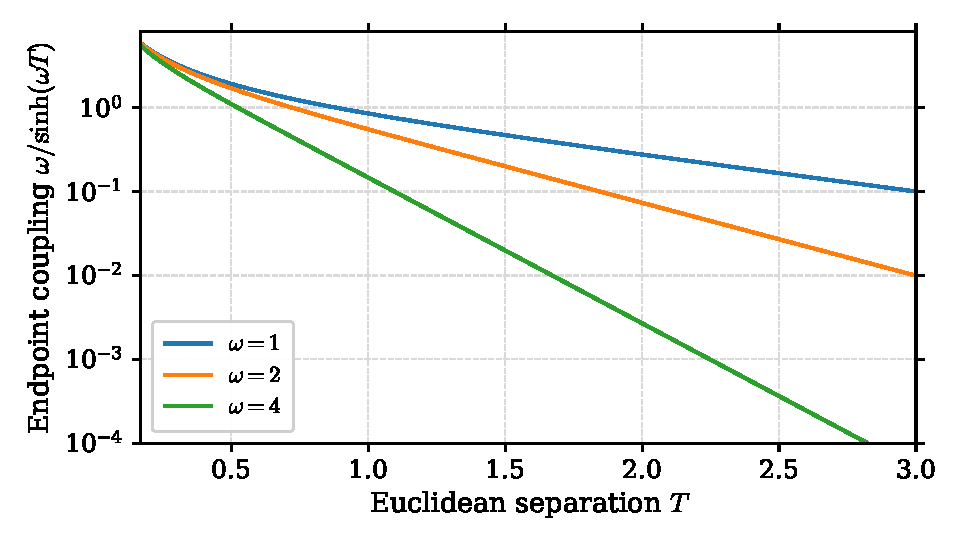
\includegraphics[width=.82\linewidth]{content/AdvancedPhysics/field-theory/figures/geometry-highspin/generated/boundary_mode_gluing.pdf}
\caption{正自伴空间算子的单模边界传递系数 $\omega/\sinh(\omega T)$。高频模更快地丧失两端边界数据的耦合；该衰减来自 \cref{eq:ghs-bridge-Mehler} 的精确二次型，图中各曲线仅取不同 $\omega$，未作额外近似。}\label{fig:ghs-bridge-boundary-gluing}
\end{figure}


前面的传播核是算子表达式。为了看清楚它如何用于一次完整计算，令空间截面是一条周长为 $L$ 的平直圆周，坐标 $x\in[0,L)$、周期条件 $f(x+L)=f(x)$。这条圆周既是最简单的紧致空间，也说明了“空间有周期边界”和“空间真的有边界”是不同的几何：$x=0$ 与 $x=L$ 表示同一个点，并不提供两份独立的边界数据。

空间算子取 $A=-\partial_x^2+\mu^2$。本征问题 $Au=\lambda u$ 的一般复指数解 $\ee^{\ii kx}$ 满足周期条件恰在 $kL=2\pi n$ 时成立，$n\in\ZZ$。令
\begin{equation}\label{eq:ghs-bridge-circle-modes}
 u_n(x)=\frac1{\sqrt L}\ee^{2\pi\ii nx/L},\qquad
 \omega_n=\sqrt{\left(\frac{2\pi n}{L}\right)^2+\mu^2},
\end{equation}
则 $\int_0^L\overline{u_n}u_m\dd x=\delta_{nm}$，而
$\sum_nu_n(x)\overline{u_n(y)}=\delta_L(x-y)$，其中 $\delta_L$ 是周期的 $\delta$ 分布。由于这些本征函数是复数，实场的经典模系数满足 $q_{-n}=\overline{q_n}$；若改用实数的正弦、余弦基，每个 $n>0$ 恰给两个独立的实振子。它们在谱计数时应算两重，而不能把 $n$ 与 $-n$ 误当成两个无关的复标量粒子。

把 \cref{eq:ghs-bridge-circle-modes} 代入一般传播核，得到完全确定的二点函数
\begin{equation}\label{eq:ghs-bridge-circle-G}
 G(\tau,x;\tau',y)=\frac1L\sum_{n\in\ZZ}
 \frac{\ee^{-\omega_n|\tau-\tau'|}}{2\omega_n}
 \ee^{2\pi\ii n(x-y)/L}.
\end{equation}
将 $n$ 与 $-n$ 两项配对，它们互为复共轭，和为两倍实部，所以右侧是实函数。若 $|\tau-\tau'|>0$，高频模指数衰减，故该级数绝对收敛；在等时和同点极限则可能出现紫外奇性，不能直接把它当成处处有界的普通函数。

将两个场取在同一个空间点 $x=y$，只保留 $n=0$ 模便得到下界
\[
 G(\tau,x;\tau',x)\ \geq\frac{\ee^{-\mu|\tau-\tau'|}}{2L\mu}
 \qquad(\mu>0).
\]
这里所有求和项都是正的。若先取 $\tau\ne\tau'$ 再令 $\mu\to0^+$，该下界就发散。这不是短距离紫外发散：它完全由空间上不随 $x$ 改变的\emph{零模}引起。对于严格无质量的圆周标量，零模不受回复势限制，成为自由粒子而不是谐振子，因而不存在通常意义下的归一化高斯基态。这是为何一般空间量子化经常必须在构造 Fock 真空前先分离零模。

若将圆周半径不断增大，即 $L\to\infty$，固定物理距离 $x-y$ 与时间差，波数间距 $\Delta k=2\pi/L$ 变小。利用 Riemann 和极限，得到
\[
 \frac1L\sum_{n\in\ZZ}F(2\pi n/L)
 =\frac1{2\pi}\sum_n\Delta k\,F(k_n)
 \longrightarrow\int_\RR\frac{\dd k}{2\pi}F(k).
\]
因此 \cref{eq:ghs-bridge-circle-G} 回到熟悉的无限直线动量积分。这一计算明确展示了\emph{离散谱和连续谱只是空间性质不同造成的两种谱测度}，并不是两套无关的量子化规则。


我们已经会从空间本征值构造欧氏二点函数，但还没有说明为什么对欧氏时间进行这种计算，最后能够得到具有正范数的量子态。普通欧氏协方差的核正定性仍不够；为了由负时间区域反射到正时间区域，需要检验一条更强的性质。对自由场，它可以直接由 \cref{eq:ghs-bridge-spectral-G} 的每个正频模算出。

定义欧氏时间反射 $\theta(\tau,y)=(-\tau,y)$。取任意有限组位于正半时间 $\tau_i>0$ 的实试验函数 $f_i(y)$ 及复数 $c_i$，构造反射二次型
\[
 Q=\sum_{i,j}\overline{c_i}c_j
 \int_{\Sigma\times\Sigma}\overline{f_i(y)}
 G(-\tau_i,y;\tau_j,y')f_j(y')\dd\mu_h(y)\dd\mu_h(y').
\]
由于 $\tau_i,\tau_j>0$，反射点与原点的时间差是 $\tau_i+\tau_j$，不能写成 $|\tau_i-\tau_j|$。将谱表达代入并定义 $f_{ij}=\langle u_j,f_i\rangle$，得到
\begin{align*}
 Q&=\sum_{i,k}\overline{c_i}c_k\sum_j
 \frac{\ee^{-\omega_j(\tau_i+\tau_k)}}{2\omega_j}
 \overline{f_{ij}}f_{kj}\\
 &=\sum_j\frac1{2\omega_j}
 \left|\sum_i c_i\ee^{-\omega_j\tau_i}f_{ij}\right|^2\ge0.
\end{align*}
这样我们没有借助抽象的重建定理，就已经看到每个正频模怎样贡献一个非负平方。相应的反射正性就是从欧氏路径积分构造物理 Hilbert 空间所需的核心条件之一。

上述证明依赖 $A>0$，并使用了平移不变的欧氏时间以及二次高斯作用量。对于一般依赖时间的几何、含有复杂相互作用的场，或者没有适当反射对称性的空间，这种逐模平方不一定存在。反射正性必须作为独立的物理条件进行检验，不能因为写出了形式上的 $\ee^{-\mathscr I}$ 就自动宣称存在单位量子理论。


如果 $\Sigma=S^{n}$，角向微分算子的本征函数恰好是球谐，且简并度受旋转群保护。若 $\Sigma$ 是二维环面，模态是满足周期条件的 Fourier 波；若是缺少连续对称性的弯曲紧空间，谱通常依然离散，却没有一个自然的角动量标号。高自旋张量场的情况更进一步：场不仅是一个函数，而且每个点上的分量要在坐标变换下按张量规律混合，因而其微分算子必须带有联络与曲率信息。

这些模态计算所需的导数、积分与自伴定义域已在\cref{chap:qft-foundations}的一般截面量子化中固定；更细的曲率交换和球谐表示可参照《数学技巧》与《群论》的对应章节。现在的问题是把精确边界核的归一化、量子态正性和真实时间传播放进同一场论中，因而必须继续计算行列式并明确因果初值。

\subsection{有限模边界核的行列式归一化}
\label{subsec:ghs-r6-gaussian-gluing}

有限模核计算在有限维普通积分与一维振子上推导边界拼接。一般场的泛函积分并不存在与有限维 Lebesgue 测度完全相同的平移不变测度，因此下面的有限模截断是严格代数计算；取无限模极限前必须再检查 Fredholm 行列式、零模与重整化。

设 $x\in\RR^n$ 是保留的边界变量，$y\in\RR^m$ 是待积分的内部变量，二次型写为
\[
Q(x,y)=\frac12x^{\mathsf T}Ax+x^{\mathsf T}By+
\frac12y^{\mathsf T}Cy,
\]
其中 $A=A^{\mathsf T}$，$C=C^{\mathsf T}>0$，且 $B$ 是 $n\times m$ 矩阵。引入 $z=y+C^{-1}B^{\mathsf T}x$，逐项展开
\begin{align*}
\frac12z^{\mathsf T}Cz
&=\frac12y^{\mathsf T}Cy+y^{\mathsf T}B^{\mathsf T}x
+\frac12x^{\mathsf T}BC^{-1}B^{\mathsf T}x,\\
Q(x,y)&=\frac12x^{\mathsf T}(A-BC^{-1}B^{\mathsf T})x
+\frac12z^{\mathsf T}Cz.
\end{align*}
对 $z$ 做正交对角化 $C=O^{\mathsf T}\operatorname{diag}(\lambda_1,\ldots,\lambda_m)O$，积分测度的 Jacobian 因 $O$ 正交而为 $1$，于是
\begin{equation}\label{eq:ghs-r6-schur-integral}
\int_{\RR^m}\exp\!\left(-\frac{Q(x,y)}\hbar\right)\dd^my
=\frac{(2\pi\hbar)^{m/2}}{\sqrt{\det C}}
\exp\!\left[-\frac1{2\hbar}x^{\mathsf T}(A-BC^{-1}B^{\mathsf T})x\right].
\end{equation}
因此积分消元同时改变两个数学对象：指数中的有效二次型和积分前的行列式归一化。只计算 Schur 补而不保存行列式，将丢失真空能及边界核拼接时的必要系数。


\begin{example}[物理单位中的 Mehler 核]

取质量加权的正则坐标 $q=\sqrt M Q$，$p=P_Q/\sqrt M$；这保持 $[q,p]=\ii\hbar$，$[q^2]=\mathrm{kg}\,\mathrm m^2$，$\omega$ 为每秒计的角频率，$T$ 为欧氏物理时间。给定实端点 $q(0)=q_i$、$q(T)=q_f$，欧氏振子作用量为
\[
I[q]=\frac12\int_0^T(\dot q^2+\omega^2q^2)\dd\tau,
\quad \omega>0.
\]
求带物理单位的欧氏传播核，用热方程与短时自由热核极限唯一确定归一化系数。
\textbf{解。} 变分给出 $\ddot q=\omega^2q$。用端点数据解出
\[
q_{\mathrm{cl}}(\tau)=\frac{\sinh[\omega(T-\tau)]}{\sinh(\omega T)}q_i
+\frac{\sinh(\omega\tau)}{\sinh(\omega T)}q_f.
\]
在经典解上 $\dd(qq')/\dd\tau=q'^2+\omega^2q^2$，所以整个积分化为端点项：
\begin{align*}
I[q_{\mathrm{cl}}]
&=\frac12[q_{\mathrm{cl}}\dot q_{\mathrm{cl}}]_0^T\\
&=\frac\omega{2\sinh(\omega T)}
\left[(q_i^2+q_f^2)\cosh(\omega T)-2q_iq_f\right].
\end{align*}
其中交叉项的负号说明在两端固定同号位移时，最小经典作用量较小；这一特征正是边界传递算子的非对角负项。

端点指数只决定核的 $q$ 依赖，前置常数还须由热方程确定。对量子哈密顿量
$\widehat H=-(\hbar^2/2)\partial_q^2+(\omega^2/2)q^2$，欧氏核定义为 $K_T(q_f,q_i)=\langle q_f|\ee^{-T\widehat H/\hbar}|q_i\rangle$，满足
\[
\partial_TK_T=\frac\hbar2\partial_{q_f}^2K_T
-\frac{\omega^2q_f^2}{2\hbar}K_T,
\qquad\lim_{T\downarrow0}K_T(q_f,q_i)=\delta(q_f-q_i).
\]
令 $K_T=C(T)\exp[-I[q_{\mathrm{cl}}]/\hbar]$，将其代入热方程并比较常数项，可得
\[
\frac{\dd}{\dd T}\log C(T)=-\frac\omega2\coth(\omega T).
\]
积分给 $C(T)=C_0/\sqrt{\sinh(\omega T)}$。在 $T\downarrow0$ 时，$I[q_{\mathrm{cl}}]=(q_f-q_i)^2/(2T)+O(T)$，故 $K_T$ 必须趋近自由热核
$(2\pi\hbar T)^{-1/2}\exp[-(q_f-q_i)^2/(2\hbar T)]$，由此唯一确定
\begin{equation}\label{eq:ghs-r6-exact-mehler-kernel}
K_T(q_f,q_i)=\left(\frac{\omega}{2\pi\hbar\sinh(\omega T)}\right)^{1/2}
\exp\!\left[-\frac{\omega\bigl((q_i^2+q_f^2)\cosh(\omega T)-2q_iq_f\bigr)}{2\hbar\sinh(\omega T)}\right].
\end{equation}

\end{example}

\begin{example}[边界核的半群拼接]

令 $T=T_1+T_2$，中间端点 $q$ 不作观测。积分消去中间端点，检验两段 Mehler 核能否拼成总时间 $T_1+T_2$ 的传播核。
\textbf{解。} 将 \cref{eq:ghs-r6-exact-mehler-kernel} 的两个核相乘，含 $q$ 的指数为
\[
-\frac1{2\hbar}\left[\omega\bigl(\coth(\omega T_1)+\coth(\omega T_2)\bigr)q^2
-2\omega\left(\frac{q_i}{\sinh(\omega T_1)}+\frac{q_f}{\sinh(\omega T_2)}\right)q\right]
\]
再加上只依赖 $q_i,q_f$ 的项。对 $q$ 完成平方，积分因子为
\[
\sqrt{\frac{2\pi\hbar}{\omega[\coth(\omega T_1)+\coth(\omega T_2)]}}.
\]
使用
\[
\coth a+\coth b=\frac{\sinh(a+b)}{\sinh a\sinh b},
\quad
\frac{\coth a\coth b+1}{\coth a+\coth b}=\coth(a+b)
\]
以及 $\sinh(a+b)=\sinh a\cosh b+\cosh a\sinh b$，可把指数和前置常数分别化简到总时间 $T_1+T_2$ 的形式。因此严格得到
\begin{equation}\label{eq:ghs-r6-mehler-composition}
\int_\RR K_{T_2}(q_f,q)K_{T_1}(q,q_i)\dd q
=K_{T_1+T_2}(q_f,q_i).
\end{equation}
这种拼接不是泛函积分的口头类比，而是正算子热半群 $\ee^{-T\widehat H/\hbar}$ 的积分核恒等式。对无穷多个模态，逐模乘积的行列式通常发散；这时可以先保留有限能量截断，再用正则化行列式或相对行列式处理极限，不能把有限维归一化直接照抄为无限乘积。

\end{example}

\subsection{区间谱与几何单位的完整例题}
\label{subsec:ghs-feqo-spectral-example}

\begin{example}[Dirichlet 区间的正谱核]

对区间 $(0,L)$ 上的算子 $A=-\frac{\dd^2}{\dd x^2}+\mu^2$，$\mu>0$，取 Dirichlet 边界条件。求 $A^{-1}$ 的 Green 核，核对源点的导数跳跃和端点条件，并说明改换边界条件的影响。
\textbf{解。} 对于固定源点 $y$，齐次方程的两侧解分别可取 $\sinh(\mu x)$ 与 $\sinh(\mu(L-x))$。要求 $G(x,y)$ 连续，且
$-\partial_xG(y^+,y)+\partial_xG(y^-,y)=1$，由此唯一得到
\begin{equation}\label{eq:ghs-feqo-dirichlet-green-interval}
 G_D(x,y)=\frac{\sinh(\mu x_<)\sinh[\mu(L-x_>)]}{\mu\sinh(\mu L)},
 \qquad x_<=\min(x,y),\quad x_>=\max(x,y).
\end{equation}
将分段式代入 $A_xG_D=\delta(x-y)$ 并核对端点，即确认其为 $A^{-1}$ 的积分核。若将边界换成 Neumann，核的边界导数条件改变，零质量极限还要移除常数零模。这一完整计算说明 Green 函数的选择确实依赖算子定义域。

\end{example}

区间核可以逐项求出；曲空间上能否逐模应用它，还取决于分离变量的条件。

若 $g=\dd r^2+a(r)^2h$ 且 $A_hu_j=\lambda_ju_j$，对 $\phi(r,y)=f_j(r)u_j(y)$ 代入
$(-\Delta_g+\mu^2+\xi\mathcal R_g)\phi=0$，得到
\[
 -f_j''-(d-1)\frac{a'}a f_j'
 +\left(\frac{\lambda_j-\xi\mathcal R_h}{a^2}
 +\mu^2+\xi\mathcal R_g\right)f_j=0,
\]
其中使用 $-\Delta_hu_j=(\lambda_j-\xi\mathcal R_h)u_j$ 要求 $\mathcal R_h$ 为常数；若其不是常数，必须改用 $-\Delta_h$ 的本征基来做 Laplace 分离，或者在相应基底内保留曲率势矩阵。即使可以分离变量，端点附近的正规条件也关系到径向微分算子的自伴实现。

分离后的频率还须恢复物理单位。

若物理截面为 $R^2h$，本征值缩放为 $\lambda_j^{\rm phys}=R^{-2}\lambda_j$，真实频率为 $\Omega_j=c\sqrt{\lambda_j}/R$（无量纲 $\lambda_j$ 包含正质量/曲率项）。量子能量激发为 $\hbar\Omega_j$。这与圆柱谱的单位恢复完全一致；但在随时间变化的空间中，不可用单个 $\Omega_j$ 标记全程的能量本征态。








边界核已由有限模积分获得完整的指数与归一化。现在需要判断这些核怎样产生正的态空间，并将一粒子谱推广到由两个场制备的态。


\section{自由场与反射正性}
\label{sec:ghs-free-reflection-positivity}


取 $\Sigma$ 为紧致、无边界的黎曼流形，$A$ 是 $L^2(\Sigma)$ 上自伴算子，并假设 $A\geq m_0^2>0$。考虑欧氏作用量
\begin{equation}\label{eq:ghs-general-cylinder-action}
 \mathscr I[\Phi]=\frac12\int_{\RR}\dd u
 \left(\norm{\partial_u\Phi}_{\Hil}^2+\langle\Phi,A\Phi\rangle\right).
\end{equation}
取 $Au_j=\lambda_ju_j$、$\langle u_i,u_j\rangle=\delta_{ij}$，场展开为 $\Phi(u,x)=\sum_jq_j(u)u_j(x)$。正交性消去交叉项，得到
\[
 \mathscr I=\frac12\sum_j\int_\RR\dd u
 \left(|q'_j|^2+\lambda_j|q_j|^2\right).
\]
因此问题被分解成频率 $\omega_j=\sqrt{\lambda_j}$ 的无限族振子。这是谱定理的结论，不需要截面有旋转对称性。

\begin{theorem}[任意正自伴截面的欧氏两点核]
\label{thm:ghs-free-two-point-general}
在 \cref{eq:ghs-general-cylinder-action} 的平移不变高斯态下，协方差是
\begin{equation}\label{eq:ghs-free-general-covariance}
 C(u,u')=\frac12A^{-1/2}\ee^{-|u-u'|A^{1/2}},
\end{equation}
其坐标核在紧致情形按分布意义展开为
\begin{equation}\label{eq:ghs-free-general-spectral-sum}
 C(u,x;u',y)=\sum_j\frac{\ee^{-\omega_j|u-u'|}}{2\omega_j}
 u_j(x)\overline{u_j(y)}.
\end{equation}
非紧致情形须以 $A$ 的投影谱积分取代离散求和。
\end{theorem}
\begin{proof}
对每个 $j$，待求 Green 核 $c_j(v)$ 满足
$(-\frac{\dd^2}{\dd v^2}+\omega_j^2)c_j(v)=\delta(v)$。
对于 $v\neq 0$，要求两端有界并衰减，故 $c_j(v)=C_j\ee^{-\omega_j|v|}$。在 $v=0$ 邻域积分微分方程得到导数跳跃
$-c'_j(0^+)+c'_j(0^-)=1$，而左右导数分别为 $-\omega_j C_j,+\omega_jC_j$，于是 $C_j=1/(2\omega_j)$。按谱定理恢复算子函数便得到 \cref{eq:ghs-free-general-covariance}。将 $u_j$ 投入坐标核定义，得到 \cref{eq:ghs-free-general-spectral-sum}。
\end{proof}


对实本征函数基可取 $[q_j,p_k]=\ii\delta_{jk}$ 的无量纲正则变量。定义
\[
 a_j=\sqrt{\frac{\omega_j}{2}}q_j+\frac{\ii}{\sqrt{2\omega_j}}p_j,
 \qquad a_j^\dagger=\sqrt{\frac{\omega_j}{2}}q_j-\frac{\ii}{\sqrt{2\omega_j}}p_j.
\]
由对易关系逐项计算 $[a_j,a_k^\dagger]=\delta_{jk}$。选定 $a_j\ket0=0$ 后，正规序哈密顿量是
\begin{equation}\label{eq:ghs-general-cylinder-hamiltonian}
 H=\sum_j\omega_ja_j^\dagger a_j,
\end{equation}
绝对零点能 $\frac12\sum_j\omega_j$ 一般发散，需要规定正则化与背景反项。若 $\omega_j=0$，上面的定义含有 $1/\sqrt\omega_j$，因此不合法；真正零模是自由坐标而非有基态的谐振子。紧致无质量标量的常数零模便是这个典型问题。


定义欧氏时间反射 $\theta(u,x)=(-u,x)$。令 $f$ 支持在 $u>0$，设
$F=\int_{u>0}\overline{f(u,x)}\Phi(u,x)\dd u\dd\mu_h$。在高斯理论中，反射内积可以化为
\begin{equation}\label{eq:ghs-reflection-positive-quadratic}
 \int_{u,v>0}\langle f(u),C(-u,v)f(v)\rangle\dd u\dd v
 =\frac12\norm{A^{-1/4}\int_0^\infty\ee^{-uA^{1/2}}f(u)\dd u}_{\Hil}^2\geq0.
\end{equation}
\begin{proof}
当 $u,v>0$ 时，$|-u-v|=u+v$，故 $C(-u,v)=\frac12A^{-1/2}\ee^{-(u+v)A^{1/2}}$。由于 $A^{1/2}$ 自伴，各谱函数互相交换。将算子分为
$\frac12(A^{-1/4}\ee^{-uA^{1/2}})^*(A^{-1/4}\ee^{-vA^{1/2}})$，再把时间积分移入内积，就得到平方范数。严格地说，先对紧支撑光滑试验函数计算，再按闭包延拓；多项式场的完整反射正性可由高斯 Wick 结构和对称 Fock 空间正性推出。
\end{proof}

这是可以计算的 Osterwalder--Schrader 正性检验，而不是任意欧氏作用量都自动正性的论证。若 $A$ 存在负模，指数核不再给实正的 $\omega$，上述因式分解失效；若几何本身没有反射等距，也没有自然的 $u\mapsto-u$ 对应。


\subsection{时变截面与模态联络}

即使每张截面都有正交谱，基底的时间变化也会耦合不同模态。先明确这里的欧氏叶状度规：$N>0$ 为法向距离与坐标时间增量之比，$N^a$ 描述相邻叶片的切向位移，$h_{ab}$ 为叶片上的正定度规。
\begin{definition}[欧氏叶状度规与法向导数]
\begin{equation}\label{eq:ghs-foliation-adm}
 g_E=N^2\dd t_E^2+h_{ab}(\dd y^a+N^a\dd t_E)(\dd y^b+N^b\dd t_E),
 \qquad \partial_n=N^{-1}(\partial_{t_E}-N^a\partial_a).
\end{equation}
$\dd\mu_{g_E}=N\sqrt{\det h}\dd t_E\dd^{d-1}y$，$t_E$ 为长度型欧氏时间。一般叶状几何的推导可参照《数学技巧》的超曲面与体积输运章节。
\end{definition}
下列作用量暂把 $t_E$ 简记为 $t$，$\mathscr I=I_E/\hbar$：
\begin{equation}\label{eq:ghs-general-foliation-action}
 \mathscr I=\frac12\int\dd t\,\dd^{d-1}y\,N\sqrt h
 \left[\frac{(\partial_t\varphi-N^a\partial_a\varphi)^2}{N^2}
 +h^{ab}\partial_a\varphi\partial_b\varphi+V(t,y)\varphi^2\right].
\end{equation}
其中 $V$ 可以包括质量与曲率耦合。现在 $h,N,N^a,V$ 都可能依赖 $t$；将场在某一时刻的本征模展开以后，基底本身随 $t$ 改变，导数 $\partial_tu_j$ 产生非对角耦合。因而场的演化一般不是 $\ee^{-t\sqrt A}$，也不能任意写成一组独立的定频率振子。


当模态基随时间变化时，对展开式求导还会产生基矢本身的导数。
暂取 $N=1,N^a=0$，假设 $h$ 的面积测度可以通过选定酉识别映到固定 Hilbert 空间，并设 $u_j(t)$ 是其瞬时正交归一基。写 $\Phi=\sum_jq_j(t)u_j(t)$，则
\[
 \partial_t\Phi=\sum_i\left(\dot q_i+\sum_j\mathcal A_{ij}q_j\right)u_i,
 \quad \mathcal A_{ij}=\langle u_i,\partial_tu_j\rangle.
\]
由 $\partial_t\langle u_i,u_j\rangle=0$ 得 $\mathcal A_{ij}+\overline{\mathcal A_{ji}}=0$，即模态联络为反厄密矩阵。动能变为
$\frac12\sum_i|\dot q_i+\sum_j\mathcal A_{ij}q_j|^2$。这清楚展示为什么“每一时刻能对角化”不等于“整个时间演化中模态独立”。若使用原始随 $h(t)$ 变化的 Hilbert 内积，必须先引入上述酉识别，否则 $\mathcal A$ 还要加入测度变化项才有反厄密性。


到这里，任意空间上的自由场传播子已有完整的普适算子表达。后续共形场论的特殊优点，将是把某些随径向变化的二次型精确地转成时间不变的算子，使场的频率成为算符标度维数。




二点函数的非负性说明了一个高斯态怎样获得正范数。可是高自旋问题不仅涉及真空，还涉及由两个场激发组成的状态；这时应当先把双粒子核的归一化问题解决。




截面随时间改变时，模态联络说明瞬时对角化不足以选出全程的粒子定义。下文从守恒辛形式构造复结构，并完整求出频率突变的 Bogoliubov 系数与无限模态的酉实现条件。现在先保持一个给定正频空间，研究其双粒子态怎样归一化和约化。

\subsection{一般双玻色态的核与单体约化谱}

后章的高自旋态将给出一个具体的球面双粒子核。为使其中的范数与约化态有统一来源，先在一般一粒子 Hilbert 空间上建立对称核的表达。真正适用于任意截面与任意一体谱的数学对象，是对称张量积 Hilbert 空间中的一个平方可和核。它可以直接给出态范数、约化密度矩阵、纠缠熵与所观测场振幅之间的关系，完全不要求空间是球面。


令 $\mathscr H$ 是可分离复 Hilbert 空间，$\{e_i\}$ 为正交归一基，$a_i^\dagger$ 为对应玻色产生算符，$[a_i,a_j^\dagger]=\delta_{ij}$。取一个对称核 $K_{ij}=K_{ji}$，满足 $\sum_{i,j}|K_{ij}|^2<\infty$，定义
\begin{equation}\label{eq:ghs-general-two-boson-kernel}
 \ket K=\frac1{\sqrt2}\sum_{i,j}K_{ij}a_i^\dagger a_j^\dagger\ket0.
\end{equation}

\begin{theorem}[精确范数和单体约化态]
\label{thm:ghs-two-boson-kernel-density}
对 \cref{eq:ghs-general-two-boson-kernel}，有
\begin{equation}\label{eq:ghs-kernel-norm-density}
 \langle K|K\rangle=\operatorname{Tr}(KK^\dagger),\qquad
 \rho^{(1)}=\frac{KK^\dagger}{\operatorname{Tr}(KK^\dagger)}.
\end{equation}
这里 $\rho^{(1)}_{ij}=\langle K|a_j^\dagger a_i|K\rangle/(2\langle K|K\rangle)$，因此 $\operatorname{Tr}\rho^{(1)}=1$。
\end{theorem}
\begin{proof}
从对易关系直接算
\[
 \langle0|a_l a_k a_i^\dagger a_j^\dagger|0\rangle
 =\delta_{ki}\delta_{lj}+\delta_{kj}\delta_{li}.
\]
代入态范数并利用 $K_{ij}=K_{ji}$，得到
\[
 \langle K|K\rangle=\frac12\sum_{i,j,k,l}
 \overline{K_{kl}}K_{ij}(\delta_{ki}\delta_{lj}+\delta_{kj}\delta_{li})
 =\sum_{i,j}|K_{ij}|^2.
\]
另一方面，
\[
 a_i\ket K=\frac1{\sqrt2}\sum_{j,k}K_{jk}
 (\delta_{ij}a_k^\dagger+\delta_{ik}a_j^\dagger)\ket0
 =\sqrt2\sum_kK_{ik}a_k^\dagger\ket0.
\]
故 $\langle K|a_j^\dagger a_i|K\rangle=2\sum_k K_{ik}\overline{K_{jk}}=2(KK^\dagger)_{ij}$。除以粒子数 $2$ 与态范数，得到约化态公式。
\end{proof}


若一体基作酉变换 $e'_i=\sum_jU_{ji}e_j$，则双体核的坐标矩阵变为 $K'=U^\dagger K\overline U$。直接相乘得到 $K'K'^\dagger=U^\dagger KK^\dagger U$，所以一体约化矩阵作酉相似变换，其本征值不变。

对有限秩对称复矩阵，Takagi 分解把 $K$ 表成 $K=V\operatorname{diag}(s_j)V^T$，$s_j\geq0$。代入两体态，改用新的正交产生算符 $b_j^\dagger$，得到
\begin{equation}\label{eq:ghs-takagi-two-boson}
 \ket K=\frac1{\sqrt2}\sum_j s_j(b_j^\dagger)^2\ket0,\qquad
 \sum_js_j^2=\norm{K}^2.
\end{equation}
因此归一化后的一体谱精确为 $p_j=s_j^2/\sum_ks_k^2$。无限维紧致 Hilbert--Schmidt 对称算子亦有相应谱分解。重根下单体模式基不唯一，但单体约化谱唯一。

由此可无歧义地定义
\begin{equation}\label{eq:ghs-general-two-body-renyi}
 H_\alpha=\frac1{1-\alpha}\log\sum_jp_j^\alpha,\qquad
 H_1=-\sum_jp_j\log p_j,\qquad
 \operatorname{Tr}(\rho^{(1)})^2=\sum_jp_j^2.
\end{equation}
这里熵衡量双粒子纯态的单粒子约化谱；对完全相同粒子，它采用归一化一体密度矩阵的惯例，不能在没有说明操作扇区与粒子标签的情况下，直接把它等同于两个可区分实验子系统之间的纠缠熵。


设截面自由场有正谱 $A u_i=\omega_i^2u_i$。对应的等时场算子为
\[
 \widehat\Phi(x)=\sum_i\frac{u_i(x)a_i+\overline{u_i(x)}a_i^\dagger}{\sqrt{2\omega_i}}.
\]
场的真空—双体矩阵元是
\begin{equation}\label{eq:ghs-general-two-body-field-amplitude}
 \mathcal A_K(x,y)=\bra0\widehat\Phi(x)\widehat\Phi(y)\ket K
 =\sqrt2\sum_{i,j}\frac{K_{ij}u_i(x)u_j(y)}{\sqrt{2\omega_i}\sqrt{2\omega_j}}.
\end{equation}
若将 $K$ 看作 $\mathscr H\otimes_s\mathscr H$ 的核，右端相当于在两个因子上分别作用 $(2A^{1/2})^{-1/2}$ 后再取位置表示；因此它一般不是原始正交两体位置幅的数值表示。

\begin{proof}
将两个场算子的湮灭部分作用在 \cref{eq:ghs-general-two-boson-kernel} 上。由于
$\bra0 a_i a_j\ket K=\sqrt2K_{ij}$，只有双湮灭项贡献非零；其余正常序项在左真空或右二粒子态上为零。将每个模态的场归一化因子 $1/\sqrt{2\omega_i}$ 代回即得公式。在无限模态中，点值核应先经平滑试验函数涂抹，再讨论何时存在连续位置核。
\end{proof}

对于不同种类的两场 $A,B$，在选定的正交基下以 Hilbert--Schmidt 系数矩阵 $K$ 表示两体态
\[
 \ket K=\sum_{ij}K_{ij}a_i^\dagger b_j^\dagger\ket0,
 \qquad \mathcal N_K=\operatorname{Tr}(KK^\dagger)>0.
\]
对未观测的场求偏迹，得到
\begin{equation*}
 (\rho_A)_{ik}=\frac{\sum_jK_{ij}\overline{K_{kj}}}{\mathcal N_K},
 \qquad
 (\rho_B)_{j\ell}=\frac{\sum_iK_{ij}\overline{K_{i\ell}}}{\mathcal N_K}.
\end{equation*}
因此 $\rho_A=KK^\dagger/\mathcal N_K$，而所选 $B$ 基中的矩阵为
$\rho_B=(K^\dagger K)^{\mathsf T}/\mathcal N_K=K^{\mathsf T}\overline K/\mathcal N_K$。
转置不改变本征值，两套约化态的非零谱均为 $K$ 的归一化奇异值平方。
例如取 $K=\left(\begin{smallmatrix}1&\ii\\0&1\end{smallmatrix}\right)$，则
\[
 \rho_B=\frac13\begin{pmatrix}1&-\ii\\\ii&2\end{pmatrix},
 \qquad
 \frac{K^\dagger K}{\mathcal N_K}
 =\frac13\begin{pmatrix}1&\ii\\-\ii&2\end{pmatrix}.
\]
两者的谱相同，但非对角矩阵元不同，故在固定基中求期望值时必须保留转置。
这个结果将在后章用于混合标量高自旋态；两种场可区分时，$\rho_A$ 的熵才直接对应所指定场分割的纯态纠缠。


若截面等距群为 $G$，$\mathscr H$ 分解为 $\bigoplus_\lambda V_\lambda\otimes M_\lambda$，则两体空间按 $\mathscr H\otimes_s\mathscr H$ 的群表示继续分解。所谓高自旋投影是作用在这个张量积上的某个表示投影，核的对称性与选择规则来自群表示乘法，而不是先验的 $\binom Sk$ 系数。对于标准球面，Clebsch--Gordan 型分解及特殊共形初级条件使相应核可写成有限组合数；在一般空间上，真正稳定的可计算对象仍是该核、它的群表示类型、作用于它的二体算子和 \cref{eq:ghs-kernel-norm-density} 所给的谱量。


模态量子化构造了真空和传播子，而在具有边界的几何区域中，还可以反过来把路径积分视为两个边界配置之间的核。这个角度将谱理论与量子态的拼接性质联系起来。


在一张空间截面上给出场配置，并不能自动得到可解释为概率振幅的量子态。欧氏泛函积分首先定义的是依赖边界配置的函数；要使它具有 Hilbert 空间意义，还需要拼接性质与反射正性。在平直共形场论中，这两件事与局域算符的尺度展开巧妙结合，但一般曲面上并没有无条件的态—算符一一对应。


设 $U\subset M$ 是紧致区域，边界分成 $\partial U=\overline\Sigma_-\sqcup\Sigma_+$，外法向方向相反。固定边界值 $\varphi|_{\Sigma_\pm}=\phi_\pm$，形式上定义
\begin{equation}\label{eq:ghs-euclidean-transfer-kernel}
 K_U[\phi_+,\phi_-]
 =\int_{\substack{\varphi|_{\Sigma_-}=\phi_-\\\varphi|_{\Sigma_+}=\phi_+}}
 \mathcal D\varphi\;\ee^{-\mathscr I_U[\varphi]}.
\end{equation}
泛函测度的构造取决于正则化及其极限，此处先用有限维谱截断理解它。若 $U=U_2\circ U_1$ 沿共同截面 $\Sigma$ 拼接，则
\begin{equation}\label{eq:ghs-gluing-kernels}
 K_{U_2\circ U_1}[\phi_+ ,\phi_-]
 =\int\mathcal D\phi\;K_{U_2}[\phi_+,\phi]K_{U_1}[\phi,\phi_-].
\end{equation}
这是将所有内部配置按它在拼接截面上的共同取值分组；连续理论中必须注意 UV 截断一致及可能的边界反项。

\begin{figure}[htbp]
\centering
% Local TikZ geometry; styles inherited exclusively from the shared preamble.
\begin{tikzfig}[scale=.95]
\fill[blue!4] (-3,-1.15) rectangle (0,1.15);
\fill[red!4] (0,-1.15) rectangle (3,1.15);
\draw[thick] (-3,-1.15) rectangle (3,1.15);
\draw[thick,densely dashed] (0,-1.4)--(0,1.4);
\node at (-1.75,.75) {$\Omega_L$};
\node at (1.75,.75) {$\Omega_R$};
\node at (0,1.75) {$\Sigma$};
\node[lecturelabel] at (0,-1.75) {$\phi|_{\Sigma}=f$};
\draw[lecturearrow,blue!65!black] (-1.25,-.28)--(-.27,-.28) node[midway,below] {$n_L$};
\draw[lecturearrow,red!65!black] (1.25,-.28)--(.27,-.28) node[midway,below] {$n_R$};
\node[lecturelabel] at (-3.65,.1) {$\partial\Omega_L$};
\node[lecturelabel] at (3.7,.1) {$\partial\Omega_R$};
\end{tikzfig}

\caption{两个带边界区域沿 $\Sigma$ 拼接：接口上的场值 $f$ 必须一致，但两块区域相对于接口的外法向 $n_L,n_R$ 方向相反。}\label{fig:ghs-boundary-gluing}
\end{figure}

\cref{fig:ghs-boundary-gluing} 对应 \cref{eq:ghs-gluing-kernels} 的积分变量 $f$。拼接时连续的是边界值，法向导数则需满足相应通量匹配；这也解释了为什么边界算子会在后续出现。



对前述振子，\cref{eq:ghs-bridge-Mehler,eq:ghs-r6-exact-mehler-kernel} 已分别给出规范化坐标与物理坐标的完整核，\cref{eq:ghs-r6-mehler-composition} 计算了包含前置常数的拼接积分。一般区域的 \cref{eq:ghs-gluing-kernels} 正是同一运算对边界配置的表达；下文利用经典解把它改写为边界二次型。

双粒子态由 Hilbert 空间的张量积定义。若把场的全部数据改为保存在一张超曲面上，态的制备也可由相应区域的欧氏泛函积分来实现。




\subsection{反射正性与态空间重建}

设空间与作用量关于 $t=0$ 的反射 $\theta$ 不变。记 $\mathscr A_+$ 为仅依赖正时间场数据的可观测函数。定义反射配对
$\langle F,G\rangle_{\rm OS}=\langle\overline{\theta F}\,G\rangle_E$。

\begin{definition}[反射正性]
欧氏关联函数称为反射正的，若对于任意有限个 $F_i\in\mathscr A_+$ 与复数 $c_i$，有
\begin{equation}\label{eq:ghs-os-reflection-positivity}
 \sum_{i,j}\overline{c_i}c_j
 \langle\overline{\theta F_i}\,F_j\rangle_E\geq0.
\end{equation}
\end{definition}

这个条件保证反射配对是半正定的。先将其零范数元素组成的子空间商掉，再按范数完备化，得到 Hilbert 空间；欧氏正时间平移在适当公理下生成收缩半群 $\ee^{-tH}$，其生成元 $H\geq0$。因此量子态 Hilbert 空间来自正性，而不是直接把泛函积分符号当成普通积分。


在平直、反射正、具有离散维数谱的共形场论局域真空扇区内，考虑含原点插入 $\mathcal O(0)$ 的球内泛函积分。它给出球面上的态
\[
 \ket{\mathcal O}=\mathcal O(0)\ket0,
\]
后裔由平移生成元反复作用；在球面径向共轭下，$P_\mu^\dagger=K_\mu$。此时被原点与无穷远配对的局域算符具有径向范数，尺度生成元的本征值成为圆柱激发能量。这是后面平直共形部分的起点。

对于一般流形，要得到同样结论至少需要：围绕一个点的合理局域操作扇区、能将收缩边界状态与该点局域插入匹配的短距离结构、正性，以及将径向演化与可对角化生成元联系的对称性。仅有 \cref{eq:ghs-euclidean-transfer-kernel} 并不推出这些前提。



例如，在圆环与球内状态不是同一类边界态的计算中，
二维共形场论在圆周上具有径向量子化，但带有非平凡拓扑通量或绕线缺陷的扇区，可能不能由普通无缺陷点算符产生。更一般地，在高维空间上选非球面截面，其 Hilbert 空间通常有丰富的拓扑扇区与边界条件；一个局域点插入没有足够的数据区分这些扇区。




\subsection{对称荷、接触项与边界响应}

设 $\xi$ 是 Killing 向量场，$j^a=T^{ab}\xi_b$。对有插入点 $x_i$ 的区域 $U$ 进行无穷小坐标变换，并将相关积分的边界项分离，可以得到形式为
\begin{equation}\label{eq:ghs-ward-geometric}
 \nabla_a\langle j^a(x)\mathcal O_1(x_1)\cdots\mathcal O_n(x_n)\rangle
 =-\sum_i\delta_g(x,x_i)\,
 \langle\mathcal O_1\cdots\delta_\xi\mathcal O_i\cdots\mathcal O_n\rangle.
\end{equation}
这要求选定守恒应力张量、正确处理接触项及可能的量子异常。将 \cref{eq:ghs-ward-geometric} 在两片截面之间积分，得到跨过算符插入时荷发生何种跳变。没有 Killing 或合适的共形 Killing 场时，不能凭空定义守恒的尺度荷。


对局域变换取一次作用量变分，就得到相应的恒等式。
在有限维截断的泛函积分中，作变量替换 $\varphi\mapsto\varphi+\varepsilon(x)\delta_\xi\varphi$；测度若无异常，其总变分为零。作用量的一阶变化按 Noether 定理为 $\delta\mathscr I=-\int(\nabla_a\varepsilon)j^a\dd\mu_g$，而每个插入的变化为 $\varepsilon(x_i)\delta_\xi\mathcal O_i$。在 $\varepsilon$ 紧支撑下分部积分，得到
\[
 \int\varepsilon(x)\nabla_a\langle j^a(x)\prod_i\mathcal O_i\rangle\dd\mu_g
 +\sum_i\varepsilon(x_i)\langle\mathcal O_1\cdots\delta_\xi\mathcal O_i\cdots\rangle=0.
\]
由任意试验函数 $\varepsilon$，即得分布意义下的 \cref{eq:ghs-ward-geometric}。在严格的量子场论中，局域复合算符和测度 Jacobian 需按同一重整化约定定义，异常项可能修正右边。




如果一张超曲面处于两个区域的公共边界，两侧的高斯路径积分必须对这一边界上的场数据再积分一次。边界算子的拼接律正是传播核半群性质的几何版本。




在任意流形上，球面不再是唯一可能的量子化边界。真正可以重复利用的技术，是把一个椭圆场方程在区域内部的解换成边界数据之间的二次型。这样，积分核的拼接不再依赖同心球的坐标，而成为边界算子和 Schur 补的运算。


设 $(U,g)$ 是紧致、光滑边界的黎曼区域，$L=-\Delta_g+V$ 采用 Dirichlet 实现，并假设 Dirichlet 零本征值不存在。对边界函数 $f$，解
\[
 L\phi_f=0\quad\text{于 }U,\qquad \phi_f|_{\partial U}=f.
\]
对于适当的 Sobolev 数据 $f\in H^{1/2}(\partial U)$，定义 Dirichlet-to-Neumann 算子
\begin{equation}\label{eq:ghs-dn-definition}
 \Lambda_U f=(\nabla_n\phi_f)|_{\partial U},
\end{equation}
其中 $n$ 为指向区域外的单位法向。严格而言 $\Lambda_U:H^{1/2}\to H^{-1/2}$；不能将它未经域分析便视为对所有 $L^2$ 函数有界的算子。

\begin{proposition}[壳上作用量是边界二次型]
\label{prop:ghs-on-shell-boundary-action}
设 $V$ 为实函数，欧氏高斯作用量为
$\mathscr I[\phi]=\frac12\int_U(|\nabla\phi|^2+V\phi^2)\dd\mu_g$。
则经典解的作用量精确为
\begin{equation}\label{eq:ghs-onshell-dn-action}
 \mathscr I[\phi_f]=\frac12\langle f,\Lambda_U f\rangle_{\partial U}.
\end{equation}
若二次型非负，$\Lambda_U$ 也在相应二次型意义下非负。
\end{proposition}
\begin{proof}
积分分部给出 Green 第一恒等式
\[
 \int_U\nabla^a\overline\phi\nabla_a\psi\dd\mu_g
 =-\int_U\overline\phi\Delta_g\psi\dd\mu_g
 +\int_{\partial U}\overline\phi\,\nabla_n\psi\dd\mu_{\partial U}.
\]
取 $\psi=\phi=\phi_f$，加上势能项，并用 $(-\Delta+V)\phi_f=0$ 消去体积积分，即得 \cref{eq:ghs-onshell-dn-action}。对于两组边界数据 $f,g$，将同一恒等式应用于 $\phi_f,\phi_g$ 得 $\langle f,\Lambda g\rangle=\langle\Lambda f,g\rangle$；这是 DtN 的对称性来源。
\end{proof}


以区间 $0\leq t\leq T$ 上的单个振子为例，$L=-\partial_t^2+\omega^2$，边界向量为 $\vb q=(q_i,q_f)^T$。由 \cref{eq:ghs-bridge-Mehler} 中的经典解可直接算
\[
 \binom{-q_{\rm cl}'(0)}{q_{\rm cl}'(T)}
 =\frac\omega{\sinh\omega T}
 \begin{pmatrix}\cosh\omega T&-1\\-1&\cosh\omega T\end{pmatrix}
 \binom{q_i}{q_f}.
\]
故
\begin{equation}\label{eq:ghs-dn-oscillator-matrix}
 \Lambda_T=\omega
 \begin{pmatrix}\coth\omega T&-\operatorname{csch}\omega T\\
 -\operatorname{csch}\omega T&\coth\omega T\end{pmatrix}.
\end{equation}
$\frac12\vb q^T\Lambda_T\vb q$ 就是振子壳上作用量，精确解释了 Mehler 核指数中的三个项。这个小例子不是用来猜一般公式，而是对 \cref{eq:ghs-onshell-dn-action} 的逐项验算。


\begin{figure}[htbp]
 \centering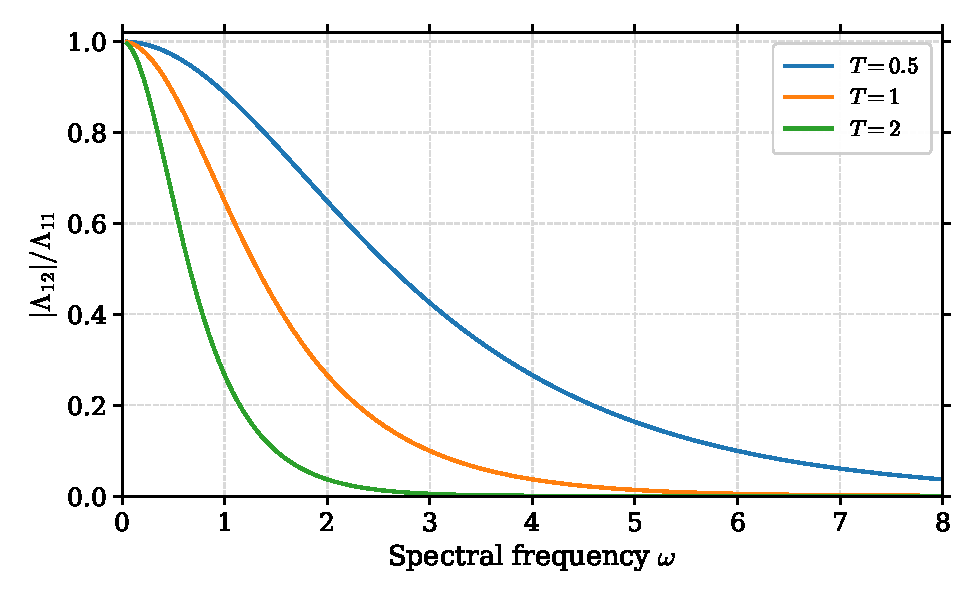
\includegraphics[width=0.77\linewidth]{content/AdvancedPhysics/field-theory/figures/geometry-highspin/generated/dn_transmission.pdf}
 \caption{长度为 $T$ 的欧氏振子区间中，Dirichlet-to-Neumann 边界矩阵的跨边界耦合与自耦合之比，精确为 $|\Lambda_{12}|/\Lambda_{11}=1/\cosh(\omega T)$。频率较高或传播区间较长时，边界耦合指数减弱。}
 \label{fig:ghs-dn-transmission}
\end{figure}


令区域 $U_1,U_2$ 沿内部截面 $\Sigma$ 拼接。设各自边界二次型的块矩阵为
\[
 \Lambda_1=\begin{pmatrix}A&B\\B^*&C\end{pmatrix},
 \qquad \Lambda_2=\begin{pmatrix}D&E\\E^*&F\end{pmatrix}.
\]
三个变量分别记为 $f$（左外边界）、$z$（公共内部边界）、$g$（右外边界）。总壳上二次型是
\[
 2\mathscr I=\langle f,Af\rangle+2\operatorname{Re}\langle f,Bz\rangle
 +\langle z,(C+D)z\rangle+2\operatorname{Re}\langle z,Eg\rangle+\langle g,Fg\rangle.
\]
若 $C+D$ 有有界逆，固定外边界条件下对 $z$ 取变分得
$z_*=-(C+D)^{-1}(B^*f+Eg)$。将它代回，新的边界矩阵为
\begin{equation}\label{eq:ghs-dn-schur-complement}
 \Lambda_{U_2\circ U_1}=
 \begin{pmatrix}
 A-B(C+D)^{-1}B^*&-B(C+D)^{-1}E\\
 -E^*(C+D)^{-1}B^*&F-E^*(C+D)^{-1}E
 \end{pmatrix}.
\end{equation}
这就是 Schur 补，而不是另一种新的物理假设。有限维高斯积分还给出行列式因子 $(\det(C+D))^{-1/2}$；连续场论须对该形式行列式做恰当正则化并检查局部边界反项。



令 $U_1$ 为长度 $T_1$ 的区间、$U_2$ 为长度 $T_2$ 的区间。由 \cref{eq:ghs-dn-oscillator-matrix}，
\[
 A=C=\omega\coth\omega T_1,
 \quad B=-\omega\operatorname{csch}\omega T_1,
 \quad D=F=\omega\coth\omega T_2,
 \quad E=-\omega\operatorname{csch}\omega T_2.
\]
Schur 补的左右耦合项为
\[
 -\frac{BE}{C+D}=-\frac{\omega\operatorname{csch}(\omega T_1)
 \operatorname{csch}(\omega T_2)}{\coth(\omega T_1)+\coth(\omega T_2)}.
\]
利用 $\coth a+\coth b=\sinh(a+b)/(\sinh a\sinh b)$，得
$-BE/(C+D)=-\omega\operatorname{csch}[\omega(T_1+T_2)]$。同样利用双曲函数恒等式计算左、右对角项，均得 $\omega\coth[\omega(T_1+T_2)]$。于是 \cref{eq:ghs-dn-schur-complement} 精确恢复 $\Lambda_{T_1+T_2}$，与 \cref{eq:ghs-gluing-kernels} 一致。



这一整套技术只需要正则边界、指定的椭圆问题与可逆性条件，具有比球面径向分解更强的几何普适性。真正的量子泛函积分核是否正定、能否重建 Hilbert 空间，则由反射正性和测度构造决定，不能仅从 Schur 补代数推出。








欧氏理论中的热核从正算子 $A$ 构造，参数 $t$ 越大，高频模态越被压低。但真实时间中的自由场不能按同样的指数衰减演化：自由场的经典演化必须保持初始数据的辛形式，量子理论则由这一辛形式决定正则对易关系。为了弄清哪部分结构真正适用于弯曲时空，需要从柯西问题出发。


\section{柯西问题}
\label{sec:ghs-cauchy-problem}


设 $(\mathcal M,g_L)$ 是连通、定向并有时间定向的 $d$ 维 Lorentz 流形，度规号差取 $(+,-,\ldots,-)$，时空坐标 $x^0=ct$。一个超曲面 $\Sigma$ 称为柯西面，如果每条不可延拓类时曲线恰与其相交一次。存在柯西面并满足通常的因果条件的时空称为全局双曲时空。这个条件的意义不是形式上的便利，而是保证给定初始场与法向导数之后，双曲方程能够得到唯一的全局解。

\begin{theorem}[全局双曲时空的几何分解]
\label{thm:ghs-globally-hyperbolic-splitting}
若 $\mathcal M$ 全局双曲，则存在光滑的 Cauchy 长度时间函数 $x^0$，使 $\mathcal M$ 微分同胚于 $\RR\times\Sigma$，并可写成
\begin{equation}\label{eq:ghs-lorentzian-splitting}
 \mathbf g=\beta(x^0,y)\dd (x^0)^2-h_{x^0},
 \qquad\beta(x^0,y)>0,
\end{equation}
其中每个 $h_{x^0}$ 为 Cauchy 截面上的黎曼度规。这个结论不要求存在任何时间平移 Killing 场。
\end{theorem}

这里引用的是全局双曲时空分解定理；其严格证明使用因果理论与光滑时间函数的构造，不能仅由局部坐标矩阵分解推出。它所带来的关键信息是：Cauchy 发展问题有自然的时间层，却不保证存在真空能量本征态。

\begin{definition}[正则双曲标量算子]
固定质量参数 $\mu=mc/\hbar$ 和曲率耦合 $\xi\in\RR$，定义
\begin{equation}\label{eq:ghs-r6-lorentz-kg-operator}
P=\Box_{g_L}+\mu^2-\xi\mathcal R_L,
\qquad \Box_{g_L}=g_L^{ab}\nabla_a\nabla_b.
\end{equation}
$P\phi=0$ 是实 Klein--Gordon 方程。这里 $\mathcal R_L$ 是 $g_L$ 的标量曲率，$\phi$ 的整体归一化须由作用量或等时对易关系指定；微分方程本身不确定它。
\end{definition}

在平直时空，令 $\phi=\ee^{-\ii\omega t+\ii\vb k\cdot\vb x}$，则 $\Box=c^{-2}\partial_t^2-\Delta$，因而 $P\phi=0$ 等价于
\[
\omega^2=c^2|\vb k|^2+\frac{m^2c^4}{\hbar^2},
\qquad E=\hbar\omega=\sqrt{\hbar^2c^2|\vb k|^2+m^2c^4}.
\]
平面波代入给出 $-\omega^2/c^2+|\vb k|^2+\mu^2=0$，同时固定了质量项与正频号差；曲率耦合的符号由下列作用量固定。

\begin{figure}[htbp]
\centering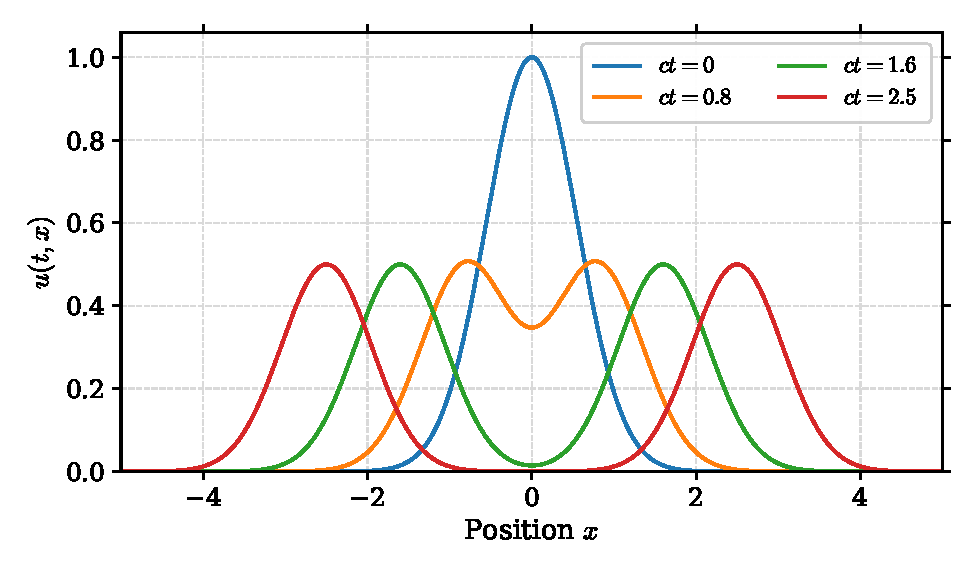
\includegraphics[width=.79\linewidth]{content/AdvancedPhysics/field-theory/figures/geometry-highspin/generated/cauchy_wave_packets.pdf}
\caption{一维无质量波动方程 $u_{tt}=c^2u_{xx}$ 的精确达朗贝尔解：初始高斯位移、初始速度为零时，波包向左右以速度 $c$ 分离。横轴采用相同的长度单位。}\label{fig:ghs-cauchy-wave-packets}
\end{figure}

\cref{fig:ghs-cauchy-wave-packets} 对应 $u(t,x)=[f(x-ct)+f(x+ct)]/2$，它展示的是 Cauchy 初值的因果传播，而不是把某个静态本征模简单作衰减演化。

\begin{theorem}[双曲柯西问题]\label{thm:ghs-r6-cauchy-wellposed}
在光滑全局双曲时空上，对于光滑紧支柯西初始数据 $(f,p)$ 和适当紧支源 $j$，$P\phi=j$ 有唯一光滑解，并满足有限传播速度；解在任意柯西面的支持包含在初始数据与源支持的因果传播集合之中。
\end{theorem}
这个定理依赖一般双曲算子的能量估计与全局双曲性。我们在下面证明其中的守恒量及其在量子化中的意义；定理的完整全局存在性证明属于双曲偏微分方程理论，不能用一组平面波代替。相关数学背景可参见 \cite{ghs-r6-baer-wave}。

\begin{figure}[htbp]
\centering
% Local TikZ geometry; styles inherited exclusively from the shared preamble.
\begin{tikzfig}[]
\draw[lecturearrow] (-3,0)--(3,0) node[right] {$x$};
\draw[lecturearrow] (0,-.45)--(0,3.65) node[above] {$ct$};
\fill[blue!7] (0,0)--(-3,3)--(3,3)--cycle;
\draw[thick] (0,0)--(-3,3) (0,0)--(3,3);
\draw[gray,dashed] (-3,3)--(3,3);
\draw[thick,blue!70!black] (-2.8,.85)--(2.8,.85);
\draw[thick,red!70!black] (-2.8,2.13)--(2.8,2.13);
\node[lecturelabel] at (-2.6,1.12) {$\Sigma_0$};
\node[lecturelabel] at (2.6,2.42) {$\Sigma_1$};
\node[lecturelabel] at (2.7,3.32) {Null rays};
\fill (0,0) circle (1.6pt);
\end{tikzfig}

\caption{平直 $1+1$ 时空中的未来光锥与两张时间切片示意。斜线是光速特征线；有限传播速度约束的是扰动的支持，而不是对振幅作欧氏热核式的指数衰减。}\label{fig:ghs-causal-domain}
\end{figure}

\cref{fig:ghs-causal-domain} 只用于展示局部因果锥。一般弯曲时空上的柯西面不必是图中的直线，且全局双曲性的证明仍须使用时空的整体因果结构。


为避免将场的量纲归一化混入几何计算，可把实场 $\phi$ 规范化为长度维数 $L^{(2-d)/2}$，并取
\begin{equation}\label{eq:ghs-r6-kg-action}
S[\phi]=\frac{\hbar}{2}\int_{\mathcal M}
\left(g_L^{ab}\nabla_a\phi\nabla_b\phi-(\mu^2-\xi\mathcal R_L)\phi^2\right)\dd\mu_{g_L}.
\end{equation}
积分使用 $x^0=ct$ 的长度测度，因此整体具有作用量量纲。在坐标体积测度 $\dd\mu_{g_L}=\sqrt{|\det g_L|}\dd^dx$ 下，分部积分给出
\begin{align*}
\delta S
&=\hbar\int_{\mathcal M}\left(\nabla^a\phi\nabla_a\delta\phi-(\mu^2-\xi\mathcal R_L)\phi\delta\phi\right)\dd\mu_{g_L}\\
&=-\hbar\int_{\mathcal M}(P\phi)\delta\phi\dd\mu_{g_L}
 +\hbar\int_{\partial\mathcal M}\nabla^a\phi\delta\phi\dd\Sigma_a.
\end{align*}
$\dd\Sigma_a$ 是有向面元；在两张类空面围成的区域，未来面的面元为 $+n_a\dd\mu_\Sigma$，过去面为 $-n_a\dd\mu_\Sigma$，其中 $n^an_a=+1$。固定边界场消去最后一项，得到 $P\phi=0$；未来面的动量密度为 $\hbar n^a\nabla_a\phi$。

\begin{proposition}[解空间上的守恒辛流]\label{prop:ghs-r6-symplectic-current}
对两个实解 $\phi_1,\phi_2$，定义
\begin{equation}\label{eq:ghs-r6-current}
j^a(\phi_1,\phi_2)=\phi_1\nabla^a\phi_2-\phi_2\nabla^a\phi_1.
\end{equation}
如果两解满足同一个实势 $P\phi_i=0$，则 $\nabla_aj^a=0$。对具有合适空间支撑的解，
\begin{equation}\label{eq:ghs-r6-covariant-symplectic}
\sigma_\Sigma(\phi_1,\phi_2)=\int_\Sigma n_aj^a(\phi_1,\phi_2)\dd\mu_\Sigma
\end{equation}
与柯西面的选择无关；其整体乘以 $\hbar$ 就是作用量 \cref{eq:ghs-r6-kg-action} 对应的物理辛形式。
\end{proposition}
\begin{proof}
对流取散度，乘法法则给出
\begin{align*}
\nabla_aj^a&=(\nabla_a\phi_1)(\nabla^a\phi_2)+\phi_1\Box\phi_2
 -(\nabla_a\phi_2)(\nabla^a\phi_1)-\phi_2\Box\phi_1\\
&=\phi_1(\Box\phi_2)-\phi_2(\Box\phi_1).
\end{align*}
将 $\Box\phi_i=-(\mu^2-\xi\mathcal R_L)\phi_i$ 代入，两个势项抵消，散度为零。让 $\Sigma_1,\Sigma_2$ 围成一个紧致截断时空区域，应用 Lorentz 型散度定理：两张柯西面的通量之差等于侧边界通量与体积分。取空间紧支解时，可以选取侧边界在因果传播之外，侧边界通量为零，所以两个柯西面上的通量相等。一般非紧支情形还需指定足以消去无穷远通量的衰减条件。
\end{proof}

未来单位法向满足 $n_an^a=+1$。在超静态度规 $g_L=c^2\dd t^2-h$ 上，$n^a\nabla_a=c^{-1}\partial_t$，所以
\[
 \sigma_\Sigma(\phi_1,\phi_2)=\frac1c\int_\Sigma
 (\phi_1\partial_t\phi_2-\phi_2\partial_t\phi_1)\dd\mu_h.
\]
这个因子由长度坐标而来；$\hbar\sigma$ 是有作用量量纲的物理辛形式。

柯西解具有唯一性后，可以将任意外源分解为许多局部扰动，再由对每个源都适用的 Green 算子恢复整体解。因果支持条件将在这里取代欧氏核的衰减条件。


在全局双曲条件下存在先进和延迟 Green 算子 $G_{\mathrm A},G_{\mathrm R}$，满足
\begin{equation}\label{eq:ghs-r6-causal-green}
PG_{\mathrm R}f=PG_{\mathrm A}f=f,
\qquad\operatorname{supp}(G_{\mathrm R}f)\subset J^+(\operatorname{supp}f),
\quad\operatorname{supp}(G_{\mathrm A}f)\subset J^-(\operatorname{supp}f).
\end{equation}
初值为零的受迫解用 $G_{\mathrm R}$ 表示；其源只能影响未来，因此支持条件本身承载因果性。定义 $E=G_{\mathrm R}-G_{\mathrm A}$，则 $PEf=0$。这里 $E$ 是因果传播算子，既不是欧氏椭圆 Green 算子，也不是 Feynman 传播子。

\begin{proposition}[因果传播与辛配对]\label{prop:ghs-r6-causal-pairing}
取 $f,h\in C_c^\infty(\mathcal M)$，令 $Ef,Eh$ 是相应的空间紧支解。按 \cref{eq:ghs-r6-covariant-symplectic} 的约定，可将源与解的配对归约为
\begin{equation}\label{eq:ghs-r6-peierls}
\sigma(Ef,Eh)=-\int_{\mathcal M}f(x)(Eh)(x)\dd\mu_{g_L}(x),
\end{equation}
其中 $E=G_{\mathrm R}-G_{\mathrm A}$、未来法向以及 $P$ 均已固定，负号由 Green 恒等式确定。
\end{proposition}
\begin{proof}
令 $\Sigma_+$ 位于 $\operatorname{supp}f\cup\operatorname{supp}h$ 的未来。$G_{\mathrm R}f$ 在足够早的柯西面上为零，并在 $\Sigma_+$ 上与 $Ef$ 具有相同数据。对满足 $P\psi=0$ 的 $\psi=Eh$，计算
\[
\nabla_aj^a(G_{\mathrm R}f,\psi)
=(G_{\mathrm R}f)P\psi-\psi P(G_{\mathrm R}f)=-f\psi.
\]
将其在一张过去柯西面与 $\Sigma_+$ 之间积分。过去通量为零，未来有向面元为 $+n_a\dd\mu_\Sigma$，故
\[
 \sigma(Ef,Eh)=\int\nabla_aj^a\dd\mu_{g_L}=-\int f(Eh)\dd\mu_{g_L}.
\]
源函数的自由场取 $\widehat\phi(f)=\widehat\Phi(Ef)$，于是 $[\widehat\phi(f),\widehat\phi(h)]=-\ii\int f(Eh)\dd\mu_{g_L}$。可以用单模直接核对：$P_\omega=\partial_0^2+\omega^2$ 的因果核为 $E_\omega(s)=\sin(\omega s)/\omega$，正频二点函数 $W_\omega(s)=\ee^{-\ii\omega s}/(2\omega)$ 满足 $W_\omega(s)-W_\omega(-s)=-\ii E_\omega(s)$。反对称部分与正频模归一化因而一致。
\end{proof}


经典解空间中的 $\sigma$ 是反对称双线性形式。量子理论将其编码为酉算符 $W(u)$ 的乘法规则
\begin{equation}\label{eq:ghs-r6-weyl-algebra}
W(u)W(v)=\exp\!\left[-\frac{\ii}{2}\sigma(u,v)\right]W(u+v),
\qquad W(u)^*=W(-u).
\end{equation}
这里 $u,v$ 可视为归一化量纲下的经典解，采用 $W(u)=\ee^{\ii\widehat\Phi(u)}$，因此由 Baker--Campbell--Hausdorff 公式可知 $[\widehat\Phi(u),\widehat\Phi(v)]=\ii\sigma(u,v)\id$。在有量纲的正则坐标 $(q,p)$ 上，直接使用 $[\widehat q,\widehat p]=\ii\hbar\id$；这与作用量的 $\hbar$ 规范化一致，而不是把 SI 常数设为一。



辛形式在演化中守恒，使 Weyl 算符的乘法相位保持不变。

\begin{proposition}[辛变换诱导场代数自同构]
\label{prop:ghs-r6-symplectic-automorphism}
若线性映射 $T$ 保持 $\sigma$，即 $\sigma(Tu,Tv)=\sigma(u,v)$，则 $W(u)\mapsto W(Tu)$ 保持 Weyl 乘法及伴随，因而定义 Weyl 代数的自同构。它未必由选定 Fock 空间中的一个酉算符实现。
\end{proposition}

\begin{proof}
将 $W(Tu)W(Tv)$ 用 \cref{eq:ghs-r6-weyl-algebra} 展开，并利用 $\sigma(Tu,Tv)=\sigma(u,v)$ 及 $T(u+v)=Tu+Tv$，得到原来的乘法相位。又因 $T(-u)=-Tu$，伴随也保持。此证明完全发生在抽象代数上，没有使用某一个真空表示，所以不能从它推断特定 Hilbert 空间中必然存在实现 $T$ 的酉算符。
\end{proof}

这就是为何一般时空量子场论首先需要可在不同曲率背景上定义的算符代数，再进一步选择量子态。平直空间的正频真空是一个非常重要的选择，却不是全局双曲性自动赠送的唯一结构。


因果传播的反对称部分决定经典解的辛配对。量子化时，辛配对不需要先选择任何真空，就已经能够确定正则对易代数。


在一般全局双曲时空中，场的正频划分依赖量子态；但在超静态背景 $g_L=c^2\dd t^2-h_{ij}(x)\dd x^i\dd x^j$ 上，若 $h$ 与 $t$ 无关，空间算子
\[
A=-\Delta_h+\mu^2+\xi\mathcal R_h
\]
自伴且满足 $A\ge m_0^2>0$。由于 $\mathcal R_L=-\mathcal R_h$，$P=c^{-2}\partial_t^2+A$，则波动方程等价于 $\partial_t^2\phi+c^2A\phi=0$。以 $\Omega=c\sqrt A$ 定义频率算子，利用谱演算便可写下不要求离散本征函数的精确柯西解
\begin{equation}\label{eq:ghs-r6-ultrastatic-exact-flow}
\phi(t)=\cos(t\Omega)f+\Omega^{-1}\sin(t\Omega)p,
\qquad p=\partial_t\phi(0).
\end{equation}
其中 $f\in\operatorname{Dom}(A^{1/2})$、$p\in L^2(\Sigma)$ 为有限能量数据。

将初始位置和速度记为列向量 $X_0=(f,p)^{\mathsf T}$。由解析解再求一次时间导数，得到整个经典演化的块算子矩阵
\begin{equation}\label{eq:ghs-r12-ultrastatic-symplectic-matrix}
 X_t=\begin{pmatrix}
 C_t&\Omega^{-1}S_t\\
 -\Omega S_t&C_t
 \end{pmatrix}X_0,\qquad
 C_t=\cos(t\Omega),\quad S_t=\sin(t\Omega).
\end{equation}
这些算子都是 $\Omega$ 的实函数，因而两两对易且在共同定义域上满足 $C_t^2+S_t^2=I$。对两组有限能量初值 $X=(f,p)$、$Y=(g,q)$，定义实辛形式
\[
 \sigma(X,Y)=c^{-1}\bigl(\langle f,q\rangle_{L^2}-\langle p,g\rangle_{L^2}\bigr).
\]
用 \cref{eq:ghs-r12-ultrastatic-symplectic-matrix} 展开 $\sigma(X_t,Y_t)$，含 $C_tS_t$ 的交叉项因自伴性而抵消，含 $C_t^2$、$S_t^2$ 的两组项相加回到 $\sigma(X,Y)$。这给出了演化保持辛形式的一个直接证明，并说明保辛条件并不依赖是否能够把谱写成离散求和。需要说明的是，$\Omega S_t$ 在 $L^2$ 上通常无界；矩阵公式应理解为从有限能量数据空间 $\operatorname{Dom}(\Omega)\oplus L^2$ 到自身的连续演化，而不是把每个块都当作 $L^2$ 上的有界算子。

两个算子函数有界并强连续；因此此表达对存在连续谱的截面同样成立，无须写出“求和所有球谐”的假设。

\begin{proposition}[有限能量及辛量的守恒]
对上述静态方程，定义能量范数（物理场能量为 $\hbar\mathcal E/c$）
\begin{equation}\label{eq:ghs-r6-ultrastatic-energy}
\mathcal E(t)=\frac12\left(\norm{\partial_t\phi(t)}_{L^2}^2
+c^2\norm{A^{1/2}\phi(t)}_{L^2}^2\right).
\end{equation}
对适当光滑数据，$\mathcal E(t)$ 与 $t$ 无关；同时两组解的柯西数据辛积
$c^{-1}\int_\Sigma(\phi_1\partial_t\phi_2-\partial_t\phi_1\phi_2)\dd\mu_h$ 守恒。
\end{proposition}
\begin{proof}
对能量求导，利用 $A$ 自伴与方程得
\begin{align*}
\mathcal E'(t)
&=\langle\partial_t\phi,\partial_t^2\phi\rangle
+c^2\langle A^{1/2}\phi,A^{1/2}\partial_t\phi\rangle\\
&=\langle\partial_t\phi,-c^2A\phi\rangle
+c^2\langle A\phi,\partial_t\phi\rangle=0.
\end{align*}
若 $\phi_1,\phi_2$ 分别为解，则辛积的导数是
\[
\int_\Sigma(\phi_1\partial_t^2\phi_2-\partial_t^2\phi_1\phi_2)\dd\mu_h
=-c^2\bigl(\langle\phi_1,A\phi_2\rangle-\langle A\phi_1,\phi_2\rangle\bigr)=0.
\]
此处先对实解作计算；复解使用相应共轭内积。由光滑有限谱近似可将恒等式推广到有限能量解。
\end{proof}

若 $A$ 具有正交本征函数 $u_j$、$Au_j=\lambda_ju_j$，设 $\omega_j=c\sqrt{\lambda_j}$，则 \cref{eq:ghs-r6-ultrastatic-exact-flow} 逐模给出
\[
q_j(t)=f_j\cos(\omega_jt)+\frac{p_j}{\omega_j}\sin(\omega_jt).
\]
但它只是谱演算在离散谱下的表示，并不是更一般形式的推导依据。若 $A$ 有零模，$\sin(t\Omega)/\Omega$ 在该谱子空间的连续极限为 $t$，零模发生线性时间漂移；若 $A$ 有负谱，$\sqrt A$ 不再是正自伴频率算子，相应模态产生指数增长，不能照用正频真空。


当 $A\ge m_0^2>0$ 时，$\ee^{-\tau\Omega}$ 对 $\tau\ge0$ 是收缩半群。若物理真空确实选取正频的静态谱分解，二点函数的正时间差部分由谱测度给出
\begin{equation}\label{eq:ghs-r6-ultrastatic-twopoint}
W(t,x;t',y)=\int_{(0,\infty)}
\frac{\ee^{-\ii c\sqrt\lambda(t-t')}}{2\sqrt\lambda}
\dd\mathsf E_A(\lambda)(x,y),
\end{equation}
其中采用正文归一化场的长度坐标 $x^0=ct$；若改用物理时间作为共轭 Cauchy 变量，整体归一化因子需一并换算。上式按分布意义理解，并须排除不受控的零谱贡献。将 $c(t-t')$ 在适当解析域继续为 $-\ii\tau$，可得到含 $\ee^{-\tau\sqrt A}/(2\sqrt A)$ 的欧氏核。

然而这一 Wick 延拓使用了静态正频分解及谱正性。一般随时间改变的空间没有同一个 $\Omega$ 对角化所有时间演化，更不保证存在全局解析的虚时间方向。因此“欧氏泛函积分等于 Lorentz 量子态”的陈述必须附带反射正性、解析延拓和所选量子态的条件，而不能作为任意时空的定义。


\section{复结构与正频}
\label{sec:ghs-complex-structure-frequency}


设 $V$ 是 $2N$ 维实向量空间，$\sigma:V\times V\to\RR$ 非退化且反对称。线性算子 $J:V\to V$ 若满足 $J^2=-\id$、$\sigma(Ju,Jv)=\sigma(u,v)$，就使 $V$ 成为一个复向量空间，其中虚数单位以 $J$ 表示。为使量子一粒子内积正定，还要求
\begin{equation}\label{eq:ghs-r6-compatible-J}
g_J(u,v):=\sigma(u,Jv)
\quad\text{为对称正定双线性型}.
\end{equation}

\begin{proposition}[从辛结构构造一粒子内积]
若 $J$ 满足上述条件，在复向量空间 $(V,J)$ 上定义
\begin{equation}\label{eq:ghs-r6-oneparticle-inner}
\langle u,v\rangle_J=\frac12g_J(u,v)+\frac{\ii}{2}\sigma(u,v).
\end{equation}
按第一个变量共轭线性、第二个变量线性的约定，它是正定 Hermite 内积。
\end{proposition}
\begin{proof}
由 $\sigma(Ju,Jv)=\sigma(u,v)$ 和 $J^2=-\id$ 可得 $\sigma(Ju,v)=-\sigma(u,Jv)$，所以
$g_J(v,u)=\sigma(v,Ju)=-\sigma(Ju,v)=\sigma(u,Jv)=g_J(u,v)$。
再算复线性：
\begin{align*}
\langle u,Jv\rangle_J
&=\tfrac12\sigma(u,J(Jv))+\tfrac{\ii}{2}\sigma(u,Jv)\\
&=-\tfrac12\sigma(u,v)+\tfrac{\ii}{2}g_J(u,v)
=\ii\langle u,v\rangle_J.
\end{align*}
交换两个变量并复共轭，反对称性保证 $\langle v,u\rangle_J=\overline{\langle u,v\rangle_J}$。最后 $\langle u,u\rangle_J=g_J(u,u)/2>0$。因此得到真正的复 Hilbert 内积，而不仅是一个形式上的频率分解。
\end{proof}


\begin{figure}[htbp]
\centering
% Local TikZ geometry; styles inherited exclusively from the shared preamble.
\begin{tikzfig}[scale=.93]
\draw[lecturearrow,gray!80] (-3.8,0)--(-.25,0) node[right] {$q$};
\draw[lecturearrow,gray!80] (-2,-1.8)--(-2,1.8) node[above] {$p$};
\draw[thick,blue!65!black] (-2,0) circle (1.1);
\draw[lecturearrow,gray!80] (.15,0)--(4.65,0) node[right] {$q$};
\draw[lecturearrow,gray!80] (2.4,-1.8)--(2.4,1.8) node[above] {$p$};
\draw[thick,red!65!black] (2.4,0) ellipse (1.84 and .6576);
\node[lecturelabel] at (-2,-2.25) {Unsqueezed};
\node[lecturelabel] at (2.4,-2.25) {Squeezed};
\node[lecturelabel] at (.25,2.1) {$\det \sigma=\mathrm{constant}$};
\end{tikzfig}

\caption{相空间中的两种等面积高斯协方差椭圆。单模压缩通过辛变换拉长 $q$ 向、压短 $p$ 向，但纯态的不确定度面积（$\det\sigma$）不变。}\label{fig:ghs-squeezed-symplectic}
\end{figure}

\cref{fig:ghs-squeezed-symplectic} 区分了“真空态的选择”和“真实粒子数变化”：只改变正频分解也可改变高斯椭圆的观察方式，但它仍必须满足辛相容性。

\subsection{复结构选择与有限模高斯态}

对质量已吸收到 $q,p$ 的谐振子，取
\begin{equation}\label{eq:ghs-r6-oscillator-H}
H_\omega(q,p)=\frac12(p^2+\omega^2q^2),\qquad
\sigma((q,p),(q',p'))=qp'-pq'.
\end{equation}
它的 Hamilton 流满足 $\dot q=p,\ \dot p=-\omega^2q$。与其相容的一个正复结构是
\begin{equation}\label{eq:ghs-r6-oscillator-J}
J_\omega(q,p)=\left(-\frac p\omega,\omega q\right).
\end{equation}
验证 $J_\omega^2=-\id$ 不需要额外假设；再直接计算
\[
\sigma((q,p),J_\omega(q,p))=\omega q^2+\frac{p^2}{\omega}>0
\quad((q,p)\ne0).
\]
从 $J_\omega$ 出发，在量子代数 $[\widehat q,\widehat p]=\ii\hbar$ 下定义
\begin{equation}\label{eq:ghs-oscillator-annihilator-general}
 a_\omega=\sqrt{\frac{\omega}{2\hbar}}\,\widehat q
 +\frac{\ii}{\sqrt{2\hbar\omega}}\,\widehat p,
\quad
 a_\omega^\dagger=\sqrt{\frac{\omega}{2\hbar}}\,\widehat q
 -\frac{\ii}{\sqrt{2\hbar\omega}}\,\widehat p.
\end{equation}
直接代入可得 $[a_\omega,a_\omega^\dagger]=1$，同时
\begin{equation}\label{eq:ghs-r6-oscillator-number}
\widehat H_\omega=\hbar\omega\left(a_\omega^\dagger a_\omega+\frac12\right).
\end{equation}
这里能量量纲和零点能都保留了 $\hbar$，所以频率选取不是单纯的记号问题。

\begin{theorem}[一个模态的真空波函数]
在 $q$ 表象中，$a_\omega\psi_0=0$ 的归一化解为
\begin{equation}\label{eq:ghs-r6-gaussian-vacuum}
\psi_{0,\omega}(q)=\left(\frac{\omega}{\pi\hbar}\right)^{1/4}
\exp\left(-\frac{\omega q^2}{2\hbar}\right).
\end{equation}
且 $\langle q^2\rangle=\hbar/(2\omega)$、$\langle p^2\rangle=\hbar\omega/2$。
\end{theorem}
\begin{proof}
在坐标表示 $\widehat p=-\ii\hbar\partial_q$，所以 $a_\omega\psi_0=0$ 等价于
\[
\left(\sqrt{\omega}\,q+\frac{\hbar}{\sqrt\omega}\partial_q\right)\psi_0=0,
\qquad\frac{\psi'_0}{\psi_0}=-\frac{\omega}{\hbar}q.
\]
积分给出 $\psi_0=C\exp[-\omega q^2/(2\hbar)]$，用高斯积分 $\int_\RR\exp(-\omega q^2/\hbar)\dd q=\sqrt{\pi\hbar/\omega}$ 得到系数。对 $|\psi_0|^2$ 求二阶矩给第一个方差；动量二阶矩可由 $p\psi_0=\ii\omega q\psi_0$ 得到。所有结果都可从正则对易关系独立核对。
\end{proof}


将 $N$ 个坐标与动量排列成列向量 $X=(q_1,\ldots,q_N,p_1,\ldots,p_N)^{\mathsf T}$，令
\[
\mathbb J=\begin{pmatrix}0&I_N\\-I_N&0\end{pmatrix},
\qquad [\widehat X_a,\widehat X_b]=\ii\hbar\mathbb J_{ab}.
\]
对零均值量子态，协方差矩阵是实对称矩阵
\begin{equation}\label{eq:ghs-r6-covariance}
V_{ab}=\frac12\langle\widehat X_a\widehat X_b+
\widehat X_b\widehat X_a\rangle.
\end{equation}
把非负算符 $\langle(\sum z_a\widehat X_a)^\dagger(\sum z_b\widehat X_b)\rangle$ 展开，得到 Robertson--Schrödinger 不等式
\begin{equation}\label{eq:ghs-r6-gaussian-uncertainty}
V+\frac{\ii\hbar}{2}\mathbb J\ge0.
\end{equation}
其中“$\ge0$”表示左边 Hermite 矩阵半正定，而不是要求其全部元素非负。对于一个模态，取 $V=\begin{psmallmatrix}a&c\\c&b\end{psmallmatrix}$，主子式条件给出
\[
a\ge0,\qquad ab-c^2\ge\hbar^2/4.
\]
这比分别使用 $\Delta q\Delta p\ge\hbar/2$ 更强，因为它还包含关联项 $c$。



在正则变量作线性辛变换后，协方差也相应改变，而正则对易关系与不确定关系保持不变。

若实矩阵 $S$ 满足 $S\mathbb J S^{\mathsf T}=\mathbb J$，则 $X'=SX$ 保持正则对易关系，协方差变为 $V'=SVS^{\mathsf T}$，并保持不等式 \cref{eq:ghs-r6-gaussian-uncertainty}。

对易子矩阵变换为 $[X'_a,X'_b]=\ii\hbar(S\mathbb JS^{\mathsf T})_{ab}$，由辛条件等于原矩阵。由于
\[
V'+\frac{\ii\hbar}2\mathbb J
=S\left(V+\frac{\ii\hbar}2\mathbb J\right)S^{\mathsf T},
\]
任意向量 $z$ 的二次型等于 $S^{\mathsf T}z$ 对原非负矩阵的二次型，故仍非负。




\subsection{Bogoliubov 变换与粒子产生}

两个正复结构 $J_0,J_1$ 定义不同的湮灭算符。对离散模态写最一般保持正则对易关系的线性关系
\begin{equation}\label{eq:ghs-r6-bogoliubov-matrix}
b_i=\sum_j\left(\alpha_{ij}a_j+\beta_{ij}a_j^\dagger\right).
\end{equation}
不能独立任选 $\alpha,\beta$：分别算 $[b_i,b_j^\dagger]$ 和 $[b_i,b_j]$，得到
\begin{equation}\label{eq:ghs-r6-bogoliubov-identities}
\alpha\alpha^\dagger-\beta\beta^\dagger=I,
\qquad \alpha\beta^{\mathsf T}=\beta\alpha^{\mathsf T}.
\end{equation}
其中第一式的负号来自 $[a_i^\dagger,a_j]=-\delta_{ij}$，第二式来自两个湮灭算符必须对易。

\begin{theorem}[两种真空的粒子数]\label{thm:ghs-r6-bogoliubov-number}
若 $a_j|0_a\rangle=0$，且变换 \cref{eq:ghs-r6-bogoliubov-matrix} 在所讨论的 Fock 表示中有意义，则
\begin{equation}\label{eq:ghs-r6-created-particles}
\langle0_a|b_i^\dagger b_i|0_a\rangle=\sum_j|\beta_{ij}|^2,
\qquad \langle0_a|N_b|0_a\rangle=\operatorname{Tr}(\beta\beta^\dagger).
\end{equation}
对于无限维单粒子空间，有限的总粒子数要求 $\beta$ 为 Hilbert--Schmidt 算子；它也正是通常 Shale--Stinespring 酉实现判据的条件。
\end{theorem}
\begin{proof}
将 $b_i^\dagger b_i$ 展开为 $a^\dagger a$、$a^\dagger a^\dagger$、$aa$、$aa^\dagger$ 四类项。前三类在 $a$ 真空的期望值均为零，只有
\[
\sum_{j,k}\overline{\beta_{ij}}\beta_{ik}\langle0_a|a_ja_k^\dagger|0_a\rangle
=\sum_j|\beta_{ij}|^2
\]
保留。再对 $i$ 求和即得迹公式。无限维情况下上式可能发散；代数变换合法不等于必然在同一个 Fock 空间中可酉实现。Hilbert--Schmidt 判据作为无限维表示定理调用 \cite{ghs-r6-shale}，不能从有限维迹恒等式单独推出。
\end{proof}


例如，在频率突然改变的计算中，
谐振子由频率 $\omega_0>0$ 突然变为 $\omega_1>0$，$q,p$ 在改变瞬间连续。把两套 $a_\omega$ 的定义相互代入，得到
\begin{equation}\label{eq:ghs-sudden-quench-bogoliubov}
\alpha=\frac12\left(\sqrt{\frac{\omega_1}{\omega_0}}+\sqrt{\frac{\omega_0}{\omega_1}}\right),\quad
\beta=\frac12\left(\sqrt{\frac{\omega_1}{\omega_0}}-\sqrt{\frac{\omega_0}{\omega_1}}\right).
\end{equation}
\begin{proof}
由旧频率下的湮灭算符反解
\[
 q=\sqrt{\frac{\hbar}{2\omega_0}}(a_0+a_0^\dagger),\qquad
 p=-\ii\sqrt{\frac{\hbar\omega_0}{2}}(a_0-a_0^\dagger).
\]
代入新频率下的 $a_1$，分别整理两种算符的系数，得到
\begin{align*}
 a_1&=\tfrac12\sqrt{\omega_1/\omega_0}(a_0+a_0^\dagger)
      +\tfrac12\sqrt{\omega_0/\omega_1}(a_0-a_0^\dagger)\\
 &=\alpha a_0+\beta a_0^\dagger.
\end{align*}
$|\alpha|^2-|\beta|^2=1$ 保持正则对易关系，旧真空只有 $\langle a_0a_0^\dagger\rangle=1$ 这一收缩，故新粒子数为 $|\beta|^2$。
\end{proof}

直接展开 $\alpha^2-\beta^2=1$，旧真空在新粒子基下的平均数是
\begin{equation}\label{eq:ghs-r6-quench-number}
\langle N_1\rangle=|\beta|^2
=\frac{(\omega_1-\omega_0)^2}{4\omega_0\omega_1}.
\end{equation}
该结果确切反映两种正频定义的差异；真正的时变时空还必须证明相应模态方程、初始态存在性以及高频绝热行为。


\begin{figure}[htbp]
\centering
\includegraphics[width=.78\linewidth]{content/AdvancedPhysics/field-theory/figures/geometry-highspin/generated/quench_particles.pdf}
\caption{谐振子频率突变时旧真空中的新粒子数，直接取自 \cref{eq:ghs-r6-quench-number}。水平轴使用对数刻度，使 $r\leftrightarrow r^{-1}$ 的精确对称性可见。}
\label{fig:ghs-r6-quench}
\end{figure}


考虑一个规范化的单模玻色代数 $[a,a^\dagger]=1$。固定实数 $r\ge0$，定义
$S(r)=\exp[\tfrac r2(a^2-a^{\dagger 2})]$ 与 $|\psi_r\rangle=S(r)|0\rangle$。
由交换子级数可得 $S(r)aS(r)^\dagger=a\cosh r+a^\dagger\sinh r$，
因此 $|\psi_r\rangle$ 满足 $(a\cosh r+a^\dagger\sinh r)|\psi_r\rangle=0$。
在数态基底中写 $|\psi_r\rangle=\sum_{m\ge0}c_m|m\rangle$，
比较 $|m\rangle$ 的系数便得到递推式
\[
 c_{m+1}\sqrt{m+1}\cosh r+c_{m-1}\sqrt m\sinh r=0,
 \qquad c_{-1}=0.
\]
从 $m=0$ 起，全部奇数系数为零；再对 $m=2n+1$ 递推，得到
$c_{2n}=(-\tanh r)^n\sqrt{(2n)!}\,c_0/(2^nn!)$。
归一化使用 $\sum_{n\ge0}\binom{2n}{n}z^n/4^n=(1-z)^{-1/2}$，
从而 $|c_0|^2=1/\cosh r$。因此准确的数态分布为
\begin{equation}\label{eq:ghs-r8-one-mode-squeezed-parity}
 P_{2n}=\frac{(2n)!}{2^{2n}(n!)^2}\frac{\tanh^{2n}r}{\cosh r},
 \qquad P_{2n+1}=0.
\end{equation}
这和后文双模压缩态的热形约化谱不同：单模真空压缩只占据偶数数态，而双模纯态偏迹后每个非负整数占据数都有非零权重。

\begin{figure}[htbp]
\centering\includegraphics[width=.78\linewidth]{content/AdvancedPhysics/field-theory/figures/geometry-highspin/generated/squeezed_even_statistics.pdf}
\caption{单模压缩真空的精确偶数粒子数分布 \cref{eq:ghs-r8-one-mode-squeezed-parity}。横轴只列出偶数态；所有奇数态的概率严格为零。}
\label{fig:ghs-squeezed-even-statistics}
\end{figure}

\cref{fig:ghs-squeezed-even-statistics} 中 $r$ 增大时，分布扩展到更高的偶数数态。峰形变化不是粒子数守恒动力学中的衰变，而是对不同复结构定义的真空作 Fock 基底展开所得。


一个相容复结构选定了正频，也选定了相应的 Fock 真空。不同几何或不同观察者给出的两种复结构未必一致；比较它们时，真正应计算的是正频与负频模的混合。


有限维正则对易代数的不可约正规表示在通常条件下酉等价，因此对有限个谐振子选取新的正频基总可以通过某个 Fock 空间幺正算子实现。对曲时空量子场，无穷多个模态会同时被混合；若忽略极限，就可能把每个有限模态上的合法变换误判为整个量子场的幺正时间演化。这个问题能在\emph{完全对角}的 Bogoliubov 变换中直接算出。

先考虑一列相互独立的规范化玻色模态 $a_j$，$j\in\NN$，满足 $[a_j,a_k^\dagger]=\delta_{jk}$。对每个模态取 $r_j\ge0$，令
\begin{equation}\label{eq:ghs-r7-diagonal-bogoliubov}
 b_j=\cosh r_j\,a_j+\sinh r_j\,a_j^\dagger,
 \qquad \beta_j=\sinh r_j.
\end{equation}
直接使用 $[a_j,a_j^\dagger]=1$ 验证
$[b_j,b_j^\dagger]=\cosh^2r_j-\sinh^2r_j=1$。对有限个模态，它总能由压缩幺正算子实现。设 $|0_j\rangle$ 是 $a_j$ 真空，寻找满足 $b_j|\Omega_j\rangle=0$ 的归一态。由于 $b_j$ 只连接相差两个量子数的数态，可以取偶数展开
\[
 |\Omega_j\rangle=\sum_{n=0}^\infty c_{2n}^{(j)}|2n\rangle_j.
\]
令 $b_j|\Omega_j\rangle$ 中 $|2n+1\rangle_j$ 的系数为零，得到递推
\[
 \cosh r_j\sqrt{2n+2}\,c_{2n+2}^{(j)}
 +\sinh r_j\sqrt{2n+1}\,c_{2n}^{(j)}=0.
\]
所以
\begin{equation}\label{eq:ghs-r7-squeezed-single-coeff}
 c_{2n}^{(j)}=c_0^{(j)}(-\tanh r_j)^n
 \frac{\sqrt{(2n)!}}{2^n n!}.
\end{equation}
用 $\sum_{n\ge0}\binom{2n}{n}z^n/4^n=(1-z)^{-1/2}$，归一化条件给出
\begin{align*}
 1&=|c_0^{(j)}|^2\sum_{n=0}^\infty
 \frac{(2n)!}{2^{2n}(n!)^2}\tanh^{2n}r_j\\
 &=\frac{|c_0^{(j)}|^2}{\sqrt{1-\tanh^2r_j}}
 =|c_0^{(j)}|^2\cosh r_j.
\end{align*}
于是可取 $c_0^{(j)}=(\cosh r_j)^{-1/2}$。单模真空重叠精确为
\begin{equation}\label{eq:ghs-r7-squeeze-vacuum-overlap}
 |\langle0_j|\Omega_j\rangle|
 =(1+|\beta_j|^2)^{-1/4}.
\end{equation}
这个重叠不是概率，而是概率幅；把平方与幅度混用会使无限乘积的指数错一倍。

\begin{theorem}[对角无限模态压缩的酉实现条件]\label{thm:ghs-r7-diagonal-shale}
假定序列 $\beta_j$ 有界，并采用由 $\bigotimes_j|0_j\rangle$ 定义的通常玻色 Fock 表示。定义有限模态新真空
\[
 |\Omega^{(N)}\rangle=
 \bigotimes_{j=1}^N|\Omega_j\rangle
 \otimes\bigotimes_{j>N}|0_j\rangle.
\]
则 $|\Omega^{(N)}\rangle$ 在该 Fock 空间的范数拓扑下有极限，当且仅当
\begin{equation}\label{eq:ghs-r7-hilbert-schmidt-diagonal}
 \sum_{j=1}^\infty|\beta_j|^2<\infty.
\end{equation}
这正是对角变换的 $\beta$ 部分为 Hilbert--Schmidt 算子的条件。
\end{theorem}
\begin{proof}
利用各个模态独立且态已经归一，若 $M<N$，则
\begin{equation}\label{eq:ghs-r7-partial-vacuum-innerproduct}
 \langle\Omega^{(M)}|\Omega^{(N)}\rangle
 =\prod_{j=M+1}^N(1+|\beta_j|^2)^{-1/4}.
\end{equation}
各因子为正实数，故两向量的距离平方为
\[
 \|\Omega^{(N)}-\Omega^{(M)}\|^2
 =2\left[1-\exp\left(-\frac14
 \sum_{j=M+1}^N\log(1+|\beta_j|^2)\right)\right].
\]
于是有限态列为 Cauchy 列，当且仅当 $\sum_j\log(1+|\beta_j|^2)$ 收敛。因为假定 $0\le|\beta_j|^2\le B$，且在区间 $0\le t\le B$ 有
\[
 \frac{t}{1+B}\le\log(1+t)\le t,
\]
所以对数级数收敛与 $\sum_j|\beta_j|^2$ 收敛等价。完整性给出新真空在原 Fock 空间的范数极限。反之若级数发散，取任意固定 $M$，让 $N\to\infty$ 时的重叠衰减到零，不能成为 Cauchy 列。
\end{proof}



高频模态的数量也参与收敛性判断：单个混合系数趋于零，并不等于所有模态的平方和收敛。

\begin{proposition}[高频谱尾的酉实现阈值]
\label{prop:ghs-r7-shale-power-count}
若 $j\to\infty$ 时 $|\beta_j|\sim Cj^{-p}$ 且 $C>0$，则该对角变换在通常 Fock 空间可酉实现，当且仅当 $p>1/2$。更一般地，若频率壳的简并度渐近为 $g_n\sim Cn^{q-1}$，而每个模态 $|\beta_n|\sim C'n^{-p}$，则判据是 $2p>q$。
\end{proposition}

\begin{proof}
直接代入 \cref{eq:ghs-r7-hilbert-schmidt-diagonal}：非简并的级数与 $\sum_jj^{-2p}$ 同收敛；含简并度时与 $\sum_n n^{q-1-2p}$ 同收敛。对 $\sum_n n^{\alpha}$ 的积分判别法分别给出 $-2p<-1$ 和 $q-1-2p<-1$。临界等号下是调和级数发散，不能简单地视为边界上的可实现情形。
\end{proof}

对一般非对角 Bogoliubov 变换，完整的 Shale 判据需要无限维辛群表示论的证明；这里的对角模型只证明了最常用于具体计算的谱尾机制，不能冒充无限维定理的全证明 \cite{ghs-r6-shale,ghs-r7-bogoliubov-math}。它已经揭示了为何高频退耦速度与模态计数同时重要：即使每一个 $|\beta_j|$ 都趋于零，若降速不足以补偿几何空间中增长的模态简并度，两套正频真空仍可能属于不同的 Fock 表示。

\begin{figure}[htbp]
\centering
\includegraphics[width=.80\linewidth]{content/AdvancedPhysics/field-theory/figures/geometry-highspin/generated/fock_implementability.pdf}
\caption{幂律 $|\beta_j|=(j+1)^{-p}$ 的截断 Hilbert--Schmidt 范数 $\sum_{j\le N}|\beta_j|^2$。图中精确求和展示 $p>1/2$ 的收敛、临界 $p=1/2$ 的对数增长和 $p<1/2$ 的幂律增长；曲线不是连续谱密度的拟合。}
\label{fig:ghs-r7-fock-implementability}
\end{figure}


\subsection{模态偏迹、热态与熵}

对一个模态的中心高斯态，其辛本征值为 $\nu=\sqrt{\det V}\ge\hbar/2$。若它来自双模纯高斯态并将另一个模态迹掉，约化态的平均热占据数可写成 $\bar n=\nu/\hbar-1/2$，其冯诺依曼熵为
\begin{equation}\label{eq:ghs-r6-one-mode-entropy}
S(\rho)=(\bar n+1)\log(\bar n+1)-\bar n\log\bar n.
\end{equation}
当 $\bar n=0$ 时按连续极限取 $0\log0=0$，得到零熵；这与纯态的协方差满足 $\det V=(\hbar/2)^2$ 相符。

这里的高斯态与后文的双玻色子核状态并非同一种构造。前者由二点协方差及 Wick 性质决定，后者是固定粒子数的 Fock 态，通常不是高斯态；二者都涉及约化密度矩阵，却不能把两种谱公式混同。一般空间上“粒子数随时间改变”的问题最终应转写成复结构随演化改变的数学问题，而非预设全局球谐量子数。


高斯态可以纯净，也可以在只保留部分模态后变成混态。下面的双模例子无需微分方程或球面坐标，直接显示粒子数分布如何变成熵。设 $r\ge0$，令 $q=\tanh^2r\in[0,1)$，构造两个模式的归一纯态
\begin{equation}\label{eq:ghs-r6-two-mode-squeezed}
|\Psi_r\rangle=\sqrt{1-q}\sum_{n=0}^\infty q^{n/2}|n\rangle_A\otimes|n\rangle_B.
\end{equation}
规范化由等比级数给出：$\langle\Psi_r|\Psi_r\rangle=(1-q)\sum_nq^n=1$。对 $B$ 偏迹时，$\operatorname{Tr}_B(|n\rangle\langle m|)=\delta_{nm}$，因此
\begin{equation}\label{eq:ghs-r6-two-mode-partialtrace}
\rho_A=(1-q)\sum_{n=0}^\infty q^n|n\rangle\langle n|.
\end{equation}
约化态的谱不是假设得到的热谱，而是由 Schmidt 形式严格给出。其平均占据数与纯度分别是
\[
\bar n=(1-q)\sum_{n=0}^\infty nq^n=\frac{q}{1-q}=\sinh^2r,
\quad\operatorname{Tr}\rho_A^2=(1-q)^2\sum_{n=0}^\infty q^{2n}=\frac{1-q}{1+q}.
\]
把 $p_n=(1-q)q^n$ 代入 $-\sum_np_n\log p_n$，又用 $\sum_np_n=1$、$\sum_nnp_n=\bar n$，得到
\[
S(\rho_A)=-\log(1-q)-\bar n\log q
=(\bar n+1)\log(\bar n+1)-\bar n\log\bar n,
\]
恰为 \cref{eq:ghs-r6-one-mode-entropy}。这也说明即使联合态完全纯净，忽略第二个模式仍可留下热形的约化谱；“热形”不要求整个闭合系统经历实际的耗散过程。


\begin{example}[振子的热谱与配分函数]
对单个正频振子，热密度算符定义为 $\rho_\beta=Z^{-1}\ee^{-\beta\widehat H}$，$\beta=(k_{\mathrm B}T)^{-1}$。求配分函数与平均占据数，检验其零温极限。
\textbf{解。} 从 \cref{eq:ghs-r6-oscillator-number} 直接求配分函数
\begin{equation}\label{eq:ghs-r6-oscillator-partition}
Z=\sum_{n=0}^\infty\ee^{-\beta\hbar\omega(n+1/2)}
=\frac{1}{2\sinh(\beta\hbar\omega/2)}.
\end{equation}
进而
\[
\langle N\rangle_\beta=-\frac{\partial}{\partial(\beta\hbar\omega)}
\log(1-\ee^{-\beta\hbar\omega})^{-1}
=\frac{1}{\ee^{\beta\hbar\omega}-1}.
\]
零温时 $\beta\to\infty$，平均占据数趋于零，而配分函数保留基态零点能的因子 $\ee^{-\beta\hbar\omega/2}$。这里直接使用归一几何级数也能得到同一结果，负号来自对 $-\log(1-q)$ 求导时 $q=\ee^{-\beta\hbar\omega}$ 的导数。
\end{example}

为了避免把温度与特殊坐标绑死，可用相关函数的解析性质定义热平衡。在有限维系统中设 $A(t)=\ee^{\ii\widehat Ht/\hbar}A\ee^{-\ii\widehat Ht/\hbar}$。利用迹的循环性得到
\[
\operatorname{Tr}(\rho_\beta A(t)B)
=\operatorname{Tr}(\rho_\beta B A(t+\ii\beta\hbar)),
\]
其含义是关联函数在相应复时间带中满足 Kubo--Martin--Schwinger（KMS）边界条件。核查时把 $t$ 替换成 $t+\ii\beta\hbar$：
\[
A(t+\ii\beta\hbar)=\ee^{-\beta\widehat H}A(t)\ee^{\beta\widehat H},
\]
因此右边的迹等于 $Z^{-1}\operatorname{Tr}(\ee^{-\beta H}B\ee^{-\beta H}A(t)\ee^{\beta H})$，再循环调整即可回到左边。这种以时间自同构和关联函数解析性定义平衡态的方法可以推广到无迹的无穷系统，但解析性与状态存在性必须重新证明。

两模态例子中，若指定 $q=\ee^{-\beta\hbar\omega}$，约化态 \cref{eq:ghs-r6-two-mode-partialtrace} 正好是频率 $\omega$ 的 Gibbs 态。这是在具体 Hilbert 空间中由偏迹产生温度的严格数学对应；它并不说明任何弯曲背景中的观察者都会测到同一温度，因为温度仍依赖所选时间演化生成元。


选择复结构只确定了量子化所需的正频子空间，并不能保证每个所得状态都允许定义局域复合算符。后一个问题取决于二点函数在重合点附近的奇性。


\subsection{Hadamard 态与局域复合算符}

经典双曲方程提供了因果传播与正则对易代数，但不同量子态可能给出极不相同的二点函数。若想在一般曲率背景中讨论局域复合算符、应力张量或高自旋流，首先必须知道二点函数的短距离奇性，并说明可以从中减去哪一部分。量子场的局域性因此不仅是“两个类空分离的算符对易”，还是一种与背景嵌入和局部几何相容的构造原则。


对满足实 Klein--Gordon 方程的量子场，令 $\omega$ 是归一化正态，即 $\omega(A^*A)\ge0$ 且 $\omega(\id)=1$。二点函数是测试函数上的分布
\begin{equation}\label{eq:ghs-r6-two-point-distribution}
W_\omega(f,h)=\omega\bigl(\widehat\phi(f)\widehat\phi(h)\bigr).
\end{equation}
它满足场方程 $W(Pf,h)=W(f,Ph)=0$，正性 $W(\bar f,f)\ge0$，其反对称部分由因果 Green 算子固定。对规范化的实场，若采用 \cref{eq:ghs-r6-causal-green} 的 $E$ 和 \cref{eq:ghs-r6-peierls} 的辛号差，则
\begin{equation}\label{eq:ghs-r6-w-antisymmetric}
W_\omega(f,h)-W_\omega(h,f)=-\ii\int_{\mathcal M}f(Eh)\dd\mu_{g_L}
\end{equation}
这是前述源函数映射与单模正频核共同固定的反对称部分；它不依赖量子态。对称部分才记录不同态的协方差。


任取两个满足同一正则对易关系的量子态，它们的二点函数差只能改变对称部分。

\begin{proposition}[同一场代数上的两点函数差]
设 $W_1,W_2$ 是同一场代数上的两个二点分布，则 $D=W_1-W_2$ 在交换两个变量时是对称的，且满足齐次双变量场方程。
\end{proposition}

\begin{proof}
由于二者的反对称部分都等于同一个因果传播分布，
\[
D(f,h)-D(h,f)=[W_1(f,h)-W_1(h,f)]-[W_2(f,h)-W_2(h,f)]=0.
\]
又因为 $W_i(Pf,h)=W_i(f,Ph)=0$，相减即可得 $D(Pf,h)=D(f,Ph)=0$。但此证明只给出对称性和齐次场方程，并不保证 $D$ 光滑；光滑性需要额外的高频正则性条件。
\end{proof}

对一般分布，函数值可能根本不存在。要判断两个分布能否相乘，仅知道它们在哪些点发散远远不够，还需要知道奇性沿哪些余切方向传播。波前集 $\operatorname{WF}(u)\subset T^*M\setminus\{0\}$ 记录位置与非零协向量组成的奇性对。其局部定义可以通过截断分布的 Fourier 变换表述：如果在 $(x_0,\xi_0)$ 附近存在截断函数 $\chi(x_0)\ne0$，使 $\widehat{\chi u}(\xi)$ 在 $\xi_0$ 周围的锥形邻域内比任意幂次衰减更快，那么该点不属于波前集。

例如分布 $\delta(x)$ 在 $x=0$ 的任意非零 Fourier 方向都不快速衰减，而光滑函数的局部 Fourier 变换在所有锥方向快速衰减。两个奇分布的乘积一般不能任意定义：需要检查它们的波前协向量不会在同一点上相加为零。这一数学限制就是局域量子场重整化中出现接触项与延拓歧义的起点。


不同正频分解给出了不同的真空，但局域可观测量的短距离奇性不能任意改变。控制这一奇性所需的条件由场方程的传播结构和量子态的正频性质共同决定。


在四维全局双曲时空的凸正规邻域内，适当的 Hadamard 二点函数有局部结构
\begin{equation}\label{eq:ghs-r6-hadamard-local}
W_\omega(x,x')=\frac{1}{8\pi^2}
\left[\frac{U(x,x')}{\chi_+(x,x')}
+V(x,x')\log\!\frac{\chi_+(x,x')}{\ell^2}
+H_\omega(x,x')\right].
\end{equation}
$\sigma_L$ 是按 $(+,-,\ldots,-)$ 定义的 Synge 世界函数，令 $\chi=-\sigma_L$，使类空分离时 $\chi>0$。$\chi_+$ 表示 $\chi+\ii0(x^0-x\prime{}^0)$ 的因果边界值；在平直空间它等于 $[r^2-(s-\ii0)^2]/2$，$\ell$ 是任意正长度标度。$U,V$ 由度规、质量与曲率耦合的局部递推决定；$H_\omega$ 是依赖态的光滑部分。该表达在四维使用，其他维度的幂次和对数结构不同，不能照搬系数。



若两种态具有相同的局域短距离奇性结构，相减后便可以考察一个普通的光滑核。

\begin{proposition}[Hadamard 态差的光滑性]
若 $W_1,W_2$ 都是同一个自由场方程的 Hadamard 二点函数，则 $W_1-W_2$ 为光滑双点函数。在固定的局部几何减法方案中，它们的 Wick 平方差因而可以由重合极限直接计算。
\end{proposition}

\begin{proof}
在共同的凸正规邻域内，两者具有相同的 $U/\chi_+$ 和 $V\log(\chi_+/\ell^2)$ 奇异项，这些项由局部几何和场方程决定。相减后只剩 $(H_1-H_2)/(8\pi^2)$，在邻域内光滑。利用双曲方程的局部覆盖和 Hadamard 条件的传播性质，可将该结论延拓到相应全局区域。这里用到了 Hadamard 性质，而不仅是二点函数的对易部分相同。
\end{proof}

因此复合算符 $\phi^2(x)$ 不能简单写成 $\widehat\phi(x)\widehat\phi(x)$，但可以先考虑两点的乘积、减去标准几何奇性，再取 $x'\to x$ 的极限：
\begin{equation}\label{eq:ghs-r6-point-split-wick}
:\!\widehat\phi^2\!:(x)
=\lim_{x'\to x}\left[\widehat\phi(x)\widehat\phi(x')-H_{\mathrm{sing}}(x,x')\id\right],
\end{equation}
其中 $H_{\mathrm{sing}}$ 必须带正确的因果边界值，并仅指奇异的几何部分。在算符值分布意义下，这个极限需通过测试函数理解。允许的局域有限重定义还可以含与量纲匹配的曲率项；故 \cref{eq:ghs-r6-point-split-wick} 并非一个对任何背景都完全无歧义的数值定义。


把 Hadamard 形式抽象地写下以后，最好回到一个可以做完的例子，确认它的系数和短距离尺度。考虑四维闵可夫斯基时空中 $m=0$ 的标量，令 $s=x^0-x'^0$、$r=|\vb x-\vb x'|$，选择正频真空，则二点函数的 Fourier 积分是
\begin{equation}\label{eq:ghs-r6-flat-vacuum-fourier}
W_0(s,r)=\int_{\RR^3}\frac{\dd^3k}{(2\pi)^3}
\frac{\ee^{-\ii|\vb k|s+\ii\vb k\cdot(\vb x-\vb x')}}{2|\vb k|}.
\end{equation}
积分必须通过 $s\mapsto s-\ii\varepsilon$、$\varepsilon>0$ 的边界值理解。令球极轴沿 $\vb x-\vb x'$，则
\[
\int_{S^2}\ee^{\ii kr\cos\theta}\dd\Omega
=4\pi\frac{\sin kr}{kr}.
\]
因此先积分角度后剩下
\begin{align*}
W_0(s,r)
&=\frac{1}{4\pi^2r}\lim_{\varepsilon\downarrow0}
\int_0^\infty\ee^{-(\varepsilon+\ii s)k}\sin(kr)\dd k\\
&=\frac{1}{4\pi^2r}\lim_{\varepsilon\downarrow0}
\frac{r}{(\varepsilon+\ii s)^2+r^2}.
\end{align*}
使用 $\int_0^\infty\ee^{-ak}\sin(bk)\dd k=b/(a^2+b^2)$（$\operatorname{Re}a>0$），便得到
\begin{equation}\label{eq:ghs-r6-flat-massless-wightman}
W_0(s,r)=\frac{1}{4\pi^2[r^2-(s-\ii0)^2]}.
\end{equation}
它恰好与四维 Hadamard 主项一致：在平直时空 $U=1$、$V=0$，世界函数 $\sigma_L=\tfrac12(s^2-r^2)$，因而 $\chi_+=\tfrac12[r^2-(s-\ii0)^2]$。若遗漏 Fourier 测度中的 $(2\pi)^{-3}$ 或正频模态的 $1/(2|k|)$，该一致性立刻失效。

再看同一场的热态。它比零温真空多出的对称二点函数由 Bose 因子
$n_\beta(k)=(\ee^{\beta\hbar c k}-1)^{-1}$ 决定。在重合点减去真空奇性以后，温度引起的有限增量为
\begin{align*}
\langle:\!\phi^2\!:\rangle_\beta
&=\int_{\RR^3}\frac{\dd^3k}{(2\pi)^3}\frac{n_\beta(k)}{|\vb k|}\\
&=\frac1{2\pi^2}\int_0^\infty\frac{k\dd k}{\ee^{\beta\hbar ck}-1}.
\end{align*}
令 $u=\beta\hbar ck$，再展开 $(\ee^u-1)^{-1}=\sum_{m=1}^\infty\ee^{-mu}$，交换由单调收敛支持的求和与积分，得到
\[
\int_0^\infty\frac{u\dd u}{\ee^u-1}
=\sum_{m=1}^\infty\frac1{m^2}=\frac{\pi^2}{6},
\]
因此
\begin{equation}\label{eq:ghs-r6-thermal-wick-square}
\langle:\!\phi^2\!:\rangle_\beta
=\frac{(k_{\mathrm B}T)^2}{12\hbar^2c^2}.
\end{equation}
这里 $\phi$ 按前文采用的长度维数 $L^{-1}$ 规范化，结果量纲是 $L^{-2}$；若重新赋予场其他常数归一化，数值期望也要相应缩放。零温态与热态的短距离奇性相同，所以二者之差能够在重合点得到有限结果。这是 Hadamard 减法的一个直接、可检验的应用，而非把正规序当作任何曲率背景上天然存在的操作。

\begin{figure}[htbp]
\centering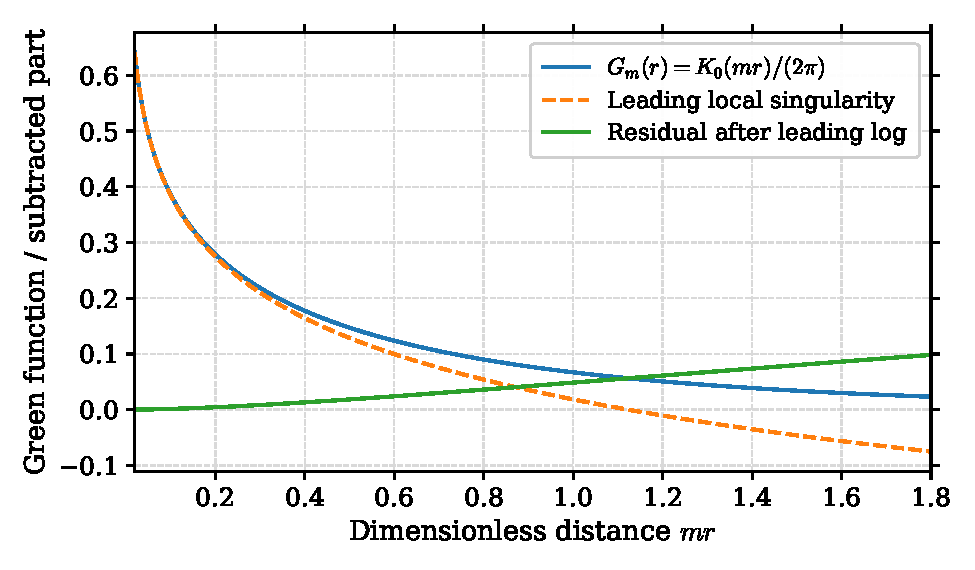
\includegraphics[width=.79\linewidth]{content/AdvancedPhysics/field-theory/figures/geometry-highspin/generated/hadamard_bessel_remainder.pdf}
\caption{二维欧氏有质量标量的 Green 核 $G_m(r)=K_0(mr)/(2\pi)$、领先对数奇性 $-[\log(mr/2)+\gamma_E]/(2\pi)$ 及两者之差。剩余项为 $O(r^2\log r)$；只减领先奇性尚不能保证全部阶数光滑。}\label{fig:ghs-hadamard-bessel-remainder}
\end{figure}

\cref{fig:ghs-hadamard-bessel-remainder} 是一个刻意简单的局部模型，不能把二维欧氏系数直接代入四维 Lorentz Hadamard 形式。图中残差趋零，但其二阶导数仍可能含对数奇性。


一般曲率背景不再共享同一个 Poincaré 群，因此不能用“让同一群作用在每个时空上”定义所有场的协变性。更普适的办法是把一个全局双曲时空及其定向、时间定向、度规视为一个对象，将保持这些结构并使因果关系相容的嵌入看作态射。给每个时空 $\mathcal M$ 配置一个局域观测量 $*$-代数 $\mathfrak A(\mathcal M)$，给每个嵌入 $\psi:\mathcal M\hookrightarrow\mathcal N$ 配置单射 $\alpha_\psi:\mathfrak A(\mathcal M)\to\mathfrak A(\mathcal N)$，并要求
\begin{equation}\label{eq:ghs-r6-locally-covariant-functor}
\alpha_{\operatorname{id}}=\operatorname{id},\qquad
\alpha_{\psi_2\circ\psi_1}=\alpha_{\psi_2}\circ\alpha_{\psi_1}.
\end{equation}
这就是局域协变量子场论的一种范畴论表述。\cref{eq:ghs-r6-locally-covariant-functor} 本身只是函子结构；还必须另外提出微因果性、时间片公理和具体动力学条件，才成为充分的物理理论。参见 \cite{ghs-r6-bfv,ghs-r6-fewster-verch}。


在经典层面，作用量对度规的变分定义能动张量。对自由标量场，它包含导数、质量以及 $\xi$ 引入的改进项；曲率背景下，试图用 $\nabla_a\phi\nabla_b\phi$ 的点乘直接定义其量子期望也会碰到重合点奇性。因此必须先做与 \cref{eq:ghs-r6-point-split-wick} 相容的点分离减法，再对两个变量施加双微分算子。

要求局域协变性、适当缩放律与守恒律后，有限重整化歧义受到严格限制，但一般并不消失。四维理论中，允许的局域曲率张量（在相应质量维数约束下）提供了可能的有限变更。对经典共形耦合的无质量标量，即使经典迹为零，量子迹也可能含曲率不变量构成的异常；因此不能未经分析就把守恒高自旋流在平直背景的性质原封不动搬到任意曲率空间。

综上，一般空间的局域量子场论要求把三种结构分开：几何决定微分算子的主符号与局部奇性，初值问题决定因果传播和对易关系，量子态决定二点函数的光滑部分与实际观测值。只有在三者都明确之后，讨论曲率背景中高自旋复合算符的守恒、混合和反常维数才是一个有定义的问题。

\section{局域短距离结构与尺度异常}

传播算子与正则场代数确定了基本的因果结构，但它们尚未规定复合场在同一点附近应怎样定义。这个困难必须从二点函数的短距离行为入手。


欧氏径向时间是尺度参数，不是实验室的时间。要在一般物理时空中建立量子场，必须先明确因果结构。洛伦兹流形上的基本算子是双曲型，而不是欧氏椭圆型；它的传播子取决于过去或未来的边界条件。两种几何可以通过特定解析延拓联系，但不能把一个任意欧氏流形直接称为量子时空。


一般流形上没有全球尺度对称性，却仍可能存在局域算符乘积展开。它的普适性来自局部微分几何与短距离奇性，而不是全局共形块。这个区别决定了研究重整化场论时哪些结构应该放在最前面：首先要定义局域场的分布核和复合场，再讨论短距离渐近中的算符系数。


量子场 $\widehat\phi(x)$ 是算符值分布，首先对试验函数作用得到 $\widehat\phi(f)$。两点函数 $W(x,y)$ 也是双变量分布；其对角限制 $x=y$ 往往不存在。因此所谓 $\widehat\phi(x)^2$ 不能简单以普通乘法定义。短距离奇性并非技术缺陷，而是量子场局域化的自然结果。

\subsection{基本核、热核与局域算符乘积}

在平直 $d>2$ 欧氏空间，归一化质量为零标量的 Green 核为
\begin{equation}\label{eq:ghs-flat-euclidean-fundamental-solution}
 G_d(x,y)=\frac{\Gamma(d/2-1)}{4\pi^{d/2}}
 |x-y|^{2-d}.
\end{equation}
它满足 $-\Delta_xG_d(x,y)=\delta^{(d)}(x-y)$ 的分布恒等式。常数由小球通量而非猜测确定。


传播子的整体归一化由源点附近的通量条件固定。
令 $G(r)=Cr^{2-d}$。在 $r>0$ 上，径向拉普拉斯给出
$\Delta G=G''+(d-1)G'/r=0$。
对半径 $\varepsilon$ 的球使用 Gauss 定理，
\[
 -\int_{B_\varepsilon}\Delta G\,\dd^dx
 =-\int_{S_\varepsilon}\partial_rG\,\dd\Sigma
 =C(d-2)\Omega_{d-1}.
\]
要等于单位点源，须取 $C=1/[(d-2)\Omega_{d-1}]$。代入 $\Omega_{d-1}=2\pi^{d/2}/\Gamma(d/2)$ 与 $\Gamma$ 递推 $\Gamma(d/2)=(d/2-1)\Gamma(d/2-1)$，得到 \cref{eq:ghs-flat-euclidean-fundamental-solution}。这个通量计算同时给出了 $\delta$ 函数归一化的几何来源。


对于无边界紧致黎曼流形上的 Laplace 型算子 $A=-\Delta_g+V$，令 $K(s;x,y)$ 是 $\ee^{-sA}$ 的核。短时、近对角的几何展开形式为
\begin{equation}\label{eq:ghs-heat-kernel-parametrix}
 K(s;x,y)\sim\frac{\ee^{-\sigma(x,y)/(2s)}}{(4\pi s)^{d/2}}
 \Delta_{\rm VV}(x,y)^{1/2}\sum_{k=0}^\infty s^ka_k(x,y).
\end{equation}
$\sigma(x,y)$ 是测地距离平方的一半，$\Delta_{\rm VV}$ 为 Van Vleck 行列式，取 $\Delta_{\rm VV}(x,x)=1$。这个局域展开要求 $x,y$ 位于凸正规邻域；跨过割迹以后不能用单一测地距离函数全局表示 Green 核。

\begin{proposition}[第一项局域热核系数]
\label{prop:ghs-heat-kernel-first}
对标量算子 $A=-\Delta_g+V$，对角系数满足
\begin{equation}\label{eq:ghs-first-heat-coefficient}
 a_0(x,x)=1,\qquad a_1(x,x)=\frac{\mathcal R(x)}6-V(x).
\end{equation}
\end{proposition}
\begin{proof}
将 \cref{eq:ghs-heat-kernel-parametrix} 代入 $(\partial_s+A_x)K=0$，按 $s$ 的幂次比较。最高负次幂给出 Hamilton--Jacobi 方程 $|\nabla_x\sigma|^2=2\sigma$；下一阶的输运方程固定 $a_0(x,y)=1$（Van Vleck 因子已提取在外）。常数阶要求
$\bigl[a_1(x,x)\bigr]=[\Delta_x\Delta_{\rm VV}^{1/2}]-V(x)$。在正规坐标中，$\Delta_{\rm VV}^{1/2}(x,y)=1+\frac1{12}\operatorname{Ric}_{ij}(y)\zeta^i\zeta^j+O(|\zeta|^3)$，取两次平直领先导数得到 $\mathcal R/6$，于是得结果。此证明在局部渐近级数意义成立，不声称级数对固定 $s$ 收敛。
\end{proof}

\begin{proposition}[由正谱热核恢复逆算子]
\begin{equation}\label{eq:ghs-heat-green-laplace}
 A^{-1}=\int_0^\infty\ee^{-sA}\dd s,\qquad A\ge a_0 I>0.
\end{equation}
\end{proposition}
\begin{proof}
在谱值 $\lambda\ge a_0$ 上，$\int_0^\infty\ee^{-s\lambda}\dd s=\lambda^{-1}$。用 $\|\ee^{-sA}\|\le\ee^{-a_0s}$ 控制积分，再按谱定理恢复算子；截断尾部的范数不超过 $\ee^{-a_0S}/a_0$。
\end{proof}
Green 核因此可以通过热核积分恢复。$s\to0$ 的局域行为决定紫外奇性，$s\to\infty$ 的谱下界则决定红外收敛。因此重整化的紫外问题和真空的红外问题在谱语言中有明确不同的来源。


在洛伦兹时空，物理上合理的自由场态通常要求两点函数具有 Hadamard 短距离形式。四维情形在凸正规邻域内可写为
\begin{equation}\label{eq:ghs-hadamard-four-dimensional}
 W(x,y)=\frac1{8\pi^2}\left[
 \frac{U(x,y)}{\chi_+(x,y)}+V(x,y)\log\frac{\chi_+(x,y)}{\ell^2}
 +H(x,y)\right],
\end{equation}
这里 $\chi_+=(-\sigma_L)_+$ 表示与前述正频核相容的因果边界值，$U,V$ 由局部几何及场算子递推确定，$H$ 随量子态改变，$\ell$ 为重整化长度。公式仅针对选定规范与四维标量；任意维的奇偶对数结构必须区别处理。

若两个 Hadamard 态的两点函数之差光滑，可以用某个参考 Hadamard 参数子 $H_{\rm sing}$ 做点分裂正规序：
\[
 :\!\phi^2\!:(x)=\lim_{y\to x}\left[\widehat\phi(x)\widehat\phi(y)-H_{\rm sing}(x,y)\,\id\right].
\]
极限必须在合适的分布/算符值分布意义下，并保留有限局域曲率反项的选择自由。因此复合算符的定义天然包含重整化处方；这部分内容不能由一个形式的 Wick 收缩在所有弯曲空间上直接解决。


在局部协变场论中，若 $x,y\to p$，可考虑渐近形式
\begin{equation}\label{eq:ghs-curved-local-ope}
 \mathcal O_A(x)\mathcal O_B(y)
 \sim\sum_C C_{AB}{}^C(x,y;p;g)\,\mathcal O_C(p),
\end{equation}
系数可以依赖度规、曲率、场参数及点之间的几何输运；当 $\mathcal O_C$ 携带张量指标时还须用平行输运比较不同点的纤维。符号 $\sim$ 指按给定短距离缩放度数逐阶逼近，既不是任意分离点的绝对收敛求和，也不预设存在一个全球标度维数离散谱。

平直共形场论的 OPE 是这套局域结构获得全球共形约束后的特殊情形：其系数由维数、旋转表示与三点函数数据大幅简化，才可以进一步重组为共形块。这也是下一部分为何可以集中研究 $SO(d+1,1)$ 的原因。


\subsection{量子行列式与二维尺度异常}

共形 Laplace 算子的经典 Weyl 协变性，并不保证量子配分函数在 Weyl 变换下不变。特别是在偶数维，重整化后的行列式可以保留局域的尺度异常。在二维，这种异常又与 Virasoro 代数的中心荷和圆柱真空能直接相关，因此不能简单地把前面 $d>2$ 的标量公式代入 $d=2$。


对有限维正矩阵 $A$，高斯积分满足 $\int\dd^Nx\,\ee^{-x^TAx/2}=(2\pi)^{N/2}(\det A)^{-1/2}$。无限维自由场形式上给出 $Z\propto(\det A)^{-1/2}$，但
$\log\det A=\sum_j\log\lambda_j$ 一般发散。若 $A$ 是紧致背景上正定椭圆算子，定义谱 $\zeta$ 函数
\begin{equation}\label{eq:ghs-zeta-operator}
 \zeta_A(s)=\sum_{\lambda_j>0}\lambda_j^{-s}
 =\frac1{\Gamma(s)}\int_0^\infty t^{s-1}\operatorname{Tr}(\ee^{-tA})\dd t,
\end{equation}
右侧初始仅在收敛半平面成立，再由热核渐近解析延拓。定义 $\log\det_\zeta A=-\zeta_A'(0)$。零本征值必须从谱和积分中单独剔除，并处理它们的积分测度。


对于二维闭曲面上的正拉普拉斯算子，热核迹为
\[
 \operatorname{Tr}(\ee^{t\Delta_g})
 \sim\frac1{4\pi t}\int_M\left(1+\frac t6\mathcal R_g+O(t^2)\right)\dd\mu_g.
\]
因此正本征值上的 $\zeta_{-\Delta}(0)$ 与局域 $t^0$ 系数有关：
\begin{equation}\label{eq:ghs-zeta-curvature-two-dimensional}
 \zeta_{+,-\Delta}(0)
 =\frac1{24\pi}\int_M\mathcal R_g\dd\mu_g-\dim\ker\Delta_g.
\end{equation}
式中下标 $+$ 表示排除零模后的正本征值谱；该等式来自短时热核常数项与零模修正。

若将度规作常数 Weyl 变换 $g\mapsto\ee^{2\sigma}g$，正特征值按 $\lambda\mapsto\ee^{-2\sigma}\lambda$ 缩放，所以
\[
 \zeta_{\widehat A}(s)=\ee^{2\sigma s}\zeta_A(s),\qquad
 \log\det_\zeta\widehat A
 =\log\det_\zeta A-2\sigma\zeta_A(0).
\]
这说明经典算子的共形协变与量子配分函数的尺度不变性是两个不同命题；一个有限的局域热核系数就足以留下异常。对局域非均匀 Weyl 变换，还须分析位置依赖的热核系数与所选反项。


\begin{proposition}[二维圆柱的异常真空能]
在二维共形理论中，中心荷记为 $c_{\rm CFT},\overline c_{\rm CFT}$。用复平面坐标 $z$ 和无量纲圆柱坐标 $w=\log z$，全纯应力张量变换为
\begin{equation}\label{eq:ghs-stress-schwarzian}
 T_{ww}(w)=\left(\frac{\dd z}{\dd w}\right)^2T_{zz}(z)
 +\frac{c_{\rm CFT}}{12}\{z,w\},\qquad
 \{z,w\}=\frac{z'''}{z'}-\frac32\left(\frac{z''}{z'}\right)^2.
\end{equation}
圆柱空间半径为 $R$ 时，绝对能量为
\begin{equation}\label{eq:ghs-virasoro-cylinder-hamiltonian}
 H_{\rm cyl}=\frac{\hbar c}{R}\left(L_0+\overline L_0-
 \frac{c_{\rm CFT}+\overline c_{\rm CFT}}{24}\right).
\end{equation}
\end{proposition}
\begin{proof}
应力张量的异常变换式以二维 Ward 恒等式和中心扩张为输入。对 $z=\ee^w$，所有阶导数相同，故 $\{z,w\}=1-3/2=-1/2$。平面真空 $\langle T_{zz}\rangle=0$ 给出 $\langle T_{ww}\rangle=-c_{\rm CFT}/24$，反全纯部分给出 $-\overline c_{\rm CFT}/24$。两部分的零模之和是无量纲时间平移生成元，乘以 $\hbar c/R$ 恢复物理哈密顿量。
\end{proof}
若左右中心荷相等，真空能为 $-\hbar c\,c_{\rm CFT}/(12R)$。尺度生成元对应圆柱相对真空的激发能隙，绝对真空能还包含异常位移。

当 $d=2$ 时，共形标量权重 $\delta=(d-2)/2=0$，圆周 Laplace 算子存在常数零模。质量为零的非紧致自由标量不仅缺少有界的 $A^{-1/2}$，其两点函数也呈对数行为而非 $r^{2-d}$。所以二维共形场论通常更自然地研究导数场、顶点算符及恰当处理零模后的扇区；这些结构不能通过把高维的 $\ell+\delta$ 频率公式机械取极限得到。

对于偶数高维，Weyl 异常由相应维数的热核系数组织；对于奇数维闭合光滑背景，通常没有同类局域体内 Weyl 异常，但边界、缺陷、整体拓扑和重整化条件仍可能引入其他异常。这些限定使前面的任意维几何论证不会掩盖量子层面的真实差异。

欧氏的热半群不能代替真实时间的演化。洛伦兹场方程首先决定经典的 Cauchy 演化及守恒辛形式；选择何种量子态则是随后才出现的另一个问题。



边界核与因果场代数已经区分了几何数据、正频选择和局域减法。下一章取满足反射正性与共形对称的平直真空扇区，在球面上构造局域算符产生的态；其中的角动量与单体约化谱将由这里的谱量子化和双玻色核计算共同确定。

\chapter{径向量子化、共形算符与高自旋态}\label{chap:ghs-radial-highspin-states}
\label{chap:ghs-radial-quantization}
\label{chap:ghs-interaction-anomalous-dimensions}



在通常的场量子化中，我们先规定一个时间坐标，再问场在等时超曲面上有哪些自由度。研究共形场论时还有一种更合适的选择：如果在原点放置一个局域算符，然后向外逐渐扩大包围它的球面，那么球面内部所包含的信息就能够用球面上的量子态表示。向外移动球面的动作，在共形理论里恰好由尺度变换生成。这样，局域算符的标度维数便可能直接成为某个哈密顿量的能量本征值。

\cref{chap:ghs-geometric-free-states}已从反射正性与谱演算建立自由量子态。现在要求平直空间的共形对称和局域真空扇区，使扩张球面的边界演化成为尺度变换。双粒子高自旋态将在这一条件下从初级条件构造，随后再由局域相关函数研究相互作用如何改变其表示。

下面采用 $d>2$ 维欧氏平直空间，指标 $\mu,\nu=1,\ldots,d$，度规 $\delta_{\mu\nu}$。空间点写成 $x^\mu=r n^\mu$，其中 $r=|x|>0$，$\vb n\in S^{d-1}$ 且 $n^\mu n_\mu=1$。球面角测度 $\dd\Omega_{d-1}$ 的总面积记为 $\Omega_{d-1}=2\pi^{d/2}/\Gamma(d/2)$。固定一个任意的参考长度 $R>0$，定义无量纲径向时间
\begin{equation}\label{eq:ghs-radial-time}
 u=\log\frac rR,\qquad r=R\ee^u.
\end{equation}
$u\to-\infty$ 是原点，而不是普通直角坐标 $x^d$ 方向的远处。尤其不能把它与真实实验室时间混为一谈。


平直度规在球坐标下为 $\dd s^2=\dd r^2+r^2\dd\Omega_{d-1}^2$。由 $\dd r=r\dd u$ 得
\begin{equation}\label{eq:ghs-weyl-cylinder}
 \dd s^2=r^2\bigl(\dd u^2+\dd\Omega_{d-1}^2\bigr),\qquad
 \dd^d x=r^d\dd u\,\dd\Omega_{d-1}.
\end{equation}
圆柱上的每一条时间截面都是同一个单位球面。这不是等距变换，因为右侧还有随 $u$ 改变的尺度因子 $r^2$；只有在共形理论允许局域度规重标度时，才能把两种描述联系起来。以半径 $R$ 为几何单位，圆柱的物理度规可取 $\dd s_{\rm cyl}^2=R^2(\dd u^2+\dd\Omega_{d-1}^2)$。

\begin{figure}[htbp]
\centering
% Local TikZ geometry; styles inherited exclusively from the shared preamble.
\begin{tikzfig}[scale=.95]
\draw[thick] (-2.5,0) circle (1.47);
\draw[thick] (-2.5,0) circle (.94);
\draw[thick] (-2.5,0) circle (.39);
\draw[lecturearrow] (-2.5,0)--(-1.07,0) node[midway,above] {$r$};
\node[lecturelabel] at (-2.5,-2.05) {$\mathbb R^d\setminus\{0\}$};
\draw[lecturearrow] (-.5,0)--(.72,0) node[midway,above] {Weyl};
\draw[thick] (1.45,-1.52) rectangle (4.05,1.52);
\draw[thick] (1.45,-.73)--(4.05,-.73) (1.45,.29)--(4.05,.29);
\draw[gray,dashed] (1.45,-.32)--(4.05,-.32);
\draw[lecturearrow] (4.43,-1.25)--(4.43,1.25) node[above] {$u$};
\node[lecturelabel] at (2.75,1.9) {$\mathbb R\times S^{d-1}$};
\node[lecturelabel] at (2.75,-2) {$u=\log(r/R)$};
\end{tikzfig}

\caption{除原点平直空间的同心球面与圆柱等时截面的对应。$u=\log(r/R)$ 使径向缩放变成柱面平移；二者通过 Weyl 因子而非等距变换联系。}\label{fig:ghs-radial-annulus-cylinder}
\end{figure}

\cref{fig:ghs-radial-annulus-cylinder} 强调了 $r\to0$ 被拉到 $u\to-\infty$。这也是为什么原点的局域算符在圆柱语言下表现为从远过去准备出的态。

对于标度维数为 $\Delta_{\mathcal O}$ 的标量初级算符，其圆柱对应量定义为 $\mathcal O_{\rm cyl}(u,\vb n)=r^{\Delta_{\mathcal O}}\mathcal O(r\vb n)$。这里的长度幂将场变成无量纲对象，便利于以下的光谱计算。带自旋的初级算符还需要按所选局部正交标架变换指标；不能对任意张量都只乘一个尺度因子。


设 $\varphi$ 是归一化后的无质量自由实标量场，其欧氏无量纲作用量为
\begin{equation}\label{eq:ghs-flat-action}
 \mathscr I[\varphi]=\frac12\int_{\RR^d}\dd^d x\,\delta^{\mu\nu}
 \partial_\mu\varphi\,\partial_\nu\varphi,
 \qquad \Delta_\varphi\equiv\delta=\frac{d-2}{2}.
\end{equation}
$\mathscr I=I_E/\hbar$，因此泛函积分权重是 $\exp(-\mathscr I)$；$[\varphi]=\mathrm{length}^{-\delta}$。我们将无量纲圆柱场定义为 $\Phi(u,\vb n)=r^\delta\varphi(r\vb n)$。可直接计算
\begin{align*}
 \partial_r\varphi&=r^{-\delta-1}(\partial_u\Phi-\delta\Phi),\\
 \nabla_{S^{d-1}}\varphi&=r^{-\delta}\nabla_{S^{d-1}}\Phi,\\
 |\nabla_{\RR^d}\varphi|^2&=r^{-2\delta-2}
 \left[(\partial_u\Phi-\delta\Phi)^2+|\nabla_{S^{d-1}}\Phi|^2\right].
\end{align*}
测度给出 $r^d$，而 $d-2\delta-2=0$，所以全部显式径向因子消失。含全导数的完整结果是
\begin{align}\label{eq:ghs-cylinder-action}
 \mathscr I&=\frac12\int\dd u\,\dd\Omega_{d-1}
 \left[(\partial_u\Phi)^2+|\nabla_{S^{d-1}}\Phi|^2+\delta^2\Phi^2\right]
 -\frac\delta2\int\dd\Omega_{d-1}\,[\Phi^2]_{u_-}^{u_+}.
\end{align}
最后一项来自 $-2\delta\Phi\partial_u\Phi=-\delta\partial_u(\Phi^2)$。它在有限时间区间并不恒为零；在固定边界数据的传播核中，它改变的是边界波泛函的归一化，而非圆柱体内的运动方程。

为什么没有质量的平直场，会在圆柱作用量中出现 $\delta^2\Phi^2$？圆柱标量曲率为 $\mathcal R_{\rm cyl}=(d-1)(d-2)/R^2$，共形耦合系数为
\begin{equation}\label{eq:ghs-conformal-coupling}
 \xi_d=\frac{d-2}{4(d-1)},\qquad
 R^2\xi_d\mathcal R_{\rm cyl}=\delta^2.
\end{equation}
故这是一项几何曲率耦合，不是平直时空中凭空增加的粒子质量。若漏掉它，整个径向谱便会算错。


在平直极限，上式可以直接化为熟悉的自由场方程。
对一般背景度规 $g_{\mu\nu}$，与自由共形标量对应的二次型包含
\begin{proof}
\begin{equation*}
\frac12\int\dd^d x\sqrt g\,\bigl[g^{\mu\nu}\partial_\mu\varphi\partial_\nu\varphi+\xi_d\mathcal R\varphi^2\bigr].
\end{equation*}
在平直空间 $\mathcal R=0$。Weyl 变换 $g_{\mu\nu}=\ee^{2\sigma}\widehat g_{\mu\nu}$ 下，若 $\varphi=\ee^{-\delta\sigma}\widehat\varphi$，曲率 $\mathcal R$ 的变换和标量梯度展开互相抵消所有体内的 $\nabla\sigma$ 项，至多相差边界项。这里 $\sigma=u+\log R$，所得体内二次型与 \cref{eq:ghs-cylinder-action} 一致。直接代入法也表明该等价不要求预先假定曲率变换公式。
\end{proof}

对欧氏圆柱作解析延拓 $u=\ii t/R$（此处 $t$ 是具有长度量纲的洛伦兹时间坐标；物理时间为 $t/c$）。相应的频率将以 $1/R$ 为单位。为了简化推导，后续先使用无量纲圆柱洛伦兹时间 $\tau=ct_{\rm phys}/R$；所有能量本征值先以无量纲数 $E$ 表示，相对于圆柱真空的物理激发能量则是
\begin{equation}\label{eq:ghs-physical-energy}
 E_{\rm phys}=\frac{\hbar c}{R}E,
 \qquad \Omega_{\rm phys}=\frac cR\,\omega.
\end{equation}
这使理论中 $\hbar,c$ 的位置明确，也避免把标度维数误当成具有焦耳量纲的能量。

四维实际标量场 $\phi_{\rm phys}$ 若选取闵可夫斯基作用量 $S=\frac12\int\dd t_{\rm phys}\dd^3\vb x[(\partial_t\phi_{\rm phys})^2/c^2-|\nabla\phi_{\rm phys}|^2]$，则其欧氏作用量满足 $I_E/\hbar=\frac12\int\dd^4x_E|\nabla(\phi_{\rm phys}/\sqrt{\hbar c})|^2$，其中 $x_E^0=ct_E$。因而四维的 $\varphi=\phi_{\rm phys}/\sqrt{\hbar c}$，且 $\Phi=r\phi_{\rm phys}/\sqrt{\hbar c}$。后文出现的 $C_d$ 是这一归一化场的二点函数系数。


\section{圆柱谱与局域算符}
\label{sec:ghs-cylinder-spectrum}


从这里起以参考半径 $R$ 为长度单位，令 $x/R$ 记作 $x$、$R^\delta\varphi$ 仍记作 $\varphi$，导数相应无量纲化；物理单位由 \cref{eq:ghs-physical-energy} 恢复。一个圆柱时间切片上的场不是有限维粒子坐标，而是定义在 $S^{d-1}$ 上的函数。把它按球谐函数分解，便可以逐个辨认自由度。更重要的是，这个分解可以在不预设态—算符对应的情况下，直接算出原点插入产生了哪个态。


令 $Y_{\ell a}(\vb n)$ 为实的正交归一球谐函数，$\ell\in\NN_0$，$a=1,\ldots,g_{d,\ell}$。约定
\begin{equation}\label{eq:ghs-sphere-spectrum}
 -\Delta_{S^{d-1}}Y_{\ell a}=\ell(\ell+d-2)Y_{\ell a},\qquad
 \int_{S^{d-1}}\dd\Omega\,Y_{\ell a}Y_{\ell'a'}=\delta_{\ell\ell'}\delta_{aa'}.
\end{equation}
这个谱由平直空间的拉普拉斯算符直接得到：
\begin{align*}
 \Delta_{\RR^d}&=\partial_r^2+\frac{d-1}{r}\partial_r+\frac1{r^2}\Delta_{S^{d-1}},\\
 0=\Delta_{\RR^d}(r^\ell Y_{\ell a})
 &=r^{\ell-2}[\ell(\ell+d-2)+\Delta_{S^{d-1}}]Y_{\ell a}.
\end{align*}
这里 $r^\ell Y_{\ell a}$ 正是 $d$ 维调和齐次多项式。其简并度等于所有 $\ell$ 次齐次多项式数目减去可被 $r^2$ 整除的部分：
\begin{equation}\label{eq:ghs-sphere-degeneracy}
 g_{d,\ell}=\binom{\ell+d-1}{\ell}-\binom{\ell+d-3}{\ell-2}
 =\frac{(2\ell+d-2)(\ell+d-3)!}{\ell!(d-2)!},
\end{equation}
第二个二项式在 $\ell<2$ 时取零。特别地，四维球面 $S^3$ 上 $g_{4,\ell}=(\ell+1)^2$。

\begin{figure}[htbp]
\centering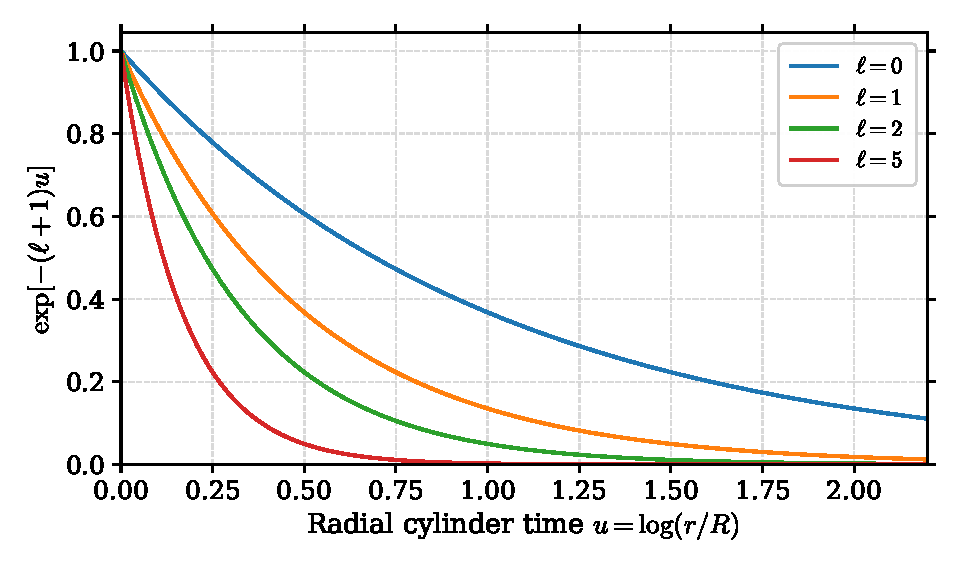
\includegraphics[width=.79\linewidth]{content/AdvancedPhysics/field-theory/figures/geometry-highspin/generated/cylinder_mode_decay.pdf}
\caption{四维共形自由标量圆柱上的模态因子 $\exp[-(\ell+1)u]$（$u\ge0$）。高角动量模态随径向时间衰减得更快，但这种指数谱依赖标准球面的共形频率，不能照搬到任意截面。}\label{fig:ghs-cylinder-mode-decay}
\end{figure}

\cref{fig:ghs-cylinder-mode-decay} 将圆柱 哈密顿量 的离散频率和径向传播因子直观联系起来；在一般截面上必须以具体算子 $A_h$ 的谱替换 $\ell+1$。


由 \cref{eq:ghs-cylinder-action} 去掉边界项并解析延拓，圆柱洛伦兹拉格朗日量是
\begin{equation*}
 L=\frac12\int\dd\Omega\,
 \left[(\partial_\tau\Phi)^2-|\nabla_{S^{d-1}}\Phi|^2-\delta^2\Phi^2\right].
\end{equation*}
写成 $\Phi(\tau,\vb n)=\sum_{\ell,a}q_{\ell a}(\tau)Y_{\ell a}(\vb n)$，各模正交性使拉格朗日量对角化：
\begin{align}\label{eq:ghs-harmonic-oscillators}
 L&=\frac12\sum_{\ell,a}[\dot q_{\ell a}^2-\omega_\ell^2q_{\ell a}^2],\\
 \omega_\ell^2&=\ell(\ell+d-2)+\delta^2=(\ell+\delta)^2.\notag
\end{align}
$\omega_\ell>0$，因为 $d>2$。取 $[q_{\ell a},p_{\ell'a'}]=\ii\delta_{\ell\ell'}\delta_{aa'}$ 与 $p_{\ell a}=\dot q_{\ell a}$，引入满足 $[a_{\ell a},a_{\ell'a'}^\dagger]=\delta_{\ell\ell'}\delta_{aa'}$ 的振子，得到
\begin{align}\label{eq:ghs-field-expansion}
 \Phi(\tau,\vb n)&=\sum_{\ell,a}\frac{Y_{\ell a}(\vb n)}{\sqrt{2\omega_\ell}}
 \left[a_{\ell a}\ee^{-\ii\omega_\ell\tau}+a_{\ell a}^\dagger\ee^{\ii\omega_\ell\tau}\right],\\
 \widehat D&=\sum_{\ell,a}(\ell+\delta)a_{\ell a}^\dagger a_{\ell a}.
 \label{eq:ghs-dimension-operator}
\end{align}
圆柱真空 $|0\rangle$ 满足 $a_{\ell a}|0\rangle=0$。$\widehat D$ 是按真空能量取零的尺度生成元；在偶数维的曲背景上，绝对真空能量还可能含有依赖重整化约定的 Casimir 项，这不改变上述激发能量差。它也等于圆柱哈密顿量乘以 $R/(\hbar c)$，故每增加一个球谐激发，能量就增加 $(\ell+\delta)\hbar c/R$。


自由场满足 $-\Delta_{\RR^d}G(x)=\delta^{(d)}(x)$，衰减的欧氏 Green 函数为
\begin{equation}\label{eq:ghs-propagator}
 G(x-y)=\langle\varphi(x)\varphi(y)\rangle
 =\frac{C_d}{|x-y|^{2\delta}},\qquad
 C_d=\frac{\Gamma(\delta)}{4\pi^{d/2}}.
\end{equation}
由于在 $r>r'$ 的球面上可以依 $\ell$ 分解传播子，同一个函数也必须有模式展开
\begin{equation}\label{eq:ghs-propagator-modes}
 G(r\vb n,r'\vb n')=\sum_{\ell,a}\frac{Y_{\ell a}(\vb n)Y_{\ell a}(\vb n')}{2(\ell+\delta)}
 \frac{(r')^\ell}{r^{\ell+2\delta}},\qquad r>r'.
\end{equation}
这一步不仅验证频率，也检验了 \cref{eq:ghs-field-expansion} 中的 $1/\sqrt{2\omega_\ell}$。


利用 Gegenbauer 多项式的生成函数，可逐项读出传播子的模态。
记 $t=r'/r<1$，$v=\vb n\cdot\vb n'$。Gegenbauer 多项式的生成函数给出
\begin{proof}
\begin{equation*}
(1-2tv+t^2)^{-\delta}=\sum_{\ell=0}^\infty C_\ell^{(\delta)}(v)t^\ell.
\end{equation*}
球谐加法定理在我们的正交归一约定下为
\begin{equation*}
\sum_aY_{\ell a}(\vb n)Y_{\ell a}(\vb n')
=\frac{\ell+\delta}{\delta\Omega_{d-1}}C_\ell^{(\delta)}(v).
\end{equation*}
由 $\delta\Omega_{d-1}C_d=1/2$，右侧除以 $2(\ell+\delta)$ 后恰好变成 $C_d C_\ell^{(\delta)}(v)$，从而逐项恢复 \cref{eq:ghs-propagator}。加法定理的系数在 $v=1$ 可由 $\sum_aY_{\ell a}(\vb n)^2=g_{d,\ell}/\Omega_{d-1}$ 和 $C_\ell^{(\delta)}(1)=(2\delta)_\ell/\ell!$ 独立核对。
\end{proof}

欧氏时间演化把 \cref{eq:ghs-field-expansion} 写为
\begin{equation}\label{eq:ghs-radial-field-expansion}
 \varphi(r\vb n)=\sum_{\ell,a}\frac{Y_{\ell a}(\vb n)}{\sqrt{2(\ell+\delta)}}
 \bigl(a_{\ell a}r^{-\ell-2\delta}+a_{\ell a}^\dagger r^\ell\bigr),
\end{equation}
这里的 $r$ 已表示以 $R$ 为单位的无量纲径向坐标；对于物理场，右端还须恢复整体因子 $R^{-\delta}$。作用在真空上只剩产生部分。于是 $\partial_{\mu_1}\cdots\partial_{\mu_k}\varphi(0)|0\rangle$ 只从 $\ell=k$ 项得到贡献，因为 $r^\ell Y_{\ell a}(\vb n)$ 是 $\ell$ 次齐次多项式，对原点求 $k$ 阶导数时只有 $\ell=k$ 的项不为零。

选定两个正交单位向量 $\vb e_1,\vb e_2$，令复零极化向量 $\vb\varepsilon=\vb e_1+\ii\vb e_2$，于是 $\vb\varepsilon\cdot\vb\varepsilon=0$。记 $D_+=\vb\varepsilon\cdot\nabla$，则
\begin{equation}\label{eq:ghs-oneparticle-dimension}
 \widehat D\,D_+^k\varphi(0)|0\rangle
 =(k+\delta)D_+^k\varphi(0)|0\rangle.
\end{equation}
因为 $D_+^k$ 自动去除所有迹，该态位于 $\ell=k$ 的对称无迹张量表示中。$\varphi(0)|0\rangle$ 是 $\ell=0$ 最低态；加入空间导数会提高球谐阶数和圆柱能量。


径向量子化通过单位球内的欧氏路径积分制备一个球面态。局域插入 $\mathcal O(0)$ 的定义是 $|\mathcal O\rangle=\mathcal O(0)|0\rangle$，但态的内积不能用同一点处的算符乘积直接给出：其共轭插入必须先经球反演移动到无穷远。标量初级算符采用
\begin{equation}\label{eq:ghs-radial-adjoint}
 \langle\mathcal O|=\lim_{r\to\infty}r^{2\Delta_{\mathcal O}}
 \langle0|\mathcal O^\dagger(r\vb n),\qquad
 \|\mathcal O\|^2=\lim_{r\to\infty}r^{2\Delta_{\mathcal O}}
 \langle\mathcal O^\dagger(r\vb n)\mathcal O(0)\rangle.
\end{equation}
对于旋转张量，反演还作用于各指标，因此不应机械套用这个标量公式；以下将改用已经正交归一的球面振子求高自旋态范数。完整态—算符对应还以反射正性和选定的局域真空扇区为前提，参见文末文献 \cite{ghs-rychkov,ghs-simmons}。

\subsection{径向伴随与后裔的局部代数}

从正的径向内积选出初级态，需要知道平移和特殊共形生成元怎样互为伴随。共形表示的完整分类可参照《群论》的共形对称与最高权表示章；这里建立后续范数计算所需的关系。

\begin{definition}[径向共形生成元]
取实旋转生成元 $M_{\mu\nu}=-M_{\nu\mu}$、尺度生成元 $D$、平移 $P_\mu$ 和特殊共形生成元 $K_\mu$。它们满足
\begin{align}\label{eq:ghs-conformal-commutators}
 [D,P_\mu]&=P_\mu,&[D,K_\mu]&=-K_\mu,\\
 [K_\mu,P_\nu]&=2\delta_{\mu\nu}D-2M_{\mu\nu},&
 [M_{\mu\nu},P_\rho]&=\delta_{\nu\rho}P_\mu-\delta_{\mu\rho}P_\nu.\notag
\end{align}
在反射正的径向态空间中，球面反演把平移映为特殊共形变换，因此
\begin{equation}\label{eq:ghs-radial-generator-adjoint}
 D^\dagger=D,\qquad P_\mu^\dagger=K_\mu,\qquad M_{\mu\nu}^\dagger=-M_{\mu\nu}.
\end{equation}
$D$ 的本征值无量纲，圆柱物理能量差为 $\hbar c\Delta/R$。$M$ 与带虚数因子的厄密角动量算符采用不同约定。
\end{definition}

\begin{proposition}[幺正界与散度范数]
归一化标量初级态 $|\mathcal O\rangle$ 满足 $K_\mu|\mathcal O\rangle=0$、$D|\mathcal O\rangle=\Delta|\mathcal O\rangle$，则
\begin{equation}\label{eq:ghs-scalar-level-one-gram}
 \langle P_\mu\mathcal O|P_\nu\mathcal O\rangle=2\Delta\delta_{\mu\nu},\qquad
 \|P^2|\mathcal O\rangle\|^2=8d\Delta\left(\Delta-\frac{d-2}{2}\right).
\end{equation}
非恒等标量满足
\begin{equation}\label{eq:ghs-scalar-unitarity-bound}
 \Delta\ge\frac{d-2}{2}.
\end{equation}
对秩 $S\ge1$ 的非零对称无迹初级态，散度后裔满足
\begin{equation}\label{eq:ghs-spin-unitarity-bound-extended}
 \sum\|P^\nu|J_{\nu\mu_2\cdots\mu_S}\rangle\|^2
 =2(\Delta-S-d+2)\sum\|J_{\mu_1\cdots\mu_S}\rangle\|^2,
 \qquad\Delta\ge S+d-2.
\end{equation}
求和按有序张量指标进行；饱和时散度后裔在零范数商空间中消失。
\end{proposition}
\begin{proof}
由 $P^\dagger=K$，一级 Gram 矩阵为 $\langle\mathcal O|[K_\mu,P_\nu]|\mathcal O\rangle$，标量旋转项为零。对迹后裔，逐次交换给出
\begin{align*}
 K_\mu P^2|\mathcal O\rangle
 &=2DP_\mu|\mathcal O\rangle-2M_{\mu\nu}P_\nu|\mathcal O\rangle
   +2P_\mu D|\mathcal O\rangle\\
 &=\bigl[2(\Delta+1)-2(d-1)+2\Delta\bigr]P_\mu|\mathcal O\rangle.
\end{align*}
再左乘 $\langle\mathcal O|K_\mu$ 求和，恢复所述二级范数。

记 $L_{\mu_2\cdots\mu_S}=P^\nu J_{\nu\mu_2\cdots\mu_S}$。旋转生成元在首指标的收缩给出 $(d-1)J_{\alpha\mu_2\cdots}$；其余 $S-1$ 个指标各贡献一个相同张量，含两次重复指标的项由无迹性消去。因此
\[
 K_\alpha|L_{\mu_2\cdots}\rangle=2(\Delta-S-d+2)|J_{\alpha\mu_2\cdots}\rangle.
\]
左乘 $\langle J_{\alpha\mu_2\cdots}|$ 求和得到散度范数恒等式，正性给出下界。
\end{proof}


局域算符在球面上制备一个径向态，圆柱尺度生成元给出它的能量。但是固定能量和旋转权重以后，带导数的双粒子态仍然不唯一；选出共形初级态需要进一步施加特殊共形生成元的条件。

\section{共形初级态}
\label{sec:ghs-conformal-primary-bilinear}


球面振子告诉我们，给两个自由粒子一共分配 $S$ 个导数，得到的所有双粒子态都具有相同的圆柱能量 $2\delta+S$。但这还没有指定唯一的算符：$S$ 个导数可以以不同的方式分给两个场。单靠旋转权重和能量本征值，并不能选出一个真正的共形初级态。缺少的条件来自特殊共形变换。


在复零极化 $\vb\varepsilon=\vb e_1+\ii\vb e_2$ 下，任意秩 $S$ 对称无迹张量 $J_{\mu_1\cdots\mu_S}(x)$ 可收缩成多项式 $J_S(x;\vb\varepsilon)=\varepsilon^{\mu_1}\cdots\varepsilon^{\mu_S}J_{\mu_1\cdots\mu_S}(x)$。由于 $\varepsilon^2=0$，所有含度规的迹项都自动消失。多项式在整个零锥上给出的信息，可唯一确定原来的对称无迹张量。

在写二粒子态的系数以前，还应区分未对称的张量积和真正的玻色 Fock 态。设 $\mathcal H_1$ 是单粒子 Hilbert 空间，$u,v\in\mathcal H_1$，则
\[
 a^\dagger(u)a^\dagger(v)|0\rangle
 \longleftrightarrow \frac{u\otimes v+v\otimes u}{\sqrt2}
\]
右侧采用标准张量积内积与相应的玻色对称化映射。由正则对易关系，
\[
 \|a^\dagger(u)a^\dagger(v)|0\rangle\|^2
 =\|u\|^2\|v\|^2+|\langle u,v\rangle|^2.
\]
这说明两个模式均归一化且正交时，范数平方为一；两个归一化模式重合时，范数平方为二。后文对 $k$ 与 $S-k$ 的求和必须保留交换项；否则即使共形初级条件的递推完全正确，双粒子态的最终范数和单体概率也会错一个系数。该关系对任何截面的单粒子 Hilbert 空间成立，不依赖角动量基底。

定义旋转生成元的约定为




\begin{equation*}
 [J_{12},\varphi(x)]=\ii(x^1\partial_2-x^2\partial_1)\varphi(x).
\end{equation*}
在原点作用一次导数便得到 $[J_{12},D_+\varphi(0)]=D_+\varphi(0)$；归纳后，$D_+^k\varphi$ 的权重是 $k$。因此
\begin{equation}\label{eq:ghs-bilinear-general}
 \mathcal O_S(x;\vb\varepsilon)=\sum_{k=0}^{S}c_k:
 (D_+^k\varphi)(D_+^{S-k}\varphi):(x)
\end{equation}
的每一项都具有最高旋转权重 $S$，且标度维数为
\begin{equation}\label{eq:ghs-spin-energy}
 \Delta_S=2\delta+S=d-2+S,\qquad
 \widehat D|\mathcal O_S\rangle=\Delta_S|\mathcal O_S\rangle.
\end{equation}
这里冒号表示按真空正规序，不允许同一算符内两场自收缩。对自由理论，它确实创造恰好两个振子量子。


\begin{proposition}[初级条件与导数分配系数]
标量共形初级场在欧氏空间的特殊共形变换取约定
\begin{equation}\label{eq:ghs-K-scalar}
 [K_\mu,\varphi(x)]=
 [2x_\mu(x\cdot\partial+\delta)-x^2\partial_\mu]\varphi(x).
\end{equation}
真正的初级算符须在原点满足 $[K_\mu,\mathcal O_S(0)]=0$。设 $K_-=K_1-\ii K_2$，$x_-=x^1-\ii x^2$。由于 $D_+x_-=2$，$D_+(x^2)=2(x^1+\ii x^2)$，而 $D_+^2(x^2)=2\varepsilon^2=0$，可直接对 \cref{eq:ghs-K-scalar} 连续求导。得到最关键的对易式
\begin{equation}\label{eq:ghs-K-derivative}
 [K_-,D_+^k\varphi(0)]=4k(\delta+k-1)D_+^{k-1}\varphi(0),\qquad k\ge1.
\end{equation}
在最高权子空间里其余 $K_\mu$ 的作用为零（对 $K_1,K_2$，可用 $K_\pm$ 的两个组合核对；垂直分量由自由标量的导数结构消失）。

将 \cref{eq:ghs-K-derivative} 代入 \cref{eq:ghs-bilinear-general}，再把乘积写成含 $j$ 与 $S-1-j$ 阶导数的项。每个独立的双场单项式的系数必须为零，因此
\begin{equation}\label{eq:ghs-primary-recurrence}
 (j+1)(\delta+j)c_{j+1}
 +(S-j)(\delta+S-j-1)c_j=0,
 \quad j=0,\ldots,S-1.
\end{equation}
这是一阶递推关系，除总体倍数以外完全固定高自旋初级态。选 $c_0=1$，令 $(a)_k=\Gamma(a+k)/\Gamma(a)$，求得
\begin{equation}\label{eq:ghs-primary-coefficients}
 c_k=(-1)^k\binom Sk\frac{(\delta+S-k)_k}{(\delta)_k}
 =(-1)^k\binom Sk\frac{(\delta)_S}{(\delta)_k(\delta)_{S-k}}.
\end{equation}
特别地 $d=4$ 时 $\delta=1$，得到
\begin{equation}\label{eq:ghs-four-d-current}
 \mathcal O_S=\sum_{k=0}^S(-1)^k\binom Sk^2
 :(D_+^k\varphi)(D_+^{S-k}\varphi):.
\end{equation}
\end{proposition}

\begin{proof}
首先把 \cref{eq:ghs-K-scalar} 分为 $2\delta x_-\varphi$、$2x_-(x\cdot\partial)\varphi$ 和 $-x^2\partial_-\varphi$。原点处的 $k$ 次 $D_+$ 导数分别是
\begin{align*}
2\delta D_+^k(x_-\varphi)|_0&=4\delta k D_+^{k-1}\varphi(0),\\
2D_+^k[x_-(x\cdot\partial)\varphi]|_0
&=4k(k-1)D_+^{k-1}\varphi(0),\\
D_+^k[x^2\partial_-\varphi]|_0&=0.
\end{align*}
第二行里，$D_+(x\cdot\partial)\varphi|_0=D_+\varphi(0)$，所以多出的因子是 $k-1$。第三行为零是因为 $D_+^2x^2=0$ 且 $D_+x^2|_0=0$。合并前三式给出 \cref{eq:ghs-K-derivative}。

对一个乘积 $A_kB_{S-k}$，$K_-$ 可降低左边导数阶数，也可降低右边阶数。固定最终阶数为 $(j,S-1-j)$，左边由 $k=j+1$ 贡献 $4(j+1)(\delta+j)c_{j+1}$，右边由 $k=j$ 贡献 $4(S-j)(\delta+S-j-1)c_j$。两项相消便是 \cref{eq:ghs-primary-recurrence}。递推 $k$ 次后
\begin{align*}
c_k&=(-1)^k\prod_{j=0}^{k-1}\frac{(S-j)(\delta+S-j-1)}{(j+1)(\delta+j)}\\
&=(-1)^k\frac{S!}{k!(S-k)!}\frac{\Gamma(\delta+S)}{\Gamma(\delta+S-k)}
\frac{\Gamma(\delta)}{\Gamma(\delta+k)}.
\end{align*}
这也明确了 $d>2$ 时分母不会消失。
\end{proof}

\cref{eq:ghs-primary-coefficients} 中的两个阶乘分母关于 $k\leftrightarrow S-k$ 对称，故 $c_{S-k}=(-1)^S c_k$。由于两场相同，正规序后的两个因子可以交换，原算符又必须满足 $\mathcal O_S=(-1)^S\mathcal O_S$。对于奇数 $S$，它因而恒等于零。对于偶数 $S$，这是一个非平凡的初级态。

例如
\begin{align}\label{eq:ghs-spin-two-current}
 \mathcal O_0&=:\!\varphi^2\!:,\\
 \mathcal O_2&=2:\!\varphi D_+^2\varphi\!:
 -\frac{2(\delta+1)}{\delta}:\!(D_+\varphi)^2\!: .\notag
\end{align}
四维时第二式为 $2:\!\varphi D_+^2\varphi\!:-4:\!(D_+\varphi)^2\!:$。如果两种标量场不同，交换两因子不再是算符恒等变换，因此奇自旋混合双线性可以存在。


把 $D_+$ 作用在第一个场的动作形式地记为 $p$，作用在第二个场的动作记为 $q$。系数的生成多项式是 $F_S(p,q)=\sum_{k=0}^S c_kp^kq^{S-k}$。Jacobi 多项式的标准二项式展开恰好给出
\begin{equation}\label{eq:ghs-jacobi-polynomial}
 F_S(p,q)=\frac{S!\Gamma(\delta)}{\Gamma(S+\delta)}
 (p+q)^S P_S^{(\delta-1,\delta-1)}
 \!\left(\frac{q-p}{p+q}\right).
\end{equation}
右侧虽然出现 $p+q$ 的分母，但乘开以后它是严格的齐次多项式；在 $p+q=0$ 处按多项式延拓定义。由 Jacobi 与 Gegenbauer 多项式的关系，它亦可改写为 Gegenbauer 形式；当 $\delta=1$ 时，$P_S^{(0,0)}$ 就是 Legendre 多项式。

这个多项式不是凭空引入的特殊函数。它的系数之所以出现，完全由 \cref{eq:ghs-primary-recurrence} 的共形初级条件决定。由此也能理解高自旋流与特殊函数理论的关系：不同粒子之间分配导数的权重，正是一组正交多项式的展开系数。


对于一个幺正的 $d>2$ 维共形场论，非零自旋 $S\ge1$ 的对称无迹初级算符满足表示论下界 $\Delta_S\ge S+d-2$；饱和时其一级散度后裔成为零范数态。因此在自由场中，\cref{eq:ghs-spin-energy} 对所有存在的偶数 $S\ge2$ 恰好饱和该下界，相应对称无迹张量 $J_{\mu_1\ldots\mu_S}$ 满足
\begin{equation}\label{eq:ghs-higher-spin-conservation}
 \partial^{\mu_1}J_{\mu_1\mu_2\cdots\mu_S}=0
 \qquad\text{在自由运动方程成立时}.
\end{equation}
这不意味着 $\partial^\mu\partial/\partial\varepsilon^\mu$ 可以不加修正地作用于仅在 $\varepsilon^2=0$ 上定义的多项式：该运算会对本来不可见的迹项求导。检验守恒时须先恢复完整的无迹张量，或使用适用于零锥的投影导数。自旋 $2$ 的直接演算将在后文出现；一般自旋的表示论依据见 \cite{ghs-rychkov,ghs-simmons}。


前文只确定了局域算符本身；为了知道它创造的双粒子态在球面上有怎样的空间结构，还要计算它与两个圆柱场之间的矩阵元。这个计算能够完全用自由场的二点函数完成，并且能把那些看似复杂的二项式平方系数化成一个简单的空间因子。


\begin{lemma}[零极化导数的传播核]
沿用 $\vb\varepsilon^2=0$ 和 $D_y=\vb\varepsilon\cdot\partial_y$，记 $Q=|x-y|^2$、$w=\vb\varepsilon\cdot(x-y)$。由 $D_yQ=-2w$、$D_yw=-\varepsilon^2=0$，连续求导时不会产生额外的收缩项。归纳得到
\begin{equation}\label{eq:ghs-null-derivative-G}
 \left.D_y^kG(x-y)\right|_{y=0}
 =2^kC_d(\delta)_k\frac{(\vb\varepsilon\cdot x)^k}{|x|^{2(\delta+k)}}.
\end{equation}
对于复极化向量，这里是复数方向导数而非厄密方向导数；共轭必须在最终计算范数时另外处理。
\end{lemma}

\begin{proof}
对 $k=0$，式子是传播子定义。若 $D_y^k Q^{-\delta}=2^k(\delta)_k w^kQ^{-\delta-k}$，那么
\begin{align*}
D_y^{k+1}Q^{-\delta}
&=2^k(\delta)_k\bigl[k w^{k-1}(D_yw)Q^{-\delta-k}
+w^k(-\delta-k)Q^{-\delta-k-1}(D_yQ)\bigr]\\
&=2^{k+1}(\delta)_{k+1}w^{k+1}Q^{-\delta-k-1}.
\end{align*}
此处真正重要的是 $D_yw=0$。如果改用实的非零平方极化向量，就会出现额外的 $\varepsilon^2$ 项，它们对应迹贡献；直接保留纯幂形式将是错误的。
\end{proof}

\begin{proposition}[高自旋双场插入的精确振幅]
在相同径向时间 $u$，定义矩阵元
\begin{equation}\label{eq:ghs-field-amplitude-definition}
 \mathcal A_S(u;\vb n_1,\vb n_2)
 =\langle0|\Phi(u,\vb n_1)\Phi(u,\vb n_2)
 \mathcal O_S(0)|0\rangle.
\end{equation}
写 $r=\ee^u$、$z_i=\vb\varepsilon\cdot\vb n_i$。由于 $\Phi=r^\delta\varphi$，每条收缩线由 \cref{eq:ghs-null-derivative-G} 带来 $2^k C_d(\delta)_k r^{-\delta-k}z_i^k$。Wick 定理仅保留连接外侧两个场与正规序内部两个场的两种配对，因而
\begin{align}\label{eq:ghs-wick-sum}
 \mathcal A_S&=2^S C_d^2\ee^{-(2\delta+S)u}
 \sum_{k=0}^S c_k(\delta)_k(\delta)_{S-k}
 \bigl[z_1^kz_2^{S-k}+z_2^kz_1^{S-k}\bigr].
\end{align}
每项包含的两个系数 $2^k$ 和 $2^{S-k}$ 恰好相乘为 $2^S$；整体径向时间指数由两个外部场各自的 Weyl 因子以及 $S$ 个导数决定。

将 \cref{eq:ghs-primary-coefficients} 代入，利用
\begin{equation*}
 c_k(\delta)_k(\delta)_{S-k}=(-1)^k\binom Sk(\delta)_S,
\end{equation*}
即可把整串有限和变成二项式展开：
\begin{align}\label{eq:ghs-amplitude-exact}
 \mathcal A_S
 &=2^SC_d^2(\delta)_S\ee^{-\Delta_Su}
 \bigl[(z_2-z_1)^S+(z_1-z_2)^S\bigr]\\
 &=2^{S+1}C_d^2(\delta)_S\ee^{-\Delta_Su}(z_1-z_2)^S,
 \qquad S\in2\NN_0.\notag
\end{align}
这是偶数自旋的完整精确场振幅；奇数自旋的同种实标量双线性本身为零，不应套用第二行。时间因子反映圆柱总能量；复差的 $S$ 次幂同时携带最高旋转权重和两角位置的相关结构。
\end{proposition}

局域算符可以任意整体缩放。为了真正指定归一化态 $|S\rangle$，必须先算 $\|\mathcal O_S(0)|0\rangle\|$。在选定的复平面中，$z^k$ 是球谐阶数为 $k$ 的最高权调和多项式。它的球面积分是
\begin{equation}\label{eq:ghs-highest-harmonic-norm}
 N_{d,k}=\int_{S^{d-1}}\dd\Omega\,|z|^{2k}
 =\Omega_{d-1}\frac{k!}{(d/2)_k}
 =\frac{2\pi^{d/2}k!}{\Gamma(k+d/2)}.
\end{equation}
因此 $y_k=z^k/\sqrt{N_{d,k}}$ 是单位归一球谐。不同的 $k$ 在球面积分下正交，$\int y_k^*y_j\dd\Omega=\delta_{kj}$。取 $b_k^\dagger$ 为这一单个球谐模式的产生算符，则由传播子与圆柱模展开逐项比较，
\begin{equation}\label{eq:ghs-local-derivative-state}
 D_+^k\varphi(0)|0\rangle=F_kb_k^\dagger|0\rangle,
 \qquad F_k=2^k C_d(\delta)_k\sqrt{2(k+\delta)N_{d,k}}.
\end{equation}


\begin{proposition}[高自旋态的精确 Fock 范数]
精确范数因而为
\begin{equation}\label{eq:ghs-operator-norm}
 \mathcal N_S\equiv\|\mathcal O_S(0)|0\rangle\|^2
 =2^{2S+1} C_d^2 S!(2\delta+S-1)_S,
 \qquad S\in2\NN_0.
\end{equation}
在 $d=4$，因为 $\delta=1$，该公式特别简单：
\begin{equation}\label{eq:ghs-norm-four-d}
 \mathcal N_S=2^{2S+1}C_4^2(2S)!,\qquad
 C_4=\frac1{4\pi^2}.
\end{equation}
于是 $|S\rangle=\mathcal N_S^{-1/2}\mathcal O_S(0)|0\rangle$ 就是单位范数的两个玻色量子态。自旋零时 $\mathcal N_0=2C_d^2$，正是 $:\!\varphi^2\!:$ 两点函数的 Wick 系数；自旋二时四维范数为 $768C_4^2$。这些低自旋值给出一般公式的直接核对。
\end{proposition}
\begin{proof}
令 $B_k=c_kF_kF_{S-k}$。在自由 Fock 空间中
\begin{equation*}
|\mathcal O_S\rangle=\sum_{k=0}^S B_k b_k^\dagger b_{S-k}^\dagger|0\rangle.
\end{equation*}
对偶数 $S$，$B_k=B_{S-k}$。计算内积时两种玻色配对各贡献同一项，即
\begin{equation*}
\langle\mathcal O_S|\mathcal O_S\rangle=2\sum_{k=0}^S|B_k|^2.
\end{equation*}
由 $C_d\Omega_{d-1}\delta=1/2$ 与 $(k+\delta)N_{d,k}=\Omega_{d-1}\delta\,k!/(\delta)_k$，可将系数整理为
\begin{equation*}
B_k=2^S C_d(\delta)_S(-1)^k\binom Sk
\sqrt{\frac{k!(S-k)!}{(\delta)_k(\delta)_{S-k}}}.
\end{equation*}
其平方和包含
\begin{align*}
\sum_{k=0}^S\frac{\binom Sk^2 k!(S-k)!}{(\delta)_k(\delta)_{S-k}}
&=S!\sum_{k=0}^S\frac{\binom Sk}{(\delta)_k(\delta)_{S-k}}\\
&=S!\frac{(2\delta+S-1)_S}{(\delta)_S^2}.
\end{align*}
最后一行是终止的 Vandermonde 恒等式，亦可将 $1/(\delta)_{S-k}$ 写成 $(-1)^k(1-\delta-S)_k/(\delta)_S$ 后应用终止 Gauss 求和。合并所有因子便得到 \cref{eq:ghs-operator-norm}。
\end{proof}



\subsection{场插入与正交角位置测量}

\cref{eq:ghs-field-amplitude-definition} 中插入的是局域场 $\Phi(\vb n)$，而非归一正交的位置湮灭算符。为了精确说明差别，在等时球面上定义
\begin{equation}\label{eq:ghs-position-annihilator}
 a(\vb n)=\sum_{\ell,a}Y_{\ell a}(\vb n)a_{\ell a},\qquad
 [a(\vb n),a^\dagger(\vb n')]=\delta_{S^{d-1}}(\vb n,\vb n').
\end{equation}
则双粒子正交角位置振幅定义为 $\psi_S(\vb n_1,\vb n_2)=\langle0|a(\vb n_1)a(\vb n_2)|S\rangle$。此定义满足 $\int\dd\Omega_1\dd\Omega_2\,|\psi_S|^2=2$；除以 $2$ 才是总积分为 $1$ 的联合角位置密度。这是一种由 Fock 模式定义的理想化正交球面位置测量，并不自动等同于任意实际探测器的正算子值测度（POVM）。

设正自伴算符 $\widehat\omega=\sqrt{-\Delta_{S^{d-1}}+\delta^2}$，其在 $Y_{\ell a}$ 上的本征值是 $\ell+\delta$。由于场的湮灭部分是 $\Phi^{(+)}(\vb n)=\sum Y_{\ell a}a_{\ell a}/\sqrt{2\omega_\ell}$，因此
\begin{equation}\label{eq:ghs-canonical-vs-field}
 \psi_S(\vb n_1,\vb n_2)
 =\bigl(\sqrt{2\widehat\omega_1}\sqrt{2\widehat\omega_2}\bigr)
 \frac{\mathcal A_S(0;\vb n_1,\vb n_2)}{\sqrt{\mathcal N_S}}.
\end{equation}
算符 $\widehat\omega_i$ 只作用于第 $i$ 个角坐标。这一非局域谱乘子不是常数，因此 $|\mathcal A_S|^2$ 与 $|\psi_S|^2/2$ 通常不同。二者都可用于讨论角结构，但只有选定测量定义后才能谈严格的概率。


\subsection{对径峰与角宽度}

得到共形初级态的系数并完成 Fock 归一化后，可以把这一态重新投影到角位置变量。位置上的相干干涉会产生对径峰，但必须区分场插入振幅与正交位置测量的概率幅。


\cref{eq:ghs-amplitude-exact} 对任意偶数 $S$ 都是精确的。然而它的空间含义在有限 $S$ 和 $S\to\infty$ 时差别很大：低自旋时两个角坐标可以遍布球面，而大自旋时，复差的高次幂会强烈抑制绝大多数构型。这里要把“对径”从直观图像变成一个有明确宽度、零模和归一化的渐近命题。


将 $\vb n_i$ 分解为旋转平面内的复投影 $z_i=n_i^1+\ii n_i^2$ 和垂直于该平面的实向量 $\vb u_i=(n_i^3,\ldots,n_i^d)$。单位长度约束给出
\begin{equation}\label{eq:ghs-angular-coordinates}
 z_i=\sqrt{1-|\vb u_i|^2}\,\ee^{\ii\varphi_i},\qquad
 |\vb u_i|^2+|z_i|^2=1.
\end{equation}
于是 $|z_i|\le1$，由三角不等式
\begin{equation}\label{eq:ghs-antipodal-bound}
 |z_1-z_2|\le|z_1|+|z_2|\le2.
\end{equation}
等号成立当且仅当 $\vb u_1=\vb u_2=0$ 且 $z_2=-z_1$。这就是说，两点必须同时位于由 $\vb e_1,\vb e_2$ 张成的大圆上，并相差恰好 $\pi$ 的方位角。除此之外，没有其他最大值构型。

请注意“对径”不是说两个粒子被一条物理弦连接；它只是球面双点矩阵元的一种角关联。尤其共同方位角 $\bar\varphi$ 可以任取，故最大值不是球面上的一个孤立点，而是一整条一维闭合流形。

\begin{figure}[htbp]
\centering
% Local TikZ geometry; styles inherited exclusively from the shared preamble.
\begin{tikzfig}[scale=1.06]
\draw[thick] (0,0) circle (1.75);
\draw[dashed,gray] (-1.75,0)--(1.75,0);
\fill[blue!65!black] (1.75,0) circle (2.1pt) node[right] {$\vb n_1$};
\fill[red!65!black] (-1.69,-.45) circle (2.1pt) node[left] {$\vb n_2$};
\draw[lecturearrow] (0,0)--(1.73,0);
\draw[lecturearrow] (0,0)--(-1.69,-.45);
\draw[gray,dashed] (0,0)--(-1.75,0);
\draw[red!65!black] (-.8,0) arc[start angle=180,end angle=195,x radius=.8,y radius=.8];
\node[lecturelabel] at (-1.1,-.35) {$\eta$};
\node[lecturelabel] at (.1,2.15) {$\Delta\varphi=\pi+\eta$};
\node[lecturelabel] at (0,-2.18) {Great-circle section};
\end{tikzfig}

\caption{选定一个大圆后的两个高自旋双点插入位置。相对角写作 $\Delta\varphi=\pi+\eta$，$\eta=0$ 时严格对径；共同旋转角未被固定。}\label{fig:ghs-antipodal-circle-geometry}
\end{figure}

\cref{fig:ghs-antipodal-circle-geometry} 与 \cref{eq:ghs-antipodal-expansion} 中的 $\eta$ 对应，它也是后续高斯峰宽展开的真实小参数之一。


在峰附近把相对角定义为 $\varphi_2-\varphi_1=\pi+\eta$，其中 $\eta$ 取靠近零的代表元。令 $a_i=|\vb u_i|^2$，由 \cref{eq:ghs-angular-coordinates} 计算
\begin{align*}
 |z_1-z_2|^2
 &=2-a_1-a_2+2\sqrt{(1-a_1)(1-a_2)}\cos\eta\\
 &=4-2(a_1+a_2)-\eta^2+O(a_1^2+a_2^2+a_1a_2+(a_1+a_2)\eta^2+\eta^4).
\end{align*}
对平方根再展开得到
\begin{equation}\label{eq:ghs-antipodal-expansion}
 \log\frac{|z_1-z_2|}{2}
 =-\frac{|\vb u_1|^2+|\vb u_2|^2}{4}-\frac{\eta^2}{8}
 +O\!\left(|\vb u_1|^4+|\vb u_2|^4+\eta^4\right).
\end{equation}
因振幅含 $S$ 次幂，其相对最大值满足
\begin{equation}\label{eq:ghs-gaussian-amplitude}
 \frac{|\mathcal A_S|}{|\mathcal A_S|_{\max}}
 =\exp\!\left[-\frac S4(|\vb u_1|^2+|\vb u_2|^2)
 -\frac S8\eta^2+O(S\rho^4)\right],
 \qquad \rho=\max(|\vb u_1|,|\vb u_2|,|\eta|).
\end{equation}
在典型峰宽 $\rho=O(S^{-1/2})$ 内，指数的舍弃项是 $O(S^{-1})$。因此高斯表达不是凭直觉猜测的拟合，而是明确控制误差的鞍点展开。对于平方模，主指数各系数加倍。

如果以归一化平方模定义球面构型的权重，在主阶高斯近似下，每一个垂直分量和相对角变量满足
\begin{equation}\label{eq:ghs-peak-variances}
 \operatorname{Var}(u_i^A)=\frac1S+O(S^{-2}),\qquad
 \operatorname{Var}(\eta)=\frac2S+O(S^{-2}),
 \quad A=3,\ldots,d.
\end{equation}
共同方位角 $\bar\varphi$ 在这一近似中不受限制。对四维场，两个粒子各有两个垂直方向，总共四个横向高斯方向，再加一个相对角方向，正好有五个被束缚的局部自由度和一个自由共同旋转方向。

\begin{figure}[htbp]
 \centering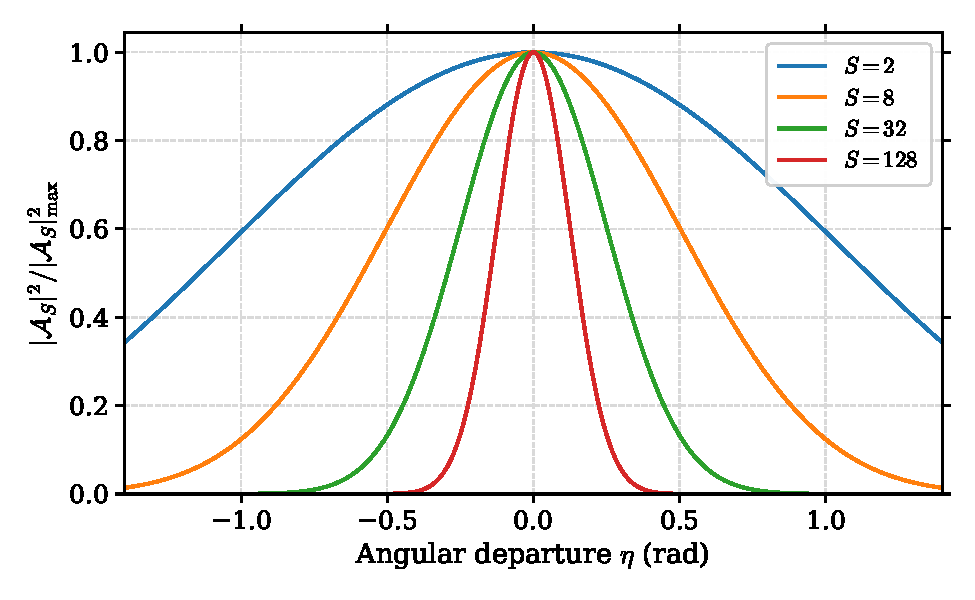
\includegraphics[width=.82\linewidth]{content/AdvancedPhysics/field-theory/figures/geometry-highspin/generated/relative_angle_profiles.pdf}
 \caption{两点都位于所选大圆时，场振幅的归一化平方模随相对角偏离量 $\eta$ 的变化。这里绘制 $[\cos(\eta/2)]^{2S}$ 的非负主峰，曲线越窄代表自旋越大；纵轴只在峰值处归一为一，不代表正交位置的概率密度。}
 \label{fig:ghs-relative-profiles}
\end{figure}


为定量比较不同 $S$ 下的场振幅形状，可以构造一个\emph{场振幅权重}而不将它冒充粒子位置概率：
\begin{equation}\label{eq:ghs-field-intensity}
 \mathscr P_S(\vb n_1,\vb n_2)=\frac{|z_1-z_2|^{2S}}{Z_{d,S}},\qquad
 Z_{d,S}=\int\dd\Omega_1\dd\Omega_2\,|z_1-z_2|^{2S}.
\end{equation}
这个正函数对双球面测度归一为一。它有明确的数学意义，但属于哪种实验测量分布，必须另行给出探测模型。

把 $(z_1-z_2)^S$ 依二项式定理展开后，不同 $z^k$ 在旋转平面上的角权重互相正交。因此
\begin{equation}\label{eq:ghs-angular-norm-general}
 Z_{d,S}=\sum_{k=0}^S\binom Sk^2N_{d,k}N_{d,S-k},
\end{equation}
其中 $N_{d,k}$ 已在 \cref{eq:ghs-highest-harmonic-norm} 给出。对于四维 $N_{4,k}=2\pi^2/(k+1)$，故
\begin{align}\label{eq:ghs-angular-norm-four}
 Z_{4,S}&=(2\pi^2)^2\sum_{k=0}^S
 \frac{\binom Sk^2}{(k+1)(S-k+1)}\\
 &=(2\pi^2)^2\frac1{(S+1)^2}\binom{2S+2}{S}.\notag
\end{align}
这给出了所有非负整数 $S$ 的精确积分；其中奇数 $S$ 的数学权重依然有定义，但不对应同种玻色场的非零初级态。


有限求和可以利用二项式恒等式化简。
利用
\begin{proof}
\begin{equation*}
\frac{\binom Sk^2}{(k+1)(S-k+1)}
=\frac{\binom{S+1}{k}\binom{S+1}{k+1}}{(S+1)^2}
\end{equation*}
后，Vandermonde 卷积给出
\begin{equation*}
\sum_{k=0}^S\binom{S+1}{k}\binom{S+1}{k+1}
=\binom{2S+2}{S}.
\end{equation*}
比较 $S=0$：$Z_{4,0}=\Omega_3^2$；比较 $S=1$：$Z_{4,1}=\Omega_3^2$。这两项也可以直接将 $|z_1-z_2|^2$ 展开后利用球面角平均求出。
\end{proof}

在峰附近，$S^{d-1}$ 的角测度可按 \cref{eq:ghs-angular-coordinates} 写成局部的 $\dd^{d-2}\vb u\,\dd\varphi$ 乘上趋于 $1$ 的 Jacobian。令 $m=d-2$，平方模的高斯积分给出
\begin{align*}
 Z_{d,S}&\sim4^S(2\pi)
 \int_{\RR^m}\dd^m\vb u_1\,\ee^{-S|\vb u_1|^2/2}
 \int_{\RR^m}\dd^m\vb u_2\,\ee^{-S|\vb u_2|^2/2}
 \int_{\RR}\dd\eta\,\ee^{-S\eta^2/4}\\
 &=4^S(2\pi)\left(\frac{2\pi}{S}\right)^m
 \sqrt{\frac{4\pi}{S}}\,[1+O(S^{-1})].
\end{align*}
这说明积分的尺度为 $Z_{d,S}\asymp 4^S S^{-(d-3/2)}$。共同旋转贡献的 $2\pi$ 是整体方位零模的体积，不能再做高斯积分；否则会错误地把总方向也解释为局域化了。

\begin{figure}[htbp]
 \centering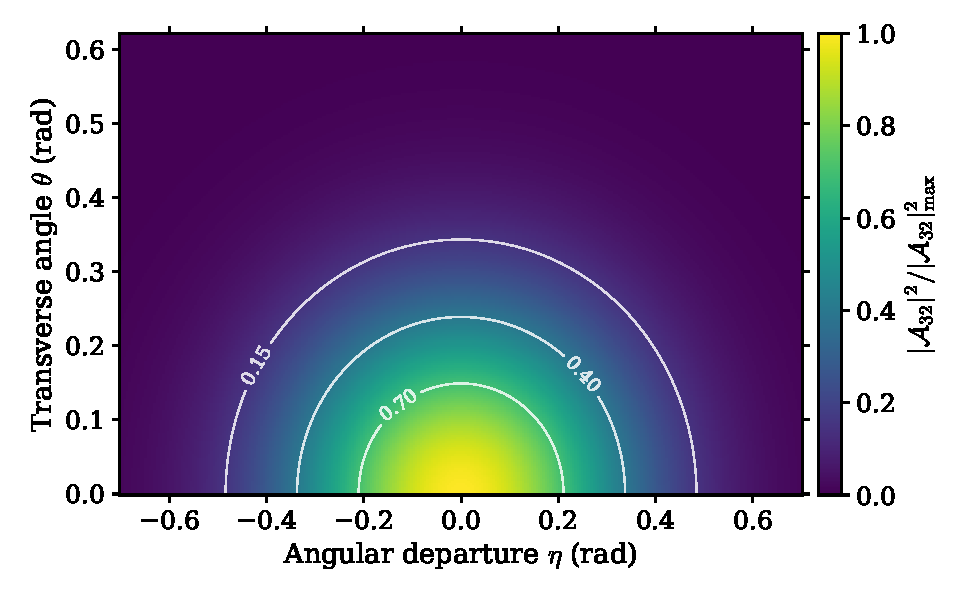
\includegraphics[width=.79\linewidth]{content/AdvancedPhysics/field-theory/figures/geometry-highspin/generated/antipodal_peak_map.pdf}
 \caption{四维球面上固定第一个点于 $z_1=1$，第二个点取 $z_2=\cos\theta\,\ee^{\ii(\pi+\eta)}$。图为 $S=32$ 的精确相对峰值 $|1-z_2|^{64}/2^{64}$，并未采用高斯近似。靠近峰顶的椭圆结构对应 \cref{eq:ghs-gaussian-amplitude} 的二次型。}
 \label{fig:ghs-antipodal-map}
\end{figure}


\cref{eq:ghs-canonical-vs-field} 的谱乘子在每个 $z_1^kz_2^{S-k}$ 分量上产生 $2\sqrt{(k+\delta)(S-k+\delta)}$。如果沿着对径峰做鞍点分析，二项式展开的主要 $k$ 位于 $S/2+O(\sqrt S)$，因此
\begin{equation}\label{eq:ghs-canonical-asymptotic-multiplier}
 2\sqrt{(k+\delta)(S-k+\delta)}
 =S+2\delta-\frac{2(k-S/2)^2}{S+2\delta}
 +O\!\left(\frac{(k-S/2)^4}{S^3}\right).
\end{equation}
这里的 $k$ 是二项式和中的形式指标，复系数带有符号；在近峰复鞍点分析里不能将它的权重未经论证地当作概率分布。上述展开只解释了为什么谱乘子在局部尺度上不改变主导的 $S^{-1/2}$ 几何宽度，而没有把 \cref{eq:ghs-gaussian-amplitude} 的全部有限自旋误差项原封不动转移给正交位置密度。需要精确探测概率时，应直接计算 \cref{eq:ghs-canonical-vs-field}，而不是对场振幅简单平方。


双粒子振幅给出了自由高自旋态的空间结构，但空间集中程度本身不足以刻画态的全部信息。对其中一个粒子取偏迹，才能进一步读出模式权重与量子关联。


现在可以从另一条路线理解高自旋双粒子态：不先从 Wick 收缩出发，而是从共形对称所容许的算符表示与守恒律出发。两条路线必须描述同一组量子数。这样的交叉检验能够揭示计算中哪些结论是由一般对称性固定的，哪些只在自由高斯场里成立。


自由标量场的典型自旋二守恒流是经过共形改进的应力张量。在平直欧氏空间，令 $\varphi$ 满足运动方程 $\partial^2\varphi=0$，可取
\begin{equation}\label{eq:ghs-improved-stress}
 T_{\mu\nu}=:\!\partial_\mu\varphi\,\partial_\nu\varphi\!:
 -\frac12\delta_{\mu\nu}:\!(\partial\varphi)^2\!:
 +\xi_d(\delta_{\mu\nu}\partial^2-\partial_\mu\partial_\nu):\!\varphi^2\!: .
\end{equation}
将它对零极化向量做两次收缩，含 $\delta_{\mu\nu}$ 的项消失：
\begin{align*}
 T_{++}&\equiv\varepsilon^\mu\varepsilon^\nu T_{\mu\nu}
 =:(D_+\varphi)^2:-\xi_dD_+^2:\!\varphi^2\!:\\
 &=(1-2\xi_d):(D_+\varphi)^2:-2\xi_d:\!\varphi D_+^2\varphi\!: .
\end{align*}
把 \cref{eq:ghs-conformal-coupling,eq:ghs-spin-two-current} 代入，发现
\begin{equation}\label{eq:ghs-stress-spin-two}
 \mathcal O_2=-\frac1{\xi_d}T_{++}.
\end{equation}
因此自旋二初级算符不是随意的二导数组合，而正是自由标量应力张量的最高权分量，仅差整体归一化。


\begin{proof}
对 \cref{eq:ghs-improved-stress} 求散度，利用乘积法则与导数交换性：
\begin{align*}
\partial^\mu T_{\mu\nu}
&=:(\partial^2\varphi)\partial_\nu\varphi:
+:\!\partial^\mu\varphi\,\partial_\mu\partial_\nu\varphi\!:
-\frac12\partial_\nu:\!(\partial\varphi)^2\!:\\
&\hspace{1.5em}+\xi_d(\partial_\nu\partial^2-\partial^2\partial_\nu):\!\varphi^2\!:
=0.
\end{align*}
其中第二、第三项逐项抵消；第一项由运动方程为零。迹则为
\begin{align*}
\delta^{\mu\nu}T_{\mu\nu}
&=\left(1-\frac d2\right):\!(\partial\varphi)^2\!:
+\xi_d(d-1)\partial^2:\!\varphi^2\!:\\
&=\bigl[-\delta+2\xi_d(d-1)\bigr]:\!(\partial\varphi)^2\!:=0,
\end{align*}
这里用了 $\partial^2:\!\varphi^2\!:=2:\!(\partial\varphi)^2\!:$。可见恢复含度规的张量项以后，无迹性和守恒性才同时正确。
\end{proof}

\subsection{总自旋、应力张量与模式划分}

一个旋转平面的共同变换 $z_i\mapsto\ee^{\ii\alpha}z_i$ 将振幅变为 $\ee^{\ii S\alpha}\mathcal A_S$。所以 $S$ 是整个双粒子态的角动量最高权，而不是说每个粒子各自具有角动量 $S$。具体的 Fock 展开包含
\begin{equation}\label{eq:ghs-two-mode-fock}
 |S\rangle=\frac1{\sqrt{\mathcal N_S}}
 \sum_{k=0}^S c_kF_kF_{S-k}
 b_k^\dagger b_{S-k}^\dagger|0\rangle.
\end{equation}
各项的单粒子球谐阶数为 $(k,S-k)$，总能量始终是 $(k+\delta)+(S-k+\delta)=S+2\delta$。高自旋态不是两个各自都处在 $\ell=S$ 的粒子，而是许多能量划分共享同一总角动量的相干叠加。

在四维自旋二情形，这一点可以直接看清：按照 $F_0=1/(2\pi)$、$F_1=1/\pi$、$F_2=4/\pi$ 的归一化，有
\begin{equation}\label{eq:ghs-spin-two-fock}
 |\mathcal O_2\rangle=\frac4{\pi^2}
 \left(b_0^\dagger b_2^\dagger-(b_1^\dagger)^2\right)|0\rangle,
 \qquad \|\mathcal O_2\|^2=\frac{48}{\pi^4}.
\end{equation}
其中两个独立的粒子数模式 $(0,2)$ 与 $(1,1)$ 之间的相对负号，恰好是特殊共形初级条件选出的相干结构。若只看能量谱或者单粒子角动量，无法推断这个负号。


几何变换 \cref{eq:ghs-weyl-cylinder} 和共形理论的态—算符对应不局限于自由场。一个一般幺正共形场论中的自旋 $S$ 初级算符仍然具有标度维数 $\Delta_{S}$，其圆柱激发能量为 $\hbar c\Delta_S/R$；对称性也依旧限制二点与三点函数的空间结构。但下列性质依赖自由场的具体动力学：

一是传播子恰好等于 $C_d|x|^{-2\delta}$ 且所有高阶函数可依 Wick 定理分解。二是局域双线性含恰好两个自由振子量子。三是对每个偶数 $S\ge2$ 都有守恒流与精确维数 $S+d-2$。一旦发生相互作用，高自旋流一般不再守恒，算符维数可能变为 $\Delta_S=d-2+S+\gamma_S$，其中 $\gamma_S$ 是相应算符的反常维数；但应力张量若存在且守恒，其自旋二维数仍由 Ward 恒等式保护。

四是 $\mathcal A_S\propto(z_1-z_2)^S$ 的简洁多项式依赖自由 Wick 收缩与此处选定的两个场插入。相互作用理论中的三点函数会受到所选算符及其归一化影响；不应仅凭总自旋便把自由场的全部空间概率结构外推到一般介质、散射粒子或其他非共形体系。


径向量子化把原本看似独立的三件事连到了一起。第一，尺度变换成为圆柱时间平移，产生谱 $\omega_\ell=\ell+\delta$。第二，特殊共形生成元从同一能量简并子空间中选出初级态，其系数满足 \cref{eq:ghs-primary-recurrence}。第三，用自由场传播子把这个初级态投影到两个场插入上，有限和恰好收束成 \cref{eq:ghs-amplitude-exact}。大自旋时，后一个结果的模集中在同一大圆上的对径构型；而其相位携带共同旋转的最高权 $S$。

这些结论构成一个可直接复算的自由场专题，而非关于真实双粒子经典轨道的主张。若要讨论测量所得的相对位置分布，必须进一步使用 \cref{eq:ghs-canonical-vs-field} 或具体探测器的测量算符。


\subsection{单体约化谱与模式熵}

双粒子态还包含另一种可以精确计算的信息：当其中一个粒子不被观测时，剩余粒子的约化态是什么。它应从归一化的对称 Fock 系数求得，而不能由空间峰的形状直接推断。


大自旋时球面场振幅沿对径构型集中，但这种空间相关并没有直接告诉我们两个量子的角动量如何分配。由于前面已经把局域算符准确写成了双振子态，现在可以不作近似地对其中一个粒子求偏迹，得到单体密度算符和谱。这个计算也提供一条独立于坐标空间鞍点法的高自旋渐近分析。


\begin{proposition}[单体约化谱]
在正交模式 $b_k^\dagger$ 下，\cref{eq:ghs-two-mode-fock} 是一个对称双粒子态。其一阶关联矩阵定义为
\begin{equation}\label{eq:ghs-one-body-density-definition}
 (\rho_1)_{jk}=\frac12\langle S|b_k^\dagger b_j|S\rangle.
\end{equation}
因总粒子数为 $2$，$\Tr\rho_1=1$。每个 Fock 分量都满足 $k+(S-k)=S$，故一阶关联矩阵在这一模式基底上对角：
\begin{equation}\label{eq:ghs-one-body-spectrum-general}
 \rho_1=\sum_{k=0}^S p_k|k\rangle\langle k|,\qquad
 p_k=\frac{2|B_k|^2}{\mathcal N_S}
 =\frac{(\delta)_S^2}{(2\delta+S-1)_S}
 \frac{\binom Sk}{(\delta)_k(\delta)_{S-k}}.
\end{equation}
这里 $|k\rangle=b_k^\dagger|0\rangle$ 是一个归一化单粒子模式。Vandermonde 恒等式给出 $\sum_kp_k=1$，又有 $p_k=p_{S-k}$，故平均单体球谐阶数严格等于 $S/2$。

该分布描述的是在对称双粒子态中随机选取一个粒子时得到的模式占据权重。由于粒子不可辨认，$\rho_1$ 的熵属于\emph{单体约化谱的熵}；不能不加区分地解释成两个可独立寻址实验室子系统之间的可操作纠缠熵。
\end{proposition}

\begin{proof}
记 $|\widetilde S\rangle=\sum_kB_kb_k^\dagger b_{S-k}^\dagger|0\rangle$。由玻色对易关系
\begin{equation*}
b_j|\widetilde S\rangle
=\sum_kB_k(\delta_{jk}b_{S-k}^\dagger+\delta_{j,S-k}b_k^\dagger)|0\rangle
=2B_jb_{S-j}^\dagger|0\rangle
\end{equation*}
（这里用了偶数 $S$ 的 $B_j=B_{S-j}$）。因此
\begin{align*}
\langle\widetilde S|b_k^\dagger b_j|\widetilde S\rangle
&=4B_k^*B_j\langle0|b_{S-k}b_{S-j}^\dagger|0\rangle\\
&=4|B_j|^2\delta_{kj}.
\end{align*}
除以 $2\mathcal N_S$ 就得到 \cref{eq:ghs-one-body-spectrum-general}。这一推导自动处理了 $k=S/2$ 两个粒子位于同一模式的情形，不需要人为增加或删除对称因子。
\end{proof}

\begin{example}[四维模式谱与超几何分布]
在四维 $\delta=1$，使用 $(1)_k=k!$，上式化为
\begin{equation}\label{eq:ghs-hypergeometric-mode-distribution}
 p_k=\frac{\binom Sk^2}{\binom{2S}{S}},\qquad
 k=0,1,\ldots,S,\qquad S\in2\NN_0.
\end{equation}
分母由 Vandermonde 恒等式 $\sum_{k=0}^S\binom Sk^2=\binom{2S}{S}$ 确定。这个分布恰好等于从 $2S$ 个物体中不放回抽取 $S$ 个、其中 $S$ 个属于某一类时所得到的超几何分布。因此可以直接计算它的前两阶矩：
\begin{equation}\label{eq:ghs-mode-variance}
 \mathbb E(k)=\frac S2,\qquad
 \operatorname{Var}(k)=\frac{S^2}{4(2S-1)},\qquad S\ge2.
\end{equation}
例如 $S=2$ 时，$p_0=p_2=1/6$、$p_1=2/3$，与 \cref{eq:ghs-spin-two-fock} 的粒子数配比完全一致。$S=0$ 是确定的单模式纯态，方差直接取零，无需使用右侧分母 $2S-1$ 的公式。
\end{example}

当 $S\to\infty$，中心极限定理或直接对阶乘使用 Stirling 展开可得局部极限定理
\begin{equation}\label{eq:ghs-mode-central-limit}
 p_k=\frac{2}{\sqrt{\pi S}}
 \exp\!\left[-\frac{4(k-S/2)^2}{S}\right]
 \left[1+O(S^{-1/2})\right],
 \quad |k-S/2|=O(\sqrt S).
\end{equation}
误差对于固定缩放变量 $(k-S/2)/\sqrt S$ 的有界集合一致；若 $k$ 接近 $0$ 或 $S$，必须使用完整的组合数而不能继续套用高斯近似。

\begin{figure}[htbp]
 \centering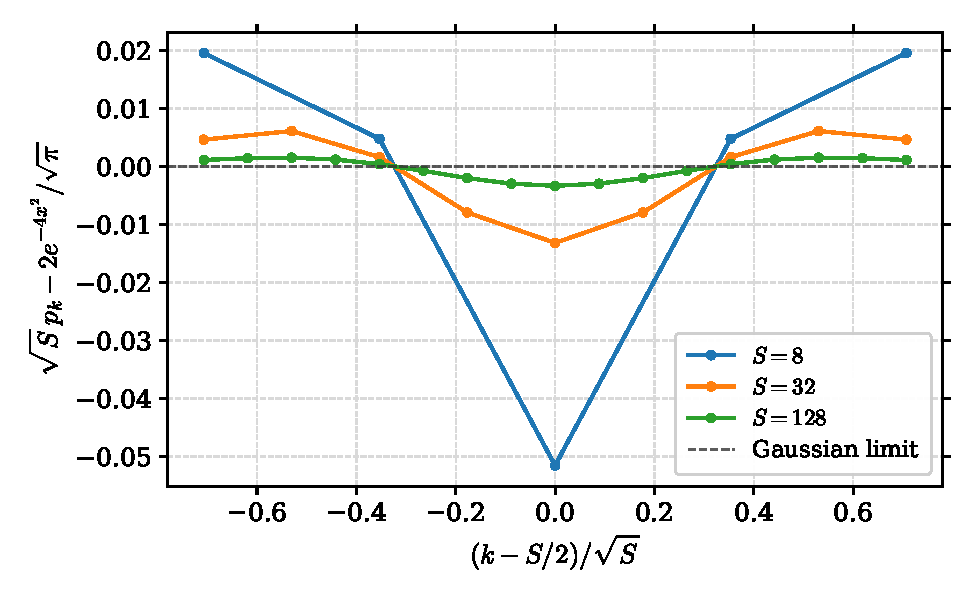
\includegraphics[width=.8\linewidth]{content/AdvancedPhysics/field-theory/figures/geometry-highspin/generated/mode_occupation.pdf}
 \caption{四维双粒子初级态的模式概率相对极限高斯的直接误差。图仅保留主峰区间 $|x|\le0.75$，避免近零尾部压缩尺度；不同自旋的离散误差清楚分离，而不是将近乎重合的概率密度反复叠加。这里 $x=(k-S/2)/\sqrt S$，$p_k$ 是正交 Fock 模式的概率。}
 \label{fig:ghs-mode-occupation}
\end{figure}


一粒子约化密度算符的 冯诺依曼熵在这一对角基中就是离散 香农熵：
\begin{equation}\label{eq:ghs-onebody-entropy}
 \mathsf S_1(S)=-\Tr(\rho_1\log\rho_1)
 =-\sum_{k=0}^S p_k\log p_k.
\end{equation}
对有限偶数 $S$，\cref{eq:ghs-hypergeometric-mode-distribution} 给出不含任何未知系数的精确有限和。大自旋时，离散高斯的方差为 $S/8+O(1)$，因此
\begin{equation}\label{eq:ghs-onebody-entropy-asymptotic}
 \mathsf S_1(S)=\frac12\log\!\left(\frac{\pi\ee S}{4}\right)+o(1),
 \qquad S\to\infty,\ S\text{ 为偶数}.
\end{equation}
熵只按 $\frac12\log S$ 缓慢增长，而不是正比于 $S$。这与模式分布集中在 $k=S/2+O(\sqrt S)$ 的事实一致：有效参与的单体模式数约为 $\sqrt S$，因而熵的主阶是其对数。


因为 $\rho_1$ 在最高权球谐模式下对角，单粒子角密度可以精确写成
\begin{equation}\label{eq:ghs-onebody-angular-density}
 \rho_1(\vb n,\vb n)=\sum_{k=0}^S p_k|y_k(\vb n)|^2
 =\sum_{k=0}^S p_k\frac{|z|^{2k}}{N_{d,k}}.
\end{equation}
它对球面测度归一为 $1$，并且不依赖 $z$ 的相位。也就是说，一个粒子的单体测量无法挑出大圆上的某一个绝对方位；对径关系蕴藏在联合测量的关联中。

四维时 $N_{4,k}=\Omega_3/(k+1)$。在大圆上 $|z|=1$，由 $\mathbb E(k)=S/2$ 得到一个精确峰值公式
\begin{equation}\label{eq:ghs-onebody-angular-maximum}
 \rho_1(\vb n,\vb n)\big|_{|z|=1}
 =\frac{1}{\Omega_3}\sum_k(k+1)p_k
 =\frac{S/2+1}{2\pi^2}.
\end{equation}
对于离开大圆的法向距离 $|\vb u|=\theta+O(\theta^3)$，$|z|^{2k}=(1-|\vb u|^2)^k$。典型 $k\simeq S/2$，所以单体密度的横向包络是 $\exp(-S|\vb u|^2/2)$，宽度同样为 $O(S^{-1/2})$。单体密度沿整条大圆均匀分布，联合振幅进一步要求第二粒子位于对径附近。两个结论相容，但不可混为一谈。


单体谱给出了高自旋态的精确概率分布。只有在有限自旋结果已经归一化后，才能求其局部极限及误差，而不是仅凭一条形似高斯的曲线猜测渐近规律。


自由场的长程结构可以从两个互补的角度观察。一种是将双场矩阵元限制在球面的大圆上，看两点偏离对径时振幅怎样衰减；另一种是把严格归一的 Fock 态对一个量子求偏迹，看单粒子角动量模式怎样分布。二者分别使用不同的数学测度，不能将其密度直接相等，但它们的有限自旋修正都可以从精确公式而不是高斯猜测出发计算。


\subsection{圆周矩与有限自旋渐近}

\begin{definition}[大圆上的归一化场权重]
在 \cref{eq:ghs-angular-coordinates} 中施加 $|z_1|=|z_2|=1$，并设 $\varphi_2-\varphi_1=\pi+\eta$，$-\pi\le\eta\le\pi$。沿这一一维几何子空间，场振幅平方的相对形状为
\begin{equation}\label{eq:ghs-circle-antipodal-profile}
 \frac{|z_1-z_2|^{2S}}{4^S}
 =\cos^{2S}(\eta/2).
\end{equation}
这一限制不等同于从完整 $S^{d-1}\times S^{d-1}$ 权重中对概率为零的子流形无条件求条件分布。现在独立给大圆赋予标准角测度 $\dd\eta$，再将限制后的权重重新归一，定义圆周角分布
\begin{equation}\label{eq:ghs-circle-normalized-density}
 q_S(\eta)=\frac{4^S}{2\pi\binom{2S}{S}}\cos^{2S}(\eta/2),
 \qquad\int_{-\pi}^{\pi}q_S(\eta)\,\dd\eta=1.
\end{equation}
对任意非负整数 $S$，它都是数学上严格的概率密度；只有偶数 $S$ 才能同时对应前面同种自由实标量的非零双线性初级态。
\end{definition}

\begin{proof}
利用 $2\cos(\eta/2)=\ee^{\ii\eta/2}+\ee^{-\ii\eta/2}$，二项式展开得到
\begin{align*}
4^S\cos^{2S}(\eta/2)
&=(\ee^{\ii\eta/2}+\ee^{-\ii\eta/2})^{2S}\\
&=\sum_{j=0}^{2S}\binom{2S}{j}\ee^{\ii(j-S)\eta}
=\sum_{m=-S}^S\binom{2S}{S+m}\ee^{\ii m\eta}.
\end{align*}
角积分只保留 $m=0$ 的常数项，因此
\begin{equation*}
\int_{-\pi}^{\pi}\cos^{2S}(\eta/2)\,\dd\eta
=\frac{2\pi}{4^S}\binom{2S}{S}.
\end{equation*}
\end{proof}

\begin{proposition}[圆周 Fourier 矩与集中尺度]
因为 $q_S$ 是一个非负三角多项式，任意整数谐波的期望均可从上一段展开直接读取：
\begin{equation}\label{eq:ghs-circle-fourier-moments}
 \langle\ee^{\ii m\eta}\rangle_{q_S}
 =\begin{cases}
 \displaystyle\frac{\binom{2S}{S+m}}{\binom{2S}{S}},& |m|\le S,\\[6pt]
 0,& |m|>S.
 \end{cases}
\end{equation}
所有正弦矩均为零。特别地，一阶余弦矩为 $S/(S+1)$，所以圆周统计中不依赖角坐标切口的集中尺度可以定义为
\begin{equation}\label{eq:ghs-circle-circular-variance}
 V_{\rm circ}(S)=1-\langle\cos\eta\rangle_{q_S}
 =\frac1{S+1}.
\end{equation}
这个公式对有限 $S$ 也精确成立。大自旋时，由 $1-\cos\eta=\eta^2/2+O(\eta^4)$，可知局部欧氏角方差为 $2/S+O(S^{-2})$，与 \cref{eq:ghs-peak-variances} 的鞍点估计一致。
\end{proposition}

固定非负整数 $m$，Fourier 矩还可以写成有限连乘积
\begin{equation}\label{eq:ghs-circle-moment-product}
 \langle\ee^{\ii m\eta}\rangle_{q_S}
 =\prod_{j=1}^{m}\frac{S-j+1}{S+j},\qquad m\le S.
\end{equation}
若 $m$ 与 $S$ 一同增大，直接将对数展开，
\begin{align*}
 \log\langle\ee^{\ii m\eta}\rangle_{q_S}
 &=\sum_{j=1}^m\left[\log\left(1-\frac{j-1}{S}\right)
 -\log\left(1+\frac{j}{S}\right)\right]\\
 &=-\frac{m^2}{S}+O\!\left(\frac{m^2}{S^2}+\frac{m^4}{S^3}\right),
\end{align*}
在 $m=O(\sqrt S)$ 的范围内，主导结果是 $\ee^{-m^2/S}$。这正是方差为 $2/S$ 的局部高斯分布之特征函数；因而对径峰的角宽度也能从 Fourier 矩而非仅从峰顶 Taylor 级数得到。


\begin{proposition}[圆周峰的第一项形状修正]
大圆上的精确分布不只是近似高斯；由于它是单个余弦幂，还能算出高斯极限之后的第一项形状修正。令 $x=\sqrt{S/2}\,\eta$，把圆周密度相应写为 $q_S^{(x)}(x)=\sqrt{2/S}\,q_S(x\sqrt{2/S})$。在固定有界 $x$ 的极限中，
\begin{equation}\label{eq:ghs-circle-edgeworth-correction}
 q_S^{(x)}(x)
 =\frac{\ee^{-x^2/2}}{\sqrt{2\pi}}
 \left[1+\frac1S\left(\frac18-\frac{x^4}{24}\right)
 +O(S^{-2})\right].
\end{equation}
修正系数的 $x^4$ 项让峰顶附近比高斯略高、肩部略低。它的高斯平均严格为零，因为标准正态的四阶矩等于 $3$；所以展开在 $1/S$ 阶仍然保持归一化。
\end{proposition}

\begin{proof}
对 $|x|=O(1)$，设 $\eta=\sqrt{2/S}\,x$。由 $\log\cos y=-y^2/2-y^4/12+O(y^6)$，
\begin{equation*}
2S\log\cos(\eta/2)
=-\frac{x^2}{2}-\frac{x^4}{24S}+O(S^{-2}).
\end{equation*}
另一方面，中心二项式的 Stirling 展开是
\begin{equation*}
\log\binom{2S}{S}
=S\log4-\frac12\log(\pi S)-\frac1{8S}+O(S^{-3}).
\end{equation*}
将两式代入 \cref{eq:ghs-circle-normalized-density}，并加入测度变化 $\dd\eta=\sqrt{2/S}\,\dd x$，整理指数得到
\begin{equation*}
\log q_S^{(x)}(x)=-\frac12\log(2\pi)-\frac{x^2}2
+\frac1S\left(\frac18-\frac{x^4}{24}\right)+O(S^{-2}).
\end{equation*}
指数化以后即为 \cref{eq:ghs-circle-edgeworth-correction}。
\end{proof}

\subsection{一般维数极限与 Rényi 熵}

已有精确模式分布
\begin{equation}\label{eq:ghs-all-d-onebody-p}
 p_k=\frac{(\delta)_S^2}{(2\delta+S-1)_S}
 \frac{\binom Sk}{(\delta)_k(\delta)_{S-k}},
 \qquad\delta=\frac{d-2}{2}>0.
\end{equation}
为了分析不同维数下的高自旋极限，忽略只依赖 $S$ 的整体因子，将其写为
\begin{equation*}
 p_k\propto\frac1{\Gamma(k+1)\Gamma(S-k+1)
 \Gamma(k+\delta)\Gamma(S-k+\delta)}.
\end{equation*}
对数关于 $k=S/2$ 对称，其一阶导数必然为零。设 $k=S/2+x\sqrt S$，固定 $x$，利用 $\log\Gamma$ 的导数渐近展开可得
\begin{equation}\label{eq:ghs-all-d-local-gaussian}
 \sqrt S\,p_{\lfloor S/2+x\sqrt S\rfloor}
 \longrightarrow\frac2{\sqrt\pi}\ee^{-4x^2},
 \qquad S\to\infty,
\end{equation}
在固定 $x$ 的紧区间上一致成立。因此任意固定 $d>2$ 的主导分布均为同一个高斯核，
\begin{equation}\label{eq:ghs-all-d-asymptotic-variance}
 \operatorname{Var}(k)=\frac S8+O(1),
 \qquad\mathbb E(k)=S/2.
\end{equation}
维数 $d$ 改变有限自旋权重和次领先修正，但不改变中央涨落的 $\sqrt S$ 尺度。这里的极限是先固定 $d$ 再令 $S\to\infty$；如果 $d$ 同时与 $S$ 增大，就不能照搬 \cref{eq:ghs-all-d-local-gaussian}。


\begin{proof}
设 $f_S(k)=\log p_k+\text{与 $k$ 无关的常数}$，则
\begin{align*}
f_S'(k)
&=-\psi(k+1)+\psi(S-k+1)
-\psi(k+\delta)+\psi(S-k+\delta),\\
f_S''(k)
&=-\psi_1(k+1)-\psi_1(S-k+1)
-\psi_1(k+\delta)-\psi_1(S-k+\delta),
\end{align*}
其中 $\psi$ 和 $\psi_1$ 分别是二伽马函数及其导数。代入 $k=S/2$，利用 $\psi_1(y)=y^{-1}+O(y^{-2})$，得到
\begin{equation*}
f_S'(S/2)=0,\qquad f_S''(S/2)=-\frac8S+O(S^{-2}).
\end{equation*}
对 $k-S/2=x\sqrt S$ 作 Taylor 展开，奇次项因左右对称而消失，故
\begin{equation*}
f_S(S/2+x\sqrt S)-f_S(S/2)
=-4x^2+O(S^{-1})
\end{equation*}
对有界 $x$ 一致成立。归一化由 $\sum_kp_k=1$ 和离散和的 Riemann 逼近给出 $p_{S/2}\sim 2/\sqrt{\pi S}$，于是得到 \cref{eq:ghs-all-d-local-gaussian}。尾部衰减可从 $p_{k+1}/p_k$ 的确切连乘结构控制，保证二阶矩不会由远尾主导。
\end{proof}

一般 $d$ 中的单体约化谱完全由 $p_k$ 给出。对 $q>0$ 且 $q\neq1$，定义阶数为 $q$ 的 Rényi 熵
\begin{equation}\label{eq:ghs-renyi-definition}
 H_q(S)=\frac1{1-q}\log\Tr\rho_1^q
 =\frac1{1-q}\log\sum_{k=0}^S p_k^q.
\end{equation}
当 $q\to1$ 时连续恢复 \cref{eq:ghs-onebody-entropy} 的 冯诺依曼熵。对任意固定 $q>0$ 和任意固定维数 $d>2$，将 \cref{eq:ghs-all-d-local-gaussian} 的离散高斯代入，并把求和转成积分：
\begin{align*}
 \sum_{k=0}^S p_k^q
 &\sim \sqrt S\left(\frac2{\sqrt{\pi S}}\right)^q
 \int_{-\infty}^{\infty}\ee^{-4qx^2}\,\dd x\\
 &=q^{-1/2}\left(\frac2{\sqrt{\pi S}}\right)^{q-1}.
\end{align*}
由此得到
\begin{equation}\label{eq:ghs-renyi-asymptotic}
 H_q(S)=\frac12\log\left(\frac{\pi S}{4}\right)
 +\frac{\log q}{2(q-1)}+o(1).
\end{equation}
特别地，$q\to1$ 给出 $H_1=\frac12\log(\pi\ee S/4)+o(1)$；$q=2$ 则控制纯度
\begin{equation}\label{eq:ghs-onebody-purity-asymptotic}
 \Tr\rho_1^2=\sum_kp_k^2
 =\sqrt{\frac2{\pi S}}\,[1+o(1)].
\end{equation}
二阶 Rényi 熵的指数 $\ee^{H_2}=1/\Tr\rho_1^2$ 可视为参与模式数的一个标准定义，其主阶正比于 $\sqrt S$，而不是 $S$。这种增长刻画单体模式占据谱的展开，但对于不可辨认玻色子，仍不应不加说明地等同于两个可独立操作实验粒子的纠缠资源。


\begin{proposition}[四维单体熵的有限自旋修正]
主导的 $\tfrac12\log S$ 只告诉我们参与模式数的数量级，而低自旋时的偏差还需要从精确组合数计算。四维中的 $p_k=\binom Sk^2/\binom{2S}{S}$ 允许进一步把熵计算到 $S^{-1}$ 阶。结果是
\begin{align}\label{eq:ghs-entropy-next-order}
 H_1(S)&=\frac12\log\left(\frac{\pi\ee S}{4}\right)
 +\frac1{4S}+O(S^{-2}),\\
 H_2(S)&=\frac12\log\left(\frac{\pi S}{2}\right)
 +\frac5{16S}+O(S^{-2}).\notag
\end{align}
因此两个熵靠近高斯极限的速率虽然同为 $S^{-1}$，但系数不同。下面把这一差别真正从 Stirling 展开算出，而不只用数值拟合猜测系数。
\end{proposition}

\begin{proof}
令 $x=(k-S/2)/\sqrt S$，并暂时固定有界的 $x$。对 $\log\Gamma$ 使用含 $1/(12n)$ 的 Stirling 展开，分别计算两个分子组合数及分母，得到
\begin{align*}
\log p_k
&=\log\frac2{\sqrt{\pi S}}-4x^2+\frac{a(x)}S
+O\left(S^{-2}(1+|x|^6)\right),\\
a(x)&=-\frac83x^4+4x^2-\frac38.
\end{align*}
主导高斯密度为 $q_4(x)=2\ee^{-4x^2}/\sqrt\pi$。其偶次矩为
\begin{equation*}
\langle x^2\rangle_{q_4}=\frac18,\qquad
\langle x^4\rangle_{q_4}=\frac3{64},\qquad
\langle a(x)\rangle_{q_4}=0.
\end{equation*}
取负平均对数，由精确方差公式 \cref{eq:ghs-mode-variance}，
\begin{align*}
H_1(S)
&=\log\frac{\sqrt{\pi S}}2+4\langle x^2\rangle_{p}
-\frac1S\langle a(x)\rangle_{p}+O(S^{-2})\\
&=\log\frac{\sqrt{\pi S}}2
+\frac{S}{2S-1}+O(S^{-2})\\
&=\frac12\log\frac{\pi\ee S}{4}
+\frac1{4S}+O(S^{-2}).
\end{align*}
这里 $\langle a\rangle_p=O(S^{-1})$，所以它乘以前面的 $1/S$ 后只影响 $S^{-2}$ 阶。

对于纯度，平方 $p_k$ 会把主导高斯改成 $q_8(x)=\sqrt{8/\pi}\ee^{-8x^2}$。新的矩为 $\langle x^2\rangle_{q_8}=1/16$、$\langle x^4\rangle_{q_8}=3/256$，于是
\begin{equation*}
\langle a(x)\rangle_{q_8}
=-\frac83\frac3{256}+4\frac1{16}-\frac38
=-\frac5{32}.
\end{equation*}
将离散求和转为局部高斯积分，得到
\begin{align*}
\Tr\rho_1^2
&=\sqrt{\frac2{\pi S}}
\left[1+\frac2S\langle a(x)\rangle_{q_8}
+O(S^{-2})\right]\\
&=\sqrt{\frac2{\pi S}}
\left[1-\frac5{16S}+O(S^{-2})\right].
\end{align*}
再取负对数便得到 \cref{eq:ghs-entropy-next-order} 的第二行。由于精确分布的中心外尾部按指数衰减，可以在控制尾部后逐项积分；离散格点的 Poisson 求和修正对这些光滑高斯核指数小于任何固定 $S^{-n}$。
\end{proof}

\begin{figure}[htbp]
 \centering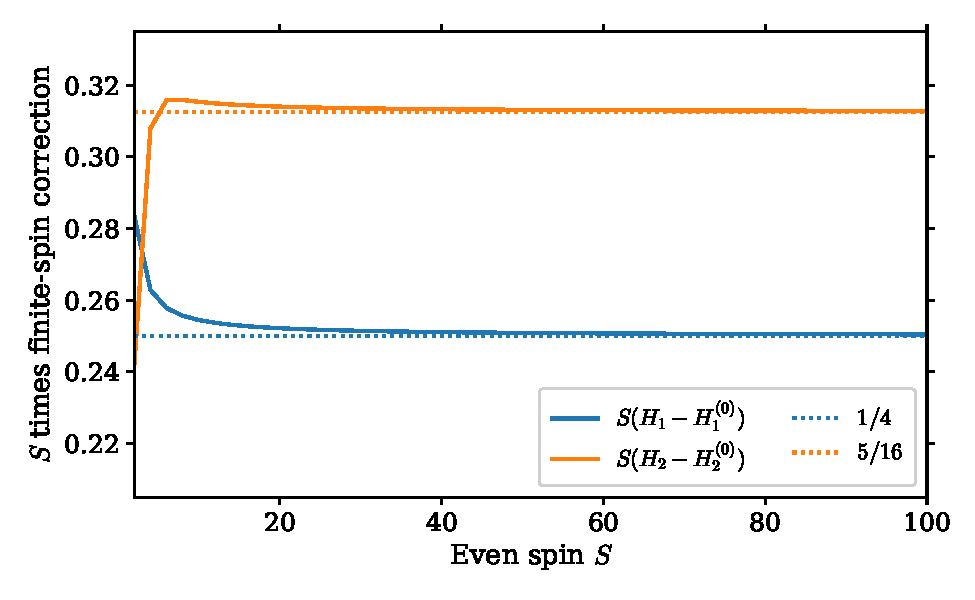
\includegraphics[width=.82\linewidth]{content/AdvancedPhysics/field-theory/figures/geometry-highspin/generated/renyi_entropy_scaling.pdf}
 \caption{四维自由标量的两类单体熵相对高斯首阶的偏差乘以自旋 $S$。精确求和结果趋近于解析修正系数 $1/4$ 和 $5/16$；相比在同一坐标上绘制几乎重叠的熵曲线，这种差分呈现能直接检验下一阶渐近展开。}
 \label{fig:ghs-renyi-entropy}
\end{figure}


对于 $d=4$、$S=2$，模式分布为 $p=(1/6,2/3,1/6)$，它与连续高斯有明显差别。由 \cref{eq:ghs-renyi-definition}，
\begin{equation}\label{eq:ghs-spin-two-renyi}
 H_1(2)=\log3-\frac13\log2,\qquad
 H_2(2)=\log2.
\end{equation}
真正的两端分量各自只有 $1/6$，中间分量却有 $2/3$，说明最初几个偶数自旋的态仍是少数离散 Fock 模式的干涉，而不是经典角变量的窄波包。所有高斯、熵和 Fourier 近似都应在明确的 $S\to\infty$ 区间使用。

\begin{figure}[htbp]
 \centering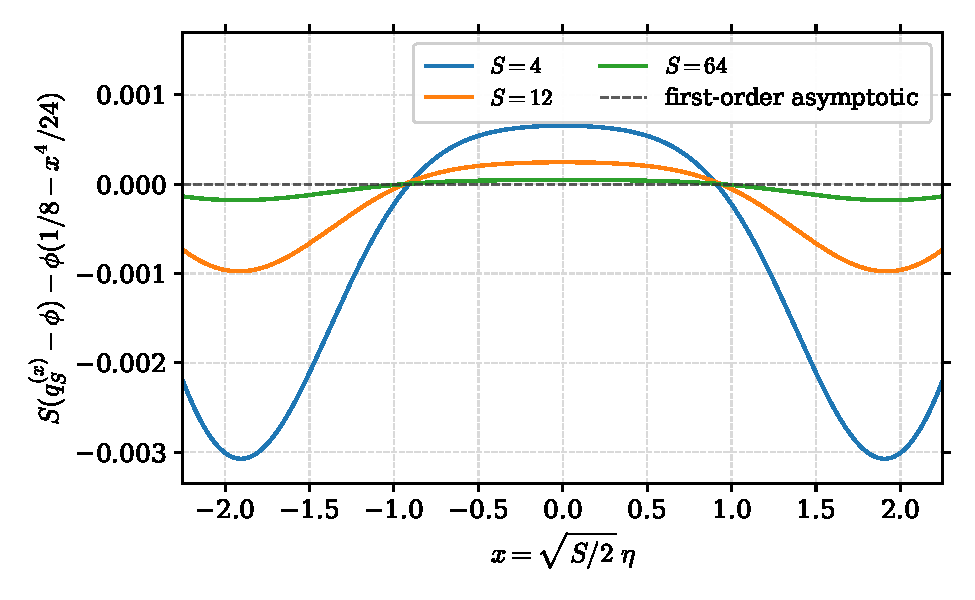
\includegraphics[width=.80\linewidth]{content/AdvancedPhysics/field-theory/figures/geometry-highspin/generated/circle_fourier_profiles.pdf}
 \caption{对大圆角密度去除高斯首项以及 $1/S$ 阶解析修正后，剩余误差乘以 $S$。它直接展示首个非高斯渐近公式在有限自旋下的精度；虚线零基线对应已保留的渐近阶，横轴限定在主峰及肩部。}
 \label{fig:ghs-circle-fourier}
\end{figure}

\section{混合标量双线性与一般自旋关联}

这一推导还表明：所谓“守恒”并不是任意把散度设成零，而是表示论中某个后裔与物理 Hilbert 空间脱耦。自由标量的双线性流满足 $\Delta_S=S+d-2$，因而恰好处在这一边界；一般相互作用使 $\Delta_S$ 增大时，原来被模掉的后裔重新取得正范数。


前述自由双粒子态的维数 $\Delta_S=d-2+S$ 饱和幺正界。要分清这种守恒性与一般初级条件，可让两种标量具有独立维数，并重新求导数递推与 Wick 范数。由此得到的双线性算符通常不守恒，却仍然是严格的共形初级算符，而且它的归一化和三点耦合可以完全求出。


\subsection{可区分标量的初级系数与范数}

考虑 $d>2$ 维单位欧氏共形场论中的两种相互正交的标量初级算符 $A$ 和 $B$，维数为 $\Delta_A,\Delta_B\ge(d-2)/2$，选二点函数的规范化为
\begin{equation}\label{eq:ghs-r4-generalized-free-two-points}
 \langle A(x)A(0)\rangle=(x^2)^{-\Delta_A},\qquad
 \langle B(x)B(0)\rangle=(x^2)^{-\Delta_B},\qquad
 \langle A(x)B(0)\rangle=0.
\end{equation}
要求它们在所讨论的扇区中满足广义自由的高点关联函数规则：所有偶数点函数是二点函数配对之和，奇数点函数为零。这个假设不要求 $A,B$ 满足局域自由波动方程，且一般不存在一个具有通常二阶动力学的局域基本作用量。它只是精确定义了一套可用来比较任意维数与任意标度维数的双粒子 Hilbert 空间。广义自由理论的完整算符乘积数据还可用共形谐分析得到，参见 \cite{ghs-karateev-harmonic}。对于真正相互作用的共形场论，后面的 Wick 范数和三点系数不能不加检查地沿用。

径向量子化中，$A(0)|0\rangle$ 和 $B(0)|0\rangle$ 是不同的一粒子初级态。令复零向量 $z^\mu$ 满足 $z^2=0$，并记 $P_z=z^\mu P_\mu$。其 $k$ 级最高权后裔为 $P_z^k|A\rangle$，维数 $\Delta_A+k$。由于 $P_z$ 与自身对易，所有高阶导数可用一个对称无迹极化多项式编码。两个粒子的总维数为 $\Delta_A+\Delta_B+S$ 时，既有一座总导数后裔塔，也有一个去除了总导数的真正初级态。区别它们的条件是特殊共形生成元的湮灭关系。


取
\begin{equation}\label{eq:ghs-r4-mixed-bilinear-def}
 [AB]_S(x,z)=\sum_{k=0}^S c_k:
 (z\cdot\partial)^k A(x)\,(z\cdot\partial)^{S-k}B(x):,
 \qquad S\in\NN_0.
\end{equation}
这两个场是可区分的，故不存在 $k\leftrightarrow S-k$ 的交换化简。由标量初级的特殊共形变换式，可沿用 \cref{eq:ghs-K-derivative} 的计算，只需把自由场维数 $\delta$ 换成各自的 $\Delta_A$ 或 $\Delta_B$。在选定的复零方向上，降低一个导数的系数分别为 $4k(\Delta_A+k-1)$ 和 $4k(\Delta_B+k-1)$。因此两种降低途径必须相消：
\begin{equation}\label{eq:ghs-r4-mixed-recurrence}
 (j+1)(\Delta_A+j)c_{j+1}
 +(S-j)(\Delta_B+S-j-1)c_j=0,
 \quad j=0,\ldots,S-1.
\end{equation}
取 $c_0=1$，逐次消去 $c_1,\ldots,c_S$，得到
\begin{equation}\label{eq:ghs-r4-mixed-primary-coefficients}
 c_k=(-1)^k\binom Sk\frac{(\Delta_B)_S}
 {(\Delta_A)_k(\Delta_B)_{S-k}},
 \qquad(a)_n\equiv\frac{\Gamma(a+n)}{\Gamma(a)}.
\end{equation}
这条结论对任意整数 $d>2$、任意满足标量幺正性界的维数和任意非负整数自旋成立。特别地，初级维数为
\begin{equation}\label{eq:ghs-r4-mixed-dimension}
 \Delta_{[AB]_S}=\Delta_A+\Delta_B+S,
 \qquad\tau_{[AB]_S}=\Delta_A+\Delta_B.
\end{equation}
它不再一般等于 $S+d-2$。两个标量的维数越高，双线性初级态离守恒流的短表示界就越远。


把初级条件写成相邻系数的递推关系后，可以连乘求解。
先把 \cref{eq:ghs-r4-mixed-recurrence} 逐项改写为
\begin{align*}
 \frac{c_{j+1}}{c_j}
 &=-\frac{S-j}{j+1}\frac{\Delta_B+S-j-1}{\Delta_A+j},\\
 c_k&=(-1)^k\prod_{j=0}^{k-1}\frac{S-j}{j+1}
 \prod_{j=0}^{k-1}\frac{\Delta_B+S-j-1}{\Delta_A+j}\\
 &=(-1)^k\frac{S!}{k!(S-k)!}
 \frac{\Gamma(\Delta_B+S)}{\Gamma(\Delta_B+S-k)}
 \frac{\Gamma(\Delta_A)}{\Gamma(\Delta_A+k)}.
\end{align*}
现在乘除以 $\Gamma(\Delta_B)$，便恢复 \cref{eq:ghs-r4-mixed-primary-coefficients}。$S=1$ 时得到 $[AB]_1= A(z\cdot\partial)B-(\Delta_B/\Delta_A)(z\cdot\partial A)B$。代入降低算符后，两个项恰好分别贡献 $4\Delta_B AB$ 与 $-4\Delta_B AB$，提供最直接的低自旋检验。


\begin{example}[混合标量的自旋一与自旋二初级算符]
直接计算两个低阶自旋，可以看出特殊共形条件怎样限制导数分配。记 $D_z=z\cdot\partial$，令 $a=\Delta_A$、$b=\Delta_B$；它们在本小节只是两个正数。自旋一的候选算符必须由 $A(D_zB)$ 与 $(D_zA)B$ 线性组合而成。设
\[
 \mathcal J_1=A(D_zB)+c_1(D_zA)B.
\]
在原点作用降低生成元 $K_{\bar z}$，前一项给 $4bAB$，后一项给 $4ac_1AB$。若要成为初级而非另一算符的总导数，必须有 $b+ac_1=0$，所以 $c_1=-b/a$。这里发生的是两种导数分配产生的\emph{下降通道相消}，而不是随意挑选一个反对称组合。

自旋二具有三个导数分配：
\[
 \mathcal J_2=A(D_z^2B)+c_1(D_zA)(D_zB)+c_2(D_z^2A)B.
\]
它在 $K_{\bar z}$ 下产生两种线性独立的一阶后裔，分别为 $A(D_zB)$ 与 $(D_zA)B$。要让两者都为零，递推条件给出
\begin{align*}
 2(b+1)+ac_1&=0,\\
 bc_1+2(a+1)c_2&=0.
\end{align*}
因此
\begin{equation}\label{eq:ghs-bridge-spin-two-coeffs}
 c_0=1,\qquad c_1=-\frac{2(b+1)}{a},\qquad
 c_2=\frac{b(b+1)}{a(a+1)}.
\end{equation}
若两种场维数相同，$a=b$，便得到 $(c_0,c_1,c_2)=(1,-2(a+1)/a,1)$；四维自由标量的 $a=b=1$ 给出 $(1,-4,1)$。若 $A=B$ 为同一玻色场，偶自旋组合非零，自旋一组合则因交换对称性消失。

注意这里的 $\mathcal J_2$ 是一个由两个标量复合而成的\emph{自旋二算符}，不自动等于前面从作用量变分得到的应力张量。二者是否成正比还取决于基础场是否自由、维数是否饱和标量幺正性界，以及复合算符的改进项和正规序约定。区分“表示中有自旋二”与“确有守恒应力张量”，正是学习一般高自旋算符时的重要一步。


\end{example}

从一个初级标量态出发，径向伴随为 $P_z^\dagger=K_{\bar z}$，其中 $\bar z$ 表示使 $z\cdot\bar z=2$ 的共轭极化。对 $k$ 次导数递归使用共形交换子，得到
\begin{equation}\label{eq:ghs-r4-oneparticle-highest-norm}
 \|P_z^k|A\rangle\|^2
 =4^k k!(\Delta_A)_k\,\|A\|^2.
\end{equation}
相应的 $B$ 态只需将 $\Delta_A$ 换为 $\Delta_B$。不同 $k$ 所分配的一粒子尺度能量不同，广义自由双粒子内积又按 Wick 配对分解，因此 \cref{eq:ghs-r4-mixed-bilinear-def} 中不同 $k$ 的分量正交。用 \cref{eq:ghs-r4-mixed-primary-coefficients} 计算总范数，最初得到有限和
\begin{align}\label{eq:ghs-r4-mixed-norm-sum}
 \mathcal N_{AB,S}&\equiv\langle[AB]_S|[AB]_S\rangle
 =4^S\sum_{k=0}^S c_k^2
 k!(\Delta_A)_k(S-k)!(\Delta_B)_{S-k}\\
 &=4^S(S!)^2(\Delta_B)_S^2
 \sum_{k=0}^S\frac{1}{k!(S-k)!(\Delta_A)_k(\Delta_B)_{S-k}}.
 \notag
\end{align}
这一有限和可以利用终止超几何恒等式严格求出，而不必每个自旋分别数值求和：
\begin{equation}\label{eq:ghs-r4-mixed-norm-closed}
 \mathcal N_{AB,S}=4^S S!\frac{(\Delta_B)_S}{(\Delta_A)_S}
 (\Delta_A+\Delta_B+S-1)_S.
\end{equation}
$\Delta_A=\Delta_B$ 时，右侧化为 $4^S S!(2\Delta_A+S-1)_S$。如果 $A=B$ 是同一种归一化实广义自由标量，额外的一种跨点 Wick 配对会把偶数 $S$ 的范数再乘以 $2$，而奇数 $S$ 的算符恒等为零。这正是相同玻色粒子与可区分粒子的差别。


记 \cref{eq:ghs-r4-mixed-norm-sum} 的求和为 $T_S$。由
\begin{align*}
 \frac{1}{(S-k)!}&=\frac{(-1)^k(-S)_k}{S!},\\
 \frac{1}{(\Delta_B)_{S-k}}
 &=\frac{(-1)^k(1-\Delta_B-S)_k}{(\Delta_B)_S},
\end{align*}
可把两个负号相消，并改写为终止的超几何级数：
\begin{align*}
 T_S&=\frac1{S!(\Delta_B)_S}
 \sum_{k=0}^S\frac{(-S)_k(1-\Delta_B-S)_k}{(\Delta_A)_k k!}\\
 &=\frac1{S!(\Delta_B)_S}
 {}_2F_1(-S,1-\Delta_B-S;\Delta_A;1).
\end{align*}
对非负整数 $S$，Chu--Vandermonde 恒等式给出
\begin{equation*}
 {}_2F_1(-S,b;c;1)=\frac{(c-b)_S}{(c)_S},
\end{equation*}
所以
\begin{equation*}
 T_S=\frac{(\Delta_A+\Delta_B+S-1)_S}
 {S!(\Delta_A)_S(\Delta_B)_S}.
\end{equation*}
代回原来的范数并约去公共因子，即得 \cref{eq:ghs-r4-mixed-norm-closed}。这一证明同时说明归一化系数没有未声明的 $2\pi$、球面积或球谐简并度。


为了把径向范数转成可以输入共形块展开的数据，需要再计算一次局域三点函数。对于 $z^2=0$，任意 $\Delta>0$ 有
\begin{equation}\label{eq:ghs-r4-null-derivative-power}
 (z\cdot\partial_x)^k(x^2)^{-\Delta}
 =(-2)^k(\Delta)_k\frac{(z\cdot x)^k}{(x^2)^{\Delta+k}}.
\end{equation}
证明用归纳法即可：下一次求导作用于 $z\cdot x$ 时含 $z^2$ 而消失，只有幂函数分母继续贡献。把两种标量与 $[AB]_S(0,z)$ 做跨点 Wick 收缩，并代入 \cref{eq:ghs-r4-mixed-primary-coefficients}，所有 Pochhammer 因子随即约去，只剩一个二项式：
\begin{align}\label{eq:ghs-r4-general-mixed-threepoint}
 &\langle A(x_1)B(x_2)[AB]_S(0,z)\rangle\\
 &=(-2)^S(\Delta_B)_S
 \frac{\left(\frac{z\cdot x_2}{x_2^2}-\frac{z\cdot x_1}{x_1^2}\right)^S}
 {(x_1^2)^{\Delta_A}(x_2^2)^{\Delta_B}}.
 \notag
\end{align}
把 $[AB]_S(0,z)|0\rangle$ 按其径向最高权范数 $\mathcal N_{AB,S}$ 归一，我们定义该归一最高权态在上述三点函数中的振幅系数为 $\widehat\lambda_{AB,S}=(-2)^S(\Delta_B)_S/\sqrt{\mathcal N_{AB,S}}$。直接平方得到
\begin{equation}\label{eq:ghs-r4-mft-leading-ope}
 \widehat\lambda_{AB,S}^{\,2}=\frac{(\Delta_A)_S(\Delta_B)_S}
 {S!(\Delta_A+\Delta_B+S-1)_S}.
\end{equation}
这里的帽号专门表示最高权径向范数规范，不是预先选定的 Dolan--Osborn 共形块系数。若改为张量二点函数 $\langle J(x,z_1)J(0,z_2)\rangle=(z_1\cdot I(x)\cdot z_2)^S/(x^2)^\Delta$ 的规范，因 $z\cdot\bar z=2$，相应的三点系数平方应额外乘以 $2^S$。不同文献对共形块的最高次 Gegenbauer 系数还有不同标准化，故不能把帽号公式未经换算直接代入任意文献的块展开。对于一个相同的实广义自由标量，交换对称性给出
\begin{equation}\label{eq:ghs-r4-mft-identical-ope}
 \widehat\lambda_{AA,S}^{\,2}=[1+(-1)^S]\,
 \frac{(\Delta_A)_S^2}{S!(2\Delta_A+S-1)_S}.
\end{equation}
检验 $S=0$ 时 $\widehat\lambda_{AB,0}^{\,2}=1$，$\widehat\lambda_{AA,0}^{\,2}=2$，与 $AB$ 和 $:A^2:$ 的两点函数正好一致。$S=2$、$\Delta_A=(d-2)/2$ 时回到自由应力张量所属的双线性短表示；任意 $\Delta_A$ 的广义自由模型则通常仍是长表示。两者不能因为具有同一个自旋而混为一谈。


同一个范数还决定双粒子态把 $S$ 个导数分配给两个粒子的概率。令 $p_k^{AB}$ 为正交两粒子最高权模态的范数权重占比。把 \cref{eq:ghs-r4-mixed-norm-sum} 中的第 $k$ 项除以总和，得到一个对所有 $S$ 都严格归一的离散分布：
\begin{equation}\label{eq:ghs-r4-mixed-mode-probability}
 p_k^{AB}=\frac{S!(\Delta_A)_S(\Delta_B)_S}
 {(\Delta_A+\Delta_B+S-1)_S}
 \frac{1}{k!(S-k)!(\Delta_A)_k(\Delta_B)_{S-k}},
 \quad 0\le k\le S.
\end{equation}
它的相邻概率比完全不含 Gamma 函数，便于稳定计算：
\begin{equation}\label{eq:ghs-r4-mixed-mode-ratio}
 \frac{p_{k+1}^{AB}}{p_k^{AB}}
 =\frac{(S-k)(\Delta_B+S-k-1)}
 {(k+1)(\Delta_A+k)}.
\end{equation}
\begin{figure}[htbp]
 \centering
 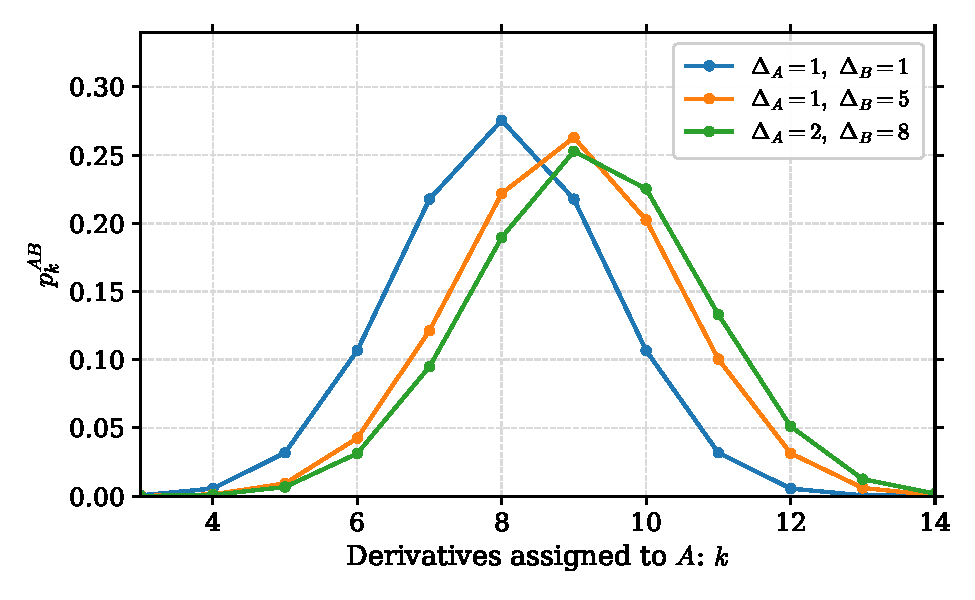
\includegraphics[width=.78\textwidth]{content/AdvancedPhysics/field-theory/figures/geometry-highspin/generated/mixed_scalar_modes.pdf}
 \caption{固定 $S=16$ 时，不同标度维数组合的精确双体模式分配概率。所有曲线都由 \cref{eq:ghs-r4-mixed-mode-probability} 计算；峰位发生变化来自两种标量的维数不同，而不是某个额外耦合常数。}
 \label{fig:ghs-r4-mixed-scalar-modes}
\end{figure}

对于固定 $\Delta_A,\Delta_B$ 且 $S\to\infty$，主导项来自 $k=S/2+O(\sqrt S)$。Stirling 展开说明两个 $\binom Sk$ 因子决定指数部分，而 Pochhammer 比值只贡献随 $k/S$ 缓变的代数因子，于是中心区的概率逼近
\begin{equation}\label{eq:ghs-r4-mixed-mode-clt}
 p_k^{AB}=\sqrt{\frac{4}{\pi S}}\,
 \exp\left[-\frac{4(k-S/2)^2}{S}\right]
 \bigl[1+O(S^{-1/2})\bigr],
\end{equation}
其中误差限于 $|k-S/2|\le C\sqrt S$、固定 $C$ 的中心区，且 $\Delta_A,\Delta_B$ 随 $S$ 固定。于是 $\operatorname{Var}(k)=S/8+O(1)$；若标度维数自身随 $S$ 增长，则必须重新分析鞍点，不能直接使用上述高斯。对 $\Delta_A=\Delta_B=1$，\cref{eq:ghs-r4-mixed-mode-probability} 恢复先前得到的 $\binom Sk^2/\binom{2S}S$。


用 Gamma 函数将 \cref{eq:ghs-r4-mixed-mode-probability} 中依赖 $k$ 的部分重新整理为
\begin{equation*}
 p_k^{AB}\propto\binom Sk^2
 \frac{\Gamma(k+1)}{\Gamma(k+\Delta_A)}
 \frac{\Gamma(S-k+1)}{\Gamma(S-k+\Delta_B)}.
\end{equation*}
在 $k$ 和 $S-k$ 同时增大的区域，Gamma 比值的 Stirling 公式给出
\begin{equation*}
 \frac{\Gamma(k+1)}{\Gamma(k+\Delta_A)}
 =k^{1-\Delta_A}[1+O(k^{-1})],
\end{equation*}
另一因子相同，只需替换 $k\mapsto S-k$ 与 $\Delta_A\mapsto\Delta_B$。现在写 $k=S/2+x$，固定 $\Delta_A,\Delta_B$，并让 $|x|\le C\sqrt S$。二项式系数的中心区展开为
\begin{equation*}
 2\log\binom S{S/2+x}
 =2S\log2-\log(\pi S/2)-\frac{4x^2}{S}
 +O(S^{-1}),
\end{equation*}
其中余项对固定 $C$ 一致有界。对剩下的代数因子展开对数：
\begin{align*}
 &(1-\Delta_A)\log(S/2+x)
 +(1-\Delta_B)\log(S/2-x)\\
 &\quad=\text{与 $x$ 无关的项}
 +\frac{2(\Delta_B-\Delta_A)x}{S}+O(S^{-1}).
\end{align*}
所以概率的中心区对数可写为
\begin{equation*}
 \log p_k^{AB}=\text{归一化常数}
 -\frac4S\left(x-\frac{\Delta_B-\Delta_A}{4}\right)^2
 +O(S^{-1}).
\end{equation*}
用 \(\sum_k\exp(-4(k-S/2)^2/S)\sim\sqrt{\pi S}/2\) 归一化，得到 \cref{eq:ghs-r4-mixed-mode-clt}。连续鞍点相对 $S/2$ 的位移是 $(\Delta_B-\Delta_A)/4+O(S^{-1})$；实际离散分布的众数须再取最接近鞍点的整数，不能把它们混为一谈。二次项的曲率给出领先方差 $S/8$。若要得到 $O(1)$ 的方差修正，则应保留 Stirling 展开中下一阶的四次项及归一化修正。


这一计算揭示了自由高自旋态中比对径峰更普适的对象：在同一共形表示的最低扭度层上，两个标量如何分享总径向能量。构成场的标度维数可以任意变化，中心区的 $\sqrt S$ 宽度却保持不变；这是由共形初级约束和广义自由因子化共同产生的结果，而不是某个特定四维球谐积分的巧合。


\subsection{无迹极化与自旋关联的张量恢复}

零极化多项式隐藏了迹项，二点函数和守恒条件却会重新调用这些项。为使张量缩并自足，固定恢复规则。

\begin{definition}[调和投影与零锥导数]
令 $F_S(z)$ 为 $d$ 维辅助向量 $z$ 的齐次 $S$ 次多项式。其对称无迹投影为
\begin{equation}\label{eq:ghs-r4-stf-projector}
 \Pi_SF_S=\sum_{k=0}^{\lfloor S/2\rfloor}
 \frac{(-1)^k\Gamma(S+d/2-k-1)}{4^kk!\Gamma(S+d/2-1)}
 (z^2)^k(\partial_z^2)^kF_S.
\end{equation}
$S=0$ 单独定义 $\Pi_0=1$。令 $\nu=d/2-1$，作用于零锥等价类的 Thomas 导数为
\[
 \mathcal D_{z,\mu}=(\nu+z\cdot\partial_z)\partial_{z,\mu}
 -\tfrac12z_\mu\partial_z^2.
\]
它将 $z^2$ 倍数映为 $z^2$ 倍数，因此 $\partial_x^\mu\mathcal D_{z,\mu}J_S$ 与多项式代表无关。完整投影递推与任意秩证明可参照《群论》的对称无迹张量部分。
\end{definition}
\begin{proof}
对齐次 $m$ 次多项式 $G_m$，
\[
 \partial_z^2[(z^2)^kG_m]=(z^2)^k\partial_z^2G_m
 +4k(m+k+d/2-1)(z^2)^{k-1}G_m.
\]
代入 $m=S-2k$，相邻迹阶系数满足
$a_{k+1}=-a_k/[4(k+1)(S-k+d/2-2)]$，$a_0=1$，得到 $\Gamma$ 形式；最高阶以后重复 Laplace 运算为零。

对 Thomas 导数展开 $\mathcal D_{z,\mu}(z^2G_m)$。不含 $z^2$ 的项为
$[2(\nu+m+1)-(d+2m)]z_\mu G_m=0$，所以改变零锥多项式代表不会改变散度条件。
\end{proof}


对一般的对称无迹初级算符 $J_{\Delta,S}$，仅由平移、旋转和尺度不变性还不能固定它的二点函数；必须再处理反演。令
\begin{equation}\label{eq:ghs-r4-inversion-matrix}
 I_{\mu\nu}(x)=\delta_{\mu\nu}-2\frac{x_\mu x_\nu}{x^2},\qquad
 I_{\mu\rho}(x)I_{\rho\nu}(x)=\delta_{\mu\nu}.
\end{equation}
它是反演坐标映射在正交标架中的反射矩阵。把每个自旋指标都用 $I_{\mu\nu}$ 连接两个端点，然后取无迹部分，得到一般二点函数
\begin{equation}\label{eq:ghs-r4-general-stt-two-point}
 \langle J_{\Delta,S}(x_1,z_1)J_{\Delta,S}(x_2,z_2)\rangle
 =\frac{C_J}{(x_{12}^2)^\Delta}
 \Bigl[z_1^\mu I_{\mu\nu}(x_{12})z_2^\nu\Bigr]^S,
 \quad z_1^2=z_2^2=0.
\end{equation}
$C_J$ 只取决于对 $J$ 的归一化。不同 $\Delta,S$ 或不同不可约内部对称性表示之间，标准的共形二点函数为零。若以后需要作迹、散度或张量指标缩并，必须以 \cref{eq:ghs-r4-stf-projector} 对上述右侧恢复其无迹多项式延拓。


复合共形变换对 $x$ 的作用含有分式映射，直接用它变换多个高自旋指标相当繁琐。对任意整数 $d>2$，可引入具有签名 $(d+1,1)$ 的辅助空间 $\RR^{d+1,1}$，采用坐标 $P^A=(P^+,P^-,P^\mu)$，内积
\begin{equation}\label{eq:ghs-r4-embedding-inner-product}
 P\cdot Q=-\frac12(P^+Q^-+P^-Q^+)+\delta_{\mu\nu}P^\mu Q^\nu.
\end{equation}
将欧氏点 $x$ 送入射影零锥
\begin{equation}\label{eq:ghs-r4-embedding-section}
 P(x)=(1,x^2,x^\mu),\qquad P(x)^2=0,\qquad
 -2P(x)\cdot P(y)=(x-y)^2.
\end{equation}
因此对 $P$ 的一个线性 $SO(d+1,1)$ 变换，在选定 $P^+=1$ 截面以后，就是原来对 $x$ 的非线性共形变换。这项几何化并未引入额外的物理时空维度；射影等价 $P\sim\lambda P$ 正好去掉辅助坐标多出来的尺度。

自旋极化向量同时提升为
\begin{equation}\label{eq:ghs-r4-embedding-polarization}
 Z(x,z)=(0,2x\cdot z,z^\mu),\qquad
 Z\cdot P=0,\qquad Z^2=z^2=0.
\end{equation}
嵌入空间的张量多项式 $\mathcal J(P,Z)$ 满足 $\mathcal J(\lambda P,Z)=\lambda^{-\Delta}\mathcal J(P,Z)$、$\mathcal J(P,\alpha Z)=\alpha^S\mathcal J(P,Z)$，并具有规范等价 $Z\sim Z+\beta P$。前两个齐次条件分别记录标度维数与自旋，最后一个条件去掉非物理的径向指标。它们不是三项任意的写作约定，而是原有张量变换律在射影零锥上的表述 \cite{ghs-costa}。


构造三点函数时，距离平方来自 $P_{ij}=-2P_i\cdot P_j$。对于第三个点的极化，具有规范不变性的唯一线性结构可取
\begin{equation}\label{eq:ghs-r4-embedding-V}
 V_{3,12}=\frac12\left(\frac{Z_3\cdot P_1}{P_3\cdot P_1}
 -\frac{Z_3\cdot P_2}{P_3\cdot P_2}\right)
 =z\cdot\left(\frac{x_{31}}{x_{31}^2}-\frac{x_{32}}{x_{32}^2}\right).
\end{equation}
在 $Z_3\mapsto Z_3+\beta P_3$ 下，两项各加上相同的 $\beta$，所以它们的差不变。设 $\tau=\Delta-S$ 为交换初级算符的扭度，则一般的非零三点函数为
\begin{align}\label{eq:ghs-r4-general-ssj-three-point}
 &\langle A(x_1)B(x_2)J_{\Delta,S}(x_3,z)\rangle\\
 &\quad=\frac{\lambda_{ABJ}\,V_{3,12}^S}
 {(x_{12}^2)^{(\Delta_A+\Delta_B-\tau)/2}
 (x_{23}^2)^{(\Delta_B+\tau-\Delta_A)/2}
 (x_{31}^2)^{(\Delta_A+\tau-\Delta_B)/2}}.\notag
\end{align}
这个结果不要求 $A,B$ 或 $J$ 是广义自由算符。其三个距离指数同时满足各端点所需的标度与反演协变性。将 $J=[AB]_S$、$x_3=0$、$\tau=\Delta_A+\Delta_B$ 代入，就精确恢复 \cref{eq:ghs-r4-general-mixed-threepoint} 的位置依赖；在这个特例中才可以用 Wick 定理进一步算出 $\lambda_{ABJ}$。

两个带自旋算符之间还可以形成
\begin{equation}\label{eq:ghs-r4-embedding-H}
 H_{ij}=(-2P_i\cdot P_j)(Z_i\cdot Z_j)
 +2(Z_i\cdot P_j)(Z_j\cdot P_i).
\end{equation}
在物理截面上 $H_{ij}=x_{ij}^2\,z_i\cdot I(x_{ij})\cdot z_j$。由 $V_i$ 与 $H_{ij}$ 组成的非负整数次单项式，再结合每个点极化向量的次数要求，就形成任意对称无迹外自旋、宇称偶三点张量结构的有限维基底。若在三维使用 Levi--Civita 张量，还会出现宇称奇结构；低维 Schouten 恒等式也会使部分张量结构不独立。因而 \cref{eq:ghs-r4-general-ssj-three-point} 的唯一性专指两个标量和一个对称无迹自旋算符的情形，不能无条件推广为三个任意自旋算符只允许一个系数。


一个对称无迹初级表示的二次 Casimir 本征值已经由 \cref{eq:ghs-casimir-eigenvalue} 得到：
\begin{equation}\label{eq:ghs-r4-casimir-shadow-symmetry}
 C_{\Delta,S}=\Delta(\Delta-d)+S(S+d-2)
 =C_{d-\Delta,S}.
\end{equation}
因此，只指定自旋和这个本征值，并不能在两支形式解 $\Delta$ 与 $d-\Delta$ 之间作选择。后者对应所谓的影子维数。物理径向块必须再规定 $r\to0$ 的初级态起始行为 $r^\Delta$，以及相应的反射正性和后裔结构；影子支一般不能当成同一个算符乘积展开中的另一个物理初级态。$\Delta=d/2$ 附近两支相遇时，某些微分方程的第二个局部解会出现对数，需要按极限和边界条件分别处理。这些事实解释了为什么共形块是有明确边界条件的 Casimir 解，而不仅是一条本征值方程。


共形生成元决定初级态及其后裔的结构。将这些态重新放回局域关联函数，就能由三点函数计算算符乘积中的展开系数。


\section{三点函数与 OPE}
\label{sec:ghs-three-point-ope}


一个算符在球面上制备什么态，是径向量子化的运动学问题；两个算符靠近时会激发哪些态，则决定了量子场论的相互作用数据。在自由标量场中，这两个问题通过同一组 Wick 收缩相连。前面求出的 $(z_1-z_2)^S$ 其实已经是一个自旋 $S$ 三点函数在等半径球面上的截面。这一部分将恢复完整的空间依赖，并说明它怎样进入算符乘积展开。


记 $G(x)=C_d/|x|^{2\delta}$，并将自由标量重新标准化为 $\chi=\varphi/\sqrt{C_d}$，使 $\langle\chi(x)\chi(0)\rangle=|x|^{-2\delta}$。自旋 $S$ 的初级算符 $\mathcal O_S$ 仍采用 \cref{eq:ghs-bilinear-general,eq:ghs-primary-coefficients} 的约定。把它除以 \cref{eq:ghs-operator-norm} 的径向范数，定义归一最高权算符
\begin{equation}\label{eq:ghs-normalized-highest-current}
 \mathscr J_S(x;\vb\varepsilon)=\frac{\mathcal O_S(x;\vb\varepsilon)}{\sqrt{\mathcal N_S}},
 \qquad \mathcal N_S=2^{2S+1}C_d^2S!(2\delta+S-1)_S.
\end{equation}
这里的“归一”特指选定复零极化最高权态的径向范数为一。它与某些文献把全部张量指标收缩得到的 $C_J=1$ 约定未必相同；比较文献中的 OPE 系数时必须同时转换极化向量归一化。

取 $x_3=0$，令
\begin{equation}\label{eq:ghs-threepoint-polarization-invariant}
 V_3(x_1,x_2;\vb\varepsilon)
 =\vb\varepsilon\cdot\left(\frac{x_1}{|x_1|^2}-\frac{x_2}{|x_2|^2}\right).
\end{equation}
从自由传播子求导并利用前文初级递推式，直接得到偶数自旋的三点函数
\begin{equation}\label{eq:ghs-scalar-scalar-spin-3pt}
 \langle\chi(x_1)\chi(x_2)\mathscr J_S(0;\vb\varepsilon)\rangle
 =g_S\frac{V_3(x_1,x_2;\vb\varepsilon)^S}
 {|x_1|^{2\delta}|x_2|^{2\delta}},
 \qquad
 g_S=\frac{\sqrt2(\delta)_S}{\sqrt{S!(2\delta+S-1)_S}}.
\end{equation}
位置因子是共形对称允许的标量—标量—对称无迹张量三点函数结构。动力学只保留在一个数 $g_S$ 中。在一般 CFT 中，维数可以不等于 $2\delta+S$，分母幂次须相应改变，且 $g_S$ 不再由 Wick 定理给出。


\begin{proof}
令 $D_3=\vb\varepsilon\cdot\partial_{x_3}$。对两条自由传播线分别求导，零极化条件给出
\begin{equation*}
D_3^kG(x_1-x_3)|_{x_3=0}
=2^k C_d(\delta)_k
\frac{(\vb\varepsilon\cdot x_1)^k}{|x_1|^{2\delta+2k}}.
\end{equation*}
正规序使第三点的两个场只与外场配对。把所有 $k$ 的贡献加总并用 $c_k(\delta)_k(\delta)_{S-k}=(-1)^k\binom Sk(\delta)_S$，得到
\begin{align*}
&\langle\varphi(x_1)\varphi(x_2)\mathcal O_S(0;\vb\varepsilon)\rangle\\
&\quad=2^{S+1}C_d^2(\delta)_S
|x_1|^{-2\delta}|x_2|^{-2\delta}
\sum_{k=0}^S(-1)^k\binom Sk
\left(\frac{\vb\varepsilon\cdot x_1}{|x_1|^2}\right)^k
\left(\frac{\vb\varepsilon\cdot x_2}{|x_2|^2}\right)^{S-k}\\
&\quad=2^{S+1}C_d^2(\delta)_S
|x_1|^{-2\delta}|x_2|^{-2\delta}
\left(\frac{\vb\varepsilon\cdot x_2}{|x_2|^2}
-\frac{\vb\varepsilon\cdot x_1}{|x_1|^2}\right)^S.
\end{align*}
偶数 $S$ 去掉了最后括号里的整体负号；除以两个 $\sqrt{C_d}$ 与一个 $\sqrt{\mathcal N_S}$，系数变为
\begin{equation*}
\frac{2^{S+1}C_d(\delta)_S}{\sqrt{2^{2S+1}C_d^2S!(2\delta+S-1)_S}}
=\frac{\sqrt2(\delta)_S}{\sqrt{S!(2\delta+S-1)_S}}.
\end{equation*}
\end{proof}

在自旋零的情形，$\mathscr J_0=:\!\chi^2\!:/\sqrt2$，所以 $g_0=\sqrt2$，与直接计算 $\langle\chi\chi:\!\chi^2\!:\rangle=2G_\chi G_\chi$ 完全一致。四维时还可得到
\begin{equation}\label{eq:ghs-threepoint-four-d}
 g_S^2=\frac{2(S!)^2}{(2S)!}
 =\frac2{\binom{2S}{S}},\qquad d=4,\quad S\in2\NN_0.
\end{equation}
这个系数随自旋快速变小，并不意味着相应的高自旋流“消失”：张量结构 $V_3^S$ 与归一约定也随自旋变化，不能只比较裸系数。


\subsection{局域算符乘积与后裔系数}

设一般 CFT 中两个初级算符 $A(x),B(0)$ 相距很近。取一个球面包围二者而不包围其他插入，球内路径积分制备的态可依径向 哈密顿量 的一组完备本征态展开。这些本征态按共形初级态及其 $P_\mu$ 后裔分组，产生局域算符乘积展开：
\begin{equation}\label{eq:ghs-ope-general}
 A(x)B(0)=\sum_{\mathcal O}\mathcal C_{AB\mathcal O}(x,\partial)
 \mathcal O(0).
\end{equation}
这里 $\mathcal C$ 是确定后裔系数的微分算符值函数；求和不仅包含初级算符，还隐含其所有后裔。在两点可被同一个球面与其余插入严格分隔的欧氏相关函数中，此展开可以通过径向 Hilbert 空间的谱表示理解其收敛性，参见 \cite{ghs-rychkov,ghs-simmons}。若只截留初级算符而抛掉后裔，通常得不到共形协变的四点函数。

在自由标量场中，乘积可以先用 Wick 定理逐项精确拆开：
\begin{equation}\label{eq:ghs-free-field-ope-start}
 \chi(x)\chi(0)=\frac{\mathds1}{|x|^{2\delta}}+\, :\!\chi(x)\chi(0)\!:.
\end{equation}
第二项在 $x=0$ 附近 Taylor 展开，第一项为 $:\!\chi^2\!:=\sqrt2\,\mathscr J_0$。但剩余的导数项既包含新的高自旋初级流，也包含前面已经出现的标量和低自旋流的平移后裔。因此不能把 Taylor 展开中的每一个导数单项式都当成独立初级算符。


\cref{eq:ghs-spin-unitarity-bound-extended} 表明 $\Delta_S=S+d-2$ 对 $S\ge1$ 正好意味着散度后裔被截去。前面所构造的每个偶数自旋 $S\ge2$ 双线性流都满足这一条件。于是 $\chi\times\chi$ 中不仅出现单位算符和标量 $:\!\chi^2\!:$，还包含无穷多个高自旋短表示。它们不是由一个有限个基本场的额外粒子谱手工添进去的，而是两个自由场组成的复合算符。

反过来，若将基本标量换成标度维数 $\Delta_\chi>\delta$ 的一般初级算符，两个算符乘积中典型的双算符初级态具有近似或精确的自由组合维数
\begin{equation}\label{eq:ghs-doubletwist-kinematic-dimension}
 \Delta_{n,S}^{(0)}=2\Delta_\chi+2n+S,
 \qquad n=0,1,\ldots .
\end{equation}
这里 $n$ 计数相对导数的额外两阶，$S$ 是总对称无迹自旋。对于真正的广义自由场，这些是独立算符；对于饱和标量幺正界的局域自由场，运动方程会使部分本来形式独立的高阶后裔成为零范数，谱必须作相应约化。在相互作用理论中，双算符态通常还获得反常维数。


径向量子化的初级态能量 $\Delta_{\mathcal O}$ 和角动量表示说明“有哪些态”；三点函数系数 $\lambda_{AB\mathcal O}$ 则说明两次局域插入怎样激发这些态。给定局域共形代数和一套统一的算符归一化，完整的标度维数与三点函数系数构成局域共形数据。四点及更高相关函数应由它们的算符乘积展开重建，但同一四点函数可以按不同配对次序展开，必须得到一致结果。这一条件将不再允许谱和系数任意选择。


径向量子化告诉我们：把两个插入点圈进同一个球面之后，球内的态必须能在一组共形初级态及其后裔上展开。不过，知道哪些初级态出现还不够。若把一对局域算符移动一点距离，为什么初级态的一阶、二阶后裔会以特定比例被激发？这些比例必须由共形代数决定，否则同一乘积的三点函数就不可能与全局共形协变性相容。


考虑三个标量初级算符 $A,B,\mathcal O$，其维数分别为 $\Delta_A,\Delta_B,\Delta>0$；将 $\mathcal O$ 的两点函数归一为
\begin{equation}\label{eq:ghs-ope-scalar-normalization}
 \langle\mathcal O(x)\mathcal O(0)\rangle=(x^2)^{-\Delta}.
\end{equation}
暂取三种算符互不简并，也不包含相同量子数的混合。共形对称把三点函数固定为
\begin{equation}\label{eq:ghs-ope-three-scalar}
 \langle A(x)B(0)\mathcal O(y)\rangle
 =\frac{\lambda_{AB\mathcal O}}
 {(x^2)^{(\Delta_A+\Delta_B-\Delta)/2}
 (y^2)^{(\Delta_B+\Delta-\Delta_A)/2}
 ((y-x)^2)^{(\Delta_A+\Delta-\Delta_B)/2}}.
\end{equation}
这里 $x^2=|x|^2$，并假定 $|x|<|y|$，使围住 $x,0$ 的球面不包含第三个插入点。令
\begin{equation}\label{eq:ghs-ope-alpha-beta}
 \alpha=\frac{\Delta+\Delta_A-\Delta_B}{2},\qquad
 \beta=\frac{\Delta+\Delta_B-\Delta_A}{2},\qquad
 \alpha+\beta=\Delta.
\end{equation}
我们把该初级表示在乘积中的贡献写成以下局域展开：
\begin{align}\label{eq:ghs-ope-scalar-level-two}
 A(x)B(0)\big|_{\mathcal O}
 =&\;\lambda_{AB\mathcal O}(x^2)^{(\Delta-\Delta_A-\Delta_B)/2}
 \bigl[\mathcal O(0)+a\,x^\mu\partial_\mu\mathcal O(0)
 \\&\qquad+b\,x^2\partial^2\mathcal O(0)
 +c\,x^\mu x^\nu\partial_\mu\partial_\nu\mathcal O(0)
 +O(|x|^3)\bigr].\notag
\end{align}
$a,b,c$ 是无量纲数。二阶存在两个独立的旋转标量结构：一个由迹 $\partial^2\mathcal O$ 构成，另一个由沿 $x$ 方向的二次导数构成。把它们混成一个“二阶项”，就无法看见零范数后裔对应的极点。


将 \cref{eq:ghs-ope-three-scalar} 除以共同的 $\lambda_{AB\mathcal O}(x^2)^{(\Delta-\Delta_A-\Delta_B)/2}(y^2)^{-\Delta}$，左侧剩下
\begin{equation}\label{eq:ghs-ope-kinematic-ratio}
 F(x,y)=\left(1-2\frac{x\cdot y}{y^2}+\frac{x^2}{y^2}\right)^{-\alpha}.
\end{equation}
取 $t=(x\cdot y)/y^2$ 与 $u=x^2/y^2$，按 $|x|/|y|$ 的次数展开：
\begin{equation}\label{eq:ghs-ope-ratio-expansion}
 F(x,y)=1+2\alpha t-\alpha u+2\alpha(\alpha+1)t^2
 +O\bigl((|x|/|y|)^3\bigr).
\end{equation}
这一行来自 $(1+q)^{-\alpha}=1-\alpha q+\alpha(\alpha+1)q^2/2+\cdots$；其中 $u$ 已是二阶，故不能把 $u^2$ 保留在当前阶数中。

右侧的后裔算符与 $\mathcal O(y)$ 做两点函数时，对 $\mathcal O(0)$ 的求导等于对 $y$ 求导的负号。这一点直接决定了一阶系数的符号。我们有
\begin{align*}
 x^\mu\partial_{0\mu}(y^2)^{-\Delta}
 &=2\Delta t(y^2)^{-\Delta},\\
 x^\mu x^\nu\partial_{0\mu}\partial_{0\nu}(y^2)^{-\Delta}
 &=\bigl[-2\Delta u+4\Delta(\Delta+1)t^2\bigr](y^2)^{-\Delta},\\
 x^2\partial_0^2(y^2)^{-\Delta}
 &=2\Delta(2\Delta+2-d)u(y^2)^{-\Delta}.
\end{align*}
按 $t,t^2,u$ 三种独立的角结构分别比较系数，得到完整的二阶结果：
\begin{equation}\label{eq:ghs-ope-descendant-coefficients}
 a=\frac{\alpha}{\Delta},\qquad
 c=\frac{\alpha(\alpha+1)}{2\Delta(\Delta+1)},\qquad
 b=-\frac{\alpha\beta}{2\Delta(\Delta+1)(2\Delta+2-d)}.
\end{equation}
因此，对于一般非零范数的标量初级表示，\cref{eq:ghs-ope-scalar-level-two} 的前两级后裔没有自由参数：只要已知三个标度维数和一个初级 OPE 系数，整个后裔比例就确定了。


\begin{proof}
一阶和二阶无迹方向的系数由
\begin{align*}
2\Delta a&=2\alpha,\\
4\Delta(\Delta+1)c&=2\alpha(\alpha+1)
\end{align*}
给出。二阶迹结构的系数必须满足
\begin{align*}
2\Delta(2\Delta+2-d)b-2\Delta c&=-\alpha,\\
2\Delta(2\Delta+2-d)b
&=-\alpha+\frac{\alpha(\alpha+1)}{\Delta+1}\\
&=\frac{\alpha(\alpha-\Delta)}{\Delta+1}
=-\frac{\alpha\beta}{\Delta+1}.
\end{align*}
最后使用 $\beta=\Delta-\alpha$，即得 \cref{eq:ghs-ope-descendant-coefficients}。这些计算只要求 $x$ 与 $y$ 不重合，并在 $|x|<|y|$ 的欧氏径向域中进行；如果初级表示含零范数态，下式的反矩阵步骤必须先取商空间。
\end{proof}

二级迹后裔的范数已由 \cref{eq:ghs-scalar-unitarity-bound} 的推导确定：
\begin{equation}\label{eq:ghs-ope-trace-norm-repeat}
 \|P^2|\mathcal O\rangle\|^2
 =8d\Delta\left(\Delta-\frac{d-2}{2}\right)
 \|\mathcal O\|^2.
\end{equation}
另一方面，$b$ 的分母中有 $2\Delta+2-d=2(\Delta-(d-2)/2)$。两者在同一点消失。这不是一个偶然的代数分母：构造 OPE 后裔系数需要反演该级的 Gram 矩阵；如果一个后裔成为零范数态，该矩阵不再可逆。

当 $\Delta=(d-2)/2$，若 $\alpha\beta\ne0$，形式上的 $b$ 发散。对连续、单位的共形场论，饱和标量幺正性界的算符满足自由运动方程；只允许与其零模一致的相关函数耦合。对所考虑的单个非零三点函数，这要求 $\alpha\beta=0$，以便零范数子表示不产生矛盾。不能将一个一般 $\alpha\beta\ne0$ 的形式级数在分母处直接代入 $\Delta=(d-2)/2$。

再看两个相同外场 $A=B$。这时 $\alpha=\beta=\Delta/2$，并且
\begin{equation}\label{eq:ghs-identical-scalar-descendants}
 a=\frac12,\quad
 c=\frac{\Delta+2}{8(\Delta+1)},\quad
 b=-\frac{\Delta}{8(\Delta+1)(2\Delta+2-d)}.
\end{equation}
其中 $a=1/2$ 有直观解释：交换两端相同的算符，同时将 OPE 的展开原点由一个端点平移到另一个端点，一阶平移应由两端对称分担。二阶系数却不是仅凭这种交换对称就能猜出的；它同时包含迹通道的共形几何。


从 Hilbert 空间看，上述计算还有一个更普适的形式。固定由某个初级态 $|\mathcal O\rangle$ 产生的后裔表示，在每一级选出一组线性独立态 $|a\rangle$，其 Gram 矩阵为 $G_{ab}=\langle a|b\rangle$。该级表示的正交投影是
\begin{equation}\label{eq:ghs-ope-gram-projector}
 \Pi_{\mathcal O,n}=\sum_{a,b\in\mathcal H_{\mathcal O,n}}
 |a\rangle\,(G^{-1})^{ab}\,\langle b|.
\end{equation}
它满足 $\Pi^2=\Pi$，其原因是中间两个 Gram 矩阵相乘后给出单位矩阵。把投影插入包围两点的球面态展开，便得到 OPE 系数。改变后裔基底不会改变 $\Pi$，所以实际相关函数不依赖我们选的是迹/无迹分解还是其他等价基底。

若某一级出现零范数后裔，首先在物理 Hilbert 空间中将其模掉，再反演剩余非退化 Gram 矩阵。初级表示缩短时，共形块也随之发生相应的极点与残数结构；这正是以后用 Casimir 方程和谱极点研究多重态重组的数学基础。参见 \cite{ghs-rychkov,ghs-simmons,ghs-rychkov-tan}。

径向 Hilbert 空间的后裔谱由共形代数产生，算符乘积展开则记录不同初级如何耦合。四点函数使这些数据彼此约束：不同的算符配对次序必须得到同一个相关函数。


算符乘积展开把一个相关函数分成各个初级表示及其后裔。四个算符却可以按不止一种次序配对，因此相同的四点函数为这些表示数据施加了额外的相容条件。


只有两点函数和三点函数时，共形对称给出的限制仍很宽：不同初级算符的维数与三点函数常数可以分别输入。四点函数第一次让这些数据必须相互兼容，因为四个算符可以先把前两个配对，也可以先把中间两个配对。所谓共形自举，就是把这种不依赖配对顺序的恒等关系与幺正性、谱信息结合起来。


取四个互不重合的欧氏点 $x_i\in\RR^d$，记 $x_{ij}=x_i-x_j$，$x_{ij}^2=|x_i-x_j|^2$。四个相同标量初级算符 $\mathcal X$ 的标度维数取 $\Delta_\mathcal X$，其二点函数标准化为 $\langle\mathcal X(x)\mathcal X(0)\rangle=(x^2)^{-\Delta_\mathcal X}$。共形变换只能将四点坐标约化为两个独立交比
\begin{equation}\label{eq:ghs-cross-ratios}
 U=\frac{x_{12}^2x_{34}^2}{x_{13}^2x_{24}^2},
 \qquad V=\frac{x_{14}^2x_{23}^2}{x_{13}^2x_{24}^2}.
\end{equation}
于是其相关函数的一般形式是
\begin{equation}\label{eq:ghs-fourpoint-reduced}
 \langle\mathcal X_1\mathcal X_2\mathcal X_3\mathcal X_4\rangle
 =\frac{\mathcal G(U,V)}{(x_{12}^2x_{34}^2)^{\Delta_\mathcal X}}.
\end{equation}
函数 $\mathcal G$ 无法单靠共形协变性确定，因为它包含真实的 OPE 动力学。交换第 $2$、$4$ 个相同场时，$(U,V)$ 变成 $(V,U)$，同时外面的距离因子发生变化。将同一个四点函数写成两种方式，得到交叉对称方程
\begin{equation}\label{eq:ghs-crossing-scalar}
 V^{\Delta_\mathcal X}\mathcal G(U,V)
 =U^{\Delta_\mathcal X}\mathcal G(V,U).
\end{equation}
它是严格的相关函数恒等式，不是大自旋近似。


对前面标准化的自由标量 $\chi$，三个 Wick 配对穷尽了四点函数：
\begin{align}\label{eq:ghs-free-scalar-fourpoint}
 \langle\chi_1\chi_2\chi_3\chi_4\rangle
 &=\frac1{(x_{12}^2x_{34}^2)^\delta}
 +\frac1{(x_{13}^2x_{24}^2)^\delta}
 +\frac1{(x_{14}^2x_{23}^2)^\delta},\\
 \mathcal G_\chi(U,V)&=1+U^\delta+(U/V)^\delta.\notag
\end{align}
交换 $(U,V)$ 后，
\begin{align*}
 (U/V)^\delta\mathcal G_\chi(V,U)
 &=(U/V)^\delta[1+V^\delta+(V/U)^\delta]\\
 &=(U/V)^\delta+U^\delta+1
 =\mathcal G_\chi(U,V),
\end{align*}
这正是 \cref{eq:ghs-crossing-scalar}。自由场虽然容易计算，却已包含自举中最重要的一点：同一四点函数的三个配对次序彼此相容。

四维共形场论常把两个交比表示为 $U=z\bar z$、$V=(1-z)(1-\bar z)$。在欧氏构型中 $\bar z$ 是 $z$ 的复共轭；将 $z,\bar z$ 作为独立实变量去取光锥极限，则属于分析延拓后的洛伦兹运动学，不能把两种取极限的方式混为一谈。


仅有三个 Wick 配对还不容易看见复合算符之间的连接结构。考虑标准化的双线性标量
\begin{equation}\label{eq:ghs-normalized-phi2}
 \mathcal B(x)=\frac1{\sqrt2}:\!\chi(x)^2\!:,
 \qquad\Delta_\mathcal B=2\delta.
\end{equation}
正规序规定同一点内部不自收缩。四个 $\mathcal B$ 各带两个标量腿，所以完整的 Wick 图既有不连通的双配对，也有四点连成一个圈的三种方式。结果是
\begin{align}\label{eq:ghs-bilinear-fourpoint}
 \mathcal G_\mathcal B(U,V)
 &=1+U^{2\delta}+(U/V)^{2\delta}\\
 &\quad+4\bigl[U^\delta+(U/V)^\delta+(U^2/V)^\delta\bigr].\notag
\end{align}
相比 \cref{eq:ghs-free-scalar-fourpoint}，新增项恰恰记录四个复合算符之间的连接相关。这个例子并非相互作用理论：尽管 $\mathcal B$ 的相关函数有连接图，基本场仍然服从高斯 Wick 定理。


自由场四点函数可将全部 Wick 配对按连通结构分类。
记 $G_{ij}=\langle\chi_i\chi_j\rangle=(x_{ij}^2)^{-\delta}$。四个 $:\!\chi^2\!:$ 的 Wick 收缩只允许连接不同顶点。若顶点 $1,2$ 之间两条线、顶点 $3,4$ 之间两条线，则收缩数为 $(2!)(2!)=4$；乘上每个算符的 $1/\sqrt2$ 后，整张图的因子为 $1$，给出 $G_{12}^2G_{34}^2$。另外两种断开配对完全类似。

\begin{proof}
若四个顶点连成圈，固定例如 $1\to2\to3\to4\to1$，每个顶点的两条腿均可交换，产生 $2^4=16$ 种 Wick 配对；四个标准化因子相乘为 $1/4$，因此系数为 $4$。只有三种不等价的四顶点圈，合并后
\begin{align*}
\langle\mathcal B_1\mathcal B_2\mathcal B_3\mathcal B_4\rangle
&=G_{12}^2G_{34}^2+G_{13}^2G_{24}^2+G_{14}^2G_{23}^2\\
&\quad+4(G_{12}G_{23}G_{34}G_{41}
+G_{12}G_{24}G_{43}G_{31}
+G_{13}G_{32}G_{24}G_{41}).
\end{align*}
以 $(G_{12}G_{34})^2$ 除去共同因子，三个圈分别变成 $(U/V)^\delta$、$U^\delta$、$(U^2/V)^\delta$，即得 \cref{eq:ghs-bilinear-fourpoint}。
\end{proof}

将 $\mathcal X(x_1)\mathcal X(x_2)$ 与 $\mathcal X(x_3)\mathcal X(x_4)$ 各自做 OPE，中间传播的是由某个初级态 $|\mathcal O\rangle$ 及全部后裔张成的不可约表示。把该表示的贡献归为一个函数，记作自旋 $S$、初级维数 $\Delta$ 的共形块 $G_{\Delta,S}(U,V)$。选择一致的二点函数和共形块标准化后，四点函数分解为
\begin{equation}\label{eq:ghs-conformal-block-expansion}
 \mathcal G(U,V)=\sum_{\mathcal O\in\mathcal X\times\mathcal X}
 \lambda_{\mathcal X\mathcal X\mathcal O}^2
 G_{\Delta_\mathcal O,S_\mathcal O}(U,V).
\end{equation}
对于相同的厄密标量外算符，反射正性使合适的实归一化下 $\lambda^2\ge0$。单位算符的共形块就是 $1$。这里的 $\lambda$ 必须与定义 $G_{\Delta,S}$ 时使用的张量归一化一致；前文固定复零极化的 $g_S$ 不应未经变换就直接替代为任一软件包中的 $\lambda$。

径向量子化解释了共形块的结构：如果两对算符分别位于相隔欧氏径向时间 $t>0$ 的球面上，中间每个后裔的传播因子都是 $\ee^{-t(\Delta+n)}$。对角度上的同阶态再按旋转表示分解，得到沿径向变量 $r=\ee^{-t}$ 的收敛幂级数，其角依赖由 Gegenbauer 多项式表达。这种展开可以直接用于数值计算；选择更对称的径向坐标可显著加快收敛，见 \cite{ghs-hogervorst}。


对具有非退化不变双线性型 $\kappa_{AB}$ 的半单 Lie 代数 $\mathfrak g$，选取基 $T_A$，其二次 Casimir 定义为
\begin{equation}\label{eq:ghs-abstract-quadratic-casimir}
 C_2=\kappa^{AB}T_AT_B\in U(\mathfrak g),
\end{equation}
其中 $\kappa^{AB}\kappa_{BC}=\delta^A_C$。不变性意味着对任意 $T_C$，有
\[
 [T_C,C_2]=\kappa^{AB}([T_C,T_A]T_B+T_A[T_C,T_B])=0.
\]
第二个等号不是形式交换：将 $[T_C,T_A]=f_{CA}{}^DT_D$ 代入，并利用
$\kappa([T_C,T_A],T_B)+\kappa(T_A,[T_C,T_B])=0$，可见两项的系数逐项抵消。在不可约表示上，Schur 引理保证中心元按标量作用，但同一标量可能来自不等价的表示。因此仅有 Casimir 本征值并不足以识别交换的全部物理态。

在球面的标量函数空间中，旋转生成元平方满足 $\sum_{a<b}L_{ab}^2=-\Delta_{S^{d-1}}$；在一般齐性空间中，Casimir 与几何 Laplace 算子的关系还受所选度规、稳定子表示以及张量丛联络影响。这正是把抽象表示论的本征值用于某个量子场论之前必须补上的几何信息。


如果逐个枚举一个初级算符的全部后裔，共形块计算很快就会变得繁琐。由于同一个共形表示中的全部态具有相同的 Casimir 本征值，可以反过来把求和问题改造成微分方程。按前面 \cref{eq:ghs-conformal-commutators} 的径向约定，定义二阶共形 Casimir 算符
\begin{equation}\label{eq:ghs-conformal-quadratic-casimir}
 \mathcal C_2
 =D^2-\frac12M_{\mu\nu}M_{\mu\nu}
 -\frac12\left(P_\mu K_\mu+K_\mu P_\mu\right).
\end{equation}
这里重复指标从 $1$ 到 $d$ 求和。$M_{\mu\nu}$ 在对称无迹自旋 $S$ 表示中的二次型本征值为 $-S(S+d-2)$ 的两倍；这正是前文球谐本征方程在表示论中的写法。对初级态 $K_\mu|\mathcal O\rangle=0$，另外
\begin{equation*}
 K_\mu P_\mu|\mathcal O\rangle
 =[K_\mu,P_\mu]|\mathcal O\rangle
 =2dD|\mathcal O\rangle=2d\Delta|\mathcal O\rangle.
\end{equation*}
所以得到可复算的 Casimir 本征值
\begin{equation}\label{eq:ghs-casimir-eigenvalue}
 \mathcal C_2|\mathcal O_{\Delta,S}\rangle
 =C_{\Delta,S}|\mathcal O_{\Delta,S}\rangle,
 \qquad C_{\Delta,S}=\Delta(\Delta-d)+S(S+d-2).
\end{equation}
对于初级旋转表示 $\lambda$ 而不只对称无迹自旋 $S$，同一代数计算给出
\begin{equation}\label{eq:ghs-general-conformal-casimir-eigen}
 C_2(\Delta,\lambda)=\Delta(\Delta-d)+C_2^{SO(d)}(\lambda).
\end{equation}
这里 $C_2^{SO(d)}(\lambda)$ 采用与旋转生成元平方相匹配的正号归一化。式中 $\Delta$ 与 $d-\Delta$ 有相同的二次 Casimir；影子分支与物理算符分支的区分需要 OPE 短距离边界条件，而不能仅靠该本征值。

由于 Casimir 与整个共形代数对易，$P_\mu$ 产生的每个后裔都保持同一 $C_{\Delta,S}$。这正是为什么能够用一个方程一次性刻画整座后裔塔。

对于四个相同标量外算符，采用 \cref{eq:ghs-fourpoint-reduced} 的外部距离因子，在 $z,\bar z$ 变量上定义
\begin{align}\label{eq:ghs-casimir-differential-operator}
 \mathcal D&=\mathcal D_z+\mathcal D_{\bar z}
 +(d-2)\frac{z\bar z}{z-\bar z}
 \bigl[(1-z)\partial_z-(1-\bar z)\partial_{\bar z}\bigr],\\
 \mathcal D_w&=w^2(1-w)\partial_w^2-w^2\partial_w.
 \notag
\end{align}
将共形生成元对前两个插入点的联合作用变换为交比导数，可得到共形块的微分方程
\begin{equation}\label{eq:ghs-casimir-block-equation}
 \mathcal D G_{\Delta,S}(z,\bar z)
 =\frac12 C_{\Delta,S}G_{\Delta,S}(z,\bar z).
\end{equation}
该方程本身有多个局部解。真正的交换共形块由 $x_{12}\to0$ 的 OPE 边界行为选出：在径向参数 $r\to0$ 时，其最低阶为 $r^\Delta$ 乘一个表示自旋 $S$ 的 Gegenbauer 多项式，后续阶数对应各级后裔。因而“Casimir 本征值 + OPE 边界条件”比仅知道本征值更完整。


\begin{proof}
对 $S$ 阶对称无迹张量 $J_{\mu_1\cdots\mu_S}$，收缩一个辅助向量 $n^\mu$ 得到 $Y_S(n)=J_{\mu_1\cdots\mu_S}n^{\mu_1}\cdots n^{\mu_S}$。它是齐次调和多项式，满足 $\partial_n^2Y_S=0$。在球坐标 $n=r\widehat n$ 下，利用
\begin{equation*}
\partial_n^2=r^{-2}\bigl[(r\partial_r)^2
+(d-2)r\partial_r+\Delta_{S^{d-1}}\bigr]
\end{equation*}
得到 $-\Delta_{S^{d-1}}Y_S=S(S+d-2)Y_S$。角向拉普拉斯算符正是旋转生成元平方之和 $-\tfrac12 M_{\mu\nu}M_{\mu\nu}$。另一方面，初级态满足 $K_\mu|\mathcal O\rangle=0$，因此
\begin{align*}
\mathcal C_2|\mathcal O\rangle
&=\left[D^2-\frac12M_{\mu\nu}M_{\mu\nu}
-\frac12K_\mu P_\mu\right]|\mathcal O\rangle\\
&=\bigl[\Delta^2+S(S+d-2)-d\Delta\bigr]|\mathcal O\rangle.
\end{align*}
这就得到 \cref{eq:ghs-casimir-eigenvalue}。将四点函数写成 \cref{eq:ghs-fourpoint-reduced}，再用坐标微分形式作用于外部两个标量后化简交比，可得到 \cref{eq:ghs-casimir-differential-operator}；完整的坐标雅可比计算和边界解可查阅 \cite{ghs-simmons,ghs-hogervorst}。
\end{proof}

令 $U=z\bar z$、$V=(1-z)(1-\bar z)$。光锥分析考虑 $z\to0$ 而 $\bar z$ 保留非平凡值；当 $\bar z\to1$ 时，交叉通道中最低扭度的算符会控制奇异项。这里扭度定义为
\begin{equation}\label{eq:ghs-twist-definition}
 \tau_{\mathcal O}=\Delta_{\mathcal O}-S_{\mathcal O}.
\end{equation}
扭度不是平移后裔数，它衡量的是一个给定自旋表示距离幺正性下界的方式。守恒高自旋流具有 $\tau=d-2$，与自旋大小无关；一般相互作用双算符态的扭度则为 $2\Delta_\mathcal X+2n+\gamma_{n,S}$。

在满足通常的单位性、谱离散性和适当聚集条件的 $d>2$ 维 CFT 中，光锥交叉方程意味着当 $S\to\infty$ 时存在扭度趋近于 $2\Delta_\mathcal X+2n$ 的双扭度算符序列，参见 \cite{ghs-komargodski,ghs-fitzpatrick}。这不是声称每个有限自旋都恰好满足该等式。固定自旋与无限自旋、先取 $z\to0$ 与先取 $\bar z\to1$ 等极限的次序，决定了展开能否控制。

交叉对称提供从自由高自旋算符走向一般相互作用理论的关键途径：自由理论给出精确的整座短表示塔；一般理论虽不能再用 Wick 定理构造所有态，却依旧受无限自旋处的交叉通道奇异性约束。光锥极限将把这种约束写成可以研究反常维数的渐近式。


前文的四点函数已经写成共形块之和。每一个块都包含无限多个后裔，因此它并不是一条简单的初级交换线。径向量子化提供了计算这些无限和的办法：让一对算符先制备态，让另一对算符在较晚的径向时间读取这个态，所有后裔就按已知能量依次传播。角向结构由旋转群决定，径向传播则由标度维数决定。


选取四个插入点 $0,r\vb n,\vb n',\infty$，其中 $0<r<1$，两个方向 $\vb n,\vb n'\in S^{d-1}$，并令 $\eta=\vb n\cdot\vb n'$。无穷远处的初级插入按 $\mathcal X(\infty)=\lim_{R\to\infty}R^{2\Delta_{\mathcal X}}\mathcal X(R\vb e)$ 定义。四点函数的交比在这组位置上成为
\begin{equation}\label{eq:ghs-radial-fourpoint-crossratios}
 U=r^2,\qquad V=1-2r\eta+r^2,
 \qquad z=r\ee^{\ii\theta},\quad \bar z=r\ee^{-\ii\theta},\quad\eta=\cos\theta.
\end{equation}
$z,\bar z$ 在这里互为复共轭，$r$ 是球半径之比；对应的两次算符制备之间的径向时间差为 $t=-\log r>0$。

考虑交换初级算符 $\mathcal O_{\Delta,S}$ 的整个表示，$S$ 是非负整数。按第 $n$ 级后裔 Hilbert 子空间 $\mathcal H_{\Delta,S;n}$ 插入完备关系，并将第 $n$ 级按 $SO(d)$ 的角动量 $j$ 分解，得到形式精确的谱展开
\begin{equation}\label{eq:ghs-radial-block-expansion}
 G_{\Delta,S}(r,\eta)
 =r^{\Delta}\sum_{n=0}^{\infty}r^n
 \sum_{j\in\mathcal J_n}a_{n,j}
 \frac{C_j^{(\nu)}(\eta)}{C_j^{(\nu)}(1)},
 \qquad \nu=\frac{d-2}{2},\quad d>2.
\end{equation}
$C_j^{(\nu)}$ 是 Gegenbauer 多项式。最低级仅有 $j=S$，故通过选择块的整体标准化可以令 $a_{0,S}=1$。更高一级的 $j$ 由给定初级表示与若干平移生成元的旋转表示张量积分解决定。$a_{n,j}$ 还取决于外部算符维数和共形块归一化；它们不是任意可调的动力学耦合。对反射对称的相同标量外态，可把各级系数写成归一投影范数的和，从而建立非负性。这里为了使首项直观地等于 $r^\Delta C_S^{(\nu)}(\eta)/C_S^{(\nu)}(1)$，采用 $a_{0,S}=1$ 的归一化；下文的四维闭式解沿用常见的超几何块约定，它的首项系数改为 $C_S^{(1)}(1)/2^S$。两种定义只相差交换表示整体的常数因子，比较 OPE 系数时必须同时转换。

这正是 \cref{eq:ghs-ope-gram-projector} 的一个应用：先按初级表示投影，再按后裔能量和角动量投影。$n$ 级项比初级项额外多出 $r^n=\ee^{-nt}$；因此两对算符隔开的径向时间越长，截去高能级后裔造成的误差越小。


从径向路径积分制备的态 $|\Psi_\mathrm{in}\rangle$ 与 $|\Psi_\mathrm{out}\rangle$ 出发，在适当消去外部运动学因子后，四点函数是
\begin{equation}\label{eq:ghs-radial-matrix-element}
 \langle\Psi_\mathrm{out}|\ee^{-tD}|\Psi_\mathrm{in}\rangle.
\end{equation}
在正定 Hilbert 空间中插入同一初级表示的正交投影和各能级投影 $\Pi_n$，每一级便带有因子 $\ee^{-t(\Delta+n)}$。设归一化后的第 $n$ 级矩阵元为 $b_n$，则由 Cauchy--Schwarz 不等式
\begin{align*}
 \sum_n|b_n|r^n
 &\le\left(\sum_n\|\Pi_n\Psi_\mathrm{out}\|^2r^n\right)^{1/2}
       \left(\sum_n\|\Pi_n\Psi_\mathrm{in}\|^2r^n\right)^{1/2}
\end{align*}
可知，只要球面插入分离、经过必要的短距离正规化且两侧制备态范数有限，该展开在 $r<1$ 的相关径向区域内绝对收敛。若在某个 $r_0<1$ 已知 $\sum_{n\ge0}|b_n|r_0^n=M(r_0)<\infty$，则对 $0<r<r_0$，截断至 $N$ 级的误差满足
\begin{equation}\label{eq:ghs-radial-tail-bound}
 \left|\sum_{n>N}b_nr^n\right|
 \le M(r_0)\left(\frac r{r_0}\right)^{N+1}.
\end{equation}
这个界不要求各项同号，因而不仅适用于自由理论。这里 $M(r_0)$ 依赖具体外态及所选块，不能被偷换成独立于共形数据的常数；$r\to1$ 时固定的 $r_0$ 界也不再有效。实际数值自举必须依据所用坐标与截断范围单独控制误差。


虽然 \cref{eq:ghs-radial-block-expansion} 适用于一般维度，$d=4$ 的四个相同标量外算符还有一种特殊优势：Casimir 方程可以化成两个单变量方程。定义
\begin{equation}\label{eq:ghs-block-hypergeometric}
 k_\beta(w)=w^{\beta/2}\,{}_2F_1\left(\frac\beta2,\frac\beta2;\beta;w\right),
 \quad k_0(w)\equiv1.
\end{equation}
这里 $w\in(0,1)$ 时取实主支，其他位置通过解析延拓定义。超几何方程保证
\begin{equation}\label{eq:ghs-block-k-ode}
 \bigl[w^2(1-w)\partial_w^2-w^2\partial_w\bigr]k_\beta(w)
 =\frac{\beta(\beta-2)}4k_\beta(w).
\end{equation}
把两个本征函数反对称组合，自动满足交换 $z\leftrightarrow\bar z$ 的几何对称性。按照 \cref{eq:ghs-casimir-block-equation} 的块约定，偶数自旋的四维精确解可写成
\begin{align}\label{eq:ghs-four-dimensional-exact-block}
 G_{\Delta,S}(z,\bar z)
 ={}&\frac{1}{2^S}\frac{z\bar z}{z-\bar z}
 \bigl[k_{\Delta+S}(z)k_{\Delta-S-2}(\bar z)\\
 &\hspace{7em}-k_{\Delta+S}(\bar z)k_{\Delta-S-2}(z)\bigr],
 \qquad S\in2\NN_0.\notag
\end{align}
此处采用 $S$ 为偶数的相同标量交换扇区，因此无须处理某些文献为奇自旋加入的整体 $(-1)^S$ 约定。这个解在 $z=\bar z$ 时应取连续极限；显式的 $(z-\bar z)^{-1}$ 并非实际的物理发散。一般外场维数不等或外算符有自旋时，超几何方程的参数必须相应改变 \cite{ghs-simmons,ghs-dolan-osborn}。


\begin{proof}
在 $d=4$ 时，记 \cref{eq:ghs-casimir-differential-operator} 的单变量部分为 $\mathcal D_w$。令
\begin{equation*}
G(z,\bar z)=\frac{z\bar z}{z-\bar z}H(z,\bar z).
\end{equation*}
把该式代入双变量 Casimir 算符，并按乘积求导法则整理含 $\partial_zH$、$\partial_{\bar z}H$ 和 $H$ 的各项，得到
\begin{equation*}
\frac{z-\bar z}{z\bar z}\,\mathcal D
\left(\frac{z\bar z}{z-\bar z}H\right)
=(\mathcal D_z+\mathcal D_{\bar z}-2)H.
\end{equation*}
所以 $H$ 应满足 $\left(\mathcal D_z+\mathcal D_{\bar z}\right)H=(C_{\Delta,S}/2+2)H$。由 \cref{eq:ghs-block-k-ode}，两只单变量本征值之和为
\begin{align*}
&\frac{(\Delta+S)(\Delta+S-2)}4
+\frac{(\Delta-S-2)(\Delta-S-4)}4\\
&\qquad=\frac12\bigl[\Delta(\Delta-4)+S(S+2)\bigr]+2
=\frac12C_{\Delta,S}+2.
\end{align*}
因此 $H=k_{\Delta+S}(z)k_{\Delta-S-2}(\bar z)
-k_{\Delta+S}(\bar z)k_{\Delta-S-2}(z)$ 确实满足方程。最后用 $k_\beta(w)=w^{\beta/2}[1+O(w)]$ 检查 $r\to0$ 的角向最低阶为
\begin{equation*}
G_{\Delta,S}(r,\eta)=\frac{r^\Delta}{2^S}
C_S^{(1)}(\eta)+O(r^{\Delta+1}),
\qquad S\ \text{为偶数}.
\end{equation*}
这选择了正确的初级交换解，并同时固定了 \cref{eq:ghs-four-dimensional-exact-block} 的整体系数。
\end{proof}

对 $\Delta=2,S=0$，$k_2(w)=-\log(1-w)$，$k_0=1$，因此
\begin{equation}\label{eq:ghs-d4-block-20}
 G_{2,0}(z,\bar z)=\frac{z\bar z}{z-\bar z}
 \log\frac{1-\bar z}{1-z}.
\end{equation}
沿 $z=\bar z=x$ 取极限时，使用分子的一阶导数，得到
\begin{equation}\label{eq:ghs-d4-block-diagonal}
 G_{2,0}(x,x)=\frac{x^2}{1-x},\qquad 0<x<1.
\end{equation}
故在 $x=1/2$ 的精确值是 $1/2$。这同时检查了 Casimir 解的归一化、表面上的 $0/0$ 极限以及数值程序的稳定性。

对 $\Delta=4,S=2$，两个指数分别为 $6$ 与 $0$，领先项为
\begin{equation}\label{eq:ghs-d4-block-42-leading}
 G_{4,2}(r,\eta)=\frac{r^4}{4}(4\eta^2-1)+O(r^5).
\end{equation}
这恰好是四维旋转群自旋二的 Gegenbauer 角结构；在 $\eta=\pm1/2$ 处，领先角函数为零，而不是所谓“没有自旋二交换”。自旋零与自旋二的对比说明：共形块包含径向能谱，也包含角向符号变化，因而不能把它当作非负概率密度。


传统的坐标 $z$ 把一对插入点固定在 $0,z$，另一对固定在 $1,\infty$。通过全局共形变换，可以将两对插入对称地放在各自的径向球上。相应的复径向变量为
\begin{equation}\label{eq:ghs-rho-map}
 \rho(z)=\frac{z}{(1+\sqrt{1-z})^2},
 \qquad z=\frac{4\rho}{(1+\rho)^2},
\end{equation}
平方根的支取为 $z=0$ 附近 $\sqrt{1-z}=1$ 的解析支。在交叉对称点 $z=\bar z=1/2$，
\begin{equation}\label{eq:ghs-rho-crossing-point}
 \rho\left(\frac12\right)=3-2\sqrt2\simeq0.171573,
\end{equation}
明显小于原变量 $z=1/2$。\cref{eq:ghs-rho-map} 的关键优势不是把某一个数重新命名，而是扩大以零点为中心的收敛域，并显著降低等阶截断的有效径向参数。若把相应的收敛级数截断，尾项的几何衰减与 $|\rho|^{N}$ 相关，具体常数和外场数据仍须另外估计 \cite{ghs-hogervorst}。

单凭两个坐标数值的大小，还不足以保证某个具体共形块的误差必然按同样比例下降。对已经得到的四维标量块 \cref{eq:ghs-d4-block-diagonal}，可以把两种级数真正求和，因此截断误差不再需要估计。将 \cref{eq:ghs-rho-map} 代入 $G_{2,0}(x,x)=x^2/(1-x)$，得到
\begin{equation}\label{eq:ghs-exact-block-two-series}
 G_{2,0}(x,x)=\sum_{n=1}^{\infty}x^{n+1}
 =\frac{16\rho^2}{(1-\rho^2)^2}
 =16\sum_{n=1}^{\infty}n\rho^{2n},\qquad \rho=\rho(x).
\end{equation}
若两种级数都只保留前 $N$ 个非零项，准确的相对尾差分别是
\begin{equation}\label{eq:ghs-exact-block-two-tails}
 \mathcal E_z(N)=x^N,\qquad
 \mathcal E_\rho(N)=(\rho^2)^N\bigl[N+1-N\rho^2\bigr].
\end{equation}
推导第二式时只需对几何级数求一次导数：$\sum_{n=1}^N n q^n=q[1-(N+1)q^N+Nq^{N+1}]/(1-q)^2$。在交叉对称点 $x=1/2$，取 $N=2$，原级数的相对误差为 $1/4$，而 $\rho$ 级数误差约为 $0.00255$。这种比较固定的是\emph{保留项数}，而不是相同的最大幂次；在其他块和不同计算成本下，仍应分别核对截断策略。

\begin{figure}[htbp]
 \centering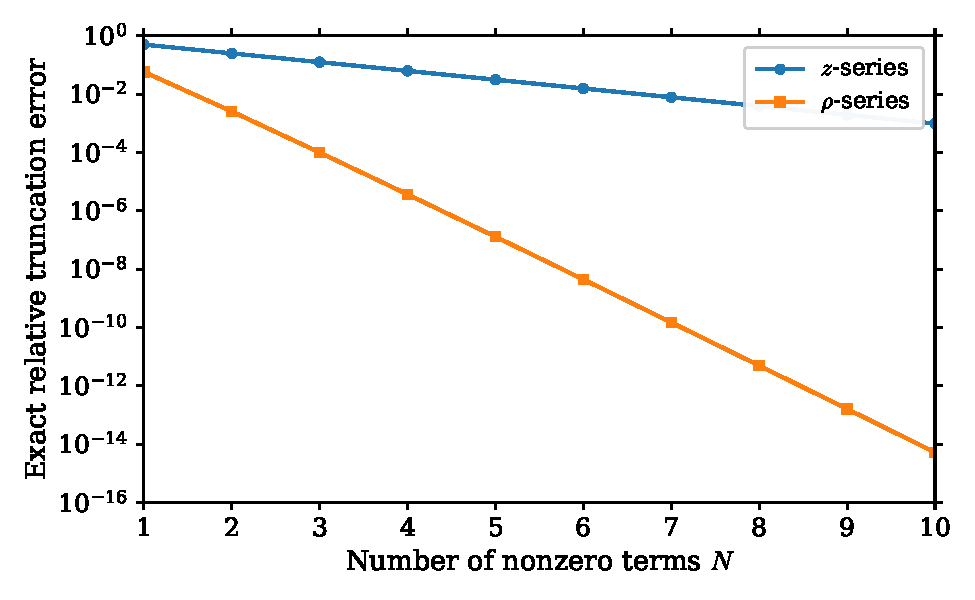
\includegraphics[width=.78\linewidth]{content/AdvancedPhysics/field-theory/figures/geometry-highspin/generated/block_truncation_error.pdf}
 \caption{四维精确标量共形块 $G_{2,0}(1/2,1/2)$ 的相对截断误差。两条曲线直接由 \cref{eq:ghs-exact-block-two-tails} 计算；横轴为各自级数保留的非零项数 $N$，而不是形式上相同的径向级数幂次。}\label{fig:ghs-block-truncation-error}
\end{figure}

对于具有自旋的外算符，角向张量结构的种类还会增长，单个标量 Gegenbauer 系数便不足以描述整个块。此时可在相同的 $\rho$ 径向时间上排列有限维张量结构，并用 Casimir 关系递推其系数 \cite{ghs-costa-radial-spin}。其物理核心并没有改变：共形块依旧是一座由初级态及其全部后裔组成的圆柱能级谱。


\section{共形块的谱表示}
\label{sec:ghs-conformal-block-spectrum}


即使完全知道某个共形初级的维数和自旋，一个四点函数仍不能只由该初级贡献：必须把它的全部平移后裔一并计入。直接逐个写出所有张量分量，随级数增长会迅速变得不可管理。径向量子化的 Hilbert 空间却提供了一个与外场自旋、维度和是否存在相互作用无关的解决办法：把两对算符制备的态投影到同一个不可约共形表示中，再让尺度生成元传播这些态。


\subsection{后裔 Gram 矩阵与物理投影}

设 $\mathcal R_{\Delta,\rho}$ 是由一个标度维数为 $\Delta$、在旋转群 $SO(d)$ 下属于有限维不可约表示 $\rho$ 的初级态产生的共形表示；$\rho$ 可以是对称无迹表示，也可以是混合对称 Young 表示。其 $n$ 级后裔子空间记为 $\mathcal H_n(\mathcal R)$，其中每一个态的尺度本征值都为 $\Delta+n$。

在物理 Hilbert 空间中先模掉所有零范数后裔，然后在每一级选一组线性独立态 $|n,a\rangle$。Gram 矩阵及其逆定义为
\begin{equation}\label{eq:ghs-r4-general-level-gram}
 Q^{(n)}_{ab}=\langle n,a|n,b\rangle,\qquad
 \sum_b(Q^{(n)})^{-1}_{ab}Q^{(n)}_{bc}=\delta_{ac}.
\end{equation}
为看清为什么需要逆 Gram 矩阵，先假设一个二维子空间由两个归一化却不正交的向量 $e_1,e_2$ 张成，令 $\langle e_1,e_2\rangle=c\in\RR$ 且 $|c|<1$。直接算得
\[
 Q=\begin{pmatrix}1&c\\c&1\end{pmatrix},\qquad
 Q^{-1}=\frac1{1-c^2}\begin{pmatrix}1&-c\\-c&1\end{pmatrix}.
\]
所以
\[
 \Pi=\frac{|e_1\rangle\langle e_1|+|e_2\rangle\langle e_2|
 -c|e_1\rangle\langle e_2|-c|e_2\rangle\langle e_1|}{1-c^2}.
\]
将它作用在 $e_1$ 上，分子恰好变成 $(1-c^2)e_1$；作用在 $e_2$ 上也相同。若错误地只加两个秩一算子 $|e_a\rangle\langle e_a|$，则作用在 $e_1$ 上会多出 $c e_2$，根本不是投影。当 $c=\pm1$ 时两向量线性相关，Gram 矩阵奇异，此时须先选取独立的物理向量再求逆。这正是共形表示出现零范数后裔时的线性代数原型。

不要求 $|n,a\rangle$ 本来正交。由 \cref{eq:ghs-ope-gram-projector} 的思想，各级的正交投影为




\begin{equation}\label{eq:ghs-r4-general-projector}
 \Pi_{\mathcal R,n}=\sum_{a,b}|n,a\rangle
 (Q^{(n)})^{-1}_{ab}\langle n,b|,
 \qquad
 \Pi_{\mathcal R}=\sum_{n=0}^\infty\Pi_{\mathcal R,n}.
\end{equation}
当共形表示中的物理后裔在 Hilbert 范数意义下完备时，$\Pi_{\mathcal R}$ 是该表示闭包上的正交投影。这里的级数可以先在有限级截断、再取强算符极限；它并不是将每项当作有限矩阵后无条件直接求和。

任取由两组算符插入制备的径向态 $|\Psi_{12}\rangle$ 和 $|\Psi_{34}\rangle$，令 $t>0$ 为两组插入之间的圆柱时间距离。该表示在四点函数中的贡献，除去固定的外场运动学因子后，具有精确谱形式
\begin{align}\label{eq:ghs-r4-general-block-spectral}
 \mathcal F_{\mathcal R}(t)
 &=\langle\Psi_{34}|\Pi_{\mathcal R}\ee^{-tD}|\Psi_{12}\rangle\\
 &=\sum_{n=0}^\infty\ee^{-t(\Delta+n)}
 \sum_{a,b}\langle\Psi_{34}|n,a\rangle
 (Q^{(n)})^{-1}_{ab}\langle n,b|\Psi_{12}\rangle.
 \notag
\end{align}
式中的态还可能携带插入角度、极化或内部对称性标签；这些变量被保留在矩阵元中，因此此式不局限于四个外标量。这是共形块或多个张量结构组成的共形块矩阵的统一出发点。


在非正交后裔基中，投影必须同时使用 Gram 矩阵及其逆矩阵。
对任何基底向量 $|n,c\rangle$，利用 \cref{eq:ghs-r4-general-level-gram}，
\begin{align*}
 \Pi_{\mathcal R,n}|n,c\rangle
 &=\sum_{a,b}|n,a\rangle(Q^{(n)})^{-1}_{ab}Q^{(n)}_{bc}\\
 &=|n,c\rangle.
\end{align*}
它对该子空间的正交补为零，故 $\Pi_{\mathcal R,n}^2=\Pi_{\mathcal R,n}$，且 $\Pi_{\mathcal R,n}^\dagger=\Pi_{\mathcal R,n}$。又因为 $D|n,a\rangle=(\Delta+n)|n,a\rangle$，有
\begin{equation*}
 \Pi_{\mathcal R,n}\ee^{-tD}=\ee^{-t(\Delta+n)}\Pi_{\mathcal R,n}.
\end{equation*}
把这项关系代入完备投影的和，便直接得到 \cref{eq:ghs-r4-general-block-spectral}。如果某一级 Gram 矩阵奇异，应先去掉物理零范数方向，不能把普通逆矩阵形式地用于奇异矩阵。


对于初级态 $|\mathcal O_a\rangle$，指标 $a$ 表示 $\rho$ 的一个正交归一旋转分量，$M_{\mu\nu}$ 在此空间上有矩阵元 $(M_{\mu\nu})_{ab}$。一级态为 $P_\mu|\mathcal O_a\rangle$。使用 \cref{eq:ghs-conformal-commutators,eq:ghs-radial-generator-adjoint}，直接算得
\begin{align}\label{eq:ghs-r4-spinning-first-gram}
 Q^{(1)}_{\mu a,\nu b}
 &=\langle\mathcal O_a|K_\mu P_\nu|\mathcal O_b\rangle\\
 &=2\Delta\,\delta_{\mu\nu}\delta_{ab}
 -2(M_{\mu\nu})_{ab}.
 \notag
\end{align}
这里取 $\langle\mathcal O_a|\mathcal O_b\rangle=\delta_{ab}$；非单位的初级范数应同时乘入两项。对标量表示，$M_{\mu\nu}=0$，便恢复 \cref{eq:ghs-scalar-level-one-gram}。对更高旋转表示，一阶后裔是向量表示与 $\rho$ 的张量积，Gram 矩阵的不同旋转不可约通道一般有不同本征值。散度通道的本征值随 $\Delta-S-d+2$ 消失，正是高自旋守恒界；因此仅给每一级写一个共同的简并数是不够的。

在更高的 $n$ 级，可选择对称的 $P_{\mu_1}\cdots P_{\mu_n}|\mathcal O_a\rangle$ 作为生成集合，然后反复将所有 $K$ 向右交换。最终得到由 $\Delta$、$SO(d)$ 表示矩阵和 Kronecker 符号构成的有限 Gram 矩阵。这是一种不依赖特定 Lagrangian 的精确构造算法，也是共形块递推的代数基础。


令 $r=\ee^{-t}$，$0<r<1$。\cref{eq:ghs-r4-general-block-spectral} 把共形块写成 $r^{\Delta}$ 乘整数幂级数，但径向展开的收敛不能只用“指数衰减很快”来代替论证。设两个插入态经正的圆柱时间分离后可在 Hilbert 空间中归一，并固定 $0<t_0<t$。若将谱级数在 $n=N-1$ 后截断，则余项为
\begin{equation*}
 \mathscr R_N(t)=\langle\Psi_{34}|\sum_{n\ge N}
 \Pi_{\mathcal R,n}\ee^{-tD}|\Psi_{12}\rangle.
\end{equation*}
由于高阶子空间上的 $D\ge\Delta+N$，利用 Cauchy--Schwarz 不等式可以立即建立
\begin{align}\label{eq:ghs-r4-general-spectral-error}
 |\mathscr R_N(t)|\le{}&\ee^{-(t-t_0)(\Delta+N)}\\
 &\times\|\ee^{-t_0D/2}\Psi_{34}\|
 \;\|\ee^{-t_0D/2}\Psi_{12}\|.
 \notag
\end{align}
指数常数与表示内部的后裔简并数无关。$t_0$ 的作用是保证点状插入导致的态范数奇性已通过正时间传播处理；如果原始两态本来就正常化，可以直接取 $t_0=0$。这一不等式对任意交换旋转表示和任意外场类型成立，但前提是反射正性及所使用的径向时间顺序真实地定义了 Hilbert 空间态。洛伦兹时间解析延拓、插入点跨越 OPE 收敛圆或碰到支切时，不能直接套用此欧氏误差界。


截断误差可用谱下界与正交性直接估计。
令 $\Pi_{\ge N}=\sum_{n\ge N}\Pi_{\mathcal R,n}$。因其与 $D$ 对易，将传播因子分成三段：
\begin{equation*}
 \ee^{-tD}=\ee^{-t_0D/2}\,\ee^{-(t-t_0)D}\,\ee^{-t_0D/2}.
\end{equation*}
把两边 $\ee^{-t_0D/2}$ 吸收到 bra 与 ket 中，再对中间算符使用范数估计
\begin{equation*}
 \|\Pi_{\ge N}\ee^{-(t-t_0)D}\|
 \le\ee^{-(t-t_0)(\Delta+N)}.
\end{equation*}
最后应用 $|\langle u|A|v\rangle|\le\|u\|\|A\|\|v\|$，得到 \cref{eq:ghs-r4-general-spectral-error}。证明中从未假定各级系数非负，因此即使外场混合或共形块为张量结构矩阵，估计仍然成立。


如果外算符都是标量，但各自具有不同维数 $\Delta_i$，由四点函数中提取的距离因子与同维数情形不同。取 $x_{ij}=x_i-x_j$，并定义 $\Delta_{ij}=\Delta_i-\Delta_j$ 与交比
\begin{equation*}
 U=\frac{x_{12}^2x_{34}^2}{x_{13}^2x_{24}^2}=z\bar z,
 \qquad
 V=\frac{x_{14}^2x_{23}^2}{x_{13}^2x_{24}^2}=(1-z)(1-\bar z).
\end{equation*}
约定四点函数的外场距离因子为
\begin{align}\label{eq:ghs-r4-general-fourpoint-prefactor}
 &\langle\mathcal O_1(x_1)\mathcal O_2(x_2)
 \mathcal O_3(x_3)\mathcal O_4(x_4)\rangle\\
 &\quad=\frac{(x_{24}^2/x_{14}^2)^{\Delta_{12}/2}
 (x_{14}^2/x_{13}^2)^{\Delta_{34}/2}}
 {(x_{12}^2)^{(\Delta_1+\Delta_2)/2}
 (x_{34}^2)^{(\Delta_3+\Delta_4)/2}}\,\mathcal G(U,V).
 \notag
\end{align}
这一定义使在各个插入点处的反演权重都等于其标度维数。采用这个规范，二阶 Casimir 微分算符可以写成统一形式。令
\begin{equation}\label{eq:ghs-r4-casimir-external-weights}
 a=-\frac{\Delta_1-\Delta_2}{2},\qquad
 b=\frac{\Delta_3-\Delta_4}{2},\qquad
 \nu=\frac{d-2}{2}.
\end{equation}
定义
\begin{align}\label{eq:ghs-r4-casimir-general-d}
 \mathcal D_{a,b}^{(d)}
 &=\mathcal D_z^{(a,b)}+\mathcal D_{\bar z}^{(a,b)}
 +2\nu\frac{z\bar z}{z-\bar z}
 \bigl[(1-z)\partial_z-(1-\bar z)\partial_{\bar z}\bigr],\\
 \mathcal D_w^{(a,b)}
 &=w^2(1-w)\partial_w^2-(a+b+1)w^2\partial_w-abw.
 \notag
\end{align}
那么交换对称无迹自旋 $S$、维数 $\Delta$ 的共形块满足
\begin{equation}\label{eq:ghs-r4-casimir-general-eq}
 \mathcal D_{a,b}^{(d)}G_{\Delta,S}^{a,b}(z,\bar z)
 =\frac12\bigl[\Delta(\Delta-d)+S(S+d-2)\bigr]
 G_{\Delta,S}^{a,b}(z,\bar z).
\end{equation}
这条方程给出一般 $d$ 维、四个任意维数标量外场的共形块，而不要求每一种维数都有已知的初等超几何闭式解。令 $a=b=0$ 就恢复 \cref{eq:ghs-casimir-differential-operator}。要得到唯一的物理块，仍必须指定相应通道的 OPE 边界条件。若外场自身带自旋，Casimir 不再只作用于一个标量函数，而是作用于若干独立张量结构组成的矩阵值函数；此时 \cref{eq:ghs-r4-general-block-spectral} 是比单个微分方程更稳健的起点 \cite{ghs-dolan-osborn,ghs-costa-radial-spin,ghs-hogervorst}。


对两个不相同的广义自由标量 $A,B$，双粒子态不只包含前文构造的最低扭度 $n=0$ 家族。在去除总平移后裔的独立双体扇区中，还出现
\begin{equation}\label{eq:ghs-r4-generalized-free-doubletrace}
 [AB]_{n,S},\qquad
 \Delta_{n,S}=\Delta_A+\Delta_B+2n+S,
 \qquad n,S\in\NN_0.
\end{equation}
这里 $n$ 计数两粒子相对运动中的径向激发；可以在双体导数多项式空间内按旋转表示和共形 $K_\mu$ 约束逐级正交化，构造相应初级态。$n=0$ 的闭式解就是 \cref{eq:ghs-r4-mixed-primary-coefficients}，其系数见 \cref{eq:ghs-r4-mft-leading-ope}；$n>0$ 的归一化则需要更高导数阶数的 Gram 矩阵。相同实标量的相同粒子交换还要求 $S$ 为偶数。若标量恰好饱和自由场幺正性界，运动方程会进一步产生零范数关系，因而不能把广义自由长表示的全部 $n$ 家族原样保留为独立物理初级。

对于真正相互作用的幺正共形场论，\cref{eq:ghs-r4-generalized-free-doubletrace} 不是每个有限 $S$ 的精确谱定理。一般只能把具有适当谱条件的高自旋家族写作
\begin{equation}\label{eq:ghs-r4-interacting-doubletwist}
 \Delta_{n,S}=\Delta_A+\Delta_B+2n+S+\gamma_{n,S},
\end{equation}
并在可控制的光锥大自旋极限中研究 $\gamma_{n,S}$ 的衰减。是否存在给定 $n$ 的家族、允许哪些内部对称性通道，以及极限如何趋近广义自由数据，均由实际的交叉对称方程决定。无限自旋极限的存在并不替代一个具体相互作用理论中有限自旋 OPE 数据的计算。

由此，径向量子化提供了两个互补的精确入口。若模型具备广义自由因子化，可把高自旋初级、范数和最低扭度系数直接算到底；若只有共形对称和单位性，则使用 Gram 投影与 Casimir 方程保留全部后裔的普适结构。把这两种入口区分开，才能在使用大自旋近似时准确知道哪些是代数定理，哪些是某个模型的动力学输入。


有限自旋共形块的解析形式已经确定，但交叉对称还会约束无限自旋族的累积行为。由此产生的大自旋极限必须同时控制交比与自旋的缩放。


前面自由标量双粒子态的总维数精确等于 $2\delta+S$。如果把它放入相互作用理论，什么量能够延续？单粒子振子模式、两体位置振幅和 Wick 配对通常都不再存在；但自旋 $S$、标度维数 $\Delta$ 及扭度 $\tau=\Delta-S$ 仍是定义良好的共形量子数。由交叉对称控制的大自旋展开，正是对这些普适量所做的计算。


设 $\mathcal X$ 是标度维数为 $\Delta_\mathcal X$ 的标量初级算符。在忽略相互作用的广义自由极限中，两个 $\mathcal X$ 可以组成总自旋 $S$ 的对称无迹双算符；除了分配给自旋的 $S$ 个未收缩导数，还允许 $2n$ 个相对导数发生收缩。算符的形式可以写为
\begin{equation}\label{eq:ghs-double-twist-operator}
 [\mathcal X\mathcal X]_{n,S}
 \sim\mathcal X\,\partial_{(\mu_1}\cdots\partial_{\mu_S)}(\partial^2)^n\mathcal X
 +\text{初级投影所需的其他项},
\end{equation}
其中括号表示对称并去迹。这不是一个已经完成初级投影的定义式，因为导数须重新分配到两个因子上，且要减掉总导数后裔。它明确显示两个标签的意义：$S$ 控制总角动量，$n$ 控制附加的相对激发。广义自由极限的维数为
\begin{equation}\label{eq:ghs-double-twist-tower}
 \Delta_{n,S}^{(0)}=2\Delta_\mathcal X+2n+S,
 \qquad \tau_{n,S}^{(0)}=2\Delta_\mathcal X+2n.
\end{equation}
如果两个外算符相同且为玻色标量，交换两个因子要求 $S$ 为偶数；对不同外算符则无此限制。

把这个结果与 \cref{eq:ghs-spin-energy} 对照可以看出自由局域标量的特殊之处：$\Delta_\chi=\delta$，于是 $n=0$ 的整塔恰好落在 $d-2$ 的幺正性边界。但是 $\chi$ 自身满足 $\partial^2\chi=0$，因此 $n>0$ 的形式表达式可能成为后裔、零范数或与较低算符等价。不能把广义自由场中所有 $n$ 的算符不加筛选地搬到严格自由标量 Hilbert 空间。


把相互作用强度统称为无量纲参数 $g$。给定重整化方案中的一个可以连续追踪的双扭度初级算符，其维数允许写成
\begin{equation}\label{eq:ghs-doubletwist-anomalous-dimension}
 \Delta_{n,S}(g)=2\Delta_\mathcal X(g)+2n+S+\gamma_{n,S}(g).
\end{equation}
这里 $\gamma_{n,S}$ 定义的是相对于两个外标量真实维数之和的附加结合效应，而不是相对于它们的裸经典维数。这样定义可以把单粒子场重整化与真正的两体效应区分开。当多个初级算符具有相同对称性和相近维数时，应先对混合矩阵对角化，再为其本征态赋予 $\gamma_{n,S}$。

一旦 $\gamma_{n,S}\neq0$，则圆柱能量改变 $\Delta E_{n,S}=\hbar c\,\gamma_{n,S}/R$。这是由态—算符对应得到的严格能量差，但不能把 $\gamma_{n,S}$ 直接理解成平直空间两粒子束缚能：圆柱没有平直时空粒子散射的渐近出入态，其尺度 $R$ 也是共形映射所选择的量。


高自旋展开经常用共形自旋而不是裸的整数 $S$ 来组织。对近似双扭度初级态，可定义
\begin{equation}\label{eq:ghs-conformal-spin}
 \mathcal J_{n,S}^2
 =\left(S+n+\Delta_\mathcal X\right)
 \left(S+n+\Delta_\mathcal X-1\right).
\end{equation}
它是双扭度族的主阶共形自旋平方；考虑反常维数后的精确本征值须把相应的半扭度修正纳入。$S\to\infty$ 时 $\mathcal J_{n,S}=S+O(1)$，因此 $1/S$ 与 $1/\mathcal J$ 有相同的领先量级，却在次领先阶给出不同系数。

若某一最低非单位交叉通道初级算符的扭度为 $\tau_*>0$，它对固定 $n$ 的双扭度反常维数常给出
\begin{equation}\label{eq:ghs-large-spin-gamma-scaling}
 \gamma_{n,S}
 =\frac{A_n}{\mathcal J_{n,S}^{\tau_*}}
 +o\!\left(\mathcal J_{n,S}^{-\tau_*}\right).
\end{equation}
$A_n$ 由外算符—交换算符的 OPE 系数及自旋张量结构决定；其符号与适用范围不能仅凭量纲判定。若有多个同扭度交换、简并混合、对数增强或其他交叉通道奇异性，应将相应贡献一起处理。一般定理支持大自旋双扭度谱的存在；\cref{eq:ghs-large-spin-gamma-scaling} 的单幂首项则需要最低扭度交换确实主导的条件，见 \cite{ghs-komargodski,ghs-caronhuot}。


\cref{eq:ghs-free-scalar-fourpoint} 在 $z\to0$ 时可以重写为
\begin{equation}\label{eq:ghs-free-lightcone-limit}
 \mathcal G_\chi(z,\bar z)
 =1+(z\bar z)^\delta
 +\frac{(z\bar z)^\delta}{[(1-z)(1-\bar z)]^\delta}.
\end{equation}
如果在 $z\to0$ 的同时让 $\bar z\to1$，第三项含有 $z^\delta(1-\bar z)^{-\delta}$ 的增强因子。这个双尺度结构不是固定少数个共形块便能够在所有角度区间内一致重建的；在某一通道有限截断自旋后，再取交叉通道的极端极限可能不交换。完整的共形块展开必须允许一座向任意大自旋延伸的谱塔。

这里可以看清两类大自旋极限的联系与差别。前面 $S\to\infty$ 时 $|z_1-z_2|^S$ 出现对径峰，是\emph{特定自由场三点矩阵元的空间鞍点现象}；光锥自举中的 $S\to\infty$ 则来自\emph{不同 OPE 通道必须重建相同四点函数的解析约束}。二者都由高自旋表示控制，但它们是不同的可观测对象，也不共享一个无条件的“对径粒子运动”图像。


Lorentz 型反演公式利用解析延拓后的四点函数双不连续部分（通常记作 $\operatorname{dDisc}$），恢复随自旋解析变化的 OPE 数据。在合适的 Regge 有界条件和收敛自旋范围内，该方法能将交叉通道信息组织为共形块系数的积分表示，并使大共形自旋的系统展开变得明确，参见 \cite{ghs-caronhuot}。

反演公式的输入是经过规范化的四点函数及其解析结构，输出是谱极点和 OPE 系数；它并不能仅从一个自由场双粒子振幅预测某个相互作用 CFT 的反常维数。要把 \cref{eq:ghs-large-spin-gamma-scaling} 的 $A_n$ 算成具体数字，必须再给出交换算符的维数、三点函数数据和所选共形块约定。


无论在自由场还是相互作用场论里，$S$ 都是旋转群表示的标签，决定了某个共形初级态的角动量。它不是一颗基本粒子必须拥有的内禀自旋。对于自由标量双线性流，$S$ 来自两个无自旋基本量子及其相对导数；对于规范理论的单迹高自旋算符，$S$ 也可能来自共变导数沿光锥方向的分配。两类高自旋的算符代数、混合矩阵、反常维数甚至 Hilbert 空间粒子解释都可能不同，不能因为标度维数都大就视为同一类态。

一个可执行的相互作用研究因而应同时说明三个问题：选中的高自旋初级算符属于哪个全局对称性及混合扇区；它的真实 $\Delta_S$ 由怎样的重整化群或自举数据确定；研究的实验或数学可观测量是四点函数、谱密度、算符矩阵元还是理想化球面探测概率。只有明确这些对象，才有可能把自由场的精确计算推广为可信的场论结论。


欧氏共形块的径向展开在收敛域内提供精确表达。若让两个插入点接近光锥，同时取交换自旋很大，就必须重新安排极限次序；这正是从有限自旋的对数奇性过渡到无限塔幂律奇性的原因。


交叉对称要求同一个四点函数能够沿不同的配对顺序展开。若只让两个点在欧氏空间中靠近，固定有限个初级表示的贡献都容易控制；困难出现在两个通道同时逼近各自的奇异边界。这时越来越高的自旋能够抵消越来越小的角距离，因而不能事先固定自旋再取极限。要理解双扭度谱为何出现，必须先看清共形块在双尺度区域中的真实函数形状。


仍取四维相同标量的约定，令 $z\to0$ 且 $0<\bar z<1$ 固定。初级算符的扭度 $\tau=\Delta-S$ 已由 \cref{eq:ghs-twist-definition} 定义，幺正性要求 $S\ge1$ 时 $\tau\ge2$。把 \cref{eq:ghs-four-dimensional-exact-block} 的两项分别展开，$k_{\Delta+S}(z)$ 比 $k_{\Delta-S-2}(z)$ 多出 $z^{S+1}$，得到
\begin{equation}\label{eq:ghs-lightcone-fixed-spin-block}
 G_{\Delta,S}(z,\bar z)
 =\frac{z^{\tau/2}}{2^S}k_{\Delta+S}(\bar z)
 +O\bigl(z^{\tau/2+1}\bigr),
 \qquad z\to0,\quad \bar z\ \text{固定}.
\end{equation}
这里的余项允许依赖 $\bar z,\Delta,S$；不能认为它对 $S\to\infty$ 仍一致有界。\cref{eq:ghs-lightcone-fixed-spin-block} 展示了扭度的物理意义：在光锥极限中控制 $z$ 幂次的是 $\Delta-S$，而自旋对剩余的 $\bar z$ 依赖仍然重要。


\begin{proof}
设 $h_+=(\Delta+S)/2$、$h_-=(\Delta-S-2)/2$。根据超几何级数首项，
\begin{equation*}
k_{\Delta+S}(z)=z^{h_+}[1+O(z)],\qquad
k_{\Delta-S-2}(z)=z^{h_-}[1+O(z)].
\end{equation*}
对固定的 $\bar z>0$，预因子满足 $z\bar z/(z-\bar z)=-z[1+O(z)]$。于是反对称括号中第二项主导，整个表达式的首项为
\begin{align*}
&\frac1{2^S}(-z)\left[-k_{\Delta+S}(\bar z)
z^{(\tau-2)/2}\right]\bigl[1+O(z)\bigr]\\
&\qquad=\frac{z^{\tau/2}}{2^S}k_{\Delta+S}(\bar z)
\bigl[1+O(z)\bigr].
\end{align*}
这说明 \cref{eq:ghs-lightcone-fixed-spin-block} 不是从自由场经验类推而来，而是四维 Casimir 精确解的受控固定自旋渐近。
\end{proof}

若 $\bar z\to1$，令 $y=1-\bar z\to0^+$。函数 $k_{2h}(1-y)$ 可用 Euler 积分表示为
\begin{equation}\label{eq:ghs-lightcone-k-euler}
 k_{2h}(1-y)=\frac{\Gamma(2h)}{\Gamma(h)^2}(1-y)^h
 \int_0^1\frac{[t(1-t)]^{h-1}}{[1-(1-y)t]^h}\,\dd t,
 \qquad h>0.
\end{equation}
这个积分有两个竞争的尺度：$h$ 控制积分核的陡峭程度，$y$ 控制端点附近分母何时变小。取 $h\to\infty$、$y\to0$，同时让 $\xi=2h\sqrt y$ 保持有限，则积分局部化后由第二类修正贝塞尔函数 $K_0(\xi)$ 描述：
\begin{equation}\label{eq:ghs-lightcone-k-bessel}
 k_{2h}(1-y)\sim
 \frac{2\Gamma(2h)}{\Gamma(h)^2}K_0(2h\sqrt y),
 \qquad h\gg1,\quad h\sqrt y=O(1).
\end{equation}
这是一个联合极限，而不是在任意 $y$ 处都准确的全局近似。特别地，$h\sqrt y=O(1)$ 表明对 $S\sim2h\to\infty$，重要角区宽度为 $y=O(S^{-2})$。因此先令 $S$ 固定再送 $y\to0$，与让 $S\sqrt y$ 固定的极限有不同结果。


\begin{proof}
在 \cref{eq:ghs-lightcone-k-euler} 令 $t=1-a/h$，并固定 $a>0$。当 $h\to\infty$ 且 $y=\xi^2/(4h^2)$ 时，核中的主要指数可写为
\begin{equation*}
\left[\frac{t(1-t)}{1-(1-y)t}\right]^h
=\exp\left[-a-\frac{h^2y}{a}+o(1)\right]
\end{equation*}
乘以测度与缓变因子后，主导端点积分按 $a$ 化为
\begin{equation*}
\int_0^\infty\frac{\dd a}{a}
\exp\left[-a-\frac{h^2y}{a}\right]
=2K_0(2h\sqrt y).
\end{equation*}
最后一式来自 $K_0(2\sqrt q)=\tfrac12\int_0^\infty a^{-1}\ee^{-a-q/a}\dd a$。结合 Euler 积分的规范化便得到 \cref{eq:ghs-lightcone-k-bessel}。取 $y\to0$ 的另一条核对途径是比较两边的对数奇性：
\begin{align*}
k_{2h}(1-y)&\sim\frac{\Gamma(2h)}{\Gamma(h)^2}
\left[-\log y+2\psi(1)-2\psi(h)\right],\\
2K_0(2h\sqrt y)&\sim-\log y-2\log h-2\gamma_{\rm E}.
\end{align*}
由于 $\psi(h)=\log h+O(h^{-1})$，二者的首项一致。端点替换需在 $a=0$ 和 $a=\infty$ 外做一致余项控制，故这里所写的是固定 $\xi>0$ 的领先渐近，而不是包含 $\xi=0$ 的统一误差界。
\end{proof}

\begin{figure}[htbp]
\centering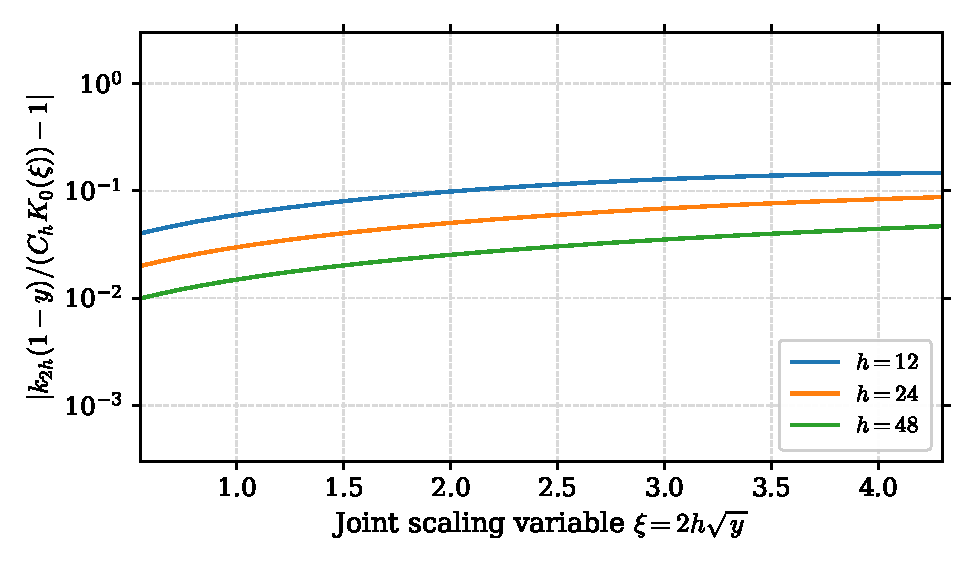
\includegraphics[width=.79\linewidth]{content/AdvancedPhysics/field-theory/figures/geometry-highspin/generated/lightcone_bessel_error.pdf}
\caption{在联合极限 $y=[\xi/(2h)]^2$ 下，精确超几何核 $k_{2h}(1-y)$ 与 $[2\Gamma(2h)/\Gamma(h)^2]K_0(\xi)$ 的相对误差。较大 $h$ 的误差系统下降，验证边界层近似而非固定 $y$ 近似。}\label{fig:ghs-lightcone-bessel-error}
\end{figure}

\cref{fig:ghs-lightcone-bessel-error} 只比较共形块的特定超几何因子；它不是对完整相互作用 CFT 的数值拟合，也不能取代离散高自旋谱的求和控制。


考虑一个明确可计算的模型：高自旋谱密度在连续近似下为 $h^{p-1}$，其中 $p>0$。把单个大自旋块的贝塞尔核心看成 $K_0(2h\sqrt y)$，那么
\begin{equation}\label{eq:ghs-large-spin-bessel-integral}
 \int_0^\infty h^{p-1}K_0(2h\sqrt y)\,\dd h
 =\frac{\Gamma(p/2)^2}{4\,y^{p/2}}.
\end{equation}
右侧在 $y\to0^+$ 发散，而任何固定 $h$ 的核最多只有对数发散。强幂次奇异性恰恰由无界自旋区 $h\sim y^{-1/2}$ 集体贡献。


\begin{proof}
令 $q=\sqrt y$，利用
\begin{equation*}
K_0(2qh)=\frac12\int_0^\infty\frac{\dd t}{t}
\ee^{-t-q^2h^2/t},\qquad h,q,t>0.
\end{equation*}
由于被积函数非负，可以交换积分次序：
\begin{align*}
&\int_0^\infty h^{p-1}K_0(2qh)\dd h\\
&\quad=\frac12\int_0^\infty\frac{\dd t}{t}\ee^{-t}
\int_0^\infty h^{p-1}\ee^{-q^2h^2/t}\dd h\\
&\quad=\frac{\Gamma(p/2)}4q^{-p}
\int_0^\infty t^{p/2-1}\ee^{-t}\dd t\\
&\quad=\frac{\Gamma(p/2)^2}{4q^p}
=\frac{\Gamma(p/2)^2}{4y^{p/2}}.
\end{align*}
最后一次积分即 Gamma 函数定义。该恒等式本身是精确的；在实际共形块中把离散自旋和与 OPE 系数换成这个连续权重，需要额外验证大自旋谱密度、块归一化及误差，因此不能把 $p$ 任意代入就声称得到具体 CFT 的临界指数。
\end{proof}

交叉通道不仅决定领先奇异性，还决定反常维数如何随自旋改变。设某类算符的扭度为 $\tau=\tau_0+\gamma$，则其贡献中的一项满足
\begin{equation}\label{eq:ghs-twist-log-expansion}
 U^{\tau/2}=U^{\tau_0/2}
 \left[1+\frac\gamma2\log U+\frac{\gamma^2}{8}(\log U)^2+O(\gamma^3)\right].
\end{equation}
当在洛伦兹运动学中绕过分支点，$\log U$ 会增加或减少 $2\pi\ii$。两种绕行方式的平均值可以从欧氏原函数中剥离掉，使多重不连续性成为提取交换数据的有力工具。

为了看清该操作，考虑 $y>0$ 处的复函数 $f_\alpha(y)=y^\alpha$，并把绕 $y=0$ 一周后的解析延拓分别写为 $f_\alpha^{\circlearrowleft}=\ee^{2\pi\ii\alpha}f_\alpha$、$f_\alpha^{\circlearrowright}=\ee^{-2\pi\ii\alpha}f_\alpha$。在相同标量的零附加相位约定中，定义
\begin{equation}\label{eq:ghs-ddisc-definition}
 \operatorname{dDisc}[f]
 =f-\frac12f^{\circlearrowleft}-\frac12f^{\circlearrowright}.
\end{equation}
于是
\begin{equation}\label{eq:ghs-ddisc-power}
 \operatorname{dDisc}[y^\alpha]
 =2\sin^2(\pi\alpha)y^\alpha.
\end{equation}
令 $\alpha\to0$，逐项比较该式的 Taylor 系数，得到
\begin{equation}\label{eq:ghs-ddisc-log-check}
 \operatorname{dDisc}[1]=0,\qquad
 \operatorname{dDisc}[\log y]=0,\qquad
 \operatorname{dDisc}[(\log y)^2]=4\pi^2.
\end{equation}
它说明，当支切指数围绕整数值作小扰动时，双不连续性首次感受到指数变化的阶数可能是二阶。但若原有幂次非整数，或外部算符维数带来额外绕行相位，阶数会不同；\cref{eq:ghs-ddisc-log-check} 不能被误读成任何 CFT 的一圈修正都没有双不连续性。

真正的洛伦兹反演公式还包含明确的积分测度、共形核和 Regge 有界性条件。它把交叉通道的双不连续性转换成随自旋解析变化的 OPE 数据，并通过谱极点提取 $\Delta_{n,S}$。这一精确公式的建立需要重新处理洛伦兹区的积分轮廓，不能仅凭 \cref{eq:ghs-ddisc-definition} 代替；其全面形式见 \cite{ghs-caronhuot,ghs-alday-large-spin}。在上述计算中，\cref{eq:ghs-lightcone-fixed-spin-block,eq:ghs-large-spin-bessel-integral,eq:ghs-ddisc-power} 分别解释了扭度的光锥幂次、无穷自旋的集体增强和反常维数产生的分支信息。




\section{相互作用、表示重组与反常维数}
\label{sec:ghs-higher-spin-conservation}


无限多个高自旋守恒流是自由场的强约束。加入相互作用后，哪些守恒律还能保持，哪些后裔会重新成为物理态？这个问题可以不依靠一个完整可解的相互作用模型，而从局域运动方程、两点函数和径向范数出发，先求出守恒律破缺与反常维数之间的逻辑关系。


为了能显式写出算符方程，考虑四维附近的一个实标量模型，欧氏作用量取
\begin{equation}\label{eq:ghs-phi4-action}
 \mathscr I_g[\varphi]=\int\dd^d x\left[
 \frac12(\partial_\mu\varphi)^2
 +\frac{\mu_{\mathrm R}^{\epsilon}g}{4!}\varphi^4\right],
 \qquad d=4-\epsilon.
\end{equation}
其中 $\mu_{\mathrm R}$ 是重整化尺度，$g$ 是无量纲重整化耦合常数。此处公式用来展示微扰理论的局域结构；一般 $g\neq0$ 时不能先假定该模型恰是 CFT。只有在满足 $\beta(g_*)=0$ 的临界不动点，才可以将算符组织为相互作用共形初级表示。

忽略接触项和算符重整化暂时引入的细节，作用量变分得到经典运动方程
\begin{equation}\label{eq:ghs-phi4-eom}
 \partial^2\varphi=\frac{\mu_{\mathrm R}^\epsilon g}{3!}\varphi^3.
\end{equation}
在自由理论，右侧为零，正是前面高自旋守恒流成立的关键。当 $g\ne0$，对由多个导数组成的高自旋流求散度时，运动方程会将一部分项变成包含三个或更多场的复合算符。因而对 $S>2$ 的一般高自旋流，有形式
\begin{equation}\label{eq:ghs-broken-higher-spin-current}
 \partial^{\mu_1}J^{(S)}_{\mu_1\cdots\mu_S}
 =g\,\mathcal K^{(S-1)}_{\mu_2\cdots\mu_S}+O(g^2),
\end{equation}
其中 $\mathcal K^{(S-1)}$ 是与选定理论和重整化方案有关的复合算符；式中的 $g$ 已把合适的 $\mu_{\mathrm R}^\epsilon$ 因子吸收到 $\mathcal K$ 的约定中。此式只陈述弱耦合下可连续追踪的高自旋流的局域非守恒关系，不给未经计算的 $\mathcal K$ 系数。


对任意幺正共形场论 的一阶矢量初级算符 $J_\mu$，设其二点函数为
\begin{equation}\label{eq:ghs-vector-two-point}
 \langle J_\mu(x)J_\nu(0)\rangle
 =\frac{C_J}{(x^2)^\Delta}
 I_{\mu\nu}(x),\qquad
 I_{\mu\nu}(x)=\delta_{\mu\nu}-2\frac{x_\mu x_\nu}{x^2}.
\end{equation}
$C_J>0$ 是选定张量归一化后的二点函数系数。利用 $\partial_\mu x^\mu=d$ 和 $x^\mu I_{\mu\nu}=-x_\nu$，可直接求一次散度：
\begin{equation}\label{eq:ghs-vector-divergence-identity}
 \partial_x^\mu\langle J_\mu(x)J_\nu(0)\rangle
 =2C_J(\Delta-d+1)\frac{x_\nu}{(x^2)^{\Delta+1}}.
\end{equation}
若 $\Delta=d-1$，相关函数在非重合点处严格横向。这不是自旋一偶然出现的代数巧合，而是短表示散度后裔范数为零在位置空间的对应物。



\begin{proof}
先直接计算张量求导
\begin{align*}
\partial_x^\mu I_{\mu\nu}(x)
&=-2\partial_x^\mu\frac{x_\mu x_\nu}{x^2}
=-2(d-1)\frac{x_\nu}{x^2},\\
I_{\mu\nu}(x)\partial_x^\mu(x^2)^{-\Delta}
&=-2\Delta(x^2)^{-\Delta-1}x^\mu I_{\mu\nu}
=2\Delta\frac{x_\nu}{(x^2)^{\Delta+1}}.
\end{align*}
两项相加即为 \cref{eq:ghs-vector-divergence-identity}。第二个插入点 $y$ 的导数在平移不变的函数上满足 $\partial_y=-\partial_x$，因此
\begin{align*}
&\langle(\partial\cdot J)(x)(\partial\cdot J)(0)\rangle\\
&=-2C_J(\Delta-d+1)\partial_x^\nu
\left[\frac{x_\nu}{(x^2)^{\Delta+1}}\right]\\
&=2C_J(\Delta-d+1)(2\Delta+2-d)
\frac1{(x^2)^{\Delta+1}},\qquad x\ne0.
\end{align*}
这里 $x=0$ 的接触项需要单独进行分布论处理，不参与非重合点两点函数的比较。
\end{proof}

现在取 $\Delta=d-1+\gamma_1$，得到
\begin{equation}\label{eq:ghs-vector-divergence-gamma}
 \langle(\partial\cdot J)(x)(\partial\cdot J)(0)\rangle
 =2C_J\gamma_1(d+2\gamma_1)
 (x^2)^{-d-\gamma_1}.
\end{equation}
只要 $\gamma_1>0$，散度态取得非零范数。高自旋 $S>1$ 的相应张量公式带有依赖 $S,d$ 与投影约定的正系数，但在幺正界附近都含有 $\Delta_S-(S+d-2)$ 这一线性因子。由此可以通过计算非守恒算符的二点函数，间接确定高自旋反常维数。


在一个存在连续弱耦合共形固定点的模型中，假设自由流 $J_S^{(0)}$ 的散度严格为零，而破缺方程起始于 $\partial\cdot J_S=g\mathcal K_S+O(g^2)$。两边的二点函数在领先阶满足
\begin{equation}\label{eq:ghs-broken-current-norm-scaling}
 \langle(\partial\cdot J_S)(x)(\partial\cdot J_S)(0)\rangle
 =g^2\langle\mathcal K_S(x)\mathcal K_S(0)\rangle_{g=0}
 +O(g^3).
\end{equation}
另一方面，共形二点函数的张量求导必含 $\gamma_S=\Delta_S-(S+d-2)$。若右侧自由理论的 $\mathcal K_S$ 具有有限非零范数、没有导致阶数改变的混合或额外小参数，便得到
\begin{equation}\label{eq:ghs-broken-current-gamma-order}
 \gamma_S=O(g^2).
\end{equation}
这个推理说明量级来自两次非守恒插入，并未计算出 $g^2$ 的数值系数。若相互作用本身已经使算符在一阶混合，或所讨论的流不是自由理论的守恒短表示，就不能用这一估计。对于四维附近的 Wilson--Fisher 固定点，$g_*=O(\epsilon)$，因此典型非保护高自旋流的维数偏移从 $O(\epsilon^2)$ 开始；真正数值系数仍须进行算符重整化或非守恒二点函数计算。


平移不变性保证存在经适当改进及重整化的应力张量 $T_{\mu\nu}$，其局域 Ward 恒等式使 $\partial^\mu T_{\mu\nu}$ 在非重合相关函数中为零。在幺正共形固定点，其标度维数被保护为 $\Delta_T=d$。因此 $S=2$ 时
\begin{equation}\label{eq:ghs-stress-tensor-protection}
 \Delta_T=d,
 \qquad\gamma_T\equiv\Delta_T-(d-2+2)=0.
\end{equation}
这与通常的 $S=4,6,\ldots$ 高自旋流可以获得 $\gamma_S>0$ 形成鲜明对比。若自旋一流是精确内部全局对称性的 Noether 流，它的维数同样由 $\Delta_{J_1}=d-1$ 保护。某种流是否守恒，最终取决于真实的对称性及其 Ward 恒等式，而不是它包含的导数数目。


某个高自旋流若精确守恒，其表面荷不仅改变局域算符，还会对更高相关函数施加强 Ward 恒等式。不同高自旋荷之间的闭合关系可迫使更多高自旋流存在，在适当条件下甚至固定一整类相关函数。已知的三维高自旋约束定理表明：在特定单位性、唯一应力张量与相关谱条件下，一个自旋大于二的守恒流会使应力张量及高自旋流相关函数具有自由场结构，参见 \cite{ghs-maldacena-zh,ghs-alba-diab}。这些结论的维数及附加假设很重要，不能简单升级成“任何理论中出现一条守恒高自旋流就意味着所有自由度都不相互作用”。

若高自旋对称性仅在大 $N$ 理论中近似成立，则流的散度和反常维数可以按 $1/N$ 系统组织；一些三维 Chern--Simons 物质理论就是这种研究范式，参见 \cite{ghs-maldacena-zh-broken}。此时“近似守恒”是有控制参数的近似，而不仅是声称高自旋荷受到微小破坏。


共形场论与反德西特空间之间的谱对应把边界初级维数和自旋映射到体场的质量、能级和旋转表示。若某个高自旋流的维数恰好饱和守恒界，体对偶中往往对应具有规范冗余的无质量高自旋场；当该维数离开幺正界，相应表示改变。这个联系有严格的表示论基础，但具体的体理论及其相互作用不能仅由本讲义的自由标量 Fock 态构造决定。讨论高自旋引力、弦谱或高能散射时还需要补充大 $N$、谱隙、单迹算符等假设。

自由高自旋双粒子态最稳定的贡献，是提供了一套可逐式核验的短表示基准：在这个基准上，能量、三点函数、双体矩阵元、单体模式谱以及大自旋渐近都能显式计算。加入相互作用以后，这些对象有的保持纯粹运动学定义，有的必须重新由 CFT 数据或重整化决定。沿着二点函数—三点函数—四点函数的顺序逐步替换自由计算，才是从特殊模型通向一般高自旋量子场论的可靠路径。


\subsection{内部对称性与奇自旋流}

单个实标量只产生偶数自旋双线性初级态，并不意味着自由场中不存在奇自旋守恒流。真正使奇自旋算符消失的，是两个场既为玻色子、又属于同一物理分量的交换对称性。引入多个场分量以后，同一个共形初级递推式便可以同时产生偶数与奇数自旋，而且奇自旋的最低例子正是熟悉的内部对称性 Noether 流。


设 $\varphi^a(x)$，$a=1,\ldots,N$，为 $N$ 个彼此独立的无质量实标量场，欧氏作用量
\begin{equation}\label{eq:ghs-flavor-free-action}
 \mathscr I_N=\frac12\sum_{a=1}^N\int\dd^d x\,(\partial_\mu\varphi^a)^2,
 \qquad\langle\varphi^a(x)\varphi^b(0)\rangle
 =\delta^{ab}\frac{C_d}{|x|^{2\delta}}.
\end{equation}
所有场的球谐能量都是 $\ell+\delta$，但每个球谐模式多了一个内部指标，产生算符满足
\begin{equation}\label{eq:ghs-flavor-fock-commutator}
 [b_{k,a},b_{j,b}^\dagger]=\delta_{kj}\delta_{ab},
 \qquad[b_{k,a},b_{j,b}]=0.
\end{equation}
这里 $a$ 是内部对称性标签，不是球面的简并指标；$k$ 仍表示前面固定复极化方向的最高权模式。


沿用 \cref{eq:ghs-primary-coefficients} 中的系数，定义带两个内部指标的双线性算符
\begin{equation}\label{eq:ghs-flavor-high-spin-bilinear}
 J_S^{ab}(x;\vb\varepsilon)=
 \sum_{k=0}^S c_k:
 (D_+^k\varphi^a)(D_+^{S-k}\varphi^b):(x).
\end{equation}
由 $c_{S-k}=(-1)^S c_k$ 和玻色正规序交换性，直接更换求和指标 $k\mapsto S-k$，有
\begin{equation}\label{eq:ghs-flavor-exchange-parity}
 J_S^{ba}=(-1)^S J_S^{ab}.
\end{equation}
因此偶数自旋属于内部指标的对称张量，奇数自旋属于反对称张量。对偶数 $S$，$J_S^{ab}$ 还可分成迹 $\delta_{ab}J_S^{ab}$ 与对称无迹部分；对奇数 $S$，只有反对称内部表示。

如果强制 $a=b$，那么 \cref{eq:ghs-flavor-exchange-parity} 在奇数 $S$ 时给出 $J_S^{aa}=-J_S^{aa}=0$。这正是原先单个实标量结果的完整原因，而不是一般场论中对奇自旋的禁戒定理。


取 $S=1$，由 $c_0=1$、$c_1=-1$，
\begin{equation}\label{eq:ghs-flavor-spin-one-current}
 J_1^{ab}(x;\vb\varepsilon)
 =:\!\varphi^aD_+\varphi^b-\varphi^bD_+\varphi^a\!:.
\end{equation}
恢复任意方向的矢量指标，得到
\begin{equation}\label{eq:ghs-on-current}
 j_\mu^{ab}=:\!\varphi^a\partial_\mu\varphi^b-\varphi^b\partial_\mu\varphi^a\!:.
\end{equation}
它满足 $j_\mu^{ab}=-j_\mu^{ba}$。直接求散度：
\begin{align*}
 \partial^\mu j_\mu^{ab}
 &=:\!(\partial^\mu\varphi^a)(\partial_\mu\varphi^b)
 +\varphi^a\partial^2\varphi^b\\
 &\qquad-(\partial^\mu\varphi^b)(\partial_\mu\varphi^a)
 -\varphi^b\partial^2\varphi^a\!:\\
 &=:\!\varphi^a\partial^2\varphi^b-\varphi^b\partial^2\varphi^a\!:=0.
\end{align*}
其中第一与第三项直接相消，第二与第四项由各分量的自由运动方程消失。这个流的维数为 $d-1$，正好饱和 \cref{eq:ghs-spin-unitarity-bound-extended} 的自旋一界。它也是自由 $O(N)$ 内部旋转对称性的 Noether 流。


对原始场作跨顶点 Wick 收缩，定义 $W_i=(\vb\varepsilon\cdot x_i)/|x_i|^2$，得到
\begin{align}\label{eq:ghs-flavor-threepoint}
 &\langle\varphi^a(x_1)\varphi^b(x_2)J_S^{cd}(0;\vb\varepsilon)\rangle\\
 &\quad=\frac{2^SC_d^2(\delta)_S}{|x_1|^{2\delta}|x_2|^{2\delta}}
 \bigl[\delta^{ac}\delta^{bd}(W_2-W_1)^S
 +\delta^{ad}\delta^{bc}(W_1-W_2)^S\bigr].\notag
\end{align}
交换两个外标量同时交换 $x_1\leftrightarrow x_2$、$a\leftrightarrow b$，结果不变。交换流的内部指标 $c\leftrightarrow d$，则按 $(-1)^S$ 改变符号，与 \cref{eq:ghs-flavor-exchange-parity} 一致。令 $a=b=c=d$ 时，偶数 $S$ 恢复 \cref{eq:ghs-scalar-scalar-spin-3pt} 的未归一形式，而奇数 $S$ 严格为零。


设 $a\neq b$，固定一对不同的内部指标。用 \cref{eq:ghs-local-derivative-state}，有
\begin{equation}\label{eq:ghs-flavor-fock-state}
 |J_S^{ab}\rangle
 =\sum_{k=0}^S B_k b_{k,a}^\dagger b_{S-k,b}^\dagger|0\rangle,
 \qquad B_k=c_kF_kF_{S-k}.
\end{equation}
因为两类量子带有不同内部指标，其内积只允许同一种 flavor 的湮灭与产生配对，不能再把两种玻色配对都计算进来。因此
\begin{equation}\label{eq:ghs-flavor-norm}
 \|J_S^{ab}|0\rangle\|^2
 =\sum_{k=0}^S|B_k|^2
 =2^{2S}C_d^2S!(2\delta+S-1)_S,
 \qquad a\ne b.
\end{equation}
当 $a=b$ 且 $S$ 偶数，恢复的第二种配对使范数增加为上述结果的两倍，即 \cref{eq:ghs-operator-norm}。这一因子二不是归一化习惯引起的任意调整，而是相同与不同场分量的 Wick 收缩数真正不同。

在 $N\ge2$ 的自由场中，奇数自旋流因而也是具有有限正范数的独立圆柱初级态。它们仍然满足 $\Delta_S=S+d-2$，散度后裔仍然零范数。在带相互作用的 $O(N)$ 临界场论中，内部自旋一对称性流可继续受到 Ward 恒等式保护；一般更高自旋流则未必守恒。




算符不守恒的结构可以由局域运动方程看见，但反常维数的数值还需要动力学。接下来在四维附近的标量相互作用中计算耦合的尺度依赖，再把固定点的结果与共形表示条件比较。




前面说明：若守恒高自旋流在微扰下被破坏，其维数可以离开幺正界。但只有给出具体的重整化群流，才知道这种相互作用是否存在共形不动点，以及那个不动点怎样与自由理论连接。四维附近的 $\varphi^4$ 模型提供了一个最小的计算例子：不用先求高阶相关函数，就能从一圈四点图直接找出弱耦合固定点。


前面的球面谐函数和正范数 Hilbert 空间构造以整数 $d>2$ 为几何维数。以下的 $d=4-\epsilon$ 是微扰积分的维数解析延拓：$\epsilon$ 可以连续取值，但这并不意味着在非整数维存在一套按通常几何意义定义的球面 $S^{d-1}$ 及其普通 $SO(d)$ 不可约表示。解析延拓的 Gamma 函数恒等式仍可使用；表示论中的反射正性陈述则应在适当的整数维理论中解释。


\subsection{受控不动点与领先反常维数}

将维数解析延拓为 $d=4-\epsilon$，其中 $0<\epsilon\ll1$ 是调节紫外发散及控制微扰固定点的小参数。自旋 $S$ 仍是非负整数，两者是完全不同的参数。自由标量的经典维数为 $\delta=(d-2)/2=1-\epsilon/2$；$\varphi^4$ 的耦合在 $d$ 维具有长度量纲 $\epsilon$，故取重整化尺度 $\mu_{\mathrm R}$ 后将顶点写为 $\mu_{\mathrm R}^\epsilon g\varphi^4/4!$。

为避免无质量四点函数在特定外动量处出现红外发散，可以暂时用 $m>0$ 作为积分中的红外辅助量，在抽取紫外发散后再处理 $m\to0$。这不意味着最终临界 CFT 中仍有非零物理质量。


四个外标量的 $s$、$t$、$u$ 三种交换通道都产生同一个二传播子积分。选取其中一个外部欧氏动量 $q$，定义
\begin{equation}\label{eq:ghs-phi4-bubble}
 B_d(q,m)=\int\frac{\dd^dp}{(2\pi)^d}
 \frac1{(p^2+m^2)[(p+q)^2+m^2]}.
\end{equation}
用 Feynman 参数 $1/(AB)=\int_0^1\dd x\,[xA+(1-x)B]^{-2}$ 合并分母，并平移积分变量 $p\mapsto p+(1-x)q$，得到
\begin{equation}\label{eq:ghs-phi4-bubble-feynman-param}
 B_d(q,m)=\frac{\Gamma(2-d/2)}{(4\pi)^{d/2}}
 \int_0^1\dd x\,[m^2+x(1-x)q^2]^{d/2-2}.
\end{equation}
代入 $d=4-\epsilon$，有 $\Gamma(\epsilon/2)=2/\epsilon-\gamma_E+O(\epsilon)$，因此紫外极点与 $q,m$ 无关：
\begin{equation}\label{eq:ghs-phi4-bubble-pole}
 B_{4-\epsilon}(q,m)=\frac1{8\pi^2\epsilon}+O(1).
\end{equation}
这正是局域重整化的必要性质：一个不含外部动量的极点，可以由原作用量中同一形式的局域 $\varphi^4$ 顶点抵消。



\begin{proof}
从欧氏高斯积分恒等式
\begin{equation*}
\int\frac{\dd^dp}{(2\pi)^d}\frac1{(p^2+M^2)^\alpha}
=\frac{\Gamma(\alpha-d/2)}{(4\pi)^{d/2}\Gamma(\alpha)}(M^2)^{d/2-\alpha}
\end{equation*}
取 $\alpha=2$、$M^2=m^2+x(1-x)q^2$，立刻得到 \cref{eq:ghs-phi4-bubble-feynman-param}。每个泡图有交换两个内部传播子的对称因子 $1/2$；共有三个 $s,t,u$ 通道。因此所有一圈顶点图的极点系数为
\begin{equation*}
\frac32 g^2 B_d\big|_{\rm pole}
=\frac{3g^2}{16\pi^2\epsilon}.
\end{equation*}
这里已将顶点共同的 $\mu_{\mathrm R}$ 幂因子按无量纲耦合的定义配平。最小减除中的四点反项因此取
\begin{equation*}
\delta g=\frac{3g^2}{16\pi^2\epsilon}+O(g^3).
\end{equation*}
\end{proof}

用最小减除方案写 $g_0=\mu_{\mathrm R}^\epsilon Z_g(g,\epsilon)g$，并在一圈近似取
\begin{equation}\label{eq:ghs-phi4-coupling-renormalization}
 Z_gg=g+\frac{3g^2}{16\pi^2\epsilon}+O(g^3).
\end{equation}
裸耦合 $g_0$ 不随 $\mu_{\mathrm R}$ 变，定义 $\beta(g)=\mu_{\mathrm R}\,\dd g/\dd\mu_{\mathrm R}|_{g_0}$，于是
\begin{align*}
 0&=\mu_{\mathrm R}\frac{\dd g_0}{\dd\mu_{\mathrm R}}
 =\mu_{\mathrm R}^\epsilon\left[
 \epsilon\left(g+\frac{3g^2}{16\pi^2\epsilon}\right)
 +\beta(g)\left(1+\frac{6g}{16\pi^2\epsilon}\right)\right]+O(g^3).
\end{align*}
将 $\beta(g)=-\epsilon g+bg^2+O(g^3)$ 代回，$g^2$ 系数为 $b+3/(16\pi^2)-6/(16\pi^2)$，从而
\begin{equation}\label{eq:ghs-phi4-beta-function}
 \beta(g)=-\epsilon g+\frac{3g^2}{16\pi^2}+O(g^3).
\end{equation}
除自由固定点 $g=0$ 外，存在微扰固定点
\begin{equation}\label{eq:ghs-wilson-fisher-fixed-point}
 g_*=\frac{16\pi^2}{3}\epsilon+O(\epsilon^2).
\end{equation}
当 $\epsilon>0$ 足够小，它位于微扰理论可控制的区域。虽然真实三维对应 $\epsilon=1$，在那里不能把有限阶 $\epsilon$ 展开自动视为高精度近似，但这个固定点的存在让研究相互作用高自旋算符有了明确目标。


在该固定点附近，把自旋 $S\ge4$ 的一个已对角化高自旋初级算符维数写为
\begin{equation}\label{eq:ghs-wf-current-dimension}
 \Delta_S(g_*)=S+d-2+\gamma_S(g_*).
\end{equation}
自由理论的 $\gamma_S(0)=0$；若对应非守恒方程的最早项是 $O(g)$，前文的范数分析说明典型 $\gamma_S(g_*)=O(\epsilon^2)$。因此相应圆柱态的激发能量为
\begin{equation}\label{eq:ghs-wf-cylinder-energy}
 E_{S,\rm phys}=
 \frac{\hbar c}{R}\left[S+2-\epsilon+\gamma_S(g_*)\right].
\end{equation}
这是把高自旋维数转化为实际圆柱能量的直接结果。若要继续求 $\gamma_S$ 的系数，必须计算该流的重整化混合矩阵，或将其非守恒方程及二点函数规范化，不能用一圈 $\beta$ 函数的数值直接替代。

从这个例子可以看到高自旋问题在量子场论中为何重要：一个自由标量的简单双线性算符，在相互作用临界点变成可通过重整化群、幺正性和自举三种独立方法约束的谱数据。自旋为二的应力张量仍被守恒 Ward 恒等式保护，其余高自旋通常获得可计算的维数偏移；在大自旋处，这些偏移又受到交叉通道扭度结构的约束。


前文通过一圈重整化群计算，找到了四维附近 $\varphi^4$ 理论的非平凡固定点。不过，固定点存在还不能告诉我们一个局域算符的维数到底移动了多少。高自旋流的散度范数提供了一个更直接的测量方法：自由极限中的零范数后裔，在相互作用下获得一个可计算的正范数。这一章先把最简单的基本场异常维数真正计算出来，再用同一逻辑说明高自旋谱如何受到非守恒方程、应力张量保护和大自旋自举的共同约束。


继续取 \cref{eq:ghs-phi4-action} 的作用量和 \cref{eq:ghs-phi4-beta-function} 的最小减除约定，$d=4-\epsilon$、$0<\epsilon\ll1$。临界固定点的耦合为 $g_*=16\pi^2\epsilon/3+O(\epsilon^2)$。在自由标量理论中，$\partial^2\varphi=0$ 是零范数后裔关系；相互作用固定点的算符运动方程改写为
\begin{equation}\label{eq:ghs-wf-eom-renormalized}
 \partial^2\varphi(x)=\frac{\mu_{\mathrm R}^{\epsilon}g_*}{3!}[\varphi^3](x),
\end{equation}
其中方括号代表已按运动方程规范化的重整化复合算符，接触项由合适的算符定义处理。在这个等式中，$[\varphi^3]$ 不再作为与 $\varphi$ 完全独立的共形初级表示出现；它成为 $\varphi$ 初级表示的二级后裔。这种由短表示恢复成长表示的过程称为多重态重组 \cite{ghs-rychkov-tan}。

设基本场维数为
\begin{equation}\label{eq:ghs-wf-phi-delta}
 \Delta_\varphi=\frac{d-2}{2}+\gamma_\varphi,
\end{equation}
其中 $\gamma_\varphi$ 是相对于当前维度自由场临界值的偏移。因为标量幺正性界是 $(d-2)/2$，$\gamma_\varphi$ 也是原本的零范数后裔重新取得正范数的参数。我们希望算出它的领先阶，而不是只从自旋守恒式猜测 $O(\epsilon^2)$。


在非重合点，把基本场二点函数写为
\begin{equation}\label{eq:ghs-wf-phi-two-point}
 \langle\varphi(x)\varphi(0)\rangle=\frac{C_\varphi}{(x^2)^{\Delta_\varphi}},
\end{equation}
其中 $C_\varphi=C_4+O(\epsilon)$ 且自由四维归一化为 $C_4=1/(4\pi^2)$。为求两侧都加上拉普拉斯的相关函数，先使用任意 $\lambda$ 的恒等式
\begin{equation}\label{eq:ghs-wf-laplacian-power}
 \partial_x^2 (x^2)^{-\lambda}
 =4\lambda\left(\lambda+1-\frac d2\right)(x^2)^{-\lambda-1},\quad x\ne0.
\end{equation}
式中右侧必须在非重合点理解。取 $\lambda=\Delta_\varphi$ 再作用一次拉普拉斯，得到
\begin{align}\label{eq:ghs-wf-double-laplacian}
 &\langle(\partial^2\varphi)(x)(\partial^2\varphi)(0)\rangle\\
 &\quad=16C_\varphi\Delta_\varphi(\Delta_\varphi+1)
 \left(\Delta_\varphi+1-\frac d2\right)
 \left(\Delta_\varphi+2-\frac d2\right)
 (x^2)^{-\Delta_\varphi-2}.\notag
\end{align}
这里第二个插入点的两个导数可转为对 $x$ 的两个导数，因为平移不变性给出 $\partial_{0\mu}=-\partial_{x\mu}$，负号成对抵消。代入 \cref{eq:ghs-wf-phi-delta}，第一个括号变为 $\gamma_\varphi$；因此左侧在自由极限消失，正是零范数条件的定量形式。


在固定点，\cref{eq:ghs-wf-eom-renormalized} 把同一相关函数写成
\begin{equation}\label{eq:ghs-wf-eom-two-point}
 \langle(\partial^2\varphi)(x)(\partial^2\varphi)(0)\rangle
 =\frac{\mu_{\mathrm R}^{2\epsilon}g_*^2}{36}
 \langle[\varphi^3](x)[\varphi^3](0)\rangle.
\end{equation}
由于右侧已带 $g_*^2=O(\epsilon^2)$，只需将复合算符二点函数取自由四维的领先值。非重合点的六个场按 Wick 定理有 $3!=6$ 种跨点配对：
\begin{equation}\label{eq:ghs-wf-phi3-free-wick}
 \langle:\!\varphi^3(x)\!:\,:\!\varphi^3(0)\!:\rangle_{0,d=4}
 =\frac{6 C_4^3}{(x^2)^3}.
\end{equation}
在适当固定的无量纲尺度 $\mu_{\mathrm R}|x|=O(1)$ 下，$\mu_{\mathrm R}^{2\epsilon}$ 和幂指数的 $O(\epsilon)$ 差别只在下一阶影响最终系数。比较 \cref{eq:ghs-wf-double-laplacian,eq:ghs-wf-eom-two-point} 的 $O(\epsilon^2)$ 项，得到
\begin{equation}\label{eq:ghs-wf-phi-anomalous-from-eom}
 32C_4\gamma_\varphi
 =\frac{g_*^2}{6}C_4^3+O(\epsilon^3),
 \qquad
 \gamma_\varphi=\frac{g_*^2 C_4^2}{192}+O(\epsilon^3).
\end{equation}
最后代入 $C_4=1/(4\pi^2)$ 与 $g_*=16\pi^2\epsilon/3+O(\epsilon^2)$，得到
\begin{equation}\label{eq:ghs-wf-phi-gamma-result}
 \gamma_\varphi=\frac{\epsilon^2}{108}+O(\epsilon^3),
 \qquad \eta_{\rm crit}\equiv2\gamma_\varphi=\frac{\epsilon^2}{54}+O(\epsilon^3).
\end{equation}
$\eta_{\rm crit}$ 是临界二点函数的异常指数；前文球面几何中的 $\eta=\vb n\cdot\vb n'$ 则是方向余弦，两者属于不同的数学对象。



\begin{proof}
对 $F_\lambda(x)=(x^2)^{-\lambda}$，用 $\partial_\mu x^2=2x_\mu$，
\begin{align*}
\partial_\mu F_\lambda&=-2\lambda x_\mu(x^2)^{-\lambda-1},\\
\partial^2F_\lambda&=-2\lambda d(x^2)^{-\lambda-1}
+4\lambda(\lambda+1)x^2(x^2)^{-\lambda-2}\\
&=4\lambda(\lambda+1-d/2)F_{\lambda+1}.
\end{align*}
将 $\lambda\mapsto\lambda+1$ 再用一次，即出现 \cref{eq:ghs-wf-double-laplacian} 的四个线性因子。取 $\lambda=\delta+\gamma_\varphi$，$\delta=d/2-1$，四个因子在 $d\to4$ 时分别趋近 $1,2,\gamma_\varphi,1$，所以左侧领先系数为 $16\times1\times2\times\gamma_\varphi\times1=32\gamma_\varphi$。

与此同时，运动方程中的 $1/3!$ 在二点函数中平方为 $1/36$，Wick 跨点的 $3!$ 配对将其变为 $6/36=1/6$。于是
\begin{align*}
\gamma_\varphi
&=\frac{g_*^2}{32\cdot6}\frac{C_4^3}{C_4}+O(\epsilon^3)
=\frac{g_*^2}{192(4\pi^2)^2}+O(\epsilon^3)\\
&=\frac{(16\pi^2\epsilon/3)^2}{192\cdot16\pi^4}
+O(\epsilon^3)
=\frac{\epsilon^2}{108}+O(\epsilon^3).
\end{align*}
由此可见，$\pi$ 与重整化耦合中的归一化完全抵消。若把作用量的顶点改为 $g\varphi^4/4$ 等约定，必须先转换耦合，不能将同一个 $g_*$ 数字直接代入。
\end{proof}

自由四维单实标量只有偶数自旋的双线性守恒流。对连续追踪到 Wilson--Fisher 固定点的非保护偶数自旋 $S\ge4$，其维数写为 $\Delta_S=S+d-2+\gamma_S$。通过非守恒流的相关函数或共形乘积数据，可以得到领先结果 \cite{ghs-giombi-kirilin,ghs-roumpedakis-spin}：
\begin{equation}\label{eq:ghs-wf-higher-spin-anomalous-result}
 \gamma_S=\frac{\epsilon^2}{54}
 \left(1-\frac{6}{S(S+1)}\right)+O(\epsilon^3),
 \qquad S=4,6,8,\ldots.
\end{equation}
与 \cref{eq:ghs-wf-phi-gamma-result} 不同，\cref{eq:ghs-wf-higher-spin-anomalous-result} 的有限自旋系数引用了已发表的完整高自旋非守恒计算；不能把仅有的 $\beta$ 函数和 $\gamma_\varphi$ 推导假称已经独立算出这整个 $S$ 依赖。

\begin{figure}[htbp]
\centering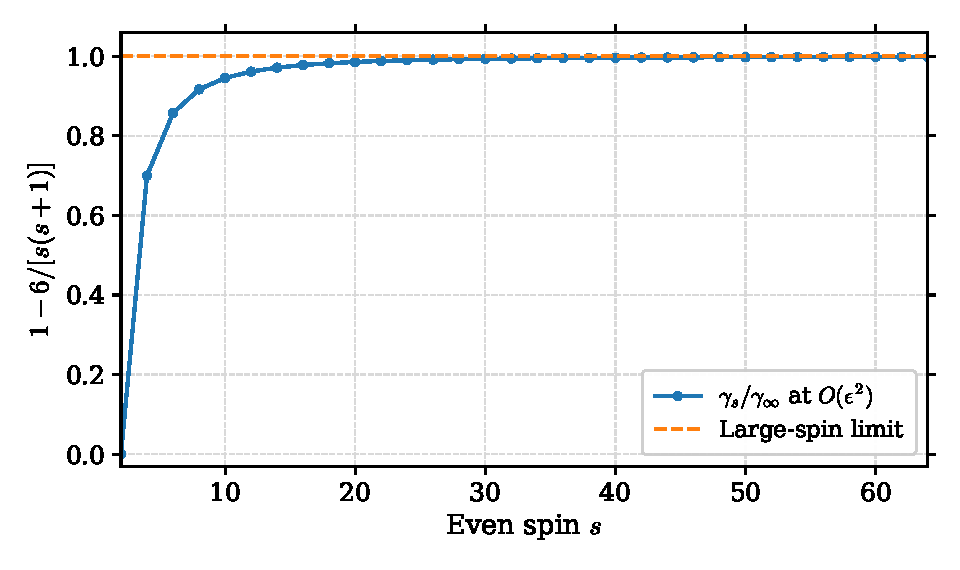
\includegraphics[width=.79\linewidth]{content/AdvancedPhysics/field-theory/figures/geometry-highspin/generated/anomalous_spin_profile.pdf}
\caption{$d=4-\epsilon$ 单实标量 Wilson--Fisher 理论领先 $O(\epsilon^2)$ 的偶数自旋比值 $\gamma_S/(\epsilon^2/54)=1-6/[S(S+1)]$。$S=2$ 只作为受保护应力张量的结构检验。}\label{fig:ghs-anomalous-spin-profile}
\end{figure}

\cref{fig:ghs-anomalous-spin-profile} 展示应力张量保护与非保护高自旋维数趋于 $2\gamma_\varphi$ 的衔接；纵轴已经去掉共同的 $\epsilon^2$ 因子，不代表任意维度或任意耦合下的非微扰结果。

可以做三项独立的结构检验。其一，将右侧代数形式延拓至 $S=2$，恰好得到零，与应力张量 Ward 恒等式吻合；但应力张量的实际证明仍来自守恒律，而不是在微扰式上碰巧取零。其二，$S\to\infty$ 时
\begin{equation}\label{eq:ghs-wf-higher-spin-large-s}
 \gamma_S=2\gamma_\varphi-\frac{\epsilon^2}{9S(S+1)}
 +O(\epsilon^3),
\end{equation}
说明大自旋维数逐渐接近两条基本场维数之和加上 $S$，与双扭度的领先结构一致。其三，对首个真正非保护的 $S=4$，
\begin{equation}\label{eq:ghs-wf-spin-four}
 \gamma_4=\frac{7}{540}\epsilon^2+O(\epsilon^3)>0,
\end{equation}
满足幺正性要求。与其把这些检验称作完整证明，更准确的理解是：Ward 恒等式、光锥自举和微扰理论从不同方向同时约束一个已计算出的谱结果。


构造高自旋算符时，常用一个复零极化向量 $z^\mu$ 满足 $z^2=0$，把对称无迹张量缩并为 $J_S(x,z)=J_{\mu_1\cdots\mu_S}(x)z^{\mu_1}\cdots z^{\mu_S}$。由于 $z^2=0$，任意含度规迹的项在 $J_S$ 中消失；但是在求散度时，$\partial/\partial z^\mu$ 会作用于这些项，而它们求导后未必仍然消失。所以先令 $z^2=0$ 再直接使用 $\partial_x\cdot\partial_z$，一般不能代替真实对称无迹张量的散度。

一种与无迹等价类相容的工具是 Thomas 导数
\begin{equation}\label{eq:ghs-thomas-derivative}
 \mathscr D_{z,\mu}
 =\left(\frac d2-1+z\cdot\partial_z\right)\partial_{z^\mu}
 -\frac12 z_\mu\partial_z^2.
\end{equation}
这里 $\mathscr D_z$ 作用在极化向量的齐次多项式上，而不是作用在时空坐标 $x$ 上。计算物理散度时须适当归一化 $\partial_x\cdot\mathscr D_z$ 并处理运动方程与改善项；使用它可以避免把纯迹补偿误判为破坏守恒的算符。自旋二就是重要检验：自由的双线性表达式在加入 $\varphi^4$ 后必须与相互作用的应力张量改善项合并，真正的能动张量才仍然严格守恒。若在这里得到 $\gamma_2\ne0$，应首先核对迹投影与算符混合，而不是怀疑平移 Ward 恒等式。


从一套自由场双线性表达式出发，可以有多个具有相同自旋、对称性和经典维数的复合算符。重整化一般把它们混合：
\begin{equation}\label{eq:ghs-spin-mixing-renormalization}
 [\mathcal O_A]_R=(Z^{-1})_{AB}\mathcal O_{B,0},\qquad
 \Gamma=Z^{-1}\mu_{\mathrm R}\frac{\dd Z}{\dd\mu_{\mathrm R}}\bigg|_{g_0},
\end{equation}
其中 $A,B$ 标记同一扇区的算符，$Z$ 为重整化矩阵，$\Gamma$ 的本征值决定相应的异常维数（其符号须与此处 $Z$ 定义一致）。在存在简并、总导数和运动方程算符时，应先构造规范良好的物理算符商空间，再取有意义的谱。不能仅凭某一个裸插入项的重整化常数，宣称得到一个共形初级的维数。

在固定点上，算符混合的本征值、二点函数的零范数结构和四点函数的共形块分解描述的是同一套谱。\cref{eq:ghs-wf-phi-gamma-result} 给出一个完全由运动方程和 Wick 收缩算出的实例；\cref{eq:ghs-wf-higher-spin-anomalous-result} 给出一条实际可检验的高自旋谱塔；\cref{eq:ghs-wf-higher-spin-large-s} 将它与一般双扭度的大自旋趋势接在一起。高自旋场论研究的价值就在这里：对称性不只是给算符分类，而能把微扰积分、算符代数和非微扰相关函数限制连接为同一个定量问题。

\subsection{低自旋与正交角位置振幅的直接核对}

\begin{example}[最高权球谐的归一化]

在单位球面 $S^{d-1}$ 上写 $z=n^1+\ii n^2$，$|z|^2=(n^1)^2+(n^2)^2$。随机均匀单位向量的前两个分量平方和 $s=|z|^2$ 满足 贝塔分布，其密度正比 $s^{1-1}(1-s)^{(d-2)/2-1}$。于是
\begin{align*}
 \int_{S^{d-1}}\dd\Omega\,|z|^{2k}
 &=\Omega_{d-1}\frac{B(k+1,(d-2)/2)}{B(1,(d-2)/2)}\\
 &=\Omega_{d-1}\frac{\Gamma(k+1)\Gamma(d/2)}{\Gamma(k+d/2)}
 =\Omega_{d-1}\frac{k!}{(d/2)_k}.
\end{align*}
$d=4$ 时这就是 $N_{4,k}=2\pi^2/(k+1)$。角向旋转 $z\mapsto\ee^{\ii\alpha}z$ 意味着对 $k\ne j$，积分 $\int z^k\bar z^j\dd\Omega$ 必须为零。

\end{example}

\begin{example}[四维低自旋的 Fock 范数]

$S=0$ 时，$\mathcal O_0=:\!\varphi^2\!:$，于是 $|\mathcal O_0\rangle=F_0^2(b_0^\dagger)^2|0\rangle$。其中 $F_0^2=1/(4\pi^2)$，所以 $\|\mathcal O_0\|^2=2F_0^4=1/(8\pi^4)=2C_4^2$。

$S=2$ 时，系数 $(c_0,c_1,c_2)=(1,-4,1)$。两种最外侧组合合并后，$|\mathcal O_2\rangle=2F_0F_2 b_0^\dagger b_2^\dagger|0\rangle-4F_1^2(b_1^\dagger)^2|0\rangle$。两者分别贡献 $16/\pi^4$ 与 $32/\pi^4$，因此总范数 $48/\pi^4$，与 \cref{eq:ghs-norm-four-d} 相符。

\end{example}

\begin{example}[正交角位置振幅]

为了计算 \cref{eq:ghs-canonical-vs-field}，不必离散化球面上的微分算符。直接取
\begin{equation*}
 \psi_S(\vb n_1,\vb n_2)
 =\frac{2}{\sqrt{\mathcal N_S}}
 \sum_{k=0}^S B_k\frac{z_1^kz_2^{S-k}}{\sqrt{N_{d,k}N_{d,S-k}}},
 \qquad(S\text{ 偶数}).
\end{equation*}
由于 $\sum_k |B_k|^2=\mathcal N_S/2$，球面正交性给出 $\int|\psi_S|^2=2$。对于 $k=S/2$，这里已经自动包含两个相同玻色模式的 $\sqrt2$ 范数因素；再乘一个对称化因子将重复计数。


\end{example}

标量共形模型把初级条件、粒子态归一化与相关函数数据连成一条可复算的论证。进入电子和规范场的相互作用时，必须重新选用 Dirac 与 Maxwell 自由算子，并加入对应的顶角、外态和测量算符；径向标量态的角权重只有经过这样的耦合模型，才能与具体电子或光子观测联系。


\backmatter
\begingroup\sloppy
\printbibliography[heading=bibintoc,title={参考文献}]
\endgroup
